\documentclass[UKenglish]{uiomasterthesis}
\usepackage{{booktabs}}
\usepackage{algpseudocode}
\usepackage{algorithm}
\usepackage{graphicx} 
\usepackage[UKenglish]{uiomasterfp}
\usepackage[nottoc]{tocbibind}
\usepackage[hidelinks]{hyperref}
\usepackage{amsmath}
\usepackage{amssymb}
\usepackage{amsfonts}

\usepackage{amsthm}
\usepackage{bm}
\usepackage{mathtools}
\usepackage[printonlyused]{acronym}
\usepackage{tikz}
\usepackage{pgfplots} 
\usepackage{pgf} 
\usepackage[backend=biber, style=numeric-comp, sorting=none]{biblatex}
\addbibresource{ref.bib}
\usetikzlibrary{arrows, arrows.meta, positioning, calc}
\usepackage{listofitems}

\pgfplotsset{compat=1.18}

\def\mathdefault#1{#1}
\everymath=\expandafter{\the\everymath\displaystyle}

\title{Explainable Reinforcement Learning}
\subtitle{Discovering intent based explanations for heterogeneous cooperative multi agent reinforcement learning agents}
\author{Ada Hatland}
\date{August 2024}


\pagenumbering{roman}

\begin{document}

\uiomasterfp[master, program={Informatics: Robotics and Intelligent Systems},
  color=orange, dept={Department of Informatics}, fac={The Faculty of Mathematics and Natural Sciences},
  supervisors={Dr. Dennis Gro\ss \and Prof. Kyrre Glette\and Dr. Helge Spieker}, image = {images/cat.png}]

\renewcommand*\acffont{\textit}

\section*{Declaration of AI use}
In this thesis generative models have been used for topic suggestion, a small part of figure creation, equations and parts of the code used for creating plots, as well as debugging and documentation. All code suggested has been verified by a human. Generative models have \textbf{not} been used for text generation. I, the author, take full responsibility for the contents of this thesis.


\section*{Acknowledgments}
I would like to thank my external supervisor Dennis Gro\ss, as well as my internal supervisor Kyrre Glette for their guidance and support in writing this thesis. They have been of significant help when discussing how to proceed and what remains on the to-do list. I would also like to thank my cat Nokia for emotional support throughout the writing of this thesis.

\section*{List of Acronyms}
\begin{acronym}[ICANN]
    \acro  {rl}   [RL]   {Reinforcement Learning}
    \acro  {xrl} [XRL] {Explainable Reinforcement Learning}
    \acro  {xdrl} [XDRL] {Explainable Deep Reinforcement Learning}
    \acro  {ai}   [AI]   {Artificial Intelligence}
    \acro  {xai}  [XAI]  {Explainable Artificial Intelligence}
    \acro  {marl}  [MARL]  {Multi Agent Reinforcement Learning}
    \acro  {mdp}  [MDP]  {Markov Decision Process}
    \acro  {dqn}  [DQN]  {Deep Q-Network}
    \acro  {ppo}  [PPO]  {Proximal Policy Optimization}
    \acro  {drl}  [DRL]  {Deep Reinforcement Learning}
    \acro  {rnn}  [RNN]  {Recurrent Neural Network}
    \acro  {lstm}  [LSTM]  {Long Short Term Memory}
    \acro  {mbrl}  [MBRL]  {Model-Based Reinforcement Learning}
    \acro  {llm}  [LLM]  {Large Language Model}
    \acro  {ea}  [EA]  {Evolutionary Algorithm}
    \acro  {nsga}  [NSGA-II]  {Non-Dominated Sorting Genetic Algorithm II}
    \acro  {nn}  [NN]  {Neural Network}
    \acro  {aec}  [AEC]  {Agent Environment Cycle}
    \acro  {cnn}  [CNN]  {Convolutional Neural Network}
    \acro  {drc}  [DRC]  {Deep Repeated ConvLSTM}
    \acro  {pomdp}  [POMDP]  {Partially Observable Markov Decision Process}
\end{acronym}


\abstract
This is the abstract

\lefthyphenmin=1000
\tableofcontents
\listoftables
\listoffigures
\chapter{Introduction}

\pagenumbering{arabic}

Sequential decision-making problems are problems where one decision leads to a new state that requires a new decision to be made. An example of this is autonomously driving from point A to point B through city streets. For these types of problems \ac{rl} systems are used. \ac{rl}, both multi- and single-agent models have seen a significant rise in successful use and applicability in recent years, with models such as AlphaGo\cite{article} and smacv2\cite{ellis2023smacv2}. These models learn by agents performing actions in a given state decided by a policy that lead to a new state, and learning by receiving rewards depending on if the new state is preferable to the previous, the aim is to learn a near optimal policy for achieving a fixed goal\cite{Sutton1998}. The agent uses an observation of the state to choose an action. The environment describes how an action affects the state. See Figure \ref{fig:rl_basics}. In a \ac{marl} system, we would have multiple agents.

\section{Motivation}
\label{sec:motivation}
A significant problem with many deep machine learning models, including \ac{marl} policies, is known as the black box problem\cite{zednik2019solving}. This problem describes how the processing of information is hidden from a human user due to the opacity of the model, and we just have to trust that the model uses relevant data to come to the conclusion it does, which it often doesn't do. For many tasks and models where the impact of the output isn't highly significant this isn't a big issue, but for tasks like autonomous driving we simply cannot use these models without trust for the models processing of data and that the solution given wont hurt anyone. We can considering autonomous driving as a \ac{marl} system if we consider each vehicle as an agent. To solve this we would like to have models that along with an output can provide us with some kind of reasoning for what information is used and how.

All this essentially means, until the black box problem is solved, autopilot will always require a driver behind the wheel\cite{tian2018deeptest}. Despite having high accuracy, precision and recall, a reinforcement learning model might choose a less than preferable action in edge cases or states not well covered by training and test sets, for example driving on snowy roads when all images in the training data is from warmer climates, or combinations that aren't well covered, like a foggy, snowy road with a sharp right turn.
With a way to ask the agent for intent, we could find that it has learned to always expect there to not be a car around the corner, which is not always obvious from looking at the dataset, but if it in a decision relies on the road to be empty to choose a safe route, this is obviously a huge issue. This paper aims to explain how an agent in a \ac{marl} setting decides on an action due to what it expects from other agents in the future. The field working on combating this issue is known is Explainable reinforcement learning.

\section{Problem statement}
\label{sec:problem}
The focus of this paper will be to rework and apply methods for general \ac{xai} to Reinforcement Learning, and expand on \ac{xrl} methods already developed. In particular we will focus on an agent and how the expected future states of other agents will affect it in its decision making process. The environment we will focus on is a \ac{marl} environment known as Knights Archers Zombies \cite{KAZ} made for Python. We use this because it is a cooperative environment where each agent has to consider other agents, both of the same type as itself, and other types. If we used an environment where all the agents are identical, our findings will be less useful for other environments where the agents aren't identical. In many real life scenarios agents will not be identical. If we once again consider autonomous vehicles, most vehicles are different in some way. A very obvious example of this is considering cars and motorcycles. Where because of their size difference, their paths chosen will often be different.

In psychology it is well known that most human based decisions are made with intent\cite{inbook}, and by focusing on the expectation of what future states will look like we can consider this the intent of the agent. If we are accurately able to extract the intent of an \ac{rl} policy we are better able to explain the choice made and we are more comfortable with trusting that the choice made is a good decision. Concretely we hypothesise that by analyzing expected future states and events we could find the intent of the agent, which we could use to ensure the agent acts in a safe or desirable manner. The main question we aim to answer is what information, found in weights or design of the policy, or information extracted by knowing the weights and design, is the most important for separate prediction models to be able to predict future states and actions, in cases where we do not have access to a decent world model, or such a model does not exist.


\section{Scope and limitations}
We aim to construct a framework to describe the intent of the agents in the KAZ environment, and we aim to make it applicable to other environments as well. However, due to time limitations we restrict the framework to only accept PettingZoo example environments or environments created with the PettingZoo environment creation tool. \ac{marl} environments can be divided into two major categories, \ac{aec} and parallel. \ac{aec} environments are environments where the state transition happens after each agent chooses an action, and parallel environments are environments where all the agents choose an action each before the transition happens. See figure \ref{fig:aec}.

Due to limited time and resources the size of policy or value networks, as well as any other \acp{nn} or otherwise computationally expensive algorithm used, will have to be significantly limited, this will impact results in a meaningful way, and therefore we will keep all \acp{nn} comparable sizes, and focus on doing experiments on how other factors than network size impact the results.

We do not have access to any real world datasets, so its hard to ensure the methods we have developed will be directly applicable, however the results we get will still be relevant for later research in the area.
\begin{figure}
\begin{center}

\begin{tikzpicture}[>=Latex, node distance=2.5cm, auto, font=\small]

    % Agent 1 Node
    \node[draw, thick, circle, fill=blue!20, minimum size=2.5cm, align=center] (agent1)
    at (-3,3) {Agent 1 \\ \(\pi_{\theta_1}\)};

    % Transition 1 Node
    \node[draw, thick, circle, fill=green!20, minimum size=2.5cm, align=center] (trans1)
    at (0,6) {State \\ Transition 1};

    % Agent 2 Node
    \node[draw, thick, circle, fill=blue!20, minimum size=2.5cm, align=center] (agent2)
    at (3,3) {Agent 2 \\ \(\pi_{\theta_2}\)};

    % Transition 2 Node
    \node[draw, thick, circle, fill=green!20, minimum size=2.5cm, align=center] (trans2)
    at (0,0) {State \\ Transition 2};

    % Arrows between nodes
    \draw[->, thick] (agent1.north) -- node[left] {\(a^1\)} (trans1.west);
    \draw[->, thick] (trans1.east) -- node[right] {\(o^1\)} (agent2.north);
    \draw[->, thick] (agent2.south) -- node[right] {\(a^2\)} (trans2.east);
    \draw[->, thick] (trans2.west) -- node[left] {\(o^2\)} (agent1.south);

\end{tikzpicture}

\caption{Example \ac{aec} in an environment with 2 agents.}
\label{fig:aec}
\end{center}
\end{figure}

\section{Research methods}
\label{sec:research}
This section describes the methods we use to answer the questions we have posed. The methodology mainly focuses on produced datasets made with a digital \ac{rl} environment, which does mean we have access to a world model, however as we want to answer the research questions without the use of a world model we will only be using the results of simulations to create our methods. The effect of this is that the methods will be compatible with \ac{rl} systems where we do not have access to a world model.

Producing our own dataset has the benefit of no restrictions, other than hardware restrictions, on the datasets size. We can also produce variations of these datasets by altering the simulations used to create them which would in a real world setting often be impossible, e.g. access to gradients during inference.

The datasets produced will be sets of full or partial trajectories in given environments along with other relevant data like integrated gradient, or Shapley values for the observations in the trajectories. We use these datasets to train predictive \acp{nn} with two main types. Event prediction, for example whether an agent encounters a critical state within the next 10 timesteps, which could represent a dangerous situation for an autonomous vehicle, and state prediction, which for example could be the x and y coordinates of a given agent 10 timesteps into the future.

We will first be focusing on including explanations for the observations and observe and analyze the effects on event and state predictors, then we will be using \ac{nn} policies with access to memory and include their representation of memory along with the observation, hidden values for lstm and once again observe and analyze effect on the predictors.

\section{Ethical considerations}
\ac{marl} is an important field in development for military purposes\cite{military_marl}, and while this research is not supposed to effectivize warfare its possible that it ends up being relevant for unintended areas of research, including but not limited to military use-cases. This is especially the case because I aim to develop methods for general \ac{marl} use and not a specific area of research, like medicine or sports. It is more or less impossible to restrict access to these methods for specific areas of research.

If this research aids to make \ac{marl} methods applicable to real world settings there is the possibility it risks increasing job displacement issues. This is an issue that affects most \ac{ai} research and can be mitigated by programs to reeducate people whose jobs it might affect, and increasing employment in developing and monitoring \ac{ai} tools.


\section{Main contributions}
As discussed in \ref{sec:motivation}, \ref{sec:problem} and \ref{sec:research}, there are certain specific objectives we aim to reach. In general we aim to expand on current future prediction research.

\begin{itemize}

    \item \textbf{Objective 1: Observation space}\\
        Most current methods assumes the observation space to be image based, and bases research on information found in convolutional layers, either regular \acp{cnn}, or convLSTM layers.

    \item \textbf{Objective 2: Feature importance as input}\\
        Using feature importance from the policy to improve future predictions is a novel idea, and has potential to improve future predictions by a significant margin.

    \item \textbf{Objective 3: Memory as input}\\
        Earlier research has found that including hidden states from the \ac{drc} architecture had a significant effect on accuracy when predicting future states and events. We aim to expand on this and use hidden states from \acp{lstm} layers and observe the effect and analyze how it differs from using the ConvLSTM hidden values.

\end{itemize}

\section{Thesis outline}
This thesis will be structured as follows:
\begin{itemize}

    \item \textbf{Chapter 2: Background and related works}\\
        This chapter will introduce important concepts, both \ac{rl} and explainability related, and briefly discuss the history of \ac{xai} methods, and how they are applicable to my use case. We will also consider \ac{xrl} methods that are already developed and how to expand or integrate them into developed methods of our own.

    \item \textbf{Chapter 3: Methodology}\\
        This chapter discusses the specific principles, procedures and techniques used to conduct the \ac{xrl} research done in this thesis, to ensure that the results we get are valid and reliable.

    \item \textbf{Chapter 4: Experiments}\\
        This chapter details the setup, results and analysis of the specific experiments we use to evaluate the hypothesis and answer research questions based on certain evaluation metrics, and baseline comparisons.

    \item \textbf{Chapter 5: Discussion}\\
        This chapter will analyze the results of the experiments and discuss their implication for \ac{xrl} research. It will also contain the limitations of our work and briefly discuss how to expand on any research done.
\end{itemize}


\begin{figure}
\begin{center}
    \hspace{-4cm}
    \begin{tikzpicture}[>=Latex, node distance=2.5cm, auto, font=\small]
    % Agent Node (with Policy and Value Networks)
    \node[draw, thick, rectangle, fill=blue!20, minimum width=3cm, minimum height=2cm, align=center] (agent)
    at (-4,3) {Agent \\ \(\pi_\theta(s)\) \\ \(V_\phi(s)\)};

    % Environment Node
    \node[draw, thick, rectangle, fill=green!20, minimum width=3cm, minimum height=2cm, align=center] (env)
    at (4,3) {Environment};

    % Arrow: Agent to Environment (Action)
    \draw[->, thick] (agent.east) -- node[above] {\(a_t\)} (env.west);

    % Rollout/Trajectory Buffer Node
    \node[draw, thick, rectangle, fill=yellow!20, minimum width=4cm, minimum height=1.5cm, align=center] (buffer)
    at (0,0.5) {Rollout/Trajectory Buffer \\ \((s_t,\, a_t,\, r_t,\, s_{t+1})\)};

    % Arrow: Environment to Rollout Buffer (State & Reward)
    \draw[->, thick] (env.south) .. controls +(0,-1) and +(2,1) .. node[right] {\(s_{t+1},\, r_{t+1}\)} (buffer.east);

    % Arrow: Agent to Rollout Buffer (State, Action, Reward)
    \draw[->, thick] (agent.south) .. controls +(0,-1) and +(-2,1) .. node[left] {\(s_t, a_t, r_t\)} (buffer.west);

    % PPO Update Node
    \node[draw, thick, rectangle, fill=red!20, minimum width=4cm, minimum height=2cm, align=center] (ppo)
    at (0,-3) {PPO Update \\ \(\bullet\) Compute Advantages \\ \(\bullet\) Clip Objective \\ \(\bullet\) Update \(\pi_\theta\) and \(V_\phi\)};

    % Arrow: Rollout Buffer to PPO Update
    \draw[->, thick] (buffer.south) -- node[right] {Optimize PPO Objective} (ppo.north);

    % Arrow: PPO Update to Agent (New Parameters)
    \draw[->, thick] (ppo.west) .. controls +(-7,0) and +(0,0) .. node[right] {New parameters \(\theta, \phi\)} (agent.west);
\end{tikzpicture}
\caption{Diagram showing the \ac{ppo} update algorithm}
\label{fig:rl_basics}
\end{center}
\end{figure}

\medskip
\chapter{Background and Related Works}

\section{Reinforcement Learning Fundamentals}
To make sure all methods are understood well its important to make sure we have a proper understanding of the fundamentals of \ac{rl}, especially \ac{drl} and \ac{marl}. This section will go over the basics needed.


\subsection{Markov Decision Process in Reinforcement Learning}

A \ac{mdp} is a framework used to model decision-making in stochastic environments, like we want to in an \ac{rl} task. It is defined by a tuple with 5 elements:

$$\mathcal{M} = (\mathcal{S}, \mathcal{A}, P, R, \gamma)$$

where \(\mathcal{S}\) is the set of possible states, \(\mathcal{A}\) is the set of possible actions, \(P(s' | s, a)\) is the transition probability function, which defines the probability of moving to state \(s'\) when action \(a\) is taken in state \(s\), \(R(s, a, s')\) is the reward function that provides a reward for transitioning from state \(s\) to \(s'\) via action \(a\), \(\gamma \in [0,1]\) is the discount factor that determines the importance of future rewards.

The objective in an \ac{mdp} is to find a policy \(\pi(s)\) that maximizes the expected cumulative reward:

$$V^\pi(s) = \mathbb{E} \left[ \sum_{t=0}^{\infty} \gamma^t R(s_t, a_t, s_{t+1}) \mid \pi \right]$$

where \(V^\pi(s)\) is the value function that represents the expected return starting from state \(s\) and following policy \(\pi\). See figure \ref{fig:rl_basics}.


\subsection{Markov Decision Process in Multi Agent Reinforcement Learning}
In a \ac{marl} setting agents could have shared or independent \acp{mdp} depending on architecture. There are three main branches of \ac{marl}, cooperative, competitive and mixed. Our focus will be on cooperative \ac{marl}.
In a cooperative \ac{marl} setting the goal is some social welfare function that maximises rewards for the agents, either collective rewards or a mix of collective and individual rewards. In such a setting each agent has \ac{mdp}. Assuming that state space \(\mathcal{S}\) and discount factor \(\gamma\) is shared, which they will be in all my experiments, if two agents have the same reward structure $R$ and action space \(\mathcal{A}\) their objective would be the same, in which case they could share policy \(\pi\) and could therefore share \(\mathcal{M}\).

\subsection{Deep Reinforcement Learning}
Traditional RL methods struggle with scalability due to the fact that they rely on discrete state representations. \ac{drl} uses deep \acp{nn} to approximate the policy function $\pi_\theta(s)$, the value function $V_\phi(s)$, or the Q-function $Q_\theta(s,a)$, making it possible to represent these functions in continuous and complex environments. See figure \ref{fig:neural_network}. Input layer is size of state for all three functions. Output layer is size of action space for $Q_\theta(s,a)$ and $\pi_\theta(s)$. $V_\phi(s)$ only has one output node. In a feed forward \ac{nn} like we have here each node has the value of some activation function $\phi(x)$ where $x$ is the sum of nodes of the previous layer multiplied by their respective weights, usually as well as adding some bias, shown as the connections between the nodes. Common activation functions are $ReLU(x) = max(0,v)$ and $tanh=\frac{e^v-e^v}{e^v+e^v}$ where $v$ is the value before activation.
\begin{figure}[H]
    \begin{center}
    \begin{tikzpicture}[
        x=2.2cm, y=1.4cm, 
        mynode/.style={thick, draw=black, circle, minimum size=22}, % Base style
        inputnode/.style={mynode, fill=blue!35},  % Input layer
        hiddennode/.style={mynode, fill=red!35}, % Hidden layers
        outputnode/.style={mynode, fill=green!35} % Output layer
    ]
    
    \readlist\Nnod{4,5,5,5,3} % Number of nodes per layer
    
    \foreachitem \N \in \Nnod{ % Loop over layers
        \foreach \i [evaluate={\x=\Ncnt; \y=\N/2-\i+0.5; \prev=int(\Ncnt-1);}] in {1,...,\N}{ 
            
            % Choose color based on layer type
            \ifnum\Ncnt=1
                \node[inputnode] (N\Ncnt-\i) at (\x,\y) {}; % Input layer
            \else
                \ifnum\Ncnt=\Nnodlen
                    \node[outputnode] (N\Ncnt-\i) at (\x,\y) {}; % Output layer
                \else
                    \node[hiddennode] (N\Ncnt-\i) at (\x,\y) {}; % Hidden layer
                \fi
            \fi
            
            % Connect to previous layer
            \ifnum\Ncnt>1  
                \foreach \j in {1,...,\Nnod[\prev]}{ 
                    \draw[thick] (N\prev-\j) -- (N\Ncnt-\i); 
                }
            \fi 
        }
    }
    
    \node[align=center, below=1] at (N1-4.90) {Input Layer};
    \node[align=center, below=1] at (N3-5.90) {Hidden Layers};
    \node[align=center, below=1] at (N5-3.90) {Output Layer};
    \end{tikzpicture}
    \end{center}
    \caption{Illustration of an example of a \ac{nn} with three hidden layers}
    \label{fig:neural_network}
\end{figure}


\subsection{Model-Free vs. Model-Based Reinforcement Learning}

Model-based and model-free reinforcement learning differ in how they represent environment transitions. In model-based reinforcement learning, the agent learns or has access to a model of the environment, which includes a transition function \( P(s' | s, a) \) and a reward function \( R(s, a) \) that determines the expected reward for taking action \( a \) in state \( s \) \cite{moerland2022modelbasedreinforcementlearningsurvey}. This allows the agent to simulate future outcomes without taking actions in the real environment. As a result, model-based methods are able to update policies based on imagined rollouts, which increases learning speed compared to executing the real environment transitions. Examples of model-based algorithms are Dyna\cite{10.1145/122344.122377} and DreamerV3\cite{hafner2024masteringdiversedomainsworld}.

In contrast, model-free reinforcement learning does not learn or utilize an explicit model of the environment. Instead, the agent learns by interacting directly with the environment and updating its network weights based on observed rewards. This approach is generally less sample-efficient but is applicable to environments where modeling the transition dynamics isn't feasible. Examples of model-free algorithms include Q-learning, \ac{dqn} \cite{mnih2013playingatarideepreinforcement}, and \ac{ppo} \cite{schulman2017proximalpolicyoptimizationalgorithms}.

Model-based methods enable explicit planning by using the learned environment transitions in methods such as Monte Carlo Tree Search \cite{_wiechowski_2022}, while model-free methods rely on direct experience to optimize behavior. We will be using \ac{ppo} to optimize our algorithms, and will not be using simulations or any other form of explicit planning, ensuring that the methods developed will be applicable in the most amount of environments.

\subsection{Recurrency in Deep Reinforcement Learning Policies}
Recurrency in \ac{nn} is a way to carry over information from previous timesteps to current ones, if we believe that information could be useful. \acp{rnn} are sometimes used when constructing the architecture of \ac{drl} policies \cite{hausknecht2017deeprecurrentqlearningpartially}, mainly for two reasons. The first one is for when your environment can be modeled as a \ac{pomdp}, in which case memory is important as the current observation is not always enough to capture all the information an agent could have. The second reason is for planning, like in the \ac{drc} architecture\cite{guez2019investigationmodelfreeplanning}. See figure \ref{fig:rnn}.

\begin{center}
\begin{figure}
    \hspace{3.5cm}
    \begin{tikzpicture}[>=stealth, auto, node distance=1.5cm and 2cm]

    \begin{scope}[shift={(4,0)}, rotate=90]
  
    % Time step 1
    \node (x1) [draw, rectangle, fill=blue!20, minimum width=1cm, minimum height=0.7cm] {$x_1$};
    \node (h1) [draw, circle, fill=red!20, right=of x1] {$h_1$};
    \node (y1) [draw, rectangle, fill=green!20, right=of h1, minimum width=1cm, minimum height=0.7cm] {$y_1$};

    % Time step 2
    \node (x2) [draw, rectangle, fill=blue!20, below=of x1, minimum width=1cm, minimum height=0.7cm] {$x_2$};
    \node (h2) [draw, circle, fill=red!20, right=of x2] {$h_2$};
    \node (y2) [draw, rectangle, fill=green!20, right=of h2, minimum width=1cm, minimum height=0.7cm] {$y_2$};

    % Time step 3
    \node (x3) [draw, rectangle, fill=blue!20, below=of x2, minimum width=1cm, minimum height=0.7cm] {$x_3$};
    \node (h3) [draw, circle, fill=red!20, right=of x3] {$h_3$};
    \node (y3) [draw, rectangle, fill=green!20, right=of h3, minimum width=1cm, minimum height=0.7cm] {$y_3$};

    % Forward connections within each time step (black)
    \draw[->, thick, black] (x1) -- (h1);
    \draw[->, thick, black] (h1) -- (y1);
  
    \draw[->, thick, black] (x2) -- (h2);
    \draw[->, thick, black] (h2) -- (y2);
  
    \draw[->, thick, black] (x3) -- (h3);
    \draw[->, thick, black] (h3) -- (y3);

    % Recurrent connections between hidden states (orange)
    \draw[->, thick, orange] (h1) -- (h2) node[midway, right=4pt] {$W_h$};
    \draw[->, thick, orange] (h2) -- (h3) node[midway, right=4pt] {$W_h$};
    \end{scope}
\end{tikzpicture}
\caption{Recurrent neural network showing a 3 step time series with hidden values propagating through time.}
\label{fig:rnn}
\end{figure}
\end{center}

\subsection{Backpropagation and gradient descent}
Backpropagation is a training algorithm used to train \acp{dnn} to minimize error. If a network is differentiable you can use backpropagation. First you do a forward pass through the network, i.e. your network calculates a prediction based on an input. Then you calculate loss, the difference between true value and predicted value is passed to some function. MSE is one such function.
\[
\text{MSE} = \frac{1}{n} \sum_{i=1}^{n} (y_i - \hat{y}_i)^2
\]
Where $y$ is true value, $\hat{y}$ is predicted value, $n$ is amount of samples multiplied by outputs. If you are trying to predict $(x,y)$ coordinates, you would have two outputs, if you're trying to predict $x,y$ coordinates in 5 cases you would have $n = 10$.
Then you do a backwards pass, calculating loss with respect to the weights in the network using the chain rule. Then using gradient descent you change the weights to reduce loss.


\section{Approaches to Explainability in Reinforcement Learning}
\subsection{Post Hoc vs. Intrinsically Explainable Models}
This section will discuss benefits and drawbacks of explainable models divided into two main categories, Post hoc models and intrinsically explainable models.

Post hoc explainability refers to finding ways to understand already trained models. Instances where this doesn't pose more of a challenge can often be more efficient as you do not need to construct and train a model, which could often pose an issue both considering time spent and accuracy of the model. Making a model explainable only makes sense if we know it usually makes sensible decisions. There are however issues with making post hoc models.

\subsubsection{Temporal Aspect}
\ac{rl} policies all have a temporal aspect, which means several different actions over a certain period of time might contribute to a singular outcome, this could make it very challenging to pinpoint which actions were made for which outcome, especially if the outcome happens several states after the initial decision was made.

\subsubsection{Nature of Black Box Models}
Many \ac{rl} policies, especially deep \ac{rl} policies, which are the policies we will be working with, have complex inner connections due to the hierarchical structure of learning features in the input, sequences of non linear connections that are very hard to understand without spending a lot of time studying the specific connections learned by a model. It's often very difficult to accurately pinpoint the purpose of a node, especially because we do not know if it even has a purpose at all or it could have a lot of different purposes. Especially in environments with complex observation spaces.


\subsubsection{Lack of Transparency}
Tracing how an observation leads to a state, through the action chosen and the environment, is often challenging in models constructed without this in mind. If we do not know the processing of information of a model it's very hard to explain the rationalisation of an agent.

\subsubsection{Intrinsically Explainable Models}
Intrinsically explainable models have the already stated drawback of relying on careful model construction, which can be challenging and may impact model performance. While these models offer transparency from the get go, they are often less flexible and might not achieve the same level of accuracy as more complex \ac{rl} models. Given that we aim to analyze and compare already trained \ac{rl} policies, we will mostly focus on post hoc explainability methods in this thesis.

\medskip

\subsection{Fidelity of Explainable Artificial Intelligence Methods}
It is important to understand why the current \ac{xai} methods not meant for \ac{rl} applications aren't always useful to us.

\ac{xai} methods not intended for reinforcement learning often provide\\ explanations that don't necessarily represent the inner workings of an \ac{rl} policy, because an \ac{rl} policy has a temporal aspect as well. Broadly these methods can be categorised as feature-based explainers, and they often struggle to fully explain an agents behaviour or specific actions because they cannot capture the future view of an \ac{rl} policy. 

Saliency maps which have been successfully used for classification of images provide explanations about what part of the input was important for the outcome, which is highly relevant for classification tasks, but using the same method for an \ac{rl} policy doesn't sufficiently explain the intent of the agent\cite{atrey2020exploratory}.

Another commonly used \ac{xai} method is model distillation, which works by transferring knowledge from a large model to a smaller, usually interpretable, one, for instance a deep learning network to a decision tree \cite{bastani2019verifiable}. This has use cases in verifyability, but struggles to fully explain the temporal aspect of \ac{rl} policies, and are therefore not sufficient as an explainer.

However, these methods might still prove insightful in conjunction with other intent-based methods, the state in which a decision is made is obviously very relevant to why that particular decision was made. We could perhaps use these methods to answer questions such as "What part of agent As Observation this state, lead it to believe agent B would end up at these coordinates at a later state?"
\medskip

\subsection{Future-Based Explanations}
Next, I will describe in slightly more detail, what is meant by an intent based explainer, like I want to develop, and how to use it.

\subsubsection{Design}
"Towards Future-Based Explanations for Deep RL Network Controllers"\cite{10.1145/3626570.3626607} broadly describes future-based intrinsically explainable methods. Future-based intrinsically explainable methods for \ac{drl} policies often take three inputs, the trajectories experienced by an agent, the environment and the agent. Then, they collect the rewards and interactions and use this information to train an explainer.

During inference, we can then apply the explainer to a state and action to get the expected future consequences of that action. Depending on the architecture we could either get the expected future consequence of any action, or just the one the agent decides on.

\subsubsection{Use Cases}
Designing a \ac{drl} solution requires choosing features in the observation, hyperparameter tuning, policy design and reward function among other things. This is a time, and resource, consuming process. These are usually picked by trial-and-error but could be made easier with assistance from an explainer.

Another, and perhaps more important, use case is safety. If when online, i.e. the chosen action will actually affect the state, we are expecting high likelihood of an unsafe state, we could instead of opting for the chosen action fall back to a known safe action, that could have a lower expected return, i.e. breaking instead of turning a corner if we have limited vision around the corner.


\subsubsection{Definition of Intent}
We define the state transition function $T(s, \textbf{a}, s')$ where $\textbf{a}$ is the set of simultaneous actions made by the set of active agents, in our case, one action per agent. Given $T$ the agent should when prompted output a set of trajectories $\tau = \{(s_0,\textbf{a}_0),(s,\textbf{a}),(s_1,\textbf{a}_1)...(s_n,\textbf{a}_n)\}$ where $s_0$ is the current state, $\textbf{a}_i$ is the set of actions taken in $s_i$, and $s_{i+1}$ is the state reached by $T(s_i,\textbf{a}_i, s_{i+1})$. We will apply a series of methods on $\tau$ to extract intent. One of these methods is discovering counterfactual trajectories, $'\tau$, where the actions made by the agents in $'\tau$ are as similar as possible to the actions made by the agents in $\tau$, but the total reward gained is as low as possible. $'s_0 = s_0$ and given an identical transition function $T$ the goal is to discover which actions are most important to receive the reward. This method is similar to and inspired by ACTER\cite{gajcin2024acter}, see section \ref{sec:acter}. Details in section \ref{sec:counterfactual}.

\section{Explainable Deep Reinforcement Learning: State of the Art and Challenges}
This paper is a comprehensive survey of the most common state of the art methods applicable to \ac{rl}. Section 4 specifically highlights \ac{xdrl} methods. This subsection will focus on these methods\cite{sota}. This section will serve to give an overview of \ac{xrl} methods that already exist, and if and how I use these methods to develop my own.

\subsection{Feature importance}


\subsubsection{LIME and SP-LIME}
LIME and SP-LIME are model-agnostic methods that explain chosen actions in specific states by slightly modifying input features and fitting an interpretable linear surrogate model that approximates the behaviour of the model locally. SP-LIME selects a representative set of these explanations to create a global explanation for how the model selects an action. These methods explain what features are important when deciding on an action in a given state.

\subsubsection{Shapley Additive exPlanations}
Shapley values is a method of computing marginal contributions from cooperative game theory. It assigns a Shapley value to each feature which is the mean of that features marginal contribution over all combinations of features to establish a fair attribution of credit to each player, or feature in the case of machine learning. This method is very computationally expensive and as such, approximations of this method are used instead.

\subsubsection{Layer-wise Relevancy Propagation}
LRP is a method to assign importance to each node in the network by working backwards from the output to the input. It looks at what nodes in the last hidden layer influenced the output and redistributes prediction scores to these nodes, it then looks at what nodes in the layer before influenced the nodes in the last hidden layer, until you have a complete map of how the network nodes affected each other to produce the output. This method helps reveal hidden patterns in model behaviour.

\subsection{Policy explanations}

\subsubsection{HIGHLIGHTS}
This is a intrinsically explainable \ac{rl} algorithm and it works by extracting sub-trajectories with important states, states where a wrong action can lead to significant decreases in reward, to explain how the agent acts in these states. It also provides context in the form of neighbouring states in the important sub-trajectories, in order for users to understand why it chose the trajectory it did.

\subsection{Objective explanations}

\subsection{Outcome explanation}


\section{Relevant Methods}
There are several papers written on \ac{xai} and \ac{xrl} problems. Milani et al.\cite{milani2022survey} categorise \ac{xrl} into three main categories, feature importance (FI), learning process and \ac{mdp} (LPM) and Policy-level (PL). FI considers the immediate context for actions, i.e. what part of the input was important for a single action, LPM considers techniques that highlight which experiences in training were influential for the final policy and PL focuses on long term effects and behaviour. Since we are interested in future states and actions we will look at influential trajectories and transitions within these trajectories. It is important to view these transitions in the context of the trajectory to understand the long term effects and not just immediate, which are of less interest in this paper, if we find the state with a high state importance $I(s)$, $I(s) = max_aQ(s,a)-min_aQ(s,a)$ most similar by some similarity measure to an arbitrary current state we could find the resulting trajectory and expect the agent to intend a similar outcome. There are also ways to convert \ac{rnn} policies to an interpretable models post-hoc, which might be relevant if we use an \ac{rnn}. This paper will explore PL explainability further.

In particular "What did you think would happen? Explaining Agent Behaviour through Intended Outcomes" \cite{yau2020did}, "Explainable Reinforcement Learning via a Causal world model" \cite{yu2024explainable} and "CrystalBox: Future-based explanations for input-driven deep \ac{rl} systems" \cite{patel2024crystalbox} are highly relevant due to the fact that they all describe temporal connections between current actions and future states or actions.

"Are large language models post-hoc explainers" \cite{kroeger2024large} Could be relevant as using other explainers to compare explanations is useful. "ACTER: Diverse and Actionable Counterfactual Sequences for Explaining and Diagnosing \ac{rl} Policies" \cite{gajcin2024acter} 

\subsection{What did you think would happen? Explaining Agent Behaviour through Intended Outcomes}
What did you think would happen describes what an agent expects to happen in future states, and why the current action is chosen based on the future expectations. As stated in the paper, a limitation of their method means it doesn't work well with high dimensionality. The two main difference between this paper and the problem i aim to solve is that they're focusing on an environment with a single agent and that our observation space will be high dimensionality. It uses Q-learning and Markov-chains that train simultaneously with a "belief map" that shows what the agent expects the environment to look like in future states. In the simple examples used in the paper it shows where it believes the taxi should drive and therefore chooses an action to follow this path. This is not directly applicable to my thesis as it's unlikely that Q-learning or Markov chains will be viable for the policy and explainer based on the environment. However the paper is successful in explaining an agents underlying motivations and beliefs about the causal nature of the environment, and using similar methods might be an effective means for making \ac{marl} agents with higher dimensionality understandable from a human perspective. %See Figure \ref{fig:taxi}

\subsection{Explainable Reinforcement Learning via a Causal world model}
Explainable Reinforcement Learning via a Causal world model constructs a sparse model to connect causal relationships, without prior knowledge of the causal relationship, rather than a fully connected one, but they still achieve high accuracy and results comparable to other fully connected \ac{mbrl} policies. Which is important, as there is often a trade off between explainability and performance. Using the same model for both explanations and choosing actions also make the explanations faithful to the intentions of the agent. The paper also describes a novel approach to derive causal chains from the causal influence of the actions, which lets us find the intent of the agent. The paper is successful being applied to \ac{mbrl}, and is also applicable to models with infinite actions spaces, which is a limitation of some other models, see previous sub section.

A limitation of the paper is that it requires a known factorisation of the environment, denoted by $\langle S, A, O, R, P, T, \gamma \rangle$, where S is state space, A is action space, O is observation space, R is reward function, P is probability function for the probability of transitioning from state $s$ to state $s'$ given action $a$, T is the termination condition given the transition tuple $(s,a,o,s')$, and $\gamma$ is the discount factor. Considering we will be working with hand crafted simulations we will have access to all of these, however its not certain that if we depend on this method that our contributions will be applicable to certain other environments where the factorisation is not known.


\subsection{CrystalBox: Future-Based Explanations for Input-Driven Deep Reinforcement Learning Systems}
CrystalBox introduces a model-agnostic, post-hoc, future based explanation for \ac{drl}. It doesn't require altering the controller, and works by decomposing the future rewards into its individual components. While this isn't exactly the kind of explanation we are looking for, it could be a great tool in developing an explainer that considers other agents actions in a multi agent cooperative environment, which is the goal of our paper, because it is post-hoc, and easily deployable. Especially because it was constructed for input-driven environments. The original paper claims it offers high fidelity solutions for both discrete and continuous action spaces. KAZ has a discrete action space but we might do some work with other environments as well.

It's not certain to be useful because it works by decomposing the reward function, and it's not safe to assume the reward function will even be useful to decompose.


\subsection{Are Large Language Models Post Hoc Explainers}
A \ac{llm} is a predictive model that generates text based on a prompt you give it, be it continuing the prompt or responding, and can often give the impression of comprehension of human language and a deeper understanding of the topic at hand.  The paper aims to investigate the question "Can LLMs explain the behaviour of other complex predictive models?" by exploiting the in-context learning (ICL) capabilities of \acp{llm}. ICL allows \acp{llm} to perform well on new tasks by using a few task samples in the prompt. A benefit of using an \ac{llm} as a post-hoc explainer, is that the output given by the model will already be written in natural language and should be understandable by a layman. The paper presumes that the local behaviour of a model is a linear decision boundary, and by using a sample x and perturbing it to x', and presenting both the samples and the perturbation as natural language we could get an explanation from the \ac{llm} for the outcome. With a sufficient number of perturbations in a neighbourhood around x the \ac{llm} is expected to explain the behaviour in this neighbourhood, and rank the features in order of importance.

While the faithfulness of the \ac{llm} as an explainer is on par with other \ac{xai} methods used for classification, meaning that the reasons provided are enough to explain the output, I am sceptical of the fidelity of the \ac{llm} for two reasons. One is the same as for why other \ac{xai} models often struggle with fidelity, the temporal aspect. If applied in the same way as in the paper it would not consider the intent or the past and only what part of the current observation made it make a certain decision. The other is that I am sceptical of claims presented by an \ac{llm} in general as these are all just guesses. Good guesses a lot of the time, but still just guesses. 

We could however potentially change the implementation so it considers the temporal aspect, and this might be a viable post hoc explainer after some more research into prompt engineering.


\subsection{ACTER: Diverse and Actionable Counterfactual Sequences for Explaining and Diagnosing Reinforcement Learning Policies}
\label{sec:acter}
The paper presents ACTER, an algorithm that uses counterfactual sequences with actionable advice on how to avoid failure for an \ac{rl} policy. It does this by using an \ac{ea} known as \ac{nsga} to generate counterfactual sequences that don't lead to failure as close as possible to factual sequences that lead to failure. This paper presents counterfactual sequences and not just actions, which means it also presents how to avoid the state that lead to failure to begin with, which should, if ACTER is implemented correctly, allow us to significantly reduce the amount of times our policy fails. It also offers multiple counterfactuals to allow the end user to decide which counterfactual is preferable to their use case.

There are 4 hypothesises tested by the paper. The last two considers laymen users and are therefore not as interesting to us. The first two however "ACTER can produce counterfactual sequences that prevent failure with lower effort and higher certainty in stochastic environments compared to the baselines." and "ACTER can produce a set of counterfactual sequences that offer more diverse ways of preventing failure compared to the baselines." are partially and fully confirmed respectively. Which means ACTER will likely be a useful tool to explain and diagnose our \ac{rl} policy.


\section{Related Works}
This section describes recent development in the field of planning and future predictions. All the papers described here are directly relevant to the methods i developed.

\subsection{Predicting Future Actions Of Reinforcement Learning Agents}
\label{sec:predicting_actions}
This paper describes a method developed by the author that predicts future actions and events \cite{chung2024predictingfutureactionsreinforcement}. It does this for non planning policies, like Impala, implicit planning policies like \ac{drc}, see section \ref{sec:impl_planning}, and explicit planning policies like MuZero and Thinker.

Non planning policies are policies designed without planning in mind. Pure \ac{nn} policies without recurrency are considered to be non planning, as they have not been found to exhibit planning like behaviour. This paper found that when predicting future states and actions both inner states from implicit planners, and explicit planners improved accuracy over non planning agents.

Explicit planners are agents who simulate future states with a world model before making a decision on what action to take. They rely on the world model being accurate, and so does using them to predict future states and actions. In some environments learning an accurate world model is not feasible, an example of this is autonomous driving.

The paper proposes two methods on predicting future states and actions, simulation based and inner state based. The inner state approach is most effective when working with explicit planners, but also shows significant improvement for implicit planner agents. The simulation based approach performs very well on implicit planner agents, but requires the opportunity to train a decently performing world model. The paper also shows with an ablated world model, the inner state approach performs better.

\subsection{An Investigation of Model Free Planning}
\label{sec:impl_planning}
This paper investigates whether planning like behaviour can emerge from model free \ac{rl}, without any explicit planning methods or inductive biases designed to induce planning behaviour \cite{guez2019investigationmodelfreeplanning}. The authors introduce and explore if the \ac{drc} architecture can learn to implicitly plan through training. World models suffer from scalability issues, and inductive biases require a priori knowledge of the environment. The \ac{drc} architecture is comprised of $3$ layers of ConvLSTMs and each layer is iterated through $3$ times each at each timestep.

This architecture is tested on domains that require planning such as Sokoban, and they test the agents ability to generalize as well as data efficiency. The results of the paper is that not only does the model exhibit planning like behaviour, but it outperforms state of the art methods that use inductive biases or world models. The paper described in section \ref{sec:predicting_actions} finds that using the inner state of implicit planner agents improves predicted future states and actions.


\medskip
\chapter{Methodology}
This chapter will elaborate on the methods I will use to perform the experiments. Firstly, in section \ref{sec:event_state_meth}, I will discuss in detail the state and events we want to predict. Then, in section \ref{sec:feat_imp_meth}, I will elucidate how i attribute importance to observation features. After that, in section \ref{sec:intent_meth}, I will define what I mean by intent for an agent in a \ac{rl} setting. Then, in section \ref{sec:temp_meth}, I will discuss what temporal information I will use and how to get it. Then, in section \ref{sec:stat_meth}, I will discuss what statistical tests I perform to validate my results. Lastly, in section \ref{sec:env_meth}, I will elaborate on what environments I perform the experiments on, and how these environments are structured.


\section{Event and State prediction}
\label{sec:event_state_meth}
For the state prediction part of the experiments I will attempt to improve predictions on x and y coordinates of an agent a given time into the future. 

For the event prediction part of the experiments I will attempt to improve predictions on whether an agent encounters a critical state in a specified sub-trajectory. This section will define what I mean by critical states.

\subsection{Critical states}
In a safety critical real world scenario, like autonomous driving, its important to identify when a vehicle is about to make an important decision, a decision where a mistake could lead to important consequences. If we can identify these states we could make efforts to increase the likelihood of correct action in these states, either by taking over as a human, or improving the policy in these scenarios.

\subsection{Maximum logit difference}
The output of the policy, in the case of discrete action space, is a vector with size $n$, where $n$ is the amount of possible actions, without an activation function. This is also known as the logit vector. A state in which there is a high difference between the highest logit and the lowest logit means the agent has learned to avoid the action associated with the low logit and prefers the action with the high logit, which would mean the agent associates the high logit action with high future rewards, and the low logit action with low future rewards. If the logits are close to each other it means the agent is either uncertain about which action to choose or indifferent to the different actions in this state. Given that the policy has been trained well enough that it correctly predicts the optimal action in a state, I consider this state to be critical if the difference between the highest logit and the lowest logit is higher than some chosen threshold.
To compute whether a trajectory contains a critical state I consider the maximum logit difference in each of the states, and assign the maximum of these differences to the trajectory. After computing a value for every trajectory, we consider the median of the values assigned to the trajectories as the threshold for whether a state contains a critical state or not. This means we consider half the trajectories to contain a critical state. The main reason for this is it makes using a baseline of random guesses have expected $50\%$ accuracy. This means if we train a binary classifier with initial observation as input and whether the trajectory contains a critical state as output any improvement over $50\%$ means a network has learned a meaningful connection between the input and the output, as opposed to simply learning that one class is more common than another.

\begin{gather*}
    \mathbf{z_i}(x) = \left[z_{i,1}(x),\, z_{i,2}(x),\, \dots,\, z_{i,K}(x)\right]\\
    z_{i,\max}(x) = \max_{j \in \{1,\dots,K\}} z_{i,j}(x)\\
    z_{i,\min}(x) = \min_{j \in \{1,\dots,K\}} z_{i,j}(x)\\
\Delta(x_i) = z_{i,\max}(x) - z_{i,\min}(x)\\
\Delta(x) = \max{\Delta(x_0),\Delta(x_1), \dots, \Delta(x_K)}
\end{gather*}

\begin{equation}
\label{eq:crit_criterion}
\Delta(x) > \tau
\end{equation}

where $z_{i,j}$ is output $j$ of policy $\pi_\theta$ in state $i$, \ref{eq:crit_criterion} is the criterion for marking a sub-trajectory as containing a critical state, and $\tau$ is the threshold for said equation.


\subsection{Counterfactual sequences}
\label{sec:counterfactual}
In the case of continuous action spaces we cannot look at maximum logit difference, as a policy network doesn't output logits, but rather the actions to choose. To discover counterfactual sequences we use the \ac{ea} known as \ac{nsga}. This algorithm is a significant improvement over earlier multi-objective EAs that use non dominated sorting. It has a complexity of $O(MN^2)$ instead of $O(MN^3)$, elitist approach and a specified sharing parameter, all three of which, many earlier algorithms lacked. \cite{Deb2001AFA} Pseudocode for sorting in algorithm \ref{alg:fnds}. 
We use multi objective search because we want to minimize action change while maximizing total reward change throughout a simulation. This defines our two objectives. This way we can discover what actions or combinations there of have the highest impact on the environment. When working with a discrete action space, that is when we have a finite, usually relatively small, amount of actions to choose from, we define the action objective that we want to minimize as how many actions in a single timestep are different from a predefined sequence found with a trained model. After the timestep with the found actions we again use the model to roll out the rest of the sequence. We compare the altered sequence to the original sequence and measure the total reward both of these sequences receive. We want to maximize this difference. 

\begin{algorithm}
\caption{Fast Non-Dominated Sort}
\label{alg:fnds}
\begin{algorithmic}
    \State $F_i \gets \emptyset$
    \ForAll{$p \in P$}
    \State $S_p \gets \emptyset$
    \State $n_p \gets 0$
        \ForAll{$q \in P$}
            \If{$p \prec q$}
                \State $S_p \gets S_p \cup q$
            \ElsIf{$q \prec p$}
                \State $n_p \gets n_p + 1$
            \EndIf
        \EndFor
        \If{$n_p == 0$}
            \State $F_1 \gets F_1 \cup p$
            \State $p_{rank} \gets 1$
        \EndIf
    \EndFor
    \State $i \gets 1$
    \While{$F_i \neq \emptyset$}
        \State $Q \gets \emptyset$
        \ForAll{$p \in F_i$} 
            \ForAll{$q \in S_p$}
                \State $n_q \gets n_q - 1$
                \If{$n_q \gets 0$}
                    \State $q_{rank} \gets i + 1$
                    \State $Q \gets Q \cup q$
                \EndIf
            \EndFor
        \EndFor
        \State $i \gets i + 1$
        \State $F_i \gets Q$
    \EndWhile
\end{algorithmic}
\end{algorithm}


\section{Feature importance}
\label{sec:feat_imp_meth}
I decided to experiment on whether including feature importance could improve the event and state predictions. The methods used to attribute importance to features were SHAP described in section \ref{sec:shap_meth}, and Integrated Gradients described in section \ref{sec:intgrad}. This section also describes how I decided on choosing baseline values for these methods.
I can use these methods either on logit output or on softmax values with different intentions. If I use the methods on the softmax values I get insight into what affects the confidence of the policy, while if I use them on logit output it better reflects the policy networks inner workings, as in my case, the policy network outputs logits and not softmax scores.

\subsection{Shapley values for observations}
\label{sec:shap_meth}
The Shapley value is an idea from cooperative game theory where it was used to measure the contribution of each player to the total outcome. It has been adapted to deep reinforcement learning where each feature is considered a player and the policy is considered a game. In our case we initially want to use it to explain actions so we consider that to be the outcome of the game. The Shapley value is calculated by taking each feature and finding the marginal contribution, i.e. seeing how the prediction changes when you include the feature and compare the outcome to when it wasn't included, you do this over all possible coalitions of features. See algorithm \ref{alg:shapley}.
The Shapley value has a computational complexity of $O(2^n)$, and because of this we often use estimates instead of exact Shapley values. There are two main ways of reducing the complexity. The first one is using a surrogate model instead of the policy to reduce the number of features, and the second is reducing the number of coalitions. In our case we reduce the number of coalitions to some number $2^K$ and use K-means clustering to increase representability and reduce variance.
Since we have forward passes of the policy, and each can be considered one example of a game we sample the games and use the average marginal contribution over all the games instead of just one game.
The Shapley value can help us understand how the policy acts in general. We can also use it to get explanations for single observations, however these explanations won't always have high fidelity. We will explore more of how the fidelity of Shapley values for single explanations compare to high fidelity explainability methods like gradient methods. See section \ref{sec:intgrad}

\begin{algorithm}
\caption{Shapley Value Calculation with Baseline Replacement}
\label{alg:shapley}
\begin{algorithmic}
    \State \textbf{Input:} Model $f$, input sample $x$, baseline $x'$, set of features $F$
    \State \textbf{Output:} Shapley values $\phi_f$ for each feature $f \in F$
    \State $\phi_f \gets 0 \; \forall f \in F$ \Comment{Initialize Shapley values}
    \State $n \gets |F|$ \Comment{Number of features}
    
    \ForAll{$f \in F$}
        \ForAll{$S \subseteq F \setminus \{f\}$}
            \State $x_S \gets \texttt{construct}(x, x', S)$ \Comment{Replace features not in $S$ with baseline values}
            \State $x_{S \cup \{f\}} \gets \texttt{construct}(x, x', S \cup \{f\})$
            \State $\Delta \gets f(x_{S \cup \{f\}}) - f(x_S)$ \Comment{Marginal contribution of feature $f$}
            \State $\phi_f \gets \phi_f + \frac{|S|!(n - |S| - 1)!}{n!} \Delta$
        \EndFor
    \EndFor
    \State \Return $\{\phi_f : f \in F\}$
    
    \Function{construct}{$x, x', S$}
        \State \textbf{Input:} Original sample $x$, baseline $x'$, feature subset $S$
        \State \textbf{Output:} Modified sample $x_S$
        \ForAll{$f \in F$}
            \If{$f \in S$}
                \State $x_S[f] \gets x[f]$
            \Else
                \State $x_S[f] \gets x'[f]$ \Comment{Replace with baseline value}
            \EndIf
        \EndFor
        \State \Return $x_S$
    \EndFunction
\end{algorithmic}
\end{algorithm}

\subsection{Integrated Gradients}
\label{sec:intgrad}
By integrating the gradient of the model prediction when going from a specified baseline value as input to our specific observation x we get a high fidelity explanation for what features were important in that specific observation. We integrate from the baseline instead of just getting the gradient in our observation because of the saturation problem. If a feature is important to the action the gradient could be small for the value x, but the integral of the gradient from the baseline to x would still be large. Conversely a gradient for the observation x could be significant in a small area around a feature in x even if that feature isn't as significant as the gradient in x would lead us to believe \cite{sundararajan2017axiomaticattributiondeepnetworks}. See algorithm \ref{alg:intgrad}. Comparing figure \ref{fig:intgrad} with figure \ref{fig:shap} we can see that the values are similar. This means that in the case of this observation, the fidelity of the Shapley explanation is high.

\begin{algorithm}
\caption{Integrated Gradients for Feature Importance in Reinforcement Learning}
\label{alg:intgrad}
\begin{algorithmic}
    \State \textbf{Input:} \ac{rl} policy $\pi_\theta$, input $x$, baseline input $\bar{x}$, number of steps $m$
    \State \textbf{Output:} Integrated gradients $\texttt{IG}(x, \bar{x})$
    \State $\texttt{IG}(x, \bar{x}) \gets 0 \; \forall f \in \texttt{features of } x$ \Comment{Initialize integrated gradients to zero}
    
    \For{$i = 1$ to $m$}
        \State $\alpha_i \gets \frac{i}{m}$
        \State $x_i \gets \bar{x} + \alpha_i \times (x - \bar{x})$
        \State $grad_i \gets \nabla_x \texttt{value}(\pi_\theta, x_i)$ \Comment{Compute the gradient of the value function}
        \State $\texttt{IG}(x, \bar{x}) \gets \texttt{IG}(x, \bar{x}) + grad_i \times \frac{(x - \bar{x})}{m}$
        \Comment{Accumulate gradients scaled by the step size}
    \EndFor
    
    \Function{value}{$\pi_\theta, x$}
        \State \textbf{Input:} \ac{rl} policy $\pi_\theta$, input $x$
        \State \textbf{Output:} Model prediction for input $x$
        
        \State $\texttt{Feed input } x \texttt{ to policy } \pi_\theta$
        \State \Return \texttt{model output}
    \EndFunction
\end{algorithmic}
\end{algorithm}


\subsection{Choosing a feature attribution baseline}
Both the Shapley value attribution and the Integrated Gradients attribution I use require a baseline. A baseline should represents a neutral, or absence of a value, and needs to be from within the domain that a model is trained on, as a models could behave unpredictably on data outside of their domain, In my case, the environments we used has observation spaces with values in $[0,1]$, meaning that for our baseline we need to choose values in this range. There are several ways to choose a baseline, and each baseline will yield different results. If the domain is a set of images, a common baseline to use is black, or $(0,0,0)$ if the images are represented with RGB values\cite{baseline_bird}. Intuitively, this can be understood as \acp{nn} looking for patterns in an image, which disappear if the image is monochrome.
In my case, I do not have images, but tabular data. Using $0$ as baseline values is likely not a good choice, as each value when using tabular data represents an interpretable value and $0$ represents a value the model would process as extreme, instead of neutral. Another possibility is choosing the dataset mean as a baseline, which has been used successfully in other \ac{rl} applications, although not \ac{rl} applications with tabular data that I am aware of \cite{baseline_rl}.


\section{Extracting intent}
\label{sec:intent_meth}


In an environment where the agents successfully reaches a desirable state we can assume that at some point in the trajectory an agents intent is to reach this state. We can train a prediction model on such an environment that uses a certain state or observation as input and outputs features of interest some time in the future. In the example of autonomous vehicles the output could be predicted position of the vehicle at a future point in time. If our prediction model is successful, then it could be considered part of an explanation for the intent of an agent.
Additionally, we train different models with different sets of inputs to identify what is important to identify intent. We train one model that takes just the observation as input, one that takes observation and action, and one that takes observation and action one hot encoded. While action as an integer and action one hot encoded contains the same amount of information it could be easier for a network to learn correlations with the additional inputs. Looking at the loss curve during training, as well as final loss, this suspicion is confirmed to be true when dealing with a network architecture and environment like we are currently using, 2 fully connected hidden layers with the hyperbolic tangent as the activation, in the environment simple\_spread\_v3. While the input layer for the three prediction models are slightly different the difference in training time is negligible. 
After 200 epochs the base prediction model reached a evaluation loss of 0.0407, the model with integer action as part of the input reached a evaluation loss of 0.0359 and the model with one-hot encoded action as part of the input reached an evaluation loss of 0.0322. See figure \ref{fig:pred_loss_none}, \ref{fig:pred_loss_action} and \ref{fig:pred_loss_one-hot}. Both the base model and the one-hot action model stagnate long before 200 epochs is reached. If we let the model with integer action as input train for another 50 epochs it does not improve. The test loss for these three models respectively is ... . These graphs and values indicate that while action and an explanation are useful for extracting intent, in the context of our environment and model one-hot values and integrated gradient explanation are the most useful. The difference between using Shapley values and

\section{Temporal information}
\label{sec:temp_meth}
In this section I define what I refer to as temporal information and define the methods I use to extract this information, as well as why I do it.

\subsection{LSTM values}
An \ac{lstm} cell takes as input a cell state $c_{t-1}$, a hidden state $h_{t-1}$, and an input $X_t$ for each timestep. It outputs a cell state $c_{t}$, a hidden state $h_{t}$ and an output $y_t$. $h_{t-1}$ is concatenated with $X_t$ and then with trainable weight matrices $\textbf{W}$ and biases $b$, $c_t$ and $h_t$ are computed according to the following equations:

\[
f_t = \sigma(W_f [h_{t-1}, x_t] + b_f)
\]

\[
i_t = \sigma(W_i [h_{t-1}, x_t] + b_i)
\]

\[
\tilde{c}_t = \tanh(W_c [h_{t-1}, x_t] + b_c)
\]

\[
c_t = f_t \odot c_{t-1} + i_t \odot \tilde{c}_t
\]

\[
o_t = \sigma(W_o [h_{t-1}, x_t] + b_o)
\]

\[
h_t = o_t \odot \tanh(c_t)
\]

Intuitively, $f_t$ can be viewed as how much of the previous cell state $c_{t-1}$ to forget, $i_t$ can be viewed as how much of the candidate cell state $\tilde{c}_t$ to remember, and $o_t$ can be viewed as how much of the $c_{t}$ to output. Capital letters represent matrices and lowercase letters represent vectors.

\begin{center}
\begin{figure}
\begin{tikzpicture}[>=Stealth, node distance=1.5cm, auto]
\hspace{4cm}
  % LSTM cell as a pastel purple box with rounded corners
  \node[draw, fill=purple!30, rounded corners, minimum width=3cm, minimum height=2cm] (lstm) {LSTM};

  % Incoming arrows on the left: previous cell state (c) and hidden state (h)
  \draw[<-] ([yshift=0.3cm]lstm.west) -- ++(-1,0) node[left] {\(c_{t-1}\)};
  \draw[<-] ([yshift=-0.3cm]lstm.west) -- ++(-1,0) node[left] {\(h_{t-1}\)};

  % Outgoing arrows on the right: new cell state (c) and hidden state (h)
  \draw[->] ([yshift=0.3cm]lstm.east) -- ++(1,0) node[right] {\(c_t\)};
  \draw[->] ([yshift=-0.3cm]lstm.east) -- ++(1,0) node[right] {\(h_t\)};

  \draw[<-] (lstm.south) -- ++(0,-1) node[below] {\(x_t\)};
  \draw[->] (lstm.north) -- ++(0,1) node[above] {\(h_t\)};
\end{tikzpicture}
\caption{Simplified illustration of an \ac{lstm} layer}
\label{fig:lstm}
\end{figure}
\end{center}

As $c_t$ and $h_t$ are helpful when predicting future actions and states \cite{chung2024predictingfutureactionsreinforcement} when considering the \ac{drc} architecture, I hypothesize that the same holds when using a regular \ac{lstm} layer. See figure \ref{fig:lstm}.

\subsection{Frame Stacking}
Frame stacking in \ac{rl} is a technique used to provide an agent with temporal context when tasked with choosing an action by combining the previous $n$ observations into a single input to the policy. In some environments an observation at a single timestep isn't enough to capture the full state. In the case of autonomous vehicles a single observation might not have information on whether a car is standing still or in motion, and the velocity of a car is important to take into account when making an action.
If we have an observation space of 18, and we want to stack the previous 4 frames to feed into a fully connected input layer to a \ac{nn} we would insted of having the input $o_t$, where $o_t$ is a vector of size 18, we would instead get $$s_t = [o_t, o_{t-1}, o_{t-2}, o_{t-3}]$$ which is a $18\times4$ matrix, which we flatten into a single vector of size 72. If we instead of having a fully connected input layer, have a \ac{cnn} or another architecture that takes spatial context into consideration when processing an input, we would not flatten it.
Frame stacking does not give the \ac{nn} architecture memory, however it does provide the network with short term temporal context. I hypothesize that for event and state prediction for an agent, having information about previous observations and their transitions is helpful for predicting how the state will change in the future. In the case of autonomous vehicles its natural to assume that knowing the speed of which a vehicle has been moving will be relevant when trying to predict where it will be $n$ steps into the future.

\section{Statistical tests}
\label{sec:stat_meth}
The null hypothesis chosen, $H_0$, is that the method provides no change in expected performance. To confirm that the difference in performance between baseline and our method is statistically significant I performed an independent one-tailed t-test, i.e. I calculated the likelihood that the increase in observed performance, or a higher increase in performance, happened by chance, and not because the true mean of the performance of the developed method is increased from baseline.
We bootstrapped the full dataset several times, i.e. created new datasets by sampling with replacement from the original datasets, and trained my prediction \acp{nn} 
on every dataset. From this we get a distribution of performances that we can use to perform a t-test and get a $p$-value. If this $p$-value is lower than a specified threshold value $\alpha$ I consider the result to be statistically significant. I set $\alpha = 0.05$.

Formally: 
$$
H_0: \mu = \mu_0
$$
where $\mu$ is the mean of the method i developed, and $\mu_0$ is the baseline mean.
$$
t = \frac{\bar{x} - \mu_0}{s/\sqrt{n}}
$$

where $\bar{x}$ is the mean of the samples for the method i developed, $s$ is the standard deviation for the samples in the population and $n$ is the size of the population.

For a right tailed t-test, which i use to measure whether the accuracy for event prediction has improved:
$$p = P(T \geq t) = \int_{t}^{\infty} f_T(u)\,du$$

and for a left tailed t-test, which i use to measure whether the error for state prediction has decreased:
$$p = P(T \leq t) = \int_{-\infty}^{t} f_T(u)\,du$$

$$\text{Reject } H\_0 \quad \text{if} \quad p < \alpha$$

\section{Environments}
\label{sec:env_meth}
For a better understanding of what state and event predictions refer to in my experiments, it is important to understand what type of environments the methods to extract states events are used in. In section \ref{sec:simpl_env} we describe the Simple Spread environment and in section \ref{sec:kaz_env} we describe the Knights Archers Zombies environment.

\subsection{Simple Spread}
\label{sec:simpl_env}
In the Simple Spread environment there are $n$ agents, and $n$ landmarks. Simple spread is a cooperative environment where the goal of an agent is for all the agents to reach a landmark, without colliding with the other agents. The agents are modeled as circles and the landmarks as dots. This environment was chosen partially for its simplicity, and the intuitive understanding of what features humans would consider important in such a setting. Developing our methods for this environment should also be relatively efficient due to the observation space of size 18, which is smaller than most other PettingZoo environments, and as such training the prediction \acp{nn} and calculation of feature importance is less computationally expensive. The global reward, $R_g$, is the negative total distance from each landmark to the closest agent measured with euclidean distance and the local reward, $R_l$, is $-1$ for every agent a given agent is colliding with.

Both continuous and discrete actions are available, I went with discrete. In the discrete action space each agent has the ability to idle, move up, move down, move left, or move right. I used $n=3$ and local ratio $0.5$, i.e. the reward, $R$, for an agent is $R = 0.5\times R_g + 0.5\times R_l$. See figure \ref{fig:simple_spread_env}

A critical state are states where the agents actions strongly impact returns. As returns are correlated with rewards a critical state is likely a state where agents might collide or make significant progress on getting closer to the landmark.

\begin{figure}[!ht]
    \centering
    \fbox{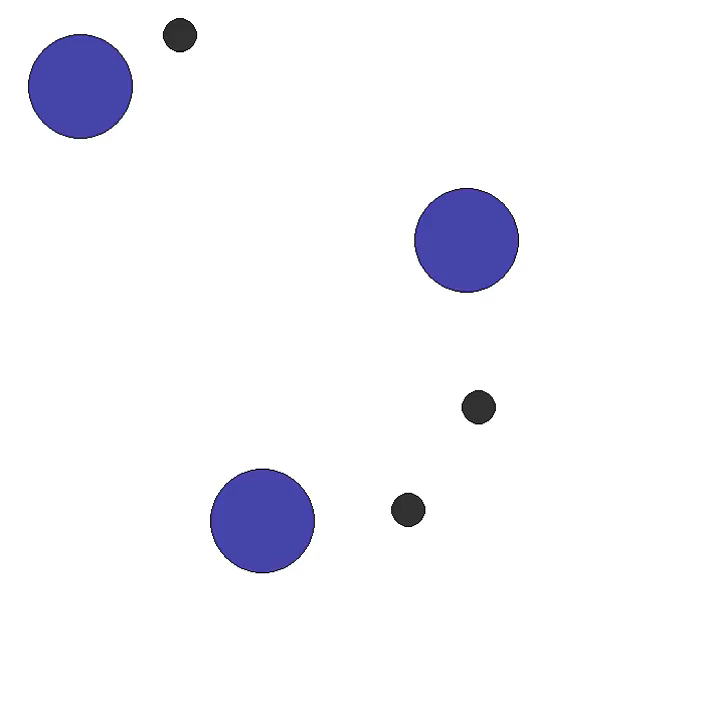
\includegraphics[scale=0.3]{images/simple_spread_v3/001.png}}
    \caption{Rendered frame from the Simple Spread environment. Agents are rendered as big blue circles, landmarks are rendered as small gray circles}
    \label{fig:simple_spread_env}
\end{figure}

\subsection{Knights Archers Zombies}
\label{sec:kaz_env}
The KAZ environment has a maximum of $n$ archers, a maximum of $m$ knights, and a maximum number of zombies $k$. The environment initializes with $n$ archers, $m$ knights and 0 zombies. The goal is for the archers and knights to kill zombies. Zombies spawn at the top border, at a set spawn rate, and travel down the screen moving randomly to the left or right. If an archer hits a zombie with an arrow it gets a reward of 1, and if a knight hits a zombie with a mace it gets a reward of 1. Once a zombie gets hit it dies. If a zombie collides with an agent the agent dies. The game ends once all agents are dead, a zombie reaches the bottom of the screen or some max length is reached.

For my experiments I used 2 archers, 2 knights, and a maximum of 10 zombies. The action space is discrete and allows the agents to idle, move forward, rotate clockwise, rotate counter clockwise, and attack. The observation space is either image based or vector based. I will use vector based for my experiments, which makes it a size of 135. See figure \ref{fig:kaz_env}

In the Knights Archers Zombies environment a critical state might be a state where an agent could die or is about to shoot an arrow that might kill a zombie, as these states are associated with changes in returns, immediate in the case of killing a zombie and delayed lower returns in the case of dying as an agent, as this does not incur a penalty, but it does make the agent unable to gain future rewards.

\begin{figure}[!ht]
    \centering
    \fbox{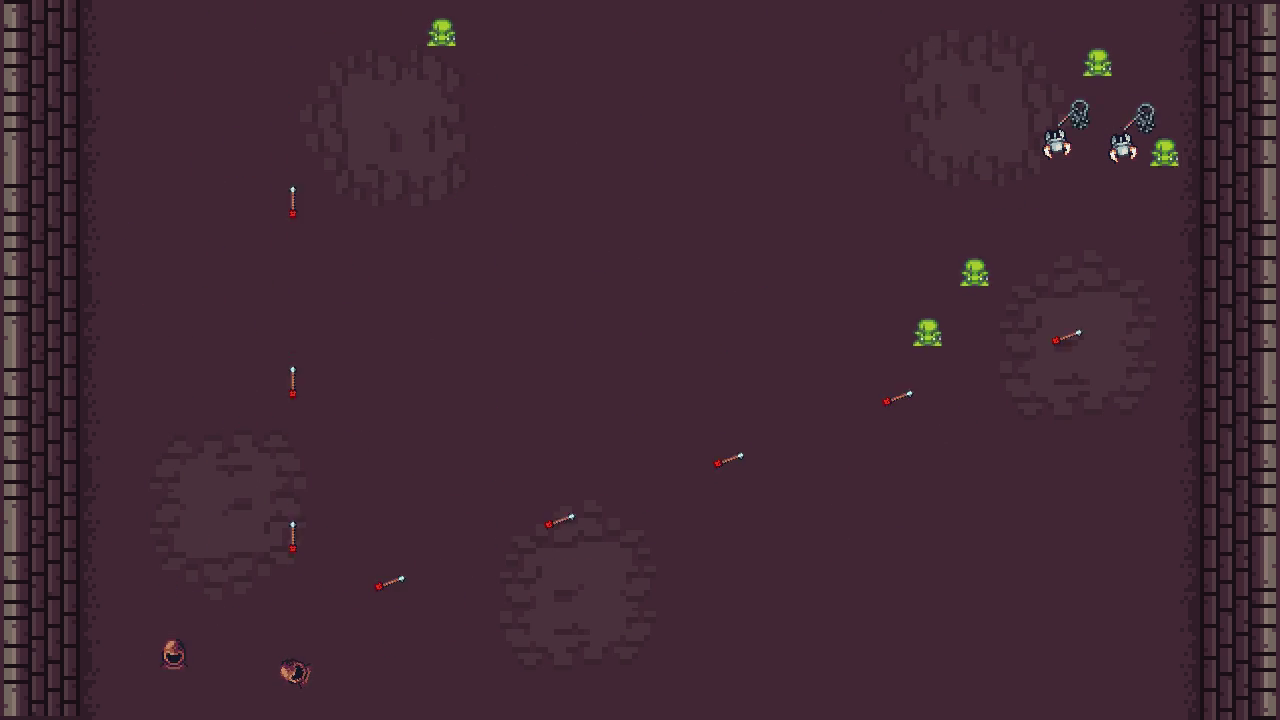
\includegraphics[scale=0.3]{images/knights_archers_zombies_v10/015.png}}
    \caption{Rendered frame from the Knights Archers Zombies environment.}
    \label{fig:kaz_env}
\end{figure}

\section{Policy creation}
This section will describe the details of how we create the policies for the environments.

\subsection{Reinforcement learning library}
There are a lot of options when deciding what library to use when designing \ac{rl} policies. I decided to use the library RLlib by Ray. The main benefits of this library is ease of implementation when working on heterogeneous agents, as each type of agent requires a specifically trained network to perform well. It also has scalability \cite{rayrllib}. It is required to train several policies for the creation of this thesis, therefore scalability when optimizing a policy is helpful.

\subsection{Policy construction}
I used a \ac{ppo} algorithm when optimizing my policy, because this method outperforms other algorithms in several environments in the continuous observation domain \cite{schulman2017proximalpolicyoptimizationalgorithms}, as well as the fact that is it applicable to \ac{marl} systems. The policy architecture consisted of an input layer with the observation of the environment as the size, two hidden layers of size 64, the hyperbolic tangent function, see \ref{eq:tanh}, colloquially known as tanh as the hidden layer activation function. This function is used for its "s-shape", bounding values from $y=-1$ to $y=1$, see figure \ref{fig:tanh}. The output layer has the size of the action space of the agent.

\begin{equation}
\label{eq:tanh}
tanh(x) = \frac{e^x-e^{-x}}{e^x+e^{-x}}
\end{equation}

\begin{figure}[h]
\centering
\begin{tikzpicture}
  \begin{axis}[
    xlabel={$x$},
    ylabel={$\tanh x$},
    domain=-4:4,
    samples=100,
    grid=both,
    axis lines=middle,
    width=10cm,
    height=6cm,
    enlargelimits,
  ]
    \addplot[blue, very thick] {tanh(x)};
  \end{axis}
\end{tikzpicture}
\caption{Graph showing the hyperbolic tangent function}
\label{fig:tanh}
\end{figure}

\subsection{Training}
The training was done with a batch size of 1024, for stability, learning rate and gamma was automatically tuned for the policies in the Knights Archers Zombies environments, but set to $1e-4$ and $0.8$ in the Simple Spread environment as i found these to reach close to a global optimum for every variation of the environment I trained on, e.g. with or without frame stacking.


\chapter{Experiments}
This chapter will discuss the details on how i perform the experiments, as well as discussing and analyzing the results of these experiments. The experiment described in \ref{sec:exp_1} will be about detecting the effects of actions and feature importance and their ability to elucidate the intent of a policy as aforementioned, the experiment described in \ref{sec:exp_2} explores if and how temporal information can be used to explain the intent of a policy, and the experiments described in \ref{sec:exp_3} explores how to alter the event and state prediction networks to improve predictions.

\section{General experimental setup}
I have several \acp{nn} for each experiment. The \acp{nn} have two hidden layers of size 64 each, the activation function $tanh$, and outputs either part of the state, $(x,y)$ coordinates for an agent for state prediction, or a single value, whether the trajectory contains a critical state or not, for event prediction. The experiments attempt to test whether my developed methods have an effect on event and state predictions, how impactful these effects are and what contributes to whether the effect is significant or not.I trained them with a scheduler which would divide learning rate by $3$ from an original of $1e-4$, down to a minimum of $1e-6$ whenever the calculated loss on the validation set stopped decreasing. All training was stopped after 200 epochs.

\subsection{State prediction neural nets and datasets}
For the state prediction I initially trained a \ac{nn}, $state_{base}$ to take the observations made by a type of agent from step $n$, $Obs_n$, and output the $x$ and $y$ coordinates of the same agent at step $n+m$ in a trajectory. The dataset $D_{pos}$ was constructed such that each data point was from a different trajectory $\tau$, to make sure all the data points were independent of each other, in order to make sure the \ac{nn} did not learn any such connection. Each data point is a pairing of values $(Obs_n, (x_{n+m},y_{n+m}))$. The variable $n$ was chosen randomly for each trajectory while $m$ stayed as a constant, in my case $m=10$. I would for example have $50000$ trajectories, each trajectory contains $2$ archers, so we would have a dataset of size $100000$. $100000$ observations and their corresponding positions $10$ steps into the future. We assume that both archers use the same policy as they are homogeneous.

\subsection{Event prediction neural nets and datasets}
I also trained a \ac{nn} for event prediction, $event_{base}$. The event we trained a network to predict was whether an agent would encounter a critical state or not. See section placeholder. The dataset $D_{crit}$ was similar to $D_{pos}$, however instead of positions, it would contain whether the agent would encounter a critical state within the next $4$ steps, $(Obs_n, crit)$, where $crit$ is a binary value, 0, for non critical states, or 1, for critical states.
I consider the accuracy of $event_{base}$ and the average error measured in euclidean distance of $state_{base}$ to be the baselines i compare results against in the first experiment. I will train other neural networks.


\subsection{Baseline performance}
$event_{base}$ got an accuracy of $0.8244$ on the test set and for $state_{base}$ the average distance from target was $0.0409$ on the test set. These \acp{nn} are purely post hoc explainers and used no information about the policy to explain the agents intention. As aforementioned we want to include information about the policy to discover how we can improve this prediction, and better discover the intent of the agent.

 Only The dataset, and therefore also the input layer, was different between the runs. I trained the networks for a total of $200$ epochs, after which improvement was negligible, if at all existent, with a learning rate scheduler that decreased learning rate when loss reached a plateau, which was measured on a validation set.

\section{Action and explanation inclusion}
\label{sec:exp_1}
As aforementioned this experiment explores how including action and explanations improves event and state predictions on the Simple Spread and Knights Archers Zombies environment.

\subsection{setup}
I enhanced both the dataset $D_{pos}$ and $D_{crit}$ with a series of other data. For both datasets I included the action, encoded by an integer from $0$ to $n_{acts}$, i.e. the amount of actions an agent has available, taken at $Obs_n$ for each data point, to use as input for an \ac{nn}. I then trained two \acp{nn} with the same architecture as $state_{base}$ and $event_{base}$ respectively, and once again measured accuracy for the event predictor net with included action, and average error for the state predictor net with included action. If the predictions improved I considered the action to be useful on its own for the predictions in the given environment.

This section will go into detail on how i included actions and explanations.

\subsubsection{One-hot and integer inclusion}
I then one-hot encoded the action, i.e. encoded the action as a $n_{acts}$ dimensional unit vector with a 1 in the chosen action dimension. This includes the same amount of information as represented as an integer, however I hypothesized that the resulting network would achieve higher performance with one-hot encoded actions as the distance between independent actions when one-hot encoding the actions are all the same, as opposed to when encoding the actions as an integer when the distance between two actions is not constant. For example, between the action encoded as the integer 2 and the action encoded as the integer 3 the Manhattan distance is 1, but between the action encoded as the integer 2 and the action encoded as the integer 4 the Manhattan distance is 2. When one-hot encoding these actions the Manhattan distance between two distinct actions will in all cases be 2. As in the previous cases I also trained a \ac{nn} on the datasets enhanced with one hot encoded actions.

\subsubsection{Integrated Gradients and Shapley Value inclusion}
After creating datasets with actions encoded different ways I also created two feature importance explanations for the action chosen in each of the initial observations. Shapley values and Integrated gradients were the two methods chosen. I decided on 2 feature importance measures that internally uses different methods of calculation, gradients and SHAP, to explore if they would yield different results. The motivation behind including feature importance explanations is that it describes some if the inner processing of the policy, and might therefore elucidate what kind of actions it might take in future states, and therefore include some of the intent. On each of the previous datasets I created new datasets with these two feature importance methods included.\\

\subsubsection{Result presentation}
In total I trained 18 neural networks per environment, one for each dataset constructed, and compared the results for accuracy on the event prediction networks and the results for average error on the state prediction networks. I repeated this experiment for a few different environments to explore if the results vary depending on environment.

All results are presented in tables, with asterisks marking significance, and italics used for baseline value.

\begin{figure}[!ht]
	%% Creator: Matplotlib, PGF backend
%%
%% To include the figure in your LaTeX document, write
%%   \input{<filename>.pgf}
%%
%% Make sure the required packages are loaded in your preamble
%%   \usepackage{pgf}
%%
%% Also ensure that all the required font packages are loaded; for instance,
%% the lmodern package is sometimes necessary when using math font.
%%   \usepackage{lmodern}
%%
%% Figures using additional raster images can only be included by \input if
%% they are in the same directory as the main LaTeX file. For loading figures
%% from other directories you can use the `import` package
%%   \usepackage{import}
%%
%% and then include the figures with
%%   \import{<path to file>}{<filename>.pgf}
%%
%% Matplotlib used the following preamble
%%   \def\mathdefault#1{#1}
%%   \everymath=\expandafter{\the\everymath\displaystyle}
%%   \IfFileExists{scrextend.sty}{
%%     \usepackage[fontsize=10.000000pt]{scrextend}
%%   }{
%%     \renewcommand{\normalsize}{\fontsize{10.000000}{12.000000}\selectfont}
%%     \normalsize
%%   }
%%   
%%   \ifdefined\pdftexversion\else  % non-pdftex case.
%%     \usepackage{fontspec}
%%     \setmainfont{DejaVuSerif.ttf}[Path=\detokenize{/uio/hume/student-u79/adaha/master_thesis/.venv/lib/python3.11/site-packages/matplotlib/mpl-data/fonts/ttf/}]
%%     \setsansfont{DejaVuSans.ttf}[Path=\detokenize{/uio/hume/student-u79/adaha/master_thesis/.venv/lib/python3.11/site-packages/matplotlib/mpl-data/fonts/ttf/}]
%%     \setmonofont{DejaVuSansMono.ttf}[Path=\detokenize{/uio/hume/student-u79/adaha/master_thesis/.venv/lib/python3.11/site-packages/matplotlib/mpl-data/fonts/ttf/}]
%%   \fi
%%   \makeatletter\@ifpackageloaded{underscore}{}{\usepackage[strings]{underscore}}\makeatother
%%
\begingroup%
\makeatletter%
\begin{pgfpicture}%
\pgfpathrectangle{\pgfpointorigin}{\pgfqpoint{6.400000in}{4.800000in}}%
\pgfusepath{use as bounding box, clip}%
\begin{pgfscope}%
\pgfsetbuttcap%
\pgfsetmiterjoin%
\definecolor{currentfill}{rgb}{1.000000,1.000000,1.000000}%
\pgfsetfillcolor{currentfill}%
\pgfsetlinewidth{0.000000pt}%
\definecolor{currentstroke}{rgb}{1.000000,1.000000,1.000000}%
\pgfsetstrokecolor{currentstroke}%
\pgfsetdash{}{0pt}%
\pgfpathmoveto{\pgfqpoint{0.000000in}{0.000000in}}%
\pgfpathlineto{\pgfqpoint{6.400000in}{0.000000in}}%
\pgfpathlineto{\pgfqpoint{6.400000in}{4.800000in}}%
\pgfpathlineto{\pgfqpoint{0.000000in}{4.800000in}}%
\pgfpathlineto{\pgfqpoint{0.000000in}{0.000000in}}%
\pgfpathclose%
\pgfusepath{fill}%
\end{pgfscope}%
\begin{pgfscope}%
\pgfsetbuttcap%
\pgfsetmiterjoin%
\definecolor{currentfill}{rgb}{1.000000,1.000000,1.000000}%
\pgfsetfillcolor{currentfill}%
\pgfsetlinewidth{0.000000pt}%
\definecolor{currentstroke}{rgb}{0.000000,0.000000,0.000000}%
\pgfsetstrokecolor{currentstroke}%
\pgfsetstrokeopacity{0.000000}%
\pgfsetdash{}{0pt}%
\pgfpathmoveto{\pgfqpoint{0.800000in}{0.528000in}}%
\pgfpathlineto{\pgfqpoint{5.760000in}{0.528000in}}%
\pgfpathlineto{\pgfqpoint{5.760000in}{4.224000in}}%
\pgfpathlineto{\pgfqpoint{0.800000in}{4.224000in}}%
\pgfpathlineto{\pgfqpoint{0.800000in}{0.528000in}}%
\pgfpathclose%
\pgfusepath{fill}%
\end{pgfscope}%
\begin{pgfscope}%
\pgfsetbuttcap%
\pgfsetroundjoin%
\definecolor{currentfill}{rgb}{0.000000,0.000000,0.000000}%
\pgfsetfillcolor{currentfill}%
\pgfsetlinewidth{0.803000pt}%
\definecolor{currentstroke}{rgb}{0.000000,0.000000,0.000000}%
\pgfsetstrokecolor{currentstroke}%
\pgfsetdash{}{0pt}%
\pgfsys@defobject{currentmarker}{\pgfqpoint{0.000000in}{-0.048611in}}{\pgfqpoint{0.000000in}{0.000000in}}{%
\pgfpathmoveto{\pgfqpoint{0.000000in}{0.000000in}}%
\pgfpathlineto{\pgfqpoint{0.000000in}{-0.048611in}}%
\pgfusepath{stroke,fill}%
}%
\begin{pgfscope}%
\pgfsys@transformshift{1.002796in}{0.528000in}%
\pgfsys@useobject{currentmarker}{}%
\end{pgfscope}%
\end{pgfscope}%
\begin{pgfscope}%
\definecolor{textcolor}{rgb}{0.000000,0.000000,0.000000}%
\pgfsetstrokecolor{textcolor}%
\pgfsetfillcolor{textcolor}%
\pgftext[x=1.002796in,y=0.430778in,,top]{\color{textcolor}{\sffamily\fontsize{10.000000}{12.000000}\selectfont\catcode`\^=\active\def^{\ifmmode\sp\else\^{}\fi}\catcode`\%=\active\def%{\%}0}}%
\end{pgfscope}%
\begin{pgfscope}%
\pgfsetbuttcap%
\pgfsetroundjoin%
\definecolor{currentfill}{rgb}{0.000000,0.000000,0.000000}%
\pgfsetfillcolor{currentfill}%
\pgfsetlinewidth{0.803000pt}%
\definecolor{currentstroke}{rgb}{0.000000,0.000000,0.000000}%
\pgfsetstrokecolor{currentstroke}%
\pgfsetdash{}{0pt}%
\pgfsys@defobject{currentmarker}{\pgfqpoint{0.000000in}{-0.048611in}}{\pgfqpoint{0.000000in}{0.000000in}}{%
\pgfpathmoveto{\pgfqpoint{0.000000in}{0.000000in}}%
\pgfpathlineto{\pgfqpoint{0.000000in}{-0.048611in}}%
\pgfusepath{stroke,fill}%
}%
\begin{pgfscope}%
\pgfsys@transformshift{1.569265in}{0.528000in}%
\pgfsys@useobject{currentmarker}{}%
\end{pgfscope}%
\end{pgfscope}%
\begin{pgfscope}%
\definecolor{textcolor}{rgb}{0.000000,0.000000,0.000000}%
\pgfsetstrokecolor{textcolor}%
\pgfsetfillcolor{textcolor}%
\pgftext[x=1.569265in,y=0.430778in,,top]{\color{textcolor}{\sffamily\fontsize{10.000000}{12.000000}\selectfont\catcode`\^=\active\def^{\ifmmode\sp\else\^{}\fi}\catcode`\%=\active\def%{\%}25}}%
\end{pgfscope}%
\begin{pgfscope}%
\pgfsetbuttcap%
\pgfsetroundjoin%
\definecolor{currentfill}{rgb}{0.000000,0.000000,0.000000}%
\pgfsetfillcolor{currentfill}%
\pgfsetlinewidth{0.803000pt}%
\definecolor{currentstroke}{rgb}{0.000000,0.000000,0.000000}%
\pgfsetstrokecolor{currentstroke}%
\pgfsetdash{}{0pt}%
\pgfsys@defobject{currentmarker}{\pgfqpoint{0.000000in}{-0.048611in}}{\pgfqpoint{0.000000in}{0.000000in}}{%
\pgfpathmoveto{\pgfqpoint{0.000000in}{0.000000in}}%
\pgfpathlineto{\pgfqpoint{0.000000in}{-0.048611in}}%
\pgfusepath{stroke,fill}%
}%
\begin{pgfscope}%
\pgfsys@transformshift{2.135733in}{0.528000in}%
\pgfsys@useobject{currentmarker}{}%
\end{pgfscope}%
\end{pgfscope}%
\begin{pgfscope}%
\definecolor{textcolor}{rgb}{0.000000,0.000000,0.000000}%
\pgfsetstrokecolor{textcolor}%
\pgfsetfillcolor{textcolor}%
\pgftext[x=2.135733in,y=0.430778in,,top]{\color{textcolor}{\sffamily\fontsize{10.000000}{12.000000}\selectfont\catcode`\^=\active\def^{\ifmmode\sp\else\^{}\fi}\catcode`\%=\active\def%{\%}50}}%
\end{pgfscope}%
\begin{pgfscope}%
\pgfsetbuttcap%
\pgfsetroundjoin%
\definecolor{currentfill}{rgb}{0.000000,0.000000,0.000000}%
\pgfsetfillcolor{currentfill}%
\pgfsetlinewidth{0.803000pt}%
\definecolor{currentstroke}{rgb}{0.000000,0.000000,0.000000}%
\pgfsetstrokecolor{currentstroke}%
\pgfsetdash{}{0pt}%
\pgfsys@defobject{currentmarker}{\pgfqpoint{0.000000in}{-0.048611in}}{\pgfqpoint{0.000000in}{0.000000in}}{%
\pgfpathmoveto{\pgfqpoint{0.000000in}{0.000000in}}%
\pgfpathlineto{\pgfqpoint{0.000000in}{-0.048611in}}%
\pgfusepath{stroke,fill}%
}%
\begin{pgfscope}%
\pgfsys@transformshift{2.702202in}{0.528000in}%
\pgfsys@useobject{currentmarker}{}%
\end{pgfscope}%
\end{pgfscope}%
\begin{pgfscope}%
\definecolor{textcolor}{rgb}{0.000000,0.000000,0.000000}%
\pgfsetstrokecolor{textcolor}%
\pgfsetfillcolor{textcolor}%
\pgftext[x=2.702202in,y=0.430778in,,top]{\color{textcolor}{\sffamily\fontsize{10.000000}{12.000000}\selectfont\catcode`\^=\active\def^{\ifmmode\sp\else\^{}\fi}\catcode`\%=\active\def%{\%}75}}%
\end{pgfscope}%
\begin{pgfscope}%
\pgfsetbuttcap%
\pgfsetroundjoin%
\definecolor{currentfill}{rgb}{0.000000,0.000000,0.000000}%
\pgfsetfillcolor{currentfill}%
\pgfsetlinewidth{0.803000pt}%
\definecolor{currentstroke}{rgb}{0.000000,0.000000,0.000000}%
\pgfsetstrokecolor{currentstroke}%
\pgfsetdash{}{0pt}%
\pgfsys@defobject{currentmarker}{\pgfqpoint{0.000000in}{-0.048611in}}{\pgfqpoint{0.000000in}{0.000000in}}{%
\pgfpathmoveto{\pgfqpoint{0.000000in}{0.000000in}}%
\pgfpathlineto{\pgfqpoint{0.000000in}{-0.048611in}}%
\pgfusepath{stroke,fill}%
}%
\begin{pgfscope}%
\pgfsys@transformshift{3.268671in}{0.528000in}%
\pgfsys@useobject{currentmarker}{}%
\end{pgfscope}%
\end{pgfscope}%
\begin{pgfscope}%
\definecolor{textcolor}{rgb}{0.000000,0.000000,0.000000}%
\pgfsetstrokecolor{textcolor}%
\pgfsetfillcolor{textcolor}%
\pgftext[x=3.268671in,y=0.430778in,,top]{\color{textcolor}{\sffamily\fontsize{10.000000}{12.000000}\selectfont\catcode`\^=\active\def^{\ifmmode\sp\else\^{}\fi}\catcode`\%=\active\def%{\%}100}}%
\end{pgfscope}%
\begin{pgfscope}%
\pgfsetbuttcap%
\pgfsetroundjoin%
\definecolor{currentfill}{rgb}{0.000000,0.000000,0.000000}%
\pgfsetfillcolor{currentfill}%
\pgfsetlinewidth{0.803000pt}%
\definecolor{currentstroke}{rgb}{0.000000,0.000000,0.000000}%
\pgfsetstrokecolor{currentstroke}%
\pgfsetdash{}{0pt}%
\pgfsys@defobject{currentmarker}{\pgfqpoint{0.000000in}{-0.048611in}}{\pgfqpoint{0.000000in}{0.000000in}}{%
\pgfpathmoveto{\pgfqpoint{0.000000in}{0.000000in}}%
\pgfpathlineto{\pgfqpoint{0.000000in}{-0.048611in}}%
\pgfusepath{stroke,fill}%
}%
\begin{pgfscope}%
\pgfsys@transformshift{3.835139in}{0.528000in}%
\pgfsys@useobject{currentmarker}{}%
\end{pgfscope}%
\end{pgfscope}%
\begin{pgfscope}%
\definecolor{textcolor}{rgb}{0.000000,0.000000,0.000000}%
\pgfsetstrokecolor{textcolor}%
\pgfsetfillcolor{textcolor}%
\pgftext[x=3.835139in,y=0.430778in,,top]{\color{textcolor}{\sffamily\fontsize{10.000000}{12.000000}\selectfont\catcode`\^=\active\def^{\ifmmode\sp\else\^{}\fi}\catcode`\%=\active\def%{\%}125}}%
\end{pgfscope}%
\begin{pgfscope}%
\pgfsetbuttcap%
\pgfsetroundjoin%
\definecolor{currentfill}{rgb}{0.000000,0.000000,0.000000}%
\pgfsetfillcolor{currentfill}%
\pgfsetlinewidth{0.803000pt}%
\definecolor{currentstroke}{rgb}{0.000000,0.000000,0.000000}%
\pgfsetstrokecolor{currentstroke}%
\pgfsetdash{}{0pt}%
\pgfsys@defobject{currentmarker}{\pgfqpoint{0.000000in}{-0.048611in}}{\pgfqpoint{0.000000in}{0.000000in}}{%
\pgfpathmoveto{\pgfqpoint{0.000000in}{0.000000in}}%
\pgfpathlineto{\pgfqpoint{0.000000in}{-0.048611in}}%
\pgfusepath{stroke,fill}%
}%
\begin{pgfscope}%
\pgfsys@transformshift{4.401608in}{0.528000in}%
\pgfsys@useobject{currentmarker}{}%
\end{pgfscope}%
\end{pgfscope}%
\begin{pgfscope}%
\definecolor{textcolor}{rgb}{0.000000,0.000000,0.000000}%
\pgfsetstrokecolor{textcolor}%
\pgfsetfillcolor{textcolor}%
\pgftext[x=4.401608in,y=0.430778in,,top]{\color{textcolor}{\sffamily\fontsize{10.000000}{12.000000}\selectfont\catcode`\^=\active\def^{\ifmmode\sp\else\^{}\fi}\catcode`\%=\active\def%{\%}150}}%
\end{pgfscope}%
\begin{pgfscope}%
\pgfsetbuttcap%
\pgfsetroundjoin%
\definecolor{currentfill}{rgb}{0.000000,0.000000,0.000000}%
\pgfsetfillcolor{currentfill}%
\pgfsetlinewidth{0.803000pt}%
\definecolor{currentstroke}{rgb}{0.000000,0.000000,0.000000}%
\pgfsetstrokecolor{currentstroke}%
\pgfsetdash{}{0pt}%
\pgfsys@defobject{currentmarker}{\pgfqpoint{0.000000in}{-0.048611in}}{\pgfqpoint{0.000000in}{0.000000in}}{%
\pgfpathmoveto{\pgfqpoint{0.000000in}{0.000000in}}%
\pgfpathlineto{\pgfqpoint{0.000000in}{-0.048611in}}%
\pgfusepath{stroke,fill}%
}%
\begin{pgfscope}%
\pgfsys@transformshift{4.968077in}{0.528000in}%
\pgfsys@useobject{currentmarker}{}%
\end{pgfscope}%
\end{pgfscope}%
\begin{pgfscope}%
\definecolor{textcolor}{rgb}{0.000000,0.000000,0.000000}%
\pgfsetstrokecolor{textcolor}%
\pgfsetfillcolor{textcolor}%
\pgftext[x=4.968077in,y=0.430778in,,top]{\color{textcolor}{\sffamily\fontsize{10.000000}{12.000000}\selectfont\catcode`\^=\active\def^{\ifmmode\sp\else\^{}\fi}\catcode`\%=\active\def%{\%}175}}%
\end{pgfscope}%
\begin{pgfscope}%
\pgfsetbuttcap%
\pgfsetroundjoin%
\definecolor{currentfill}{rgb}{0.000000,0.000000,0.000000}%
\pgfsetfillcolor{currentfill}%
\pgfsetlinewidth{0.803000pt}%
\definecolor{currentstroke}{rgb}{0.000000,0.000000,0.000000}%
\pgfsetstrokecolor{currentstroke}%
\pgfsetdash{}{0pt}%
\pgfsys@defobject{currentmarker}{\pgfqpoint{0.000000in}{-0.048611in}}{\pgfqpoint{0.000000in}{0.000000in}}{%
\pgfpathmoveto{\pgfqpoint{0.000000in}{0.000000in}}%
\pgfpathlineto{\pgfqpoint{0.000000in}{-0.048611in}}%
\pgfusepath{stroke,fill}%
}%
\begin{pgfscope}%
\pgfsys@transformshift{5.534545in}{0.528000in}%
\pgfsys@useobject{currentmarker}{}%
\end{pgfscope}%
\end{pgfscope}%
\begin{pgfscope}%
\definecolor{textcolor}{rgb}{0.000000,0.000000,0.000000}%
\pgfsetstrokecolor{textcolor}%
\pgfsetfillcolor{textcolor}%
\pgftext[x=5.534545in,y=0.430778in,,top]{\color{textcolor}{\sffamily\fontsize{10.000000}{12.000000}\selectfont\catcode`\^=\active\def^{\ifmmode\sp\else\^{}\fi}\catcode`\%=\active\def%{\%}200}}%
\end{pgfscope}%
\begin{pgfscope}%
\definecolor{textcolor}{rgb}{0.000000,0.000000,0.000000}%
\pgfsetstrokecolor{textcolor}%
\pgfsetfillcolor{textcolor}%
\pgftext[x=3.280000in,y=0.240809in,,top]{\color{textcolor}{\sffamily\fontsize{10.000000}{12.000000}\selectfont\catcode`\^=\active\def^{\ifmmode\sp\else\^{}\fi}\catcode`\%=\active\def%{\%}Epoch}}%
\end{pgfscope}%
\begin{pgfscope}%
\pgfsetbuttcap%
\pgfsetroundjoin%
\definecolor{currentfill}{rgb}{0.000000,0.000000,0.000000}%
\pgfsetfillcolor{currentfill}%
\pgfsetlinewidth{0.803000pt}%
\definecolor{currentstroke}{rgb}{0.000000,0.000000,0.000000}%
\pgfsetstrokecolor{currentstroke}%
\pgfsetdash{}{0pt}%
\pgfsys@defobject{currentmarker}{\pgfqpoint{-0.048611in}{0.000000in}}{\pgfqpoint{-0.000000in}{0.000000in}}{%
\pgfpathmoveto{\pgfqpoint{-0.000000in}{0.000000in}}%
\pgfpathlineto{\pgfqpoint{-0.048611in}{0.000000in}}%
\pgfusepath{stroke,fill}%
}%
\begin{pgfscope}%
\pgfsys@transformshift{0.800000in}{0.902553in}%
\pgfsys@useobject{currentmarker}{}%
\end{pgfscope}%
\end{pgfscope}%
\begin{pgfscope}%
\definecolor{textcolor}{rgb}{0.000000,0.000000,0.000000}%
\pgfsetstrokecolor{textcolor}%
\pgfsetfillcolor{textcolor}%
\pgftext[x=0.393533in, y=0.849792in, left, base]{\color{textcolor}{\sffamily\fontsize{10.000000}{12.000000}\selectfont\catcode`\^=\active\def^{\ifmmode\sp\else\^{}\fi}\catcode`\%=\active\def%{\%}0.40}}%
\end{pgfscope}%
\begin{pgfscope}%
\pgfsetbuttcap%
\pgfsetroundjoin%
\definecolor{currentfill}{rgb}{0.000000,0.000000,0.000000}%
\pgfsetfillcolor{currentfill}%
\pgfsetlinewidth{0.803000pt}%
\definecolor{currentstroke}{rgb}{0.000000,0.000000,0.000000}%
\pgfsetstrokecolor{currentstroke}%
\pgfsetdash{}{0pt}%
\pgfsys@defobject{currentmarker}{\pgfqpoint{-0.048611in}{0.000000in}}{\pgfqpoint{-0.000000in}{0.000000in}}{%
\pgfpathmoveto{\pgfqpoint{-0.000000in}{0.000000in}}%
\pgfpathlineto{\pgfqpoint{-0.048611in}{0.000000in}}%
\pgfusepath{stroke,fill}%
}%
\begin{pgfscope}%
\pgfsys@transformshift{0.800000in}{1.440627in}%
\pgfsys@useobject{currentmarker}{}%
\end{pgfscope}%
\end{pgfscope}%
\begin{pgfscope}%
\definecolor{textcolor}{rgb}{0.000000,0.000000,0.000000}%
\pgfsetstrokecolor{textcolor}%
\pgfsetfillcolor{textcolor}%
\pgftext[x=0.393533in, y=1.387865in, left, base]{\color{textcolor}{\sffamily\fontsize{10.000000}{12.000000}\selectfont\catcode`\^=\active\def^{\ifmmode\sp\else\^{}\fi}\catcode`\%=\active\def%{\%}0.45}}%
\end{pgfscope}%
\begin{pgfscope}%
\pgfsetbuttcap%
\pgfsetroundjoin%
\definecolor{currentfill}{rgb}{0.000000,0.000000,0.000000}%
\pgfsetfillcolor{currentfill}%
\pgfsetlinewidth{0.803000pt}%
\definecolor{currentstroke}{rgb}{0.000000,0.000000,0.000000}%
\pgfsetstrokecolor{currentstroke}%
\pgfsetdash{}{0pt}%
\pgfsys@defobject{currentmarker}{\pgfqpoint{-0.048611in}{0.000000in}}{\pgfqpoint{-0.000000in}{0.000000in}}{%
\pgfpathmoveto{\pgfqpoint{-0.000000in}{0.000000in}}%
\pgfpathlineto{\pgfqpoint{-0.048611in}{0.000000in}}%
\pgfusepath{stroke,fill}%
}%
\begin{pgfscope}%
\pgfsys@transformshift{0.800000in}{1.978701in}%
\pgfsys@useobject{currentmarker}{}%
\end{pgfscope}%
\end{pgfscope}%
\begin{pgfscope}%
\definecolor{textcolor}{rgb}{0.000000,0.000000,0.000000}%
\pgfsetstrokecolor{textcolor}%
\pgfsetfillcolor{textcolor}%
\pgftext[x=0.393533in, y=1.925939in, left, base]{\color{textcolor}{\sffamily\fontsize{10.000000}{12.000000}\selectfont\catcode`\^=\active\def^{\ifmmode\sp\else\^{}\fi}\catcode`\%=\active\def%{\%}0.50}}%
\end{pgfscope}%
\begin{pgfscope}%
\pgfsetbuttcap%
\pgfsetroundjoin%
\definecolor{currentfill}{rgb}{0.000000,0.000000,0.000000}%
\pgfsetfillcolor{currentfill}%
\pgfsetlinewidth{0.803000pt}%
\definecolor{currentstroke}{rgb}{0.000000,0.000000,0.000000}%
\pgfsetstrokecolor{currentstroke}%
\pgfsetdash{}{0pt}%
\pgfsys@defobject{currentmarker}{\pgfqpoint{-0.048611in}{0.000000in}}{\pgfqpoint{-0.000000in}{0.000000in}}{%
\pgfpathmoveto{\pgfqpoint{-0.000000in}{0.000000in}}%
\pgfpathlineto{\pgfqpoint{-0.048611in}{0.000000in}}%
\pgfusepath{stroke,fill}%
}%
\begin{pgfscope}%
\pgfsys@transformshift{0.800000in}{2.516775in}%
\pgfsys@useobject{currentmarker}{}%
\end{pgfscope}%
\end{pgfscope}%
\begin{pgfscope}%
\definecolor{textcolor}{rgb}{0.000000,0.000000,0.000000}%
\pgfsetstrokecolor{textcolor}%
\pgfsetfillcolor{textcolor}%
\pgftext[x=0.393533in, y=2.464013in, left, base]{\color{textcolor}{\sffamily\fontsize{10.000000}{12.000000}\selectfont\catcode`\^=\active\def^{\ifmmode\sp\else\^{}\fi}\catcode`\%=\active\def%{\%}0.55}}%
\end{pgfscope}%
\begin{pgfscope}%
\pgfsetbuttcap%
\pgfsetroundjoin%
\definecolor{currentfill}{rgb}{0.000000,0.000000,0.000000}%
\pgfsetfillcolor{currentfill}%
\pgfsetlinewidth{0.803000pt}%
\definecolor{currentstroke}{rgb}{0.000000,0.000000,0.000000}%
\pgfsetstrokecolor{currentstroke}%
\pgfsetdash{}{0pt}%
\pgfsys@defobject{currentmarker}{\pgfqpoint{-0.048611in}{0.000000in}}{\pgfqpoint{-0.000000in}{0.000000in}}{%
\pgfpathmoveto{\pgfqpoint{-0.000000in}{0.000000in}}%
\pgfpathlineto{\pgfqpoint{-0.048611in}{0.000000in}}%
\pgfusepath{stroke,fill}%
}%
\begin{pgfscope}%
\pgfsys@transformshift{0.800000in}{3.054848in}%
\pgfsys@useobject{currentmarker}{}%
\end{pgfscope}%
\end{pgfscope}%
\begin{pgfscope}%
\definecolor{textcolor}{rgb}{0.000000,0.000000,0.000000}%
\pgfsetstrokecolor{textcolor}%
\pgfsetfillcolor{textcolor}%
\pgftext[x=0.393533in, y=3.002087in, left, base]{\color{textcolor}{\sffamily\fontsize{10.000000}{12.000000}\selectfont\catcode`\^=\active\def^{\ifmmode\sp\else\^{}\fi}\catcode`\%=\active\def%{\%}0.60}}%
\end{pgfscope}%
\begin{pgfscope}%
\pgfsetbuttcap%
\pgfsetroundjoin%
\definecolor{currentfill}{rgb}{0.000000,0.000000,0.000000}%
\pgfsetfillcolor{currentfill}%
\pgfsetlinewidth{0.803000pt}%
\definecolor{currentstroke}{rgb}{0.000000,0.000000,0.000000}%
\pgfsetstrokecolor{currentstroke}%
\pgfsetdash{}{0pt}%
\pgfsys@defobject{currentmarker}{\pgfqpoint{-0.048611in}{0.000000in}}{\pgfqpoint{-0.000000in}{0.000000in}}{%
\pgfpathmoveto{\pgfqpoint{-0.000000in}{0.000000in}}%
\pgfpathlineto{\pgfqpoint{-0.048611in}{0.000000in}}%
\pgfusepath{stroke,fill}%
}%
\begin{pgfscope}%
\pgfsys@transformshift{0.800000in}{3.592922in}%
\pgfsys@useobject{currentmarker}{}%
\end{pgfscope}%
\end{pgfscope}%
\begin{pgfscope}%
\definecolor{textcolor}{rgb}{0.000000,0.000000,0.000000}%
\pgfsetstrokecolor{textcolor}%
\pgfsetfillcolor{textcolor}%
\pgftext[x=0.393533in, y=3.540161in, left, base]{\color{textcolor}{\sffamily\fontsize{10.000000}{12.000000}\selectfont\catcode`\^=\active\def^{\ifmmode\sp\else\^{}\fi}\catcode`\%=\active\def%{\%}0.65}}%
\end{pgfscope}%
\begin{pgfscope}%
\pgfsetbuttcap%
\pgfsetroundjoin%
\definecolor{currentfill}{rgb}{0.000000,0.000000,0.000000}%
\pgfsetfillcolor{currentfill}%
\pgfsetlinewidth{0.803000pt}%
\definecolor{currentstroke}{rgb}{0.000000,0.000000,0.000000}%
\pgfsetstrokecolor{currentstroke}%
\pgfsetdash{}{0pt}%
\pgfsys@defobject{currentmarker}{\pgfqpoint{-0.048611in}{0.000000in}}{\pgfqpoint{-0.000000in}{0.000000in}}{%
\pgfpathmoveto{\pgfqpoint{-0.000000in}{0.000000in}}%
\pgfpathlineto{\pgfqpoint{-0.048611in}{0.000000in}}%
\pgfusepath{stroke,fill}%
}%
\begin{pgfscope}%
\pgfsys@transformshift{0.800000in}{4.130996in}%
\pgfsys@useobject{currentmarker}{}%
\end{pgfscope}%
\end{pgfscope}%
\begin{pgfscope}%
\definecolor{textcolor}{rgb}{0.000000,0.000000,0.000000}%
\pgfsetstrokecolor{textcolor}%
\pgfsetfillcolor{textcolor}%
\pgftext[x=0.393533in, y=4.078234in, left, base]{\color{textcolor}{\sffamily\fontsize{10.000000}{12.000000}\selectfont\catcode`\^=\active\def^{\ifmmode\sp\else\^{}\fi}\catcode`\%=\active\def%{\%}0.70}}%
\end{pgfscope}%
\begin{pgfscope}%
\definecolor{textcolor}{rgb}{0.000000,0.000000,0.000000}%
\pgfsetstrokecolor{textcolor}%
\pgfsetfillcolor{textcolor}%
\pgftext[x=0.337977in,y=2.376000in,,bottom,rotate=90.000000]{\color{textcolor}{\sffamily\fontsize{10.000000}{12.000000}\selectfont\catcode`\^=\active\def^{\ifmmode\sp\else\^{}\fi}\catcode`\%=\active\def%{\%}Loss}}%
\end{pgfscope}%
\begin{pgfscope}%
\pgfpathrectangle{\pgfqpoint{0.800000in}{0.528000in}}{\pgfqpoint{4.960000in}{3.696000in}}%
\pgfusepath{clip}%
\pgfsetrectcap%
\pgfsetroundjoin%
\pgfsetlinewidth{1.505625pt}%
\definecolor{currentstroke}{rgb}{0.121569,0.466667,0.705882}%
\pgfsetstrokecolor{currentstroke}%
\pgfsetdash{}{0pt}%
\pgfpathmoveto{\pgfqpoint{1.025455in}{3.652491in}}%
\pgfpathlineto{\pgfqpoint{1.048113in}{3.330448in}}%
\pgfpathlineto{\pgfqpoint{1.070772in}{3.165052in}}%
\pgfpathlineto{\pgfqpoint{1.093431in}{3.094110in}}%
\pgfpathlineto{\pgfqpoint{1.116090in}{3.029616in}}%
\pgfpathlineto{\pgfqpoint{1.138748in}{2.979573in}}%
\pgfpathlineto{\pgfqpoint{1.161407in}{2.945938in}}%
\pgfpathlineto{\pgfqpoint{1.184066in}{2.910199in}}%
\pgfpathlineto{\pgfqpoint{1.206725in}{2.891157in}}%
\pgfpathlineto{\pgfqpoint{1.229383in}{2.861010in}}%
\pgfpathlineto{\pgfqpoint{1.252042in}{2.836028in}}%
\pgfpathlineto{\pgfqpoint{1.274701in}{2.820719in}}%
\pgfpathlineto{\pgfqpoint{1.297360in}{2.793738in}}%
\pgfpathlineto{\pgfqpoint{1.320018in}{2.774124in}}%
\pgfpathlineto{\pgfqpoint{1.342677in}{2.730236in}}%
\pgfpathlineto{\pgfqpoint{1.365336in}{2.656739in}}%
\pgfpathlineto{\pgfqpoint{1.387995in}{2.558724in}}%
\pgfpathlineto{\pgfqpoint{1.410653in}{2.431833in}}%
\pgfpathlineto{\pgfqpoint{1.455971in}{2.108081in}}%
\pgfpathlineto{\pgfqpoint{1.478630in}{1.963006in}}%
\pgfpathlineto{\pgfqpoint{1.501288in}{1.829729in}}%
\pgfpathlineto{\pgfqpoint{1.523947in}{1.728201in}}%
\pgfpathlineto{\pgfqpoint{1.546606in}{1.665096in}}%
\pgfpathlineto{\pgfqpoint{1.569265in}{1.606573in}}%
\pgfpathlineto{\pgfqpoint{1.591923in}{1.572503in}}%
\pgfpathlineto{\pgfqpoint{1.637241in}{1.512384in}}%
\pgfpathlineto{\pgfqpoint{1.659899in}{1.492672in}}%
\pgfpathlineto{\pgfqpoint{1.682558in}{1.488315in}}%
\pgfpathlineto{\pgfqpoint{1.705217in}{1.480571in}}%
\pgfpathlineto{\pgfqpoint{1.727876in}{1.474719in}}%
\pgfpathlineto{\pgfqpoint{1.750534in}{1.449305in}}%
\pgfpathlineto{\pgfqpoint{1.773193in}{1.456695in}}%
\pgfpathlineto{\pgfqpoint{1.795852in}{1.448402in}}%
\pgfpathlineto{\pgfqpoint{1.818511in}{1.431565in}}%
\pgfpathlineto{\pgfqpoint{1.841169in}{1.448448in}}%
\pgfpathlineto{\pgfqpoint{1.863828in}{1.426137in}}%
\pgfpathlineto{\pgfqpoint{1.886487in}{1.434974in}}%
\pgfpathlineto{\pgfqpoint{1.909146in}{1.412666in}}%
\pgfpathlineto{\pgfqpoint{1.931804in}{1.420853in}}%
\pgfpathlineto{\pgfqpoint{1.954463in}{1.417273in}}%
\pgfpathlineto{\pgfqpoint{1.977122in}{1.415739in}}%
\pgfpathlineto{\pgfqpoint{1.999781in}{1.403275in}}%
\pgfpathlineto{\pgfqpoint{2.022439in}{1.396653in}}%
\pgfpathlineto{\pgfqpoint{2.045098in}{1.393837in}}%
\pgfpathlineto{\pgfqpoint{2.067757in}{1.402775in}}%
\pgfpathlineto{\pgfqpoint{2.090416in}{1.391616in}}%
\pgfpathlineto{\pgfqpoint{2.113074in}{1.385237in}}%
\pgfpathlineto{\pgfqpoint{2.135733in}{1.397293in}}%
\pgfpathlineto{\pgfqpoint{2.158392in}{1.387653in}}%
\pgfpathlineto{\pgfqpoint{2.203709in}{1.370924in}}%
\pgfpathlineto{\pgfqpoint{2.226368in}{1.382933in}}%
\pgfpathlineto{\pgfqpoint{2.249027in}{1.378038in}}%
\pgfpathlineto{\pgfqpoint{2.271686in}{1.374560in}}%
\pgfpathlineto{\pgfqpoint{2.294344in}{1.363424in}}%
\pgfpathlineto{\pgfqpoint{2.317003in}{1.373314in}}%
\pgfpathlineto{\pgfqpoint{2.339662in}{1.369654in}}%
\pgfpathlineto{\pgfqpoint{2.362321in}{1.367257in}}%
\pgfpathlineto{\pgfqpoint{2.384979in}{1.357338in}}%
\pgfpathlineto{\pgfqpoint{2.407638in}{1.379900in}}%
\pgfpathlineto{\pgfqpoint{2.430297in}{1.353567in}}%
\pgfpathlineto{\pgfqpoint{2.452956in}{1.373588in}}%
\pgfpathlineto{\pgfqpoint{2.475614in}{1.341995in}}%
\pgfpathlineto{\pgfqpoint{2.498273in}{1.357801in}}%
\pgfpathlineto{\pgfqpoint{2.520932in}{1.348870in}}%
\pgfpathlineto{\pgfqpoint{2.543591in}{1.337072in}}%
\pgfpathlineto{\pgfqpoint{2.566249in}{1.333581in}}%
\pgfpathlineto{\pgfqpoint{2.588908in}{1.319314in}}%
\pgfpathlineto{\pgfqpoint{2.611567in}{1.320800in}}%
\pgfpathlineto{\pgfqpoint{2.634226in}{1.335050in}}%
\pgfpathlineto{\pgfqpoint{2.656884in}{1.308847in}}%
\pgfpathlineto{\pgfqpoint{2.679543in}{1.324743in}}%
\pgfpathlineto{\pgfqpoint{2.724861in}{1.305403in}}%
\pgfpathlineto{\pgfqpoint{2.747519in}{1.329299in}}%
\pgfpathlineto{\pgfqpoint{2.770178in}{1.309810in}}%
\pgfpathlineto{\pgfqpoint{2.792837in}{1.306670in}}%
\pgfpathlineto{\pgfqpoint{2.815496in}{1.300558in}}%
\pgfpathlineto{\pgfqpoint{2.838154in}{1.297917in}}%
\pgfpathlineto{\pgfqpoint{2.860813in}{1.290448in}}%
\pgfpathlineto{\pgfqpoint{2.883472in}{1.287090in}}%
\pgfpathlineto{\pgfqpoint{2.906131in}{1.293951in}}%
\pgfpathlineto{\pgfqpoint{2.928789in}{1.282921in}}%
\pgfpathlineto{\pgfqpoint{2.951448in}{1.275091in}}%
\pgfpathlineto{\pgfqpoint{2.974107in}{1.285321in}}%
\pgfpathlineto{\pgfqpoint{2.996766in}{1.285864in}}%
\pgfpathlineto{\pgfqpoint{3.019424in}{1.268309in}}%
\pgfpathlineto{\pgfqpoint{3.042083in}{1.278751in}}%
\pgfpathlineto{\pgfqpoint{3.064742in}{1.269342in}}%
\pgfpathlineto{\pgfqpoint{3.087401in}{1.283656in}}%
\pgfpathlineto{\pgfqpoint{3.110059in}{1.263870in}}%
\pgfpathlineto{\pgfqpoint{3.132718in}{1.257419in}}%
\pgfpathlineto{\pgfqpoint{3.155377in}{1.269465in}}%
\pgfpathlineto{\pgfqpoint{3.178036in}{1.249361in}}%
\pgfpathlineto{\pgfqpoint{3.200694in}{1.253865in}}%
\pgfpathlineto{\pgfqpoint{3.223353in}{1.253808in}}%
\pgfpathlineto{\pgfqpoint{3.246012in}{1.236744in}}%
\pgfpathlineto{\pgfqpoint{3.268671in}{1.238006in}}%
\pgfpathlineto{\pgfqpoint{3.291329in}{1.249795in}}%
\pgfpathlineto{\pgfqpoint{3.313988in}{1.238863in}}%
\pgfpathlineto{\pgfqpoint{3.336647in}{1.234006in}}%
\pgfpathlineto{\pgfqpoint{3.359306in}{1.234205in}}%
\pgfpathlineto{\pgfqpoint{3.381964in}{1.224502in}}%
\pgfpathlineto{\pgfqpoint{3.404623in}{1.220380in}}%
\pgfpathlineto{\pgfqpoint{3.427282in}{1.223775in}}%
\pgfpathlineto{\pgfqpoint{3.449941in}{1.224410in}}%
\pgfpathlineto{\pgfqpoint{3.472599in}{1.222710in}}%
\pgfpathlineto{\pgfqpoint{3.495258in}{1.215825in}}%
\pgfpathlineto{\pgfqpoint{3.517917in}{1.202249in}}%
\pgfpathlineto{\pgfqpoint{3.540576in}{1.234844in}}%
\pgfpathlineto{\pgfqpoint{3.563234in}{1.202747in}}%
\pgfpathlineto{\pgfqpoint{3.585893in}{1.208407in}}%
\pgfpathlineto{\pgfqpoint{3.608552in}{1.209711in}}%
\pgfpathlineto{\pgfqpoint{3.631211in}{1.188337in}}%
\pgfpathlineto{\pgfqpoint{3.653869in}{1.195987in}}%
\pgfpathlineto{\pgfqpoint{3.676528in}{1.186291in}}%
\pgfpathlineto{\pgfqpoint{3.699187in}{1.210097in}}%
\pgfpathlineto{\pgfqpoint{3.721846in}{1.188259in}}%
\pgfpathlineto{\pgfqpoint{3.744504in}{1.192936in}}%
\pgfpathlineto{\pgfqpoint{3.767163in}{1.184798in}}%
\pgfpathlineto{\pgfqpoint{3.789822in}{1.169018in}}%
\pgfpathlineto{\pgfqpoint{3.812481in}{1.170833in}}%
\pgfpathlineto{\pgfqpoint{3.835139in}{1.167791in}}%
\pgfpathlineto{\pgfqpoint{3.857798in}{1.169992in}}%
\pgfpathlineto{\pgfqpoint{3.880457in}{1.169913in}}%
\pgfpathlineto{\pgfqpoint{3.903116in}{1.180168in}}%
\pgfpathlineto{\pgfqpoint{3.925774in}{1.166199in}}%
\pgfpathlineto{\pgfqpoint{3.948433in}{1.169327in}}%
\pgfpathlineto{\pgfqpoint{3.971092in}{1.152473in}}%
\pgfpathlineto{\pgfqpoint{3.993751in}{1.165504in}}%
\pgfpathlineto{\pgfqpoint{4.016409in}{1.161240in}}%
\pgfpathlineto{\pgfqpoint{4.039068in}{1.153232in}}%
\pgfpathlineto{\pgfqpoint{4.061727in}{1.167832in}}%
\pgfpathlineto{\pgfqpoint{4.084386in}{1.142792in}}%
\pgfpathlineto{\pgfqpoint{4.107044in}{1.154441in}}%
\pgfpathlineto{\pgfqpoint{4.129703in}{1.146305in}}%
\pgfpathlineto{\pgfqpoint{4.152362in}{1.142562in}}%
\pgfpathlineto{\pgfqpoint{4.175021in}{1.131195in}}%
\pgfpathlineto{\pgfqpoint{4.197679in}{1.136107in}}%
\pgfpathlineto{\pgfqpoint{4.220338in}{1.149121in}}%
\pgfpathlineto{\pgfqpoint{4.242997in}{1.128946in}}%
\pgfpathlineto{\pgfqpoint{4.265656in}{1.148060in}}%
\pgfpathlineto{\pgfqpoint{4.288314in}{1.164553in}}%
\pgfpathlineto{\pgfqpoint{4.310973in}{1.133542in}}%
\pgfpathlineto{\pgfqpoint{4.333632in}{1.118410in}}%
\pgfpathlineto{\pgfqpoint{4.356291in}{1.124450in}}%
\pgfpathlineto{\pgfqpoint{4.378949in}{1.120988in}}%
\pgfpathlineto{\pgfqpoint{4.401608in}{1.130985in}}%
\pgfpathlineto{\pgfqpoint{4.424267in}{1.146505in}}%
\pgfpathlineto{\pgfqpoint{4.446926in}{1.130596in}}%
\pgfpathlineto{\pgfqpoint{4.469584in}{1.122471in}}%
\pgfpathlineto{\pgfqpoint{4.492243in}{1.126282in}}%
\pgfpathlineto{\pgfqpoint{4.514902in}{1.122659in}}%
\pgfpathlineto{\pgfqpoint{4.537561in}{1.111667in}}%
\pgfpathlineto{\pgfqpoint{4.560219in}{1.116378in}}%
\pgfpathlineto{\pgfqpoint{4.582878in}{1.123997in}}%
\pgfpathlineto{\pgfqpoint{4.605537in}{1.104972in}}%
\pgfpathlineto{\pgfqpoint{4.628196in}{1.117152in}}%
\pgfpathlineto{\pgfqpoint{4.650854in}{1.124236in}}%
\pgfpathlineto{\pgfqpoint{4.673513in}{1.107527in}}%
\pgfpathlineto{\pgfqpoint{4.718831in}{1.110989in}}%
\pgfpathlineto{\pgfqpoint{4.741489in}{1.102177in}}%
\pgfpathlineto{\pgfqpoint{4.764148in}{1.100079in}}%
\pgfpathlineto{\pgfqpoint{4.786807in}{1.107035in}}%
\pgfpathlineto{\pgfqpoint{4.809466in}{1.101204in}}%
\pgfpathlineto{\pgfqpoint{4.832124in}{1.102339in}}%
\pgfpathlineto{\pgfqpoint{4.854783in}{1.090013in}}%
\pgfpathlineto{\pgfqpoint{4.877442in}{1.091922in}}%
\pgfpathlineto{\pgfqpoint{4.900101in}{1.103285in}}%
\pgfpathlineto{\pgfqpoint{4.922759in}{1.105979in}}%
\pgfpathlineto{\pgfqpoint{4.945418in}{1.119629in}}%
\pgfpathlineto{\pgfqpoint{4.968077in}{1.097225in}}%
\pgfpathlineto{\pgfqpoint{4.990735in}{1.077965in}}%
\pgfpathlineto{\pgfqpoint{5.013394in}{1.104233in}}%
\pgfpathlineto{\pgfqpoint{5.036053in}{1.083793in}}%
\pgfpathlineto{\pgfqpoint{5.058712in}{1.095197in}}%
\pgfpathlineto{\pgfqpoint{5.081370in}{1.084842in}}%
\pgfpathlineto{\pgfqpoint{5.104029in}{1.092353in}}%
\pgfpathlineto{\pgfqpoint{5.126688in}{1.087775in}}%
\pgfpathlineto{\pgfqpoint{5.149347in}{1.093947in}}%
\pgfpathlineto{\pgfqpoint{5.172005in}{1.101468in}}%
\pgfpathlineto{\pgfqpoint{5.194664in}{1.097880in}}%
\pgfpathlineto{\pgfqpoint{5.217323in}{1.104771in}}%
\pgfpathlineto{\pgfqpoint{5.239982in}{1.098684in}}%
\pgfpathlineto{\pgfqpoint{5.262640in}{1.071636in}}%
\pgfpathlineto{\pgfqpoint{5.285299in}{1.069587in}}%
\pgfpathlineto{\pgfqpoint{5.307958in}{1.074063in}}%
\pgfpathlineto{\pgfqpoint{5.330617in}{1.074161in}}%
\pgfpathlineto{\pgfqpoint{5.353275in}{1.078142in}}%
\pgfpathlineto{\pgfqpoint{5.375934in}{1.074982in}}%
\pgfpathlineto{\pgfqpoint{5.398593in}{1.069225in}}%
\pgfpathlineto{\pgfqpoint{5.421252in}{1.076449in}}%
\pgfpathlineto{\pgfqpoint{5.443910in}{1.069444in}}%
\pgfpathlineto{\pgfqpoint{5.466569in}{1.077246in}}%
\pgfpathlineto{\pgfqpoint{5.489228in}{1.078623in}}%
\pgfpathlineto{\pgfqpoint{5.511887in}{1.072476in}}%
\pgfpathlineto{\pgfqpoint{5.534545in}{1.072377in}}%
\pgfpathlineto{\pgfqpoint{5.534545in}{1.072377in}}%
\pgfusepath{stroke}%
\end{pgfscope}%
\begin{pgfscope}%
\pgfpathrectangle{\pgfqpoint{0.800000in}{0.528000in}}{\pgfqpoint{4.960000in}{3.696000in}}%
\pgfusepath{clip}%
\pgfsetrectcap%
\pgfsetroundjoin%
\pgfsetlinewidth{1.505625pt}%
\definecolor{currentstroke}{rgb}{1.000000,0.498039,0.054902}%
\pgfsetstrokecolor{currentstroke}%
\pgfsetdash{}{0pt}%
\pgfpathmoveto{\pgfqpoint{1.025455in}{4.050074in}}%
\pgfpathlineto{\pgfqpoint{1.048113in}{4.028359in}}%
\pgfpathlineto{\pgfqpoint{1.070772in}{3.953676in}}%
\pgfpathlineto{\pgfqpoint{1.093431in}{3.807664in}}%
\pgfpathlineto{\pgfqpoint{1.116090in}{3.652629in}}%
\pgfpathlineto{\pgfqpoint{1.138748in}{3.540245in}}%
\pgfpathlineto{\pgfqpoint{1.161407in}{3.471480in}}%
\pgfpathlineto{\pgfqpoint{1.184066in}{3.425928in}}%
\pgfpathlineto{\pgfqpoint{1.206725in}{3.393185in}}%
\pgfpathlineto{\pgfqpoint{1.229383in}{3.374554in}}%
\pgfpathlineto{\pgfqpoint{1.252042in}{3.349473in}}%
\pgfpathlineto{\pgfqpoint{1.274701in}{3.337512in}}%
\pgfpathlineto{\pgfqpoint{1.297360in}{3.314827in}}%
\pgfpathlineto{\pgfqpoint{1.320018in}{3.309877in}}%
\pgfpathlineto{\pgfqpoint{1.342677in}{3.284291in}}%
\pgfpathlineto{\pgfqpoint{1.365336in}{3.268205in}}%
\pgfpathlineto{\pgfqpoint{1.387995in}{3.257934in}}%
\pgfpathlineto{\pgfqpoint{1.410653in}{3.243782in}}%
\pgfpathlineto{\pgfqpoint{1.433312in}{3.227605in}}%
\pgfpathlineto{\pgfqpoint{1.455971in}{3.217029in}}%
\pgfpathlineto{\pgfqpoint{1.478630in}{3.203736in}}%
\pgfpathlineto{\pgfqpoint{1.501288in}{3.196725in}}%
\pgfpathlineto{\pgfqpoint{1.569265in}{3.162983in}}%
\pgfpathlineto{\pgfqpoint{1.591923in}{3.140247in}}%
\pgfpathlineto{\pgfqpoint{1.614582in}{3.130185in}}%
\pgfpathlineto{\pgfqpoint{1.637241in}{3.117800in}}%
\pgfpathlineto{\pgfqpoint{1.659899in}{3.112762in}}%
\pgfpathlineto{\pgfqpoint{1.682558in}{3.106147in}}%
\pgfpathlineto{\pgfqpoint{1.705217in}{3.083853in}}%
\pgfpathlineto{\pgfqpoint{1.727876in}{3.087105in}}%
\pgfpathlineto{\pgfqpoint{1.750534in}{3.062935in}}%
\pgfpathlineto{\pgfqpoint{1.773193in}{3.054863in}}%
\pgfpathlineto{\pgfqpoint{1.795852in}{3.039937in}}%
\pgfpathlineto{\pgfqpoint{1.818511in}{3.043358in}}%
\pgfpathlineto{\pgfqpoint{1.841169in}{3.022527in}}%
\pgfpathlineto{\pgfqpoint{1.863828in}{3.017599in}}%
\pgfpathlineto{\pgfqpoint{1.886487in}{3.009467in}}%
\pgfpathlineto{\pgfqpoint{1.909146in}{3.006698in}}%
\pgfpathlineto{\pgfqpoint{1.931804in}{2.988270in}}%
\pgfpathlineto{\pgfqpoint{1.954463in}{2.990713in}}%
\pgfpathlineto{\pgfqpoint{1.977122in}{2.974310in}}%
\pgfpathlineto{\pgfqpoint{1.999781in}{2.977945in}}%
\pgfpathlineto{\pgfqpoint{2.022439in}{2.958684in}}%
\pgfpathlineto{\pgfqpoint{2.045098in}{2.956544in}}%
\pgfpathlineto{\pgfqpoint{2.067757in}{2.950823in}}%
\pgfpathlineto{\pgfqpoint{2.090416in}{2.949418in}}%
\pgfpathlineto{\pgfqpoint{2.113074in}{2.953717in}}%
\pgfpathlineto{\pgfqpoint{2.135733in}{2.929288in}}%
\pgfpathlineto{\pgfqpoint{2.158392in}{2.924496in}}%
\pgfpathlineto{\pgfqpoint{2.181051in}{2.953418in}}%
\pgfpathlineto{\pgfqpoint{2.203709in}{2.915679in}}%
\pgfpathlineto{\pgfqpoint{2.226368in}{2.912375in}}%
\pgfpathlineto{\pgfqpoint{2.249027in}{2.926157in}}%
\pgfpathlineto{\pgfqpoint{2.271686in}{2.906463in}}%
\pgfpathlineto{\pgfqpoint{2.294344in}{2.904320in}}%
\pgfpathlineto{\pgfqpoint{2.317003in}{2.887505in}}%
\pgfpathlineto{\pgfqpoint{2.339662in}{2.883738in}}%
\pgfpathlineto{\pgfqpoint{2.362321in}{2.888842in}}%
\pgfpathlineto{\pgfqpoint{2.384979in}{2.881176in}}%
\pgfpathlineto{\pgfqpoint{2.407638in}{2.877826in}}%
\pgfpathlineto{\pgfqpoint{2.430297in}{2.880793in}}%
\pgfpathlineto{\pgfqpoint{2.452956in}{2.866563in}}%
\pgfpathlineto{\pgfqpoint{2.475614in}{2.857064in}}%
\pgfpathlineto{\pgfqpoint{2.498273in}{2.883273in}}%
\pgfpathlineto{\pgfqpoint{2.520932in}{2.845657in}}%
\pgfpathlineto{\pgfqpoint{2.543591in}{2.877059in}}%
\pgfpathlineto{\pgfqpoint{2.566249in}{2.847521in}}%
\pgfpathlineto{\pgfqpoint{2.588908in}{2.842309in}}%
\pgfpathlineto{\pgfqpoint{2.611567in}{2.848583in}}%
\pgfpathlineto{\pgfqpoint{2.634226in}{2.843355in}}%
\pgfpathlineto{\pgfqpoint{2.656884in}{2.839742in}}%
\pgfpathlineto{\pgfqpoint{2.679543in}{2.819869in}}%
\pgfpathlineto{\pgfqpoint{2.702202in}{2.817736in}}%
\pgfpathlineto{\pgfqpoint{2.724861in}{2.814043in}}%
\pgfpathlineto{\pgfqpoint{2.747519in}{2.811971in}}%
\pgfpathlineto{\pgfqpoint{2.770178in}{2.805864in}}%
\pgfpathlineto{\pgfqpoint{2.792837in}{2.805956in}}%
\pgfpathlineto{\pgfqpoint{2.815496in}{2.800801in}}%
\pgfpathlineto{\pgfqpoint{2.838154in}{2.792253in}}%
\pgfpathlineto{\pgfqpoint{2.860813in}{2.792991in}}%
\pgfpathlineto{\pgfqpoint{2.883472in}{2.782766in}}%
\pgfpathlineto{\pgfqpoint{2.906131in}{2.788364in}}%
\pgfpathlineto{\pgfqpoint{2.928789in}{2.804994in}}%
\pgfpathlineto{\pgfqpoint{2.951448in}{2.770605in}}%
\pgfpathlineto{\pgfqpoint{2.974107in}{2.763383in}}%
\pgfpathlineto{\pgfqpoint{2.996766in}{2.765576in}}%
\pgfpathlineto{\pgfqpoint{3.019424in}{2.774055in}}%
\pgfpathlineto{\pgfqpoint{3.042083in}{2.759795in}}%
\pgfpathlineto{\pgfqpoint{3.064742in}{2.762804in}}%
\pgfpathlineto{\pgfqpoint{3.087401in}{2.749441in}}%
\pgfpathlineto{\pgfqpoint{3.110059in}{2.737523in}}%
\pgfpathlineto{\pgfqpoint{3.132718in}{2.755854in}}%
\pgfpathlineto{\pgfqpoint{3.155377in}{2.733104in}}%
\pgfpathlineto{\pgfqpoint{3.178036in}{2.731824in}}%
\pgfpathlineto{\pgfqpoint{3.200694in}{2.726980in}}%
\pgfpathlineto{\pgfqpoint{3.223353in}{2.732445in}}%
\pgfpathlineto{\pgfqpoint{3.246012in}{2.714304in}}%
\pgfpathlineto{\pgfqpoint{3.268671in}{2.722967in}}%
\pgfpathlineto{\pgfqpoint{3.291329in}{2.704526in}}%
\pgfpathlineto{\pgfqpoint{3.313988in}{2.703958in}}%
\pgfpathlineto{\pgfqpoint{3.336647in}{2.717598in}}%
\pgfpathlineto{\pgfqpoint{3.359306in}{2.701476in}}%
\pgfpathlineto{\pgfqpoint{3.381964in}{2.694869in}}%
\pgfpathlineto{\pgfqpoint{3.404623in}{2.705701in}}%
\pgfpathlineto{\pgfqpoint{3.427282in}{2.680294in}}%
\pgfpathlineto{\pgfqpoint{3.449941in}{2.682523in}}%
\pgfpathlineto{\pgfqpoint{3.472599in}{2.676397in}}%
\pgfpathlineto{\pgfqpoint{3.495258in}{2.685215in}}%
\pgfpathlineto{\pgfqpoint{3.517917in}{2.674993in}}%
\pgfpathlineto{\pgfqpoint{3.540576in}{2.681890in}}%
\pgfpathlineto{\pgfqpoint{3.563234in}{2.667572in}}%
\pgfpathlineto{\pgfqpoint{3.585893in}{2.679888in}}%
\pgfpathlineto{\pgfqpoint{3.608552in}{2.655934in}}%
\pgfpathlineto{\pgfqpoint{3.653869in}{2.654013in}}%
\pgfpathlineto{\pgfqpoint{3.676528in}{2.643136in}}%
\pgfpathlineto{\pgfqpoint{3.699187in}{2.642026in}}%
\pgfpathlineto{\pgfqpoint{3.721846in}{2.642381in}}%
\pgfpathlineto{\pgfqpoint{3.744504in}{2.666278in}}%
\pgfpathlineto{\pgfqpoint{3.767163in}{2.648074in}}%
\pgfpathlineto{\pgfqpoint{3.789822in}{2.632814in}}%
\pgfpathlineto{\pgfqpoint{3.812481in}{2.650754in}}%
\pgfpathlineto{\pgfqpoint{3.835139in}{2.629861in}}%
\pgfpathlineto{\pgfqpoint{3.857798in}{2.641884in}}%
\pgfpathlineto{\pgfqpoint{3.880457in}{2.630156in}}%
\pgfpathlineto{\pgfqpoint{3.903116in}{2.613230in}}%
\pgfpathlineto{\pgfqpoint{3.925774in}{2.645730in}}%
\pgfpathlineto{\pgfqpoint{3.948433in}{2.613867in}}%
\pgfpathlineto{\pgfqpoint{3.971092in}{2.611794in}}%
\pgfpathlineto{\pgfqpoint{3.993751in}{2.625047in}}%
\pgfpathlineto{\pgfqpoint{4.016409in}{2.608350in}}%
\pgfpathlineto{\pgfqpoint{4.039068in}{2.604412in}}%
\pgfpathlineto{\pgfqpoint{4.061727in}{2.607532in}}%
\pgfpathlineto{\pgfqpoint{4.084386in}{2.600653in}}%
\pgfpathlineto{\pgfqpoint{4.107044in}{2.609305in}}%
\pgfpathlineto{\pgfqpoint{4.129703in}{2.622549in}}%
\pgfpathlineto{\pgfqpoint{4.152362in}{2.595343in}}%
\pgfpathlineto{\pgfqpoint{4.175021in}{2.596726in}}%
\pgfpathlineto{\pgfqpoint{4.197679in}{2.583191in}}%
\pgfpathlineto{\pgfqpoint{4.242997in}{2.580003in}}%
\pgfpathlineto{\pgfqpoint{4.265656in}{2.576370in}}%
\pgfpathlineto{\pgfqpoint{4.288314in}{2.579239in}}%
\pgfpathlineto{\pgfqpoint{4.310973in}{2.576204in}}%
\pgfpathlineto{\pgfqpoint{4.356291in}{2.559959in}}%
\pgfpathlineto{\pgfqpoint{4.378949in}{2.576883in}}%
\pgfpathlineto{\pgfqpoint{4.401608in}{2.555044in}}%
\pgfpathlineto{\pgfqpoint{4.424267in}{2.577204in}}%
\pgfpathlineto{\pgfqpoint{4.446926in}{2.568841in}}%
\pgfpathlineto{\pgfqpoint{4.469584in}{2.566145in}}%
\pgfpathlineto{\pgfqpoint{4.492243in}{2.549828in}}%
\pgfpathlineto{\pgfqpoint{4.537561in}{2.543519in}}%
\pgfpathlineto{\pgfqpoint{4.560219in}{2.551074in}}%
\pgfpathlineto{\pgfqpoint{4.582878in}{2.531158in}}%
\pgfpathlineto{\pgfqpoint{4.605537in}{2.531310in}}%
\pgfpathlineto{\pgfqpoint{4.628196in}{2.549063in}}%
\pgfpathlineto{\pgfqpoint{4.650854in}{2.525453in}}%
\pgfpathlineto{\pgfqpoint{4.673513in}{2.536248in}}%
\pgfpathlineto{\pgfqpoint{4.696172in}{2.531351in}}%
\pgfpathlineto{\pgfqpoint{4.718831in}{2.530733in}}%
\pgfpathlineto{\pgfqpoint{4.741489in}{2.520049in}}%
\pgfpathlineto{\pgfqpoint{4.764148in}{2.515936in}}%
\pgfpathlineto{\pgfqpoint{4.786807in}{2.514981in}}%
\pgfpathlineto{\pgfqpoint{4.809466in}{2.539507in}}%
\pgfpathlineto{\pgfqpoint{4.832124in}{2.514273in}}%
\pgfpathlineto{\pgfqpoint{4.854783in}{2.514793in}}%
\pgfpathlineto{\pgfqpoint{4.877442in}{2.499800in}}%
\pgfpathlineto{\pgfqpoint{4.900101in}{2.500931in}}%
\pgfpathlineto{\pgfqpoint{4.922759in}{2.504327in}}%
\pgfpathlineto{\pgfqpoint{4.945418in}{2.495194in}}%
\pgfpathlineto{\pgfqpoint{4.968077in}{2.502683in}}%
\pgfpathlineto{\pgfqpoint{4.990735in}{2.495836in}}%
\pgfpathlineto{\pgfqpoint{5.013394in}{2.492834in}}%
\pgfpathlineto{\pgfqpoint{5.036053in}{2.485416in}}%
\pgfpathlineto{\pgfqpoint{5.058712in}{2.490067in}}%
\pgfpathlineto{\pgfqpoint{5.081370in}{2.480427in}}%
\pgfpathlineto{\pgfqpoint{5.104029in}{2.479540in}}%
\pgfpathlineto{\pgfqpoint{5.126688in}{2.473718in}}%
\pgfpathlineto{\pgfqpoint{5.149347in}{2.477266in}}%
\pgfpathlineto{\pgfqpoint{5.194664in}{2.467497in}}%
\pgfpathlineto{\pgfqpoint{5.217323in}{2.475249in}}%
\pgfpathlineto{\pgfqpoint{5.239982in}{2.466433in}}%
\pgfpathlineto{\pgfqpoint{5.262640in}{2.478813in}}%
\pgfpathlineto{\pgfqpoint{5.285299in}{2.470103in}}%
\pgfpathlineto{\pgfqpoint{5.307958in}{2.477321in}}%
\pgfpathlineto{\pgfqpoint{5.330617in}{2.454642in}}%
\pgfpathlineto{\pgfqpoint{5.353275in}{2.445228in}}%
\pgfpathlineto{\pgfqpoint{5.375934in}{2.450010in}}%
\pgfpathlineto{\pgfqpoint{5.421252in}{2.439545in}}%
\pgfpathlineto{\pgfqpoint{5.443910in}{2.436389in}}%
\pgfpathlineto{\pgfqpoint{5.466569in}{2.443391in}}%
\pgfpathlineto{\pgfqpoint{5.489228in}{2.438422in}}%
\pgfpathlineto{\pgfqpoint{5.511887in}{2.437222in}}%
\pgfpathlineto{\pgfqpoint{5.534545in}{2.437430in}}%
\pgfpathlineto{\pgfqpoint{5.534545in}{2.437430in}}%
\pgfusepath{stroke}%
\end{pgfscope}%
\begin{pgfscope}%
\pgfpathrectangle{\pgfqpoint{0.800000in}{0.528000in}}{\pgfqpoint{4.960000in}{3.696000in}}%
\pgfusepath{clip}%
\pgfsetrectcap%
\pgfsetroundjoin%
\pgfsetlinewidth{1.505625pt}%
\definecolor{currentstroke}{rgb}{0.172549,0.627451,0.172549}%
\pgfsetstrokecolor{currentstroke}%
\pgfsetdash{}{0pt}%
\pgfpathmoveto{\pgfqpoint{1.025455in}{3.061759in}}%
\pgfpathlineto{\pgfqpoint{1.048113in}{2.782436in}}%
\pgfpathlineto{\pgfqpoint{1.070772in}{2.678916in}}%
\pgfpathlineto{\pgfqpoint{1.093431in}{2.600186in}}%
\pgfpathlineto{\pgfqpoint{1.161407in}{2.449159in}}%
\pgfpathlineto{\pgfqpoint{1.184066in}{2.396462in}}%
\pgfpathlineto{\pgfqpoint{1.206725in}{2.335672in}}%
\pgfpathlineto{\pgfqpoint{1.229383in}{2.262626in}}%
\pgfpathlineto{\pgfqpoint{1.252042in}{2.206652in}}%
\pgfpathlineto{\pgfqpoint{1.274701in}{2.154910in}}%
\pgfpathlineto{\pgfqpoint{1.297360in}{2.078285in}}%
\pgfpathlineto{\pgfqpoint{1.320018in}{2.015398in}}%
\pgfpathlineto{\pgfqpoint{1.365336in}{1.869794in}}%
\pgfpathlineto{\pgfqpoint{1.387995in}{1.788678in}}%
\pgfpathlineto{\pgfqpoint{1.410653in}{1.712780in}}%
\pgfpathlineto{\pgfqpoint{1.433312in}{1.641131in}}%
\pgfpathlineto{\pgfqpoint{1.478630in}{1.480509in}}%
\pgfpathlineto{\pgfqpoint{1.501288in}{1.434019in}}%
\pgfpathlineto{\pgfqpoint{1.523947in}{1.376591in}}%
\pgfpathlineto{\pgfqpoint{1.546606in}{1.345249in}}%
\pgfpathlineto{\pgfqpoint{1.569265in}{1.328051in}}%
\pgfpathlineto{\pgfqpoint{1.591923in}{1.288742in}}%
\pgfpathlineto{\pgfqpoint{1.614582in}{1.267433in}}%
\pgfpathlineto{\pgfqpoint{1.637241in}{1.251604in}}%
\pgfpathlineto{\pgfqpoint{1.659899in}{1.209571in}}%
\pgfpathlineto{\pgfqpoint{1.682558in}{1.191636in}}%
\pgfpathlineto{\pgfqpoint{1.705217in}{1.163836in}}%
\pgfpathlineto{\pgfqpoint{1.727876in}{1.153074in}}%
\pgfpathlineto{\pgfqpoint{1.750534in}{1.139520in}}%
\pgfpathlineto{\pgfqpoint{1.773193in}{1.135604in}}%
\pgfpathlineto{\pgfqpoint{1.795852in}{1.123354in}}%
\pgfpathlineto{\pgfqpoint{1.818511in}{1.102316in}}%
\pgfpathlineto{\pgfqpoint{1.841169in}{1.113680in}}%
\pgfpathlineto{\pgfqpoint{1.863828in}{1.101824in}}%
\pgfpathlineto{\pgfqpoint{1.886487in}{1.071067in}}%
\pgfpathlineto{\pgfqpoint{1.909146in}{1.059855in}}%
\pgfpathlineto{\pgfqpoint{1.931804in}{1.056033in}}%
\pgfpathlineto{\pgfqpoint{1.954463in}{1.053544in}}%
\pgfpathlineto{\pgfqpoint{1.977122in}{1.033625in}}%
\pgfpathlineto{\pgfqpoint{1.999781in}{1.061772in}}%
\pgfpathlineto{\pgfqpoint{2.022439in}{1.033591in}}%
\pgfpathlineto{\pgfqpoint{2.045098in}{1.025729in}}%
\pgfpathlineto{\pgfqpoint{2.067757in}{1.024379in}}%
\pgfpathlineto{\pgfqpoint{2.090416in}{1.012579in}}%
\pgfpathlineto{\pgfqpoint{2.113074in}{1.009593in}}%
\pgfpathlineto{\pgfqpoint{2.135733in}{1.017827in}}%
\pgfpathlineto{\pgfqpoint{2.158392in}{0.995895in}}%
\pgfpathlineto{\pgfqpoint{2.181051in}{0.989813in}}%
\pgfpathlineto{\pgfqpoint{2.203709in}{0.982217in}}%
\pgfpathlineto{\pgfqpoint{2.226368in}{0.986849in}}%
\pgfpathlineto{\pgfqpoint{2.249027in}{0.998247in}}%
\pgfpathlineto{\pgfqpoint{2.271686in}{0.980514in}}%
\pgfpathlineto{\pgfqpoint{2.294344in}{0.965728in}}%
\pgfpathlineto{\pgfqpoint{2.317003in}{0.975803in}}%
\pgfpathlineto{\pgfqpoint{2.339662in}{0.971136in}}%
\pgfpathlineto{\pgfqpoint{2.362321in}{0.992807in}}%
\pgfpathlineto{\pgfqpoint{2.384979in}{0.951309in}}%
\pgfpathlineto{\pgfqpoint{2.407638in}{0.960191in}}%
\pgfpathlineto{\pgfqpoint{2.452956in}{0.939455in}}%
\pgfpathlineto{\pgfqpoint{2.475614in}{0.953405in}}%
\pgfpathlineto{\pgfqpoint{2.498273in}{0.934336in}}%
\pgfpathlineto{\pgfqpoint{2.520932in}{0.953401in}}%
\pgfpathlineto{\pgfqpoint{2.543591in}{0.954596in}}%
\pgfpathlineto{\pgfqpoint{2.566249in}{0.963649in}}%
\pgfpathlineto{\pgfqpoint{2.588908in}{0.945042in}}%
\pgfpathlineto{\pgfqpoint{2.611567in}{0.921124in}}%
\pgfpathlineto{\pgfqpoint{2.634226in}{0.920930in}}%
\pgfpathlineto{\pgfqpoint{2.656884in}{0.928462in}}%
\pgfpathlineto{\pgfqpoint{2.679543in}{0.916245in}}%
\pgfpathlineto{\pgfqpoint{2.702202in}{0.906147in}}%
\pgfpathlineto{\pgfqpoint{2.724861in}{0.917756in}}%
\pgfpathlineto{\pgfqpoint{2.747519in}{0.917447in}}%
\pgfpathlineto{\pgfqpoint{2.770178in}{0.904990in}}%
\pgfpathlineto{\pgfqpoint{2.792837in}{0.936251in}}%
\pgfpathlineto{\pgfqpoint{2.815496in}{0.900100in}}%
\pgfpathlineto{\pgfqpoint{2.838154in}{0.897665in}}%
\pgfpathlineto{\pgfqpoint{2.860813in}{0.902847in}}%
\pgfpathlineto{\pgfqpoint{2.883472in}{0.899008in}}%
\pgfpathlineto{\pgfqpoint{2.906131in}{0.910757in}}%
\pgfpathlineto{\pgfqpoint{2.928789in}{0.909959in}}%
\pgfpathlineto{\pgfqpoint{2.951448in}{0.907118in}}%
\pgfpathlineto{\pgfqpoint{2.974107in}{0.898650in}}%
\pgfpathlineto{\pgfqpoint{2.996766in}{0.900451in}}%
\pgfpathlineto{\pgfqpoint{3.019424in}{0.882903in}}%
\pgfpathlineto{\pgfqpoint{3.042083in}{0.919417in}}%
\pgfpathlineto{\pgfqpoint{3.064742in}{0.891908in}}%
\pgfpathlineto{\pgfqpoint{3.087401in}{0.881972in}}%
\pgfpathlineto{\pgfqpoint{3.110059in}{0.876932in}}%
\pgfpathlineto{\pgfqpoint{3.132718in}{0.877836in}}%
\pgfpathlineto{\pgfqpoint{3.155377in}{0.872228in}}%
\pgfpathlineto{\pgfqpoint{3.178036in}{0.904151in}}%
\pgfpathlineto{\pgfqpoint{3.200694in}{0.878487in}}%
\pgfpathlineto{\pgfqpoint{3.223353in}{0.881794in}}%
\pgfpathlineto{\pgfqpoint{3.246012in}{0.867537in}}%
\pgfpathlineto{\pgfqpoint{3.268671in}{0.859269in}}%
\pgfpathlineto{\pgfqpoint{3.291329in}{0.862240in}}%
\pgfpathlineto{\pgfqpoint{3.313988in}{0.866375in}}%
\pgfpathlineto{\pgfqpoint{3.336647in}{0.885617in}}%
\pgfpathlineto{\pgfqpoint{3.359306in}{0.852325in}}%
\pgfpathlineto{\pgfqpoint{3.381964in}{0.878205in}}%
\pgfpathlineto{\pgfqpoint{3.404623in}{0.875415in}}%
\pgfpathlineto{\pgfqpoint{3.427282in}{0.861070in}}%
\pgfpathlineto{\pgfqpoint{3.449941in}{0.865255in}}%
\pgfpathlineto{\pgfqpoint{3.472599in}{0.850741in}}%
\pgfpathlineto{\pgfqpoint{3.495258in}{0.859629in}}%
\pgfpathlineto{\pgfqpoint{3.517917in}{0.880087in}}%
\pgfpathlineto{\pgfqpoint{3.540576in}{0.858021in}}%
\pgfpathlineto{\pgfqpoint{3.563234in}{0.846067in}}%
\pgfpathlineto{\pgfqpoint{3.608552in}{0.847966in}}%
\pgfpathlineto{\pgfqpoint{3.631211in}{0.840751in}}%
\pgfpathlineto{\pgfqpoint{3.653869in}{0.837886in}}%
\pgfpathlineto{\pgfqpoint{3.676528in}{0.836276in}}%
\pgfpathlineto{\pgfqpoint{3.699187in}{0.845103in}}%
\pgfpathlineto{\pgfqpoint{3.721846in}{0.842023in}}%
\pgfpathlineto{\pgfqpoint{3.744504in}{0.833057in}}%
\pgfpathlineto{\pgfqpoint{3.767163in}{0.845833in}}%
\pgfpathlineto{\pgfqpoint{3.789822in}{0.832751in}}%
\pgfpathlineto{\pgfqpoint{3.812481in}{0.846060in}}%
\pgfpathlineto{\pgfqpoint{3.835139in}{0.844985in}}%
\pgfpathlineto{\pgfqpoint{3.857798in}{0.837590in}}%
\pgfpathlineto{\pgfqpoint{3.880457in}{0.844646in}}%
\pgfpathlineto{\pgfqpoint{3.903116in}{0.832679in}}%
\pgfpathlineto{\pgfqpoint{3.925774in}{0.832585in}}%
\pgfpathlineto{\pgfqpoint{3.948433in}{0.825226in}}%
\pgfpathlineto{\pgfqpoint{3.971092in}{0.823299in}}%
\pgfpathlineto{\pgfqpoint{3.993751in}{0.826736in}}%
\pgfpathlineto{\pgfqpoint{4.016409in}{0.823589in}}%
\pgfpathlineto{\pgfqpoint{4.039068in}{0.840767in}}%
\pgfpathlineto{\pgfqpoint{4.061727in}{0.831175in}}%
\pgfpathlineto{\pgfqpoint{4.084386in}{0.843800in}}%
\pgfpathlineto{\pgfqpoint{4.107044in}{0.828918in}}%
\pgfpathlineto{\pgfqpoint{4.129703in}{0.819140in}}%
\pgfpathlineto{\pgfqpoint{4.152362in}{0.825662in}}%
\pgfpathlineto{\pgfqpoint{4.175021in}{0.833862in}}%
\pgfpathlineto{\pgfqpoint{4.197679in}{0.821969in}}%
\pgfpathlineto{\pgfqpoint{4.220338in}{0.824512in}}%
\pgfpathlineto{\pgfqpoint{4.242997in}{0.820248in}}%
\pgfpathlineto{\pgfqpoint{4.265656in}{0.809240in}}%
\pgfpathlineto{\pgfqpoint{4.288314in}{0.812531in}}%
\pgfpathlineto{\pgfqpoint{4.310973in}{0.830788in}}%
\pgfpathlineto{\pgfqpoint{4.333632in}{0.822783in}}%
\pgfpathlineto{\pgfqpoint{4.356291in}{0.804284in}}%
\pgfpathlineto{\pgfqpoint{4.378949in}{0.818090in}}%
\pgfpathlineto{\pgfqpoint{4.401608in}{0.813510in}}%
\pgfpathlineto{\pgfqpoint{4.424267in}{0.814633in}}%
\pgfpathlineto{\pgfqpoint{4.446926in}{0.809578in}}%
\pgfpathlineto{\pgfqpoint{4.469584in}{0.817325in}}%
\pgfpathlineto{\pgfqpoint{4.492243in}{0.802820in}}%
\pgfpathlineto{\pgfqpoint{4.514902in}{0.796243in}}%
\pgfpathlineto{\pgfqpoint{4.537561in}{0.806841in}}%
\pgfpathlineto{\pgfqpoint{4.560219in}{0.810164in}}%
\pgfpathlineto{\pgfqpoint{4.605537in}{0.807588in}}%
\pgfpathlineto{\pgfqpoint{4.628196in}{0.810732in}}%
\pgfpathlineto{\pgfqpoint{4.650854in}{0.815312in}}%
\pgfpathlineto{\pgfqpoint{4.673513in}{0.796659in}}%
\pgfpathlineto{\pgfqpoint{4.696172in}{0.793483in}}%
\pgfpathlineto{\pgfqpoint{4.741489in}{0.807787in}}%
\pgfpathlineto{\pgfqpoint{4.764148in}{0.805452in}}%
\pgfpathlineto{\pgfqpoint{4.786807in}{0.813624in}}%
\pgfpathlineto{\pgfqpoint{4.809466in}{0.820086in}}%
\pgfpathlineto{\pgfqpoint{4.832124in}{0.799256in}}%
\pgfpathlineto{\pgfqpoint{4.854783in}{0.806453in}}%
\pgfpathlineto{\pgfqpoint{4.877442in}{0.788651in}}%
\pgfpathlineto{\pgfqpoint{4.900101in}{0.792332in}}%
\pgfpathlineto{\pgfqpoint{4.922759in}{0.822682in}}%
\pgfpathlineto{\pgfqpoint{4.945418in}{0.790773in}}%
\pgfpathlineto{\pgfqpoint{4.968077in}{0.797279in}}%
\pgfpathlineto{\pgfqpoint{4.990735in}{0.798667in}}%
\pgfpathlineto{\pgfqpoint{5.013394in}{0.791049in}}%
\pgfpathlineto{\pgfqpoint{5.036053in}{0.789112in}}%
\pgfpathlineto{\pgfqpoint{5.058712in}{0.799906in}}%
\pgfpathlineto{\pgfqpoint{5.081370in}{0.806978in}}%
\pgfpathlineto{\pgfqpoint{5.104029in}{0.794125in}}%
\pgfpathlineto{\pgfqpoint{5.126688in}{0.807554in}}%
\pgfpathlineto{\pgfqpoint{5.149347in}{0.773073in}}%
\pgfpathlineto{\pgfqpoint{5.172005in}{0.776905in}}%
\pgfpathlineto{\pgfqpoint{5.194664in}{0.776317in}}%
\pgfpathlineto{\pgfqpoint{5.217323in}{0.777905in}}%
\pgfpathlineto{\pgfqpoint{5.239982in}{0.774168in}}%
\pgfpathlineto{\pgfqpoint{5.262640in}{0.777160in}}%
\pgfpathlineto{\pgfqpoint{5.285299in}{0.774713in}}%
\pgfpathlineto{\pgfqpoint{5.307958in}{0.774193in}}%
\pgfpathlineto{\pgfqpoint{5.330617in}{0.776785in}}%
\pgfpathlineto{\pgfqpoint{5.353275in}{0.776317in}}%
\pgfpathlineto{\pgfqpoint{5.375934in}{0.778926in}}%
\pgfpathlineto{\pgfqpoint{5.398593in}{0.775690in}}%
\pgfpathlineto{\pgfqpoint{5.421252in}{0.771029in}}%
\pgfpathlineto{\pgfqpoint{5.466569in}{0.772734in}}%
\pgfpathlineto{\pgfqpoint{5.489228in}{0.769487in}}%
\pgfpathlineto{\pgfqpoint{5.511887in}{0.771384in}}%
\pgfpathlineto{\pgfqpoint{5.534545in}{0.771006in}}%
\pgfpathlineto{\pgfqpoint{5.534545in}{0.771006in}}%
\pgfusepath{stroke}%
\end{pgfscope}%
\begin{pgfscope}%
\pgfpathrectangle{\pgfqpoint{0.800000in}{0.528000in}}{\pgfqpoint{4.960000in}{3.696000in}}%
\pgfusepath{clip}%
\pgfsetrectcap%
\pgfsetroundjoin%
\pgfsetlinewidth{1.505625pt}%
\definecolor{currentstroke}{rgb}{0.839216,0.152941,0.156863}%
\pgfsetstrokecolor{currentstroke}%
\pgfsetdash{}{0pt}%
\pgfpathmoveto{\pgfqpoint{1.025455in}{3.569196in}}%
\pgfpathlineto{\pgfqpoint{1.048113in}{3.284012in}}%
\pgfpathlineto{\pgfqpoint{1.070772in}{3.154544in}}%
\pgfpathlineto{\pgfqpoint{1.093431in}{3.080010in}}%
\pgfpathlineto{\pgfqpoint{1.116090in}{3.019461in}}%
\pgfpathlineto{\pgfqpoint{1.161407in}{2.922256in}}%
\pgfpathlineto{\pgfqpoint{1.184066in}{2.878725in}}%
\pgfpathlineto{\pgfqpoint{1.206725in}{2.806940in}}%
\pgfpathlineto{\pgfqpoint{1.229383in}{2.723917in}}%
\pgfpathlineto{\pgfqpoint{1.252042in}{2.633972in}}%
\pgfpathlineto{\pgfqpoint{1.297360in}{2.420497in}}%
\pgfpathlineto{\pgfqpoint{1.320018in}{2.291688in}}%
\pgfpathlineto{\pgfqpoint{1.342677in}{2.174127in}}%
\pgfpathlineto{\pgfqpoint{1.365336in}{2.040246in}}%
\pgfpathlineto{\pgfqpoint{1.387995in}{1.926444in}}%
\pgfpathlineto{\pgfqpoint{1.410653in}{1.838534in}}%
\pgfpathlineto{\pgfqpoint{1.433312in}{1.735517in}}%
\pgfpathlineto{\pgfqpoint{1.455971in}{1.658775in}}%
\pgfpathlineto{\pgfqpoint{1.478630in}{1.597323in}}%
\pgfpathlineto{\pgfqpoint{1.501288in}{1.546154in}}%
\pgfpathlineto{\pgfqpoint{1.523947in}{1.514352in}}%
\pgfpathlineto{\pgfqpoint{1.546606in}{1.508812in}}%
\pgfpathlineto{\pgfqpoint{1.569265in}{1.471181in}}%
\pgfpathlineto{\pgfqpoint{1.591923in}{1.456320in}}%
\pgfpathlineto{\pgfqpoint{1.614582in}{1.443626in}}%
\pgfpathlineto{\pgfqpoint{1.637241in}{1.427878in}}%
\pgfpathlineto{\pgfqpoint{1.659899in}{1.425494in}}%
\pgfpathlineto{\pgfqpoint{1.682558in}{1.399722in}}%
\pgfpathlineto{\pgfqpoint{1.705217in}{1.404109in}}%
\pgfpathlineto{\pgfqpoint{1.727876in}{1.393269in}}%
\pgfpathlineto{\pgfqpoint{1.750534in}{1.386214in}}%
\pgfpathlineto{\pgfqpoint{1.773193in}{1.371166in}}%
\pgfpathlineto{\pgfqpoint{1.795852in}{1.378130in}}%
\pgfpathlineto{\pgfqpoint{1.818511in}{1.382205in}}%
\pgfpathlineto{\pgfqpoint{1.841169in}{1.369071in}}%
\pgfpathlineto{\pgfqpoint{1.863828in}{1.364646in}}%
\pgfpathlineto{\pgfqpoint{1.886487in}{1.346715in}}%
\pgfpathlineto{\pgfqpoint{1.909146in}{1.344824in}}%
\pgfpathlineto{\pgfqpoint{1.931804in}{1.346870in}}%
\pgfpathlineto{\pgfqpoint{1.954463in}{1.334324in}}%
\pgfpathlineto{\pgfqpoint{1.977122in}{1.329566in}}%
\pgfpathlineto{\pgfqpoint{1.999781in}{1.329063in}}%
\pgfpathlineto{\pgfqpoint{2.022439in}{1.308863in}}%
\pgfpathlineto{\pgfqpoint{2.045098in}{1.305369in}}%
\pgfpathlineto{\pgfqpoint{2.067757in}{1.311652in}}%
\pgfpathlineto{\pgfqpoint{2.090416in}{1.308692in}}%
\pgfpathlineto{\pgfqpoint{2.113074in}{1.287773in}}%
\pgfpathlineto{\pgfqpoint{2.135733in}{1.291874in}}%
\pgfpathlineto{\pgfqpoint{2.158392in}{1.293026in}}%
\pgfpathlineto{\pgfqpoint{2.181051in}{1.287961in}}%
\pgfpathlineto{\pgfqpoint{2.203709in}{1.271685in}}%
\pgfpathlineto{\pgfqpoint{2.226368in}{1.273296in}}%
\pgfpathlineto{\pgfqpoint{2.249027in}{1.277527in}}%
\pgfpathlineto{\pgfqpoint{2.271686in}{1.258577in}}%
\pgfpathlineto{\pgfqpoint{2.294344in}{1.260805in}}%
\pgfpathlineto{\pgfqpoint{2.317003in}{1.251226in}}%
\pgfpathlineto{\pgfqpoint{2.339662in}{1.248254in}}%
\pgfpathlineto{\pgfqpoint{2.362321in}{1.237469in}}%
\pgfpathlineto{\pgfqpoint{2.384979in}{1.250652in}}%
\pgfpathlineto{\pgfqpoint{2.407638in}{1.256846in}}%
\pgfpathlineto{\pgfqpoint{2.452956in}{1.232243in}}%
\pgfpathlineto{\pgfqpoint{2.475614in}{1.233134in}}%
\pgfpathlineto{\pgfqpoint{2.498273in}{1.225465in}}%
\pgfpathlineto{\pgfqpoint{2.520932in}{1.227974in}}%
\pgfpathlineto{\pgfqpoint{2.543591in}{1.233914in}}%
\pgfpathlineto{\pgfqpoint{2.566249in}{1.208073in}}%
\pgfpathlineto{\pgfqpoint{2.588908in}{1.218968in}}%
\pgfpathlineto{\pgfqpoint{2.611567in}{1.210172in}}%
\pgfpathlineto{\pgfqpoint{2.634226in}{1.210623in}}%
\pgfpathlineto{\pgfqpoint{2.656884in}{1.218081in}}%
\pgfpathlineto{\pgfqpoint{2.702202in}{1.180685in}}%
\pgfpathlineto{\pgfqpoint{2.724861in}{1.180064in}}%
\pgfpathlineto{\pgfqpoint{2.747519in}{1.203028in}}%
\pgfpathlineto{\pgfqpoint{2.770178in}{1.182921in}}%
\pgfpathlineto{\pgfqpoint{2.792837in}{1.184989in}}%
\pgfpathlineto{\pgfqpoint{2.815496in}{1.170323in}}%
\pgfpathlineto{\pgfqpoint{2.838154in}{1.173622in}}%
\pgfpathlineto{\pgfqpoint{2.860813in}{1.164954in}}%
\pgfpathlineto{\pgfqpoint{2.883472in}{1.153679in}}%
\pgfpathlineto{\pgfqpoint{2.928789in}{1.169025in}}%
\pgfpathlineto{\pgfqpoint{2.951448in}{1.146788in}}%
\pgfpathlineto{\pgfqpoint{2.974107in}{1.153820in}}%
\pgfpathlineto{\pgfqpoint{2.996766in}{1.141917in}}%
\pgfpathlineto{\pgfqpoint{3.019424in}{1.162284in}}%
\pgfpathlineto{\pgfqpoint{3.042083in}{1.136736in}}%
\pgfpathlineto{\pgfqpoint{3.064742in}{1.152365in}}%
\pgfpathlineto{\pgfqpoint{3.110059in}{1.125225in}}%
\pgfpathlineto{\pgfqpoint{3.132718in}{1.139004in}}%
\pgfpathlineto{\pgfqpoint{3.155377in}{1.116045in}}%
\pgfpathlineto{\pgfqpoint{3.178036in}{1.125323in}}%
\pgfpathlineto{\pgfqpoint{3.200694in}{1.120647in}}%
\pgfpathlineto{\pgfqpoint{3.223353in}{1.108338in}}%
\pgfpathlineto{\pgfqpoint{3.246012in}{1.107038in}}%
\pgfpathlineto{\pgfqpoint{3.268671in}{1.102343in}}%
\pgfpathlineto{\pgfqpoint{3.291329in}{1.122062in}}%
\pgfpathlineto{\pgfqpoint{3.313988in}{1.098065in}}%
\pgfpathlineto{\pgfqpoint{3.336647in}{1.108601in}}%
\pgfpathlineto{\pgfqpoint{3.359306in}{1.090634in}}%
\pgfpathlineto{\pgfqpoint{3.381964in}{1.079786in}}%
\pgfpathlineto{\pgfqpoint{3.404623in}{1.089144in}}%
\pgfpathlineto{\pgfqpoint{3.427282in}{1.067921in}}%
\pgfpathlineto{\pgfqpoint{3.449941in}{1.066419in}}%
\pgfpathlineto{\pgfqpoint{3.472599in}{1.070010in}}%
\pgfpathlineto{\pgfqpoint{3.495258in}{1.063124in}}%
\pgfpathlineto{\pgfqpoint{3.517917in}{1.057606in}}%
\pgfpathlineto{\pgfqpoint{3.540576in}{1.046819in}}%
\pgfpathlineto{\pgfqpoint{3.563234in}{1.050271in}}%
\pgfpathlineto{\pgfqpoint{3.585893in}{1.062570in}}%
\pgfpathlineto{\pgfqpoint{3.608552in}{1.045104in}}%
\pgfpathlineto{\pgfqpoint{3.631211in}{1.053064in}}%
\pgfpathlineto{\pgfqpoint{3.653869in}{1.054617in}}%
\pgfpathlineto{\pgfqpoint{3.676528in}{1.051280in}}%
\pgfpathlineto{\pgfqpoint{3.699187in}{1.031569in}}%
\pgfpathlineto{\pgfqpoint{3.721846in}{1.027171in}}%
\pgfpathlineto{\pgfqpoint{3.744504in}{1.036523in}}%
\pgfpathlineto{\pgfqpoint{3.767163in}{1.014404in}}%
\pgfpathlineto{\pgfqpoint{3.789822in}{1.023011in}}%
\pgfpathlineto{\pgfqpoint{3.812481in}{1.012371in}}%
\pgfpathlineto{\pgfqpoint{3.835139in}{1.024982in}}%
\pgfpathlineto{\pgfqpoint{3.857798in}{1.011937in}}%
\pgfpathlineto{\pgfqpoint{3.903116in}{1.014247in}}%
\pgfpathlineto{\pgfqpoint{3.925774in}{0.999191in}}%
\pgfpathlineto{\pgfqpoint{3.948433in}{1.000057in}}%
\pgfpathlineto{\pgfqpoint{3.971092in}{0.996312in}}%
\pgfpathlineto{\pgfqpoint{3.993751in}{0.995624in}}%
\pgfpathlineto{\pgfqpoint{4.016409in}{1.015019in}}%
\pgfpathlineto{\pgfqpoint{4.039068in}{0.989374in}}%
\pgfpathlineto{\pgfqpoint{4.061727in}{0.996463in}}%
\pgfpathlineto{\pgfqpoint{4.084386in}{0.986615in}}%
\pgfpathlineto{\pgfqpoint{4.107044in}{0.994278in}}%
\pgfpathlineto{\pgfqpoint{4.129703in}{0.979948in}}%
\pgfpathlineto{\pgfqpoint{4.152362in}{0.984597in}}%
\pgfpathlineto{\pgfqpoint{4.175021in}{0.991864in}}%
\pgfpathlineto{\pgfqpoint{4.197679in}{0.981622in}}%
\pgfpathlineto{\pgfqpoint{4.220338in}{0.998997in}}%
\pgfpathlineto{\pgfqpoint{4.242997in}{0.990395in}}%
\pgfpathlineto{\pgfqpoint{4.265656in}{0.989401in}}%
\pgfpathlineto{\pgfqpoint{4.288314in}{1.003197in}}%
\pgfpathlineto{\pgfqpoint{4.310973in}{0.979700in}}%
\pgfpathlineto{\pgfqpoint{4.333632in}{0.980297in}}%
\pgfpathlineto{\pgfqpoint{4.356291in}{0.961805in}}%
\pgfpathlineto{\pgfqpoint{4.378949in}{0.968149in}}%
\pgfpathlineto{\pgfqpoint{4.401608in}{0.969480in}}%
\pgfpathlineto{\pgfqpoint{4.424267in}{0.966866in}}%
\pgfpathlineto{\pgfqpoint{4.446926in}{0.981752in}}%
\pgfpathlineto{\pgfqpoint{4.469584in}{0.961515in}}%
\pgfpathlineto{\pgfqpoint{4.492243in}{0.964290in}}%
\pgfpathlineto{\pgfqpoint{4.514902in}{0.963052in}}%
\pgfpathlineto{\pgfqpoint{4.537561in}{0.957397in}}%
\pgfpathlineto{\pgfqpoint{4.560219in}{0.956789in}}%
\pgfpathlineto{\pgfqpoint{4.582878in}{0.945432in}}%
\pgfpathlineto{\pgfqpoint{4.605537in}{0.957305in}}%
\pgfpathlineto{\pgfqpoint{4.628196in}{0.959244in}}%
\pgfpathlineto{\pgfqpoint{4.650854in}{0.959234in}}%
\pgfpathlineto{\pgfqpoint{4.673513in}{0.945149in}}%
\pgfpathlineto{\pgfqpoint{4.696172in}{0.962515in}}%
\pgfpathlineto{\pgfqpoint{4.718831in}{0.947675in}}%
\pgfpathlineto{\pgfqpoint{4.741489in}{0.946111in}}%
\pgfpathlineto{\pgfqpoint{4.764148in}{0.947575in}}%
\pgfpathlineto{\pgfqpoint{4.786807in}{0.950398in}}%
\pgfpathlineto{\pgfqpoint{4.809466in}{0.948397in}}%
\pgfpathlineto{\pgfqpoint{4.832124in}{0.941394in}}%
\pgfpathlineto{\pgfqpoint{4.854783in}{0.948367in}}%
\pgfpathlineto{\pgfqpoint{4.877442in}{0.932158in}}%
\pgfpathlineto{\pgfqpoint{4.900101in}{0.934245in}}%
\pgfpathlineto{\pgfqpoint{4.922759in}{0.949212in}}%
\pgfpathlineto{\pgfqpoint{4.945418in}{0.938812in}}%
\pgfpathlineto{\pgfqpoint{4.968077in}{0.925498in}}%
\pgfpathlineto{\pgfqpoint{4.990735in}{0.937405in}}%
\pgfpathlineto{\pgfqpoint{5.013394in}{0.939680in}}%
\pgfpathlineto{\pgfqpoint{5.036053in}{0.955699in}}%
\pgfpathlineto{\pgfqpoint{5.058712in}{0.929405in}}%
\pgfpathlineto{\pgfqpoint{5.081370in}{0.933989in}}%
\pgfpathlineto{\pgfqpoint{5.104029in}{0.922043in}}%
\pgfpathlineto{\pgfqpoint{5.126688in}{0.922809in}}%
\pgfpathlineto{\pgfqpoint{5.149347in}{0.942685in}}%
\pgfpathlineto{\pgfqpoint{5.172005in}{0.927936in}}%
\pgfpathlineto{\pgfqpoint{5.194664in}{0.920462in}}%
\pgfpathlineto{\pgfqpoint{5.217323in}{0.927547in}}%
\pgfpathlineto{\pgfqpoint{5.239982in}{0.925679in}}%
\pgfpathlineto{\pgfqpoint{5.285299in}{0.929153in}}%
\pgfpathlineto{\pgfqpoint{5.307958in}{0.954023in}}%
\pgfpathlineto{\pgfqpoint{5.330617in}{0.914846in}}%
\pgfpathlineto{\pgfqpoint{5.353275in}{0.925557in}}%
\pgfpathlineto{\pgfqpoint{5.375934in}{0.930506in}}%
\pgfpathlineto{\pgfqpoint{5.398593in}{0.910660in}}%
\pgfpathlineto{\pgfqpoint{5.421252in}{0.924791in}}%
\pgfpathlineto{\pgfqpoint{5.443910in}{0.905918in}}%
\pgfpathlineto{\pgfqpoint{5.466569in}{0.907547in}}%
\pgfpathlineto{\pgfqpoint{5.489228in}{0.912670in}}%
\pgfpathlineto{\pgfqpoint{5.511887in}{0.906630in}}%
\pgfpathlineto{\pgfqpoint{5.534545in}{0.911182in}}%
\pgfpathlineto{\pgfqpoint{5.534545in}{0.911182in}}%
\pgfusepath{stroke}%
\end{pgfscope}%
\begin{pgfscope}%
\pgfpathrectangle{\pgfqpoint{0.800000in}{0.528000in}}{\pgfqpoint{4.960000in}{3.696000in}}%
\pgfusepath{clip}%
\pgfsetrectcap%
\pgfsetroundjoin%
\pgfsetlinewidth{1.505625pt}%
\definecolor{currentstroke}{rgb}{0.580392,0.403922,0.741176}%
\pgfsetstrokecolor{currentstroke}%
\pgfsetdash{}{0pt}%
\pgfpathmoveto{\pgfqpoint{1.025455in}{4.053321in}}%
\pgfpathlineto{\pgfqpoint{1.048113in}{4.044749in}}%
\pgfpathlineto{\pgfqpoint{1.070772in}{4.026298in}}%
\pgfpathlineto{\pgfqpoint{1.093431in}{3.972760in}}%
\pgfpathlineto{\pgfqpoint{1.116090in}{3.874031in}}%
\pgfpathlineto{\pgfqpoint{1.161407in}{3.623741in}}%
\pgfpathlineto{\pgfqpoint{1.184066in}{3.511457in}}%
\pgfpathlineto{\pgfqpoint{1.206725in}{3.420353in}}%
\pgfpathlineto{\pgfqpoint{1.229383in}{3.345853in}}%
\pgfpathlineto{\pgfqpoint{1.252042in}{3.300556in}}%
\pgfpathlineto{\pgfqpoint{1.274701in}{3.270108in}}%
\pgfpathlineto{\pgfqpoint{1.297360in}{3.247031in}}%
\pgfpathlineto{\pgfqpoint{1.320018in}{3.226054in}}%
\pgfpathlineto{\pgfqpoint{1.342677in}{3.200418in}}%
\pgfpathlineto{\pgfqpoint{1.365336in}{3.181482in}}%
\pgfpathlineto{\pgfqpoint{1.387995in}{3.173112in}}%
\pgfpathlineto{\pgfqpoint{1.410653in}{3.145545in}}%
\pgfpathlineto{\pgfqpoint{1.433312in}{3.139459in}}%
\pgfpathlineto{\pgfqpoint{1.455971in}{3.097179in}}%
\pgfpathlineto{\pgfqpoint{1.478630in}{3.077297in}}%
\pgfpathlineto{\pgfqpoint{1.501288in}{3.062467in}}%
\pgfpathlineto{\pgfqpoint{1.546606in}{3.015433in}}%
\pgfpathlineto{\pgfqpoint{1.569265in}{2.994821in}}%
\pgfpathlineto{\pgfqpoint{1.591923in}{2.978207in}}%
\pgfpathlineto{\pgfqpoint{1.614582in}{2.949673in}}%
\pgfpathlineto{\pgfqpoint{1.637241in}{2.936782in}}%
\pgfpathlineto{\pgfqpoint{1.659899in}{2.920920in}}%
\pgfpathlineto{\pgfqpoint{1.682558in}{2.892852in}}%
\pgfpathlineto{\pgfqpoint{1.705217in}{2.878327in}}%
\pgfpathlineto{\pgfqpoint{1.727876in}{2.852826in}}%
\pgfpathlineto{\pgfqpoint{1.750534in}{2.833471in}}%
\pgfpathlineto{\pgfqpoint{1.773193in}{2.821150in}}%
\pgfpathlineto{\pgfqpoint{1.795852in}{2.796008in}}%
\pgfpathlineto{\pgfqpoint{1.818511in}{2.774114in}}%
\pgfpathlineto{\pgfqpoint{1.841169in}{2.760899in}}%
\pgfpathlineto{\pgfqpoint{1.863828in}{2.730539in}}%
\pgfpathlineto{\pgfqpoint{1.886487in}{2.710479in}}%
\pgfpathlineto{\pgfqpoint{1.909146in}{2.693208in}}%
\pgfpathlineto{\pgfqpoint{1.931804in}{2.677959in}}%
\pgfpathlineto{\pgfqpoint{1.954463in}{2.657532in}}%
\pgfpathlineto{\pgfqpoint{1.977122in}{2.645159in}}%
\pgfpathlineto{\pgfqpoint{1.999781in}{2.617148in}}%
\pgfpathlineto{\pgfqpoint{2.045098in}{2.595343in}}%
\pgfpathlineto{\pgfqpoint{2.067757in}{2.572358in}}%
\pgfpathlineto{\pgfqpoint{2.090416in}{2.559072in}}%
\pgfpathlineto{\pgfqpoint{2.113074in}{2.543650in}}%
\pgfpathlineto{\pgfqpoint{2.135733in}{2.524483in}}%
\pgfpathlineto{\pgfqpoint{2.158392in}{2.511377in}}%
\pgfpathlineto{\pgfqpoint{2.181051in}{2.502464in}}%
\pgfpathlineto{\pgfqpoint{2.203709in}{2.483136in}}%
\pgfpathlineto{\pgfqpoint{2.226368in}{2.483011in}}%
\pgfpathlineto{\pgfqpoint{2.249027in}{2.466579in}}%
\pgfpathlineto{\pgfqpoint{2.271686in}{2.455602in}}%
\pgfpathlineto{\pgfqpoint{2.294344in}{2.437961in}}%
\pgfpathlineto{\pgfqpoint{2.317003in}{2.425092in}}%
\pgfpathlineto{\pgfqpoint{2.339662in}{2.421719in}}%
\pgfpathlineto{\pgfqpoint{2.362321in}{2.409469in}}%
\pgfpathlineto{\pgfqpoint{2.384979in}{2.402316in}}%
\pgfpathlineto{\pgfqpoint{2.407638in}{2.392425in}}%
\pgfpathlineto{\pgfqpoint{2.430297in}{2.399653in}}%
\pgfpathlineto{\pgfqpoint{2.452956in}{2.373091in}}%
\pgfpathlineto{\pgfqpoint{2.475614in}{2.370020in}}%
\pgfpathlineto{\pgfqpoint{2.520932in}{2.350687in}}%
\pgfpathlineto{\pgfqpoint{2.543591in}{2.346682in}}%
\pgfpathlineto{\pgfqpoint{2.566249in}{2.344360in}}%
\pgfpathlineto{\pgfqpoint{2.588908in}{2.330062in}}%
\pgfpathlineto{\pgfqpoint{2.611567in}{2.333952in}}%
\pgfpathlineto{\pgfqpoint{2.634226in}{2.325653in}}%
\pgfpathlineto{\pgfqpoint{2.656884in}{2.312196in}}%
\pgfpathlineto{\pgfqpoint{2.679543in}{2.316738in}}%
\pgfpathlineto{\pgfqpoint{2.702202in}{2.302608in}}%
\pgfpathlineto{\pgfqpoint{2.724861in}{2.321387in}}%
\pgfpathlineto{\pgfqpoint{2.747519in}{2.294946in}}%
\pgfpathlineto{\pgfqpoint{2.770178in}{2.284867in}}%
\pgfpathlineto{\pgfqpoint{2.792837in}{2.288318in}}%
\pgfpathlineto{\pgfqpoint{2.815496in}{2.282061in}}%
\pgfpathlineto{\pgfqpoint{2.838154in}{2.270869in}}%
\pgfpathlineto{\pgfqpoint{2.860813in}{2.268544in}}%
\pgfpathlineto{\pgfqpoint{2.883472in}{2.264811in}}%
\pgfpathlineto{\pgfqpoint{2.928789in}{2.263184in}}%
\pgfpathlineto{\pgfqpoint{2.951448in}{2.257338in}}%
\pgfpathlineto{\pgfqpoint{2.974107in}{2.271488in}}%
\pgfpathlineto{\pgfqpoint{2.996766in}{2.258462in}}%
\pgfpathlineto{\pgfqpoint{3.042083in}{2.247533in}}%
\pgfpathlineto{\pgfqpoint{3.064742in}{2.244201in}}%
\pgfpathlineto{\pgfqpoint{3.087401in}{2.233574in}}%
\pgfpathlineto{\pgfqpoint{3.155377in}{2.233148in}}%
\pgfpathlineto{\pgfqpoint{3.178036in}{2.216212in}}%
\pgfpathlineto{\pgfqpoint{3.200694in}{2.222920in}}%
\pgfpathlineto{\pgfqpoint{3.223353in}{2.219378in}}%
\pgfpathlineto{\pgfqpoint{3.246012in}{2.217278in}}%
\pgfpathlineto{\pgfqpoint{3.268671in}{2.210900in}}%
\pgfpathlineto{\pgfqpoint{3.291329in}{2.218204in}}%
\pgfpathlineto{\pgfqpoint{3.313988in}{2.207156in}}%
\pgfpathlineto{\pgfqpoint{3.336647in}{2.205968in}}%
\pgfpathlineto{\pgfqpoint{3.359306in}{2.215498in}}%
\pgfpathlineto{\pgfqpoint{3.381964in}{2.208261in}}%
\pgfpathlineto{\pgfqpoint{3.404623in}{2.196557in}}%
\pgfpathlineto{\pgfqpoint{3.427282in}{2.190123in}}%
\pgfpathlineto{\pgfqpoint{3.449941in}{2.192564in}}%
\pgfpathlineto{\pgfqpoint{3.472599in}{2.193622in}}%
\pgfpathlineto{\pgfqpoint{3.517917in}{2.173844in}}%
\pgfpathlineto{\pgfqpoint{3.540576in}{2.173530in}}%
\pgfpathlineto{\pgfqpoint{3.563234in}{2.185709in}}%
\pgfpathlineto{\pgfqpoint{3.585893in}{2.169314in}}%
\pgfpathlineto{\pgfqpoint{3.608552in}{2.167477in}}%
\pgfpathlineto{\pgfqpoint{3.631211in}{2.176722in}}%
\pgfpathlineto{\pgfqpoint{3.653869in}{2.169032in}}%
\pgfpathlineto{\pgfqpoint{3.676528in}{2.172789in}}%
\pgfpathlineto{\pgfqpoint{3.699187in}{2.158382in}}%
\pgfpathlineto{\pgfqpoint{3.721846in}{2.166135in}}%
\pgfpathlineto{\pgfqpoint{3.744504in}{2.150329in}}%
\pgfpathlineto{\pgfqpoint{3.767163in}{2.143703in}}%
\pgfpathlineto{\pgfqpoint{3.789822in}{2.148944in}}%
\pgfpathlineto{\pgfqpoint{3.812481in}{2.152860in}}%
\pgfpathlineto{\pgfqpoint{3.835139in}{2.145871in}}%
\pgfpathlineto{\pgfqpoint{3.857798in}{2.145612in}}%
\pgfpathlineto{\pgfqpoint{3.880457in}{2.140976in}}%
\pgfpathlineto{\pgfqpoint{3.903116in}{2.133721in}}%
\pgfpathlineto{\pgfqpoint{3.925774in}{2.154981in}}%
\pgfpathlineto{\pgfqpoint{3.948433in}{2.134490in}}%
\pgfpathlineto{\pgfqpoint{3.971092in}{2.128090in}}%
\pgfpathlineto{\pgfqpoint{4.016409in}{2.124224in}}%
\pgfpathlineto{\pgfqpoint{4.039068in}{2.134161in}}%
\pgfpathlineto{\pgfqpoint{4.061727in}{2.110724in}}%
\pgfpathlineto{\pgfqpoint{4.084386in}{2.121601in}}%
\pgfpathlineto{\pgfqpoint{4.107044in}{2.113576in}}%
\pgfpathlineto{\pgfqpoint{4.129703in}{2.101367in}}%
\pgfpathlineto{\pgfqpoint{4.152362in}{2.108527in}}%
\pgfpathlineto{\pgfqpoint{4.175021in}{2.104793in}}%
\pgfpathlineto{\pgfqpoint{4.242997in}{2.090220in}}%
\pgfpathlineto{\pgfqpoint{4.265656in}{2.106061in}}%
\pgfpathlineto{\pgfqpoint{4.288314in}{2.097791in}}%
\pgfpathlineto{\pgfqpoint{4.310973in}{2.101873in}}%
\pgfpathlineto{\pgfqpoint{4.333632in}{2.091003in}}%
\pgfpathlineto{\pgfqpoint{4.356291in}{2.086701in}}%
\pgfpathlineto{\pgfqpoint{4.401608in}{2.090784in}}%
\pgfpathlineto{\pgfqpoint{4.424267in}{2.073085in}}%
\pgfpathlineto{\pgfqpoint{4.446926in}{2.077032in}}%
\pgfpathlineto{\pgfqpoint{4.469584in}{2.072083in}}%
\pgfpathlineto{\pgfqpoint{4.492243in}{2.070528in}}%
\pgfpathlineto{\pgfqpoint{4.514902in}{2.064118in}}%
\pgfpathlineto{\pgfqpoint{4.537561in}{2.071557in}}%
\pgfpathlineto{\pgfqpoint{4.582878in}{2.075543in}}%
\pgfpathlineto{\pgfqpoint{4.605537in}{2.063682in}}%
\pgfpathlineto{\pgfqpoint{4.628196in}{2.064364in}}%
\pgfpathlineto{\pgfqpoint{4.650854in}{2.056022in}}%
\pgfpathlineto{\pgfqpoint{4.673513in}{2.054832in}}%
\pgfpathlineto{\pgfqpoint{4.696172in}{2.051402in}}%
\pgfpathlineto{\pgfqpoint{4.718831in}{2.062693in}}%
\pgfpathlineto{\pgfqpoint{4.741489in}{2.054418in}}%
\pgfpathlineto{\pgfqpoint{4.764148in}{2.054142in}}%
\pgfpathlineto{\pgfqpoint{4.786807in}{2.039773in}}%
\pgfpathlineto{\pgfqpoint{4.809466in}{2.042631in}}%
\pgfpathlineto{\pgfqpoint{4.832124in}{2.039932in}}%
\pgfpathlineto{\pgfqpoint{4.854783in}{2.039795in}}%
\pgfpathlineto{\pgfqpoint{4.877442in}{2.047663in}}%
\pgfpathlineto{\pgfqpoint{4.900101in}{2.039561in}}%
\pgfpathlineto{\pgfqpoint{4.922759in}{2.033561in}}%
\pgfpathlineto{\pgfqpoint{4.945418in}{2.037520in}}%
\pgfpathlineto{\pgfqpoint{4.968077in}{2.039454in}}%
\pgfpathlineto{\pgfqpoint{4.990735in}{2.044343in}}%
\pgfpathlineto{\pgfqpoint{5.013394in}{2.032590in}}%
\pgfpathlineto{\pgfqpoint{5.036053in}{2.037543in}}%
\pgfpathlineto{\pgfqpoint{5.058712in}{2.019624in}}%
\pgfpathlineto{\pgfqpoint{5.081370in}{2.018519in}}%
\pgfpathlineto{\pgfqpoint{5.104029in}{2.040656in}}%
\pgfpathlineto{\pgfqpoint{5.126688in}{2.021429in}}%
\pgfpathlineto{\pgfqpoint{5.149347in}{2.014829in}}%
\pgfpathlineto{\pgfqpoint{5.172005in}{2.020474in}}%
\pgfpathlineto{\pgfqpoint{5.194664in}{2.011442in}}%
\pgfpathlineto{\pgfqpoint{5.217323in}{2.019556in}}%
\pgfpathlineto{\pgfqpoint{5.239982in}{2.009240in}}%
\pgfpathlineto{\pgfqpoint{5.262640in}{2.021855in}}%
\pgfpathlineto{\pgfqpoint{5.285299in}{2.003218in}}%
\pgfpathlineto{\pgfqpoint{5.307958in}{2.017595in}}%
\pgfpathlineto{\pgfqpoint{5.330617in}{2.023381in}}%
\pgfpathlineto{\pgfqpoint{5.353275in}{2.011267in}}%
\pgfpathlineto{\pgfqpoint{5.375934in}{2.005091in}}%
\pgfpathlineto{\pgfqpoint{5.398593in}{2.010014in}}%
\pgfpathlineto{\pgfqpoint{5.421252in}{2.002272in}}%
\pgfpathlineto{\pgfqpoint{5.443910in}{2.011769in}}%
\pgfpathlineto{\pgfqpoint{5.466569in}{1.996231in}}%
\pgfpathlineto{\pgfqpoint{5.489228in}{1.995885in}}%
\pgfpathlineto{\pgfqpoint{5.534545in}{2.012264in}}%
\pgfpathlineto{\pgfqpoint{5.534545in}{2.012264in}}%
\pgfusepath{stroke}%
\end{pgfscope}%
\begin{pgfscope}%
\pgfpathrectangle{\pgfqpoint{0.800000in}{0.528000in}}{\pgfqpoint{4.960000in}{3.696000in}}%
\pgfusepath{clip}%
\pgfsetrectcap%
\pgfsetroundjoin%
\pgfsetlinewidth{1.505625pt}%
\definecolor{currentstroke}{rgb}{0.549020,0.337255,0.294118}%
\pgfsetstrokecolor{currentstroke}%
\pgfsetdash{}{0pt}%
\pgfpathmoveto{\pgfqpoint{1.025455in}{3.129985in}}%
\pgfpathlineto{\pgfqpoint{1.048113in}{2.765393in}}%
\pgfpathlineto{\pgfqpoint{1.070772in}{2.661462in}}%
\pgfpathlineto{\pgfqpoint{1.093431in}{2.623420in}}%
\pgfpathlineto{\pgfqpoint{1.116090in}{2.593120in}}%
\pgfpathlineto{\pgfqpoint{1.138748in}{2.549370in}}%
\pgfpathlineto{\pgfqpoint{1.161407in}{2.520447in}}%
\pgfpathlineto{\pgfqpoint{1.184066in}{2.495973in}}%
\pgfpathlineto{\pgfqpoint{1.206725in}{2.477454in}}%
\pgfpathlineto{\pgfqpoint{1.229383in}{2.453548in}}%
\pgfpathlineto{\pgfqpoint{1.252042in}{2.397342in}}%
\pgfpathlineto{\pgfqpoint{1.274701in}{2.360781in}}%
\pgfpathlineto{\pgfqpoint{1.297360in}{2.300658in}}%
\pgfpathlineto{\pgfqpoint{1.320018in}{2.232931in}}%
\pgfpathlineto{\pgfqpoint{1.342677in}{2.139485in}}%
\pgfpathlineto{\pgfqpoint{1.365336in}{2.031647in}}%
\pgfpathlineto{\pgfqpoint{1.433312in}{1.603027in}}%
\pgfpathlineto{\pgfqpoint{1.455971in}{1.480265in}}%
\pgfpathlineto{\pgfqpoint{1.478630in}{1.380121in}}%
\pgfpathlineto{\pgfqpoint{1.501288in}{1.311772in}}%
\pgfpathlineto{\pgfqpoint{1.523947in}{1.246992in}}%
\pgfpathlineto{\pgfqpoint{1.546606in}{1.193257in}}%
\pgfpathlineto{\pgfqpoint{1.569265in}{1.160846in}}%
\pgfpathlineto{\pgfqpoint{1.591923in}{1.121842in}}%
\pgfpathlineto{\pgfqpoint{1.614582in}{1.108223in}}%
\pgfpathlineto{\pgfqpoint{1.637241in}{1.084990in}}%
\pgfpathlineto{\pgfqpoint{1.659899in}{1.063904in}}%
\pgfpathlineto{\pgfqpoint{1.682558in}{1.038110in}}%
\pgfpathlineto{\pgfqpoint{1.705217in}{1.022737in}}%
\pgfpathlineto{\pgfqpoint{1.727876in}{1.040373in}}%
\pgfpathlineto{\pgfqpoint{1.750534in}{1.006937in}}%
\pgfpathlineto{\pgfqpoint{1.773193in}{1.012182in}}%
\pgfpathlineto{\pgfqpoint{1.795852in}{1.001717in}}%
\pgfpathlineto{\pgfqpoint{1.818511in}{0.986166in}}%
\pgfpathlineto{\pgfqpoint{1.841169in}{0.980706in}}%
\pgfpathlineto{\pgfqpoint{1.863828in}{0.957586in}}%
\pgfpathlineto{\pgfqpoint{1.886487in}{0.972964in}}%
\pgfpathlineto{\pgfqpoint{1.909146in}{0.947804in}}%
\pgfpathlineto{\pgfqpoint{1.931804in}{0.943711in}}%
\pgfpathlineto{\pgfqpoint{1.954463in}{0.943187in}}%
\pgfpathlineto{\pgfqpoint{1.977122in}{0.954180in}}%
\pgfpathlineto{\pgfqpoint{1.999781in}{0.927886in}}%
\pgfpathlineto{\pgfqpoint{2.022439in}{0.915372in}}%
\pgfpathlineto{\pgfqpoint{2.045098in}{0.924447in}}%
\pgfpathlineto{\pgfqpoint{2.067757in}{0.929211in}}%
\pgfpathlineto{\pgfqpoint{2.090416in}{0.916307in}}%
\pgfpathlineto{\pgfqpoint{2.113074in}{0.905399in}}%
\pgfpathlineto{\pgfqpoint{2.135733in}{0.903237in}}%
\pgfpathlineto{\pgfqpoint{2.158392in}{0.909992in}}%
\pgfpathlineto{\pgfqpoint{2.181051in}{0.909912in}}%
\pgfpathlineto{\pgfqpoint{2.203709in}{0.891125in}}%
\pgfpathlineto{\pgfqpoint{2.226368in}{0.901361in}}%
\pgfpathlineto{\pgfqpoint{2.249027in}{0.888213in}}%
\pgfpathlineto{\pgfqpoint{2.271686in}{0.889265in}}%
\pgfpathlineto{\pgfqpoint{2.294344in}{0.879583in}}%
\pgfpathlineto{\pgfqpoint{2.317003in}{0.893323in}}%
\pgfpathlineto{\pgfqpoint{2.339662in}{0.877166in}}%
\pgfpathlineto{\pgfqpoint{2.362321in}{0.877914in}}%
\pgfpathlineto{\pgfqpoint{2.384979in}{0.865635in}}%
\pgfpathlineto{\pgfqpoint{2.407638in}{0.869428in}}%
\pgfpathlineto{\pgfqpoint{2.430297in}{0.864644in}}%
\pgfpathlineto{\pgfqpoint{2.452956in}{0.851735in}}%
\pgfpathlineto{\pgfqpoint{2.475614in}{0.861348in}}%
\pgfpathlineto{\pgfqpoint{2.520932in}{0.856256in}}%
\pgfpathlineto{\pgfqpoint{2.543591in}{0.857979in}}%
\pgfpathlineto{\pgfqpoint{2.566249in}{0.842148in}}%
\pgfpathlineto{\pgfqpoint{2.588908in}{0.841231in}}%
\pgfpathlineto{\pgfqpoint{2.611567in}{0.850152in}}%
\pgfpathlineto{\pgfqpoint{2.634226in}{0.835680in}}%
\pgfpathlineto{\pgfqpoint{2.656884in}{0.838703in}}%
\pgfpathlineto{\pgfqpoint{2.679543in}{0.831624in}}%
\pgfpathlineto{\pgfqpoint{2.702202in}{0.856738in}}%
\pgfpathlineto{\pgfqpoint{2.724861in}{0.846310in}}%
\pgfpathlineto{\pgfqpoint{2.747519in}{0.828441in}}%
\pgfpathlineto{\pgfqpoint{2.770178in}{0.836715in}}%
\pgfpathlineto{\pgfqpoint{2.792837in}{0.834168in}}%
\pgfpathlineto{\pgfqpoint{2.815496in}{0.847317in}}%
\pgfpathlineto{\pgfqpoint{2.838154in}{0.841578in}}%
\pgfpathlineto{\pgfqpoint{2.860813in}{0.820547in}}%
\pgfpathlineto{\pgfqpoint{2.883472in}{0.833467in}}%
\pgfpathlineto{\pgfqpoint{2.906131in}{0.815956in}}%
\pgfpathlineto{\pgfqpoint{2.951448in}{0.848956in}}%
\pgfpathlineto{\pgfqpoint{2.974107in}{0.809381in}}%
\pgfpathlineto{\pgfqpoint{2.996766in}{0.827845in}}%
\pgfpathlineto{\pgfqpoint{3.019424in}{0.831132in}}%
\pgfpathlineto{\pgfqpoint{3.042083in}{0.818491in}}%
\pgfpathlineto{\pgfqpoint{3.064742in}{0.810060in}}%
\pgfpathlineto{\pgfqpoint{3.087401in}{0.836381in}}%
\pgfpathlineto{\pgfqpoint{3.110059in}{0.797487in}}%
\pgfpathlineto{\pgfqpoint{3.132718in}{0.802817in}}%
\pgfpathlineto{\pgfqpoint{3.155377in}{0.827499in}}%
\pgfpathlineto{\pgfqpoint{3.178036in}{0.816888in}}%
\pgfpathlineto{\pgfqpoint{3.200694in}{0.809846in}}%
\pgfpathlineto{\pgfqpoint{3.223353in}{0.808536in}}%
\pgfpathlineto{\pgfqpoint{3.246012in}{0.803908in}}%
\pgfpathlineto{\pgfqpoint{3.268671in}{0.801296in}}%
\pgfpathlineto{\pgfqpoint{3.291329in}{0.821125in}}%
\pgfpathlineto{\pgfqpoint{3.313988in}{0.806228in}}%
\pgfpathlineto{\pgfqpoint{3.336647in}{0.817141in}}%
\pgfpathlineto{\pgfqpoint{3.359306in}{0.805783in}}%
\pgfpathlineto{\pgfqpoint{3.381964in}{0.780306in}}%
\pgfpathlineto{\pgfqpoint{3.404623in}{0.780191in}}%
\pgfpathlineto{\pgfqpoint{3.427282in}{0.790341in}}%
\pgfpathlineto{\pgfqpoint{3.449941in}{0.781490in}}%
\pgfpathlineto{\pgfqpoint{3.472599in}{0.778742in}}%
\pgfpathlineto{\pgfqpoint{3.495258in}{0.782629in}}%
\pgfpathlineto{\pgfqpoint{3.517917in}{0.778890in}}%
\pgfpathlineto{\pgfqpoint{3.540576in}{0.782087in}}%
\pgfpathlineto{\pgfqpoint{3.563234in}{0.783359in}}%
\pgfpathlineto{\pgfqpoint{3.585893in}{0.783188in}}%
\pgfpathlineto{\pgfqpoint{3.608552in}{0.777555in}}%
\pgfpathlineto{\pgfqpoint{3.631211in}{0.783970in}}%
\pgfpathlineto{\pgfqpoint{3.653869in}{0.780395in}}%
\pgfpathlineto{\pgfqpoint{3.676528in}{0.779023in}}%
\pgfpathlineto{\pgfqpoint{3.699187in}{0.782166in}}%
\pgfpathlineto{\pgfqpoint{3.744504in}{0.778783in}}%
\pgfpathlineto{\pgfqpoint{3.767163in}{0.782920in}}%
\pgfpathlineto{\pgfqpoint{3.789822in}{0.780140in}}%
\pgfpathlineto{\pgfqpoint{3.812481in}{0.786644in}}%
\pgfpathlineto{\pgfqpoint{3.835139in}{0.777823in}}%
\pgfpathlineto{\pgfqpoint{3.857798in}{0.776523in}}%
\pgfpathlineto{\pgfqpoint{3.880457in}{0.781332in}}%
\pgfpathlineto{\pgfqpoint{3.903116in}{0.778060in}}%
\pgfpathlineto{\pgfqpoint{3.925774in}{0.782000in}}%
\pgfpathlineto{\pgfqpoint{3.948433in}{0.778683in}}%
\pgfpathlineto{\pgfqpoint{3.971092in}{0.776576in}}%
\pgfpathlineto{\pgfqpoint{3.993751in}{0.779624in}}%
\pgfpathlineto{\pgfqpoint{4.039068in}{0.777795in}}%
\pgfpathlineto{\pgfqpoint{4.084386in}{0.773805in}}%
\pgfpathlineto{\pgfqpoint{4.107044in}{0.781912in}}%
\pgfpathlineto{\pgfqpoint{4.129703in}{0.776575in}}%
\pgfpathlineto{\pgfqpoint{4.175021in}{0.781089in}}%
\pgfpathlineto{\pgfqpoint{4.197679in}{0.772480in}}%
\pgfpathlineto{\pgfqpoint{4.220338in}{0.778374in}}%
\pgfpathlineto{\pgfqpoint{4.242997in}{0.775325in}}%
\pgfpathlineto{\pgfqpoint{4.265656in}{0.775276in}}%
\pgfpathlineto{\pgfqpoint{4.288314in}{0.778417in}}%
\pgfpathlineto{\pgfqpoint{4.310973in}{0.773619in}}%
\pgfpathlineto{\pgfqpoint{4.356291in}{0.777463in}}%
\pgfpathlineto{\pgfqpoint{4.378949in}{0.776887in}}%
\pgfpathlineto{\pgfqpoint{4.401608in}{0.775105in}}%
\pgfpathlineto{\pgfqpoint{4.446926in}{0.776165in}}%
\pgfpathlineto{\pgfqpoint{4.469584in}{0.767828in}}%
\pgfpathlineto{\pgfqpoint{4.537561in}{0.769206in}}%
\pgfpathlineto{\pgfqpoint{4.582878in}{0.768890in}}%
\pgfpathlineto{\pgfqpoint{4.605537in}{0.771400in}}%
\pgfpathlineto{\pgfqpoint{4.628196in}{0.769233in}}%
\pgfpathlineto{\pgfqpoint{4.650854in}{0.775008in}}%
\pgfpathlineto{\pgfqpoint{4.673513in}{0.768599in}}%
\pgfpathlineto{\pgfqpoint{4.718831in}{0.770918in}}%
\pgfpathlineto{\pgfqpoint{4.741489in}{0.768901in}}%
\pgfpathlineto{\pgfqpoint{4.809466in}{0.767954in}}%
\pgfpathlineto{\pgfqpoint{4.877442in}{0.768387in}}%
\pgfpathlineto{\pgfqpoint{5.534545in}{0.768240in}}%
\pgfpathlineto{\pgfqpoint{5.534545in}{0.768240in}}%
\pgfusepath{stroke}%
\end{pgfscope}%
\begin{pgfscope}%
\pgfpathrectangle{\pgfqpoint{0.800000in}{0.528000in}}{\pgfqpoint{4.960000in}{3.696000in}}%
\pgfusepath{clip}%
\pgfsetrectcap%
\pgfsetroundjoin%
\pgfsetlinewidth{1.505625pt}%
\definecolor{currentstroke}{rgb}{0.890196,0.466667,0.760784}%
\pgfsetstrokecolor{currentstroke}%
\pgfsetdash{}{0pt}%
\pgfpathmoveto{\pgfqpoint{1.025455in}{3.660773in}}%
\pgfpathlineto{\pgfqpoint{1.048113in}{3.295599in}}%
\pgfpathlineto{\pgfqpoint{1.070772in}{3.112702in}}%
\pgfpathlineto{\pgfqpoint{1.093431in}{3.035225in}}%
\pgfpathlineto{\pgfqpoint{1.138748in}{2.942910in}}%
\pgfpathlineto{\pgfqpoint{1.161407in}{2.908890in}}%
\pgfpathlineto{\pgfqpoint{1.184066in}{2.872773in}}%
\pgfpathlineto{\pgfqpoint{1.206725in}{2.846109in}}%
\pgfpathlineto{\pgfqpoint{1.229383in}{2.805095in}}%
\pgfpathlineto{\pgfqpoint{1.252042in}{2.754897in}}%
\pgfpathlineto{\pgfqpoint{1.274701in}{2.700179in}}%
\pgfpathlineto{\pgfqpoint{1.297360in}{2.608681in}}%
\pgfpathlineto{\pgfqpoint{1.320018in}{2.483243in}}%
\pgfpathlineto{\pgfqpoint{1.342677in}{2.332917in}}%
\pgfpathlineto{\pgfqpoint{1.387995in}{1.918398in}}%
\pgfpathlineto{\pgfqpoint{1.410653in}{1.738056in}}%
\pgfpathlineto{\pgfqpoint{1.433312in}{1.591931in}}%
\pgfpathlineto{\pgfqpoint{1.455971in}{1.483379in}}%
\pgfpathlineto{\pgfqpoint{1.478630in}{1.412248in}}%
\pgfpathlineto{\pgfqpoint{1.501288in}{1.379887in}}%
\pgfpathlineto{\pgfqpoint{1.523947in}{1.336516in}}%
\pgfpathlineto{\pgfqpoint{1.546606in}{1.290474in}}%
\pgfpathlineto{\pgfqpoint{1.569265in}{1.279000in}}%
\pgfpathlineto{\pgfqpoint{1.591923in}{1.275178in}}%
\pgfpathlineto{\pgfqpoint{1.614582in}{1.248453in}}%
\pgfpathlineto{\pgfqpoint{1.637241in}{1.242138in}}%
\pgfpathlineto{\pgfqpoint{1.659899in}{1.229234in}}%
\pgfpathlineto{\pgfqpoint{1.682558in}{1.212019in}}%
\pgfpathlineto{\pgfqpoint{1.705217in}{1.252544in}}%
\pgfpathlineto{\pgfqpoint{1.727876in}{1.203404in}}%
\pgfpathlineto{\pgfqpoint{1.750534in}{1.207837in}}%
\pgfpathlineto{\pgfqpoint{1.773193in}{1.188983in}}%
\pgfpathlineto{\pgfqpoint{1.795852in}{1.191573in}}%
\pgfpathlineto{\pgfqpoint{1.818511in}{1.183396in}}%
\pgfpathlineto{\pgfqpoint{1.841169in}{1.209481in}}%
\pgfpathlineto{\pgfqpoint{1.863828in}{1.194291in}}%
\pgfpathlineto{\pgfqpoint{1.931804in}{1.190390in}}%
\pgfpathlineto{\pgfqpoint{1.954463in}{1.180525in}}%
\pgfpathlineto{\pgfqpoint{1.977122in}{1.185041in}}%
\pgfpathlineto{\pgfqpoint{1.999781in}{1.187768in}}%
\pgfpathlineto{\pgfqpoint{2.022439in}{1.192823in}}%
\pgfpathlineto{\pgfqpoint{2.045098in}{1.178189in}}%
\pgfpathlineto{\pgfqpoint{2.067757in}{1.187871in}}%
\pgfpathlineto{\pgfqpoint{2.090416in}{1.170140in}}%
\pgfpathlineto{\pgfqpoint{2.158392in}{1.178753in}}%
\pgfpathlineto{\pgfqpoint{2.181051in}{1.187511in}}%
\pgfpathlineto{\pgfqpoint{2.203709in}{1.168723in}}%
\pgfpathlineto{\pgfqpoint{2.226368in}{1.167075in}}%
\pgfpathlineto{\pgfqpoint{2.249027in}{1.175608in}}%
\pgfpathlineto{\pgfqpoint{2.271686in}{1.185341in}}%
\pgfpathlineto{\pgfqpoint{2.294344in}{1.169251in}}%
\pgfpathlineto{\pgfqpoint{2.317003in}{1.194414in}}%
\pgfpathlineto{\pgfqpoint{2.339662in}{1.179194in}}%
\pgfpathlineto{\pgfqpoint{2.362321in}{1.174545in}}%
\pgfpathlineto{\pgfqpoint{2.384979in}{1.181076in}}%
\pgfpathlineto{\pgfqpoint{2.407638in}{1.174587in}}%
\pgfpathlineto{\pgfqpoint{2.430297in}{1.170283in}}%
\pgfpathlineto{\pgfqpoint{2.452956in}{1.174533in}}%
\pgfpathlineto{\pgfqpoint{2.475614in}{1.158492in}}%
\pgfpathlineto{\pgfqpoint{2.498273in}{1.163578in}}%
\pgfpathlineto{\pgfqpoint{2.520932in}{1.152219in}}%
\pgfpathlineto{\pgfqpoint{2.566249in}{1.173005in}}%
\pgfpathlineto{\pgfqpoint{2.588908in}{1.176550in}}%
\pgfpathlineto{\pgfqpoint{2.611567in}{1.173928in}}%
\pgfpathlineto{\pgfqpoint{2.634226in}{1.160782in}}%
\pgfpathlineto{\pgfqpoint{2.656884in}{1.168617in}}%
\pgfpathlineto{\pgfqpoint{2.679543in}{1.171065in}}%
\pgfpathlineto{\pgfqpoint{2.702202in}{1.166474in}}%
\pgfpathlineto{\pgfqpoint{2.724861in}{1.159753in}}%
\pgfpathlineto{\pgfqpoint{2.747519in}{1.168666in}}%
\pgfpathlineto{\pgfqpoint{2.770178in}{1.157955in}}%
\pgfpathlineto{\pgfqpoint{2.792837in}{1.143474in}}%
\pgfpathlineto{\pgfqpoint{2.815496in}{1.149974in}}%
\pgfpathlineto{\pgfqpoint{2.838154in}{1.141125in}}%
\pgfpathlineto{\pgfqpoint{2.860813in}{1.149369in}}%
\pgfpathlineto{\pgfqpoint{2.906131in}{1.151813in}}%
\pgfpathlineto{\pgfqpoint{2.928789in}{1.148850in}}%
\pgfpathlineto{\pgfqpoint{2.996766in}{1.147819in}}%
\pgfpathlineto{\pgfqpoint{3.019424in}{1.145056in}}%
\pgfpathlineto{\pgfqpoint{3.042083in}{1.148179in}}%
\pgfpathlineto{\pgfqpoint{3.087401in}{1.147902in}}%
\pgfpathlineto{\pgfqpoint{3.110059in}{1.142120in}}%
\pgfpathlineto{\pgfqpoint{3.132718in}{1.142758in}}%
\pgfpathlineto{\pgfqpoint{3.155377in}{1.141253in}}%
\pgfpathlineto{\pgfqpoint{3.178036in}{1.143755in}}%
\pgfpathlineto{\pgfqpoint{3.200694in}{1.144414in}}%
\pgfpathlineto{\pgfqpoint{3.223353in}{1.142056in}}%
\pgfpathlineto{\pgfqpoint{3.291329in}{1.143264in}}%
\pgfpathlineto{\pgfqpoint{3.313988in}{1.145534in}}%
\pgfpathlineto{\pgfqpoint{3.381964in}{1.142717in}}%
\pgfpathlineto{\pgfqpoint{3.495258in}{1.142802in}}%
\pgfpathlineto{\pgfqpoint{3.585893in}{1.142651in}}%
\pgfpathlineto{\pgfqpoint{4.016409in}{1.143158in}}%
\pgfpathlineto{\pgfqpoint{5.239982in}{1.143598in}}%
\pgfpathlineto{\pgfqpoint{5.534545in}{1.143724in}}%
\pgfpathlineto{\pgfqpoint{5.534545in}{1.143724in}}%
\pgfusepath{stroke}%
\end{pgfscope}%
\begin{pgfscope}%
\pgfpathrectangle{\pgfqpoint{0.800000in}{0.528000in}}{\pgfqpoint{4.960000in}{3.696000in}}%
\pgfusepath{clip}%
\pgfsetrectcap%
\pgfsetroundjoin%
\pgfsetlinewidth{1.505625pt}%
\definecolor{currentstroke}{rgb}{0.498039,0.498039,0.498039}%
\pgfsetstrokecolor{currentstroke}%
\pgfsetdash{}{0pt}%
\pgfpathmoveto{\pgfqpoint{1.025455in}{4.052570in}}%
\pgfpathlineto{\pgfqpoint{1.048113in}{4.038960in}}%
\pgfpathlineto{\pgfqpoint{1.070772in}{4.013150in}}%
\pgfpathlineto{\pgfqpoint{1.093431in}{3.964100in}}%
\pgfpathlineto{\pgfqpoint{1.116090in}{3.868014in}}%
\pgfpathlineto{\pgfqpoint{1.161407in}{3.622139in}}%
\pgfpathlineto{\pgfqpoint{1.184066in}{3.534099in}}%
\pgfpathlineto{\pgfqpoint{1.206725in}{3.470960in}}%
\pgfpathlineto{\pgfqpoint{1.229383in}{3.422864in}}%
\pgfpathlineto{\pgfqpoint{1.252042in}{3.383201in}}%
\pgfpathlineto{\pgfqpoint{1.297360in}{3.332132in}}%
\pgfpathlineto{\pgfqpoint{1.320018in}{3.308525in}}%
\pgfpathlineto{\pgfqpoint{1.342677in}{3.296075in}}%
\pgfpathlineto{\pgfqpoint{1.365336in}{3.269463in}}%
\pgfpathlineto{\pgfqpoint{1.387995in}{3.259589in}}%
\pgfpathlineto{\pgfqpoint{1.433312in}{3.225730in}}%
\pgfpathlineto{\pgfqpoint{1.455971in}{3.205708in}}%
\pgfpathlineto{\pgfqpoint{1.478630in}{3.198941in}}%
\pgfpathlineto{\pgfqpoint{1.501288in}{3.167824in}}%
\pgfpathlineto{\pgfqpoint{1.546606in}{3.135848in}}%
\pgfpathlineto{\pgfqpoint{1.569265in}{3.126231in}}%
\pgfpathlineto{\pgfqpoint{1.591923in}{3.110039in}}%
\pgfpathlineto{\pgfqpoint{1.614582in}{3.090873in}}%
\pgfpathlineto{\pgfqpoint{1.637241in}{3.080915in}}%
\pgfpathlineto{\pgfqpoint{1.659899in}{3.069026in}}%
\pgfpathlineto{\pgfqpoint{1.682558in}{3.049903in}}%
\pgfpathlineto{\pgfqpoint{1.705217in}{3.043336in}}%
\pgfpathlineto{\pgfqpoint{1.727876in}{3.026767in}}%
\pgfpathlineto{\pgfqpoint{1.750534in}{3.026008in}}%
\pgfpathlineto{\pgfqpoint{1.795852in}{2.988477in}}%
\pgfpathlineto{\pgfqpoint{1.818511in}{2.987515in}}%
\pgfpathlineto{\pgfqpoint{1.841169in}{2.973814in}}%
\pgfpathlineto{\pgfqpoint{1.863828in}{2.966408in}}%
\pgfpathlineto{\pgfqpoint{1.886487in}{2.957559in}}%
\pgfpathlineto{\pgfqpoint{1.909146in}{2.943026in}}%
\pgfpathlineto{\pgfqpoint{1.931804in}{2.935970in}}%
\pgfpathlineto{\pgfqpoint{1.954463in}{2.921919in}}%
\pgfpathlineto{\pgfqpoint{1.977122in}{2.918165in}}%
\pgfpathlineto{\pgfqpoint{1.999781in}{2.912461in}}%
\pgfpathlineto{\pgfqpoint{2.022439in}{2.902089in}}%
\pgfpathlineto{\pgfqpoint{2.045098in}{2.895289in}}%
\pgfpathlineto{\pgfqpoint{2.067757in}{2.901294in}}%
\pgfpathlineto{\pgfqpoint{2.090416in}{2.887307in}}%
\pgfpathlineto{\pgfqpoint{2.113074in}{2.876675in}}%
\pgfpathlineto{\pgfqpoint{2.135733in}{2.876085in}}%
\pgfpathlineto{\pgfqpoint{2.181051in}{2.869433in}}%
\pgfpathlineto{\pgfqpoint{2.226368in}{2.865439in}}%
\pgfpathlineto{\pgfqpoint{2.249027in}{2.849970in}}%
\pgfpathlineto{\pgfqpoint{2.271686in}{2.852699in}}%
\pgfpathlineto{\pgfqpoint{2.294344in}{2.845825in}}%
\pgfpathlineto{\pgfqpoint{2.317003in}{2.832802in}}%
\pgfpathlineto{\pgfqpoint{2.339662in}{2.837939in}}%
\pgfpathlineto{\pgfqpoint{2.362321in}{2.836060in}}%
\pgfpathlineto{\pgfqpoint{2.384979in}{2.822521in}}%
\pgfpathlineto{\pgfqpoint{2.407638in}{2.827361in}}%
\pgfpathlineto{\pgfqpoint{2.452956in}{2.823884in}}%
\pgfpathlineto{\pgfqpoint{2.475614in}{2.808145in}}%
\pgfpathlineto{\pgfqpoint{2.498273in}{2.805381in}}%
\pgfpathlineto{\pgfqpoint{2.520932in}{2.801233in}}%
\pgfpathlineto{\pgfqpoint{2.543591in}{2.808280in}}%
\pgfpathlineto{\pgfqpoint{2.566249in}{2.788875in}}%
\pgfpathlineto{\pgfqpoint{2.588908in}{2.793493in}}%
\pgfpathlineto{\pgfqpoint{2.611567in}{2.780979in}}%
\pgfpathlineto{\pgfqpoint{2.634226in}{2.779988in}}%
\pgfpathlineto{\pgfqpoint{2.679543in}{2.773813in}}%
\pgfpathlineto{\pgfqpoint{2.702202in}{2.777498in}}%
\pgfpathlineto{\pgfqpoint{2.724861in}{2.766805in}}%
\pgfpathlineto{\pgfqpoint{2.747519in}{2.757406in}}%
\pgfpathlineto{\pgfqpoint{2.770178in}{2.760464in}}%
\pgfpathlineto{\pgfqpoint{2.792837in}{2.765513in}}%
\pgfpathlineto{\pgfqpoint{2.815496in}{2.751301in}}%
\pgfpathlineto{\pgfqpoint{2.838154in}{2.748498in}}%
\pgfpathlineto{\pgfqpoint{2.860813in}{2.742850in}}%
\pgfpathlineto{\pgfqpoint{2.883472in}{2.741666in}}%
\pgfpathlineto{\pgfqpoint{2.906131in}{2.733716in}}%
\pgfpathlineto{\pgfqpoint{2.928789in}{2.729692in}}%
\pgfpathlineto{\pgfqpoint{2.951448in}{2.733277in}}%
\pgfpathlineto{\pgfqpoint{2.974107in}{2.723776in}}%
\pgfpathlineto{\pgfqpoint{2.996766in}{2.723916in}}%
\pgfpathlineto{\pgfqpoint{3.019424in}{2.714550in}}%
\pgfpathlineto{\pgfqpoint{3.042083in}{2.725213in}}%
\pgfpathlineto{\pgfqpoint{3.064742in}{2.711887in}}%
\pgfpathlineto{\pgfqpoint{3.087401in}{2.722776in}}%
\pgfpathlineto{\pgfqpoint{3.110059in}{2.704249in}}%
\pgfpathlineto{\pgfqpoint{3.132718in}{2.702429in}}%
\pgfpathlineto{\pgfqpoint{3.155377in}{2.704388in}}%
\pgfpathlineto{\pgfqpoint{3.178036in}{2.696503in}}%
\pgfpathlineto{\pgfqpoint{3.200694in}{2.694337in}}%
\pgfpathlineto{\pgfqpoint{3.223353in}{2.700871in}}%
\pgfpathlineto{\pgfqpoint{3.246012in}{2.689404in}}%
\pgfpathlineto{\pgfqpoint{3.268671in}{2.691523in}}%
\pgfpathlineto{\pgfqpoint{3.291329in}{2.683029in}}%
\pgfpathlineto{\pgfqpoint{3.313988in}{2.687793in}}%
\pgfpathlineto{\pgfqpoint{3.336647in}{2.685083in}}%
\pgfpathlineto{\pgfqpoint{3.359306in}{2.675920in}}%
\pgfpathlineto{\pgfqpoint{3.381964in}{2.676448in}}%
\pgfpathlineto{\pgfqpoint{3.404623in}{2.682812in}}%
\pgfpathlineto{\pgfqpoint{3.427282in}{2.669474in}}%
\pgfpathlineto{\pgfqpoint{3.449941in}{2.662202in}}%
\pgfpathlineto{\pgfqpoint{3.472599in}{2.658485in}}%
\pgfpathlineto{\pgfqpoint{3.495258in}{2.667043in}}%
\pgfpathlineto{\pgfqpoint{3.517917in}{2.656829in}}%
\pgfpathlineto{\pgfqpoint{3.540576in}{2.658858in}}%
\pgfpathlineto{\pgfqpoint{3.563234in}{2.653108in}}%
\pgfpathlineto{\pgfqpoint{3.585893in}{2.656959in}}%
\pgfpathlineto{\pgfqpoint{3.608552in}{2.652617in}}%
\pgfpathlineto{\pgfqpoint{3.631211in}{2.651138in}}%
\pgfpathlineto{\pgfqpoint{3.653869in}{2.652851in}}%
\pgfpathlineto{\pgfqpoint{3.676528in}{2.646718in}}%
\pgfpathlineto{\pgfqpoint{3.699187in}{2.637201in}}%
\pgfpathlineto{\pgfqpoint{3.721846in}{2.637993in}}%
\pgfpathlineto{\pgfqpoint{3.744504in}{2.635010in}}%
\pgfpathlineto{\pgfqpoint{3.767163in}{2.634402in}}%
\pgfpathlineto{\pgfqpoint{3.789822in}{2.632066in}}%
\pgfpathlineto{\pgfqpoint{3.812481in}{2.635122in}}%
\pgfpathlineto{\pgfqpoint{3.835139in}{2.632374in}}%
\pgfpathlineto{\pgfqpoint{3.857798in}{2.622941in}}%
\pgfpathlineto{\pgfqpoint{3.880457in}{2.623293in}}%
\pgfpathlineto{\pgfqpoint{3.903116in}{2.621541in}}%
\pgfpathlineto{\pgfqpoint{3.925774in}{2.617205in}}%
\pgfpathlineto{\pgfqpoint{3.948433in}{2.619075in}}%
\pgfpathlineto{\pgfqpoint{3.971092in}{2.611237in}}%
\pgfpathlineto{\pgfqpoint{3.993751in}{2.612338in}}%
\pgfpathlineto{\pgfqpoint{4.039068in}{2.604618in}}%
\pgfpathlineto{\pgfqpoint{4.129703in}{2.601907in}}%
\pgfpathlineto{\pgfqpoint{4.152362in}{2.596209in}}%
\pgfpathlineto{\pgfqpoint{4.175021in}{2.594767in}}%
\pgfpathlineto{\pgfqpoint{4.197679in}{2.594711in}}%
\pgfpathlineto{\pgfqpoint{4.220338in}{2.598323in}}%
\pgfpathlineto{\pgfqpoint{4.242997in}{2.595225in}}%
\pgfpathlineto{\pgfqpoint{4.265656in}{2.586570in}}%
\pgfpathlineto{\pgfqpoint{4.288314in}{2.584644in}}%
\pgfpathlineto{\pgfqpoint{4.310973in}{2.590946in}}%
\pgfpathlineto{\pgfqpoint{4.333632in}{2.580379in}}%
\pgfpathlineto{\pgfqpoint{4.356291in}{2.582637in}}%
\pgfpathlineto{\pgfqpoint{4.378949in}{2.580338in}}%
\pgfpathlineto{\pgfqpoint{4.424267in}{2.581965in}}%
\pgfpathlineto{\pgfqpoint{4.469584in}{2.573995in}}%
\pgfpathlineto{\pgfqpoint{4.514902in}{2.568247in}}%
\pgfpathlineto{\pgfqpoint{4.537561in}{2.560062in}}%
\pgfpathlineto{\pgfqpoint{4.560219in}{2.561961in}}%
\pgfpathlineto{\pgfqpoint{4.582878in}{2.557685in}}%
\pgfpathlineto{\pgfqpoint{4.605537in}{2.561360in}}%
\pgfpathlineto{\pgfqpoint{4.628196in}{2.550916in}}%
\pgfpathlineto{\pgfqpoint{4.650854in}{2.551485in}}%
\pgfpathlineto{\pgfqpoint{4.673513in}{2.558325in}}%
\pgfpathlineto{\pgfqpoint{4.696172in}{2.543651in}}%
\pgfpathlineto{\pgfqpoint{4.718831in}{2.548042in}}%
\pgfpathlineto{\pgfqpoint{4.741489in}{2.550746in}}%
\pgfpathlineto{\pgfqpoint{4.764148in}{2.538923in}}%
\pgfpathlineto{\pgfqpoint{4.786807in}{2.537954in}}%
\pgfpathlineto{\pgfqpoint{4.809466in}{2.541036in}}%
\pgfpathlineto{\pgfqpoint{4.832124in}{2.545337in}}%
\pgfpathlineto{\pgfqpoint{4.854783in}{2.534650in}}%
\pgfpathlineto{\pgfqpoint{4.877442in}{2.539495in}}%
\pgfpathlineto{\pgfqpoint{4.900101in}{2.531120in}}%
\pgfpathlineto{\pgfqpoint{4.922759in}{2.525383in}}%
\pgfpathlineto{\pgfqpoint{4.945418in}{2.529117in}}%
\pgfpathlineto{\pgfqpoint{4.968077in}{2.517973in}}%
\pgfpathlineto{\pgfqpoint{4.990735in}{2.525235in}}%
\pgfpathlineto{\pgfqpoint{5.013394in}{2.517381in}}%
\pgfpathlineto{\pgfqpoint{5.036053in}{2.525952in}}%
\pgfpathlineto{\pgfqpoint{5.058712in}{2.516281in}}%
\pgfpathlineto{\pgfqpoint{5.081370in}{2.509919in}}%
\pgfpathlineto{\pgfqpoint{5.104029in}{2.507518in}}%
\pgfpathlineto{\pgfqpoint{5.149347in}{2.507138in}}%
\pgfpathlineto{\pgfqpoint{5.172005in}{2.511604in}}%
\pgfpathlineto{\pgfqpoint{5.194664in}{2.504861in}}%
\pgfpathlineto{\pgfqpoint{5.217323in}{2.500906in}}%
\pgfpathlineto{\pgfqpoint{5.239982in}{2.492859in}}%
\pgfpathlineto{\pgfqpoint{5.262640in}{2.493308in}}%
\pgfpathlineto{\pgfqpoint{5.285299in}{2.491386in}}%
\pgfpathlineto{\pgfqpoint{5.307958in}{2.501609in}}%
\pgfpathlineto{\pgfqpoint{5.330617in}{2.500616in}}%
\pgfpathlineto{\pgfqpoint{5.353275in}{2.484042in}}%
\pgfpathlineto{\pgfqpoint{5.375934in}{2.482642in}}%
\pgfpathlineto{\pgfqpoint{5.398593in}{2.483272in}}%
\pgfpathlineto{\pgfqpoint{5.421252in}{2.480060in}}%
\pgfpathlineto{\pgfqpoint{5.466569in}{2.477507in}}%
\pgfpathlineto{\pgfqpoint{5.489228in}{2.472955in}}%
\pgfpathlineto{\pgfqpoint{5.511887in}{2.475545in}}%
\pgfpathlineto{\pgfqpoint{5.534545in}{2.472697in}}%
\pgfpathlineto{\pgfqpoint{5.534545in}{2.472697in}}%
\pgfusepath{stroke}%
\end{pgfscope}%
\begin{pgfscope}%
\pgfpathrectangle{\pgfqpoint{0.800000in}{0.528000in}}{\pgfqpoint{4.960000in}{3.696000in}}%
\pgfusepath{clip}%
\pgfsetrectcap%
\pgfsetroundjoin%
\pgfsetlinewidth{1.505625pt}%
\definecolor{currentstroke}{rgb}{0.737255,0.741176,0.133333}%
\pgfsetstrokecolor{currentstroke}%
\pgfsetdash{}{0pt}%
\pgfpathmoveto{\pgfqpoint{1.025455in}{3.297717in}}%
\pgfpathlineto{\pgfqpoint{1.048113in}{2.871617in}}%
\pgfpathlineto{\pgfqpoint{1.070772in}{2.743062in}}%
\pgfpathlineto{\pgfqpoint{1.093431in}{2.679405in}}%
\pgfpathlineto{\pgfqpoint{1.116090in}{2.626187in}}%
\pgfpathlineto{\pgfqpoint{1.138748in}{2.587905in}}%
\pgfpathlineto{\pgfqpoint{1.161407in}{2.575470in}}%
\pgfpathlineto{\pgfqpoint{1.184066in}{2.555583in}}%
\pgfpathlineto{\pgfqpoint{1.206725in}{2.511689in}}%
\pgfpathlineto{\pgfqpoint{1.229383in}{2.496121in}}%
\pgfpathlineto{\pgfqpoint{1.252042in}{2.455321in}}%
\pgfpathlineto{\pgfqpoint{1.274701in}{2.423884in}}%
\pgfpathlineto{\pgfqpoint{1.297360in}{2.401966in}}%
\pgfpathlineto{\pgfqpoint{1.320018in}{2.366459in}}%
\pgfpathlineto{\pgfqpoint{1.342677in}{2.339953in}}%
\pgfpathlineto{\pgfqpoint{1.365336in}{2.317584in}}%
\pgfpathlineto{\pgfqpoint{1.387995in}{2.276279in}}%
\pgfpathlineto{\pgfqpoint{1.410653in}{2.218965in}}%
\pgfpathlineto{\pgfqpoint{1.433312in}{2.173543in}}%
\pgfpathlineto{\pgfqpoint{1.455971in}{2.092117in}}%
\pgfpathlineto{\pgfqpoint{1.478630in}{2.002858in}}%
\pgfpathlineto{\pgfqpoint{1.523947in}{1.773678in}}%
\pgfpathlineto{\pgfqpoint{1.546606in}{1.644271in}}%
\pgfpathlineto{\pgfqpoint{1.569265in}{1.541446in}}%
\pgfpathlineto{\pgfqpoint{1.614582in}{1.364234in}}%
\pgfpathlineto{\pgfqpoint{1.637241in}{1.345006in}}%
\pgfpathlineto{\pgfqpoint{1.682558in}{1.242088in}}%
\pgfpathlineto{\pgfqpoint{1.727876in}{1.199123in}}%
\pgfpathlineto{\pgfqpoint{1.750534in}{1.207255in}}%
\pgfpathlineto{\pgfqpoint{1.773193in}{1.152250in}}%
\pgfpathlineto{\pgfqpoint{1.795852in}{1.131865in}}%
\pgfpathlineto{\pgfqpoint{1.818511in}{1.116658in}}%
\pgfpathlineto{\pgfqpoint{1.841169in}{1.095740in}}%
\pgfpathlineto{\pgfqpoint{1.863828in}{1.092106in}}%
\pgfpathlineto{\pgfqpoint{1.886487in}{1.072232in}}%
\pgfpathlineto{\pgfqpoint{1.909146in}{1.096202in}}%
\pgfpathlineto{\pgfqpoint{1.931804in}{1.061373in}}%
\pgfpathlineto{\pgfqpoint{1.977122in}{1.036408in}}%
\pgfpathlineto{\pgfqpoint{1.999781in}{1.030644in}}%
\pgfpathlineto{\pgfqpoint{2.022439in}{1.037853in}}%
\pgfpathlineto{\pgfqpoint{2.067757in}{1.008063in}}%
\pgfpathlineto{\pgfqpoint{2.090416in}{0.996794in}}%
\pgfpathlineto{\pgfqpoint{2.113074in}{1.025952in}}%
\pgfpathlineto{\pgfqpoint{2.135733in}{0.984149in}}%
\pgfpathlineto{\pgfqpoint{2.158392in}{0.995389in}}%
\pgfpathlineto{\pgfqpoint{2.181051in}{0.993542in}}%
\pgfpathlineto{\pgfqpoint{2.203709in}{0.963396in}}%
\pgfpathlineto{\pgfqpoint{2.226368in}{0.964099in}}%
\pgfpathlineto{\pgfqpoint{2.249027in}{0.967010in}}%
\pgfpathlineto{\pgfqpoint{2.271686in}{0.947142in}}%
\pgfpathlineto{\pgfqpoint{2.294344in}{0.944706in}}%
\pgfpathlineto{\pgfqpoint{2.317003in}{0.948870in}}%
\pgfpathlineto{\pgfqpoint{2.339662in}{0.945573in}}%
\pgfpathlineto{\pgfqpoint{2.362321in}{0.950244in}}%
\pgfpathlineto{\pgfqpoint{2.384979in}{0.932404in}}%
\pgfpathlineto{\pgfqpoint{2.407638in}{0.941426in}}%
\pgfpathlineto{\pgfqpoint{2.430297in}{0.936721in}}%
\pgfpathlineto{\pgfqpoint{2.452956in}{0.921599in}}%
\pgfpathlineto{\pgfqpoint{2.498273in}{0.929999in}}%
\pgfpathlineto{\pgfqpoint{2.520932in}{0.927510in}}%
\pgfpathlineto{\pgfqpoint{2.543591in}{0.920089in}}%
\pgfpathlineto{\pgfqpoint{2.566249in}{0.927638in}}%
\pgfpathlineto{\pgfqpoint{2.588908in}{0.918003in}}%
\pgfpathlineto{\pgfqpoint{2.611567in}{0.924414in}}%
\pgfpathlineto{\pgfqpoint{2.634226in}{0.924125in}}%
\pgfpathlineto{\pgfqpoint{2.656884in}{0.897554in}}%
\pgfpathlineto{\pgfqpoint{2.679543in}{0.926830in}}%
\pgfpathlineto{\pgfqpoint{2.702202in}{0.906377in}}%
\pgfpathlineto{\pgfqpoint{2.724861in}{0.899011in}}%
\pgfpathlineto{\pgfqpoint{2.747519in}{0.898738in}}%
\pgfpathlineto{\pgfqpoint{2.770178in}{0.886413in}}%
\pgfpathlineto{\pgfqpoint{2.792837in}{0.890807in}}%
\pgfpathlineto{\pgfqpoint{2.815496in}{0.902542in}}%
\pgfpathlineto{\pgfqpoint{2.838154in}{0.887000in}}%
\pgfpathlineto{\pgfqpoint{2.860813in}{0.874796in}}%
\pgfpathlineto{\pgfqpoint{2.883472in}{0.879207in}}%
\pgfpathlineto{\pgfqpoint{2.906131in}{0.882112in}}%
\pgfpathlineto{\pgfqpoint{2.928789in}{0.871662in}}%
\pgfpathlineto{\pgfqpoint{2.974107in}{0.866270in}}%
\pgfpathlineto{\pgfqpoint{2.996766in}{0.892584in}}%
\pgfpathlineto{\pgfqpoint{3.019424in}{0.877956in}}%
\pgfpathlineto{\pgfqpoint{3.042083in}{0.887312in}}%
\pgfpathlineto{\pgfqpoint{3.064742in}{0.875581in}}%
\pgfpathlineto{\pgfqpoint{3.087401in}{0.882412in}}%
\pgfpathlineto{\pgfqpoint{3.110059in}{0.895502in}}%
\pgfpathlineto{\pgfqpoint{3.132718in}{0.863814in}}%
\pgfpathlineto{\pgfqpoint{3.155377in}{0.867503in}}%
\pgfpathlineto{\pgfqpoint{3.178036in}{0.857641in}}%
\pgfpathlineto{\pgfqpoint{3.223353in}{0.865772in}}%
\pgfpathlineto{\pgfqpoint{3.246012in}{0.878555in}}%
\pgfpathlineto{\pgfqpoint{3.268671in}{0.855568in}}%
\pgfpathlineto{\pgfqpoint{3.291329in}{0.855909in}}%
\pgfpathlineto{\pgfqpoint{3.313988in}{0.871129in}}%
\pgfpathlineto{\pgfqpoint{3.336647in}{0.844945in}}%
\pgfpathlineto{\pgfqpoint{3.359306in}{0.860908in}}%
\pgfpathlineto{\pgfqpoint{3.381964in}{0.861431in}}%
\pgfpathlineto{\pgfqpoint{3.404623in}{0.851332in}}%
\pgfpathlineto{\pgfqpoint{3.427282in}{0.854835in}}%
\pgfpathlineto{\pgfqpoint{3.449941in}{0.868975in}}%
\pgfpathlineto{\pgfqpoint{3.472599in}{0.850304in}}%
\pgfpathlineto{\pgfqpoint{3.495258in}{0.855032in}}%
\pgfpathlineto{\pgfqpoint{3.517917in}{0.855989in}}%
\pgfpathlineto{\pgfqpoint{3.540576in}{0.852854in}}%
\pgfpathlineto{\pgfqpoint{3.563234in}{0.846146in}}%
\pgfpathlineto{\pgfqpoint{3.585893in}{0.879173in}}%
\pgfpathlineto{\pgfqpoint{3.608552in}{0.829015in}}%
\pgfpathlineto{\pgfqpoint{3.631211in}{0.840621in}}%
\pgfpathlineto{\pgfqpoint{3.653869in}{0.826672in}}%
\pgfpathlineto{\pgfqpoint{3.676528in}{0.828828in}}%
\pgfpathlineto{\pgfqpoint{3.699187in}{0.837033in}}%
\pgfpathlineto{\pgfqpoint{3.721846in}{0.837684in}}%
\pgfpathlineto{\pgfqpoint{3.744504in}{0.835162in}}%
\pgfpathlineto{\pgfqpoint{3.767163in}{0.830894in}}%
\pgfpathlineto{\pgfqpoint{3.789822in}{0.827796in}}%
\pgfpathlineto{\pgfqpoint{3.812481in}{0.834618in}}%
\pgfpathlineto{\pgfqpoint{3.835139in}{0.824939in}}%
\pgfpathlineto{\pgfqpoint{3.857798in}{0.827773in}}%
\pgfpathlineto{\pgfqpoint{3.880457in}{0.832717in}}%
\pgfpathlineto{\pgfqpoint{3.903116in}{0.830409in}}%
\pgfpathlineto{\pgfqpoint{3.925774in}{0.824579in}}%
\pgfpathlineto{\pgfqpoint{3.948433in}{0.827128in}}%
\pgfpathlineto{\pgfqpoint{3.971092in}{0.827867in}}%
\pgfpathlineto{\pgfqpoint{3.993751in}{0.830638in}}%
\pgfpathlineto{\pgfqpoint{4.016409in}{0.826658in}}%
\pgfpathlineto{\pgfqpoint{4.039068in}{0.830752in}}%
\pgfpathlineto{\pgfqpoint{4.061727in}{0.825854in}}%
\pgfpathlineto{\pgfqpoint{4.084386in}{0.826053in}}%
\pgfpathlineto{\pgfqpoint{4.107044in}{0.822049in}}%
\pgfpathlineto{\pgfqpoint{4.129703in}{0.822557in}}%
\pgfpathlineto{\pgfqpoint{4.152362in}{0.824693in}}%
\pgfpathlineto{\pgfqpoint{4.220338in}{0.821461in}}%
\pgfpathlineto{\pgfqpoint{4.265656in}{0.822558in}}%
\pgfpathlineto{\pgfqpoint{4.288314in}{0.821574in}}%
\pgfpathlineto{\pgfqpoint{4.333632in}{0.823155in}}%
\pgfpathlineto{\pgfqpoint{4.356291in}{0.821154in}}%
\pgfpathlineto{\pgfqpoint{4.378949in}{0.823663in}}%
\pgfpathlineto{\pgfqpoint{4.401608in}{0.821613in}}%
\pgfpathlineto{\pgfqpoint{4.424267in}{0.826376in}}%
\pgfpathlineto{\pgfqpoint{4.446926in}{0.820875in}}%
\pgfpathlineto{\pgfqpoint{4.469584in}{0.823405in}}%
\pgfpathlineto{\pgfqpoint{4.492243in}{0.821548in}}%
\pgfpathlineto{\pgfqpoint{4.514902in}{0.823969in}}%
\pgfpathlineto{\pgfqpoint{4.537561in}{0.821912in}}%
\pgfpathlineto{\pgfqpoint{4.605537in}{0.823348in}}%
\pgfpathlineto{\pgfqpoint{4.628196in}{0.820913in}}%
\pgfpathlineto{\pgfqpoint{4.650854in}{0.822477in}}%
\pgfpathlineto{\pgfqpoint{4.718831in}{0.820495in}}%
\pgfpathlineto{\pgfqpoint{4.809466in}{0.821061in}}%
\pgfpathlineto{\pgfqpoint{4.877442in}{0.820804in}}%
\pgfpathlineto{\pgfqpoint{4.900101in}{0.821413in}}%
\pgfpathlineto{\pgfqpoint{4.945418in}{0.820903in}}%
\pgfpathlineto{\pgfqpoint{5.534545in}{0.820963in}}%
\pgfpathlineto{\pgfqpoint{5.534545in}{0.820963in}}%
\pgfusepath{stroke}%
\end{pgfscope}%
\begin{pgfscope}%
\pgfpathrectangle{\pgfqpoint{0.800000in}{0.528000in}}{\pgfqpoint{4.960000in}{3.696000in}}%
\pgfusepath{clip}%
\pgfsetrectcap%
\pgfsetroundjoin%
\pgfsetlinewidth{1.505625pt}%
\definecolor{currentstroke}{rgb}{0.090196,0.745098,0.811765}%
\pgfsetstrokecolor{currentstroke}%
\pgfsetdash{}{0pt}%
\pgfpathmoveto{\pgfqpoint{1.025455in}{3.725869in}}%
\pgfpathlineto{\pgfqpoint{1.048113in}{3.450771in}}%
\pgfpathlineto{\pgfqpoint{1.070772in}{3.234189in}}%
\pgfpathlineto{\pgfqpoint{1.093431in}{3.147417in}}%
\pgfpathlineto{\pgfqpoint{1.116090in}{3.071423in}}%
\pgfpathlineto{\pgfqpoint{1.138748in}{3.036926in}}%
\pgfpathlineto{\pgfqpoint{1.161407in}{2.998678in}}%
\pgfpathlineto{\pgfqpoint{1.184066in}{2.964520in}}%
\pgfpathlineto{\pgfqpoint{1.206725in}{2.942989in}}%
\pgfpathlineto{\pgfqpoint{1.229383in}{2.907598in}}%
\pgfpathlineto{\pgfqpoint{1.252042in}{2.876039in}}%
\pgfpathlineto{\pgfqpoint{1.274701in}{2.852100in}}%
\pgfpathlineto{\pgfqpoint{1.297360in}{2.814769in}}%
\pgfpathlineto{\pgfqpoint{1.320018in}{2.780206in}}%
\pgfpathlineto{\pgfqpoint{1.342677in}{2.732486in}}%
\pgfpathlineto{\pgfqpoint{1.365336in}{2.660511in}}%
\pgfpathlineto{\pgfqpoint{1.387995in}{2.557477in}}%
\pgfpathlineto{\pgfqpoint{1.410653in}{2.427646in}}%
\pgfpathlineto{\pgfqpoint{1.433312in}{2.267240in}}%
\pgfpathlineto{\pgfqpoint{1.455971in}{2.115957in}}%
\pgfpathlineto{\pgfqpoint{1.478630in}{1.951293in}}%
\pgfpathlineto{\pgfqpoint{1.501288in}{1.818856in}}%
\pgfpathlineto{\pgfqpoint{1.523947in}{1.723857in}}%
\pgfpathlineto{\pgfqpoint{1.546606in}{1.658313in}}%
\pgfpathlineto{\pgfqpoint{1.569265in}{1.607424in}}%
\pgfpathlineto{\pgfqpoint{1.591923in}{1.568722in}}%
\pgfpathlineto{\pgfqpoint{1.614582in}{1.534823in}}%
\pgfpathlineto{\pgfqpoint{1.637241in}{1.510889in}}%
\pgfpathlineto{\pgfqpoint{1.659899in}{1.520559in}}%
\pgfpathlineto{\pgfqpoint{1.682558in}{1.483627in}}%
\pgfpathlineto{\pgfqpoint{1.705217in}{1.491616in}}%
\pgfpathlineto{\pgfqpoint{1.727876in}{1.465954in}}%
\pgfpathlineto{\pgfqpoint{1.750534in}{1.458377in}}%
\pgfpathlineto{\pgfqpoint{1.773193in}{1.442700in}}%
\pgfpathlineto{\pgfqpoint{1.795852in}{1.448437in}}%
\pgfpathlineto{\pgfqpoint{1.818511in}{1.435641in}}%
\pgfpathlineto{\pgfqpoint{1.841169in}{1.416861in}}%
\pgfpathlineto{\pgfqpoint{1.863828in}{1.406023in}}%
\pgfpathlineto{\pgfqpoint{1.886487in}{1.426055in}}%
\pgfpathlineto{\pgfqpoint{1.909146in}{1.404538in}}%
\pgfpathlineto{\pgfqpoint{1.931804in}{1.403636in}}%
\pgfpathlineto{\pgfqpoint{1.954463in}{1.396278in}}%
\pgfpathlineto{\pgfqpoint{1.999781in}{1.393328in}}%
\pgfpathlineto{\pgfqpoint{2.022439in}{1.395407in}}%
\pgfpathlineto{\pgfqpoint{2.045098in}{1.384322in}}%
\pgfpathlineto{\pgfqpoint{2.067757in}{1.390172in}}%
\pgfpathlineto{\pgfqpoint{2.090416in}{1.378481in}}%
\pgfpathlineto{\pgfqpoint{2.113074in}{1.386211in}}%
\pgfpathlineto{\pgfqpoint{2.135733in}{1.370014in}}%
\pgfpathlineto{\pgfqpoint{2.158392in}{1.375805in}}%
\pgfpathlineto{\pgfqpoint{2.181051in}{1.375466in}}%
\pgfpathlineto{\pgfqpoint{2.203709in}{1.355456in}}%
\pgfpathlineto{\pgfqpoint{2.226368in}{1.349295in}}%
\pgfpathlineto{\pgfqpoint{2.249027in}{1.367432in}}%
\pgfpathlineto{\pgfqpoint{2.271686in}{1.397362in}}%
\pgfpathlineto{\pgfqpoint{2.294344in}{1.332898in}}%
\pgfpathlineto{\pgfqpoint{2.317003in}{1.356996in}}%
\pgfpathlineto{\pgfqpoint{2.339662in}{1.339278in}}%
\pgfpathlineto{\pgfqpoint{2.362321in}{1.333972in}}%
\pgfpathlineto{\pgfqpoint{2.384979in}{1.316578in}}%
\pgfpathlineto{\pgfqpoint{2.407638in}{1.328447in}}%
\pgfpathlineto{\pgfqpoint{2.430297in}{1.322422in}}%
\pgfpathlineto{\pgfqpoint{2.452956in}{1.326833in}}%
\pgfpathlineto{\pgfqpoint{2.475614in}{1.307835in}}%
\pgfpathlineto{\pgfqpoint{2.498273in}{1.303621in}}%
\pgfpathlineto{\pgfqpoint{2.520932in}{1.305345in}}%
\pgfpathlineto{\pgfqpoint{2.543591in}{1.333797in}}%
\pgfpathlineto{\pgfqpoint{2.566249in}{1.307278in}}%
\pgfpathlineto{\pgfqpoint{2.588908in}{1.289483in}}%
\pgfpathlineto{\pgfqpoint{2.611567in}{1.288583in}}%
\pgfpathlineto{\pgfqpoint{2.634226in}{1.306237in}}%
\pgfpathlineto{\pgfqpoint{2.656884in}{1.273079in}}%
\pgfpathlineto{\pgfqpoint{2.679543in}{1.264910in}}%
\pgfpathlineto{\pgfqpoint{2.702202in}{1.266558in}}%
\pgfpathlineto{\pgfqpoint{2.724861in}{1.251092in}}%
\pgfpathlineto{\pgfqpoint{2.747519in}{1.247626in}}%
\pgfpathlineto{\pgfqpoint{2.770178in}{1.258888in}}%
\pgfpathlineto{\pgfqpoint{2.792837in}{1.242982in}}%
\pgfpathlineto{\pgfqpoint{2.815496in}{1.259032in}}%
\pgfpathlineto{\pgfqpoint{2.838154in}{1.236284in}}%
\pgfpathlineto{\pgfqpoint{2.860813in}{1.225877in}}%
\pgfpathlineto{\pgfqpoint{2.883472in}{1.231586in}}%
\pgfpathlineto{\pgfqpoint{2.906131in}{1.212301in}}%
\pgfpathlineto{\pgfqpoint{2.928789in}{1.209683in}}%
\pgfpathlineto{\pgfqpoint{2.951448in}{1.217827in}}%
\pgfpathlineto{\pgfqpoint{2.974107in}{1.192615in}}%
\pgfpathlineto{\pgfqpoint{2.996766in}{1.205379in}}%
\pgfpathlineto{\pgfqpoint{3.019424in}{1.215191in}}%
\pgfpathlineto{\pgfqpoint{3.042083in}{1.186941in}}%
\pgfpathlineto{\pgfqpoint{3.064742in}{1.186294in}}%
\pgfpathlineto{\pgfqpoint{3.087401in}{1.190758in}}%
\pgfpathlineto{\pgfqpoint{3.110059in}{1.190255in}}%
\pgfpathlineto{\pgfqpoint{3.132718in}{1.183365in}}%
\pgfpathlineto{\pgfqpoint{3.155377in}{1.184552in}}%
\pgfpathlineto{\pgfqpoint{3.178036in}{1.192035in}}%
\pgfpathlineto{\pgfqpoint{3.200694in}{1.178030in}}%
\pgfpathlineto{\pgfqpoint{3.223353in}{1.169348in}}%
\pgfpathlineto{\pgfqpoint{3.246012in}{1.156364in}}%
\pgfpathlineto{\pgfqpoint{3.268671in}{1.187068in}}%
\pgfpathlineto{\pgfqpoint{3.291329in}{1.159089in}}%
\pgfpathlineto{\pgfqpoint{3.313988in}{1.158865in}}%
\pgfpathlineto{\pgfqpoint{3.336647in}{1.167326in}}%
\pgfpathlineto{\pgfqpoint{3.359306in}{1.156441in}}%
\pgfpathlineto{\pgfqpoint{3.381964in}{1.167762in}}%
\pgfpathlineto{\pgfqpoint{3.404623in}{1.142703in}}%
\pgfpathlineto{\pgfqpoint{3.427282in}{1.152603in}}%
\pgfpathlineto{\pgfqpoint{3.449941in}{1.145440in}}%
\pgfpathlineto{\pgfqpoint{3.472599in}{1.123950in}}%
\pgfpathlineto{\pgfqpoint{3.495258in}{1.133963in}}%
\pgfpathlineto{\pgfqpoint{3.517917in}{1.128993in}}%
\pgfpathlineto{\pgfqpoint{3.540576in}{1.121940in}}%
\pgfpathlineto{\pgfqpoint{3.563234in}{1.123059in}}%
\pgfpathlineto{\pgfqpoint{3.585893in}{1.115245in}}%
\pgfpathlineto{\pgfqpoint{3.631211in}{1.116304in}}%
\pgfpathlineto{\pgfqpoint{3.653869in}{1.113220in}}%
\pgfpathlineto{\pgfqpoint{3.676528in}{1.106631in}}%
\pgfpathlineto{\pgfqpoint{3.699187in}{1.127085in}}%
\pgfpathlineto{\pgfqpoint{3.721846in}{1.114756in}}%
\pgfpathlineto{\pgfqpoint{3.744504in}{1.119005in}}%
\pgfpathlineto{\pgfqpoint{3.767163in}{1.107523in}}%
\pgfpathlineto{\pgfqpoint{3.789822in}{1.104072in}}%
\pgfpathlineto{\pgfqpoint{3.812481in}{1.108564in}}%
\pgfpathlineto{\pgfqpoint{3.835139in}{1.098634in}}%
\pgfpathlineto{\pgfqpoint{3.857798in}{1.102439in}}%
\pgfpathlineto{\pgfqpoint{3.880457in}{1.089879in}}%
\pgfpathlineto{\pgfqpoint{3.903116in}{1.092099in}}%
\pgfpathlineto{\pgfqpoint{3.925774in}{1.095613in}}%
\pgfpathlineto{\pgfqpoint{3.948433in}{1.093086in}}%
\pgfpathlineto{\pgfqpoint{3.971092in}{1.091974in}}%
\pgfpathlineto{\pgfqpoint{3.993751in}{1.086244in}}%
\pgfpathlineto{\pgfqpoint{4.016409in}{1.107672in}}%
\pgfpathlineto{\pgfqpoint{4.039068in}{1.105872in}}%
\pgfpathlineto{\pgfqpoint{4.061727in}{1.088031in}}%
\pgfpathlineto{\pgfqpoint{4.084386in}{1.091562in}}%
\pgfpathlineto{\pgfqpoint{4.107044in}{1.086756in}}%
\pgfpathlineto{\pgfqpoint{4.129703in}{1.096237in}}%
\pgfpathlineto{\pgfqpoint{4.152362in}{1.076892in}}%
\pgfpathlineto{\pgfqpoint{4.175021in}{1.077126in}}%
\pgfpathlineto{\pgfqpoint{4.197679in}{1.090572in}}%
\pgfpathlineto{\pgfqpoint{4.220338in}{1.075802in}}%
\pgfpathlineto{\pgfqpoint{4.242997in}{1.063963in}}%
\pgfpathlineto{\pgfqpoint{4.265656in}{1.101901in}}%
\pgfpathlineto{\pgfqpoint{4.288314in}{1.070049in}}%
\pgfpathlineto{\pgfqpoint{4.310973in}{1.069937in}}%
\pgfpathlineto{\pgfqpoint{4.333632in}{1.091853in}}%
\pgfpathlineto{\pgfqpoint{4.356291in}{1.067117in}}%
\pgfpathlineto{\pgfqpoint{4.378949in}{1.057963in}}%
\pgfpathlineto{\pgfqpoint{4.401608in}{1.072808in}}%
\pgfpathlineto{\pgfqpoint{4.424267in}{1.055057in}}%
\pgfpathlineto{\pgfqpoint{4.446926in}{1.066754in}}%
\pgfpathlineto{\pgfqpoint{4.469584in}{1.069179in}}%
\pgfpathlineto{\pgfqpoint{4.492243in}{1.085863in}}%
\pgfpathlineto{\pgfqpoint{4.514902in}{1.057032in}}%
\pgfpathlineto{\pgfqpoint{4.537561in}{1.056665in}}%
\pgfpathlineto{\pgfqpoint{4.560219in}{1.058827in}}%
\pgfpathlineto{\pgfqpoint{4.582878in}{1.051092in}}%
\pgfpathlineto{\pgfqpoint{4.605537in}{1.056011in}}%
\pgfpathlineto{\pgfqpoint{4.628196in}{1.064467in}}%
\pgfpathlineto{\pgfqpoint{4.673513in}{1.066109in}}%
\pgfpathlineto{\pgfqpoint{4.696172in}{1.065883in}}%
\pgfpathlineto{\pgfqpoint{4.718831in}{1.046043in}}%
\pgfpathlineto{\pgfqpoint{4.741489in}{1.072442in}}%
\pgfpathlineto{\pgfqpoint{4.764148in}{1.055007in}}%
\pgfpathlineto{\pgfqpoint{4.786807in}{1.060840in}}%
\pgfpathlineto{\pgfqpoint{4.809466in}{1.031769in}}%
\pgfpathlineto{\pgfqpoint{4.832124in}{1.047732in}}%
\pgfpathlineto{\pgfqpoint{4.854783in}{1.040079in}}%
\pgfpathlineto{\pgfqpoint{4.877442in}{1.051644in}}%
\pgfpathlineto{\pgfqpoint{4.900101in}{1.040057in}}%
\pgfpathlineto{\pgfqpoint{4.922759in}{1.036027in}}%
\pgfpathlineto{\pgfqpoint{4.945418in}{1.038187in}}%
\pgfpathlineto{\pgfqpoint{4.968077in}{1.051816in}}%
\pgfpathlineto{\pgfqpoint{4.990735in}{1.055790in}}%
\pgfpathlineto{\pgfqpoint{5.013394in}{1.038751in}}%
\pgfpathlineto{\pgfqpoint{5.036053in}{1.051306in}}%
\pgfpathlineto{\pgfqpoint{5.058712in}{1.043151in}}%
\pgfpathlineto{\pgfqpoint{5.081370in}{1.022658in}}%
\pgfpathlineto{\pgfqpoint{5.104029in}{1.018909in}}%
\pgfpathlineto{\pgfqpoint{5.126688in}{1.021643in}}%
\pgfpathlineto{\pgfqpoint{5.149347in}{1.018531in}}%
\pgfpathlineto{\pgfqpoint{5.172005in}{1.031557in}}%
\pgfpathlineto{\pgfqpoint{5.194664in}{1.018089in}}%
\pgfpathlineto{\pgfqpoint{5.217323in}{1.025672in}}%
\pgfpathlineto{\pgfqpoint{5.239982in}{1.022414in}}%
\pgfpathlineto{\pgfqpoint{5.262640in}{1.017816in}}%
\pgfpathlineto{\pgfqpoint{5.307958in}{1.024557in}}%
\pgfpathlineto{\pgfqpoint{5.330617in}{1.020422in}}%
\pgfpathlineto{\pgfqpoint{5.353275in}{1.021153in}}%
\pgfpathlineto{\pgfqpoint{5.375934in}{1.023624in}}%
\pgfpathlineto{\pgfqpoint{5.398593in}{1.019444in}}%
\pgfpathlineto{\pgfqpoint{5.421252in}{1.027021in}}%
\pgfpathlineto{\pgfqpoint{5.466569in}{1.018063in}}%
\pgfpathlineto{\pgfqpoint{5.511887in}{1.017613in}}%
\pgfpathlineto{\pgfqpoint{5.534545in}{1.020676in}}%
\pgfpathlineto{\pgfqpoint{5.534545in}{1.020676in}}%
\pgfusepath{stroke}%
\end{pgfscope}%
\begin{pgfscope}%
\pgfpathrectangle{\pgfqpoint{0.800000in}{0.528000in}}{\pgfqpoint{4.960000in}{3.696000in}}%
\pgfusepath{clip}%
\pgfsetrectcap%
\pgfsetroundjoin%
\pgfsetlinewidth{1.505625pt}%
\definecolor{currentstroke}{rgb}{0.121569,0.466667,0.705882}%
\pgfsetstrokecolor{currentstroke}%
\pgfsetdash{}{0pt}%
\pgfpathmoveto{\pgfqpoint{1.025455in}{4.038315in}}%
\pgfpathlineto{\pgfqpoint{1.048113in}{3.997420in}}%
\pgfpathlineto{\pgfqpoint{1.070772in}{3.904398in}}%
\pgfpathlineto{\pgfqpoint{1.093431in}{3.757526in}}%
\pgfpathlineto{\pgfqpoint{1.116090in}{3.585016in}}%
\pgfpathlineto{\pgfqpoint{1.138748in}{3.488791in}}%
\pgfpathlineto{\pgfqpoint{1.161407in}{3.435252in}}%
\pgfpathlineto{\pgfqpoint{1.184066in}{3.395572in}}%
\pgfpathlineto{\pgfqpoint{1.206725in}{3.373421in}}%
\pgfpathlineto{\pgfqpoint{1.252042in}{3.332146in}}%
\pgfpathlineto{\pgfqpoint{1.274701in}{3.317727in}}%
\pgfpathlineto{\pgfqpoint{1.297360in}{3.300877in}}%
\pgfpathlineto{\pgfqpoint{1.320018in}{3.285659in}}%
\pgfpathlineto{\pgfqpoint{1.342677in}{3.274178in}}%
\pgfpathlineto{\pgfqpoint{1.365336in}{3.259828in}}%
\pgfpathlineto{\pgfqpoint{1.410653in}{3.244730in}}%
\pgfpathlineto{\pgfqpoint{1.433312in}{3.221509in}}%
\pgfpathlineto{\pgfqpoint{1.478630in}{3.210469in}}%
\pgfpathlineto{\pgfqpoint{1.501288in}{3.191298in}}%
\pgfpathlineto{\pgfqpoint{1.523947in}{3.190613in}}%
\pgfpathlineto{\pgfqpoint{1.546606in}{3.173598in}}%
\pgfpathlineto{\pgfqpoint{1.569265in}{3.163250in}}%
\pgfpathlineto{\pgfqpoint{1.591923in}{3.148324in}}%
\pgfpathlineto{\pgfqpoint{1.614582in}{3.139551in}}%
\pgfpathlineto{\pgfqpoint{1.637241in}{3.125185in}}%
\pgfpathlineto{\pgfqpoint{1.659899in}{3.114741in}}%
\pgfpathlineto{\pgfqpoint{1.682558in}{3.108246in}}%
\pgfpathlineto{\pgfqpoint{1.705217in}{3.098360in}}%
\pgfpathlineto{\pgfqpoint{1.727876in}{3.096188in}}%
\pgfpathlineto{\pgfqpoint{1.750534in}{3.082649in}}%
\pgfpathlineto{\pgfqpoint{1.773193in}{3.079596in}}%
\pgfpathlineto{\pgfqpoint{1.795852in}{3.061963in}}%
\pgfpathlineto{\pgfqpoint{1.818511in}{3.060555in}}%
\pgfpathlineto{\pgfqpoint{1.841169in}{3.055532in}}%
\pgfpathlineto{\pgfqpoint{1.863828in}{3.039123in}}%
\pgfpathlineto{\pgfqpoint{1.886487in}{3.038443in}}%
\pgfpathlineto{\pgfqpoint{1.909146in}{3.017296in}}%
\pgfpathlineto{\pgfqpoint{1.954463in}{3.009521in}}%
\pgfpathlineto{\pgfqpoint{1.977122in}{2.999180in}}%
\pgfpathlineto{\pgfqpoint{1.999781in}{2.999319in}}%
\pgfpathlineto{\pgfqpoint{2.022439in}{2.988596in}}%
\pgfpathlineto{\pgfqpoint{2.045098in}{2.995480in}}%
\pgfpathlineto{\pgfqpoint{2.067757in}{2.980446in}}%
\pgfpathlineto{\pgfqpoint{2.090416in}{2.983102in}}%
\pgfpathlineto{\pgfqpoint{2.113074in}{2.967909in}}%
\pgfpathlineto{\pgfqpoint{2.135733in}{2.965219in}}%
\pgfpathlineto{\pgfqpoint{2.158392in}{2.958809in}}%
\pgfpathlineto{\pgfqpoint{2.181051in}{2.956901in}}%
\pgfpathlineto{\pgfqpoint{2.203709in}{2.945729in}}%
\pgfpathlineto{\pgfqpoint{2.226368in}{2.950277in}}%
\pgfpathlineto{\pgfqpoint{2.249027in}{2.938954in}}%
\pgfpathlineto{\pgfqpoint{2.271686in}{2.932157in}}%
\pgfpathlineto{\pgfqpoint{2.294344in}{2.934595in}}%
\pgfpathlineto{\pgfqpoint{2.317003in}{2.930863in}}%
\pgfpathlineto{\pgfqpoint{2.339662in}{2.936500in}}%
\pgfpathlineto{\pgfqpoint{2.362321in}{2.916248in}}%
\pgfpathlineto{\pgfqpoint{2.384979in}{2.922260in}}%
\pgfpathlineto{\pgfqpoint{2.407638in}{2.907141in}}%
\pgfpathlineto{\pgfqpoint{2.430297in}{2.904278in}}%
\pgfpathlineto{\pgfqpoint{2.452956in}{2.926629in}}%
\pgfpathlineto{\pgfqpoint{2.475614in}{2.896541in}}%
\pgfpathlineto{\pgfqpoint{2.498273in}{2.907666in}}%
\pgfpathlineto{\pgfqpoint{2.520932in}{2.887655in}}%
\pgfpathlineto{\pgfqpoint{2.543591in}{2.882870in}}%
\pgfpathlineto{\pgfqpoint{2.566249in}{2.883589in}}%
\pgfpathlineto{\pgfqpoint{2.588908in}{2.880870in}}%
\pgfpathlineto{\pgfqpoint{2.611567in}{2.890349in}}%
\pgfpathlineto{\pgfqpoint{2.634226in}{2.864243in}}%
\pgfpathlineto{\pgfqpoint{2.656884in}{2.862541in}}%
\pgfpathlineto{\pgfqpoint{2.702202in}{2.865083in}}%
\pgfpathlineto{\pgfqpoint{2.747519in}{2.858358in}}%
\pgfpathlineto{\pgfqpoint{2.770178in}{2.844339in}}%
\pgfpathlineto{\pgfqpoint{2.792837in}{2.856637in}}%
\pgfpathlineto{\pgfqpoint{2.815496in}{2.841523in}}%
\pgfpathlineto{\pgfqpoint{2.838154in}{2.832982in}}%
\pgfpathlineto{\pgfqpoint{2.860813in}{2.839804in}}%
\pgfpathlineto{\pgfqpoint{2.883472in}{2.818664in}}%
\pgfpathlineto{\pgfqpoint{2.906131in}{2.818619in}}%
\pgfpathlineto{\pgfqpoint{2.928789in}{2.822239in}}%
\pgfpathlineto{\pgfqpoint{2.951448in}{2.810603in}}%
\pgfpathlineto{\pgfqpoint{2.974107in}{2.806445in}}%
\pgfpathlineto{\pgfqpoint{2.996766in}{2.823730in}}%
\pgfpathlineto{\pgfqpoint{3.019424in}{2.797969in}}%
\pgfpathlineto{\pgfqpoint{3.042083in}{2.796339in}}%
\pgfpathlineto{\pgfqpoint{3.064742in}{2.799672in}}%
\pgfpathlineto{\pgfqpoint{3.087401in}{2.786060in}}%
\pgfpathlineto{\pgfqpoint{3.110059in}{2.791742in}}%
\pgfpathlineto{\pgfqpoint{3.132718in}{2.780623in}}%
\pgfpathlineto{\pgfqpoint{3.155377in}{2.776581in}}%
\pgfpathlineto{\pgfqpoint{3.178036in}{2.797242in}}%
\pgfpathlineto{\pgfqpoint{3.200694in}{2.778654in}}%
\pgfpathlineto{\pgfqpoint{3.223353in}{2.782711in}}%
\pgfpathlineto{\pgfqpoint{3.246012in}{2.774074in}}%
\pgfpathlineto{\pgfqpoint{3.268671in}{2.771849in}}%
\pgfpathlineto{\pgfqpoint{3.291329in}{2.773942in}}%
\pgfpathlineto{\pgfqpoint{3.313988in}{2.763388in}}%
\pgfpathlineto{\pgfqpoint{3.336647in}{2.770901in}}%
\pgfpathlineto{\pgfqpoint{3.359306in}{2.758002in}}%
\pgfpathlineto{\pgfqpoint{3.381964in}{2.752436in}}%
\pgfpathlineto{\pgfqpoint{3.404623in}{2.787021in}}%
\pgfpathlineto{\pgfqpoint{3.427282in}{2.752412in}}%
\pgfpathlineto{\pgfqpoint{3.449941in}{2.752578in}}%
\pgfpathlineto{\pgfqpoint{3.472599in}{2.750665in}}%
\pgfpathlineto{\pgfqpoint{3.495258in}{2.754145in}}%
\pgfpathlineto{\pgfqpoint{3.517917in}{2.752965in}}%
\pgfpathlineto{\pgfqpoint{3.540576in}{2.737384in}}%
\pgfpathlineto{\pgfqpoint{3.563234in}{2.764158in}}%
\pgfpathlineto{\pgfqpoint{3.585893in}{2.735515in}}%
\pgfpathlineto{\pgfqpoint{3.608552in}{2.742183in}}%
\pgfpathlineto{\pgfqpoint{3.631211in}{2.731393in}}%
\pgfpathlineto{\pgfqpoint{3.653869in}{2.728218in}}%
\pgfpathlineto{\pgfqpoint{3.676528in}{2.721034in}}%
\pgfpathlineto{\pgfqpoint{3.699187in}{2.729698in}}%
\pgfpathlineto{\pgfqpoint{3.721846in}{2.723719in}}%
\pgfpathlineto{\pgfqpoint{3.744504in}{2.735568in}}%
\pgfpathlineto{\pgfqpoint{3.767163in}{2.721719in}}%
\pgfpathlineto{\pgfqpoint{3.789822in}{2.720728in}}%
\pgfpathlineto{\pgfqpoint{3.812481in}{2.710281in}}%
\pgfpathlineto{\pgfqpoint{3.835139in}{2.715189in}}%
\pgfpathlineto{\pgfqpoint{3.857798in}{2.711120in}}%
\pgfpathlineto{\pgfqpoint{3.903116in}{2.698943in}}%
\pgfpathlineto{\pgfqpoint{3.925774in}{2.703490in}}%
\pgfpathlineto{\pgfqpoint{3.948433in}{2.702230in}}%
\pgfpathlineto{\pgfqpoint{3.971092in}{2.693886in}}%
\pgfpathlineto{\pgfqpoint{3.993751in}{2.707145in}}%
\pgfpathlineto{\pgfqpoint{4.016409in}{2.701461in}}%
\pgfpathlineto{\pgfqpoint{4.039068in}{2.693410in}}%
\pgfpathlineto{\pgfqpoint{4.061727in}{2.691664in}}%
\pgfpathlineto{\pgfqpoint{4.084386in}{2.680372in}}%
\pgfpathlineto{\pgfqpoint{4.107044in}{2.694731in}}%
\pgfpathlineto{\pgfqpoint{4.129703in}{2.677467in}}%
\pgfpathlineto{\pgfqpoint{4.152362in}{2.690858in}}%
\pgfpathlineto{\pgfqpoint{4.175021in}{2.676682in}}%
\pgfpathlineto{\pgfqpoint{4.197679in}{2.692492in}}%
\pgfpathlineto{\pgfqpoint{4.220338in}{2.673470in}}%
\pgfpathlineto{\pgfqpoint{4.265656in}{2.666931in}}%
\pgfpathlineto{\pgfqpoint{4.288314in}{2.667407in}}%
\pgfpathlineto{\pgfqpoint{4.310973in}{2.664598in}}%
\pgfpathlineto{\pgfqpoint{4.333632in}{2.667194in}}%
\pgfpathlineto{\pgfqpoint{4.356291in}{2.665174in}}%
\pgfpathlineto{\pgfqpoint{4.378949in}{2.673013in}}%
\pgfpathlineto{\pgfqpoint{4.401608in}{2.652181in}}%
\pgfpathlineto{\pgfqpoint{4.424267in}{2.655805in}}%
\pgfpathlineto{\pgfqpoint{4.446926in}{2.665323in}}%
\pgfpathlineto{\pgfqpoint{4.469584in}{2.652582in}}%
\pgfpathlineto{\pgfqpoint{4.492243in}{2.662029in}}%
\pgfpathlineto{\pgfqpoint{4.514902in}{2.640244in}}%
\pgfpathlineto{\pgfqpoint{4.537561in}{2.653548in}}%
\pgfpathlineto{\pgfqpoint{4.560219in}{2.641788in}}%
\pgfpathlineto{\pgfqpoint{4.582878in}{2.636892in}}%
\pgfpathlineto{\pgfqpoint{4.605537in}{2.640615in}}%
\pgfpathlineto{\pgfqpoint{4.650854in}{2.632619in}}%
\pgfpathlineto{\pgfqpoint{4.673513in}{2.627130in}}%
\pgfpathlineto{\pgfqpoint{4.718831in}{2.624466in}}%
\pgfpathlineto{\pgfqpoint{4.741489in}{2.624651in}}%
\pgfpathlineto{\pgfqpoint{4.764148in}{2.616056in}}%
\pgfpathlineto{\pgfqpoint{4.786807in}{2.608902in}}%
\pgfpathlineto{\pgfqpoint{4.809466in}{2.612494in}}%
\pgfpathlineto{\pgfqpoint{4.832124in}{2.608676in}}%
\pgfpathlineto{\pgfqpoint{4.854783in}{2.600845in}}%
\pgfpathlineto{\pgfqpoint{4.877442in}{2.602736in}}%
\pgfpathlineto{\pgfqpoint{4.900101in}{2.595045in}}%
\pgfpathlineto{\pgfqpoint{4.945418in}{2.592752in}}%
\pgfpathlineto{\pgfqpoint{4.968077in}{2.580616in}}%
\pgfpathlineto{\pgfqpoint{4.990735in}{2.580414in}}%
\pgfpathlineto{\pgfqpoint{5.013394in}{2.596052in}}%
\pgfpathlineto{\pgfqpoint{5.036053in}{2.579186in}}%
\pgfpathlineto{\pgfqpoint{5.058712in}{2.567867in}}%
\pgfpathlineto{\pgfqpoint{5.081370in}{2.567922in}}%
\pgfpathlineto{\pgfqpoint{5.104029in}{2.562652in}}%
\pgfpathlineto{\pgfqpoint{5.126688in}{2.561952in}}%
\pgfpathlineto{\pgfqpoint{5.149347in}{2.549290in}}%
\pgfpathlineto{\pgfqpoint{5.172005in}{2.557631in}}%
\pgfpathlineto{\pgfqpoint{5.194664in}{2.549998in}}%
\pgfpathlineto{\pgfqpoint{5.217323in}{2.550180in}}%
\pgfpathlineto{\pgfqpoint{5.239982in}{2.539314in}}%
\pgfpathlineto{\pgfqpoint{5.262640in}{2.538889in}}%
\pgfpathlineto{\pgfqpoint{5.285299in}{2.541408in}}%
\pgfpathlineto{\pgfqpoint{5.307958in}{2.533507in}}%
\pgfpathlineto{\pgfqpoint{5.330617in}{2.521219in}}%
\pgfpathlineto{\pgfqpoint{5.353275in}{2.523661in}}%
\pgfpathlineto{\pgfqpoint{5.375934in}{2.530628in}}%
\pgfpathlineto{\pgfqpoint{5.398593in}{2.513848in}}%
\pgfpathlineto{\pgfqpoint{5.421252in}{2.507305in}}%
\pgfpathlineto{\pgfqpoint{5.443910in}{2.504899in}}%
\pgfpathlineto{\pgfqpoint{5.466569in}{2.496734in}}%
\pgfpathlineto{\pgfqpoint{5.489228in}{2.501297in}}%
\pgfpathlineto{\pgfqpoint{5.511887in}{2.487573in}}%
\pgfpathlineto{\pgfqpoint{5.534545in}{2.491128in}}%
\pgfpathlineto{\pgfqpoint{5.534545in}{2.491128in}}%
\pgfusepath{stroke}%
\end{pgfscope}%
\begin{pgfscope}%
\pgfpathrectangle{\pgfqpoint{0.800000in}{0.528000in}}{\pgfqpoint{4.960000in}{3.696000in}}%
\pgfusepath{clip}%
\pgfsetrectcap%
\pgfsetroundjoin%
\pgfsetlinewidth{1.505625pt}%
\definecolor{currentstroke}{rgb}{1.000000,0.498039,0.054902}%
\pgfsetstrokecolor{currentstroke}%
\pgfsetdash{}{0pt}%
\pgfpathmoveto{\pgfqpoint{1.025455in}{3.117986in}}%
\pgfpathlineto{\pgfqpoint{1.048113in}{2.810523in}}%
\pgfpathlineto{\pgfqpoint{1.070772in}{2.685503in}}%
\pgfpathlineto{\pgfqpoint{1.093431in}{2.605874in}}%
\pgfpathlineto{\pgfqpoint{1.138748in}{2.501831in}}%
\pgfpathlineto{\pgfqpoint{1.161407in}{2.441164in}}%
\pgfpathlineto{\pgfqpoint{1.184066in}{2.398099in}}%
\pgfpathlineto{\pgfqpoint{1.206725in}{2.336505in}}%
\pgfpathlineto{\pgfqpoint{1.274701in}{2.140084in}}%
\pgfpathlineto{\pgfqpoint{1.320018in}{1.989405in}}%
\pgfpathlineto{\pgfqpoint{1.342677in}{1.898195in}}%
\pgfpathlineto{\pgfqpoint{1.365336in}{1.796725in}}%
\pgfpathlineto{\pgfqpoint{1.410653in}{1.613792in}}%
\pgfpathlineto{\pgfqpoint{1.501288in}{1.337997in}}%
\pgfpathlineto{\pgfqpoint{1.523947in}{1.293744in}}%
\pgfpathlineto{\pgfqpoint{1.546606in}{1.238158in}}%
\pgfpathlineto{\pgfqpoint{1.569265in}{1.214928in}}%
\pgfpathlineto{\pgfqpoint{1.591923in}{1.181126in}}%
\pgfpathlineto{\pgfqpoint{1.614582in}{1.137735in}}%
\pgfpathlineto{\pgfqpoint{1.637241in}{1.112281in}}%
\pgfpathlineto{\pgfqpoint{1.659899in}{1.099603in}}%
\pgfpathlineto{\pgfqpoint{1.682558in}{1.098842in}}%
\pgfpathlineto{\pgfqpoint{1.705217in}{1.080700in}}%
\pgfpathlineto{\pgfqpoint{1.727876in}{1.052099in}}%
\pgfpathlineto{\pgfqpoint{1.750534in}{1.054368in}}%
\pgfpathlineto{\pgfqpoint{1.773193in}{1.028385in}}%
\pgfpathlineto{\pgfqpoint{1.795852in}{1.056031in}}%
\pgfpathlineto{\pgfqpoint{1.818511in}{1.007701in}}%
\pgfpathlineto{\pgfqpoint{1.841169in}{1.006611in}}%
\pgfpathlineto{\pgfqpoint{1.863828in}{0.989731in}}%
\pgfpathlineto{\pgfqpoint{1.886487in}{1.021894in}}%
\pgfpathlineto{\pgfqpoint{1.909146in}{0.984259in}}%
\pgfpathlineto{\pgfqpoint{1.931804in}{0.978628in}}%
\pgfpathlineto{\pgfqpoint{1.954463in}{0.976586in}}%
\pgfpathlineto{\pgfqpoint{1.977122in}{0.988384in}}%
\pgfpathlineto{\pgfqpoint{1.999781in}{0.951184in}}%
\pgfpathlineto{\pgfqpoint{2.022439in}{0.968039in}}%
\pgfpathlineto{\pgfqpoint{2.045098in}{0.952940in}}%
\pgfpathlineto{\pgfqpoint{2.067757in}{0.939808in}}%
\pgfpathlineto{\pgfqpoint{2.113074in}{0.947079in}}%
\pgfpathlineto{\pgfqpoint{2.135733in}{0.943749in}}%
\pgfpathlineto{\pgfqpoint{2.158392in}{0.924956in}}%
\pgfpathlineto{\pgfqpoint{2.181051in}{0.930407in}}%
\pgfpathlineto{\pgfqpoint{2.203709in}{0.923248in}}%
\pgfpathlineto{\pgfqpoint{2.226368in}{0.934870in}}%
\pgfpathlineto{\pgfqpoint{2.249027in}{0.928446in}}%
\pgfpathlineto{\pgfqpoint{2.271686in}{0.919181in}}%
\pgfpathlineto{\pgfqpoint{2.294344in}{0.908620in}}%
\pgfpathlineto{\pgfqpoint{2.317003in}{0.914590in}}%
\pgfpathlineto{\pgfqpoint{2.339662in}{0.902834in}}%
\pgfpathlineto{\pgfqpoint{2.362321in}{0.909798in}}%
\pgfpathlineto{\pgfqpoint{2.384979in}{0.894677in}}%
\pgfpathlineto{\pgfqpoint{2.430297in}{0.890209in}}%
\pgfpathlineto{\pgfqpoint{2.452956in}{0.897820in}}%
\pgfpathlineto{\pgfqpoint{2.475614in}{0.892870in}}%
\pgfpathlineto{\pgfqpoint{2.498273in}{0.879324in}}%
\pgfpathlineto{\pgfqpoint{2.520932in}{0.905955in}}%
\pgfpathlineto{\pgfqpoint{2.543591in}{0.900097in}}%
\pgfpathlineto{\pgfqpoint{2.566249in}{0.880728in}}%
\pgfpathlineto{\pgfqpoint{2.588908in}{0.883209in}}%
\pgfpathlineto{\pgfqpoint{2.634226in}{0.864689in}}%
\pgfpathlineto{\pgfqpoint{2.656884in}{0.862028in}}%
\pgfpathlineto{\pgfqpoint{2.679543in}{0.882970in}}%
\pgfpathlineto{\pgfqpoint{2.702202in}{0.873904in}}%
\pgfpathlineto{\pgfqpoint{2.724861in}{0.852027in}}%
\pgfpathlineto{\pgfqpoint{2.747519in}{0.853467in}}%
\pgfpathlineto{\pgfqpoint{2.770178in}{0.872519in}}%
\pgfpathlineto{\pgfqpoint{2.792837in}{0.864831in}}%
\pgfpathlineto{\pgfqpoint{2.838154in}{0.865027in}}%
\pgfpathlineto{\pgfqpoint{2.860813in}{0.844562in}}%
\pgfpathlineto{\pgfqpoint{2.883472in}{0.873712in}}%
\pgfpathlineto{\pgfqpoint{2.906131in}{0.855377in}}%
\pgfpathlineto{\pgfqpoint{2.928789in}{0.848719in}}%
\pgfpathlineto{\pgfqpoint{2.951448in}{0.847424in}}%
\pgfpathlineto{\pgfqpoint{2.974107in}{0.855210in}}%
\pgfpathlineto{\pgfqpoint{3.042083in}{0.866684in}}%
\pgfpathlineto{\pgfqpoint{3.064742in}{0.855904in}}%
\pgfpathlineto{\pgfqpoint{3.087401in}{0.836023in}}%
\pgfpathlineto{\pgfqpoint{3.110059in}{0.833052in}}%
\pgfpathlineto{\pgfqpoint{3.132718in}{0.827447in}}%
\pgfpathlineto{\pgfqpoint{3.155377in}{0.849046in}}%
\pgfpathlineto{\pgfqpoint{3.178036in}{0.831604in}}%
\pgfpathlineto{\pgfqpoint{3.200694in}{0.819379in}}%
\pgfpathlineto{\pgfqpoint{3.223353in}{0.826711in}}%
\pgfpathlineto{\pgfqpoint{3.246012in}{0.823821in}}%
\pgfpathlineto{\pgfqpoint{3.268671in}{0.852117in}}%
\pgfpathlineto{\pgfqpoint{3.291329in}{0.835823in}}%
\pgfpathlineto{\pgfqpoint{3.313988in}{0.825491in}}%
\pgfpathlineto{\pgfqpoint{3.336647in}{0.823160in}}%
\pgfpathlineto{\pgfqpoint{3.359306in}{0.827307in}}%
\pgfpathlineto{\pgfqpoint{3.381964in}{0.825341in}}%
\pgfpathlineto{\pgfqpoint{3.404623in}{0.815701in}}%
\pgfpathlineto{\pgfqpoint{3.427282in}{0.827108in}}%
\pgfpathlineto{\pgfqpoint{3.472599in}{0.814204in}}%
\pgfpathlineto{\pgfqpoint{3.495258in}{0.820698in}}%
\pgfpathlineto{\pgfqpoint{3.517917in}{0.817553in}}%
\pgfpathlineto{\pgfqpoint{3.540576in}{0.810131in}}%
\pgfpathlineto{\pgfqpoint{3.563234in}{0.816655in}}%
\pgfpathlineto{\pgfqpoint{3.585893in}{0.832885in}}%
\pgfpathlineto{\pgfqpoint{3.608552in}{0.811307in}}%
\pgfpathlineto{\pgfqpoint{3.631211in}{0.818649in}}%
\pgfpathlineto{\pgfqpoint{3.653869in}{0.822378in}}%
\pgfpathlineto{\pgfqpoint{3.676528in}{0.798169in}}%
\pgfpathlineto{\pgfqpoint{3.699187in}{0.815653in}}%
\pgfpathlineto{\pgfqpoint{3.721846in}{0.811104in}}%
\pgfpathlineto{\pgfqpoint{3.744504in}{0.820921in}}%
\pgfpathlineto{\pgfqpoint{3.767163in}{0.806796in}}%
\pgfpathlineto{\pgfqpoint{3.789822in}{0.806203in}}%
\pgfpathlineto{\pgfqpoint{3.812481in}{0.799680in}}%
\pgfpathlineto{\pgfqpoint{3.835139in}{0.808189in}}%
\pgfpathlineto{\pgfqpoint{3.857798in}{0.793643in}}%
\pgfpathlineto{\pgfqpoint{3.880457in}{0.812783in}}%
\pgfpathlineto{\pgfqpoint{3.903116in}{0.810905in}}%
\pgfpathlineto{\pgfqpoint{3.925774in}{0.800779in}}%
\pgfpathlineto{\pgfqpoint{3.948433in}{0.825986in}}%
\pgfpathlineto{\pgfqpoint{3.971092in}{0.797505in}}%
\pgfpathlineto{\pgfqpoint{3.993751in}{0.813710in}}%
\pgfpathlineto{\pgfqpoint{4.016409in}{0.808970in}}%
\pgfpathlineto{\pgfqpoint{4.039068in}{0.821861in}}%
\pgfpathlineto{\pgfqpoint{4.061727in}{0.807847in}}%
\pgfpathlineto{\pgfqpoint{4.084386in}{0.795204in}}%
\pgfpathlineto{\pgfqpoint{4.107044in}{0.798042in}}%
\pgfpathlineto{\pgfqpoint{4.129703in}{0.782688in}}%
\pgfpathlineto{\pgfqpoint{4.152362in}{0.787028in}}%
\pgfpathlineto{\pgfqpoint{4.175021in}{0.777615in}}%
\pgfpathlineto{\pgfqpoint{4.197679in}{0.784981in}}%
\pgfpathlineto{\pgfqpoint{4.220338in}{0.782684in}}%
\pgfpathlineto{\pgfqpoint{4.242997in}{0.783783in}}%
\pgfpathlineto{\pgfqpoint{4.265656in}{0.776552in}}%
\pgfpathlineto{\pgfqpoint{4.288314in}{0.779263in}}%
\pgfpathlineto{\pgfqpoint{4.310973in}{0.784368in}}%
\pgfpathlineto{\pgfqpoint{4.333632in}{0.784448in}}%
\pgfpathlineto{\pgfqpoint{4.356291in}{0.777557in}}%
\pgfpathlineto{\pgfqpoint{4.378949in}{0.784271in}}%
\pgfpathlineto{\pgfqpoint{4.401608in}{0.782394in}}%
\pgfpathlineto{\pgfqpoint{4.424267in}{0.778596in}}%
\pgfpathlineto{\pgfqpoint{4.469584in}{0.786036in}}%
\pgfpathlineto{\pgfqpoint{4.492243in}{0.780927in}}%
\pgfpathlineto{\pgfqpoint{4.514902in}{0.784570in}}%
\pgfpathlineto{\pgfqpoint{4.537561in}{0.777291in}}%
\pgfpathlineto{\pgfqpoint{4.560219in}{0.775048in}}%
\pgfpathlineto{\pgfqpoint{4.673513in}{0.776617in}}%
\pgfpathlineto{\pgfqpoint{4.696172in}{0.774884in}}%
\pgfpathlineto{\pgfqpoint{4.741489in}{0.775548in}}%
\pgfpathlineto{\pgfqpoint{4.764148in}{0.774443in}}%
\pgfpathlineto{\pgfqpoint{4.786807in}{0.777082in}}%
\pgfpathlineto{\pgfqpoint{4.809466in}{0.775015in}}%
\pgfpathlineto{\pgfqpoint{4.854783in}{0.775693in}}%
\pgfpathlineto{\pgfqpoint{4.877442in}{0.774038in}}%
\pgfpathlineto{\pgfqpoint{4.900101in}{0.775903in}}%
\pgfpathlineto{\pgfqpoint{4.922759in}{0.773709in}}%
\pgfpathlineto{\pgfqpoint{4.945418in}{0.775288in}}%
\pgfpathlineto{\pgfqpoint{4.968077in}{0.775528in}}%
\pgfpathlineto{\pgfqpoint{4.990735in}{0.774562in}}%
\pgfpathlineto{\pgfqpoint{5.013394in}{0.777174in}}%
\pgfpathlineto{\pgfqpoint{5.036053in}{0.774218in}}%
\pgfpathlineto{\pgfqpoint{5.081370in}{0.776104in}}%
\pgfpathlineto{\pgfqpoint{5.172005in}{0.775418in}}%
\pgfpathlineto{\pgfqpoint{5.217323in}{0.774410in}}%
\pgfpathlineto{\pgfqpoint{5.398593in}{0.774395in}}%
\pgfpathlineto{\pgfqpoint{5.534545in}{0.774639in}}%
\pgfpathlineto{\pgfqpoint{5.534545in}{0.774639in}}%
\pgfusepath{stroke}%
\end{pgfscope}%
\begin{pgfscope}%
\pgfpathrectangle{\pgfqpoint{0.800000in}{0.528000in}}{\pgfqpoint{4.960000in}{3.696000in}}%
\pgfusepath{clip}%
\pgfsetrectcap%
\pgfsetroundjoin%
\pgfsetlinewidth{1.505625pt}%
\definecolor{currentstroke}{rgb}{0.172549,0.627451,0.172549}%
\pgfsetstrokecolor{currentstroke}%
\pgfsetdash{}{0pt}%
\pgfpathmoveto{\pgfqpoint{1.025455in}{3.497105in}}%
\pgfpathlineto{\pgfqpoint{1.048113in}{3.222272in}}%
\pgfpathlineto{\pgfqpoint{1.070772in}{3.100712in}}%
\pgfpathlineto{\pgfqpoint{1.093431in}{3.026341in}}%
\pgfpathlineto{\pgfqpoint{1.138748in}{2.911663in}}%
\pgfpathlineto{\pgfqpoint{1.161407in}{2.887616in}}%
\pgfpathlineto{\pgfqpoint{1.184066in}{2.814148in}}%
\pgfpathlineto{\pgfqpoint{1.206725in}{2.766688in}}%
\pgfpathlineto{\pgfqpoint{1.229383in}{2.696869in}}%
\pgfpathlineto{\pgfqpoint{1.252042in}{2.614620in}}%
\pgfpathlineto{\pgfqpoint{1.274701in}{2.514193in}}%
\pgfpathlineto{\pgfqpoint{1.297360in}{2.408118in}}%
\pgfpathlineto{\pgfqpoint{1.320018in}{2.276973in}}%
\pgfpathlineto{\pgfqpoint{1.365336in}{2.028620in}}%
\pgfpathlineto{\pgfqpoint{1.410653in}{1.807113in}}%
\pgfpathlineto{\pgfqpoint{1.433312in}{1.714323in}}%
\pgfpathlineto{\pgfqpoint{1.455971in}{1.642318in}}%
\pgfpathlineto{\pgfqpoint{1.478630in}{1.574357in}}%
\pgfpathlineto{\pgfqpoint{1.501288in}{1.556758in}}%
\pgfpathlineto{\pgfqpoint{1.523947in}{1.503589in}}%
\pgfpathlineto{\pgfqpoint{1.546606in}{1.487101in}}%
\pgfpathlineto{\pgfqpoint{1.569265in}{1.454883in}}%
\pgfpathlineto{\pgfqpoint{1.591923in}{1.445312in}}%
\pgfpathlineto{\pgfqpoint{1.614582in}{1.405776in}}%
\pgfpathlineto{\pgfqpoint{1.637241in}{1.407415in}}%
\pgfpathlineto{\pgfqpoint{1.659899in}{1.391488in}}%
\pgfpathlineto{\pgfqpoint{1.682558in}{1.392400in}}%
\pgfpathlineto{\pgfqpoint{1.705217in}{1.375010in}}%
\pgfpathlineto{\pgfqpoint{1.727876in}{1.368309in}}%
\pgfpathlineto{\pgfqpoint{1.750534in}{1.359748in}}%
\pgfpathlineto{\pgfqpoint{1.795852in}{1.347283in}}%
\pgfpathlineto{\pgfqpoint{1.818511in}{1.323022in}}%
\pgfpathlineto{\pgfqpoint{1.841169in}{1.329191in}}%
\pgfpathlineto{\pgfqpoint{1.863828in}{1.336633in}}%
\pgfpathlineto{\pgfqpoint{1.886487in}{1.333420in}}%
\pgfpathlineto{\pgfqpoint{1.909146in}{1.319710in}}%
\pgfpathlineto{\pgfqpoint{1.931804in}{1.309059in}}%
\pgfpathlineto{\pgfqpoint{1.977122in}{1.318644in}}%
\pgfpathlineto{\pgfqpoint{1.999781in}{1.301822in}}%
\pgfpathlineto{\pgfqpoint{2.022439in}{1.288550in}}%
\pgfpathlineto{\pgfqpoint{2.045098in}{1.289626in}}%
\pgfpathlineto{\pgfqpoint{2.067757in}{1.294851in}}%
\pgfpathlineto{\pgfqpoint{2.090416in}{1.277614in}}%
\pgfpathlineto{\pgfqpoint{2.113074in}{1.280102in}}%
\pgfpathlineto{\pgfqpoint{2.135733in}{1.277933in}}%
\pgfpathlineto{\pgfqpoint{2.158392in}{1.280096in}}%
\pgfpathlineto{\pgfqpoint{2.181051in}{1.267038in}}%
\pgfpathlineto{\pgfqpoint{2.203709in}{1.272215in}}%
\pgfpathlineto{\pgfqpoint{2.226368in}{1.264751in}}%
\pgfpathlineto{\pgfqpoint{2.249027in}{1.252333in}}%
\pgfpathlineto{\pgfqpoint{2.271686in}{1.262768in}}%
\pgfpathlineto{\pgfqpoint{2.294344in}{1.255567in}}%
\pgfpathlineto{\pgfqpoint{2.317003in}{1.245513in}}%
\pgfpathlineto{\pgfqpoint{2.339662in}{1.244308in}}%
\pgfpathlineto{\pgfqpoint{2.362321in}{1.239565in}}%
\pgfpathlineto{\pgfqpoint{2.384979in}{1.232957in}}%
\pgfpathlineto{\pgfqpoint{2.407638in}{1.251486in}}%
\pgfpathlineto{\pgfqpoint{2.475614in}{1.218603in}}%
\pgfpathlineto{\pgfqpoint{2.498273in}{1.241650in}}%
\pgfpathlineto{\pgfqpoint{2.520932in}{1.235991in}}%
\pgfpathlineto{\pgfqpoint{2.543591in}{1.217293in}}%
\pgfpathlineto{\pgfqpoint{2.566249in}{1.216427in}}%
\pgfpathlineto{\pgfqpoint{2.588908in}{1.204146in}}%
\pgfpathlineto{\pgfqpoint{2.611567in}{1.215392in}}%
\pgfpathlineto{\pgfqpoint{2.634226in}{1.209961in}}%
\pgfpathlineto{\pgfqpoint{2.656884in}{1.202200in}}%
\pgfpathlineto{\pgfqpoint{2.679543in}{1.184418in}}%
\pgfpathlineto{\pgfqpoint{2.702202in}{1.195607in}}%
\pgfpathlineto{\pgfqpoint{2.724861in}{1.190622in}}%
\pgfpathlineto{\pgfqpoint{2.747519in}{1.182967in}}%
\pgfpathlineto{\pgfqpoint{2.770178in}{1.182544in}}%
\pgfpathlineto{\pgfqpoint{2.792837in}{1.189463in}}%
\pgfpathlineto{\pgfqpoint{2.815496in}{1.171986in}}%
\pgfpathlineto{\pgfqpoint{2.838154in}{1.179505in}}%
\pgfpathlineto{\pgfqpoint{2.860813in}{1.162117in}}%
\pgfpathlineto{\pgfqpoint{2.883472in}{1.168266in}}%
\pgfpathlineto{\pgfqpoint{2.906131in}{1.157017in}}%
\pgfpathlineto{\pgfqpoint{2.928789in}{1.156699in}}%
\pgfpathlineto{\pgfqpoint{2.951448in}{1.164851in}}%
\pgfpathlineto{\pgfqpoint{2.974107in}{1.161331in}}%
\pgfpathlineto{\pgfqpoint{2.996766in}{1.137052in}}%
\pgfpathlineto{\pgfqpoint{3.019424in}{1.139750in}}%
\pgfpathlineto{\pgfqpoint{3.042083in}{1.144562in}}%
\pgfpathlineto{\pgfqpoint{3.064742in}{1.143452in}}%
\pgfpathlineto{\pgfqpoint{3.110059in}{1.144657in}}%
\pgfpathlineto{\pgfqpoint{3.132718in}{1.122033in}}%
\pgfpathlineto{\pgfqpoint{3.155377in}{1.128364in}}%
\pgfpathlineto{\pgfqpoint{3.178036in}{1.145376in}}%
\pgfpathlineto{\pgfqpoint{3.200694in}{1.110449in}}%
\pgfpathlineto{\pgfqpoint{3.223353in}{1.104591in}}%
\pgfpathlineto{\pgfqpoint{3.246012in}{1.131727in}}%
\pgfpathlineto{\pgfqpoint{3.268671in}{1.094808in}}%
\pgfpathlineto{\pgfqpoint{3.291329in}{1.095994in}}%
\pgfpathlineto{\pgfqpoint{3.313988in}{1.107373in}}%
\pgfpathlineto{\pgfqpoint{3.336647in}{1.091714in}}%
\pgfpathlineto{\pgfqpoint{3.359306in}{1.111046in}}%
\pgfpathlineto{\pgfqpoint{3.381964in}{1.095519in}}%
\pgfpathlineto{\pgfqpoint{3.404623in}{1.091051in}}%
\pgfpathlineto{\pgfqpoint{3.427282in}{1.085302in}}%
\pgfpathlineto{\pgfqpoint{3.449941in}{1.074914in}}%
\pgfpathlineto{\pgfqpoint{3.472599in}{1.068783in}}%
\pgfpathlineto{\pgfqpoint{3.495258in}{1.064429in}}%
\pgfpathlineto{\pgfqpoint{3.517917in}{1.077544in}}%
\pgfpathlineto{\pgfqpoint{3.540576in}{1.051433in}}%
\pgfpathlineto{\pgfqpoint{3.563234in}{1.114934in}}%
\pgfpathlineto{\pgfqpoint{3.585893in}{1.072854in}}%
\pgfpathlineto{\pgfqpoint{3.608552in}{1.062501in}}%
\pgfpathlineto{\pgfqpoint{3.653869in}{1.058807in}}%
\pgfpathlineto{\pgfqpoint{3.676528in}{1.042915in}}%
\pgfpathlineto{\pgfqpoint{3.699187in}{1.057244in}}%
\pgfpathlineto{\pgfqpoint{3.721846in}{1.043197in}}%
\pgfpathlineto{\pgfqpoint{3.744504in}{1.059378in}}%
\pgfpathlineto{\pgfqpoint{3.767163in}{1.027581in}}%
\pgfpathlineto{\pgfqpoint{3.789822in}{1.053900in}}%
\pgfpathlineto{\pgfqpoint{3.812481in}{1.044975in}}%
\pgfpathlineto{\pgfqpoint{3.835139in}{1.043023in}}%
\pgfpathlineto{\pgfqpoint{3.880457in}{1.027363in}}%
\pgfpathlineto{\pgfqpoint{3.903116in}{1.032510in}}%
\pgfpathlineto{\pgfqpoint{3.925774in}{1.013385in}}%
\pgfpathlineto{\pgfqpoint{3.948433in}{1.030368in}}%
\pgfpathlineto{\pgfqpoint{3.971092in}{1.031452in}}%
\pgfpathlineto{\pgfqpoint{3.993751in}{1.057095in}}%
\pgfpathlineto{\pgfqpoint{4.016409in}{1.009517in}}%
\pgfpathlineto{\pgfqpoint{4.061727in}{1.018276in}}%
\pgfpathlineto{\pgfqpoint{4.084386in}{1.004918in}}%
\pgfpathlineto{\pgfqpoint{4.107044in}{1.002635in}}%
\pgfpathlineto{\pgfqpoint{4.129703in}{0.998920in}}%
\pgfpathlineto{\pgfqpoint{4.152362in}{0.983428in}}%
\pgfpathlineto{\pgfqpoint{4.175021in}{0.994811in}}%
\pgfpathlineto{\pgfqpoint{4.197679in}{1.009090in}}%
\pgfpathlineto{\pgfqpoint{4.220338in}{0.988797in}}%
\pgfpathlineto{\pgfqpoint{4.242997in}{0.989485in}}%
\pgfpathlineto{\pgfqpoint{4.265656in}{0.991476in}}%
\pgfpathlineto{\pgfqpoint{4.288314in}{1.018609in}}%
\pgfpathlineto{\pgfqpoint{4.310973in}{0.991917in}}%
\pgfpathlineto{\pgfqpoint{4.333632in}{0.995201in}}%
\pgfpathlineto{\pgfqpoint{4.356291in}{0.983844in}}%
\pgfpathlineto{\pgfqpoint{4.378949in}{0.990327in}}%
\pgfpathlineto{\pgfqpoint{4.401608in}{0.981953in}}%
\pgfpathlineto{\pgfqpoint{4.424267in}{0.975391in}}%
\pgfpathlineto{\pgfqpoint{4.446926in}{1.007768in}}%
\pgfpathlineto{\pgfqpoint{4.469584in}{0.970849in}}%
\pgfpathlineto{\pgfqpoint{4.492243in}{0.984251in}}%
\pgfpathlineto{\pgfqpoint{4.514902in}{0.988998in}}%
\pgfpathlineto{\pgfqpoint{4.537561in}{0.963093in}}%
\pgfpathlineto{\pgfqpoint{4.560219in}{0.993472in}}%
\pgfpathlineto{\pgfqpoint{4.582878in}{0.970192in}}%
\pgfpathlineto{\pgfqpoint{4.605537in}{0.966909in}}%
\pgfpathlineto{\pgfqpoint{4.628196in}{0.997249in}}%
\pgfpathlineto{\pgfqpoint{4.650854in}{0.981387in}}%
\pgfpathlineto{\pgfqpoint{4.673513in}{0.972253in}}%
\pgfpathlineto{\pgfqpoint{4.696172in}{0.974718in}}%
\pgfpathlineto{\pgfqpoint{4.718831in}{0.987600in}}%
\pgfpathlineto{\pgfqpoint{4.741489in}{0.979367in}}%
\pgfpathlineto{\pgfqpoint{4.764148in}{0.982991in}}%
\pgfpathlineto{\pgfqpoint{4.786807in}{0.965508in}}%
\pgfpathlineto{\pgfqpoint{4.809466in}{0.944961in}}%
\pgfpathlineto{\pgfqpoint{4.832124in}{0.940687in}}%
\pgfpathlineto{\pgfqpoint{4.854783in}{0.940299in}}%
\pgfpathlineto{\pgfqpoint{4.877442in}{0.948525in}}%
\pgfpathlineto{\pgfqpoint{4.900101in}{0.951221in}}%
\pgfpathlineto{\pgfqpoint{4.922759in}{0.942002in}}%
\pgfpathlineto{\pgfqpoint{4.945418in}{0.943748in}}%
\pgfpathlineto{\pgfqpoint{4.990735in}{0.942486in}}%
\pgfpathlineto{\pgfqpoint{5.013394in}{0.943528in}}%
\pgfpathlineto{\pgfqpoint{5.036053in}{0.938708in}}%
\pgfpathlineto{\pgfqpoint{5.058712in}{0.939522in}}%
\pgfpathlineto{\pgfqpoint{5.081370in}{0.938551in}}%
\pgfpathlineto{\pgfqpoint{5.104029in}{0.950867in}}%
\pgfpathlineto{\pgfqpoint{5.126688in}{0.947209in}}%
\pgfpathlineto{\pgfqpoint{5.149347in}{0.942382in}}%
\pgfpathlineto{\pgfqpoint{5.194664in}{0.938055in}}%
\pgfpathlineto{\pgfqpoint{5.217323in}{0.934279in}}%
\pgfpathlineto{\pgfqpoint{5.262640in}{0.939107in}}%
\pgfpathlineto{\pgfqpoint{5.285299in}{0.947288in}}%
\pgfpathlineto{\pgfqpoint{5.307958in}{0.942628in}}%
\pgfpathlineto{\pgfqpoint{5.330617in}{0.935214in}}%
\pgfpathlineto{\pgfqpoint{5.353275in}{0.944470in}}%
\pgfpathlineto{\pgfqpoint{5.375934in}{0.940568in}}%
\pgfpathlineto{\pgfqpoint{5.398593in}{0.933885in}}%
\pgfpathlineto{\pgfqpoint{5.421252in}{0.939696in}}%
\pgfpathlineto{\pgfqpoint{5.443910in}{0.943037in}}%
\pgfpathlineto{\pgfqpoint{5.466569in}{0.936988in}}%
\pgfpathlineto{\pgfqpoint{5.489228in}{0.929713in}}%
\pgfpathlineto{\pgfqpoint{5.511887in}{0.932923in}}%
\pgfpathlineto{\pgfqpoint{5.534545in}{0.927779in}}%
\pgfpathlineto{\pgfqpoint{5.534545in}{0.927779in}}%
\pgfusepath{stroke}%
\end{pgfscope}%
\begin{pgfscope}%
\pgfpathrectangle{\pgfqpoint{0.800000in}{0.528000in}}{\pgfqpoint{4.960000in}{3.696000in}}%
\pgfusepath{clip}%
\pgfsetrectcap%
\pgfsetroundjoin%
\pgfsetlinewidth{1.505625pt}%
\definecolor{currentstroke}{rgb}{0.839216,0.152941,0.156863}%
\pgfsetstrokecolor{currentstroke}%
\pgfsetdash{}{0pt}%
\pgfpathmoveto{\pgfqpoint{1.025455in}{4.052783in}}%
\pgfpathlineto{\pgfqpoint{1.048113in}{4.043438in}}%
\pgfpathlineto{\pgfqpoint{1.070772in}{4.014615in}}%
\pgfpathlineto{\pgfqpoint{1.093431in}{3.927233in}}%
\pgfpathlineto{\pgfqpoint{1.138748in}{3.574244in}}%
\pgfpathlineto{\pgfqpoint{1.161407in}{3.453621in}}%
\pgfpathlineto{\pgfqpoint{1.184066in}{3.386385in}}%
\pgfpathlineto{\pgfqpoint{1.229383in}{3.298601in}}%
\pgfpathlineto{\pgfqpoint{1.274701in}{3.238980in}}%
\pgfpathlineto{\pgfqpoint{1.297360in}{3.216002in}}%
\pgfpathlineto{\pgfqpoint{1.320018in}{3.195154in}}%
\pgfpathlineto{\pgfqpoint{1.342677in}{3.179809in}}%
\pgfpathlineto{\pgfqpoint{1.365336in}{3.157845in}}%
\pgfpathlineto{\pgfqpoint{1.387995in}{3.141653in}}%
\pgfpathlineto{\pgfqpoint{1.410653in}{3.127352in}}%
\pgfpathlineto{\pgfqpoint{1.478630in}{3.080451in}}%
\pgfpathlineto{\pgfqpoint{1.501288in}{3.068696in}}%
\pgfpathlineto{\pgfqpoint{1.523947in}{3.046437in}}%
\pgfpathlineto{\pgfqpoint{1.569265in}{3.011348in}}%
\pgfpathlineto{\pgfqpoint{1.591923in}{2.999932in}}%
\pgfpathlineto{\pgfqpoint{1.614582in}{2.972190in}}%
\pgfpathlineto{\pgfqpoint{1.682558in}{2.921690in}}%
\pgfpathlineto{\pgfqpoint{1.705217in}{2.901279in}}%
\pgfpathlineto{\pgfqpoint{1.727876in}{2.884357in}}%
\pgfpathlineto{\pgfqpoint{1.750534in}{2.863855in}}%
\pgfpathlineto{\pgfqpoint{1.773193in}{2.846338in}}%
\pgfpathlineto{\pgfqpoint{1.795852in}{2.825963in}}%
\pgfpathlineto{\pgfqpoint{1.818511in}{2.813475in}}%
\pgfpathlineto{\pgfqpoint{1.841169in}{2.797070in}}%
\pgfpathlineto{\pgfqpoint{1.863828in}{2.763192in}}%
\pgfpathlineto{\pgfqpoint{1.909146in}{2.740959in}}%
\pgfpathlineto{\pgfqpoint{1.931804in}{2.714499in}}%
\pgfpathlineto{\pgfqpoint{1.954463in}{2.698974in}}%
\pgfpathlineto{\pgfqpoint{1.977122in}{2.679499in}}%
\pgfpathlineto{\pgfqpoint{1.999781in}{2.652159in}}%
\pgfpathlineto{\pgfqpoint{2.022439in}{2.638423in}}%
\pgfpathlineto{\pgfqpoint{2.045098in}{2.621128in}}%
\pgfpathlineto{\pgfqpoint{2.067757in}{2.601665in}}%
\pgfpathlineto{\pgfqpoint{2.090416in}{2.579649in}}%
\pgfpathlineto{\pgfqpoint{2.113074in}{2.564962in}}%
\pgfpathlineto{\pgfqpoint{2.135733in}{2.559220in}}%
\pgfpathlineto{\pgfqpoint{2.158392in}{2.548336in}}%
\pgfpathlineto{\pgfqpoint{2.181051in}{2.510555in}}%
\pgfpathlineto{\pgfqpoint{2.226368in}{2.492308in}}%
\pgfpathlineto{\pgfqpoint{2.249027in}{2.486171in}}%
\pgfpathlineto{\pgfqpoint{2.271686in}{2.469500in}}%
\pgfpathlineto{\pgfqpoint{2.294344in}{2.451391in}}%
\pgfpathlineto{\pgfqpoint{2.317003in}{2.443202in}}%
\pgfpathlineto{\pgfqpoint{2.339662in}{2.432495in}}%
\pgfpathlineto{\pgfqpoint{2.362321in}{2.417755in}}%
\pgfpathlineto{\pgfqpoint{2.384979in}{2.412324in}}%
\pgfpathlineto{\pgfqpoint{2.407638in}{2.404188in}}%
\pgfpathlineto{\pgfqpoint{2.430297in}{2.392304in}}%
\pgfpathlineto{\pgfqpoint{2.452956in}{2.403437in}}%
\pgfpathlineto{\pgfqpoint{2.475614in}{2.378564in}}%
\pgfpathlineto{\pgfqpoint{2.498273in}{2.370492in}}%
\pgfpathlineto{\pgfqpoint{2.520932in}{2.368194in}}%
\pgfpathlineto{\pgfqpoint{2.611567in}{2.337087in}}%
\pgfpathlineto{\pgfqpoint{2.634226in}{2.337258in}}%
\pgfpathlineto{\pgfqpoint{2.656884in}{2.328736in}}%
\pgfpathlineto{\pgfqpoint{2.702202in}{2.315559in}}%
\pgfpathlineto{\pgfqpoint{2.724861in}{2.311482in}}%
\pgfpathlineto{\pgfqpoint{2.747519in}{2.314223in}}%
\pgfpathlineto{\pgfqpoint{2.770178in}{2.314166in}}%
\pgfpathlineto{\pgfqpoint{2.792837in}{2.298449in}}%
\pgfpathlineto{\pgfqpoint{2.815496in}{2.306083in}}%
\pgfpathlineto{\pgfqpoint{2.838154in}{2.292685in}}%
\pgfpathlineto{\pgfqpoint{2.860813in}{2.295815in}}%
\pgfpathlineto{\pgfqpoint{2.883472in}{2.287832in}}%
\pgfpathlineto{\pgfqpoint{2.906131in}{2.293340in}}%
\pgfpathlineto{\pgfqpoint{2.928789in}{2.284481in}}%
\pgfpathlineto{\pgfqpoint{2.951448in}{2.280014in}}%
\pgfpathlineto{\pgfqpoint{2.974107in}{2.273004in}}%
\pgfpathlineto{\pgfqpoint{2.996766in}{2.276879in}}%
\pgfpathlineto{\pgfqpoint{3.019424in}{2.276439in}}%
\pgfpathlineto{\pgfqpoint{3.042083in}{2.270182in}}%
\pgfpathlineto{\pgfqpoint{3.064742in}{2.261836in}}%
\pgfpathlineto{\pgfqpoint{3.087401in}{2.258604in}}%
\pgfpathlineto{\pgfqpoint{3.110059in}{2.264695in}}%
\pgfpathlineto{\pgfqpoint{3.132718in}{2.268001in}}%
\pgfpathlineto{\pgfqpoint{3.155377in}{2.253821in}}%
\pgfpathlineto{\pgfqpoint{3.178036in}{2.258438in}}%
\pgfpathlineto{\pgfqpoint{3.200694in}{2.247578in}}%
\pgfpathlineto{\pgfqpoint{3.223353in}{2.250658in}}%
\pgfpathlineto{\pgfqpoint{3.246012in}{2.251494in}}%
\pgfpathlineto{\pgfqpoint{3.268671in}{2.240218in}}%
\pgfpathlineto{\pgfqpoint{3.291329in}{2.243396in}}%
\pgfpathlineto{\pgfqpoint{3.313988in}{2.230353in}}%
\pgfpathlineto{\pgfqpoint{3.336647in}{2.239659in}}%
\pgfpathlineto{\pgfqpoint{3.359306in}{2.229729in}}%
\pgfpathlineto{\pgfqpoint{3.381964in}{2.230626in}}%
\pgfpathlineto{\pgfqpoint{3.404623in}{2.239548in}}%
\pgfpathlineto{\pgfqpoint{3.427282in}{2.221252in}}%
\pgfpathlineto{\pgfqpoint{3.449941in}{2.215696in}}%
\pgfpathlineto{\pgfqpoint{3.472599in}{2.221768in}}%
\pgfpathlineto{\pgfqpoint{3.495258in}{2.221051in}}%
\pgfpathlineto{\pgfqpoint{3.517917in}{2.217811in}}%
\pgfpathlineto{\pgfqpoint{3.540576in}{2.218455in}}%
\pgfpathlineto{\pgfqpoint{3.563234in}{2.209040in}}%
\pgfpathlineto{\pgfqpoint{3.585893in}{2.206266in}}%
\pgfpathlineto{\pgfqpoint{3.608552in}{2.198841in}}%
\pgfpathlineto{\pgfqpoint{3.631211in}{2.203130in}}%
\pgfpathlineto{\pgfqpoint{3.653869in}{2.194306in}}%
\pgfpathlineto{\pgfqpoint{3.676528in}{2.203119in}}%
\pgfpathlineto{\pgfqpoint{3.699187in}{2.187251in}}%
\pgfpathlineto{\pgfqpoint{3.721846in}{2.201300in}}%
\pgfpathlineto{\pgfqpoint{3.744504in}{2.191522in}}%
\pgfpathlineto{\pgfqpoint{3.767163in}{2.197672in}}%
\pgfpathlineto{\pgfqpoint{3.789822in}{2.178896in}}%
\pgfpathlineto{\pgfqpoint{3.812481in}{2.179617in}}%
\pgfpathlineto{\pgfqpoint{3.835139in}{2.177300in}}%
\pgfpathlineto{\pgfqpoint{3.857798in}{2.178106in}}%
\pgfpathlineto{\pgfqpoint{3.880457in}{2.181348in}}%
\pgfpathlineto{\pgfqpoint{3.903116in}{2.174675in}}%
\pgfpathlineto{\pgfqpoint{3.925774in}{2.163593in}}%
\pgfpathlineto{\pgfqpoint{3.948433in}{2.175806in}}%
\pgfpathlineto{\pgfqpoint{3.971092in}{2.165447in}}%
\pgfpathlineto{\pgfqpoint{3.993751in}{2.162256in}}%
\pgfpathlineto{\pgfqpoint{4.039068in}{2.149921in}}%
\pgfpathlineto{\pgfqpoint{4.061727in}{2.152549in}}%
\pgfpathlineto{\pgfqpoint{4.107044in}{2.146046in}}%
\pgfpathlineto{\pgfqpoint{4.129703in}{2.148685in}}%
\pgfpathlineto{\pgfqpoint{4.152362in}{2.141593in}}%
\pgfpathlineto{\pgfqpoint{4.175021in}{2.139066in}}%
\pgfpathlineto{\pgfqpoint{4.197679in}{2.143096in}}%
\pgfpathlineto{\pgfqpoint{4.220338in}{2.145042in}}%
\pgfpathlineto{\pgfqpoint{4.242997in}{2.137227in}}%
\pgfpathlineto{\pgfqpoint{4.265656in}{2.132441in}}%
\pgfpathlineto{\pgfqpoint{4.288314in}{2.138697in}}%
\pgfpathlineto{\pgfqpoint{4.310973in}{2.131679in}}%
\pgfpathlineto{\pgfqpoint{4.333632in}{2.126183in}}%
\pgfpathlineto{\pgfqpoint{4.356291in}{2.131843in}}%
\pgfpathlineto{\pgfqpoint{4.378949in}{2.120796in}}%
\pgfpathlineto{\pgfqpoint{4.401608in}{2.132008in}}%
\pgfpathlineto{\pgfqpoint{4.424267in}{2.126118in}}%
\pgfpathlineto{\pgfqpoint{4.446926in}{2.130701in}}%
\pgfpathlineto{\pgfqpoint{4.469584in}{2.116808in}}%
\pgfpathlineto{\pgfqpoint{4.492243in}{2.126146in}}%
\pgfpathlineto{\pgfqpoint{4.514902in}{2.121437in}}%
\pgfpathlineto{\pgfqpoint{4.537561in}{2.124034in}}%
\pgfpathlineto{\pgfqpoint{4.560219in}{2.115006in}}%
\pgfpathlineto{\pgfqpoint{4.582878in}{2.112202in}}%
\pgfpathlineto{\pgfqpoint{4.650854in}{2.111596in}}%
\pgfpathlineto{\pgfqpoint{4.696172in}{2.102530in}}%
\pgfpathlineto{\pgfqpoint{4.718831in}{2.102932in}}%
\pgfpathlineto{\pgfqpoint{4.741489in}{2.107483in}}%
\pgfpathlineto{\pgfqpoint{4.764148in}{2.113560in}}%
\pgfpathlineto{\pgfqpoint{4.786807in}{2.095247in}}%
\pgfpathlineto{\pgfqpoint{4.809466in}{2.109156in}}%
\pgfpathlineto{\pgfqpoint{4.832124in}{2.092866in}}%
\pgfpathlineto{\pgfqpoint{4.854783in}{2.089850in}}%
\pgfpathlineto{\pgfqpoint{4.877442in}{2.094163in}}%
\pgfpathlineto{\pgfqpoint{4.900101in}{2.087034in}}%
\pgfpathlineto{\pgfqpoint{4.922759in}{2.088002in}}%
\pgfpathlineto{\pgfqpoint{4.945418in}{2.087458in}}%
\pgfpathlineto{\pgfqpoint{4.968077in}{2.085320in}}%
\pgfpathlineto{\pgfqpoint{4.990735in}{2.085854in}}%
\pgfpathlineto{\pgfqpoint{5.013394in}{2.076638in}}%
\pgfpathlineto{\pgfqpoint{5.058712in}{2.075490in}}%
\pgfpathlineto{\pgfqpoint{5.081370in}{2.082819in}}%
\pgfpathlineto{\pgfqpoint{5.104029in}{2.100510in}}%
\pgfpathlineto{\pgfqpoint{5.126688in}{2.079290in}}%
\pgfpathlineto{\pgfqpoint{5.149347in}{2.081643in}}%
\pgfpathlineto{\pgfqpoint{5.172005in}{2.074020in}}%
\pgfpathlineto{\pgfqpoint{5.194664in}{2.072078in}}%
\pgfpathlineto{\pgfqpoint{5.217323in}{2.077945in}}%
\pgfpathlineto{\pgfqpoint{5.239982in}{2.071160in}}%
\pgfpathlineto{\pgfqpoint{5.262640in}{2.066045in}}%
\pgfpathlineto{\pgfqpoint{5.285299in}{2.070448in}}%
\pgfpathlineto{\pgfqpoint{5.307958in}{2.070448in}}%
\pgfpathlineto{\pgfqpoint{5.330617in}{2.063479in}}%
\pgfpathlineto{\pgfqpoint{5.353275in}{2.069665in}}%
\pgfpathlineto{\pgfqpoint{5.375934in}{2.063723in}}%
\pgfpathlineto{\pgfqpoint{5.398593in}{2.059146in}}%
\pgfpathlineto{\pgfqpoint{5.421252in}{2.059735in}}%
\pgfpathlineto{\pgfqpoint{5.443910in}{2.056928in}}%
\pgfpathlineto{\pgfqpoint{5.466569in}{2.057590in}}%
\pgfpathlineto{\pgfqpoint{5.489228in}{2.052334in}}%
\pgfpathlineto{\pgfqpoint{5.511887in}{2.049935in}}%
\pgfpathlineto{\pgfqpoint{5.534545in}{2.059406in}}%
\pgfpathlineto{\pgfqpoint{5.534545in}{2.059406in}}%
\pgfusepath{stroke}%
\end{pgfscope}%
\begin{pgfscope}%
\pgfpathrectangle{\pgfqpoint{0.800000in}{0.528000in}}{\pgfqpoint{4.960000in}{3.696000in}}%
\pgfusepath{clip}%
\pgfsetrectcap%
\pgfsetroundjoin%
\pgfsetlinewidth{1.505625pt}%
\definecolor{currentstroke}{rgb}{0.580392,0.403922,0.741176}%
\pgfsetstrokecolor{currentstroke}%
\pgfsetdash{}{0pt}%
\pgfpathmoveto{\pgfqpoint{1.025455in}{3.188987in}}%
\pgfpathlineto{\pgfqpoint{1.048113in}{2.787271in}}%
\pgfpathlineto{\pgfqpoint{1.070772in}{2.676066in}}%
\pgfpathlineto{\pgfqpoint{1.093431in}{2.616912in}}%
\pgfpathlineto{\pgfqpoint{1.116090in}{2.578105in}}%
\pgfpathlineto{\pgfqpoint{1.138748in}{2.546139in}}%
\pgfpathlineto{\pgfqpoint{1.161407in}{2.521163in}}%
\pgfpathlineto{\pgfqpoint{1.184066in}{2.498977in}}%
\pgfpathlineto{\pgfqpoint{1.206725in}{2.468701in}}%
\pgfpathlineto{\pgfqpoint{1.229383in}{2.443076in}}%
\pgfpathlineto{\pgfqpoint{1.252042in}{2.403485in}}%
\pgfpathlineto{\pgfqpoint{1.274701in}{2.370992in}}%
\pgfpathlineto{\pgfqpoint{1.297360in}{2.330933in}}%
\pgfpathlineto{\pgfqpoint{1.320018in}{2.278426in}}%
\pgfpathlineto{\pgfqpoint{1.342677in}{2.222846in}}%
\pgfpathlineto{\pgfqpoint{1.365336in}{2.133129in}}%
\pgfpathlineto{\pgfqpoint{1.387995in}{2.036661in}}%
\pgfpathlineto{\pgfqpoint{1.455971in}{1.633113in}}%
\pgfpathlineto{\pgfqpoint{1.478630in}{1.512596in}}%
\pgfpathlineto{\pgfqpoint{1.501288in}{1.417935in}}%
\pgfpathlineto{\pgfqpoint{1.523947in}{1.332741in}}%
\pgfpathlineto{\pgfqpoint{1.546606in}{1.252217in}}%
\pgfpathlineto{\pgfqpoint{1.569265in}{1.196276in}}%
\pgfpathlineto{\pgfqpoint{1.591923in}{1.177969in}}%
\pgfpathlineto{\pgfqpoint{1.614582in}{1.139004in}}%
\pgfpathlineto{\pgfqpoint{1.637241in}{1.114161in}}%
\pgfpathlineto{\pgfqpoint{1.659899in}{1.075139in}}%
\pgfpathlineto{\pgfqpoint{1.705217in}{1.036355in}}%
\pgfpathlineto{\pgfqpoint{1.727876in}{1.027822in}}%
\pgfpathlineto{\pgfqpoint{1.750534in}{1.017139in}}%
\pgfpathlineto{\pgfqpoint{1.818511in}{0.965083in}}%
\pgfpathlineto{\pgfqpoint{1.841169in}{0.974971in}}%
\pgfpathlineto{\pgfqpoint{1.886487in}{0.941237in}}%
\pgfpathlineto{\pgfqpoint{1.909146in}{0.943609in}}%
\pgfpathlineto{\pgfqpoint{1.931804in}{0.926912in}}%
\pgfpathlineto{\pgfqpoint{1.954463in}{0.920230in}}%
\pgfpathlineto{\pgfqpoint{1.977122in}{0.942842in}}%
\pgfpathlineto{\pgfqpoint{1.999781in}{0.918474in}}%
\pgfpathlineto{\pgfqpoint{2.022439in}{0.907232in}}%
\pgfpathlineto{\pgfqpoint{2.045098in}{0.898217in}}%
\pgfpathlineto{\pgfqpoint{2.067757in}{0.894532in}}%
\pgfpathlineto{\pgfqpoint{2.090416in}{0.880850in}}%
\pgfpathlineto{\pgfqpoint{2.113074in}{0.899176in}}%
\pgfpathlineto{\pgfqpoint{2.158392in}{0.885262in}}%
\pgfpathlineto{\pgfqpoint{2.181051in}{0.885086in}}%
\pgfpathlineto{\pgfqpoint{2.203709in}{0.876848in}}%
\pgfpathlineto{\pgfqpoint{2.226368in}{0.873031in}}%
\pgfpathlineto{\pgfqpoint{2.249027in}{0.852058in}}%
\pgfpathlineto{\pgfqpoint{2.294344in}{0.855952in}}%
\pgfpathlineto{\pgfqpoint{2.317003in}{0.842577in}}%
\pgfpathlineto{\pgfqpoint{2.339662in}{0.855213in}}%
\pgfpathlineto{\pgfqpoint{2.362321in}{0.845180in}}%
\pgfpathlineto{\pgfqpoint{2.407638in}{0.842011in}}%
\pgfpathlineto{\pgfqpoint{2.430297in}{0.834977in}}%
\pgfpathlineto{\pgfqpoint{2.452956in}{0.838246in}}%
\pgfpathlineto{\pgfqpoint{2.475614in}{0.833127in}}%
\pgfpathlineto{\pgfqpoint{2.498273in}{0.852535in}}%
\pgfpathlineto{\pgfqpoint{2.520932in}{0.833302in}}%
\pgfpathlineto{\pgfqpoint{2.543591in}{0.824103in}}%
\pgfpathlineto{\pgfqpoint{2.566249in}{0.838954in}}%
\pgfpathlineto{\pgfqpoint{2.588908in}{0.832971in}}%
\pgfpathlineto{\pgfqpoint{2.611567in}{0.816650in}}%
\pgfpathlineto{\pgfqpoint{2.634226in}{0.818659in}}%
\pgfpathlineto{\pgfqpoint{2.656884in}{0.809877in}}%
\pgfpathlineto{\pgfqpoint{2.679543in}{0.832954in}}%
\pgfpathlineto{\pgfqpoint{2.702202in}{0.846855in}}%
\pgfpathlineto{\pgfqpoint{2.724861in}{0.808598in}}%
\pgfpathlineto{\pgfqpoint{2.747519in}{0.804924in}}%
\pgfpathlineto{\pgfqpoint{2.770178in}{0.841874in}}%
\pgfpathlineto{\pgfqpoint{2.792837in}{0.801731in}}%
\pgfpathlineto{\pgfqpoint{2.815496in}{0.811627in}}%
\pgfpathlineto{\pgfqpoint{2.838154in}{0.803075in}}%
\pgfpathlineto{\pgfqpoint{2.883472in}{0.803454in}}%
\pgfpathlineto{\pgfqpoint{2.906131in}{0.790609in}}%
\pgfpathlineto{\pgfqpoint{2.928789in}{0.798484in}}%
\pgfpathlineto{\pgfqpoint{2.951448in}{0.790074in}}%
\pgfpathlineto{\pgfqpoint{2.974107in}{0.795011in}}%
\pgfpathlineto{\pgfqpoint{2.996766in}{0.795623in}}%
\pgfpathlineto{\pgfqpoint{3.019424in}{0.799925in}}%
\pgfpathlineto{\pgfqpoint{3.042083in}{0.796938in}}%
\pgfpathlineto{\pgfqpoint{3.064742in}{0.786007in}}%
\pgfpathlineto{\pgfqpoint{3.087401in}{0.771768in}}%
\pgfpathlineto{\pgfqpoint{3.110059in}{0.786017in}}%
\pgfpathlineto{\pgfqpoint{3.132718in}{0.798767in}}%
\pgfpathlineto{\pgfqpoint{3.155377in}{0.779893in}}%
\pgfpathlineto{\pgfqpoint{3.178036in}{0.770847in}}%
\pgfpathlineto{\pgfqpoint{3.200694in}{0.768794in}}%
\pgfpathlineto{\pgfqpoint{3.223353in}{0.782086in}}%
\pgfpathlineto{\pgfqpoint{3.246012in}{0.777649in}}%
\pgfpathlineto{\pgfqpoint{3.268671in}{0.768012in}}%
\pgfpathlineto{\pgfqpoint{3.291329in}{0.771282in}}%
\pgfpathlineto{\pgfqpoint{3.313988in}{0.778064in}}%
\pgfpathlineto{\pgfqpoint{3.336647in}{0.789916in}}%
\pgfpathlineto{\pgfqpoint{3.359306in}{0.769382in}}%
\pgfpathlineto{\pgfqpoint{3.381964in}{0.769195in}}%
\pgfpathlineto{\pgfqpoint{3.427282in}{0.777978in}}%
\pgfpathlineto{\pgfqpoint{3.449941in}{0.761547in}}%
\pgfpathlineto{\pgfqpoint{3.472599in}{0.760128in}}%
\pgfpathlineto{\pgfqpoint{3.495258in}{0.775287in}}%
\pgfpathlineto{\pgfqpoint{3.517917in}{0.764022in}}%
\pgfpathlineto{\pgfqpoint{3.540576in}{0.761622in}}%
\pgfpathlineto{\pgfqpoint{3.563234in}{0.769307in}}%
\pgfpathlineto{\pgfqpoint{3.585893in}{0.761909in}}%
\pgfpathlineto{\pgfqpoint{3.608552in}{0.757827in}}%
\pgfpathlineto{\pgfqpoint{3.631211in}{0.749425in}}%
\pgfpathlineto{\pgfqpoint{3.653869in}{0.778303in}}%
\pgfpathlineto{\pgfqpoint{3.676528in}{0.742685in}}%
\pgfpathlineto{\pgfqpoint{3.699187in}{0.766729in}}%
\pgfpathlineto{\pgfqpoint{3.721846in}{0.758264in}}%
\pgfpathlineto{\pgfqpoint{3.744504in}{0.795119in}}%
\pgfpathlineto{\pgfqpoint{3.767163in}{0.756091in}}%
\pgfpathlineto{\pgfqpoint{3.789822in}{0.771538in}}%
\pgfpathlineto{\pgfqpoint{3.812481in}{0.755854in}}%
\pgfpathlineto{\pgfqpoint{3.835139in}{0.757358in}}%
\pgfpathlineto{\pgfqpoint{3.857798in}{0.791341in}}%
\pgfpathlineto{\pgfqpoint{3.880457in}{0.751210in}}%
\pgfpathlineto{\pgfqpoint{3.903116in}{0.742121in}}%
\pgfpathlineto{\pgfqpoint{3.925774in}{0.740108in}}%
\pgfpathlineto{\pgfqpoint{3.948433in}{0.757093in}}%
\pgfpathlineto{\pgfqpoint{3.971092in}{0.744400in}}%
\pgfpathlineto{\pgfqpoint{3.993751in}{0.757088in}}%
\pgfpathlineto{\pgfqpoint{4.016409in}{0.756762in}}%
\pgfpathlineto{\pgfqpoint{4.039068in}{0.734462in}}%
\pgfpathlineto{\pgfqpoint{4.061727in}{0.737539in}}%
\pgfpathlineto{\pgfqpoint{4.084386in}{0.762516in}}%
\pgfpathlineto{\pgfqpoint{4.107044in}{0.731718in}}%
\pgfpathlineto{\pgfqpoint{4.129703in}{0.742734in}}%
\pgfpathlineto{\pgfqpoint{4.152362in}{0.744834in}}%
\pgfpathlineto{\pgfqpoint{4.175021in}{0.738319in}}%
\pgfpathlineto{\pgfqpoint{4.197679in}{0.763976in}}%
\pgfpathlineto{\pgfqpoint{4.242997in}{0.740028in}}%
\pgfpathlineto{\pgfqpoint{4.265656in}{0.740213in}}%
\pgfpathlineto{\pgfqpoint{4.288314in}{0.760954in}}%
\pgfpathlineto{\pgfqpoint{4.310973in}{0.734038in}}%
\pgfpathlineto{\pgfqpoint{4.333632in}{0.728283in}}%
\pgfpathlineto{\pgfqpoint{4.356291in}{0.755889in}}%
\pgfpathlineto{\pgfqpoint{4.378949in}{0.735912in}}%
\pgfpathlineto{\pgfqpoint{4.401608in}{0.732914in}}%
\pgfpathlineto{\pgfqpoint{4.424267in}{0.728553in}}%
\pgfpathlineto{\pgfqpoint{4.446926in}{0.735149in}}%
\pgfpathlineto{\pgfqpoint{4.469584in}{0.730377in}}%
\pgfpathlineto{\pgfqpoint{4.492243in}{0.721255in}}%
\pgfpathlineto{\pgfqpoint{4.514902in}{0.724830in}}%
\pgfpathlineto{\pgfqpoint{4.537561in}{0.741446in}}%
\pgfpathlineto{\pgfqpoint{4.560219in}{0.746276in}}%
\pgfpathlineto{\pgfqpoint{4.582878in}{0.724232in}}%
\pgfpathlineto{\pgfqpoint{4.605537in}{0.736663in}}%
\pgfpathlineto{\pgfqpoint{4.628196in}{0.717509in}}%
\pgfpathlineto{\pgfqpoint{4.650854in}{0.726450in}}%
\pgfpathlineto{\pgfqpoint{4.673513in}{0.728764in}}%
\pgfpathlineto{\pgfqpoint{4.696172in}{0.744816in}}%
\pgfpathlineto{\pgfqpoint{4.718831in}{0.715578in}}%
\pgfpathlineto{\pgfqpoint{4.741489in}{0.716529in}}%
\pgfpathlineto{\pgfqpoint{4.764148in}{0.720829in}}%
\pgfpathlineto{\pgfqpoint{4.786807in}{0.734010in}}%
\pgfpathlineto{\pgfqpoint{4.809466in}{0.711448in}}%
\pgfpathlineto{\pgfqpoint{4.832124in}{0.718989in}}%
\pgfpathlineto{\pgfqpoint{4.854783in}{0.728597in}}%
\pgfpathlineto{\pgfqpoint{4.877442in}{0.722131in}}%
\pgfpathlineto{\pgfqpoint{4.900101in}{0.738455in}}%
\pgfpathlineto{\pgfqpoint{4.922759in}{0.713553in}}%
\pgfpathlineto{\pgfqpoint{4.945418in}{0.737540in}}%
\pgfpathlineto{\pgfqpoint{4.968077in}{0.718255in}}%
\pgfpathlineto{\pgfqpoint{5.013394in}{0.735262in}}%
\pgfpathlineto{\pgfqpoint{5.036053in}{0.718564in}}%
\pgfpathlineto{\pgfqpoint{5.058712in}{0.725589in}}%
\pgfpathlineto{\pgfqpoint{5.081370in}{0.703082in}}%
\pgfpathlineto{\pgfqpoint{5.104029in}{0.699497in}}%
\pgfpathlineto{\pgfqpoint{5.126688in}{0.702434in}}%
\pgfpathlineto{\pgfqpoint{5.149347in}{0.699422in}}%
\pgfpathlineto{\pgfqpoint{5.172005in}{0.699752in}}%
\pgfpathlineto{\pgfqpoint{5.217323in}{0.708121in}}%
\pgfpathlineto{\pgfqpoint{5.239982in}{0.700004in}}%
\pgfpathlineto{\pgfqpoint{5.262640in}{0.697279in}}%
\pgfpathlineto{\pgfqpoint{5.285299in}{0.706770in}}%
\pgfpathlineto{\pgfqpoint{5.307958in}{0.696000in}}%
\pgfpathlineto{\pgfqpoint{5.330617in}{0.703550in}}%
\pgfpathlineto{\pgfqpoint{5.375934in}{0.698190in}}%
\pgfpathlineto{\pgfqpoint{5.398593in}{0.702454in}}%
\pgfpathlineto{\pgfqpoint{5.443910in}{0.705573in}}%
\pgfpathlineto{\pgfqpoint{5.489228in}{0.701727in}}%
\pgfpathlineto{\pgfqpoint{5.511887in}{0.712531in}}%
\pgfpathlineto{\pgfqpoint{5.534545in}{0.702813in}}%
\pgfpathlineto{\pgfqpoint{5.534545in}{0.702813in}}%
\pgfusepath{stroke}%
\end{pgfscope}%
\begin{pgfscope}%
\pgfpathrectangle{\pgfqpoint{0.800000in}{0.528000in}}{\pgfqpoint{4.960000in}{3.696000in}}%
\pgfusepath{clip}%
\pgfsetrectcap%
\pgfsetroundjoin%
\pgfsetlinewidth{1.505625pt}%
\definecolor{currentstroke}{rgb}{0.549020,0.337255,0.294118}%
\pgfsetstrokecolor{currentstroke}%
\pgfsetdash{}{0pt}%
\pgfpathmoveto{\pgfqpoint{1.025455in}{3.538384in}}%
\pgfpathlineto{\pgfqpoint{1.048113in}{3.105708in}}%
\pgfpathlineto{\pgfqpoint{1.070772in}{2.962549in}}%
\pgfpathlineto{\pgfqpoint{1.093431in}{2.908860in}}%
\pgfpathlineto{\pgfqpoint{1.116090in}{2.861322in}}%
\pgfpathlineto{\pgfqpoint{1.138748in}{2.839373in}}%
\pgfpathlineto{\pgfqpoint{1.184066in}{2.790509in}}%
\pgfpathlineto{\pgfqpoint{1.206725in}{2.757561in}}%
\pgfpathlineto{\pgfqpoint{1.229383in}{2.736898in}}%
\pgfpathlineto{\pgfqpoint{1.252042in}{2.699097in}}%
\pgfpathlineto{\pgfqpoint{1.274701in}{2.653253in}}%
\pgfpathlineto{\pgfqpoint{1.297360in}{2.575976in}}%
\pgfpathlineto{\pgfqpoint{1.320018in}{2.467502in}}%
\pgfpathlineto{\pgfqpoint{1.342677in}{2.299694in}}%
\pgfpathlineto{\pgfqpoint{1.410653in}{1.731333in}}%
\pgfpathlineto{\pgfqpoint{1.433312in}{1.583765in}}%
\pgfpathlineto{\pgfqpoint{1.455971in}{1.479878in}}%
\pgfpathlineto{\pgfqpoint{1.478630in}{1.403861in}}%
\pgfpathlineto{\pgfqpoint{1.501288in}{1.351584in}}%
\pgfpathlineto{\pgfqpoint{1.523947in}{1.311677in}}%
\pgfpathlineto{\pgfqpoint{1.546606in}{1.274271in}}%
\pgfpathlineto{\pgfqpoint{1.569265in}{1.270165in}}%
\pgfpathlineto{\pgfqpoint{1.591923in}{1.261230in}}%
\pgfpathlineto{\pgfqpoint{1.614582in}{1.233515in}}%
\pgfpathlineto{\pgfqpoint{1.637241in}{1.229026in}}%
\pgfpathlineto{\pgfqpoint{1.659899in}{1.242459in}}%
\pgfpathlineto{\pgfqpoint{1.682558in}{1.225273in}}%
\pgfpathlineto{\pgfqpoint{1.705217in}{1.245191in}}%
\pgfpathlineto{\pgfqpoint{1.727876in}{1.231645in}}%
\pgfpathlineto{\pgfqpoint{1.750534in}{1.223257in}}%
\pgfpathlineto{\pgfqpoint{1.773193in}{1.216170in}}%
\pgfpathlineto{\pgfqpoint{1.795852in}{1.220189in}}%
\pgfpathlineto{\pgfqpoint{1.818511in}{1.214931in}}%
\pgfpathlineto{\pgfqpoint{1.841169in}{1.220616in}}%
\pgfpathlineto{\pgfqpoint{1.863828in}{1.212722in}}%
\pgfpathlineto{\pgfqpoint{1.886487in}{1.214046in}}%
\pgfpathlineto{\pgfqpoint{1.909146in}{1.221420in}}%
\pgfpathlineto{\pgfqpoint{1.931804in}{1.202996in}}%
\pgfpathlineto{\pgfqpoint{1.954463in}{1.213719in}}%
\pgfpathlineto{\pgfqpoint{1.977122in}{1.194371in}}%
\pgfpathlineto{\pgfqpoint{1.999781in}{1.212349in}}%
\pgfpathlineto{\pgfqpoint{2.022439in}{1.205730in}}%
\pgfpathlineto{\pgfqpoint{2.045098in}{1.195088in}}%
\pgfpathlineto{\pgfqpoint{2.067757in}{1.205590in}}%
\pgfpathlineto{\pgfqpoint{2.090416in}{1.190757in}}%
\pgfpathlineto{\pgfqpoint{2.113074in}{1.205534in}}%
\pgfpathlineto{\pgfqpoint{2.135733in}{1.237363in}}%
\pgfpathlineto{\pgfqpoint{2.158392in}{1.209500in}}%
\pgfpathlineto{\pgfqpoint{2.181051in}{1.215537in}}%
\pgfpathlineto{\pgfqpoint{2.203709in}{1.191341in}}%
\pgfpathlineto{\pgfqpoint{2.226368in}{1.211497in}}%
\pgfpathlineto{\pgfqpoint{2.249027in}{1.178900in}}%
\pgfpathlineto{\pgfqpoint{2.271686in}{1.197710in}}%
\pgfpathlineto{\pgfqpoint{2.294344in}{1.206025in}}%
\pgfpathlineto{\pgfqpoint{2.317003in}{1.191249in}}%
\pgfpathlineto{\pgfqpoint{2.339662in}{1.216296in}}%
\pgfpathlineto{\pgfqpoint{2.362321in}{1.182061in}}%
\pgfpathlineto{\pgfqpoint{2.384979in}{1.186042in}}%
\pgfpathlineto{\pgfqpoint{2.430297in}{1.179176in}}%
\pgfpathlineto{\pgfqpoint{2.452956in}{1.190393in}}%
\pgfpathlineto{\pgfqpoint{2.475614in}{1.184413in}}%
\pgfpathlineto{\pgfqpoint{2.498273in}{1.174697in}}%
\pgfpathlineto{\pgfqpoint{2.520932in}{1.184483in}}%
\pgfpathlineto{\pgfqpoint{2.543591in}{1.201478in}}%
\pgfpathlineto{\pgfqpoint{2.566249in}{1.173359in}}%
\pgfpathlineto{\pgfqpoint{2.588908in}{1.172463in}}%
\pgfpathlineto{\pgfqpoint{2.611567in}{1.164624in}}%
\pgfpathlineto{\pgfqpoint{2.634226in}{1.181379in}}%
\pgfpathlineto{\pgfqpoint{2.656884in}{1.159743in}}%
\pgfpathlineto{\pgfqpoint{2.679543in}{1.169430in}}%
\pgfpathlineto{\pgfqpoint{2.702202in}{1.183018in}}%
\pgfpathlineto{\pgfqpoint{2.724861in}{1.180403in}}%
\pgfpathlineto{\pgfqpoint{2.747519in}{1.171883in}}%
\pgfpathlineto{\pgfqpoint{2.770178in}{1.161248in}}%
\pgfpathlineto{\pgfqpoint{2.792837in}{1.163130in}}%
\pgfpathlineto{\pgfqpoint{2.815496in}{1.173823in}}%
\pgfpathlineto{\pgfqpoint{2.838154in}{1.162067in}}%
\pgfpathlineto{\pgfqpoint{2.860813in}{1.174931in}}%
\pgfpathlineto{\pgfqpoint{2.883472in}{1.168458in}}%
\pgfpathlineto{\pgfqpoint{2.906131in}{1.180634in}}%
\pgfpathlineto{\pgfqpoint{2.928789in}{1.138733in}}%
\pgfpathlineto{\pgfqpoint{2.951448in}{1.145497in}}%
\pgfpathlineto{\pgfqpoint{2.974107in}{1.139462in}}%
\pgfpathlineto{\pgfqpoint{2.996766in}{1.139562in}}%
\pgfpathlineto{\pgfqpoint{3.019424in}{1.133160in}}%
\pgfpathlineto{\pgfqpoint{3.042083in}{1.140603in}}%
\pgfpathlineto{\pgfqpoint{3.064742in}{1.135720in}}%
\pgfpathlineto{\pgfqpoint{3.087401in}{1.136981in}}%
\pgfpathlineto{\pgfqpoint{3.110059in}{1.135169in}}%
\pgfpathlineto{\pgfqpoint{3.132718in}{1.139136in}}%
\pgfpathlineto{\pgfqpoint{3.155377in}{1.137980in}}%
\pgfpathlineto{\pgfqpoint{3.178036in}{1.140946in}}%
\pgfpathlineto{\pgfqpoint{3.200694in}{1.142536in}}%
\pgfpathlineto{\pgfqpoint{3.223353in}{1.140558in}}%
\pgfpathlineto{\pgfqpoint{3.246012in}{1.147485in}}%
\pgfpathlineto{\pgfqpoint{3.268671in}{1.132775in}}%
\pgfpathlineto{\pgfqpoint{3.291329in}{1.131041in}}%
\pgfpathlineto{\pgfqpoint{3.313988in}{1.133246in}}%
\pgfpathlineto{\pgfqpoint{3.336647in}{1.130476in}}%
\pgfpathlineto{\pgfqpoint{3.359306in}{1.129149in}}%
\pgfpathlineto{\pgfqpoint{3.381964in}{1.130441in}}%
\pgfpathlineto{\pgfqpoint{3.404623in}{1.130188in}}%
\pgfpathlineto{\pgfqpoint{3.427282in}{1.131468in}}%
\pgfpathlineto{\pgfqpoint{3.449941in}{1.129966in}}%
\pgfpathlineto{\pgfqpoint{3.495258in}{1.130118in}}%
\pgfpathlineto{\pgfqpoint{3.517917in}{1.133556in}}%
\pgfpathlineto{\pgfqpoint{3.540576in}{1.133559in}}%
\pgfpathlineto{\pgfqpoint{3.563234in}{1.130306in}}%
\pgfpathlineto{\pgfqpoint{3.585893in}{1.132464in}}%
\pgfpathlineto{\pgfqpoint{3.608552in}{1.130298in}}%
\pgfpathlineto{\pgfqpoint{3.653869in}{1.129457in}}%
\pgfpathlineto{\pgfqpoint{4.401608in}{1.129025in}}%
\pgfpathlineto{\pgfqpoint{4.469584in}{1.129225in}}%
\pgfpathlineto{\pgfqpoint{5.172005in}{1.129097in}}%
\pgfpathlineto{\pgfqpoint{5.353275in}{1.128920in}}%
\pgfpathlineto{\pgfqpoint{5.534545in}{1.128828in}}%
\pgfpathlineto{\pgfqpoint{5.534545in}{1.128828in}}%
\pgfusepath{stroke}%
\end{pgfscope}%
\begin{pgfscope}%
\pgfpathrectangle{\pgfqpoint{0.800000in}{0.528000in}}{\pgfqpoint{4.960000in}{3.696000in}}%
\pgfusepath{clip}%
\pgfsetrectcap%
\pgfsetroundjoin%
\pgfsetlinewidth{1.505625pt}%
\definecolor{currentstroke}{rgb}{0.890196,0.466667,0.760784}%
\pgfsetstrokecolor{currentstroke}%
\pgfsetdash{}{0pt}%
\pgfpathmoveto{\pgfqpoint{1.025455in}{4.053933in}}%
\pgfpathlineto{\pgfqpoint{1.048113in}{4.040321in}}%
\pgfpathlineto{\pgfqpoint{1.070772in}{4.015166in}}%
\pgfpathlineto{\pgfqpoint{1.093431in}{3.934838in}}%
\pgfpathlineto{\pgfqpoint{1.116090in}{3.819260in}}%
\pgfpathlineto{\pgfqpoint{1.138748in}{3.695631in}}%
\pgfpathlineto{\pgfqpoint{1.161407in}{3.597311in}}%
\pgfpathlineto{\pgfqpoint{1.184066in}{3.505823in}}%
\pgfpathlineto{\pgfqpoint{1.206725in}{3.442877in}}%
\pgfpathlineto{\pgfqpoint{1.229383in}{3.404456in}}%
\pgfpathlineto{\pgfqpoint{1.252042in}{3.372777in}}%
\pgfpathlineto{\pgfqpoint{1.274701in}{3.345156in}}%
\pgfpathlineto{\pgfqpoint{1.297360in}{3.347208in}}%
\pgfpathlineto{\pgfqpoint{1.320018in}{3.320618in}}%
\pgfpathlineto{\pgfqpoint{1.342677in}{3.301856in}}%
\pgfpathlineto{\pgfqpoint{1.365336in}{3.289854in}}%
\pgfpathlineto{\pgfqpoint{1.387995in}{3.286592in}}%
\pgfpathlineto{\pgfqpoint{1.410653in}{3.267120in}}%
\pgfpathlineto{\pgfqpoint{1.433312in}{3.252784in}}%
\pgfpathlineto{\pgfqpoint{1.455971in}{3.235759in}}%
\pgfpathlineto{\pgfqpoint{1.478630in}{3.224206in}}%
\pgfpathlineto{\pgfqpoint{1.501288in}{3.208893in}}%
\pgfpathlineto{\pgfqpoint{1.523947in}{3.199788in}}%
\pgfpathlineto{\pgfqpoint{1.546606in}{3.192090in}}%
\pgfpathlineto{\pgfqpoint{1.569265in}{3.170398in}}%
\pgfpathlineto{\pgfqpoint{1.591923in}{3.155969in}}%
\pgfpathlineto{\pgfqpoint{1.614582in}{3.137961in}}%
\pgfpathlineto{\pgfqpoint{1.637241in}{3.122804in}}%
\pgfpathlineto{\pgfqpoint{1.659899in}{3.117343in}}%
\pgfpathlineto{\pgfqpoint{1.682558in}{3.106913in}}%
\pgfpathlineto{\pgfqpoint{1.705217in}{3.083972in}}%
\pgfpathlineto{\pgfqpoint{1.727876in}{3.069525in}}%
\pgfpathlineto{\pgfqpoint{1.750534in}{3.059397in}}%
\pgfpathlineto{\pgfqpoint{1.795852in}{3.033777in}}%
\pgfpathlineto{\pgfqpoint{1.818511in}{3.023567in}}%
\pgfpathlineto{\pgfqpoint{1.841169in}{3.018322in}}%
\pgfpathlineto{\pgfqpoint{1.863828in}{2.998585in}}%
\pgfpathlineto{\pgfqpoint{1.886487in}{2.980827in}}%
\pgfpathlineto{\pgfqpoint{1.909146in}{2.976250in}}%
\pgfpathlineto{\pgfqpoint{1.931804in}{2.969263in}}%
\pgfpathlineto{\pgfqpoint{1.954463in}{2.950809in}}%
\pgfpathlineto{\pgfqpoint{1.977122in}{2.959526in}}%
\pgfpathlineto{\pgfqpoint{1.999781in}{2.946784in}}%
\pgfpathlineto{\pgfqpoint{2.022439in}{2.938521in}}%
\pgfpathlineto{\pgfqpoint{2.045098in}{2.932997in}}%
\pgfpathlineto{\pgfqpoint{2.067757in}{2.934185in}}%
\pgfpathlineto{\pgfqpoint{2.090416in}{2.911150in}}%
\pgfpathlineto{\pgfqpoint{2.113074in}{2.905082in}}%
\pgfpathlineto{\pgfqpoint{2.135733in}{2.902471in}}%
\pgfpathlineto{\pgfqpoint{2.158392in}{2.908806in}}%
\pgfpathlineto{\pgfqpoint{2.181051in}{2.894803in}}%
\pgfpathlineto{\pgfqpoint{2.203709in}{2.891409in}}%
\pgfpathlineto{\pgfqpoint{2.226368in}{2.884347in}}%
\pgfpathlineto{\pgfqpoint{2.249027in}{2.879932in}}%
\pgfpathlineto{\pgfqpoint{2.271686in}{2.872051in}}%
\pgfpathlineto{\pgfqpoint{2.294344in}{2.877316in}}%
\pgfpathlineto{\pgfqpoint{2.317003in}{2.870277in}}%
\pgfpathlineto{\pgfqpoint{2.339662in}{2.857721in}}%
\pgfpathlineto{\pgfqpoint{2.362321in}{2.866572in}}%
\pgfpathlineto{\pgfqpoint{2.407638in}{2.852748in}}%
\pgfpathlineto{\pgfqpoint{2.430297in}{2.847382in}}%
\pgfpathlineto{\pgfqpoint{2.452956in}{2.843700in}}%
\pgfpathlineto{\pgfqpoint{2.475614in}{2.842555in}}%
\pgfpathlineto{\pgfqpoint{2.498273in}{2.830986in}}%
\pgfpathlineto{\pgfqpoint{2.520932in}{2.829932in}}%
\pgfpathlineto{\pgfqpoint{2.543591in}{2.825374in}}%
\pgfpathlineto{\pgfqpoint{2.566249in}{2.816464in}}%
\pgfpathlineto{\pgfqpoint{2.588908in}{2.818895in}}%
\pgfpathlineto{\pgfqpoint{2.611567in}{2.809838in}}%
\pgfpathlineto{\pgfqpoint{2.634226in}{2.811639in}}%
\pgfpathlineto{\pgfqpoint{2.656884in}{2.818442in}}%
\pgfpathlineto{\pgfqpoint{2.679543in}{2.804603in}}%
\pgfpathlineto{\pgfqpoint{2.702202in}{2.796684in}}%
\pgfpathlineto{\pgfqpoint{2.724861in}{2.801404in}}%
\pgfpathlineto{\pgfqpoint{2.747519in}{2.787375in}}%
\pgfpathlineto{\pgfqpoint{2.770178in}{2.794002in}}%
\pgfpathlineto{\pgfqpoint{2.792837in}{2.787034in}}%
\pgfpathlineto{\pgfqpoint{2.838154in}{2.783630in}}%
\pgfpathlineto{\pgfqpoint{2.860813in}{2.778432in}}%
\pgfpathlineto{\pgfqpoint{2.883472in}{2.786718in}}%
\pgfpathlineto{\pgfqpoint{2.906131in}{2.765863in}}%
\pgfpathlineto{\pgfqpoint{2.928789in}{2.766386in}}%
\pgfpathlineto{\pgfqpoint{2.951448in}{2.765162in}}%
\pgfpathlineto{\pgfqpoint{2.974107in}{2.757361in}}%
\pgfpathlineto{\pgfqpoint{2.996766in}{2.768189in}}%
\pgfpathlineto{\pgfqpoint{3.019424in}{2.758293in}}%
\pgfpathlineto{\pgfqpoint{3.042083in}{2.757057in}}%
\pgfpathlineto{\pgfqpoint{3.064742in}{2.761040in}}%
\pgfpathlineto{\pgfqpoint{3.087401in}{2.751990in}}%
\pgfpathlineto{\pgfqpoint{3.110059in}{2.745781in}}%
\pgfpathlineto{\pgfqpoint{3.132718in}{2.756055in}}%
\pgfpathlineto{\pgfqpoint{3.155377in}{2.742641in}}%
\pgfpathlineto{\pgfqpoint{3.200694in}{2.752074in}}%
\pgfpathlineto{\pgfqpoint{3.223353in}{2.736556in}}%
\pgfpathlineto{\pgfqpoint{3.246012in}{2.735148in}}%
\pgfpathlineto{\pgfqpoint{3.268671in}{2.728800in}}%
\pgfpathlineto{\pgfqpoint{3.291329in}{2.726326in}}%
\pgfpathlineto{\pgfqpoint{3.313988in}{2.727009in}}%
\pgfpathlineto{\pgfqpoint{3.336647in}{2.742155in}}%
\pgfpathlineto{\pgfqpoint{3.359306in}{2.729284in}}%
\pgfpathlineto{\pgfqpoint{3.381964in}{2.733048in}}%
\pgfpathlineto{\pgfqpoint{3.404623in}{2.723157in}}%
\pgfpathlineto{\pgfqpoint{3.427282in}{2.717211in}}%
\pgfpathlineto{\pgfqpoint{3.449941in}{2.720662in}}%
\pgfpathlineto{\pgfqpoint{3.472599in}{2.715985in}}%
\pgfpathlineto{\pgfqpoint{3.495258in}{2.714494in}}%
\pgfpathlineto{\pgfqpoint{3.517917in}{2.722055in}}%
\pgfpathlineto{\pgfqpoint{3.540576in}{2.708308in}}%
\pgfpathlineto{\pgfqpoint{3.563234in}{2.724788in}}%
\pgfpathlineto{\pgfqpoint{3.585893in}{2.700406in}}%
\pgfpathlineto{\pgfqpoint{3.608552in}{2.698729in}}%
\pgfpathlineto{\pgfqpoint{3.631211in}{2.702409in}}%
\pgfpathlineto{\pgfqpoint{3.653869in}{2.692709in}}%
\pgfpathlineto{\pgfqpoint{3.676528in}{2.699247in}}%
\pgfpathlineto{\pgfqpoint{3.699187in}{2.704447in}}%
\pgfpathlineto{\pgfqpoint{3.721846in}{2.702678in}}%
\pgfpathlineto{\pgfqpoint{3.744504in}{2.691191in}}%
\pgfpathlineto{\pgfqpoint{3.767163in}{2.686663in}}%
\pgfpathlineto{\pgfqpoint{3.789822in}{2.698471in}}%
\pgfpathlineto{\pgfqpoint{3.812481in}{2.689009in}}%
\pgfpathlineto{\pgfqpoint{3.835139in}{2.683739in}}%
\pgfpathlineto{\pgfqpoint{3.857798in}{2.695383in}}%
\pgfpathlineto{\pgfqpoint{3.880457in}{2.680767in}}%
\pgfpathlineto{\pgfqpoint{3.903116in}{2.679127in}}%
\pgfpathlineto{\pgfqpoint{3.948433in}{2.667623in}}%
\pgfpathlineto{\pgfqpoint{3.971092in}{2.678717in}}%
\pgfpathlineto{\pgfqpoint{4.016409in}{2.666120in}}%
\pgfpathlineto{\pgfqpoint{4.039068in}{2.668613in}}%
\pgfpathlineto{\pgfqpoint{4.061727in}{2.674099in}}%
\pgfpathlineto{\pgfqpoint{4.084386in}{2.672941in}}%
\pgfpathlineto{\pgfqpoint{4.107044in}{2.667211in}}%
\pgfpathlineto{\pgfqpoint{4.129703in}{2.651838in}}%
\pgfpathlineto{\pgfqpoint{4.152362in}{2.661432in}}%
\pgfpathlineto{\pgfqpoint{4.175021in}{2.664770in}}%
\pgfpathlineto{\pgfqpoint{4.197679in}{2.650840in}}%
\pgfpathlineto{\pgfqpoint{4.220338in}{2.649806in}}%
\pgfpathlineto{\pgfqpoint{4.242997in}{2.646967in}}%
\pgfpathlineto{\pgfqpoint{4.265656in}{2.645852in}}%
\pgfpathlineto{\pgfqpoint{4.288314in}{2.647618in}}%
\pgfpathlineto{\pgfqpoint{4.310973in}{2.642167in}}%
\pgfpathlineto{\pgfqpoint{4.333632in}{2.660714in}}%
\pgfpathlineto{\pgfqpoint{4.356291in}{2.640677in}}%
\pgfpathlineto{\pgfqpoint{4.378949in}{2.640336in}}%
\pgfpathlineto{\pgfqpoint{4.401608in}{2.632061in}}%
\pgfpathlineto{\pgfqpoint{4.424267in}{2.638323in}}%
\pgfpathlineto{\pgfqpoint{4.446926in}{2.625620in}}%
\pgfpathlineto{\pgfqpoint{4.469584in}{2.638506in}}%
\pgfpathlineto{\pgfqpoint{4.492243in}{2.633190in}}%
\pgfpathlineto{\pgfqpoint{4.514902in}{2.625555in}}%
\pgfpathlineto{\pgfqpoint{4.537561in}{2.620523in}}%
\pgfpathlineto{\pgfqpoint{4.560219in}{2.623147in}}%
\pgfpathlineto{\pgfqpoint{4.582878in}{2.622639in}}%
\pgfpathlineto{\pgfqpoint{4.628196in}{2.626720in}}%
\pgfpathlineto{\pgfqpoint{4.650854in}{2.619437in}}%
\pgfpathlineto{\pgfqpoint{4.673513in}{2.622445in}}%
\pgfpathlineto{\pgfqpoint{4.696172in}{2.611831in}}%
\pgfpathlineto{\pgfqpoint{4.718831in}{2.613708in}}%
\pgfpathlineto{\pgfqpoint{4.741489in}{2.610787in}}%
\pgfpathlineto{\pgfqpoint{4.764148in}{2.606606in}}%
\pgfpathlineto{\pgfqpoint{4.786807in}{2.609087in}}%
\pgfpathlineto{\pgfqpoint{4.809466in}{2.606701in}}%
\pgfpathlineto{\pgfqpoint{4.832124in}{2.613455in}}%
\pgfpathlineto{\pgfqpoint{4.854783in}{2.602489in}}%
\pgfpathlineto{\pgfqpoint{4.877442in}{2.599357in}}%
\pgfpathlineto{\pgfqpoint{4.900101in}{2.598644in}}%
\pgfpathlineto{\pgfqpoint{4.922759in}{2.601796in}}%
\pgfpathlineto{\pgfqpoint{4.945418in}{2.599627in}}%
\pgfpathlineto{\pgfqpoint{4.968077in}{2.588701in}}%
\pgfpathlineto{\pgfqpoint{4.990735in}{2.588977in}}%
\pgfpathlineto{\pgfqpoint{5.013394in}{2.593586in}}%
\pgfpathlineto{\pgfqpoint{5.036053in}{2.596425in}}%
\pgfpathlineto{\pgfqpoint{5.058712in}{2.586595in}}%
\pgfpathlineto{\pgfqpoint{5.081370in}{2.585582in}}%
\pgfpathlineto{\pgfqpoint{5.104029in}{2.592152in}}%
\pgfpathlineto{\pgfqpoint{5.126688in}{2.580222in}}%
\pgfpathlineto{\pgfqpoint{5.149347in}{2.587803in}}%
\pgfpathlineto{\pgfqpoint{5.172005in}{2.575100in}}%
\pgfpathlineto{\pgfqpoint{5.194664in}{2.580903in}}%
\pgfpathlineto{\pgfqpoint{5.217323in}{2.573186in}}%
\pgfpathlineto{\pgfqpoint{5.239982in}{2.572576in}}%
\pgfpathlineto{\pgfqpoint{5.262640in}{2.573325in}}%
\pgfpathlineto{\pgfqpoint{5.285299in}{2.568780in}}%
\pgfpathlineto{\pgfqpoint{5.307958in}{2.568903in}}%
\pgfpathlineto{\pgfqpoint{5.330617in}{2.572764in}}%
\pgfpathlineto{\pgfqpoint{5.375934in}{2.575343in}}%
\pgfpathlineto{\pgfqpoint{5.398593in}{2.556156in}}%
\pgfpathlineto{\pgfqpoint{5.421252in}{2.555857in}}%
\pgfpathlineto{\pgfqpoint{5.466569in}{2.563070in}}%
\pgfpathlineto{\pgfqpoint{5.489228in}{2.559885in}}%
\pgfpathlineto{\pgfqpoint{5.511887in}{2.554636in}}%
\pgfpathlineto{\pgfqpoint{5.534545in}{2.553949in}}%
\pgfpathlineto{\pgfqpoint{5.534545in}{2.553949in}}%
\pgfusepath{stroke}%
\end{pgfscope}%
\begin{pgfscope}%
\pgfpathrectangle{\pgfqpoint{0.800000in}{0.528000in}}{\pgfqpoint{4.960000in}{3.696000in}}%
\pgfusepath{clip}%
\pgfsetrectcap%
\pgfsetroundjoin%
\pgfsetlinewidth{1.505625pt}%
\definecolor{currentstroke}{rgb}{0.498039,0.498039,0.498039}%
\pgfsetstrokecolor{currentstroke}%
\pgfsetdash{}{0pt}%
\pgfpathmoveto{\pgfqpoint{1.025455in}{3.278165in}}%
\pgfpathlineto{\pgfqpoint{1.048113in}{2.858567in}}%
\pgfpathlineto{\pgfqpoint{1.070772in}{2.719637in}}%
\pgfpathlineto{\pgfqpoint{1.093431in}{2.651081in}}%
\pgfpathlineto{\pgfqpoint{1.116090in}{2.611534in}}%
\pgfpathlineto{\pgfqpoint{1.138748in}{2.602497in}}%
\pgfpathlineto{\pgfqpoint{1.161407in}{2.561934in}}%
\pgfpathlineto{\pgfqpoint{1.184066in}{2.540007in}}%
\pgfpathlineto{\pgfqpoint{1.206725in}{2.509785in}}%
\pgfpathlineto{\pgfqpoint{1.229383in}{2.493722in}}%
\pgfpathlineto{\pgfqpoint{1.252042in}{2.481083in}}%
\pgfpathlineto{\pgfqpoint{1.274701in}{2.447001in}}%
\pgfpathlineto{\pgfqpoint{1.297360in}{2.437187in}}%
\pgfpathlineto{\pgfqpoint{1.320018in}{2.408200in}}%
\pgfpathlineto{\pgfqpoint{1.365336in}{2.368398in}}%
\pgfpathlineto{\pgfqpoint{1.387995in}{2.356089in}}%
\pgfpathlineto{\pgfqpoint{1.410653in}{2.312275in}}%
\pgfpathlineto{\pgfqpoint{1.433312in}{2.263923in}}%
\pgfpathlineto{\pgfqpoint{1.455971in}{2.235664in}}%
\pgfpathlineto{\pgfqpoint{1.478630in}{2.159869in}}%
\pgfpathlineto{\pgfqpoint{1.501288in}{2.088066in}}%
\pgfpathlineto{\pgfqpoint{1.523947in}{1.997844in}}%
\pgfpathlineto{\pgfqpoint{1.546606in}{1.889152in}}%
\pgfpathlineto{\pgfqpoint{1.569265in}{1.816428in}}%
\pgfpathlineto{\pgfqpoint{1.591923in}{1.667457in}}%
\pgfpathlineto{\pgfqpoint{1.614582in}{1.565927in}}%
\pgfpathlineto{\pgfqpoint{1.637241in}{1.483452in}}%
\pgfpathlineto{\pgfqpoint{1.659899in}{1.412528in}}%
\pgfpathlineto{\pgfqpoint{1.705217in}{1.326649in}}%
\pgfpathlineto{\pgfqpoint{1.727876in}{1.278308in}}%
\pgfpathlineto{\pgfqpoint{1.750534in}{1.248846in}}%
\pgfpathlineto{\pgfqpoint{1.773193in}{1.208030in}}%
\pgfpathlineto{\pgfqpoint{1.795852in}{1.200904in}}%
\pgfpathlineto{\pgfqpoint{1.818511in}{1.180838in}}%
\pgfpathlineto{\pgfqpoint{1.841169in}{1.163101in}}%
\pgfpathlineto{\pgfqpoint{1.863828in}{1.150765in}}%
\pgfpathlineto{\pgfqpoint{1.886487in}{1.121258in}}%
\pgfpathlineto{\pgfqpoint{1.909146in}{1.119272in}}%
\pgfpathlineto{\pgfqpoint{1.931804in}{1.101880in}}%
\pgfpathlineto{\pgfqpoint{1.977122in}{1.073295in}}%
\pgfpathlineto{\pgfqpoint{1.999781in}{1.069114in}}%
\pgfpathlineto{\pgfqpoint{2.022439in}{1.072610in}}%
\pgfpathlineto{\pgfqpoint{2.045098in}{1.054851in}}%
\pgfpathlineto{\pgfqpoint{2.067757in}{1.065794in}}%
\pgfpathlineto{\pgfqpoint{2.090416in}{1.028128in}}%
\pgfpathlineto{\pgfqpoint{2.135733in}{1.029531in}}%
\pgfpathlineto{\pgfqpoint{2.158392in}{1.012981in}}%
\pgfpathlineto{\pgfqpoint{2.181051in}{1.030158in}}%
\pgfpathlineto{\pgfqpoint{2.203709in}{1.000590in}}%
\pgfpathlineto{\pgfqpoint{2.226368in}{0.999726in}}%
\pgfpathlineto{\pgfqpoint{2.249027in}{1.009421in}}%
\pgfpathlineto{\pgfqpoint{2.271686in}{0.990340in}}%
\pgfpathlineto{\pgfqpoint{2.294344in}{0.979477in}}%
\pgfpathlineto{\pgfqpoint{2.317003in}{0.995187in}}%
\pgfpathlineto{\pgfqpoint{2.339662in}{0.983111in}}%
\pgfpathlineto{\pgfqpoint{2.362321in}{0.986507in}}%
\pgfpathlineto{\pgfqpoint{2.384979in}{0.961722in}}%
\pgfpathlineto{\pgfqpoint{2.407638in}{0.994211in}}%
\pgfpathlineto{\pgfqpoint{2.430297in}{0.992741in}}%
\pgfpathlineto{\pgfqpoint{2.452956in}{0.971053in}}%
\pgfpathlineto{\pgfqpoint{2.475614in}{0.970871in}}%
\pgfpathlineto{\pgfqpoint{2.498273in}{0.968707in}}%
\pgfpathlineto{\pgfqpoint{2.520932in}{0.957109in}}%
\pgfpathlineto{\pgfqpoint{2.543591in}{0.993421in}}%
\pgfpathlineto{\pgfqpoint{2.566249in}{0.959160in}}%
\pgfpathlineto{\pgfqpoint{2.588908in}{0.956856in}}%
\pgfpathlineto{\pgfqpoint{2.611567in}{0.951337in}}%
\pgfpathlineto{\pgfqpoint{2.634226in}{0.953599in}}%
\pgfpathlineto{\pgfqpoint{2.656884in}{0.935222in}}%
\pgfpathlineto{\pgfqpoint{2.679543in}{0.955088in}}%
\pgfpathlineto{\pgfqpoint{2.702202in}{0.953974in}}%
\pgfpathlineto{\pgfqpoint{2.724861in}{0.932761in}}%
\pgfpathlineto{\pgfqpoint{2.747519in}{0.960618in}}%
\pgfpathlineto{\pgfqpoint{2.770178in}{0.960134in}}%
\pgfpathlineto{\pgfqpoint{2.792837in}{0.929054in}}%
\pgfpathlineto{\pgfqpoint{2.815496in}{0.930715in}}%
\pgfpathlineto{\pgfqpoint{2.838154in}{0.929297in}}%
\pgfpathlineto{\pgfqpoint{2.860813in}{0.934732in}}%
\pgfpathlineto{\pgfqpoint{2.883472in}{0.950932in}}%
\pgfpathlineto{\pgfqpoint{2.906131in}{0.914411in}}%
\pgfpathlineto{\pgfqpoint{2.928789in}{0.928020in}}%
\pgfpathlineto{\pgfqpoint{2.951448in}{0.938999in}}%
\pgfpathlineto{\pgfqpoint{2.974107in}{0.942188in}}%
\pgfpathlineto{\pgfqpoint{2.996766in}{0.932970in}}%
\pgfpathlineto{\pgfqpoint{3.019424in}{0.902753in}}%
\pgfpathlineto{\pgfqpoint{3.042083in}{0.927034in}}%
\pgfpathlineto{\pgfqpoint{3.064742in}{0.919353in}}%
\pgfpathlineto{\pgfqpoint{3.087401in}{0.907378in}}%
\pgfpathlineto{\pgfqpoint{3.110059in}{0.969480in}}%
\pgfpathlineto{\pgfqpoint{3.132718in}{0.920485in}}%
\pgfpathlineto{\pgfqpoint{3.155377in}{0.931053in}}%
\pgfpathlineto{\pgfqpoint{3.178036in}{0.907516in}}%
\pgfpathlineto{\pgfqpoint{3.200694in}{0.929469in}}%
\pgfpathlineto{\pgfqpoint{3.223353in}{0.911665in}}%
\pgfpathlineto{\pgfqpoint{3.246012in}{0.908014in}}%
\pgfpathlineto{\pgfqpoint{3.268671in}{0.901796in}}%
\pgfpathlineto{\pgfqpoint{3.291329in}{0.905117in}}%
\pgfpathlineto{\pgfqpoint{3.313988in}{0.895710in}}%
\pgfpathlineto{\pgfqpoint{3.336647in}{0.910839in}}%
\pgfpathlineto{\pgfqpoint{3.359306in}{0.890219in}}%
\pgfpathlineto{\pgfqpoint{3.381964in}{0.912262in}}%
\pgfpathlineto{\pgfqpoint{3.404623in}{0.907247in}}%
\pgfpathlineto{\pgfqpoint{3.427282in}{0.906420in}}%
\pgfpathlineto{\pgfqpoint{3.449941in}{0.885538in}}%
\pgfpathlineto{\pgfqpoint{3.472599in}{0.897443in}}%
\pgfpathlineto{\pgfqpoint{3.495258in}{0.891788in}}%
\pgfpathlineto{\pgfqpoint{3.517917in}{0.904840in}}%
\pgfpathlineto{\pgfqpoint{3.540576in}{0.929992in}}%
\pgfpathlineto{\pgfqpoint{3.563234in}{0.884708in}}%
\pgfpathlineto{\pgfqpoint{3.585893in}{0.891571in}}%
\pgfpathlineto{\pgfqpoint{3.631211in}{0.897465in}}%
\pgfpathlineto{\pgfqpoint{3.653869in}{0.916468in}}%
\pgfpathlineto{\pgfqpoint{3.676528in}{0.882350in}}%
\pgfpathlineto{\pgfqpoint{3.699187in}{0.892910in}}%
\pgfpathlineto{\pgfqpoint{3.721846in}{0.882616in}}%
\pgfpathlineto{\pgfqpoint{3.744504in}{0.885546in}}%
\pgfpathlineto{\pgfqpoint{3.767163in}{0.890678in}}%
\pgfpathlineto{\pgfqpoint{3.789822in}{0.877191in}}%
\pgfpathlineto{\pgfqpoint{3.812481in}{0.901080in}}%
\pgfpathlineto{\pgfqpoint{3.835139in}{0.877349in}}%
\pgfpathlineto{\pgfqpoint{3.857798in}{0.872942in}}%
\pgfpathlineto{\pgfqpoint{3.880457in}{0.875679in}}%
\pgfpathlineto{\pgfqpoint{3.903116in}{0.870899in}}%
\pgfpathlineto{\pgfqpoint{3.925774in}{0.878581in}}%
\pgfpathlineto{\pgfqpoint{3.948433in}{0.876587in}}%
\pgfpathlineto{\pgfqpoint{3.971092in}{0.879716in}}%
\pgfpathlineto{\pgfqpoint{3.993751in}{0.889775in}}%
\pgfpathlineto{\pgfqpoint{4.016409in}{0.891378in}}%
\pgfpathlineto{\pgfqpoint{4.039068in}{0.883089in}}%
\pgfpathlineto{\pgfqpoint{4.061727in}{0.886510in}}%
\pgfpathlineto{\pgfqpoint{4.084386in}{0.883126in}}%
\pgfpathlineto{\pgfqpoint{4.107044in}{0.877524in}}%
\pgfpathlineto{\pgfqpoint{4.129703in}{0.879236in}}%
\pgfpathlineto{\pgfqpoint{4.152362in}{0.897669in}}%
\pgfpathlineto{\pgfqpoint{4.175021in}{0.857252in}}%
\pgfpathlineto{\pgfqpoint{4.197679in}{0.855311in}}%
\pgfpathlineto{\pgfqpoint{4.220338in}{0.856197in}}%
\pgfpathlineto{\pgfqpoint{4.242997in}{0.870594in}}%
\pgfpathlineto{\pgfqpoint{4.265656in}{0.855499in}}%
\pgfpathlineto{\pgfqpoint{4.288314in}{0.859359in}}%
\pgfpathlineto{\pgfqpoint{4.310973in}{0.858471in}}%
\pgfpathlineto{\pgfqpoint{4.333632in}{0.859281in}}%
\pgfpathlineto{\pgfqpoint{4.356291in}{0.858057in}}%
\pgfpathlineto{\pgfqpoint{4.378949in}{0.858674in}}%
\pgfpathlineto{\pgfqpoint{4.401608in}{0.861681in}}%
\pgfpathlineto{\pgfqpoint{4.424267in}{0.862601in}}%
\pgfpathlineto{\pgfqpoint{4.446926in}{0.856684in}}%
\pgfpathlineto{\pgfqpoint{4.492243in}{0.851608in}}%
\pgfpathlineto{\pgfqpoint{4.514902in}{0.850398in}}%
\pgfpathlineto{\pgfqpoint{4.537561in}{0.851711in}}%
\pgfpathlineto{\pgfqpoint{4.560219in}{0.850567in}}%
\pgfpathlineto{\pgfqpoint{4.605537in}{0.852577in}}%
\pgfpathlineto{\pgfqpoint{4.628196in}{0.851399in}}%
\pgfpathlineto{\pgfqpoint{4.673513in}{0.851629in}}%
\pgfpathlineto{\pgfqpoint{4.696172in}{0.853600in}}%
\pgfpathlineto{\pgfqpoint{4.718831in}{0.854237in}}%
\pgfpathlineto{\pgfqpoint{4.741489in}{0.850805in}}%
\pgfpathlineto{\pgfqpoint{4.764148in}{0.852282in}}%
\pgfpathlineto{\pgfqpoint{4.786807in}{0.851036in}}%
\pgfpathlineto{\pgfqpoint{4.922759in}{0.852390in}}%
\pgfpathlineto{\pgfqpoint{4.968077in}{0.851448in}}%
\pgfpathlineto{\pgfqpoint{5.285299in}{0.852013in}}%
\pgfpathlineto{\pgfqpoint{5.375934in}{0.851756in}}%
\pgfpathlineto{\pgfqpoint{5.534545in}{0.851942in}}%
\pgfpathlineto{\pgfqpoint{5.534545in}{0.851942in}}%
\pgfusepath{stroke}%
\end{pgfscope}%
\begin{pgfscope}%
\pgfpathrectangle{\pgfqpoint{0.800000in}{0.528000in}}{\pgfqpoint{4.960000in}{3.696000in}}%
\pgfusepath{clip}%
\pgfsetrectcap%
\pgfsetroundjoin%
\pgfsetlinewidth{1.505625pt}%
\definecolor{currentstroke}{rgb}{0.737255,0.741176,0.133333}%
\pgfsetstrokecolor{currentstroke}%
\pgfsetdash{}{0pt}%
\pgfpathmoveto{\pgfqpoint{1.025455in}{3.591118in}}%
\pgfpathlineto{\pgfqpoint{1.048113in}{3.278442in}}%
\pgfpathlineto{\pgfqpoint{1.070772in}{3.164651in}}%
\pgfpathlineto{\pgfqpoint{1.093431in}{3.097106in}}%
\pgfpathlineto{\pgfqpoint{1.116090in}{3.050164in}}%
\pgfpathlineto{\pgfqpoint{1.138748in}{3.010798in}}%
\pgfpathlineto{\pgfqpoint{1.161407in}{2.974755in}}%
\pgfpathlineto{\pgfqpoint{1.184066in}{2.932762in}}%
\pgfpathlineto{\pgfqpoint{1.206725in}{2.909470in}}%
\pgfpathlineto{\pgfqpoint{1.229383in}{2.874807in}}%
\pgfpathlineto{\pgfqpoint{1.252042in}{2.850441in}}%
\pgfpathlineto{\pgfqpoint{1.274701in}{2.812375in}}%
\pgfpathlineto{\pgfqpoint{1.297360in}{2.777253in}}%
\pgfpathlineto{\pgfqpoint{1.320018in}{2.721214in}}%
\pgfpathlineto{\pgfqpoint{1.342677in}{2.648501in}}%
\pgfpathlineto{\pgfqpoint{1.365336in}{2.530404in}}%
\pgfpathlineto{\pgfqpoint{1.387995in}{2.364401in}}%
\pgfpathlineto{\pgfqpoint{1.410653in}{2.186076in}}%
\pgfpathlineto{\pgfqpoint{1.433312in}{2.018149in}}%
\pgfpathlineto{\pgfqpoint{1.455971in}{1.892835in}}%
\pgfpathlineto{\pgfqpoint{1.478630in}{1.798805in}}%
\pgfpathlineto{\pgfqpoint{1.501288in}{1.732068in}}%
\pgfpathlineto{\pgfqpoint{1.546606in}{1.639915in}}%
\pgfpathlineto{\pgfqpoint{1.569265in}{1.622924in}}%
\pgfpathlineto{\pgfqpoint{1.591923in}{1.586967in}}%
\pgfpathlineto{\pgfqpoint{1.614582in}{1.570710in}}%
\pgfpathlineto{\pgfqpoint{1.637241in}{1.558148in}}%
\pgfpathlineto{\pgfqpoint{1.659899in}{1.531177in}}%
\pgfpathlineto{\pgfqpoint{1.682558in}{1.528475in}}%
\pgfpathlineto{\pgfqpoint{1.727876in}{1.492847in}}%
\pgfpathlineto{\pgfqpoint{1.750534in}{1.496618in}}%
\pgfpathlineto{\pgfqpoint{1.773193in}{1.475856in}}%
\pgfpathlineto{\pgfqpoint{1.818511in}{1.473075in}}%
\pgfpathlineto{\pgfqpoint{1.841169in}{1.454297in}}%
\pgfpathlineto{\pgfqpoint{1.863828in}{1.438320in}}%
\pgfpathlineto{\pgfqpoint{1.886487in}{1.450219in}}%
\pgfpathlineto{\pgfqpoint{1.909146in}{1.453731in}}%
\pgfpathlineto{\pgfqpoint{1.931804in}{1.430312in}}%
\pgfpathlineto{\pgfqpoint{1.977122in}{1.439447in}}%
\pgfpathlineto{\pgfqpoint{1.999781in}{1.417316in}}%
\pgfpathlineto{\pgfqpoint{2.045098in}{1.406656in}}%
\pgfpathlineto{\pgfqpoint{2.067757in}{1.418486in}}%
\pgfpathlineto{\pgfqpoint{2.090416in}{1.414152in}}%
\pgfpathlineto{\pgfqpoint{2.113074in}{1.389353in}}%
\pgfpathlineto{\pgfqpoint{2.135733in}{1.383351in}}%
\pgfpathlineto{\pgfqpoint{2.158392in}{1.398675in}}%
\pgfpathlineto{\pgfqpoint{2.181051in}{1.375725in}}%
\pgfpathlineto{\pgfqpoint{2.203709in}{1.379680in}}%
\pgfpathlineto{\pgfqpoint{2.226368in}{1.386682in}}%
\pgfpathlineto{\pgfqpoint{2.271686in}{1.373276in}}%
\pgfpathlineto{\pgfqpoint{2.294344in}{1.382700in}}%
\pgfpathlineto{\pgfqpoint{2.317003in}{1.344158in}}%
\pgfpathlineto{\pgfqpoint{2.339662in}{1.348364in}}%
\pgfpathlineto{\pgfqpoint{2.362321in}{1.362856in}}%
\pgfpathlineto{\pgfqpoint{2.384979in}{1.342929in}}%
\pgfpathlineto{\pgfqpoint{2.407638in}{1.316496in}}%
\pgfpathlineto{\pgfqpoint{2.430297in}{1.327897in}}%
\pgfpathlineto{\pgfqpoint{2.452956in}{1.326907in}}%
\pgfpathlineto{\pgfqpoint{2.475614in}{1.345968in}}%
\pgfpathlineto{\pgfqpoint{2.498273in}{1.311722in}}%
\pgfpathlineto{\pgfqpoint{2.520932in}{1.314245in}}%
\pgfpathlineto{\pgfqpoint{2.543591in}{1.310239in}}%
\pgfpathlineto{\pgfqpoint{2.566249in}{1.327636in}}%
\pgfpathlineto{\pgfqpoint{2.588908in}{1.297264in}}%
\pgfpathlineto{\pgfqpoint{2.611567in}{1.303105in}}%
\pgfpathlineto{\pgfqpoint{2.634226in}{1.286996in}}%
\pgfpathlineto{\pgfqpoint{2.679543in}{1.288574in}}%
\pgfpathlineto{\pgfqpoint{2.702202in}{1.292105in}}%
\pgfpathlineto{\pgfqpoint{2.724861in}{1.279158in}}%
\pgfpathlineto{\pgfqpoint{2.747519in}{1.267497in}}%
\pgfpathlineto{\pgfqpoint{2.770178in}{1.273156in}}%
\pgfpathlineto{\pgfqpoint{2.792837in}{1.273067in}}%
\pgfpathlineto{\pgfqpoint{2.815496in}{1.260278in}}%
\pgfpathlineto{\pgfqpoint{2.838154in}{1.272889in}}%
\pgfpathlineto{\pgfqpoint{2.860813in}{1.265410in}}%
\pgfpathlineto{\pgfqpoint{2.883472in}{1.277049in}}%
\pgfpathlineto{\pgfqpoint{2.906131in}{1.250815in}}%
\pgfpathlineto{\pgfqpoint{2.928789in}{1.258196in}}%
\pgfpathlineto{\pgfqpoint{2.951448in}{1.263374in}}%
\pgfpathlineto{\pgfqpoint{2.974107in}{1.253362in}}%
\pgfpathlineto{\pgfqpoint{2.996766in}{1.254949in}}%
\pgfpathlineto{\pgfqpoint{3.019424in}{1.267629in}}%
\pgfpathlineto{\pgfqpoint{3.042083in}{1.242732in}}%
\pgfpathlineto{\pgfqpoint{3.064742in}{1.230245in}}%
\pgfpathlineto{\pgfqpoint{3.087401in}{1.248364in}}%
\pgfpathlineto{\pgfqpoint{3.110059in}{1.260172in}}%
\pgfpathlineto{\pgfqpoint{3.132718in}{1.236048in}}%
\pgfpathlineto{\pgfqpoint{3.155377in}{1.242998in}}%
\pgfpathlineto{\pgfqpoint{3.178036in}{1.225892in}}%
\pgfpathlineto{\pgfqpoint{3.200694in}{1.221185in}}%
\pgfpathlineto{\pgfqpoint{3.223353in}{1.231166in}}%
\pgfpathlineto{\pgfqpoint{3.246012in}{1.235411in}}%
\pgfpathlineto{\pgfqpoint{3.268671in}{1.217779in}}%
\pgfpathlineto{\pgfqpoint{3.291329in}{1.230078in}}%
\pgfpathlineto{\pgfqpoint{3.313988in}{1.219808in}}%
\pgfpathlineto{\pgfqpoint{3.336647in}{1.213167in}}%
\pgfpathlineto{\pgfqpoint{3.359306in}{1.229117in}}%
\pgfpathlineto{\pgfqpoint{3.381964in}{1.213619in}}%
\pgfpathlineto{\pgfqpoint{3.404623in}{1.203490in}}%
\pgfpathlineto{\pgfqpoint{3.427282in}{1.200365in}}%
\pgfpathlineto{\pgfqpoint{3.449941in}{1.213172in}}%
\pgfpathlineto{\pgfqpoint{3.472599in}{1.196038in}}%
\pgfpathlineto{\pgfqpoint{3.495258in}{1.192916in}}%
\pgfpathlineto{\pgfqpoint{3.517917in}{1.191955in}}%
\pgfpathlineto{\pgfqpoint{3.540576in}{1.194795in}}%
\pgfpathlineto{\pgfqpoint{3.563234in}{1.208968in}}%
\pgfpathlineto{\pgfqpoint{3.585893in}{1.196766in}}%
\pgfpathlineto{\pgfqpoint{3.631211in}{1.190517in}}%
\pgfpathlineto{\pgfqpoint{3.653869in}{1.181967in}}%
\pgfpathlineto{\pgfqpoint{3.676528in}{1.189033in}}%
\pgfpathlineto{\pgfqpoint{3.699187in}{1.189970in}}%
\pgfpathlineto{\pgfqpoint{3.721846in}{1.195174in}}%
\pgfpathlineto{\pgfqpoint{3.744504in}{1.185534in}}%
\pgfpathlineto{\pgfqpoint{3.767163in}{1.177194in}}%
\pgfpathlineto{\pgfqpoint{3.789822in}{1.178135in}}%
\pgfpathlineto{\pgfqpoint{3.812481in}{1.196963in}}%
\pgfpathlineto{\pgfqpoint{3.835139in}{1.181450in}}%
\pgfpathlineto{\pgfqpoint{3.857798in}{1.177140in}}%
\pgfpathlineto{\pgfqpoint{3.880457in}{1.184650in}}%
\pgfpathlineto{\pgfqpoint{3.903116in}{1.166544in}}%
\pgfpathlineto{\pgfqpoint{3.925774in}{1.166525in}}%
\pgfpathlineto{\pgfqpoint{3.948433in}{1.181413in}}%
\pgfpathlineto{\pgfqpoint{3.971092in}{1.166445in}}%
\pgfpathlineto{\pgfqpoint{3.993751in}{1.149495in}}%
\pgfpathlineto{\pgfqpoint{4.016409in}{1.172045in}}%
\pgfpathlineto{\pgfqpoint{4.039068in}{1.175315in}}%
\pgfpathlineto{\pgfqpoint{4.061727in}{1.162751in}}%
\pgfpathlineto{\pgfqpoint{4.084386in}{1.164544in}}%
\pgfpathlineto{\pgfqpoint{4.107044in}{1.154820in}}%
\pgfpathlineto{\pgfqpoint{4.129703in}{1.151431in}}%
\pgfpathlineto{\pgfqpoint{4.152362in}{1.141101in}}%
\pgfpathlineto{\pgfqpoint{4.175021in}{1.138794in}}%
\pgfpathlineto{\pgfqpoint{4.197679in}{1.148915in}}%
\pgfpathlineto{\pgfqpoint{4.220338in}{1.138285in}}%
\pgfpathlineto{\pgfqpoint{4.242997in}{1.150676in}}%
\pgfpathlineto{\pgfqpoint{4.265656in}{1.133634in}}%
\pgfpathlineto{\pgfqpoint{4.288314in}{1.142696in}}%
\pgfpathlineto{\pgfqpoint{4.310973in}{1.146119in}}%
\pgfpathlineto{\pgfqpoint{4.356291in}{1.146366in}}%
\pgfpathlineto{\pgfqpoint{4.378949in}{1.131054in}}%
\pgfpathlineto{\pgfqpoint{4.401608in}{1.150664in}}%
\pgfpathlineto{\pgfqpoint{4.424267in}{1.135184in}}%
\pgfpathlineto{\pgfqpoint{4.446926in}{1.132494in}}%
\pgfpathlineto{\pgfqpoint{4.469584in}{1.141921in}}%
\pgfpathlineto{\pgfqpoint{4.492243in}{1.130418in}}%
\pgfpathlineto{\pgfqpoint{4.514902in}{1.145375in}}%
\pgfpathlineto{\pgfqpoint{4.537561in}{1.112108in}}%
\pgfpathlineto{\pgfqpoint{4.560219in}{1.129242in}}%
\pgfpathlineto{\pgfqpoint{4.582878in}{1.129267in}}%
\pgfpathlineto{\pgfqpoint{4.605537in}{1.132285in}}%
\pgfpathlineto{\pgfqpoint{4.628196in}{1.127202in}}%
\pgfpathlineto{\pgfqpoint{4.650854in}{1.110138in}}%
\pgfpathlineto{\pgfqpoint{4.673513in}{1.129931in}}%
\pgfpathlineto{\pgfqpoint{4.696172in}{1.127842in}}%
\pgfpathlineto{\pgfqpoint{4.741489in}{1.136076in}}%
\pgfpathlineto{\pgfqpoint{4.764148in}{1.133415in}}%
\pgfpathlineto{\pgfqpoint{4.786807in}{1.105961in}}%
\pgfpathlineto{\pgfqpoint{4.809466in}{1.119893in}}%
\pgfpathlineto{\pgfqpoint{4.832124in}{1.113343in}}%
\pgfpathlineto{\pgfqpoint{4.854783in}{1.094806in}}%
\pgfpathlineto{\pgfqpoint{4.877442in}{1.119253in}}%
\pgfpathlineto{\pgfqpoint{4.900101in}{1.111840in}}%
\pgfpathlineto{\pgfqpoint{4.922759in}{1.120758in}}%
\pgfpathlineto{\pgfqpoint{4.945418in}{1.099947in}}%
\pgfpathlineto{\pgfqpoint{4.968077in}{1.100358in}}%
\pgfpathlineto{\pgfqpoint{4.990735in}{1.121541in}}%
\pgfpathlineto{\pgfqpoint{5.013394in}{1.114266in}}%
\pgfpathlineto{\pgfqpoint{5.036053in}{1.112704in}}%
\pgfpathlineto{\pgfqpoint{5.058712in}{1.108343in}}%
\pgfpathlineto{\pgfqpoint{5.081370in}{1.108354in}}%
\pgfpathlineto{\pgfqpoint{5.104029in}{1.101628in}}%
\pgfpathlineto{\pgfqpoint{5.126688in}{1.082697in}}%
\pgfpathlineto{\pgfqpoint{5.149347in}{1.096223in}}%
\pgfpathlineto{\pgfqpoint{5.172005in}{1.083024in}}%
\pgfpathlineto{\pgfqpoint{5.194664in}{1.086702in}}%
\pgfpathlineto{\pgfqpoint{5.262640in}{1.084191in}}%
\pgfpathlineto{\pgfqpoint{5.285299in}{1.089618in}}%
\pgfpathlineto{\pgfqpoint{5.307958in}{1.086465in}}%
\pgfpathlineto{\pgfqpoint{5.353275in}{1.082828in}}%
\pgfpathlineto{\pgfqpoint{5.375934in}{1.088021in}}%
\pgfpathlineto{\pgfqpoint{5.398593in}{1.081778in}}%
\pgfpathlineto{\pgfqpoint{5.421252in}{1.080784in}}%
\pgfpathlineto{\pgfqpoint{5.443910in}{1.080932in}}%
\pgfpathlineto{\pgfqpoint{5.466569in}{1.079167in}}%
\pgfpathlineto{\pgfqpoint{5.511887in}{1.082220in}}%
\pgfpathlineto{\pgfqpoint{5.534545in}{1.080692in}}%
\pgfpathlineto{\pgfqpoint{5.534545in}{1.080692in}}%
\pgfusepath{stroke}%
\end{pgfscope}%
\begin{pgfscope}%
\pgfpathrectangle{\pgfqpoint{0.800000in}{0.528000in}}{\pgfqpoint{4.960000in}{3.696000in}}%
\pgfusepath{clip}%
\pgfsetrectcap%
\pgfsetroundjoin%
\pgfsetlinewidth{1.505625pt}%
\definecolor{currentstroke}{rgb}{0.090196,0.745098,0.811765}%
\pgfsetstrokecolor{currentstroke}%
\pgfsetdash{}{0pt}%
\pgfpathmoveto{\pgfqpoint{1.025455in}{4.039809in}}%
\pgfpathlineto{\pgfqpoint{1.048113in}{3.995591in}}%
\pgfpathlineto{\pgfqpoint{1.070772in}{3.901700in}}%
\pgfpathlineto{\pgfqpoint{1.093431in}{3.750732in}}%
\pgfpathlineto{\pgfqpoint{1.116090in}{3.617898in}}%
\pgfpathlineto{\pgfqpoint{1.161407in}{3.482293in}}%
\pgfpathlineto{\pgfqpoint{1.184066in}{3.446216in}}%
\pgfpathlineto{\pgfqpoint{1.206725in}{3.417764in}}%
\pgfpathlineto{\pgfqpoint{1.229383in}{3.412277in}}%
\pgfpathlineto{\pgfqpoint{1.252042in}{3.386380in}}%
\pgfpathlineto{\pgfqpoint{1.274701in}{3.368539in}}%
\pgfpathlineto{\pgfqpoint{1.297360in}{3.383994in}}%
\pgfpathlineto{\pgfqpoint{1.320018in}{3.333670in}}%
\pgfpathlineto{\pgfqpoint{1.342677in}{3.326146in}}%
\pgfpathlineto{\pgfqpoint{1.365336in}{3.335317in}}%
\pgfpathlineto{\pgfqpoint{1.387995in}{3.294809in}}%
\pgfpathlineto{\pgfqpoint{1.410653in}{3.283435in}}%
\pgfpathlineto{\pgfqpoint{1.433312in}{3.280978in}}%
\pgfpathlineto{\pgfqpoint{1.455971in}{3.260350in}}%
\pgfpathlineto{\pgfqpoint{1.501288in}{3.238555in}}%
\pgfpathlineto{\pgfqpoint{1.523947in}{3.244623in}}%
\pgfpathlineto{\pgfqpoint{1.546606in}{3.215679in}}%
\pgfpathlineto{\pgfqpoint{1.569265in}{3.207655in}}%
\pgfpathlineto{\pgfqpoint{1.614582in}{3.197301in}}%
\pgfpathlineto{\pgfqpoint{1.637241in}{3.179426in}}%
\pgfpathlineto{\pgfqpoint{1.659899in}{3.170860in}}%
\pgfpathlineto{\pgfqpoint{1.682558in}{3.179853in}}%
\pgfpathlineto{\pgfqpoint{1.705217in}{3.154338in}}%
\pgfpathlineto{\pgfqpoint{1.727876in}{3.147143in}}%
\pgfpathlineto{\pgfqpoint{1.750534in}{3.137482in}}%
\pgfpathlineto{\pgfqpoint{1.773193in}{3.125231in}}%
\pgfpathlineto{\pgfqpoint{1.795852in}{3.116455in}}%
\pgfpathlineto{\pgfqpoint{1.818511in}{3.109520in}}%
\pgfpathlineto{\pgfqpoint{1.841169in}{3.093818in}}%
\pgfpathlineto{\pgfqpoint{1.863828in}{3.080631in}}%
\pgfpathlineto{\pgfqpoint{1.886487in}{3.072046in}}%
\pgfpathlineto{\pgfqpoint{1.909146in}{3.079228in}}%
\pgfpathlineto{\pgfqpoint{1.931804in}{3.057851in}}%
\pgfpathlineto{\pgfqpoint{1.954463in}{3.043499in}}%
\pgfpathlineto{\pgfqpoint{1.977122in}{3.048725in}}%
\pgfpathlineto{\pgfqpoint{1.999781in}{3.032367in}}%
\pgfpathlineto{\pgfqpoint{2.022439in}{3.010963in}}%
\pgfpathlineto{\pgfqpoint{2.045098in}{3.027667in}}%
\pgfpathlineto{\pgfqpoint{2.067757in}{3.002136in}}%
\pgfpathlineto{\pgfqpoint{2.090416in}{2.989928in}}%
\pgfpathlineto{\pgfqpoint{2.113074in}{2.991129in}}%
\pgfpathlineto{\pgfqpoint{2.135733in}{3.013895in}}%
\pgfpathlineto{\pgfqpoint{2.158392in}{2.976668in}}%
\pgfpathlineto{\pgfqpoint{2.181051in}{2.965580in}}%
\pgfpathlineto{\pgfqpoint{2.203709in}{2.961600in}}%
\pgfpathlineto{\pgfqpoint{2.249027in}{2.944192in}}%
\pgfpathlineto{\pgfqpoint{2.271686in}{2.942289in}}%
\pgfpathlineto{\pgfqpoint{2.294344in}{2.934630in}}%
\pgfpathlineto{\pgfqpoint{2.317003in}{2.937308in}}%
\pgfpathlineto{\pgfqpoint{2.339662in}{2.920691in}}%
\pgfpathlineto{\pgfqpoint{2.362321in}{2.911593in}}%
\pgfpathlineto{\pgfqpoint{2.384979in}{2.914106in}}%
\pgfpathlineto{\pgfqpoint{2.407638in}{2.904558in}}%
\pgfpathlineto{\pgfqpoint{2.430297in}{2.922435in}}%
\pgfpathlineto{\pgfqpoint{2.452956in}{2.906056in}}%
\pgfpathlineto{\pgfqpoint{2.475614in}{2.896232in}}%
\pgfpathlineto{\pgfqpoint{2.498273in}{2.893205in}}%
\pgfpathlineto{\pgfqpoint{2.520932in}{2.885636in}}%
\pgfpathlineto{\pgfqpoint{2.543591in}{2.891883in}}%
\pgfpathlineto{\pgfqpoint{2.566249in}{2.880902in}}%
\pgfpathlineto{\pgfqpoint{2.588908in}{2.880238in}}%
\pgfpathlineto{\pgfqpoint{2.611567in}{2.872469in}}%
\pgfpathlineto{\pgfqpoint{2.634226in}{2.866544in}}%
\pgfpathlineto{\pgfqpoint{2.656884in}{2.875105in}}%
\pgfpathlineto{\pgfqpoint{2.679543in}{2.865732in}}%
\pgfpathlineto{\pgfqpoint{2.702202in}{2.866445in}}%
\pgfpathlineto{\pgfqpoint{2.724861in}{2.853158in}}%
\pgfpathlineto{\pgfqpoint{2.747519in}{2.858794in}}%
\pgfpathlineto{\pgfqpoint{2.770178in}{2.868936in}}%
\pgfpathlineto{\pgfqpoint{2.792837in}{2.840813in}}%
\pgfpathlineto{\pgfqpoint{2.838154in}{2.843619in}}%
\pgfpathlineto{\pgfqpoint{2.860813in}{2.836721in}}%
\pgfpathlineto{\pgfqpoint{2.883472in}{2.844669in}}%
\pgfpathlineto{\pgfqpoint{2.906131in}{2.833802in}}%
\pgfpathlineto{\pgfqpoint{2.928789in}{2.836311in}}%
\pgfpathlineto{\pgfqpoint{2.974107in}{2.829799in}}%
\pgfpathlineto{\pgfqpoint{2.996766in}{2.830006in}}%
\pgfpathlineto{\pgfqpoint{3.042083in}{2.827557in}}%
\pgfpathlineto{\pgfqpoint{3.064742in}{2.829154in}}%
\pgfpathlineto{\pgfqpoint{3.087401in}{2.815819in}}%
\pgfpathlineto{\pgfqpoint{3.110059in}{2.825414in}}%
\pgfpathlineto{\pgfqpoint{3.132718in}{2.822285in}}%
\pgfpathlineto{\pgfqpoint{3.155377in}{2.801666in}}%
\pgfpathlineto{\pgfqpoint{3.178036in}{2.805950in}}%
\pgfpathlineto{\pgfqpoint{3.200694in}{2.818002in}}%
\pgfpathlineto{\pgfqpoint{3.223353in}{2.800668in}}%
\pgfpathlineto{\pgfqpoint{3.246012in}{2.800428in}}%
\pgfpathlineto{\pgfqpoint{3.268671in}{2.798936in}}%
\pgfpathlineto{\pgfqpoint{3.291329in}{2.784970in}}%
\pgfpathlineto{\pgfqpoint{3.313988in}{2.783987in}}%
\pgfpathlineto{\pgfqpoint{3.336647in}{2.791128in}}%
\pgfpathlineto{\pgfqpoint{3.359306in}{2.783694in}}%
\pgfpathlineto{\pgfqpoint{3.381964in}{2.786584in}}%
\pgfpathlineto{\pgfqpoint{3.404623in}{2.786181in}}%
\pgfpathlineto{\pgfqpoint{3.427282in}{2.774538in}}%
\pgfpathlineto{\pgfqpoint{3.449941in}{2.771822in}}%
\pgfpathlineto{\pgfqpoint{3.472599in}{2.767475in}}%
\pgfpathlineto{\pgfqpoint{3.495258in}{2.777863in}}%
\pgfpathlineto{\pgfqpoint{3.517917in}{2.759085in}}%
\pgfpathlineto{\pgfqpoint{3.540576in}{2.795446in}}%
\pgfpathlineto{\pgfqpoint{3.563234in}{2.758425in}}%
\pgfpathlineto{\pgfqpoint{3.585893in}{2.759772in}}%
\pgfpathlineto{\pgfqpoint{3.608552in}{2.755710in}}%
\pgfpathlineto{\pgfqpoint{3.631211in}{2.757443in}}%
\pgfpathlineto{\pgfqpoint{3.653869in}{2.771238in}}%
\pgfpathlineto{\pgfqpoint{3.676528in}{2.763702in}}%
\pgfpathlineto{\pgfqpoint{3.699187in}{2.759130in}}%
\pgfpathlineto{\pgfqpoint{3.721846in}{2.741319in}}%
\pgfpathlineto{\pgfqpoint{3.744504in}{2.733068in}}%
\pgfpathlineto{\pgfqpoint{3.767163in}{2.743643in}}%
\pgfpathlineto{\pgfqpoint{3.789822in}{2.725678in}}%
\pgfpathlineto{\pgfqpoint{3.812481in}{2.786591in}}%
\pgfpathlineto{\pgfqpoint{3.835139in}{2.724232in}}%
\pgfpathlineto{\pgfqpoint{3.857798in}{2.720469in}}%
\pgfpathlineto{\pgfqpoint{3.880457in}{2.725805in}}%
\pgfpathlineto{\pgfqpoint{3.903116in}{2.722633in}}%
\pgfpathlineto{\pgfqpoint{3.925774in}{2.715547in}}%
\pgfpathlineto{\pgfqpoint{3.948433in}{2.726676in}}%
\pgfpathlineto{\pgfqpoint{3.971092in}{2.717333in}}%
\pgfpathlineto{\pgfqpoint{3.993751in}{2.728884in}}%
\pgfpathlineto{\pgfqpoint{4.016409in}{2.714354in}}%
\pgfpathlineto{\pgfqpoint{4.039068in}{2.705392in}}%
\pgfpathlineto{\pgfqpoint{4.061727in}{2.716920in}}%
\pgfpathlineto{\pgfqpoint{4.084386in}{2.720514in}}%
\pgfpathlineto{\pgfqpoint{4.107044in}{2.699936in}}%
\pgfpathlineto{\pgfqpoint{4.129703in}{2.739148in}}%
\pgfpathlineto{\pgfqpoint{4.152362in}{2.697716in}}%
\pgfpathlineto{\pgfqpoint{4.175021in}{2.694701in}}%
\pgfpathlineto{\pgfqpoint{4.197679in}{2.681557in}}%
\pgfpathlineto{\pgfqpoint{4.220338in}{2.700846in}}%
\pgfpathlineto{\pgfqpoint{4.242997in}{2.704845in}}%
\pgfpathlineto{\pgfqpoint{4.265656in}{2.680134in}}%
\pgfpathlineto{\pgfqpoint{4.288314in}{2.687522in}}%
\pgfpathlineto{\pgfqpoint{4.310973in}{2.674787in}}%
\pgfpathlineto{\pgfqpoint{4.333632in}{2.681759in}}%
\pgfpathlineto{\pgfqpoint{4.356291in}{2.685820in}}%
\pgfpathlineto{\pgfqpoint{4.378949in}{2.665560in}}%
\pgfpathlineto{\pgfqpoint{4.401608in}{2.664399in}}%
\pgfpathlineto{\pgfqpoint{4.424267in}{2.670597in}}%
\pgfpathlineto{\pgfqpoint{4.446926in}{2.666433in}}%
\pgfpathlineto{\pgfqpoint{4.469584in}{2.669138in}}%
\pgfpathlineto{\pgfqpoint{4.492243in}{2.654878in}}%
\pgfpathlineto{\pgfqpoint{4.514902in}{2.663310in}}%
\pgfpathlineto{\pgfqpoint{4.537561in}{2.648955in}}%
\pgfpathlineto{\pgfqpoint{4.582878in}{2.647539in}}%
\pgfpathlineto{\pgfqpoint{4.605537in}{2.642913in}}%
\pgfpathlineto{\pgfqpoint{4.628196in}{2.654573in}}%
\pgfpathlineto{\pgfqpoint{4.650854in}{2.637432in}}%
\pgfpathlineto{\pgfqpoint{4.673513in}{2.640272in}}%
\pgfpathlineto{\pgfqpoint{4.696172in}{2.645582in}}%
\pgfpathlineto{\pgfqpoint{4.718831in}{2.638613in}}%
\pgfpathlineto{\pgfqpoint{4.741489in}{2.639226in}}%
\pgfpathlineto{\pgfqpoint{4.764148in}{2.645329in}}%
\pgfpathlineto{\pgfqpoint{4.786807in}{2.637346in}}%
\pgfpathlineto{\pgfqpoint{4.809466in}{2.650716in}}%
\pgfpathlineto{\pgfqpoint{4.832124in}{2.640029in}}%
\pgfpathlineto{\pgfqpoint{4.854783in}{2.624898in}}%
\pgfpathlineto{\pgfqpoint{4.877442in}{2.629554in}}%
\pgfpathlineto{\pgfqpoint{4.900101in}{2.626312in}}%
\pgfpathlineto{\pgfqpoint{4.922759in}{2.638496in}}%
\pgfpathlineto{\pgfqpoint{4.945418in}{2.633856in}}%
\pgfpathlineto{\pgfqpoint{4.968077in}{2.612796in}}%
\pgfpathlineto{\pgfqpoint{4.990735in}{2.605204in}}%
\pgfpathlineto{\pgfqpoint{5.013394in}{2.627486in}}%
\pgfpathlineto{\pgfqpoint{5.036053in}{2.629480in}}%
\pgfpathlineto{\pgfqpoint{5.058712in}{2.606168in}}%
\pgfpathlineto{\pgfqpoint{5.081370in}{2.596422in}}%
\pgfpathlineto{\pgfqpoint{5.104029in}{2.605631in}}%
\pgfpathlineto{\pgfqpoint{5.126688in}{2.598992in}}%
\pgfpathlineto{\pgfqpoint{5.149347in}{2.607157in}}%
\pgfpathlineto{\pgfqpoint{5.172005in}{2.595518in}}%
\pgfpathlineto{\pgfqpoint{5.194664in}{2.593554in}}%
\pgfpathlineto{\pgfqpoint{5.217323in}{2.590422in}}%
\pgfpathlineto{\pgfqpoint{5.239982in}{2.585542in}}%
\pgfpathlineto{\pgfqpoint{5.262640in}{2.578318in}}%
\pgfpathlineto{\pgfqpoint{5.285299in}{2.601928in}}%
\pgfpathlineto{\pgfqpoint{5.307958in}{2.585561in}}%
\pgfpathlineto{\pgfqpoint{5.330617in}{2.594305in}}%
\pgfpathlineto{\pgfqpoint{5.353275in}{2.568302in}}%
\pgfpathlineto{\pgfqpoint{5.375934in}{2.621523in}}%
\pgfpathlineto{\pgfqpoint{5.398593in}{2.590793in}}%
\pgfpathlineto{\pgfqpoint{5.421252in}{2.565497in}}%
\pgfpathlineto{\pgfqpoint{5.443910in}{2.575215in}}%
\pgfpathlineto{\pgfqpoint{5.466569in}{2.575369in}}%
\pgfpathlineto{\pgfqpoint{5.489228in}{2.577838in}}%
\pgfpathlineto{\pgfqpoint{5.511887in}{2.554840in}}%
\pgfpathlineto{\pgfqpoint{5.534545in}{2.561494in}}%
\pgfpathlineto{\pgfqpoint{5.534545in}{2.561494in}}%
\pgfusepath{stroke}%
\end{pgfscope}%
\begin{pgfscope}%
\pgfpathrectangle{\pgfqpoint{0.800000in}{0.528000in}}{\pgfqpoint{4.960000in}{3.696000in}}%
\pgfusepath{clip}%
\pgfsetrectcap%
\pgfsetroundjoin%
\pgfsetlinewidth{1.505625pt}%
\definecolor{currentstroke}{rgb}{0.121569,0.466667,0.705882}%
\pgfsetstrokecolor{currentstroke}%
\pgfsetdash{}{0pt}%
\pgfpathmoveto{\pgfqpoint{1.025455in}{3.119508in}}%
\pgfpathlineto{\pgfqpoint{1.048113in}{2.771569in}}%
\pgfpathlineto{\pgfqpoint{1.070772in}{2.648430in}}%
\pgfpathlineto{\pgfqpoint{1.093431in}{2.580402in}}%
\pgfpathlineto{\pgfqpoint{1.116090in}{2.516483in}}%
\pgfpathlineto{\pgfqpoint{1.138748in}{2.465062in}}%
\pgfpathlineto{\pgfqpoint{1.161407in}{2.408056in}}%
\pgfpathlineto{\pgfqpoint{1.184066in}{2.342071in}}%
\pgfpathlineto{\pgfqpoint{1.206725in}{2.282011in}}%
\pgfpathlineto{\pgfqpoint{1.229383in}{2.228416in}}%
\pgfpathlineto{\pgfqpoint{1.252042in}{2.194971in}}%
\pgfpathlineto{\pgfqpoint{1.274701in}{2.121467in}}%
\pgfpathlineto{\pgfqpoint{1.297360in}{2.054231in}}%
\pgfpathlineto{\pgfqpoint{1.320018in}{2.004538in}}%
\pgfpathlineto{\pgfqpoint{1.342677in}{1.929806in}}%
\pgfpathlineto{\pgfqpoint{1.387995in}{1.788974in}}%
\pgfpathlineto{\pgfqpoint{1.410653in}{1.705628in}}%
\pgfpathlineto{\pgfqpoint{1.433312in}{1.638351in}}%
\pgfpathlineto{\pgfqpoint{1.478630in}{1.493445in}}%
\pgfpathlineto{\pgfqpoint{1.501288in}{1.433916in}}%
\pgfpathlineto{\pgfqpoint{1.546606in}{1.344341in}}%
\pgfpathlineto{\pgfqpoint{1.569265in}{1.291074in}}%
\pgfpathlineto{\pgfqpoint{1.591923in}{1.251461in}}%
\pgfpathlineto{\pgfqpoint{1.614582in}{1.223277in}}%
\pgfpathlineto{\pgfqpoint{1.637241in}{1.202637in}}%
\pgfpathlineto{\pgfqpoint{1.659899in}{1.173357in}}%
\pgfpathlineto{\pgfqpoint{1.682558in}{1.173087in}}%
\pgfpathlineto{\pgfqpoint{1.705217in}{1.130444in}}%
\pgfpathlineto{\pgfqpoint{1.727876in}{1.150343in}}%
\pgfpathlineto{\pgfqpoint{1.750534in}{1.128366in}}%
\pgfpathlineto{\pgfqpoint{1.773193in}{1.087369in}}%
\pgfpathlineto{\pgfqpoint{1.795852in}{1.093478in}}%
\pgfpathlineto{\pgfqpoint{1.818511in}{1.088034in}}%
\pgfpathlineto{\pgfqpoint{1.841169in}{1.066773in}}%
\pgfpathlineto{\pgfqpoint{1.863828in}{1.063491in}}%
\pgfpathlineto{\pgfqpoint{1.886487in}{1.040539in}}%
\pgfpathlineto{\pgfqpoint{1.909146in}{1.046357in}}%
\pgfpathlineto{\pgfqpoint{1.931804in}{1.020992in}}%
\pgfpathlineto{\pgfqpoint{1.954463in}{1.032187in}}%
\pgfpathlineto{\pgfqpoint{1.977122in}{1.053273in}}%
\pgfpathlineto{\pgfqpoint{1.999781in}{1.035656in}}%
\pgfpathlineto{\pgfqpoint{2.022439in}{1.028972in}}%
\pgfpathlineto{\pgfqpoint{2.045098in}{1.017847in}}%
\pgfpathlineto{\pgfqpoint{2.067757in}{1.001016in}}%
\pgfpathlineto{\pgfqpoint{2.090416in}{0.990486in}}%
\pgfpathlineto{\pgfqpoint{2.113074in}{1.001473in}}%
\pgfpathlineto{\pgfqpoint{2.135733in}{0.982482in}}%
\pgfpathlineto{\pgfqpoint{2.158392in}{1.007902in}}%
\pgfpathlineto{\pgfqpoint{2.181051in}{1.008703in}}%
\pgfpathlineto{\pgfqpoint{2.203709in}{0.985315in}}%
\pgfpathlineto{\pgfqpoint{2.226368in}{0.988489in}}%
\pgfpathlineto{\pgfqpoint{2.249027in}{0.959572in}}%
\pgfpathlineto{\pgfqpoint{2.271686in}{0.993839in}}%
\pgfpathlineto{\pgfqpoint{2.294344in}{0.957015in}}%
\pgfpathlineto{\pgfqpoint{2.317003in}{0.972167in}}%
\pgfpathlineto{\pgfqpoint{2.339662in}{0.973258in}}%
\pgfpathlineto{\pgfqpoint{2.362321in}{0.971512in}}%
\pgfpathlineto{\pgfqpoint{2.384979in}{0.967743in}}%
\pgfpathlineto{\pgfqpoint{2.407638in}{0.937457in}}%
\pgfpathlineto{\pgfqpoint{2.430297in}{0.962859in}}%
\pgfpathlineto{\pgfqpoint{2.452956in}{0.939891in}}%
\pgfpathlineto{\pgfqpoint{2.475614in}{0.939926in}}%
\pgfpathlineto{\pgfqpoint{2.498273in}{0.970270in}}%
\pgfpathlineto{\pgfqpoint{2.520932in}{0.938491in}}%
\pgfpathlineto{\pgfqpoint{2.543591in}{0.938051in}}%
\pgfpathlineto{\pgfqpoint{2.566249in}{0.942119in}}%
\pgfpathlineto{\pgfqpoint{2.588908in}{0.949859in}}%
\pgfpathlineto{\pgfqpoint{2.611567in}{0.939850in}}%
\pgfpathlineto{\pgfqpoint{2.634226in}{0.936231in}}%
\pgfpathlineto{\pgfqpoint{2.656884in}{0.929822in}}%
\pgfpathlineto{\pgfqpoint{2.679543in}{0.940125in}}%
\pgfpathlineto{\pgfqpoint{2.702202in}{0.941351in}}%
\pgfpathlineto{\pgfqpoint{2.724861in}{0.913443in}}%
\pgfpathlineto{\pgfqpoint{2.747519in}{0.921136in}}%
\pgfpathlineto{\pgfqpoint{2.770178in}{0.937568in}}%
\pgfpathlineto{\pgfqpoint{2.792837in}{0.931358in}}%
\pgfpathlineto{\pgfqpoint{2.815496in}{0.905805in}}%
\pgfpathlineto{\pgfqpoint{2.838154in}{0.921454in}}%
\pgfpathlineto{\pgfqpoint{2.883472in}{0.923443in}}%
\pgfpathlineto{\pgfqpoint{2.906131in}{0.915325in}}%
\pgfpathlineto{\pgfqpoint{2.928789in}{0.916540in}}%
\pgfpathlineto{\pgfqpoint{2.951448in}{0.924707in}}%
\pgfpathlineto{\pgfqpoint{2.974107in}{0.902124in}}%
\pgfpathlineto{\pgfqpoint{2.996766in}{0.915850in}}%
\pgfpathlineto{\pgfqpoint{3.019424in}{0.896484in}}%
\pgfpathlineto{\pgfqpoint{3.042083in}{0.921206in}}%
\pgfpathlineto{\pgfqpoint{3.087401in}{0.914330in}}%
\pgfpathlineto{\pgfqpoint{3.110059in}{0.916575in}}%
\pgfpathlineto{\pgfqpoint{3.155377in}{0.881643in}}%
\pgfpathlineto{\pgfqpoint{3.178036in}{0.928998in}}%
\pgfpathlineto{\pgfqpoint{3.200694in}{0.895859in}}%
\pgfpathlineto{\pgfqpoint{3.223353in}{0.890539in}}%
\pgfpathlineto{\pgfqpoint{3.246012in}{0.911393in}}%
\pgfpathlineto{\pgfqpoint{3.268671in}{0.911577in}}%
\pgfpathlineto{\pgfqpoint{3.291329in}{0.898223in}}%
\pgfpathlineto{\pgfqpoint{3.313988in}{0.888380in}}%
\pgfpathlineto{\pgfqpoint{3.336647in}{0.923748in}}%
\pgfpathlineto{\pgfqpoint{3.359306in}{0.889350in}}%
\pgfpathlineto{\pgfqpoint{3.381964in}{0.890947in}}%
\pgfpathlineto{\pgfqpoint{3.404623in}{0.897075in}}%
\pgfpathlineto{\pgfqpoint{3.427282in}{0.875737in}}%
\pgfpathlineto{\pgfqpoint{3.449941in}{0.872307in}}%
\pgfpathlineto{\pgfqpoint{3.472599in}{0.876006in}}%
\pgfpathlineto{\pgfqpoint{3.495258in}{0.870299in}}%
\pgfpathlineto{\pgfqpoint{3.517917in}{0.870557in}}%
\pgfpathlineto{\pgfqpoint{3.540576in}{0.875125in}}%
\pgfpathlineto{\pgfqpoint{3.563234in}{0.876205in}}%
\pgfpathlineto{\pgfqpoint{3.585893in}{0.873958in}}%
\pgfpathlineto{\pgfqpoint{3.608552in}{0.879294in}}%
\pgfpathlineto{\pgfqpoint{3.631211in}{0.873990in}}%
\pgfpathlineto{\pgfqpoint{3.653869in}{0.866377in}}%
\pgfpathlineto{\pgfqpoint{3.699187in}{0.874512in}}%
\pgfpathlineto{\pgfqpoint{3.744504in}{0.867516in}}%
\pgfpathlineto{\pgfqpoint{3.767163in}{0.867825in}}%
\pgfpathlineto{\pgfqpoint{3.789822in}{0.865698in}}%
\pgfpathlineto{\pgfqpoint{3.812481in}{0.871584in}}%
\pgfpathlineto{\pgfqpoint{3.835139in}{0.865128in}}%
\pgfpathlineto{\pgfqpoint{3.857798in}{0.874721in}}%
\pgfpathlineto{\pgfqpoint{3.880457in}{0.870873in}}%
\pgfpathlineto{\pgfqpoint{3.903116in}{0.863771in}}%
\pgfpathlineto{\pgfqpoint{3.925774in}{0.863807in}}%
\pgfpathlineto{\pgfqpoint{3.948433in}{0.866591in}}%
\pgfpathlineto{\pgfqpoint{3.971092in}{0.865047in}}%
\pgfpathlineto{\pgfqpoint{3.993751in}{0.873743in}}%
\pgfpathlineto{\pgfqpoint{4.039068in}{0.863140in}}%
\pgfpathlineto{\pgfqpoint{4.061727in}{0.869511in}}%
\pgfpathlineto{\pgfqpoint{4.084386in}{0.867698in}}%
\pgfpathlineto{\pgfqpoint{4.107044in}{0.870381in}}%
\pgfpathlineto{\pgfqpoint{4.129703in}{0.863284in}}%
\pgfpathlineto{\pgfqpoint{4.152362in}{0.864074in}}%
\pgfpathlineto{\pgfqpoint{4.197679in}{0.873567in}}%
\pgfpathlineto{\pgfqpoint{4.220338in}{0.868213in}}%
\pgfpathlineto{\pgfqpoint{4.242997in}{0.865291in}}%
\pgfpathlineto{\pgfqpoint{4.265656in}{0.875257in}}%
\pgfpathlineto{\pgfqpoint{4.288314in}{0.867350in}}%
\pgfpathlineto{\pgfqpoint{4.333632in}{0.860416in}}%
\pgfpathlineto{\pgfqpoint{4.378949in}{0.860112in}}%
\pgfpathlineto{\pgfqpoint{4.401608in}{0.861292in}}%
\pgfpathlineto{\pgfqpoint{4.424267in}{0.859928in}}%
\pgfpathlineto{\pgfqpoint{4.446926in}{0.860702in}}%
\pgfpathlineto{\pgfqpoint{4.492243in}{0.858539in}}%
\pgfpathlineto{\pgfqpoint{4.514902in}{0.859426in}}%
\pgfpathlineto{\pgfqpoint{4.560219in}{0.858242in}}%
\pgfpathlineto{\pgfqpoint{4.582878in}{0.858144in}}%
\pgfpathlineto{\pgfqpoint{4.605537in}{0.856882in}}%
\pgfpathlineto{\pgfqpoint{4.628196in}{0.862982in}}%
\pgfpathlineto{\pgfqpoint{4.650854in}{0.860070in}}%
\pgfpathlineto{\pgfqpoint{4.673513in}{0.858616in}}%
\pgfpathlineto{\pgfqpoint{4.696172in}{0.861175in}}%
\pgfpathlineto{\pgfqpoint{4.809466in}{0.859813in}}%
\pgfpathlineto{\pgfqpoint{4.832124in}{0.861226in}}%
\pgfpathlineto{\pgfqpoint{4.854783in}{0.857341in}}%
\pgfpathlineto{\pgfqpoint{4.900101in}{0.857655in}}%
\pgfpathlineto{\pgfqpoint{4.922759in}{0.858800in}}%
\pgfpathlineto{\pgfqpoint{4.990735in}{0.858251in}}%
\pgfpathlineto{\pgfqpoint{5.013394in}{0.858709in}}%
\pgfpathlineto{\pgfqpoint{5.036053in}{0.857665in}}%
\pgfpathlineto{\pgfqpoint{5.081370in}{0.857766in}}%
\pgfpathlineto{\pgfqpoint{5.172005in}{0.857491in}}%
\pgfpathlineto{\pgfqpoint{5.285299in}{0.857613in}}%
\pgfpathlineto{\pgfqpoint{5.398593in}{0.857381in}}%
\pgfpathlineto{\pgfqpoint{5.534545in}{0.857587in}}%
\pgfpathlineto{\pgfqpoint{5.534545in}{0.857587in}}%
\pgfusepath{stroke}%
\end{pgfscope}%
\begin{pgfscope}%
\pgfpathrectangle{\pgfqpoint{0.800000in}{0.528000in}}{\pgfqpoint{4.960000in}{3.696000in}}%
\pgfusepath{clip}%
\pgfsetrectcap%
\pgfsetroundjoin%
\pgfsetlinewidth{1.505625pt}%
\definecolor{currentstroke}{rgb}{1.000000,0.498039,0.054902}%
\pgfsetstrokecolor{currentstroke}%
\pgfsetdash{}{0pt}%
\pgfpathmoveto{\pgfqpoint{1.025455in}{3.603359in}}%
\pgfpathlineto{\pgfqpoint{1.048113in}{3.258612in}}%
\pgfpathlineto{\pgfqpoint{1.070772in}{3.131456in}}%
\pgfpathlineto{\pgfqpoint{1.093431in}{3.031965in}}%
\pgfpathlineto{\pgfqpoint{1.116090in}{2.973365in}}%
\pgfpathlineto{\pgfqpoint{1.184066in}{2.809660in}}%
\pgfpathlineto{\pgfqpoint{1.206725in}{2.735799in}}%
\pgfpathlineto{\pgfqpoint{1.229383in}{2.674240in}}%
\pgfpathlineto{\pgfqpoint{1.252042in}{2.551343in}}%
\pgfpathlineto{\pgfqpoint{1.274701in}{2.459261in}}%
\pgfpathlineto{\pgfqpoint{1.297360in}{2.344450in}}%
\pgfpathlineto{\pgfqpoint{1.320018in}{2.243355in}}%
\pgfpathlineto{\pgfqpoint{1.342677in}{2.119020in}}%
\pgfpathlineto{\pgfqpoint{1.365336in}{2.018115in}}%
\pgfpathlineto{\pgfqpoint{1.387995in}{1.903645in}}%
\pgfpathlineto{\pgfqpoint{1.410653in}{1.809017in}}%
\pgfpathlineto{\pgfqpoint{1.455971in}{1.666856in}}%
\pgfpathlineto{\pgfqpoint{1.478630in}{1.613183in}}%
\pgfpathlineto{\pgfqpoint{1.501288in}{1.585816in}}%
\pgfpathlineto{\pgfqpoint{1.523947in}{1.554932in}}%
\pgfpathlineto{\pgfqpoint{1.546606in}{1.537392in}}%
\pgfpathlineto{\pgfqpoint{1.569265in}{1.502360in}}%
\pgfpathlineto{\pgfqpoint{1.591923in}{1.493048in}}%
\pgfpathlineto{\pgfqpoint{1.614582in}{1.487035in}}%
\pgfpathlineto{\pgfqpoint{1.637241in}{1.456181in}}%
\pgfpathlineto{\pgfqpoint{1.659899in}{1.460498in}}%
\pgfpathlineto{\pgfqpoint{1.682558in}{1.452656in}}%
\pgfpathlineto{\pgfqpoint{1.705217in}{1.442135in}}%
\pgfpathlineto{\pgfqpoint{1.727876in}{1.433796in}}%
\pgfpathlineto{\pgfqpoint{1.750534in}{1.433644in}}%
\pgfpathlineto{\pgfqpoint{1.773193in}{1.414137in}}%
\pgfpathlineto{\pgfqpoint{1.795852in}{1.433782in}}%
\pgfpathlineto{\pgfqpoint{1.818511in}{1.409709in}}%
\pgfpathlineto{\pgfqpoint{1.841169in}{1.410347in}}%
\pgfpathlineto{\pgfqpoint{1.863828in}{1.388844in}}%
\pgfpathlineto{\pgfqpoint{1.909146in}{1.391409in}}%
\pgfpathlineto{\pgfqpoint{1.931804in}{1.384393in}}%
\pgfpathlineto{\pgfqpoint{1.954463in}{1.381188in}}%
\pgfpathlineto{\pgfqpoint{1.977122in}{1.401348in}}%
\pgfpathlineto{\pgfqpoint{1.999781in}{1.378448in}}%
\pgfpathlineto{\pgfqpoint{2.022439in}{1.381505in}}%
\pgfpathlineto{\pgfqpoint{2.045098in}{1.376091in}}%
\pgfpathlineto{\pgfqpoint{2.067757in}{1.366247in}}%
\pgfpathlineto{\pgfqpoint{2.090416in}{1.359332in}}%
\pgfpathlineto{\pgfqpoint{2.113074in}{1.384160in}}%
\pgfpathlineto{\pgfqpoint{2.135733in}{1.354163in}}%
\pgfpathlineto{\pgfqpoint{2.158392in}{1.368673in}}%
\pgfpathlineto{\pgfqpoint{2.181051in}{1.368280in}}%
\pgfpathlineto{\pgfqpoint{2.271686in}{1.337451in}}%
\pgfpathlineto{\pgfqpoint{2.294344in}{1.323114in}}%
\pgfpathlineto{\pgfqpoint{2.317003in}{1.339163in}}%
\pgfpathlineto{\pgfqpoint{2.362321in}{1.311480in}}%
\pgfpathlineto{\pgfqpoint{2.384979in}{1.331366in}}%
\pgfpathlineto{\pgfqpoint{2.407638in}{1.319290in}}%
\pgfpathlineto{\pgfqpoint{2.430297in}{1.324997in}}%
\pgfpathlineto{\pgfqpoint{2.452956in}{1.307515in}}%
\pgfpathlineto{\pgfqpoint{2.475614in}{1.312016in}}%
\pgfpathlineto{\pgfqpoint{2.498273in}{1.292562in}}%
\pgfpathlineto{\pgfqpoint{2.520932in}{1.295241in}}%
\pgfpathlineto{\pgfqpoint{2.543591in}{1.296577in}}%
\pgfpathlineto{\pgfqpoint{2.566249in}{1.280551in}}%
\pgfpathlineto{\pgfqpoint{2.588908in}{1.277287in}}%
\pgfpathlineto{\pgfqpoint{2.611567in}{1.275590in}}%
\pgfpathlineto{\pgfqpoint{2.634226in}{1.271684in}}%
\pgfpathlineto{\pgfqpoint{2.656884in}{1.269231in}}%
\pgfpathlineto{\pgfqpoint{2.679543in}{1.254319in}}%
\pgfpathlineto{\pgfqpoint{2.702202in}{1.255905in}}%
\pgfpathlineto{\pgfqpoint{2.724861in}{1.272819in}}%
\pgfpathlineto{\pgfqpoint{2.747519in}{1.265384in}}%
\pgfpathlineto{\pgfqpoint{2.770178in}{1.242756in}}%
\pgfpathlineto{\pgfqpoint{2.792837in}{1.280646in}}%
\pgfpathlineto{\pgfqpoint{2.815496in}{1.258072in}}%
\pgfpathlineto{\pgfqpoint{2.838154in}{1.252067in}}%
\pgfpathlineto{\pgfqpoint{2.860813in}{1.241217in}}%
\pgfpathlineto{\pgfqpoint{2.883472in}{1.228641in}}%
\pgfpathlineto{\pgfqpoint{2.906131in}{1.225341in}}%
\pgfpathlineto{\pgfqpoint{2.928789in}{1.218670in}}%
\pgfpathlineto{\pgfqpoint{2.951448in}{1.225747in}}%
\pgfpathlineto{\pgfqpoint{2.974107in}{1.209735in}}%
\pgfpathlineto{\pgfqpoint{2.996766in}{1.216204in}}%
\pgfpathlineto{\pgfqpoint{3.019424in}{1.220362in}}%
\pgfpathlineto{\pgfqpoint{3.042083in}{1.204741in}}%
\pgfpathlineto{\pgfqpoint{3.064742in}{1.203627in}}%
\pgfpathlineto{\pgfqpoint{3.087401in}{1.204007in}}%
\pgfpathlineto{\pgfqpoint{3.110059in}{1.190454in}}%
\pgfpathlineto{\pgfqpoint{3.132718in}{1.198348in}}%
\pgfpathlineto{\pgfqpoint{3.155377in}{1.193815in}}%
\pgfpathlineto{\pgfqpoint{3.178036in}{1.174150in}}%
\pgfpathlineto{\pgfqpoint{3.200694in}{1.172478in}}%
\pgfpathlineto{\pgfqpoint{3.223353in}{1.177048in}}%
\pgfpathlineto{\pgfqpoint{3.246012in}{1.166147in}}%
\pgfpathlineto{\pgfqpoint{3.268671in}{1.176857in}}%
\pgfpathlineto{\pgfqpoint{3.291329in}{1.193384in}}%
\pgfpathlineto{\pgfqpoint{3.313988in}{1.167208in}}%
\pgfpathlineto{\pgfqpoint{3.336647in}{1.170742in}}%
\pgfpathlineto{\pgfqpoint{3.359306in}{1.166362in}}%
\pgfpathlineto{\pgfqpoint{3.381964in}{1.171782in}}%
\pgfpathlineto{\pgfqpoint{3.404623in}{1.142415in}}%
\pgfpathlineto{\pgfqpoint{3.427282in}{1.162030in}}%
\pgfpathlineto{\pgfqpoint{3.449941in}{1.142890in}}%
\pgfpathlineto{\pgfqpoint{3.495258in}{1.149253in}}%
\pgfpathlineto{\pgfqpoint{3.517917in}{1.131186in}}%
\pgfpathlineto{\pgfqpoint{3.540576in}{1.127739in}}%
\pgfpathlineto{\pgfqpoint{3.563234in}{1.121074in}}%
\pgfpathlineto{\pgfqpoint{3.585893in}{1.121223in}}%
\pgfpathlineto{\pgfqpoint{3.608552in}{1.125330in}}%
\pgfpathlineto{\pgfqpoint{3.631211in}{1.109137in}}%
\pgfpathlineto{\pgfqpoint{3.653869in}{1.106260in}}%
\pgfpathlineto{\pgfqpoint{3.676528in}{1.109448in}}%
\pgfpathlineto{\pgfqpoint{3.699187in}{1.108276in}}%
\pgfpathlineto{\pgfqpoint{3.721846in}{1.119711in}}%
\pgfpathlineto{\pgfqpoint{3.744504in}{1.099144in}}%
\pgfpathlineto{\pgfqpoint{3.767163in}{1.099102in}}%
\pgfpathlineto{\pgfqpoint{3.789822in}{1.112477in}}%
\pgfpathlineto{\pgfqpoint{3.812481in}{1.113725in}}%
\pgfpathlineto{\pgfqpoint{3.835139in}{1.112283in}}%
\pgfpathlineto{\pgfqpoint{3.857798in}{1.089815in}}%
\pgfpathlineto{\pgfqpoint{3.880457in}{1.096346in}}%
\pgfpathlineto{\pgfqpoint{3.903116in}{1.093821in}}%
\pgfpathlineto{\pgfqpoint{3.925774in}{1.076926in}}%
\pgfpathlineto{\pgfqpoint{3.948433in}{1.097714in}}%
\pgfpathlineto{\pgfqpoint{3.971092in}{1.079084in}}%
\pgfpathlineto{\pgfqpoint{3.993751in}{1.070303in}}%
\pgfpathlineto{\pgfqpoint{4.039068in}{1.077172in}}%
\pgfpathlineto{\pgfqpoint{4.084386in}{1.047171in}}%
\pgfpathlineto{\pgfqpoint{4.107044in}{1.054162in}}%
\pgfpathlineto{\pgfqpoint{4.129703in}{1.052081in}}%
\pgfpathlineto{\pgfqpoint{4.152362in}{1.054037in}}%
\pgfpathlineto{\pgfqpoint{4.175021in}{1.047771in}}%
\pgfpathlineto{\pgfqpoint{4.197679in}{1.032496in}}%
\pgfpathlineto{\pgfqpoint{4.220338in}{1.046935in}}%
\pgfpathlineto{\pgfqpoint{4.242997in}{1.038941in}}%
\pgfpathlineto{\pgfqpoint{4.265656in}{1.037887in}}%
\pgfpathlineto{\pgfqpoint{4.288314in}{1.020629in}}%
\pgfpathlineto{\pgfqpoint{4.310973in}{1.030208in}}%
\pgfpathlineto{\pgfqpoint{4.333632in}{1.043760in}}%
\pgfpathlineto{\pgfqpoint{4.356291in}{1.040424in}}%
\pgfpathlineto{\pgfqpoint{4.378949in}{1.021826in}}%
\pgfpathlineto{\pgfqpoint{4.401608in}{1.026808in}}%
\pgfpathlineto{\pgfqpoint{4.424267in}{1.022368in}}%
\pgfpathlineto{\pgfqpoint{4.446926in}{1.011075in}}%
\pgfpathlineto{\pgfqpoint{4.469584in}{1.022270in}}%
\pgfpathlineto{\pgfqpoint{4.514902in}{1.015247in}}%
\pgfpathlineto{\pgfqpoint{4.537561in}{1.007029in}}%
\pgfpathlineto{\pgfqpoint{4.560219in}{1.001737in}}%
\pgfpathlineto{\pgfqpoint{4.582878in}{1.010494in}}%
\pgfpathlineto{\pgfqpoint{4.628196in}{0.998299in}}%
\pgfpathlineto{\pgfqpoint{4.650854in}{1.019635in}}%
\pgfpathlineto{\pgfqpoint{4.673513in}{1.002108in}}%
\pgfpathlineto{\pgfqpoint{4.696172in}{1.010984in}}%
\pgfpathlineto{\pgfqpoint{4.718831in}{0.989850in}}%
\pgfpathlineto{\pgfqpoint{4.741489in}{1.011262in}}%
\pgfpathlineto{\pgfqpoint{4.764148in}{0.986759in}}%
\pgfpathlineto{\pgfqpoint{4.786807in}{0.997229in}}%
\pgfpathlineto{\pgfqpoint{4.809466in}{0.999424in}}%
\pgfpathlineto{\pgfqpoint{4.832124in}{0.983027in}}%
\pgfpathlineto{\pgfqpoint{4.854783in}{0.988446in}}%
\pgfpathlineto{\pgfqpoint{4.877442in}{0.988158in}}%
\pgfpathlineto{\pgfqpoint{4.900101in}{0.975684in}}%
\pgfpathlineto{\pgfqpoint{4.922759in}{0.985933in}}%
\pgfpathlineto{\pgfqpoint{4.945418in}{0.970042in}}%
\pgfpathlineto{\pgfqpoint{4.990735in}{0.961878in}}%
\pgfpathlineto{\pgfqpoint{5.013394in}{0.974395in}}%
\pgfpathlineto{\pgfqpoint{5.036053in}{0.975547in}}%
\pgfpathlineto{\pgfqpoint{5.058712in}{0.975049in}}%
\pgfpathlineto{\pgfqpoint{5.081370in}{0.980849in}}%
\pgfpathlineto{\pgfqpoint{5.104029in}{0.999692in}}%
\pgfpathlineto{\pgfqpoint{5.126688in}{0.970085in}}%
\pgfpathlineto{\pgfqpoint{5.149347in}{0.975791in}}%
\pgfpathlineto{\pgfqpoint{5.172005in}{0.974178in}}%
\pgfpathlineto{\pgfqpoint{5.194664in}{0.956000in}}%
\pgfpathlineto{\pgfqpoint{5.217323in}{0.973067in}}%
\pgfpathlineto{\pgfqpoint{5.239982in}{0.945072in}}%
\pgfpathlineto{\pgfqpoint{5.262640in}{0.960280in}}%
\pgfpathlineto{\pgfqpoint{5.285299in}{0.979818in}}%
\pgfpathlineto{\pgfqpoint{5.307958in}{0.962337in}}%
\pgfpathlineto{\pgfqpoint{5.330617in}{0.966543in}}%
\pgfpathlineto{\pgfqpoint{5.353275in}{0.960834in}}%
\pgfpathlineto{\pgfqpoint{5.375934in}{0.951108in}}%
\pgfpathlineto{\pgfqpoint{5.398593in}{0.960645in}}%
\pgfpathlineto{\pgfqpoint{5.421252in}{0.946669in}}%
\pgfpathlineto{\pgfqpoint{5.443910in}{0.962248in}}%
\pgfpathlineto{\pgfqpoint{5.466569in}{0.945297in}}%
\pgfpathlineto{\pgfqpoint{5.489228in}{0.948352in}}%
\pgfpathlineto{\pgfqpoint{5.511887in}{0.936059in}}%
\pgfpathlineto{\pgfqpoint{5.534545in}{0.932996in}}%
\pgfpathlineto{\pgfqpoint{5.534545in}{0.932996in}}%
\pgfusepath{stroke}%
\end{pgfscope}%
\begin{pgfscope}%
\pgfpathrectangle{\pgfqpoint{0.800000in}{0.528000in}}{\pgfqpoint{4.960000in}{3.696000in}}%
\pgfusepath{clip}%
\pgfsetrectcap%
\pgfsetroundjoin%
\pgfsetlinewidth{1.505625pt}%
\definecolor{currentstroke}{rgb}{0.172549,0.627451,0.172549}%
\pgfsetstrokecolor{currentstroke}%
\pgfsetdash{}{0pt}%
\pgfpathmoveto{\pgfqpoint{1.025455in}{4.048820in}}%
\pgfpathlineto{\pgfqpoint{1.048113in}{4.028978in}}%
\pgfpathlineto{\pgfqpoint{1.070772in}{3.992086in}}%
\pgfpathlineto{\pgfqpoint{1.093431in}{3.914209in}}%
\pgfpathlineto{\pgfqpoint{1.116090in}{3.792358in}}%
\pgfpathlineto{\pgfqpoint{1.138748in}{3.649449in}}%
\pgfpathlineto{\pgfqpoint{1.161407in}{3.531993in}}%
\pgfpathlineto{\pgfqpoint{1.184066in}{3.449932in}}%
\pgfpathlineto{\pgfqpoint{1.206725in}{3.400810in}}%
\pgfpathlineto{\pgfqpoint{1.229383in}{3.371335in}}%
\pgfpathlineto{\pgfqpoint{1.252042in}{3.339712in}}%
\pgfpathlineto{\pgfqpoint{1.274701in}{3.327208in}}%
\pgfpathlineto{\pgfqpoint{1.297360in}{3.309572in}}%
\pgfpathlineto{\pgfqpoint{1.320018in}{3.290443in}}%
\pgfpathlineto{\pgfqpoint{1.342677in}{3.283727in}}%
\pgfpathlineto{\pgfqpoint{1.365336in}{3.267187in}}%
\pgfpathlineto{\pgfqpoint{1.410653in}{3.240054in}}%
\pgfpathlineto{\pgfqpoint{1.455971in}{3.211001in}}%
\pgfpathlineto{\pgfqpoint{1.478630in}{3.200590in}}%
\pgfpathlineto{\pgfqpoint{1.501288in}{3.182091in}}%
\pgfpathlineto{\pgfqpoint{1.546606in}{3.152152in}}%
\pgfpathlineto{\pgfqpoint{1.569265in}{3.133957in}}%
\pgfpathlineto{\pgfqpoint{1.591923in}{3.108716in}}%
\pgfpathlineto{\pgfqpoint{1.614582in}{3.095801in}}%
\pgfpathlineto{\pgfqpoint{1.659899in}{3.053135in}}%
\pgfpathlineto{\pgfqpoint{1.705217in}{3.018429in}}%
\pgfpathlineto{\pgfqpoint{1.727876in}{3.006616in}}%
\pgfpathlineto{\pgfqpoint{1.750534in}{2.987144in}}%
\pgfpathlineto{\pgfqpoint{1.773193in}{2.969341in}}%
\pgfpathlineto{\pgfqpoint{1.795852in}{2.954963in}}%
\pgfpathlineto{\pgfqpoint{1.886487in}{2.875268in}}%
\pgfpathlineto{\pgfqpoint{1.977122in}{2.817121in}}%
\pgfpathlineto{\pgfqpoint{1.999781in}{2.786401in}}%
\pgfpathlineto{\pgfqpoint{2.045098in}{2.759593in}}%
\pgfpathlineto{\pgfqpoint{2.067757in}{2.736604in}}%
\pgfpathlineto{\pgfqpoint{2.090416in}{2.725403in}}%
\pgfpathlineto{\pgfqpoint{2.113074in}{2.703329in}}%
\pgfpathlineto{\pgfqpoint{2.135733in}{2.712712in}}%
\pgfpathlineto{\pgfqpoint{2.158392in}{2.672165in}}%
\pgfpathlineto{\pgfqpoint{2.181051in}{2.670863in}}%
\pgfpathlineto{\pgfqpoint{2.203709in}{2.631459in}}%
\pgfpathlineto{\pgfqpoint{2.226368in}{2.615763in}}%
\pgfpathlineto{\pgfqpoint{2.249027in}{2.601563in}}%
\pgfpathlineto{\pgfqpoint{2.271686in}{2.580896in}}%
\pgfpathlineto{\pgfqpoint{2.317003in}{2.553630in}}%
\pgfpathlineto{\pgfqpoint{2.339662in}{2.544097in}}%
\pgfpathlineto{\pgfqpoint{2.384979in}{2.508533in}}%
\pgfpathlineto{\pgfqpoint{2.430297in}{2.476799in}}%
\pgfpathlineto{\pgfqpoint{2.452956in}{2.463684in}}%
\pgfpathlineto{\pgfqpoint{2.475614in}{2.452617in}}%
\pgfpathlineto{\pgfqpoint{2.498273in}{2.437383in}}%
\pgfpathlineto{\pgfqpoint{2.520932in}{2.442771in}}%
\pgfpathlineto{\pgfqpoint{2.543591in}{2.416197in}}%
\pgfpathlineto{\pgfqpoint{2.566249in}{2.410040in}}%
\pgfpathlineto{\pgfqpoint{2.588908in}{2.407487in}}%
\pgfpathlineto{\pgfqpoint{2.611567in}{2.397293in}}%
\pgfpathlineto{\pgfqpoint{2.634226in}{2.379884in}}%
\pgfpathlineto{\pgfqpoint{2.656884in}{2.372583in}}%
\pgfpathlineto{\pgfqpoint{2.679543in}{2.355216in}}%
\pgfpathlineto{\pgfqpoint{2.702202in}{2.358695in}}%
\pgfpathlineto{\pgfqpoint{2.770178in}{2.328624in}}%
\pgfpathlineto{\pgfqpoint{2.792837in}{2.329830in}}%
\pgfpathlineto{\pgfqpoint{2.815496in}{2.320760in}}%
\pgfpathlineto{\pgfqpoint{2.838154in}{2.306597in}}%
\pgfpathlineto{\pgfqpoint{2.860813in}{2.314527in}}%
\pgfpathlineto{\pgfqpoint{2.883472in}{2.300997in}}%
\pgfpathlineto{\pgfqpoint{2.906131in}{2.289667in}}%
\pgfpathlineto{\pgfqpoint{2.928789in}{2.285083in}}%
\pgfpathlineto{\pgfqpoint{2.951448in}{2.294811in}}%
\pgfpathlineto{\pgfqpoint{2.974107in}{2.278407in}}%
\pgfpathlineto{\pgfqpoint{2.996766in}{2.268099in}}%
\pgfpathlineto{\pgfqpoint{3.019424in}{2.292256in}}%
\pgfpathlineto{\pgfqpoint{3.064742in}{2.255858in}}%
\pgfpathlineto{\pgfqpoint{3.087401in}{2.254027in}}%
\pgfpathlineto{\pgfqpoint{3.110059in}{2.249479in}}%
\pgfpathlineto{\pgfqpoint{3.132718in}{2.271929in}}%
\pgfpathlineto{\pgfqpoint{3.155377in}{2.246263in}}%
\pgfpathlineto{\pgfqpoint{3.178036in}{2.238820in}}%
\pgfpathlineto{\pgfqpoint{3.200694in}{2.251474in}}%
\pgfpathlineto{\pgfqpoint{3.223353in}{2.237714in}}%
\pgfpathlineto{\pgfqpoint{3.246012in}{2.236716in}}%
\pgfpathlineto{\pgfqpoint{3.268671in}{2.229972in}}%
\pgfpathlineto{\pgfqpoint{3.291329in}{2.229779in}}%
\pgfpathlineto{\pgfqpoint{3.313988in}{2.217811in}}%
\pgfpathlineto{\pgfqpoint{3.336647in}{2.220942in}}%
\pgfpathlineto{\pgfqpoint{3.359306in}{2.212795in}}%
\pgfpathlineto{\pgfqpoint{3.381964in}{2.215717in}}%
\pgfpathlineto{\pgfqpoint{3.404623in}{2.205128in}}%
\pgfpathlineto{\pgfqpoint{3.427282in}{2.211246in}}%
\pgfpathlineto{\pgfqpoint{3.449941in}{2.211075in}}%
\pgfpathlineto{\pgfqpoint{3.472599in}{2.197636in}}%
\pgfpathlineto{\pgfqpoint{3.495258in}{2.197564in}}%
\pgfpathlineto{\pgfqpoint{3.517917in}{2.213877in}}%
\pgfpathlineto{\pgfqpoint{3.540576in}{2.204153in}}%
\pgfpathlineto{\pgfqpoint{3.563234in}{2.189031in}}%
\pgfpathlineto{\pgfqpoint{3.585893in}{2.191629in}}%
\pgfpathlineto{\pgfqpoint{3.631211in}{2.180702in}}%
\pgfpathlineto{\pgfqpoint{3.653869in}{2.181949in}}%
\pgfpathlineto{\pgfqpoint{3.676528in}{2.176665in}}%
\pgfpathlineto{\pgfqpoint{3.699187in}{2.181810in}}%
\pgfpathlineto{\pgfqpoint{3.721846in}{2.160476in}}%
\pgfpathlineto{\pgfqpoint{3.744504in}{2.163618in}}%
\pgfpathlineto{\pgfqpoint{3.767163in}{2.161697in}}%
\pgfpathlineto{\pgfqpoint{3.789822in}{2.163624in}}%
\pgfpathlineto{\pgfqpoint{3.812481in}{2.154704in}}%
\pgfpathlineto{\pgfqpoint{3.857798in}{2.152687in}}%
\pgfpathlineto{\pgfqpoint{3.880457in}{2.160484in}}%
\pgfpathlineto{\pgfqpoint{3.903116in}{2.160766in}}%
\pgfpathlineto{\pgfqpoint{3.925774in}{2.148754in}}%
\pgfpathlineto{\pgfqpoint{3.948433in}{2.147476in}}%
\pgfpathlineto{\pgfqpoint{3.971092in}{2.140773in}}%
\pgfpathlineto{\pgfqpoint{3.993751in}{2.137562in}}%
\pgfpathlineto{\pgfqpoint{4.016409in}{2.139214in}}%
\pgfpathlineto{\pgfqpoint{4.084386in}{2.136636in}}%
\pgfpathlineto{\pgfqpoint{4.107044in}{2.138777in}}%
\pgfpathlineto{\pgfqpoint{4.129703in}{2.143358in}}%
\pgfpathlineto{\pgfqpoint{4.175021in}{2.119414in}}%
\pgfpathlineto{\pgfqpoint{4.197679in}{2.126657in}}%
\pgfpathlineto{\pgfqpoint{4.220338in}{2.119721in}}%
\pgfpathlineto{\pgfqpoint{4.242997in}{2.147810in}}%
\pgfpathlineto{\pgfqpoint{4.265656in}{2.111964in}}%
\pgfpathlineto{\pgfqpoint{4.288314in}{2.128623in}}%
\pgfpathlineto{\pgfqpoint{4.310973in}{2.116905in}}%
\pgfpathlineto{\pgfqpoint{4.333632in}{2.114084in}}%
\pgfpathlineto{\pgfqpoint{4.356291in}{2.107780in}}%
\pgfpathlineto{\pgfqpoint{4.378949in}{2.109260in}}%
\pgfpathlineto{\pgfqpoint{4.401608in}{2.107095in}}%
\pgfpathlineto{\pgfqpoint{4.446926in}{2.096043in}}%
\pgfpathlineto{\pgfqpoint{4.469584in}{2.093878in}}%
\pgfpathlineto{\pgfqpoint{4.492243in}{2.099353in}}%
\pgfpathlineto{\pgfqpoint{4.514902in}{2.098418in}}%
\pgfpathlineto{\pgfqpoint{4.560219in}{2.092727in}}%
\pgfpathlineto{\pgfqpoint{4.582878in}{2.092097in}}%
\pgfpathlineto{\pgfqpoint{4.605537in}{2.087977in}}%
\pgfpathlineto{\pgfqpoint{4.628196in}{2.094243in}}%
\pgfpathlineto{\pgfqpoint{4.650854in}{2.082649in}}%
\pgfpathlineto{\pgfqpoint{4.696172in}{2.087189in}}%
\pgfpathlineto{\pgfqpoint{4.718831in}{2.079701in}}%
\pgfpathlineto{\pgfqpoint{4.741489in}{2.082237in}}%
\pgfpathlineto{\pgfqpoint{4.764148in}{2.072462in}}%
\pgfpathlineto{\pgfqpoint{4.786807in}{2.080899in}}%
\pgfpathlineto{\pgfqpoint{4.809466in}{2.071778in}}%
\pgfpathlineto{\pgfqpoint{4.832124in}{2.084621in}}%
\pgfpathlineto{\pgfqpoint{4.854783in}{2.064774in}}%
\pgfpathlineto{\pgfqpoint{4.877442in}{2.065509in}}%
\pgfpathlineto{\pgfqpoint{4.900101in}{2.068964in}}%
\pgfpathlineto{\pgfqpoint{4.922759in}{2.066258in}}%
\pgfpathlineto{\pgfqpoint{4.945418in}{2.069162in}}%
\pgfpathlineto{\pgfqpoint{4.968077in}{2.069446in}}%
\pgfpathlineto{\pgfqpoint{4.990735in}{2.059158in}}%
\pgfpathlineto{\pgfqpoint{5.013394in}{2.057128in}}%
\pgfpathlineto{\pgfqpoint{5.036053in}{2.065883in}}%
\pgfpathlineto{\pgfqpoint{5.058712in}{2.050793in}}%
\pgfpathlineto{\pgfqpoint{5.081370in}{2.057683in}}%
\pgfpathlineto{\pgfqpoint{5.104029in}{2.051096in}}%
\pgfpathlineto{\pgfqpoint{5.126688in}{2.059562in}}%
\pgfpathlineto{\pgfqpoint{5.149347in}{2.053393in}}%
\pgfpathlineto{\pgfqpoint{5.172005in}{2.070253in}}%
\pgfpathlineto{\pgfqpoint{5.194664in}{2.056150in}}%
\pgfpathlineto{\pgfqpoint{5.217323in}{2.045665in}}%
\pgfpathlineto{\pgfqpoint{5.239982in}{2.045954in}}%
\pgfpathlineto{\pgfqpoint{5.262640in}{2.054511in}}%
\pgfpathlineto{\pgfqpoint{5.285299in}{2.043671in}}%
\pgfpathlineto{\pgfqpoint{5.307958in}{2.042544in}}%
\pgfpathlineto{\pgfqpoint{5.330617in}{2.037110in}}%
\pgfpathlineto{\pgfqpoint{5.353275in}{2.047637in}}%
\pgfpathlineto{\pgfqpoint{5.375934in}{2.049026in}}%
\pgfpathlineto{\pgfqpoint{5.421252in}{2.043840in}}%
\pgfpathlineto{\pgfqpoint{5.443910in}{2.049788in}}%
\pgfpathlineto{\pgfqpoint{5.466569in}{2.038278in}}%
\pgfpathlineto{\pgfqpoint{5.511887in}{2.024618in}}%
\pgfpathlineto{\pgfqpoint{5.534545in}{2.025266in}}%
\pgfpathlineto{\pgfqpoint{5.534545in}{2.025266in}}%
\pgfusepath{stroke}%
\end{pgfscope}%
\begin{pgfscope}%
\pgfpathrectangle{\pgfqpoint{0.800000in}{0.528000in}}{\pgfqpoint{4.960000in}{3.696000in}}%
\pgfusepath{clip}%
\pgfsetrectcap%
\pgfsetroundjoin%
\pgfsetlinewidth{1.505625pt}%
\definecolor{currentstroke}{rgb}{0.839216,0.152941,0.156863}%
\pgfsetstrokecolor{currentstroke}%
\pgfsetdash{}{0pt}%
\pgfpathmoveto{\pgfqpoint{1.025455in}{3.112264in}}%
\pgfpathlineto{\pgfqpoint{1.048113in}{2.709085in}}%
\pgfpathlineto{\pgfqpoint{1.070772in}{2.624833in}}%
\pgfpathlineto{\pgfqpoint{1.093431in}{2.572153in}}%
\pgfpathlineto{\pgfqpoint{1.116090in}{2.540881in}}%
\pgfpathlineto{\pgfqpoint{1.138748in}{2.500963in}}%
\pgfpathlineto{\pgfqpoint{1.161407in}{2.486281in}}%
\pgfpathlineto{\pgfqpoint{1.184066in}{2.464534in}}%
\pgfpathlineto{\pgfqpoint{1.206725in}{2.433420in}}%
\pgfpathlineto{\pgfqpoint{1.229383in}{2.391503in}}%
\pgfpathlineto{\pgfqpoint{1.274701in}{2.324717in}}%
\pgfpathlineto{\pgfqpoint{1.297360in}{2.318512in}}%
\pgfpathlineto{\pgfqpoint{1.320018in}{2.214627in}}%
\pgfpathlineto{\pgfqpoint{1.342677in}{2.136333in}}%
\pgfpathlineto{\pgfqpoint{1.365336in}{2.028400in}}%
\pgfpathlineto{\pgfqpoint{1.410653in}{1.781989in}}%
\pgfpathlineto{\pgfqpoint{1.433312in}{1.639061in}}%
\pgfpathlineto{\pgfqpoint{1.455971in}{1.527566in}}%
\pgfpathlineto{\pgfqpoint{1.478630in}{1.429492in}}%
\pgfpathlineto{\pgfqpoint{1.501288in}{1.321219in}}%
\pgfpathlineto{\pgfqpoint{1.523947in}{1.236717in}}%
\pgfpathlineto{\pgfqpoint{1.546606in}{1.191679in}}%
\pgfpathlineto{\pgfqpoint{1.569265in}{1.154638in}}%
\pgfpathlineto{\pgfqpoint{1.591923in}{1.099427in}}%
\pgfpathlineto{\pgfqpoint{1.614582in}{1.076569in}}%
\pgfpathlineto{\pgfqpoint{1.637241in}{1.056640in}}%
\pgfpathlineto{\pgfqpoint{1.659899in}{1.073262in}}%
\pgfpathlineto{\pgfqpoint{1.682558in}{1.016590in}}%
\pgfpathlineto{\pgfqpoint{1.705217in}{0.992799in}}%
\pgfpathlineto{\pgfqpoint{1.727876in}{0.982905in}}%
\pgfpathlineto{\pgfqpoint{1.750534in}{0.984519in}}%
\pgfpathlineto{\pgfqpoint{1.773193in}{0.956356in}}%
\pgfpathlineto{\pgfqpoint{1.795852in}{0.950985in}}%
\pgfpathlineto{\pgfqpoint{1.818511in}{0.953340in}}%
\pgfpathlineto{\pgfqpoint{1.841169in}{0.930684in}}%
\pgfpathlineto{\pgfqpoint{1.863828in}{0.945798in}}%
\pgfpathlineto{\pgfqpoint{1.886487in}{0.921671in}}%
\pgfpathlineto{\pgfqpoint{1.909146in}{0.943246in}}%
\pgfpathlineto{\pgfqpoint{1.931804in}{0.896220in}}%
\pgfpathlineto{\pgfqpoint{1.954463in}{0.898645in}}%
\pgfpathlineto{\pgfqpoint{1.977122in}{0.891971in}}%
\pgfpathlineto{\pgfqpoint{1.999781in}{0.887301in}}%
\pgfpathlineto{\pgfqpoint{2.022439in}{0.903584in}}%
\pgfpathlineto{\pgfqpoint{2.045098in}{0.881271in}}%
\pgfpathlineto{\pgfqpoint{2.067757in}{0.886178in}}%
\pgfpathlineto{\pgfqpoint{2.090416in}{0.874054in}}%
\pgfpathlineto{\pgfqpoint{2.113074in}{0.873516in}}%
\pgfpathlineto{\pgfqpoint{2.135733in}{0.881354in}}%
\pgfpathlineto{\pgfqpoint{2.158392in}{0.873870in}}%
\pgfpathlineto{\pgfqpoint{2.181051in}{0.864829in}}%
\pgfpathlineto{\pgfqpoint{2.203709in}{0.853568in}}%
\pgfpathlineto{\pgfqpoint{2.226368in}{0.848802in}}%
\pgfpathlineto{\pgfqpoint{2.249027in}{0.857879in}}%
\pgfpathlineto{\pgfqpoint{2.271686in}{0.859158in}}%
\pgfpathlineto{\pgfqpoint{2.294344in}{0.861967in}}%
\pgfpathlineto{\pgfqpoint{2.317003in}{0.871611in}}%
\pgfpathlineto{\pgfqpoint{2.339662in}{0.854387in}}%
\pgfpathlineto{\pgfqpoint{2.362321in}{0.845810in}}%
\pgfpathlineto{\pgfqpoint{2.384979in}{0.849011in}}%
\pgfpathlineto{\pgfqpoint{2.407638in}{0.835483in}}%
\pgfpathlineto{\pgfqpoint{2.430297in}{0.865547in}}%
\pgfpathlineto{\pgfqpoint{2.452956in}{0.830077in}}%
\pgfpathlineto{\pgfqpoint{2.475614in}{0.855175in}}%
\pgfpathlineto{\pgfqpoint{2.498273in}{0.825624in}}%
\pgfpathlineto{\pgfqpoint{2.520932in}{0.828687in}}%
\pgfpathlineto{\pgfqpoint{2.543591in}{0.846366in}}%
\pgfpathlineto{\pgfqpoint{2.566249in}{0.849837in}}%
\pgfpathlineto{\pgfqpoint{2.588908in}{0.823925in}}%
\pgfpathlineto{\pgfqpoint{2.611567in}{0.838560in}}%
\pgfpathlineto{\pgfqpoint{2.656884in}{0.834604in}}%
\pgfpathlineto{\pgfqpoint{2.679543in}{0.822273in}}%
\pgfpathlineto{\pgfqpoint{2.702202in}{0.832961in}}%
\pgfpathlineto{\pgfqpoint{2.724861in}{0.839747in}}%
\pgfpathlineto{\pgfqpoint{2.747519in}{0.816692in}}%
\pgfpathlineto{\pgfqpoint{2.770178in}{0.811967in}}%
\pgfpathlineto{\pgfqpoint{2.792837in}{0.823149in}}%
\pgfpathlineto{\pgfqpoint{2.815496in}{0.831430in}}%
\pgfpathlineto{\pgfqpoint{2.838154in}{0.822964in}}%
\pgfpathlineto{\pgfqpoint{2.860813in}{0.833225in}}%
\pgfpathlineto{\pgfqpoint{2.883472in}{0.827631in}}%
\pgfpathlineto{\pgfqpoint{2.906131in}{0.829686in}}%
\pgfpathlineto{\pgfqpoint{2.928789in}{0.816715in}}%
\pgfpathlineto{\pgfqpoint{2.951448in}{0.834489in}}%
\pgfpathlineto{\pgfqpoint{2.974107in}{0.824726in}}%
\pgfpathlineto{\pgfqpoint{2.996766in}{0.825628in}}%
\pgfpathlineto{\pgfqpoint{3.019424in}{0.805185in}}%
\pgfpathlineto{\pgfqpoint{3.042083in}{0.810230in}}%
\pgfpathlineto{\pgfqpoint{3.064742in}{0.812017in}}%
\pgfpathlineto{\pgfqpoint{3.087401in}{0.832286in}}%
\pgfpathlineto{\pgfqpoint{3.110059in}{0.834080in}}%
\pgfpathlineto{\pgfqpoint{3.132718in}{0.804421in}}%
\pgfpathlineto{\pgfqpoint{3.155377in}{0.810992in}}%
\pgfpathlineto{\pgfqpoint{3.178036in}{0.800373in}}%
\pgfpathlineto{\pgfqpoint{3.200694in}{0.808201in}}%
\pgfpathlineto{\pgfqpoint{3.223353in}{0.807912in}}%
\pgfpathlineto{\pgfqpoint{3.246012in}{0.814685in}}%
\pgfpathlineto{\pgfqpoint{3.268671in}{0.803187in}}%
\pgfpathlineto{\pgfqpoint{3.291329in}{0.798152in}}%
\pgfpathlineto{\pgfqpoint{3.313988in}{0.790392in}}%
\pgfpathlineto{\pgfqpoint{3.336647in}{0.795248in}}%
\pgfpathlineto{\pgfqpoint{3.359306in}{0.794857in}}%
\pgfpathlineto{\pgfqpoint{3.381964in}{0.822235in}}%
\pgfpathlineto{\pgfqpoint{3.404623in}{0.809267in}}%
\pgfpathlineto{\pgfqpoint{3.427282in}{0.801526in}}%
\pgfpathlineto{\pgfqpoint{3.449941in}{0.791504in}}%
\pgfpathlineto{\pgfqpoint{3.472599in}{0.804449in}}%
\pgfpathlineto{\pgfqpoint{3.495258in}{0.795328in}}%
\pgfpathlineto{\pgfqpoint{3.517917in}{0.793818in}}%
\pgfpathlineto{\pgfqpoint{3.540576in}{0.777341in}}%
\pgfpathlineto{\pgfqpoint{3.563234in}{0.792671in}}%
\pgfpathlineto{\pgfqpoint{3.585893in}{0.788852in}}%
\pgfpathlineto{\pgfqpoint{3.608552in}{0.789480in}}%
\pgfpathlineto{\pgfqpoint{3.631211in}{0.795899in}}%
\pgfpathlineto{\pgfqpoint{3.653869in}{0.787102in}}%
\pgfpathlineto{\pgfqpoint{3.676528in}{0.804603in}}%
\pgfpathlineto{\pgfqpoint{3.699187in}{0.787626in}}%
\pgfpathlineto{\pgfqpoint{3.721846in}{0.802603in}}%
\pgfpathlineto{\pgfqpoint{3.744504in}{0.805965in}}%
\pgfpathlineto{\pgfqpoint{3.767163in}{0.787775in}}%
\pgfpathlineto{\pgfqpoint{3.789822in}{0.771323in}}%
\pgfpathlineto{\pgfqpoint{3.812481in}{0.794215in}}%
\pgfpathlineto{\pgfqpoint{3.835139in}{0.783333in}}%
\pgfpathlineto{\pgfqpoint{3.857798in}{0.795026in}}%
\pgfpathlineto{\pgfqpoint{3.880457in}{0.781212in}}%
\pgfpathlineto{\pgfqpoint{3.903116in}{0.783368in}}%
\pgfpathlineto{\pgfqpoint{3.925774in}{0.779967in}}%
\pgfpathlineto{\pgfqpoint{3.948433in}{0.778327in}}%
\pgfpathlineto{\pgfqpoint{3.971092in}{0.805888in}}%
\pgfpathlineto{\pgfqpoint{3.993751in}{0.772134in}}%
\pgfpathlineto{\pgfqpoint{4.016409in}{0.769259in}}%
\pgfpathlineto{\pgfqpoint{4.039068in}{0.777315in}}%
\pgfpathlineto{\pgfqpoint{4.061727in}{0.777102in}}%
\pgfpathlineto{\pgfqpoint{4.084386in}{0.766025in}}%
\pgfpathlineto{\pgfqpoint{4.107044in}{0.769038in}}%
\pgfpathlineto{\pgfqpoint{4.129703in}{0.792628in}}%
\pgfpathlineto{\pgfqpoint{4.152362in}{0.788627in}}%
\pgfpathlineto{\pgfqpoint{4.175021in}{0.778101in}}%
\pgfpathlineto{\pgfqpoint{4.197679in}{0.791258in}}%
\pgfpathlineto{\pgfqpoint{4.220338in}{0.775914in}}%
\pgfpathlineto{\pgfqpoint{4.242997in}{0.769994in}}%
\pgfpathlineto{\pgfqpoint{4.265656in}{0.798538in}}%
\pgfpathlineto{\pgfqpoint{4.288314in}{0.757137in}}%
\pgfpathlineto{\pgfqpoint{4.310973in}{0.760525in}}%
\pgfpathlineto{\pgfqpoint{4.333632in}{0.770681in}}%
\pgfpathlineto{\pgfqpoint{4.356291in}{0.767846in}}%
\pgfpathlineto{\pgfqpoint{4.378949in}{0.772993in}}%
\pgfpathlineto{\pgfqpoint{4.401608in}{0.768184in}}%
\pgfpathlineto{\pgfqpoint{4.424267in}{0.775414in}}%
\pgfpathlineto{\pgfqpoint{4.446926in}{0.767262in}}%
\pgfpathlineto{\pgfqpoint{4.492243in}{0.768415in}}%
\pgfpathlineto{\pgfqpoint{4.514902in}{0.766276in}}%
\pgfpathlineto{\pgfqpoint{4.537561in}{0.773705in}}%
\pgfpathlineto{\pgfqpoint{4.560219in}{0.754006in}}%
\pgfpathlineto{\pgfqpoint{4.582878in}{0.746609in}}%
\pgfpathlineto{\pgfqpoint{4.605537in}{0.762366in}}%
\pgfpathlineto{\pgfqpoint{4.628196in}{0.745121in}}%
\pgfpathlineto{\pgfqpoint{4.650854in}{0.747341in}}%
\pgfpathlineto{\pgfqpoint{4.673513in}{0.745378in}}%
\pgfpathlineto{\pgfqpoint{4.696172in}{0.746317in}}%
\pgfpathlineto{\pgfqpoint{4.718831in}{0.751564in}}%
\pgfpathlineto{\pgfqpoint{4.741489in}{0.750363in}}%
\pgfpathlineto{\pgfqpoint{4.764148in}{0.746373in}}%
\pgfpathlineto{\pgfqpoint{4.786807in}{0.740826in}}%
\pgfpathlineto{\pgfqpoint{4.809466in}{0.755271in}}%
\pgfpathlineto{\pgfqpoint{4.832124in}{0.750202in}}%
\pgfpathlineto{\pgfqpoint{4.854783in}{0.743650in}}%
\pgfpathlineto{\pgfqpoint{4.877442in}{0.753636in}}%
\pgfpathlineto{\pgfqpoint{4.900101in}{0.747103in}}%
\pgfpathlineto{\pgfqpoint{4.945418in}{0.747244in}}%
\pgfpathlineto{\pgfqpoint{4.968077in}{0.748726in}}%
\pgfpathlineto{\pgfqpoint{4.990735in}{0.753770in}}%
\pgfpathlineto{\pgfqpoint{5.013394in}{0.748241in}}%
\pgfpathlineto{\pgfqpoint{5.036053in}{0.754654in}}%
\pgfpathlineto{\pgfqpoint{5.058712in}{0.741453in}}%
\pgfpathlineto{\pgfqpoint{5.104029in}{0.741611in}}%
\pgfpathlineto{\pgfqpoint{5.149347in}{0.746610in}}%
\pgfpathlineto{\pgfqpoint{5.172005in}{0.741702in}}%
\pgfpathlineto{\pgfqpoint{5.194664in}{0.742145in}}%
\pgfpathlineto{\pgfqpoint{5.217323in}{0.741223in}}%
\pgfpathlineto{\pgfqpoint{5.239982in}{0.742500in}}%
\pgfpathlineto{\pgfqpoint{5.262640in}{0.745332in}}%
\pgfpathlineto{\pgfqpoint{5.330617in}{0.741462in}}%
\pgfpathlineto{\pgfqpoint{5.353275in}{0.742303in}}%
\pgfpathlineto{\pgfqpoint{5.375934in}{0.741593in}}%
\pgfpathlineto{\pgfqpoint{5.398593in}{0.742783in}}%
\pgfpathlineto{\pgfqpoint{5.534545in}{0.742583in}}%
\pgfpathlineto{\pgfqpoint{5.534545in}{0.742583in}}%
\pgfusepath{stroke}%
\end{pgfscope}%
\begin{pgfscope}%
\pgfpathrectangle{\pgfqpoint{0.800000in}{0.528000in}}{\pgfqpoint{4.960000in}{3.696000in}}%
\pgfusepath{clip}%
\pgfsetrectcap%
\pgfsetroundjoin%
\pgfsetlinewidth{1.505625pt}%
\definecolor{currentstroke}{rgb}{0.580392,0.403922,0.741176}%
\pgfsetstrokecolor{currentstroke}%
\pgfsetdash{}{0pt}%
\pgfpathmoveto{\pgfqpoint{1.025455in}{3.610874in}}%
\pgfpathlineto{\pgfqpoint{1.048113in}{3.230267in}}%
\pgfpathlineto{\pgfqpoint{1.070772in}{3.080797in}}%
\pgfpathlineto{\pgfqpoint{1.093431in}{3.008173in}}%
\pgfpathlineto{\pgfqpoint{1.116090in}{2.956746in}}%
\pgfpathlineto{\pgfqpoint{1.138748in}{2.900464in}}%
\pgfpathlineto{\pgfqpoint{1.161407in}{2.860753in}}%
\pgfpathlineto{\pgfqpoint{1.184066in}{2.823836in}}%
\pgfpathlineto{\pgfqpoint{1.206725in}{2.801723in}}%
\pgfpathlineto{\pgfqpoint{1.229383in}{2.745052in}}%
\pgfpathlineto{\pgfqpoint{1.252042in}{2.705218in}}%
\pgfpathlineto{\pgfqpoint{1.274701in}{2.633455in}}%
\pgfpathlineto{\pgfqpoint{1.297360in}{2.524186in}}%
\pgfpathlineto{\pgfqpoint{1.320018in}{2.375027in}}%
\pgfpathlineto{\pgfqpoint{1.342677in}{2.204305in}}%
\pgfpathlineto{\pgfqpoint{1.365336in}{2.008452in}}%
\pgfpathlineto{\pgfqpoint{1.387995in}{1.838047in}}%
\pgfpathlineto{\pgfqpoint{1.410653in}{1.681905in}}%
\pgfpathlineto{\pgfqpoint{1.433312in}{1.577971in}}%
\pgfpathlineto{\pgfqpoint{1.455971in}{1.497331in}}%
\pgfpathlineto{\pgfqpoint{1.478630in}{1.438997in}}%
\pgfpathlineto{\pgfqpoint{1.501288in}{1.404586in}}%
\pgfpathlineto{\pgfqpoint{1.523947in}{1.358435in}}%
\pgfpathlineto{\pgfqpoint{1.546606in}{1.359225in}}%
\pgfpathlineto{\pgfqpoint{1.569265in}{1.315516in}}%
\pgfpathlineto{\pgfqpoint{1.614582in}{1.315863in}}%
\pgfpathlineto{\pgfqpoint{1.637241in}{1.282407in}}%
\pgfpathlineto{\pgfqpoint{1.659899in}{1.290157in}}%
\pgfpathlineto{\pgfqpoint{1.682558in}{1.265642in}}%
\pgfpathlineto{\pgfqpoint{1.705217in}{1.251395in}}%
\pgfpathlineto{\pgfqpoint{1.727876in}{1.252110in}}%
\pgfpathlineto{\pgfqpoint{1.750534in}{1.238477in}}%
\pgfpathlineto{\pgfqpoint{1.773193in}{1.254824in}}%
\pgfpathlineto{\pgfqpoint{1.795852in}{1.233242in}}%
\pgfpathlineto{\pgfqpoint{1.818511in}{1.234386in}}%
\pgfpathlineto{\pgfqpoint{1.841169in}{1.258001in}}%
\pgfpathlineto{\pgfqpoint{1.863828in}{1.221992in}}%
\pgfpathlineto{\pgfqpoint{1.886487in}{1.231525in}}%
\pgfpathlineto{\pgfqpoint{1.909146in}{1.237305in}}%
\pgfpathlineto{\pgfqpoint{1.931804in}{1.216383in}}%
\pgfpathlineto{\pgfqpoint{1.954463in}{1.227506in}}%
\pgfpathlineto{\pgfqpoint{1.977122in}{1.229808in}}%
\pgfpathlineto{\pgfqpoint{1.999781in}{1.220157in}}%
\pgfpathlineto{\pgfqpoint{2.022439in}{1.233664in}}%
\pgfpathlineto{\pgfqpoint{2.045098in}{1.223603in}}%
\pgfpathlineto{\pgfqpoint{2.067757in}{1.223461in}}%
\pgfpathlineto{\pgfqpoint{2.090416in}{1.219777in}}%
\pgfpathlineto{\pgfqpoint{2.113074in}{1.214227in}}%
\pgfpathlineto{\pgfqpoint{2.135733in}{1.211695in}}%
\pgfpathlineto{\pgfqpoint{2.158392in}{1.228796in}}%
\pgfpathlineto{\pgfqpoint{2.181051in}{1.222213in}}%
\pgfpathlineto{\pgfqpoint{2.203709in}{1.226382in}}%
\pgfpathlineto{\pgfqpoint{2.226368in}{1.209836in}}%
\pgfpathlineto{\pgfqpoint{2.249027in}{1.221825in}}%
\pgfpathlineto{\pgfqpoint{2.271686in}{1.224925in}}%
\pgfpathlineto{\pgfqpoint{2.294344in}{1.213738in}}%
\pgfpathlineto{\pgfqpoint{2.317003in}{1.195370in}}%
\pgfpathlineto{\pgfqpoint{2.339662in}{1.232924in}}%
\pgfpathlineto{\pgfqpoint{2.362321in}{1.194501in}}%
\pgfpathlineto{\pgfqpoint{2.384979in}{1.214593in}}%
\pgfpathlineto{\pgfqpoint{2.407638in}{1.193965in}}%
\pgfpathlineto{\pgfqpoint{2.430297in}{1.206936in}}%
\pgfpathlineto{\pgfqpoint{2.452956in}{1.214060in}}%
\pgfpathlineto{\pgfqpoint{2.475614in}{1.205556in}}%
\pgfpathlineto{\pgfqpoint{2.498273in}{1.205982in}}%
\pgfpathlineto{\pgfqpoint{2.520932in}{1.218750in}}%
\pgfpathlineto{\pgfqpoint{2.543591in}{1.218951in}}%
\pgfpathlineto{\pgfqpoint{2.588908in}{1.209485in}}%
\pgfpathlineto{\pgfqpoint{2.611567in}{1.223236in}}%
\pgfpathlineto{\pgfqpoint{2.634226in}{1.205161in}}%
\pgfpathlineto{\pgfqpoint{2.656884in}{1.213371in}}%
\pgfpathlineto{\pgfqpoint{2.679543in}{1.191113in}}%
\pgfpathlineto{\pgfqpoint{2.702202in}{1.183821in}}%
\pgfpathlineto{\pgfqpoint{2.724861in}{1.192145in}}%
\pgfpathlineto{\pgfqpoint{2.770178in}{1.189621in}}%
\pgfpathlineto{\pgfqpoint{2.792837in}{1.186895in}}%
\pgfpathlineto{\pgfqpoint{2.815496in}{1.197249in}}%
\pgfpathlineto{\pgfqpoint{2.838154in}{1.184963in}}%
\pgfpathlineto{\pgfqpoint{2.860813in}{1.187592in}}%
\pgfpathlineto{\pgfqpoint{2.906131in}{1.195422in}}%
\pgfpathlineto{\pgfqpoint{2.928789in}{1.187639in}}%
\pgfpathlineto{\pgfqpoint{2.951448in}{1.192620in}}%
\pgfpathlineto{\pgfqpoint{2.974107in}{1.187389in}}%
\pgfpathlineto{\pgfqpoint{2.996766in}{1.185628in}}%
\pgfpathlineto{\pgfqpoint{3.042083in}{1.187805in}}%
\pgfpathlineto{\pgfqpoint{3.064742in}{1.186448in}}%
\pgfpathlineto{\pgfqpoint{3.087401in}{1.187242in}}%
\pgfpathlineto{\pgfqpoint{3.110059in}{1.185937in}}%
\pgfpathlineto{\pgfqpoint{3.132718in}{1.188729in}}%
\pgfpathlineto{\pgfqpoint{3.155377in}{1.188507in}}%
\pgfpathlineto{\pgfqpoint{3.178036in}{1.189790in}}%
\pgfpathlineto{\pgfqpoint{3.200694in}{1.186660in}}%
\pgfpathlineto{\pgfqpoint{3.246012in}{1.186315in}}%
\pgfpathlineto{\pgfqpoint{3.291329in}{1.186768in}}%
\pgfpathlineto{\pgfqpoint{4.446926in}{1.187471in}}%
\pgfpathlineto{\pgfqpoint{4.786807in}{1.187417in}}%
\pgfpathlineto{\pgfqpoint{5.534545in}{1.187778in}}%
\pgfpathlineto{\pgfqpoint{5.534545in}{1.187778in}}%
\pgfusepath{stroke}%
\end{pgfscope}%
\begin{pgfscope}%
\pgfpathrectangle{\pgfqpoint{0.800000in}{0.528000in}}{\pgfqpoint{4.960000in}{3.696000in}}%
\pgfusepath{clip}%
\pgfsetrectcap%
\pgfsetroundjoin%
\pgfsetlinewidth{1.505625pt}%
\definecolor{currentstroke}{rgb}{0.549020,0.337255,0.294118}%
\pgfsetstrokecolor{currentstroke}%
\pgfsetdash{}{0pt}%
\pgfpathmoveto{\pgfqpoint{1.025455in}{4.056000in}}%
\pgfpathlineto{\pgfqpoint{1.048113in}{4.048990in}}%
\pgfpathlineto{\pgfqpoint{1.070772in}{4.027270in}}%
\pgfpathlineto{\pgfqpoint{1.093431in}{3.989597in}}%
\pgfpathlineto{\pgfqpoint{1.116090in}{3.920065in}}%
\pgfpathlineto{\pgfqpoint{1.138748in}{3.822655in}}%
\pgfpathlineto{\pgfqpoint{1.161407in}{3.704767in}}%
\pgfpathlineto{\pgfqpoint{1.184066in}{3.595298in}}%
\pgfpathlineto{\pgfqpoint{1.206725in}{3.513231in}}%
\pgfpathlineto{\pgfqpoint{1.252042in}{3.397703in}}%
\pgfpathlineto{\pgfqpoint{1.297360in}{3.334982in}}%
\pgfpathlineto{\pgfqpoint{1.320018in}{3.318871in}}%
\pgfpathlineto{\pgfqpoint{1.342677in}{3.307577in}}%
\pgfpathlineto{\pgfqpoint{1.365336in}{3.278777in}}%
\pgfpathlineto{\pgfqpoint{1.387995in}{3.262069in}}%
\pgfpathlineto{\pgfqpoint{1.410653in}{3.250464in}}%
\pgfpathlineto{\pgfqpoint{1.433312in}{3.228943in}}%
\pgfpathlineto{\pgfqpoint{1.455971in}{3.226066in}}%
\pgfpathlineto{\pgfqpoint{1.478630in}{3.206543in}}%
\pgfpathlineto{\pgfqpoint{1.501288in}{3.184835in}}%
\pgfpathlineto{\pgfqpoint{1.546606in}{3.163518in}}%
\pgfpathlineto{\pgfqpoint{1.569265in}{3.140266in}}%
\pgfpathlineto{\pgfqpoint{1.591923in}{3.127907in}}%
\pgfpathlineto{\pgfqpoint{1.614582in}{3.112113in}}%
\pgfpathlineto{\pgfqpoint{1.637241in}{3.094788in}}%
\pgfpathlineto{\pgfqpoint{1.659899in}{3.085074in}}%
\pgfpathlineto{\pgfqpoint{1.682558in}{3.069075in}}%
\pgfpathlineto{\pgfqpoint{1.727876in}{3.043046in}}%
\pgfpathlineto{\pgfqpoint{1.750534in}{3.027087in}}%
\pgfpathlineto{\pgfqpoint{1.773193in}{3.013193in}}%
\pgfpathlineto{\pgfqpoint{1.795852in}{3.011682in}}%
\pgfpathlineto{\pgfqpoint{1.841169in}{2.975190in}}%
\pgfpathlineto{\pgfqpoint{1.886487in}{2.949909in}}%
\pgfpathlineto{\pgfqpoint{1.909146in}{2.946564in}}%
\pgfpathlineto{\pgfqpoint{1.931804in}{2.928370in}}%
\pgfpathlineto{\pgfqpoint{1.954463in}{2.920730in}}%
\pgfpathlineto{\pgfqpoint{1.977122in}{2.916664in}}%
\pgfpathlineto{\pgfqpoint{1.999781in}{2.910287in}}%
\pgfpathlineto{\pgfqpoint{2.022439in}{2.895531in}}%
\pgfpathlineto{\pgfqpoint{2.045098in}{2.883475in}}%
\pgfpathlineto{\pgfqpoint{2.067757in}{2.886230in}}%
\pgfpathlineto{\pgfqpoint{2.090416in}{2.872930in}}%
\pgfpathlineto{\pgfqpoint{2.113074in}{2.871734in}}%
\pgfpathlineto{\pgfqpoint{2.135733in}{2.860753in}}%
\pgfpathlineto{\pgfqpoint{2.158392in}{2.853960in}}%
\pgfpathlineto{\pgfqpoint{2.203709in}{2.848595in}}%
\pgfpathlineto{\pgfqpoint{2.226368in}{2.841580in}}%
\pgfpathlineto{\pgfqpoint{2.249027in}{2.836662in}}%
\pgfpathlineto{\pgfqpoint{2.271686in}{2.840249in}}%
\pgfpathlineto{\pgfqpoint{2.317003in}{2.826649in}}%
\pgfpathlineto{\pgfqpoint{2.339662in}{2.819372in}}%
\pgfpathlineto{\pgfqpoint{2.384979in}{2.816258in}}%
\pgfpathlineto{\pgfqpoint{2.407638in}{2.812351in}}%
\pgfpathlineto{\pgfqpoint{2.430297in}{2.804081in}}%
\pgfpathlineto{\pgfqpoint{2.452956in}{2.808725in}}%
\pgfpathlineto{\pgfqpoint{2.475614in}{2.805453in}}%
\pgfpathlineto{\pgfqpoint{2.498273in}{2.798959in}}%
\pgfpathlineto{\pgfqpoint{2.520932in}{2.817412in}}%
\pgfpathlineto{\pgfqpoint{2.543591in}{2.796887in}}%
\pgfpathlineto{\pgfqpoint{2.566249in}{2.791665in}}%
\pgfpathlineto{\pgfqpoint{2.588908in}{2.793607in}}%
\pgfpathlineto{\pgfqpoint{2.611567in}{2.785410in}}%
\pgfpathlineto{\pgfqpoint{2.634226in}{2.788965in}}%
\pgfpathlineto{\pgfqpoint{2.656884in}{2.784398in}}%
\pgfpathlineto{\pgfqpoint{2.679543in}{2.787438in}}%
\pgfpathlineto{\pgfqpoint{2.702202in}{2.780399in}}%
\pgfpathlineto{\pgfqpoint{2.724861in}{2.771485in}}%
\pgfpathlineto{\pgfqpoint{2.747519in}{2.768779in}}%
\pgfpathlineto{\pgfqpoint{2.770178in}{2.762938in}}%
\pgfpathlineto{\pgfqpoint{2.792837in}{2.762708in}}%
\pgfpathlineto{\pgfqpoint{2.815496in}{2.770394in}}%
\pgfpathlineto{\pgfqpoint{2.838154in}{2.754861in}}%
\pgfpathlineto{\pgfqpoint{2.860813in}{2.770868in}}%
\pgfpathlineto{\pgfqpoint{2.883472in}{2.778615in}}%
\pgfpathlineto{\pgfqpoint{2.906131in}{2.758625in}}%
\pgfpathlineto{\pgfqpoint{2.928789in}{2.749115in}}%
\pgfpathlineto{\pgfqpoint{2.951448in}{2.734833in}}%
\pgfpathlineto{\pgfqpoint{2.974107in}{2.742295in}}%
\pgfpathlineto{\pgfqpoint{3.019424in}{2.736038in}}%
\pgfpathlineto{\pgfqpoint{3.042083in}{2.739068in}}%
\pgfpathlineto{\pgfqpoint{3.064742in}{2.732155in}}%
\pgfpathlineto{\pgfqpoint{3.087401in}{2.723946in}}%
\pgfpathlineto{\pgfqpoint{3.110059in}{2.721109in}}%
\pgfpathlineto{\pgfqpoint{3.132718in}{2.728816in}}%
\pgfpathlineto{\pgfqpoint{3.155377in}{2.712268in}}%
\pgfpathlineto{\pgfqpoint{3.178036in}{2.708529in}}%
\pgfpathlineto{\pgfqpoint{3.200694in}{2.715447in}}%
\pgfpathlineto{\pgfqpoint{3.223353in}{2.718948in}}%
\pgfpathlineto{\pgfqpoint{3.246012in}{2.705381in}}%
\pgfpathlineto{\pgfqpoint{3.268671in}{2.694664in}}%
\pgfpathlineto{\pgfqpoint{3.291329in}{2.696966in}}%
\pgfpathlineto{\pgfqpoint{3.336647in}{2.694637in}}%
\pgfpathlineto{\pgfqpoint{3.381964in}{2.684206in}}%
\pgfpathlineto{\pgfqpoint{3.404623in}{2.716369in}}%
\pgfpathlineto{\pgfqpoint{3.427282in}{2.686889in}}%
\pgfpathlineto{\pgfqpoint{3.449941in}{2.673808in}}%
\pgfpathlineto{\pgfqpoint{3.472599in}{2.689122in}}%
\pgfpathlineto{\pgfqpoint{3.495258in}{2.669011in}}%
\pgfpathlineto{\pgfqpoint{3.517917in}{2.670705in}}%
\pgfpathlineto{\pgfqpoint{3.540576in}{2.667592in}}%
\pgfpathlineto{\pgfqpoint{3.563234in}{2.666703in}}%
\pgfpathlineto{\pgfqpoint{3.585893in}{2.667862in}}%
\pgfpathlineto{\pgfqpoint{3.608552in}{2.662354in}}%
\pgfpathlineto{\pgfqpoint{3.631211in}{2.665546in}}%
\pgfpathlineto{\pgfqpoint{3.653869in}{2.653321in}}%
\pgfpathlineto{\pgfqpoint{3.676528in}{2.660111in}}%
\pgfpathlineto{\pgfqpoint{3.699187in}{2.669583in}}%
\pgfpathlineto{\pgfqpoint{3.721846in}{2.652145in}}%
\pgfpathlineto{\pgfqpoint{3.744504in}{2.662498in}}%
\pgfpathlineto{\pgfqpoint{3.767163in}{2.650775in}}%
\pgfpathlineto{\pgfqpoint{3.789822in}{2.653843in}}%
\pgfpathlineto{\pgfqpoint{3.812481in}{2.642091in}}%
\pgfpathlineto{\pgfqpoint{3.835139in}{2.654720in}}%
\pgfpathlineto{\pgfqpoint{3.857798in}{2.642529in}}%
\pgfpathlineto{\pgfqpoint{3.880457in}{2.638053in}}%
\pgfpathlineto{\pgfqpoint{3.903116in}{2.635380in}}%
\pgfpathlineto{\pgfqpoint{3.925774in}{2.635675in}}%
\pgfpathlineto{\pgfqpoint{3.948433in}{2.634647in}}%
\pgfpathlineto{\pgfqpoint{3.971092in}{2.629402in}}%
\pgfpathlineto{\pgfqpoint{3.993751in}{2.633214in}}%
\pgfpathlineto{\pgfqpoint{4.039068in}{2.627488in}}%
\pgfpathlineto{\pgfqpoint{4.084386in}{2.632669in}}%
\pgfpathlineto{\pgfqpoint{4.107044in}{2.625876in}}%
\pgfpathlineto{\pgfqpoint{4.152362in}{2.617129in}}%
\pgfpathlineto{\pgfqpoint{4.175021in}{2.623685in}}%
\pgfpathlineto{\pgfqpoint{4.197679in}{2.628110in}}%
\pgfpathlineto{\pgfqpoint{4.220338in}{2.623399in}}%
\pgfpathlineto{\pgfqpoint{4.242997in}{2.615152in}}%
\pgfpathlineto{\pgfqpoint{4.265656in}{2.616257in}}%
\pgfpathlineto{\pgfqpoint{4.288314in}{2.610519in}}%
\pgfpathlineto{\pgfqpoint{4.310973in}{2.611877in}}%
\pgfpathlineto{\pgfqpoint{4.333632in}{2.605929in}}%
\pgfpathlineto{\pgfqpoint{4.356291in}{2.613062in}}%
\pgfpathlineto{\pgfqpoint{4.378949in}{2.610531in}}%
\pgfpathlineto{\pgfqpoint{4.401608in}{2.602720in}}%
\pgfpathlineto{\pgfqpoint{4.424267in}{2.604116in}}%
\pgfpathlineto{\pgfqpoint{4.446926in}{2.602415in}}%
\pgfpathlineto{\pgfqpoint{4.469584in}{2.594341in}}%
\pgfpathlineto{\pgfqpoint{4.492243in}{2.604175in}}%
\pgfpathlineto{\pgfqpoint{4.514902in}{2.596606in}}%
\pgfpathlineto{\pgfqpoint{4.537561in}{2.598760in}}%
\pgfpathlineto{\pgfqpoint{4.582878in}{2.597408in}}%
\pgfpathlineto{\pgfqpoint{4.605537in}{2.592486in}}%
\pgfpathlineto{\pgfqpoint{4.628196in}{2.596496in}}%
\pgfpathlineto{\pgfqpoint{4.650854in}{2.583589in}}%
\pgfpathlineto{\pgfqpoint{4.673513in}{2.599015in}}%
\pgfpathlineto{\pgfqpoint{4.696172in}{2.593379in}}%
\pgfpathlineto{\pgfqpoint{4.718831in}{2.582790in}}%
\pgfpathlineto{\pgfqpoint{4.764148in}{2.580131in}}%
\pgfpathlineto{\pgfqpoint{4.786807in}{2.603112in}}%
\pgfpathlineto{\pgfqpoint{4.809466in}{2.583301in}}%
\pgfpathlineto{\pgfqpoint{4.832124in}{2.593609in}}%
\pgfpathlineto{\pgfqpoint{4.854783in}{2.583363in}}%
\pgfpathlineto{\pgfqpoint{4.877442in}{2.579266in}}%
\pgfpathlineto{\pgfqpoint{4.900101in}{2.580866in}}%
\pgfpathlineto{\pgfqpoint{4.922759in}{2.572953in}}%
\pgfpathlineto{\pgfqpoint{4.945418in}{2.573243in}}%
\pgfpathlineto{\pgfqpoint{4.968077in}{2.568962in}}%
\pgfpathlineto{\pgfqpoint{4.990735in}{2.579462in}}%
\pgfpathlineto{\pgfqpoint{5.013394in}{2.572056in}}%
\pgfpathlineto{\pgfqpoint{5.036053in}{2.579653in}}%
\pgfpathlineto{\pgfqpoint{5.081370in}{2.559515in}}%
\pgfpathlineto{\pgfqpoint{5.104029in}{2.559684in}}%
\pgfpathlineto{\pgfqpoint{5.126688in}{2.568775in}}%
\pgfpathlineto{\pgfqpoint{5.149347in}{2.562089in}}%
\pgfpathlineto{\pgfqpoint{5.172005in}{2.562394in}}%
\pgfpathlineto{\pgfqpoint{5.194664in}{2.555149in}}%
\pgfpathlineto{\pgfqpoint{5.217323in}{2.559291in}}%
\pgfpathlineto{\pgfqpoint{5.239982in}{2.558011in}}%
\pgfpathlineto{\pgfqpoint{5.262640in}{2.553667in}}%
\pgfpathlineto{\pgfqpoint{5.285299in}{2.557711in}}%
\pgfpathlineto{\pgfqpoint{5.307958in}{2.557145in}}%
\pgfpathlineto{\pgfqpoint{5.330617in}{2.557876in}}%
\pgfpathlineto{\pgfqpoint{5.375934in}{2.557545in}}%
\pgfpathlineto{\pgfqpoint{5.398593in}{2.544399in}}%
\pgfpathlineto{\pgfqpoint{5.421252in}{2.552506in}}%
\pgfpathlineto{\pgfqpoint{5.443910in}{2.549530in}}%
\pgfpathlineto{\pgfqpoint{5.466569in}{2.538028in}}%
\pgfpathlineto{\pgfqpoint{5.489228in}{2.543129in}}%
\pgfpathlineto{\pgfqpoint{5.511887in}{2.543588in}}%
\pgfpathlineto{\pgfqpoint{5.534545in}{2.531020in}}%
\pgfpathlineto{\pgfqpoint{5.534545in}{2.531020in}}%
\pgfusepath{stroke}%
\end{pgfscope}%
\begin{pgfscope}%
\pgfpathrectangle{\pgfqpoint{0.800000in}{0.528000in}}{\pgfqpoint{4.960000in}{3.696000in}}%
\pgfusepath{clip}%
\pgfsetrectcap%
\pgfsetroundjoin%
\pgfsetlinewidth{1.505625pt}%
\definecolor{currentstroke}{rgb}{0.890196,0.466667,0.760784}%
\pgfsetstrokecolor{currentstroke}%
\pgfsetdash{}{0pt}%
\pgfpathmoveto{\pgfqpoint{1.025455in}{3.065205in}}%
\pgfpathlineto{\pgfqpoint{1.048113in}{2.702500in}}%
\pgfpathlineto{\pgfqpoint{1.070772in}{2.612098in}}%
\pgfpathlineto{\pgfqpoint{1.093431in}{2.572689in}}%
\pgfpathlineto{\pgfqpoint{1.116090in}{2.538458in}}%
\pgfpathlineto{\pgfqpoint{1.138748in}{2.508829in}}%
\pgfpathlineto{\pgfqpoint{1.161407in}{2.485847in}}%
\pgfpathlineto{\pgfqpoint{1.184066in}{2.468582in}}%
\pgfpathlineto{\pgfqpoint{1.206725in}{2.445290in}}%
\pgfpathlineto{\pgfqpoint{1.229383in}{2.426132in}}%
\pgfpathlineto{\pgfqpoint{1.252042in}{2.418730in}}%
\pgfpathlineto{\pgfqpoint{1.274701in}{2.391635in}}%
\pgfpathlineto{\pgfqpoint{1.297360in}{2.371340in}}%
\pgfpathlineto{\pgfqpoint{1.320018in}{2.357194in}}%
\pgfpathlineto{\pgfqpoint{1.342677in}{2.335276in}}%
\pgfpathlineto{\pgfqpoint{1.365336in}{2.318184in}}%
\pgfpathlineto{\pgfqpoint{1.387995in}{2.304190in}}%
\pgfpathlineto{\pgfqpoint{1.433312in}{2.270459in}}%
\pgfpathlineto{\pgfqpoint{1.455971in}{2.236000in}}%
\pgfpathlineto{\pgfqpoint{1.478630in}{2.207834in}}%
\pgfpathlineto{\pgfqpoint{1.501288in}{2.176796in}}%
\pgfpathlineto{\pgfqpoint{1.523947in}{2.133050in}}%
\pgfpathlineto{\pgfqpoint{1.546606in}{2.096106in}}%
\pgfpathlineto{\pgfqpoint{1.569265in}{2.042552in}}%
\pgfpathlineto{\pgfqpoint{1.614582in}{1.904169in}}%
\pgfpathlineto{\pgfqpoint{1.637241in}{1.868096in}}%
\pgfpathlineto{\pgfqpoint{1.659899in}{1.759156in}}%
\pgfpathlineto{\pgfqpoint{1.705217in}{1.583752in}}%
\pgfpathlineto{\pgfqpoint{1.727876in}{1.516299in}}%
\pgfpathlineto{\pgfqpoint{1.750534in}{1.490455in}}%
\pgfpathlineto{\pgfqpoint{1.773193in}{1.443610in}}%
\pgfpathlineto{\pgfqpoint{1.795852in}{1.379506in}}%
\pgfpathlineto{\pgfqpoint{1.818511in}{1.357132in}}%
\pgfpathlineto{\pgfqpoint{1.841169in}{1.308760in}}%
\pgfpathlineto{\pgfqpoint{1.863828in}{1.299021in}}%
\pgfpathlineto{\pgfqpoint{1.886487in}{1.277854in}}%
\pgfpathlineto{\pgfqpoint{1.909146in}{1.245840in}}%
\pgfpathlineto{\pgfqpoint{1.931804in}{1.235452in}}%
\pgfpathlineto{\pgfqpoint{1.954463in}{1.219823in}}%
\pgfpathlineto{\pgfqpoint{1.977122in}{1.206286in}}%
\pgfpathlineto{\pgfqpoint{1.999781in}{1.173565in}}%
\pgfpathlineto{\pgfqpoint{2.022439in}{1.170702in}}%
\pgfpathlineto{\pgfqpoint{2.045098in}{1.176117in}}%
\pgfpathlineto{\pgfqpoint{2.067757in}{1.169224in}}%
\pgfpathlineto{\pgfqpoint{2.090416in}{1.129466in}}%
\pgfpathlineto{\pgfqpoint{2.113074in}{1.134065in}}%
\pgfpathlineto{\pgfqpoint{2.135733in}{1.119415in}}%
\pgfpathlineto{\pgfqpoint{2.158392in}{1.134733in}}%
\pgfpathlineto{\pgfqpoint{2.181051in}{1.109777in}}%
\pgfpathlineto{\pgfqpoint{2.203709in}{1.091500in}}%
\pgfpathlineto{\pgfqpoint{2.249027in}{1.083969in}}%
\pgfpathlineto{\pgfqpoint{2.271686in}{1.083299in}}%
\pgfpathlineto{\pgfqpoint{2.294344in}{1.066011in}}%
\pgfpathlineto{\pgfqpoint{2.339662in}{1.052029in}}%
\pgfpathlineto{\pgfqpoint{2.362321in}{1.055661in}}%
\pgfpathlineto{\pgfqpoint{2.384979in}{1.051668in}}%
\pgfpathlineto{\pgfqpoint{2.430297in}{1.031106in}}%
\pgfpathlineto{\pgfqpoint{2.452956in}{1.040216in}}%
\pgfpathlineto{\pgfqpoint{2.475614in}{1.016982in}}%
\pgfpathlineto{\pgfqpoint{2.498273in}{1.011329in}}%
\pgfpathlineto{\pgfqpoint{2.520932in}{1.017488in}}%
\pgfpathlineto{\pgfqpoint{2.543591in}{1.005769in}}%
\pgfpathlineto{\pgfqpoint{2.566249in}{1.026138in}}%
\pgfpathlineto{\pgfqpoint{2.588908in}{0.999319in}}%
\pgfpathlineto{\pgfqpoint{2.611567in}{1.002498in}}%
\pgfpathlineto{\pgfqpoint{2.634226in}{0.989407in}}%
\pgfpathlineto{\pgfqpoint{2.656884in}{0.987519in}}%
\pgfpathlineto{\pgfqpoint{2.679543in}{0.971455in}}%
\pgfpathlineto{\pgfqpoint{2.702202in}{0.986430in}}%
\pgfpathlineto{\pgfqpoint{2.724861in}{0.969200in}}%
\pgfpathlineto{\pgfqpoint{2.747519in}{0.974869in}}%
\pgfpathlineto{\pgfqpoint{2.770178in}{0.964662in}}%
\pgfpathlineto{\pgfqpoint{2.792837in}{0.984731in}}%
\pgfpathlineto{\pgfqpoint{2.815496in}{0.960651in}}%
\pgfpathlineto{\pgfqpoint{2.838154in}{0.976742in}}%
\pgfpathlineto{\pgfqpoint{2.860813in}{0.973336in}}%
\pgfpathlineto{\pgfqpoint{2.883472in}{0.957756in}}%
\pgfpathlineto{\pgfqpoint{2.906131in}{0.952093in}}%
\pgfpathlineto{\pgfqpoint{2.928789in}{0.963737in}}%
\pgfpathlineto{\pgfqpoint{2.951448in}{0.957587in}}%
\pgfpathlineto{\pgfqpoint{2.974107in}{0.955106in}}%
\pgfpathlineto{\pgfqpoint{2.996766in}{0.947082in}}%
\pgfpathlineto{\pgfqpoint{3.019424in}{0.942890in}}%
\pgfpathlineto{\pgfqpoint{3.042083in}{0.952748in}}%
\pgfpathlineto{\pgfqpoint{3.064742in}{0.949688in}}%
\pgfpathlineto{\pgfqpoint{3.087401in}{0.933254in}}%
\pgfpathlineto{\pgfqpoint{3.110059in}{0.944859in}}%
\pgfpathlineto{\pgfqpoint{3.132718in}{0.922083in}}%
\pgfpathlineto{\pgfqpoint{3.155377in}{0.950627in}}%
\pgfpathlineto{\pgfqpoint{3.178036in}{0.931180in}}%
\pgfpathlineto{\pgfqpoint{3.200694in}{0.932594in}}%
\pgfpathlineto{\pgfqpoint{3.223353in}{0.922691in}}%
\pgfpathlineto{\pgfqpoint{3.246012in}{0.924601in}}%
\pgfpathlineto{\pgfqpoint{3.268671in}{0.924240in}}%
\pgfpathlineto{\pgfqpoint{3.291329in}{0.928404in}}%
\pgfpathlineto{\pgfqpoint{3.313988in}{0.907151in}}%
\pgfpathlineto{\pgfqpoint{3.336647in}{0.916610in}}%
\pgfpathlineto{\pgfqpoint{3.359306in}{0.906082in}}%
\pgfpathlineto{\pgfqpoint{3.381964in}{0.942496in}}%
\pgfpathlineto{\pgfqpoint{3.404623in}{0.910112in}}%
\pgfpathlineto{\pgfqpoint{3.427282in}{0.935268in}}%
\pgfpathlineto{\pgfqpoint{3.449941in}{0.900828in}}%
\pgfpathlineto{\pgfqpoint{3.472599in}{0.907424in}}%
\pgfpathlineto{\pgfqpoint{3.495258in}{0.934373in}}%
\pgfpathlineto{\pgfqpoint{3.517917in}{0.906068in}}%
\pgfpathlineto{\pgfqpoint{3.540576in}{0.896813in}}%
\pgfpathlineto{\pgfqpoint{3.563234in}{0.911483in}}%
\pgfpathlineto{\pgfqpoint{3.585893in}{0.908477in}}%
\pgfpathlineto{\pgfqpoint{3.631211in}{0.897480in}}%
\pgfpathlineto{\pgfqpoint{3.653869in}{0.902303in}}%
\pgfpathlineto{\pgfqpoint{3.676528in}{0.889583in}}%
\pgfpathlineto{\pgfqpoint{3.699187in}{0.893116in}}%
\pgfpathlineto{\pgfqpoint{3.721846in}{0.908754in}}%
\pgfpathlineto{\pgfqpoint{3.744504in}{0.892858in}}%
\pgfpathlineto{\pgfqpoint{3.767163in}{0.888129in}}%
\pgfpathlineto{\pgfqpoint{3.789822in}{0.909142in}}%
\pgfpathlineto{\pgfqpoint{3.812481in}{0.900290in}}%
\pgfpathlineto{\pgfqpoint{3.835139in}{0.879777in}}%
\pgfpathlineto{\pgfqpoint{3.857798in}{0.903233in}}%
\pgfpathlineto{\pgfqpoint{3.880457in}{0.888241in}}%
\pgfpathlineto{\pgfqpoint{3.903116in}{0.875217in}}%
\pgfpathlineto{\pgfqpoint{3.925774in}{0.897391in}}%
\pgfpathlineto{\pgfqpoint{3.948433in}{0.880415in}}%
\pgfpathlineto{\pgfqpoint{3.971092in}{0.880965in}}%
\pgfpathlineto{\pgfqpoint{3.993751in}{0.868545in}}%
\pgfpathlineto{\pgfqpoint{4.016409in}{0.867408in}}%
\pgfpathlineto{\pgfqpoint{4.039068in}{0.878975in}}%
\pgfpathlineto{\pgfqpoint{4.061727in}{0.872764in}}%
\pgfpathlineto{\pgfqpoint{4.084386in}{0.887696in}}%
\pgfpathlineto{\pgfqpoint{4.107044in}{0.887028in}}%
\pgfpathlineto{\pgfqpoint{4.129703in}{0.872675in}}%
\pgfpathlineto{\pgfqpoint{4.152362in}{0.872805in}}%
\pgfpathlineto{\pgfqpoint{4.175021in}{0.866467in}}%
\pgfpathlineto{\pgfqpoint{4.197679in}{0.862606in}}%
\pgfpathlineto{\pgfqpoint{4.220338in}{0.867191in}}%
\pgfpathlineto{\pgfqpoint{4.242997in}{0.856299in}}%
\pgfpathlineto{\pgfqpoint{4.265656in}{0.872911in}}%
\pgfpathlineto{\pgfqpoint{4.288314in}{0.862434in}}%
\pgfpathlineto{\pgfqpoint{4.310973in}{0.859010in}}%
\pgfpathlineto{\pgfqpoint{4.333632in}{0.859564in}}%
\pgfpathlineto{\pgfqpoint{4.356291in}{0.878733in}}%
\pgfpathlineto{\pgfqpoint{4.378949in}{0.862586in}}%
\pgfpathlineto{\pgfqpoint{4.401608in}{0.862412in}}%
\pgfpathlineto{\pgfqpoint{4.424267in}{0.878167in}}%
\pgfpathlineto{\pgfqpoint{4.446926in}{0.855627in}}%
\pgfpathlineto{\pgfqpoint{4.469584in}{0.878975in}}%
\pgfpathlineto{\pgfqpoint{4.492243in}{0.860775in}}%
\pgfpathlineto{\pgfqpoint{4.514902in}{0.861705in}}%
\pgfpathlineto{\pgfqpoint{4.537561in}{0.857740in}}%
\pgfpathlineto{\pgfqpoint{4.560219in}{0.847546in}}%
\pgfpathlineto{\pgfqpoint{4.582878in}{0.857623in}}%
\pgfpathlineto{\pgfqpoint{4.605537in}{0.858666in}}%
\pgfpathlineto{\pgfqpoint{4.628196in}{0.850652in}}%
\pgfpathlineto{\pgfqpoint{4.650854in}{0.857547in}}%
\pgfpathlineto{\pgfqpoint{4.673513in}{0.861616in}}%
\pgfpathlineto{\pgfqpoint{4.696172in}{0.849896in}}%
\pgfpathlineto{\pgfqpoint{4.718831in}{0.847797in}}%
\pgfpathlineto{\pgfqpoint{4.741489in}{0.855493in}}%
\pgfpathlineto{\pgfqpoint{4.764148in}{0.843257in}}%
\pgfpathlineto{\pgfqpoint{4.786807in}{0.844372in}}%
\pgfpathlineto{\pgfqpoint{4.809466in}{0.843449in}}%
\pgfpathlineto{\pgfqpoint{4.832124in}{0.840173in}}%
\pgfpathlineto{\pgfqpoint{4.854783in}{0.851534in}}%
\pgfpathlineto{\pgfqpoint{4.877442in}{0.839051in}}%
\pgfpathlineto{\pgfqpoint{4.900101in}{0.844900in}}%
\pgfpathlineto{\pgfqpoint{4.922759in}{0.839396in}}%
\pgfpathlineto{\pgfqpoint{4.945418in}{0.846166in}}%
\pgfpathlineto{\pgfqpoint{4.968077in}{0.855998in}}%
\pgfpathlineto{\pgfqpoint{4.990735in}{0.841885in}}%
\pgfpathlineto{\pgfqpoint{5.013394in}{0.838575in}}%
\pgfpathlineto{\pgfqpoint{5.036053in}{0.836661in}}%
\pgfpathlineto{\pgfqpoint{5.058712in}{0.829915in}}%
\pgfpathlineto{\pgfqpoint{5.081370in}{0.848949in}}%
\pgfpathlineto{\pgfqpoint{5.104029in}{0.835163in}}%
\pgfpathlineto{\pgfqpoint{5.126688in}{0.839949in}}%
\pgfpathlineto{\pgfqpoint{5.149347in}{0.836352in}}%
\pgfpathlineto{\pgfqpoint{5.172005in}{0.841731in}}%
\pgfpathlineto{\pgfqpoint{5.194664in}{0.843967in}}%
\pgfpathlineto{\pgfqpoint{5.217323in}{0.853094in}}%
\pgfpathlineto{\pgfqpoint{5.239982in}{0.842141in}}%
\pgfpathlineto{\pgfqpoint{5.262640in}{0.843484in}}%
\pgfpathlineto{\pgfqpoint{5.285299in}{0.839479in}}%
\pgfpathlineto{\pgfqpoint{5.307958in}{0.844843in}}%
\pgfpathlineto{\pgfqpoint{5.330617in}{0.816853in}}%
\pgfpathlineto{\pgfqpoint{5.353275in}{0.822202in}}%
\pgfpathlineto{\pgfqpoint{5.375934in}{0.816013in}}%
\pgfpathlineto{\pgfqpoint{5.421252in}{0.824230in}}%
\pgfpathlineto{\pgfqpoint{5.443910in}{0.815026in}}%
\pgfpathlineto{\pgfqpoint{5.466569in}{0.817218in}}%
\pgfpathlineto{\pgfqpoint{5.489228in}{0.821916in}}%
\pgfpathlineto{\pgfqpoint{5.511887in}{0.821076in}}%
\pgfpathlineto{\pgfqpoint{5.534545in}{0.814240in}}%
\pgfpathlineto{\pgfqpoint{5.534545in}{0.814240in}}%
\pgfusepath{stroke}%
\end{pgfscope}%
\begin{pgfscope}%
\pgfsetrectcap%
\pgfsetmiterjoin%
\pgfsetlinewidth{0.803000pt}%
\definecolor{currentstroke}{rgb}{0.000000,0.000000,0.000000}%
\pgfsetstrokecolor{currentstroke}%
\pgfsetdash{}{0pt}%
\pgfpathmoveto{\pgfqpoint{0.800000in}{0.528000in}}%
\pgfpathlineto{\pgfqpoint{0.800000in}{4.224000in}}%
\pgfusepath{stroke}%
\end{pgfscope}%
\begin{pgfscope}%
\pgfsetrectcap%
\pgfsetmiterjoin%
\pgfsetlinewidth{0.803000pt}%
\definecolor{currentstroke}{rgb}{0.000000,0.000000,0.000000}%
\pgfsetstrokecolor{currentstroke}%
\pgfsetdash{}{0pt}%
\pgfpathmoveto{\pgfqpoint{5.760000in}{0.528000in}}%
\pgfpathlineto{\pgfqpoint{5.760000in}{4.224000in}}%
\pgfusepath{stroke}%
\end{pgfscope}%
\begin{pgfscope}%
\pgfsetrectcap%
\pgfsetmiterjoin%
\pgfsetlinewidth{0.803000pt}%
\definecolor{currentstroke}{rgb}{0.000000,0.000000,0.000000}%
\pgfsetstrokecolor{currentstroke}%
\pgfsetdash{}{0pt}%
\pgfpathmoveto{\pgfqpoint{0.800000in}{0.528000in}}%
\pgfpathlineto{\pgfqpoint{5.760000in}{0.528000in}}%
\pgfusepath{stroke}%
\end{pgfscope}%
\begin{pgfscope}%
\pgfsetrectcap%
\pgfsetmiterjoin%
\pgfsetlinewidth{0.803000pt}%
\definecolor{currentstroke}{rgb}{0.000000,0.000000,0.000000}%
\pgfsetstrokecolor{currentstroke}%
\pgfsetdash{}{0pt}%
\pgfpathmoveto{\pgfqpoint{0.800000in}{4.224000in}}%
\pgfpathlineto{\pgfqpoint{5.760000in}{4.224000in}}%
\pgfusepath{stroke}%
\end{pgfscope}%
\begin{pgfscope}%
\definecolor{textcolor}{rgb}{0.000000,0.000000,0.000000}%
\pgfsetstrokecolor{textcolor}%
\pgfsetfillcolor{textcolor}%
\pgftext[x=3.280000in,y=4.307333in,,base]{\color{textcolor}{\sffamily\fontsize{12.000000}{14.400000}\selectfont\catcode`\^=\active\def^{\ifmmode\sp\else\^{}\fi}\catcode`\%=\active\def%{\%}Loss on evaluation set during training}}%
\end{pgfscope}%
\end{pgfpicture}%
\makeatother%
\endgroup%

	\label{fig:pred_loss_n_ig} 
\end{figure}


\subsection{Results}

On state predictions for the Simple Spread environment, the methods I developed are not shown to be an improvement over baseline. It is likely that in the case of predicting positions the observation alone is enough to predict future position, if the policy is close to optimal, or that correlations between explanations and actions, and future position is harder to learn, and would therefore require longer training time, or a larger network. I will investigate this further in experiment.

\begin{center}
\captionof{table}{Average error for state prediction on the Simple Spread environment without frame stacking, mean over 10 computations}
\label{tab:state_simpl}
\begin{tabular}{lrrr}
\toprule
 & No explanation & Integrated Gradients & Shapley Values \\
\midrule
No Action & \textit{0.145826} & 0.149009 & 0.148133 \\
Integer & 0.144696 & 0.148932 & 0.148740 \\
One-hot & 0.145712 & 0.148701 & 0.149457 \\
\bottomrule
\multicolumn{3}{l}{\textsuperscript{***}$p<0.001$, 
  \textsuperscript{**}$p<0.01$, 
  \textsuperscript{*}$p<0.05$}
\end{tabular}
\end{center}


When considering the event predictions for the Simple Spread environment the inclusion of explanations make a noticeably increased difference. With misclassifications being reduced from $1 - 0.700933 = 0.299067$ to $1-0.742933=0.257067$ when including actions encoded as one hot vectors. A decrease of $1 - \frac{0.257067}{0.299067} = 1 - 0.859563 \approx 14.04\%$. Which is the smallest improvement of the $7$ methods that improved the predictions by more than $2\%$. See table \ref{tab:crit_simpl}.

\begin{center}
\captionof{table}{Accuracy for event prediction on the Simple Spread environment without frame stacking, mean over 10 computations}
\label{tab:crit_simpl}
\begin{tabular}{lrrr}
\toprule
 & No explanation & Integrated Gradients & Shapley Values \\
\midrule
No Action & \textit{0.711730} & 0.806637*** & 0.793757*** \\
Integer & 0.709863 & 0.810210*** & 0.800030*** \\
One-hot & 0.745763*** & 0.811403*** & 0.792647*** \\
\bottomrule
\multicolumn{3}{l}{\textsuperscript{***}$p<0.001$, 
  \textsuperscript{**}$p<0.01$, 
  \textsuperscript{*}$p<0.05$}
\end{tabular}
\end{center}


In the case of state predictions on the Knights Archers Zombies environment the additions of feature importance does not seem to have any important impact as none of the improvements. The inclusion of actions seem to have made an impact on the accuracy of the state prediction, though this decrease in error might just stem from learned knowledge of how an action changes the state, rather than knowledge of how to extract intent from an action. See table \ref{tab:state_kaz}.

\begin{center}
\captionof{table}{Average error, euclidean distance, for state prediction on the Knights Archers Zombies environment}
\label{tab:state_kaz}
\begin{tabular}{lrrr}
\toprule
 & No explanation & Integrated Gradients & Shapley Values \\
\midrule
No Action & 0.040901 & 0.040928 & 0.040728 \\
Integer & 0.039768 & 0.040216 & 0.039505 \\
One-hot & 0.038924 & 0.039241 & 0.038873 \\
\bottomrule
\end{tabular}
\end{center}

In the case of event predictions on the Knights Archers Zombies environment none of the additions seem to have any important impact as none of the improvements. As none of the changes are higher than $2\%$ we do not consider these results relevant. See table \ref{tab:event_kaz}.

\begin{center}
\captionof{table}{Accuracy for event prediction on the Knights Archers Zombies environment}
\label{tab:event_kaz}
\begin{tabular}{lrrr}
\toprule
 & No explanation & Integrated Gradients & Shapley Values \\
\midrule
No action & 0.824400 & 0.829300 & 0.820650 \\
Integer & 0.822700 & 0.828850 & 0.819250 \\
One-hot & 0.824800 & 0.826700 & 0.822950 \\
\bottomrule
\end{tabular}
\end{center}

\subsection{Analysis}
\subsubsection{About the figures}
In all figures for feature value attribution on the event prediction and state prediction networks, only the 15 most influential features are included, to limit the size and density of the plots. Its natural to consider the features not included as not very influential for the predictions made.


\subsubsection{Event prediction baseline}
For event prediction in the simple spread environment, we can see that the placement of the landmarks is gets the highest mean of feature attribution values for predicting whether an agent will encounter a critical state or not. Interestingly, with the exception of comms, which were turned off so they are expected to be irrelevant for predicting events, the features with the lowest attributed values were all current agent positions. Since the rewards are structured so that collisions between agents are penalized, it would be natural to expect that positions would be important when considering large differences in logits, that does however not seem to be the case, especially interesting is that the agents own position is the least influential factor when predicting whether the agent is about to encounter a critical state. Intuitively you could consider the position of the landmarks to be important as two landmarks in close proximity to each other might be challenging to reach by two separate agents without those agents colliding with each other. Figure \ref{fig:event_simpl_shap} Shapley value attribution on one baseline event prediction \ac{nn}.

\begin{center}
\begin{figure}[h]
\label{fig:event_simpl_shap}
%% Creator: Matplotlib, PGF backend
%%
%% To include the figure in your LaTeX document, write
%%   \input{<filename>.pgf}
%%
%% Make sure the required packages are loaded in your preamble
%%   \usepackage{pgf}
%%
%% Also ensure that all the required font packages are loaded; for instance,
%% the lmodern package is sometimes necessary when using math font.
%%   \usepackage{lmodern}
%%
%% Figures using additional raster images can only be included by \input if
%% they are in the same directory as the main LaTeX file. For loading figures
%% from other directories you can use the `import` package
%%   \usepackage{import}
%%
%% and then include the figures with
%%   \import{<path to file>}{<filename>.pgf}
%%
%% Matplotlib used the following preamble
%%   \def\mathdefault#1{#1}
%%   \everymath=\expandafter{\the\everymath\displaystyle}
%%   \IfFileExists{scrextend.sty}{
%%     \usepackage[fontsize=10.000000pt]{scrextend}
%%   }{
%%     \renewcommand{\normalsize}{\fontsize{10.000000}{12.000000}\selectfont}
%%     \normalsize
%%   }
%%   
%%   \makeatletter\@ifpackageloaded{underscore}{}{\usepackage[strings]{underscore}}\makeatother
%%
\begingroup%
\makeatletter%
\begin{pgfpicture}%
\pgfpathrectangle{\pgfpointorigin}{\pgfqpoint{6.000000in}{9.000000in}}%
\pgfusepath{use as bounding box, clip}%
\begin{pgfscope}%
\pgfsetbuttcap%
\pgfsetmiterjoin%
\definecolor{currentfill}{rgb}{1.000000,1.000000,1.000000}%
\pgfsetfillcolor{currentfill}%
\pgfsetlinewidth{0.000000pt}%
\definecolor{currentstroke}{rgb}{1.000000,1.000000,1.000000}%
\pgfsetstrokecolor{currentstroke}%
\pgfsetdash{}{0pt}%
\pgfpathmoveto{\pgfqpoint{0.000000in}{0.000000in}}%
\pgfpathlineto{\pgfqpoint{6.000000in}{0.000000in}}%
\pgfpathlineto{\pgfqpoint{6.000000in}{9.000000in}}%
\pgfpathlineto{\pgfqpoint{0.000000in}{9.000000in}}%
\pgfpathlineto{\pgfqpoint{0.000000in}{0.000000in}}%
\pgfpathclose%
\pgfusepath{fill}%
\end{pgfscope}%
\begin{pgfscope}%
\pgfsetbuttcap%
\pgfsetmiterjoin%
\definecolor{currentfill}{rgb}{1.000000,1.000000,1.000000}%
\pgfsetfillcolor{currentfill}%
\pgfsetlinewidth{0.000000pt}%
\definecolor{currentstroke}{rgb}{0.000000,0.000000,0.000000}%
\pgfsetstrokecolor{currentstroke}%
\pgfsetstrokeopacity{0.000000}%
\pgfsetdash{}{0pt}%
\pgfpathmoveto{\pgfqpoint{0.750000in}{0.990000in}}%
\pgfpathlineto{\pgfqpoint{4.470000in}{0.990000in}}%
\pgfpathlineto{\pgfqpoint{4.470000in}{7.920000in}}%
\pgfpathlineto{\pgfqpoint{0.750000in}{7.920000in}}%
\pgfpathlineto{\pgfqpoint{0.750000in}{0.990000in}}%
\pgfpathclose%
\pgfusepath{fill}%
\end{pgfscope}%
\begin{pgfscope}%
\pgfpathrectangle{\pgfqpoint{0.750000in}{0.990000in}}{\pgfqpoint{3.720000in}{6.930000in}}%
\pgfusepath{clip}%
\pgfsetbuttcap%
\pgfsetroundjoin%
\definecolor{currentfill}{rgb}{0.565498,0.842430,0.262877}%
\pgfsetfillcolor{currentfill}%
\pgfsetlinewidth{1.003750pt}%
\definecolor{currentstroke}{rgb}{0.565498,0.842430,0.262877}%
\pgfsetstrokecolor{currentstroke}%
\pgfsetdash{}{0pt}%
\pgfpathmoveto{\pgfqpoint{2.538027in}{1.283040in}}%
\pgfpathcurveto{\pgfqpoint{2.543851in}{1.283040in}}{\pgfqpoint{2.549437in}{1.285354in}}{\pgfqpoint{2.553555in}{1.289472in}}%
\pgfpathcurveto{\pgfqpoint{2.557674in}{1.293590in}}{\pgfqpoint{2.559987in}{1.299176in}}{\pgfqpoint{2.559987in}{1.305000in}}%
\pgfpathcurveto{\pgfqpoint{2.559987in}{1.310824in}}{\pgfqpoint{2.557674in}{1.316410in}}{\pgfqpoint{2.553555in}{1.320528in}}%
\pgfpathcurveto{\pgfqpoint{2.549437in}{1.324646in}}{\pgfqpoint{2.543851in}{1.326960in}}{\pgfqpoint{2.538027in}{1.326960in}}%
\pgfpathcurveto{\pgfqpoint{2.532203in}{1.326960in}}{\pgfqpoint{2.526617in}{1.324646in}}{\pgfqpoint{2.522499in}{1.320528in}}%
\pgfpathcurveto{\pgfqpoint{2.518381in}{1.316410in}}{\pgfqpoint{2.516067in}{1.310824in}}{\pgfqpoint{2.516067in}{1.305000in}}%
\pgfpathcurveto{\pgfqpoint{2.516067in}{1.299176in}}{\pgfqpoint{2.518381in}{1.293590in}}{\pgfqpoint{2.522499in}{1.289472in}}%
\pgfpathcurveto{\pgfqpoint{2.526617in}{1.285354in}}{\pgfqpoint{2.532203in}{1.283040in}}{\pgfqpoint{2.538027in}{1.283040in}}%
\pgfpathlineto{\pgfqpoint{2.538027in}{1.283040in}}%
\pgfpathclose%
\pgfusepath{stroke,fill}%
\end{pgfscope}%
\begin{pgfscope}%
\pgfpathrectangle{\pgfqpoint{0.750000in}{0.990000in}}{\pgfqpoint{3.720000in}{6.930000in}}%
\pgfusepath{clip}%
\pgfsetbuttcap%
\pgfsetroundjoin%
\definecolor{currentfill}{rgb}{0.741388,0.873449,0.149561}%
\pgfsetfillcolor{currentfill}%
\pgfsetlinewidth{1.003750pt}%
\definecolor{currentstroke}{rgb}{0.741388,0.873449,0.149561}%
\pgfsetstrokecolor{currentstroke}%
\pgfsetdash{}{0pt}%
\pgfpathmoveto{\pgfqpoint{2.335697in}{1.855767in}}%
\pgfpathcurveto{\pgfqpoint{2.341521in}{1.855767in}}{\pgfqpoint{2.347107in}{1.858081in}}{\pgfqpoint{2.351225in}{1.862199in}}%
\pgfpathcurveto{\pgfqpoint{2.355344in}{1.866317in}}{\pgfqpoint{2.357658in}{1.871903in}}{\pgfqpoint{2.357658in}{1.877727in}}%
\pgfpathcurveto{\pgfqpoint{2.357658in}{1.883551in}}{\pgfqpoint{2.355344in}{1.889137in}}{\pgfqpoint{2.351225in}{1.893256in}}%
\pgfpathcurveto{\pgfqpoint{2.347107in}{1.897374in}}{\pgfqpoint{2.341521in}{1.899688in}}{\pgfqpoint{2.335697in}{1.899688in}}%
\pgfpathcurveto{\pgfqpoint{2.329873in}{1.899688in}}{\pgfqpoint{2.324287in}{1.897374in}}{\pgfqpoint{2.320169in}{1.893256in}}%
\pgfpathcurveto{\pgfqpoint{2.316051in}{1.889137in}}{\pgfqpoint{2.313737in}{1.883551in}}{\pgfqpoint{2.313737in}{1.877727in}}%
\pgfpathcurveto{\pgfqpoint{2.313737in}{1.871903in}}{\pgfqpoint{2.316051in}{1.866317in}}{\pgfqpoint{2.320169in}{1.862199in}}%
\pgfpathcurveto{\pgfqpoint{2.324287in}{1.858081in}}{\pgfqpoint{2.329873in}{1.855767in}}{\pgfqpoint{2.335697in}{1.855767in}}%
\pgfpathlineto{\pgfqpoint{2.335697in}{1.855767in}}%
\pgfpathclose%
\pgfusepath{stroke,fill}%
\end{pgfscope}%
\begin{pgfscope}%
\pgfpathrectangle{\pgfqpoint{0.750000in}{0.990000in}}{\pgfqpoint{3.720000in}{6.930000in}}%
\pgfusepath{clip}%
\pgfsetbuttcap%
\pgfsetroundjoin%
\definecolor{currentfill}{rgb}{0.119423,0.611141,0.538982}%
\pgfsetfillcolor{currentfill}%
\pgfsetlinewidth{1.003750pt}%
\definecolor{currentstroke}{rgb}{0.119423,0.611141,0.538982}%
\pgfsetstrokecolor{currentstroke}%
\pgfsetdash{}{0pt}%
\pgfpathmoveto{\pgfqpoint{2.517851in}{2.428494in}}%
\pgfpathcurveto{\pgfqpoint{2.523675in}{2.428494in}}{\pgfqpoint{2.529261in}{2.430808in}}{\pgfqpoint{2.533379in}{2.434926in}}%
\pgfpathcurveto{\pgfqpoint{2.537497in}{2.439044in}}{\pgfqpoint{2.539811in}{2.444631in}}{\pgfqpoint{2.539811in}{2.450455in}}%
\pgfpathcurveto{\pgfqpoint{2.539811in}{2.456278in}}{\pgfqpoint{2.537497in}{2.461865in}}{\pgfqpoint{2.533379in}{2.465983in}}%
\pgfpathcurveto{\pgfqpoint{2.529261in}{2.470101in}}{\pgfqpoint{2.523675in}{2.472415in}}{\pgfqpoint{2.517851in}{2.472415in}}%
\pgfpathcurveto{\pgfqpoint{2.512027in}{2.472415in}}{\pgfqpoint{2.506441in}{2.470101in}}{\pgfqpoint{2.502323in}{2.465983in}}%
\pgfpathcurveto{\pgfqpoint{2.498204in}{2.461865in}}{\pgfqpoint{2.495891in}{2.456278in}}{\pgfqpoint{2.495891in}{2.450455in}}%
\pgfpathcurveto{\pgfqpoint{2.495891in}{2.444631in}}{\pgfqpoint{2.498204in}{2.439044in}}{\pgfqpoint{2.502323in}{2.434926in}}%
\pgfpathcurveto{\pgfqpoint{2.506441in}{2.430808in}}{\pgfqpoint{2.512027in}{2.428494in}}{\pgfqpoint{2.517851in}{2.428494in}}%
\pgfpathlineto{\pgfqpoint{2.517851in}{2.428494in}}%
\pgfpathclose%
\pgfusepath{stroke,fill}%
\end{pgfscope}%
\begin{pgfscope}%
\pgfpathrectangle{\pgfqpoint{0.750000in}{0.990000in}}{\pgfqpoint{3.720000in}{6.930000in}}%
\pgfusepath{clip}%
\pgfsetbuttcap%
\pgfsetroundjoin%
\definecolor{currentfill}{rgb}{0.196571,0.711827,0.479221}%
\pgfsetfillcolor{currentfill}%
\pgfsetlinewidth{1.003750pt}%
\definecolor{currentstroke}{rgb}{0.196571,0.711827,0.479221}%
\pgfsetstrokecolor{currentstroke}%
\pgfsetdash{}{0pt}%
\pgfpathmoveto{\pgfqpoint{2.401455in}{3.001222in}}%
\pgfpathcurveto{\pgfqpoint{2.407279in}{3.001222in}}{\pgfqpoint{2.412865in}{3.003535in}}{\pgfqpoint{2.416984in}{3.007654in}}%
\pgfpathcurveto{\pgfqpoint{2.421102in}{3.011772in}}{\pgfqpoint{2.423416in}{3.017358in}}{\pgfqpoint{2.423416in}{3.023182in}}%
\pgfpathcurveto{\pgfqpoint{2.423416in}{3.029006in}}{\pgfqpoint{2.421102in}{3.034592in}}{\pgfqpoint{2.416984in}{3.038710in}}%
\pgfpathcurveto{\pgfqpoint{2.412865in}{3.042828in}}{\pgfqpoint{2.407279in}{3.045142in}}{\pgfqpoint{2.401455in}{3.045142in}}%
\pgfpathcurveto{\pgfqpoint{2.395631in}{3.045142in}}{\pgfqpoint{2.390045in}{3.042828in}}{\pgfqpoint{2.385927in}{3.038710in}}%
\pgfpathcurveto{\pgfqpoint{2.381809in}{3.034592in}}{\pgfqpoint{2.379495in}{3.029006in}}{\pgfqpoint{2.379495in}{3.023182in}}%
\pgfpathcurveto{\pgfqpoint{2.379495in}{3.017358in}}{\pgfqpoint{2.381809in}{3.011772in}}{\pgfqpoint{2.385927in}{3.007654in}}%
\pgfpathcurveto{\pgfqpoint{2.390045in}{3.003535in}}{\pgfqpoint{2.395631in}{3.001222in}}{\pgfqpoint{2.401455in}{3.001222in}}%
\pgfpathlineto{\pgfqpoint{2.401455in}{3.001222in}}%
\pgfpathclose%
\pgfusepath{stroke,fill}%
\end{pgfscope}%
\begin{pgfscope}%
\pgfpathrectangle{\pgfqpoint{0.750000in}{0.990000in}}{\pgfqpoint{3.720000in}{6.930000in}}%
\pgfusepath{clip}%
\pgfsetbuttcap%
\pgfsetroundjoin%
\definecolor{currentfill}{rgb}{0.128729,0.563265,0.551229}%
\pgfsetfillcolor{currentfill}%
\pgfsetlinewidth{1.003750pt}%
\definecolor{currentstroke}{rgb}{0.128729,0.563265,0.551229}%
\pgfsetstrokecolor{currentstroke}%
\pgfsetdash{}{0pt}%
\pgfpathmoveto{\pgfqpoint{2.538842in}{3.573949in}}%
\pgfpathcurveto{\pgfqpoint{2.544666in}{3.573949in}}{\pgfqpoint{2.550252in}{3.576263in}}{\pgfqpoint{2.554370in}{3.580381in}}%
\pgfpathcurveto{\pgfqpoint{2.558488in}{3.584499in}}{\pgfqpoint{2.560802in}{3.590085in}}{\pgfqpoint{2.560802in}{3.595909in}}%
\pgfpathcurveto{\pgfqpoint{2.560802in}{3.601733in}}{\pgfqpoint{2.558488in}{3.607319in}}{\pgfqpoint{2.554370in}{3.611437in}}%
\pgfpathcurveto{\pgfqpoint{2.550252in}{3.615555in}}{\pgfqpoint{2.544666in}{3.617869in}}{\pgfqpoint{2.538842in}{3.617869in}}%
\pgfpathcurveto{\pgfqpoint{2.533018in}{3.617869in}}{\pgfqpoint{2.527432in}{3.615555in}}{\pgfqpoint{2.523314in}{3.611437in}}%
\pgfpathcurveto{\pgfqpoint{2.519196in}{3.607319in}}{\pgfqpoint{2.516882in}{3.601733in}}{\pgfqpoint{2.516882in}{3.595909in}}%
\pgfpathcurveto{\pgfqpoint{2.516882in}{3.590085in}}{\pgfqpoint{2.519196in}{3.584499in}}{\pgfqpoint{2.523314in}{3.580381in}}%
\pgfpathcurveto{\pgfqpoint{2.527432in}{3.576263in}}{\pgfqpoint{2.533018in}{3.573949in}}{\pgfqpoint{2.538842in}{3.573949in}}%
\pgfpathlineto{\pgfqpoint{2.538842in}{3.573949in}}%
\pgfpathclose%
\pgfusepath{stroke,fill}%
\end{pgfscope}%
\begin{pgfscope}%
\pgfpathrectangle{\pgfqpoint{0.750000in}{0.990000in}}{\pgfqpoint{3.720000in}{6.930000in}}%
\pgfusepath{clip}%
\pgfsetbuttcap%
\pgfsetroundjoin%
\definecolor{currentfill}{rgb}{0.191090,0.708366,0.482284}%
\pgfsetfillcolor{currentfill}%
\pgfsetlinewidth{1.003750pt}%
\definecolor{currentstroke}{rgb}{0.191090,0.708366,0.482284}%
\pgfsetstrokecolor{currentstroke}%
\pgfsetdash{}{0pt}%
\pgfpathmoveto{\pgfqpoint{2.640663in}{4.146676in}}%
\pgfpathcurveto{\pgfqpoint{2.646487in}{4.146676in}}{\pgfqpoint{2.652073in}{4.148990in}}{\pgfqpoint{2.656191in}{4.153108in}}%
\pgfpathcurveto{\pgfqpoint{2.660309in}{4.157226in}}{\pgfqpoint{2.662623in}{4.162812in}}{\pgfqpoint{2.662623in}{4.168636in}}%
\pgfpathcurveto{\pgfqpoint{2.662623in}{4.174460in}}{\pgfqpoint{2.660309in}{4.180046in}}{\pgfqpoint{2.656191in}{4.184165in}}%
\pgfpathcurveto{\pgfqpoint{2.652073in}{4.188283in}}{\pgfqpoint{2.646487in}{4.190597in}}{\pgfqpoint{2.640663in}{4.190597in}}%
\pgfpathcurveto{\pgfqpoint{2.634839in}{4.190597in}}{\pgfqpoint{2.629253in}{4.188283in}}{\pgfqpoint{2.625134in}{4.184165in}}%
\pgfpathcurveto{\pgfqpoint{2.621016in}{4.180046in}}{\pgfqpoint{2.618702in}{4.174460in}}{\pgfqpoint{2.618702in}{4.168636in}}%
\pgfpathcurveto{\pgfqpoint{2.618702in}{4.162812in}}{\pgfqpoint{2.621016in}{4.157226in}}{\pgfqpoint{2.625134in}{4.153108in}}%
\pgfpathcurveto{\pgfqpoint{2.629253in}{4.148990in}}{\pgfqpoint{2.634839in}{4.146676in}}{\pgfqpoint{2.640663in}{4.146676in}}%
\pgfpathlineto{\pgfqpoint{2.640663in}{4.146676in}}%
\pgfpathclose%
\pgfusepath{stroke,fill}%
\end{pgfscope}%
\begin{pgfscope}%
\pgfpathrectangle{\pgfqpoint{0.750000in}{0.990000in}}{\pgfqpoint{3.720000in}{6.930000in}}%
\pgfusepath{clip}%
\pgfsetbuttcap%
\pgfsetroundjoin%
\definecolor{currentfill}{rgb}{0.140210,0.665859,0.513427}%
\pgfsetfillcolor{currentfill}%
\pgfsetlinewidth{1.003750pt}%
\definecolor{currentstroke}{rgb}{0.140210,0.665859,0.513427}%
\pgfsetstrokecolor{currentstroke}%
\pgfsetdash{}{0pt}%
\pgfpathmoveto{\pgfqpoint{2.651278in}{4.719403in}}%
\pgfpathcurveto{\pgfqpoint{2.657102in}{4.719403in}}{\pgfqpoint{2.662688in}{4.721717in}}{\pgfqpoint{2.666806in}{4.725835in}}%
\pgfpathcurveto{\pgfqpoint{2.670924in}{4.729954in}}{\pgfqpoint{2.673238in}{4.735540in}}{\pgfqpoint{2.673238in}{4.741364in}}%
\pgfpathcurveto{\pgfqpoint{2.673238in}{4.747188in}}{\pgfqpoint{2.670924in}{4.752774in}}{\pgfqpoint{2.666806in}{4.756892in}}%
\pgfpathcurveto{\pgfqpoint{2.662688in}{4.761010in}}{\pgfqpoint{2.657102in}{4.763324in}}{\pgfqpoint{2.651278in}{4.763324in}}%
\pgfpathcurveto{\pgfqpoint{2.645454in}{4.763324in}}{\pgfqpoint{2.639868in}{4.761010in}}{\pgfqpoint{2.635749in}{4.756892in}}%
\pgfpathcurveto{\pgfqpoint{2.631631in}{4.752774in}}{\pgfqpoint{2.629317in}{4.747188in}}{\pgfqpoint{2.629317in}{4.741364in}}%
\pgfpathcurveto{\pgfqpoint{2.629317in}{4.735540in}}{\pgfqpoint{2.631631in}{4.729954in}}{\pgfqpoint{2.635749in}{4.725835in}}%
\pgfpathcurveto{\pgfqpoint{2.639868in}{4.721717in}}{\pgfqpoint{2.645454in}{4.719403in}}{\pgfqpoint{2.651278in}{4.719403in}}%
\pgfpathlineto{\pgfqpoint{2.651278in}{4.719403in}}%
\pgfpathclose%
\pgfusepath{stroke,fill}%
\end{pgfscope}%
\begin{pgfscope}%
\pgfpathrectangle{\pgfqpoint{0.750000in}{0.990000in}}{\pgfqpoint{3.720000in}{6.930000in}}%
\pgfusepath{clip}%
\pgfsetbuttcap%
\pgfsetroundjoin%
\definecolor{currentfill}{rgb}{0.166383,0.690856,0.496502}%
\pgfsetfillcolor{currentfill}%
\pgfsetlinewidth{1.003750pt}%
\definecolor{currentstroke}{rgb}{0.166383,0.690856,0.496502}%
\pgfsetstrokecolor{currentstroke}%
\pgfsetdash{}{0pt}%
\pgfpathmoveto{\pgfqpoint{2.844557in}{5.292131in}}%
\pgfpathcurveto{\pgfqpoint{2.850381in}{5.292131in}}{\pgfqpoint{2.855967in}{5.294445in}}{\pgfqpoint{2.860085in}{5.298563in}}%
\pgfpathcurveto{\pgfqpoint{2.864203in}{5.302681in}}{\pgfqpoint{2.866517in}{5.308267in}}{\pgfqpoint{2.866517in}{5.314091in}}%
\pgfpathcurveto{\pgfqpoint{2.866517in}{5.319915in}}{\pgfqpoint{2.864203in}{5.325501in}}{\pgfqpoint{2.860085in}{5.329619in}}%
\pgfpathcurveto{\pgfqpoint{2.855967in}{5.333737in}}{\pgfqpoint{2.850381in}{5.336051in}}{\pgfqpoint{2.844557in}{5.336051in}}%
\pgfpathcurveto{\pgfqpoint{2.838733in}{5.336051in}}{\pgfqpoint{2.833147in}{5.333737in}}{\pgfqpoint{2.829029in}{5.329619in}}%
\pgfpathcurveto{\pgfqpoint{2.824910in}{5.325501in}}{\pgfqpoint{2.822597in}{5.319915in}}{\pgfqpoint{2.822597in}{5.314091in}}%
\pgfpathcurveto{\pgfqpoint{2.822597in}{5.308267in}}{\pgfqpoint{2.824910in}{5.302681in}}{\pgfqpoint{2.829029in}{5.298563in}}%
\pgfpathcurveto{\pgfqpoint{2.833147in}{5.294445in}}{\pgfqpoint{2.838733in}{5.292131in}}{\pgfqpoint{2.844557in}{5.292131in}}%
\pgfpathlineto{\pgfqpoint{2.844557in}{5.292131in}}%
\pgfpathclose%
\pgfusepath{stroke,fill}%
\end{pgfscope}%
\begin{pgfscope}%
\pgfpathrectangle{\pgfqpoint{0.750000in}{0.990000in}}{\pgfqpoint{3.720000in}{6.930000in}}%
\pgfusepath{clip}%
\pgfsetbuttcap%
\pgfsetroundjoin%
\definecolor{currentfill}{rgb}{0.636902,0.856542,0.216620}%
\pgfsetfillcolor{currentfill}%
\pgfsetlinewidth{1.003750pt}%
\definecolor{currentstroke}{rgb}{0.636902,0.856542,0.216620}%
\pgfsetstrokecolor{currentstroke}%
\pgfsetdash{}{0pt}%
\pgfpathmoveto{\pgfqpoint{3.410650in}{5.864858in}}%
\pgfpathcurveto{\pgfqpoint{3.416474in}{5.864858in}}{\pgfqpoint{3.422060in}{5.867172in}}{\pgfqpoint{3.426178in}{5.871290in}}%
\pgfpathcurveto{\pgfqpoint{3.430296in}{5.875408in}}{\pgfqpoint{3.432610in}{5.880994in}}{\pgfqpoint{3.432610in}{5.886818in}}%
\pgfpathcurveto{\pgfqpoint{3.432610in}{5.892642in}}{\pgfqpoint{3.430296in}{5.898228in}}{\pgfqpoint{3.426178in}{5.902346in}}%
\pgfpathcurveto{\pgfqpoint{3.422060in}{5.906465in}}{\pgfqpoint{3.416474in}{5.908778in}}{\pgfqpoint{3.410650in}{5.908778in}}%
\pgfpathcurveto{\pgfqpoint{3.404826in}{5.908778in}}{\pgfqpoint{3.399240in}{5.906465in}}{\pgfqpoint{3.395122in}{5.902346in}}%
\pgfpathcurveto{\pgfqpoint{3.391003in}{5.898228in}}{\pgfqpoint{3.388690in}{5.892642in}}{\pgfqpoint{3.388690in}{5.886818in}}%
\pgfpathcurveto{\pgfqpoint{3.388690in}{5.880994in}}{\pgfqpoint{3.391003in}{5.875408in}}{\pgfqpoint{3.395122in}{5.871290in}}%
\pgfpathcurveto{\pgfqpoint{3.399240in}{5.867172in}}{\pgfqpoint{3.404826in}{5.864858in}}{\pgfqpoint{3.410650in}{5.864858in}}%
\pgfpathlineto{\pgfqpoint{3.410650in}{5.864858in}}%
\pgfpathclose%
\pgfusepath{stroke,fill}%
\end{pgfscope}%
\begin{pgfscope}%
\pgfpathrectangle{\pgfqpoint{0.750000in}{0.990000in}}{\pgfqpoint{3.720000in}{6.930000in}}%
\pgfusepath{clip}%
\pgfsetbuttcap%
\pgfsetroundjoin%
\definecolor{currentfill}{rgb}{0.133743,0.548535,0.553541}%
\pgfsetfillcolor{currentfill}%
\pgfsetlinewidth{1.003750pt}%
\definecolor{currentstroke}{rgb}{0.133743,0.548535,0.553541}%
\pgfsetstrokecolor{currentstroke}%
\pgfsetdash{}{0pt}%
\pgfpathmoveto{\pgfqpoint{2.392389in}{6.437585in}}%
\pgfpathcurveto{\pgfqpoint{2.398213in}{6.437585in}}{\pgfqpoint{2.403799in}{6.439899in}}{\pgfqpoint{2.407917in}{6.444017in}}%
\pgfpathcurveto{\pgfqpoint{2.412035in}{6.448135in}}{\pgfqpoint{2.414349in}{6.453722in}}{\pgfqpoint{2.414349in}{6.459545in}}%
\pgfpathcurveto{\pgfqpoint{2.414349in}{6.465369in}}{\pgfqpoint{2.412035in}{6.470956in}}{\pgfqpoint{2.407917in}{6.475074in}}%
\pgfpathcurveto{\pgfqpoint{2.403799in}{6.479192in}}{\pgfqpoint{2.398213in}{6.481506in}}{\pgfqpoint{2.392389in}{6.481506in}}%
\pgfpathcurveto{\pgfqpoint{2.386565in}{6.481506in}}{\pgfqpoint{2.380979in}{6.479192in}}{\pgfqpoint{2.376860in}{6.475074in}}%
\pgfpathcurveto{\pgfqpoint{2.372742in}{6.470956in}}{\pgfqpoint{2.370428in}{6.465369in}}{\pgfqpoint{2.370428in}{6.459545in}}%
\pgfpathcurveto{\pgfqpoint{2.370428in}{6.453722in}}{\pgfqpoint{2.372742in}{6.448135in}}{\pgfqpoint{2.376860in}{6.444017in}}%
\pgfpathcurveto{\pgfqpoint{2.380979in}{6.439899in}}{\pgfqpoint{2.386565in}{6.437585in}}{\pgfqpoint{2.392389in}{6.437585in}}%
\pgfpathlineto{\pgfqpoint{2.392389in}{6.437585in}}%
\pgfpathclose%
\pgfusepath{stroke,fill}%
\end{pgfscope}%
\begin{pgfscope}%
\pgfpathrectangle{\pgfqpoint{0.750000in}{0.990000in}}{\pgfqpoint{3.720000in}{6.930000in}}%
\pgfusepath{clip}%
\pgfsetbuttcap%
\pgfsetroundjoin%
\definecolor{currentfill}{rgb}{0.121380,0.629492,0.531973}%
\pgfsetfillcolor{currentfill}%
\pgfsetlinewidth{1.003750pt}%
\definecolor{currentstroke}{rgb}{0.121380,0.629492,0.531973}%
\pgfsetstrokecolor{currentstroke}%
\pgfsetdash{}{0pt}%
\pgfpathmoveto{\pgfqpoint{2.618495in}{7.010312in}}%
\pgfpathcurveto{\pgfqpoint{2.624319in}{7.010312in}}{\pgfqpoint{2.629905in}{7.012626in}}{\pgfqpoint{2.634023in}{7.016744in}}%
\pgfpathcurveto{\pgfqpoint{2.638141in}{7.020863in}}{\pgfqpoint{2.640455in}{7.026449in}}{\pgfqpoint{2.640455in}{7.032273in}}%
\pgfpathcurveto{\pgfqpoint{2.640455in}{7.038097in}}{\pgfqpoint{2.638141in}{7.043683in}}{\pgfqpoint{2.634023in}{7.047801in}}%
\pgfpathcurveto{\pgfqpoint{2.629905in}{7.051919in}}{\pgfqpoint{2.624319in}{7.054233in}}{\pgfqpoint{2.618495in}{7.054233in}}%
\pgfpathcurveto{\pgfqpoint{2.612671in}{7.054233in}}{\pgfqpoint{2.607085in}{7.051919in}}{\pgfqpoint{2.602967in}{7.047801in}}%
\pgfpathcurveto{\pgfqpoint{2.598849in}{7.043683in}}{\pgfqpoint{2.596535in}{7.038097in}}{\pgfqpoint{2.596535in}{7.032273in}}%
\pgfpathcurveto{\pgfqpoint{2.596535in}{7.026449in}}{\pgfqpoint{2.598849in}{7.020863in}}{\pgfqpoint{2.602967in}{7.016744in}}%
\pgfpathcurveto{\pgfqpoint{2.607085in}{7.012626in}}{\pgfqpoint{2.612671in}{7.010312in}}{\pgfqpoint{2.618495in}{7.010312in}}%
\pgfpathlineto{\pgfqpoint{2.618495in}{7.010312in}}%
\pgfpathclose%
\pgfusepath{stroke,fill}%
\end{pgfscope}%
\begin{pgfscope}%
\pgfpathrectangle{\pgfqpoint{0.750000in}{0.990000in}}{\pgfqpoint{3.720000in}{6.930000in}}%
\pgfusepath{clip}%
\pgfsetbuttcap%
\pgfsetroundjoin%
\definecolor{currentfill}{rgb}{0.487026,0.823929,0.312321}%
\pgfsetfillcolor{currentfill}%
\pgfsetlinewidth{1.003750pt}%
\definecolor{currentstroke}{rgb}{0.487026,0.823929,0.312321}%
\pgfsetstrokecolor{currentstroke}%
\pgfsetdash{}{0pt}%
\pgfpathmoveto{\pgfqpoint{2.619878in}{7.583040in}}%
\pgfpathcurveto{\pgfqpoint{2.625702in}{7.583040in}}{\pgfqpoint{2.631288in}{7.585354in}}{\pgfqpoint{2.635406in}{7.589472in}}%
\pgfpathcurveto{\pgfqpoint{2.639524in}{7.593590in}}{\pgfqpoint{2.641838in}{7.599176in}}{\pgfqpoint{2.641838in}{7.605000in}}%
\pgfpathcurveto{\pgfqpoint{2.641838in}{7.610824in}}{\pgfqpoint{2.639524in}{7.616410in}}{\pgfqpoint{2.635406in}{7.620528in}}%
\pgfpathcurveto{\pgfqpoint{2.631288in}{7.624646in}}{\pgfqpoint{2.625702in}{7.626960in}}{\pgfqpoint{2.619878in}{7.626960in}}%
\pgfpathcurveto{\pgfqpoint{2.614054in}{7.626960in}}{\pgfqpoint{2.608468in}{7.624646in}}{\pgfqpoint{2.604350in}{7.620528in}}%
\pgfpathcurveto{\pgfqpoint{2.600231in}{7.616410in}}{\pgfqpoint{2.597918in}{7.610824in}}{\pgfqpoint{2.597918in}{7.605000in}}%
\pgfpathcurveto{\pgfqpoint{2.597918in}{7.599176in}}{\pgfqpoint{2.600231in}{7.593590in}}{\pgfqpoint{2.604350in}{7.589472in}}%
\pgfpathcurveto{\pgfqpoint{2.608468in}{7.585354in}}{\pgfqpoint{2.614054in}{7.583040in}}{\pgfqpoint{2.619878in}{7.583040in}}%
\pgfpathlineto{\pgfqpoint{2.619878in}{7.583040in}}%
\pgfpathclose%
\pgfusepath{stroke,fill}%
\end{pgfscope}%
\begin{pgfscope}%
\pgfpathrectangle{\pgfqpoint{0.750000in}{0.990000in}}{\pgfqpoint{3.720000in}{6.930000in}}%
\pgfusepath{clip}%
\pgfsetbuttcap%
\pgfsetroundjoin%
\definecolor{currentfill}{rgb}{0.121148,0.592739,0.544641}%
\pgfsetfillcolor{currentfill}%
\pgfsetlinewidth{1.003750pt}%
\definecolor{currentstroke}{rgb}{0.121148,0.592739,0.544641}%
\pgfsetstrokecolor{currentstroke}%
\pgfsetdash{}{0pt}%
\pgfpathmoveto{\pgfqpoint{2.586054in}{1.283040in}}%
\pgfpathcurveto{\pgfqpoint{2.591878in}{1.283040in}}{\pgfqpoint{2.597464in}{1.285354in}}{\pgfqpoint{2.601582in}{1.289472in}}%
\pgfpathcurveto{\pgfqpoint{2.605700in}{1.293590in}}{\pgfqpoint{2.608014in}{1.299176in}}{\pgfqpoint{2.608014in}{1.305000in}}%
\pgfpathcurveto{\pgfqpoint{2.608014in}{1.310824in}}{\pgfqpoint{2.605700in}{1.316410in}}{\pgfqpoint{2.601582in}{1.320528in}}%
\pgfpathcurveto{\pgfqpoint{2.597464in}{1.324646in}}{\pgfqpoint{2.591878in}{1.326960in}}{\pgfqpoint{2.586054in}{1.326960in}}%
\pgfpathcurveto{\pgfqpoint{2.580230in}{1.326960in}}{\pgfqpoint{2.574644in}{1.324646in}}{\pgfqpoint{2.570526in}{1.320528in}}%
\pgfpathcurveto{\pgfqpoint{2.566408in}{1.316410in}}{\pgfqpoint{2.564094in}{1.310824in}}{\pgfqpoint{2.564094in}{1.305000in}}%
\pgfpathcurveto{\pgfqpoint{2.564094in}{1.299176in}}{\pgfqpoint{2.566408in}{1.293590in}}{\pgfqpoint{2.570526in}{1.289472in}}%
\pgfpathcurveto{\pgfqpoint{2.574644in}{1.285354in}}{\pgfqpoint{2.580230in}{1.283040in}}{\pgfqpoint{2.586054in}{1.283040in}}%
\pgfpathlineto{\pgfqpoint{2.586054in}{1.283040in}}%
\pgfpathclose%
\pgfusepath{stroke,fill}%
\end{pgfscope}%
\begin{pgfscope}%
\pgfpathrectangle{\pgfqpoint{0.750000in}{0.990000in}}{\pgfqpoint{3.720000in}{6.930000in}}%
\pgfusepath{clip}%
\pgfsetbuttcap%
\pgfsetroundjoin%
\definecolor{currentfill}{rgb}{0.636902,0.856542,0.216620}%
\pgfsetfillcolor{currentfill}%
\pgfsetlinewidth{1.003750pt}%
\definecolor{currentstroke}{rgb}{0.636902,0.856542,0.216620}%
\pgfsetstrokecolor{currentstroke}%
\pgfsetdash{}{0pt}%
\pgfpathmoveto{\pgfqpoint{2.655657in}{1.855767in}}%
\pgfpathcurveto{\pgfqpoint{2.661480in}{1.855767in}}{\pgfqpoint{2.667067in}{1.858081in}}{\pgfqpoint{2.671185in}{1.862199in}}%
\pgfpathcurveto{\pgfqpoint{2.675303in}{1.866317in}}{\pgfqpoint{2.677617in}{1.871903in}}{\pgfqpoint{2.677617in}{1.877727in}}%
\pgfpathcurveto{\pgfqpoint{2.677617in}{1.883551in}}{\pgfqpoint{2.675303in}{1.889137in}}{\pgfqpoint{2.671185in}{1.893256in}}%
\pgfpathcurveto{\pgfqpoint{2.667067in}{1.897374in}}{\pgfqpoint{2.661480in}{1.899688in}}{\pgfqpoint{2.655657in}{1.899688in}}%
\pgfpathcurveto{\pgfqpoint{2.649833in}{1.899688in}}{\pgfqpoint{2.644246in}{1.897374in}}{\pgfqpoint{2.640128in}{1.893256in}}%
\pgfpathcurveto{\pgfqpoint{2.636010in}{1.889137in}}{\pgfqpoint{2.633696in}{1.883551in}}{\pgfqpoint{2.633696in}{1.877727in}}%
\pgfpathcurveto{\pgfqpoint{2.633696in}{1.871903in}}{\pgfqpoint{2.636010in}{1.866317in}}{\pgfqpoint{2.640128in}{1.862199in}}%
\pgfpathcurveto{\pgfqpoint{2.644246in}{1.858081in}}{\pgfqpoint{2.649833in}{1.855767in}}{\pgfqpoint{2.655657in}{1.855767in}}%
\pgfpathlineto{\pgfqpoint{2.655657in}{1.855767in}}%
\pgfpathclose%
\pgfusepath{stroke,fill}%
\end{pgfscope}%
\begin{pgfscope}%
\pgfpathrectangle{\pgfqpoint{0.750000in}{0.990000in}}{\pgfqpoint{3.720000in}{6.930000in}}%
\pgfusepath{clip}%
\pgfsetbuttcap%
\pgfsetroundjoin%
\definecolor{currentfill}{rgb}{0.555484,0.840254,0.269281}%
\pgfsetfillcolor{currentfill}%
\pgfsetlinewidth{1.003750pt}%
\definecolor{currentstroke}{rgb}{0.555484,0.840254,0.269281}%
\pgfsetstrokecolor{currentstroke}%
\pgfsetdash{}{0pt}%
\pgfpathmoveto{\pgfqpoint{2.033903in}{2.428494in}}%
\pgfpathcurveto{\pgfqpoint{2.039727in}{2.428494in}}{\pgfqpoint{2.045313in}{2.430808in}}{\pgfqpoint{2.049432in}{2.434926in}}%
\pgfpathcurveto{\pgfqpoint{2.053550in}{2.439044in}}{\pgfqpoint{2.055864in}{2.444631in}}{\pgfqpoint{2.055864in}{2.450455in}}%
\pgfpathcurveto{\pgfqpoint{2.055864in}{2.456278in}}{\pgfqpoint{2.053550in}{2.461865in}}{\pgfqpoint{2.049432in}{2.465983in}}%
\pgfpathcurveto{\pgfqpoint{2.045313in}{2.470101in}}{\pgfqpoint{2.039727in}{2.472415in}}{\pgfqpoint{2.033903in}{2.472415in}}%
\pgfpathcurveto{\pgfqpoint{2.028079in}{2.472415in}}{\pgfqpoint{2.022493in}{2.470101in}}{\pgfqpoint{2.018375in}{2.465983in}}%
\pgfpathcurveto{\pgfqpoint{2.014257in}{2.461865in}}{\pgfqpoint{2.011943in}{2.456278in}}{\pgfqpoint{2.011943in}{2.450455in}}%
\pgfpathcurveto{\pgfqpoint{2.011943in}{2.444631in}}{\pgfqpoint{2.014257in}{2.439044in}}{\pgfqpoint{2.018375in}{2.434926in}}%
\pgfpathcurveto{\pgfqpoint{2.022493in}{2.430808in}}{\pgfqpoint{2.028079in}{2.428494in}}{\pgfqpoint{2.033903in}{2.428494in}}%
\pgfpathlineto{\pgfqpoint{2.033903in}{2.428494in}}%
\pgfpathclose%
\pgfusepath{stroke,fill}%
\end{pgfscope}%
\begin{pgfscope}%
\pgfpathrectangle{\pgfqpoint{0.750000in}{0.990000in}}{\pgfqpoint{3.720000in}{6.930000in}}%
\pgfusepath{clip}%
\pgfsetbuttcap%
\pgfsetroundjoin%
\definecolor{currentfill}{rgb}{0.386433,0.794644,0.372886}%
\pgfsetfillcolor{currentfill}%
\pgfsetlinewidth{1.003750pt}%
\definecolor{currentstroke}{rgb}{0.386433,0.794644,0.372886}%
\pgfsetstrokecolor{currentstroke}%
\pgfsetdash{}{0pt}%
\pgfpathmoveto{\pgfqpoint{2.225237in}{3.001222in}}%
\pgfpathcurveto{\pgfqpoint{2.231061in}{3.001222in}}{\pgfqpoint{2.236647in}{3.003535in}}{\pgfqpoint{2.240766in}{3.007654in}}%
\pgfpathcurveto{\pgfqpoint{2.244884in}{3.011772in}}{\pgfqpoint{2.247198in}{3.017358in}}{\pgfqpoint{2.247198in}{3.023182in}}%
\pgfpathcurveto{\pgfqpoint{2.247198in}{3.029006in}}{\pgfqpoint{2.244884in}{3.034592in}}{\pgfqpoint{2.240766in}{3.038710in}}%
\pgfpathcurveto{\pgfqpoint{2.236647in}{3.042828in}}{\pgfqpoint{2.231061in}{3.045142in}}{\pgfqpoint{2.225237in}{3.045142in}}%
\pgfpathcurveto{\pgfqpoint{2.219413in}{3.045142in}}{\pgfqpoint{2.213827in}{3.042828in}}{\pgfqpoint{2.209709in}{3.038710in}}%
\pgfpathcurveto{\pgfqpoint{2.205591in}{3.034592in}}{\pgfqpoint{2.203277in}{3.029006in}}{\pgfqpoint{2.203277in}{3.023182in}}%
\pgfpathcurveto{\pgfqpoint{2.203277in}{3.017358in}}{\pgfqpoint{2.205591in}{3.011772in}}{\pgfqpoint{2.209709in}{3.007654in}}%
\pgfpathcurveto{\pgfqpoint{2.213827in}{3.003535in}}{\pgfqpoint{2.219413in}{3.001222in}}{\pgfqpoint{2.225237in}{3.001222in}}%
\pgfpathlineto{\pgfqpoint{2.225237in}{3.001222in}}%
\pgfpathclose%
\pgfusepath{stroke,fill}%
\end{pgfscope}%
\begin{pgfscope}%
\pgfpathrectangle{\pgfqpoint{0.750000in}{0.990000in}}{\pgfqpoint{3.720000in}{6.930000in}}%
\pgfusepath{clip}%
\pgfsetbuttcap%
\pgfsetroundjoin%
\definecolor{currentfill}{rgb}{0.121148,0.592739,0.544641}%
\pgfsetfillcolor{currentfill}%
\pgfsetlinewidth{1.003750pt}%
\definecolor{currentstroke}{rgb}{0.121148,0.592739,0.544641}%
\pgfsetstrokecolor{currentstroke}%
\pgfsetdash{}{0pt}%
\pgfpathmoveto{\pgfqpoint{2.420364in}{3.573949in}}%
\pgfpathcurveto{\pgfqpoint{2.426188in}{3.573949in}}{\pgfqpoint{2.431774in}{3.576263in}}{\pgfqpoint{2.435892in}{3.580381in}}%
\pgfpathcurveto{\pgfqpoint{2.440010in}{3.584499in}}{\pgfqpoint{2.442324in}{3.590085in}}{\pgfqpoint{2.442324in}{3.595909in}}%
\pgfpathcurveto{\pgfqpoint{2.442324in}{3.601733in}}{\pgfqpoint{2.440010in}{3.607319in}}{\pgfqpoint{2.435892in}{3.611437in}}%
\pgfpathcurveto{\pgfqpoint{2.431774in}{3.615555in}}{\pgfqpoint{2.426188in}{3.617869in}}{\pgfqpoint{2.420364in}{3.617869in}}%
\pgfpathcurveto{\pgfqpoint{2.414540in}{3.617869in}}{\pgfqpoint{2.408954in}{3.615555in}}{\pgfqpoint{2.404836in}{3.611437in}}%
\pgfpathcurveto{\pgfqpoint{2.400718in}{3.607319in}}{\pgfqpoint{2.398404in}{3.601733in}}{\pgfqpoint{2.398404in}{3.595909in}}%
\pgfpathcurveto{\pgfqpoint{2.398404in}{3.590085in}}{\pgfqpoint{2.400718in}{3.584499in}}{\pgfqpoint{2.404836in}{3.580381in}}%
\pgfpathcurveto{\pgfqpoint{2.408954in}{3.576263in}}{\pgfqpoint{2.414540in}{3.573949in}}{\pgfqpoint{2.420364in}{3.573949in}}%
\pgfpathlineto{\pgfqpoint{2.420364in}{3.573949in}}%
\pgfpathclose%
\pgfusepath{stroke,fill}%
\end{pgfscope}%
\begin{pgfscope}%
\pgfpathrectangle{\pgfqpoint{0.750000in}{0.990000in}}{\pgfqpoint{3.720000in}{6.930000in}}%
\pgfusepath{clip}%
\pgfsetbuttcap%
\pgfsetroundjoin%
\definecolor{currentfill}{rgb}{0.128729,0.563265,0.551229}%
\pgfsetfillcolor{currentfill}%
\pgfsetlinewidth{1.003750pt}%
\definecolor{currentstroke}{rgb}{0.128729,0.563265,0.551229}%
\pgfsetstrokecolor{currentstroke}%
\pgfsetdash{}{0pt}%
\pgfpathmoveto{\pgfqpoint{2.261684in}{4.146676in}}%
\pgfpathcurveto{\pgfqpoint{2.267508in}{4.146676in}}{\pgfqpoint{2.273094in}{4.148990in}}{\pgfqpoint{2.277212in}{4.153108in}}%
\pgfpathcurveto{\pgfqpoint{2.281330in}{4.157226in}}{\pgfqpoint{2.283644in}{4.162812in}}{\pgfqpoint{2.283644in}{4.168636in}}%
\pgfpathcurveto{\pgfqpoint{2.283644in}{4.174460in}}{\pgfqpoint{2.281330in}{4.180046in}}{\pgfqpoint{2.277212in}{4.184165in}}%
\pgfpathcurveto{\pgfqpoint{2.273094in}{4.188283in}}{\pgfqpoint{2.267508in}{4.190597in}}{\pgfqpoint{2.261684in}{4.190597in}}%
\pgfpathcurveto{\pgfqpoint{2.255860in}{4.190597in}}{\pgfqpoint{2.250274in}{4.188283in}}{\pgfqpoint{2.246156in}{4.184165in}}%
\pgfpathcurveto{\pgfqpoint{2.242038in}{4.180046in}}{\pgfqpoint{2.239724in}{4.174460in}}{\pgfqpoint{2.239724in}{4.168636in}}%
\pgfpathcurveto{\pgfqpoint{2.239724in}{4.162812in}}{\pgfqpoint{2.242038in}{4.157226in}}{\pgfqpoint{2.246156in}{4.153108in}}%
\pgfpathcurveto{\pgfqpoint{2.250274in}{4.148990in}}{\pgfqpoint{2.255860in}{4.146676in}}{\pgfqpoint{2.261684in}{4.146676in}}%
\pgfpathlineto{\pgfqpoint{2.261684in}{4.146676in}}%
\pgfpathclose%
\pgfusepath{stroke,fill}%
\end{pgfscope}%
\begin{pgfscope}%
\pgfpathrectangle{\pgfqpoint{0.750000in}{0.990000in}}{\pgfqpoint{3.720000in}{6.930000in}}%
\pgfusepath{clip}%
\pgfsetbuttcap%
\pgfsetroundjoin%
\definecolor{currentfill}{rgb}{0.179019,0.433756,0.557430}%
\pgfsetfillcolor{currentfill}%
\pgfsetlinewidth{1.003750pt}%
\definecolor{currentstroke}{rgb}{0.179019,0.433756,0.557430}%
\pgfsetstrokecolor{currentstroke}%
\pgfsetdash{}{0pt}%
\pgfpathmoveto{\pgfqpoint{2.823996in}{4.719403in}}%
\pgfpathcurveto{\pgfqpoint{2.829820in}{4.719403in}}{\pgfqpoint{2.835406in}{4.721717in}}{\pgfqpoint{2.839524in}{4.725835in}}%
\pgfpathcurveto{\pgfqpoint{2.843642in}{4.729954in}}{\pgfqpoint{2.845956in}{4.735540in}}{\pgfqpoint{2.845956in}{4.741364in}}%
\pgfpathcurveto{\pgfqpoint{2.845956in}{4.747188in}}{\pgfqpoint{2.843642in}{4.752774in}}{\pgfqpoint{2.839524in}{4.756892in}}%
\pgfpathcurveto{\pgfqpoint{2.835406in}{4.761010in}}{\pgfqpoint{2.829820in}{4.763324in}}{\pgfqpoint{2.823996in}{4.763324in}}%
\pgfpathcurveto{\pgfqpoint{2.818172in}{4.763324in}}{\pgfqpoint{2.812586in}{4.761010in}}{\pgfqpoint{2.808468in}{4.756892in}}%
\pgfpathcurveto{\pgfqpoint{2.804350in}{4.752774in}}{\pgfqpoint{2.802036in}{4.747188in}}{\pgfqpoint{2.802036in}{4.741364in}}%
\pgfpathcurveto{\pgfqpoint{2.802036in}{4.735540in}}{\pgfqpoint{2.804350in}{4.729954in}}{\pgfqpoint{2.808468in}{4.725835in}}%
\pgfpathcurveto{\pgfqpoint{2.812586in}{4.721717in}}{\pgfqpoint{2.818172in}{4.719403in}}{\pgfqpoint{2.823996in}{4.719403in}}%
\pgfpathlineto{\pgfqpoint{2.823996in}{4.719403in}}%
\pgfpathclose%
\pgfusepath{stroke,fill}%
\end{pgfscope}%
\begin{pgfscope}%
\pgfpathrectangle{\pgfqpoint{0.750000in}{0.990000in}}{\pgfqpoint{3.720000in}{6.930000in}}%
\pgfusepath{clip}%
\pgfsetbuttcap%
\pgfsetroundjoin%
\definecolor{currentfill}{rgb}{0.352360,0.783011,0.392636}%
\pgfsetfillcolor{currentfill}%
\pgfsetlinewidth{1.003750pt}%
\definecolor{currentstroke}{rgb}{0.352360,0.783011,0.392636}%
\pgfsetstrokecolor{currentstroke}%
\pgfsetdash{}{0pt}%
\pgfpathmoveto{\pgfqpoint{1.928343in}{5.292131in}}%
\pgfpathcurveto{\pgfqpoint{1.934167in}{5.292131in}}{\pgfqpoint{1.939754in}{5.294445in}}{\pgfqpoint{1.943872in}{5.298563in}}%
\pgfpathcurveto{\pgfqpoint{1.947990in}{5.302681in}}{\pgfqpoint{1.950304in}{5.308267in}}{\pgfqpoint{1.950304in}{5.314091in}}%
\pgfpathcurveto{\pgfqpoint{1.950304in}{5.319915in}}{\pgfqpoint{1.947990in}{5.325501in}}{\pgfqpoint{1.943872in}{5.329619in}}%
\pgfpathcurveto{\pgfqpoint{1.939754in}{5.333737in}}{\pgfqpoint{1.934167in}{5.336051in}}{\pgfqpoint{1.928343in}{5.336051in}}%
\pgfpathcurveto{\pgfqpoint{1.922519in}{5.336051in}}{\pgfqpoint{1.916933in}{5.333737in}}{\pgfqpoint{1.912815in}{5.329619in}}%
\pgfpathcurveto{\pgfqpoint{1.908697in}{5.325501in}}{\pgfqpoint{1.906383in}{5.319915in}}{\pgfqpoint{1.906383in}{5.314091in}}%
\pgfpathcurveto{\pgfqpoint{1.906383in}{5.308267in}}{\pgfqpoint{1.908697in}{5.302681in}}{\pgfqpoint{1.912815in}{5.298563in}}%
\pgfpathcurveto{\pgfqpoint{1.916933in}{5.294445in}}{\pgfqpoint{1.922519in}{5.292131in}}{\pgfqpoint{1.928343in}{5.292131in}}%
\pgfpathlineto{\pgfqpoint{1.928343in}{5.292131in}}%
\pgfpathclose%
\pgfusepath{stroke,fill}%
\end{pgfscope}%
\begin{pgfscope}%
\pgfpathrectangle{\pgfqpoint{0.750000in}{0.990000in}}{\pgfqpoint{3.720000in}{6.930000in}}%
\pgfusepath{clip}%
\pgfsetbuttcap%
\pgfsetroundjoin%
\definecolor{currentfill}{rgb}{0.129933,0.559582,0.551864}%
\pgfsetfillcolor{currentfill}%
\pgfsetlinewidth{1.003750pt}%
\definecolor{currentstroke}{rgb}{0.129933,0.559582,0.551864}%
\pgfsetstrokecolor{currentstroke}%
\pgfsetdash{}{0pt}%
\pgfpathmoveto{\pgfqpoint{2.157557in}{5.864858in}}%
\pgfpathcurveto{\pgfqpoint{2.163381in}{5.864858in}}{\pgfqpoint{2.168967in}{5.867172in}}{\pgfqpoint{2.173086in}{5.871290in}}%
\pgfpathcurveto{\pgfqpoint{2.177204in}{5.875408in}}{\pgfqpoint{2.179518in}{5.880994in}}{\pgfqpoint{2.179518in}{5.886818in}}%
\pgfpathcurveto{\pgfqpoint{2.179518in}{5.892642in}}{\pgfqpoint{2.177204in}{5.898228in}}{\pgfqpoint{2.173086in}{5.902346in}}%
\pgfpathcurveto{\pgfqpoint{2.168967in}{5.906465in}}{\pgfqpoint{2.163381in}{5.908778in}}{\pgfqpoint{2.157557in}{5.908778in}}%
\pgfpathcurveto{\pgfqpoint{2.151733in}{5.908778in}}{\pgfqpoint{2.146147in}{5.906465in}}{\pgfqpoint{2.142029in}{5.902346in}}%
\pgfpathcurveto{\pgfqpoint{2.137911in}{5.898228in}}{\pgfqpoint{2.135597in}{5.892642in}}{\pgfqpoint{2.135597in}{5.886818in}}%
\pgfpathcurveto{\pgfqpoint{2.135597in}{5.880994in}}{\pgfqpoint{2.137911in}{5.875408in}}{\pgfqpoint{2.142029in}{5.871290in}}%
\pgfpathcurveto{\pgfqpoint{2.146147in}{5.867172in}}{\pgfqpoint{2.151733in}{5.864858in}}{\pgfqpoint{2.157557in}{5.864858in}}%
\pgfpathlineto{\pgfqpoint{2.157557in}{5.864858in}}%
\pgfpathclose%
\pgfusepath{stroke,fill}%
\end{pgfscope}%
\begin{pgfscope}%
\pgfpathrectangle{\pgfqpoint{0.750000in}{0.990000in}}{\pgfqpoint{3.720000in}{6.930000in}}%
\pgfusepath{clip}%
\pgfsetbuttcap%
\pgfsetroundjoin%
\definecolor{currentfill}{rgb}{0.575563,0.844566,0.256415}%
\pgfsetfillcolor{currentfill}%
\pgfsetlinewidth{1.003750pt}%
\definecolor{currentstroke}{rgb}{0.575563,0.844566,0.256415}%
\pgfsetstrokecolor{currentstroke}%
\pgfsetdash{}{0pt}%
\pgfpathmoveto{\pgfqpoint{2.426685in}{6.437585in}}%
\pgfpathcurveto{\pgfqpoint{2.432509in}{6.437585in}}{\pgfqpoint{2.438095in}{6.439899in}}{\pgfqpoint{2.442213in}{6.444017in}}%
\pgfpathcurveto{\pgfqpoint{2.446331in}{6.448135in}}{\pgfqpoint{2.448645in}{6.453722in}}{\pgfqpoint{2.448645in}{6.459545in}}%
\pgfpathcurveto{\pgfqpoint{2.448645in}{6.465369in}}{\pgfqpoint{2.446331in}{6.470956in}}{\pgfqpoint{2.442213in}{6.475074in}}%
\pgfpathcurveto{\pgfqpoint{2.438095in}{6.479192in}}{\pgfqpoint{2.432509in}{6.481506in}}{\pgfqpoint{2.426685in}{6.481506in}}%
\pgfpathcurveto{\pgfqpoint{2.420861in}{6.481506in}}{\pgfqpoint{2.415275in}{6.479192in}}{\pgfqpoint{2.411157in}{6.475074in}}%
\pgfpathcurveto{\pgfqpoint{2.407039in}{6.470956in}}{\pgfqpoint{2.404725in}{6.465369in}}{\pgfqpoint{2.404725in}{6.459545in}}%
\pgfpathcurveto{\pgfqpoint{2.404725in}{6.453722in}}{\pgfqpoint{2.407039in}{6.448135in}}{\pgfqpoint{2.411157in}{6.444017in}}%
\pgfpathcurveto{\pgfqpoint{2.415275in}{6.439899in}}{\pgfqpoint{2.420861in}{6.437585in}}{\pgfqpoint{2.426685in}{6.437585in}}%
\pgfpathlineto{\pgfqpoint{2.426685in}{6.437585in}}%
\pgfpathclose%
\pgfusepath{stroke,fill}%
\end{pgfscope}%
\begin{pgfscope}%
\pgfpathrectangle{\pgfqpoint{0.750000in}{0.990000in}}{\pgfqpoint{3.720000in}{6.930000in}}%
\pgfusepath{clip}%
\pgfsetbuttcap%
\pgfsetroundjoin%
\definecolor{currentfill}{rgb}{0.121831,0.589055,0.545623}%
\pgfsetfillcolor{currentfill}%
\pgfsetlinewidth{1.003750pt}%
\definecolor{currentstroke}{rgb}{0.121831,0.589055,0.545623}%
\pgfsetstrokecolor{currentstroke}%
\pgfsetdash{}{0pt}%
\pgfpathmoveto{\pgfqpoint{2.477834in}{7.010312in}}%
\pgfpathcurveto{\pgfqpoint{2.483657in}{7.010312in}}{\pgfqpoint{2.489244in}{7.012626in}}{\pgfqpoint{2.493362in}{7.016744in}}%
\pgfpathcurveto{\pgfqpoint{2.497480in}{7.020863in}}{\pgfqpoint{2.499794in}{7.026449in}}{\pgfqpoint{2.499794in}{7.032273in}}%
\pgfpathcurveto{\pgfqpoint{2.499794in}{7.038097in}}{\pgfqpoint{2.497480in}{7.043683in}}{\pgfqpoint{2.493362in}{7.047801in}}%
\pgfpathcurveto{\pgfqpoint{2.489244in}{7.051919in}}{\pgfqpoint{2.483657in}{7.054233in}}{\pgfqpoint{2.477834in}{7.054233in}}%
\pgfpathcurveto{\pgfqpoint{2.472010in}{7.054233in}}{\pgfqpoint{2.466423in}{7.051919in}}{\pgfqpoint{2.462305in}{7.047801in}}%
\pgfpathcurveto{\pgfqpoint{2.458187in}{7.043683in}}{\pgfqpoint{2.455873in}{7.038097in}}{\pgfqpoint{2.455873in}{7.032273in}}%
\pgfpathcurveto{\pgfqpoint{2.455873in}{7.026449in}}{\pgfqpoint{2.458187in}{7.020863in}}{\pgfqpoint{2.462305in}{7.016744in}}%
\pgfpathcurveto{\pgfqpoint{2.466423in}{7.012626in}}{\pgfqpoint{2.472010in}{7.010312in}}{\pgfqpoint{2.477834in}{7.010312in}}%
\pgfpathlineto{\pgfqpoint{2.477834in}{7.010312in}}%
\pgfpathclose%
\pgfusepath{stroke,fill}%
\end{pgfscope}%
\begin{pgfscope}%
\pgfpathrectangle{\pgfqpoint{0.750000in}{0.990000in}}{\pgfqpoint{3.720000in}{6.930000in}}%
\pgfusepath{clip}%
\pgfsetbuttcap%
\pgfsetroundjoin%
\definecolor{currentfill}{rgb}{0.626579,0.854645,0.223353}%
\pgfsetfillcolor{currentfill}%
\pgfsetlinewidth{1.003750pt}%
\definecolor{currentstroke}{rgb}{0.626579,0.854645,0.223353}%
\pgfsetstrokecolor{currentstroke}%
\pgfsetdash{}{0pt}%
\pgfpathmoveto{\pgfqpoint{1.538043in}{7.583040in}}%
\pgfpathcurveto{\pgfqpoint{1.543867in}{7.583040in}}{\pgfqpoint{1.549453in}{7.585354in}}{\pgfqpoint{1.553571in}{7.589472in}}%
\pgfpathcurveto{\pgfqpoint{1.557690in}{7.593590in}}{\pgfqpoint{1.560004in}{7.599176in}}{\pgfqpoint{1.560004in}{7.605000in}}%
\pgfpathcurveto{\pgfqpoint{1.560004in}{7.610824in}}{\pgfqpoint{1.557690in}{7.616410in}}{\pgfqpoint{1.553571in}{7.620528in}}%
\pgfpathcurveto{\pgfqpoint{1.549453in}{7.624646in}}{\pgfqpoint{1.543867in}{7.626960in}}{\pgfqpoint{1.538043in}{7.626960in}}%
\pgfpathcurveto{\pgfqpoint{1.532219in}{7.626960in}}{\pgfqpoint{1.526633in}{7.624646in}}{\pgfqpoint{1.522515in}{7.620528in}}%
\pgfpathcurveto{\pgfqpoint{1.518397in}{7.616410in}}{\pgfqpoint{1.516083in}{7.610824in}}{\pgfqpoint{1.516083in}{7.605000in}}%
\pgfpathcurveto{\pgfqpoint{1.516083in}{7.599176in}}{\pgfqpoint{1.518397in}{7.593590in}}{\pgfqpoint{1.522515in}{7.589472in}}%
\pgfpathcurveto{\pgfqpoint{1.526633in}{7.585354in}}{\pgfqpoint{1.532219in}{7.583040in}}{\pgfqpoint{1.538043in}{7.583040in}}%
\pgfpathlineto{\pgfqpoint{1.538043in}{7.583040in}}%
\pgfpathclose%
\pgfusepath{stroke,fill}%
\end{pgfscope}%
\begin{pgfscope}%
\pgfpathrectangle{\pgfqpoint{0.750000in}{0.990000in}}{\pgfqpoint{3.720000in}{6.930000in}}%
\pgfusepath{clip}%
\pgfsetbuttcap%
\pgfsetroundjoin%
\definecolor{currentfill}{rgb}{0.123444,0.636809,0.528763}%
\pgfsetfillcolor{currentfill}%
\pgfsetlinewidth{1.003750pt}%
\definecolor{currentstroke}{rgb}{0.123444,0.636809,0.528763}%
\pgfsetstrokecolor{currentstroke}%
\pgfsetdash{}{0pt}%
\pgfpathmoveto{\pgfqpoint{2.396880in}{1.283040in}}%
\pgfpathcurveto{\pgfqpoint{2.402703in}{1.283040in}}{\pgfqpoint{2.408290in}{1.285354in}}{\pgfqpoint{2.412408in}{1.289472in}}%
\pgfpathcurveto{\pgfqpoint{2.416526in}{1.293590in}}{\pgfqpoint{2.418840in}{1.299176in}}{\pgfqpoint{2.418840in}{1.305000in}}%
\pgfpathcurveto{\pgfqpoint{2.418840in}{1.310824in}}{\pgfqpoint{2.416526in}{1.316410in}}{\pgfqpoint{2.412408in}{1.320528in}}%
\pgfpathcurveto{\pgfqpoint{2.408290in}{1.324646in}}{\pgfqpoint{2.402703in}{1.326960in}}{\pgfqpoint{2.396880in}{1.326960in}}%
\pgfpathcurveto{\pgfqpoint{2.391056in}{1.326960in}}{\pgfqpoint{2.385469in}{1.324646in}}{\pgfqpoint{2.381351in}{1.320528in}}%
\pgfpathcurveto{\pgfqpoint{2.377233in}{1.316410in}}{\pgfqpoint{2.374919in}{1.310824in}}{\pgfqpoint{2.374919in}{1.305000in}}%
\pgfpathcurveto{\pgfqpoint{2.374919in}{1.299176in}}{\pgfqpoint{2.377233in}{1.293590in}}{\pgfqpoint{2.381351in}{1.289472in}}%
\pgfpathcurveto{\pgfqpoint{2.385469in}{1.285354in}}{\pgfqpoint{2.391056in}{1.283040in}}{\pgfqpoint{2.396880in}{1.283040in}}%
\pgfpathlineto{\pgfqpoint{2.396880in}{1.283040in}}%
\pgfpathclose%
\pgfusepath{stroke,fill}%
\end{pgfscope}%
\begin{pgfscope}%
\pgfpathrectangle{\pgfqpoint{0.750000in}{0.990000in}}{\pgfqpoint{3.720000in}{6.930000in}}%
\pgfusepath{clip}%
\pgfsetbuttcap%
\pgfsetroundjoin%
\definecolor{currentfill}{rgb}{0.128087,0.647749,0.523491}%
\pgfsetfillcolor{currentfill}%
\pgfsetlinewidth{1.003750pt}%
\definecolor{currentstroke}{rgb}{0.128087,0.647749,0.523491}%
\pgfsetstrokecolor{currentstroke}%
\pgfsetdash{}{0pt}%
\pgfpathmoveto{\pgfqpoint{2.364590in}{1.855767in}}%
\pgfpathcurveto{\pgfqpoint{2.370414in}{1.855767in}}{\pgfqpoint{2.376000in}{1.858081in}}{\pgfqpoint{2.380118in}{1.862199in}}%
\pgfpathcurveto{\pgfqpoint{2.384236in}{1.866317in}}{\pgfqpoint{2.386550in}{1.871903in}}{\pgfqpoint{2.386550in}{1.877727in}}%
\pgfpathcurveto{\pgfqpoint{2.386550in}{1.883551in}}{\pgfqpoint{2.384236in}{1.889137in}}{\pgfqpoint{2.380118in}{1.893256in}}%
\pgfpathcurveto{\pgfqpoint{2.376000in}{1.897374in}}{\pgfqpoint{2.370414in}{1.899688in}}{\pgfqpoint{2.364590in}{1.899688in}}%
\pgfpathcurveto{\pgfqpoint{2.358766in}{1.899688in}}{\pgfqpoint{2.353180in}{1.897374in}}{\pgfqpoint{2.349062in}{1.893256in}}%
\pgfpathcurveto{\pgfqpoint{2.344943in}{1.889137in}}{\pgfqpoint{2.342630in}{1.883551in}}{\pgfqpoint{2.342630in}{1.877727in}}%
\pgfpathcurveto{\pgfqpoint{2.342630in}{1.871903in}}{\pgfqpoint{2.344943in}{1.866317in}}{\pgfqpoint{2.349062in}{1.862199in}}%
\pgfpathcurveto{\pgfqpoint{2.353180in}{1.858081in}}{\pgfqpoint{2.358766in}{1.855767in}}{\pgfqpoint{2.364590in}{1.855767in}}%
\pgfpathlineto{\pgfqpoint{2.364590in}{1.855767in}}%
\pgfpathclose%
\pgfusepath{stroke,fill}%
\end{pgfscope}%
\begin{pgfscope}%
\pgfpathrectangle{\pgfqpoint{0.750000in}{0.990000in}}{\pgfqpoint{3.720000in}{6.930000in}}%
\pgfusepath{clip}%
\pgfsetbuttcap%
\pgfsetroundjoin%
\definecolor{currentfill}{rgb}{0.159194,0.482237,0.558073}%
\pgfsetfillcolor{currentfill}%
\pgfsetlinewidth{1.003750pt}%
\definecolor{currentstroke}{rgb}{0.159194,0.482237,0.558073}%
\pgfsetstrokecolor{currentstroke}%
\pgfsetdash{}{0pt}%
\pgfpathmoveto{\pgfqpoint{2.594414in}{2.428494in}}%
\pgfpathcurveto{\pgfqpoint{2.600238in}{2.428494in}}{\pgfqpoint{2.605824in}{2.430808in}}{\pgfqpoint{2.609943in}{2.434926in}}%
\pgfpathcurveto{\pgfqpoint{2.614061in}{2.439044in}}{\pgfqpoint{2.616375in}{2.444631in}}{\pgfqpoint{2.616375in}{2.450455in}}%
\pgfpathcurveto{\pgfqpoint{2.616375in}{2.456278in}}{\pgfqpoint{2.614061in}{2.461865in}}{\pgfqpoint{2.609943in}{2.465983in}}%
\pgfpathcurveto{\pgfqpoint{2.605824in}{2.470101in}}{\pgfqpoint{2.600238in}{2.472415in}}{\pgfqpoint{2.594414in}{2.472415in}}%
\pgfpathcurveto{\pgfqpoint{2.588590in}{2.472415in}}{\pgfqpoint{2.583004in}{2.470101in}}{\pgfqpoint{2.578886in}{2.465983in}}%
\pgfpathcurveto{\pgfqpoint{2.574768in}{2.461865in}}{\pgfqpoint{2.572454in}{2.456278in}}{\pgfqpoint{2.572454in}{2.450455in}}%
\pgfpathcurveto{\pgfqpoint{2.572454in}{2.444631in}}{\pgfqpoint{2.574768in}{2.439044in}}{\pgfqpoint{2.578886in}{2.434926in}}%
\pgfpathcurveto{\pgfqpoint{2.583004in}{2.430808in}}{\pgfqpoint{2.588590in}{2.428494in}}{\pgfqpoint{2.594414in}{2.428494in}}%
\pgfpathlineto{\pgfqpoint{2.594414in}{2.428494in}}%
\pgfpathclose%
\pgfusepath{stroke,fill}%
\end{pgfscope}%
\begin{pgfscope}%
\pgfpathrectangle{\pgfqpoint{0.750000in}{0.990000in}}{\pgfqpoint{3.720000in}{6.930000in}}%
\pgfusepath{clip}%
\pgfsetbuttcap%
\pgfsetroundjoin%
\definecolor{currentfill}{rgb}{0.126326,0.644107,0.525311}%
\pgfsetfillcolor{currentfill}%
\pgfsetlinewidth{1.003750pt}%
\definecolor{currentstroke}{rgb}{0.126326,0.644107,0.525311}%
\pgfsetstrokecolor{currentstroke}%
\pgfsetdash{}{0pt}%
\pgfpathmoveto{\pgfqpoint{2.542215in}{3.001222in}}%
\pgfpathcurveto{\pgfqpoint{2.548039in}{3.001222in}}{\pgfqpoint{2.553625in}{3.003535in}}{\pgfqpoint{2.557743in}{3.007654in}}%
\pgfpathcurveto{\pgfqpoint{2.561862in}{3.011772in}}{\pgfqpoint{2.564175in}{3.017358in}}{\pgfqpoint{2.564175in}{3.023182in}}%
\pgfpathcurveto{\pgfqpoint{2.564175in}{3.029006in}}{\pgfqpoint{2.561862in}{3.034592in}}{\pgfqpoint{2.557743in}{3.038710in}}%
\pgfpathcurveto{\pgfqpoint{2.553625in}{3.042828in}}{\pgfqpoint{2.548039in}{3.045142in}}{\pgfqpoint{2.542215in}{3.045142in}}%
\pgfpathcurveto{\pgfqpoint{2.536391in}{3.045142in}}{\pgfqpoint{2.530805in}{3.042828in}}{\pgfqpoint{2.526687in}{3.038710in}}%
\pgfpathcurveto{\pgfqpoint{2.522569in}{3.034592in}}{\pgfqpoint{2.520255in}{3.029006in}}{\pgfqpoint{2.520255in}{3.023182in}}%
\pgfpathcurveto{\pgfqpoint{2.520255in}{3.017358in}}{\pgfqpoint{2.522569in}{3.011772in}}{\pgfqpoint{2.526687in}{3.007654in}}%
\pgfpathcurveto{\pgfqpoint{2.530805in}{3.003535in}}{\pgfqpoint{2.536391in}{3.001222in}}{\pgfqpoint{2.542215in}{3.001222in}}%
\pgfpathlineto{\pgfqpoint{2.542215in}{3.001222in}}%
\pgfpathclose%
\pgfusepath{stroke,fill}%
\end{pgfscope}%
\begin{pgfscope}%
\pgfpathrectangle{\pgfqpoint{0.750000in}{0.990000in}}{\pgfqpoint{3.720000in}{6.930000in}}%
\pgfusepath{clip}%
\pgfsetbuttcap%
\pgfsetroundjoin%
\definecolor{currentfill}{rgb}{0.129933,0.559582,0.551864}%
\pgfsetfillcolor{currentfill}%
\pgfsetlinewidth{1.003750pt}%
\definecolor{currentstroke}{rgb}{0.129933,0.559582,0.551864}%
\pgfsetstrokecolor{currentstroke}%
\pgfsetdash{}{0pt}%
\pgfpathmoveto{\pgfqpoint{2.386338in}{3.573949in}}%
\pgfpathcurveto{\pgfqpoint{2.392162in}{3.573949in}}{\pgfqpoint{2.397748in}{3.576263in}}{\pgfqpoint{2.401867in}{3.580381in}}%
\pgfpathcurveto{\pgfqpoint{2.405985in}{3.584499in}}{\pgfqpoint{2.408299in}{3.590085in}}{\pgfqpoint{2.408299in}{3.595909in}}%
\pgfpathcurveto{\pgfqpoint{2.408299in}{3.601733in}}{\pgfqpoint{2.405985in}{3.607319in}}{\pgfqpoint{2.401867in}{3.611437in}}%
\pgfpathcurveto{\pgfqpoint{2.397748in}{3.615555in}}{\pgfqpoint{2.392162in}{3.617869in}}{\pgfqpoint{2.386338in}{3.617869in}}%
\pgfpathcurveto{\pgfqpoint{2.380514in}{3.617869in}}{\pgfqpoint{2.374928in}{3.615555in}}{\pgfqpoint{2.370810in}{3.611437in}}%
\pgfpathcurveto{\pgfqpoint{2.366692in}{3.607319in}}{\pgfqpoint{2.364378in}{3.601733in}}{\pgfqpoint{2.364378in}{3.595909in}}%
\pgfpathcurveto{\pgfqpoint{2.364378in}{3.590085in}}{\pgfqpoint{2.366692in}{3.584499in}}{\pgfqpoint{2.370810in}{3.580381in}}%
\pgfpathcurveto{\pgfqpoint{2.374928in}{3.576263in}}{\pgfqpoint{2.380514in}{3.573949in}}{\pgfqpoint{2.386338in}{3.573949in}}%
\pgfpathlineto{\pgfqpoint{2.386338in}{3.573949in}}%
\pgfpathclose%
\pgfusepath{stroke,fill}%
\end{pgfscope}%
\begin{pgfscope}%
\pgfpathrectangle{\pgfqpoint{0.750000in}{0.990000in}}{\pgfqpoint{3.720000in}{6.930000in}}%
\pgfusepath{clip}%
\pgfsetbuttcap%
\pgfsetroundjoin%
\definecolor{currentfill}{rgb}{0.123444,0.636809,0.528763}%
\pgfsetfillcolor{currentfill}%
\pgfsetlinewidth{1.003750pt}%
\definecolor{currentstroke}{rgb}{0.123444,0.636809,0.528763}%
\pgfsetstrokecolor{currentstroke}%
\pgfsetdash{}{0pt}%
\pgfpathmoveto{\pgfqpoint{2.423822in}{4.146676in}}%
\pgfpathcurveto{\pgfqpoint{2.429646in}{4.146676in}}{\pgfqpoint{2.435232in}{4.148990in}}{\pgfqpoint{2.439350in}{4.153108in}}%
\pgfpathcurveto{\pgfqpoint{2.443468in}{4.157226in}}{\pgfqpoint{2.445782in}{4.162812in}}{\pgfqpoint{2.445782in}{4.168636in}}%
\pgfpathcurveto{\pgfqpoint{2.445782in}{4.174460in}}{\pgfqpoint{2.443468in}{4.180046in}}{\pgfqpoint{2.439350in}{4.184165in}}%
\pgfpathcurveto{\pgfqpoint{2.435232in}{4.188283in}}{\pgfqpoint{2.429646in}{4.190597in}}{\pgfqpoint{2.423822in}{4.190597in}}%
\pgfpathcurveto{\pgfqpoint{2.417998in}{4.190597in}}{\pgfqpoint{2.412412in}{4.188283in}}{\pgfqpoint{2.408294in}{4.184165in}}%
\pgfpathcurveto{\pgfqpoint{2.404176in}{4.180046in}}{\pgfqpoint{2.401862in}{4.174460in}}{\pgfqpoint{2.401862in}{4.168636in}}%
\pgfpathcurveto{\pgfqpoint{2.401862in}{4.162812in}}{\pgfqpoint{2.404176in}{4.157226in}}{\pgfqpoint{2.408294in}{4.153108in}}%
\pgfpathcurveto{\pgfqpoint{2.412412in}{4.148990in}}{\pgfqpoint{2.417998in}{4.146676in}}{\pgfqpoint{2.423822in}{4.146676in}}%
\pgfpathlineto{\pgfqpoint{2.423822in}{4.146676in}}%
\pgfpathclose%
\pgfusepath{stroke,fill}%
\end{pgfscope}%
\begin{pgfscope}%
\pgfpathrectangle{\pgfqpoint{0.750000in}{0.990000in}}{\pgfqpoint{3.720000in}{6.930000in}}%
\pgfusepath{clip}%
\pgfsetbuttcap%
\pgfsetroundjoin%
\definecolor{currentfill}{rgb}{0.121831,0.589055,0.545623}%
\pgfsetfillcolor{currentfill}%
\pgfsetlinewidth{1.003750pt}%
\definecolor{currentstroke}{rgb}{0.121831,0.589055,0.545623}%
\pgfsetstrokecolor{currentstroke}%
\pgfsetdash{}{0pt}%
\pgfpathmoveto{\pgfqpoint{2.359762in}{4.719403in}}%
\pgfpathcurveto{\pgfqpoint{2.365586in}{4.719403in}}{\pgfqpoint{2.371172in}{4.721717in}}{\pgfqpoint{2.375290in}{4.725835in}}%
\pgfpathcurveto{\pgfqpoint{2.379408in}{4.729954in}}{\pgfqpoint{2.381722in}{4.735540in}}{\pgfqpoint{2.381722in}{4.741364in}}%
\pgfpathcurveto{\pgfqpoint{2.381722in}{4.747188in}}{\pgfqpoint{2.379408in}{4.752774in}}{\pgfqpoint{2.375290in}{4.756892in}}%
\pgfpathcurveto{\pgfqpoint{2.371172in}{4.761010in}}{\pgfqpoint{2.365586in}{4.763324in}}{\pgfqpoint{2.359762in}{4.763324in}}%
\pgfpathcurveto{\pgfqpoint{2.353938in}{4.763324in}}{\pgfqpoint{2.348352in}{4.761010in}}{\pgfqpoint{2.344234in}{4.756892in}}%
\pgfpathcurveto{\pgfqpoint{2.340116in}{4.752774in}}{\pgfqpoint{2.337802in}{4.747188in}}{\pgfqpoint{2.337802in}{4.741364in}}%
\pgfpathcurveto{\pgfqpoint{2.337802in}{4.735540in}}{\pgfqpoint{2.340116in}{4.729954in}}{\pgfqpoint{2.344234in}{4.725835in}}%
\pgfpathcurveto{\pgfqpoint{2.348352in}{4.721717in}}{\pgfqpoint{2.353938in}{4.719403in}}{\pgfqpoint{2.359762in}{4.719403in}}%
\pgfpathlineto{\pgfqpoint{2.359762in}{4.719403in}}%
\pgfpathclose%
\pgfusepath{stroke,fill}%
\end{pgfscope}%
\begin{pgfscope}%
\pgfpathrectangle{\pgfqpoint{0.750000in}{0.990000in}}{\pgfqpoint{3.720000in}{6.930000in}}%
\pgfusepath{clip}%
\pgfsetbuttcap%
\pgfsetroundjoin%
\definecolor{currentfill}{rgb}{0.126453,0.570633,0.549841}%
\pgfsetfillcolor{currentfill}%
\pgfsetlinewidth{1.003750pt}%
\definecolor{currentstroke}{rgb}{0.126453,0.570633,0.549841}%
\pgfsetstrokecolor{currentstroke}%
\pgfsetdash{}{0pt}%
\pgfpathmoveto{\pgfqpoint{2.633785in}{5.292131in}}%
\pgfpathcurveto{\pgfqpoint{2.639609in}{5.292131in}}{\pgfqpoint{2.645195in}{5.294445in}}{\pgfqpoint{2.649313in}{5.298563in}}%
\pgfpathcurveto{\pgfqpoint{2.653431in}{5.302681in}}{\pgfqpoint{2.655745in}{5.308267in}}{\pgfqpoint{2.655745in}{5.314091in}}%
\pgfpathcurveto{\pgfqpoint{2.655745in}{5.319915in}}{\pgfqpoint{2.653431in}{5.325501in}}{\pgfqpoint{2.649313in}{5.329619in}}%
\pgfpathcurveto{\pgfqpoint{2.645195in}{5.333737in}}{\pgfqpoint{2.639609in}{5.336051in}}{\pgfqpoint{2.633785in}{5.336051in}}%
\pgfpathcurveto{\pgfqpoint{2.627961in}{5.336051in}}{\pgfqpoint{2.622375in}{5.333737in}}{\pgfqpoint{2.618257in}{5.329619in}}%
\pgfpathcurveto{\pgfqpoint{2.614139in}{5.325501in}}{\pgfqpoint{2.611825in}{5.319915in}}{\pgfqpoint{2.611825in}{5.314091in}}%
\pgfpathcurveto{\pgfqpoint{2.611825in}{5.308267in}}{\pgfqpoint{2.614139in}{5.302681in}}{\pgfqpoint{2.618257in}{5.298563in}}%
\pgfpathcurveto{\pgfqpoint{2.622375in}{5.294445in}}{\pgfqpoint{2.627961in}{5.292131in}}{\pgfqpoint{2.633785in}{5.292131in}}%
\pgfpathlineto{\pgfqpoint{2.633785in}{5.292131in}}%
\pgfpathclose%
\pgfusepath{stroke,fill}%
\end{pgfscope}%
\begin{pgfscope}%
\pgfpathrectangle{\pgfqpoint{0.750000in}{0.990000in}}{\pgfqpoint{3.720000in}{6.930000in}}%
\pgfusepath{clip}%
\pgfsetbuttcap%
\pgfsetroundjoin%
\definecolor{currentfill}{rgb}{0.126326,0.644107,0.525311}%
\pgfsetfillcolor{currentfill}%
\pgfsetlinewidth{1.003750pt}%
\definecolor{currentstroke}{rgb}{0.126326,0.644107,0.525311}%
\pgfsetstrokecolor{currentstroke}%
\pgfsetdash{}{0pt}%
\pgfpathmoveto{\pgfqpoint{2.007805in}{5.864858in}}%
\pgfpathcurveto{\pgfqpoint{2.013629in}{5.864858in}}{\pgfqpoint{2.019215in}{5.867172in}}{\pgfqpoint{2.023333in}{5.871290in}}%
\pgfpathcurveto{\pgfqpoint{2.027451in}{5.875408in}}{\pgfqpoint{2.029765in}{5.880994in}}{\pgfqpoint{2.029765in}{5.886818in}}%
\pgfpathcurveto{\pgfqpoint{2.029765in}{5.892642in}}{\pgfqpoint{2.027451in}{5.898228in}}{\pgfqpoint{2.023333in}{5.902346in}}%
\pgfpathcurveto{\pgfqpoint{2.019215in}{5.906465in}}{\pgfqpoint{2.013629in}{5.908778in}}{\pgfqpoint{2.007805in}{5.908778in}}%
\pgfpathcurveto{\pgfqpoint{2.001981in}{5.908778in}}{\pgfqpoint{1.996395in}{5.906465in}}{\pgfqpoint{1.992277in}{5.902346in}}%
\pgfpathcurveto{\pgfqpoint{1.988159in}{5.898228in}}{\pgfqpoint{1.985845in}{5.892642in}}{\pgfqpoint{1.985845in}{5.886818in}}%
\pgfpathcurveto{\pgfqpoint{1.985845in}{5.880994in}}{\pgfqpoint{1.988159in}{5.875408in}}{\pgfqpoint{1.992277in}{5.871290in}}%
\pgfpathcurveto{\pgfqpoint{1.996395in}{5.867172in}}{\pgfqpoint{2.001981in}{5.864858in}}{\pgfqpoint{2.007805in}{5.864858in}}%
\pgfpathlineto{\pgfqpoint{2.007805in}{5.864858in}}%
\pgfpathclose%
\pgfusepath{stroke,fill}%
\end{pgfscope}%
\begin{pgfscope}%
\pgfpathrectangle{\pgfqpoint{0.750000in}{0.990000in}}{\pgfqpoint{3.720000in}{6.930000in}}%
\pgfusepath{clip}%
\pgfsetbuttcap%
\pgfsetroundjoin%
\definecolor{currentfill}{rgb}{0.157729,0.485932,0.558013}%
\pgfsetfillcolor{currentfill}%
\pgfsetlinewidth{1.003750pt}%
\definecolor{currentstroke}{rgb}{0.157729,0.485932,0.558013}%
\pgfsetstrokecolor{currentstroke}%
\pgfsetdash{}{0pt}%
\pgfpathmoveto{\pgfqpoint{1.867503in}{6.437585in}}%
\pgfpathcurveto{\pgfqpoint{1.873327in}{6.437585in}}{\pgfqpoint{1.878914in}{6.439899in}}{\pgfqpoint{1.883032in}{6.444017in}}%
\pgfpathcurveto{\pgfqpoint{1.887150in}{6.448135in}}{\pgfqpoint{1.889464in}{6.453722in}}{\pgfqpoint{1.889464in}{6.459545in}}%
\pgfpathcurveto{\pgfqpoint{1.889464in}{6.465369in}}{\pgfqpoint{1.887150in}{6.470956in}}{\pgfqpoint{1.883032in}{6.475074in}}%
\pgfpathcurveto{\pgfqpoint{1.878914in}{6.479192in}}{\pgfqpoint{1.873327in}{6.481506in}}{\pgfqpoint{1.867503in}{6.481506in}}%
\pgfpathcurveto{\pgfqpoint{1.861679in}{6.481506in}}{\pgfqpoint{1.856093in}{6.479192in}}{\pgfqpoint{1.851975in}{6.475074in}}%
\pgfpathcurveto{\pgfqpoint{1.847857in}{6.470956in}}{\pgfqpoint{1.845543in}{6.465369in}}{\pgfqpoint{1.845543in}{6.459545in}}%
\pgfpathcurveto{\pgfqpoint{1.845543in}{6.453722in}}{\pgfqpoint{1.847857in}{6.448135in}}{\pgfqpoint{1.851975in}{6.444017in}}%
\pgfpathcurveto{\pgfqpoint{1.856093in}{6.439899in}}{\pgfqpoint{1.861679in}{6.437585in}}{\pgfqpoint{1.867503in}{6.437585in}}%
\pgfpathlineto{\pgfqpoint{1.867503in}{6.437585in}}%
\pgfpathclose%
\pgfusepath{stroke,fill}%
\end{pgfscope}%
\begin{pgfscope}%
\pgfpathrectangle{\pgfqpoint{0.750000in}{0.990000in}}{\pgfqpoint{3.720000in}{6.930000in}}%
\pgfusepath{clip}%
\pgfsetbuttcap%
\pgfsetroundjoin%
\definecolor{currentfill}{rgb}{0.128729,0.563265,0.551229}%
\pgfsetfillcolor{currentfill}%
\pgfsetlinewidth{1.003750pt}%
\definecolor{currentstroke}{rgb}{0.128729,0.563265,0.551229}%
\pgfsetstrokecolor{currentstroke}%
\pgfsetdash{}{0pt}%
\pgfpathmoveto{\pgfqpoint{2.398984in}{7.010312in}}%
\pgfpathcurveto{\pgfqpoint{2.404808in}{7.010312in}}{\pgfqpoint{2.410394in}{7.012626in}}{\pgfqpoint{2.414512in}{7.016744in}}%
\pgfpathcurveto{\pgfqpoint{2.418631in}{7.020863in}}{\pgfqpoint{2.420944in}{7.026449in}}{\pgfqpoint{2.420944in}{7.032273in}}%
\pgfpathcurveto{\pgfqpoint{2.420944in}{7.038097in}}{\pgfqpoint{2.418631in}{7.043683in}}{\pgfqpoint{2.414512in}{7.047801in}}%
\pgfpathcurveto{\pgfqpoint{2.410394in}{7.051919in}}{\pgfqpoint{2.404808in}{7.054233in}}{\pgfqpoint{2.398984in}{7.054233in}}%
\pgfpathcurveto{\pgfqpoint{2.393160in}{7.054233in}}{\pgfqpoint{2.387574in}{7.051919in}}{\pgfqpoint{2.383456in}{7.047801in}}%
\pgfpathcurveto{\pgfqpoint{2.379338in}{7.043683in}}{\pgfqpoint{2.377024in}{7.038097in}}{\pgfqpoint{2.377024in}{7.032273in}}%
\pgfpathcurveto{\pgfqpoint{2.377024in}{7.026449in}}{\pgfqpoint{2.379338in}{7.020863in}}{\pgfqpoint{2.383456in}{7.016744in}}%
\pgfpathcurveto{\pgfqpoint{2.387574in}{7.012626in}}{\pgfqpoint{2.393160in}{7.010312in}}{\pgfqpoint{2.398984in}{7.010312in}}%
\pgfpathlineto{\pgfqpoint{2.398984in}{7.010312in}}%
\pgfpathclose%
\pgfusepath{stroke,fill}%
\end{pgfscope}%
\begin{pgfscope}%
\pgfpathrectangle{\pgfqpoint{0.750000in}{0.990000in}}{\pgfqpoint{3.720000in}{6.930000in}}%
\pgfusepath{clip}%
\pgfsetbuttcap%
\pgfsetroundjoin%
\definecolor{currentfill}{rgb}{0.123444,0.636809,0.528763}%
\pgfsetfillcolor{currentfill}%
\pgfsetlinewidth{1.003750pt}%
\definecolor{currentstroke}{rgb}{0.123444,0.636809,0.528763}%
\pgfsetstrokecolor{currentstroke}%
\pgfsetdash{}{0pt}%
\pgfpathmoveto{\pgfqpoint{2.311614in}{7.583040in}}%
\pgfpathcurveto{\pgfqpoint{2.317438in}{7.583040in}}{\pgfqpoint{2.323024in}{7.585354in}}{\pgfqpoint{2.327142in}{7.589472in}}%
\pgfpathcurveto{\pgfqpoint{2.331261in}{7.593590in}}{\pgfqpoint{2.333574in}{7.599176in}}{\pgfqpoint{2.333574in}{7.605000in}}%
\pgfpathcurveto{\pgfqpoint{2.333574in}{7.610824in}}{\pgfqpoint{2.331261in}{7.616410in}}{\pgfqpoint{2.327142in}{7.620528in}}%
\pgfpathcurveto{\pgfqpoint{2.323024in}{7.624646in}}{\pgfqpoint{2.317438in}{7.626960in}}{\pgfqpoint{2.311614in}{7.626960in}}%
\pgfpathcurveto{\pgfqpoint{2.305790in}{7.626960in}}{\pgfqpoint{2.300204in}{7.624646in}}{\pgfqpoint{2.296086in}{7.620528in}}%
\pgfpathcurveto{\pgfqpoint{2.291968in}{7.616410in}}{\pgfqpoint{2.289654in}{7.610824in}}{\pgfqpoint{2.289654in}{7.605000in}}%
\pgfpathcurveto{\pgfqpoint{2.289654in}{7.599176in}}{\pgfqpoint{2.291968in}{7.593590in}}{\pgfqpoint{2.296086in}{7.589472in}}%
\pgfpathcurveto{\pgfqpoint{2.300204in}{7.585354in}}{\pgfqpoint{2.305790in}{7.583040in}}{\pgfqpoint{2.311614in}{7.583040in}}%
\pgfpathlineto{\pgfqpoint{2.311614in}{7.583040in}}%
\pgfpathclose%
\pgfusepath{stroke,fill}%
\end{pgfscope}%
\begin{pgfscope}%
\pgfpathrectangle{\pgfqpoint{0.750000in}{0.990000in}}{\pgfqpoint{3.720000in}{6.930000in}}%
\pgfusepath{clip}%
\pgfsetbuttcap%
\pgfsetroundjoin%
\definecolor{currentfill}{rgb}{0.141935,0.526453,0.555991}%
\pgfsetfillcolor{currentfill}%
\pgfsetlinewidth{1.003750pt}%
\definecolor{currentstroke}{rgb}{0.141935,0.526453,0.555991}%
\pgfsetstrokecolor{currentstroke}%
\pgfsetdash{}{0pt}%
\pgfpathmoveto{\pgfqpoint{2.491753in}{1.283040in}}%
\pgfpathcurveto{\pgfqpoint{2.497577in}{1.283040in}}{\pgfqpoint{2.503163in}{1.285354in}}{\pgfqpoint{2.507282in}{1.289472in}}%
\pgfpathcurveto{\pgfqpoint{2.511400in}{1.293590in}}{\pgfqpoint{2.513714in}{1.299176in}}{\pgfqpoint{2.513714in}{1.305000in}}%
\pgfpathcurveto{\pgfqpoint{2.513714in}{1.310824in}}{\pgfqpoint{2.511400in}{1.316410in}}{\pgfqpoint{2.507282in}{1.320528in}}%
\pgfpathcurveto{\pgfqpoint{2.503163in}{1.324646in}}{\pgfqpoint{2.497577in}{1.326960in}}{\pgfqpoint{2.491753in}{1.326960in}}%
\pgfpathcurveto{\pgfqpoint{2.485929in}{1.326960in}}{\pgfqpoint{2.480343in}{1.324646in}}{\pgfqpoint{2.476225in}{1.320528in}}%
\pgfpathcurveto{\pgfqpoint{2.472107in}{1.316410in}}{\pgfqpoint{2.469793in}{1.310824in}}{\pgfqpoint{2.469793in}{1.305000in}}%
\pgfpathcurveto{\pgfqpoint{2.469793in}{1.299176in}}{\pgfqpoint{2.472107in}{1.293590in}}{\pgfqpoint{2.476225in}{1.289472in}}%
\pgfpathcurveto{\pgfqpoint{2.480343in}{1.285354in}}{\pgfqpoint{2.485929in}{1.283040in}}{\pgfqpoint{2.491753in}{1.283040in}}%
\pgfpathlineto{\pgfqpoint{2.491753in}{1.283040in}}%
\pgfpathclose%
\pgfusepath{stroke,fill}%
\end{pgfscope}%
\begin{pgfscope}%
\pgfpathrectangle{\pgfqpoint{0.750000in}{0.990000in}}{\pgfqpoint{3.720000in}{6.930000in}}%
\pgfusepath{clip}%
\pgfsetbuttcap%
\pgfsetroundjoin%
\definecolor{currentfill}{rgb}{0.147607,0.511733,0.557049}%
\pgfsetfillcolor{currentfill}%
\pgfsetlinewidth{1.003750pt}%
\definecolor{currentstroke}{rgb}{0.147607,0.511733,0.557049}%
\pgfsetstrokecolor{currentstroke}%
\pgfsetdash{}{0pt}%
\pgfpathmoveto{\pgfqpoint{2.586206in}{1.855767in}}%
\pgfpathcurveto{\pgfqpoint{2.592030in}{1.855767in}}{\pgfqpoint{2.597616in}{1.858081in}}{\pgfqpoint{2.601734in}{1.862199in}}%
\pgfpathcurveto{\pgfqpoint{2.605852in}{1.866317in}}{\pgfqpoint{2.608166in}{1.871903in}}{\pgfqpoint{2.608166in}{1.877727in}}%
\pgfpathcurveto{\pgfqpoint{2.608166in}{1.883551in}}{\pgfqpoint{2.605852in}{1.889137in}}{\pgfqpoint{2.601734in}{1.893256in}}%
\pgfpathcurveto{\pgfqpoint{2.597616in}{1.897374in}}{\pgfqpoint{2.592030in}{1.899688in}}{\pgfqpoint{2.586206in}{1.899688in}}%
\pgfpathcurveto{\pgfqpoint{2.580382in}{1.899688in}}{\pgfqpoint{2.574796in}{1.897374in}}{\pgfqpoint{2.570677in}{1.893256in}}%
\pgfpathcurveto{\pgfqpoint{2.566559in}{1.889137in}}{\pgfqpoint{2.564245in}{1.883551in}}{\pgfqpoint{2.564245in}{1.877727in}}%
\pgfpathcurveto{\pgfqpoint{2.564245in}{1.871903in}}{\pgfqpoint{2.566559in}{1.866317in}}{\pgfqpoint{2.570677in}{1.862199in}}%
\pgfpathcurveto{\pgfqpoint{2.574796in}{1.858081in}}{\pgfqpoint{2.580382in}{1.855767in}}{\pgfqpoint{2.586206in}{1.855767in}}%
\pgfpathlineto{\pgfqpoint{2.586206in}{1.855767in}}%
\pgfpathclose%
\pgfusepath{stroke,fill}%
\end{pgfscope}%
\begin{pgfscope}%
\pgfpathrectangle{\pgfqpoint{0.750000in}{0.990000in}}{\pgfqpoint{3.720000in}{6.930000in}}%
\pgfusepath{clip}%
\pgfsetbuttcap%
\pgfsetroundjoin%
\definecolor{currentfill}{rgb}{0.252194,0.269783,0.531579}%
\pgfsetfillcolor{currentfill}%
\pgfsetlinewidth{1.003750pt}%
\definecolor{currentstroke}{rgb}{0.252194,0.269783,0.531579}%
\pgfsetstrokecolor{currentstroke}%
\pgfsetdash{}{0pt}%
\pgfpathmoveto{\pgfqpoint{2.291085in}{2.428494in}}%
\pgfpathcurveto{\pgfqpoint{2.296909in}{2.428494in}}{\pgfqpoint{2.302495in}{2.430808in}}{\pgfqpoint{2.306613in}{2.434926in}}%
\pgfpathcurveto{\pgfqpoint{2.310731in}{2.439044in}}{\pgfqpoint{2.313045in}{2.444631in}}{\pgfqpoint{2.313045in}{2.450455in}}%
\pgfpathcurveto{\pgfqpoint{2.313045in}{2.456278in}}{\pgfqpoint{2.310731in}{2.461865in}}{\pgfqpoint{2.306613in}{2.465983in}}%
\pgfpathcurveto{\pgfqpoint{2.302495in}{2.470101in}}{\pgfqpoint{2.296909in}{2.472415in}}{\pgfqpoint{2.291085in}{2.472415in}}%
\pgfpathcurveto{\pgfqpoint{2.285261in}{2.472415in}}{\pgfqpoint{2.279675in}{2.470101in}}{\pgfqpoint{2.275557in}{2.465983in}}%
\pgfpathcurveto{\pgfqpoint{2.271439in}{2.461865in}}{\pgfqpoint{2.269125in}{2.456278in}}{\pgfqpoint{2.269125in}{2.450455in}}%
\pgfpathcurveto{\pgfqpoint{2.269125in}{2.444631in}}{\pgfqpoint{2.271439in}{2.439044in}}{\pgfqpoint{2.275557in}{2.434926in}}%
\pgfpathcurveto{\pgfqpoint{2.279675in}{2.430808in}}{\pgfqpoint{2.285261in}{2.428494in}}{\pgfqpoint{2.291085in}{2.428494in}}%
\pgfpathlineto{\pgfqpoint{2.291085in}{2.428494in}}%
\pgfpathclose%
\pgfusepath{stroke,fill}%
\end{pgfscope}%
\begin{pgfscope}%
\pgfpathrectangle{\pgfqpoint{0.750000in}{0.990000in}}{\pgfqpoint{3.720000in}{6.930000in}}%
\pgfusepath{clip}%
\pgfsetbuttcap%
\pgfsetroundjoin%
\definecolor{currentfill}{rgb}{0.271828,0.209303,0.504434}%
\pgfsetfillcolor{currentfill}%
\pgfsetlinewidth{1.003750pt}%
\definecolor{currentstroke}{rgb}{0.271828,0.209303,0.504434}%
\pgfsetstrokecolor{currentstroke}%
\pgfsetdash{}{0pt}%
\pgfpathmoveto{\pgfqpoint{2.225389in}{3.001222in}}%
\pgfpathcurveto{\pgfqpoint{2.231213in}{3.001222in}}{\pgfqpoint{2.236800in}{3.003535in}}{\pgfqpoint{2.240918in}{3.007654in}}%
\pgfpathcurveto{\pgfqpoint{2.245036in}{3.011772in}}{\pgfqpoint{2.247350in}{3.017358in}}{\pgfqpoint{2.247350in}{3.023182in}}%
\pgfpathcurveto{\pgfqpoint{2.247350in}{3.029006in}}{\pgfqpoint{2.245036in}{3.034592in}}{\pgfqpoint{2.240918in}{3.038710in}}%
\pgfpathcurveto{\pgfqpoint{2.236800in}{3.042828in}}{\pgfqpoint{2.231213in}{3.045142in}}{\pgfqpoint{2.225389in}{3.045142in}}%
\pgfpathcurveto{\pgfqpoint{2.219565in}{3.045142in}}{\pgfqpoint{2.213979in}{3.042828in}}{\pgfqpoint{2.209861in}{3.038710in}}%
\pgfpathcurveto{\pgfqpoint{2.205743in}{3.034592in}}{\pgfqpoint{2.203429in}{3.029006in}}{\pgfqpoint{2.203429in}{3.023182in}}%
\pgfpathcurveto{\pgfqpoint{2.203429in}{3.017358in}}{\pgfqpoint{2.205743in}{3.011772in}}{\pgfqpoint{2.209861in}{3.007654in}}%
\pgfpathcurveto{\pgfqpoint{2.213979in}{3.003535in}}{\pgfqpoint{2.219565in}{3.001222in}}{\pgfqpoint{2.225389in}{3.001222in}}%
\pgfpathlineto{\pgfqpoint{2.225389in}{3.001222in}}%
\pgfpathclose%
\pgfusepath{stroke,fill}%
\end{pgfscope}%
\begin{pgfscope}%
\pgfpathrectangle{\pgfqpoint{0.750000in}{0.990000in}}{\pgfqpoint{3.720000in}{6.930000in}}%
\pgfusepath{clip}%
\pgfsetbuttcap%
\pgfsetroundjoin%
\definecolor{currentfill}{rgb}{0.120081,0.622161,0.534946}%
\pgfsetfillcolor{currentfill}%
\pgfsetlinewidth{1.003750pt}%
\definecolor{currentstroke}{rgb}{0.120081,0.622161,0.534946}%
\pgfsetstrokecolor{currentstroke}%
\pgfsetdash{}{0pt}%
\pgfpathmoveto{\pgfqpoint{2.532958in}{3.573949in}}%
\pgfpathcurveto{\pgfqpoint{2.538782in}{3.573949in}}{\pgfqpoint{2.544368in}{3.576263in}}{\pgfqpoint{2.548487in}{3.580381in}}%
\pgfpathcurveto{\pgfqpoint{2.552605in}{3.584499in}}{\pgfqpoint{2.554919in}{3.590085in}}{\pgfqpoint{2.554919in}{3.595909in}}%
\pgfpathcurveto{\pgfqpoint{2.554919in}{3.601733in}}{\pgfqpoint{2.552605in}{3.607319in}}{\pgfqpoint{2.548487in}{3.611437in}}%
\pgfpathcurveto{\pgfqpoint{2.544368in}{3.615555in}}{\pgfqpoint{2.538782in}{3.617869in}}{\pgfqpoint{2.532958in}{3.617869in}}%
\pgfpathcurveto{\pgfqpoint{2.527134in}{3.617869in}}{\pgfqpoint{2.521548in}{3.615555in}}{\pgfqpoint{2.517430in}{3.611437in}}%
\pgfpathcurveto{\pgfqpoint{2.513312in}{3.607319in}}{\pgfqpoint{2.510998in}{3.601733in}}{\pgfqpoint{2.510998in}{3.595909in}}%
\pgfpathcurveto{\pgfqpoint{2.510998in}{3.590085in}}{\pgfqpoint{2.513312in}{3.584499in}}{\pgfqpoint{2.517430in}{3.580381in}}%
\pgfpathcurveto{\pgfqpoint{2.521548in}{3.576263in}}{\pgfqpoint{2.527134in}{3.573949in}}{\pgfqpoint{2.532958in}{3.573949in}}%
\pgfpathlineto{\pgfqpoint{2.532958in}{3.573949in}}%
\pgfpathclose%
\pgfusepath{stroke,fill}%
\end{pgfscope}%
\begin{pgfscope}%
\pgfpathrectangle{\pgfqpoint{0.750000in}{0.990000in}}{\pgfqpoint{3.720000in}{6.930000in}}%
\pgfusepath{clip}%
\pgfsetbuttcap%
\pgfsetroundjoin%
\definecolor{currentfill}{rgb}{0.128729,0.563265,0.551229}%
\pgfsetfillcolor{currentfill}%
\pgfsetlinewidth{1.003750pt}%
\definecolor{currentstroke}{rgb}{0.128729,0.563265,0.551229}%
\pgfsetstrokecolor{currentstroke}%
\pgfsetdash{}{0pt}%
\pgfpathmoveto{\pgfqpoint{2.199083in}{4.146676in}}%
\pgfpathcurveto{\pgfqpoint{2.204907in}{4.146676in}}{\pgfqpoint{2.210493in}{4.148990in}}{\pgfqpoint{2.214611in}{4.153108in}}%
\pgfpathcurveto{\pgfqpoint{2.218729in}{4.157226in}}{\pgfqpoint{2.221043in}{4.162812in}}{\pgfqpoint{2.221043in}{4.168636in}}%
\pgfpathcurveto{\pgfqpoint{2.221043in}{4.174460in}}{\pgfqpoint{2.218729in}{4.180046in}}{\pgfqpoint{2.214611in}{4.184165in}}%
\pgfpathcurveto{\pgfqpoint{2.210493in}{4.188283in}}{\pgfqpoint{2.204907in}{4.190597in}}{\pgfqpoint{2.199083in}{4.190597in}}%
\pgfpathcurveto{\pgfqpoint{2.193259in}{4.190597in}}{\pgfqpoint{2.187673in}{4.188283in}}{\pgfqpoint{2.183555in}{4.184165in}}%
\pgfpathcurveto{\pgfqpoint{2.179436in}{4.180046in}}{\pgfqpoint{2.177123in}{4.174460in}}{\pgfqpoint{2.177123in}{4.168636in}}%
\pgfpathcurveto{\pgfqpoint{2.177123in}{4.162812in}}{\pgfqpoint{2.179436in}{4.157226in}}{\pgfqpoint{2.183555in}{4.153108in}}%
\pgfpathcurveto{\pgfqpoint{2.187673in}{4.148990in}}{\pgfqpoint{2.193259in}{4.146676in}}{\pgfqpoint{2.199083in}{4.146676in}}%
\pgfpathlineto{\pgfqpoint{2.199083in}{4.146676in}}%
\pgfpathclose%
\pgfusepath{stroke,fill}%
\end{pgfscope}%
\begin{pgfscope}%
\pgfpathrectangle{\pgfqpoint{0.750000in}{0.990000in}}{\pgfqpoint{3.720000in}{6.930000in}}%
\pgfusepath{clip}%
\pgfsetbuttcap%
\pgfsetroundjoin%
\definecolor{currentfill}{rgb}{0.128729,0.563265,0.551229}%
\pgfsetfillcolor{currentfill}%
\pgfsetlinewidth{1.003750pt}%
\definecolor{currentstroke}{rgb}{0.128729,0.563265,0.551229}%
\pgfsetstrokecolor{currentstroke}%
\pgfsetdash{}{0pt}%
\pgfpathmoveto{\pgfqpoint{2.425230in}{4.719403in}}%
\pgfpathcurveto{\pgfqpoint{2.431054in}{4.719403in}}{\pgfqpoint{2.436640in}{4.721717in}}{\pgfqpoint{2.440758in}{4.725835in}}%
\pgfpathcurveto{\pgfqpoint{2.444876in}{4.729954in}}{\pgfqpoint{2.447190in}{4.735540in}}{\pgfqpoint{2.447190in}{4.741364in}}%
\pgfpathcurveto{\pgfqpoint{2.447190in}{4.747188in}}{\pgfqpoint{2.444876in}{4.752774in}}{\pgfqpoint{2.440758in}{4.756892in}}%
\pgfpathcurveto{\pgfqpoint{2.436640in}{4.761010in}}{\pgfqpoint{2.431054in}{4.763324in}}{\pgfqpoint{2.425230in}{4.763324in}}%
\pgfpathcurveto{\pgfqpoint{2.419406in}{4.763324in}}{\pgfqpoint{2.413820in}{4.761010in}}{\pgfqpoint{2.409702in}{4.756892in}}%
\pgfpathcurveto{\pgfqpoint{2.405584in}{4.752774in}}{\pgfqpoint{2.403270in}{4.747188in}}{\pgfqpoint{2.403270in}{4.741364in}}%
\pgfpathcurveto{\pgfqpoint{2.403270in}{4.735540in}}{\pgfqpoint{2.405584in}{4.729954in}}{\pgfqpoint{2.409702in}{4.725835in}}%
\pgfpathcurveto{\pgfqpoint{2.413820in}{4.721717in}}{\pgfqpoint{2.419406in}{4.719403in}}{\pgfqpoint{2.425230in}{4.719403in}}%
\pgfpathlineto{\pgfqpoint{2.425230in}{4.719403in}}%
\pgfpathclose%
\pgfusepath{stroke,fill}%
\end{pgfscope}%
\begin{pgfscope}%
\pgfpathrectangle{\pgfqpoint{0.750000in}{0.990000in}}{\pgfqpoint{3.720000in}{6.930000in}}%
\pgfusepath{clip}%
\pgfsetbuttcap%
\pgfsetroundjoin%
\definecolor{currentfill}{rgb}{0.267968,0.223549,0.512008}%
\pgfsetfillcolor{currentfill}%
\pgfsetlinewidth{1.003750pt}%
\definecolor{currentstroke}{rgb}{0.267968,0.223549,0.512008}%
\pgfsetstrokecolor{currentstroke}%
\pgfsetdash{}{0pt}%
\pgfpathmoveto{\pgfqpoint{1.488044in}{5.292131in}}%
\pgfpathcurveto{\pgfqpoint{1.493868in}{5.292131in}}{\pgfqpoint{1.499454in}{5.294445in}}{\pgfqpoint{1.503572in}{5.298563in}}%
\pgfpathcurveto{\pgfqpoint{1.507691in}{5.302681in}}{\pgfqpoint{1.510004in}{5.308267in}}{\pgfqpoint{1.510004in}{5.314091in}}%
\pgfpathcurveto{\pgfqpoint{1.510004in}{5.319915in}}{\pgfqpoint{1.507691in}{5.325501in}}{\pgfqpoint{1.503572in}{5.329619in}}%
\pgfpathcurveto{\pgfqpoint{1.499454in}{5.333737in}}{\pgfqpoint{1.493868in}{5.336051in}}{\pgfqpoint{1.488044in}{5.336051in}}%
\pgfpathcurveto{\pgfqpoint{1.482220in}{5.336051in}}{\pgfqpoint{1.476634in}{5.333737in}}{\pgfqpoint{1.472516in}{5.329619in}}%
\pgfpathcurveto{\pgfqpoint{1.468398in}{5.325501in}}{\pgfqpoint{1.466084in}{5.319915in}}{\pgfqpoint{1.466084in}{5.314091in}}%
\pgfpathcurveto{\pgfqpoint{1.466084in}{5.308267in}}{\pgfqpoint{1.468398in}{5.302681in}}{\pgfqpoint{1.472516in}{5.298563in}}%
\pgfpathcurveto{\pgfqpoint{1.476634in}{5.294445in}}{\pgfqpoint{1.482220in}{5.292131in}}{\pgfqpoint{1.488044in}{5.292131in}}%
\pgfpathlineto{\pgfqpoint{1.488044in}{5.292131in}}%
\pgfpathclose%
\pgfusepath{stroke,fill}%
\end{pgfscope}%
\begin{pgfscope}%
\pgfpathrectangle{\pgfqpoint{0.750000in}{0.990000in}}{\pgfqpoint{3.720000in}{6.930000in}}%
\pgfusepath{clip}%
\pgfsetbuttcap%
\pgfsetroundjoin%
\definecolor{currentfill}{rgb}{0.128729,0.563265,0.551229}%
\pgfsetfillcolor{currentfill}%
\pgfsetlinewidth{1.003750pt}%
\definecolor{currentstroke}{rgb}{0.128729,0.563265,0.551229}%
\pgfsetstrokecolor{currentstroke}%
\pgfsetdash{}{0pt}%
\pgfpathmoveto{\pgfqpoint{2.098763in}{5.864858in}}%
\pgfpathcurveto{\pgfqpoint{2.104587in}{5.864858in}}{\pgfqpoint{2.110173in}{5.867172in}}{\pgfqpoint{2.114291in}{5.871290in}}%
\pgfpathcurveto{\pgfqpoint{2.118409in}{5.875408in}}{\pgfqpoint{2.120723in}{5.880994in}}{\pgfqpoint{2.120723in}{5.886818in}}%
\pgfpathcurveto{\pgfqpoint{2.120723in}{5.892642in}}{\pgfqpoint{2.118409in}{5.898228in}}{\pgfqpoint{2.114291in}{5.902346in}}%
\pgfpathcurveto{\pgfqpoint{2.110173in}{5.906465in}}{\pgfqpoint{2.104587in}{5.908778in}}{\pgfqpoint{2.098763in}{5.908778in}}%
\pgfpathcurveto{\pgfqpoint{2.092939in}{5.908778in}}{\pgfqpoint{2.087353in}{5.906465in}}{\pgfqpoint{2.083235in}{5.902346in}}%
\pgfpathcurveto{\pgfqpoint{2.079116in}{5.898228in}}{\pgfqpoint{2.076803in}{5.892642in}}{\pgfqpoint{2.076803in}{5.886818in}}%
\pgfpathcurveto{\pgfqpoint{2.076803in}{5.880994in}}{\pgfqpoint{2.079116in}{5.875408in}}{\pgfqpoint{2.083235in}{5.871290in}}%
\pgfpathcurveto{\pgfqpoint{2.087353in}{5.867172in}}{\pgfqpoint{2.092939in}{5.864858in}}{\pgfqpoint{2.098763in}{5.864858in}}%
\pgfpathlineto{\pgfqpoint{2.098763in}{5.864858in}}%
\pgfpathclose%
\pgfusepath{stroke,fill}%
\end{pgfscope}%
\begin{pgfscope}%
\pgfpathrectangle{\pgfqpoint{0.750000in}{0.990000in}}{\pgfqpoint{3.720000in}{6.930000in}}%
\pgfusepath{clip}%
\pgfsetbuttcap%
\pgfsetroundjoin%
\definecolor{currentfill}{rgb}{0.260571,0.246922,0.522828}%
\pgfsetfillcolor{currentfill}%
\pgfsetlinewidth{1.003750pt}%
\definecolor{currentstroke}{rgb}{0.260571,0.246922,0.522828}%
\pgfsetstrokecolor{currentstroke}%
\pgfsetdash{}{0pt}%
\pgfpathmoveto{\pgfqpoint{1.651314in}{6.437585in}}%
\pgfpathcurveto{\pgfqpoint{1.657138in}{6.437585in}}{\pgfqpoint{1.662724in}{6.439899in}}{\pgfqpoint{1.666842in}{6.444017in}}%
\pgfpathcurveto{\pgfqpoint{1.670960in}{6.448135in}}{\pgfqpoint{1.673274in}{6.453722in}}{\pgfqpoint{1.673274in}{6.459545in}}%
\pgfpathcurveto{\pgfqpoint{1.673274in}{6.465369in}}{\pgfqpoint{1.670960in}{6.470956in}}{\pgfqpoint{1.666842in}{6.475074in}}%
\pgfpathcurveto{\pgfqpoint{1.662724in}{6.479192in}}{\pgfqpoint{1.657138in}{6.481506in}}{\pgfqpoint{1.651314in}{6.481506in}}%
\pgfpathcurveto{\pgfqpoint{1.645490in}{6.481506in}}{\pgfqpoint{1.639904in}{6.479192in}}{\pgfqpoint{1.635786in}{6.475074in}}%
\pgfpathcurveto{\pgfqpoint{1.631667in}{6.470956in}}{\pgfqpoint{1.629354in}{6.465369in}}{\pgfqpoint{1.629354in}{6.459545in}}%
\pgfpathcurveto{\pgfqpoint{1.629354in}{6.453722in}}{\pgfqpoint{1.631667in}{6.448135in}}{\pgfqpoint{1.635786in}{6.444017in}}%
\pgfpathcurveto{\pgfqpoint{1.639904in}{6.439899in}}{\pgfqpoint{1.645490in}{6.437585in}}{\pgfqpoint{1.651314in}{6.437585in}}%
\pgfpathlineto{\pgfqpoint{1.651314in}{6.437585in}}%
\pgfpathclose%
\pgfusepath{stroke,fill}%
\end{pgfscope}%
\begin{pgfscope}%
\pgfpathrectangle{\pgfqpoint{0.750000in}{0.990000in}}{\pgfqpoint{3.720000in}{6.930000in}}%
\pgfusepath{clip}%
\pgfsetbuttcap%
\pgfsetroundjoin%
\definecolor{currentfill}{rgb}{0.132444,0.552216,0.553018}%
\pgfsetfillcolor{currentfill}%
\pgfsetlinewidth{1.003750pt}%
\definecolor{currentstroke}{rgb}{0.132444,0.552216,0.553018}%
\pgfsetstrokecolor{currentstroke}%
\pgfsetdash{}{0pt}%
\pgfpathmoveto{\pgfqpoint{2.452721in}{7.010312in}}%
\pgfpathcurveto{\pgfqpoint{2.458545in}{7.010312in}}{\pgfqpoint{2.464131in}{7.012626in}}{\pgfqpoint{2.468250in}{7.016744in}}%
\pgfpathcurveto{\pgfqpoint{2.472368in}{7.020863in}}{\pgfqpoint{2.474682in}{7.026449in}}{\pgfqpoint{2.474682in}{7.032273in}}%
\pgfpathcurveto{\pgfqpoint{2.474682in}{7.038097in}}{\pgfqpoint{2.472368in}{7.043683in}}{\pgfqpoint{2.468250in}{7.047801in}}%
\pgfpathcurveto{\pgfqpoint{2.464131in}{7.051919in}}{\pgfqpoint{2.458545in}{7.054233in}}{\pgfqpoint{2.452721in}{7.054233in}}%
\pgfpathcurveto{\pgfqpoint{2.446897in}{7.054233in}}{\pgfqpoint{2.441311in}{7.051919in}}{\pgfqpoint{2.437193in}{7.047801in}}%
\pgfpathcurveto{\pgfqpoint{2.433075in}{7.043683in}}{\pgfqpoint{2.430761in}{7.038097in}}{\pgfqpoint{2.430761in}{7.032273in}}%
\pgfpathcurveto{\pgfqpoint{2.430761in}{7.026449in}}{\pgfqpoint{2.433075in}{7.020863in}}{\pgfqpoint{2.437193in}{7.016744in}}%
\pgfpathcurveto{\pgfqpoint{2.441311in}{7.012626in}}{\pgfqpoint{2.446897in}{7.010312in}}{\pgfqpoint{2.452721in}{7.010312in}}%
\pgfpathlineto{\pgfqpoint{2.452721in}{7.010312in}}%
\pgfpathclose%
\pgfusepath{stroke,fill}%
\end{pgfscope}%
\begin{pgfscope}%
\pgfpathrectangle{\pgfqpoint{0.750000in}{0.990000in}}{\pgfqpoint{3.720000in}{6.930000in}}%
\pgfusepath{clip}%
\pgfsetbuttcap%
\pgfsetroundjoin%
\definecolor{currentfill}{rgb}{0.159194,0.482237,0.558073}%
\pgfsetfillcolor{currentfill}%
\pgfsetlinewidth{1.003750pt}%
\definecolor{currentstroke}{rgb}{0.159194,0.482237,0.558073}%
\pgfsetstrokecolor{currentstroke}%
\pgfsetdash{}{0pt}%
\pgfpathmoveto{\pgfqpoint{2.521992in}{7.583040in}}%
\pgfpathcurveto{\pgfqpoint{2.527816in}{7.583040in}}{\pgfqpoint{2.533402in}{7.585354in}}{\pgfqpoint{2.537520in}{7.589472in}}%
\pgfpathcurveto{\pgfqpoint{2.541639in}{7.593590in}}{\pgfqpoint{2.543952in}{7.599176in}}{\pgfqpoint{2.543952in}{7.605000in}}%
\pgfpathcurveto{\pgfqpoint{2.543952in}{7.610824in}}{\pgfqpoint{2.541639in}{7.616410in}}{\pgfqpoint{2.537520in}{7.620528in}}%
\pgfpathcurveto{\pgfqpoint{2.533402in}{7.624646in}}{\pgfqpoint{2.527816in}{7.626960in}}{\pgfqpoint{2.521992in}{7.626960in}}%
\pgfpathcurveto{\pgfqpoint{2.516168in}{7.626960in}}{\pgfqpoint{2.510582in}{7.624646in}}{\pgfqpoint{2.506464in}{7.620528in}}%
\pgfpathcurveto{\pgfqpoint{2.502346in}{7.616410in}}{\pgfqpoint{2.500032in}{7.610824in}}{\pgfqpoint{2.500032in}{7.605000in}}%
\pgfpathcurveto{\pgfqpoint{2.500032in}{7.599176in}}{\pgfqpoint{2.502346in}{7.593590in}}{\pgfqpoint{2.506464in}{7.589472in}}%
\pgfpathcurveto{\pgfqpoint{2.510582in}{7.585354in}}{\pgfqpoint{2.516168in}{7.583040in}}{\pgfqpoint{2.521992in}{7.583040in}}%
\pgfpathlineto{\pgfqpoint{2.521992in}{7.583040in}}%
\pgfpathclose%
\pgfusepath{stroke,fill}%
\end{pgfscope}%
\begin{pgfscope}%
\pgfpathrectangle{\pgfqpoint{0.750000in}{0.990000in}}{\pgfqpoint{3.720000in}{6.930000in}}%
\pgfusepath{clip}%
\pgfsetbuttcap%
\pgfsetroundjoin%
\definecolor{currentfill}{rgb}{0.168126,0.459988,0.558082}%
\pgfsetfillcolor{currentfill}%
\pgfsetlinewidth{1.003750pt}%
\definecolor{currentstroke}{rgb}{0.168126,0.459988,0.558082}%
\pgfsetstrokecolor{currentstroke}%
\pgfsetdash{}{0pt}%
\pgfpathmoveto{\pgfqpoint{2.406202in}{1.283040in}}%
\pgfpathcurveto{\pgfqpoint{2.412026in}{1.283040in}}{\pgfqpoint{2.417612in}{1.285354in}}{\pgfqpoint{2.421730in}{1.289472in}}%
\pgfpathcurveto{\pgfqpoint{2.425848in}{1.293590in}}{\pgfqpoint{2.428162in}{1.299176in}}{\pgfqpoint{2.428162in}{1.305000in}}%
\pgfpathcurveto{\pgfqpoint{2.428162in}{1.310824in}}{\pgfqpoint{2.425848in}{1.316410in}}{\pgfqpoint{2.421730in}{1.320528in}}%
\pgfpathcurveto{\pgfqpoint{2.417612in}{1.324646in}}{\pgfqpoint{2.412026in}{1.326960in}}{\pgfqpoint{2.406202in}{1.326960in}}%
\pgfpathcurveto{\pgfqpoint{2.400378in}{1.326960in}}{\pgfqpoint{2.394792in}{1.324646in}}{\pgfqpoint{2.390674in}{1.320528in}}%
\pgfpathcurveto{\pgfqpoint{2.386556in}{1.316410in}}{\pgfqpoint{2.384242in}{1.310824in}}{\pgfqpoint{2.384242in}{1.305000in}}%
\pgfpathcurveto{\pgfqpoint{2.384242in}{1.299176in}}{\pgfqpoint{2.386556in}{1.293590in}}{\pgfqpoint{2.390674in}{1.289472in}}%
\pgfpathcurveto{\pgfqpoint{2.394792in}{1.285354in}}{\pgfqpoint{2.400378in}{1.283040in}}{\pgfqpoint{2.406202in}{1.283040in}}%
\pgfpathlineto{\pgfqpoint{2.406202in}{1.283040in}}%
\pgfpathclose%
\pgfusepath{stroke,fill}%
\end{pgfscope}%
\begin{pgfscope}%
\pgfpathrectangle{\pgfqpoint{0.750000in}{0.990000in}}{\pgfqpoint{3.720000in}{6.930000in}}%
\pgfusepath{clip}%
\pgfsetbuttcap%
\pgfsetroundjoin%
\definecolor{currentfill}{rgb}{0.165117,0.467423,0.558141}%
\pgfsetfillcolor{currentfill}%
\pgfsetlinewidth{1.003750pt}%
\definecolor{currentstroke}{rgb}{0.165117,0.467423,0.558141}%
\pgfsetstrokecolor{currentstroke}%
\pgfsetdash{}{0pt}%
\pgfpathmoveto{\pgfqpoint{2.395749in}{1.855767in}}%
\pgfpathcurveto{\pgfqpoint{2.401573in}{1.855767in}}{\pgfqpoint{2.407159in}{1.858081in}}{\pgfqpoint{2.411277in}{1.862199in}}%
\pgfpathcurveto{\pgfqpoint{2.415395in}{1.866317in}}{\pgfqpoint{2.417709in}{1.871903in}}{\pgfqpoint{2.417709in}{1.877727in}}%
\pgfpathcurveto{\pgfqpoint{2.417709in}{1.883551in}}{\pgfqpoint{2.415395in}{1.889137in}}{\pgfqpoint{2.411277in}{1.893256in}}%
\pgfpathcurveto{\pgfqpoint{2.407159in}{1.897374in}}{\pgfqpoint{2.401573in}{1.899688in}}{\pgfqpoint{2.395749in}{1.899688in}}%
\pgfpathcurveto{\pgfqpoint{2.389925in}{1.899688in}}{\pgfqpoint{2.384339in}{1.897374in}}{\pgfqpoint{2.380221in}{1.893256in}}%
\pgfpathcurveto{\pgfqpoint{2.376102in}{1.889137in}}{\pgfqpoint{2.373789in}{1.883551in}}{\pgfqpoint{2.373789in}{1.877727in}}%
\pgfpathcurveto{\pgfqpoint{2.373789in}{1.871903in}}{\pgfqpoint{2.376102in}{1.866317in}}{\pgfqpoint{2.380221in}{1.862199in}}%
\pgfpathcurveto{\pgfqpoint{2.384339in}{1.858081in}}{\pgfqpoint{2.389925in}{1.855767in}}{\pgfqpoint{2.395749in}{1.855767in}}%
\pgfpathlineto{\pgfqpoint{2.395749in}{1.855767in}}%
\pgfpathclose%
\pgfusepath{stroke,fill}%
\end{pgfscope}%
\begin{pgfscope}%
\pgfpathrectangle{\pgfqpoint{0.750000in}{0.990000in}}{\pgfqpoint{3.720000in}{6.930000in}}%
\pgfusepath{clip}%
\pgfsetbuttcap%
\pgfsetroundjoin%
\definecolor{currentfill}{rgb}{0.223925,0.334994,0.548053}%
\pgfsetfillcolor{currentfill}%
\pgfsetlinewidth{1.003750pt}%
\definecolor{currentstroke}{rgb}{0.223925,0.334994,0.548053}%
\pgfsetstrokecolor{currentstroke}%
\pgfsetdash{}{0pt}%
\pgfpathmoveto{\pgfqpoint{2.355387in}{2.428494in}}%
\pgfpathcurveto{\pgfqpoint{2.361211in}{2.428494in}}{\pgfqpoint{2.366798in}{2.430808in}}{\pgfqpoint{2.370916in}{2.434926in}}%
\pgfpathcurveto{\pgfqpoint{2.375034in}{2.439044in}}{\pgfqpoint{2.377348in}{2.444631in}}{\pgfqpoint{2.377348in}{2.450455in}}%
\pgfpathcurveto{\pgfqpoint{2.377348in}{2.456278in}}{\pgfqpoint{2.375034in}{2.461865in}}{\pgfqpoint{2.370916in}{2.465983in}}%
\pgfpathcurveto{\pgfqpoint{2.366798in}{2.470101in}}{\pgfqpoint{2.361211in}{2.472415in}}{\pgfqpoint{2.355387in}{2.472415in}}%
\pgfpathcurveto{\pgfqpoint{2.349564in}{2.472415in}}{\pgfqpoint{2.343977in}{2.470101in}}{\pgfqpoint{2.339859in}{2.465983in}}%
\pgfpathcurveto{\pgfqpoint{2.335741in}{2.461865in}}{\pgfqpoint{2.333427in}{2.456278in}}{\pgfqpoint{2.333427in}{2.450455in}}%
\pgfpathcurveto{\pgfqpoint{2.333427in}{2.444631in}}{\pgfqpoint{2.335741in}{2.439044in}}{\pgfqpoint{2.339859in}{2.434926in}}%
\pgfpathcurveto{\pgfqpoint{2.343977in}{2.430808in}}{\pgfqpoint{2.349564in}{2.428494in}}{\pgfqpoint{2.355387in}{2.428494in}}%
\pgfpathlineto{\pgfqpoint{2.355387in}{2.428494in}}%
\pgfpathclose%
\pgfusepath{stroke,fill}%
\end{pgfscope}%
\begin{pgfscope}%
\pgfpathrectangle{\pgfqpoint{0.750000in}{0.990000in}}{\pgfqpoint{3.720000in}{6.930000in}}%
\pgfusepath{clip}%
\pgfsetbuttcap%
\pgfsetroundjoin%
\definecolor{currentfill}{rgb}{0.137770,0.537492,0.554906}%
\pgfsetfillcolor{currentfill}%
\pgfsetlinewidth{1.003750pt}%
\definecolor{currentstroke}{rgb}{0.137770,0.537492,0.554906}%
\pgfsetstrokecolor{currentstroke}%
\pgfsetdash{}{0pt}%
\pgfpathmoveto{\pgfqpoint{2.593247in}{3.001222in}}%
\pgfpathcurveto{\pgfqpoint{2.599071in}{3.001222in}}{\pgfqpoint{2.604657in}{3.003535in}}{\pgfqpoint{2.608775in}{3.007654in}}%
\pgfpathcurveto{\pgfqpoint{2.612893in}{3.011772in}}{\pgfqpoint{2.615207in}{3.017358in}}{\pgfqpoint{2.615207in}{3.023182in}}%
\pgfpathcurveto{\pgfqpoint{2.615207in}{3.029006in}}{\pgfqpoint{2.612893in}{3.034592in}}{\pgfqpoint{2.608775in}{3.038710in}}%
\pgfpathcurveto{\pgfqpoint{2.604657in}{3.042828in}}{\pgfqpoint{2.599071in}{3.045142in}}{\pgfqpoint{2.593247in}{3.045142in}}%
\pgfpathcurveto{\pgfqpoint{2.587423in}{3.045142in}}{\pgfqpoint{2.581836in}{3.042828in}}{\pgfqpoint{2.577718in}{3.038710in}}%
\pgfpathcurveto{\pgfqpoint{2.573600in}{3.034592in}}{\pgfqpoint{2.571286in}{3.029006in}}{\pgfqpoint{2.571286in}{3.023182in}}%
\pgfpathcurveto{\pgfqpoint{2.571286in}{3.017358in}}{\pgfqpoint{2.573600in}{3.011772in}}{\pgfqpoint{2.577718in}{3.007654in}}%
\pgfpathcurveto{\pgfqpoint{2.581836in}{3.003535in}}{\pgfqpoint{2.587423in}{3.001222in}}{\pgfqpoint{2.593247in}{3.001222in}}%
\pgfpathlineto{\pgfqpoint{2.593247in}{3.001222in}}%
\pgfpathclose%
\pgfusepath{stroke,fill}%
\end{pgfscope}%
\begin{pgfscope}%
\pgfpathrectangle{\pgfqpoint{0.750000in}{0.990000in}}{\pgfqpoint{3.720000in}{6.930000in}}%
\pgfusepath{clip}%
\pgfsetbuttcap%
\pgfsetroundjoin%
\definecolor{currentfill}{rgb}{0.168126,0.459988,0.558082}%
\pgfsetfillcolor{currentfill}%
\pgfsetlinewidth{1.003750pt}%
\definecolor{currentstroke}{rgb}{0.168126,0.459988,0.558082}%
\pgfsetstrokecolor{currentstroke}%
\pgfsetdash{}{0pt}%
\pgfpathmoveto{\pgfqpoint{2.447956in}{3.573949in}}%
\pgfpathcurveto{\pgfqpoint{2.453780in}{3.573949in}}{\pgfqpoint{2.459366in}{3.576263in}}{\pgfqpoint{2.463485in}{3.580381in}}%
\pgfpathcurveto{\pgfqpoint{2.467603in}{3.584499in}}{\pgfqpoint{2.469917in}{3.590085in}}{\pgfqpoint{2.469917in}{3.595909in}}%
\pgfpathcurveto{\pgfqpoint{2.469917in}{3.601733in}}{\pgfqpoint{2.467603in}{3.607319in}}{\pgfqpoint{2.463485in}{3.611437in}}%
\pgfpathcurveto{\pgfqpoint{2.459366in}{3.615555in}}{\pgfqpoint{2.453780in}{3.617869in}}{\pgfqpoint{2.447956in}{3.617869in}}%
\pgfpathcurveto{\pgfqpoint{2.442132in}{3.617869in}}{\pgfqpoint{2.436546in}{3.615555in}}{\pgfqpoint{2.432428in}{3.611437in}}%
\pgfpathcurveto{\pgfqpoint{2.428310in}{3.607319in}}{\pgfqpoint{2.425996in}{3.601733in}}{\pgfqpoint{2.425996in}{3.595909in}}%
\pgfpathcurveto{\pgfqpoint{2.425996in}{3.590085in}}{\pgfqpoint{2.428310in}{3.584499in}}{\pgfqpoint{2.432428in}{3.580381in}}%
\pgfpathcurveto{\pgfqpoint{2.436546in}{3.576263in}}{\pgfqpoint{2.442132in}{3.573949in}}{\pgfqpoint{2.447956in}{3.573949in}}%
\pgfpathlineto{\pgfqpoint{2.447956in}{3.573949in}}%
\pgfpathclose%
\pgfusepath{stroke,fill}%
\end{pgfscope}%
\begin{pgfscope}%
\pgfpathrectangle{\pgfqpoint{0.750000in}{0.990000in}}{\pgfqpoint{3.720000in}{6.930000in}}%
\pgfusepath{clip}%
\pgfsetbuttcap%
\pgfsetroundjoin%
\definecolor{currentfill}{rgb}{0.281412,0.155834,0.469201}%
\pgfsetfillcolor{currentfill}%
\pgfsetlinewidth{1.003750pt}%
\definecolor{currentstroke}{rgb}{0.281412,0.155834,0.469201}%
\pgfsetstrokecolor{currentstroke}%
\pgfsetdash{}{0pt}%
\pgfpathmoveto{\pgfqpoint{3.124158in}{4.146676in}}%
\pgfpathcurveto{\pgfqpoint{3.129982in}{4.146676in}}{\pgfqpoint{3.135568in}{4.148990in}}{\pgfqpoint{3.139686in}{4.153108in}}%
\pgfpathcurveto{\pgfqpoint{3.143804in}{4.157226in}}{\pgfqpoint{3.146118in}{4.162812in}}{\pgfqpoint{3.146118in}{4.168636in}}%
\pgfpathcurveto{\pgfqpoint{3.146118in}{4.174460in}}{\pgfqpoint{3.143804in}{4.180046in}}{\pgfqpoint{3.139686in}{4.184165in}}%
\pgfpathcurveto{\pgfqpoint{3.135568in}{4.188283in}}{\pgfqpoint{3.129982in}{4.190597in}}{\pgfqpoint{3.124158in}{4.190597in}}%
\pgfpathcurveto{\pgfqpoint{3.118334in}{4.190597in}}{\pgfqpoint{3.112747in}{4.188283in}}{\pgfqpoint{3.108629in}{4.184165in}}%
\pgfpathcurveto{\pgfqpoint{3.104511in}{4.180046in}}{\pgfqpoint{3.102197in}{4.174460in}}{\pgfqpoint{3.102197in}{4.168636in}}%
\pgfpathcurveto{\pgfqpoint{3.102197in}{4.162812in}}{\pgfqpoint{3.104511in}{4.157226in}}{\pgfqpoint{3.108629in}{4.153108in}}%
\pgfpathcurveto{\pgfqpoint{3.112747in}{4.148990in}}{\pgfqpoint{3.118334in}{4.146676in}}{\pgfqpoint{3.124158in}{4.146676in}}%
\pgfpathlineto{\pgfqpoint{3.124158in}{4.146676in}}%
\pgfpathclose%
\pgfusepath{stroke,fill}%
\end{pgfscope}%
\begin{pgfscope}%
\pgfpathrectangle{\pgfqpoint{0.750000in}{0.990000in}}{\pgfqpoint{3.720000in}{6.930000in}}%
\pgfusepath{clip}%
\pgfsetbuttcap%
\pgfsetroundjoin%
\definecolor{currentfill}{rgb}{0.128729,0.563265,0.551229}%
\pgfsetfillcolor{currentfill}%
\pgfsetlinewidth{1.003750pt}%
\definecolor{currentstroke}{rgb}{0.128729,0.563265,0.551229}%
\pgfsetstrokecolor{currentstroke}%
\pgfsetdash{}{0pt}%
\pgfpathmoveto{\pgfqpoint{2.440513in}{4.719403in}}%
\pgfpathcurveto{\pgfqpoint{2.446337in}{4.719403in}}{\pgfqpoint{2.451923in}{4.721717in}}{\pgfqpoint{2.456041in}{4.725835in}}%
\pgfpathcurveto{\pgfqpoint{2.460159in}{4.729954in}}{\pgfqpoint{2.462473in}{4.735540in}}{\pgfqpoint{2.462473in}{4.741364in}}%
\pgfpathcurveto{\pgfqpoint{2.462473in}{4.747188in}}{\pgfqpoint{2.460159in}{4.752774in}}{\pgfqpoint{2.456041in}{4.756892in}}%
\pgfpathcurveto{\pgfqpoint{2.451923in}{4.761010in}}{\pgfqpoint{2.446337in}{4.763324in}}{\pgfqpoint{2.440513in}{4.763324in}}%
\pgfpathcurveto{\pgfqpoint{2.434689in}{4.763324in}}{\pgfqpoint{2.429103in}{4.761010in}}{\pgfqpoint{2.424985in}{4.756892in}}%
\pgfpathcurveto{\pgfqpoint{2.420867in}{4.752774in}}{\pgfqpoint{2.418553in}{4.747188in}}{\pgfqpoint{2.418553in}{4.741364in}}%
\pgfpathcurveto{\pgfqpoint{2.418553in}{4.735540in}}{\pgfqpoint{2.420867in}{4.729954in}}{\pgfqpoint{2.424985in}{4.725835in}}%
\pgfpathcurveto{\pgfqpoint{2.429103in}{4.721717in}}{\pgfqpoint{2.434689in}{4.719403in}}{\pgfqpoint{2.440513in}{4.719403in}}%
\pgfpathlineto{\pgfqpoint{2.440513in}{4.719403in}}%
\pgfpathclose%
\pgfusepath{stroke,fill}%
\end{pgfscope}%
\begin{pgfscope}%
\pgfpathrectangle{\pgfqpoint{0.750000in}{0.990000in}}{\pgfqpoint{3.720000in}{6.930000in}}%
\pgfusepath{clip}%
\pgfsetbuttcap%
\pgfsetroundjoin%
\definecolor{currentfill}{rgb}{0.248629,0.278775,0.534556}%
\pgfsetfillcolor{currentfill}%
\pgfsetlinewidth{1.003750pt}%
\definecolor{currentstroke}{rgb}{0.248629,0.278775,0.534556}%
\pgfsetstrokecolor{currentstroke}%
\pgfsetdash{}{0pt}%
\pgfpathmoveto{\pgfqpoint{2.678687in}{5.292131in}}%
\pgfpathcurveto{\pgfqpoint{2.684510in}{5.292131in}}{\pgfqpoint{2.690097in}{5.294445in}}{\pgfqpoint{2.694215in}{5.298563in}}%
\pgfpathcurveto{\pgfqpoint{2.698333in}{5.302681in}}{\pgfqpoint{2.700647in}{5.308267in}}{\pgfqpoint{2.700647in}{5.314091in}}%
\pgfpathcurveto{\pgfqpoint{2.700647in}{5.319915in}}{\pgfqpoint{2.698333in}{5.325501in}}{\pgfqpoint{2.694215in}{5.329619in}}%
\pgfpathcurveto{\pgfqpoint{2.690097in}{5.333737in}}{\pgfqpoint{2.684510in}{5.336051in}}{\pgfqpoint{2.678687in}{5.336051in}}%
\pgfpathcurveto{\pgfqpoint{2.672863in}{5.336051in}}{\pgfqpoint{2.667276in}{5.333737in}}{\pgfqpoint{2.663158in}{5.329619in}}%
\pgfpathcurveto{\pgfqpoint{2.659040in}{5.325501in}}{\pgfqpoint{2.656726in}{5.319915in}}{\pgfqpoint{2.656726in}{5.314091in}}%
\pgfpathcurveto{\pgfqpoint{2.656726in}{5.308267in}}{\pgfqpoint{2.659040in}{5.302681in}}{\pgfqpoint{2.663158in}{5.298563in}}%
\pgfpathcurveto{\pgfqpoint{2.667276in}{5.294445in}}{\pgfqpoint{2.672863in}{5.292131in}}{\pgfqpoint{2.678687in}{5.292131in}}%
\pgfpathlineto{\pgfqpoint{2.678687in}{5.292131in}}%
\pgfpathclose%
\pgfusepath{stroke,fill}%
\end{pgfscope}%
\begin{pgfscope}%
\pgfpathrectangle{\pgfqpoint{0.750000in}{0.990000in}}{\pgfqpoint{3.720000in}{6.930000in}}%
\pgfusepath{clip}%
\pgfsetbuttcap%
\pgfsetroundjoin%
\definecolor{currentfill}{rgb}{0.233603,0.313828,0.543914}%
\pgfsetfillcolor{currentfill}%
\pgfsetlinewidth{1.003750pt}%
\definecolor{currentstroke}{rgb}{0.233603,0.313828,0.543914}%
\pgfsetstrokecolor{currentstroke}%
\pgfsetdash{}{0pt}%
\pgfpathmoveto{\pgfqpoint{3.033069in}{5.864858in}}%
\pgfpathcurveto{\pgfqpoint{3.038893in}{5.864858in}}{\pgfqpoint{3.044479in}{5.867172in}}{\pgfqpoint{3.048597in}{5.871290in}}%
\pgfpathcurveto{\pgfqpoint{3.052715in}{5.875408in}}{\pgfqpoint{3.055029in}{5.880994in}}{\pgfqpoint{3.055029in}{5.886818in}}%
\pgfpathcurveto{\pgfqpoint{3.055029in}{5.892642in}}{\pgfqpoint{3.052715in}{5.898228in}}{\pgfqpoint{3.048597in}{5.902346in}}%
\pgfpathcurveto{\pgfqpoint{3.044479in}{5.906465in}}{\pgfqpoint{3.038893in}{5.908778in}}{\pgfqpoint{3.033069in}{5.908778in}}%
\pgfpathcurveto{\pgfqpoint{3.027245in}{5.908778in}}{\pgfqpoint{3.021659in}{5.906465in}}{\pgfqpoint{3.017541in}{5.902346in}}%
\pgfpathcurveto{\pgfqpoint{3.013423in}{5.898228in}}{\pgfqpoint{3.011109in}{5.892642in}}{\pgfqpoint{3.011109in}{5.886818in}}%
\pgfpathcurveto{\pgfqpoint{3.011109in}{5.880994in}}{\pgfqpoint{3.013423in}{5.875408in}}{\pgfqpoint{3.017541in}{5.871290in}}%
\pgfpathcurveto{\pgfqpoint{3.021659in}{5.867172in}}{\pgfqpoint{3.027245in}{5.864858in}}{\pgfqpoint{3.033069in}{5.864858in}}%
\pgfpathlineto{\pgfqpoint{3.033069in}{5.864858in}}%
\pgfpathclose%
\pgfusepath{stroke,fill}%
\end{pgfscope}%
\begin{pgfscope}%
\pgfpathrectangle{\pgfqpoint{0.750000in}{0.990000in}}{\pgfqpoint{3.720000in}{6.930000in}}%
\pgfusepath{clip}%
\pgfsetbuttcap%
\pgfsetroundjoin%
\definecolor{currentfill}{rgb}{0.210503,0.363727,0.552206}%
\pgfsetfillcolor{currentfill}%
\pgfsetlinewidth{1.003750pt}%
\definecolor{currentstroke}{rgb}{0.210503,0.363727,0.552206}%
\pgfsetstrokecolor{currentstroke}%
\pgfsetdash{}{0pt}%
\pgfpathmoveto{\pgfqpoint{2.742700in}{6.437585in}}%
\pgfpathcurveto{\pgfqpoint{2.748524in}{6.437585in}}{\pgfqpoint{2.754110in}{6.439899in}}{\pgfqpoint{2.758228in}{6.444017in}}%
\pgfpathcurveto{\pgfqpoint{2.762346in}{6.448135in}}{\pgfqpoint{2.764660in}{6.453722in}}{\pgfqpoint{2.764660in}{6.459545in}}%
\pgfpathcurveto{\pgfqpoint{2.764660in}{6.465369in}}{\pgfqpoint{2.762346in}{6.470956in}}{\pgfqpoint{2.758228in}{6.475074in}}%
\pgfpathcurveto{\pgfqpoint{2.754110in}{6.479192in}}{\pgfqpoint{2.748524in}{6.481506in}}{\pgfqpoint{2.742700in}{6.481506in}}%
\pgfpathcurveto{\pgfqpoint{2.736876in}{6.481506in}}{\pgfqpoint{2.731290in}{6.479192in}}{\pgfqpoint{2.727172in}{6.475074in}}%
\pgfpathcurveto{\pgfqpoint{2.723054in}{6.470956in}}{\pgfqpoint{2.720740in}{6.465369in}}{\pgfqpoint{2.720740in}{6.459545in}}%
\pgfpathcurveto{\pgfqpoint{2.720740in}{6.453722in}}{\pgfqpoint{2.723054in}{6.448135in}}{\pgfqpoint{2.727172in}{6.444017in}}%
\pgfpathcurveto{\pgfqpoint{2.731290in}{6.439899in}}{\pgfqpoint{2.736876in}{6.437585in}}{\pgfqpoint{2.742700in}{6.437585in}}%
\pgfpathlineto{\pgfqpoint{2.742700in}{6.437585in}}%
\pgfpathclose%
\pgfusepath{stroke,fill}%
\end{pgfscope}%
\begin{pgfscope}%
\pgfpathrectangle{\pgfqpoint{0.750000in}{0.990000in}}{\pgfqpoint{3.720000in}{6.930000in}}%
\pgfusepath{clip}%
\pgfsetbuttcap%
\pgfsetroundjoin%
\definecolor{currentfill}{rgb}{0.271828,0.209303,0.504434}%
\pgfsetfillcolor{currentfill}%
\pgfsetlinewidth{1.003750pt}%
\definecolor{currentstroke}{rgb}{0.271828,0.209303,0.504434}%
\pgfsetstrokecolor{currentstroke}%
\pgfsetdash{}{0pt}%
\pgfpathmoveto{\pgfqpoint{3.098473in}{7.010312in}}%
\pgfpathcurveto{\pgfqpoint{3.104297in}{7.010312in}}{\pgfqpoint{3.109883in}{7.012626in}}{\pgfqpoint{3.114001in}{7.016744in}}%
\pgfpathcurveto{\pgfqpoint{3.118119in}{7.020863in}}{\pgfqpoint{3.120433in}{7.026449in}}{\pgfqpoint{3.120433in}{7.032273in}}%
\pgfpathcurveto{\pgfqpoint{3.120433in}{7.038097in}}{\pgfqpoint{3.118119in}{7.043683in}}{\pgfqpoint{3.114001in}{7.047801in}}%
\pgfpathcurveto{\pgfqpoint{3.109883in}{7.051919in}}{\pgfqpoint{3.104297in}{7.054233in}}{\pgfqpoint{3.098473in}{7.054233in}}%
\pgfpathcurveto{\pgfqpoint{3.092649in}{7.054233in}}{\pgfqpoint{3.087063in}{7.051919in}}{\pgfqpoint{3.082945in}{7.047801in}}%
\pgfpathcurveto{\pgfqpoint{3.078826in}{7.043683in}}{\pgfqpoint{3.076513in}{7.038097in}}{\pgfqpoint{3.076513in}{7.032273in}}%
\pgfpathcurveto{\pgfqpoint{3.076513in}{7.026449in}}{\pgfqpoint{3.078826in}{7.020863in}}{\pgfqpoint{3.082945in}{7.016744in}}%
\pgfpathcurveto{\pgfqpoint{3.087063in}{7.012626in}}{\pgfqpoint{3.092649in}{7.010312in}}{\pgfqpoint{3.098473in}{7.010312in}}%
\pgfpathlineto{\pgfqpoint{3.098473in}{7.010312in}}%
\pgfpathclose%
\pgfusepath{stroke,fill}%
\end{pgfscope}%
\begin{pgfscope}%
\pgfpathrectangle{\pgfqpoint{0.750000in}{0.990000in}}{\pgfqpoint{3.720000in}{6.930000in}}%
\pgfusepath{clip}%
\pgfsetbuttcap%
\pgfsetroundjoin%
\definecolor{currentfill}{rgb}{0.225863,0.330805,0.547314}%
\pgfsetfillcolor{currentfill}%
\pgfsetlinewidth{1.003750pt}%
\definecolor{currentstroke}{rgb}{0.225863,0.330805,0.547314}%
\pgfsetstrokecolor{currentstroke}%
\pgfsetdash{}{0pt}%
\pgfpathmoveto{\pgfqpoint{3.065149in}{7.583040in}}%
\pgfpathcurveto{\pgfqpoint{3.070973in}{7.583040in}}{\pgfqpoint{3.076560in}{7.585354in}}{\pgfqpoint{3.080678in}{7.589472in}}%
\pgfpathcurveto{\pgfqpoint{3.084796in}{7.593590in}}{\pgfqpoint{3.087110in}{7.599176in}}{\pgfqpoint{3.087110in}{7.605000in}}%
\pgfpathcurveto{\pgfqpoint{3.087110in}{7.610824in}}{\pgfqpoint{3.084796in}{7.616410in}}{\pgfqpoint{3.080678in}{7.620528in}}%
\pgfpathcurveto{\pgfqpoint{3.076560in}{7.624646in}}{\pgfqpoint{3.070973in}{7.626960in}}{\pgfqpoint{3.065149in}{7.626960in}}%
\pgfpathcurveto{\pgfqpoint{3.059325in}{7.626960in}}{\pgfqpoint{3.053739in}{7.624646in}}{\pgfqpoint{3.049621in}{7.620528in}}%
\pgfpathcurveto{\pgfqpoint{3.045503in}{7.616410in}}{\pgfqpoint{3.043189in}{7.610824in}}{\pgfqpoint{3.043189in}{7.605000in}}%
\pgfpathcurveto{\pgfqpoint{3.043189in}{7.599176in}}{\pgfqpoint{3.045503in}{7.593590in}}{\pgfqpoint{3.049621in}{7.589472in}}%
\pgfpathcurveto{\pgfqpoint{3.053739in}{7.585354in}}{\pgfqpoint{3.059325in}{7.583040in}}{\pgfqpoint{3.065149in}{7.583040in}}%
\pgfpathlineto{\pgfqpoint{3.065149in}{7.583040in}}%
\pgfpathclose%
\pgfusepath{stroke,fill}%
\end{pgfscope}%
\begin{pgfscope}%
\pgfpathrectangle{\pgfqpoint{0.750000in}{0.990000in}}{\pgfqpoint{3.720000in}{6.930000in}}%
\pgfusepath{clip}%
\pgfsetbuttcap%
\pgfsetroundjoin%
\definecolor{currentfill}{rgb}{0.156270,0.489624,0.557936}%
\pgfsetfillcolor{currentfill}%
\pgfsetlinewidth{1.003750pt}%
\definecolor{currentstroke}{rgb}{0.156270,0.489624,0.557936}%
\pgfsetstrokecolor{currentstroke}%
\pgfsetdash{}{0pt}%
\pgfpathmoveto{\pgfqpoint{2.352053in}{1.283040in}}%
\pgfpathcurveto{\pgfqpoint{2.357877in}{1.283040in}}{\pgfqpoint{2.363463in}{1.285354in}}{\pgfqpoint{2.367581in}{1.289472in}}%
\pgfpathcurveto{\pgfqpoint{2.371699in}{1.293590in}}{\pgfqpoint{2.374013in}{1.299176in}}{\pgfqpoint{2.374013in}{1.305000in}}%
\pgfpathcurveto{\pgfqpoint{2.374013in}{1.310824in}}{\pgfqpoint{2.371699in}{1.316410in}}{\pgfqpoint{2.367581in}{1.320528in}}%
\pgfpathcurveto{\pgfqpoint{2.363463in}{1.324646in}}{\pgfqpoint{2.357877in}{1.326960in}}{\pgfqpoint{2.352053in}{1.326960in}}%
\pgfpathcurveto{\pgfqpoint{2.346229in}{1.326960in}}{\pgfqpoint{2.340643in}{1.324646in}}{\pgfqpoint{2.336524in}{1.320528in}}%
\pgfpathcurveto{\pgfqpoint{2.332406in}{1.316410in}}{\pgfqpoint{2.330092in}{1.310824in}}{\pgfqpoint{2.330092in}{1.305000in}}%
\pgfpathcurveto{\pgfqpoint{2.330092in}{1.299176in}}{\pgfqpoint{2.332406in}{1.293590in}}{\pgfqpoint{2.336524in}{1.289472in}}%
\pgfpathcurveto{\pgfqpoint{2.340643in}{1.285354in}}{\pgfqpoint{2.346229in}{1.283040in}}{\pgfqpoint{2.352053in}{1.283040in}}%
\pgfpathlineto{\pgfqpoint{2.352053in}{1.283040in}}%
\pgfpathclose%
\pgfusepath{stroke,fill}%
\end{pgfscope}%
\begin{pgfscope}%
\pgfpathrectangle{\pgfqpoint{0.750000in}{0.990000in}}{\pgfqpoint{3.720000in}{6.930000in}}%
\pgfusepath{clip}%
\pgfsetbuttcap%
\pgfsetroundjoin%
\definecolor{currentfill}{rgb}{0.192357,0.403199,0.555836}%
\pgfsetfillcolor{currentfill}%
\pgfsetlinewidth{1.003750pt}%
\definecolor{currentstroke}{rgb}{0.192357,0.403199,0.555836}%
\pgfsetstrokecolor{currentstroke}%
\pgfsetdash{}{0pt}%
\pgfpathmoveto{\pgfqpoint{2.106438in}{1.855767in}}%
\pgfpathcurveto{\pgfqpoint{2.112261in}{1.855767in}}{\pgfqpoint{2.117848in}{1.858081in}}{\pgfqpoint{2.121966in}{1.862199in}}%
\pgfpathcurveto{\pgfqpoint{2.126084in}{1.866317in}}{\pgfqpoint{2.128398in}{1.871903in}}{\pgfqpoint{2.128398in}{1.877727in}}%
\pgfpathcurveto{\pgfqpoint{2.128398in}{1.883551in}}{\pgfqpoint{2.126084in}{1.889137in}}{\pgfqpoint{2.121966in}{1.893256in}}%
\pgfpathcurveto{\pgfqpoint{2.117848in}{1.897374in}}{\pgfqpoint{2.112261in}{1.899688in}}{\pgfqpoint{2.106438in}{1.899688in}}%
\pgfpathcurveto{\pgfqpoint{2.100614in}{1.899688in}}{\pgfqpoint{2.095027in}{1.897374in}}{\pgfqpoint{2.090909in}{1.893256in}}%
\pgfpathcurveto{\pgfqpoint{2.086791in}{1.889137in}}{\pgfqpoint{2.084477in}{1.883551in}}{\pgfqpoint{2.084477in}{1.877727in}}%
\pgfpathcurveto{\pgfqpoint{2.084477in}{1.871903in}}{\pgfqpoint{2.086791in}{1.866317in}}{\pgfqpoint{2.090909in}{1.862199in}}%
\pgfpathcurveto{\pgfqpoint{2.095027in}{1.858081in}}{\pgfqpoint{2.100614in}{1.855767in}}{\pgfqpoint{2.106438in}{1.855767in}}%
\pgfpathlineto{\pgfqpoint{2.106438in}{1.855767in}}%
\pgfpathclose%
\pgfusepath{stroke,fill}%
\end{pgfscope}%
\begin{pgfscope}%
\pgfpathrectangle{\pgfqpoint{0.750000in}{0.990000in}}{\pgfqpoint{3.720000in}{6.930000in}}%
\pgfusepath{clip}%
\pgfsetbuttcap%
\pgfsetroundjoin%
\definecolor{currentfill}{rgb}{0.144759,0.519093,0.556572}%
\pgfsetfillcolor{currentfill}%
\pgfsetlinewidth{1.003750pt}%
\definecolor{currentstroke}{rgb}{0.144759,0.519093,0.556572}%
\pgfsetstrokecolor{currentstroke}%
\pgfsetdash{}{0pt}%
\pgfpathmoveto{\pgfqpoint{2.678355in}{2.428494in}}%
\pgfpathcurveto{\pgfqpoint{2.684179in}{2.428494in}}{\pgfqpoint{2.689765in}{2.430808in}}{\pgfqpoint{2.693883in}{2.434926in}}%
\pgfpathcurveto{\pgfqpoint{2.698001in}{2.439044in}}{\pgfqpoint{2.700315in}{2.444631in}}{\pgfqpoint{2.700315in}{2.450455in}}%
\pgfpathcurveto{\pgfqpoint{2.700315in}{2.456278in}}{\pgfqpoint{2.698001in}{2.461865in}}{\pgfqpoint{2.693883in}{2.465983in}}%
\pgfpathcurveto{\pgfqpoint{2.689765in}{2.470101in}}{\pgfqpoint{2.684179in}{2.472415in}}{\pgfqpoint{2.678355in}{2.472415in}}%
\pgfpathcurveto{\pgfqpoint{2.672531in}{2.472415in}}{\pgfqpoint{2.666945in}{2.470101in}}{\pgfqpoint{2.662827in}{2.465983in}}%
\pgfpathcurveto{\pgfqpoint{2.658709in}{2.461865in}}{\pgfqpoint{2.656395in}{2.456278in}}{\pgfqpoint{2.656395in}{2.450455in}}%
\pgfpathcurveto{\pgfqpoint{2.656395in}{2.444631in}}{\pgfqpoint{2.658709in}{2.439044in}}{\pgfqpoint{2.662827in}{2.434926in}}%
\pgfpathcurveto{\pgfqpoint{2.666945in}{2.430808in}}{\pgfqpoint{2.672531in}{2.428494in}}{\pgfqpoint{2.678355in}{2.428494in}}%
\pgfpathlineto{\pgfqpoint{2.678355in}{2.428494in}}%
\pgfpathclose%
\pgfusepath{stroke,fill}%
\end{pgfscope}%
\begin{pgfscope}%
\pgfpathrectangle{\pgfqpoint{0.750000in}{0.990000in}}{\pgfqpoint{3.720000in}{6.930000in}}%
\pgfusepath{clip}%
\pgfsetbuttcap%
\pgfsetroundjoin%
\definecolor{currentfill}{rgb}{0.130067,0.651384,0.521608}%
\pgfsetfillcolor{currentfill}%
\pgfsetlinewidth{1.003750pt}%
\definecolor{currentstroke}{rgb}{0.130067,0.651384,0.521608}%
\pgfsetstrokecolor{currentstroke}%
\pgfsetdash{}{0pt}%
\pgfpathmoveto{\pgfqpoint{2.298855in}{3.001222in}}%
\pgfpathcurveto{\pgfqpoint{2.304679in}{3.001222in}}{\pgfqpoint{2.310265in}{3.003535in}}{\pgfqpoint{2.314383in}{3.007654in}}%
\pgfpathcurveto{\pgfqpoint{2.318501in}{3.011772in}}{\pgfqpoint{2.320815in}{3.017358in}}{\pgfqpoint{2.320815in}{3.023182in}}%
\pgfpathcurveto{\pgfqpoint{2.320815in}{3.029006in}}{\pgfqpoint{2.318501in}{3.034592in}}{\pgfqpoint{2.314383in}{3.038710in}}%
\pgfpathcurveto{\pgfqpoint{2.310265in}{3.042828in}}{\pgfqpoint{2.304679in}{3.045142in}}{\pgfqpoint{2.298855in}{3.045142in}}%
\pgfpathcurveto{\pgfqpoint{2.293031in}{3.045142in}}{\pgfqpoint{2.287445in}{3.042828in}}{\pgfqpoint{2.283327in}{3.038710in}}%
\pgfpathcurveto{\pgfqpoint{2.279209in}{3.034592in}}{\pgfqpoint{2.276895in}{3.029006in}}{\pgfqpoint{2.276895in}{3.023182in}}%
\pgfpathcurveto{\pgfqpoint{2.276895in}{3.017358in}}{\pgfqpoint{2.279209in}{3.011772in}}{\pgfqpoint{2.283327in}{3.007654in}}%
\pgfpathcurveto{\pgfqpoint{2.287445in}{3.003535in}}{\pgfqpoint{2.293031in}{3.001222in}}{\pgfqpoint{2.298855in}{3.001222in}}%
\pgfpathlineto{\pgfqpoint{2.298855in}{3.001222in}}%
\pgfpathclose%
\pgfusepath{stroke,fill}%
\end{pgfscope}%
\begin{pgfscope}%
\pgfpathrectangle{\pgfqpoint{0.750000in}{0.990000in}}{\pgfqpoint{3.720000in}{6.930000in}}%
\pgfusepath{clip}%
\pgfsetbuttcap%
\pgfsetroundjoin%
\definecolor{currentfill}{rgb}{0.139147,0.533812,0.555298}%
\pgfsetfillcolor{currentfill}%
\pgfsetlinewidth{1.003750pt}%
\definecolor{currentstroke}{rgb}{0.139147,0.533812,0.555298}%
\pgfsetstrokecolor{currentstroke}%
\pgfsetdash{}{0pt}%
\pgfpathmoveto{\pgfqpoint{2.343665in}{3.573949in}}%
\pgfpathcurveto{\pgfqpoint{2.349488in}{3.573949in}}{\pgfqpoint{2.355075in}{3.576263in}}{\pgfqpoint{2.359193in}{3.580381in}}%
\pgfpathcurveto{\pgfqpoint{2.363311in}{3.584499in}}{\pgfqpoint{2.365625in}{3.590085in}}{\pgfqpoint{2.365625in}{3.595909in}}%
\pgfpathcurveto{\pgfqpoint{2.365625in}{3.601733in}}{\pgfqpoint{2.363311in}{3.607319in}}{\pgfqpoint{2.359193in}{3.611437in}}%
\pgfpathcurveto{\pgfqpoint{2.355075in}{3.615555in}}{\pgfqpoint{2.349488in}{3.617869in}}{\pgfqpoint{2.343665in}{3.617869in}}%
\pgfpathcurveto{\pgfqpoint{2.337841in}{3.617869in}}{\pgfqpoint{2.332254in}{3.615555in}}{\pgfqpoint{2.328136in}{3.611437in}}%
\pgfpathcurveto{\pgfqpoint{2.324018in}{3.607319in}}{\pgfqpoint{2.321704in}{3.601733in}}{\pgfqpoint{2.321704in}{3.595909in}}%
\pgfpathcurveto{\pgfqpoint{2.321704in}{3.590085in}}{\pgfqpoint{2.324018in}{3.584499in}}{\pgfqpoint{2.328136in}{3.580381in}}%
\pgfpathcurveto{\pgfqpoint{2.332254in}{3.576263in}}{\pgfqpoint{2.337841in}{3.573949in}}{\pgfqpoint{2.343665in}{3.573949in}}%
\pgfpathlineto{\pgfqpoint{2.343665in}{3.573949in}}%
\pgfpathclose%
\pgfusepath{stroke,fill}%
\end{pgfscope}%
\begin{pgfscope}%
\pgfpathrectangle{\pgfqpoint{0.750000in}{0.990000in}}{\pgfqpoint{3.720000in}{6.930000in}}%
\pgfusepath{clip}%
\pgfsetbuttcap%
\pgfsetroundjoin%
\definecolor{currentfill}{rgb}{0.131172,0.555899,0.552459}%
\pgfsetfillcolor{currentfill}%
\pgfsetlinewidth{1.003750pt}%
\definecolor{currentstroke}{rgb}{0.131172,0.555899,0.552459}%
\pgfsetstrokecolor{currentstroke}%
\pgfsetdash{}{0pt}%
\pgfpathmoveto{\pgfqpoint{2.251041in}{4.146676in}}%
\pgfpathcurveto{\pgfqpoint{2.256865in}{4.146676in}}{\pgfqpoint{2.262451in}{4.148990in}}{\pgfqpoint{2.266569in}{4.153108in}}%
\pgfpathcurveto{\pgfqpoint{2.270687in}{4.157226in}}{\pgfqpoint{2.273001in}{4.162812in}}{\pgfqpoint{2.273001in}{4.168636in}}%
\pgfpathcurveto{\pgfqpoint{2.273001in}{4.174460in}}{\pgfqpoint{2.270687in}{4.180046in}}{\pgfqpoint{2.266569in}{4.184165in}}%
\pgfpathcurveto{\pgfqpoint{2.262451in}{4.188283in}}{\pgfqpoint{2.256865in}{4.190597in}}{\pgfqpoint{2.251041in}{4.190597in}}%
\pgfpathcurveto{\pgfqpoint{2.245217in}{4.190597in}}{\pgfqpoint{2.239631in}{4.188283in}}{\pgfqpoint{2.235513in}{4.184165in}}%
\pgfpathcurveto{\pgfqpoint{2.231395in}{4.180046in}}{\pgfqpoint{2.229081in}{4.174460in}}{\pgfqpoint{2.229081in}{4.168636in}}%
\pgfpathcurveto{\pgfqpoint{2.229081in}{4.162812in}}{\pgfqpoint{2.231395in}{4.157226in}}{\pgfqpoint{2.235513in}{4.153108in}}%
\pgfpathcurveto{\pgfqpoint{2.239631in}{4.148990in}}{\pgfqpoint{2.245217in}{4.146676in}}{\pgfqpoint{2.251041in}{4.146676in}}%
\pgfpathlineto{\pgfqpoint{2.251041in}{4.146676in}}%
\pgfpathclose%
\pgfusepath{stroke,fill}%
\end{pgfscope}%
\begin{pgfscope}%
\pgfpathrectangle{\pgfqpoint{0.750000in}{0.990000in}}{\pgfqpoint{3.720000in}{6.930000in}}%
\pgfusepath{clip}%
\pgfsetbuttcap%
\pgfsetroundjoin%
\definecolor{currentfill}{rgb}{0.132444,0.552216,0.553018}%
\pgfsetfillcolor{currentfill}%
\pgfsetlinewidth{1.003750pt}%
\definecolor{currentstroke}{rgb}{0.132444,0.552216,0.553018}%
\pgfsetstrokecolor{currentstroke}%
\pgfsetdash{}{0pt}%
\pgfpathmoveto{\pgfqpoint{2.338880in}{4.719403in}}%
\pgfpathcurveto{\pgfqpoint{2.344704in}{4.719403in}}{\pgfqpoint{2.350290in}{4.721717in}}{\pgfqpoint{2.354409in}{4.725835in}}%
\pgfpathcurveto{\pgfqpoint{2.358527in}{4.729954in}}{\pgfqpoint{2.360841in}{4.735540in}}{\pgfqpoint{2.360841in}{4.741364in}}%
\pgfpathcurveto{\pgfqpoint{2.360841in}{4.747188in}}{\pgfqpoint{2.358527in}{4.752774in}}{\pgfqpoint{2.354409in}{4.756892in}}%
\pgfpathcurveto{\pgfqpoint{2.350290in}{4.761010in}}{\pgfqpoint{2.344704in}{4.763324in}}{\pgfqpoint{2.338880in}{4.763324in}}%
\pgfpathcurveto{\pgfqpoint{2.333056in}{4.763324in}}{\pgfqpoint{2.327470in}{4.761010in}}{\pgfqpoint{2.323352in}{4.756892in}}%
\pgfpathcurveto{\pgfqpoint{2.319234in}{4.752774in}}{\pgfqpoint{2.316920in}{4.747188in}}{\pgfqpoint{2.316920in}{4.741364in}}%
\pgfpathcurveto{\pgfqpoint{2.316920in}{4.735540in}}{\pgfqpoint{2.319234in}{4.729954in}}{\pgfqpoint{2.323352in}{4.725835in}}%
\pgfpathcurveto{\pgfqpoint{2.327470in}{4.721717in}}{\pgfqpoint{2.333056in}{4.719403in}}{\pgfqpoint{2.338880in}{4.719403in}}%
\pgfpathlineto{\pgfqpoint{2.338880in}{4.719403in}}%
\pgfpathclose%
\pgfusepath{stroke,fill}%
\end{pgfscope}%
\begin{pgfscope}%
\pgfpathrectangle{\pgfqpoint{0.750000in}{0.990000in}}{\pgfqpoint{3.720000in}{6.930000in}}%
\pgfusepath{clip}%
\pgfsetbuttcap%
\pgfsetroundjoin%
\definecolor{currentfill}{rgb}{0.141935,0.526453,0.555991}%
\pgfsetfillcolor{currentfill}%
\pgfsetlinewidth{1.003750pt}%
\definecolor{currentstroke}{rgb}{0.141935,0.526453,0.555991}%
\pgfsetstrokecolor{currentstroke}%
\pgfsetdash{}{0pt}%
\pgfpathmoveto{\pgfqpoint{2.229365in}{5.292131in}}%
\pgfpathcurveto{\pgfqpoint{2.235189in}{5.292131in}}{\pgfqpoint{2.240775in}{5.294445in}}{\pgfqpoint{2.244893in}{5.298563in}}%
\pgfpathcurveto{\pgfqpoint{2.249011in}{5.302681in}}{\pgfqpoint{2.251325in}{5.308267in}}{\pgfqpoint{2.251325in}{5.314091in}}%
\pgfpathcurveto{\pgfqpoint{2.251325in}{5.319915in}}{\pgfqpoint{2.249011in}{5.325501in}}{\pgfqpoint{2.244893in}{5.329619in}}%
\pgfpathcurveto{\pgfqpoint{2.240775in}{5.333737in}}{\pgfqpoint{2.235189in}{5.336051in}}{\pgfqpoint{2.229365in}{5.336051in}}%
\pgfpathcurveto{\pgfqpoint{2.223541in}{5.336051in}}{\pgfqpoint{2.217955in}{5.333737in}}{\pgfqpoint{2.213837in}{5.329619in}}%
\pgfpathcurveto{\pgfqpoint{2.209719in}{5.325501in}}{\pgfqpoint{2.207405in}{5.319915in}}{\pgfqpoint{2.207405in}{5.314091in}}%
\pgfpathcurveto{\pgfqpoint{2.207405in}{5.308267in}}{\pgfqpoint{2.209719in}{5.302681in}}{\pgfqpoint{2.213837in}{5.298563in}}%
\pgfpathcurveto{\pgfqpoint{2.217955in}{5.294445in}}{\pgfqpoint{2.223541in}{5.292131in}}{\pgfqpoint{2.229365in}{5.292131in}}%
\pgfpathlineto{\pgfqpoint{2.229365in}{5.292131in}}%
\pgfpathclose%
\pgfusepath{stroke,fill}%
\end{pgfscope}%
\begin{pgfscope}%
\pgfpathrectangle{\pgfqpoint{0.750000in}{0.990000in}}{\pgfqpoint{3.720000in}{6.930000in}}%
\pgfusepath{clip}%
\pgfsetbuttcap%
\pgfsetroundjoin%
\definecolor{currentfill}{rgb}{0.129933,0.559582,0.551864}%
\pgfsetfillcolor{currentfill}%
\pgfsetlinewidth{1.003750pt}%
\definecolor{currentstroke}{rgb}{0.129933,0.559582,0.551864}%
\pgfsetstrokecolor{currentstroke}%
\pgfsetdash{}{0pt}%
\pgfpathmoveto{\pgfqpoint{2.263176in}{5.864858in}}%
\pgfpathcurveto{\pgfqpoint{2.269000in}{5.864858in}}{\pgfqpoint{2.274586in}{5.867172in}}{\pgfqpoint{2.278704in}{5.871290in}}%
\pgfpathcurveto{\pgfqpoint{2.282823in}{5.875408in}}{\pgfqpoint{2.285136in}{5.880994in}}{\pgfqpoint{2.285136in}{5.886818in}}%
\pgfpathcurveto{\pgfqpoint{2.285136in}{5.892642in}}{\pgfqpoint{2.282823in}{5.898228in}}{\pgfqpoint{2.278704in}{5.902346in}}%
\pgfpathcurveto{\pgfqpoint{2.274586in}{5.906465in}}{\pgfqpoint{2.269000in}{5.908778in}}{\pgfqpoint{2.263176in}{5.908778in}}%
\pgfpathcurveto{\pgfqpoint{2.257352in}{5.908778in}}{\pgfqpoint{2.251766in}{5.906465in}}{\pgfqpoint{2.247648in}{5.902346in}}%
\pgfpathcurveto{\pgfqpoint{2.243530in}{5.898228in}}{\pgfqpoint{2.241216in}{5.892642in}}{\pgfqpoint{2.241216in}{5.886818in}}%
\pgfpathcurveto{\pgfqpoint{2.241216in}{5.880994in}}{\pgfqpoint{2.243530in}{5.875408in}}{\pgfqpoint{2.247648in}{5.871290in}}%
\pgfpathcurveto{\pgfqpoint{2.251766in}{5.867172in}}{\pgfqpoint{2.257352in}{5.864858in}}{\pgfqpoint{2.263176in}{5.864858in}}%
\pgfpathlineto{\pgfqpoint{2.263176in}{5.864858in}}%
\pgfpathclose%
\pgfusepath{stroke,fill}%
\end{pgfscope}%
\begin{pgfscope}%
\pgfpathrectangle{\pgfqpoint{0.750000in}{0.990000in}}{\pgfqpoint{3.720000in}{6.930000in}}%
\pgfusepath{clip}%
\pgfsetbuttcap%
\pgfsetroundjoin%
\definecolor{currentfill}{rgb}{0.130067,0.651384,0.521608}%
\pgfsetfillcolor{currentfill}%
\pgfsetlinewidth{1.003750pt}%
\definecolor{currentstroke}{rgb}{0.130067,0.651384,0.521608}%
\pgfsetstrokecolor{currentstroke}%
\pgfsetdash{}{0pt}%
\pgfpathmoveto{\pgfqpoint{1.830040in}{6.437585in}}%
\pgfpathcurveto{\pgfqpoint{1.835864in}{6.437585in}}{\pgfqpoint{1.841451in}{6.439899in}}{\pgfqpoint{1.845569in}{6.444017in}}%
\pgfpathcurveto{\pgfqpoint{1.849687in}{6.448135in}}{\pgfqpoint{1.852001in}{6.453722in}}{\pgfqpoint{1.852001in}{6.459545in}}%
\pgfpathcurveto{\pgfqpoint{1.852001in}{6.465369in}}{\pgfqpoint{1.849687in}{6.470956in}}{\pgfqpoint{1.845569in}{6.475074in}}%
\pgfpathcurveto{\pgfqpoint{1.841451in}{6.479192in}}{\pgfqpoint{1.835864in}{6.481506in}}{\pgfqpoint{1.830040in}{6.481506in}}%
\pgfpathcurveto{\pgfqpoint{1.824217in}{6.481506in}}{\pgfqpoint{1.818630in}{6.479192in}}{\pgfqpoint{1.814512in}{6.475074in}}%
\pgfpathcurveto{\pgfqpoint{1.810394in}{6.470956in}}{\pgfqpoint{1.808080in}{6.465369in}}{\pgfqpoint{1.808080in}{6.459545in}}%
\pgfpathcurveto{\pgfqpoint{1.808080in}{6.453722in}}{\pgfqpoint{1.810394in}{6.448135in}}{\pgfqpoint{1.814512in}{6.444017in}}%
\pgfpathcurveto{\pgfqpoint{1.818630in}{6.439899in}}{\pgfqpoint{1.824217in}{6.437585in}}{\pgfqpoint{1.830040in}{6.437585in}}%
\pgfpathlineto{\pgfqpoint{1.830040in}{6.437585in}}%
\pgfpathclose%
\pgfusepath{stroke,fill}%
\end{pgfscope}%
\begin{pgfscope}%
\pgfpathrectangle{\pgfqpoint{0.750000in}{0.990000in}}{\pgfqpoint{3.720000in}{6.930000in}}%
\pgfusepath{clip}%
\pgfsetbuttcap%
\pgfsetroundjoin%
\definecolor{currentfill}{rgb}{0.188923,0.410910,0.556326}%
\pgfsetfillcolor{currentfill}%
\pgfsetlinewidth{1.003750pt}%
\definecolor{currentstroke}{rgb}{0.188923,0.410910,0.556326}%
\pgfsetstrokecolor{currentstroke}%
\pgfsetdash{}{0pt}%
\pgfpathmoveto{\pgfqpoint{1.984312in}{7.010312in}}%
\pgfpathcurveto{\pgfqpoint{1.990136in}{7.010312in}}{\pgfqpoint{1.995722in}{7.012626in}}{\pgfqpoint{1.999840in}{7.016744in}}%
\pgfpathcurveto{\pgfqpoint{2.003958in}{7.020863in}}{\pgfqpoint{2.006272in}{7.026449in}}{\pgfqpoint{2.006272in}{7.032273in}}%
\pgfpathcurveto{\pgfqpoint{2.006272in}{7.038097in}}{\pgfqpoint{2.003958in}{7.043683in}}{\pgfqpoint{1.999840in}{7.047801in}}%
\pgfpathcurveto{\pgfqpoint{1.995722in}{7.051919in}}{\pgfqpoint{1.990136in}{7.054233in}}{\pgfqpoint{1.984312in}{7.054233in}}%
\pgfpathcurveto{\pgfqpoint{1.978488in}{7.054233in}}{\pgfqpoint{1.972902in}{7.051919in}}{\pgfqpoint{1.968783in}{7.047801in}}%
\pgfpathcurveto{\pgfqpoint{1.964665in}{7.043683in}}{\pgfqpoint{1.962351in}{7.038097in}}{\pgfqpoint{1.962351in}{7.032273in}}%
\pgfpathcurveto{\pgfqpoint{1.962351in}{7.026449in}}{\pgfqpoint{1.964665in}{7.020863in}}{\pgfqpoint{1.968783in}{7.016744in}}%
\pgfpathcurveto{\pgfqpoint{1.972902in}{7.012626in}}{\pgfqpoint{1.978488in}{7.010312in}}{\pgfqpoint{1.984312in}{7.010312in}}%
\pgfpathlineto{\pgfqpoint{1.984312in}{7.010312in}}%
\pgfpathclose%
\pgfusepath{stroke,fill}%
\end{pgfscope}%
\begin{pgfscope}%
\pgfpathrectangle{\pgfqpoint{0.750000in}{0.990000in}}{\pgfqpoint{3.720000in}{6.930000in}}%
\pgfusepath{clip}%
\pgfsetbuttcap%
\pgfsetroundjoin%
\definecolor{currentfill}{rgb}{0.153364,0.497000,0.557724}%
\pgfsetfillcolor{currentfill}%
\pgfsetlinewidth{1.003750pt}%
\definecolor{currentstroke}{rgb}{0.153364,0.497000,0.557724}%
\pgfsetstrokecolor{currentstroke}%
\pgfsetdash{}{0pt}%
\pgfpathmoveto{\pgfqpoint{2.486667in}{7.583040in}}%
\pgfpathcurveto{\pgfqpoint{2.492491in}{7.583040in}}{\pgfqpoint{2.498077in}{7.585354in}}{\pgfqpoint{2.502195in}{7.589472in}}%
\pgfpathcurveto{\pgfqpoint{2.506313in}{7.593590in}}{\pgfqpoint{2.508627in}{7.599176in}}{\pgfqpoint{2.508627in}{7.605000in}}%
\pgfpathcurveto{\pgfqpoint{2.508627in}{7.610824in}}{\pgfqpoint{2.506313in}{7.616410in}}{\pgfqpoint{2.502195in}{7.620528in}}%
\pgfpathcurveto{\pgfqpoint{2.498077in}{7.624646in}}{\pgfqpoint{2.492491in}{7.626960in}}{\pgfqpoint{2.486667in}{7.626960in}}%
\pgfpathcurveto{\pgfqpoint{2.480843in}{7.626960in}}{\pgfqpoint{2.475257in}{7.624646in}}{\pgfqpoint{2.471139in}{7.620528in}}%
\pgfpathcurveto{\pgfqpoint{2.467020in}{7.616410in}}{\pgfqpoint{2.464707in}{7.610824in}}{\pgfqpoint{2.464707in}{7.605000in}}%
\pgfpathcurveto{\pgfqpoint{2.464707in}{7.599176in}}{\pgfqpoint{2.467020in}{7.593590in}}{\pgfqpoint{2.471139in}{7.589472in}}%
\pgfpathcurveto{\pgfqpoint{2.475257in}{7.585354in}}{\pgfqpoint{2.480843in}{7.583040in}}{\pgfqpoint{2.486667in}{7.583040in}}%
\pgfpathlineto{\pgfqpoint{2.486667in}{7.583040in}}%
\pgfpathclose%
\pgfusepath{stroke,fill}%
\end{pgfscope}%
\begin{pgfscope}%
\pgfpathrectangle{\pgfqpoint{0.750000in}{0.990000in}}{\pgfqpoint{3.720000in}{6.930000in}}%
\pgfusepath{clip}%
\pgfsetbuttcap%
\pgfsetroundjoin%
\definecolor{currentfill}{rgb}{0.151918,0.500685,0.557587}%
\pgfsetfillcolor{currentfill}%
\pgfsetlinewidth{1.003750pt}%
\definecolor{currentstroke}{rgb}{0.151918,0.500685,0.557587}%
\pgfsetstrokecolor{currentstroke}%
\pgfsetdash{}{0pt}%
\pgfpathmoveto{\pgfqpoint{2.593330in}{1.283040in}}%
\pgfpathcurveto{\pgfqpoint{2.599154in}{1.283040in}}{\pgfqpoint{2.604740in}{1.285354in}}{\pgfqpoint{2.608858in}{1.289472in}}%
\pgfpathcurveto{\pgfqpoint{2.612976in}{1.293590in}}{\pgfqpoint{2.615290in}{1.299176in}}{\pgfqpoint{2.615290in}{1.305000in}}%
\pgfpathcurveto{\pgfqpoint{2.615290in}{1.310824in}}{\pgfqpoint{2.612976in}{1.316410in}}{\pgfqpoint{2.608858in}{1.320528in}}%
\pgfpathcurveto{\pgfqpoint{2.604740in}{1.324646in}}{\pgfqpoint{2.599154in}{1.326960in}}{\pgfqpoint{2.593330in}{1.326960in}}%
\pgfpathcurveto{\pgfqpoint{2.587506in}{1.326960in}}{\pgfqpoint{2.581920in}{1.324646in}}{\pgfqpoint{2.577802in}{1.320528in}}%
\pgfpathcurveto{\pgfqpoint{2.573684in}{1.316410in}}{\pgfqpoint{2.571370in}{1.310824in}}{\pgfqpoint{2.571370in}{1.305000in}}%
\pgfpathcurveto{\pgfqpoint{2.571370in}{1.299176in}}{\pgfqpoint{2.573684in}{1.293590in}}{\pgfqpoint{2.577802in}{1.289472in}}%
\pgfpathcurveto{\pgfqpoint{2.581920in}{1.285354in}}{\pgfqpoint{2.587506in}{1.283040in}}{\pgfqpoint{2.593330in}{1.283040in}}%
\pgfpathlineto{\pgfqpoint{2.593330in}{1.283040in}}%
\pgfpathclose%
\pgfusepath{stroke,fill}%
\end{pgfscope}%
\begin{pgfscope}%
\pgfpathrectangle{\pgfqpoint{0.750000in}{0.990000in}}{\pgfqpoint{3.720000in}{6.930000in}}%
\pgfusepath{clip}%
\pgfsetbuttcap%
\pgfsetroundjoin%
\definecolor{currentfill}{rgb}{0.221989,0.339161,0.548752}%
\pgfsetfillcolor{currentfill}%
\pgfsetlinewidth{1.003750pt}%
\definecolor{currentstroke}{rgb}{0.221989,0.339161,0.548752}%
\pgfsetstrokecolor{currentstroke}%
\pgfsetdash{}{0pt}%
\pgfpathmoveto{\pgfqpoint{2.477834in}{1.855767in}}%
\pgfpathcurveto{\pgfqpoint{2.483657in}{1.855767in}}{\pgfqpoint{2.489244in}{1.858081in}}{\pgfqpoint{2.493362in}{1.862199in}}%
\pgfpathcurveto{\pgfqpoint{2.497480in}{1.866317in}}{\pgfqpoint{2.499794in}{1.871903in}}{\pgfqpoint{2.499794in}{1.877727in}}%
\pgfpathcurveto{\pgfqpoint{2.499794in}{1.883551in}}{\pgfqpoint{2.497480in}{1.889137in}}{\pgfqpoint{2.493362in}{1.893256in}}%
\pgfpathcurveto{\pgfqpoint{2.489244in}{1.897374in}}{\pgfqpoint{2.483657in}{1.899688in}}{\pgfqpoint{2.477834in}{1.899688in}}%
\pgfpathcurveto{\pgfqpoint{2.472010in}{1.899688in}}{\pgfqpoint{2.466423in}{1.897374in}}{\pgfqpoint{2.462305in}{1.893256in}}%
\pgfpathcurveto{\pgfqpoint{2.458187in}{1.889137in}}{\pgfqpoint{2.455873in}{1.883551in}}{\pgfqpoint{2.455873in}{1.877727in}}%
\pgfpathcurveto{\pgfqpoint{2.455873in}{1.871903in}}{\pgfqpoint{2.458187in}{1.866317in}}{\pgfqpoint{2.462305in}{1.862199in}}%
\pgfpathcurveto{\pgfqpoint{2.466423in}{1.858081in}}{\pgfqpoint{2.472010in}{1.855767in}}{\pgfqpoint{2.477834in}{1.855767in}}%
\pgfpathlineto{\pgfqpoint{2.477834in}{1.855767in}}%
\pgfpathclose%
\pgfusepath{stroke,fill}%
\end{pgfscope}%
\begin{pgfscope}%
\pgfpathrectangle{\pgfqpoint{0.750000in}{0.990000in}}{\pgfqpoint{3.720000in}{6.930000in}}%
\pgfusepath{clip}%
\pgfsetbuttcap%
\pgfsetroundjoin%
\definecolor{currentfill}{rgb}{0.172719,0.448791,0.557885}%
\pgfsetfillcolor{currentfill}%
\pgfsetlinewidth{1.003750pt}%
\definecolor{currentstroke}{rgb}{0.172719,0.448791,0.557885}%
\pgfsetstrokecolor{currentstroke}%
\pgfsetdash{}{0pt}%
\pgfpathmoveto{\pgfqpoint{2.886299in}{2.428494in}}%
\pgfpathcurveto{\pgfqpoint{2.892123in}{2.428494in}}{\pgfqpoint{2.897710in}{2.430808in}}{\pgfqpoint{2.901828in}{2.434926in}}%
\pgfpathcurveto{\pgfqpoint{2.905946in}{2.439044in}}{\pgfqpoint{2.908260in}{2.444631in}}{\pgfqpoint{2.908260in}{2.450455in}}%
\pgfpathcurveto{\pgfqpoint{2.908260in}{2.456278in}}{\pgfqpoint{2.905946in}{2.461865in}}{\pgfqpoint{2.901828in}{2.465983in}}%
\pgfpathcurveto{\pgfqpoint{2.897710in}{2.470101in}}{\pgfqpoint{2.892123in}{2.472415in}}{\pgfqpoint{2.886299in}{2.472415in}}%
\pgfpathcurveto{\pgfqpoint{2.880475in}{2.472415in}}{\pgfqpoint{2.874889in}{2.470101in}}{\pgfqpoint{2.870771in}{2.465983in}}%
\pgfpathcurveto{\pgfqpoint{2.866653in}{2.461865in}}{\pgfqpoint{2.864339in}{2.456278in}}{\pgfqpoint{2.864339in}{2.450455in}}%
\pgfpathcurveto{\pgfqpoint{2.864339in}{2.444631in}}{\pgfqpoint{2.866653in}{2.439044in}}{\pgfqpoint{2.870771in}{2.434926in}}%
\pgfpathcurveto{\pgfqpoint{2.874889in}{2.430808in}}{\pgfqpoint{2.880475in}{2.428494in}}{\pgfqpoint{2.886299in}{2.428494in}}%
\pgfpathlineto{\pgfqpoint{2.886299in}{2.428494in}}%
\pgfpathclose%
\pgfusepath{stroke,fill}%
\end{pgfscope}%
\begin{pgfscope}%
\pgfpathrectangle{\pgfqpoint{0.750000in}{0.990000in}}{\pgfqpoint{3.720000in}{6.930000in}}%
\pgfusepath{clip}%
\pgfsetbuttcap%
\pgfsetroundjoin%
\definecolor{currentfill}{rgb}{0.143303,0.669459,0.511215}%
\pgfsetfillcolor{currentfill}%
\pgfsetlinewidth{1.003750pt}%
\definecolor{currentstroke}{rgb}{0.143303,0.669459,0.511215}%
\pgfsetstrokecolor{currentstroke}%
\pgfsetdash{}{0pt}%
\pgfpathmoveto{\pgfqpoint{2.229520in}{3.001222in}}%
\pgfpathcurveto{\pgfqpoint{2.235344in}{3.001222in}}{\pgfqpoint{2.240930in}{3.003535in}}{\pgfqpoint{2.245048in}{3.007654in}}%
\pgfpathcurveto{\pgfqpoint{2.249166in}{3.011772in}}{\pgfqpoint{2.251480in}{3.017358in}}{\pgfqpoint{2.251480in}{3.023182in}}%
\pgfpathcurveto{\pgfqpoint{2.251480in}{3.029006in}}{\pgfqpoint{2.249166in}{3.034592in}}{\pgfqpoint{2.245048in}{3.038710in}}%
\pgfpathcurveto{\pgfqpoint{2.240930in}{3.042828in}}{\pgfqpoint{2.235344in}{3.045142in}}{\pgfqpoint{2.229520in}{3.045142in}}%
\pgfpathcurveto{\pgfqpoint{2.223696in}{3.045142in}}{\pgfqpoint{2.218110in}{3.042828in}}{\pgfqpoint{2.213992in}{3.038710in}}%
\pgfpathcurveto{\pgfqpoint{2.209874in}{3.034592in}}{\pgfqpoint{2.207560in}{3.029006in}}{\pgfqpoint{2.207560in}{3.023182in}}%
\pgfpathcurveto{\pgfqpoint{2.207560in}{3.017358in}}{\pgfqpoint{2.209874in}{3.011772in}}{\pgfqpoint{2.213992in}{3.007654in}}%
\pgfpathcurveto{\pgfqpoint{2.218110in}{3.003535in}}{\pgfqpoint{2.223696in}{3.001222in}}{\pgfqpoint{2.229520in}{3.001222in}}%
\pgfpathlineto{\pgfqpoint{2.229520in}{3.001222in}}%
\pgfpathclose%
\pgfusepath{stroke,fill}%
\end{pgfscope}%
\begin{pgfscope}%
\pgfpathrectangle{\pgfqpoint{0.750000in}{0.990000in}}{\pgfqpoint{3.720000in}{6.930000in}}%
\pgfusepath{clip}%
\pgfsetbuttcap%
\pgfsetroundjoin%
\definecolor{currentfill}{rgb}{0.214000,0.722114,0.469588}%
\pgfsetfillcolor{currentfill}%
\pgfsetlinewidth{1.003750pt}%
\definecolor{currentstroke}{rgb}{0.214000,0.722114,0.469588}%
\pgfsetstrokecolor{currentstroke}%
\pgfsetdash{}{0pt}%
\pgfpathmoveto{\pgfqpoint{2.843335in}{3.573949in}}%
\pgfpathcurveto{\pgfqpoint{2.849159in}{3.573949in}}{\pgfqpoint{2.854745in}{3.576263in}}{\pgfqpoint{2.858863in}{3.580381in}}%
\pgfpathcurveto{\pgfqpoint{2.862981in}{3.584499in}}{\pgfqpoint{2.865295in}{3.590085in}}{\pgfqpoint{2.865295in}{3.595909in}}%
\pgfpathcurveto{\pgfqpoint{2.865295in}{3.601733in}}{\pgfqpoint{2.862981in}{3.607319in}}{\pgfqpoint{2.858863in}{3.611437in}}%
\pgfpathcurveto{\pgfqpoint{2.854745in}{3.615555in}}{\pgfqpoint{2.849159in}{3.617869in}}{\pgfqpoint{2.843335in}{3.617869in}}%
\pgfpathcurveto{\pgfqpoint{2.837511in}{3.617869in}}{\pgfqpoint{2.831925in}{3.615555in}}{\pgfqpoint{2.827807in}{3.611437in}}%
\pgfpathcurveto{\pgfqpoint{2.823688in}{3.607319in}}{\pgfqpoint{2.821375in}{3.601733in}}{\pgfqpoint{2.821375in}{3.595909in}}%
\pgfpathcurveto{\pgfqpoint{2.821375in}{3.590085in}}{\pgfqpoint{2.823688in}{3.584499in}}{\pgfqpoint{2.827807in}{3.580381in}}%
\pgfpathcurveto{\pgfqpoint{2.831925in}{3.576263in}}{\pgfqpoint{2.837511in}{3.573949in}}{\pgfqpoint{2.843335in}{3.573949in}}%
\pgfpathlineto{\pgfqpoint{2.843335in}{3.573949in}}%
\pgfpathclose%
\pgfusepath{stroke,fill}%
\end{pgfscope}%
\begin{pgfscope}%
\pgfpathrectangle{\pgfqpoint{0.750000in}{0.990000in}}{\pgfqpoint{3.720000in}{6.930000in}}%
\pgfusepath{clip}%
\pgfsetbuttcap%
\pgfsetroundjoin%
\definecolor{currentfill}{rgb}{0.119423,0.611141,0.538982}%
\pgfsetfillcolor{currentfill}%
\pgfsetlinewidth{1.003750pt}%
\definecolor{currentstroke}{rgb}{0.119423,0.611141,0.538982}%
\pgfsetstrokecolor{currentstroke}%
\pgfsetdash{}{0pt}%
\pgfpathmoveto{\pgfqpoint{1.896327in}{4.146676in}}%
\pgfpathcurveto{\pgfqpoint{1.902151in}{4.146676in}}{\pgfqpoint{1.907738in}{4.148990in}}{\pgfqpoint{1.911856in}{4.153108in}}%
\pgfpathcurveto{\pgfqpoint{1.915974in}{4.157226in}}{\pgfqpoint{1.918288in}{4.162812in}}{\pgfqpoint{1.918288in}{4.168636in}}%
\pgfpathcurveto{\pgfqpoint{1.918288in}{4.174460in}}{\pgfqpoint{1.915974in}{4.180046in}}{\pgfqpoint{1.911856in}{4.184165in}}%
\pgfpathcurveto{\pgfqpoint{1.907738in}{4.188283in}}{\pgfqpoint{1.902151in}{4.190597in}}{\pgfqpoint{1.896327in}{4.190597in}}%
\pgfpathcurveto{\pgfqpoint{1.890504in}{4.190597in}}{\pgfqpoint{1.884917in}{4.188283in}}{\pgfqpoint{1.880799in}{4.184165in}}%
\pgfpathcurveto{\pgfqpoint{1.876681in}{4.180046in}}{\pgfqpoint{1.874367in}{4.174460in}}{\pgfqpoint{1.874367in}{4.168636in}}%
\pgfpathcurveto{\pgfqpoint{1.874367in}{4.162812in}}{\pgfqpoint{1.876681in}{4.157226in}}{\pgfqpoint{1.880799in}{4.153108in}}%
\pgfpathcurveto{\pgfqpoint{1.884917in}{4.148990in}}{\pgfqpoint{1.890504in}{4.146676in}}{\pgfqpoint{1.896327in}{4.146676in}}%
\pgfpathlineto{\pgfqpoint{1.896327in}{4.146676in}}%
\pgfpathclose%
\pgfusepath{stroke,fill}%
\end{pgfscope}%
\begin{pgfscope}%
\pgfpathrectangle{\pgfqpoint{0.750000in}{0.990000in}}{\pgfqpoint{3.720000in}{6.930000in}}%
\pgfusepath{clip}%
\pgfsetbuttcap%
\pgfsetroundjoin%
\definecolor{currentfill}{rgb}{0.182256,0.426184,0.557120}%
\pgfsetfillcolor{currentfill}%
\pgfsetlinewidth{1.003750pt}%
\definecolor{currentstroke}{rgb}{0.182256,0.426184,0.557120}%
\pgfsetstrokecolor{currentstroke}%
\pgfsetdash{}{0pt}%
\pgfpathmoveto{\pgfqpoint{2.758054in}{4.719403in}}%
\pgfpathcurveto{\pgfqpoint{2.763878in}{4.719403in}}{\pgfqpoint{2.769464in}{4.721717in}}{\pgfqpoint{2.773582in}{4.725835in}}%
\pgfpathcurveto{\pgfqpoint{2.777701in}{4.729954in}}{\pgfqpoint{2.780014in}{4.735540in}}{\pgfqpoint{2.780014in}{4.741364in}}%
\pgfpathcurveto{\pgfqpoint{2.780014in}{4.747188in}}{\pgfqpoint{2.777701in}{4.752774in}}{\pgfqpoint{2.773582in}{4.756892in}}%
\pgfpathcurveto{\pgfqpoint{2.769464in}{4.761010in}}{\pgfqpoint{2.763878in}{4.763324in}}{\pgfqpoint{2.758054in}{4.763324in}}%
\pgfpathcurveto{\pgfqpoint{2.752230in}{4.763324in}}{\pgfqpoint{2.746644in}{4.761010in}}{\pgfqpoint{2.742526in}{4.756892in}}%
\pgfpathcurveto{\pgfqpoint{2.738408in}{4.752774in}}{\pgfqpoint{2.736094in}{4.747188in}}{\pgfqpoint{2.736094in}{4.741364in}}%
\pgfpathcurveto{\pgfqpoint{2.736094in}{4.735540in}}{\pgfqpoint{2.738408in}{4.729954in}}{\pgfqpoint{2.742526in}{4.725835in}}%
\pgfpathcurveto{\pgfqpoint{2.746644in}{4.721717in}}{\pgfqpoint{2.752230in}{4.719403in}}{\pgfqpoint{2.758054in}{4.719403in}}%
\pgfpathlineto{\pgfqpoint{2.758054in}{4.719403in}}%
\pgfpathclose%
\pgfusepath{stroke,fill}%
\end{pgfscope}%
\begin{pgfscope}%
\pgfpathrectangle{\pgfqpoint{0.750000in}{0.990000in}}{\pgfqpoint{3.720000in}{6.930000in}}%
\pgfusepath{clip}%
\pgfsetbuttcap%
\pgfsetroundjoin%
\definecolor{currentfill}{rgb}{0.124780,0.640461,0.527068}%
\pgfsetfillcolor{currentfill}%
\pgfsetlinewidth{1.003750pt}%
\definecolor{currentstroke}{rgb}{0.124780,0.640461,0.527068}%
\pgfsetstrokecolor{currentstroke}%
\pgfsetdash{}{0pt}%
\pgfpathmoveto{\pgfqpoint{2.604751in}{5.292131in}}%
\pgfpathcurveto{\pgfqpoint{2.610575in}{5.292131in}}{\pgfqpoint{2.616161in}{5.294445in}}{\pgfqpoint{2.620279in}{5.298563in}}%
\pgfpathcurveto{\pgfqpoint{2.624397in}{5.302681in}}{\pgfqpoint{2.626711in}{5.308267in}}{\pgfqpoint{2.626711in}{5.314091in}}%
\pgfpathcurveto{\pgfqpoint{2.626711in}{5.319915in}}{\pgfqpoint{2.624397in}{5.325501in}}{\pgfqpoint{2.620279in}{5.329619in}}%
\pgfpathcurveto{\pgfqpoint{2.616161in}{5.333737in}}{\pgfqpoint{2.610575in}{5.336051in}}{\pgfqpoint{2.604751in}{5.336051in}}%
\pgfpathcurveto{\pgfqpoint{2.598927in}{5.336051in}}{\pgfqpoint{2.593341in}{5.333737in}}{\pgfqpoint{2.589223in}{5.329619in}}%
\pgfpathcurveto{\pgfqpoint{2.585104in}{5.325501in}}{\pgfqpoint{2.582791in}{5.319915in}}{\pgfqpoint{2.582791in}{5.314091in}}%
\pgfpathcurveto{\pgfqpoint{2.582791in}{5.308267in}}{\pgfqpoint{2.585104in}{5.302681in}}{\pgfqpoint{2.589223in}{5.298563in}}%
\pgfpathcurveto{\pgfqpoint{2.593341in}{5.294445in}}{\pgfqpoint{2.598927in}{5.292131in}}{\pgfqpoint{2.604751in}{5.292131in}}%
\pgfpathlineto{\pgfqpoint{2.604751in}{5.292131in}}%
\pgfpathclose%
\pgfusepath{stroke,fill}%
\end{pgfscope}%
\begin{pgfscope}%
\pgfpathrectangle{\pgfqpoint{0.750000in}{0.990000in}}{\pgfqpoint{3.720000in}{6.930000in}}%
\pgfusepath{clip}%
\pgfsetbuttcap%
\pgfsetroundjoin%
\definecolor{currentfill}{rgb}{0.143343,0.522773,0.556295}%
\pgfsetfillcolor{currentfill}%
\pgfsetlinewidth{1.003750pt}%
\definecolor{currentstroke}{rgb}{0.143343,0.522773,0.556295}%
\pgfsetstrokecolor{currentstroke}%
\pgfsetdash{}{0pt}%
\pgfpathmoveto{\pgfqpoint{1.896603in}{5.864858in}}%
\pgfpathcurveto{\pgfqpoint{1.902427in}{5.864858in}}{\pgfqpoint{1.908013in}{5.867172in}}{\pgfqpoint{1.912131in}{5.871290in}}%
\pgfpathcurveto{\pgfqpoint{1.916249in}{5.875408in}}{\pgfqpoint{1.918563in}{5.880994in}}{\pgfqpoint{1.918563in}{5.886818in}}%
\pgfpathcurveto{\pgfqpoint{1.918563in}{5.892642in}}{\pgfqpoint{1.916249in}{5.898228in}}{\pgfqpoint{1.912131in}{5.902346in}}%
\pgfpathcurveto{\pgfqpoint{1.908013in}{5.906465in}}{\pgfqpoint{1.902427in}{5.908778in}}{\pgfqpoint{1.896603in}{5.908778in}}%
\pgfpathcurveto{\pgfqpoint{1.890779in}{5.908778in}}{\pgfqpoint{1.885193in}{5.906465in}}{\pgfqpoint{1.881075in}{5.902346in}}%
\pgfpathcurveto{\pgfqpoint{1.876957in}{5.898228in}}{\pgfqpoint{1.874643in}{5.892642in}}{\pgfqpoint{1.874643in}{5.886818in}}%
\pgfpathcurveto{\pgfqpoint{1.874643in}{5.880994in}}{\pgfqpoint{1.876957in}{5.875408in}}{\pgfqpoint{1.881075in}{5.871290in}}%
\pgfpathcurveto{\pgfqpoint{1.885193in}{5.867172in}}{\pgfqpoint{1.890779in}{5.864858in}}{\pgfqpoint{1.896603in}{5.864858in}}%
\pgfpathlineto{\pgfqpoint{1.896603in}{5.864858in}}%
\pgfpathclose%
\pgfusepath{stroke,fill}%
\end{pgfscope}%
\begin{pgfscope}%
\pgfpathrectangle{\pgfqpoint{0.750000in}{0.990000in}}{\pgfqpoint{3.720000in}{6.930000in}}%
\pgfusepath{clip}%
\pgfsetbuttcap%
\pgfsetroundjoin%
\definecolor{currentfill}{rgb}{0.137339,0.662252,0.515571}%
\pgfsetfillcolor{currentfill}%
\pgfsetlinewidth{1.003750pt}%
\definecolor{currentstroke}{rgb}{0.137339,0.662252,0.515571}%
\pgfsetstrokecolor{currentstroke}%
\pgfsetdash{}{0pt}%
\pgfpathmoveto{\pgfqpoint{2.145566in}{6.437585in}}%
\pgfpathcurveto{\pgfqpoint{2.151390in}{6.437585in}}{\pgfqpoint{2.156976in}{6.439899in}}{\pgfqpoint{2.161094in}{6.444017in}}%
\pgfpathcurveto{\pgfqpoint{2.165213in}{6.448135in}}{\pgfqpoint{2.167526in}{6.453722in}}{\pgfqpoint{2.167526in}{6.459545in}}%
\pgfpathcurveto{\pgfqpoint{2.167526in}{6.465369in}}{\pgfqpoint{2.165213in}{6.470956in}}{\pgfqpoint{2.161094in}{6.475074in}}%
\pgfpathcurveto{\pgfqpoint{2.156976in}{6.479192in}}{\pgfqpoint{2.151390in}{6.481506in}}{\pgfqpoint{2.145566in}{6.481506in}}%
\pgfpathcurveto{\pgfqpoint{2.139742in}{6.481506in}}{\pgfqpoint{2.134156in}{6.479192in}}{\pgfqpoint{2.130038in}{6.475074in}}%
\pgfpathcurveto{\pgfqpoint{2.125920in}{6.470956in}}{\pgfqpoint{2.123606in}{6.465369in}}{\pgfqpoint{2.123606in}{6.459545in}}%
\pgfpathcurveto{\pgfqpoint{2.123606in}{6.453722in}}{\pgfqpoint{2.125920in}{6.448135in}}{\pgfqpoint{2.130038in}{6.444017in}}%
\pgfpathcurveto{\pgfqpoint{2.134156in}{6.439899in}}{\pgfqpoint{2.139742in}{6.437585in}}{\pgfqpoint{2.145566in}{6.437585in}}%
\pgfpathlineto{\pgfqpoint{2.145566in}{6.437585in}}%
\pgfpathclose%
\pgfusepath{stroke,fill}%
\end{pgfscope}%
\begin{pgfscope}%
\pgfpathrectangle{\pgfqpoint{0.750000in}{0.990000in}}{\pgfqpoint{3.720000in}{6.930000in}}%
\pgfusepath{clip}%
\pgfsetbuttcap%
\pgfsetroundjoin%
\definecolor{currentfill}{rgb}{0.267968,0.223549,0.512008}%
\pgfsetfillcolor{currentfill}%
\pgfsetlinewidth{1.003750pt}%
\definecolor{currentstroke}{rgb}{0.267968,0.223549,0.512008}%
\pgfsetstrokecolor{currentstroke}%
\pgfsetdash{}{0pt}%
\pgfpathmoveto{\pgfqpoint{1.456322in}{7.010312in}}%
\pgfpathcurveto{\pgfqpoint{1.462146in}{7.010312in}}{\pgfqpoint{1.467732in}{7.012626in}}{\pgfqpoint{1.471850in}{7.016744in}}%
\pgfpathcurveto{\pgfqpoint{1.475968in}{7.020863in}}{\pgfqpoint{1.478282in}{7.026449in}}{\pgfqpoint{1.478282in}{7.032273in}}%
\pgfpathcurveto{\pgfqpoint{1.478282in}{7.038097in}}{\pgfqpoint{1.475968in}{7.043683in}}{\pgfqpoint{1.471850in}{7.047801in}}%
\pgfpathcurveto{\pgfqpoint{1.467732in}{7.051919in}}{\pgfqpoint{1.462146in}{7.054233in}}{\pgfqpoint{1.456322in}{7.054233in}}%
\pgfpathcurveto{\pgfqpoint{1.450498in}{7.054233in}}{\pgfqpoint{1.444912in}{7.051919in}}{\pgfqpoint{1.440793in}{7.047801in}}%
\pgfpathcurveto{\pgfqpoint{1.436675in}{7.043683in}}{\pgfqpoint{1.434361in}{7.038097in}}{\pgfqpoint{1.434361in}{7.032273in}}%
\pgfpathcurveto{\pgfqpoint{1.434361in}{7.026449in}}{\pgfqpoint{1.436675in}{7.020863in}}{\pgfqpoint{1.440793in}{7.016744in}}%
\pgfpathcurveto{\pgfqpoint{1.444912in}{7.012626in}}{\pgfqpoint{1.450498in}{7.010312in}}{\pgfqpoint{1.456322in}{7.010312in}}%
\pgfpathlineto{\pgfqpoint{1.456322in}{7.010312in}}%
\pgfpathclose%
\pgfusepath{stroke,fill}%
\end{pgfscope}%
\begin{pgfscope}%
\pgfpathrectangle{\pgfqpoint{0.750000in}{0.990000in}}{\pgfqpoint{3.720000in}{6.930000in}}%
\pgfusepath{clip}%
\pgfsetbuttcap%
\pgfsetroundjoin%
\definecolor{currentfill}{rgb}{0.159194,0.482237,0.558073}%
\pgfsetfillcolor{currentfill}%
\pgfsetlinewidth{1.003750pt}%
\definecolor{currentstroke}{rgb}{0.159194,0.482237,0.558073}%
\pgfsetstrokecolor{currentstroke}%
\pgfsetdash{}{0pt}%
\pgfpathmoveto{\pgfqpoint{2.367720in}{7.583040in}}%
\pgfpathcurveto{\pgfqpoint{2.373544in}{7.583040in}}{\pgfqpoint{2.379130in}{7.585354in}}{\pgfqpoint{2.383249in}{7.589472in}}%
\pgfpathcurveto{\pgfqpoint{2.387367in}{7.593590in}}{\pgfqpoint{2.389681in}{7.599176in}}{\pgfqpoint{2.389681in}{7.605000in}}%
\pgfpathcurveto{\pgfqpoint{2.389681in}{7.610824in}}{\pgfqpoint{2.387367in}{7.616410in}}{\pgfqpoint{2.383249in}{7.620528in}}%
\pgfpathcurveto{\pgfqpoint{2.379130in}{7.624646in}}{\pgfqpoint{2.373544in}{7.626960in}}{\pgfqpoint{2.367720in}{7.626960in}}%
\pgfpathcurveto{\pgfqpoint{2.361896in}{7.626960in}}{\pgfqpoint{2.356310in}{7.624646in}}{\pgfqpoint{2.352192in}{7.620528in}}%
\pgfpathcurveto{\pgfqpoint{2.348074in}{7.616410in}}{\pgfqpoint{2.345760in}{7.610824in}}{\pgfqpoint{2.345760in}{7.605000in}}%
\pgfpathcurveto{\pgfqpoint{2.345760in}{7.599176in}}{\pgfqpoint{2.348074in}{7.593590in}}{\pgfqpoint{2.352192in}{7.589472in}}%
\pgfpathcurveto{\pgfqpoint{2.356310in}{7.585354in}}{\pgfqpoint{2.361896in}{7.583040in}}{\pgfqpoint{2.367720in}{7.583040in}}%
\pgfpathlineto{\pgfqpoint{2.367720in}{7.583040in}}%
\pgfpathclose%
\pgfusepath{stroke,fill}%
\end{pgfscope}%
\begin{pgfscope}%
\pgfpathrectangle{\pgfqpoint{0.750000in}{0.990000in}}{\pgfqpoint{3.720000in}{6.930000in}}%
\pgfusepath{clip}%
\pgfsetbuttcap%
\pgfsetroundjoin%
\definecolor{currentfill}{rgb}{0.344074,0.780029,0.397381}%
\pgfsetfillcolor{currentfill}%
\pgfsetlinewidth{1.003750pt}%
\definecolor{currentstroke}{rgb}{0.344074,0.780029,0.397381}%
\pgfsetstrokecolor{currentstroke}%
\pgfsetdash{}{0pt}%
\pgfpathmoveto{\pgfqpoint{2.601676in}{1.283040in}}%
\pgfpathcurveto{\pgfqpoint{2.607500in}{1.283040in}}{\pgfqpoint{2.613086in}{1.285354in}}{\pgfqpoint{2.617204in}{1.289472in}}%
\pgfpathcurveto{\pgfqpoint{2.621322in}{1.293590in}}{\pgfqpoint{2.623636in}{1.299176in}}{\pgfqpoint{2.623636in}{1.305000in}}%
\pgfpathcurveto{\pgfqpoint{2.623636in}{1.310824in}}{\pgfqpoint{2.621322in}{1.316410in}}{\pgfqpoint{2.617204in}{1.320528in}}%
\pgfpathcurveto{\pgfqpoint{2.613086in}{1.324646in}}{\pgfqpoint{2.607500in}{1.326960in}}{\pgfqpoint{2.601676in}{1.326960in}}%
\pgfpathcurveto{\pgfqpoint{2.595852in}{1.326960in}}{\pgfqpoint{2.590266in}{1.324646in}}{\pgfqpoint{2.586148in}{1.320528in}}%
\pgfpathcurveto{\pgfqpoint{2.582030in}{1.316410in}}{\pgfqpoint{2.579716in}{1.310824in}}{\pgfqpoint{2.579716in}{1.305000in}}%
\pgfpathcurveto{\pgfqpoint{2.579716in}{1.299176in}}{\pgfqpoint{2.582030in}{1.293590in}}{\pgfqpoint{2.586148in}{1.289472in}}%
\pgfpathcurveto{\pgfqpoint{2.590266in}{1.285354in}}{\pgfqpoint{2.595852in}{1.283040in}}{\pgfqpoint{2.601676in}{1.283040in}}%
\pgfpathlineto{\pgfqpoint{2.601676in}{1.283040in}}%
\pgfpathclose%
\pgfusepath{stroke,fill}%
\end{pgfscope}%
\begin{pgfscope}%
\pgfpathrectangle{\pgfqpoint{0.750000in}{0.990000in}}{\pgfqpoint{3.720000in}{6.930000in}}%
\pgfusepath{clip}%
\pgfsetbuttcap%
\pgfsetroundjoin%
\definecolor{currentfill}{rgb}{0.647257,0.858400,0.209861}%
\pgfsetfillcolor{currentfill}%
\pgfsetlinewidth{1.003750pt}%
\definecolor{currentstroke}{rgb}{0.647257,0.858400,0.209861}%
\pgfsetstrokecolor{currentstroke}%
\pgfsetdash{}{0pt}%
\pgfpathmoveto{\pgfqpoint{2.504742in}{1.855767in}}%
\pgfpathcurveto{\pgfqpoint{2.510566in}{1.855767in}}{\pgfqpoint{2.516152in}{1.858081in}}{\pgfqpoint{2.520271in}{1.862199in}}%
\pgfpathcurveto{\pgfqpoint{2.524389in}{1.866317in}}{\pgfqpoint{2.526703in}{1.871903in}}{\pgfqpoint{2.526703in}{1.877727in}}%
\pgfpathcurveto{\pgfqpoint{2.526703in}{1.883551in}}{\pgfqpoint{2.524389in}{1.889137in}}{\pgfqpoint{2.520271in}{1.893256in}}%
\pgfpathcurveto{\pgfqpoint{2.516152in}{1.897374in}}{\pgfqpoint{2.510566in}{1.899688in}}{\pgfqpoint{2.504742in}{1.899688in}}%
\pgfpathcurveto{\pgfqpoint{2.498918in}{1.899688in}}{\pgfqpoint{2.493332in}{1.897374in}}{\pgfqpoint{2.489214in}{1.893256in}}%
\pgfpathcurveto{\pgfqpoint{2.485096in}{1.889137in}}{\pgfqpoint{2.482782in}{1.883551in}}{\pgfqpoint{2.482782in}{1.877727in}}%
\pgfpathcurveto{\pgfqpoint{2.482782in}{1.871903in}}{\pgfqpoint{2.485096in}{1.866317in}}{\pgfqpoint{2.489214in}{1.862199in}}%
\pgfpathcurveto{\pgfqpoint{2.493332in}{1.858081in}}{\pgfqpoint{2.498918in}{1.855767in}}{\pgfqpoint{2.504742in}{1.855767in}}%
\pgfpathlineto{\pgfqpoint{2.504742in}{1.855767in}}%
\pgfpathclose%
\pgfusepath{stroke,fill}%
\end{pgfscope}%
\begin{pgfscope}%
\pgfpathrectangle{\pgfqpoint{0.750000in}{0.990000in}}{\pgfqpoint{3.720000in}{6.930000in}}%
\pgfusepath{clip}%
\pgfsetbuttcap%
\pgfsetroundjoin%
\definecolor{currentfill}{rgb}{0.203063,0.379716,0.553925}%
\pgfsetfillcolor{currentfill}%
\pgfsetlinewidth{1.003750pt}%
\definecolor{currentstroke}{rgb}{0.203063,0.379716,0.553925}%
\pgfsetstrokecolor{currentstroke}%
\pgfsetdash{}{0pt}%
\pgfpathmoveto{\pgfqpoint{2.683499in}{2.428494in}}%
\pgfpathcurveto{\pgfqpoint{2.689323in}{2.428494in}}{\pgfqpoint{2.694909in}{2.430808in}}{\pgfqpoint{2.699027in}{2.434926in}}%
\pgfpathcurveto{\pgfqpoint{2.703146in}{2.439044in}}{\pgfqpoint{2.705459in}{2.444631in}}{\pgfqpoint{2.705459in}{2.450455in}}%
\pgfpathcurveto{\pgfqpoint{2.705459in}{2.456278in}}{\pgfqpoint{2.703146in}{2.461865in}}{\pgfqpoint{2.699027in}{2.465983in}}%
\pgfpathcurveto{\pgfqpoint{2.694909in}{2.470101in}}{\pgfqpoint{2.689323in}{2.472415in}}{\pgfqpoint{2.683499in}{2.472415in}}%
\pgfpathcurveto{\pgfqpoint{2.677675in}{2.472415in}}{\pgfqpoint{2.672089in}{2.470101in}}{\pgfqpoint{2.667971in}{2.465983in}}%
\pgfpathcurveto{\pgfqpoint{2.663853in}{2.461865in}}{\pgfqpoint{2.661539in}{2.456278in}}{\pgfqpoint{2.661539in}{2.450455in}}%
\pgfpathcurveto{\pgfqpoint{2.661539in}{2.444631in}}{\pgfqpoint{2.663853in}{2.439044in}}{\pgfqpoint{2.667971in}{2.434926in}}%
\pgfpathcurveto{\pgfqpoint{2.672089in}{2.430808in}}{\pgfqpoint{2.677675in}{2.428494in}}{\pgfqpoint{2.683499in}{2.428494in}}%
\pgfpathlineto{\pgfqpoint{2.683499in}{2.428494in}}%
\pgfpathclose%
\pgfusepath{stroke,fill}%
\end{pgfscope}%
\begin{pgfscope}%
\pgfpathrectangle{\pgfqpoint{0.750000in}{0.990000in}}{\pgfqpoint{3.720000in}{6.930000in}}%
\pgfusepath{clip}%
\pgfsetbuttcap%
\pgfsetroundjoin%
\definecolor{currentfill}{rgb}{0.202219,0.715272,0.476084}%
\pgfsetfillcolor{currentfill}%
\pgfsetlinewidth{1.003750pt}%
\definecolor{currentstroke}{rgb}{0.202219,0.715272,0.476084}%
\pgfsetstrokecolor{currentstroke}%
\pgfsetdash{}{0pt}%
\pgfpathmoveto{\pgfqpoint{2.548420in}{3.001222in}}%
\pgfpathcurveto{\pgfqpoint{2.554244in}{3.001222in}}{\pgfqpoint{2.559831in}{3.003535in}}{\pgfqpoint{2.563949in}{3.007654in}}%
\pgfpathcurveto{\pgfqpoint{2.568067in}{3.011772in}}{\pgfqpoint{2.570381in}{3.017358in}}{\pgfqpoint{2.570381in}{3.023182in}}%
\pgfpathcurveto{\pgfqpoint{2.570381in}{3.029006in}}{\pgfqpoint{2.568067in}{3.034592in}}{\pgfqpoint{2.563949in}{3.038710in}}%
\pgfpathcurveto{\pgfqpoint{2.559831in}{3.042828in}}{\pgfqpoint{2.554244in}{3.045142in}}{\pgfqpoint{2.548420in}{3.045142in}}%
\pgfpathcurveto{\pgfqpoint{2.542597in}{3.045142in}}{\pgfqpoint{2.537010in}{3.042828in}}{\pgfqpoint{2.532892in}{3.038710in}}%
\pgfpathcurveto{\pgfqpoint{2.528774in}{3.034592in}}{\pgfqpoint{2.526460in}{3.029006in}}{\pgfqpoint{2.526460in}{3.023182in}}%
\pgfpathcurveto{\pgfqpoint{2.526460in}{3.017358in}}{\pgfqpoint{2.528774in}{3.011772in}}{\pgfqpoint{2.532892in}{3.007654in}}%
\pgfpathcurveto{\pgfqpoint{2.537010in}{3.003535in}}{\pgfqpoint{2.542597in}{3.001222in}}{\pgfqpoint{2.548420in}{3.001222in}}%
\pgfpathlineto{\pgfqpoint{2.548420in}{3.001222in}}%
\pgfpathclose%
\pgfusepath{stroke,fill}%
\end{pgfscope}%
\begin{pgfscope}%
\pgfpathrectangle{\pgfqpoint{0.750000in}{0.990000in}}{\pgfqpoint{3.720000in}{6.930000in}}%
\pgfusepath{clip}%
\pgfsetbuttcap%
\pgfsetroundjoin%
\definecolor{currentfill}{rgb}{0.126453,0.570633,0.549841}%
\pgfsetfillcolor{currentfill}%
\pgfsetlinewidth{1.003750pt}%
\definecolor{currentstroke}{rgb}{0.126453,0.570633,0.549841}%
\pgfsetstrokecolor{currentstroke}%
\pgfsetdash{}{0pt}%
\pgfpathmoveto{\pgfqpoint{2.477834in}{3.573949in}}%
\pgfpathcurveto{\pgfqpoint{2.483657in}{3.573949in}}{\pgfqpoint{2.489244in}{3.576263in}}{\pgfqpoint{2.493362in}{3.580381in}}%
\pgfpathcurveto{\pgfqpoint{2.497480in}{3.584499in}}{\pgfqpoint{2.499794in}{3.590085in}}{\pgfqpoint{2.499794in}{3.595909in}}%
\pgfpathcurveto{\pgfqpoint{2.499794in}{3.601733in}}{\pgfqpoint{2.497480in}{3.607319in}}{\pgfqpoint{2.493362in}{3.611437in}}%
\pgfpathcurveto{\pgfqpoint{2.489244in}{3.615555in}}{\pgfqpoint{2.483657in}{3.617869in}}{\pgfqpoint{2.477834in}{3.617869in}}%
\pgfpathcurveto{\pgfqpoint{2.472010in}{3.617869in}}{\pgfqpoint{2.466423in}{3.615555in}}{\pgfqpoint{2.462305in}{3.611437in}}%
\pgfpathcurveto{\pgfqpoint{2.458187in}{3.607319in}}{\pgfqpoint{2.455873in}{3.601733in}}{\pgfqpoint{2.455873in}{3.595909in}}%
\pgfpathcurveto{\pgfqpoint{2.455873in}{3.590085in}}{\pgfqpoint{2.458187in}{3.584499in}}{\pgfqpoint{2.462305in}{3.580381in}}%
\pgfpathcurveto{\pgfqpoint{2.466423in}{3.576263in}}{\pgfqpoint{2.472010in}{3.573949in}}{\pgfqpoint{2.477834in}{3.573949in}}%
\pgfpathlineto{\pgfqpoint{2.477834in}{3.573949in}}%
\pgfpathclose%
\pgfusepath{stroke,fill}%
\end{pgfscope}%
\begin{pgfscope}%
\pgfpathrectangle{\pgfqpoint{0.750000in}{0.990000in}}{\pgfqpoint{3.720000in}{6.930000in}}%
\pgfusepath{clip}%
\pgfsetbuttcap%
\pgfsetroundjoin%
\definecolor{currentfill}{rgb}{0.352360,0.783011,0.392636}%
\pgfsetfillcolor{currentfill}%
\pgfsetlinewidth{1.003750pt}%
\definecolor{currentstroke}{rgb}{0.352360,0.783011,0.392636}%
\pgfsetstrokecolor{currentstroke}%
\pgfsetdash{}{0pt}%
\pgfpathmoveto{\pgfqpoint{2.103182in}{4.146676in}}%
\pgfpathcurveto{\pgfqpoint{2.109006in}{4.146676in}}{\pgfqpoint{2.114592in}{4.148990in}}{\pgfqpoint{2.118711in}{4.153108in}}%
\pgfpathcurveto{\pgfqpoint{2.122829in}{4.157226in}}{\pgfqpoint{2.125143in}{4.162812in}}{\pgfqpoint{2.125143in}{4.168636in}}%
\pgfpathcurveto{\pgfqpoint{2.125143in}{4.174460in}}{\pgfqpoint{2.122829in}{4.180046in}}{\pgfqpoint{2.118711in}{4.184165in}}%
\pgfpathcurveto{\pgfqpoint{2.114592in}{4.188283in}}{\pgfqpoint{2.109006in}{4.190597in}}{\pgfqpoint{2.103182in}{4.190597in}}%
\pgfpathcurveto{\pgfqpoint{2.097358in}{4.190597in}}{\pgfqpoint{2.091772in}{4.188283in}}{\pgfqpoint{2.087654in}{4.184165in}}%
\pgfpathcurveto{\pgfqpoint{2.083536in}{4.180046in}}{\pgfqpoint{2.081222in}{4.174460in}}{\pgfqpoint{2.081222in}{4.168636in}}%
\pgfpathcurveto{\pgfqpoint{2.081222in}{4.162812in}}{\pgfqpoint{2.083536in}{4.157226in}}{\pgfqpoint{2.087654in}{4.153108in}}%
\pgfpathcurveto{\pgfqpoint{2.091772in}{4.148990in}}{\pgfqpoint{2.097358in}{4.146676in}}{\pgfqpoint{2.103182in}{4.146676in}}%
\pgfpathlineto{\pgfqpoint{2.103182in}{4.146676in}}%
\pgfpathclose%
\pgfusepath{stroke,fill}%
\end{pgfscope}%
\begin{pgfscope}%
\pgfpathrectangle{\pgfqpoint{0.750000in}{0.990000in}}{\pgfqpoint{3.720000in}{6.930000in}}%
\pgfusepath{clip}%
\pgfsetbuttcap%
\pgfsetroundjoin%
\definecolor{currentfill}{rgb}{0.171176,0.452530,0.557965}%
\pgfsetfillcolor{currentfill}%
\pgfsetlinewidth{1.003750pt}%
\definecolor{currentstroke}{rgb}{0.171176,0.452530,0.557965}%
\pgfsetstrokecolor{currentstroke}%
\pgfsetdash{}{0pt}%
\pgfpathmoveto{\pgfqpoint{2.685277in}{4.719403in}}%
\pgfpathcurveto{\pgfqpoint{2.691101in}{4.719403in}}{\pgfqpoint{2.696688in}{4.721717in}}{\pgfqpoint{2.700806in}{4.725835in}}%
\pgfpathcurveto{\pgfqpoint{2.704924in}{4.729954in}}{\pgfqpoint{2.707238in}{4.735540in}}{\pgfqpoint{2.707238in}{4.741364in}}%
\pgfpathcurveto{\pgfqpoint{2.707238in}{4.747188in}}{\pgfqpoint{2.704924in}{4.752774in}}{\pgfqpoint{2.700806in}{4.756892in}}%
\pgfpathcurveto{\pgfqpoint{2.696688in}{4.761010in}}{\pgfqpoint{2.691101in}{4.763324in}}{\pgfqpoint{2.685277in}{4.763324in}}%
\pgfpathcurveto{\pgfqpoint{2.679453in}{4.763324in}}{\pgfqpoint{2.673867in}{4.761010in}}{\pgfqpoint{2.669749in}{4.756892in}}%
\pgfpathcurveto{\pgfqpoint{2.665631in}{4.752774in}}{\pgfqpoint{2.663317in}{4.747188in}}{\pgfqpoint{2.663317in}{4.741364in}}%
\pgfpathcurveto{\pgfqpoint{2.663317in}{4.735540in}}{\pgfqpoint{2.665631in}{4.729954in}}{\pgfqpoint{2.669749in}{4.725835in}}%
\pgfpathcurveto{\pgfqpoint{2.673867in}{4.721717in}}{\pgfqpoint{2.679453in}{4.719403in}}{\pgfqpoint{2.685277in}{4.719403in}}%
\pgfpathlineto{\pgfqpoint{2.685277in}{4.719403in}}%
\pgfpathclose%
\pgfusepath{stroke,fill}%
\end{pgfscope}%
\begin{pgfscope}%
\pgfpathrectangle{\pgfqpoint{0.750000in}{0.990000in}}{\pgfqpoint{3.720000in}{6.930000in}}%
\pgfusepath{clip}%
\pgfsetbuttcap%
\pgfsetroundjoin%
\definecolor{currentfill}{rgb}{0.129933,0.559582,0.551864}%
\pgfsetfillcolor{currentfill}%
\pgfsetlinewidth{1.003750pt}%
\definecolor{currentstroke}{rgb}{0.129933,0.559582,0.551864}%
\pgfsetstrokecolor{currentstroke}%
\pgfsetdash{}{0pt}%
\pgfpathmoveto{\pgfqpoint{2.494128in}{5.292131in}}%
\pgfpathcurveto{\pgfqpoint{2.499952in}{5.292131in}}{\pgfqpoint{2.505539in}{5.294445in}}{\pgfqpoint{2.509657in}{5.298563in}}%
\pgfpathcurveto{\pgfqpoint{2.513775in}{5.302681in}}{\pgfqpoint{2.516089in}{5.308267in}}{\pgfqpoint{2.516089in}{5.314091in}}%
\pgfpathcurveto{\pgfqpoint{2.516089in}{5.319915in}}{\pgfqpoint{2.513775in}{5.325501in}}{\pgfqpoint{2.509657in}{5.329619in}}%
\pgfpathcurveto{\pgfqpoint{2.505539in}{5.333737in}}{\pgfqpoint{2.499952in}{5.336051in}}{\pgfqpoint{2.494128in}{5.336051in}}%
\pgfpathcurveto{\pgfqpoint{2.488305in}{5.336051in}}{\pgfqpoint{2.482718in}{5.333737in}}{\pgfqpoint{2.478600in}{5.329619in}}%
\pgfpathcurveto{\pgfqpoint{2.474482in}{5.325501in}}{\pgfqpoint{2.472168in}{5.319915in}}{\pgfqpoint{2.472168in}{5.314091in}}%
\pgfpathcurveto{\pgfqpoint{2.472168in}{5.308267in}}{\pgfqpoint{2.474482in}{5.302681in}}{\pgfqpoint{2.478600in}{5.298563in}}%
\pgfpathcurveto{\pgfqpoint{2.482718in}{5.294445in}}{\pgfqpoint{2.488305in}{5.292131in}}{\pgfqpoint{2.494128in}{5.292131in}}%
\pgfpathlineto{\pgfqpoint{2.494128in}{5.292131in}}%
\pgfpathclose%
\pgfusepath{stroke,fill}%
\end{pgfscope}%
\begin{pgfscope}%
\pgfpathrectangle{\pgfqpoint{0.750000in}{0.990000in}}{\pgfqpoint{3.720000in}{6.930000in}}%
\pgfusepath{clip}%
\pgfsetbuttcap%
\pgfsetroundjoin%
\definecolor{currentfill}{rgb}{0.196571,0.711827,0.479221}%
\pgfsetfillcolor{currentfill}%
\pgfsetlinewidth{1.003750pt}%
\definecolor{currentstroke}{rgb}{0.196571,0.711827,0.479221}%
\pgfsetstrokecolor{currentstroke}%
\pgfsetdash{}{0pt}%
\pgfpathmoveto{\pgfqpoint{2.391842in}{5.864858in}}%
\pgfpathcurveto{\pgfqpoint{2.397666in}{5.864858in}}{\pgfqpoint{2.403253in}{5.867172in}}{\pgfqpoint{2.407371in}{5.871290in}}%
\pgfpathcurveto{\pgfqpoint{2.411489in}{5.875408in}}{\pgfqpoint{2.413803in}{5.880994in}}{\pgfqpoint{2.413803in}{5.886818in}}%
\pgfpathcurveto{\pgfqpoint{2.413803in}{5.892642in}}{\pgfqpoint{2.411489in}{5.898228in}}{\pgfqpoint{2.407371in}{5.902346in}}%
\pgfpathcurveto{\pgfqpoint{2.403253in}{5.906465in}}{\pgfqpoint{2.397666in}{5.908778in}}{\pgfqpoint{2.391842in}{5.908778in}}%
\pgfpathcurveto{\pgfqpoint{2.386019in}{5.908778in}}{\pgfqpoint{2.380432in}{5.906465in}}{\pgfqpoint{2.376314in}{5.902346in}}%
\pgfpathcurveto{\pgfqpoint{2.372196in}{5.898228in}}{\pgfqpoint{2.369882in}{5.892642in}}{\pgfqpoint{2.369882in}{5.886818in}}%
\pgfpathcurveto{\pgfqpoint{2.369882in}{5.880994in}}{\pgfqpoint{2.372196in}{5.875408in}}{\pgfqpoint{2.376314in}{5.871290in}}%
\pgfpathcurveto{\pgfqpoint{2.380432in}{5.867172in}}{\pgfqpoint{2.386019in}{5.864858in}}{\pgfqpoint{2.391842in}{5.864858in}}%
\pgfpathlineto{\pgfqpoint{2.391842in}{5.864858in}}%
\pgfpathclose%
\pgfusepath{stroke,fill}%
\end{pgfscope}%
\begin{pgfscope}%
\pgfpathrectangle{\pgfqpoint{0.750000in}{0.990000in}}{\pgfqpoint{3.720000in}{6.930000in}}%
\pgfusepath{clip}%
\pgfsetbuttcap%
\pgfsetroundjoin%
\definecolor{currentfill}{rgb}{0.206756,0.371758,0.553117}%
\pgfsetfillcolor{currentfill}%
\pgfsetlinewidth{1.003750pt}%
\definecolor{currentstroke}{rgb}{0.206756,0.371758,0.553117}%
\pgfsetstrokecolor{currentstroke}%
\pgfsetdash{}{0pt}%
\pgfpathmoveto{\pgfqpoint{1.782938in}{6.437585in}}%
\pgfpathcurveto{\pgfqpoint{1.788762in}{6.437585in}}{\pgfqpoint{1.794348in}{6.439899in}}{\pgfqpoint{1.798466in}{6.444017in}}%
\pgfpathcurveto{\pgfqpoint{1.802585in}{6.448135in}}{\pgfqpoint{1.804898in}{6.453722in}}{\pgfqpoint{1.804898in}{6.459545in}}%
\pgfpathcurveto{\pgfqpoint{1.804898in}{6.465369in}}{\pgfqpoint{1.802585in}{6.470956in}}{\pgfqpoint{1.798466in}{6.475074in}}%
\pgfpathcurveto{\pgfqpoint{1.794348in}{6.479192in}}{\pgfqpoint{1.788762in}{6.481506in}}{\pgfqpoint{1.782938in}{6.481506in}}%
\pgfpathcurveto{\pgfqpoint{1.777114in}{6.481506in}}{\pgfqpoint{1.771528in}{6.479192in}}{\pgfqpoint{1.767410in}{6.475074in}}%
\pgfpathcurveto{\pgfqpoint{1.763292in}{6.470956in}}{\pgfqpoint{1.760978in}{6.465369in}}{\pgfqpoint{1.760978in}{6.459545in}}%
\pgfpathcurveto{\pgfqpoint{1.760978in}{6.453722in}}{\pgfqpoint{1.763292in}{6.448135in}}{\pgfqpoint{1.767410in}{6.444017in}}%
\pgfpathcurveto{\pgfqpoint{1.771528in}{6.439899in}}{\pgfqpoint{1.777114in}{6.437585in}}{\pgfqpoint{1.782938in}{6.437585in}}%
\pgfpathlineto{\pgfqpoint{1.782938in}{6.437585in}}%
\pgfpathclose%
\pgfusepath{stroke,fill}%
\end{pgfscope}%
\begin{pgfscope}%
\pgfpathrectangle{\pgfqpoint{0.750000in}{0.990000in}}{\pgfqpoint{3.720000in}{6.930000in}}%
\pgfusepath{clip}%
\pgfsetbuttcap%
\pgfsetroundjoin%
\definecolor{currentfill}{rgb}{0.128729,0.563265,0.551229}%
\pgfsetfillcolor{currentfill}%
\pgfsetlinewidth{1.003750pt}%
\definecolor{currentstroke}{rgb}{0.128729,0.563265,0.551229}%
\pgfsetstrokecolor{currentstroke}%
\pgfsetdash{}{0pt}%
\pgfpathmoveto{\pgfqpoint{2.353381in}{7.010312in}}%
\pgfpathcurveto{\pgfqpoint{2.359205in}{7.010312in}}{\pgfqpoint{2.364791in}{7.012626in}}{\pgfqpoint{2.368909in}{7.016744in}}%
\pgfpathcurveto{\pgfqpoint{2.373027in}{7.020863in}}{\pgfqpoint{2.375341in}{7.026449in}}{\pgfqpoint{2.375341in}{7.032273in}}%
\pgfpathcurveto{\pgfqpoint{2.375341in}{7.038097in}}{\pgfqpoint{2.373027in}{7.043683in}}{\pgfqpoint{2.368909in}{7.047801in}}%
\pgfpathcurveto{\pgfqpoint{2.364791in}{7.051919in}}{\pgfqpoint{2.359205in}{7.054233in}}{\pgfqpoint{2.353381in}{7.054233in}}%
\pgfpathcurveto{\pgfqpoint{2.347557in}{7.054233in}}{\pgfqpoint{2.341971in}{7.051919in}}{\pgfqpoint{2.337853in}{7.047801in}}%
\pgfpathcurveto{\pgfqpoint{2.333735in}{7.043683in}}{\pgfqpoint{2.331421in}{7.038097in}}{\pgfqpoint{2.331421in}{7.032273in}}%
\pgfpathcurveto{\pgfqpoint{2.331421in}{7.026449in}}{\pgfqpoint{2.333735in}{7.020863in}}{\pgfqpoint{2.337853in}{7.016744in}}%
\pgfpathcurveto{\pgfqpoint{2.341971in}{7.012626in}}{\pgfqpoint{2.347557in}{7.010312in}}{\pgfqpoint{2.353381in}{7.010312in}}%
\pgfpathlineto{\pgfqpoint{2.353381in}{7.010312in}}%
\pgfpathclose%
\pgfusepath{stroke,fill}%
\end{pgfscope}%
\begin{pgfscope}%
\pgfpathrectangle{\pgfqpoint{0.750000in}{0.990000in}}{\pgfqpoint{3.720000in}{6.930000in}}%
\pgfusepath{clip}%
\pgfsetbuttcap%
\pgfsetroundjoin%
\definecolor{currentfill}{rgb}{0.657642,0.860219,0.203082}%
\pgfsetfillcolor{currentfill}%
\pgfsetlinewidth{1.003750pt}%
\definecolor{currentstroke}{rgb}{0.657642,0.860219,0.203082}%
\pgfsetstrokecolor{currentstroke}%
\pgfsetdash{}{0pt}%
\pgfpathmoveto{\pgfqpoint{1.822110in}{7.583040in}}%
\pgfpathcurveto{\pgfqpoint{1.827934in}{7.583040in}}{\pgfqpoint{1.833520in}{7.585354in}}{\pgfqpoint{1.837638in}{7.589472in}}%
\pgfpathcurveto{\pgfqpoint{1.841756in}{7.593590in}}{\pgfqpoint{1.844070in}{7.599176in}}{\pgfqpoint{1.844070in}{7.605000in}}%
\pgfpathcurveto{\pgfqpoint{1.844070in}{7.610824in}}{\pgfqpoint{1.841756in}{7.616410in}}{\pgfqpoint{1.837638in}{7.620528in}}%
\pgfpathcurveto{\pgfqpoint{1.833520in}{7.624646in}}{\pgfqpoint{1.827934in}{7.626960in}}{\pgfqpoint{1.822110in}{7.626960in}}%
\pgfpathcurveto{\pgfqpoint{1.816286in}{7.626960in}}{\pgfqpoint{1.810700in}{7.624646in}}{\pgfqpoint{1.806582in}{7.620528in}}%
\pgfpathcurveto{\pgfqpoint{1.802463in}{7.616410in}}{\pgfqpoint{1.800150in}{7.610824in}}{\pgfqpoint{1.800150in}{7.605000in}}%
\pgfpathcurveto{\pgfqpoint{1.800150in}{7.599176in}}{\pgfqpoint{1.802463in}{7.593590in}}{\pgfqpoint{1.806582in}{7.589472in}}%
\pgfpathcurveto{\pgfqpoint{1.810700in}{7.585354in}}{\pgfqpoint{1.816286in}{7.583040in}}{\pgfqpoint{1.822110in}{7.583040in}}%
\pgfpathlineto{\pgfqpoint{1.822110in}{7.583040in}}%
\pgfpathclose%
\pgfusepath{stroke,fill}%
\end{pgfscope}%
\begin{pgfscope}%
\pgfpathrectangle{\pgfqpoint{0.750000in}{0.990000in}}{\pgfqpoint{3.720000in}{6.930000in}}%
\pgfusepath{clip}%
\pgfsetbuttcap%
\pgfsetroundjoin%
\definecolor{currentfill}{rgb}{0.688944,0.865448,0.182725}%
\pgfsetfillcolor{currentfill}%
\pgfsetlinewidth{1.003750pt}%
\definecolor{currentstroke}{rgb}{0.688944,0.865448,0.182725}%
\pgfsetstrokecolor{currentstroke}%
\pgfsetdash{}{0pt}%
\pgfpathmoveto{\pgfqpoint{2.135997in}{1.283040in}}%
\pgfpathcurveto{\pgfqpoint{2.141821in}{1.283040in}}{\pgfqpoint{2.147407in}{1.285354in}}{\pgfqpoint{2.151525in}{1.289472in}}%
\pgfpathcurveto{\pgfqpoint{2.155643in}{1.293590in}}{\pgfqpoint{2.157957in}{1.299176in}}{\pgfqpoint{2.157957in}{1.305000in}}%
\pgfpathcurveto{\pgfqpoint{2.157957in}{1.310824in}}{\pgfqpoint{2.155643in}{1.316410in}}{\pgfqpoint{2.151525in}{1.320528in}}%
\pgfpathcurveto{\pgfqpoint{2.147407in}{1.324646in}}{\pgfqpoint{2.141821in}{1.326960in}}{\pgfqpoint{2.135997in}{1.326960in}}%
\pgfpathcurveto{\pgfqpoint{2.130173in}{1.326960in}}{\pgfqpoint{2.124587in}{1.324646in}}{\pgfqpoint{2.120469in}{1.320528in}}%
\pgfpathcurveto{\pgfqpoint{2.116351in}{1.316410in}}{\pgfqpoint{2.114037in}{1.310824in}}{\pgfqpoint{2.114037in}{1.305000in}}%
\pgfpathcurveto{\pgfqpoint{2.114037in}{1.299176in}}{\pgfqpoint{2.116351in}{1.293590in}}{\pgfqpoint{2.120469in}{1.289472in}}%
\pgfpathcurveto{\pgfqpoint{2.124587in}{1.285354in}}{\pgfqpoint{2.130173in}{1.283040in}}{\pgfqpoint{2.135997in}{1.283040in}}%
\pgfpathlineto{\pgfqpoint{2.135997in}{1.283040in}}%
\pgfpathclose%
\pgfusepath{stroke,fill}%
\end{pgfscope}%
\begin{pgfscope}%
\pgfpathrectangle{\pgfqpoint{0.750000in}{0.990000in}}{\pgfqpoint{3.720000in}{6.930000in}}%
\pgfusepath{clip}%
\pgfsetbuttcap%
\pgfsetroundjoin%
\definecolor{currentfill}{rgb}{0.668054,0.861999,0.196293}%
\pgfsetfillcolor{currentfill}%
\pgfsetlinewidth{1.003750pt}%
\definecolor{currentstroke}{rgb}{0.668054,0.861999,0.196293}%
\pgfsetstrokecolor{currentstroke}%
\pgfsetdash{}{0pt}%
\pgfpathmoveto{\pgfqpoint{2.111391in}{1.855767in}}%
\pgfpathcurveto{\pgfqpoint{2.117215in}{1.855767in}}{\pgfqpoint{2.122801in}{1.858081in}}{\pgfqpoint{2.126920in}{1.862199in}}%
\pgfpathcurveto{\pgfqpoint{2.131038in}{1.866317in}}{\pgfqpoint{2.133352in}{1.871903in}}{\pgfqpoint{2.133352in}{1.877727in}}%
\pgfpathcurveto{\pgfqpoint{2.133352in}{1.883551in}}{\pgfqpoint{2.131038in}{1.889137in}}{\pgfqpoint{2.126920in}{1.893256in}}%
\pgfpathcurveto{\pgfqpoint{2.122801in}{1.897374in}}{\pgfqpoint{2.117215in}{1.899688in}}{\pgfqpoint{2.111391in}{1.899688in}}%
\pgfpathcurveto{\pgfqpoint{2.105567in}{1.899688in}}{\pgfqpoint{2.099981in}{1.897374in}}{\pgfqpoint{2.095863in}{1.893256in}}%
\pgfpathcurveto{\pgfqpoint{2.091745in}{1.889137in}}{\pgfqpoint{2.089431in}{1.883551in}}{\pgfqpoint{2.089431in}{1.877727in}}%
\pgfpathcurveto{\pgfqpoint{2.089431in}{1.871903in}}{\pgfqpoint{2.091745in}{1.866317in}}{\pgfqpoint{2.095863in}{1.862199in}}%
\pgfpathcurveto{\pgfqpoint{2.099981in}{1.858081in}}{\pgfqpoint{2.105567in}{1.855767in}}{\pgfqpoint{2.111391in}{1.855767in}}%
\pgfpathlineto{\pgfqpoint{2.111391in}{1.855767in}}%
\pgfpathclose%
\pgfusepath{stroke,fill}%
\end{pgfscope}%
\begin{pgfscope}%
\pgfpathrectangle{\pgfqpoint{0.750000in}{0.990000in}}{\pgfqpoint{3.720000in}{6.930000in}}%
\pgfusepath{clip}%
\pgfsetbuttcap%
\pgfsetroundjoin%
\definecolor{currentfill}{rgb}{0.119738,0.603785,0.541400}%
\pgfsetfillcolor{currentfill}%
\pgfsetlinewidth{1.003750pt}%
\definecolor{currentstroke}{rgb}{0.119738,0.603785,0.541400}%
\pgfsetstrokecolor{currentstroke}%
\pgfsetdash{}{0pt}%
\pgfpathmoveto{\pgfqpoint{2.696628in}{2.428494in}}%
\pgfpathcurveto{\pgfqpoint{2.702452in}{2.428494in}}{\pgfqpoint{2.708038in}{2.430808in}}{\pgfqpoint{2.712156in}{2.434926in}}%
\pgfpathcurveto{\pgfqpoint{2.716274in}{2.439044in}}{\pgfqpoint{2.718588in}{2.444631in}}{\pgfqpoint{2.718588in}{2.450455in}}%
\pgfpathcurveto{\pgfqpoint{2.718588in}{2.456278in}}{\pgfqpoint{2.716274in}{2.461865in}}{\pgfqpoint{2.712156in}{2.465983in}}%
\pgfpathcurveto{\pgfqpoint{2.708038in}{2.470101in}}{\pgfqpoint{2.702452in}{2.472415in}}{\pgfqpoint{2.696628in}{2.472415in}}%
\pgfpathcurveto{\pgfqpoint{2.690804in}{2.472415in}}{\pgfqpoint{2.685218in}{2.470101in}}{\pgfqpoint{2.681100in}{2.465983in}}%
\pgfpathcurveto{\pgfqpoint{2.676982in}{2.461865in}}{\pgfqpoint{2.674668in}{2.456278in}}{\pgfqpoint{2.674668in}{2.450455in}}%
\pgfpathcurveto{\pgfqpoint{2.674668in}{2.444631in}}{\pgfqpoint{2.676982in}{2.439044in}}{\pgfqpoint{2.681100in}{2.434926in}}%
\pgfpathcurveto{\pgfqpoint{2.685218in}{2.430808in}}{\pgfqpoint{2.690804in}{2.428494in}}{\pgfqpoint{2.696628in}{2.428494in}}%
\pgfpathlineto{\pgfqpoint{2.696628in}{2.428494in}}%
\pgfpathclose%
\pgfusepath{stroke,fill}%
\end{pgfscope}%
\begin{pgfscope}%
\pgfpathrectangle{\pgfqpoint{0.750000in}{0.990000in}}{\pgfqpoint{3.720000in}{6.930000in}}%
\pgfusepath{clip}%
\pgfsetbuttcap%
\pgfsetroundjoin%
\definecolor{currentfill}{rgb}{0.255645,0.260703,0.528312}%
\pgfsetfillcolor{currentfill}%
\pgfsetlinewidth{1.003750pt}%
\definecolor{currentstroke}{rgb}{0.255645,0.260703,0.528312}%
\pgfsetstrokecolor{currentstroke}%
\pgfsetdash{}{0pt}%
\pgfpathmoveto{\pgfqpoint{2.092323in}{3.001222in}}%
\pgfpathcurveto{\pgfqpoint{2.098147in}{3.001222in}}{\pgfqpoint{2.103733in}{3.003535in}}{\pgfqpoint{2.107851in}{3.007654in}}%
\pgfpathcurveto{\pgfqpoint{2.111969in}{3.011772in}}{\pgfqpoint{2.114283in}{3.017358in}}{\pgfqpoint{2.114283in}{3.023182in}}%
\pgfpathcurveto{\pgfqpoint{2.114283in}{3.029006in}}{\pgfqpoint{2.111969in}{3.034592in}}{\pgfqpoint{2.107851in}{3.038710in}}%
\pgfpathcurveto{\pgfqpoint{2.103733in}{3.042828in}}{\pgfqpoint{2.098147in}{3.045142in}}{\pgfqpoint{2.092323in}{3.045142in}}%
\pgfpathcurveto{\pgfqpoint{2.086499in}{3.045142in}}{\pgfqpoint{2.080913in}{3.042828in}}{\pgfqpoint{2.076795in}{3.038710in}}%
\pgfpathcurveto{\pgfqpoint{2.072676in}{3.034592in}}{\pgfqpoint{2.070363in}{3.029006in}}{\pgfqpoint{2.070363in}{3.023182in}}%
\pgfpathcurveto{\pgfqpoint{2.070363in}{3.017358in}}{\pgfqpoint{2.072676in}{3.011772in}}{\pgfqpoint{2.076795in}{3.007654in}}%
\pgfpathcurveto{\pgfqpoint{2.080913in}{3.003535in}}{\pgfqpoint{2.086499in}{3.001222in}}{\pgfqpoint{2.092323in}{3.001222in}}%
\pgfpathlineto{\pgfqpoint{2.092323in}{3.001222in}}%
\pgfpathclose%
\pgfusepath{stroke,fill}%
\end{pgfscope}%
\begin{pgfscope}%
\pgfpathrectangle{\pgfqpoint{0.750000in}{0.990000in}}{\pgfqpoint{3.720000in}{6.930000in}}%
\pgfusepath{clip}%
\pgfsetbuttcap%
\pgfsetroundjoin%
\definecolor{currentfill}{rgb}{0.128729,0.563265,0.551229}%
\pgfsetfillcolor{currentfill}%
\pgfsetlinewidth{1.003750pt}%
\definecolor{currentstroke}{rgb}{0.128729,0.563265,0.551229}%
\pgfsetstrokecolor{currentstroke}%
\pgfsetdash{}{0pt}%
\pgfpathmoveto{\pgfqpoint{2.444252in}{3.573949in}}%
\pgfpathcurveto{\pgfqpoint{2.450076in}{3.573949in}}{\pgfqpoint{2.455662in}{3.576263in}}{\pgfqpoint{2.459780in}{3.580381in}}%
\pgfpathcurveto{\pgfqpoint{2.463898in}{3.584499in}}{\pgfqpoint{2.466212in}{3.590085in}}{\pgfqpoint{2.466212in}{3.595909in}}%
\pgfpathcurveto{\pgfqpoint{2.466212in}{3.601733in}}{\pgfqpoint{2.463898in}{3.607319in}}{\pgfqpoint{2.459780in}{3.611437in}}%
\pgfpathcurveto{\pgfqpoint{2.455662in}{3.615555in}}{\pgfqpoint{2.450076in}{3.617869in}}{\pgfqpoint{2.444252in}{3.617869in}}%
\pgfpathcurveto{\pgfqpoint{2.438428in}{3.617869in}}{\pgfqpoint{2.432842in}{3.615555in}}{\pgfqpoint{2.428724in}{3.611437in}}%
\pgfpathcurveto{\pgfqpoint{2.424606in}{3.607319in}}{\pgfqpoint{2.422292in}{3.601733in}}{\pgfqpoint{2.422292in}{3.595909in}}%
\pgfpathcurveto{\pgfqpoint{2.422292in}{3.590085in}}{\pgfqpoint{2.424606in}{3.584499in}}{\pgfqpoint{2.428724in}{3.580381in}}%
\pgfpathcurveto{\pgfqpoint{2.432842in}{3.576263in}}{\pgfqpoint{2.438428in}{3.573949in}}{\pgfqpoint{2.444252in}{3.573949in}}%
\pgfpathlineto{\pgfqpoint{2.444252in}{3.573949in}}%
\pgfpathclose%
\pgfusepath{stroke,fill}%
\end{pgfscope}%
\begin{pgfscope}%
\pgfpathrectangle{\pgfqpoint{0.750000in}{0.990000in}}{\pgfqpoint{3.720000in}{6.930000in}}%
\pgfusepath{clip}%
\pgfsetbuttcap%
\pgfsetroundjoin%
\definecolor{currentfill}{rgb}{0.180653,0.701402,0.488189}%
\pgfsetfillcolor{currentfill}%
\pgfsetlinewidth{1.003750pt}%
\definecolor{currentstroke}{rgb}{0.180653,0.701402,0.488189}%
\pgfsetstrokecolor{currentstroke}%
\pgfsetdash{}{0pt}%
\pgfpathmoveto{\pgfqpoint{2.548091in}{4.146676in}}%
\pgfpathcurveto{\pgfqpoint{2.553915in}{4.146676in}}{\pgfqpoint{2.559501in}{4.148990in}}{\pgfqpoint{2.563619in}{4.153108in}}%
\pgfpathcurveto{\pgfqpoint{2.567738in}{4.157226in}}{\pgfqpoint{2.570051in}{4.162812in}}{\pgfqpoint{2.570051in}{4.168636in}}%
\pgfpathcurveto{\pgfqpoint{2.570051in}{4.174460in}}{\pgfqpoint{2.567738in}{4.180046in}}{\pgfqpoint{2.563619in}{4.184165in}}%
\pgfpathcurveto{\pgfqpoint{2.559501in}{4.188283in}}{\pgfqpoint{2.553915in}{4.190597in}}{\pgfqpoint{2.548091in}{4.190597in}}%
\pgfpathcurveto{\pgfqpoint{2.542267in}{4.190597in}}{\pgfqpoint{2.536681in}{4.188283in}}{\pgfqpoint{2.532563in}{4.184165in}}%
\pgfpathcurveto{\pgfqpoint{2.528445in}{4.180046in}}{\pgfqpoint{2.526131in}{4.174460in}}{\pgfqpoint{2.526131in}{4.168636in}}%
\pgfpathcurveto{\pgfqpoint{2.526131in}{4.162812in}}{\pgfqpoint{2.528445in}{4.157226in}}{\pgfqpoint{2.532563in}{4.153108in}}%
\pgfpathcurveto{\pgfqpoint{2.536681in}{4.148990in}}{\pgfqpoint{2.542267in}{4.146676in}}{\pgfqpoint{2.548091in}{4.146676in}}%
\pgfpathlineto{\pgfqpoint{2.548091in}{4.146676in}}%
\pgfpathclose%
\pgfusepath{stroke,fill}%
\end{pgfscope}%
\begin{pgfscope}%
\pgfpathrectangle{\pgfqpoint{0.750000in}{0.990000in}}{\pgfqpoint{3.720000in}{6.930000in}}%
\pgfusepath{clip}%
\pgfsetbuttcap%
\pgfsetroundjoin%
\definecolor{currentfill}{rgb}{0.168126,0.459988,0.558082}%
\pgfsetfillcolor{currentfill}%
\pgfsetlinewidth{1.003750pt}%
\definecolor{currentstroke}{rgb}{0.168126,0.459988,0.558082}%
\pgfsetstrokecolor{currentstroke}%
\pgfsetdash{}{0pt}%
\pgfpathmoveto{\pgfqpoint{2.609679in}{4.719403in}}%
\pgfpathcurveto{\pgfqpoint{2.615503in}{4.719403in}}{\pgfqpoint{2.621089in}{4.721717in}}{\pgfqpoint{2.625207in}{4.725835in}}%
\pgfpathcurveto{\pgfqpoint{2.629325in}{4.729954in}}{\pgfqpoint{2.631639in}{4.735540in}}{\pgfqpoint{2.631639in}{4.741364in}}%
\pgfpathcurveto{\pgfqpoint{2.631639in}{4.747188in}}{\pgfqpoint{2.629325in}{4.752774in}}{\pgfqpoint{2.625207in}{4.756892in}}%
\pgfpathcurveto{\pgfqpoint{2.621089in}{4.761010in}}{\pgfqpoint{2.615503in}{4.763324in}}{\pgfqpoint{2.609679in}{4.763324in}}%
\pgfpathcurveto{\pgfqpoint{2.603855in}{4.763324in}}{\pgfqpoint{2.598269in}{4.761010in}}{\pgfqpoint{2.594151in}{4.756892in}}%
\pgfpathcurveto{\pgfqpoint{2.590032in}{4.752774in}}{\pgfqpoint{2.587719in}{4.747188in}}{\pgfqpoint{2.587719in}{4.741364in}}%
\pgfpathcurveto{\pgfqpoint{2.587719in}{4.735540in}}{\pgfqpoint{2.590032in}{4.729954in}}{\pgfqpoint{2.594151in}{4.725835in}}%
\pgfpathcurveto{\pgfqpoint{2.598269in}{4.721717in}}{\pgfqpoint{2.603855in}{4.719403in}}{\pgfqpoint{2.609679in}{4.719403in}}%
\pgfpathlineto{\pgfqpoint{2.609679in}{4.719403in}}%
\pgfpathclose%
\pgfusepath{stroke,fill}%
\end{pgfscope}%
\begin{pgfscope}%
\pgfpathrectangle{\pgfqpoint{0.750000in}{0.990000in}}{\pgfqpoint{3.720000in}{6.930000in}}%
\pgfusepath{clip}%
\pgfsetbuttcap%
\pgfsetroundjoin%
\definecolor{currentfill}{rgb}{0.221989,0.339161,0.548752}%
\pgfsetfillcolor{currentfill}%
\pgfsetlinewidth{1.003750pt}%
\definecolor{currentstroke}{rgb}{0.221989,0.339161,0.548752}%
\pgfsetstrokecolor{currentstroke}%
\pgfsetdash{}{0pt}%
\pgfpathmoveto{\pgfqpoint{2.358746in}{5.292131in}}%
\pgfpathcurveto{\pgfqpoint{2.364570in}{5.292131in}}{\pgfqpoint{2.370156in}{5.294445in}}{\pgfqpoint{2.374275in}{5.298563in}}%
\pgfpathcurveto{\pgfqpoint{2.378393in}{5.302681in}}{\pgfqpoint{2.380707in}{5.308267in}}{\pgfqpoint{2.380707in}{5.314091in}}%
\pgfpathcurveto{\pgfqpoint{2.380707in}{5.319915in}}{\pgfqpoint{2.378393in}{5.325501in}}{\pgfqpoint{2.374275in}{5.329619in}}%
\pgfpathcurveto{\pgfqpoint{2.370156in}{5.333737in}}{\pgfqpoint{2.364570in}{5.336051in}}{\pgfqpoint{2.358746in}{5.336051in}}%
\pgfpathcurveto{\pgfqpoint{2.352922in}{5.336051in}}{\pgfqpoint{2.347336in}{5.333737in}}{\pgfqpoint{2.343218in}{5.329619in}}%
\pgfpathcurveto{\pgfqpoint{2.339100in}{5.325501in}}{\pgfqpoint{2.336786in}{5.319915in}}{\pgfqpoint{2.336786in}{5.314091in}}%
\pgfpathcurveto{\pgfqpoint{2.336786in}{5.308267in}}{\pgfqpoint{2.339100in}{5.302681in}}{\pgfqpoint{2.343218in}{5.298563in}}%
\pgfpathcurveto{\pgfqpoint{2.347336in}{5.294445in}}{\pgfqpoint{2.352922in}{5.292131in}}{\pgfqpoint{2.358746in}{5.292131in}}%
\pgfpathlineto{\pgfqpoint{2.358746in}{5.292131in}}%
\pgfpathclose%
\pgfusepath{stroke,fill}%
\end{pgfscope}%
\begin{pgfscope}%
\pgfpathrectangle{\pgfqpoint{0.750000in}{0.990000in}}{\pgfqpoint{3.720000in}{6.930000in}}%
\pgfusepath{clip}%
\pgfsetbuttcap%
\pgfsetroundjoin%
\definecolor{currentfill}{rgb}{0.185556,0.418570,0.556753}%
\pgfsetfillcolor{currentfill}%
\pgfsetlinewidth{1.003750pt}%
\definecolor{currentstroke}{rgb}{0.185556,0.418570,0.556753}%
\pgfsetstrokecolor{currentstroke}%
\pgfsetdash{}{0pt}%
\pgfpathmoveto{\pgfqpoint{2.734757in}{5.864858in}}%
\pgfpathcurveto{\pgfqpoint{2.740581in}{5.864858in}}{\pgfqpoint{2.746167in}{5.867172in}}{\pgfqpoint{2.750285in}{5.871290in}}%
\pgfpathcurveto{\pgfqpoint{2.754403in}{5.875408in}}{\pgfqpoint{2.756717in}{5.880994in}}{\pgfqpoint{2.756717in}{5.886818in}}%
\pgfpathcurveto{\pgfqpoint{2.756717in}{5.892642in}}{\pgfqpoint{2.754403in}{5.898228in}}{\pgfqpoint{2.750285in}{5.902346in}}%
\pgfpathcurveto{\pgfqpoint{2.746167in}{5.906465in}}{\pgfqpoint{2.740581in}{5.908778in}}{\pgfqpoint{2.734757in}{5.908778in}}%
\pgfpathcurveto{\pgfqpoint{2.728933in}{5.908778in}}{\pgfqpoint{2.723347in}{5.906465in}}{\pgfqpoint{2.719229in}{5.902346in}}%
\pgfpathcurveto{\pgfqpoint{2.715110in}{5.898228in}}{\pgfqpoint{2.712797in}{5.892642in}}{\pgfqpoint{2.712797in}{5.886818in}}%
\pgfpathcurveto{\pgfqpoint{2.712797in}{5.880994in}}{\pgfqpoint{2.715110in}{5.875408in}}{\pgfqpoint{2.719229in}{5.871290in}}%
\pgfpathcurveto{\pgfqpoint{2.723347in}{5.867172in}}{\pgfqpoint{2.728933in}{5.864858in}}{\pgfqpoint{2.734757in}{5.864858in}}%
\pgfpathlineto{\pgfqpoint{2.734757in}{5.864858in}}%
\pgfpathclose%
\pgfusepath{stroke,fill}%
\end{pgfscope}%
\begin{pgfscope}%
\pgfpathrectangle{\pgfqpoint{0.750000in}{0.990000in}}{\pgfqpoint{3.720000in}{6.930000in}}%
\pgfusepath{clip}%
\pgfsetbuttcap%
\pgfsetroundjoin%
\definecolor{currentfill}{rgb}{0.121148,0.592739,0.544641}%
\pgfsetfillcolor{currentfill}%
\pgfsetlinewidth{1.003750pt}%
\definecolor{currentstroke}{rgb}{0.121148,0.592739,0.544641}%
\pgfsetstrokecolor{currentstroke}%
\pgfsetdash{}{0pt}%
\pgfpathmoveto{\pgfqpoint{2.434125in}{6.437585in}}%
\pgfpathcurveto{\pgfqpoint{2.439949in}{6.437585in}}{\pgfqpoint{2.445535in}{6.439899in}}{\pgfqpoint{2.449653in}{6.444017in}}%
\pgfpathcurveto{\pgfqpoint{2.453771in}{6.448135in}}{\pgfqpoint{2.456085in}{6.453722in}}{\pgfqpoint{2.456085in}{6.459545in}}%
\pgfpathcurveto{\pgfqpoint{2.456085in}{6.465369in}}{\pgfqpoint{2.453771in}{6.470956in}}{\pgfqpoint{2.449653in}{6.475074in}}%
\pgfpathcurveto{\pgfqpoint{2.445535in}{6.479192in}}{\pgfqpoint{2.439949in}{6.481506in}}{\pgfqpoint{2.434125in}{6.481506in}}%
\pgfpathcurveto{\pgfqpoint{2.428301in}{6.481506in}}{\pgfqpoint{2.422715in}{6.479192in}}{\pgfqpoint{2.418597in}{6.475074in}}%
\pgfpathcurveto{\pgfqpoint{2.414479in}{6.470956in}}{\pgfqpoint{2.412165in}{6.465369in}}{\pgfqpoint{2.412165in}{6.459545in}}%
\pgfpathcurveto{\pgfqpoint{2.412165in}{6.453722in}}{\pgfqpoint{2.414479in}{6.448135in}}{\pgfqpoint{2.418597in}{6.444017in}}%
\pgfpathcurveto{\pgfqpoint{2.422715in}{6.439899in}}{\pgfqpoint{2.428301in}{6.437585in}}{\pgfqpoint{2.434125in}{6.437585in}}%
\pgfpathlineto{\pgfqpoint{2.434125in}{6.437585in}}%
\pgfpathclose%
\pgfusepath{stroke,fill}%
\end{pgfscope}%
\begin{pgfscope}%
\pgfpathrectangle{\pgfqpoint{0.750000in}{0.990000in}}{\pgfqpoint{3.720000in}{6.930000in}}%
\pgfusepath{clip}%
\pgfsetbuttcap%
\pgfsetroundjoin%
\definecolor{currentfill}{rgb}{0.166383,0.690856,0.496502}%
\pgfsetfillcolor{currentfill}%
\pgfsetlinewidth{1.003750pt}%
\definecolor{currentstroke}{rgb}{0.166383,0.690856,0.496502}%
\pgfsetstrokecolor{currentstroke}%
\pgfsetdash{}{0pt}%
\pgfpathmoveto{\pgfqpoint{2.663039in}{7.010312in}}%
\pgfpathcurveto{\pgfqpoint{2.668863in}{7.010312in}}{\pgfqpoint{2.674449in}{7.012626in}}{\pgfqpoint{2.678568in}{7.016744in}}%
\pgfpathcurveto{\pgfqpoint{2.682686in}{7.020863in}}{\pgfqpoint{2.685000in}{7.026449in}}{\pgfqpoint{2.685000in}{7.032273in}}%
\pgfpathcurveto{\pgfqpoint{2.685000in}{7.038097in}}{\pgfqpoint{2.682686in}{7.043683in}}{\pgfqpoint{2.678568in}{7.047801in}}%
\pgfpathcurveto{\pgfqpoint{2.674449in}{7.051919in}}{\pgfqpoint{2.668863in}{7.054233in}}{\pgfqpoint{2.663039in}{7.054233in}}%
\pgfpathcurveto{\pgfqpoint{2.657215in}{7.054233in}}{\pgfqpoint{2.651629in}{7.051919in}}{\pgfqpoint{2.647511in}{7.047801in}}%
\pgfpathcurveto{\pgfqpoint{2.643393in}{7.043683in}}{\pgfqpoint{2.641079in}{7.038097in}}{\pgfqpoint{2.641079in}{7.032273in}}%
\pgfpathcurveto{\pgfqpoint{2.641079in}{7.026449in}}{\pgfqpoint{2.643393in}{7.020863in}}{\pgfqpoint{2.647511in}{7.016744in}}%
\pgfpathcurveto{\pgfqpoint{2.651629in}{7.012626in}}{\pgfqpoint{2.657215in}{7.010312in}}{\pgfqpoint{2.663039in}{7.010312in}}%
\pgfpathlineto{\pgfqpoint{2.663039in}{7.010312in}}%
\pgfpathclose%
\pgfusepath{stroke,fill}%
\end{pgfscope}%
\begin{pgfscope}%
\pgfpathrectangle{\pgfqpoint{0.750000in}{0.990000in}}{\pgfqpoint{3.720000in}{6.930000in}}%
\pgfusepath{clip}%
\pgfsetbuttcap%
\pgfsetroundjoin%
\definecolor{currentfill}{rgb}{0.477504,0.821444,0.318195}%
\pgfsetfillcolor{currentfill}%
\pgfsetlinewidth{1.003750pt}%
\definecolor{currentstroke}{rgb}{0.477504,0.821444,0.318195}%
\pgfsetstrokecolor{currentstroke}%
\pgfsetdash{}{0pt}%
\pgfpathmoveto{\pgfqpoint{2.251950in}{7.583040in}}%
\pgfpathcurveto{\pgfqpoint{2.257774in}{7.583040in}}{\pgfqpoint{2.263360in}{7.585354in}}{\pgfqpoint{2.267478in}{7.589472in}}%
\pgfpathcurveto{\pgfqpoint{2.271596in}{7.593590in}}{\pgfqpoint{2.273910in}{7.599176in}}{\pgfqpoint{2.273910in}{7.605000in}}%
\pgfpathcurveto{\pgfqpoint{2.273910in}{7.610824in}}{\pgfqpoint{2.271596in}{7.616410in}}{\pgfqpoint{2.267478in}{7.620528in}}%
\pgfpathcurveto{\pgfqpoint{2.263360in}{7.624646in}}{\pgfqpoint{2.257774in}{7.626960in}}{\pgfqpoint{2.251950in}{7.626960in}}%
\pgfpathcurveto{\pgfqpoint{2.246126in}{7.626960in}}{\pgfqpoint{2.240540in}{7.624646in}}{\pgfqpoint{2.236422in}{7.620528in}}%
\pgfpathcurveto{\pgfqpoint{2.232304in}{7.616410in}}{\pgfqpoint{2.229990in}{7.610824in}}{\pgfqpoint{2.229990in}{7.605000in}}%
\pgfpathcurveto{\pgfqpoint{2.229990in}{7.599176in}}{\pgfqpoint{2.232304in}{7.593590in}}{\pgfqpoint{2.236422in}{7.589472in}}%
\pgfpathcurveto{\pgfqpoint{2.240540in}{7.585354in}}{\pgfqpoint{2.246126in}{7.583040in}}{\pgfqpoint{2.251950in}{7.583040in}}%
\pgfpathlineto{\pgfqpoint{2.251950in}{7.583040in}}%
\pgfpathclose%
\pgfusepath{stroke,fill}%
\end{pgfscope}%
\begin{pgfscope}%
\pgfpathrectangle{\pgfqpoint{0.750000in}{0.990000in}}{\pgfqpoint{3.720000in}{6.930000in}}%
\pgfusepath{clip}%
\pgfsetbuttcap%
\pgfsetroundjoin%
\definecolor{currentfill}{rgb}{0.506271,0.828786,0.300362}%
\pgfsetfillcolor{currentfill}%
\pgfsetlinewidth{1.003750pt}%
\definecolor{currentstroke}{rgb}{0.506271,0.828786,0.300362}%
\pgfsetstrokecolor{currentstroke}%
\pgfsetdash{}{0pt}%
\pgfpathmoveto{\pgfqpoint{2.876404in}{1.283040in}}%
\pgfpathcurveto{\pgfqpoint{2.882228in}{1.283040in}}{\pgfqpoint{2.887814in}{1.285354in}}{\pgfqpoint{2.891932in}{1.289472in}}%
\pgfpathcurveto{\pgfqpoint{2.896050in}{1.293590in}}{\pgfqpoint{2.898364in}{1.299176in}}{\pgfqpoint{2.898364in}{1.305000in}}%
\pgfpathcurveto{\pgfqpoint{2.898364in}{1.310824in}}{\pgfqpoint{2.896050in}{1.316410in}}{\pgfqpoint{2.891932in}{1.320528in}}%
\pgfpathcurveto{\pgfqpoint{2.887814in}{1.324646in}}{\pgfqpoint{2.882228in}{1.326960in}}{\pgfqpoint{2.876404in}{1.326960in}}%
\pgfpathcurveto{\pgfqpoint{2.870580in}{1.326960in}}{\pgfqpoint{2.864994in}{1.324646in}}{\pgfqpoint{2.860875in}{1.320528in}}%
\pgfpathcurveto{\pgfqpoint{2.856757in}{1.316410in}}{\pgfqpoint{2.854443in}{1.310824in}}{\pgfqpoint{2.854443in}{1.305000in}}%
\pgfpathcurveto{\pgfqpoint{2.854443in}{1.299176in}}{\pgfqpoint{2.856757in}{1.293590in}}{\pgfqpoint{2.860875in}{1.289472in}}%
\pgfpathcurveto{\pgfqpoint{2.864994in}{1.285354in}}{\pgfqpoint{2.870580in}{1.283040in}}{\pgfqpoint{2.876404in}{1.283040in}}%
\pgfpathlineto{\pgfqpoint{2.876404in}{1.283040in}}%
\pgfpathclose%
\pgfusepath{stroke,fill}%
\end{pgfscope}%
\begin{pgfscope}%
\pgfpathrectangle{\pgfqpoint{0.750000in}{0.990000in}}{\pgfqpoint{3.720000in}{6.930000in}}%
\pgfusepath{clip}%
\pgfsetbuttcap%
\pgfsetroundjoin%
\definecolor{currentfill}{rgb}{0.119483,0.614817,0.537692}%
\pgfsetfillcolor{currentfill}%
\pgfsetlinewidth{1.003750pt}%
\definecolor{currentstroke}{rgb}{0.119483,0.614817,0.537692}%
\pgfsetstrokecolor{currentstroke}%
\pgfsetdash{}{0pt}%
\pgfpathmoveto{\pgfqpoint{2.596262in}{1.855767in}}%
\pgfpathcurveto{\pgfqpoint{2.602086in}{1.855767in}}{\pgfqpoint{2.607672in}{1.858081in}}{\pgfqpoint{2.611790in}{1.862199in}}%
\pgfpathcurveto{\pgfqpoint{2.615908in}{1.866317in}}{\pgfqpoint{2.618222in}{1.871903in}}{\pgfqpoint{2.618222in}{1.877727in}}%
\pgfpathcurveto{\pgfqpoint{2.618222in}{1.883551in}}{\pgfqpoint{2.615908in}{1.889137in}}{\pgfqpoint{2.611790in}{1.893256in}}%
\pgfpathcurveto{\pgfqpoint{2.607672in}{1.897374in}}{\pgfqpoint{2.602086in}{1.899688in}}{\pgfqpoint{2.596262in}{1.899688in}}%
\pgfpathcurveto{\pgfqpoint{2.590438in}{1.899688in}}{\pgfqpoint{2.584852in}{1.897374in}}{\pgfqpoint{2.580734in}{1.893256in}}%
\pgfpathcurveto{\pgfqpoint{2.576615in}{1.889137in}}{\pgfqpoint{2.574302in}{1.883551in}}{\pgfqpoint{2.574302in}{1.877727in}}%
\pgfpathcurveto{\pgfqpoint{2.574302in}{1.871903in}}{\pgfqpoint{2.576615in}{1.866317in}}{\pgfqpoint{2.580734in}{1.862199in}}%
\pgfpathcurveto{\pgfqpoint{2.584852in}{1.858081in}}{\pgfqpoint{2.590438in}{1.855767in}}{\pgfqpoint{2.596262in}{1.855767in}}%
\pgfpathlineto{\pgfqpoint{2.596262in}{1.855767in}}%
\pgfpathclose%
\pgfusepath{stroke,fill}%
\end{pgfscope}%
\begin{pgfscope}%
\pgfpathrectangle{\pgfqpoint{0.750000in}{0.990000in}}{\pgfqpoint{3.720000in}{6.930000in}}%
\pgfusepath{clip}%
\pgfsetbuttcap%
\pgfsetroundjoin%
\definecolor{currentfill}{rgb}{0.281887,0.150881,0.465405}%
\pgfsetfillcolor{currentfill}%
\pgfsetlinewidth{1.003750pt}%
\definecolor{currentstroke}{rgb}{0.281887,0.150881,0.465405}%
\pgfsetstrokecolor{currentstroke}%
\pgfsetdash{}{0pt}%
\pgfpathmoveto{\pgfqpoint{2.139454in}{2.428494in}}%
\pgfpathcurveto{\pgfqpoint{2.145278in}{2.428494in}}{\pgfqpoint{2.150864in}{2.430808in}}{\pgfqpoint{2.154982in}{2.434926in}}%
\pgfpathcurveto{\pgfqpoint{2.159100in}{2.439044in}}{\pgfqpoint{2.161414in}{2.444631in}}{\pgfqpoint{2.161414in}{2.450455in}}%
\pgfpathcurveto{\pgfqpoint{2.161414in}{2.456278in}}{\pgfqpoint{2.159100in}{2.461865in}}{\pgfqpoint{2.154982in}{2.465983in}}%
\pgfpathcurveto{\pgfqpoint{2.150864in}{2.470101in}}{\pgfqpoint{2.145278in}{2.472415in}}{\pgfqpoint{2.139454in}{2.472415in}}%
\pgfpathcurveto{\pgfqpoint{2.133630in}{2.472415in}}{\pgfqpoint{2.128044in}{2.470101in}}{\pgfqpoint{2.123925in}{2.465983in}}%
\pgfpathcurveto{\pgfqpoint{2.119807in}{2.461865in}}{\pgfqpoint{2.117493in}{2.456278in}}{\pgfqpoint{2.117493in}{2.450455in}}%
\pgfpathcurveto{\pgfqpoint{2.117493in}{2.444631in}}{\pgfqpoint{2.119807in}{2.439044in}}{\pgfqpoint{2.123925in}{2.434926in}}%
\pgfpathcurveto{\pgfqpoint{2.128044in}{2.430808in}}{\pgfqpoint{2.133630in}{2.428494in}}{\pgfqpoint{2.139454in}{2.428494in}}%
\pgfpathlineto{\pgfqpoint{2.139454in}{2.428494in}}%
\pgfpathclose%
\pgfusepath{stroke,fill}%
\end{pgfscope}%
\begin{pgfscope}%
\pgfpathrectangle{\pgfqpoint{0.750000in}{0.990000in}}{\pgfqpoint{3.720000in}{6.930000in}}%
\pgfusepath{clip}%
\pgfsetbuttcap%
\pgfsetroundjoin%
\definecolor{currentfill}{rgb}{0.218130,0.347432,0.550038}%
\pgfsetfillcolor{currentfill}%
\pgfsetlinewidth{1.003750pt}%
\definecolor{currentstroke}{rgb}{0.218130,0.347432,0.550038}%
\pgfsetstrokecolor{currentstroke}%
\pgfsetdash{}{0pt}%
\pgfpathmoveto{\pgfqpoint{2.283650in}{3.001222in}}%
\pgfpathcurveto{\pgfqpoint{2.289474in}{3.001222in}}{\pgfqpoint{2.295061in}{3.003535in}}{\pgfqpoint{2.299179in}{3.007654in}}%
\pgfpathcurveto{\pgfqpoint{2.303297in}{3.011772in}}{\pgfqpoint{2.305611in}{3.017358in}}{\pgfqpoint{2.305611in}{3.023182in}}%
\pgfpathcurveto{\pgfqpoint{2.305611in}{3.029006in}}{\pgfqpoint{2.303297in}{3.034592in}}{\pgfqpoint{2.299179in}{3.038710in}}%
\pgfpathcurveto{\pgfqpoint{2.295061in}{3.042828in}}{\pgfqpoint{2.289474in}{3.045142in}}{\pgfqpoint{2.283650in}{3.045142in}}%
\pgfpathcurveto{\pgfqpoint{2.277826in}{3.045142in}}{\pgfqpoint{2.272240in}{3.042828in}}{\pgfqpoint{2.268122in}{3.038710in}}%
\pgfpathcurveto{\pgfqpoint{2.264004in}{3.034592in}}{\pgfqpoint{2.261690in}{3.029006in}}{\pgfqpoint{2.261690in}{3.023182in}}%
\pgfpathcurveto{\pgfqpoint{2.261690in}{3.017358in}}{\pgfqpoint{2.264004in}{3.011772in}}{\pgfqpoint{2.268122in}{3.007654in}}%
\pgfpathcurveto{\pgfqpoint{2.272240in}{3.003535in}}{\pgfqpoint{2.277826in}{3.001222in}}{\pgfqpoint{2.283650in}{3.001222in}}%
\pgfpathlineto{\pgfqpoint{2.283650in}{3.001222in}}%
\pgfpathclose%
\pgfusepath{stroke,fill}%
\end{pgfscope}%
\begin{pgfscope}%
\pgfpathrectangle{\pgfqpoint{0.750000in}{0.990000in}}{\pgfqpoint{3.720000in}{6.930000in}}%
\pgfusepath{clip}%
\pgfsetbuttcap%
\pgfsetroundjoin%
\definecolor{currentfill}{rgb}{0.128729,0.563265,0.551229}%
\pgfsetfillcolor{currentfill}%
\pgfsetlinewidth{1.003750pt}%
\definecolor{currentstroke}{rgb}{0.128729,0.563265,0.551229}%
\pgfsetstrokecolor{currentstroke}%
\pgfsetdash{}{0pt}%
\pgfpathmoveto{\pgfqpoint{2.477834in}{3.573949in}}%
\pgfpathcurveto{\pgfqpoint{2.483657in}{3.573949in}}{\pgfqpoint{2.489244in}{3.576263in}}{\pgfqpoint{2.493362in}{3.580381in}}%
\pgfpathcurveto{\pgfqpoint{2.497480in}{3.584499in}}{\pgfqpoint{2.499794in}{3.590085in}}{\pgfqpoint{2.499794in}{3.595909in}}%
\pgfpathcurveto{\pgfqpoint{2.499794in}{3.601733in}}{\pgfqpoint{2.497480in}{3.607319in}}{\pgfqpoint{2.493362in}{3.611437in}}%
\pgfpathcurveto{\pgfqpoint{2.489244in}{3.615555in}}{\pgfqpoint{2.483657in}{3.617869in}}{\pgfqpoint{2.477834in}{3.617869in}}%
\pgfpathcurveto{\pgfqpoint{2.472010in}{3.617869in}}{\pgfqpoint{2.466423in}{3.615555in}}{\pgfqpoint{2.462305in}{3.611437in}}%
\pgfpathcurveto{\pgfqpoint{2.458187in}{3.607319in}}{\pgfqpoint{2.455873in}{3.601733in}}{\pgfqpoint{2.455873in}{3.595909in}}%
\pgfpathcurveto{\pgfqpoint{2.455873in}{3.590085in}}{\pgfqpoint{2.458187in}{3.584499in}}{\pgfqpoint{2.462305in}{3.580381in}}%
\pgfpathcurveto{\pgfqpoint{2.466423in}{3.576263in}}{\pgfqpoint{2.472010in}{3.573949in}}{\pgfqpoint{2.477834in}{3.573949in}}%
\pgfpathlineto{\pgfqpoint{2.477834in}{3.573949in}}%
\pgfpathclose%
\pgfusepath{stroke,fill}%
\end{pgfscope}%
\begin{pgfscope}%
\pgfpathrectangle{\pgfqpoint{0.750000in}{0.990000in}}{\pgfqpoint{3.720000in}{6.930000in}}%
\pgfusepath{clip}%
\pgfsetbuttcap%
\pgfsetroundjoin%
\definecolor{currentfill}{rgb}{0.136408,0.541173,0.554483}%
\pgfsetfillcolor{currentfill}%
\pgfsetlinewidth{1.003750pt}%
\definecolor{currentstroke}{rgb}{0.136408,0.541173,0.554483}%
\pgfsetstrokecolor{currentstroke}%
\pgfsetdash{}{0pt}%
\pgfpathmoveto{\pgfqpoint{2.331405in}{4.146676in}}%
\pgfpathcurveto{\pgfqpoint{2.337229in}{4.146676in}}{\pgfqpoint{2.342815in}{4.148990in}}{\pgfqpoint{2.346933in}{4.153108in}}%
\pgfpathcurveto{\pgfqpoint{2.351052in}{4.157226in}}{\pgfqpoint{2.353365in}{4.162812in}}{\pgfqpoint{2.353365in}{4.168636in}}%
\pgfpathcurveto{\pgfqpoint{2.353365in}{4.174460in}}{\pgfqpoint{2.351052in}{4.180046in}}{\pgfqpoint{2.346933in}{4.184165in}}%
\pgfpathcurveto{\pgfqpoint{2.342815in}{4.188283in}}{\pgfqpoint{2.337229in}{4.190597in}}{\pgfqpoint{2.331405in}{4.190597in}}%
\pgfpathcurveto{\pgfqpoint{2.325581in}{4.190597in}}{\pgfqpoint{2.319995in}{4.188283in}}{\pgfqpoint{2.315877in}{4.184165in}}%
\pgfpathcurveto{\pgfqpoint{2.311759in}{4.180046in}}{\pgfqpoint{2.309445in}{4.174460in}}{\pgfqpoint{2.309445in}{4.168636in}}%
\pgfpathcurveto{\pgfqpoint{2.309445in}{4.162812in}}{\pgfqpoint{2.311759in}{4.157226in}}{\pgfqpoint{2.315877in}{4.153108in}}%
\pgfpathcurveto{\pgfqpoint{2.319995in}{4.148990in}}{\pgfqpoint{2.325581in}{4.146676in}}{\pgfqpoint{2.331405in}{4.146676in}}%
\pgfpathlineto{\pgfqpoint{2.331405in}{4.146676in}}%
\pgfpathclose%
\pgfusepath{stroke,fill}%
\end{pgfscope}%
\begin{pgfscope}%
\pgfpathrectangle{\pgfqpoint{0.750000in}{0.990000in}}{\pgfqpoint{3.720000in}{6.930000in}}%
\pgfusepath{clip}%
\pgfsetbuttcap%
\pgfsetroundjoin%
\definecolor{currentfill}{rgb}{0.128729,0.563265,0.551229}%
\pgfsetfillcolor{currentfill}%
\pgfsetlinewidth{1.003750pt}%
\definecolor{currentstroke}{rgb}{0.128729,0.563265,0.551229}%
\pgfsetstrokecolor{currentstroke}%
\pgfsetdash{}{0pt}%
\pgfpathmoveto{\pgfqpoint{2.404168in}{4.719403in}}%
\pgfpathcurveto{\pgfqpoint{2.409992in}{4.719403in}}{\pgfqpoint{2.415578in}{4.721717in}}{\pgfqpoint{2.419696in}{4.725835in}}%
\pgfpathcurveto{\pgfqpoint{2.423815in}{4.729954in}}{\pgfqpoint{2.426128in}{4.735540in}}{\pgfqpoint{2.426128in}{4.741364in}}%
\pgfpathcurveto{\pgfqpoint{2.426128in}{4.747188in}}{\pgfqpoint{2.423815in}{4.752774in}}{\pgfqpoint{2.419696in}{4.756892in}}%
\pgfpathcurveto{\pgfqpoint{2.415578in}{4.761010in}}{\pgfqpoint{2.409992in}{4.763324in}}{\pgfqpoint{2.404168in}{4.763324in}}%
\pgfpathcurveto{\pgfqpoint{2.398344in}{4.763324in}}{\pgfqpoint{2.392758in}{4.761010in}}{\pgfqpoint{2.388640in}{4.756892in}}%
\pgfpathcurveto{\pgfqpoint{2.384522in}{4.752774in}}{\pgfqpoint{2.382208in}{4.747188in}}{\pgfqpoint{2.382208in}{4.741364in}}%
\pgfpathcurveto{\pgfqpoint{2.382208in}{4.735540in}}{\pgfqpoint{2.384522in}{4.729954in}}{\pgfqpoint{2.388640in}{4.725835in}}%
\pgfpathcurveto{\pgfqpoint{2.392758in}{4.721717in}}{\pgfqpoint{2.398344in}{4.719403in}}{\pgfqpoint{2.404168in}{4.719403in}}%
\pgfpathlineto{\pgfqpoint{2.404168in}{4.719403in}}%
\pgfpathclose%
\pgfusepath{stroke,fill}%
\end{pgfscope}%
\begin{pgfscope}%
\pgfpathrectangle{\pgfqpoint{0.750000in}{0.990000in}}{\pgfqpoint{3.720000in}{6.930000in}}%
\pgfusepath{clip}%
\pgfsetbuttcap%
\pgfsetroundjoin%
\definecolor{currentfill}{rgb}{0.279574,0.170599,0.479997}%
\pgfsetfillcolor{currentfill}%
\pgfsetlinewidth{1.003750pt}%
\definecolor{currentstroke}{rgb}{0.279574,0.170599,0.479997}%
\pgfsetstrokecolor{currentstroke}%
\pgfsetdash{}{0pt}%
\pgfpathmoveto{\pgfqpoint{1.492569in}{5.292131in}}%
\pgfpathcurveto{\pgfqpoint{1.498393in}{5.292131in}}{\pgfqpoint{1.503979in}{5.294445in}}{\pgfqpoint{1.508097in}{5.298563in}}%
\pgfpathcurveto{\pgfqpoint{1.512216in}{5.302681in}}{\pgfqpoint{1.514529in}{5.308267in}}{\pgfqpoint{1.514529in}{5.314091in}}%
\pgfpathcurveto{\pgfqpoint{1.514529in}{5.319915in}}{\pgfqpoint{1.512216in}{5.325501in}}{\pgfqpoint{1.508097in}{5.329619in}}%
\pgfpathcurveto{\pgfqpoint{1.503979in}{5.333737in}}{\pgfqpoint{1.498393in}{5.336051in}}{\pgfqpoint{1.492569in}{5.336051in}}%
\pgfpathcurveto{\pgfqpoint{1.486745in}{5.336051in}}{\pgfqpoint{1.481159in}{5.333737in}}{\pgfqpoint{1.477041in}{5.329619in}}%
\pgfpathcurveto{\pgfqpoint{1.472923in}{5.325501in}}{\pgfqpoint{1.470609in}{5.319915in}}{\pgfqpoint{1.470609in}{5.314091in}}%
\pgfpathcurveto{\pgfqpoint{1.470609in}{5.308267in}}{\pgfqpoint{1.472923in}{5.302681in}}{\pgfqpoint{1.477041in}{5.298563in}}%
\pgfpathcurveto{\pgfqpoint{1.481159in}{5.294445in}}{\pgfqpoint{1.486745in}{5.292131in}}{\pgfqpoint{1.492569in}{5.292131in}}%
\pgfpathlineto{\pgfqpoint{1.492569in}{5.292131in}}%
\pgfpathclose%
\pgfusepath{stroke,fill}%
\end{pgfscope}%
\begin{pgfscope}%
\pgfpathrectangle{\pgfqpoint{0.750000in}{0.990000in}}{\pgfqpoint{3.720000in}{6.930000in}}%
\pgfusepath{clip}%
\pgfsetbuttcap%
\pgfsetroundjoin%
\definecolor{currentfill}{rgb}{0.131172,0.555899,0.552459}%
\pgfsetfillcolor{currentfill}%
\pgfsetlinewidth{1.003750pt}%
\definecolor{currentstroke}{rgb}{0.131172,0.555899,0.552459}%
\pgfsetstrokecolor{currentstroke}%
\pgfsetdash{}{0pt}%
\pgfpathmoveto{\pgfqpoint{2.186197in}{5.864858in}}%
\pgfpathcurveto{\pgfqpoint{2.192021in}{5.864858in}}{\pgfqpoint{2.197607in}{5.867172in}}{\pgfqpoint{2.201725in}{5.871290in}}%
\pgfpathcurveto{\pgfqpoint{2.205844in}{5.875408in}}{\pgfqpoint{2.208157in}{5.880994in}}{\pgfqpoint{2.208157in}{5.886818in}}%
\pgfpathcurveto{\pgfqpoint{2.208157in}{5.892642in}}{\pgfqpoint{2.205844in}{5.898228in}}{\pgfqpoint{2.201725in}{5.902346in}}%
\pgfpathcurveto{\pgfqpoint{2.197607in}{5.906465in}}{\pgfqpoint{2.192021in}{5.908778in}}{\pgfqpoint{2.186197in}{5.908778in}}%
\pgfpathcurveto{\pgfqpoint{2.180373in}{5.908778in}}{\pgfqpoint{2.174787in}{5.906465in}}{\pgfqpoint{2.170669in}{5.902346in}}%
\pgfpathcurveto{\pgfqpoint{2.166551in}{5.898228in}}{\pgfqpoint{2.164237in}{5.892642in}}{\pgfqpoint{2.164237in}{5.886818in}}%
\pgfpathcurveto{\pgfqpoint{2.164237in}{5.880994in}}{\pgfqpoint{2.166551in}{5.875408in}}{\pgfqpoint{2.170669in}{5.871290in}}%
\pgfpathcurveto{\pgfqpoint{2.174787in}{5.867172in}}{\pgfqpoint{2.180373in}{5.864858in}}{\pgfqpoint{2.186197in}{5.864858in}}%
\pgfpathlineto{\pgfqpoint{2.186197in}{5.864858in}}%
\pgfpathclose%
\pgfusepath{stroke,fill}%
\end{pgfscope}%
\begin{pgfscope}%
\pgfpathrectangle{\pgfqpoint{0.750000in}{0.990000in}}{\pgfqpoint{3.720000in}{6.930000in}}%
\pgfusepath{clip}%
\pgfsetbuttcap%
\pgfsetroundjoin%
\definecolor{currentfill}{rgb}{0.235526,0.309527,0.542944}%
\pgfsetfillcolor{currentfill}%
\pgfsetlinewidth{1.003750pt}%
\definecolor{currentstroke}{rgb}{0.235526,0.309527,0.542944}%
\pgfsetstrokecolor{currentstroke}%
\pgfsetdash{}{0pt}%
\pgfpathmoveto{\pgfqpoint{2.195873in}{6.437585in}}%
\pgfpathcurveto{\pgfqpoint{2.201697in}{6.437585in}}{\pgfqpoint{2.207283in}{6.439899in}}{\pgfqpoint{2.211401in}{6.444017in}}%
\pgfpathcurveto{\pgfqpoint{2.215519in}{6.448135in}}{\pgfqpoint{2.217833in}{6.453722in}}{\pgfqpoint{2.217833in}{6.459545in}}%
\pgfpathcurveto{\pgfqpoint{2.217833in}{6.465369in}}{\pgfqpoint{2.215519in}{6.470956in}}{\pgfqpoint{2.211401in}{6.475074in}}%
\pgfpathcurveto{\pgfqpoint{2.207283in}{6.479192in}}{\pgfqpoint{2.201697in}{6.481506in}}{\pgfqpoint{2.195873in}{6.481506in}}%
\pgfpathcurveto{\pgfqpoint{2.190049in}{6.481506in}}{\pgfqpoint{2.184463in}{6.479192in}}{\pgfqpoint{2.180344in}{6.475074in}}%
\pgfpathcurveto{\pgfqpoint{2.176226in}{6.470956in}}{\pgfqpoint{2.173912in}{6.465369in}}{\pgfqpoint{2.173912in}{6.459545in}}%
\pgfpathcurveto{\pgfqpoint{2.173912in}{6.453722in}}{\pgfqpoint{2.176226in}{6.448135in}}{\pgfqpoint{2.180344in}{6.444017in}}%
\pgfpathcurveto{\pgfqpoint{2.184463in}{6.439899in}}{\pgfqpoint{2.190049in}{6.437585in}}{\pgfqpoint{2.195873in}{6.437585in}}%
\pgfpathlineto{\pgfqpoint{2.195873in}{6.437585in}}%
\pgfpathclose%
\pgfusepath{stroke,fill}%
\end{pgfscope}%
\begin{pgfscope}%
\pgfpathrectangle{\pgfqpoint{0.750000in}{0.990000in}}{\pgfqpoint{3.720000in}{6.930000in}}%
\pgfusepath{clip}%
\pgfsetbuttcap%
\pgfsetroundjoin%
\definecolor{currentfill}{rgb}{0.119512,0.607464,0.540218}%
\pgfsetfillcolor{currentfill}%
\pgfsetlinewidth{1.003750pt}%
\definecolor{currentstroke}{rgb}{0.119512,0.607464,0.540218}%
\pgfsetstrokecolor{currentstroke}%
\pgfsetdash{}{0pt}%
\pgfpathmoveto{\pgfqpoint{2.345285in}{7.010312in}}%
\pgfpathcurveto{\pgfqpoint{2.351109in}{7.010312in}}{\pgfqpoint{2.356695in}{7.012626in}}{\pgfqpoint{2.360813in}{7.016744in}}%
\pgfpathcurveto{\pgfqpoint{2.364931in}{7.020863in}}{\pgfqpoint{2.367245in}{7.026449in}}{\pgfqpoint{2.367245in}{7.032273in}}%
\pgfpathcurveto{\pgfqpoint{2.367245in}{7.038097in}}{\pgfqpoint{2.364931in}{7.043683in}}{\pgfqpoint{2.360813in}{7.047801in}}%
\pgfpathcurveto{\pgfqpoint{2.356695in}{7.051919in}}{\pgfqpoint{2.351109in}{7.054233in}}{\pgfqpoint{2.345285in}{7.054233in}}%
\pgfpathcurveto{\pgfqpoint{2.339461in}{7.054233in}}{\pgfqpoint{2.333875in}{7.051919in}}{\pgfqpoint{2.329757in}{7.047801in}}%
\pgfpathcurveto{\pgfqpoint{2.325639in}{7.043683in}}{\pgfqpoint{2.323325in}{7.038097in}}{\pgfqpoint{2.323325in}{7.032273in}}%
\pgfpathcurveto{\pgfqpoint{2.323325in}{7.026449in}}{\pgfqpoint{2.325639in}{7.020863in}}{\pgfqpoint{2.329757in}{7.016744in}}%
\pgfpathcurveto{\pgfqpoint{2.333875in}{7.012626in}}{\pgfqpoint{2.339461in}{7.010312in}}{\pgfqpoint{2.345285in}{7.010312in}}%
\pgfpathlineto{\pgfqpoint{2.345285in}{7.010312in}}%
\pgfpathclose%
\pgfusepath{stroke,fill}%
\end{pgfscope}%
\begin{pgfscope}%
\pgfpathrectangle{\pgfqpoint{0.750000in}{0.990000in}}{\pgfqpoint{3.720000in}{6.930000in}}%
\pgfusepath{clip}%
\pgfsetbuttcap%
\pgfsetroundjoin%
\definecolor{currentfill}{rgb}{0.386433,0.794644,0.372886}%
\pgfsetfillcolor{currentfill}%
\pgfsetlinewidth{1.003750pt}%
\definecolor{currentstroke}{rgb}{0.386433,0.794644,0.372886}%
\pgfsetstrokecolor{currentstroke}%
\pgfsetdash{}{0pt}%
\pgfpathmoveto{\pgfqpoint{1.389271in}{7.583040in}}%
\pgfpathcurveto{\pgfqpoint{1.395095in}{7.583040in}}{\pgfqpoint{1.400681in}{7.585354in}}{\pgfqpoint{1.404799in}{7.589472in}}%
\pgfpathcurveto{\pgfqpoint{1.408917in}{7.593590in}}{\pgfqpoint{1.411231in}{7.599176in}}{\pgfqpoint{1.411231in}{7.605000in}}%
\pgfpathcurveto{\pgfqpoint{1.411231in}{7.610824in}}{\pgfqpoint{1.408917in}{7.616410in}}{\pgfqpoint{1.404799in}{7.620528in}}%
\pgfpathcurveto{\pgfqpoint{1.400681in}{7.624646in}}{\pgfqpoint{1.395095in}{7.626960in}}{\pgfqpoint{1.389271in}{7.626960in}}%
\pgfpathcurveto{\pgfqpoint{1.383447in}{7.626960in}}{\pgfqpoint{1.377861in}{7.624646in}}{\pgfqpoint{1.373743in}{7.620528in}}%
\pgfpathcurveto{\pgfqpoint{1.369624in}{7.616410in}}{\pgfqpoint{1.367310in}{7.610824in}}{\pgfqpoint{1.367310in}{7.605000in}}%
\pgfpathcurveto{\pgfqpoint{1.367310in}{7.599176in}}{\pgfqpoint{1.369624in}{7.593590in}}{\pgfqpoint{1.373743in}{7.589472in}}%
\pgfpathcurveto{\pgfqpoint{1.377861in}{7.585354in}}{\pgfqpoint{1.383447in}{7.583040in}}{\pgfqpoint{1.389271in}{7.583040in}}%
\pgfpathlineto{\pgfqpoint{1.389271in}{7.583040in}}%
\pgfpathclose%
\pgfusepath{stroke,fill}%
\end{pgfscope}%
\begin{pgfscope}%
\pgfpathrectangle{\pgfqpoint{0.750000in}{0.990000in}}{\pgfqpoint{3.720000in}{6.930000in}}%
\pgfusepath{clip}%
\pgfsetbuttcap%
\pgfsetroundjoin%
\definecolor{currentfill}{rgb}{0.824940,0.884720,0.106217}%
\pgfsetfillcolor{currentfill}%
\pgfsetlinewidth{1.003750pt}%
\definecolor{currentstroke}{rgb}{0.824940,0.884720,0.106217}%
\pgfsetstrokecolor{currentstroke}%
\pgfsetdash{}{0pt}%
\pgfpathmoveto{\pgfqpoint{2.173841in}{1.283040in}}%
\pgfpathcurveto{\pgfqpoint{2.179665in}{1.283040in}}{\pgfqpoint{2.185251in}{1.285354in}}{\pgfqpoint{2.189369in}{1.289472in}}%
\pgfpathcurveto{\pgfqpoint{2.193487in}{1.293590in}}{\pgfqpoint{2.195801in}{1.299176in}}{\pgfqpoint{2.195801in}{1.305000in}}%
\pgfpathcurveto{\pgfqpoint{2.195801in}{1.310824in}}{\pgfqpoint{2.193487in}{1.316410in}}{\pgfqpoint{2.189369in}{1.320528in}}%
\pgfpathcurveto{\pgfqpoint{2.185251in}{1.324646in}}{\pgfqpoint{2.179665in}{1.326960in}}{\pgfqpoint{2.173841in}{1.326960in}}%
\pgfpathcurveto{\pgfqpoint{2.168017in}{1.326960in}}{\pgfqpoint{2.162431in}{1.324646in}}{\pgfqpoint{2.158312in}{1.320528in}}%
\pgfpathcurveto{\pgfqpoint{2.154194in}{1.316410in}}{\pgfqpoint{2.151880in}{1.310824in}}{\pgfqpoint{2.151880in}{1.305000in}}%
\pgfpathcurveto{\pgfqpoint{2.151880in}{1.299176in}}{\pgfqpoint{2.154194in}{1.293590in}}{\pgfqpoint{2.158312in}{1.289472in}}%
\pgfpathcurveto{\pgfqpoint{2.162431in}{1.285354in}}{\pgfqpoint{2.168017in}{1.283040in}}{\pgfqpoint{2.173841in}{1.283040in}}%
\pgfpathlineto{\pgfqpoint{2.173841in}{1.283040in}}%
\pgfpathclose%
\pgfusepath{stroke,fill}%
\end{pgfscope}%
\begin{pgfscope}%
\pgfpathrectangle{\pgfqpoint{0.750000in}{0.990000in}}{\pgfqpoint{3.720000in}{6.930000in}}%
\pgfusepath{clip}%
\pgfsetbuttcap%
\pgfsetroundjoin%
\definecolor{currentfill}{rgb}{0.845561,0.887322,0.099702}%
\pgfsetfillcolor{currentfill}%
\pgfsetlinewidth{1.003750pt}%
\definecolor{currentstroke}{rgb}{0.845561,0.887322,0.099702}%
\pgfsetstrokecolor{currentstroke}%
\pgfsetdash{}{0pt}%
\pgfpathmoveto{\pgfqpoint{2.176337in}{1.855767in}}%
\pgfpathcurveto{\pgfqpoint{2.182161in}{1.855767in}}{\pgfqpoint{2.187747in}{1.858081in}}{\pgfqpoint{2.191865in}{1.862199in}}%
\pgfpathcurveto{\pgfqpoint{2.195983in}{1.866317in}}{\pgfqpoint{2.198297in}{1.871903in}}{\pgfqpoint{2.198297in}{1.877727in}}%
\pgfpathcurveto{\pgfqpoint{2.198297in}{1.883551in}}{\pgfqpoint{2.195983in}{1.889137in}}{\pgfqpoint{2.191865in}{1.893256in}}%
\pgfpathcurveto{\pgfqpoint{2.187747in}{1.897374in}}{\pgfqpoint{2.182161in}{1.899688in}}{\pgfqpoint{2.176337in}{1.899688in}}%
\pgfpathcurveto{\pgfqpoint{2.170513in}{1.899688in}}{\pgfqpoint{2.164927in}{1.897374in}}{\pgfqpoint{2.160809in}{1.893256in}}%
\pgfpathcurveto{\pgfqpoint{2.156691in}{1.889137in}}{\pgfqpoint{2.154377in}{1.883551in}}{\pgfqpoint{2.154377in}{1.877727in}}%
\pgfpathcurveto{\pgfqpoint{2.154377in}{1.871903in}}{\pgfqpoint{2.156691in}{1.866317in}}{\pgfqpoint{2.160809in}{1.862199in}}%
\pgfpathcurveto{\pgfqpoint{2.164927in}{1.858081in}}{\pgfqpoint{2.170513in}{1.855767in}}{\pgfqpoint{2.176337in}{1.855767in}}%
\pgfpathlineto{\pgfqpoint{2.176337in}{1.855767in}}%
\pgfpathclose%
\pgfusepath{stroke,fill}%
\end{pgfscope}%
\begin{pgfscope}%
\pgfpathrectangle{\pgfqpoint{0.750000in}{0.990000in}}{\pgfqpoint{3.720000in}{6.930000in}}%
\pgfusepath{clip}%
\pgfsetbuttcap%
\pgfsetroundjoin%
\definecolor{currentfill}{rgb}{0.151918,0.500685,0.557587}%
\pgfsetfillcolor{currentfill}%
\pgfsetlinewidth{1.003750pt}%
\definecolor{currentstroke}{rgb}{0.151918,0.500685,0.557587}%
\pgfsetstrokecolor{currentstroke}%
\pgfsetdash{}{0pt}%
\pgfpathmoveto{\pgfqpoint{2.594222in}{2.428494in}}%
\pgfpathcurveto{\pgfqpoint{2.600046in}{2.428494in}}{\pgfqpoint{2.605632in}{2.430808in}}{\pgfqpoint{2.609750in}{2.434926in}}%
\pgfpathcurveto{\pgfqpoint{2.613868in}{2.439044in}}{\pgfqpoint{2.616182in}{2.444631in}}{\pgfqpoint{2.616182in}{2.450455in}}%
\pgfpathcurveto{\pgfqpoint{2.616182in}{2.456278in}}{\pgfqpoint{2.613868in}{2.461865in}}{\pgfqpoint{2.609750in}{2.465983in}}%
\pgfpathcurveto{\pgfqpoint{2.605632in}{2.470101in}}{\pgfqpoint{2.600046in}{2.472415in}}{\pgfqpoint{2.594222in}{2.472415in}}%
\pgfpathcurveto{\pgfqpoint{2.588398in}{2.472415in}}{\pgfqpoint{2.582812in}{2.470101in}}{\pgfqpoint{2.578694in}{2.465983in}}%
\pgfpathcurveto{\pgfqpoint{2.574575in}{2.461865in}}{\pgfqpoint{2.572261in}{2.456278in}}{\pgfqpoint{2.572261in}{2.450455in}}%
\pgfpathcurveto{\pgfqpoint{2.572261in}{2.444631in}}{\pgfqpoint{2.574575in}{2.439044in}}{\pgfqpoint{2.578694in}{2.434926in}}%
\pgfpathcurveto{\pgfqpoint{2.582812in}{2.430808in}}{\pgfqpoint{2.588398in}{2.428494in}}{\pgfqpoint{2.594222in}{2.428494in}}%
\pgfpathlineto{\pgfqpoint{2.594222in}{2.428494in}}%
\pgfpathclose%
\pgfusepath{stroke,fill}%
\end{pgfscope}%
\begin{pgfscope}%
\pgfpathrectangle{\pgfqpoint{0.750000in}{0.990000in}}{\pgfqpoint{3.720000in}{6.930000in}}%
\pgfusepath{clip}%
\pgfsetbuttcap%
\pgfsetroundjoin%
\definecolor{currentfill}{rgb}{0.168126,0.459988,0.558082}%
\pgfsetfillcolor{currentfill}%
\pgfsetlinewidth{1.003750pt}%
\definecolor{currentstroke}{rgb}{0.168126,0.459988,0.558082}%
\pgfsetstrokecolor{currentstroke}%
\pgfsetdash{}{0pt}%
\pgfpathmoveto{\pgfqpoint{2.566034in}{3.001222in}}%
\pgfpathcurveto{\pgfqpoint{2.571858in}{3.001222in}}{\pgfqpoint{2.577444in}{3.003535in}}{\pgfqpoint{2.581563in}{3.007654in}}%
\pgfpathcurveto{\pgfqpoint{2.585681in}{3.011772in}}{\pgfqpoint{2.587995in}{3.017358in}}{\pgfqpoint{2.587995in}{3.023182in}}%
\pgfpathcurveto{\pgfqpoint{2.587995in}{3.029006in}}{\pgfqpoint{2.585681in}{3.034592in}}{\pgfqpoint{2.581563in}{3.038710in}}%
\pgfpathcurveto{\pgfqpoint{2.577444in}{3.042828in}}{\pgfqpoint{2.571858in}{3.045142in}}{\pgfqpoint{2.566034in}{3.045142in}}%
\pgfpathcurveto{\pgfqpoint{2.560210in}{3.045142in}}{\pgfqpoint{2.554624in}{3.042828in}}{\pgfqpoint{2.550506in}{3.038710in}}%
\pgfpathcurveto{\pgfqpoint{2.546388in}{3.034592in}}{\pgfqpoint{2.544074in}{3.029006in}}{\pgfqpoint{2.544074in}{3.023182in}}%
\pgfpathcurveto{\pgfqpoint{2.544074in}{3.017358in}}{\pgfqpoint{2.546388in}{3.011772in}}{\pgfqpoint{2.550506in}{3.007654in}}%
\pgfpathcurveto{\pgfqpoint{2.554624in}{3.003535in}}{\pgfqpoint{2.560210in}{3.001222in}}{\pgfqpoint{2.566034in}{3.001222in}}%
\pgfpathlineto{\pgfqpoint{2.566034in}{3.001222in}}%
\pgfpathclose%
\pgfusepath{stroke,fill}%
\end{pgfscope}%
\begin{pgfscope}%
\pgfpathrectangle{\pgfqpoint{0.750000in}{0.990000in}}{\pgfqpoint{3.720000in}{6.930000in}}%
\pgfusepath{clip}%
\pgfsetbuttcap%
\pgfsetroundjoin%
\definecolor{currentfill}{rgb}{0.221989,0.339161,0.548752}%
\pgfsetfillcolor{currentfill}%
\pgfsetlinewidth{1.003750pt}%
\definecolor{currentstroke}{rgb}{0.221989,0.339161,0.548752}%
\pgfsetstrokecolor{currentstroke}%
\pgfsetdash{}{0pt}%
\pgfpathmoveto{\pgfqpoint{2.884321in}{3.573949in}}%
\pgfpathcurveto{\pgfqpoint{2.890145in}{3.573949in}}{\pgfqpoint{2.895731in}{3.576263in}}{\pgfqpoint{2.899850in}{3.580381in}}%
\pgfpathcurveto{\pgfqpoint{2.903968in}{3.584499in}}{\pgfqpoint{2.906282in}{3.590085in}}{\pgfqpoint{2.906282in}{3.595909in}}%
\pgfpathcurveto{\pgfqpoint{2.906282in}{3.601733in}}{\pgfqpoint{2.903968in}{3.607319in}}{\pgfqpoint{2.899850in}{3.611437in}}%
\pgfpathcurveto{\pgfqpoint{2.895731in}{3.615555in}}{\pgfqpoint{2.890145in}{3.617869in}}{\pgfqpoint{2.884321in}{3.617869in}}%
\pgfpathcurveto{\pgfqpoint{2.878497in}{3.617869in}}{\pgfqpoint{2.872911in}{3.615555in}}{\pgfqpoint{2.868793in}{3.611437in}}%
\pgfpathcurveto{\pgfqpoint{2.864675in}{3.607319in}}{\pgfqpoint{2.862361in}{3.601733in}}{\pgfqpoint{2.862361in}{3.595909in}}%
\pgfpathcurveto{\pgfqpoint{2.862361in}{3.590085in}}{\pgfqpoint{2.864675in}{3.584499in}}{\pgfqpoint{2.868793in}{3.580381in}}%
\pgfpathcurveto{\pgfqpoint{2.872911in}{3.576263in}}{\pgfqpoint{2.878497in}{3.573949in}}{\pgfqpoint{2.884321in}{3.573949in}}%
\pgfpathlineto{\pgfqpoint{2.884321in}{3.573949in}}%
\pgfpathclose%
\pgfusepath{stroke,fill}%
\end{pgfscope}%
\begin{pgfscope}%
\pgfpathrectangle{\pgfqpoint{0.750000in}{0.990000in}}{\pgfqpoint{3.720000in}{6.930000in}}%
\pgfusepath{clip}%
\pgfsetbuttcap%
\pgfsetroundjoin%
\definecolor{currentfill}{rgb}{0.595839,0.848717,0.243329}%
\pgfsetfillcolor{currentfill}%
\pgfsetlinewidth{1.003750pt}%
\definecolor{currentstroke}{rgb}{0.595839,0.848717,0.243329}%
\pgfsetstrokecolor{currentstroke}%
\pgfsetdash{}{0pt}%
\pgfpathmoveto{\pgfqpoint{2.919046in}{4.146676in}}%
\pgfpathcurveto{\pgfqpoint{2.924870in}{4.146676in}}{\pgfqpoint{2.930457in}{4.148990in}}{\pgfqpoint{2.934575in}{4.153108in}}%
\pgfpathcurveto{\pgfqpoint{2.938693in}{4.157226in}}{\pgfqpoint{2.941007in}{4.162812in}}{\pgfqpoint{2.941007in}{4.168636in}}%
\pgfpathcurveto{\pgfqpoint{2.941007in}{4.174460in}}{\pgfqpoint{2.938693in}{4.180046in}}{\pgfqpoint{2.934575in}{4.184165in}}%
\pgfpathcurveto{\pgfqpoint{2.930457in}{4.188283in}}{\pgfqpoint{2.924870in}{4.190597in}}{\pgfqpoint{2.919046in}{4.190597in}}%
\pgfpathcurveto{\pgfqpoint{2.913222in}{4.190597in}}{\pgfqpoint{2.907636in}{4.188283in}}{\pgfqpoint{2.903518in}{4.184165in}}%
\pgfpathcurveto{\pgfqpoint{2.899400in}{4.180046in}}{\pgfqpoint{2.897086in}{4.174460in}}{\pgfqpoint{2.897086in}{4.168636in}}%
\pgfpathcurveto{\pgfqpoint{2.897086in}{4.162812in}}{\pgfqpoint{2.899400in}{4.157226in}}{\pgfqpoint{2.903518in}{4.153108in}}%
\pgfpathcurveto{\pgfqpoint{2.907636in}{4.148990in}}{\pgfqpoint{2.913222in}{4.146676in}}{\pgfqpoint{2.919046in}{4.146676in}}%
\pgfpathlineto{\pgfqpoint{2.919046in}{4.146676in}}%
\pgfpathclose%
\pgfusepath{stroke,fill}%
\end{pgfscope}%
\begin{pgfscope}%
\pgfpathrectangle{\pgfqpoint{0.750000in}{0.990000in}}{\pgfqpoint{3.720000in}{6.930000in}}%
\pgfusepath{clip}%
\pgfsetbuttcap%
\pgfsetroundjoin%
\definecolor{currentfill}{rgb}{0.128087,0.647749,0.523491}%
\pgfsetfillcolor{currentfill}%
\pgfsetlinewidth{1.003750pt}%
\definecolor{currentstroke}{rgb}{0.128087,0.647749,0.523491}%
\pgfsetstrokecolor{currentstroke}%
\pgfsetdash{}{0pt}%
\pgfpathmoveto{\pgfqpoint{2.596094in}{4.719403in}}%
\pgfpathcurveto{\pgfqpoint{2.601918in}{4.719403in}}{\pgfqpoint{2.607504in}{4.721717in}}{\pgfqpoint{2.611622in}{4.725835in}}%
\pgfpathcurveto{\pgfqpoint{2.615740in}{4.729954in}}{\pgfqpoint{2.618054in}{4.735540in}}{\pgfqpoint{2.618054in}{4.741364in}}%
\pgfpathcurveto{\pgfqpoint{2.618054in}{4.747188in}}{\pgfqpoint{2.615740in}{4.752774in}}{\pgfqpoint{2.611622in}{4.756892in}}%
\pgfpathcurveto{\pgfqpoint{2.607504in}{4.761010in}}{\pgfqpoint{2.601918in}{4.763324in}}{\pgfqpoint{2.596094in}{4.763324in}}%
\pgfpathcurveto{\pgfqpoint{2.590270in}{4.763324in}}{\pgfqpoint{2.584684in}{4.761010in}}{\pgfqpoint{2.580566in}{4.756892in}}%
\pgfpathcurveto{\pgfqpoint{2.576448in}{4.752774in}}{\pgfqpoint{2.574134in}{4.747188in}}{\pgfqpoint{2.574134in}{4.741364in}}%
\pgfpathcurveto{\pgfqpoint{2.574134in}{4.735540in}}{\pgfqpoint{2.576448in}{4.729954in}}{\pgfqpoint{2.580566in}{4.725835in}}%
\pgfpathcurveto{\pgfqpoint{2.584684in}{4.721717in}}{\pgfqpoint{2.590270in}{4.719403in}}{\pgfqpoint{2.596094in}{4.719403in}}%
\pgfpathlineto{\pgfqpoint{2.596094in}{4.719403in}}%
\pgfpathclose%
\pgfusepath{stroke,fill}%
\end{pgfscope}%
\begin{pgfscope}%
\pgfpathrectangle{\pgfqpoint{0.750000in}{0.990000in}}{\pgfqpoint{3.720000in}{6.930000in}}%
\pgfusepath{clip}%
\pgfsetbuttcap%
\pgfsetroundjoin%
\definecolor{currentfill}{rgb}{0.144759,0.519093,0.556572}%
\pgfsetfillcolor{currentfill}%
\pgfsetlinewidth{1.003750pt}%
\definecolor{currentstroke}{rgb}{0.144759,0.519093,0.556572}%
\pgfsetstrokecolor{currentstroke}%
\pgfsetdash{}{0pt}%
\pgfpathmoveto{\pgfqpoint{2.440237in}{5.292131in}}%
\pgfpathcurveto{\pgfqpoint{2.446061in}{5.292131in}}{\pgfqpoint{2.451647in}{5.294445in}}{\pgfqpoint{2.455765in}{5.298563in}}%
\pgfpathcurveto{\pgfqpoint{2.459883in}{5.302681in}}{\pgfqpoint{2.462197in}{5.308267in}}{\pgfqpoint{2.462197in}{5.314091in}}%
\pgfpathcurveto{\pgfqpoint{2.462197in}{5.319915in}}{\pgfqpoint{2.459883in}{5.325501in}}{\pgfqpoint{2.455765in}{5.329619in}}%
\pgfpathcurveto{\pgfqpoint{2.451647in}{5.333737in}}{\pgfqpoint{2.446061in}{5.336051in}}{\pgfqpoint{2.440237in}{5.336051in}}%
\pgfpathcurveto{\pgfqpoint{2.434413in}{5.336051in}}{\pgfqpoint{2.428827in}{5.333737in}}{\pgfqpoint{2.424708in}{5.329619in}}%
\pgfpathcurveto{\pgfqpoint{2.420590in}{5.325501in}}{\pgfqpoint{2.418276in}{5.319915in}}{\pgfqpoint{2.418276in}{5.314091in}}%
\pgfpathcurveto{\pgfqpoint{2.418276in}{5.308267in}}{\pgfqpoint{2.420590in}{5.302681in}}{\pgfqpoint{2.424708in}{5.298563in}}%
\pgfpathcurveto{\pgfqpoint{2.428827in}{5.294445in}}{\pgfqpoint{2.434413in}{5.292131in}}{\pgfqpoint{2.440237in}{5.292131in}}%
\pgfpathlineto{\pgfqpoint{2.440237in}{5.292131in}}%
\pgfpathclose%
\pgfusepath{stroke,fill}%
\end{pgfscope}%
\begin{pgfscope}%
\pgfpathrectangle{\pgfqpoint{0.750000in}{0.990000in}}{\pgfqpoint{3.720000in}{6.930000in}}%
\pgfusepath{clip}%
\pgfsetbuttcap%
\pgfsetroundjoin%
\definecolor{currentfill}{rgb}{0.296479,0.761561,0.424223}%
\pgfsetfillcolor{currentfill}%
\pgfsetlinewidth{1.003750pt}%
\definecolor{currentstroke}{rgb}{0.296479,0.761561,0.424223}%
\pgfsetstrokecolor{currentstroke}%
\pgfsetdash{}{0pt}%
\pgfpathmoveto{\pgfqpoint{2.415655in}{5.864858in}}%
\pgfpathcurveto{\pgfqpoint{2.421479in}{5.864858in}}{\pgfqpoint{2.427065in}{5.867172in}}{\pgfqpoint{2.431183in}{5.871290in}}%
\pgfpathcurveto{\pgfqpoint{2.435301in}{5.875408in}}{\pgfqpoint{2.437615in}{5.880994in}}{\pgfqpoint{2.437615in}{5.886818in}}%
\pgfpathcurveto{\pgfqpoint{2.437615in}{5.892642in}}{\pgfqpoint{2.435301in}{5.898228in}}{\pgfqpoint{2.431183in}{5.902346in}}%
\pgfpathcurveto{\pgfqpoint{2.427065in}{5.906465in}}{\pgfqpoint{2.421479in}{5.908778in}}{\pgfqpoint{2.415655in}{5.908778in}}%
\pgfpathcurveto{\pgfqpoint{2.409831in}{5.908778in}}{\pgfqpoint{2.404245in}{5.906465in}}{\pgfqpoint{2.400127in}{5.902346in}}%
\pgfpathcurveto{\pgfqpoint{2.396009in}{5.898228in}}{\pgfqpoint{2.393695in}{5.892642in}}{\pgfqpoint{2.393695in}{5.886818in}}%
\pgfpathcurveto{\pgfqpoint{2.393695in}{5.880994in}}{\pgfqpoint{2.396009in}{5.875408in}}{\pgfqpoint{2.400127in}{5.871290in}}%
\pgfpathcurveto{\pgfqpoint{2.404245in}{5.867172in}}{\pgfqpoint{2.409831in}{5.864858in}}{\pgfqpoint{2.415655in}{5.864858in}}%
\pgfpathlineto{\pgfqpoint{2.415655in}{5.864858in}}%
\pgfpathclose%
\pgfusepath{stroke,fill}%
\end{pgfscope}%
\begin{pgfscope}%
\pgfpathrectangle{\pgfqpoint{0.750000in}{0.990000in}}{\pgfqpoint{3.720000in}{6.930000in}}%
\pgfusepath{clip}%
\pgfsetbuttcap%
\pgfsetroundjoin%
\definecolor{currentfill}{rgb}{0.120638,0.625828,0.533488}%
\pgfsetfillcolor{currentfill}%
\pgfsetlinewidth{1.003750pt}%
\definecolor{currentstroke}{rgb}{0.120638,0.625828,0.533488}%
\pgfsetstrokecolor{currentstroke}%
\pgfsetdash{}{0pt}%
\pgfpathmoveto{\pgfqpoint{2.653089in}{6.437585in}}%
\pgfpathcurveto{\pgfqpoint{2.658913in}{6.437585in}}{\pgfqpoint{2.664499in}{6.439899in}}{\pgfqpoint{2.668618in}{6.444017in}}%
\pgfpathcurveto{\pgfqpoint{2.672736in}{6.448135in}}{\pgfqpoint{2.675050in}{6.453722in}}{\pgfqpoint{2.675050in}{6.459545in}}%
\pgfpathcurveto{\pgfqpoint{2.675050in}{6.465369in}}{\pgfqpoint{2.672736in}{6.470956in}}{\pgfqpoint{2.668618in}{6.475074in}}%
\pgfpathcurveto{\pgfqpoint{2.664499in}{6.479192in}}{\pgfqpoint{2.658913in}{6.481506in}}{\pgfqpoint{2.653089in}{6.481506in}}%
\pgfpathcurveto{\pgfqpoint{2.647265in}{6.481506in}}{\pgfqpoint{2.641679in}{6.479192in}}{\pgfqpoint{2.637561in}{6.475074in}}%
\pgfpathcurveto{\pgfqpoint{2.633443in}{6.470956in}}{\pgfqpoint{2.631129in}{6.465369in}}{\pgfqpoint{2.631129in}{6.459545in}}%
\pgfpathcurveto{\pgfqpoint{2.631129in}{6.453722in}}{\pgfqpoint{2.633443in}{6.448135in}}{\pgfqpoint{2.637561in}{6.444017in}}%
\pgfpathcurveto{\pgfqpoint{2.641679in}{6.439899in}}{\pgfqpoint{2.647265in}{6.437585in}}{\pgfqpoint{2.653089in}{6.437585in}}%
\pgfpathlineto{\pgfqpoint{2.653089in}{6.437585in}}%
\pgfpathclose%
\pgfusepath{stroke,fill}%
\end{pgfscope}%
\begin{pgfscope}%
\pgfpathrectangle{\pgfqpoint{0.750000in}{0.990000in}}{\pgfqpoint{3.720000in}{6.930000in}}%
\pgfusepath{clip}%
\pgfsetbuttcap%
\pgfsetroundjoin%
\definecolor{currentfill}{rgb}{0.720391,0.870350,0.162603}%
\pgfsetfillcolor{currentfill}%
\pgfsetlinewidth{1.003750pt}%
\definecolor{currentstroke}{rgb}{0.720391,0.870350,0.162603}%
\pgfsetstrokecolor{currentstroke}%
\pgfsetdash{}{0pt}%
\pgfpathmoveto{\pgfqpoint{3.205735in}{7.010312in}}%
\pgfpathcurveto{\pgfqpoint{3.211559in}{7.010312in}}{\pgfqpoint{3.217145in}{7.012626in}}{\pgfqpoint{3.221264in}{7.016744in}}%
\pgfpathcurveto{\pgfqpoint{3.225382in}{7.020863in}}{\pgfqpoint{3.227696in}{7.026449in}}{\pgfqpoint{3.227696in}{7.032273in}}%
\pgfpathcurveto{\pgfqpoint{3.227696in}{7.038097in}}{\pgfqpoint{3.225382in}{7.043683in}}{\pgfqpoint{3.221264in}{7.047801in}}%
\pgfpathcurveto{\pgfqpoint{3.217145in}{7.051919in}}{\pgfqpoint{3.211559in}{7.054233in}}{\pgfqpoint{3.205735in}{7.054233in}}%
\pgfpathcurveto{\pgfqpoint{3.199911in}{7.054233in}}{\pgfqpoint{3.194325in}{7.051919in}}{\pgfqpoint{3.190207in}{7.047801in}}%
\pgfpathcurveto{\pgfqpoint{3.186089in}{7.043683in}}{\pgfqpoint{3.183775in}{7.038097in}}{\pgfqpoint{3.183775in}{7.032273in}}%
\pgfpathcurveto{\pgfqpoint{3.183775in}{7.026449in}}{\pgfqpoint{3.186089in}{7.020863in}}{\pgfqpoint{3.190207in}{7.016744in}}%
\pgfpathcurveto{\pgfqpoint{3.194325in}{7.012626in}}{\pgfqpoint{3.199911in}{7.010312in}}{\pgfqpoint{3.205735in}{7.010312in}}%
\pgfpathlineto{\pgfqpoint{3.205735in}{7.010312in}}%
\pgfpathclose%
\pgfusepath{stroke,fill}%
\end{pgfscope}%
\begin{pgfscope}%
\pgfpathrectangle{\pgfqpoint{0.750000in}{0.990000in}}{\pgfqpoint{3.720000in}{6.930000in}}%
\pgfusepath{clip}%
\pgfsetbuttcap%
\pgfsetroundjoin%
\definecolor{currentfill}{rgb}{0.993248,0.906157,0.143936}%
\pgfsetfillcolor{currentfill}%
\pgfsetlinewidth{1.003750pt}%
\definecolor{currentstroke}{rgb}{0.993248,0.906157,0.143936}%
\pgfsetstrokecolor{currentstroke}%
\pgfsetdash{}{0pt}%
\pgfpathmoveto{\pgfqpoint{2.272789in}{7.583040in}}%
\pgfpathcurveto{\pgfqpoint{2.278613in}{7.583040in}}{\pgfqpoint{2.284199in}{7.585354in}}{\pgfqpoint{2.288317in}{7.589472in}}%
\pgfpathcurveto{\pgfqpoint{2.292435in}{7.593590in}}{\pgfqpoint{2.294749in}{7.599176in}}{\pgfqpoint{2.294749in}{7.605000in}}%
\pgfpathcurveto{\pgfqpoint{2.294749in}{7.610824in}}{\pgfqpoint{2.292435in}{7.616410in}}{\pgfqpoint{2.288317in}{7.620528in}}%
\pgfpathcurveto{\pgfqpoint{2.284199in}{7.624646in}}{\pgfqpoint{2.278613in}{7.626960in}}{\pgfqpoint{2.272789in}{7.626960in}}%
\pgfpathcurveto{\pgfqpoint{2.266965in}{7.626960in}}{\pgfqpoint{2.261379in}{7.624646in}}{\pgfqpoint{2.257261in}{7.620528in}}%
\pgfpathcurveto{\pgfqpoint{2.253143in}{7.616410in}}{\pgfqpoint{2.250829in}{7.610824in}}{\pgfqpoint{2.250829in}{7.605000in}}%
\pgfpathcurveto{\pgfqpoint{2.250829in}{7.599176in}}{\pgfqpoint{2.253143in}{7.593590in}}{\pgfqpoint{2.257261in}{7.589472in}}%
\pgfpathcurveto{\pgfqpoint{2.261379in}{7.585354in}}{\pgfqpoint{2.266965in}{7.583040in}}{\pgfqpoint{2.272789in}{7.583040in}}%
\pgfpathlineto{\pgfqpoint{2.272789in}{7.583040in}}%
\pgfpathclose%
\pgfusepath{stroke,fill}%
\end{pgfscope}%
\begin{pgfscope}%
\pgfpathrectangle{\pgfqpoint{0.750000in}{0.990000in}}{\pgfqpoint{3.720000in}{6.930000in}}%
\pgfusepath{clip}%
\pgfsetbuttcap%
\pgfsetroundjoin%
\definecolor{currentfill}{rgb}{0.191090,0.708366,0.482284}%
\pgfsetfillcolor{currentfill}%
\pgfsetlinewidth{1.003750pt}%
\definecolor{currentstroke}{rgb}{0.191090,0.708366,0.482284}%
\pgfsetstrokecolor{currentstroke}%
\pgfsetdash{}{0pt}%
\pgfpathmoveto{\pgfqpoint{2.533552in}{1.283040in}}%
\pgfpathcurveto{\pgfqpoint{2.539376in}{1.283040in}}{\pgfqpoint{2.544962in}{1.285354in}}{\pgfqpoint{2.549080in}{1.289472in}}%
\pgfpathcurveto{\pgfqpoint{2.553198in}{1.293590in}}{\pgfqpoint{2.555512in}{1.299176in}}{\pgfqpoint{2.555512in}{1.305000in}}%
\pgfpathcurveto{\pgfqpoint{2.555512in}{1.310824in}}{\pgfqpoint{2.553198in}{1.316410in}}{\pgfqpoint{2.549080in}{1.320528in}}%
\pgfpathcurveto{\pgfqpoint{2.544962in}{1.324646in}}{\pgfqpoint{2.539376in}{1.326960in}}{\pgfqpoint{2.533552in}{1.326960in}}%
\pgfpathcurveto{\pgfqpoint{2.527728in}{1.326960in}}{\pgfqpoint{2.522142in}{1.324646in}}{\pgfqpoint{2.518023in}{1.320528in}}%
\pgfpathcurveto{\pgfqpoint{2.513905in}{1.316410in}}{\pgfqpoint{2.511591in}{1.310824in}}{\pgfqpoint{2.511591in}{1.305000in}}%
\pgfpathcurveto{\pgfqpoint{2.511591in}{1.299176in}}{\pgfqpoint{2.513905in}{1.293590in}}{\pgfqpoint{2.518023in}{1.289472in}}%
\pgfpathcurveto{\pgfqpoint{2.522142in}{1.285354in}}{\pgfqpoint{2.527728in}{1.283040in}}{\pgfqpoint{2.533552in}{1.283040in}}%
\pgfpathlineto{\pgfqpoint{2.533552in}{1.283040in}}%
\pgfpathclose%
\pgfusepath{stroke,fill}%
\end{pgfscope}%
\begin{pgfscope}%
\pgfpathrectangle{\pgfqpoint{0.750000in}{0.990000in}}{\pgfqpoint{3.720000in}{6.930000in}}%
\pgfusepath{clip}%
\pgfsetbuttcap%
\pgfsetroundjoin%
\definecolor{currentfill}{rgb}{0.134692,0.658636,0.517649}%
\pgfsetfillcolor{currentfill}%
\pgfsetlinewidth{1.003750pt}%
\definecolor{currentstroke}{rgb}{0.134692,0.658636,0.517649}%
\pgfsetstrokecolor{currentstroke}%
\pgfsetdash{}{0pt}%
\pgfpathmoveto{\pgfqpoint{2.589443in}{1.855767in}}%
\pgfpathcurveto{\pgfqpoint{2.595267in}{1.855767in}}{\pgfqpoint{2.600853in}{1.858081in}}{\pgfqpoint{2.604971in}{1.862199in}}%
\pgfpathcurveto{\pgfqpoint{2.609089in}{1.866317in}}{\pgfqpoint{2.611403in}{1.871903in}}{\pgfqpoint{2.611403in}{1.877727in}}%
\pgfpathcurveto{\pgfqpoint{2.611403in}{1.883551in}}{\pgfqpoint{2.609089in}{1.889137in}}{\pgfqpoint{2.604971in}{1.893256in}}%
\pgfpathcurveto{\pgfqpoint{2.600853in}{1.897374in}}{\pgfqpoint{2.595267in}{1.899688in}}{\pgfqpoint{2.589443in}{1.899688in}}%
\pgfpathcurveto{\pgfqpoint{2.583619in}{1.899688in}}{\pgfqpoint{2.578033in}{1.897374in}}{\pgfqpoint{2.573915in}{1.893256in}}%
\pgfpathcurveto{\pgfqpoint{2.569796in}{1.889137in}}{\pgfqpoint{2.567483in}{1.883551in}}{\pgfqpoint{2.567483in}{1.877727in}}%
\pgfpathcurveto{\pgfqpoint{2.567483in}{1.871903in}}{\pgfqpoint{2.569796in}{1.866317in}}{\pgfqpoint{2.573915in}{1.862199in}}%
\pgfpathcurveto{\pgfqpoint{2.578033in}{1.858081in}}{\pgfqpoint{2.583619in}{1.855767in}}{\pgfqpoint{2.589443in}{1.855767in}}%
\pgfpathlineto{\pgfqpoint{2.589443in}{1.855767in}}%
\pgfpathclose%
\pgfusepath{stroke,fill}%
\end{pgfscope}%
\begin{pgfscope}%
\pgfpathrectangle{\pgfqpoint{0.750000in}{0.990000in}}{\pgfqpoint{3.720000in}{6.930000in}}%
\pgfusepath{clip}%
\pgfsetbuttcap%
\pgfsetroundjoin%
\definecolor{currentfill}{rgb}{0.128729,0.563265,0.551229}%
\pgfsetfillcolor{currentfill}%
\pgfsetlinewidth{1.003750pt}%
\definecolor{currentstroke}{rgb}{0.128729,0.563265,0.551229}%
\pgfsetstrokecolor{currentstroke}%
\pgfsetdash{}{0pt}%
\pgfpathmoveto{\pgfqpoint{2.762746in}{2.428494in}}%
\pgfpathcurveto{\pgfqpoint{2.768570in}{2.428494in}}{\pgfqpoint{2.774156in}{2.430808in}}{\pgfqpoint{2.778274in}{2.434926in}}%
\pgfpathcurveto{\pgfqpoint{2.782392in}{2.439044in}}{\pgfqpoint{2.784706in}{2.444631in}}{\pgfqpoint{2.784706in}{2.450455in}}%
\pgfpathcurveto{\pgfqpoint{2.784706in}{2.456278in}}{\pgfqpoint{2.782392in}{2.461865in}}{\pgfqpoint{2.778274in}{2.465983in}}%
\pgfpathcurveto{\pgfqpoint{2.774156in}{2.470101in}}{\pgfqpoint{2.768570in}{2.472415in}}{\pgfqpoint{2.762746in}{2.472415in}}%
\pgfpathcurveto{\pgfqpoint{2.756922in}{2.472415in}}{\pgfqpoint{2.751336in}{2.470101in}}{\pgfqpoint{2.747218in}{2.465983in}}%
\pgfpathcurveto{\pgfqpoint{2.743100in}{2.461865in}}{\pgfqpoint{2.740786in}{2.456278in}}{\pgfqpoint{2.740786in}{2.450455in}}%
\pgfpathcurveto{\pgfqpoint{2.740786in}{2.444631in}}{\pgfqpoint{2.743100in}{2.439044in}}{\pgfqpoint{2.747218in}{2.434926in}}%
\pgfpathcurveto{\pgfqpoint{2.751336in}{2.430808in}}{\pgfqpoint{2.756922in}{2.428494in}}{\pgfqpoint{2.762746in}{2.428494in}}%
\pgfpathlineto{\pgfqpoint{2.762746in}{2.428494in}}%
\pgfpathclose%
\pgfusepath{stroke,fill}%
\end{pgfscope}%
\begin{pgfscope}%
\pgfpathrectangle{\pgfqpoint{0.750000in}{0.990000in}}{\pgfqpoint{3.720000in}{6.930000in}}%
\pgfusepath{clip}%
\pgfsetbuttcap%
\pgfsetroundjoin%
\definecolor{currentfill}{rgb}{0.192357,0.403199,0.555836}%
\pgfsetfillcolor{currentfill}%
\pgfsetlinewidth{1.003750pt}%
\definecolor{currentstroke}{rgb}{0.192357,0.403199,0.555836}%
\pgfsetstrokecolor{currentstroke}%
\pgfsetdash{}{0pt}%
\pgfpathmoveto{\pgfqpoint{2.667199in}{3.001222in}}%
\pgfpathcurveto{\pgfqpoint{2.673023in}{3.001222in}}{\pgfqpoint{2.678609in}{3.003535in}}{\pgfqpoint{2.682727in}{3.007654in}}%
\pgfpathcurveto{\pgfqpoint{2.686846in}{3.011772in}}{\pgfqpoint{2.689159in}{3.017358in}}{\pgfqpoint{2.689159in}{3.023182in}}%
\pgfpathcurveto{\pgfqpoint{2.689159in}{3.029006in}}{\pgfqpoint{2.686846in}{3.034592in}}{\pgfqpoint{2.682727in}{3.038710in}}%
\pgfpathcurveto{\pgfqpoint{2.678609in}{3.042828in}}{\pgfqpoint{2.673023in}{3.045142in}}{\pgfqpoint{2.667199in}{3.045142in}}%
\pgfpathcurveto{\pgfqpoint{2.661375in}{3.045142in}}{\pgfqpoint{2.655789in}{3.042828in}}{\pgfqpoint{2.651671in}{3.038710in}}%
\pgfpathcurveto{\pgfqpoint{2.647553in}{3.034592in}}{\pgfqpoint{2.645239in}{3.029006in}}{\pgfqpoint{2.645239in}{3.023182in}}%
\pgfpathcurveto{\pgfqpoint{2.645239in}{3.017358in}}{\pgfqpoint{2.647553in}{3.011772in}}{\pgfqpoint{2.651671in}{3.007654in}}%
\pgfpathcurveto{\pgfqpoint{2.655789in}{3.003535in}}{\pgfqpoint{2.661375in}{3.001222in}}{\pgfqpoint{2.667199in}{3.001222in}}%
\pgfpathlineto{\pgfqpoint{2.667199in}{3.001222in}}%
\pgfpathclose%
\pgfusepath{stroke,fill}%
\end{pgfscope}%
\begin{pgfscope}%
\pgfpathrectangle{\pgfqpoint{0.750000in}{0.990000in}}{\pgfqpoint{3.720000in}{6.930000in}}%
\pgfusepath{clip}%
\pgfsetbuttcap%
\pgfsetroundjoin%
\definecolor{currentfill}{rgb}{0.166617,0.463708,0.558119}%
\pgfsetfillcolor{currentfill}%
\pgfsetlinewidth{1.003750pt}%
\definecolor{currentstroke}{rgb}{0.166617,0.463708,0.558119}%
\pgfsetstrokecolor{currentstroke}%
\pgfsetdash{}{0pt}%
\pgfpathmoveto{\pgfqpoint{2.721324in}{3.573949in}}%
\pgfpathcurveto{\pgfqpoint{2.727148in}{3.573949in}}{\pgfqpoint{2.732734in}{3.576263in}}{\pgfqpoint{2.736852in}{3.580381in}}%
\pgfpathcurveto{\pgfqpoint{2.740970in}{3.584499in}}{\pgfqpoint{2.743284in}{3.590085in}}{\pgfqpoint{2.743284in}{3.595909in}}%
\pgfpathcurveto{\pgfqpoint{2.743284in}{3.601733in}}{\pgfqpoint{2.740970in}{3.607319in}}{\pgfqpoint{2.736852in}{3.611437in}}%
\pgfpathcurveto{\pgfqpoint{2.732734in}{3.615555in}}{\pgfqpoint{2.727148in}{3.617869in}}{\pgfqpoint{2.721324in}{3.617869in}}%
\pgfpathcurveto{\pgfqpoint{2.715500in}{3.617869in}}{\pgfqpoint{2.709914in}{3.615555in}}{\pgfqpoint{2.705796in}{3.611437in}}%
\pgfpathcurveto{\pgfqpoint{2.701678in}{3.607319in}}{\pgfqpoint{2.699364in}{3.601733in}}{\pgfqpoint{2.699364in}{3.595909in}}%
\pgfpathcurveto{\pgfqpoint{2.699364in}{3.590085in}}{\pgfqpoint{2.701678in}{3.584499in}}{\pgfqpoint{2.705796in}{3.580381in}}%
\pgfpathcurveto{\pgfqpoint{2.709914in}{3.576263in}}{\pgfqpoint{2.715500in}{3.573949in}}{\pgfqpoint{2.721324in}{3.573949in}}%
\pgfpathlineto{\pgfqpoint{2.721324in}{3.573949in}}%
\pgfpathclose%
\pgfusepath{stroke,fill}%
\end{pgfscope}%
\begin{pgfscope}%
\pgfpathrectangle{\pgfqpoint{0.750000in}{0.990000in}}{\pgfqpoint{3.720000in}{6.930000in}}%
\pgfusepath{clip}%
\pgfsetbuttcap%
\pgfsetroundjoin%
\definecolor{currentfill}{rgb}{0.185783,0.704891,0.485273}%
\pgfsetfillcolor{currentfill}%
\pgfsetlinewidth{1.003750pt}%
\definecolor{currentstroke}{rgb}{0.185783,0.704891,0.485273}%
\pgfsetstrokecolor{currentstroke}%
\pgfsetdash{}{0pt}%
\pgfpathmoveto{\pgfqpoint{2.768766in}{4.146676in}}%
\pgfpathcurveto{\pgfqpoint{2.774590in}{4.146676in}}{\pgfqpoint{2.780177in}{4.148990in}}{\pgfqpoint{2.784295in}{4.153108in}}%
\pgfpathcurveto{\pgfqpoint{2.788413in}{4.157226in}}{\pgfqpoint{2.790727in}{4.162812in}}{\pgfqpoint{2.790727in}{4.168636in}}%
\pgfpathcurveto{\pgfqpoint{2.790727in}{4.174460in}}{\pgfqpoint{2.788413in}{4.180046in}}{\pgfqpoint{2.784295in}{4.184165in}}%
\pgfpathcurveto{\pgfqpoint{2.780177in}{4.188283in}}{\pgfqpoint{2.774590in}{4.190597in}}{\pgfqpoint{2.768766in}{4.190597in}}%
\pgfpathcurveto{\pgfqpoint{2.762942in}{4.190597in}}{\pgfqpoint{2.757356in}{4.188283in}}{\pgfqpoint{2.753238in}{4.184165in}}%
\pgfpathcurveto{\pgfqpoint{2.749120in}{4.180046in}}{\pgfqpoint{2.746806in}{4.174460in}}{\pgfqpoint{2.746806in}{4.168636in}}%
\pgfpathcurveto{\pgfqpoint{2.746806in}{4.162812in}}{\pgfqpoint{2.749120in}{4.157226in}}{\pgfqpoint{2.753238in}{4.153108in}}%
\pgfpathcurveto{\pgfqpoint{2.757356in}{4.148990in}}{\pgfqpoint{2.762942in}{4.146676in}}{\pgfqpoint{2.768766in}{4.146676in}}%
\pgfpathlineto{\pgfqpoint{2.768766in}{4.146676in}}%
\pgfpathclose%
\pgfusepath{stroke,fill}%
\end{pgfscope}%
\begin{pgfscope}%
\pgfpathrectangle{\pgfqpoint{0.750000in}{0.990000in}}{\pgfqpoint{3.720000in}{6.930000in}}%
\pgfusepath{clip}%
\pgfsetbuttcap%
\pgfsetroundjoin%
\definecolor{currentfill}{rgb}{0.141935,0.526453,0.555991}%
\pgfsetfillcolor{currentfill}%
\pgfsetlinewidth{1.003750pt}%
\definecolor{currentstroke}{rgb}{0.141935,0.526453,0.555991}%
\pgfsetstrokecolor{currentstroke}%
\pgfsetdash{}{0pt}%
\pgfpathmoveto{\pgfqpoint{2.438877in}{4.719403in}}%
\pgfpathcurveto{\pgfqpoint{2.444701in}{4.719403in}}{\pgfqpoint{2.450287in}{4.721717in}}{\pgfqpoint{2.454405in}{4.725835in}}%
\pgfpathcurveto{\pgfqpoint{2.458524in}{4.729954in}}{\pgfqpoint{2.460837in}{4.735540in}}{\pgfqpoint{2.460837in}{4.741364in}}%
\pgfpathcurveto{\pgfqpoint{2.460837in}{4.747188in}}{\pgfqpoint{2.458524in}{4.752774in}}{\pgfqpoint{2.454405in}{4.756892in}}%
\pgfpathcurveto{\pgfqpoint{2.450287in}{4.761010in}}{\pgfqpoint{2.444701in}{4.763324in}}{\pgfqpoint{2.438877in}{4.763324in}}%
\pgfpathcurveto{\pgfqpoint{2.433053in}{4.763324in}}{\pgfqpoint{2.427467in}{4.761010in}}{\pgfqpoint{2.423349in}{4.756892in}}%
\pgfpathcurveto{\pgfqpoint{2.419231in}{4.752774in}}{\pgfqpoint{2.416917in}{4.747188in}}{\pgfqpoint{2.416917in}{4.741364in}}%
\pgfpathcurveto{\pgfqpoint{2.416917in}{4.735540in}}{\pgfqpoint{2.419231in}{4.729954in}}{\pgfqpoint{2.423349in}{4.725835in}}%
\pgfpathcurveto{\pgfqpoint{2.427467in}{4.721717in}}{\pgfqpoint{2.433053in}{4.719403in}}{\pgfqpoint{2.438877in}{4.719403in}}%
\pgfpathlineto{\pgfqpoint{2.438877in}{4.719403in}}%
\pgfpathclose%
\pgfusepath{stroke,fill}%
\end{pgfscope}%
\begin{pgfscope}%
\pgfpathrectangle{\pgfqpoint{0.750000in}{0.990000in}}{\pgfqpoint{3.720000in}{6.930000in}}%
\pgfusepath{clip}%
\pgfsetbuttcap%
\pgfsetroundjoin%
\definecolor{currentfill}{rgb}{0.129933,0.559582,0.551864}%
\pgfsetfillcolor{currentfill}%
\pgfsetlinewidth{1.003750pt}%
\definecolor{currentstroke}{rgb}{0.129933,0.559582,0.551864}%
\pgfsetstrokecolor{currentstroke}%
\pgfsetdash{}{0pt}%
\pgfpathmoveto{\pgfqpoint{2.679083in}{5.292131in}}%
\pgfpathcurveto{\pgfqpoint{2.684907in}{5.292131in}}{\pgfqpoint{2.690493in}{5.294445in}}{\pgfqpoint{2.694611in}{5.298563in}}%
\pgfpathcurveto{\pgfqpoint{2.698729in}{5.302681in}}{\pgfqpoint{2.701043in}{5.308267in}}{\pgfqpoint{2.701043in}{5.314091in}}%
\pgfpathcurveto{\pgfqpoint{2.701043in}{5.319915in}}{\pgfqpoint{2.698729in}{5.325501in}}{\pgfqpoint{2.694611in}{5.329619in}}%
\pgfpathcurveto{\pgfqpoint{2.690493in}{5.333737in}}{\pgfqpoint{2.684907in}{5.336051in}}{\pgfqpoint{2.679083in}{5.336051in}}%
\pgfpathcurveto{\pgfqpoint{2.673259in}{5.336051in}}{\pgfqpoint{2.667673in}{5.333737in}}{\pgfqpoint{2.663554in}{5.329619in}}%
\pgfpathcurveto{\pgfqpoint{2.659436in}{5.325501in}}{\pgfqpoint{2.657122in}{5.319915in}}{\pgfqpoint{2.657122in}{5.314091in}}%
\pgfpathcurveto{\pgfqpoint{2.657122in}{5.308267in}}{\pgfqpoint{2.659436in}{5.302681in}}{\pgfqpoint{2.663554in}{5.298563in}}%
\pgfpathcurveto{\pgfqpoint{2.667673in}{5.294445in}}{\pgfqpoint{2.673259in}{5.292131in}}{\pgfqpoint{2.679083in}{5.292131in}}%
\pgfpathlineto{\pgfqpoint{2.679083in}{5.292131in}}%
\pgfpathclose%
\pgfusepath{stroke,fill}%
\end{pgfscope}%
\begin{pgfscope}%
\pgfpathrectangle{\pgfqpoint{0.750000in}{0.990000in}}{\pgfqpoint{3.720000in}{6.930000in}}%
\pgfusepath{clip}%
\pgfsetbuttcap%
\pgfsetroundjoin%
\definecolor{currentfill}{rgb}{0.195860,0.395433,0.555276}%
\pgfsetfillcolor{currentfill}%
\pgfsetlinewidth{1.003750pt}%
\definecolor{currentstroke}{rgb}{0.195860,0.395433,0.555276}%
\pgfsetstrokecolor{currentstroke}%
\pgfsetdash{}{0pt}%
\pgfpathmoveto{\pgfqpoint{2.350479in}{5.864858in}}%
\pgfpathcurveto{\pgfqpoint{2.356303in}{5.864858in}}{\pgfqpoint{2.361889in}{5.867172in}}{\pgfqpoint{2.366007in}{5.871290in}}%
\pgfpathcurveto{\pgfqpoint{2.370125in}{5.875408in}}{\pgfqpoint{2.372439in}{5.880994in}}{\pgfqpoint{2.372439in}{5.886818in}}%
\pgfpathcurveto{\pgfqpoint{2.372439in}{5.892642in}}{\pgfqpoint{2.370125in}{5.898228in}}{\pgfqpoint{2.366007in}{5.902346in}}%
\pgfpathcurveto{\pgfqpoint{2.361889in}{5.906465in}}{\pgfqpoint{2.356303in}{5.908778in}}{\pgfqpoint{2.350479in}{5.908778in}}%
\pgfpathcurveto{\pgfqpoint{2.344655in}{5.908778in}}{\pgfqpoint{2.339069in}{5.906465in}}{\pgfqpoint{2.334950in}{5.902346in}}%
\pgfpathcurveto{\pgfqpoint{2.330832in}{5.898228in}}{\pgfqpoint{2.328518in}{5.892642in}}{\pgfqpoint{2.328518in}{5.886818in}}%
\pgfpathcurveto{\pgfqpoint{2.328518in}{5.880994in}}{\pgfqpoint{2.330832in}{5.875408in}}{\pgfqpoint{2.334950in}{5.871290in}}%
\pgfpathcurveto{\pgfqpoint{2.339069in}{5.867172in}}{\pgfqpoint{2.344655in}{5.864858in}}{\pgfqpoint{2.350479in}{5.864858in}}%
\pgfpathlineto{\pgfqpoint{2.350479in}{5.864858in}}%
\pgfpathclose%
\pgfusepath{stroke,fill}%
\end{pgfscope}%
\begin{pgfscope}%
\pgfpathrectangle{\pgfqpoint{0.750000in}{0.990000in}}{\pgfqpoint{3.720000in}{6.930000in}}%
\pgfusepath{clip}%
\pgfsetbuttcap%
\pgfsetroundjoin%
\definecolor{currentfill}{rgb}{0.131172,0.555899,0.552459}%
\pgfsetfillcolor{currentfill}%
\pgfsetlinewidth{1.003750pt}%
\definecolor{currentstroke}{rgb}{0.131172,0.555899,0.552459}%
\pgfsetstrokecolor{currentstroke}%
\pgfsetdash{}{0pt}%
\pgfpathmoveto{\pgfqpoint{2.866383in}{6.437585in}}%
\pgfpathcurveto{\pgfqpoint{2.872207in}{6.437585in}}{\pgfqpoint{2.877793in}{6.439899in}}{\pgfqpoint{2.881911in}{6.444017in}}%
\pgfpathcurveto{\pgfqpoint{2.886029in}{6.448135in}}{\pgfqpoint{2.888343in}{6.453722in}}{\pgfqpoint{2.888343in}{6.459545in}}%
\pgfpathcurveto{\pgfqpoint{2.888343in}{6.465369in}}{\pgfqpoint{2.886029in}{6.470956in}}{\pgfqpoint{2.881911in}{6.475074in}}%
\pgfpathcurveto{\pgfqpoint{2.877793in}{6.479192in}}{\pgfqpoint{2.872207in}{6.481506in}}{\pgfqpoint{2.866383in}{6.481506in}}%
\pgfpathcurveto{\pgfqpoint{2.860559in}{6.481506in}}{\pgfqpoint{2.854973in}{6.479192in}}{\pgfqpoint{2.850854in}{6.475074in}}%
\pgfpathcurveto{\pgfqpoint{2.846736in}{6.470956in}}{\pgfqpoint{2.844422in}{6.465369in}}{\pgfqpoint{2.844422in}{6.459545in}}%
\pgfpathcurveto{\pgfqpoint{2.844422in}{6.453722in}}{\pgfqpoint{2.846736in}{6.448135in}}{\pgfqpoint{2.850854in}{6.444017in}}%
\pgfpathcurveto{\pgfqpoint{2.854973in}{6.439899in}}{\pgfqpoint{2.860559in}{6.437585in}}{\pgfqpoint{2.866383in}{6.437585in}}%
\pgfpathlineto{\pgfqpoint{2.866383in}{6.437585in}}%
\pgfpathclose%
\pgfusepath{stroke,fill}%
\end{pgfscope}%
\begin{pgfscope}%
\pgfpathrectangle{\pgfqpoint{0.750000in}{0.990000in}}{\pgfqpoint{3.720000in}{6.930000in}}%
\pgfusepath{clip}%
\pgfsetbuttcap%
\pgfsetroundjoin%
\definecolor{currentfill}{rgb}{0.132268,0.655014,0.519661}%
\pgfsetfillcolor{currentfill}%
\pgfsetlinewidth{1.003750pt}%
\definecolor{currentstroke}{rgb}{0.132268,0.655014,0.519661}%
\pgfsetstrokecolor{currentstroke}%
\pgfsetdash{}{0pt}%
\pgfpathmoveto{\pgfqpoint{2.507426in}{7.010312in}}%
\pgfpathcurveto{\pgfqpoint{2.513250in}{7.010312in}}{\pgfqpoint{2.518836in}{7.012626in}}{\pgfqpoint{2.522954in}{7.016744in}}%
\pgfpathcurveto{\pgfqpoint{2.527072in}{7.020863in}}{\pgfqpoint{2.529386in}{7.026449in}}{\pgfqpoint{2.529386in}{7.032273in}}%
\pgfpathcurveto{\pgfqpoint{2.529386in}{7.038097in}}{\pgfqpoint{2.527072in}{7.043683in}}{\pgfqpoint{2.522954in}{7.047801in}}%
\pgfpathcurveto{\pgfqpoint{2.518836in}{7.051919in}}{\pgfqpoint{2.513250in}{7.054233in}}{\pgfqpoint{2.507426in}{7.054233in}}%
\pgfpathcurveto{\pgfqpoint{2.501602in}{7.054233in}}{\pgfqpoint{2.496016in}{7.051919in}}{\pgfqpoint{2.491898in}{7.047801in}}%
\pgfpathcurveto{\pgfqpoint{2.487780in}{7.043683in}}{\pgfqpoint{2.485466in}{7.038097in}}{\pgfqpoint{2.485466in}{7.032273in}}%
\pgfpathcurveto{\pgfqpoint{2.485466in}{7.026449in}}{\pgfqpoint{2.487780in}{7.020863in}}{\pgfqpoint{2.491898in}{7.016744in}}%
\pgfpathcurveto{\pgfqpoint{2.496016in}{7.012626in}}{\pgfqpoint{2.501602in}{7.010312in}}{\pgfqpoint{2.507426in}{7.010312in}}%
\pgfpathlineto{\pgfqpoint{2.507426in}{7.010312in}}%
\pgfpathclose%
\pgfusepath{stroke,fill}%
\end{pgfscope}%
\begin{pgfscope}%
\pgfpathrectangle{\pgfqpoint{0.750000in}{0.990000in}}{\pgfqpoint{3.720000in}{6.930000in}}%
\pgfusepath{clip}%
\pgfsetbuttcap%
\pgfsetroundjoin%
\definecolor{currentfill}{rgb}{0.129933,0.559582,0.551864}%
\pgfsetfillcolor{currentfill}%
\pgfsetlinewidth{1.003750pt}%
\definecolor{currentstroke}{rgb}{0.129933,0.559582,0.551864}%
\pgfsetstrokecolor{currentstroke}%
\pgfsetdash{}{0pt}%
\pgfpathmoveto{\pgfqpoint{2.687976in}{7.583040in}}%
\pgfpathcurveto{\pgfqpoint{2.693800in}{7.583040in}}{\pgfqpoint{2.699386in}{7.585354in}}{\pgfqpoint{2.703504in}{7.589472in}}%
\pgfpathcurveto{\pgfqpoint{2.707622in}{7.593590in}}{\pgfqpoint{2.709936in}{7.599176in}}{\pgfqpoint{2.709936in}{7.605000in}}%
\pgfpathcurveto{\pgfqpoint{2.709936in}{7.610824in}}{\pgfqpoint{2.707622in}{7.616410in}}{\pgfqpoint{2.703504in}{7.620528in}}%
\pgfpathcurveto{\pgfqpoint{2.699386in}{7.624646in}}{\pgfqpoint{2.693800in}{7.626960in}}{\pgfqpoint{2.687976in}{7.626960in}}%
\pgfpathcurveto{\pgfqpoint{2.682152in}{7.626960in}}{\pgfqpoint{2.676566in}{7.624646in}}{\pgfqpoint{2.672448in}{7.620528in}}%
\pgfpathcurveto{\pgfqpoint{2.668329in}{7.616410in}}{\pgfqpoint{2.666016in}{7.610824in}}{\pgfqpoint{2.666016in}{7.605000in}}%
\pgfpathcurveto{\pgfqpoint{2.666016in}{7.599176in}}{\pgfqpoint{2.668329in}{7.593590in}}{\pgfqpoint{2.672448in}{7.589472in}}%
\pgfpathcurveto{\pgfqpoint{2.676566in}{7.585354in}}{\pgfqpoint{2.682152in}{7.583040in}}{\pgfqpoint{2.687976in}{7.583040in}}%
\pgfpathlineto{\pgfqpoint{2.687976in}{7.583040in}}%
\pgfpathclose%
\pgfusepath{stroke,fill}%
\end{pgfscope}%
\begin{pgfscope}%
\pgfpathrectangle{\pgfqpoint{0.750000in}{0.990000in}}{\pgfqpoint{3.720000in}{6.930000in}}%
\pgfusepath{clip}%
\pgfsetbuttcap%
\pgfsetroundjoin%
\definecolor{currentfill}{rgb}{0.143303,0.669459,0.511215}%
\pgfsetfillcolor{currentfill}%
\pgfsetlinewidth{1.003750pt}%
\definecolor{currentstroke}{rgb}{0.143303,0.669459,0.511215}%
\pgfsetstrokecolor{currentstroke}%
\pgfsetdash{}{0pt}%
\pgfpathmoveto{\pgfqpoint{2.477834in}{1.283040in}}%
\pgfpathcurveto{\pgfqpoint{2.483657in}{1.283040in}}{\pgfqpoint{2.489244in}{1.285354in}}{\pgfqpoint{2.493362in}{1.289472in}}%
\pgfpathcurveto{\pgfqpoint{2.497480in}{1.293590in}}{\pgfqpoint{2.499794in}{1.299176in}}{\pgfqpoint{2.499794in}{1.305000in}}%
\pgfpathcurveto{\pgfqpoint{2.499794in}{1.310824in}}{\pgfqpoint{2.497480in}{1.316410in}}{\pgfqpoint{2.493362in}{1.320528in}}%
\pgfpathcurveto{\pgfqpoint{2.489244in}{1.324646in}}{\pgfqpoint{2.483657in}{1.326960in}}{\pgfqpoint{2.477834in}{1.326960in}}%
\pgfpathcurveto{\pgfqpoint{2.472010in}{1.326960in}}{\pgfqpoint{2.466423in}{1.324646in}}{\pgfqpoint{2.462305in}{1.320528in}}%
\pgfpathcurveto{\pgfqpoint{2.458187in}{1.316410in}}{\pgfqpoint{2.455873in}{1.310824in}}{\pgfqpoint{2.455873in}{1.305000in}}%
\pgfpathcurveto{\pgfqpoint{2.455873in}{1.299176in}}{\pgfqpoint{2.458187in}{1.293590in}}{\pgfqpoint{2.462305in}{1.289472in}}%
\pgfpathcurveto{\pgfqpoint{2.466423in}{1.285354in}}{\pgfqpoint{2.472010in}{1.283040in}}{\pgfqpoint{2.477834in}{1.283040in}}%
\pgfpathlineto{\pgfqpoint{2.477834in}{1.283040in}}%
\pgfpathclose%
\pgfusepath{stroke,fill}%
\end{pgfscope}%
\begin{pgfscope}%
\pgfpathrectangle{\pgfqpoint{0.750000in}{0.990000in}}{\pgfqpoint{3.720000in}{6.930000in}}%
\pgfusepath{clip}%
\pgfsetbuttcap%
\pgfsetroundjoin%
\definecolor{currentfill}{rgb}{0.166383,0.690856,0.496502}%
\pgfsetfillcolor{currentfill}%
\pgfsetlinewidth{1.003750pt}%
\definecolor{currentstroke}{rgb}{0.166383,0.690856,0.496502}%
\pgfsetstrokecolor{currentstroke}%
\pgfsetdash{}{0pt}%
\pgfpathmoveto{\pgfqpoint{2.400205in}{1.855767in}}%
\pgfpathcurveto{\pgfqpoint{2.406029in}{1.855767in}}{\pgfqpoint{2.411615in}{1.858081in}}{\pgfqpoint{2.415733in}{1.862199in}}%
\pgfpathcurveto{\pgfqpoint{2.419851in}{1.866317in}}{\pgfqpoint{2.422165in}{1.871903in}}{\pgfqpoint{2.422165in}{1.877727in}}%
\pgfpathcurveto{\pgfqpoint{2.422165in}{1.883551in}}{\pgfqpoint{2.419851in}{1.889137in}}{\pgfqpoint{2.415733in}{1.893256in}}%
\pgfpathcurveto{\pgfqpoint{2.411615in}{1.897374in}}{\pgfqpoint{2.406029in}{1.899688in}}{\pgfqpoint{2.400205in}{1.899688in}}%
\pgfpathcurveto{\pgfqpoint{2.394381in}{1.899688in}}{\pgfqpoint{2.388795in}{1.897374in}}{\pgfqpoint{2.384677in}{1.893256in}}%
\pgfpathcurveto{\pgfqpoint{2.380559in}{1.889137in}}{\pgfqpoint{2.378245in}{1.883551in}}{\pgfqpoint{2.378245in}{1.877727in}}%
\pgfpathcurveto{\pgfqpoint{2.378245in}{1.871903in}}{\pgfqpoint{2.380559in}{1.866317in}}{\pgfqpoint{2.384677in}{1.862199in}}%
\pgfpathcurveto{\pgfqpoint{2.388795in}{1.858081in}}{\pgfqpoint{2.394381in}{1.855767in}}{\pgfqpoint{2.400205in}{1.855767in}}%
\pgfpathlineto{\pgfqpoint{2.400205in}{1.855767in}}%
\pgfpathclose%
\pgfusepath{stroke,fill}%
\end{pgfscope}%
\begin{pgfscope}%
\pgfpathrectangle{\pgfqpoint{0.750000in}{0.990000in}}{\pgfqpoint{3.720000in}{6.930000in}}%
\pgfusepath{clip}%
\pgfsetbuttcap%
\pgfsetroundjoin%
\definecolor{currentfill}{rgb}{0.185556,0.418570,0.556753}%
\pgfsetfillcolor{currentfill}%
\pgfsetlinewidth{1.003750pt}%
\definecolor{currentstroke}{rgb}{0.185556,0.418570,0.556753}%
\pgfsetstrokecolor{currentstroke}%
\pgfsetdash{}{0pt}%
\pgfpathmoveto{\pgfqpoint{2.424576in}{2.428494in}}%
\pgfpathcurveto{\pgfqpoint{2.430400in}{2.428494in}}{\pgfqpoint{2.435986in}{2.430808in}}{\pgfqpoint{2.440105in}{2.434926in}}%
\pgfpathcurveto{\pgfqpoint{2.444223in}{2.439044in}}{\pgfqpoint{2.446537in}{2.444631in}}{\pgfqpoint{2.446537in}{2.450455in}}%
\pgfpathcurveto{\pgfqpoint{2.446537in}{2.456278in}}{\pgfqpoint{2.444223in}{2.461865in}}{\pgfqpoint{2.440105in}{2.465983in}}%
\pgfpathcurveto{\pgfqpoint{2.435986in}{2.470101in}}{\pgfqpoint{2.430400in}{2.472415in}}{\pgfqpoint{2.424576in}{2.472415in}}%
\pgfpathcurveto{\pgfqpoint{2.418752in}{2.472415in}}{\pgfqpoint{2.413166in}{2.470101in}}{\pgfqpoint{2.409048in}{2.465983in}}%
\pgfpathcurveto{\pgfqpoint{2.404930in}{2.461865in}}{\pgfqpoint{2.402616in}{2.456278in}}{\pgfqpoint{2.402616in}{2.450455in}}%
\pgfpathcurveto{\pgfqpoint{2.402616in}{2.444631in}}{\pgfqpoint{2.404930in}{2.439044in}}{\pgfqpoint{2.409048in}{2.434926in}}%
\pgfpathcurveto{\pgfqpoint{2.413166in}{2.430808in}}{\pgfqpoint{2.418752in}{2.428494in}}{\pgfqpoint{2.424576in}{2.428494in}}%
\pgfpathlineto{\pgfqpoint{2.424576in}{2.428494in}}%
\pgfpathclose%
\pgfusepath{stroke,fill}%
\end{pgfscope}%
\begin{pgfscope}%
\pgfpathrectangle{\pgfqpoint{0.750000in}{0.990000in}}{\pgfqpoint{3.720000in}{6.930000in}}%
\pgfusepath{clip}%
\pgfsetbuttcap%
\pgfsetroundjoin%
\definecolor{currentfill}{rgb}{0.154815,0.493313,0.557840}%
\pgfsetfillcolor{currentfill}%
\pgfsetlinewidth{1.003750pt}%
\definecolor{currentstroke}{rgb}{0.154815,0.493313,0.557840}%
\pgfsetstrokecolor{currentstroke}%
\pgfsetdash{}{0pt}%
\pgfpathmoveto{\pgfqpoint{2.541148in}{3.001222in}}%
\pgfpathcurveto{\pgfqpoint{2.546972in}{3.001222in}}{\pgfqpoint{2.552558in}{3.003535in}}{\pgfqpoint{2.556676in}{3.007654in}}%
\pgfpathcurveto{\pgfqpoint{2.560795in}{3.011772in}}{\pgfqpoint{2.563108in}{3.017358in}}{\pgfqpoint{2.563108in}{3.023182in}}%
\pgfpathcurveto{\pgfqpoint{2.563108in}{3.029006in}}{\pgfqpoint{2.560795in}{3.034592in}}{\pgfqpoint{2.556676in}{3.038710in}}%
\pgfpathcurveto{\pgfqpoint{2.552558in}{3.042828in}}{\pgfqpoint{2.546972in}{3.045142in}}{\pgfqpoint{2.541148in}{3.045142in}}%
\pgfpathcurveto{\pgfqpoint{2.535324in}{3.045142in}}{\pgfqpoint{2.529738in}{3.042828in}}{\pgfqpoint{2.525620in}{3.038710in}}%
\pgfpathcurveto{\pgfqpoint{2.521502in}{3.034592in}}{\pgfqpoint{2.519188in}{3.029006in}}{\pgfqpoint{2.519188in}{3.023182in}}%
\pgfpathcurveto{\pgfqpoint{2.519188in}{3.017358in}}{\pgfqpoint{2.521502in}{3.011772in}}{\pgfqpoint{2.525620in}{3.007654in}}%
\pgfpathcurveto{\pgfqpoint{2.529738in}{3.003535in}}{\pgfqpoint{2.535324in}{3.001222in}}{\pgfqpoint{2.541148in}{3.001222in}}%
\pgfpathlineto{\pgfqpoint{2.541148in}{3.001222in}}%
\pgfpathclose%
\pgfusepath{stroke,fill}%
\end{pgfscope}%
\begin{pgfscope}%
\pgfpathrectangle{\pgfqpoint{0.750000in}{0.990000in}}{\pgfqpoint{3.720000in}{6.930000in}}%
\pgfusepath{clip}%
\pgfsetbuttcap%
\pgfsetroundjoin%
\definecolor{currentfill}{rgb}{0.137339,0.662252,0.515571}%
\pgfsetfillcolor{currentfill}%
\pgfsetlinewidth{1.003750pt}%
\definecolor{currentstroke}{rgb}{0.137339,0.662252,0.515571}%
\pgfsetstrokecolor{currentstroke}%
\pgfsetdash{}{0pt}%
\pgfpathmoveto{\pgfqpoint{2.693339in}{3.573949in}}%
\pgfpathcurveto{\pgfqpoint{2.699163in}{3.573949in}}{\pgfqpoint{2.704749in}{3.576263in}}{\pgfqpoint{2.708868in}{3.580381in}}%
\pgfpathcurveto{\pgfqpoint{2.712986in}{3.584499in}}{\pgfqpoint{2.715300in}{3.590085in}}{\pgfqpoint{2.715300in}{3.595909in}}%
\pgfpathcurveto{\pgfqpoint{2.715300in}{3.601733in}}{\pgfqpoint{2.712986in}{3.607319in}}{\pgfqpoint{2.708868in}{3.611437in}}%
\pgfpathcurveto{\pgfqpoint{2.704749in}{3.615555in}}{\pgfqpoint{2.699163in}{3.617869in}}{\pgfqpoint{2.693339in}{3.617869in}}%
\pgfpathcurveto{\pgfqpoint{2.687515in}{3.617869in}}{\pgfqpoint{2.681929in}{3.615555in}}{\pgfqpoint{2.677811in}{3.611437in}}%
\pgfpathcurveto{\pgfqpoint{2.673693in}{3.607319in}}{\pgfqpoint{2.671379in}{3.601733in}}{\pgfqpoint{2.671379in}{3.595909in}}%
\pgfpathcurveto{\pgfqpoint{2.671379in}{3.590085in}}{\pgfqpoint{2.673693in}{3.584499in}}{\pgfqpoint{2.677811in}{3.580381in}}%
\pgfpathcurveto{\pgfqpoint{2.681929in}{3.576263in}}{\pgfqpoint{2.687515in}{3.573949in}}{\pgfqpoint{2.693339in}{3.573949in}}%
\pgfpathlineto{\pgfqpoint{2.693339in}{3.573949in}}%
\pgfpathclose%
\pgfusepath{stroke,fill}%
\end{pgfscope}%
\begin{pgfscope}%
\pgfpathrectangle{\pgfqpoint{0.750000in}{0.990000in}}{\pgfqpoint{3.720000in}{6.930000in}}%
\pgfusepath{clip}%
\pgfsetbuttcap%
\pgfsetroundjoin%
\definecolor{currentfill}{rgb}{0.121380,0.629492,0.531973}%
\pgfsetfillcolor{currentfill}%
\pgfsetlinewidth{1.003750pt}%
\definecolor{currentstroke}{rgb}{0.121380,0.629492,0.531973}%
\pgfsetstrokecolor{currentstroke}%
\pgfsetdash{}{0pt}%
\pgfpathmoveto{\pgfqpoint{2.626804in}{4.146676in}}%
\pgfpathcurveto{\pgfqpoint{2.632628in}{4.146676in}}{\pgfqpoint{2.638214in}{4.148990in}}{\pgfqpoint{2.642332in}{4.153108in}}%
\pgfpathcurveto{\pgfqpoint{2.646450in}{4.157226in}}{\pgfqpoint{2.648764in}{4.162812in}}{\pgfqpoint{2.648764in}{4.168636in}}%
\pgfpathcurveto{\pgfqpoint{2.648764in}{4.174460in}}{\pgfqpoint{2.646450in}{4.180046in}}{\pgfqpoint{2.642332in}{4.184165in}}%
\pgfpathcurveto{\pgfqpoint{2.638214in}{4.188283in}}{\pgfqpoint{2.632628in}{4.190597in}}{\pgfqpoint{2.626804in}{4.190597in}}%
\pgfpathcurveto{\pgfqpoint{2.620980in}{4.190597in}}{\pgfqpoint{2.615394in}{4.188283in}}{\pgfqpoint{2.611276in}{4.184165in}}%
\pgfpathcurveto{\pgfqpoint{2.607158in}{4.180046in}}{\pgfqpoint{2.604844in}{4.174460in}}{\pgfqpoint{2.604844in}{4.168636in}}%
\pgfpathcurveto{\pgfqpoint{2.604844in}{4.162812in}}{\pgfqpoint{2.607158in}{4.157226in}}{\pgfqpoint{2.611276in}{4.153108in}}%
\pgfpathcurveto{\pgfqpoint{2.615394in}{4.148990in}}{\pgfqpoint{2.620980in}{4.146676in}}{\pgfqpoint{2.626804in}{4.146676in}}%
\pgfpathlineto{\pgfqpoint{2.626804in}{4.146676in}}%
\pgfpathclose%
\pgfusepath{stroke,fill}%
\end{pgfscope}%
\begin{pgfscope}%
\pgfpathrectangle{\pgfqpoint{0.750000in}{0.990000in}}{\pgfqpoint{3.720000in}{6.930000in}}%
\pgfusepath{clip}%
\pgfsetbuttcap%
\pgfsetroundjoin%
\definecolor{currentfill}{rgb}{0.132444,0.552216,0.553018}%
\pgfsetfillcolor{currentfill}%
\pgfsetlinewidth{1.003750pt}%
\definecolor{currentstroke}{rgb}{0.132444,0.552216,0.553018}%
\pgfsetstrokecolor{currentstroke}%
\pgfsetdash{}{0pt}%
\pgfpathmoveto{\pgfqpoint{2.396096in}{4.719403in}}%
\pgfpathcurveto{\pgfqpoint{2.401920in}{4.719403in}}{\pgfqpoint{2.407506in}{4.721717in}}{\pgfqpoint{2.411624in}{4.725835in}}%
\pgfpathcurveto{\pgfqpoint{2.415742in}{4.729954in}}{\pgfqpoint{2.418056in}{4.735540in}}{\pgfqpoint{2.418056in}{4.741364in}}%
\pgfpathcurveto{\pgfqpoint{2.418056in}{4.747188in}}{\pgfqpoint{2.415742in}{4.752774in}}{\pgfqpoint{2.411624in}{4.756892in}}%
\pgfpathcurveto{\pgfqpoint{2.407506in}{4.761010in}}{\pgfqpoint{2.401920in}{4.763324in}}{\pgfqpoint{2.396096in}{4.763324in}}%
\pgfpathcurveto{\pgfqpoint{2.390272in}{4.763324in}}{\pgfqpoint{2.384686in}{4.761010in}}{\pgfqpoint{2.380567in}{4.756892in}}%
\pgfpathcurveto{\pgfqpoint{2.376449in}{4.752774in}}{\pgfqpoint{2.374135in}{4.747188in}}{\pgfqpoint{2.374135in}{4.741364in}}%
\pgfpathcurveto{\pgfqpoint{2.374135in}{4.735540in}}{\pgfqpoint{2.376449in}{4.729954in}}{\pgfqpoint{2.380567in}{4.725835in}}%
\pgfpathcurveto{\pgfqpoint{2.384686in}{4.721717in}}{\pgfqpoint{2.390272in}{4.719403in}}{\pgfqpoint{2.396096in}{4.719403in}}%
\pgfpathlineto{\pgfqpoint{2.396096in}{4.719403in}}%
\pgfpathclose%
\pgfusepath{stroke,fill}%
\end{pgfscope}%
\begin{pgfscope}%
\pgfpathrectangle{\pgfqpoint{0.750000in}{0.990000in}}{\pgfqpoint{3.720000in}{6.930000in}}%
\pgfusepath{clip}%
\pgfsetbuttcap%
\pgfsetroundjoin%
\definecolor{currentfill}{rgb}{0.175841,0.441290,0.557685}%
\pgfsetfillcolor{currentfill}%
\pgfsetlinewidth{1.003750pt}%
\definecolor{currentstroke}{rgb}{0.175841,0.441290,0.557685}%
\pgfsetstrokecolor{currentstroke}%
\pgfsetdash{}{0pt}%
\pgfpathmoveto{\pgfqpoint{2.502782in}{5.292131in}}%
\pgfpathcurveto{\pgfqpoint{2.508606in}{5.292131in}}{\pgfqpoint{2.514192in}{5.294445in}}{\pgfqpoint{2.518310in}{5.298563in}}%
\pgfpathcurveto{\pgfqpoint{2.522428in}{5.302681in}}{\pgfqpoint{2.524742in}{5.308267in}}{\pgfqpoint{2.524742in}{5.314091in}}%
\pgfpathcurveto{\pgfqpoint{2.524742in}{5.319915in}}{\pgfqpoint{2.522428in}{5.325501in}}{\pgfqpoint{2.518310in}{5.329619in}}%
\pgfpathcurveto{\pgfqpoint{2.514192in}{5.333737in}}{\pgfqpoint{2.508606in}{5.336051in}}{\pgfqpoint{2.502782in}{5.336051in}}%
\pgfpathcurveto{\pgfqpoint{2.496958in}{5.336051in}}{\pgfqpoint{2.491372in}{5.333737in}}{\pgfqpoint{2.487254in}{5.329619in}}%
\pgfpathcurveto{\pgfqpoint{2.483135in}{5.325501in}}{\pgfqpoint{2.480822in}{5.319915in}}{\pgfqpoint{2.480822in}{5.314091in}}%
\pgfpathcurveto{\pgfqpoint{2.480822in}{5.308267in}}{\pgfqpoint{2.483135in}{5.302681in}}{\pgfqpoint{2.487254in}{5.298563in}}%
\pgfpathcurveto{\pgfqpoint{2.491372in}{5.294445in}}{\pgfqpoint{2.496958in}{5.292131in}}{\pgfqpoint{2.502782in}{5.292131in}}%
\pgfpathlineto{\pgfqpoint{2.502782in}{5.292131in}}%
\pgfpathclose%
\pgfusepath{stroke,fill}%
\end{pgfscope}%
\begin{pgfscope}%
\pgfpathrectangle{\pgfqpoint{0.750000in}{0.990000in}}{\pgfqpoint{3.720000in}{6.930000in}}%
\pgfusepath{clip}%
\pgfsetbuttcap%
\pgfsetroundjoin%
\definecolor{currentfill}{rgb}{0.133743,0.548535,0.553541}%
\pgfsetfillcolor{currentfill}%
\pgfsetlinewidth{1.003750pt}%
\definecolor{currentstroke}{rgb}{0.133743,0.548535,0.553541}%
\pgfsetstrokecolor{currentstroke}%
\pgfsetdash{}{0pt}%
\pgfpathmoveto{\pgfqpoint{2.477834in}{5.864858in}}%
\pgfpathcurveto{\pgfqpoint{2.483657in}{5.864858in}}{\pgfqpoint{2.489244in}{5.867172in}}{\pgfqpoint{2.493362in}{5.871290in}}%
\pgfpathcurveto{\pgfqpoint{2.497480in}{5.875408in}}{\pgfqpoint{2.499794in}{5.880994in}}{\pgfqpoint{2.499794in}{5.886818in}}%
\pgfpathcurveto{\pgfqpoint{2.499794in}{5.892642in}}{\pgfqpoint{2.497480in}{5.898228in}}{\pgfqpoint{2.493362in}{5.902346in}}%
\pgfpathcurveto{\pgfqpoint{2.489244in}{5.906465in}}{\pgfqpoint{2.483657in}{5.908778in}}{\pgfqpoint{2.477834in}{5.908778in}}%
\pgfpathcurveto{\pgfqpoint{2.472010in}{5.908778in}}{\pgfqpoint{2.466423in}{5.906465in}}{\pgfqpoint{2.462305in}{5.902346in}}%
\pgfpathcurveto{\pgfqpoint{2.458187in}{5.898228in}}{\pgfqpoint{2.455873in}{5.892642in}}{\pgfqpoint{2.455873in}{5.886818in}}%
\pgfpathcurveto{\pgfqpoint{2.455873in}{5.880994in}}{\pgfqpoint{2.458187in}{5.875408in}}{\pgfqpoint{2.462305in}{5.871290in}}%
\pgfpathcurveto{\pgfqpoint{2.466423in}{5.867172in}}{\pgfqpoint{2.472010in}{5.864858in}}{\pgfqpoint{2.477834in}{5.864858in}}%
\pgfpathlineto{\pgfqpoint{2.477834in}{5.864858in}}%
\pgfpathclose%
\pgfusepath{stroke,fill}%
\end{pgfscope}%
\begin{pgfscope}%
\pgfpathrectangle{\pgfqpoint{0.750000in}{0.990000in}}{\pgfqpoint{3.720000in}{6.930000in}}%
\pgfusepath{clip}%
\pgfsetbuttcap%
\pgfsetroundjoin%
\definecolor{currentfill}{rgb}{0.150476,0.504369,0.557430}%
\pgfsetfillcolor{currentfill}%
\pgfsetlinewidth{1.003750pt}%
\definecolor{currentstroke}{rgb}{0.150476,0.504369,0.557430}%
\pgfsetstrokecolor{currentstroke}%
\pgfsetdash{}{0pt}%
\pgfpathmoveto{\pgfqpoint{2.636890in}{6.437585in}}%
\pgfpathcurveto{\pgfqpoint{2.642714in}{6.437585in}}{\pgfqpoint{2.648300in}{6.439899in}}{\pgfqpoint{2.652418in}{6.444017in}}%
\pgfpathcurveto{\pgfqpoint{2.656536in}{6.448135in}}{\pgfqpoint{2.658850in}{6.453722in}}{\pgfqpoint{2.658850in}{6.459545in}}%
\pgfpathcurveto{\pgfqpoint{2.658850in}{6.465369in}}{\pgfqpoint{2.656536in}{6.470956in}}{\pgfqpoint{2.652418in}{6.475074in}}%
\pgfpathcurveto{\pgfqpoint{2.648300in}{6.479192in}}{\pgfqpoint{2.642714in}{6.481506in}}{\pgfqpoint{2.636890in}{6.481506in}}%
\pgfpathcurveto{\pgfqpoint{2.631066in}{6.481506in}}{\pgfqpoint{2.625480in}{6.479192in}}{\pgfqpoint{2.621362in}{6.475074in}}%
\pgfpathcurveto{\pgfqpoint{2.617244in}{6.470956in}}{\pgfqpoint{2.614930in}{6.465369in}}{\pgfqpoint{2.614930in}{6.459545in}}%
\pgfpathcurveto{\pgfqpoint{2.614930in}{6.453722in}}{\pgfqpoint{2.617244in}{6.448135in}}{\pgfqpoint{2.621362in}{6.444017in}}%
\pgfpathcurveto{\pgfqpoint{2.625480in}{6.439899in}}{\pgfqpoint{2.631066in}{6.437585in}}{\pgfqpoint{2.636890in}{6.437585in}}%
\pgfpathlineto{\pgfqpoint{2.636890in}{6.437585in}}%
\pgfpathclose%
\pgfusepath{stroke,fill}%
\end{pgfscope}%
\begin{pgfscope}%
\pgfpathrectangle{\pgfqpoint{0.750000in}{0.990000in}}{\pgfqpoint{3.720000in}{6.930000in}}%
\pgfusepath{clip}%
\pgfsetbuttcap%
\pgfsetroundjoin%
\definecolor{currentfill}{rgb}{0.153894,0.680203,0.504172}%
\pgfsetfillcolor{currentfill}%
\pgfsetlinewidth{1.003750pt}%
\definecolor{currentstroke}{rgb}{0.153894,0.680203,0.504172}%
\pgfsetstrokecolor{currentstroke}%
\pgfsetdash{}{0pt}%
\pgfpathmoveto{\pgfqpoint{2.748738in}{7.010312in}}%
\pgfpathcurveto{\pgfqpoint{2.754562in}{7.010312in}}{\pgfqpoint{2.760148in}{7.012626in}}{\pgfqpoint{2.764266in}{7.016744in}}%
\pgfpathcurveto{\pgfqpoint{2.768385in}{7.020863in}}{\pgfqpoint{2.770699in}{7.026449in}}{\pgfqpoint{2.770699in}{7.032273in}}%
\pgfpathcurveto{\pgfqpoint{2.770699in}{7.038097in}}{\pgfqpoint{2.768385in}{7.043683in}}{\pgfqpoint{2.764266in}{7.047801in}}%
\pgfpathcurveto{\pgfqpoint{2.760148in}{7.051919in}}{\pgfqpoint{2.754562in}{7.054233in}}{\pgfqpoint{2.748738in}{7.054233in}}%
\pgfpathcurveto{\pgfqpoint{2.742914in}{7.054233in}}{\pgfqpoint{2.737328in}{7.051919in}}{\pgfqpoint{2.733210in}{7.047801in}}%
\pgfpathcurveto{\pgfqpoint{2.729092in}{7.043683in}}{\pgfqpoint{2.726778in}{7.038097in}}{\pgfqpoint{2.726778in}{7.032273in}}%
\pgfpathcurveto{\pgfqpoint{2.726778in}{7.026449in}}{\pgfqpoint{2.729092in}{7.020863in}}{\pgfqpoint{2.733210in}{7.016744in}}%
\pgfpathcurveto{\pgfqpoint{2.737328in}{7.012626in}}{\pgfqpoint{2.742914in}{7.010312in}}{\pgfqpoint{2.748738in}{7.010312in}}%
\pgfpathlineto{\pgfqpoint{2.748738in}{7.010312in}}%
\pgfpathclose%
\pgfusepath{stroke,fill}%
\end{pgfscope}%
\begin{pgfscope}%
\pgfpathrectangle{\pgfqpoint{0.750000in}{0.990000in}}{\pgfqpoint{3.720000in}{6.930000in}}%
\pgfusepath{clip}%
\pgfsetbuttcap%
\pgfsetroundjoin%
\definecolor{currentfill}{rgb}{0.119738,0.603785,0.541400}%
\pgfsetfillcolor{currentfill}%
\pgfsetlinewidth{1.003750pt}%
\definecolor{currentstroke}{rgb}{0.119738,0.603785,0.541400}%
\pgfsetstrokecolor{currentstroke}%
\pgfsetdash{}{0pt}%
\pgfpathmoveto{\pgfqpoint{2.771594in}{7.583040in}}%
\pgfpathcurveto{\pgfqpoint{2.777418in}{7.583040in}}{\pgfqpoint{2.783004in}{7.585354in}}{\pgfqpoint{2.787122in}{7.589472in}}%
\pgfpathcurveto{\pgfqpoint{2.791240in}{7.593590in}}{\pgfqpoint{2.793554in}{7.599176in}}{\pgfqpoint{2.793554in}{7.605000in}}%
\pgfpathcurveto{\pgfqpoint{2.793554in}{7.610824in}}{\pgfqpoint{2.791240in}{7.616410in}}{\pgfqpoint{2.787122in}{7.620528in}}%
\pgfpathcurveto{\pgfqpoint{2.783004in}{7.624646in}}{\pgfqpoint{2.777418in}{7.626960in}}{\pgfqpoint{2.771594in}{7.626960in}}%
\pgfpathcurveto{\pgfqpoint{2.765770in}{7.626960in}}{\pgfqpoint{2.760184in}{7.624646in}}{\pgfqpoint{2.756066in}{7.620528in}}%
\pgfpathcurveto{\pgfqpoint{2.751948in}{7.616410in}}{\pgfqpoint{2.749634in}{7.610824in}}{\pgfqpoint{2.749634in}{7.605000in}}%
\pgfpathcurveto{\pgfqpoint{2.749634in}{7.599176in}}{\pgfqpoint{2.751948in}{7.593590in}}{\pgfqpoint{2.756066in}{7.589472in}}%
\pgfpathcurveto{\pgfqpoint{2.760184in}{7.585354in}}{\pgfqpoint{2.765770in}{7.583040in}}{\pgfqpoint{2.771594in}{7.583040in}}%
\pgfpathlineto{\pgfqpoint{2.771594in}{7.583040in}}%
\pgfpathclose%
\pgfusepath{stroke,fill}%
\end{pgfscope}%
\begin{pgfscope}%
\pgfpathrectangle{\pgfqpoint{0.750000in}{0.990000in}}{\pgfqpoint{3.720000in}{6.930000in}}%
\pgfusepath{clip}%
\pgfsetbuttcap%
\pgfsetroundjoin%
\definecolor{currentfill}{rgb}{0.241237,0.296485,0.539709}%
\pgfsetfillcolor{currentfill}%
\pgfsetlinewidth{1.003750pt}%
\definecolor{currentstroke}{rgb}{0.241237,0.296485,0.539709}%
\pgfsetstrokecolor{currentstroke}%
\pgfsetdash{}{0pt}%
\pgfpathmoveto{\pgfqpoint{2.145997in}{1.283040in}}%
\pgfpathcurveto{\pgfqpoint{2.151821in}{1.283040in}}{\pgfqpoint{2.157408in}{1.285354in}}{\pgfqpoint{2.161526in}{1.289472in}}%
\pgfpathcurveto{\pgfqpoint{2.165644in}{1.293590in}}{\pgfqpoint{2.167958in}{1.299176in}}{\pgfqpoint{2.167958in}{1.305000in}}%
\pgfpathcurveto{\pgfqpoint{2.167958in}{1.310824in}}{\pgfqpoint{2.165644in}{1.316410in}}{\pgfqpoint{2.161526in}{1.320528in}}%
\pgfpathcurveto{\pgfqpoint{2.157408in}{1.324646in}}{\pgfqpoint{2.151821in}{1.326960in}}{\pgfqpoint{2.145997in}{1.326960in}}%
\pgfpathcurveto{\pgfqpoint{2.140174in}{1.326960in}}{\pgfqpoint{2.134587in}{1.324646in}}{\pgfqpoint{2.130469in}{1.320528in}}%
\pgfpathcurveto{\pgfqpoint{2.126351in}{1.316410in}}{\pgfqpoint{2.124037in}{1.310824in}}{\pgfqpoint{2.124037in}{1.305000in}}%
\pgfpathcurveto{\pgfqpoint{2.124037in}{1.299176in}}{\pgfqpoint{2.126351in}{1.293590in}}{\pgfqpoint{2.130469in}{1.289472in}}%
\pgfpathcurveto{\pgfqpoint{2.134587in}{1.285354in}}{\pgfqpoint{2.140174in}{1.283040in}}{\pgfqpoint{2.145997in}{1.283040in}}%
\pgfpathlineto{\pgfqpoint{2.145997in}{1.283040in}}%
\pgfpathclose%
\pgfusepath{stroke,fill}%
\end{pgfscope}%
\begin{pgfscope}%
\pgfpathrectangle{\pgfqpoint{0.750000in}{0.990000in}}{\pgfqpoint{3.720000in}{6.930000in}}%
\pgfusepath{clip}%
\pgfsetbuttcap%
\pgfsetroundjoin%
\definecolor{currentfill}{rgb}{0.147607,0.511733,0.557049}%
\pgfsetfillcolor{currentfill}%
\pgfsetlinewidth{1.003750pt}%
\definecolor{currentstroke}{rgb}{0.147607,0.511733,0.557049}%
\pgfsetstrokecolor{currentstroke}%
\pgfsetdash{}{0pt}%
\pgfpathmoveto{\pgfqpoint{2.534813in}{1.855767in}}%
\pgfpathcurveto{\pgfqpoint{2.540637in}{1.855767in}}{\pgfqpoint{2.546223in}{1.858081in}}{\pgfqpoint{2.550341in}{1.862199in}}%
\pgfpathcurveto{\pgfqpoint{2.554459in}{1.866317in}}{\pgfqpoint{2.556773in}{1.871903in}}{\pgfqpoint{2.556773in}{1.877727in}}%
\pgfpathcurveto{\pgfqpoint{2.556773in}{1.883551in}}{\pgfqpoint{2.554459in}{1.889137in}}{\pgfqpoint{2.550341in}{1.893256in}}%
\pgfpathcurveto{\pgfqpoint{2.546223in}{1.897374in}}{\pgfqpoint{2.540637in}{1.899688in}}{\pgfqpoint{2.534813in}{1.899688in}}%
\pgfpathcurveto{\pgfqpoint{2.528989in}{1.899688in}}{\pgfqpoint{2.523403in}{1.897374in}}{\pgfqpoint{2.519285in}{1.893256in}}%
\pgfpathcurveto{\pgfqpoint{2.515167in}{1.889137in}}{\pgfqpoint{2.512853in}{1.883551in}}{\pgfqpoint{2.512853in}{1.877727in}}%
\pgfpathcurveto{\pgfqpoint{2.512853in}{1.871903in}}{\pgfqpoint{2.515167in}{1.866317in}}{\pgfqpoint{2.519285in}{1.862199in}}%
\pgfpathcurveto{\pgfqpoint{2.523403in}{1.858081in}}{\pgfqpoint{2.528989in}{1.855767in}}{\pgfqpoint{2.534813in}{1.855767in}}%
\pgfpathlineto{\pgfqpoint{2.534813in}{1.855767in}}%
\pgfpathclose%
\pgfusepath{stroke,fill}%
\end{pgfscope}%
\begin{pgfscope}%
\pgfpathrectangle{\pgfqpoint{0.750000in}{0.990000in}}{\pgfqpoint{3.720000in}{6.930000in}}%
\pgfusepath{clip}%
\pgfsetbuttcap%
\pgfsetroundjoin%
\definecolor{currentfill}{rgb}{0.565498,0.842430,0.262877}%
\pgfsetfillcolor{currentfill}%
\pgfsetlinewidth{1.003750pt}%
\definecolor{currentstroke}{rgb}{0.565498,0.842430,0.262877}%
\pgfsetstrokecolor{currentstroke}%
\pgfsetdash{}{0pt}%
\pgfpathmoveto{\pgfqpoint{2.631005in}{2.428494in}}%
\pgfpathcurveto{\pgfqpoint{2.636829in}{2.428494in}}{\pgfqpoint{2.642415in}{2.430808in}}{\pgfqpoint{2.646534in}{2.434926in}}%
\pgfpathcurveto{\pgfqpoint{2.650652in}{2.439044in}}{\pgfqpoint{2.652966in}{2.444631in}}{\pgfqpoint{2.652966in}{2.450455in}}%
\pgfpathcurveto{\pgfqpoint{2.652966in}{2.456278in}}{\pgfqpoint{2.650652in}{2.461865in}}{\pgfqpoint{2.646534in}{2.465983in}}%
\pgfpathcurveto{\pgfqpoint{2.642415in}{2.470101in}}{\pgfqpoint{2.636829in}{2.472415in}}{\pgfqpoint{2.631005in}{2.472415in}}%
\pgfpathcurveto{\pgfqpoint{2.625181in}{2.472415in}}{\pgfqpoint{2.619595in}{2.470101in}}{\pgfqpoint{2.615477in}{2.465983in}}%
\pgfpathcurveto{\pgfqpoint{2.611359in}{2.461865in}}{\pgfqpoint{2.609045in}{2.456278in}}{\pgfqpoint{2.609045in}{2.450455in}}%
\pgfpathcurveto{\pgfqpoint{2.609045in}{2.444631in}}{\pgfqpoint{2.611359in}{2.439044in}}{\pgfqpoint{2.615477in}{2.434926in}}%
\pgfpathcurveto{\pgfqpoint{2.619595in}{2.430808in}}{\pgfqpoint{2.625181in}{2.428494in}}{\pgfqpoint{2.631005in}{2.428494in}}%
\pgfpathlineto{\pgfqpoint{2.631005in}{2.428494in}}%
\pgfpathclose%
\pgfusepath{stroke,fill}%
\end{pgfscope}%
\begin{pgfscope}%
\pgfpathrectangle{\pgfqpoint{0.750000in}{0.990000in}}{\pgfqpoint{3.720000in}{6.930000in}}%
\pgfusepath{clip}%
\pgfsetbuttcap%
\pgfsetroundjoin%
\definecolor{currentfill}{rgb}{0.208030,0.718701,0.472873}%
\pgfsetfillcolor{currentfill}%
\pgfsetlinewidth{1.003750pt}%
\definecolor{currentstroke}{rgb}{0.208030,0.718701,0.472873}%
\pgfsetstrokecolor{currentstroke}%
\pgfsetdash{}{0pt}%
\pgfpathmoveto{\pgfqpoint{2.676354in}{3.001222in}}%
\pgfpathcurveto{\pgfqpoint{2.682178in}{3.001222in}}{\pgfqpoint{2.687764in}{3.003535in}}{\pgfqpoint{2.691882in}{3.007654in}}%
\pgfpathcurveto{\pgfqpoint{2.696001in}{3.011772in}}{\pgfqpoint{2.698314in}{3.017358in}}{\pgfqpoint{2.698314in}{3.023182in}}%
\pgfpathcurveto{\pgfqpoint{2.698314in}{3.029006in}}{\pgfqpoint{2.696001in}{3.034592in}}{\pgfqpoint{2.691882in}{3.038710in}}%
\pgfpathcurveto{\pgfqpoint{2.687764in}{3.042828in}}{\pgfqpoint{2.682178in}{3.045142in}}{\pgfqpoint{2.676354in}{3.045142in}}%
\pgfpathcurveto{\pgfqpoint{2.670530in}{3.045142in}}{\pgfqpoint{2.664944in}{3.042828in}}{\pgfqpoint{2.660826in}{3.038710in}}%
\pgfpathcurveto{\pgfqpoint{2.656708in}{3.034592in}}{\pgfqpoint{2.654394in}{3.029006in}}{\pgfqpoint{2.654394in}{3.023182in}}%
\pgfpathcurveto{\pgfqpoint{2.654394in}{3.017358in}}{\pgfqpoint{2.656708in}{3.011772in}}{\pgfqpoint{2.660826in}{3.007654in}}%
\pgfpathcurveto{\pgfqpoint{2.664944in}{3.003535in}}{\pgfqpoint{2.670530in}{3.001222in}}{\pgfqpoint{2.676354in}{3.001222in}}%
\pgfpathlineto{\pgfqpoint{2.676354in}{3.001222in}}%
\pgfpathclose%
\pgfusepath{stroke,fill}%
\end{pgfscope}%
\begin{pgfscope}%
\pgfpathrectangle{\pgfqpoint{0.750000in}{0.990000in}}{\pgfqpoint{3.720000in}{6.930000in}}%
\pgfusepath{clip}%
\pgfsetbuttcap%
\pgfsetroundjoin%
\definecolor{currentfill}{rgb}{0.168126,0.459988,0.558082}%
\pgfsetfillcolor{currentfill}%
\pgfsetlinewidth{1.003750pt}%
\definecolor{currentstroke}{rgb}{0.168126,0.459988,0.558082}%
\pgfsetstrokecolor{currentstroke}%
\pgfsetdash{}{0pt}%
\pgfpathmoveto{\pgfqpoint{2.620017in}{3.573949in}}%
\pgfpathcurveto{\pgfqpoint{2.625841in}{3.573949in}}{\pgfqpoint{2.631427in}{3.576263in}}{\pgfqpoint{2.635545in}{3.580381in}}%
\pgfpathcurveto{\pgfqpoint{2.639663in}{3.584499in}}{\pgfqpoint{2.641977in}{3.590085in}}{\pgfqpoint{2.641977in}{3.595909in}}%
\pgfpathcurveto{\pgfqpoint{2.641977in}{3.601733in}}{\pgfqpoint{2.639663in}{3.607319in}}{\pgfqpoint{2.635545in}{3.611437in}}%
\pgfpathcurveto{\pgfqpoint{2.631427in}{3.615555in}}{\pgfqpoint{2.625841in}{3.617869in}}{\pgfqpoint{2.620017in}{3.617869in}}%
\pgfpathcurveto{\pgfqpoint{2.614193in}{3.617869in}}{\pgfqpoint{2.608607in}{3.615555in}}{\pgfqpoint{2.604489in}{3.611437in}}%
\pgfpathcurveto{\pgfqpoint{2.600370in}{3.607319in}}{\pgfqpoint{2.598057in}{3.601733in}}{\pgfqpoint{2.598057in}{3.595909in}}%
\pgfpathcurveto{\pgfqpoint{2.598057in}{3.590085in}}{\pgfqpoint{2.600370in}{3.584499in}}{\pgfqpoint{2.604489in}{3.580381in}}%
\pgfpathcurveto{\pgfqpoint{2.608607in}{3.576263in}}{\pgfqpoint{2.614193in}{3.573949in}}{\pgfqpoint{2.620017in}{3.573949in}}%
\pgfpathlineto{\pgfqpoint{2.620017in}{3.573949in}}%
\pgfpathclose%
\pgfusepath{stroke,fill}%
\end{pgfscope}%
\begin{pgfscope}%
\pgfpathrectangle{\pgfqpoint{0.750000in}{0.990000in}}{\pgfqpoint{3.720000in}{6.930000in}}%
\pgfusepath{clip}%
\pgfsetbuttcap%
\pgfsetroundjoin%
\definecolor{currentfill}{rgb}{0.141935,0.526453,0.555991}%
\pgfsetfillcolor{currentfill}%
\pgfsetlinewidth{1.003750pt}%
\definecolor{currentstroke}{rgb}{0.141935,0.526453,0.555991}%
\pgfsetstrokecolor{currentstroke}%
\pgfsetdash{}{0pt}%
\pgfpathmoveto{\pgfqpoint{2.367060in}{4.146676in}}%
\pgfpathcurveto{\pgfqpoint{2.372884in}{4.146676in}}{\pgfqpoint{2.378470in}{4.148990in}}{\pgfqpoint{2.382588in}{4.153108in}}%
\pgfpathcurveto{\pgfqpoint{2.386707in}{4.157226in}}{\pgfqpoint{2.389020in}{4.162812in}}{\pgfqpoint{2.389020in}{4.168636in}}%
\pgfpathcurveto{\pgfqpoint{2.389020in}{4.174460in}}{\pgfqpoint{2.386707in}{4.180046in}}{\pgfqpoint{2.382588in}{4.184165in}}%
\pgfpathcurveto{\pgfqpoint{2.378470in}{4.188283in}}{\pgfqpoint{2.372884in}{4.190597in}}{\pgfqpoint{2.367060in}{4.190597in}}%
\pgfpathcurveto{\pgfqpoint{2.361236in}{4.190597in}}{\pgfqpoint{2.355650in}{4.188283in}}{\pgfqpoint{2.351532in}{4.184165in}}%
\pgfpathcurveto{\pgfqpoint{2.347414in}{4.180046in}}{\pgfqpoint{2.345100in}{4.174460in}}{\pgfqpoint{2.345100in}{4.168636in}}%
\pgfpathcurveto{\pgfqpoint{2.345100in}{4.162812in}}{\pgfqpoint{2.347414in}{4.157226in}}{\pgfqpoint{2.351532in}{4.153108in}}%
\pgfpathcurveto{\pgfqpoint{2.355650in}{4.148990in}}{\pgfqpoint{2.361236in}{4.146676in}}{\pgfqpoint{2.367060in}{4.146676in}}%
\pgfpathlineto{\pgfqpoint{2.367060in}{4.146676in}}%
\pgfpathclose%
\pgfusepath{stroke,fill}%
\end{pgfscope}%
\begin{pgfscope}%
\pgfpathrectangle{\pgfqpoint{0.750000in}{0.990000in}}{\pgfqpoint{3.720000in}{6.930000in}}%
\pgfusepath{clip}%
\pgfsetbuttcap%
\pgfsetroundjoin%
\definecolor{currentfill}{rgb}{0.128729,0.563265,0.551229}%
\pgfsetfillcolor{currentfill}%
\pgfsetlinewidth{1.003750pt}%
\definecolor{currentstroke}{rgb}{0.128729,0.563265,0.551229}%
\pgfsetstrokecolor{currentstroke}%
\pgfsetdash{}{0pt}%
\pgfpathmoveto{\pgfqpoint{2.437928in}{4.719403in}}%
\pgfpathcurveto{\pgfqpoint{2.443752in}{4.719403in}}{\pgfqpoint{2.449338in}{4.721717in}}{\pgfqpoint{2.453456in}{4.725835in}}%
\pgfpathcurveto{\pgfqpoint{2.457574in}{4.729954in}}{\pgfqpoint{2.459888in}{4.735540in}}{\pgfqpoint{2.459888in}{4.741364in}}%
\pgfpathcurveto{\pgfqpoint{2.459888in}{4.747188in}}{\pgfqpoint{2.457574in}{4.752774in}}{\pgfqpoint{2.453456in}{4.756892in}}%
\pgfpathcurveto{\pgfqpoint{2.449338in}{4.761010in}}{\pgfqpoint{2.443752in}{4.763324in}}{\pgfqpoint{2.437928in}{4.763324in}}%
\pgfpathcurveto{\pgfqpoint{2.432104in}{4.763324in}}{\pgfqpoint{2.426518in}{4.761010in}}{\pgfqpoint{2.422399in}{4.756892in}}%
\pgfpathcurveto{\pgfqpoint{2.418281in}{4.752774in}}{\pgfqpoint{2.415967in}{4.747188in}}{\pgfqpoint{2.415967in}{4.741364in}}%
\pgfpathcurveto{\pgfqpoint{2.415967in}{4.735540in}}{\pgfqpoint{2.418281in}{4.729954in}}{\pgfqpoint{2.422399in}{4.725835in}}%
\pgfpathcurveto{\pgfqpoint{2.426518in}{4.721717in}}{\pgfqpoint{2.432104in}{4.719403in}}{\pgfqpoint{2.437928in}{4.719403in}}%
\pgfpathlineto{\pgfqpoint{2.437928in}{4.719403in}}%
\pgfpathclose%
\pgfusepath{stroke,fill}%
\end{pgfscope}%
\begin{pgfscope}%
\pgfpathrectangle{\pgfqpoint{0.750000in}{0.990000in}}{\pgfqpoint{3.720000in}{6.930000in}}%
\pgfusepath{clip}%
\pgfsetbuttcap%
\pgfsetroundjoin%
\definecolor{currentfill}{rgb}{0.140536,0.530132,0.555659}%
\pgfsetfillcolor{currentfill}%
\pgfsetlinewidth{1.003750pt}%
\definecolor{currentstroke}{rgb}{0.140536,0.530132,0.555659}%
\pgfsetstrokecolor{currentstroke}%
\pgfsetdash{}{0pt}%
\pgfpathmoveto{\pgfqpoint{2.544382in}{5.292131in}}%
\pgfpathcurveto{\pgfqpoint{2.550206in}{5.292131in}}{\pgfqpoint{2.555793in}{5.294445in}}{\pgfqpoint{2.559911in}{5.298563in}}%
\pgfpathcurveto{\pgfqpoint{2.564029in}{5.302681in}}{\pgfqpoint{2.566343in}{5.308267in}}{\pgfqpoint{2.566343in}{5.314091in}}%
\pgfpathcurveto{\pgfqpoint{2.566343in}{5.319915in}}{\pgfqpoint{2.564029in}{5.325501in}}{\pgfqpoint{2.559911in}{5.329619in}}%
\pgfpathcurveto{\pgfqpoint{2.555793in}{5.333737in}}{\pgfqpoint{2.550206in}{5.336051in}}{\pgfqpoint{2.544382in}{5.336051in}}%
\pgfpathcurveto{\pgfqpoint{2.538559in}{5.336051in}}{\pgfqpoint{2.532972in}{5.333737in}}{\pgfqpoint{2.528854in}{5.329619in}}%
\pgfpathcurveto{\pgfqpoint{2.524736in}{5.325501in}}{\pgfqpoint{2.522422in}{5.319915in}}{\pgfqpoint{2.522422in}{5.314091in}}%
\pgfpathcurveto{\pgfqpoint{2.522422in}{5.308267in}}{\pgfqpoint{2.524736in}{5.302681in}}{\pgfqpoint{2.528854in}{5.298563in}}%
\pgfpathcurveto{\pgfqpoint{2.532972in}{5.294445in}}{\pgfqpoint{2.538559in}{5.292131in}}{\pgfqpoint{2.544382in}{5.292131in}}%
\pgfpathlineto{\pgfqpoint{2.544382in}{5.292131in}}%
\pgfpathclose%
\pgfusepath{stroke,fill}%
\end{pgfscope}%
\begin{pgfscope}%
\pgfpathrectangle{\pgfqpoint{0.750000in}{0.990000in}}{\pgfqpoint{3.720000in}{6.930000in}}%
\pgfusepath{clip}%
\pgfsetbuttcap%
\pgfsetroundjoin%
\definecolor{currentfill}{rgb}{0.404001,0.800275,0.362552}%
\pgfsetfillcolor{currentfill}%
\pgfsetlinewidth{1.003750pt}%
\definecolor{currentstroke}{rgb}{0.404001,0.800275,0.362552}%
\pgfsetstrokecolor{currentstroke}%
\pgfsetdash{}{0pt}%
\pgfpathmoveto{\pgfqpoint{1.464599in}{5.864858in}}%
\pgfpathcurveto{\pgfqpoint{1.470423in}{5.864858in}}{\pgfqpoint{1.476010in}{5.867172in}}{\pgfqpoint{1.480128in}{5.871290in}}%
\pgfpathcurveto{\pgfqpoint{1.484246in}{5.875408in}}{\pgfqpoint{1.486560in}{5.880994in}}{\pgfqpoint{1.486560in}{5.886818in}}%
\pgfpathcurveto{\pgfqpoint{1.486560in}{5.892642in}}{\pgfqpoint{1.484246in}{5.898228in}}{\pgfqpoint{1.480128in}{5.902346in}}%
\pgfpathcurveto{\pgfqpoint{1.476010in}{5.906465in}}{\pgfqpoint{1.470423in}{5.908778in}}{\pgfqpoint{1.464599in}{5.908778in}}%
\pgfpathcurveto{\pgfqpoint{1.458775in}{5.908778in}}{\pgfqpoint{1.453189in}{5.906465in}}{\pgfqpoint{1.449071in}{5.902346in}}%
\pgfpathcurveto{\pgfqpoint{1.444953in}{5.898228in}}{\pgfqpoint{1.442639in}{5.892642in}}{\pgfqpoint{1.442639in}{5.886818in}}%
\pgfpathcurveto{\pgfqpoint{1.442639in}{5.880994in}}{\pgfqpoint{1.444953in}{5.875408in}}{\pgfqpoint{1.449071in}{5.871290in}}%
\pgfpathcurveto{\pgfqpoint{1.453189in}{5.867172in}}{\pgfqpoint{1.458775in}{5.864858in}}{\pgfqpoint{1.464599in}{5.864858in}}%
\pgfpathlineto{\pgfqpoint{1.464599in}{5.864858in}}%
\pgfpathclose%
\pgfusepath{stroke,fill}%
\end{pgfscope}%
\begin{pgfscope}%
\pgfpathrectangle{\pgfqpoint{0.750000in}{0.990000in}}{\pgfqpoint{3.720000in}{6.930000in}}%
\pgfusepath{clip}%
\pgfsetbuttcap%
\pgfsetroundjoin%
\definecolor{currentfill}{rgb}{0.137770,0.537492,0.554906}%
\pgfsetfillcolor{currentfill}%
\pgfsetlinewidth{1.003750pt}%
\definecolor{currentstroke}{rgb}{0.137770,0.537492,0.554906}%
\pgfsetstrokecolor{currentstroke}%
\pgfsetdash{}{0pt}%
\pgfpathmoveto{\pgfqpoint{2.625765in}{6.437585in}}%
\pgfpathcurveto{\pgfqpoint{2.631589in}{6.437585in}}{\pgfqpoint{2.637175in}{6.439899in}}{\pgfqpoint{2.641293in}{6.444017in}}%
\pgfpathcurveto{\pgfqpoint{2.645411in}{6.448135in}}{\pgfqpoint{2.647725in}{6.453722in}}{\pgfqpoint{2.647725in}{6.459545in}}%
\pgfpathcurveto{\pgfqpoint{2.647725in}{6.465369in}}{\pgfqpoint{2.645411in}{6.470956in}}{\pgfqpoint{2.641293in}{6.475074in}}%
\pgfpathcurveto{\pgfqpoint{2.637175in}{6.479192in}}{\pgfqpoint{2.631589in}{6.481506in}}{\pgfqpoint{2.625765in}{6.481506in}}%
\pgfpathcurveto{\pgfqpoint{2.619941in}{6.481506in}}{\pgfqpoint{2.614355in}{6.479192in}}{\pgfqpoint{2.610236in}{6.475074in}}%
\pgfpathcurveto{\pgfqpoint{2.606118in}{6.470956in}}{\pgfqpoint{2.603804in}{6.465369in}}{\pgfqpoint{2.603804in}{6.459545in}}%
\pgfpathcurveto{\pgfqpoint{2.603804in}{6.453722in}}{\pgfqpoint{2.606118in}{6.448135in}}{\pgfqpoint{2.610236in}{6.444017in}}%
\pgfpathcurveto{\pgfqpoint{2.614355in}{6.439899in}}{\pgfqpoint{2.619941in}{6.437585in}}{\pgfqpoint{2.625765in}{6.437585in}}%
\pgfpathlineto{\pgfqpoint{2.625765in}{6.437585in}}%
\pgfpathclose%
\pgfusepath{stroke,fill}%
\end{pgfscope}%
\begin{pgfscope}%
\pgfpathrectangle{\pgfqpoint{0.750000in}{0.990000in}}{\pgfqpoint{3.720000in}{6.930000in}}%
\pgfusepath{clip}%
\pgfsetbuttcap%
\pgfsetroundjoin%
\definecolor{currentfill}{rgb}{0.147607,0.511733,0.557049}%
\pgfsetfillcolor{currentfill}%
\pgfsetlinewidth{1.003750pt}%
\definecolor{currentstroke}{rgb}{0.147607,0.511733,0.557049}%
\pgfsetstrokecolor{currentstroke}%
\pgfsetdash{}{0pt}%
\pgfpathmoveto{\pgfqpoint{2.362690in}{7.010312in}}%
\pgfpathcurveto{\pgfqpoint{2.368514in}{7.010312in}}{\pgfqpoint{2.374100in}{7.012626in}}{\pgfqpoint{2.378218in}{7.016744in}}%
\pgfpathcurveto{\pgfqpoint{2.382336in}{7.020863in}}{\pgfqpoint{2.384650in}{7.026449in}}{\pgfqpoint{2.384650in}{7.032273in}}%
\pgfpathcurveto{\pgfqpoint{2.384650in}{7.038097in}}{\pgfqpoint{2.382336in}{7.043683in}}{\pgfqpoint{2.378218in}{7.047801in}}%
\pgfpathcurveto{\pgfqpoint{2.374100in}{7.051919in}}{\pgfqpoint{2.368514in}{7.054233in}}{\pgfqpoint{2.362690in}{7.054233in}}%
\pgfpathcurveto{\pgfqpoint{2.356866in}{7.054233in}}{\pgfqpoint{2.351280in}{7.051919in}}{\pgfqpoint{2.347162in}{7.047801in}}%
\pgfpathcurveto{\pgfqpoint{2.343044in}{7.043683in}}{\pgfqpoint{2.340730in}{7.038097in}}{\pgfqpoint{2.340730in}{7.032273in}}%
\pgfpathcurveto{\pgfqpoint{2.340730in}{7.026449in}}{\pgfqpoint{2.343044in}{7.020863in}}{\pgfqpoint{2.347162in}{7.016744in}}%
\pgfpathcurveto{\pgfqpoint{2.351280in}{7.012626in}}{\pgfqpoint{2.356866in}{7.010312in}}{\pgfqpoint{2.362690in}{7.010312in}}%
\pgfpathlineto{\pgfqpoint{2.362690in}{7.010312in}}%
\pgfpathclose%
\pgfusepath{stroke,fill}%
\end{pgfscope}%
\begin{pgfscope}%
\pgfpathrectangle{\pgfqpoint{0.750000in}{0.990000in}}{\pgfqpoint{3.720000in}{6.930000in}}%
\pgfusepath{clip}%
\pgfsetbuttcap%
\pgfsetroundjoin%
\definecolor{currentfill}{rgb}{0.160665,0.478540,0.558115}%
\pgfsetfillcolor{currentfill}%
\pgfsetlinewidth{1.003750pt}%
\definecolor{currentstroke}{rgb}{0.160665,0.478540,0.558115}%
\pgfsetstrokecolor{currentstroke}%
\pgfsetdash{}{0pt}%
\pgfpathmoveto{\pgfqpoint{1.894907in}{7.583040in}}%
\pgfpathcurveto{\pgfqpoint{1.900730in}{7.583040in}}{\pgfqpoint{1.906317in}{7.585354in}}{\pgfqpoint{1.910435in}{7.589472in}}%
\pgfpathcurveto{\pgfqpoint{1.914553in}{7.593590in}}{\pgfqpoint{1.916867in}{7.599176in}}{\pgfqpoint{1.916867in}{7.605000in}}%
\pgfpathcurveto{\pgfqpoint{1.916867in}{7.610824in}}{\pgfqpoint{1.914553in}{7.616410in}}{\pgfqpoint{1.910435in}{7.620528in}}%
\pgfpathcurveto{\pgfqpoint{1.906317in}{7.624646in}}{\pgfqpoint{1.900730in}{7.626960in}}{\pgfqpoint{1.894907in}{7.626960in}}%
\pgfpathcurveto{\pgfqpoint{1.889083in}{7.626960in}}{\pgfqpoint{1.883496in}{7.624646in}}{\pgfqpoint{1.879378in}{7.620528in}}%
\pgfpathcurveto{\pgfqpoint{1.875260in}{7.616410in}}{\pgfqpoint{1.872946in}{7.610824in}}{\pgfqpoint{1.872946in}{7.605000in}}%
\pgfpathcurveto{\pgfqpoint{1.872946in}{7.599176in}}{\pgfqpoint{1.875260in}{7.593590in}}{\pgfqpoint{1.879378in}{7.589472in}}%
\pgfpathcurveto{\pgfqpoint{1.883496in}{7.585354in}}{\pgfqpoint{1.889083in}{7.583040in}}{\pgfqpoint{1.894907in}{7.583040in}}%
\pgfpathlineto{\pgfqpoint{1.894907in}{7.583040in}}%
\pgfpathclose%
\pgfusepath{stroke,fill}%
\end{pgfscope}%
\begin{pgfscope}%
\pgfpathrectangle{\pgfqpoint{0.750000in}{0.990000in}}{\pgfqpoint{3.720000in}{6.930000in}}%
\pgfusepath{clip}%
\pgfsetbuttcap%
\pgfsetroundjoin%
\definecolor{currentfill}{rgb}{0.208030,0.718701,0.472873}%
\pgfsetfillcolor{currentfill}%
\pgfsetlinewidth{1.003750pt}%
\definecolor{currentstroke}{rgb}{0.208030,0.718701,0.472873}%
\pgfsetstrokecolor{currentstroke}%
\pgfsetdash{}{0pt}%
\pgfpathmoveto{\pgfqpoint{2.543385in}{1.283040in}}%
\pgfpathcurveto{\pgfqpoint{2.549209in}{1.283040in}}{\pgfqpoint{2.554795in}{1.285354in}}{\pgfqpoint{2.558913in}{1.289472in}}%
\pgfpathcurveto{\pgfqpoint{2.563031in}{1.293590in}}{\pgfqpoint{2.565345in}{1.299176in}}{\pgfqpoint{2.565345in}{1.305000in}}%
\pgfpathcurveto{\pgfqpoint{2.565345in}{1.310824in}}{\pgfqpoint{2.563031in}{1.316410in}}{\pgfqpoint{2.558913in}{1.320528in}}%
\pgfpathcurveto{\pgfqpoint{2.554795in}{1.324646in}}{\pgfqpoint{2.549209in}{1.326960in}}{\pgfqpoint{2.543385in}{1.326960in}}%
\pgfpathcurveto{\pgfqpoint{2.537561in}{1.326960in}}{\pgfqpoint{2.531974in}{1.324646in}}{\pgfqpoint{2.527856in}{1.320528in}}%
\pgfpathcurveto{\pgfqpoint{2.523738in}{1.316410in}}{\pgfqpoint{2.521424in}{1.310824in}}{\pgfqpoint{2.521424in}{1.305000in}}%
\pgfpathcurveto{\pgfqpoint{2.521424in}{1.299176in}}{\pgfqpoint{2.523738in}{1.293590in}}{\pgfqpoint{2.527856in}{1.289472in}}%
\pgfpathcurveto{\pgfqpoint{2.531974in}{1.285354in}}{\pgfqpoint{2.537561in}{1.283040in}}{\pgfqpoint{2.543385in}{1.283040in}}%
\pgfpathlineto{\pgfqpoint{2.543385in}{1.283040in}}%
\pgfpathclose%
\pgfusepath{stroke,fill}%
\end{pgfscope}%
\begin{pgfscope}%
\pgfpathrectangle{\pgfqpoint{0.750000in}{0.990000in}}{\pgfqpoint{3.720000in}{6.930000in}}%
\pgfusepath{clip}%
\pgfsetbuttcap%
\pgfsetroundjoin%
\definecolor{currentfill}{rgb}{0.126453,0.570633,0.549841}%
\pgfsetfillcolor{currentfill}%
\pgfsetlinewidth{1.003750pt}%
\definecolor{currentstroke}{rgb}{0.126453,0.570633,0.549841}%
\pgfsetstrokecolor{currentstroke}%
\pgfsetdash{}{0pt}%
\pgfpathmoveto{\pgfqpoint{2.612085in}{1.855767in}}%
\pgfpathcurveto{\pgfqpoint{2.617908in}{1.855767in}}{\pgfqpoint{2.623495in}{1.858081in}}{\pgfqpoint{2.627613in}{1.862199in}}%
\pgfpathcurveto{\pgfqpoint{2.631731in}{1.866317in}}{\pgfqpoint{2.634045in}{1.871903in}}{\pgfqpoint{2.634045in}{1.877727in}}%
\pgfpathcurveto{\pgfqpoint{2.634045in}{1.883551in}}{\pgfqpoint{2.631731in}{1.889137in}}{\pgfqpoint{2.627613in}{1.893256in}}%
\pgfpathcurveto{\pgfqpoint{2.623495in}{1.897374in}}{\pgfqpoint{2.617908in}{1.899688in}}{\pgfqpoint{2.612085in}{1.899688in}}%
\pgfpathcurveto{\pgfqpoint{2.606261in}{1.899688in}}{\pgfqpoint{2.600674in}{1.897374in}}{\pgfqpoint{2.596556in}{1.893256in}}%
\pgfpathcurveto{\pgfqpoint{2.592438in}{1.889137in}}{\pgfqpoint{2.590124in}{1.883551in}}{\pgfqpoint{2.590124in}{1.877727in}}%
\pgfpathcurveto{\pgfqpoint{2.590124in}{1.871903in}}{\pgfqpoint{2.592438in}{1.866317in}}{\pgfqpoint{2.596556in}{1.862199in}}%
\pgfpathcurveto{\pgfqpoint{2.600674in}{1.858081in}}{\pgfqpoint{2.606261in}{1.855767in}}{\pgfqpoint{2.612085in}{1.855767in}}%
\pgfpathlineto{\pgfqpoint{2.612085in}{1.855767in}}%
\pgfpathclose%
\pgfusepath{stroke,fill}%
\end{pgfscope}%
\begin{pgfscope}%
\pgfpathrectangle{\pgfqpoint{0.750000in}{0.990000in}}{\pgfqpoint{3.720000in}{6.930000in}}%
\pgfusepath{clip}%
\pgfsetbuttcap%
\pgfsetroundjoin%
\definecolor{currentfill}{rgb}{0.171176,0.452530,0.557965}%
\pgfsetfillcolor{currentfill}%
\pgfsetlinewidth{1.003750pt}%
\definecolor{currentstroke}{rgb}{0.171176,0.452530,0.557965}%
\pgfsetstrokecolor{currentstroke}%
\pgfsetdash{}{0pt}%
\pgfpathmoveto{\pgfqpoint{2.460507in}{2.428494in}}%
\pgfpathcurveto{\pgfqpoint{2.466331in}{2.428494in}}{\pgfqpoint{2.471917in}{2.430808in}}{\pgfqpoint{2.476035in}{2.434926in}}%
\pgfpathcurveto{\pgfqpoint{2.480153in}{2.439044in}}{\pgfqpoint{2.482467in}{2.444631in}}{\pgfqpoint{2.482467in}{2.450455in}}%
\pgfpathcurveto{\pgfqpoint{2.482467in}{2.456278in}}{\pgfqpoint{2.480153in}{2.461865in}}{\pgfqpoint{2.476035in}{2.465983in}}%
\pgfpathcurveto{\pgfqpoint{2.471917in}{2.470101in}}{\pgfqpoint{2.466331in}{2.472415in}}{\pgfqpoint{2.460507in}{2.472415in}}%
\pgfpathcurveto{\pgfqpoint{2.454683in}{2.472415in}}{\pgfqpoint{2.449097in}{2.470101in}}{\pgfqpoint{2.444979in}{2.465983in}}%
\pgfpathcurveto{\pgfqpoint{2.440861in}{2.461865in}}{\pgfqpoint{2.438547in}{2.456278in}}{\pgfqpoint{2.438547in}{2.450455in}}%
\pgfpathcurveto{\pgfqpoint{2.438547in}{2.444631in}}{\pgfqpoint{2.440861in}{2.439044in}}{\pgfqpoint{2.444979in}{2.434926in}}%
\pgfpathcurveto{\pgfqpoint{2.449097in}{2.430808in}}{\pgfqpoint{2.454683in}{2.428494in}}{\pgfqpoint{2.460507in}{2.428494in}}%
\pgfpathlineto{\pgfqpoint{2.460507in}{2.428494in}}%
\pgfpathclose%
\pgfusepath{stroke,fill}%
\end{pgfscope}%
\begin{pgfscope}%
\pgfpathrectangle{\pgfqpoint{0.750000in}{0.990000in}}{\pgfqpoint{3.720000in}{6.930000in}}%
\pgfusepath{clip}%
\pgfsetbuttcap%
\pgfsetroundjoin%
\definecolor{currentfill}{rgb}{0.255645,0.260703,0.528312}%
\pgfsetfillcolor{currentfill}%
\pgfsetlinewidth{1.003750pt}%
\definecolor{currentstroke}{rgb}{0.255645,0.260703,0.528312}%
\pgfsetstrokecolor{currentstroke}%
\pgfsetdash{}{0pt}%
\pgfpathmoveto{\pgfqpoint{2.275236in}{3.001222in}}%
\pgfpathcurveto{\pgfqpoint{2.281060in}{3.001222in}}{\pgfqpoint{2.286647in}{3.003535in}}{\pgfqpoint{2.290765in}{3.007654in}}%
\pgfpathcurveto{\pgfqpoint{2.294883in}{3.011772in}}{\pgfqpoint{2.297197in}{3.017358in}}{\pgfqpoint{2.297197in}{3.023182in}}%
\pgfpathcurveto{\pgfqpoint{2.297197in}{3.029006in}}{\pgfqpoint{2.294883in}{3.034592in}}{\pgfqpoint{2.290765in}{3.038710in}}%
\pgfpathcurveto{\pgfqpoint{2.286647in}{3.042828in}}{\pgfqpoint{2.281060in}{3.045142in}}{\pgfqpoint{2.275236in}{3.045142in}}%
\pgfpathcurveto{\pgfqpoint{2.269412in}{3.045142in}}{\pgfqpoint{2.263826in}{3.042828in}}{\pgfqpoint{2.259708in}{3.038710in}}%
\pgfpathcurveto{\pgfqpoint{2.255590in}{3.034592in}}{\pgfqpoint{2.253276in}{3.029006in}}{\pgfqpoint{2.253276in}{3.023182in}}%
\pgfpathcurveto{\pgfqpoint{2.253276in}{3.017358in}}{\pgfqpoint{2.255590in}{3.011772in}}{\pgfqpoint{2.259708in}{3.007654in}}%
\pgfpathcurveto{\pgfqpoint{2.263826in}{3.003535in}}{\pgfqpoint{2.269412in}{3.001222in}}{\pgfqpoint{2.275236in}{3.001222in}}%
\pgfpathlineto{\pgfqpoint{2.275236in}{3.001222in}}%
\pgfpathclose%
\pgfusepath{stroke,fill}%
\end{pgfscope}%
\begin{pgfscope}%
\pgfpathrectangle{\pgfqpoint{0.750000in}{0.990000in}}{\pgfqpoint{3.720000in}{6.930000in}}%
\pgfusepath{clip}%
\pgfsetbuttcap%
\pgfsetroundjoin%
\definecolor{currentfill}{rgb}{0.124780,0.640461,0.527068}%
\pgfsetfillcolor{currentfill}%
\pgfsetlinewidth{1.003750pt}%
\definecolor{currentstroke}{rgb}{0.124780,0.640461,0.527068}%
\pgfsetstrokecolor{currentstroke}%
\pgfsetdash{}{0pt}%
\pgfpathmoveto{\pgfqpoint{2.665312in}{3.573949in}}%
\pgfpathcurveto{\pgfqpoint{2.671136in}{3.573949in}}{\pgfqpoint{2.676722in}{3.576263in}}{\pgfqpoint{2.680840in}{3.580381in}}%
\pgfpathcurveto{\pgfqpoint{2.684958in}{3.584499in}}{\pgfqpoint{2.687272in}{3.590085in}}{\pgfqpoint{2.687272in}{3.595909in}}%
\pgfpathcurveto{\pgfqpoint{2.687272in}{3.601733in}}{\pgfqpoint{2.684958in}{3.607319in}}{\pgfqpoint{2.680840in}{3.611437in}}%
\pgfpathcurveto{\pgfqpoint{2.676722in}{3.615555in}}{\pgfqpoint{2.671136in}{3.617869in}}{\pgfqpoint{2.665312in}{3.617869in}}%
\pgfpathcurveto{\pgfqpoint{2.659488in}{3.617869in}}{\pgfqpoint{2.653902in}{3.615555in}}{\pgfqpoint{2.649783in}{3.611437in}}%
\pgfpathcurveto{\pgfqpoint{2.645665in}{3.607319in}}{\pgfqpoint{2.643351in}{3.601733in}}{\pgfqpoint{2.643351in}{3.595909in}}%
\pgfpathcurveto{\pgfqpoint{2.643351in}{3.590085in}}{\pgfqpoint{2.645665in}{3.584499in}}{\pgfqpoint{2.649783in}{3.580381in}}%
\pgfpathcurveto{\pgfqpoint{2.653902in}{3.576263in}}{\pgfqpoint{2.659488in}{3.573949in}}{\pgfqpoint{2.665312in}{3.573949in}}%
\pgfpathlineto{\pgfqpoint{2.665312in}{3.573949in}}%
\pgfpathclose%
\pgfusepath{stroke,fill}%
\end{pgfscope}%
\begin{pgfscope}%
\pgfpathrectangle{\pgfqpoint{0.750000in}{0.990000in}}{\pgfqpoint{3.720000in}{6.930000in}}%
\pgfusepath{clip}%
\pgfsetbuttcap%
\pgfsetroundjoin%
\definecolor{currentfill}{rgb}{0.127568,0.566949,0.550556}%
\pgfsetfillcolor{currentfill}%
\pgfsetlinewidth{1.003750pt}%
\definecolor{currentstroke}{rgb}{0.127568,0.566949,0.550556}%
\pgfsetstrokecolor{currentstroke}%
\pgfsetdash{}{0pt}%
\pgfpathmoveto{\pgfqpoint{2.439591in}{4.146676in}}%
\pgfpathcurveto{\pgfqpoint{2.445415in}{4.146676in}}{\pgfqpoint{2.451001in}{4.148990in}}{\pgfqpoint{2.455119in}{4.153108in}}%
\pgfpathcurveto{\pgfqpoint{2.459237in}{4.157226in}}{\pgfqpoint{2.461551in}{4.162812in}}{\pgfqpoint{2.461551in}{4.168636in}}%
\pgfpathcurveto{\pgfqpoint{2.461551in}{4.174460in}}{\pgfqpoint{2.459237in}{4.180046in}}{\pgfqpoint{2.455119in}{4.184165in}}%
\pgfpathcurveto{\pgfqpoint{2.451001in}{4.188283in}}{\pgfqpoint{2.445415in}{4.190597in}}{\pgfqpoint{2.439591in}{4.190597in}}%
\pgfpathcurveto{\pgfqpoint{2.433767in}{4.190597in}}{\pgfqpoint{2.428181in}{4.188283in}}{\pgfqpoint{2.424062in}{4.184165in}}%
\pgfpathcurveto{\pgfqpoint{2.419944in}{4.180046in}}{\pgfqpoint{2.417630in}{4.174460in}}{\pgfqpoint{2.417630in}{4.168636in}}%
\pgfpathcurveto{\pgfqpoint{2.417630in}{4.162812in}}{\pgfqpoint{2.419944in}{4.157226in}}{\pgfqpoint{2.424062in}{4.153108in}}%
\pgfpathcurveto{\pgfqpoint{2.428181in}{4.148990in}}{\pgfqpoint{2.433767in}{4.146676in}}{\pgfqpoint{2.439591in}{4.146676in}}%
\pgfpathlineto{\pgfqpoint{2.439591in}{4.146676in}}%
\pgfpathclose%
\pgfusepath{stroke,fill}%
\end{pgfscope}%
\begin{pgfscope}%
\pgfpathrectangle{\pgfqpoint{0.750000in}{0.990000in}}{\pgfqpoint{3.720000in}{6.930000in}}%
\pgfusepath{clip}%
\pgfsetbuttcap%
\pgfsetroundjoin%
\definecolor{currentfill}{rgb}{0.216210,0.351535,0.550627}%
\pgfsetfillcolor{currentfill}%
\pgfsetlinewidth{1.003750pt}%
\definecolor{currentstroke}{rgb}{0.216210,0.351535,0.550627}%
\pgfsetstrokecolor{currentstroke}%
\pgfsetdash{}{0pt}%
\pgfpathmoveto{\pgfqpoint{3.073010in}{4.719403in}}%
\pgfpathcurveto{\pgfqpoint{3.078834in}{4.719403in}}{\pgfqpoint{3.084420in}{4.721717in}}{\pgfqpoint{3.088538in}{4.725835in}}%
\pgfpathcurveto{\pgfqpoint{3.092656in}{4.729954in}}{\pgfqpoint{3.094970in}{4.735540in}}{\pgfqpoint{3.094970in}{4.741364in}}%
\pgfpathcurveto{\pgfqpoint{3.094970in}{4.747188in}}{\pgfqpoint{3.092656in}{4.752774in}}{\pgfqpoint{3.088538in}{4.756892in}}%
\pgfpathcurveto{\pgfqpoint{3.084420in}{4.761010in}}{\pgfqpoint{3.078834in}{4.763324in}}{\pgfqpoint{3.073010in}{4.763324in}}%
\pgfpathcurveto{\pgfqpoint{3.067186in}{4.763324in}}{\pgfqpoint{3.061600in}{4.761010in}}{\pgfqpoint{3.057482in}{4.756892in}}%
\pgfpathcurveto{\pgfqpoint{3.053364in}{4.752774in}}{\pgfqpoint{3.051050in}{4.747188in}}{\pgfqpoint{3.051050in}{4.741364in}}%
\pgfpathcurveto{\pgfqpoint{3.051050in}{4.735540in}}{\pgfqpoint{3.053364in}{4.729954in}}{\pgfqpoint{3.057482in}{4.725835in}}%
\pgfpathcurveto{\pgfqpoint{3.061600in}{4.721717in}}{\pgfqpoint{3.067186in}{4.719403in}}{\pgfqpoint{3.073010in}{4.719403in}}%
\pgfpathlineto{\pgfqpoint{3.073010in}{4.719403in}}%
\pgfpathclose%
\pgfusepath{stroke,fill}%
\end{pgfscope}%
\begin{pgfscope}%
\pgfpathrectangle{\pgfqpoint{0.750000in}{0.990000in}}{\pgfqpoint{3.720000in}{6.930000in}}%
\pgfusepath{clip}%
\pgfsetbuttcap%
\pgfsetroundjoin%
\definecolor{currentfill}{rgb}{0.177423,0.437527,0.557565}%
\pgfsetfillcolor{currentfill}%
\pgfsetlinewidth{1.003750pt}%
\definecolor{currentstroke}{rgb}{0.177423,0.437527,0.557565}%
\pgfsetstrokecolor{currentstroke}%
\pgfsetdash{}{0pt}%
\pgfpathmoveto{\pgfqpoint{2.677717in}{5.292131in}}%
\pgfpathcurveto{\pgfqpoint{2.683541in}{5.292131in}}{\pgfqpoint{2.689128in}{5.294445in}}{\pgfqpoint{2.693246in}{5.298563in}}%
\pgfpathcurveto{\pgfqpoint{2.697364in}{5.302681in}}{\pgfqpoint{2.699678in}{5.308267in}}{\pgfqpoint{2.699678in}{5.314091in}}%
\pgfpathcurveto{\pgfqpoint{2.699678in}{5.319915in}}{\pgfqpoint{2.697364in}{5.325501in}}{\pgfqpoint{2.693246in}{5.329619in}}%
\pgfpathcurveto{\pgfqpoint{2.689128in}{5.333737in}}{\pgfqpoint{2.683541in}{5.336051in}}{\pgfqpoint{2.677717in}{5.336051in}}%
\pgfpathcurveto{\pgfqpoint{2.671893in}{5.336051in}}{\pgfqpoint{2.666307in}{5.333737in}}{\pgfqpoint{2.662189in}{5.329619in}}%
\pgfpathcurveto{\pgfqpoint{2.658071in}{5.325501in}}{\pgfqpoint{2.655757in}{5.319915in}}{\pgfqpoint{2.655757in}{5.314091in}}%
\pgfpathcurveto{\pgfqpoint{2.655757in}{5.308267in}}{\pgfqpoint{2.658071in}{5.302681in}}{\pgfqpoint{2.662189in}{5.298563in}}%
\pgfpathcurveto{\pgfqpoint{2.666307in}{5.294445in}}{\pgfqpoint{2.671893in}{5.292131in}}{\pgfqpoint{2.677717in}{5.292131in}}%
\pgfpathlineto{\pgfqpoint{2.677717in}{5.292131in}}%
\pgfpathclose%
\pgfusepath{stroke,fill}%
\end{pgfscope}%
\begin{pgfscope}%
\pgfpathrectangle{\pgfqpoint{0.750000in}{0.990000in}}{\pgfqpoint{3.720000in}{6.930000in}}%
\pgfusepath{clip}%
\pgfsetbuttcap%
\pgfsetroundjoin%
\definecolor{currentfill}{rgb}{0.239346,0.300855,0.540844}%
\pgfsetfillcolor{currentfill}%
\pgfsetlinewidth{1.003750pt}%
\definecolor{currentstroke}{rgb}{0.239346,0.300855,0.540844}%
\pgfsetstrokecolor{currentstroke}%
\pgfsetdash{}{0pt}%
\pgfpathmoveto{\pgfqpoint{2.456699in}{5.864858in}}%
\pgfpathcurveto{\pgfqpoint{2.462523in}{5.864858in}}{\pgfqpoint{2.468109in}{5.867172in}}{\pgfqpoint{2.472227in}{5.871290in}}%
\pgfpathcurveto{\pgfqpoint{2.476345in}{5.875408in}}{\pgfqpoint{2.478659in}{5.880994in}}{\pgfqpoint{2.478659in}{5.886818in}}%
\pgfpathcurveto{\pgfqpoint{2.478659in}{5.892642in}}{\pgfqpoint{2.476345in}{5.898228in}}{\pgfqpoint{2.472227in}{5.902346in}}%
\pgfpathcurveto{\pgfqpoint{2.468109in}{5.906465in}}{\pgfqpoint{2.462523in}{5.908778in}}{\pgfqpoint{2.456699in}{5.908778in}}%
\pgfpathcurveto{\pgfqpoint{2.450875in}{5.908778in}}{\pgfqpoint{2.445289in}{5.906465in}}{\pgfqpoint{2.441170in}{5.902346in}}%
\pgfpathcurveto{\pgfqpoint{2.437052in}{5.898228in}}{\pgfqpoint{2.434738in}{5.892642in}}{\pgfqpoint{2.434738in}{5.886818in}}%
\pgfpathcurveto{\pgfqpoint{2.434738in}{5.880994in}}{\pgfqpoint{2.437052in}{5.875408in}}{\pgfqpoint{2.441170in}{5.871290in}}%
\pgfpathcurveto{\pgfqpoint{2.445289in}{5.867172in}}{\pgfqpoint{2.450875in}{5.864858in}}{\pgfqpoint{2.456699in}{5.864858in}}%
\pgfpathlineto{\pgfqpoint{2.456699in}{5.864858in}}%
\pgfpathclose%
\pgfusepath{stroke,fill}%
\end{pgfscope}%
\begin{pgfscope}%
\pgfpathrectangle{\pgfqpoint{0.750000in}{0.990000in}}{\pgfqpoint{3.720000in}{6.930000in}}%
\pgfusepath{clip}%
\pgfsetbuttcap%
\pgfsetroundjoin%
\definecolor{currentfill}{rgb}{0.149039,0.508051,0.557250}%
\pgfsetfillcolor{currentfill}%
\pgfsetlinewidth{1.003750pt}%
\definecolor{currentstroke}{rgb}{0.149039,0.508051,0.557250}%
\pgfsetstrokecolor{currentstroke}%
\pgfsetdash{}{0pt}%
\pgfpathmoveto{\pgfqpoint{2.706741in}{6.437585in}}%
\pgfpathcurveto{\pgfqpoint{2.712565in}{6.437585in}}{\pgfqpoint{2.718152in}{6.439899in}}{\pgfqpoint{2.722270in}{6.444017in}}%
\pgfpathcurveto{\pgfqpoint{2.726388in}{6.448135in}}{\pgfqpoint{2.728702in}{6.453722in}}{\pgfqpoint{2.728702in}{6.459545in}}%
\pgfpathcurveto{\pgfqpoint{2.728702in}{6.465369in}}{\pgfqpoint{2.726388in}{6.470956in}}{\pgfqpoint{2.722270in}{6.475074in}}%
\pgfpathcurveto{\pgfqpoint{2.718152in}{6.479192in}}{\pgfqpoint{2.712565in}{6.481506in}}{\pgfqpoint{2.706741in}{6.481506in}}%
\pgfpathcurveto{\pgfqpoint{2.700918in}{6.481506in}}{\pgfqpoint{2.695331in}{6.479192in}}{\pgfqpoint{2.691213in}{6.475074in}}%
\pgfpathcurveto{\pgfqpoint{2.687095in}{6.470956in}}{\pgfqpoint{2.684781in}{6.465369in}}{\pgfqpoint{2.684781in}{6.459545in}}%
\pgfpathcurveto{\pgfqpoint{2.684781in}{6.453722in}}{\pgfqpoint{2.687095in}{6.448135in}}{\pgfqpoint{2.691213in}{6.444017in}}%
\pgfpathcurveto{\pgfqpoint{2.695331in}{6.439899in}}{\pgfqpoint{2.700918in}{6.437585in}}{\pgfqpoint{2.706741in}{6.437585in}}%
\pgfpathlineto{\pgfqpoint{2.706741in}{6.437585in}}%
\pgfpathclose%
\pgfusepath{stroke,fill}%
\end{pgfscope}%
\begin{pgfscope}%
\pgfpathrectangle{\pgfqpoint{0.750000in}{0.990000in}}{\pgfqpoint{3.720000in}{6.930000in}}%
\pgfusepath{clip}%
\pgfsetbuttcap%
\pgfsetroundjoin%
\definecolor{currentfill}{rgb}{0.144759,0.519093,0.556572}%
\pgfsetfillcolor{currentfill}%
\pgfsetlinewidth{1.003750pt}%
\definecolor{currentstroke}{rgb}{0.144759,0.519093,0.556572}%
\pgfsetstrokecolor{currentstroke}%
\pgfsetdash{}{0pt}%
\pgfpathmoveto{\pgfqpoint{2.347798in}{7.010312in}}%
\pgfpathcurveto{\pgfqpoint{2.353622in}{7.010312in}}{\pgfqpoint{2.359208in}{7.012626in}}{\pgfqpoint{2.363327in}{7.016744in}}%
\pgfpathcurveto{\pgfqpoint{2.367445in}{7.020863in}}{\pgfqpoint{2.369759in}{7.026449in}}{\pgfqpoint{2.369759in}{7.032273in}}%
\pgfpathcurveto{\pgfqpoint{2.369759in}{7.038097in}}{\pgfqpoint{2.367445in}{7.043683in}}{\pgfqpoint{2.363327in}{7.047801in}}%
\pgfpathcurveto{\pgfqpoint{2.359208in}{7.051919in}}{\pgfqpoint{2.353622in}{7.054233in}}{\pgfqpoint{2.347798in}{7.054233in}}%
\pgfpathcurveto{\pgfqpoint{2.341974in}{7.054233in}}{\pgfqpoint{2.336388in}{7.051919in}}{\pgfqpoint{2.332270in}{7.047801in}}%
\pgfpathcurveto{\pgfqpoint{2.328152in}{7.043683in}}{\pgfqpoint{2.325838in}{7.038097in}}{\pgfqpoint{2.325838in}{7.032273in}}%
\pgfpathcurveto{\pgfqpoint{2.325838in}{7.026449in}}{\pgfqpoint{2.328152in}{7.020863in}}{\pgfqpoint{2.332270in}{7.016744in}}%
\pgfpathcurveto{\pgfqpoint{2.336388in}{7.012626in}}{\pgfqpoint{2.341974in}{7.010312in}}{\pgfqpoint{2.347798in}{7.010312in}}%
\pgfpathlineto{\pgfqpoint{2.347798in}{7.010312in}}%
\pgfpathclose%
\pgfusepath{stroke,fill}%
\end{pgfscope}%
\begin{pgfscope}%
\pgfpathrectangle{\pgfqpoint{0.750000in}{0.990000in}}{\pgfqpoint{3.720000in}{6.930000in}}%
\pgfusepath{clip}%
\pgfsetbuttcap%
\pgfsetroundjoin%
\definecolor{currentfill}{rgb}{0.126326,0.644107,0.525311}%
\pgfsetfillcolor{currentfill}%
\pgfsetlinewidth{1.003750pt}%
\definecolor{currentstroke}{rgb}{0.126326,0.644107,0.525311}%
\pgfsetstrokecolor{currentstroke}%
\pgfsetdash{}{0pt}%
\pgfpathmoveto{\pgfqpoint{1.890617in}{7.583040in}}%
\pgfpathcurveto{\pgfqpoint{1.896441in}{7.583040in}}{\pgfqpoint{1.902027in}{7.585354in}}{\pgfqpoint{1.906145in}{7.589472in}}%
\pgfpathcurveto{\pgfqpoint{1.910263in}{7.593590in}}{\pgfqpoint{1.912577in}{7.599176in}}{\pgfqpoint{1.912577in}{7.605000in}}%
\pgfpathcurveto{\pgfqpoint{1.912577in}{7.610824in}}{\pgfqpoint{1.910263in}{7.616410in}}{\pgfqpoint{1.906145in}{7.620528in}}%
\pgfpathcurveto{\pgfqpoint{1.902027in}{7.624646in}}{\pgfqpoint{1.896441in}{7.626960in}}{\pgfqpoint{1.890617in}{7.626960in}}%
\pgfpathcurveto{\pgfqpoint{1.884793in}{7.626960in}}{\pgfqpoint{1.879207in}{7.624646in}}{\pgfqpoint{1.875089in}{7.620528in}}%
\pgfpathcurveto{\pgfqpoint{1.870971in}{7.616410in}}{\pgfqpoint{1.868657in}{7.610824in}}{\pgfqpoint{1.868657in}{7.605000in}}%
\pgfpathcurveto{\pgfqpoint{1.868657in}{7.599176in}}{\pgfqpoint{1.870971in}{7.593590in}}{\pgfqpoint{1.875089in}{7.589472in}}%
\pgfpathcurveto{\pgfqpoint{1.879207in}{7.585354in}}{\pgfqpoint{1.884793in}{7.583040in}}{\pgfqpoint{1.890617in}{7.583040in}}%
\pgfpathlineto{\pgfqpoint{1.890617in}{7.583040in}}%
\pgfpathclose%
\pgfusepath{stroke,fill}%
\end{pgfscope}%
\begin{pgfscope}%
\pgfpathrectangle{\pgfqpoint{0.750000in}{0.990000in}}{\pgfqpoint{3.720000in}{6.930000in}}%
\pgfusepath{clip}%
\pgfsetbuttcap%
\pgfsetroundjoin%
\definecolor{currentfill}{rgb}{0.177423,0.437527,0.557565}%
\pgfsetfillcolor{currentfill}%
\pgfsetlinewidth{1.003750pt}%
\definecolor{currentstroke}{rgb}{0.177423,0.437527,0.557565}%
\pgfsetstrokecolor{currentstroke}%
\pgfsetdash{}{0pt}%
\pgfpathmoveto{\pgfqpoint{2.560158in}{1.283040in}}%
\pgfpathcurveto{\pgfqpoint{2.565982in}{1.283040in}}{\pgfqpoint{2.571568in}{1.285354in}}{\pgfqpoint{2.575686in}{1.289472in}}%
\pgfpathcurveto{\pgfqpoint{2.579804in}{1.293590in}}{\pgfqpoint{2.582118in}{1.299176in}}{\pgfqpoint{2.582118in}{1.305000in}}%
\pgfpathcurveto{\pgfqpoint{2.582118in}{1.310824in}}{\pgfqpoint{2.579804in}{1.316410in}}{\pgfqpoint{2.575686in}{1.320528in}}%
\pgfpathcurveto{\pgfqpoint{2.571568in}{1.324646in}}{\pgfqpoint{2.565982in}{1.326960in}}{\pgfqpoint{2.560158in}{1.326960in}}%
\pgfpathcurveto{\pgfqpoint{2.554334in}{1.326960in}}{\pgfqpoint{2.548748in}{1.324646in}}{\pgfqpoint{2.544630in}{1.320528in}}%
\pgfpathcurveto{\pgfqpoint{2.540512in}{1.316410in}}{\pgfqpoint{2.538198in}{1.310824in}}{\pgfqpoint{2.538198in}{1.305000in}}%
\pgfpathcurveto{\pgfqpoint{2.538198in}{1.299176in}}{\pgfqpoint{2.540512in}{1.293590in}}{\pgfqpoint{2.544630in}{1.289472in}}%
\pgfpathcurveto{\pgfqpoint{2.548748in}{1.285354in}}{\pgfqpoint{2.554334in}{1.283040in}}{\pgfqpoint{2.560158in}{1.283040in}}%
\pgfpathlineto{\pgfqpoint{2.560158in}{1.283040in}}%
\pgfpathclose%
\pgfusepath{stroke,fill}%
\end{pgfscope}%
\begin{pgfscope}%
\pgfpathrectangle{\pgfqpoint{0.750000in}{0.990000in}}{\pgfqpoint{3.720000in}{6.930000in}}%
\pgfusepath{clip}%
\pgfsetbuttcap%
\pgfsetroundjoin%
\definecolor{currentfill}{rgb}{0.243113,0.292092,0.538516}%
\pgfsetfillcolor{currentfill}%
\pgfsetlinewidth{1.003750pt}%
\definecolor{currentstroke}{rgb}{0.243113,0.292092,0.538516}%
\pgfsetstrokecolor{currentstroke}%
\pgfsetdash{}{0pt}%
\pgfpathmoveto{\pgfqpoint{2.491280in}{1.855767in}}%
\pgfpathcurveto{\pgfqpoint{2.497104in}{1.855767in}}{\pgfqpoint{2.502690in}{1.858081in}}{\pgfqpoint{2.506808in}{1.862199in}}%
\pgfpathcurveto{\pgfqpoint{2.510926in}{1.866317in}}{\pgfqpoint{2.513240in}{1.871903in}}{\pgfqpoint{2.513240in}{1.877727in}}%
\pgfpathcurveto{\pgfqpoint{2.513240in}{1.883551in}}{\pgfqpoint{2.510926in}{1.889137in}}{\pgfqpoint{2.506808in}{1.893256in}}%
\pgfpathcurveto{\pgfqpoint{2.502690in}{1.897374in}}{\pgfqpoint{2.497104in}{1.899688in}}{\pgfqpoint{2.491280in}{1.899688in}}%
\pgfpathcurveto{\pgfqpoint{2.485456in}{1.899688in}}{\pgfqpoint{2.479870in}{1.897374in}}{\pgfqpoint{2.475751in}{1.893256in}}%
\pgfpathcurveto{\pgfqpoint{2.471633in}{1.889137in}}{\pgfqpoint{2.469319in}{1.883551in}}{\pgfqpoint{2.469319in}{1.877727in}}%
\pgfpathcurveto{\pgfqpoint{2.469319in}{1.871903in}}{\pgfqpoint{2.471633in}{1.866317in}}{\pgfqpoint{2.475751in}{1.862199in}}%
\pgfpathcurveto{\pgfqpoint{2.479870in}{1.858081in}}{\pgfqpoint{2.485456in}{1.855767in}}{\pgfqpoint{2.491280in}{1.855767in}}%
\pgfpathlineto{\pgfqpoint{2.491280in}{1.855767in}}%
\pgfpathclose%
\pgfusepath{stroke,fill}%
\end{pgfscope}%
\begin{pgfscope}%
\pgfpathrectangle{\pgfqpoint{0.750000in}{0.990000in}}{\pgfqpoint{3.720000in}{6.930000in}}%
\pgfusepath{clip}%
\pgfsetbuttcap%
\pgfsetroundjoin%
\definecolor{currentfill}{rgb}{0.149039,0.508051,0.557250}%
\pgfsetfillcolor{currentfill}%
\pgfsetlinewidth{1.003750pt}%
\definecolor{currentstroke}{rgb}{0.149039,0.508051,0.557250}%
\pgfsetstrokecolor{currentstroke}%
\pgfsetdash{}{0pt}%
\pgfpathmoveto{\pgfqpoint{2.702791in}{2.428494in}}%
\pgfpathcurveto{\pgfqpoint{2.708615in}{2.428494in}}{\pgfqpoint{2.714201in}{2.430808in}}{\pgfqpoint{2.718319in}{2.434926in}}%
\pgfpathcurveto{\pgfqpoint{2.722437in}{2.439044in}}{\pgfqpoint{2.724751in}{2.444631in}}{\pgfqpoint{2.724751in}{2.450455in}}%
\pgfpathcurveto{\pgfqpoint{2.724751in}{2.456278in}}{\pgfqpoint{2.722437in}{2.461865in}}{\pgfqpoint{2.718319in}{2.465983in}}%
\pgfpathcurveto{\pgfqpoint{2.714201in}{2.470101in}}{\pgfqpoint{2.708615in}{2.472415in}}{\pgfqpoint{2.702791in}{2.472415in}}%
\pgfpathcurveto{\pgfqpoint{2.696967in}{2.472415in}}{\pgfqpoint{2.691381in}{2.470101in}}{\pgfqpoint{2.687263in}{2.465983in}}%
\pgfpathcurveto{\pgfqpoint{2.683144in}{2.461865in}}{\pgfqpoint{2.680831in}{2.456278in}}{\pgfqpoint{2.680831in}{2.450455in}}%
\pgfpathcurveto{\pgfqpoint{2.680831in}{2.444631in}}{\pgfqpoint{2.683144in}{2.439044in}}{\pgfqpoint{2.687263in}{2.434926in}}%
\pgfpathcurveto{\pgfqpoint{2.691381in}{2.430808in}}{\pgfqpoint{2.696967in}{2.428494in}}{\pgfqpoint{2.702791in}{2.428494in}}%
\pgfpathlineto{\pgfqpoint{2.702791in}{2.428494in}}%
\pgfpathclose%
\pgfusepath{stroke,fill}%
\end{pgfscope}%
\begin{pgfscope}%
\pgfpathrectangle{\pgfqpoint{0.750000in}{0.990000in}}{\pgfqpoint{3.720000in}{6.930000in}}%
\pgfusepath{clip}%
\pgfsetbuttcap%
\pgfsetroundjoin%
\definecolor{currentfill}{rgb}{0.296479,0.761561,0.424223}%
\pgfsetfillcolor{currentfill}%
\pgfsetlinewidth{1.003750pt}%
\definecolor{currentstroke}{rgb}{0.296479,0.761561,0.424223}%
\pgfsetstrokecolor{currentstroke}%
\pgfsetdash{}{0pt}%
\pgfpathmoveto{\pgfqpoint{2.285081in}{3.001222in}}%
\pgfpathcurveto{\pgfqpoint{2.290905in}{3.001222in}}{\pgfqpoint{2.296491in}{3.003535in}}{\pgfqpoint{2.300609in}{3.007654in}}%
\pgfpathcurveto{\pgfqpoint{2.304728in}{3.011772in}}{\pgfqpoint{2.307042in}{3.017358in}}{\pgfqpoint{2.307042in}{3.023182in}}%
\pgfpathcurveto{\pgfqpoint{2.307042in}{3.029006in}}{\pgfqpoint{2.304728in}{3.034592in}}{\pgfqpoint{2.300609in}{3.038710in}}%
\pgfpathcurveto{\pgfqpoint{2.296491in}{3.042828in}}{\pgfqpoint{2.290905in}{3.045142in}}{\pgfqpoint{2.285081in}{3.045142in}}%
\pgfpathcurveto{\pgfqpoint{2.279257in}{3.045142in}}{\pgfqpoint{2.273671in}{3.042828in}}{\pgfqpoint{2.269553in}{3.038710in}}%
\pgfpathcurveto{\pgfqpoint{2.265435in}{3.034592in}}{\pgfqpoint{2.263121in}{3.029006in}}{\pgfqpoint{2.263121in}{3.023182in}}%
\pgfpathcurveto{\pgfqpoint{2.263121in}{3.017358in}}{\pgfqpoint{2.265435in}{3.011772in}}{\pgfqpoint{2.269553in}{3.007654in}}%
\pgfpathcurveto{\pgfqpoint{2.273671in}{3.003535in}}{\pgfqpoint{2.279257in}{3.001222in}}{\pgfqpoint{2.285081in}{3.001222in}}%
\pgfpathlineto{\pgfqpoint{2.285081in}{3.001222in}}%
\pgfpathclose%
\pgfusepath{stroke,fill}%
\end{pgfscope}%
\begin{pgfscope}%
\pgfpathrectangle{\pgfqpoint{0.750000in}{0.990000in}}{\pgfqpoint{3.720000in}{6.930000in}}%
\pgfusepath{clip}%
\pgfsetbuttcap%
\pgfsetroundjoin%
\definecolor{currentfill}{rgb}{0.143303,0.669459,0.511215}%
\pgfsetfillcolor{currentfill}%
\pgfsetlinewidth{1.003750pt}%
\definecolor{currentstroke}{rgb}{0.143303,0.669459,0.511215}%
\pgfsetstrokecolor{currentstroke}%
\pgfsetdash{}{0pt}%
\pgfpathmoveto{\pgfqpoint{2.720767in}{3.573949in}}%
\pgfpathcurveto{\pgfqpoint{2.726591in}{3.573949in}}{\pgfqpoint{2.732177in}{3.576263in}}{\pgfqpoint{2.736295in}{3.580381in}}%
\pgfpathcurveto{\pgfqpoint{2.740413in}{3.584499in}}{\pgfqpoint{2.742727in}{3.590085in}}{\pgfqpoint{2.742727in}{3.595909in}}%
\pgfpathcurveto{\pgfqpoint{2.742727in}{3.601733in}}{\pgfqpoint{2.740413in}{3.607319in}}{\pgfqpoint{2.736295in}{3.611437in}}%
\pgfpathcurveto{\pgfqpoint{2.732177in}{3.615555in}}{\pgfqpoint{2.726591in}{3.617869in}}{\pgfqpoint{2.720767in}{3.617869in}}%
\pgfpathcurveto{\pgfqpoint{2.714943in}{3.617869in}}{\pgfqpoint{2.709356in}{3.615555in}}{\pgfqpoint{2.705238in}{3.611437in}}%
\pgfpathcurveto{\pgfqpoint{2.701120in}{3.607319in}}{\pgfqpoint{2.698806in}{3.601733in}}{\pgfqpoint{2.698806in}{3.595909in}}%
\pgfpathcurveto{\pgfqpoint{2.698806in}{3.590085in}}{\pgfqpoint{2.701120in}{3.584499in}}{\pgfqpoint{2.705238in}{3.580381in}}%
\pgfpathcurveto{\pgfqpoint{2.709356in}{3.576263in}}{\pgfqpoint{2.714943in}{3.573949in}}{\pgfqpoint{2.720767in}{3.573949in}}%
\pgfpathlineto{\pgfqpoint{2.720767in}{3.573949in}}%
\pgfpathclose%
\pgfusepath{stroke,fill}%
\end{pgfscope}%
\begin{pgfscope}%
\pgfpathrectangle{\pgfqpoint{0.750000in}{0.990000in}}{\pgfqpoint{3.720000in}{6.930000in}}%
\pgfusepath{clip}%
\pgfsetbuttcap%
\pgfsetroundjoin%
\definecolor{currentfill}{rgb}{0.246811,0.283237,0.535941}%
\pgfsetfillcolor{currentfill}%
\pgfsetlinewidth{1.003750pt}%
\definecolor{currentstroke}{rgb}{0.246811,0.283237,0.535941}%
\pgfsetstrokecolor{currentstroke}%
\pgfsetdash{}{0pt}%
\pgfpathmoveto{\pgfqpoint{1.741814in}{4.146676in}}%
\pgfpathcurveto{\pgfqpoint{1.747638in}{4.146676in}}{\pgfqpoint{1.753224in}{4.148990in}}{\pgfqpoint{1.757342in}{4.153108in}}%
\pgfpathcurveto{\pgfqpoint{1.761460in}{4.157226in}}{\pgfqpoint{1.763774in}{4.162812in}}{\pgfqpoint{1.763774in}{4.168636in}}%
\pgfpathcurveto{\pgfqpoint{1.763774in}{4.174460in}}{\pgfqpoint{1.761460in}{4.180046in}}{\pgfqpoint{1.757342in}{4.184165in}}%
\pgfpathcurveto{\pgfqpoint{1.753224in}{4.188283in}}{\pgfqpoint{1.747638in}{4.190597in}}{\pgfqpoint{1.741814in}{4.190597in}}%
\pgfpathcurveto{\pgfqpoint{1.735990in}{4.190597in}}{\pgfqpoint{1.730404in}{4.188283in}}{\pgfqpoint{1.726286in}{4.184165in}}%
\pgfpathcurveto{\pgfqpoint{1.722167in}{4.180046in}}{\pgfqpoint{1.719853in}{4.174460in}}{\pgfqpoint{1.719853in}{4.168636in}}%
\pgfpathcurveto{\pgfqpoint{1.719853in}{4.162812in}}{\pgfqpoint{1.722167in}{4.157226in}}{\pgfqpoint{1.726286in}{4.153108in}}%
\pgfpathcurveto{\pgfqpoint{1.730404in}{4.148990in}}{\pgfqpoint{1.735990in}{4.146676in}}{\pgfqpoint{1.741814in}{4.146676in}}%
\pgfpathlineto{\pgfqpoint{1.741814in}{4.146676in}}%
\pgfpathclose%
\pgfusepath{stroke,fill}%
\end{pgfscope}%
\begin{pgfscope}%
\pgfpathrectangle{\pgfqpoint{0.750000in}{0.990000in}}{\pgfqpoint{3.720000in}{6.930000in}}%
\pgfusepath{clip}%
\pgfsetbuttcap%
\pgfsetroundjoin%
\definecolor{currentfill}{rgb}{0.124780,0.640461,0.527068}%
\pgfsetfillcolor{currentfill}%
\pgfsetlinewidth{1.003750pt}%
\definecolor{currentstroke}{rgb}{0.124780,0.640461,0.527068}%
\pgfsetstrokecolor{currentstroke}%
\pgfsetdash{}{0pt}%
\pgfpathmoveto{\pgfqpoint{2.619290in}{4.719403in}}%
\pgfpathcurveto{\pgfqpoint{2.625114in}{4.719403in}}{\pgfqpoint{2.630700in}{4.721717in}}{\pgfqpoint{2.634819in}{4.725835in}}%
\pgfpathcurveto{\pgfqpoint{2.638937in}{4.729954in}}{\pgfqpoint{2.641251in}{4.735540in}}{\pgfqpoint{2.641251in}{4.741364in}}%
\pgfpathcurveto{\pgfqpoint{2.641251in}{4.747188in}}{\pgfqpoint{2.638937in}{4.752774in}}{\pgfqpoint{2.634819in}{4.756892in}}%
\pgfpathcurveto{\pgfqpoint{2.630700in}{4.761010in}}{\pgfqpoint{2.625114in}{4.763324in}}{\pgfqpoint{2.619290in}{4.763324in}}%
\pgfpathcurveto{\pgfqpoint{2.613466in}{4.763324in}}{\pgfqpoint{2.607880in}{4.761010in}}{\pgfqpoint{2.603762in}{4.756892in}}%
\pgfpathcurveto{\pgfqpoint{2.599644in}{4.752774in}}{\pgfqpoint{2.597330in}{4.747188in}}{\pgfqpoint{2.597330in}{4.741364in}}%
\pgfpathcurveto{\pgfqpoint{2.597330in}{4.735540in}}{\pgfqpoint{2.599644in}{4.729954in}}{\pgfqpoint{2.603762in}{4.725835in}}%
\pgfpathcurveto{\pgfqpoint{2.607880in}{4.721717in}}{\pgfqpoint{2.613466in}{4.719403in}}{\pgfqpoint{2.619290in}{4.719403in}}%
\pgfpathlineto{\pgfqpoint{2.619290in}{4.719403in}}%
\pgfpathclose%
\pgfusepath{stroke,fill}%
\end{pgfscope}%
\begin{pgfscope}%
\pgfpathrectangle{\pgfqpoint{0.750000in}{0.990000in}}{\pgfqpoint{3.720000in}{6.930000in}}%
\pgfusepath{clip}%
\pgfsetbuttcap%
\pgfsetroundjoin%
\definecolor{currentfill}{rgb}{0.131172,0.555899,0.552459}%
\pgfsetfillcolor{currentfill}%
\pgfsetlinewidth{1.003750pt}%
\definecolor{currentstroke}{rgb}{0.131172,0.555899,0.552459}%
\pgfsetstrokecolor{currentstroke}%
\pgfsetdash{}{0pt}%
\pgfpathmoveto{\pgfqpoint{2.477834in}{5.292131in}}%
\pgfpathcurveto{\pgfqpoint{2.483657in}{5.292131in}}{\pgfqpoint{2.489244in}{5.294445in}}{\pgfqpoint{2.493362in}{5.298563in}}%
\pgfpathcurveto{\pgfqpoint{2.497480in}{5.302681in}}{\pgfqpoint{2.499794in}{5.308267in}}{\pgfqpoint{2.499794in}{5.314091in}}%
\pgfpathcurveto{\pgfqpoint{2.499794in}{5.319915in}}{\pgfqpoint{2.497480in}{5.325501in}}{\pgfqpoint{2.493362in}{5.329619in}}%
\pgfpathcurveto{\pgfqpoint{2.489244in}{5.333737in}}{\pgfqpoint{2.483657in}{5.336051in}}{\pgfqpoint{2.477834in}{5.336051in}}%
\pgfpathcurveto{\pgfqpoint{2.472010in}{5.336051in}}{\pgfqpoint{2.466423in}{5.333737in}}{\pgfqpoint{2.462305in}{5.329619in}}%
\pgfpathcurveto{\pgfqpoint{2.458187in}{5.325501in}}{\pgfqpoint{2.455873in}{5.319915in}}{\pgfqpoint{2.455873in}{5.314091in}}%
\pgfpathcurveto{\pgfqpoint{2.455873in}{5.308267in}}{\pgfqpoint{2.458187in}{5.302681in}}{\pgfqpoint{2.462305in}{5.298563in}}%
\pgfpathcurveto{\pgfqpoint{2.466423in}{5.294445in}}{\pgfqpoint{2.472010in}{5.292131in}}{\pgfqpoint{2.477834in}{5.292131in}}%
\pgfpathlineto{\pgfqpoint{2.477834in}{5.292131in}}%
\pgfpathclose%
\pgfusepath{stroke,fill}%
\end{pgfscope}%
\begin{pgfscope}%
\pgfpathrectangle{\pgfqpoint{0.750000in}{0.990000in}}{\pgfqpoint{3.720000in}{6.930000in}}%
\pgfusepath{clip}%
\pgfsetbuttcap%
\pgfsetroundjoin%
\definecolor{currentfill}{rgb}{0.147607,0.511733,0.557049}%
\pgfsetfillcolor{currentfill}%
\pgfsetlinewidth{1.003750pt}%
\definecolor{currentstroke}{rgb}{0.147607,0.511733,0.557049}%
\pgfsetstrokecolor{currentstroke}%
\pgfsetdash{}{0pt}%
\pgfpathmoveto{\pgfqpoint{2.290940in}{5.864858in}}%
\pgfpathcurveto{\pgfqpoint{2.296764in}{5.864858in}}{\pgfqpoint{2.302350in}{5.867172in}}{\pgfqpoint{2.306468in}{5.871290in}}%
\pgfpathcurveto{\pgfqpoint{2.310586in}{5.875408in}}{\pgfqpoint{2.312900in}{5.880994in}}{\pgfqpoint{2.312900in}{5.886818in}}%
\pgfpathcurveto{\pgfqpoint{2.312900in}{5.892642in}}{\pgfqpoint{2.310586in}{5.898228in}}{\pgfqpoint{2.306468in}{5.902346in}}%
\pgfpathcurveto{\pgfqpoint{2.302350in}{5.906465in}}{\pgfqpoint{2.296764in}{5.908778in}}{\pgfqpoint{2.290940in}{5.908778in}}%
\pgfpathcurveto{\pgfqpoint{2.285116in}{5.908778in}}{\pgfqpoint{2.279530in}{5.906465in}}{\pgfqpoint{2.275412in}{5.902346in}}%
\pgfpathcurveto{\pgfqpoint{2.271293in}{5.898228in}}{\pgfqpoint{2.268980in}{5.892642in}}{\pgfqpoint{2.268980in}{5.886818in}}%
\pgfpathcurveto{\pgfqpoint{2.268980in}{5.880994in}}{\pgfqpoint{2.271293in}{5.875408in}}{\pgfqpoint{2.275412in}{5.871290in}}%
\pgfpathcurveto{\pgfqpoint{2.279530in}{5.867172in}}{\pgfqpoint{2.285116in}{5.864858in}}{\pgfqpoint{2.290940in}{5.864858in}}%
\pgfpathlineto{\pgfqpoint{2.290940in}{5.864858in}}%
\pgfpathclose%
\pgfusepath{stroke,fill}%
\end{pgfscope}%
\begin{pgfscope}%
\pgfpathrectangle{\pgfqpoint{0.750000in}{0.990000in}}{\pgfqpoint{3.720000in}{6.930000in}}%
\pgfusepath{clip}%
\pgfsetbuttcap%
\pgfsetroundjoin%
\definecolor{currentfill}{rgb}{0.170948,0.694384,0.493803}%
\pgfsetfillcolor{currentfill}%
\pgfsetlinewidth{1.003750pt}%
\definecolor{currentstroke}{rgb}{0.170948,0.694384,0.493803}%
\pgfsetstrokecolor{currentstroke}%
\pgfsetdash{}{0pt}%
\pgfpathmoveto{\pgfqpoint{1.414874in}{6.437585in}}%
\pgfpathcurveto{\pgfqpoint{1.420698in}{6.437585in}}{\pgfqpoint{1.426284in}{6.439899in}}{\pgfqpoint{1.430402in}{6.444017in}}%
\pgfpathcurveto{\pgfqpoint{1.434520in}{6.448135in}}{\pgfqpoint{1.436834in}{6.453722in}}{\pgfqpoint{1.436834in}{6.459545in}}%
\pgfpathcurveto{\pgfqpoint{1.436834in}{6.465369in}}{\pgfqpoint{1.434520in}{6.470956in}}{\pgfqpoint{1.430402in}{6.475074in}}%
\pgfpathcurveto{\pgfqpoint{1.426284in}{6.479192in}}{\pgfqpoint{1.420698in}{6.481506in}}{\pgfqpoint{1.414874in}{6.481506in}}%
\pgfpathcurveto{\pgfqpoint{1.409050in}{6.481506in}}{\pgfqpoint{1.403464in}{6.479192in}}{\pgfqpoint{1.399346in}{6.475074in}}%
\pgfpathcurveto{\pgfqpoint{1.395228in}{6.470956in}}{\pgfqpoint{1.392914in}{6.465369in}}{\pgfqpoint{1.392914in}{6.459545in}}%
\pgfpathcurveto{\pgfqpoint{1.392914in}{6.453722in}}{\pgfqpoint{1.395228in}{6.448135in}}{\pgfqpoint{1.399346in}{6.444017in}}%
\pgfpathcurveto{\pgfqpoint{1.403464in}{6.439899in}}{\pgfqpoint{1.409050in}{6.437585in}}{\pgfqpoint{1.414874in}{6.437585in}}%
\pgfpathlineto{\pgfqpoint{1.414874in}{6.437585in}}%
\pgfpathclose%
\pgfusepath{stroke,fill}%
\end{pgfscope}%
\begin{pgfscope}%
\pgfpathrectangle{\pgfqpoint{0.750000in}{0.990000in}}{\pgfqpoint{3.720000in}{6.930000in}}%
\pgfusepath{clip}%
\pgfsetbuttcap%
\pgfsetroundjoin%
\definecolor{currentfill}{rgb}{0.125394,0.574318,0.549086}%
\pgfsetfillcolor{currentfill}%
\pgfsetlinewidth{1.003750pt}%
\definecolor{currentstroke}{rgb}{0.125394,0.574318,0.549086}%
\pgfsetstrokecolor{currentstroke}%
\pgfsetdash{}{0pt}%
\pgfpathmoveto{\pgfqpoint{2.461402in}{7.010312in}}%
\pgfpathcurveto{\pgfqpoint{2.467226in}{7.010312in}}{\pgfqpoint{2.472812in}{7.012626in}}{\pgfqpoint{2.476930in}{7.016744in}}%
\pgfpathcurveto{\pgfqpoint{2.481048in}{7.020863in}}{\pgfqpoint{2.483362in}{7.026449in}}{\pgfqpoint{2.483362in}{7.032273in}}%
\pgfpathcurveto{\pgfqpoint{2.483362in}{7.038097in}}{\pgfqpoint{2.481048in}{7.043683in}}{\pgfqpoint{2.476930in}{7.047801in}}%
\pgfpathcurveto{\pgfqpoint{2.472812in}{7.051919in}}{\pgfqpoint{2.467226in}{7.054233in}}{\pgfqpoint{2.461402in}{7.054233in}}%
\pgfpathcurveto{\pgfqpoint{2.455578in}{7.054233in}}{\pgfqpoint{2.449992in}{7.051919in}}{\pgfqpoint{2.445874in}{7.047801in}}%
\pgfpathcurveto{\pgfqpoint{2.441756in}{7.043683in}}{\pgfqpoint{2.439442in}{7.038097in}}{\pgfqpoint{2.439442in}{7.032273in}}%
\pgfpathcurveto{\pgfqpoint{2.439442in}{7.026449in}}{\pgfqpoint{2.441756in}{7.020863in}}{\pgfqpoint{2.445874in}{7.016744in}}%
\pgfpathcurveto{\pgfqpoint{2.449992in}{7.012626in}}{\pgfqpoint{2.455578in}{7.010312in}}{\pgfqpoint{2.461402in}{7.010312in}}%
\pgfpathlineto{\pgfqpoint{2.461402in}{7.010312in}}%
\pgfpathclose%
\pgfusepath{stroke,fill}%
\end{pgfscope}%
\begin{pgfscope}%
\pgfpathrectangle{\pgfqpoint{0.750000in}{0.990000in}}{\pgfqpoint{3.720000in}{6.930000in}}%
\pgfusepath{clip}%
\pgfsetbuttcap%
\pgfsetroundjoin%
\definecolor{currentfill}{rgb}{0.135066,0.544853,0.554029}%
\pgfsetfillcolor{currentfill}%
\pgfsetlinewidth{1.003750pt}%
\definecolor{currentstroke}{rgb}{0.135066,0.544853,0.554029}%
\pgfsetstrokecolor{currentstroke}%
\pgfsetdash{}{0pt}%
\pgfpathmoveto{\pgfqpoint{2.491317in}{7.583040in}}%
\pgfpathcurveto{\pgfqpoint{2.497141in}{7.583040in}}{\pgfqpoint{2.502727in}{7.585354in}}{\pgfqpoint{2.506845in}{7.589472in}}%
\pgfpathcurveto{\pgfqpoint{2.510963in}{7.593590in}}{\pgfqpoint{2.513277in}{7.599176in}}{\pgfqpoint{2.513277in}{7.605000in}}%
\pgfpathcurveto{\pgfqpoint{2.513277in}{7.610824in}}{\pgfqpoint{2.510963in}{7.616410in}}{\pgfqpoint{2.506845in}{7.620528in}}%
\pgfpathcurveto{\pgfqpoint{2.502727in}{7.624646in}}{\pgfqpoint{2.497141in}{7.626960in}}{\pgfqpoint{2.491317in}{7.626960in}}%
\pgfpathcurveto{\pgfqpoint{2.485493in}{7.626960in}}{\pgfqpoint{2.479907in}{7.624646in}}{\pgfqpoint{2.475789in}{7.620528in}}%
\pgfpathcurveto{\pgfqpoint{2.471670in}{7.616410in}}{\pgfqpoint{2.469357in}{7.610824in}}{\pgfqpoint{2.469357in}{7.605000in}}%
\pgfpathcurveto{\pgfqpoint{2.469357in}{7.599176in}}{\pgfqpoint{2.471670in}{7.593590in}}{\pgfqpoint{2.475789in}{7.589472in}}%
\pgfpathcurveto{\pgfqpoint{2.479907in}{7.585354in}}{\pgfqpoint{2.485493in}{7.583040in}}{\pgfqpoint{2.491317in}{7.583040in}}%
\pgfpathlineto{\pgfqpoint{2.491317in}{7.583040in}}%
\pgfpathclose%
\pgfusepath{stroke,fill}%
\end{pgfscope}%
\begin{pgfscope}%
\pgfpathrectangle{\pgfqpoint{0.750000in}{0.990000in}}{\pgfqpoint{3.720000in}{6.930000in}}%
\pgfusepath{clip}%
\pgfsetbuttcap%
\pgfsetroundjoin%
\definecolor{currentfill}{rgb}{0.180653,0.701402,0.488189}%
\pgfsetfillcolor{currentfill}%
\pgfsetlinewidth{1.003750pt}%
\definecolor{currentstroke}{rgb}{0.180653,0.701402,0.488189}%
\pgfsetstrokecolor{currentstroke}%
\pgfsetdash{}{0pt}%
\pgfpathmoveto{\pgfqpoint{2.710392in}{1.283040in}}%
\pgfpathcurveto{\pgfqpoint{2.716216in}{1.283040in}}{\pgfqpoint{2.721802in}{1.285354in}}{\pgfqpoint{2.725921in}{1.289472in}}%
\pgfpathcurveto{\pgfqpoint{2.730039in}{1.293590in}}{\pgfqpoint{2.732353in}{1.299176in}}{\pgfqpoint{2.732353in}{1.305000in}}%
\pgfpathcurveto{\pgfqpoint{2.732353in}{1.310824in}}{\pgfqpoint{2.730039in}{1.316410in}}{\pgfqpoint{2.725921in}{1.320528in}}%
\pgfpathcurveto{\pgfqpoint{2.721802in}{1.324646in}}{\pgfqpoint{2.716216in}{1.326960in}}{\pgfqpoint{2.710392in}{1.326960in}}%
\pgfpathcurveto{\pgfqpoint{2.704568in}{1.326960in}}{\pgfqpoint{2.698982in}{1.324646in}}{\pgfqpoint{2.694864in}{1.320528in}}%
\pgfpathcurveto{\pgfqpoint{2.690746in}{1.316410in}}{\pgfqpoint{2.688432in}{1.310824in}}{\pgfqpoint{2.688432in}{1.305000in}}%
\pgfpathcurveto{\pgfqpoint{2.688432in}{1.299176in}}{\pgfqpoint{2.690746in}{1.293590in}}{\pgfqpoint{2.694864in}{1.289472in}}%
\pgfpathcurveto{\pgfqpoint{2.698982in}{1.285354in}}{\pgfqpoint{2.704568in}{1.283040in}}{\pgfqpoint{2.710392in}{1.283040in}}%
\pgfpathlineto{\pgfqpoint{2.710392in}{1.283040in}}%
\pgfpathclose%
\pgfusepath{stroke,fill}%
\end{pgfscope}%
\begin{pgfscope}%
\pgfpathrectangle{\pgfqpoint{0.750000in}{0.990000in}}{\pgfqpoint{3.720000in}{6.930000in}}%
\pgfusepath{clip}%
\pgfsetbuttcap%
\pgfsetroundjoin%
\definecolor{currentfill}{rgb}{0.190631,0.407061,0.556089}%
\pgfsetfillcolor{currentfill}%
\pgfsetlinewidth{1.003750pt}%
\definecolor{currentstroke}{rgb}{0.190631,0.407061,0.556089}%
\pgfsetstrokecolor{currentstroke}%
\pgfsetdash{}{0pt}%
\pgfpathmoveto{\pgfqpoint{2.477834in}{1.855767in}}%
\pgfpathcurveto{\pgfqpoint{2.483657in}{1.855767in}}{\pgfqpoint{2.489244in}{1.858081in}}{\pgfqpoint{2.493362in}{1.862199in}}%
\pgfpathcurveto{\pgfqpoint{2.497480in}{1.866317in}}{\pgfqpoint{2.499794in}{1.871903in}}{\pgfqpoint{2.499794in}{1.877727in}}%
\pgfpathcurveto{\pgfqpoint{2.499794in}{1.883551in}}{\pgfqpoint{2.497480in}{1.889137in}}{\pgfqpoint{2.493362in}{1.893256in}}%
\pgfpathcurveto{\pgfqpoint{2.489244in}{1.897374in}}{\pgfqpoint{2.483657in}{1.899688in}}{\pgfqpoint{2.477834in}{1.899688in}}%
\pgfpathcurveto{\pgfqpoint{2.472010in}{1.899688in}}{\pgfqpoint{2.466423in}{1.897374in}}{\pgfqpoint{2.462305in}{1.893256in}}%
\pgfpathcurveto{\pgfqpoint{2.458187in}{1.889137in}}{\pgfqpoint{2.455873in}{1.883551in}}{\pgfqpoint{2.455873in}{1.877727in}}%
\pgfpathcurveto{\pgfqpoint{2.455873in}{1.871903in}}{\pgfqpoint{2.458187in}{1.866317in}}{\pgfqpoint{2.462305in}{1.862199in}}%
\pgfpathcurveto{\pgfqpoint{2.466423in}{1.858081in}}{\pgfqpoint{2.472010in}{1.855767in}}{\pgfqpoint{2.477834in}{1.855767in}}%
\pgfpathlineto{\pgfqpoint{2.477834in}{1.855767in}}%
\pgfpathclose%
\pgfusepath{stroke,fill}%
\end{pgfscope}%
\begin{pgfscope}%
\pgfpathrectangle{\pgfqpoint{0.750000in}{0.990000in}}{\pgfqpoint{3.720000in}{6.930000in}}%
\pgfusepath{clip}%
\pgfsetbuttcap%
\pgfsetroundjoin%
\definecolor{currentfill}{rgb}{0.137770,0.537492,0.554906}%
\pgfsetfillcolor{currentfill}%
\pgfsetlinewidth{1.003750pt}%
\definecolor{currentstroke}{rgb}{0.137770,0.537492,0.554906}%
\pgfsetstrokecolor{currentstroke}%
\pgfsetdash{}{0pt}%
\pgfpathmoveto{\pgfqpoint{2.605840in}{2.428494in}}%
\pgfpathcurveto{\pgfqpoint{2.611664in}{2.428494in}}{\pgfqpoint{2.617250in}{2.430808in}}{\pgfqpoint{2.621369in}{2.434926in}}%
\pgfpathcurveto{\pgfqpoint{2.625487in}{2.439044in}}{\pgfqpoint{2.627801in}{2.444631in}}{\pgfqpoint{2.627801in}{2.450455in}}%
\pgfpathcurveto{\pgfqpoint{2.627801in}{2.456278in}}{\pgfqpoint{2.625487in}{2.461865in}}{\pgfqpoint{2.621369in}{2.465983in}}%
\pgfpathcurveto{\pgfqpoint{2.617250in}{2.470101in}}{\pgfqpoint{2.611664in}{2.472415in}}{\pgfqpoint{2.605840in}{2.472415in}}%
\pgfpathcurveto{\pgfqpoint{2.600016in}{2.472415in}}{\pgfqpoint{2.594430in}{2.470101in}}{\pgfqpoint{2.590312in}{2.465983in}}%
\pgfpathcurveto{\pgfqpoint{2.586194in}{2.461865in}}{\pgfqpoint{2.583880in}{2.456278in}}{\pgfqpoint{2.583880in}{2.450455in}}%
\pgfpathcurveto{\pgfqpoint{2.583880in}{2.444631in}}{\pgfqpoint{2.586194in}{2.439044in}}{\pgfqpoint{2.590312in}{2.434926in}}%
\pgfpathcurveto{\pgfqpoint{2.594430in}{2.430808in}}{\pgfqpoint{2.600016in}{2.428494in}}{\pgfqpoint{2.605840in}{2.428494in}}%
\pgfpathlineto{\pgfqpoint{2.605840in}{2.428494in}}%
\pgfpathclose%
\pgfusepath{stroke,fill}%
\end{pgfscope}%
\begin{pgfscope}%
\pgfpathrectangle{\pgfqpoint{0.750000in}{0.990000in}}{\pgfqpoint{3.720000in}{6.930000in}}%
\pgfusepath{clip}%
\pgfsetbuttcap%
\pgfsetroundjoin%
\definecolor{currentfill}{rgb}{0.123444,0.636809,0.528763}%
\pgfsetfillcolor{currentfill}%
\pgfsetlinewidth{1.003750pt}%
\definecolor{currentstroke}{rgb}{0.123444,0.636809,0.528763}%
\pgfsetstrokecolor{currentstroke}%
\pgfsetdash{}{0pt}%
\pgfpathmoveto{\pgfqpoint{2.820784in}{3.001222in}}%
\pgfpathcurveto{\pgfqpoint{2.826607in}{3.001222in}}{\pgfqpoint{2.832194in}{3.003535in}}{\pgfqpoint{2.836312in}{3.007654in}}%
\pgfpathcurveto{\pgfqpoint{2.840430in}{3.011772in}}{\pgfqpoint{2.842744in}{3.017358in}}{\pgfqpoint{2.842744in}{3.023182in}}%
\pgfpathcurveto{\pgfqpoint{2.842744in}{3.029006in}}{\pgfqpoint{2.840430in}{3.034592in}}{\pgfqpoint{2.836312in}{3.038710in}}%
\pgfpathcurveto{\pgfqpoint{2.832194in}{3.042828in}}{\pgfqpoint{2.826607in}{3.045142in}}{\pgfqpoint{2.820784in}{3.045142in}}%
\pgfpathcurveto{\pgfqpoint{2.814960in}{3.045142in}}{\pgfqpoint{2.809373in}{3.042828in}}{\pgfqpoint{2.805255in}{3.038710in}}%
\pgfpathcurveto{\pgfqpoint{2.801137in}{3.034592in}}{\pgfqpoint{2.798823in}{3.029006in}}{\pgfqpoint{2.798823in}{3.023182in}}%
\pgfpathcurveto{\pgfqpoint{2.798823in}{3.017358in}}{\pgfqpoint{2.801137in}{3.011772in}}{\pgfqpoint{2.805255in}{3.007654in}}%
\pgfpathcurveto{\pgfqpoint{2.809373in}{3.003535in}}{\pgfqpoint{2.814960in}{3.001222in}}{\pgfqpoint{2.820784in}{3.001222in}}%
\pgfpathlineto{\pgfqpoint{2.820784in}{3.001222in}}%
\pgfpathclose%
\pgfusepath{stroke,fill}%
\end{pgfscope}%
\begin{pgfscope}%
\pgfpathrectangle{\pgfqpoint{0.750000in}{0.990000in}}{\pgfqpoint{3.720000in}{6.930000in}}%
\pgfusepath{clip}%
\pgfsetbuttcap%
\pgfsetroundjoin%
\definecolor{currentfill}{rgb}{0.128729,0.563265,0.551229}%
\pgfsetfillcolor{currentfill}%
\pgfsetlinewidth{1.003750pt}%
\definecolor{currentstroke}{rgb}{0.128729,0.563265,0.551229}%
\pgfsetstrokecolor{currentstroke}%
\pgfsetdash{}{0pt}%
\pgfpathmoveto{\pgfqpoint{2.492676in}{3.573949in}}%
\pgfpathcurveto{\pgfqpoint{2.498500in}{3.573949in}}{\pgfqpoint{2.504087in}{3.576263in}}{\pgfqpoint{2.508205in}{3.580381in}}%
\pgfpathcurveto{\pgfqpoint{2.512323in}{3.584499in}}{\pgfqpoint{2.514637in}{3.590085in}}{\pgfqpoint{2.514637in}{3.595909in}}%
\pgfpathcurveto{\pgfqpoint{2.514637in}{3.601733in}}{\pgfqpoint{2.512323in}{3.607319in}}{\pgfqpoint{2.508205in}{3.611437in}}%
\pgfpathcurveto{\pgfqpoint{2.504087in}{3.615555in}}{\pgfqpoint{2.498500in}{3.617869in}}{\pgfqpoint{2.492676in}{3.617869in}}%
\pgfpathcurveto{\pgfqpoint{2.486853in}{3.617869in}}{\pgfqpoint{2.481266in}{3.615555in}}{\pgfqpoint{2.477148in}{3.611437in}}%
\pgfpathcurveto{\pgfqpoint{2.473030in}{3.607319in}}{\pgfqpoint{2.470716in}{3.601733in}}{\pgfqpoint{2.470716in}{3.595909in}}%
\pgfpathcurveto{\pgfqpoint{2.470716in}{3.590085in}}{\pgfqpoint{2.473030in}{3.584499in}}{\pgfqpoint{2.477148in}{3.580381in}}%
\pgfpathcurveto{\pgfqpoint{2.481266in}{3.576263in}}{\pgfqpoint{2.486853in}{3.573949in}}{\pgfqpoint{2.492676in}{3.573949in}}%
\pgfpathlineto{\pgfqpoint{2.492676in}{3.573949in}}%
\pgfpathclose%
\pgfusepath{stroke,fill}%
\end{pgfscope}%
\begin{pgfscope}%
\pgfpathrectangle{\pgfqpoint{0.750000in}{0.990000in}}{\pgfqpoint{3.720000in}{6.930000in}}%
\pgfusepath{clip}%
\pgfsetbuttcap%
\pgfsetroundjoin%
\definecolor{currentfill}{rgb}{0.175841,0.441290,0.557685}%
\pgfsetfillcolor{currentfill}%
\pgfsetlinewidth{1.003750pt}%
\definecolor{currentstroke}{rgb}{0.175841,0.441290,0.557685}%
\pgfsetstrokecolor{currentstroke}%
\pgfsetdash{}{0pt}%
\pgfpathmoveto{\pgfqpoint{2.495982in}{4.146676in}}%
\pgfpathcurveto{\pgfqpoint{2.501806in}{4.146676in}}{\pgfqpoint{2.507392in}{4.148990in}}{\pgfqpoint{2.511511in}{4.153108in}}%
\pgfpathcurveto{\pgfqpoint{2.515629in}{4.157226in}}{\pgfqpoint{2.517943in}{4.162812in}}{\pgfqpoint{2.517943in}{4.168636in}}%
\pgfpathcurveto{\pgfqpoint{2.517943in}{4.174460in}}{\pgfqpoint{2.515629in}{4.180046in}}{\pgfqpoint{2.511511in}{4.184165in}}%
\pgfpathcurveto{\pgfqpoint{2.507392in}{4.188283in}}{\pgfqpoint{2.501806in}{4.190597in}}{\pgfqpoint{2.495982in}{4.190597in}}%
\pgfpathcurveto{\pgfqpoint{2.490158in}{4.190597in}}{\pgfqpoint{2.484572in}{4.188283in}}{\pgfqpoint{2.480454in}{4.184165in}}%
\pgfpathcurveto{\pgfqpoint{2.476336in}{4.180046in}}{\pgfqpoint{2.474022in}{4.174460in}}{\pgfqpoint{2.474022in}{4.168636in}}%
\pgfpathcurveto{\pgfqpoint{2.474022in}{4.162812in}}{\pgfqpoint{2.476336in}{4.157226in}}{\pgfqpoint{2.480454in}{4.153108in}}%
\pgfpathcurveto{\pgfqpoint{2.484572in}{4.148990in}}{\pgfqpoint{2.490158in}{4.146676in}}{\pgfqpoint{2.495982in}{4.146676in}}%
\pgfpathlineto{\pgfqpoint{2.495982in}{4.146676in}}%
\pgfpathclose%
\pgfusepath{stroke,fill}%
\end{pgfscope}%
\begin{pgfscope}%
\pgfpathrectangle{\pgfqpoint{0.750000in}{0.990000in}}{\pgfqpoint{3.720000in}{6.930000in}}%
\pgfusepath{clip}%
\pgfsetbuttcap%
\pgfsetroundjoin%
\definecolor{currentfill}{rgb}{0.128729,0.563265,0.551229}%
\pgfsetfillcolor{currentfill}%
\pgfsetlinewidth{1.003750pt}%
\definecolor{currentstroke}{rgb}{0.128729,0.563265,0.551229}%
\pgfsetstrokecolor{currentstroke}%
\pgfsetdash{}{0pt}%
\pgfpathmoveto{\pgfqpoint{2.438019in}{4.719403in}}%
\pgfpathcurveto{\pgfqpoint{2.443843in}{4.719403in}}{\pgfqpoint{2.449429in}{4.721717in}}{\pgfqpoint{2.453547in}{4.725835in}}%
\pgfpathcurveto{\pgfqpoint{2.457666in}{4.729954in}}{\pgfqpoint{2.459979in}{4.735540in}}{\pgfqpoint{2.459979in}{4.741364in}}%
\pgfpathcurveto{\pgfqpoint{2.459979in}{4.747188in}}{\pgfqpoint{2.457666in}{4.752774in}}{\pgfqpoint{2.453547in}{4.756892in}}%
\pgfpathcurveto{\pgfqpoint{2.449429in}{4.761010in}}{\pgfqpoint{2.443843in}{4.763324in}}{\pgfqpoint{2.438019in}{4.763324in}}%
\pgfpathcurveto{\pgfqpoint{2.432195in}{4.763324in}}{\pgfqpoint{2.426609in}{4.761010in}}{\pgfqpoint{2.422491in}{4.756892in}}%
\pgfpathcurveto{\pgfqpoint{2.418373in}{4.752774in}}{\pgfqpoint{2.416059in}{4.747188in}}{\pgfqpoint{2.416059in}{4.741364in}}%
\pgfpathcurveto{\pgfqpoint{2.416059in}{4.735540in}}{\pgfqpoint{2.418373in}{4.729954in}}{\pgfqpoint{2.422491in}{4.725835in}}%
\pgfpathcurveto{\pgfqpoint{2.426609in}{4.721717in}}{\pgfqpoint{2.432195in}{4.719403in}}{\pgfqpoint{2.438019in}{4.719403in}}%
\pgfpathlineto{\pgfqpoint{2.438019in}{4.719403in}}%
\pgfpathclose%
\pgfusepath{stroke,fill}%
\end{pgfscope}%
\begin{pgfscope}%
\pgfpathrectangle{\pgfqpoint{0.750000in}{0.990000in}}{\pgfqpoint{3.720000in}{6.930000in}}%
\pgfusepath{clip}%
\pgfsetbuttcap%
\pgfsetroundjoin%
\definecolor{currentfill}{rgb}{0.248629,0.278775,0.534556}%
\pgfsetfillcolor{currentfill}%
\pgfsetlinewidth{1.003750pt}%
\definecolor{currentstroke}{rgb}{0.248629,0.278775,0.534556}%
\pgfsetstrokecolor{currentstroke}%
\pgfsetdash{}{0pt}%
\pgfpathmoveto{\pgfqpoint{3.102050in}{5.292131in}}%
\pgfpathcurveto{\pgfqpoint{3.107874in}{5.292131in}}{\pgfqpoint{3.113460in}{5.294445in}}{\pgfqpoint{3.117578in}{5.298563in}}%
\pgfpathcurveto{\pgfqpoint{3.121696in}{5.302681in}}{\pgfqpoint{3.124010in}{5.308267in}}{\pgfqpoint{3.124010in}{5.314091in}}%
\pgfpathcurveto{\pgfqpoint{3.124010in}{5.319915in}}{\pgfqpoint{3.121696in}{5.325501in}}{\pgfqpoint{3.117578in}{5.329619in}}%
\pgfpathcurveto{\pgfqpoint{3.113460in}{5.333737in}}{\pgfqpoint{3.107874in}{5.336051in}}{\pgfqpoint{3.102050in}{5.336051in}}%
\pgfpathcurveto{\pgfqpoint{3.096226in}{5.336051in}}{\pgfqpoint{3.090640in}{5.333737in}}{\pgfqpoint{3.086522in}{5.329619in}}%
\pgfpathcurveto{\pgfqpoint{3.082404in}{5.325501in}}{\pgfqpoint{3.080090in}{5.319915in}}{\pgfqpoint{3.080090in}{5.314091in}}%
\pgfpathcurveto{\pgfqpoint{3.080090in}{5.308267in}}{\pgfqpoint{3.082404in}{5.302681in}}{\pgfqpoint{3.086522in}{5.298563in}}%
\pgfpathcurveto{\pgfqpoint{3.090640in}{5.294445in}}{\pgfqpoint{3.096226in}{5.292131in}}{\pgfqpoint{3.102050in}{5.292131in}}%
\pgfpathlineto{\pgfqpoint{3.102050in}{5.292131in}}%
\pgfpathclose%
\pgfusepath{stroke,fill}%
\end{pgfscope}%
\begin{pgfscope}%
\pgfpathrectangle{\pgfqpoint{0.750000in}{0.990000in}}{\pgfqpoint{3.720000in}{6.930000in}}%
\pgfusepath{clip}%
\pgfsetbuttcap%
\pgfsetroundjoin%
\definecolor{currentfill}{rgb}{0.257322,0.256130,0.526563}%
\pgfsetfillcolor{currentfill}%
\pgfsetlinewidth{1.003750pt}%
\definecolor{currentstroke}{rgb}{0.257322,0.256130,0.526563}%
\pgfsetstrokecolor{currentstroke}%
\pgfsetdash{}{0pt}%
\pgfpathmoveto{\pgfqpoint{3.552115in}{5.864858in}}%
\pgfpathcurveto{\pgfqpoint{3.557939in}{5.864858in}}{\pgfqpoint{3.563525in}{5.867172in}}{\pgfqpoint{3.567644in}{5.871290in}}%
\pgfpathcurveto{\pgfqpoint{3.571762in}{5.875408in}}{\pgfqpoint{3.574076in}{5.880994in}}{\pgfqpoint{3.574076in}{5.886818in}}%
\pgfpathcurveto{\pgfqpoint{3.574076in}{5.892642in}}{\pgfqpoint{3.571762in}{5.898228in}}{\pgfqpoint{3.567644in}{5.902346in}}%
\pgfpathcurveto{\pgfqpoint{3.563525in}{5.906465in}}{\pgfqpoint{3.557939in}{5.908778in}}{\pgfqpoint{3.552115in}{5.908778in}}%
\pgfpathcurveto{\pgfqpoint{3.546291in}{5.908778in}}{\pgfqpoint{3.540705in}{5.906465in}}{\pgfqpoint{3.536587in}{5.902346in}}%
\pgfpathcurveto{\pgfqpoint{3.532469in}{5.898228in}}{\pgfqpoint{3.530155in}{5.892642in}}{\pgfqpoint{3.530155in}{5.886818in}}%
\pgfpathcurveto{\pgfqpoint{3.530155in}{5.880994in}}{\pgfqpoint{3.532469in}{5.875408in}}{\pgfqpoint{3.536587in}{5.871290in}}%
\pgfpathcurveto{\pgfqpoint{3.540705in}{5.867172in}}{\pgfqpoint{3.546291in}{5.864858in}}{\pgfqpoint{3.552115in}{5.864858in}}%
\pgfpathlineto{\pgfqpoint{3.552115in}{5.864858in}}%
\pgfpathclose%
\pgfusepath{stroke,fill}%
\end{pgfscope}%
\begin{pgfscope}%
\pgfpathrectangle{\pgfqpoint{0.750000in}{0.990000in}}{\pgfqpoint{3.720000in}{6.930000in}}%
\pgfusepath{clip}%
\pgfsetbuttcap%
\pgfsetroundjoin%
\definecolor{currentfill}{rgb}{0.257322,0.256130,0.526563}%
\pgfsetfillcolor{currentfill}%
\pgfsetlinewidth{1.003750pt}%
\definecolor{currentstroke}{rgb}{0.257322,0.256130,0.526563}%
\pgfsetstrokecolor{currentstroke}%
\pgfsetdash{}{0pt}%
\pgfpathmoveto{\pgfqpoint{3.120141in}{6.437585in}}%
\pgfpathcurveto{\pgfqpoint{3.125965in}{6.437585in}}{\pgfqpoint{3.131552in}{6.439899in}}{\pgfqpoint{3.135670in}{6.444017in}}%
\pgfpathcurveto{\pgfqpoint{3.139788in}{6.448135in}}{\pgfqpoint{3.142102in}{6.453722in}}{\pgfqpoint{3.142102in}{6.459545in}}%
\pgfpathcurveto{\pgfqpoint{3.142102in}{6.465369in}}{\pgfqpoint{3.139788in}{6.470956in}}{\pgfqpoint{3.135670in}{6.475074in}}%
\pgfpathcurveto{\pgfqpoint{3.131552in}{6.479192in}}{\pgfqpoint{3.125965in}{6.481506in}}{\pgfqpoint{3.120141in}{6.481506in}}%
\pgfpathcurveto{\pgfqpoint{3.114317in}{6.481506in}}{\pgfqpoint{3.108731in}{6.479192in}}{\pgfqpoint{3.104613in}{6.475074in}}%
\pgfpathcurveto{\pgfqpoint{3.100495in}{6.470956in}}{\pgfqpoint{3.098181in}{6.465369in}}{\pgfqpoint{3.098181in}{6.459545in}}%
\pgfpathcurveto{\pgfqpoint{3.098181in}{6.453722in}}{\pgfqpoint{3.100495in}{6.448135in}}{\pgfqpoint{3.104613in}{6.444017in}}%
\pgfpathcurveto{\pgfqpoint{3.108731in}{6.439899in}}{\pgfqpoint{3.114317in}{6.437585in}}{\pgfqpoint{3.120141in}{6.437585in}}%
\pgfpathlineto{\pgfqpoint{3.120141in}{6.437585in}}%
\pgfpathclose%
\pgfusepath{stroke,fill}%
\end{pgfscope}%
\begin{pgfscope}%
\pgfpathrectangle{\pgfqpoint{0.750000in}{0.990000in}}{\pgfqpoint{3.720000in}{6.930000in}}%
\pgfusepath{clip}%
\pgfsetbuttcap%
\pgfsetroundjoin%
\definecolor{currentfill}{rgb}{0.208030,0.718701,0.472873}%
\pgfsetfillcolor{currentfill}%
\pgfsetlinewidth{1.003750pt}%
\definecolor{currentstroke}{rgb}{0.208030,0.718701,0.472873}%
\pgfsetstrokecolor{currentstroke}%
\pgfsetdash{}{0pt}%
\pgfpathmoveto{\pgfqpoint{2.135236in}{7.010312in}}%
\pgfpathcurveto{\pgfqpoint{2.141059in}{7.010312in}}{\pgfqpoint{2.146646in}{7.012626in}}{\pgfqpoint{2.150764in}{7.016744in}}%
\pgfpathcurveto{\pgfqpoint{2.154882in}{7.020863in}}{\pgfqpoint{2.157196in}{7.026449in}}{\pgfqpoint{2.157196in}{7.032273in}}%
\pgfpathcurveto{\pgfqpoint{2.157196in}{7.038097in}}{\pgfqpoint{2.154882in}{7.043683in}}{\pgfqpoint{2.150764in}{7.047801in}}%
\pgfpathcurveto{\pgfqpoint{2.146646in}{7.051919in}}{\pgfqpoint{2.141059in}{7.054233in}}{\pgfqpoint{2.135236in}{7.054233in}}%
\pgfpathcurveto{\pgfqpoint{2.129412in}{7.054233in}}{\pgfqpoint{2.123825in}{7.051919in}}{\pgfqpoint{2.119707in}{7.047801in}}%
\pgfpathcurveto{\pgfqpoint{2.115589in}{7.043683in}}{\pgfqpoint{2.113275in}{7.038097in}}{\pgfqpoint{2.113275in}{7.032273in}}%
\pgfpathcurveto{\pgfqpoint{2.113275in}{7.026449in}}{\pgfqpoint{2.115589in}{7.020863in}}{\pgfqpoint{2.119707in}{7.016744in}}%
\pgfpathcurveto{\pgfqpoint{2.123825in}{7.012626in}}{\pgfqpoint{2.129412in}{7.010312in}}{\pgfqpoint{2.135236in}{7.010312in}}%
\pgfpathlineto{\pgfqpoint{2.135236in}{7.010312in}}%
\pgfpathclose%
\pgfusepath{stroke,fill}%
\end{pgfscope}%
\begin{pgfscope}%
\pgfpathrectangle{\pgfqpoint{0.750000in}{0.990000in}}{\pgfqpoint{3.720000in}{6.930000in}}%
\pgfusepath{clip}%
\pgfsetbuttcap%
\pgfsetroundjoin%
\definecolor{currentfill}{rgb}{0.183898,0.422383,0.556944}%
\pgfsetfillcolor{currentfill}%
\pgfsetlinewidth{1.003750pt}%
\definecolor{currentstroke}{rgb}{0.183898,0.422383,0.556944}%
\pgfsetstrokecolor{currentstroke}%
\pgfsetdash{}{0pt}%
\pgfpathmoveto{\pgfqpoint{2.482753in}{7.583040in}}%
\pgfpathcurveto{\pgfqpoint{2.488577in}{7.583040in}}{\pgfqpoint{2.494163in}{7.585354in}}{\pgfqpoint{2.498281in}{7.589472in}}%
\pgfpathcurveto{\pgfqpoint{2.502399in}{7.593590in}}{\pgfqpoint{2.504713in}{7.599176in}}{\pgfqpoint{2.504713in}{7.605000in}}%
\pgfpathcurveto{\pgfqpoint{2.504713in}{7.610824in}}{\pgfqpoint{2.502399in}{7.616410in}}{\pgfqpoint{2.498281in}{7.620528in}}%
\pgfpathcurveto{\pgfqpoint{2.494163in}{7.624646in}}{\pgfqpoint{2.488577in}{7.626960in}}{\pgfqpoint{2.482753in}{7.626960in}}%
\pgfpathcurveto{\pgfqpoint{2.476929in}{7.626960in}}{\pgfqpoint{2.471343in}{7.624646in}}{\pgfqpoint{2.467225in}{7.620528in}}%
\pgfpathcurveto{\pgfqpoint{2.463107in}{7.616410in}}{\pgfqpoint{2.460793in}{7.610824in}}{\pgfqpoint{2.460793in}{7.605000in}}%
\pgfpathcurveto{\pgfqpoint{2.460793in}{7.599176in}}{\pgfqpoint{2.463107in}{7.593590in}}{\pgfqpoint{2.467225in}{7.589472in}}%
\pgfpathcurveto{\pgfqpoint{2.471343in}{7.585354in}}{\pgfqpoint{2.476929in}{7.583040in}}{\pgfqpoint{2.482753in}{7.583040in}}%
\pgfpathlineto{\pgfqpoint{2.482753in}{7.583040in}}%
\pgfpathclose%
\pgfusepath{stroke,fill}%
\end{pgfscope}%
\begin{pgfscope}%
\pgfpathrectangle{\pgfqpoint{0.750000in}{0.990000in}}{\pgfqpoint{3.720000in}{6.930000in}}%
\pgfusepath{clip}%
\pgfsetbuttcap%
\pgfsetroundjoin%
\definecolor{currentfill}{rgb}{0.188923,0.410910,0.556326}%
\pgfsetfillcolor{currentfill}%
\pgfsetlinewidth{1.003750pt}%
\definecolor{currentstroke}{rgb}{0.188923,0.410910,0.556326}%
\pgfsetstrokecolor{currentstroke}%
\pgfsetdash{}{0pt}%
\pgfpathmoveto{\pgfqpoint{2.262156in}{1.283040in}}%
\pgfpathcurveto{\pgfqpoint{2.267980in}{1.283040in}}{\pgfqpoint{2.273566in}{1.285354in}}{\pgfqpoint{2.277684in}{1.289472in}}%
\pgfpathcurveto{\pgfqpoint{2.281802in}{1.293590in}}{\pgfqpoint{2.284116in}{1.299176in}}{\pgfqpoint{2.284116in}{1.305000in}}%
\pgfpathcurveto{\pgfqpoint{2.284116in}{1.310824in}}{\pgfqpoint{2.281802in}{1.316410in}}{\pgfqpoint{2.277684in}{1.320528in}}%
\pgfpathcurveto{\pgfqpoint{2.273566in}{1.324646in}}{\pgfqpoint{2.267980in}{1.326960in}}{\pgfqpoint{2.262156in}{1.326960in}}%
\pgfpathcurveto{\pgfqpoint{2.256332in}{1.326960in}}{\pgfqpoint{2.250746in}{1.324646in}}{\pgfqpoint{2.246628in}{1.320528in}}%
\pgfpathcurveto{\pgfqpoint{2.242510in}{1.316410in}}{\pgfqpoint{2.240196in}{1.310824in}}{\pgfqpoint{2.240196in}{1.305000in}}%
\pgfpathcurveto{\pgfqpoint{2.240196in}{1.299176in}}{\pgfqpoint{2.242510in}{1.293590in}}{\pgfqpoint{2.246628in}{1.289472in}}%
\pgfpathcurveto{\pgfqpoint{2.250746in}{1.285354in}}{\pgfqpoint{2.256332in}{1.283040in}}{\pgfqpoint{2.262156in}{1.283040in}}%
\pgfpathlineto{\pgfqpoint{2.262156in}{1.283040in}}%
\pgfpathclose%
\pgfusepath{stroke,fill}%
\end{pgfscope}%
\begin{pgfscope}%
\pgfpathrectangle{\pgfqpoint{0.750000in}{0.990000in}}{\pgfqpoint{3.720000in}{6.930000in}}%
\pgfusepath{clip}%
\pgfsetbuttcap%
\pgfsetroundjoin%
\definecolor{currentfill}{rgb}{0.244972,0.287675,0.537260}%
\pgfsetfillcolor{currentfill}%
\pgfsetlinewidth{1.003750pt}%
\definecolor{currentstroke}{rgb}{0.244972,0.287675,0.537260}%
\pgfsetstrokecolor{currentstroke}%
\pgfsetdash{}{0pt}%
\pgfpathmoveto{\pgfqpoint{2.133304in}{1.855767in}}%
\pgfpathcurveto{\pgfqpoint{2.139128in}{1.855767in}}{\pgfqpoint{2.144714in}{1.858081in}}{\pgfqpoint{2.148832in}{1.862199in}}%
\pgfpathcurveto{\pgfqpoint{2.152951in}{1.866317in}}{\pgfqpoint{2.155264in}{1.871903in}}{\pgfqpoint{2.155264in}{1.877727in}}%
\pgfpathcurveto{\pgfqpoint{2.155264in}{1.883551in}}{\pgfqpoint{2.152951in}{1.889137in}}{\pgfqpoint{2.148832in}{1.893256in}}%
\pgfpathcurveto{\pgfqpoint{2.144714in}{1.897374in}}{\pgfqpoint{2.139128in}{1.899688in}}{\pgfqpoint{2.133304in}{1.899688in}}%
\pgfpathcurveto{\pgfqpoint{2.127480in}{1.899688in}}{\pgfqpoint{2.121894in}{1.897374in}}{\pgfqpoint{2.117776in}{1.893256in}}%
\pgfpathcurveto{\pgfqpoint{2.113658in}{1.889137in}}{\pgfqpoint{2.111344in}{1.883551in}}{\pgfqpoint{2.111344in}{1.877727in}}%
\pgfpathcurveto{\pgfqpoint{2.111344in}{1.871903in}}{\pgfqpoint{2.113658in}{1.866317in}}{\pgfqpoint{2.117776in}{1.862199in}}%
\pgfpathcurveto{\pgfqpoint{2.121894in}{1.858081in}}{\pgfqpoint{2.127480in}{1.855767in}}{\pgfqpoint{2.133304in}{1.855767in}}%
\pgfpathlineto{\pgfqpoint{2.133304in}{1.855767in}}%
\pgfpathclose%
\pgfusepath{stroke,fill}%
\end{pgfscope}%
\begin{pgfscope}%
\pgfpathrectangle{\pgfqpoint{0.750000in}{0.990000in}}{\pgfqpoint{3.720000in}{6.930000in}}%
\pgfusepath{clip}%
\pgfsetbuttcap%
\pgfsetroundjoin%
\definecolor{currentfill}{rgb}{0.120092,0.600104,0.542530}%
\pgfsetfillcolor{currentfill}%
\pgfsetlinewidth{1.003750pt}%
\definecolor{currentstroke}{rgb}{0.120092,0.600104,0.542530}%
\pgfsetstrokecolor{currentstroke}%
\pgfsetdash{}{0pt}%
\pgfpathmoveto{\pgfqpoint{2.605848in}{2.428494in}}%
\pgfpathcurveto{\pgfqpoint{2.611672in}{2.428494in}}{\pgfqpoint{2.617259in}{2.430808in}}{\pgfqpoint{2.621377in}{2.434926in}}%
\pgfpathcurveto{\pgfqpoint{2.625495in}{2.439044in}}{\pgfqpoint{2.627809in}{2.444631in}}{\pgfqpoint{2.627809in}{2.450455in}}%
\pgfpathcurveto{\pgfqpoint{2.627809in}{2.456278in}}{\pgfqpoint{2.625495in}{2.461865in}}{\pgfqpoint{2.621377in}{2.465983in}}%
\pgfpathcurveto{\pgfqpoint{2.617259in}{2.470101in}}{\pgfqpoint{2.611672in}{2.472415in}}{\pgfqpoint{2.605848in}{2.472415in}}%
\pgfpathcurveto{\pgfqpoint{2.600025in}{2.472415in}}{\pgfqpoint{2.594438in}{2.470101in}}{\pgfqpoint{2.590320in}{2.465983in}}%
\pgfpathcurveto{\pgfqpoint{2.586202in}{2.461865in}}{\pgfqpoint{2.583888in}{2.456278in}}{\pgfqpoint{2.583888in}{2.450455in}}%
\pgfpathcurveto{\pgfqpoint{2.583888in}{2.444631in}}{\pgfqpoint{2.586202in}{2.439044in}}{\pgfqpoint{2.590320in}{2.434926in}}%
\pgfpathcurveto{\pgfqpoint{2.594438in}{2.430808in}}{\pgfqpoint{2.600025in}{2.428494in}}{\pgfqpoint{2.605848in}{2.428494in}}%
\pgfpathlineto{\pgfqpoint{2.605848in}{2.428494in}}%
\pgfpathclose%
\pgfusepath{stroke,fill}%
\end{pgfscope}%
\begin{pgfscope}%
\pgfpathrectangle{\pgfqpoint{0.750000in}{0.990000in}}{\pgfqpoint{3.720000in}{6.930000in}}%
\pgfusepath{clip}%
\pgfsetbuttcap%
\pgfsetroundjoin%
\definecolor{currentfill}{rgb}{0.119423,0.611141,0.538982}%
\pgfsetfillcolor{currentfill}%
\pgfsetlinewidth{1.003750pt}%
\definecolor{currentstroke}{rgb}{0.119423,0.611141,0.538982}%
\pgfsetstrokecolor{currentstroke}%
\pgfsetdash{}{0pt}%
\pgfpathmoveto{\pgfqpoint{2.561425in}{3.001222in}}%
\pgfpathcurveto{\pgfqpoint{2.567249in}{3.001222in}}{\pgfqpoint{2.572835in}{3.003535in}}{\pgfqpoint{2.576953in}{3.007654in}}%
\pgfpathcurveto{\pgfqpoint{2.581071in}{3.011772in}}{\pgfqpoint{2.583385in}{3.017358in}}{\pgfqpoint{2.583385in}{3.023182in}}%
\pgfpathcurveto{\pgfqpoint{2.583385in}{3.029006in}}{\pgfqpoint{2.581071in}{3.034592in}}{\pgfqpoint{2.576953in}{3.038710in}}%
\pgfpathcurveto{\pgfqpoint{2.572835in}{3.042828in}}{\pgfqpoint{2.567249in}{3.045142in}}{\pgfqpoint{2.561425in}{3.045142in}}%
\pgfpathcurveto{\pgfqpoint{2.555601in}{3.045142in}}{\pgfqpoint{2.550015in}{3.042828in}}{\pgfqpoint{2.545897in}{3.038710in}}%
\pgfpathcurveto{\pgfqpoint{2.541779in}{3.034592in}}{\pgfqpoint{2.539465in}{3.029006in}}{\pgfqpoint{2.539465in}{3.023182in}}%
\pgfpathcurveto{\pgfqpoint{2.539465in}{3.017358in}}{\pgfqpoint{2.541779in}{3.011772in}}{\pgfqpoint{2.545897in}{3.007654in}}%
\pgfpathcurveto{\pgfqpoint{2.550015in}{3.003535in}}{\pgfqpoint{2.555601in}{3.001222in}}{\pgfqpoint{2.561425in}{3.001222in}}%
\pgfpathlineto{\pgfqpoint{2.561425in}{3.001222in}}%
\pgfpathclose%
\pgfusepath{stroke,fill}%
\end{pgfscope}%
\begin{pgfscope}%
\pgfpathrectangle{\pgfqpoint{0.750000in}{0.990000in}}{\pgfqpoint{3.720000in}{6.930000in}}%
\pgfusepath{clip}%
\pgfsetbuttcap%
\pgfsetroundjoin%
\definecolor{currentfill}{rgb}{0.128729,0.563265,0.551229}%
\pgfsetfillcolor{currentfill}%
\pgfsetlinewidth{1.003750pt}%
\definecolor{currentstroke}{rgb}{0.128729,0.563265,0.551229}%
\pgfsetstrokecolor{currentstroke}%
\pgfsetdash{}{0pt}%
\pgfpathmoveto{\pgfqpoint{2.412289in}{3.573949in}}%
\pgfpathcurveto{\pgfqpoint{2.418113in}{3.573949in}}{\pgfqpoint{2.423699in}{3.576263in}}{\pgfqpoint{2.427817in}{3.580381in}}%
\pgfpathcurveto{\pgfqpoint{2.431935in}{3.584499in}}{\pgfqpoint{2.434249in}{3.590085in}}{\pgfqpoint{2.434249in}{3.595909in}}%
\pgfpathcurveto{\pgfqpoint{2.434249in}{3.601733in}}{\pgfqpoint{2.431935in}{3.607319in}}{\pgfqpoint{2.427817in}{3.611437in}}%
\pgfpathcurveto{\pgfqpoint{2.423699in}{3.615555in}}{\pgfqpoint{2.418113in}{3.617869in}}{\pgfqpoint{2.412289in}{3.617869in}}%
\pgfpathcurveto{\pgfqpoint{2.406465in}{3.617869in}}{\pgfqpoint{2.400879in}{3.615555in}}{\pgfqpoint{2.396760in}{3.611437in}}%
\pgfpathcurveto{\pgfqpoint{2.392642in}{3.607319in}}{\pgfqpoint{2.390328in}{3.601733in}}{\pgfqpoint{2.390328in}{3.595909in}}%
\pgfpathcurveto{\pgfqpoint{2.390328in}{3.590085in}}{\pgfqpoint{2.392642in}{3.584499in}}{\pgfqpoint{2.396760in}{3.580381in}}%
\pgfpathcurveto{\pgfqpoint{2.400879in}{3.576263in}}{\pgfqpoint{2.406465in}{3.573949in}}{\pgfqpoint{2.412289in}{3.573949in}}%
\pgfpathlineto{\pgfqpoint{2.412289in}{3.573949in}}%
\pgfpathclose%
\pgfusepath{stroke,fill}%
\end{pgfscope}%
\begin{pgfscope}%
\pgfpathrectangle{\pgfqpoint{0.750000in}{0.990000in}}{\pgfqpoint{3.720000in}{6.930000in}}%
\pgfusepath{clip}%
\pgfsetbuttcap%
\pgfsetroundjoin%
\definecolor{currentfill}{rgb}{0.129933,0.559582,0.551864}%
\pgfsetfillcolor{currentfill}%
\pgfsetlinewidth{1.003750pt}%
\definecolor{currentstroke}{rgb}{0.129933,0.559582,0.551864}%
\pgfsetstrokecolor{currentstroke}%
\pgfsetdash{}{0pt}%
\pgfpathmoveto{\pgfqpoint{2.170049in}{4.146676in}}%
\pgfpathcurveto{\pgfqpoint{2.175873in}{4.146676in}}{\pgfqpoint{2.181459in}{4.148990in}}{\pgfqpoint{2.185577in}{4.153108in}}%
\pgfpathcurveto{\pgfqpoint{2.189696in}{4.157226in}}{\pgfqpoint{2.192009in}{4.162812in}}{\pgfqpoint{2.192009in}{4.168636in}}%
\pgfpathcurveto{\pgfqpoint{2.192009in}{4.174460in}}{\pgfqpoint{2.189696in}{4.180046in}}{\pgfqpoint{2.185577in}{4.184165in}}%
\pgfpathcurveto{\pgfqpoint{2.181459in}{4.188283in}}{\pgfqpoint{2.175873in}{4.190597in}}{\pgfqpoint{2.170049in}{4.190597in}}%
\pgfpathcurveto{\pgfqpoint{2.164225in}{4.190597in}}{\pgfqpoint{2.158639in}{4.188283in}}{\pgfqpoint{2.154521in}{4.184165in}}%
\pgfpathcurveto{\pgfqpoint{2.150403in}{4.180046in}}{\pgfqpoint{2.148089in}{4.174460in}}{\pgfqpoint{2.148089in}{4.168636in}}%
\pgfpathcurveto{\pgfqpoint{2.148089in}{4.162812in}}{\pgfqpoint{2.150403in}{4.157226in}}{\pgfqpoint{2.154521in}{4.153108in}}%
\pgfpathcurveto{\pgfqpoint{2.158639in}{4.148990in}}{\pgfqpoint{2.164225in}{4.146676in}}{\pgfqpoint{2.170049in}{4.146676in}}%
\pgfpathlineto{\pgfqpoint{2.170049in}{4.146676in}}%
\pgfpathclose%
\pgfusepath{stroke,fill}%
\end{pgfscope}%
\begin{pgfscope}%
\pgfpathrectangle{\pgfqpoint{0.750000in}{0.990000in}}{\pgfqpoint{3.720000in}{6.930000in}}%
\pgfusepath{clip}%
\pgfsetbuttcap%
\pgfsetroundjoin%
\definecolor{currentfill}{rgb}{0.120081,0.622161,0.534946}%
\pgfsetfillcolor{currentfill}%
\pgfsetlinewidth{1.003750pt}%
\definecolor{currentstroke}{rgb}{0.120081,0.622161,0.534946}%
\pgfsetstrokecolor{currentstroke}%
\pgfsetdash{}{0pt}%
\pgfpathmoveto{\pgfqpoint{2.530185in}{4.719403in}}%
\pgfpathcurveto{\pgfqpoint{2.536008in}{4.719403in}}{\pgfqpoint{2.541595in}{4.721717in}}{\pgfqpoint{2.545713in}{4.725835in}}%
\pgfpathcurveto{\pgfqpoint{2.549831in}{4.729954in}}{\pgfqpoint{2.552145in}{4.735540in}}{\pgfqpoint{2.552145in}{4.741364in}}%
\pgfpathcurveto{\pgfqpoint{2.552145in}{4.747188in}}{\pgfqpoint{2.549831in}{4.752774in}}{\pgfqpoint{2.545713in}{4.756892in}}%
\pgfpathcurveto{\pgfqpoint{2.541595in}{4.761010in}}{\pgfqpoint{2.536008in}{4.763324in}}{\pgfqpoint{2.530185in}{4.763324in}}%
\pgfpathcurveto{\pgfqpoint{2.524361in}{4.763324in}}{\pgfqpoint{2.518774in}{4.761010in}}{\pgfqpoint{2.514656in}{4.756892in}}%
\pgfpathcurveto{\pgfqpoint{2.510538in}{4.752774in}}{\pgfqpoint{2.508224in}{4.747188in}}{\pgfqpoint{2.508224in}{4.741364in}}%
\pgfpathcurveto{\pgfqpoint{2.508224in}{4.735540in}}{\pgfqpoint{2.510538in}{4.729954in}}{\pgfqpoint{2.514656in}{4.725835in}}%
\pgfpathcurveto{\pgfqpoint{2.518774in}{4.721717in}}{\pgfqpoint{2.524361in}{4.719403in}}{\pgfqpoint{2.530185in}{4.719403in}}%
\pgfpathlineto{\pgfqpoint{2.530185in}{4.719403in}}%
\pgfpathclose%
\pgfusepath{stroke,fill}%
\end{pgfscope}%
\begin{pgfscope}%
\pgfpathrectangle{\pgfqpoint{0.750000in}{0.990000in}}{\pgfqpoint{3.720000in}{6.930000in}}%
\pgfusepath{clip}%
\pgfsetbuttcap%
\pgfsetroundjoin%
\definecolor{currentfill}{rgb}{0.119512,0.607464,0.540218}%
\pgfsetfillcolor{currentfill}%
\pgfsetlinewidth{1.003750pt}%
\definecolor{currentstroke}{rgb}{0.119512,0.607464,0.540218}%
\pgfsetstrokecolor{currentstroke}%
\pgfsetdash{}{0pt}%
\pgfpathmoveto{\pgfqpoint{2.539815in}{5.292131in}}%
\pgfpathcurveto{\pgfqpoint{2.545639in}{5.292131in}}{\pgfqpoint{2.551225in}{5.294445in}}{\pgfqpoint{2.555344in}{5.298563in}}%
\pgfpathcurveto{\pgfqpoint{2.559462in}{5.302681in}}{\pgfqpoint{2.561776in}{5.308267in}}{\pgfqpoint{2.561776in}{5.314091in}}%
\pgfpathcurveto{\pgfqpoint{2.561776in}{5.319915in}}{\pgfqpoint{2.559462in}{5.325501in}}{\pgfqpoint{2.555344in}{5.329619in}}%
\pgfpathcurveto{\pgfqpoint{2.551225in}{5.333737in}}{\pgfqpoint{2.545639in}{5.336051in}}{\pgfqpoint{2.539815in}{5.336051in}}%
\pgfpathcurveto{\pgfqpoint{2.533991in}{5.336051in}}{\pgfqpoint{2.528405in}{5.333737in}}{\pgfqpoint{2.524287in}{5.329619in}}%
\pgfpathcurveto{\pgfqpoint{2.520169in}{5.325501in}}{\pgfqpoint{2.517855in}{5.319915in}}{\pgfqpoint{2.517855in}{5.314091in}}%
\pgfpathcurveto{\pgfqpoint{2.517855in}{5.308267in}}{\pgfqpoint{2.520169in}{5.302681in}}{\pgfqpoint{2.524287in}{5.298563in}}%
\pgfpathcurveto{\pgfqpoint{2.528405in}{5.294445in}}{\pgfqpoint{2.533991in}{5.292131in}}{\pgfqpoint{2.539815in}{5.292131in}}%
\pgfpathlineto{\pgfqpoint{2.539815in}{5.292131in}}%
\pgfpathclose%
\pgfusepath{stroke,fill}%
\end{pgfscope}%
\begin{pgfscope}%
\pgfpathrectangle{\pgfqpoint{0.750000in}{0.990000in}}{\pgfqpoint{3.720000in}{6.930000in}}%
\pgfusepath{clip}%
\pgfsetbuttcap%
\pgfsetroundjoin%
\definecolor{currentfill}{rgb}{0.127568,0.566949,0.550556}%
\pgfsetfillcolor{currentfill}%
\pgfsetlinewidth{1.003750pt}%
\definecolor{currentstroke}{rgb}{0.127568,0.566949,0.550556}%
\pgfsetstrokecolor{currentstroke}%
\pgfsetdash{}{0pt}%
\pgfpathmoveto{\pgfqpoint{2.221337in}{5.864858in}}%
\pgfpathcurveto{\pgfqpoint{2.227161in}{5.864858in}}{\pgfqpoint{2.232747in}{5.867172in}}{\pgfqpoint{2.236865in}{5.871290in}}%
\pgfpathcurveto{\pgfqpoint{2.240983in}{5.875408in}}{\pgfqpoint{2.243297in}{5.880994in}}{\pgfqpoint{2.243297in}{5.886818in}}%
\pgfpathcurveto{\pgfqpoint{2.243297in}{5.892642in}}{\pgfqpoint{2.240983in}{5.898228in}}{\pgfqpoint{2.236865in}{5.902346in}}%
\pgfpathcurveto{\pgfqpoint{2.232747in}{5.906465in}}{\pgfqpoint{2.227161in}{5.908778in}}{\pgfqpoint{2.221337in}{5.908778in}}%
\pgfpathcurveto{\pgfqpoint{2.215513in}{5.908778in}}{\pgfqpoint{2.209926in}{5.906465in}}{\pgfqpoint{2.205808in}{5.902346in}}%
\pgfpathcurveto{\pgfqpoint{2.201690in}{5.898228in}}{\pgfqpoint{2.199376in}{5.892642in}}{\pgfqpoint{2.199376in}{5.886818in}}%
\pgfpathcurveto{\pgfqpoint{2.199376in}{5.880994in}}{\pgfqpoint{2.201690in}{5.875408in}}{\pgfqpoint{2.205808in}{5.871290in}}%
\pgfpathcurveto{\pgfqpoint{2.209926in}{5.867172in}}{\pgfqpoint{2.215513in}{5.864858in}}{\pgfqpoint{2.221337in}{5.864858in}}%
\pgfpathlineto{\pgfqpoint{2.221337in}{5.864858in}}%
\pgfpathclose%
\pgfusepath{stroke,fill}%
\end{pgfscope}%
\begin{pgfscope}%
\pgfpathrectangle{\pgfqpoint{0.750000in}{0.990000in}}{\pgfqpoint{3.720000in}{6.930000in}}%
\pgfusepath{clip}%
\pgfsetbuttcap%
\pgfsetroundjoin%
\definecolor{currentfill}{rgb}{0.119699,0.618490,0.536347}%
\pgfsetfillcolor{currentfill}%
\pgfsetlinewidth{1.003750pt}%
\definecolor{currentstroke}{rgb}{0.119699,0.618490,0.536347}%
\pgfsetstrokecolor{currentstroke}%
\pgfsetdash{}{0pt}%
\pgfpathmoveto{\pgfqpoint{2.477834in}{6.437585in}}%
\pgfpathcurveto{\pgfqpoint{2.483657in}{6.437585in}}{\pgfqpoint{2.489244in}{6.439899in}}{\pgfqpoint{2.493362in}{6.444017in}}%
\pgfpathcurveto{\pgfqpoint{2.497480in}{6.448135in}}{\pgfqpoint{2.499794in}{6.453722in}}{\pgfqpoint{2.499794in}{6.459545in}}%
\pgfpathcurveto{\pgfqpoint{2.499794in}{6.465369in}}{\pgfqpoint{2.497480in}{6.470956in}}{\pgfqpoint{2.493362in}{6.475074in}}%
\pgfpathcurveto{\pgfqpoint{2.489244in}{6.479192in}}{\pgfqpoint{2.483657in}{6.481506in}}{\pgfqpoint{2.477834in}{6.481506in}}%
\pgfpathcurveto{\pgfqpoint{2.472010in}{6.481506in}}{\pgfqpoint{2.466423in}{6.479192in}}{\pgfqpoint{2.462305in}{6.475074in}}%
\pgfpathcurveto{\pgfqpoint{2.458187in}{6.470956in}}{\pgfqpoint{2.455873in}{6.465369in}}{\pgfqpoint{2.455873in}{6.459545in}}%
\pgfpathcurveto{\pgfqpoint{2.455873in}{6.453722in}}{\pgfqpoint{2.458187in}{6.448135in}}{\pgfqpoint{2.462305in}{6.444017in}}%
\pgfpathcurveto{\pgfqpoint{2.466423in}{6.439899in}}{\pgfqpoint{2.472010in}{6.437585in}}{\pgfqpoint{2.477834in}{6.437585in}}%
\pgfpathlineto{\pgfqpoint{2.477834in}{6.437585in}}%
\pgfpathclose%
\pgfusepath{stroke,fill}%
\end{pgfscope}%
\begin{pgfscope}%
\pgfpathrectangle{\pgfqpoint{0.750000in}{0.990000in}}{\pgfqpoint{3.720000in}{6.930000in}}%
\pgfusepath{clip}%
\pgfsetbuttcap%
\pgfsetroundjoin%
\definecolor{currentfill}{rgb}{0.244972,0.287675,0.537260}%
\pgfsetfillcolor{currentfill}%
\pgfsetlinewidth{1.003750pt}%
\definecolor{currentstroke}{rgb}{0.244972,0.287675,0.537260}%
\pgfsetstrokecolor{currentstroke}%
\pgfsetdash{}{0pt}%
\pgfpathmoveto{\pgfqpoint{1.740875in}{7.010312in}}%
\pgfpathcurveto{\pgfqpoint{1.746699in}{7.010312in}}{\pgfqpoint{1.752285in}{7.012626in}}{\pgfqpoint{1.756403in}{7.016744in}}%
\pgfpathcurveto{\pgfqpoint{1.760521in}{7.020863in}}{\pgfqpoint{1.762835in}{7.026449in}}{\pgfqpoint{1.762835in}{7.032273in}}%
\pgfpathcurveto{\pgfqpoint{1.762835in}{7.038097in}}{\pgfqpoint{1.760521in}{7.043683in}}{\pgfqpoint{1.756403in}{7.047801in}}%
\pgfpathcurveto{\pgfqpoint{1.752285in}{7.051919in}}{\pgfqpoint{1.746699in}{7.054233in}}{\pgfqpoint{1.740875in}{7.054233in}}%
\pgfpathcurveto{\pgfqpoint{1.735051in}{7.054233in}}{\pgfqpoint{1.729465in}{7.051919in}}{\pgfqpoint{1.725347in}{7.047801in}}%
\pgfpathcurveto{\pgfqpoint{1.721228in}{7.043683in}}{\pgfqpoint{1.718915in}{7.038097in}}{\pgfqpoint{1.718915in}{7.032273in}}%
\pgfpathcurveto{\pgfqpoint{1.718915in}{7.026449in}}{\pgfqpoint{1.721228in}{7.020863in}}{\pgfqpoint{1.725347in}{7.016744in}}%
\pgfpathcurveto{\pgfqpoint{1.729465in}{7.012626in}}{\pgfqpoint{1.735051in}{7.010312in}}{\pgfqpoint{1.740875in}{7.010312in}}%
\pgfpathlineto{\pgfqpoint{1.740875in}{7.010312in}}%
\pgfpathclose%
\pgfusepath{stroke,fill}%
\end{pgfscope}%
\begin{pgfscope}%
\pgfpathrectangle{\pgfqpoint{0.750000in}{0.990000in}}{\pgfqpoint{3.720000in}{6.930000in}}%
\pgfusepath{clip}%
\pgfsetbuttcap%
\pgfsetroundjoin%
\definecolor{currentfill}{rgb}{0.190631,0.407061,0.556089}%
\pgfsetfillcolor{currentfill}%
\pgfsetlinewidth{1.003750pt}%
\definecolor{currentstroke}{rgb}{0.190631,0.407061,0.556089}%
\pgfsetstrokecolor{currentstroke}%
\pgfsetdash{}{0pt}%
\pgfpathmoveto{\pgfqpoint{1.967764in}{7.583040in}}%
\pgfpathcurveto{\pgfqpoint{1.973588in}{7.583040in}}{\pgfqpoint{1.979175in}{7.585354in}}{\pgfqpoint{1.983293in}{7.589472in}}%
\pgfpathcurveto{\pgfqpoint{1.987411in}{7.593590in}}{\pgfqpoint{1.989725in}{7.599176in}}{\pgfqpoint{1.989725in}{7.605000in}}%
\pgfpathcurveto{\pgfqpoint{1.989725in}{7.610824in}}{\pgfqpoint{1.987411in}{7.616410in}}{\pgfqpoint{1.983293in}{7.620528in}}%
\pgfpathcurveto{\pgfqpoint{1.979175in}{7.624646in}}{\pgfqpoint{1.973588in}{7.626960in}}{\pgfqpoint{1.967764in}{7.626960in}}%
\pgfpathcurveto{\pgfqpoint{1.961941in}{7.626960in}}{\pgfqpoint{1.956354in}{7.624646in}}{\pgfqpoint{1.952236in}{7.620528in}}%
\pgfpathcurveto{\pgfqpoint{1.948118in}{7.616410in}}{\pgfqpoint{1.945804in}{7.610824in}}{\pgfqpoint{1.945804in}{7.605000in}}%
\pgfpathcurveto{\pgfqpoint{1.945804in}{7.599176in}}{\pgfqpoint{1.948118in}{7.593590in}}{\pgfqpoint{1.952236in}{7.589472in}}%
\pgfpathcurveto{\pgfqpoint{1.956354in}{7.585354in}}{\pgfqpoint{1.961941in}{7.583040in}}{\pgfqpoint{1.967764in}{7.583040in}}%
\pgfpathlineto{\pgfqpoint{1.967764in}{7.583040in}}%
\pgfpathclose%
\pgfusepath{stroke,fill}%
\end{pgfscope}%
\begin{pgfscope}%
\pgfpathrectangle{\pgfqpoint{0.750000in}{0.990000in}}{\pgfqpoint{3.720000in}{6.930000in}}%
\pgfusepath{clip}%
\pgfsetbuttcap%
\pgfsetroundjoin%
\definecolor{currentfill}{rgb}{0.458674,0.816363,0.329727}%
\pgfsetfillcolor{currentfill}%
\pgfsetlinewidth{1.003750pt}%
\definecolor{currentstroke}{rgb}{0.458674,0.816363,0.329727}%
\pgfsetstrokecolor{currentstroke}%
\pgfsetdash{}{0pt}%
\pgfpathmoveto{\pgfqpoint{2.232491in}{1.283040in}}%
\pgfpathcurveto{\pgfqpoint{2.238315in}{1.283040in}}{\pgfqpoint{2.243901in}{1.285354in}}{\pgfqpoint{2.248019in}{1.289472in}}%
\pgfpathcurveto{\pgfqpoint{2.252137in}{1.293590in}}{\pgfqpoint{2.254451in}{1.299176in}}{\pgfqpoint{2.254451in}{1.305000in}}%
\pgfpathcurveto{\pgfqpoint{2.254451in}{1.310824in}}{\pgfqpoint{2.252137in}{1.316410in}}{\pgfqpoint{2.248019in}{1.320528in}}%
\pgfpathcurveto{\pgfqpoint{2.243901in}{1.324646in}}{\pgfqpoint{2.238315in}{1.326960in}}{\pgfqpoint{2.232491in}{1.326960in}}%
\pgfpathcurveto{\pgfqpoint{2.226667in}{1.326960in}}{\pgfqpoint{2.221081in}{1.324646in}}{\pgfqpoint{2.216962in}{1.320528in}}%
\pgfpathcurveto{\pgfqpoint{2.212844in}{1.316410in}}{\pgfqpoint{2.210530in}{1.310824in}}{\pgfqpoint{2.210530in}{1.305000in}}%
\pgfpathcurveto{\pgfqpoint{2.210530in}{1.299176in}}{\pgfqpoint{2.212844in}{1.293590in}}{\pgfqpoint{2.216962in}{1.289472in}}%
\pgfpathcurveto{\pgfqpoint{2.221081in}{1.285354in}}{\pgfqpoint{2.226667in}{1.283040in}}{\pgfqpoint{2.232491in}{1.283040in}}%
\pgfpathlineto{\pgfqpoint{2.232491in}{1.283040in}}%
\pgfpathclose%
\pgfusepath{stroke,fill}%
\end{pgfscope}%
\begin{pgfscope}%
\pgfpathrectangle{\pgfqpoint{0.750000in}{0.990000in}}{\pgfqpoint{3.720000in}{6.930000in}}%
\pgfusepath{clip}%
\pgfsetbuttcap%
\pgfsetroundjoin%
\definecolor{currentfill}{rgb}{0.926106,0.897330,0.104071}%
\pgfsetfillcolor{currentfill}%
\pgfsetlinewidth{1.003750pt}%
\definecolor{currentstroke}{rgb}{0.926106,0.897330,0.104071}%
\pgfsetstrokecolor{currentstroke}%
\pgfsetdash{}{0pt}%
\pgfpathmoveto{\pgfqpoint{2.103737in}{1.855767in}}%
\pgfpathcurveto{\pgfqpoint{2.109560in}{1.855767in}}{\pgfqpoint{2.115147in}{1.858081in}}{\pgfqpoint{2.119265in}{1.862199in}}%
\pgfpathcurveto{\pgfqpoint{2.123383in}{1.866317in}}{\pgfqpoint{2.125697in}{1.871903in}}{\pgfqpoint{2.125697in}{1.877727in}}%
\pgfpathcurveto{\pgfqpoint{2.125697in}{1.883551in}}{\pgfqpoint{2.123383in}{1.889137in}}{\pgfqpoint{2.119265in}{1.893256in}}%
\pgfpathcurveto{\pgfqpoint{2.115147in}{1.897374in}}{\pgfqpoint{2.109560in}{1.899688in}}{\pgfqpoint{2.103737in}{1.899688in}}%
\pgfpathcurveto{\pgfqpoint{2.097913in}{1.899688in}}{\pgfqpoint{2.092326in}{1.897374in}}{\pgfqpoint{2.088208in}{1.893256in}}%
\pgfpathcurveto{\pgfqpoint{2.084090in}{1.889137in}}{\pgfqpoint{2.081776in}{1.883551in}}{\pgfqpoint{2.081776in}{1.877727in}}%
\pgfpathcurveto{\pgfqpoint{2.081776in}{1.871903in}}{\pgfqpoint{2.084090in}{1.866317in}}{\pgfqpoint{2.088208in}{1.862199in}}%
\pgfpathcurveto{\pgfqpoint{2.092326in}{1.858081in}}{\pgfqpoint{2.097913in}{1.855767in}}{\pgfqpoint{2.103737in}{1.855767in}}%
\pgfpathlineto{\pgfqpoint{2.103737in}{1.855767in}}%
\pgfpathclose%
\pgfusepath{stroke,fill}%
\end{pgfscope}%
\begin{pgfscope}%
\pgfpathrectangle{\pgfqpoint{0.750000in}{0.990000in}}{\pgfqpoint{3.720000in}{6.930000in}}%
\pgfusepath{clip}%
\pgfsetbuttcap%
\pgfsetroundjoin%
\definecolor{currentfill}{rgb}{0.156270,0.489624,0.557936}%
\pgfsetfillcolor{currentfill}%
\pgfsetlinewidth{1.003750pt}%
\definecolor{currentstroke}{rgb}{0.156270,0.489624,0.557936}%
\pgfsetstrokecolor{currentstroke}%
\pgfsetdash{}{0pt}%
\pgfpathmoveto{\pgfqpoint{2.664578in}{2.428494in}}%
\pgfpathcurveto{\pgfqpoint{2.670402in}{2.428494in}}{\pgfqpoint{2.675988in}{2.430808in}}{\pgfqpoint{2.680106in}{2.434926in}}%
\pgfpathcurveto{\pgfqpoint{2.684224in}{2.439044in}}{\pgfqpoint{2.686538in}{2.444631in}}{\pgfqpoint{2.686538in}{2.450455in}}%
\pgfpathcurveto{\pgfqpoint{2.686538in}{2.456278in}}{\pgfqpoint{2.684224in}{2.461865in}}{\pgfqpoint{2.680106in}{2.465983in}}%
\pgfpathcurveto{\pgfqpoint{2.675988in}{2.470101in}}{\pgfqpoint{2.670402in}{2.472415in}}{\pgfqpoint{2.664578in}{2.472415in}}%
\pgfpathcurveto{\pgfqpoint{2.658754in}{2.472415in}}{\pgfqpoint{2.653168in}{2.470101in}}{\pgfqpoint{2.649050in}{2.465983in}}%
\pgfpathcurveto{\pgfqpoint{2.644931in}{2.461865in}}{\pgfqpoint{2.642618in}{2.456278in}}{\pgfqpoint{2.642618in}{2.450455in}}%
\pgfpathcurveto{\pgfqpoint{2.642618in}{2.444631in}}{\pgfqpoint{2.644931in}{2.439044in}}{\pgfqpoint{2.649050in}{2.434926in}}%
\pgfpathcurveto{\pgfqpoint{2.653168in}{2.430808in}}{\pgfqpoint{2.658754in}{2.428494in}}{\pgfqpoint{2.664578in}{2.428494in}}%
\pgfpathlineto{\pgfqpoint{2.664578in}{2.428494in}}%
\pgfpathclose%
\pgfusepath{stroke,fill}%
\end{pgfscope}%
\begin{pgfscope}%
\pgfpathrectangle{\pgfqpoint{0.750000in}{0.990000in}}{\pgfqpoint{3.720000in}{6.930000in}}%
\pgfusepath{clip}%
\pgfsetbuttcap%
\pgfsetroundjoin%
\definecolor{currentfill}{rgb}{0.266941,0.748751,0.440573}%
\pgfsetfillcolor{currentfill}%
\pgfsetlinewidth{1.003750pt}%
\definecolor{currentstroke}{rgb}{0.266941,0.748751,0.440573}%
\pgfsetstrokecolor{currentstroke}%
\pgfsetdash{}{0pt}%
\pgfpathmoveto{\pgfqpoint{2.562847in}{3.001222in}}%
\pgfpathcurveto{\pgfqpoint{2.568671in}{3.001222in}}{\pgfqpoint{2.574257in}{3.003535in}}{\pgfqpoint{2.578375in}{3.007654in}}%
\pgfpathcurveto{\pgfqpoint{2.582494in}{3.011772in}}{\pgfqpoint{2.584807in}{3.017358in}}{\pgfqpoint{2.584807in}{3.023182in}}%
\pgfpathcurveto{\pgfqpoint{2.584807in}{3.029006in}}{\pgfqpoint{2.582494in}{3.034592in}}{\pgfqpoint{2.578375in}{3.038710in}}%
\pgfpathcurveto{\pgfqpoint{2.574257in}{3.042828in}}{\pgfqpoint{2.568671in}{3.045142in}}{\pgfqpoint{2.562847in}{3.045142in}}%
\pgfpathcurveto{\pgfqpoint{2.557023in}{3.045142in}}{\pgfqpoint{2.551437in}{3.042828in}}{\pgfqpoint{2.547319in}{3.038710in}}%
\pgfpathcurveto{\pgfqpoint{2.543201in}{3.034592in}}{\pgfqpoint{2.540887in}{3.029006in}}{\pgfqpoint{2.540887in}{3.023182in}}%
\pgfpathcurveto{\pgfqpoint{2.540887in}{3.017358in}}{\pgfqpoint{2.543201in}{3.011772in}}{\pgfqpoint{2.547319in}{3.007654in}}%
\pgfpathcurveto{\pgfqpoint{2.551437in}{3.003535in}}{\pgfqpoint{2.557023in}{3.001222in}}{\pgfqpoint{2.562847in}{3.001222in}}%
\pgfpathlineto{\pgfqpoint{2.562847in}{3.001222in}}%
\pgfpathclose%
\pgfusepath{stroke,fill}%
\end{pgfscope}%
\begin{pgfscope}%
\pgfpathrectangle{\pgfqpoint{0.750000in}{0.990000in}}{\pgfqpoint{3.720000in}{6.930000in}}%
\pgfusepath{clip}%
\pgfsetbuttcap%
\pgfsetroundjoin%
\definecolor{currentfill}{rgb}{0.140210,0.665859,0.513427}%
\pgfsetfillcolor{currentfill}%
\pgfsetlinewidth{1.003750pt}%
\definecolor{currentstroke}{rgb}{0.140210,0.665859,0.513427}%
\pgfsetstrokecolor{currentstroke}%
\pgfsetdash{}{0pt}%
\pgfpathmoveto{\pgfqpoint{2.543719in}{3.573949in}}%
\pgfpathcurveto{\pgfqpoint{2.549543in}{3.573949in}}{\pgfqpoint{2.555129in}{3.576263in}}{\pgfqpoint{2.559247in}{3.580381in}}%
\pgfpathcurveto{\pgfqpoint{2.563366in}{3.584499in}}{\pgfqpoint{2.565679in}{3.590085in}}{\pgfqpoint{2.565679in}{3.595909in}}%
\pgfpathcurveto{\pgfqpoint{2.565679in}{3.601733in}}{\pgfqpoint{2.563366in}{3.607319in}}{\pgfqpoint{2.559247in}{3.611437in}}%
\pgfpathcurveto{\pgfqpoint{2.555129in}{3.615555in}}{\pgfqpoint{2.549543in}{3.617869in}}{\pgfqpoint{2.543719in}{3.617869in}}%
\pgfpathcurveto{\pgfqpoint{2.537895in}{3.617869in}}{\pgfqpoint{2.532309in}{3.615555in}}{\pgfqpoint{2.528191in}{3.611437in}}%
\pgfpathcurveto{\pgfqpoint{2.524073in}{3.607319in}}{\pgfqpoint{2.521759in}{3.601733in}}{\pgfqpoint{2.521759in}{3.595909in}}%
\pgfpathcurveto{\pgfqpoint{2.521759in}{3.590085in}}{\pgfqpoint{2.524073in}{3.584499in}}{\pgfqpoint{2.528191in}{3.580381in}}%
\pgfpathcurveto{\pgfqpoint{2.532309in}{3.576263in}}{\pgfqpoint{2.537895in}{3.573949in}}{\pgfqpoint{2.543719in}{3.573949in}}%
\pgfpathlineto{\pgfqpoint{2.543719in}{3.573949in}}%
\pgfpathclose%
\pgfusepath{stroke,fill}%
\end{pgfscope}%
\begin{pgfscope}%
\pgfpathrectangle{\pgfqpoint{0.750000in}{0.990000in}}{\pgfqpoint{3.720000in}{6.930000in}}%
\pgfusepath{clip}%
\pgfsetbuttcap%
\pgfsetroundjoin%
\definecolor{currentfill}{rgb}{0.123463,0.581687,0.547445}%
\pgfsetfillcolor{currentfill}%
\pgfsetlinewidth{1.003750pt}%
\definecolor{currentstroke}{rgb}{0.123463,0.581687,0.547445}%
\pgfsetstrokecolor{currentstroke}%
\pgfsetdash{}{0pt}%
\pgfpathmoveto{\pgfqpoint{2.227554in}{4.146676in}}%
\pgfpathcurveto{\pgfqpoint{2.233378in}{4.146676in}}{\pgfqpoint{2.238964in}{4.148990in}}{\pgfqpoint{2.243082in}{4.153108in}}%
\pgfpathcurveto{\pgfqpoint{2.247200in}{4.157226in}}{\pgfqpoint{2.249514in}{4.162812in}}{\pgfqpoint{2.249514in}{4.168636in}}%
\pgfpathcurveto{\pgfqpoint{2.249514in}{4.174460in}}{\pgfqpoint{2.247200in}{4.180046in}}{\pgfqpoint{2.243082in}{4.184165in}}%
\pgfpathcurveto{\pgfqpoint{2.238964in}{4.188283in}}{\pgfqpoint{2.233378in}{4.190597in}}{\pgfqpoint{2.227554in}{4.190597in}}%
\pgfpathcurveto{\pgfqpoint{2.221730in}{4.190597in}}{\pgfqpoint{2.216144in}{4.188283in}}{\pgfqpoint{2.212026in}{4.184165in}}%
\pgfpathcurveto{\pgfqpoint{2.207908in}{4.180046in}}{\pgfqpoint{2.205594in}{4.174460in}}{\pgfqpoint{2.205594in}{4.168636in}}%
\pgfpathcurveto{\pgfqpoint{2.205594in}{4.162812in}}{\pgfqpoint{2.207908in}{4.157226in}}{\pgfqpoint{2.212026in}{4.153108in}}%
\pgfpathcurveto{\pgfqpoint{2.216144in}{4.148990in}}{\pgfqpoint{2.221730in}{4.146676in}}{\pgfqpoint{2.227554in}{4.146676in}}%
\pgfpathlineto{\pgfqpoint{2.227554in}{4.146676in}}%
\pgfpathclose%
\pgfusepath{stroke,fill}%
\end{pgfscope}%
\begin{pgfscope}%
\pgfpathrectangle{\pgfqpoint{0.750000in}{0.990000in}}{\pgfqpoint{3.720000in}{6.930000in}}%
\pgfusepath{clip}%
\pgfsetbuttcap%
\pgfsetroundjoin%
\definecolor{currentfill}{rgb}{0.130067,0.651384,0.521608}%
\pgfsetfillcolor{currentfill}%
\pgfsetlinewidth{1.003750pt}%
\definecolor{currentstroke}{rgb}{0.130067,0.651384,0.521608}%
\pgfsetstrokecolor{currentstroke}%
\pgfsetdash{}{0pt}%
\pgfpathmoveto{\pgfqpoint{2.633293in}{4.719403in}}%
\pgfpathcurveto{\pgfqpoint{2.639117in}{4.719403in}}{\pgfqpoint{2.644703in}{4.721717in}}{\pgfqpoint{2.648822in}{4.725835in}}%
\pgfpathcurveto{\pgfqpoint{2.652940in}{4.729954in}}{\pgfqpoint{2.655254in}{4.735540in}}{\pgfqpoint{2.655254in}{4.741364in}}%
\pgfpathcurveto{\pgfqpoint{2.655254in}{4.747188in}}{\pgfqpoint{2.652940in}{4.752774in}}{\pgfqpoint{2.648822in}{4.756892in}}%
\pgfpathcurveto{\pgfqpoint{2.644703in}{4.761010in}}{\pgfqpoint{2.639117in}{4.763324in}}{\pgfqpoint{2.633293in}{4.763324in}}%
\pgfpathcurveto{\pgfqpoint{2.627469in}{4.763324in}}{\pgfqpoint{2.621883in}{4.761010in}}{\pgfqpoint{2.617765in}{4.756892in}}%
\pgfpathcurveto{\pgfqpoint{2.613647in}{4.752774in}}{\pgfqpoint{2.611333in}{4.747188in}}{\pgfqpoint{2.611333in}{4.741364in}}%
\pgfpathcurveto{\pgfqpoint{2.611333in}{4.735540in}}{\pgfqpoint{2.613647in}{4.729954in}}{\pgfqpoint{2.617765in}{4.725835in}}%
\pgfpathcurveto{\pgfqpoint{2.621883in}{4.721717in}}{\pgfqpoint{2.627469in}{4.719403in}}{\pgfqpoint{2.633293in}{4.719403in}}%
\pgfpathlineto{\pgfqpoint{2.633293in}{4.719403in}}%
\pgfpathclose%
\pgfusepath{stroke,fill}%
\end{pgfscope}%
\begin{pgfscope}%
\pgfpathrectangle{\pgfqpoint{0.750000in}{0.990000in}}{\pgfqpoint{3.720000in}{6.930000in}}%
\pgfusepath{clip}%
\pgfsetbuttcap%
\pgfsetroundjoin%
\definecolor{currentfill}{rgb}{0.126326,0.644107,0.525311}%
\pgfsetfillcolor{currentfill}%
\pgfsetlinewidth{1.003750pt}%
\definecolor{currentstroke}{rgb}{0.126326,0.644107,0.525311}%
\pgfsetstrokecolor{currentstroke}%
\pgfsetdash{}{0pt}%
\pgfpathmoveto{\pgfqpoint{2.421615in}{5.292131in}}%
\pgfpathcurveto{\pgfqpoint{2.427439in}{5.292131in}}{\pgfqpoint{2.433025in}{5.294445in}}{\pgfqpoint{2.437143in}{5.298563in}}%
\pgfpathcurveto{\pgfqpoint{2.441261in}{5.302681in}}{\pgfqpoint{2.443575in}{5.308267in}}{\pgfqpoint{2.443575in}{5.314091in}}%
\pgfpathcurveto{\pgfqpoint{2.443575in}{5.319915in}}{\pgfqpoint{2.441261in}{5.325501in}}{\pgfqpoint{2.437143in}{5.329619in}}%
\pgfpathcurveto{\pgfqpoint{2.433025in}{5.333737in}}{\pgfqpoint{2.427439in}{5.336051in}}{\pgfqpoint{2.421615in}{5.336051in}}%
\pgfpathcurveto{\pgfqpoint{2.415791in}{5.336051in}}{\pgfqpoint{2.410205in}{5.333737in}}{\pgfqpoint{2.406087in}{5.329619in}}%
\pgfpathcurveto{\pgfqpoint{2.401968in}{5.325501in}}{\pgfqpoint{2.399655in}{5.319915in}}{\pgfqpoint{2.399655in}{5.314091in}}%
\pgfpathcurveto{\pgfqpoint{2.399655in}{5.308267in}}{\pgfqpoint{2.401968in}{5.302681in}}{\pgfqpoint{2.406087in}{5.298563in}}%
\pgfpathcurveto{\pgfqpoint{2.410205in}{5.294445in}}{\pgfqpoint{2.415791in}{5.292131in}}{\pgfqpoint{2.421615in}{5.292131in}}%
\pgfpathlineto{\pgfqpoint{2.421615in}{5.292131in}}%
\pgfpathclose%
\pgfusepath{stroke,fill}%
\end{pgfscope}%
\begin{pgfscope}%
\pgfpathrectangle{\pgfqpoint{0.750000in}{0.990000in}}{\pgfqpoint{3.720000in}{6.930000in}}%
\pgfusepath{clip}%
\pgfsetbuttcap%
\pgfsetroundjoin%
\definecolor{currentfill}{rgb}{0.122606,0.585371,0.546557}%
\pgfsetfillcolor{currentfill}%
\pgfsetlinewidth{1.003750pt}%
\definecolor{currentstroke}{rgb}{0.122606,0.585371,0.546557}%
\pgfsetstrokecolor{currentstroke}%
\pgfsetdash{}{0pt}%
\pgfpathmoveto{\pgfqpoint{2.184238in}{5.864858in}}%
\pgfpathcurveto{\pgfqpoint{2.190062in}{5.864858in}}{\pgfqpoint{2.195648in}{5.867172in}}{\pgfqpoint{2.199766in}{5.871290in}}%
\pgfpathcurveto{\pgfqpoint{2.203884in}{5.875408in}}{\pgfqpoint{2.206198in}{5.880994in}}{\pgfqpoint{2.206198in}{5.886818in}}%
\pgfpathcurveto{\pgfqpoint{2.206198in}{5.892642in}}{\pgfqpoint{2.203884in}{5.898228in}}{\pgfqpoint{2.199766in}{5.902346in}}%
\pgfpathcurveto{\pgfqpoint{2.195648in}{5.906465in}}{\pgfqpoint{2.190062in}{5.908778in}}{\pgfqpoint{2.184238in}{5.908778in}}%
\pgfpathcurveto{\pgfqpoint{2.178414in}{5.908778in}}{\pgfqpoint{2.172828in}{5.906465in}}{\pgfqpoint{2.168710in}{5.902346in}}%
\pgfpathcurveto{\pgfqpoint{2.164592in}{5.898228in}}{\pgfqpoint{2.162278in}{5.892642in}}{\pgfqpoint{2.162278in}{5.886818in}}%
\pgfpathcurveto{\pgfqpoint{2.162278in}{5.880994in}}{\pgfqpoint{2.164592in}{5.875408in}}{\pgfqpoint{2.168710in}{5.871290in}}%
\pgfpathcurveto{\pgfqpoint{2.172828in}{5.867172in}}{\pgfqpoint{2.178414in}{5.864858in}}{\pgfqpoint{2.184238in}{5.864858in}}%
\pgfpathlineto{\pgfqpoint{2.184238in}{5.864858in}}%
\pgfpathclose%
\pgfusepath{stroke,fill}%
\end{pgfscope}%
\begin{pgfscope}%
\pgfpathrectangle{\pgfqpoint{0.750000in}{0.990000in}}{\pgfqpoint{3.720000in}{6.930000in}}%
\pgfusepath{clip}%
\pgfsetbuttcap%
\pgfsetroundjoin%
\definecolor{currentfill}{rgb}{0.128087,0.647749,0.523491}%
\pgfsetfillcolor{currentfill}%
\pgfsetlinewidth{1.003750pt}%
\definecolor{currentstroke}{rgb}{0.128087,0.647749,0.523491}%
\pgfsetstrokecolor{currentstroke}%
\pgfsetdash{}{0pt}%
\pgfpathmoveto{\pgfqpoint{2.405277in}{6.437585in}}%
\pgfpathcurveto{\pgfqpoint{2.411101in}{6.437585in}}{\pgfqpoint{2.416687in}{6.439899in}}{\pgfqpoint{2.420805in}{6.444017in}}%
\pgfpathcurveto{\pgfqpoint{2.424923in}{6.448135in}}{\pgfqpoint{2.427237in}{6.453722in}}{\pgfqpoint{2.427237in}{6.459545in}}%
\pgfpathcurveto{\pgfqpoint{2.427237in}{6.465369in}}{\pgfqpoint{2.424923in}{6.470956in}}{\pgfqpoint{2.420805in}{6.475074in}}%
\pgfpathcurveto{\pgfqpoint{2.416687in}{6.479192in}}{\pgfqpoint{2.411101in}{6.481506in}}{\pgfqpoint{2.405277in}{6.481506in}}%
\pgfpathcurveto{\pgfqpoint{2.399453in}{6.481506in}}{\pgfqpoint{2.393867in}{6.479192in}}{\pgfqpoint{2.389749in}{6.475074in}}%
\pgfpathcurveto{\pgfqpoint{2.385631in}{6.470956in}}{\pgfqpoint{2.383317in}{6.465369in}}{\pgfqpoint{2.383317in}{6.459545in}}%
\pgfpathcurveto{\pgfqpoint{2.383317in}{6.453722in}}{\pgfqpoint{2.385631in}{6.448135in}}{\pgfqpoint{2.389749in}{6.444017in}}%
\pgfpathcurveto{\pgfqpoint{2.393867in}{6.439899in}}{\pgfqpoint{2.399453in}{6.437585in}}{\pgfqpoint{2.405277in}{6.437585in}}%
\pgfpathlineto{\pgfqpoint{2.405277in}{6.437585in}}%
\pgfpathclose%
\pgfusepath{stroke,fill}%
\end{pgfscope}%
\begin{pgfscope}%
\pgfpathrectangle{\pgfqpoint{0.750000in}{0.990000in}}{\pgfqpoint{3.720000in}{6.930000in}}%
\pgfusepath{clip}%
\pgfsetbuttcap%
\pgfsetroundjoin%
\definecolor{currentfill}{rgb}{0.657642,0.860219,0.203082}%
\pgfsetfillcolor{currentfill}%
\pgfsetlinewidth{1.003750pt}%
\definecolor{currentstroke}{rgb}{0.657642,0.860219,0.203082}%
\pgfsetstrokecolor{currentstroke}%
\pgfsetdash{}{0pt}%
\pgfpathmoveto{\pgfqpoint{1.905881in}{7.010312in}}%
\pgfpathcurveto{\pgfqpoint{1.911705in}{7.010312in}}{\pgfqpoint{1.917291in}{7.012626in}}{\pgfqpoint{1.921409in}{7.016744in}}%
\pgfpathcurveto{\pgfqpoint{1.925527in}{7.020863in}}{\pgfqpoint{1.927841in}{7.026449in}}{\pgfqpoint{1.927841in}{7.032273in}}%
\pgfpathcurveto{\pgfqpoint{1.927841in}{7.038097in}}{\pgfqpoint{1.925527in}{7.043683in}}{\pgfqpoint{1.921409in}{7.047801in}}%
\pgfpathcurveto{\pgfqpoint{1.917291in}{7.051919in}}{\pgfqpoint{1.911705in}{7.054233in}}{\pgfqpoint{1.905881in}{7.054233in}}%
\pgfpathcurveto{\pgfqpoint{1.900057in}{7.054233in}}{\pgfqpoint{1.894471in}{7.051919in}}{\pgfqpoint{1.890353in}{7.047801in}}%
\pgfpathcurveto{\pgfqpoint{1.886235in}{7.043683in}}{\pgfqpoint{1.883921in}{7.038097in}}{\pgfqpoint{1.883921in}{7.032273in}}%
\pgfpathcurveto{\pgfqpoint{1.883921in}{7.026449in}}{\pgfqpoint{1.886235in}{7.020863in}}{\pgfqpoint{1.890353in}{7.016744in}}%
\pgfpathcurveto{\pgfqpoint{1.894471in}{7.012626in}}{\pgfqpoint{1.900057in}{7.010312in}}{\pgfqpoint{1.905881in}{7.010312in}}%
\pgfpathlineto{\pgfqpoint{1.905881in}{7.010312in}}%
\pgfpathclose%
\pgfusepath{stroke,fill}%
\end{pgfscope}%
\begin{pgfscope}%
\pgfpathrectangle{\pgfqpoint{0.750000in}{0.990000in}}{\pgfqpoint{3.720000in}{6.930000in}}%
\pgfusepath{clip}%
\pgfsetbuttcap%
\pgfsetroundjoin%
\definecolor{currentfill}{rgb}{0.709898,0.868751,0.169257}%
\pgfsetfillcolor{currentfill}%
\pgfsetlinewidth{1.003750pt}%
\definecolor{currentstroke}{rgb}{0.709898,0.868751,0.169257}%
\pgfsetstrokecolor{currentstroke}%
\pgfsetdash{}{0pt}%
\pgfpathmoveto{\pgfqpoint{1.335076in}{7.583040in}}%
\pgfpathcurveto{\pgfqpoint{1.340900in}{7.583040in}}{\pgfqpoint{1.346486in}{7.585354in}}{\pgfqpoint{1.350604in}{7.589472in}}%
\pgfpathcurveto{\pgfqpoint{1.354722in}{7.593590in}}{\pgfqpoint{1.357036in}{7.599176in}}{\pgfqpoint{1.357036in}{7.605000in}}%
\pgfpathcurveto{\pgfqpoint{1.357036in}{7.610824in}}{\pgfqpoint{1.354722in}{7.616410in}}{\pgfqpoint{1.350604in}{7.620528in}}%
\pgfpathcurveto{\pgfqpoint{1.346486in}{7.624646in}}{\pgfqpoint{1.340900in}{7.626960in}}{\pgfqpoint{1.335076in}{7.626960in}}%
\pgfpathcurveto{\pgfqpoint{1.329252in}{7.626960in}}{\pgfqpoint{1.323666in}{7.624646in}}{\pgfqpoint{1.319548in}{7.620528in}}%
\pgfpathcurveto{\pgfqpoint{1.315429in}{7.616410in}}{\pgfqpoint{1.313116in}{7.610824in}}{\pgfqpoint{1.313116in}{7.605000in}}%
\pgfpathcurveto{\pgfqpoint{1.313116in}{7.599176in}}{\pgfqpoint{1.315429in}{7.593590in}}{\pgfqpoint{1.319548in}{7.589472in}}%
\pgfpathcurveto{\pgfqpoint{1.323666in}{7.585354in}}{\pgfqpoint{1.329252in}{7.583040in}}{\pgfqpoint{1.335076in}{7.583040in}}%
\pgfpathlineto{\pgfqpoint{1.335076in}{7.583040in}}%
\pgfpathclose%
\pgfusepath{stroke,fill}%
\end{pgfscope}%
\begin{pgfscope}%
\pgfpathrectangle{\pgfqpoint{0.750000in}{0.990000in}}{\pgfqpoint{3.720000in}{6.930000in}}%
\pgfusepath{clip}%
\pgfsetbuttcap%
\pgfsetroundjoin%
\definecolor{currentfill}{rgb}{0.137339,0.662252,0.515571}%
\pgfsetfillcolor{currentfill}%
\pgfsetlinewidth{1.003750pt}%
\definecolor{currentstroke}{rgb}{0.137339,0.662252,0.515571}%
\pgfsetstrokecolor{currentstroke}%
\pgfsetdash{}{0pt}%
\pgfpathmoveto{\pgfqpoint{2.351603in}{1.283040in}}%
\pgfpathcurveto{\pgfqpoint{2.357427in}{1.283040in}}{\pgfqpoint{2.363013in}{1.285354in}}{\pgfqpoint{2.367131in}{1.289472in}}%
\pgfpathcurveto{\pgfqpoint{2.371249in}{1.293590in}}{\pgfqpoint{2.373563in}{1.299176in}}{\pgfqpoint{2.373563in}{1.305000in}}%
\pgfpathcurveto{\pgfqpoint{2.373563in}{1.310824in}}{\pgfqpoint{2.371249in}{1.316410in}}{\pgfqpoint{2.367131in}{1.320528in}}%
\pgfpathcurveto{\pgfqpoint{2.363013in}{1.324646in}}{\pgfqpoint{2.357427in}{1.326960in}}{\pgfqpoint{2.351603in}{1.326960in}}%
\pgfpathcurveto{\pgfqpoint{2.345779in}{1.326960in}}{\pgfqpoint{2.340193in}{1.324646in}}{\pgfqpoint{2.336075in}{1.320528in}}%
\pgfpathcurveto{\pgfqpoint{2.331957in}{1.316410in}}{\pgfqpoint{2.329643in}{1.310824in}}{\pgfqpoint{2.329643in}{1.305000in}}%
\pgfpathcurveto{\pgfqpoint{2.329643in}{1.299176in}}{\pgfqpoint{2.331957in}{1.293590in}}{\pgfqpoint{2.336075in}{1.289472in}}%
\pgfpathcurveto{\pgfqpoint{2.340193in}{1.285354in}}{\pgfqpoint{2.345779in}{1.283040in}}{\pgfqpoint{2.351603in}{1.283040in}}%
\pgfpathlineto{\pgfqpoint{2.351603in}{1.283040in}}%
\pgfpathclose%
\pgfusepath{stroke,fill}%
\end{pgfscope}%
\begin{pgfscope}%
\pgfpathrectangle{\pgfqpoint{0.750000in}{0.990000in}}{\pgfqpoint{3.720000in}{6.930000in}}%
\pgfusepath{clip}%
\pgfsetbuttcap%
\pgfsetroundjoin%
\definecolor{currentfill}{rgb}{0.196571,0.711827,0.479221}%
\pgfsetfillcolor{currentfill}%
\pgfsetlinewidth{1.003750pt}%
\definecolor{currentstroke}{rgb}{0.196571,0.711827,0.479221}%
\pgfsetstrokecolor{currentstroke}%
\pgfsetdash{}{0pt}%
\pgfpathmoveto{\pgfqpoint{2.194410in}{1.855767in}}%
\pgfpathcurveto{\pgfqpoint{2.200234in}{1.855767in}}{\pgfqpoint{2.205820in}{1.858081in}}{\pgfqpoint{2.209938in}{1.862199in}}%
\pgfpathcurveto{\pgfqpoint{2.214056in}{1.866317in}}{\pgfqpoint{2.216370in}{1.871903in}}{\pgfqpoint{2.216370in}{1.877727in}}%
\pgfpathcurveto{\pgfqpoint{2.216370in}{1.883551in}}{\pgfqpoint{2.214056in}{1.889137in}}{\pgfqpoint{2.209938in}{1.893256in}}%
\pgfpathcurveto{\pgfqpoint{2.205820in}{1.897374in}}{\pgfqpoint{2.200234in}{1.899688in}}{\pgfqpoint{2.194410in}{1.899688in}}%
\pgfpathcurveto{\pgfqpoint{2.188586in}{1.899688in}}{\pgfqpoint{2.182999in}{1.897374in}}{\pgfqpoint{2.178881in}{1.893256in}}%
\pgfpathcurveto{\pgfqpoint{2.174763in}{1.889137in}}{\pgfqpoint{2.172449in}{1.883551in}}{\pgfqpoint{2.172449in}{1.877727in}}%
\pgfpathcurveto{\pgfqpoint{2.172449in}{1.871903in}}{\pgfqpoint{2.174763in}{1.866317in}}{\pgfqpoint{2.178881in}{1.862199in}}%
\pgfpathcurveto{\pgfqpoint{2.182999in}{1.858081in}}{\pgfqpoint{2.188586in}{1.855767in}}{\pgfqpoint{2.194410in}{1.855767in}}%
\pgfpathlineto{\pgfqpoint{2.194410in}{1.855767in}}%
\pgfpathclose%
\pgfusepath{stroke,fill}%
\end{pgfscope}%
\begin{pgfscope}%
\pgfpathrectangle{\pgfqpoint{0.750000in}{0.990000in}}{\pgfqpoint{3.720000in}{6.930000in}}%
\pgfusepath{clip}%
\pgfsetbuttcap%
\pgfsetroundjoin%
\definecolor{currentfill}{rgb}{0.126453,0.570633,0.549841}%
\pgfsetfillcolor{currentfill}%
\pgfsetlinewidth{1.003750pt}%
\definecolor{currentstroke}{rgb}{0.126453,0.570633,0.549841}%
\pgfsetstrokecolor{currentstroke}%
\pgfsetdash{}{0pt}%
\pgfpathmoveto{\pgfqpoint{2.650789in}{2.428494in}}%
\pgfpathcurveto{\pgfqpoint{2.656613in}{2.428494in}}{\pgfqpoint{2.662199in}{2.430808in}}{\pgfqpoint{2.666317in}{2.434926in}}%
\pgfpathcurveto{\pgfqpoint{2.670435in}{2.439044in}}{\pgfqpoint{2.672749in}{2.444631in}}{\pgfqpoint{2.672749in}{2.450455in}}%
\pgfpathcurveto{\pgfqpoint{2.672749in}{2.456278in}}{\pgfqpoint{2.670435in}{2.461865in}}{\pgfqpoint{2.666317in}{2.465983in}}%
\pgfpathcurveto{\pgfqpoint{2.662199in}{2.470101in}}{\pgfqpoint{2.656613in}{2.472415in}}{\pgfqpoint{2.650789in}{2.472415in}}%
\pgfpathcurveto{\pgfqpoint{2.644965in}{2.472415in}}{\pgfqpoint{2.639379in}{2.470101in}}{\pgfqpoint{2.635261in}{2.465983in}}%
\pgfpathcurveto{\pgfqpoint{2.631143in}{2.461865in}}{\pgfqpoint{2.628829in}{2.456278in}}{\pgfqpoint{2.628829in}{2.450455in}}%
\pgfpathcurveto{\pgfqpoint{2.628829in}{2.444631in}}{\pgfqpoint{2.631143in}{2.439044in}}{\pgfqpoint{2.635261in}{2.434926in}}%
\pgfpathcurveto{\pgfqpoint{2.639379in}{2.430808in}}{\pgfqpoint{2.644965in}{2.428494in}}{\pgfqpoint{2.650789in}{2.428494in}}%
\pgfpathlineto{\pgfqpoint{2.650789in}{2.428494in}}%
\pgfpathclose%
\pgfusepath{stroke,fill}%
\end{pgfscope}%
\begin{pgfscope}%
\pgfpathrectangle{\pgfqpoint{0.750000in}{0.990000in}}{\pgfqpoint{3.720000in}{6.930000in}}%
\pgfusepath{clip}%
\pgfsetbuttcap%
\pgfsetroundjoin%
\definecolor{currentfill}{rgb}{0.122312,0.633153,0.530398}%
\pgfsetfillcolor{currentfill}%
\pgfsetlinewidth{1.003750pt}%
\definecolor{currentstroke}{rgb}{0.122312,0.633153,0.530398}%
\pgfsetstrokecolor{currentstroke}%
\pgfsetdash{}{0pt}%
\pgfpathmoveto{\pgfqpoint{2.646297in}{3.001222in}}%
\pgfpathcurveto{\pgfqpoint{2.652121in}{3.001222in}}{\pgfqpoint{2.657707in}{3.003535in}}{\pgfqpoint{2.661825in}{3.007654in}}%
\pgfpathcurveto{\pgfqpoint{2.665943in}{3.011772in}}{\pgfqpoint{2.668257in}{3.017358in}}{\pgfqpoint{2.668257in}{3.023182in}}%
\pgfpathcurveto{\pgfqpoint{2.668257in}{3.029006in}}{\pgfqpoint{2.665943in}{3.034592in}}{\pgfqpoint{2.661825in}{3.038710in}}%
\pgfpathcurveto{\pgfqpoint{2.657707in}{3.042828in}}{\pgfqpoint{2.652121in}{3.045142in}}{\pgfqpoint{2.646297in}{3.045142in}}%
\pgfpathcurveto{\pgfqpoint{2.640473in}{3.045142in}}{\pgfqpoint{2.634887in}{3.042828in}}{\pgfqpoint{2.630769in}{3.038710in}}%
\pgfpathcurveto{\pgfqpoint{2.626651in}{3.034592in}}{\pgfqpoint{2.624337in}{3.029006in}}{\pgfqpoint{2.624337in}{3.023182in}}%
\pgfpathcurveto{\pgfqpoint{2.624337in}{3.017358in}}{\pgfqpoint{2.626651in}{3.011772in}}{\pgfqpoint{2.630769in}{3.007654in}}%
\pgfpathcurveto{\pgfqpoint{2.634887in}{3.003535in}}{\pgfqpoint{2.640473in}{3.001222in}}{\pgfqpoint{2.646297in}{3.001222in}}%
\pgfpathlineto{\pgfqpoint{2.646297in}{3.001222in}}%
\pgfpathclose%
\pgfusepath{stroke,fill}%
\end{pgfscope}%
\begin{pgfscope}%
\pgfpathrectangle{\pgfqpoint{0.750000in}{0.990000in}}{\pgfqpoint{3.720000in}{6.930000in}}%
\pgfusepath{clip}%
\pgfsetbuttcap%
\pgfsetroundjoin%
\definecolor{currentfill}{rgb}{0.144759,0.519093,0.556572}%
\pgfsetfillcolor{currentfill}%
\pgfsetlinewidth{1.003750pt}%
\definecolor{currentstroke}{rgb}{0.144759,0.519093,0.556572}%
\pgfsetstrokecolor{currentstroke}%
\pgfsetdash{}{0pt}%
\pgfpathmoveto{\pgfqpoint{2.463833in}{3.573949in}}%
\pgfpathcurveto{\pgfqpoint{2.469657in}{3.573949in}}{\pgfqpoint{2.475243in}{3.576263in}}{\pgfqpoint{2.479361in}{3.580381in}}%
\pgfpathcurveto{\pgfqpoint{2.483479in}{3.584499in}}{\pgfqpoint{2.485793in}{3.590085in}}{\pgfqpoint{2.485793in}{3.595909in}}%
\pgfpathcurveto{\pgfqpoint{2.485793in}{3.601733in}}{\pgfqpoint{2.483479in}{3.607319in}}{\pgfqpoint{2.479361in}{3.611437in}}%
\pgfpathcurveto{\pgfqpoint{2.475243in}{3.615555in}}{\pgfqpoint{2.469657in}{3.617869in}}{\pgfqpoint{2.463833in}{3.617869in}}%
\pgfpathcurveto{\pgfqpoint{2.458009in}{3.617869in}}{\pgfqpoint{2.452423in}{3.615555in}}{\pgfqpoint{2.448304in}{3.611437in}}%
\pgfpathcurveto{\pgfqpoint{2.444186in}{3.607319in}}{\pgfqpoint{2.441872in}{3.601733in}}{\pgfqpoint{2.441872in}{3.595909in}}%
\pgfpathcurveto{\pgfqpoint{2.441872in}{3.590085in}}{\pgfqpoint{2.444186in}{3.584499in}}{\pgfqpoint{2.448304in}{3.580381in}}%
\pgfpathcurveto{\pgfqpoint{2.452423in}{3.576263in}}{\pgfqpoint{2.458009in}{3.573949in}}{\pgfqpoint{2.463833in}{3.573949in}}%
\pgfpathlineto{\pgfqpoint{2.463833in}{3.573949in}}%
\pgfpathclose%
\pgfusepath{stroke,fill}%
\end{pgfscope}%
\begin{pgfscope}%
\pgfpathrectangle{\pgfqpoint{0.750000in}{0.990000in}}{\pgfqpoint{3.720000in}{6.930000in}}%
\pgfusepath{clip}%
\pgfsetbuttcap%
\pgfsetroundjoin%
\definecolor{currentfill}{rgb}{0.143303,0.669459,0.511215}%
\pgfsetfillcolor{currentfill}%
\pgfsetlinewidth{1.003750pt}%
\definecolor{currentstroke}{rgb}{0.143303,0.669459,0.511215}%
\pgfsetstrokecolor{currentstroke}%
\pgfsetdash{}{0pt}%
\pgfpathmoveto{\pgfqpoint{2.657781in}{4.146676in}}%
\pgfpathcurveto{\pgfqpoint{2.663605in}{4.146676in}}{\pgfqpoint{2.669191in}{4.148990in}}{\pgfqpoint{2.673309in}{4.153108in}}%
\pgfpathcurveto{\pgfqpoint{2.677427in}{4.157226in}}{\pgfqpoint{2.679741in}{4.162812in}}{\pgfqpoint{2.679741in}{4.168636in}}%
\pgfpathcurveto{\pgfqpoint{2.679741in}{4.174460in}}{\pgfqpoint{2.677427in}{4.180046in}}{\pgfqpoint{2.673309in}{4.184165in}}%
\pgfpathcurveto{\pgfqpoint{2.669191in}{4.188283in}}{\pgfqpoint{2.663605in}{4.190597in}}{\pgfqpoint{2.657781in}{4.190597in}}%
\pgfpathcurveto{\pgfqpoint{2.651957in}{4.190597in}}{\pgfqpoint{2.646371in}{4.188283in}}{\pgfqpoint{2.642253in}{4.184165in}}%
\pgfpathcurveto{\pgfqpoint{2.638135in}{4.180046in}}{\pgfqpoint{2.635821in}{4.174460in}}{\pgfqpoint{2.635821in}{4.168636in}}%
\pgfpathcurveto{\pgfqpoint{2.635821in}{4.162812in}}{\pgfqpoint{2.638135in}{4.157226in}}{\pgfqpoint{2.642253in}{4.153108in}}%
\pgfpathcurveto{\pgfqpoint{2.646371in}{4.148990in}}{\pgfqpoint{2.651957in}{4.146676in}}{\pgfqpoint{2.657781in}{4.146676in}}%
\pgfpathlineto{\pgfqpoint{2.657781in}{4.146676in}}%
\pgfpathclose%
\pgfusepath{stroke,fill}%
\end{pgfscope}%
\begin{pgfscope}%
\pgfpathrectangle{\pgfqpoint{0.750000in}{0.990000in}}{\pgfqpoint{3.720000in}{6.930000in}}%
\pgfusepath{clip}%
\pgfsetbuttcap%
\pgfsetroundjoin%
\definecolor{currentfill}{rgb}{0.172719,0.448791,0.557885}%
\pgfsetfillcolor{currentfill}%
\pgfsetlinewidth{1.003750pt}%
\definecolor{currentstroke}{rgb}{0.172719,0.448791,0.557885}%
\pgfsetstrokecolor{currentstroke}%
\pgfsetdash{}{0pt}%
\pgfpathmoveto{\pgfqpoint{2.802928in}{4.719403in}}%
\pgfpathcurveto{\pgfqpoint{2.808751in}{4.719403in}}{\pgfqpoint{2.814338in}{4.721717in}}{\pgfqpoint{2.818456in}{4.725835in}}%
\pgfpathcurveto{\pgfqpoint{2.822574in}{4.729954in}}{\pgfqpoint{2.824888in}{4.735540in}}{\pgfqpoint{2.824888in}{4.741364in}}%
\pgfpathcurveto{\pgfqpoint{2.824888in}{4.747188in}}{\pgfqpoint{2.822574in}{4.752774in}}{\pgfqpoint{2.818456in}{4.756892in}}%
\pgfpathcurveto{\pgfqpoint{2.814338in}{4.761010in}}{\pgfqpoint{2.808751in}{4.763324in}}{\pgfqpoint{2.802928in}{4.763324in}}%
\pgfpathcurveto{\pgfqpoint{2.797104in}{4.763324in}}{\pgfqpoint{2.791517in}{4.761010in}}{\pgfqpoint{2.787399in}{4.756892in}}%
\pgfpathcurveto{\pgfqpoint{2.783281in}{4.752774in}}{\pgfqpoint{2.780967in}{4.747188in}}{\pgfqpoint{2.780967in}{4.741364in}}%
\pgfpathcurveto{\pgfqpoint{2.780967in}{4.735540in}}{\pgfqpoint{2.783281in}{4.729954in}}{\pgfqpoint{2.787399in}{4.725835in}}%
\pgfpathcurveto{\pgfqpoint{2.791517in}{4.721717in}}{\pgfqpoint{2.797104in}{4.719403in}}{\pgfqpoint{2.802928in}{4.719403in}}%
\pgfpathlineto{\pgfqpoint{2.802928in}{4.719403in}}%
\pgfpathclose%
\pgfusepath{stroke,fill}%
\end{pgfscope}%
\begin{pgfscope}%
\pgfpathrectangle{\pgfqpoint{0.750000in}{0.990000in}}{\pgfqpoint{3.720000in}{6.930000in}}%
\pgfusepath{clip}%
\pgfsetbuttcap%
\pgfsetroundjoin%
\definecolor{currentfill}{rgb}{0.131172,0.555899,0.552459}%
\pgfsetfillcolor{currentfill}%
\pgfsetlinewidth{1.003750pt}%
\definecolor{currentstroke}{rgb}{0.131172,0.555899,0.552459}%
\pgfsetstrokecolor{currentstroke}%
\pgfsetdash{}{0pt}%
\pgfpathmoveto{\pgfqpoint{2.606727in}{5.292131in}}%
\pgfpathcurveto{\pgfqpoint{2.612551in}{5.292131in}}{\pgfqpoint{2.618137in}{5.294445in}}{\pgfqpoint{2.622255in}{5.298563in}}%
\pgfpathcurveto{\pgfqpoint{2.626374in}{5.302681in}}{\pgfqpoint{2.628687in}{5.308267in}}{\pgfqpoint{2.628687in}{5.314091in}}%
\pgfpathcurveto{\pgfqpoint{2.628687in}{5.319915in}}{\pgfqpoint{2.626374in}{5.325501in}}{\pgfqpoint{2.622255in}{5.329619in}}%
\pgfpathcurveto{\pgfqpoint{2.618137in}{5.333737in}}{\pgfqpoint{2.612551in}{5.336051in}}{\pgfqpoint{2.606727in}{5.336051in}}%
\pgfpathcurveto{\pgfqpoint{2.600903in}{5.336051in}}{\pgfqpoint{2.595317in}{5.333737in}}{\pgfqpoint{2.591199in}{5.329619in}}%
\pgfpathcurveto{\pgfqpoint{2.587081in}{5.325501in}}{\pgfqpoint{2.584767in}{5.319915in}}{\pgfqpoint{2.584767in}{5.314091in}}%
\pgfpathcurveto{\pgfqpoint{2.584767in}{5.308267in}}{\pgfqpoint{2.587081in}{5.302681in}}{\pgfqpoint{2.591199in}{5.298563in}}%
\pgfpathcurveto{\pgfqpoint{2.595317in}{5.294445in}}{\pgfqpoint{2.600903in}{5.292131in}}{\pgfqpoint{2.606727in}{5.292131in}}%
\pgfpathlineto{\pgfqpoint{2.606727in}{5.292131in}}%
\pgfpathclose%
\pgfusepath{stroke,fill}%
\end{pgfscope}%
\begin{pgfscope}%
\pgfpathrectangle{\pgfqpoint{0.750000in}{0.990000in}}{\pgfqpoint{3.720000in}{6.930000in}}%
\pgfusepath{clip}%
\pgfsetbuttcap%
\pgfsetroundjoin%
\definecolor{currentfill}{rgb}{0.124395,0.578002,0.548287}%
\pgfsetfillcolor{currentfill}%
\pgfsetlinewidth{1.003750pt}%
\definecolor{currentstroke}{rgb}{0.124395,0.578002,0.548287}%
\pgfsetstrokecolor{currentstroke}%
\pgfsetdash{}{0pt}%
\pgfpathmoveto{\pgfqpoint{2.438560in}{5.864858in}}%
\pgfpathcurveto{\pgfqpoint{2.444384in}{5.864858in}}{\pgfqpoint{2.449970in}{5.867172in}}{\pgfqpoint{2.454088in}{5.871290in}}%
\pgfpathcurveto{\pgfqpoint{2.458207in}{5.875408in}}{\pgfqpoint{2.460520in}{5.880994in}}{\pgfqpoint{2.460520in}{5.886818in}}%
\pgfpathcurveto{\pgfqpoint{2.460520in}{5.892642in}}{\pgfqpoint{2.458207in}{5.898228in}}{\pgfqpoint{2.454088in}{5.902346in}}%
\pgfpathcurveto{\pgfqpoint{2.449970in}{5.906465in}}{\pgfqpoint{2.444384in}{5.908778in}}{\pgfqpoint{2.438560in}{5.908778in}}%
\pgfpathcurveto{\pgfqpoint{2.432736in}{5.908778in}}{\pgfqpoint{2.427150in}{5.906465in}}{\pgfqpoint{2.423032in}{5.902346in}}%
\pgfpathcurveto{\pgfqpoint{2.418914in}{5.898228in}}{\pgfqpoint{2.416600in}{5.892642in}}{\pgfqpoint{2.416600in}{5.886818in}}%
\pgfpathcurveto{\pgfqpoint{2.416600in}{5.880994in}}{\pgfqpoint{2.418914in}{5.875408in}}{\pgfqpoint{2.423032in}{5.871290in}}%
\pgfpathcurveto{\pgfqpoint{2.427150in}{5.867172in}}{\pgfqpoint{2.432736in}{5.864858in}}{\pgfqpoint{2.438560in}{5.864858in}}%
\pgfpathlineto{\pgfqpoint{2.438560in}{5.864858in}}%
\pgfpathclose%
\pgfusepath{stroke,fill}%
\end{pgfscope}%
\begin{pgfscope}%
\pgfpathrectangle{\pgfqpoint{0.750000in}{0.990000in}}{\pgfqpoint{3.720000in}{6.930000in}}%
\pgfusepath{clip}%
\pgfsetbuttcap%
\pgfsetroundjoin%
\definecolor{currentfill}{rgb}{0.128729,0.563265,0.551229}%
\pgfsetfillcolor{currentfill}%
\pgfsetlinewidth{1.003750pt}%
\definecolor{currentstroke}{rgb}{0.128729,0.563265,0.551229}%
\pgfsetstrokecolor{currentstroke}%
\pgfsetdash{}{0pt}%
\pgfpathmoveto{\pgfqpoint{2.588863in}{6.437585in}}%
\pgfpathcurveto{\pgfqpoint{2.594687in}{6.437585in}}{\pgfqpoint{2.600273in}{6.439899in}}{\pgfqpoint{2.604391in}{6.444017in}}%
\pgfpathcurveto{\pgfqpoint{2.608509in}{6.448135in}}{\pgfqpoint{2.610823in}{6.453722in}}{\pgfqpoint{2.610823in}{6.459545in}}%
\pgfpathcurveto{\pgfqpoint{2.610823in}{6.465369in}}{\pgfqpoint{2.608509in}{6.470956in}}{\pgfqpoint{2.604391in}{6.475074in}}%
\pgfpathcurveto{\pgfqpoint{2.600273in}{6.479192in}}{\pgfqpoint{2.594687in}{6.481506in}}{\pgfqpoint{2.588863in}{6.481506in}}%
\pgfpathcurveto{\pgfqpoint{2.583039in}{6.481506in}}{\pgfqpoint{2.577453in}{6.479192in}}{\pgfqpoint{2.573335in}{6.475074in}}%
\pgfpathcurveto{\pgfqpoint{2.569217in}{6.470956in}}{\pgfqpoint{2.566903in}{6.465369in}}{\pgfqpoint{2.566903in}{6.459545in}}%
\pgfpathcurveto{\pgfqpoint{2.566903in}{6.453722in}}{\pgfqpoint{2.569217in}{6.448135in}}{\pgfqpoint{2.573335in}{6.444017in}}%
\pgfpathcurveto{\pgfqpoint{2.577453in}{6.439899in}}{\pgfqpoint{2.583039in}{6.437585in}}{\pgfqpoint{2.588863in}{6.437585in}}%
\pgfpathlineto{\pgfqpoint{2.588863in}{6.437585in}}%
\pgfpathclose%
\pgfusepath{stroke,fill}%
\end{pgfscope}%
\begin{pgfscope}%
\pgfpathrectangle{\pgfqpoint{0.750000in}{0.990000in}}{\pgfqpoint{3.720000in}{6.930000in}}%
\pgfusepath{clip}%
\pgfsetbuttcap%
\pgfsetroundjoin%
\definecolor{currentfill}{rgb}{0.129933,0.559582,0.551864}%
\pgfsetfillcolor{currentfill}%
\pgfsetlinewidth{1.003750pt}%
\definecolor{currentstroke}{rgb}{0.129933,0.559582,0.551864}%
\pgfsetstrokecolor{currentstroke}%
\pgfsetdash{}{0pt}%
\pgfpathmoveto{\pgfqpoint{2.375925in}{7.010312in}}%
\pgfpathcurveto{\pgfqpoint{2.381749in}{7.010312in}}{\pgfqpoint{2.387335in}{7.012626in}}{\pgfqpoint{2.391453in}{7.016744in}}%
\pgfpathcurveto{\pgfqpoint{2.395572in}{7.020863in}}{\pgfqpoint{2.397885in}{7.026449in}}{\pgfqpoint{2.397885in}{7.032273in}}%
\pgfpathcurveto{\pgfqpoint{2.397885in}{7.038097in}}{\pgfqpoint{2.395572in}{7.043683in}}{\pgfqpoint{2.391453in}{7.047801in}}%
\pgfpathcurveto{\pgfqpoint{2.387335in}{7.051919in}}{\pgfqpoint{2.381749in}{7.054233in}}{\pgfqpoint{2.375925in}{7.054233in}}%
\pgfpathcurveto{\pgfqpoint{2.370101in}{7.054233in}}{\pgfqpoint{2.364515in}{7.051919in}}{\pgfqpoint{2.360397in}{7.047801in}}%
\pgfpathcurveto{\pgfqpoint{2.356279in}{7.043683in}}{\pgfqpoint{2.353965in}{7.038097in}}{\pgfqpoint{2.353965in}{7.032273in}}%
\pgfpathcurveto{\pgfqpoint{2.353965in}{7.026449in}}{\pgfqpoint{2.356279in}{7.020863in}}{\pgfqpoint{2.360397in}{7.016744in}}%
\pgfpathcurveto{\pgfqpoint{2.364515in}{7.012626in}}{\pgfqpoint{2.370101in}{7.010312in}}{\pgfqpoint{2.375925in}{7.010312in}}%
\pgfpathlineto{\pgfqpoint{2.375925in}{7.010312in}}%
\pgfpathclose%
\pgfusepath{stroke,fill}%
\end{pgfscope}%
\begin{pgfscope}%
\pgfpathrectangle{\pgfqpoint{0.750000in}{0.990000in}}{\pgfqpoint{3.720000in}{6.930000in}}%
\pgfusepath{clip}%
\pgfsetbuttcap%
\pgfsetroundjoin%
\definecolor{currentfill}{rgb}{0.191090,0.708366,0.482284}%
\pgfsetfillcolor{currentfill}%
\pgfsetlinewidth{1.003750pt}%
\definecolor{currentstroke}{rgb}{0.191090,0.708366,0.482284}%
\pgfsetstrokecolor{currentstroke}%
\pgfsetdash{}{0pt}%
\pgfpathmoveto{\pgfqpoint{1.912635in}{7.583040in}}%
\pgfpathcurveto{\pgfqpoint{1.918459in}{7.583040in}}{\pgfqpoint{1.924045in}{7.585354in}}{\pgfqpoint{1.928163in}{7.589472in}}%
\pgfpathcurveto{\pgfqpoint{1.932282in}{7.593590in}}{\pgfqpoint{1.934595in}{7.599176in}}{\pgfqpoint{1.934595in}{7.605000in}}%
\pgfpathcurveto{\pgfqpoint{1.934595in}{7.610824in}}{\pgfqpoint{1.932282in}{7.616410in}}{\pgfqpoint{1.928163in}{7.620528in}}%
\pgfpathcurveto{\pgfqpoint{1.924045in}{7.624646in}}{\pgfqpoint{1.918459in}{7.626960in}}{\pgfqpoint{1.912635in}{7.626960in}}%
\pgfpathcurveto{\pgfqpoint{1.906811in}{7.626960in}}{\pgfqpoint{1.901225in}{7.624646in}}{\pgfqpoint{1.897107in}{7.620528in}}%
\pgfpathcurveto{\pgfqpoint{1.892989in}{7.616410in}}{\pgfqpoint{1.890675in}{7.610824in}}{\pgfqpoint{1.890675in}{7.605000in}}%
\pgfpathcurveto{\pgfqpoint{1.890675in}{7.599176in}}{\pgfqpoint{1.892989in}{7.593590in}}{\pgfqpoint{1.897107in}{7.589472in}}%
\pgfpathcurveto{\pgfqpoint{1.901225in}{7.585354in}}{\pgfqpoint{1.906811in}{7.583040in}}{\pgfqpoint{1.912635in}{7.583040in}}%
\pgfpathlineto{\pgfqpoint{1.912635in}{7.583040in}}%
\pgfpathclose%
\pgfusepath{stroke,fill}%
\end{pgfscope}%
\begin{pgfscope}%
\pgfpathrectangle{\pgfqpoint{0.750000in}{0.990000in}}{\pgfqpoint{3.720000in}{6.930000in}}%
\pgfusepath{clip}%
\pgfsetbuttcap%
\pgfsetroundjoin%
\definecolor{currentfill}{rgb}{0.120081,0.622161,0.534946}%
\pgfsetfillcolor{currentfill}%
\pgfsetlinewidth{1.003750pt}%
\definecolor{currentstroke}{rgb}{0.120081,0.622161,0.534946}%
\pgfsetstrokecolor{currentstroke}%
\pgfsetdash{}{0pt}%
\pgfpathmoveto{\pgfqpoint{2.650554in}{1.283040in}}%
\pgfpathcurveto{\pgfqpoint{2.656378in}{1.283040in}}{\pgfqpoint{2.661964in}{1.285354in}}{\pgfqpoint{2.666082in}{1.289472in}}%
\pgfpathcurveto{\pgfqpoint{2.670200in}{1.293590in}}{\pgfqpoint{2.672514in}{1.299176in}}{\pgfqpoint{2.672514in}{1.305000in}}%
\pgfpathcurveto{\pgfqpoint{2.672514in}{1.310824in}}{\pgfqpoint{2.670200in}{1.316410in}}{\pgfqpoint{2.666082in}{1.320528in}}%
\pgfpathcurveto{\pgfqpoint{2.661964in}{1.324646in}}{\pgfqpoint{2.656378in}{1.326960in}}{\pgfqpoint{2.650554in}{1.326960in}}%
\pgfpathcurveto{\pgfqpoint{2.644730in}{1.326960in}}{\pgfqpoint{2.639144in}{1.324646in}}{\pgfqpoint{2.635026in}{1.320528in}}%
\pgfpathcurveto{\pgfqpoint{2.630908in}{1.316410in}}{\pgfqpoint{2.628594in}{1.310824in}}{\pgfqpoint{2.628594in}{1.305000in}}%
\pgfpathcurveto{\pgfqpoint{2.628594in}{1.299176in}}{\pgfqpoint{2.630908in}{1.293590in}}{\pgfqpoint{2.635026in}{1.289472in}}%
\pgfpathcurveto{\pgfqpoint{2.639144in}{1.285354in}}{\pgfqpoint{2.644730in}{1.283040in}}{\pgfqpoint{2.650554in}{1.283040in}}%
\pgfpathlineto{\pgfqpoint{2.650554in}{1.283040in}}%
\pgfpathclose%
\pgfusepath{stroke,fill}%
\end{pgfscope}%
\begin{pgfscope}%
\pgfpathrectangle{\pgfqpoint{0.750000in}{0.990000in}}{\pgfqpoint{3.720000in}{6.930000in}}%
\pgfusepath{clip}%
\pgfsetbuttcap%
\pgfsetroundjoin%
\definecolor{currentfill}{rgb}{0.190631,0.407061,0.556089}%
\pgfsetfillcolor{currentfill}%
\pgfsetlinewidth{1.003750pt}%
\definecolor{currentstroke}{rgb}{0.190631,0.407061,0.556089}%
\pgfsetstrokecolor{currentstroke}%
\pgfsetdash{}{0pt}%
\pgfpathmoveto{\pgfqpoint{2.673585in}{1.855767in}}%
\pgfpathcurveto{\pgfqpoint{2.679409in}{1.855767in}}{\pgfqpoint{2.684996in}{1.858081in}}{\pgfqpoint{2.689114in}{1.862199in}}%
\pgfpathcurveto{\pgfqpoint{2.693232in}{1.866317in}}{\pgfqpoint{2.695546in}{1.871903in}}{\pgfqpoint{2.695546in}{1.877727in}}%
\pgfpathcurveto{\pgfqpoint{2.695546in}{1.883551in}}{\pgfqpoint{2.693232in}{1.889137in}}{\pgfqpoint{2.689114in}{1.893256in}}%
\pgfpathcurveto{\pgfqpoint{2.684996in}{1.897374in}}{\pgfqpoint{2.679409in}{1.899688in}}{\pgfqpoint{2.673585in}{1.899688in}}%
\pgfpathcurveto{\pgfqpoint{2.667761in}{1.899688in}}{\pgfqpoint{2.662175in}{1.897374in}}{\pgfqpoint{2.658057in}{1.893256in}}%
\pgfpathcurveto{\pgfqpoint{2.653939in}{1.889137in}}{\pgfqpoint{2.651625in}{1.883551in}}{\pgfqpoint{2.651625in}{1.877727in}}%
\pgfpathcurveto{\pgfqpoint{2.651625in}{1.871903in}}{\pgfqpoint{2.653939in}{1.866317in}}{\pgfqpoint{2.658057in}{1.862199in}}%
\pgfpathcurveto{\pgfqpoint{2.662175in}{1.858081in}}{\pgfqpoint{2.667761in}{1.855767in}}{\pgfqpoint{2.673585in}{1.855767in}}%
\pgfpathlineto{\pgfqpoint{2.673585in}{1.855767in}}%
\pgfpathclose%
\pgfusepath{stroke,fill}%
\end{pgfscope}%
\begin{pgfscope}%
\pgfpathrectangle{\pgfqpoint{0.750000in}{0.990000in}}{\pgfqpoint{3.720000in}{6.930000in}}%
\pgfusepath{clip}%
\pgfsetbuttcap%
\pgfsetroundjoin%
\definecolor{currentfill}{rgb}{0.133743,0.548535,0.553541}%
\pgfsetfillcolor{currentfill}%
\pgfsetlinewidth{1.003750pt}%
\definecolor{currentstroke}{rgb}{0.133743,0.548535,0.553541}%
\pgfsetstrokecolor{currentstroke}%
\pgfsetdash{}{0pt}%
\pgfpathmoveto{\pgfqpoint{2.735821in}{2.428494in}}%
\pgfpathcurveto{\pgfqpoint{2.741645in}{2.428494in}}{\pgfqpoint{2.747231in}{2.430808in}}{\pgfqpoint{2.751349in}{2.434926in}}%
\pgfpathcurveto{\pgfqpoint{2.755467in}{2.439044in}}{\pgfqpoint{2.757781in}{2.444631in}}{\pgfqpoint{2.757781in}{2.450455in}}%
\pgfpathcurveto{\pgfqpoint{2.757781in}{2.456278in}}{\pgfqpoint{2.755467in}{2.461865in}}{\pgfqpoint{2.751349in}{2.465983in}}%
\pgfpathcurveto{\pgfqpoint{2.747231in}{2.470101in}}{\pgfqpoint{2.741645in}{2.472415in}}{\pgfqpoint{2.735821in}{2.472415in}}%
\pgfpathcurveto{\pgfqpoint{2.729997in}{2.472415in}}{\pgfqpoint{2.724411in}{2.470101in}}{\pgfqpoint{2.720293in}{2.465983in}}%
\pgfpathcurveto{\pgfqpoint{2.716174in}{2.461865in}}{\pgfqpoint{2.713860in}{2.456278in}}{\pgfqpoint{2.713860in}{2.450455in}}%
\pgfpathcurveto{\pgfqpoint{2.713860in}{2.444631in}}{\pgfqpoint{2.716174in}{2.439044in}}{\pgfqpoint{2.720293in}{2.434926in}}%
\pgfpathcurveto{\pgfqpoint{2.724411in}{2.430808in}}{\pgfqpoint{2.729997in}{2.428494in}}{\pgfqpoint{2.735821in}{2.428494in}}%
\pgfpathlineto{\pgfqpoint{2.735821in}{2.428494in}}%
\pgfpathclose%
\pgfusepath{stroke,fill}%
\end{pgfscope}%
\begin{pgfscope}%
\pgfpathrectangle{\pgfqpoint{0.750000in}{0.990000in}}{\pgfqpoint{3.720000in}{6.930000in}}%
\pgfusepath{clip}%
\pgfsetbuttcap%
\pgfsetroundjoin%
\definecolor{currentfill}{rgb}{0.121831,0.589055,0.545623}%
\pgfsetfillcolor{currentfill}%
\pgfsetlinewidth{1.003750pt}%
\definecolor{currentstroke}{rgb}{0.121831,0.589055,0.545623}%
\pgfsetstrokecolor{currentstroke}%
\pgfsetdash{}{0pt}%
\pgfpathmoveto{\pgfqpoint{2.708484in}{3.001222in}}%
\pgfpathcurveto{\pgfqpoint{2.714308in}{3.001222in}}{\pgfqpoint{2.719894in}{3.003535in}}{\pgfqpoint{2.724012in}{3.007654in}}%
\pgfpathcurveto{\pgfqpoint{2.728130in}{3.011772in}}{\pgfqpoint{2.730444in}{3.017358in}}{\pgfqpoint{2.730444in}{3.023182in}}%
\pgfpathcurveto{\pgfqpoint{2.730444in}{3.029006in}}{\pgfqpoint{2.728130in}{3.034592in}}{\pgfqpoint{2.724012in}{3.038710in}}%
\pgfpathcurveto{\pgfqpoint{2.719894in}{3.042828in}}{\pgfqpoint{2.714308in}{3.045142in}}{\pgfqpoint{2.708484in}{3.045142in}}%
\pgfpathcurveto{\pgfqpoint{2.702660in}{3.045142in}}{\pgfqpoint{2.697073in}{3.042828in}}{\pgfqpoint{2.692955in}{3.038710in}}%
\pgfpathcurveto{\pgfqpoint{2.688837in}{3.034592in}}{\pgfqpoint{2.686523in}{3.029006in}}{\pgfqpoint{2.686523in}{3.023182in}}%
\pgfpathcurveto{\pgfqpoint{2.686523in}{3.017358in}}{\pgfqpoint{2.688837in}{3.011772in}}{\pgfqpoint{2.692955in}{3.007654in}}%
\pgfpathcurveto{\pgfqpoint{2.697073in}{3.003535in}}{\pgfqpoint{2.702660in}{3.001222in}}{\pgfqpoint{2.708484in}{3.001222in}}%
\pgfpathlineto{\pgfqpoint{2.708484in}{3.001222in}}%
\pgfpathclose%
\pgfusepath{stroke,fill}%
\end{pgfscope}%
\begin{pgfscope}%
\pgfpathrectangle{\pgfqpoint{0.750000in}{0.990000in}}{\pgfqpoint{3.720000in}{6.930000in}}%
\pgfusepath{clip}%
\pgfsetbuttcap%
\pgfsetroundjoin%
\definecolor{currentfill}{rgb}{0.369214,0.788888,0.382914}%
\pgfsetfillcolor{currentfill}%
\pgfsetlinewidth{1.003750pt}%
\definecolor{currentstroke}{rgb}{0.369214,0.788888,0.382914}%
\pgfsetstrokecolor{currentstroke}%
\pgfsetdash{}{0pt}%
\pgfpathmoveto{\pgfqpoint{3.193026in}{3.573949in}}%
\pgfpathcurveto{\pgfqpoint{3.198850in}{3.573949in}}{\pgfqpoint{3.204436in}{3.576263in}}{\pgfqpoint{3.208554in}{3.580381in}}%
\pgfpathcurveto{\pgfqpoint{3.212672in}{3.584499in}}{\pgfqpoint{3.214986in}{3.590085in}}{\pgfqpoint{3.214986in}{3.595909in}}%
\pgfpathcurveto{\pgfqpoint{3.214986in}{3.601733in}}{\pgfqpoint{3.212672in}{3.607319in}}{\pgfqpoint{3.208554in}{3.611437in}}%
\pgfpathcurveto{\pgfqpoint{3.204436in}{3.615555in}}{\pgfqpoint{3.198850in}{3.617869in}}{\pgfqpoint{3.193026in}{3.617869in}}%
\pgfpathcurveto{\pgfqpoint{3.187202in}{3.617869in}}{\pgfqpoint{3.181616in}{3.615555in}}{\pgfqpoint{3.177498in}{3.611437in}}%
\pgfpathcurveto{\pgfqpoint{3.173380in}{3.607319in}}{\pgfqpoint{3.171066in}{3.601733in}}{\pgfqpoint{3.171066in}{3.595909in}}%
\pgfpathcurveto{\pgfqpoint{3.171066in}{3.590085in}}{\pgfqpoint{3.173380in}{3.584499in}}{\pgfqpoint{3.177498in}{3.580381in}}%
\pgfpathcurveto{\pgfqpoint{3.181616in}{3.576263in}}{\pgfqpoint{3.187202in}{3.573949in}}{\pgfqpoint{3.193026in}{3.573949in}}%
\pgfpathlineto{\pgfqpoint{3.193026in}{3.573949in}}%
\pgfpathclose%
\pgfusepath{stroke,fill}%
\end{pgfscope}%
\begin{pgfscope}%
\pgfpathrectangle{\pgfqpoint{0.750000in}{0.990000in}}{\pgfqpoint{3.720000in}{6.930000in}}%
\pgfusepath{clip}%
\pgfsetbuttcap%
\pgfsetroundjoin%
\definecolor{currentfill}{rgb}{0.150476,0.504369,0.557430}%
\pgfsetfillcolor{currentfill}%
\pgfsetlinewidth{1.003750pt}%
\definecolor{currentstroke}{rgb}{0.150476,0.504369,0.557430}%
\pgfsetstrokecolor{currentstroke}%
\pgfsetdash{}{0pt}%
\pgfpathmoveto{\pgfqpoint{2.288627in}{4.146676in}}%
\pgfpathcurveto{\pgfqpoint{2.294451in}{4.146676in}}{\pgfqpoint{2.300037in}{4.148990in}}{\pgfqpoint{2.304155in}{4.153108in}}%
\pgfpathcurveto{\pgfqpoint{2.308273in}{4.157226in}}{\pgfqpoint{2.310587in}{4.162812in}}{\pgfqpoint{2.310587in}{4.168636in}}%
\pgfpathcurveto{\pgfqpoint{2.310587in}{4.174460in}}{\pgfqpoint{2.308273in}{4.180046in}}{\pgfqpoint{2.304155in}{4.184165in}}%
\pgfpathcurveto{\pgfqpoint{2.300037in}{4.188283in}}{\pgfqpoint{2.294451in}{4.190597in}}{\pgfqpoint{2.288627in}{4.190597in}}%
\pgfpathcurveto{\pgfqpoint{2.282803in}{4.190597in}}{\pgfqpoint{2.277217in}{4.188283in}}{\pgfqpoint{2.273099in}{4.184165in}}%
\pgfpathcurveto{\pgfqpoint{2.268981in}{4.180046in}}{\pgfqpoint{2.266667in}{4.174460in}}{\pgfqpoint{2.266667in}{4.168636in}}%
\pgfpathcurveto{\pgfqpoint{2.266667in}{4.162812in}}{\pgfqpoint{2.268981in}{4.157226in}}{\pgfqpoint{2.273099in}{4.153108in}}%
\pgfpathcurveto{\pgfqpoint{2.277217in}{4.148990in}}{\pgfqpoint{2.282803in}{4.146676in}}{\pgfqpoint{2.288627in}{4.146676in}}%
\pgfpathlineto{\pgfqpoint{2.288627in}{4.146676in}}%
\pgfpathclose%
\pgfusepath{stroke,fill}%
\end{pgfscope}%
\begin{pgfscope}%
\pgfpathrectangle{\pgfqpoint{0.750000in}{0.990000in}}{\pgfqpoint{3.720000in}{6.930000in}}%
\pgfusepath{clip}%
\pgfsetbuttcap%
\pgfsetroundjoin%
\definecolor{currentfill}{rgb}{0.140210,0.665859,0.513427}%
\pgfsetfillcolor{currentfill}%
\pgfsetlinewidth{1.003750pt}%
\definecolor{currentstroke}{rgb}{0.140210,0.665859,0.513427}%
\pgfsetstrokecolor{currentstroke}%
\pgfsetdash{}{0pt}%
\pgfpathmoveto{\pgfqpoint{2.715578in}{4.719403in}}%
\pgfpathcurveto{\pgfqpoint{2.721402in}{4.719403in}}{\pgfqpoint{2.726988in}{4.721717in}}{\pgfqpoint{2.731106in}{4.725835in}}%
\pgfpathcurveto{\pgfqpoint{2.735224in}{4.729954in}}{\pgfqpoint{2.737538in}{4.735540in}}{\pgfqpoint{2.737538in}{4.741364in}}%
\pgfpathcurveto{\pgfqpoint{2.737538in}{4.747188in}}{\pgfqpoint{2.735224in}{4.752774in}}{\pgfqpoint{2.731106in}{4.756892in}}%
\pgfpathcurveto{\pgfqpoint{2.726988in}{4.761010in}}{\pgfqpoint{2.721402in}{4.763324in}}{\pgfqpoint{2.715578in}{4.763324in}}%
\pgfpathcurveto{\pgfqpoint{2.709754in}{4.763324in}}{\pgfqpoint{2.704167in}{4.761010in}}{\pgfqpoint{2.700049in}{4.756892in}}%
\pgfpathcurveto{\pgfqpoint{2.695931in}{4.752774in}}{\pgfqpoint{2.693617in}{4.747188in}}{\pgfqpoint{2.693617in}{4.741364in}}%
\pgfpathcurveto{\pgfqpoint{2.693617in}{4.735540in}}{\pgfqpoint{2.695931in}{4.729954in}}{\pgfqpoint{2.700049in}{4.725835in}}%
\pgfpathcurveto{\pgfqpoint{2.704167in}{4.721717in}}{\pgfqpoint{2.709754in}{4.719403in}}{\pgfqpoint{2.715578in}{4.719403in}}%
\pgfpathlineto{\pgfqpoint{2.715578in}{4.719403in}}%
\pgfpathclose%
\pgfusepath{stroke,fill}%
\end{pgfscope}%
\begin{pgfscope}%
\pgfpathrectangle{\pgfqpoint{0.750000in}{0.990000in}}{\pgfqpoint{3.720000in}{6.930000in}}%
\pgfusepath{clip}%
\pgfsetbuttcap%
\pgfsetroundjoin%
\definecolor{currentfill}{rgb}{0.126453,0.570633,0.549841}%
\pgfsetfillcolor{currentfill}%
\pgfsetlinewidth{1.003750pt}%
\definecolor{currentstroke}{rgb}{0.126453,0.570633,0.549841}%
\pgfsetstrokecolor{currentstroke}%
\pgfsetdash{}{0pt}%
\pgfpathmoveto{\pgfqpoint{2.713813in}{5.292131in}}%
\pgfpathcurveto{\pgfqpoint{2.719637in}{5.292131in}}{\pgfqpoint{2.725224in}{5.294445in}}{\pgfqpoint{2.729342in}{5.298563in}}%
\pgfpathcurveto{\pgfqpoint{2.733460in}{5.302681in}}{\pgfqpoint{2.735774in}{5.308267in}}{\pgfqpoint{2.735774in}{5.314091in}}%
\pgfpathcurveto{\pgfqpoint{2.735774in}{5.319915in}}{\pgfqpoint{2.733460in}{5.325501in}}{\pgfqpoint{2.729342in}{5.329619in}}%
\pgfpathcurveto{\pgfqpoint{2.725224in}{5.333737in}}{\pgfqpoint{2.719637in}{5.336051in}}{\pgfqpoint{2.713813in}{5.336051in}}%
\pgfpathcurveto{\pgfqpoint{2.707990in}{5.336051in}}{\pgfqpoint{2.702403in}{5.333737in}}{\pgfqpoint{2.698285in}{5.329619in}}%
\pgfpathcurveto{\pgfqpoint{2.694167in}{5.325501in}}{\pgfqpoint{2.691853in}{5.319915in}}{\pgfqpoint{2.691853in}{5.314091in}}%
\pgfpathcurveto{\pgfqpoint{2.691853in}{5.308267in}}{\pgfqpoint{2.694167in}{5.302681in}}{\pgfqpoint{2.698285in}{5.298563in}}%
\pgfpathcurveto{\pgfqpoint{2.702403in}{5.294445in}}{\pgfqpoint{2.707990in}{5.292131in}}{\pgfqpoint{2.713813in}{5.292131in}}%
\pgfpathlineto{\pgfqpoint{2.713813in}{5.292131in}}%
\pgfpathclose%
\pgfusepath{stroke,fill}%
\end{pgfscope}%
\begin{pgfscope}%
\pgfpathrectangle{\pgfqpoint{0.750000in}{0.990000in}}{\pgfqpoint{3.720000in}{6.930000in}}%
\pgfusepath{clip}%
\pgfsetbuttcap%
\pgfsetroundjoin%
\definecolor{currentfill}{rgb}{0.149039,0.508051,0.557250}%
\pgfsetfillcolor{currentfill}%
\pgfsetlinewidth{1.003750pt}%
\definecolor{currentstroke}{rgb}{0.149039,0.508051,0.557250}%
\pgfsetstrokecolor{currentstroke}%
\pgfsetdash{}{0pt}%
\pgfpathmoveto{\pgfqpoint{2.344241in}{5.864858in}}%
\pgfpathcurveto{\pgfqpoint{2.350065in}{5.864858in}}{\pgfqpoint{2.355651in}{5.867172in}}{\pgfqpoint{2.359770in}{5.871290in}}%
\pgfpathcurveto{\pgfqpoint{2.363888in}{5.875408in}}{\pgfqpoint{2.366202in}{5.880994in}}{\pgfqpoint{2.366202in}{5.886818in}}%
\pgfpathcurveto{\pgfqpoint{2.366202in}{5.892642in}}{\pgfqpoint{2.363888in}{5.898228in}}{\pgfqpoint{2.359770in}{5.902346in}}%
\pgfpathcurveto{\pgfqpoint{2.355651in}{5.906465in}}{\pgfqpoint{2.350065in}{5.908778in}}{\pgfqpoint{2.344241in}{5.908778in}}%
\pgfpathcurveto{\pgfqpoint{2.338417in}{5.908778in}}{\pgfqpoint{2.332831in}{5.906465in}}{\pgfqpoint{2.328713in}{5.902346in}}%
\pgfpathcurveto{\pgfqpoint{2.324595in}{5.898228in}}{\pgfqpoint{2.322281in}{5.892642in}}{\pgfqpoint{2.322281in}{5.886818in}}%
\pgfpathcurveto{\pgfqpoint{2.322281in}{5.880994in}}{\pgfqpoint{2.324595in}{5.875408in}}{\pgfqpoint{2.328713in}{5.871290in}}%
\pgfpathcurveto{\pgfqpoint{2.332831in}{5.867172in}}{\pgfqpoint{2.338417in}{5.864858in}}{\pgfqpoint{2.344241in}{5.864858in}}%
\pgfpathlineto{\pgfqpoint{2.344241in}{5.864858in}}%
\pgfpathclose%
\pgfusepath{stroke,fill}%
\end{pgfscope}%
\begin{pgfscope}%
\pgfpathrectangle{\pgfqpoint{0.750000in}{0.990000in}}{\pgfqpoint{3.720000in}{6.930000in}}%
\pgfusepath{clip}%
\pgfsetbuttcap%
\pgfsetroundjoin%
\definecolor{currentfill}{rgb}{0.122312,0.633153,0.530398}%
\pgfsetfillcolor{currentfill}%
\pgfsetlinewidth{1.003750pt}%
\definecolor{currentstroke}{rgb}{0.122312,0.633153,0.530398}%
\pgfsetstrokecolor{currentstroke}%
\pgfsetdash{}{0pt}%
\pgfpathmoveto{\pgfqpoint{2.345327in}{6.437585in}}%
\pgfpathcurveto{\pgfqpoint{2.351151in}{6.437585in}}{\pgfqpoint{2.356737in}{6.439899in}}{\pgfqpoint{2.360855in}{6.444017in}}%
\pgfpathcurveto{\pgfqpoint{2.364973in}{6.448135in}}{\pgfqpoint{2.367287in}{6.453722in}}{\pgfqpoint{2.367287in}{6.459545in}}%
\pgfpathcurveto{\pgfqpoint{2.367287in}{6.465369in}}{\pgfqpoint{2.364973in}{6.470956in}}{\pgfqpoint{2.360855in}{6.475074in}}%
\pgfpathcurveto{\pgfqpoint{2.356737in}{6.479192in}}{\pgfqpoint{2.351151in}{6.481506in}}{\pgfqpoint{2.345327in}{6.481506in}}%
\pgfpathcurveto{\pgfqpoint{2.339503in}{6.481506in}}{\pgfqpoint{2.333917in}{6.479192in}}{\pgfqpoint{2.329798in}{6.475074in}}%
\pgfpathcurveto{\pgfqpoint{2.325680in}{6.470956in}}{\pgfqpoint{2.323366in}{6.465369in}}{\pgfqpoint{2.323366in}{6.459545in}}%
\pgfpathcurveto{\pgfqpoint{2.323366in}{6.453722in}}{\pgfqpoint{2.325680in}{6.448135in}}{\pgfqpoint{2.329798in}{6.444017in}}%
\pgfpathcurveto{\pgfqpoint{2.333917in}{6.439899in}}{\pgfqpoint{2.339503in}{6.437585in}}{\pgfqpoint{2.345327in}{6.437585in}}%
\pgfpathlineto{\pgfqpoint{2.345327in}{6.437585in}}%
\pgfpathclose%
\pgfusepath{stroke,fill}%
\end{pgfscope}%
\begin{pgfscope}%
\pgfpathrectangle{\pgfqpoint{0.750000in}{0.990000in}}{\pgfqpoint{3.720000in}{6.930000in}}%
\pgfusepath{clip}%
\pgfsetbuttcap%
\pgfsetroundjoin%
\definecolor{currentfill}{rgb}{0.130067,0.651384,0.521608}%
\pgfsetfillcolor{currentfill}%
\pgfsetlinewidth{1.003750pt}%
\definecolor{currentstroke}{rgb}{0.130067,0.651384,0.521608}%
\pgfsetstrokecolor{currentstroke}%
\pgfsetdash{}{0pt}%
\pgfpathmoveto{\pgfqpoint{2.247642in}{7.010312in}}%
\pgfpathcurveto{\pgfqpoint{2.253466in}{7.010312in}}{\pgfqpoint{2.259052in}{7.012626in}}{\pgfqpoint{2.263170in}{7.016744in}}%
\pgfpathcurveto{\pgfqpoint{2.267289in}{7.020863in}}{\pgfqpoint{2.269602in}{7.026449in}}{\pgfqpoint{2.269602in}{7.032273in}}%
\pgfpathcurveto{\pgfqpoint{2.269602in}{7.038097in}}{\pgfqpoint{2.267289in}{7.043683in}}{\pgfqpoint{2.263170in}{7.047801in}}%
\pgfpathcurveto{\pgfqpoint{2.259052in}{7.051919in}}{\pgfqpoint{2.253466in}{7.054233in}}{\pgfqpoint{2.247642in}{7.054233in}}%
\pgfpathcurveto{\pgfqpoint{2.241818in}{7.054233in}}{\pgfqpoint{2.236232in}{7.051919in}}{\pgfqpoint{2.232114in}{7.047801in}}%
\pgfpathcurveto{\pgfqpoint{2.227996in}{7.043683in}}{\pgfqpoint{2.225682in}{7.038097in}}{\pgfqpoint{2.225682in}{7.032273in}}%
\pgfpathcurveto{\pgfqpoint{2.225682in}{7.026449in}}{\pgfqpoint{2.227996in}{7.020863in}}{\pgfqpoint{2.232114in}{7.016744in}}%
\pgfpathcurveto{\pgfqpoint{2.236232in}{7.012626in}}{\pgfqpoint{2.241818in}{7.010312in}}{\pgfqpoint{2.247642in}{7.010312in}}%
\pgfpathlineto{\pgfqpoint{2.247642in}{7.010312in}}%
\pgfpathclose%
\pgfusepath{stroke,fill}%
\end{pgfscope}%
\begin{pgfscope}%
\pgfpathrectangle{\pgfqpoint{0.750000in}{0.990000in}}{\pgfqpoint{3.720000in}{6.930000in}}%
\pgfusepath{clip}%
\pgfsetbuttcap%
\pgfsetroundjoin%
\definecolor{currentfill}{rgb}{0.124395,0.578002,0.548287}%
\pgfsetfillcolor{currentfill}%
\pgfsetlinewidth{1.003750pt}%
\definecolor{currentstroke}{rgb}{0.124395,0.578002,0.548287}%
\pgfsetstrokecolor{currentstroke}%
\pgfsetdash{}{0pt}%
\pgfpathmoveto{\pgfqpoint{2.745462in}{7.583040in}}%
\pgfpathcurveto{\pgfqpoint{2.751285in}{7.583040in}}{\pgfqpoint{2.756872in}{7.585354in}}{\pgfqpoint{2.760990in}{7.589472in}}%
\pgfpathcurveto{\pgfqpoint{2.765108in}{7.593590in}}{\pgfqpoint{2.767422in}{7.599176in}}{\pgfqpoint{2.767422in}{7.605000in}}%
\pgfpathcurveto{\pgfqpoint{2.767422in}{7.610824in}}{\pgfqpoint{2.765108in}{7.616410in}}{\pgfqpoint{2.760990in}{7.620528in}}%
\pgfpathcurveto{\pgfqpoint{2.756872in}{7.624646in}}{\pgfqpoint{2.751285in}{7.626960in}}{\pgfqpoint{2.745462in}{7.626960in}}%
\pgfpathcurveto{\pgfqpoint{2.739638in}{7.626960in}}{\pgfqpoint{2.734051in}{7.624646in}}{\pgfqpoint{2.729933in}{7.620528in}}%
\pgfpathcurveto{\pgfqpoint{2.725815in}{7.616410in}}{\pgfqpoint{2.723501in}{7.610824in}}{\pgfqpoint{2.723501in}{7.605000in}}%
\pgfpathcurveto{\pgfqpoint{2.723501in}{7.599176in}}{\pgfqpoint{2.725815in}{7.593590in}}{\pgfqpoint{2.729933in}{7.589472in}}%
\pgfpathcurveto{\pgfqpoint{2.734051in}{7.585354in}}{\pgfqpoint{2.739638in}{7.583040in}}{\pgfqpoint{2.745462in}{7.583040in}}%
\pgfpathlineto{\pgfqpoint{2.745462in}{7.583040in}}%
\pgfpathclose%
\pgfusepath{stroke,fill}%
\end{pgfscope}%
\begin{pgfscope}%
\pgfpathrectangle{\pgfqpoint{0.750000in}{0.990000in}}{\pgfqpoint{3.720000in}{6.930000in}}%
\pgfusepath{clip}%
\pgfsetbuttcap%
\pgfsetroundjoin%
\definecolor{currentfill}{rgb}{0.147607,0.511733,0.557049}%
\pgfsetfillcolor{currentfill}%
\pgfsetlinewidth{1.003750pt}%
\definecolor{currentstroke}{rgb}{0.147607,0.511733,0.557049}%
\pgfsetstrokecolor{currentstroke}%
\pgfsetdash{}{0pt}%
\pgfpathmoveto{\pgfqpoint{2.579313in}{1.283040in}}%
\pgfpathcurveto{\pgfqpoint{2.585136in}{1.283040in}}{\pgfqpoint{2.590723in}{1.285354in}}{\pgfqpoint{2.594841in}{1.289472in}}%
\pgfpathcurveto{\pgfqpoint{2.598959in}{1.293590in}}{\pgfqpoint{2.601273in}{1.299176in}}{\pgfqpoint{2.601273in}{1.305000in}}%
\pgfpathcurveto{\pgfqpoint{2.601273in}{1.310824in}}{\pgfqpoint{2.598959in}{1.316410in}}{\pgfqpoint{2.594841in}{1.320528in}}%
\pgfpathcurveto{\pgfqpoint{2.590723in}{1.324646in}}{\pgfqpoint{2.585136in}{1.326960in}}{\pgfqpoint{2.579313in}{1.326960in}}%
\pgfpathcurveto{\pgfqpoint{2.573489in}{1.326960in}}{\pgfqpoint{2.567902in}{1.324646in}}{\pgfqpoint{2.563784in}{1.320528in}}%
\pgfpathcurveto{\pgfqpoint{2.559666in}{1.316410in}}{\pgfqpoint{2.557352in}{1.310824in}}{\pgfqpoint{2.557352in}{1.305000in}}%
\pgfpathcurveto{\pgfqpoint{2.557352in}{1.299176in}}{\pgfqpoint{2.559666in}{1.293590in}}{\pgfqpoint{2.563784in}{1.289472in}}%
\pgfpathcurveto{\pgfqpoint{2.567902in}{1.285354in}}{\pgfqpoint{2.573489in}{1.283040in}}{\pgfqpoint{2.579313in}{1.283040in}}%
\pgfpathlineto{\pgfqpoint{2.579313in}{1.283040in}}%
\pgfpathclose%
\pgfusepath{stroke,fill}%
\end{pgfscope}%
\begin{pgfscope}%
\pgfpathrectangle{\pgfqpoint{0.750000in}{0.990000in}}{\pgfqpoint{3.720000in}{6.930000in}}%
\pgfusepath{clip}%
\pgfsetbuttcap%
\pgfsetroundjoin%
\definecolor{currentfill}{rgb}{0.174274,0.445044,0.557792}%
\pgfsetfillcolor{currentfill}%
\pgfsetlinewidth{1.003750pt}%
\definecolor{currentstroke}{rgb}{0.174274,0.445044,0.557792}%
\pgfsetstrokecolor{currentstroke}%
\pgfsetdash{}{0pt}%
\pgfpathmoveto{\pgfqpoint{2.510510in}{1.855767in}}%
\pgfpathcurveto{\pgfqpoint{2.516333in}{1.855767in}}{\pgfqpoint{2.521920in}{1.858081in}}{\pgfqpoint{2.526038in}{1.862199in}}%
\pgfpathcurveto{\pgfqpoint{2.530156in}{1.866317in}}{\pgfqpoint{2.532470in}{1.871903in}}{\pgfqpoint{2.532470in}{1.877727in}}%
\pgfpathcurveto{\pgfqpoint{2.532470in}{1.883551in}}{\pgfqpoint{2.530156in}{1.889137in}}{\pgfqpoint{2.526038in}{1.893256in}}%
\pgfpathcurveto{\pgfqpoint{2.521920in}{1.897374in}}{\pgfqpoint{2.516333in}{1.899688in}}{\pgfqpoint{2.510510in}{1.899688in}}%
\pgfpathcurveto{\pgfqpoint{2.504686in}{1.899688in}}{\pgfqpoint{2.499099in}{1.897374in}}{\pgfqpoint{2.494981in}{1.893256in}}%
\pgfpathcurveto{\pgfqpoint{2.490863in}{1.889137in}}{\pgfqpoint{2.488549in}{1.883551in}}{\pgfqpoint{2.488549in}{1.877727in}}%
\pgfpathcurveto{\pgfqpoint{2.488549in}{1.871903in}}{\pgfqpoint{2.490863in}{1.866317in}}{\pgfqpoint{2.494981in}{1.862199in}}%
\pgfpathcurveto{\pgfqpoint{2.499099in}{1.858081in}}{\pgfqpoint{2.504686in}{1.855767in}}{\pgfqpoint{2.510510in}{1.855767in}}%
\pgfpathlineto{\pgfqpoint{2.510510in}{1.855767in}}%
\pgfpathclose%
\pgfusepath{stroke,fill}%
\end{pgfscope}%
\begin{pgfscope}%
\pgfpathrectangle{\pgfqpoint{0.750000in}{0.990000in}}{\pgfqpoint{3.720000in}{6.930000in}}%
\pgfusepath{clip}%
\pgfsetbuttcap%
\pgfsetroundjoin%
\definecolor{currentfill}{rgb}{0.277134,0.185228,0.489898}%
\pgfsetfillcolor{currentfill}%
\pgfsetlinewidth{1.003750pt}%
\definecolor{currentstroke}{rgb}{0.277134,0.185228,0.489898}%
\pgfsetstrokecolor{currentstroke}%
\pgfsetdash{}{0pt}%
\pgfpathmoveto{\pgfqpoint{2.545445in}{2.428494in}}%
\pgfpathcurveto{\pgfqpoint{2.551269in}{2.428494in}}{\pgfqpoint{2.556855in}{2.430808in}}{\pgfqpoint{2.560973in}{2.434926in}}%
\pgfpathcurveto{\pgfqpoint{2.565091in}{2.439044in}}{\pgfqpoint{2.567405in}{2.444631in}}{\pgfqpoint{2.567405in}{2.450455in}}%
\pgfpathcurveto{\pgfqpoint{2.567405in}{2.456278in}}{\pgfqpoint{2.565091in}{2.461865in}}{\pgfqpoint{2.560973in}{2.465983in}}%
\pgfpathcurveto{\pgfqpoint{2.556855in}{2.470101in}}{\pgfqpoint{2.551269in}{2.472415in}}{\pgfqpoint{2.545445in}{2.472415in}}%
\pgfpathcurveto{\pgfqpoint{2.539621in}{2.472415in}}{\pgfqpoint{2.534035in}{2.470101in}}{\pgfqpoint{2.529916in}{2.465983in}}%
\pgfpathcurveto{\pgfqpoint{2.525798in}{2.461865in}}{\pgfqpoint{2.523484in}{2.456278in}}{\pgfqpoint{2.523484in}{2.450455in}}%
\pgfpathcurveto{\pgfqpoint{2.523484in}{2.444631in}}{\pgfqpoint{2.525798in}{2.439044in}}{\pgfqpoint{2.529916in}{2.434926in}}%
\pgfpathcurveto{\pgfqpoint{2.534035in}{2.430808in}}{\pgfqpoint{2.539621in}{2.428494in}}{\pgfqpoint{2.545445in}{2.428494in}}%
\pgfpathlineto{\pgfqpoint{2.545445in}{2.428494in}}%
\pgfpathclose%
\pgfusepath{stroke,fill}%
\end{pgfscope}%
\begin{pgfscope}%
\pgfpathrectangle{\pgfqpoint{0.750000in}{0.990000in}}{\pgfqpoint{3.720000in}{6.930000in}}%
\pgfusepath{clip}%
\pgfsetbuttcap%
\pgfsetroundjoin%
\definecolor{currentfill}{rgb}{0.147607,0.511733,0.557049}%
\pgfsetfillcolor{currentfill}%
\pgfsetlinewidth{1.003750pt}%
\definecolor{currentstroke}{rgb}{0.147607,0.511733,0.557049}%
\pgfsetstrokecolor{currentstroke}%
\pgfsetdash{}{0pt}%
\pgfpathmoveto{\pgfqpoint{2.608239in}{3.001222in}}%
\pgfpathcurveto{\pgfqpoint{2.614063in}{3.001222in}}{\pgfqpoint{2.619649in}{3.003535in}}{\pgfqpoint{2.623768in}{3.007654in}}%
\pgfpathcurveto{\pgfqpoint{2.627886in}{3.011772in}}{\pgfqpoint{2.630200in}{3.017358in}}{\pgfqpoint{2.630200in}{3.023182in}}%
\pgfpathcurveto{\pgfqpoint{2.630200in}{3.029006in}}{\pgfqpoint{2.627886in}{3.034592in}}{\pgfqpoint{2.623768in}{3.038710in}}%
\pgfpathcurveto{\pgfqpoint{2.619649in}{3.042828in}}{\pgfqpoint{2.614063in}{3.045142in}}{\pgfqpoint{2.608239in}{3.045142in}}%
\pgfpathcurveto{\pgfqpoint{2.602415in}{3.045142in}}{\pgfqpoint{2.596829in}{3.042828in}}{\pgfqpoint{2.592711in}{3.038710in}}%
\pgfpathcurveto{\pgfqpoint{2.588593in}{3.034592in}}{\pgfqpoint{2.586279in}{3.029006in}}{\pgfqpoint{2.586279in}{3.023182in}}%
\pgfpathcurveto{\pgfqpoint{2.586279in}{3.017358in}}{\pgfqpoint{2.588593in}{3.011772in}}{\pgfqpoint{2.592711in}{3.007654in}}%
\pgfpathcurveto{\pgfqpoint{2.596829in}{3.003535in}}{\pgfqpoint{2.602415in}{3.001222in}}{\pgfqpoint{2.608239in}{3.001222in}}%
\pgfpathlineto{\pgfqpoint{2.608239in}{3.001222in}}%
\pgfpathclose%
\pgfusepath{stroke,fill}%
\end{pgfscope}%
\begin{pgfscope}%
\pgfpathrectangle{\pgfqpoint{0.750000in}{0.990000in}}{\pgfqpoint{3.720000in}{6.930000in}}%
\pgfusepath{clip}%
\pgfsetbuttcap%
\pgfsetroundjoin%
\definecolor{currentfill}{rgb}{0.468053,0.818921,0.323998}%
\pgfsetfillcolor{currentfill}%
\pgfsetlinewidth{1.003750pt}%
\definecolor{currentstroke}{rgb}{0.468053,0.818921,0.323998}%
\pgfsetstrokecolor{currentstroke}%
\pgfsetdash{}{0pt}%
\pgfpathmoveto{\pgfqpoint{3.174846in}{3.573949in}}%
\pgfpathcurveto{\pgfqpoint{3.180670in}{3.573949in}}{\pgfqpoint{3.186256in}{3.576263in}}{\pgfqpoint{3.190375in}{3.580381in}}%
\pgfpathcurveto{\pgfqpoint{3.194493in}{3.584499in}}{\pgfqpoint{3.196807in}{3.590085in}}{\pgfqpoint{3.196807in}{3.595909in}}%
\pgfpathcurveto{\pgfqpoint{3.196807in}{3.601733in}}{\pgfqpoint{3.194493in}{3.607319in}}{\pgfqpoint{3.190375in}{3.611437in}}%
\pgfpathcurveto{\pgfqpoint{3.186256in}{3.615555in}}{\pgfqpoint{3.180670in}{3.617869in}}{\pgfqpoint{3.174846in}{3.617869in}}%
\pgfpathcurveto{\pgfqpoint{3.169022in}{3.617869in}}{\pgfqpoint{3.163436in}{3.615555in}}{\pgfqpoint{3.159318in}{3.611437in}}%
\pgfpathcurveto{\pgfqpoint{3.155200in}{3.607319in}}{\pgfqpoint{3.152886in}{3.601733in}}{\pgfqpoint{3.152886in}{3.595909in}}%
\pgfpathcurveto{\pgfqpoint{3.152886in}{3.590085in}}{\pgfqpoint{3.155200in}{3.584499in}}{\pgfqpoint{3.159318in}{3.580381in}}%
\pgfpathcurveto{\pgfqpoint{3.163436in}{3.576263in}}{\pgfqpoint{3.169022in}{3.573949in}}{\pgfqpoint{3.174846in}{3.573949in}}%
\pgfpathlineto{\pgfqpoint{3.174846in}{3.573949in}}%
\pgfpathclose%
\pgfusepath{stroke,fill}%
\end{pgfscope}%
\begin{pgfscope}%
\pgfpathrectangle{\pgfqpoint{0.750000in}{0.990000in}}{\pgfqpoint{3.720000in}{6.930000in}}%
\pgfusepath{clip}%
\pgfsetbuttcap%
\pgfsetroundjoin%
\definecolor{currentfill}{rgb}{0.143343,0.522773,0.556295}%
\pgfsetfillcolor{currentfill}%
\pgfsetlinewidth{1.003750pt}%
\definecolor{currentstroke}{rgb}{0.143343,0.522773,0.556295}%
\pgfsetstrokecolor{currentstroke}%
\pgfsetdash{}{0pt}%
\pgfpathmoveto{\pgfqpoint{2.639473in}{4.146676in}}%
\pgfpathcurveto{\pgfqpoint{2.645297in}{4.146676in}}{\pgfqpoint{2.650883in}{4.148990in}}{\pgfqpoint{2.655001in}{4.153108in}}%
\pgfpathcurveto{\pgfqpoint{2.659119in}{4.157226in}}{\pgfqpoint{2.661433in}{4.162812in}}{\pgfqpoint{2.661433in}{4.168636in}}%
\pgfpathcurveto{\pgfqpoint{2.661433in}{4.174460in}}{\pgfqpoint{2.659119in}{4.180046in}}{\pgfqpoint{2.655001in}{4.184165in}}%
\pgfpathcurveto{\pgfqpoint{2.650883in}{4.188283in}}{\pgfqpoint{2.645297in}{4.190597in}}{\pgfqpoint{2.639473in}{4.190597in}}%
\pgfpathcurveto{\pgfqpoint{2.633649in}{4.190597in}}{\pgfqpoint{2.628063in}{4.188283in}}{\pgfqpoint{2.623945in}{4.184165in}}%
\pgfpathcurveto{\pgfqpoint{2.619826in}{4.180046in}}{\pgfqpoint{2.617513in}{4.174460in}}{\pgfqpoint{2.617513in}{4.168636in}}%
\pgfpathcurveto{\pgfqpoint{2.617513in}{4.162812in}}{\pgfqpoint{2.619826in}{4.157226in}}{\pgfqpoint{2.623945in}{4.153108in}}%
\pgfpathcurveto{\pgfqpoint{2.628063in}{4.148990in}}{\pgfqpoint{2.633649in}{4.146676in}}{\pgfqpoint{2.639473in}{4.146676in}}%
\pgfpathlineto{\pgfqpoint{2.639473in}{4.146676in}}%
\pgfpathclose%
\pgfusepath{stroke,fill}%
\end{pgfscope}%
\begin{pgfscope}%
\pgfpathrectangle{\pgfqpoint{0.750000in}{0.990000in}}{\pgfqpoint{3.720000in}{6.930000in}}%
\pgfusepath{clip}%
\pgfsetbuttcap%
\pgfsetroundjoin%
\definecolor{currentfill}{rgb}{0.352360,0.783011,0.392636}%
\pgfsetfillcolor{currentfill}%
\pgfsetlinewidth{1.003750pt}%
\definecolor{currentstroke}{rgb}{0.352360,0.783011,0.392636}%
\pgfsetstrokecolor{currentstroke}%
\pgfsetdash{}{0pt}%
\pgfpathmoveto{\pgfqpoint{3.172105in}{4.719403in}}%
\pgfpathcurveto{\pgfqpoint{3.177929in}{4.719403in}}{\pgfqpoint{3.183515in}{4.721717in}}{\pgfqpoint{3.187633in}{4.725835in}}%
\pgfpathcurveto{\pgfqpoint{3.191751in}{4.729954in}}{\pgfqpoint{3.194065in}{4.735540in}}{\pgfqpoint{3.194065in}{4.741364in}}%
\pgfpathcurveto{\pgfqpoint{3.194065in}{4.747188in}}{\pgfqpoint{3.191751in}{4.752774in}}{\pgfqpoint{3.187633in}{4.756892in}}%
\pgfpathcurveto{\pgfqpoint{3.183515in}{4.761010in}}{\pgfqpoint{3.177929in}{4.763324in}}{\pgfqpoint{3.172105in}{4.763324in}}%
\pgfpathcurveto{\pgfqpoint{3.166281in}{4.763324in}}{\pgfqpoint{3.160695in}{4.761010in}}{\pgfqpoint{3.156577in}{4.756892in}}%
\pgfpathcurveto{\pgfqpoint{3.152459in}{4.752774in}}{\pgfqpoint{3.150145in}{4.747188in}}{\pgfqpoint{3.150145in}{4.741364in}}%
\pgfpathcurveto{\pgfqpoint{3.150145in}{4.735540in}}{\pgfqpoint{3.152459in}{4.729954in}}{\pgfqpoint{3.156577in}{4.725835in}}%
\pgfpathcurveto{\pgfqpoint{3.160695in}{4.721717in}}{\pgfqpoint{3.166281in}{4.719403in}}{\pgfqpoint{3.172105in}{4.719403in}}%
\pgfpathlineto{\pgfqpoint{3.172105in}{4.719403in}}%
\pgfpathclose%
\pgfusepath{stroke,fill}%
\end{pgfscope}%
\begin{pgfscope}%
\pgfpathrectangle{\pgfqpoint{0.750000in}{0.990000in}}{\pgfqpoint{3.720000in}{6.930000in}}%
\pgfusepath{clip}%
\pgfsetbuttcap%
\pgfsetroundjoin%
\definecolor{currentfill}{rgb}{0.129933,0.559582,0.551864}%
\pgfsetfillcolor{currentfill}%
\pgfsetlinewidth{1.003750pt}%
\definecolor{currentstroke}{rgb}{0.129933,0.559582,0.551864}%
\pgfsetstrokecolor{currentstroke}%
\pgfsetdash{}{0pt}%
\pgfpathmoveto{\pgfqpoint{2.614743in}{5.292131in}}%
\pgfpathcurveto{\pgfqpoint{2.620566in}{5.292131in}}{\pgfqpoint{2.626153in}{5.294445in}}{\pgfqpoint{2.630271in}{5.298563in}}%
\pgfpathcurveto{\pgfqpoint{2.634389in}{5.302681in}}{\pgfqpoint{2.636703in}{5.308267in}}{\pgfqpoint{2.636703in}{5.314091in}}%
\pgfpathcurveto{\pgfqpoint{2.636703in}{5.319915in}}{\pgfqpoint{2.634389in}{5.325501in}}{\pgfqpoint{2.630271in}{5.329619in}}%
\pgfpathcurveto{\pgfqpoint{2.626153in}{5.333737in}}{\pgfqpoint{2.620566in}{5.336051in}}{\pgfqpoint{2.614743in}{5.336051in}}%
\pgfpathcurveto{\pgfqpoint{2.608919in}{5.336051in}}{\pgfqpoint{2.603332in}{5.333737in}}{\pgfqpoint{2.599214in}{5.329619in}}%
\pgfpathcurveto{\pgfqpoint{2.595096in}{5.325501in}}{\pgfqpoint{2.592782in}{5.319915in}}{\pgfqpoint{2.592782in}{5.314091in}}%
\pgfpathcurveto{\pgfqpoint{2.592782in}{5.308267in}}{\pgfqpoint{2.595096in}{5.302681in}}{\pgfqpoint{2.599214in}{5.298563in}}%
\pgfpathcurveto{\pgfqpoint{2.603332in}{5.294445in}}{\pgfqpoint{2.608919in}{5.292131in}}{\pgfqpoint{2.614743in}{5.292131in}}%
\pgfpathlineto{\pgfqpoint{2.614743in}{5.292131in}}%
\pgfpathclose%
\pgfusepath{stroke,fill}%
\end{pgfscope}%
\begin{pgfscope}%
\pgfpathrectangle{\pgfqpoint{0.750000in}{0.990000in}}{\pgfqpoint{3.720000in}{6.930000in}}%
\pgfusepath{clip}%
\pgfsetbuttcap%
\pgfsetroundjoin%
\definecolor{currentfill}{rgb}{0.147607,0.511733,0.557049}%
\pgfsetfillcolor{currentfill}%
\pgfsetlinewidth{1.003750pt}%
\definecolor{currentstroke}{rgb}{0.147607,0.511733,0.557049}%
\pgfsetstrokecolor{currentstroke}%
\pgfsetdash{}{0pt}%
\pgfpathmoveto{\pgfqpoint{2.572235in}{5.864858in}}%
\pgfpathcurveto{\pgfqpoint{2.578059in}{5.864858in}}{\pgfqpoint{2.583645in}{5.867172in}}{\pgfqpoint{2.587763in}{5.871290in}}%
\pgfpathcurveto{\pgfqpoint{2.591882in}{5.875408in}}{\pgfqpoint{2.594195in}{5.880994in}}{\pgfqpoint{2.594195in}{5.886818in}}%
\pgfpathcurveto{\pgfqpoint{2.594195in}{5.892642in}}{\pgfqpoint{2.591882in}{5.898228in}}{\pgfqpoint{2.587763in}{5.902346in}}%
\pgfpathcurveto{\pgfqpoint{2.583645in}{5.906465in}}{\pgfqpoint{2.578059in}{5.908778in}}{\pgfqpoint{2.572235in}{5.908778in}}%
\pgfpathcurveto{\pgfqpoint{2.566411in}{5.908778in}}{\pgfqpoint{2.560825in}{5.906465in}}{\pgfqpoint{2.556707in}{5.902346in}}%
\pgfpathcurveto{\pgfqpoint{2.552589in}{5.898228in}}{\pgfqpoint{2.550275in}{5.892642in}}{\pgfqpoint{2.550275in}{5.886818in}}%
\pgfpathcurveto{\pgfqpoint{2.550275in}{5.880994in}}{\pgfqpoint{2.552589in}{5.875408in}}{\pgfqpoint{2.556707in}{5.871290in}}%
\pgfpathcurveto{\pgfqpoint{2.560825in}{5.867172in}}{\pgfqpoint{2.566411in}{5.864858in}}{\pgfqpoint{2.572235in}{5.864858in}}%
\pgfpathlineto{\pgfqpoint{2.572235in}{5.864858in}}%
\pgfpathclose%
\pgfusepath{stroke,fill}%
\end{pgfscope}%
\begin{pgfscope}%
\pgfpathrectangle{\pgfqpoint{0.750000in}{0.990000in}}{\pgfqpoint{3.720000in}{6.930000in}}%
\pgfusepath{clip}%
\pgfsetbuttcap%
\pgfsetroundjoin%
\definecolor{currentfill}{rgb}{0.277134,0.185228,0.489898}%
\pgfsetfillcolor{currentfill}%
\pgfsetlinewidth{1.003750pt}%
\definecolor{currentstroke}{rgb}{0.277134,0.185228,0.489898}%
\pgfsetstrokecolor{currentstroke}%
\pgfsetdash{}{0pt}%
\pgfpathmoveto{\pgfqpoint{2.532324in}{6.437585in}}%
\pgfpathcurveto{\pgfqpoint{2.538148in}{6.437585in}}{\pgfqpoint{2.543734in}{6.439899in}}{\pgfqpoint{2.547852in}{6.444017in}}%
\pgfpathcurveto{\pgfqpoint{2.551970in}{6.448135in}}{\pgfqpoint{2.554284in}{6.453722in}}{\pgfqpoint{2.554284in}{6.459545in}}%
\pgfpathcurveto{\pgfqpoint{2.554284in}{6.465369in}}{\pgfqpoint{2.551970in}{6.470956in}}{\pgfqpoint{2.547852in}{6.475074in}}%
\pgfpathcurveto{\pgfqpoint{2.543734in}{6.479192in}}{\pgfqpoint{2.538148in}{6.481506in}}{\pgfqpoint{2.532324in}{6.481506in}}%
\pgfpathcurveto{\pgfqpoint{2.526500in}{6.481506in}}{\pgfqpoint{2.520914in}{6.479192in}}{\pgfqpoint{2.516796in}{6.475074in}}%
\pgfpathcurveto{\pgfqpoint{2.512678in}{6.470956in}}{\pgfqpoint{2.510364in}{6.465369in}}{\pgfqpoint{2.510364in}{6.459545in}}%
\pgfpathcurveto{\pgfqpoint{2.510364in}{6.453722in}}{\pgfqpoint{2.512678in}{6.448135in}}{\pgfqpoint{2.516796in}{6.444017in}}%
\pgfpathcurveto{\pgfqpoint{2.520914in}{6.439899in}}{\pgfqpoint{2.526500in}{6.437585in}}{\pgfqpoint{2.532324in}{6.437585in}}%
\pgfpathlineto{\pgfqpoint{2.532324in}{6.437585in}}%
\pgfpathclose%
\pgfusepath{stroke,fill}%
\end{pgfscope}%
\begin{pgfscope}%
\pgfpathrectangle{\pgfqpoint{0.750000in}{0.990000in}}{\pgfqpoint{3.720000in}{6.930000in}}%
\pgfusepath{clip}%
\pgfsetbuttcap%
\pgfsetroundjoin%
\definecolor{currentfill}{rgb}{0.132444,0.552216,0.553018}%
\pgfsetfillcolor{currentfill}%
\pgfsetlinewidth{1.003750pt}%
\definecolor{currentstroke}{rgb}{0.132444,0.552216,0.553018}%
\pgfsetstrokecolor{currentstroke}%
\pgfsetdash{}{0pt}%
\pgfpathmoveto{\pgfqpoint{2.611317in}{7.010312in}}%
\pgfpathcurveto{\pgfqpoint{2.617140in}{7.010312in}}{\pgfqpoint{2.622727in}{7.012626in}}{\pgfqpoint{2.626845in}{7.016744in}}%
\pgfpathcurveto{\pgfqpoint{2.630963in}{7.020863in}}{\pgfqpoint{2.633277in}{7.026449in}}{\pgfqpoint{2.633277in}{7.032273in}}%
\pgfpathcurveto{\pgfqpoint{2.633277in}{7.038097in}}{\pgfqpoint{2.630963in}{7.043683in}}{\pgfqpoint{2.626845in}{7.047801in}}%
\pgfpathcurveto{\pgfqpoint{2.622727in}{7.051919in}}{\pgfqpoint{2.617140in}{7.054233in}}{\pgfqpoint{2.611317in}{7.054233in}}%
\pgfpathcurveto{\pgfqpoint{2.605493in}{7.054233in}}{\pgfqpoint{2.599906in}{7.051919in}}{\pgfqpoint{2.595788in}{7.047801in}}%
\pgfpathcurveto{\pgfqpoint{2.591670in}{7.043683in}}{\pgfqpoint{2.589356in}{7.038097in}}{\pgfqpoint{2.589356in}{7.032273in}}%
\pgfpathcurveto{\pgfqpoint{2.589356in}{7.026449in}}{\pgfqpoint{2.591670in}{7.020863in}}{\pgfqpoint{2.595788in}{7.016744in}}%
\pgfpathcurveto{\pgfqpoint{2.599906in}{7.012626in}}{\pgfqpoint{2.605493in}{7.010312in}}{\pgfqpoint{2.611317in}{7.010312in}}%
\pgfpathlineto{\pgfqpoint{2.611317in}{7.010312in}}%
\pgfpathclose%
\pgfusepath{stroke,fill}%
\end{pgfscope}%
\begin{pgfscope}%
\pgfpathrectangle{\pgfqpoint{0.750000in}{0.990000in}}{\pgfqpoint{3.720000in}{6.930000in}}%
\pgfusepath{clip}%
\pgfsetbuttcap%
\pgfsetroundjoin%
\definecolor{currentfill}{rgb}{0.172719,0.448791,0.557885}%
\pgfsetfillcolor{currentfill}%
\pgfsetlinewidth{1.003750pt}%
\definecolor{currentstroke}{rgb}{0.172719,0.448791,0.557885}%
\pgfsetstrokecolor{currentstroke}%
\pgfsetdash{}{0pt}%
\pgfpathmoveto{\pgfqpoint{2.661925in}{7.583040in}}%
\pgfpathcurveto{\pgfqpoint{2.667749in}{7.583040in}}{\pgfqpoint{2.673335in}{7.585354in}}{\pgfqpoint{2.677453in}{7.589472in}}%
\pgfpathcurveto{\pgfqpoint{2.681571in}{7.593590in}}{\pgfqpoint{2.683885in}{7.599176in}}{\pgfqpoint{2.683885in}{7.605000in}}%
\pgfpathcurveto{\pgfqpoint{2.683885in}{7.610824in}}{\pgfqpoint{2.681571in}{7.616410in}}{\pgfqpoint{2.677453in}{7.620528in}}%
\pgfpathcurveto{\pgfqpoint{2.673335in}{7.624646in}}{\pgfqpoint{2.667749in}{7.626960in}}{\pgfqpoint{2.661925in}{7.626960in}}%
\pgfpathcurveto{\pgfqpoint{2.656101in}{7.626960in}}{\pgfqpoint{2.650515in}{7.624646in}}{\pgfqpoint{2.646396in}{7.620528in}}%
\pgfpathcurveto{\pgfqpoint{2.642278in}{7.616410in}}{\pgfqpoint{2.639964in}{7.610824in}}{\pgfqpoint{2.639964in}{7.605000in}}%
\pgfpathcurveto{\pgfqpoint{2.639964in}{7.599176in}}{\pgfqpoint{2.642278in}{7.593590in}}{\pgfqpoint{2.646396in}{7.589472in}}%
\pgfpathcurveto{\pgfqpoint{2.650515in}{7.585354in}}{\pgfqpoint{2.656101in}{7.583040in}}{\pgfqpoint{2.661925in}{7.583040in}}%
\pgfpathlineto{\pgfqpoint{2.661925in}{7.583040in}}%
\pgfpathclose%
\pgfusepath{stroke,fill}%
\end{pgfscope}%
\begin{pgfscope}%
\pgfpathrectangle{\pgfqpoint{0.750000in}{0.990000in}}{\pgfqpoint{3.720000in}{6.930000in}}%
\pgfusepath{clip}%
\pgfsetbuttcap%
\pgfsetroundjoin%
\definecolor{currentfill}{rgb}{0.146180,0.515413,0.556823}%
\pgfsetfillcolor{currentfill}%
\pgfsetlinewidth{1.003750pt}%
\definecolor{currentstroke}{rgb}{0.146180,0.515413,0.556823}%
\pgfsetstrokecolor{currentstroke}%
\pgfsetdash{}{0pt}%
\pgfpathmoveto{\pgfqpoint{2.542085in}{1.283040in}}%
\pgfpathcurveto{\pgfqpoint{2.547909in}{1.283040in}}{\pgfqpoint{2.553495in}{1.285354in}}{\pgfqpoint{2.557613in}{1.289472in}}%
\pgfpathcurveto{\pgfqpoint{2.561731in}{1.293590in}}{\pgfqpoint{2.564045in}{1.299176in}}{\pgfqpoint{2.564045in}{1.305000in}}%
\pgfpathcurveto{\pgfqpoint{2.564045in}{1.310824in}}{\pgfqpoint{2.561731in}{1.316410in}}{\pgfqpoint{2.557613in}{1.320528in}}%
\pgfpathcurveto{\pgfqpoint{2.553495in}{1.324646in}}{\pgfqpoint{2.547909in}{1.326960in}}{\pgfqpoint{2.542085in}{1.326960in}}%
\pgfpathcurveto{\pgfqpoint{2.536261in}{1.326960in}}{\pgfqpoint{2.530675in}{1.324646in}}{\pgfqpoint{2.526556in}{1.320528in}}%
\pgfpathcurveto{\pgfqpoint{2.522438in}{1.316410in}}{\pgfqpoint{2.520124in}{1.310824in}}{\pgfqpoint{2.520124in}{1.305000in}}%
\pgfpathcurveto{\pgfqpoint{2.520124in}{1.299176in}}{\pgfqpoint{2.522438in}{1.293590in}}{\pgfqpoint{2.526556in}{1.289472in}}%
\pgfpathcurveto{\pgfqpoint{2.530675in}{1.285354in}}{\pgfqpoint{2.536261in}{1.283040in}}{\pgfqpoint{2.542085in}{1.283040in}}%
\pgfpathlineto{\pgfqpoint{2.542085in}{1.283040in}}%
\pgfpathclose%
\pgfusepath{stroke,fill}%
\end{pgfscope}%
\begin{pgfscope}%
\pgfpathrectangle{\pgfqpoint{0.750000in}{0.990000in}}{\pgfqpoint{3.720000in}{6.930000in}}%
\pgfusepath{clip}%
\pgfsetbuttcap%
\pgfsetroundjoin%
\definecolor{currentfill}{rgb}{0.172719,0.448791,0.557885}%
\pgfsetfillcolor{currentfill}%
\pgfsetlinewidth{1.003750pt}%
\definecolor{currentstroke}{rgb}{0.172719,0.448791,0.557885}%
\pgfsetstrokecolor{currentstroke}%
\pgfsetdash{}{0pt}%
\pgfpathmoveto{\pgfqpoint{2.493586in}{1.855767in}}%
\pgfpathcurveto{\pgfqpoint{2.499410in}{1.855767in}}{\pgfqpoint{2.504996in}{1.858081in}}{\pgfqpoint{2.509114in}{1.862199in}}%
\pgfpathcurveto{\pgfqpoint{2.513232in}{1.866317in}}{\pgfqpoint{2.515546in}{1.871903in}}{\pgfqpoint{2.515546in}{1.877727in}}%
\pgfpathcurveto{\pgfqpoint{2.515546in}{1.883551in}}{\pgfqpoint{2.513232in}{1.889137in}}{\pgfqpoint{2.509114in}{1.893256in}}%
\pgfpathcurveto{\pgfqpoint{2.504996in}{1.897374in}}{\pgfqpoint{2.499410in}{1.899688in}}{\pgfqpoint{2.493586in}{1.899688in}}%
\pgfpathcurveto{\pgfqpoint{2.487762in}{1.899688in}}{\pgfqpoint{2.482176in}{1.897374in}}{\pgfqpoint{2.478058in}{1.893256in}}%
\pgfpathcurveto{\pgfqpoint{2.473939in}{1.889137in}}{\pgfqpoint{2.471626in}{1.883551in}}{\pgfqpoint{2.471626in}{1.877727in}}%
\pgfpathcurveto{\pgfqpoint{2.471626in}{1.871903in}}{\pgfqpoint{2.473939in}{1.866317in}}{\pgfqpoint{2.478058in}{1.862199in}}%
\pgfpathcurveto{\pgfqpoint{2.482176in}{1.858081in}}{\pgfqpoint{2.487762in}{1.855767in}}{\pgfqpoint{2.493586in}{1.855767in}}%
\pgfpathlineto{\pgfqpoint{2.493586in}{1.855767in}}%
\pgfpathclose%
\pgfusepath{stroke,fill}%
\end{pgfscope}%
\begin{pgfscope}%
\pgfpathrectangle{\pgfqpoint{0.750000in}{0.990000in}}{\pgfqpoint{3.720000in}{6.930000in}}%
\pgfusepath{clip}%
\pgfsetbuttcap%
\pgfsetroundjoin%
\definecolor{currentfill}{rgb}{0.128729,0.563265,0.551229}%
\pgfsetfillcolor{currentfill}%
\pgfsetlinewidth{1.003750pt}%
\definecolor{currentstroke}{rgb}{0.128729,0.563265,0.551229}%
\pgfsetstrokecolor{currentstroke}%
\pgfsetdash{}{0pt}%
\pgfpathmoveto{\pgfqpoint{2.599534in}{2.428494in}}%
\pgfpathcurveto{\pgfqpoint{2.605358in}{2.428494in}}{\pgfqpoint{2.610944in}{2.430808in}}{\pgfqpoint{2.615062in}{2.434926in}}%
\pgfpathcurveto{\pgfqpoint{2.619180in}{2.439044in}}{\pgfqpoint{2.621494in}{2.444631in}}{\pgfqpoint{2.621494in}{2.450455in}}%
\pgfpathcurveto{\pgfqpoint{2.621494in}{2.456278in}}{\pgfqpoint{2.619180in}{2.461865in}}{\pgfqpoint{2.615062in}{2.465983in}}%
\pgfpathcurveto{\pgfqpoint{2.610944in}{2.470101in}}{\pgfqpoint{2.605358in}{2.472415in}}{\pgfqpoint{2.599534in}{2.472415in}}%
\pgfpathcurveto{\pgfqpoint{2.593710in}{2.472415in}}{\pgfqpoint{2.588124in}{2.470101in}}{\pgfqpoint{2.584006in}{2.465983in}}%
\pgfpathcurveto{\pgfqpoint{2.579888in}{2.461865in}}{\pgfqpoint{2.577574in}{2.456278in}}{\pgfqpoint{2.577574in}{2.450455in}}%
\pgfpathcurveto{\pgfqpoint{2.577574in}{2.444631in}}{\pgfqpoint{2.579888in}{2.439044in}}{\pgfqpoint{2.584006in}{2.434926in}}%
\pgfpathcurveto{\pgfqpoint{2.588124in}{2.430808in}}{\pgfqpoint{2.593710in}{2.428494in}}{\pgfqpoint{2.599534in}{2.428494in}}%
\pgfpathlineto{\pgfqpoint{2.599534in}{2.428494in}}%
\pgfpathclose%
\pgfusepath{stroke,fill}%
\end{pgfscope}%
\begin{pgfscope}%
\pgfpathrectangle{\pgfqpoint{0.750000in}{0.990000in}}{\pgfqpoint{3.720000in}{6.930000in}}%
\pgfusepath{clip}%
\pgfsetbuttcap%
\pgfsetroundjoin%
\definecolor{currentfill}{rgb}{0.130067,0.651384,0.521608}%
\pgfsetfillcolor{currentfill}%
\pgfsetlinewidth{1.003750pt}%
\definecolor{currentstroke}{rgb}{0.130067,0.651384,0.521608}%
\pgfsetstrokecolor{currentstroke}%
\pgfsetdash{}{0pt}%
\pgfpathmoveto{\pgfqpoint{2.467594in}{3.001222in}}%
\pgfpathcurveto{\pgfqpoint{2.473418in}{3.001222in}}{\pgfqpoint{2.479004in}{3.003535in}}{\pgfqpoint{2.483123in}{3.007654in}}%
\pgfpathcurveto{\pgfqpoint{2.487241in}{3.011772in}}{\pgfqpoint{2.489555in}{3.017358in}}{\pgfqpoint{2.489555in}{3.023182in}}%
\pgfpathcurveto{\pgfqpoint{2.489555in}{3.029006in}}{\pgfqpoint{2.487241in}{3.034592in}}{\pgfqpoint{2.483123in}{3.038710in}}%
\pgfpathcurveto{\pgfqpoint{2.479004in}{3.042828in}}{\pgfqpoint{2.473418in}{3.045142in}}{\pgfqpoint{2.467594in}{3.045142in}}%
\pgfpathcurveto{\pgfqpoint{2.461770in}{3.045142in}}{\pgfqpoint{2.456184in}{3.042828in}}{\pgfqpoint{2.452066in}{3.038710in}}%
\pgfpathcurveto{\pgfqpoint{2.447948in}{3.034592in}}{\pgfqpoint{2.445634in}{3.029006in}}{\pgfqpoint{2.445634in}{3.023182in}}%
\pgfpathcurveto{\pgfqpoint{2.445634in}{3.017358in}}{\pgfqpoint{2.447948in}{3.011772in}}{\pgfqpoint{2.452066in}{3.007654in}}%
\pgfpathcurveto{\pgfqpoint{2.456184in}{3.003535in}}{\pgfqpoint{2.461770in}{3.001222in}}{\pgfqpoint{2.467594in}{3.001222in}}%
\pgfpathlineto{\pgfqpoint{2.467594in}{3.001222in}}%
\pgfpathclose%
\pgfusepath{stroke,fill}%
\end{pgfscope}%
\begin{pgfscope}%
\pgfpathrectangle{\pgfqpoint{0.750000in}{0.990000in}}{\pgfqpoint{3.720000in}{6.930000in}}%
\pgfusepath{clip}%
\pgfsetbuttcap%
\pgfsetroundjoin%
\definecolor{currentfill}{rgb}{0.144759,0.519093,0.556572}%
\pgfsetfillcolor{currentfill}%
\pgfsetlinewidth{1.003750pt}%
\definecolor{currentstroke}{rgb}{0.144759,0.519093,0.556572}%
\pgfsetstrokecolor{currentstroke}%
\pgfsetdash{}{0pt}%
\pgfpathmoveto{\pgfqpoint{2.419628in}{3.573949in}}%
\pgfpathcurveto{\pgfqpoint{2.425452in}{3.573949in}}{\pgfqpoint{2.431038in}{3.576263in}}{\pgfqpoint{2.435156in}{3.580381in}}%
\pgfpathcurveto{\pgfqpoint{2.439274in}{3.584499in}}{\pgfqpoint{2.441588in}{3.590085in}}{\pgfqpoint{2.441588in}{3.595909in}}%
\pgfpathcurveto{\pgfqpoint{2.441588in}{3.601733in}}{\pgfqpoint{2.439274in}{3.607319in}}{\pgfqpoint{2.435156in}{3.611437in}}%
\pgfpathcurveto{\pgfqpoint{2.431038in}{3.615555in}}{\pgfqpoint{2.425452in}{3.617869in}}{\pgfqpoint{2.419628in}{3.617869in}}%
\pgfpathcurveto{\pgfqpoint{2.413804in}{3.617869in}}{\pgfqpoint{2.408218in}{3.615555in}}{\pgfqpoint{2.404100in}{3.611437in}}%
\pgfpathcurveto{\pgfqpoint{2.399982in}{3.607319in}}{\pgfqpoint{2.397668in}{3.601733in}}{\pgfqpoint{2.397668in}{3.595909in}}%
\pgfpathcurveto{\pgfqpoint{2.397668in}{3.590085in}}{\pgfqpoint{2.399982in}{3.584499in}}{\pgfqpoint{2.404100in}{3.580381in}}%
\pgfpathcurveto{\pgfqpoint{2.408218in}{3.576263in}}{\pgfqpoint{2.413804in}{3.573949in}}{\pgfqpoint{2.419628in}{3.573949in}}%
\pgfpathlineto{\pgfqpoint{2.419628in}{3.573949in}}%
\pgfpathclose%
\pgfusepath{stroke,fill}%
\end{pgfscope}%
\begin{pgfscope}%
\pgfpathrectangle{\pgfqpoint{0.750000in}{0.990000in}}{\pgfqpoint{3.720000in}{6.930000in}}%
\pgfusepath{clip}%
\pgfsetbuttcap%
\pgfsetroundjoin%
\definecolor{currentfill}{rgb}{0.180629,0.429975,0.557282}%
\pgfsetfillcolor{currentfill}%
\pgfsetlinewidth{1.003750pt}%
\definecolor{currentstroke}{rgb}{0.180629,0.429975,0.557282}%
\pgfsetstrokecolor{currentstroke}%
\pgfsetdash{}{0pt}%
\pgfpathmoveto{\pgfqpoint{1.854701in}{4.146676in}}%
\pgfpathcurveto{\pgfqpoint{1.860524in}{4.146676in}}{\pgfqpoint{1.866111in}{4.148990in}}{\pgfqpoint{1.870229in}{4.153108in}}%
\pgfpathcurveto{\pgfqpoint{1.874347in}{4.157226in}}{\pgfqpoint{1.876661in}{4.162812in}}{\pgfqpoint{1.876661in}{4.168636in}}%
\pgfpathcurveto{\pgfqpoint{1.876661in}{4.174460in}}{\pgfqpoint{1.874347in}{4.180046in}}{\pgfqpoint{1.870229in}{4.184165in}}%
\pgfpathcurveto{\pgfqpoint{1.866111in}{4.188283in}}{\pgfqpoint{1.860524in}{4.190597in}}{\pgfqpoint{1.854701in}{4.190597in}}%
\pgfpathcurveto{\pgfqpoint{1.848877in}{4.190597in}}{\pgfqpoint{1.843290in}{4.188283in}}{\pgfqpoint{1.839172in}{4.184165in}}%
\pgfpathcurveto{\pgfqpoint{1.835054in}{4.180046in}}{\pgfqpoint{1.832740in}{4.174460in}}{\pgfqpoint{1.832740in}{4.168636in}}%
\pgfpathcurveto{\pgfqpoint{1.832740in}{4.162812in}}{\pgfqpoint{1.835054in}{4.157226in}}{\pgfqpoint{1.839172in}{4.153108in}}%
\pgfpathcurveto{\pgfqpoint{1.843290in}{4.148990in}}{\pgfqpoint{1.848877in}{4.146676in}}{\pgfqpoint{1.854701in}{4.146676in}}%
\pgfpathlineto{\pgfqpoint{1.854701in}{4.146676in}}%
\pgfpathclose%
\pgfusepath{stroke,fill}%
\end{pgfscope}%
\begin{pgfscope}%
\pgfpathrectangle{\pgfqpoint{0.750000in}{0.990000in}}{\pgfqpoint{3.720000in}{6.930000in}}%
\pgfusepath{clip}%
\pgfsetbuttcap%
\pgfsetroundjoin%
\definecolor{currentfill}{rgb}{0.204903,0.375746,0.553533}%
\pgfsetfillcolor{currentfill}%
\pgfsetlinewidth{1.003750pt}%
\definecolor{currentstroke}{rgb}{0.204903,0.375746,0.553533}%
\pgfsetstrokecolor{currentstroke}%
\pgfsetdash{}{0pt}%
\pgfpathmoveto{\pgfqpoint{3.338484in}{4.719403in}}%
\pgfpathcurveto{\pgfqpoint{3.344308in}{4.719403in}}{\pgfqpoint{3.349894in}{4.721717in}}{\pgfqpoint{3.354013in}{4.725835in}}%
\pgfpathcurveto{\pgfqpoint{3.358131in}{4.729954in}}{\pgfqpoint{3.360445in}{4.735540in}}{\pgfqpoint{3.360445in}{4.741364in}}%
\pgfpathcurveto{\pgfqpoint{3.360445in}{4.747188in}}{\pgfqpoint{3.358131in}{4.752774in}}{\pgfqpoint{3.354013in}{4.756892in}}%
\pgfpathcurveto{\pgfqpoint{3.349894in}{4.761010in}}{\pgfqpoint{3.344308in}{4.763324in}}{\pgfqpoint{3.338484in}{4.763324in}}%
\pgfpathcurveto{\pgfqpoint{3.332660in}{4.763324in}}{\pgfqpoint{3.327074in}{4.761010in}}{\pgfqpoint{3.322956in}{4.756892in}}%
\pgfpathcurveto{\pgfqpoint{3.318838in}{4.752774in}}{\pgfqpoint{3.316524in}{4.747188in}}{\pgfqpoint{3.316524in}{4.741364in}}%
\pgfpathcurveto{\pgfqpoint{3.316524in}{4.735540in}}{\pgfqpoint{3.318838in}{4.729954in}}{\pgfqpoint{3.322956in}{4.725835in}}%
\pgfpathcurveto{\pgfqpoint{3.327074in}{4.721717in}}{\pgfqpoint{3.332660in}{4.719403in}}{\pgfqpoint{3.338484in}{4.719403in}}%
\pgfpathlineto{\pgfqpoint{3.338484in}{4.719403in}}%
\pgfpathclose%
\pgfusepath{stroke,fill}%
\end{pgfscope}%
\begin{pgfscope}%
\pgfpathrectangle{\pgfqpoint{0.750000in}{0.990000in}}{\pgfqpoint{3.720000in}{6.930000in}}%
\pgfusepath{clip}%
\pgfsetbuttcap%
\pgfsetroundjoin%
\definecolor{currentfill}{rgb}{0.159194,0.482237,0.558073}%
\pgfsetfillcolor{currentfill}%
\pgfsetlinewidth{1.003750pt}%
\definecolor{currentstroke}{rgb}{0.159194,0.482237,0.558073}%
\pgfsetstrokecolor{currentstroke}%
\pgfsetdash{}{0pt}%
\pgfpathmoveto{\pgfqpoint{1.814945in}{5.292131in}}%
\pgfpathcurveto{\pgfqpoint{1.820769in}{5.292131in}}{\pgfqpoint{1.826356in}{5.294445in}}{\pgfqpoint{1.830474in}{5.298563in}}%
\pgfpathcurveto{\pgfqpoint{1.834592in}{5.302681in}}{\pgfqpoint{1.836906in}{5.308267in}}{\pgfqpoint{1.836906in}{5.314091in}}%
\pgfpathcurveto{\pgfqpoint{1.836906in}{5.319915in}}{\pgfqpoint{1.834592in}{5.325501in}}{\pgfqpoint{1.830474in}{5.329619in}}%
\pgfpathcurveto{\pgfqpoint{1.826356in}{5.333737in}}{\pgfqpoint{1.820769in}{5.336051in}}{\pgfqpoint{1.814945in}{5.336051in}}%
\pgfpathcurveto{\pgfqpoint{1.809122in}{5.336051in}}{\pgfqpoint{1.803535in}{5.333737in}}{\pgfqpoint{1.799417in}{5.329619in}}%
\pgfpathcurveto{\pgfqpoint{1.795299in}{5.325501in}}{\pgfqpoint{1.792985in}{5.319915in}}{\pgfqpoint{1.792985in}{5.314091in}}%
\pgfpathcurveto{\pgfqpoint{1.792985in}{5.308267in}}{\pgfqpoint{1.795299in}{5.302681in}}{\pgfqpoint{1.799417in}{5.298563in}}%
\pgfpathcurveto{\pgfqpoint{1.803535in}{5.294445in}}{\pgfqpoint{1.809122in}{5.292131in}}{\pgfqpoint{1.814945in}{5.292131in}}%
\pgfpathlineto{\pgfqpoint{1.814945in}{5.292131in}}%
\pgfpathclose%
\pgfusepath{stroke,fill}%
\end{pgfscope}%
\begin{pgfscope}%
\pgfpathrectangle{\pgfqpoint{0.750000in}{0.990000in}}{\pgfqpoint{3.720000in}{6.930000in}}%
\pgfusepath{clip}%
\pgfsetbuttcap%
\pgfsetroundjoin%
\definecolor{currentfill}{rgb}{0.120092,0.600104,0.542530}%
\pgfsetfillcolor{currentfill}%
\pgfsetlinewidth{1.003750pt}%
\definecolor{currentstroke}{rgb}{0.120092,0.600104,0.542530}%
\pgfsetstrokecolor{currentstroke}%
\pgfsetdash{}{0pt}%
\pgfpathmoveto{\pgfqpoint{2.400425in}{5.864858in}}%
\pgfpathcurveto{\pgfqpoint{2.406249in}{5.864858in}}{\pgfqpoint{2.411835in}{5.867172in}}{\pgfqpoint{2.415953in}{5.871290in}}%
\pgfpathcurveto{\pgfqpoint{2.420071in}{5.875408in}}{\pgfqpoint{2.422385in}{5.880994in}}{\pgfqpoint{2.422385in}{5.886818in}}%
\pgfpathcurveto{\pgfqpoint{2.422385in}{5.892642in}}{\pgfqpoint{2.420071in}{5.898228in}}{\pgfqpoint{2.415953in}{5.902346in}}%
\pgfpathcurveto{\pgfqpoint{2.411835in}{5.906465in}}{\pgfqpoint{2.406249in}{5.908778in}}{\pgfqpoint{2.400425in}{5.908778in}}%
\pgfpathcurveto{\pgfqpoint{2.394601in}{5.908778in}}{\pgfqpoint{2.389015in}{5.906465in}}{\pgfqpoint{2.384897in}{5.902346in}}%
\pgfpathcurveto{\pgfqpoint{2.380779in}{5.898228in}}{\pgfqpoint{2.378465in}{5.892642in}}{\pgfqpoint{2.378465in}{5.886818in}}%
\pgfpathcurveto{\pgfqpoint{2.378465in}{5.880994in}}{\pgfqpoint{2.380779in}{5.875408in}}{\pgfqpoint{2.384897in}{5.871290in}}%
\pgfpathcurveto{\pgfqpoint{2.389015in}{5.867172in}}{\pgfqpoint{2.394601in}{5.864858in}}{\pgfqpoint{2.400425in}{5.864858in}}%
\pgfpathlineto{\pgfqpoint{2.400425in}{5.864858in}}%
\pgfpathclose%
\pgfusepath{stroke,fill}%
\end{pgfscope}%
\begin{pgfscope}%
\pgfpathrectangle{\pgfqpoint{0.750000in}{0.990000in}}{\pgfqpoint{3.720000in}{6.930000in}}%
\pgfusepath{clip}%
\pgfsetbuttcap%
\pgfsetroundjoin%
\definecolor{currentfill}{rgb}{0.126326,0.644107,0.525311}%
\pgfsetfillcolor{currentfill}%
\pgfsetlinewidth{1.003750pt}%
\definecolor{currentstroke}{rgb}{0.126326,0.644107,0.525311}%
\pgfsetstrokecolor{currentstroke}%
\pgfsetdash{}{0pt}%
\pgfpathmoveto{\pgfqpoint{1.882446in}{6.437585in}}%
\pgfpathcurveto{\pgfqpoint{1.888269in}{6.437585in}}{\pgfqpoint{1.893856in}{6.439899in}}{\pgfqpoint{1.897974in}{6.444017in}}%
\pgfpathcurveto{\pgfqpoint{1.902092in}{6.448135in}}{\pgfqpoint{1.904406in}{6.453722in}}{\pgfqpoint{1.904406in}{6.459545in}}%
\pgfpathcurveto{\pgfqpoint{1.904406in}{6.465369in}}{\pgfqpoint{1.902092in}{6.470956in}}{\pgfqpoint{1.897974in}{6.475074in}}%
\pgfpathcurveto{\pgfqpoint{1.893856in}{6.479192in}}{\pgfqpoint{1.888269in}{6.481506in}}{\pgfqpoint{1.882446in}{6.481506in}}%
\pgfpathcurveto{\pgfqpoint{1.876622in}{6.481506in}}{\pgfqpoint{1.871035in}{6.479192in}}{\pgfqpoint{1.866917in}{6.475074in}}%
\pgfpathcurveto{\pgfqpoint{1.862799in}{6.470956in}}{\pgfqpoint{1.860485in}{6.465369in}}{\pgfqpoint{1.860485in}{6.459545in}}%
\pgfpathcurveto{\pgfqpoint{1.860485in}{6.453722in}}{\pgfqpoint{1.862799in}{6.448135in}}{\pgfqpoint{1.866917in}{6.444017in}}%
\pgfpathcurveto{\pgfqpoint{1.871035in}{6.439899in}}{\pgfqpoint{1.876622in}{6.437585in}}{\pgfqpoint{1.882446in}{6.437585in}}%
\pgfpathlineto{\pgfqpoint{1.882446in}{6.437585in}}%
\pgfpathclose%
\pgfusepath{stroke,fill}%
\end{pgfscope}%
\begin{pgfscope}%
\pgfpathrectangle{\pgfqpoint{0.750000in}{0.990000in}}{\pgfqpoint{3.720000in}{6.930000in}}%
\pgfusepath{clip}%
\pgfsetbuttcap%
\pgfsetroundjoin%
\definecolor{currentfill}{rgb}{0.121148,0.592739,0.544641}%
\pgfsetfillcolor{currentfill}%
\pgfsetlinewidth{1.003750pt}%
\definecolor{currentstroke}{rgb}{0.121148,0.592739,0.544641}%
\pgfsetstrokecolor{currentstroke}%
\pgfsetdash{}{0pt}%
\pgfpathmoveto{\pgfqpoint{2.381655in}{7.010312in}}%
\pgfpathcurveto{\pgfqpoint{2.387479in}{7.010312in}}{\pgfqpoint{2.393065in}{7.012626in}}{\pgfqpoint{2.397183in}{7.016744in}}%
\pgfpathcurveto{\pgfqpoint{2.401302in}{7.020863in}}{\pgfqpoint{2.403615in}{7.026449in}}{\pgfqpoint{2.403615in}{7.032273in}}%
\pgfpathcurveto{\pgfqpoint{2.403615in}{7.038097in}}{\pgfqpoint{2.401302in}{7.043683in}}{\pgfqpoint{2.397183in}{7.047801in}}%
\pgfpathcurveto{\pgfqpoint{2.393065in}{7.051919in}}{\pgfqpoint{2.387479in}{7.054233in}}{\pgfqpoint{2.381655in}{7.054233in}}%
\pgfpathcurveto{\pgfqpoint{2.375831in}{7.054233in}}{\pgfqpoint{2.370245in}{7.051919in}}{\pgfqpoint{2.366127in}{7.047801in}}%
\pgfpathcurveto{\pgfqpoint{2.362009in}{7.043683in}}{\pgfqpoint{2.359695in}{7.038097in}}{\pgfqpoint{2.359695in}{7.032273in}}%
\pgfpathcurveto{\pgfqpoint{2.359695in}{7.026449in}}{\pgfqpoint{2.362009in}{7.020863in}}{\pgfqpoint{2.366127in}{7.016744in}}%
\pgfpathcurveto{\pgfqpoint{2.370245in}{7.012626in}}{\pgfqpoint{2.375831in}{7.010312in}}{\pgfqpoint{2.381655in}{7.010312in}}%
\pgfpathlineto{\pgfqpoint{2.381655in}{7.010312in}}%
\pgfpathclose%
\pgfusepath{stroke,fill}%
\end{pgfscope}%
\begin{pgfscope}%
\pgfpathrectangle{\pgfqpoint{0.750000in}{0.990000in}}{\pgfqpoint{3.720000in}{6.930000in}}%
\pgfusepath{clip}%
\pgfsetbuttcap%
\pgfsetroundjoin%
\definecolor{currentfill}{rgb}{0.135066,0.544853,0.554029}%
\pgfsetfillcolor{currentfill}%
\pgfsetlinewidth{1.003750pt}%
\definecolor{currentstroke}{rgb}{0.135066,0.544853,0.554029}%
\pgfsetstrokecolor{currentstroke}%
\pgfsetdash{}{0pt}%
\pgfpathmoveto{\pgfqpoint{2.558749in}{7.583040in}}%
\pgfpathcurveto{\pgfqpoint{2.564573in}{7.583040in}}{\pgfqpoint{2.570159in}{7.585354in}}{\pgfqpoint{2.574277in}{7.589472in}}%
\pgfpathcurveto{\pgfqpoint{2.578395in}{7.593590in}}{\pgfqpoint{2.580709in}{7.599176in}}{\pgfqpoint{2.580709in}{7.605000in}}%
\pgfpathcurveto{\pgfqpoint{2.580709in}{7.610824in}}{\pgfqpoint{2.578395in}{7.616410in}}{\pgfqpoint{2.574277in}{7.620528in}}%
\pgfpathcurveto{\pgfqpoint{2.570159in}{7.624646in}}{\pgfqpoint{2.564573in}{7.626960in}}{\pgfqpoint{2.558749in}{7.626960in}}%
\pgfpathcurveto{\pgfqpoint{2.552925in}{7.626960in}}{\pgfqpoint{2.547339in}{7.624646in}}{\pgfqpoint{2.543221in}{7.620528in}}%
\pgfpathcurveto{\pgfqpoint{2.539102in}{7.616410in}}{\pgfqpoint{2.536789in}{7.610824in}}{\pgfqpoint{2.536789in}{7.605000in}}%
\pgfpathcurveto{\pgfqpoint{2.536789in}{7.599176in}}{\pgfqpoint{2.539102in}{7.593590in}}{\pgfqpoint{2.543221in}{7.589472in}}%
\pgfpathcurveto{\pgfqpoint{2.547339in}{7.585354in}}{\pgfqpoint{2.552925in}{7.583040in}}{\pgfqpoint{2.558749in}{7.583040in}}%
\pgfpathlineto{\pgfqpoint{2.558749in}{7.583040in}}%
\pgfpathclose%
\pgfusepath{stroke,fill}%
\end{pgfscope}%
\begin{pgfscope}%
\pgfpathrectangle{\pgfqpoint{0.750000in}{0.990000in}}{\pgfqpoint{3.720000in}{6.930000in}}%
\pgfusepath{clip}%
\pgfsetbuttcap%
\pgfsetroundjoin%
\definecolor{currentfill}{rgb}{0.125394,0.574318,0.549086}%
\pgfsetfillcolor{currentfill}%
\pgfsetlinewidth{1.003750pt}%
\definecolor{currentstroke}{rgb}{0.125394,0.574318,0.549086}%
\pgfsetstrokecolor{currentstroke}%
\pgfsetdash{}{0pt}%
\pgfpathmoveto{\pgfqpoint{2.675388in}{1.283040in}}%
\pgfpathcurveto{\pgfqpoint{2.681211in}{1.283040in}}{\pgfqpoint{2.686798in}{1.285354in}}{\pgfqpoint{2.690916in}{1.289472in}}%
\pgfpathcurveto{\pgfqpoint{2.695034in}{1.293590in}}{\pgfqpoint{2.697348in}{1.299176in}}{\pgfqpoint{2.697348in}{1.305000in}}%
\pgfpathcurveto{\pgfqpoint{2.697348in}{1.310824in}}{\pgfqpoint{2.695034in}{1.316410in}}{\pgfqpoint{2.690916in}{1.320528in}}%
\pgfpathcurveto{\pgfqpoint{2.686798in}{1.324646in}}{\pgfqpoint{2.681211in}{1.326960in}}{\pgfqpoint{2.675388in}{1.326960in}}%
\pgfpathcurveto{\pgfqpoint{2.669564in}{1.326960in}}{\pgfqpoint{2.663977in}{1.324646in}}{\pgfqpoint{2.659859in}{1.320528in}}%
\pgfpathcurveto{\pgfqpoint{2.655741in}{1.316410in}}{\pgfqpoint{2.653427in}{1.310824in}}{\pgfqpoint{2.653427in}{1.305000in}}%
\pgfpathcurveto{\pgfqpoint{2.653427in}{1.299176in}}{\pgfqpoint{2.655741in}{1.293590in}}{\pgfqpoint{2.659859in}{1.289472in}}%
\pgfpathcurveto{\pgfqpoint{2.663977in}{1.285354in}}{\pgfqpoint{2.669564in}{1.283040in}}{\pgfqpoint{2.675388in}{1.283040in}}%
\pgfpathlineto{\pgfqpoint{2.675388in}{1.283040in}}%
\pgfpathclose%
\pgfusepath{stroke,fill}%
\end{pgfscope}%
\begin{pgfscope}%
\pgfpathrectangle{\pgfqpoint{0.750000in}{0.990000in}}{\pgfqpoint{3.720000in}{6.930000in}}%
\pgfusepath{clip}%
\pgfsetbuttcap%
\pgfsetroundjoin%
\definecolor{currentfill}{rgb}{0.267968,0.223549,0.512008}%
\pgfsetfillcolor{currentfill}%
\pgfsetlinewidth{1.003750pt}%
\definecolor{currentstroke}{rgb}{0.267968,0.223549,0.512008}%
\pgfsetstrokecolor{currentstroke}%
\pgfsetdash{}{0pt}%
\pgfpathmoveto{\pgfqpoint{2.560461in}{1.855767in}}%
\pgfpathcurveto{\pgfqpoint{2.566285in}{1.855767in}}{\pgfqpoint{2.571871in}{1.858081in}}{\pgfqpoint{2.575989in}{1.862199in}}%
\pgfpathcurveto{\pgfqpoint{2.580107in}{1.866317in}}{\pgfqpoint{2.582421in}{1.871903in}}{\pgfqpoint{2.582421in}{1.877727in}}%
\pgfpathcurveto{\pgfqpoint{2.582421in}{1.883551in}}{\pgfqpoint{2.580107in}{1.889137in}}{\pgfqpoint{2.575989in}{1.893256in}}%
\pgfpathcurveto{\pgfqpoint{2.571871in}{1.897374in}}{\pgfqpoint{2.566285in}{1.899688in}}{\pgfqpoint{2.560461in}{1.899688in}}%
\pgfpathcurveto{\pgfqpoint{2.554637in}{1.899688in}}{\pgfqpoint{2.549051in}{1.897374in}}{\pgfqpoint{2.544933in}{1.893256in}}%
\pgfpathcurveto{\pgfqpoint{2.540814in}{1.889137in}}{\pgfqpoint{2.538500in}{1.883551in}}{\pgfqpoint{2.538500in}{1.877727in}}%
\pgfpathcurveto{\pgfqpoint{2.538500in}{1.871903in}}{\pgfqpoint{2.540814in}{1.866317in}}{\pgfqpoint{2.544933in}{1.862199in}}%
\pgfpathcurveto{\pgfqpoint{2.549051in}{1.858081in}}{\pgfqpoint{2.554637in}{1.855767in}}{\pgfqpoint{2.560461in}{1.855767in}}%
\pgfpathlineto{\pgfqpoint{2.560461in}{1.855767in}}%
\pgfpathclose%
\pgfusepath{stroke,fill}%
\end{pgfscope}%
\begin{pgfscope}%
\pgfpathrectangle{\pgfqpoint{0.750000in}{0.990000in}}{\pgfqpoint{3.720000in}{6.930000in}}%
\pgfusepath{clip}%
\pgfsetbuttcap%
\pgfsetroundjoin%
\definecolor{currentfill}{rgb}{0.296479,0.761561,0.424223}%
\pgfsetfillcolor{currentfill}%
\pgfsetlinewidth{1.003750pt}%
\definecolor{currentstroke}{rgb}{0.296479,0.761561,0.424223}%
\pgfsetstrokecolor{currentstroke}%
\pgfsetdash{}{0pt}%
\pgfpathmoveto{\pgfqpoint{2.605994in}{2.428494in}}%
\pgfpathcurveto{\pgfqpoint{2.611818in}{2.428494in}}{\pgfqpoint{2.617405in}{2.430808in}}{\pgfqpoint{2.621523in}{2.434926in}}%
\pgfpathcurveto{\pgfqpoint{2.625641in}{2.439044in}}{\pgfqpoint{2.627955in}{2.444631in}}{\pgfqpoint{2.627955in}{2.450455in}}%
\pgfpathcurveto{\pgfqpoint{2.627955in}{2.456278in}}{\pgfqpoint{2.625641in}{2.461865in}}{\pgfqpoint{2.621523in}{2.465983in}}%
\pgfpathcurveto{\pgfqpoint{2.617405in}{2.470101in}}{\pgfqpoint{2.611818in}{2.472415in}}{\pgfqpoint{2.605994in}{2.472415in}}%
\pgfpathcurveto{\pgfqpoint{2.600170in}{2.472415in}}{\pgfqpoint{2.594584in}{2.470101in}}{\pgfqpoint{2.590466in}{2.465983in}}%
\pgfpathcurveto{\pgfqpoint{2.586348in}{2.461865in}}{\pgfqpoint{2.584034in}{2.456278in}}{\pgfqpoint{2.584034in}{2.450455in}}%
\pgfpathcurveto{\pgfqpoint{2.584034in}{2.444631in}}{\pgfqpoint{2.586348in}{2.439044in}}{\pgfqpoint{2.590466in}{2.434926in}}%
\pgfpathcurveto{\pgfqpoint{2.594584in}{2.430808in}}{\pgfqpoint{2.600170in}{2.428494in}}{\pgfqpoint{2.605994in}{2.428494in}}%
\pgfpathlineto{\pgfqpoint{2.605994in}{2.428494in}}%
\pgfpathclose%
\pgfusepath{stroke,fill}%
\end{pgfscope}%
\begin{pgfscope}%
\pgfpathrectangle{\pgfqpoint{0.750000in}{0.990000in}}{\pgfqpoint{3.720000in}{6.930000in}}%
\pgfusepath{clip}%
\pgfsetbuttcap%
\pgfsetroundjoin%
\definecolor{currentfill}{rgb}{0.172719,0.448791,0.557885}%
\pgfsetfillcolor{currentfill}%
\pgfsetlinewidth{1.003750pt}%
\definecolor{currentstroke}{rgb}{0.172719,0.448791,0.557885}%
\pgfsetstrokecolor{currentstroke}%
\pgfsetdash{}{0pt}%
\pgfpathmoveto{\pgfqpoint{2.612603in}{3.001222in}}%
\pgfpathcurveto{\pgfqpoint{2.618427in}{3.001222in}}{\pgfqpoint{2.624013in}{3.003535in}}{\pgfqpoint{2.628132in}{3.007654in}}%
\pgfpathcurveto{\pgfqpoint{2.632250in}{3.011772in}}{\pgfqpoint{2.634564in}{3.017358in}}{\pgfqpoint{2.634564in}{3.023182in}}%
\pgfpathcurveto{\pgfqpoint{2.634564in}{3.029006in}}{\pgfqpoint{2.632250in}{3.034592in}}{\pgfqpoint{2.628132in}{3.038710in}}%
\pgfpathcurveto{\pgfqpoint{2.624013in}{3.042828in}}{\pgfqpoint{2.618427in}{3.045142in}}{\pgfqpoint{2.612603in}{3.045142in}}%
\pgfpathcurveto{\pgfqpoint{2.606779in}{3.045142in}}{\pgfqpoint{2.601193in}{3.042828in}}{\pgfqpoint{2.597075in}{3.038710in}}%
\pgfpathcurveto{\pgfqpoint{2.592957in}{3.034592in}}{\pgfqpoint{2.590643in}{3.029006in}}{\pgfqpoint{2.590643in}{3.023182in}}%
\pgfpathcurveto{\pgfqpoint{2.590643in}{3.017358in}}{\pgfqpoint{2.592957in}{3.011772in}}{\pgfqpoint{2.597075in}{3.007654in}}%
\pgfpathcurveto{\pgfqpoint{2.601193in}{3.003535in}}{\pgfqpoint{2.606779in}{3.001222in}}{\pgfqpoint{2.612603in}{3.001222in}}%
\pgfpathlineto{\pgfqpoint{2.612603in}{3.001222in}}%
\pgfpathclose%
\pgfusepath{stroke,fill}%
\end{pgfscope}%
\begin{pgfscope}%
\pgfpathrectangle{\pgfqpoint{0.750000in}{0.990000in}}{\pgfqpoint{3.720000in}{6.930000in}}%
\pgfusepath{clip}%
\pgfsetbuttcap%
\pgfsetroundjoin%
\definecolor{currentfill}{rgb}{0.119699,0.618490,0.536347}%
\pgfsetfillcolor{currentfill}%
\pgfsetlinewidth{1.003750pt}%
\definecolor{currentstroke}{rgb}{0.119699,0.618490,0.536347}%
\pgfsetstrokecolor{currentstroke}%
\pgfsetdash{}{0pt}%
\pgfpathmoveto{\pgfqpoint{2.477834in}{3.573949in}}%
\pgfpathcurveto{\pgfqpoint{2.483657in}{3.573949in}}{\pgfqpoint{2.489244in}{3.576263in}}{\pgfqpoint{2.493362in}{3.580381in}}%
\pgfpathcurveto{\pgfqpoint{2.497480in}{3.584499in}}{\pgfqpoint{2.499794in}{3.590085in}}{\pgfqpoint{2.499794in}{3.595909in}}%
\pgfpathcurveto{\pgfqpoint{2.499794in}{3.601733in}}{\pgfqpoint{2.497480in}{3.607319in}}{\pgfqpoint{2.493362in}{3.611437in}}%
\pgfpathcurveto{\pgfqpoint{2.489244in}{3.615555in}}{\pgfqpoint{2.483657in}{3.617869in}}{\pgfqpoint{2.477834in}{3.617869in}}%
\pgfpathcurveto{\pgfqpoint{2.472010in}{3.617869in}}{\pgfqpoint{2.466423in}{3.615555in}}{\pgfqpoint{2.462305in}{3.611437in}}%
\pgfpathcurveto{\pgfqpoint{2.458187in}{3.607319in}}{\pgfqpoint{2.455873in}{3.601733in}}{\pgfqpoint{2.455873in}{3.595909in}}%
\pgfpathcurveto{\pgfqpoint{2.455873in}{3.590085in}}{\pgfqpoint{2.458187in}{3.584499in}}{\pgfqpoint{2.462305in}{3.580381in}}%
\pgfpathcurveto{\pgfqpoint{2.466423in}{3.576263in}}{\pgfqpoint{2.472010in}{3.573949in}}{\pgfqpoint{2.477834in}{3.573949in}}%
\pgfpathlineto{\pgfqpoint{2.477834in}{3.573949in}}%
\pgfpathclose%
\pgfusepath{stroke,fill}%
\end{pgfscope}%
\begin{pgfscope}%
\pgfpathrectangle{\pgfqpoint{0.750000in}{0.990000in}}{\pgfqpoint{3.720000in}{6.930000in}}%
\pgfusepath{clip}%
\pgfsetbuttcap%
\pgfsetroundjoin%
\definecolor{currentfill}{rgb}{0.124395,0.578002,0.548287}%
\pgfsetfillcolor{currentfill}%
\pgfsetlinewidth{1.003750pt}%
\definecolor{currentstroke}{rgb}{0.124395,0.578002,0.548287}%
\pgfsetstrokecolor{currentstroke}%
\pgfsetdash{}{0pt}%
\pgfpathmoveto{\pgfqpoint{2.362275in}{4.146676in}}%
\pgfpathcurveto{\pgfqpoint{2.368099in}{4.146676in}}{\pgfqpoint{2.373685in}{4.148990in}}{\pgfqpoint{2.377803in}{4.153108in}}%
\pgfpathcurveto{\pgfqpoint{2.381921in}{4.157226in}}{\pgfqpoint{2.384235in}{4.162812in}}{\pgfqpoint{2.384235in}{4.168636in}}%
\pgfpathcurveto{\pgfqpoint{2.384235in}{4.174460in}}{\pgfqpoint{2.381921in}{4.180046in}}{\pgfqpoint{2.377803in}{4.184165in}}%
\pgfpathcurveto{\pgfqpoint{2.373685in}{4.188283in}}{\pgfqpoint{2.368099in}{4.190597in}}{\pgfqpoint{2.362275in}{4.190597in}}%
\pgfpathcurveto{\pgfqpoint{2.356451in}{4.190597in}}{\pgfqpoint{2.350865in}{4.188283in}}{\pgfqpoint{2.346747in}{4.184165in}}%
\pgfpathcurveto{\pgfqpoint{2.342628in}{4.180046in}}{\pgfqpoint{2.340315in}{4.174460in}}{\pgfqpoint{2.340315in}{4.168636in}}%
\pgfpathcurveto{\pgfqpoint{2.340315in}{4.162812in}}{\pgfqpoint{2.342628in}{4.157226in}}{\pgfqpoint{2.346747in}{4.153108in}}%
\pgfpathcurveto{\pgfqpoint{2.350865in}{4.148990in}}{\pgfqpoint{2.356451in}{4.146676in}}{\pgfqpoint{2.362275in}{4.146676in}}%
\pgfpathlineto{\pgfqpoint{2.362275in}{4.146676in}}%
\pgfpathclose%
\pgfusepath{stroke,fill}%
\end{pgfscope}%
\begin{pgfscope}%
\pgfpathrectangle{\pgfqpoint{0.750000in}{0.990000in}}{\pgfqpoint{3.720000in}{6.930000in}}%
\pgfusepath{clip}%
\pgfsetbuttcap%
\pgfsetroundjoin%
\definecolor{currentfill}{rgb}{0.127568,0.566949,0.550556}%
\pgfsetfillcolor{currentfill}%
\pgfsetlinewidth{1.003750pt}%
\definecolor{currentstroke}{rgb}{0.127568,0.566949,0.550556}%
\pgfsetstrokecolor{currentstroke}%
\pgfsetdash{}{0pt}%
\pgfpathmoveto{\pgfqpoint{2.384879in}{4.719403in}}%
\pgfpathcurveto{\pgfqpoint{2.390703in}{4.719403in}}{\pgfqpoint{2.396289in}{4.721717in}}{\pgfqpoint{2.400407in}{4.725835in}}%
\pgfpathcurveto{\pgfqpoint{2.404525in}{4.729954in}}{\pgfqpoint{2.406839in}{4.735540in}}{\pgfqpoint{2.406839in}{4.741364in}}%
\pgfpathcurveto{\pgfqpoint{2.406839in}{4.747188in}}{\pgfqpoint{2.404525in}{4.752774in}}{\pgfqpoint{2.400407in}{4.756892in}}%
\pgfpathcurveto{\pgfqpoint{2.396289in}{4.761010in}}{\pgfqpoint{2.390703in}{4.763324in}}{\pgfqpoint{2.384879in}{4.763324in}}%
\pgfpathcurveto{\pgfqpoint{2.379055in}{4.763324in}}{\pgfqpoint{2.373469in}{4.761010in}}{\pgfqpoint{2.369350in}{4.756892in}}%
\pgfpathcurveto{\pgfqpoint{2.365232in}{4.752774in}}{\pgfqpoint{2.362918in}{4.747188in}}{\pgfqpoint{2.362918in}{4.741364in}}%
\pgfpathcurveto{\pgfqpoint{2.362918in}{4.735540in}}{\pgfqpoint{2.365232in}{4.729954in}}{\pgfqpoint{2.369350in}{4.725835in}}%
\pgfpathcurveto{\pgfqpoint{2.373469in}{4.721717in}}{\pgfqpoint{2.379055in}{4.719403in}}{\pgfqpoint{2.384879in}{4.719403in}}%
\pgfpathlineto{\pgfqpoint{2.384879in}{4.719403in}}%
\pgfpathclose%
\pgfusepath{stroke,fill}%
\end{pgfscope}%
\begin{pgfscope}%
\pgfpathrectangle{\pgfqpoint{0.750000in}{0.990000in}}{\pgfqpoint{3.720000in}{6.930000in}}%
\pgfusepath{clip}%
\pgfsetbuttcap%
\pgfsetroundjoin%
\definecolor{currentfill}{rgb}{0.288921,0.758394,0.428426}%
\pgfsetfillcolor{currentfill}%
\pgfsetlinewidth{1.003750pt}%
\definecolor{currentstroke}{rgb}{0.288921,0.758394,0.428426}%
\pgfsetstrokecolor{currentstroke}%
\pgfsetdash{}{0pt}%
\pgfpathmoveto{\pgfqpoint{1.736182in}{5.292131in}}%
\pgfpathcurveto{\pgfqpoint{1.742006in}{5.292131in}}{\pgfqpoint{1.747592in}{5.294445in}}{\pgfqpoint{1.751710in}{5.298563in}}%
\pgfpathcurveto{\pgfqpoint{1.755828in}{5.302681in}}{\pgfqpoint{1.758142in}{5.308267in}}{\pgfqpoint{1.758142in}{5.314091in}}%
\pgfpathcurveto{\pgfqpoint{1.758142in}{5.319915in}}{\pgfqpoint{1.755828in}{5.325501in}}{\pgfqpoint{1.751710in}{5.329619in}}%
\pgfpathcurveto{\pgfqpoint{1.747592in}{5.333737in}}{\pgfqpoint{1.742006in}{5.336051in}}{\pgfqpoint{1.736182in}{5.336051in}}%
\pgfpathcurveto{\pgfqpoint{1.730358in}{5.336051in}}{\pgfqpoint{1.724772in}{5.333737in}}{\pgfqpoint{1.720654in}{5.329619in}}%
\pgfpathcurveto{\pgfqpoint{1.716535in}{5.325501in}}{\pgfqpoint{1.714222in}{5.319915in}}{\pgfqpoint{1.714222in}{5.314091in}}%
\pgfpathcurveto{\pgfqpoint{1.714222in}{5.308267in}}{\pgfqpoint{1.716535in}{5.302681in}}{\pgfqpoint{1.720654in}{5.298563in}}%
\pgfpathcurveto{\pgfqpoint{1.724772in}{5.294445in}}{\pgfqpoint{1.730358in}{5.292131in}}{\pgfqpoint{1.736182in}{5.292131in}}%
\pgfpathlineto{\pgfqpoint{1.736182in}{5.292131in}}%
\pgfpathclose%
\pgfusepath{stroke,fill}%
\end{pgfscope}%
\begin{pgfscope}%
\pgfpathrectangle{\pgfqpoint{0.750000in}{0.990000in}}{\pgfqpoint{3.720000in}{6.930000in}}%
\pgfusepath{clip}%
\pgfsetbuttcap%
\pgfsetroundjoin%
\definecolor{currentfill}{rgb}{0.174274,0.445044,0.557792}%
\pgfsetfillcolor{currentfill}%
\pgfsetlinewidth{1.003750pt}%
\definecolor{currentstroke}{rgb}{0.174274,0.445044,0.557792}%
\pgfsetstrokecolor{currentstroke}%
\pgfsetdash{}{0pt}%
\pgfpathmoveto{\pgfqpoint{1.811184in}{5.864858in}}%
\pgfpathcurveto{\pgfqpoint{1.817007in}{5.864858in}}{\pgfqpoint{1.822594in}{5.867172in}}{\pgfqpoint{1.826712in}{5.871290in}}%
\pgfpathcurveto{\pgfqpoint{1.830830in}{5.875408in}}{\pgfqpoint{1.833144in}{5.880994in}}{\pgfqpoint{1.833144in}{5.886818in}}%
\pgfpathcurveto{\pgfqpoint{1.833144in}{5.892642in}}{\pgfqpoint{1.830830in}{5.898228in}}{\pgfqpoint{1.826712in}{5.902346in}}%
\pgfpathcurveto{\pgfqpoint{1.822594in}{5.906465in}}{\pgfqpoint{1.817007in}{5.908778in}}{\pgfqpoint{1.811184in}{5.908778in}}%
\pgfpathcurveto{\pgfqpoint{1.805360in}{5.908778in}}{\pgfqpoint{1.799773in}{5.906465in}}{\pgfqpoint{1.795655in}{5.902346in}}%
\pgfpathcurveto{\pgfqpoint{1.791537in}{5.898228in}}{\pgfqpoint{1.789223in}{5.892642in}}{\pgfqpoint{1.789223in}{5.886818in}}%
\pgfpathcurveto{\pgfqpoint{1.789223in}{5.880994in}}{\pgfqpoint{1.791537in}{5.875408in}}{\pgfqpoint{1.795655in}{5.871290in}}%
\pgfpathcurveto{\pgfqpoint{1.799773in}{5.867172in}}{\pgfqpoint{1.805360in}{5.864858in}}{\pgfqpoint{1.811184in}{5.864858in}}%
\pgfpathlineto{\pgfqpoint{1.811184in}{5.864858in}}%
\pgfpathclose%
\pgfusepath{stroke,fill}%
\end{pgfscope}%
\begin{pgfscope}%
\pgfpathrectangle{\pgfqpoint{0.750000in}{0.990000in}}{\pgfqpoint{3.720000in}{6.930000in}}%
\pgfusepath{clip}%
\pgfsetbuttcap%
\pgfsetroundjoin%
\definecolor{currentfill}{rgb}{0.129933,0.559582,0.551864}%
\pgfsetfillcolor{currentfill}%
\pgfsetlinewidth{1.003750pt}%
\definecolor{currentstroke}{rgb}{0.129933,0.559582,0.551864}%
\pgfsetstrokecolor{currentstroke}%
\pgfsetdash{}{0pt}%
\pgfpathmoveto{\pgfqpoint{2.636374in}{6.437585in}}%
\pgfpathcurveto{\pgfqpoint{2.642198in}{6.437585in}}{\pgfqpoint{2.647784in}{6.439899in}}{\pgfqpoint{2.651903in}{6.444017in}}%
\pgfpathcurveto{\pgfqpoint{2.656021in}{6.448135in}}{\pgfqpoint{2.658335in}{6.453722in}}{\pgfqpoint{2.658335in}{6.459545in}}%
\pgfpathcurveto{\pgfqpoint{2.658335in}{6.465369in}}{\pgfqpoint{2.656021in}{6.470956in}}{\pgfqpoint{2.651903in}{6.475074in}}%
\pgfpathcurveto{\pgfqpoint{2.647784in}{6.479192in}}{\pgfqpoint{2.642198in}{6.481506in}}{\pgfqpoint{2.636374in}{6.481506in}}%
\pgfpathcurveto{\pgfqpoint{2.630550in}{6.481506in}}{\pgfqpoint{2.624964in}{6.479192in}}{\pgfqpoint{2.620846in}{6.475074in}}%
\pgfpathcurveto{\pgfqpoint{2.616728in}{6.470956in}}{\pgfqpoint{2.614414in}{6.465369in}}{\pgfqpoint{2.614414in}{6.459545in}}%
\pgfpathcurveto{\pgfqpoint{2.614414in}{6.453722in}}{\pgfqpoint{2.616728in}{6.448135in}}{\pgfqpoint{2.620846in}{6.444017in}}%
\pgfpathcurveto{\pgfqpoint{2.624964in}{6.439899in}}{\pgfqpoint{2.630550in}{6.437585in}}{\pgfqpoint{2.636374in}{6.437585in}}%
\pgfpathlineto{\pgfqpoint{2.636374in}{6.437585in}}%
\pgfpathclose%
\pgfusepath{stroke,fill}%
\end{pgfscope}%
\begin{pgfscope}%
\pgfpathrectangle{\pgfqpoint{0.750000in}{0.990000in}}{\pgfqpoint{3.720000in}{6.930000in}}%
\pgfusepath{clip}%
\pgfsetbuttcap%
\pgfsetroundjoin%
\definecolor{currentfill}{rgb}{0.266580,0.228262,0.514349}%
\pgfsetfillcolor{currentfill}%
\pgfsetlinewidth{1.003750pt}%
\definecolor{currentstroke}{rgb}{0.266580,0.228262,0.514349}%
\pgfsetstrokecolor{currentstroke}%
\pgfsetdash{}{0pt}%
\pgfpathmoveto{\pgfqpoint{1.891359in}{7.010312in}}%
\pgfpathcurveto{\pgfqpoint{1.897183in}{7.010312in}}{\pgfqpoint{1.902769in}{7.012626in}}{\pgfqpoint{1.906887in}{7.016744in}}%
\pgfpathcurveto{\pgfqpoint{1.911005in}{7.020863in}}{\pgfqpoint{1.913319in}{7.026449in}}{\pgfqpoint{1.913319in}{7.032273in}}%
\pgfpathcurveto{\pgfqpoint{1.913319in}{7.038097in}}{\pgfqpoint{1.911005in}{7.043683in}}{\pgfqpoint{1.906887in}{7.047801in}}%
\pgfpathcurveto{\pgfqpoint{1.902769in}{7.051919in}}{\pgfqpoint{1.897183in}{7.054233in}}{\pgfqpoint{1.891359in}{7.054233in}}%
\pgfpathcurveto{\pgfqpoint{1.885535in}{7.054233in}}{\pgfqpoint{1.879949in}{7.051919in}}{\pgfqpoint{1.875831in}{7.047801in}}%
\pgfpathcurveto{\pgfqpoint{1.871713in}{7.043683in}}{\pgfqpoint{1.869399in}{7.038097in}}{\pgfqpoint{1.869399in}{7.032273in}}%
\pgfpathcurveto{\pgfqpoint{1.869399in}{7.026449in}}{\pgfqpoint{1.871713in}{7.020863in}}{\pgfqpoint{1.875831in}{7.016744in}}%
\pgfpathcurveto{\pgfqpoint{1.879949in}{7.012626in}}{\pgfqpoint{1.885535in}{7.010312in}}{\pgfqpoint{1.891359in}{7.010312in}}%
\pgfpathlineto{\pgfqpoint{1.891359in}{7.010312in}}%
\pgfpathclose%
\pgfusepath{stroke,fill}%
\end{pgfscope}%
\begin{pgfscope}%
\pgfpathrectangle{\pgfqpoint{0.750000in}{0.990000in}}{\pgfqpoint{3.720000in}{6.930000in}}%
\pgfusepath{clip}%
\pgfsetbuttcap%
\pgfsetroundjoin%
\definecolor{currentfill}{rgb}{0.127568,0.566949,0.550556}%
\pgfsetfillcolor{currentfill}%
\pgfsetlinewidth{1.003750pt}%
\definecolor{currentstroke}{rgb}{0.127568,0.566949,0.550556}%
\pgfsetstrokecolor{currentstroke}%
\pgfsetdash{}{0pt}%
\pgfpathmoveto{\pgfqpoint{2.621703in}{7.583040in}}%
\pgfpathcurveto{\pgfqpoint{2.627527in}{7.583040in}}{\pgfqpoint{2.633113in}{7.585354in}}{\pgfqpoint{2.637231in}{7.589472in}}%
\pgfpathcurveto{\pgfqpoint{2.641349in}{7.593590in}}{\pgfqpoint{2.643663in}{7.599176in}}{\pgfqpoint{2.643663in}{7.605000in}}%
\pgfpathcurveto{\pgfqpoint{2.643663in}{7.610824in}}{\pgfqpoint{2.641349in}{7.616410in}}{\pgfqpoint{2.637231in}{7.620528in}}%
\pgfpathcurveto{\pgfqpoint{2.633113in}{7.624646in}}{\pgfqpoint{2.627527in}{7.626960in}}{\pgfqpoint{2.621703in}{7.626960in}}%
\pgfpathcurveto{\pgfqpoint{2.615879in}{7.626960in}}{\pgfqpoint{2.610293in}{7.624646in}}{\pgfqpoint{2.606174in}{7.620528in}}%
\pgfpathcurveto{\pgfqpoint{2.602056in}{7.616410in}}{\pgfqpoint{2.599742in}{7.610824in}}{\pgfqpoint{2.599742in}{7.605000in}}%
\pgfpathcurveto{\pgfqpoint{2.599742in}{7.599176in}}{\pgfqpoint{2.602056in}{7.593590in}}{\pgfqpoint{2.606174in}{7.589472in}}%
\pgfpathcurveto{\pgfqpoint{2.610293in}{7.585354in}}{\pgfqpoint{2.615879in}{7.583040in}}{\pgfqpoint{2.621703in}{7.583040in}}%
\pgfpathlineto{\pgfqpoint{2.621703in}{7.583040in}}%
\pgfpathclose%
\pgfusepath{stroke,fill}%
\end{pgfscope}%
\begin{pgfscope}%
\pgfpathrectangle{\pgfqpoint{0.750000in}{0.990000in}}{\pgfqpoint{3.720000in}{6.930000in}}%
\pgfusepath{clip}%
\pgfsetbuttcap%
\pgfsetroundjoin%
\definecolor{currentfill}{rgb}{0.141935,0.526453,0.555991}%
\pgfsetfillcolor{currentfill}%
\pgfsetlinewidth{1.003750pt}%
\definecolor{currentstroke}{rgb}{0.141935,0.526453,0.555991}%
\pgfsetstrokecolor{currentstroke}%
\pgfsetdash{}{0pt}%
\pgfpathmoveto{\pgfqpoint{2.913946in}{1.283040in}}%
\pgfpathcurveto{\pgfqpoint{2.919770in}{1.283040in}}{\pgfqpoint{2.925356in}{1.285354in}}{\pgfqpoint{2.929474in}{1.289472in}}%
\pgfpathcurveto{\pgfqpoint{2.933592in}{1.293590in}}{\pgfqpoint{2.935906in}{1.299176in}}{\pgfqpoint{2.935906in}{1.305000in}}%
\pgfpathcurveto{\pgfqpoint{2.935906in}{1.310824in}}{\pgfqpoint{2.933592in}{1.316410in}}{\pgfqpoint{2.929474in}{1.320528in}}%
\pgfpathcurveto{\pgfqpoint{2.925356in}{1.324646in}}{\pgfqpoint{2.919770in}{1.326960in}}{\pgfqpoint{2.913946in}{1.326960in}}%
\pgfpathcurveto{\pgfqpoint{2.908122in}{1.326960in}}{\pgfqpoint{2.902536in}{1.324646in}}{\pgfqpoint{2.898418in}{1.320528in}}%
\pgfpathcurveto{\pgfqpoint{2.894300in}{1.316410in}}{\pgfqpoint{2.891986in}{1.310824in}}{\pgfqpoint{2.891986in}{1.305000in}}%
\pgfpathcurveto{\pgfqpoint{2.891986in}{1.299176in}}{\pgfqpoint{2.894300in}{1.293590in}}{\pgfqpoint{2.898418in}{1.289472in}}%
\pgfpathcurveto{\pgfqpoint{2.902536in}{1.285354in}}{\pgfqpoint{2.908122in}{1.283040in}}{\pgfqpoint{2.913946in}{1.283040in}}%
\pgfpathlineto{\pgfqpoint{2.913946in}{1.283040in}}%
\pgfpathclose%
\pgfusepath{stroke,fill}%
\end{pgfscope}%
\begin{pgfscope}%
\pgfpathrectangle{\pgfqpoint{0.750000in}{0.990000in}}{\pgfqpoint{3.720000in}{6.930000in}}%
\pgfusepath{clip}%
\pgfsetbuttcap%
\pgfsetroundjoin%
\definecolor{currentfill}{rgb}{0.239374,0.735588,0.455688}%
\pgfsetfillcolor{currentfill}%
\pgfsetlinewidth{1.003750pt}%
\definecolor{currentstroke}{rgb}{0.239374,0.735588,0.455688}%
\pgfsetstrokecolor{currentstroke}%
\pgfsetdash{}{0pt}%
\pgfpathmoveto{\pgfqpoint{2.212304in}{1.855767in}}%
\pgfpathcurveto{\pgfqpoint{2.218128in}{1.855767in}}{\pgfqpoint{2.223714in}{1.858081in}}{\pgfqpoint{2.227833in}{1.862199in}}%
\pgfpathcurveto{\pgfqpoint{2.231951in}{1.866317in}}{\pgfqpoint{2.234265in}{1.871903in}}{\pgfqpoint{2.234265in}{1.877727in}}%
\pgfpathcurveto{\pgfqpoint{2.234265in}{1.883551in}}{\pgfqpoint{2.231951in}{1.889137in}}{\pgfqpoint{2.227833in}{1.893256in}}%
\pgfpathcurveto{\pgfqpoint{2.223714in}{1.897374in}}{\pgfqpoint{2.218128in}{1.899688in}}{\pgfqpoint{2.212304in}{1.899688in}}%
\pgfpathcurveto{\pgfqpoint{2.206480in}{1.899688in}}{\pgfqpoint{2.200894in}{1.897374in}}{\pgfqpoint{2.196776in}{1.893256in}}%
\pgfpathcurveto{\pgfqpoint{2.192658in}{1.889137in}}{\pgfqpoint{2.190344in}{1.883551in}}{\pgfqpoint{2.190344in}{1.877727in}}%
\pgfpathcurveto{\pgfqpoint{2.190344in}{1.871903in}}{\pgfqpoint{2.192658in}{1.866317in}}{\pgfqpoint{2.196776in}{1.862199in}}%
\pgfpathcurveto{\pgfqpoint{2.200894in}{1.858081in}}{\pgfqpoint{2.206480in}{1.855767in}}{\pgfqpoint{2.212304in}{1.855767in}}%
\pgfpathlineto{\pgfqpoint{2.212304in}{1.855767in}}%
\pgfpathclose%
\pgfusepath{stroke,fill}%
\end{pgfscope}%
\begin{pgfscope}%
\pgfpathrectangle{\pgfqpoint{0.750000in}{0.990000in}}{\pgfqpoint{3.720000in}{6.930000in}}%
\pgfusepath{clip}%
\pgfsetbuttcap%
\pgfsetroundjoin%
\definecolor{currentfill}{rgb}{0.678489,0.863742,0.189503}%
\pgfsetfillcolor{currentfill}%
\pgfsetlinewidth{1.003750pt}%
\definecolor{currentstroke}{rgb}{0.678489,0.863742,0.189503}%
\pgfsetstrokecolor{currentstroke}%
\pgfsetdash{}{0pt}%
\pgfpathmoveto{\pgfqpoint{2.532226in}{2.428494in}}%
\pgfpathcurveto{\pgfqpoint{2.538050in}{2.428494in}}{\pgfqpoint{2.543636in}{2.430808in}}{\pgfqpoint{2.547755in}{2.434926in}}%
\pgfpathcurveto{\pgfqpoint{2.551873in}{2.439044in}}{\pgfqpoint{2.554187in}{2.444631in}}{\pgfqpoint{2.554187in}{2.450455in}}%
\pgfpathcurveto{\pgfqpoint{2.554187in}{2.456278in}}{\pgfqpoint{2.551873in}{2.461865in}}{\pgfqpoint{2.547755in}{2.465983in}}%
\pgfpathcurveto{\pgfqpoint{2.543636in}{2.470101in}}{\pgfqpoint{2.538050in}{2.472415in}}{\pgfqpoint{2.532226in}{2.472415in}}%
\pgfpathcurveto{\pgfqpoint{2.526402in}{2.472415in}}{\pgfqpoint{2.520816in}{2.470101in}}{\pgfqpoint{2.516698in}{2.465983in}}%
\pgfpathcurveto{\pgfqpoint{2.512580in}{2.461865in}}{\pgfqpoint{2.510266in}{2.456278in}}{\pgfqpoint{2.510266in}{2.450455in}}%
\pgfpathcurveto{\pgfqpoint{2.510266in}{2.444631in}}{\pgfqpoint{2.512580in}{2.439044in}}{\pgfqpoint{2.516698in}{2.434926in}}%
\pgfpathcurveto{\pgfqpoint{2.520816in}{2.430808in}}{\pgfqpoint{2.526402in}{2.428494in}}{\pgfqpoint{2.532226in}{2.428494in}}%
\pgfpathlineto{\pgfqpoint{2.532226in}{2.428494in}}%
\pgfpathclose%
\pgfusepath{stroke,fill}%
\end{pgfscope}%
\begin{pgfscope}%
\pgfpathrectangle{\pgfqpoint{0.750000in}{0.990000in}}{\pgfqpoint{3.720000in}{6.930000in}}%
\pgfusepath{clip}%
\pgfsetbuttcap%
\pgfsetroundjoin%
\definecolor{currentfill}{rgb}{0.137339,0.662252,0.515571}%
\pgfsetfillcolor{currentfill}%
\pgfsetlinewidth{1.003750pt}%
\definecolor{currentstroke}{rgb}{0.137339,0.662252,0.515571}%
\pgfsetstrokecolor{currentstroke}%
\pgfsetdash{}{0pt}%
\pgfpathmoveto{\pgfqpoint{2.581087in}{3.001222in}}%
\pgfpathcurveto{\pgfqpoint{2.586911in}{3.001222in}}{\pgfqpoint{2.592497in}{3.003535in}}{\pgfqpoint{2.596615in}{3.007654in}}%
\pgfpathcurveto{\pgfqpoint{2.600733in}{3.011772in}}{\pgfqpoint{2.603047in}{3.017358in}}{\pgfqpoint{2.603047in}{3.023182in}}%
\pgfpathcurveto{\pgfqpoint{2.603047in}{3.029006in}}{\pgfqpoint{2.600733in}{3.034592in}}{\pgfqpoint{2.596615in}{3.038710in}}%
\pgfpathcurveto{\pgfqpoint{2.592497in}{3.042828in}}{\pgfqpoint{2.586911in}{3.045142in}}{\pgfqpoint{2.581087in}{3.045142in}}%
\pgfpathcurveto{\pgfqpoint{2.575263in}{3.045142in}}{\pgfqpoint{2.569677in}{3.042828in}}{\pgfqpoint{2.565559in}{3.038710in}}%
\pgfpathcurveto{\pgfqpoint{2.561441in}{3.034592in}}{\pgfqpoint{2.559127in}{3.029006in}}{\pgfqpoint{2.559127in}{3.023182in}}%
\pgfpathcurveto{\pgfqpoint{2.559127in}{3.017358in}}{\pgfqpoint{2.561441in}{3.011772in}}{\pgfqpoint{2.565559in}{3.007654in}}%
\pgfpathcurveto{\pgfqpoint{2.569677in}{3.003535in}}{\pgfqpoint{2.575263in}{3.001222in}}{\pgfqpoint{2.581087in}{3.001222in}}%
\pgfpathlineto{\pgfqpoint{2.581087in}{3.001222in}}%
\pgfpathclose%
\pgfusepath{stroke,fill}%
\end{pgfscope}%
\begin{pgfscope}%
\pgfpathrectangle{\pgfqpoint{0.750000in}{0.990000in}}{\pgfqpoint{3.720000in}{6.930000in}}%
\pgfusepath{clip}%
\pgfsetbuttcap%
\pgfsetroundjoin%
\definecolor{currentfill}{rgb}{0.140210,0.665859,0.513427}%
\pgfsetfillcolor{currentfill}%
\pgfsetlinewidth{1.003750pt}%
\definecolor{currentstroke}{rgb}{0.140210,0.665859,0.513427}%
\pgfsetstrokecolor{currentstroke}%
\pgfsetdash{}{0pt}%
\pgfpathmoveto{\pgfqpoint{2.622457in}{3.573949in}}%
\pgfpathcurveto{\pgfqpoint{2.628281in}{3.573949in}}{\pgfqpoint{2.633867in}{3.576263in}}{\pgfqpoint{2.637985in}{3.580381in}}%
\pgfpathcurveto{\pgfqpoint{2.642103in}{3.584499in}}{\pgfqpoint{2.644417in}{3.590085in}}{\pgfqpoint{2.644417in}{3.595909in}}%
\pgfpathcurveto{\pgfqpoint{2.644417in}{3.601733in}}{\pgfqpoint{2.642103in}{3.607319in}}{\pgfqpoint{2.637985in}{3.611437in}}%
\pgfpathcurveto{\pgfqpoint{2.633867in}{3.615555in}}{\pgfqpoint{2.628281in}{3.617869in}}{\pgfqpoint{2.622457in}{3.617869in}}%
\pgfpathcurveto{\pgfqpoint{2.616633in}{3.617869in}}{\pgfqpoint{2.611047in}{3.615555in}}{\pgfqpoint{2.606929in}{3.611437in}}%
\pgfpathcurveto{\pgfqpoint{2.602811in}{3.607319in}}{\pgfqpoint{2.600497in}{3.601733in}}{\pgfqpoint{2.600497in}{3.595909in}}%
\pgfpathcurveto{\pgfqpoint{2.600497in}{3.590085in}}{\pgfqpoint{2.602811in}{3.584499in}}{\pgfqpoint{2.606929in}{3.580381in}}%
\pgfpathcurveto{\pgfqpoint{2.611047in}{3.576263in}}{\pgfqpoint{2.616633in}{3.573949in}}{\pgfqpoint{2.622457in}{3.573949in}}%
\pgfpathlineto{\pgfqpoint{2.622457in}{3.573949in}}%
\pgfpathclose%
\pgfusepath{stroke,fill}%
\end{pgfscope}%
\begin{pgfscope}%
\pgfpathrectangle{\pgfqpoint{0.750000in}{0.990000in}}{\pgfqpoint{3.720000in}{6.930000in}}%
\pgfusepath{clip}%
\pgfsetbuttcap%
\pgfsetroundjoin%
\definecolor{currentfill}{rgb}{0.259857,0.745492,0.444467}%
\pgfsetfillcolor{currentfill}%
\pgfsetlinewidth{1.003750pt}%
\definecolor{currentstroke}{rgb}{0.259857,0.745492,0.444467}%
\pgfsetstrokecolor{currentstroke}%
\pgfsetdash{}{0pt}%
\pgfpathmoveto{\pgfqpoint{3.337498in}{4.146676in}}%
\pgfpathcurveto{\pgfqpoint{3.343322in}{4.146676in}}{\pgfqpoint{3.348908in}{4.148990in}}{\pgfqpoint{3.353026in}{4.153108in}}%
\pgfpathcurveto{\pgfqpoint{3.357145in}{4.157226in}}{\pgfqpoint{3.359458in}{4.162812in}}{\pgfqpoint{3.359458in}{4.168636in}}%
\pgfpathcurveto{\pgfqpoint{3.359458in}{4.174460in}}{\pgfqpoint{3.357145in}{4.180046in}}{\pgfqpoint{3.353026in}{4.184165in}}%
\pgfpathcurveto{\pgfqpoint{3.348908in}{4.188283in}}{\pgfqpoint{3.343322in}{4.190597in}}{\pgfqpoint{3.337498in}{4.190597in}}%
\pgfpathcurveto{\pgfqpoint{3.331674in}{4.190597in}}{\pgfqpoint{3.326088in}{4.188283in}}{\pgfqpoint{3.321970in}{4.184165in}}%
\pgfpathcurveto{\pgfqpoint{3.317852in}{4.180046in}}{\pgfqpoint{3.315538in}{4.174460in}}{\pgfqpoint{3.315538in}{4.168636in}}%
\pgfpathcurveto{\pgfqpoint{3.315538in}{4.162812in}}{\pgfqpoint{3.317852in}{4.157226in}}{\pgfqpoint{3.321970in}{4.153108in}}%
\pgfpathcurveto{\pgfqpoint{3.326088in}{4.148990in}}{\pgfqpoint{3.331674in}{4.146676in}}{\pgfqpoint{3.337498in}{4.146676in}}%
\pgfpathlineto{\pgfqpoint{3.337498in}{4.146676in}}%
\pgfpathclose%
\pgfusepath{stroke,fill}%
\end{pgfscope}%
\begin{pgfscope}%
\pgfpathrectangle{\pgfqpoint{0.750000in}{0.990000in}}{\pgfqpoint{3.720000in}{6.930000in}}%
\pgfusepath{clip}%
\pgfsetbuttcap%
\pgfsetroundjoin%
\definecolor{currentfill}{rgb}{0.128729,0.563265,0.551229}%
\pgfsetfillcolor{currentfill}%
\pgfsetlinewidth{1.003750pt}%
\definecolor{currentstroke}{rgb}{0.128729,0.563265,0.551229}%
\pgfsetstrokecolor{currentstroke}%
\pgfsetdash{}{0pt}%
\pgfpathmoveto{\pgfqpoint{2.477834in}{4.719403in}}%
\pgfpathcurveto{\pgfqpoint{2.483657in}{4.719403in}}{\pgfqpoint{2.489244in}{4.721717in}}{\pgfqpoint{2.493362in}{4.725835in}}%
\pgfpathcurveto{\pgfqpoint{2.497480in}{4.729954in}}{\pgfqpoint{2.499794in}{4.735540in}}{\pgfqpoint{2.499794in}{4.741364in}}%
\pgfpathcurveto{\pgfqpoint{2.499794in}{4.747188in}}{\pgfqpoint{2.497480in}{4.752774in}}{\pgfqpoint{2.493362in}{4.756892in}}%
\pgfpathcurveto{\pgfqpoint{2.489244in}{4.761010in}}{\pgfqpoint{2.483657in}{4.763324in}}{\pgfqpoint{2.477834in}{4.763324in}}%
\pgfpathcurveto{\pgfqpoint{2.472010in}{4.763324in}}{\pgfqpoint{2.466423in}{4.761010in}}{\pgfqpoint{2.462305in}{4.756892in}}%
\pgfpathcurveto{\pgfqpoint{2.458187in}{4.752774in}}{\pgfqpoint{2.455873in}{4.747188in}}{\pgfqpoint{2.455873in}{4.741364in}}%
\pgfpathcurveto{\pgfqpoint{2.455873in}{4.735540in}}{\pgfqpoint{2.458187in}{4.729954in}}{\pgfqpoint{2.462305in}{4.725835in}}%
\pgfpathcurveto{\pgfqpoint{2.466423in}{4.721717in}}{\pgfqpoint{2.472010in}{4.719403in}}{\pgfqpoint{2.477834in}{4.719403in}}%
\pgfpathlineto{\pgfqpoint{2.477834in}{4.719403in}}%
\pgfpathclose%
\pgfusepath{stroke,fill}%
\end{pgfscope}%
\begin{pgfscope}%
\pgfpathrectangle{\pgfqpoint{0.750000in}{0.990000in}}{\pgfqpoint{3.720000in}{6.930000in}}%
\pgfusepath{clip}%
\pgfsetbuttcap%
\pgfsetroundjoin%
\definecolor{currentfill}{rgb}{0.274149,0.751988,0.436601}%
\pgfsetfillcolor{currentfill}%
\pgfsetlinewidth{1.003750pt}%
\definecolor{currentstroke}{rgb}{0.274149,0.751988,0.436601}%
\pgfsetstrokecolor{currentstroke}%
\pgfsetdash{}{0pt}%
\pgfpathmoveto{\pgfqpoint{2.167739in}{5.292131in}}%
\pgfpathcurveto{\pgfqpoint{2.173563in}{5.292131in}}{\pgfqpoint{2.179149in}{5.294445in}}{\pgfqpoint{2.183268in}{5.298563in}}%
\pgfpathcurveto{\pgfqpoint{2.187386in}{5.302681in}}{\pgfqpoint{2.189700in}{5.308267in}}{\pgfqpoint{2.189700in}{5.314091in}}%
\pgfpathcurveto{\pgfqpoint{2.189700in}{5.319915in}}{\pgfqpoint{2.187386in}{5.325501in}}{\pgfqpoint{2.183268in}{5.329619in}}%
\pgfpathcurveto{\pgfqpoint{2.179149in}{5.333737in}}{\pgfqpoint{2.173563in}{5.336051in}}{\pgfqpoint{2.167739in}{5.336051in}}%
\pgfpathcurveto{\pgfqpoint{2.161915in}{5.336051in}}{\pgfqpoint{2.156329in}{5.333737in}}{\pgfqpoint{2.152211in}{5.329619in}}%
\pgfpathcurveto{\pgfqpoint{2.148093in}{5.325501in}}{\pgfqpoint{2.145779in}{5.319915in}}{\pgfqpoint{2.145779in}{5.314091in}}%
\pgfpathcurveto{\pgfqpoint{2.145779in}{5.308267in}}{\pgfqpoint{2.148093in}{5.302681in}}{\pgfqpoint{2.152211in}{5.298563in}}%
\pgfpathcurveto{\pgfqpoint{2.156329in}{5.294445in}}{\pgfqpoint{2.161915in}{5.292131in}}{\pgfqpoint{2.167739in}{5.292131in}}%
\pgfpathlineto{\pgfqpoint{2.167739in}{5.292131in}}%
\pgfpathclose%
\pgfusepath{stroke,fill}%
\end{pgfscope}%
\begin{pgfscope}%
\pgfpathrectangle{\pgfqpoint{0.750000in}{0.990000in}}{\pgfqpoint{3.720000in}{6.930000in}}%
\pgfusepath{clip}%
\pgfsetbuttcap%
\pgfsetroundjoin%
\definecolor{currentfill}{rgb}{0.170948,0.694384,0.493803}%
\pgfsetfillcolor{currentfill}%
\pgfsetlinewidth{1.003750pt}%
\definecolor{currentstroke}{rgb}{0.170948,0.694384,0.493803}%
\pgfsetstrokecolor{currentstroke}%
\pgfsetdash{}{0pt}%
\pgfpathmoveto{\pgfqpoint{2.531238in}{5.864858in}}%
\pgfpathcurveto{\pgfqpoint{2.537062in}{5.864858in}}{\pgfqpoint{2.542648in}{5.867172in}}{\pgfqpoint{2.546766in}{5.871290in}}%
\pgfpathcurveto{\pgfqpoint{2.550884in}{5.875408in}}{\pgfqpoint{2.553198in}{5.880994in}}{\pgfqpoint{2.553198in}{5.886818in}}%
\pgfpathcurveto{\pgfqpoint{2.553198in}{5.892642in}}{\pgfqpoint{2.550884in}{5.898228in}}{\pgfqpoint{2.546766in}{5.902346in}}%
\pgfpathcurveto{\pgfqpoint{2.542648in}{5.906465in}}{\pgfqpoint{2.537062in}{5.908778in}}{\pgfqpoint{2.531238in}{5.908778in}}%
\pgfpathcurveto{\pgfqpoint{2.525414in}{5.908778in}}{\pgfqpoint{2.519828in}{5.906465in}}{\pgfqpoint{2.515710in}{5.902346in}}%
\pgfpathcurveto{\pgfqpoint{2.511592in}{5.898228in}}{\pgfqpoint{2.509278in}{5.892642in}}{\pgfqpoint{2.509278in}{5.886818in}}%
\pgfpathcurveto{\pgfqpoint{2.509278in}{5.880994in}}{\pgfqpoint{2.511592in}{5.875408in}}{\pgfqpoint{2.515710in}{5.871290in}}%
\pgfpathcurveto{\pgfqpoint{2.519828in}{5.867172in}}{\pgfqpoint{2.525414in}{5.864858in}}{\pgfqpoint{2.531238in}{5.864858in}}%
\pgfpathlineto{\pgfqpoint{2.531238in}{5.864858in}}%
\pgfpathclose%
\pgfusepath{stroke,fill}%
\end{pgfscope}%
\begin{pgfscope}%
\pgfpathrectangle{\pgfqpoint{0.750000in}{0.990000in}}{\pgfqpoint{3.720000in}{6.930000in}}%
\pgfusepath{clip}%
\pgfsetbuttcap%
\pgfsetroundjoin%
\definecolor{currentfill}{rgb}{0.132444,0.552216,0.553018}%
\pgfsetfillcolor{currentfill}%
\pgfsetlinewidth{1.003750pt}%
\definecolor{currentstroke}{rgb}{0.132444,0.552216,0.553018}%
\pgfsetstrokecolor{currentstroke}%
\pgfsetdash{}{0pt}%
\pgfpathmoveto{\pgfqpoint{2.577370in}{6.437585in}}%
\pgfpathcurveto{\pgfqpoint{2.583194in}{6.437585in}}{\pgfqpoint{2.588780in}{6.439899in}}{\pgfqpoint{2.592899in}{6.444017in}}%
\pgfpathcurveto{\pgfqpoint{2.597017in}{6.448135in}}{\pgfqpoint{2.599331in}{6.453722in}}{\pgfqpoint{2.599331in}{6.459545in}}%
\pgfpathcurveto{\pgfqpoint{2.599331in}{6.465369in}}{\pgfqpoint{2.597017in}{6.470956in}}{\pgfqpoint{2.592899in}{6.475074in}}%
\pgfpathcurveto{\pgfqpoint{2.588780in}{6.479192in}}{\pgfqpoint{2.583194in}{6.481506in}}{\pgfqpoint{2.577370in}{6.481506in}}%
\pgfpathcurveto{\pgfqpoint{2.571546in}{6.481506in}}{\pgfqpoint{2.565960in}{6.479192in}}{\pgfqpoint{2.561842in}{6.475074in}}%
\pgfpathcurveto{\pgfqpoint{2.557724in}{6.470956in}}{\pgfqpoint{2.555410in}{6.465369in}}{\pgfqpoint{2.555410in}{6.459545in}}%
\pgfpathcurveto{\pgfqpoint{2.555410in}{6.453722in}}{\pgfqpoint{2.557724in}{6.448135in}}{\pgfqpoint{2.561842in}{6.444017in}}%
\pgfpathcurveto{\pgfqpoint{2.565960in}{6.439899in}}{\pgfqpoint{2.571546in}{6.437585in}}{\pgfqpoint{2.577370in}{6.437585in}}%
\pgfpathlineto{\pgfqpoint{2.577370in}{6.437585in}}%
\pgfpathclose%
\pgfusepath{stroke,fill}%
\end{pgfscope}%
\begin{pgfscope}%
\pgfpathrectangle{\pgfqpoint{0.750000in}{0.990000in}}{\pgfqpoint{3.720000in}{6.930000in}}%
\pgfusepath{clip}%
\pgfsetbuttcap%
\pgfsetroundjoin%
\definecolor{currentfill}{rgb}{0.122312,0.633153,0.530398}%
\pgfsetfillcolor{currentfill}%
\pgfsetlinewidth{1.003750pt}%
\definecolor{currentstroke}{rgb}{0.122312,0.633153,0.530398}%
\pgfsetstrokecolor{currentstroke}%
\pgfsetdash{}{0pt}%
\pgfpathmoveto{\pgfqpoint{2.953136in}{7.010312in}}%
\pgfpathcurveto{\pgfqpoint{2.958960in}{7.010312in}}{\pgfqpoint{2.964546in}{7.012626in}}{\pgfqpoint{2.968665in}{7.016744in}}%
\pgfpathcurveto{\pgfqpoint{2.972783in}{7.020863in}}{\pgfqpoint{2.975097in}{7.026449in}}{\pgfqpoint{2.975097in}{7.032273in}}%
\pgfpathcurveto{\pgfqpoint{2.975097in}{7.038097in}}{\pgfqpoint{2.972783in}{7.043683in}}{\pgfqpoint{2.968665in}{7.047801in}}%
\pgfpathcurveto{\pgfqpoint{2.964546in}{7.051919in}}{\pgfqpoint{2.958960in}{7.054233in}}{\pgfqpoint{2.953136in}{7.054233in}}%
\pgfpathcurveto{\pgfqpoint{2.947312in}{7.054233in}}{\pgfqpoint{2.941726in}{7.051919in}}{\pgfqpoint{2.937608in}{7.047801in}}%
\pgfpathcurveto{\pgfqpoint{2.933490in}{7.043683in}}{\pgfqpoint{2.931176in}{7.038097in}}{\pgfqpoint{2.931176in}{7.032273in}}%
\pgfpathcurveto{\pgfqpoint{2.931176in}{7.026449in}}{\pgfqpoint{2.933490in}{7.020863in}}{\pgfqpoint{2.937608in}{7.016744in}}%
\pgfpathcurveto{\pgfqpoint{2.941726in}{7.012626in}}{\pgfqpoint{2.947312in}{7.010312in}}{\pgfqpoint{2.953136in}{7.010312in}}%
\pgfpathlineto{\pgfqpoint{2.953136in}{7.010312in}}%
\pgfpathclose%
\pgfusepath{stroke,fill}%
\end{pgfscope}%
\begin{pgfscope}%
\pgfpathrectangle{\pgfqpoint{0.750000in}{0.990000in}}{\pgfqpoint{3.720000in}{6.930000in}}%
\pgfusepath{clip}%
\pgfsetbuttcap%
\pgfsetroundjoin%
\definecolor{currentfill}{rgb}{0.208030,0.718701,0.472873}%
\pgfsetfillcolor{currentfill}%
\pgfsetlinewidth{1.003750pt}%
\definecolor{currentstroke}{rgb}{0.208030,0.718701,0.472873}%
\pgfsetstrokecolor{currentstroke}%
\pgfsetdash{}{0pt}%
\pgfpathmoveto{\pgfqpoint{3.179798in}{7.583040in}}%
\pgfpathcurveto{\pgfqpoint{3.185622in}{7.583040in}}{\pgfqpoint{3.191208in}{7.585354in}}{\pgfqpoint{3.195326in}{7.589472in}}%
\pgfpathcurveto{\pgfqpoint{3.199444in}{7.593590in}}{\pgfqpoint{3.201758in}{7.599176in}}{\pgfqpoint{3.201758in}{7.605000in}}%
\pgfpathcurveto{\pgfqpoint{3.201758in}{7.610824in}}{\pgfqpoint{3.199444in}{7.616410in}}{\pgfqpoint{3.195326in}{7.620528in}}%
\pgfpathcurveto{\pgfqpoint{3.191208in}{7.624646in}}{\pgfqpoint{3.185622in}{7.626960in}}{\pgfqpoint{3.179798in}{7.626960in}}%
\pgfpathcurveto{\pgfqpoint{3.173974in}{7.626960in}}{\pgfqpoint{3.168388in}{7.624646in}}{\pgfqpoint{3.164270in}{7.620528in}}%
\pgfpathcurveto{\pgfqpoint{3.160152in}{7.616410in}}{\pgfqpoint{3.157838in}{7.610824in}}{\pgfqpoint{3.157838in}{7.605000in}}%
\pgfpathcurveto{\pgfqpoint{3.157838in}{7.599176in}}{\pgfqpoint{3.160152in}{7.593590in}}{\pgfqpoint{3.164270in}{7.589472in}}%
\pgfpathcurveto{\pgfqpoint{3.168388in}{7.585354in}}{\pgfqpoint{3.173974in}{7.583040in}}{\pgfqpoint{3.179798in}{7.583040in}}%
\pgfpathlineto{\pgfqpoint{3.179798in}{7.583040in}}%
\pgfpathclose%
\pgfusepath{stroke,fill}%
\end{pgfscope}%
\begin{pgfscope}%
\pgfpathrectangle{\pgfqpoint{0.750000in}{0.990000in}}{\pgfqpoint{3.720000in}{6.930000in}}%
\pgfusepath{clip}%
\pgfsetbuttcap%
\pgfsetroundjoin%
\definecolor{currentfill}{rgb}{0.226397,0.728888,0.462789}%
\pgfsetfillcolor{currentfill}%
\pgfsetlinewidth{1.003750pt}%
\definecolor{currentstroke}{rgb}{0.226397,0.728888,0.462789}%
\pgfsetstrokecolor{currentstroke}%
\pgfsetdash{}{0pt}%
\pgfpathmoveto{\pgfqpoint{2.244691in}{1.283040in}}%
\pgfpathcurveto{\pgfqpoint{2.250514in}{1.283040in}}{\pgfqpoint{2.256101in}{1.285354in}}{\pgfqpoint{2.260219in}{1.289472in}}%
\pgfpathcurveto{\pgfqpoint{2.264337in}{1.293590in}}{\pgfqpoint{2.266651in}{1.299176in}}{\pgfqpoint{2.266651in}{1.305000in}}%
\pgfpathcurveto{\pgfqpoint{2.266651in}{1.310824in}}{\pgfqpoint{2.264337in}{1.316410in}}{\pgfqpoint{2.260219in}{1.320528in}}%
\pgfpathcurveto{\pgfqpoint{2.256101in}{1.324646in}}{\pgfqpoint{2.250514in}{1.326960in}}{\pgfqpoint{2.244691in}{1.326960in}}%
\pgfpathcurveto{\pgfqpoint{2.238867in}{1.326960in}}{\pgfqpoint{2.233280in}{1.324646in}}{\pgfqpoint{2.229162in}{1.320528in}}%
\pgfpathcurveto{\pgfqpoint{2.225044in}{1.316410in}}{\pgfqpoint{2.222730in}{1.310824in}}{\pgfqpoint{2.222730in}{1.305000in}}%
\pgfpathcurveto{\pgfqpoint{2.222730in}{1.299176in}}{\pgfqpoint{2.225044in}{1.293590in}}{\pgfqpoint{2.229162in}{1.289472in}}%
\pgfpathcurveto{\pgfqpoint{2.233280in}{1.285354in}}{\pgfqpoint{2.238867in}{1.283040in}}{\pgfqpoint{2.244691in}{1.283040in}}%
\pgfpathlineto{\pgfqpoint{2.244691in}{1.283040in}}%
\pgfpathclose%
\pgfusepath{stroke,fill}%
\end{pgfscope}%
\begin{pgfscope}%
\pgfpathrectangle{\pgfqpoint{0.750000in}{0.990000in}}{\pgfqpoint{3.720000in}{6.930000in}}%
\pgfusepath{clip}%
\pgfsetbuttcap%
\pgfsetroundjoin%
\definecolor{currentfill}{rgb}{0.185783,0.704891,0.485273}%
\pgfsetfillcolor{currentfill}%
\pgfsetlinewidth{1.003750pt}%
\definecolor{currentstroke}{rgb}{0.185783,0.704891,0.485273}%
\pgfsetstrokecolor{currentstroke}%
\pgfsetdash{}{0pt}%
\pgfpathmoveto{\pgfqpoint{2.348518in}{1.855767in}}%
\pgfpathcurveto{\pgfqpoint{2.354342in}{1.855767in}}{\pgfqpoint{2.359928in}{1.858081in}}{\pgfqpoint{2.364046in}{1.862199in}}%
\pgfpathcurveto{\pgfqpoint{2.368164in}{1.866317in}}{\pgfqpoint{2.370478in}{1.871903in}}{\pgfqpoint{2.370478in}{1.877727in}}%
\pgfpathcurveto{\pgfqpoint{2.370478in}{1.883551in}}{\pgfqpoint{2.368164in}{1.889137in}}{\pgfqpoint{2.364046in}{1.893256in}}%
\pgfpathcurveto{\pgfqpoint{2.359928in}{1.897374in}}{\pgfqpoint{2.354342in}{1.899688in}}{\pgfqpoint{2.348518in}{1.899688in}}%
\pgfpathcurveto{\pgfqpoint{2.342694in}{1.899688in}}{\pgfqpoint{2.337108in}{1.897374in}}{\pgfqpoint{2.332990in}{1.893256in}}%
\pgfpathcurveto{\pgfqpoint{2.328871in}{1.889137in}}{\pgfqpoint{2.326558in}{1.883551in}}{\pgfqpoint{2.326558in}{1.877727in}}%
\pgfpathcurveto{\pgfqpoint{2.326558in}{1.871903in}}{\pgfqpoint{2.328871in}{1.866317in}}{\pgfqpoint{2.332990in}{1.862199in}}%
\pgfpathcurveto{\pgfqpoint{2.337108in}{1.858081in}}{\pgfqpoint{2.342694in}{1.855767in}}{\pgfqpoint{2.348518in}{1.855767in}}%
\pgfpathlineto{\pgfqpoint{2.348518in}{1.855767in}}%
\pgfpathclose%
\pgfusepath{stroke,fill}%
\end{pgfscope}%
\begin{pgfscope}%
\pgfpathrectangle{\pgfqpoint{0.750000in}{0.990000in}}{\pgfqpoint{3.720000in}{6.930000in}}%
\pgfusepath{clip}%
\pgfsetbuttcap%
\pgfsetroundjoin%
\definecolor{currentfill}{rgb}{0.253935,0.265254,0.529983}%
\pgfsetfillcolor{currentfill}%
\pgfsetlinewidth{1.003750pt}%
\definecolor{currentstroke}{rgb}{0.253935,0.265254,0.529983}%
\pgfsetstrokecolor{currentstroke}%
\pgfsetdash{}{0pt}%
\pgfpathmoveto{\pgfqpoint{2.375219in}{2.428494in}}%
\pgfpathcurveto{\pgfqpoint{2.381043in}{2.428494in}}{\pgfqpoint{2.386629in}{2.430808in}}{\pgfqpoint{2.390747in}{2.434926in}}%
\pgfpathcurveto{\pgfqpoint{2.394865in}{2.439044in}}{\pgfqpoint{2.397179in}{2.444631in}}{\pgfqpoint{2.397179in}{2.450455in}}%
\pgfpathcurveto{\pgfqpoint{2.397179in}{2.456278in}}{\pgfqpoint{2.394865in}{2.461865in}}{\pgfqpoint{2.390747in}{2.465983in}}%
\pgfpathcurveto{\pgfqpoint{2.386629in}{2.470101in}}{\pgfqpoint{2.381043in}{2.472415in}}{\pgfqpoint{2.375219in}{2.472415in}}%
\pgfpathcurveto{\pgfqpoint{2.369395in}{2.472415in}}{\pgfqpoint{2.363809in}{2.470101in}}{\pgfqpoint{2.359691in}{2.465983in}}%
\pgfpathcurveto{\pgfqpoint{2.355573in}{2.461865in}}{\pgfqpoint{2.353259in}{2.456278in}}{\pgfqpoint{2.353259in}{2.450455in}}%
\pgfpathcurveto{\pgfqpoint{2.353259in}{2.444631in}}{\pgfqpoint{2.355573in}{2.439044in}}{\pgfqpoint{2.359691in}{2.434926in}}%
\pgfpathcurveto{\pgfqpoint{2.363809in}{2.430808in}}{\pgfqpoint{2.369395in}{2.428494in}}{\pgfqpoint{2.375219in}{2.428494in}}%
\pgfpathlineto{\pgfqpoint{2.375219in}{2.428494in}}%
\pgfpathclose%
\pgfusepath{stroke,fill}%
\end{pgfscope}%
\begin{pgfscope}%
\pgfpathrectangle{\pgfqpoint{0.750000in}{0.990000in}}{\pgfqpoint{3.720000in}{6.930000in}}%
\pgfusepath{clip}%
\pgfsetbuttcap%
\pgfsetroundjoin%
\definecolor{currentfill}{rgb}{0.194100,0.399323,0.555565}%
\pgfsetfillcolor{currentfill}%
\pgfsetlinewidth{1.003750pt}%
\definecolor{currentstroke}{rgb}{0.194100,0.399323,0.555565}%
\pgfsetstrokecolor{currentstroke}%
\pgfsetdash{}{0pt}%
\pgfpathmoveto{\pgfqpoint{2.534913in}{3.001222in}}%
\pgfpathcurveto{\pgfqpoint{2.540737in}{3.001222in}}{\pgfqpoint{2.546323in}{3.003535in}}{\pgfqpoint{2.550441in}{3.007654in}}%
\pgfpathcurveto{\pgfqpoint{2.554559in}{3.011772in}}{\pgfqpoint{2.556873in}{3.017358in}}{\pgfqpoint{2.556873in}{3.023182in}}%
\pgfpathcurveto{\pgfqpoint{2.556873in}{3.029006in}}{\pgfqpoint{2.554559in}{3.034592in}}{\pgfqpoint{2.550441in}{3.038710in}}%
\pgfpathcurveto{\pgfqpoint{2.546323in}{3.042828in}}{\pgfqpoint{2.540737in}{3.045142in}}{\pgfqpoint{2.534913in}{3.045142in}}%
\pgfpathcurveto{\pgfqpoint{2.529089in}{3.045142in}}{\pgfqpoint{2.523503in}{3.042828in}}{\pgfqpoint{2.519385in}{3.038710in}}%
\pgfpathcurveto{\pgfqpoint{2.515267in}{3.034592in}}{\pgfqpoint{2.512953in}{3.029006in}}{\pgfqpoint{2.512953in}{3.023182in}}%
\pgfpathcurveto{\pgfqpoint{2.512953in}{3.017358in}}{\pgfqpoint{2.515267in}{3.011772in}}{\pgfqpoint{2.519385in}{3.007654in}}%
\pgfpathcurveto{\pgfqpoint{2.523503in}{3.003535in}}{\pgfqpoint{2.529089in}{3.001222in}}{\pgfqpoint{2.534913in}{3.001222in}}%
\pgfpathlineto{\pgfqpoint{2.534913in}{3.001222in}}%
\pgfpathclose%
\pgfusepath{stroke,fill}%
\end{pgfscope}%
\begin{pgfscope}%
\pgfpathrectangle{\pgfqpoint{0.750000in}{0.990000in}}{\pgfqpoint{3.720000in}{6.930000in}}%
\pgfusepath{clip}%
\pgfsetbuttcap%
\pgfsetroundjoin%
\definecolor{currentfill}{rgb}{0.377779,0.791781,0.377939}%
\pgfsetfillcolor{currentfill}%
\pgfsetlinewidth{1.003750pt}%
\definecolor{currentstroke}{rgb}{0.377779,0.791781,0.377939}%
\pgfsetstrokecolor{currentstroke}%
\pgfsetdash{}{0pt}%
\pgfpathmoveto{\pgfqpoint{2.882496in}{3.573949in}}%
\pgfpathcurveto{\pgfqpoint{2.888320in}{3.573949in}}{\pgfqpoint{2.893907in}{3.576263in}}{\pgfqpoint{2.898025in}{3.580381in}}%
\pgfpathcurveto{\pgfqpoint{2.902143in}{3.584499in}}{\pgfqpoint{2.904457in}{3.590085in}}{\pgfqpoint{2.904457in}{3.595909in}}%
\pgfpathcurveto{\pgfqpoint{2.904457in}{3.601733in}}{\pgfqpoint{2.902143in}{3.607319in}}{\pgfqpoint{2.898025in}{3.611437in}}%
\pgfpathcurveto{\pgfqpoint{2.893907in}{3.615555in}}{\pgfqpoint{2.888320in}{3.617869in}}{\pgfqpoint{2.882496in}{3.617869in}}%
\pgfpathcurveto{\pgfqpoint{2.876673in}{3.617869in}}{\pgfqpoint{2.871086in}{3.615555in}}{\pgfqpoint{2.866968in}{3.611437in}}%
\pgfpathcurveto{\pgfqpoint{2.862850in}{3.607319in}}{\pgfqpoint{2.860536in}{3.601733in}}{\pgfqpoint{2.860536in}{3.595909in}}%
\pgfpathcurveto{\pgfqpoint{2.860536in}{3.590085in}}{\pgfqpoint{2.862850in}{3.584499in}}{\pgfqpoint{2.866968in}{3.580381in}}%
\pgfpathcurveto{\pgfqpoint{2.871086in}{3.576263in}}{\pgfqpoint{2.876673in}{3.573949in}}{\pgfqpoint{2.882496in}{3.573949in}}%
\pgfpathlineto{\pgfqpoint{2.882496in}{3.573949in}}%
\pgfpathclose%
\pgfusepath{stroke,fill}%
\end{pgfscope}%
\begin{pgfscope}%
\pgfpathrectangle{\pgfqpoint{0.750000in}{0.990000in}}{\pgfqpoint{3.720000in}{6.930000in}}%
\pgfusepath{clip}%
\pgfsetbuttcap%
\pgfsetroundjoin%
\definecolor{currentfill}{rgb}{0.252899,0.742211,0.448284}%
\pgfsetfillcolor{currentfill}%
\pgfsetlinewidth{1.003750pt}%
\definecolor{currentstroke}{rgb}{0.252899,0.742211,0.448284}%
\pgfsetstrokecolor{currentstroke}%
\pgfsetdash{}{0pt}%
\pgfpathmoveto{\pgfqpoint{2.774814in}{4.146676in}}%
\pgfpathcurveto{\pgfqpoint{2.780638in}{4.146676in}}{\pgfqpoint{2.786224in}{4.148990in}}{\pgfqpoint{2.790343in}{4.153108in}}%
\pgfpathcurveto{\pgfqpoint{2.794461in}{4.157226in}}{\pgfqpoint{2.796775in}{4.162812in}}{\pgfqpoint{2.796775in}{4.168636in}}%
\pgfpathcurveto{\pgfqpoint{2.796775in}{4.174460in}}{\pgfqpoint{2.794461in}{4.180046in}}{\pgfqpoint{2.790343in}{4.184165in}}%
\pgfpathcurveto{\pgfqpoint{2.786224in}{4.188283in}}{\pgfqpoint{2.780638in}{4.190597in}}{\pgfqpoint{2.774814in}{4.190597in}}%
\pgfpathcurveto{\pgfqpoint{2.768990in}{4.190597in}}{\pgfqpoint{2.763404in}{4.188283in}}{\pgfqpoint{2.759286in}{4.184165in}}%
\pgfpathcurveto{\pgfqpoint{2.755168in}{4.180046in}}{\pgfqpoint{2.752854in}{4.174460in}}{\pgfqpoint{2.752854in}{4.168636in}}%
\pgfpathcurveto{\pgfqpoint{2.752854in}{4.162812in}}{\pgfqpoint{2.755168in}{4.157226in}}{\pgfqpoint{2.759286in}{4.153108in}}%
\pgfpathcurveto{\pgfqpoint{2.763404in}{4.148990in}}{\pgfqpoint{2.768990in}{4.146676in}}{\pgfqpoint{2.774814in}{4.146676in}}%
\pgfpathlineto{\pgfqpoint{2.774814in}{4.146676in}}%
\pgfpathclose%
\pgfusepath{stroke,fill}%
\end{pgfscope}%
\begin{pgfscope}%
\pgfpathrectangle{\pgfqpoint{0.750000in}{0.990000in}}{\pgfqpoint{3.720000in}{6.930000in}}%
\pgfusepath{clip}%
\pgfsetbuttcap%
\pgfsetroundjoin%
\definecolor{currentfill}{rgb}{0.128729,0.563265,0.551229}%
\pgfsetfillcolor{currentfill}%
\pgfsetlinewidth{1.003750pt}%
\definecolor{currentstroke}{rgb}{0.128729,0.563265,0.551229}%
\pgfsetstrokecolor{currentstroke}%
\pgfsetdash{}{0pt}%
\pgfpathmoveto{\pgfqpoint{2.477834in}{4.719403in}}%
\pgfpathcurveto{\pgfqpoint{2.483657in}{4.719403in}}{\pgfqpoint{2.489244in}{4.721717in}}{\pgfqpoint{2.493362in}{4.725835in}}%
\pgfpathcurveto{\pgfqpoint{2.497480in}{4.729954in}}{\pgfqpoint{2.499794in}{4.735540in}}{\pgfqpoint{2.499794in}{4.741364in}}%
\pgfpathcurveto{\pgfqpoint{2.499794in}{4.747188in}}{\pgfqpoint{2.497480in}{4.752774in}}{\pgfqpoint{2.493362in}{4.756892in}}%
\pgfpathcurveto{\pgfqpoint{2.489244in}{4.761010in}}{\pgfqpoint{2.483657in}{4.763324in}}{\pgfqpoint{2.477834in}{4.763324in}}%
\pgfpathcurveto{\pgfqpoint{2.472010in}{4.763324in}}{\pgfqpoint{2.466423in}{4.761010in}}{\pgfqpoint{2.462305in}{4.756892in}}%
\pgfpathcurveto{\pgfqpoint{2.458187in}{4.752774in}}{\pgfqpoint{2.455873in}{4.747188in}}{\pgfqpoint{2.455873in}{4.741364in}}%
\pgfpathcurveto{\pgfqpoint{2.455873in}{4.735540in}}{\pgfqpoint{2.458187in}{4.729954in}}{\pgfqpoint{2.462305in}{4.725835in}}%
\pgfpathcurveto{\pgfqpoint{2.466423in}{4.721717in}}{\pgfqpoint{2.472010in}{4.719403in}}{\pgfqpoint{2.477834in}{4.719403in}}%
\pgfpathlineto{\pgfqpoint{2.477834in}{4.719403in}}%
\pgfpathclose%
\pgfusepath{stroke,fill}%
\end{pgfscope}%
\begin{pgfscope}%
\pgfpathrectangle{\pgfqpoint{0.750000in}{0.990000in}}{\pgfqpoint{3.720000in}{6.930000in}}%
\pgfusepath{clip}%
\pgfsetbuttcap%
\pgfsetroundjoin%
\definecolor{currentfill}{rgb}{0.160665,0.478540,0.558115}%
\pgfsetfillcolor{currentfill}%
\pgfsetlinewidth{1.003750pt}%
\definecolor{currentstroke}{rgb}{0.160665,0.478540,0.558115}%
\pgfsetstrokecolor{currentstroke}%
\pgfsetdash{}{0pt}%
\pgfpathmoveto{\pgfqpoint{2.590926in}{5.292131in}}%
\pgfpathcurveto{\pgfqpoint{2.596750in}{5.292131in}}{\pgfqpoint{2.602336in}{5.294445in}}{\pgfqpoint{2.606454in}{5.298563in}}%
\pgfpathcurveto{\pgfqpoint{2.610573in}{5.302681in}}{\pgfqpoint{2.612886in}{5.308267in}}{\pgfqpoint{2.612886in}{5.314091in}}%
\pgfpathcurveto{\pgfqpoint{2.612886in}{5.319915in}}{\pgfqpoint{2.610573in}{5.325501in}}{\pgfqpoint{2.606454in}{5.329619in}}%
\pgfpathcurveto{\pgfqpoint{2.602336in}{5.333737in}}{\pgfqpoint{2.596750in}{5.336051in}}{\pgfqpoint{2.590926in}{5.336051in}}%
\pgfpathcurveto{\pgfqpoint{2.585102in}{5.336051in}}{\pgfqpoint{2.579516in}{5.333737in}}{\pgfqpoint{2.575398in}{5.329619in}}%
\pgfpathcurveto{\pgfqpoint{2.571280in}{5.325501in}}{\pgfqpoint{2.568966in}{5.319915in}}{\pgfqpoint{2.568966in}{5.314091in}}%
\pgfpathcurveto{\pgfqpoint{2.568966in}{5.308267in}}{\pgfqpoint{2.571280in}{5.302681in}}{\pgfqpoint{2.575398in}{5.298563in}}%
\pgfpathcurveto{\pgfqpoint{2.579516in}{5.294445in}}{\pgfqpoint{2.585102in}{5.292131in}}{\pgfqpoint{2.590926in}{5.292131in}}%
\pgfpathlineto{\pgfqpoint{2.590926in}{5.292131in}}%
\pgfpathclose%
\pgfusepath{stroke,fill}%
\end{pgfscope}%
\begin{pgfscope}%
\pgfpathrectangle{\pgfqpoint{0.750000in}{0.990000in}}{\pgfqpoint{3.720000in}{6.930000in}}%
\pgfusepath{clip}%
\pgfsetbuttcap%
\pgfsetroundjoin%
\definecolor{currentfill}{rgb}{0.220057,0.343307,0.549413}%
\pgfsetfillcolor{currentfill}%
\pgfsetlinewidth{1.003750pt}%
\definecolor{currentstroke}{rgb}{0.220057,0.343307,0.549413}%
\pgfsetstrokecolor{currentstroke}%
\pgfsetdash{}{0pt}%
\pgfpathmoveto{\pgfqpoint{2.318074in}{5.864858in}}%
\pgfpathcurveto{\pgfqpoint{2.323898in}{5.864858in}}{\pgfqpoint{2.329484in}{5.867172in}}{\pgfqpoint{2.333602in}{5.871290in}}%
\pgfpathcurveto{\pgfqpoint{2.337720in}{5.875408in}}{\pgfqpoint{2.340034in}{5.880994in}}{\pgfqpoint{2.340034in}{5.886818in}}%
\pgfpathcurveto{\pgfqpoint{2.340034in}{5.892642in}}{\pgfqpoint{2.337720in}{5.898228in}}{\pgfqpoint{2.333602in}{5.902346in}}%
\pgfpathcurveto{\pgfqpoint{2.329484in}{5.906465in}}{\pgfqpoint{2.323898in}{5.908778in}}{\pgfqpoint{2.318074in}{5.908778in}}%
\pgfpathcurveto{\pgfqpoint{2.312250in}{5.908778in}}{\pgfqpoint{2.306664in}{5.906465in}}{\pgfqpoint{2.302546in}{5.902346in}}%
\pgfpathcurveto{\pgfqpoint{2.298427in}{5.898228in}}{\pgfqpoint{2.296114in}{5.892642in}}{\pgfqpoint{2.296114in}{5.886818in}}%
\pgfpathcurveto{\pgfqpoint{2.296114in}{5.880994in}}{\pgfqpoint{2.298427in}{5.875408in}}{\pgfqpoint{2.302546in}{5.871290in}}%
\pgfpathcurveto{\pgfqpoint{2.306664in}{5.867172in}}{\pgfqpoint{2.312250in}{5.864858in}}{\pgfqpoint{2.318074in}{5.864858in}}%
\pgfpathlineto{\pgfqpoint{2.318074in}{5.864858in}}%
\pgfpathclose%
\pgfusepath{stroke,fill}%
\end{pgfscope}%
\begin{pgfscope}%
\pgfpathrectangle{\pgfqpoint{0.750000in}{0.990000in}}{\pgfqpoint{3.720000in}{6.930000in}}%
\pgfusepath{clip}%
\pgfsetbuttcap%
\pgfsetroundjoin%
\definecolor{currentfill}{rgb}{0.133743,0.548535,0.553541}%
\pgfsetfillcolor{currentfill}%
\pgfsetlinewidth{1.003750pt}%
\definecolor{currentstroke}{rgb}{0.133743,0.548535,0.553541}%
\pgfsetstrokecolor{currentstroke}%
\pgfsetdash{}{0pt}%
\pgfpathmoveto{\pgfqpoint{2.670208in}{6.437585in}}%
\pgfpathcurveto{\pgfqpoint{2.676032in}{6.437585in}}{\pgfqpoint{2.681618in}{6.439899in}}{\pgfqpoint{2.685736in}{6.444017in}}%
\pgfpathcurveto{\pgfqpoint{2.689854in}{6.448135in}}{\pgfqpoint{2.692168in}{6.453722in}}{\pgfqpoint{2.692168in}{6.459545in}}%
\pgfpathcurveto{\pgfqpoint{2.692168in}{6.465369in}}{\pgfqpoint{2.689854in}{6.470956in}}{\pgfqpoint{2.685736in}{6.475074in}}%
\pgfpathcurveto{\pgfqpoint{2.681618in}{6.479192in}}{\pgfqpoint{2.676032in}{6.481506in}}{\pgfqpoint{2.670208in}{6.481506in}}%
\pgfpathcurveto{\pgfqpoint{2.664384in}{6.481506in}}{\pgfqpoint{2.658798in}{6.479192in}}{\pgfqpoint{2.654680in}{6.475074in}}%
\pgfpathcurveto{\pgfqpoint{2.650562in}{6.470956in}}{\pgfqpoint{2.648248in}{6.465369in}}{\pgfqpoint{2.648248in}{6.459545in}}%
\pgfpathcurveto{\pgfqpoint{2.648248in}{6.453722in}}{\pgfqpoint{2.650562in}{6.448135in}}{\pgfqpoint{2.654680in}{6.444017in}}%
\pgfpathcurveto{\pgfqpoint{2.658798in}{6.439899in}}{\pgfqpoint{2.664384in}{6.437585in}}{\pgfqpoint{2.670208in}{6.437585in}}%
\pgfpathlineto{\pgfqpoint{2.670208in}{6.437585in}}%
\pgfpathclose%
\pgfusepath{stroke,fill}%
\end{pgfscope}%
\begin{pgfscope}%
\pgfpathrectangle{\pgfqpoint{0.750000in}{0.990000in}}{\pgfqpoint{3.720000in}{6.930000in}}%
\pgfusepath{clip}%
\pgfsetbuttcap%
\pgfsetroundjoin%
\definecolor{currentfill}{rgb}{0.120638,0.625828,0.533488}%
\pgfsetfillcolor{currentfill}%
\pgfsetlinewidth{1.003750pt}%
\definecolor{currentstroke}{rgb}{0.120638,0.625828,0.533488}%
\pgfsetstrokecolor{currentstroke}%
\pgfsetdash{}{0pt}%
\pgfpathmoveto{\pgfqpoint{2.793073in}{7.010312in}}%
\pgfpathcurveto{\pgfqpoint{2.798897in}{7.010312in}}{\pgfqpoint{2.804483in}{7.012626in}}{\pgfqpoint{2.808601in}{7.016744in}}%
\pgfpathcurveto{\pgfqpoint{2.812720in}{7.020863in}}{\pgfqpoint{2.815033in}{7.026449in}}{\pgfqpoint{2.815033in}{7.032273in}}%
\pgfpathcurveto{\pgfqpoint{2.815033in}{7.038097in}}{\pgfqpoint{2.812720in}{7.043683in}}{\pgfqpoint{2.808601in}{7.047801in}}%
\pgfpathcurveto{\pgfqpoint{2.804483in}{7.051919in}}{\pgfqpoint{2.798897in}{7.054233in}}{\pgfqpoint{2.793073in}{7.054233in}}%
\pgfpathcurveto{\pgfqpoint{2.787249in}{7.054233in}}{\pgfqpoint{2.781663in}{7.051919in}}{\pgfqpoint{2.777545in}{7.047801in}}%
\pgfpathcurveto{\pgfqpoint{2.773427in}{7.043683in}}{\pgfqpoint{2.771113in}{7.038097in}}{\pgfqpoint{2.771113in}{7.032273in}}%
\pgfpathcurveto{\pgfqpoint{2.771113in}{7.026449in}}{\pgfqpoint{2.773427in}{7.020863in}}{\pgfqpoint{2.777545in}{7.016744in}}%
\pgfpathcurveto{\pgfqpoint{2.781663in}{7.012626in}}{\pgfqpoint{2.787249in}{7.010312in}}{\pgfqpoint{2.793073in}{7.010312in}}%
\pgfpathlineto{\pgfqpoint{2.793073in}{7.010312in}}%
\pgfpathclose%
\pgfusepath{stroke,fill}%
\end{pgfscope}%
\begin{pgfscope}%
\pgfpathrectangle{\pgfqpoint{0.750000in}{0.990000in}}{\pgfqpoint{3.720000in}{6.930000in}}%
\pgfusepath{clip}%
\pgfsetbuttcap%
\pgfsetroundjoin%
\definecolor{currentfill}{rgb}{0.327796,0.773980,0.406640}%
\pgfsetfillcolor{currentfill}%
\pgfsetlinewidth{1.003750pt}%
\definecolor{currentstroke}{rgb}{0.327796,0.773980,0.406640}%
\pgfsetstrokecolor{currentstroke}%
\pgfsetdash{}{0pt}%
\pgfpathmoveto{\pgfqpoint{1.988115in}{7.583040in}}%
\pgfpathcurveto{\pgfqpoint{1.993939in}{7.583040in}}{\pgfqpoint{1.999525in}{7.585354in}}{\pgfqpoint{2.003643in}{7.589472in}}%
\pgfpathcurveto{\pgfqpoint{2.007761in}{7.593590in}}{\pgfqpoint{2.010075in}{7.599176in}}{\pgfqpoint{2.010075in}{7.605000in}}%
\pgfpathcurveto{\pgfqpoint{2.010075in}{7.610824in}}{\pgfqpoint{2.007761in}{7.616410in}}{\pgfqpoint{2.003643in}{7.620528in}}%
\pgfpathcurveto{\pgfqpoint{1.999525in}{7.624646in}}{\pgfqpoint{1.993939in}{7.626960in}}{\pgfqpoint{1.988115in}{7.626960in}}%
\pgfpathcurveto{\pgfqpoint{1.982291in}{7.626960in}}{\pgfqpoint{1.976705in}{7.624646in}}{\pgfqpoint{1.972587in}{7.620528in}}%
\pgfpathcurveto{\pgfqpoint{1.968468in}{7.616410in}}{\pgfqpoint{1.966155in}{7.610824in}}{\pgfqpoint{1.966155in}{7.605000in}}%
\pgfpathcurveto{\pgfqpoint{1.966155in}{7.599176in}}{\pgfqpoint{1.968468in}{7.593590in}}{\pgfqpoint{1.972587in}{7.589472in}}%
\pgfpathcurveto{\pgfqpoint{1.976705in}{7.585354in}}{\pgfqpoint{1.982291in}{7.583040in}}{\pgfqpoint{1.988115in}{7.583040in}}%
\pgfpathlineto{\pgfqpoint{1.988115in}{7.583040in}}%
\pgfpathclose%
\pgfusepath{stroke,fill}%
\end{pgfscope}%
\begin{pgfscope}%
\pgfpathrectangle{\pgfqpoint{0.750000in}{0.990000in}}{\pgfqpoint{3.720000in}{6.930000in}}%
\pgfusepath{clip}%
\pgfsetbuttcap%
\pgfsetroundjoin%
\definecolor{currentfill}{rgb}{0.185556,0.418570,0.556753}%
\pgfsetfillcolor{currentfill}%
\pgfsetlinewidth{1.003750pt}%
\definecolor{currentstroke}{rgb}{0.185556,0.418570,0.556753}%
\pgfsetstrokecolor{currentstroke}%
\pgfsetdash{}{0pt}%
\pgfpathmoveto{\pgfqpoint{2.493657in}{1.283040in}}%
\pgfpathcurveto{\pgfqpoint{2.499481in}{1.283040in}}{\pgfqpoint{2.505067in}{1.285354in}}{\pgfqpoint{2.509185in}{1.289472in}}%
\pgfpathcurveto{\pgfqpoint{2.513303in}{1.293590in}}{\pgfqpoint{2.515617in}{1.299176in}}{\pgfqpoint{2.515617in}{1.305000in}}%
\pgfpathcurveto{\pgfqpoint{2.515617in}{1.310824in}}{\pgfqpoint{2.513303in}{1.316410in}}{\pgfqpoint{2.509185in}{1.320528in}}%
\pgfpathcurveto{\pgfqpoint{2.505067in}{1.324646in}}{\pgfqpoint{2.499481in}{1.326960in}}{\pgfqpoint{2.493657in}{1.326960in}}%
\pgfpathcurveto{\pgfqpoint{2.487833in}{1.326960in}}{\pgfqpoint{2.482247in}{1.324646in}}{\pgfqpoint{2.478129in}{1.320528in}}%
\pgfpathcurveto{\pgfqpoint{2.474011in}{1.316410in}}{\pgfqpoint{2.471697in}{1.310824in}}{\pgfqpoint{2.471697in}{1.305000in}}%
\pgfpathcurveto{\pgfqpoint{2.471697in}{1.299176in}}{\pgfqpoint{2.474011in}{1.293590in}}{\pgfqpoint{2.478129in}{1.289472in}}%
\pgfpathcurveto{\pgfqpoint{2.482247in}{1.285354in}}{\pgfqpoint{2.487833in}{1.283040in}}{\pgfqpoint{2.493657in}{1.283040in}}%
\pgfpathlineto{\pgfqpoint{2.493657in}{1.283040in}}%
\pgfpathclose%
\pgfusepath{stroke,fill}%
\end{pgfscope}%
\begin{pgfscope}%
\pgfpathrectangle{\pgfqpoint{0.750000in}{0.990000in}}{\pgfqpoint{3.720000in}{6.930000in}}%
\pgfusepath{clip}%
\pgfsetbuttcap%
\pgfsetroundjoin%
\definecolor{currentfill}{rgb}{0.216210,0.351535,0.550627}%
\pgfsetfillcolor{currentfill}%
\pgfsetlinewidth{1.003750pt}%
\definecolor{currentstroke}{rgb}{0.216210,0.351535,0.550627}%
\pgfsetstrokecolor{currentstroke}%
\pgfsetdash{}{0pt}%
\pgfpathmoveto{\pgfqpoint{2.502654in}{1.855767in}}%
\pgfpathcurveto{\pgfqpoint{2.508478in}{1.855767in}}{\pgfqpoint{2.514065in}{1.858081in}}{\pgfqpoint{2.518183in}{1.862199in}}%
\pgfpathcurveto{\pgfqpoint{2.522301in}{1.866317in}}{\pgfqpoint{2.524615in}{1.871903in}}{\pgfqpoint{2.524615in}{1.877727in}}%
\pgfpathcurveto{\pgfqpoint{2.524615in}{1.883551in}}{\pgfqpoint{2.522301in}{1.889137in}}{\pgfqpoint{2.518183in}{1.893256in}}%
\pgfpathcurveto{\pgfqpoint{2.514065in}{1.897374in}}{\pgfqpoint{2.508478in}{1.899688in}}{\pgfqpoint{2.502654in}{1.899688in}}%
\pgfpathcurveto{\pgfqpoint{2.496831in}{1.899688in}}{\pgfqpoint{2.491244in}{1.897374in}}{\pgfqpoint{2.487126in}{1.893256in}}%
\pgfpathcurveto{\pgfqpoint{2.483008in}{1.889137in}}{\pgfqpoint{2.480694in}{1.883551in}}{\pgfqpoint{2.480694in}{1.877727in}}%
\pgfpathcurveto{\pgfqpoint{2.480694in}{1.871903in}}{\pgfqpoint{2.483008in}{1.866317in}}{\pgfqpoint{2.487126in}{1.862199in}}%
\pgfpathcurveto{\pgfqpoint{2.491244in}{1.858081in}}{\pgfqpoint{2.496831in}{1.855767in}}{\pgfqpoint{2.502654in}{1.855767in}}%
\pgfpathlineto{\pgfqpoint{2.502654in}{1.855767in}}%
\pgfpathclose%
\pgfusepath{stroke,fill}%
\end{pgfscope}%
\begin{pgfscope}%
\pgfpathrectangle{\pgfqpoint{0.750000in}{0.990000in}}{\pgfqpoint{3.720000in}{6.930000in}}%
\pgfusepath{clip}%
\pgfsetbuttcap%
\pgfsetroundjoin%
\definecolor{currentfill}{rgb}{0.162016,0.687316,0.499129}%
\pgfsetfillcolor{currentfill}%
\pgfsetlinewidth{1.003750pt}%
\definecolor{currentstroke}{rgb}{0.162016,0.687316,0.499129}%
\pgfsetstrokecolor{currentstroke}%
\pgfsetdash{}{0pt}%
\pgfpathmoveto{\pgfqpoint{2.577281in}{2.428494in}}%
\pgfpathcurveto{\pgfqpoint{2.583105in}{2.428494in}}{\pgfqpoint{2.588692in}{2.430808in}}{\pgfqpoint{2.592810in}{2.434926in}}%
\pgfpathcurveto{\pgfqpoint{2.596928in}{2.439044in}}{\pgfqpoint{2.599242in}{2.444631in}}{\pgfqpoint{2.599242in}{2.450455in}}%
\pgfpathcurveto{\pgfqpoint{2.599242in}{2.456278in}}{\pgfqpoint{2.596928in}{2.461865in}}{\pgfqpoint{2.592810in}{2.465983in}}%
\pgfpathcurveto{\pgfqpoint{2.588692in}{2.470101in}}{\pgfqpoint{2.583105in}{2.472415in}}{\pgfqpoint{2.577281in}{2.472415in}}%
\pgfpathcurveto{\pgfqpoint{2.571457in}{2.472415in}}{\pgfqpoint{2.565871in}{2.470101in}}{\pgfqpoint{2.561753in}{2.465983in}}%
\pgfpathcurveto{\pgfqpoint{2.557635in}{2.461865in}}{\pgfqpoint{2.555321in}{2.456278in}}{\pgfqpoint{2.555321in}{2.450455in}}%
\pgfpathcurveto{\pgfqpoint{2.555321in}{2.444631in}}{\pgfqpoint{2.557635in}{2.439044in}}{\pgfqpoint{2.561753in}{2.434926in}}%
\pgfpathcurveto{\pgfqpoint{2.565871in}{2.430808in}}{\pgfqpoint{2.571457in}{2.428494in}}{\pgfqpoint{2.577281in}{2.428494in}}%
\pgfpathlineto{\pgfqpoint{2.577281in}{2.428494in}}%
\pgfpathclose%
\pgfusepath{stroke,fill}%
\end{pgfscope}%
\begin{pgfscope}%
\pgfpathrectangle{\pgfqpoint{0.750000in}{0.990000in}}{\pgfqpoint{3.720000in}{6.930000in}}%
\pgfusepath{clip}%
\pgfsetbuttcap%
\pgfsetroundjoin%
\definecolor{currentfill}{rgb}{0.119423,0.611141,0.538982}%
\pgfsetfillcolor{currentfill}%
\pgfsetlinewidth{1.003750pt}%
\definecolor{currentstroke}{rgb}{0.119423,0.611141,0.538982}%
\pgfsetstrokecolor{currentstroke}%
\pgfsetdash{}{0pt}%
\pgfpathmoveto{\pgfqpoint{2.589287in}{3.001222in}}%
\pgfpathcurveto{\pgfqpoint{2.595110in}{3.001222in}}{\pgfqpoint{2.600697in}{3.003535in}}{\pgfqpoint{2.604815in}{3.007654in}}%
\pgfpathcurveto{\pgfqpoint{2.608933in}{3.011772in}}{\pgfqpoint{2.611247in}{3.017358in}}{\pgfqpoint{2.611247in}{3.023182in}}%
\pgfpathcurveto{\pgfqpoint{2.611247in}{3.029006in}}{\pgfqpoint{2.608933in}{3.034592in}}{\pgfqpoint{2.604815in}{3.038710in}}%
\pgfpathcurveto{\pgfqpoint{2.600697in}{3.042828in}}{\pgfqpoint{2.595110in}{3.045142in}}{\pgfqpoint{2.589287in}{3.045142in}}%
\pgfpathcurveto{\pgfqpoint{2.583463in}{3.045142in}}{\pgfqpoint{2.577876in}{3.042828in}}{\pgfqpoint{2.573758in}{3.038710in}}%
\pgfpathcurveto{\pgfqpoint{2.569640in}{3.034592in}}{\pgfqpoint{2.567326in}{3.029006in}}{\pgfqpoint{2.567326in}{3.023182in}}%
\pgfpathcurveto{\pgfqpoint{2.567326in}{3.017358in}}{\pgfqpoint{2.569640in}{3.011772in}}{\pgfqpoint{2.573758in}{3.007654in}}%
\pgfpathcurveto{\pgfqpoint{2.577876in}{3.003535in}}{\pgfqpoint{2.583463in}{3.001222in}}{\pgfqpoint{2.589287in}{3.001222in}}%
\pgfpathlineto{\pgfqpoint{2.589287in}{3.001222in}}%
\pgfpathclose%
\pgfusepath{stroke,fill}%
\end{pgfscope}%
\begin{pgfscope}%
\pgfpathrectangle{\pgfqpoint{0.750000in}{0.990000in}}{\pgfqpoint{3.720000in}{6.930000in}}%
\pgfusepath{clip}%
\pgfsetbuttcap%
\pgfsetroundjoin%
\definecolor{currentfill}{rgb}{0.137770,0.537492,0.554906}%
\pgfsetfillcolor{currentfill}%
\pgfsetlinewidth{1.003750pt}%
\definecolor{currentstroke}{rgb}{0.137770,0.537492,0.554906}%
\pgfsetstrokecolor{currentstroke}%
\pgfsetdash{}{0pt}%
\pgfpathmoveto{\pgfqpoint{2.355463in}{3.573949in}}%
\pgfpathcurveto{\pgfqpoint{2.361287in}{3.573949in}}{\pgfqpoint{2.366874in}{3.576263in}}{\pgfqpoint{2.370992in}{3.580381in}}%
\pgfpathcurveto{\pgfqpoint{2.375110in}{3.584499in}}{\pgfqpoint{2.377424in}{3.590085in}}{\pgfqpoint{2.377424in}{3.595909in}}%
\pgfpathcurveto{\pgfqpoint{2.377424in}{3.601733in}}{\pgfqpoint{2.375110in}{3.607319in}}{\pgfqpoint{2.370992in}{3.611437in}}%
\pgfpathcurveto{\pgfqpoint{2.366874in}{3.615555in}}{\pgfqpoint{2.361287in}{3.617869in}}{\pgfqpoint{2.355463in}{3.617869in}}%
\pgfpathcurveto{\pgfqpoint{2.349639in}{3.617869in}}{\pgfqpoint{2.344053in}{3.615555in}}{\pgfqpoint{2.339935in}{3.611437in}}%
\pgfpathcurveto{\pgfqpoint{2.335817in}{3.607319in}}{\pgfqpoint{2.333503in}{3.601733in}}{\pgfqpoint{2.333503in}{3.595909in}}%
\pgfpathcurveto{\pgfqpoint{2.333503in}{3.590085in}}{\pgfqpoint{2.335817in}{3.584499in}}{\pgfqpoint{2.339935in}{3.580381in}}%
\pgfpathcurveto{\pgfqpoint{2.344053in}{3.576263in}}{\pgfqpoint{2.349639in}{3.573949in}}{\pgfqpoint{2.355463in}{3.573949in}}%
\pgfpathlineto{\pgfqpoint{2.355463in}{3.573949in}}%
\pgfpathclose%
\pgfusepath{stroke,fill}%
\end{pgfscope}%
\begin{pgfscope}%
\pgfpathrectangle{\pgfqpoint{0.750000in}{0.990000in}}{\pgfqpoint{3.720000in}{6.930000in}}%
\pgfusepath{clip}%
\pgfsetbuttcap%
\pgfsetroundjoin%
\definecolor{currentfill}{rgb}{0.177423,0.437527,0.557565}%
\pgfsetfillcolor{currentfill}%
\pgfsetlinewidth{1.003750pt}%
\definecolor{currentstroke}{rgb}{0.177423,0.437527,0.557565}%
\pgfsetstrokecolor{currentstroke}%
\pgfsetdash{}{0pt}%
\pgfpathmoveto{\pgfqpoint{2.358894in}{4.146676in}}%
\pgfpathcurveto{\pgfqpoint{2.364718in}{4.146676in}}{\pgfqpoint{2.370304in}{4.148990in}}{\pgfqpoint{2.374422in}{4.153108in}}%
\pgfpathcurveto{\pgfqpoint{2.378540in}{4.157226in}}{\pgfqpoint{2.380854in}{4.162812in}}{\pgfqpoint{2.380854in}{4.168636in}}%
\pgfpathcurveto{\pgfqpoint{2.380854in}{4.174460in}}{\pgfqpoint{2.378540in}{4.180046in}}{\pgfqpoint{2.374422in}{4.184165in}}%
\pgfpathcurveto{\pgfqpoint{2.370304in}{4.188283in}}{\pgfqpoint{2.364718in}{4.190597in}}{\pgfqpoint{2.358894in}{4.190597in}}%
\pgfpathcurveto{\pgfqpoint{2.353070in}{4.190597in}}{\pgfqpoint{2.347484in}{4.188283in}}{\pgfqpoint{2.343365in}{4.184165in}}%
\pgfpathcurveto{\pgfqpoint{2.339247in}{4.180046in}}{\pgfqpoint{2.336933in}{4.174460in}}{\pgfqpoint{2.336933in}{4.168636in}}%
\pgfpathcurveto{\pgfqpoint{2.336933in}{4.162812in}}{\pgfqpoint{2.339247in}{4.157226in}}{\pgfqpoint{2.343365in}{4.153108in}}%
\pgfpathcurveto{\pgfqpoint{2.347484in}{4.148990in}}{\pgfqpoint{2.353070in}{4.146676in}}{\pgfqpoint{2.358894in}{4.146676in}}%
\pgfpathlineto{\pgfqpoint{2.358894in}{4.146676in}}%
\pgfpathclose%
\pgfusepath{stroke,fill}%
\end{pgfscope}%
\begin{pgfscope}%
\pgfpathrectangle{\pgfqpoint{0.750000in}{0.990000in}}{\pgfqpoint{3.720000in}{6.930000in}}%
\pgfusepath{clip}%
\pgfsetbuttcap%
\pgfsetroundjoin%
\definecolor{currentfill}{rgb}{0.137770,0.537492,0.554906}%
\pgfsetfillcolor{currentfill}%
\pgfsetlinewidth{1.003750pt}%
\definecolor{currentstroke}{rgb}{0.137770,0.537492,0.554906}%
\pgfsetstrokecolor{currentstroke}%
\pgfsetdash{}{0pt}%
\pgfpathmoveto{\pgfqpoint{2.400425in}{4.719403in}}%
\pgfpathcurveto{\pgfqpoint{2.406248in}{4.719403in}}{\pgfqpoint{2.411835in}{4.721717in}}{\pgfqpoint{2.415953in}{4.725835in}}%
\pgfpathcurveto{\pgfqpoint{2.420071in}{4.729954in}}{\pgfqpoint{2.422385in}{4.735540in}}{\pgfqpoint{2.422385in}{4.741364in}}%
\pgfpathcurveto{\pgfqpoint{2.422385in}{4.747188in}}{\pgfqpoint{2.420071in}{4.752774in}}{\pgfqpoint{2.415953in}{4.756892in}}%
\pgfpathcurveto{\pgfqpoint{2.411835in}{4.761010in}}{\pgfqpoint{2.406248in}{4.763324in}}{\pgfqpoint{2.400425in}{4.763324in}}%
\pgfpathcurveto{\pgfqpoint{2.394601in}{4.763324in}}{\pgfqpoint{2.389014in}{4.761010in}}{\pgfqpoint{2.384896in}{4.756892in}}%
\pgfpathcurveto{\pgfqpoint{2.380778in}{4.752774in}}{\pgfqpoint{2.378464in}{4.747188in}}{\pgfqpoint{2.378464in}{4.741364in}}%
\pgfpathcurveto{\pgfqpoint{2.378464in}{4.735540in}}{\pgfqpoint{2.380778in}{4.729954in}}{\pgfqpoint{2.384896in}{4.725835in}}%
\pgfpathcurveto{\pgfqpoint{2.389014in}{4.721717in}}{\pgfqpoint{2.394601in}{4.719403in}}{\pgfqpoint{2.400425in}{4.719403in}}%
\pgfpathlineto{\pgfqpoint{2.400425in}{4.719403in}}%
\pgfpathclose%
\pgfusepath{stroke,fill}%
\end{pgfscope}%
\begin{pgfscope}%
\pgfpathrectangle{\pgfqpoint{0.750000in}{0.990000in}}{\pgfqpoint{3.720000in}{6.930000in}}%
\pgfusepath{clip}%
\pgfsetbuttcap%
\pgfsetroundjoin%
\definecolor{currentfill}{rgb}{0.162016,0.687316,0.499129}%
\pgfsetfillcolor{currentfill}%
\pgfsetlinewidth{1.003750pt}%
\definecolor{currentstroke}{rgb}{0.162016,0.687316,0.499129}%
\pgfsetstrokecolor{currentstroke}%
\pgfsetdash{}{0pt}%
\pgfpathmoveto{\pgfqpoint{2.407735in}{5.292131in}}%
\pgfpathcurveto{\pgfqpoint{2.413559in}{5.292131in}}{\pgfqpoint{2.419145in}{5.294445in}}{\pgfqpoint{2.423264in}{5.298563in}}%
\pgfpathcurveto{\pgfqpoint{2.427382in}{5.302681in}}{\pgfqpoint{2.429696in}{5.308267in}}{\pgfqpoint{2.429696in}{5.314091in}}%
\pgfpathcurveto{\pgfqpoint{2.429696in}{5.319915in}}{\pgfqpoint{2.427382in}{5.325501in}}{\pgfqpoint{2.423264in}{5.329619in}}%
\pgfpathcurveto{\pgfqpoint{2.419145in}{5.333737in}}{\pgfqpoint{2.413559in}{5.336051in}}{\pgfqpoint{2.407735in}{5.336051in}}%
\pgfpathcurveto{\pgfqpoint{2.401911in}{5.336051in}}{\pgfqpoint{2.396325in}{5.333737in}}{\pgfqpoint{2.392207in}{5.329619in}}%
\pgfpathcurveto{\pgfqpoint{2.388089in}{5.325501in}}{\pgfqpoint{2.385775in}{5.319915in}}{\pgfqpoint{2.385775in}{5.314091in}}%
\pgfpathcurveto{\pgfqpoint{2.385775in}{5.308267in}}{\pgfqpoint{2.388089in}{5.302681in}}{\pgfqpoint{2.392207in}{5.298563in}}%
\pgfpathcurveto{\pgfqpoint{2.396325in}{5.294445in}}{\pgfqpoint{2.401911in}{5.292131in}}{\pgfqpoint{2.407735in}{5.292131in}}%
\pgfpathlineto{\pgfqpoint{2.407735in}{5.292131in}}%
\pgfpathclose%
\pgfusepath{stroke,fill}%
\end{pgfscope}%
\begin{pgfscope}%
\pgfpathrectangle{\pgfqpoint{0.750000in}{0.990000in}}{\pgfqpoint{3.720000in}{6.930000in}}%
\pgfusepath{clip}%
\pgfsetbuttcap%
\pgfsetroundjoin%
\definecolor{currentfill}{rgb}{0.119423,0.611141,0.538982}%
\pgfsetfillcolor{currentfill}%
\pgfsetlinewidth{1.003750pt}%
\definecolor{currentstroke}{rgb}{0.119423,0.611141,0.538982}%
\pgfsetstrokecolor{currentstroke}%
\pgfsetdash{}{0pt}%
\pgfpathmoveto{\pgfqpoint{2.454135in}{5.864858in}}%
\pgfpathcurveto{\pgfqpoint{2.459959in}{5.864858in}}{\pgfqpoint{2.465545in}{5.867172in}}{\pgfqpoint{2.469663in}{5.871290in}}%
\pgfpathcurveto{\pgfqpoint{2.473782in}{5.875408in}}{\pgfqpoint{2.476095in}{5.880994in}}{\pgfqpoint{2.476095in}{5.886818in}}%
\pgfpathcurveto{\pgfqpoint{2.476095in}{5.892642in}}{\pgfqpoint{2.473782in}{5.898228in}}{\pgfqpoint{2.469663in}{5.902346in}}%
\pgfpathcurveto{\pgfqpoint{2.465545in}{5.906465in}}{\pgfqpoint{2.459959in}{5.908778in}}{\pgfqpoint{2.454135in}{5.908778in}}%
\pgfpathcurveto{\pgfqpoint{2.448311in}{5.908778in}}{\pgfqpoint{2.442725in}{5.906465in}}{\pgfqpoint{2.438607in}{5.902346in}}%
\pgfpathcurveto{\pgfqpoint{2.434489in}{5.898228in}}{\pgfqpoint{2.432175in}{5.892642in}}{\pgfqpoint{2.432175in}{5.886818in}}%
\pgfpathcurveto{\pgfqpoint{2.432175in}{5.880994in}}{\pgfqpoint{2.434489in}{5.875408in}}{\pgfqpoint{2.438607in}{5.871290in}}%
\pgfpathcurveto{\pgfqpoint{2.442725in}{5.867172in}}{\pgfqpoint{2.448311in}{5.864858in}}{\pgfqpoint{2.454135in}{5.864858in}}%
\pgfpathlineto{\pgfqpoint{2.454135in}{5.864858in}}%
\pgfpathclose%
\pgfusepath{stroke,fill}%
\end{pgfscope}%
\begin{pgfscope}%
\pgfpathrectangle{\pgfqpoint{0.750000in}{0.990000in}}{\pgfqpoint{3.720000in}{6.930000in}}%
\pgfusepath{clip}%
\pgfsetbuttcap%
\pgfsetroundjoin%
\definecolor{currentfill}{rgb}{0.131172,0.555899,0.552459}%
\pgfsetfillcolor{currentfill}%
\pgfsetlinewidth{1.003750pt}%
\definecolor{currentstroke}{rgb}{0.131172,0.555899,0.552459}%
\pgfsetstrokecolor{currentstroke}%
\pgfsetdash{}{0pt}%
\pgfpathmoveto{\pgfqpoint{2.752805in}{6.437585in}}%
\pgfpathcurveto{\pgfqpoint{2.758628in}{6.437585in}}{\pgfqpoint{2.764215in}{6.439899in}}{\pgfqpoint{2.768333in}{6.444017in}}%
\pgfpathcurveto{\pgfqpoint{2.772451in}{6.448135in}}{\pgfqpoint{2.774765in}{6.453722in}}{\pgfqpoint{2.774765in}{6.459545in}}%
\pgfpathcurveto{\pgfqpoint{2.774765in}{6.465369in}}{\pgfqpoint{2.772451in}{6.470956in}}{\pgfqpoint{2.768333in}{6.475074in}}%
\pgfpathcurveto{\pgfqpoint{2.764215in}{6.479192in}}{\pgfqpoint{2.758628in}{6.481506in}}{\pgfqpoint{2.752805in}{6.481506in}}%
\pgfpathcurveto{\pgfqpoint{2.746981in}{6.481506in}}{\pgfqpoint{2.741394in}{6.479192in}}{\pgfqpoint{2.737276in}{6.475074in}}%
\pgfpathcurveto{\pgfqpoint{2.733158in}{6.470956in}}{\pgfqpoint{2.730844in}{6.465369in}}{\pgfqpoint{2.730844in}{6.459545in}}%
\pgfpathcurveto{\pgfqpoint{2.730844in}{6.453722in}}{\pgfqpoint{2.733158in}{6.448135in}}{\pgfqpoint{2.737276in}{6.444017in}}%
\pgfpathcurveto{\pgfqpoint{2.741394in}{6.439899in}}{\pgfqpoint{2.746981in}{6.437585in}}{\pgfqpoint{2.752805in}{6.437585in}}%
\pgfpathlineto{\pgfqpoint{2.752805in}{6.437585in}}%
\pgfpathclose%
\pgfusepath{stroke,fill}%
\end{pgfscope}%
\begin{pgfscope}%
\pgfpathrectangle{\pgfqpoint{0.750000in}{0.990000in}}{\pgfqpoint{3.720000in}{6.930000in}}%
\pgfusepath{clip}%
\pgfsetbuttcap%
\pgfsetroundjoin%
\definecolor{currentfill}{rgb}{0.216210,0.351535,0.550627}%
\pgfsetfillcolor{currentfill}%
\pgfsetlinewidth{1.003750pt}%
\definecolor{currentstroke}{rgb}{0.216210,0.351535,0.550627}%
\pgfsetstrokecolor{currentstroke}%
\pgfsetdash{}{0pt}%
\pgfpathmoveto{\pgfqpoint{2.236344in}{7.010312in}}%
\pgfpathcurveto{\pgfqpoint{2.242168in}{7.010312in}}{\pgfqpoint{2.247755in}{7.012626in}}{\pgfqpoint{2.251873in}{7.016744in}}%
\pgfpathcurveto{\pgfqpoint{2.255991in}{7.020863in}}{\pgfqpoint{2.258305in}{7.026449in}}{\pgfqpoint{2.258305in}{7.032273in}}%
\pgfpathcurveto{\pgfqpoint{2.258305in}{7.038097in}}{\pgfqpoint{2.255991in}{7.043683in}}{\pgfqpoint{2.251873in}{7.047801in}}%
\pgfpathcurveto{\pgfqpoint{2.247755in}{7.051919in}}{\pgfqpoint{2.242168in}{7.054233in}}{\pgfqpoint{2.236344in}{7.054233in}}%
\pgfpathcurveto{\pgfqpoint{2.230521in}{7.054233in}}{\pgfqpoint{2.224934in}{7.051919in}}{\pgfqpoint{2.220816in}{7.047801in}}%
\pgfpathcurveto{\pgfqpoint{2.216698in}{7.043683in}}{\pgfqpoint{2.214384in}{7.038097in}}{\pgfqpoint{2.214384in}{7.032273in}}%
\pgfpathcurveto{\pgfqpoint{2.214384in}{7.026449in}}{\pgfqpoint{2.216698in}{7.020863in}}{\pgfqpoint{2.220816in}{7.016744in}}%
\pgfpathcurveto{\pgfqpoint{2.224934in}{7.012626in}}{\pgfqpoint{2.230521in}{7.010312in}}{\pgfqpoint{2.236344in}{7.010312in}}%
\pgfpathlineto{\pgfqpoint{2.236344in}{7.010312in}}%
\pgfpathclose%
\pgfusepath{stroke,fill}%
\end{pgfscope}%
\begin{pgfscope}%
\pgfpathrectangle{\pgfqpoint{0.750000in}{0.990000in}}{\pgfqpoint{3.720000in}{6.930000in}}%
\pgfusepath{clip}%
\pgfsetbuttcap%
\pgfsetroundjoin%
\definecolor{currentfill}{rgb}{0.128729,0.563265,0.551229}%
\pgfsetfillcolor{currentfill}%
\pgfsetlinewidth{1.003750pt}%
\definecolor{currentstroke}{rgb}{0.128729,0.563265,0.551229}%
\pgfsetstrokecolor{currentstroke}%
\pgfsetdash{}{0pt}%
\pgfpathmoveto{\pgfqpoint{2.603368in}{7.583040in}}%
\pgfpathcurveto{\pgfqpoint{2.609192in}{7.583040in}}{\pgfqpoint{2.614778in}{7.585354in}}{\pgfqpoint{2.618896in}{7.589472in}}%
\pgfpathcurveto{\pgfqpoint{2.623014in}{7.593590in}}{\pgfqpoint{2.625328in}{7.599176in}}{\pgfqpoint{2.625328in}{7.605000in}}%
\pgfpathcurveto{\pgfqpoint{2.625328in}{7.610824in}}{\pgfqpoint{2.623014in}{7.616410in}}{\pgfqpoint{2.618896in}{7.620528in}}%
\pgfpathcurveto{\pgfqpoint{2.614778in}{7.624646in}}{\pgfqpoint{2.609192in}{7.626960in}}{\pgfqpoint{2.603368in}{7.626960in}}%
\pgfpathcurveto{\pgfqpoint{2.597544in}{7.626960in}}{\pgfqpoint{2.591958in}{7.624646in}}{\pgfqpoint{2.587840in}{7.620528in}}%
\pgfpathcurveto{\pgfqpoint{2.583722in}{7.616410in}}{\pgfqpoint{2.581408in}{7.610824in}}{\pgfqpoint{2.581408in}{7.605000in}}%
\pgfpathcurveto{\pgfqpoint{2.581408in}{7.599176in}}{\pgfqpoint{2.583722in}{7.593590in}}{\pgfqpoint{2.587840in}{7.589472in}}%
\pgfpathcurveto{\pgfqpoint{2.591958in}{7.585354in}}{\pgfqpoint{2.597544in}{7.583040in}}{\pgfqpoint{2.603368in}{7.583040in}}%
\pgfpathlineto{\pgfqpoint{2.603368in}{7.583040in}}%
\pgfpathclose%
\pgfusepath{stroke,fill}%
\end{pgfscope}%
\begin{pgfscope}%
\pgfpathrectangle{\pgfqpoint{0.750000in}{0.990000in}}{\pgfqpoint{3.720000in}{6.930000in}}%
\pgfusepath{clip}%
\pgfsetbuttcap%
\pgfsetroundjoin%
\definecolor{currentfill}{rgb}{0.163625,0.471133,0.558148}%
\pgfsetfillcolor{currentfill}%
\pgfsetlinewidth{1.003750pt}%
\definecolor{currentstroke}{rgb}{0.163625,0.471133,0.558148}%
\pgfsetstrokecolor{currentstroke}%
\pgfsetdash{}{0pt}%
\pgfpathmoveto{\pgfqpoint{2.477834in}{1.283040in}}%
\pgfpathcurveto{\pgfqpoint{2.483657in}{1.283040in}}{\pgfqpoint{2.489244in}{1.285354in}}{\pgfqpoint{2.493362in}{1.289472in}}%
\pgfpathcurveto{\pgfqpoint{2.497480in}{1.293590in}}{\pgfqpoint{2.499794in}{1.299176in}}{\pgfqpoint{2.499794in}{1.305000in}}%
\pgfpathcurveto{\pgfqpoint{2.499794in}{1.310824in}}{\pgfqpoint{2.497480in}{1.316410in}}{\pgfqpoint{2.493362in}{1.320528in}}%
\pgfpathcurveto{\pgfqpoint{2.489244in}{1.324646in}}{\pgfqpoint{2.483657in}{1.326960in}}{\pgfqpoint{2.477834in}{1.326960in}}%
\pgfpathcurveto{\pgfqpoint{2.472010in}{1.326960in}}{\pgfqpoint{2.466423in}{1.324646in}}{\pgfqpoint{2.462305in}{1.320528in}}%
\pgfpathcurveto{\pgfqpoint{2.458187in}{1.316410in}}{\pgfqpoint{2.455873in}{1.310824in}}{\pgfqpoint{2.455873in}{1.305000in}}%
\pgfpathcurveto{\pgfqpoint{2.455873in}{1.299176in}}{\pgfqpoint{2.458187in}{1.293590in}}{\pgfqpoint{2.462305in}{1.289472in}}%
\pgfpathcurveto{\pgfqpoint{2.466423in}{1.285354in}}{\pgfqpoint{2.472010in}{1.283040in}}{\pgfqpoint{2.477834in}{1.283040in}}%
\pgfpathlineto{\pgfqpoint{2.477834in}{1.283040in}}%
\pgfpathclose%
\pgfusepath{stroke,fill}%
\end{pgfscope}%
\begin{pgfscope}%
\pgfpathrectangle{\pgfqpoint{0.750000in}{0.990000in}}{\pgfqpoint{3.720000in}{6.930000in}}%
\pgfusepath{clip}%
\pgfsetbuttcap%
\pgfsetroundjoin%
\definecolor{currentfill}{rgb}{0.265145,0.232956,0.516599}%
\pgfsetfillcolor{currentfill}%
\pgfsetlinewidth{1.003750pt}%
\definecolor{currentstroke}{rgb}{0.265145,0.232956,0.516599}%
\pgfsetstrokecolor{currentstroke}%
\pgfsetdash{}{0pt}%
\pgfpathmoveto{\pgfqpoint{2.184741in}{1.855767in}}%
\pgfpathcurveto{\pgfqpoint{2.190565in}{1.855767in}}{\pgfqpoint{2.196151in}{1.858081in}}{\pgfqpoint{2.200269in}{1.862199in}}%
\pgfpathcurveto{\pgfqpoint{2.204387in}{1.866317in}}{\pgfqpoint{2.206701in}{1.871903in}}{\pgfqpoint{2.206701in}{1.877727in}}%
\pgfpathcurveto{\pgfqpoint{2.206701in}{1.883551in}}{\pgfqpoint{2.204387in}{1.889137in}}{\pgfqpoint{2.200269in}{1.893256in}}%
\pgfpathcurveto{\pgfqpoint{2.196151in}{1.897374in}}{\pgfqpoint{2.190565in}{1.899688in}}{\pgfqpoint{2.184741in}{1.899688in}}%
\pgfpathcurveto{\pgfqpoint{2.178917in}{1.899688in}}{\pgfqpoint{2.173331in}{1.897374in}}{\pgfqpoint{2.169213in}{1.893256in}}%
\pgfpathcurveto{\pgfqpoint{2.165095in}{1.889137in}}{\pgfqpoint{2.162781in}{1.883551in}}{\pgfqpoint{2.162781in}{1.877727in}}%
\pgfpathcurveto{\pgfqpoint{2.162781in}{1.871903in}}{\pgfqpoint{2.165095in}{1.866317in}}{\pgfqpoint{2.169213in}{1.862199in}}%
\pgfpathcurveto{\pgfqpoint{2.173331in}{1.858081in}}{\pgfqpoint{2.178917in}{1.855767in}}{\pgfqpoint{2.184741in}{1.855767in}}%
\pgfpathlineto{\pgfqpoint{2.184741in}{1.855767in}}%
\pgfpathclose%
\pgfusepath{stroke,fill}%
\end{pgfscope}%
\begin{pgfscope}%
\pgfpathrectangle{\pgfqpoint{0.750000in}{0.990000in}}{\pgfqpoint{3.720000in}{6.930000in}}%
\pgfusepath{clip}%
\pgfsetbuttcap%
\pgfsetroundjoin%
\definecolor{currentfill}{rgb}{0.246070,0.738910,0.452024}%
\pgfsetfillcolor{currentfill}%
\pgfsetlinewidth{1.003750pt}%
\definecolor{currentstroke}{rgb}{0.246070,0.738910,0.452024}%
\pgfsetstrokecolor{currentstroke}%
\pgfsetdash{}{0pt}%
\pgfpathmoveto{\pgfqpoint{2.355035in}{2.428494in}}%
\pgfpathcurveto{\pgfqpoint{2.360859in}{2.428494in}}{\pgfqpoint{2.366445in}{2.430808in}}{\pgfqpoint{2.370563in}{2.434926in}}%
\pgfpathcurveto{\pgfqpoint{2.374681in}{2.439044in}}{\pgfqpoint{2.376995in}{2.444631in}}{\pgfqpoint{2.376995in}{2.450455in}}%
\pgfpathcurveto{\pgfqpoint{2.376995in}{2.456278in}}{\pgfqpoint{2.374681in}{2.461865in}}{\pgfqpoint{2.370563in}{2.465983in}}%
\pgfpathcurveto{\pgfqpoint{2.366445in}{2.470101in}}{\pgfqpoint{2.360859in}{2.472415in}}{\pgfqpoint{2.355035in}{2.472415in}}%
\pgfpathcurveto{\pgfqpoint{2.349211in}{2.472415in}}{\pgfqpoint{2.343625in}{2.470101in}}{\pgfqpoint{2.339506in}{2.465983in}}%
\pgfpathcurveto{\pgfqpoint{2.335388in}{2.461865in}}{\pgfqpoint{2.333074in}{2.456278in}}{\pgfqpoint{2.333074in}{2.450455in}}%
\pgfpathcurveto{\pgfqpoint{2.333074in}{2.444631in}}{\pgfqpoint{2.335388in}{2.439044in}}{\pgfqpoint{2.339506in}{2.434926in}}%
\pgfpathcurveto{\pgfqpoint{2.343625in}{2.430808in}}{\pgfqpoint{2.349211in}{2.428494in}}{\pgfqpoint{2.355035in}{2.428494in}}%
\pgfpathlineto{\pgfqpoint{2.355035in}{2.428494in}}%
\pgfpathclose%
\pgfusepath{stroke,fill}%
\end{pgfscope}%
\begin{pgfscope}%
\pgfpathrectangle{\pgfqpoint{0.750000in}{0.990000in}}{\pgfqpoint{3.720000in}{6.930000in}}%
\pgfusepath{clip}%
\pgfsetbuttcap%
\pgfsetroundjoin%
\definecolor{currentfill}{rgb}{0.412913,0.803041,0.357269}%
\pgfsetfillcolor{currentfill}%
\pgfsetlinewidth{1.003750pt}%
\definecolor{currentstroke}{rgb}{0.412913,0.803041,0.357269}%
\pgfsetstrokecolor{currentstroke}%
\pgfsetdash{}{0pt}%
\pgfpathmoveto{\pgfqpoint{2.223759in}{3.001222in}}%
\pgfpathcurveto{\pgfqpoint{2.229583in}{3.001222in}}{\pgfqpoint{2.235169in}{3.003535in}}{\pgfqpoint{2.239288in}{3.007654in}}%
\pgfpathcurveto{\pgfqpoint{2.243406in}{3.011772in}}{\pgfqpoint{2.245720in}{3.017358in}}{\pgfqpoint{2.245720in}{3.023182in}}%
\pgfpathcurveto{\pgfqpoint{2.245720in}{3.029006in}}{\pgfqpoint{2.243406in}{3.034592in}}{\pgfqpoint{2.239288in}{3.038710in}}%
\pgfpathcurveto{\pgfqpoint{2.235169in}{3.042828in}}{\pgfqpoint{2.229583in}{3.045142in}}{\pgfqpoint{2.223759in}{3.045142in}}%
\pgfpathcurveto{\pgfqpoint{2.217935in}{3.045142in}}{\pgfqpoint{2.212349in}{3.042828in}}{\pgfqpoint{2.208231in}{3.038710in}}%
\pgfpathcurveto{\pgfqpoint{2.204113in}{3.034592in}}{\pgfqpoint{2.201799in}{3.029006in}}{\pgfqpoint{2.201799in}{3.023182in}}%
\pgfpathcurveto{\pgfqpoint{2.201799in}{3.017358in}}{\pgfqpoint{2.204113in}{3.011772in}}{\pgfqpoint{2.208231in}{3.007654in}}%
\pgfpathcurveto{\pgfqpoint{2.212349in}{3.003535in}}{\pgfqpoint{2.217935in}{3.001222in}}{\pgfqpoint{2.223759in}{3.001222in}}%
\pgfpathlineto{\pgfqpoint{2.223759in}{3.001222in}}%
\pgfpathclose%
\pgfusepath{stroke,fill}%
\end{pgfscope}%
\begin{pgfscope}%
\pgfpathrectangle{\pgfqpoint{0.750000in}{0.990000in}}{\pgfqpoint{3.720000in}{6.930000in}}%
\pgfusepath{clip}%
\pgfsetbuttcap%
\pgfsetroundjoin%
\definecolor{currentfill}{rgb}{0.140536,0.530132,0.555659}%
\pgfsetfillcolor{currentfill}%
\pgfsetlinewidth{1.003750pt}%
\definecolor{currentstroke}{rgb}{0.140536,0.530132,0.555659}%
\pgfsetstrokecolor{currentstroke}%
\pgfsetdash{}{0pt}%
\pgfpathmoveto{\pgfqpoint{2.318694in}{3.573949in}}%
\pgfpathcurveto{\pgfqpoint{2.324518in}{3.573949in}}{\pgfqpoint{2.330104in}{3.576263in}}{\pgfqpoint{2.334222in}{3.580381in}}%
\pgfpathcurveto{\pgfqpoint{2.338340in}{3.584499in}}{\pgfqpoint{2.340654in}{3.590085in}}{\pgfqpoint{2.340654in}{3.595909in}}%
\pgfpathcurveto{\pgfqpoint{2.340654in}{3.601733in}}{\pgfqpoint{2.338340in}{3.607319in}}{\pgfqpoint{2.334222in}{3.611437in}}%
\pgfpathcurveto{\pgfqpoint{2.330104in}{3.615555in}}{\pgfqpoint{2.324518in}{3.617869in}}{\pgfqpoint{2.318694in}{3.617869in}}%
\pgfpathcurveto{\pgfqpoint{2.312870in}{3.617869in}}{\pgfqpoint{2.307284in}{3.615555in}}{\pgfqpoint{2.303166in}{3.611437in}}%
\pgfpathcurveto{\pgfqpoint{2.299048in}{3.607319in}}{\pgfqpoint{2.296734in}{3.601733in}}{\pgfqpoint{2.296734in}{3.595909in}}%
\pgfpathcurveto{\pgfqpoint{2.296734in}{3.590085in}}{\pgfqpoint{2.299048in}{3.584499in}}{\pgfqpoint{2.303166in}{3.580381in}}%
\pgfpathcurveto{\pgfqpoint{2.307284in}{3.576263in}}{\pgfqpoint{2.312870in}{3.573949in}}{\pgfqpoint{2.318694in}{3.573949in}}%
\pgfpathlineto{\pgfqpoint{2.318694in}{3.573949in}}%
\pgfpathclose%
\pgfusepath{stroke,fill}%
\end{pgfscope}%
\begin{pgfscope}%
\pgfpathrectangle{\pgfqpoint{0.750000in}{0.990000in}}{\pgfqpoint{3.720000in}{6.930000in}}%
\pgfusepath{clip}%
\pgfsetbuttcap%
\pgfsetroundjoin%
\definecolor{currentfill}{rgb}{0.221989,0.339161,0.548752}%
\pgfsetfillcolor{currentfill}%
\pgfsetlinewidth{1.003750pt}%
\definecolor{currentstroke}{rgb}{0.221989,0.339161,0.548752}%
\pgfsetstrokecolor{currentstroke}%
\pgfsetdash{}{0pt}%
\pgfpathmoveto{\pgfqpoint{2.101011in}{4.146676in}}%
\pgfpathcurveto{\pgfqpoint{2.106835in}{4.146676in}}{\pgfqpoint{2.112421in}{4.148990in}}{\pgfqpoint{2.116539in}{4.153108in}}%
\pgfpathcurveto{\pgfqpoint{2.120657in}{4.157226in}}{\pgfqpoint{2.122971in}{4.162812in}}{\pgfqpoint{2.122971in}{4.168636in}}%
\pgfpathcurveto{\pgfqpoint{2.122971in}{4.174460in}}{\pgfqpoint{2.120657in}{4.180046in}}{\pgfqpoint{2.116539in}{4.184165in}}%
\pgfpathcurveto{\pgfqpoint{2.112421in}{4.188283in}}{\pgfqpoint{2.106835in}{4.190597in}}{\pgfqpoint{2.101011in}{4.190597in}}%
\pgfpathcurveto{\pgfqpoint{2.095187in}{4.190597in}}{\pgfqpoint{2.089601in}{4.188283in}}{\pgfqpoint{2.085483in}{4.184165in}}%
\pgfpathcurveto{\pgfqpoint{2.081365in}{4.180046in}}{\pgfqpoint{2.079051in}{4.174460in}}{\pgfqpoint{2.079051in}{4.168636in}}%
\pgfpathcurveto{\pgfqpoint{2.079051in}{4.162812in}}{\pgfqpoint{2.081365in}{4.157226in}}{\pgfqpoint{2.085483in}{4.153108in}}%
\pgfpathcurveto{\pgfqpoint{2.089601in}{4.148990in}}{\pgfqpoint{2.095187in}{4.146676in}}{\pgfqpoint{2.101011in}{4.146676in}}%
\pgfpathlineto{\pgfqpoint{2.101011in}{4.146676in}}%
\pgfpathclose%
\pgfusepath{stroke,fill}%
\end{pgfscope}%
\begin{pgfscope}%
\pgfpathrectangle{\pgfqpoint{0.750000in}{0.990000in}}{\pgfqpoint{3.720000in}{6.930000in}}%
\pgfusepath{clip}%
\pgfsetbuttcap%
\pgfsetroundjoin%
\definecolor{currentfill}{rgb}{0.126453,0.570633,0.549841}%
\pgfsetfillcolor{currentfill}%
\pgfsetlinewidth{1.003750pt}%
\definecolor{currentstroke}{rgb}{0.126453,0.570633,0.549841}%
\pgfsetstrokecolor{currentstroke}%
\pgfsetdash{}{0pt}%
\pgfpathmoveto{\pgfqpoint{2.406998in}{4.719403in}}%
\pgfpathcurveto{\pgfqpoint{2.412822in}{4.719403in}}{\pgfqpoint{2.418408in}{4.721717in}}{\pgfqpoint{2.422526in}{4.725835in}}%
\pgfpathcurveto{\pgfqpoint{2.426644in}{4.729954in}}{\pgfqpoint{2.428958in}{4.735540in}}{\pgfqpoint{2.428958in}{4.741364in}}%
\pgfpathcurveto{\pgfqpoint{2.428958in}{4.747188in}}{\pgfqpoint{2.426644in}{4.752774in}}{\pgfqpoint{2.422526in}{4.756892in}}%
\pgfpathcurveto{\pgfqpoint{2.418408in}{4.761010in}}{\pgfqpoint{2.412822in}{4.763324in}}{\pgfqpoint{2.406998in}{4.763324in}}%
\pgfpathcurveto{\pgfqpoint{2.401174in}{4.763324in}}{\pgfqpoint{2.395588in}{4.761010in}}{\pgfqpoint{2.391470in}{4.756892in}}%
\pgfpathcurveto{\pgfqpoint{2.387352in}{4.752774in}}{\pgfqpoint{2.385038in}{4.747188in}}{\pgfqpoint{2.385038in}{4.741364in}}%
\pgfpathcurveto{\pgfqpoint{2.385038in}{4.735540in}}{\pgfqpoint{2.387352in}{4.729954in}}{\pgfqpoint{2.391470in}{4.725835in}}%
\pgfpathcurveto{\pgfqpoint{2.395588in}{4.721717in}}{\pgfqpoint{2.401174in}{4.719403in}}{\pgfqpoint{2.406998in}{4.719403in}}%
\pgfpathlineto{\pgfqpoint{2.406998in}{4.719403in}}%
\pgfpathclose%
\pgfusepath{stroke,fill}%
\end{pgfscope}%
\begin{pgfscope}%
\pgfpathrectangle{\pgfqpoint{0.750000in}{0.990000in}}{\pgfqpoint{3.720000in}{6.930000in}}%
\pgfusepath{clip}%
\pgfsetbuttcap%
\pgfsetroundjoin%
\definecolor{currentfill}{rgb}{0.128729,0.563265,0.551229}%
\pgfsetfillcolor{currentfill}%
\pgfsetlinewidth{1.003750pt}%
\definecolor{currentstroke}{rgb}{0.128729,0.563265,0.551229}%
\pgfsetstrokecolor{currentstroke}%
\pgfsetdash{}{0pt}%
\pgfpathmoveto{\pgfqpoint{2.301075in}{5.292131in}}%
\pgfpathcurveto{\pgfqpoint{2.306899in}{5.292131in}}{\pgfqpoint{2.312485in}{5.294445in}}{\pgfqpoint{2.316604in}{5.298563in}}%
\pgfpathcurveto{\pgfqpoint{2.320722in}{5.302681in}}{\pgfqpoint{2.323036in}{5.308267in}}{\pgfqpoint{2.323036in}{5.314091in}}%
\pgfpathcurveto{\pgfqpoint{2.323036in}{5.319915in}}{\pgfqpoint{2.320722in}{5.325501in}}{\pgfqpoint{2.316604in}{5.329619in}}%
\pgfpathcurveto{\pgfqpoint{2.312485in}{5.333737in}}{\pgfqpoint{2.306899in}{5.336051in}}{\pgfqpoint{2.301075in}{5.336051in}}%
\pgfpathcurveto{\pgfqpoint{2.295251in}{5.336051in}}{\pgfqpoint{2.289665in}{5.333737in}}{\pgfqpoint{2.285547in}{5.329619in}}%
\pgfpathcurveto{\pgfqpoint{2.281429in}{5.325501in}}{\pgfqpoint{2.279115in}{5.319915in}}{\pgfqpoint{2.279115in}{5.314091in}}%
\pgfpathcurveto{\pgfqpoint{2.279115in}{5.308267in}}{\pgfqpoint{2.281429in}{5.302681in}}{\pgfqpoint{2.285547in}{5.298563in}}%
\pgfpathcurveto{\pgfqpoint{2.289665in}{5.294445in}}{\pgfqpoint{2.295251in}{5.292131in}}{\pgfqpoint{2.301075in}{5.292131in}}%
\pgfpathlineto{\pgfqpoint{2.301075in}{5.292131in}}%
\pgfpathclose%
\pgfusepath{stroke,fill}%
\end{pgfscope}%
\begin{pgfscope}%
\pgfpathrectangle{\pgfqpoint{0.750000in}{0.990000in}}{\pgfqpoint{3.720000in}{6.930000in}}%
\pgfusepath{clip}%
\pgfsetbuttcap%
\pgfsetroundjoin%
\definecolor{currentfill}{rgb}{0.319809,0.770914,0.411152}%
\pgfsetfillcolor{currentfill}%
\pgfsetlinewidth{1.003750pt}%
\definecolor{currentstroke}{rgb}{0.319809,0.770914,0.411152}%
\pgfsetstrokecolor{currentstroke}%
\pgfsetdash{}{0pt}%
\pgfpathmoveto{\pgfqpoint{2.273697in}{5.864858in}}%
\pgfpathcurveto{\pgfqpoint{2.279521in}{5.864858in}}{\pgfqpoint{2.285107in}{5.867172in}}{\pgfqpoint{2.289225in}{5.871290in}}%
\pgfpathcurveto{\pgfqpoint{2.293343in}{5.875408in}}{\pgfqpoint{2.295657in}{5.880994in}}{\pgfqpoint{2.295657in}{5.886818in}}%
\pgfpathcurveto{\pgfqpoint{2.295657in}{5.892642in}}{\pgfqpoint{2.293343in}{5.898228in}}{\pgfqpoint{2.289225in}{5.902346in}}%
\pgfpathcurveto{\pgfqpoint{2.285107in}{5.906465in}}{\pgfqpoint{2.279521in}{5.908778in}}{\pgfqpoint{2.273697in}{5.908778in}}%
\pgfpathcurveto{\pgfqpoint{2.267873in}{5.908778in}}{\pgfqpoint{2.262287in}{5.906465in}}{\pgfqpoint{2.258169in}{5.902346in}}%
\pgfpathcurveto{\pgfqpoint{2.254051in}{5.898228in}}{\pgfqpoint{2.251737in}{5.892642in}}{\pgfqpoint{2.251737in}{5.886818in}}%
\pgfpathcurveto{\pgfqpoint{2.251737in}{5.880994in}}{\pgfqpoint{2.254051in}{5.875408in}}{\pgfqpoint{2.258169in}{5.871290in}}%
\pgfpathcurveto{\pgfqpoint{2.262287in}{5.867172in}}{\pgfqpoint{2.267873in}{5.864858in}}{\pgfqpoint{2.273697in}{5.864858in}}%
\pgfpathlineto{\pgfqpoint{2.273697in}{5.864858in}}%
\pgfpathclose%
\pgfusepath{stroke,fill}%
\end{pgfscope}%
\begin{pgfscope}%
\pgfpathrectangle{\pgfqpoint{0.750000in}{0.990000in}}{\pgfqpoint{3.720000in}{6.930000in}}%
\pgfusepath{clip}%
\pgfsetbuttcap%
\pgfsetroundjoin%
\definecolor{currentfill}{rgb}{0.319809,0.770914,0.411152}%
\pgfsetfillcolor{currentfill}%
\pgfsetlinewidth{1.003750pt}%
\definecolor{currentstroke}{rgb}{0.319809,0.770914,0.411152}%
\pgfsetstrokecolor{currentstroke}%
\pgfsetdash{}{0pt}%
\pgfpathmoveto{\pgfqpoint{2.062915in}{6.437585in}}%
\pgfpathcurveto{\pgfqpoint{2.068739in}{6.437585in}}{\pgfqpoint{2.074325in}{6.439899in}}{\pgfqpoint{2.078443in}{6.444017in}}%
\pgfpathcurveto{\pgfqpoint{2.082561in}{6.448135in}}{\pgfqpoint{2.084875in}{6.453722in}}{\pgfqpoint{2.084875in}{6.459545in}}%
\pgfpathcurveto{\pgfqpoint{2.084875in}{6.465369in}}{\pgfqpoint{2.082561in}{6.470956in}}{\pgfqpoint{2.078443in}{6.475074in}}%
\pgfpathcurveto{\pgfqpoint{2.074325in}{6.479192in}}{\pgfqpoint{2.068739in}{6.481506in}}{\pgfqpoint{2.062915in}{6.481506in}}%
\pgfpathcurveto{\pgfqpoint{2.057091in}{6.481506in}}{\pgfqpoint{2.051505in}{6.479192in}}{\pgfqpoint{2.047387in}{6.475074in}}%
\pgfpathcurveto{\pgfqpoint{2.043269in}{6.470956in}}{\pgfqpoint{2.040955in}{6.465369in}}{\pgfqpoint{2.040955in}{6.459545in}}%
\pgfpathcurveto{\pgfqpoint{2.040955in}{6.453722in}}{\pgfqpoint{2.043269in}{6.448135in}}{\pgfqpoint{2.047387in}{6.444017in}}%
\pgfpathcurveto{\pgfqpoint{2.051505in}{6.439899in}}{\pgfqpoint{2.057091in}{6.437585in}}{\pgfqpoint{2.062915in}{6.437585in}}%
\pgfpathlineto{\pgfqpoint{2.062915in}{6.437585in}}%
\pgfpathclose%
\pgfusepath{stroke,fill}%
\end{pgfscope}%
\begin{pgfscope}%
\pgfpathrectangle{\pgfqpoint{0.750000in}{0.990000in}}{\pgfqpoint{3.720000in}{6.930000in}}%
\pgfusepath{clip}%
\pgfsetbuttcap%
\pgfsetroundjoin%
\definecolor{currentfill}{rgb}{0.129933,0.559582,0.551864}%
\pgfsetfillcolor{currentfill}%
\pgfsetlinewidth{1.003750pt}%
\definecolor{currentstroke}{rgb}{0.129933,0.559582,0.551864}%
\pgfsetstrokecolor{currentstroke}%
\pgfsetdash{}{0pt}%
\pgfpathmoveto{\pgfqpoint{2.302128in}{7.010312in}}%
\pgfpathcurveto{\pgfqpoint{2.307952in}{7.010312in}}{\pgfqpoint{2.313538in}{7.012626in}}{\pgfqpoint{2.317656in}{7.016744in}}%
\pgfpathcurveto{\pgfqpoint{2.321774in}{7.020863in}}{\pgfqpoint{2.324088in}{7.026449in}}{\pgfqpoint{2.324088in}{7.032273in}}%
\pgfpathcurveto{\pgfqpoint{2.324088in}{7.038097in}}{\pgfqpoint{2.321774in}{7.043683in}}{\pgfqpoint{2.317656in}{7.047801in}}%
\pgfpathcurveto{\pgfqpoint{2.313538in}{7.051919in}}{\pgfqpoint{2.307952in}{7.054233in}}{\pgfqpoint{2.302128in}{7.054233in}}%
\pgfpathcurveto{\pgfqpoint{2.296304in}{7.054233in}}{\pgfqpoint{2.290718in}{7.051919in}}{\pgfqpoint{2.286599in}{7.047801in}}%
\pgfpathcurveto{\pgfqpoint{2.282481in}{7.043683in}}{\pgfqpoint{2.280167in}{7.038097in}}{\pgfqpoint{2.280167in}{7.032273in}}%
\pgfpathcurveto{\pgfqpoint{2.280167in}{7.026449in}}{\pgfqpoint{2.282481in}{7.020863in}}{\pgfqpoint{2.286599in}{7.016744in}}%
\pgfpathcurveto{\pgfqpoint{2.290718in}{7.012626in}}{\pgfqpoint{2.296304in}{7.010312in}}{\pgfqpoint{2.302128in}{7.010312in}}%
\pgfpathlineto{\pgfqpoint{2.302128in}{7.010312in}}%
\pgfpathclose%
\pgfusepath{stroke,fill}%
\end{pgfscope}%
\begin{pgfscope}%
\pgfpathrectangle{\pgfqpoint{0.750000in}{0.990000in}}{\pgfqpoint{3.720000in}{6.930000in}}%
\pgfusepath{clip}%
\pgfsetbuttcap%
\pgfsetroundjoin%
\definecolor{currentfill}{rgb}{0.203063,0.379716,0.553925}%
\pgfsetfillcolor{currentfill}%
\pgfsetlinewidth{1.003750pt}%
\definecolor{currentstroke}{rgb}{0.203063,0.379716,0.553925}%
\pgfsetstrokecolor{currentstroke}%
\pgfsetdash{}{0pt}%
\pgfpathmoveto{\pgfqpoint{2.239301in}{7.583040in}}%
\pgfpathcurveto{\pgfqpoint{2.245124in}{7.583040in}}{\pgfqpoint{2.250711in}{7.585354in}}{\pgfqpoint{2.254829in}{7.589472in}}%
\pgfpathcurveto{\pgfqpoint{2.258947in}{7.593590in}}{\pgfqpoint{2.261261in}{7.599176in}}{\pgfqpoint{2.261261in}{7.605000in}}%
\pgfpathcurveto{\pgfqpoint{2.261261in}{7.610824in}}{\pgfqpoint{2.258947in}{7.616410in}}{\pgfqpoint{2.254829in}{7.620528in}}%
\pgfpathcurveto{\pgfqpoint{2.250711in}{7.624646in}}{\pgfqpoint{2.245124in}{7.626960in}}{\pgfqpoint{2.239301in}{7.626960in}}%
\pgfpathcurveto{\pgfqpoint{2.233477in}{7.626960in}}{\pgfqpoint{2.227890in}{7.624646in}}{\pgfqpoint{2.223772in}{7.620528in}}%
\pgfpathcurveto{\pgfqpoint{2.219654in}{7.616410in}}{\pgfqpoint{2.217340in}{7.610824in}}{\pgfqpoint{2.217340in}{7.605000in}}%
\pgfpathcurveto{\pgfqpoint{2.217340in}{7.599176in}}{\pgfqpoint{2.219654in}{7.593590in}}{\pgfqpoint{2.223772in}{7.589472in}}%
\pgfpathcurveto{\pgfqpoint{2.227890in}{7.585354in}}{\pgfqpoint{2.233477in}{7.583040in}}{\pgfqpoint{2.239301in}{7.583040in}}%
\pgfpathlineto{\pgfqpoint{2.239301in}{7.583040in}}%
\pgfpathclose%
\pgfusepath{stroke,fill}%
\end{pgfscope}%
\begin{pgfscope}%
\pgfpathrectangle{\pgfqpoint{0.750000in}{0.990000in}}{\pgfqpoint{3.720000in}{6.930000in}}%
\pgfusepath{clip}%
\pgfsetbuttcap%
\pgfsetroundjoin%
\definecolor{currentfill}{rgb}{0.121148,0.592739,0.544641}%
\pgfsetfillcolor{currentfill}%
\pgfsetlinewidth{1.003750pt}%
\definecolor{currentstroke}{rgb}{0.121148,0.592739,0.544641}%
\pgfsetstrokecolor{currentstroke}%
\pgfsetdash{}{0pt}%
\pgfpathmoveto{\pgfqpoint{2.543091in}{1.283040in}}%
\pgfpathcurveto{\pgfqpoint{2.548915in}{1.283040in}}{\pgfqpoint{2.554502in}{1.285354in}}{\pgfqpoint{2.558620in}{1.289472in}}%
\pgfpathcurveto{\pgfqpoint{2.562738in}{1.293590in}}{\pgfqpoint{2.565052in}{1.299176in}}{\pgfqpoint{2.565052in}{1.305000in}}%
\pgfpathcurveto{\pgfqpoint{2.565052in}{1.310824in}}{\pgfqpoint{2.562738in}{1.316410in}}{\pgfqpoint{2.558620in}{1.320528in}}%
\pgfpathcurveto{\pgfqpoint{2.554502in}{1.324646in}}{\pgfqpoint{2.548915in}{1.326960in}}{\pgfqpoint{2.543091in}{1.326960in}}%
\pgfpathcurveto{\pgfqpoint{2.537267in}{1.326960in}}{\pgfqpoint{2.531681in}{1.324646in}}{\pgfqpoint{2.527563in}{1.320528in}}%
\pgfpathcurveto{\pgfqpoint{2.523445in}{1.316410in}}{\pgfqpoint{2.521131in}{1.310824in}}{\pgfqpoint{2.521131in}{1.305000in}}%
\pgfpathcurveto{\pgfqpoint{2.521131in}{1.299176in}}{\pgfqpoint{2.523445in}{1.293590in}}{\pgfqpoint{2.527563in}{1.289472in}}%
\pgfpathcurveto{\pgfqpoint{2.531681in}{1.285354in}}{\pgfqpoint{2.537267in}{1.283040in}}{\pgfqpoint{2.543091in}{1.283040in}}%
\pgfpathlineto{\pgfqpoint{2.543091in}{1.283040in}}%
\pgfpathclose%
\pgfusepath{stroke,fill}%
\end{pgfscope}%
\begin{pgfscope}%
\pgfpathrectangle{\pgfqpoint{0.750000in}{0.990000in}}{\pgfqpoint{3.720000in}{6.930000in}}%
\pgfusepath{clip}%
\pgfsetbuttcap%
\pgfsetroundjoin%
\definecolor{currentfill}{rgb}{0.128087,0.647749,0.523491}%
\pgfsetfillcolor{currentfill}%
\pgfsetlinewidth{1.003750pt}%
\definecolor{currentstroke}{rgb}{0.128087,0.647749,0.523491}%
\pgfsetstrokecolor{currentstroke}%
\pgfsetdash{}{0pt}%
\pgfpathmoveto{\pgfqpoint{2.477834in}{1.855767in}}%
\pgfpathcurveto{\pgfqpoint{2.483657in}{1.855767in}}{\pgfqpoint{2.489244in}{1.858081in}}{\pgfqpoint{2.493362in}{1.862199in}}%
\pgfpathcurveto{\pgfqpoint{2.497480in}{1.866317in}}{\pgfqpoint{2.499794in}{1.871903in}}{\pgfqpoint{2.499794in}{1.877727in}}%
\pgfpathcurveto{\pgfqpoint{2.499794in}{1.883551in}}{\pgfqpoint{2.497480in}{1.889137in}}{\pgfqpoint{2.493362in}{1.893256in}}%
\pgfpathcurveto{\pgfqpoint{2.489244in}{1.897374in}}{\pgfqpoint{2.483657in}{1.899688in}}{\pgfqpoint{2.477834in}{1.899688in}}%
\pgfpathcurveto{\pgfqpoint{2.472010in}{1.899688in}}{\pgfqpoint{2.466423in}{1.897374in}}{\pgfqpoint{2.462305in}{1.893256in}}%
\pgfpathcurveto{\pgfqpoint{2.458187in}{1.889137in}}{\pgfqpoint{2.455873in}{1.883551in}}{\pgfqpoint{2.455873in}{1.877727in}}%
\pgfpathcurveto{\pgfqpoint{2.455873in}{1.871903in}}{\pgfqpoint{2.458187in}{1.866317in}}{\pgfqpoint{2.462305in}{1.862199in}}%
\pgfpathcurveto{\pgfqpoint{2.466423in}{1.858081in}}{\pgfqpoint{2.472010in}{1.855767in}}{\pgfqpoint{2.477834in}{1.855767in}}%
\pgfpathlineto{\pgfqpoint{2.477834in}{1.855767in}}%
\pgfpathclose%
\pgfusepath{stroke,fill}%
\end{pgfscope}%
\begin{pgfscope}%
\pgfpathrectangle{\pgfqpoint{0.750000in}{0.990000in}}{\pgfqpoint{3.720000in}{6.930000in}}%
\pgfusepath{clip}%
\pgfsetbuttcap%
\pgfsetroundjoin%
\definecolor{currentfill}{rgb}{0.149039,0.508051,0.557250}%
\pgfsetfillcolor{currentfill}%
\pgfsetlinewidth{1.003750pt}%
\definecolor{currentstroke}{rgb}{0.149039,0.508051,0.557250}%
\pgfsetstrokecolor{currentstroke}%
\pgfsetdash{}{0pt}%
\pgfpathmoveto{\pgfqpoint{2.707749in}{2.428494in}}%
\pgfpathcurveto{\pgfqpoint{2.713573in}{2.428494in}}{\pgfqpoint{2.719160in}{2.430808in}}{\pgfqpoint{2.723278in}{2.434926in}}%
\pgfpathcurveto{\pgfqpoint{2.727396in}{2.439044in}}{\pgfqpoint{2.729710in}{2.444631in}}{\pgfqpoint{2.729710in}{2.450455in}}%
\pgfpathcurveto{\pgfqpoint{2.729710in}{2.456278in}}{\pgfqpoint{2.727396in}{2.461865in}}{\pgfqpoint{2.723278in}{2.465983in}}%
\pgfpathcurveto{\pgfqpoint{2.719160in}{2.470101in}}{\pgfqpoint{2.713573in}{2.472415in}}{\pgfqpoint{2.707749in}{2.472415in}}%
\pgfpathcurveto{\pgfqpoint{2.701926in}{2.472415in}}{\pgfqpoint{2.696339in}{2.470101in}}{\pgfqpoint{2.692221in}{2.465983in}}%
\pgfpathcurveto{\pgfqpoint{2.688103in}{2.461865in}}{\pgfqpoint{2.685789in}{2.456278in}}{\pgfqpoint{2.685789in}{2.450455in}}%
\pgfpathcurveto{\pgfqpoint{2.685789in}{2.444631in}}{\pgfqpoint{2.688103in}{2.439044in}}{\pgfqpoint{2.692221in}{2.434926in}}%
\pgfpathcurveto{\pgfqpoint{2.696339in}{2.430808in}}{\pgfqpoint{2.701926in}{2.428494in}}{\pgfqpoint{2.707749in}{2.428494in}}%
\pgfpathlineto{\pgfqpoint{2.707749in}{2.428494in}}%
\pgfpathclose%
\pgfusepath{stroke,fill}%
\end{pgfscope}%
\begin{pgfscope}%
\pgfpathrectangle{\pgfqpoint{0.750000in}{0.990000in}}{\pgfqpoint{3.720000in}{6.930000in}}%
\pgfusepath{clip}%
\pgfsetbuttcap%
\pgfsetroundjoin%
\definecolor{currentfill}{rgb}{0.421908,0.805774,0.351910}%
\pgfsetfillcolor{currentfill}%
\pgfsetlinewidth{1.003750pt}%
\definecolor{currentstroke}{rgb}{0.421908,0.805774,0.351910}%
\pgfsetstrokecolor{currentstroke}%
\pgfsetdash{}{0pt}%
\pgfpathmoveto{\pgfqpoint{2.318966in}{3.001222in}}%
\pgfpathcurveto{\pgfqpoint{2.324790in}{3.001222in}}{\pgfqpoint{2.330376in}{3.003535in}}{\pgfqpoint{2.334494in}{3.007654in}}%
\pgfpathcurveto{\pgfqpoint{2.338612in}{3.011772in}}{\pgfqpoint{2.340926in}{3.017358in}}{\pgfqpoint{2.340926in}{3.023182in}}%
\pgfpathcurveto{\pgfqpoint{2.340926in}{3.029006in}}{\pgfqpoint{2.338612in}{3.034592in}}{\pgfqpoint{2.334494in}{3.038710in}}%
\pgfpathcurveto{\pgfqpoint{2.330376in}{3.042828in}}{\pgfqpoint{2.324790in}{3.045142in}}{\pgfqpoint{2.318966in}{3.045142in}}%
\pgfpathcurveto{\pgfqpoint{2.313142in}{3.045142in}}{\pgfqpoint{2.307556in}{3.042828in}}{\pgfqpoint{2.303438in}{3.038710in}}%
\pgfpathcurveto{\pgfqpoint{2.299319in}{3.034592in}}{\pgfqpoint{2.297006in}{3.029006in}}{\pgfqpoint{2.297006in}{3.023182in}}%
\pgfpathcurveto{\pgfqpoint{2.297006in}{3.017358in}}{\pgfqpoint{2.299319in}{3.011772in}}{\pgfqpoint{2.303438in}{3.007654in}}%
\pgfpathcurveto{\pgfqpoint{2.307556in}{3.003535in}}{\pgfqpoint{2.313142in}{3.001222in}}{\pgfqpoint{2.318966in}{3.001222in}}%
\pgfpathlineto{\pgfqpoint{2.318966in}{3.001222in}}%
\pgfpathclose%
\pgfusepath{stroke,fill}%
\end{pgfscope}%
\begin{pgfscope}%
\pgfpathrectangle{\pgfqpoint{0.750000in}{0.990000in}}{\pgfqpoint{3.720000in}{6.930000in}}%
\pgfusepath{clip}%
\pgfsetbuttcap%
\pgfsetroundjoin%
\definecolor{currentfill}{rgb}{0.267004,0.004874,0.329415}%
\pgfsetfillcolor{currentfill}%
\pgfsetlinewidth{1.003750pt}%
\definecolor{currentstroke}{rgb}{0.267004,0.004874,0.329415}%
\pgfsetstrokecolor{currentstroke}%
\pgfsetdash{}{0pt}%
\pgfpathmoveto{\pgfqpoint{4.300909in}{3.573949in}}%
\pgfpathcurveto{\pgfqpoint{4.306733in}{3.573949in}}{\pgfqpoint{4.312319in}{3.576263in}}{\pgfqpoint{4.316437in}{3.580381in}}%
\pgfpathcurveto{\pgfqpoint{4.320555in}{3.584499in}}{\pgfqpoint{4.322869in}{3.590085in}}{\pgfqpoint{4.322869in}{3.595909in}}%
\pgfpathcurveto{\pgfqpoint{4.322869in}{3.601733in}}{\pgfqpoint{4.320555in}{3.607319in}}{\pgfqpoint{4.316437in}{3.611437in}}%
\pgfpathcurveto{\pgfqpoint{4.312319in}{3.615555in}}{\pgfqpoint{4.306733in}{3.617869in}}{\pgfqpoint{4.300909in}{3.617869in}}%
\pgfpathcurveto{\pgfqpoint{4.295085in}{3.617869in}}{\pgfqpoint{4.289499in}{3.615555in}}{\pgfqpoint{4.285381in}{3.611437in}}%
\pgfpathcurveto{\pgfqpoint{4.281263in}{3.607319in}}{\pgfqpoint{4.278949in}{3.601733in}}{\pgfqpoint{4.278949in}{3.595909in}}%
\pgfpathcurveto{\pgfqpoint{4.278949in}{3.590085in}}{\pgfqpoint{4.281263in}{3.584499in}}{\pgfqpoint{4.285381in}{3.580381in}}%
\pgfpathcurveto{\pgfqpoint{4.289499in}{3.576263in}}{\pgfqpoint{4.295085in}{3.573949in}}{\pgfqpoint{4.300909in}{3.573949in}}%
\pgfpathlineto{\pgfqpoint{4.300909in}{3.573949in}}%
\pgfpathclose%
\pgfusepath{stroke,fill}%
\end{pgfscope}%
\begin{pgfscope}%
\pgfpathrectangle{\pgfqpoint{0.750000in}{0.990000in}}{\pgfqpoint{3.720000in}{6.930000in}}%
\pgfusepath{clip}%
\pgfsetbuttcap%
\pgfsetroundjoin%
\definecolor{currentfill}{rgb}{0.119483,0.614817,0.537692}%
\pgfsetfillcolor{currentfill}%
\pgfsetlinewidth{1.003750pt}%
\definecolor{currentstroke}{rgb}{0.119483,0.614817,0.537692}%
\pgfsetstrokecolor{currentstroke}%
\pgfsetdash{}{0pt}%
\pgfpathmoveto{\pgfqpoint{2.699050in}{4.146676in}}%
\pgfpathcurveto{\pgfqpoint{2.704874in}{4.146676in}}{\pgfqpoint{2.710460in}{4.148990in}}{\pgfqpoint{2.714578in}{4.153108in}}%
\pgfpathcurveto{\pgfqpoint{2.718696in}{4.157226in}}{\pgfqpoint{2.721010in}{4.162812in}}{\pgfqpoint{2.721010in}{4.168636in}}%
\pgfpathcurveto{\pgfqpoint{2.721010in}{4.174460in}}{\pgfqpoint{2.718696in}{4.180046in}}{\pgfqpoint{2.714578in}{4.184165in}}%
\pgfpathcurveto{\pgfqpoint{2.710460in}{4.188283in}}{\pgfqpoint{2.704874in}{4.190597in}}{\pgfqpoint{2.699050in}{4.190597in}}%
\pgfpathcurveto{\pgfqpoint{2.693226in}{4.190597in}}{\pgfqpoint{2.687640in}{4.188283in}}{\pgfqpoint{2.683522in}{4.184165in}}%
\pgfpathcurveto{\pgfqpoint{2.679403in}{4.180046in}}{\pgfqpoint{2.677090in}{4.174460in}}{\pgfqpoint{2.677090in}{4.168636in}}%
\pgfpathcurveto{\pgfqpoint{2.677090in}{4.162812in}}{\pgfqpoint{2.679403in}{4.157226in}}{\pgfqpoint{2.683522in}{4.153108in}}%
\pgfpathcurveto{\pgfqpoint{2.687640in}{4.148990in}}{\pgfqpoint{2.693226in}{4.146676in}}{\pgfqpoint{2.699050in}{4.146676in}}%
\pgfpathlineto{\pgfqpoint{2.699050in}{4.146676in}}%
\pgfpathclose%
\pgfusepath{stroke,fill}%
\end{pgfscope}%
\begin{pgfscope}%
\pgfpathrectangle{\pgfqpoint{0.750000in}{0.990000in}}{\pgfqpoint{3.720000in}{6.930000in}}%
\pgfusepath{clip}%
\pgfsetbuttcap%
\pgfsetroundjoin%
\definecolor{currentfill}{rgb}{0.525776,0.833491,0.288127}%
\pgfsetfillcolor{currentfill}%
\pgfsetlinewidth{1.003750pt}%
\definecolor{currentstroke}{rgb}{0.525776,0.833491,0.288127}%
\pgfsetstrokecolor{currentstroke}%
\pgfsetdash{}{0pt}%
\pgfpathmoveto{\pgfqpoint{2.783871in}{4.719403in}}%
\pgfpathcurveto{\pgfqpoint{2.789695in}{4.719403in}}{\pgfqpoint{2.795281in}{4.721717in}}{\pgfqpoint{2.799399in}{4.725835in}}%
\pgfpathcurveto{\pgfqpoint{2.803517in}{4.729954in}}{\pgfqpoint{2.805831in}{4.735540in}}{\pgfqpoint{2.805831in}{4.741364in}}%
\pgfpathcurveto{\pgfqpoint{2.805831in}{4.747188in}}{\pgfqpoint{2.803517in}{4.752774in}}{\pgfqpoint{2.799399in}{4.756892in}}%
\pgfpathcurveto{\pgfqpoint{2.795281in}{4.761010in}}{\pgfqpoint{2.789695in}{4.763324in}}{\pgfqpoint{2.783871in}{4.763324in}}%
\pgfpathcurveto{\pgfqpoint{2.778047in}{4.763324in}}{\pgfqpoint{2.772461in}{4.761010in}}{\pgfqpoint{2.768343in}{4.756892in}}%
\pgfpathcurveto{\pgfqpoint{2.764225in}{4.752774in}}{\pgfqpoint{2.761911in}{4.747188in}}{\pgfqpoint{2.761911in}{4.741364in}}%
\pgfpathcurveto{\pgfqpoint{2.761911in}{4.735540in}}{\pgfqpoint{2.764225in}{4.729954in}}{\pgfqpoint{2.768343in}{4.725835in}}%
\pgfpathcurveto{\pgfqpoint{2.772461in}{4.721717in}}{\pgfqpoint{2.778047in}{4.719403in}}{\pgfqpoint{2.783871in}{4.719403in}}%
\pgfpathlineto{\pgfqpoint{2.783871in}{4.719403in}}%
\pgfpathclose%
\pgfusepath{stroke,fill}%
\end{pgfscope}%
\begin{pgfscope}%
\pgfpathrectangle{\pgfqpoint{0.750000in}{0.990000in}}{\pgfqpoint{3.720000in}{6.930000in}}%
\pgfusepath{clip}%
\pgfsetbuttcap%
\pgfsetroundjoin%
\definecolor{currentfill}{rgb}{0.377779,0.791781,0.377939}%
\pgfsetfillcolor{currentfill}%
\pgfsetlinewidth{1.003750pt}%
\definecolor{currentstroke}{rgb}{0.377779,0.791781,0.377939}%
\pgfsetstrokecolor{currentstroke}%
\pgfsetdash{}{0pt}%
\pgfpathmoveto{\pgfqpoint{1.979738in}{5.292131in}}%
\pgfpathcurveto{\pgfqpoint{1.985562in}{5.292131in}}{\pgfqpoint{1.991148in}{5.294445in}}{\pgfqpoint{1.995266in}{5.298563in}}%
\pgfpathcurveto{\pgfqpoint{1.999384in}{5.302681in}}{\pgfqpoint{2.001698in}{5.308267in}}{\pgfqpoint{2.001698in}{5.314091in}}%
\pgfpathcurveto{\pgfqpoint{2.001698in}{5.319915in}}{\pgfqpoint{1.999384in}{5.325501in}}{\pgfqpoint{1.995266in}{5.329619in}}%
\pgfpathcurveto{\pgfqpoint{1.991148in}{5.333737in}}{\pgfqpoint{1.985562in}{5.336051in}}{\pgfqpoint{1.979738in}{5.336051in}}%
\pgfpathcurveto{\pgfqpoint{1.973914in}{5.336051in}}{\pgfqpoint{1.968328in}{5.333737in}}{\pgfqpoint{1.964210in}{5.329619in}}%
\pgfpathcurveto{\pgfqpoint{1.960091in}{5.325501in}}{\pgfqpoint{1.957778in}{5.319915in}}{\pgfqpoint{1.957778in}{5.314091in}}%
\pgfpathcurveto{\pgfqpoint{1.957778in}{5.308267in}}{\pgfqpoint{1.960091in}{5.302681in}}{\pgfqpoint{1.964210in}{5.298563in}}%
\pgfpathcurveto{\pgfqpoint{1.968328in}{5.294445in}}{\pgfqpoint{1.973914in}{5.292131in}}{\pgfqpoint{1.979738in}{5.292131in}}%
\pgfpathlineto{\pgfqpoint{1.979738in}{5.292131in}}%
\pgfpathclose%
\pgfusepath{stroke,fill}%
\end{pgfscope}%
\begin{pgfscope}%
\pgfpathrectangle{\pgfqpoint{0.750000in}{0.990000in}}{\pgfqpoint{3.720000in}{6.930000in}}%
\pgfusepath{clip}%
\pgfsetbuttcap%
\pgfsetroundjoin%
\definecolor{currentfill}{rgb}{0.146180,0.515413,0.556823}%
\pgfsetfillcolor{currentfill}%
\pgfsetlinewidth{1.003750pt}%
\definecolor{currentstroke}{rgb}{0.146180,0.515413,0.556823}%
\pgfsetstrokecolor{currentstroke}%
\pgfsetdash{}{0pt}%
\pgfpathmoveto{\pgfqpoint{2.206179in}{5.864858in}}%
\pgfpathcurveto{\pgfqpoint{2.212003in}{5.864858in}}{\pgfqpoint{2.217589in}{5.867172in}}{\pgfqpoint{2.221707in}{5.871290in}}%
\pgfpathcurveto{\pgfqpoint{2.225825in}{5.875408in}}{\pgfqpoint{2.228139in}{5.880994in}}{\pgfqpoint{2.228139in}{5.886818in}}%
\pgfpathcurveto{\pgfqpoint{2.228139in}{5.892642in}}{\pgfqpoint{2.225825in}{5.898228in}}{\pgfqpoint{2.221707in}{5.902346in}}%
\pgfpathcurveto{\pgfqpoint{2.217589in}{5.906465in}}{\pgfqpoint{2.212003in}{5.908778in}}{\pgfqpoint{2.206179in}{5.908778in}}%
\pgfpathcurveto{\pgfqpoint{2.200355in}{5.908778in}}{\pgfqpoint{2.194769in}{5.906465in}}{\pgfqpoint{2.190650in}{5.902346in}}%
\pgfpathcurveto{\pgfqpoint{2.186532in}{5.898228in}}{\pgfqpoint{2.184218in}{5.892642in}}{\pgfqpoint{2.184218in}{5.886818in}}%
\pgfpathcurveto{\pgfqpoint{2.184218in}{5.880994in}}{\pgfqpoint{2.186532in}{5.875408in}}{\pgfqpoint{2.190650in}{5.871290in}}%
\pgfpathcurveto{\pgfqpoint{2.194769in}{5.867172in}}{\pgfqpoint{2.200355in}{5.864858in}}{\pgfqpoint{2.206179in}{5.864858in}}%
\pgfpathlineto{\pgfqpoint{2.206179in}{5.864858in}}%
\pgfpathclose%
\pgfusepath{stroke,fill}%
\end{pgfscope}%
\begin{pgfscope}%
\pgfpathrectangle{\pgfqpoint{0.750000in}{0.990000in}}{\pgfqpoint{3.720000in}{6.930000in}}%
\pgfusepath{clip}%
\pgfsetbuttcap%
\pgfsetroundjoin%
\definecolor{currentfill}{rgb}{0.647257,0.858400,0.209861}%
\pgfsetfillcolor{currentfill}%
\pgfsetlinewidth{1.003750pt}%
\definecolor{currentstroke}{rgb}{0.647257,0.858400,0.209861}%
\pgfsetstrokecolor{currentstroke}%
\pgfsetdash{}{0pt}%
\pgfpathmoveto{\pgfqpoint{2.232488in}{6.437585in}}%
\pgfpathcurveto{\pgfqpoint{2.238312in}{6.437585in}}{\pgfqpoint{2.243898in}{6.439899in}}{\pgfqpoint{2.248016in}{6.444017in}}%
\pgfpathcurveto{\pgfqpoint{2.252135in}{6.448135in}}{\pgfqpoint{2.254448in}{6.453722in}}{\pgfqpoint{2.254448in}{6.459545in}}%
\pgfpathcurveto{\pgfqpoint{2.254448in}{6.465369in}}{\pgfqpoint{2.252135in}{6.470956in}}{\pgfqpoint{2.248016in}{6.475074in}}%
\pgfpathcurveto{\pgfqpoint{2.243898in}{6.479192in}}{\pgfqpoint{2.238312in}{6.481506in}}{\pgfqpoint{2.232488in}{6.481506in}}%
\pgfpathcurveto{\pgfqpoint{2.226664in}{6.481506in}}{\pgfqpoint{2.221078in}{6.479192in}}{\pgfqpoint{2.216960in}{6.475074in}}%
\pgfpathcurveto{\pgfqpoint{2.212842in}{6.470956in}}{\pgfqpoint{2.210528in}{6.465369in}}{\pgfqpoint{2.210528in}{6.459545in}}%
\pgfpathcurveto{\pgfqpoint{2.210528in}{6.453722in}}{\pgfqpoint{2.212842in}{6.448135in}}{\pgfqpoint{2.216960in}{6.444017in}}%
\pgfpathcurveto{\pgfqpoint{2.221078in}{6.439899in}}{\pgfqpoint{2.226664in}{6.437585in}}{\pgfqpoint{2.232488in}{6.437585in}}%
\pgfpathlineto{\pgfqpoint{2.232488in}{6.437585in}}%
\pgfpathclose%
\pgfusepath{stroke,fill}%
\end{pgfscope}%
\begin{pgfscope}%
\pgfpathrectangle{\pgfqpoint{0.750000in}{0.990000in}}{\pgfqpoint{3.720000in}{6.930000in}}%
\pgfusepath{clip}%
\pgfsetbuttcap%
\pgfsetroundjoin%
\definecolor{currentfill}{rgb}{0.147607,0.511733,0.557049}%
\pgfsetfillcolor{currentfill}%
\pgfsetlinewidth{1.003750pt}%
\definecolor{currentstroke}{rgb}{0.147607,0.511733,0.557049}%
\pgfsetstrokecolor{currentstroke}%
\pgfsetdash{}{0pt}%
\pgfpathmoveto{\pgfqpoint{2.374784in}{7.010312in}}%
\pgfpathcurveto{\pgfqpoint{2.380608in}{7.010312in}}{\pgfqpoint{2.386195in}{7.012626in}}{\pgfqpoint{2.390313in}{7.016744in}}%
\pgfpathcurveto{\pgfqpoint{2.394431in}{7.020863in}}{\pgfqpoint{2.396745in}{7.026449in}}{\pgfqpoint{2.396745in}{7.032273in}}%
\pgfpathcurveto{\pgfqpoint{2.396745in}{7.038097in}}{\pgfqpoint{2.394431in}{7.043683in}}{\pgfqpoint{2.390313in}{7.047801in}}%
\pgfpathcurveto{\pgfqpoint{2.386195in}{7.051919in}}{\pgfqpoint{2.380608in}{7.054233in}}{\pgfqpoint{2.374784in}{7.054233in}}%
\pgfpathcurveto{\pgfqpoint{2.368961in}{7.054233in}}{\pgfqpoint{2.363374in}{7.051919in}}{\pgfqpoint{2.359256in}{7.047801in}}%
\pgfpathcurveto{\pgfqpoint{2.355138in}{7.043683in}}{\pgfqpoint{2.352824in}{7.038097in}}{\pgfqpoint{2.352824in}{7.032273in}}%
\pgfpathcurveto{\pgfqpoint{2.352824in}{7.026449in}}{\pgfqpoint{2.355138in}{7.020863in}}{\pgfqpoint{2.359256in}{7.016744in}}%
\pgfpathcurveto{\pgfqpoint{2.363374in}{7.012626in}}{\pgfqpoint{2.368961in}{7.010312in}}{\pgfqpoint{2.374784in}{7.010312in}}%
\pgfpathlineto{\pgfqpoint{2.374784in}{7.010312in}}%
\pgfpathclose%
\pgfusepath{stroke,fill}%
\end{pgfscope}%
\begin{pgfscope}%
\pgfpathrectangle{\pgfqpoint{0.750000in}{0.990000in}}{\pgfqpoint{3.720000in}{6.930000in}}%
\pgfusepath{clip}%
\pgfsetbuttcap%
\pgfsetroundjoin%
\definecolor{currentfill}{rgb}{0.130067,0.651384,0.521608}%
\pgfsetfillcolor{currentfill}%
\pgfsetlinewidth{1.003750pt}%
\definecolor{currentstroke}{rgb}{0.130067,0.651384,0.521608}%
\pgfsetstrokecolor{currentstroke}%
\pgfsetdash{}{0pt}%
\pgfpathmoveto{\pgfqpoint{2.511436in}{7.583040in}}%
\pgfpathcurveto{\pgfqpoint{2.517260in}{7.583040in}}{\pgfqpoint{2.522846in}{7.585354in}}{\pgfqpoint{2.526964in}{7.589472in}}%
\pgfpathcurveto{\pgfqpoint{2.531082in}{7.593590in}}{\pgfqpoint{2.533396in}{7.599176in}}{\pgfqpoint{2.533396in}{7.605000in}}%
\pgfpathcurveto{\pgfqpoint{2.533396in}{7.610824in}}{\pgfqpoint{2.531082in}{7.616410in}}{\pgfqpoint{2.526964in}{7.620528in}}%
\pgfpathcurveto{\pgfqpoint{2.522846in}{7.624646in}}{\pgfqpoint{2.517260in}{7.626960in}}{\pgfqpoint{2.511436in}{7.626960in}}%
\pgfpathcurveto{\pgfqpoint{2.505612in}{7.626960in}}{\pgfqpoint{2.500026in}{7.624646in}}{\pgfqpoint{2.495908in}{7.620528in}}%
\pgfpathcurveto{\pgfqpoint{2.491789in}{7.616410in}}{\pgfqpoint{2.489476in}{7.610824in}}{\pgfqpoint{2.489476in}{7.605000in}}%
\pgfpathcurveto{\pgfqpoint{2.489476in}{7.599176in}}{\pgfqpoint{2.491789in}{7.593590in}}{\pgfqpoint{2.495908in}{7.589472in}}%
\pgfpathcurveto{\pgfqpoint{2.500026in}{7.585354in}}{\pgfqpoint{2.505612in}{7.583040in}}{\pgfqpoint{2.511436in}{7.583040in}}%
\pgfpathlineto{\pgfqpoint{2.511436in}{7.583040in}}%
\pgfpathclose%
\pgfusepath{stroke,fill}%
\end{pgfscope}%
\begin{pgfscope}%
\pgfpathrectangle{\pgfqpoint{0.750000in}{0.990000in}}{\pgfqpoint{3.720000in}{6.930000in}}%
\pgfusepath{clip}%
\pgfsetbuttcap%
\pgfsetroundjoin%
\definecolor{currentfill}{rgb}{0.271828,0.209303,0.504434}%
\pgfsetfillcolor{currentfill}%
\pgfsetlinewidth{1.003750pt}%
\definecolor{currentstroke}{rgb}{0.271828,0.209303,0.504434}%
\pgfsetstrokecolor{currentstroke}%
\pgfsetdash{}{0pt}%
\pgfpathmoveto{\pgfqpoint{2.266547in}{1.283040in}}%
\pgfpathcurveto{\pgfqpoint{2.272371in}{1.283040in}}{\pgfqpoint{2.277957in}{1.285354in}}{\pgfqpoint{2.282075in}{1.289472in}}%
\pgfpathcurveto{\pgfqpoint{2.286193in}{1.293590in}}{\pgfqpoint{2.288507in}{1.299176in}}{\pgfqpoint{2.288507in}{1.305000in}}%
\pgfpathcurveto{\pgfqpoint{2.288507in}{1.310824in}}{\pgfqpoint{2.286193in}{1.316410in}}{\pgfqpoint{2.282075in}{1.320528in}}%
\pgfpathcurveto{\pgfqpoint{2.277957in}{1.324646in}}{\pgfqpoint{2.272371in}{1.326960in}}{\pgfqpoint{2.266547in}{1.326960in}}%
\pgfpathcurveto{\pgfqpoint{2.260723in}{1.326960in}}{\pgfqpoint{2.255137in}{1.324646in}}{\pgfqpoint{2.251019in}{1.320528in}}%
\pgfpathcurveto{\pgfqpoint{2.246901in}{1.316410in}}{\pgfqpoint{2.244587in}{1.310824in}}{\pgfqpoint{2.244587in}{1.305000in}}%
\pgfpathcurveto{\pgfqpoint{2.244587in}{1.299176in}}{\pgfqpoint{2.246901in}{1.293590in}}{\pgfqpoint{2.251019in}{1.289472in}}%
\pgfpathcurveto{\pgfqpoint{2.255137in}{1.285354in}}{\pgfqpoint{2.260723in}{1.283040in}}{\pgfqpoint{2.266547in}{1.283040in}}%
\pgfpathlineto{\pgfqpoint{2.266547in}{1.283040in}}%
\pgfpathclose%
\pgfusepath{stroke,fill}%
\end{pgfscope}%
\begin{pgfscope}%
\pgfpathrectangle{\pgfqpoint{0.750000in}{0.990000in}}{\pgfqpoint{3.720000in}{6.930000in}}%
\pgfusepath{clip}%
\pgfsetbuttcap%
\pgfsetroundjoin%
\definecolor{currentfill}{rgb}{0.263663,0.237631,0.518762}%
\pgfsetfillcolor{currentfill}%
\pgfsetlinewidth{1.003750pt}%
\definecolor{currentstroke}{rgb}{0.263663,0.237631,0.518762}%
\pgfsetstrokecolor{currentstroke}%
\pgfsetdash{}{0pt}%
\pgfpathmoveto{\pgfqpoint{2.282596in}{1.855767in}}%
\pgfpathcurveto{\pgfqpoint{2.288420in}{1.855767in}}{\pgfqpoint{2.294006in}{1.858081in}}{\pgfqpoint{2.298124in}{1.862199in}}%
\pgfpathcurveto{\pgfqpoint{2.302242in}{1.866317in}}{\pgfqpoint{2.304556in}{1.871903in}}{\pgfqpoint{2.304556in}{1.877727in}}%
\pgfpathcurveto{\pgfqpoint{2.304556in}{1.883551in}}{\pgfqpoint{2.302242in}{1.889137in}}{\pgfqpoint{2.298124in}{1.893256in}}%
\pgfpathcurveto{\pgfqpoint{2.294006in}{1.897374in}}{\pgfqpoint{2.288420in}{1.899688in}}{\pgfqpoint{2.282596in}{1.899688in}}%
\pgfpathcurveto{\pgfqpoint{2.276772in}{1.899688in}}{\pgfqpoint{2.271186in}{1.897374in}}{\pgfqpoint{2.267068in}{1.893256in}}%
\pgfpathcurveto{\pgfqpoint{2.262950in}{1.889137in}}{\pgfqpoint{2.260636in}{1.883551in}}{\pgfqpoint{2.260636in}{1.877727in}}%
\pgfpathcurveto{\pgfqpoint{2.260636in}{1.871903in}}{\pgfqpoint{2.262950in}{1.866317in}}{\pgfqpoint{2.267068in}{1.862199in}}%
\pgfpathcurveto{\pgfqpoint{2.271186in}{1.858081in}}{\pgfqpoint{2.276772in}{1.855767in}}{\pgfqpoint{2.282596in}{1.855767in}}%
\pgfpathlineto{\pgfqpoint{2.282596in}{1.855767in}}%
\pgfpathclose%
\pgfusepath{stroke,fill}%
\end{pgfscope}%
\begin{pgfscope}%
\pgfpathrectangle{\pgfqpoint{0.750000in}{0.990000in}}{\pgfqpoint{3.720000in}{6.930000in}}%
\pgfusepath{clip}%
\pgfsetbuttcap%
\pgfsetroundjoin%
\definecolor{currentfill}{rgb}{0.131172,0.555899,0.552459}%
\pgfsetfillcolor{currentfill}%
\pgfsetlinewidth{1.003750pt}%
\definecolor{currentstroke}{rgb}{0.131172,0.555899,0.552459}%
\pgfsetstrokecolor{currentstroke}%
\pgfsetdash{}{0pt}%
\pgfpathmoveto{\pgfqpoint{2.661842in}{2.428494in}}%
\pgfpathcurveto{\pgfqpoint{2.667666in}{2.428494in}}{\pgfqpoint{2.673252in}{2.430808in}}{\pgfqpoint{2.677370in}{2.434926in}}%
\pgfpathcurveto{\pgfqpoint{2.681488in}{2.439044in}}{\pgfqpoint{2.683802in}{2.444631in}}{\pgfqpoint{2.683802in}{2.450455in}}%
\pgfpathcurveto{\pgfqpoint{2.683802in}{2.456278in}}{\pgfqpoint{2.681488in}{2.461865in}}{\pgfqpoint{2.677370in}{2.465983in}}%
\pgfpathcurveto{\pgfqpoint{2.673252in}{2.470101in}}{\pgfqpoint{2.667666in}{2.472415in}}{\pgfqpoint{2.661842in}{2.472415in}}%
\pgfpathcurveto{\pgfqpoint{2.656018in}{2.472415in}}{\pgfqpoint{2.650432in}{2.470101in}}{\pgfqpoint{2.646314in}{2.465983in}}%
\pgfpathcurveto{\pgfqpoint{2.642196in}{2.461865in}}{\pgfqpoint{2.639882in}{2.456278in}}{\pgfqpoint{2.639882in}{2.450455in}}%
\pgfpathcurveto{\pgfqpoint{2.639882in}{2.444631in}}{\pgfqpoint{2.642196in}{2.439044in}}{\pgfqpoint{2.646314in}{2.434926in}}%
\pgfpathcurveto{\pgfqpoint{2.650432in}{2.430808in}}{\pgfqpoint{2.656018in}{2.428494in}}{\pgfqpoint{2.661842in}{2.428494in}}%
\pgfpathlineto{\pgfqpoint{2.661842in}{2.428494in}}%
\pgfpathclose%
\pgfusepath{stroke,fill}%
\end{pgfscope}%
\begin{pgfscope}%
\pgfpathrectangle{\pgfqpoint{0.750000in}{0.990000in}}{\pgfqpoint{3.720000in}{6.930000in}}%
\pgfusepath{clip}%
\pgfsetbuttcap%
\pgfsetroundjoin%
\definecolor{currentfill}{rgb}{0.169646,0.456262,0.558030}%
\pgfsetfillcolor{currentfill}%
\pgfsetlinewidth{1.003750pt}%
\definecolor{currentstroke}{rgb}{0.169646,0.456262,0.558030}%
\pgfsetstrokecolor{currentstroke}%
\pgfsetdash{}{0pt}%
\pgfpathmoveto{\pgfqpoint{2.690803in}{3.001222in}}%
\pgfpathcurveto{\pgfqpoint{2.696627in}{3.001222in}}{\pgfqpoint{2.702213in}{3.003535in}}{\pgfqpoint{2.706332in}{3.007654in}}%
\pgfpathcurveto{\pgfqpoint{2.710450in}{3.011772in}}{\pgfqpoint{2.712764in}{3.017358in}}{\pgfqpoint{2.712764in}{3.023182in}}%
\pgfpathcurveto{\pgfqpoint{2.712764in}{3.029006in}}{\pgfqpoint{2.710450in}{3.034592in}}{\pgfqpoint{2.706332in}{3.038710in}}%
\pgfpathcurveto{\pgfqpoint{2.702213in}{3.042828in}}{\pgfqpoint{2.696627in}{3.045142in}}{\pgfqpoint{2.690803in}{3.045142in}}%
\pgfpathcurveto{\pgfqpoint{2.684979in}{3.045142in}}{\pgfqpoint{2.679393in}{3.042828in}}{\pgfqpoint{2.675275in}{3.038710in}}%
\pgfpathcurveto{\pgfqpoint{2.671157in}{3.034592in}}{\pgfqpoint{2.668843in}{3.029006in}}{\pgfqpoint{2.668843in}{3.023182in}}%
\pgfpathcurveto{\pgfqpoint{2.668843in}{3.017358in}}{\pgfqpoint{2.671157in}{3.011772in}}{\pgfqpoint{2.675275in}{3.007654in}}%
\pgfpathcurveto{\pgfqpoint{2.679393in}{3.003535in}}{\pgfqpoint{2.684979in}{3.001222in}}{\pgfqpoint{2.690803in}{3.001222in}}%
\pgfpathlineto{\pgfqpoint{2.690803in}{3.001222in}}%
\pgfpathclose%
\pgfusepath{stroke,fill}%
\end{pgfscope}%
\begin{pgfscope}%
\pgfpathrectangle{\pgfqpoint{0.750000in}{0.990000in}}{\pgfqpoint{3.720000in}{6.930000in}}%
\pgfusepath{clip}%
\pgfsetbuttcap%
\pgfsetroundjoin%
\definecolor{currentfill}{rgb}{0.121831,0.589055,0.545623}%
\pgfsetfillcolor{currentfill}%
\pgfsetlinewidth{1.003750pt}%
\definecolor{currentstroke}{rgb}{0.121831,0.589055,0.545623}%
\pgfsetstrokecolor{currentstroke}%
\pgfsetdash{}{0pt}%
\pgfpathmoveto{\pgfqpoint{2.477834in}{3.573949in}}%
\pgfpathcurveto{\pgfqpoint{2.483657in}{3.573949in}}{\pgfqpoint{2.489244in}{3.576263in}}{\pgfqpoint{2.493362in}{3.580381in}}%
\pgfpathcurveto{\pgfqpoint{2.497480in}{3.584499in}}{\pgfqpoint{2.499794in}{3.590085in}}{\pgfqpoint{2.499794in}{3.595909in}}%
\pgfpathcurveto{\pgfqpoint{2.499794in}{3.601733in}}{\pgfqpoint{2.497480in}{3.607319in}}{\pgfqpoint{2.493362in}{3.611437in}}%
\pgfpathcurveto{\pgfqpoint{2.489244in}{3.615555in}}{\pgfqpoint{2.483657in}{3.617869in}}{\pgfqpoint{2.477834in}{3.617869in}}%
\pgfpathcurveto{\pgfqpoint{2.472010in}{3.617869in}}{\pgfqpoint{2.466423in}{3.615555in}}{\pgfqpoint{2.462305in}{3.611437in}}%
\pgfpathcurveto{\pgfqpoint{2.458187in}{3.607319in}}{\pgfqpoint{2.455873in}{3.601733in}}{\pgfqpoint{2.455873in}{3.595909in}}%
\pgfpathcurveto{\pgfqpoint{2.455873in}{3.590085in}}{\pgfqpoint{2.458187in}{3.584499in}}{\pgfqpoint{2.462305in}{3.580381in}}%
\pgfpathcurveto{\pgfqpoint{2.466423in}{3.576263in}}{\pgfqpoint{2.472010in}{3.573949in}}{\pgfqpoint{2.477834in}{3.573949in}}%
\pgfpathlineto{\pgfqpoint{2.477834in}{3.573949in}}%
\pgfpathclose%
\pgfusepath{stroke,fill}%
\end{pgfscope}%
\begin{pgfscope}%
\pgfpathrectangle{\pgfqpoint{0.750000in}{0.990000in}}{\pgfqpoint{3.720000in}{6.930000in}}%
\pgfusepath{clip}%
\pgfsetbuttcap%
\pgfsetroundjoin%
\definecolor{currentfill}{rgb}{0.128729,0.563265,0.551229}%
\pgfsetfillcolor{currentfill}%
\pgfsetlinewidth{1.003750pt}%
\definecolor{currentstroke}{rgb}{0.128729,0.563265,0.551229}%
\pgfsetstrokecolor{currentstroke}%
\pgfsetdash{}{0pt}%
\pgfpathmoveto{\pgfqpoint{2.114599in}{4.146676in}}%
\pgfpathcurveto{\pgfqpoint{2.120423in}{4.146676in}}{\pgfqpoint{2.126009in}{4.148990in}}{\pgfqpoint{2.130127in}{4.153108in}}%
\pgfpathcurveto{\pgfqpoint{2.134246in}{4.157226in}}{\pgfqpoint{2.136559in}{4.162812in}}{\pgfqpoint{2.136559in}{4.168636in}}%
\pgfpathcurveto{\pgfqpoint{2.136559in}{4.174460in}}{\pgfqpoint{2.134246in}{4.180046in}}{\pgfqpoint{2.130127in}{4.184165in}}%
\pgfpathcurveto{\pgfqpoint{2.126009in}{4.188283in}}{\pgfqpoint{2.120423in}{4.190597in}}{\pgfqpoint{2.114599in}{4.190597in}}%
\pgfpathcurveto{\pgfqpoint{2.108775in}{4.190597in}}{\pgfqpoint{2.103189in}{4.188283in}}{\pgfqpoint{2.099071in}{4.184165in}}%
\pgfpathcurveto{\pgfqpoint{2.094953in}{4.180046in}}{\pgfqpoint{2.092639in}{4.174460in}}{\pgfqpoint{2.092639in}{4.168636in}}%
\pgfpathcurveto{\pgfqpoint{2.092639in}{4.162812in}}{\pgfqpoint{2.094953in}{4.157226in}}{\pgfqpoint{2.099071in}{4.153108in}}%
\pgfpathcurveto{\pgfqpoint{2.103189in}{4.148990in}}{\pgfqpoint{2.108775in}{4.146676in}}{\pgfqpoint{2.114599in}{4.146676in}}%
\pgfpathlineto{\pgfqpoint{2.114599in}{4.146676in}}%
\pgfpathclose%
\pgfusepath{stroke,fill}%
\end{pgfscope}%
\begin{pgfscope}%
\pgfpathrectangle{\pgfqpoint{0.750000in}{0.990000in}}{\pgfqpoint{3.720000in}{6.930000in}}%
\pgfusepath{clip}%
\pgfsetbuttcap%
\pgfsetroundjoin%
\definecolor{currentfill}{rgb}{0.123444,0.636809,0.528763}%
\pgfsetfillcolor{currentfill}%
\pgfsetlinewidth{1.003750pt}%
\definecolor{currentstroke}{rgb}{0.123444,0.636809,0.528763}%
\pgfsetstrokecolor{currentstroke}%
\pgfsetdash{}{0pt}%
\pgfpathmoveto{\pgfqpoint{2.604797in}{4.719403in}}%
\pgfpathcurveto{\pgfqpoint{2.610621in}{4.719403in}}{\pgfqpoint{2.616207in}{4.721717in}}{\pgfqpoint{2.620326in}{4.725835in}}%
\pgfpathcurveto{\pgfqpoint{2.624444in}{4.729954in}}{\pgfqpoint{2.626758in}{4.735540in}}{\pgfqpoint{2.626758in}{4.741364in}}%
\pgfpathcurveto{\pgfqpoint{2.626758in}{4.747188in}}{\pgfqpoint{2.624444in}{4.752774in}}{\pgfqpoint{2.620326in}{4.756892in}}%
\pgfpathcurveto{\pgfqpoint{2.616207in}{4.761010in}}{\pgfqpoint{2.610621in}{4.763324in}}{\pgfqpoint{2.604797in}{4.763324in}}%
\pgfpathcurveto{\pgfqpoint{2.598973in}{4.763324in}}{\pgfqpoint{2.593387in}{4.761010in}}{\pgfqpoint{2.589269in}{4.756892in}}%
\pgfpathcurveto{\pgfqpoint{2.585151in}{4.752774in}}{\pgfqpoint{2.582837in}{4.747188in}}{\pgfqpoint{2.582837in}{4.741364in}}%
\pgfpathcurveto{\pgfqpoint{2.582837in}{4.735540in}}{\pgfqpoint{2.585151in}{4.729954in}}{\pgfqpoint{2.589269in}{4.725835in}}%
\pgfpathcurveto{\pgfqpoint{2.593387in}{4.721717in}}{\pgfqpoint{2.598973in}{4.719403in}}{\pgfqpoint{2.604797in}{4.719403in}}%
\pgfpathlineto{\pgfqpoint{2.604797in}{4.719403in}}%
\pgfpathclose%
\pgfusepath{stroke,fill}%
\end{pgfscope}%
\begin{pgfscope}%
\pgfpathrectangle{\pgfqpoint{0.750000in}{0.990000in}}{\pgfqpoint{3.720000in}{6.930000in}}%
\pgfusepath{clip}%
\pgfsetbuttcap%
\pgfsetroundjoin%
\definecolor{currentfill}{rgb}{0.168126,0.459988,0.558082}%
\pgfsetfillcolor{currentfill}%
\pgfsetlinewidth{1.003750pt}%
\definecolor{currentstroke}{rgb}{0.168126,0.459988,0.558082}%
\pgfsetstrokecolor{currentstroke}%
\pgfsetdash{}{0pt}%
\pgfpathmoveto{\pgfqpoint{2.172003in}{5.292131in}}%
\pgfpathcurveto{\pgfqpoint{2.177827in}{5.292131in}}{\pgfqpoint{2.183413in}{5.294445in}}{\pgfqpoint{2.187531in}{5.298563in}}%
\pgfpathcurveto{\pgfqpoint{2.191649in}{5.302681in}}{\pgfqpoint{2.193963in}{5.308267in}}{\pgfqpoint{2.193963in}{5.314091in}}%
\pgfpathcurveto{\pgfqpoint{2.193963in}{5.319915in}}{\pgfqpoint{2.191649in}{5.325501in}}{\pgfqpoint{2.187531in}{5.329619in}}%
\pgfpathcurveto{\pgfqpoint{2.183413in}{5.333737in}}{\pgfqpoint{2.177827in}{5.336051in}}{\pgfqpoint{2.172003in}{5.336051in}}%
\pgfpathcurveto{\pgfqpoint{2.166179in}{5.336051in}}{\pgfqpoint{2.160593in}{5.333737in}}{\pgfqpoint{2.156475in}{5.329619in}}%
\pgfpathcurveto{\pgfqpoint{2.152357in}{5.325501in}}{\pgfqpoint{2.150043in}{5.319915in}}{\pgfqpoint{2.150043in}{5.314091in}}%
\pgfpathcurveto{\pgfqpoint{2.150043in}{5.308267in}}{\pgfqpoint{2.152357in}{5.302681in}}{\pgfqpoint{2.156475in}{5.298563in}}%
\pgfpathcurveto{\pgfqpoint{2.160593in}{5.294445in}}{\pgfqpoint{2.166179in}{5.292131in}}{\pgfqpoint{2.172003in}{5.292131in}}%
\pgfpathlineto{\pgfqpoint{2.172003in}{5.292131in}}%
\pgfpathclose%
\pgfusepath{stroke,fill}%
\end{pgfscope}%
\begin{pgfscope}%
\pgfpathrectangle{\pgfqpoint{0.750000in}{0.990000in}}{\pgfqpoint{3.720000in}{6.930000in}}%
\pgfusepath{clip}%
\pgfsetbuttcap%
\pgfsetroundjoin%
\definecolor{currentfill}{rgb}{0.125394,0.574318,0.549086}%
\pgfsetfillcolor{currentfill}%
\pgfsetlinewidth{1.003750pt}%
\definecolor{currentstroke}{rgb}{0.125394,0.574318,0.549086}%
\pgfsetstrokecolor{currentstroke}%
\pgfsetdash{}{0pt}%
\pgfpathmoveto{\pgfqpoint{2.162994in}{5.864858in}}%
\pgfpathcurveto{\pgfqpoint{2.168818in}{5.864858in}}{\pgfqpoint{2.174404in}{5.867172in}}{\pgfqpoint{2.178523in}{5.871290in}}%
\pgfpathcurveto{\pgfqpoint{2.182641in}{5.875408in}}{\pgfqpoint{2.184955in}{5.880994in}}{\pgfqpoint{2.184955in}{5.886818in}}%
\pgfpathcurveto{\pgfqpoint{2.184955in}{5.892642in}}{\pgfqpoint{2.182641in}{5.898228in}}{\pgfqpoint{2.178523in}{5.902346in}}%
\pgfpathcurveto{\pgfqpoint{2.174404in}{5.906465in}}{\pgfqpoint{2.168818in}{5.908778in}}{\pgfqpoint{2.162994in}{5.908778in}}%
\pgfpathcurveto{\pgfqpoint{2.157170in}{5.908778in}}{\pgfqpoint{2.151584in}{5.906465in}}{\pgfqpoint{2.147466in}{5.902346in}}%
\pgfpathcurveto{\pgfqpoint{2.143348in}{5.898228in}}{\pgfqpoint{2.141034in}{5.892642in}}{\pgfqpoint{2.141034in}{5.886818in}}%
\pgfpathcurveto{\pgfqpoint{2.141034in}{5.880994in}}{\pgfqpoint{2.143348in}{5.875408in}}{\pgfqpoint{2.147466in}{5.871290in}}%
\pgfpathcurveto{\pgfqpoint{2.151584in}{5.867172in}}{\pgfqpoint{2.157170in}{5.864858in}}{\pgfqpoint{2.162994in}{5.864858in}}%
\pgfpathlineto{\pgfqpoint{2.162994in}{5.864858in}}%
\pgfpathclose%
\pgfusepath{stroke,fill}%
\end{pgfscope}%
\begin{pgfscope}%
\pgfpathrectangle{\pgfqpoint{0.750000in}{0.990000in}}{\pgfqpoint{3.720000in}{6.930000in}}%
\pgfusepath{clip}%
\pgfsetbuttcap%
\pgfsetroundjoin%
\definecolor{currentfill}{rgb}{0.120092,0.600104,0.542530}%
\pgfsetfillcolor{currentfill}%
\pgfsetlinewidth{1.003750pt}%
\definecolor{currentstroke}{rgb}{0.120092,0.600104,0.542530}%
\pgfsetstrokecolor{currentstroke}%
\pgfsetdash{}{0pt}%
\pgfpathmoveto{\pgfqpoint{2.451923in}{6.437585in}}%
\pgfpathcurveto{\pgfqpoint{2.457747in}{6.437585in}}{\pgfqpoint{2.463333in}{6.439899in}}{\pgfqpoint{2.467451in}{6.444017in}}%
\pgfpathcurveto{\pgfqpoint{2.471569in}{6.448135in}}{\pgfqpoint{2.473883in}{6.453722in}}{\pgfqpoint{2.473883in}{6.459545in}}%
\pgfpathcurveto{\pgfqpoint{2.473883in}{6.465369in}}{\pgfqpoint{2.471569in}{6.470956in}}{\pgfqpoint{2.467451in}{6.475074in}}%
\pgfpathcurveto{\pgfqpoint{2.463333in}{6.479192in}}{\pgfqpoint{2.457747in}{6.481506in}}{\pgfqpoint{2.451923in}{6.481506in}}%
\pgfpathcurveto{\pgfqpoint{2.446099in}{6.481506in}}{\pgfqpoint{2.440513in}{6.479192in}}{\pgfqpoint{2.436394in}{6.475074in}}%
\pgfpathcurveto{\pgfqpoint{2.432276in}{6.470956in}}{\pgfqpoint{2.429962in}{6.465369in}}{\pgfqpoint{2.429962in}{6.459545in}}%
\pgfpathcurveto{\pgfqpoint{2.429962in}{6.453722in}}{\pgfqpoint{2.432276in}{6.448135in}}{\pgfqpoint{2.436394in}{6.444017in}}%
\pgfpathcurveto{\pgfqpoint{2.440513in}{6.439899in}}{\pgfqpoint{2.446099in}{6.437585in}}{\pgfqpoint{2.451923in}{6.437585in}}%
\pgfpathlineto{\pgfqpoint{2.451923in}{6.437585in}}%
\pgfpathclose%
\pgfusepath{stroke,fill}%
\end{pgfscope}%
\begin{pgfscope}%
\pgfpathrectangle{\pgfqpoint{0.750000in}{0.990000in}}{\pgfqpoint{3.720000in}{6.930000in}}%
\pgfusepath{clip}%
\pgfsetbuttcap%
\pgfsetroundjoin%
\definecolor{currentfill}{rgb}{0.273006,0.204520,0.501721}%
\pgfsetfillcolor{currentfill}%
\pgfsetlinewidth{1.003750pt}%
\definecolor{currentstroke}{rgb}{0.273006,0.204520,0.501721}%
\pgfsetstrokecolor{currentstroke}%
\pgfsetdash{}{0pt}%
\pgfpathmoveto{\pgfqpoint{1.863693in}{7.010312in}}%
\pgfpathcurveto{\pgfqpoint{1.869517in}{7.010312in}}{\pgfqpoint{1.875103in}{7.012626in}}{\pgfqpoint{1.879222in}{7.016744in}}%
\pgfpathcurveto{\pgfqpoint{1.883340in}{7.020863in}}{\pgfqpoint{1.885654in}{7.026449in}}{\pgfqpoint{1.885654in}{7.032273in}}%
\pgfpathcurveto{\pgfqpoint{1.885654in}{7.038097in}}{\pgfqpoint{1.883340in}{7.043683in}}{\pgfqpoint{1.879222in}{7.047801in}}%
\pgfpathcurveto{\pgfqpoint{1.875103in}{7.051919in}}{\pgfqpoint{1.869517in}{7.054233in}}{\pgfqpoint{1.863693in}{7.054233in}}%
\pgfpathcurveto{\pgfqpoint{1.857869in}{7.054233in}}{\pgfqpoint{1.852283in}{7.051919in}}{\pgfqpoint{1.848165in}{7.047801in}}%
\pgfpathcurveto{\pgfqpoint{1.844047in}{7.043683in}}{\pgfqpoint{1.841733in}{7.038097in}}{\pgfqpoint{1.841733in}{7.032273in}}%
\pgfpathcurveto{\pgfqpoint{1.841733in}{7.026449in}}{\pgfqpoint{1.844047in}{7.020863in}}{\pgfqpoint{1.848165in}{7.016744in}}%
\pgfpathcurveto{\pgfqpoint{1.852283in}{7.012626in}}{\pgfqpoint{1.857869in}{7.010312in}}{\pgfqpoint{1.863693in}{7.010312in}}%
\pgfpathlineto{\pgfqpoint{1.863693in}{7.010312in}}%
\pgfpathclose%
\pgfusepath{stroke,fill}%
\end{pgfscope}%
\begin{pgfscope}%
\pgfpathrectangle{\pgfqpoint{0.750000in}{0.990000in}}{\pgfqpoint{3.720000in}{6.930000in}}%
\pgfusepath{clip}%
\pgfsetbuttcap%
\pgfsetroundjoin%
\definecolor{currentfill}{rgb}{0.274128,0.199721,0.498911}%
\pgfsetfillcolor{currentfill}%
\pgfsetlinewidth{1.003750pt}%
\definecolor{currentstroke}{rgb}{0.274128,0.199721,0.498911}%
\pgfsetstrokecolor{currentstroke}%
\pgfsetdash{}{0pt}%
\pgfpathmoveto{\pgfqpoint{1.454318in}{7.583040in}}%
\pgfpathcurveto{\pgfqpoint{1.460142in}{7.583040in}}{\pgfqpoint{1.465728in}{7.585354in}}{\pgfqpoint{1.469846in}{7.589472in}}%
\pgfpathcurveto{\pgfqpoint{1.473965in}{7.593590in}}{\pgfqpoint{1.476278in}{7.599176in}}{\pgfqpoint{1.476278in}{7.605000in}}%
\pgfpathcurveto{\pgfqpoint{1.476278in}{7.610824in}}{\pgfqpoint{1.473965in}{7.616410in}}{\pgfqpoint{1.469846in}{7.620528in}}%
\pgfpathcurveto{\pgfqpoint{1.465728in}{7.624646in}}{\pgfqpoint{1.460142in}{7.626960in}}{\pgfqpoint{1.454318in}{7.626960in}}%
\pgfpathcurveto{\pgfqpoint{1.448494in}{7.626960in}}{\pgfqpoint{1.442908in}{7.624646in}}{\pgfqpoint{1.438790in}{7.620528in}}%
\pgfpathcurveto{\pgfqpoint{1.434672in}{7.616410in}}{\pgfqpoint{1.432358in}{7.610824in}}{\pgfqpoint{1.432358in}{7.605000in}}%
\pgfpathcurveto{\pgfqpoint{1.432358in}{7.599176in}}{\pgfqpoint{1.434672in}{7.593590in}}{\pgfqpoint{1.438790in}{7.589472in}}%
\pgfpathcurveto{\pgfqpoint{1.442908in}{7.585354in}}{\pgfqpoint{1.448494in}{7.583040in}}{\pgfqpoint{1.454318in}{7.583040in}}%
\pgfpathlineto{\pgfqpoint{1.454318in}{7.583040in}}%
\pgfpathclose%
\pgfusepath{stroke,fill}%
\end{pgfscope}%
\begin{pgfscope}%
\pgfpathrectangle{\pgfqpoint{0.750000in}{0.990000in}}{\pgfqpoint{3.720000in}{6.930000in}}%
\pgfusepath{clip}%
\pgfsetbuttcap%
\pgfsetroundjoin%
\definecolor{currentfill}{rgb}{0.180629,0.429975,0.557282}%
\pgfsetfillcolor{currentfill}%
\pgfsetlinewidth{1.003750pt}%
\definecolor{currentstroke}{rgb}{0.180629,0.429975,0.557282}%
\pgfsetstrokecolor{currentstroke}%
\pgfsetdash{}{0pt}%
\pgfpathmoveto{\pgfqpoint{2.401999in}{1.283040in}}%
\pgfpathcurveto{\pgfqpoint{2.407823in}{1.283040in}}{\pgfqpoint{2.413410in}{1.285354in}}{\pgfqpoint{2.417528in}{1.289472in}}%
\pgfpathcurveto{\pgfqpoint{2.421646in}{1.293590in}}{\pgfqpoint{2.423960in}{1.299176in}}{\pgfqpoint{2.423960in}{1.305000in}}%
\pgfpathcurveto{\pgfqpoint{2.423960in}{1.310824in}}{\pgfqpoint{2.421646in}{1.316410in}}{\pgfqpoint{2.417528in}{1.320528in}}%
\pgfpathcurveto{\pgfqpoint{2.413410in}{1.324646in}}{\pgfqpoint{2.407823in}{1.326960in}}{\pgfqpoint{2.401999in}{1.326960in}}%
\pgfpathcurveto{\pgfqpoint{2.396176in}{1.326960in}}{\pgfqpoint{2.390589in}{1.324646in}}{\pgfqpoint{2.386471in}{1.320528in}}%
\pgfpathcurveto{\pgfqpoint{2.382353in}{1.316410in}}{\pgfqpoint{2.380039in}{1.310824in}}{\pgfqpoint{2.380039in}{1.305000in}}%
\pgfpathcurveto{\pgfqpoint{2.380039in}{1.299176in}}{\pgfqpoint{2.382353in}{1.293590in}}{\pgfqpoint{2.386471in}{1.289472in}}%
\pgfpathcurveto{\pgfqpoint{2.390589in}{1.285354in}}{\pgfqpoint{2.396176in}{1.283040in}}{\pgfqpoint{2.401999in}{1.283040in}}%
\pgfpathlineto{\pgfqpoint{2.401999in}{1.283040in}}%
\pgfpathclose%
\pgfusepath{stroke,fill}%
\end{pgfscope}%
\begin{pgfscope}%
\pgfpathrectangle{\pgfqpoint{0.750000in}{0.990000in}}{\pgfqpoint{3.720000in}{6.930000in}}%
\pgfusepath{clip}%
\pgfsetbuttcap%
\pgfsetroundjoin%
\definecolor{currentfill}{rgb}{0.223925,0.334994,0.548053}%
\pgfsetfillcolor{currentfill}%
\pgfsetlinewidth{1.003750pt}%
\definecolor{currentstroke}{rgb}{0.223925,0.334994,0.548053}%
\pgfsetstrokecolor{currentstroke}%
\pgfsetdash{}{0pt}%
\pgfpathmoveto{\pgfqpoint{2.235158in}{1.855767in}}%
\pgfpathcurveto{\pgfqpoint{2.240982in}{1.855767in}}{\pgfqpoint{2.246568in}{1.858081in}}{\pgfqpoint{2.250686in}{1.862199in}}%
\pgfpathcurveto{\pgfqpoint{2.254804in}{1.866317in}}{\pgfqpoint{2.257118in}{1.871903in}}{\pgfqpoint{2.257118in}{1.877727in}}%
\pgfpathcurveto{\pgfqpoint{2.257118in}{1.883551in}}{\pgfqpoint{2.254804in}{1.889137in}}{\pgfqpoint{2.250686in}{1.893256in}}%
\pgfpathcurveto{\pgfqpoint{2.246568in}{1.897374in}}{\pgfqpoint{2.240982in}{1.899688in}}{\pgfqpoint{2.235158in}{1.899688in}}%
\pgfpathcurveto{\pgfqpoint{2.229334in}{1.899688in}}{\pgfqpoint{2.223748in}{1.897374in}}{\pgfqpoint{2.219630in}{1.893256in}}%
\pgfpathcurveto{\pgfqpoint{2.215511in}{1.889137in}}{\pgfqpoint{2.213198in}{1.883551in}}{\pgfqpoint{2.213198in}{1.877727in}}%
\pgfpathcurveto{\pgfqpoint{2.213198in}{1.871903in}}{\pgfqpoint{2.215511in}{1.866317in}}{\pgfqpoint{2.219630in}{1.862199in}}%
\pgfpathcurveto{\pgfqpoint{2.223748in}{1.858081in}}{\pgfqpoint{2.229334in}{1.855767in}}{\pgfqpoint{2.235158in}{1.855767in}}%
\pgfpathlineto{\pgfqpoint{2.235158in}{1.855767in}}%
\pgfpathclose%
\pgfusepath{stroke,fill}%
\end{pgfscope}%
\begin{pgfscope}%
\pgfpathrectangle{\pgfqpoint{0.750000in}{0.990000in}}{\pgfqpoint{3.720000in}{6.930000in}}%
\pgfusepath{clip}%
\pgfsetbuttcap%
\pgfsetroundjoin%
\definecolor{currentfill}{rgb}{0.166617,0.463708,0.558119}%
\pgfsetfillcolor{currentfill}%
\pgfsetlinewidth{1.003750pt}%
\definecolor{currentstroke}{rgb}{0.166617,0.463708,0.558119}%
\pgfsetstrokecolor{currentstroke}%
\pgfsetdash{}{0pt}%
\pgfpathmoveto{\pgfqpoint{2.565513in}{2.428494in}}%
\pgfpathcurveto{\pgfqpoint{2.571337in}{2.428494in}}{\pgfqpoint{2.576924in}{2.430808in}}{\pgfqpoint{2.581042in}{2.434926in}}%
\pgfpathcurveto{\pgfqpoint{2.585160in}{2.439044in}}{\pgfqpoint{2.587474in}{2.444631in}}{\pgfqpoint{2.587474in}{2.450455in}}%
\pgfpathcurveto{\pgfqpoint{2.587474in}{2.456278in}}{\pgfqpoint{2.585160in}{2.461865in}}{\pgfqpoint{2.581042in}{2.465983in}}%
\pgfpathcurveto{\pgfqpoint{2.576924in}{2.470101in}}{\pgfqpoint{2.571337in}{2.472415in}}{\pgfqpoint{2.565513in}{2.472415in}}%
\pgfpathcurveto{\pgfqpoint{2.559690in}{2.472415in}}{\pgfqpoint{2.554103in}{2.470101in}}{\pgfqpoint{2.549985in}{2.465983in}}%
\pgfpathcurveto{\pgfqpoint{2.545867in}{2.461865in}}{\pgfqpoint{2.543553in}{2.456278in}}{\pgfqpoint{2.543553in}{2.450455in}}%
\pgfpathcurveto{\pgfqpoint{2.543553in}{2.444631in}}{\pgfqpoint{2.545867in}{2.439044in}}{\pgfqpoint{2.549985in}{2.434926in}}%
\pgfpathcurveto{\pgfqpoint{2.554103in}{2.430808in}}{\pgfqpoint{2.559690in}{2.428494in}}{\pgfqpoint{2.565513in}{2.428494in}}%
\pgfpathlineto{\pgfqpoint{2.565513in}{2.428494in}}%
\pgfpathclose%
\pgfusepath{stroke,fill}%
\end{pgfscope}%
\begin{pgfscope}%
\pgfpathrectangle{\pgfqpoint{0.750000in}{0.990000in}}{\pgfqpoint{3.720000in}{6.930000in}}%
\pgfusepath{clip}%
\pgfsetbuttcap%
\pgfsetroundjoin%
\definecolor{currentfill}{rgb}{0.129933,0.559582,0.551864}%
\pgfsetfillcolor{currentfill}%
\pgfsetlinewidth{1.003750pt}%
\definecolor{currentstroke}{rgb}{0.129933,0.559582,0.551864}%
\pgfsetstrokecolor{currentstroke}%
\pgfsetdash{}{0pt}%
\pgfpathmoveto{\pgfqpoint{2.609885in}{3.001222in}}%
\pgfpathcurveto{\pgfqpoint{2.615709in}{3.001222in}}{\pgfqpoint{2.621296in}{3.003535in}}{\pgfqpoint{2.625414in}{3.007654in}}%
\pgfpathcurveto{\pgfqpoint{2.629532in}{3.011772in}}{\pgfqpoint{2.631846in}{3.017358in}}{\pgfqpoint{2.631846in}{3.023182in}}%
\pgfpathcurveto{\pgfqpoint{2.631846in}{3.029006in}}{\pgfqpoint{2.629532in}{3.034592in}}{\pgfqpoint{2.625414in}{3.038710in}}%
\pgfpathcurveto{\pgfqpoint{2.621296in}{3.042828in}}{\pgfqpoint{2.615709in}{3.045142in}}{\pgfqpoint{2.609885in}{3.045142in}}%
\pgfpathcurveto{\pgfqpoint{2.604061in}{3.045142in}}{\pgfqpoint{2.598475in}{3.042828in}}{\pgfqpoint{2.594357in}{3.038710in}}%
\pgfpathcurveto{\pgfqpoint{2.590239in}{3.034592in}}{\pgfqpoint{2.587925in}{3.029006in}}{\pgfqpoint{2.587925in}{3.023182in}}%
\pgfpathcurveto{\pgfqpoint{2.587925in}{3.017358in}}{\pgfqpoint{2.590239in}{3.011772in}}{\pgfqpoint{2.594357in}{3.007654in}}%
\pgfpathcurveto{\pgfqpoint{2.598475in}{3.003535in}}{\pgfqpoint{2.604061in}{3.001222in}}{\pgfqpoint{2.609885in}{3.001222in}}%
\pgfpathlineto{\pgfqpoint{2.609885in}{3.001222in}}%
\pgfpathclose%
\pgfusepath{stroke,fill}%
\end{pgfscope}%
\begin{pgfscope}%
\pgfpathrectangle{\pgfqpoint{0.750000in}{0.990000in}}{\pgfqpoint{3.720000in}{6.930000in}}%
\pgfusepath{clip}%
\pgfsetbuttcap%
\pgfsetroundjoin%
\definecolor{currentfill}{rgb}{0.175707,0.697900,0.491033}%
\pgfsetfillcolor{currentfill}%
\pgfsetlinewidth{1.003750pt}%
\definecolor{currentstroke}{rgb}{0.175707,0.697900,0.491033}%
\pgfsetstrokecolor{currentstroke}%
\pgfsetdash{}{0pt}%
\pgfpathmoveto{\pgfqpoint{2.833239in}{3.573949in}}%
\pgfpathcurveto{\pgfqpoint{2.839063in}{3.573949in}}{\pgfqpoint{2.844649in}{3.576263in}}{\pgfqpoint{2.848767in}{3.580381in}}%
\pgfpathcurveto{\pgfqpoint{2.852885in}{3.584499in}}{\pgfqpoint{2.855199in}{3.590085in}}{\pgfqpoint{2.855199in}{3.595909in}}%
\pgfpathcurveto{\pgfqpoint{2.855199in}{3.601733in}}{\pgfqpoint{2.852885in}{3.607319in}}{\pgfqpoint{2.848767in}{3.611437in}}%
\pgfpathcurveto{\pgfqpoint{2.844649in}{3.615555in}}{\pgfqpoint{2.839063in}{3.617869in}}{\pgfqpoint{2.833239in}{3.617869in}}%
\pgfpathcurveto{\pgfqpoint{2.827415in}{3.617869in}}{\pgfqpoint{2.821828in}{3.615555in}}{\pgfqpoint{2.817710in}{3.611437in}}%
\pgfpathcurveto{\pgfqpoint{2.813592in}{3.607319in}}{\pgfqpoint{2.811278in}{3.601733in}}{\pgfqpoint{2.811278in}{3.595909in}}%
\pgfpathcurveto{\pgfqpoint{2.811278in}{3.590085in}}{\pgfqpoint{2.813592in}{3.584499in}}{\pgfqpoint{2.817710in}{3.580381in}}%
\pgfpathcurveto{\pgfqpoint{2.821828in}{3.576263in}}{\pgfqpoint{2.827415in}{3.573949in}}{\pgfqpoint{2.833239in}{3.573949in}}%
\pgfpathlineto{\pgfqpoint{2.833239in}{3.573949in}}%
\pgfpathclose%
\pgfusepath{stroke,fill}%
\end{pgfscope}%
\begin{pgfscope}%
\pgfpathrectangle{\pgfqpoint{0.750000in}{0.990000in}}{\pgfqpoint{3.720000in}{6.930000in}}%
\pgfusepath{clip}%
\pgfsetbuttcap%
\pgfsetroundjoin%
\definecolor{currentfill}{rgb}{0.218130,0.347432,0.550038}%
\pgfsetfillcolor{currentfill}%
\pgfsetlinewidth{1.003750pt}%
\definecolor{currentstroke}{rgb}{0.218130,0.347432,0.550038}%
\pgfsetstrokecolor{currentstroke}%
\pgfsetdash{}{0pt}%
\pgfpathmoveto{\pgfqpoint{2.144461in}{4.146676in}}%
\pgfpathcurveto{\pgfqpoint{2.150285in}{4.146676in}}{\pgfqpoint{2.155872in}{4.148990in}}{\pgfqpoint{2.159990in}{4.153108in}}%
\pgfpathcurveto{\pgfqpoint{2.164108in}{4.157226in}}{\pgfqpoint{2.166422in}{4.162812in}}{\pgfqpoint{2.166422in}{4.168636in}}%
\pgfpathcurveto{\pgfqpoint{2.166422in}{4.174460in}}{\pgfqpoint{2.164108in}{4.180046in}}{\pgfqpoint{2.159990in}{4.184165in}}%
\pgfpathcurveto{\pgfqpoint{2.155872in}{4.188283in}}{\pgfqpoint{2.150285in}{4.190597in}}{\pgfqpoint{2.144461in}{4.190597in}}%
\pgfpathcurveto{\pgfqpoint{2.138638in}{4.190597in}}{\pgfqpoint{2.133051in}{4.188283in}}{\pgfqpoint{2.128933in}{4.184165in}}%
\pgfpathcurveto{\pgfqpoint{2.124815in}{4.180046in}}{\pgfqpoint{2.122501in}{4.174460in}}{\pgfqpoint{2.122501in}{4.168636in}}%
\pgfpathcurveto{\pgfqpoint{2.122501in}{4.162812in}}{\pgfqpoint{2.124815in}{4.157226in}}{\pgfqpoint{2.128933in}{4.153108in}}%
\pgfpathcurveto{\pgfqpoint{2.133051in}{4.148990in}}{\pgfqpoint{2.138638in}{4.146676in}}{\pgfqpoint{2.144461in}{4.146676in}}%
\pgfpathlineto{\pgfqpoint{2.144461in}{4.146676in}}%
\pgfpathclose%
\pgfusepath{stroke,fill}%
\end{pgfscope}%
\begin{pgfscope}%
\pgfpathrectangle{\pgfqpoint{0.750000in}{0.990000in}}{\pgfqpoint{3.720000in}{6.930000in}}%
\pgfusepath{clip}%
\pgfsetbuttcap%
\pgfsetroundjoin%
\definecolor{currentfill}{rgb}{0.196571,0.711827,0.479221}%
\pgfsetfillcolor{currentfill}%
\pgfsetlinewidth{1.003750pt}%
\definecolor{currentstroke}{rgb}{0.196571,0.711827,0.479221}%
\pgfsetstrokecolor{currentstroke}%
\pgfsetdash{}{0pt}%
\pgfpathmoveto{\pgfqpoint{3.071655in}{4.719403in}}%
\pgfpathcurveto{\pgfqpoint{3.077479in}{4.719403in}}{\pgfqpoint{3.083065in}{4.721717in}}{\pgfqpoint{3.087183in}{4.725835in}}%
\pgfpathcurveto{\pgfqpoint{3.091301in}{4.729954in}}{\pgfqpoint{3.093615in}{4.735540in}}{\pgfqpoint{3.093615in}{4.741364in}}%
\pgfpathcurveto{\pgfqpoint{3.093615in}{4.747188in}}{\pgfqpoint{3.091301in}{4.752774in}}{\pgfqpoint{3.087183in}{4.756892in}}%
\pgfpathcurveto{\pgfqpoint{3.083065in}{4.761010in}}{\pgfqpoint{3.077479in}{4.763324in}}{\pgfqpoint{3.071655in}{4.763324in}}%
\pgfpathcurveto{\pgfqpoint{3.065831in}{4.763324in}}{\pgfqpoint{3.060245in}{4.761010in}}{\pgfqpoint{3.056127in}{4.756892in}}%
\pgfpathcurveto{\pgfqpoint{3.052009in}{4.752774in}}{\pgfqpoint{3.049695in}{4.747188in}}{\pgfqpoint{3.049695in}{4.741364in}}%
\pgfpathcurveto{\pgfqpoint{3.049695in}{4.735540in}}{\pgfqpoint{3.052009in}{4.729954in}}{\pgfqpoint{3.056127in}{4.725835in}}%
\pgfpathcurveto{\pgfqpoint{3.060245in}{4.721717in}}{\pgfqpoint{3.065831in}{4.719403in}}{\pgfqpoint{3.071655in}{4.719403in}}%
\pgfpathlineto{\pgfqpoint{3.071655in}{4.719403in}}%
\pgfpathclose%
\pgfusepath{stroke,fill}%
\end{pgfscope}%
\begin{pgfscope}%
\pgfpathrectangle{\pgfqpoint{0.750000in}{0.990000in}}{\pgfqpoint{3.720000in}{6.930000in}}%
\pgfusepath{clip}%
\pgfsetbuttcap%
\pgfsetroundjoin%
\definecolor{currentfill}{rgb}{0.120081,0.622161,0.534946}%
\pgfsetfillcolor{currentfill}%
\pgfsetlinewidth{1.003750pt}%
\definecolor{currentstroke}{rgb}{0.120081,0.622161,0.534946}%
\pgfsetstrokecolor{currentstroke}%
\pgfsetdash{}{0pt}%
\pgfpathmoveto{\pgfqpoint{2.265853in}{5.292131in}}%
\pgfpathcurveto{\pgfqpoint{2.271677in}{5.292131in}}{\pgfqpoint{2.277264in}{5.294445in}}{\pgfqpoint{2.281382in}{5.298563in}}%
\pgfpathcurveto{\pgfqpoint{2.285500in}{5.302681in}}{\pgfqpoint{2.287814in}{5.308267in}}{\pgfqpoint{2.287814in}{5.314091in}}%
\pgfpathcurveto{\pgfqpoint{2.287814in}{5.319915in}}{\pgfqpoint{2.285500in}{5.325501in}}{\pgfqpoint{2.281382in}{5.329619in}}%
\pgfpathcurveto{\pgfqpoint{2.277264in}{5.333737in}}{\pgfqpoint{2.271677in}{5.336051in}}{\pgfqpoint{2.265853in}{5.336051in}}%
\pgfpathcurveto{\pgfqpoint{2.260029in}{5.336051in}}{\pgfqpoint{2.254443in}{5.333737in}}{\pgfqpoint{2.250325in}{5.329619in}}%
\pgfpathcurveto{\pgfqpoint{2.246207in}{5.325501in}}{\pgfqpoint{2.243893in}{5.319915in}}{\pgfqpoint{2.243893in}{5.314091in}}%
\pgfpathcurveto{\pgfqpoint{2.243893in}{5.308267in}}{\pgfqpoint{2.246207in}{5.302681in}}{\pgfqpoint{2.250325in}{5.298563in}}%
\pgfpathcurveto{\pgfqpoint{2.254443in}{5.294445in}}{\pgfqpoint{2.260029in}{5.292131in}}{\pgfqpoint{2.265853in}{5.292131in}}%
\pgfpathlineto{\pgfqpoint{2.265853in}{5.292131in}}%
\pgfpathclose%
\pgfusepath{stroke,fill}%
\end{pgfscope}%
\begin{pgfscope}%
\pgfpathrectangle{\pgfqpoint{0.750000in}{0.990000in}}{\pgfqpoint{3.720000in}{6.930000in}}%
\pgfusepath{clip}%
\pgfsetbuttcap%
\pgfsetroundjoin%
\definecolor{currentfill}{rgb}{0.171176,0.452530,0.557965}%
\pgfsetfillcolor{currentfill}%
\pgfsetlinewidth{1.003750pt}%
\definecolor{currentstroke}{rgb}{0.171176,0.452530,0.557965}%
\pgfsetstrokecolor{currentstroke}%
\pgfsetdash{}{0pt}%
\pgfpathmoveto{\pgfqpoint{2.390522in}{5.864858in}}%
\pgfpathcurveto{\pgfqpoint{2.396345in}{5.864858in}}{\pgfqpoint{2.401932in}{5.867172in}}{\pgfqpoint{2.406050in}{5.871290in}}%
\pgfpathcurveto{\pgfqpoint{2.410168in}{5.875408in}}{\pgfqpoint{2.412482in}{5.880994in}}{\pgfqpoint{2.412482in}{5.886818in}}%
\pgfpathcurveto{\pgfqpoint{2.412482in}{5.892642in}}{\pgfqpoint{2.410168in}{5.898228in}}{\pgfqpoint{2.406050in}{5.902346in}}%
\pgfpathcurveto{\pgfqpoint{2.401932in}{5.906465in}}{\pgfqpoint{2.396345in}{5.908778in}}{\pgfqpoint{2.390522in}{5.908778in}}%
\pgfpathcurveto{\pgfqpoint{2.384698in}{5.908778in}}{\pgfqpoint{2.379111in}{5.906465in}}{\pgfqpoint{2.374993in}{5.902346in}}%
\pgfpathcurveto{\pgfqpoint{2.370875in}{5.898228in}}{\pgfqpoint{2.368561in}{5.892642in}}{\pgfqpoint{2.368561in}{5.886818in}}%
\pgfpathcurveto{\pgfqpoint{2.368561in}{5.880994in}}{\pgfqpoint{2.370875in}{5.875408in}}{\pgfqpoint{2.374993in}{5.871290in}}%
\pgfpathcurveto{\pgfqpoint{2.379111in}{5.867172in}}{\pgfqpoint{2.384698in}{5.864858in}}{\pgfqpoint{2.390522in}{5.864858in}}%
\pgfpathlineto{\pgfqpoint{2.390522in}{5.864858in}}%
\pgfpathclose%
\pgfusepath{stroke,fill}%
\end{pgfscope}%
\begin{pgfscope}%
\pgfpathrectangle{\pgfqpoint{0.750000in}{0.990000in}}{\pgfqpoint{3.720000in}{6.930000in}}%
\pgfusepath{clip}%
\pgfsetbuttcap%
\pgfsetroundjoin%
\definecolor{currentfill}{rgb}{0.141935,0.526453,0.555991}%
\pgfsetfillcolor{currentfill}%
\pgfsetlinewidth{1.003750pt}%
\definecolor{currentstroke}{rgb}{0.141935,0.526453,0.555991}%
\pgfsetstrokecolor{currentstroke}%
\pgfsetdash{}{0pt}%
\pgfpathmoveto{\pgfqpoint{2.552980in}{6.437585in}}%
\pgfpathcurveto{\pgfqpoint{2.558804in}{6.437585in}}{\pgfqpoint{2.564390in}{6.439899in}}{\pgfqpoint{2.568508in}{6.444017in}}%
\pgfpathcurveto{\pgfqpoint{2.572626in}{6.448135in}}{\pgfqpoint{2.574940in}{6.453722in}}{\pgfqpoint{2.574940in}{6.459545in}}%
\pgfpathcurveto{\pgfqpoint{2.574940in}{6.465369in}}{\pgfqpoint{2.572626in}{6.470956in}}{\pgfqpoint{2.568508in}{6.475074in}}%
\pgfpathcurveto{\pgfqpoint{2.564390in}{6.479192in}}{\pgfqpoint{2.558804in}{6.481506in}}{\pgfqpoint{2.552980in}{6.481506in}}%
\pgfpathcurveto{\pgfqpoint{2.547156in}{6.481506in}}{\pgfqpoint{2.541569in}{6.479192in}}{\pgfqpoint{2.537451in}{6.475074in}}%
\pgfpathcurveto{\pgfqpoint{2.533333in}{6.470956in}}{\pgfqpoint{2.531019in}{6.465369in}}{\pgfqpoint{2.531019in}{6.459545in}}%
\pgfpathcurveto{\pgfqpoint{2.531019in}{6.453722in}}{\pgfqpoint{2.533333in}{6.448135in}}{\pgfqpoint{2.537451in}{6.444017in}}%
\pgfpathcurveto{\pgfqpoint{2.541569in}{6.439899in}}{\pgfqpoint{2.547156in}{6.437585in}}{\pgfqpoint{2.552980in}{6.437585in}}%
\pgfpathlineto{\pgfqpoint{2.552980in}{6.437585in}}%
\pgfpathclose%
\pgfusepath{stroke,fill}%
\end{pgfscope}%
\begin{pgfscope}%
\pgfpathrectangle{\pgfqpoint{0.750000in}{0.990000in}}{\pgfqpoint{3.720000in}{6.930000in}}%
\pgfusepath{clip}%
\pgfsetbuttcap%
\pgfsetroundjoin%
\definecolor{currentfill}{rgb}{0.121380,0.629492,0.531973}%
\pgfsetfillcolor{currentfill}%
\pgfsetlinewidth{1.003750pt}%
\definecolor{currentstroke}{rgb}{0.121380,0.629492,0.531973}%
\pgfsetstrokecolor{currentstroke}%
\pgfsetdash{}{0pt}%
\pgfpathmoveto{\pgfqpoint{1.775091in}{7.010312in}}%
\pgfpathcurveto{\pgfqpoint{1.780915in}{7.010312in}}{\pgfqpoint{1.786502in}{7.012626in}}{\pgfqpoint{1.790620in}{7.016744in}}%
\pgfpathcurveto{\pgfqpoint{1.794738in}{7.020863in}}{\pgfqpoint{1.797052in}{7.026449in}}{\pgfqpoint{1.797052in}{7.032273in}}%
\pgfpathcurveto{\pgfqpoint{1.797052in}{7.038097in}}{\pgfqpoint{1.794738in}{7.043683in}}{\pgfqpoint{1.790620in}{7.047801in}}%
\pgfpathcurveto{\pgfqpoint{1.786502in}{7.051919in}}{\pgfqpoint{1.780915in}{7.054233in}}{\pgfqpoint{1.775091in}{7.054233in}}%
\pgfpathcurveto{\pgfqpoint{1.769267in}{7.054233in}}{\pgfqpoint{1.763681in}{7.051919in}}{\pgfqpoint{1.759563in}{7.047801in}}%
\pgfpathcurveto{\pgfqpoint{1.755445in}{7.043683in}}{\pgfqpoint{1.753131in}{7.038097in}}{\pgfqpoint{1.753131in}{7.032273in}}%
\pgfpathcurveto{\pgfqpoint{1.753131in}{7.026449in}}{\pgfqpoint{1.755445in}{7.020863in}}{\pgfqpoint{1.759563in}{7.016744in}}%
\pgfpathcurveto{\pgfqpoint{1.763681in}{7.012626in}}{\pgfqpoint{1.769267in}{7.010312in}}{\pgfqpoint{1.775091in}{7.010312in}}%
\pgfpathlineto{\pgfqpoint{1.775091in}{7.010312in}}%
\pgfpathclose%
\pgfusepath{stroke,fill}%
\end{pgfscope}%
\begin{pgfscope}%
\pgfpathrectangle{\pgfqpoint{0.750000in}{0.990000in}}{\pgfqpoint{3.720000in}{6.930000in}}%
\pgfusepath{clip}%
\pgfsetbuttcap%
\pgfsetroundjoin%
\definecolor{currentfill}{rgb}{0.183898,0.422383,0.556944}%
\pgfsetfillcolor{currentfill}%
\pgfsetlinewidth{1.003750pt}%
\definecolor{currentstroke}{rgb}{0.183898,0.422383,0.556944}%
\pgfsetstrokecolor{currentstroke}%
\pgfsetdash{}{0pt}%
\pgfpathmoveto{\pgfqpoint{1.811892in}{7.583040in}}%
\pgfpathcurveto{\pgfqpoint{1.817716in}{7.583040in}}{\pgfqpoint{1.823302in}{7.585354in}}{\pgfqpoint{1.827421in}{7.589472in}}%
\pgfpathcurveto{\pgfqpoint{1.831539in}{7.593590in}}{\pgfqpoint{1.833853in}{7.599176in}}{\pgfqpoint{1.833853in}{7.605000in}}%
\pgfpathcurveto{\pgfqpoint{1.833853in}{7.610824in}}{\pgfqpoint{1.831539in}{7.616410in}}{\pgfqpoint{1.827421in}{7.620528in}}%
\pgfpathcurveto{\pgfqpoint{1.823302in}{7.624646in}}{\pgfqpoint{1.817716in}{7.626960in}}{\pgfqpoint{1.811892in}{7.626960in}}%
\pgfpathcurveto{\pgfqpoint{1.806068in}{7.626960in}}{\pgfqpoint{1.800482in}{7.624646in}}{\pgfqpoint{1.796364in}{7.620528in}}%
\pgfpathcurveto{\pgfqpoint{1.792246in}{7.616410in}}{\pgfqpoint{1.789932in}{7.610824in}}{\pgfqpoint{1.789932in}{7.605000in}}%
\pgfpathcurveto{\pgfqpoint{1.789932in}{7.599176in}}{\pgfqpoint{1.792246in}{7.593590in}}{\pgfqpoint{1.796364in}{7.589472in}}%
\pgfpathcurveto{\pgfqpoint{1.800482in}{7.585354in}}{\pgfqpoint{1.806068in}{7.583040in}}{\pgfqpoint{1.811892in}{7.583040in}}%
\pgfpathlineto{\pgfqpoint{1.811892in}{7.583040in}}%
\pgfpathclose%
\pgfusepath{stroke,fill}%
\end{pgfscope}%
\begin{pgfscope}%
\pgfpathrectangle{\pgfqpoint{0.750000in}{0.990000in}}{\pgfqpoint{3.720000in}{6.930000in}}%
\pgfusepath{clip}%
\pgfsetbuttcap%
\pgfsetroundjoin%
\definecolor{currentfill}{rgb}{0.120638,0.625828,0.533488}%
\pgfsetfillcolor{currentfill}%
\pgfsetlinewidth{1.003750pt}%
\definecolor{currentstroke}{rgb}{0.120638,0.625828,0.533488}%
\pgfsetstrokecolor{currentstroke}%
\pgfsetdash{}{0pt}%
\pgfpathmoveto{\pgfqpoint{2.671370in}{1.283040in}}%
\pgfpathcurveto{\pgfqpoint{2.677194in}{1.283040in}}{\pgfqpoint{2.682780in}{1.285354in}}{\pgfqpoint{2.686898in}{1.289472in}}%
\pgfpathcurveto{\pgfqpoint{2.691016in}{1.293590in}}{\pgfqpoint{2.693330in}{1.299176in}}{\pgfqpoint{2.693330in}{1.305000in}}%
\pgfpathcurveto{\pgfqpoint{2.693330in}{1.310824in}}{\pgfqpoint{2.691016in}{1.316410in}}{\pgfqpoint{2.686898in}{1.320528in}}%
\pgfpathcurveto{\pgfqpoint{2.682780in}{1.324646in}}{\pgfqpoint{2.677194in}{1.326960in}}{\pgfqpoint{2.671370in}{1.326960in}}%
\pgfpathcurveto{\pgfqpoint{2.665546in}{1.326960in}}{\pgfqpoint{2.659960in}{1.324646in}}{\pgfqpoint{2.655842in}{1.320528in}}%
\pgfpathcurveto{\pgfqpoint{2.651724in}{1.316410in}}{\pgfqpoint{2.649410in}{1.310824in}}{\pgfqpoint{2.649410in}{1.305000in}}%
\pgfpathcurveto{\pgfqpoint{2.649410in}{1.299176in}}{\pgfqpoint{2.651724in}{1.293590in}}{\pgfqpoint{2.655842in}{1.289472in}}%
\pgfpathcurveto{\pgfqpoint{2.659960in}{1.285354in}}{\pgfqpoint{2.665546in}{1.283040in}}{\pgfqpoint{2.671370in}{1.283040in}}%
\pgfpathlineto{\pgfqpoint{2.671370in}{1.283040in}}%
\pgfpathclose%
\pgfusepath{stroke,fill}%
\end{pgfscope}%
\begin{pgfscope}%
\pgfpathrectangle{\pgfqpoint{0.750000in}{0.990000in}}{\pgfqpoint{3.720000in}{6.930000in}}%
\pgfusepath{clip}%
\pgfsetbuttcap%
\pgfsetroundjoin%
\definecolor{currentfill}{rgb}{0.123463,0.581687,0.547445}%
\pgfsetfillcolor{currentfill}%
\pgfsetlinewidth{1.003750pt}%
\definecolor{currentstroke}{rgb}{0.123463,0.581687,0.547445}%
\pgfsetstrokecolor{currentstroke}%
\pgfsetdash{}{0pt}%
\pgfpathmoveto{\pgfqpoint{2.702237in}{1.855767in}}%
\pgfpathcurveto{\pgfqpoint{2.708061in}{1.855767in}}{\pgfqpoint{2.713648in}{1.858081in}}{\pgfqpoint{2.717766in}{1.862199in}}%
\pgfpathcurveto{\pgfqpoint{2.721884in}{1.866317in}}{\pgfqpoint{2.724198in}{1.871903in}}{\pgfqpoint{2.724198in}{1.877727in}}%
\pgfpathcurveto{\pgfqpoint{2.724198in}{1.883551in}}{\pgfqpoint{2.721884in}{1.889137in}}{\pgfqpoint{2.717766in}{1.893256in}}%
\pgfpathcurveto{\pgfqpoint{2.713648in}{1.897374in}}{\pgfqpoint{2.708061in}{1.899688in}}{\pgfqpoint{2.702237in}{1.899688in}}%
\pgfpathcurveto{\pgfqpoint{2.696414in}{1.899688in}}{\pgfqpoint{2.690827in}{1.897374in}}{\pgfqpoint{2.686709in}{1.893256in}}%
\pgfpathcurveto{\pgfqpoint{2.682591in}{1.889137in}}{\pgfqpoint{2.680277in}{1.883551in}}{\pgfqpoint{2.680277in}{1.877727in}}%
\pgfpathcurveto{\pgfqpoint{2.680277in}{1.871903in}}{\pgfqpoint{2.682591in}{1.866317in}}{\pgfqpoint{2.686709in}{1.862199in}}%
\pgfpathcurveto{\pgfqpoint{2.690827in}{1.858081in}}{\pgfqpoint{2.696414in}{1.855767in}}{\pgfqpoint{2.702237in}{1.855767in}}%
\pgfpathlineto{\pgfqpoint{2.702237in}{1.855767in}}%
\pgfpathclose%
\pgfusepath{stroke,fill}%
\end{pgfscope}%
\begin{pgfscope}%
\pgfpathrectangle{\pgfqpoint{0.750000in}{0.990000in}}{\pgfqpoint{3.720000in}{6.930000in}}%
\pgfusepath{clip}%
\pgfsetbuttcap%
\pgfsetroundjoin%
\definecolor{currentfill}{rgb}{0.136408,0.541173,0.554483}%
\pgfsetfillcolor{currentfill}%
\pgfsetlinewidth{1.003750pt}%
\definecolor{currentstroke}{rgb}{0.136408,0.541173,0.554483}%
\pgfsetstrokecolor{currentstroke}%
\pgfsetdash{}{0pt}%
\pgfpathmoveto{\pgfqpoint{2.746172in}{2.428494in}}%
\pgfpathcurveto{\pgfqpoint{2.751996in}{2.428494in}}{\pgfqpoint{2.757582in}{2.430808in}}{\pgfqpoint{2.761700in}{2.434926in}}%
\pgfpathcurveto{\pgfqpoint{2.765818in}{2.439044in}}{\pgfqpoint{2.768132in}{2.444631in}}{\pgfqpoint{2.768132in}{2.450455in}}%
\pgfpathcurveto{\pgfqpoint{2.768132in}{2.456278in}}{\pgfqpoint{2.765818in}{2.461865in}}{\pgfqpoint{2.761700in}{2.465983in}}%
\pgfpathcurveto{\pgfqpoint{2.757582in}{2.470101in}}{\pgfqpoint{2.751996in}{2.472415in}}{\pgfqpoint{2.746172in}{2.472415in}}%
\pgfpathcurveto{\pgfqpoint{2.740348in}{2.472415in}}{\pgfqpoint{2.734762in}{2.470101in}}{\pgfqpoint{2.730644in}{2.465983in}}%
\pgfpathcurveto{\pgfqpoint{2.726526in}{2.461865in}}{\pgfqpoint{2.724212in}{2.456278in}}{\pgfqpoint{2.724212in}{2.450455in}}%
\pgfpathcurveto{\pgfqpoint{2.724212in}{2.444631in}}{\pgfqpoint{2.726526in}{2.439044in}}{\pgfqpoint{2.730644in}{2.434926in}}%
\pgfpathcurveto{\pgfqpoint{2.734762in}{2.430808in}}{\pgfqpoint{2.740348in}{2.428494in}}{\pgfqpoint{2.746172in}{2.428494in}}%
\pgfpathlineto{\pgfqpoint{2.746172in}{2.428494in}}%
\pgfpathclose%
\pgfusepath{stroke,fill}%
\end{pgfscope}%
\begin{pgfscope}%
\pgfpathrectangle{\pgfqpoint{0.750000in}{0.990000in}}{\pgfqpoint{3.720000in}{6.930000in}}%
\pgfusepath{clip}%
\pgfsetbuttcap%
\pgfsetroundjoin%
\definecolor{currentfill}{rgb}{0.162016,0.687316,0.499129}%
\pgfsetfillcolor{currentfill}%
\pgfsetlinewidth{1.003750pt}%
\definecolor{currentstroke}{rgb}{0.162016,0.687316,0.499129}%
\pgfsetstrokecolor{currentstroke}%
\pgfsetdash{}{0pt}%
\pgfpathmoveto{\pgfqpoint{2.882622in}{3.001222in}}%
\pgfpathcurveto{\pgfqpoint{2.888446in}{3.001222in}}{\pgfqpoint{2.894032in}{3.003535in}}{\pgfqpoint{2.898150in}{3.007654in}}%
\pgfpathcurveto{\pgfqpoint{2.902268in}{3.011772in}}{\pgfqpoint{2.904582in}{3.017358in}}{\pgfqpoint{2.904582in}{3.023182in}}%
\pgfpathcurveto{\pgfqpoint{2.904582in}{3.029006in}}{\pgfqpoint{2.902268in}{3.034592in}}{\pgfqpoint{2.898150in}{3.038710in}}%
\pgfpathcurveto{\pgfqpoint{2.894032in}{3.042828in}}{\pgfqpoint{2.888446in}{3.045142in}}{\pgfqpoint{2.882622in}{3.045142in}}%
\pgfpathcurveto{\pgfqpoint{2.876798in}{3.045142in}}{\pgfqpoint{2.871212in}{3.042828in}}{\pgfqpoint{2.867094in}{3.038710in}}%
\pgfpathcurveto{\pgfqpoint{2.862975in}{3.034592in}}{\pgfqpoint{2.860662in}{3.029006in}}{\pgfqpoint{2.860662in}{3.023182in}}%
\pgfpathcurveto{\pgfqpoint{2.860662in}{3.017358in}}{\pgfqpoint{2.862975in}{3.011772in}}{\pgfqpoint{2.867094in}{3.007654in}}%
\pgfpathcurveto{\pgfqpoint{2.871212in}{3.003535in}}{\pgfqpoint{2.876798in}{3.001222in}}{\pgfqpoint{2.882622in}{3.001222in}}%
\pgfpathlineto{\pgfqpoint{2.882622in}{3.001222in}}%
\pgfpathclose%
\pgfusepath{stroke,fill}%
\end{pgfscope}%
\begin{pgfscope}%
\pgfpathrectangle{\pgfqpoint{0.750000in}{0.990000in}}{\pgfqpoint{3.720000in}{6.930000in}}%
\pgfusepath{clip}%
\pgfsetbuttcap%
\pgfsetroundjoin%
\definecolor{currentfill}{rgb}{0.137770,0.537492,0.554906}%
\pgfsetfillcolor{currentfill}%
\pgfsetlinewidth{1.003750pt}%
\definecolor{currentstroke}{rgb}{0.137770,0.537492,0.554906}%
\pgfsetstrokecolor{currentstroke}%
\pgfsetdash{}{0pt}%
\pgfpathmoveto{\pgfqpoint{2.394303in}{3.573949in}}%
\pgfpathcurveto{\pgfqpoint{2.400127in}{3.573949in}}{\pgfqpoint{2.405713in}{3.576263in}}{\pgfqpoint{2.409832in}{3.580381in}}%
\pgfpathcurveto{\pgfqpoint{2.413950in}{3.584499in}}{\pgfqpoint{2.416264in}{3.590085in}}{\pgfqpoint{2.416264in}{3.595909in}}%
\pgfpathcurveto{\pgfqpoint{2.416264in}{3.601733in}}{\pgfqpoint{2.413950in}{3.607319in}}{\pgfqpoint{2.409832in}{3.611437in}}%
\pgfpathcurveto{\pgfqpoint{2.405713in}{3.615555in}}{\pgfqpoint{2.400127in}{3.617869in}}{\pgfqpoint{2.394303in}{3.617869in}}%
\pgfpathcurveto{\pgfqpoint{2.388479in}{3.617869in}}{\pgfqpoint{2.382893in}{3.615555in}}{\pgfqpoint{2.378775in}{3.611437in}}%
\pgfpathcurveto{\pgfqpoint{2.374657in}{3.607319in}}{\pgfqpoint{2.372343in}{3.601733in}}{\pgfqpoint{2.372343in}{3.595909in}}%
\pgfpathcurveto{\pgfqpoint{2.372343in}{3.590085in}}{\pgfqpoint{2.374657in}{3.584499in}}{\pgfqpoint{2.378775in}{3.580381in}}%
\pgfpathcurveto{\pgfqpoint{2.382893in}{3.576263in}}{\pgfqpoint{2.388479in}{3.573949in}}{\pgfqpoint{2.394303in}{3.573949in}}%
\pgfpathlineto{\pgfqpoint{2.394303in}{3.573949in}}%
\pgfpathclose%
\pgfusepath{stroke,fill}%
\end{pgfscope}%
\begin{pgfscope}%
\pgfpathrectangle{\pgfqpoint{0.750000in}{0.990000in}}{\pgfqpoint{3.720000in}{6.930000in}}%
\pgfusepath{clip}%
\pgfsetbuttcap%
\pgfsetroundjoin%
\definecolor{currentfill}{rgb}{0.127568,0.566949,0.550556}%
\pgfsetfillcolor{currentfill}%
\pgfsetlinewidth{1.003750pt}%
\definecolor{currentstroke}{rgb}{0.127568,0.566949,0.550556}%
\pgfsetstrokecolor{currentstroke}%
\pgfsetdash{}{0pt}%
\pgfpathmoveto{\pgfqpoint{2.534042in}{4.146676in}}%
\pgfpathcurveto{\pgfqpoint{2.539866in}{4.146676in}}{\pgfqpoint{2.545452in}{4.148990in}}{\pgfqpoint{2.549570in}{4.153108in}}%
\pgfpathcurveto{\pgfqpoint{2.553688in}{4.157226in}}{\pgfqpoint{2.556002in}{4.162812in}}{\pgfqpoint{2.556002in}{4.168636in}}%
\pgfpathcurveto{\pgfqpoint{2.556002in}{4.174460in}}{\pgfqpoint{2.553688in}{4.180046in}}{\pgfqpoint{2.549570in}{4.184165in}}%
\pgfpathcurveto{\pgfqpoint{2.545452in}{4.188283in}}{\pgfqpoint{2.539866in}{4.190597in}}{\pgfqpoint{2.534042in}{4.190597in}}%
\pgfpathcurveto{\pgfqpoint{2.528218in}{4.190597in}}{\pgfqpoint{2.522632in}{4.188283in}}{\pgfqpoint{2.518514in}{4.184165in}}%
\pgfpathcurveto{\pgfqpoint{2.514396in}{4.180046in}}{\pgfqpoint{2.512082in}{4.174460in}}{\pgfqpoint{2.512082in}{4.168636in}}%
\pgfpathcurveto{\pgfqpoint{2.512082in}{4.162812in}}{\pgfqpoint{2.514396in}{4.157226in}}{\pgfqpoint{2.518514in}{4.153108in}}%
\pgfpathcurveto{\pgfqpoint{2.522632in}{4.148990in}}{\pgfqpoint{2.528218in}{4.146676in}}{\pgfqpoint{2.534042in}{4.146676in}}%
\pgfpathlineto{\pgfqpoint{2.534042in}{4.146676in}}%
\pgfpathclose%
\pgfusepath{stroke,fill}%
\end{pgfscope}%
\begin{pgfscope}%
\pgfpathrectangle{\pgfqpoint{0.750000in}{0.990000in}}{\pgfqpoint{3.720000in}{6.930000in}}%
\pgfusepath{clip}%
\pgfsetbuttcap%
\pgfsetroundjoin%
\definecolor{currentfill}{rgb}{0.319809,0.770914,0.411152}%
\pgfsetfillcolor{currentfill}%
\pgfsetlinewidth{1.003750pt}%
\definecolor{currentstroke}{rgb}{0.319809,0.770914,0.411152}%
\pgfsetstrokecolor{currentstroke}%
\pgfsetdash{}{0pt}%
\pgfpathmoveto{\pgfqpoint{3.457621in}{4.719403in}}%
\pgfpathcurveto{\pgfqpoint{3.463445in}{4.719403in}}{\pgfqpoint{3.469031in}{4.721717in}}{\pgfqpoint{3.473149in}{4.725835in}}%
\pgfpathcurveto{\pgfqpoint{3.477267in}{4.729954in}}{\pgfqpoint{3.479581in}{4.735540in}}{\pgfqpoint{3.479581in}{4.741364in}}%
\pgfpathcurveto{\pgfqpoint{3.479581in}{4.747188in}}{\pgfqpoint{3.477267in}{4.752774in}}{\pgfqpoint{3.473149in}{4.756892in}}%
\pgfpathcurveto{\pgfqpoint{3.469031in}{4.761010in}}{\pgfqpoint{3.463445in}{4.763324in}}{\pgfqpoint{3.457621in}{4.763324in}}%
\pgfpathcurveto{\pgfqpoint{3.451797in}{4.763324in}}{\pgfqpoint{3.446211in}{4.761010in}}{\pgfqpoint{3.442093in}{4.756892in}}%
\pgfpathcurveto{\pgfqpoint{3.437975in}{4.752774in}}{\pgfqpoint{3.435661in}{4.747188in}}{\pgfqpoint{3.435661in}{4.741364in}}%
\pgfpathcurveto{\pgfqpoint{3.435661in}{4.735540in}}{\pgfqpoint{3.437975in}{4.729954in}}{\pgfqpoint{3.442093in}{4.725835in}}%
\pgfpathcurveto{\pgfqpoint{3.446211in}{4.721717in}}{\pgfqpoint{3.451797in}{4.719403in}}{\pgfqpoint{3.457621in}{4.719403in}}%
\pgfpathlineto{\pgfqpoint{3.457621in}{4.719403in}}%
\pgfpathclose%
\pgfusepath{stroke,fill}%
\end{pgfscope}%
\begin{pgfscope}%
\pgfpathrectangle{\pgfqpoint{0.750000in}{0.990000in}}{\pgfqpoint{3.720000in}{6.930000in}}%
\pgfusepath{clip}%
\pgfsetbuttcap%
\pgfsetroundjoin%
\definecolor{currentfill}{rgb}{0.150148,0.676631,0.506589}%
\pgfsetfillcolor{currentfill}%
\pgfsetlinewidth{1.003750pt}%
\definecolor{currentstroke}{rgb}{0.150148,0.676631,0.506589}%
\pgfsetstrokecolor{currentstroke}%
\pgfsetdash{}{0pt}%
\pgfpathmoveto{\pgfqpoint{2.023168in}{5.292131in}}%
\pgfpathcurveto{\pgfqpoint{2.028992in}{5.292131in}}{\pgfqpoint{2.034578in}{5.294445in}}{\pgfqpoint{2.038696in}{5.298563in}}%
\pgfpathcurveto{\pgfqpoint{2.042814in}{5.302681in}}{\pgfqpoint{2.045128in}{5.308267in}}{\pgfqpoint{2.045128in}{5.314091in}}%
\pgfpathcurveto{\pgfqpoint{2.045128in}{5.319915in}}{\pgfqpoint{2.042814in}{5.325501in}}{\pgfqpoint{2.038696in}{5.329619in}}%
\pgfpathcurveto{\pgfqpoint{2.034578in}{5.333737in}}{\pgfqpoint{2.028992in}{5.336051in}}{\pgfqpoint{2.023168in}{5.336051in}}%
\pgfpathcurveto{\pgfqpoint{2.017344in}{5.336051in}}{\pgfqpoint{2.011758in}{5.333737in}}{\pgfqpoint{2.007639in}{5.329619in}}%
\pgfpathcurveto{\pgfqpoint{2.003521in}{5.325501in}}{\pgfqpoint{2.001207in}{5.319915in}}{\pgfqpoint{2.001207in}{5.314091in}}%
\pgfpathcurveto{\pgfqpoint{2.001207in}{5.308267in}}{\pgfqpoint{2.003521in}{5.302681in}}{\pgfqpoint{2.007639in}{5.298563in}}%
\pgfpathcurveto{\pgfqpoint{2.011758in}{5.294445in}}{\pgfqpoint{2.017344in}{5.292131in}}{\pgfqpoint{2.023168in}{5.292131in}}%
\pgfpathlineto{\pgfqpoint{2.023168in}{5.292131in}}%
\pgfpathclose%
\pgfusepath{stroke,fill}%
\end{pgfscope}%
\begin{pgfscope}%
\pgfpathrectangle{\pgfqpoint{0.750000in}{0.990000in}}{\pgfqpoint{3.720000in}{6.930000in}}%
\pgfusepath{clip}%
\pgfsetbuttcap%
\pgfsetroundjoin%
\definecolor{currentfill}{rgb}{0.136408,0.541173,0.554483}%
\pgfsetfillcolor{currentfill}%
\pgfsetlinewidth{1.003750pt}%
\definecolor{currentstroke}{rgb}{0.136408,0.541173,0.554483}%
\pgfsetstrokecolor{currentstroke}%
\pgfsetdash{}{0pt}%
\pgfpathmoveto{\pgfqpoint{2.502283in}{5.864858in}}%
\pgfpathcurveto{\pgfqpoint{2.508106in}{5.864858in}}{\pgfqpoint{2.513693in}{5.867172in}}{\pgfqpoint{2.517811in}{5.871290in}}%
\pgfpathcurveto{\pgfqpoint{2.521929in}{5.875408in}}{\pgfqpoint{2.524243in}{5.880994in}}{\pgfqpoint{2.524243in}{5.886818in}}%
\pgfpathcurveto{\pgfqpoint{2.524243in}{5.892642in}}{\pgfqpoint{2.521929in}{5.898228in}}{\pgfqpoint{2.517811in}{5.902346in}}%
\pgfpathcurveto{\pgfqpoint{2.513693in}{5.906465in}}{\pgfqpoint{2.508106in}{5.908778in}}{\pgfqpoint{2.502283in}{5.908778in}}%
\pgfpathcurveto{\pgfqpoint{2.496459in}{5.908778in}}{\pgfqpoint{2.490872in}{5.906465in}}{\pgfqpoint{2.486754in}{5.902346in}}%
\pgfpathcurveto{\pgfqpoint{2.482636in}{5.898228in}}{\pgfqpoint{2.480322in}{5.892642in}}{\pgfqpoint{2.480322in}{5.886818in}}%
\pgfpathcurveto{\pgfqpoint{2.480322in}{5.880994in}}{\pgfqpoint{2.482636in}{5.875408in}}{\pgfqpoint{2.486754in}{5.871290in}}%
\pgfpathcurveto{\pgfqpoint{2.490872in}{5.867172in}}{\pgfqpoint{2.496459in}{5.864858in}}{\pgfqpoint{2.502283in}{5.864858in}}%
\pgfpathlineto{\pgfqpoint{2.502283in}{5.864858in}}%
\pgfpathclose%
\pgfusepath{stroke,fill}%
\end{pgfscope}%
\begin{pgfscope}%
\pgfpathrectangle{\pgfqpoint{0.750000in}{0.990000in}}{\pgfqpoint{3.720000in}{6.930000in}}%
\pgfusepath{clip}%
\pgfsetbuttcap%
\pgfsetroundjoin%
\definecolor{currentfill}{rgb}{0.128729,0.563265,0.551229}%
\pgfsetfillcolor{currentfill}%
\pgfsetlinewidth{1.003750pt}%
\definecolor{currentstroke}{rgb}{0.128729,0.563265,0.551229}%
\pgfsetstrokecolor{currentstroke}%
\pgfsetdash{}{0pt}%
\pgfpathmoveto{\pgfqpoint{2.858632in}{6.437585in}}%
\pgfpathcurveto{\pgfqpoint{2.864456in}{6.437585in}}{\pgfqpoint{2.870042in}{6.439899in}}{\pgfqpoint{2.874160in}{6.444017in}}%
\pgfpathcurveto{\pgfqpoint{2.878278in}{6.448135in}}{\pgfqpoint{2.880592in}{6.453722in}}{\pgfqpoint{2.880592in}{6.459545in}}%
\pgfpathcurveto{\pgfqpoint{2.880592in}{6.465369in}}{\pgfqpoint{2.878278in}{6.470956in}}{\pgfqpoint{2.874160in}{6.475074in}}%
\pgfpathcurveto{\pgfqpoint{2.870042in}{6.479192in}}{\pgfqpoint{2.864456in}{6.481506in}}{\pgfqpoint{2.858632in}{6.481506in}}%
\pgfpathcurveto{\pgfqpoint{2.852808in}{6.481506in}}{\pgfqpoint{2.847222in}{6.479192in}}{\pgfqpoint{2.843104in}{6.475074in}}%
\pgfpathcurveto{\pgfqpoint{2.838985in}{6.470956in}}{\pgfqpoint{2.836672in}{6.465369in}}{\pgfqpoint{2.836672in}{6.459545in}}%
\pgfpathcurveto{\pgfqpoint{2.836672in}{6.453722in}}{\pgfqpoint{2.838985in}{6.448135in}}{\pgfqpoint{2.843104in}{6.444017in}}%
\pgfpathcurveto{\pgfqpoint{2.847222in}{6.439899in}}{\pgfqpoint{2.852808in}{6.437585in}}{\pgfqpoint{2.858632in}{6.437585in}}%
\pgfpathlineto{\pgfqpoint{2.858632in}{6.437585in}}%
\pgfpathclose%
\pgfusepath{stroke,fill}%
\end{pgfscope}%
\begin{pgfscope}%
\pgfpathrectangle{\pgfqpoint{0.750000in}{0.990000in}}{\pgfqpoint{3.720000in}{6.930000in}}%
\pgfusepath{clip}%
\pgfsetbuttcap%
\pgfsetroundjoin%
\definecolor{currentfill}{rgb}{0.120081,0.622161,0.534946}%
\pgfsetfillcolor{currentfill}%
\pgfsetlinewidth{1.003750pt}%
\definecolor{currentstroke}{rgb}{0.120081,0.622161,0.534946}%
\pgfsetstrokecolor{currentstroke}%
\pgfsetdash{}{0pt}%
\pgfpathmoveto{\pgfqpoint{2.458016in}{7.010312in}}%
\pgfpathcurveto{\pgfqpoint{2.463840in}{7.010312in}}{\pgfqpoint{2.469426in}{7.012626in}}{\pgfqpoint{2.473544in}{7.016744in}}%
\pgfpathcurveto{\pgfqpoint{2.477663in}{7.020863in}}{\pgfqpoint{2.479976in}{7.026449in}}{\pgfqpoint{2.479976in}{7.032273in}}%
\pgfpathcurveto{\pgfqpoint{2.479976in}{7.038097in}}{\pgfqpoint{2.477663in}{7.043683in}}{\pgfqpoint{2.473544in}{7.047801in}}%
\pgfpathcurveto{\pgfqpoint{2.469426in}{7.051919in}}{\pgfqpoint{2.463840in}{7.054233in}}{\pgfqpoint{2.458016in}{7.054233in}}%
\pgfpathcurveto{\pgfqpoint{2.452192in}{7.054233in}}{\pgfqpoint{2.446606in}{7.051919in}}{\pgfqpoint{2.442488in}{7.047801in}}%
\pgfpathcurveto{\pgfqpoint{2.438370in}{7.043683in}}{\pgfqpoint{2.436056in}{7.038097in}}{\pgfqpoint{2.436056in}{7.032273in}}%
\pgfpathcurveto{\pgfqpoint{2.436056in}{7.026449in}}{\pgfqpoint{2.438370in}{7.020863in}}{\pgfqpoint{2.442488in}{7.016744in}}%
\pgfpathcurveto{\pgfqpoint{2.446606in}{7.012626in}}{\pgfqpoint{2.452192in}{7.010312in}}{\pgfqpoint{2.458016in}{7.010312in}}%
\pgfpathlineto{\pgfqpoint{2.458016in}{7.010312in}}%
\pgfpathclose%
\pgfusepath{stroke,fill}%
\end{pgfscope}%
\begin{pgfscope}%
\pgfpathrectangle{\pgfqpoint{0.750000in}{0.990000in}}{\pgfqpoint{3.720000in}{6.930000in}}%
\pgfusepath{clip}%
\pgfsetbuttcap%
\pgfsetroundjoin%
\definecolor{currentfill}{rgb}{0.126453,0.570633,0.549841}%
\pgfsetfillcolor{currentfill}%
\pgfsetlinewidth{1.003750pt}%
\definecolor{currentstroke}{rgb}{0.126453,0.570633,0.549841}%
\pgfsetstrokecolor{currentstroke}%
\pgfsetdash{}{0pt}%
\pgfpathmoveto{\pgfqpoint{2.817528in}{7.583040in}}%
\pgfpathcurveto{\pgfqpoint{2.823352in}{7.583040in}}{\pgfqpoint{2.828938in}{7.585354in}}{\pgfqpoint{2.833056in}{7.589472in}}%
\pgfpathcurveto{\pgfqpoint{2.837174in}{7.593590in}}{\pgfqpoint{2.839488in}{7.599176in}}{\pgfqpoint{2.839488in}{7.605000in}}%
\pgfpathcurveto{\pgfqpoint{2.839488in}{7.610824in}}{\pgfqpoint{2.837174in}{7.616410in}}{\pgfqpoint{2.833056in}{7.620528in}}%
\pgfpathcurveto{\pgfqpoint{2.828938in}{7.624646in}}{\pgfqpoint{2.823352in}{7.626960in}}{\pgfqpoint{2.817528in}{7.626960in}}%
\pgfpathcurveto{\pgfqpoint{2.811704in}{7.626960in}}{\pgfqpoint{2.806118in}{7.624646in}}{\pgfqpoint{2.802000in}{7.620528in}}%
\pgfpathcurveto{\pgfqpoint{2.797881in}{7.616410in}}{\pgfqpoint{2.795568in}{7.610824in}}{\pgfqpoint{2.795568in}{7.605000in}}%
\pgfpathcurveto{\pgfqpoint{2.795568in}{7.599176in}}{\pgfqpoint{2.797881in}{7.593590in}}{\pgfqpoint{2.802000in}{7.589472in}}%
\pgfpathcurveto{\pgfqpoint{2.806118in}{7.585354in}}{\pgfqpoint{2.811704in}{7.583040in}}{\pgfqpoint{2.817528in}{7.583040in}}%
\pgfpathlineto{\pgfqpoint{2.817528in}{7.583040in}}%
\pgfpathclose%
\pgfusepath{stroke,fill}%
\end{pgfscope}%
\begin{pgfscope}%
\pgfpathrectangle{\pgfqpoint{0.750000in}{0.990000in}}{\pgfqpoint{3.720000in}{6.930000in}}%
\pgfusepath{clip}%
\pgfsetbuttcap%
\pgfsetroundjoin%
\definecolor{currentfill}{rgb}{0.120092,0.600104,0.542530}%
\pgfsetfillcolor{currentfill}%
\pgfsetlinewidth{1.003750pt}%
\definecolor{currentstroke}{rgb}{0.120092,0.600104,0.542530}%
\pgfsetstrokecolor{currentstroke}%
\pgfsetdash{}{0pt}%
\pgfpathmoveto{\pgfqpoint{2.567668in}{1.283040in}}%
\pgfpathcurveto{\pgfqpoint{2.573492in}{1.283040in}}{\pgfqpoint{2.579078in}{1.285354in}}{\pgfqpoint{2.583196in}{1.289472in}}%
\pgfpathcurveto{\pgfqpoint{2.587314in}{1.293590in}}{\pgfqpoint{2.589628in}{1.299176in}}{\pgfqpoint{2.589628in}{1.305000in}}%
\pgfpathcurveto{\pgfqpoint{2.589628in}{1.310824in}}{\pgfqpoint{2.587314in}{1.316410in}}{\pgfqpoint{2.583196in}{1.320528in}}%
\pgfpathcurveto{\pgfqpoint{2.579078in}{1.324646in}}{\pgfqpoint{2.573492in}{1.326960in}}{\pgfqpoint{2.567668in}{1.326960in}}%
\pgfpathcurveto{\pgfqpoint{2.561844in}{1.326960in}}{\pgfqpoint{2.556258in}{1.324646in}}{\pgfqpoint{2.552140in}{1.320528in}}%
\pgfpathcurveto{\pgfqpoint{2.548021in}{1.316410in}}{\pgfqpoint{2.545707in}{1.310824in}}{\pgfqpoint{2.545707in}{1.305000in}}%
\pgfpathcurveto{\pgfqpoint{2.545707in}{1.299176in}}{\pgfqpoint{2.548021in}{1.293590in}}{\pgfqpoint{2.552140in}{1.289472in}}%
\pgfpathcurveto{\pgfqpoint{2.556258in}{1.285354in}}{\pgfqpoint{2.561844in}{1.283040in}}{\pgfqpoint{2.567668in}{1.283040in}}%
\pgfpathlineto{\pgfqpoint{2.567668in}{1.283040in}}%
\pgfpathclose%
\pgfusepath{stroke,fill}%
\end{pgfscope}%
\begin{pgfscope}%
\pgfpathrectangle{\pgfqpoint{0.750000in}{0.990000in}}{\pgfqpoint{3.720000in}{6.930000in}}%
\pgfusepath{clip}%
\pgfsetbuttcap%
\pgfsetroundjoin%
\definecolor{currentfill}{rgb}{0.252899,0.742211,0.448284}%
\pgfsetfillcolor{currentfill}%
\pgfsetlinewidth{1.003750pt}%
\definecolor{currentstroke}{rgb}{0.252899,0.742211,0.448284}%
\pgfsetstrokecolor{currentstroke}%
\pgfsetdash{}{0pt}%
\pgfpathmoveto{\pgfqpoint{2.461361in}{1.855767in}}%
\pgfpathcurveto{\pgfqpoint{2.467185in}{1.855767in}}{\pgfqpoint{2.472771in}{1.858081in}}{\pgfqpoint{2.476889in}{1.862199in}}%
\pgfpathcurveto{\pgfqpoint{2.481007in}{1.866317in}}{\pgfqpoint{2.483321in}{1.871903in}}{\pgfqpoint{2.483321in}{1.877727in}}%
\pgfpathcurveto{\pgfqpoint{2.483321in}{1.883551in}}{\pgfqpoint{2.481007in}{1.889137in}}{\pgfqpoint{2.476889in}{1.893256in}}%
\pgfpathcurveto{\pgfqpoint{2.472771in}{1.897374in}}{\pgfqpoint{2.467185in}{1.899688in}}{\pgfqpoint{2.461361in}{1.899688in}}%
\pgfpathcurveto{\pgfqpoint{2.455537in}{1.899688in}}{\pgfqpoint{2.449951in}{1.897374in}}{\pgfqpoint{2.445833in}{1.893256in}}%
\pgfpathcurveto{\pgfqpoint{2.441715in}{1.889137in}}{\pgfqpoint{2.439401in}{1.883551in}}{\pgfqpoint{2.439401in}{1.877727in}}%
\pgfpathcurveto{\pgfqpoint{2.439401in}{1.871903in}}{\pgfqpoint{2.441715in}{1.866317in}}{\pgfqpoint{2.445833in}{1.862199in}}%
\pgfpathcurveto{\pgfqpoint{2.449951in}{1.858081in}}{\pgfqpoint{2.455537in}{1.855767in}}{\pgfqpoint{2.461361in}{1.855767in}}%
\pgfpathlineto{\pgfqpoint{2.461361in}{1.855767in}}%
\pgfpathclose%
\pgfusepath{stroke,fill}%
\end{pgfscope}%
\begin{pgfscope}%
\pgfpathrectangle{\pgfqpoint{0.750000in}{0.990000in}}{\pgfqpoint{3.720000in}{6.930000in}}%
\pgfusepath{clip}%
\pgfsetbuttcap%
\pgfsetroundjoin%
\definecolor{currentfill}{rgb}{0.141935,0.526453,0.555991}%
\pgfsetfillcolor{currentfill}%
\pgfsetlinewidth{1.003750pt}%
\definecolor{currentstroke}{rgb}{0.141935,0.526453,0.555991}%
\pgfsetstrokecolor{currentstroke}%
\pgfsetdash{}{0pt}%
\pgfpathmoveto{\pgfqpoint{2.544607in}{2.428494in}}%
\pgfpathcurveto{\pgfqpoint{2.550431in}{2.428494in}}{\pgfqpoint{2.556018in}{2.430808in}}{\pgfqpoint{2.560136in}{2.434926in}}%
\pgfpathcurveto{\pgfqpoint{2.564254in}{2.439044in}}{\pgfqpoint{2.566568in}{2.444631in}}{\pgfqpoint{2.566568in}{2.450455in}}%
\pgfpathcurveto{\pgfqpoint{2.566568in}{2.456278in}}{\pgfqpoint{2.564254in}{2.461865in}}{\pgfqpoint{2.560136in}{2.465983in}}%
\pgfpathcurveto{\pgfqpoint{2.556018in}{2.470101in}}{\pgfqpoint{2.550431in}{2.472415in}}{\pgfqpoint{2.544607in}{2.472415in}}%
\pgfpathcurveto{\pgfqpoint{2.538783in}{2.472415in}}{\pgfqpoint{2.533197in}{2.470101in}}{\pgfqpoint{2.529079in}{2.465983in}}%
\pgfpathcurveto{\pgfqpoint{2.524961in}{2.461865in}}{\pgfqpoint{2.522647in}{2.456278in}}{\pgfqpoint{2.522647in}{2.450455in}}%
\pgfpathcurveto{\pgfqpoint{2.522647in}{2.444631in}}{\pgfqpoint{2.524961in}{2.439044in}}{\pgfqpoint{2.529079in}{2.434926in}}%
\pgfpathcurveto{\pgfqpoint{2.533197in}{2.430808in}}{\pgfqpoint{2.538783in}{2.428494in}}{\pgfqpoint{2.544607in}{2.428494in}}%
\pgfpathlineto{\pgfqpoint{2.544607in}{2.428494in}}%
\pgfpathclose%
\pgfusepath{stroke,fill}%
\end{pgfscope}%
\begin{pgfscope}%
\pgfpathrectangle{\pgfqpoint{0.750000in}{0.990000in}}{\pgfqpoint{3.720000in}{6.930000in}}%
\pgfusepath{clip}%
\pgfsetbuttcap%
\pgfsetroundjoin%
\definecolor{currentfill}{rgb}{0.175841,0.441290,0.557685}%
\pgfsetfillcolor{currentfill}%
\pgfsetlinewidth{1.003750pt}%
\definecolor{currentstroke}{rgb}{0.175841,0.441290,0.557685}%
\pgfsetstrokecolor{currentstroke}%
\pgfsetdash{}{0pt}%
\pgfpathmoveto{\pgfqpoint{2.440995in}{3.001222in}}%
\pgfpathcurveto{\pgfqpoint{2.446818in}{3.001222in}}{\pgfqpoint{2.452405in}{3.003535in}}{\pgfqpoint{2.456523in}{3.007654in}}%
\pgfpathcurveto{\pgfqpoint{2.460641in}{3.011772in}}{\pgfqpoint{2.462955in}{3.017358in}}{\pgfqpoint{2.462955in}{3.023182in}}%
\pgfpathcurveto{\pgfqpoint{2.462955in}{3.029006in}}{\pgfqpoint{2.460641in}{3.034592in}}{\pgfqpoint{2.456523in}{3.038710in}}%
\pgfpathcurveto{\pgfqpoint{2.452405in}{3.042828in}}{\pgfqpoint{2.446818in}{3.045142in}}{\pgfqpoint{2.440995in}{3.045142in}}%
\pgfpathcurveto{\pgfqpoint{2.435171in}{3.045142in}}{\pgfqpoint{2.429584in}{3.042828in}}{\pgfqpoint{2.425466in}{3.038710in}}%
\pgfpathcurveto{\pgfqpoint{2.421348in}{3.034592in}}{\pgfqpoint{2.419034in}{3.029006in}}{\pgfqpoint{2.419034in}{3.023182in}}%
\pgfpathcurveto{\pgfqpoint{2.419034in}{3.017358in}}{\pgfqpoint{2.421348in}{3.011772in}}{\pgfqpoint{2.425466in}{3.007654in}}%
\pgfpathcurveto{\pgfqpoint{2.429584in}{3.003535in}}{\pgfqpoint{2.435171in}{3.001222in}}{\pgfqpoint{2.440995in}{3.001222in}}%
\pgfpathlineto{\pgfqpoint{2.440995in}{3.001222in}}%
\pgfpathclose%
\pgfusepath{stroke,fill}%
\end{pgfscope}%
\begin{pgfscope}%
\pgfpathrectangle{\pgfqpoint{0.750000in}{0.990000in}}{\pgfqpoint{3.720000in}{6.930000in}}%
\pgfusepath{clip}%
\pgfsetbuttcap%
\pgfsetroundjoin%
\definecolor{currentfill}{rgb}{0.140210,0.665859,0.513427}%
\pgfsetfillcolor{currentfill}%
\pgfsetlinewidth{1.003750pt}%
\definecolor{currentstroke}{rgb}{0.140210,0.665859,0.513427}%
\pgfsetstrokecolor{currentstroke}%
\pgfsetdash{}{0pt}%
\pgfpathmoveto{\pgfqpoint{2.623287in}{3.573949in}}%
\pgfpathcurveto{\pgfqpoint{2.629111in}{3.573949in}}{\pgfqpoint{2.634697in}{3.576263in}}{\pgfqpoint{2.638815in}{3.580381in}}%
\pgfpathcurveto{\pgfqpoint{2.642933in}{3.584499in}}{\pgfqpoint{2.645247in}{3.590085in}}{\pgfqpoint{2.645247in}{3.595909in}}%
\pgfpathcurveto{\pgfqpoint{2.645247in}{3.601733in}}{\pgfqpoint{2.642933in}{3.607319in}}{\pgfqpoint{2.638815in}{3.611437in}}%
\pgfpathcurveto{\pgfqpoint{2.634697in}{3.615555in}}{\pgfqpoint{2.629111in}{3.617869in}}{\pgfqpoint{2.623287in}{3.617869in}}%
\pgfpathcurveto{\pgfqpoint{2.617463in}{3.617869in}}{\pgfqpoint{2.611877in}{3.615555in}}{\pgfqpoint{2.607759in}{3.611437in}}%
\pgfpathcurveto{\pgfqpoint{2.603641in}{3.607319in}}{\pgfqpoint{2.601327in}{3.601733in}}{\pgfqpoint{2.601327in}{3.595909in}}%
\pgfpathcurveto{\pgfqpoint{2.601327in}{3.590085in}}{\pgfqpoint{2.603641in}{3.584499in}}{\pgfqpoint{2.607759in}{3.580381in}}%
\pgfpathcurveto{\pgfqpoint{2.611877in}{3.576263in}}{\pgfqpoint{2.617463in}{3.573949in}}{\pgfqpoint{2.623287in}{3.573949in}}%
\pgfpathlineto{\pgfqpoint{2.623287in}{3.573949in}}%
\pgfpathclose%
\pgfusepath{stroke,fill}%
\end{pgfscope}%
\begin{pgfscope}%
\pgfpathrectangle{\pgfqpoint{0.750000in}{0.990000in}}{\pgfqpoint{3.720000in}{6.930000in}}%
\pgfusepath{clip}%
\pgfsetbuttcap%
\pgfsetroundjoin%
\definecolor{currentfill}{rgb}{0.153894,0.680203,0.504172}%
\pgfsetfillcolor{currentfill}%
\pgfsetlinewidth{1.003750pt}%
\definecolor{currentstroke}{rgb}{0.153894,0.680203,0.504172}%
\pgfsetstrokecolor{currentstroke}%
\pgfsetdash{}{0pt}%
\pgfpathmoveto{\pgfqpoint{2.296964in}{4.146676in}}%
\pgfpathcurveto{\pgfqpoint{2.302787in}{4.146676in}}{\pgfqpoint{2.308374in}{4.148990in}}{\pgfqpoint{2.312492in}{4.153108in}}%
\pgfpathcurveto{\pgfqpoint{2.316610in}{4.157226in}}{\pgfqpoint{2.318924in}{4.162812in}}{\pgfqpoint{2.318924in}{4.168636in}}%
\pgfpathcurveto{\pgfqpoint{2.318924in}{4.174460in}}{\pgfqpoint{2.316610in}{4.180046in}}{\pgfqpoint{2.312492in}{4.184165in}}%
\pgfpathcurveto{\pgfqpoint{2.308374in}{4.188283in}}{\pgfqpoint{2.302787in}{4.190597in}}{\pgfqpoint{2.296964in}{4.190597in}}%
\pgfpathcurveto{\pgfqpoint{2.291140in}{4.190597in}}{\pgfqpoint{2.285553in}{4.188283in}}{\pgfqpoint{2.281435in}{4.184165in}}%
\pgfpathcurveto{\pgfqpoint{2.277317in}{4.180046in}}{\pgfqpoint{2.275003in}{4.174460in}}{\pgfqpoint{2.275003in}{4.168636in}}%
\pgfpathcurveto{\pgfqpoint{2.275003in}{4.162812in}}{\pgfqpoint{2.277317in}{4.157226in}}{\pgfqpoint{2.281435in}{4.153108in}}%
\pgfpathcurveto{\pgfqpoint{2.285553in}{4.148990in}}{\pgfqpoint{2.291140in}{4.146676in}}{\pgfqpoint{2.296964in}{4.146676in}}%
\pgfpathlineto{\pgfqpoint{2.296964in}{4.146676in}}%
\pgfpathclose%
\pgfusepath{stroke,fill}%
\end{pgfscope}%
\begin{pgfscope}%
\pgfpathrectangle{\pgfqpoint{0.750000in}{0.990000in}}{\pgfqpoint{3.720000in}{6.930000in}}%
\pgfusepath{clip}%
\pgfsetbuttcap%
\pgfsetroundjoin%
\definecolor{currentfill}{rgb}{0.175707,0.697900,0.491033}%
\pgfsetfillcolor{currentfill}%
\pgfsetlinewidth{1.003750pt}%
\definecolor{currentstroke}{rgb}{0.175707,0.697900,0.491033}%
\pgfsetstrokecolor{currentstroke}%
\pgfsetdash{}{0pt}%
\pgfpathmoveto{\pgfqpoint{3.021172in}{4.719403in}}%
\pgfpathcurveto{\pgfqpoint{3.026996in}{4.719403in}}{\pgfqpoint{3.032582in}{4.721717in}}{\pgfqpoint{3.036700in}{4.725835in}}%
\pgfpathcurveto{\pgfqpoint{3.040818in}{4.729954in}}{\pgfqpoint{3.043132in}{4.735540in}}{\pgfqpoint{3.043132in}{4.741364in}}%
\pgfpathcurveto{\pgfqpoint{3.043132in}{4.747188in}}{\pgfqpoint{3.040818in}{4.752774in}}{\pgfqpoint{3.036700in}{4.756892in}}%
\pgfpathcurveto{\pgfqpoint{3.032582in}{4.761010in}}{\pgfqpoint{3.026996in}{4.763324in}}{\pgfqpoint{3.021172in}{4.763324in}}%
\pgfpathcurveto{\pgfqpoint{3.015348in}{4.763324in}}{\pgfqpoint{3.009762in}{4.761010in}}{\pgfqpoint{3.005644in}{4.756892in}}%
\pgfpathcurveto{\pgfqpoint{3.001525in}{4.752774in}}{\pgfqpoint{2.999212in}{4.747188in}}{\pgfqpoint{2.999212in}{4.741364in}}%
\pgfpathcurveto{\pgfqpoint{2.999212in}{4.735540in}}{\pgfqpoint{3.001525in}{4.729954in}}{\pgfqpoint{3.005644in}{4.725835in}}%
\pgfpathcurveto{\pgfqpoint{3.009762in}{4.721717in}}{\pgfqpoint{3.015348in}{4.719403in}}{\pgfqpoint{3.021172in}{4.719403in}}%
\pgfpathlineto{\pgfqpoint{3.021172in}{4.719403in}}%
\pgfpathclose%
\pgfusepath{stroke,fill}%
\end{pgfscope}%
\begin{pgfscope}%
\pgfpathrectangle{\pgfqpoint{0.750000in}{0.990000in}}{\pgfqpoint{3.720000in}{6.930000in}}%
\pgfusepath{clip}%
\pgfsetbuttcap%
\pgfsetroundjoin%
\definecolor{currentfill}{rgb}{0.214298,0.355619,0.551184}%
\pgfsetfillcolor{currentfill}%
\pgfsetlinewidth{1.003750pt}%
\definecolor{currentstroke}{rgb}{0.214298,0.355619,0.551184}%
\pgfsetstrokecolor{currentstroke}%
\pgfsetdash{}{0pt}%
\pgfpathmoveto{\pgfqpoint{2.101506in}{5.292131in}}%
\pgfpathcurveto{\pgfqpoint{2.107330in}{5.292131in}}{\pgfqpoint{2.112916in}{5.294445in}}{\pgfqpoint{2.117034in}{5.298563in}}%
\pgfpathcurveto{\pgfqpoint{2.121152in}{5.302681in}}{\pgfqpoint{2.123466in}{5.308267in}}{\pgfqpoint{2.123466in}{5.314091in}}%
\pgfpathcurveto{\pgfqpoint{2.123466in}{5.319915in}}{\pgfqpoint{2.121152in}{5.325501in}}{\pgfqpoint{2.117034in}{5.329619in}}%
\pgfpathcurveto{\pgfqpoint{2.112916in}{5.333737in}}{\pgfqpoint{2.107330in}{5.336051in}}{\pgfqpoint{2.101506in}{5.336051in}}%
\pgfpathcurveto{\pgfqpoint{2.095682in}{5.336051in}}{\pgfqpoint{2.090096in}{5.333737in}}{\pgfqpoint{2.085977in}{5.329619in}}%
\pgfpathcurveto{\pgfqpoint{2.081859in}{5.325501in}}{\pgfqpoint{2.079545in}{5.319915in}}{\pgfqpoint{2.079545in}{5.314091in}}%
\pgfpathcurveto{\pgfqpoint{2.079545in}{5.308267in}}{\pgfqpoint{2.081859in}{5.302681in}}{\pgfqpoint{2.085977in}{5.298563in}}%
\pgfpathcurveto{\pgfqpoint{2.090096in}{5.294445in}}{\pgfqpoint{2.095682in}{5.292131in}}{\pgfqpoint{2.101506in}{5.292131in}}%
\pgfpathlineto{\pgfqpoint{2.101506in}{5.292131in}}%
\pgfpathclose%
\pgfusepath{stroke,fill}%
\end{pgfscope}%
\begin{pgfscope}%
\pgfpathrectangle{\pgfqpoint{0.750000in}{0.990000in}}{\pgfqpoint{3.720000in}{6.930000in}}%
\pgfusepath{clip}%
\pgfsetbuttcap%
\pgfsetroundjoin%
\definecolor{currentfill}{rgb}{0.252194,0.269783,0.531579}%
\pgfsetfillcolor{currentfill}%
\pgfsetlinewidth{1.003750pt}%
\definecolor{currentstroke}{rgb}{0.252194,0.269783,0.531579}%
\pgfsetstrokecolor{currentstroke}%
\pgfsetdash{}{0pt}%
\pgfpathmoveto{\pgfqpoint{2.557457in}{5.864858in}}%
\pgfpathcurveto{\pgfqpoint{2.563281in}{5.864858in}}{\pgfqpoint{2.568867in}{5.867172in}}{\pgfqpoint{2.572985in}{5.871290in}}%
\pgfpathcurveto{\pgfqpoint{2.577104in}{5.875408in}}{\pgfqpoint{2.579417in}{5.880994in}}{\pgfqpoint{2.579417in}{5.886818in}}%
\pgfpathcurveto{\pgfqpoint{2.579417in}{5.892642in}}{\pgfqpoint{2.577104in}{5.898228in}}{\pgfqpoint{2.572985in}{5.902346in}}%
\pgfpathcurveto{\pgfqpoint{2.568867in}{5.906465in}}{\pgfqpoint{2.563281in}{5.908778in}}{\pgfqpoint{2.557457in}{5.908778in}}%
\pgfpathcurveto{\pgfqpoint{2.551633in}{5.908778in}}{\pgfqpoint{2.546047in}{5.906465in}}{\pgfqpoint{2.541929in}{5.902346in}}%
\pgfpathcurveto{\pgfqpoint{2.537811in}{5.898228in}}{\pgfqpoint{2.535497in}{5.892642in}}{\pgfqpoint{2.535497in}{5.886818in}}%
\pgfpathcurveto{\pgfqpoint{2.535497in}{5.880994in}}{\pgfqpoint{2.537811in}{5.875408in}}{\pgfqpoint{2.541929in}{5.871290in}}%
\pgfpathcurveto{\pgfqpoint{2.546047in}{5.867172in}}{\pgfqpoint{2.551633in}{5.864858in}}{\pgfqpoint{2.557457in}{5.864858in}}%
\pgfpathlineto{\pgfqpoint{2.557457in}{5.864858in}}%
\pgfpathclose%
\pgfusepath{stroke,fill}%
\end{pgfscope}%
\begin{pgfscope}%
\pgfpathrectangle{\pgfqpoint{0.750000in}{0.990000in}}{\pgfqpoint{3.720000in}{6.930000in}}%
\pgfusepath{clip}%
\pgfsetbuttcap%
\pgfsetroundjoin%
\definecolor{currentfill}{rgb}{0.119423,0.611141,0.538982}%
\pgfsetfillcolor{currentfill}%
\pgfsetlinewidth{1.003750pt}%
\definecolor{currentstroke}{rgb}{0.119423,0.611141,0.538982}%
\pgfsetstrokecolor{currentstroke}%
\pgfsetdash{}{0pt}%
\pgfpathmoveto{\pgfqpoint{1.936372in}{6.437585in}}%
\pgfpathcurveto{\pgfqpoint{1.942196in}{6.437585in}}{\pgfqpoint{1.947782in}{6.439899in}}{\pgfqpoint{1.951900in}{6.444017in}}%
\pgfpathcurveto{\pgfqpoint{1.956018in}{6.448135in}}{\pgfqpoint{1.958332in}{6.453722in}}{\pgfqpoint{1.958332in}{6.459545in}}%
\pgfpathcurveto{\pgfqpoint{1.958332in}{6.465369in}}{\pgfqpoint{1.956018in}{6.470956in}}{\pgfqpoint{1.951900in}{6.475074in}}%
\pgfpathcurveto{\pgfqpoint{1.947782in}{6.479192in}}{\pgfqpoint{1.942196in}{6.481506in}}{\pgfqpoint{1.936372in}{6.481506in}}%
\pgfpathcurveto{\pgfqpoint{1.930548in}{6.481506in}}{\pgfqpoint{1.924962in}{6.479192in}}{\pgfqpoint{1.920844in}{6.475074in}}%
\pgfpathcurveto{\pgfqpoint{1.916726in}{6.470956in}}{\pgfqpoint{1.914412in}{6.465369in}}{\pgfqpoint{1.914412in}{6.459545in}}%
\pgfpathcurveto{\pgfqpoint{1.914412in}{6.453722in}}{\pgfqpoint{1.916726in}{6.448135in}}{\pgfqpoint{1.920844in}{6.444017in}}%
\pgfpathcurveto{\pgfqpoint{1.924962in}{6.439899in}}{\pgfqpoint{1.930548in}{6.437585in}}{\pgfqpoint{1.936372in}{6.437585in}}%
\pgfpathlineto{\pgfqpoint{1.936372in}{6.437585in}}%
\pgfpathclose%
\pgfusepath{stroke,fill}%
\end{pgfscope}%
\begin{pgfscope}%
\pgfpathrectangle{\pgfqpoint{0.750000in}{0.990000in}}{\pgfqpoint{3.720000in}{6.930000in}}%
\pgfusepath{clip}%
\pgfsetbuttcap%
\pgfsetroundjoin%
\definecolor{currentfill}{rgb}{0.127568,0.566949,0.550556}%
\pgfsetfillcolor{currentfill}%
\pgfsetlinewidth{1.003750pt}%
\definecolor{currentstroke}{rgb}{0.127568,0.566949,0.550556}%
\pgfsetstrokecolor{currentstroke}%
\pgfsetdash{}{0pt}%
\pgfpathmoveto{\pgfqpoint{2.315940in}{7.010312in}}%
\pgfpathcurveto{\pgfqpoint{2.321764in}{7.010312in}}{\pgfqpoint{2.327351in}{7.012626in}}{\pgfqpoint{2.331469in}{7.016744in}}%
\pgfpathcurveto{\pgfqpoint{2.335587in}{7.020863in}}{\pgfqpoint{2.337901in}{7.026449in}}{\pgfqpoint{2.337901in}{7.032273in}}%
\pgfpathcurveto{\pgfqpoint{2.337901in}{7.038097in}}{\pgfqpoint{2.335587in}{7.043683in}}{\pgfqpoint{2.331469in}{7.047801in}}%
\pgfpathcurveto{\pgfqpoint{2.327351in}{7.051919in}}{\pgfqpoint{2.321764in}{7.054233in}}{\pgfqpoint{2.315940in}{7.054233in}}%
\pgfpathcurveto{\pgfqpoint{2.310117in}{7.054233in}}{\pgfqpoint{2.304530in}{7.051919in}}{\pgfqpoint{2.300412in}{7.047801in}}%
\pgfpathcurveto{\pgfqpoint{2.296294in}{7.043683in}}{\pgfqpoint{2.293980in}{7.038097in}}{\pgfqpoint{2.293980in}{7.032273in}}%
\pgfpathcurveto{\pgfqpoint{2.293980in}{7.026449in}}{\pgfqpoint{2.296294in}{7.020863in}}{\pgfqpoint{2.300412in}{7.016744in}}%
\pgfpathcurveto{\pgfqpoint{2.304530in}{7.012626in}}{\pgfqpoint{2.310117in}{7.010312in}}{\pgfqpoint{2.315940in}{7.010312in}}%
\pgfpathlineto{\pgfqpoint{2.315940in}{7.010312in}}%
\pgfpathclose%
\pgfusepath{stroke,fill}%
\end{pgfscope}%
\begin{pgfscope}%
\pgfpathrectangle{\pgfqpoint{0.750000in}{0.990000in}}{\pgfqpoint{3.720000in}{6.930000in}}%
\pgfusepath{clip}%
\pgfsetbuttcap%
\pgfsetroundjoin%
\definecolor{currentfill}{rgb}{0.119483,0.614817,0.537692}%
\pgfsetfillcolor{currentfill}%
\pgfsetlinewidth{1.003750pt}%
\definecolor{currentstroke}{rgb}{0.119483,0.614817,0.537692}%
\pgfsetstrokecolor{currentstroke}%
\pgfsetdash{}{0pt}%
\pgfpathmoveto{\pgfqpoint{2.281012in}{7.583040in}}%
\pgfpathcurveto{\pgfqpoint{2.286836in}{7.583040in}}{\pgfqpoint{2.292422in}{7.585354in}}{\pgfqpoint{2.296540in}{7.589472in}}%
\pgfpathcurveto{\pgfqpoint{2.300658in}{7.593590in}}{\pgfqpoint{2.302972in}{7.599176in}}{\pgfqpoint{2.302972in}{7.605000in}}%
\pgfpathcurveto{\pgfqpoint{2.302972in}{7.610824in}}{\pgfqpoint{2.300658in}{7.616410in}}{\pgfqpoint{2.296540in}{7.620528in}}%
\pgfpathcurveto{\pgfqpoint{2.292422in}{7.624646in}}{\pgfqpoint{2.286836in}{7.626960in}}{\pgfqpoint{2.281012in}{7.626960in}}%
\pgfpathcurveto{\pgfqpoint{2.275188in}{7.626960in}}{\pgfqpoint{2.269602in}{7.624646in}}{\pgfqpoint{2.265483in}{7.620528in}}%
\pgfpathcurveto{\pgfqpoint{2.261365in}{7.616410in}}{\pgfqpoint{2.259051in}{7.610824in}}{\pgfqpoint{2.259051in}{7.605000in}}%
\pgfpathcurveto{\pgfqpoint{2.259051in}{7.599176in}}{\pgfqpoint{2.261365in}{7.593590in}}{\pgfqpoint{2.265483in}{7.589472in}}%
\pgfpathcurveto{\pgfqpoint{2.269602in}{7.585354in}}{\pgfqpoint{2.275188in}{7.583040in}}{\pgfqpoint{2.281012in}{7.583040in}}%
\pgfpathlineto{\pgfqpoint{2.281012in}{7.583040in}}%
\pgfpathclose%
\pgfusepath{stroke,fill}%
\end{pgfscope}%
\begin{pgfscope}%
\pgfpathrectangle{\pgfqpoint{0.750000in}{0.990000in}}{\pgfqpoint{3.720000in}{6.930000in}}%
\pgfusepath{clip}%
\pgfsetbuttcap%
\pgfsetroundjoin%
\definecolor{currentfill}{rgb}{0.119483,0.614817,0.537692}%
\pgfsetfillcolor{currentfill}%
\pgfsetlinewidth{1.003750pt}%
\definecolor{currentstroke}{rgb}{0.119483,0.614817,0.537692}%
\pgfsetstrokecolor{currentstroke}%
\pgfsetdash{}{0pt}%
\pgfpathmoveto{\pgfqpoint{2.530920in}{1.283040in}}%
\pgfpathcurveto{\pgfqpoint{2.536744in}{1.283040in}}{\pgfqpoint{2.542330in}{1.285354in}}{\pgfqpoint{2.546449in}{1.289472in}}%
\pgfpathcurveto{\pgfqpoint{2.550567in}{1.293590in}}{\pgfqpoint{2.552881in}{1.299176in}}{\pgfqpoint{2.552881in}{1.305000in}}%
\pgfpathcurveto{\pgfqpoint{2.552881in}{1.310824in}}{\pgfqpoint{2.550567in}{1.316410in}}{\pgfqpoint{2.546449in}{1.320528in}}%
\pgfpathcurveto{\pgfqpoint{2.542330in}{1.324646in}}{\pgfqpoint{2.536744in}{1.326960in}}{\pgfqpoint{2.530920in}{1.326960in}}%
\pgfpathcurveto{\pgfqpoint{2.525096in}{1.326960in}}{\pgfqpoint{2.519510in}{1.324646in}}{\pgfqpoint{2.515392in}{1.320528in}}%
\pgfpathcurveto{\pgfqpoint{2.511274in}{1.316410in}}{\pgfqpoint{2.508960in}{1.310824in}}{\pgfqpoint{2.508960in}{1.305000in}}%
\pgfpathcurveto{\pgfqpoint{2.508960in}{1.299176in}}{\pgfqpoint{2.511274in}{1.293590in}}{\pgfqpoint{2.515392in}{1.289472in}}%
\pgfpathcurveto{\pgfqpoint{2.519510in}{1.285354in}}{\pgfqpoint{2.525096in}{1.283040in}}{\pgfqpoint{2.530920in}{1.283040in}}%
\pgfpathlineto{\pgfqpoint{2.530920in}{1.283040in}}%
\pgfpathclose%
\pgfusepath{stroke,fill}%
\end{pgfscope}%
\begin{pgfscope}%
\pgfpathrectangle{\pgfqpoint{0.750000in}{0.990000in}}{\pgfqpoint{3.720000in}{6.930000in}}%
\pgfusepath{clip}%
\pgfsetbuttcap%
\pgfsetroundjoin%
\definecolor{currentfill}{rgb}{0.133743,0.548535,0.553541}%
\pgfsetfillcolor{currentfill}%
\pgfsetlinewidth{1.003750pt}%
\definecolor{currentstroke}{rgb}{0.133743,0.548535,0.553541}%
\pgfsetstrokecolor{currentstroke}%
\pgfsetdash{}{0pt}%
\pgfpathmoveto{\pgfqpoint{2.647721in}{1.855767in}}%
\pgfpathcurveto{\pgfqpoint{2.653545in}{1.855767in}}{\pgfqpoint{2.659131in}{1.858081in}}{\pgfqpoint{2.663250in}{1.862199in}}%
\pgfpathcurveto{\pgfqpoint{2.667368in}{1.866317in}}{\pgfqpoint{2.669682in}{1.871903in}}{\pgfqpoint{2.669682in}{1.877727in}}%
\pgfpathcurveto{\pgfqpoint{2.669682in}{1.883551in}}{\pgfqpoint{2.667368in}{1.889137in}}{\pgfqpoint{2.663250in}{1.893256in}}%
\pgfpathcurveto{\pgfqpoint{2.659131in}{1.897374in}}{\pgfqpoint{2.653545in}{1.899688in}}{\pgfqpoint{2.647721in}{1.899688in}}%
\pgfpathcurveto{\pgfqpoint{2.641897in}{1.899688in}}{\pgfqpoint{2.636311in}{1.897374in}}{\pgfqpoint{2.632193in}{1.893256in}}%
\pgfpathcurveto{\pgfqpoint{2.628075in}{1.889137in}}{\pgfqpoint{2.625761in}{1.883551in}}{\pgfqpoint{2.625761in}{1.877727in}}%
\pgfpathcurveto{\pgfqpoint{2.625761in}{1.871903in}}{\pgfqpoint{2.628075in}{1.866317in}}{\pgfqpoint{2.632193in}{1.862199in}}%
\pgfpathcurveto{\pgfqpoint{2.636311in}{1.858081in}}{\pgfqpoint{2.641897in}{1.855767in}}{\pgfqpoint{2.647721in}{1.855767in}}%
\pgfpathlineto{\pgfqpoint{2.647721in}{1.855767in}}%
\pgfpathclose%
\pgfusepath{stroke,fill}%
\end{pgfscope}%
\begin{pgfscope}%
\pgfpathrectangle{\pgfqpoint{0.750000in}{0.990000in}}{\pgfqpoint{3.720000in}{6.930000in}}%
\pgfusepath{clip}%
\pgfsetbuttcap%
\pgfsetroundjoin%
\definecolor{currentfill}{rgb}{0.162016,0.687316,0.499129}%
\pgfsetfillcolor{currentfill}%
\pgfsetlinewidth{1.003750pt}%
\definecolor{currentstroke}{rgb}{0.162016,0.687316,0.499129}%
\pgfsetstrokecolor{currentstroke}%
\pgfsetdash{}{0pt}%
\pgfpathmoveto{\pgfqpoint{2.450286in}{2.428494in}}%
\pgfpathcurveto{\pgfqpoint{2.456110in}{2.428494in}}{\pgfqpoint{2.461696in}{2.430808in}}{\pgfqpoint{2.465815in}{2.434926in}}%
\pgfpathcurveto{\pgfqpoint{2.469933in}{2.439044in}}{\pgfqpoint{2.472247in}{2.444631in}}{\pgfqpoint{2.472247in}{2.450455in}}%
\pgfpathcurveto{\pgfqpoint{2.472247in}{2.456278in}}{\pgfqpoint{2.469933in}{2.461865in}}{\pgfqpoint{2.465815in}{2.465983in}}%
\pgfpathcurveto{\pgfqpoint{2.461696in}{2.470101in}}{\pgfqpoint{2.456110in}{2.472415in}}{\pgfqpoint{2.450286in}{2.472415in}}%
\pgfpathcurveto{\pgfqpoint{2.444462in}{2.472415in}}{\pgfqpoint{2.438876in}{2.470101in}}{\pgfqpoint{2.434758in}{2.465983in}}%
\pgfpathcurveto{\pgfqpoint{2.430640in}{2.461865in}}{\pgfqpoint{2.428326in}{2.456278in}}{\pgfqpoint{2.428326in}{2.450455in}}%
\pgfpathcurveto{\pgfqpoint{2.428326in}{2.444631in}}{\pgfqpoint{2.430640in}{2.439044in}}{\pgfqpoint{2.434758in}{2.434926in}}%
\pgfpathcurveto{\pgfqpoint{2.438876in}{2.430808in}}{\pgfqpoint{2.444462in}{2.428494in}}{\pgfqpoint{2.450286in}{2.428494in}}%
\pgfpathlineto{\pgfqpoint{2.450286in}{2.428494in}}%
\pgfpathclose%
\pgfusepath{stroke,fill}%
\end{pgfscope}%
\begin{pgfscope}%
\pgfpathrectangle{\pgfqpoint{0.750000in}{0.990000in}}{\pgfqpoint{3.720000in}{6.930000in}}%
\pgfusepath{clip}%
\pgfsetbuttcap%
\pgfsetroundjoin%
\definecolor{currentfill}{rgb}{0.170948,0.694384,0.493803}%
\pgfsetfillcolor{currentfill}%
\pgfsetlinewidth{1.003750pt}%
\definecolor{currentstroke}{rgb}{0.170948,0.694384,0.493803}%
\pgfsetstrokecolor{currentstroke}%
\pgfsetdash{}{0pt}%
\pgfpathmoveto{\pgfqpoint{2.399069in}{3.001222in}}%
\pgfpathcurveto{\pgfqpoint{2.404893in}{3.001222in}}{\pgfqpoint{2.410479in}{3.003535in}}{\pgfqpoint{2.414597in}{3.007654in}}%
\pgfpathcurveto{\pgfqpoint{2.418715in}{3.011772in}}{\pgfqpoint{2.421029in}{3.017358in}}{\pgfqpoint{2.421029in}{3.023182in}}%
\pgfpathcurveto{\pgfqpoint{2.421029in}{3.029006in}}{\pgfqpoint{2.418715in}{3.034592in}}{\pgfqpoint{2.414597in}{3.038710in}}%
\pgfpathcurveto{\pgfqpoint{2.410479in}{3.042828in}}{\pgfqpoint{2.404893in}{3.045142in}}{\pgfqpoint{2.399069in}{3.045142in}}%
\pgfpathcurveto{\pgfqpoint{2.393245in}{3.045142in}}{\pgfqpoint{2.387659in}{3.042828in}}{\pgfqpoint{2.383540in}{3.038710in}}%
\pgfpathcurveto{\pgfqpoint{2.379422in}{3.034592in}}{\pgfqpoint{2.377108in}{3.029006in}}{\pgfqpoint{2.377108in}{3.023182in}}%
\pgfpathcurveto{\pgfqpoint{2.377108in}{3.017358in}}{\pgfqpoint{2.379422in}{3.011772in}}{\pgfqpoint{2.383540in}{3.007654in}}%
\pgfpathcurveto{\pgfqpoint{2.387659in}{3.003535in}}{\pgfqpoint{2.393245in}{3.001222in}}{\pgfqpoint{2.399069in}{3.001222in}}%
\pgfpathlineto{\pgfqpoint{2.399069in}{3.001222in}}%
\pgfpathclose%
\pgfusepath{stroke,fill}%
\end{pgfscope}%
\begin{pgfscope}%
\pgfpathrectangle{\pgfqpoint{0.750000in}{0.990000in}}{\pgfqpoint{3.720000in}{6.930000in}}%
\pgfusepath{clip}%
\pgfsetbuttcap%
\pgfsetroundjoin%
\definecolor{currentfill}{rgb}{0.699415,0.867117,0.175971}%
\pgfsetfillcolor{currentfill}%
\pgfsetlinewidth{1.003750pt}%
\definecolor{currentstroke}{rgb}{0.699415,0.867117,0.175971}%
\pgfsetstrokecolor{currentstroke}%
\pgfsetdash{}{0pt}%
\pgfpathmoveto{\pgfqpoint{3.552269in}{3.573949in}}%
\pgfpathcurveto{\pgfqpoint{3.558093in}{3.573949in}}{\pgfqpoint{3.563679in}{3.576263in}}{\pgfqpoint{3.567797in}{3.580381in}}%
\pgfpathcurveto{\pgfqpoint{3.571915in}{3.584499in}}{\pgfqpoint{3.574229in}{3.590085in}}{\pgfqpoint{3.574229in}{3.595909in}}%
\pgfpathcurveto{\pgfqpoint{3.574229in}{3.601733in}}{\pgfqpoint{3.571915in}{3.607319in}}{\pgfqpoint{3.567797in}{3.611437in}}%
\pgfpathcurveto{\pgfqpoint{3.563679in}{3.615555in}}{\pgfqpoint{3.558093in}{3.617869in}}{\pgfqpoint{3.552269in}{3.617869in}}%
\pgfpathcurveto{\pgfqpoint{3.546445in}{3.617869in}}{\pgfqpoint{3.540859in}{3.615555in}}{\pgfqpoint{3.536740in}{3.611437in}}%
\pgfpathcurveto{\pgfqpoint{3.532622in}{3.607319in}}{\pgfqpoint{3.530308in}{3.601733in}}{\pgfqpoint{3.530308in}{3.595909in}}%
\pgfpathcurveto{\pgfqpoint{3.530308in}{3.590085in}}{\pgfqpoint{3.532622in}{3.584499in}}{\pgfqpoint{3.536740in}{3.580381in}}%
\pgfpathcurveto{\pgfqpoint{3.540859in}{3.576263in}}{\pgfqpoint{3.546445in}{3.573949in}}{\pgfqpoint{3.552269in}{3.573949in}}%
\pgfpathlineto{\pgfqpoint{3.552269in}{3.573949in}}%
\pgfpathclose%
\pgfusepath{stroke,fill}%
\end{pgfscope}%
\begin{pgfscope}%
\pgfpathrectangle{\pgfqpoint{0.750000in}{0.990000in}}{\pgfqpoint{3.720000in}{6.930000in}}%
\pgfusepath{clip}%
\pgfsetbuttcap%
\pgfsetroundjoin%
\definecolor{currentfill}{rgb}{0.252899,0.742211,0.448284}%
\pgfsetfillcolor{currentfill}%
\pgfsetlinewidth{1.003750pt}%
\definecolor{currentstroke}{rgb}{0.252899,0.742211,0.448284}%
\pgfsetstrokecolor{currentstroke}%
\pgfsetdash{}{0pt}%
\pgfpathmoveto{\pgfqpoint{2.163372in}{4.146676in}}%
\pgfpathcurveto{\pgfqpoint{2.169196in}{4.146676in}}{\pgfqpoint{2.174782in}{4.148990in}}{\pgfqpoint{2.178900in}{4.153108in}}%
\pgfpathcurveto{\pgfqpoint{2.183018in}{4.157226in}}{\pgfqpoint{2.185332in}{4.162812in}}{\pgfqpoint{2.185332in}{4.168636in}}%
\pgfpathcurveto{\pgfqpoint{2.185332in}{4.174460in}}{\pgfqpoint{2.183018in}{4.180046in}}{\pgfqpoint{2.178900in}{4.184165in}}%
\pgfpathcurveto{\pgfqpoint{2.174782in}{4.188283in}}{\pgfqpoint{2.169196in}{4.190597in}}{\pgfqpoint{2.163372in}{4.190597in}}%
\pgfpathcurveto{\pgfqpoint{2.157548in}{4.190597in}}{\pgfqpoint{2.151962in}{4.188283in}}{\pgfqpoint{2.147844in}{4.184165in}}%
\pgfpathcurveto{\pgfqpoint{2.143726in}{4.180046in}}{\pgfqpoint{2.141412in}{4.174460in}}{\pgfqpoint{2.141412in}{4.168636in}}%
\pgfpathcurveto{\pgfqpoint{2.141412in}{4.162812in}}{\pgfqpoint{2.143726in}{4.157226in}}{\pgfqpoint{2.147844in}{4.153108in}}%
\pgfpathcurveto{\pgfqpoint{2.151962in}{4.148990in}}{\pgfqpoint{2.157548in}{4.146676in}}{\pgfqpoint{2.163372in}{4.146676in}}%
\pgfpathlineto{\pgfqpoint{2.163372in}{4.146676in}}%
\pgfpathclose%
\pgfusepath{stroke,fill}%
\end{pgfscope}%
\begin{pgfscope}%
\pgfpathrectangle{\pgfqpoint{0.750000in}{0.990000in}}{\pgfqpoint{3.720000in}{6.930000in}}%
\pgfusepath{clip}%
\pgfsetbuttcap%
\pgfsetroundjoin%
\definecolor{currentfill}{rgb}{0.128729,0.563265,0.551229}%
\pgfsetfillcolor{currentfill}%
\pgfsetlinewidth{1.003750pt}%
\definecolor{currentstroke}{rgb}{0.128729,0.563265,0.551229}%
\pgfsetstrokecolor{currentstroke}%
\pgfsetdash{}{0pt}%
\pgfpathmoveto{\pgfqpoint{2.477834in}{4.719403in}}%
\pgfpathcurveto{\pgfqpoint{2.483657in}{4.719403in}}{\pgfqpoint{2.489244in}{4.721717in}}{\pgfqpoint{2.493362in}{4.725835in}}%
\pgfpathcurveto{\pgfqpoint{2.497480in}{4.729954in}}{\pgfqpoint{2.499794in}{4.735540in}}{\pgfqpoint{2.499794in}{4.741364in}}%
\pgfpathcurveto{\pgfqpoint{2.499794in}{4.747188in}}{\pgfqpoint{2.497480in}{4.752774in}}{\pgfqpoint{2.493362in}{4.756892in}}%
\pgfpathcurveto{\pgfqpoint{2.489244in}{4.761010in}}{\pgfqpoint{2.483657in}{4.763324in}}{\pgfqpoint{2.477834in}{4.763324in}}%
\pgfpathcurveto{\pgfqpoint{2.472010in}{4.763324in}}{\pgfqpoint{2.466423in}{4.761010in}}{\pgfqpoint{2.462305in}{4.756892in}}%
\pgfpathcurveto{\pgfqpoint{2.458187in}{4.752774in}}{\pgfqpoint{2.455873in}{4.747188in}}{\pgfqpoint{2.455873in}{4.741364in}}%
\pgfpathcurveto{\pgfqpoint{2.455873in}{4.735540in}}{\pgfqpoint{2.458187in}{4.729954in}}{\pgfqpoint{2.462305in}{4.725835in}}%
\pgfpathcurveto{\pgfqpoint{2.466423in}{4.721717in}}{\pgfqpoint{2.472010in}{4.719403in}}{\pgfqpoint{2.477834in}{4.719403in}}%
\pgfpathlineto{\pgfqpoint{2.477834in}{4.719403in}}%
\pgfpathclose%
\pgfusepath{stroke,fill}%
\end{pgfscope}%
\begin{pgfscope}%
\pgfpathrectangle{\pgfqpoint{0.750000in}{0.990000in}}{\pgfqpoint{3.720000in}{6.930000in}}%
\pgfusepath{clip}%
\pgfsetbuttcap%
\pgfsetroundjoin%
\definecolor{currentfill}{rgb}{0.120638,0.625828,0.533488}%
\pgfsetfillcolor{currentfill}%
\pgfsetlinewidth{1.003750pt}%
\definecolor{currentstroke}{rgb}{0.120638,0.625828,0.533488}%
\pgfsetstrokecolor{currentstroke}%
\pgfsetdash{}{0pt}%
\pgfpathmoveto{\pgfqpoint{2.548815in}{5.292131in}}%
\pgfpathcurveto{\pgfqpoint{2.554639in}{5.292131in}}{\pgfqpoint{2.560225in}{5.294445in}}{\pgfqpoint{2.564344in}{5.298563in}}%
\pgfpathcurveto{\pgfqpoint{2.568462in}{5.302681in}}{\pgfqpoint{2.570776in}{5.308267in}}{\pgfqpoint{2.570776in}{5.314091in}}%
\pgfpathcurveto{\pgfqpoint{2.570776in}{5.319915in}}{\pgfqpoint{2.568462in}{5.325501in}}{\pgfqpoint{2.564344in}{5.329619in}}%
\pgfpathcurveto{\pgfqpoint{2.560225in}{5.333737in}}{\pgfqpoint{2.554639in}{5.336051in}}{\pgfqpoint{2.548815in}{5.336051in}}%
\pgfpathcurveto{\pgfqpoint{2.542991in}{5.336051in}}{\pgfqpoint{2.537405in}{5.333737in}}{\pgfqpoint{2.533287in}{5.329619in}}%
\pgfpathcurveto{\pgfqpoint{2.529169in}{5.325501in}}{\pgfqpoint{2.526855in}{5.319915in}}{\pgfqpoint{2.526855in}{5.314091in}}%
\pgfpathcurveto{\pgfqpoint{2.526855in}{5.308267in}}{\pgfqpoint{2.529169in}{5.302681in}}{\pgfqpoint{2.533287in}{5.298563in}}%
\pgfpathcurveto{\pgfqpoint{2.537405in}{5.294445in}}{\pgfqpoint{2.542991in}{5.292131in}}{\pgfqpoint{2.548815in}{5.292131in}}%
\pgfpathlineto{\pgfqpoint{2.548815in}{5.292131in}}%
\pgfpathclose%
\pgfusepath{stroke,fill}%
\end{pgfscope}%
\begin{pgfscope}%
\pgfpathrectangle{\pgfqpoint{0.750000in}{0.990000in}}{\pgfqpoint{3.720000in}{6.930000in}}%
\pgfusepath{clip}%
\pgfsetbuttcap%
\pgfsetroundjoin%
\definecolor{currentfill}{rgb}{0.121831,0.589055,0.545623}%
\pgfsetfillcolor{currentfill}%
\pgfsetlinewidth{1.003750pt}%
\definecolor{currentstroke}{rgb}{0.121831,0.589055,0.545623}%
\pgfsetstrokecolor{currentstroke}%
\pgfsetdash{}{0pt}%
\pgfpathmoveto{\pgfqpoint{2.477834in}{5.864858in}}%
\pgfpathcurveto{\pgfqpoint{2.483657in}{5.864858in}}{\pgfqpoint{2.489244in}{5.867172in}}{\pgfqpoint{2.493362in}{5.871290in}}%
\pgfpathcurveto{\pgfqpoint{2.497480in}{5.875408in}}{\pgfqpoint{2.499794in}{5.880994in}}{\pgfqpoint{2.499794in}{5.886818in}}%
\pgfpathcurveto{\pgfqpoint{2.499794in}{5.892642in}}{\pgfqpoint{2.497480in}{5.898228in}}{\pgfqpoint{2.493362in}{5.902346in}}%
\pgfpathcurveto{\pgfqpoint{2.489244in}{5.906465in}}{\pgfqpoint{2.483657in}{5.908778in}}{\pgfqpoint{2.477834in}{5.908778in}}%
\pgfpathcurveto{\pgfqpoint{2.472010in}{5.908778in}}{\pgfqpoint{2.466423in}{5.906465in}}{\pgfqpoint{2.462305in}{5.902346in}}%
\pgfpathcurveto{\pgfqpoint{2.458187in}{5.898228in}}{\pgfqpoint{2.455873in}{5.892642in}}{\pgfqpoint{2.455873in}{5.886818in}}%
\pgfpathcurveto{\pgfqpoint{2.455873in}{5.880994in}}{\pgfqpoint{2.458187in}{5.875408in}}{\pgfqpoint{2.462305in}{5.871290in}}%
\pgfpathcurveto{\pgfqpoint{2.466423in}{5.867172in}}{\pgfqpoint{2.472010in}{5.864858in}}{\pgfqpoint{2.477834in}{5.864858in}}%
\pgfpathlineto{\pgfqpoint{2.477834in}{5.864858in}}%
\pgfpathclose%
\pgfusepath{stroke,fill}%
\end{pgfscope}%
\begin{pgfscope}%
\pgfpathrectangle{\pgfqpoint{0.750000in}{0.990000in}}{\pgfqpoint{3.720000in}{6.930000in}}%
\pgfusepath{clip}%
\pgfsetbuttcap%
\pgfsetroundjoin%
\definecolor{currentfill}{rgb}{0.134692,0.658636,0.517649}%
\pgfsetfillcolor{currentfill}%
\pgfsetlinewidth{1.003750pt}%
\definecolor{currentstroke}{rgb}{0.134692,0.658636,0.517649}%
\pgfsetstrokecolor{currentstroke}%
\pgfsetdash{}{0pt}%
\pgfpathmoveto{\pgfqpoint{2.277658in}{6.437585in}}%
\pgfpathcurveto{\pgfqpoint{2.283482in}{6.437585in}}{\pgfqpoint{2.289068in}{6.439899in}}{\pgfqpoint{2.293186in}{6.444017in}}%
\pgfpathcurveto{\pgfqpoint{2.297304in}{6.448135in}}{\pgfqpoint{2.299618in}{6.453722in}}{\pgfqpoint{2.299618in}{6.459545in}}%
\pgfpathcurveto{\pgfqpoint{2.299618in}{6.465369in}}{\pgfqpoint{2.297304in}{6.470956in}}{\pgfqpoint{2.293186in}{6.475074in}}%
\pgfpathcurveto{\pgfqpoint{2.289068in}{6.479192in}}{\pgfqpoint{2.283482in}{6.481506in}}{\pgfqpoint{2.277658in}{6.481506in}}%
\pgfpathcurveto{\pgfqpoint{2.271834in}{6.481506in}}{\pgfqpoint{2.266248in}{6.479192in}}{\pgfqpoint{2.262130in}{6.475074in}}%
\pgfpathcurveto{\pgfqpoint{2.258012in}{6.470956in}}{\pgfqpoint{2.255698in}{6.465369in}}{\pgfqpoint{2.255698in}{6.459545in}}%
\pgfpathcurveto{\pgfqpoint{2.255698in}{6.453722in}}{\pgfqpoint{2.258012in}{6.448135in}}{\pgfqpoint{2.262130in}{6.444017in}}%
\pgfpathcurveto{\pgfqpoint{2.266248in}{6.439899in}}{\pgfqpoint{2.271834in}{6.437585in}}{\pgfqpoint{2.277658in}{6.437585in}}%
\pgfpathlineto{\pgfqpoint{2.277658in}{6.437585in}}%
\pgfpathclose%
\pgfusepath{stroke,fill}%
\end{pgfscope}%
\begin{pgfscope}%
\pgfpathrectangle{\pgfqpoint{0.750000in}{0.990000in}}{\pgfqpoint{3.720000in}{6.930000in}}%
\pgfusepath{clip}%
\pgfsetbuttcap%
\pgfsetroundjoin%
\definecolor{currentfill}{rgb}{0.149039,0.508051,0.557250}%
\pgfsetfillcolor{currentfill}%
\pgfsetlinewidth{1.003750pt}%
\definecolor{currentstroke}{rgb}{0.149039,0.508051,0.557250}%
\pgfsetstrokecolor{currentstroke}%
\pgfsetdash{}{0pt}%
\pgfpathmoveto{\pgfqpoint{2.062197in}{7.010312in}}%
\pgfpathcurveto{\pgfqpoint{2.068021in}{7.010312in}}{\pgfqpoint{2.073607in}{7.012626in}}{\pgfqpoint{2.077725in}{7.016744in}}%
\pgfpathcurveto{\pgfqpoint{2.081844in}{7.020863in}}{\pgfqpoint{2.084157in}{7.026449in}}{\pgfqpoint{2.084157in}{7.032273in}}%
\pgfpathcurveto{\pgfqpoint{2.084157in}{7.038097in}}{\pgfqpoint{2.081844in}{7.043683in}}{\pgfqpoint{2.077725in}{7.047801in}}%
\pgfpathcurveto{\pgfqpoint{2.073607in}{7.051919in}}{\pgfqpoint{2.068021in}{7.054233in}}{\pgfqpoint{2.062197in}{7.054233in}}%
\pgfpathcurveto{\pgfqpoint{2.056373in}{7.054233in}}{\pgfqpoint{2.050787in}{7.051919in}}{\pgfqpoint{2.046669in}{7.047801in}}%
\pgfpathcurveto{\pgfqpoint{2.042551in}{7.043683in}}{\pgfqpoint{2.040237in}{7.038097in}}{\pgfqpoint{2.040237in}{7.032273in}}%
\pgfpathcurveto{\pgfqpoint{2.040237in}{7.026449in}}{\pgfqpoint{2.042551in}{7.020863in}}{\pgfqpoint{2.046669in}{7.016744in}}%
\pgfpathcurveto{\pgfqpoint{2.050787in}{7.012626in}}{\pgfqpoint{2.056373in}{7.010312in}}{\pgfqpoint{2.062197in}{7.010312in}}%
\pgfpathlineto{\pgfqpoint{2.062197in}{7.010312in}}%
\pgfpathclose%
\pgfusepath{stroke,fill}%
\end{pgfscope}%
\begin{pgfscope}%
\pgfpathrectangle{\pgfqpoint{0.750000in}{0.990000in}}{\pgfqpoint{3.720000in}{6.930000in}}%
\pgfusepath{clip}%
\pgfsetbuttcap%
\pgfsetroundjoin%
\definecolor{currentfill}{rgb}{0.134692,0.658636,0.517649}%
\pgfsetfillcolor{currentfill}%
\pgfsetlinewidth{1.003750pt}%
\definecolor{currentstroke}{rgb}{0.134692,0.658636,0.517649}%
\pgfsetstrokecolor{currentstroke}%
\pgfsetdash{}{0pt}%
\pgfpathmoveto{\pgfqpoint{2.726310in}{7.583040in}}%
\pgfpathcurveto{\pgfqpoint{2.732134in}{7.583040in}}{\pgfqpoint{2.737720in}{7.585354in}}{\pgfqpoint{2.741839in}{7.589472in}}%
\pgfpathcurveto{\pgfqpoint{2.745957in}{7.593590in}}{\pgfqpoint{2.748271in}{7.599176in}}{\pgfqpoint{2.748271in}{7.605000in}}%
\pgfpathcurveto{\pgfqpoint{2.748271in}{7.610824in}}{\pgfqpoint{2.745957in}{7.616410in}}{\pgfqpoint{2.741839in}{7.620528in}}%
\pgfpathcurveto{\pgfqpoint{2.737720in}{7.624646in}}{\pgfqpoint{2.732134in}{7.626960in}}{\pgfqpoint{2.726310in}{7.626960in}}%
\pgfpathcurveto{\pgfqpoint{2.720486in}{7.626960in}}{\pgfqpoint{2.714900in}{7.624646in}}{\pgfqpoint{2.710782in}{7.620528in}}%
\pgfpathcurveto{\pgfqpoint{2.706664in}{7.616410in}}{\pgfqpoint{2.704350in}{7.610824in}}{\pgfqpoint{2.704350in}{7.605000in}}%
\pgfpathcurveto{\pgfqpoint{2.704350in}{7.599176in}}{\pgfqpoint{2.706664in}{7.593590in}}{\pgfqpoint{2.710782in}{7.589472in}}%
\pgfpathcurveto{\pgfqpoint{2.714900in}{7.585354in}}{\pgfqpoint{2.720486in}{7.583040in}}{\pgfqpoint{2.726310in}{7.583040in}}%
\pgfpathlineto{\pgfqpoint{2.726310in}{7.583040in}}%
\pgfpathclose%
\pgfusepath{stroke,fill}%
\end{pgfscope}%
\begin{pgfscope}%
\pgfpathrectangle{\pgfqpoint{0.750000in}{0.990000in}}{\pgfqpoint{3.720000in}{6.930000in}}%
\pgfusepath{clip}%
\pgfsetbuttcap%
\pgfsetroundjoin%
\definecolor{currentfill}{rgb}{0.166383,0.690856,0.496502}%
\pgfsetfillcolor{currentfill}%
\pgfsetlinewidth{1.003750pt}%
\definecolor{currentstroke}{rgb}{0.166383,0.690856,0.496502}%
\pgfsetstrokecolor{currentstroke}%
\pgfsetdash{}{0pt}%
\pgfpathmoveto{\pgfqpoint{2.477834in}{1.283040in}}%
\pgfpathcurveto{\pgfqpoint{2.483657in}{1.283040in}}{\pgfqpoint{2.489244in}{1.285354in}}{\pgfqpoint{2.493362in}{1.289472in}}%
\pgfpathcurveto{\pgfqpoint{2.497480in}{1.293590in}}{\pgfqpoint{2.499794in}{1.299176in}}{\pgfqpoint{2.499794in}{1.305000in}}%
\pgfpathcurveto{\pgfqpoint{2.499794in}{1.310824in}}{\pgfqpoint{2.497480in}{1.316410in}}{\pgfqpoint{2.493362in}{1.320528in}}%
\pgfpathcurveto{\pgfqpoint{2.489244in}{1.324646in}}{\pgfqpoint{2.483657in}{1.326960in}}{\pgfqpoint{2.477834in}{1.326960in}}%
\pgfpathcurveto{\pgfqpoint{2.472010in}{1.326960in}}{\pgfqpoint{2.466423in}{1.324646in}}{\pgfqpoint{2.462305in}{1.320528in}}%
\pgfpathcurveto{\pgfqpoint{2.458187in}{1.316410in}}{\pgfqpoint{2.455873in}{1.310824in}}{\pgfqpoint{2.455873in}{1.305000in}}%
\pgfpathcurveto{\pgfqpoint{2.455873in}{1.299176in}}{\pgfqpoint{2.458187in}{1.293590in}}{\pgfqpoint{2.462305in}{1.289472in}}%
\pgfpathcurveto{\pgfqpoint{2.466423in}{1.285354in}}{\pgfqpoint{2.472010in}{1.283040in}}{\pgfqpoint{2.477834in}{1.283040in}}%
\pgfpathlineto{\pgfqpoint{2.477834in}{1.283040in}}%
\pgfpathclose%
\pgfusepath{stroke,fill}%
\end{pgfscope}%
\begin{pgfscope}%
\pgfpathrectangle{\pgfqpoint{0.750000in}{0.990000in}}{\pgfqpoint{3.720000in}{6.930000in}}%
\pgfusepath{clip}%
\pgfsetbuttcap%
\pgfsetroundjoin%
\definecolor{currentfill}{rgb}{0.127568,0.566949,0.550556}%
\pgfsetfillcolor{currentfill}%
\pgfsetlinewidth{1.003750pt}%
\definecolor{currentstroke}{rgb}{0.127568,0.566949,0.550556}%
\pgfsetstrokecolor{currentstroke}%
\pgfsetdash{}{0pt}%
\pgfpathmoveto{\pgfqpoint{2.604247in}{1.855767in}}%
\pgfpathcurveto{\pgfqpoint{2.610071in}{1.855767in}}{\pgfqpoint{2.615657in}{1.858081in}}{\pgfqpoint{2.619776in}{1.862199in}}%
\pgfpathcurveto{\pgfqpoint{2.623894in}{1.866317in}}{\pgfqpoint{2.626208in}{1.871903in}}{\pgfqpoint{2.626208in}{1.877727in}}%
\pgfpathcurveto{\pgfqpoint{2.626208in}{1.883551in}}{\pgfqpoint{2.623894in}{1.889137in}}{\pgfqpoint{2.619776in}{1.893256in}}%
\pgfpathcurveto{\pgfqpoint{2.615657in}{1.897374in}}{\pgfqpoint{2.610071in}{1.899688in}}{\pgfqpoint{2.604247in}{1.899688in}}%
\pgfpathcurveto{\pgfqpoint{2.598423in}{1.899688in}}{\pgfqpoint{2.592837in}{1.897374in}}{\pgfqpoint{2.588719in}{1.893256in}}%
\pgfpathcurveto{\pgfqpoint{2.584601in}{1.889137in}}{\pgfqpoint{2.582287in}{1.883551in}}{\pgfqpoint{2.582287in}{1.877727in}}%
\pgfpathcurveto{\pgfqpoint{2.582287in}{1.871903in}}{\pgfqpoint{2.584601in}{1.866317in}}{\pgfqpoint{2.588719in}{1.862199in}}%
\pgfpathcurveto{\pgfqpoint{2.592837in}{1.858081in}}{\pgfqpoint{2.598423in}{1.855767in}}{\pgfqpoint{2.604247in}{1.855767in}}%
\pgfpathlineto{\pgfqpoint{2.604247in}{1.855767in}}%
\pgfpathclose%
\pgfusepath{stroke,fill}%
\end{pgfscope}%
\begin{pgfscope}%
\pgfpathrectangle{\pgfqpoint{0.750000in}{0.990000in}}{\pgfqpoint{3.720000in}{6.930000in}}%
\pgfusepath{clip}%
\pgfsetbuttcap%
\pgfsetroundjoin%
\definecolor{currentfill}{rgb}{0.174274,0.445044,0.557792}%
\pgfsetfillcolor{currentfill}%
\pgfsetlinewidth{1.003750pt}%
\definecolor{currentstroke}{rgb}{0.174274,0.445044,0.557792}%
\pgfsetstrokecolor{currentstroke}%
\pgfsetdash{}{0pt}%
\pgfpathmoveto{\pgfqpoint{2.441628in}{2.428494in}}%
\pgfpathcurveto{\pgfqpoint{2.447452in}{2.428494in}}{\pgfqpoint{2.453038in}{2.430808in}}{\pgfqpoint{2.457156in}{2.434926in}}%
\pgfpathcurveto{\pgfqpoint{2.461274in}{2.439044in}}{\pgfqpoint{2.463588in}{2.444631in}}{\pgfqpoint{2.463588in}{2.450455in}}%
\pgfpathcurveto{\pgfqpoint{2.463588in}{2.456278in}}{\pgfqpoint{2.461274in}{2.461865in}}{\pgfqpoint{2.457156in}{2.465983in}}%
\pgfpathcurveto{\pgfqpoint{2.453038in}{2.470101in}}{\pgfqpoint{2.447452in}{2.472415in}}{\pgfqpoint{2.441628in}{2.472415in}}%
\pgfpathcurveto{\pgfqpoint{2.435804in}{2.472415in}}{\pgfqpoint{2.430218in}{2.470101in}}{\pgfqpoint{2.426099in}{2.465983in}}%
\pgfpathcurveto{\pgfqpoint{2.421981in}{2.461865in}}{\pgfqpoint{2.419667in}{2.456278in}}{\pgfqpoint{2.419667in}{2.450455in}}%
\pgfpathcurveto{\pgfqpoint{2.419667in}{2.444631in}}{\pgfqpoint{2.421981in}{2.439044in}}{\pgfqpoint{2.426099in}{2.434926in}}%
\pgfpathcurveto{\pgfqpoint{2.430218in}{2.430808in}}{\pgfqpoint{2.435804in}{2.428494in}}{\pgfqpoint{2.441628in}{2.428494in}}%
\pgfpathlineto{\pgfqpoint{2.441628in}{2.428494in}}%
\pgfpathclose%
\pgfusepath{stroke,fill}%
\end{pgfscope}%
\begin{pgfscope}%
\pgfpathrectangle{\pgfqpoint{0.750000in}{0.990000in}}{\pgfqpoint{3.720000in}{6.930000in}}%
\pgfusepath{clip}%
\pgfsetbuttcap%
\pgfsetroundjoin%
\definecolor{currentfill}{rgb}{0.223925,0.334994,0.548053}%
\pgfsetfillcolor{currentfill}%
\pgfsetlinewidth{1.003750pt}%
\definecolor{currentstroke}{rgb}{0.223925,0.334994,0.548053}%
\pgfsetstrokecolor{currentstroke}%
\pgfsetdash{}{0pt}%
\pgfpathmoveto{\pgfqpoint{2.184882in}{3.001222in}}%
\pgfpathcurveto{\pgfqpoint{2.190706in}{3.001222in}}{\pgfqpoint{2.196292in}{3.003535in}}{\pgfqpoint{2.200410in}{3.007654in}}%
\pgfpathcurveto{\pgfqpoint{2.204529in}{3.011772in}}{\pgfqpoint{2.206842in}{3.017358in}}{\pgfqpoint{2.206842in}{3.023182in}}%
\pgfpathcurveto{\pgfqpoint{2.206842in}{3.029006in}}{\pgfqpoint{2.204529in}{3.034592in}}{\pgfqpoint{2.200410in}{3.038710in}}%
\pgfpathcurveto{\pgfqpoint{2.196292in}{3.042828in}}{\pgfqpoint{2.190706in}{3.045142in}}{\pgfqpoint{2.184882in}{3.045142in}}%
\pgfpathcurveto{\pgfqpoint{2.179058in}{3.045142in}}{\pgfqpoint{2.173472in}{3.042828in}}{\pgfqpoint{2.169354in}{3.038710in}}%
\pgfpathcurveto{\pgfqpoint{2.165236in}{3.034592in}}{\pgfqpoint{2.162922in}{3.029006in}}{\pgfqpoint{2.162922in}{3.023182in}}%
\pgfpathcurveto{\pgfqpoint{2.162922in}{3.017358in}}{\pgfqpoint{2.165236in}{3.011772in}}{\pgfqpoint{2.169354in}{3.007654in}}%
\pgfpathcurveto{\pgfqpoint{2.173472in}{3.003535in}}{\pgfqpoint{2.179058in}{3.001222in}}{\pgfqpoint{2.184882in}{3.001222in}}%
\pgfpathlineto{\pgfqpoint{2.184882in}{3.001222in}}%
\pgfpathclose%
\pgfusepath{stroke,fill}%
\end{pgfscope}%
\begin{pgfscope}%
\pgfpathrectangle{\pgfqpoint{0.750000in}{0.990000in}}{\pgfqpoint{3.720000in}{6.930000in}}%
\pgfusepath{clip}%
\pgfsetbuttcap%
\pgfsetroundjoin%
\definecolor{currentfill}{rgb}{0.128729,0.563265,0.551229}%
\pgfsetfillcolor{currentfill}%
\pgfsetlinewidth{1.003750pt}%
\definecolor{currentstroke}{rgb}{0.128729,0.563265,0.551229}%
\pgfsetstrokecolor{currentstroke}%
\pgfsetdash{}{0pt}%
\pgfpathmoveto{\pgfqpoint{2.477834in}{3.573949in}}%
\pgfpathcurveto{\pgfqpoint{2.483657in}{3.573949in}}{\pgfqpoint{2.489244in}{3.576263in}}{\pgfqpoint{2.493362in}{3.580381in}}%
\pgfpathcurveto{\pgfqpoint{2.497480in}{3.584499in}}{\pgfqpoint{2.499794in}{3.590085in}}{\pgfqpoint{2.499794in}{3.595909in}}%
\pgfpathcurveto{\pgfqpoint{2.499794in}{3.601733in}}{\pgfqpoint{2.497480in}{3.607319in}}{\pgfqpoint{2.493362in}{3.611437in}}%
\pgfpathcurveto{\pgfqpoint{2.489244in}{3.615555in}}{\pgfqpoint{2.483657in}{3.617869in}}{\pgfqpoint{2.477834in}{3.617869in}}%
\pgfpathcurveto{\pgfqpoint{2.472010in}{3.617869in}}{\pgfqpoint{2.466423in}{3.615555in}}{\pgfqpoint{2.462305in}{3.611437in}}%
\pgfpathcurveto{\pgfqpoint{2.458187in}{3.607319in}}{\pgfqpoint{2.455873in}{3.601733in}}{\pgfqpoint{2.455873in}{3.595909in}}%
\pgfpathcurveto{\pgfqpoint{2.455873in}{3.590085in}}{\pgfqpoint{2.458187in}{3.584499in}}{\pgfqpoint{2.462305in}{3.580381in}}%
\pgfpathcurveto{\pgfqpoint{2.466423in}{3.576263in}}{\pgfqpoint{2.472010in}{3.573949in}}{\pgfqpoint{2.477834in}{3.573949in}}%
\pgfpathlineto{\pgfqpoint{2.477834in}{3.573949in}}%
\pgfpathclose%
\pgfusepath{stroke,fill}%
\end{pgfscope}%
\begin{pgfscope}%
\pgfpathrectangle{\pgfqpoint{0.750000in}{0.990000in}}{\pgfqpoint{3.720000in}{6.930000in}}%
\pgfusepath{clip}%
\pgfsetbuttcap%
\pgfsetroundjoin%
\definecolor{currentfill}{rgb}{0.132444,0.552216,0.553018}%
\pgfsetfillcolor{currentfill}%
\pgfsetlinewidth{1.003750pt}%
\definecolor{currentstroke}{rgb}{0.132444,0.552216,0.553018}%
\pgfsetstrokecolor{currentstroke}%
\pgfsetdash{}{0pt}%
\pgfpathmoveto{\pgfqpoint{2.414086in}{4.146676in}}%
\pgfpathcurveto{\pgfqpoint{2.419910in}{4.146676in}}{\pgfqpoint{2.425496in}{4.148990in}}{\pgfqpoint{2.429614in}{4.153108in}}%
\pgfpathcurveto{\pgfqpoint{2.433732in}{4.157226in}}{\pgfqpoint{2.436046in}{4.162812in}}{\pgfqpoint{2.436046in}{4.168636in}}%
\pgfpathcurveto{\pgfqpoint{2.436046in}{4.174460in}}{\pgfqpoint{2.433732in}{4.180046in}}{\pgfqpoint{2.429614in}{4.184165in}}%
\pgfpathcurveto{\pgfqpoint{2.425496in}{4.188283in}}{\pgfqpoint{2.419910in}{4.190597in}}{\pgfqpoint{2.414086in}{4.190597in}}%
\pgfpathcurveto{\pgfqpoint{2.408262in}{4.190597in}}{\pgfqpoint{2.402676in}{4.188283in}}{\pgfqpoint{2.398557in}{4.184165in}}%
\pgfpathcurveto{\pgfqpoint{2.394439in}{4.180046in}}{\pgfqpoint{2.392125in}{4.174460in}}{\pgfqpoint{2.392125in}{4.168636in}}%
\pgfpathcurveto{\pgfqpoint{2.392125in}{4.162812in}}{\pgfqpoint{2.394439in}{4.157226in}}{\pgfqpoint{2.398557in}{4.153108in}}%
\pgfpathcurveto{\pgfqpoint{2.402676in}{4.148990in}}{\pgfqpoint{2.408262in}{4.146676in}}{\pgfqpoint{2.414086in}{4.146676in}}%
\pgfpathlineto{\pgfqpoint{2.414086in}{4.146676in}}%
\pgfpathclose%
\pgfusepath{stroke,fill}%
\end{pgfscope}%
\begin{pgfscope}%
\pgfpathrectangle{\pgfqpoint{0.750000in}{0.990000in}}{\pgfqpoint{3.720000in}{6.930000in}}%
\pgfusepath{clip}%
\pgfsetbuttcap%
\pgfsetroundjoin%
\definecolor{currentfill}{rgb}{0.204903,0.375746,0.553533}%
\pgfsetfillcolor{currentfill}%
\pgfsetlinewidth{1.003750pt}%
\definecolor{currentstroke}{rgb}{0.204903,0.375746,0.553533}%
\pgfsetstrokecolor{currentstroke}%
\pgfsetdash{}{0pt}%
\pgfpathmoveto{\pgfqpoint{2.648472in}{4.719403in}}%
\pgfpathcurveto{\pgfqpoint{2.654296in}{4.719403in}}{\pgfqpoint{2.659882in}{4.721717in}}{\pgfqpoint{2.664001in}{4.725835in}}%
\pgfpathcurveto{\pgfqpoint{2.668119in}{4.729954in}}{\pgfqpoint{2.670433in}{4.735540in}}{\pgfqpoint{2.670433in}{4.741364in}}%
\pgfpathcurveto{\pgfqpoint{2.670433in}{4.747188in}}{\pgfqpoint{2.668119in}{4.752774in}}{\pgfqpoint{2.664001in}{4.756892in}}%
\pgfpathcurveto{\pgfqpoint{2.659882in}{4.761010in}}{\pgfqpoint{2.654296in}{4.763324in}}{\pgfqpoint{2.648472in}{4.763324in}}%
\pgfpathcurveto{\pgfqpoint{2.642648in}{4.763324in}}{\pgfqpoint{2.637062in}{4.761010in}}{\pgfqpoint{2.632944in}{4.756892in}}%
\pgfpathcurveto{\pgfqpoint{2.628826in}{4.752774in}}{\pgfqpoint{2.626512in}{4.747188in}}{\pgfqpoint{2.626512in}{4.741364in}}%
\pgfpathcurveto{\pgfqpoint{2.626512in}{4.735540in}}{\pgfqpoint{2.628826in}{4.729954in}}{\pgfqpoint{2.632944in}{4.725835in}}%
\pgfpathcurveto{\pgfqpoint{2.637062in}{4.721717in}}{\pgfqpoint{2.642648in}{4.719403in}}{\pgfqpoint{2.648472in}{4.719403in}}%
\pgfpathlineto{\pgfqpoint{2.648472in}{4.719403in}}%
\pgfpathclose%
\pgfusepath{stroke,fill}%
\end{pgfscope}%
\begin{pgfscope}%
\pgfpathrectangle{\pgfqpoint{0.750000in}{0.990000in}}{\pgfqpoint{3.720000in}{6.930000in}}%
\pgfusepath{clip}%
\pgfsetbuttcap%
\pgfsetroundjoin%
\definecolor{currentfill}{rgb}{0.225863,0.330805,0.547314}%
\pgfsetfillcolor{currentfill}%
\pgfsetlinewidth{1.003750pt}%
\definecolor{currentstroke}{rgb}{0.225863,0.330805,0.547314}%
\pgfsetstrokecolor{currentstroke}%
\pgfsetdash{}{0pt}%
\pgfpathmoveto{\pgfqpoint{2.960017in}{5.292131in}}%
\pgfpathcurveto{\pgfqpoint{2.965841in}{5.292131in}}{\pgfqpoint{2.971427in}{5.294445in}}{\pgfqpoint{2.975545in}{5.298563in}}%
\pgfpathcurveto{\pgfqpoint{2.979664in}{5.302681in}}{\pgfqpoint{2.981977in}{5.308267in}}{\pgfqpoint{2.981977in}{5.314091in}}%
\pgfpathcurveto{\pgfqpoint{2.981977in}{5.319915in}}{\pgfqpoint{2.979664in}{5.325501in}}{\pgfqpoint{2.975545in}{5.329619in}}%
\pgfpathcurveto{\pgfqpoint{2.971427in}{5.333737in}}{\pgfqpoint{2.965841in}{5.336051in}}{\pgfqpoint{2.960017in}{5.336051in}}%
\pgfpathcurveto{\pgfqpoint{2.954193in}{5.336051in}}{\pgfqpoint{2.948607in}{5.333737in}}{\pgfqpoint{2.944489in}{5.329619in}}%
\pgfpathcurveto{\pgfqpoint{2.940371in}{5.325501in}}{\pgfqpoint{2.938057in}{5.319915in}}{\pgfqpoint{2.938057in}{5.314091in}}%
\pgfpathcurveto{\pgfqpoint{2.938057in}{5.308267in}}{\pgfqpoint{2.940371in}{5.302681in}}{\pgfqpoint{2.944489in}{5.298563in}}%
\pgfpathcurveto{\pgfqpoint{2.948607in}{5.294445in}}{\pgfqpoint{2.954193in}{5.292131in}}{\pgfqpoint{2.960017in}{5.292131in}}%
\pgfpathlineto{\pgfqpoint{2.960017in}{5.292131in}}%
\pgfpathclose%
\pgfusepath{stroke,fill}%
\end{pgfscope}%
\begin{pgfscope}%
\pgfpathrectangle{\pgfqpoint{0.750000in}{0.990000in}}{\pgfqpoint{3.720000in}{6.930000in}}%
\pgfusepath{clip}%
\pgfsetbuttcap%
\pgfsetroundjoin%
\definecolor{currentfill}{rgb}{0.220057,0.343307,0.549413}%
\pgfsetfillcolor{currentfill}%
\pgfsetlinewidth{1.003750pt}%
\definecolor{currentstroke}{rgb}{0.220057,0.343307,0.549413}%
\pgfsetstrokecolor{currentstroke}%
\pgfsetdash{}{0pt}%
\pgfpathmoveto{\pgfqpoint{3.318099in}{5.864858in}}%
\pgfpathcurveto{\pgfqpoint{3.323923in}{5.864858in}}{\pgfqpoint{3.329509in}{5.867172in}}{\pgfqpoint{3.333627in}{5.871290in}}%
\pgfpathcurveto{\pgfqpoint{3.337745in}{5.875408in}}{\pgfqpoint{3.340059in}{5.880994in}}{\pgfqpoint{3.340059in}{5.886818in}}%
\pgfpathcurveto{\pgfqpoint{3.340059in}{5.892642in}}{\pgfqpoint{3.337745in}{5.898228in}}{\pgfqpoint{3.333627in}{5.902346in}}%
\pgfpathcurveto{\pgfqpoint{3.329509in}{5.906465in}}{\pgfqpoint{3.323923in}{5.908778in}}{\pgfqpoint{3.318099in}{5.908778in}}%
\pgfpathcurveto{\pgfqpoint{3.312275in}{5.908778in}}{\pgfqpoint{3.306689in}{5.906465in}}{\pgfqpoint{3.302570in}{5.902346in}}%
\pgfpathcurveto{\pgfqpoint{3.298452in}{5.898228in}}{\pgfqpoint{3.296138in}{5.892642in}}{\pgfqpoint{3.296138in}{5.886818in}}%
\pgfpathcurveto{\pgfqpoint{3.296138in}{5.880994in}}{\pgfqpoint{3.298452in}{5.875408in}}{\pgfqpoint{3.302570in}{5.871290in}}%
\pgfpathcurveto{\pgfqpoint{3.306689in}{5.867172in}}{\pgfqpoint{3.312275in}{5.864858in}}{\pgfqpoint{3.318099in}{5.864858in}}%
\pgfpathlineto{\pgfqpoint{3.318099in}{5.864858in}}%
\pgfpathclose%
\pgfusepath{stroke,fill}%
\end{pgfscope}%
\begin{pgfscope}%
\pgfpathrectangle{\pgfqpoint{0.750000in}{0.990000in}}{\pgfqpoint{3.720000in}{6.930000in}}%
\pgfusepath{clip}%
\pgfsetbuttcap%
\pgfsetroundjoin%
\definecolor{currentfill}{rgb}{0.180629,0.429975,0.557282}%
\pgfsetfillcolor{currentfill}%
\pgfsetlinewidth{1.003750pt}%
\definecolor{currentstroke}{rgb}{0.180629,0.429975,0.557282}%
\pgfsetstrokecolor{currentstroke}%
\pgfsetdash{}{0pt}%
\pgfpathmoveto{\pgfqpoint{3.037717in}{6.437585in}}%
\pgfpathcurveto{\pgfqpoint{3.043541in}{6.437585in}}{\pgfqpoint{3.049128in}{6.439899in}}{\pgfqpoint{3.053246in}{6.444017in}}%
\pgfpathcurveto{\pgfqpoint{3.057364in}{6.448135in}}{\pgfqpoint{3.059678in}{6.453722in}}{\pgfqpoint{3.059678in}{6.459545in}}%
\pgfpathcurveto{\pgfqpoint{3.059678in}{6.465369in}}{\pgfqpoint{3.057364in}{6.470956in}}{\pgfqpoint{3.053246in}{6.475074in}}%
\pgfpathcurveto{\pgfqpoint{3.049128in}{6.479192in}}{\pgfqpoint{3.043541in}{6.481506in}}{\pgfqpoint{3.037717in}{6.481506in}}%
\pgfpathcurveto{\pgfqpoint{3.031894in}{6.481506in}}{\pgfqpoint{3.026307in}{6.479192in}}{\pgfqpoint{3.022189in}{6.475074in}}%
\pgfpathcurveto{\pgfqpoint{3.018071in}{6.470956in}}{\pgfqpoint{3.015757in}{6.465369in}}{\pgfqpoint{3.015757in}{6.459545in}}%
\pgfpathcurveto{\pgfqpoint{3.015757in}{6.453722in}}{\pgfqpoint{3.018071in}{6.448135in}}{\pgfqpoint{3.022189in}{6.444017in}}%
\pgfpathcurveto{\pgfqpoint{3.026307in}{6.439899in}}{\pgfqpoint{3.031894in}{6.437585in}}{\pgfqpoint{3.037717in}{6.437585in}}%
\pgfpathlineto{\pgfqpoint{3.037717in}{6.437585in}}%
\pgfpathclose%
\pgfusepath{stroke,fill}%
\end{pgfscope}%
\begin{pgfscope}%
\pgfpathrectangle{\pgfqpoint{0.750000in}{0.990000in}}{\pgfqpoint{3.720000in}{6.930000in}}%
\pgfusepath{clip}%
\pgfsetbuttcap%
\pgfsetroundjoin%
\definecolor{currentfill}{rgb}{0.124395,0.578002,0.548287}%
\pgfsetfillcolor{currentfill}%
\pgfsetlinewidth{1.003750pt}%
\definecolor{currentstroke}{rgb}{0.124395,0.578002,0.548287}%
\pgfsetstrokecolor{currentstroke}%
\pgfsetdash{}{0pt}%
\pgfpathmoveto{\pgfqpoint{2.477834in}{7.010312in}}%
\pgfpathcurveto{\pgfqpoint{2.483657in}{7.010312in}}{\pgfqpoint{2.489244in}{7.012626in}}{\pgfqpoint{2.493362in}{7.016744in}}%
\pgfpathcurveto{\pgfqpoint{2.497480in}{7.020863in}}{\pgfqpoint{2.499794in}{7.026449in}}{\pgfqpoint{2.499794in}{7.032273in}}%
\pgfpathcurveto{\pgfqpoint{2.499794in}{7.038097in}}{\pgfqpoint{2.497480in}{7.043683in}}{\pgfqpoint{2.493362in}{7.047801in}}%
\pgfpathcurveto{\pgfqpoint{2.489244in}{7.051919in}}{\pgfqpoint{2.483657in}{7.054233in}}{\pgfqpoint{2.477834in}{7.054233in}}%
\pgfpathcurveto{\pgfqpoint{2.472010in}{7.054233in}}{\pgfqpoint{2.466423in}{7.051919in}}{\pgfqpoint{2.462305in}{7.047801in}}%
\pgfpathcurveto{\pgfqpoint{2.458187in}{7.043683in}}{\pgfqpoint{2.455873in}{7.038097in}}{\pgfqpoint{2.455873in}{7.032273in}}%
\pgfpathcurveto{\pgfqpoint{2.455873in}{7.026449in}}{\pgfqpoint{2.458187in}{7.020863in}}{\pgfqpoint{2.462305in}{7.016744in}}%
\pgfpathcurveto{\pgfqpoint{2.466423in}{7.012626in}}{\pgfqpoint{2.472010in}{7.010312in}}{\pgfqpoint{2.477834in}{7.010312in}}%
\pgfpathlineto{\pgfqpoint{2.477834in}{7.010312in}}%
\pgfpathclose%
\pgfusepath{stroke,fill}%
\end{pgfscope}%
\begin{pgfscope}%
\pgfpathrectangle{\pgfqpoint{0.750000in}{0.990000in}}{\pgfqpoint{3.720000in}{6.930000in}}%
\pgfusepath{clip}%
\pgfsetbuttcap%
\pgfsetroundjoin%
\definecolor{currentfill}{rgb}{0.124780,0.640461,0.527068}%
\pgfsetfillcolor{currentfill}%
\pgfsetlinewidth{1.003750pt}%
\definecolor{currentstroke}{rgb}{0.124780,0.640461,0.527068}%
\pgfsetstrokecolor{currentstroke}%
\pgfsetdash{}{0pt}%
\pgfpathmoveto{\pgfqpoint{2.223615in}{7.583040in}}%
\pgfpathcurveto{\pgfqpoint{2.229439in}{7.583040in}}{\pgfqpoint{2.235026in}{7.585354in}}{\pgfqpoint{2.239144in}{7.589472in}}%
\pgfpathcurveto{\pgfqpoint{2.243262in}{7.593590in}}{\pgfqpoint{2.245576in}{7.599176in}}{\pgfqpoint{2.245576in}{7.605000in}}%
\pgfpathcurveto{\pgfqpoint{2.245576in}{7.610824in}}{\pgfqpoint{2.243262in}{7.616410in}}{\pgfqpoint{2.239144in}{7.620528in}}%
\pgfpathcurveto{\pgfqpoint{2.235026in}{7.624646in}}{\pgfqpoint{2.229439in}{7.626960in}}{\pgfqpoint{2.223615in}{7.626960in}}%
\pgfpathcurveto{\pgfqpoint{2.217792in}{7.626960in}}{\pgfqpoint{2.212205in}{7.624646in}}{\pgfqpoint{2.208087in}{7.620528in}}%
\pgfpathcurveto{\pgfqpoint{2.203969in}{7.616410in}}{\pgfqpoint{2.201655in}{7.610824in}}{\pgfqpoint{2.201655in}{7.605000in}}%
\pgfpathcurveto{\pgfqpoint{2.201655in}{7.599176in}}{\pgfqpoint{2.203969in}{7.593590in}}{\pgfqpoint{2.208087in}{7.589472in}}%
\pgfpathcurveto{\pgfqpoint{2.212205in}{7.585354in}}{\pgfqpoint{2.217792in}{7.583040in}}{\pgfqpoint{2.223615in}{7.583040in}}%
\pgfpathlineto{\pgfqpoint{2.223615in}{7.583040in}}%
\pgfpathclose%
\pgfusepath{stroke,fill}%
\end{pgfscope}%
\begin{pgfscope}%
\pgfpathrectangle{\pgfqpoint{0.750000in}{0.990000in}}{\pgfqpoint{3.720000in}{6.930000in}}%
\pgfusepath{clip}%
\pgfsetbuttcap%
\pgfsetroundjoin%
\definecolor{currentfill}{rgb}{0.120565,0.596422,0.543611}%
\pgfsetfillcolor{currentfill}%
\pgfsetlinewidth{1.003750pt}%
\definecolor{currentstroke}{rgb}{0.120565,0.596422,0.543611}%
\pgfsetstrokecolor{currentstroke}%
\pgfsetdash{}{0pt}%
\pgfpathmoveto{\pgfqpoint{2.539601in}{1.283040in}}%
\pgfpathcurveto{\pgfqpoint{2.545425in}{1.283040in}}{\pgfqpoint{2.551012in}{1.285354in}}{\pgfqpoint{2.555130in}{1.289472in}}%
\pgfpathcurveto{\pgfqpoint{2.559248in}{1.293590in}}{\pgfqpoint{2.561562in}{1.299176in}}{\pgfqpoint{2.561562in}{1.305000in}}%
\pgfpathcurveto{\pgfqpoint{2.561562in}{1.310824in}}{\pgfqpoint{2.559248in}{1.316410in}}{\pgfqpoint{2.555130in}{1.320528in}}%
\pgfpathcurveto{\pgfqpoint{2.551012in}{1.324646in}}{\pgfqpoint{2.545425in}{1.326960in}}{\pgfqpoint{2.539601in}{1.326960in}}%
\pgfpathcurveto{\pgfqpoint{2.533777in}{1.326960in}}{\pgfqpoint{2.528191in}{1.324646in}}{\pgfqpoint{2.524073in}{1.320528in}}%
\pgfpathcurveto{\pgfqpoint{2.519955in}{1.316410in}}{\pgfqpoint{2.517641in}{1.310824in}}{\pgfqpoint{2.517641in}{1.305000in}}%
\pgfpathcurveto{\pgfqpoint{2.517641in}{1.299176in}}{\pgfqpoint{2.519955in}{1.293590in}}{\pgfqpoint{2.524073in}{1.289472in}}%
\pgfpathcurveto{\pgfqpoint{2.528191in}{1.285354in}}{\pgfqpoint{2.533777in}{1.283040in}}{\pgfqpoint{2.539601in}{1.283040in}}%
\pgfpathlineto{\pgfqpoint{2.539601in}{1.283040in}}%
\pgfpathclose%
\pgfusepath{stroke,fill}%
\end{pgfscope}%
\begin{pgfscope}%
\pgfpathrectangle{\pgfqpoint{0.750000in}{0.990000in}}{\pgfqpoint{3.720000in}{6.930000in}}%
\pgfusepath{clip}%
\pgfsetbuttcap%
\pgfsetroundjoin%
\definecolor{currentfill}{rgb}{0.130067,0.651384,0.521608}%
\pgfsetfillcolor{currentfill}%
\pgfsetlinewidth{1.003750pt}%
\definecolor{currentstroke}{rgb}{0.130067,0.651384,0.521608}%
\pgfsetstrokecolor{currentstroke}%
\pgfsetdash{}{0pt}%
\pgfpathmoveto{\pgfqpoint{2.468566in}{1.855767in}}%
\pgfpathcurveto{\pgfqpoint{2.474389in}{1.855767in}}{\pgfqpoint{2.479976in}{1.858081in}}{\pgfqpoint{2.484094in}{1.862199in}}%
\pgfpathcurveto{\pgfqpoint{2.488212in}{1.866317in}}{\pgfqpoint{2.490526in}{1.871903in}}{\pgfqpoint{2.490526in}{1.877727in}}%
\pgfpathcurveto{\pgfqpoint{2.490526in}{1.883551in}}{\pgfqpoint{2.488212in}{1.889137in}}{\pgfqpoint{2.484094in}{1.893256in}}%
\pgfpathcurveto{\pgfqpoint{2.479976in}{1.897374in}}{\pgfqpoint{2.474389in}{1.899688in}}{\pgfqpoint{2.468566in}{1.899688in}}%
\pgfpathcurveto{\pgfqpoint{2.462742in}{1.899688in}}{\pgfqpoint{2.457155in}{1.897374in}}{\pgfqpoint{2.453037in}{1.893256in}}%
\pgfpathcurveto{\pgfqpoint{2.448919in}{1.889137in}}{\pgfqpoint{2.446605in}{1.883551in}}{\pgfqpoint{2.446605in}{1.877727in}}%
\pgfpathcurveto{\pgfqpoint{2.446605in}{1.871903in}}{\pgfqpoint{2.448919in}{1.866317in}}{\pgfqpoint{2.453037in}{1.862199in}}%
\pgfpathcurveto{\pgfqpoint{2.457155in}{1.858081in}}{\pgfqpoint{2.462742in}{1.855767in}}{\pgfqpoint{2.468566in}{1.855767in}}%
\pgfpathlineto{\pgfqpoint{2.468566in}{1.855767in}}%
\pgfpathclose%
\pgfusepath{stroke,fill}%
\end{pgfscope}%
\begin{pgfscope}%
\pgfpathrectangle{\pgfqpoint{0.750000in}{0.990000in}}{\pgfqpoint{3.720000in}{6.930000in}}%
\pgfusepath{clip}%
\pgfsetbuttcap%
\pgfsetroundjoin%
\definecolor{currentfill}{rgb}{0.395174,0.797475,0.367757}%
\pgfsetfillcolor{currentfill}%
\pgfsetlinewidth{1.003750pt}%
\definecolor{currentstroke}{rgb}{0.395174,0.797475,0.367757}%
\pgfsetstrokecolor{currentstroke}%
\pgfsetdash{}{0pt}%
\pgfpathmoveto{\pgfqpoint{2.416907in}{2.428494in}}%
\pgfpathcurveto{\pgfqpoint{2.422731in}{2.428494in}}{\pgfqpoint{2.428317in}{2.430808in}}{\pgfqpoint{2.432435in}{2.434926in}}%
\pgfpathcurveto{\pgfqpoint{2.436553in}{2.439044in}}{\pgfqpoint{2.438867in}{2.444631in}}{\pgfqpoint{2.438867in}{2.450455in}}%
\pgfpathcurveto{\pgfqpoint{2.438867in}{2.456278in}}{\pgfqpoint{2.436553in}{2.461865in}}{\pgfqpoint{2.432435in}{2.465983in}}%
\pgfpathcurveto{\pgfqpoint{2.428317in}{2.470101in}}{\pgfqpoint{2.422731in}{2.472415in}}{\pgfqpoint{2.416907in}{2.472415in}}%
\pgfpathcurveto{\pgfqpoint{2.411083in}{2.472415in}}{\pgfqpoint{2.405497in}{2.470101in}}{\pgfqpoint{2.401379in}{2.465983in}}%
\pgfpathcurveto{\pgfqpoint{2.397260in}{2.461865in}}{\pgfqpoint{2.394947in}{2.456278in}}{\pgfqpoint{2.394947in}{2.450455in}}%
\pgfpathcurveto{\pgfqpoint{2.394947in}{2.444631in}}{\pgfqpoint{2.397260in}{2.439044in}}{\pgfqpoint{2.401379in}{2.434926in}}%
\pgfpathcurveto{\pgfqpoint{2.405497in}{2.430808in}}{\pgfqpoint{2.411083in}{2.428494in}}{\pgfqpoint{2.416907in}{2.428494in}}%
\pgfpathlineto{\pgfqpoint{2.416907in}{2.428494in}}%
\pgfpathclose%
\pgfusepath{stroke,fill}%
\end{pgfscope}%
\begin{pgfscope}%
\pgfpathrectangle{\pgfqpoint{0.750000in}{0.990000in}}{\pgfqpoint{3.720000in}{6.930000in}}%
\pgfusepath{clip}%
\pgfsetbuttcap%
\pgfsetroundjoin%
\definecolor{currentfill}{rgb}{0.259857,0.745492,0.444467}%
\pgfsetfillcolor{currentfill}%
\pgfsetlinewidth{1.003750pt}%
\definecolor{currentstroke}{rgb}{0.259857,0.745492,0.444467}%
\pgfsetstrokecolor{currentstroke}%
\pgfsetdash{}{0pt}%
\pgfpathmoveto{\pgfqpoint{2.447996in}{3.001222in}}%
\pgfpathcurveto{\pgfqpoint{2.453820in}{3.001222in}}{\pgfqpoint{2.459407in}{3.003535in}}{\pgfqpoint{2.463525in}{3.007654in}}%
\pgfpathcurveto{\pgfqpoint{2.467643in}{3.011772in}}{\pgfqpoint{2.469957in}{3.017358in}}{\pgfqpoint{2.469957in}{3.023182in}}%
\pgfpathcurveto{\pgfqpoint{2.469957in}{3.029006in}}{\pgfqpoint{2.467643in}{3.034592in}}{\pgfqpoint{2.463525in}{3.038710in}}%
\pgfpathcurveto{\pgfqpoint{2.459407in}{3.042828in}}{\pgfqpoint{2.453820in}{3.045142in}}{\pgfqpoint{2.447996in}{3.045142in}}%
\pgfpathcurveto{\pgfqpoint{2.442172in}{3.045142in}}{\pgfqpoint{2.436586in}{3.042828in}}{\pgfqpoint{2.432468in}{3.038710in}}%
\pgfpathcurveto{\pgfqpoint{2.428350in}{3.034592in}}{\pgfqpoint{2.426036in}{3.029006in}}{\pgfqpoint{2.426036in}{3.023182in}}%
\pgfpathcurveto{\pgfqpoint{2.426036in}{3.017358in}}{\pgfqpoint{2.428350in}{3.011772in}}{\pgfqpoint{2.432468in}{3.007654in}}%
\pgfpathcurveto{\pgfqpoint{2.436586in}{3.003535in}}{\pgfqpoint{2.442172in}{3.001222in}}{\pgfqpoint{2.447996in}{3.001222in}}%
\pgfpathlineto{\pgfqpoint{2.447996in}{3.001222in}}%
\pgfpathclose%
\pgfusepath{stroke,fill}%
\end{pgfscope}%
\begin{pgfscope}%
\pgfpathrectangle{\pgfqpoint{0.750000in}{0.990000in}}{\pgfqpoint{3.720000in}{6.930000in}}%
\pgfusepath{clip}%
\pgfsetbuttcap%
\pgfsetroundjoin%
\definecolor{currentfill}{rgb}{0.122312,0.633153,0.530398}%
\pgfsetfillcolor{currentfill}%
\pgfsetlinewidth{1.003750pt}%
\definecolor{currentstroke}{rgb}{0.122312,0.633153,0.530398}%
\pgfsetstrokecolor{currentstroke}%
\pgfsetdash{}{0pt}%
\pgfpathmoveto{\pgfqpoint{2.321990in}{3.573949in}}%
\pgfpathcurveto{\pgfqpoint{2.327814in}{3.573949in}}{\pgfqpoint{2.333400in}{3.576263in}}{\pgfqpoint{2.337518in}{3.580381in}}%
\pgfpathcurveto{\pgfqpoint{2.341636in}{3.584499in}}{\pgfqpoint{2.343950in}{3.590085in}}{\pgfqpoint{2.343950in}{3.595909in}}%
\pgfpathcurveto{\pgfqpoint{2.343950in}{3.601733in}}{\pgfqpoint{2.341636in}{3.607319in}}{\pgfqpoint{2.337518in}{3.611437in}}%
\pgfpathcurveto{\pgfqpoint{2.333400in}{3.615555in}}{\pgfqpoint{2.327814in}{3.617869in}}{\pgfqpoint{2.321990in}{3.617869in}}%
\pgfpathcurveto{\pgfqpoint{2.316166in}{3.617869in}}{\pgfqpoint{2.310580in}{3.615555in}}{\pgfqpoint{2.306462in}{3.611437in}}%
\pgfpathcurveto{\pgfqpoint{2.302344in}{3.607319in}}{\pgfqpoint{2.300030in}{3.601733in}}{\pgfqpoint{2.300030in}{3.595909in}}%
\pgfpathcurveto{\pgfqpoint{2.300030in}{3.590085in}}{\pgfqpoint{2.302344in}{3.584499in}}{\pgfqpoint{2.306462in}{3.580381in}}%
\pgfpathcurveto{\pgfqpoint{2.310580in}{3.576263in}}{\pgfqpoint{2.316166in}{3.573949in}}{\pgfqpoint{2.321990in}{3.573949in}}%
\pgfpathlineto{\pgfqpoint{2.321990in}{3.573949in}}%
\pgfpathclose%
\pgfusepath{stroke,fill}%
\end{pgfscope}%
\begin{pgfscope}%
\pgfpathrectangle{\pgfqpoint{0.750000in}{0.990000in}}{\pgfqpoint{3.720000in}{6.930000in}}%
\pgfusepath{clip}%
\pgfsetbuttcap%
\pgfsetroundjoin%
\definecolor{currentfill}{rgb}{0.119512,0.607464,0.540218}%
\pgfsetfillcolor{currentfill}%
\pgfsetlinewidth{1.003750pt}%
\definecolor{currentstroke}{rgb}{0.119512,0.607464,0.540218}%
\pgfsetstrokecolor{currentstroke}%
\pgfsetdash{}{0pt}%
\pgfpathmoveto{\pgfqpoint{2.545233in}{4.146676in}}%
\pgfpathcurveto{\pgfqpoint{2.551057in}{4.146676in}}{\pgfqpoint{2.556644in}{4.148990in}}{\pgfqpoint{2.560762in}{4.153108in}}%
\pgfpathcurveto{\pgfqpoint{2.564880in}{4.157226in}}{\pgfqpoint{2.567194in}{4.162812in}}{\pgfqpoint{2.567194in}{4.168636in}}%
\pgfpathcurveto{\pgfqpoint{2.567194in}{4.174460in}}{\pgfqpoint{2.564880in}{4.180046in}}{\pgfqpoint{2.560762in}{4.184165in}}%
\pgfpathcurveto{\pgfqpoint{2.556644in}{4.188283in}}{\pgfqpoint{2.551057in}{4.190597in}}{\pgfqpoint{2.545233in}{4.190597in}}%
\pgfpathcurveto{\pgfqpoint{2.539409in}{4.190597in}}{\pgfqpoint{2.533823in}{4.188283in}}{\pgfqpoint{2.529705in}{4.184165in}}%
\pgfpathcurveto{\pgfqpoint{2.525587in}{4.180046in}}{\pgfqpoint{2.523273in}{4.174460in}}{\pgfqpoint{2.523273in}{4.168636in}}%
\pgfpathcurveto{\pgfqpoint{2.523273in}{4.162812in}}{\pgfqpoint{2.525587in}{4.157226in}}{\pgfqpoint{2.529705in}{4.153108in}}%
\pgfpathcurveto{\pgfqpoint{2.533823in}{4.148990in}}{\pgfqpoint{2.539409in}{4.146676in}}{\pgfqpoint{2.545233in}{4.146676in}}%
\pgfpathlineto{\pgfqpoint{2.545233in}{4.146676in}}%
\pgfpathclose%
\pgfusepath{stroke,fill}%
\end{pgfscope}%
\begin{pgfscope}%
\pgfpathrectangle{\pgfqpoint{0.750000in}{0.990000in}}{\pgfqpoint{3.720000in}{6.930000in}}%
\pgfusepath{clip}%
\pgfsetbuttcap%
\pgfsetroundjoin%
\definecolor{currentfill}{rgb}{0.137339,0.662252,0.515571}%
\pgfsetfillcolor{currentfill}%
\pgfsetlinewidth{1.003750pt}%
\definecolor{currentstroke}{rgb}{0.137339,0.662252,0.515571}%
\pgfsetstrokecolor{currentstroke}%
\pgfsetdash{}{0pt}%
\pgfpathmoveto{\pgfqpoint{2.635717in}{4.719403in}}%
\pgfpathcurveto{\pgfqpoint{2.641541in}{4.719403in}}{\pgfqpoint{2.647127in}{4.721717in}}{\pgfqpoint{2.651245in}{4.725835in}}%
\pgfpathcurveto{\pgfqpoint{2.655363in}{4.729954in}}{\pgfqpoint{2.657677in}{4.735540in}}{\pgfqpoint{2.657677in}{4.741364in}}%
\pgfpathcurveto{\pgfqpoint{2.657677in}{4.747188in}}{\pgfqpoint{2.655363in}{4.752774in}}{\pgfqpoint{2.651245in}{4.756892in}}%
\pgfpathcurveto{\pgfqpoint{2.647127in}{4.761010in}}{\pgfqpoint{2.641541in}{4.763324in}}{\pgfqpoint{2.635717in}{4.763324in}}%
\pgfpathcurveto{\pgfqpoint{2.629893in}{4.763324in}}{\pgfqpoint{2.624307in}{4.761010in}}{\pgfqpoint{2.620189in}{4.756892in}}%
\pgfpathcurveto{\pgfqpoint{2.616070in}{4.752774in}}{\pgfqpoint{2.613757in}{4.747188in}}{\pgfqpoint{2.613757in}{4.741364in}}%
\pgfpathcurveto{\pgfqpoint{2.613757in}{4.735540in}}{\pgfqpoint{2.616070in}{4.729954in}}{\pgfqpoint{2.620189in}{4.725835in}}%
\pgfpathcurveto{\pgfqpoint{2.624307in}{4.721717in}}{\pgfqpoint{2.629893in}{4.719403in}}{\pgfqpoint{2.635717in}{4.719403in}}%
\pgfpathlineto{\pgfqpoint{2.635717in}{4.719403in}}%
\pgfpathclose%
\pgfusepath{stroke,fill}%
\end{pgfscope}%
\begin{pgfscope}%
\pgfpathrectangle{\pgfqpoint{0.750000in}{0.990000in}}{\pgfqpoint{3.720000in}{6.930000in}}%
\pgfusepath{clip}%
\pgfsetbuttcap%
\pgfsetroundjoin%
\definecolor{currentfill}{rgb}{0.127568,0.566949,0.550556}%
\pgfsetfillcolor{currentfill}%
\pgfsetlinewidth{1.003750pt}%
\definecolor{currentstroke}{rgb}{0.127568,0.566949,0.550556}%
\pgfsetstrokecolor{currentstroke}%
\pgfsetdash{}{0pt}%
\pgfpathmoveto{\pgfqpoint{2.477834in}{5.292131in}}%
\pgfpathcurveto{\pgfqpoint{2.483657in}{5.292131in}}{\pgfqpoint{2.489244in}{5.294445in}}{\pgfqpoint{2.493362in}{5.298563in}}%
\pgfpathcurveto{\pgfqpoint{2.497480in}{5.302681in}}{\pgfqpoint{2.499794in}{5.308267in}}{\pgfqpoint{2.499794in}{5.314091in}}%
\pgfpathcurveto{\pgfqpoint{2.499794in}{5.319915in}}{\pgfqpoint{2.497480in}{5.325501in}}{\pgfqpoint{2.493362in}{5.329619in}}%
\pgfpathcurveto{\pgfqpoint{2.489244in}{5.333737in}}{\pgfqpoint{2.483657in}{5.336051in}}{\pgfqpoint{2.477834in}{5.336051in}}%
\pgfpathcurveto{\pgfqpoint{2.472010in}{5.336051in}}{\pgfqpoint{2.466423in}{5.333737in}}{\pgfqpoint{2.462305in}{5.329619in}}%
\pgfpathcurveto{\pgfqpoint{2.458187in}{5.325501in}}{\pgfqpoint{2.455873in}{5.319915in}}{\pgfqpoint{2.455873in}{5.314091in}}%
\pgfpathcurveto{\pgfqpoint{2.455873in}{5.308267in}}{\pgfqpoint{2.458187in}{5.302681in}}{\pgfqpoint{2.462305in}{5.298563in}}%
\pgfpathcurveto{\pgfqpoint{2.466423in}{5.294445in}}{\pgfqpoint{2.472010in}{5.292131in}}{\pgfqpoint{2.477834in}{5.292131in}}%
\pgfpathlineto{\pgfqpoint{2.477834in}{5.292131in}}%
\pgfpathclose%
\pgfusepath{stroke,fill}%
\end{pgfscope}%
\begin{pgfscope}%
\pgfpathrectangle{\pgfqpoint{0.750000in}{0.990000in}}{\pgfqpoint{3.720000in}{6.930000in}}%
\pgfusepath{clip}%
\pgfsetbuttcap%
\pgfsetroundjoin%
\definecolor{currentfill}{rgb}{0.412913,0.803041,0.357269}%
\pgfsetfillcolor{currentfill}%
\pgfsetlinewidth{1.003750pt}%
\definecolor{currentstroke}{rgb}{0.412913,0.803041,0.357269}%
\pgfsetstrokecolor{currentstroke}%
\pgfsetdash{}{0pt}%
\pgfpathmoveto{\pgfqpoint{1.838227in}{5.864858in}}%
\pgfpathcurveto{\pgfqpoint{1.844051in}{5.864858in}}{\pgfqpoint{1.849638in}{5.867172in}}{\pgfqpoint{1.853756in}{5.871290in}}%
\pgfpathcurveto{\pgfqpoint{1.857874in}{5.875408in}}{\pgfqpoint{1.860188in}{5.880994in}}{\pgfqpoint{1.860188in}{5.886818in}}%
\pgfpathcurveto{\pgfqpoint{1.860188in}{5.892642in}}{\pgfqpoint{1.857874in}{5.898228in}}{\pgfqpoint{1.853756in}{5.902346in}}%
\pgfpathcurveto{\pgfqpoint{1.849638in}{5.906465in}}{\pgfqpoint{1.844051in}{5.908778in}}{\pgfqpoint{1.838227in}{5.908778in}}%
\pgfpathcurveto{\pgfqpoint{1.832404in}{5.908778in}}{\pgfqpoint{1.826817in}{5.906465in}}{\pgfqpoint{1.822699in}{5.902346in}}%
\pgfpathcurveto{\pgfqpoint{1.818581in}{5.898228in}}{\pgfqpoint{1.816267in}{5.892642in}}{\pgfqpoint{1.816267in}{5.886818in}}%
\pgfpathcurveto{\pgfqpoint{1.816267in}{5.880994in}}{\pgfqpoint{1.818581in}{5.875408in}}{\pgfqpoint{1.822699in}{5.871290in}}%
\pgfpathcurveto{\pgfqpoint{1.826817in}{5.867172in}}{\pgfqpoint{1.832404in}{5.864858in}}{\pgfqpoint{1.838227in}{5.864858in}}%
\pgfpathlineto{\pgfqpoint{1.838227in}{5.864858in}}%
\pgfpathclose%
\pgfusepath{stroke,fill}%
\end{pgfscope}%
\begin{pgfscope}%
\pgfpathrectangle{\pgfqpoint{0.750000in}{0.990000in}}{\pgfqpoint{3.720000in}{6.930000in}}%
\pgfusepath{clip}%
\pgfsetbuttcap%
\pgfsetroundjoin%
\definecolor{currentfill}{rgb}{0.121148,0.592739,0.544641}%
\pgfsetfillcolor{currentfill}%
\pgfsetlinewidth{1.003750pt}%
\definecolor{currentstroke}{rgb}{0.121148,0.592739,0.544641}%
\pgfsetstrokecolor{currentstroke}%
\pgfsetdash{}{0pt}%
\pgfpathmoveto{\pgfqpoint{2.552205in}{6.437585in}}%
\pgfpathcurveto{\pgfqpoint{2.558029in}{6.437585in}}{\pgfqpoint{2.563615in}{6.439899in}}{\pgfqpoint{2.567733in}{6.444017in}}%
\pgfpathcurveto{\pgfqpoint{2.571851in}{6.448135in}}{\pgfqpoint{2.574165in}{6.453722in}}{\pgfqpoint{2.574165in}{6.459545in}}%
\pgfpathcurveto{\pgfqpoint{2.574165in}{6.465369in}}{\pgfqpoint{2.571851in}{6.470956in}}{\pgfqpoint{2.567733in}{6.475074in}}%
\pgfpathcurveto{\pgfqpoint{2.563615in}{6.479192in}}{\pgfqpoint{2.558029in}{6.481506in}}{\pgfqpoint{2.552205in}{6.481506in}}%
\pgfpathcurveto{\pgfqpoint{2.546381in}{6.481506in}}{\pgfqpoint{2.540795in}{6.479192in}}{\pgfqpoint{2.536676in}{6.475074in}}%
\pgfpathcurveto{\pgfqpoint{2.532558in}{6.470956in}}{\pgfqpoint{2.530244in}{6.465369in}}{\pgfqpoint{2.530244in}{6.459545in}}%
\pgfpathcurveto{\pgfqpoint{2.530244in}{6.453722in}}{\pgfqpoint{2.532558in}{6.448135in}}{\pgfqpoint{2.536676in}{6.444017in}}%
\pgfpathcurveto{\pgfqpoint{2.540795in}{6.439899in}}{\pgfqpoint{2.546381in}{6.437585in}}{\pgfqpoint{2.552205in}{6.437585in}}%
\pgfpathlineto{\pgfqpoint{2.552205in}{6.437585in}}%
\pgfpathclose%
\pgfusepath{stroke,fill}%
\end{pgfscope}%
\begin{pgfscope}%
\pgfpathrectangle{\pgfqpoint{0.750000in}{0.990000in}}{\pgfqpoint{3.720000in}{6.930000in}}%
\pgfusepath{clip}%
\pgfsetbuttcap%
\pgfsetroundjoin%
\definecolor{currentfill}{rgb}{0.360741,0.785964,0.387814}%
\pgfsetfillcolor{currentfill}%
\pgfsetlinewidth{1.003750pt}%
\definecolor{currentstroke}{rgb}{0.360741,0.785964,0.387814}%
\pgfsetstrokecolor{currentstroke}%
\pgfsetdash{}{0pt}%
\pgfpathmoveto{\pgfqpoint{2.085917in}{7.010312in}}%
\pgfpathcurveto{\pgfqpoint{2.091740in}{7.010312in}}{\pgfqpoint{2.097327in}{7.012626in}}{\pgfqpoint{2.101445in}{7.016744in}}%
\pgfpathcurveto{\pgfqpoint{2.105563in}{7.020863in}}{\pgfqpoint{2.107877in}{7.026449in}}{\pgfqpoint{2.107877in}{7.032273in}}%
\pgfpathcurveto{\pgfqpoint{2.107877in}{7.038097in}}{\pgfqpoint{2.105563in}{7.043683in}}{\pgfqpoint{2.101445in}{7.047801in}}%
\pgfpathcurveto{\pgfqpoint{2.097327in}{7.051919in}}{\pgfqpoint{2.091740in}{7.054233in}}{\pgfqpoint{2.085917in}{7.054233in}}%
\pgfpathcurveto{\pgfqpoint{2.080093in}{7.054233in}}{\pgfqpoint{2.074506in}{7.051919in}}{\pgfqpoint{2.070388in}{7.047801in}}%
\pgfpathcurveto{\pgfqpoint{2.066270in}{7.043683in}}{\pgfqpoint{2.063956in}{7.038097in}}{\pgfqpoint{2.063956in}{7.032273in}}%
\pgfpathcurveto{\pgfqpoint{2.063956in}{7.026449in}}{\pgfqpoint{2.066270in}{7.020863in}}{\pgfqpoint{2.070388in}{7.016744in}}%
\pgfpathcurveto{\pgfqpoint{2.074506in}{7.012626in}}{\pgfqpoint{2.080093in}{7.010312in}}{\pgfqpoint{2.085917in}{7.010312in}}%
\pgfpathlineto{\pgfqpoint{2.085917in}{7.010312in}}%
\pgfpathclose%
\pgfusepath{stroke,fill}%
\end{pgfscope}%
\begin{pgfscope}%
\pgfpathrectangle{\pgfqpoint{0.750000in}{0.990000in}}{\pgfqpoint{3.720000in}{6.930000in}}%
\pgfusepath{clip}%
\pgfsetbuttcap%
\pgfsetroundjoin%
\definecolor{currentfill}{rgb}{0.126453,0.570633,0.549841}%
\pgfsetfillcolor{currentfill}%
\pgfsetlinewidth{1.003750pt}%
\definecolor{currentstroke}{rgb}{0.126453,0.570633,0.549841}%
\pgfsetstrokecolor{currentstroke}%
\pgfsetdash{}{0pt}%
\pgfpathmoveto{\pgfqpoint{2.573974in}{7.583040in}}%
\pgfpathcurveto{\pgfqpoint{2.579798in}{7.583040in}}{\pgfqpoint{2.585384in}{7.585354in}}{\pgfqpoint{2.589502in}{7.589472in}}%
\pgfpathcurveto{\pgfqpoint{2.593620in}{7.593590in}}{\pgfqpoint{2.595934in}{7.599176in}}{\pgfqpoint{2.595934in}{7.605000in}}%
\pgfpathcurveto{\pgfqpoint{2.595934in}{7.610824in}}{\pgfqpoint{2.593620in}{7.616410in}}{\pgfqpoint{2.589502in}{7.620528in}}%
\pgfpathcurveto{\pgfqpoint{2.585384in}{7.624646in}}{\pgfqpoint{2.579798in}{7.626960in}}{\pgfqpoint{2.573974in}{7.626960in}}%
\pgfpathcurveto{\pgfqpoint{2.568150in}{7.626960in}}{\pgfqpoint{2.562564in}{7.624646in}}{\pgfqpoint{2.558446in}{7.620528in}}%
\pgfpathcurveto{\pgfqpoint{2.554328in}{7.616410in}}{\pgfqpoint{2.552014in}{7.610824in}}{\pgfqpoint{2.552014in}{7.605000in}}%
\pgfpathcurveto{\pgfqpoint{2.552014in}{7.599176in}}{\pgfqpoint{2.554328in}{7.593590in}}{\pgfqpoint{2.558446in}{7.589472in}}%
\pgfpathcurveto{\pgfqpoint{2.562564in}{7.585354in}}{\pgfqpoint{2.568150in}{7.583040in}}{\pgfqpoint{2.573974in}{7.583040in}}%
\pgfpathlineto{\pgfqpoint{2.573974in}{7.583040in}}%
\pgfpathclose%
\pgfusepath{stroke,fill}%
\end{pgfscope}%
\begin{pgfscope}%
\pgfpathrectangle{\pgfqpoint{0.750000in}{0.990000in}}{\pgfqpoint{3.720000in}{6.930000in}}%
\pgfusepath{clip}%
\pgfsetbuttcap%
\pgfsetroundjoin%
\definecolor{currentfill}{rgb}{0.274149,0.751988,0.436601}%
\pgfsetfillcolor{currentfill}%
\pgfsetlinewidth{1.003750pt}%
\definecolor{currentstroke}{rgb}{0.274149,0.751988,0.436601}%
\pgfsetstrokecolor{currentstroke}%
\pgfsetdash{}{0pt}%
\pgfpathmoveto{\pgfqpoint{2.467373in}{1.283040in}}%
\pgfpathcurveto{\pgfqpoint{2.473197in}{1.283040in}}{\pgfqpoint{2.478783in}{1.285354in}}{\pgfqpoint{2.482901in}{1.289472in}}%
\pgfpathcurveto{\pgfqpoint{2.487019in}{1.293590in}}{\pgfqpoint{2.489333in}{1.299176in}}{\pgfqpoint{2.489333in}{1.305000in}}%
\pgfpathcurveto{\pgfqpoint{2.489333in}{1.310824in}}{\pgfqpoint{2.487019in}{1.316410in}}{\pgfqpoint{2.482901in}{1.320528in}}%
\pgfpathcurveto{\pgfqpoint{2.478783in}{1.324646in}}{\pgfqpoint{2.473197in}{1.326960in}}{\pgfqpoint{2.467373in}{1.326960in}}%
\pgfpathcurveto{\pgfqpoint{2.461549in}{1.326960in}}{\pgfqpoint{2.455963in}{1.324646in}}{\pgfqpoint{2.451845in}{1.320528in}}%
\pgfpathcurveto{\pgfqpoint{2.447727in}{1.316410in}}{\pgfqpoint{2.445413in}{1.310824in}}{\pgfqpoint{2.445413in}{1.305000in}}%
\pgfpathcurveto{\pgfqpoint{2.445413in}{1.299176in}}{\pgfqpoint{2.447727in}{1.293590in}}{\pgfqpoint{2.451845in}{1.289472in}}%
\pgfpathcurveto{\pgfqpoint{2.455963in}{1.285354in}}{\pgfqpoint{2.461549in}{1.283040in}}{\pgfqpoint{2.467373in}{1.283040in}}%
\pgfpathlineto{\pgfqpoint{2.467373in}{1.283040in}}%
\pgfpathclose%
\pgfusepath{stroke,fill}%
\end{pgfscope}%
\begin{pgfscope}%
\pgfpathrectangle{\pgfqpoint{0.750000in}{0.990000in}}{\pgfqpoint{3.720000in}{6.930000in}}%
\pgfusepath{clip}%
\pgfsetbuttcap%
\pgfsetroundjoin%
\definecolor{currentfill}{rgb}{0.288921,0.758394,0.428426}%
\pgfsetfillcolor{currentfill}%
\pgfsetlinewidth{1.003750pt}%
\definecolor{currentstroke}{rgb}{0.288921,0.758394,0.428426}%
\pgfsetstrokecolor{currentstroke}%
\pgfsetdash{}{0pt}%
\pgfpathmoveto{\pgfqpoint{2.376688in}{1.855767in}}%
\pgfpathcurveto{\pgfqpoint{2.382512in}{1.855767in}}{\pgfqpoint{2.388098in}{1.858081in}}{\pgfqpoint{2.392216in}{1.862199in}}%
\pgfpathcurveto{\pgfqpoint{2.396334in}{1.866317in}}{\pgfqpoint{2.398648in}{1.871903in}}{\pgfqpoint{2.398648in}{1.877727in}}%
\pgfpathcurveto{\pgfqpoint{2.398648in}{1.883551in}}{\pgfqpoint{2.396334in}{1.889137in}}{\pgfqpoint{2.392216in}{1.893256in}}%
\pgfpathcurveto{\pgfqpoint{2.388098in}{1.897374in}}{\pgfqpoint{2.382512in}{1.899688in}}{\pgfqpoint{2.376688in}{1.899688in}}%
\pgfpathcurveto{\pgfqpoint{2.370864in}{1.899688in}}{\pgfqpoint{2.365278in}{1.897374in}}{\pgfqpoint{2.361160in}{1.893256in}}%
\pgfpathcurveto{\pgfqpoint{2.357042in}{1.889137in}}{\pgfqpoint{2.354728in}{1.883551in}}{\pgfqpoint{2.354728in}{1.877727in}}%
\pgfpathcurveto{\pgfqpoint{2.354728in}{1.871903in}}{\pgfqpoint{2.357042in}{1.866317in}}{\pgfqpoint{2.361160in}{1.862199in}}%
\pgfpathcurveto{\pgfqpoint{2.365278in}{1.858081in}}{\pgfqpoint{2.370864in}{1.855767in}}{\pgfqpoint{2.376688in}{1.855767in}}%
\pgfpathlineto{\pgfqpoint{2.376688in}{1.855767in}}%
\pgfpathclose%
\pgfusepath{stroke,fill}%
\end{pgfscope}%
\begin{pgfscope}%
\pgfpathrectangle{\pgfqpoint{0.750000in}{0.990000in}}{\pgfqpoint{3.720000in}{6.930000in}}%
\pgfusepath{clip}%
\pgfsetbuttcap%
\pgfsetroundjoin%
\definecolor{currentfill}{rgb}{0.377779,0.791781,0.377939}%
\pgfsetfillcolor{currentfill}%
\pgfsetlinewidth{1.003750pt}%
\definecolor{currentstroke}{rgb}{0.377779,0.791781,0.377939}%
\pgfsetstrokecolor{currentstroke}%
\pgfsetdash{}{0pt}%
\pgfpathmoveto{\pgfqpoint{2.422512in}{2.428494in}}%
\pgfpathcurveto{\pgfqpoint{2.428336in}{2.428494in}}{\pgfqpoint{2.433922in}{2.430808in}}{\pgfqpoint{2.438040in}{2.434926in}}%
\pgfpathcurveto{\pgfqpoint{2.442158in}{2.439044in}}{\pgfqpoint{2.444472in}{2.444631in}}{\pgfqpoint{2.444472in}{2.450455in}}%
\pgfpathcurveto{\pgfqpoint{2.444472in}{2.456278in}}{\pgfqpoint{2.442158in}{2.461865in}}{\pgfqpoint{2.438040in}{2.465983in}}%
\pgfpathcurveto{\pgfqpoint{2.433922in}{2.470101in}}{\pgfqpoint{2.428336in}{2.472415in}}{\pgfqpoint{2.422512in}{2.472415in}}%
\pgfpathcurveto{\pgfqpoint{2.416688in}{2.472415in}}{\pgfqpoint{2.411102in}{2.470101in}}{\pgfqpoint{2.406983in}{2.465983in}}%
\pgfpathcurveto{\pgfqpoint{2.402865in}{2.461865in}}{\pgfqpoint{2.400551in}{2.456278in}}{\pgfqpoint{2.400551in}{2.450455in}}%
\pgfpathcurveto{\pgfqpoint{2.400551in}{2.444631in}}{\pgfqpoint{2.402865in}{2.439044in}}{\pgfqpoint{2.406983in}{2.434926in}}%
\pgfpathcurveto{\pgfqpoint{2.411102in}{2.430808in}}{\pgfqpoint{2.416688in}{2.428494in}}{\pgfqpoint{2.422512in}{2.428494in}}%
\pgfpathlineto{\pgfqpoint{2.422512in}{2.428494in}}%
\pgfpathclose%
\pgfusepath{stroke,fill}%
\end{pgfscope}%
\begin{pgfscope}%
\pgfpathrectangle{\pgfqpoint{0.750000in}{0.990000in}}{\pgfqpoint{3.720000in}{6.930000in}}%
\pgfusepath{clip}%
\pgfsetbuttcap%
\pgfsetroundjoin%
\definecolor{currentfill}{rgb}{0.119423,0.611141,0.538982}%
\pgfsetfillcolor{currentfill}%
\pgfsetlinewidth{1.003750pt}%
\definecolor{currentstroke}{rgb}{0.119423,0.611141,0.538982}%
\pgfsetstrokecolor{currentstroke}%
\pgfsetdash{}{0pt}%
\pgfpathmoveto{\pgfqpoint{2.553241in}{3.001222in}}%
\pgfpathcurveto{\pgfqpoint{2.559065in}{3.001222in}}{\pgfqpoint{2.564651in}{3.003535in}}{\pgfqpoint{2.568769in}{3.007654in}}%
\pgfpathcurveto{\pgfqpoint{2.572887in}{3.011772in}}{\pgfqpoint{2.575201in}{3.017358in}}{\pgfqpoint{2.575201in}{3.023182in}}%
\pgfpathcurveto{\pgfqpoint{2.575201in}{3.029006in}}{\pgfqpoint{2.572887in}{3.034592in}}{\pgfqpoint{2.568769in}{3.038710in}}%
\pgfpathcurveto{\pgfqpoint{2.564651in}{3.042828in}}{\pgfqpoint{2.559065in}{3.045142in}}{\pgfqpoint{2.553241in}{3.045142in}}%
\pgfpathcurveto{\pgfqpoint{2.547417in}{3.045142in}}{\pgfqpoint{2.541831in}{3.042828in}}{\pgfqpoint{2.537713in}{3.038710in}}%
\pgfpathcurveto{\pgfqpoint{2.533595in}{3.034592in}}{\pgfqpoint{2.531281in}{3.029006in}}{\pgfqpoint{2.531281in}{3.023182in}}%
\pgfpathcurveto{\pgfqpoint{2.531281in}{3.017358in}}{\pgfqpoint{2.533595in}{3.011772in}}{\pgfqpoint{2.537713in}{3.007654in}}%
\pgfpathcurveto{\pgfqpoint{2.541831in}{3.003535in}}{\pgfqpoint{2.547417in}{3.001222in}}{\pgfqpoint{2.553241in}{3.001222in}}%
\pgfpathlineto{\pgfqpoint{2.553241in}{3.001222in}}%
\pgfpathclose%
\pgfusepath{stroke,fill}%
\end{pgfscope}%
\begin{pgfscope}%
\pgfpathrectangle{\pgfqpoint{0.750000in}{0.990000in}}{\pgfqpoint{3.720000in}{6.930000in}}%
\pgfusepath{clip}%
\pgfsetbuttcap%
\pgfsetroundjoin%
\definecolor{currentfill}{rgb}{0.128729,0.563265,0.551229}%
\pgfsetfillcolor{currentfill}%
\pgfsetlinewidth{1.003750pt}%
\definecolor{currentstroke}{rgb}{0.128729,0.563265,0.551229}%
\pgfsetstrokecolor{currentstroke}%
\pgfsetdash{}{0pt}%
\pgfpathmoveto{\pgfqpoint{2.397323in}{3.573949in}}%
\pgfpathcurveto{\pgfqpoint{2.403147in}{3.573949in}}{\pgfqpoint{2.408733in}{3.576263in}}{\pgfqpoint{2.412851in}{3.580381in}}%
\pgfpathcurveto{\pgfqpoint{2.416969in}{3.584499in}}{\pgfqpoint{2.419283in}{3.590085in}}{\pgfqpoint{2.419283in}{3.595909in}}%
\pgfpathcurveto{\pgfqpoint{2.419283in}{3.601733in}}{\pgfqpoint{2.416969in}{3.607319in}}{\pgfqpoint{2.412851in}{3.611437in}}%
\pgfpathcurveto{\pgfqpoint{2.408733in}{3.615555in}}{\pgfqpoint{2.403147in}{3.617869in}}{\pgfqpoint{2.397323in}{3.617869in}}%
\pgfpathcurveto{\pgfqpoint{2.391499in}{3.617869in}}{\pgfqpoint{2.385913in}{3.615555in}}{\pgfqpoint{2.381795in}{3.611437in}}%
\pgfpathcurveto{\pgfqpoint{2.377677in}{3.607319in}}{\pgfqpoint{2.375363in}{3.601733in}}{\pgfqpoint{2.375363in}{3.595909in}}%
\pgfpathcurveto{\pgfqpoint{2.375363in}{3.590085in}}{\pgfqpoint{2.377677in}{3.584499in}}{\pgfqpoint{2.381795in}{3.580381in}}%
\pgfpathcurveto{\pgfqpoint{2.385913in}{3.576263in}}{\pgfqpoint{2.391499in}{3.573949in}}{\pgfqpoint{2.397323in}{3.573949in}}%
\pgfpathlineto{\pgfqpoint{2.397323in}{3.573949in}}%
\pgfpathclose%
\pgfusepath{stroke,fill}%
\end{pgfscope}%
\begin{pgfscope}%
\pgfpathrectangle{\pgfqpoint{0.750000in}{0.990000in}}{\pgfqpoint{3.720000in}{6.930000in}}%
\pgfusepath{clip}%
\pgfsetbuttcap%
\pgfsetroundjoin%
\definecolor{currentfill}{rgb}{0.311925,0.767822,0.415586}%
\pgfsetfillcolor{currentfill}%
\pgfsetlinewidth{1.003750pt}%
\definecolor{currentstroke}{rgb}{0.311925,0.767822,0.415586}%
\pgfsetstrokecolor{currentstroke}%
\pgfsetdash{}{0pt}%
\pgfpathmoveto{\pgfqpoint{2.491256in}{4.146676in}}%
\pgfpathcurveto{\pgfqpoint{2.497080in}{4.146676in}}{\pgfqpoint{2.502666in}{4.148990in}}{\pgfqpoint{2.506784in}{4.153108in}}%
\pgfpathcurveto{\pgfqpoint{2.510903in}{4.157226in}}{\pgfqpoint{2.513216in}{4.162812in}}{\pgfqpoint{2.513216in}{4.168636in}}%
\pgfpathcurveto{\pgfqpoint{2.513216in}{4.174460in}}{\pgfqpoint{2.510903in}{4.180046in}}{\pgfqpoint{2.506784in}{4.184165in}}%
\pgfpathcurveto{\pgfqpoint{2.502666in}{4.188283in}}{\pgfqpoint{2.497080in}{4.190597in}}{\pgfqpoint{2.491256in}{4.190597in}}%
\pgfpathcurveto{\pgfqpoint{2.485432in}{4.190597in}}{\pgfqpoint{2.479846in}{4.188283in}}{\pgfqpoint{2.475728in}{4.184165in}}%
\pgfpathcurveto{\pgfqpoint{2.471610in}{4.180046in}}{\pgfqpoint{2.469296in}{4.174460in}}{\pgfqpoint{2.469296in}{4.168636in}}%
\pgfpathcurveto{\pgfqpoint{2.469296in}{4.162812in}}{\pgfqpoint{2.471610in}{4.157226in}}{\pgfqpoint{2.475728in}{4.153108in}}%
\pgfpathcurveto{\pgfqpoint{2.479846in}{4.148990in}}{\pgfqpoint{2.485432in}{4.146676in}}{\pgfqpoint{2.491256in}{4.146676in}}%
\pgfpathlineto{\pgfqpoint{2.491256in}{4.146676in}}%
\pgfpathclose%
\pgfusepath{stroke,fill}%
\end{pgfscope}%
\begin{pgfscope}%
\pgfpathrectangle{\pgfqpoint{0.750000in}{0.990000in}}{\pgfqpoint{3.720000in}{6.930000in}}%
\pgfusepath{clip}%
\pgfsetbuttcap%
\pgfsetroundjoin%
\definecolor{currentfill}{rgb}{0.120638,0.625828,0.533488}%
\pgfsetfillcolor{currentfill}%
\pgfsetlinewidth{1.003750pt}%
\definecolor{currentstroke}{rgb}{0.120638,0.625828,0.533488}%
\pgfsetstrokecolor{currentstroke}%
\pgfsetdash{}{0pt}%
\pgfpathmoveto{\pgfqpoint{2.520496in}{4.719403in}}%
\pgfpathcurveto{\pgfqpoint{2.526320in}{4.719403in}}{\pgfqpoint{2.531906in}{4.721717in}}{\pgfqpoint{2.536024in}{4.725835in}}%
\pgfpathcurveto{\pgfqpoint{2.540142in}{4.729954in}}{\pgfqpoint{2.542456in}{4.735540in}}{\pgfqpoint{2.542456in}{4.741364in}}%
\pgfpathcurveto{\pgfqpoint{2.542456in}{4.747188in}}{\pgfqpoint{2.540142in}{4.752774in}}{\pgfqpoint{2.536024in}{4.756892in}}%
\pgfpathcurveto{\pgfqpoint{2.531906in}{4.761010in}}{\pgfqpoint{2.526320in}{4.763324in}}{\pgfqpoint{2.520496in}{4.763324in}}%
\pgfpathcurveto{\pgfqpoint{2.514672in}{4.763324in}}{\pgfqpoint{2.509086in}{4.761010in}}{\pgfqpoint{2.504968in}{4.756892in}}%
\pgfpathcurveto{\pgfqpoint{2.500849in}{4.752774in}}{\pgfqpoint{2.498536in}{4.747188in}}{\pgfqpoint{2.498536in}{4.741364in}}%
\pgfpathcurveto{\pgfqpoint{2.498536in}{4.735540in}}{\pgfqpoint{2.500849in}{4.729954in}}{\pgfqpoint{2.504968in}{4.725835in}}%
\pgfpathcurveto{\pgfqpoint{2.509086in}{4.721717in}}{\pgfqpoint{2.514672in}{4.719403in}}{\pgfqpoint{2.520496in}{4.719403in}}%
\pgfpathlineto{\pgfqpoint{2.520496in}{4.719403in}}%
\pgfpathclose%
\pgfusepath{stroke,fill}%
\end{pgfscope}%
\begin{pgfscope}%
\pgfpathrectangle{\pgfqpoint{0.750000in}{0.990000in}}{\pgfqpoint{3.720000in}{6.930000in}}%
\pgfusepath{clip}%
\pgfsetbuttcap%
\pgfsetroundjoin%
\definecolor{currentfill}{rgb}{0.127568,0.566949,0.550556}%
\pgfsetfillcolor{currentfill}%
\pgfsetlinewidth{1.003750pt}%
\definecolor{currentstroke}{rgb}{0.127568,0.566949,0.550556}%
\pgfsetstrokecolor{currentstroke}%
\pgfsetdash{}{0pt}%
\pgfpathmoveto{\pgfqpoint{2.627688in}{5.292131in}}%
\pgfpathcurveto{\pgfqpoint{2.633512in}{5.292131in}}{\pgfqpoint{2.639098in}{5.294445in}}{\pgfqpoint{2.643216in}{5.298563in}}%
\pgfpathcurveto{\pgfqpoint{2.647334in}{5.302681in}}{\pgfqpoint{2.649648in}{5.308267in}}{\pgfqpoint{2.649648in}{5.314091in}}%
\pgfpathcurveto{\pgfqpoint{2.649648in}{5.319915in}}{\pgfqpoint{2.647334in}{5.325501in}}{\pgfqpoint{2.643216in}{5.329619in}}%
\pgfpathcurveto{\pgfqpoint{2.639098in}{5.333737in}}{\pgfqpoint{2.633512in}{5.336051in}}{\pgfqpoint{2.627688in}{5.336051in}}%
\pgfpathcurveto{\pgfqpoint{2.621864in}{5.336051in}}{\pgfqpoint{2.616278in}{5.333737in}}{\pgfqpoint{2.612160in}{5.329619in}}%
\pgfpathcurveto{\pgfqpoint{2.608042in}{5.325501in}}{\pgfqpoint{2.605728in}{5.319915in}}{\pgfqpoint{2.605728in}{5.314091in}}%
\pgfpathcurveto{\pgfqpoint{2.605728in}{5.308267in}}{\pgfqpoint{2.608042in}{5.302681in}}{\pgfqpoint{2.612160in}{5.298563in}}%
\pgfpathcurveto{\pgfqpoint{2.616278in}{5.294445in}}{\pgfqpoint{2.621864in}{5.292131in}}{\pgfqpoint{2.627688in}{5.292131in}}%
\pgfpathlineto{\pgfqpoint{2.627688in}{5.292131in}}%
\pgfpathclose%
\pgfusepath{stroke,fill}%
\end{pgfscope}%
\begin{pgfscope}%
\pgfpathrectangle{\pgfqpoint{0.750000in}{0.990000in}}{\pgfqpoint{3.720000in}{6.930000in}}%
\pgfusepath{clip}%
\pgfsetbuttcap%
\pgfsetroundjoin%
\definecolor{currentfill}{rgb}{0.220124,0.725509,0.466226}%
\pgfsetfillcolor{currentfill}%
\pgfsetlinewidth{1.003750pt}%
\definecolor{currentstroke}{rgb}{0.220124,0.725509,0.466226}%
\pgfsetstrokecolor{currentstroke}%
\pgfsetdash{}{0pt}%
\pgfpathmoveto{\pgfqpoint{2.432289in}{5.864858in}}%
\pgfpathcurveto{\pgfqpoint{2.438113in}{5.864858in}}{\pgfqpoint{2.443699in}{5.867172in}}{\pgfqpoint{2.447817in}{5.871290in}}%
\pgfpathcurveto{\pgfqpoint{2.451935in}{5.875408in}}{\pgfqpoint{2.454249in}{5.880994in}}{\pgfqpoint{2.454249in}{5.886818in}}%
\pgfpathcurveto{\pgfqpoint{2.454249in}{5.892642in}}{\pgfqpoint{2.451935in}{5.898228in}}{\pgfqpoint{2.447817in}{5.902346in}}%
\pgfpathcurveto{\pgfqpoint{2.443699in}{5.906465in}}{\pgfqpoint{2.438113in}{5.908778in}}{\pgfqpoint{2.432289in}{5.908778in}}%
\pgfpathcurveto{\pgfqpoint{2.426465in}{5.908778in}}{\pgfqpoint{2.420879in}{5.906465in}}{\pgfqpoint{2.416761in}{5.902346in}}%
\pgfpathcurveto{\pgfqpoint{2.412643in}{5.898228in}}{\pgfqpoint{2.410329in}{5.892642in}}{\pgfqpoint{2.410329in}{5.886818in}}%
\pgfpathcurveto{\pgfqpoint{2.410329in}{5.880994in}}{\pgfqpoint{2.412643in}{5.875408in}}{\pgfqpoint{2.416761in}{5.871290in}}%
\pgfpathcurveto{\pgfqpoint{2.420879in}{5.867172in}}{\pgfqpoint{2.426465in}{5.864858in}}{\pgfqpoint{2.432289in}{5.864858in}}%
\pgfpathlineto{\pgfqpoint{2.432289in}{5.864858in}}%
\pgfpathclose%
\pgfusepath{stroke,fill}%
\end{pgfscope}%
\begin{pgfscope}%
\pgfpathrectangle{\pgfqpoint{0.750000in}{0.990000in}}{\pgfqpoint{3.720000in}{6.930000in}}%
\pgfusepath{clip}%
\pgfsetbuttcap%
\pgfsetroundjoin%
\definecolor{currentfill}{rgb}{0.120092,0.600104,0.542530}%
\pgfsetfillcolor{currentfill}%
\pgfsetlinewidth{1.003750pt}%
\definecolor{currentstroke}{rgb}{0.120092,0.600104,0.542530}%
\pgfsetstrokecolor{currentstroke}%
\pgfsetdash{}{0pt}%
\pgfpathmoveto{\pgfqpoint{2.622239in}{6.437585in}}%
\pgfpathcurveto{\pgfqpoint{2.628063in}{6.437585in}}{\pgfqpoint{2.633649in}{6.439899in}}{\pgfqpoint{2.637767in}{6.444017in}}%
\pgfpathcurveto{\pgfqpoint{2.641885in}{6.448135in}}{\pgfqpoint{2.644199in}{6.453722in}}{\pgfqpoint{2.644199in}{6.459545in}}%
\pgfpathcurveto{\pgfqpoint{2.644199in}{6.465369in}}{\pgfqpoint{2.641885in}{6.470956in}}{\pgfqpoint{2.637767in}{6.475074in}}%
\pgfpathcurveto{\pgfqpoint{2.633649in}{6.479192in}}{\pgfqpoint{2.628063in}{6.481506in}}{\pgfqpoint{2.622239in}{6.481506in}}%
\pgfpathcurveto{\pgfqpoint{2.616415in}{6.481506in}}{\pgfqpoint{2.610829in}{6.479192in}}{\pgfqpoint{2.606710in}{6.475074in}}%
\pgfpathcurveto{\pgfqpoint{2.602592in}{6.470956in}}{\pgfqpoint{2.600278in}{6.465369in}}{\pgfqpoint{2.600278in}{6.459545in}}%
\pgfpathcurveto{\pgfqpoint{2.600278in}{6.453722in}}{\pgfqpoint{2.602592in}{6.448135in}}{\pgfqpoint{2.606710in}{6.444017in}}%
\pgfpathcurveto{\pgfqpoint{2.610829in}{6.439899in}}{\pgfqpoint{2.616415in}{6.437585in}}{\pgfqpoint{2.622239in}{6.437585in}}%
\pgfpathlineto{\pgfqpoint{2.622239in}{6.437585in}}%
\pgfpathclose%
\pgfusepath{stroke,fill}%
\end{pgfscope}%
\begin{pgfscope}%
\pgfpathrectangle{\pgfqpoint{0.750000in}{0.990000in}}{\pgfqpoint{3.720000in}{6.930000in}}%
\pgfusepath{clip}%
\pgfsetbuttcap%
\pgfsetroundjoin%
\definecolor{currentfill}{rgb}{0.131172,0.555899,0.552459}%
\pgfsetfillcolor{currentfill}%
\pgfsetlinewidth{1.003750pt}%
\definecolor{currentstroke}{rgb}{0.131172,0.555899,0.552459}%
\pgfsetstrokecolor{currentstroke}%
\pgfsetdash{}{0pt}%
\pgfpathmoveto{\pgfqpoint{2.389054in}{7.010312in}}%
\pgfpathcurveto{\pgfqpoint{2.394878in}{7.010312in}}{\pgfqpoint{2.400464in}{7.012626in}}{\pgfqpoint{2.404582in}{7.016744in}}%
\pgfpathcurveto{\pgfqpoint{2.408700in}{7.020863in}}{\pgfqpoint{2.411014in}{7.026449in}}{\pgfqpoint{2.411014in}{7.032273in}}%
\pgfpathcurveto{\pgfqpoint{2.411014in}{7.038097in}}{\pgfqpoint{2.408700in}{7.043683in}}{\pgfqpoint{2.404582in}{7.047801in}}%
\pgfpathcurveto{\pgfqpoint{2.400464in}{7.051919in}}{\pgfqpoint{2.394878in}{7.054233in}}{\pgfqpoint{2.389054in}{7.054233in}}%
\pgfpathcurveto{\pgfqpoint{2.383230in}{7.054233in}}{\pgfqpoint{2.377644in}{7.051919in}}{\pgfqpoint{2.373526in}{7.047801in}}%
\pgfpathcurveto{\pgfqpoint{2.369407in}{7.043683in}}{\pgfqpoint{2.367094in}{7.038097in}}{\pgfqpoint{2.367094in}{7.032273in}}%
\pgfpathcurveto{\pgfqpoint{2.367094in}{7.026449in}}{\pgfqpoint{2.369407in}{7.020863in}}{\pgfqpoint{2.373526in}{7.016744in}}%
\pgfpathcurveto{\pgfqpoint{2.377644in}{7.012626in}}{\pgfqpoint{2.383230in}{7.010312in}}{\pgfqpoint{2.389054in}{7.010312in}}%
\pgfpathlineto{\pgfqpoint{2.389054in}{7.010312in}}%
\pgfpathclose%
\pgfusepath{stroke,fill}%
\end{pgfscope}%
\begin{pgfscope}%
\pgfpathrectangle{\pgfqpoint{0.750000in}{0.990000in}}{\pgfqpoint{3.720000in}{6.930000in}}%
\pgfusepath{clip}%
\pgfsetbuttcap%
\pgfsetroundjoin%
\definecolor{currentfill}{rgb}{0.119423,0.611141,0.538982}%
\pgfsetfillcolor{currentfill}%
\pgfsetlinewidth{1.003750pt}%
\definecolor{currentstroke}{rgb}{0.119423,0.611141,0.538982}%
\pgfsetstrokecolor{currentstroke}%
\pgfsetdash{}{0pt}%
\pgfpathmoveto{\pgfqpoint{2.371915in}{7.583040in}}%
\pgfpathcurveto{\pgfqpoint{2.377739in}{7.583040in}}{\pgfqpoint{2.383325in}{7.585354in}}{\pgfqpoint{2.387443in}{7.589472in}}%
\pgfpathcurveto{\pgfqpoint{2.391561in}{7.593590in}}{\pgfqpoint{2.393875in}{7.599176in}}{\pgfqpoint{2.393875in}{7.605000in}}%
\pgfpathcurveto{\pgfqpoint{2.393875in}{7.610824in}}{\pgfqpoint{2.391561in}{7.616410in}}{\pgfqpoint{2.387443in}{7.620528in}}%
\pgfpathcurveto{\pgfqpoint{2.383325in}{7.624646in}}{\pgfqpoint{2.377739in}{7.626960in}}{\pgfqpoint{2.371915in}{7.626960in}}%
\pgfpathcurveto{\pgfqpoint{2.366091in}{7.626960in}}{\pgfqpoint{2.360505in}{7.624646in}}{\pgfqpoint{2.356387in}{7.620528in}}%
\pgfpathcurveto{\pgfqpoint{2.352269in}{7.616410in}}{\pgfqpoint{2.349955in}{7.610824in}}{\pgfqpoint{2.349955in}{7.605000in}}%
\pgfpathcurveto{\pgfqpoint{2.349955in}{7.599176in}}{\pgfqpoint{2.352269in}{7.593590in}}{\pgfqpoint{2.356387in}{7.589472in}}%
\pgfpathcurveto{\pgfqpoint{2.360505in}{7.585354in}}{\pgfqpoint{2.366091in}{7.583040in}}{\pgfqpoint{2.371915in}{7.583040in}}%
\pgfpathlineto{\pgfqpoint{2.371915in}{7.583040in}}%
\pgfpathclose%
\pgfusepath{stroke,fill}%
\end{pgfscope}%
\begin{pgfscope}%
\pgfpathrectangle{\pgfqpoint{0.750000in}{0.990000in}}{\pgfqpoint{3.720000in}{6.930000in}}%
\pgfusepath{clip}%
\pgfsetbuttcap%
\pgfsetroundjoin%
\definecolor{currentfill}{rgb}{0.248629,0.278775,0.534556}%
\pgfsetfillcolor{currentfill}%
\pgfsetlinewidth{1.003750pt}%
\definecolor{currentstroke}{rgb}{0.248629,0.278775,0.534556}%
\pgfsetstrokecolor{currentstroke}%
\pgfsetdash{}{0pt}%
\pgfpathmoveto{\pgfqpoint{2.537613in}{1.283040in}}%
\pgfpathcurveto{\pgfqpoint{2.543437in}{1.283040in}}{\pgfqpoint{2.549023in}{1.285354in}}{\pgfqpoint{2.553141in}{1.289472in}}%
\pgfpathcurveto{\pgfqpoint{2.557259in}{1.293590in}}{\pgfqpoint{2.559573in}{1.299176in}}{\pgfqpoint{2.559573in}{1.305000in}}%
\pgfpathcurveto{\pgfqpoint{2.559573in}{1.310824in}}{\pgfqpoint{2.557259in}{1.316410in}}{\pgfqpoint{2.553141in}{1.320528in}}%
\pgfpathcurveto{\pgfqpoint{2.549023in}{1.324646in}}{\pgfqpoint{2.543437in}{1.326960in}}{\pgfqpoint{2.537613in}{1.326960in}}%
\pgfpathcurveto{\pgfqpoint{2.531789in}{1.326960in}}{\pgfqpoint{2.526203in}{1.324646in}}{\pgfqpoint{2.522085in}{1.320528in}}%
\pgfpathcurveto{\pgfqpoint{2.517967in}{1.316410in}}{\pgfqpoint{2.515653in}{1.310824in}}{\pgfqpoint{2.515653in}{1.305000in}}%
\pgfpathcurveto{\pgfqpoint{2.515653in}{1.299176in}}{\pgfqpoint{2.517967in}{1.293590in}}{\pgfqpoint{2.522085in}{1.289472in}}%
\pgfpathcurveto{\pgfqpoint{2.526203in}{1.285354in}}{\pgfqpoint{2.531789in}{1.283040in}}{\pgfqpoint{2.537613in}{1.283040in}}%
\pgfpathlineto{\pgfqpoint{2.537613in}{1.283040in}}%
\pgfpathclose%
\pgfusepath{stroke,fill}%
\end{pgfscope}%
\begin{pgfscope}%
\pgfpathrectangle{\pgfqpoint{0.750000in}{0.990000in}}{\pgfqpoint{3.720000in}{6.930000in}}%
\pgfusepath{clip}%
\pgfsetbuttcap%
\pgfsetroundjoin%
\definecolor{currentfill}{rgb}{0.177423,0.437527,0.557565}%
\pgfsetfillcolor{currentfill}%
\pgfsetlinewidth{1.003750pt}%
\definecolor{currentstroke}{rgb}{0.177423,0.437527,0.557565}%
\pgfsetstrokecolor{currentstroke}%
\pgfsetdash{}{0pt}%
\pgfpathmoveto{\pgfqpoint{2.586931in}{1.855767in}}%
\pgfpathcurveto{\pgfqpoint{2.592755in}{1.855767in}}{\pgfqpoint{2.598341in}{1.858081in}}{\pgfqpoint{2.602459in}{1.862199in}}%
\pgfpathcurveto{\pgfqpoint{2.606578in}{1.866317in}}{\pgfqpoint{2.608891in}{1.871903in}}{\pgfqpoint{2.608891in}{1.877727in}}%
\pgfpathcurveto{\pgfqpoint{2.608891in}{1.883551in}}{\pgfqpoint{2.606578in}{1.889137in}}{\pgfqpoint{2.602459in}{1.893256in}}%
\pgfpathcurveto{\pgfqpoint{2.598341in}{1.897374in}}{\pgfqpoint{2.592755in}{1.899688in}}{\pgfqpoint{2.586931in}{1.899688in}}%
\pgfpathcurveto{\pgfqpoint{2.581107in}{1.899688in}}{\pgfqpoint{2.575521in}{1.897374in}}{\pgfqpoint{2.571403in}{1.893256in}}%
\pgfpathcurveto{\pgfqpoint{2.567285in}{1.889137in}}{\pgfqpoint{2.564971in}{1.883551in}}{\pgfqpoint{2.564971in}{1.877727in}}%
\pgfpathcurveto{\pgfqpoint{2.564971in}{1.871903in}}{\pgfqpoint{2.567285in}{1.866317in}}{\pgfqpoint{2.571403in}{1.862199in}}%
\pgfpathcurveto{\pgfqpoint{2.575521in}{1.858081in}}{\pgfqpoint{2.581107in}{1.855767in}}{\pgfqpoint{2.586931in}{1.855767in}}%
\pgfpathlineto{\pgfqpoint{2.586931in}{1.855767in}}%
\pgfpathclose%
\pgfusepath{stroke,fill}%
\end{pgfscope}%
\begin{pgfscope}%
\pgfpathrectangle{\pgfqpoint{0.750000in}{0.990000in}}{\pgfqpoint{3.720000in}{6.930000in}}%
\pgfusepath{clip}%
\pgfsetbuttcap%
\pgfsetroundjoin%
\definecolor{currentfill}{rgb}{0.166383,0.690856,0.496502}%
\pgfsetfillcolor{currentfill}%
\pgfsetlinewidth{1.003750pt}%
\definecolor{currentstroke}{rgb}{0.166383,0.690856,0.496502}%
\pgfsetstrokecolor{currentstroke}%
\pgfsetdash{}{0pt}%
\pgfpathmoveto{\pgfqpoint{2.549746in}{2.428494in}}%
\pgfpathcurveto{\pgfqpoint{2.555570in}{2.428494in}}{\pgfqpoint{2.561156in}{2.430808in}}{\pgfqpoint{2.565274in}{2.434926in}}%
\pgfpathcurveto{\pgfqpoint{2.569392in}{2.439044in}}{\pgfqpoint{2.571706in}{2.444631in}}{\pgfqpoint{2.571706in}{2.450455in}}%
\pgfpathcurveto{\pgfqpoint{2.571706in}{2.456278in}}{\pgfqpoint{2.569392in}{2.461865in}}{\pgfqpoint{2.565274in}{2.465983in}}%
\pgfpathcurveto{\pgfqpoint{2.561156in}{2.470101in}}{\pgfqpoint{2.555570in}{2.472415in}}{\pgfqpoint{2.549746in}{2.472415in}}%
\pgfpathcurveto{\pgfqpoint{2.543922in}{2.472415in}}{\pgfqpoint{2.538336in}{2.470101in}}{\pgfqpoint{2.534217in}{2.465983in}}%
\pgfpathcurveto{\pgfqpoint{2.530099in}{2.461865in}}{\pgfqpoint{2.527785in}{2.456278in}}{\pgfqpoint{2.527785in}{2.450455in}}%
\pgfpathcurveto{\pgfqpoint{2.527785in}{2.444631in}}{\pgfqpoint{2.530099in}{2.439044in}}{\pgfqpoint{2.534217in}{2.434926in}}%
\pgfpathcurveto{\pgfqpoint{2.538336in}{2.430808in}}{\pgfqpoint{2.543922in}{2.428494in}}{\pgfqpoint{2.549746in}{2.428494in}}%
\pgfpathlineto{\pgfqpoint{2.549746in}{2.428494in}}%
\pgfpathclose%
\pgfusepath{stroke,fill}%
\end{pgfscope}%
\begin{pgfscope}%
\pgfpathrectangle{\pgfqpoint{0.750000in}{0.990000in}}{\pgfqpoint{3.720000in}{6.930000in}}%
\pgfusepath{clip}%
\pgfsetbuttcap%
\pgfsetroundjoin%
\definecolor{currentfill}{rgb}{0.144759,0.519093,0.556572}%
\pgfsetfillcolor{currentfill}%
\pgfsetlinewidth{1.003750pt}%
\definecolor{currentstroke}{rgb}{0.144759,0.519093,0.556572}%
\pgfsetstrokecolor{currentstroke}%
\pgfsetdash{}{0pt}%
\pgfpathmoveto{\pgfqpoint{2.689961in}{3.001222in}}%
\pgfpathcurveto{\pgfqpoint{2.695785in}{3.001222in}}{\pgfqpoint{2.701371in}{3.003535in}}{\pgfqpoint{2.705489in}{3.007654in}}%
\pgfpathcurveto{\pgfqpoint{2.709607in}{3.011772in}}{\pgfqpoint{2.711921in}{3.017358in}}{\pgfqpoint{2.711921in}{3.023182in}}%
\pgfpathcurveto{\pgfqpoint{2.711921in}{3.029006in}}{\pgfqpoint{2.709607in}{3.034592in}}{\pgfqpoint{2.705489in}{3.038710in}}%
\pgfpathcurveto{\pgfqpoint{2.701371in}{3.042828in}}{\pgfqpoint{2.695785in}{3.045142in}}{\pgfqpoint{2.689961in}{3.045142in}}%
\pgfpathcurveto{\pgfqpoint{2.684137in}{3.045142in}}{\pgfqpoint{2.678551in}{3.042828in}}{\pgfqpoint{2.674433in}{3.038710in}}%
\pgfpathcurveto{\pgfqpoint{2.670314in}{3.034592in}}{\pgfqpoint{2.668001in}{3.029006in}}{\pgfqpoint{2.668001in}{3.023182in}}%
\pgfpathcurveto{\pgfqpoint{2.668001in}{3.017358in}}{\pgfqpoint{2.670314in}{3.011772in}}{\pgfqpoint{2.674433in}{3.007654in}}%
\pgfpathcurveto{\pgfqpoint{2.678551in}{3.003535in}}{\pgfqpoint{2.684137in}{3.001222in}}{\pgfqpoint{2.689961in}{3.001222in}}%
\pgfpathlineto{\pgfqpoint{2.689961in}{3.001222in}}%
\pgfpathclose%
\pgfusepath{stroke,fill}%
\end{pgfscope}%
\begin{pgfscope}%
\pgfpathrectangle{\pgfqpoint{0.750000in}{0.990000in}}{\pgfqpoint{3.720000in}{6.930000in}}%
\pgfusepath{clip}%
\pgfsetbuttcap%
\pgfsetroundjoin%
\definecolor{currentfill}{rgb}{0.119423,0.611141,0.538982}%
\pgfsetfillcolor{currentfill}%
\pgfsetlinewidth{1.003750pt}%
\definecolor{currentstroke}{rgb}{0.119423,0.611141,0.538982}%
\pgfsetstrokecolor{currentstroke}%
\pgfsetdash{}{0pt}%
\pgfpathmoveto{\pgfqpoint{2.425984in}{3.573949in}}%
\pgfpathcurveto{\pgfqpoint{2.431808in}{3.573949in}}{\pgfqpoint{2.437394in}{3.576263in}}{\pgfqpoint{2.441512in}{3.580381in}}%
\pgfpathcurveto{\pgfqpoint{2.445630in}{3.584499in}}{\pgfqpoint{2.447944in}{3.590085in}}{\pgfqpoint{2.447944in}{3.595909in}}%
\pgfpathcurveto{\pgfqpoint{2.447944in}{3.601733in}}{\pgfqpoint{2.445630in}{3.607319in}}{\pgfqpoint{2.441512in}{3.611437in}}%
\pgfpathcurveto{\pgfqpoint{2.437394in}{3.615555in}}{\pgfqpoint{2.431808in}{3.617869in}}{\pgfqpoint{2.425984in}{3.617869in}}%
\pgfpathcurveto{\pgfqpoint{2.420160in}{3.617869in}}{\pgfqpoint{2.414574in}{3.615555in}}{\pgfqpoint{2.410455in}{3.611437in}}%
\pgfpathcurveto{\pgfqpoint{2.406337in}{3.607319in}}{\pgfqpoint{2.404023in}{3.601733in}}{\pgfqpoint{2.404023in}{3.595909in}}%
\pgfpathcurveto{\pgfqpoint{2.404023in}{3.590085in}}{\pgfqpoint{2.406337in}{3.584499in}}{\pgfqpoint{2.410455in}{3.580381in}}%
\pgfpathcurveto{\pgfqpoint{2.414574in}{3.576263in}}{\pgfqpoint{2.420160in}{3.573949in}}{\pgfqpoint{2.425984in}{3.573949in}}%
\pgfpathlineto{\pgfqpoint{2.425984in}{3.573949in}}%
\pgfpathclose%
\pgfusepath{stroke,fill}%
\end{pgfscope}%
\begin{pgfscope}%
\pgfpathrectangle{\pgfqpoint{0.750000in}{0.990000in}}{\pgfqpoint{3.720000in}{6.930000in}}%
\pgfusepath{clip}%
\pgfsetbuttcap%
\pgfsetroundjoin%
\definecolor{currentfill}{rgb}{0.126453,0.570633,0.549841}%
\pgfsetfillcolor{currentfill}%
\pgfsetlinewidth{1.003750pt}%
\definecolor{currentstroke}{rgb}{0.126453,0.570633,0.549841}%
\pgfsetstrokecolor{currentstroke}%
\pgfsetdash{}{0pt}%
\pgfpathmoveto{\pgfqpoint{2.379356in}{4.146676in}}%
\pgfpathcurveto{\pgfqpoint{2.385179in}{4.146676in}}{\pgfqpoint{2.390766in}{4.148990in}}{\pgfqpoint{2.394884in}{4.153108in}}%
\pgfpathcurveto{\pgfqpoint{2.399002in}{4.157226in}}{\pgfqpoint{2.401316in}{4.162812in}}{\pgfqpoint{2.401316in}{4.168636in}}%
\pgfpathcurveto{\pgfqpoint{2.401316in}{4.174460in}}{\pgfqpoint{2.399002in}{4.180046in}}{\pgfqpoint{2.394884in}{4.184165in}}%
\pgfpathcurveto{\pgfqpoint{2.390766in}{4.188283in}}{\pgfqpoint{2.385179in}{4.190597in}}{\pgfqpoint{2.379356in}{4.190597in}}%
\pgfpathcurveto{\pgfqpoint{2.373532in}{4.190597in}}{\pgfqpoint{2.367945in}{4.188283in}}{\pgfqpoint{2.363827in}{4.184165in}}%
\pgfpathcurveto{\pgfqpoint{2.359709in}{4.180046in}}{\pgfqpoint{2.357395in}{4.174460in}}{\pgfqpoint{2.357395in}{4.168636in}}%
\pgfpathcurveto{\pgfqpoint{2.357395in}{4.162812in}}{\pgfqpoint{2.359709in}{4.157226in}}{\pgfqpoint{2.363827in}{4.153108in}}%
\pgfpathcurveto{\pgfqpoint{2.367945in}{4.148990in}}{\pgfqpoint{2.373532in}{4.146676in}}{\pgfqpoint{2.379356in}{4.146676in}}%
\pgfpathlineto{\pgfqpoint{2.379356in}{4.146676in}}%
\pgfpathclose%
\pgfusepath{stroke,fill}%
\end{pgfscope}%
\begin{pgfscope}%
\pgfpathrectangle{\pgfqpoint{0.750000in}{0.990000in}}{\pgfqpoint{3.720000in}{6.930000in}}%
\pgfusepath{clip}%
\pgfsetbuttcap%
\pgfsetroundjoin%
\definecolor{currentfill}{rgb}{0.135066,0.544853,0.554029}%
\pgfsetfillcolor{currentfill}%
\pgfsetlinewidth{1.003750pt}%
\definecolor{currentstroke}{rgb}{0.135066,0.544853,0.554029}%
\pgfsetstrokecolor{currentstroke}%
\pgfsetdash{}{0pt}%
\pgfpathmoveto{\pgfqpoint{2.341084in}{4.719403in}}%
\pgfpathcurveto{\pgfqpoint{2.346908in}{4.719403in}}{\pgfqpoint{2.352494in}{4.721717in}}{\pgfqpoint{2.356612in}{4.725835in}}%
\pgfpathcurveto{\pgfqpoint{2.360731in}{4.729954in}}{\pgfqpoint{2.363044in}{4.735540in}}{\pgfqpoint{2.363044in}{4.741364in}}%
\pgfpathcurveto{\pgfqpoint{2.363044in}{4.747188in}}{\pgfqpoint{2.360731in}{4.752774in}}{\pgfqpoint{2.356612in}{4.756892in}}%
\pgfpathcurveto{\pgfqpoint{2.352494in}{4.761010in}}{\pgfqpoint{2.346908in}{4.763324in}}{\pgfqpoint{2.341084in}{4.763324in}}%
\pgfpathcurveto{\pgfqpoint{2.335260in}{4.763324in}}{\pgfqpoint{2.329674in}{4.761010in}}{\pgfqpoint{2.325556in}{4.756892in}}%
\pgfpathcurveto{\pgfqpoint{2.321438in}{4.752774in}}{\pgfqpoint{2.319124in}{4.747188in}}{\pgfqpoint{2.319124in}{4.741364in}}%
\pgfpathcurveto{\pgfqpoint{2.319124in}{4.735540in}}{\pgfqpoint{2.321438in}{4.729954in}}{\pgfqpoint{2.325556in}{4.725835in}}%
\pgfpathcurveto{\pgfqpoint{2.329674in}{4.721717in}}{\pgfqpoint{2.335260in}{4.719403in}}{\pgfqpoint{2.341084in}{4.719403in}}%
\pgfpathlineto{\pgfqpoint{2.341084in}{4.719403in}}%
\pgfpathclose%
\pgfusepath{stroke,fill}%
\end{pgfscope}%
\begin{pgfscope}%
\pgfpathrectangle{\pgfqpoint{0.750000in}{0.990000in}}{\pgfqpoint{3.720000in}{6.930000in}}%
\pgfusepath{clip}%
\pgfsetbuttcap%
\pgfsetroundjoin%
\definecolor{currentfill}{rgb}{0.149039,0.508051,0.557250}%
\pgfsetfillcolor{currentfill}%
\pgfsetlinewidth{1.003750pt}%
\definecolor{currentstroke}{rgb}{0.149039,0.508051,0.557250}%
\pgfsetstrokecolor{currentstroke}%
\pgfsetdash{}{0pt}%
\pgfpathmoveto{\pgfqpoint{2.233961in}{5.292131in}}%
\pgfpathcurveto{\pgfqpoint{2.239785in}{5.292131in}}{\pgfqpoint{2.245371in}{5.294445in}}{\pgfqpoint{2.249489in}{5.298563in}}%
\pgfpathcurveto{\pgfqpoint{2.253607in}{5.302681in}}{\pgfqpoint{2.255921in}{5.308267in}}{\pgfqpoint{2.255921in}{5.314091in}}%
\pgfpathcurveto{\pgfqpoint{2.255921in}{5.319915in}}{\pgfqpoint{2.253607in}{5.325501in}}{\pgfqpoint{2.249489in}{5.329619in}}%
\pgfpathcurveto{\pgfqpoint{2.245371in}{5.333737in}}{\pgfqpoint{2.239785in}{5.336051in}}{\pgfqpoint{2.233961in}{5.336051in}}%
\pgfpathcurveto{\pgfqpoint{2.228137in}{5.336051in}}{\pgfqpoint{2.222551in}{5.333737in}}{\pgfqpoint{2.218433in}{5.329619in}}%
\pgfpathcurveto{\pgfqpoint{2.214315in}{5.325501in}}{\pgfqpoint{2.212001in}{5.319915in}}{\pgfqpoint{2.212001in}{5.314091in}}%
\pgfpathcurveto{\pgfqpoint{2.212001in}{5.308267in}}{\pgfqpoint{2.214315in}{5.302681in}}{\pgfqpoint{2.218433in}{5.298563in}}%
\pgfpathcurveto{\pgfqpoint{2.222551in}{5.294445in}}{\pgfqpoint{2.228137in}{5.292131in}}{\pgfqpoint{2.233961in}{5.292131in}}%
\pgfpathlineto{\pgfqpoint{2.233961in}{5.292131in}}%
\pgfpathclose%
\pgfusepath{stroke,fill}%
\end{pgfscope}%
\begin{pgfscope}%
\pgfpathrectangle{\pgfqpoint{0.750000in}{0.990000in}}{\pgfqpoint{3.720000in}{6.930000in}}%
\pgfusepath{clip}%
\pgfsetbuttcap%
\pgfsetroundjoin%
\definecolor{currentfill}{rgb}{0.136408,0.541173,0.554483}%
\pgfsetfillcolor{currentfill}%
\pgfsetlinewidth{1.003750pt}%
\definecolor{currentstroke}{rgb}{0.136408,0.541173,0.554483}%
\pgfsetstrokecolor{currentstroke}%
\pgfsetdash{}{0pt}%
\pgfpathmoveto{\pgfqpoint{2.323348in}{5.864858in}}%
\pgfpathcurveto{\pgfqpoint{2.329172in}{5.864858in}}{\pgfqpoint{2.334758in}{5.867172in}}{\pgfqpoint{2.338876in}{5.871290in}}%
\pgfpathcurveto{\pgfqpoint{2.342994in}{5.875408in}}{\pgfqpoint{2.345308in}{5.880994in}}{\pgfqpoint{2.345308in}{5.886818in}}%
\pgfpathcurveto{\pgfqpoint{2.345308in}{5.892642in}}{\pgfqpoint{2.342994in}{5.898228in}}{\pgfqpoint{2.338876in}{5.902346in}}%
\pgfpathcurveto{\pgfqpoint{2.334758in}{5.906465in}}{\pgfqpoint{2.329172in}{5.908778in}}{\pgfqpoint{2.323348in}{5.908778in}}%
\pgfpathcurveto{\pgfqpoint{2.317524in}{5.908778in}}{\pgfqpoint{2.311938in}{5.906465in}}{\pgfqpoint{2.307819in}{5.902346in}}%
\pgfpathcurveto{\pgfqpoint{2.303701in}{5.898228in}}{\pgfqpoint{2.301387in}{5.892642in}}{\pgfqpoint{2.301387in}{5.886818in}}%
\pgfpathcurveto{\pgfqpoint{2.301387in}{5.880994in}}{\pgfqpoint{2.303701in}{5.875408in}}{\pgfqpoint{2.307819in}{5.871290in}}%
\pgfpathcurveto{\pgfqpoint{2.311938in}{5.867172in}}{\pgfqpoint{2.317524in}{5.864858in}}{\pgfqpoint{2.323348in}{5.864858in}}%
\pgfpathlineto{\pgfqpoint{2.323348in}{5.864858in}}%
\pgfpathclose%
\pgfusepath{stroke,fill}%
\end{pgfscope}%
\begin{pgfscope}%
\pgfpathrectangle{\pgfqpoint{0.750000in}{0.990000in}}{\pgfqpoint{3.720000in}{6.930000in}}%
\pgfusepath{clip}%
\pgfsetbuttcap%
\pgfsetroundjoin%
\definecolor{currentfill}{rgb}{0.122606,0.585371,0.546557}%
\pgfsetfillcolor{currentfill}%
\pgfsetlinewidth{1.003750pt}%
\definecolor{currentstroke}{rgb}{0.122606,0.585371,0.546557}%
\pgfsetstrokecolor{currentstroke}%
\pgfsetdash{}{0pt}%
\pgfpathmoveto{\pgfqpoint{2.359847in}{6.437585in}}%
\pgfpathcurveto{\pgfqpoint{2.365671in}{6.437585in}}{\pgfqpoint{2.371257in}{6.439899in}}{\pgfqpoint{2.375375in}{6.444017in}}%
\pgfpathcurveto{\pgfqpoint{2.379493in}{6.448135in}}{\pgfqpoint{2.381807in}{6.453722in}}{\pgfqpoint{2.381807in}{6.459545in}}%
\pgfpathcurveto{\pgfqpoint{2.381807in}{6.465369in}}{\pgfqpoint{2.379493in}{6.470956in}}{\pgfqpoint{2.375375in}{6.475074in}}%
\pgfpathcurveto{\pgfqpoint{2.371257in}{6.479192in}}{\pgfqpoint{2.365671in}{6.481506in}}{\pgfqpoint{2.359847in}{6.481506in}}%
\pgfpathcurveto{\pgfqpoint{2.354023in}{6.481506in}}{\pgfqpoint{2.348437in}{6.479192in}}{\pgfqpoint{2.344319in}{6.475074in}}%
\pgfpathcurveto{\pgfqpoint{2.340200in}{6.470956in}}{\pgfqpoint{2.337887in}{6.465369in}}{\pgfqpoint{2.337887in}{6.459545in}}%
\pgfpathcurveto{\pgfqpoint{2.337887in}{6.453722in}}{\pgfqpoint{2.340200in}{6.448135in}}{\pgfqpoint{2.344319in}{6.444017in}}%
\pgfpathcurveto{\pgfqpoint{2.348437in}{6.439899in}}{\pgfqpoint{2.354023in}{6.437585in}}{\pgfqpoint{2.359847in}{6.437585in}}%
\pgfpathlineto{\pgfqpoint{2.359847in}{6.437585in}}%
\pgfpathclose%
\pgfusepath{stroke,fill}%
\end{pgfscope}%
\begin{pgfscope}%
\pgfpathrectangle{\pgfqpoint{0.750000in}{0.990000in}}{\pgfqpoint{3.720000in}{6.930000in}}%
\pgfusepath{clip}%
\pgfsetbuttcap%
\pgfsetroundjoin%
\definecolor{currentfill}{rgb}{0.244972,0.287675,0.537260}%
\pgfsetfillcolor{currentfill}%
\pgfsetlinewidth{1.003750pt}%
\definecolor{currentstroke}{rgb}{0.244972,0.287675,0.537260}%
\pgfsetstrokecolor{currentstroke}%
\pgfsetdash{}{0pt}%
\pgfpathmoveto{\pgfqpoint{1.241976in}{7.010312in}}%
\pgfpathcurveto{\pgfqpoint{1.247800in}{7.010312in}}{\pgfqpoint{1.253386in}{7.012626in}}{\pgfqpoint{1.257504in}{7.016744in}}%
\pgfpathcurveto{\pgfqpoint{1.261623in}{7.020863in}}{\pgfqpoint{1.263936in}{7.026449in}}{\pgfqpoint{1.263936in}{7.032273in}}%
\pgfpathcurveto{\pgfqpoint{1.263936in}{7.038097in}}{\pgfqpoint{1.261623in}{7.043683in}}{\pgfqpoint{1.257504in}{7.047801in}}%
\pgfpathcurveto{\pgfqpoint{1.253386in}{7.051919in}}{\pgfqpoint{1.247800in}{7.054233in}}{\pgfqpoint{1.241976in}{7.054233in}}%
\pgfpathcurveto{\pgfqpoint{1.236152in}{7.054233in}}{\pgfqpoint{1.230566in}{7.051919in}}{\pgfqpoint{1.226448in}{7.047801in}}%
\pgfpathcurveto{\pgfqpoint{1.222330in}{7.043683in}}{\pgfqpoint{1.220016in}{7.038097in}}{\pgfqpoint{1.220016in}{7.032273in}}%
\pgfpathcurveto{\pgfqpoint{1.220016in}{7.026449in}}{\pgfqpoint{1.222330in}{7.020863in}}{\pgfqpoint{1.226448in}{7.016744in}}%
\pgfpathcurveto{\pgfqpoint{1.230566in}{7.012626in}}{\pgfqpoint{1.236152in}{7.010312in}}{\pgfqpoint{1.241976in}{7.010312in}}%
\pgfpathlineto{\pgfqpoint{1.241976in}{7.010312in}}%
\pgfpathclose%
\pgfusepath{stroke,fill}%
\end{pgfscope}%
\begin{pgfscope}%
\pgfpathrectangle{\pgfqpoint{0.750000in}{0.990000in}}{\pgfqpoint{3.720000in}{6.930000in}}%
\pgfusepath{clip}%
\pgfsetbuttcap%
\pgfsetroundjoin%
\definecolor{currentfill}{rgb}{0.135066,0.544853,0.554029}%
\pgfsetfillcolor{currentfill}%
\pgfsetlinewidth{1.003750pt}%
\definecolor{currentstroke}{rgb}{0.135066,0.544853,0.554029}%
\pgfsetstrokecolor{currentstroke}%
\pgfsetdash{}{0pt}%
\pgfpathmoveto{\pgfqpoint{2.576344in}{7.583040in}}%
\pgfpathcurveto{\pgfqpoint{2.582168in}{7.583040in}}{\pgfqpoint{2.587754in}{7.585354in}}{\pgfqpoint{2.591872in}{7.589472in}}%
\pgfpathcurveto{\pgfqpoint{2.595990in}{7.593590in}}{\pgfqpoint{2.598304in}{7.599176in}}{\pgfqpoint{2.598304in}{7.605000in}}%
\pgfpathcurveto{\pgfqpoint{2.598304in}{7.610824in}}{\pgfqpoint{2.595990in}{7.616410in}}{\pgfqpoint{2.591872in}{7.620528in}}%
\pgfpathcurveto{\pgfqpoint{2.587754in}{7.624646in}}{\pgfqpoint{2.582168in}{7.626960in}}{\pgfqpoint{2.576344in}{7.626960in}}%
\pgfpathcurveto{\pgfqpoint{2.570520in}{7.626960in}}{\pgfqpoint{2.564934in}{7.624646in}}{\pgfqpoint{2.560816in}{7.620528in}}%
\pgfpathcurveto{\pgfqpoint{2.556698in}{7.616410in}}{\pgfqpoint{2.554384in}{7.610824in}}{\pgfqpoint{2.554384in}{7.605000in}}%
\pgfpathcurveto{\pgfqpoint{2.554384in}{7.599176in}}{\pgfqpoint{2.556698in}{7.593590in}}{\pgfqpoint{2.560816in}{7.589472in}}%
\pgfpathcurveto{\pgfqpoint{2.564934in}{7.585354in}}{\pgfqpoint{2.570520in}{7.583040in}}{\pgfqpoint{2.576344in}{7.583040in}}%
\pgfpathlineto{\pgfqpoint{2.576344in}{7.583040in}}%
\pgfpathclose%
\pgfusepath{stroke,fill}%
\end{pgfscope}%
\begin{pgfscope}%
\pgfpathrectangle{\pgfqpoint{0.750000in}{0.990000in}}{\pgfqpoint{3.720000in}{6.930000in}}%
\pgfusepath{clip}%
\pgfsetbuttcap%
\pgfsetroundjoin%
\definecolor{currentfill}{rgb}{0.125394,0.574318,0.549086}%
\pgfsetfillcolor{currentfill}%
\pgfsetlinewidth{1.003750pt}%
\definecolor{currentstroke}{rgb}{0.125394,0.574318,0.549086}%
\pgfsetstrokecolor{currentstroke}%
\pgfsetdash{}{0pt}%
\pgfpathmoveto{\pgfqpoint{2.662319in}{1.283040in}}%
\pgfpathcurveto{\pgfqpoint{2.668143in}{1.283040in}}{\pgfqpoint{2.673729in}{1.285354in}}{\pgfqpoint{2.677847in}{1.289472in}}%
\pgfpathcurveto{\pgfqpoint{2.681965in}{1.293590in}}{\pgfqpoint{2.684279in}{1.299176in}}{\pgfqpoint{2.684279in}{1.305000in}}%
\pgfpathcurveto{\pgfqpoint{2.684279in}{1.310824in}}{\pgfqpoint{2.681965in}{1.316410in}}{\pgfqpoint{2.677847in}{1.320528in}}%
\pgfpathcurveto{\pgfqpoint{2.673729in}{1.324646in}}{\pgfqpoint{2.668143in}{1.326960in}}{\pgfqpoint{2.662319in}{1.326960in}}%
\pgfpathcurveto{\pgfqpoint{2.656495in}{1.326960in}}{\pgfqpoint{2.650909in}{1.324646in}}{\pgfqpoint{2.646791in}{1.320528in}}%
\pgfpathcurveto{\pgfqpoint{2.642673in}{1.316410in}}{\pgfqpoint{2.640359in}{1.310824in}}{\pgfqpoint{2.640359in}{1.305000in}}%
\pgfpathcurveto{\pgfqpoint{2.640359in}{1.299176in}}{\pgfqpoint{2.642673in}{1.293590in}}{\pgfqpoint{2.646791in}{1.289472in}}%
\pgfpathcurveto{\pgfqpoint{2.650909in}{1.285354in}}{\pgfqpoint{2.656495in}{1.283040in}}{\pgfqpoint{2.662319in}{1.283040in}}%
\pgfpathlineto{\pgfqpoint{2.662319in}{1.283040in}}%
\pgfpathclose%
\pgfusepath{stroke,fill}%
\end{pgfscope}%
\begin{pgfscope}%
\pgfpathrectangle{\pgfqpoint{0.750000in}{0.990000in}}{\pgfqpoint{3.720000in}{6.930000in}}%
\pgfusepath{clip}%
\pgfsetbuttcap%
\pgfsetroundjoin%
\definecolor{currentfill}{rgb}{0.223925,0.334994,0.548053}%
\pgfsetfillcolor{currentfill}%
\pgfsetlinewidth{1.003750pt}%
\definecolor{currentstroke}{rgb}{0.223925,0.334994,0.548053}%
\pgfsetstrokecolor{currentstroke}%
\pgfsetdash{}{0pt}%
\pgfpathmoveto{\pgfqpoint{2.162775in}{1.855767in}}%
\pgfpathcurveto{\pgfqpoint{2.168599in}{1.855767in}}{\pgfqpoint{2.174185in}{1.858081in}}{\pgfqpoint{2.178303in}{1.862199in}}%
\pgfpathcurveto{\pgfqpoint{2.182421in}{1.866317in}}{\pgfqpoint{2.184735in}{1.871903in}}{\pgfqpoint{2.184735in}{1.877727in}}%
\pgfpathcurveto{\pgfqpoint{2.184735in}{1.883551in}}{\pgfqpoint{2.182421in}{1.889137in}}{\pgfqpoint{2.178303in}{1.893256in}}%
\pgfpathcurveto{\pgfqpoint{2.174185in}{1.897374in}}{\pgfqpoint{2.168599in}{1.899688in}}{\pgfqpoint{2.162775in}{1.899688in}}%
\pgfpathcurveto{\pgfqpoint{2.156951in}{1.899688in}}{\pgfqpoint{2.151364in}{1.897374in}}{\pgfqpoint{2.147246in}{1.893256in}}%
\pgfpathcurveto{\pgfqpoint{2.143128in}{1.889137in}}{\pgfqpoint{2.140814in}{1.883551in}}{\pgfqpoint{2.140814in}{1.877727in}}%
\pgfpathcurveto{\pgfqpoint{2.140814in}{1.871903in}}{\pgfqpoint{2.143128in}{1.866317in}}{\pgfqpoint{2.147246in}{1.862199in}}%
\pgfpathcurveto{\pgfqpoint{2.151364in}{1.858081in}}{\pgfqpoint{2.156951in}{1.855767in}}{\pgfqpoint{2.162775in}{1.855767in}}%
\pgfpathlineto{\pgfqpoint{2.162775in}{1.855767in}}%
\pgfpathclose%
\pgfusepath{stroke,fill}%
\end{pgfscope}%
\begin{pgfscope}%
\pgfpathrectangle{\pgfqpoint{0.750000in}{0.990000in}}{\pgfqpoint{3.720000in}{6.930000in}}%
\pgfusepath{clip}%
\pgfsetbuttcap%
\pgfsetroundjoin%
\definecolor{currentfill}{rgb}{0.136408,0.541173,0.554483}%
\pgfsetfillcolor{currentfill}%
\pgfsetlinewidth{1.003750pt}%
\definecolor{currentstroke}{rgb}{0.136408,0.541173,0.554483}%
\pgfsetstrokecolor{currentstroke}%
\pgfsetdash{}{0pt}%
\pgfpathmoveto{\pgfqpoint{2.767456in}{2.428494in}}%
\pgfpathcurveto{\pgfqpoint{2.773280in}{2.428494in}}{\pgfqpoint{2.778866in}{2.430808in}}{\pgfqpoint{2.782984in}{2.434926in}}%
\pgfpathcurveto{\pgfqpoint{2.787102in}{2.439044in}}{\pgfqpoint{2.789416in}{2.444631in}}{\pgfqpoint{2.789416in}{2.450455in}}%
\pgfpathcurveto{\pgfqpoint{2.789416in}{2.456278in}}{\pgfqpoint{2.787102in}{2.461865in}}{\pgfqpoint{2.782984in}{2.465983in}}%
\pgfpathcurveto{\pgfqpoint{2.778866in}{2.470101in}}{\pgfqpoint{2.773280in}{2.472415in}}{\pgfqpoint{2.767456in}{2.472415in}}%
\pgfpathcurveto{\pgfqpoint{2.761632in}{2.472415in}}{\pgfqpoint{2.756046in}{2.470101in}}{\pgfqpoint{2.751927in}{2.465983in}}%
\pgfpathcurveto{\pgfqpoint{2.747809in}{2.461865in}}{\pgfqpoint{2.745495in}{2.456278in}}{\pgfqpoint{2.745495in}{2.450455in}}%
\pgfpathcurveto{\pgfqpoint{2.745495in}{2.444631in}}{\pgfqpoint{2.747809in}{2.439044in}}{\pgfqpoint{2.751927in}{2.434926in}}%
\pgfpathcurveto{\pgfqpoint{2.756046in}{2.430808in}}{\pgfqpoint{2.761632in}{2.428494in}}{\pgfqpoint{2.767456in}{2.428494in}}%
\pgfpathlineto{\pgfqpoint{2.767456in}{2.428494in}}%
\pgfpathclose%
\pgfusepath{stroke,fill}%
\end{pgfscope}%
\begin{pgfscope}%
\pgfpathrectangle{\pgfqpoint{0.750000in}{0.990000in}}{\pgfqpoint{3.720000in}{6.930000in}}%
\pgfusepath{clip}%
\pgfsetbuttcap%
\pgfsetroundjoin%
\definecolor{currentfill}{rgb}{0.288921,0.758394,0.428426}%
\pgfsetfillcolor{currentfill}%
\pgfsetlinewidth{1.003750pt}%
\definecolor{currentstroke}{rgb}{0.288921,0.758394,0.428426}%
\pgfsetstrokecolor{currentstroke}%
\pgfsetdash{}{0pt}%
\pgfpathmoveto{\pgfqpoint{2.147124in}{3.001222in}}%
\pgfpathcurveto{\pgfqpoint{2.152948in}{3.001222in}}{\pgfqpoint{2.158534in}{3.003535in}}{\pgfqpoint{2.162652in}{3.007654in}}%
\pgfpathcurveto{\pgfqpoint{2.166770in}{3.011772in}}{\pgfqpoint{2.169084in}{3.017358in}}{\pgfqpoint{2.169084in}{3.023182in}}%
\pgfpathcurveto{\pgfqpoint{2.169084in}{3.029006in}}{\pgfqpoint{2.166770in}{3.034592in}}{\pgfqpoint{2.162652in}{3.038710in}}%
\pgfpathcurveto{\pgfqpoint{2.158534in}{3.042828in}}{\pgfqpoint{2.152948in}{3.045142in}}{\pgfqpoint{2.147124in}{3.045142in}}%
\pgfpathcurveto{\pgfqpoint{2.141300in}{3.045142in}}{\pgfqpoint{2.135714in}{3.042828in}}{\pgfqpoint{2.131596in}{3.038710in}}%
\pgfpathcurveto{\pgfqpoint{2.127477in}{3.034592in}}{\pgfqpoint{2.125164in}{3.029006in}}{\pgfqpoint{2.125164in}{3.023182in}}%
\pgfpathcurveto{\pgfqpoint{2.125164in}{3.017358in}}{\pgfqpoint{2.127477in}{3.011772in}}{\pgfqpoint{2.131596in}{3.007654in}}%
\pgfpathcurveto{\pgfqpoint{2.135714in}{3.003535in}}{\pgfqpoint{2.141300in}{3.001222in}}{\pgfqpoint{2.147124in}{3.001222in}}%
\pgfpathlineto{\pgfqpoint{2.147124in}{3.001222in}}%
\pgfpathclose%
\pgfusepath{stroke,fill}%
\end{pgfscope}%
\begin{pgfscope}%
\pgfpathrectangle{\pgfqpoint{0.750000in}{0.990000in}}{\pgfqpoint{3.720000in}{6.930000in}}%
\pgfusepath{clip}%
\pgfsetbuttcap%
\pgfsetroundjoin%
\definecolor{currentfill}{rgb}{0.204903,0.375746,0.553533}%
\pgfsetfillcolor{currentfill}%
\pgfsetlinewidth{1.003750pt}%
\definecolor{currentstroke}{rgb}{0.204903,0.375746,0.553533}%
\pgfsetstrokecolor{currentstroke}%
\pgfsetdash{}{0pt}%
\pgfpathmoveto{\pgfqpoint{2.703931in}{3.573949in}}%
\pgfpathcurveto{\pgfqpoint{2.709755in}{3.573949in}}{\pgfqpoint{2.715341in}{3.576263in}}{\pgfqpoint{2.719459in}{3.580381in}}%
\pgfpathcurveto{\pgfqpoint{2.723577in}{3.584499in}}{\pgfqpoint{2.725891in}{3.590085in}}{\pgfqpoint{2.725891in}{3.595909in}}%
\pgfpathcurveto{\pgfqpoint{2.725891in}{3.601733in}}{\pgfqpoint{2.723577in}{3.607319in}}{\pgfqpoint{2.719459in}{3.611437in}}%
\pgfpathcurveto{\pgfqpoint{2.715341in}{3.615555in}}{\pgfqpoint{2.709755in}{3.617869in}}{\pgfqpoint{2.703931in}{3.617869in}}%
\pgfpathcurveto{\pgfqpoint{2.698107in}{3.617869in}}{\pgfqpoint{2.692521in}{3.615555in}}{\pgfqpoint{2.688403in}{3.611437in}}%
\pgfpathcurveto{\pgfqpoint{2.684285in}{3.607319in}}{\pgfqpoint{2.681971in}{3.601733in}}{\pgfqpoint{2.681971in}{3.595909in}}%
\pgfpathcurveto{\pgfqpoint{2.681971in}{3.590085in}}{\pgfqpoint{2.684285in}{3.584499in}}{\pgfqpoint{2.688403in}{3.580381in}}%
\pgfpathcurveto{\pgfqpoint{2.692521in}{3.576263in}}{\pgfqpoint{2.698107in}{3.573949in}}{\pgfqpoint{2.703931in}{3.573949in}}%
\pgfpathlineto{\pgfqpoint{2.703931in}{3.573949in}}%
\pgfpathclose%
\pgfusepath{stroke,fill}%
\end{pgfscope}%
\begin{pgfscope}%
\pgfpathrectangle{\pgfqpoint{0.750000in}{0.990000in}}{\pgfqpoint{3.720000in}{6.930000in}}%
\pgfusepath{clip}%
\pgfsetbuttcap%
\pgfsetroundjoin%
\definecolor{currentfill}{rgb}{0.143343,0.522773,0.556295}%
\pgfsetfillcolor{currentfill}%
\pgfsetlinewidth{1.003750pt}%
\definecolor{currentstroke}{rgb}{0.143343,0.522773,0.556295}%
\pgfsetstrokecolor{currentstroke}%
\pgfsetdash{}{0pt}%
\pgfpathmoveto{\pgfqpoint{2.596613in}{4.146676in}}%
\pgfpathcurveto{\pgfqpoint{2.602437in}{4.146676in}}{\pgfqpoint{2.608023in}{4.148990in}}{\pgfqpoint{2.612141in}{4.153108in}}%
\pgfpathcurveto{\pgfqpoint{2.616259in}{4.157226in}}{\pgfqpoint{2.618573in}{4.162812in}}{\pgfqpoint{2.618573in}{4.168636in}}%
\pgfpathcurveto{\pgfqpoint{2.618573in}{4.174460in}}{\pgfqpoint{2.616259in}{4.180046in}}{\pgfqpoint{2.612141in}{4.184165in}}%
\pgfpathcurveto{\pgfqpoint{2.608023in}{4.188283in}}{\pgfqpoint{2.602437in}{4.190597in}}{\pgfqpoint{2.596613in}{4.190597in}}%
\pgfpathcurveto{\pgfqpoint{2.590789in}{4.190597in}}{\pgfqpoint{2.585202in}{4.188283in}}{\pgfqpoint{2.581084in}{4.184165in}}%
\pgfpathcurveto{\pgfqpoint{2.576966in}{4.180046in}}{\pgfqpoint{2.574652in}{4.174460in}}{\pgfqpoint{2.574652in}{4.168636in}}%
\pgfpathcurveto{\pgfqpoint{2.574652in}{4.162812in}}{\pgfqpoint{2.576966in}{4.157226in}}{\pgfqpoint{2.581084in}{4.153108in}}%
\pgfpathcurveto{\pgfqpoint{2.585202in}{4.148990in}}{\pgfqpoint{2.590789in}{4.146676in}}{\pgfqpoint{2.596613in}{4.146676in}}%
\pgfpathlineto{\pgfqpoint{2.596613in}{4.146676in}}%
\pgfpathclose%
\pgfusepath{stroke,fill}%
\end{pgfscope}%
\begin{pgfscope}%
\pgfpathrectangle{\pgfqpoint{0.750000in}{0.990000in}}{\pgfqpoint{3.720000in}{6.930000in}}%
\pgfusepath{clip}%
\pgfsetbuttcap%
\pgfsetroundjoin%
\definecolor{currentfill}{rgb}{0.128729,0.563265,0.551229}%
\pgfsetfillcolor{currentfill}%
\pgfsetlinewidth{1.003750pt}%
\definecolor{currentstroke}{rgb}{0.128729,0.563265,0.551229}%
\pgfsetstrokecolor{currentstroke}%
\pgfsetdash{}{0pt}%
\pgfpathmoveto{\pgfqpoint{2.477834in}{4.719403in}}%
\pgfpathcurveto{\pgfqpoint{2.483657in}{4.719403in}}{\pgfqpoint{2.489244in}{4.721717in}}{\pgfqpoint{2.493362in}{4.725835in}}%
\pgfpathcurveto{\pgfqpoint{2.497480in}{4.729954in}}{\pgfqpoint{2.499794in}{4.735540in}}{\pgfqpoint{2.499794in}{4.741364in}}%
\pgfpathcurveto{\pgfqpoint{2.499794in}{4.747188in}}{\pgfqpoint{2.497480in}{4.752774in}}{\pgfqpoint{2.493362in}{4.756892in}}%
\pgfpathcurveto{\pgfqpoint{2.489244in}{4.761010in}}{\pgfqpoint{2.483657in}{4.763324in}}{\pgfqpoint{2.477834in}{4.763324in}}%
\pgfpathcurveto{\pgfqpoint{2.472010in}{4.763324in}}{\pgfqpoint{2.466423in}{4.761010in}}{\pgfqpoint{2.462305in}{4.756892in}}%
\pgfpathcurveto{\pgfqpoint{2.458187in}{4.752774in}}{\pgfqpoint{2.455873in}{4.747188in}}{\pgfqpoint{2.455873in}{4.741364in}}%
\pgfpathcurveto{\pgfqpoint{2.455873in}{4.735540in}}{\pgfqpoint{2.458187in}{4.729954in}}{\pgfqpoint{2.462305in}{4.725835in}}%
\pgfpathcurveto{\pgfqpoint{2.466423in}{4.721717in}}{\pgfqpoint{2.472010in}{4.719403in}}{\pgfqpoint{2.477834in}{4.719403in}}%
\pgfpathlineto{\pgfqpoint{2.477834in}{4.719403in}}%
\pgfpathclose%
\pgfusepath{stroke,fill}%
\end{pgfscope}%
\begin{pgfscope}%
\pgfpathrectangle{\pgfqpoint{0.750000in}{0.990000in}}{\pgfqpoint{3.720000in}{6.930000in}}%
\pgfusepath{clip}%
\pgfsetbuttcap%
\pgfsetroundjoin%
\definecolor{currentfill}{rgb}{0.125394,0.574318,0.549086}%
\pgfsetfillcolor{currentfill}%
\pgfsetlinewidth{1.003750pt}%
\definecolor{currentstroke}{rgb}{0.125394,0.574318,0.549086}%
\pgfsetstrokecolor{currentstroke}%
\pgfsetdash{}{0pt}%
\pgfpathmoveto{\pgfqpoint{2.514217in}{5.292131in}}%
\pgfpathcurveto{\pgfqpoint{2.520041in}{5.292131in}}{\pgfqpoint{2.525627in}{5.294445in}}{\pgfqpoint{2.529745in}{5.298563in}}%
\pgfpathcurveto{\pgfqpoint{2.533864in}{5.302681in}}{\pgfqpoint{2.536177in}{5.308267in}}{\pgfqpoint{2.536177in}{5.314091in}}%
\pgfpathcurveto{\pgfqpoint{2.536177in}{5.319915in}}{\pgfqpoint{2.533864in}{5.325501in}}{\pgfqpoint{2.529745in}{5.329619in}}%
\pgfpathcurveto{\pgfqpoint{2.525627in}{5.333737in}}{\pgfqpoint{2.520041in}{5.336051in}}{\pgfqpoint{2.514217in}{5.336051in}}%
\pgfpathcurveto{\pgfqpoint{2.508393in}{5.336051in}}{\pgfqpoint{2.502807in}{5.333737in}}{\pgfqpoint{2.498689in}{5.329619in}}%
\pgfpathcurveto{\pgfqpoint{2.494571in}{5.325501in}}{\pgfqpoint{2.492257in}{5.319915in}}{\pgfqpoint{2.492257in}{5.314091in}}%
\pgfpathcurveto{\pgfqpoint{2.492257in}{5.308267in}}{\pgfqpoint{2.494571in}{5.302681in}}{\pgfqpoint{2.498689in}{5.298563in}}%
\pgfpathcurveto{\pgfqpoint{2.502807in}{5.294445in}}{\pgfqpoint{2.508393in}{5.292131in}}{\pgfqpoint{2.514217in}{5.292131in}}%
\pgfpathlineto{\pgfqpoint{2.514217in}{5.292131in}}%
\pgfpathclose%
\pgfusepath{stroke,fill}%
\end{pgfscope}%
\begin{pgfscope}%
\pgfpathrectangle{\pgfqpoint{0.750000in}{0.990000in}}{\pgfqpoint{3.720000in}{6.930000in}}%
\pgfusepath{clip}%
\pgfsetbuttcap%
\pgfsetroundjoin%
\definecolor{currentfill}{rgb}{0.180653,0.701402,0.488189}%
\pgfsetfillcolor{currentfill}%
\pgfsetlinewidth{1.003750pt}%
\definecolor{currentstroke}{rgb}{0.180653,0.701402,0.488189}%
\pgfsetstrokecolor{currentstroke}%
\pgfsetdash{}{0pt}%
\pgfpathmoveto{\pgfqpoint{2.779717in}{5.864858in}}%
\pgfpathcurveto{\pgfqpoint{2.785541in}{5.864858in}}{\pgfqpoint{2.791127in}{5.867172in}}{\pgfqpoint{2.795245in}{5.871290in}}%
\pgfpathcurveto{\pgfqpoint{2.799363in}{5.875408in}}{\pgfqpoint{2.801677in}{5.880994in}}{\pgfqpoint{2.801677in}{5.886818in}}%
\pgfpathcurveto{\pgfqpoint{2.801677in}{5.892642in}}{\pgfqpoint{2.799363in}{5.898228in}}{\pgfqpoint{2.795245in}{5.902346in}}%
\pgfpathcurveto{\pgfqpoint{2.791127in}{5.906465in}}{\pgfqpoint{2.785541in}{5.908778in}}{\pgfqpoint{2.779717in}{5.908778in}}%
\pgfpathcurveto{\pgfqpoint{2.773893in}{5.908778in}}{\pgfqpoint{2.768307in}{5.906465in}}{\pgfqpoint{2.764189in}{5.902346in}}%
\pgfpathcurveto{\pgfqpoint{2.760070in}{5.898228in}}{\pgfqpoint{2.757757in}{5.892642in}}{\pgfqpoint{2.757757in}{5.886818in}}%
\pgfpathcurveto{\pgfqpoint{2.757757in}{5.880994in}}{\pgfqpoint{2.760070in}{5.875408in}}{\pgfqpoint{2.764189in}{5.871290in}}%
\pgfpathcurveto{\pgfqpoint{2.768307in}{5.867172in}}{\pgfqpoint{2.773893in}{5.864858in}}{\pgfqpoint{2.779717in}{5.864858in}}%
\pgfpathlineto{\pgfqpoint{2.779717in}{5.864858in}}%
\pgfpathclose%
\pgfusepath{stroke,fill}%
\end{pgfscope}%
\begin{pgfscope}%
\pgfpathrectangle{\pgfqpoint{0.750000in}{0.990000in}}{\pgfqpoint{3.720000in}{6.930000in}}%
\pgfusepath{clip}%
\pgfsetbuttcap%
\pgfsetroundjoin%
\definecolor{currentfill}{rgb}{0.124780,0.640461,0.527068}%
\pgfsetfillcolor{currentfill}%
\pgfsetlinewidth{1.003750pt}%
\definecolor{currentstroke}{rgb}{0.124780,0.640461,0.527068}%
\pgfsetstrokecolor{currentstroke}%
\pgfsetdash{}{0pt}%
\pgfpathmoveto{\pgfqpoint{2.624764in}{6.437585in}}%
\pgfpathcurveto{\pgfqpoint{2.630587in}{6.437585in}}{\pgfqpoint{2.636174in}{6.439899in}}{\pgfqpoint{2.640292in}{6.444017in}}%
\pgfpathcurveto{\pgfqpoint{2.644410in}{6.448135in}}{\pgfqpoint{2.646724in}{6.453722in}}{\pgfqpoint{2.646724in}{6.459545in}}%
\pgfpathcurveto{\pgfqpoint{2.646724in}{6.465369in}}{\pgfqpoint{2.644410in}{6.470956in}}{\pgfqpoint{2.640292in}{6.475074in}}%
\pgfpathcurveto{\pgfqpoint{2.636174in}{6.479192in}}{\pgfqpoint{2.630587in}{6.481506in}}{\pgfqpoint{2.624764in}{6.481506in}}%
\pgfpathcurveto{\pgfqpoint{2.618940in}{6.481506in}}{\pgfqpoint{2.613353in}{6.479192in}}{\pgfqpoint{2.609235in}{6.475074in}}%
\pgfpathcurveto{\pgfqpoint{2.605117in}{6.470956in}}{\pgfqpoint{2.602803in}{6.465369in}}{\pgfqpoint{2.602803in}{6.459545in}}%
\pgfpathcurveto{\pgfqpoint{2.602803in}{6.453722in}}{\pgfqpoint{2.605117in}{6.448135in}}{\pgfqpoint{2.609235in}{6.444017in}}%
\pgfpathcurveto{\pgfqpoint{2.613353in}{6.439899in}}{\pgfqpoint{2.618940in}{6.437585in}}{\pgfqpoint{2.624764in}{6.437585in}}%
\pgfpathlineto{\pgfqpoint{2.624764in}{6.437585in}}%
\pgfpathclose%
\pgfusepath{stroke,fill}%
\end{pgfscope}%
\begin{pgfscope}%
\pgfpathrectangle{\pgfqpoint{0.750000in}{0.990000in}}{\pgfqpoint{3.720000in}{6.930000in}}%
\pgfusepath{clip}%
\pgfsetbuttcap%
\pgfsetroundjoin%
\definecolor{currentfill}{rgb}{0.244972,0.287675,0.537260}%
\pgfsetfillcolor{currentfill}%
\pgfsetlinewidth{1.003750pt}%
\definecolor{currentstroke}{rgb}{0.244972,0.287675,0.537260}%
\pgfsetstrokecolor{currentstroke}%
\pgfsetdash{}{0pt}%
\pgfpathmoveto{\pgfqpoint{2.196093in}{7.010312in}}%
\pgfpathcurveto{\pgfqpoint{2.201916in}{7.010312in}}{\pgfqpoint{2.207503in}{7.012626in}}{\pgfqpoint{2.211621in}{7.016744in}}%
\pgfpathcurveto{\pgfqpoint{2.215739in}{7.020863in}}{\pgfqpoint{2.218053in}{7.026449in}}{\pgfqpoint{2.218053in}{7.032273in}}%
\pgfpathcurveto{\pgfqpoint{2.218053in}{7.038097in}}{\pgfqpoint{2.215739in}{7.043683in}}{\pgfqpoint{2.211621in}{7.047801in}}%
\pgfpathcurveto{\pgfqpoint{2.207503in}{7.051919in}}{\pgfqpoint{2.201916in}{7.054233in}}{\pgfqpoint{2.196093in}{7.054233in}}%
\pgfpathcurveto{\pgfqpoint{2.190269in}{7.054233in}}{\pgfqpoint{2.184682in}{7.051919in}}{\pgfqpoint{2.180564in}{7.047801in}}%
\pgfpathcurveto{\pgfqpoint{2.176446in}{7.043683in}}{\pgfqpoint{2.174132in}{7.038097in}}{\pgfqpoint{2.174132in}{7.032273in}}%
\pgfpathcurveto{\pgfqpoint{2.174132in}{7.026449in}}{\pgfqpoint{2.176446in}{7.020863in}}{\pgfqpoint{2.180564in}{7.016744in}}%
\pgfpathcurveto{\pgfqpoint{2.184682in}{7.012626in}}{\pgfqpoint{2.190269in}{7.010312in}}{\pgfqpoint{2.196093in}{7.010312in}}%
\pgfpathlineto{\pgfqpoint{2.196093in}{7.010312in}}%
\pgfpathclose%
\pgfusepath{stroke,fill}%
\end{pgfscope}%
\begin{pgfscope}%
\pgfpathrectangle{\pgfqpoint{0.750000in}{0.990000in}}{\pgfqpoint{3.720000in}{6.930000in}}%
\pgfusepath{clip}%
\pgfsetbuttcap%
\pgfsetroundjoin%
\definecolor{currentfill}{rgb}{0.175841,0.441290,0.557685}%
\pgfsetfillcolor{currentfill}%
\pgfsetlinewidth{1.003750pt}%
\definecolor{currentstroke}{rgb}{0.175841,0.441290,0.557685}%
\pgfsetstrokecolor{currentstroke}%
\pgfsetdash{}{0pt}%
\pgfpathmoveto{\pgfqpoint{2.970276in}{7.583040in}}%
\pgfpathcurveto{\pgfqpoint{2.976100in}{7.583040in}}{\pgfqpoint{2.981686in}{7.585354in}}{\pgfqpoint{2.985804in}{7.589472in}}%
\pgfpathcurveto{\pgfqpoint{2.989922in}{7.593590in}}{\pgfqpoint{2.992236in}{7.599176in}}{\pgfqpoint{2.992236in}{7.605000in}}%
\pgfpathcurveto{\pgfqpoint{2.992236in}{7.610824in}}{\pgfqpoint{2.989922in}{7.616410in}}{\pgfqpoint{2.985804in}{7.620528in}}%
\pgfpathcurveto{\pgfqpoint{2.981686in}{7.624646in}}{\pgfqpoint{2.976100in}{7.626960in}}{\pgfqpoint{2.970276in}{7.626960in}}%
\pgfpathcurveto{\pgfqpoint{2.964452in}{7.626960in}}{\pgfqpoint{2.958866in}{7.624646in}}{\pgfqpoint{2.954747in}{7.620528in}}%
\pgfpathcurveto{\pgfqpoint{2.950629in}{7.616410in}}{\pgfqpoint{2.948315in}{7.610824in}}{\pgfqpoint{2.948315in}{7.605000in}}%
\pgfpathcurveto{\pgfqpoint{2.948315in}{7.599176in}}{\pgfqpoint{2.950629in}{7.593590in}}{\pgfqpoint{2.954747in}{7.589472in}}%
\pgfpathcurveto{\pgfqpoint{2.958866in}{7.585354in}}{\pgfqpoint{2.964452in}{7.583040in}}{\pgfqpoint{2.970276in}{7.583040in}}%
\pgfpathlineto{\pgfqpoint{2.970276in}{7.583040in}}%
\pgfpathclose%
\pgfusepath{stroke,fill}%
\end{pgfscope}%
\begin{pgfscope}%
\pgfpathrectangle{\pgfqpoint{0.750000in}{0.990000in}}{\pgfqpoint{3.720000in}{6.930000in}}%
\pgfusepath{clip}%
\pgfsetbuttcap%
\pgfsetroundjoin%
\definecolor{currentfill}{rgb}{0.128729,0.563265,0.551229}%
\pgfsetfillcolor{currentfill}%
\pgfsetlinewidth{1.003750pt}%
\definecolor{currentstroke}{rgb}{0.128729,0.563265,0.551229}%
\pgfsetstrokecolor{currentstroke}%
\pgfsetdash{}{0pt}%
\pgfpathmoveto{\pgfqpoint{2.591814in}{1.283040in}}%
\pgfpathcurveto{\pgfqpoint{2.597638in}{1.283040in}}{\pgfqpoint{2.603224in}{1.285354in}}{\pgfqpoint{2.607342in}{1.289472in}}%
\pgfpathcurveto{\pgfqpoint{2.611460in}{1.293590in}}{\pgfqpoint{2.613774in}{1.299176in}}{\pgfqpoint{2.613774in}{1.305000in}}%
\pgfpathcurveto{\pgfqpoint{2.613774in}{1.310824in}}{\pgfqpoint{2.611460in}{1.316410in}}{\pgfqpoint{2.607342in}{1.320528in}}%
\pgfpathcurveto{\pgfqpoint{2.603224in}{1.324646in}}{\pgfqpoint{2.597638in}{1.326960in}}{\pgfqpoint{2.591814in}{1.326960in}}%
\pgfpathcurveto{\pgfqpoint{2.585990in}{1.326960in}}{\pgfqpoint{2.580404in}{1.324646in}}{\pgfqpoint{2.576285in}{1.320528in}}%
\pgfpathcurveto{\pgfqpoint{2.572167in}{1.316410in}}{\pgfqpoint{2.569853in}{1.310824in}}{\pgfqpoint{2.569853in}{1.305000in}}%
\pgfpathcurveto{\pgfqpoint{2.569853in}{1.299176in}}{\pgfqpoint{2.572167in}{1.293590in}}{\pgfqpoint{2.576285in}{1.289472in}}%
\pgfpathcurveto{\pgfqpoint{2.580404in}{1.285354in}}{\pgfqpoint{2.585990in}{1.283040in}}{\pgfqpoint{2.591814in}{1.283040in}}%
\pgfpathlineto{\pgfqpoint{2.591814in}{1.283040in}}%
\pgfpathclose%
\pgfusepath{stroke,fill}%
\end{pgfscope}%
\begin{pgfscope}%
\pgfpathrectangle{\pgfqpoint{0.750000in}{0.990000in}}{\pgfqpoint{3.720000in}{6.930000in}}%
\pgfusepath{clip}%
\pgfsetbuttcap%
\pgfsetroundjoin%
\definecolor{currentfill}{rgb}{0.232815,0.732247,0.459277}%
\pgfsetfillcolor{currentfill}%
\pgfsetlinewidth{1.003750pt}%
\definecolor{currentstroke}{rgb}{0.232815,0.732247,0.459277}%
\pgfsetstrokecolor{currentstroke}%
\pgfsetdash{}{0pt}%
\pgfpathmoveto{\pgfqpoint{2.389377in}{1.855767in}}%
\pgfpathcurveto{\pgfqpoint{2.395200in}{1.855767in}}{\pgfqpoint{2.400787in}{1.858081in}}{\pgfqpoint{2.404905in}{1.862199in}}%
\pgfpathcurveto{\pgfqpoint{2.409023in}{1.866317in}}{\pgfqpoint{2.411337in}{1.871903in}}{\pgfqpoint{2.411337in}{1.877727in}}%
\pgfpathcurveto{\pgfqpoint{2.411337in}{1.883551in}}{\pgfqpoint{2.409023in}{1.889137in}}{\pgfqpoint{2.404905in}{1.893256in}}%
\pgfpathcurveto{\pgfqpoint{2.400787in}{1.897374in}}{\pgfqpoint{2.395200in}{1.899688in}}{\pgfqpoint{2.389377in}{1.899688in}}%
\pgfpathcurveto{\pgfqpoint{2.383553in}{1.899688in}}{\pgfqpoint{2.377966in}{1.897374in}}{\pgfqpoint{2.373848in}{1.893256in}}%
\pgfpathcurveto{\pgfqpoint{2.369730in}{1.889137in}}{\pgfqpoint{2.367416in}{1.883551in}}{\pgfqpoint{2.367416in}{1.877727in}}%
\pgfpathcurveto{\pgfqpoint{2.367416in}{1.871903in}}{\pgfqpoint{2.369730in}{1.866317in}}{\pgfqpoint{2.373848in}{1.862199in}}%
\pgfpathcurveto{\pgfqpoint{2.377966in}{1.858081in}}{\pgfqpoint{2.383553in}{1.855767in}}{\pgfqpoint{2.389377in}{1.855767in}}%
\pgfpathlineto{\pgfqpoint{2.389377in}{1.855767in}}%
\pgfpathclose%
\pgfusepath{stroke,fill}%
\end{pgfscope}%
\begin{pgfscope}%
\pgfpathrectangle{\pgfqpoint{0.750000in}{0.990000in}}{\pgfqpoint{3.720000in}{6.930000in}}%
\pgfusepath{clip}%
\pgfsetbuttcap%
\pgfsetroundjoin%
\definecolor{currentfill}{rgb}{0.177423,0.437527,0.557565}%
\pgfsetfillcolor{currentfill}%
\pgfsetlinewidth{1.003750pt}%
\definecolor{currentstroke}{rgb}{0.177423,0.437527,0.557565}%
\pgfsetstrokecolor{currentstroke}%
\pgfsetdash{}{0pt}%
\pgfpathmoveto{\pgfqpoint{2.765302in}{2.428494in}}%
\pgfpathcurveto{\pgfqpoint{2.771126in}{2.428494in}}{\pgfqpoint{2.776712in}{2.430808in}}{\pgfqpoint{2.780831in}{2.434926in}}%
\pgfpathcurveto{\pgfqpoint{2.784949in}{2.439044in}}{\pgfqpoint{2.787263in}{2.444631in}}{\pgfqpoint{2.787263in}{2.450455in}}%
\pgfpathcurveto{\pgfqpoint{2.787263in}{2.456278in}}{\pgfqpoint{2.784949in}{2.461865in}}{\pgfqpoint{2.780831in}{2.465983in}}%
\pgfpathcurveto{\pgfqpoint{2.776712in}{2.470101in}}{\pgfqpoint{2.771126in}{2.472415in}}{\pgfqpoint{2.765302in}{2.472415in}}%
\pgfpathcurveto{\pgfqpoint{2.759478in}{2.472415in}}{\pgfqpoint{2.753892in}{2.470101in}}{\pgfqpoint{2.749774in}{2.465983in}}%
\pgfpathcurveto{\pgfqpoint{2.745656in}{2.461865in}}{\pgfqpoint{2.743342in}{2.456278in}}{\pgfqpoint{2.743342in}{2.450455in}}%
\pgfpathcurveto{\pgfqpoint{2.743342in}{2.444631in}}{\pgfqpoint{2.745656in}{2.439044in}}{\pgfqpoint{2.749774in}{2.434926in}}%
\pgfpathcurveto{\pgfqpoint{2.753892in}{2.430808in}}{\pgfqpoint{2.759478in}{2.428494in}}{\pgfqpoint{2.765302in}{2.428494in}}%
\pgfpathlineto{\pgfqpoint{2.765302in}{2.428494in}}%
\pgfpathclose%
\pgfusepath{stroke,fill}%
\end{pgfscope}%
\begin{pgfscope}%
\pgfpathrectangle{\pgfqpoint{0.750000in}{0.990000in}}{\pgfqpoint{3.720000in}{6.930000in}}%
\pgfusepath{clip}%
\pgfsetbuttcap%
\pgfsetroundjoin%
\definecolor{currentfill}{rgb}{0.239374,0.735588,0.455688}%
\pgfsetfillcolor{currentfill}%
\pgfsetlinewidth{1.003750pt}%
\definecolor{currentstroke}{rgb}{0.239374,0.735588,0.455688}%
\pgfsetstrokecolor{currentstroke}%
\pgfsetdash{}{0pt}%
\pgfpathmoveto{\pgfqpoint{2.484974in}{3.001222in}}%
\pgfpathcurveto{\pgfqpoint{2.490798in}{3.001222in}}{\pgfqpoint{2.496384in}{3.003535in}}{\pgfqpoint{2.500503in}{3.007654in}}%
\pgfpathcurveto{\pgfqpoint{2.504621in}{3.011772in}}{\pgfqpoint{2.506935in}{3.017358in}}{\pgfqpoint{2.506935in}{3.023182in}}%
\pgfpathcurveto{\pgfqpoint{2.506935in}{3.029006in}}{\pgfqpoint{2.504621in}{3.034592in}}{\pgfqpoint{2.500503in}{3.038710in}}%
\pgfpathcurveto{\pgfqpoint{2.496384in}{3.042828in}}{\pgfqpoint{2.490798in}{3.045142in}}{\pgfqpoint{2.484974in}{3.045142in}}%
\pgfpathcurveto{\pgfqpoint{2.479150in}{3.045142in}}{\pgfqpoint{2.473564in}{3.042828in}}{\pgfqpoint{2.469446in}{3.038710in}}%
\pgfpathcurveto{\pgfqpoint{2.465328in}{3.034592in}}{\pgfqpoint{2.463014in}{3.029006in}}{\pgfqpoint{2.463014in}{3.023182in}}%
\pgfpathcurveto{\pgfqpoint{2.463014in}{3.017358in}}{\pgfqpoint{2.465328in}{3.011772in}}{\pgfqpoint{2.469446in}{3.007654in}}%
\pgfpathcurveto{\pgfqpoint{2.473564in}{3.003535in}}{\pgfqpoint{2.479150in}{3.001222in}}{\pgfqpoint{2.484974in}{3.001222in}}%
\pgfpathlineto{\pgfqpoint{2.484974in}{3.001222in}}%
\pgfpathclose%
\pgfusepath{stroke,fill}%
\end{pgfscope}%
\begin{pgfscope}%
\pgfpathrectangle{\pgfqpoint{0.750000in}{0.990000in}}{\pgfqpoint{3.720000in}{6.930000in}}%
\pgfusepath{clip}%
\pgfsetbuttcap%
\pgfsetroundjoin%
\definecolor{currentfill}{rgb}{0.124395,0.578002,0.548287}%
\pgfsetfillcolor{currentfill}%
\pgfsetlinewidth{1.003750pt}%
\definecolor{currentstroke}{rgb}{0.124395,0.578002,0.548287}%
\pgfsetstrokecolor{currentstroke}%
\pgfsetdash{}{0pt}%
\pgfpathmoveto{\pgfqpoint{2.370324in}{3.573949in}}%
\pgfpathcurveto{\pgfqpoint{2.376148in}{3.573949in}}{\pgfqpoint{2.381734in}{3.576263in}}{\pgfqpoint{2.385852in}{3.580381in}}%
\pgfpathcurveto{\pgfqpoint{2.389970in}{3.584499in}}{\pgfqpoint{2.392284in}{3.590085in}}{\pgfqpoint{2.392284in}{3.595909in}}%
\pgfpathcurveto{\pgfqpoint{2.392284in}{3.601733in}}{\pgfqpoint{2.389970in}{3.607319in}}{\pgfqpoint{2.385852in}{3.611437in}}%
\pgfpathcurveto{\pgfqpoint{2.381734in}{3.615555in}}{\pgfqpoint{2.376148in}{3.617869in}}{\pgfqpoint{2.370324in}{3.617869in}}%
\pgfpathcurveto{\pgfqpoint{2.364500in}{3.617869in}}{\pgfqpoint{2.358914in}{3.615555in}}{\pgfqpoint{2.354796in}{3.611437in}}%
\pgfpathcurveto{\pgfqpoint{2.350677in}{3.607319in}}{\pgfqpoint{2.348364in}{3.601733in}}{\pgfqpoint{2.348364in}{3.595909in}}%
\pgfpathcurveto{\pgfqpoint{2.348364in}{3.590085in}}{\pgfqpoint{2.350677in}{3.584499in}}{\pgfqpoint{2.354796in}{3.580381in}}%
\pgfpathcurveto{\pgfqpoint{2.358914in}{3.576263in}}{\pgfqpoint{2.364500in}{3.573949in}}{\pgfqpoint{2.370324in}{3.573949in}}%
\pgfpathlineto{\pgfqpoint{2.370324in}{3.573949in}}%
\pgfpathclose%
\pgfusepath{stroke,fill}%
\end{pgfscope}%
\begin{pgfscope}%
\pgfpathrectangle{\pgfqpoint{0.750000in}{0.990000in}}{\pgfqpoint{3.720000in}{6.930000in}}%
\pgfusepath{clip}%
\pgfsetbuttcap%
\pgfsetroundjoin%
\definecolor{currentfill}{rgb}{0.232815,0.732247,0.459277}%
\pgfsetfillcolor{currentfill}%
\pgfsetlinewidth{1.003750pt}%
\definecolor{currentstroke}{rgb}{0.232815,0.732247,0.459277}%
\pgfsetstrokecolor{currentstroke}%
\pgfsetdash{}{0pt}%
\pgfpathmoveto{\pgfqpoint{2.255945in}{4.146676in}}%
\pgfpathcurveto{\pgfqpoint{2.261769in}{4.146676in}}{\pgfqpoint{2.267356in}{4.148990in}}{\pgfqpoint{2.271474in}{4.153108in}}%
\pgfpathcurveto{\pgfqpoint{2.275592in}{4.157226in}}{\pgfqpoint{2.277906in}{4.162812in}}{\pgfqpoint{2.277906in}{4.168636in}}%
\pgfpathcurveto{\pgfqpoint{2.277906in}{4.174460in}}{\pgfqpoint{2.275592in}{4.180046in}}{\pgfqpoint{2.271474in}{4.184165in}}%
\pgfpathcurveto{\pgfqpoint{2.267356in}{4.188283in}}{\pgfqpoint{2.261769in}{4.190597in}}{\pgfqpoint{2.255945in}{4.190597in}}%
\pgfpathcurveto{\pgfqpoint{2.250122in}{4.190597in}}{\pgfqpoint{2.244535in}{4.188283in}}{\pgfqpoint{2.240417in}{4.184165in}}%
\pgfpathcurveto{\pgfqpoint{2.236299in}{4.180046in}}{\pgfqpoint{2.233985in}{4.174460in}}{\pgfqpoint{2.233985in}{4.168636in}}%
\pgfpathcurveto{\pgfqpoint{2.233985in}{4.162812in}}{\pgfqpoint{2.236299in}{4.157226in}}{\pgfqpoint{2.240417in}{4.153108in}}%
\pgfpathcurveto{\pgfqpoint{2.244535in}{4.148990in}}{\pgfqpoint{2.250122in}{4.146676in}}{\pgfqpoint{2.255945in}{4.146676in}}%
\pgfpathlineto{\pgfqpoint{2.255945in}{4.146676in}}%
\pgfpathclose%
\pgfusepath{stroke,fill}%
\end{pgfscope}%
\begin{pgfscope}%
\pgfpathrectangle{\pgfqpoint{0.750000in}{0.990000in}}{\pgfqpoint{3.720000in}{6.930000in}}%
\pgfusepath{clip}%
\pgfsetbuttcap%
\pgfsetroundjoin%
\definecolor{currentfill}{rgb}{0.128729,0.563265,0.551229}%
\pgfsetfillcolor{currentfill}%
\pgfsetlinewidth{1.003750pt}%
\definecolor{currentstroke}{rgb}{0.128729,0.563265,0.551229}%
\pgfsetstrokecolor{currentstroke}%
\pgfsetdash{}{0pt}%
\pgfpathmoveto{\pgfqpoint{2.382198in}{4.719403in}}%
\pgfpathcurveto{\pgfqpoint{2.388022in}{4.719403in}}{\pgfqpoint{2.393608in}{4.721717in}}{\pgfqpoint{2.397727in}{4.725835in}}%
\pgfpathcurveto{\pgfqpoint{2.401845in}{4.729954in}}{\pgfqpoint{2.404159in}{4.735540in}}{\pgfqpoint{2.404159in}{4.741364in}}%
\pgfpathcurveto{\pgfqpoint{2.404159in}{4.747188in}}{\pgfqpoint{2.401845in}{4.752774in}}{\pgfqpoint{2.397727in}{4.756892in}}%
\pgfpathcurveto{\pgfqpoint{2.393608in}{4.761010in}}{\pgfqpoint{2.388022in}{4.763324in}}{\pgfqpoint{2.382198in}{4.763324in}}%
\pgfpathcurveto{\pgfqpoint{2.376374in}{4.763324in}}{\pgfqpoint{2.370788in}{4.761010in}}{\pgfqpoint{2.366670in}{4.756892in}}%
\pgfpathcurveto{\pgfqpoint{2.362552in}{4.752774in}}{\pgfqpoint{2.360238in}{4.747188in}}{\pgfqpoint{2.360238in}{4.741364in}}%
\pgfpathcurveto{\pgfqpoint{2.360238in}{4.735540in}}{\pgfqpoint{2.362552in}{4.729954in}}{\pgfqpoint{2.366670in}{4.725835in}}%
\pgfpathcurveto{\pgfqpoint{2.370788in}{4.721717in}}{\pgfqpoint{2.376374in}{4.719403in}}{\pgfqpoint{2.382198in}{4.719403in}}%
\pgfpathlineto{\pgfqpoint{2.382198in}{4.719403in}}%
\pgfpathclose%
\pgfusepath{stroke,fill}%
\end{pgfscope}%
\begin{pgfscope}%
\pgfpathrectangle{\pgfqpoint{0.750000in}{0.990000in}}{\pgfqpoint{3.720000in}{6.930000in}}%
\pgfusepath{clip}%
\pgfsetbuttcap%
\pgfsetroundjoin%
\definecolor{currentfill}{rgb}{0.252899,0.742211,0.448284}%
\pgfsetfillcolor{currentfill}%
\pgfsetlinewidth{1.003750pt}%
\definecolor{currentstroke}{rgb}{0.252899,0.742211,0.448284}%
\pgfsetstrokecolor{currentstroke}%
\pgfsetdash{}{0pt}%
\pgfpathmoveto{\pgfqpoint{1.356782in}{5.292131in}}%
\pgfpathcurveto{\pgfqpoint{1.362606in}{5.292131in}}{\pgfqpoint{1.368192in}{5.294445in}}{\pgfqpoint{1.372311in}{5.298563in}}%
\pgfpathcurveto{\pgfqpoint{1.376429in}{5.302681in}}{\pgfqpoint{1.378743in}{5.308267in}}{\pgfqpoint{1.378743in}{5.314091in}}%
\pgfpathcurveto{\pgfqpoint{1.378743in}{5.319915in}}{\pgfqpoint{1.376429in}{5.325501in}}{\pgfqpoint{1.372311in}{5.329619in}}%
\pgfpathcurveto{\pgfqpoint{1.368192in}{5.333737in}}{\pgfqpoint{1.362606in}{5.336051in}}{\pgfqpoint{1.356782in}{5.336051in}}%
\pgfpathcurveto{\pgfqpoint{1.350958in}{5.336051in}}{\pgfqpoint{1.345372in}{5.333737in}}{\pgfqpoint{1.341254in}{5.329619in}}%
\pgfpathcurveto{\pgfqpoint{1.337136in}{5.325501in}}{\pgfqpoint{1.334822in}{5.319915in}}{\pgfqpoint{1.334822in}{5.314091in}}%
\pgfpathcurveto{\pgfqpoint{1.334822in}{5.308267in}}{\pgfqpoint{1.337136in}{5.302681in}}{\pgfqpoint{1.341254in}{5.298563in}}%
\pgfpathcurveto{\pgfqpoint{1.345372in}{5.294445in}}{\pgfqpoint{1.350958in}{5.292131in}}{\pgfqpoint{1.356782in}{5.292131in}}%
\pgfpathlineto{\pgfqpoint{1.356782in}{5.292131in}}%
\pgfpathclose%
\pgfusepath{stroke,fill}%
\end{pgfscope}%
\begin{pgfscope}%
\pgfpathrectangle{\pgfqpoint{0.750000in}{0.990000in}}{\pgfqpoint{3.720000in}{6.930000in}}%
\pgfusepath{clip}%
\pgfsetbuttcap%
\pgfsetroundjoin%
\definecolor{currentfill}{rgb}{0.177423,0.437527,0.557565}%
\pgfsetfillcolor{currentfill}%
\pgfsetlinewidth{1.003750pt}%
\definecolor{currentstroke}{rgb}{0.177423,0.437527,0.557565}%
\pgfsetstrokecolor{currentstroke}%
\pgfsetdash{}{0pt}%
\pgfpathmoveto{\pgfqpoint{1.937105in}{5.864858in}}%
\pgfpathcurveto{\pgfqpoint{1.942929in}{5.864858in}}{\pgfqpoint{1.948515in}{5.867172in}}{\pgfqpoint{1.952633in}{5.871290in}}%
\pgfpathcurveto{\pgfqpoint{1.956752in}{5.875408in}}{\pgfqpoint{1.959065in}{5.880994in}}{\pgfqpoint{1.959065in}{5.886818in}}%
\pgfpathcurveto{\pgfqpoint{1.959065in}{5.892642in}}{\pgfqpoint{1.956752in}{5.898228in}}{\pgfqpoint{1.952633in}{5.902346in}}%
\pgfpathcurveto{\pgfqpoint{1.948515in}{5.906465in}}{\pgfqpoint{1.942929in}{5.908778in}}{\pgfqpoint{1.937105in}{5.908778in}}%
\pgfpathcurveto{\pgfqpoint{1.931281in}{5.908778in}}{\pgfqpoint{1.925695in}{5.906465in}}{\pgfqpoint{1.921577in}{5.902346in}}%
\pgfpathcurveto{\pgfqpoint{1.917459in}{5.898228in}}{\pgfqpoint{1.915145in}{5.892642in}}{\pgfqpoint{1.915145in}{5.886818in}}%
\pgfpathcurveto{\pgfqpoint{1.915145in}{5.880994in}}{\pgfqpoint{1.917459in}{5.875408in}}{\pgfqpoint{1.921577in}{5.871290in}}%
\pgfpathcurveto{\pgfqpoint{1.925695in}{5.867172in}}{\pgfqpoint{1.931281in}{5.864858in}}{\pgfqpoint{1.937105in}{5.864858in}}%
\pgfpathlineto{\pgfqpoint{1.937105in}{5.864858in}}%
\pgfpathclose%
\pgfusepath{stroke,fill}%
\end{pgfscope}%
\begin{pgfscope}%
\pgfpathrectangle{\pgfqpoint{0.750000in}{0.990000in}}{\pgfqpoint{3.720000in}{6.930000in}}%
\pgfusepath{clip}%
\pgfsetbuttcap%
\pgfsetroundjoin%
\definecolor{currentfill}{rgb}{0.127568,0.566949,0.550556}%
\pgfsetfillcolor{currentfill}%
\pgfsetlinewidth{1.003750pt}%
\definecolor{currentstroke}{rgb}{0.127568,0.566949,0.550556}%
\pgfsetstrokecolor{currentstroke}%
\pgfsetdash{}{0pt}%
\pgfpathmoveto{\pgfqpoint{2.686069in}{6.437585in}}%
\pgfpathcurveto{\pgfqpoint{2.691893in}{6.437585in}}{\pgfqpoint{2.697479in}{6.439899in}}{\pgfqpoint{2.701597in}{6.444017in}}%
\pgfpathcurveto{\pgfqpoint{2.705716in}{6.448135in}}{\pgfqpoint{2.708029in}{6.453722in}}{\pgfqpoint{2.708029in}{6.459545in}}%
\pgfpathcurveto{\pgfqpoint{2.708029in}{6.465369in}}{\pgfqpoint{2.705716in}{6.470956in}}{\pgfqpoint{2.701597in}{6.475074in}}%
\pgfpathcurveto{\pgfqpoint{2.697479in}{6.479192in}}{\pgfqpoint{2.691893in}{6.481506in}}{\pgfqpoint{2.686069in}{6.481506in}}%
\pgfpathcurveto{\pgfqpoint{2.680245in}{6.481506in}}{\pgfqpoint{2.674659in}{6.479192in}}{\pgfqpoint{2.670541in}{6.475074in}}%
\pgfpathcurveto{\pgfqpoint{2.666423in}{6.470956in}}{\pgfqpoint{2.664109in}{6.465369in}}{\pgfqpoint{2.664109in}{6.459545in}}%
\pgfpathcurveto{\pgfqpoint{2.664109in}{6.453722in}}{\pgfqpoint{2.666423in}{6.448135in}}{\pgfqpoint{2.670541in}{6.444017in}}%
\pgfpathcurveto{\pgfqpoint{2.674659in}{6.439899in}}{\pgfqpoint{2.680245in}{6.437585in}}{\pgfqpoint{2.686069in}{6.437585in}}%
\pgfpathlineto{\pgfqpoint{2.686069in}{6.437585in}}%
\pgfpathclose%
\pgfusepath{stroke,fill}%
\end{pgfscope}%
\begin{pgfscope}%
\pgfpathrectangle{\pgfqpoint{0.750000in}{0.990000in}}{\pgfqpoint{3.720000in}{6.930000in}}%
\pgfusepath{clip}%
\pgfsetbuttcap%
\pgfsetroundjoin%
\definecolor{currentfill}{rgb}{0.128729,0.563265,0.551229}%
\pgfsetfillcolor{currentfill}%
\pgfsetlinewidth{1.003750pt}%
\definecolor{currentstroke}{rgb}{0.128729,0.563265,0.551229}%
\pgfsetstrokecolor{currentstroke}%
\pgfsetdash{}{0pt}%
\pgfpathmoveto{\pgfqpoint{2.392876in}{7.010312in}}%
\pgfpathcurveto{\pgfqpoint{2.398700in}{7.010312in}}{\pgfqpoint{2.404286in}{7.012626in}}{\pgfqpoint{2.408404in}{7.016744in}}%
\pgfpathcurveto{\pgfqpoint{2.412522in}{7.020863in}}{\pgfqpoint{2.414836in}{7.026449in}}{\pgfqpoint{2.414836in}{7.032273in}}%
\pgfpathcurveto{\pgfqpoint{2.414836in}{7.038097in}}{\pgfqpoint{2.412522in}{7.043683in}}{\pgfqpoint{2.408404in}{7.047801in}}%
\pgfpathcurveto{\pgfqpoint{2.404286in}{7.051919in}}{\pgfqpoint{2.398700in}{7.054233in}}{\pgfqpoint{2.392876in}{7.054233in}}%
\pgfpathcurveto{\pgfqpoint{2.387052in}{7.054233in}}{\pgfqpoint{2.381466in}{7.051919in}}{\pgfqpoint{2.377347in}{7.047801in}}%
\pgfpathcurveto{\pgfqpoint{2.373229in}{7.043683in}}{\pgfqpoint{2.370915in}{7.038097in}}{\pgfqpoint{2.370915in}{7.032273in}}%
\pgfpathcurveto{\pgfqpoint{2.370915in}{7.026449in}}{\pgfqpoint{2.373229in}{7.020863in}}{\pgfqpoint{2.377347in}{7.016744in}}%
\pgfpathcurveto{\pgfqpoint{2.381466in}{7.012626in}}{\pgfqpoint{2.387052in}{7.010312in}}{\pgfqpoint{2.392876in}{7.010312in}}%
\pgfpathlineto{\pgfqpoint{2.392876in}{7.010312in}}%
\pgfpathclose%
\pgfusepath{stroke,fill}%
\end{pgfscope}%
\begin{pgfscope}%
\pgfpathrectangle{\pgfqpoint{0.750000in}{0.990000in}}{\pgfqpoint{3.720000in}{6.930000in}}%
\pgfusepath{clip}%
\pgfsetbuttcap%
\pgfsetroundjoin%
\definecolor{currentfill}{rgb}{0.126453,0.570633,0.549841}%
\pgfsetfillcolor{currentfill}%
\pgfsetlinewidth{1.003750pt}%
\definecolor{currentstroke}{rgb}{0.126453,0.570633,0.549841}%
\pgfsetstrokecolor{currentstroke}%
\pgfsetdash{}{0pt}%
\pgfpathmoveto{\pgfqpoint{2.621556in}{7.583040in}}%
\pgfpathcurveto{\pgfqpoint{2.627380in}{7.583040in}}{\pgfqpoint{2.632967in}{7.585354in}}{\pgfqpoint{2.637085in}{7.589472in}}%
\pgfpathcurveto{\pgfqpoint{2.641203in}{7.593590in}}{\pgfqpoint{2.643517in}{7.599176in}}{\pgfqpoint{2.643517in}{7.605000in}}%
\pgfpathcurveto{\pgfqpoint{2.643517in}{7.610824in}}{\pgfqpoint{2.641203in}{7.616410in}}{\pgfqpoint{2.637085in}{7.620528in}}%
\pgfpathcurveto{\pgfqpoint{2.632967in}{7.624646in}}{\pgfqpoint{2.627380in}{7.626960in}}{\pgfqpoint{2.621556in}{7.626960in}}%
\pgfpathcurveto{\pgfqpoint{2.615733in}{7.626960in}}{\pgfqpoint{2.610146in}{7.624646in}}{\pgfqpoint{2.606028in}{7.620528in}}%
\pgfpathcurveto{\pgfqpoint{2.601910in}{7.616410in}}{\pgfqpoint{2.599596in}{7.610824in}}{\pgfqpoint{2.599596in}{7.605000in}}%
\pgfpathcurveto{\pgfqpoint{2.599596in}{7.599176in}}{\pgfqpoint{2.601910in}{7.593590in}}{\pgfqpoint{2.606028in}{7.589472in}}%
\pgfpathcurveto{\pgfqpoint{2.610146in}{7.585354in}}{\pgfqpoint{2.615733in}{7.583040in}}{\pgfqpoint{2.621556in}{7.583040in}}%
\pgfpathlineto{\pgfqpoint{2.621556in}{7.583040in}}%
\pgfpathclose%
\pgfusepath{stroke,fill}%
\end{pgfscope}%
\begin{pgfscope}%
\pgfpathrectangle{\pgfqpoint{0.750000in}{0.990000in}}{\pgfqpoint{3.720000in}{6.930000in}}%
\pgfusepath{clip}%
\pgfsetbuttcap%
\pgfsetroundjoin%
\definecolor{currentfill}{rgb}{0.166383,0.690856,0.496502}%
\pgfsetfillcolor{currentfill}%
\pgfsetlinewidth{1.003750pt}%
\definecolor{currentstroke}{rgb}{0.166383,0.690856,0.496502}%
\pgfsetstrokecolor{currentstroke}%
\pgfsetdash{}{0pt}%
\pgfpathmoveto{\pgfqpoint{2.793159in}{1.283040in}}%
\pgfpathcurveto{\pgfqpoint{2.798983in}{1.283040in}}{\pgfqpoint{2.804569in}{1.285354in}}{\pgfqpoint{2.808687in}{1.289472in}}%
\pgfpathcurveto{\pgfqpoint{2.812805in}{1.293590in}}{\pgfqpoint{2.815119in}{1.299176in}}{\pgfqpoint{2.815119in}{1.305000in}}%
\pgfpathcurveto{\pgfqpoint{2.815119in}{1.310824in}}{\pgfqpoint{2.812805in}{1.316410in}}{\pgfqpoint{2.808687in}{1.320528in}}%
\pgfpathcurveto{\pgfqpoint{2.804569in}{1.324646in}}{\pgfqpoint{2.798983in}{1.326960in}}{\pgfqpoint{2.793159in}{1.326960in}}%
\pgfpathcurveto{\pgfqpoint{2.787335in}{1.326960in}}{\pgfqpoint{2.781749in}{1.324646in}}{\pgfqpoint{2.777631in}{1.320528in}}%
\pgfpathcurveto{\pgfqpoint{2.773513in}{1.316410in}}{\pgfqpoint{2.771199in}{1.310824in}}{\pgfqpoint{2.771199in}{1.305000in}}%
\pgfpathcurveto{\pgfqpoint{2.771199in}{1.299176in}}{\pgfqpoint{2.773513in}{1.293590in}}{\pgfqpoint{2.777631in}{1.289472in}}%
\pgfpathcurveto{\pgfqpoint{2.781749in}{1.285354in}}{\pgfqpoint{2.787335in}{1.283040in}}{\pgfqpoint{2.793159in}{1.283040in}}%
\pgfpathlineto{\pgfqpoint{2.793159in}{1.283040in}}%
\pgfpathclose%
\pgfusepath{stroke,fill}%
\end{pgfscope}%
\begin{pgfscope}%
\pgfpathrectangle{\pgfqpoint{0.750000in}{0.990000in}}{\pgfqpoint{3.720000in}{6.930000in}}%
\pgfusepath{clip}%
\pgfsetbuttcap%
\pgfsetroundjoin%
\definecolor{currentfill}{rgb}{0.180629,0.429975,0.557282}%
\pgfsetfillcolor{currentfill}%
\pgfsetlinewidth{1.003750pt}%
\definecolor{currentstroke}{rgb}{0.180629,0.429975,0.557282}%
\pgfsetstrokecolor{currentstroke}%
\pgfsetdash{}{0pt}%
\pgfpathmoveto{\pgfqpoint{2.234931in}{1.855767in}}%
\pgfpathcurveto{\pgfqpoint{2.240755in}{1.855767in}}{\pgfqpoint{2.246341in}{1.858081in}}{\pgfqpoint{2.250459in}{1.862199in}}%
\pgfpathcurveto{\pgfqpoint{2.254577in}{1.866317in}}{\pgfqpoint{2.256891in}{1.871903in}}{\pgfqpoint{2.256891in}{1.877727in}}%
\pgfpathcurveto{\pgfqpoint{2.256891in}{1.883551in}}{\pgfqpoint{2.254577in}{1.889137in}}{\pgfqpoint{2.250459in}{1.893256in}}%
\pgfpathcurveto{\pgfqpoint{2.246341in}{1.897374in}}{\pgfqpoint{2.240755in}{1.899688in}}{\pgfqpoint{2.234931in}{1.899688in}}%
\pgfpathcurveto{\pgfqpoint{2.229107in}{1.899688in}}{\pgfqpoint{2.223521in}{1.897374in}}{\pgfqpoint{2.219403in}{1.893256in}}%
\pgfpathcurveto{\pgfqpoint{2.215285in}{1.889137in}}{\pgfqpoint{2.212971in}{1.883551in}}{\pgfqpoint{2.212971in}{1.877727in}}%
\pgfpathcurveto{\pgfqpoint{2.212971in}{1.871903in}}{\pgfqpoint{2.215285in}{1.866317in}}{\pgfqpoint{2.219403in}{1.862199in}}%
\pgfpathcurveto{\pgfqpoint{2.223521in}{1.858081in}}{\pgfqpoint{2.229107in}{1.855767in}}{\pgfqpoint{2.234931in}{1.855767in}}%
\pgfpathlineto{\pgfqpoint{2.234931in}{1.855767in}}%
\pgfpathclose%
\pgfusepath{stroke,fill}%
\end{pgfscope}%
\begin{pgfscope}%
\pgfpathrectangle{\pgfqpoint{0.750000in}{0.990000in}}{\pgfqpoint{3.720000in}{6.930000in}}%
\pgfusepath{clip}%
\pgfsetbuttcap%
\pgfsetroundjoin%
\definecolor{currentfill}{rgb}{0.274149,0.751988,0.436601}%
\pgfsetfillcolor{currentfill}%
\pgfsetlinewidth{1.003750pt}%
\definecolor{currentstroke}{rgb}{0.274149,0.751988,0.436601}%
\pgfsetstrokecolor{currentstroke}%
\pgfsetdash{}{0pt}%
\pgfpathmoveto{\pgfqpoint{2.268777in}{2.428494in}}%
\pgfpathcurveto{\pgfqpoint{2.274601in}{2.428494in}}{\pgfqpoint{2.280187in}{2.430808in}}{\pgfqpoint{2.284305in}{2.434926in}}%
\pgfpathcurveto{\pgfqpoint{2.288424in}{2.439044in}}{\pgfqpoint{2.290737in}{2.444631in}}{\pgfqpoint{2.290737in}{2.450455in}}%
\pgfpathcurveto{\pgfqpoint{2.290737in}{2.456278in}}{\pgfqpoint{2.288424in}{2.461865in}}{\pgfqpoint{2.284305in}{2.465983in}}%
\pgfpathcurveto{\pgfqpoint{2.280187in}{2.470101in}}{\pgfqpoint{2.274601in}{2.472415in}}{\pgfqpoint{2.268777in}{2.472415in}}%
\pgfpathcurveto{\pgfqpoint{2.262953in}{2.472415in}}{\pgfqpoint{2.257367in}{2.470101in}}{\pgfqpoint{2.253249in}{2.465983in}}%
\pgfpathcurveto{\pgfqpoint{2.249131in}{2.461865in}}{\pgfqpoint{2.246817in}{2.456278in}}{\pgfqpoint{2.246817in}{2.450455in}}%
\pgfpathcurveto{\pgfqpoint{2.246817in}{2.444631in}}{\pgfqpoint{2.249131in}{2.439044in}}{\pgfqpoint{2.253249in}{2.434926in}}%
\pgfpathcurveto{\pgfqpoint{2.257367in}{2.430808in}}{\pgfqpoint{2.262953in}{2.428494in}}{\pgfqpoint{2.268777in}{2.428494in}}%
\pgfpathlineto{\pgfqpoint{2.268777in}{2.428494in}}%
\pgfpathclose%
\pgfusepath{stroke,fill}%
\end{pgfscope}%
\begin{pgfscope}%
\pgfpathrectangle{\pgfqpoint{0.750000in}{0.990000in}}{\pgfqpoint{3.720000in}{6.930000in}}%
\pgfusepath{clip}%
\pgfsetbuttcap%
\pgfsetroundjoin%
\definecolor{currentfill}{rgb}{0.136408,0.541173,0.554483}%
\pgfsetfillcolor{currentfill}%
\pgfsetlinewidth{1.003750pt}%
\definecolor{currentstroke}{rgb}{0.136408,0.541173,0.554483}%
\pgfsetstrokecolor{currentstroke}%
\pgfsetdash{}{0pt}%
\pgfpathmoveto{\pgfqpoint{2.666573in}{3.001222in}}%
\pgfpathcurveto{\pgfqpoint{2.672397in}{3.001222in}}{\pgfqpoint{2.677983in}{3.003535in}}{\pgfqpoint{2.682101in}{3.007654in}}%
\pgfpathcurveto{\pgfqpoint{2.686220in}{3.011772in}}{\pgfqpoint{2.688533in}{3.017358in}}{\pgfqpoint{2.688533in}{3.023182in}}%
\pgfpathcurveto{\pgfqpoint{2.688533in}{3.029006in}}{\pgfqpoint{2.686220in}{3.034592in}}{\pgfqpoint{2.682101in}{3.038710in}}%
\pgfpathcurveto{\pgfqpoint{2.677983in}{3.042828in}}{\pgfqpoint{2.672397in}{3.045142in}}{\pgfqpoint{2.666573in}{3.045142in}}%
\pgfpathcurveto{\pgfqpoint{2.660749in}{3.045142in}}{\pgfqpoint{2.655163in}{3.042828in}}{\pgfqpoint{2.651045in}{3.038710in}}%
\pgfpathcurveto{\pgfqpoint{2.646927in}{3.034592in}}{\pgfqpoint{2.644613in}{3.029006in}}{\pgfqpoint{2.644613in}{3.023182in}}%
\pgfpathcurveto{\pgfqpoint{2.644613in}{3.017358in}}{\pgfqpoint{2.646927in}{3.011772in}}{\pgfqpoint{2.651045in}{3.007654in}}%
\pgfpathcurveto{\pgfqpoint{2.655163in}{3.003535in}}{\pgfqpoint{2.660749in}{3.001222in}}{\pgfqpoint{2.666573in}{3.001222in}}%
\pgfpathlineto{\pgfqpoint{2.666573in}{3.001222in}}%
\pgfpathclose%
\pgfusepath{stroke,fill}%
\end{pgfscope}%
\begin{pgfscope}%
\pgfpathrectangle{\pgfqpoint{0.750000in}{0.990000in}}{\pgfqpoint{3.720000in}{6.930000in}}%
\pgfusepath{clip}%
\pgfsetbuttcap%
\pgfsetroundjoin%
\definecolor{currentfill}{rgb}{0.166617,0.463708,0.558119}%
\pgfsetfillcolor{currentfill}%
\pgfsetlinewidth{1.003750pt}%
\definecolor{currentstroke}{rgb}{0.166617,0.463708,0.558119}%
\pgfsetstrokecolor{currentstroke}%
\pgfsetdash{}{0pt}%
\pgfpathmoveto{\pgfqpoint{2.410517in}{3.573949in}}%
\pgfpathcurveto{\pgfqpoint{2.416341in}{3.573949in}}{\pgfqpoint{2.421928in}{3.576263in}}{\pgfqpoint{2.426046in}{3.580381in}}%
\pgfpathcurveto{\pgfqpoint{2.430164in}{3.584499in}}{\pgfqpoint{2.432478in}{3.590085in}}{\pgfqpoint{2.432478in}{3.595909in}}%
\pgfpathcurveto{\pgfqpoint{2.432478in}{3.601733in}}{\pgfqpoint{2.430164in}{3.607319in}}{\pgfqpoint{2.426046in}{3.611437in}}%
\pgfpathcurveto{\pgfqpoint{2.421928in}{3.615555in}}{\pgfqpoint{2.416341in}{3.617869in}}{\pgfqpoint{2.410517in}{3.617869in}}%
\pgfpathcurveto{\pgfqpoint{2.404693in}{3.617869in}}{\pgfqpoint{2.399107in}{3.615555in}}{\pgfqpoint{2.394989in}{3.611437in}}%
\pgfpathcurveto{\pgfqpoint{2.390871in}{3.607319in}}{\pgfqpoint{2.388557in}{3.601733in}}{\pgfqpoint{2.388557in}{3.595909in}}%
\pgfpathcurveto{\pgfqpoint{2.388557in}{3.590085in}}{\pgfqpoint{2.390871in}{3.584499in}}{\pgfqpoint{2.394989in}{3.580381in}}%
\pgfpathcurveto{\pgfqpoint{2.399107in}{3.576263in}}{\pgfqpoint{2.404693in}{3.573949in}}{\pgfqpoint{2.410517in}{3.573949in}}%
\pgfpathlineto{\pgfqpoint{2.410517in}{3.573949in}}%
\pgfpathclose%
\pgfusepath{stroke,fill}%
\end{pgfscope}%
\begin{pgfscope}%
\pgfpathrectangle{\pgfqpoint{0.750000in}{0.990000in}}{\pgfqpoint{3.720000in}{6.930000in}}%
\pgfusepath{clip}%
\pgfsetbuttcap%
\pgfsetroundjoin%
\definecolor{currentfill}{rgb}{0.183898,0.422383,0.556944}%
\pgfsetfillcolor{currentfill}%
\pgfsetlinewidth{1.003750pt}%
\definecolor{currentstroke}{rgb}{0.183898,0.422383,0.556944}%
\pgfsetstrokecolor{currentstroke}%
\pgfsetdash{}{0pt}%
\pgfpathmoveto{\pgfqpoint{2.017194in}{4.146676in}}%
\pgfpathcurveto{\pgfqpoint{2.023018in}{4.146676in}}{\pgfqpoint{2.028604in}{4.148990in}}{\pgfqpoint{2.032722in}{4.153108in}}%
\pgfpathcurveto{\pgfqpoint{2.036840in}{4.157226in}}{\pgfqpoint{2.039154in}{4.162812in}}{\pgfqpoint{2.039154in}{4.168636in}}%
\pgfpathcurveto{\pgfqpoint{2.039154in}{4.174460in}}{\pgfqpoint{2.036840in}{4.180046in}}{\pgfqpoint{2.032722in}{4.184165in}}%
\pgfpathcurveto{\pgfqpoint{2.028604in}{4.188283in}}{\pgfqpoint{2.023018in}{4.190597in}}{\pgfqpoint{2.017194in}{4.190597in}}%
\pgfpathcurveto{\pgfqpoint{2.011370in}{4.190597in}}{\pgfqpoint{2.005784in}{4.188283in}}{\pgfqpoint{2.001665in}{4.184165in}}%
\pgfpathcurveto{\pgfqpoint{1.997547in}{4.180046in}}{\pgfqpoint{1.995233in}{4.174460in}}{\pgfqpoint{1.995233in}{4.168636in}}%
\pgfpathcurveto{\pgfqpoint{1.995233in}{4.162812in}}{\pgfqpoint{1.997547in}{4.157226in}}{\pgfqpoint{2.001665in}{4.153108in}}%
\pgfpathcurveto{\pgfqpoint{2.005784in}{4.148990in}}{\pgfqpoint{2.011370in}{4.146676in}}{\pgfqpoint{2.017194in}{4.146676in}}%
\pgfpathlineto{\pgfqpoint{2.017194in}{4.146676in}}%
\pgfpathclose%
\pgfusepath{stroke,fill}%
\end{pgfscope}%
\begin{pgfscope}%
\pgfpathrectangle{\pgfqpoint{0.750000in}{0.990000in}}{\pgfqpoint{3.720000in}{6.930000in}}%
\pgfusepath{clip}%
\pgfsetbuttcap%
\pgfsetroundjoin%
\definecolor{currentfill}{rgb}{0.296479,0.761561,0.424223}%
\pgfsetfillcolor{currentfill}%
\pgfsetlinewidth{1.003750pt}%
\definecolor{currentstroke}{rgb}{0.296479,0.761561,0.424223}%
\pgfsetstrokecolor{currentstroke}%
\pgfsetdash{}{0pt}%
\pgfpathmoveto{\pgfqpoint{3.011076in}{4.719403in}}%
\pgfpathcurveto{\pgfqpoint{3.016900in}{4.719403in}}{\pgfqpoint{3.022486in}{4.721717in}}{\pgfqpoint{3.026604in}{4.725835in}}%
\pgfpathcurveto{\pgfqpoint{3.030722in}{4.729954in}}{\pgfqpoint{3.033036in}{4.735540in}}{\pgfqpoint{3.033036in}{4.741364in}}%
\pgfpathcurveto{\pgfqpoint{3.033036in}{4.747188in}}{\pgfqpoint{3.030722in}{4.752774in}}{\pgfqpoint{3.026604in}{4.756892in}}%
\pgfpathcurveto{\pgfqpoint{3.022486in}{4.761010in}}{\pgfqpoint{3.016900in}{4.763324in}}{\pgfqpoint{3.011076in}{4.763324in}}%
\pgfpathcurveto{\pgfqpoint{3.005252in}{4.763324in}}{\pgfqpoint{2.999666in}{4.761010in}}{\pgfqpoint{2.995547in}{4.756892in}}%
\pgfpathcurveto{\pgfqpoint{2.991429in}{4.752774in}}{\pgfqpoint{2.989115in}{4.747188in}}{\pgfqpoint{2.989115in}{4.741364in}}%
\pgfpathcurveto{\pgfqpoint{2.989115in}{4.735540in}}{\pgfqpoint{2.991429in}{4.729954in}}{\pgfqpoint{2.995547in}{4.725835in}}%
\pgfpathcurveto{\pgfqpoint{2.999666in}{4.721717in}}{\pgfqpoint{3.005252in}{4.719403in}}{\pgfqpoint{3.011076in}{4.719403in}}%
\pgfpathlineto{\pgfqpoint{3.011076in}{4.719403in}}%
\pgfpathclose%
\pgfusepath{stroke,fill}%
\end{pgfscope}%
\begin{pgfscope}%
\pgfpathrectangle{\pgfqpoint{0.750000in}{0.990000in}}{\pgfqpoint{3.720000in}{6.930000in}}%
\pgfusepath{clip}%
\pgfsetbuttcap%
\pgfsetroundjoin%
\definecolor{currentfill}{rgb}{0.119738,0.603785,0.541400}%
\pgfsetfillcolor{currentfill}%
\pgfsetlinewidth{1.003750pt}%
\definecolor{currentstroke}{rgb}{0.119738,0.603785,0.541400}%
\pgfsetstrokecolor{currentstroke}%
\pgfsetdash{}{0pt}%
\pgfpathmoveto{\pgfqpoint{2.427675in}{5.292131in}}%
\pgfpathcurveto{\pgfqpoint{2.433499in}{5.292131in}}{\pgfqpoint{2.439085in}{5.294445in}}{\pgfqpoint{2.443203in}{5.298563in}}%
\pgfpathcurveto{\pgfqpoint{2.447322in}{5.302681in}}{\pgfqpoint{2.449636in}{5.308267in}}{\pgfqpoint{2.449636in}{5.314091in}}%
\pgfpathcurveto{\pgfqpoint{2.449636in}{5.319915in}}{\pgfqpoint{2.447322in}{5.325501in}}{\pgfqpoint{2.443203in}{5.329619in}}%
\pgfpathcurveto{\pgfqpoint{2.439085in}{5.333737in}}{\pgfqpoint{2.433499in}{5.336051in}}{\pgfqpoint{2.427675in}{5.336051in}}%
\pgfpathcurveto{\pgfqpoint{2.421851in}{5.336051in}}{\pgfqpoint{2.416265in}{5.333737in}}{\pgfqpoint{2.412147in}{5.329619in}}%
\pgfpathcurveto{\pgfqpoint{2.408029in}{5.325501in}}{\pgfqpoint{2.405715in}{5.319915in}}{\pgfqpoint{2.405715in}{5.314091in}}%
\pgfpathcurveto{\pgfqpoint{2.405715in}{5.308267in}}{\pgfqpoint{2.408029in}{5.302681in}}{\pgfqpoint{2.412147in}{5.298563in}}%
\pgfpathcurveto{\pgfqpoint{2.416265in}{5.294445in}}{\pgfqpoint{2.421851in}{5.292131in}}{\pgfqpoint{2.427675in}{5.292131in}}%
\pgfpathlineto{\pgfqpoint{2.427675in}{5.292131in}}%
\pgfpathclose%
\pgfusepath{stroke,fill}%
\end{pgfscope}%
\begin{pgfscope}%
\pgfpathrectangle{\pgfqpoint{0.750000in}{0.990000in}}{\pgfqpoint{3.720000in}{6.930000in}}%
\pgfusepath{clip}%
\pgfsetbuttcap%
\pgfsetroundjoin%
\definecolor{currentfill}{rgb}{0.304148,0.764704,0.419943}%
\pgfsetfillcolor{currentfill}%
\pgfsetlinewidth{1.003750pt}%
\definecolor{currentstroke}{rgb}{0.304148,0.764704,0.419943}%
\pgfsetstrokecolor{currentstroke}%
\pgfsetdash{}{0pt}%
\pgfpathmoveto{\pgfqpoint{2.251120in}{5.864858in}}%
\pgfpathcurveto{\pgfqpoint{2.256944in}{5.864858in}}{\pgfqpoint{2.262530in}{5.867172in}}{\pgfqpoint{2.266648in}{5.871290in}}%
\pgfpathcurveto{\pgfqpoint{2.270767in}{5.875408in}}{\pgfqpoint{2.273080in}{5.880994in}}{\pgfqpoint{2.273080in}{5.886818in}}%
\pgfpathcurveto{\pgfqpoint{2.273080in}{5.892642in}}{\pgfqpoint{2.270767in}{5.898228in}}{\pgfqpoint{2.266648in}{5.902346in}}%
\pgfpathcurveto{\pgfqpoint{2.262530in}{5.906465in}}{\pgfqpoint{2.256944in}{5.908778in}}{\pgfqpoint{2.251120in}{5.908778in}}%
\pgfpathcurveto{\pgfqpoint{2.245296in}{5.908778in}}{\pgfqpoint{2.239710in}{5.906465in}}{\pgfqpoint{2.235592in}{5.902346in}}%
\pgfpathcurveto{\pgfqpoint{2.231474in}{5.898228in}}{\pgfqpoint{2.229160in}{5.892642in}}{\pgfqpoint{2.229160in}{5.886818in}}%
\pgfpathcurveto{\pgfqpoint{2.229160in}{5.880994in}}{\pgfqpoint{2.231474in}{5.875408in}}{\pgfqpoint{2.235592in}{5.871290in}}%
\pgfpathcurveto{\pgfqpoint{2.239710in}{5.867172in}}{\pgfqpoint{2.245296in}{5.864858in}}{\pgfqpoint{2.251120in}{5.864858in}}%
\pgfpathlineto{\pgfqpoint{2.251120in}{5.864858in}}%
\pgfpathclose%
\pgfusepath{stroke,fill}%
\end{pgfscope}%
\begin{pgfscope}%
\pgfpathrectangle{\pgfqpoint{0.750000in}{0.990000in}}{\pgfqpoint{3.720000in}{6.930000in}}%
\pgfusepath{clip}%
\pgfsetbuttcap%
\pgfsetroundjoin%
\definecolor{currentfill}{rgb}{0.121380,0.629492,0.531973}%
\pgfsetfillcolor{currentfill}%
\pgfsetlinewidth{1.003750pt}%
\definecolor{currentstroke}{rgb}{0.121380,0.629492,0.531973}%
\pgfsetstrokecolor{currentstroke}%
\pgfsetdash{}{0pt}%
\pgfpathmoveto{\pgfqpoint{2.668376in}{6.437585in}}%
\pgfpathcurveto{\pgfqpoint{2.674199in}{6.437585in}}{\pgfqpoint{2.679786in}{6.439899in}}{\pgfqpoint{2.683904in}{6.444017in}}%
\pgfpathcurveto{\pgfqpoint{2.688022in}{6.448135in}}{\pgfqpoint{2.690336in}{6.453722in}}{\pgfqpoint{2.690336in}{6.459545in}}%
\pgfpathcurveto{\pgfqpoint{2.690336in}{6.465369in}}{\pgfqpoint{2.688022in}{6.470956in}}{\pgfqpoint{2.683904in}{6.475074in}}%
\pgfpathcurveto{\pgfqpoint{2.679786in}{6.479192in}}{\pgfqpoint{2.674199in}{6.481506in}}{\pgfqpoint{2.668376in}{6.481506in}}%
\pgfpathcurveto{\pgfqpoint{2.662552in}{6.481506in}}{\pgfqpoint{2.656965in}{6.479192in}}{\pgfqpoint{2.652847in}{6.475074in}}%
\pgfpathcurveto{\pgfqpoint{2.648729in}{6.470956in}}{\pgfqpoint{2.646415in}{6.465369in}}{\pgfqpoint{2.646415in}{6.459545in}}%
\pgfpathcurveto{\pgfqpoint{2.646415in}{6.453722in}}{\pgfqpoint{2.648729in}{6.448135in}}{\pgfqpoint{2.652847in}{6.444017in}}%
\pgfpathcurveto{\pgfqpoint{2.656965in}{6.439899in}}{\pgfqpoint{2.662552in}{6.437585in}}{\pgfqpoint{2.668376in}{6.437585in}}%
\pgfpathlineto{\pgfqpoint{2.668376in}{6.437585in}}%
\pgfpathclose%
\pgfusepath{stroke,fill}%
\end{pgfscope}%
\begin{pgfscope}%
\pgfpathrectangle{\pgfqpoint{0.750000in}{0.990000in}}{\pgfqpoint{3.720000in}{6.930000in}}%
\pgfusepath{clip}%
\pgfsetbuttcap%
\pgfsetroundjoin%
\definecolor{currentfill}{rgb}{0.327796,0.773980,0.406640}%
\pgfsetfillcolor{currentfill}%
\pgfsetlinewidth{1.003750pt}%
\definecolor{currentstroke}{rgb}{0.327796,0.773980,0.406640}%
\pgfsetstrokecolor{currentstroke}%
\pgfsetdash{}{0pt}%
\pgfpathmoveto{\pgfqpoint{0.919091in}{7.010312in}}%
\pgfpathcurveto{\pgfqpoint{0.924915in}{7.010312in}}{\pgfqpoint{0.930501in}{7.012626in}}{\pgfqpoint{0.934619in}{7.016744in}}%
\pgfpathcurveto{\pgfqpoint{0.938737in}{7.020863in}}{\pgfqpoint{0.941051in}{7.026449in}}{\pgfqpoint{0.941051in}{7.032273in}}%
\pgfpathcurveto{\pgfqpoint{0.941051in}{7.038097in}}{\pgfqpoint{0.938737in}{7.043683in}}{\pgfqpoint{0.934619in}{7.047801in}}%
\pgfpathcurveto{\pgfqpoint{0.930501in}{7.051919in}}{\pgfqpoint{0.924915in}{7.054233in}}{\pgfqpoint{0.919091in}{7.054233in}}%
\pgfpathcurveto{\pgfqpoint{0.913267in}{7.054233in}}{\pgfqpoint{0.907681in}{7.051919in}}{\pgfqpoint{0.903563in}{7.047801in}}%
\pgfpathcurveto{\pgfqpoint{0.899445in}{7.043683in}}{\pgfqpoint{0.897131in}{7.038097in}}{\pgfqpoint{0.897131in}{7.032273in}}%
\pgfpathcurveto{\pgfqpoint{0.897131in}{7.026449in}}{\pgfqpoint{0.899445in}{7.020863in}}{\pgfqpoint{0.903563in}{7.016744in}}%
\pgfpathcurveto{\pgfqpoint{0.907681in}{7.012626in}}{\pgfqpoint{0.913267in}{7.010312in}}{\pgfqpoint{0.919091in}{7.010312in}}%
\pgfpathlineto{\pgfqpoint{0.919091in}{7.010312in}}%
\pgfpathclose%
\pgfusepath{stroke,fill}%
\end{pgfscope}%
\begin{pgfscope}%
\pgfpathrectangle{\pgfqpoint{0.750000in}{0.990000in}}{\pgfqpoint{3.720000in}{6.930000in}}%
\pgfusepath{clip}%
\pgfsetbuttcap%
\pgfsetroundjoin%
\definecolor{currentfill}{rgb}{0.165117,0.467423,0.558141}%
\pgfsetfillcolor{currentfill}%
\pgfsetlinewidth{1.003750pt}%
\definecolor{currentstroke}{rgb}{0.165117,0.467423,0.558141}%
\pgfsetstrokecolor{currentstroke}%
\pgfsetdash{}{0pt}%
\pgfpathmoveto{\pgfqpoint{1.936311in}{7.583040in}}%
\pgfpathcurveto{\pgfqpoint{1.942135in}{7.583040in}}{\pgfqpoint{1.947722in}{7.585354in}}{\pgfqpoint{1.951840in}{7.589472in}}%
\pgfpathcurveto{\pgfqpoint{1.955958in}{7.593590in}}{\pgfqpoint{1.958272in}{7.599176in}}{\pgfqpoint{1.958272in}{7.605000in}}%
\pgfpathcurveto{\pgfqpoint{1.958272in}{7.610824in}}{\pgfqpoint{1.955958in}{7.616410in}}{\pgfqpoint{1.951840in}{7.620528in}}%
\pgfpathcurveto{\pgfqpoint{1.947722in}{7.624646in}}{\pgfqpoint{1.942135in}{7.626960in}}{\pgfqpoint{1.936311in}{7.626960in}}%
\pgfpathcurveto{\pgfqpoint{1.930488in}{7.626960in}}{\pgfqpoint{1.924901in}{7.624646in}}{\pgfqpoint{1.920783in}{7.620528in}}%
\pgfpathcurveto{\pgfqpoint{1.916665in}{7.616410in}}{\pgfqpoint{1.914351in}{7.610824in}}{\pgfqpoint{1.914351in}{7.605000in}}%
\pgfpathcurveto{\pgfqpoint{1.914351in}{7.599176in}}{\pgfqpoint{1.916665in}{7.593590in}}{\pgfqpoint{1.920783in}{7.589472in}}%
\pgfpathcurveto{\pgfqpoint{1.924901in}{7.585354in}}{\pgfqpoint{1.930488in}{7.583040in}}{\pgfqpoint{1.936311in}{7.583040in}}%
\pgfpathlineto{\pgfqpoint{1.936311in}{7.583040in}}%
\pgfpathclose%
\pgfusepath{stroke,fill}%
\end{pgfscope}%
\begin{pgfscope}%
\pgfpathrectangle{\pgfqpoint{0.750000in}{0.990000in}}{\pgfqpoint{3.720000in}{6.930000in}}%
\pgfusepath{clip}%
\pgfsetbuttcap%
\pgfsetroundjoin%
\definecolor{currentfill}{rgb}{0.606045,0.850733,0.236712}%
\pgfsetfillcolor{currentfill}%
\pgfsetlinewidth{1.003750pt}%
\definecolor{currentstroke}{rgb}{0.606045,0.850733,0.236712}%
\pgfsetstrokecolor{currentstroke}%
\pgfsetdash{}{0pt}%
\pgfpathmoveto{\pgfqpoint{2.344082in}{1.283040in}}%
\pgfpathcurveto{\pgfqpoint{2.349906in}{1.283040in}}{\pgfqpoint{2.355492in}{1.285354in}}{\pgfqpoint{2.359610in}{1.289472in}}%
\pgfpathcurveto{\pgfqpoint{2.363728in}{1.293590in}}{\pgfqpoint{2.366042in}{1.299176in}}{\pgfqpoint{2.366042in}{1.305000in}}%
\pgfpathcurveto{\pgfqpoint{2.366042in}{1.310824in}}{\pgfqpoint{2.363728in}{1.316410in}}{\pgfqpoint{2.359610in}{1.320528in}}%
\pgfpathcurveto{\pgfqpoint{2.355492in}{1.324646in}}{\pgfqpoint{2.349906in}{1.326960in}}{\pgfqpoint{2.344082in}{1.326960in}}%
\pgfpathcurveto{\pgfqpoint{2.338258in}{1.326960in}}{\pgfqpoint{2.332672in}{1.324646in}}{\pgfqpoint{2.328553in}{1.320528in}}%
\pgfpathcurveto{\pgfqpoint{2.324435in}{1.316410in}}{\pgfqpoint{2.322121in}{1.310824in}}{\pgfqpoint{2.322121in}{1.305000in}}%
\pgfpathcurveto{\pgfqpoint{2.322121in}{1.299176in}}{\pgfqpoint{2.324435in}{1.293590in}}{\pgfqpoint{2.328553in}{1.289472in}}%
\pgfpathcurveto{\pgfqpoint{2.332672in}{1.285354in}}{\pgfqpoint{2.338258in}{1.283040in}}{\pgfqpoint{2.344082in}{1.283040in}}%
\pgfpathlineto{\pgfqpoint{2.344082in}{1.283040in}}%
\pgfpathclose%
\pgfusepath{stroke,fill}%
\end{pgfscope}%
\begin{pgfscope}%
\pgfpathrectangle{\pgfqpoint{0.750000in}{0.990000in}}{\pgfqpoint{3.720000in}{6.930000in}}%
\pgfusepath{clip}%
\pgfsetbuttcap%
\pgfsetroundjoin%
\definecolor{currentfill}{rgb}{0.606045,0.850733,0.236712}%
\pgfsetfillcolor{currentfill}%
\pgfsetlinewidth{1.003750pt}%
\definecolor{currentstroke}{rgb}{0.606045,0.850733,0.236712}%
\pgfsetstrokecolor{currentstroke}%
\pgfsetdash{}{0pt}%
\pgfpathmoveto{\pgfqpoint{2.469164in}{1.855767in}}%
\pgfpathcurveto{\pgfqpoint{2.474988in}{1.855767in}}{\pgfqpoint{2.480574in}{1.858081in}}{\pgfqpoint{2.484692in}{1.862199in}}%
\pgfpathcurveto{\pgfqpoint{2.488810in}{1.866317in}}{\pgfqpoint{2.491124in}{1.871903in}}{\pgfqpoint{2.491124in}{1.877727in}}%
\pgfpathcurveto{\pgfqpoint{2.491124in}{1.883551in}}{\pgfqpoint{2.488810in}{1.889137in}}{\pgfqpoint{2.484692in}{1.893256in}}%
\pgfpathcurveto{\pgfqpoint{2.480574in}{1.897374in}}{\pgfqpoint{2.474988in}{1.899688in}}{\pgfqpoint{2.469164in}{1.899688in}}%
\pgfpathcurveto{\pgfqpoint{2.463340in}{1.899688in}}{\pgfqpoint{2.457754in}{1.897374in}}{\pgfqpoint{2.453636in}{1.893256in}}%
\pgfpathcurveto{\pgfqpoint{2.449517in}{1.889137in}}{\pgfqpoint{2.447204in}{1.883551in}}{\pgfqpoint{2.447204in}{1.877727in}}%
\pgfpathcurveto{\pgfqpoint{2.447204in}{1.871903in}}{\pgfqpoint{2.449517in}{1.866317in}}{\pgfqpoint{2.453636in}{1.862199in}}%
\pgfpathcurveto{\pgfqpoint{2.457754in}{1.858081in}}{\pgfqpoint{2.463340in}{1.855767in}}{\pgfqpoint{2.469164in}{1.855767in}}%
\pgfpathlineto{\pgfqpoint{2.469164in}{1.855767in}}%
\pgfpathclose%
\pgfusepath{stroke,fill}%
\end{pgfscope}%
\begin{pgfscope}%
\pgfpathrectangle{\pgfqpoint{0.750000in}{0.990000in}}{\pgfqpoint{3.720000in}{6.930000in}}%
\pgfusepath{clip}%
\pgfsetbuttcap%
\pgfsetroundjoin%
\definecolor{currentfill}{rgb}{0.182256,0.426184,0.557120}%
\pgfsetfillcolor{currentfill}%
\pgfsetlinewidth{1.003750pt}%
\definecolor{currentstroke}{rgb}{0.182256,0.426184,0.557120}%
\pgfsetstrokecolor{currentstroke}%
\pgfsetdash{}{0pt}%
\pgfpathmoveto{\pgfqpoint{2.534503in}{2.428494in}}%
\pgfpathcurveto{\pgfqpoint{2.540327in}{2.428494in}}{\pgfqpoint{2.545913in}{2.430808in}}{\pgfqpoint{2.550031in}{2.434926in}}%
\pgfpathcurveto{\pgfqpoint{2.554149in}{2.439044in}}{\pgfqpoint{2.556463in}{2.444631in}}{\pgfqpoint{2.556463in}{2.450455in}}%
\pgfpathcurveto{\pgfqpoint{2.556463in}{2.456278in}}{\pgfqpoint{2.554149in}{2.461865in}}{\pgfqpoint{2.550031in}{2.465983in}}%
\pgfpathcurveto{\pgfqpoint{2.545913in}{2.470101in}}{\pgfqpoint{2.540327in}{2.472415in}}{\pgfqpoint{2.534503in}{2.472415in}}%
\pgfpathcurveto{\pgfqpoint{2.528679in}{2.472415in}}{\pgfqpoint{2.523092in}{2.470101in}}{\pgfqpoint{2.518974in}{2.465983in}}%
\pgfpathcurveto{\pgfqpoint{2.514856in}{2.461865in}}{\pgfqpoint{2.512542in}{2.456278in}}{\pgfqpoint{2.512542in}{2.450455in}}%
\pgfpathcurveto{\pgfqpoint{2.512542in}{2.444631in}}{\pgfqpoint{2.514856in}{2.439044in}}{\pgfqpoint{2.518974in}{2.434926in}}%
\pgfpathcurveto{\pgfqpoint{2.523092in}{2.430808in}}{\pgfqpoint{2.528679in}{2.428494in}}{\pgfqpoint{2.534503in}{2.428494in}}%
\pgfpathlineto{\pgfqpoint{2.534503in}{2.428494in}}%
\pgfpathclose%
\pgfusepath{stroke,fill}%
\end{pgfscope}%
\begin{pgfscope}%
\pgfpathrectangle{\pgfqpoint{0.750000in}{0.990000in}}{\pgfqpoint{3.720000in}{6.930000in}}%
\pgfusepath{clip}%
\pgfsetbuttcap%
\pgfsetroundjoin%
\definecolor{currentfill}{rgb}{0.194100,0.399323,0.555565}%
\pgfsetfillcolor{currentfill}%
\pgfsetlinewidth{1.003750pt}%
\definecolor{currentstroke}{rgb}{0.194100,0.399323,0.555565}%
\pgfsetstrokecolor{currentstroke}%
\pgfsetdash{}{0pt}%
\pgfpathmoveto{\pgfqpoint{2.541576in}{3.001222in}}%
\pgfpathcurveto{\pgfqpoint{2.547400in}{3.001222in}}{\pgfqpoint{2.552986in}{3.003535in}}{\pgfqpoint{2.557105in}{3.007654in}}%
\pgfpathcurveto{\pgfqpoint{2.561223in}{3.011772in}}{\pgfqpoint{2.563537in}{3.017358in}}{\pgfqpoint{2.563537in}{3.023182in}}%
\pgfpathcurveto{\pgfqpoint{2.563537in}{3.029006in}}{\pgfqpoint{2.561223in}{3.034592in}}{\pgfqpoint{2.557105in}{3.038710in}}%
\pgfpathcurveto{\pgfqpoint{2.552986in}{3.042828in}}{\pgfqpoint{2.547400in}{3.045142in}}{\pgfqpoint{2.541576in}{3.045142in}}%
\pgfpathcurveto{\pgfqpoint{2.535752in}{3.045142in}}{\pgfqpoint{2.530166in}{3.042828in}}{\pgfqpoint{2.526048in}{3.038710in}}%
\pgfpathcurveto{\pgfqpoint{2.521930in}{3.034592in}}{\pgfqpoint{2.519616in}{3.029006in}}{\pgfqpoint{2.519616in}{3.023182in}}%
\pgfpathcurveto{\pgfqpoint{2.519616in}{3.017358in}}{\pgfqpoint{2.521930in}{3.011772in}}{\pgfqpoint{2.526048in}{3.007654in}}%
\pgfpathcurveto{\pgfqpoint{2.530166in}{3.003535in}}{\pgfqpoint{2.535752in}{3.001222in}}{\pgfqpoint{2.541576in}{3.001222in}}%
\pgfpathlineto{\pgfqpoint{2.541576in}{3.001222in}}%
\pgfpathclose%
\pgfusepath{stroke,fill}%
\end{pgfscope}%
\begin{pgfscope}%
\pgfpathrectangle{\pgfqpoint{0.750000in}{0.990000in}}{\pgfqpoint{3.720000in}{6.930000in}}%
\pgfusepath{clip}%
\pgfsetbuttcap%
\pgfsetroundjoin%
\definecolor{currentfill}{rgb}{0.128729,0.563265,0.551229}%
\pgfsetfillcolor{currentfill}%
\pgfsetlinewidth{1.003750pt}%
\definecolor{currentstroke}{rgb}{0.128729,0.563265,0.551229}%
\pgfsetstrokecolor{currentstroke}%
\pgfsetdash{}{0pt}%
\pgfpathmoveto{\pgfqpoint{2.449519in}{3.573949in}}%
\pgfpathcurveto{\pgfqpoint{2.455343in}{3.573949in}}{\pgfqpoint{2.460929in}{3.576263in}}{\pgfqpoint{2.465047in}{3.580381in}}%
\pgfpathcurveto{\pgfqpoint{2.469165in}{3.584499in}}{\pgfqpoint{2.471479in}{3.590085in}}{\pgfqpoint{2.471479in}{3.595909in}}%
\pgfpathcurveto{\pgfqpoint{2.471479in}{3.601733in}}{\pgfqpoint{2.469165in}{3.607319in}}{\pgfqpoint{2.465047in}{3.611437in}}%
\pgfpathcurveto{\pgfqpoint{2.460929in}{3.615555in}}{\pgfqpoint{2.455343in}{3.617869in}}{\pgfqpoint{2.449519in}{3.617869in}}%
\pgfpathcurveto{\pgfqpoint{2.443695in}{3.617869in}}{\pgfqpoint{2.438109in}{3.615555in}}{\pgfqpoint{2.433991in}{3.611437in}}%
\pgfpathcurveto{\pgfqpoint{2.429873in}{3.607319in}}{\pgfqpoint{2.427559in}{3.601733in}}{\pgfqpoint{2.427559in}{3.595909in}}%
\pgfpathcurveto{\pgfqpoint{2.427559in}{3.590085in}}{\pgfqpoint{2.429873in}{3.584499in}}{\pgfqpoint{2.433991in}{3.580381in}}%
\pgfpathcurveto{\pgfqpoint{2.438109in}{3.576263in}}{\pgfqpoint{2.443695in}{3.573949in}}{\pgfqpoint{2.449519in}{3.573949in}}%
\pgfpathlineto{\pgfqpoint{2.449519in}{3.573949in}}%
\pgfpathclose%
\pgfusepath{stroke,fill}%
\end{pgfscope}%
\begin{pgfscope}%
\pgfpathrectangle{\pgfqpoint{0.750000in}{0.990000in}}{\pgfqpoint{3.720000in}{6.930000in}}%
\pgfusepath{clip}%
\pgfsetbuttcap%
\pgfsetroundjoin%
\definecolor{currentfill}{rgb}{0.122606,0.585371,0.546557}%
\pgfsetfillcolor{currentfill}%
\pgfsetlinewidth{1.003750pt}%
\definecolor{currentstroke}{rgb}{0.122606,0.585371,0.546557}%
\pgfsetstrokecolor{currentstroke}%
\pgfsetdash{}{0pt}%
\pgfpathmoveto{\pgfqpoint{2.401636in}{4.146676in}}%
\pgfpathcurveto{\pgfqpoint{2.407460in}{4.146676in}}{\pgfqpoint{2.413046in}{4.148990in}}{\pgfqpoint{2.417164in}{4.153108in}}%
\pgfpathcurveto{\pgfqpoint{2.421282in}{4.157226in}}{\pgfqpoint{2.423596in}{4.162812in}}{\pgfqpoint{2.423596in}{4.168636in}}%
\pgfpathcurveto{\pgfqpoint{2.423596in}{4.174460in}}{\pgfqpoint{2.421282in}{4.180046in}}{\pgfqpoint{2.417164in}{4.184165in}}%
\pgfpathcurveto{\pgfqpoint{2.413046in}{4.188283in}}{\pgfqpoint{2.407460in}{4.190597in}}{\pgfqpoint{2.401636in}{4.190597in}}%
\pgfpathcurveto{\pgfqpoint{2.395812in}{4.190597in}}{\pgfqpoint{2.390226in}{4.188283in}}{\pgfqpoint{2.386108in}{4.184165in}}%
\pgfpathcurveto{\pgfqpoint{2.381990in}{4.180046in}}{\pgfqpoint{2.379676in}{4.174460in}}{\pgfqpoint{2.379676in}{4.168636in}}%
\pgfpathcurveto{\pgfqpoint{2.379676in}{4.162812in}}{\pgfqpoint{2.381990in}{4.157226in}}{\pgfqpoint{2.386108in}{4.153108in}}%
\pgfpathcurveto{\pgfqpoint{2.390226in}{4.148990in}}{\pgfqpoint{2.395812in}{4.146676in}}{\pgfqpoint{2.401636in}{4.146676in}}%
\pgfpathlineto{\pgfqpoint{2.401636in}{4.146676in}}%
\pgfpathclose%
\pgfusepath{stroke,fill}%
\end{pgfscope}%
\begin{pgfscope}%
\pgfpathrectangle{\pgfqpoint{0.750000in}{0.990000in}}{\pgfqpoint{3.720000in}{6.930000in}}%
\pgfusepath{clip}%
\pgfsetbuttcap%
\pgfsetroundjoin%
\definecolor{currentfill}{rgb}{0.140210,0.665859,0.513427}%
\pgfsetfillcolor{currentfill}%
\pgfsetlinewidth{1.003750pt}%
\definecolor{currentstroke}{rgb}{0.140210,0.665859,0.513427}%
\pgfsetstrokecolor{currentstroke}%
\pgfsetdash{}{0pt}%
\pgfpathmoveto{\pgfqpoint{2.758529in}{4.719403in}}%
\pgfpathcurveto{\pgfqpoint{2.764353in}{4.719403in}}{\pgfqpoint{2.769939in}{4.721717in}}{\pgfqpoint{2.774057in}{4.725835in}}%
\pgfpathcurveto{\pgfqpoint{2.778175in}{4.729954in}}{\pgfqpoint{2.780489in}{4.735540in}}{\pgfqpoint{2.780489in}{4.741364in}}%
\pgfpathcurveto{\pgfqpoint{2.780489in}{4.747188in}}{\pgfqpoint{2.778175in}{4.752774in}}{\pgfqpoint{2.774057in}{4.756892in}}%
\pgfpathcurveto{\pgfqpoint{2.769939in}{4.761010in}}{\pgfqpoint{2.764353in}{4.763324in}}{\pgfqpoint{2.758529in}{4.763324in}}%
\pgfpathcurveto{\pgfqpoint{2.752705in}{4.763324in}}{\pgfqpoint{2.747119in}{4.761010in}}{\pgfqpoint{2.743001in}{4.756892in}}%
\pgfpathcurveto{\pgfqpoint{2.738883in}{4.752774in}}{\pgfqpoint{2.736569in}{4.747188in}}{\pgfqpoint{2.736569in}{4.741364in}}%
\pgfpathcurveto{\pgfqpoint{2.736569in}{4.735540in}}{\pgfqpoint{2.738883in}{4.729954in}}{\pgfqpoint{2.743001in}{4.725835in}}%
\pgfpathcurveto{\pgfqpoint{2.747119in}{4.721717in}}{\pgfqpoint{2.752705in}{4.719403in}}{\pgfqpoint{2.758529in}{4.719403in}}%
\pgfpathlineto{\pgfqpoint{2.758529in}{4.719403in}}%
\pgfpathclose%
\pgfusepath{stroke,fill}%
\end{pgfscope}%
\begin{pgfscope}%
\pgfpathrectangle{\pgfqpoint{0.750000in}{0.990000in}}{\pgfqpoint{3.720000in}{6.930000in}}%
\pgfusepath{clip}%
\pgfsetbuttcap%
\pgfsetroundjoin%
\definecolor{currentfill}{rgb}{0.128729,0.563265,0.551229}%
\pgfsetfillcolor{currentfill}%
\pgfsetlinewidth{1.003750pt}%
\definecolor{currentstroke}{rgb}{0.128729,0.563265,0.551229}%
\pgfsetstrokecolor{currentstroke}%
\pgfsetdash{}{0pt}%
\pgfpathmoveto{\pgfqpoint{2.516677in}{5.292131in}}%
\pgfpathcurveto{\pgfqpoint{2.522501in}{5.292131in}}{\pgfqpoint{2.528087in}{5.294445in}}{\pgfqpoint{2.532206in}{5.298563in}}%
\pgfpathcurveto{\pgfqpoint{2.536324in}{5.302681in}}{\pgfqpoint{2.538638in}{5.308267in}}{\pgfqpoint{2.538638in}{5.314091in}}%
\pgfpathcurveto{\pgfqpoint{2.538638in}{5.319915in}}{\pgfqpoint{2.536324in}{5.325501in}}{\pgfqpoint{2.532206in}{5.329619in}}%
\pgfpathcurveto{\pgfqpoint{2.528087in}{5.333737in}}{\pgfqpoint{2.522501in}{5.336051in}}{\pgfqpoint{2.516677in}{5.336051in}}%
\pgfpathcurveto{\pgfqpoint{2.510853in}{5.336051in}}{\pgfqpoint{2.505267in}{5.333737in}}{\pgfqpoint{2.501149in}{5.329619in}}%
\pgfpathcurveto{\pgfqpoint{2.497031in}{5.325501in}}{\pgfqpoint{2.494717in}{5.319915in}}{\pgfqpoint{2.494717in}{5.314091in}}%
\pgfpathcurveto{\pgfqpoint{2.494717in}{5.308267in}}{\pgfqpoint{2.497031in}{5.302681in}}{\pgfqpoint{2.501149in}{5.298563in}}%
\pgfpathcurveto{\pgfqpoint{2.505267in}{5.294445in}}{\pgfqpoint{2.510853in}{5.292131in}}{\pgfqpoint{2.516677in}{5.292131in}}%
\pgfpathlineto{\pgfqpoint{2.516677in}{5.292131in}}%
\pgfpathclose%
\pgfusepath{stroke,fill}%
\end{pgfscope}%
\begin{pgfscope}%
\pgfpathrectangle{\pgfqpoint{0.750000in}{0.990000in}}{\pgfqpoint{3.720000in}{6.930000in}}%
\pgfusepath{clip}%
\pgfsetbuttcap%
\pgfsetroundjoin%
\definecolor{currentfill}{rgb}{0.227802,0.326594,0.546532}%
\pgfsetfillcolor{currentfill}%
\pgfsetlinewidth{1.003750pt}%
\definecolor{currentstroke}{rgb}{0.227802,0.326594,0.546532}%
\pgfsetstrokecolor{currentstroke}%
\pgfsetdash{}{0pt}%
\pgfpathmoveto{\pgfqpoint{1.848577in}{5.864858in}}%
\pgfpathcurveto{\pgfqpoint{1.854401in}{5.864858in}}{\pgfqpoint{1.859987in}{5.867172in}}{\pgfqpoint{1.864105in}{5.871290in}}%
\pgfpathcurveto{\pgfqpoint{1.868223in}{5.875408in}}{\pgfqpoint{1.870537in}{5.880994in}}{\pgfqpoint{1.870537in}{5.886818in}}%
\pgfpathcurveto{\pgfqpoint{1.870537in}{5.892642in}}{\pgfqpoint{1.868223in}{5.898228in}}{\pgfqpoint{1.864105in}{5.902346in}}%
\pgfpathcurveto{\pgfqpoint{1.859987in}{5.906465in}}{\pgfqpoint{1.854401in}{5.908778in}}{\pgfqpoint{1.848577in}{5.908778in}}%
\pgfpathcurveto{\pgfqpoint{1.842753in}{5.908778in}}{\pgfqpoint{1.837167in}{5.906465in}}{\pgfqpoint{1.833049in}{5.902346in}}%
\pgfpathcurveto{\pgfqpoint{1.828931in}{5.898228in}}{\pgfqpoint{1.826617in}{5.892642in}}{\pgfqpoint{1.826617in}{5.886818in}}%
\pgfpathcurveto{\pgfqpoint{1.826617in}{5.880994in}}{\pgfqpoint{1.828931in}{5.875408in}}{\pgfqpoint{1.833049in}{5.871290in}}%
\pgfpathcurveto{\pgfqpoint{1.837167in}{5.867172in}}{\pgfqpoint{1.842753in}{5.864858in}}{\pgfqpoint{1.848577in}{5.864858in}}%
\pgfpathlineto{\pgfqpoint{1.848577in}{5.864858in}}%
\pgfpathclose%
\pgfusepath{stroke,fill}%
\end{pgfscope}%
\begin{pgfscope}%
\pgfpathrectangle{\pgfqpoint{0.750000in}{0.990000in}}{\pgfqpoint{3.720000in}{6.930000in}}%
\pgfusepath{clip}%
\pgfsetbuttcap%
\pgfsetroundjoin%
\definecolor{currentfill}{rgb}{0.122312,0.633153,0.530398}%
\pgfsetfillcolor{currentfill}%
\pgfsetlinewidth{1.003750pt}%
\definecolor{currentstroke}{rgb}{0.122312,0.633153,0.530398}%
\pgfsetstrokecolor{currentstroke}%
\pgfsetdash{}{0pt}%
\pgfpathmoveto{\pgfqpoint{2.137458in}{6.437585in}}%
\pgfpathcurveto{\pgfqpoint{2.143281in}{6.437585in}}{\pgfqpoint{2.148868in}{6.439899in}}{\pgfqpoint{2.152986in}{6.444017in}}%
\pgfpathcurveto{\pgfqpoint{2.157104in}{6.448135in}}{\pgfqpoint{2.159418in}{6.453722in}}{\pgfqpoint{2.159418in}{6.459545in}}%
\pgfpathcurveto{\pgfqpoint{2.159418in}{6.465369in}}{\pgfqpoint{2.157104in}{6.470956in}}{\pgfqpoint{2.152986in}{6.475074in}}%
\pgfpathcurveto{\pgfqpoint{2.148868in}{6.479192in}}{\pgfqpoint{2.143281in}{6.481506in}}{\pgfqpoint{2.137458in}{6.481506in}}%
\pgfpathcurveto{\pgfqpoint{2.131634in}{6.481506in}}{\pgfqpoint{2.126047in}{6.479192in}}{\pgfqpoint{2.121929in}{6.475074in}}%
\pgfpathcurveto{\pgfqpoint{2.117811in}{6.470956in}}{\pgfqpoint{2.115497in}{6.465369in}}{\pgfqpoint{2.115497in}{6.459545in}}%
\pgfpathcurveto{\pgfqpoint{2.115497in}{6.453722in}}{\pgfqpoint{2.117811in}{6.448135in}}{\pgfqpoint{2.121929in}{6.444017in}}%
\pgfpathcurveto{\pgfqpoint{2.126047in}{6.439899in}}{\pgfqpoint{2.131634in}{6.437585in}}{\pgfqpoint{2.137458in}{6.437585in}}%
\pgfpathlineto{\pgfqpoint{2.137458in}{6.437585in}}%
\pgfpathclose%
\pgfusepath{stroke,fill}%
\end{pgfscope}%
\begin{pgfscope}%
\pgfpathrectangle{\pgfqpoint{0.750000in}{0.990000in}}{\pgfqpoint{3.720000in}{6.930000in}}%
\pgfusepath{clip}%
\pgfsetbuttcap%
\pgfsetroundjoin%
\definecolor{currentfill}{rgb}{0.119699,0.618490,0.536347}%
\pgfsetfillcolor{currentfill}%
\pgfsetlinewidth{1.003750pt}%
\definecolor{currentstroke}{rgb}{0.119699,0.618490,0.536347}%
\pgfsetstrokecolor{currentstroke}%
\pgfsetdash{}{0pt}%
\pgfpathmoveto{\pgfqpoint{2.090905in}{7.010312in}}%
\pgfpathcurveto{\pgfqpoint{2.096729in}{7.010312in}}{\pgfqpoint{2.102315in}{7.012626in}}{\pgfqpoint{2.106433in}{7.016744in}}%
\pgfpathcurveto{\pgfqpoint{2.110551in}{7.020863in}}{\pgfqpoint{2.112865in}{7.026449in}}{\pgfqpoint{2.112865in}{7.032273in}}%
\pgfpathcurveto{\pgfqpoint{2.112865in}{7.038097in}}{\pgfqpoint{2.110551in}{7.043683in}}{\pgfqpoint{2.106433in}{7.047801in}}%
\pgfpathcurveto{\pgfqpoint{2.102315in}{7.051919in}}{\pgfqpoint{2.096729in}{7.054233in}}{\pgfqpoint{2.090905in}{7.054233in}}%
\pgfpathcurveto{\pgfqpoint{2.085081in}{7.054233in}}{\pgfqpoint{2.079495in}{7.051919in}}{\pgfqpoint{2.075376in}{7.047801in}}%
\pgfpathcurveto{\pgfqpoint{2.071258in}{7.043683in}}{\pgfqpoint{2.068944in}{7.038097in}}{\pgfqpoint{2.068944in}{7.032273in}}%
\pgfpathcurveto{\pgfqpoint{2.068944in}{7.026449in}}{\pgfqpoint{2.071258in}{7.020863in}}{\pgfqpoint{2.075376in}{7.016744in}}%
\pgfpathcurveto{\pgfqpoint{2.079495in}{7.012626in}}{\pgfqpoint{2.085081in}{7.010312in}}{\pgfqpoint{2.090905in}{7.010312in}}%
\pgfpathlineto{\pgfqpoint{2.090905in}{7.010312in}}%
\pgfpathclose%
\pgfusepath{stroke,fill}%
\end{pgfscope}%
\begin{pgfscope}%
\pgfpathrectangle{\pgfqpoint{0.750000in}{0.990000in}}{\pgfqpoint{3.720000in}{6.930000in}}%
\pgfusepath{clip}%
\pgfsetbuttcap%
\pgfsetroundjoin%
\definecolor{currentfill}{rgb}{0.125394,0.574318,0.549086}%
\pgfsetfillcolor{currentfill}%
\pgfsetlinewidth{1.003750pt}%
\definecolor{currentstroke}{rgb}{0.125394,0.574318,0.549086}%
\pgfsetstrokecolor{currentstroke}%
\pgfsetdash{}{0pt}%
\pgfpathmoveto{\pgfqpoint{2.367577in}{7.583040in}}%
\pgfpathcurveto{\pgfqpoint{2.373401in}{7.583040in}}{\pgfqpoint{2.378987in}{7.585354in}}{\pgfqpoint{2.383106in}{7.589472in}}%
\pgfpathcurveto{\pgfqpoint{2.387224in}{7.593590in}}{\pgfqpoint{2.389538in}{7.599176in}}{\pgfqpoint{2.389538in}{7.605000in}}%
\pgfpathcurveto{\pgfqpoint{2.389538in}{7.610824in}}{\pgfqpoint{2.387224in}{7.616410in}}{\pgfqpoint{2.383106in}{7.620528in}}%
\pgfpathcurveto{\pgfqpoint{2.378987in}{7.624646in}}{\pgfqpoint{2.373401in}{7.626960in}}{\pgfqpoint{2.367577in}{7.626960in}}%
\pgfpathcurveto{\pgfqpoint{2.361753in}{7.626960in}}{\pgfqpoint{2.356167in}{7.624646in}}{\pgfqpoint{2.352049in}{7.620528in}}%
\pgfpathcurveto{\pgfqpoint{2.347931in}{7.616410in}}{\pgfqpoint{2.345617in}{7.610824in}}{\pgfqpoint{2.345617in}{7.605000in}}%
\pgfpathcurveto{\pgfqpoint{2.345617in}{7.599176in}}{\pgfqpoint{2.347931in}{7.593590in}}{\pgfqpoint{2.352049in}{7.589472in}}%
\pgfpathcurveto{\pgfqpoint{2.356167in}{7.585354in}}{\pgfqpoint{2.361753in}{7.583040in}}{\pgfqpoint{2.367577in}{7.583040in}}%
\pgfpathlineto{\pgfqpoint{2.367577in}{7.583040in}}%
\pgfpathclose%
\pgfusepath{stroke,fill}%
\end{pgfscope}%
\begin{pgfscope}%
\pgfpathrectangle{\pgfqpoint{0.750000in}{0.990000in}}{\pgfqpoint{3.720000in}{6.930000in}}%
\pgfusepath{clip}%
\pgfsetbuttcap%
\pgfsetroundjoin%
\definecolor{currentfill}{rgb}{0.129933,0.559582,0.551864}%
\pgfsetfillcolor{currentfill}%
\pgfsetlinewidth{1.003750pt}%
\definecolor{currentstroke}{rgb}{0.129933,0.559582,0.551864}%
\pgfsetstrokecolor{currentstroke}%
\pgfsetdash{}{0pt}%
\pgfpathmoveto{\pgfqpoint{2.615746in}{1.283040in}}%
\pgfpathcurveto{\pgfqpoint{2.621570in}{1.283040in}}{\pgfqpoint{2.627156in}{1.285354in}}{\pgfqpoint{2.631274in}{1.289472in}}%
\pgfpathcurveto{\pgfqpoint{2.635392in}{1.293590in}}{\pgfqpoint{2.637706in}{1.299176in}}{\pgfqpoint{2.637706in}{1.305000in}}%
\pgfpathcurveto{\pgfqpoint{2.637706in}{1.310824in}}{\pgfqpoint{2.635392in}{1.316410in}}{\pgfqpoint{2.631274in}{1.320528in}}%
\pgfpathcurveto{\pgfqpoint{2.627156in}{1.324646in}}{\pgfqpoint{2.621570in}{1.326960in}}{\pgfqpoint{2.615746in}{1.326960in}}%
\pgfpathcurveto{\pgfqpoint{2.609922in}{1.326960in}}{\pgfqpoint{2.604336in}{1.324646in}}{\pgfqpoint{2.600217in}{1.320528in}}%
\pgfpathcurveto{\pgfqpoint{2.596099in}{1.316410in}}{\pgfqpoint{2.593785in}{1.310824in}}{\pgfqpoint{2.593785in}{1.305000in}}%
\pgfpathcurveto{\pgfqpoint{2.593785in}{1.299176in}}{\pgfqpoint{2.596099in}{1.293590in}}{\pgfqpoint{2.600217in}{1.289472in}}%
\pgfpathcurveto{\pgfqpoint{2.604336in}{1.285354in}}{\pgfqpoint{2.609922in}{1.283040in}}{\pgfqpoint{2.615746in}{1.283040in}}%
\pgfpathlineto{\pgfqpoint{2.615746in}{1.283040in}}%
\pgfpathclose%
\pgfusepath{stroke,fill}%
\end{pgfscope}%
\begin{pgfscope}%
\pgfpathrectangle{\pgfqpoint{0.750000in}{0.990000in}}{\pgfqpoint{3.720000in}{6.930000in}}%
\pgfusepath{clip}%
\pgfsetbuttcap%
\pgfsetroundjoin%
\definecolor{currentfill}{rgb}{0.126326,0.644107,0.525311}%
\pgfsetfillcolor{currentfill}%
\pgfsetlinewidth{1.003750pt}%
\definecolor{currentstroke}{rgb}{0.126326,0.644107,0.525311}%
\pgfsetstrokecolor{currentstroke}%
\pgfsetdash{}{0pt}%
\pgfpathmoveto{\pgfqpoint{2.540146in}{1.855767in}}%
\pgfpathcurveto{\pgfqpoint{2.545970in}{1.855767in}}{\pgfqpoint{2.551556in}{1.858081in}}{\pgfqpoint{2.555674in}{1.862199in}}%
\pgfpathcurveto{\pgfqpoint{2.559792in}{1.866317in}}{\pgfqpoint{2.562106in}{1.871903in}}{\pgfqpoint{2.562106in}{1.877727in}}%
\pgfpathcurveto{\pgfqpoint{2.562106in}{1.883551in}}{\pgfqpoint{2.559792in}{1.889137in}}{\pgfqpoint{2.555674in}{1.893256in}}%
\pgfpathcurveto{\pgfqpoint{2.551556in}{1.897374in}}{\pgfqpoint{2.545970in}{1.899688in}}{\pgfqpoint{2.540146in}{1.899688in}}%
\pgfpathcurveto{\pgfqpoint{2.534322in}{1.899688in}}{\pgfqpoint{2.528736in}{1.897374in}}{\pgfqpoint{2.524618in}{1.893256in}}%
\pgfpathcurveto{\pgfqpoint{2.520500in}{1.889137in}}{\pgfqpoint{2.518186in}{1.883551in}}{\pgfqpoint{2.518186in}{1.877727in}}%
\pgfpathcurveto{\pgfqpoint{2.518186in}{1.871903in}}{\pgfqpoint{2.520500in}{1.866317in}}{\pgfqpoint{2.524618in}{1.862199in}}%
\pgfpathcurveto{\pgfqpoint{2.528736in}{1.858081in}}{\pgfqpoint{2.534322in}{1.855767in}}{\pgfqpoint{2.540146in}{1.855767in}}%
\pgfpathlineto{\pgfqpoint{2.540146in}{1.855767in}}%
\pgfpathclose%
\pgfusepath{stroke,fill}%
\end{pgfscope}%
\begin{pgfscope}%
\pgfpathrectangle{\pgfqpoint{0.750000in}{0.990000in}}{\pgfqpoint{3.720000in}{6.930000in}}%
\pgfusepath{clip}%
\pgfsetbuttcap%
\pgfsetroundjoin%
\definecolor{currentfill}{rgb}{0.171176,0.452530,0.557965}%
\pgfsetfillcolor{currentfill}%
\pgfsetlinewidth{1.003750pt}%
\definecolor{currentstroke}{rgb}{0.171176,0.452530,0.557965}%
\pgfsetstrokecolor{currentstroke}%
\pgfsetdash{}{0pt}%
\pgfpathmoveto{\pgfqpoint{2.624372in}{2.428494in}}%
\pgfpathcurveto{\pgfqpoint{2.630196in}{2.428494in}}{\pgfqpoint{2.635782in}{2.430808in}}{\pgfqpoint{2.639900in}{2.434926in}}%
\pgfpathcurveto{\pgfqpoint{2.644019in}{2.439044in}}{\pgfqpoint{2.646332in}{2.444631in}}{\pgfqpoint{2.646332in}{2.450455in}}%
\pgfpathcurveto{\pgfqpoint{2.646332in}{2.456278in}}{\pgfqpoint{2.644019in}{2.461865in}}{\pgfqpoint{2.639900in}{2.465983in}}%
\pgfpathcurveto{\pgfqpoint{2.635782in}{2.470101in}}{\pgfqpoint{2.630196in}{2.472415in}}{\pgfqpoint{2.624372in}{2.472415in}}%
\pgfpathcurveto{\pgfqpoint{2.618548in}{2.472415in}}{\pgfqpoint{2.612962in}{2.470101in}}{\pgfqpoint{2.608844in}{2.465983in}}%
\pgfpathcurveto{\pgfqpoint{2.604726in}{2.461865in}}{\pgfqpoint{2.602412in}{2.456278in}}{\pgfqpoint{2.602412in}{2.450455in}}%
\pgfpathcurveto{\pgfqpoint{2.602412in}{2.444631in}}{\pgfqpoint{2.604726in}{2.439044in}}{\pgfqpoint{2.608844in}{2.434926in}}%
\pgfpathcurveto{\pgfqpoint{2.612962in}{2.430808in}}{\pgfqpoint{2.618548in}{2.428494in}}{\pgfqpoint{2.624372in}{2.428494in}}%
\pgfpathlineto{\pgfqpoint{2.624372in}{2.428494in}}%
\pgfpathclose%
\pgfusepath{stroke,fill}%
\end{pgfscope}%
\begin{pgfscope}%
\pgfpathrectangle{\pgfqpoint{0.750000in}{0.990000in}}{\pgfqpoint{3.720000in}{6.930000in}}%
\pgfusepath{clip}%
\pgfsetbuttcap%
\pgfsetroundjoin%
\definecolor{currentfill}{rgb}{0.183898,0.422383,0.556944}%
\pgfsetfillcolor{currentfill}%
\pgfsetlinewidth{1.003750pt}%
\definecolor{currentstroke}{rgb}{0.183898,0.422383,0.556944}%
\pgfsetstrokecolor{currentstroke}%
\pgfsetdash{}{0pt}%
\pgfpathmoveto{\pgfqpoint{2.506089in}{3.001222in}}%
\pgfpathcurveto{\pgfqpoint{2.511913in}{3.001222in}}{\pgfqpoint{2.517499in}{3.003535in}}{\pgfqpoint{2.521617in}{3.007654in}}%
\pgfpathcurveto{\pgfqpoint{2.525735in}{3.011772in}}{\pgfqpoint{2.528049in}{3.017358in}}{\pgfqpoint{2.528049in}{3.023182in}}%
\pgfpathcurveto{\pgfqpoint{2.528049in}{3.029006in}}{\pgfqpoint{2.525735in}{3.034592in}}{\pgfqpoint{2.521617in}{3.038710in}}%
\pgfpathcurveto{\pgfqpoint{2.517499in}{3.042828in}}{\pgfqpoint{2.511913in}{3.045142in}}{\pgfqpoint{2.506089in}{3.045142in}}%
\pgfpathcurveto{\pgfqpoint{2.500265in}{3.045142in}}{\pgfqpoint{2.494679in}{3.042828in}}{\pgfqpoint{2.490560in}{3.038710in}}%
\pgfpathcurveto{\pgfqpoint{2.486442in}{3.034592in}}{\pgfqpoint{2.484128in}{3.029006in}}{\pgfqpoint{2.484128in}{3.023182in}}%
\pgfpathcurveto{\pgfqpoint{2.484128in}{3.017358in}}{\pgfqpoint{2.486442in}{3.011772in}}{\pgfqpoint{2.490560in}{3.007654in}}%
\pgfpathcurveto{\pgfqpoint{2.494679in}{3.003535in}}{\pgfqpoint{2.500265in}{3.001222in}}{\pgfqpoint{2.506089in}{3.001222in}}%
\pgfpathlineto{\pgfqpoint{2.506089in}{3.001222in}}%
\pgfpathclose%
\pgfusepath{stroke,fill}%
\end{pgfscope}%
\begin{pgfscope}%
\pgfpathrectangle{\pgfqpoint{0.750000in}{0.990000in}}{\pgfqpoint{3.720000in}{6.930000in}}%
\pgfusepath{clip}%
\pgfsetbuttcap%
\pgfsetroundjoin%
\definecolor{currentfill}{rgb}{0.127568,0.566949,0.550556}%
\pgfsetfillcolor{currentfill}%
\pgfsetlinewidth{1.003750pt}%
\definecolor{currentstroke}{rgb}{0.127568,0.566949,0.550556}%
\pgfsetstrokecolor{currentstroke}%
\pgfsetdash{}{0pt}%
\pgfpathmoveto{\pgfqpoint{2.428076in}{3.573949in}}%
\pgfpathcurveto{\pgfqpoint{2.433900in}{3.573949in}}{\pgfqpoint{2.439486in}{3.576263in}}{\pgfqpoint{2.443604in}{3.580381in}}%
\pgfpathcurveto{\pgfqpoint{2.447722in}{3.584499in}}{\pgfqpoint{2.450036in}{3.590085in}}{\pgfqpoint{2.450036in}{3.595909in}}%
\pgfpathcurveto{\pgfqpoint{2.450036in}{3.601733in}}{\pgfqpoint{2.447722in}{3.607319in}}{\pgfqpoint{2.443604in}{3.611437in}}%
\pgfpathcurveto{\pgfqpoint{2.439486in}{3.615555in}}{\pgfqpoint{2.433900in}{3.617869in}}{\pgfqpoint{2.428076in}{3.617869in}}%
\pgfpathcurveto{\pgfqpoint{2.422252in}{3.617869in}}{\pgfqpoint{2.416666in}{3.615555in}}{\pgfqpoint{2.412548in}{3.611437in}}%
\pgfpathcurveto{\pgfqpoint{2.408430in}{3.607319in}}{\pgfqpoint{2.406116in}{3.601733in}}{\pgfqpoint{2.406116in}{3.595909in}}%
\pgfpathcurveto{\pgfqpoint{2.406116in}{3.590085in}}{\pgfqpoint{2.408430in}{3.584499in}}{\pgfqpoint{2.412548in}{3.580381in}}%
\pgfpathcurveto{\pgfqpoint{2.416666in}{3.576263in}}{\pgfqpoint{2.422252in}{3.573949in}}{\pgfqpoint{2.428076in}{3.573949in}}%
\pgfpathlineto{\pgfqpoint{2.428076in}{3.573949in}}%
\pgfpathclose%
\pgfusepath{stroke,fill}%
\end{pgfscope}%
\begin{pgfscope}%
\pgfpathrectangle{\pgfqpoint{0.750000in}{0.990000in}}{\pgfqpoint{3.720000in}{6.930000in}}%
\pgfusepath{clip}%
\pgfsetbuttcap%
\pgfsetroundjoin%
\definecolor{currentfill}{rgb}{0.121148,0.592739,0.544641}%
\pgfsetfillcolor{currentfill}%
\pgfsetlinewidth{1.003750pt}%
\definecolor{currentstroke}{rgb}{0.121148,0.592739,0.544641}%
\pgfsetstrokecolor{currentstroke}%
\pgfsetdash{}{0pt}%
\pgfpathmoveto{\pgfqpoint{2.532992in}{4.146676in}}%
\pgfpathcurveto{\pgfqpoint{2.538816in}{4.146676in}}{\pgfqpoint{2.544402in}{4.148990in}}{\pgfqpoint{2.548520in}{4.153108in}}%
\pgfpathcurveto{\pgfqpoint{2.552638in}{4.157226in}}{\pgfqpoint{2.554952in}{4.162812in}}{\pgfqpoint{2.554952in}{4.168636in}}%
\pgfpathcurveto{\pgfqpoint{2.554952in}{4.174460in}}{\pgfqpoint{2.552638in}{4.180046in}}{\pgfqpoint{2.548520in}{4.184165in}}%
\pgfpathcurveto{\pgfqpoint{2.544402in}{4.188283in}}{\pgfqpoint{2.538816in}{4.190597in}}{\pgfqpoint{2.532992in}{4.190597in}}%
\pgfpathcurveto{\pgfqpoint{2.527168in}{4.190597in}}{\pgfqpoint{2.521582in}{4.188283in}}{\pgfqpoint{2.517463in}{4.184165in}}%
\pgfpathcurveto{\pgfqpoint{2.513345in}{4.180046in}}{\pgfqpoint{2.511031in}{4.174460in}}{\pgfqpoint{2.511031in}{4.168636in}}%
\pgfpathcurveto{\pgfqpoint{2.511031in}{4.162812in}}{\pgfqpoint{2.513345in}{4.157226in}}{\pgfqpoint{2.517463in}{4.153108in}}%
\pgfpathcurveto{\pgfqpoint{2.521582in}{4.148990in}}{\pgfqpoint{2.527168in}{4.146676in}}{\pgfqpoint{2.532992in}{4.146676in}}%
\pgfpathlineto{\pgfqpoint{2.532992in}{4.146676in}}%
\pgfpathclose%
\pgfusepath{stroke,fill}%
\end{pgfscope}%
\begin{pgfscope}%
\pgfpathrectangle{\pgfqpoint{0.750000in}{0.990000in}}{\pgfqpoint{3.720000in}{6.930000in}}%
\pgfusepath{clip}%
\pgfsetbuttcap%
\pgfsetroundjoin%
\definecolor{currentfill}{rgb}{0.122312,0.633153,0.530398}%
\pgfsetfillcolor{currentfill}%
\pgfsetlinewidth{1.003750pt}%
\definecolor{currentstroke}{rgb}{0.122312,0.633153,0.530398}%
\pgfsetstrokecolor{currentstroke}%
\pgfsetdash{}{0pt}%
\pgfpathmoveto{\pgfqpoint{2.585120in}{4.719403in}}%
\pgfpathcurveto{\pgfqpoint{2.590944in}{4.719403in}}{\pgfqpoint{2.596530in}{4.721717in}}{\pgfqpoint{2.600649in}{4.725835in}}%
\pgfpathcurveto{\pgfqpoint{2.604767in}{4.729954in}}{\pgfqpoint{2.607081in}{4.735540in}}{\pgfqpoint{2.607081in}{4.741364in}}%
\pgfpathcurveto{\pgfqpoint{2.607081in}{4.747188in}}{\pgfqpoint{2.604767in}{4.752774in}}{\pgfqpoint{2.600649in}{4.756892in}}%
\pgfpathcurveto{\pgfqpoint{2.596530in}{4.761010in}}{\pgfqpoint{2.590944in}{4.763324in}}{\pgfqpoint{2.585120in}{4.763324in}}%
\pgfpathcurveto{\pgfqpoint{2.579296in}{4.763324in}}{\pgfqpoint{2.573710in}{4.761010in}}{\pgfqpoint{2.569592in}{4.756892in}}%
\pgfpathcurveto{\pgfqpoint{2.565474in}{4.752774in}}{\pgfqpoint{2.563160in}{4.747188in}}{\pgfqpoint{2.563160in}{4.741364in}}%
\pgfpathcurveto{\pgfqpoint{2.563160in}{4.735540in}}{\pgfqpoint{2.565474in}{4.729954in}}{\pgfqpoint{2.569592in}{4.725835in}}%
\pgfpathcurveto{\pgfqpoint{2.573710in}{4.721717in}}{\pgfqpoint{2.579296in}{4.719403in}}{\pgfqpoint{2.585120in}{4.719403in}}%
\pgfpathlineto{\pgfqpoint{2.585120in}{4.719403in}}%
\pgfpathclose%
\pgfusepath{stroke,fill}%
\end{pgfscope}%
\begin{pgfscope}%
\pgfpathrectangle{\pgfqpoint{0.750000in}{0.990000in}}{\pgfqpoint{3.720000in}{6.930000in}}%
\pgfusepath{clip}%
\pgfsetbuttcap%
\pgfsetroundjoin%
\definecolor{currentfill}{rgb}{0.128729,0.563265,0.551229}%
\pgfsetfillcolor{currentfill}%
\pgfsetlinewidth{1.003750pt}%
\definecolor{currentstroke}{rgb}{0.128729,0.563265,0.551229}%
\pgfsetstrokecolor{currentstroke}%
\pgfsetdash{}{0pt}%
\pgfpathmoveto{\pgfqpoint{2.707777in}{5.292131in}}%
\pgfpathcurveto{\pgfqpoint{2.713601in}{5.292131in}}{\pgfqpoint{2.719187in}{5.294445in}}{\pgfqpoint{2.723305in}{5.298563in}}%
\pgfpathcurveto{\pgfqpoint{2.727423in}{5.302681in}}{\pgfqpoint{2.729737in}{5.308267in}}{\pgfqpoint{2.729737in}{5.314091in}}%
\pgfpathcurveto{\pgfqpoint{2.729737in}{5.319915in}}{\pgfqpoint{2.727423in}{5.325501in}}{\pgfqpoint{2.723305in}{5.329619in}}%
\pgfpathcurveto{\pgfqpoint{2.719187in}{5.333737in}}{\pgfqpoint{2.713601in}{5.336051in}}{\pgfqpoint{2.707777in}{5.336051in}}%
\pgfpathcurveto{\pgfqpoint{2.701953in}{5.336051in}}{\pgfqpoint{2.696367in}{5.333737in}}{\pgfqpoint{2.692248in}{5.329619in}}%
\pgfpathcurveto{\pgfqpoint{2.688130in}{5.325501in}}{\pgfqpoint{2.685816in}{5.319915in}}{\pgfqpoint{2.685816in}{5.314091in}}%
\pgfpathcurveto{\pgfqpoint{2.685816in}{5.308267in}}{\pgfqpoint{2.688130in}{5.302681in}}{\pgfqpoint{2.692248in}{5.298563in}}%
\pgfpathcurveto{\pgfqpoint{2.696367in}{5.294445in}}{\pgfqpoint{2.701953in}{5.292131in}}{\pgfqpoint{2.707777in}{5.292131in}}%
\pgfpathlineto{\pgfqpoint{2.707777in}{5.292131in}}%
\pgfpathclose%
\pgfusepath{stroke,fill}%
\end{pgfscope}%
\begin{pgfscope}%
\pgfpathrectangle{\pgfqpoint{0.750000in}{0.990000in}}{\pgfqpoint{3.720000in}{6.930000in}}%
\pgfusepath{clip}%
\pgfsetbuttcap%
\pgfsetroundjoin%
\definecolor{currentfill}{rgb}{0.133743,0.548535,0.553541}%
\pgfsetfillcolor{currentfill}%
\pgfsetlinewidth{1.003750pt}%
\definecolor{currentstroke}{rgb}{0.133743,0.548535,0.553541}%
\pgfsetstrokecolor{currentstroke}%
\pgfsetdash{}{0pt}%
\pgfpathmoveto{\pgfqpoint{2.435718in}{5.864858in}}%
\pgfpathcurveto{\pgfqpoint{2.441542in}{5.864858in}}{\pgfqpoint{2.447128in}{5.867172in}}{\pgfqpoint{2.451246in}{5.871290in}}%
\pgfpathcurveto{\pgfqpoint{2.455364in}{5.875408in}}{\pgfqpoint{2.457678in}{5.880994in}}{\pgfqpoint{2.457678in}{5.886818in}}%
\pgfpathcurveto{\pgfqpoint{2.457678in}{5.892642in}}{\pgfqpoint{2.455364in}{5.898228in}}{\pgfqpoint{2.451246in}{5.902346in}}%
\pgfpathcurveto{\pgfqpoint{2.447128in}{5.906465in}}{\pgfqpoint{2.441542in}{5.908778in}}{\pgfqpoint{2.435718in}{5.908778in}}%
\pgfpathcurveto{\pgfqpoint{2.429894in}{5.908778in}}{\pgfqpoint{2.424308in}{5.906465in}}{\pgfqpoint{2.420190in}{5.902346in}}%
\pgfpathcurveto{\pgfqpoint{2.416071in}{5.898228in}}{\pgfqpoint{2.413758in}{5.892642in}}{\pgfqpoint{2.413758in}{5.886818in}}%
\pgfpathcurveto{\pgfqpoint{2.413758in}{5.880994in}}{\pgfqpoint{2.416071in}{5.875408in}}{\pgfqpoint{2.420190in}{5.871290in}}%
\pgfpathcurveto{\pgfqpoint{2.424308in}{5.867172in}}{\pgfqpoint{2.429894in}{5.864858in}}{\pgfqpoint{2.435718in}{5.864858in}}%
\pgfpathlineto{\pgfqpoint{2.435718in}{5.864858in}}%
\pgfpathclose%
\pgfusepath{stroke,fill}%
\end{pgfscope}%
\begin{pgfscope}%
\pgfpathrectangle{\pgfqpoint{0.750000in}{0.990000in}}{\pgfqpoint{3.720000in}{6.930000in}}%
\pgfusepath{clip}%
\pgfsetbuttcap%
\pgfsetroundjoin%
\definecolor{currentfill}{rgb}{0.185556,0.418570,0.556753}%
\pgfsetfillcolor{currentfill}%
\pgfsetlinewidth{1.003750pt}%
\definecolor{currentstroke}{rgb}{0.185556,0.418570,0.556753}%
\pgfsetstrokecolor{currentstroke}%
\pgfsetdash{}{0pt}%
\pgfpathmoveto{\pgfqpoint{1.740782in}{6.437585in}}%
\pgfpathcurveto{\pgfqpoint{1.746606in}{6.437585in}}{\pgfqpoint{1.752192in}{6.439899in}}{\pgfqpoint{1.756310in}{6.444017in}}%
\pgfpathcurveto{\pgfqpoint{1.760428in}{6.448135in}}{\pgfqpoint{1.762742in}{6.453722in}}{\pgfqpoint{1.762742in}{6.459545in}}%
\pgfpathcurveto{\pgfqpoint{1.762742in}{6.465369in}}{\pgfqpoint{1.760428in}{6.470956in}}{\pgfqpoint{1.756310in}{6.475074in}}%
\pgfpathcurveto{\pgfqpoint{1.752192in}{6.479192in}}{\pgfqpoint{1.746606in}{6.481506in}}{\pgfqpoint{1.740782in}{6.481506in}}%
\pgfpathcurveto{\pgfqpoint{1.734958in}{6.481506in}}{\pgfqpoint{1.729372in}{6.479192in}}{\pgfqpoint{1.725254in}{6.475074in}}%
\pgfpathcurveto{\pgfqpoint{1.721136in}{6.470956in}}{\pgfqpoint{1.718822in}{6.465369in}}{\pgfqpoint{1.718822in}{6.459545in}}%
\pgfpathcurveto{\pgfqpoint{1.718822in}{6.453722in}}{\pgfqpoint{1.721136in}{6.448135in}}{\pgfqpoint{1.725254in}{6.444017in}}%
\pgfpathcurveto{\pgfqpoint{1.729372in}{6.439899in}}{\pgfqpoint{1.734958in}{6.437585in}}{\pgfqpoint{1.740782in}{6.437585in}}%
\pgfpathlineto{\pgfqpoint{1.740782in}{6.437585in}}%
\pgfpathclose%
\pgfusepath{stroke,fill}%
\end{pgfscope}%
\begin{pgfscope}%
\pgfpathrectangle{\pgfqpoint{0.750000in}{0.990000in}}{\pgfqpoint{3.720000in}{6.930000in}}%
\pgfusepath{clip}%
\pgfsetbuttcap%
\pgfsetroundjoin%
\definecolor{currentfill}{rgb}{0.132444,0.552216,0.553018}%
\pgfsetfillcolor{currentfill}%
\pgfsetlinewidth{1.003750pt}%
\definecolor{currentstroke}{rgb}{0.132444,0.552216,0.553018}%
\pgfsetstrokecolor{currentstroke}%
\pgfsetdash{}{0pt}%
\pgfpathmoveto{\pgfqpoint{2.609051in}{7.010312in}}%
\pgfpathcurveto{\pgfqpoint{2.614875in}{7.010312in}}{\pgfqpoint{2.620461in}{7.012626in}}{\pgfqpoint{2.624579in}{7.016744in}}%
\pgfpathcurveto{\pgfqpoint{2.628697in}{7.020863in}}{\pgfqpoint{2.631011in}{7.026449in}}{\pgfqpoint{2.631011in}{7.032273in}}%
\pgfpathcurveto{\pgfqpoint{2.631011in}{7.038097in}}{\pgfqpoint{2.628697in}{7.043683in}}{\pgfqpoint{2.624579in}{7.047801in}}%
\pgfpathcurveto{\pgfqpoint{2.620461in}{7.051919in}}{\pgfqpoint{2.614875in}{7.054233in}}{\pgfqpoint{2.609051in}{7.054233in}}%
\pgfpathcurveto{\pgfqpoint{2.603227in}{7.054233in}}{\pgfqpoint{2.597641in}{7.051919in}}{\pgfqpoint{2.593523in}{7.047801in}}%
\pgfpathcurveto{\pgfqpoint{2.589404in}{7.043683in}}{\pgfqpoint{2.587091in}{7.038097in}}{\pgfqpoint{2.587091in}{7.032273in}}%
\pgfpathcurveto{\pgfqpoint{2.587091in}{7.026449in}}{\pgfqpoint{2.589404in}{7.020863in}}{\pgfqpoint{2.593523in}{7.016744in}}%
\pgfpathcurveto{\pgfqpoint{2.597641in}{7.012626in}}{\pgfqpoint{2.603227in}{7.010312in}}{\pgfqpoint{2.609051in}{7.010312in}}%
\pgfpathlineto{\pgfqpoint{2.609051in}{7.010312in}}%
\pgfpathclose%
\pgfusepath{stroke,fill}%
\end{pgfscope}%
\begin{pgfscope}%
\pgfpathrectangle{\pgfqpoint{0.750000in}{0.990000in}}{\pgfqpoint{3.720000in}{6.930000in}}%
\pgfusepath{clip}%
\pgfsetbuttcap%
\pgfsetroundjoin%
\definecolor{currentfill}{rgb}{0.122312,0.633153,0.530398}%
\pgfsetfillcolor{currentfill}%
\pgfsetlinewidth{1.003750pt}%
\definecolor{currentstroke}{rgb}{0.122312,0.633153,0.530398}%
\pgfsetstrokecolor{currentstroke}%
\pgfsetdash{}{0pt}%
\pgfpathmoveto{\pgfqpoint{2.374484in}{7.583040in}}%
\pgfpathcurveto{\pgfqpoint{2.380308in}{7.583040in}}{\pgfqpoint{2.385894in}{7.585354in}}{\pgfqpoint{2.390012in}{7.589472in}}%
\pgfpathcurveto{\pgfqpoint{2.394130in}{7.593590in}}{\pgfqpoint{2.396444in}{7.599176in}}{\pgfqpoint{2.396444in}{7.605000in}}%
\pgfpathcurveto{\pgfqpoint{2.396444in}{7.610824in}}{\pgfqpoint{2.394130in}{7.616410in}}{\pgfqpoint{2.390012in}{7.620528in}}%
\pgfpathcurveto{\pgfqpoint{2.385894in}{7.624646in}}{\pgfqpoint{2.380308in}{7.626960in}}{\pgfqpoint{2.374484in}{7.626960in}}%
\pgfpathcurveto{\pgfqpoint{2.368660in}{7.626960in}}{\pgfqpoint{2.363074in}{7.624646in}}{\pgfqpoint{2.358956in}{7.620528in}}%
\pgfpathcurveto{\pgfqpoint{2.354838in}{7.616410in}}{\pgfqpoint{2.352524in}{7.610824in}}{\pgfqpoint{2.352524in}{7.605000in}}%
\pgfpathcurveto{\pgfqpoint{2.352524in}{7.599176in}}{\pgfqpoint{2.354838in}{7.593590in}}{\pgfqpoint{2.358956in}{7.589472in}}%
\pgfpathcurveto{\pgfqpoint{2.363074in}{7.585354in}}{\pgfqpoint{2.368660in}{7.583040in}}{\pgfqpoint{2.374484in}{7.583040in}}%
\pgfpathlineto{\pgfqpoint{2.374484in}{7.583040in}}%
\pgfpathclose%
\pgfusepath{stroke,fill}%
\end{pgfscope}%
\begin{pgfscope}%
\pgfpathrectangle{\pgfqpoint{0.750000in}{0.990000in}}{\pgfqpoint{3.720000in}{6.930000in}}%
\pgfusepath{clip}%
\pgfsetbuttcap%
\pgfsetroundjoin%
\definecolor{currentfill}{rgb}{0.232815,0.732247,0.459277}%
\pgfsetfillcolor{currentfill}%
\pgfsetlinewidth{1.003750pt}%
\definecolor{currentstroke}{rgb}{0.232815,0.732247,0.459277}%
\pgfsetstrokecolor{currentstroke}%
\pgfsetdash{}{0pt}%
\pgfpathmoveto{\pgfqpoint{2.215213in}{1.283040in}}%
\pgfpathcurveto{\pgfqpoint{2.221037in}{1.283040in}}{\pgfqpoint{2.226623in}{1.285354in}}{\pgfqpoint{2.230741in}{1.289472in}}%
\pgfpathcurveto{\pgfqpoint{2.234859in}{1.293590in}}{\pgfqpoint{2.237173in}{1.299176in}}{\pgfqpoint{2.237173in}{1.305000in}}%
\pgfpathcurveto{\pgfqpoint{2.237173in}{1.310824in}}{\pgfqpoint{2.234859in}{1.316410in}}{\pgfqpoint{2.230741in}{1.320528in}}%
\pgfpathcurveto{\pgfqpoint{2.226623in}{1.324646in}}{\pgfqpoint{2.221037in}{1.326960in}}{\pgfqpoint{2.215213in}{1.326960in}}%
\pgfpathcurveto{\pgfqpoint{2.209389in}{1.326960in}}{\pgfqpoint{2.203803in}{1.324646in}}{\pgfqpoint{2.199685in}{1.320528in}}%
\pgfpathcurveto{\pgfqpoint{2.195566in}{1.316410in}}{\pgfqpoint{2.193253in}{1.310824in}}{\pgfqpoint{2.193253in}{1.305000in}}%
\pgfpathcurveto{\pgfqpoint{2.193253in}{1.299176in}}{\pgfqpoint{2.195566in}{1.293590in}}{\pgfqpoint{2.199685in}{1.289472in}}%
\pgfpathcurveto{\pgfqpoint{2.203803in}{1.285354in}}{\pgfqpoint{2.209389in}{1.283040in}}{\pgfqpoint{2.215213in}{1.283040in}}%
\pgfpathlineto{\pgfqpoint{2.215213in}{1.283040in}}%
\pgfpathclose%
\pgfusepath{stroke,fill}%
\end{pgfscope}%
\begin{pgfscope}%
\pgfpathrectangle{\pgfqpoint{0.750000in}{0.990000in}}{\pgfqpoint{3.720000in}{6.930000in}}%
\pgfusepath{clip}%
\pgfsetbuttcap%
\pgfsetroundjoin%
\definecolor{currentfill}{rgb}{0.162016,0.687316,0.499129}%
\pgfsetfillcolor{currentfill}%
\pgfsetlinewidth{1.003750pt}%
\definecolor{currentstroke}{rgb}{0.162016,0.687316,0.499129}%
\pgfsetstrokecolor{currentstroke}%
\pgfsetdash{}{0pt}%
\pgfpathmoveto{\pgfqpoint{2.333759in}{1.855767in}}%
\pgfpathcurveto{\pgfqpoint{2.339583in}{1.855767in}}{\pgfqpoint{2.345170in}{1.858081in}}{\pgfqpoint{2.349288in}{1.862199in}}%
\pgfpathcurveto{\pgfqpoint{2.353406in}{1.866317in}}{\pgfqpoint{2.355720in}{1.871903in}}{\pgfqpoint{2.355720in}{1.877727in}}%
\pgfpathcurveto{\pgfqpoint{2.355720in}{1.883551in}}{\pgfqpoint{2.353406in}{1.889137in}}{\pgfqpoint{2.349288in}{1.893256in}}%
\pgfpathcurveto{\pgfqpoint{2.345170in}{1.897374in}}{\pgfqpoint{2.339583in}{1.899688in}}{\pgfqpoint{2.333759in}{1.899688in}}%
\pgfpathcurveto{\pgfqpoint{2.327936in}{1.899688in}}{\pgfqpoint{2.322349in}{1.897374in}}{\pgfqpoint{2.318231in}{1.893256in}}%
\pgfpathcurveto{\pgfqpoint{2.314113in}{1.889137in}}{\pgfqpoint{2.311799in}{1.883551in}}{\pgfqpoint{2.311799in}{1.877727in}}%
\pgfpathcurveto{\pgfqpoint{2.311799in}{1.871903in}}{\pgfqpoint{2.314113in}{1.866317in}}{\pgfqpoint{2.318231in}{1.862199in}}%
\pgfpathcurveto{\pgfqpoint{2.322349in}{1.858081in}}{\pgfqpoint{2.327936in}{1.855767in}}{\pgfqpoint{2.333759in}{1.855767in}}%
\pgfpathlineto{\pgfqpoint{2.333759in}{1.855767in}}%
\pgfpathclose%
\pgfusepath{stroke,fill}%
\end{pgfscope}%
\begin{pgfscope}%
\pgfpathrectangle{\pgfqpoint{0.750000in}{0.990000in}}{\pgfqpoint{3.720000in}{6.930000in}}%
\pgfusepath{clip}%
\pgfsetbuttcap%
\pgfsetroundjoin%
\definecolor{currentfill}{rgb}{0.208030,0.718701,0.472873}%
\pgfsetfillcolor{currentfill}%
\pgfsetlinewidth{1.003750pt}%
\definecolor{currentstroke}{rgb}{0.208030,0.718701,0.472873}%
\pgfsetstrokecolor{currentstroke}%
\pgfsetdash{}{0pt}%
\pgfpathmoveto{\pgfqpoint{2.523627in}{2.428494in}}%
\pgfpathcurveto{\pgfqpoint{2.529451in}{2.428494in}}{\pgfqpoint{2.535037in}{2.430808in}}{\pgfqpoint{2.539155in}{2.434926in}}%
\pgfpathcurveto{\pgfqpoint{2.543274in}{2.439044in}}{\pgfqpoint{2.545588in}{2.444631in}}{\pgfqpoint{2.545588in}{2.450455in}}%
\pgfpathcurveto{\pgfqpoint{2.545588in}{2.456278in}}{\pgfqpoint{2.543274in}{2.461865in}}{\pgfqpoint{2.539155in}{2.465983in}}%
\pgfpathcurveto{\pgfqpoint{2.535037in}{2.470101in}}{\pgfqpoint{2.529451in}{2.472415in}}{\pgfqpoint{2.523627in}{2.472415in}}%
\pgfpathcurveto{\pgfqpoint{2.517803in}{2.472415in}}{\pgfqpoint{2.512217in}{2.470101in}}{\pgfqpoint{2.508099in}{2.465983in}}%
\pgfpathcurveto{\pgfqpoint{2.503981in}{2.461865in}}{\pgfqpoint{2.501667in}{2.456278in}}{\pgfqpoint{2.501667in}{2.450455in}}%
\pgfpathcurveto{\pgfqpoint{2.501667in}{2.444631in}}{\pgfqpoint{2.503981in}{2.439044in}}{\pgfqpoint{2.508099in}{2.434926in}}%
\pgfpathcurveto{\pgfqpoint{2.512217in}{2.430808in}}{\pgfqpoint{2.517803in}{2.428494in}}{\pgfqpoint{2.523627in}{2.428494in}}%
\pgfpathlineto{\pgfqpoint{2.523627in}{2.428494in}}%
\pgfpathclose%
\pgfusepath{stroke,fill}%
\end{pgfscope}%
\begin{pgfscope}%
\pgfpathrectangle{\pgfqpoint{0.750000in}{0.990000in}}{\pgfqpoint{3.720000in}{6.930000in}}%
\pgfusepath{clip}%
\pgfsetbuttcap%
\pgfsetroundjoin%
\definecolor{currentfill}{rgb}{0.162142,0.474838,0.558140}%
\pgfsetfillcolor{currentfill}%
\pgfsetlinewidth{1.003750pt}%
\definecolor{currentstroke}{rgb}{0.162142,0.474838,0.558140}%
\pgfsetstrokecolor{currentstroke}%
\pgfsetdash{}{0pt}%
\pgfpathmoveto{\pgfqpoint{2.618629in}{3.001222in}}%
\pgfpathcurveto{\pgfqpoint{2.624453in}{3.001222in}}{\pgfqpoint{2.630039in}{3.003535in}}{\pgfqpoint{2.634157in}{3.007654in}}%
\pgfpathcurveto{\pgfqpoint{2.638275in}{3.011772in}}{\pgfqpoint{2.640589in}{3.017358in}}{\pgfqpoint{2.640589in}{3.023182in}}%
\pgfpathcurveto{\pgfqpoint{2.640589in}{3.029006in}}{\pgfqpoint{2.638275in}{3.034592in}}{\pgfqpoint{2.634157in}{3.038710in}}%
\pgfpathcurveto{\pgfqpoint{2.630039in}{3.042828in}}{\pgfqpoint{2.624453in}{3.045142in}}{\pgfqpoint{2.618629in}{3.045142in}}%
\pgfpathcurveto{\pgfqpoint{2.612805in}{3.045142in}}{\pgfqpoint{2.607219in}{3.042828in}}{\pgfqpoint{2.603101in}{3.038710in}}%
\pgfpathcurveto{\pgfqpoint{2.598982in}{3.034592in}}{\pgfqpoint{2.596669in}{3.029006in}}{\pgfqpoint{2.596669in}{3.023182in}}%
\pgfpathcurveto{\pgfqpoint{2.596669in}{3.017358in}}{\pgfqpoint{2.598982in}{3.011772in}}{\pgfqpoint{2.603101in}{3.007654in}}%
\pgfpathcurveto{\pgfqpoint{2.607219in}{3.003535in}}{\pgfqpoint{2.612805in}{3.001222in}}{\pgfqpoint{2.618629in}{3.001222in}}%
\pgfpathlineto{\pgfqpoint{2.618629in}{3.001222in}}%
\pgfpathclose%
\pgfusepath{stroke,fill}%
\end{pgfscope}%
\begin{pgfscope}%
\pgfpathrectangle{\pgfqpoint{0.750000in}{0.990000in}}{\pgfqpoint{3.720000in}{6.930000in}}%
\pgfusepath{clip}%
\pgfsetbuttcap%
\pgfsetroundjoin%
\definecolor{currentfill}{rgb}{0.127568,0.566949,0.550556}%
\pgfsetfillcolor{currentfill}%
\pgfsetlinewidth{1.003750pt}%
\definecolor{currentstroke}{rgb}{0.127568,0.566949,0.550556}%
\pgfsetstrokecolor{currentstroke}%
\pgfsetdash{}{0pt}%
\pgfpathmoveto{\pgfqpoint{2.400900in}{3.573949in}}%
\pgfpathcurveto{\pgfqpoint{2.406724in}{3.573949in}}{\pgfqpoint{2.412310in}{3.576263in}}{\pgfqpoint{2.416429in}{3.580381in}}%
\pgfpathcurveto{\pgfqpoint{2.420547in}{3.584499in}}{\pgfqpoint{2.422861in}{3.590085in}}{\pgfqpoint{2.422861in}{3.595909in}}%
\pgfpathcurveto{\pgfqpoint{2.422861in}{3.601733in}}{\pgfqpoint{2.420547in}{3.607319in}}{\pgfqpoint{2.416429in}{3.611437in}}%
\pgfpathcurveto{\pgfqpoint{2.412310in}{3.615555in}}{\pgfqpoint{2.406724in}{3.617869in}}{\pgfqpoint{2.400900in}{3.617869in}}%
\pgfpathcurveto{\pgfqpoint{2.395076in}{3.617869in}}{\pgfqpoint{2.389490in}{3.615555in}}{\pgfqpoint{2.385372in}{3.611437in}}%
\pgfpathcurveto{\pgfqpoint{2.381254in}{3.607319in}}{\pgfqpoint{2.378940in}{3.601733in}}{\pgfqpoint{2.378940in}{3.595909in}}%
\pgfpathcurveto{\pgfqpoint{2.378940in}{3.590085in}}{\pgfqpoint{2.381254in}{3.584499in}}{\pgfqpoint{2.385372in}{3.580381in}}%
\pgfpathcurveto{\pgfqpoint{2.389490in}{3.576263in}}{\pgfqpoint{2.395076in}{3.573949in}}{\pgfqpoint{2.400900in}{3.573949in}}%
\pgfpathlineto{\pgfqpoint{2.400900in}{3.573949in}}%
\pgfpathclose%
\pgfusepath{stroke,fill}%
\end{pgfscope}%
\begin{pgfscope}%
\pgfpathrectangle{\pgfqpoint{0.750000in}{0.990000in}}{\pgfqpoint{3.720000in}{6.930000in}}%
\pgfusepath{clip}%
\pgfsetbuttcap%
\pgfsetroundjoin%
\definecolor{currentfill}{rgb}{0.128729,0.563265,0.551229}%
\pgfsetfillcolor{currentfill}%
\pgfsetlinewidth{1.003750pt}%
\definecolor{currentstroke}{rgb}{0.128729,0.563265,0.551229}%
\pgfsetstrokecolor{currentstroke}%
\pgfsetdash{}{0pt}%
\pgfpathmoveto{\pgfqpoint{2.218596in}{4.146676in}}%
\pgfpathcurveto{\pgfqpoint{2.224420in}{4.146676in}}{\pgfqpoint{2.230006in}{4.148990in}}{\pgfqpoint{2.234124in}{4.153108in}}%
\pgfpathcurveto{\pgfqpoint{2.238243in}{4.157226in}}{\pgfqpoint{2.240556in}{4.162812in}}{\pgfqpoint{2.240556in}{4.168636in}}%
\pgfpathcurveto{\pgfqpoint{2.240556in}{4.174460in}}{\pgfqpoint{2.238243in}{4.180046in}}{\pgfqpoint{2.234124in}{4.184165in}}%
\pgfpathcurveto{\pgfqpoint{2.230006in}{4.188283in}}{\pgfqpoint{2.224420in}{4.190597in}}{\pgfqpoint{2.218596in}{4.190597in}}%
\pgfpathcurveto{\pgfqpoint{2.212772in}{4.190597in}}{\pgfqpoint{2.207186in}{4.188283in}}{\pgfqpoint{2.203068in}{4.184165in}}%
\pgfpathcurveto{\pgfqpoint{2.198950in}{4.180046in}}{\pgfqpoint{2.196636in}{4.174460in}}{\pgfqpoint{2.196636in}{4.168636in}}%
\pgfpathcurveto{\pgfqpoint{2.196636in}{4.162812in}}{\pgfqpoint{2.198950in}{4.157226in}}{\pgfqpoint{2.203068in}{4.153108in}}%
\pgfpathcurveto{\pgfqpoint{2.207186in}{4.148990in}}{\pgfqpoint{2.212772in}{4.146676in}}{\pgfqpoint{2.218596in}{4.146676in}}%
\pgfpathlineto{\pgfqpoint{2.218596in}{4.146676in}}%
\pgfpathclose%
\pgfusepath{stroke,fill}%
\end{pgfscope}%
\begin{pgfscope}%
\pgfpathrectangle{\pgfqpoint{0.750000in}{0.990000in}}{\pgfqpoint{3.720000in}{6.930000in}}%
\pgfusepath{clip}%
\pgfsetbuttcap%
\pgfsetroundjoin%
\definecolor{currentfill}{rgb}{0.119423,0.611141,0.538982}%
\pgfsetfillcolor{currentfill}%
\pgfsetlinewidth{1.003750pt}%
\definecolor{currentstroke}{rgb}{0.119423,0.611141,0.538982}%
\pgfsetstrokecolor{currentstroke}%
\pgfsetdash{}{0pt}%
\pgfpathmoveto{\pgfqpoint{2.401695in}{4.719403in}}%
\pgfpathcurveto{\pgfqpoint{2.407519in}{4.719403in}}{\pgfqpoint{2.413105in}{4.721717in}}{\pgfqpoint{2.417223in}{4.725835in}}%
\pgfpathcurveto{\pgfqpoint{2.421341in}{4.729954in}}{\pgfqpoint{2.423655in}{4.735540in}}{\pgfqpoint{2.423655in}{4.741364in}}%
\pgfpathcurveto{\pgfqpoint{2.423655in}{4.747188in}}{\pgfqpoint{2.421341in}{4.752774in}}{\pgfqpoint{2.417223in}{4.756892in}}%
\pgfpathcurveto{\pgfqpoint{2.413105in}{4.761010in}}{\pgfqpoint{2.407519in}{4.763324in}}{\pgfqpoint{2.401695in}{4.763324in}}%
\pgfpathcurveto{\pgfqpoint{2.395871in}{4.763324in}}{\pgfqpoint{2.390285in}{4.761010in}}{\pgfqpoint{2.386167in}{4.756892in}}%
\pgfpathcurveto{\pgfqpoint{2.382049in}{4.752774in}}{\pgfqpoint{2.379735in}{4.747188in}}{\pgfqpoint{2.379735in}{4.741364in}}%
\pgfpathcurveto{\pgfqpoint{2.379735in}{4.735540in}}{\pgfqpoint{2.382049in}{4.729954in}}{\pgfqpoint{2.386167in}{4.725835in}}%
\pgfpathcurveto{\pgfqpoint{2.390285in}{4.721717in}}{\pgfqpoint{2.395871in}{4.719403in}}{\pgfqpoint{2.401695in}{4.719403in}}%
\pgfpathlineto{\pgfqpoint{2.401695in}{4.719403in}}%
\pgfpathclose%
\pgfusepath{stroke,fill}%
\end{pgfscope}%
\begin{pgfscope}%
\pgfpathrectangle{\pgfqpoint{0.750000in}{0.990000in}}{\pgfqpoint{3.720000in}{6.930000in}}%
\pgfusepath{clip}%
\pgfsetbuttcap%
\pgfsetroundjoin%
\definecolor{currentfill}{rgb}{0.131172,0.555899,0.552459}%
\pgfsetfillcolor{currentfill}%
\pgfsetlinewidth{1.003750pt}%
\definecolor{currentstroke}{rgb}{0.131172,0.555899,0.552459}%
\pgfsetstrokecolor{currentstroke}%
\pgfsetdash{}{0pt}%
\pgfpathmoveto{\pgfqpoint{2.528538in}{5.292131in}}%
\pgfpathcurveto{\pgfqpoint{2.534362in}{5.292131in}}{\pgfqpoint{2.539948in}{5.294445in}}{\pgfqpoint{2.544066in}{5.298563in}}%
\pgfpathcurveto{\pgfqpoint{2.548185in}{5.302681in}}{\pgfqpoint{2.550498in}{5.308267in}}{\pgfqpoint{2.550498in}{5.314091in}}%
\pgfpathcurveto{\pgfqpoint{2.550498in}{5.319915in}}{\pgfqpoint{2.548185in}{5.325501in}}{\pgfqpoint{2.544066in}{5.329619in}}%
\pgfpathcurveto{\pgfqpoint{2.539948in}{5.333737in}}{\pgfqpoint{2.534362in}{5.336051in}}{\pgfqpoint{2.528538in}{5.336051in}}%
\pgfpathcurveto{\pgfqpoint{2.522714in}{5.336051in}}{\pgfqpoint{2.517128in}{5.333737in}}{\pgfqpoint{2.513010in}{5.329619in}}%
\pgfpathcurveto{\pgfqpoint{2.508892in}{5.325501in}}{\pgfqpoint{2.506578in}{5.319915in}}{\pgfqpoint{2.506578in}{5.314091in}}%
\pgfpathcurveto{\pgfqpoint{2.506578in}{5.308267in}}{\pgfqpoint{2.508892in}{5.302681in}}{\pgfqpoint{2.513010in}{5.298563in}}%
\pgfpathcurveto{\pgfqpoint{2.517128in}{5.294445in}}{\pgfqpoint{2.522714in}{5.292131in}}{\pgfqpoint{2.528538in}{5.292131in}}%
\pgfpathlineto{\pgfqpoint{2.528538in}{5.292131in}}%
\pgfpathclose%
\pgfusepath{stroke,fill}%
\end{pgfscope}%
\begin{pgfscope}%
\pgfpathrectangle{\pgfqpoint{0.750000in}{0.990000in}}{\pgfqpoint{3.720000in}{6.930000in}}%
\pgfusepath{clip}%
\pgfsetbuttcap%
\pgfsetroundjoin%
\definecolor{currentfill}{rgb}{0.125394,0.574318,0.549086}%
\pgfsetfillcolor{currentfill}%
\pgfsetlinewidth{1.003750pt}%
\definecolor{currentstroke}{rgb}{0.125394,0.574318,0.549086}%
\pgfsetstrokecolor{currentstroke}%
\pgfsetdash{}{0pt}%
\pgfpathmoveto{\pgfqpoint{2.307906in}{5.864858in}}%
\pgfpathcurveto{\pgfqpoint{2.313730in}{5.864858in}}{\pgfqpoint{2.319316in}{5.867172in}}{\pgfqpoint{2.323434in}{5.871290in}}%
\pgfpathcurveto{\pgfqpoint{2.327552in}{5.875408in}}{\pgfqpoint{2.329866in}{5.880994in}}{\pgfqpoint{2.329866in}{5.886818in}}%
\pgfpathcurveto{\pgfqpoint{2.329866in}{5.892642in}}{\pgfqpoint{2.327552in}{5.898228in}}{\pgfqpoint{2.323434in}{5.902346in}}%
\pgfpathcurveto{\pgfqpoint{2.319316in}{5.906465in}}{\pgfqpoint{2.313730in}{5.908778in}}{\pgfqpoint{2.307906in}{5.908778in}}%
\pgfpathcurveto{\pgfqpoint{2.302082in}{5.908778in}}{\pgfqpoint{2.296496in}{5.906465in}}{\pgfqpoint{2.292377in}{5.902346in}}%
\pgfpathcurveto{\pgfqpoint{2.288259in}{5.898228in}}{\pgfqpoint{2.285945in}{5.892642in}}{\pgfqpoint{2.285945in}{5.886818in}}%
\pgfpathcurveto{\pgfqpoint{2.285945in}{5.880994in}}{\pgfqpoint{2.288259in}{5.875408in}}{\pgfqpoint{2.292377in}{5.871290in}}%
\pgfpathcurveto{\pgfqpoint{2.296496in}{5.867172in}}{\pgfqpoint{2.302082in}{5.864858in}}{\pgfqpoint{2.307906in}{5.864858in}}%
\pgfpathlineto{\pgfqpoint{2.307906in}{5.864858in}}%
\pgfpathclose%
\pgfusepath{stroke,fill}%
\end{pgfscope}%
\begin{pgfscope}%
\pgfpathrectangle{\pgfqpoint{0.750000in}{0.990000in}}{\pgfqpoint{3.720000in}{6.930000in}}%
\pgfusepath{clip}%
\pgfsetbuttcap%
\pgfsetroundjoin%
\definecolor{currentfill}{rgb}{0.123444,0.636809,0.528763}%
\pgfsetfillcolor{currentfill}%
\pgfsetlinewidth{1.003750pt}%
\definecolor{currentstroke}{rgb}{0.123444,0.636809,0.528763}%
\pgfsetstrokecolor{currentstroke}%
\pgfsetdash{}{0pt}%
\pgfpathmoveto{\pgfqpoint{2.420608in}{6.437585in}}%
\pgfpathcurveto{\pgfqpoint{2.426432in}{6.437585in}}{\pgfqpoint{2.432018in}{6.439899in}}{\pgfqpoint{2.436136in}{6.444017in}}%
\pgfpathcurveto{\pgfqpoint{2.440254in}{6.448135in}}{\pgfqpoint{2.442568in}{6.453722in}}{\pgfqpoint{2.442568in}{6.459545in}}%
\pgfpathcurveto{\pgfqpoint{2.442568in}{6.465369in}}{\pgfqpoint{2.440254in}{6.470956in}}{\pgfqpoint{2.436136in}{6.475074in}}%
\pgfpathcurveto{\pgfqpoint{2.432018in}{6.479192in}}{\pgfqpoint{2.426432in}{6.481506in}}{\pgfqpoint{2.420608in}{6.481506in}}%
\pgfpathcurveto{\pgfqpoint{2.414784in}{6.481506in}}{\pgfqpoint{2.409198in}{6.479192in}}{\pgfqpoint{2.405080in}{6.475074in}}%
\pgfpathcurveto{\pgfqpoint{2.400961in}{6.470956in}}{\pgfqpoint{2.398648in}{6.465369in}}{\pgfqpoint{2.398648in}{6.459545in}}%
\pgfpathcurveto{\pgfqpoint{2.398648in}{6.453722in}}{\pgfqpoint{2.400961in}{6.448135in}}{\pgfqpoint{2.405080in}{6.444017in}}%
\pgfpathcurveto{\pgfqpoint{2.409198in}{6.439899in}}{\pgfqpoint{2.414784in}{6.437585in}}{\pgfqpoint{2.420608in}{6.437585in}}%
\pgfpathlineto{\pgfqpoint{2.420608in}{6.437585in}}%
\pgfpathclose%
\pgfusepath{stroke,fill}%
\end{pgfscope}%
\begin{pgfscope}%
\pgfpathrectangle{\pgfqpoint{0.750000in}{0.990000in}}{\pgfqpoint{3.720000in}{6.930000in}}%
\pgfusepath{clip}%
\pgfsetbuttcap%
\pgfsetroundjoin%
\definecolor{currentfill}{rgb}{0.162016,0.687316,0.499129}%
\pgfsetfillcolor{currentfill}%
\pgfsetlinewidth{1.003750pt}%
\definecolor{currentstroke}{rgb}{0.162016,0.687316,0.499129}%
\pgfsetstrokecolor{currentstroke}%
\pgfsetdash{}{0pt}%
\pgfpathmoveto{\pgfqpoint{2.196754in}{7.010312in}}%
\pgfpathcurveto{\pgfqpoint{2.202578in}{7.010312in}}{\pgfqpoint{2.208164in}{7.012626in}}{\pgfqpoint{2.212282in}{7.016744in}}%
\pgfpathcurveto{\pgfqpoint{2.216401in}{7.020863in}}{\pgfqpoint{2.218714in}{7.026449in}}{\pgfqpoint{2.218714in}{7.032273in}}%
\pgfpathcurveto{\pgfqpoint{2.218714in}{7.038097in}}{\pgfqpoint{2.216401in}{7.043683in}}{\pgfqpoint{2.212282in}{7.047801in}}%
\pgfpathcurveto{\pgfqpoint{2.208164in}{7.051919in}}{\pgfqpoint{2.202578in}{7.054233in}}{\pgfqpoint{2.196754in}{7.054233in}}%
\pgfpathcurveto{\pgfqpoint{2.190930in}{7.054233in}}{\pgfqpoint{2.185344in}{7.051919in}}{\pgfqpoint{2.181226in}{7.047801in}}%
\pgfpathcurveto{\pgfqpoint{2.177108in}{7.043683in}}{\pgfqpoint{2.174794in}{7.038097in}}{\pgfqpoint{2.174794in}{7.032273in}}%
\pgfpathcurveto{\pgfqpoint{2.174794in}{7.026449in}}{\pgfqpoint{2.177108in}{7.020863in}}{\pgfqpoint{2.181226in}{7.016744in}}%
\pgfpathcurveto{\pgfqpoint{2.185344in}{7.012626in}}{\pgfqpoint{2.190930in}{7.010312in}}{\pgfqpoint{2.196754in}{7.010312in}}%
\pgfpathlineto{\pgfqpoint{2.196754in}{7.010312in}}%
\pgfpathclose%
\pgfusepath{stroke,fill}%
\end{pgfscope}%
\begin{pgfscope}%
\pgfpathrectangle{\pgfqpoint{0.750000in}{0.990000in}}{\pgfqpoint{3.720000in}{6.930000in}}%
\pgfusepath{clip}%
\pgfsetbuttcap%
\pgfsetroundjoin%
\definecolor{currentfill}{rgb}{0.252899,0.742211,0.448284}%
\pgfsetfillcolor{currentfill}%
\pgfsetlinewidth{1.003750pt}%
\definecolor{currentstroke}{rgb}{0.252899,0.742211,0.448284}%
\pgfsetstrokecolor{currentstroke}%
\pgfsetdash{}{0pt}%
\pgfpathmoveto{\pgfqpoint{1.786866in}{7.583040in}}%
\pgfpathcurveto{\pgfqpoint{1.792690in}{7.583040in}}{\pgfqpoint{1.798276in}{7.585354in}}{\pgfqpoint{1.802394in}{7.589472in}}%
\pgfpathcurveto{\pgfqpoint{1.806513in}{7.593590in}}{\pgfqpoint{1.808826in}{7.599176in}}{\pgfqpoint{1.808826in}{7.605000in}}%
\pgfpathcurveto{\pgfqpoint{1.808826in}{7.610824in}}{\pgfqpoint{1.806513in}{7.616410in}}{\pgfqpoint{1.802394in}{7.620528in}}%
\pgfpathcurveto{\pgfqpoint{1.798276in}{7.624646in}}{\pgfqpoint{1.792690in}{7.626960in}}{\pgfqpoint{1.786866in}{7.626960in}}%
\pgfpathcurveto{\pgfqpoint{1.781042in}{7.626960in}}{\pgfqpoint{1.775456in}{7.624646in}}{\pgfqpoint{1.771338in}{7.620528in}}%
\pgfpathcurveto{\pgfqpoint{1.767220in}{7.616410in}}{\pgfqpoint{1.764906in}{7.610824in}}{\pgfqpoint{1.764906in}{7.605000in}}%
\pgfpathcurveto{\pgfqpoint{1.764906in}{7.599176in}}{\pgfqpoint{1.767220in}{7.593590in}}{\pgfqpoint{1.771338in}{7.589472in}}%
\pgfpathcurveto{\pgfqpoint{1.775456in}{7.585354in}}{\pgfqpoint{1.781042in}{7.583040in}}{\pgfqpoint{1.786866in}{7.583040in}}%
\pgfpathlineto{\pgfqpoint{1.786866in}{7.583040in}}%
\pgfpathclose%
\pgfusepath{stroke,fill}%
\end{pgfscope}%
\begin{pgfscope}%
\pgfpathrectangle{\pgfqpoint{0.750000in}{0.990000in}}{\pgfqpoint{3.720000in}{6.930000in}}%
\pgfusepath{clip}%
\pgfsetbuttcap%
\pgfsetroundjoin%
\definecolor{currentfill}{rgb}{0.126326,0.644107,0.525311}%
\pgfsetfillcolor{currentfill}%
\pgfsetlinewidth{1.003750pt}%
\definecolor{currentstroke}{rgb}{0.126326,0.644107,0.525311}%
\pgfsetstrokecolor{currentstroke}%
\pgfsetdash{}{0pt}%
\pgfpathmoveto{\pgfqpoint{2.429111in}{1.283040in}}%
\pgfpathcurveto{\pgfqpoint{2.434935in}{1.283040in}}{\pgfqpoint{2.440521in}{1.285354in}}{\pgfqpoint{2.444640in}{1.289472in}}%
\pgfpathcurveto{\pgfqpoint{2.448758in}{1.293590in}}{\pgfqpoint{2.451072in}{1.299176in}}{\pgfqpoint{2.451072in}{1.305000in}}%
\pgfpathcurveto{\pgfqpoint{2.451072in}{1.310824in}}{\pgfqpoint{2.448758in}{1.316410in}}{\pgfqpoint{2.444640in}{1.320528in}}%
\pgfpathcurveto{\pgfqpoint{2.440521in}{1.324646in}}{\pgfqpoint{2.434935in}{1.326960in}}{\pgfqpoint{2.429111in}{1.326960in}}%
\pgfpathcurveto{\pgfqpoint{2.423287in}{1.326960in}}{\pgfqpoint{2.417701in}{1.324646in}}{\pgfqpoint{2.413583in}{1.320528in}}%
\pgfpathcurveto{\pgfqpoint{2.409465in}{1.316410in}}{\pgfqpoint{2.407151in}{1.310824in}}{\pgfqpoint{2.407151in}{1.305000in}}%
\pgfpathcurveto{\pgfqpoint{2.407151in}{1.299176in}}{\pgfqpoint{2.409465in}{1.293590in}}{\pgfqpoint{2.413583in}{1.289472in}}%
\pgfpathcurveto{\pgfqpoint{2.417701in}{1.285354in}}{\pgfqpoint{2.423287in}{1.283040in}}{\pgfqpoint{2.429111in}{1.283040in}}%
\pgfpathlineto{\pgfqpoint{2.429111in}{1.283040in}}%
\pgfpathclose%
\pgfusepath{stroke,fill}%
\end{pgfscope}%
\begin{pgfscope}%
\pgfpathrectangle{\pgfqpoint{0.750000in}{0.990000in}}{\pgfqpoint{3.720000in}{6.930000in}}%
\pgfusepath{clip}%
\pgfsetbuttcap%
\pgfsetroundjoin%
\definecolor{currentfill}{rgb}{0.202219,0.715272,0.476084}%
\pgfsetfillcolor{currentfill}%
\pgfsetlinewidth{1.003750pt}%
\definecolor{currentstroke}{rgb}{0.202219,0.715272,0.476084}%
\pgfsetstrokecolor{currentstroke}%
\pgfsetdash{}{0pt}%
\pgfpathmoveto{\pgfqpoint{2.260876in}{1.855767in}}%
\pgfpathcurveto{\pgfqpoint{2.266700in}{1.855767in}}{\pgfqpoint{2.272286in}{1.858081in}}{\pgfqpoint{2.276404in}{1.862199in}}%
\pgfpathcurveto{\pgfqpoint{2.280522in}{1.866317in}}{\pgfqpoint{2.282836in}{1.871903in}}{\pgfqpoint{2.282836in}{1.877727in}}%
\pgfpathcurveto{\pgfqpoint{2.282836in}{1.883551in}}{\pgfqpoint{2.280522in}{1.889137in}}{\pgfqpoint{2.276404in}{1.893256in}}%
\pgfpathcurveto{\pgfqpoint{2.272286in}{1.897374in}}{\pgfqpoint{2.266700in}{1.899688in}}{\pgfqpoint{2.260876in}{1.899688in}}%
\pgfpathcurveto{\pgfqpoint{2.255052in}{1.899688in}}{\pgfqpoint{2.249466in}{1.897374in}}{\pgfqpoint{2.245348in}{1.893256in}}%
\pgfpathcurveto{\pgfqpoint{2.241229in}{1.889137in}}{\pgfqpoint{2.238916in}{1.883551in}}{\pgfqpoint{2.238916in}{1.877727in}}%
\pgfpathcurveto{\pgfqpoint{2.238916in}{1.871903in}}{\pgfqpoint{2.241229in}{1.866317in}}{\pgfqpoint{2.245348in}{1.862199in}}%
\pgfpathcurveto{\pgfqpoint{2.249466in}{1.858081in}}{\pgfqpoint{2.255052in}{1.855767in}}{\pgfqpoint{2.260876in}{1.855767in}}%
\pgfpathlineto{\pgfqpoint{2.260876in}{1.855767in}}%
\pgfpathclose%
\pgfusepath{stroke,fill}%
\end{pgfscope}%
\begin{pgfscope}%
\pgfpathrectangle{\pgfqpoint{0.750000in}{0.990000in}}{\pgfqpoint{3.720000in}{6.930000in}}%
\pgfusepath{clip}%
\pgfsetbuttcap%
\pgfsetroundjoin%
\definecolor{currentfill}{rgb}{0.168126,0.459988,0.558082}%
\pgfsetfillcolor{currentfill}%
\pgfsetlinewidth{1.003750pt}%
\definecolor{currentstroke}{rgb}{0.168126,0.459988,0.558082}%
\pgfsetstrokecolor{currentstroke}%
\pgfsetdash{}{0pt}%
\pgfpathmoveto{\pgfqpoint{2.305386in}{2.428494in}}%
\pgfpathcurveto{\pgfqpoint{2.311209in}{2.428494in}}{\pgfqpoint{2.316796in}{2.430808in}}{\pgfqpoint{2.320914in}{2.434926in}}%
\pgfpathcurveto{\pgfqpoint{2.325032in}{2.439044in}}{\pgfqpoint{2.327346in}{2.444631in}}{\pgfqpoint{2.327346in}{2.450455in}}%
\pgfpathcurveto{\pgfqpoint{2.327346in}{2.456278in}}{\pgfqpoint{2.325032in}{2.461865in}}{\pgfqpoint{2.320914in}{2.465983in}}%
\pgfpathcurveto{\pgfqpoint{2.316796in}{2.470101in}}{\pgfqpoint{2.311209in}{2.472415in}}{\pgfqpoint{2.305386in}{2.472415in}}%
\pgfpathcurveto{\pgfqpoint{2.299562in}{2.472415in}}{\pgfqpoint{2.293975in}{2.470101in}}{\pgfqpoint{2.289857in}{2.465983in}}%
\pgfpathcurveto{\pgfqpoint{2.285739in}{2.461865in}}{\pgfqpoint{2.283425in}{2.456278in}}{\pgfqpoint{2.283425in}{2.450455in}}%
\pgfpathcurveto{\pgfqpoint{2.283425in}{2.444631in}}{\pgfqpoint{2.285739in}{2.439044in}}{\pgfqpoint{2.289857in}{2.434926in}}%
\pgfpathcurveto{\pgfqpoint{2.293975in}{2.430808in}}{\pgfqpoint{2.299562in}{2.428494in}}{\pgfqpoint{2.305386in}{2.428494in}}%
\pgfpathlineto{\pgfqpoint{2.305386in}{2.428494in}}%
\pgfpathclose%
\pgfusepath{stroke,fill}%
\end{pgfscope}%
\begin{pgfscope}%
\pgfpathrectangle{\pgfqpoint{0.750000in}{0.990000in}}{\pgfqpoint{3.720000in}{6.930000in}}%
\pgfusepath{clip}%
\pgfsetbuttcap%
\pgfsetroundjoin%
\definecolor{currentfill}{rgb}{0.169646,0.456262,0.558030}%
\pgfsetfillcolor{currentfill}%
\pgfsetlinewidth{1.003750pt}%
\definecolor{currentstroke}{rgb}{0.169646,0.456262,0.558030}%
\pgfsetstrokecolor{currentstroke}%
\pgfsetdash{}{0pt}%
\pgfpathmoveto{\pgfqpoint{2.250855in}{3.001222in}}%
\pgfpathcurveto{\pgfqpoint{2.256679in}{3.001222in}}{\pgfqpoint{2.262265in}{3.003535in}}{\pgfqpoint{2.266383in}{3.007654in}}%
\pgfpathcurveto{\pgfqpoint{2.270501in}{3.011772in}}{\pgfqpoint{2.272815in}{3.017358in}}{\pgfqpoint{2.272815in}{3.023182in}}%
\pgfpathcurveto{\pgfqpoint{2.272815in}{3.029006in}}{\pgfqpoint{2.270501in}{3.034592in}}{\pgfqpoint{2.266383in}{3.038710in}}%
\pgfpathcurveto{\pgfqpoint{2.262265in}{3.042828in}}{\pgfqpoint{2.256679in}{3.045142in}}{\pgfqpoint{2.250855in}{3.045142in}}%
\pgfpathcurveto{\pgfqpoint{2.245031in}{3.045142in}}{\pgfqpoint{2.239445in}{3.042828in}}{\pgfqpoint{2.235327in}{3.038710in}}%
\pgfpathcurveto{\pgfqpoint{2.231208in}{3.034592in}}{\pgfqpoint{2.228895in}{3.029006in}}{\pgfqpoint{2.228895in}{3.023182in}}%
\pgfpathcurveto{\pgfqpoint{2.228895in}{3.017358in}}{\pgfqpoint{2.231208in}{3.011772in}}{\pgfqpoint{2.235327in}{3.007654in}}%
\pgfpathcurveto{\pgfqpoint{2.239445in}{3.003535in}}{\pgfqpoint{2.245031in}{3.001222in}}{\pgfqpoint{2.250855in}{3.001222in}}%
\pgfpathlineto{\pgfqpoint{2.250855in}{3.001222in}}%
\pgfpathclose%
\pgfusepath{stroke,fill}%
\end{pgfscope}%
\begin{pgfscope}%
\pgfpathrectangle{\pgfqpoint{0.750000in}{0.990000in}}{\pgfqpoint{3.720000in}{6.930000in}}%
\pgfusepath{clip}%
\pgfsetbuttcap%
\pgfsetroundjoin%
\definecolor{currentfill}{rgb}{0.146180,0.515413,0.556823}%
\pgfsetfillcolor{currentfill}%
\pgfsetlinewidth{1.003750pt}%
\definecolor{currentstroke}{rgb}{0.146180,0.515413,0.556823}%
\pgfsetstrokecolor{currentstroke}%
\pgfsetdash{}{0pt}%
\pgfpathmoveto{\pgfqpoint{2.325670in}{3.573949in}}%
\pgfpathcurveto{\pgfqpoint{2.331494in}{3.573949in}}{\pgfqpoint{2.337080in}{3.576263in}}{\pgfqpoint{2.341199in}{3.580381in}}%
\pgfpathcurveto{\pgfqpoint{2.345317in}{3.584499in}}{\pgfqpoint{2.347631in}{3.590085in}}{\pgfqpoint{2.347631in}{3.595909in}}%
\pgfpathcurveto{\pgfqpoint{2.347631in}{3.601733in}}{\pgfqpoint{2.345317in}{3.607319in}}{\pgfqpoint{2.341199in}{3.611437in}}%
\pgfpathcurveto{\pgfqpoint{2.337080in}{3.615555in}}{\pgfqpoint{2.331494in}{3.617869in}}{\pgfqpoint{2.325670in}{3.617869in}}%
\pgfpathcurveto{\pgfqpoint{2.319846in}{3.617869in}}{\pgfqpoint{2.314260in}{3.615555in}}{\pgfqpoint{2.310142in}{3.611437in}}%
\pgfpathcurveto{\pgfqpoint{2.306024in}{3.607319in}}{\pgfqpoint{2.303710in}{3.601733in}}{\pgfqpoint{2.303710in}{3.595909in}}%
\pgfpathcurveto{\pgfqpoint{2.303710in}{3.590085in}}{\pgfqpoint{2.306024in}{3.584499in}}{\pgfqpoint{2.310142in}{3.580381in}}%
\pgfpathcurveto{\pgfqpoint{2.314260in}{3.576263in}}{\pgfqpoint{2.319846in}{3.573949in}}{\pgfqpoint{2.325670in}{3.573949in}}%
\pgfpathlineto{\pgfqpoint{2.325670in}{3.573949in}}%
\pgfpathclose%
\pgfusepath{stroke,fill}%
\end{pgfscope}%
\begin{pgfscope}%
\pgfpathrectangle{\pgfqpoint{0.750000in}{0.990000in}}{\pgfqpoint{3.720000in}{6.930000in}}%
\pgfusepath{clip}%
\pgfsetbuttcap%
\pgfsetroundjoin%
\definecolor{currentfill}{rgb}{0.126453,0.570633,0.549841}%
\pgfsetfillcolor{currentfill}%
\pgfsetlinewidth{1.003750pt}%
\definecolor{currentstroke}{rgb}{0.126453,0.570633,0.549841}%
\pgfsetstrokecolor{currentstroke}%
\pgfsetdash{}{0pt}%
\pgfpathmoveto{\pgfqpoint{2.310933in}{4.146676in}}%
\pgfpathcurveto{\pgfqpoint{2.316757in}{4.146676in}}{\pgfqpoint{2.322343in}{4.148990in}}{\pgfqpoint{2.326461in}{4.153108in}}%
\pgfpathcurveto{\pgfqpoint{2.330580in}{4.157226in}}{\pgfqpoint{2.332893in}{4.162812in}}{\pgfqpoint{2.332893in}{4.168636in}}%
\pgfpathcurveto{\pgfqpoint{2.332893in}{4.174460in}}{\pgfqpoint{2.330580in}{4.180046in}}{\pgfqpoint{2.326461in}{4.184165in}}%
\pgfpathcurveto{\pgfqpoint{2.322343in}{4.188283in}}{\pgfqpoint{2.316757in}{4.190597in}}{\pgfqpoint{2.310933in}{4.190597in}}%
\pgfpathcurveto{\pgfqpoint{2.305109in}{4.190597in}}{\pgfqpoint{2.299523in}{4.188283in}}{\pgfqpoint{2.295405in}{4.184165in}}%
\pgfpathcurveto{\pgfqpoint{2.291287in}{4.180046in}}{\pgfqpoint{2.288973in}{4.174460in}}{\pgfqpoint{2.288973in}{4.168636in}}%
\pgfpathcurveto{\pgfqpoint{2.288973in}{4.162812in}}{\pgfqpoint{2.291287in}{4.157226in}}{\pgfqpoint{2.295405in}{4.153108in}}%
\pgfpathcurveto{\pgfqpoint{2.299523in}{4.148990in}}{\pgfqpoint{2.305109in}{4.146676in}}{\pgfqpoint{2.310933in}{4.146676in}}%
\pgfpathlineto{\pgfqpoint{2.310933in}{4.146676in}}%
\pgfpathclose%
\pgfusepath{stroke,fill}%
\end{pgfscope}%
\begin{pgfscope}%
\pgfpathrectangle{\pgfqpoint{0.750000in}{0.990000in}}{\pgfqpoint{3.720000in}{6.930000in}}%
\pgfusepath{clip}%
\pgfsetbuttcap%
\pgfsetroundjoin%
\definecolor{currentfill}{rgb}{0.119423,0.611141,0.538982}%
\pgfsetfillcolor{currentfill}%
\pgfsetlinewidth{1.003750pt}%
\definecolor{currentstroke}{rgb}{0.119423,0.611141,0.538982}%
\pgfsetstrokecolor{currentstroke}%
\pgfsetdash{}{0pt}%
\pgfpathmoveto{\pgfqpoint{2.413473in}{4.719403in}}%
\pgfpathcurveto{\pgfqpoint{2.419297in}{4.719403in}}{\pgfqpoint{2.424884in}{4.721717in}}{\pgfqpoint{2.429002in}{4.725835in}}%
\pgfpathcurveto{\pgfqpoint{2.433120in}{4.729954in}}{\pgfqpoint{2.435434in}{4.735540in}}{\pgfqpoint{2.435434in}{4.741364in}}%
\pgfpathcurveto{\pgfqpoint{2.435434in}{4.747188in}}{\pgfqpoint{2.433120in}{4.752774in}}{\pgfqpoint{2.429002in}{4.756892in}}%
\pgfpathcurveto{\pgfqpoint{2.424884in}{4.761010in}}{\pgfqpoint{2.419297in}{4.763324in}}{\pgfqpoint{2.413473in}{4.763324in}}%
\pgfpathcurveto{\pgfqpoint{2.407649in}{4.763324in}}{\pgfqpoint{2.402063in}{4.761010in}}{\pgfqpoint{2.397945in}{4.756892in}}%
\pgfpathcurveto{\pgfqpoint{2.393827in}{4.752774in}}{\pgfqpoint{2.391513in}{4.747188in}}{\pgfqpoint{2.391513in}{4.741364in}}%
\pgfpathcurveto{\pgfqpoint{2.391513in}{4.735540in}}{\pgfqpoint{2.393827in}{4.729954in}}{\pgfqpoint{2.397945in}{4.725835in}}%
\pgfpathcurveto{\pgfqpoint{2.402063in}{4.721717in}}{\pgfqpoint{2.407649in}{4.719403in}}{\pgfqpoint{2.413473in}{4.719403in}}%
\pgfpathlineto{\pgfqpoint{2.413473in}{4.719403in}}%
\pgfpathclose%
\pgfusepath{stroke,fill}%
\end{pgfscope}%
\begin{pgfscope}%
\pgfpathrectangle{\pgfqpoint{0.750000in}{0.990000in}}{\pgfqpoint{3.720000in}{6.930000in}}%
\pgfusepath{clip}%
\pgfsetbuttcap%
\pgfsetroundjoin%
\definecolor{currentfill}{rgb}{0.168126,0.459988,0.558082}%
\pgfsetfillcolor{currentfill}%
\pgfsetlinewidth{1.003750pt}%
\definecolor{currentstroke}{rgb}{0.168126,0.459988,0.558082}%
\pgfsetstrokecolor{currentstroke}%
\pgfsetdash{}{0pt}%
\pgfpathmoveto{\pgfqpoint{2.474094in}{5.292131in}}%
\pgfpathcurveto{\pgfqpoint{2.479918in}{5.292131in}}{\pgfqpoint{2.485504in}{5.294445in}}{\pgfqpoint{2.489622in}{5.298563in}}%
\pgfpathcurveto{\pgfqpoint{2.493741in}{5.302681in}}{\pgfqpoint{2.496054in}{5.308267in}}{\pgfqpoint{2.496054in}{5.314091in}}%
\pgfpathcurveto{\pgfqpoint{2.496054in}{5.319915in}}{\pgfqpoint{2.493741in}{5.325501in}}{\pgfqpoint{2.489622in}{5.329619in}}%
\pgfpathcurveto{\pgfqpoint{2.485504in}{5.333737in}}{\pgfqpoint{2.479918in}{5.336051in}}{\pgfqpoint{2.474094in}{5.336051in}}%
\pgfpathcurveto{\pgfqpoint{2.468270in}{5.336051in}}{\pgfqpoint{2.462684in}{5.333737in}}{\pgfqpoint{2.458566in}{5.329619in}}%
\pgfpathcurveto{\pgfqpoint{2.454448in}{5.325501in}}{\pgfqpoint{2.452134in}{5.319915in}}{\pgfqpoint{2.452134in}{5.314091in}}%
\pgfpathcurveto{\pgfqpoint{2.452134in}{5.308267in}}{\pgfqpoint{2.454448in}{5.302681in}}{\pgfqpoint{2.458566in}{5.298563in}}%
\pgfpathcurveto{\pgfqpoint{2.462684in}{5.294445in}}{\pgfqpoint{2.468270in}{5.292131in}}{\pgfqpoint{2.474094in}{5.292131in}}%
\pgfpathlineto{\pgfqpoint{2.474094in}{5.292131in}}%
\pgfpathclose%
\pgfusepath{stroke,fill}%
\end{pgfscope}%
\begin{pgfscope}%
\pgfpathrectangle{\pgfqpoint{0.750000in}{0.990000in}}{\pgfqpoint{3.720000in}{6.930000in}}%
\pgfusepath{clip}%
\pgfsetbuttcap%
\pgfsetroundjoin%
\definecolor{currentfill}{rgb}{0.127568,0.566949,0.550556}%
\pgfsetfillcolor{currentfill}%
\pgfsetlinewidth{1.003750pt}%
\definecolor{currentstroke}{rgb}{0.127568,0.566949,0.550556}%
\pgfsetstrokecolor{currentstroke}%
\pgfsetdash{}{0pt}%
\pgfpathmoveto{\pgfqpoint{2.102265in}{5.864858in}}%
\pgfpathcurveto{\pgfqpoint{2.108089in}{5.864858in}}{\pgfqpoint{2.113675in}{5.867172in}}{\pgfqpoint{2.117793in}{5.871290in}}%
\pgfpathcurveto{\pgfqpoint{2.121912in}{5.875408in}}{\pgfqpoint{2.124225in}{5.880994in}}{\pgfqpoint{2.124225in}{5.886818in}}%
\pgfpathcurveto{\pgfqpoint{2.124225in}{5.892642in}}{\pgfqpoint{2.121912in}{5.898228in}}{\pgfqpoint{2.117793in}{5.902346in}}%
\pgfpathcurveto{\pgfqpoint{2.113675in}{5.906465in}}{\pgfqpoint{2.108089in}{5.908778in}}{\pgfqpoint{2.102265in}{5.908778in}}%
\pgfpathcurveto{\pgfqpoint{2.096441in}{5.908778in}}{\pgfqpoint{2.090855in}{5.906465in}}{\pgfqpoint{2.086737in}{5.902346in}}%
\pgfpathcurveto{\pgfqpoint{2.082619in}{5.898228in}}{\pgfqpoint{2.080305in}{5.892642in}}{\pgfqpoint{2.080305in}{5.886818in}}%
\pgfpathcurveto{\pgfqpoint{2.080305in}{5.880994in}}{\pgfqpoint{2.082619in}{5.875408in}}{\pgfqpoint{2.086737in}{5.871290in}}%
\pgfpathcurveto{\pgfqpoint{2.090855in}{5.867172in}}{\pgfqpoint{2.096441in}{5.864858in}}{\pgfqpoint{2.102265in}{5.864858in}}%
\pgfpathlineto{\pgfqpoint{2.102265in}{5.864858in}}%
\pgfpathclose%
\pgfusepath{stroke,fill}%
\end{pgfscope}%
\begin{pgfscope}%
\pgfpathrectangle{\pgfqpoint{0.750000in}{0.990000in}}{\pgfqpoint{3.720000in}{6.930000in}}%
\pgfusepath{clip}%
\pgfsetbuttcap%
\pgfsetroundjoin%
\definecolor{currentfill}{rgb}{0.172719,0.448791,0.557885}%
\pgfsetfillcolor{currentfill}%
\pgfsetlinewidth{1.003750pt}%
\definecolor{currentstroke}{rgb}{0.172719,0.448791,0.557885}%
\pgfsetstrokecolor{currentstroke}%
\pgfsetdash{}{0pt}%
\pgfpathmoveto{\pgfqpoint{1.999313in}{6.437585in}}%
\pgfpathcurveto{\pgfqpoint{2.005137in}{6.437585in}}{\pgfqpoint{2.010723in}{6.439899in}}{\pgfqpoint{2.014841in}{6.444017in}}%
\pgfpathcurveto{\pgfqpoint{2.018959in}{6.448135in}}{\pgfqpoint{2.021273in}{6.453722in}}{\pgfqpoint{2.021273in}{6.459545in}}%
\pgfpathcurveto{\pgfqpoint{2.021273in}{6.465369in}}{\pgfqpoint{2.018959in}{6.470956in}}{\pgfqpoint{2.014841in}{6.475074in}}%
\pgfpathcurveto{\pgfqpoint{2.010723in}{6.479192in}}{\pgfqpoint{2.005137in}{6.481506in}}{\pgfqpoint{1.999313in}{6.481506in}}%
\pgfpathcurveto{\pgfqpoint{1.993489in}{6.481506in}}{\pgfqpoint{1.987903in}{6.479192in}}{\pgfqpoint{1.983785in}{6.475074in}}%
\pgfpathcurveto{\pgfqpoint{1.979666in}{6.470956in}}{\pgfqpoint{1.977353in}{6.465369in}}{\pgfqpoint{1.977353in}{6.459545in}}%
\pgfpathcurveto{\pgfqpoint{1.977353in}{6.453722in}}{\pgfqpoint{1.979666in}{6.448135in}}{\pgfqpoint{1.983785in}{6.444017in}}%
\pgfpathcurveto{\pgfqpoint{1.987903in}{6.439899in}}{\pgfqpoint{1.993489in}{6.437585in}}{\pgfqpoint{1.999313in}{6.437585in}}%
\pgfpathlineto{\pgfqpoint{1.999313in}{6.437585in}}%
\pgfpathclose%
\pgfusepath{stroke,fill}%
\end{pgfscope}%
\begin{pgfscope}%
\pgfpathrectangle{\pgfqpoint{0.750000in}{0.990000in}}{\pgfqpoint{3.720000in}{6.930000in}}%
\pgfusepath{clip}%
\pgfsetbuttcap%
\pgfsetroundjoin%
\definecolor{currentfill}{rgb}{0.196571,0.711827,0.479221}%
\pgfsetfillcolor{currentfill}%
\pgfsetlinewidth{1.003750pt}%
\definecolor{currentstroke}{rgb}{0.196571,0.711827,0.479221}%
\pgfsetstrokecolor{currentstroke}%
\pgfsetdash{}{0pt}%
\pgfpathmoveto{\pgfqpoint{2.305114in}{7.010312in}}%
\pgfpathcurveto{\pgfqpoint{2.310938in}{7.010312in}}{\pgfqpoint{2.316524in}{7.012626in}}{\pgfqpoint{2.320642in}{7.016744in}}%
\pgfpathcurveto{\pgfqpoint{2.324760in}{7.020863in}}{\pgfqpoint{2.327074in}{7.026449in}}{\pgfqpoint{2.327074in}{7.032273in}}%
\pgfpathcurveto{\pgfqpoint{2.327074in}{7.038097in}}{\pgfqpoint{2.324760in}{7.043683in}}{\pgfqpoint{2.320642in}{7.047801in}}%
\pgfpathcurveto{\pgfqpoint{2.316524in}{7.051919in}}{\pgfqpoint{2.310938in}{7.054233in}}{\pgfqpoint{2.305114in}{7.054233in}}%
\pgfpathcurveto{\pgfqpoint{2.299290in}{7.054233in}}{\pgfqpoint{2.293704in}{7.051919in}}{\pgfqpoint{2.289586in}{7.047801in}}%
\pgfpathcurveto{\pgfqpoint{2.285468in}{7.043683in}}{\pgfqpoint{2.283154in}{7.038097in}}{\pgfqpoint{2.283154in}{7.032273in}}%
\pgfpathcurveto{\pgfqpoint{2.283154in}{7.026449in}}{\pgfqpoint{2.285468in}{7.020863in}}{\pgfqpoint{2.289586in}{7.016744in}}%
\pgfpathcurveto{\pgfqpoint{2.293704in}{7.012626in}}{\pgfqpoint{2.299290in}{7.010312in}}{\pgfqpoint{2.305114in}{7.010312in}}%
\pgfpathlineto{\pgfqpoint{2.305114in}{7.010312in}}%
\pgfpathclose%
\pgfusepath{stroke,fill}%
\end{pgfscope}%
\begin{pgfscope}%
\pgfpathrectangle{\pgfqpoint{0.750000in}{0.990000in}}{\pgfqpoint{3.720000in}{6.930000in}}%
\pgfusepath{clip}%
\pgfsetbuttcap%
\pgfsetroundjoin%
\definecolor{currentfill}{rgb}{0.124780,0.640461,0.527068}%
\pgfsetfillcolor{currentfill}%
\pgfsetlinewidth{1.003750pt}%
\definecolor{currentstroke}{rgb}{0.124780,0.640461,0.527068}%
\pgfsetstrokecolor{currentstroke}%
\pgfsetdash{}{0pt}%
\pgfpathmoveto{\pgfqpoint{2.367500in}{7.583040in}}%
\pgfpathcurveto{\pgfqpoint{2.373324in}{7.583040in}}{\pgfqpoint{2.378910in}{7.585354in}}{\pgfqpoint{2.383028in}{7.589472in}}%
\pgfpathcurveto{\pgfqpoint{2.387147in}{7.593590in}}{\pgfqpoint{2.389460in}{7.599176in}}{\pgfqpoint{2.389460in}{7.605000in}}%
\pgfpathcurveto{\pgfqpoint{2.389460in}{7.610824in}}{\pgfqpoint{2.387147in}{7.616410in}}{\pgfqpoint{2.383028in}{7.620528in}}%
\pgfpathcurveto{\pgfqpoint{2.378910in}{7.624646in}}{\pgfqpoint{2.373324in}{7.626960in}}{\pgfqpoint{2.367500in}{7.626960in}}%
\pgfpathcurveto{\pgfqpoint{2.361676in}{7.626960in}}{\pgfqpoint{2.356090in}{7.624646in}}{\pgfqpoint{2.351972in}{7.620528in}}%
\pgfpathcurveto{\pgfqpoint{2.347854in}{7.616410in}}{\pgfqpoint{2.345540in}{7.610824in}}{\pgfqpoint{2.345540in}{7.605000in}}%
\pgfpathcurveto{\pgfqpoint{2.345540in}{7.599176in}}{\pgfqpoint{2.347854in}{7.593590in}}{\pgfqpoint{2.351972in}{7.589472in}}%
\pgfpathcurveto{\pgfqpoint{2.356090in}{7.585354in}}{\pgfqpoint{2.361676in}{7.583040in}}{\pgfqpoint{2.367500in}{7.583040in}}%
\pgfpathlineto{\pgfqpoint{2.367500in}{7.583040in}}%
\pgfpathclose%
\pgfusepath{stroke,fill}%
\end{pgfscope}%
\begin{pgfscope}%
\pgfpathrectangle{\pgfqpoint{0.750000in}{0.990000in}}{\pgfqpoint{3.720000in}{6.930000in}}%
\pgfusepath{clip}%
\pgfsetbuttcap%
\pgfsetroundjoin%
\definecolor{currentfill}{rgb}{0.150148,0.676631,0.506589}%
\pgfsetfillcolor{currentfill}%
\pgfsetlinewidth{1.003750pt}%
\definecolor{currentstroke}{rgb}{0.150148,0.676631,0.506589}%
\pgfsetstrokecolor{currentstroke}%
\pgfsetdash{}{0pt}%
\pgfpathmoveto{\pgfqpoint{2.368601in}{1.283040in}}%
\pgfpathcurveto{\pgfqpoint{2.374425in}{1.283040in}}{\pgfqpoint{2.380011in}{1.285354in}}{\pgfqpoint{2.384129in}{1.289472in}}%
\pgfpathcurveto{\pgfqpoint{2.388247in}{1.293590in}}{\pgfqpoint{2.390561in}{1.299176in}}{\pgfqpoint{2.390561in}{1.305000in}}%
\pgfpathcurveto{\pgfqpoint{2.390561in}{1.310824in}}{\pgfqpoint{2.388247in}{1.316410in}}{\pgfqpoint{2.384129in}{1.320528in}}%
\pgfpathcurveto{\pgfqpoint{2.380011in}{1.324646in}}{\pgfqpoint{2.374425in}{1.326960in}}{\pgfqpoint{2.368601in}{1.326960in}}%
\pgfpathcurveto{\pgfqpoint{2.362777in}{1.326960in}}{\pgfqpoint{2.357191in}{1.324646in}}{\pgfqpoint{2.353073in}{1.320528in}}%
\pgfpathcurveto{\pgfqpoint{2.348955in}{1.316410in}}{\pgfqpoint{2.346641in}{1.310824in}}{\pgfqpoint{2.346641in}{1.305000in}}%
\pgfpathcurveto{\pgfqpoint{2.346641in}{1.299176in}}{\pgfqpoint{2.348955in}{1.293590in}}{\pgfqpoint{2.353073in}{1.289472in}}%
\pgfpathcurveto{\pgfqpoint{2.357191in}{1.285354in}}{\pgfqpoint{2.362777in}{1.283040in}}{\pgfqpoint{2.368601in}{1.283040in}}%
\pgfpathlineto{\pgfqpoint{2.368601in}{1.283040in}}%
\pgfpathclose%
\pgfusepath{stroke,fill}%
\end{pgfscope}%
\begin{pgfscope}%
\pgfpathrectangle{\pgfqpoint{0.750000in}{0.990000in}}{\pgfqpoint{3.720000in}{6.930000in}}%
\pgfusepath{clip}%
\pgfsetbuttcap%
\pgfsetroundjoin%
\definecolor{currentfill}{rgb}{0.129933,0.559582,0.551864}%
\pgfsetfillcolor{currentfill}%
\pgfsetlinewidth{1.003750pt}%
\definecolor{currentstroke}{rgb}{0.129933,0.559582,0.551864}%
\pgfsetstrokecolor{currentstroke}%
\pgfsetdash{}{0pt}%
\pgfpathmoveto{\pgfqpoint{2.640186in}{1.855767in}}%
\pgfpathcurveto{\pgfqpoint{2.646010in}{1.855767in}}{\pgfqpoint{2.651597in}{1.858081in}}{\pgfqpoint{2.655715in}{1.862199in}}%
\pgfpathcurveto{\pgfqpoint{2.659833in}{1.866317in}}{\pgfqpoint{2.662147in}{1.871903in}}{\pgfqpoint{2.662147in}{1.877727in}}%
\pgfpathcurveto{\pgfqpoint{2.662147in}{1.883551in}}{\pgfqpoint{2.659833in}{1.889137in}}{\pgfqpoint{2.655715in}{1.893256in}}%
\pgfpathcurveto{\pgfqpoint{2.651597in}{1.897374in}}{\pgfqpoint{2.646010in}{1.899688in}}{\pgfqpoint{2.640186in}{1.899688in}}%
\pgfpathcurveto{\pgfqpoint{2.634363in}{1.899688in}}{\pgfqpoint{2.628776in}{1.897374in}}{\pgfqpoint{2.624658in}{1.893256in}}%
\pgfpathcurveto{\pgfqpoint{2.620540in}{1.889137in}}{\pgfqpoint{2.618226in}{1.883551in}}{\pgfqpoint{2.618226in}{1.877727in}}%
\pgfpathcurveto{\pgfqpoint{2.618226in}{1.871903in}}{\pgfqpoint{2.620540in}{1.866317in}}{\pgfqpoint{2.624658in}{1.862199in}}%
\pgfpathcurveto{\pgfqpoint{2.628776in}{1.858081in}}{\pgfqpoint{2.634363in}{1.855767in}}{\pgfqpoint{2.640186in}{1.855767in}}%
\pgfpathlineto{\pgfqpoint{2.640186in}{1.855767in}}%
\pgfpathclose%
\pgfusepath{stroke,fill}%
\end{pgfscope}%
\begin{pgfscope}%
\pgfpathrectangle{\pgfqpoint{0.750000in}{0.990000in}}{\pgfqpoint{3.720000in}{6.930000in}}%
\pgfusepath{clip}%
\pgfsetbuttcap%
\pgfsetroundjoin%
\definecolor{currentfill}{rgb}{0.165117,0.467423,0.558141}%
\pgfsetfillcolor{currentfill}%
\pgfsetlinewidth{1.003750pt}%
\definecolor{currentstroke}{rgb}{0.165117,0.467423,0.558141}%
\pgfsetstrokecolor{currentstroke}%
\pgfsetdash{}{0pt}%
\pgfpathmoveto{\pgfqpoint{2.573983in}{2.428494in}}%
\pgfpathcurveto{\pgfqpoint{2.579807in}{2.428494in}}{\pgfqpoint{2.585393in}{2.430808in}}{\pgfqpoint{2.589511in}{2.434926in}}%
\pgfpathcurveto{\pgfqpoint{2.593629in}{2.439044in}}{\pgfqpoint{2.595943in}{2.444631in}}{\pgfqpoint{2.595943in}{2.450455in}}%
\pgfpathcurveto{\pgfqpoint{2.595943in}{2.456278in}}{\pgfqpoint{2.593629in}{2.461865in}}{\pgfqpoint{2.589511in}{2.465983in}}%
\pgfpathcurveto{\pgfqpoint{2.585393in}{2.470101in}}{\pgfqpoint{2.579807in}{2.472415in}}{\pgfqpoint{2.573983in}{2.472415in}}%
\pgfpathcurveto{\pgfqpoint{2.568159in}{2.472415in}}{\pgfqpoint{2.562573in}{2.470101in}}{\pgfqpoint{2.558455in}{2.465983in}}%
\pgfpathcurveto{\pgfqpoint{2.554337in}{2.461865in}}{\pgfqpoint{2.552023in}{2.456278in}}{\pgfqpoint{2.552023in}{2.450455in}}%
\pgfpathcurveto{\pgfqpoint{2.552023in}{2.444631in}}{\pgfqpoint{2.554337in}{2.439044in}}{\pgfqpoint{2.558455in}{2.434926in}}%
\pgfpathcurveto{\pgfqpoint{2.562573in}{2.430808in}}{\pgfqpoint{2.568159in}{2.428494in}}{\pgfqpoint{2.573983in}{2.428494in}}%
\pgfpathlineto{\pgfqpoint{2.573983in}{2.428494in}}%
\pgfpathclose%
\pgfusepath{stroke,fill}%
\end{pgfscope}%
\begin{pgfscope}%
\pgfpathrectangle{\pgfqpoint{0.750000in}{0.990000in}}{\pgfqpoint{3.720000in}{6.930000in}}%
\pgfusepath{clip}%
\pgfsetbuttcap%
\pgfsetroundjoin%
\definecolor{currentfill}{rgb}{0.223925,0.334994,0.548053}%
\pgfsetfillcolor{currentfill}%
\pgfsetlinewidth{1.003750pt}%
\definecolor{currentstroke}{rgb}{0.223925,0.334994,0.548053}%
\pgfsetstrokecolor{currentstroke}%
\pgfsetdash{}{0pt}%
\pgfpathmoveto{\pgfqpoint{2.273536in}{3.001222in}}%
\pgfpathcurveto{\pgfqpoint{2.279360in}{3.001222in}}{\pgfqpoint{2.284946in}{3.003535in}}{\pgfqpoint{2.289064in}{3.007654in}}%
\pgfpathcurveto{\pgfqpoint{2.293183in}{3.011772in}}{\pgfqpoint{2.295496in}{3.017358in}}{\pgfqpoint{2.295496in}{3.023182in}}%
\pgfpathcurveto{\pgfqpoint{2.295496in}{3.029006in}}{\pgfqpoint{2.293183in}{3.034592in}}{\pgfqpoint{2.289064in}{3.038710in}}%
\pgfpathcurveto{\pgfqpoint{2.284946in}{3.042828in}}{\pgfqpoint{2.279360in}{3.045142in}}{\pgfqpoint{2.273536in}{3.045142in}}%
\pgfpathcurveto{\pgfqpoint{2.267712in}{3.045142in}}{\pgfqpoint{2.262126in}{3.042828in}}{\pgfqpoint{2.258008in}{3.038710in}}%
\pgfpathcurveto{\pgfqpoint{2.253890in}{3.034592in}}{\pgfqpoint{2.251576in}{3.029006in}}{\pgfqpoint{2.251576in}{3.023182in}}%
\pgfpathcurveto{\pgfqpoint{2.251576in}{3.017358in}}{\pgfqpoint{2.253890in}{3.011772in}}{\pgfqpoint{2.258008in}{3.007654in}}%
\pgfpathcurveto{\pgfqpoint{2.262126in}{3.003535in}}{\pgfqpoint{2.267712in}{3.001222in}}{\pgfqpoint{2.273536in}{3.001222in}}%
\pgfpathlineto{\pgfqpoint{2.273536in}{3.001222in}}%
\pgfpathclose%
\pgfusepath{stroke,fill}%
\end{pgfscope}%
\begin{pgfscope}%
\pgfpathrectangle{\pgfqpoint{0.750000in}{0.990000in}}{\pgfqpoint{3.720000in}{6.930000in}}%
\pgfusepath{clip}%
\pgfsetbuttcap%
\pgfsetroundjoin%
\definecolor{currentfill}{rgb}{0.131172,0.555899,0.552459}%
\pgfsetfillcolor{currentfill}%
\pgfsetlinewidth{1.003750pt}%
\definecolor{currentstroke}{rgb}{0.131172,0.555899,0.552459}%
\pgfsetstrokecolor{currentstroke}%
\pgfsetdash{}{0pt}%
\pgfpathmoveto{\pgfqpoint{2.391740in}{3.573949in}}%
\pgfpathcurveto{\pgfqpoint{2.397564in}{3.573949in}}{\pgfqpoint{2.403151in}{3.576263in}}{\pgfqpoint{2.407269in}{3.580381in}}%
\pgfpathcurveto{\pgfqpoint{2.411387in}{3.584499in}}{\pgfqpoint{2.413701in}{3.590085in}}{\pgfqpoint{2.413701in}{3.595909in}}%
\pgfpathcurveto{\pgfqpoint{2.413701in}{3.601733in}}{\pgfqpoint{2.411387in}{3.607319in}}{\pgfqpoint{2.407269in}{3.611437in}}%
\pgfpathcurveto{\pgfqpoint{2.403151in}{3.615555in}}{\pgfqpoint{2.397564in}{3.617869in}}{\pgfqpoint{2.391740in}{3.617869in}}%
\pgfpathcurveto{\pgfqpoint{2.385916in}{3.617869in}}{\pgfqpoint{2.380330in}{3.615555in}}{\pgfqpoint{2.376212in}{3.611437in}}%
\pgfpathcurveto{\pgfqpoint{2.372094in}{3.607319in}}{\pgfqpoint{2.369780in}{3.601733in}}{\pgfqpoint{2.369780in}{3.595909in}}%
\pgfpathcurveto{\pgfqpoint{2.369780in}{3.590085in}}{\pgfqpoint{2.372094in}{3.584499in}}{\pgfqpoint{2.376212in}{3.580381in}}%
\pgfpathcurveto{\pgfqpoint{2.380330in}{3.576263in}}{\pgfqpoint{2.385916in}{3.573949in}}{\pgfqpoint{2.391740in}{3.573949in}}%
\pgfpathlineto{\pgfqpoint{2.391740in}{3.573949in}}%
\pgfpathclose%
\pgfusepath{stroke,fill}%
\end{pgfscope}%
\begin{pgfscope}%
\pgfpathrectangle{\pgfqpoint{0.750000in}{0.990000in}}{\pgfqpoint{3.720000in}{6.930000in}}%
\pgfusepath{clip}%
\pgfsetbuttcap%
\pgfsetroundjoin%
\definecolor{currentfill}{rgb}{0.131172,0.555899,0.552459}%
\pgfsetfillcolor{currentfill}%
\pgfsetlinewidth{1.003750pt}%
\definecolor{currentstroke}{rgb}{0.131172,0.555899,0.552459}%
\pgfsetstrokecolor{currentstroke}%
\pgfsetdash{}{0pt}%
\pgfpathmoveto{\pgfqpoint{2.363326in}{4.146676in}}%
\pgfpathcurveto{\pgfqpoint{2.369150in}{4.146676in}}{\pgfqpoint{2.374736in}{4.148990in}}{\pgfqpoint{2.378854in}{4.153108in}}%
\pgfpathcurveto{\pgfqpoint{2.382972in}{4.157226in}}{\pgfqpoint{2.385286in}{4.162812in}}{\pgfqpoint{2.385286in}{4.168636in}}%
\pgfpathcurveto{\pgfqpoint{2.385286in}{4.174460in}}{\pgfqpoint{2.382972in}{4.180046in}}{\pgfqpoint{2.378854in}{4.184165in}}%
\pgfpathcurveto{\pgfqpoint{2.374736in}{4.188283in}}{\pgfqpoint{2.369150in}{4.190597in}}{\pgfqpoint{2.363326in}{4.190597in}}%
\pgfpathcurveto{\pgfqpoint{2.357502in}{4.190597in}}{\pgfqpoint{2.351916in}{4.188283in}}{\pgfqpoint{2.347798in}{4.184165in}}%
\pgfpathcurveto{\pgfqpoint{2.343680in}{4.180046in}}{\pgfqpoint{2.341366in}{4.174460in}}{\pgfqpoint{2.341366in}{4.168636in}}%
\pgfpathcurveto{\pgfqpoint{2.341366in}{4.162812in}}{\pgfqpoint{2.343680in}{4.157226in}}{\pgfqpoint{2.347798in}{4.153108in}}%
\pgfpathcurveto{\pgfqpoint{2.351916in}{4.148990in}}{\pgfqpoint{2.357502in}{4.146676in}}{\pgfqpoint{2.363326in}{4.146676in}}%
\pgfpathlineto{\pgfqpoint{2.363326in}{4.146676in}}%
\pgfpathclose%
\pgfusepath{stroke,fill}%
\end{pgfscope}%
\begin{pgfscope}%
\pgfpathrectangle{\pgfqpoint{0.750000in}{0.990000in}}{\pgfqpoint{3.720000in}{6.930000in}}%
\pgfusepath{clip}%
\pgfsetbuttcap%
\pgfsetroundjoin%
\definecolor{currentfill}{rgb}{0.133743,0.548535,0.553541}%
\pgfsetfillcolor{currentfill}%
\pgfsetlinewidth{1.003750pt}%
\definecolor{currentstroke}{rgb}{0.133743,0.548535,0.553541}%
\pgfsetstrokecolor{currentstroke}%
\pgfsetdash{}{0pt}%
\pgfpathmoveto{\pgfqpoint{2.377261in}{4.719403in}}%
\pgfpathcurveto{\pgfqpoint{2.383085in}{4.719403in}}{\pgfqpoint{2.388672in}{4.721717in}}{\pgfqpoint{2.392790in}{4.725835in}}%
\pgfpathcurveto{\pgfqpoint{2.396908in}{4.729954in}}{\pgfqpoint{2.399222in}{4.735540in}}{\pgfqpoint{2.399222in}{4.741364in}}%
\pgfpathcurveto{\pgfqpoint{2.399222in}{4.747188in}}{\pgfqpoint{2.396908in}{4.752774in}}{\pgfqpoint{2.392790in}{4.756892in}}%
\pgfpathcurveto{\pgfqpoint{2.388672in}{4.761010in}}{\pgfqpoint{2.383085in}{4.763324in}}{\pgfqpoint{2.377261in}{4.763324in}}%
\pgfpathcurveto{\pgfqpoint{2.371438in}{4.763324in}}{\pgfqpoint{2.365851in}{4.761010in}}{\pgfqpoint{2.361733in}{4.756892in}}%
\pgfpathcurveto{\pgfqpoint{2.357615in}{4.752774in}}{\pgfqpoint{2.355301in}{4.747188in}}{\pgfqpoint{2.355301in}{4.741364in}}%
\pgfpathcurveto{\pgfqpoint{2.355301in}{4.735540in}}{\pgfqpoint{2.357615in}{4.729954in}}{\pgfqpoint{2.361733in}{4.725835in}}%
\pgfpathcurveto{\pgfqpoint{2.365851in}{4.721717in}}{\pgfqpoint{2.371438in}{4.719403in}}{\pgfqpoint{2.377261in}{4.719403in}}%
\pgfpathlineto{\pgfqpoint{2.377261in}{4.719403in}}%
\pgfpathclose%
\pgfusepath{stroke,fill}%
\end{pgfscope}%
\begin{pgfscope}%
\pgfpathrectangle{\pgfqpoint{0.750000in}{0.990000in}}{\pgfqpoint{3.720000in}{6.930000in}}%
\pgfusepath{clip}%
\pgfsetbuttcap%
\pgfsetroundjoin%
\definecolor{currentfill}{rgb}{0.144759,0.519093,0.556572}%
\pgfsetfillcolor{currentfill}%
\pgfsetlinewidth{1.003750pt}%
\definecolor{currentstroke}{rgb}{0.144759,0.519093,0.556572}%
\pgfsetstrokecolor{currentstroke}%
\pgfsetdash{}{0pt}%
\pgfpathmoveto{\pgfqpoint{2.615171in}{5.292131in}}%
\pgfpathcurveto{\pgfqpoint{2.620995in}{5.292131in}}{\pgfqpoint{2.626582in}{5.294445in}}{\pgfqpoint{2.630700in}{5.298563in}}%
\pgfpathcurveto{\pgfqpoint{2.634818in}{5.302681in}}{\pgfqpoint{2.637132in}{5.308267in}}{\pgfqpoint{2.637132in}{5.314091in}}%
\pgfpathcurveto{\pgfqpoint{2.637132in}{5.319915in}}{\pgfqpoint{2.634818in}{5.325501in}}{\pgfqpoint{2.630700in}{5.329619in}}%
\pgfpathcurveto{\pgfqpoint{2.626582in}{5.333737in}}{\pgfqpoint{2.620995in}{5.336051in}}{\pgfqpoint{2.615171in}{5.336051in}}%
\pgfpathcurveto{\pgfqpoint{2.609347in}{5.336051in}}{\pgfqpoint{2.603761in}{5.333737in}}{\pgfqpoint{2.599643in}{5.329619in}}%
\pgfpathcurveto{\pgfqpoint{2.595525in}{5.325501in}}{\pgfqpoint{2.593211in}{5.319915in}}{\pgfqpoint{2.593211in}{5.314091in}}%
\pgfpathcurveto{\pgfqpoint{2.593211in}{5.308267in}}{\pgfqpoint{2.595525in}{5.302681in}}{\pgfqpoint{2.599643in}{5.298563in}}%
\pgfpathcurveto{\pgfqpoint{2.603761in}{5.294445in}}{\pgfqpoint{2.609347in}{5.292131in}}{\pgfqpoint{2.615171in}{5.292131in}}%
\pgfpathlineto{\pgfqpoint{2.615171in}{5.292131in}}%
\pgfpathclose%
\pgfusepath{stroke,fill}%
\end{pgfscope}%
\begin{pgfscope}%
\pgfpathrectangle{\pgfqpoint{0.750000in}{0.990000in}}{\pgfqpoint{3.720000in}{6.930000in}}%
\pgfusepath{clip}%
\pgfsetbuttcap%
\pgfsetroundjoin%
\definecolor{currentfill}{rgb}{0.129933,0.559582,0.551864}%
\pgfsetfillcolor{currentfill}%
\pgfsetlinewidth{1.003750pt}%
\definecolor{currentstroke}{rgb}{0.129933,0.559582,0.551864}%
\pgfsetstrokecolor{currentstroke}%
\pgfsetdash{}{0pt}%
\pgfpathmoveto{\pgfqpoint{2.348924in}{5.864858in}}%
\pgfpathcurveto{\pgfqpoint{2.354748in}{5.864858in}}{\pgfqpoint{2.360335in}{5.867172in}}{\pgfqpoint{2.364453in}{5.871290in}}%
\pgfpathcurveto{\pgfqpoint{2.368571in}{5.875408in}}{\pgfqpoint{2.370885in}{5.880994in}}{\pgfqpoint{2.370885in}{5.886818in}}%
\pgfpathcurveto{\pgfqpoint{2.370885in}{5.892642in}}{\pgfqpoint{2.368571in}{5.898228in}}{\pgfqpoint{2.364453in}{5.902346in}}%
\pgfpathcurveto{\pgfqpoint{2.360335in}{5.906465in}}{\pgfqpoint{2.354748in}{5.908778in}}{\pgfqpoint{2.348924in}{5.908778in}}%
\pgfpathcurveto{\pgfqpoint{2.343100in}{5.908778in}}{\pgfqpoint{2.337514in}{5.906465in}}{\pgfqpoint{2.333396in}{5.902346in}}%
\pgfpathcurveto{\pgfqpoint{2.329278in}{5.898228in}}{\pgfqpoint{2.326964in}{5.892642in}}{\pgfqpoint{2.326964in}{5.886818in}}%
\pgfpathcurveto{\pgfqpoint{2.326964in}{5.880994in}}{\pgfqpoint{2.329278in}{5.875408in}}{\pgfqpoint{2.333396in}{5.871290in}}%
\pgfpathcurveto{\pgfqpoint{2.337514in}{5.867172in}}{\pgfqpoint{2.343100in}{5.864858in}}{\pgfqpoint{2.348924in}{5.864858in}}%
\pgfpathlineto{\pgfqpoint{2.348924in}{5.864858in}}%
\pgfpathclose%
\pgfusepath{stroke,fill}%
\end{pgfscope}%
\begin{pgfscope}%
\pgfpathrectangle{\pgfqpoint{0.750000in}{0.990000in}}{\pgfqpoint{3.720000in}{6.930000in}}%
\pgfusepath{clip}%
\pgfsetbuttcap%
\pgfsetroundjoin%
\definecolor{currentfill}{rgb}{0.229739,0.322361,0.545706}%
\pgfsetfillcolor{currentfill}%
\pgfsetlinewidth{1.003750pt}%
\definecolor{currentstroke}{rgb}{0.229739,0.322361,0.545706}%
\pgfsetstrokecolor{currentstroke}%
\pgfsetdash{}{0pt}%
\pgfpathmoveto{\pgfqpoint{1.816796in}{6.437585in}}%
\pgfpathcurveto{\pgfqpoint{1.822620in}{6.437585in}}{\pgfqpoint{1.828206in}{6.439899in}}{\pgfqpoint{1.832324in}{6.444017in}}%
\pgfpathcurveto{\pgfqpoint{1.836443in}{6.448135in}}{\pgfqpoint{1.838756in}{6.453722in}}{\pgfqpoint{1.838756in}{6.459545in}}%
\pgfpathcurveto{\pgfqpoint{1.838756in}{6.465369in}}{\pgfqpoint{1.836443in}{6.470956in}}{\pgfqpoint{1.832324in}{6.475074in}}%
\pgfpathcurveto{\pgfqpoint{1.828206in}{6.479192in}}{\pgfqpoint{1.822620in}{6.481506in}}{\pgfqpoint{1.816796in}{6.481506in}}%
\pgfpathcurveto{\pgfqpoint{1.810972in}{6.481506in}}{\pgfqpoint{1.805386in}{6.479192in}}{\pgfqpoint{1.801268in}{6.475074in}}%
\pgfpathcurveto{\pgfqpoint{1.797150in}{6.470956in}}{\pgfqpoint{1.794836in}{6.465369in}}{\pgfqpoint{1.794836in}{6.459545in}}%
\pgfpathcurveto{\pgfqpoint{1.794836in}{6.453722in}}{\pgfqpoint{1.797150in}{6.448135in}}{\pgfqpoint{1.801268in}{6.444017in}}%
\pgfpathcurveto{\pgfqpoint{1.805386in}{6.439899in}}{\pgfqpoint{1.810972in}{6.437585in}}{\pgfqpoint{1.816796in}{6.437585in}}%
\pgfpathlineto{\pgfqpoint{1.816796in}{6.437585in}}%
\pgfpathclose%
\pgfusepath{stroke,fill}%
\end{pgfscope}%
\begin{pgfscope}%
\pgfpathrectangle{\pgfqpoint{0.750000in}{0.990000in}}{\pgfqpoint{3.720000in}{6.930000in}}%
\pgfusepath{clip}%
\pgfsetbuttcap%
\pgfsetroundjoin%
\definecolor{currentfill}{rgb}{0.119738,0.603785,0.541400}%
\pgfsetfillcolor{currentfill}%
\pgfsetlinewidth{1.003750pt}%
\definecolor{currentstroke}{rgb}{0.119738,0.603785,0.541400}%
\pgfsetstrokecolor{currentstroke}%
\pgfsetdash{}{0pt}%
\pgfpathmoveto{\pgfqpoint{2.585967in}{7.010312in}}%
\pgfpathcurveto{\pgfqpoint{2.591791in}{7.010312in}}{\pgfqpoint{2.597378in}{7.012626in}}{\pgfqpoint{2.601496in}{7.016744in}}%
\pgfpathcurveto{\pgfqpoint{2.605614in}{7.020863in}}{\pgfqpoint{2.607928in}{7.026449in}}{\pgfqpoint{2.607928in}{7.032273in}}%
\pgfpathcurveto{\pgfqpoint{2.607928in}{7.038097in}}{\pgfqpoint{2.605614in}{7.043683in}}{\pgfqpoint{2.601496in}{7.047801in}}%
\pgfpathcurveto{\pgfqpoint{2.597378in}{7.051919in}}{\pgfqpoint{2.591791in}{7.054233in}}{\pgfqpoint{2.585967in}{7.054233in}}%
\pgfpathcurveto{\pgfqpoint{2.580144in}{7.054233in}}{\pgfqpoint{2.574557in}{7.051919in}}{\pgfqpoint{2.570439in}{7.047801in}}%
\pgfpathcurveto{\pgfqpoint{2.566321in}{7.043683in}}{\pgfqpoint{2.564007in}{7.038097in}}{\pgfqpoint{2.564007in}{7.032273in}}%
\pgfpathcurveto{\pgfqpoint{2.564007in}{7.026449in}}{\pgfqpoint{2.566321in}{7.020863in}}{\pgfqpoint{2.570439in}{7.016744in}}%
\pgfpathcurveto{\pgfqpoint{2.574557in}{7.012626in}}{\pgfqpoint{2.580144in}{7.010312in}}{\pgfqpoint{2.585967in}{7.010312in}}%
\pgfpathlineto{\pgfqpoint{2.585967in}{7.010312in}}%
\pgfpathclose%
\pgfusepath{stroke,fill}%
\end{pgfscope}%
\begin{pgfscope}%
\pgfpathrectangle{\pgfqpoint{0.750000in}{0.990000in}}{\pgfqpoint{3.720000in}{6.930000in}}%
\pgfusepath{clip}%
\pgfsetbuttcap%
\pgfsetroundjoin%
\definecolor{currentfill}{rgb}{0.137339,0.662252,0.515571}%
\pgfsetfillcolor{currentfill}%
\pgfsetlinewidth{1.003750pt}%
\definecolor{currentstroke}{rgb}{0.137339,0.662252,0.515571}%
\pgfsetstrokecolor{currentstroke}%
\pgfsetdash{}{0pt}%
\pgfpathmoveto{\pgfqpoint{2.365975in}{7.583040in}}%
\pgfpathcurveto{\pgfqpoint{2.371799in}{7.583040in}}{\pgfqpoint{2.377385in}{7.585354in}}{\pgfqpoint{2.381503in}{7.589472in}}%
\pgfpathcurveto{\pgfqpoint{2.385621in}{7.593590in}}{\pgfqpoint{2.387935in}{7.599176in}}{\pgfqpoint{2.387935in}{7.605000in}}%
\pgfpathcurveto{\pgfqpoint{2.387935in}{7.610824in}}{\pgfqpoint{2.385621in}{7.616410in}}{\pgfqpoint{2.381503in}{7.620528in}}%
\pgfpathcurveto{\pgfqpoint{2.377385in}{7.624646in}}{\pgfqpoint{2.371799in}{7.626960in}}{\pgfqpoint{2.365975in}{7.626960in}}%
\pgfpathcurveto{\pgfqpoint{2.360151in}{7.626960in}}{\pgfqpoint{2.354565in}{7.624646in}}{\pgfqpoint{2.350447in}{7.620528in}}%
\pgfpathcurveto{\pgfqpoint{2.346329in}{7.616410in}}{\pgfqpoint{2.344015in}{7.610824in}}{\pgfqpoint{2.344015in}{7.605000in}}%
\pgfpathcurveto{\pgfqpoint{2.344015in}{7.599176in}}{\pgfqpoint{2.346329in}{7.593590in}}{\pgfqpoint{2.350447in}{7.589472in}}%
\pgfpathcurveto{\pgfqpoint{2.354565in}{7.585354in}}{\pgfqpoint{2.360151in}{7.583040in}}{\pgfqpoint{2.365975in}{7.583040in}}%
\pgfpathlineto{\pgfqpoint{2.365975in}{7.583040in}}%
\pgfpathclose%
\pgfusepath{stroke,fill}%
\end{pgfscope}%
\begin{pgfscope}%
\pgfpathrectangle{\pgfqpoint{0.750000in}{0.990000in}}{\pgfqpoint{3.720000in}{6.930000in}}%
\pgfusepath{clip}%
\pgfsetbuttcap%
\pgfsetroundjoin%
\definecolor{currentfill}{rgb}{0.404001,0.800275,0.362552}%
\pgfsetfillcolor{currentfill}%
\pgfsetlinewidth{1.003750pt}%
\definecolor{currentstroke}{rgb}{0.404001,0.800275,0.362552}%
\pgfsetstrokecolor{currentstroke}%
\pgfsetdash{}{0pt}%
\pgfpathmoveto{\pgfqpoint{2.477834in}{1.283040in}}%
\pgfpathcurveto{\pgfqpoint{2.483657in}{1.283040in}}{\pgfqpoint{2.489244in}{1.285354in}}{\pgfqpoint{2.493362in}{1.289472in}}%
\pgfpathcurveto{\pgfqpoint{2.497480in}{1.293590in}}{\pgfqpoint{2.499794in}{1.299176in}}{\pgfqpoint{2.499794in}{1.305000in}}%
\pgfpathcurveto{\pgfqpoint{2.499794in}{1.310824in}}{\pgfqpoint{2.497480in}{1.316410in}}{\pgfqpoint{2.493362in}{1.320528in}}%
\pgfpathcurveto{\pgfqpoint{2.489244in}{1.324646in}}{\pgfqpoint{2.483657in}{1.326960in}}{\pgfqpoint{2.477834in}{1.326960in}}%
\pgfpathcurveto{\pgfqpoint{2.472010in}{1.326960in}}{\pgfqpoint{2.466423in}{1.324646in}}{\pgfqpoint{2.462305in}{1.320528in}}%
\pgfpathcurveto{\pgfqpoint{2.458187in}{1.316410in}}{\pgfqpoint{2.455873in}{1.310824in}}{\pgfqpoint{2.455873in}{1.305000in}}%
\pgfpathcurveto{\pgfqpoint{2.455873in}{1.299176in}}{\pgfqpoint{2.458187in}{1.293590in}}{\pgfqpoint{2.462305in}{1.289472in}}%
\pgfpathcurveto{\pgfqpoint{2.466423in}{1.285354in}}{\pgfqpoint{2.472010in}{1.283040in}}{\pgfqpoint{2.477834in}{1.283040in}}%
\pgfpathlineto{\pgfqpoint{2.477834in}{1.283040in}}%
\pgfpathclose%
\pgfusepath{stroke,fill}%
\end{pgfscope}%
\begin{pgfscope}%
\pgfpathrectangle{\pgfqpoint{0.750000in}{0.990000in}}{\pgfqpoint{3.720000in}{6.930000in}}%
\pgfusepath{clip}%
\pgfsetbuttcap%
\pgfsetroundjoin%
\definecolor{currentfill}{rgb}{0.214000,0.722114,0.469588}%
\pgfsetfillcolor{currentfill}%
\pgfsetlinewidth{1.003750pt}%
\definecolor{currentstroke}{rgb}{0.214000,0.722114,0.469588}%
\pgfsetstrokecolor{currentstroke}%
\pgfsetdash{}{0pt}%
\pgfpathmoveto{\pgfqpoint{2.477834in}{1.855767in}}%
\pgfpathcurveto{\pgfqpoint{2.483657in}{1.855767in}}{\pgfqpoint{2.489244in}{1.858081in}}{\pgfqpoint{2.493362in}{1.862199in}}%
\pgfpathcurveto{\pgfqpoint{2.497480in}{1.866317in}}{\pgfqpoint{2.499794in}{1.871903in}}{\pgfqpoint{2.499794in}{1.877727in}}%
\pgfpathcurveto{\pgfqpoint{2.499794in}{1.883551in}}{\pgfqpoint{2.497480in}{1.889137in}}{\pgfqpoint{2.493362in}{1.893256in}}%
\pgfpathcurveto{\pgfqpoint{2.489244in}{1.897374in}}{\pgfqpoint{2.483657in}{1.899688in}}{\pgfqpoint{2.477834in}{1.899688in}}%
\pgfpathcurveto{\pgfqpoint{2.472010in}{1.899688in}}{\pgfqpoint{2.466423in}{1.897374in}}{\pgfqpoint{2.462305in}{1.893256in}}%
\pgfpathcurveto{\pgfqpoint{2.458187in}{1.889137in}}{\pgfqpoint{2.455873in}{1.883551in}}{\pgfqpoint{2.455873in}{1.877727in}}%
\pgfpathcurveto{\pgfqpoint{2.455873in}{1.871903in}}{\pgfqpoint{2.458187in}{1.866317in}}{\pgfqpoint{2.462305in}{1.862199in}}%
\pgfpathcurveto{\pgfqpoint{2.466423in}{1.858081in}}{\pgfqpoint{2.472010in}{1.855767in}}{\pgfqpoint{2.477834in}{1.855767in}}%
\pgfpathlineto{\pgfqpoint{2.477834in}{1.855767in}}%
\pgfpathclose%
\pgfusepath{stroke,fill}%
\end{pgfscope}%
\begin{pgfscope}%
\pgfpathrectangle{\pgfqpoint{0.750000in}{0.990000in}}{\pgfqpoint{3.720000in}{6.930000in}}%
\pgfusepath{clip}%
\pgfsetbuttcap%
\pgfsetroundjoin%
\definecolor{currentfill}{rgb}{0.143303,0.669459,0.511215}%
\pgfsetfillcolor{currentfill}%
\pgfsetlinewidth{1.003750pt}%
\definecolor{currentstroke}{rgb}{0.143303,0.669459,0.511215}%
\pgfsetstrokecolor{currentstroke}%
\pgfsetdash{}{0pt}%
\pgfpathmoveto{\pgfqpoint{2.389550in}{2.428494in}}%
\pgfpathcurveto{\pgfqpoint{2.395374in}{2.428494in}}{\pgfqpoint{2.400960in}{2.430808in}}{\pgfqpoint{2.405078in}{2.434926in}}%
\pgfpathcurveto{\pgfqpoint{2.409197in}{2.439044in}}{\pgfqpoint{2.411510in}{2.444631in}}{\pgfqpoint{2.411510in}{2.450455in}}%
\pgfpathcurveto{\pgfqpoint{2.411510in}{2.456278in}}{\pgfqpoint{2.409197in}{2.461865in}}{\pgfqpoint{2.405078in}{2.465983in}}%
\pgfpathcurveto{\pgfqpoint{2.400960in}{2.470101in}}{\pgfqpoint{2.395374in}{2.472415in}}{\pgfqpoint{2.389550in}{2.472415in}}%
\pgfpathcurveto{\pgfqpoint{2.383726in}{2.472415in}}{\pgfqpoint{2.378140in}{2.470101in}}{\pgfqpoint{2.374022in}{2.465983in}}%
\pgfpathcurveto{\pgfqpoint{2.369904in}{2.461865in}}{\pgfqpoint{2.367590in}{2.456278in}}{\pgfqpoint{2.367590in}{2.450455in}}%
\pgfpathcurveto{\pgfqpoint{2.367590in}{2.444631in}}{\pgfqpoint{2.369904in}{2.439044in}}{\pgfqpoint{2.374022in}{2.434926in}}%
\pgfpathcurveto{\pgfqpoint{2.378140in}{2.430808in}}{\pgfqpoint{2.383726in}{2.428494in}}{\pgfqpoint{2.389550in}{2.428494in}}%
\pgfpathlineto{\pgfqpoint{2.389550in}{2.428494in}}%
\pgfpathclose%
\pgfusepath{stroke,fill}%
\end{pgfscope}%
\begin{pgfscope}%
\pgfpathrectangle{\pgfqpoint{0.750000in}{0.990000in}}{\pgfqpoint{3.720000in}{6.930000in}}%
\pgfusepath{clip}%
\pgfsetbuttcap%
\pgfsetroundjoin%
\definecolor{currentfill}{rgb}{0.606045,0.850733,0.236712}%
\pgfsetfillcolor{currentfill}%
\pgfsetlinewidth{1.003750pt}%
\definecolor{currentstroke}{rgb}{0.606045,0.850733,0.236712}%
\pgfsetstrokecolor{currentstroke}%
\pgfsetdash{}{0pt}%
\pgfpathmoveto{\pgfqpoint{2.109688in}{3.001222in}}%
\pgfpathcurveto{\pgfqpoint{2.115512in}{3.001222in}}{\pgfqpoint{2.121098in}{3.003535in}}{\pgfqpoint{2.125216in}{3.007654in}}%
\pgfpathcurveto{\pgfqpoint{2.129334in}{3.011772in}}{\pgfqpoint{2.131648in}{3.017358in}}{\pgfqpoint{2.131648in}{3.023182in}}%
\pgfpathcurveto{\pgfqpoint{2.131648in}{3.029006in}}{\pgfqpoint{2.129334in}{3.034592in}}{\pgfqpoint{2.125216in}{3.038710in}}%
\pgfpathcurveto{\pgfqpoint{2.121098in}{3.042828in}}{\pgfqpoint{2.115512in}{3.045142in}}{\pgfqpoint{2.109688in}{3.045142in}}%
\pgfpathcurveto{\pgfqpoint{2.103864in}{3.045142in}}{\pgfqpoint{2.098278in}{3.042828in}}{\pgfqpoint{2.094160in}{3.038710in}}%
\pgfpathcurveto{\pgfqpoint{2.090042in}{3.034592in}}{\pgfqpoint{2.087728in}{3.029006in}}{\pgfqpoint{2.087728in}{3.023182in}}%
\pgfpathcurveto{\pgfqpoint{2.087728in}{3.017358in}}{\pgfqpoint{2.090042in}{3.011772in}}{\pgfqpoint{2.094160in}{3.007654in}}%
\pgfpathcurveto{\pgfqpoint{2.098278in}{3.003535in}}{\pgfqpoint{2.103864in}{3.001222in}}{\pgfqpoint{2.109688in}{3.001222in}}%
\pgfpathlineto{\pgfqpoint{2.109688in}{3.001222in}}%
\pgfpathclose%
\pgfusepath{stroke,fill}%
\end{pgfscope}%
\begin{pgfscope}%
\pgfpathrectangle{\pgfqpoint{0.750000in}{0.990000in}}{\pgfqpoint{3.720000in}{6.930000in}}%
\pgfusepath{clip}%
\pgfsetbuttcap%
\pgfsetroundjoin%
\definecolor{currentfill}{rgb}{0.120565,0.596422,0.543611}%
\pgfsetfillcolor{currentfill}%
\pgfsetlinewidth{1.003750pt}%
\definecolor{currentstroke}{rgb}{0.120565,0.596422,0.543611}%
\pgfsetstrokecolor{currentstroke}%
\pgfsetdash{}{0pt}%
\pgfpathmoveto{\pgfqpoint{2.477834in}{3.573949in}}%
\pgfpathcurveto{\pgfqpoint{2.483657in}{3.573949in}}{\pgfqpoint{2.489244in}{3.576263in}}{\pgfqpoint{2.493362in}{3.580381in}}%
\pgfpathcurveto{\pgfqpoint{2.497480in}{3.584499in}}{\pgfqpoint{2.499794in}{3.590085in}}{\pgfqpoint{2.499794in}{3.595909in}}%
\pgfpathcurveto{\pgfqpoint{2.499794in}{3.601733in}}{\pgfqpoint{2.497480in}{3.607319in}}{\pgfqpoint{2.493362in}{3.611437in}}%
\pgfpathcurveto{\pgfqpoint{2.489244in}{3.615555in}}{\pgfqpoint{2.483657in}{3.617869in}}{\pgfqpoint{2.477834in}{3.617869in}}%
\pgfpathcurveto{\pgfqpoint{2.472010in}{3.617869in}}{\pgfqpoint{2.466423in}{3.615555in}}{\pgfqpoint{2.462305in}{3.611437in}}%
\pgfpathcurveto{\pgfqpoint{2.458187in}{3.607319in}}{\pgfqpoint{2.455873in}{3.601733in}}{\pgfqpoint{2.455873in}{3.595909in}}%
\pgfpathcurveto{\pgfqpoint{2.455873in}{3.590085in}}{\pgfqpoint{2.458187in}{3.584499in}}{\pgfqpoint{2.462305in}{3.580381in}}%
\pgfpathcurveto{\pgfqpoint{2.466423in}{3.576263in}}{\pgfqpoint{2.472010in}{3.573949in}}{\pgfqpoint{2.477834in}{3.573949in}}%
\pgfpathlineto{\pgfqpoint{2.477834in}{3.573949in}}%
\pgfpathclose%
\pgfusepath{stroke,fill}%
\end{pgfscope}%
\begin{pgfscope}%
\pgfpathrectangle{\pgfqpoint{0.750000in}{0.990000in}}{\pgfqpoint{3.720000in}{6.930000in}}%
\pgfusepath{clip}%
\pgfsetbuttcap%
\pgfsetroundjoin%
\definecolor{currentfill}{rgb}{0.412913,0.803041,0.357269}%
\pgfsetfillcolor{currentfill}%
\pgfsetlinewidth{1.003750pt}%
\definecolor{currentstroke}{rgb}{0.412913,0.803041,0.357269}%
\pgfsetstrokecolor{currentstroke}%
\pgfsetdash{}{0pt}%
\pgfpathmoveto{\pgfqpoint{2.477834in}{4.146676in}}%
\pgfpathcurveto{\pgfqpoint{2.483657in}{4.146676in}}{\pgfqpoint{2.489244in}{4.148990in}}{\pgfqpoint{2.493362in}{4.153108in}}%
\pgfpathcurveto{\pgfqpoint{2.497480in}{4.157226in}}{\pgfqpoint{2.499794in}{4.162812in}}{\pgfqpoint{2.499794in}{4.168636in}}%
\pgfpathcurveto{\pgfqpoint{2.499794in}{4.174460in}}{\pgfqpoint{2.497480in}{4.180046in}}{\pgfqpoint{2.493362in}{4.184165in}}%
\pgfpathcurveto{\pgfqpoint{2.489244in}{4.188283in}}{\pgfqpoint{2.483657in}{4.190597in}}{\pgfqpoint{2.477834in}{4.190597in}}%
\pgfpathcurveto{\pgfqpoint{2.472010in}{4.190597in}}{\pgfqpoint{2.466423in}{4.188283in}}{\pgfqpoint{2.462305in}{4.184165in}}%
\pgfpathcurveto{\pgfqpoint{2.458187in}{4.180046in}}{\pgfqpoint{2.455873in}{4.174460in}}{\pgfqpoint{2.455873in}{4.168636in}}%
\pgfpathcurveto{\pgfqpoint{2.455873in}{4.162812in}}{\pgfqpoint{2.458187in}{4.157226in}}{\pgfqpoint{2.462305in}{4.153108in}}%
\pgfpathcurveto{\pgfqpoint{2.466423in}{4.148990in}}{\pgfqpoint{2.472010in}{4.146676in}}{\pgfqpoint{2.477834in}{4.146676in}}%
\pgfpathlineto{\pgfqpoint{2.477834in}{4.146676in}}%
\pgfpathclose%
\pgfusepath{stroke,fill}%
\end{pgfscope}%
\begin{pgfscope}%
\pgfpathrectangle{\pgfqpoint{0.750000in}{0.990000in}}{\pgfqpoint{3.720000in}{6.930000in}}%
\pgfusepath{clip}%
\pgfsetbuttcap%
\pgfsetroundjoin%
\definecolor{currentfill}{rgb}{0.128087,0.647749,0.523491}%
\pgfsetfillcolor{currentfill}%
\pgfsetlinewidth{1.003750pt}%
\definecolor{currentstroke}{rgb}{0.128087,0.647749,0.523491}%
\pgfsetstrokecolor{currentstroke}%
\pgfsetdash{}{0pt}%
\pgfpathmoveto{\pgfqpoint{2.477834in}{4.719403in}}%
\pgfpathcurveto{\pgfqpoint{2.483657in}{4.719403in}}{\pgfqpoint{2.489244in}{4.721717in}}{\pgfqpoint{2.493362in}{4.725835in}}%
\pgfpathcurveto{\pgfqpoint{2.497480in}{4.729954in}}{\pgfqpoint{2.499794in}{4.735540in}}{\pgfqpoint{2.499794in}{4.741364in}}%
\pgfpathcurveto{\pgfqpoint{2.499794in}{4.747188in}}{\pgfqpoint{2.497480in}{4.752774in}}{\pgfqpoint{2.493362in}{4.756892in}}%
\pgfpathcurveto{\pgfqpoint{2.489244in}{4.761010in}}{\pgfqpoint{2.483657in}{4.763324in}}{\pgfqpoint{2.477834in}{4.763324in}}%
\pgfpathcurveto{\pgfqpoint{2.472010in}{4.763324in}}{\pgfqpoint{2.466423in}{4.761010in}}{\pgfqpoint{2.462305in}{4.756892in}}%
\pgfpathcurveto{\pgfqpoint{2.458187in}{4.752774in}}{\pgfqpoint{2.455873in}{4.747188in}}{\pgfqpoint{2.455873in}{4.741364in}}%
\pgfpathcurveto{\pgfqpoint{2.455873in}{4.735540in}}{\pgfqpoint{2.458187in}{4.729954in}}{\pgfqpoint{2.462305in}{4.725835in}}%
\pgfpathcurveto{\pgfqpoint{2.466423in}{4.721717in}}{\pgfqpoint{2.472010in}{4.719403in}}{\pgfqpoint{2.477834in}{4.719403in}}%
\pgfpathlineto{\pgfqpoint{2.477834in}{4.719403in}}%
\pgfpathclose%
\pgfusepath{stroke,fill}%
\end{pgfscope}%
\begin{pgfscope}%
\pgfpathrectangle{\pgfqpoint{0.750000in}{0.990000in}}{\pgfqpoint{3.720000in}{6.930000in}}%
\pgfusepath{clip}%
\pgfsetbuttcap%
\pgfsetroundjoin%
\definecolor{currentfill}{rgb}{0.125394,0.574318,0.549086}%
\pgfsetfillcolor{currentfill}%
\pgfsetlinewidth{1.003750pt}%
\definecolor{currentstroke}{rgb}{0.125394,0.574318,0.549086}%
\pgfsetstrokecolor{currentstroke}%
\pgfsetdash{}{0pt}%
\pgfpathmoveto{\pgfqpoint{2.368509in}{5.292131in}}%
\pgfpathcurveto{\pgfqpoint{2.374333in}{5.292131in}}{\pgfqpoint{2.379919in}{5.294445in}}{\pgfqpoint{2.384037in}{5.298563in}}%
\pgfpathcurveto{\pgfqpoint{2.388155in}{5.302681in}}{\pgfqpoint{2.390469in}{5.308267in}}{\pgfqpoint{2.390469in}{5.314091in}}%
\pgfpathcurveto{\pgfqpoint{2.390469in}{5.319915in}}{\pgfqpoint{2.388155in}{5.325501in}}{\pgfqpoint{2.384037in}{5.329619in}}%
\pgfpathcurveto{\pgfqpoint{2.379919in}{5.333737in}}{\pgfqpoint{2.374333in}{5.336051in}}{\pgfqpoint{2.368509in}{5.336051in}}%
\pgfpathcurveto{\pgfqpoint{2.362685in}{5.336051in}}{\pgfqpoint{2.357099in}{5.333737in}}{\pgfqpoint{2.352981in}{5.329619in}}%
\pgfpathcurveto{\pgfqpoint{2.348863in}{5.325501in}}{\pgfqpoint{2.346549in}{5.319915in}}{\pgfqpoint{2.346549in}{5.314091in}}%
\pgfpathcurveto{\pgfqpoint{2.346549in}{5.308267in}}{\pgfqpoint{2.348863in}{5.302681in}}{\pgfqpoint{2.352981in}{5.298563in}}%
\pgfpathcurveto{\pgfqpoint{2.357099in}{5.294445in}}{\pgfqpoint{2.362685in}{5.292131in}}{\pgfqpoint{2.368509in}{5.292131in}}%
\pgfpathlineto{\pgfqpoint{2.368509in}{5.292131in}}%
\pgfpathclose%
\pgfusepath{stroke,fill}%
\end{pgfscope}%
\begin{pgfscope}%
\pgfpathrectangle{\pgfqpoint{0.750000in}{0.990000in}}{\pgfqpoint{3.720000in}{6.930000in}}%
\pgfusepath{clip}%
\pgfsetbuttcap%
\pgfsetroundjoin%
\definecolor{currentfill}{rgb}{0.616293,0.852709,0.230052}%
\pgfsetfillcolor{currentfill}%
\pgfsetlinewidth{1.003750pt}%
\definecolor{currentstroke}{rgb}{0.616293,0.852709,0.230052}%
\pgfsetstrokecolor{currentstroke}%
\pgfsetdash{}{0pt}%
\pgfpathmoveto{\pgfqpoint{2.136190in}{5.864858in}}%
\pgfpathcurveto{\pgfqpoint{2.142014in}{5.864858in}}{\pgfqpoint{2.147600in}{5.867172in}}{\pgfqpoint{2.151719in}{5.871290in}}%
\pgfpathcurveto{\pgfqpoint{2.155837in}{5.875408in}}{\pgfqpoint{2.158151in}{5.880994in}}{\pgfqpoint{2.158151in}{5.886818in}}%
\pgfpathcurveto{\pgfqpoint{2.158151in}{5.892642in}}{\pgfqpoint{2.155837in}{5.898228in}}{\pgfqpoint{2.151719in}{5.902346in}}%
\pgfpathcurveto{\pgfqpoint{2.147600in}{5.906465in}}{\pgfqpoint{2.142014in}{5.908778in}}{\pgfqpoint{2.136190in}{5.908778in}}%
\pgfpathcurveto{\pgfqpoint{2.130366in}{5.908778in}}{\pgfqpoint{2.124780in}{5.906465in}}{\pgfqpoint{2.120662in}{5.902346in}}%
\pgfpathcurveto{\pgfqpoint{2.116544in}{5.898228in}}{\pgfqpoint{2.114230in}{5.892642in}}{\pgfqpoint{2.114230in}{5.886818in}}%
\pgfpathcurveto{\pgfqpoint{2.114230in}{5.880994in}}{\pgfqpoint{2.116544in}{5.875408in}}{\pgfqpoint{2.120662in}{5.871290in}}%
\pgfpathcurveto{\pgfqpoint{2.124780in}{5.867172in}}{\pgfqpoint{2.130366in}{5.864858in}}{\pgfqpoint{2.136190in}{5.864858in}}%
\pgfpathlineto{\pgfqpoint{2.136190in}{5.864858in}}%
\pgfpathclose%
\pgfusepath{stroke,fill}%
\end{pgfscope}%
\begin{pgfscope}%
\pgfpathrectangle{\pgfqpoint{0.750000in}{0.990000in}}{\pgfqpoint{3.720000in}{6.930000in}}%
\pgfusepath{clip}%
\pgfsetbuttcap%
\pgfsetroundjoin%
\definecolor{currentfill}{rgb}{0.232815,0.732247,0.459277}%
\pgfsetfillcolor{currentfill}%
\pgfsetlinewidth{1.003750pt}%
\definecolor{currentstroke}{rgb}{0.232815,0.732247,0.459277}%
\pgfsetstrokecolor{currentstroke}%
\pgfsetdash{}{0pt}%
\pgfpathmoveto{\pgfqpoint{2.319567in}{6.437585in}}%
\pgfpathcurveto{\pgfqpoint{2.325391in}{6.437585in}}{\pgfqpoint{2.330977in}{6.439899in}}{\pgfqpoint{2.335095in}{6.444017in}}%
\pgfpathcurveto{\pgfqpoint{2.339213in}{6.448135in}}{\pgfqpoint{2.341527in}{6.453722in}}{\pgfqpoint{2.341527in}{6.459545in}}%
\pgfpathcurveto{\pgfqpoint{2.341527in}{6.465369in}}{\pgfqpoint{2.339213in}{6.470956in}}{\pgfqpoint{2.335095in}{6.475074in}}%
\pgfpathcurveto{\pgfqpoint{2.330977in}{6.479192in}}{\pgfqpoint{2.325391in}{6.481506in}}{\pgfqpoint{2.319567in}{6.481506in}}%
\pgfpathcurveto{\pgfqpoint{2.313743in}{6.481506in}}{\pgfqpoint{2.308157in}{6.479192in}}{\pgfqpoint{2.304039in}{6.475074in}}%
\pgfpathcurveto{\pgfqpoint{2.299921in}{6.470956in}}{\pgfqpoint{2.297607in}{6.465369in}}{\pgfqpoint{2.297607in}{6.459545in}}%
\pgfpathcurveto{\pgfqpoint{2.297607in}{6.453722in}}{\pgfqpoint{2.299921in}{6.448135in}}{\pgfqpoint{2.304039in}{6.444017in}}%
\pgfpathcurveto{\pgfqpoint{2.308157in}{6.439899in}}{\pgfqpoint{2.313743in}{6.437585in}}{\pgfqpoint{2.319567in}{6.437585in}}%
\pgfpathlineto{\pgfqpoint{2.319567in}{6.437585in}}%
\pgfpathclose%
\pgfusepath{stroke,fill}%
\end{pgfscope}%
\begin{pgfscope}%
\pgfpathrectangle{\pgfqpoint{0.750000in}{0.990000in}}{\pgfqpoint{3.720000in}{6.930000in}}%
\pgfusepath{clip}%
\pgfsetbuttcap%
\pgfsetroundjoin%
\definecolor{currentfill}{rgb}{0.126453,0.570633,0.549841}%
\pgfsetfillcolor{currentfill}%
\pgfsetlinewidth{1.003750pt}%
\definecolor{currentstroke}{rgb}{0.126453,0.570633,0.549841}%
\pgfsetstrokecolor{currentstroke}%
\pgfsetdash{}{0pt}%
\pgfpathmoveto{\pgfqpoint{2.376189in}{7.010312in}}%
\pgfpathcurveto{\pgfqpoint{2.382013in}{7.010312in}}{\pgfqpoint{2.387599in}{7.012626in}}{\pgfqpoint{2.391717in}{7.016744in}}%
\pgfpathcurveto{\pgfqpoint{2.395836in}{7.020863in}}{\pgfqpoint{2.398149in}{7.026449in}}{\pgfqpoint{2.398149in}{7.032273in}}%
\pgfpathcurveto{\pgfqpoint{2.398149in}{7.038097in}}{\pgfqpoint{2.395836in}{7.043683in}}{\pgfqpoint{2.391717in}{7.047801in}}%
\pgfpathcurveto{\pgfqpoint{2.387599in}{7.051919in}}{\pgfqpoint{2.382013in}{7.054233in}}{\pgfqpoint{2.376189in}{7.054233in}}%
\pgfpathcurveto{\pgfqpoint{2.370365in}{7.054233in}}{\pgfqpoint{2.364779in}{7.051919in}}{\pgfqpoint{2.360661in}{7.047801in}}%
\pgfpathcurveto{\pgfqpoint{2.356543in}{7.043683in}}{\pgfqpoint{2.354229in}{7.038097in}}{\pgfqpoint{2.354229in}{7.032273in}}%
\pgfpathcurveto{\pgfqpoint{2.354229in}{7.026449in}}{\pgfqpoint{2.356543in}{7.020863in}}{\pgfqpoint{2.360661in}{7.016744in}}%
\pgfpathcurveto{\pgfqpoint{2.364779in}{7.012626in}}{\pgfqpoint{2.370365in}{7.010312in}}{\pgfqpoint{2.376189in}{7.010312in}}%
\pgfpathlineto{\pgfqpoint{2.376189in}{7.010312in}}%
\pgfpathclose%
\pgfusepath{stroke,fill}%
\end{pgfscope}%
\begin{pgfscope}%
\pgfpathrectangle{\pgfqpoint{0.750000in}{0.990000in}}{\pgfqpoint{3.720000in}{6.930000in}}%
\pgfusepath{clip}%
\pgfsetbuttcap%
\pgfsetroundjoin%
\definecolor{currentfill}{rgb}{0.386433,0.794644,0.372886}%
\pgfsetfillcolor{currentfill}%
\pgfsetlinewidth{1.003750pt}%
\definecolor{currentstroke}{rgb}{0.386433,0.794644,0.372886}%
\pgfsetstrokecolor{currentstroke}%
\pgfsetdash{}{0pt}%
\pgfpathmoveto{\pgfqpoint{1.796533in}{7.583040in}}%
\pgfpathcurveto{\pgfqpoint{1.802357in}{7.583040in}}{\pgfqpoint{1.807943in}{7.585354in}}{\pgfqpoint{1.812061in}{7.589472in}}%
\pgfpathcurveto{\pgfqpoint{1.816179in}{7.593590in}}{\pgfqpoint{1.818493in}{7.599176in}}{\pgfqpoint{1.818493in}{7.605000in}}%
\pgfpathcurveto{\pgfqpoint{1.818493in}{7.610824in}}{\pgfqpoint{1.816179in}{7.616410in}}{\pgfqpoint{1.812061in}{7.620528in}}%
\pgfpathcurveto{\pgfqpoint{1.807943in}{7.624646in}}{\pgfqpoint{1.802357in}{7.626960in}}{\pgfqpoint{1.796533in}{7.626960in}}%
\pgfpathcurveto{\pgfqpoint{1.790709in}{7.626960in}}{\pgfqpoint{1.785123in}{7.624646in}}{\pgfqpoint{1.781005in}{7.620528in}}%
\pgfpathcurveto{\pgfqpoint{1.776886in}{7.616410in}}{\pgfqpoint{1.774573in}{7.610824in}}{\pgfqpoint{1.774573in}{7.605000in}}%
\pgfpathcurveto{\pgfqpoint{1.774573in}{7.599176in}}{\pgfqpoint{1.776886in}{7.593590in}}{\pgfqpoint{1.781005in}{7.589472in}}%
\pgfpathcurveto{\pgfqpoint{1.785123in}{7.585354in}}{\pgfqpoint{1.790709in}{7.583040in}}{\pgfqpoint{1.796533in}{7.583040in}}%
\pgfpathlineto{\pgfqpoint{1.796533in}{7.583040in}}%
\pgfpathclose%
\pgfusepath{stroke,fill}%
\end{pgfscope}%
\begin{pgfscope}%
\pgfpathrectangle{\pgfqpoint{0.750000in}{0.990000in}}{\pgfqpoint{3.720000in}{6.930000in}}%
\pgfusepath{clip}%
\pgfsetbuttcap%
\pgfsetroundjoin%
\definecolor{currentfill}{rgb}{0.134692,0.658636,0.517649}%
\pgfsetfillcolor{currentfill}%
\pgfsetlinewidth{1.003750pt}%
\definecolor{currentstroke}{rgb}{0.134692,0.658636,0.517649}%
\pgfsetstrokecolor{currentstroke}%
\pgfsetdash{}{0pt}%
\pgfpathmoveto{\pgfqpoint{2.706831in}{1.283040in}}%
\pgfpathcurveto{\pgfqpoint{2.712655in}{1.283040in}}{\pgfqpoint{2.718241in}{1.285354in}}{\pgfqpoint{2.722360in}{1.289472in}}%
\pgfpathcurveto{\pgfqpoint{2.726478in}{1.293590in}}{\pgfqpoint{2.728792in}{1.299176in}}{\pgfqpoint{2.728792in}{1.305000in}}%
\pgfpathcurveto{\pgfqpoint{2.728792in}{1.310824in}}{\pgfqpoint{2.726478in}{1.316410in}}{\pgfqpoint{2.722360in}{1.320528in}}%
\pgfpathcurveto{\pgfqpoint{2.718241in}{1.324646in}}{\pgfqpoint{2.712655in}{1.326960in}}{\pgfqpoint{2.706831in}{1.326960in}}%
\pgfpathcurveto{\pgfqpoint{2.701007in}{1.326960in}}{\pgfqpoint{2.695421in}{1.324646in}}{\pgfqpoint{2.691303in}{1.320528in}}%
\pgfpathcurveto{\pgfqpoint{2.687185in}{1.316410in}}{\pgfqpoint{2.684871in}{1.310824in}}{\pgfqpoint{2.684871in}{1.305000in}}%
\pgfpathcurveto{\pgfqpoint{2.684871in}{1.299176in}}{\pgfqpoint{2.687185in}{1.293590in}}{\pgfqpoint{2.691303in}{1.289472in}}%
\pgfpathcurveto{\pgfqpoint{2.695421in}{1.285354in}}{\pgfqpoint{2.701007in}{1.283040in}}{\pgfqpoint{2.706831in}{1.283040in}}%
\pgfpathlineto{\pgfqpoint{2.706831in}{1.283040in}}%
\pgfpathclose%
\pgfusepath{stroke,fill}%
\end{pgfscope}%
\begin{pgfscope}%
\pgfpathrectangle{\pgfqpoint{0.750000in}{0.990000in}}{\pgfqpoint{3.720000in}{6.930000in}}%
\pgfusepath{clip}%
\pgfsetbuttcap%
\pgfsetroundjoin%
\definecolor{currentfill}{rgb}{0.130067,0.651384,0.521608}%
\pgfsetfillcolor{currentfill}%
\pgfsetlinewidth{1.003750pt}%
\definecolor{currentstroke}{rgb}{0.130067,0.651384,0.521608}%
\pgfsetstrokecolor{currentstroke}%
\pgfsetdash{}{0pt}%
\pgfpathmoveto{\pgfqpoint{2.675286in}{1.855767in}}%
\pgfpathcurveto{\pgfqpoint{2.681110in}{1.855767in}}{\pgfqpoint{2.686696in}{1.858081in}}{\pgfqpoint{2.690814in}{1.862199in}}%
\pgfpathcurveto{\pgfqpoint{2.694932in}{1.866317in}}{\pgfqpoint{2.697246in}{1.871903in}}{\pgfqpoint{2.697246in}{1.877727in}}%
\pgfpathcurveto{\pgfqpoint{2.697246in}{1.883551in}}{\pgfqpoint{2.694932in}{1.889137in}}{\pgfqpoint{2.690814in}{1.893256in}}%
\pgfpathcurveto{\pgfqpoint{2.686696in}{1.897374in}}{\pgfqpoint{2.681110in}{1.899688in}}{\pgfqpoint{2.675286in}{1.899688in}}%
\pgfpathcurveto{\pgfqpoint{2.669462in}{1.899688in}}{\pgfqpoint{2.663876in}{1.897374in}}{\pgfqpoint{2.659758in}{1.893256in}}%
\pgfpathcurveto{\pgfqpoint{2.655640in}{1.889137in}}{\pgfqpoint{2.653326in}{1.883551in}}{\pgfqpoint{2.653326in}{1.877727in}}%
\pgfpathcurveto{\pgfqpoint{2.653326in}{1.871903in}}{\pgfqpoint{2.655640in}{1.866317in}}{\pgfqpoint{2.659758in}{1.862199in}}%
\pgfpathcurveto{\pgfqpoint{2.663876in}{1.858081in}}{\pgfqpoint{2.669462in}{1.855767in}}{\pgfqpoint{2.675286in}{1.855767in}}%
\pgfpathlineto{\pgfqpoint{2.675286in}{1.855767in}}%
\pgfpathclose%
\pgfusepath{stroke,fill}%
\end{pgfscope}%
\begin{pgfscope}%
\pgfpathrectangle{\pgfqpoint{0.750000in}{0.990000in}}{\pgfqpoint{3.720000in}{6.930000in}}%
\pgfusepath{clip}%
\pgfsetbuttcap%
\pgfsetroundjoin%
\definecolor{currentfill}{rgb}{0.196571,0.711827,0.479221}%
\pgfsetfillcolor{currentfill}%
\pgfsetlinewidth{1.003750pt}%
\definecolor{currentstroke}{rgb}{0.196571,0.711827,0.479221}%
\pgfsetstrokecolor{currentstroke}%
\pgfsetdash{}{0pt}%
\pgfpathmoveto{\pgfqpoint{2.660855in}{2.428494in}}%
\pgfpathcurveto{\pgfqpoint{2.666679in}{2.428494in}}{\pgfqpoint{2.672265in}{2.430808in}}{\pgfqpoint{2.676384in}{2.434926in}}%
\pgfpathcurveto{\pgfqpoint{2.680502in}{2.439044in}}{\pgfqpoint{2.682816in}{2.444631in}}{\pgfqpoint{2.682816in}{2.450455in}}%
\pgfpathcurveto{\pgfqpoint{2.682816in}{2.456278in}}{\pgfqpoint{2.680502in}{2.461865in}}{\pgfqpoint{2.676384in}{2.465983in}}%
\pgfpathcurveto{\pgfqpoint{2.672265in}{2.470101in}}{\pgfqpoint{2.666679in}{2.472415in}}{\pgfqpoint{2.660855in}{2.472415in}}%
\pgfpathcurveto{\pgfqpoint{2.655031in}{2.472415in}}{\pgfqpoint{2.649445in}{2.470101in}}{\pgfqpoint{2.645327in}{2.465983in}}%
\pgfpathcurveto{\pgfqpoint{2.641209in}{2.461865in}}{\pgfqpoint{2.638895in}{2.456278in}}{\pgfqpoint{2.638895in}{2.450455in}}%
\pgfpathcurveto{\pgfqpoint{2.638895in}{2.444631in}}{\pgfqpoint{2.641209in}{2.439044in}}{\pgfqpoint{2.645327in}{2.434926in}}%
\pgfpathcurveto{\pgfqpoint{2.649445in}{2.430808in}}{\pgfqpoint{2.655031in}{2.428494in}}{\pgfqpoint{2.660855in}{2.428494in}}%
\pgfpathlineto{\pgfqpoint{2.660855in}{2.428494in}}%
\pgfpathclose%
\pgfusepath{stroke,fill}%
\end{pgfscope}%
\begin{pgfscope}%
\pgfpathrectangle{\pgfqpoint{0.750000in}{0.990000in}}{\pgfqpoint{3.720000in}{6.930000in}}%
\pgfusepath{clip}%
\pgfsetbuttcap%
\pgfsetroundjoin%
\definecolor{currentfill}{rgb}{0.188923,0.410910,0.556326}%
\pgfsetfillcolor{currentfill}%
\pgfsetlinewidth{1.003750pt}%
\definecolor{currentstroke}{rgb}{0.188923,0.410910,0.556326}%
\pgfsetstrokecolor{currentstroke}%
\pgfsetdash{}{0pt}%
\pgfpathmoveto{\pgfqpoint{2.737579in}{3.001222in}}%
\pgfpathcurveto{\pgfqpoint{2.743403in}{3.001222in}}{\pgfqpoint{2.748989in}{3.003535in}}{\pgfqpoint{2.753107in}{3.007654in}}%
\pgfpathcurveto{\pgfqpoint{2.757225in}{3.011772in}}{\pgfqpoint{2.759539in}{3.017358in}}{\pgfqpoint{2.759539in}{3.023182in}}%
\pgfpathcurveto{\pgfqpoint{2.759539in}{3.029006in}}{\pgfqpoint{2.757225in}{3.034592in}}{\pgfqpoint{2.753107in}{3.038710in}}%
\pgfpathcurveto{\pgfqpoint{2.748989in}{3.042828in}}{\pgfqpoint{2.743403in}{3.045142in}}{\pgfqpoint{2.737579in}{3.045142in}}%
\pgfpathcurveto{\pgfqpoint{2.731755in}{3.045142in}}{\pgfqpoint{2.726169in}{3.042828in}}{\pgfqpoint{2.722050in}{3.038710in}}%
\pgfpathcurveto{\pgfqpoint{2.717932in}{3.034592in}}{\pgfqpoint{2.715618in}{3.029006in}}{\pgfqpoint{2.715618in}{3.023182in}}%
\pgfpathcurveto{\pgfqpoint{2.715618in}{3.017358in}}{\pgfqpoint{2.717932in}{3.011772in}}{\pgfqpoint{2.722050in}{3.007654in}}%
\pgfpathcurveto{\pgfqpoint{2.726169in}{3.003535in}}{\pgfqpoint{2.731755in}{3.001222in}}{\pgfqpoint{2.737579in}{3.001222in}}%
\pgfpathlineto{\pgfqpoint{2.737579in}{3.001222in}}%
\pgfpathclose%
\pgfusepath{stroke,fill}%
\end{pgfscope}%
\begin{pgfscope}%
\pgfpathrectangle{\pgfqpoint{0.750000in}{0.990000in}}{\pgfqpoint{3.720000in}{6.930000in}}%
\pgfusepath{clip}%
\pgfsetbuttcap%
\pgfsetroundjoin%
\definecolor{currentfill}{rgb}{0.140536,0.530132,0.555659}%
\pgfsetfillcolor{currentfill}%
\pgfsetlinewidth{1.003750pt}%
\definecolor{currentstroke}{rgb}{0.140536,0.530132,0.555659}%
\pgfsetstrokecolor{currentstroke}%
\pgfsetdash{}{0pt}%
\pgfpathmoveto{\pgfqpoint{2.446743in}{3.573949in}}%
\pgfpathcurveto{\pgfqpoint{2.452567in}{3.573949in}}{\pgfqpoint{2.458153in}{3.576263in}}{\pgfqpoint{2.462272in}{3.580381in}}%
\pgfpathcurveto{\pgfqpoint{2.466390in}{3.584499in}}{\pgfqpoint{2.468704in}{3.590085in}}{\pgfqpoint{2.468704in}{3.595909in}}%
\pgfpathcurveto{\pgfqpoint{2.468704in}{3.601733in}}{\pgfqpoint{2.466390in}{3.607319in}}{\pgfqpoint{2.462272in}{3.611437in}}%
\pgfpathcurveto{\pgfqpoint{2.458153in}{3.615555in}}{\pgfqpoint{2.452567in}{3.617869in}}{\pgfqpoint{2.446743in}{3.617869in}}%
\pgfpathcurveto{\pgfqpoint{2.440919in}{3.617869in}}{\pgfqpoint{2.435333in}{3.615555in}}{\pgfqpoint{2.431215in}{3.611437in}}%
\pgfpathcurveto{\pgfqpoint{2.427097in}{3.607319in}}{\pgfqpoint{2.424783in}{3.601733in}}{\pgfqpoint{2.424783in}{3.595909in}}%
\pgfpathcurveto{\pgfqpoint{2.424783in}{3.590085in}}{\pgfqpoint{2.427097in}{3.584499in}}{\pgfqpoint{2.431215in}{3.580381in}}%
\pgfpathcurveto{\pgfqpoint{2.435333in}{3.576263in}}{\pgfqpoint{2.440919in}{3.573949in}}{\pgfqpoint{2.446743in}{3.573949in}}%
\pgfpathlineto{\pgfqpoint{2.446743in}{3.573949in}}%
\pgfpathclose%
\pgfusepath{stroke,fill}%
\end{pgfscope}%
\begin{pgfscope}%
\pgfpathrectangle{\pgfqpoint{0.750000in}{0.990000in}}{\pgfqpoint{3.720000in}{6.930000in}}%
\pgfusepath{clip}%
\pgfsetbuttcap%
\pgfsetroundjoin%
\definecolor{currentfill}{rgb}{0.123444,0.636809,0.528763}%
\pgfsetfillcolor{currentfill}%
\pgfsetlinewidth{1.003750pt}%
\definecolor{currentstroke}{rgb}{0.123444,0.636809,0.528763}%
\pgfsetstrokecolor{currentstroke}%
\pgfsetdash{}{0pt}%
\pgfpathmoveto{\pgfqpoint{2.422039in}{4.146676in}}%
\pgfpathcurveto{\pgfqpoint{2.427863in}{4.146676in}}{\pgfqpoint{2.433449in}{4.148990in}}{\pgfqpoint{2.437567in}{4.153108in}}%
\pgfpathcurveto{\pgfqpoint{2.441685in}{4.157226in}}{\pgfqpoint{2.443999in}{4.162812in}}{\pgfqpoint{2.443999in}{4.168636in}}%
\pgfpathcurveto{\pgfqpoint{2.443999in}{4.174460in}}{\pgfqpoint{2.441685in}{4.180046in}}{\pgfqpoint{2.437567in}{4.184165in}}%
\pgfpathcurveto{\pgfqpoint{2.433449in}{4.188283in}}{\pgfqpoint{2.427863in}{4.190597in}}{\pgfqpoint{2.422039in}{4.190597in}}%
\pgfpathcurveto{\pgfqpoint{2.416215in}{4.190597in}}{\pgfqpoint{2.410629in}{4.188283in}}{\pgfqpoint{2.406511in}{4.184165in}}%
\pgfpathcurveto{\pgfqpoint{2.402393in}{4.180046in}}{\pgfqpoint{2.400079in}{4.174460in}}{\pgfqpoint{2.400079in}{4.168636in}}%
\pgfpathcurveto{\pgfqpoint{2.400079in}{4.162812in}}{\pgfqpoint{2.402393in}{4.157226in}}{\pgfqpoint{2.406511in}{4.153108in}}%
\pgfpathcurveto{\pgfqpoint{2.410629in}{4.148990in}}{\pgfqpoint{2.416215in}{4.146676in}}{\pgfqpoint{2.422039in}{4.146676in}}%
\pgfpathlineto{\pgfqpoint{2.422039in}{4.146676in}}%
\pgfpathclose%
\pgfusepath{stroke,fill}%
\end{pgfscope}%
\begin{pgfscope}%
\pgfpathrectangle{\pgfqpoint{0.750000in}{0.990000in}}{\pgfqpoint{3.720000in}{6.930000in}}%
\pgfusepath{clip}%
\pgfsetbuttcap%
\pgfsetroundjoin%
\definecolor{currentfill}{rgb}{0.273006,0.204520,0.501721}%
\pgfsetfillcolor{currentfill}%
\pgfsetlinewidth{1.003750pt}%
\definecolor{currentstroke}{rgb}{0.273006,0.204520,0.501721}%
\pgfsetstrokecolor{currentstroke}%
\pgfsetdash{}{0pt}%
\pgfpathmoveto{\pgfqpoint{4.182610in}{4.719403in}}%
\pgfpathcurveto{\pgfqpoint{4.188434in}{4.719403in}}{\pgfqpoint{4.194020in}{4.721717in}}{\pgfqpoint{4.198139in}{4.725835in}}%
\pgfpathcurveto{\pgfqpoint{4.202257in}{4.729954in}}{\pgfqpoint{4.204571in}{4.735540in}}{\pgfqpoint{4.204571in}{4.741364in}}%
\pgfpathcurveto{\pgfqpoint{4.204571in}{4.747188in}}{\pgfqpoint{4.202257in}{4.752774in}}{\pgfqpoint{4.198139in}{4.756892in}}%
\pgfpathcurveto{\pgfqpoint{4.194020in}{4.761010in}}{\pgfqpoint{4.188434in}{4.763324in}}{\pgfqpoint{4.182610in}{4.763324in}}%
\pgfpathcurveto{\pgfqpoint{4.176786in}{4.763324in}}{\pgfqpoint{4.171200in}{4.761010in}}{\pgfqpoint{4.167082in}{4.756892in}}%
\pgfpathcurveto{\pgfqpoint{4.162964in}{4.752774in}}{\pgfqpoint{4.160650in}{4.747188in}}{\pgfqpoint{4.160650in}{4.741364in}}%
\pgfpathcurveto{\pgfqpoint{4.160650in}{4.735540in}}{\pgfqpoint{4.162964in}{4.729954in}}{\pgfqpoint{4.167082in}{4.725835in}}%
\pgfpathcurveto{\pgfqpoint{4.171200in}{4.721717in}}{\pgfqpoint{4.176786in}{4.719403in}}{\pgfqpoint{4.182610in}{4.719403in}}%
\pgfpathlineto{\pgfqpoint{4.182610in}{4.719403in}}%
\pgfpathclose%
\pgfusepath{stroke,fill}%
\end{pgfscope}%
\begin{pgfscope}%
\pgfpathrectangle{\pgfqpoint{0.750000in}{0.990000in}}{\pgfqpoint{3.720000in}{6.930000in}}%
\pgfusepath{clip}%
\pgfsetbuttcap%
\pgfsetroundjoin%
\definecolor{currentfill}{rgb}{0.160665,0.478540,0.558115}%
\pgfsetfillcolor{currentfill}%
\pgfsetlinewidth{1.003750pt}%
\definecolor{currentstroke}{rgb}{0.160665,0.478540,0.558115}%
\pgfsetstrokecolor{currentstroke}%
\pgfsetdash{}{0pt}%
\pgfpathmoveto{\pgfqpoint{2.425427in}{5.292131in}}%
\pgfpathcurveto{\pgfqpoint{2.431251in}{5.292131in}}{\pgfqpoint{2.436837in}{5.294445in}}{\pgfqpoint{2.440955in}{5.298563in}}%
\pgfpathcurveto{\pgfqpoint{2.445073in}{5.302681in}}{\pgfqpoint{2.447387in}{5.308267in}}{\pgfqpoint{2.447387in}{5.314091in}}%
\pgfpathcurveto{\pgfqpoint{2.447387in}{5.319915in}}{\pgfqpoint{2.445073in}{5.325501in}}{\pgfqpoint{2.440955in}{5.329619in}}%
\pgfpathcurveto{\pgfqpoint{2.436837in}{5.333737in}}{\pgfqpoint{2.431251in}{5.336051in}}{\pgfqpoint{2.425427in}{5.336051in}}%
\pgfpathcurveto{\pgfqpoint{2.419603in}{5.336051in}}{\pgfqpoint{2.414017in}{5.333737in}}{\pgfqpoint{2.409898in}{5.329619in}}%
\pgfpathcurveto{\pgfqpoint{2.405780in}{5.325501in}}{\pgfqpoint{2.403466in}{5.319915in}}{\pgfqpoint{2.403466in}{5.314091in}}%
\pgfpathcurveto{\pgfqpoint{2.403466in}{5.308267in}}{\pgfqpoint{2.405780in}{5.302681in}}{\pgfqpoint{2.409898in}{5.298563in}}%
\pgfpathcurveto{\pgfqpoint{2.414017in}{5.294445in}}{\pgfqpoint{2.419603in}{5.292131in}}{\pgfqpoint{2.425427in}{5.292131in}}%
\pgfpathlineto{\pgfqpoint{2.425427in}{5.292131in}}%
\pgfpathclose%
\pgfusepath{stroke,fill}%
\end{pgfscope}%
\begin{pgfscope}%
\pgfpathrectangle{\pgfqpoint{0.750000in}{0.990000in}}{\pgfqpoint{3.720000in}{6.930000in}}%
\pgfusepath{clip}%
\pgfsetbuttcap%
\pgfsetroundjoin%
\definecolor{currentfill}{rgb}{0.177423,0.437527,0.557565}%
\pgfsetfillcolor{currentfill}%
\pgfsetlinewidth{1.003750pt}%
\definecolor{currentstroke}{rgb}{0.177423,0.437527,0.557565}%
\pgfsetstrokecolor{currentstroke}%
\pgfsetdash{}{0pt}%
\pgfpathmoveto{\pgfqpoint{2.169070in}{5.864858in}}%
\pgfpathcurveto{\pgfqpoint{2.174894in}{5.864858in}}{\pgfqpoint{2.180480in}{5.867172in}}{\pgfqpoint{2.184598in}{5.871290in}}%
\pgfpathcurveto{\pgfqpoint{2.188716in}{5.875408in}}{\pgfqpoint{2.191030in}{5.880994in}}{\pgfqpoint{2.191030in}{5.886818in}}%
\pgfpathcurveto{\pgfqpoint{2.191030in}{5.892642in}}{\pgfqpoint{2.188716in}{5.898228in}}{\pgfqpoint{2.184598in}{5.902346in}}%
\pgfpathcurveto{\pgfqpoint{2.180480in}{5.906465in}}{\pgfqpoint{2.174894in}{5.908778in}}{\pgfqpoint{2.169070in}{5.908778in}}%
\pgfpathcurveto{\pgfqpoint{2.163246in}{5.908778in}}{\pgfqpoint{2.157660in}{5.906465in}}{\pgfqpoint{2.153542in}{5.902346in}}%
\pgfpathcurveto{\pgfqpoint{2.149424in}{5.898228in}}{\pgfqpoint{2.147110in}{5.892642in}}{\pgfqpoint{2.147110in}{5.886818in}}%
\pgfpathcurveto{\pgfqpoint{2.147110in}{5.880994in}}{\pgfqpoint{2.149424in}{5.875408in}}{\pgfqpoint{2.153542in}{5.871290in}}%
\pgfpathcurveto{\pgfqpoint{2.157660in}{5.867172in}}{\pgfqpoint{2.163246in}{5.864858in}}{\pgfqpoint{2.169070in}{5.864858in}}%
\pgfpathlineto{\pgfqpoint{2.169070in}{5.864858in}}%
\pgfpathclose%
\pgfusepath{stroke,fill}%
\end{pgfscope}%
\begin{pgfscope}%
\pgfpathrectangle{\pgfqpoint{0.750000in}{0.990000in}}{\pgfqpoint{3.720000in}{6.930000in}}%
\pgfusepath{clip}%
\pgfsetbuttcap%
\pgfsetroundjoin%
\definecolor{currentfill}{rgb}{0.208030,0.718701,0.472873}%
\pgfsetfillcolor{currentfill}%
\pgfsetlinewidth{1.003750pt}%
\definecolor{currentstroke}{rgb}{0.208030,0.718701,0.472873}%
\pgfsetstrokecolor{currentstroke}%
\pgfsetdash{}{0pt}%
\pgfpathmoveto{\pgfqpoint{1.825271in}{6.437585in}}%
\pgfpathcurveto{\pgfqpoint{1.831095in}{6.437585in}}{\pgfqpoint{1.836682in}{6.439899in}}{\pgfqpoint{1.840800in}{6.444017in}}%
\pgfpathcurveto{\pgfqpoint{1.844918in}{6.448135in}}{\pgfqpoint{1.847232in}{6.453722in}}{\pgfqpoint{1.847232in}{6.459545in}}%
\pgfpathcurveto{\pgfqpoint{1.847232in}{6.465369in}}{\pgfqpoint{1.844918in}{6.470956in}}{\pgfqpoint{1.840800in}{6.475074in}}%
\pgfpathcurveto{\pgfqpoint{1.836682in}{6.479192in}}{\pgfqpoint{1.831095in}{6.481506in}}{\pgfqpoint{1.825271in}{6.481506in}}%
\pgfpathcurveto{\pgfqpoint{1.819447in}{6.481506in}}{\pgfqpoint{1.813861in}{6.479192in}}{\pgfqpoint{1.809743in}{6.475074in}}%
\pgfpathcurveto{\pgfqpoint{1.805625in}{6.470956in}}{\pgfqpoint{1.803311in}{6.465369in}}{\pgfqpoint{1.803311in}{6.459545in}}%
\pgfpathcurveto{\pgfqpoint{1.803311in}{6.453722in}}{\pgfqpoint{1.805625in}{6.448135in}}{\pgfqpoint{1.809743in}{6.444017in}}%
\pgfpathcurveto{\pgfqpoint{1.813861in}{6.439899in}}{\pgfqpoint{1.819447in}{6.437585in}}{\pgfqpoint{1.825271in}{6.437585in}}%
\pgfpathlineto{\pgfqpoint{1.825271in}{6.437585in}}%
\pgfpathclose%
\pgfusepath{stroke,fill}%
\end{pgfscope}%
\begin{pgfscope}%
\pgfpathrectangle{\pgfqpoint{0.750000in}{0.990000in}}{\pgfqpoint{3.720000in}{6.930000in}}%
\pgfusepath{clip}%
\pgfsetbuttcap%
\pgfsetroundjoin%
\definecolor{currentfill}{rgb}{0.140536,0.530132,0.555659}%
\pgfsetfillcolor{currentfill}%
\pgfsetlinewidth{1.003750pt}%
\definecolor{currentstroke}{rgb}{0.140536,0.530132,0.555659}%
\pgfsetstrokecolor{currentstroke}%
\pgfsetdash{}{0pt}%
\pgfpathmoveto{\pgfqpoint{2.509776in}{7.010312in}}%
\pgfpathcurveto{\pgfqpoint{2.515600in}{7.010312in}}{\pgfqpoint{2.521186in}{7.012626in}}{\pgfqpoint{2.525304in}{7.016744in}}%
\pgfpathcurveto{\pgfqpoint{2.529422in}{7.020863in}}{\pgfqpoint{2.531736in}{7.026449in}}{\pgfqpoint{2.531736in}{7.032273in}}%
\pgfpathcurveto{\pgfqpoint{2.531736in}{7.038097in}}{\pgfqpoint{2.529422in}{7.043683in}}{\pgfqpoint{2.525304in}{7.047801in}}%
\pgfpathcurveto{\pgfqpoint{2.521186in}{7.051919in}}{\pgfqpoint{2.515600in}{7.054233in}}{\pgfqpoint{2.509776in}{7.054233in}}%
\pgfpathcurveto{\pgfqpoint{2.503952in}{7.054233in}}{\pgfqpoint{2.498365in}{7.051919in}}{\pgfqpoint{2.494247in}{7.047801in}}%
\pgfpathcurveto{\pgfqpoint{2.490129in}{7.043683in}}{\pgfqpoint{2.487815in}{7.038097in}}{\pgfqpoint{2.487815in}{7.032273in}}%
\pgfpathcurveto{\pgfqpoint{2.487815in}{7.026449in}}{\pgfqpoint{2.490129in}{7.020863in}}{\pgfqpoint{2.494247in}{7.016744in}}%
\pgfpathcurveto{\pgfqpoint{2.498365in}{7.012626in}}{\pgfqpoint{2.503952in}{7.010312in}}{\pgfqpoint{2.509776in}{7.010312in}}%
\pgfpathlineto{\pgfqpoint{2.509776in}{7.010312in}}%
\pgfpathclose%
\pgfusepath{stroke,fill}%
\end{pgfscope}%
\begin{pgfscope}%
\pgfpathrectangle{\pgfqpoint{0.750000in}{0.990000in}}{\pgfqpoint{3.720000in}{6.930000in}}%
\pgfusepath{clip}%
\pgfsetbuttcap%
\pgfsetroundjoin%
\definecolor{currentfill}{rgb}{0.126326,0.644107,0.525311}%
\pgfsetfillcolor{currentfill}%
\pgfsetlinewidth{1.003750pt}%
\definecolor{currentstroke}{rgb}{0.126326,0.644107,0.525311}%
\pgfsetstrokecolor{currentstroke}%
\pgfsetdash{}{0pt}%
\pgfpathmoveto{\pgfqpoint{2.357881in}{7.583040in}}%
\pgfpathcurveto{\pgfqpoint{2.363705in}{7.583040in}}{\pgfqpoint{2.369292in}{7.585354in}}{\pgfqpoint{2.373410in}{7.589472in}}%
\pgfpathcurveto{\pgfqpoint{2.377528in}{7.593590in}}{\pgfqpoint{2.379842in}{7.599176in}}{\pgfqpoint{2.379842in}{7.605000in}}%
\pgfpathcurveto{\pgfqpoint{2.379842in}{7.610824in}}{\pgfqpoint{2.377528in}{7.616410in}}{\pgfqpoint{2.373410in}{7.620528in}}%
\pgfpathcurveto{\pgfqpoint{2.369292in}{7.624646in}}{\pgfqpoint{2.363705in}{7.626960in}}{\pgfqpoint{2.357881in}{7.626960in}}%
\pgfpathcurveto{\pgfqpoint{2.352058in}{7.626960in}}{\pgfqpoint{2.346471in}{7.624646in}}{\pgfqpoint{2.342353in}{7.620528in}}%
\pgfpathcurveto{\pgfqpoint{2.338235in}{7.616410in}}{\pgfqpoint{2.335921in}{7.610824in}}{\pgfqpoint{2.335921in}{7.605000in}}%
\pgfpathcurveto{\pgfqpoint{2.335921in}{7.599176in}}{\pgfqpoint{2.338235in}{7.593590in}}{\pgfqpoint{2.342353in}{7.589472in}}%
\pgfpathcurveto{\pgfqpoint{2.346471in}{7.585354in}}{\pgfqpoint{2.352058in}{7.583040in}}{\pgfqpoint{2.357881in}{7.583040in}}%
\pgfpathlineto{\pgfqpoint{2.357881in}{7.583040in}}%
\pgfpathclose%
\pgfusepath{stroke,fill}%
\end{pgfscope}%
\begin{pgfscope}%
\pgfpathrectangle{\pgfqpoint{0.750000in}{0.990000in}}{\pgfqpoint{3.720000in}{6.930000in}}%
\pgfusepath{clip}%
\pgfsetbuttcap%
\pgfsetroundjoin%
\definecolor{currentfill}{rgb}{0.515992,0.831158,0.294279}%
\pgfsetfillcolor{currentfill}%
\pgfsetlinewidth{1.003750pt}%
\definecolor{currentstroke}{rgb}{0.515992,0.831158,0.294279}%
\pgfsetstrokecolor{currentstroke}%
\pgfsetdash{}{0pt}%
\pgfpathmoveto{\pgfqpoint{2.315910in}{1.283040in}}%
\pgfpathcurveto{\pgfqpoint{2.321734in}{1.283040in}}{\pgfqpoint{2.327320in}{1.285354in}}{\pgfqpoint{2.331438in}{1.289472in}}%
\pgfpathcurveto{\pgfqpoint{2.335556in}{1.293590in}}{\pgfqpoint{2.337870in}{1.299176in}}{\pgfqpoint{2.337870in}{1.305000in}}%
\pgfpathcurveto{\pgfqpoint{2.337870in}{1.310824in}}{\pgfqpoint{2.335556in}{1.316410in}}{\pgfqpoint{2.331438in}{1.320528in}}%
\pgfpathcurveto{\pgfqpoint{2.327320in}{1.324646in}}{\pgfqpoint{2.321734in}{1.326960in}}{\pgfqpoint{2.315910in}{1.326960in}}%
\pgfpathcurveto{\pgfqpoint{2.310086in}{1.326960in}}{\pgfqpoint{2.304500in}{1.324646in}}{\pgfqpoint{2.300382in}{1.320528in}}%
\pgfpathcurveto{\pgfqpoint{2.296263in}{1.316410in}}{\pgfqpoint{2.293949in}{1.310824in}}{\pgfqpoint{2.293949in}{1.305000in}}%
\pgfpathcurveto{\pgfqpoint{2.293949in}{1.299176in}}{\pgfqpoint{2.296263in}{1.293590in}}{\pgfqpoint{2.300382in}{1.289472in}}%
\pgfpathcurveto{\pgfqpoint{2.304500in}{1.285354in}}{\pgfqpoint{2.310086in}{1.283040in}}{\pgfqpoint{2.315910in}{1.283040in}}%
\pgfpathlineto{\pgfqpoint{2.315910in}{1.283040in}}%
\pgfpathclose%
\pgfusepath{stroke,fill}%
\end{pgfscope}%
\begin{pgfscope}%
\pgfpathrectangle{\pgfqpoint{0.750000in}{0.990000in}}{\pgfqpoint{3.720000in}{6.930000in}}%
\pgfusepath{clip}%
\pgfsetbuttcap%
\pgfsetroundjoin%
\definecolor{currentfill}{rgb}{0.132268,0.655014,0.519661}%
\pgfsetfillcolor{currentfill}%
\pgfsetlinewidth{1.003750pt}%
\definecolor{currentstroke}{rgb}{0.132268,0.655014,0.519661}%
\pgfsetstrokecolor{currentstroke}%
\pgfsetdash{}{0pt}%
\pgfpathmoveto{\pgfqpoint{2.477834in}{1.855767in}}%
\pgfpathcurveto{\pgfqpoint{2.483657in}{1.855767in}}{\pgfqpoint{2.489244in}{1.858081in}}{\pgfqpoint{2.493362in}{1.862199in}}%
\pgfpathcurveto{\pgfqpoint{2.497480in}{1.866317in}}{\pgfqpoint{2.499794in}{1.871903in}}{\pgfqpoint{2.499794in}{1.877727in}}%
\pgfpathcurveto{\pgfqpoint{2.499794in}{1.883551in}}{\pgfqpoint{2.497480in}{1.889137in}}{\pgfqpoint{2.493362in}{1.893256in}}%
\pgfpathcurveto{\pgfqpoint{2.489244in}{1.897374in}}{\pgfqpoint{2.483657in}{1.899688in}}{\pgfqpoint{2.477834in}{1.899688in}}%
\pgfpathcurveto{\pgfqpoint{2.472010in}{1.899688in}}{\pgfqpoint{2.466423in}{1.897374in}}{\pgfqpoint{2.462305in}{1.893256in}}%
\pgfpathcurveto{\pgfqpoint{2.458187in}{1.889137in}}{\pgfqpoint{2.455873in}{1.883551in}}{\pgfqpoint{2.455873in}{1.877727in}}%
\pgfpathcurveto{\pgfqpoint{2.455873in}{1.871903in}}{\pgfqpoint{2.458187in}{1.866317in}}{\pgfqpoint{2.462305in}{1.862199in}}%
\pgfpathcurveto{\pgfqpoint{2.466423in}{1.858081in}}{\pgfqpoint{2.472010in}{1.855767in}}{\pgfqpoint{2.477834in}{1.855767in}}%
\pgfpathlineto{\pgfqpoint{2.477834in}{1.855767in}}%
\pgfpathclose%
\pgfusepath{stroke,fill}%
\end{pgfscope}%
\begin{pgfscope}%
\pgfpathrectangle{\pgfqpoint{0.750000in}{0.990000in}}{\pgfqpoint{3.720000in}{6.930000in}}%
\pgfusepath{clip}%
\pgfsetbuttcap%
\pgfsetroundjoin%
\definecolor{currentfill}{rgb}{0.218130,0.347432,0.550038}%
\pgfsetfillcolor{currentfill}%
\pgfsetlinewidth{1.003750pt}%
\definecolor{currentstroke}{rgb}{0.218130,0.347432,0.550038}%
\pgfsetstrokecolor{currentstroke}%
\pgfsetdash{}{0pt}%
\pgfpathmoveto{\pgfqpoint{2.560740in}{2.428494in}}%
\pgfpathcurveto{\pgfqpoint{2.566564in}{2.428494in}}{\pgfqpoint{2.572150in}{2.430808in}}{\pgfqpoint{2.576269in}{2.434926in}}%
\pgfpathcurveto{\pgfqpoint{2.580387in}{2.439044in}}{\pgfqpoint{2.582701in}{2.444631in}}{\pgfqpoint{2.582701in}{2.450455in}}%
\pgfpathcurveto{\pgfqpoint{2.582701in}{2.456278in}}{\pgfqpoint{2.580387in}{2.461865in}}{\pgfqpoint{2.576269in}{2.465983in}}%
\pgfpathcurveto{\pgfqpoint{2.572150in}{2.470101in}}{\pgfqpoint{2.566564in}{2.472415in}}{\pgfqpoint{2.560740in}{2.472415in}}%
\pgfpathcurveto{\pgfqpoint{2.554916in}{2.472415in}}{\pgfqpoint{2.549330in}{2.470101in}}{\pgfqpoint{2.545212in}{2.465983in}}%
\pgfpathcurveto{\pgfqpoint{2.541094in}{2.461865in}}{\pgfqpoint{2.538780in}{2.456278in}}{\pgfqpoint{2.538780in}{2.450455in}}%
\pgfpathcurveto{\pgfqpoint{2.538780in}{2.444631in}}{\pgfqpoint{2.541094in}{2.439044in}}{\pgfqpoint{2.545212in}{2.434926in}}%
\pgfpathcurveto{\pgfqpoint{2.549330in}{2.430808in}}{\pgfqpoint{2.554916in}{2.428494in}}{\pgfqpoint{2.560740in}{2.428494in}}%
\pgfpathlineto{\pgfqpoint{2.560740in}{2.428494in}}%
\pgfpathclose%
\pgfusepath{stroke,fill}%
\end{pgfscope}%
\begin{pgfscope}%
\pgfpathrectangle{\pgfqpoint{0.750000in}{0.990000in}}{\pgfqpoint{3.720000in}{6.930000in}}%
\pgfusepath{clip}%
\pgfsetbuttcap%
\pgfsetroundjoin%
\definecolor{currentfill}{rgb}{0.120092,0.600104,0.542530}%
\pgfsetfillcolor{currentfill}%
\pgfsetlinewidth{1.003750pt}%
\definecolor{currentstroke}{rgb}{0.120092,0.600104,0.542530}%
\pgfsetstrokecolor{currentstroke}%
\pgfsetdash{}{0pt}%
\pgfpathmoveto{\pgfqpoint{2.701250in}{3.001222in}}%
\pgfpathcurveto{\pgfqpoint{2.707074in}{3.001222in}}{\pgfqpoint{2.712660in}{3.003535in}}{\pgfqpoint{2.716779in}{3.007654in}}%
\pgfpathcurveto{\pgfqpoint{2.720897in}{3.011772in}}{\pgfqpoint{2.723211in}{3.017358in}}{\pgfqpoint{2.723211in}{3.023182in}}%
\pgfpathcurveto{\pgfqpoint{2.723211in}{3.029006in}}{\pgfqpoint{2.720897in}{3.034592in}}{\pgfqpoint{2.716779in}{3.038710in}}%
\pgfpathcurveto{\pgfqpoint{2.712660in}{3.042828in}}{\pgfqpoint{2.707074in}{3.045142in}}{\pgfqpoint{2.701250in}{3.045142in}}%
\pgfpathcurveto{\pgfqpoint{2.695426in}{3.045142in}}{\pgfqpoint{2.689840in}{3.042828in}}{\pgfqpoint{2.685722in}{3.038710in}}%
\pgfpathcurveto{\pgfqpoint{2.681604in}{3.034592in}}{\pgfqpoint{2.679290in}{3.029006in}}{\pgfqpoint{2.679290in}{3.023182in}}%
\pgfpathcurveto{\pgfqpoint{2.679290in}{3.017358in}}{\pgfqpoint{2.681604in}{3.011772in}}{\pgfqpoint{2.685722in}{3.007654in}}%
\pgfpathcurveto{\pgfqpoint{2.689840in}{3.003535in}}{\pgfqpoint{2.695426in}{3.001222in}}{\pgfqpoint{2.701250in}{3.001222in}}%
\pgfpathlineto{\pgfqpoint{2.701250in}{3.001222in}}%
\pgfpathclose%
\pgfusepath{stroke,fill}%
\end{pgfscope}%
\begin{pgfscope}%
\pgfpathrectangle{\pgfqpoint{0.750000in}{0.990000in}}{\pgfqpoint{3.720000in}{6.930000in}}%
\pgfusepath{clip}%
\pgfsetbuttcap%
\pgfsetroundjoin%
\definecolor{currentfill}{rgb}{0.255645,0.260703,0.528312}%
\pgfsetfillcolor{currentfill}%
\pgfsetlinewidth{1.003750pt}%
\definecolor{currentstroke}{rgb}{0.255645,0.260703,0.528312}%
\pgfsetstrokecolor{currentstroke}%
\pgfsetdash{}{0pt}%
\pgfpathmoveto{\pgfqpoint{3.528437in}{3.573949in}}%
\pgfpathcurveto{\pgfqpoint{3.534260in}{3.573949in}}{\pgfqpoint{3.539847in}{3.576263in}}{\pgfqpoint{3.543965in}{3.580381in}}%
\pgfpathcurveto{\pgfqpoint{3.548083in}{3.584499in}}{\pgfqpoint{3.550397in}{3.590085in}}{\pgfqpoint{3.550397in}{3.595909in}}%
\pgfpathcurveto{\pgfqpoint{3.550397in}{3.601733in}}{\pgfqpoint{3.548083in}{3.607319in}}{\pgfqpoint{3.543965in}{3.611437in}}%
\pgfpathcurveto{\pgfqpoint{3.539847in}{3.615555in}}{\pgfqpoint{3.534260in}{3.617869in}}{\pgfqpoint{3.528437in}{3.617869in}}%
\pgfpathcurveto{\pgfqpoint{3.522613in}{3.617869in}}{\pgfqpoint{3.517026in}{3.615555in}}{\pgfqpoint{3.512908in}{3.611437in}}%
\pgfpathcurveto{\pgfqpoint{3.508790in}{3.607319in}}{\pgfqpoint{3.506476in}{3.601733in}}{\pgfqpoint{3.506476in}{3.595909in}}%
\pgfpathcurveto{\pgfqpoint{3.506476in}{3.590085in}}{\pgfqpoint{3.508790in}{3.584499in}}{\pgfqpoint{3.512908in}{3.580381in}}%
\pgfpathcurveto{\pgfqpoint{3.517026in}{3.576263in}}{\pgfqpoint{3.522613in}{3.573949in}}{\pgfqpoint{3.528437in}{3.573949in}}%
\pgfpathlineto{\pgfqpoint{3.528437in}{3.573949in}}%
\pgfpathclose%
\pgfusepath{stroke,fill}%
\end{pgfscope}%
\begin{pgfscope}%
\pgfpathrectangle{\pgfqpoint{0.750000in}{0.990000in}}{\pgfqpoint{3.720000in}{6.930000in}}%
\pgfusepath{clip}%
\pgfsetbuttcap%
\pgfsetroundjoin%
\definecolor{currentfill}{rgb}{0.496615,0.826376,0.306377}%
\pgfsetfillcolor{currentfill}%
\pgfsetlinewidth{1.003750pt}%
\definecolor{currentstroke}{rgb}{0.496615,0.826376,0.306377}%
\pgfsetstrokecolor{currentstroke}%
\pgfsetdash{}{0pt}%
\pgfpathmoveto{\pgfqpoint{2.165443in}{4.146676in}}%
\pgfpathcurveto{\pgfqpoint{2.171267in}{4.146676in}}{\pgfqpoint{2.176853in}{4.148990in}}{\pgfqpoint{2.180971in}{4.153108in}}%
\pgfpathcurveto{\pgfqpoint{2.185089in}{4.157226in}}{\pgfqpoint{2.187403in}{4.162812in}}{\pgfqpoint{2.187403in}{4.168636in}}%
\pgfpathcurveto{\pgfqpoint{2.187403in}{4.174460in}}{\pgfqpoint{2.185089in}{4.180046in}}{\pgfqpoint{2.180971in}{4.184165in}}%
\pgfpathcurveto{\pgfqpoint{2.176853in}{4.188283in}}{\pgfqpoint{2.171267in}{4.190597in}}{\pgfqpoint{2.165443in}{4.190597in}}%
\pgfpathcurveto{\pgfqpoint{2.159619in}{4.190597in}}{\pgfqpoint{2.154033in}{4.188283in}}{\pgfqpoint{2.149915in}{4.184165in}}%
\pgfpathcurveto{\pgfqpoint{2.145796in}{4.180046in}}{\pgfqpoint{2.143483in}{4.174460in}}{\pgfqpoint{2.143483in}{4.168636in}}%
\pgfpathcurveto{\pgfqpoint{2.143483in}{4.162812in}}{\pgfqpoint{2.145796in}{4.157226in}}{\pgfqpoint{2.149915in}{4.153108in}}%
\pgfpathcurveto{\pgfqpoint{2.154033in}{4.148990in}}{\pgfqpoint{2.159619in}{4.146676in}}{\pgfqpoint{2.165443in}{4.146676in}}%
\pgfpathlineto{\pgfqpoint{2.165443in}{4.146676in}}%
\pgfpathclose%
\pgfusepath{stroke,fill}%
\end{pgfscope}%
\begin{pgfscope}%
\pgfpathrectangle{\pgfqpoint{0.750000in}{0.990000in}}{\pgfqpoint{3.720000in}{6.930000in}}%
\pgfusepath{clip}%
\pgfsetbuttcap%
\pgfsetroundjoin%
\definecolor{currentfill}{rgb}{0.174274,0.445044,0.557792}%
\pgfsetfillcolor{currentfill}%
\pgfsetlinewidth{1.003750pt}%
\definecolor{currentstroke}{rgb}{0.174274,0.445044,0.557792}%
\pgfsetstrokecolor{currentstroke}%
\pgfsetdash{}{0pt}%
\pgfpathmoveto{\pgfqpoint{2.621060in}{4.719403in}}%
\pgfpathcurveto{\pgfqpoint{2.626884in}{4.719403in}}{\pgfqpoint{2.632470in}{4.721717in}}{\pgfqpoint{2.636588in}{4.725835in}}%
\pgfpathcurveto{\pgfqpoint{2.640706in}{4.729954in}}{\pgfqpoint{2.643020in}{4.735540in}}{\pgfqpoint{2.643020in}{4.741364in}}%
\pgfpathcurveto{\pgfqpoint{2.643020in}{4.747188in}}{\pgfqpoint{2.640706in}{4.752774in}}{\pgfqpoint{2.636588in}{4.756892in}}%
\pgfpathcurveto{\pgfqpoint{2.632470in}{4.761010in}}{\pgfqpoint{2.626884in}{4.763324in}}{\pgfqpoint{2.621060in}{4.763324in}}%
\pgfpathcurveto{\pgfqpoint{2.615236in}{4.763324in}}{\pgfqpoint{2.609650in}{4.761010in}}{\pgfqpoint{2.605532in}{4.756892in}}%
\pgfpathcurveto{\pgfqpoint{2.601414in}{4.752774in}}{\pgfqpoint{2.599100in}{4.747188in}}{\pgfqpoint{2.599100in}{4.741364in}}%
\pgfpathcurveto{\pgfqpoint{2.599100in}{4.735540in}}{\pgfqpoint{2.601414in}{4.729954in}}{\pgfqpoint{2.605532in}{4.725835in}}%
\pgfpathcurveto{\pgfqpoint{2.609650in}{4.721717in}}{\pgfqpoint{2.615236in}{4.719403in}}{\pgfqpoint{2.621060in}{4.719403in}}%
\pgfpathlineto{\pgfqpoint{2.621060in}{4.719403in}}%
\pgfpathclose%
\pgfusepath{stroke,fill}%
\end{pgfscope}%
\begin{pgfscope}%
\pgfpathrectangle{\pgfqpoint{0.750000in}{0.990000in}}{\pgfqpoint{3.720000in}{6.930000in}}%
\pgfusepath{clip}%
\pgfsetbuttcap%
\pgfsetroundjoin%
\definecolor{currentfill}{rgb}{0.141935,0.526453,0.555991}%
\pgfsetfillcolor{currentfill}%
\pgfsetlinewidth{1.003750pt}%
\definecolor{currentstroke}{rgb}{0.141935,0.526453,0.555991}%
\pgfsetstrokecolor{currentstroke}%
\pgfsetdash{}{0pt}%
\pgfpathmoveto{\pgfqpoint{2.613851in}{5.292131in}}%
\pgfpathcurveto{\pgfqpoint{2.619675in}{5.292131in}}{\pgfqpoint{2.625261in}{5.294445in}}{\pgfqpoint{2.629379in}{5.298563in}}%
\pgfpathcurveto{\pgfqpoint{2.633498in}{5.302681in}}{\pgfqpoint{2.635811in}{5.308267in}}{\pgfqpoint{2.635811in}{5.314091in}}%
\pgfpathcurveto{\pgfqpoint{2.635811in}{5.319915in}}{\pgfqpoint{2.633498in}{5.325501in}}{\pgfqpoint{2.629379in}{5.329619in}}%
\pgfpathcurveto{\pgfqpoint{2.625261in}{5.333737in}}{\pgfqpoint{2.619675in}{5.336051in}}{\pgfqpoint{2.613851in}{5.336051in}}%
\pgfpathcurveto{\pgfqpoint{2.608027in}{5.336051in}}{\pgfqpoint{2.602441in}{5.333737in}}{\pgfqpoint{2.598323in}{5.329619in}}%
\pgfpathcurveto{\pgfqpoint{2.594205in}{5.325501in}}{\pgfqpoint{2.591891in}{5.319915in}}{\pgfqpoint{2.591891in}{5.314091in}}%
\pgfpathcurveto{\pgfqpoint{2.591891in}{5.308267in}}{\pgfqpoint{2.594205in}{5.302681in}}{\pgfqpoint{2.598323in}{5.298563in}}%
\pgfpathcurveto{\pgfqpoint{2.602441in}{5.294445in}}{\pgfqpoint{2.608027in}{5.292131in}}{\pgfqpoint{2.613851in}{5.292131in}}%
\pgfpathlineto{\pgfqpoint{2.613851in}{5.292131in}}%
\pgfpathclose%
\pgfusepath{stroke,fill}%
\end{pgfscope}%
\begin{pgfscope}%
\pgfpathrectangle{\pgfqpoint{0.750000in}{0.990000in}}{\pgfqpoint{3.720000in}{6.930000in}}%
\pgfusepath{clip}%
\pgfsetbuttcap%
\pgfsetroundjoin%
\definecolor{currentfill}{rgb}{0.120565,0.596422,0.543611}%
\pgfsetfillcolor{currentfill}%
\pgfsetlinewidth{1.003750pt}%
\definecolor{currentstroke}{rgb}{0.120565,0.596422,0.543611}%
\pgfsetstrokecolor{currentstroke}%
\pgfsetdash{}{0pt}%
\pgfpathmoveto{\pgfqpoint{2.243234in}{5.864858in}}%
\pgfpathcurveto{\pgfqpoint{2.249058in}{5.864858in}}{\pgfqpoint{2.254644in}{5.867172in}}{\pgfqpoint{2.258763in}{5.871290in}}%
\pgfpathcurveto{\pgfqpoint{2.262881in}{5.875408in}}{\pgfqpoint{2.265195in}{5.880994in}}{\pgfqpoint{2.265195in}{5.886818in}}%
\pgfpathcurveto{\pgfqpoint{2.265195in}{5.892642in}}{\pgfqpoint{2.262881in}{5.898228in}}{\pgfqpoint{2.258763in}{5.902346in}}%
\pgfpathcurveto{\pgfqpoint{2.254644in}{5.906465in}}{\pgfqpoint{2.249058in}{5.908778in}}{\pgfqpoint{2.243234in}{5.908778in}}%
\pgfpathcurveto{\pgfqpoint{2.237410in}{5.908778in}}{\pgfqpoint{2.231824in}{5.906465in}}{\pgfqpoint{2.227706in}{5.902346in}}%
\pgfpathcurveto{\pgfqpoint{2.223588in}{5.898228in}}{\pgfqpoint{2.221274in}{5.892642in}}{\pgfqpoint{2.221274in}{5.886818in}}%
\pgfpathcurveto{\pgfqpoint{2.221274in}{5.880994in}}{\pgfqpoint{2.223588in}{5.875408in}}{\pgfqpoint{2.227706in}{5.871290in}}%
\pgfpathcurveto{\pgfqpoint{2.231824in}{5.867172in}}{\pgfqpoint{2.237410in}{5.864858in}}{\pgfqpoint{2.243234in}{5.864858in}}%
\pgfpathlineto{\pgfqpoint{2.243234in}{5.864858in}}%
\pgfpathclose%
\pgfusepath{stroke,fill}%
\end{pgfscope}%
\begin{pgfscope}%
\pgfpathrectangle{\pgfqpoint{0.750000in}{0.990000in}}{\pgfqpoint{3.720000in}{6.930000in}}%
\pgfusepath{clip}%
\pgfsetbuttcap%
\pgfsetroundjoin%
\definecolor{currentfill}{rgb}{0.223925,0.334994,0.548053}%
\pgfsetfillcolor{currentfill}%
\pgfsetlinewidth{1.003750pt}%
\definecolor{currentstroke}{rgb}{0.223925,0.334994,0.548053}%
\pgfsetstrokecolor{currentstroke}%
\pgfsetdash{}{0pt}%
\pgfpathmoveto{\pgfqpoint{1.774579in}{6.437585in}}%
\pgfpathcurveto{\pgfqpoint{1.780403in}{6.437585in}}{\pgfqpoint{1.785990in}{6.439899in}}{\pgfqpoint{1.790108in}{6.444017in}}%
\pgfpathcurveto{\pgfqpoint{1.794226in}{6.448135in}}{\pgfqpoint{1.796540in}{6.453722in}}{\pgfqpoint{1.796540in}{6.459545in}}%
\pgfpathcurveto{\pgfqpoint{1.796540in}{6.465369in}}{\pgfqpoint{1.794226in}{6.470956in}}{\pgfqpoint{1.790108in}{6.475074in}}%
\pgfpathcurveto{\pgfqpoint{1.785990in}{6.479192in}}{\pgfqpoint{1.780403in}{6.481506in}}{\pgfqpoint{1.774579in}{6.481506in}}%
\pgfpathcurveto{\pgfqpoint{1.768756in}{6.481506in}}{\pgfqpoint{1.763169in}{6.479192in}}{\pgfqpoint{1.759051in}{6.475074in}}%
\pgfpathcurveto{\pgfqpoint{1.754933in}{6.470956in}}{\pgfqpoint{1.752619in}{6.465369in}}{\pgfqpoint{1.752619in}{6.459545in}}%
\pgfpathcurveto{\pgfqpoint{1.752619in}{6.453722in}}{\pgfqpoint{1.754933in}{6.448135in}}{\pgfqpoint{1.759051in}{6.444017in}}%
\pgfpathcurveto{\pgfqpoint{1.763169in}{6.439899in}}{\pgfqpoint{1.768756in}{6.437585in}}{\pgfqpoint{1.774579in}{6.437585in}}%
\pgfpathlineto{\pgfqpoint{1.774579in}{6.437585in}}%
\pgfpathclose%
\pgfusepath{stroke,fill}%
\end{pgfscope}%
\begin{pgfscope}%
\pgfpathrectangle{\pgfqpoint{0.750000in}{0.990000in}}{\pgfqpoint{3.720000in}{6.930000in}}%
\pgfusepath{clip}%
\pgfsetbuttcap%
\pgfsetroundjoin%
\definecolor{currentfill}{rgb}{0.144759,0.519093,0.556572}%
\pgfsetfillcolor{currentfill}%
\pgfsetlinewidth{1.003750pt}%
\definecolor{currentstroke}{rgb}{0.144759,0.519093,0.556572}%
\pgfsetstrokecolor{currentstroke}%
\pgfsetdash{}{0pt}%
\pgfpathmoveto{\pgfqpoint{2.100943in}{7.010312in}}%
\pgfpathcurveto{\pgfqpoint{2.106767in}{7.010312in}}{\pgfqpoint{2.112353in}{7.012626in}}{\pgfqpoint{2.116471in}{7.016744in}}%
\pgfpathcurveto{\pgfqpoint{2.120589in}{7.020863in}}{\pgfqpoint{2.122903in}{7.026449in}}{\pgfqpoint{2.122903in}{7.032273in}}%
\pgfpathcurveto{\pgfqpoint{2.122903in}{7.038097in}}{\pgfqpoint{2.120589in}{7.043683in}}{\pgfqpoint{2.116471in}{7.047801in}}%
\pgfpathcurveto{\pgfqpoint{2.112353in}{7.051919in}}{\pgfqpoint{2.106767in}{7.054233in}}{\pgfqpoint{2.100943in}{7.054233in}}%
\pgfpathcurveto{\pgfqpoint{2.095119in}{7.054233in}}{\pgfqpoint{2.089533in}{7.051919in}}{\pgfqpoint{2.085415in}{7.047801in}}%
\pgfpathcurveto{\pgfqpoint{2.081297in}{7.043683in}}{\pgfqpoint{2.078983in}{7.038097in}}{\pgfqpoint{2.078983in}{7.032273in}}%
\pgfpathcurveto{\pgfqpoint{2.078983in}{7.026449in}}{\pgfqpoint{2.081297in}{7.020863in}}{\pgfqpoint{2.085415in}{7.016744in}}%
\pgfpathcurveto{\pgfqpoint{2.089533in}{7.012626in}}{\pgfqpoint{2.095119in}{7.010312in}}{\pgfqpoint{2.100943in}{7.010312in}}%
\pgfpathlineto{\pgfqpoint{2.100943in}{7.010312in}}%
\pgfpathclose%
\pgfusepath{stroke,fill}%
\end{pgfscope}%
\begin{pgfscope}%
\pgfpathrectangle{\pgfqpoint{0.750000in}{0.990000in}}{\pgfqpoint{3.720000in}{6.930000in}}%
\pgfusepath{clip}%
\pgfsetbuttcap%
\pgfsetroundjoin%
\definecolor{currentfill}{rgb}{0.137339,0.662252,0.515571}%
\pgfsetfillcolor{currentfill}%
\pgfsetlinewidth{1.003750pt}%
\definecolor{currentstroke}{rgb}{0.137339,0.662252,0.515571}%
\pgfsetstrokecolor{currentstroke}%
\pgfsetdash{}{0pt}%
\pgfpathmoveto{\pgfqpoint{2.406644in}{7.583040in}}%
\pgfpathcurveto{\pgfqpoint{2.412467in}{7.583040in}}{\pgfqpoint{2.418054in}{7.585354in}}{\pgfqpoint{2.422172in}{7.589472in}}%
\pgfpathcurveto{\pgfqpoint{2.426290in}{7.593590in}}{\pgfqpoint{2.428604in}{7.599176in}}{\pgfqpoint{2.428604in}{7.605000in}}%
\pgfpathcurveto{\pgfqpoint{2.428604in}{7.610824in}}{\pgfqpoint{2.426290in}{7.616410in}}{\pgfqpoint{2.422172in}{7.620528in}}%
\pgfpathcurveto{\pgfqpoint{2.418054in}{7.624646in}}{\pgfqpoint{2.412467in}{7.626960in}}{\pgfqpoint{2.406644in}{7.626960in}}%
\pgfpathcurveto{\pgfqpoint{2.400820in}{7.626960in}}{\pgfqpoint{2.395233in}{7.624646in}}{\pgfqpoint{2.391115in}{7.620528in}}%
\pgfpathcurveto{\pgfqpoint{2.386997in}{7.616410in}}{\pgfqpoint{2.384683in}{7.610824in}}{\pgfqpoint{2.384683in}{7.605000in}}%
\pgfpathcurveto{\pgfqpoint{2.384683in}{7.599176in}}{\pgfqpoint{2.386997in}{7.593590in}}{\pgfqpoint{2.391115in}{7.589472in}}%
\pgfpathcurveto{\pgfqpoint{2.395233in}{7.585354in}}{\pgfqpoint{2.400820in}{7.583040in}}{\pgfqpoint{2.406644in}{7.583040in}}%
\pgfpathlineto{\pgfqpoint{2.406644in}{7.583040in}}%
\pgfpathclose%
\pgfusepath{stroke,fill}%
\end{pgfscope}%
\begin{pgfscope}%
\pgfpathrectangle{\pgfqpoint{0.750000in}{0.990000in}}{\pgfqpoint{3.720000in}{6.930000in}}%
\pgfusepath{clip}%
\pgfsetbuttcap%
\pgfsetroundjoin%
\definecolor{currentfill}{rgb}{0.119483,0.614817,0.537692}%
\pgfsetfillcolor{currentfill}%
\pgfsetlinewidth{1.003750pt}%
\definecolor{currentstroke}{rgb}{0.119483,0.614817,0.537692}%
\pgfsetstrokecolor{currentstroke}%
\pgfsetdash{}{0pt}%
\pgfpathmoveto{\pgfqpoint{2.587952in}{1.283040in}}%
\pgfpathcurveto{\pgfqpoint{2.593776in}{1.283040in}}{\pgfqpoint{2.599362in}{1.285354in}}{\pgfqpoint{2.603480in}{1.289472in}}%
\pgfpathcurveto{\pgfqpoint{2.607598in}{1.293590in}}{\pgfqpoint{2.609912in}{1.299176in}}{\pgfqpoint{2.609912in}{1.305000in}}%
\pgfpathcurveto{\pgfqpoint{2.609912in}{1.310824in}}{\pgfqpoint{2.607598in}{1.316410in}}{\pgfqpoint{2.603480in}{1.320528in}}%
\pgfpathcurveto{\pgfqpoint{2.599362in}{1.324646in}}{\pgfqpoint{2.593776in}{1.326960in}}{\pgfqpoint{2.587952in}{1.326960in}}%
\pgfpathcurveto{\pgfqpoint{2.582128in}{1.326960in}}{\pgfqpoint{2.576542in}{1.324646in}}{\pgfqpoint{2.572424in}{1.320528in}}%
\pgfpathcurveto{\pgfqpoint{2.568306in}{1.316410in}}{\pgfqpoint{2.565992in}{1.310824in}}{\pgfqpoint{2.565992in}{1.305000in}}%
\pgfpathcurveto{\pgfqpoint{2.565992in}{1.299176in}}{\pgfqpoint{2.568306in}{1.293590in}}{\pgfqpoint{2.572424in}{1.289472in}}%
\pgfpathcurveto{\pgfqpoint{2.576542in}{1.285354in}}{\pgfqpoint{2.582128in}{1.283040in}}{\pgfqpoint{2.587952in}{1.283040in}}%
\pgfpathlineto{\pgfqpoint{2.587952in}{1.283040in}}%
\pgfpathclose%
\pgfusepath{stroke,fill}%
\end{pgfscope}%
\begin{pgfscope}%
\pgfpathrectangle{\pgfqpoint{0.750000in}{0.990000in}}{\pgfqpoint{3.720000in}{6.930000in}}%
\pgfusepath{clip}%
\pgfsetbuttcap%
\pgfsetroundjoin%
\definecolor{currentfill}{rgb}{0.274149,0.751988,0.436601}%
\pgfsetfillcolor{currentfill}%
\pgfsetlinewidth{1.003750pt}%
\definecolor{currentstroke}{rgb}{0.274149,0.751988,0.436601}%
\pgfsetstrokecolor{currentstroke}%
\pgfsetdash{}{0pt}%
\pgfpathmoveto{\pgfqpoint{2.552126in}{1.855767in}}%
\pgfpathcurveto{\pgfqpoint{2.557950in}{1.855767in}}{\pgfqpoint{2.563536in}{1.858081in}}{\pgfqpoint{2.567654in}{1.862199in}}%
\pgfpathcurveto{\pgfqpoint{2.571772in}{1.866317in}}{\pgfqpoint{2.574086in}{1.871903in}}{\pgfqpoint{2.574086in}{1.877727in}}%
\pgfpathcurveto{\pgfqpoint{2.574086in}{1.883551in}}{\pgfqpoint{2.571772in}{1.889137in}}{\pgfqpoint{2.567654in}{1.893256in}}%
\pgfpathcurveto{\pgfqpoint{2.563536in}{1.897374in}}{\pgfqpoint{2.557950in}{1.899688in}}{\pgfqpoint{2.552126in}{1.899688in}}%
\pgfpathcurveto{\pgfqpoint{2.546302in}{1.899688in}}{\pgfqpoint{2.540716in}{1.897374in}}{\pgfqpoint{2.536598in}{1.893256in}}%
\pgfpathcurveto{\pgfqpoint{2.532480in}{1.889137in}}{\pgfqpoint{2.530166in}{1.883551in}}{\pgfqpoint{2.530166in}{1.877727in}}%
\pgfpathcurveto{\pgfqpoint{2.530166in}{1.871903in}}{\pgfqpoint{2.532480in}{1.866317in}}{\pgfqpoint{2.536598in}{1.862199in}}%
\pgfpathcurveto{\pgfqpoint{2.540716in}{1.858081in}}{\pgfqpoint{2.546302in}{1.855767in}}{\pgfqpoint{2.552126in}{1.855767in}}%
\pgfpathlineto{\pgfqpoint{2.552126in}{1.855767in}}%
\pgfpathclose%
\pgfusepath{stroke,fill}%
\end{pgfscope}%
\begin{pgfscope}%
\pgfpathrectangle{\pgfqpoint{0.750000in}{0.990000in}}{\pgfqpoint{3.720000in}{6.930000in}}%
\pgfusepath{clip}%
\pgfsetbuttcap%
\pgfsetroundjoin%
\definecolor{currentfill}{rgb}{0.128087,0.647749,0.523491}%
\pgfsetfillcolor{currentfill}%
\pgfsetlinewidth{1.003750pt}%
\definecolor{currentstroke}{rgb}{0.128087,0.647749,0.523491}%
\pgfsetstrokecolor{currentstroke}%
\pgfsetdash{}{0pt}%
\pgfpathmoveto{\pgfqpoint{2.741614in}{2.428494in}}%
\pgfpathcurveto{\pgfqpoint{2.747438in}{2.428494in}}{\pgfqpoint{2.753024in}{2.430808in}}{\pgfqpoint{2.757143in}{2.434926in}}%
\pgfpathcurveto{\pgfqpoint{2.761261in}{2.439044in}}{\pgfqpoint{2.763575in}{2.444631in}}{\pgfqpoint{2.763575in}{2.450455in}}%
\pgfpathcurveto{\pgfqpoint{2.763575in}{2.456278in}}{\pgfqpoint{2.761261in}{2.461865in}}{\pgfqpoint{2.757143in}{2.465983in}}%
\pgfpathcurveto{\pgfqpoint{2.753024in}{2.470101in}}{\pgfqpoint{2.747438in}{2.472415in}}{\pgfqpoint{2.741614in}{2.472415in}}%
\pgfpathcurveto{\pgfqpoint{2.735790in}{2.472415in}}{\pgfqpoint{2.730204in}{2.470101in}}{\pgfqpoint{2.726086in}{2.465983in}}%
\pgfpathcurveto{\pgfqpoint{2.721968in}{2.461865in}}{\pgfqpoint{2.719654in}{2.456278in}}{\pgfqpoint{2.719654in}{2.450455in}}%
\pgfpathcurveto{\pgfqpoint{2.719654in}{2.444631in}}{\pgfqpoint{2.721968in}{2.439044in}}{\pgfqpoint{2.726086in}{2.434926in}}%
\pgfpathcurveto{\pgfqpoint{2.730204in}{2.430808in}}{\pgfqpoint{2.735790in}{2.428494in}}{\pgfqpoint{2.741614in}{2.428494in}}%
\pgfpathlineto{\pgfqpoint{2.741614in}{2.428494in}}%
\pgfpathclose%
\pgfusepath{stroke,fill}%
\end{pgfscope}%
\begin{pgfscope}%
\pgfpathrectangle{\pgfqpoint{0.750000in}{0.990000in}}{\pgfqpoint{3.720000in}{6.930000in}}%
\pgfusepath{clip}%
\pgfsetbuttcap%
\pgfsetroundjoin%
\definecolor{currentfill}{rgb}{0.174274,0.445044,0.557792}%
\pgfsetfillcolor{currentfill}%
\pgfsetlinewidth{1.003750pt}%
\definecolor{currentstroke}{rgb}{0.174274,0.445044,0.557792}%
\pgfsetstrokecolor{currentstroke}%
\pgfsetdash{}{0pt}%
\pgfpathmoveto{\pgfqpoint{2.640612in}{3.001222in}}%
\pgfpathcurveto{\pgfqpoint{2.646436in}{3.001222in}}{\pgfqpoint{2.652022in}{3.003535in}}{\pgfqpoint{2.656140in}{3.007654in}}%
\pgfpathcurveto{\pgfqpoint{2.660258in}{3.011772in}}{\pgfqpoint{2.662572in}{3.017358in}}{\pgfqpoint{2.662572in}{3.023182in}}%
\pgfpathcurveto{\pgfqpoint{2.662572in}{3.029006in}}{\pgfqpoint{2.660258in}{3.034592in}}{\pgfqpoint{2.656140in}{3.038710in}}%
\pgfpathcurveto{\pgfqpoint{2.652022in}{3.042828in}}{\pgfqpoint{2.646436in}{3.045142in}}{\pgfqpoint{2.640612in}{3.045142in}}%
\pgfpathcurveto{\pgfqpoint{2.634788in}{3.045142in}}{\pgfqpoint{2.629202in}{3.042828in}}{\pgfqpoint{2.625084in}{3.038710in}}%
\pgfpathcurveto{\pgfqpoint{2.620966in}{3.034592in}}{\pgfqpoint{2.618652in}{3.029006in}}{\pgfqpoint{2.618652in}{3.023182in}}%
\pgfpathcurveto{\pgfqpoint{2.618652in}{3.017358in}}{\pgfqpoint{2.620966in}{3.011772in}}{\pgfqpoint{2.625084in}{3.007654in}}%
\pgfpathcurveto{\pgfqpoint{2.629202in}{3.003535in}}{\pgfqpoint{2.634788in}{3.001222in}}{\pgfqpoint{2.640612in}{3.001222in}}%
\pgfpathlineto{\pgfqpoint{2.640612in}{3.001222in}}%
\pgfpathclose%
\pgfusepath{stroke,fill}%
\end{pgfscope}%
\begin{pgfscope}%
\pgfpathrectangle{\pgfqpoint{0.750000in}{0.990000in}}{\pgfqpoint{3.720000in}{6.930000in}}%
\pgfusepath{clip}%
\pgfsetbuttcap%
\pgfsetroundjoin%
\definecolor{currentfill}{rgb}{0.220057,0.343307,0.549413}%
\pgfsetfillcolor{currentfill}%
\pgfsetlinewidth{1.003750pt}%
\definecolor{currentstroke}{rgb}{0.220057,0.343307,0.549413}%
\pgfsetstrokecolor{currentstroke}%
\pgfsetdash{}{0pt}%
\pgfpathmoveto{\pgfqpoint{3.289382in}{3.573949in}}%
\pgfpathcurveto{\pgfqpoint{3.295206in}{3.573949in}}{\pgfqpoint{3.300792in}{3.576263in}}{\pgfqpoint{3.304910in}{3.580381in}}%
\pgfpathcurveto{\pgfqpoint{3.309029in}{3.584499in}}{\pgfqpoint{3.311342in}{3.590085in}}{\pgfqpoint{3.311342in}{3.595909in}}%
\pgfpathcurveto{\pgfqpoint{3.311342in}{3.601733in}}{\pgfqpoint{3.309029in}{3.607319in}}{\pgfqpoint{3.304910in}{3.611437in}}%
\pgfpathcurveto{\pgfqpoint{3.300792in}{3.615555in}}{\pgfqpoint{3.295206in}{3.617869in}}{\pgfqpoint{3.289382in}{3.617869in}}%
\pgfpathcurveto{\pgfqpoint{3.283558in}{3.617869in}}{\pgfqpoint{3.277972in}{3.615555in}}{\pgfqpoint{3.273854in}{3.611437in}}%
\pgfpathcurveto{\pgfqpoint{3.269736in}{3.607319in}}{\pgfqpoint{3.267422in}{3.601733in}}{\pgfqpoint{3.267422in}{3.595909in}}%
\pgfpathcurveto{\pgfqpoint{3.267422in}{3.590085in}}{\pgfqpoint{3.269736in}{3.584499in}}{\pgfqpoint{3.273854in}{3.580381in}}%
\pgfpathcurveto{\pgfqpoint{3.277972in}{3.576263in}}{\pgfqpoint{3.283558in}{3.573949in}}{\pgfqpoint{3.289382in}{3.573949in}}%
\pgfpathlineto{\pgfqpoint{3.289382in}{3.573949in}}%
\pgfpathclose%
\pgfusepath{stroke,fill}%
\end{pgfscope}%
\begin{pgfscope}%
\pgfpathrectangle{\pgfqpoint{0.750000in}{0.990000in}}{\pgfqpoint{3.720000in}{6.930000in}}%
\pgfusepath{clip}%
\pgfsetbuttcap%
\pgfsetroundjoin%
\definecolor{currentfill}{rgb}{0.139147,0.533812,0.555298}%
\pgfsetfillcolor{currentfill}%
\pgfsetlinewidth{1.003750pt}%
\definecolor{currentstroke}{rgb}{0.139147,0.533812,0.555298}%
\pgfsetstrokecolor{currentstroke}%
\pgfsetdash{}{0pt}%
\pgfpathmoveto{\pgfqpoint{2.396163in}{4.146676in}}%
\pgfpathcurveto{\pgfqpoint{2.401987in}{4.146676in}}{\pgfqpoint{2.407573in}{4.148990in}}{\pgfqpoint{2.411691in}{4.153108in}}%
\pgfpathcurveto{\pgfqpoint{2.415809in}{4.157226in}}{\pgfqpoint{2.418123in}{4.162812in}}{\pgfqpoint{2.418123in}{4.168636in}}%
\pgfpathcurveto{\pgfqpoint{2.418123in}{4.174460in}}{\pgfqpoint{2.415809in}{4.180046in}}{\pgfqpoint{2.411691in}{4.184165in}}%
\pgfpathcurveto{\pgfqpoint{2.407573in}{4.188283in}}{\pgfqpoint{2.401987in}{4.190597in}}{\pgfqpoint{2.396163in}{4.190597in}}%
\pgfpathcurveto{\pgfqpoint{2.390339in}{4.190597in}}{\pgfqpoint{2.384753in}{4.188283in}}{\pgfqpoint{2.380635in}{4.184165in}}%
\pgfpathcurveto{\pgfqpoint{2.376516in}{4.180046in}}{\pgfqpoint{2.374202in}{4.174460in}}{\pgfqpoint{2.374202in}{4.168636in}}%
\pgfpathcurveto{\pgfqpoint{2.374202in}{4.162812in}}{\pgfqpoint{2.376516in}{4.157226in}}{\pgfqpoint{2.380635in}{4.153108in}}%
\pgfpathcurveto{\pgfqpoint{2.384753in}{4.148990in}}{\pgfqpoint{2.390339in}{4.146676in}}{\pgfqpoint{2.396163in}{4.146676in}}%
\pgfpathlineto{\pgfqpoint{2.396163in}{4.146676in}}%
\pgfpathclose%
\pgfusepath{stroke,fill}%
\end{pgfscope}%
\begin{pgfscope}%
\pgfpathrectangle{\pgfqpoint{0.750000in}{0.990000in}}{\pgfqpoint{3.720000in}{6.930000in}}%
\pgfusepath{clip}%
\pgfsetbuttcap%
\pgfsetroundjoin%
\definecolor{currentfill}{rgb}{0.194100,0.399323,0.555565}%
\pgfsetfillcolor{currentfill}%
\pgfsetlinewidth{1.003750pt}%
\definecolor{currentstroke}{rgb}{0.194100,0.399323,0.555565}%
\pgfsetstrokecolor{currentstroke}%
\pgfsetdash{}{0pt}%
\pgfpathmoveto{\pgfqpoint{2.991479in}{4.719403in}}%
\pgfpathcurveto{\pgfqpoint{2.997303in}{4.719403in}}{\pgfqpoint{3.002889in}{4.721717in}}{\pgfqpoint{3.007007in}{4.725835in}}%
\pgfpathcurveto{\pgfqpoint{3.011125in}{4.729954in}}{\pgfqpoint{3.013439in}{4.735540in}}{\pgfqpoint{3.013439in}{4.741364in}}%
\pgfpathcurveto{\pgfqpoint{3.013439in}{4.747188in}}{\pgfqpoint{3.011125in}{4.752774in}}{\pgfqpoint{3.007007in}{4.756892in}}%
\pgfpathcurveto{\pgfqpoint{3.002889in}{4.761010in}}{\pgfqpoint{2.997303in}{4.763324in}}{\pgfqpoint{2.991479in}{4.763324in}}%
\pgfpathcurveto{\pgfqpoint{2.985655in}{4.763324in}}{\pgfqpoint{2.980069in}{4.761010in}}{\pgfqpoint{2.975951in}{4.756892in}}%
\pgfpathcurveto{\pgfqpoint{2.971833in}{4.752774in}}{\pgfqpoint{2.969519in}{4.747188in}}{\pgfqpoint{2.969519in}{4.741364in}}%
\pgfpathcurveto{\pgfqpoint{2.969519in}{4.735540in}}{\pgfqpoint{2.971833in}{4.729954in}}{\pgfqpoint{2.975951in}{4.725835in}}%
\pgfpathcurveto{\pgfqpoint{2.980069in}{4.721717in}}{\pgfqpoint{2.985655in}{4.719403in}}{\pgfqpoint{2.991479in}{4.719403in}}%
\pgfpathlineto{\pgfqpoint{2.991479in}{4.719403in}}%
\pgfpathclose%
\pgfusepath{stroke,fill}%
\end{pgfscope}%
\begin{pgfscope}%
\pgfpathrectangle{\pgfqpoint{0.750000in}{0.990000in}}{\pgfqpoint{3.720000in}{6.930000in}}%
\pgfusepath{clip}%
\pgfsetbuttcap%
\pgfsetroundjoin%
\definecolor{currentfill}{rgb}{0.157729,0.485932,0.558013}%
\pgfsetfillcolor{currentfill}%
\pgfsetlinewidth{1.003750pt}%
\definecolor{currentstroke}{rgb}{0.157729,0.485932,0.558013}%
\pgfsetstrokecolor{currentstroke}%
\pgfsetdash{}{0pt}%
\pgfpathmoveto{\pgfqpoint{2.363546in}{5.292131in}}%
\pgfpathcurveto{\pgfqpoint{2.369370in}{5.292131in}}{\pgfqpoint{2.374956in}{5.294445in}}{\pgfqpoint{2.379074in}{5.298563in}}%
\pgfpathcurveto{\pgfqpoint{2.383192in}{5.302681in}}{\pgfqpoint{2.385506in}{5.308267in}}{\pgfqpoint{2.385506in}{5.314091in}}%
\pgfpathcurveto{\pgfqpoint{2.385506in}{5.319915in}}{\pgfqpoint{2.383192in}{5.325501in}}{\pgfqpoint{2.379074in}{5.329619in}}%
\pgfpathcurveto{\pgfqpoint{2.374956in}{5.333737in}}{\pgfqpoint{2.369370in}{5.336051in}}{\pgfqpoint{2.363546in}{5.336051in}}%
\pgfpathcurveto{\pgfqpoint{2.357722in}{5.336051in}}{\pgfqpoint{2.352136in}{5.333737in}}{\pgfqpoint{2.348017in}{5.329619in}}%
\pgfpathcurveto{\pgfqpoint{2.343899in}{5.325501in}}{\pgfqpoint{2.341585in}{5.319915in}}{\pgfqpoint{2.341585in}{5.314091in}}%
\pgfpathcurveto{\pgfqpoint{2.341585in}{5.308267in}}{\pgfqpoint{2.343899in}{5.302681in}}{\pgfqpoint{2.348017in}{5.298563in}}%
\pgfpathcurveto{\pgfqpoint{2.352136in}{5.294445in}}{\pgfqpoint{2.357722in}{5.292131in}}{\pgfqpoint{2.363546in}{5.292131in}}%
\pgfpathlineto{\pgfqpoint{2.363546in}{5.292131in}}%
\pgfpathclose%
\pgfusepath{stroke,fill}%
\end{pgfscope}%
\begin{pgfscope}%
\pgfpathrectangle{\pgfqpoint{0.750000in}{0.990000in}}{\pgfqpoint{3.720000in}{6.930000in}}%
\pgfusepath{clip}%
\pgfsetbuttcap%
\pgfsetroundjoin%
\definecolor{currentfill}{rgb}{0.135066,0.544853,0.554029}%
\pgfsetfillcolor{currentfill}%
\pgfsetlinewidth{1.003750pt}%
\definecolor{currentstroke}{rgb}{0.135066,0.544853,0.554029}%
\pgfsetstrokecolor{currentstroke}%
\pgfsetdash{}{0pt}%
\pgfpathmoveto{\pgfqpoint{2.500338in}{5.864858in}}%
\pgfpathcurveto{\pgfqpoint{2.506162in}{5.864858in}}{\pgfqpoint{2.511748in}{5.867172in}}{\pgfqpoint{2.515866in}{5.871290in}}%
\pgfpathcurveto{\pgfqpoint{2.519984in}{5.875408in}}{\pgfqpoint{2.522298in}{5.880994in}}{\pgfqpoint{2.522298in}{5.886818in}}%
\pgfpathcurveto{\pgfqpoint{2.522298in}{5.892642in}}{\pgfqpoint{2.519984in}{5.898228in}}{\pgfqpoint{2.515866in}{5.902346in}}%
\pgfpathcurveto{\pgfqpoint{2.511748in}{5.906465in}}{\pgfqpoint{2.506162in}{5.908778in}}{\pgfqpoint{2.500338in}{5.908778in}}%
\pgfpathcurveto{\pgfqpoint{2.494514in}{5.908778in}}{\pgfqpoint{2.488928in}{5.906465in}}{\pgfqpoint{2.484809in}{5.902346in}}%
\pgfpathcurveto{\pgfqpoint{2.480691in}{5.898228in}}{\pgfqpoint{2.478377in}{5.892642in}}{\pgfqpoint{2.478377in}{5.886818in}}%
\pgfpathcurveto{\pgfqpoint{2.478377in}{5.880994in}}{\pgfqpoint{2.480691in}{5.875408in}}{\pgfqpoint{2.484809in}{5.871290in}}%
\pgfpathcurveto{\pgfqpoint{2.488928in}{5.867172in}}{\pgfqpoint{2.494514in}{5.864858in}}{\pgfqpoint{2.500338in}{5.864858in}}%
\pgfpathlineto{\pgfqpoint{2.500338in}{5.864858in}}%
\pgfpathclose%
\pgfusepath{stroke,fill}%
\end{pgfscope}%
\begin{pgfscope}%
\pgfpathrectangle{\pgfqpoint{0.750000in}{0.990000in}}{\pgfqpoint{3.720000in}{6.930000in}}%
\pgfusepath{clip}%
\pgfsetbuttcap%
\pgfsetroundjoin%
\definecolor{currentfill}{rgb}{0.132268,0.655014,0.519661}%
\pgfsetfillcolor{currentfill}%
\pgfsetlinewidth{1.003750pt}%
\definecolor{currentstroke}{rgb}{0.132268,0.655014,0.519661}%
\pgfsetstrokecolor{currentstroke}%
\pgfsetdash{}{0pt}%
\pgfpathmoveto{\pgfqpoint{2.443018in}{6.437585in}}%
\pgfpathcurveto{\pgfqpoint{2.448842in}{6.437585in}}{\pgfqpoint{2.454428in}{6.439899in}}{\pgfqpoint{2.458546in}{6.444017in}}%
\pgfpathcurveto{\pgfqpoint{2.462664in}{6.448135in}}{\pgfqpoint{2.464978in}{6.453722in}}{\pgfqpoint{2.464978in}{6.459545in}}%
\pgfpathcurveto{\pgfqpoint{2.464978in}{6.465369in}}{\pgfqpoint{2.462664in}{6.470956in}}{\pgfqpoint{2.458546in}{6.475074in}}%
\pgfpathcurveto{\pgfqpoint{2.454428in}{6.479192in}}{\pgfqpoint{2.448842in}{6.481506in}}{\pgfqpoint{2.443018in}{6.481506in}}%
\pgfpathcurveto{\pgfqpoint{2.437194in}{6.481506in}}{\pgfqpoint{2.431608in}{6.479192in}}{\pgfqpoint{2.427490in}{6.475074in}}%
\pgfpathcurveto{\pgfqpoint{2.423371in}{6.470956in}}{\pgfqpoint{2.421058in}{6.465369in}}{\pgfqpoint{2.421058in}{6.459545in}}%
\pgfpathcurveto{\pgfqpoint{2.421058in}{6.453722in}}{\pgfqpoint{2.423371in}{6.448135in}}{\pgfqpoint{2.427490in}{6.444017in}}%
\pgfpathcurveto{\pgfqpoint{2.431608in}{6.439899in}}{\pgfqpoint{2.437194in}{6.437585in}}{\pgfqpoint{2.443018in}{6.437585in}}%
\pgfpathlineto{\pgfqpoint{2.443018in}{6.437585in}}%
\pgfpathclose%
\pgfusepath{stroke,fill}%
\end{pgfscope}%
\begin{pgfscope}%
\pgfpathrectangle{\pgfqpoint{0.750000in}{0.990000in}}{\pgfqpoint{3.720000in}{6.930000in}}%
\pgfusepath{clip}%
\pgfsetbuttcap%
\pgfsetroundjoin%
\definecolor{currentfill}{rgb}{0.124395,0.578002,0.548287}%
\pgfsetfillcolor{currentfill}%
\pgfsetlinewidth{1.003750pt}%
\definecolor{currentstroke}{rgb}{0.124395,0.578002,0.548287}%
\pgfsetstrokecolor{currentstroke}%
\pgfsetdash{}{0pt}%
\pgfpathmoveto{\pgfqpoint{2.634949in}{7.010312in}}%
\pgfpathcurveto{\pgfqpoint{2.640773in}{7.010312in}}{\pgfqpoint{2.646359in}{7.012626in}}{\pgfqpoint{2.650477in}{7.016744in}}%
\pgfpathcurveto{\pgfqpoint{2.654595in}{7.020863in}}{\pgfqpoint{2.656909in}{7.026449in}}{\pgfqpoint{2.656909in}{7.032273in}}%
\pgfpathcurveto{\pgfqpoint{2.656909in}{7.038097in}}{\pgfqpoint{2.654595in}{7.043683in}}{\pgfqpoint{2.650477in}{7.047801in}}%
\pgfpathcurveto{\pgfqpoint{2.646359in}{7.051919in}}{\pgfqpoint{2.640773in}{7.054233in}}{\pgfqpoint{2.634949in}{7.054233in}}%
\pgfpathcurveto{\pgfqpoint{2.629125in}{7.054233in}}{\pgfqpoint{2.623539in}{7.051919in}}{\pgfqpoint{2.619421in}{7.047801in}}%
\pgfpathcurveto{\pgfqpoint{2.615303in}{7.043683in}}{\pgfqpoint{2.612989in}{7.038097in}}{\pgfqpoint{2.612989in}{7.032273in}}%
\pgfpathcurveto{\pgfqpoint{2.612989in}{7.026449in}}{\pgfqpoint{2.615303in}{7.020863in}}{\pgfqpoint{2.619421in}{7.016744in}}%
\pgfpathcurveto{\pgfqpoint{2.623539in}{7.012626in}}{\pgfqpoint{2.629125in}{7.010312in}}{\pgfqpoint{2.634949in}{7.010312in}}%
\pgfpathlineto{\pgfqpoint{2.634949in}{7.010312in}}%
\pgfpathclose%
\pgfusepath{stroke,fill}%
\end{pgfscope}%
\begin{pgfscope}%
\pgfpathrectangle{\pgfqpoint{0.750000in}{0.990000in}}{\pgfqpoint{3.720000in}{6.930000in}}%
\pgfusepath{clip}%
\pgfsetbuttcap%
\pgfsetroundjoin%
\definecolor{currentfill}{rgb}{0.259857,0.745492,0.444467}%
\pgfsetfillcolor{currentfill}%
\pgfsetlinewidth{1.003750pt}%
\definecolor{currentstroke}{rgb}{0.259857,0.745492,0.444467}%
\pgfsetstrokecolor{currentstroke}%
\pgfsetdash{}{0pt}%
\pgfpathmoveto{\pgfqpoint{2.043245in}{7.583040in}}%
\pgfpathcurveto{\pgfqpoint{2.049069in}{7.583040in}}{\pgfqpoint{2.054655in}{7.585354in}}{\pgfqpoint{2.058773in}{7.589472in}}%
\pgfpathcurveto{\pgfqpoint{2.062891in}{7.593590in}}{\pgfqpoint{2.065205in}{7.599176in}}{\pgfqpoint{2.065205in}{7.605000in}}%
\pgfpathcurveto{\pgfqpoint{2.065205in}{7.610824in}}{\pgfqpoint{2.062891in}{7.616410in}}{\pgfqpoint{2.058773in}{7.620528in}}%
\pgfpathcurveto{\pgfqpoint{2.054655in}{7.624646in}}{\pgfqpoint{2.049069in}{7.626960in}}{\pgfqpoint{2.043245in}{7.626960in}}%
\pgfpathcurveto{\pgfqpoint{2.037421in}{7.626960in}}{\pgfqpoint{2.031835in}{7.624646in}}{\pgfqpoint{2.027717in}{7.620528in}}%
\pgfpathcurveto{\pgfqpoint{2.023599in}{7.616410in}}{\pgfqpoint{2.021285in}{7.610824in}}{\pgfqpoint{2.021285in}{7.605000in}}%
\pgfpathcurveto{\pgfqpoint{2.021285in}{7.599176in}}{\pgfqpoint{2.023599in}{7.593590in}}{\pgfqpoint{2.027717in}{7.589472in}}%
\pgfpathcurveto{\pgfqpoint{2.031835in}{7.585354in}}{\pgfqpoint{2.037421in}{7.583040in}}{\pgfqpoint{2.043245in}{7.583040in}}%
\pgfpathlineto{\pgfqpoint{2.043245in}{7.583040in}}%
\pgfpathclose%
\pgfusepath{stroke,fill}%
\end{pgfscope}%
\begin{pgfscope}%
\pgfsetbuttcap%
\pgfsetroundjoin%
\definecolor{currentfill}{rgb}{0.000000,0.000000,0.000000}%
\pgfsetfillcolor{currentfill}%
\pgfsetlinewidth{0.803000pt}%
\definecolor{currentstroke}{rgb}{0.000000,0.000000,0.000000}%
\pgfsetstrokecolor{currentstroke}%
\pgfsetdash{}{0pt}%
\pgfsys@defobject{currentmarker}{\pgfqpoint{0.000000in}{-0.048611in}}{\pgfqpoint{0.000000in}{0.000000in}}{%
\pgfpathmoveto{\pgfqpoint{0.000000in}{0.000000in}}%
\pgfpathlineto{\pgfqpoint{0.000000in}{-0.048611in}}%
\pgfusepath{stroke,fill}%
}%
\begin{pgfscope}%
\pgfsys@transformshift{1.248733in}{0.990000in}%
\pgfsys@useobject{currentmarker}{}%
\end{pgfscope}%
\end{pgfscope}%
\begin{pgfscope}%
\definecolor{textcolor}{rgb}{0.000000,0.000000,0.000000}%
\pgfsetstrokecolor{textcolor}%
\pgfsetfillcolor{textcolor}%
\pgftext[x=1.248733in,y=0.892778in,,top]{\color{textcolor}{\rmfamily\fontsize{10.000000}{12.000000}\selectfont\catcode`\^=\active\def^{\ifmmode\sp\else\^{}\fi}\catcode`\%=\active\def%{\%}$\mathdefault{\ensuremath{-}0.2}$}}%
\end{pgfscope}%
\begin{pgfscope}%
\pgfsetbuttcap%
\pgfsetroundjoin%
\definecolor{currentfill}{rgb}{0.000000,0.000000,0.000000}%
\pgfsetfillcolor{currentfill}%
\pgfsetlinewidth{0.803000pt}%
\definecolor{currentstroke}{rgb}{0.000000,0.000000,0.000000}%
\pgfsetstrokecolor{currentstroke}%
\pgfsetdash{}{0pt}%
\pgfsys@defobject{currentmarker}{\pgfqpoint{0.000000in}{-0.048611in}}{\pgfqpoint{0.000000in}{0.000000in}}{%
\pgfpathmoveto{\pgfqpoint{0.000000in}{0.000000in}}%
\pgfpathlineto{\pgfqpoint{0.000000in}{-0.048611in}}%
\pgfusepath{stroke,fill}%
}%
\begin{pgfscope}%
\pgfsys@transformshift{1.863283in}{0.990000in}%
\pgfsys@useobject{currentmarker}{}%
\end{pgfscope}%
\end{pgfscope}%
\begin{pgfscope}%
\definecolor{textcolor}{rgb}{0.000000,0.000000,0.000000}%
\pgfsetstrokecolor{textcolor}%
\pgfsetfillcolor{textcolor}%
\pgftext[x=1.863283in,y=0.892778in,,top]{\color{textcolor}{\rmfamily\fontsize{10.000000}{12.000000}\selectfont\catcode`\^=\active\def^{\ifmmode\sp\else\^{}\fi}\catcode`\%=\active\def%{\%}$\mathdefault{\ensuremath{-}0.1}$}}%
\end{pgfscope}%
\begin{pgfscope}%
\pgfsetbuttcap%
\pgfsetroundjoin%
\definecolor{currentfill}{rgb}{0.000000,0.000000,0.000000}%
\pgfsetfillcolor{currentfill}%
\pgfsetlinewidth{0.803000pt}%
\definecolor{currentstroke}{rgb}{0.000000,0.000000,0.000000}%
\pgfsetstrokecolor{currentstroke}%
\pgfsetdash{}{0pt}%
\pgfsys@defobject{currentmarker}{\pgfqpoint{0.000000in}{-0.048611in}}{\pgfqpoint{0.000000in}{0.000000in}}{%
\pgfpathmoveto{\pgfqpoint{0.000000in}{0.000000in}}%
\pgfpathlineto{\pgfqpoint{0.000000in}{-0.048611in}}%
\pgfusepath{stroke,fill}%
}%
\begin{pgfscope}%
\pgfsys@transformshift{2.477834in}{0.990000in}%
\pgfsys@useobject{currentmarker}{}%
\end{pgfscope}%
\end{pgfscope}%
\begin{pgfscope}%
\definecolor{textcolor}{rgb}{0.000000,0.000000,0.000000}%
\pgfsetstrokecolor{textcolor}%
\pgfsetfillcolor{textcolor}%
\pgftext[x=2.477834in,y=0.892778in,,top]{\color{textcolor}{\rmfamily\fontsize{10.000000}{12.000000}\selectfont\catcode`\^=\active\def^{\ifmmode\sp\else\^{}\fi}\catcode`\%=\active\def%{\%}$\mathdefault{0.0}$}}%
\end{pgfscope}%
\begin{pgfscope}%
\pgfsetbuttcap%
\pgfsetroundjoin%
\definecolor{currentfill}{rgb}{0.000000,0.000000,0.000000}%
\pgfsetfillcolor{currentfill}%
\pgfsetlinewidth{0.803000pt}%
\definecolor{currentstroke}{rgb}{0.000000,0.000000,0.000000}%
\pgfsetstrokecolor{currentstroke}%
\pgfsetdash{}{0pt}%
\pgfsys@defobject{currentmarker}{\pgfqpoint{0.000000in}{-0.048611in}}{\pgfqpoint{0.000000in}{0.000000in}}{%
\pgfpathmoveto{\pgfqpoint{0.000000in}{0.000000in}}%
\pgfpathlineto{\pgfqpoint{0.000000in}{-0.048611in}}%
\pgfusepath{stroke,fill}%
}%
\begin{pgfscope}%
\pgfsys@transformshift{3.092384in}{0.990000in}%
\pgfsys@useobject{currentmarker}{}%
\end{pgfscope}%
\end{pgfscope}%
\begin{pgfscope}%
\definecolor{textcolor}{rgb}{0.000000,0.000000,0.000000}%
\pgfsetstrokecolor{textcolor}%
\pgfsetfillcolor{textcolor}%
\pgftext[x=3.092384in,y=0.892778in,,top]{\color{textcolor}{\rmfamily\fontsize{10.000000}{12.000000}\selectfont\catcode`\^=\active\def^{\ifmmode\sp\else\^{}\fi}\catcode`\%=\active\def%{\%}$\mathdefault{0.1}$}}%
\end{pgfscope}%
\begin{pgfscope}%
\pgfsetbuttcap%
\pgfsetroundjoin%
\definecolor{currentfill}{rgb}{0.000000,0.000000,0.000000}%
\pgfsetfillcolor{currentfill}%
\pgfsetlinewidth{0.803000pt}%
\definecolor{currentstroke}{rgb}{0.000000,0.000000,0.000000}%
\pgfsetstrokecolor{currentstroke}%
\pgfsetdash{}{0pt}%
\pgfsys@defobject{currentmarker}{\pgfqpoint{0.000000in}{-0.048611in}}{\pgfqpoint{0.000000in}{0.000000in}}{%
\pgfpathmoveto{\pgfqpoint{0.000000in}{0.000000in}}%
\pgfpathlineto{\pgfqpoint{0.000000in}{-0.048611in}}%
\pgfusepath{stroke,fill}%
}%
\begin{pgfscope}%
\pgfsys@transformshift{3.706934in}{0.990000in}%
\pgfsys@useobject{currentmarker}{}%
\end{pgfscope}%
\end{pgfscope}%
\begin{pgfscope}%
\definecolor{textcolor}{rgb}{0.000000,0.000000,0.000000}%
\pgfsetstrokecolor{textcolor}%
\pgfsetfillcolor{textcolor}%
\pgftext[x=3.706934in,y=0.892778in,,top]{\color{textcolor}{\rmfamily\fontsize{10.000000}{12.000000}\selectfont\catcode`\^=\active\def^{\ifmmode\sp\else\^{}\fi}\catcode`\%=\active\def%{\%}$\mathdefault{0.2}$}}%
\end{pgfscope}%
\begin{pgfscope}%
\pgfsetbuttcap%
\pgfsetroundjoin%
\definecolor{currentfill}{rgb}{0.000000,0.000000,0.000000}%
\pgfsetfillcolor{currentfill}%
\pgfsetlinewidth{0.803000pt}%
\definecolor{currentstroke}{rgb}{0.000000,0.000000,0.000000}%
\pgfsetstrokecolor{currentstroke}%
\pgfsetdash{}{0pt}%
\pgfsys@defobject{currentmarker}{\pgfqpoint{0.000000in}{-0.048611in}}{\pgfqpoint{0.000000in}{0.000000in}}{%
\pgfpathmoveto{\pgfqpoint{0.000000in}{0.000000in}}%
\pgfpathlineto{\pgfqpoint{0.000000in}{-0.048611in}}%
\pgfusepath{stroke,fill}%
}%
\begin{pgfscope}%
\pgfsys@transformshift{4.321484in}{0.990000in}%
\pgfsys@useobject{currentmarker}{}%
\end{pgfscope}%
\end{pgfscope}%
\begin{pgfscope}%
\definecolor{textcolor}{rgb}{0.000000,0.000000,0.000000}%
\pgfsetstrokecolor{textcolor}%
\pgfsetfillcolor{textcolor}%
\pgftext[x=4.321484in,y=0.892778in,,top]{\color{textcolor}{\rmfamily\fontsize{10.000000}{12.000000}\selectfont\catcode`\^=\active\def^{\ifmmode\sp\else\^{}\fi}\catcode`\%=\active\def%{\%}$\mathdefault{0.3}$}}%
\end{pgfscope}%
\begin{pgfscope}%
\pgfsetbuttcap%
\pgfsetroundjoin%
\definecolor{currentfill}{rgb}{0.000000,0.000000,0.000000}%
\pgfsetfillcolor{currentfill}%
\pgfsetlinewidth{0.803000pt}%
\definecolor{currentstroke}{rgb}{0.000000,0.000000,0.000000}%
\pgfsetstrokecolor{currentstroke}%
\pgfsetdash{}{0pt}%
\pgfsys@defobject{currentmarker}{\pgfqpoint{-0.048611in}{0.000000in}}{\pgfqpoint{-0.000000in}{0.000000in}}{%
\pgfpathmoveto{\pgfqpoint{-0.000000in}{0.000000in}}%
\pgfpathlineto{\pgfqpoint{-0.048611in}{0.000000in}}%
\pgfusepath{stroke,fill}%
}%
\begin{pgfscope}%
\pgfsys@transformshift{0.750000in}{1.305000in}%
\pgfsys@useobject{currentmarker}{}%
\end{pgfscope}%
\end{pgfscope}%
\begin{pgfscope}%
\definecolor{textcolor}{rgb}{0.000000,0.000000,0.000000}%
\pgfsetstrokecolor{textcolor}%
\pgfsetfillcolor{textcolor}%
\pgftext[x=-0.064816in, y=1.256775in, left, base]{\color{textcolor}{\rmfamily\fontsize{10.000000}{12.000000}\selectfont\catcode`\^=\active\def^{\ifmmode\sp\else\^{}\fi}\catcode`\%=\active\def%{\%}agent 3 x, 0}}%
\end{pgfscope}%
\begin{pgfscope}%
\pgfsetbuttcap%
\pgfsetroundjoin%
\definecolor{currentfill}{rgb}{0.000000,0.000000,0.000000}%
\pgfsetfillcolor{currentfill}%
\pgfsetlinewidth{0.803000pt}%
\definecolor{currentstroke}{rgb}{0.000000,0.000000,0.000000}%
\pgfsetstrokecolor{currentstroke}%
\pgfsetdash{}{0pt}%
\pgfsys@defobject{currentmarker}{\pgfqpoint{-0.048611in}{0.000000in}}{\pgfqpoint{-0.000000in}{0.000000in}}{%
\pgfpathmoveto{\pgfqpoint{-0.000000in}{0.000000in}}%
\pgfpathlineto{\pgfqpoint{-0.048611in}{0.000000in}}%
\pgfusepath{stroke,fill}%
}%
\begin{pgfscope}%
\pgfsys@transformshift{0.750000in}{1.877727in}%
\pgfsys@useobject{currentmarker}{}%
\end{pgfscope}%
\end{pgfscope}%
\begin{pgfscope}%
\definecolor{textcolor}{rgb}{0.000000,0.000000,0.000000}%
\pgfsetstrokecolor{textcolor}%
\pgfsetfillcolor{textcolor}%
\pgftext[x=-0.064816in, y=1.829502in, left, base]{\color{textcolor}{\rmfamily\fontsize{10.000000}{12.000000}\selectfont\catcode`\^=\active\def^{\ifmmode\sp\else\^{}\fi}\catcode`\%=\active\def%{\%}agent 2 x, 0}}%
\end{pgfscope}%
\begin{pgfscope}%
\pgfsetbuttcap%
\pgfsetroundjoin%
\definecolor{currentfill}{rgb}{0.000000,0.000000,0.000000}%
\pgfsetfillcolor{currentfill}%
\pgfsetlinewidth{0.803000pt}%
\definecolor{currentstroke}{rgb}{0.000000,0.000000,0.000000}%
\pgfsetstrokecolor{currentstroke}%
\pgfsetdash{}{0pt}%
\pgfsys@defobject{currentmarker}{\pgfqpoint{-0.048611in}{0.000000in}}{\pgfqpoint{-0.000000in}{0.000000in}}{%
\pgfpathmoveto{\pgfqpoint{-0.000000in}{0.000000in}}%
\pgfpathlineto{\pgfqpoint{-0.048611in}{0.000000in}}%
\pgfusepath{stroke,fill}%
}%
\begin{pgfscope}%
\pgfsys@transformshift{0.750000in}{2.450455in}%
\pgfsys@useobject{currentmarker}{}%
\end{pgfscope}%
\end{pgfscope}%
\begin{pgfscope}%
\definecolor{textcolor}{rgb}{0.000000,0.000000,0.000000}%
\pgfsetstrokecolor{textcolor}%
\pgfsetfillcolor{textcolor}%
\pgftext[x=-0.053242in, y=2.402229in, left, base]{\color{textcolor}{\rmfamily\fontsize{10.000000}{12.000000}\selectfont\catcode`\^=\active\def^{\ifmmode\sp\else\^{}\fi}\catcode`\%=\active\def%{\%}agent 2 y, 0}}%
\end{pgfscope}%
\begin{pgfscope}%
\pgfsetbuttcap%
\pgfsetroundjoin%
\definecolor{currentfill}{rgb}{0.000000,0.000000,0.000000}%
\pgfsetfillcolor{currentfill}%
\pgfsetlinewidth{0.803000pt}%
\definecolor{currentstroke}{rgb}{0.000000,0.000000,0.000000}%
\pgfsetstrokecolor{currentstroke}%
\pgfsetdash{}{0pt}%
\pgfsys@defobject{currentmarker}{\pgfqpoint{-0.048611in}{0.000000in}}{\pgfqpoint{-0.000000in}{0.000000in}}{%
\pgfpathmoveto{\pgfqpoint{-0.000000in}{0.000000in}}%
\pgfpathlineto{\pgfqpoint{-0.048611in}{0.000000in}}%
\pgfusepath{stroke,fill}%
}%
\begin{pgfscope}%
\pgfsys@transformshift{0.750000in}{3.023182in}%
\pgfsys@useobject{currentmarker}{}%
\end{pgfscope}%
\end{pgfscope}%
\begin{pgfscope}%
\definecolor{textcolor}{rgb}{0.000000,0.000000,0.000000}%
\pgfsetstrokecolor{textcolor}%
\pgfsetfillcolor{textcolor}%
\pgftext[x=-0.053242in, y=2.974957in, left, base]{\color{textcolor}{\rmfamily\fontsize{10.000000}{12.000000}\selectfont\catcode`\^=\active\def^{\ifmmode\sp\else\^{}\fi}\catcode`\%=\active\def%{\%}agent 3 y, 0}}%
\end{pgfscope}%
\begin{pgfscope}%
\pgfsetbuttcap%
\pgfsetroundjoin%
\definecolor{currentfill}{rgb}{0.000000,0.000000,0.000000}%
\pgfsetfillcolor{currentfill}%
\pgfsetlinewidth{0.803000pt}%
\definecolor{currentstroke}{rgb}{0.000000,0.000000,0.000000}%
\pgfsetstrokecolor{currentstroke}%
\pgfsetdash{}{0pt}%
\pgfsys@defobject{currentmarker}{\pgfqpoint{-0.048611in}{0.000000in}}{\pgfqpoint{-0.000000in}{0.000000in}}{%
\pgfpathmoveto{\pgfqpoint{-0.000000in}{0.000000in}}%
\pgfpathlineto{\pgfqpoint{-0.048611in}{0.000000in}}%
\pgfusepath{stroke,fill}%
}%
\begin{pgfscope}%
\pgfsys@transformshift{0.750000in}{3.595909in}%
\pgfsys@useobject{currentmarker}{}%
\end{pgfscope}%
\end{pgfscope}%
\begin{pgfscope}%
\definecolor{textcolor}{rgb}{0.000000,0.000000,0.000000}%
\pgfsetstrokecolor{textcolor}%
\pgfsetfillcolor{textcolor}%
\pgftext[x=0.209104in, y=3.547684in, left, base]{\color{textcolor}{\rmfamily\fontsize{10.000000}{12.000000}\selectfont\catcode`\^=\active\def^{\ifmmode\sp\else\^{}\fi}\catcode`\%=\active\def%{\%}vel x, 0}}%
\end{pgfscope}%
\begin{pgfscope}%
\pgfsetbuttcap%
\pgfsetroundjoin%
\definecolor{currentfill}{rgb}{0.000000,0.000000,0.000000}%
\pgfsetfillcolor{currentfill}%
\pgfsetlinewidth{0.803000pt}%
\definecolor{currentstroke}{rgb}{0.000000,0.000000,0.000000}%
\pgfsetstrokecolor{currentstroke}%
\pgfsetdash{}{0pt}%
\pgfsys@defobject{currentmarker}{\pgfqpoint{-0.048611in}{0.000000in}}{\pgfqpoint{-0.000000in}{0.000000in}}{%
\pgfpathmoveto{\pgfqpoint{-0.000000in}{0.000000in}}%
\pgfpathlineto{\pgfqpoint{-0.048611in}{0.000000in}}%
\pgfusepath{stroke,fill}%
}%
\begin{pgfscope}%
\pgfsys@transformshift{0.750000in}{4.168636in}%
\pgfsys@useobject{currentmarker}{}%
\end{pgfscope}%
\end{pgfscope}%
\begin{pgfscope}%
\definecolor{textcolor}{rgb}{0.000000,0.000000,0.000000}%
\pgfsetstrokecolor{textcolor}%
\pgfsetfillcolor{textcolor}%
\pgftext[x=-0.312117in, y=4.120411in, left, base]{\color{textcolor}{\rmfamily\fontsize{10.000000}{12.000000}\selectfont\catcode`\^=\active\def^{\ifmmode\sp\else\^{}\fi}\catcode`\%=\active\def%{\%}landmark 3 x, 0}}%
\end{pgfscope}%
\begin{pgfscope}%
\pgfsetbuttcap%
\pgfsetroundjoin%
\definecolor{currentfill}{rgb}{0.000000,0.000000,0.000000}%
\pgfsetfillcolor{currentfill}%
\pgfsetlinewidth{0.803000pt}%
\definecolor{currentstroke}{rgb}{0.000000,0.000000,0.000000}%
\pgfsetstrokecolor{currentstroke}%
\pgfsetdash{}{0pt}%
\pgfsys@defobject{currentmarker}{\pgfqpoint{-0.048611in}{0.000000in}}{\pgfqpoint{-0.000000in}{0.000000in}}{%
\pgfpathmoveto{\pgfqpoint{-0.000000in}{0.000000in}}%
\pgfpathlineto{\pgfqpoint{-0.048611in}{0.000000in}}%
\pgfusepath{stroke,fill}%
}%
\begin{pgfscope}%
\pgfsys@transformshift{0.750000in}{4.741364in}%
\pgfsys@useobject{currentmarker}{}%
\end{pgfscope}%
\end{pgfscope}%
\begin{pgfscope}%
\definecolor{textcolor}{rgb}{0.000000,0.000000,0.000000}%
\pgfsetstrokecolor{textcolor}%
\pgfsetfillcolor{textcolor}%
\pgftext[x=0.220678in, y=4.693138in, left, base]{\color{textcolor}{\rmfamily\fontsize{10.000000}{12.000000}\selectfont\catcode`\^=\active\def^{\ifmmode\sp\else\^{}\fi}\catcode`\%=\active\def%{\%}vel y, 0}}%
\end{pgfscope}%
\begin{pgfscope}%
\pgfsetbuttcap%
\pgfsetroundjoin%
\definecolor{currentfill}{rgb}{0.000000,0.000000,0.000000}%
\pgfsetfillcolor{currentfill}%
\pgfsetlinewidth{0.803000pt}%
\definecolor{currentstroke}{rgb}{0.000000,0.000000,0.000000}%
\pgfsetstrokecolor{currentstroke}%
\pgfsetdash{}{0pt}%
\pgfsys@defobject{currentmarker}{\pgfqpoint{-0.048611in}{0.000000in}}{\pgfqpoint{-0.000000in}{0.000000in}}{%
\pgfpathmoveto{\pgfqpoint{-0.000000in}{0.000000in}}%
\pgfpathlineto{\pgfqpoint{-0.048611in}{0.000000in}}%
\pgfusepath{stroke,fill}%
}%
\begin{pgfscope}%
\pgfsys@transformshift{0.750000in}{5.314091in}%
\pgfsys@useobject{currentmarker}{}%
\end{pgfscope}%
\end{pgfscope}%
\begin{pgfscope}%
\definecolor{textcolor}{rgb}{0.000000,0.000000,0.000000}%
\pgfsetstrokecolor{textcolor}%
\pgfsetfillcolor{textcolor}%
\pgftext[x=-0.300542in, y=5.265866in, left, base]{\color{textcolor}{\rmfamily\fontsize{10.000000}{12.000000}\selectfont\catcode`\^=\active\def^{\ifmmode\sp\else\^{}\fi}\catcode`\%=\active\def%{\%}landmark 2 y, 0}}%
\end{pgfscope}%
\begin{pgfscope}%
\pgfsetbuttcap%
\pgfsetroundjoin%
\definecolor{currentfill}{rgb}{0.000000,0.000000,0.000000}%
\pgfsetfillcolor{currentfill}%
\pgfsetlinewidth{0.803000pt}%
\definecolor{currentstroke}{rgb}{0.000000,0.000000,0.000000}%
\pgfsetstrokecolor{currentstroke}%
\pgfsetdash{}{0pt}%
\pgfsys@defobject{currentmarker}{\pgfqpoint{-0.048611in}{0.000000in}}{\pgfqpoint{-0.000000in}{0.000000in}}{%
\pgfpathmoveto{\pgfqpoint{-0.000000in}{0.000000in}}%
\pgfpathlineto{\pgfqpoint{-0.048611in}{0.000000in}}%
\pgfusepath{stroke,fill}%
}%
\begin{pgfscope}%
\pgfsys@transformshift{0.750000in}{5.886818in}%
\pgfsys@useobject{currentmarker}{}%
\end{pgfscope}%
\end{pgfscope}%
\begin{pgfscope}%
\definecolor{textcolor}{rgb}{0.000000,0.000000,0.000000}%
\pgfsetstrokecolor{textcolor}%
\pgfsetfillcolor{textcolor}%
\pgftext[x=-0.300542in, y=5.838593in, left, base]{\color{textcolor}{\rmfamily\fontsize{10.000000}{12.000000}\selectfont\catcode`\^=\active\def^{\ifmmode\sp\else\^{}\fi}\catcode`\%=\active\def%{\%}landmark 3 y, 0}}%
\end{pgfscope}%
\begin{pgfscope}%
\pgfsetbuttcap%
\pgfsetroundjoin%
\definecolor{currentfill}{rgb}{0.000000,0.000000,0.000000}%
\pgfsetfillcolor{currentfill}%
\pgfsetlinewidth{0.803000pt}%
\definecolor{currentstroke}{rgb}{0.000000,0.000000,0.000000}%
\pgfsetstrokecolor{currentstroke}%
\pgfsetdash{}{0pt}%
\pgfsys@defobject{currentmarker}{\pgfqpoint{-0.048611in}{0.000000in}}{\pgfqpoint{-0.000000in}{0.000000in}}{%
\pgfpathmoveto{\pgfqpoint{-0.000000in}{0.000000in}}%
\pgfpathlineto{\pgfqpoint{-0.048611in}{0.000000in}}%
\pgfusepath{stroke,fill}%
}%
\begin{pgfscope}%
\pgfsys@transformshift{0.750000in}{6.459545in}%
\pgfsys@useobject{currentmarker}{}%
\end{pgfscope}%
\end{pgfscope}%
\begin{pgfscope}%
\definecolor{textcolor}{rgb}{0.000000,0.000000,0.000000}%
\pgfsetstrokecolor{textcolor}%
\pgfsetfillcolor{textcolor}%
\pgftext[x=-0.300542in, y=6.411320in, left, base]{\color{textcolor}{\rmfamily\fontsize{10.000000}{12.000000}\selectfont\catcode`\^=\active\def^{\ifmmode\sp\else\^{}\fi}\catcode`\%=\active\def%{\%}landmark 1 y, 0}}%
\end{pgfscope}%
\begin{pgfscope}%
\pgfsetbuttcap%
\pgfsetroundjoin%
\definecolor{currentfill}{rgb}{0.000000,0.000000,0.000000}%
\pgfsetfillcolor{currentfill}%
\pgfsetlinewidth{0.803000pt}%
\definecolor{currentstroke}{rgb}{0.000000,0.000000,0.000000}%
\pgfsetstrokecolor{currentstroke}%
\pgfsetdash{}{0pt}%
\pgfsys@defobject{currentmarker}{\pgfqpoint{-0.048611in}{0.000000in}}{\pgfqpoint{-0.000000in}{0.000000in}}{%
\pgfpathmoveto{\pgfqpoint{-0.000000in}{0.000000in}}%
\pgfpathlineto{\pgfqpoint{-0.048611in}{0.000000in}}%
\pgfusepath{stroke,fill}%
}%
\begin{pgfscope}%
\pgfsys@transformshift{0.750000in}{7.032273in}%
\pgfsys@useobject{currentmarker}{}%
\end{pgfscope}%
\end{pgfscope}%
\begin{pgfscope}%
\definecolor{textcolor}{rgb}{0.000000,0.000000,0.000000}%
\pgfsetstrokecolor{textcolor}%
\pgfsetfillcolor{textcolor}%
\pgftext[x=-0.312117in, y=6.984047in, left, base]{\color{textcolor}{\rmfamily\fontsize{10.000000}{12.000000}\selectfont\catcode`\^=\active\def^{\ifmmode\sp\else\^{}\fi}\catcode`\%=\active\def%{\%}landmark 2 x, 0}}%
\end{pgfscope}%
\begin{pgfscope}%
\pgfsetbuttcap%
\pgfsetroundjoin%
\definecolor{currentfill}{rgb}{0.000000,0.000000,0.000000}%
\pgfsetfillcolor{currentfill}%
\pgfsetlinewidth{0.803000pt}%
\definecolor{currentstroke}{rgb}{0.000000,0.000000,0.000000}%
\pgfsetstrokecolor{currentstroke}%
\pgfsetdash{}{0pt}%
\pgfsys@defobject{currentmarker}{\pgfqpoint{-0.048611in}{0.000000in}}{\pgfqpoint{-0.000000in}{0.000000in}}{%
\pgfpathmoveto{\pgfqpoint{-0.000000in}{0.000000in}}%
\pgfpathlineto{\pgfqpoint{-0.048611in}{0.000000in}}%
\pgfusepath{stroke,fill}%
}%
\begin{pgfscope}%
\pgfsys@transformshift{0.750000in}{7.605000in}%
\pgfsys@useobject{currentmarker}{}%
\end{pgfscope}%
\end{pgfscope}%
\begin{pgfscope}%
\definecolor{textcolor}{rgb}{0.000000,0.000000,0.000000}%
\pgfsetstrokecolor{textcolor}%
\pgfsetfillcolor{textcolor}%
\pgftext[x=-0.312117in, y=7.556775in, left, base]{\color{textcolor}{\rmfamily\fontsize{10.000000}{12.000000}\selectfont\catcode`\^=\active\def^{\ifmmode\sp\else\^{}\fi}\catcode`\%=\active\def%{\%}landmark 1 x, 0}}%
\end{pgfscope}%
\begin{pgfscope}%
\definecolor{textcolor}{rgb}{0.000000,0.000000,0.000000}%
\pgfsetstrokecolor{textcolor}%
\pgfsetfillcolor{textcolor}%
\pgftext[x=-0.367672in,y=4.455000in,,bottom,rotate=90.000000]{\color{textcolor}{\rmfamily\fontsize{10.000000}{12.000000}\selectfont\catcode`\^=\active\def^{\ifmmode\sp\else\^{}\fi}\catcode`\%=\active\def%{\%}Feature}}%
\end{pgfscope}%
\begin{pgfscope}%
\pgfpathrectangle{\pgfqpoint{0.750000in}{0.990000in}}{\pgfqpoint{3.720000in}{6.930000in}}%
\pgfusepath{clip}%
\pgfsetbuttcap%
\pgfsetroundjoin%
\pgfsetlinewidth{0.501875pt}%
\definecolor{currentstroke}{rgb}{0.501961,0.501961,0.501961}%
\pgfsetstrokecolor{currentstroke}%
\pgfsetdash{{1.850000pt}{0.800000pt}}{0.000000pt}%
\pgfpathmoveto{\pgfqpoint{0.750000in}{1.305000in}}%
\pgfpathlineto{\pgfqpoint{4.470000in}{1.305000in}}%
\pgfusepath{stroke}%
\end{pgfscope}%
\begin{pgfscope}%
\pgfpathrectangle{\pgfqpoint{0.750000in}{0.990000in}}{\pgfqpoint{3.720000in}{6.930000in}}%
\pgfusepath{clip}%
\pgfsetbuttcap%
\pgfsetroundjoin%
\pgfsetlinewidth{0.501875pt}%
\definecolor{currentstroke}{rgb}{0.501961,0.501961,0.501961}%
\pgfsetstrokecolor{currentstroke}%
\pgfsetdash{{1.850000pt}{0.800000pt}}{0.000000pt}%
\pgfpathmoveto{\pgfqpoint{0.750000in}{1.877727in}}%
\pgfpathlineto{\pgfqpoint{4.470000in}{1.877727in}}%
\pgfusepath{stroke}%
\end{pgfscope}%
\begin{pgfscope}%
\pgfpathrectangle{\pgfqpoint{0.750000in}{0.990000in}}{\pgfqpoint{3.720000in}{6.930000in}}%
\pgfusepath{clip}%
\pgfsetbuttcap%
\pgfsetroundjoin%
\pgfsetlinewidth{0.501875pt}%
\definecolor{currentstroke}{rgb}{0.501961,0.501961,0.501961}%
\pgfsetstrokecolor{currentstroke}%
\pgfsetdash{{1.850000pt}{0.800000pt}}{0.000000pt}%
\pgfpathmoveto{\pgfqpoint{0.750000in}{2.450455in}}%
\pgfpathlineto{\pgfqpoint{4.470000in}{2.450455in}}%
\pgfusepath{stroke}%
\end{pgfscope}%
\begin{pgfscope}%
\pgfpathrectangle{\pgfqpoint{0.750000in}{0.990000in}}{\pgfqpoint{3.720000in}{6.930000in}}%
\pgfusepath{clip}%
\pgfsetbuttcap%
\pgfsetroundjoin%
\pgfsetlinewidth{0.501875pt}%
\definecolor{currentstroke}{rgb}{0.501961,0.501961,0.501961}%
\pgfsetstrokecolor{currentstroke}%
\pgfsetdash{{1.850000pt}{0.800000pt}}{0.000000pt}%
\pgfpathmoveto{\pgfqpoint{0.750000in}{3.023182in}}%
\pgfpathlineto{\pgfqpoint{4.470000in}{3.023182in}}%
\pgfusepath{stroke}%
\end{pgfscope}%
\begin{pgfscope}%
\pgfpathrectangle{\pgfqpoint{0.750000in}{0.990000in}}{\pgfqpoint{3.720000in}{6.930000in}}%
\pgfusepath{clip}%
\pgfsetbuttcap%
\pgfsetroundjoin%
\pgfsetlinewidth{0.501875pt}%
\definecolor{currentstroke}{rgb}{0.501961,0.501961,0.501961}%
\pgfsetstrokecolor{currentstroke}%
\pgfsetdash{{1.850000pt}{0.800000pt}}{0.000000pt}%
\pgfpathmoveto{\pgfqpoint{0.750000in}{3.595909in}}%
\pgfpathlineto{\pgfqpoint{4.470000in}{3.595909in}}%
\pgfusepath{stroke}%
\end{pgfscope}%
\begin{pgfscope}%
\pgfpathrectangle{\pgfqpoint{0.750000in}{0.990000in}}{\pgfqpoint{3.720000in}{6.930000in}}%
\pgfusepath{clip}%
\pgfsetbuttcap%
\pgfsetroundjoin%
\pgfsetlinewidth{0.501875pt}%
\definecolor{currentstroke}{rgb}{0.501961,0.501961,0.501961}%
\pgfsetstrokecolor{currentstroke}%
\pgfsetdash{{1.850000pt}{0.800000pt}}{0.000000pt}%
\pgfpathmoveto{\pgfqpoint{0.750000in}{4.168636in}}%
\pgfpathlineto{\pgfqpoint{4.470000in}{4.168636in}}%
\pgfusepath{stroke}%
\end{pgfscope}%
\begin{pgfscope}%
\pgfpathrectangle{\pgfqpoint{0.750000in}{0.990000in}}{\pgfqpoint{3.720000in}{6.930000in}}%
\pgfusepath{clip}%
\pgfsetbuttcap%
\pgfsetroundjoin%
\pgfsetlinewidth{0.501875pt}%
\definecolor{currentstroke}{rgb}{0.501961,0.501961,0.501961}%
\pgfsetstrokecolor{currentstroke}%
\pgfsetdash{{1.850000pt}{0.800000pt}}{0.000000pt}%
\pgfpathmoveto{\pgfqpoint{0.750000in}{4.741364in}}%
\pgfpathlineto{\pgfqpoint{4.470000in}{4.741364in}}%
\pgfusepath{stroke}%
\end{pgfscope}%
\begin{pgfscope}%
\pgfpathrectangle{\pgfqpoint{0.750000in}{0.990000in}}{\pgfqpoint{3.720000in}{6.930000in}}%
\pgfusepath{clip}%
\pgfsetbuttcap%
\pgfsetroundjoin%
\pgfsetlinewidth{0.501875pt}%
\definecolor{currentstroke}{rgb}{0.501961,0.501961,0.501961}%
\pgfsetstrokecolor{currentstroke}%
\pgfsetdash{{1.850000pt}{0.800000pt}}{0.000000pt}%
\pgfpathmoveto{\pgfqpoint{0.750000in}{5.314091in}}%
\pgfpathlineto{\pgfqpoint{4.470000in}{5.314091in}}%
\pgfusepath{stroke}%
\end{pgfscope}%
\begin{pgfscope}%
\pgfpathrectangle{\pgfqpoint{0.750000in}{0.990000in}}{\pgfqpoint{3.720000in}{6.930000in}}%
\pgfusepath{clip}%
\pgfsetbuttcap%
\pgfsetroundjoin%
\pgfsetlinewidth{0.501875pt}%
\definecolor{currentstroke}{rgb}{0.501961,0.501961,0.501961}%
\pgfsetstrokecolor{currentstroke}%
\pgfsetdash{{1.850000pt}{0.800000pt}}{0.000000pt}%
\pgfpathmoveto{\pgfqpoint{0.750000in}{5.886818in}}%
\pgfpathlineto{\pgfqpoint{4.470000in}{5.886818in}}%
\pgfusepath{stroke}%
\end{pgfscope}%
\begin{pgfscope}%
\pgfpathrectangle{\pgfqpoint{0.750000in}{0.990000in}}{\pgfqpoint{3.720000in}{6.930000in}}%
\pgfusepath{clip}%
\pgfsetbuttcap%
\pgfsetroundjoin%
\pgfsetlinewidth{0.501875pt}%
\definecolor{currentstroke}{rgb}{0.501961,0.501961,0.501961}%
\pgfsetstrokecolor{currentstroke}%
\pgfsetdash{{1.850000pt}{0.800000pt}}{0.000000pt}%
\pgfpathmoveto{\pgfqpoint{0.750000in}{6.459545in}}%
\pgfpathlineto{\pgfqpoint{4.470000in}{6.459545in}}%
\pgfusepath{stroke}%
\end{pgfscope}%
\begin{pgfscope}%
\pgfpathrectangle{\pgfqpoint{0.750000in}{0.990000in}}{\pgfqpoint{3.720000in}{6.930000in}}%
\pgfusepath{clip}%
\pgfsetbuttcap%
\pgfsetroundjoin%
\pgfsetlinewidth{0.501875pt}%
\definecolor{currentstroke}{rgb}{0.501961,0.501961,0.501961}%
\pgfsetstrokecolor{currentstroke}%
\pgfsetdash{{1.850000pt}{0.800000pt}}{0.000000pt}%
\pgfpathmoveto{\pgfqpoint{0.750000in}{7.032273in}}%
\pgfpathlineto{\pgfqpoint{4.470000in}{7.032273in}}%
\pgfusepath{stroke}%
\end{pgfscope}%
\begin{pgfscope}%
\pgfpathrectangle{\pgfqpoint{0.750000in}{0.990000in}}{\pgfqpoint{3.720000in}{6.930000in}}%
\pgfusepath{clip}%
\pgfsetbuttcap%
\pgfsetroundjoin%
\pgfsetlinewidth{0.501875pt}%
\definecolor{currentstroke}{rgb}{0.501961,0.501961,0.501961}%
\pgfsetstrokecolor{currentstroke}%
\pgfsetdash{{1.850000pt}{0.800000pt}}{0.000000pt}%
\pgfpathmoveto{\pgfqpoint{0.750000in}{7.605000in}}%
\pgfpathlineto{\pgfqpoint{4.470000in}{7.605000in}}%
\pgfusepath{stroke}%
\end{pgfscope}%
\begin{pgfscope}%
\pgfpathrectangle{\pgfqpoint{0.750000in}{0.990000in}}{\pgfqpoint{3.720000in}{6.930000in}}%
\pgfusepath{clip}%
\pgfsetrectcap%
\pgfsetroundjoin%
\pgfsetlinewidth{0.501875pt}%
\definecolor{currentstroke}{rgb}{0.501961,0.501961,0.501961}%
\pgfsetstrokecolor{currentstroke}%
\pgfsetdash{}{0pt}%
\pgfpathmoveto{\pgfqpoint{2.477834in}{0.990000in}}%
\pgfpathlineto{\pgfqpoint{2.477834in}{7.920000in}}%
\pgfusepath{stroke}%
\end{pgfscope}%
\begin{pgfscope}%
\pgfsetrectcap%
\pgfsetmiterjoin%
\pgfsetlinewidth{0.803000pt}%
\definecolor{currentstroke}{rgb}{0.000000,0.000000,0.000000}%
\pgfsetstrokecolor{currentstroke}%
\pgfsetdash{}{0pt}%
\pgfpathmoveto{\pgfqpoint{0.750000in}{0.990000in}}%
\pgfpathlineto{\pgfqpoint{0.750000in}{7.920000in}}%
\pgfusepath{stroke}%
\end{pgfscope}%
\begin{pgfscope}%
\pgfsetrectcap%
\pgfsetmiterjoin%
\pgfsetlinewidth{0.803000pt}%
\definecolor{currentstroke}{rgb}{0.000000,0.000000,0.000000}%
\pgfsetstrokecolor{currentstroke}%
\pgfsetdash{}{0pt}%
\pgfpathmoveto{\pgfqpoint{4.470000in}{0.990000in}}%
\pgfpathlineto{\pgfqpoint{4.470000in}{7.920000in}}%
\pgfusepath{stroke}%
\end{pgfscope}%
\begin{pgfscope}%
\pgfsetrectcap%
\pgfsetmiterjoin%
\pgfsetlinewidth{0.803000pt}%
\definecolor{currentstroke}{rgb}{0.000000,0.000000,0.000000}%
\pgfsetstrokecolor{currentstroke}%
\pgfsetdash{}{0pt}%
\pgfpathmoveto{\pgfqpoint{0.750000in}{0.990000in}}%
\pgfpathlineto{\pgfqpoint{4.470000in}{0.990000in}}%
\pgfusepath{stroke}%
\end{pgfscope}%
\begin{pgfscope}%
\pgfsetrectcap%
\pgfsetmiterjoin%
\pgfsetlinewidth{0.803000pt}%
\definecolor{currentstroke}{rgb}{0.000000,0.000000,0.000000}%
\pgfsetstrokecolor{currentstroke}%
\pgfsetdash{}{0pt}%
\pgfpathmoveto{\pgfqpoint{0.750000in}{7.920000in}}%
\pgfpathlineto{\pgfqpoint{4.470000in}{7.920000in}}%
\pgfusepath{stroke}%
\end{pgfscope}%
\begin{pgfscope}%
\pgfsetbuttcap%
\pgfsetmiterjoin%
\definecolor{currentfill}{rgb}{1.000000,1.000000,1.000000}%
\pgfsetfillcolor{currentfill}%
\pgfsetlinewidth{0.000000pt}%
\definecolor{currentstroke}{rgb}{0.000000,0.000000,0.000000}%
\pgfsetstrokecolor{currentstroke}%
\pgfsetstrokeopacity{0.000000}%
\pgfsetdash{}{0pt}%
\pgfpathmoveto{\pgfqpoint{4.702500in}{0.990000in}}%
\pgfpathlineto{\pgfqpoint{5.049000in}{0.990000in}}%
\pgfpathlineto{\pgfqpoint{5.049000in}{7.920000in}}%
\pgfpathlineto{\pgfqpoint{4.702500in}{7.920000in}}%
\pgfpathlineto{\pgfqpoint{4.702500in}{0.990000in}}%
\pgfpathclose%
\pgfusepath{fill}%
\end{pgfscope}%
\begin{pgfscope}%
\pgfsys@transformshift{4.700000in}{0.990000in}%
\pgftext[left,bottom]{
\includegraphics[interpolate=true,width=0.350000in,height=6.930000in]{None_none_none_shap-img0.png}}%
\end{pgfscope}%
\begin{pgfscope}%
\pgfsetbuttcap%
\pgfsetroundjoin%
\definecolor{currentfill}{rgb}{0.000000,0.000000,0.000000}%
\pgfsetfillcolor{currentfill}%
\pgfsetlinewidth{0.803000pt}%
\definecolor{currentstroke}{rgb}{0.000000,0.000000,0.000000}%
\pgfsetstrokecolor{currentstroke}%
\pgfsetdash{}{0pt}%
\pgfsys@defobject{currentmarker}{\pgfqpoint{0.000000in}{0.000000in}}{\pgfqpoint{0.048611in}{0.000000in}}{%
\pgfpathmoveto{\pgfqpoint{0.000000in}{0.000000in}}%
\pgfpathlineto{\pgfqpoint{0.048611in}{0.000000in}}%
\pgfusepath{stroke,fill}%
}%
\begin{pgfscope}%
\pgfsys@transformshift{5.049000in}{0.990000in}%
\pgfsys@useobject{currentmarker}{}%
\end{pgfscope}%
\end{pgfscope}%
\begin{pgfscope}%
\definecolor{textcolor}{rgb}{0.000000,0.000000,0.000000}%
\pgfsetstrokecolor{textcolor}%
\pgfsetfillcolor{textcolor}%
\pgftext[x=5.146222in, y=0.941775in, left, base]{\color{textcolor}{\rmfamily\fontsize{10.000000}{12.000000}\selectfont\catcode`\^=\active\def^{\ifmmode\sp\else\^{}\fi}\catcode`\%=\active\def%{\%}$\mathdefault{0.0}$}}%
\end{pgfscope}%
\begin{pgfscope}%
\pgfsetbuttcap%
\pgfsetroundjoin%
\definecolor{currentfill}{rgb}{0.000000,0.000000,0.000000}%
\pgfsetfillcolor{currentfill}%
\pgfsetlinewidth{0.803000pt}%
\definecolor{currentstroke}{rgb}{0.000000,0.000000,0.000000}%
\pgfsetstrokecolor{currentstroke}%
\pgfsetdash{}{0pt}%
\pgfsys@defobject{currentmarker}{\pgfqpoint{0.000000in}{0.000000in}}{\pgfqpoint{0.048611in}{0.000000in}}{%
\pgfpathmoveto{\pgfqpoint{0.000000in}{0.000000in}}%
\pgfpathlineto{\pgfqpoint{0.048611in}{0.000000in}}%
\pgfusepath{stroke,fill}%
}%
\begin{pgfscope}%
\pgfsys@transformshift{5.049000in}{2.376000in}%
\pgfsys@useobject{currentmarker}{}%
\end{pgfscope}%
\end{pgfscope}%
\begin{pgfscope}%
\definecolor{textcolor}{rgb}{0.000000,0.000000,0.000000}%
\pgfsetstrokecolor{textcolor}%
\pgfsetfillcolor{textcolor}%
\pgftext[x=5.146222in, y=2.327775in, left, base]{\color{textcolor}{\rmfamily\fontsize{10.000000}{12.000000}\selectfont\catcode`\^=\active\def^{\ifmmode\sp\else\^{}\fi}\catcode`\%=\active\def%{\%}$\mathdefault{0.2}$}}%
\end{pgfscope}%
\begin{pgfscope}%
\pgfsetbuttcap%
\pgfsetroundjoin%
\definecolor{currentfill}{rgb}{0.000000,0.000000,0.000000}%
\pgfsetfillcolor{currentfill}%
\pgfsetlinewidth{0.803000pt}%
\definecolor{currentstroke}{rgb}{0.000000,0.000000,0.000000}%
\pgfsetstrokecolor{currentstroke}%
\pgfsetdash{}{0pt}%
\pgfsys@defobject{currentmarker}{\pgfqpoint{0.000000in}{0.000000in}}{\pgfqpoint{0.048611in}{0.000000in}}{%
\pgfpathmoveto{\pgfqpoint{0.000000in}{0.000000in}}%
\pgfpathlineto{\pgfqpoint{0.048611in}{0.000000in}}%
\pgfusepath{stroke,fill}%
}%
\begin{pgfscope}%
\pgfsys@transformshift{5.049000in}{3.762000in}%
\pgfsys@useobject{currentmarker}{}%
\end{pgfscope}%
\end{pgfscope}%
\begin{pgfscope}%
\definecolor{textcolor}{rgb}{0.000000,0.000000,0.000000}%
\pgfsetstrokecolor{textcolor}%
\pgfsetfillcolor{textcolor}%
\pgftext[x=5.146222in, y=3.713775in, left, base]{\color{textcolor}{\rmfamily\fontsize{10.000000}{12.000000}\selectfont\catcode`\^=\active\def^{\ifmmode\sp\else\^{}\fi}\catcode`\%=\active\def%{\%}$\mathdefault{0.4}$}}%
\end{pgfscope}%
\begin{pgfscope}%
\pgfsetbuttcap%
\pgfsetroundjoin%
\definecolor{currentfill}{rgb}{0.000000,0.000000,0.000000}%
\pgfsetfillcolor{currentfill}%
\pgfsetlinewidth{0.803000pt}%
\definecolor{currentstroke}{rgb}{0.000000,0.000000,0.000000}%
\pgfsetstrokecolor{currentstroke}%
\pgfsetdash{}{0pt}%
\pgfsys@defobject{currentmarker}{\pgfqpoint{0.000000in}{0.000000in}}{\pgfqpoint{0.048611in}{0.000000in}}{%
\pgfpathmoveto{\pgfqpoint{0.000000in}{0.000000in}}%
\pgfpathlineto{\pgfqpoint{0.048611in}{0.000000in}}%
\pgfusepath{stroke,fill}%
}%
\begin{pgfscope}%
\pgfsys@transformshift{5.049000in}{5.148000in}%
\pgfsys@useobject{currentmarker}{}%
\end{pgfscope}%
\end{pgfscope}%
\begin{pgfscope}%
\definecolor{textcolor}{rgb}{0.000000,0.000000,0.000000}%
\pgfsetstrokecolor{textcolor}%
\pgfsetfillcolor{textcolor}%
\pgftext[x=5.146222in, y=5.099775in, left, base]{\color{textcolor}{\rmfamily\fontsize{10.000000}{12.000000}\selectfont\catcode`\^=\active\def^{\ifmmode\sp\else\^{}\fi}\catcode`\%=\active\def%{\%}$\mathdefault{0.6}$}}%
\end{pgfscope}%
\begin{pgfscope}%
\pgfsetbuttcap%
\pgfsetroundjoin%
\definecolor{currentfill}{rgb}{0.000000,0.000000,0.000000}%
\pgfsetfillcolor{currentfill}%
\pgfsetlinewidth{0.803000pt}%
\definecolor{currentstroke}{rgb}{0.000000,0.000000,0.000000}%
\pgfsetstrokecolor{currentstroke}%
\pgfsetdash{}{0pt}%
\pgfsys@defobject{currentmarker}{\pgfqpoint{0.000000in}{0.000000in}}{\pgfqpoint{0.048611in}{0.000000in}}{%
\pgfpathmoveto{\pgfqpoint{0.000000in}{0.000000in}}%
\pgfpathlineto{\pgfqpoint{0.048611in}{0.000000in}}%
\pgfusepath{stroke,fill}%
}%
\begin{pgfscope}%
\pgfsys@transformshift{5.049000in}{6.534000in}%
\pgfsys@useobject{currentmarker}{}%
\end{pgfscope}%
\end{pgfscope}%
\begin{pgfscope}%
\definecolor{textcolor}{rgb}{0.000000,0.000000,0.000000}%
\pgfsetstrokecolor{textcolor}%
\pgfsetfillcolor{textcolor}%
\pgftext[x=5.146222in, y=6.485775in, left, base]{\color{textcolor}{\rmfamily\fontsize{10.000000}{12.000000}\selectfont\catcode`\^=\active\def^{\ifmmode\sp\else\^{}\fi}\catcode`\%=\active\def%{\%}$\mathdefault{0.8}$}}%
\end{pgfscope}%
\begin{pgfscope}%
\pgfsetbuttcap%
\pgfsetroundjoin%
\definecolor{currentfill}{rgb}{0.000000,0.000000,0.000000}%
\pgfsetfillcolor{currentfill}%
\pgfsetlinewidth{0.803000pt}%
\definecolor{currentstroke}{rgb}{0.000000,0.000000,0.000000}%
\pgfsetstrokecolor{currentstroke}%
\pgfsetdash{}{0pt}%
\pgfsys@defobject{currentmarker}{\pgfqpoint{0.000000in}{0.000000in}}{\pgfqpoint{0.048611in}{0.000000in}}{%
\pgfpathmoveto{\pgfqpoint{0.000000in}{0.000000in}}%
\pgfpathlineto{\pgfqpoint{0.048611in}{0.000000in}}%
\pgfusepath{stroke,fill}%
}%
\begin{pgfscope}%
\pgfsys@transformshift{5.049000in}{7.920000in}%
\pgfsys@useobject{currentmarker}{}%
\end{pgfscope}%
\end{pgfscope}%
\begin{pgfscope}%
\definecolor{textcolor}{rgb}{0.000000,0.000000,0.000000}%
\pgfsetstrokecolor{textcolor}%
\pgfsetfillcolor{textcolor}%
\pgftext[x=5.146222in, y=7.871775in, left, base]{\color{textcolor}{\rmfamily\fontsize{10.000000}{12.000000}\selectfont\catcode`\^=\active\def^{\ifmmode\sp\else\^{}\fi}\catcode`\%=\active\def%{\%}$\mathdefault{1.0}$}}%
\end{pgfscope}%
\begin{pgfscope}%
\definecolor{textcolor}{rgb}{0.000000,0.000000,0.000000}%
\pgfsetstrokecolor{textcolor}%
\pgfsetfillcolor{textcolor}%
\pgftext[x=5.379247in,y=4.455000in,,top,rotate=90.000000]{\color{textcolor}{\rmfamily\fontsize{10.000000}{12.000000}\selectfont\catcode`\^=\active\def^{\ifmmode\sp\else\^{}\fi}\catcode`\%=\active\def%{\%}Feature value}}%
\end{pgfscope}%
\begin{pgfscope}%
\pgfsetrectcap%
\pgfsetmiterjoin%
\pgfsetlinewidth{0.803000pt}%
\definecolor{currentstroke}{rgb}{0.000000,0.000000,0.000000}%
\pgfsetstrokecolor{currentstroke}%
\pgfsetdash{}{0pt}%
\pgfpathmoveto{\pgfqpoint{4.702500in}{0.990000in}}%
\pgfpathlineto{\pgfqpoint{4.875750in}{0.990000in}}%
\pgfpathlineto{\pgfqpoint{5.049000in}{0.990000in}}%
\pgfpathlineto{\pgfqpoint{5.049000in}{7.920000in}}%
\pgfpathlineto{\pgfqpoint{4.875750in}{7.920000in}}%
\pgfpathlineto{\pgfqpoint{4.702500in}{7.920000in}}%
\pgfpathlineto{\pgfqpoint{4.702500in}{0.990000in}}%
\pgfpathclose%
\pgfusepath{stroke}%
\end{pgfscope}%
\end{pgfpicture}%
\makeatother%
\endgroup%

\caption{Shapley Values on event prediction in the Simple Spread environment without included action or explanation. LM = Landmark, Vel = Velocity, Pos = Position.}
\end{figure}
\end{center}


\subsubsection{Event prediction with Integrated Gradients}
When including integrated gradients and action encoded as an integer for input to the event prediction networks, the Shapley values paint a picture of how influential
the explanation especially is for the predictions. In figure \ref{fig:event_simpl_ig_shap} the Shapley values for the integrated gradients have been aggregated together to capture the importance of the entire explanation instead the influence of the explanation of each feature, which would be overshadowed by the observation of the agents importance. From the figure we can see that of the 50 instances plotted the explanation is, even in the case of the lowest Shapley value, more influential in predicting that the agent is about to encounter a critical state that any of the regular observations, even the instances with the highest attribution for regular observation values. This is not the case for predicting when the agent is not about to encounter a critical state, though the mean is still significantly more influential than the most influential instances of regular observations. Compared to the case in figure \ref{fig:event_simpl_shap} the variance in importance for observation features is reduced, and the order of the magnitudes seems arbitrary.

\begin{center}
\begin{figure}[h]
\label{fig:event_simpl_ig_shap}
%% Creator: Matplotlib, PGF backend
%%
%% To include the figure in your LaTeX document, write
%%   \input{<filename>.pgf}
%%
%% Make sure the required packages are loaded in your preamble
%%   \usepackage{pgf}
%%
%% Also ensure that all the required font packages are loaded; for instance,
%% the lmodern package is sometimes necessary when using math font.
%%   \usepackage{lmodern}
%%
%% Figures using additional raster images can only be included by \input if
%% they are in the same directory as the main LaTeX file. For loading figures
%% from other directories you can use the `import` package
%%   \usepackage{import}
%%
%% and then include the figures with
%%   \import{<path to file>}{<filename>.pgf}
%%
%% Matplotlib used the following preamble
%%   \def\mathdefault#1{#1}
%%   \everymath=\expandafter{\the\everymath\displaystyle}
%%   \IfFileExists{scrextend.sty}{
%%     \usepackage[fontsize=10.000000pt]{scrextend}
%%   }{
%%     \renewcommand{\normalsize}{\fontsize{10.000000}{12.000000}\selectfont}
%%     \normalsize
%%   }
%%   
%%   \makeatletter\@ifpackageloaded{underscore}{}{\usepackage[strings]{underscore}}\makeatother
%%
\begingroup%
\makeatletter%
\begin{pgfpicture}%
\pgfpathrectangle{\pgfpointorigin}{\pgfqpoint{6.000000in}{9.000000in}}%
\pgfusepath{use as bounding box, clip}%
\begin{pgfscope}%
\pgfsetbuttcap%
\pgfsetmiterjoin%
\definecolor{currentfill}{rgb}{1.000000,1.000000,1.000000}%
\pgfsetfillcolor{currentfill}%
\pgfsetlinewidth{0.000000pt}%
\definecolor{currentstroke}{rgb}{1.000000,1.000000,1.000000}%
\pgfsetstrokecolor{currentstroke}%
\pgfsetdash{}{0pt}%
\pgfpathmoveto{\pgfqpoint{0.000000in}{0.000000in}}%
\pgfpathlineto{\pgfqpoint{6.000000in}{0.000000in}}%
\pgfpathlineto{\pgfqpoint{6.000000in}{9.000000in}}%
\pgfpathlineto{\pgfqpoint{0.000000in}{9.000000in}}%
\pgfpathlineto{\pgfqpoint{0.000000in}{0.000000in}}%
\pgfpathclose%
\pgfusepath{fill}%
\end{pgfscope}%
\begin{pgfscope}%
\pgfsetbuttcap%
\pgfsetmiterjoin%
\definecolor{currentfill}{rgb}{1.000000,1.000000,1.000000}%
\pgfsetfillcolor{currentfill}%
\pgfsetlinewidth{0.000000pt}%
\definecolor{currentstroke}{rgb}{0.000000,0.000000,0.000000}%
\pgfsetstrokecolor{currentstroke}%
\pgfsetstrokeopacity{0.000000}%
\pgfsetdash{}{0pt}%
\pgfpathmoveto{\pgfqpoint{1.021534in}{0.548769in}}%
\pgfpathlineto{\pgfqpoint{4.803043in}{0.548769in}}%
\pgfpathlineto{\pgfqpoint{4.803043in}{8.801955in}}%
\pgfpathlineto{\pgfqpoint{1.021534in}{8.801955in}}%
\pgfpathlineto{\pgfqpoint{1.021534in}{0.548769in}}%
\pgfpathclose%
\pgfusepath{fill}%
\end{pgfscope}%
\begin{pgfscope}%
\pgfpathrectangle{\pgfqpoint{1.021534in}{0.548769in}}{\pgfqpoint{3.781509in}{8.253186in}}%
\pgfusepath{clip}%
\pgfsetbuttcap%
\pgfsetroundjoin%
\definecolor{currentfill}{rgb}{0.279574,0.170599,0.479997}%
\pgfsetfillcolor{currentfill}%
\pgfsetlinewidth{1.003750pt}%
\definecolor{currentstroke}{rgb}{0.279574,0.170599,0.479997}%
\pgfsetstrokecolor{currentstroke}%
\pgfsetdash{}{0pt}%
\pgfpathmoveto{\pgfqpoint{2.486255in}{0.901953in}}%
\pgfpathcurveto{\pgfqpoint{2.492079in}{0.901953in}}{\pgfqpoint{2.497665in}{0.904267in}}{\pgfqpoint{2.501783in}{0.908385in}}%
\pgfpathcurveto{\pgfqpoint{2.505902in}{0.912504in}}{\pgfqpoint{2.508216in}{0.918090in}}{\pgfqpoint{2.508216in}{0.923914in}}%
\pgfpathcurveto{\pgfqpoint{2.508216in}{0.929738in}}{\pgfqpoint{2.505902in}{0.935324in}}{\pgfqpoint{2.501783in}{0.939442in}}%
\pgfpathcurveto{\pgfqpoint{2.497665in}{0.943560in}}{\pgfqpoint{2.492079in}{0.945874in}}{\pgfqpoint{2.486255in}{0.945874in}}%
\pgfpathcurveto{\pgfqpoint{2.480431in}{0.945874in}}{\pgfqpoint{2.474845in}{0.943560in}}{\pgfqpoint{2.470727in}{0.939442in}}%
\pgfpathcurveto{\pgfqpoint{2.466609in}{0.935324in}}{\pgfqpoint{2.464295in}{0.929738in}}{\pgfqpoint{2.464295in}{0.923914in}}%
\pgfpathcurveto{\pgfqpoint{2.464295in}{0.918090in}}{\pgfqpoint{2.466609in}{0.912504in}}{\pgfqpoint{2.470727in}{0.908385in}}%
\pgfpathcurveto{\pgfqpoint{2.474845in}{0.904267in}}{\pgfqpoint{2.480431in}{0.901953in}}{\pgfqpoint{2.486255in}{0.901953in}}%
\pgfpathlineto{\pgfqpoint{2.486255in}{0.901953in}}%
\pgfpathclose%
\pgfusepath{stroke,fill}%
\end{pgfscope}%
\begin{pgfscope}%
\pgfpathrectangle{\pgfqpoint{1.021534in}{0.548769in}}{\pgfqpoint{3.781509in}{8.253186in}}%
\pgfusepath{clip}%
\pgfsetbuttcap%
\pgfsetroundjoin%
\definecolor{currentfill}{rgb}{0.283197,0.115680,0.436115}%
\pgfsetfillcolor{currentfill}%
\pgfsetlinewidth{1.003750pt}%
\definecolor{currentstroke}{rgb}{0.283197,0.115680,0.436115}%
\pgfsetstrokecolor{currentstroke}%
\pgfsetdash{}{0pt}%
\pgfpathmoveto{\pgfqpoint{2.447003in}{1.437875in}}%
\pgfpathcurveto{\pgfqpoint{2.452827in}{1.437875in}}{\pgfqpoint{2.458414in}{1.440188in}}{\pgfqpoint{2.462532in}{1.444307in}}%
\pgfpathcurveto{\pgfqpoint{2.466650in}{1.448425in}}{\pgfqpoint{2.468964in}{1.454011in}}{\pgfqpoint{2.468964in}{1.459835in}}%
\pgfpathcurveto{\pgfqpoint{2.468964in}{1.465659in}}{\pgfqpoint{2.466650in}{1.471245in}}{\pgfqpoint{2.462532in}{1.475363in}}%
\pgfpathcurveto{\pgfqpoint{2.458414in}{1.479481in}}{\pgfqpoint{2.452827in}{1.481795in}}{\pgfqpoint{2.447003in}{1.481795in}}%
\pgfpathcurveto{\pgfqpoint{2.441180in}{1.481795in}}{\pgfqpoint{2.435593in}{1.479481in}}{\pgfqpoint{2.431475in}{1.475363in}}%
\pgfpathcurveto{\pgfqpoint{2.427357in}{1.471245in}}{\pgfqpoint{2.425043in}{1.465659in}}{\pgfqpoint{2.425043in}{1.459835in}}%
\pgfpathcurveto{\pgfqpoint{2.425043in}{1.454011in}}{\pgfqpoint{2.427357in}{1.448425in}}{\pgfqpoint{2.431475in}{1.444307in}}%
\pgfpathcurveto{\pgfqpoint{2.435593in}{1.440188in}}{\pgfqpoint{2.441180in}{1.437875in}}{\pgfqpoint{2.447003in}{1.437875in}}%
\pgfpathlineto{\pgfqpoint{2.447003in}{1.437875in}}%
\pgfpathclose%
\pgfusepath{stroke,fill}%
\end{pgfscope}%
\begin{pgfscope}%
\pgfpathrectangle{\pgfqpoint{1.021534in}{0.548769in}}{\pgfqpoint{3.781509in}{8.253186in}}%
\pgfusepath{clip}%
\pgfsetbuttcap%
\pgfsetroundjoin%
\definecolor{currentfill}{rgb}{0.278826,0.175490,0.483397}%
\pgfsetfillcolor{currentfill}%
\pgfsetlinewidth{1.003750pt}%
\definecolor{currentstroke}{rgb}{0.278826,0.175490,0.483397}%
\pgfsetstrokecolor{currentstroke}%
\pgfsetdash{}{0pt}%
\pgfpathmoveto{\pgfqpoint{2.399052in}{1.973796in}}%
\pgfpathcurveto{\pgfqpoint{2.404876in}{1.973796in}}{\pgfqpoint{2.410462in}{1.976110in}}{\pgfqpoint{2.414580in}{1.980228in}}%
\pgfpathcurveto{\pgfqpoint{2.418699in}{1.984346in}}{\pgfqpoint{2.421012in}{1.989932in}}{\pgfqpoint{2.421012in}{1.995756in}}%
\pgfpathcurveto{\pgfqpoint{2.421012in}{2.001580in}}{\pgfqpoint{2.418699in}{2.007166in}}{\pgfqpoint{2.414580in}{2.011284in}}%
\pgfpathcurveto{\pgfqpoint{2.410462in}{2.015402in}}{\pgfqpoint{2.404876in}{2.017716in}}{\pgfqpoint{2.399052in}{2.017716in}}%
\pgfpathcurveto{\pgfqpoint{2.393228in}{2.017716in}}{\pgfqpoint{2.387642in}{2.015402in}}{\pgfqpoint{2.383524in}{2.011284in}}%
\pgfpathcurveto{\pgfqpoint{2.379406in}{2.007166in}}{\pgfqpoint{2.377092in}{2.001580in}}{\pgfqpoint{2.377092in}{1.995756in}}%
\pgfpathcurveto{\pgfqpoint{2.377092in}{1.989932in}}{\pgfqpoint{2.379406in}{1.984346in}}{\pgfqpoint{2.383524in}{1.980228in}}%
\pgfpathcurveto{\pgfqpoint{2.387642in}{1.976110in}}{\pgfqpoint{2.393228in}{1.973796in}}{\pgfqpoint{2.399052in}{1.973796in}}%
\pgfpathlineto{\pgfqpoint{2.399052in}{1.973796in}}%
\pgfpathclose%
\pgfusepath{stroke,fill}%
\end{pgfscope}%
\begin{pgfscope}%
\pgfpathrectangle{\pgfqpoint{1.021534in}{0.548769in}}{\pgfqpoint{3.781509in}{8.253186in}}%
\pgfusepath{clip}%
\pgfsetbuttcap%
\pgfsetroundjoin%
\definecolor{currentfill}{rgb}{0.282884,0.135920,0.453427}%
\pgfsetfillcolor{currentfill}%
\pgfsetlinewidth{1.003750pt}%
\definecolor{currentstroke}{rgb}{0.282884,0.135920,0.453427}%
\pgfsetstrokecolor{currentstroke}%
\pgfsetdash{}{0pt}%
\pgfpathmoveto{\pgfqpoint{2.447003in}{2.509717in}}%
\pgfpathcurveto{\pgfqpoint{2.452827in}{2.509717in}}{\pgfqpoint{2.458414in}{2.512031in}}{\pgfqpoint{2.462532in}{2.516149in}}%
\pgfpathcurveto{\pgfqpoint{2.466650in}{2.520267in}}{\pgfqpoint{2.468964in}{2.525853in}}{\pgfqpoint{2.468964in}{2.531677in}}%
\pgfpathcurveto{\pgfqpoint{2.468964in}{2.537501in}}{\pgfqpoint{2.466650in}{2.543087in}}{\pgfqpoint{2.462532in}{2.547205in}}%
\pgfpathcurveto{\pgfqpoint{2.458414in}{2.551324in}}{\pgfqpoint{2.452827in}{2.553637in}}{\pgfqpoint{2.447003in}{2.553637in}}%
\pgfpathcurveto{\pgfqpoint{2.441180in}{2.553637in}}{\pgfqpoint{2.435593in}{2.551324in}}{\pgfqpoint{2.431475in}{2.547205in}}%
\pgfpathcurveto{\pgfqpoint{2.427357in}{2.543087in}}{\pgfqpoint{2.425043in}{2.537501in}}{\pgfqpoint{2.425043in}{2.531677in}}%
\pgfpathcurveto{\pgfqpoint{2.425043in}{2.525853in}}{\pgfqpoint{2.427357in}{2.520267in}}{\pgfqpoint{2.431475in}{2.516149in}}%
\pgfpathcurveto{\pgfqpoint{2.435593in}{2.512031in}}{\pgfqpoint{2.441180in}{2.509717in}}{\pgfqpoint{2.447003in}{2.509717in}}%
\pgfpathlineto{\pgfqpoint{2.447003in}{2.509717in}}%
\pgfpathclose%
\pgfusepath{stroke,fill}%
\end{pgfscope}%
\begin{pgfscope}%
\pgfpathrectangle{\pgfqpoint{1.021534in}{0.548769in}}{\pgfqpoint{3.781509in}{8.253186in}}%
\pgfusepath{clip}%
\pgfsetbuttcap%
\pgfsetroundjoin%
\definecolor{currentfill}{rgb}{0.282623,0.140926,0.457517}%
\pgfsetfillcolor{currentfill}%
\pgfsetlinewidth{1.003750pt}%
\definecolor{currentstroke}{rgb}{0.282623,0.140926,0.457517}%
\pgfsetstrokecolor{currentstroke}%
\pgfsetdash{}{0pt}%
\pgfpathmoveto{\pgfqpoint{2.447003in}{3.045638in}}%
\pgfpathcurveto{\pgfqpoint{2.452827in}{3.045638in}}{\pgfqpoint{2.458414in}{3.047952in}}{\pgfqpoint{2.462532in}{3.052070in}}%
\pgfpathcurveto{\pgfqpoint{2.466650in}{3.056188in}}{\pgfqpoint{2.468964in}{3.061774in}}{\pgfqpoint{2.468964in}{3.067598in}}%
\pgfpathcurveto{\pgfqpoint{2.468964in}{3.073422in}}{\pgfqpoint{2.466650in}{3.079008in}}{\pgfqpoint{2.462532in}{3.083127in}}%
\pgfpathcurveto{\pgfqpoint{2.458414in}{3.087245in}}{\pgfqpoint{2.452827in}{3.089559in}}{\pgfqpoint{2.447003in}{3.089559in}}%
\pgfpathcurveto{\pgfqpoint{2.441180in}{3.089559in}}{\pgfqpoint{2.435593in}{3.087245in}}{\pgfqpoint{2.431475in}{3.083127in}}%
\pgfpathcurveto{\pgfqpoint{2.427357in}{3.079008in}}{\pgfqpoint{2.425043in}{3.073422in}}{\pgfqpoint{2.425043in}{3.067598in}}%
\pgfpathcurveto{\pgfqpoint{2.425043in}{3.061774in}}{\pgfqpoint{2.427357in}{3.056188in}}{\pgfqpoint{2.431475in}{3.052070in}}%
\pgfpathcurveto{\pgfqpoint{2.435593in}{3.047952in}}{\pgfqpoint{2.441180in}{3.045638in}}{\pgfqpoint{2.447003in}{3.045638in}}%
\pgfpathlineto{\pgfqpoint{2.447003in}{3.045638in}}%
\pgfpathclose%
\pgfusepath{stroke,fill}%
\end{pgfscope}%
\begin{pgfscope}%
\pgfpathrectangle{\pgfqpoint{1.021534in}{0.548769in}}{\pgfqpoint{3.781509in}{8.253186in}}%
\pgfusepath{clip}%
\pgfsetbuttcap%
\pgfsetroundjoin%
\definecolor{currentfill}{rgb}{0.278012,0.180367,0.486697}%
\pgfsetfillcolor{currentfill}%
\pgfsetlinewidth{1.003750pt}%
\definecolor{currentstroke}{rgb}{0.278012,0.180367,0.486697}%
\pgfsetstrokecolor{currentstroke}%
\pgfsetdash{}{0pt}%
\pgfpathmoveto{\pgfqpoint{2.447003in}{3.581559in}}%
\pgfpathcurveto{\pgfqpoint{2.452827in}{3.581559in}}{\pgfqpoint{2.458414in}{3.583873in}}{\pgfqpoint{2.462532in}{3.587991in}}%
\pgfpathcurveto{\pgfqpoint{2.466650in}{3.592109in}}{\pgfqpoint{2.468964in}{3.597696in}}{\pgfqpoint{2.468964in}{3.603519in}}%
\pgfpathcurveto{\pgfqpoint{2.468964in}{3.609343in}}{\pgfqpoint{2.466650in}{3.614930in}}{\pgfqpoint{2.462532in}{3.619048in}}%
\pgfpathcurveto{\pgfqpoint{2.458414in}{3.623166in}}{\pgfqpoint{2.452827in}{3.625480in}}{\pgfqpoint{2.447003in}{3.625480in}}%
\pgfpathcurveto{\pgfqpoint{2.441180in}{3.625480in}}{\pgfqpoint{2.435593in}{3.623166in}}{\pgfqpoint{2.431475in}{3.619048in}}%
\pgfpathcurveto{\pgfqpoint{2.427357in}{3.614930in}}{\pgfqpoint{2.425043in}{3.609343in}}{\pgfqpoint{2.425043in}{3.603519in}}%
\pgfpathcurveto{\pgfqpoint{2.425043in}{3.597696in}}{\pgfqpoint{2.427357in}{3.592109in}}{\pgfqpoint{2.431475in}{3.587991in}}%
\pgfpathcurveto{\pgfqpoint{2.435593in}{3.583873in}}{\pgfqpoint{2.441180in}{3.581559in}}{\pgfqpoint{2.447003in}{3.581559in}}%
\pgfpathlineto{\pgfqpoint{2.447003in}{3.581559in}}%
\pgfpathclose%
\pgfusepath{stroke,fill}%
\end{pgfscope}%
\begin{pgfscope}%
\pgfpathrectangle{\pgfqpoint{1.021534in}{0.548769in}}{\pgfqpoint{3.781509in}{8.253186in}}%
\pgfusepath{clip}%
\pgfsetbuttcap%
\pgfsetroundjoin%
\definecolor{currentfill}{rgb}{0.282623,0.140926,0.457517}%
\pgfsetfillcolor{currentfill}%
\pgfsetlinewidth{1.003750pt}%
\definecolor{currentstroke}{rgb}{0.282623,0.140926,0.457517}%
\pgfsetstrokecolor{currentstroke}%
\pgfsetdash{}{0pt}%
\pgfpathmoveto{\pgfqpoint{2.447003in}{4.117480in}}%
\pgfpathcurveto{\pgfqpoint{2.452827in}{4.117480in}}{\pgfqpoint{2.458414in}{4.119794in}}{\pgfqpoint{2.462532in}{4.123912in}}%
\pgfpathcurveto{\pgfqpoint{2.466650in}{4.128031in}}{\pgfqpoint{2.468964in}{4.133617in}}{\pgfqpoint{2.468964in}{4.139441in}}%
\pgfpathcurveto{\pgfqpoint{2.468964in}{4.145265in}}{\pgfqpoint{2.466650in}{4.150851in}}{\pgfqpoint{2.462532in}{4.154969in}}%
\pgfpathcurveto{\pgfqpoint{2.458414in}{4.159087in}}{\pgfqpoint{2.452827in}{4.161401in}}{\pgfqpoint{2.447003in}{4.161401in}}%
\pgfpathcurveto{\pgfqpoint{2.441180in}{4.161401in}}{\pgfqpoint{2.435593in}{4.159087in}}{\pgfqpoint{2.431475in}{4.154969in}}%
\pgfpathcurveto{\pgfqpoint{2.427357in}{4.150851in}}{\pgfqpoint{2.425043in}{4.145265in}}{\pgfqpoint{2.425043in}{4.139441in}}%
\pgfpathcurveto{\pgfqpoint{2.425043in}{4.133617in}}{\pgfqpoint{2.427357in}{4.128031in}}{\pgfqpoint{2.431475in}{4.123912in}}%
\pgfpathcurveto{\pgfqpoint{2.435593in}{4.119794in}}{\pgfqpoint{2.441180in}{4.117480in}}{\pgfqpoint{2.447003in}{4.117480in}}%
\pgfpathlineto{\pgfqpoint{2.447003in}{4.117480in}}%
\pgfpathclose%
\pgfusepath{stroke,fill}%
\end{pgfscope}%
\begin{pgfscope}%
\pgfpathrectangle{\pgfqpoint{1.021534in}{0.548769in}}{\pgfqpoint{3.781509in}{8.253186in}}%
\pgfusepath{clip}%
\pgfsetbuttcap%
\pgfsetroundjoin%
\definecolor{currentfill}{rgb}{0.283197,0.115680,0.436115}%
\pgfsetfillcolor{currentfill}%
\pgfsetlinewidth{1.003750pt}%
\definecolor{currentstroke}{rgb}{0.283197,0.115680,0.436115}%
\pgfsetstrokecolor{currentstroke}%
\pgfsetdash{}{0pt}%
\pgfpathmoveto{\pgfqpoint{2.433182in}{4.653402in}}%
\pgfpathcurveto{\pgfqpoint{2.439006in}{4.653402in}}{\pgfqpoint{2.444592in}{4.655715in}}{\pgfqpoint{2.448710in}{4.659834in}}%
\pgfpathcurveto{\pgfqpoint{2.452828in}{4.663952in}}{\pgfqpoint{2.455142in}{4.669538in}}{\pgfqpoint{2.455142in}{4.675362in}}%
\pgfpathcurveto{\pgfqpoint{2.455142in}{4.681186in}}{\pgfqpoint{2.452828in}{4.686772in}}{\pgfqpoint{2.448710in}{4.690890in}}%
\pgfpathcurveto{\pgfqpoint{2.444592in}{4.695008in}}{\pgfqpoint{2.439006in}{4.697322in}}{\pgfqpoint{2.433182in}{4.697322in}}%
\pgfpathcurveto{\pgfqpoint{2.427358in}{4.697322in}}{\pgfqpoint{2.421772in}{4.695008in}}{\pgfqpoint{2.417654in}{4.690890in}}%
\pgfpathcurveto{\pgfqpoint{2.413536in}{4.686772in}}{\pgfqpoint{2.411222in}{4.681186in}}{\pgfqpoint{2.411222in}{4.675362in}}%
\pgfpathcurveto{\pgfqpoint{2.411222in}{4.669538in}}{\pgfqpoint{2.413536in}{4.663952in}}{\pgfqpoint{2.417654in}{4.659834in}}%
\pgfpathcurveto{\pgfqpoint{2.421772in}{4.655715in}}{\pgfqpoint{2.427358in}{4.653402in}}{\pgfqpoint{2.433182in}{4.653402in}}%
\pgfpathlineto{\pgfqpoint{2.433182in}{4.653402in}}%
\pgfpathclose%
\pgfusepath{stroke,fill}%
\end{pgfscope}%
\begin{pgfscope}%
\pgfpathrectangle{\pgfqpoint{1.021534in}{0.548769in}}{\pgfqpoint{3.781509in}{8.253186in}}%
\pgfusepath{clip}%
\pgfsetbuttcap%
\pgfsetroundjoin%
\definecolor{currentfill}{rgb}{0.265145,0.232956,0.516599}%
\pgfsetfillcolor{currentfill}%
\pgfsetlinewidth{1.003750pt}%
\definecolor{currentstroke}{rgb}{0.265145,0.232956,0.516599}%
\pgfsetstrokecolor{currentstroke}%
\pgfsetdash{}{0pt}%
\pgfpathmoveto{\pgfqpoint{2.431790in}{5.189323in}}%
\pgfpathcurveto{\pgfqpoint{2.437614in}{5.189323in}}{\pgfqpoint{2.443200in}{5.191637in}}{\pgfqpoint{2.447318in}{5.195755in}}%
\pgfpathcurveto{\pgfqpoint{2.451436in}{5.199873in}}{\pgfqpoint{2.453750in}{5.205459in}}{\pgfqpoint{2.453750in}{5.211283in}}%
\pgfpathcurveto{\pgfqpoint{2.453750in}{5.217107in}}{\pgfqpoint{2.451436in}{5.222693in}}{\pgfqpoint{2.447318in}{5.226811in}}%
\pgfpathcurveto{\pgfqpoint{2.443200in}{5.230929in}}{\pgfqpoint{2.437614in}{5.233243in}}{\pgfqpoint{2.431790in}{5.233243in}}%
\pgfpathcurveto{\pgfqpoint{2.425966in}{5.233243in}}{\pgfqpoint{2.420380in}{5.230929in}}{\pgfqpoint{2.416262in}{5.226811in}}%
\pgfpathcurveto{\pgfqpoint{2.412143in}{5.222693in}}{\pgfqpoint{2.409830in}{5.217107in}}{\pgfqpoint{2.409830in}{5.211283in}}%
\pgfpathcurveto{\pgfqpoint{2.409830in}{5.205459in}}{\pgfqpoint{2.412143in}{5.199873in}}{\pgfqpoint{2.416262in}{5.195755in}}%
\pgfpathcurveto{\pgfqpoint{2.420380in}{5.191637in}}{\pgfqpoint{2.425966in}{5.189323in}}{\pgfqpoint{2.431790in}{5.189323in}}%
\pgfpathlineto{\pgfqpoint{2.431790in}{5.189323in}}%
\pgfpathclose%
\pgfusepath{stroke,fill}%
\end{pgfscope}%
\begin{pgfscope}%
\pgfpathrectangle{\pgfqpoint{1.021534in}{0.548769in}}{\pgfqpoint{3.781509in}{8.253186in}}%
\pgfusepath{clip}%
\pgfsetbuttcap%
\pgfsetroundjoin%
\definecolor{currentfill}{rgb}{0.283187,0.125848,0.444960}%
\pgfsetfillcolor{currentfill}%
\pgfsetlinewidth{1.003750pt}%
\definecolor{currentstroke}{rgb}{0.283187,0.125848,0.444960}%
\pgfsetstrokecolor{currentstroke}%
\pgfsetdash{}{0pt}%
\pgfpathmoveto{\pgfqpoint{2.431869in}{5.725244in}}%
\pgfpathcurveto{\pgfqpoint{2.437693in}{5.725244in}}{\pgfqpoint{2.443279in}{5.727558in}}{\pgfqpoint{2.447397in}{5.731676in}}%
\pgfpathcurveto{\pgfqpoint{2.451515in}{5.735794in}}{\pgfqpoint{2.453829in}{5.741380in}}{\pgfqpoint{2.453829in}{5.747204in}}%
\pgfpathcurveto{\pgfqpoint{2.453829in}{5.753028in}}{\pgfqpoint{2.451515in}{5.758614in}}{\pgfqpoint{2.447397in}{5.762732in}}%
\pgfpathcurveto{\pgfqpoint{2.443279in}{5.766851in}}{\pgfqpoint{2.437693in}{5.769164in}}{\pgfqpoint{2.431869in}{5.769164in}}%
\pgfpathcurveto{\pgfqpoint{2.426045in}{5.769164in}}{\pgfqpoint{2.420459in}{5.766851in}}{\pgfqpoint{2.416341in}{5.762732in}}%
\pgfpathcurveto{\pgfqpoint{2.412223in}{5.758614in}}{\pgfqpoint{2.409909in}{5.753028in}}{\pgfqpoint{2.409909in}{5.747204in}}%
\pgfpathcurveto{\pgfqpoint{2.409909in}{5.741380in}}{\pgfqpoint{2.412223in}{5.735794in}}{\pgfqpoint{2.416341in}{5.731676in}}%
\pgfpathcurveto{\pgfqpoint{2.420459in}{5.727558in}}{\pgfqpoint{2.426045in}{5.725244in}}{\pgfqpoint{2.431869in}{5.725244in}}%
\pgfpathlineto{\pgfqpoint{2.431869in}{5.725244in}}%
\pgfpathclose%
\pgfusepath{stroke,fill}%
\end{pgfscope}%
\begin{pgfscope}%
\pgfpathrectangle{\pgfqpoint{1.021534in}{0.548769in}}{\pgfqpoint{3.781509in}{8.253186in}}%
\pgfusepath{clip}%
\pgfsetbuttcap%
\pgfsetroundjoin%
\definecolor{currentfill}{rgb}{0.283197,0.115680,0.436115}%
\pgfsetfillcolor{currentfill}%
\pgfsetlinewidth{1.003750pt}%
\definecolor{currentstroke}{rgb}{0.283197,0.115680,0.436115}%
\pgfsetstrokecolor{currentstroke}%
\pgfsetdash{}{0pt}%
\pgfpathmoveto{\pgfqpoint{2.417456in}{6.261165in}}%
\pgfpathcurveto{\pgfqpoint{2.423280in}{6.261165in}}{\pgfqpoint{2.428866in}{6.263479in}}{\pgfqpoint{2.432984in}{6.267597in}}%
\pgfpathcurveto{\pgfqpoint{2.437102in}{6.271715in}}{\pgfqpoint{2.439416in}{6.277301in}}{\pgfqpoint{2.439416in}{6.283125in}}%
\pgfpathcurveto{\pgfqpoint{2.439416in}{6.288949in}}{\pgfqpoint{2.437102in}{6.294535in}}{\pgfqpoint{2.432984in}{6.298654in}}%
\pgfpathcurveto{\pgfqpoint{2.428866in}{6.302772in}}{\pgfqpoint{2.423280in}{6.305086in}}{\pgfqpoint{2.417456in}{6.305086in}}%
\pgfpathcurveto{\pgfqpoint{2.411632in}{6.305086in}}{\pgfqpoint{2.406046in}{6.302772in}}{\pgfqpoint{2.401928in}{6.298654in}}%
\pgfpathcurveto{\pgfqpoint{2.397810in}{6.294535in}}{\pgfqpoint{2.395496in}{6.288949in}}{\pgfqpoint{2.395496in}{6.283125in}}%
\pgfpathcurveto{\pgfqpoint{2.395496in}{6.277301in}}{\pgfqpoint{2.397810in}{6.271715in}}{\pgfqpoint{2.401928in}{6.267597in}}%
\pgfpathcurveto{\pgfqpoint{2.406046in}{6.263479in}}{\pgfqpoint{2.411632in}{6.261165in}}{\pgfqpoint{2.417456in}{6.261165in}}%
\pgfpathlineto{\pgfqpoint{2.417456in}{6.261165in}}%
\pgfpathclose%
\pgfusepath{stroke,fill}%
\end{pgfscope}%
\begin{pgfscope}%
\pgfpathrectangle{\pgfqpoint{1.021534in}{0.548769in}}{\pgfqpoint{3.781509in}{8.253186in}}%
\pgfusepath{clip}%
\pgfsetbuttcap%
\pgfsetroundjoin%
\definecolor{currentfill}{rgb}{0.280894,0.078907,0.402329}%
\pgfsetfillcolor{currentfill}%
\pgfsetlinewidth{1.003750pt}%
\definecolor{currentstroke}{rgb}{0.280894,0.078907,0.402329}%
\pgfsetstrokecolor{currentstroke}%
\pgfsetdash{}{0pt}%
\pgfpathmoveto{\pgfqpoint{2.363329in}{6.797086in}}%
\pgfpathcurveto{\pgfqpoint{2.369153in}{6.797086in}}{\pgfqpoint{2.374739in}{6.799400in}}{\pgfqpoint{2.378858in}{6.803518in}}%
\pgfpathcurveto{\pgfqpoint{2.382976in}{6.807636in}}{\pgfqpoint{2.385290in}{6.813223in}}{\pgfqpoint{2.385290in}{6.819047in}}%
\pgfpathcurveto{\pgfqpoint{2.385290in}{6.824870in}}{\pgfqpoint{2.382976in}{6.830457in}}{\pgfqpoint{2.378858in}{6.834575in}}%
\pgfpathcurveto{\pgfqpoint{2.374739in}{6.838693in}}{\pgfqpoint{2.369153in}{6.841007in}}{\pgfqpoint{2.363329in}{6.841007in}}%
\pgfpathcurveto{\pgfqpoint{2.357505in}{6.841007in}}{\pgfqpoint{2.351919in}{6.838693in}}{\pgfqpoint{2.347801in}{6.834575in}}%
\pgfpathcurveto{\pgfqpoint{2.343683in}{6.830457in}}{\pgfqpoint{2.341369in}{6.824870in}}{\pgfqpoint{2.341369in}{6.819047in}}%
\pgfpathcurveto{\pgfqpoint{2.341369in}{6.813223in}}{\pgfqpoint{2.343683in}{6.807636in}}{\pgfqpoint{2.347801in}{6.803518in}}%
\pgfpathcurveto{\pgfqpoint{2.351919in}{6.799400in}}{\pgfqpoint{2.357505in}{6.797086in}}{\pgfqpoint{2.363329in}{6.797086in}}%
\pgfpathlineto{\pgfqpoint{2.363329in}{6.797086in}}%
\pgfpathclose%
\pgfusepath{stroke,fill}%
\end{pgfscope}%
\begin{pgfscope}%
\pgfpathrectangle{\pgfqpoint{1.021534in}{0.548769in}}{\pgfqpoint{3.781509in}{8.253186in}}%
\pgfusepath{clip}%
\pgfsetbuttcap%
\pgfsetroundjoin%
\definecolor{currentfill}{rgb}{0.282623,0.140926,0.457517}%
\pgfsetfillcolor{currentfill}%
\pgfsetlinewidth{1.003750pt}%
\definecolor{currentstroke}{rgb}{0.282623,0.140926,0.457517}%
\pgfsetstrokecolor{currentstroke}%
\pgfsetdash{}{0pt}%
\pgfpathmoveto{\pgfqpoint{2.433454in}{7.333007in}}%
\pgfpathcurveto{\pgfqpoint{2.439278in}{7.333007in}}{\pgfqpoint{2.444864in}{7.335321in}}{\pgfqpoint{2.448982in}{7.339439in}}%
\pgfpathcurveto{\pgfqpoint{2.453100in}{7.343558in}}{\pgfqpoint{2.455414in}{7.349144in}}{\pgfqpoint{2.455414in}{7.354968in}}%
\pgfpathcurveto{\pgfqpoint{2.455414in}{7.360792in}}{\pgfqpoint{2.453100in}{7.366378in}}{\pgfqpoint{2.448982in}{7.370496in}}%
\pgfpathcurveto{\pgfqpoint{2.444864in}{7.374614in}}{\pgfqpoint{2.439278in}{7.376928in}}{\pgfqpoint{2.433454in}{7.376928in}}%
\pgfpathcurveto{\pgfqpoint{2.427630in}{7.376928in}}{\pgfqpoint{2.422044in}{7.374614in}}{\pgfqpoint{2.417926in}{7.370496in}}%
\pgfpathcurveto{\pgfqpoint{2.413807in}{7.366378in}}{\pgfqpoint{2.411494in}{7.360792in}}{\pgfqpoint{2.411494in}{7.354968in}}%
\pgfpathcurveto{\pgfqpoint{2.411494in}{7.349144in}}{\pgfqpoint{2.413807in}{7.343558in}}{\pgfqpoint{2.417926in}{7.339439in}}%
\pgfpathcurveto{\pgfqpoint{2.422044in}{7.335321in}}{\pgfqpoint{2.427630in}{7.333007in}}{\pgfqpoint{2.433454in}{7.333007in}}%
\pgfpathlineto{\pgfqpoint{2.433454in}{7.333007in}}%
\pgfpathclose%
\pgfusepath{stroke,fill}%
\end{pgfscope}%
\begin{pgfscope}%
\pgfpathrectangle{\pgfqpoint{1.021534in}{0.548769in}}{\pgfqpoint{3.781509in}{8.253186in}}%
\pgfusepath{clip}%
\pgfsetbuttcap%
\pgfsetroundjoin%
\definecolor{currentfill}{rgb}{0.281446,0.084320,0.407414}%
\pgfsetfillcolor{currentfill}%
\pgfsetlinewidth{1.003750pt}%
\definecolor{currentstroke}{rgb}{0.281446,0.084320,0.407414}%
\pgfsetstrokecolor{currentstroke}%
\pgfsetdash{}{0pt}%
\pgfpathmoveto{\pgfqpoint{2.283630in}{7.868929in}}%
\pgfpathcurveto{\pgfqpoint{2.289454in}{7.868929in}}{\pgfqpoint{2.295040in}{7.871242in}}{\pgfqpoint{2.299159in}{7.875361in}}%
\pgfpathcurveto{\pgfqpoint{2.303277in}{7.879479in}}{\pgfqpoint{2.305591in}{7.885065in}}{\pgfqpoint{2.305591in}{7.890889in}}%
\pgfpathcurveto{\pgfqpoint{2.305591in}{7.896713in}}{\pgfqpoint{2.303277in}{7.902299in}}{\pgfqpoint{2.299159in}{7.906417in}}%
\pgfpathcurveto{\pgfqpoint{2.295040in}{7.910535in}}{\pgfqpoint{2.289454in}{7.912849in}}{\pgfqpoint{2.283630in}{7.912849in}}%
\pgfpathcurveto{\pgfqpoint{2.277806in}{7.912849in}}{\pgfqpoint{2.272220in}{7.910535in}}{\pgfqpoint{2.268102in}{7.906417in}}%
\pgfpathcurveto{\pgfqpoint{2.263984in}{7.902299in}}{\pgfqpoint{2.261670in}{7.896713in}}{\pgfqpoint{2.261670in}{7.890889in}}%
\pgfpathcurveto{\pgfqpoint{2.261670in}{7.885065in}}{\pgfqpoint{2.263984in}{7.879479in}}{\pgfqpoint{2.268102in}{7.875361in}}%
\pgfpathcurveto{\pgfqpoint{2.272220in}{7.871242in}}{\pgfqpoint{2.277806in}{7.868929in}}{\pgfqpoint{2.283630in}{7.868929in}}%
\pgfpathlineto{\pgfqpoint{2.283630in}{7.868929in}}%
\pgfpathclose%
\pgfusepath{stroke,fill}%
\end{pgfscope}%
\begin{pgfscope}%
\pgfpathrectangle{\pgfqpoint{1.021534in}{0.548769in}}{\pgfqpoint{3.781509in}{8.253186in}}%
\pgfusepath{clip}%
\pgfsetbuttcap%
\pgfsetroundjoin%
\definecolor{currentfill}{rgb}{0.214298,0.355619,0.551184}%
\pgfsetfillcolor{currentfill}%
\pgfsetlinewidth{1.003750pt}%
\definecolor{currentstroke}{rgb}{0.214298,0.355619,0.551184}%
\pgfsetstrokecolor{currentstroke}%
\pgfsetdash{}{0pt}%
\pgfpathmoveto{\pgfqpoint{1.976527in}{8.404850in}}%
\pgfpathcurveto{\pgfqpoint{1.982350in}{8.404850in}}{\pgfqpoint{1.987937in}{8.407164in}}{\pgfqpoint{1.992055in}{8.411282in}}%
\pgfpathcurveto{\pgfqpoint{1.996173in}{8.415400in}}{\pgfqpoint{1.998487in}{8.420986in}}{\pgfqpoint{1.998487in}{8.426810in}}%
\pgfpathcurveto{\pgfqpoint{1.998487in}{8.432634in}}{\pgfqpoint{1.996173in}{8.438220in}}{\pgfqpoint{1.992055in}{8.442338in}}%
\pgfpathcurveto{\pgfqpoint{1.987937in}{8.446456in}}{\pgfqpoint{1.982350in}{8.448770in}}{\pgfqpoint{1.976527in}{8.448770in}}%
\pgfpathcurveto{\pgfqpoint{1.970703in}{8.448770in}}{\pgfqpoint{1.965116in}{8.446456in}}{\pgfqpoint{1.960998in}{8.442338in}}%
\pgfpathcurveto{\pgfqpoint{1.956880in}{8.438220in}}{\pgfqpoint{1.954566in}{8.432634in}}{\pgfqpoint{1.954566in}{8.426810in}}%
\pgfpathcurveto{\pgfqpoint{1.954566in}{8.420986in}}{\pgfqpoint{1.956880in}{8.415400in}}{\pgfqpoint{1.960998in}{8.411282in}}%
\pgfpathcurveto{\pgfqpoint{1.965116in}{8.407164in}}{\pgfqpoint{1.970703in}{8.404850in}}{\pgfqpoint{1.976527in}{8.404850in}}%
\pgfpathlineto{\pgfqpoint{1.976527in}{8.404850in}}%
\pgfpathclose%
\pgfusepath{stroke,fill}%
\end{pgfscope}%
\begin{pgfscope}%
\pgfpathrectangle{\pgfqpoint{1.021534in}{0.548769in}}{\pgfqpoint{3.781509in}{8.253186in}}%
\pgfusepath{clip}%
\pgfsetbuttcap%
\pgfsetroundjoin%
\definecolor{currentfill}{rgb}{0.282290,0.145912,0.461510}%
\pgfsetfillcolor{currentfill}%
\pgfsetlinewidth{1.003750pt}%
\definecolor{currentstroke}{rgb}{0.282290,0.145912,0.461510}%
\pgfsetstrokecolor{currentstroke}%
\pgfsetdash{}{0pt}%
\pgfpathmoveto{\pgfqpoint{2.447003in}{0.901953in}}%
\pgfpathcurveto{\pgfqpoint{2.452827in}{0.901953in}}{\pgfqpoint{2.458414in}{0.904267in}}{\pgfqpoint{2.462532in}{0.908385in}}%
\pgfpathcurveto{\pgfqpoint{2.466650in}{0.912504in}}{\pgfqpoint{2.468964in}{0.918090in}}{\pgfqpoint{2.468964in}{0.923914in}}%
\pgfpathcurveto{\pgfqpoint{2.468964in}{0.929738in}}{\pgfqpoint{2.466650in}{0.935324in}}{\pgfqpoint{2.462532in}{0.939442in}}%
\pgfpathcurveto{\pgfqpoint{2.458414in}{0.943560in}}{\pgfqpoint{2.452827in}{0.945874in}}{\pgfqpoint{2.447003in}{0.945874in}}%
\pgfpathcurveto{\pgfqpoint{2.441180in}{0.945874in}}{\pgfqpoint{2.435593in}{0.943560in}}{\pgfqpoint{2.431475in}{0.939442in}}%
\pgfpathcurveto{\pgfqpoint{2.427357in}{0.935324in}}{\pgfqpoint{2.425043in}{0.929738in}}{\pgfqpoint{2.425043in}{0.923914in}}%
\pgfpathcurveto{\pgfqpoint{2.425043in}{0.918090in}}{\pgfqpoint{2.427357in}{0.912504in}}{\pgfqpoint{2.431475in}{0.908385in}}%
\pgfpathcurveto{\pgfqpoint{2.435593in}{0.904267in}}{\pgfqpoint{2.441180in}{0.901953in}}{\pgfqpoint{2.447003in}{0.901953in}}%
\pgfpathlineto{\pgfqpoint{2.447003in}{0.901953in}}%
\pgfpathclose%
\pgfusepath{stroke,fill}%
\end{pgfscope}%
\begin{pgfscope}%
\pgfpathrectangle{\pgfqpoint{1.021534in}{0.548769in}}{\pgfqpoint{3.781509in}{8.253186in}}%
\pgfusepath{clip}%
\pgfsetbuttcap%
\pgfsetroundjoin%
\definecolor{currentfill}{rgb}{0.281446,0.084320,0.407414}%
\pgfsetfillcolor{currentfill}%
\pgfsetlinewidth{1.003750pt}%
\definecolor{currentstroke}{rgb}{0.281446,0.084320,0.407414}%
\pgfsetstrokecolor{currentstroke}%
\pgfsetdash{}{0pt}%
\pgfpathmoveto{\pgfqpoint{2.419580in}{1.437875in}}%
\pgfpathcurveto{\pgfqpoint{2.425404in}{1.437875in}}{\pgfqpoint{2.430990in}{1.440188in}}{\pgfqpoint{2.435108in}{1.444307in}}%
\pgfpathcurveto{\pgfqpoint{2.439226in}{1.448425in}}{\pgfqpoint{2.441540in}{1.454011in}}{\pgfqpoint{2.441540in}{1.459835in}}%
\pgfpathcurveto{\pgfqpoint{2.441540in}{1.465659in}}{\pgfqpoint{2.439226in}{1.471245in}}{\pgfqpoint{2.435108in}{1.475363in}}%
\pgfpathcurveto{\pgfqpoint{2.430990in}{1.479481in}}{\pgfqpoint{2.425404in}{1.481795in}}{\pgfqpoint{2.419580in}{1.481795in}}%
\pgfpathcurveto{\pgfqpoint{2.413756in}{1.481795in}}{\pgfqpoint{2.408170in}{1.479481in}}{\pgfqpoint{2.404052in}{1.475363in}}%
\pgfpathcurveto{\pgfqpoint{2.399933in}{1.471245in}}{\pgfqpoint{2.397620in}{1.465659in}}{\pgfqpoint{2.397620in}{1.459835in}}%
\pgfpathcurveto{\pgfqpoint{2.397620in}{1.454011in}}{\pgfqpoint{2.399933in}{1.448425in}}{\pgfqpoint{2.404052in}{1.444307in}}%
\pgfpathcurveto{\pgfqpoint{2.408170in}{1.440188in}}{\pgfqpoint{2.413756in}{1.437875in}}{\pgfqpoint{2.419580in}{1.437875in}}%
\pgfpathlineto{\pgfqpoint{2.419580in}{1.437875in}}%
\pgfpathclose%
\pgfusepath{stroke,fill}%
\end{pgfscope}%
\begin{pgfscope}%
\pgfpathrectangle{\pgfqpoint{1.021534in}{0.548769in}}{\pgfqpoint{3.781509in}{8.253186in}}%
\pgfusepath{clip}%
\pgfsetbuttcap%
\pgfsetroundjoin%
\definecolor{currentfill}{rgb}{0.279574,0.170599,0.479997}%
\pgfsetfillcolor{currentfill}%
\pgfsetlinewidth{1.003750pt}%
\definecolor{currentstroke}{rgb}{0.279574,0.170599,0.479997}%
\pgfsetstrokecolor{currentstroke}%
\pgfsetdash{}{0pt}%
\pgfpathmoveto{\pgfqpoint{2.480489in}{1.973796in}}%
\pgfpathcurveto{\pgfqpoint{2.486313in}{1.973796in}}{\pgfqpoint{2.491899in}{1.976110in}}{\pgfqpoint{2.496017in}{1.980228in}}%
\pgfpathcurveto{\pgfqpoint{2.500135in}{1.984346in}}{\pgfqpoint{2.502449in}{1.989932in}}{\pgfqpoint{2.502449in}{1.995756in}}%
\pgfpathcurveto{\pgfqpoint{2.502449in}{2.001580in}}{\pgfqpoint{2.500135in}{2.007166in}}{\pgfqpoint{2.496017in}{2.011284in}}%
\pgfpathcurveto{\pgfqpoint{2.491899in}{2.015402in}}{\pgfqpoint{2.486313in}{2.017716in}}{\pgfqpoint{2.480489in}{2.017716in}}%
\pgfpathcurveto{\pgfqpoint{2.474665in}{2.017716in}}{\pgfqpoint{2.469079in}{2.015402in}}{\pgfqpoint{2.464961in}{2.011284in}}%
\pgfpathcurveto{\pgfqpoint{2.460843in}{2.007166in}}{\pgfqpoint{2.458529in}{2.001580in}}{\pgfqpoint{2.458529in}{1.995756in}}%
\pgfpathcurveto{\pgfqpoint{2.458529in}{1.989932in}}{\pgfqpoint{2.460843in}{1.984346in}}{\pgfqpoint{2.464961in}{1.980228in}}%
\pgfpathcurveto{\pgfqpoint{2.469079in}{1.976110in}}{\pgfqpoint{2.474665in}{1.973796in}}{\pgfqpoint{2.480489in}{1.973796in}}%
\pgfpathlineto{\pgfqpoint{2.480489in}{1.973796in}}%
\pgfpathclose%
\pgfusepath{stroke,fill}%
\end{pgfscope}%
\begin{pgfscope}%
\pgfpathrectangle{\pgfqpoint{1.021534in}{0.548769in}}{\pgfqpoint{3.781509in}{8.253186in}}%
\pgfusepath{clip}%
\pgfsetbuttcap%
\pgfsetroundjoin%
\definecolor{currentfill}{rgb}{0.283091,0.110553,0.431554}%
\pgfsetfillcolor{currentfill}%
\pgfsetlinewidth{1.003750pt}%
\definecolor{currentstroke}{rgb}{0.283091,0.110553,0.431554}%
\pgfsetstrokecolor{currentstroke}%
\pgfsetdash{}{0pt}%
\pgfpathmoveto{\pgfqpoint{2.447003in}{2.509717in}}%
\pgfpathcurveto{\pgfqpoint{2.452827in}{2.509717in}}{\pgfqpoint{2.458414in}{2.512031in}}{\pgfqpoint{2.462532in}{2.516149in}}%
\pgfpathcurveto{\pgfqpoint{2.466650in}{2.520267in}}{\pgfqpoint{2.468964in}{2.525853in}}{\pgfqpoint{2.468964in}{2.531677in}}%
\pgfpathcurveto{\pgfqpoint{2.468964in}{2.537501in}}{\pgfqpoint{2.466650in}{2.543087in}}{\pgfqpoint{2.462532in}{2.547205in}}%
\pgfpathcurveto{\pgfqpoint{2.458414in}{2.551324in}}{\pgfqpoint{2.452827in}{2.553637in}}{\pgfqpoint{2.447003in}{2.553637in}}%
\pgfpathcurveto{\pgfqpoint{2.441180in}{2.553637in}}{\pgfqpoint{2.435593in}{2.551324in}}{\pgfqpoint{2.431475in}{2.547205in}}%
\pgfpathcurveto{\pgfqpoint{2.427357in}{2.543087in}}{\pgfqpoint{2.425043in}{2.537501in}}{\pgfqpoint{2.425043in}{2.531677in}}%
\pgfpathcurveto{\pgfqpoint{2.425043in}{2.525853in}}{\pgfqpoint{2.427357in}{2.520267in}}{\pgfqpoint{2.431475in}{2.516149in}}%
\pgfpathcurveto{\pgfqpoint{2.435593in}{2.512031in}}{\pgfqpoint{2.441180in}{2.509717in}}{\pgfqpoint{2.447003in}{2.509717in}}%
\pgfpathlineto{\pgfqpoint{2.447003in}{2.509717in}}%
\pgfpathclose%
\pgfusepath{stroke,fill}%
\end{pgfscope}%
\begin{pgfscope}%
\pgfpathrectangle{\pgfqpoint{1.021534in}{0.548769in}}{\pgfqpoint{3.781509in}{8.253186in}}%
\pgfusepath{clip}%
\pgfsetbuttcap%
\pgfsetroundjoin%
\definecolor{currentfill}{rgb}{0.282884,0.135920,0.453427}%
\pgfsetfillcolor{currentfill}%
\pgfsetlinewidth{1.003750pt}%
\definecolor{currentstroke}{rgb}{0.282884,0.135920,0.453427}%
\pgfsetstrokecolor{currentstroke}%
\pgfsetdash{}{0pt}%
\pgfpathmoveto{\pgfqpoint{2.447003in}{3.045638in}}%
\pgfpathcurveto{\pgfqpoint{2.452827in}{3.045638in}}{\pgfqpoint{2.458414in}{3.047952in}}{\pgfqpoint{2.462532in}{3.052070in}}%
\pgfpathcurveto{\pgfqpoint{2.466650in}{3.056188in}}{\pgfqpoint{2.468964in}{3.061774in}}{\pgfqpoint{2.468964in}{3.067598in}}%
\pgfpathcurveto{\pgfqpoint{2.468964in}{3.073422in}}{\pgfqpoint{2.466650in}{3.079008in}}{\pgfqpoint{2.462532in}{3.083127in}}%
\pgfpathcurveto{\pgfqpoint{2.458414in}{3.087245in}}{\pgfqpoint{2.452827in}{3.089559in}}{\pgfqpoint{2.447003in}{3.089559in}}%
\pgfpathcurveto{\pgfqpoint{2.441180in}{3.089559in}}{\pgfqpoint{2.435593in}{3.087245in}}{\pgfqpoint{2.431475in}{3.083127in}}%
\pgfpathcurveto{\pgfqpoint{2.427357in}{3.079008in}}{\pgfqpoint{2.425043in}{3.073422in}}{\pgfqpoint{2.425043in}{3.067598in}}%
\pgfpathcurveto{\pgfqpoint{2.425043in}{3.061774in}}{\pgfqpoint{2.427357in}{3.056188in}}{\pgfqpoint{2.431475in}{3.052070in}}%
\pgfpathcurveto{\pgfqpoint{2.435593in}{3.047952in}}{\pgfqpoint{2.441180in}{3.045638in}}{\pgfqpoint{2.447003in}{3.045638in}}%
\pgfpathlineto{\pgfqpoint{2.447003in}{3.045638in}}%
\pgfpathclose%
\pgfusepath{stroke,fill}%
\end{pgfscope}%
\begin{pgfscope}%
\pgfpathrectangle{\pgfqpoint{1.021534in}{0.548769in}}{\pgfqpoint{3.781509in}{8.253186in}}%
\pgfusepath{clip}%
\pgfsetbuttcap%
\pgfsetroundjoin%
\definecolor{currentfill}{rgb}{0.279574,0.170599,0.479997}%
\pgfsetfillcolor{currentfill}%
\pgfsetlinewidth{1.003750pt}%
\definecolor{currentstroke}{rgb}{0.279574,0.170599,0.479997}%
\pgfsetstrokecolor{currentstroke}%
\pgfsetdash{}{0pt}%
\pgfpathmoveto{\pgfqpoint{2.447003in}{3.581559in}}%
\pgfpathcurveto{\pgfqpoint{2.452827in}{3.581559in}}{\pgfqpoint{2.458414in}{3.583873in}}{\pgfqpoint{2.462532in}{3.587991in}}%
\pgfpathcurveto{\pgfqpoint{2.466650in}{3.592109in}}{\pgfqpoint{2.468964in}{3.597696in}}{\pgfqpoint{2.468964in}{3.603519in}}%
\pgfpathcurveto{\pgfqpoint{2.468964in}{3.609343in}}{\pgfqpoint{2.466650in}{3.614930in}}{\pgfqpoint{2.462532in}{3.619048in}}%
\pgfpathcurveto{\pgfqpoint{2.458414in}{3.623166in}}{\pgfqpoint{2.452827in}{3.625480in}}{\pgfqpoint{2.447003in}{3.625480in}}%
\pgfpathcurveto{\pgfqpoint{2.441180in}{3.625480in}}{\pgfqpoint{2.435593in}{3.623166in}}{\pgfqpoint{2.431475in}{3.619048in}}%
\pgfpathcurveto{\pgfqpoint{2.427357in}{3.614930in}}{\pgfqpoint{2.425043in}{3.609343in}}{\pgfqpoint{2.425043in}{3.603519in}}%
\pgfpathcurveto{\pgfqpoint{2.425043in}{3.597696in}}{\pgfqpoint{2.427357in}{3.592109in}}{\pgfqpoint{2.431475in}{3.587991in}}%
\pgfpathcurveto{\pgfqpoint{2.435593in}{3.583873in}}{\pgfqpoint{2.441180in}{3.581559in}}{\pgfqpoint{2.447003in}{3.581559in}}%
\pgfpathlineto{\pgfqpoint{2.447003in}{3.581559in}}%
\pgfpathclose%
\pgfusepath{stroke,fill}%
\end{pgfscope}%
\begin{pgfscope}%
\pgfpathrectangle{\pgfqpoint{1.021534in}{0.548769in}}{\pgfqpoint{3.781509in}{8.253186in}}%
\pgfusepath{clip}%
\pgfsetbuttcap%
\pgfsetroundjoin%
\definecolor{currentfill}{rgb}{0.282884,0.135920,0.453427}%
\pgfsetfillcolor{currentfill}%
\pgfsetlinewidth{1.003750pt}%
\definecolor{currentstroke}{rgb}{0.282884,0.135920,0.453427}%
\pgfsetstrokecolor{currentstroke}%
\pgfsetdash{}{0pt}%
\pgfpathmoveto{\pgfqpoint{2.447003in}{4.117480in}}%
\pgfpathcurveto{\pgfqpoint{2.452827in}{4.117480in}}{\pgfqpoint{2.458414in}{4.119794in}}{\pgfqpoint{2.462532in}{4.123912in}}%
\pgfpathcurveto{\pgfqpoint{2.466650in}{4.128031in}}{\pgfqpoint{2.468964in}{4.133617in}}{\pgfqpoint{2.468964in}{4.139441in}}%
\pgfpathcurveto{\pgfqpoint{2.468964in}{4.145265in}}{\pgfqpoint{2.466650in}{4.150851in}}{\pgfqpoint{2.462532in}{4.154969in}}%
\pgfpathcurveto{\pgfqpoint{2.458414in}{4.159087in}}{\pgfqpoint{2.452827in}{4.161401in}}{\pgfqpoint{2.447003in}{4.161401in}}%
\pgfpathcurveto{\pgfqpoint{2.441180in}{4.161401in}}{\pgfqpoint{2.435593in}{4.159087in}}{\pgfqpoint{2.431475in}{4.154969in}}%
\pgfpathcurveto{\pgfqpoint{2.427357in}{4.150851in}}{\pgfqpoint{2.425043in}{4.145265in}}{\pgfqpoint{2.425043in}{4.139441in}}%
\pgfpathcurveto{\pgfqpoint{2.425043in}{4.133617in}}{\pgfqpoint{2.427357in}{4.128031in}}{\pgfqpoint{2.431475in}{4.123912in}}%
\pgfpathcurveto{\pgfqpoint{2.435593in}{4.119794in}}{\pgfqpoint{2.441180in}{4.117480in}}{\pgfqpoint{2.447003in}{4.117480in}}%
\pgfpathlineto{\pgfqpoint{2.447003in}{4.117480in}}%
\pgfpathclose%
\pgfusepath{stroke,fill}%
\end{pgfscope}%
\begin{pgfscope}%
\pgfpathrectangle{\pgfqpoint{1.021534in}{0.548769in}}{\pgfqpoint{3.781509in}{8.253186in}}%
\pgfusepath{clip}%
\pgfsetbuttcap%
\pgfsetroundjoin%
\definecolor{currentfill}{rgb}{0.280255,0.165693,0.476498}%
\pgfsetfillcolor{currentfill}%
\pgfsetlinewidth{1.003750pt}%
\definecolor{currentstroke}{rgb}{0.280255,0.165693,0.476498}%
\pgfsetstrokecolor{currentstroke}%
\pgfsetdash{}{0pt}%
\pgfpathmoveto{\pgfqpoint{2.447003in}{4.653402in}}%
\pgfpathcurveto{\pgfqpoint{2.452827in}{4.653402in}}{\pgfqpoint{2.458414in}{4.655715in}}{\pgfqpoint{2.462532in}{4.659834in}}%
\pgfpathcurveto{\pgfqpoint{2.466650in}{4.663952in}}{\pgfqpoint{2.468964in}{4.669538in}}{\pgfqpoint{2.468964in}{4.675362in}}%
\pgfpathcurveto{\pgfqpoint{2.468964in}{4.681186in}}{\pgfqpoint{2.466650in}{4.686772in}}{\pgfqpoint{2.462532in}{4.690890in}}%
\pgfpathcurveto{\pgfqpoint{2.458414in}{4.695008in}}{\pgfqpoint{2.452827in}{4.697322in}}{\pgfqpoint{2.447003in}{4.697322in}}%
\pgfpathcurveto{\pgfqpoint{2.441180in}{4.697322in}}{\pgfqpoint{2.435593in}{4.695008in}}{\pgfqpoint{2.431475in}{4.690890in}}%
\pgfpathcurveto{\pgfqpoint{2.427357in}{4.686772in}}{\pgfqpoint{2.425043in}{4.681186in}}{\pgfqpoint{2.425043in}{4.675362in}}%
\pgfpathcurveto{\pgfqpoint{2.425043in}{4.669538in}}{\pgfqpoint{2.427357in}{4.663952in}}{\pgfqpoint{2.431475in}{4.659834in}}%
\pgfpathcurveto{\pgfqpoint{2.435593in}{4.655715in}}{\pgfqpoint{2.441180in}{4.653402in}}{\pgfqpoint{2.447003in}{4.653402in}}%
\pgfpathlineto{\pgfqpoint{2.447003in}{4.653402in}}%
\pgfpathclose%
\pgfusepath{stroke,fill}%
\end{pgfscope}%
\begin{pgfscope}%
\pgfpathrectangle{\pgfqpoint{1.021534in}{0.548769in}}{\pgfqpoint{3.781509in}{8.253186in}}%
\pgfusepath{clip}%
\pgfsetbuttcap%
\pgfsetroundjoin%
\definecolor{currentfill}{rgb}{0.277134,0.185228,0.489898}%
\pgfsetfillcolor{currentfill}%
\pgfsetlinewidth{1.003750pt}%
\definecolor{currentstroke}{rgb}{0.277134,0.185228,0.489898}%
\pgfsetstrokecolor{currentstroke}%
\pgfsetdash{}{0pt}%
\pgfpathmoveto{\pgfqpoint{2.415187in}{5.189323in}}%
\pgfpathcurveto{\pgfqpoint{2.421011in}{5.189323in}}{\pgfqpoint{2.426597in}{5.191637in}}{\pgfqpoint{2.430715in}{5.195755in}}%
\pgfpathcurveto{\pgfqpoint{2.434833in}{5.199873in}}{\pgfqpoint{2.437147in}{5.205459in}}{\pgfqpoint{2.437147in}{5.211283in}}%
\pgfpathcurveto{\pgfqpoint{2.437147in}{5.217107in}}{\pgfqpoint{2.434833in}{5.222693in}}{\pgfqpoint{2.430715in}{5.226811in}}%
\pgfpathcurveto{\pgfqpoint{2.426597in}{5.230929in}}{\pgfqpoint{2.421011in}{5.233243in}}{\pgfqpoint{2.415187in}{5.233243in}}%
\pgfpathcurveto{\pgfqpoint{2.409363in}{5.233243in}}{\pgfqpoint{2.403777in}{5.230929in}}{\pgfqpoint{2.399658in}{5.226811in}}%
\pgfpathcurveto{\pgfqpoint{2.395540in}{5.222693in}}{\pgfqpoint{2.393226in}{5.217107in}}{\pgfqpoint{2.393226in}{5.211283in}}%
\pgfpathcurveto{\pgfqpoint{2.393226in}{5.205459in}}{\pgfqpoint{2.395540in}{5.199873in}}{\pgfqpoint{2.399658in}{5.195755in}}%
\pgfpathcurveto{\pgfqpoint{2.403777in}{5.191637in}}{\pgfqpoint{2.409363in}{5.189323in}}{\pgfqpoint{2.415187in}{5.189323in}}%
\pgfpathlineto{\pgfqpoint{2.415187in}{5.189323in}}%
\pgfpathclose%
\pgfusepath{stroke,fill}%
\end{pgfscope}%
\begin{pgfscope}%
\pgfpathrectangle{\pgfqpoint{1.021534in}{0.548769in}}{\pgfqpoint{3.781509in}{8.253186in}}%
\pgfusepath{clip}%
\pgfsetbuttcap%
\pgfsetroundjoin%
\definecolor{currentfill}{rgb}{0.283197,0.115680,0.436115}%
\pgfsetfillcolor{currentfill}%
\pgfsetlinewidth{1.003750pt}%
\definecolor{currentstroke}{rgb}{0.283197,0.115680,0.436115}%
\pgfsetstrokecolor{currentstroke}%
\pgfsetdash{}{0pt}%
\pgfpathmoveto{\pgfqpoint{2.447003in}{5.725244in}}%
\pgfpathcurveto{\pgfqpoint{2.452827in}{5.725244in}}{\pgfqpoint{2.458414in}{5.727558in}}{\pgfqpoint{2.462532in}{5.731676in}}%
\pgfpathcurveto{\pgfqpoint{2.466650in}{5.735794in}}{\pgfqpoint{2.468964in}{5.741380in}}{\pgfqpoint{2.468964in}{5.747204in}}%
\pgfpathcurveto{\pgfqpoint{2.468964in}{5.753028in}}{\pgfqpoint{2.466650in}{5.758614in}}{\pgfqpoint{2.462532in}{5.762732in}}%
\pgfpathcurveto{\pgfqpoint{2.458414in}{5.766851in}}{\pgfqpoint{2.452827in}{5.769164in}}{\pgfqpoint{2.447003in}{5.769164in}}%
\pgfpathcurveto{\pgfqpoint{2.441180in}{5.769164in}}{\pgfqpoint{2.435593in}{5.766851in}}{\pgfqpoint{2.431475in}{5.762732in}}%
\pgfpathcurveto{\pgfqpoint{2.427357in}{5.758614in}}{\pgfqpoint{2.425043in}{5.753028in}}{\pgfqpoint{2.425043in}{5.747204in}}%
\pgfpathcurveto{\pgfqpoint{2.425043in}{5.741380in}}{\pgfqpoint{2.427357in}{5.735794in}}{\pgfqpoint{2.431475in}{5.731676in}}%
\pgfpathcurveto{\pgfqpoint{2.435593in}{5.727558in}}{\pgfqpoint{2.441180in}{5.725244in}}{\pgfqpoint{2.447003in}{5.725244in}}%
\pgfpathlineto{\pgfqpoint{2.447003in}{5.725244in}}%
\pgfpathclose%
\pgfusepath{stroke,fill}%
\end{pgfscope}%
\begin{pgfscope}%
\pgfpathrectangle{\pgfqpoint{1.021534in}{0.548769in}}{\pgfqpoint{3.781509in}{8.253186in}}%
\pgfusepath{clip}%
\pgfsetbuttcap%
\pgfsetroundjoin%
\definecolor{currentfill}{rgb}{0.279574,0.170599,0.479997}%
\pgfsetfillcolor{currentfill}%
\pgfsetlinewidth{1.003750pt}%
\definecolor{currentstroke}{rgb}{0.279574,0.170599,0.479997}%
\pgfsetstrokecolor{currentstroke}%
\pgfsetdash{}{0pt}%
\pgfpathmoveto{\pgfqpoint{2.447003in}{6.261165in}}%
\pgfpathcurveto{\pgfqpoint{2.452827in}{6.261165in}}{\pgfqpoint{2.458414in}{6.263479in}}{\pgfqpoint{2.462532in}{6.267597in}}%
\pgfpathcurveto{\pgfqpoint{2.466650in}{6.271715in}}{\pgfqpoint{2.468964in}{6.277301in}}{\pgfqpoint{2.468964in}{6.283125in}}%
\pgfpathcurveto{\pgfqpoint{2.468964in}{6.288949in}}{\pgfqpoint{2.466650in}{6.294535in}}{\pgfqpoint{2.462532in}{6.298654in}}%
\pgfpathcurveto{\pgfqpoint{2.458414in}{6.302772in}}{\pgfqpoint{2.452827in}{6.305086in}}{\pgfqpoint{2.447003in}{6.305086in}}%
\pgfpathcurveto{\pgfqpoint{2.441180in}{6.305086in}}{\pgfqpoint{2.435593in}{6.302772in}}{\pgfqpoint{2.431475in}{6.298654in}}%
\pgfpathcurveto{\pgfqpoint{2.427357in}{6.294535in}}{\pgfqpoint{2.425043in}{6.288949in}}{\pgfqpoint{2.425043in}{6.283125in}}%
\pgfpathcurveto{\pgfqpoint{2.425043in}{6.277301in}}{\pgfqpoint{2.427357in}{6.271715in}}{\pgfqpoint{2.431475in}{6.267597in}}%
\pgfpathcurveto{\pgfqpoint{2.435593in}{6.263479in}}{\pgfqpoint{2.441180in}{6.261165in}}{\pgfqpoint{2.447003in}{6.261165in}}%
\pgfpathlineto{\pgfqpoint{2.447003in}{6.261165in}}%
\pgfpathclose%
\pgfusepath{stroke,fill}%
\end{pgfscope}%
\begin{pgfscope}%
\pgfpathrectangle{\pgfqpoint{1.021534in}{0.548769in}}{\pgfqpoint{3.781509in}{8.253186in}}%
\pgfusepath{clip}%
\pgfsetbuttcap%
\pgfsetroundjoin%
\definecolor{currentfill}{rgb}{0.283197,0.115680,0.436115}%
\pgfsetfillcolor{currentfill}%
\pgfsetlinewidth{1.003750pt}%
\definecolor{currentstroke}{rgb}{0.283197,0.115680,0.436115}%
\pgfsetstrokecolor{currentstroke}%
\pgfsetdash{}{0pt}%
\pgfpathmoveto{\pgfqpoint{2.470410in}{6.797086in}}%
\pgfpathcurveto{\pgfqpoint{2.476234in}{6.797086in}}{\pgfqpoint{2.481820in}{6.799400in}}{\pgfqpoint{2.485938in}{6.803518in}}%
\pgfpathcurveto{\pgfqpoint{2.490056in}{6.807636in}}{\pgfqpoint{2.492370in}{6.813223in}}{\pgfqpoint{2.492370in}{6.819047in}}%
\pgfpathcurveto{\pgfqpoint{2.492370in}{6.824870in}}{\pgfqpoint{2.490056in}{6.830457in}}{\pgfqpoint{2.485938in}{6.834575in}}%
\pgfpathcurveto{\pgfqpoint{2.481820in}{6.838693in}}{\pgfqpoint{2.476234in}{6.841007in}}{\pgfqpoint{2.470410in}{6.841007in}}%
\pgfpathcurveto{\pgfqpoint{2.464586in}{6.841007in}}{\pgfqpoint{2.458999in}{6.838693in}}{\pgfqpoint{2.454881in}{6.834575in}}%
\pgfpathcurveto{\pgfqpoint{2.450763in}{6.830457in}}{\pgfqpoint{2.448449in}{6.824870in}}{\pgfqpoint{2.448449in}{6.819047in}}%
\pgfpathcurveto{\pgfqpoint{2.448449in}{6.813223in}}{\pgfqpoint{2.450763in}{6.807636in}}{\pgfqpoint{2.454881in}{6.803518in}}%
\pgfpathcurveto{\pgfqpoint{2.458999in}{6.799400in}}{\pgfqpoint{2.464586in}{6.797086in}}{\pgfqpoint{2.470410in}{6.797086in}}%
\pgfpathlineto{\pgfqpoint{2.470410in}{6.797086in}}%
\pgfpathclose%
\pgfusepath{stroke,fill}%
\end{pgfscope}%
\begin{pgfscope}%
\pgfpathrectangle{\pgfqpoint{1.021534in}{0.548769in}}{\pgfqpoint{3.781509in}{8.253186in}}%
\pgfusepath{clip}%
\pgfsetbuttcap%
\pgfsetroundjoin%
\definecolor{currentfill}{rgb}{0.282623,0.140926,0.457517}%
\pgfsetfillcolor{currentfill}%
\pgfsetlinewidth{1.003750pt}%
\definecolor{currentstroke}{rgb}{0.282623,0.140926,0.457517}%
\pgfsetstrokecolor{currentstroke}%
\pgfsetdash{}{0pt}%
\pgfpathmoveto{\pgfqpoint{2.447003in}{7.333007in}}%
\pgfpathcurveto{\pgfqpoint{2.452827in}{7.333007in}}{\pgfqpoint{2.458414in}{7.335321in}}{\pgfqpoint{2.462532in}{7.339439in}}%
\pgfpathcurveto{\pgfqpoint{2.466650in}{7.343558in}}{\pgfqpoint{2.468964in}{7.349144in}}{\pgfqpoint{2.468964in}{7.354968in}}%
\pgfpathcurveto{\pgfqpoint{2.468964in}{7.360792in}}{\pgfqpoint{2.466650in}{7.366378in}}{\pgfqpoint{2.462532in}{7.370496in}}%
\pgfpathcurveto{\pgfqpoint{2.458414in}{7.374614in}}{\pgfqpoint{2.452827in}{7.376928in}}{\pgfqpoint{2.447003in}{7.376928in}}%
\pgfpathcurveto{\pgfqpoint{2.441180in}{7.376928in}}{\pgfqpoint{2.435593in}{7.374614in}}{\pgfqpoint{2.431475in}{7.370496in}}%
\pgfpathcurveto{\pgfqpoint{2.427357in}{7.366378in}}{\pgfqpoint{2.425043in}{7.360792in}}{\pgfqpoint{2.425043in}{7.354968in}}%
\pgfpathcurveto{\pgfqpoint{2.425043in}{7.349144in}}{\pgfqpoint{2.427357in}{7.343558in}}{\pgfqpoint{2.431475in}{7.339439in}}%
\pgfpathcurveto{\pgfqpoint{2.435593in}{7.335321in}}{\pgfqpoint{2.441180in}{7.333007in}}{\pgfqpoint{2.447003in}{7.333007in}}%
\pgfpathlineto{\pgfqpoint{2.447003in}{7.333007in}}%
\pgfpathclose%
\pgfusepath{stroke,fill}%
\end{pgfscope}%
\begin{pgfscope}%
\pgfpathrectangle{\pgfqpoint{1.021534in}{0.548769in}}{\pgfqpoint{3.781509in}{8.253186in}}%
\pgfusepath{clip}%
\pgfsetbuttcap%
\pgfsetroundjoin%
\definecolor{currentfill}{rgb}{0.283072,0.130895,0.449241}%
\pgfsetfillcolor{currentfill}%
\pgfsetlinewidth{1.003750pt}%
\definecolor{currentstroke}{rgb}{0.283072,0.130895,0.449241}%
\pgfsetstrokecolor{currentstroke}%
\pgfsetdash{}{0pt}%
\pgfpathmoveto{\pgfqpoint{2.447003in}{7.868929in}}%
\pgfpathcurveto{\pgfqpoint{2.452827in}{7.868929in}}{\pgfqpoint{2.458414in}{7.871242in}}{\pgfqpoint{2.462532in}{7.875361in}}%
\pgfpathcurveto{\pgfqpoint{2.466650in}{7.879479in}}{\pgfqpoint{2.468964in}{7.885065in}}{\pgfqpoint{2.468964in}{7.890889in}}%
\pgfpathcurveto{\pgfqpoint{2.468964in}{7.896713in}}{\pgfqpoint{2.466650in}{7.902299in}}{\pgfqpoint{2.462532in}{7.906417in}}%
\pgfpathcurveto{\pgfqpoint{2.458414in}{7.910535in}}{\pgfqpoint{2.452827in}{7.912849in}}{\pgfqpoint{2.447003in}{7.912849in}}%
\pgfpathcurveto{\pgfqpoint{2.441180in}{7.912849in}}{\pgfqpoint{2.435593in}{7.910535in}}{\pgfqpoint{2.431475in}{7.906417in}}%
\pgfpathcurveto{\pgfqpoint{2.427357in}{7.902299in}}{\pgfqpoint{2.425043in}{7.896713in}}{\pgfqpoint{2.425043in}{7.890889in}}%
\pgfpathcurveto{\pgfqpoint{2.425043in}{7.885065in}}{\pgfqpoint{2.427357in}{7.879479in}}{\pgfqpoint{2.431475in}{7.875361in}}%
\pgfpathcurveto{\pgfqpoint{2.435593in}{7.871242in}}{\pgfqpoint{2.441180in}{7.868929in}}{\pgfqpoint{2.447003in}{7.868929in}}%
\pgfpathlineto{\pgfqpoint{2.447003in}{7.868929in}}%
\pgfpathclose%
\pgfusepath{stroke,fill}%
\end{pgfscope}%
\begin{pgfscope}%
\pgfpathrectangle{\pgfqpoint{1.021534in}{0.548769in}}{\pgfqpoint{3.781509in}{8.253186in}}%
\pgfusepath{clip}%
\pgfsetbuttcap%
\pgfsetroundjoin%
\definecolor{currentfill}{rgb}{0.274128,0.199721,0.498911}%
\pgfsetfillcolor{currentfill}%
\pgfsetlinewidth{1.003750pt}%
\definecolor{currentstroke}{rgb}{0.274128,0.199721,0.498911}%
\pgfsetstrokecolor{currentstroke}%
\pgfsetdash{}{0pt}%
\pgfpathmoveto{\pgfqpoint{3.648988in}{8.404850in}}%
\pgfpathcurveto{\pgfqpoint{3.654812in}{8.404850in}}{\pgfqpoint{3.660398in}{8.407164in}}{\pgfqpoint{3.664516in}{8.411282in}}%
\pgfpathcurveto{\pgfqpoint{3.668634in}{8.415400in}}{\pgfqpoint{3.670948in}{8.420986in}}{\pgfqpoint{3.670948in}{8.426810in}}%
\pgfpathcurveto{\pgfqpoint{3.670948in}{8.432634in}}{\pgfqpoint{3.668634in}{8.438220in}}{\pgfqpoint{3.664516in}{8.442338in}}%
\pgfpathcurveto{\pgfqpoint{3.660398in}{8.446456in}}{\pgfqpoint{3.654812in}{8.448770in}}{\pgfqpoint{3.648988in}{8.448770in}}%
\pgfpathcurveto{\pgfqpoint{3.643164in}{8.448770in}}{\pgfqpoint{3.637578in}{8.446456in}}{\pgfqpoint{3.633460in}{8.442338in}}%
\pgfpathcurveto{\pgfqpoint{3.629341in}{8.438220in}}{\pgfqpoint{3.627028in}{8.432634in}}{\pgfqpoint{3.627028in}{8.426810in}}%
\pgfpathcurveto{\pgfqpoint{3.627028in}{8.420986in}}{\pgfqpoint{3.629341in}{8.415400in}}{\pgfqpoint{3.633460in}{8.411282in}}%
\pgfpathcurveto{\pgfqpoint{3.637578in}{8.407164in}}{\pgfqpoint{3.643164in}{8.404850in}}{\pgfqpoint{3.648988in}{8.404850in}}%
\pgfpathlineto{\pgfqpoint{3.648988in}{8.404850in}}%
\pgfpathclose%
\pgfusepath{stroke,fill}%
\end{pgfscope}%
\begin{pgfscope}%
\pgfpathrectangle{\pgfqpoint{1.021534in}{0.548769in}}{\pgfqpoint{3.781509in}{8.253186in}}%
\pgfusepath{clip}%
\pgfsetbuttcap%
\pgfsetroundjoin%
\definecolor{currentfill}{rgb}{0.282623,0.140926,0.457517}%
\pgfsetfillcolor{currentfill}%
\pgfsetlinewidth{1.003750pt}%
\definecolor{currentstroke}{rgb}{0.282623,0.140926,0.457517}%
\pgfsetstrokecolor{currentstroke}%
\pgfsetdash{}{0pt}%
\pgfpathmoveto{\pgfqpoint{2.447003in}{0.901953in}}%
\pgfpathcurveto{\pgfqpoint{2.452827in}{0.901953in}}{\pgfqpoint{2.458414in}{0.904267in}}{\pgfqpoint{2.462532in}{0.908385in}}%
\pgfpathcurveto{\pgfqpoint{2.466650in}{0.912504in}}{\pgfqpoint{2.468964in}{0.918090in}}{\pgfqpoint{2.468964in}{0.923914in}}%
\pgfpathcurveto{\pgfqpoint{2.468964in}{0.929738in}}{\pgfqpoint{2.466650in}{0.935324in}}{\pgfqpoint{2.462532in}{0.939442in}}%
\pgfpathcurveto{\pgfqpoint{2.458414in}{0.943560in}}{\pgfqpoint{2.452827in}{0.945874in}}{\pgfqpoint{2.447003in}{0.945874in}}%
\pgfpathcurveto{\pgfqpoint{2.441180in}{0.945874in}}{\pgfqpoint{2.435593in}{0.943560in}}{\pgfqpoint{2.431475in}{0.939442in}}%
\pgfpathcurveto{\pgfqpoint{2.427357in}{0.935324in}}{\pgfqpoint{2.425043in}{0.929738in}}{\pgfqpoint{2.425043in}{0.923914in}}%
\pgfpathcurveto{\pgfqpoint{2.425043in}{0.918090in}}{\pgfqpoint{2.427357in}{0.912504in}}{\pgfqpoint{2.431475in}{0.908385in}}%
\pgfpathcurveto{\pgfqpoint{2.435593in}{0.904267in}}{\pgfqpoint{2.441180in}{0.901953in}}{\pgfqpoint{2.447003in}{0.901953in}}%
\pgfpathlineto{\pgfqpoint{2.447003in}{0.901953in}}%
\pgfpathclose%
\pgfusepath{stroke,fill}%
\end{pgfscope}%
\begin{pgfscope}%
\pgfpathrectangle{\pgfqpoint{1.021534in}{0.548769in}}{\pgfqpoint{3.781509in}{8.253186in}}%
\pgfusepath{clip}%
\pgfsetbuttcap%
\pgfsetroundjoin%
\definecolor{currentfill}{rgb}{0.282290,0.145912,0.461510}%
\pgfsetfillcolor{currentfill}%
\pgfsetlinewidth{1.003750pt}%
\definecolor{currentstroke}{rgb}{0.282290,0.145912,0.461510}%
\pgfsetstrokecolor{currentstroke}%
\pgfsetdash{}{0pt}%
\pgfpathmoveto{\pgfqpoint{2.447003in}{1.437875in}}%
\pgfpathcurveto{\pgfqpoint{2.452827in}{1.437875in}}{\pgfqpoint{2.458414in}{1.440188in}}{\pgfqpoint{2.462532in}{1.444307in}}%
\pgfpathcurveto{\pgfqpoint{2.466650in}{1.448425in}}{\pgfqpoint{2.468964in}{1.454011in}}{\pgfqpoint{2.468964in}{1.459835in}}%
\pgfpathcurveto{\pgfqpoint{2.468964in}{1.465659in}}{\pgfqpoint{2.466650in}{1.471245in}}{\pgfqpoint{2.462532in}{1.475363in}}%
\pgfpathcurveto{\pgfqpoint{2.458414in}{1.479481in}}{\pgfqpoint{2.452827in}{1.481795in}}{\pgfqpoint{2.447003in}{1.481795in}}%
\pgfpathcurveto{\pgfqpoint{2.441180in}{1.481795in}}{\pgfqpoint{2.435593in}{1.479481in}}{\pgfqpoint{2.431475in}{1.475363in}}%
\pgfpathcurveto{\pgfqpoint{2.427357in}{1.471245in}}{\pgfqpoint{2.425043in}{1.465659in}}{\pgfqpoint{2.425043in}{1.459835in}}%
\pgfpathcurveto{\pgfqpoint{2.425043in}{1.454011in}}{\pgfqpoint{2.427357in}{1.448425in}}{\pgfqpoint{2.431475in}{1.444307in}}%
\pgfpathcurveto{\pgfqpoint{2.435593in}{1.440188in}}{\pgfqpoint{2.441180in}{1.437875in}}{\pgfqpoint{2.447003in}{1.437875in}}%
\pgfpathlineto{\pgfqpoint{2.447003in}{1.437875in}}%
\pgfpathclose%
\pgfusepath{stroke,fill}%
\end{pgfscope}%
\begin{pgfscope}%
\pgfpathrectangle{\pgfqpoint{1.021534in}{0.548769in}}{\pgfqpoint{3.781509in}{8.253186in}}%
\pgfusepath{clip}%
\pgfsetbuttcap%
\pgfsetroundjoin%
\definecolor{currentfill}{rgb}{0.279574,0.170599,0.479997}%
\pgfsetfillcolor{currentfill}%
\pgfsetlinewidth{1.003750pt}%
\definecolor{currentstroke}{rgb}{0.279574,0.170599,0.479997}%
\pgfsetstrokecolor{currentstroke}%
\pgfsetdash{}{0pt}%
\pgfpathmoveto{\pgfqpoint{2.440380in}{1.973796in}}%
\pgfpathcurveto{\pgfqpoint{2.446204in}{1.973796in}}{\pgfqpoint{2.451790in}{1.976110in}}{\pgfqpoint{2.455909in}{1.980228in}}%
\pgfpathcurveto{\pgfqpoint{2.460027in}{1.984346in}}{\pgfqpoint{2.462341in}{1.989932in}}{\pgfqpoint{2.462341in}{1.995756in}}%
\pgfpathcurveto{\pgfqpoint{2.462341in}{2.001580in}}{\pgfqpoint{2.460027in}{2.007166in}}{\pgfqpoint{2.455909in}{2.011284in}}%
\pgfpathcurveto{\pgfqpoint{2.451790in}{2.015402in}}{\pgfqpoint{2.446204in}{2.017716in}}{\pgfqpoint{2.440380in}{2.017716in}}%
\pgfpathcurveto{\pgfqpoint{2.434556in}{2.017716in}}{\pgfqpoint{2.428970in}{2.015402in}}{\pgfqpoint{2.424852in}{2.011284in}}%
\pgfpathcurveto{\pgfqpoint{2.420734in}{2.007166in}}{\pgfqpoint{2.418420in}{2.001580in}}{\pgfqpoint{2.418420in}{1.995756in}}%
\pgfpathcurveto{\pgfqpoint{2.418420in}{1.989932in}}{\pgfqpoint{2.420734in}{1.984346in}}{\pgfqpoint{2.424852in}{1.980228in}}%
\pgfpathcurveto{\pgfqpoint{2.428970in}{1.976110in}}{\pgfqpoint{2.434556in}{1.973796in}}{\pgfqpoint{2.440380in}{1.973796in}}%
\pgfpathlineto{\pgfqpoint{2.440380in}{1.973796in}}%
\pgfpathclose%
\pgfusepath{stroke,fill}%
\end{pgfscope}%
\begin{pgfscope}%
\pgfpathrectangle{\pgfqpoint{1.021534in}{0.548769in}}{\pgfqpoint{3.781509in}{8.253186in}}%
\pgfusepath{clip}%
\pgfsetbuttcap%
\pgfsetroundjoin%
\definecolor{currentfill}{rgb}{0.282623,0.140926,0.457517}%
\pgfsetfillcolor{currentfill}%
\pgfsetlinewidth{1.003750pt}%
\definecolor{currentstroke}{rgb}{0.282623,0.140926,0.457517}%
\pgfsetstrokecolor{currentstroke}%
\pgfsetdash{}{0pt}%
\pgfpathmoveto{\pgfqpoint{2.447003in}{2.509717in}}%
\pgfpathcurveto{\pgfqpoint{2.452827in}{2.509717in}}{\pgfqpoint{2.458414in}{2.512031in}}{\pgfqpoint{2.462532in}{2.516149in}}%
\pgfpathcurveto{\pgfqpoint{2.466650in}{2.520267in}}{\pgfqpoint{2.468964in}{2.525853in}}{\pgfqpoint{2.468964in}{2.531677in}}%
\pgfpathcurveto{\pgfqpoint{2.468964in}{2.537501in}}{\pgfqpoint{2.466650in}{2.543087in}}{\pgfqpoint{2.462532in}{2.547205in}}%
\pgfpathcurveto{\pgfqpoint{2.458414in}{2.551324in}}{\pgfqpoint{2.452827in}{2.553637in}}{\pgfqpoint{2.447003in}{2.553637in}}%
\pgfpathcurveto{\pgfqpoint{2.441180in}{2.553637in}}{\pgfqpoint{2.435593in}{2.551324in}}{\pgfqpoint{2.431475in}{2.547205in}}%
\pgfpathcurveto{\pgfqpoint{2.427357in}{2.543087in}}{\pgfqpoint{2.425043in}{2.537501in}}{\pgfqpoint{2.425043in}{2.531677in}}%
\pgfpathcurveto{\pgfqpoint{2.425043in}{2.525853in}}{\pgfqpoint{2.427357in}{2.520267in}}{\pgfqpoint{2.431475in}{2.516149in}}%
\pgfpathcurveto{\pgfqpoint{2.435593in}{2.512031in}}{\pgfqpoint{2.441180in}{2.509717in}}{\pgfqpoint{2.447003in}{2.509717in}}%
\pgfpathlineto{\pgfqpoint{2.447003in}{2.509717in}}%
\pgfpathclose%
\pgfusepath{stroke,fill}%
\end{pgfscope}%
\begin{pgfscope}%
\pgfpathrectangle{\pgfqpoint{1.021534in}{0.548769in}}{\pgfqpoint{3.781509in}{8.253186in}}%
\pgfusepath{clip}%
\pgfsetbuttcap%
\pgfsetroundjoin%
\definecolor{currentfill}{rgb}{0.283091,0.110553,0.431554}%
\pgfsetfillcolor{currentfill}%
\pgfsetlinewidth{1.003750pt}%
\definecolor{currentstroke}{rgb}{0.283091,0.110553,0.431554}%
\pgfsetstrokecolor{currentstroke}%
\pgfsetdash{}{0pt}%
\pgfpathmoveto{\pgfqpoint{2.447003in}{3.045638in}}%
\pgfpathcurveto{\pgfqpoint{2.452827in}{3.045638in}}{\pgfqpoint{2.458414in}{3.047952in}}{\pgfqpoint{2.462532in}{3.052070in}}%
\pgfpathcurveto{\pgfqpoint{2.466650in}{3.056188in}}{\pgfqpoint{2.468964in}{3.061774in}}{\pgfqpoint{2.468964in}{3.067598in}}%
\pgfpathcurveto{\pgfqpoint{2.468964in}{3.073422in}}{\pgfqpoint{2.466650in}{3.079008in}}{\pgfqpoint{2.462532in}{3.083127in}}%
\pgfpathcurveto{\pgfqpoint{2.458414in}{3.087245in}}{\pgfqpoint{2.452827in}{3.089559in}}{\pgfqpoint{2.447003in}{3.089559in}}%
\pgfpathcurveto{\pgfqpoint{2.441180in}{3.089559in}}{\pgfqpoint{2.435593in}{3.087245in}}{\pgfqpoint{2.431475in}{3.083127in}}%
\pgfpathcurveto{\pgfqpoint{2.427357in}{3.079008in}}{\pgfqpoint{2.425043in}{3.073422in}}{\pgfqpoint{2.425043in}{3.067598in}}%
\pgfpathcurveto{\pgfqpoint{2.425043in}{3.061774in}}{\pgfqpoint{2.427357in}{3.056188in}}{\pgfqpoint{2.431475in}{3.052070in}}%
\pgfpathcurveto{\pgfqpoint{2.435593in}{3.047952in}}{\pgfqpoint{2.441180in}{3.045638in}}{\pgfqpoint{2.447003in}{3.045638in}}%
\pgfpathlineto{\pgfqpoint{2.447003in}{3.045638in}}%
\pgfpathclose%
\pgfusepath{stroke,fill}%
\end{pgfscope}%
\begin{pgfscope}%
\pgfpathrectangle{\pgfqpoint{1.021534in}{0.548769in}}{\pgfqpoint{3.781509in}{8.253186in}}%
\pgfusepath{clip}%
\pgfsetbuttcap%
\pgfsetroundjoin%
\definecolor{currentfill}{rgb}{0.283091,0.110553,0.431554}%
\pgfsetfillcolor{currentfill}%
\pgfsetlinewidth{1.003750pt}%
\definecolor{currentstroke}{rgb}{0.283091,0.110553,0.431554}%
\pgfsetstrokecolor{currentstroke}%
\pgfsetdash{}{0pt}%
\pgfpathmoveto{\pgfqpoint{2.434341in}{3.581559in}}%
\pgfpathcurveto{\pgfqpoint{2.440165in}{3.581559in}}{\pgfqpoint{2.445751in}{3.583873in}}{\pgfqpoint{2.449869in}{3.587991in}}%
\pgfpathcurveto{\pgfqpoint{2.453987in}{3.592109in}}{\pgfqpoint{2.456301in}{3.597696in}}{\pgfqpoint{2.456301in}{3.603519in}}%
\pgfpathcurveto{\pgfqpoint{2.456301in}{3.609343in}}{\pgfqpoint{2.453987in}{3.614930in}}{\pgfqpoint{2.449869in}{3.619048in}}%
\pgfpathcurveto{\pgfqpoint{2.445751in}{3.623166in}}{\pgfqpoint{2.440165in}{3.625480in}}{\pgfqpoint{2.434341in}{3.625480in}}%
\pgfpathcurveto{\pgfqpoint{2.428517in}{3.625480in}}{\pgfqpoint{2.422931in}{3.623166in}}{\pgfqpoint{2.418813in}{3.619048in}}%
\pgfpathcurveto{\pgfqpoint{2.414695in}{3.614930in}}{\pgfqpoint{2.412381in}{3.609343in}}{\pgfqpoint{2.412381in}{3.603519in}}%
\pgfpathcurveto{\pgfqpoint{2.412381in}{3.597696in}}{\pgfqpoint{2.414695in}{3.592109in}}{\pgfqpoint{2.418813in}{3.587991in}}%
\pgfpathcurveto{\pgfqpoint{2.422931in}{3.583873in}}{\pgfqpoint{2.428517in}{3.581559in}}{\pgfqpoint{2.434341in}{3.581559in}}%
\pgfpathlineto{\pgfqpoint{2.434341in}{3.581559in}}%
\pgfpathclose%
\pgfusepath{stroke,fill}%
\end{pgfscope}%
\begin{pgfscope}%
\pgfpathrectangle{\pgfqpoint{1.021534in}{0.548769in}}{\pgfqpoint{3.781509in}{8.253186in}}%
\pgfusepath{clip}%
\pgfsetbuttcap%
\pgfsetroundjoin%
\definecolor{currentfill}{rgb}{0.282623,0.140926,0.457517}%
\pgfsetfillcolor{currentfill}%
\pgfsetlinewidth{1.003750pt}%
\definecolor{currentstroke}{rgb}{0.282623,0.140926,0.457517}%
\pgfsetstrokecolor{currentstroke}%
\pgfsetdash{}{0pt}%
\pgfpathmoveto{\pgfqpoint{2.447003in}{4.117480in}}%
\pgfpathcurveto{\pgfqpoint{2.452827in}{4.117480in}}{\pgfqpoint{2.458414in}{4.119794in}}{\pgfqpoint{2.462532in}{4.123912in}}%
\pgfpathcurveto{\pgfqpoint{2.466650in}{4.128031in}}{\pgfqpoint{2.468964in}{4.133617in}}{\pgfqpoint{2.468964in}{4.139441in}}%
\pgfpathcurveto{\pgfqpoint{2.468964in}{4.145265in}}{\pgfqpoint{2.466650in}{4.150851in}}{\pgfqpoint{2.462532in}{4.154969in}}%
\pgfpathcurveto{\pgfqpoint{2.458414in}{4.159087in}}{\pgfqpoint{2.452827in}{4.161401in}}{\pgfqpoint{2.447003in}{4.161401in}}%
\pgfpathcurveto{\pgfqpoint{2.441180in}{4.161401in}}{\pgfqpoint{2.435593in}{4.159087in}}{\pgfqpoint{2.431475in}{4.154969in}}%
\pgfpathcurveto{\pgfqpoint{2.427357in}{4.150851in}}{\pgfqpoint{2.425043in}{4.145265in}}{\pgfqpoint{2.425043in}{4.139441in}}%
\pgfpathcurveto{\pgfqpoint{2.425043in}{4.133617in}}{\pgfqpoint{2.427357in}{4.128031in}}{\pgfqpoint{2.431475in}{4.123912in}}%
\pgfpathcurveto{\pgfqpoint{2.435593in}{4.119794in}}{\pgfqpoint{2.441180in}{4.117480in}}{\pgfqpoint{2.447003in}{4.117480in}}%
\pgfpathlineto{\pgfqpoint{2.447003in}{4.117480in}}%
\pgfpathclose%
\pgfusepath{stroke,fill}%
\end{pgfscope}%
\begin{pgfscope}%
\pgfpathrectangle{\pgfqpoint{1.021534in}{0.548769in}}{\pgfqpoint{3.781509in}{8.253186in}}%
\pgfusepath{clip}%
\pgfsetbuttcap%
\pgfsetroundjoin%
\definecolor{currentfill}{rgb}{0.283072,0.130895,0.449241}%
\pgfsetfillcolor{currentfill}%
\pgfsetlinewidth{1.003750pt}%
\definecolor{currentstroke}{rgb}{0.283072,0.130895,0.449241}%
\pgfsetstrokecolor{currentstroke}%
\pgfsetdash{}{0pt}%
\pgfpathmoveto{\pgfqpoint{2.447003in}{4.653402in}}%
\pgfpathcurveto{\pgfqpoint{2.452827in}{4.653402in}}{\pgfqpoint{2.458414in}{4.655715in}}{\pgfqpoint{2.462532in}{4.659834in}}%
\pgfpathcurveto{\pgfqpoint{2.466650in}{4.663952in}}{\pgfqpoint{2.468964in}{4.669538in}}{\pgfqpoint{2.468964in}{4.675362in}}%
\pgfpathcurveto{\pgfqpoint{2.468964in}{4.681186in}}{\pgfqpoint{2.466650in}{4.686772in}}{\pgfqpoint{2.462532in}{4.690890in}}%
\pgfpathcurveto{\pgfqpoint{2.458414in}{4.695008in}}{\pgfqpoint{2.452827in}{4.697322in}}{\pgfqpoint{2.447003in}{4.697322in}}%
\pgfpathcurveto{\pgfqpoint{2.441180in}{4.697322in}}{\pgfqpoint{2.435593in}{4.695008in}}{\pgfqpoint{2.431475in}{4.690890in}}%
\pgfpathcurveto{\pgfqpoint{2.427357in}{4.686772in}}{\pgfqpoint{2.425043in}{4.681186in}}{\pgfqpoint{2.425043in}{4.675362in}}%
\pgfpathcurveto{\pgfqpoint{2.425043in}{4.669538in}}{\pgfqpoint{2.427357in}{4.663952in}}{\pgfqpoint{2.431475in}{4.659834in}}%
\pgfpathcurveto{\pgfqpoint{2.435593in}{4.655715in}}{\pgfqpoint{2.441180in}{4.653402in}}{\pgfqpoint{2.447003in}{4.653402in}}%
\pgfpathlineto{\pgfqpoint{2.447003in}{4.653402in}}%
\pgfpathclose%
\pgfusepath{stroke,fill}%
\end{pgfscope}%
\begin{pgfscope}%
\pgfpathrectangle{\pgfqpoint{1.021534in}{0.548769in}}{\pgfqpoint{3.781509in}{8.253186in}}%
\pgfusepath{clip}%
\pgfsetbuttcap%
\pgfsetroundjoin%
\definecolor{currentfill}{rgb}{0.233603,0.313828,0.543914}%
\pgfsetfillcolor{currentfill}%
\pgfsetlinewidth{1.003750pt}%
\definecolor{currentstroke}{rgb}{0.233603,0.313828,0.543914}%
\pgfsetstrokecolor{currentstroke}%
\pgfsetdash{}{0pt}%
\pgfpathmoveto{\pgfqpoint{2.413413in}{5.189323in}}%
\pgfpathcurveto{\pgfqpoint{2.419237in}{5.189323in}}{\pgfqpoint{2.424823in}{5.191637in}}{\pgfqpoint{2.428942in}{5.195755in}}%
\pgfpathcurveto{\pgfqpoint{2.433060in}{5.199873in}}{\pgfqpoint{2.435374in}{5.205459in}}{\pgfqpoint{2.435374in}{5.211283in}}%
\pgfpathcurveto{\pgfqpoint{2.435374in}{5.217107in}}{\pgfqpoint{2.433060in}{5.222693in}}{\pgfqpoint{2.428942in}{5.226811in}}%
\pgfpathcurveto{\pgfqpoint{2.424823in}{5.230929in}}{\pgfqpoint{2.419237in}{5.233243in}}{\pgfqpoint{2.413413in}{5.233243in}}%
\pgfpathcurveto{\pgfqpoint{2.407589in}{5.233243in}}{\pgfqpoint{2.402003in}{5.230929in}}{\pgfqpoint{2.397885in}{5.226811in}}%
\pgfpathcurveto{\pgfqpoint{2.393767in}{5.222693in}}{\pgfqpoint{2.391453in}{5.217107in}}{\pgfqpoint{2.391453in}{5.211283in}}%
\pgfpathcurveto{\pgfqpoint{2.391453in}{5.205459in}}{\pgfqpoint{2.393767in}{5.199873in}}{\pgfqpoint{2.397885in}{5.195755in}}%
\pgfpathcurveto{\pgfqpoint{2.402003in}{5.191637in}}{\pgfqpoint{2.407589in}{5.189323in}}{\pgfqpoint{2.413413in}{5.189323in}}%
\pgfpathlineto{\pgfqpoint{2.413413in}{5.189323in}}%
\pgfpathclose%
\pgfusepath{stroke,fill}%
\end{pgfscope}%
\begin{pgfscope}%
\pgfpathrectangle{\pgfqpoint{1.021534in}{0.548769in}}{\pgfqpoint{3.781509in}{8.253186in}}%
\pgfusepath{clip}%
\pgfsetbuttcap%
\pgfsetroundjoin%
\definecolor{currentfill}{rgb}{0.283187,0.125848,0.444960}%
\pgfsetfillcolor{currentfill}%
\pgfsetlinewidth{1.003750pt}%
\definecolor{currentstroke}{rgb}{0.283187,0.125848,0.444960}%
\pgfsetstrokecolor{currentstroke}%
\pgfsetdash{}{0pt}%
\pgfpathmoveto{\pgfqpoint{2.447003in}{5.725244in}}%
\pgfpathcurveto{\pgfqpoint{2.452827in}{5.725244in}}{\pgfqpoint{2.458414in}{5.727558in}}{\pgfqpoint{2.462532in}{5.731676in}}%
\pgfpathcurveto{\pgfqpoint{2.466650in}{5.735794in}}{\pgfqpoint{2.468964in}{5.741380in}}{\pgfqpoint{2.468964in}{5.747204in}}%
\pgfpathcurveto{\pgfqpoint{2.468964in}{5.753028in}}{\pgfqpoint{2.466650in}{5.758614in}}{\pgfqpoint{2.462532in}{5.762732in}}%
\pgfpathcurveto{\pgfqpoint{2.458414in}{5.766851in}}{\pgfqpoint{2.452827in}{5.769164in}}{\pgfqpoint{2.447003in}{5.769164in}}%
\pgfpathcurveto{\pgfqpoint{2.441180in}{5.769164in}}{\pgfqpoint{2.435593in}{5.766851in}}{\pgfqpoint{2.431475in}{5.762732in}}%
\pgfpathcurveto{\pgfqpoint{2.427357in}{5.758614in}}{\pgfqpoint{2.425043in}{5.753028in}}{\pgfqpoint{2.425043in}{5.747204in}}%
\pgfpathcurveto{\pgfqpoint{2.425043in}{5.741380in}}{\pgfqpoint{2.427357in}{5.735794in}}{\pgfqpoint{2.431475in}{5.731676in}}%
\pgfpathcurveto{\pgfqpoint{2.435593in}{5.727558in}}{\pgfqpoint{2.441180in}{5.725244in}}{\pgfqpoint{2.447003in}{5.725244in}}%
\pgfpathlineto{\pgfqpoint{2.447003in}{5.725244in}}%
\pgfpathclose%
\pgfusepath{stroke,fill}%
\end{pgfscope}%
\begin{pgfscope}%
\pgfpathrectangle{\pgfqpoint{1.021534in}{0.548769in}}{\pgfqpoint{3.781509in}{8.253186in}}%
\pgfusepath{clip}%
\pgfsetbuttcap%
\pgfsetroundjoin%
\definecolor{currentfill}{rgb}{0.283072,0.130895,0.449241}%
\pgfsetfillcolor{currentfill}%
\pgfsetlinewidth{1.003750pt}%
\definecolor{currentstroke}{rgb}{0.283072,0.130895,0.449241}%
\pgfsetstrokecolor{currentstroke}%
\pgfsetdash{}{0pt}%
\pgfpathmoveto{\pgfqpoint{2.447003in}{6.261165in}}%
\pgfpathcurveto{\pgfqpoint{2.452827in}{6.261165in}}{\pgfqpoint{2.458414in}{6.263479in}}{\pgfqpoint{2.462532in}{6.267597in}}%
\pgfpathcurveto{\pgfqpoint{2.466650in}{6.271715in}}{\pgfqpoint{2.468964in}{6.277301in}}{\pgfqpoint{2.468964in}{6.283125in}}%
\pgfpathcurveto{\pgfqpoint{2.468964in}{6.288949in}}{\pgfqpoint{2.466650in}{6.294535in}}{\pgfqpoint{2.462532in}{6.298654in}}%
\pgfpathcurveto{\pgfqpoint{2.458414in}{6.302772in}}{\pgfqpoint{2.452827in}{6.305086in}}{\pgfqpoint{2.447003in}{6.305086in}}%
\pgfpathcurveto{\pgfqpoint{2.441180in}{6.305086in}}{\pgfqpoint{2.435593in}{6.302772in}}{\pgfqpoint{2.431475in}{6.298654in}}%
\pgfpathcurveto{\pgfqpoint{2.427357in}{6.294535in}}{\pgfqpoint{2.425043in}{6.288949in}}{\pgfqpoint{2.425043in}{6.283125in}}%
\pgfpathcurveto{\pgfqpoint{2.425043in}{6.277301in}}{\pgfqpoint{2.427357in}{6.271715in}}{\pgfqpoint{2.431475in}{6.267597in}}%
\pgfpathcurveto{\pgfqpoint{2.435593in}{6.263479in}}{\pgfqpoint{2.441180in}{6.261165in}}{\pgfqpoint{2.447003in}{6.261165in}}%
\pgfpathlineto{\pgfqpoint{2.447003in}{6.261165in}}%
\pgfpathclose%
\pgfusepath{stroke,fill}%
\end{pgfscope}%
\begin{pgfscope}%
\pgfpathrectangle{\pgfqpoint{1.021534in}{0.548769in}}{\pgfqpoint{3.781509in}{8.253186in}}%
\pgfusepath{clip}%
\pgfsetbuttcap%
\pgfsetroundjoin%
\definecolor{currentfill}{rgb}{0.283072,0.130895,0.449241}%
\pgfsetfillcolor{currentfill}%
\pgfsetlinewidth{1.003750pt}%
\definecolor{currentstroke}{rgb}{0.283072,0.130895,0.449241}%
\pgfsetstrokecolor{currentstroke}%
\pgfsetdash{}{0pt}%
\pgfpathmoveto{\pgfqpoint{2.443591in}{6.797086in}}%
\pgfpathcurveto{\pgfqpoint{2.449414in}{6.797086in}}{\pgfqpoint{2.455001in}{6.799400in}}{\pgfqpoint{2.459119in}{6.803518in}}%
\pgfpathcurveto{\pgfqpoint{2.463237in}{6.807636in}}{\pgfqpoint{2.465551in}{6.813223in}}{\pgfqpoint{2.465551in}{6.819047in}}%
\pgfpathcurveto{\pgfqpoint{2.465551in}{6.824870in}}{\pgfqpoint{2.463237in}{6.830457in}}{\pgfqpoint{2.459119in}{6.834575in}}%
\pgfpathcurveto{\pgfqpoint{2.455001in}{6.838693in}}{\pgfqpoint{2.449414in}{6.841007in}}{\pgfqpoint{2.443591in}{6.841007in}}%
\pgfpathcurveto{\pgfqpoint{2.437767in}{6.841007in}}{\pgfqpoint{2.432180in}{6.838693in}}{\pgfqpoint{2.428062in}{6.834575in}}%
\pgfpathcurveto{\pgfqpoint{2.423944in}{6.830457in}}{\pgfqpoint{2.421630in}{6.824870in}}{\pgfqpoint{2.421630in}{6.819047in}}%
\pgfpathcurveto{\pgfqpoint{2.421630in}{6.813223in}}{\pgfqpoint{2.423944in}{6.807636in}}{\pgfqpoint{2.428062in}{6.803518in}}%
\pgfpathcurveto{\pgfqpoint{2.432180in}{6.799400in}}{\pgfqpoint{2.437767in}{6.797086in}}{\pgfqpoint{2.443591in}{6.797086in}}%
\pgfpathlineto{\pgfqpoint{2.443591in}{6.797086in}}%
\pgfpathclose%
\pgfusepath{stroke,fill}%
\end{pgfscope}%
\begin{pgfscope}%
\pgfpathrectangle{\pgfqpoint{1.021534in}{0.548769in}}{\pgfqpoint{3.781509in}{8.253186in}}%
\pgfusepath{clip}%
\pgfsetbuttcap%
\pgfsetroundjoin%
\definecolor{currentfill}{rgb}{0.279574,0.170599,0.479997}%
\pgfsetfillcolor{currentfill}%
\pgfsetlinewidth{1.003750pt}%
\definecolor{currentstroke}{rgb}{0.279574,0.170599,0.479997}%
\pgfsetstrokecolor{currentstroke}%
\pgfsetdash{}{0pt}%
\pgfpathmoveto{\pgfqpoint{2.407968in}{7.333007in}}%
\pgfpathcurveto{\pgfqpoint{2.413792in}{7.333007in}}{\pgfqpoint{2.419379in}{7.335321in}}{\pgfqpoint{2.423497in}{7.339439in}}%
\pgfpathcurveto{\pgfqpoint{2.427615in}{7.343558in}}{\pgfqpoint{2.429929in}{7.349144in}}{\pgfqpoint{2.429929in}{7.354968in}}%
\pgfpathcurveto{\pgfqpoint{2.429929in}{7.360792in}}{\pgfqpoint{2.427615in}{7.366378in}}{\pgfqpoint{2.423497in}{7.370496in}}%
\pgfpathcurveto{\pgfqpoint{2.419379in}{7.374614in}}{\pgfqpoint{2.413792in}{7.376928in}}{\pgfqpoint{2.407968in}{7.376928in}}%
\pgfpathcurveto{\pgfqpoint{2.402145in}{7.376928in}}{\pgfqpoint{2.396558in}{7.374614in}}{\pgfqpoint{2.392440in}{7.370496in}}%
\pgfpathcurveto{\pgfqpoint{2.388322in}{7.366378in}}{\pgfqpoint{2.386008in}{7.360792in}}{\pgfqpoint{2.386008in}{7.354968in}}%
\pgfpathcurveto{\pgfqpoint{2.386008in}{7.349144in}}{\pgfqpoint{2.388322in}{7.343558in}}{\pgfqpoint{2.392440in}{7.339439in}}%
\pgfpathcurveto{\pgfqpoint{2.396558in}{7.335321in}}{\pgfqpoint{2.402145in}{7.333007in}}{\pgfqpoint{2.407968in}{7.333007in}}%
\pgfpathlineto{\pgfqpoint{2.407968in}{7.333007in}}%
\pgfpathclose%
\pgfusepath{stroke,fill}%
\end{pgfscope}%
\begin{pgfscope}%
\pgfpathrectangle{\pgfqpoint{1.021534in}{0.548769in}}{\pgfqpoint{3.781509in}{8.253186in}}%
\pgfusepath{clip}%
\pgfsetbuttcap%
\pgfsetroundjoin%
\definecolor{currentfill}{rgb}{0.283072,0.130895,0.449241}%
\pgfsetfillcolor{currentfill}%
\pgfsetlinewidth{1.003750pt}%
\definecolor{currentstroke}{rgb}{0.283072,0.130895,0.449241}%
\pgfsetstrokecolor{currentstroke}%
\pgfsetdash{}{0pt}%
\pgfpathmoveto{\pgfqpoint{2.420207in}{7.868929in}}%
\pgfpathcurveto{\pgfqpoint{2.426030in}{7.868929in}}{\pgfqpoint{2.431617in}{7.871242in}}{\pgfqpoint{2.435735in}{7.875361in}}%
\pgfpathcurveto{\pgfqpoint{2.439853in}{7.879479in}}{\pgfqpoint{2.442167in}{7.885065in}}{\pgfqpoint{2.442167in}{7.890889in}}%
\pgfpathcurveto{\pgfqpoint{2.442167in}{7.896713in}}{\pgfqpoint{2.439853in}{7.902299in}}{\pgfqpoint{2.435735in}{7.906417in}}%
\pgfpathcurveto{\pgfqpoint{2.431617in}{7.910535in}}{\pgfqpoint{2.426030in}{7.912849in}}{\pgfqpoint{2.420207in}{7.912849in}}%
\pgfpathcurveto{\pgfqpoint{2.414383in}{7.912849in}}{\pgfqpoint{2.408796in}{7.910535in}}{\pgfqpoint{2.404678in}{7.906417in}}%
\pgfpathcurveto{\pgfqpoint{2.400560in}{7.902299in}}{\pgfqpoint{2.398246in}{7.896713in}}{\pgfqpoint{2.398246in}{7.890889in}}%
\pgfpathcurveto{\pgfqpoint{2.398246in}{7.885065in}}{\pgfqpoint{2.400560in}{7.879479in}}{\pgfqpoint{2.404678in}{7.875361in}}%
\pgfpathcurveto{\pgfqpoint{2.408796in}{7.871242in}}{\pgfqpoint{2.414383in}{7.868929in}}{\pgfqpoint{2.420207in}{7.868929in}}%
\pgfpathlineto{\pgfqpoint{2.420207in}{7.868929in}}%
\pgfpathclose%
\pgfusepath{stroke,fill}%
\end{pgfscope}%
\begin{pgfscope}%
\pgfpathrectangle{\pgfqpoint{1.021534in}{0.548769in}}{\pgfqpoint{3.781509in}{8.253186in}}%
\pgfusepath{clip}%
\pgfsetbuttcap%
\pgfsetroundjoin%
\definecolor{currentfill}{rgb}{0.212395,0.359683,0.551710}%
\pgfsetfillcolor{currentfill}%
\pgfsetlinewidth{1.003750pt}%
\definecolor{currentstroke}{rgb}{0.212395,0.359683,0.551710}%
\pgfsetstrokecolor{currentstroke}%
\pgfsetdash{}{0pt}%
\pgfpathmoveto{\pgfqpoint{1.220493in}{8.404850in}}%
\pgfpathcurveto{\pgfqpoint{1.226317in}{8.404850in}}{\pgfqpoint{1.231903in}{8.407164in}}{\pgfqpoint{1.236022in}{8.411282in}}%
\pgfpathcurveto{\pgfqpoint{1.240140in}{8.415400in}}{\pgfqpoint{1.242454in}{8.420986in}}{\pgfqpoint{1.242454in}{8.426810in}}%
\pgfpathcurveto{\pgfqpoint{1.242454in}{8.432634in}}{\pgfqpoint{1.240140in}{8.438220in}}{\pgfqpoint{1.236022in}{8.442338in}}%
\pgfpathcurveto{\pgfqpoint{1.231903in}{8.446456in}}{\pgfqpoint{1.226317in}{8.448770in}}{\pgfqpoint{1.220493in}{8.448770in}}%
\pgfpathcurveto{\pgfqpoint{1.214669in}{8.448770in}}{\pgfqpoint{1.209083in}{8.446456in}}{\pgfqpoint{1.204965in}{8.442338in}}%
\pgfpathcurveto{\pgfqpoint{1.200847in}{8.438220in}}{\pgfqpoint{1.198533in}{8.432634in}}{\pgfqpoint{1.198533in}{8.426810in}}%
\pgfpathcurveto{\pgfqpoint{1.198533in}{8.420986in}}{\pgfqpoint{1.200847in}{8.415400in}}{\pgfqpoint{1.204965in}{8.411282in}}%
\pgfpathcurveto{\pgfqpoint{1.209083in}{8.407164in}}{\pgfqpoint{1.214669in}{8.404850in}}{\pgfqpoint{1.220493in}{8.404850in}}%
\pgfpathlineto{\pgfqpoint{1.220493in}{8.404850in}}%
\pgfpathclose%
\pgfusepath{stroke,fill}%
\end{pgfscope}%
\begin{pgfscope}%
\pgfpathrectangle{\pgfqpoint{1.021534in}{0.548769in}}{\pgfqpoint{3.781509in}{8.253186in}}%
\pgfusepath{clip}%
\pgfsetbuttcap%
\pgfsetroundjoin%
\definecolor{currentfill}{rgb}{0.280255,0.165693,0.476498}%
\pgfsetfillcolor{currentfill}%
\pgfsetlinewidth{1.003750pt}%
\definecolor{currentstroke}{rgb}{0.280255,0.165693,0.476498}%
\pgfsetstrokecolor{currentstroke}%
\pgfsetdash{}{0pt}%
\pgfpathmoveto{\pgfqpoint{2.505651in}{0.901953in}}%
\pgfpathcurveto{\pgfqpoint{2.511474in}{0.901953in}}{\pgfqpoint{2.517061in}{0.904267in}}{\pgfqpoint{2.521179in}{0.908385in}}%
\pgfpathcurveto{\pgfqpoint{2.525297in}{0.912504in}}{\pgfqpoint{2.527611in}{0.918090in}}{\pgfqpoint{2.527611in}{0.923914in}}%
\pgfpathcurveto{\pgfqpoint{2.527611in}{0.929738in}}{\pgfqpoint{2.525297in}{0.935324in}}{\pgfqpoint{2.521179in}{0.939442in}}%
\pgfpathcurveto{\pgfqpoint{2.517061in}{0.943560in}}{\pgfqpoint{2.511474in}{0.945874in}}{\pgfqpoint{2.505651in}{0.945874in}}%
\pgfpathcurveto{\pgfqpoint{2.499827in}{0.945874in}}{\pgfqpoint{2.494240in}{0.943560in}}{\pgfqpoint{2.490122in}{0.939442in}}%
\pgfpathcurveto{\pgfqpoint{2.486004in}{0.935324in}}{\pgfqpoint{2.483690in}{0.929738in}}{\pgfqpoint{2.483690in}{0.923914in}}%
\pgfpathcurveto{\pgfqpoint{2.483690in}{0.918090in}}{\pgfqpoint{2.486004in}{0.912504in}}{\pgfqpoint{2.490122in}{0.908385in}}%
\pgfpathcurveto{\pgfqpoint{2.494240in}{0.904267in}}{\pgfqpoint{2.499827in}{0.901953in}}{\pgfqpoint{2.505651in}{0.901953in}}%
\pgfpathlineto{\pgfqpoint{2.505651in}{0.901953in}}%
\pgfpathclose%
\pgfusepath{stroke,fill}%
\end{pgfscope}%
\begin{pgfscope}%
\pgfpathrectangle{\pgfqpoint{1.021534in}{0.548769in}}{\pgfqpoint{3.781509in}{8.253186in}}%
\pgfusepath{clip}%
\pgfsetbuttcap%
\pgfsetroundjoin%
\definecolor{currentfill}{rgb}{0.280868,0.160771,0.472899}%
\pgfsetfillcolor{currentfill}%
\pgfsetlinewidth{1.003750pt}%
\definecolor{currentstroke}{rgb}{0.280868,0.160771,0.472899}%
\pgfsetstrokecolor{currentstroke}%
\pgfsetdash{}{0pt}%
\pgfpathmoveto{\pgfqpoint{2.447003in}{1.437875in}}%
\pgfpathcurveto{\pgfqpoint{2.452827in}{1.437875in}}{\pgfqpoint{2.458414in}{1.440188in}}{\pgfqpoint{2.462532in}{1.444307in}}%
\pgfpathcurveto{\pgfqpoint{2.466650in}{1.448425in}}{\pgfqpoint{2.468964in}{1.454011in}}{\pgfqpoint{2.468964in}{1.459835in}}%
\pgfpathcurveto{\pgfqpoint{2.468964in}{1.465659in}}{\pgfqpoint{2.466650in}{1.471245in}}{\pgfqpoint{2.462532in}{1.475363in}}%
\pgfpathcurveto{\pgfqpoint{2.458414in}{1.479481in}}{\pgfqpoint{2.452827in}{1.481795in}}{\pgfqpoint{2.447003in}{1.481795in}}%
\pgfpathcurveto{\pgfqpoint{2.441180in}{1.481795in}}{\pgfqpoint{2.435593in}{1.479481in}}{\pgfqpoint{2.431475in}{1.475363in}}%
\pgfpathcurveto{\pgfqpoint{2.427357in}{1.471245in}}{\pgfqpoint{2.425043in}{1.465659in}}{\pgfqpoint{2.425043in}{1.459835in}}%
\pgfpathcurveto{\pgfqpoint{2.425043in}{1.454011in}}{\pgfqpoint{2.427357in}{1.448425in}}{\pgfqpoint{2.431475in}{1.444307in}}%
\pgfpathcurveto{\pgfqpoint{2.435593in}{1.440188in}}{\pgfqpoint{2.441180in}{1.437875in}}{\pgfqpoint{2.447003in}{1.437875in}}%
\pgfpathlineto{\pgfqpoint{2.447003in}{1.437875in}}%
\pgfpathclose%
\pgfusepath{stroke,fill}%
\end{pgfscope}%
\begin{pgfscope}%
\pgfpathrectangle{\pgfqpoint{1.021534in}{0.548769in}}{\pgfqpoint{3.781509in}{8.253186in}}%
\pgfusepath{clip}%
\pgfsetbuttcap%
\pgfsetroundjoin%
\definecolor{currentfill}{rgb}{0.281412,0.155834,0.469201}%
\pgfsetfillcolor{currentfill}%
\pgfsetlinewidth{1.003750pt}%
\definecolor{currentstroke}{rgb}{0.281412,0.155834,0.469201}%
\pgfsetstrokecolor{currentstroke}%
\pgfsetdash{}{0pt}%
\pgfpathmoveto{\pgfqpoint{2.447003in}{1.973796in}}%
\pgfpathcurveto{\pgfqpoint{2.452827in}{1.973796in}}{\pgfqpoint{2.458414in}{1.976110in}}{\pgfqpoint{2.462532in}{1.980228in}}%
\pgfpathcurveto{\pgfqpoint{2.466650in}{1.984346in}}{\pgfqpoint{2.468964in}{1.989932in}}{\pgfqpoint{2.468964in}{1.995756in}}%
\pgfpathcurveto{\pgfqpoint{2.468964in}{2.001580in}}{\pgfqpoint{2.466650in}{2.007166in}}{\pgfqpoint{2.462532in}{2.011284in}}%
\pgfpathcurveto{\pgfqpoint{2.458414in}{2.015402in}}{\pgfqpoint{2.452827in}{2.017716in}}{\pgfqpoint{2.447003in}{2.017716in}}%
\pgfpathcurveto{\pgfqpoint{2.441180in}{2.017716in}}{\pgfqpoint{2.435593in}{2.015402in}}{\pgfqpoint{2.431475in}{2.011284in}}%
\pgfpathcurveto{\pgfqpoint{2.427357in}{2.007166in}}{\pgfqpoint{2.425043in}{2.001580in}}{\pgfqpoint{2.425043in}{1.995756in}}%
\pgfpathcurveto{\pgfqpoint{2.425043in}{1.989932in}}{\pgfqpoint{2.427357in}{1.984346in}}{\pgfqpoint{2.431475in}{1.980228in}}%
\pgfpathcurveto{\pgfqpoint{2.435593in}{1.976110in}}{\pgfqpoint{2.441180in}{1.973796in}}{\pgfqpoint{2.447003in}{1.973796in}}%
\pgfpathlineto{\pgfqpoint{2.447003in}{1.973796in}}%
\pgfpathclose%
\pgfusepath{stroke,fill}%
\end{pgfscope}%
\begin{pgfscope}%
\pgfpathrectangle{\pgfqpoint{1.021534in}{0.548769in}}{\pgfqpoint{3.781509in}{8.253186in}}%
\pgfusepath{clip}%
\pgfsetbuttcap%
\pgfsetroundjoin%
\definecolor{currentfill}{rgb}{0.282623,0.140926,0.457517}%
\pgfsetfillcolor{currentfill}%
\pgfsetlinewidth{1.003750pt}%
\definecolor{currentstroke}{rgb}{0.282623,0.140926,0.457517}%
\pgfsetstrokecolor{currentstroke}%
\pgfsetdash{}{0pt}%
\pgfpathmoveto{\pgfqpoint{2.447003in}{2.509717in}}%
\pgfpathcurveto{\pgfqpoint{2.452827in}{2.509717in}}{\pgfqpoint{2.458414in}{2.512031in}}{\pgfqpoint{2.462532in}{2.516149in}}%
\pgfpathcurveto{\pgfqpoint{2.466650in}{2.520267in}}{\pgfqpoint{2.468964in}{2.525853in}}{\pgfqpoint{2.468964in}{2.531677in}}%
\pgfpathcurveto{\pgfqpoint{2.468964in}{2.537501in}}{\pgfqpoint{2.466650in}{2.543087in}}{\pgfqpoint{2.462532in}{2.547205in}}%
\pgfpathcurveto{\pgfqpoint{2.458414in}{2.551324in}}{\pgfqpoint{2.452827in}{2.553637in}}{\pgfqpoint{2.447003in}{2.553637in}}%
\pgfpathcurveto{\pgfqpoint{2.441180in}{2.553637in}}{\pgfqpoint{2.435593in}{2.551324in}}{\pgfqpoint{2.431475in}{2.547205in}}%
\pgfpathcurveto{\pgfqpoint{2.427357in}{2.543087in}}{\pgfqpoint{2.425043in}{2.537501in}}{\pgfqpoint{2.425043in}{2.531677in}}%
\pgfpathcurveto{\pgfqpoint{2.425043in}{2.525853in}}{\pgfqpoint{2.427357in}{2.520267in}}{\pgfqpoint{2.431475in}{2.516149in}}%
\pgfpathcurveto{\pgfqpoint{2.435593in}{2.512031in}}{\pgfqpoint{2.441180in}{2.509717in}}{\pgfqpoint{2.447003in}{2.509717in}}%
\pgfpathlineto{\pgfqpoint{2.447003in}{2.509717in}}%
\pgfpathclose%
\pgfusepath{stroke,fill}%
\end{pgfscope}%
\begin{pgfscope}%
\pgfpathrectangle{\pgfqpoint{1.021534in}{0.548769in}}{\pgfqpoint{3.781509in}{8.253186in}}%
\pgfusepath{clip}%
\pgfsetbuttcap%
\pgfsetroundjoin%
\definecolor{currentfill}{rgb}{0.280267,0.073417,0.397163}%
\pgfsetfillcolor{currentfill}%
\pgfsetlinewidth{1.003750pt}%
\definecolor{currentstroke}{rgb}{0.280267,0.073417,0.397163}%
\pgfsetstrokecolor{currentstroke}%
\pgfsetdash{}{0pt}%
\pgfpathmoveto{\pgfqpoint{2.549999in}{3.045638in}}%
\pgfpathcurveto{\pgfqpoint{2.555823in}{3.045638in}}{\pgfqpoint{2.561409in}{3.047952in}}{\pgfqpoint{2.565527in}{3.052070in}}%
\pgfpathcurveto{\pgfqpoint{2.569645in}{3.056188in}}{\pgfqpoint{2.571959in}{3.061774in}}{\pgfqpoint{2.571959in}{3.067598in}}%
\pgfpathcurveto{\pgfqpoint{2.571959in}{3.073422in}}{\pgfqpoint{2.569645in}{3.079008in}}{\pgfqpoint{2.565527in}{3.083127in}}%
\pgfpathcurveto{\pgfqpoint{2.561409in}{3.087245in}}{\pgfqpoint{2.555823in}{3.089559in}}{\pgfqpoint{2.549999in}{3.089559in}}%
\pgfpathcurveto{\pgfqpoint{2.544175in}{3.089559in}}{\pgfqpoint{2.538589in}{3.087245in}}{\pgfqpoint{2.534471in}{3.083127in}}%
\pgfpathcurveto{\pgfqpoint{2.530352in}{3.079008in}}{\pgfqpoint{2.528039in}{3.073422in}}{\pgfqpoint{2.528039in}{3.067598in}}%
\pgfpathcurveto{\pgfqpoint{2.528039in}{3.061774in}}{\pgfqpoint{2.530352in}{3.056188in}}{\pgfqpoint{2.534471in}{3.052070in}}%
\pgfpathcurveto{\pgfqpoint{2.538589in}{3.047952in}}{\pgfqpoint{2.544175in}{3.045638in}}{\pgfqpoint{2.549999in}{3.045638in}}%
\pgfpathlineto{\pgfqpoint{2.549999in}{3.045638in}}%
\pgfpathclose%
\pgfusepath{stroke,fill}%
\end{pgfscope}%
\begin{pgfscope}%
\pgfpathrectangle{\pgfqpoint{1.021534in}{0.548769in}}{\pgfqpoint{3.781509in}{8.253186in}}%
\pgfusepath{clip}%
\pgfsetbuttcap%
\pgfsetroundjoin%
\definecolor{currentfill}{rgb}{0.280267,0.073417,0.397163}%
\pgfsetfillcolor{currentfill}%
\pgfsetlinewidth{1.003750pt}%
\definecolor{currentstroke}{rgb}{0.280267,0.073417,0.397163}%
\pgfsetstrokecolor{currentstroke}%
\pgfsetdash{}{0pt}%
\pgfpathmoveto{\pgfqpoint{2.356372in}{3.581559in}}%
\pgfpathcurveto{\pgfqpoint{2.362196in}{3.581559in}}{\pgfqpoint{2.367782in}{3.583873in}}{\pgfqpoint{2.371900in}{3.587991in}}%
\pgfpathcurveto{\pgfqpoint{2.376019in}{3.592109in}}{\pgfqpoint{2.378332in}{3.597696in}}{\pgfqpoint{2.378332in}{3.603519in}}%
\pgfpathcurveto{\pgfqpoint{2.378332in}{3.609343in}}{\pgfqpoint{2.376019in}{3.614930in}}{\pgfqpoint{2.371900in}{3.619048in}}%
\pgfpathcurveto{\pgfqpoint{2.367782in}{3.623166in}}{\pgfqpoint{2.362196in}{3.625480in}}{\pgfqpoint{2.356372in}{3.625480in}}%
\pgfpathcurveto{\pgfqpoint{2.350548in}{3.625480in}}{\pgfqpoint{2.344962in}{3.623166in}}{\pgfqpoint{2.340844in}{3.619048in}}%
\pgfpathcurveto{\pgfqpoint{2.336726in}{3.614930in}}{\pgfqpoint{2.334412in}{3.609343in}}{\pgfqpoint{2.334412in}{3.603519in}}%
\pgfpathcurveto{\pgfqpoint{2.334412in}{3.597696in}}{\pgfqpoint{2.336726in}{3.592109in}}{\pgfqpoint{2.340844in}{3.587991in}}%
\pgfpathcurveto{\pgfqpoint{2.344962in}{3.583873in}}{\pgfqpoint{2.350548in}{3.581559in}}{\pgfqpoint{2.356372in}{3.581559in}}%
\pgfpathlineto{\pgfqpoint{2.356372in}{3.581559in}}%
\pgfpathclose%
\pgfusepath{stroke,fill}%
\end{pgfscope}%
\begin{pgfscope}%
\pgfpathrectangle{\pgfqpoint{1.021534in}{0.548769in}}{\pgfqpoint{3.781509in}{8.253186in}}%
\pgfusepath{clip}%
\pgfsetbuttcap%
\pgfsetroundjoin%
\definecolor{currentfill}{rgb}{0.282623,0.140926,0.457517}%
\pgfsetfillcolor{currentfill}%
\pgfsetlinewidth{1.003750pt}%
\definecolor{currentstroke}{rgb}{0.282623,0.140926,0.457517}%
\pgfsetstrokecolor{currentstroke}%
\pgfsetdash{}{0pt}%
\pgfpathmoveto{\pgfqpoint{2.447003in}{4.117480in}}%
\pgfpathcurveto{\pgfqpoint{2.452827in}{4.117480in}}{\pgfqpoint{2.458414in}{4.119794in}}{\pgfqpoint{2.462532in}{4.123912in}}%
\pgfpathcurveto{\pgfqpoint{2.466650in}{4.128031in}}{\pgfqpoint{2.468964in}{4.133617in}}{\pgfqpoint{2.468964in}{4.139441in}}%
\pgfpathcurveto{\pgfqpoint{2.468964in}{4.145265in}}{\pgfqpoint{2.466650in}{4.150851in}}{\pgfqpoint{2.462532in}{4.154969in}}%
\pgfpathcurveto{\pgfqpoint{2.458414in}{4.159087in}}{\pgfqpoint{2.452827in}{4.161401in}}{\pgfqpoint{2.447003in}{4.161401in}}%
\pgfpathcurveto{\pgfqpoint{2.441180in}{4.161401in}}{\pgfqpoint{2.435593in}{4.159087in}}{\pgfqpoint{2.431475in}{4.154969in}}%
\pgfpathcurveto{\pgfqpoint{2.427357in}{4.150851in}}{\pgfqpoint{2.425043in}{4.145265in}}{\pgfqpoint{2.425043in}{4.139441in}}%
\pgfpathcurveto{\pgfqpoint{2.425043in}{4.133617in}}{\pgfqpoint{2.427357in}{4.128031in}}{\pgfqpoint{2.431475in}{4.123912in}}%
\pgfpathcurveto{\pgfqpoint{2.435593in}{4.119794in}}{\pgfqpoint{2.441180in}{4.117480in}}{\pgfqpoint{2.447003in}{4.117480in}}%
\pgfpathlineto{\pgfqpoint{2.447003in}{4.117480in}}%
\pgfpathclose%
\pgfusepath{stroke,fill}%
\end{pgfscope}%
\begin{pgfscope}%
\pgfpathrectangle{\pgfqpoint{1.021534in}{0.548769in}}{\pgfqpoint{3.781509in}{8.253186in}}%
\pgfusepath{clip}%
\pgfsetbuttcap%
\pgfsetroundjoin%
\definecolor{currentfill}{rgb}{0.282623,0.140926,0.457517}%
\pgfsetfillcolor{currentfill}%
\pgfsetlinewidth{1.003750pt}%
\definecolor{currentstroke}{rgb}{0.282623,0.140926,0.457517}%
\pgfsetstrokecolor{currentstroke}%
\pgfsetdash{}{0pt}%
\pgfpathmoveto{\pgfqpoint{2.440960in}{4.653402in}}%
\pgfpathcurveto{\pgfqpoint{2.446784in}{4.653402in}}{\pgfqpoint{2.452370in}{4.655715in}}{\pgfqpoint{2.456488in}{4.659834in}}%
\pgfpathcurveto{\pgfqpoint{2.460606in}{4.663952in}}{\pgfqpoint{2.462920in}{4.669538in}}{\pgfqpoint{2.462920in}{4.675362in}}%
\pgfpathcurveto{\pgfqpoint{2.462920in}{4.681186in}}{\pgfqpoint{2.460606in}{4.686772in}}{\pgfqpoint{2.456488in}{4.690890in}}%
\pgfpathcurveto{\pgfqpoint{2.452370in}{4.695008in}}{\pgfqpoint{2.446784in}{4.697322in}}{\pgfqpoint{2.440960in}{4.697322in}}%
\pgfpathcurveto{\pgfqpoint{2.435136in}{4.697322in}}{\pgfqpoint{2.429550in}{4.695008in}}{\pgfqpoint{2.425431in}{4.690890in}}%
\pgfpathcurveto{\pgfqpoint{2.421313in}{4.686772in}}{\pgfqpoint{2.418999in}{4.681186in}}{\pgfqpoint{2.418999in}{4.675362in}}%
\pgfpathcurveto{\pgfqpoint{2.418999in}{4.669538in}}{\pgfqpoint{2.421313in}{4.663952in}}{\pgfqpoint{2.425431in}{4.659834in}}%
\pgfpathcurveto{\pgfqpoint{2.429550in}{4.655715in}}{\pgfqpoint{2.435136in}{4.653402in}}{\pgfqpoint{2.440960in}{4.653402in}}%
\pgfpathlineto{\pgfqpoint{2.440960in}{4.653402in}}%
\pgfpathclose%
\pgfusepath{stroke,fill}%
\end{pgfscope}%
\begin{pgfscope}%
\pgfpathrectangle{\pgfqpoint{1.021534in}{0.548769in}}{\pgfqpoint{3.781509in}{8.253186in}}%
\pgfusepath{clip}%
\pgfsetbuttcap%
\pgfsetroundjoin%
\definecolor{currentfill}{rgb}{0.233603,0.313828,0.543914}%
\pgfsetfillcolor{currentfill}%
\pgfsetlinewidth{1.003750pt}%
\definecolor{currentstroke}{rgb}{0.233603,0.313828,0.543914}%
\pgfsetstrokecolor{currentstroke}%
\pgfsetdash{}{0pt}%
\pgfpathmoveto{\pgfqpoint{2.401214in}{5.189323in}}%
\pgfpathcurveto{\pgfqpoint{2.407038in}{5.189323in}}{\pgfqpoint{2.412624in}{5.191637in}}{\pgfqpoint{2.416742in}{5.195755in}}%
\pgfpathcurveto{\pgfqpoint{2.420860in}{5.199873in}}{\pgfqpoint{2.423174in}{5.205459in}}{\pgfqpoint{2.423174in}{5.211283in}}%
\pgfpathcurveto{\pgfqpoint{2.423174in}{5.217107in}}{\pgfqpoint{2.420860in}{5.222693in}}{\pgfqpoint{2.416742in}{5.226811in}}%
\pgfpathcurveto{\pgfqpoint{2.412624in}{5.230929in}}{\pgfqpoint{2.407038in}{5.233243in}}{\pgfqpoint{2.401214in}{5.233243in}}%
\pgfpathcurveto{\pgfqpoint{2.395390in}{5.233243in}}{\pgfqpoint{2.389804in}{5.230929in}}{\pgfqpoint{2.385686in}{5.226811in}}%
\pgfpathcurveto{\pgfqpoint{2.381568in}{5.222693in}}{\pgfqpoint{2.379254in}{5.217107in}}{\pgfqpoint{2.379254in}{5.211283in}}%
\pgfpathcurveto{\pgfqpoint{2.379254in}{5.205459in}}{\pgfqpoint{2.381568in}{5.199873in}}{\pgfqpoint{2.385686in}{5.195755in}}%
\pgfpathcurveto{\pgfqpoint{2.389804in}{5.191637in}}{\pgfqpoint{2.395390in}{5.189323in}}{\pgfqpoint{2.401214in}{5.189323in}}%
\pgfpathlineto{\pgfqpoint{2.401214in}{5.189323in}}%
\pgfpathclose%
\pgfusepath{stroke,fill}%
\end{pgfscope}%
\begin{pgfscope}%
\pgfpathrectangle{\pgfqpoint{1.021534in}{0.548769in}}{\pgfqpoint{3.781509in}{8.253186in}}%
\pgfusepath{clip}%
\pgfsetbuttcap%
\pgfsetroundjoin%
\definecolor{currentfill}{rgb}{0.283072,0.130895,0.449241}%
\pgfsetfillcolor{currentfill}%
\pgfsetlinewidth{1.003750pt}%
\definecolor{currentstroke}{rgb}{0.283072,0.130895,0.449241}%
\pgfsetstrokecolor{currentstroke}%
\pgfsetdash{}{0pt}%
\pgfpathmoveto{\pgfqpoint{2.447003in}{5.725244in}}%
\pgfpathcurveto{\pgfqpoint{2.452827in}{5.725244in}}{\pgfqpoint{2.458414in}{5.727558in}}{\pgfqpoint{2.462532in}{5.731676in}}%
\pgfpathcurveto{\pgfqpoint{2.466650in}{5.735794in}}{\pgfqpoint{2.468964in}{5.741380in}}{\pgfqpoint{2.468964in}{5.747204in}}%
\pgfpathcurveto{\pgfqpoint{2.468964in}{5.753028in}}{\pgfqpoint{2.466650in}{5.758614in}}{\pgfqpoint{2.462532in}{5.762732in}}%
\pgfpathcurveto{\pgfqpoint{2.458414in}{5.766851in}}{\pgfqpoint{2.452827in}{5.769164in}}{\pgfqpoint{2.447003in}{5.769164in}}%
\pgfpathcurveto{\pgfqpoint{2.441180in}{5.769164in}}{\pgfqpoint{2.435593in}{5.766851in}}{\pgfqpoint{2.431475in}{5.762732in}}%
\pgfpathcurveto{\pgfqpoint{2.427357in}{5.758614in}}{\pgfqpoint{2.425043in}{5.753028in}}{\pgfqpoint{2.425043in}{5.747204in}}%
\pgfpathcurveto{\pgfqpoint{2.425043in}{5.741380in}}{\pgfqpoint{2.427357in}{5.735794in}}{\pgfqpoint{2.431475in}{5.731676in}}%
\pgfpathcurveto{\pgfqpoint{2.435593in}{5.727558in}}{\pgfqpoint{2.441180in}{5.725244in}}{\pgfqpoint{2.447003in}{5.725244in}}%
\pgfpathlineto{\pgfqpoint{2.447003in}{5.725244in}}%
\pgfpathclose%
\pgfusepath{stroke,fill}%
\end{pgfscope}%
\begin{pgfscope}%
\pgfpathrectangle{\pgfqpoint{1.021534in}{0.548769in}}{\pgfqpoint{3.781509in}{8.253186in}}%
\pgfusepath{clip}%
\pgfsetbuttcap%
\pgfsetroundjoin%
\definecolor{currentfill}{rgb}{0.282327,0.094955,0.417331}%
\pgfsetfillcolor{currentfill}%
\pgfsetlinewidth{1.003750pt}%
\definecolor{currentstroke}{rgb}{0.282327,0.094955,0.417331}%
\pgfsetstrokecolor{currentstroke}%
\pgfsetdash{}{0pt}%
\pgfpathmoveto{\pgfqpoint{2.344049in}{6.261165in}}%
\pgfpathcurveto{\pgfqpoint{2.349873in}{6.261165in}}{\pgfqpoint{2.355459in}{6.263479in}}{\pgfqpoint{2.359577in}{6.267597in}}%
\pgfpathcurveto{\pgfqpoint{2.363695in}{6.271715in}}{\pgfqpoint{2.366009in}{6.277301in}}{\pgfqpoint{2.366009in}{6.283125in}}%
\pgfpathcurveto{\pgfqpoint{2.366009in}{6.288949in}}{\pgfqpoint{2.363695in}{6.294535in}}{\pgfqpoint{2.359577in}{6.298654in}}%
\pgfpathcurveto{\pgfqpoint{2.355459in}{6.302772in}}{\pgfqpoint{2.349873in}{6.305086in}}{\pgfqpoint{2.344049in}{6.305086in}}%
\pgfpathcurveto{\pgfqpoint{2.338225in}{6.305086in}}{\pgfqpoint{2.332639in}{6.302772in}}{\pgfqpoint{2.328521in}{6.298654in}}%
\pgfpathcurveto{\pgfqpoint{2.324403in}{6.294535in}}{\pgfqpoint{2.322089in}{6.288949in}}{\pgfqpoint{2.322089in}{6.283125in}}%
\pgfpathcurveto{\pgfqpoint{2.322089in}{6.277301in}}{\pgfqpoint{2.324403in}{6.271715in}}{\pgfqpoint{2.328521in}{6.267597in}}%
\pgfpathcurveto{\pgfqpoint{2.332639in}{6.263479in}}{\pgfqpoint{2.338225in}{6.261165in}}{\pgfqpoint{2.344049in}{6.261165in}}%
\pgfpathlineto{\pgfqpoint{2.344049in}{6.261165in}}%
\pgfpathclose%
\pgfusepath{stroke,fill}%
\end{pgfscope}%
\begin{pgfscope}%
\pgfpathrectangle{\pgfqpoint{1.021534in}{0.548769in}}{\pgfqpoint{3.781509in}{8.253186in}}%
\pgfusepath{clip}%
\pgfsetbuttcap%
\pgfsetroundjoin%
\definecolor{currentfill}{rgb}{0.282623,0.140926,0.457517}%
\pgfsetfillcolor{currentfill}%
\pgfsetlinewidth{1.003750pt}%
\definecolor{currentstroke}{rgb}{0.282623,0.140926,0.457517}%
\pgfsetstrokecolor{currentstroke}%
\pgfsetdash{}{0pt}%
\pgfpathmoveto{\pgfqpoint{2.447003in}{6.797086in}}%
\pgfpathcurveto{\pgfqpoint{2.452827in}{6.797086in}}{\pgfqpoint{2.458414in}{6.799400in}}{\pgfqpoint{2.462532in}{6.803518in}}%
\pgfpathcurveto{\pgfqpoint{2.466650in}{6.807636in}}{\pgfqpoint{2.468964in}{6.813223in}}{\pgfqpoint{2.468964in}{6.819047in}}%
\pgfpathcurveto{\pgfqpoint{2.468964in}{6.824870in}}{\pgfqpoint{2.466650in}{6.830457in}}{\pgfqpoint{2.462532in}{6.834575in}}%
\pgfpathcurveto{\pgfqpoint{2.458414in}{6.838693in}}{\pgfqpoint{2.452827in}{6.841007in}}{\pgfqpoint{2.447003in}{6.841007in}}%
\pgfpathcurveto{\pgfqpoint{2.441180in}{6.841007in}}{\pgfqpoint{2.435593in}{6.838693in}}{\pgfqpoint{2.431475in}{6.834575in}}%
\pgfpathcurveto{\pgfqpoint{2.427357in}{6.830457in}}{\pgfqpoint{2.425043in}{6.824870in}}{\pgfqpoint{2.425043in}{6.819047in}}%
\pgfpathcurveto{\pgfqpoint{2.425043in}{6.813223in}}{\pgfqpoint{2.427357in}{6.807636in}}{\pgfqpoint{2.431475in}{6.803518in}}%
\pgfpathcurveto{\pgfqpoint{2.435593in}{6.799400in}}{\pgfqpoint{2.441180in}{6.797086in}}{\pgfqpoint{2.447003in}{6.797086in}}%
\pgfpathlineto{\pgfqpoint{2.447003in}{6.797086in}}%
\pgfpathclose%
\pgfusepath{stroke,fill}%
\end{pgfscope}%
\begin{pgfscope}%
\pgfpathrectangle{\pgfqpoint{1.021534in}{0.548769in}}{\pgfqpoint{3.781509in}{8.253186in}}%
\pgfusepath{clip}%
\pgfsetbuttcap%
\pgfsetroundjoin%
\definecolor{currentfill}{rgb}{0.281887,0.150881,0.465405}%
\pgfsetfillcolor{currentfill}%
\pgfsetlinewidth{1.003750pt}%
\definecolor{currentstroke}{rgb}{0.281887,0.150881,0.465405}%
\pgfsetstrokecolor{currentstroke}%
\pgfsetdash{}{0pt}%
\pgfpathmoveto{\pgfqpoint{2.447003in}{7.333007in}}%
\pgfpathcurveto{\pgfqpoint{2.452827in}{7.333007in}}{\pgfqpoint{2.458414in}{7.335321in}}{\pgfqpoint{2.462532in}{7.339439in}}%
\pgfpathcurveto{\pgfqpoint{2.466650in}{7.343558in}}{\pgfqpoint{2.468964in}{7.349144in}}{\pgfqpoint{2.468964in}{7.354968in}}%
\pgfpathcurveto{\pgfqpoint{2.468964in}{7.360792in}}{\pgfqpoint{2.466650in}{7.366378in}}{\pgfqpoint{2.462532in}{7.370496in}}%
\pgfpathcurveto{\pgfqpoint{2.458414in}{7.374614in}}{\pgfqpoint{2.452827in}{7.376928in}}{\pgfqpoint{2.447003in}{7.376928in}}%
\pgfpathcurveto{\pgfqpoint{2.441180in}{7.376928in}}{\pgfqpoint{2.435593in}{7.374614in}}{\pgfqpoint{2.431475in}{7.370496in}}%
\pgfpathcurveto{\pgfqpoint{2.427357in}{7.366378in}}{\pgfqpoint{2.425043in}{7.360792in}}{\pgfqpoint{2.425043in}{7.354968in}}%
\pgfpathcurveto{\pgfqpoint{2.425043in}{7.349144in}}{\pgfqpoint{2.427357in}{7.343558in}}{\pgfqpoint{2.431475in}{7.339439in}}%
\pgfpathcurveto{\pgfqpoint{2.435593in}{7.335321in}}{\pgfqpoint{2.441180in}{7.333007in}}{\pgfqpoint{2.447003in}{7.333007in}}%
\pgfpathlineto{\pgfqpoint{2.447003in}{7.333007in}}%
\pgfpathclose%
\pgfusepath{stroke,fill}%
\end{pgfscope}%
\begin{pgfscope}%
\pgfpathrectangle{\pgfqpoint{1.021534in}{0.548769in}}{\pgfqpoint{3.781509in}{8.253186in}}%
\pgfusepath{clip}%
\pgfsetbuttcap%
\pgfsetroundjoin%
\definecolor{currentfill}{rgb}{0.282327,0.094955,0.417331}%
\pgfsetfillcolor{currentfill}%
\pgfsetlinewidth{1.003750pt}%
\definecolor{currentstroke}{rgb}{0.282327,0.094955,0.417331}%
\pgfsetstrokecolor{currentstroke}%
\pgfsetdash{}{0pt}%
\pgfpathmoveto{\pgfqpoint{2.239103in}{7.868929in}}%
\pgfpathcurveto{\pgfqpoint{2.244926in}{7.868929in}}{\pgfqpoint{2.250513in}{7.871242in}}{\pgfqpoint{2.254631in}{7.875361in}}%
\pgfpathcurveto{\pgfqpoint{2.258749in}{7.879479in}}{\pgfqpoint{2.261063in}{7.885065in}}{\pgfqpoint{2.261063in}{7.890889in}}%
\pgfpathcurveto{\pgfqpoint{2.261063in}{7.896713in}}{\pgfqpoint{2.258749in}{7.902299in}}{\pgfqpoint{2.254631in}{7.906417in}}%
\pgfpathcurveto{\pgfqpoint{2.250513in}{7.910535in}}{\pgfqpoint{2.244926in}{7.912849in}}{\pgfqpoint{2.239103in}{7.912849in}}%
\pgfpathcurveto{\pgfqpoint{2.233279in}{7.912849in}}{\pgfqpoint{2.227692in}{7.910535in}}{\pgfqpoint{2.223574in}{7.906417in}}%
\pgfpathcurveto{\pgfqpoint{2.219456in}{7.902299in}}{\pgfqpoint{2.217142in}{7.896713in}}{\pgfqpoint{2.217142in}{7.890889in}}%
\pgfpathcurveto{\pgfqpoint{2.217142in}{7.885065in}}{\pgfqpoint{2.219456in}{7.879479in}}{\pgfqpoint{2.223574in}{7.875361in}}%
\pgfpathcurveto{\pgfqpoint{2.227692in}{7.871242in}}{\pgfqpoint{2.233279in}{7.868929in}}{\pgfqpoint{2.239103in}{7.868929in}}%
\pgfpathlineto{\pgfqpoint{2.239103in}{7.868929in}}%
\pgfpathclose%
\pgfusepath{stroke,fill}%
\end{pgfscope}%
\begin{pgfscope}%
\pgfpathrectangle{\pgfqpoint{1.021534in}{0.548769in}}{\pgfqpoint{3.781509in}{8.253186in}}%
\pgfusepath{clip}%
\pgfsetbuttcap%
\pgfsetroundjoin%
\definecolor{currentfill}{rgb}{0.210503,0.363727,0.552206}%
\pgfsetfillcolor{currentfill}%
\pgfsetlinewidth{1.003750pt}%
\definecolor{currentstroke}{rgb}{0.210503,0.363727,0.552206}%
\pgfsetstrokecolor{currentstroke}%
\pgfsetdash{}{0pt}%
\pgfpathmoveto{\pgfqpoint{1.506353in}{8.404850in}}%
\pgfpathcurveto{\pgfqpoint{1.512177in}{8.404850in}}{\pgfqpoint{1.517763in}{8.407164in}}{\pgfqpoint{1.521881in}{8.411282in}}%
\pgfpathcurveto{\pgfqpoint{1.526000in}{8.415400in}}{\pgfqpoint{1.528313in}{8.420986in}}{\pgfqpoint{1.528313in}{8.426810in}}%
\pgfpathcurveto{\pgfqpoint{1.528313in}{8.432634in}}{\pgfqpoint{1.526000in}{8.438220in}}{\pgfqpoint{1.521881in}{8.442338in}}%
\pgfpathcurveto{\pgfqpoint{1.517763in}{8.446456in}}{\pgfqpoint{1.512177in}{8.448770in}}{\pgfqpoint{1.506353in}{8.448770in}}%
\pgfpathcurveto{\pgfqpoint{1.500529in}{8.448770in}}{\pgfqpoint{1.494943in}{8.446456in}}{\pgfqpoint{1.490825in}{8.442338in}}%
\pgfpathcurveto{\pgfqpoint{1.486707in}{8.438220in}}{\pgfqpoint{1.484393in}{8.432634in}}{\pgfqpoint{1.484393in}{8.426810in}}%
\pgfpathcurveto{\pgfqpoint{1.484393in}{8.420986in}}{\pgfqpoint{1.486707in}{8.415400in}}{\pgfqpoint{1.490825in}{8.411282in}}%
\pgfpathcurveto{\pgfqpoint{1.494943in}{8.407164in}}{\pgfqpoint{1.500529in}{8.404850in}}{\pgfqpoint{1.506353in}{8.404850in}}%
\pgfpathlineto{\pgfqpoint{1.506353in}{8.404850in}}%
\pgfpathclose%
\pgfusepath{stroke,fill}%
\end{pgfscope}%
\begin{pgfscope}%
\pgfpathrectangle{\pgfqpoint{1.021534in}{0.548769in}}{\pgfqpoint{3.781509in}{8.253186in}}%
\pgfusepath{clip}%
\pgfsetbuttcap%
\pgfsetroundjoin%
\definecolor{currentfill}{rgb}{0.279574,0.170599,0.479997}%
\pgfsetfillcolor{currentfill}%
\pgfsetlinewidth{1.003750pt}%
\definecolor{currentstroke}{rgb}{0.279574,0.170599,0.479997}%
\pgfsetstrokecolor{currentstroke}%
\pgfsetdash{}{0pt}%
\pgfpathmoveto{\pgfqpoint{2.447003in}{0.901953in}}%
\pgfpathcurveto{\pgfqpoint{2.452827in}{0.901953in}}{\pgfqpoint{2.458414in}{0.904267in}}{\pgfqpoint{2.462532in}{0.908385in}}%
\pgfpathcurveto{\pgfqpoint{2.466650in}{0.912504in}}{\pgfqpoint{2.468964in}{0.918090in}}{\pgfqpoint{2.468964in}{0.923914in}}%
\pgfpathcurveto{\pgfqpoint{2.468964in}{0.929738in}}{\pgfqpoint{2.466650in}{0.935324in}}{\pgfqpoint{2.462532in}{0.939442in}}%
\pgfpathcurveto{\pgfqpoint{2.458414in}{0.943560in}}{\pgfqpoint{2.452827in}{0.945874in}}{\pgfqpoint{2.447003in}{0.945874in}}%
\pgfpathcurveto{\pgfqpoint{2.441180in}{0.945874in}}{\pgfqpoint{2.435593in}{0.943560in}}{\pgfqpoint{2.431475in}{0.939442in}}%
\pgfpathcurveto{\pgfqpoint{2.427357in}{0.935324in}}{\pgfqpoint{2.425043in}{0.929738in}}{\pgfqpoint{2.425043in}{0.923914in}}%
\pgfpathcurveto{\pgfqpoint{2.425043in}{0.918090in}}{\pgfqpoint{2.427357in}{0.912504in}}{\pgfqpoint{2.431475in}{0.908385in}}%
\pgfpathcurveto{\pgfqpoint{2.435593in}{0.904267in}}{\pgfqpoint{2.441180in}{0.901953in}}{\pgfqpoint{2.447003in}{0.901953in}}%
\pgfpathlineto{\pgfqpoint{2.447003in}{0.901953in}}%
\pgfpathclose%
\pgfusepath{stroke,fill}%
\end{pgfscope}%
\begin{pgfscope}%
\pgfpathrectangle{\pgfqpoint{1.021534in}{0.548769in}}{\pgfqpoint{3.781509in}{8.253186in}}%
\pgfusepath{clip}%
\pgfsetbuttcap%
\pgfsetroundjoin%
\definecolor{currentfill}{rgb}{0.282656,0.100196,0.422160}%
\pgfsetfillcolor{currentfill}%
\pgfsetlinewidth{1.003750pt}%
\definecolor{currentstroke}{rgb}{0.282656,0.100196,0.422160}%
\pgfsetstrokecolor{currentstroke}%
\pgfsetdash{}{0pt}%
\pgfpathmoveto{\pgfqpoint{2.492148in}{1.437875in}}%
\pgfpathcurveto{\pgfqpoint{2.497972in}{1.437875in}}{\pgfqpoint{2.503559in}{1.440188in}}{\pgfqpoint{2.507677in}{1.444307in}}%
\pgfpathcurveto{\pgfqpoint{2.511795in}{1.448425in}}{\pgfqpoint{2.514109in}{1.454011in}}{\pgfqpoint{2.514109in}{1.459835in}}%
\pgfpathcurveto{\pgfqpoint{2.514109in}{1.465659in}}{\pgfqpoint{2.511795in}{1.471245in}}{\pgfqpoint{2.507677in}{1.475363in}}%
\pgfpathcurveto{\pgfqpoint{2.503559in}{1.479481in}}{\pgfqpoint{2.497972in}{1.481795in}}{\pgfqpoint{2.492148in}{1.481795in}}%
\pgfpathcurveto{\pgfqpoint{2.486324in}{1.481795in}}{\pgfqpoint{2.480738in}{1.479481in}}{\pgfqpoint{2.476620in}{1.475363in}}%
\pgfpathcurveto{\pgfqpoint{2.472502in}{1.471245in}}{\pgfqpoint{2.470188in}{1.465659in}}{\pgfqpoint{2.470188in}{1.459835in}}%
\pgfpathcurveto{\pgfqpoint{2.470188in}{1.454011in}}{\pgfqpoint{2.472502in}{1.448425in}}{\pgfqpoint{2.476620in}{1.444307in}}%
\pgfpathcurveto{\pgfqpoint{2.480738in}{1.440188in}}{\pgfqpoint{2.486324in}{1.437875in}}{\pgfqpoint{2.492148in}{1.437875in}}%
\pgfpathlineto{\pgfqpoint{2.492148in}{1.437875in}}%
\pgfpathclose%
\pgfusepath{stroke,fill}%
\end{pgfscope}%
\begin{pgfscope}%
\pgfpathrectangle{\pgfqpoint{1.021534in}{0.548769in}}{\pgfqpoint{3.781509in}{8.253186in}}%
\pgfusepath{clip}%
\pgfsetbuttcap%
\pgfsetroundjoin%
\definecolor{currentfill}{rgb}{0.283229,0.120777,0.440584}%
\pgfsetfillcolor{currentfill}%
\pgfsetlinewidth{1.003750pt}%
\definecolor{currentstroke}{rgb}{0.283229,0.120777,0.440584}%
\pgfsetstrokecolor{currentstroke}%
\pgfsetdash{}{0pt}%
\pgfpathmoveto{\pgfqpoint{2.470033in}{1.973796in}}%
\pgfpathcurveto{\pgfqpoint{2.475857in}{1.973796in}}{\pgfqpoint{2.481443in}{1.976110in}}{\pgfqpoint{2.485561in}{1.980228in}}%
\pgfpathcurveto{\pgfqpoint{2.489679in}{1.984346in}}{\pgfqpoint{2.491993in}{1.989932in}}{\pgfqpoint{2.491993in}{1.995756in}}%
\pgfpathcurveto{\pgfqpoint{2.491993in}{2.001580in}}{\pgfqpoint{2.489679in}{2.007166in}}{\pgfqpoint{2.485561in}{2.011284in}}%
\pgfpathcurveto{\pgfqpoint{2.481443in}{2.015402in}}{\pgfqpoint{2.475857in}{2.017716in}}{\pgfqpoint{2.470033in}{2.017716in}}%
\pgfpathcurveto{\pgfqpoint{2.464209in}{2.017716in}}{\pgfqpoint{2.458623in}{2.015402in}}{\pgfqpoint{2.454504in}{2.011284in}}%
\pgfpathcurveto{\pgfqpoint{2.450386in}{2.007166in}}{\pgfqpoint{2.448072in}{2.001580in}}{\pgfqpoint{2.448072in}{1.995756in}}%
\pgfpathcurveto{\pgfqpoint{2.448072in}{1.989932in}}{\pgfqpoint{2.450386in}{1.984346in}}{\pgfqpoint{2.454504in}{1.980228in}}%
\pgfpathcurveto{\pgfqpoint{2.458623in}{1.976110in}}{\pgfqpoint{2.464209in}{1.973796in}}{\pgfqpoint{2.470033in}{1.973796in}}%
\pgfpathlineto{\pgfqpoint{2.470033in}{1.973796in}}%
\pgfpathclose%
\pgfusepath{stroke,fill}%
\end{pgfscope}%
\begin{pgfscope}%
\pgfpathrectangle{\pgfqpoint{1.021534in}{0.548769in}}{\pgfqpoint{3.781509in}{8.253186in}}%
\pgfusepath{clip}%
\pgfsetbuttcap%
\pgfsetroundjoin%
\definecolor{currentfill}{rgb}{0.283091,0.110553,0.431554}%
\pgfsetfillcolor{currentfill}%
\pgfsetlinewidth{1.003750pt}%
\definecolor{currentstroke}{rgb}{0.283091,0.110553,0.431554}%
\pgfsetstrokecolor{currentstroke}%
\pgfsetdash{}{0pt}%
\pgfpathmoveto{\pgfqpoint{2.447003in}{2.509717in}}%
\pgfpathcurveto{\pgfqpoint{2.452827in}{2.509717in}}{\pgfqpoint{2.458414in}{2.512031in}}{\pgfqpoint{2.462532in}{2.516149in}}%
\pgfpathcurveto{\pgfqpoint{2.466650in}{2.520267in}}{\pgfqpoint{2.468964in}{2.525853in}}{\pgfqpoint{2.468964in}{2.531677in}}%
\pgfpathcurveto{\pgfqpoint{2.468964in}{2.537501in}}{\pgfqpoint{2.466650in}{2.543087in}}{\pgfqpoint{2.462532in}{2.547205in}}%
\pgfpathcurveto{\pgfqpoint{2.458414in}{2.551324in}}{\pgfqpoint{2.452827in}{2.553637in}}{\pgfqpoint{2.447003in}{2.553637in}}%
\pgfpathcurveto{\pgfqpoint{2.441180in}{2.553637in}}{\pgfqpoint{2.435593in}{2.551324in}}{\pgfqpoint{2.431475in}{2.547205in}}%
\pgfpathcurveto{\pgfqpoint{2.427357in}{2.543087in}}{\pgfqpoint{2.425043in}{2.537501in}}{\pgfqpoint{2.425043in}{2.531677in}}%
\pgfpathcurveto{\pgfqpoint{2.425043in}{2.525853in}}{\pgfqpoint{2.427357in}{2.520267in}}{\pgfqpoint{2.431475in}{2.516149in}}%
\pgfpathcurveto{\pgfqpoint{2.435593in}{2.512031in}}{\pgfqpoint{2.441180in}{2.509717in}}{\pgfqpoint{2.447003in}{2.509717in}}%
\pgfpathlineto{\pgfqpoint{2.447003in}{2.509717in}}%
\pgfpathclose%
\pgfusepath{stroke,fill}%
\end{pgfscope}%
\begin{pgfscope}%
\pgfpathrectangle{\pgfqpoint{1.021534in}{0.548769in}}{\pgfqpoint{3.781509in}{8.253186in}}%
\pgfusepath{clip}%
\pgfsetbuttcap%
\pgfsetroundjoin%
\definecolor{currentfill}{rgb}{0.283091,0.110553,0.431554}%
\pgfsetfillcolor{currentfill}%
\pgfsetlinewidth{1.003750pt}%
\definecolor{currentstroke}{rgb}{0.283091,0.110553,0.431554}%
\pgfsetstrokecolor{currentstroke}%
\pgfsetdash{}{0pt}%
\pgfpathmoveto{\pgfqpoint{2.447003in}{3.045638in}}%
\pgfpathcurveto{\pgfqpoint{2.452827in}{3.045638in}}{\pgfqpoint{2.458414in}{3.047952in}}{\pgfqpoint{2.462532in}{3.052070in}}%
\pgfpathcurveto{\pgfqpoint{2.466650in}{3.056188in}}{\pgfqpoint{2.468964in}{3.061774in}}{\pgfqpoint{2.468964in}{3.067598in}}%
\pgfpathcurveto{\pgfqpoint{2.468964in}{3.073422in}}{\pgfqpoint{2.466650in}{3.079008in}}{\pgfqpoint{2.462532in}{3.083127in}}%
\pgfpathcurveto{\pgfqpoint{2.458414in}{3.087245in}}{\pgfqpoint{2.452827in}{3.089559in}}{\pgfqpoint{2.447003in}{3.089559in}}%
\pgfpathcurveto{\pgfqpoint{2.441180in}{3.089559in}}{\pgfqpoint{2.435593in}{3.087245in}}{\pgfqpoint{2.431475in}{3.083127in}}%
\pgfpathcurveto{\pgfqpoint{2.427357in}{3.079008in}}{\pgfqpoint{2.425043in}{3.073422in}}{\pgfqpoint{2.425043in}{3.067598in}}%
\pgfpathcurveto{\pgfqpoint{2.425043in}{3.061774in}}{\pgfqpoint{2.427357in}{3.056188in}}{\pgfqpoint{2.431475in}{3.052070in}}%
\pgfpathcurveto{\pgfqpoint{2.435593in}{3.047952in}}{\pgfqpoint{2.441180in}{3.045638in}}{\pgfqpoint{2.447003in}{3.045638in}}%
\pgfpathlineto{\pgfqpoint{2.447003in}{3.045638in}}%
\pgfpathclose%
\pgfusepath{stroke,fill}%
\end{pgfscope}%
\begin{pgfscope}%
\pgfpathrectangle{\pgfqpoint{1.021534in}{0.548769in}}{\pgfqpoint{3.781509in}{8.253186in}}%
\pgfusepath{clip}%
\pgfsetbuttcap%
\pgfsetroundjoin%
\definecolor{currentfill}{rgb}{0.282884,0.135920,0.453427}%
\pgfsetfillcolor{currentfill}%
\pgfsetlinewidth{1.003750pt}%
\definecolor{currentstroke}{rgb}{0.282884,0.135920,0.453427}%
\pgfsetstrokecolor{currentstroke}%
\pgfsetdash{}{0pt}%
\pgfpathmoveto{\pgfqpoint{2.447003in}{3.581559in}}%
\pgfpathcurveto{\pgfqpoint{2.452827in}{3.581559in}}{\pgfqpoint{2.458414in}{3.583873in}}{\pgfqpoint{2.462532in}{3.587991in}}%
\pgfpathcurveto{\pgfqpoint{2.466650in}{3.592109in}}{\pgfqpoint{2.468964in}{3.597696in}}{\pgfqpoint{2.468964in}{3.603519in}}%
\pgfpathcurveto{\pgfqpoint{2.468964in}{3.609343in}}{\pgfqpoint{2.466650in}{3.614930in}}{\pgfqpoint{2.462532in}{3.619048in}}%
\pgfpathcurveto{\pgfqpoint{2.458414in}{3.623166in}}{\pgfqpoint{2.452827in}{3.625480in}}{\pgfqpoint{2.447003in}{3.625480in}}%
\pgfpathcurveto{\pgfqpoint{2.441180in}{3.625480in}}{\pgfqpoint{2.435593in}{3.623166in}}{\pgfqpoint{2.431475in}{3.619048in}}%
\pgfpathcurveto{\pgfqpoint{2.427357in}{3.614930in}}{\pgfqpoint{2.425043in}{3.609343in}}{\pgfqpoint{2.425043in}{3.603519in}}%
\pgfpathcurveto{\pgfqpoint{2.425043in}{3.597696in}}{\pgfqpoint{2.427357in}{3.592109in}}{\pgfqpoint{2.431475in}{3.587991in}}%
\pgfpathcurveto{\pgfqpoint{2.435593in}{3.583873in}}{\pgfqpoint{2.441180in}{3.581559in}}{\pgfqpoint{2.447003in}{3.581559in}}%
\pgfpathlineto{\pgfqpoint{2.447003in}{3.581559in}}%
\pgfpathclose%
\pgfusepath{stroke,fill}%
\end{pgfscope}%
\begin{pgfscope}%
\pgfpathrectangle{\pgfqpoint{1.021534in}{0.548769in}}{\pgfqpoint{3.781509in}{8.253186in}}%
\pgfusepath{clip}%
\pgfsetbuttcap%
\pgfsetroundjoin%
\definecolor{currentfill}{rgb}{0.281412,0.155834,0.469201}%
\pgfsetfillcolor{currentfill}%
\pgfsetlinewidth{1.003750pt}%
\definecolor{currentstroke}{rgb}{0.281412,0.155834,0.469201}%
\pgfsetstrokecolor{currentstroke}%
\pgfsetdash{}{0pt}%
\pgfpathmoveto{\pgfqpoint{2.447003in}{4.117480in}}%
\pgfpathcurveto{\pgfqpoint{2.452827in}{4.117480in}}{\pgfqpoint{2.458414in}{4.119794in}}{\pgfqpoint{2.462532in}{4.123912in}}%
\pgfpathcurveto{\pgfqpoint{2.466650in}{4.128031in}}{\pgfqpoint{2.468964in}{4.133617in}}{\pgfqpoint{2.468964in}{4.139441in}}%
\pgfpathcurveto{\pgfqpoint{2.468964in}{4.145265in}}{\pgfqpoint{2.466650in}{4.150851in}}{\pgfqpoint{2.462532in}{4.154969in}}%
\pgfpathcurveto{\pgfqpoint{2.458414in}{4.159087in}}{\pgfqpoint{2.452827in}{4.161401in}}{\pgfqpoint{2.447003in}{4.161401in}}%
\pgfpathcurveto{\pgfqpoint{2.441180in}{4.161401in}}{\pgfqpoint{2.435593in}{4.159087in}}{\pgfqpoint{2.431475in}{4.154969in}}%
\pgfpathcurveto{\pgfqpoint{2.427357in}{4.150851in}}{\pgfqpoint{2.425043in}{4.145265in}}{\pgfqpoint{2.425043in}{4.139441in}}%
\pgfpathcurveto{\pgfqpoint{2.425043in}{4.133617in}}{\pgfqpoint{2.427357in}{4.128031in}}{\pgfqpoint{2.431475in}{4.123912in}}%
\pgfpathcurveto{\pgfqpoint{2.435593in}{4.119794in}}{\pgfqpoint{2.441180in}{4.117480in}}{\pgfqpoint{2.447003in}{4.117480in}}%
\pgfpathlineto{\pgfqpoint{2.447003in}{4.117480in}}%
\pgfpathclose%
\pgfusepath{stroke,fill}%
\end{pgfscope}%
\begin{pgfscope}%
\pgfpathrectangle{\pgfqpoint{1.021534in}{0.548769in}}{\pgfqpoint{3.781509in}{8.253186in}}%
\pgfusepath{clip}%
\pgfsetbuttcap%
\pgfsetroundjoin%
\definecolor{currentfill}{rgb}{0.279566,0.067836,0.391917}%
\pgfsetfillcolor{currentfill}%
\pgfsetlinewidth{1.003750pt}%
\definecolor{currentstroke}{rgb}{0.279566,0.067836,0.391917}%
\pgfsetstrokecolor{currentstroke}%
\pgfsetdash{}{0pt}%
\pgfpathmoveto{\pgfqpoint{2.370306in}{4.653402in}}%
\pgfpathcurveto{\pgfqpoint{2.376129in}{4.653402in}}{\pgfqpoint{2.381716in}{4.655715in}}{\pgfqpoint{2.385834in}{4.659834in}}%
\pgfpathcurveto{\pgfqpoint{2.389952in}{4.663952in}}{\pgfqpoint{2.392266in}{4.669538in}}{\pgfqpoint{2.392266in}{4.675362in}}%
\pgfpathcurveto{\pgfqpoint{2.392266in}{4.681186in}}{\pgfqpoint{2.389952in}{4.686772in}}{\pgfqpoint{2.385834in}{4.690890in}}%
\pgfpathcurveto{\pgfqpoint{2.381716in}{4.695008in}}{\pgfqpoint{2.376129in}{4.697322in}}{\pgfqpoint{2.370306in}{4.697322in}}%
\pgfpathcurveto{\pgfqpoint{2.364482in}{4.697322in}}{\pgfqpoint{2.358895in}{4.695008in}}{\pgfqpoint{2.354777in}{4.690890in}}%
\pgfpathcurveto{\pgfqpoint{2.350659in}{4.686772in}}{\pgfqpoint{2.348345in}{4.681186in}}{\pgfqpoint{2.348345in}{4.675362in}}%
\pgfpathcurveto{\pgfqpoint{2.348345in}{4.669538in}}{\pgfqpoint{2.350659in}{4.663952in}}{\pgfqpoint{2.354777in}{4.659834in}}%
\pgfpathcurveto{\pgfqpoint{2.358895in}{4.655715in}}{\pgfqpoint{2.364482in}{4.653402in}}{\pgfqpoint{2.370306in}{4.653402in}}%
\pgfpathlineto{\pgfqpoint{2.370306in}{4.653402in}}%
\pgfpathclose%
\pgfusepath{stroke,fill}%
\end{pgfscope}%
\begin{pgfscope}%
\pgfpathrectangle{\pgfqpoint{1.021534in}{0.548769in}}{\pgfqpoint{3.781509in}{8.253186in}}%
\pgfusepath{clip}%
\pgfsetbuttcap%
\pgfsetroundjoin%
\definecolor{currentfill}{rgb}{0.277134,0.185228,0.489898}%
\pgfsetfillcolor{currentfill}%
\pgfsetlinewidth{1.003750pt}%
\definecolor{currentstroke}{rgb}{0.277134,0.185228,0.489898}%
\pgfsetstrokecolor{currentstroke}%
\pgfsetdash{}{0pt}%
\pgfpathmoveto{\pgfqpoint{2.380848in}{5.189323in}}%
\pgfpathcurveto{\pgfqpoint{2.386672in}{5.189323in}}{\pgfqpoint{2.392258in}{5.191637in}}{\pgfqpoint{2.396376in}{5.195755in}}%
\pgfpathcurveto{\pgfqpoint{2.400494in}{5.199873in}}{\pgfqpoint{2.402808in}{5.205459in}}{\pgfqpoint{2.402808in}{5.211283in}}%
\pgfpathcurveto{\pgfqpoint{2.402808in}{5.217107in}}{\pgfqpoint{2.400494in}{5.222693in}}{\pgfqpoint{2.396376in}{5.226811in}}%
\pgfpathcurveto{\pgfqpoint{2.392258in}{5.230929in}}{\pgfqpoint{2.386672in}{5.233243in}}{\pgfqpoint{2.380848in}{5.233243in}}%
\pgfpathcurveto{\pgfqpoint{2.375024in}{5.233243in}}{\pgfqpoint{2.369438in}{5.230929in}}{\pgfqpoint{2.365320in}{5.226811in}}%
\pgfpathcurveto{\pgfqpoint{2.361202in}{5.222693in}}{\pgfqpoint{2.358888in}{5.217107in}}{\pgfqpoint{2.358888in}{5.211283in}}%
\pgfpathcurveto{\pgfqpoint{2.358888in}{5.205459in}}{\pgfqpoint{2.361202in}{5.199873in}}{\pgfqpoint{2.365320in}{5.195755in}}%
\pgfpathcurveto{\pgfqpoint{2.369438in}{5.191637in}}{\pgfqpoint{2.375024in}{5.189323in}}{\pgfqpoint{2.380848in}{5.189323in}}%
\pgfpathlineto{\pgfqpoint{2.380848in}{5.189323in}}%
\pgfpathclose%
\pgfusepath{stroke,fill}%
\end{pgfscope}%
\begin{pgfscope}%
\pgfpathrectangle{\pgfqpoint{1.021534in}{0.548769in}}{\pgfqpoint{3.781509in}{8.253186in}}%
\pgfusepath{clip}%
\pgfsetbuttcap%
\pgfsetroundjoin%
\definecolor{currentfill}{rgb}{0.282623,0.140926,0.457517}%
\pgfsetfillcolor{currentfill}%
\pgfsetlinewidth{1.003750pt}%
\definecolor{currentstroke}{rgb}{0.282623,0.140926,0.457517}%
\pgfsetstrokecolor{currentstroke}%
\pgfsetdash{}{0pt}%
\pgfpathmoveto{\pgfqpoint{2.447003in}{5.725244in}}%
\pgfpathcurveto{\pgfqpoint{2.452827in}{5.725244in}}{\pgfqpoint{2.458414in}{5.727558in}}{\pgfqpoint{2.462532in}{5.731676in}}%
\pgfpathcurveto{\pgfqpoint{2.466650in}{5.735794in}}{\pgfqpoint{2.468964in}{5.741380in}}{\pgfqpoint{2.468964in}{5.747204in}}%
\pgfpathcurveto{\pgfqpoint{2.468964in}{5.753028in}}{\pgfqpoint{2.466650in}{5.758614in}}{\pgfqpoint{2.462532in}{5.762732in}}%
\pgfpathcurveto{\pgfqpoint{2.458414in}{5.766851in}}{\pgfqpoint{2.452827in}{5.769164in}}{\pgfqpoint{2.447003in}{5.769164in}}%
\pgfpathcurveto{\pgfqpoint{2.441180in}{5.769164in}}{\pgfqpoint{2.435593in}{5.766851in}}{\pgfqpoint{2.431475in}{5.762732in}}%
\pgfpathcurveto{\pgfqpoint{2.427357in}{5.758614in}}{\pgfqpoint{2.425043in}{5.753028in}}{\pgfqpoint{2.425043in}{5.747204in}}%
\pgfpathcurveto{\pgfqpoint{2.425043in}{5.741380in}}{\pgfqpoint{2.427357in}{5.735794in}}{\pgfqpoint{2.431475in}{5.731676in}}%
\pgfpathcurveto{\pgfqpoint{2.435593in}{5.727558in}}{\pgfqpoint{2.441180in}{5.725244in}}{\pgfqpoint{2.447003in}{5.725244in}}%
\pgfpathlineto{\pgfqpoint{2.447003in}{5.725244in}}%
\pgfpathclose%
\pgfusepath{stroke,fill}%
\end{pgfscope}%
\begin{pgfscope}%
\pgfpathrectangle{\pgfqpoint{1.021534in}{0.548769in}}{\pgfqpoint{3.781509in}{8.253186in}}%
\pgfusepath{clip}%
\pgfsetbuttcap%
\pgfsetroundjoin%
\definecolor{currentfill}{rgb}{0.283197,0.115680,0.436115}%
\pgfsetfillcolor{currentfill}%
\pgfsetlinewidth{1.003750pt}%
\definecolor{currentstroke}{rgb}{0.283197,0.115680,0.436115}%
\pgfsetstrokecolor{currentstroke}%
\pgfsetdash{}{0pt}%
\pgfpathmoveto{\pgfqpoint{2.500704in}{6.261165in}}%
\pgfpathcurveto{\pgfqpoint{2.506528in}{6.261165in}}{\pgfqpoint{2.512114in}{6.263479in}}{\pgfqpoint{2.516233in}{6.267597in}}%
\pgfpathcurveto{\pgfqpoint{2.520351in}{6.271715in}}{\pgfqpoint{2.522665in}{6.277301in}}{\pgfqpoint{2.522665in}{6.283125in}}%
\pgfpathcurveto{\pgfqpoint{2.522665in}{6.288949in}}{\pgfqpoint{2.520351in}{6.294535in}}{\pgfqpoint{2.516233in}{6.298654in}}%
\pgfpathcurveto{\pgfqpoint{2.512114in}{6.302772in}}{\pgfqpoint{2.506528in}{6.305086in}}{\pgfqpoint{2.500704in}{6.305086in}}%
\pgfpathcurveto{\pgfqpoint{2.494880in}{6.305086in}}{\pgfqpoint{2.489294in}{6.302772in}}{\pgfqpoint{2.485176in}{6.298654in}}%
\pgfpathcurveto{\pgfqpoint{2.481058in}{6.294535in}}{\pgfqpoint{2.478744in}{6.288949in}}{\pgfqpoint{2.478744in}{6.283125in}}%
\pgfpathcurveto{\pgfqpoint{2.478744in}{6.277301in}}{\pgfqpoint{2.481058in}{6.271715in}}{\pgfqpoint{2.485176in}{6.267597in}}%
\pgfpathcurveto{\pgfqpoint{2.489294in}{6.263479in}}{\pgfqpoint{2.494880in}{6.261165in}}{\pgfqpoint{2.500704in}{6.261165in}}%
\pgfpathlineto{\pgfqpoint{2.500704in}{6.261165in}}%
\pgfpathclose%
\pgfusepath{stroke,fill}%
\end{pgfscope}%
\begin{pgfscope}%
\pgfpathrectangle{\pgfqpoint{1.021534in}{0.548769in}}{\pgfqpoint{3.781509in}{8.253186in}}%
\pgfusepath{clip}%
\pgfsetbuttcap%
\pgfsetroundjoin%
\definecolor{currentfill}{rgb}{0.280894,0.078907,0.402329}%
\pgfsetfillcolor{currentfill}%
\pgfsetlinewidth{1.003750pt}%
\definecolor{currentstroke}{rgb}{0.280894,0.078907,0.402329}%
\pgfsetstrokecolor{currentstroke}%
\pgfsetdash{}{0pt}%
\pgfpathmoveto{\pgfqpoint{2.487103in}{6.797086in}}%
\pgfpathcurveto{\pgfqpoint{2.492927in}{6.797086in}}{\pgfqpoint{2.498513in}{6.799400in}}{\pgfqpoint{2.502631in}{6.803518in}}%
\pgfpathcurveto{\pgfqpoint{2.506750in}{6.807636in}}{\pgfqpoint{2.509063in}{6.813223in}}{\pgfqpoint{2.509063in}{6.819047in}}%
\pgfpathcurveto{\pgfqpoint{2.509063in}{6.824870in}}{\pgfqpoint{2.506750in}{6.830457in}}{\pgfqpoint{2.502631in}{6.834575in}}%
\pgfpathcurveto{\pgfqpoint{2.498513in}{6.838693in}}{\pgfqpoint{2.492927in}{6.841007in}}{\pgfqpoint{2.487103in}{6.841007in}}%
\pgfpathcurveto{\pgfqpoint{2.481279in}{6.841007in}}{\pgfqpoint{2.475693in}{6.838693in}}{\pgfqpoint{2.471575in}{6.834575in}}%
\pgfpathcurveto{\pgfqpoint{2.467457in}{6.830457in}}{\pgfqpoint{2.465143in}{6.824870in}}{\pgfqpoint{2.465143in}{6.819047in}}%
\pgfpathcurveto{\pgfqpoint{2.465143in}{6.813223in}}{\pgfqpoint{2.467457in}{6.807636in}}{\pgfqpoint{2.471575in}{6.803518in}}%
\pgfpathcurveto{\pgfqpoint{2.475693in}{6.799400in}}{\pgfqpoint{2.481279in}{6.797086in}}{\pgfqpoint{2.487103in}{6.797086in}}%
\pgfpathlineto{\pgfqpoint{2.487103in}{6.797086in}}%
\pgfpathclose%
\pgfusepath{stroke,fill}%
\end{pgfscope}%
\begin{pgfscope}%
\pgfpathrectangle{\pgfqpoint{1.021534in}{0.548769in}}{\pgfqpoint{3.781509in}{8.253186in}}%
\pgfusepath{clip}%
\pgfsetbuttcap%
\pgfsetroundjoin%
\definecolor{currentfill}{rgb}{0.281887,0.150881,0.465405}%
\pgfsetfillcolor{currentfill}%
\pgfsetlinewidth{1.003750pt}%
\definecolor{currentstroke}{rgb}{0.281887,0.150881,0.465405}%
\pgfsetstrokecolor{currentstroke}%
\pgfsetdash{}{0pt}%
\pgfpathmoveto{\pgfqpoint{2.447003in}{7.333007in}}%
\pgfpathcurveto{\pgfqpoint{2.452827in}{7.333007in}}{\pgfqpoint{2.458414in}{7.335321in}}{\pgfqpoint{2.462532in}{7.339439in}}%
\pgfpathcurveto{\pgfqpoint{2.466650in}{7.343558in}}{\pgfqpoint{2.468964in}{7.349144in}}{\pgfqpoint{2.468964in}{7.354968in}}%
\pgfpathcurveto{\pgfqpoint{2.468964in}{7.360792in}}{\pgfqpoint{2.466650in}{7.366378in}}{\pgfqpoint{2.462532in}{7.370496in}}%
\pgfpathcurveto{\pgfqpoint{2.458414in}{7.374614in}}{\pgfqpoint{2.452827in}{7.376928in}}{\pgfqpoint{2.447003in}{7.376928in}}%
\pgfpathcurveto{\pgfqpoint{2.441180in}{7.376928in}}{\pgfqpoint{2.435593in}{7.374614in}}{\pgfqpoint{2.431475in}{7.370496in}}%
\pgfpathcurveto{\pgfqpoint{2.427357in}{7.366378in}}{\pgfqpoint{2.425043in}{7.360792in}}{\pgfqpoint{2.425043in}{7.354968in}}%
\pgfpathcurveto{\pgfqpoint{2.425043in}{7.349144in}}{\pgfqpoint{2.427357in}{7.343558in}}{\pgfqpoint{2.431475in}{7.339439in}}%
\pgfpathcurveto{\pgfqpoint{2.435593in}{7.335321in}}{\pgfqpoint{2.441180in}{7.333007in}}{\pgfqpoint{2.447003in}{7.333007in}}%
\pgfpathlineto{\pgfqpoint{2.447003in}{7.333007in}}%
\pgfpathclose%
\pgfusepath{stroke,fill}%
\end{pgfscope}%
\begin{pgfscope}%
\pgfpathrectangle{\pgfqpoint{1.021534in}{0.548769in}}{\pgfqpoint{3.781509in}{8.253186in}}%
\pgfusepath{clip}%
\pgfsetbuttcap%
\pgfsetroundjoin%
\definecolor{currentfill}{rgb}{0.283229,0.120777,0.440584}%
\pgfsetfillcolor{currentfill}%
\pgfsetlinewidth{1.003750pt}%
\definecolor{currentstroke}{rgb}{0.283229,0.120777,0.440584}%
\pgfsetstrokecolor{currentstroke}%
\pgfsetdash{}{0pt}%
\pgfpathmoveto{\pgfqpoint{2.447003in}{7.868929in}}%
\pgfpathcurveto{\pgfqpoint{2.452827in}{7.868929in}}{\pgfqpoint{2.458414in}{7.871242in}}{\pgfqpoint{2.462532in}{7.875361in}}%
\pgfpathcurveto{\pgfqpoint{2.466650in}{7.879479in}}{\pgfqpoint{2.468964in}{7.885065in}}{\pgfqpoint{2.468964in}{7.890889in}}%
\pgfpathcurveto{\pgfqpoint{2.468964in}{7.896713in}}{\pgfqpoint{2.466650in}{7.902299in}}{\pgfqpoint{2.462532in}{7.906417in}}%
\pgfpathcurveto{\pgfqpoint{2.458414in}{7.910535in}}{\pgfqpoint{2.452827in}{7.912849in}}{\pgfqpoint{2.447003in}{7.912849in}}%
\pgfpathcurveto{\pgfqpoint{2.441180in}{7.912849in}}{\pgfqpoint{2.435593in}{7.910535in}}{\pgfqpoint{2.431475in}{7.906417in}}%
\pgfpathcurveto{\pgfqpoint{2.427357in}{7.902299in}}{\pgfqpoint{2.425043in}{7.896713in}}{\pgfqpoint{2.425043in}{7.890889in}}%
\pgfpathcurveto{\pgfqpoint{2.425043in}{7.885065in}}{\pgfqpoint{2.427357in}{7.879479in}}{\pgfqpoint{2.431475in}{7.875361in}}%
\pgfpathcurveto{\pgfqpoint{2.435593in}{7.871242in}}{\pgfqpoint{2.441180in}{7.868929in}}{\pgfqpoint{2.447003in}{7.868929in}}%
\pgfpathlineto{\pgfqpoint{2.447003in}{7.868929in}}%
\pgfpathclose%
\pgfusepath{stroke,fill}%
\end{pgfscope}%
\begin{pgfscope}%
\pgfpathrectangle{\pgfqpoint{1.021534in}{0.548769in}}{\pgfqpoint{3.781509in}{8.253186in}}%
\pgfusepath{clip}%
\pgfsetbuttcap%
\pgfsetroundjoin%
\definecolor{currentfill}{rgb}{0.269308,0.218818,0.509577}%
\pgfsetfillcolor{currentfill}%
\pgfsetlinewidth{1.003750pt}%
\definecolor{currentstroke}{rgb}{0.269308,0.218818,0.509577}%
\pgfsetstrokecolor{currentstroke}%
\pgfsetdash{}{0pt}%
\pgfpathmoveto{\pgfqpoint{1.486242in}{8.404850in}}%
\pgfpathcurveto{\pgfqpoint{1.492066in}{8.404850in}}{\pgfqpoint{1.497652in}{8.407164in}}{\pgfqpoint{1.501771in}{8.411282in}}%
\pgfpathcurveto{\pgfqpoint{1.505889in}{8.415400in}}{\pgfqpoint{1.508203in}{8.420986in}}{\pgfqpoint{1.508203in}{8.426810in}}%
\pgfpathcurveto{\pgfqpoint{1.508203in}{8.432634in}}{\pgfqpoint{1.505889in}{8.438220in}}{\pgfqpoint{1.501771in}{8.442338in}}%
\pgfpathcurveto{\pgfqpoint{1.497652in}{8.446456in}}{\pgfqpoint{1.492066in}{8.448770in}}{\pgfqpoint{1.486242in}{8.448770in}}%
\pgfpathcurveto{\pgfqpoint{1.480418in}{8.448770in}}{\pgfqpoint{1.474832in}{8.446456in}}{\pgfqpoint{1.470714in}{8.442338in}}%
\pgfpathcurveto{\pgfqpoint{1.466596in}{8.438220in}}{\pgfqpoint{1.464282in}{8.432634in}}{\pgfqpoint{1.464282in}{8.426810in}}%
\pgfpathcurveto{\pgfqpoint{1.464282in}{8.420986in}}{\pgfqpoint{1.466596in}{8.415400in}}{\pgfqpoint{1.470714in}{8.411282in}}%
\pgfpathcurveto{\pgfqpoint{1.474832in}{8.407164in}}{\pgfqpoint{1.480418in}{8.404850in}}{\pgfqpoint{1.486242in}{8.404850in}}%
\pgfpathlineto{\pgfqpoint{1.486242in}{8.404850in}}%
\pgfpathclose%
\pgfusepath{stroke,fill}%
\end{pgfscope}%
\begin{pgfscope}%
\pgfpathrectangle{\pgfqpoint{1.021534in}{0.548769in}}{\pgfqpoint{3.781509in}{8.253186in}}%
\pgfusepath{clip}%
\pgfsetbuttcap%
\pgfsetroundjoin%
\definecolor{currentfill}{rgb}{0.282327,0.094955,0.417331}%
\pgfsetfillcolor{currentfill}%
\pgfsetlinewidth{1.003750pt}%
\definecolor{currentstroke}{rgb}{0.282327,0.094955,0.417331}%
\pgfsetstrokecolor{currentstroke}%
\pgfsetdash{}{0pt}%
\pgfpathmoveto{\pgfqpoint{2.447003in}{0.901953in}}%
\pgfpathcurveto{\pgfqpoint{2.452827in}{0.901953in}}{\pgfqpoint{2.458414in}{0.904267in}}{\pgfqpoint{2.462532in}{0.908385in}}%
\pgfpathcurveto{\pgfqpoint{2.466650in}{0.912504in}}{\pgfqpoint{2.468964in}{0.918090in}}{\pgfqpoint{2.468964in}{0.923914in}}%
\pgfpathcurveto{\pgfqpoint{2.468964in}{0.929738in}}{\pgfqpoint{2.466650in}{0.935324in}}{\pgfqpoint{2.462532in}{0.939442in}}%
\pgfpathcurveto{\pgfqpoint{2.458414in}{0.943560in}}{\pgfqpoint{2.452827in}{0.945874in}}{\pgfqpoint{2.447003in}{0.945874in}}%
\pgfpathcurveto{\pgfqpoint{2.441180in}{0.945874in}}{\pgfqpoint{2.435593in}{0.943560in}}{\pgfqpoint{2.431475in}{0.939442in}}%
\pgfpathcurveto{\pgfqpoint{2.427357in}{0.935324in}}{\pgfqpoint{2.425043in}{0.929738in}}{\pgfqpoint{2.425043in}{0.923914in}}%
\pgfpathcurveto{\pgfqpoint{2.425043in}{0.918090in}}{\pgfqpoint{2.427357in}{0.912504in}}{\pgfqpoint{2.431475in}{0.908385in}}%
\pgfpathcurveto{\pgfqpoint{2.435593in}{0.904267in}}{\pgfqpoint{2.441180in}{0.901953in}}{\pgfqpoint{2.447003in}{0.901953in}}%
\pgfpathlineto{\pgfqpoint{2.447003in}{0.901953in}}%
\pgfpathclose%
\pgfusepath{stroke,fill}%
\end{pgfscope}%
\begin{pgfscope}%
\pgfpathrectangle{\pgfqpoint{1.021534in}{0.548769in}}{\pgfqpoint{3.781509in}{8.253186in}}%
\pgfusepath{clip}%
\pgfsetbuttcap%
\pgfsetroundjoin%
\definecolor{currentfill}{rgb}{0.280868,0.160771,0.472899}%
\pgfsetfillcolor{currentfill}%
\pgfsetlinewidth{1.003750pt}%
\definecolor{currentstroke}{rgb}{0.280868,0.160771,0.472899}%
\pgfsetstrokecolor{currentstroke}%
\pgfsetdash{}{0pt}%
\pgfpathmoveto{\pgfqpoint{2.447003in}{1.437875in}}%
\pgfpathcurveto{\pgfqpoint{2.452827in}{1.437875in}}{\pgfqpoint{2.458414in}{1.440188in}}{\pgfqpoint{2.462532in}{1.444307in}}%
\pgfpathcurveto{\pgfqpoint{2.466650in}{1.448425in}}{\pgfqpoint{2.468964in}{1.454011in}}{\pgfqpoint{2.468964in}{1.459835in}}%
\pgfpathcurveto{\pgfqpoint{2.468964in}{1.465659in}}{\pgfqpoint{2.466650in}{1.471245in}}{\pgfqpoint{2.462532in}{1.475363in}}%
\pgfpathcurveto{\pgfqpoint{2.458414in}{1.479481in}}{\pgfqpoint{2.452827in}{1.481795in}}{\pgfqpoint{2.447003in}{1.481795in}}%
\pgfpathcurveto{\pgfqpoint{2.441180in}{1.481795in}}{\pgfqpoint{2.435593in}{1.479481in}}{\pgfqpoint{2.431475in}{1.475363in}}%
\pgfpathcurveto{\pgfqpoint{2.427357in}{1.471245in}}{\pgfqpoint{2.425043in}{1.465659in}}{\pgfqpoint{2.425043in}{1.459835in}}%
\pgfpathcurveto{\pgfqpoint{2.425043in}{1.454011in}}{\pgfqpoint{2.427357in}{1.448425in}}{\pgfqpoint{2.431475in}{1.444307in}}%
\pgfpathcurveto{\pgfqpoint{2.435593in}{1.440188in}}{\pgfqpoint{2.441180in}{1.437875in}}{\pgfqpoint{2.447003in}{1.437875in}}%
\pgfpathlineto{\pgfqpoint{2.447003in}{1.437875in}}%
\pgfpathclose%
\pgfusepath{stroke,fill}%
\end{pgfscope}%
\begin{pgfscope}%
\pgfpathrectangle{\pgfqpoint{1.021534in}{0.548769in}}{\pgfqpoint{3.781509in}{8.253186in}}%
\pgfusepath{clip}%
\pgfsetbuttcap%
\pgfsetroundjoin%
\definecolor{currentfill}{rgb}{0.283072,0.130895,0.449241}%
\pgfsetfillcolor{currentfill}%
\pgfsetlinewidth{1.003750pt}%
\definecolor{currentstroke}{rgb}{0.283072,0.130895,0.449241}%
\pgfsetstrokecolor{currentstroke}%
\pgfsetdash{}{0pt}%
\pgfpathmoveto{\pgfqpoint{2.447003in}{1.973796in}}%
\pgfpathcurveto{\pgfqpoint{2.452827in}{1.973796in}}{\pgfqpoint{2.458414in}{1.976110in}}{\pgfqpoint{2.462532in}{1.980228in}}%
\pgfpathcurveto{\pgfqpoint{2.466650in}{1.984346in}}{\pgfqpoint{2.468964in}{1.989932in}}{\pgfqpoint{2.468964in}{1.995756in}}%
\pgfpathcurveto{\pgfqpoint{2.468964in}{2.001580in}}{\pgfqpoint{2.466650in}{2.007166in}}{\pgfqpoint{2.462532in}{2.011284in}}%
\pgfpathcurveto{\pgfqpoint{2.458414in}{2.015402in}}{\pgfqpoint{2.452827in}{2.017716in}}{\pgfqpoint{2.447003in}{2.017716in}}%
\pgfpathcurveto{\pgfqpoint{2.441180in}{2.017716in}}{\pgfqpoint{2.435593in}{2.015402in}}{\pgfqpoint{2.431475in}{2.011284in}}%
\pgfpathcurveto{\pgfqpoint{2.427357in}{2.007166in}}{\pgfqpoint{2.425043in}{2.001580in}}{\pgfqpoint{2.425043in}{1.995756in}}%
\pgfpathcurveto{\pgfqpoint{2.425043in}{1.989932in}}{\pgfqpoint{2.427357in}{1.984346in}}{\pgfqpoint{2.431475in}{1.980228in}}%
\pgfpathcurveto{\pgfqpoint{2.435593in}{1.976110in}}{\pgfqpoint{2.441180in}{1.973796in}}{\pgfqpoint{2.447003in}{1.973796in}}%
\pgfpathlineto{\pgfqpoint{2.447003in}{1.973796in}}%
\pgfpathclose%
\pgfusepath{stroke,fill}%
\end{pgfscope}%
\begin{pgfscope}%
\pgfpathrectangle{\pgfqpoint{1.021534in}{0.548769in}}{\pgfqpoint{3.781509in}{8.253186in}}%
\pgfusepath{clip}%
\pgfsetbuttcap%
\pgfsetroundjoin%
\definecolor{currentfill}{rgb}{0.282290,0.145912,0.461510}%
\pgfsetfillcolor{currentfill}%
\pgfsetlinewidth{1.003750pt}%
\definecolor{currentstroke}{rgb}{0.282290,0.145912,0.461510}%
\pgfsetstrokecolor{currentstroke}%
\pgfsetdash{}{0pt}%
\pgfpathmoveto{\pgfqpoint{2.447003in}{2.509717in}}%
\pgfpathcurveto{\pgfqpoint{2.452827in}{2.509717in}}{\pgfqpoint{2.458414in}{2.512031in}}{\pgfqpoint{2.462532in}{2.516149in}}%
\pgfpathcurveto{\pgfqpoint{2.466650in}{2.520267in}}{\pgfqpoint{2.468964in}{2.525853in}}{\pgfqpoint{2.468964in}{2.531677in}}%
\pgfpathcurveto{\pgfqpoint{2.468964in}{2.537501in}}{\pgfqpoint{2.466650in}{2.543087in}}{\pgfqpoint{2.462532in}{2.547205in}}%
\pgfpathcurveto{\pgfqpoint{2.458414in}{2.551324in}}{\pgfqpoint{2.452827in}{2.553637in}}{\pgfqpoint{2.447003in}{2.553637in}}%
\pgfpathcurveto{\pgfqpoint{2.441180in}{2.553637in}}{\pgfqpoint{2.435593in}{2.551324in}}{\pgfqpoint{2.431475in}{2.547205in}}%
\pgfpathcurveto{\pgfqpoint{2.427357in}{2.543087in}}{\pgfqpoint{2.425043in}{2.537501in}}{\pgfqpoint{2.425043in}{2.531677in}}%
\pgfpathcurveto{\pgfqpoint{2.425043in}{2.525853in}}{\pgfqpoint{2.427357in}{2.520267in}}{\pgfqpoint{2.431475in}{2.516149in}}%
\pgfpathcurveto{\pgfqpoint{2.435593in}{2.512031in}}{\pgfqpoint{2.441180in}{2.509717in}}{\pgfqpoint{2.447003in}{2.509717in}}%
\pgfpathlineto{\pgfqpoint{2.447003in}{2.509717in}}%
\pgfpathclose%
\pgfusepath{stroke,fill}%
\end{pgfscope}%
\begin{pgfscope}%
\pgfpathrectangle{\pgfqpoint{1.021534in}{0.548769in}}{\pgfqpoint{3.781509in}{8.253186in}}%
\pgfusepath{clip}%
\pgfsetbuttcap%
\pgfsetroundjoin%
\definecolor{currentfill}{rgb}{0.282290,0.145912,0.461510}%
\pgfsetfillcolor{currentfill}%
\pgfsetlinewidth{1.003750pt}%
\definecolor{currentstroke}{rgb}{0.282290,0.145912,0.461510}%
\pgfsetstrokecolor{currentstroke}%
\pgfsetdash{}{0pt}%
\pgfpathmoveto{\pgfqpoint{2.447003in}{3.045638in}}%
\pgfpathcurveto{\pgfqpoint{2.452827in}{3.045638in}}{\pgfqpoint{2.458414in}{3.047952in}}{\pgfqpoint{2.462532in}{3.052070in}}%
\pgfpathcurveto{\pgfqpoint{2.466650in}{3.056188in}}{\pgfqpoint{2.468964in}{3.061774in}}{\pgfqpoint{2.468964in}{3.067598in}}%
\pgfpathcurveto{\pgfqpoint{2.468964in}{3.073422in}}{\pgfqpoint{2.466650in}{3.079008in}}{\pgfqpoint{2.462532in}{3.083127in}}%
\pgfpathcurveto{\pgfqpoint{2.458414in}{3.087245in}}{\pgfqpoint{2.452827in}{3.089559in}}{\pgfqpoint{2.447003in}{3.089559in}}%
\pgfpathcurveto{\pgfqpoint{2.441180in}{3.089559in}}{\pgfqpoint{2.435593in}{3.087245in}}{\pgfqpoint{2.431475in}{3.083127in}}%
\pgfpathcurveto{\pgfqpoint{2.427357in}{3.079008in}}{\pgfqpoint{2.425043in}{3.073422in}}{\pgfqpoint{2.425043in}{3.067598in}}%
\pgfpathcurveto{\pgfqpoint{2.425043in}{3.061774in}}{\pgfqpoint{2.427357in}{3.056188in}}{\pgfqpoint{2.431475in}{3.052070in}}%
\pgfpathcurveto{\pgfqpoint{2.435593in}{3.047952in}}{\pgfqpoint{2.441180in}{3.045638in}}{\pgfqpoint{2.447003in}{3.045638in}}%
\pgfpathlineto{\pgfqpoint{2.447003in}{3.045638in}}%
\pgfpathclose%
\pgfusepath{stroke,fill}%
\end{pgfscope}%
\begin{pgfscope}%
\pgfpathrectangle{\pgfqpoint{1.021534in}{0.548769in}}{\pgfqpoint{3.781509in}{8.253186in}}%
\pgfusepath{clip}%
\pgfsetbuttcap%
\pgfsetroundjoin%
\definecolor{currentfill}{rgb}{0.283229,0.120777,0.440584}%
\pgfsetfillcolor{currentfill}%
\pgfsetlinewidth{1.003750pt}%
\definecolor{currentstroke}{rgb}{0.283229,0.120777,0.440584}%
\pgfsetstrokecolor{currentstroke}%
\pgfsetdash{}{0pt}%
\pgfpathmoveto{\pgfqpoint{2.447003in}{3.581559in}}%
\pgfpathcurveto{\pgfqpoint{2.452827in}{3.581559in}}{\pgfqpoint{2.458414in}{3.583873in}}{\pgfqpoint{2.462532in}{3.587991in}}%
\pgfpathcurveto{\pgfqpoint{2.466650in}{3.592109in}}{\pgfqpoint{2.468964in}{3.597696in}}{\pgfqpoint{2.468964in}{3.603519in}}%
\pgfpathcurveto{\pgfqpoint{2.468964in}{3.609343in}}{\pgfqpoint{2.466650in}{3.614930in}}{\pgfqpoint{2.462532in}{3.619048in}}%
\pgfpathcurveto{\pgfqpoint{2.458414in}{3.623166in}}{\pgfqpoint{2.452827in}{3.625480in}}{\pgfqpoint{2.447003in}{3.625480in}}%
\pgfpathcurveto{\pgfqpoint{2.441180in}{3.625480in}}{\pgfqpoint{2.435593in}{3.623166in}}{\pgfqpoint{2.431475in}{3.619048in}}%
\pgfpathcurveto{\pgfqpoint{2.427357in}{3.614930in}}{\pgfqpoint{2.425043in}{3.609343in}}{\pgfqpoint{2.425043in}{3.603519in}}%
\pgfpathcurveto{\pgfqpoint{2.425043in}{3.597696in}}{\pgfqpoint{2.427357in}{3.592109in}}{\pgfqpoint{2.431475in}{3.587991in}}%
\pgfpathcurveto{\pgfqpoint{2.435593in}{3.583873in}}{\pgfqpoint{2.441180in}{3.581559in}}{\pgfqpoint{2.447003in}{3.581559in}}%
\pgfpathlineto{\pgfqpoint{2.447003in}{3.581559in}}%
\pgfpathclose%
\pgfusepath{stroke,fill}%
\end{pgfscope}%
\begin{pgfscope}%
\pgfpathrectangle{\pgfqpoint{1.021534in}{0.548769in}}{\pgfqpoint{3.781509in}{8.253186in}}%
\pgfusepath{clip}%
\pgfsetbuttcap%
\pgfsetroundjoin%
\definecolor{currentfill}{rgb}{0.269308,0.218818,0.509577}%
\pgfsetfillcolor{currentfill}%
\pgfsetlinewidth{1.003750pt}%
\definecolor{currentstroke}{rgb}{0.269308,0.218818,0.509577}%
\pgfsetstrokecolor{currentstroke}%
\pgfsetdash{}{0pt}%
\pgfpathmoveto{\pgfqpoint{2.419278in}{4.117480in}}%
\pgfpathcurveto{\pgfqpoint{2.425102in}{4.117480in}}{\pgfqpoint{2.430688in}{4.119794in}}{\pgfqpoint{2.434806in}{4.123912in}}%
\pgfpathcurveto{\pgfqpoint{2.438924in}{4.128031in}}{\pgfqpoint{2.441238in}{4.133617in}}{\pgfqpoint{2.441238in}{4.139441in}}%
\pgfpathcurveto{\pgfqpoint{2.441238in}{4.145265in}}{\pgfqpoint{2.438924in}{4.150851in}}{\pgfqpoint{2.434806in}{4.154969in}}%
\pgfpathcurveto{\pgfqpoint{2.430688in}{4.159087in}}{\pgfqpoint{2.425102in}{4.161401in}}{\pgfqpoint{2.419278in}{4.161401in}}%
\pgfpathcurveto{\pgfqpoint{2.413454in}{4.161401in}}{\pgfqpoint{2.407867in}{4.159087in}}{\pgfqpoint{2.403749in}{4.154969in}}%
\pgfpathcurveto{\pgfqpoint{2.399631in}{4.150851in}}{\pgfqpoint{2.397317in}{4.145265in}}{\pgfqpoint{2.397317in}{4.139441in}}%
\pgfpathcurveto{\pgfqpoint{2.397317in}{4.133617in}}{\pgfqpoint{2.399631in}{4.128031in}}{\pgfqpoint{2.403749in}{4.123912in}}%
\pgfpathcurveto{\pgfqpoint{2.407867in}{4.119794in}}{\pgfqpoint{2.413454in}{4.117480in}}{\pgfqpoint{2.419278in}{4.117480in}}%
\pgfpathlineto{\pgfqpoint{2.419278in}{4.117480in}}%
\pgfpathclose%
\pgfusepath{stroke,fill}%
\end{pgfscope}%
\begin{pgfscope}%
\pgfpathrectangle{\pgfqpoint{1.021534in}{0.548769in}}{\pgfqpoint{3.781509in}{8.253186in}}%
\pgfusepath{clip}%
\pgfsetbuttcap%
\pgfsetroundjoin%
\definecolor{currentfill}{rgb}{0.278012,0.180367,0.486697}%
\pgfsetfillcolor{currentfill}%
\pgfsetlinewidth{1.003750pt}%
\definecolor{currentstroke}{rgb}{0.278012,0.180367,0.486697}%
\pgfsetstrokecolor{currentstroke}%
\pgfsetdash{}{0pt}%
\pgfpathmoveto{\pgfqpoint{2.485403in}{4.653402in}}%
\pgfpathcurveto{\pgfqpoint{2.491227in}{4.653402in}}{\pgfqpoint{2.496814in}{4.655715in}}{\pgfqpoint{2.500932in}{4.659834in}}%
\pgfpathcurveto{\pgfqpoint{2.505050in}{4.663952in}}{\pgfqpoint{2.507364in}{4.669538in}}{\pgfqpoint{2.507364in}{4.675362in}}%
\pgfpathcurveto{\pgfqpoint{2.507364in}{4.681186in}}{\pgfqpoint{2.505050in}{4.686772in}}{\pgfqpoint{2.500932in}{4.690890in}}%
\pgfpathcurveto{\pgfqpoint{2.496814in}{4.695008in}}{\pgfqpoint{2.491227in}{4.697322in}}{\pgfqpoint{2.485403in}{4.697322in}}%
\pgfpathcurveto{\pgfqpoint{2.479580in}{4.697322in}}{\pgfqpoint{2.473993in}{4.695008in}}{\pgfqpoint{2.469875in}{4.690890in}}%
\pgfpathcurveto{\pgfqpoint{2.465757in}{4.686772in}}{\pgfqpoint{2.463443in}{4.681186in}}{\pgfqpoint{2.463443in}{4.675362in}}%
\pgfpathcurveto{\pgfqpoint{2.463443in}{4.669538in}}{\pgfqpoint{2.465757in}{4.663952in}}{\pgfqpoint{2.469875in}{4.659834in}}%
\pgfpathcurveto{\pgfqpoint{2.473993in}{4.655715in}}{\pgfqpoint{2.479580in}{4.653402in}}{\pgfqpoint{2.485403in}{4.653402in}}%
\pgfpathlineto{\pgfqpoint{2.485403in}{4.653402in}}%
\pgfpathclose%
\pgfusepath{stroke,fill}%
\end{pgfscope}%
\begin{pgfscope}%
\pgfpathrectangle{\pgfqpoint{1.021534in}{0.548769in}}{\pgfqpoint{3.781509in}{8.253186in}}%
\pgfusepath{clip}%
\pgfsetbuttcap%
\pgfsetroundjoin%
\definecolor{currentfill}{rgb}{0.265145,0.232956,0.516599}%
\pgfsetfillcolor{currentfill}%
\pgfsetlinewidth{1.003750pt}%
\definecolor{currentstroke}{rgb}{0.265145,0.232956,0.516599}%
\pgfsetstrokecolor{currentstroke}%
\pgfsetdash{}{0pt}%
\pgfpathmoveto{\pgfqpoint{2.458394in}{5.189323in}}%
\pgfpathcurveto{\pgfqpoint{2.464218in}{5.189323in}}{\pgfqpoint{2.469805in}{5.191637in}}{\pgfqpoint{2.473923in}{5.195755in}}%
\pgfpathcurveto{\pgfqpoint{2.478041in}{5.199873in}}{\pgfqpoint{2.480355in}{5.205459in}}{\pgfqpoint{2.480355in}{5.211283in}}%
\pgfpathcurveto{\pgfqpoint{2.480355in}{5.217107in}}{\pgfqpoint{2.478041in}{5.222693in}}{\pgfqpoint{2.473923in}{5.226811in}}%
\pgfpathcurveto{\pgfqpoint{2.469805in}{5.230929in}}{\pgfqpoint{2.464218in}{5.233243in}}{\pgfqpoint{2.458394in}{5.233243in}}%
\pgfpathcurveto{\pgfqpoint{2.452570in}{5.233243in}}{\pgfqpoint{2.446984in}{5.230929in}}{\pgfqpoint{2.442866in}{5.226811in}}%
\pgfpathcurveto{\pgfqpoint{2.438748in}{5.222693in}}{\pgfqpoint{2.436434in}{5.217107in}}{\pgfqpoint{2.436434in}{5.211283in}}%
\pgfpathcurveto{\pgfqpoint{2.436434in}{5.205459in}}{\pgfqpoint{2.438748in}{5.199873in}}{\pgfqpoint{2.442866in}{5.195755in}}%
\pgfpathcurveto{\pgfqpoint{2.446984in}{5.191637in}}{\pgfqpoint{2.452570in}{5.189323in}}{\pgfqpoint{2.458394in}{5.189323in}}%
\pgfpathlineto{\pgfqpoint{2.458394in}{5.189323in}}%
\pgfpathclose%
\pgfusepath{stroke,fill}%
\end{pgfscope}%
\begin{pgfscope}%
\pgfpathrectangle{\pgfqpoint{1.021534in}{0.548769in}}{\pgfqpoint{3.781509in}{8.253186in}}%
\pgfusepath{clip}%
\pgfsetbuttcap%
\pgfsetroundjoin%
\definecolor{currentfill}{rgb}{0.278826,0.175490,0.483397}%
\pgfsetfillcolor{currentfill}%
\pgfsetlinewidth{1.003750pt}%
\definecolor{currentstroke}{rgb}{0.278826,0.175490,0.483397}%
\pgfsetstrokecolor{currentstroke}%
\pgfsetdash{}{0pt}%
\pgfpathmoveto{\pgfqpoint{2.447003in}{5.725244in}}%
\pgfpathcurveto{\pgfqpoint{2.452827in}{5.725244in}}{\pgfqpoint{2.458414in}{5.727558in}}{\pgfqpoint{2.462532in}{5.731676in}}%
\pgfpathcurveto{\pgfqpoint{2.466650in}{5.735794in}}{\pgfqpoint{2.468964in}{5.741380in}}{\pgfqpoint{2.468964in}{5.747204in}}%
\pgfpathcurveto{\pgfqpoint{2.468964in}{5.753028in}}{\pgfqpoint{2.466650in}{5.758614in}}{\pgfqpoint{2.462532in}{5.762732in}}%
\pgfpathcurveto{\pgfqpoint{2.458414in}{5.766851in}}{\pgfqpoint{2.452827in}{5.769164in}}{\pgfqpoint{2.447003in}{5.769164in}}%
\pgfpathcurveto{\pgfqpoint{2.441180in}{5.769164in}}{\pgfqpoint{2.435593in}{5.766851in}}{\pgfqpoint{2.431475in}{5.762732in}}%
\pgfpathcurveto{\pgfqpoint{2.427357in}{5.758614in}}{\pgfqpoint{2.425043in}{5.753028in}}{\pgfqpoint{2.425043in}{5.747204in}}%
\pgfpathcurveto{\pgfqpoint{2.425043in}{5.741380in}}{\pgfqpoint{2.427357in}{5.735794in}}{\pgfqpoint{2.431475in}{5.731676in}}%
\pgfpathcurveto{\pgfqpoint{2.435593in}{5.727558in}}{\pgfqpoint{2.441180in}{5.725244in}}{\pgfqpoint{2.447003in}{5.725244in}}%
\pgfpathlineto{\pgfqpoint{2.447003in}{5.725244in}}%
\pgfpathclose%
\pgfusepath{stroke,fill}%
\end{pgfscope}%
\begin{pgfscope}%
\pgfpathrectangle{\pgfqpoint{1.021534in}{0.548769in}}{\pgfqpoint{3.781509in}{8.253186in}}%
\pgfusepath{clip}%
\pgfsetbuttcap%
\pgfsetroundjoin%
\definecolor{currentfill}{rgb}{0.277134,0.185228,0.489898}%
\pgfsetfillcolor{currentfill}%
\pgfsetlinewidth{1.003750pt}%
\definecolor{currentstroke}{rgb}{0.277134,0.185228,0.489898}%
\pgfsetstrokecolor{currentstroke}%
\pgfsetdash{}{0pt}%
\pgfpathmoveto{\pgfqpoint{2.419837in}{6.261165in}}%
\pgfpathcurveto{\pgfqpoint{2.425660in}{6.261165in}}{\pgfqpoint{2.431247in}{6.263479in}}{\pgfqpoint{2.435365in}{6.267597in}}%
\pgfpathcurveto{\pgfqpoint{2.439483in}{6.271715in}}{\pgfqpoint{2.441797in}{6.277301in}}{\pgfqpoint{2.441797in}{6.283125in}}%
\pgfpathcurveto{\pgfqpoint{2.441797in}{6.288949in}}{\pgfqpoint{2.439483in}{6.294535in}}{\pgfqpoint{2.435365in}{6.298654in}}%
\pgfpathcurveto{\pgfqpoint{2.431247in}{6.302772in}}{\pgfqpoint{2.425660in}{6.305086in}}{\pgfqpoint{2.419837in}{6.305086in}}%
\pgfpathcurveto{\pgfqpoint{2.414013in}{6.305086in}}{\pgfqpoint{2.408426in}{6.302772in}}{\pgfqpoint{2.404308in}{6.298654in}}%
\pgfpathcurveto{\pgfqpoint{2.400190in}{6.294535in}}{\pgfqpoint{2.397876in}{6.288949in}}{\pgfqpoint{2.397876in}{6.283125in}}%
\pgfpathcurveto{\pgfqpoint{2.397876in}{6.277301in}}{\pgfqpoint{2.400190in}{6.271715in}}{\pgfqpoint{2.404308in}{6.267597in}}%
\pgfpathcurveto{\pgfqpoint{2.408426in}{6.263479in}}{\pgfqpoint{2.414013in}{6.261165in}}{\pgfqpoint{2.419837in}{6.261165in}}%
\pgfpathlineto{\pgfqpoint{2.419837in}{6.261165in}}%
\pgfpathclose%
\pgfusepath{stroke,fill}%
\end{pgfscope}%
\begin{pgfscope}%
\pgfpathrectangle{\pgfqpoint{1.021534in}{0.548769in}}{\pgfqpoint{3.781509in}{8.253186in}}%
\pgfusepath{clip}%
\pgfsetbuttcap%
\pgfsetroundjoin%
\definecolor{currentfill}{rgb}{0.269308,0.218818,0.509577}%
\pgfsetfillcolor{currentfill}%
\pgfsetlinewidth{1.003750pt}%
\definecolor{currentstroke}{rgb}{0.269308,0.218818,0.509577}%
\pgfsetstrokecolor{currentstroke}%
\pgfsetdash{}{0pt}%
\pgfpathmoveto{\pgfqpoint{2.423909in}{6.797086in}}%
\pgfpathcurveto{\pgfqpoint{2.429732in}{6.797086in}}{\pgfqpoint{2.435319in}{6.799400in}}{\pgfqpoint{2.439437in}{6.803518in}}%
\pgfpathcurveto{\pgfqpoint{2.443555in}{6.807636in}}{\pgfqpoint{2.445869in}{6.813223in}}{\pgfqpoint{2.445869in}{6.819047in}}%
\pgfpathcurveto{\pgfqpoint{2.445869in}{6.824870in}}{\pgfqpoint{2.443555in}{6.830457in}}{\pgfqpoint{2.439437in}{6.834575in}}%
\pgfpathcurveto{\pgfqpoint{2.435319in}{6.838693in}}{\pgfqpoint{2.429732in}{6.841007in}}{\pgfqpoint{2.423909in}{6.841007in}}%
\pgfpathcurveto{\pgfqpoint{2.418085in}{6.841007in}}{\pgfqpoint{2.412498in}{6.838693in}}{\pgfqpoint{2.408380in}{6.834575in}}%
\pgfpathcurveto{\pgfqpoint{2.404262in}{6.830457in}}{\pgfqpoint{2.401948in}{6.824870in}}{\pgfqpoint{2.401948in}{6.819047in}}%
\pgfpathcurveto{\pgfqpoint{2.401948in}{6.813223in}}{\pgfqpoint{2.404262in}{6.807636in}}{\pgfqpoint{2.408380in}{6.803518in}}%
\pgfpathcurveto{\pgfqpoint{2.412498in}{6.799400in}}{\pgfqpoint{2.418085in}{6.797086in}}{\pgfqpoint{2.423909in}{6.797086in}}%
\pgfpathlineto{\pgfqpoint{2.423909in}{6.797086in}}%
\pgfpathclose%
\pgfusepath{stroke,fill}%
\end{pgfscope}%
\begin{pgfscope}%
\pgfpathrectangle{\pgfqpoint{1.021534in}{0.548769in}}{\pgfqpoint{3.781509in}{8.253186in}}%
\pgfusepath{clip}%
\pgfsetbuttcap%
\pgfsetroundjoin%
\definecolor{currentfill}{rgb}{0.282290,0.145912,0.461510}%
\pgfsetfillcolor{currentfill}%
\pgfsetlinewidth{1.003750pt}%
\definecolor{currentstroke}{rgb}{0.282290,0.145912,0.461510}%
\pgfsetstrokecolor{currentstroke}%
\pgfsetdash{}{0pt}%
\pgfpathmoveto{\pgfqpoint{2.447003in}{7.333007in}}%
\pgfpathcurveto{\pgfqpoint{2.452827in}{7.333007in}}{\pgfqpoint{2.458414in}{7.335321in}}{\pgfqpoint{2.462532in}{7.339439in}}%
\pgfpathcurveto{\pgfqpoint{2.466650in}{7.343558in}}{\pgfqpoint{2.468964in}{7.349144in}}{\pgfqpoint{2.468964in}{7.354968in}}%
\pgfpathcurveto{\pgfqpoint{2.468964in}{7.360792in}}{\pgfqpoint{2.466650in}{7.366378in}}{\pgfqpoint{2.462532in}{7.370496in}}%
\pgfpathcurveto{\pgfqpoint{2.458414in}{7.374614in}}{\pgfqpoint{2.452827in}{7.376928in}}{\pgfqpoint{2.447003in}{7.376928in}}%
\pgfpathcurveto{\pgfqpoint{2.441180in}{7.376928in}}{\pgfqpoint{2.435593in}{7.374614in}}{\pgfqpoint{2.431475in}{7.370496in}}%
\pgfpathcurveto{\pgfqpoint{2.427357in}{7.366378in}}{\pgfqpoint{2.425043in}{7.360792in}}{\pgfqpoint{2.425043in}{7.354968in}}%
\pgfpathcurveto{\pgfqpoint{2.425043in}{7.349144in}}{\pgfqpoint{2.427357in}{7.343558in}}{\pgfqpoint{2.431475in}{7.339439in}}%
\pgfpathcurveto{\pgfqpoint{2.435593in}{7.335321in}}{\pgfqpoint{2.441180in}{7.333007in}}{\pgfqpoint{2.447003in}{7.333007in}}%
\pgfpathlineto{\pgfqpoint{2.447003in}{7.333007in}}%
\pgfpathclose%
\pgfusepath{stroke,fill}%
\end{pgfscope}%
\begin{pgfscope}%
\pgfpathrectangle{\pgfqpoint{1.021534in}{0.548769in}}{\pgfqpoint{3.781509in}{8.253186in}}%
\pgfusepath{clip}%
\pgfsetbuttcap%
\pgfsetroundjoin%
\definecolor{currentfill}{rgb}{0.282290,0.145912,0.461510}%
\pgfsetfillcolor{currentfill}%
\pgfsetlinewidth{1.003750pt}%
\definecolor{currentstroke}{rgb}{0.282290,0.145912,0.461510}%
\pgfsetstrokecolor{currentstroke}%
\pgfsetdash{}{0pt}%
\pgfpathmoveto{\pgfqpoint{2.431223in}{7.868929in}}%
\pgfpathcurveto{\pgfqpoint{2.437047in}{7.868929in}}{\pgfqpoint{2.442633in}{7.871242in}}{\pgfqpoint{2.446751in}{7.875361in}}%
\pgfpathcurveto{\pgfqpoint{2.450869in}{7.879479in}}{\pgfqpoint{2.453183in}{7.885065in}}{\pgfqpoint{2.453183in}{7.890889in}}%
\pgfpathcurveto{\pgfqpoint{2.453183in}{7.896713in}}{\pgfqpoint{2.450869in}{7.902299in}}{\pgfqpoint{2.446751in}{7.906417in}}%
\pgfpathcurveto{\pgfqpoint{2.442633in}{7.910535in}}{\pgfqpoint{2.437047in}{7.912849in}}{\pgfqpoint{2.431223in}{7.912849in}}%
\pgfpathcurveto{\pgfqpoint{2.425399in}{7.912849in}}{\pgfqpoint{2.419813in}{7.910535in}}{\pgfqpoint{2.415695in}{7.906417in}}%
\pgfpathcurveto{\pgfqpoint{2.411576in}{7.902299in}}{\pgfqpoint{2.409263in}{7.896713in}}{\pgfqpoint{2.409263in}{7.890889in}}%
\pgfpathcurveto{\pgfqpoint{2.409263in}{7.885065in}}{\pgfqpoint{2.411576in}{7.879479in}}{\pgfqpoint{2.415695in}{7.875361in}}%
\pgfpathcurveto{\pgfqpoint{2.419813in}{7.871242in}}{\pgfqpoint{2.425399in}{7.868929in}}{\pgfqpoint{2.431223in}{7.868929in}}%
\pgfpathlineto{\pgfqpoint{2.431223in}{7.868929in}}%
\pgfpathclose%
\pgfusepath{stroke,fill}%
\end{pgfscope}%
\begin{pgfscope}%
\pgfpathrectangle{\pgfqpoint{1.021534in}{0.548769in}}{\pgfqpoint{3.781509in}{8.253186in}}%
\pgfusepath{clip}%
\pgfsetbuttcap%
\pgfsetroundjoin%
\definecolor{currentfill}{rgb}{0.244972,0.287675,0.537260}%
\pgfsetfillcolor{currentfill}%
\pgfsetlinewidth{1.003750pt}%
\definecolor{currentstroke}{rgb}{0.244972,0.287675,0.537260}%
\pgfsetstrokecolor{currentstroke}%
\pgfsetdash{}{0pt}%
\pgfpathmoveto{\pgfqpoint{3.185140in}{8.404850in}}%
\pgfpathcurveto{\pgfqpoint{3.190963in}{8.404850in}}{\pgfqpoint{3.196550in}{8.407164in}}{\pgfqpoint{3.200668in}{8.411282in}}%
\pgfpathcurveto{\pgfqpoint{3.204786in}{8.415400in}}{\pgfqpoint{3.207100in}{8.420986in}}{\pgfqpoint{3.207100in}{8.426810in}}%
\pgfpathcurveto{\pgfqpoint{3.207100in}{8.432634in}}{\pgfqpoint{3.204786in}{8.438220in}}{\pgfqpoint{3.200668in}{8.442338in}}%
\pgfpathcurveto{\pgfqpoint{3.196550in}{8.446456in}}{\pgfqpoint{3.190963in}{8.448770in}}{\pgfqpoint{3.185140in}{8.448770in}}%
\pgfpathcurveto{\pgfqpoint{3.179316in}{8.448770in}}{\pgfqpoint{3.173729in}{8.446456in}}{\pgfqpoint{3.169611in}{8.442338in}}%
\pgfpathcurveto{\pgfqpoint{3.165493in}{8.438220in}}{\pgfqpoint{3.163179in}{8.432634in}}{\pgfqpoint{3.163179in}{8.426810in}}%
\pgfpathcurveto{\pgfqpoint{3.163179in}{8.420986in}}{\pgfqpoint{3.165493in}{8.415400in}}{\pgfqpoint{3.169611in}{8.411282in}}%
\pgfpathcurveto{\pgfqpoint{3.173729in}{8.407164in}}{\pgfqpoint{3.179316in}{8.404850in}}{\pgfqpoint{3.185140in}{8.404850in}}%
\pgfpathlineto{\pgfqpoint{3.185140in}{8.404850in}}%
\pgfpathclose%
\pgfusepath{stroke,fill}%
\end{pgfscope}%
\begin{pgfscope}%
\pgfpathrectangle{\pgfqpoint{1.021534in}{0.548769in}}{\pgfqpoint{3.781509in}{8.253186in}}%
\pgfusepath{clip}%
\pgfsetbuttcap%
\pgfsetroundjoin%
\definecolor{currentfill}{rgb}{0.282656,0.100196,0.422160}%
\pgfsetfillcolor{currentfill}%
\pgfsetlinewidth{1.003750pt}%
\definecolor{currentstroke}{rgb}{0.282656,0.100196,0.422160}%
\pgfsetstrokecolor{currentstroke}%
\pgfsetdash{}{0pt}%
\pgfpathmoveto{\pgfqpoint{2.447003in}{0.901953in}}%
\pgfpathcurveto{\pgfqpoint{2.452827in}{0.901953in}}{\pgfqpoint{2.458414in}{0.904267in}}{\pgfqpoint{2.462532in}{0.908385in}}%
\pgfpathcurveto{\pgfqpoint{2.466650in}{0.912504in}}{\pgfqpoint{2.468964in}{0.918090in}}{\pgfqpoint{2.468964in}{0.923914in}}%
\pgfpathcurveto{\pgfqpoint{2.468964in}{0.929738in}}{\pgfqpoint{2.466650in}{0.935324in}}{\pgfqpoint{2.462532in}{0.939442in}}%
\pgfpathcurveto{\pgfqpoint{2.458414in}{0.943560in}}{\pgfqpoint{2.452827in}{0.945874in}}{\pgfqpoint{2.447003in}{0.945874in}}%
\pgfpathcurveto{\pgfqpoint{2.441180in}{0.945874in}}{\pgfqpoint{2.435593in}{0.943560in}}{\pgfqpoint{2.431475in}{0.939442in}}%
\pgfpathcurveto{\pgfqpoint{2.427357in}{0.935324in}}{\pgfqpoint{2.425043in}{0.929738in}}{\pgfqpoint{2.425043in}{0.923914in}}%
\pgfpathcurveto{\pgfqpoint{2.425043in}{0.918090in}}{\pgfqpoint{2.427357in}{0.912504in}}{\pgfqpoint{2.431475in}{0.908385in}}%
\pgfpathcurveto{\pgfqpoint{2.435593in}{0.904267in}}{\pgfqpoint{2.441180in}{0.901953in}}{\pgfqpoint{2.447003in}{0.901953in}}%
\pgfpathlineto{\pgfqpoint{2.447003in}{0.901953in}}%
\pgfpathclose%
\pgfusepath{stroke,fill}%
\end{pgfscope}%
\begin{pgfscope}%
\pgfpathrectangle{\pgfqpoint{1.021534in}{0.548769in}}{\pgfqpoint{3.781509in}{8.253186in}}%
\pgfusepath{clip}%
\pgfsetbuttcap%
\pgfsetroundjoin%
\definecolor{currentfill}{rgb}{0.283187,0.125848,0.444960}%
\pgfsetfillcolor{currentfill}%
\pgfsetlinewidth{1.003750pt}%
\definecolor{currentstroke}{rgb}{0.283187,0.125848,0.444960}%
\pgfsetstrokecolor{currentstroke}%
\pgfsetdash{}{0pt}%
\pgfpathmoveto{\pgfqpoint{2.447003in}{1.437875in}}%
\pgfpathcurveto{\pgfqpoint{2.452827in}{1.437875in}}{\pgfqpoint{2.458414in}{1.440188in}}{\pgfqpoint{2.462532in}{1.444307in}}%
\pgfpathcurveto{\pgfqpoint{2.466650in}{1.448425in}}{\pgfqpoint{2.468964in}{1.454011in}}{\pgfqpoint{2.468964in}{1.459835in}}%
\pgfpathcurveto{\pgfqpoint{2.468964in}{1.465659in}}{\pgfqpoint{2.466650in}{1.471245in}}{\pgfqpoint{2.462532in}{1.475363in}}%
\pgfpathcurveto{\pgfqpoint{2.458414in}{1.479481in}}{\pgfqpoint{2.452827in}{1.481795in}}{\pgfqpoint{2.447003in}{1.481795in}}%
\pgfpathcurveto{\pgfqpoint{2.441180in}{1.481795in}}{\pgfqpoint{2.435593in}{1.479481in}}{\pgfqpoint{2.431475in}{1.475363in}}%
\pgfpathcurveto{\pgfqpoint{2.427357in}{1.471245in}}{\pgfqpoint{2.425043in}{1.465659in}}{\pgfqpoint{2.425043in}{1.459835in}}%
\pgfpathcurveto{\pgfqpoint{2.425043in}{1.454011in}}{\pgfqpoint{2.427357in}{1.448425in}}{\pgfqpoint{2.431475in}{1.444307in}}%
\pgfpathcurveto{\pgfqpoint{2.435593in}{1.440188in}}{\pgfqpoint{2.441180in}{1.437875in}}{\pgfqpoint{2.447003in}{1.437875in}}%
\pgfpathlineto{\pgfqpoint{2.447003in}{1.437875in}}%
\pgfpathclose%
\pgfusepath{stroke,fill}%
\end{pgfscope}%
\begin{pgfscope}%
\pgfpathrectangle{\pgfqpoint{1.021534in}{0.548769in}}{\pgfqpoint{3.781509in}{8.253186in}}%
\pgfusepath{clip}%
\pgfsetbuttcap%
\pgfsetroundjoin%
\definecolor{currentfill}{rgb}{0.282656,0.100196,0.422160}%
\pgfsetfillcolor{currentfill}%
\pgfsetlinewidth{1.003750pt}%
\definecolor{currentstroke}{rgb}{0.282656,0.100196,0.422160}%
\pgfsetstrokecolor{currentstroke}%
\pgfsetdash{}{0pt}%
\pgfpathmoveto{\pgfqpoint{2.447003in}{1.973796in}}%
\pgfpathcurveto{\pgfqpoint{2.452827in}{1.973796in}}{\pgfqpoint{2.458414in}{1.976110in}}{\pgfqpoint{2.462532in}{1.980228in}}%
\pgfpathcurveto{\pgfqpoint{2.466650in}{1.984346in}}{\pgfqpoint{2.468964in}{1.989932in}}{\pgfqpoint{2.468964in}{1.995756in}}%
\pgfpathcurveto{\pgfqpoint{2.468964in}{2.001580in}}{\pgfqpoint{2.466650in}{2.007166in}}{\pgfqpoint{2.462532in}{2.011284in}}%
\pgfpathcurveto{\pgfqpoint{2.458414in}{2.015402in}}{\pgfqpoint{2.452827in}{2.017716in}}{\pgfqpoint{2.447003in}{2.017716in}}%
\pgfpathcurveto{\pgfqpoint{2.441180in}{2.017716in}}{\pgfqpoint{2.435593in}{2.015402in}}{\pgfqpoint{2.431475in}{2.011284in}}%
\pgfpathcurveto{\pgfqpoint{2.427357in}{2.007166in}}{\pgfqpoint{2.425043in}{2.001580in}}{\pgfqpoint{2.425043in}{1.995756in}}%
\pgfpathcurveto{\pgfqpoint{2.425043in}{1.989932in}}{\pgfqpoint{2.427357in}{1.984346in}}{\pgfqpoint{2.431475in}{1.980228in}}%
\pgfpathcurveto{\pgfqpoint{2.435593in}{1.976110in}}{\pgfqpoint{2.441180in}{1.973796in}}{\pgfqpoint{2.447003in}{1.973796in}}%
\pgfpathlineto{\pgfqpoint{2.447003in}{1.973796in}}%
\pgfpathclose%
\pgfusepath{stroke,fill}%
\end{pgfscope}%
\begin{pgfscope}%
\pgfpathrectangle{\pgfqpoint{1.021534in}{0.548769in}}{\pgfqpoint{3.781509in}{8.253186in}}%
\pgfusepath{clip}%
\pgfsetbuttcap%
\pgfsetroundjoin%
\definecolor{currentfill}{rgb}{0.282623,0.140926,0.457517}%
\pgfsetfillcolor{currentfill}%
\pgfsetlinewidth{1.003750pt}%
\definecolor{currentstroke}{rgb}{0.282623,0.140926,0.457517}%
\pgfsetstrokecolor{currentstroke}%
\pgfsetdash{}{0pt}%
\pgfpathmoveto{\pgfqpoint{2.426085in}{2.509717in}}%
\pgfpathcurveto{\pgfqpoint{2.431909in}{2.509717in}}{\pgfqpoint{2.437496in}{2.512031in}}{\pgfqpoint{2.441614in}{2.516149in}}%
\pgfpathcurveto{\pgfqpoint{2.445732in}{2.520267in}}{\pgfqpoint{2.448046in}{2.525853in}}{\pgfqpoint{2.448046in}{2.531677in}}%
\pgfpathcurveto{\pgfqpoint{2.448046in}{2.537501in}}{\pgfqpoint{2.445732in}{2.543087in}}{\pgfqpoint{2.441614in}{2.547205in}}%
\pgfpathcurveto{\pgfqpoint{2.437496in}{2.551324in}}{\pgfqpoint{2.431909in}{2.553637in}}{\pgfqpoint{2.426085in}{2.553637in}}%
\pgfpathcurveto{\pgfqpoint{2.420262in}{2.553637in}}{\pgfqpoint{2.414675in}{2.551324in}}{\pgfqpoint{2.410557in}{2.547205in}}%
\pgfpathcurveto{\pgfqpoint{2.406439in}{2.543087in}}{\pgfqpoint{2.404125in}{2.537501in}}{\pgfqpoint{2.404125in}{2.531677in}}%
\pgfpathcurveto{\pgfqpoint{2.404125in}{2.525853in}}{\pgfqpoint{2.406439in}{2.520267in}}{\pgfqpoint{2.410557in}{2.516149in}}%
\pgfpathcurveto{\pgfqpoint{2.414675in}{2.512031in}}{\pgfqpoint{2.420262in}{2.509717in}}{\pgfqpoint{2.426085in}{2.509717in}}%
\pgfpathlineto{\pgfqpoint{2.426085in}{2.509717in}}%
\pgfpathclose%
\pgfusepath{stroke,fill}%
\end{pgfscope}%
\begin{pgfscope}%
\pgfpathrectangle{\pgfqpoint{1.021534in}{0.548769in}}{\pgfqpoint{3.781509in}{8.253186in}}%
\pgfusepath{clip}%
\pgfsetbuttcap%
\pgfsetroundjoin%
\definecolor{currentfill}{rgb}{0.282623,0.140926,0.457517}%
\pgfsetfillcolor{currentfill}%
\pgfsetlinewidth{1.003750pt}%
\definecolor{currentstroke}{rgb}{0.282623,0.140926,0.457517}%
\pgfsetstrokecolor{currentstroke}%
\pgfsetdash{}{0pt}%
\pgfpathmoveto{\pgfqpoint{2.434304in}{3.045638in}}%
\pgfpathcurveto{\pgfqpoint{2.440128in}{3.045638in}}{\pgfqpoint{2.445714in}{3.047952in}}{\pgfqpoint{2.449832in}{3.052070in}}%
\pgfpathcurveto{\pgfqpoint{2.453951in}{3.056188in}}{\pgfqpoint{2.456264in}{3.061774in}}{\pgfqpoint{2.456264in}{3.067598in}}%
\pgfpathcurveto{\pgfqpoint{2.456264in}{3.073422in}}{\pgfqpoint{2.453951in}{3.079008in}}{\pgfqpoint{2.449832in}{3.083127in}}%
\pgfpathcurveto{\pgfqpoint{2.445714in}{3.087245in}}{\pgfqpoint{2.440128in}{3.089559in}}{\pgfqpoint{2.434304in}{3.089559in}}%
\pgfpathcurveto{\pgfqpoint{2.428480in}{3.089559in}}{\pgfqpoint{2.422894in}{3.087245in}}{\pgfqpoint{2.418776in}{3.083127in}}%
\pgfpathcurveto{\pgfqpoint{2.414658in}{3.079008in}}{\pgfqpoint{2.412344in}{3.073422in}}{\pgfqpoint{2.412344in}{3.067598in}}%
\pgfpathcurveto{\pgfqpoint{2.412344in}{3.061774in}}{\pgfqpoint{2.414658in}{3.056188in}}{\pgfqpoint{2.418776in}{3.052070in}}%
\pgfpathcurveto{\pgfqpoint{2.422894in}{3.047952in}}{\pgfqpoint{2.428480in}{3.045638in}}{\pgfqpoint{2.434304in}{3.045638in}}%
\pgfpathlineto{\pgfqpoint{2.434304in}{3.045638in}}%
\pgfpathclose%
\pgfusepath{stroke,fill}%
\end{pgfscope}%
\begin{pgfscope}%
\pgfpathrectangle{\pgfqpoint{1.021534in}{0.548769in}}{\pgfqpoint{3.781509in}{8.253186in}}%
\pgfusepath{clip}%
\pgfsetbuttcap%
\pgfsetroundjoin%
\definecolor{currentfill}{rgb}{0.282623,0.140926,0.457517}%
\pgfsetfillcolor{currentfill}%
\pgfsetlinewidth{1.003750pt}%
\definecolor{currentstroke}{rgb}{0.282623,0.140926,0.457517}%
\pgfsetstrokecolor{currentstroke}%
\pgfsetdash{}{0pt}%
\pgfpathmoveto{\pgfqpoint{2.447003in}{3.581559in}}%
\pgfpathcurveto{\pgfqpoint{2.452827in}{3.581559in}}{\pgfqpoint{2.458414in}{3.583873in}}{\pgfqpoint{2.462532in}{3.587991in}}%
\pgfpathcurveto{\pgfqpoint{2.466650in}{3.592109in}}{\pgfqpoint{2.468964in}{3.597696in}}{\pgfqpoint{2.468964in}{3.603519in}}%
\pgfpathcurveto{\pgfqpoint{2.468964in}{3.609343in}}{\pgfqpoint{2.466650in}{3.614930in}}{\pgfqpoint{2.462532in}{3.619048in}}%
\pgfpathcurveto{\pgfqpoint{2.458414in}{3.623166in}}{\pgfqpoint{2.452827in}{3.625480in}}{\pgfqpoint{2.447003in}{3.625480in}}%
\pgfpathcurveto{\pgfqpoint{2.441180in}{3.625480in}}{\pgfqpoint{2.435593in}{3.623166in}}{\pgfqpoint{2.431475in}{3.619048in}}%
\pgfpathcurveto{\pgfqpoint{2.427357in}{3.614930in}}{\pgfqpoint{2.425043in}{3.609343in}}{\pgfqpoint{2.425043in}{3.603519in}}%
\pgfpathcurveto{\pgfqpoint{2.425043in}{3.597696in}}{\pgfqpoint{2.427357in}{3.592109in}}{\pgfqpoint{2.431475in}{3.587991in}}%
\pgfpathcurveto{\pgfqpoint{2.435593in}{3.583873in}}{\pgfqpoint{2.441180in}{3.581559in}}{\pgfqpoint{2.447003in}{3.581559in}}%
\pgfpathlineto{\pgfqpoint{2.447003in}{3.581559in}}%
\pgfpathclose%
\pgfusepath{stroke,fill}%
\end{pgfscope}%
\begin{pgfscope}%
\pgfpathrectangle{\pgfqpoint{1.021534in}{0.548769in}}{\pgfqpoint{3.781509in}{8.253186in}}%
\pgfusepath{clip}%
\pgfsetbuttcap%
\pgfsetroundjoin%
\definecolor{currentfill}{rgb}{0.273006,0.204520,0.501721}%
\pgfsetfillcolor{currentfill}%
\pgfsetlinewidth{1.003750pt}%
\definecolor{currentstroke}{rgb}{0.273006,0.204520,0.501721}%
\pgfsetstrokecolor{currentstroke}%
\pgfsetdash{}{0pt}%
\pgfpathmoveto{\pgfqpoint{2.403981in}{4.117480in}}%
\pgfpathcurveto{\pgfqpoint{2.409804in}{4.117480in}}{\pgfqpoint{2.415391in}{4.119794in}}{\pgfqpoint{2.419509in}{4.123912in}}%
\pgfpathcurveto{\pgfqpoint{2.423627in}{4.128031in}}{\pgfqpoint{2.425941in}{4.133617in}}{\pgfqpoint{2.425941in}{4.139441in}}%
\pgfpathcurveto{\pgfqpoint{2.425941in}{4.145265in}}{\pgfqpoint{2.423627in}{4.150851in}}{\pgfqpoint{2.419509in}{4.154969in}}%
\pgfpathcurveto{\pgfqpoint{2.415391in}{4.159087in}}{\pgfqpoint{2.409804in}{4.161401in}}{\pgfqpoint{2.403981in}{4.161401in}}%
\pgfpathcurveto{\pgfqpoint{2.398157in}{4.161401in}}{\pgfqpoint{2.392570in}{4.159087in}}{\pgfqpoint{2.388452in}{4.154969in}}%
\pgfpathcurveto{\pgfqpoint{2.384334in}{4.150851in}}{\pgfqpoint{2.382020in}{4.145265in}}{\pgfqpoint{2.382020in}{4.139441in}}%
\pgfpathcurveto{\pgfqpoint{2.382020in}{4.133617in}}{\pgfqpoint{2.384334in}{4.128031in}}{\pgfqpoint{2.388452in}{4.123912in}}%
\pgfpathcurveto{\pgfqpoint{2.392570in}{4.119794in}}{\pgfqpoint{2.398157in}{4.117480in}}{\pgfqpoint{2.403981in}{4.117480in}}%
\pgfpathlineto{\pgfqpoint{2.403981in}{4.117480in}}%
\pgfpathclose%
\pgfusepath{stroke,fill}%
\end{pgfscope}%
\begin{pgfscope}%
\pgfpathrectangle{\pgfqpoint{1.021534in}{0.548769in}}{\pgfqpoint{3.781509in}{8.253186in}}%
\pgfusepath{clip}%
\pgfsetbuttcap%
\pgfsetroundjoin%
\definecolor{currentfill}{rgb}{0.282623,0.140926,0.457517}%
\pgfsetfillcolor{currentfill}%
\pgfsetlinewidth{1.003750pt}%
\definecolor{currentstroke}{rgb}{0.282623,0.140926,0.457517}%
\pgfsetstrokecolor{currentstroke}%
\pgfsetdash{}{0pt}%
\pgfpathmoveto{\pgfqpoint{2.447003in}{4.653402in}}%
\pgfpathcurveto{\pgfqpoint{2.452827in}{4.653402in}}{\pgfqpoint{2.458414in}{4.655715in}}{\pgfqpoint{2.462532in}{4.659834in}}%
\pgfpathcurveto{\pgfqpoint{2.466650in}{4.663952in}}{\pgfqpoint{2.468964in}{4.669538in}}{\pgfqpoint{2.468964in}{4.675362in}}%
\pgfpathcurveto{\pgfqpoint{2.468964in}{4.681186in}}{\pgfqpoint{2.466650in}{4.686772in}}{\pgfqpoint{2.462532in}{4.690890in}}%
\pgfpathcurveto{\pgfqpoint{2.458414in}{4.695008in}}{\pgfqpoint{2.452827in}{4.697322in}}{\pgfqpoint{2.447003in}{4.697322in}}%
\pgfpathcurveto{\pgfqpoint{2.441180in}{4.697322in}}{\pgfqpoint{2.435593in}{4.695008in}}{\pgfqpoint{2.431475in}{4.690890in}}%
\pgfpathcurveto{\pgfqpoint{2.427357in}{4.686772in}}{\pgfqpoint{2.425043in}{4.681186in}}{\pgfqpoint{2.425043in}{4.675362in}}%
\pgfpathcurveto{\pgfqpoint{2.425043in}{4.669538in}}{\pgfqpoint{2.427357in}{4.663952in}}{\pgfqpoint{2.431475in}{4.659834in}}%
\pgfpathcurveto{\pgfqpoint{2.435593in}{4.655715in}}{\pgfqpoint{2.441180in}{4.653402in}}{\pgfqpoint{2.447003in}{4.653402in}}%
\pgfpathlineto{\pgfqpoint{2.447003in}{4.653402in}}%
\pgfpathclose%
\pgfusepath{stroke,fill}%
\end{pgfscope}%
\begin{pgfscope}%
\pgfpathrectangle{\pgfqpoint{1.021534in}{0.548769in}}{\pgfqpoint{3.781509in}{8.253186in}}%
\pgfusepath{clip}%
\pgfsetbuttcap%
\pgfsetroundjoin%
\definecolor{currentfill}{rgb}{0.265145,0.232956,0.516599}%
\pgfsetfillcolor{currentfill}%
\pgfsetlinewidth{1.003750pt}%
\definecolor{currentstroke}{rgb}{0.265145,0.232956,0.516599}%
\pgfsetstrokecolor{currentstroke}%
\pgfsetdash{}{0pt}%
\pgfpathmoveto{\pgfqpoint{2.447003in}{5.189323in}}%
\pgfpathcurveto{\pgfqpoint{2.452827in}{5.189323in}}{\pgfqpoint{2.458414in}{5.191637in}}{\pgfqpoint{2.462532in}{5.195755in}}%
\pgfpathcurveto{\pgfqpoint{2.466650in}{5.199873in}}{\pgfqpoint{2.468964in}{5.205459in}}{\pgfqpoint{2.468964in}{5.211283in}}%
\pgfpathcurveto{\pgfqpoint{2.468964in}{5.217107in}}{\pgfqpoint{2.466650in}{5.222693in}}{\pgfqpoint{2.462532in}{5.226811in}}%
\pgfpathcurveto{\pgfqpoint{2.458414in}{5.230929in}}{\pgfqpoint{2.452827in}{5.233243in}}{\pgfqpoint{2.447003in}{5.233243in}}%
\pgfpathcurveto{\pgfqpoint{2.441180in}{5.233243in}}{\pgfqpoint{2.435593in}{5.230929in}}{\pgfqpoint{2.431475in}{5.226811in}}%
\pgfpathcurveto{\pgfqpoint{2.427357in}{5.222693in}}{\pgfqpoint{2.425043in}{5.217107in}}{\pgfqpoint{2.425043in}{5.211283in}}%
\pgfpathcurveto{\pgfqpoint{2.425043in}{5.205459in}}{\pgfqpoint{2.427357in}{5.199873in}}{\pgfqpoint{2.431475in}{5.195755in}}%
\pgfpathcurveto{\pgfqpoint{2.435593in}{5.191637in}}{\pgfqpoint{2.441180in}{5.189323in}}{\pgfqpoint{2.447003in}{5.189323in}}%
\pgfpathlineto{\pgfqpoint{2.447003in}{5.189323in}}%
\pgfpathclose%
\pgfusepath{stroke,fill}%
\end{pgfscope}%
\begin{pgfscope}%
\pgfpathrectangle{\pgfqpoint{1.021534in}{0.548769in}}{\pgfqpoint{3.781509in}{8.253186in}}%
\pgfusepath{clip}%
\pgfsetbuttcap%
\pgfsetroundjoin%
\definecolor{currentfill}{rgb}{0.282884,0.135920,0.453427}%
\pgfsetfillcolor{currentfill}%
\pgfsetlinewidth{1.003750pt}%
\definecolor{currentstroke}{rgb}{0.282884,0.135920,0.453427}%
\pgfsetstrokecolor{currentstroke}%
\pgfsetdash{}{0pt}%
\pgfpathmoveto{\pgfqpoint{2.447003in}{5.725244in}}%
\pgfpathcurveto{\pgfqpoint{2.452827in}{5.725244in}}{\pgfqpoint{2.458414in}{5.727558in}}{\pgfqpoint{2.462532in}{5.731676in}}%
\pgfpathcurveto{\pgfqpoint{2.466650in}{5.735794in}}{\pgfqpoint{2.468964in}{5.741380in}}{\pgfqpoint{2.468964in}{5.747204in}}%
\pgfpathcurveto{\pgfqpoint{2.468964in}{5.753028in}}{\pgfqpoint{2.466650in}{5.758614in}}{\pgfqpoint{2.462532in}{5.762732in}}%
\pgfpathcurveto{\pgfqpoint{2.458414in}{5.766851in}}{\pgfqpoint{2.452827in}{5.769164in}}{\pgfqpoint{2.447003in}{5.769164in}}%
\pgfpathcurveto{\pgfqpoint{2.441180in}{5.769164in}}{\pgfqpoint{2.435593in}{5.766851in}}{\pgfqpoint{2.431475in}{5.762732in}}%
\pgfpathcurveto{\pgfqpoint{2.427357in}{5.758614in}}{\pgfqpoint{2.425043in}{5.753028in}}{\pgfqpoint{2.425043in}{5.747204in}}%
\pgfpathcurveto{\pgfqpoint{2.425043in}{5.741380in}}{\pgfqpoint{2.427357in}{5.735794in}}{\pgfqpoint{2.431475in}{5.731676in}}%
\pgfpathcurveto{\pgfqpoint{2.435593in}{5.727558in}}{\pgfqpoint{2.441180in}{5.725244in}}{\pgfqpoint{2.447003in}{5.725244in}}%
\pgfpathlineto{\pgfqpoint{2.447003in}{5.725244in}}%
\pgfpathclose%
\pgfusepath{stroke,fill}%
\end{pgfscope}%
\begin{pgfscope}%
\pgfpathrectangle{\pgfqpoint{1.021534in}{0.548769in}}{\pgfqpoint{3.781509in}{8.253186in}}%
\pgfusepath{clip}%
\pgfsetbuttcap%
\pgfsetroundjoin%
\definecolor{currentfill}{rgb}{0.279574,0.170599,0.479997}%
\pgfsetfillcolor{currentfill}%
\pgfsetlinewidth{1.003750pt}%
\definecolor{currentstroke}{rgb}{0.279574,0.170599,0.479997}%
\pgfsetstrokecolor{currentstroke}%
\pgfsetdash{}{0pt}%
\pgfpathmoveto{\pgfqpoint{2.398108in}{6.261165in}}%
\pgfpathcurveto{\pgfqpoint{2.403932in}{6.261165in}}{\pgfqpoint{2.409519in}{6.263479in}}{\pgfqpoint{2.413637in}{6.267597in}}%
\pgfpathcurveto{\pgfqpoint{2.417755in}{6.271715in}}{\pgfqpoint{2.420069in}{6.277301in}}{\pgfqpoint{2.420069in}{6.283125in}}%
\pgfpathcurveto{\pgfqpoint{2.420069in}{6.288949in}}{\pgfqpoint{2.417755in}{6.294535in}}{\pgfqpoint{2.413637in}{6.298654in}}%
\pgfpathcurveto{\pgfqpoint{2.409519in}{6.302772in}}{\pgfqpoint{2.403932in}{6.305086in}}{\pgfqpoint{2.398108in}{6.305086in}}%
\pgfpathcurveto{\pgfqpoint{2.392284in}{6.305086in}}{\pgfqpoint{2.386698in}{6.302772in}}{\pgfqpoint{2.382580in}{6.298654in}}%
\pgfpathcurveto{\pgfqpoint{2.378462in}{6.294535in}}{\pgfqpoint{2.376148in}{6.288949in}}{\pgfqpoint{2.376148in}{6.283125in}}%
\pgfpathcurveto{\pgfqpoint{2.376148in}{6.277301in}}{\pgfqpoint{2.378462in}{6.271715in}}{\pgfqpoint{2.382580in}{6.267597in}}%
\pgfpathcurveto{\pgfqpoint{2.386698in}{6.263479in}}{\pgfqpoint{2.392284in}{6.261165in}}{\pgfqpoint{2.398108in}{6.261165in}}%
\pgfpathlineto{\pgfqpoint{2.398108in}{6.261165in}}%
\pgfpathclose%
\pgfusepath{stroke,fill}%
\end{pgfscope}%
\begin{pgfscope}%
\pgfpathrectangle{\pgfqpoint{1.021534in}{0.548769in}}{\pgfqpoint{3.781509in}{8.253186in}}%
\pgfusepath{clip}%
\pgfsetbuttcap%
\pgfsetroundjoin%
\definecolor{currentfill}{rgb}{0.273006,0.204520,0.501721}%
\pgfsetfillcolor{currentfill}%
\pgfsetlinewidth{1.003750pt}%
\definecolor{currentstroke}{rgb}{0.273006,0.204520,0.501721}%
\pgfsetstrokecolor{currentstroke}%
\pgfsetdash{}{0pt}%
\pgfpathmoveto{\pgfqpoint{2.332625in}{6.797086in}}%
\pgfpathcurveto{\pgfqpoint{2.338449in}{6.797086in}}{\pgfqpoint{2.344035in}{6.799400in}}{\pgfqpoint{2.348154in}{6.803518in}}%
\pgfpathcurveto{\pgfqpoint{2.352272in}{6.807636in}}{\pgfqpoint{2.354586in}{6.813223in}}{\pgfqpoint{2.354586in}{6.819047in}}%
\pgfpathcurveto{\pgfqpoint{2.354586in}{6.824870in}}{\pgfqpoint{2.352272in}{6.830457in}}{\pgfqpoint{2.348154in}{6.834575in}}%
\pgfpathcurveto{\pgfqpoint{2.344035in}{6.838693in}}{\pgfqpoint{2.338449in}{6.841007in}}{\pgfqpoint{2.332625in}{6.841007in}}%
\pgfpathcurveto{\pgfqpoint{2.326801in}{6.841007in}}{\pgfqpoint{2.321215in}{6.838693in}}{\pgfqpoint{2.317097in}{6.834575in}}%
\pgfpathcurveto{\pgfqpoint{2.312979in}{6.830457in}}{\pgfqpoint{2.310665in}{6.824870in}}{\pgfqpoint{2.310665in}{6.819047in}}%
\pgfpathcurveto{\pgfqpoint{2.310665in}{6.813223in}}{\pgfqpoint{2.312979in}{6.807636in}}{\pgfqpoint{2.317097in}{6.803518in}}%
\pgfpathcurveto{\pgfqpoint{2.321215in}{6.799400in}}{\pgfqpoint{2.326801in}{6.797086in}}{\pgfqpoint{2.332625in}{6.797086in}}%
\pgfpathlineto{\pgfqpoint{2.332625in}{6.797086in}}%
\pgfpathclose%
\pgfusepath{stroke,fill}%
\end{pgfscope}%
\begin{pgfscope}%
\pgfpathrectangle{\pgfqpoint{1.021534in}{0.548769in}}{\pgfqpoint{3.781509in}{8.253186in}}%
\pgfusepath{clip}%
\pgfsetbuttcap%
\pgfsetroundjoin%
\definecolor{currentfill}{rgb}{0.282656,0.100196,0.422160}%
\pgfsetfillcolor{currentfill}%
\pgfsetlinewidth{1.003750pt}%
\definecolor{currentstroke}{rgb}{0.282656,0.100196,0.422160}%
\pgfsetstrokecolor{currentstroke}%
\pgfsetdash{}{0pt}%
\pgfpathmoveto{\pgfqpoint{2.364281in}{7.333007in}}%
\pgfpathcurveto{\pgfqpoint{2.370105in}{7.333007in}}{\pgfqpoint{2.375691in}{7.335321in}}{\pgfqpoint{2.379810in}{7.339439in}}%
\pgfpathcurveto{\pgfqpoint{2.383928in}{7.343558in}}{\pgfqpoint{2.386242in}{7.349144in}}{\pgfqpoint{2.386242in}{7.354968in}}%
\pgfpathcurveto{\pgfqpoint{2.386242in}{7.360792in}}{\pgfqpoint{2.383928in}{7.366378in}}{\pgfqpoint{2.379810in}{7.370496in}}%
\pgfpathcurveto{\pgfqpoint{2.375691in}{7.374614in}}{\pgfqpoint{2.370105in}{7.376928in}}{\pgfqpoint{2.364281in}{7.376928in}}%
\pgfpathcurveto{\pgfqpoint{2.358457in}{7.376928in}}{\pgfqpoint{2.352871in}{7.374614in}}{\pgfqpoint{2.348753in}{7.370496in}}%
\pgfpathcurveto{\pgfqpoint{2.344635in}{7.366378in}}{\pgfqpoint{2.342321in}{7.360792in}}{\pgfqpoint{2.342321in}{7.354968in}}%
\pgfpathcurveto{\pgfqpoint{2.342321in}{7.349144in}}{\pgfqpoint{2.344635in}{7.343558in}}{\pgfqpoint{2.348753in}{7.339439in}}%
\pgfpathcurveto{\pgfqpoint{2.352871in}{7.335321in}}{\pgfqpoint{2.358457in}{7.333007in}}{\pgfqpoint{2.364281in}{7.333007in}}%
\pgfpathlineto{\pgfqpoint{2.364281in}{7.333007in}}%
\pgfpathclose%
\pgfusepath{stroke,fill}%
\end{pgfscope}%
\begin{pgfscope}%
\pgfpathrectangle{\pgfqpoint{1.021534in}{0.548769in}}{\pgfqpoint{3.781509in}{8.253186in}}%
\pgfusepath{clip}%
\pgfsetbuttcap%
\pgfsetroundjoin%
\definecolor{currentfill}{rgb}{0.279574,0.170599,0.479997}%
\pgfsetfillcolor{currentfill}%
\pgfsetlinewidth{1.003750pt}%
\definecolor{currentstroke}{rgb}{0.279574,0.170599,0.479997}%
\pgfsetstrokecolor{currentstroke}%
\pgfsetdash{}{0pt}%
\pgfpathmoveto{\pgfqpoint{2.339681in}{7.868929in}}%
\pgfpathcurveto{\pgfqpoint{2.345505in}{7.868929in}}{\pgfqpoint{2.351092in}{7.871242in}}{\pgfqpoint{2.355210in}{7.875361in}}%
\pgfpathcurveto{\pgfqpoint{2.359328in}{7.879479in}}{\pgfqpoint{2.361642in}{7.885065in}}{\pgfqpoint{2.361642in}{7.890889in}}%
\pgfpathcurveto{\pgfqpoint{2.361642in}{7.896713in}}{\pgfqpoint{2.359328in}{7.902299in}}{\pgfqpoint{2.355210in}{7.906417in}}%
\pgfpathcurveto{\pgfqpoint{2.351092in}{7.910535in}}{\pgfqpoint{2.345505in}{7.912849in}}{\pgfqpoint{2.339681in}{7.912849in}}%
\pgfpathcurveto{\pgfqpoint{2.333858in}{7.912849in}}{\pgfqpoint{2.328271in}{7.910535in}}{\pgfqpoint{2.324153in}{7.906417in}}%
\pgfpathcurveto{\pgfqpoint{2.320035in}{7.902299in}}{\pgfqpoint{2.317721in}{7.896713in}}{\pgfqpoint{2.317721in}{7.890889in}}%
\pgfpathcurveto{\pgfqpoint{2.317721in}{7.885065in}}{\pgfqpoint{2.320035in}{7.879479in}}{\pgfqpoint{2.324153in}{7.875361in}}%
\pgfpathcurveto{\pgfqpoint{2.328271in}{7.871242in}}{\pgfqpoint{2.333858in}{7.868929in}}{\pgfqpoint{2.339681in}{7.868929in}}%
\pgfpathlineto{\pgfqpoint{2.339681in}{7.868929in}}%
\pgfpathclose%
\pgfusepath{stroke,fill}%
\end{pgfscope}%
\begin{pgfscope}%
\pgfpathrectangle{\pgfqpoint{1.021534in}{0.548769in}}{\pgfqpoint{3.781509in}{8.253186in}}%
\pgfusepath{clip}%
\pgfsetbuttcap%
\pgfsetroundjoin%
\definecolor{currentfill}{rgb}{0.235526,0.309527,0.542944}%
\pgfsetfillcolor{currentfill}%
\pgfsetlinewidth{1.003750pt}%
\definecolor{currentstroke}{rgb}{0.235526,0.309527,0.542944}%
\pgfsetstrokecolor{currentstroke}%
\pgfsetdash{}{0pt}%
\pgfpathmoveto{\pgfqpoint{1.368936in}{8.404850in}}%
\pgfpathcurveto{\pgfqpoint{1.374759in}{8.404850in}}{\pgfqpoint{1.380346in}{8.407164in}}{\pgfqpoint{1.384464in}{8.411282in}}%
\pgfpathcurveto{\pgfqpoint{1.388582in}{8.415400in}}{\pgfqpoint{1.390896in}{8.420986in}}{\pgfqpoint{1.390896in}{8.426810in}}%
\pgfpathcurveto{\pgfqpoint{1.390896in}{8.432634in}}{\pgfqpoint{1.388582in}{8.438220in}}{\pgfqpoint{1.384464in}{8.442338in}}%
\pgfpathcurveto{\pgfqpoint{1.380346in}{8.446456in}}{\pgfqpoint{1.374759in}{8.448770in}}{\pgfqpoint{1.368936in}{8.448770in}}%
\pgfpathcurveto{\pgfqpoint{1.363112in}{8.448770in}}{\pgfqpoint{1.357525in}{8.446456in}}{\pgfqpoint{1.353407in}{8.442338in}}%
\pgfpathcurveto{\pgfqpoint{1.349289in}{8.438220in}}{\pgfqpoint{1.346975in}{8.432634in}}{\pgfqpoint{1.346975in}{8.426810in}}%
\pgfpathcurveto{\pgfqpoint{1.346975in}{8.420986in}}{\pgfqpoint{1.349289in}{8.415400in}}{\pgfqpoint{1.353407in}{8.411282in}}%
\pgfpathcurveto{\pgfqpoint{1.357525in}{8.407164in}}{\pgfqpoint{1.363112in}{8.404850in}}{\pgfqpoint{1.368936in}{8.404850in}}%
\pgfpathlineto{\pgfqpoint{1.368936in}{8.404850in}}%
\pgfpathclose%
\pgfusepath{stroke,fill}%
\end{pgfscope}%
\begin{pgfscope}%
\pgfpathrectangle{\pgfqpoint{1.021534in}{0.548769in}}{\pgfqpoint{3.781509in}{8.253186in}}%
\pgfusepath{clip}%
\pgfsetbuttcap%
\pgfsetroundjoin%
\definecolor{currentfill}{rgb}{0.282327,0.094955,0.417331}%
\pgfsetfillcolor{currentfill}%
\pgfsetlinewidth{1.003750pt}%
\definecolor{currentstroke}{rgb}{0.282327,0.094955,0.417331}%
\pgfsetstrokecolor{currentstroke}%
\pgfsetdash{}{0pt}%
\pgfpathmoveto{\pgfqpoint{2.474401in}{0.901953in}}%
\pgfpathcurveto{\pgfqpoint{2.480225in}{0.901953in}}{\pgfqpoint{2.485812in}{0.904267in}}{\pgfqpoint{2.489930in}{0.908385in}}%
\pgfpathcurveto{\pgfqpoint{2.494048in}{0.912504in}}{\pgfqpoint{2.496362in}{0.918090in}}{\pgfqpoint{2.496362in}{0.923914in}}%
\pgfpathcurveto{\pgfqpoint{2.496362in}{0.929738in}}{\pgfqpoint{2.494048in}{0.935324in}}{\pgfqpoint{2.489930in}{0.939442in}}%
\pgfpathcurveto{\pgfqpoint{2.485812in}{0.943560in}}{\pgfqpoint{2.480225in}{0.945874in}}{\pgfqpoint{2.474401in}{0.945874in}}%
\pgfpathcurveto{\pgfqpoint{2.468578in}{0.945874in}}{\pgfqpoint{2.462991in}{0.943560in}}{\pgfqpoint{2.458873in}{0.939442in}}%
\pgfpathcurveto{\pgfqpoint{2.454755in}{0.935324in}}{\pgfqpoint{2.452441in}{0.929738in}}{\pgfqpoint{2.452441in}{0.923914in}}%
\pgfpathcurveto{\pgfqpoint{2.452441in}{0.918090in}}{\pgfqpoint{2.454755in}{0.912504in}}{\pgfqpoint{2.458873in}{0.908385in}}%
\pgfpathcurveto{\pgfqpoint{2.462991in}{0.904267in}}{\pgfqpoint{2.468578in}{0.901953in}}{\pgfqpoint{2.474401in}{0.901953in}}%
\pgfpathlineto{\pgfqpoint{2.474401in}{0.901953in}}%
\pgfpathclose%
\pgfusepath{stroke,fill}%
\end{pgfscope}%
\begin{pgfscope}%
\pgfpathrectangle{\pgfqpoint{1.021534in}{0.548769in}}{\pgfqpoint{3.781509in}{8.253186in}}%
\pgfusepath{clip}%
\pgfsetbuttcap%
\pgfsetroundjoin%
\definecolor{currentfill}{rgb}{0.278012,0.180367,0.486697}%
\pgfsetfillcolor{currentfill}%
\pgfsetlinewidth{1.003750pt}%
\definecolor{currentstroke}{rgb}{0.278012,0.180367,0.486697}%
\pgfsetstrokecolor{currentstroke}%
\pgfsetdash{}{0pt}%
\pgfpathmoveto{\pgfqpoint{2.432883in}{1.437875in}}%
\pgfpathcurveto{\pgfqpoint{2.438707in}{1.437875in}}{\pgfqpoint{2.444293in}{1.440188in}}{\pgfqpoint{2.448411in}{1.444307in}}%
\pgfpathcurveto{\pgfqpoint{2.452529in}{1.448425in}}{\pgfqpoint{2.454843in}{1.454011in}}{\pgfqpoint{2.454843in}{1.459835in}}%
\pgfpathcurveto{\pgfqpoint{2.454843in}{1.465659in}}{\pgfqpoint{2.452529in}{1.471245in}}{\pgfqpoint{2.448411in}{1.475363in}}%
\pgfpathcurveto{\pgfqpoint{2.444293in}{1.479481in}}{\pgfqpoint{2.438707in}{1.481795in}}{\pgfqpoint{2.432883in}{1.481795in}}%
\pgfpathcurveto{\pgfqpoint{2.427059in}{1.481795in}}{\pgfqpoint{2.421473in}{1.479481in}}{\pgfqpoint{2.417355in}{1.475363in}}%
\pgfpathcurveto{\pgfqpoint{2.413237in}{1.471245in}}{\pgfqpoint{2.410923in}{1.465659in}}{\pgfqpoint{2.410923in}{1.459835in}}%
\pgfpathcurveto{\pgfqpoint{2.410923in}{1.454011in}}{\pgfqpoint{2.413237in}{1.448425in}}{\pgfqpoint{2.417355in}{1.444307in}}%
\pgfpathcurveto{\pgfqpoint{2.421473in}{1.440188in}}{\pgfqpoint{2.427059in}{1.437875in}}{\pgfqpoint{2.432883in}{1.437875in}}%
\pgfpathlineto{\pgfqpoint{2.432883in}{1.437875in}}%
\pgfpathclose%
\pgfusepath{stroke,fill}%
\end{pgfscope}%
\begin{pgfscope}%
\pgfpathrectangle{\pgfqpoint{1.021534in}{0.548769in}}{\pgfqpoint{3.781509in}{8.253186in}}%
\pgfusepath{clip}%
\pgfsetbuttcap%
\pgfsetroundjoin%
\definecolor{currentfill}{rgb}{0.279574,0.170599,0.479997}%
\pgfsetfillcolor{currentfill}%
\pgfsetlinewidth{1.003750pt}%
\definecolor{currentstroke}{rgb}{0.279574,0.170599,0.479997}%
\pgfsetstrokecolor{currentstroke}%
\pgfsetdash{}{0pt}%
\pgfpathmoveto{\pgfqpoint{2.389309in}{1.973796in}}%
\pgfpathcurveto{\pgfqpoint{2.395133in}{1.973796in}}{\pgfqpoint{2.400719in}{1.976110in}}{\pgfqpoint{2.404837in}{1.980228in}}%
\pgfpathcurveto{\pgfqpoint{2.408956in}{1.984346in}}{\pgfqpoint{2.411269in}{1.989932in}}{\pgfqpoint{2.411269in}{1.995756in}}%
\pgfpathcurveto{\pgfqpoint{2.411269in}{2.001580in}}{\pgfqpoint{2.408956in}{2.007166in}}{\pgfqpoint{2.404837in}{2.011284in}}%
\pgfpathcurveto{\pgfqpoint{2.400719in}{2.015402in}}{\pgfqpoint{2.395133in}{2.017716in}}{\pgfqpoint{2.389309in}{2.017716in}}%
\pgfpathcurveto{\pgfqpoint{2.383485in}{2.017716in}}{\pgfqpoint{2.377899in}{2.015402in}}{\pgfqpoint{2.373781in}{2.011284in}}%
\pgfpathcurveto{\pgfqpoint{2.369663in}{2.007166in}}{\pgfqpoint{2.367349in}{2.001580in}}{\pgfqpoint{2.367349in}{1.995756in}}%
\pgfpathcurveto{\pgfqpoint{2.367349in}{1.989932in}}{\pgfqpoint{2.369663in}{1.984346in}}{\pgfqpoint{2.373781in}{1.980228in}}%
\pgfpathcurveto{\pgfqpoint{2.377899in}{1.976110in}}{\pgfqpoint{2.383485in}{1.973796in}}{\pgfqpoint{2.389309in}{1.973796in}}%
\pgfpathlineto{\pgfqpoint{2.389309in}{1.973796in}}%
\pgfpathclose%
\pgfusepath{stroke,fill}%
\end{pgfscope}%
\begin{pgfscope}%
\pgfpathrectangle{\pgfqpoint{1.021534in}{0.548769in}}{\pgfqpoint{3.781509in}{8.253186in}}%
\pgfusepath{clip}%
\pgfsetbuttcap%
\pgfsetroundjoin%
\definecolor{currentfill}{rgb}{0.281412,0.155834,0.469201}%
\pgfsetfillcolor{currentfill}%
\pgfsetlinewidth{1.003750pt}%
\definecolor{currentstroke}{rgb}{0.281412,0.155834,0.469201}%
\pgfsetstrokecolor{currentstroke}%
\pgfsetdash{}{0pt}%
\pgfpathmoveto{\pgfqpoint{2.404246in}{2.509717in}}%
\pgfpathcurveto{\pgfqpoint{2.410070in}{2.509717in}}{\pgfqpoint{2.415656in}{2.512031in}}{\pgfqpoint{2.419774in}{2.516149in}}%
\pgfpathcurveto{\pgfqpoint{2.423892in}{2.520267in}}{\pgfqpoint{2.426206in}{2.525853in}}{\pgfqpoint{2.426206in}{2.531677in}}%
\pgfpathcurveto{\pgfqpoint{2.426206in}{2.537501in}}{\pgfqpoint{2.423892in}{2.543087in}}{\pgfqpoint{2.419774in}{2.547205in}}%
\pgfpathcurveto{\pgfqpoint{2.415656in}{2.551324in}}{\pgfqpoint{2.410070in}{2.553637in}}{\pgfqpoint{2.404246in}{2.553637in}}%
\pgfpathcurveto{\pgfqpoint{2.398422in}{2.553637in}}{\pgfqpoint{2.392836in}{2.551324in}}{\pgfqpoint{2.388717in}{2.547205in}}%
\pgfpathcurveto{\pgfqpoint{2.384599in}{2.543087in}}{\pgfqpoint{2.382285in}{2.537501in}}{\pgfqpoint{2.382285in}{2.531677in}}%
\pgfpathcurveto{\pgfqpoint{2.382285in}{2.525853in}}{\pgfqpoint{2.384599in}{2.520267in}}{\pgfqpoint{2.388717in}{2.516149in}}%
\pgfpathcurveto{\pgfqpoint{2.392836in}{2.512031in}}{\pgfqpoint{2.398422in}{2.509717in}}{\pgfqpoint{2.404246in}{2.509717in}}%
\pgfpathlineto{\pgfqpoint{2.404246in}{2.509717in}}%
\pgfpathclose%
\pgfusepath{stroke,fill}%
\end{pgfscope}%
\begin{pgfscope}%
\pgfpathrectangle{\pgfqpoint{1.021534in}{0.548769in}}{\pgfqpoint{3.781509in}{8.253186in}}%
\pgfusepath{clip}%
\pgfsetbuttcap%
\pgfsetroundjoin%
\definecolor{currentfill}{rgb}{0.278012,0.180367,0.486697}%
\pgfsetfillcolor{currentfill}%
\pgfsetlinewidth{1.003750pt}%
\definecolor{currentstroke}{rgb}{0.278012,0.180367,0.486697}%
\pgfsetstrokecolor{currentstroke}%
\pgfsetdash{}{0pt}%
\pgfpathmoveto{\pgfqpoint{2.454558in}{3.045638in}}%
\pgfpathcurveto{\pgfqpoint{2.460382in}{3.045638in}}{\pgfqpoint{2.465968in}{3.047952in}}{\pgfqpoint{2.470086in}{3.052070in}}%
\pgfpathcurveto{\pgfqpoint{2.474204in}{3.056188in}}{\pgfqpoint{2.476518in}{3.061774in}}{\pgfqpoint{2.476518in}{3.067598in}}%
\pgfpathcurveto{\pgfqpoint{2.476518in}{3.073422in}}{\pgfqpoint{2.474204in}{3.079008in}}{\pgfqpoint{2.470086in}{3.083127in}}%
\pgfpathcurveto{\pgfqpoint{2.465968in}{3.087245in}}{\pgfqpoint{2.460382in}{3.089559in}}{\pgfqpoint{2.454558in}{3.089559in}}%
\pgfpathcurveto{\pgfqpoint{2.448734in}{3.089559in}}{\pgfqpoint{2.443148in}{3.087245in}}{\pgfqpoint{2.439030in}{3.083127in}}%
\pgfpathcurveto{\pgfqpoint{2.434912in}{3.079008in}}{\pgfqpoint{2.432598in}{3.073422in}}{\pgfqpoint{2.432598in}{3.067598in}}%
\pgfpathcurveto{\pgfqpoint{2.432598in}{3.061774in}}{\pgfqpoint{2.434912in}{3.056188in}}{\pgfqpoint{2.439030in}{3.052070in}}%
\pgfpathcurveto{\pgfqpoint{2.443148in}{3.047952in}}{\pgfqpoint{2.448734in}{3.045638in}}{\pgfqpoint{2.454558in}{3.045638in}}%
\pgfpathlineto{\pgfqpoint{2.454558in}{3.045638in}}%
\pgfpathclose%
\pgfusepath{stroke,fill}%
\end{pgfscope}%
\begin{pgfscope}%
\pgfpathrectangle{\pgfqpoint{1.021534in}{0.548769in}}{\pgfqpoint{3.781509in}{8.253186in}}%
\pgfusepath{clip}%
\pgfsetbuttcap%
\pgfsetroundjoin%
\definecolor{currentfill}{rgb}{0.280868,0.160771,0.472899}%
\pgfsetfillcolor{currentfill}%
\pgfsetlinewidth{1.003750pt}%
\definecolor{currentstroke}{rgb}{0.280868,0.160771,0.472899}%
\pgfsetstrokecolor{currentstroke}%
\pgfsetdash{}{0pt}%
\pgfpathmoveto{\pgfqpoint{2.439498in}{3.581559in}}%
\pgfpathcurveto{\pgfqpoint{2.445322in}{3.581559in}}{\pgfqpoint{2.450908in}{3.583873in}}{\pgfqpoint{2.455026in}{3.587991in}}%
\pgfpathcurveto{\pgfqpoint{2.459145in}{3.592109in}}{\pgfqpoint{2.461458in}{3.597696in}}{\pgfqpoint{2.461458in}{3.603519in}}%
\pgfpathcurveto{\pgfqpoint{2.461458in}{3.609343in}}{\pgfqpoint{2.459145in}{3.614930in}}{\pgfqpoint{2.455026in}{3.619048in}}%
\pgfpathcurveto{\pgfqpoint{2.450908in}{3.623166in}}{\pgfqpoint{2.445322in}{3.625480in}}{\pgfqpoint{2.439498in}{3.625480in}}%
\pgfpathcurveto{\pgfqpoint{2.433674in}{3.625480in}}{\pgfqpoint{2.428088in}{3.623166in}}{\pgfqpoint{2.423970in}{3.619048in}}%
\pgfpathcurveto{\pgfqpoint{2.419852in}{3.614930in}}{\pgfqpoint{2.417538in}{3.609343in}}{\pgfqpoint{2.417538in}{3.603519in}}%
\pgfpathcurveto{\pgfqpoint{2.417538in}{3.597696in}}{\pgfqpoint{2.419852in}{3.592109in}}{\pgfqpoint{2.423970in}{3.587991in}}%
\pgfpathcurveto{\pgfqpoint{2.428088in}{3.583873in}}{\pgfqpoint{2.433674in}{3.581559in}}{\pgfqpoint{2.439498in}{3.581559in}}%
\pgfpathlineto{\pgfqpoint{2.439498in}{3.581559in}}%
\pgfpathclose%
\pgfusepath{stroke,fill}%
\end{pgfscope}%
\begin{pgfscope}%
\pgfpathrectangle{\pgfqpoint{1.021534in}{0.548769in}}{\pgfqpoint{3.781509in}{8.253186in}}%
\pgfusepath{clip}%
\pgfsetbuttcap%
\pgfsetroundjoin%
\definecolor{currentfill}{rgb}{0.281887,0.150881,0.465405}%
\pgfsetfillcolor{currentfill}%
\pgfsetlinewidth{1.003750pt}%
\definecolor{currentstroke}{rgb}{0.281887,0.150881,0.465405}%
\pgfsetstrokecolor{currentstroke}%
\pgfsetdash{}{0pt}%
\pgfpathmoveto{\pgfqpoint{2.476473in}{4.117480in}}%
\pgfpathcurveto{\pgfqpoint{2.482297in}{4.117480in}}{\pgfqpoint{2.487883in}{4.119794in}}{\pgfqpoint{2.492002in}{4.123912in}}%
\pgfpathcurveto{\pgfqpoint{2.496120in}{4.128031in}}{\pgfqpoint{2.498434in}{4.133617in}}{\pgfqpoint{2.498434in}{4.139441in}}%
\pgfpathcurveto{\pgfqpoint{2.498434in}{4.145265in}}{\pgfqpoint{2.496120in}{4.150851in}}{\pgfqpoint{2.492002in}{4.154969in}}%
\pgfpathcurveto{\pgfqpoint{2.487883in}{4.159087in}}{\pgfqpoint{2.482297in}{4.161401in}}{\pgfqpoint{2.476473in}{4.161401in}}%
\pgfpathcurveto{\pgfqpoint{2.470649in}{4.161401in}}{\pgfqpoint{2.465063in}{4.159087in}}{\pgfqpoint{2.460945in}{4.154969in}}%
\pgfpathcurveto{\pgfqpoint{2.456827in}{4.150851in}}{\pgfqpoint{2.454513in}{4.145265in}}{\pgfqpoint{2.454513in}{4.139441in}}%
\pgfpathcurveto{\pgfqpoint{2.454513in}{4.133617in}}{\pgfqpoint{2.456827in}{4.128031in}}{\pgfqpoint{2.460945in}{4.123912in}}%
\pgfpathcurveto{\pgfqpoint{2.465063in}{4.119794in}}{\pgfqpoint{2.470649in}{4.117480in}}{\pgfqpoint{2.476473in}{4.117480in}}%
\pgfpathlineto{\pgfqpoint{2.476473in}{4.117480in}}%
\pgfpathclose%
\pgfusepath{stroke,fill}%
\end{pgfscope}%
\begin{pgfscope}%
\pgfpathrectangle{\pgfqpoint{1.021534in}{0.548769in}}{\pgfqpoint{3.781509in}{8.253186in}}%
\pgfusepath{clip}%
\pgfsetbuttcap%
\pgfsetroundjoin%
\definecolor{currentfill}{rgb}{0.280868,0.160771,0.472899}%
\pgfsetfillcolor{currentfill}%
\pgfsetlinewidth{1.003750pt}%
\definecolor{currentstroke}{rgb}{0.280868,0.160771,0.472899}%
\pgfsetstrokecolor{currentstroke}%
\pgfsetdash{}{0pt}%
\pgfpathmoveto{\pgfqpoint{2.488246in}{4.653402in}}%
\pgfpathcurveto{\pgfqpoint{2.494070in}{4.653402in}}{\pgfqpoint{2.499656in}{4.655715in}}{\pgfqpoint{2.503774in}{4.659834in}}%
\pgfpathcurveto{\pgfqpoint{2.507892in}{4.663952in}}{\pgfqpoint{2.510206in}{4.669538in}}{\pgfqpoint{2.510206in}{4.675362in}}%
\pgfpathcurveto{\pgfqpoint{2.510206in}{4.681186in}}{\pgfqpoint{2.507892in}{4.686772in}}{\pgfqpoint{2.503774in}{4.690890in}}%
\pgfpathcurveto{\pgfqpoint{2.499656in}{4.695008in}}{\pgfqpoint{2.494070in}{4.697322in}}{\pgfqpoint{2.488246in}{4.697322in}}%
\pgfpathcurveto{\pgfqpoint{2.482422in}{4.697322in}}{\pgfqpoint{2.476836in}{4.695008in}}{\pgfqpoint{2.472718in}{4.690890in}}%
\pgfpathcurveto{\pgfqpoint{2.468600in}{4.686772in}}{\pgfqpoint{2.466286in}{4.681186in}}{\pgfqpoint{2.466286in}{4.675362in}}%
\pgfpathcurveto{\pgfqpoint{2.466286in}{4.669538in}}{\pgfqpoint{2.468600in}{4.663952in}}{\pgfqpoint{2.472718in}{4.659834in}}%
\pgfpathcurveto{\pgfqpoint{2.476836in}{4.655715in}}{\pgfqpoint{2.482422in}{4.653402in}}{\pgfqpoint{2.488246in}{4.653402in}}%
\pgfpathlineto{\pgfqpoint{2.488246in}{4.653402in}}%
\pgfpathclose%
\pgfusepath{stroke,fill}%
\end{pgfscope}%
\begin{pgfscope}%
\pgfpathrectangle{\pgfqpoint{1.021534in}{0.548769in}}{\pgfqpoint{3.781509in}{8.253186in}}%
\pgfusepath{clip}%
\pgfsetbuttcap%
\pgfsetroundjoin%
\definecolor{currentfill}{rgb}{0.277134,0.185228,0.489898}%
\pgfsetfillcolor{currentfill}%
\pgfsetlinewidth{1.003750pt}%
\definecolor{currentstroke}{rgb}{0.277134,0.185228,0.489898}%
\pgfsetstrokecolor{currentstroke}%
\pgfsetdash{}{0pt}%
\pgfpathmoveto{\pgfqpoint{2.421521in}{5.189323in}}%
\pgfpathcurveto{\pgfqpoint{2.427345in}{5.189323in}}{\pgfqpoint{2.432931in}{5.191637in}}{\pgfqpoint{2.437049in}{5.195755in}}%
\pgfpathcurveto{\pgfqpoint{2.441167in}{5.199873in}}{\pgfqpoint{2.443481in}{5.205459in}}{\pgfqpoint{2.443481in}{5.211283in}}%
\pgfpathcurveto{\pgfqpoint{2.443481in}{5.217107in}}{\pgfqpoint{2.441167in}{5.222693in}}{\pgfqpoint{2.437049in}{5.226811in}}%
\pgfpathcurveto{\pgfqpoint{2.432931in}{5.230929in}}{\pgfqpoint{2.427345in}{5.233243in}}{\pgfqpoint{2.421521in}{5.233243in}}%
\pgfpathcurveto{\pgfqpoint{2.415697in}{5.233243in}}{\pgfqpoint{2.410111in}{5.230929in}}{\pgfqpoint{2.405993in}{5.226811in}}%
\pgfpathcurveto{\pgfqpoint{2.401874in}{5.222693in}}{\pgfqpoint{2.399561in}{5.217107in}}{\pgfqpoint{2.399561in}{5.211283in}}%
\pgfpathcurveto{\pgfqpoint{2.399561in}{5.205459in}}{\pgfqpoint{2.401874in}{5.199873in}}{\pgfqpoint{2.405993in}{5.195755in}}%
\pgfpathcurveto{\pgfqpoint{2.410111in}{5.191637in}}{\pgfqpoint{2.415697in}{5.189323in}}{\pgfqpoint{2.421521in}{5.189323in}}%
\pgfpathlineto{\pgfqpoint{2.421521in}{5.189323in}}%
\pgfpathclose%
\pgfusepath{stroke,fill}%
\end{pgfscope}%
\begin{pgfscope}%
\pgfpathrectangle{\pgfqpoint{1.021534in}{0.548769in}}{\pgfqpoint{3.781509in}{8.253186in}}%
\pgfusepath{clip}%
\pgfsetbuttcap%
\pgfsetroundjoin%
\definecolor{currentfill}{rgb}{0.283187,0.125848,0.444960}%
\pgfsetfillcolor{currentfill}%
\pgfsetlinewidth{1.003750pt}%
\definecolor{currentstroke}{rgb}{0.283187,0.125848,0.444960}%
\pgfsetstrokecolor{currentstroke}%
\pgfsetdash{}{0pt}%
\pgfpathmoveto{\pgfqpoint{2.405517in}{5.725244in}}%
\pgfpathcurveto{\pgfqpoint{2.411341in}{5.725244in}}{\pgfqpoint{2.416927in}{5.727558in}}{\pgfqpoint{2.421045in}{5.731676in}}%
\pgfpathcurveto{\pgfqpoint{2.425163in}{5.735794in}}{\pgfqpoint{2.427477in}{5.741380in}}{\pgfqpoint{2.427477in}{5.747204in}}%
\pgfpathcurveto{\pgfqpoint{2.427477in}{5.753028in}}{\pgfqpoint{2.425163in}{5.758614in}}{\pgfqpoint{2.421045in}{5.762732in}}%
\pgfpathcurveto{\pgfqpoint{2.416927in}{5.766851in}}{\pgfqpoint{2.411341in}{5.769164in}}{\pgfqpoint{2.405517in}{5.769164in}}%
\pgfpathcurveto{\pgfqpoint{2.399693in}{5.769164in}}{\pgfqpoint{2.394107in}{5.766851in}}{\pgfqpoint{2.389989in}{5.762732in}}%
\pgfpathcurveto{\pgfqpoint{2.385871in}{5.758614in}}{\pgfqpoint{2.383557in}{5.753028in}}{\pgfqpoint{2.383557in}{5.747204in}}%
\pgfpathcurveto{\pgfqpoint{2.383557in}{5.741380in}}{\pgfqpoint{2.385871in}{5.735794in}}{\pgfqpoint{2.389989in}{5.731676in}}%
\pgfpathcurveto{\pgfqpoint{2.394107in}{5.727558in}}{\pgfqpoint{2.399693in}{5.725244in}}{\pgfqpoint{2.405517in}{5.725244in}}%
\pgfpathlineto{\pgfqpoint{2.405517in}{5.725244in}}%
\pgfpathclose%
\pgfusepath{stroke,fill}%
\end{pgfscope}%
\begin{pgfscope}%
\pgfpathrectangle{\pgfqpoint{1.021534in}{0.548769in}}{\pgfqpoint{3.781509in}{8.253186in}}%
\pgfusepath{clip}%
\pgfsetbuttcap%
\pgfsetroundjoin%
\definecolor{currentfill}{rgb}{0.279574,0.170599,0.479997}%
\pgfsetfillcolor{currentfill}%
\pgfsetlinewidth{1.003750pt}%
\definecolor{currentstroke}{rgb}{0.279574,0.170599,0.479997}%
\pgfsetstrokecolor{currentstroke}%
\pgfsetdash{}{0pt}%
\pgfpathmoveto{\pgfqpoint{2.418882in}{6.261165in}}%
\pgfpathcurveto{\pgfqpoint{2.424706in}{6.261165in}}{\pgfqpoint{2.430292in}{6.263479in}}{\pgfqpoint{2.434410in}{6.267597in}}%
\pgfpathcurveto{\pgfqpoint{2.438529in}{6.271715in}}{\pgfqpoint{2.440842in}{6.277301in}}{\pgfqpoint{2.440842in}{6.283125in}}%
\pgfpathcurveto{\pgfqpoint{2.440842in}{6.288949in}}{\pgfqpoint{2.438529in}{6.294535in}}{\pgfqpoint{2.434410in}{6.298654in}}%
\pgfpathcurveto{\pgfqpoint{2.430292in}{6.302772in}}{\pgfqpoint{2.424706in}{6.305086in}}{\pgfqpoint{2.418882in}{6.305086in}}%
\pgfpathcurveto{\pgfqpoint{2.413058in}{6.305086in}}{\pgfqpoint{2.407472in}{6.302772in}}{\pgfqpoint{2.403354in}{6.298654in}}%
\pgfpathcurveto{\pgfqpoint{2.399236in}{6.294535in}}{\pgfqpoint{2.396922in}{6.288949in}}{\pgfqpoint{2.396922in}{6.283125in}}%
\pgfpathcurveto{\pgfqpoint{2.396922in}{6.277301in}}{\pgfqpoint{2.399236in}{6.271715in}}{\pgfqpoint{2.403354in}{6.267597in}}%
\pgfpathcurveto{\pgfqpoint{2.407472in}{6.263479in}}{\pgfqpoint{2.413058in}{6.261165in}}{\pgfqpoint{2.418882in}{6.261165in}}%
\pgfpathlineto{\pgfqpoint{2.418882in}{6.261165in}}%
\pgfpathclose%
\pgfusepath{stroke,fill}%
\end{pgfscope}%
\begin{pgfscope}%
\pgfpathrectangle{\pgfqpoint{1.021534in}{0.548769in}}{\pgfqpoint{3.781509in}{8.253186in}}%
\pgfusepath{clip}%
\pgfsetbuttcap%
\pgfsetroundjoin%
\definecolor{currentfill}{rgb}{0.278012,0.180367,0.486697}%
\pgfsetfillcolor{currentfill}%
\pgfsetlinewidth{1.003750pt}%
\definecolor{currentstroke}{rgb}{0.278012,0.180367,0.486697}%
\pgfsetstrokecolor{currentstroke}%
\pgfsetdash{}{0pt}%
\pgfpathmoveto{\pgfqpoint{2.380436in}{6.797086in}}%
\pgfpathcurveto{\pgfqpoint{2.386260in}{6.797086in}}{\pgfqpoint{2.391846in}{6.799400in}}{\pgfqpoint{2.395965in}{6.803518in}}%
\pgfpathcurveto{\pgfqpoint{2.400083in}{6.807636in}}{\pgfqpoint{2.402397in}{6.813223in}}{\pgfqpoint{2.402397in}{6.819047in}}%
\pgfpathcurveto{\pgfqpoint{2.402397in}{6.824870in}}{\pgfqpoint{2.400083in}{6.830457in}}{\pgfqpoint{2.395965in}{6.834575in}}%
\pgfpathcurveto{\pgfqpoint{2.391846in}{6.838693in}}{\pgfqpoint{2.386260in}{6.841007in}}{\pgfqpoint{2.380436in}{6.841007in}}%
\pgfpathcurveto{\pgfqpoint{2.374612in}{6.841007in}}{\pgfqpoint{2.369026in}{6.838693in}}{\pgfqpoint{2.364908in}{6.834575in}}%
\pgfpathcurveto{\pgfqpoint{2.360790in}{6.830457in}}{\pgfqpoint{2.358476in}{6.824870in}}{\pgfqpoint{2.358476in}{6.819047in}}%
\pgfpathcurveto{\pgfqpoint{2.358476in}{6.813223in}}{\pgfqpoint{2.360790in}{6.807636in}}{\pgfqpoint{2.364908in}{6.803518in}}%
\pgfpathcurveto{\pgfqpoint{2.369026in}{6.799400in}}{\pgfqpoint{2.374612in}{6.797086in}}{\pgfqpoint{2.380436in}{6.797086in}}%
\pgfpathlineto{\pgfqpoint{2.380436in}{6.797086in}}%
\pgfpathclose%
\pgfusepath{stroke,fill}%
\end{pgfscope}%
\begin{pgfscope}%
\pgfpathrectangle{\pgfqpoint{1.021534in}{0.548769in}}{\pgfqpoint{3.781509in}{8.253186in}}%
\pgfusepath{clip}%
\pgfsetbuttcap%
\pgfsetroundjoin%
\definecolor{currentfill}{rgb}{0.282290,0.145912,0.461510}%
\pgfsetfillcolor{currentfill}%
\pgfsetlinewidth{1.003750pt}%
\definecolor{currentstroke}{rgb}{0.282290,0.145912,0.461510}%
\pgfsetstrokecolor{currentstroke}%
\pgfsetdash{}{0pt}%
\pgfpathmoveto{\pgfqpoint{2.461384in}{7.333007in}}%
\pgfpathcurveto{\pgfqpoint{2.467208in}{7.333007in}}{\pgfqpoint{2.472794in}{7.335321in}}{\pgfqpoint{2.476912in}{7.339439in}}%
\pgfpathcurveto{\pgfqpoint{2.481030in}{7.343558in}}{\pgfqpoint{2.483344in}{7.349144in}}{\pgfqpoint{2.483344in}{7.354968in}}%
\pgfpathcurveto{\pgfqpoint{2.483344in}{7.360792in}}{\pgfqpoint{2.481030in}{7.366378in}}{\pgfqpoint{2.476912in}{7.370496in}}%
\pgfpathcurveto{\pgfqpoint{2.472794in}{7.374614in}}{\pgfqpoint{2.467208in}{7.376928in}}{\pgfqpoint{2.461384in}{7.376928in}}%
\pgfpathcurveto{\pgfqpoint{2.455560in}{7.376928in}}{\pgfqpoint{2.449974in}{7.374614in}}{\pgfqpoint{2.445855in}{7.370496in}}%
\pgfpathcurveto{\pgfqpoint{2.441737in}{7.366378in}}{\pgfqpoint{2.439423in}{7.360792in}}{\pgfqpoint{2.439423in}{7.354968in}}%
\pgfpathcurveto{\pgfqpoint{2.439423in}{7.349144in}}{\pgfqpoint{2.441737in}{7.343558in}}{\pgfqpoint{2.445855in}{7.339439in}}%
\pgfpathcurveto{\pgfqpoint{2.449974in}{7.335321in}}{\pgfqpoint{2.455560in}{7.333007in}}{\pgfqpoint{2.461384in}{7.333007in}}%
\pgfpathlineto{\pgfqpoint{2.461384in}{7.333007in}}%
\pgfpathclose%
\pgfusepath{stroke,fill}%
\end{pgfscope}%
\begin{pgfscope}%
\pgfpathrectangle{\pgfqpoint{1.021534in}{0.548769in}}{\pgfqpoint{3.781509in}{8.253186in}}%
\pgfusepath{clip}%
\pgfsetbuttcap%
\pgfsetroundjoin%
\definecolor{currentfill}{rgb}{0.282884,0.135920,0.453427}%
\pgfsetfillcolor{currentfill}%
\pgfsetlinewidth{1.003750pt}%
\definecolor{currentstroke}{rgb}{0.282884,0.135920,0.453427}%
\pgfsetstrokecolor{currentstroke}%
\pgfsetdash{}{0pt}%
\pgfpathmoveto{\pgfqpoint{2.428725in}{7.868929in}}%
\pgfpathcurveto{\pgfqpoint{2.434549in}{7.868929in}}{\pgfqpoint{2.440135in}{7.871242in}}{\pgfqpoint{2.444253in}{7.875361in}}%
\pgfpathcurveto{\pgfqpoint{2.448371in}{7.879479in}}{\pgfqpoint{2.450685in}{7.885065in}}{\pgfqpoint{2.450685in}{7.890889in}}%
\pgfpathcurveto{\pgfqpoint{2.450685in}{7.896713in}}{\pgfqpoint{2.448371in}{7.902299in}}{\pgfqpoint{2.444253in}{7.906417in}}%
\pgfpathcurveto{\pgfqpoint{2.440135in}{7.910535in}}{\pgfqpoint{2.434549in}{7.912849in}}{\pgfqpoint{2.428725in}{7.912849in}}%
\pgfpathcurveto{\pgfqpoint{2.422901in}{7.912849in}}{\pgfqpoint{2.417315in}{7.910535in}}{\pgfqpoint{2.413197in}{7.906417in}}%
\pgfpathcurveto{\pgfqpoint{2.409079in}{7.902299in}}{\pgfqpoint{2.406765in}{7.896713in}}{\pgfqpoint{2.406765in}{7.890889in}}%
\pgfpathcurveto{\pgfqpoint{2.406765in}{7.885065in}}{\pgfqpoint{2.409079in}{7.879479in}}{\pgfqpoint{2.413197in}{7.875361in}}%
\pgfpathcurveto{\pgfqpoint{2.417315in}{7.871242in}}{\pgfqpoint{2.422901in}{7.868929in}}{\pgfqpoint{2.428725in}{7.868929in}}%
\pgfpathlineto{\pgfqpoint{2.428725in}{7.868929in}}%
\pgfpathclose%
\pgfusepath{stroke,fill}%
\end{pgfscope}%
\begin{pgfscope}%
\pgfpathrectangle{\pgfqpoint{1.021534in}{0.548769in}}{\pgfqpoint{3.781509in}{8.253186in}}%
\pgfusepath{clip}%
\pgfsetbuttcap%
\pgfsetroundjoin%
\definecolor{currentfill}{rgb}{0.137770,0.537492,0.554906}%
\pgfsetfillcolor{currentfill}%
\pgfsetlinewidth{1.003750pt}%
\definecolor{currentstroke}{rgb}{0.137770,0.537492,0.554906}%
\pgfsetstrokecolor{currentstroke}%
\pgfsetdash{}{0pt}%
\pgfpathmoveto{\pgfqpoint{4.334580in}{8.404850in}}%
\pgfpathcurveto{\pgfqpoint{4.340404in}{8.404850in}}{\pgfqpoint{4.345990in}{8.407164in}}{\pgfqpoint{4.350109in}{8.411282in}}%
\pgfpathcurveto{\pgfqpoint{4.354227in}{8.415400in}}{\pgfqpoint{4.356541in}{8.420986in}}{\pgfqpoint{4.356541in}{8.426810in}}%
\pgfpathcurveto{\pgfqpoint{4.356541in}{8.432634in}}{\pgfqpoint{4.354227in}{8.438220in}}{\pgfqpoint{4.350109in}{8.442338in}}%
\pgfpathcurveto{\pgfqpoint{4.345990in}{8.446456in}}{\pgfqpoint{4.340404in}{8.448770in}}{\pgfqpoint{4.334580in}{8.448770in}}%
\pgfpathcurveto{\pgfqpoint{4.328756in}{8.448770in}}{\pgfqpoint{4.323170in}{8.446456in}}{\pgfqpoint{4.319052in}{8.442338in}}%
\pgfpathcurveto{\pgfqpoint{4.314934in}{8.438220in}}{\pgfqpoint{4.312620in}{8.432634in}}{\pgfqpoint{4.312620in}{8.426810in}}%
\pgfpathcurveto{\pgfqpoint{4.312620in}{8.420986in}}{\pgfqpoint{4.314934in}{8.415400in}}{\pgfqpoint{4.319052in}{8.411282in}}%
\pgfpathcurveto{\pgfqpoint{4.323170in}{8.407164in}}{\pgfqpoint{4.328756in}{8.404850in}}{\pgfqpoint{4.334580in}{8.404850in}}%
\pgfpathlineto{\pgfqpoint{4.334580in}{8.404850in}}%
\pgfpathclose%
\pgfusepath{stroke,fill}%
\end{pgfscope}%
\begin{pgfscope}%
\pgfpathrectangle{\pgfqpoint{1.021534in}{0.548769in}}{\pgfqpoint{3.781509in}{8.253186in}}%
\pgfusepath{clip}%
\pgfsetbuttcap%
\pgfsetroundjoin%
\definecolor{currentfill}{rgb}{0.282884,0.135920,0.453427}%
\pgfsetfillcolor{currentfill}%
\pgfsetlinewidth{1.003750pt}%
\definecolor{currentstroke}{rgb}{0.282884,0.135920,0.453427}%
\pgfsetstrokecolor{currentstroke}%
\pgfsetdash{}{0pt}%
\pgfpathmoveto{\pgfqpoint{2.447003in}{0.901953in}}%
\pgfpathcurveto{\pgfqpoint{2.452827in}{0.901953in}}{\pgfqpoint{2.458414in}{0.904267in}}{\pgfqpoint{2.462532in}{0.908385in}}%
\pgfpathcurveto{\pgfqpoint{2.466650in}{0.912504in}}{\pgfqpoint{2.468964in}{0.918090in}}{\pgfqpoint{2.468964in}{0.923914in}}%
\pgfpathcurveto{\pgfqpoint{2.468964in}{0.929738in}}{\pgfqpoint{2.466650in}{0.935324in}}{\pgfqpoint{2.462532in}{0.939442in}}%
\pgfpathcurveto{\pgfqpoint{2.458414in}{0.943560in}}{\pgfqpoint{2.452827in}{0.945874in}}{\pgfqpoint{2.447003in}{0.945874in}}%
\pgfpathcurveto{\pgfqpoint{2.441180in}{0.945874in}}{\pgfqpoint{2.435593in}{0.943560in}}{\pgfqpoint{2.431475in}{0.939442in}}%
\pgfpathcurveto{\pgfqpoint{2.427357in}{0.935324in}}{\pgfqpoint{2.425043in}{0.929738in}}{\pgfqpoint{2.425043in}{0.923914in}}%
\pgfpathcurveto{\pgfqpoint{2.425043in}{0.918090in}}{\pgfqpoint{2.427357in}{0.912504in}}{\pgfqpoint{2.431475in}{0.908385in}}%
\pgfpathcurveto{\pgfqpoint{2.435593in}{0.904267in}}{\pgfqpoint{2.441180in}{0.901953in}}{\pgfqpoint{2.447003in}{0.901953in}}%
\pgfpathlineto{\pgfqpoint{2.447003in}{0.901953in}}%
\pgfpathclose%
\pgfusepath{stroke,fill}%
\end{pgfscope}%
\begin{pgfscope}%
\pgfpathrectangle{\pgfqpoint{1.021534in}{0.548769in}}{\pgfqpoint{3.781509in}{8.253186in}}%
\pgfusepath{clip}%
\pgfsetbuttcap%
\pgfsetroundjoin%
\definecolor{currentfill}{rgb}{0.282623,0.140926,0.457517}%
\pgfsetfillcolor{currentfill}%
\pgfsetlinewidth{1.003750pt}%
\definecolor{currentstroke}{rgb}{0.282623,0.140926,0.457517}%
\pgfsetstrokecolor{currentstroke}%
\pgfsetdash{}{0pt}%
\pgfpathmoveto{\pgfqpoint{2.447003in}{1.437875in}}%
\pgfpathcurveto{\pgfqpoint{2.452827in}{1.437875in}}{\pgfqpoint{2.458414in}{1.440188in}}{\pgfqpoint{2.462532in}{1.444307in}}%
\pgfpathcurveto{\pgfqpoint{2.466650in}{1.448425in}}{\pgfqpoint{2.468964in}{1.454011in}}{\pgfqpoint{2.468964in}{1.459835in}}%
\pgfpathcurveto{\pgfqpoint{2.468964in}{1.465659in}}{\pgfqpoint{2.466650in}{1.471245in}}{\pgfqpoint{2.462532in}{1.475363in}}%
\pgfpathcurveto{\pgfqpoint{2.458414in}{1.479481in}}{\pgfqpoint{2.452827in}{1.481795in}}{\pgfqpoint{2.447003in}{1.481795in}}%
\pgfpathcurveto{\pgfqpoint{2.441180in}{1.481795in}}{\pgfqpoint{2.435593in}{1.479481in}}{\pgfqpoint{2.431475in}{1.475363in}}%
\pgfpathcurveto{\pgfqpoint{2.427357in}{1.471245in}}{\pgfqpoint{2.425043in}{1.465659in}}{\pgfqpoint{2.425043in}{1.459835in}}%
\pgfpathcurveto{\pgfqpoint{2.425043in}{1.454011in}}{\pgfqpoint{2.427357in}{1.448425in}}{\pgfqpoint{2.431475in}{1.444307in}}%
\pgfpathcurveto{\pgfqpoint{2.435593in}{1.440188in}}{\pgfqpoint{2.441180in}{1.437875in}}{\pgfqpoint{2.447003in}{1.437875in}}%
\pgfpathlineto{\pgfqpoint{2.447003in}{1.437875in}}%
\pgfpathclose%
\pgfusepath{stroke,fill}%
\end{pgfscope}%
\begin{pgfscope}%
\pgfpathrectangle{\pgfqpoint{1.021534in}{0.548769in}}{\pgfqpoint{3.781509in}{8.253186in}}%
\pgfusepath{clip}%
\pgfsetbuttcap%
\pgfsetroundjoin%
\definecolor{currentfill}{rgb}{0.280267,0.073417,0.397163}%
\pgfsetfillcolor{currentfill}%
\pgfsetlinewidth{1.003750pt}%
\definecolor{currentstroke}{rgb}{0.280267,0.073417,0.397163}%
\pgfsetstrokecolor{currentstroke}%
\pgfsetdash{}{0pt}%
\pgfpathmoveto{\pgfqpoint{2.427987in}{1.973796in}}%
\pgfpathcurveto{\pgfqpoint{2.433811in}{1.973796in}}{\pgfqpoint{2.439398in}{1.976110in}}{\pgfqpoint{2.443516in}{1.980228in}}%
\pgfpathcurveto{\pgfqpoint{2.447634in}{1.984346in}}{\pgfqpoint{2.449948in}{1.989932in}}{\pgfqpoint{2.449948in}{1.995756in}}%
\pgfpathcurveto{\pgfqpoint{2.449948in}{2.001580in}}{\pgfqpoint{2.447634in}{2.007166in}}{\pgfqpoint{2.443516in}{2.011284in}}%
\pgfpathcurveto{\pgfqpoint{2.439398in}{2.015402in}}{\pgfqpoint{2.433811in}{2.017716in}}{\pgfqpoint{2.427987in}{2.017716in}}%
\pgfpathcurveto{\pgfqpoint{2.422163in}{2.017716in}}{\pgfqpoint{2.416577in}{2.015402in}}{\pgfqpoint{2.412459in}{2.011284in}}%
\pgfpathcurveto{\pgfqpoint{2.408341in}{2.007166in}}{\pgfqpoint{2.406027in}{2.001580in}}{\pgfqpoint{2.406027in}{1.995756in}}%
\pgfpathcurveto{\pgfqpoint{2.406027in}{1.989932in}}{\pgfqpoint{2.408341in}{1.984346in}}{\pgfqpoint{2.412459in}{1.980228in}}%
\pgfpathcurveto{\pgfqpoint{2.416577in}{1.976110in}}{\pgfqpoint{2.422163in}{1.973796in}}{\pgfqpoint{2.427987in}{1.973796in}}%
\pgfpathlineto{\pgfqpoint{2.427987in}{1.973796in}}%
\pgfpathclose%
\pgfusepath{stroke,fill}%
\end{pgfscope}%
\begin{pgfscope}%
\pgfpathrectangle{\pgfqpoint{1.021534in}{0.548769in}}{\pgfqpoint{3.781509in}{8.253186in}}%
\pgfusepath{clip}%
\pgfsetbuttcap%
\pgfsetroundjoin%
\definecolor{currentfill}{rgb}{0.282623,0.140926,0.457517}%
\pgfsetfillcolor{currentfill}%
\pgfsetlinewidth{1.003750pt}%
\definecolor{currentstroke}{rgb}{0.282623,0.140926,0.457517}%
\pgfsetstrokecolor{currentstroke}%
\pgfsetdash{}{0pt}%
\pgfpathmoveto{\pgfqpoint{2.447003in}{2.509717in}}%
\pgfpathcurveto{\pgfqpoint{2.452827in}{2.509717in}}{\pgfqpoint{2.458414in}{2.512031in}}{\pgfqpoint{2.462532in}{2.516149in}}%
\pgfpathcurveto{\pgfqpoint{2.466650in}{2.520267in}}{\pgfqpoint{2.468964in}{2.525853in}}{\pgfqpoint{2.468964in}{2.531677in}}%
\pgfpathcurveto{\pgfqpoint{2.468964in}{2.537501in}}{\pgfqpoint{2.466650in}{2.543087in}}{\pgfqpoint{2.462532in}{2.547205in}}%
\pgfpathcurveto{\pgfqpoint{2.458414in}{2.551324in}}{\pgfqpoint{2.452827in}{2.553637in}}{\pgfqpoint{2.447003in}{2.553637in}}%
\pgfpathcurveto{\pgfqpoint{2.441180in}{2.553637in}}{\pgfqpoint{2.435593in}{2.551324in}}{\pgfqpoint{2.431475in}{2.547205in}}%
\pgfpathcurveto{\pgfqpoint{2.427357in}{2.543087in}}{\pgfqpoint{2.425043in}{2.537501in}}{\pgfqpoint{2.425043in}{2.531677in}}%
\pgfpathcurveto{\pgfqpoint{2.425043in}{2.525853in}}{\pgfqpoint{2.427357in}{2.520267in}}{\pgfqpoint{2.431475in}{2.516149in}}%
\pgfpathcurveto{\pgfqpoint{2.435593in}{2.512031in}}{\pgfqpoint{2.441180in}{2.509717in}}{\pgfqpoint{2.447003in}{2.509717in}}%
\pgfpathlineto{\pgfqpoint{2.447003in}{2.509717in}}%
\pgfpathclose%
\pgfusepath{stroke,fill}%
\end{pgfscope}%
\begin{pgfscope}%
\pgfpathrectangle{\pgfqpoint{1.021534in}{0.548769in}}{\pgfqpoint{3.781509in}{8.253186in}}%
\pgfusepath{clip}%
\pgfsetbuttcap%
\pgfsetroundjoin%
\definecolor{currentfill}{rgb}{0.281924,0.089666,0.412415}%
\pgfsetfillcolor{currentfill}%
\pgfsetlinewidth{1.003750pt}%
\definecolor{currentstroke}{rgb}{0.281924,0.089666,0.412415}%
\pgfsetstrokecolor{currentstroke}%
\pgfsetdash{}{0pt}%
\pgfpathmoveto{\pgfqpoint{2.424876in}{3.045638in}}%
\pgfpathcurveto{\pgfqpoint{2.430700in}{3.045638in}}{\pgfqpoint{2.436286in}{3.047952in}}{\pgfqpoint{2.440404in}{3.052070in}}%
\pgfpathcurveto{\pgfqpoint{2.444522in}{3.056188in}}{\pgfqpoint{2.446836in}{3.061774in}}{\pgfqpoint{2.446836in}{3.067598in}}%
\pgfpathcurveto{\pgfqpoint{2.446836in}{3.073422in}}{\pgfqpoint{2.444522in}{3.079008in}}{\pgfqpoint{2.440404in}{3.083127in}}%
\pgfpathcurveto{\pgfqpoint{2.436286in}{3.087245in}}{\pgfqpoint{2.430700in}{3.089559in}}{\pgfqpoint{2.424876in}{3.089559in}}%
\pgfpathcurveto{\pgfqpoint{2.419052in}{3.089559in}}{\pgfqpoint{2.413466in}{3.087245in}}{\pgfqpoint{2.409347in}{3.083127in}}%
\pgfpathcurveto{\pgfqpoint{2.405229in}{3.079008in}}{\pgfqpoint{2.402915in}{3.073422in}}{\pgfqpoint{2.402915in}{3.067598in}}%
\pgfpathcurveto{\pgfqpoint{2.402915in}{3.061774in}}{\pgfqpoint{2.405229in}{3.056188in}}{\pgfqpoint{2.409347in}{3.052070in}}%
\pgfpathcurveto{\pgfqpoint{2.413466in}{3.047952in}}{\pgfqpoint{2.419052in}{3.045638in}}{\pgfqpoint{2.424876in}{3.045638in}}%
\pgfpathlineto{\pgfqpoint{2.424876in}{3.045638in}}%
\pgfpathclose%
\pgfusepath{stroke,fill}%
\end{pgfscope}%
\begin{pgfscope}%
\pgfpathrectangle{\pgfqpoint{1.021534in}{0.548769in}}{\pgfqpoint{3.781509in}{8.253186in}}%
\pgfusepath{clip}%
\pgfsetbuttcap%
\pgfsetroundjoin%
\definecolor{currentfill}{rgb}{0.279566,0.067836,0.391917}%
\pgfsetfillcolor{currentfill}%
\pgfsetlinewidth{1.003750pt}%
\definecolor{currentstroke}{rgb}{0.279566,0.067836,0.391917}%
\pgfsetstrokecolor{currentstroke}%
\pgfsetdash{}{0pt}%
\pgfpathmoveto{\pgfqpoint{2.447003in}{3.581559in}}%
\pgfpathcurveto{\pgfqpoint{2.452827in}{3.581559in}}{\pgfqpoint{2.458414in}{3.583873in}}{\pgfqpoint{2.462532in}{3.587991in}}%
\pgfpathcurveto{\pgfqpoint{2.466650in}{3.592109in}}{\pgfqpoint{2.468964in}{3.597696in}}{\pgfqpoint{2.468964in}{3.603519in}}%
\pgfpathcurveto{\pgfqpoint{2.468964in}{3.609343in}}{\pgfqpoint{2.466650in}{3.614930in}}{\pgfqpoint{2.462532in}{3.619048in}}%
\pgfpathcurveto{\pgfqpoint{2.458414in}{3.623166in}}{\pgfqpoint{2.452827in}{3.625480in}}{\pgfqpoint{2.447003in}{3.625480in}}%
\pgfpathcurveto{\pgfqpoint{2.441180in}{3.625480in}}{\pgfqpoint{2.435593in}{3.623166in}}{\pgfqpoint{2.431475in}{3.619048in}}%
\pgfpathcurveto{\pgfqpoint{2.427357in}{3.614930in}}{\pgfqpoint{2.425043in}{3.609343in}}{\pgfqpoint{2.425043in}{3.603519in}}%
\pgfpathcurveto{\pgfqpoint{2.425043in}{3.597696in}}{\pgfqpoint{2.427357in}{3.592109in}}{\pgfqpoint{2.431475in}{3.587991in}}%
\pgfpathcurveto{\pgfqpoint{2.435593in}{3.583873in}}{\pgfqpoint{2.441180in}{3.581559in}}{\pgfqpoint{2.447003in}{3.581559in}}%
\pgfpathlineto{\pgfqpoint{2.447003in}{3.581559in}}%
\pgfpathclose%
\pgfusepath{stroke,fill}%
\end{pgfscope}%
\begin{pgfscope}%
\pgfpathrectangle{\pgfqpoint{1.021534in}{0.548769in}}{\pgfqpoint{3.781509in}{8.253186in}}%
\pgfusepath{clip}%
\pgfsetbuttcap%
\pgfsetroundjoin%
\definecolor{currentfill}{rgb}{0.282623,0.140926,0.457517}%
\pgfsetfillcolor{currentfill}%
\pgfsetlinewidth{1.003750pt}%
\definecolor{currentstroke}{rgb}{0.282623,0.140926,0.457517}%
\pgfsetstrokecolor{currentstroke}%
\pgfsetdash{}{0pt}%
\pgfpathmoveto{\pgfqpoint{2.447003in}{4.117480in}}%
\pgfpathcurveto{\pgfqpoint{2.452827in}{4.117480in}}{\pgfqpoint{2.458414in}{4.119794in}}{\pgfqpoint{2.462532in}{4.123912in}}%
\pgfpathcurveto{\pgfqpoint{2.466650in}{4.128031in}}{\pgfqpoint{2.468964in}{4.133617in}}{\pgfqpoint{2.468964in}{4.139441in}}%
\pgfpathcurveto{\pgfqpoint{2.468964in}{4.145265in}}{\pgfqpoint{2.466650in}{4.150851in}}{\pgfqpoint{2.462532in}{4.154969in}}%
\pgfpathcurveto{\pgfqpoint{2.458414in}{4.159087in}}{\pgfqpoint{2.452827in}{4.161401in}}{\pgfqpoint{2.447003in}{4.161401in}}%
\pgfpathcurveto{\pgfqpoint{2.441180in}{4.161401in}}{\pgfqpoint{2.435593in}{4.159087in}}{\pgfqpoint{2.431475in}{4.154969in}}%
\pgfpathcurveto{\pgfqpoint{2.427357in}{4.150851in}}{\pgfqpoint{2.425043in}{4.145265in}}{\pgfqpoint{2.425043in}{4.139441in}}%
\pgfpathcurveto{\pgfqpoint{2.425043in}{4.133617in}}{\pgfqpoint{2.427357in}{4.128031in}}{\pgfqpoint{2.431475in}{4.123912in}}%
\pgfpathcurveto{\pgfqpoint{2.435593in}{4.119794in}}{\pgfqpoint{2.441180in}{4.117480in}}{\pgfqpoint{2.447003in}{4.117480in}}%
\pgfpathlineto{\pgfqpoint{2.447003in}{4.117480in}}%
\pgfpathclose%
\pgfusepath{stroke,fill}%
\end{pgfscope}%
\begin{pgfscope}%
\pgfpathrectangle{\pgfqpoint{1.021534in}{0.548769in}}{\pgfqpoint{3.781509in}{8.253186in}}%
\pgfusepath{clip}%
\pgfsetbuttcap%
\pgfsetroundjoin%
\definecolor{currentfill}{rgb}{0.280255,0.165693,0.476498}%
\pgfsetfillcolor{currentfill}%
\pgfsetlinewidth{1.003750pt}%
\definecolor{currentstroke}{rgb}{0.280255,0.165693,0.476498}%
\pgfsetstrokecolor{currentstroke}%
\pgfsetdash{}{0pt}%
\pgfpathmoveto{\pgfqpoint{2.447003in}{4.653402in}}%
\pgfpathcurveto{\pgfqpoint{2.452827in}{4.653402in}}{\pgfqpoint{2.458414in}{4.655715in}}{\pgfqpoint{2.462532in}{4.659834in}}%
\pgfpathcurveto{\pgfqpoint{2.466650in}{4.663952in}}{\pgfqpoint{2.468964in}{4.669538in}}{\pgfqpoint{2.468964in}{4.675362in}}%
\pgfpathcurveto{\pgfqpoint{2.468964in}{4.681186in}}{\pgfqpoint{2.466650in}{4.686772in}}{\pgfqpoint{2.462532in}{4.690890in}}%
\pgfpathcurveto{\pgfqpoint{2.458414in}{4.695008in}}{\pgfqpoint{2.452827in}{4.697322in}}{\pgfqpoint{2.447003in}{4.697322in}}%
\pgfpathcurveto{\pgfqpoint{2.441180in}{4.697322in}}{\pgfqpoint{2.435593in}{4.695008in}}{\pgfqpoint{2.431475in}{4.690890in}}%
\pgfpathcurveto{\pgfqpoint{2.427357in}{4.686772in}}{\pgfqpoint{2.425043in}{4.681186in}}{\pgfqpoint{2.425043in}{4.675362in}}%
\pgfpathcurveto{\pgfqpoint{2.425043in}{4.669538in}}{\pgfqpoint{2.427357in}{4.663952in}}{\pgfqpoint{2.431475in}{4.659834in}}%
\pgfpathcurveto{\pgfqpoint{2.435593in}{4.655715in}}{\pgfqpoint{2.441180in}{4.653402in}}{\pgfqpoint{2.447003in}{4.653402in}}%
\pgfpathlineto{\pgfqpoint{2.447003in}{4.653402in}}%
\pgfpathclose%
\pgfusepath{stroke,fill}%
\end{pgfscope}%
\begin{pgfscope}%
\pgfpathrectangle{\pgfqpoint{1.021534in}{0.548769in}}{\pgfqpoint{3.781509in}{8.253186in}}%
\pgfusepath{clip}%
\pgfsetbuttcap%
\pgfsetroundjoin%
\definecolor{currentfill}{rgb}{0.250425,0.274290,0.533103}%
\pgfsetfillcolor{currentfill}%
\pgfsetlinewidth{1.003750pt}%
\definecolor{currentstroke}{rgb}{0.250425,0.274290,0.533103}%
\pgfsetstrokecolor{currentstroke}%
\pgfsetdash{}{0pt}%
\pgfpathmoveto{\pgfqpoint{2.488580in}{5.189323in}}%
\pgfpathcurveto{\pgfqpoint{2.494404in}{5.189323in}}{\pgfqpoint{2.499990in}{5.191637in}}{\pgfqpoint{2.504108in}{5.195755in}}%
\pgfpathcurveto{\pgfqpoint{2.508226in}{5.199873in}}{\pgfqpoint{2.510540in}{5.205459in}}{\pgfqpoint{2.510540in}{5.211283in}}%
\pgfpathcurveto{\pgfqpoint{2.510540in}{5.217107in}}{\pgfqpoint{2.508226in}{5.222693in}}{\pgfqpoint{2.504108in}{5.226811in}}%
\pgfpathcurveto{\pgfqpoint{2.499990in}{5.230929in}}{\pgfqpoint{2.494404in}{5.233243in}}{\pgfqpoint{2.488580in}{5.233243in}}%
\pgfpathcurveto{\pgfqpoint{2.482756in}{5.233243in}}{\pgfqpoint{2.477170in}{5.230929in}}{\pgfqpoint{2.473052in}{5.226811in}}%
\pgfpathcurveto{\pgfqpoint{2.468934in}{5.222693in}}{\pgfqpoint{2.466620in}{5.217107in}}{\pgfqpoint{2.466620in}{5.211283in}}%
\pgfpathcurveto{\pgfqpoint{2.466620in}{5.205459in}}{\pgfqpoint{2.468934in}{5.199873in}}{\pgfqpoint{2.473052in}{5.195755in}}%
\pgfpathcurveto{\pgfqpoint{2.477170in}{5.191637in}}{\pgfqpoint{2.482756in}{5.189323in}}{\pgfqpoint{2.488580in}{5.189323in}}%
\pgfpathlineto{\pgfqpoint{2.488580in}{5.189323in}}%
\pgfpathclose%
\pgfusepath{stroke,fill}%
\end{pgfscope}%
\begin{pgfscope}%
\pgfpathrectangle{\pgfqpoint{1.021534in}{0.548769in}}{\pgfqpoint{3.781509in}{8.253186in}}%
\pgfusepath{clip}%
\pgfsetbuttcap%
\pgfsetroundjoin%
\definecolor{currentfill}{rgb}{0.281412,0.155834,0.469201}%
\pgfsetfillcolor{currentfill}%
\pgfsetlinewidth{1.003750pt}%
\definecolor{currentstroke}{rgb}{0.281412,0.155834,0.469201}%
\pgfsetstrokecolor{currentstroke}%
\pgfsetdash{}{0pt}%
\pgfpathmoveto{\pgfqpoint{2.385862in}{5.725244in}}%
\pgfpathcurveto{\pgfqpoint{2.391686in}{5.725244in}}{\pgfqpoint{2.397272in}{5.727558in}}{\pgfqpoint{2.401390in}{5.731676in}}%
\pgfpathcurveto{\pgfqpoint{2.405509in}{5.735794in}}{\pgfqpoint{2.407822in}{5.741380in}}{\pgfqpoint{2.407822in}{5.747204in}}%
\pgfpathcurveto{\pgfqpoint{2.407822in}{5.753028in}}{\pgfqpoint{2.405509in}{5.758614in}}{\pgfqpoint{2.401390in}{5.762732in}}%
\pgfpathcurveto{\pgfqpoint{2.397272in}{5.766851in}}{\pgfqpoint{2.391686in}{5.769164in}}{\pgfqpoint{2.385862in}{5.769164in}}%
\pgfpathcurveto{\pgfqpoint{2.380038in}{5.769164in}}{\pgfqpoint{2.374452in}{5.766851in}}{\pgfqpoint{2.370334in}{5.762732in}}%
\pgfpathcurveto{\pgfqpoint{2.366216in}{5.758614in}}{\pgfqpoint{2.363902in}{5.753028in}}{\pgfqpoint{2.363902in}{5.747204in}}%
\pgfpathcurveto{\pgfqpoint{2.363902in}{5.741380in}}{\pgfqpoint{2.366216in}{5.735794in}}{\pgfqpoint{2.370334in}{5.731676in}}%
\pgfpathcurveto{\pgfqpoint{2.374452in}{5.727558in}}{\pgfqpoint{2.380038in}{5.725244in}}{\pgfqpoint{2.385862in}{5.725244in}}%
\pgfpathlineto{\pgfqpoint{2.385862in}{5.725244in}}%
\pgfpathclose%
\pgfusepath{stroke,fill}%
\end{pgfscope}%
\begin{pgfscope}%
\pgfpathrectangle{\pgfqpoint{1.021534in}{0.548769in}}{\pgfqpoint{3.781509in}{8.253186in}}%
\pgfusepath{clip}%
\pgfsetbuttcap%
\pgfsetroundjoin%
\definecolor{currentfill}{rgb}{0.280255,0.165693,0.476498}%
\pgfsetfillcolor{currentfill}%
\pgfsetlinewidth{1.003750pt}%
\definecolor{currentstroke}{rgb}{0.280255,0.165693,0.476498}%
\pgfsetstrokecolor{currentstroke}%
\pgfsetdash{}{0pt}%
\pgfpathmoveto{\pgfqpoint{2.447003in}{6.261165in}}%
\pgfpathcurveto{\pgfqpoint{2.452827in}{6.261165in}}{\pgfqpoint{2.458414in}{6.263479in}}{\pgfqpoint{2.462532in}{6.267597in}}%
\pgfpathcurveto{\pgfqpoint{2.466650in}{6.271715in}}{\pgfqpoint{2.468964in}{6.277301in}}{\pgfqpoint{2.468964in}{6.283125in}}%
\pgfpathcurveto{\pgfqpoint{2.468964in}{6.288949in}}{\pgfqpoint{2.466650in}{6.294535in}}{\pgfqpoint{2.462532in}{6.298654in}}%
\pgfpathcurveto{\pgfqpoint{2.458414in}{6.302772in}}{\pgfqpoint{2.452827in}{6.305086in}}{\pgfqpoint{2.447003in}{6.305086in}}%
\pgfpathcurveto{\pgfqpoint{2.441180in}{6.305086in}}{\pgfqpoint{2.435593in}{6.302772in}}{\pgfqpoint{2.431475in}{6.298654in}}%
\pgfpathcurveto{\pgfqpoint{2.427357in}{6.294535in}}{\pgfqpoint{2.425043in}{6.288949in}}{\pgfqpoint{2.425043in}{6.283125in}}%
\pgfpathcurveto{\pgfqpoint{2.425043in}{6.277301in}}{\pgfqpoint{2.427357in}{6.271715in}}{\pgfqpoint{2.431475in}{6.267597in}}%
\pgfpathcurveto{\pgfqpoint{2.435593in}{6.263479in}}{\pgfqpoint{2.441180in}{6.261165in}}{\pgfqpoint{2.447003in}{6.261165in}}%
\pgfpathlineto{\pgfqpoint{2.447003in}{6.261165in}}%
\pgfpathclose%
\pgfusepath{stroke,fill}%
\end{pgfscope}%
\begin{pgfscope}%
\pgfpathrectangle{\pgfqpoint{1.021534in}{0.548769in}}{\pgfqpoint{3.781509in}{8.253186in}}%
\pgfusepath{clip}%
\pgfsetbuttcap%
\pgfsetroundjoin%
\definecolor{currentfill}{rgb}{0.283197,0.115680,0.436115}%
\pgfsetfillcolor{currentfill}%
\pgfsetlinewidth{1.003750pt}%
\definecolor{currentstroke}{rgb}{0.283197,0.115680,0.436115}%
\pgfsetstrokecolor{currentstroke}%
\pgfsetdash{}{0pt}%
\pgfpathmoveto{\pgfqpoint{2.433117in}{6.797086in}}%
\pgfpathcurveto{\pgfqpoint{2.438941in}{6.797086in}}{\pgfqpoint{2.444527in}{6.799400in}}{\pgfqpoint{2.448645in}{6.803518in}}%
\pgfpathcurveto{\pgfqpoint{2.452763in}{6.807636in}}{\pgfqpoint{2.455077in}{6.813223in}}{\pgfqpoint{2.455077in}{6.819047in}}%
\pgfpathcurveto{\pgfqpoint{2.455077in}{6.824870in}}{\pgfqpoint{2.452763in}{6.830457in}}{\pgfqpoint{2.448645in}{6.834575in}}%
\pgfpathcurveto{\pgfqpoint{2.444527in}{6.838693in}}{\pgfqpoint{2.438941in}{6.841007in}}{\pgfqpoint{2.433117in}{6.841007in}}%
\pgfpathcurveto{\pgfqpoint{2.427293in}{6.841007in}}{\pgfqpoint{2.421707in}{6.838693in}}{\pgfqpoint{2.417589in}{6.834575in}}%
\pgfpathcurveto{\pgfqpoint{2.413471in}{6.830457in}}{\pgfqpoint{2.411157in}{6.824870in}}{\pgfqpoint{2.411157in}{6.819047in}}%
\pgfpathcurveto{\pgfqpoint{2.411157in}{6.813223in}}{\pgfqpoint{2.413471in}{6.807636in}}{\pgfqpoint{2.417589in}{6.803518in}}%
\pgfpathcurveto{\pgfqpoint{2.421707in}{6.799400in}}{\pgfqpoint{2.427293in}{6.797086in}}{\pgfqpoint{2.433117in}{6.797086in}}%
\pgfpathlineto{\pgfqpoint{2.433117in}{6.797086in}}%
\pgfpathclose%
\pgfusepath{stroke,fill}%
\end{pgfscope}%
\begin{pgfscope}%
\pgfpathrectangle{\pgfqpoint{1.021534in}{0.548769in}}{\pgfqpoint{3.781509in}{8.253186in}}%
\pgfusepath{clip}%
\pgfsetbuttcap%
\pgfsetroundjoin%
\definecolor{currentfill}{rgb}{0.281924,0.089666,0.412415}%
\pgfsetfillcolor{currentfill}%
\pgfsetlinewidth{1.003750pt}%
\definecolor{currentstroke}{rgb}{0.281924,0.089666,0.412415}%
\pgfsetstrokecolor{currentstroke}%
\pgfsetdash{}{0pt}%
\pgfpathmoveto{\pgfqpoint{2.324307in}{7.333007in}}%
\pgfpathcurveto{\pgfqpoint{2.330131in}{7.333007in}}{\pgfqpoint{2.335717in}{7.335321in}}{\pgfqpoint{2.339835in}{7.339439in}}%
\pgfpathcurveto{\pgfqpoint{2.343953in}{7.343558in}}{\pgfqpoint{2.346267in}{7.349144in}}{\pgfqpoint{2.346267in}{7.354968in}}%
\pgfpathcurveto{\pgfqpoint{2.346267in}{7.360792in}}{\pgfqpoint{2.343953in}{7.366378in}}{\pgfqpoint{2.339835in}{7.370496in}}%
\pgfpathcurveto{\pgfqpoint{2.335717in}{7.374614in}}{\pgfqpoint{2.330131in}{7.376928in}}{\pgfqpoint{2.324307in}{7.376928in}}%
\pgfpathcurveto{\pgfqpoint{2.318483in}{7.376928in}}{\pgfqpoint{2.312897in}{7.374614in}}{\pgfqpoint{2.308779in}{7.370496in}}%
\pgfpathcurveto{\pgfqpoint{2.304661in}{7.366378in}}{\pgfqpoint{2.302347in}{7.360792in}}{\pgfqpoint{2.302347in}{7.354968in}}%
\pgfpathcurveto{\pgfqpoint{2.302347in}{7.349144in}}{\pgfqpoint{2.304661in}{7.343558in}}{\pgfqpoint{2.308779in}{7.339439in}}%
\pgfpathcurveto{\pgfqpoint{2.312897in}{7.335321in}}{\pgfqpoint{2.318483in}{7.333007in}}{\pgfqpoint{2.324307in}{7.333007in}}%
\pgfpathlineto{\pgfqpoint{2.324307in}{7.333007in}}%
\pgfpathclose%
\pgfusepath{stroke,fill}%
\end{pgfscope}%
\begin{pgfscope}%
\pgfpathrectangle{\pgfqpoint{1.021534in}{0.548769in}}{\pgfqpoint{3.781509in}{8.253186in}}%
\pgfusepath{clip}%
\pgfsetbuttcap%
\pgfsetroundjoin%
\definecolor{currentfill}{rgb}{0.283197,0.115680,0.436115}%
\pgfsetfillcolor{currentfill}%
\pgfsetlinewidth{1.003750pt}%
\definecolor{currentstroke}{rgb}{0.283197,0.115680,0.436115}%
\pgfsetstrokecolor{currentstroke}%
\pgfsetdash{}{0pt}%
\pgfpathmoveto{\pgfqpoint{2.418664in}{7.868929in}}%
\pgfpathcurveto{\pgfqpoint{2.424488in}{7.868929in}}{\pgfqpoint{2.430074in}{7.871242in}}{\pgfqpoint{2.434193in}{7.875361in}}%
\pgfpathcurveto{\pgfqpoint{2.438311in}{7.879479in}}{\pgfqpoint{2.440625in}{7.885065in}}{\pgfqpoint{2.440625in}{7.890889in}}%
\pgfpathcurveto{\pgfqpoint{2.440625in}{7.896713in}}{\pgfqpoint{2.438311in}{7.902299in}}{\pgfqpoint{2.434193in}{7.906417in}}%
\pgfpathcurveto{\pgfqpoint{2.430074in}{7.910535in}}{\pgfqpoint{2.424488in}{7.912849in}}{\pgfqpoint{2.418664in}{7.912849in}}%
\pgfpathcurveto{\pgfqpoint{2.412840in}{7.912849in}}{\pgfqpoint{2.407254in}{7.910535in}}{\pgfqpoint{2.403136in}{7.906417in}}%
\pgfpathcurveto{\pgfqpoint{2.399018in}{7.902299in}}{\pgfqpoint{2.396704in}{7.896713in}}{\pgfqpoint{2.396704in}{7.890889in}}%
\pgfpathcurveto{\pgfqpoint{2.396704in}{7.885065in}}{\pgfqpoint{2.399018in}{7.879479in}}{\pgfqpoint{2.403136in}{7.875361in}}%
\pgfpathcurveto{\pgfqpoint{2.407254in}{7.871242in}}{\pgfqpoint{2.412840in}{7.868929in}}{\pgfqpoint{2.418664in}{7.868929in}}%
\pgfpathlineto{\pgfqpoint{2.418664in}{7.868929in}}%
\pgfpathclose%
\pgfusepath{stroke,fill}%
\end{pgfscope}%
\begin{pgfscope}%
\pgfpathrectangle{\pgfqpoint{1.021534in}{0.548769in}}{\pgfqpoint{3.781509in}{8.253186in}}%
\pgfusepath{clip}%
\pgfsetbuttcap%
\pgfsetroundjoin%
\definecolor{currentfill}{rgb}{0.267968,0.223549,0.512008}%
\pgfsetfillcolor{currentfill}%
\pgfsetlinewidth{1.003750pt}%
\definecolor{currentstroke}{rgb}{0.267968,0.223549,0.512008}%
\pgfsetstrokecolor{currentstroke}%
\pgfsetdash{}{0pt}%
\pgfpathmoveto{\pgfqpoint{1.549700in}{8.404850in}}%
\pgfpathcurveto{\pgfqpoint{1.555524in}{8.404850in}}{\pgfqpoint{1.561110in}{8.407164in}}{\pgfqpoint{1.565228in}{8.411282in}}%
\pgfpathcurveto{\pgfqpoint{1.569346in}{8.415400in}}{\pgfqpoint{1.571660in}{8.420986in}}{\pgfqpoint{1.571660in}{8.426810in}}%
\pgfpathcurveto{\pgfqpoint{1.571660in}{8.432634in}}{\pgfqpoint{1.569346in}{8.438220in}}{\pgfqpoint{1.565228in}{8.442338in}}%
\pgfpathcurveto{\pgfqpoint{1.561110in}{8.446456in}}{\pgfqpoint{1.555524in}{8.448770in}}{\pgfqpoint{1.549700in}{8.448770in}}%
\pgfpathcurveto{\pgfqpoint{1.543876in}{8.448770in}}{\pgfqpoint{1.538290in}{8.446456in}}{\pgfqpoint{1.534172in}{8.442338in}}%
\pgfpathcurveto{\pgfqpoint{1.530054in}{8.438220in}}{\pgfqpoint{1.527740in}{8.432634in}}{\pgfqpoint{1.527740in}{8.426810in}}%
\pgfpathcurveto{\pgfqpoint{1.527740in}{8.420986in}}{\pgfqpoint{1.530054in}{8.415400in}}{\pgfqpoint{1.534172in}{8.411282in}}%
\pgfpathcurveto{\pgfqpoint{1.538290in}{8.407164in}}{\pgfqpoint{1.543876in}{8.404850in}}{\pgfqpoint{1.549700in}{8.404850in}}%
\pgfpathlineto{\pgfqpoint{1.549700in}{8.404850in}}%
\pgfpathclose%
\pgfusepath{stroke,fill}%
\end{pgfscope}%
\begin{pgfscope}%
\pgfpathrectangle{\pgfqpoint{1.021534in}{0.548769in}}{\pgfqpoint{3.781509in}{8.253186in}}%
\pgfusepath{clip}%
\pgfsetbuttcap%
\pgfsetroundjoin%
\definecolor{currentfill}{rgb}{0.280868,0.160771,0.472899}%
\pgfsetfillcolor{currentfill}%
\pgfsetlinewidth{1.003750pt}%
\definecolor{currentstroke}{rgb}{0.280868,0.160771,0.472899}%
\pgfsetstrokecolor{currentstroke}%
\pgfsetdash{}{0pt}%
\pgfpathmoveto{\pgfqpoint{2.429082in}{0.901953in}}%
\pgfpathcurveto{\pgfqpoint{2.434906in}{0.901953in}}{\pgfqpoint{2.440492in}{0.904267in}}{\pgfqpoint{2.444610in}{0.908385in}}%
\pgfpathcurveto{\pgfqpoint{2.448728in}{0.912504in}}{\pgfqpoint{2.451042in}{0.918090in}}{\pgfqpoint{2.451042in}{0.923914in}}%
\pgfpathcurveto{\pgfqpoint{2.451042in}{0.929738in}}{\pgfqpoint{2.448728in}{0.935324in}}{\pgfqpoint{2.444610in}{0.939442in}}%
\pgfpathcurveto{\pgfqpoint{2.440492in}{0.943560in}}{\pgfqpoint{2.434906in}{0.945874in}}{\pgfqpoint{2.429082in}{0.945874in}}%
\pgfpathcurveto{\pgfqpoint{2.423258in}{0.945874in}}{\pgfqpoint{2.417672in}{0.943560in}}{\pgfqpoint{2.413553in}{0.939442in}}%
\pgfpathcurveto{\pgfqpoint{2.409435in}{0.935324in}}{\pgfqpoint{2.407121in}{0.929738in}}{\pgfqpoint{2.407121in}{0.923914in}}%
\pgfpathcurveto{\pgfqpoint{2.407121in}{0.918090in}}{\pgfqpoint{2.409435in}{0.912504in}}{\pgfqpoint{2.413553in}{0.908385in}}%
\pgfpathcurveto{\pgfqpoint{2.417672in}{0.904267in}}{\pgfqpoint{2.423258in}{0.901953in}}{\pgfqpoint{2.429082in}{0.901953in}}%
\pgfpathlineto{\pgfqpoint{2.429082in}{0.901953in}}%
\pgfpathclose%
\pgfusepath{stroke,fill}%
\end{pgfscope}%
\begin{pgfscope}%
\pgfpathrectangle{\pgfqpoint{1.021534in}{0.548769in}}{\pgfqpoint{3.781509in}{8.253186in}}%
\pgfusepath{clip}%
\pgfsetbuttcap%
\pgfsetroundjoin%
\definecolor{currentfill}{rgb}{0.281887,0.150881,0.465405}%
\pgfsetfillcolor{currentfill}%
\pgfsetlinewidth{1.003750pt}%
\definecolor{currentstroke}{rgb}{0.281887,0.150881,0.465405}%
\pgfsetstrokecolor{currentstroke}%
\pgfsetdash{}{0pt}%
\pgfpathmoveto{\pgfqpoint{2.447003in}{1.437875in}}%
\pgfpathcurveto{\pgfqpoint{2.452827in}{1.437875in}}{\pgfqpoint{2.458414in}{1.440188in}}{\pgfqpoint{2.462532in}{1.444307in}}%
\pgfpathcurveto{\pgfqpoint{2.466650in}{1.448425in}}{\pgfqpoint{2.468964in}{1.454011in}}{\pgfqpoint{2.468964in}{1.459835in}}%
\pgfpathcurveto{\pgfqpoint{2.468964in}{1.465659in}}{\pgfqpoint{2.466650in}{1.471245in}}{\pgfqpoint{2.462532in}{1.475363in}}%
\pgfpathcurveto{\pgfqpoint{2.458414in}{1.479481in}}{\pgfqpoint{2.452827in}{1.481795in}}{\pgfqpoint{2.447003in}{1.481795in}}%
\pgfpathcurveto{\pgfqpoint{2.441180in}{1.481795in}}{\pgfqpoint{2.435593in}{1.479481in}}{\pgfqpoint{2.431475in}{1.475363in}}%
\pgfpathcurveto{\pgfqpoint{2.427357in}{1.471245in}}{\pgfqpoint{2.425043in}{1.465659in}}{\pgfqpoint{2.425043in}{1.459835in}}%
\pgfpathcurveto{\pgfqpoint{2.425043in}{1.454011in}}{\pgfqpoint{2.427357in}{1.448425in}}{\pgfqpoint{2.431475in}{1.444307in}}%
\pgfpathcurveto{\pgfqpoint{2.435593in}{1.440188in}}{\pgfqpoint{2.441180in}{1.437875in}}{\pgfqpoint{2.447003in}{1.437875in}}%
\pgfpathlineto{\pgfqpoint{2.447003in}{1.437875in}}%
\pgfpathclose%
\pgfusepath{stroke,fill}%
\end{pgfscope}%
\begin{pgfscope}%
\pgfpathrectangle{\pgfqpoint{1.021534in}{0.548769in}}{\pgfqpoint{3.781509in}{8.253186in}}%
\pgfusepath{clip}%
\pgfsetbuttcap%
\pgfsetroundjoin%
\definecolor{currentfill}{rgb}{0.283229,0.120777,0.440584}%
\pgfsetfillcolor{currentfill}%
\pgfsetlinewidth{1.003750pt}%
\definecolor{currentstroke}{rgb}{0.283229,0.120777,0.440584}%
\pgfsetstrokecolor{currentstroke}%
\pgfsetdash{}{0pt}%
\pgfpathmoveto{\pgfqpoint{2.447003in}{1.973796in}}%
\pgfpathcurveto{\pgfqpoint{2.452827in}{1.973796in}}{\pgfqpoint{2.458414in}{1.976110in}}{\pgfqpoint{2.462532in}{1.980228in}}%
\pgfpathcurveto{\pgfqpoint{2.466650in}{1.984346in}}{\pgfqpoint{2.468964in}{1.989932in}}{\pgfqpoint{2.468964in}{1.995756in}}%
\pgfpathcurveto{\pgfqpoint{2.468964in}{2.001580in}}{\pgfqpoint{2.466650in}{2.007166in}}{\pgfqpoint{2.462532in}{2.011284in}}%
\pgfpathcurveto{\pgfqpoint{2.458414in}{2.015402in}}{\pgfqpoint{2.452827in}{2.017716in}}{\pgfqpoint{2.447003in}{2.017716in}}%
\pgfpathcurveto{\pgfqpoint{2.441180in}{2.017716in}}{\pgfqpoint{2.435593in}{2.015402in}}{\pgfqpoint{2.431475in}{2.011284in}}%
\pgfpathcurveto{\pgfqpoint{2.427357in}{2.007166in}}{\pgfqpoint{2.425043in}{2.001580in}}{\pgfqpoint{2.425043in}{1.995756in}}%
\pgfpathcurveto{\pgfqpoint{2.425043in}{1.989932in}}{\pgfqpoint{2.427357in}{1.984346in}}{\pgfqpoint{2.431475in}{1.980228in}}%
\pgfpathcurveto{\pgfqpoint{2.435593in}{1.976110in}}{\pgfqpoint{2.441180in}{1.973796in}}{\pgfqpoint{2.447003in}{1.973796in}}%
\pgfpathlineto{\pgfqpoint{2.447003in}{1.973796in}}%
\pgfpathclose%
\pgfusepath{stroke,fill}%
\end{pgfscope}%
\begin{pgfscope}%
\pgfpathrectangle{\pgfqpoint{1.021534in}{0.548769in}}{\pgfqpoint{3.781509in}{8.253186in}}%
\pgfusepath{clip}%
\pgfsetbuttcap%
\pgfsetroundjoin%
\definecolor{currentfill}{rgb}{0.283187,0.125848,0.444960}%
\pgfsetfillcolor{currentfill}%
\pgfsetlinewidth{1.003750pt}%
\definecolor{currentstroke}{rgb}{0.283187,0.125848,0.444960}%
\pgfsetstrokecolor{currentstroke}%
\pgfsetdash{}{0pt}%
\pgfpathmoveto{\pgfqpoint{2.491583in}{2.509717in}}%
\pgfpathcurveto{\pgfqpoint{2.497407in}{2.509717in}}{\pgfqpoint{2.502993in}{2.512031in}}{\pgfqpoint{2.507111in}{2.516149in}}%
\pgfpathcurveto{\pgfqpoint{2.511229in}{2.520267in}}{\pgfqpoint{2.513543in}{2.525853in}}{\pgfqpoint{2.513543in}{2.531677in}}%
\pgfpathcurveto{\pgfqpoint{2.513543in}{2.537501in}}{\pgfqpoint{2.511229in}{2.543087in}}{\pgfqpoint{2.507111in}{2.547205in}}%
\pgfpathcurveto{\pgfqpoint{2.502993in}{2.551324in}}{\pgfqpoint{2.497407in}{2.553637in}}{\pgfqpoint{2.491583in}{2.553637in}}%
\pgfpathcurveto{\pgfqpoint{2.485759in}{2.553637in}}{\pgfqpoint{2.480173in}{2.551324in}}{\pgfqpoint{2.476055in}{2.547205in}}%
\pgfpathcurveto{\pgfqpoint{2.471937in}{2.543087in}}{\pgfqpoint{2.469623in}{2.537501in}}{\pgfqpoint{2.469623in}{2.531677in}}%
\pgfpathcurveto{\pgfqpoint{2.469623in}{2.525853in}}{\pgfqpoint{2.471937in}{2.520267in}}{\pgfqpoint{2.476055in}{2.516149in}}%
\pgfpathcurveto{\pgfqpoint{2.480173in}{2.512031in}}{\pgfqpoint{2.485759in}{2.509717in}}{\pgfqpoint{2.491583in}{2.509717in}}%
\pgfpathlineto{\pgfqpoint{2.491583in}{2.509717in}}%
\pgfpathclose%
\pgfusepath{stroke,fill}%
\end{pgfscope}%
\begin{pgfscope}%
\pgfpathrectangle{\pgfqpoint{1.021534in}{0.548769in}}{\pgfqpoint{3.781509in}{8.253186in}}%
\pgfusepath{clip}%
\pgfsetbuttcap%
\pgfsetroundjoin%
\definecolor{currentfill}{rgb}{0.278791,0.062145,0.386592}%
\pgfsetfillcolor{currentfill}%
\pgfsetlinewidth{1.003750pt}%
\definecolor{currentstroke}{rgb}{0.278791,0.062145,0.386592}%
\pgfsetstrokecolor{currentstroke}%
\pgfsetdash{}{0pt}%
\pgfpathmoveto{\pgfqpoint{2.290861in}{3.045638in}}%
\pgfpathcurveto{\pgfqpoint{2.296685in}{3.045638in}}{\pgfqpoint{2.302271in}{3.047952in}}{\pgfqpoint{2.306389in}{3.052070in}}%
\pgfpathcurveto{\pgfqpoint{2.310507in}{3.056188in}}{\pgfqpoint{2.312821in}{3.061774in}}{\pgfqpoint{2.312821in}{3.067598in}}%
\pgfpathcurveto{\pgfqpoint{2.312821in}{3.073422in}}{\pgfqpoint{2.310507in}{3.079008in}}{\pgfqpoint{2.306389in}{3.083127in}}%
\pgfpathcurveto{\pgfqpoint{2.302271in}{3.087245in}}{\pgfqpoint{2.296685in}{3.089559in}}{\pgfqpoint{2.290861in}{3.089559in}}%
\pgfpathcurveto{\pgfqpoint{2.285037in}{3.089559in}}{\pgfqpoint{2.279451in}{3.087245in}}{\pgfqpoint{2.275333in}{3.083127in}}%
\pgfpathcurveto{\pgfqpoint{2.271215in}{3.079008in}}{\pgfqpoint{2.268901in}{3.073422in}}{\pgfqpoint{2.268901in}{3.067598in}}%
\pgfpathcurveto{\pgfqpoint{2.268901in}{3.061774in}}{\pgfqpoint{2.271215in}{3.056188in}}{\pgfqpoint{2.275333in}{3.052070in}}%
\pgfpathcurveto{\pgfqpoint{2.279451in}{3.047952in}}{\pgfqpoint{2.285037in}{3.045638in}}{\pgfqpoint{2.290861in}{3.045638in}}%
\pgfpathlineto{\pgfqpoint{2.290861in}{3.045638in}}%
\pgfpathclose%
\pgfusepath{stroke,fill}%
\end{pgfscope}%
\begin{pgfscope}%
\pgfpathrectangle{\pgfqpoint{1.021534in}{0.548769in}}{\pgfqpoint{3.781509in}{8.253186in}}%
\pgfusepath{clip}%
\pgfsetbuttcap%
\pgfsetroundjoin%
\definecolor{currentfill}{rgb}{0.282656,0.100196,0.422160}%
\pgfsetfillcolor{currentfill}%
\pgfsetlinewidth{1.003750pt}%
\definecolor{currentstroke}{rgb}{0.282656,0.100196,0.422160}%
\pgfsetstrokecolor{currentstroke}%
\pgfsetdash{}{0pt}%
\pgfpathmoveto{\pgfqpoint{2.545599in}{3.581559in}}%
\pgfpathcurveto{\pgfqpoint{2.551422in}{3.581559in}}{\pgfqpoint{2.557009in}{3.583873in}}{\pgfqpoint{2.561127in}{3.587991in}}%
\pgfpathcurveto{\pgfqpoint{2.565245in}{3.592109in}}{\pgfqpoint{2.567559in}{3.597696in}}{\pgfqpoint{2.567559in}{3.603519in}}%
\pgfpathcurveto{\pgfqpoint{2.567559in}{3.609343in}}{\pgfqpoint{2.565245in}{3.614930in}}{\pgfqpoint{2.561127in}{3.619048in}}%
\pgfpathcurveto{\pgfqpoint{2.557009in}{3.623166in}}{\pgfqpoint{2.551422in}{3.625480in}}{\pgfqpoint{2.545599in}{3.625480in}}%
\pgfpathcurveto{\pgfqpoint{2.539775in}{3.625480in}}{\pgfqpoint{2.534188in}{3.623166in}}{\pgfqpoint{2.530070in}{3.619048in}}%
\pgfpathcurveto{\pgfqpoint{2.525952in}{3.614930in}}{\pgfqpoint{2.523638in}{3.609343in}}{\pgfqpoint{2.523638in}{3.603519in}}%
\pgfpathcurveto{\pgfqpoint{2.523638in}{3.597696in}}{\pgfqpoint{2.525952in}{3.592109in}}{\pgfqpoint{2.530070in}{3.587991in}}%
\pgfpathcurveto{\pgfqpoint{2.534188in}{3.583873in}}{\pgfqpoint{2.539775in}{3.581559in}}{\pgfqpoint{2.545599in}{3.581559in}}%
\pgfpathlineto{\pgfqpoint{2.545599in}{3.581559in}}%
\pgfpathclose%
\pgfusepath{stroke,fill}%
\end{pgfscope}%
\begin{pgfscope}%
\pgfpathrectangle{\pgfqpoint{1.021534in}{0.548769in}}{\pgfqpoint{3.781509in}{8.253186in}}%
\pgfusepath{clip}%
\pgfsetbuttcap%
\pgfsetroundjoin%
\definecolor{currentfill}{rgb}{0.282656,0.100196,0.422160}%
\pgfsetfillcolor{currentfill}%
\pgfsetlinewidth{1.003750pt}%
\definecolor{currentstroke}{rgb}{0.282656,0.100196,0.422160}%
\pgfsetstrokecolor{currentstroke}%
\pgfsetdash{}{0pt}%
\pgfpathmoveto{\pgfqpoint{2.306708in}{4.117480in}}%
\pgfpathcurveto{\pgfqpoint{2.312531in}{4.117480in}}{\pgfqpoint{2.318118in}{4.119794in}}{\pgfqpoint{2.322236in}{4.123912in}}%
\pgfpathcurveto{\pgfqpoint{2.326354in}{4.128031in}}{\pgfqpoint{2.328668in}{4.133617in}}{\pgfqpoint{2.328668in}{4.139441in}}%
\pgfpathcurveto{\pgfqpoint{2.328668in}{4.145265in}}{\pgfqpoint{2.326354in}{4.150851in}}{\pgfqpoint{2.322236in}{4.154969in}}%
\pgfpathcurveto{\pgfqpoint{2.318118in}{4.159087in}}{\pgfqpoint{2.312531in}{4.161401in}}{\pgfqpoint{2.306708in}{4.161401in}}%
\pgfpathcurveto{\pgfqpoint{2.300884in}{4.161401in}}{\pgfqpoint{2.295297in}{4.159087in}}{\pgfqpoint{2.291179in}{4.154969in}}%
\pgfpathcurveto{\pgfqpoint{2.287061in}{4.150851in}}{\pgfqpoint{2.284747in}{4.145265in}}{\pgfqpoint{2.284747in}{4.139441in}}%
\pgfpathcurveto{\pgfqpoint{2.284747in}{4.133617in}}{\pgfqpoint{2.287061in}{4.128031in}}{\pgfqpoint{2.291179in}{4.123912in}}%
\pgfpathcurveto{\pgfqpoint{2.295297in}{4.119794in}}{\pgfqpoint{2.300884in}{4.117480in}}{\pgfqpoint{2.306708in}{4.117480in}}%
\pgfpathlineto{\pgfqpoint{2.306708in}{4.117480in}}%
\pgfpathclose%
\pgfusepath{stroke,fill}%
\end{pgfscope}%
\begin{pgfscope}%
\pgfpathrectangle{\pgfqpoint{1.021534in}{0.548769in}}{\pgfqpoint{3.781509in}{8.253186in}}%
\pgfusepath{clip}%
\pgfsetbuttcap%
\pgfsetroundjoin%
\definecolor{currentfill}{rgb}{0.283197,0.115680,0.436115}%
\pgfsetfillcolor{currentfill}%
\pgfsetlinewidth{1.003750pt}%
\definecolor{currentstroke}{rgb}{0.283197,0.115680,0.436115}%
\pgfsetstrokecolor{currentstroke}%
\pgfsetdash{}{0pt}%
\pgfpathmoveto{\pgfqpoint{2.429099in}{4.653402in}}%
\pgfpathcurveto{\pgfqpoint{2.434923in}{4.653402in}}{\pgfqpoint{2.440509in}{4.655715in}}{\pgfqpoint{2.444627in}{4.659834in}}%
\pgfpathcurveto{\pgfqpoint{2.448745in}{4.663952in}}{\pgfqpoint{2.451059in}{4.669538in}}{\pgfqpoint{2.451059in}{4.675362in}}%
\pgfpathcurveto{\pgfqpoint{2.451059in}{4.681186in}}{\pgfqpoint{2.448745in}{4.686772in}}{\pgfqpoint{2.444627in}{4.690890in}}%
\pgfpathcurveto{\pgfqpoint{2.440509in}{4.695008in}}{\pgfqpoint{2.434923in}{4.697322in}}{\pgfqpoint{2.429099in}{4.697322in}}%
\pgfpathcurveto{\pgfqpoint{2.423275in}{4.697322in}}{\pgfqpoint{2.417689in}{4.695008in}}{\pgfqpoint{2.413571in}{4.690890in}}%
\pgfpathcurveto{\pgfqpoint{2.409452in}{4.686772in}}{\pgfqpoint{2.407139in}{4.681186in}}{\pgfqpoint{2.407139in}{4.675362in}}%
\pgfpathcurveto{\pgfqpoint{2.407139in}{4.669538in}}{\pgfqpoint{2.409452in}{4.663952in}}{\pgfqpoint{2.413571in}{4.659834in}}%
\pgfpathcurveto{\pgfqpoint{2.417689in}{4.655715in}}{\pgfqpoint{2.423275in}{4.653402in}}{\pgfqpoint{2.429099in}{4.653402in}}%
\pgfpathlineto{\pgfqpoint{2.429099in}{4.653402in}}%
\pgfpathclose%
\pgfusepath{stroke,fill}%
\end{pgfscope}%
\begin{pgfscope}%
\pgfpathrectangle{\pgfqpoint{1.021534in}{0.548769in}}{\pgfqpoint{3.781509in}{8.253186in}}%
\pgfusepath{clip}%
\pgfsetbuttcap%
\pgfsetroundjoin%
\definecolor{currentfill}{rgb}{0.250425,0.274290,0.533103}%
\pgfsetfillcolor{currentfill}%
\pgfsetlinewidth{1.003750pt}%
\definecolor{currentstroke}{rgb}{0.250425,0.274290,0.533103}%
\pgfsetstrokecolor{currentstroke}%
\pgfsetdash{}{0pt}%
\pgfpathmoveto{\pgfqpoint{2.468889in}{5.189323in}}%
\pgfpathcurveto{\pgfqpoint{2.474713in}{5.189323in}}{\pgfqpoint{2.480299in}{5.191637in}}{\pgfqpoint{2.484418in}{5.195755in}}%
\pgfpathcurveto{\pgfqpoint{2.488536in}{5.199873in}}{\pgfqpoint{2.490850in}{5.205459in}}{\pgfqpoint{2.490850in}{5.211283in}}%
\pgfpathcurveto{\pgfqpoint{2.490850in}{5.217107in}}{\pgfqpoint{2.488536in}{5.222693in}}{\pgfqpoint{2.484418in}{5.226811in}}%
\pgfpathcurveto{\pgfqpoint{2.480299in}{5.230929in}}{\pgfqpoint{2.474713in}{5.233243in}}{\pgfqpoint{2.468889in}{5.233243in}}%
\pgfpathcurveto{\pgfqpoint{2.463065in}{5.233243in}}{\pgfqpoint{2.457479in}{5.230929in}}{\pgfqpoint{2.453361in}{5.226811in}}%
\pgfpathcurveto{\pgfqpoint{2.449243in}{5.222693in}}{\pgfqpoint{2.446929in}{5.217107in}}{\pgfqpoint{2.446929in}{5.211283in}}%
\pgfpathcurveto{\pgfqpoint{2.446929in}{5.205459in}}{\pgfqpoint{2.449243in}{5.199873in}}{\pgfqpoint{2.453361in}{5.195755in}}%
\pgfpathcurveto{\pgfqpoint{2.457479in}{5.191637in}}{\pgfqpoint{2.463065in}{5.189323in}}{\pgfqpoint{2.468889in}{5.189323in}}%
\pgfpathlineto{\pgfqpoint{2.468889in}{5.189323in}}%
\pgfpathclose%
\pgfusepath{stroke,fill}%
\end{pgfscope}%
\begin{pgfscope}%
\pgfpathrectangle{\pgfqpoint{1.021534in}{0.548769in}}{\pgfqpoint{3.781509in}{8.253186in}}%
\pgfusepath{clip}%
\pgfsetbuttcap%
\pgfsetroundjoin%
\definecolor{currentfill}{rgb}{0.281446,0.084320,0.407414}%
\pgfsetfillcolor{currentfill}%
\pgfsetlinewidth{1.003750pt}%
\definecolor{currentstroke}{rgb}{0.281446,0.084320,0.407414}%
\pgfsetstrokecolor{currentstroke}%
\pgfsetdash{}{0pt}%
\pgfpathmoveto{\pgfqpoint{2.305287in}{5.725244in}}%
\pgfpathcurveto{\pgfqpoint{2.311111in}{5.725244in}}{\pgfqpoint{2.316697in}{5.727558in}}{\pgfqpoint{2.320815in}{5.731676in}}%
\pgfpathcurveto{\pgfqpoint{2.324933in}{5.735794in}}{\pgfqpoint{2.327247in}{5.741380in}}{\pgfqpoint{2.327247in}{5.747204in}}%
\pgfpathcurveto{\pgfqpoint{2.327247in}{5.753028in}}{\pgfqpoint{2.324933in}{5.758614in}}{\pgfqpoint{2.320815in}{5.762732in}}%
\pgfpathcurveto{\pgfqpoint{2.316697in}{5.766851in}}{\pgfqpoint{2.311111in}{5.769164in}}{\pgfqpoint{2.305287in}{5.769164in}}%
\pgfpathcurveto{\pgfqpoint{2.299463in}{5.769164in}}{\pgfqpoint{2.293877in}{5.766851in}}{\pgfqpoint{2.289759in}{5.762732in}}%
\pgfpathcurveto{\pgfqpoint{2.285640in}{5.758614in}}{\pgfqpoint{2.283327in}{5.753028in}}{\pgfqpoint{2.283327in}{5.747204in}}%
\pgfpathcurveto{\pgfqpoint{2.283327in}{5.741380in}}{\pgfqpoint{2.285640in}{5.735794in}}{\pgfqpoint{2.289759in}{5.731676in}}%
\pgfpathcurveto{\pgfqpoint{2.293877in}{5.727558in}}{\pgfqpoint{2.299463in}{5.725244in}}{\pgfqpoint{2.305287in}{5.725244in}}%
\pgfpathlineto{\pgfqpoint{2.305287in}{5.725244in}}%
\pgfpathclose%
\pgfusepath{stroke,fill}%
\end{pgfscope}%
\begin{pgfscope}%
\pgfpathrectangle{\pgfqpoint{1.021534in}{0.548769in}}{\pgfqpoint{3.781509in}{8.253186in}}%
\pgfusepath{clip}%
\pgfsetbuttcap%
\pgfsetroundjoin%
\definecolor{currentfill}{rgb}{0.283187,0.125848,0.444960}%
\pgfsetfillcolor{currentfill}%
\pgfsetlinewidth{1.003750pt}%
\definecolor{currentstroke}{rgb}{0.283187,0.125848,0.444960}%
\pgfsetstrokecolor{currentstroke}%
\pgfsetdash{}{0pt}%
\pgfpathmoveto{\pgfqpoint{2.456920in}{6.261165in}}%
\pgfpathcurveto{\pgfqpoint{2.462744in}{6.261165in}}{\pgfqpoint{2.468330in}{6.263479in}}{\pgfqpoint{2.472449in}{6.267597in}}%
\pgfpathcurveto{\pgfqpoint{2.476567in}{6.271715in}}{\pgfqpoint{2.478881in}{6.277301in}}{\pgfqpoint{2.478881in}{6.283125in}}%
\pgfpathcurveto{\pgfqpoint{2.478881in}{6.288949in}}{\pgfqpoint{2.476567in}{6.294535in}}{\pgfqpoint{2.472449in}{6.298654in}}%
\pgfpathcurveto{\pgfqpoint{2.468330in}{6.302772in}}{\pgfqpoint{2.462744in}{6.305086in}}{\pgfqpoint{2.456920in}{6.305086in}}%
\pgfpathcurveto{\pgfqpoint{2.451096in}{6.305086in}}{\pgfqpoint{2.445510in}{6.302772in}}{\pgfqpoint{2.441392in}{6.298654in}}%
\pgfpathcurveto{\pgfqpoint{2.437274in}{6.294535in}}{\pgfqpoint{2.434960in}{6.288949in}}{\pgfqpoint{2.434960in}{6.283125in}}%
\pgfpathcurveto{\pgfqpoint{2.434960in}{6.277301in}}{\pgfqpoint{2.437274in}{6.271715in}}{\pgfqpoint{2.441392in}{6.267597in}}%
\pgfpathcurveto{\pgfqpoint{2.445510in}{6.263479in}}{\pgfqpoint{2.451096in}{6.261165in}}{\pgfqpoint{2.456920in}{6.261165in}}%
\pgfpathlineto{\pgfqpoint{2.456920in}{6.261165in}}%
\pgfpathclose%
\pgfusepath{stroke,fill}%
\end{pgfscope}%
\begin{pgfscope}%
\pgfpathrectangle{\pgfqpoint{1.021534in}{0.548769in}}{\pgfqpoint{3.781509in}{8.253186in}}%
\pgfusepath{clip}%
\pgfsetbuttcap%
\pgfsetroundjoin%
\definecolor{currentfill}{rgb}{0.283187,0.125848,0.444960}%
\pgfsetfillcolor{currentfill}%
\pgfsetlinewidth{1.003750pt}%
\definecolor{currentstroke}{rgb}{0.283187,0.125848,0.444960}%
\pgfsetstrokecolor{currentstroke}%
\pgfsetdash{}{0pt}%
\pgfpathmoveto{\pgfqpoint{2.487438in}{6.797086in}}%
\pgfpathcurveto{\pgfqpoint{2.493262in}{6.797086in}}{\pgfqpoint{2.498848in}{6.799400in}}{\pgfqpoint{2.502966in}{6.803518in}}%
\pgfpathcurveto{\pgfqpoint{2.507084in}{6.807636in}}{\pgfqpoint{2.509398in}{6.813223in}}{\pgfqpoint{2.509398in}{6.819047in}}%
\pgfpathcurveto{\pgfqpoint{2.509398in}{6.824870in}}{\pgfqpoint{2.507084in}{6.830457in}}{\pgfqpoint{2.502966in}{6.834575in}}%
\pgfpathcurveto{\pgfqpoint{2.498848in}{6.838693in}}{\pgfqpoint{2.493262in}{6.841007in}}{\pgfqpoint{2.487438in}{6.841007in}}%
\pgfpathcurveto{\pgfqpoint{2.481614in}{6.841007in}}{\pgfqpoint{2.476028in}{6.838693in}}{\pgfqpoint{2.471909in}{6.834575in}}%
\pgfpathcurveto{\pgfqpoint{2.467791in}{6.830457in}}{\pgfqpoint{2.465477in}{6.824870in}}{\pgfqpoint{2.465477in}{6.819047in}}%
\pgfpathcurveto{\pgfqpoint{2.465477in}{6.813223in}}{\pgfqpoint{2.467791in}{6.807636in}}{\pgfqpoint{2.471909in}{6.803518in}}%
\pgfpathcurveto{\pgfqpoint{2.476028in}{6.799400in}}{\pgfqpoint{2.481614in}{6.797086in}}{\pgfqpoint{2.487438in}{6.797086in}}%
\pgfpathlineto{\pgfqpoint{2.487438in}{6.797086in}}%
\pgfpathclose%
\pgfusepath{stroke,fill}%
\end{pgfscope}%
\begin{pgfscope}%
\pgfpathrectangle{\pgfqpoint{1.021534in}{0.548769in}}{\pgfqpoint{3.781509in}{8.253186in}}%
\pgfusepath{clip}%
\pgfsetbuttcap%
\pgfsetroundjoin%
\definecolor{currentfill}{rgb}{0.281924,0.089666,0.412415}%
\pgfsetfillcolor{currentfill}%
\pgfsetlinewidth{1.003750pt}%
\definecolor{currentstroke}{rgb}{0.281924,0.089666,0.412415}%
\pgfsetstrokecolor{currentstroke}%
\pgfsetdash{}{0pt}%
\pgfpathmoveto{\pgfqpoint{2.376483in}{7.333007in}}%
\pgfpathcurveto{\pgfqpoint{2.382307in}{7.333007in}}{\pgfqpoint{2.387893in}{7.335321in}}{\pgfqpoint{2.392011in}{7.339439in}}%
\pgfpathcurveto{\pgfqpoint{2.396129in}{7.343558in}}{\pgfqpoint{2.398443in}{7.349144in}}{\pgfqpoint{2.398443in}{7.354968in}}%
\pgfpathcurveto{\pgfqpoint{2.398443in}{7.360792in}}{\pgfqpoint{2.396129in}{7.366378in}}{\pgfqpoint{2.392011in}{7.370496in}}%
\pgfpathcurveto{\pgfqpoint{2.387893in}{7.374614in}}{\pgfqpoint{2.382307in}{7.376928in}}{\pgfqpoint{2.376483in}{7.376928in}}%
\pgfpathcurveto{\pgfqpoint{2.370659in}{7.376928in}}{\pgfqpoint{2.365073in}{7.374614in}}{\pgfqpoint{2.360955in}{7.370496in}}%
\pgfpathcurveto{\pgfqpoint{2.356836in}{7.366378in}}{\pgfqpoint{2.354523in}{7.360792in}}{\pgfqpoint{2.354523in}{7.354968in}}%
\pgfpathcurveto{\pgfqpoint{2.354523in}{7.349144in}}{\pgfqpoint{2.356836in}{7.343558in}}{\pgfqpoint{2.360955in}{7.339439in}}%
\pgfpathcurveto{\pgfqpoint{2.365073in}{7.335321in}}{\pgfqpoint{2.370659in}{7.333007in}}{\pgfqpoint{2.376483in}{7.333007in}}%
\pgfpathlineto{\pgfqpoint{2.376483in}{7.333007in}}%
\pgfpathclose%
\pgfusepath{stroke,fill}%
\end{pgfscope}%
\begin{pgfscope}%
\pgfpathrectangle{\pgfqpoint{1.021534in}{0.548769in}}{\pgfqpoint{3.781509in}{8.253186in}}%
\pgfusepath{clip}%
\pgfsetbuttcap%
\pgfsetroundjoin%
\definecolor{currentfill}{rgb}{0.281446,0.084320,0.407414}%
\pgfsetfillcolor{currentfill}%
\pgfsetlinewidth{1.003750pt}%
\definecolor{currentstroke}{rgb}{0.281446,0.084320,0.407414}%
\pgfsetstrokecolor{currentstroke}%
\pgfsetdash{}{0pt}%
\pgfpathmoveto{\pgfqpoint{2.421690in}{7.868929in}}%
\pgfpathcurveto{\pgfqpoint{2.427514in}{7.868929in}}{\pgfqpoint{2.433100in}{7.871242in}}{\pgfqpoint{2.437218in}{7.875361in}}%
\pgfpathcurveto{\pgfqpoint{2.441337in}{7.879479in}}{\pgfqpoint{2.443650in}{7.885065in}}{\pgfqpoint{2.443650in}{7.890889in}}%
\pgfpathcurveto{\pgfqpoint{2.443650in}{7.896713in}}{\pgfqpoint{2.441337in}{7.902299in}}{\pgfqpoint{2.437218in}{7.906417in}}%
\pgfpathcurveto{\pgfqpoint{2.433100in}{7.910535in}}{\pgfqpoint{2.427514in}{7.912849in}}{\pgfqpoint{2.421690in}{7.912849in}}%
\pgfpathcurveto{\pgfqpoint{2.415866in}{7.912849in}}{\pgfqpoint{2.410280in}{7.910535in}}{\pgfqpoint{2.406162in}{7.906417in}}%
\pgfpathcurveto{\pgfqpoint{2.402044in}{7.902299in}}{\pgfqpoint{2.399730in}{7.896713in}}{\pgfqpoint{2.399730in}{7.890889in}}%
\pgfpathcurveto{\pgfqpoint{2.399730in}{7.885065in}}{\pgfqpoint{2.402044in}{7.879479in}}{\pgfqpoint{2.406162in}{7.875361in}}%
\pgfpathcurveto{\pgfqpoint{2.410280in}{7.871242in}}{\pgfqpoint{2.415866in}{7.868929in}}{\pgfqpoint{2.421690in}{7.868929in}}%
\pgfpathlineto{\pgfqpoint{2.421690in}{7.868929in}}%
\pgfpathclose%
\pgfusepath{stroke,fill}%
\end{pgfscope}%
\begin{pgfscope}%
\pgfpathrectangle{\pgfqpoint{1.021534in}{0.548769in}}{\pgfqpoint{3.781509in}{8.253186in}}%
\pgfusepath{clip}%
\pgfsetbuttcap%
\pgfsetroundjoin%
\definecolor{currentfill}{rgb}{0.206756,0.371758,0.553117}%
\pgfsetfillcolor{currentfill}%
\pgfsetlinewidth{1.003750pt}%
\definecolor{currentstroke}{rgb}{0.206756,0.371758,0.553117}%
\pgfsetstrokecolor{currentstroke}%
\pgfsetdash{}{0pt}%
\pgfpathmoveto{\pgfqpoint{2.915830in}{8.404850in}}%
\pgfpathcurveto{\pgfqpoint{2.921654in}{8.404850in}}{\pgfqpoint{2.927240in}{8.407164in}}{\pgfqpoint{2.931358in}{8.411282in}}%
\pgfpathcurveto{\pgfqpoint{2.935476in}{8.415400in}}{\pgfqpoint{2.937790in}{8.420986in}}{\pgfqpoint{2.937790in}{8.426810in}}%
\pgfpathcurveto{\pgfqpoint{2.937790in}{8.432634in}}{\pgfqpoint{2.935476in}{8.438220in}}{\pgfqpoint{2.931358in}{8.442338in}}%
\pgfpathcurveto{\pgfqpoint{2.927240in}{8.446456in}}{\pgfqpoint{2.921654in}{8.448770in}}{\pgfqpoint{2.915830in}{8.448770in}}%
\pgfpathcurveto{\pgfqpoint{2.910006in}{8.448770in}}{\pgfqpoint{2.904420in}{8.446456in}}{\pgfqpoint{2.900301in}{8.442338in}}%
\pgfpathcurveto{\pgfqpoint{2.896183in}{8.438220in}}{\pgfqpoint{2.893869in}{8.432634in}}{\pgfqpoint{2.893869in}{8.426810in}}%
\pgfpathcurveto{\pgfqpoint{2.893869in}{8.420986in}}{\pgfqpoint{2.896183in}{8.415400in}}{\pgfqpoint{2.900301in}{8.411282in}}%
\pgfpathcurveto{\pgfqpoint{2.904420in}{8.407164in}}{\pgfqpoint{2.910006in}{8.404850in}}{\pgfqpoint{2.915830in}{8.404850in}}%
\pgfpathlineto{\pgfqpoint{2.915830in}{8.404850in}}%
\pgfpathclose%
\pgfusepath{stroke,fill}%
\end{pgfscope}%
\begin{pgfscope}%
\pgfpathrectangle{\pgfqpoint{1.021534in}{0.548769in}}{\pgfqpoint{3.781509in}{8.253186in}}%
\pgfusepath{clip}%
\pgfsetbuttcap%
\pgfsetroundjoin%
\definecolor{currentfill}{rgb}{0.282884,0.135920,0.453427}%
\pgfsetfillcolor{currentfill}%
\pgfsetlinewidth{1.003750pt}%
\definecolor{currentstroke}{rgb}{0.282884,0.135920,0.453427}%
\pgfsetstrokecolor{currentstroke}%
\pgfsetdash{}{0pt}%
\pgfpathmoveto{\pgfqpoint{2.431174in}{0.901953in}}%
\pgfpathcurveto{\pgfqpoint{2.436998in}{0.901953in}}{\pgfqpoint{2.442584in}{0.904267in}}{\pgfqpoint{2.446702in}{0.908385in}}%
\pgfpathcurveto{\pgfqpoint{2.450820in}{0.912504in}}{\pgfqpoint{2.453134in}{0.918090in}}{\pgfqpoint{2.453134in}{0.923914in}}%
\pgfpathcurveto{\pgfqpoint{2.453134in}{0.929738in}}{\pgfqpoint{2.450820in}{0.935324in}}{\pgfqpoint{2.446702in}{0.939442in}}%
\pgfpathcurveto{\pgfqpoint{2.442584in}{0.943560in}}{\pgfqpoint{2.436998in}{0.945874in}}{\pgfqpoint{2.431174in}{0.945874in}}%
\pgfpathcurveto{\pgfqpoint{2.425350in}{0.945874in}}{\pgfqpoint{2.419764in}{0.943560in}}{\pgfqpoint{2.415646in}{0.939442in}}%
\pgfpathcurveto{\pgfqpoint{2.411528in}{0.935324in}}{\pgfqpoint{2.409214in}{0.929738in}}{\pgfqpoint{2.409214in}{0.923914in}}%
\pgfpathcurveto{\pgfqpoint{2.409214in}{0.918090in}}{\pgfqpoint{2.411528in}{0.912504in}}{\pgfqpoint{2.415646in}{0.908385in}}%
\pgfpathcurveto{\pgfqpoint{2.419764in}{0.904267in}}{\pgfqpoint{2.425350in}{0.901953in}}{\pgfqpoint{2.431174in}{0.901953in}}%
\pgfpathlineto{\pgfqpoint{2.431174in}{0.901953in}}%
\pgfpathclose%
\pgfusepath{stroke,fill}%
\end{pgfscope}%
\begin{pgfscope}%
\pgfpathrectangle{\pgfqpoint{1.021534in}{0.548769in}}{\pgfqpoint{3.781509in}{8.253186in}}%
\pgfusepath{clip}%
\pgfsetbuttcap%
\pgfsetroundjoin%
\definecolor{currentfill}{rgb}{0.283072,0.130895,0.449241}%
\pgfsetfillcolor{currentfill}%
\pgfsetlinewidth{1.003750pt}%
\definecolor{currentstroke}{rgb}{0.283072,0.130895,0.449241}%
\pgfsetstrokecolor{currentstroke}%
\pgfsetdash{}{0pt}%
\pgfpathmoveto{\pgfqpoint{2.444032in}{1.437875in}}%
\pgfpathcurveto{\pgfqpoint{2.449856in}{1.437875in}}{\pgfqpoint{2.455443in}{1.440188in}}{\pgfqpoint{2.459561in}{1.444307in}}%
\pgfpathcurveto{\pgfqpoint{2.463679in}{1.448425in}}{\pgfqpoint{2.465993in}{1.454011in}}{\pgfqpoint{2.465993in}{1.459835in}}%
\pgfpathcurveto{\pgfqpoint{2.465993in}{1.465659in}}{\pgfqpoint{2.463679in}{1.471245in}}{\pgfqpoint{2.459561in}{1.475363in}}%
\pgfpathcurveto{\pgfqpoint{2.455443in}{1.479481in}}{\pgfqpoint{2.449856in}{1.481795in}}{\pgfqpoint{2.444032in}{1.481795in}}%
\pgfpathcurveto{\pgfqpoint{2.438209in}{1.481795in}}{\pgfqpoint{2.432622in}{1.479481in}}{\pgfqpoint{2.428504in}{1.475363in}}%
\pgfpathcurveto{\pgfqpoint{2.424386in}{1.471245in}}{\pgfqpoint{2.422072in}{1.465659in}}{\pgfqpoint{2.422072in}{1.459835in}}%
\pgfpathcurveto{\pgfqpoint{2.422072in}{1.454011in}}{\pgfqpoint{2.424386in}{1.448425in}}{\pgfqpoint{2.428504in}{1.444307in}}%
\pgfpathcurveto{\pgfqpoint{2.432622in}{1.440188in}}{\pgfqpoint{2.438209in}{1.437875in}}{\pgfqpoint{2.444032in}{1.437875in}}%
\pgfpathlineto{\pgfqpoint{2.444032in}{1.437875in}}%
\pgfpathclose%
\pgfusepath{stroke,fill}%
\end{pgfscope}%
\begin{pgfscope}%
\pgfpathrectangle{\pgfqpoint{1.021534in}{0.548769in}}{\pgfqpoint{3.781509in}{8.253186in}}%
\pgfusepath{clip}%
\pgfsetbuttcap%
\pgfsetroundjoin%
\definecolor{currentfill}{rgb}{0.283197,0.115680,0.436115}%
\pgfsetfillcolor{currentfill}%
\pgfsetlinewidth{1.003750pt}%
\definecolor{currentstroke}{rgb}{0.283197,0.115680,0.436115}%
\pgfsetstrokecolor{currentstroke}%
\pgfsetdash{}{0pt}%
\pgfpathmoveto{\pgfqpoint{2.439501in}{1.973796in}}%
\pgfpathcurveto{\pgfqpoint{2.445325in}{1.973796in}}{\pgfqpoint{2.450911in}{1.976110in}}{\pgfqpoint{2.455029in}{1.980228in}}%
\pgfpathcurveto{\pgfqpoint{2.459147in}{1.984346in}}{\pgfqpoint{2.461461in}{1.989932in}}{\pgfqpoint{2.461461in}{1.995756in}}%
\pgfpathcurveto{\pgfqpoint{2.461461in}{2.001580in}}{\pgfqpoint{2.459147in}{2.007166in}}{\pgfqpoint{2.455029in}{2.011284in}}%
\pgfpathcurveto{\pgfqpoint{2.450911in}{2.015402in}}{\pgfqpoint{2.445325in}{2.017716in}}{\pgfqpoint{2.439501in}{2.017716in}}%
\pgfpathcurveto{\pgfqpoint{2.433677in}{2.017716in}}{\pgfqpoint{2.428091in}{2.015402in}}{\pgfqpoint{2.423973in}{2.011284in}}%
\pgfpathcurveto{\pgfqpoint{2.419854in}{2.007166in}}{\pgfqpoint{2.417541in}{2.001580in}}{\pgfqpoint{2.417541in}{1.995756in}}%
\pgfpathcurveto{\pgfqpoint{2.417541in}{1.989932in}}{\pgfqpoint{2.419854in}{1.984346in}}{\pgfqpoint{2.423973in}{1.980228in}}%
\pgfpathcurveto{\pgfqpoint{2.428091in}{1.976110in}}{\pgfqpoint{2.433677in}{1.973796in}}{\pgfqpoint{2.439501in}{1.973796in}}%
\pgfpathlineto{\pgfqpoint{2.439501in}{1.973796in}}%
\pgfpathclose%
\pgfusepath{stroke,fill}%
\end{pgfscope}%
\begin{pgfscope}%
\pgfpathrectangle{\pgfqpoint{1.021534in}{0.548769in}}{\pgfqpoint{3.781509in}{8.253186in}}%
\pgfusepath{clip}%
\pgfsetbuttcap%
\pgfsetroundjoin%
\definecolor{currentfill}{rgb}{0.282623,0.140926,0.457517}%
\pgfsetfillcolor{currentfill}%
\pgfsetlinewidth{1.003750pt}%
\definecolor{currentstroke}{rgb}{0.282623,0.140926,0.457517}%
\pgfsetstrokecolor{currentstroke}%
\pgfsetdash{}{0pt}%
\pgfpathmoveto{\pgfqpoint{2.430759in}{2.509717in}}%
\pgfpathcurveto{\pgfqpoint{2.436583in}{2.509717in}}{\pgfqpoint{2.442169in}{2.512031in}}{\pgfqpoint{2.446288in}{2.516149in}}%
\pgfpathcurveto{\pgfqpoint{2.450406in}{2.520267in}}{\pgfqpoint{2.452720in}{2.525853in}}{\pgfqpoint{2.452720in}{2.531677in}}%
\pgfpathcurveto{\pgfqpoint{2.452720in}{2.537501in}}{\pgfqpoint{2.450406in}{2.543087in}}{\pgfqpoint{2.446288in}{2.547205in}}%
\pgfpathcurveto{\pgfqpoint{2.442169in}{2.551324in}}{\pgfqpoint{2.436583in}{2.553637in}}{\pgfqpoint{2.430759in}{2.553637in}}%
\pgfpathcurveto{\pgfqpoint{2.424935in}{2.553637in}}{\pgfqpoint{2.419349in}{2.551324in}}{\pgfqpoint{2.415231in}{2.547205in}}%
\pgfpathcurveto{\pgfqpoint{2.411113in}{2.543087in}}{\pgfqpoint{2.408799in}{2.537501in}}{\pgfqpoint{2.408799in}{2.531677in}}%
\pgfpathcurveto{\pgfqpoint{2.408799in}{2.525853in}}{\pgfqpoint{2.411113in}{2.520267in}}{\pgfqpoint{2.415231in}{2.516149in}}%
\pgfpathcurveto{\pgfqpoint{2.419349in}{2.512031in}}{\pgfqpoint{2.424935in}{2.509717in}}{\pgfqpoint{2.430759in}{2.509717in}}%
\pgfpathlineto{\pgfqpoint{2.430759in}{2.509717in}}%
\pgfpathclose%
\pgfusepath{stroke,fill}%
\end{pgfscope}%
\begin{pgfscope}%
\pgfpathrectangle{\pgfqpoint{1.021534in}{0.548769in}}{\pgfqpoint{3.781509in}{8.253186in}}%
\pgfusepath{clip}%
\pgfsetbuttcap%
\pgfsetroundjoin%
\definecolor{currentfill}{rgb}{0.283229,0.120777,0.440584}%
\pgfsetfillcolor{currentfill}%
\pgfsetlinewidth{1.003750pt}%
\definecolor{currentstroke}{rgb}{0.283229,0.120777,0.440584}%
\pgfsetstrokecolor{currentstroke}%
\pgfsetdash{}{0pt}%
\pgfpathmoveto{\pgfqpoint{2.447003in}{3.045638in}}%
\pgfpathcurveto{\pgfqpoint{2.452827in}{3.045638in}}{\pgfqpoint{2.458414in}{3.047952in}}{\pgfqpoint{2.462532in}{3.052070in}}%
\pgfpathcurveto{\pgfqpoint{2.466650in}{3.056188in}}{\pgfqpoint{2.468964in}{3.061774in}}{\pgfqpoint{2.468964in}{3.067598in}}%
\pgfpathcurveto{\pgfqpoint{2.468964in}{3.073422in}}{\pgfqpoint{2.466650in}{3.079008in}}{\pgfqpoint{2.462532in}{3.083127in}}%
\pgfpathcurveto{\pgfqpoint{2.458414in}{3.087245in}}{\pgfqpoint{2.452827in}{3.089559in}}{\pgfqpoint{2.447003in}{3.089559in}}%
\pgfpathcurveto{\pgfqpoint{2.441180in}{3.089559in}}{\pgfqpoint{2.435593in}{3.087245in}}{\pgfqpoint{2.431475in}{3.083127in}}%
\pgfpathcurveto{\pgfqpoint{2.427357in}{3.079008in}}{\pgfqpoint{2.425043in}{3.073422in}}{\pgfqpoint{2.425043in}{3.067598in}}%
\pgfpathcurveto{\pgfqpoint{2.425043in}{3.061774in}}{\pgfqpoint{2.427357in}{3.056188in}}{\pgfqpoint{2.431475in}{3.052070in}}%
\pgfpathcurveto{\pgfqpoint{2.435593in}{3.047952in}}{\pgfqpoint{2.441180in}{3.045638in}}{\pgfqpoint{2.447003in}{3.045638in}}%
\pgfpathlineto{\pgfqpoint{2.447003in}{3.045638in}}%
\pgfpathclose%
\pgfusepath{stroke,fill}%
\end{pgfscope}%
\begin{pgfscope}%
\pgfpathrectangle{\pgfqpoint{1.021534in}{0.548769in}}{\pgfqpoint{3.781509in}{8.253186in}}%
\pgfusepath{clip}%
\pgfsetbuttcap%
\pgfsetroundjoin%
\definecolor{currentfill}{rgb}{0.283229,0.120777,0.440584}%
\pgfsetfillcolor{currentfill}%
\pgfsetlinewidth{1.003750pt}%
\definecolor{currentstroke}{rgb}{0.283229,0.120777,0.440584}%
\pgfsetstrokecolor{currentstroke}%
\pgfsetdash{}{0pt}%
\pgfpathmoveto{\pgfqpoint{2.447003in}{3.581559in}}%
\pgfpathcurveto{\pgfqpoint{2.452827in}{3.581559in}}{\pgfqpoint{2.458414in}{3.583873in}}{\pgfqpoint{2.462532in}{3.587991in}}%
\pgfpathcurveto{\pgfqpoint{2.466650in}{3.592109in}}{\pgfqpoint{2.468964in}{3.597696in}}{\pgfqpoint{2.468964in}{3.603519in}}%
\pgfpathcurveto{\pgfqpoint{2.468964in}{3.609343in}}{\pgfqpoint{2.466650in}{3.614930in}}{\pgfqpoint{2.462532in}{3.619048in}}%
\pgfpathcurveto{\pgfqpoint{2.458414in}{3.623166in}}{\pgfqpoint{2.452827in}{3.625480in}}{\pgfqpoint{2.447003in}{3.625480in}}%
\pgfpathcurveto{\pgfqpoint{2.441180in}{3.625480in}}{\pgfqpoint{2.435593in}{3.623166in}}{\pgfqpoint{2.431475in}{3.619048in}}%
\pgfpathcurveto{\pgfqpoint{2.427357in}{3.614930in}}{\pgfqpoint{2.425043in}{3.609343in}}{\pgfqpoint{2.425043in}{3.603519in}}%
\pgfpathcurveto{\pgfqpoint{2.425043in}{3.597696in}}{\pgfqpoint{2.427357in}{3.592109in}}{\pgfqpoint{2.431475in}{3.587991in}}%
\pgfpathcurveto{\pgfqpoint{2.435593in}{3.583873in}}{\pgfqpoint{2.441180in}{3.581559in}}{\pgfqpoint{2.447003in}{3.581559in}}%
\pgfpathlineto{\pgfqpoint{2.447003in}{3.581559in}}%
\pgfpathclose%
\pgfusepath{stroke,fill}%
\end{pgfscope}%
\begin{pgfscope}%
\pgfpathrectangle{\pgfqpoint{1.021534in}{0.548769in}}{\pgfqpoint{3.781509in}{8.253186in}}%
\pgfusepath{clip}%
\pgfsetbuttcap%
\pgfsetroundjoin%
\definecolor{currentfill}{rgb}{0.282623,0.140926,0.457517}%
\pgfsetfillcolor{currentfill}%
\pgfsetlinewidth{1.003750pt}%
\definecolor{currentstroke}{rgb}{0.282623,0.140926,0.457517}%
\pgfsetstrokecolor{currentstroke}%
\pgfsetdash{}{0pt}%
\pgfpathmoveto{\pgfqpoint{2.447003in}{4.117480in}}%
\pgfpathcurveto{\pgfqpoint{2.452827in}{4.117480in}}{\pgfqpoint{2.458414in}{4.119794in}}{\pgfqpoint{2.462532in}{4.123912in}}%
\pgfpathcurveto{\pgfqpoint{2.466650in}{4.128031in}}{\pgfqpoint{2.468964in}{4.133617in}}{\pgfqpoint{2.468964in}{4.139441in}}%
\pgfpathcurveto{\pgfqpoint{2.468964in}{4.145265in}}{\pgfqpoint{2.466650in}{4.150851in}}{\pgfqpoint{2.462532in}{4.154969in}}%
\pgfpathcurveto{\pgfqpoint{2.458414in}{4.159087in}}{\pgfqpoint{2.452827in}{4.161401in}}{\pgfqpoint{2.447003in}{4.161401in}}%
\pgfpathcurveto{\pgfqpoint{2.441180in}{4.161401in}}{\pgfqpoint{2.435593in}{4.159087in}}{\pgfqpoint{2.431475in}{4.154969in}}%
\pgfpathcurveto{\pgfqpoint{2.427357in}{4.150851in}}{\pgfqpoint{2.425043in}{4.145265in}}{\pgfqpoint{2.425043in}{4.139441in}}%
\pgfpathcurveto{\pgfqpoint{2.425043in}{4.133617in}}{\pgfqpoint{2.427357in}{4.128031in}}{\pgfqpoint{2.431475in}{4.123912in}}%
\pgfpathcurveto{\pgfqpoint{2.435593in}{4.119794in}}{\pgfqpoint{2.441180in}{4.117480in}}{\pgfqpoint{2.447003in}{4.117480in}}%
\pgfpathlineto{\pgfqpoint{2.447003in}{4.117480in}}%
\pgfpathclose%
\pgfusepath{stroke,fill}%
\end{pgfscope}%
\begin{pgfscope}%
\pgfpathrectangle{\pgfqpoint{1.021534in}{0.548769in}}{\pgfqpoint{3.781509in}{8.253186in}}%
\pgfusepath{clip}%
\pgfsetbuttcap%
\pgfsetroundjoin%
\definecolor{currentfill}{rgb}{0.283229,0.120777,0.440584}%
\pgfsetfillcolor{currentfill}%
\pgfsetlinewidth{1.003750pt}%
\definecolor{currentstroke}{rgb}{0.283229,0.120777,0.440584}%
\pgfsetstrokecolor{currentstroke}%
\pgfsetdash{}{0pt}%
\pgfpathmoveto{\pgfqpoint{2.447003in}{4.653402in}}%
\pgfpathcurveto{\pgfqpoint{2.452827in}{4.653402in}}{\pgfqpoint{2.458414in}{4.655715in}}{\pgfqpoint{2.462532in}{4.659834in}}%
\pgfpathcurveto{\pgfqpoint{2.466650in}{4.663952in}}{\pgfqpoint{2.468964in}{4.669538in}}{\pgfqpoint{2.468964in}{4.675362in}}%
\pgfpathcurveto{\pgfqpoint{2.468964in}{4.681186in}}{\pgfqpoint{2.466650in}{4.686772in}}{\pgfqpoint{2.462532in}{4.690890in}}%
\pgfpathcurveto{\pgfqpoint{2.458414in}{4.695008in}}{\pgfqpoint{2.452827in}{4.697322in}}{\pgfqpoint{2.447003in}{4.697322in}}%
\pgfpathcurveto{\pgfqpoint{2.441180in}{4.697322in}}{\pgfqpoint{2.435593in}{4.695008in}}{\pgfqpoint{2.431475in}{4.690890in}}%
\pgfpathcurveto{\pgfqpoint{2.427357in}{4.686772in}}{\pgfqpoint{2.425043in}{4.681186in}}{\pgfqpoint{2.425043in}{4.675362in}}%
\pgfpathcurveto{\pgfqpoint{2.425043in}{4.669538in}}{\pgfqpoint{2.427357in}{4.663952in}}{\pgfqpoint{2.431475in}{4.659834in}}%
\pgfpathcurveto{\pgfqpoint{2.435593in}{4.655715in}}{\pgfqpoint{2.441180in}{4.653402in}}{\pgfqpoint{2.447003in}{4.653402in}}%
\pgfpathlineto{\pgfqpoint{2.447003in}{4.653402in}}%
\pgfpathclose%
\pgfusepath{stroke,fill}%
\end{pgfscope}%
\begin{pgfscope}%
\pgfpathrectangle{\pgfqpoint{1.021534in}{0.548769in}}{\pgfqpoint{3.781509in}{8.253186in}}%
\pgfusepath{clip}%
\pgfsetbuttcap%
\pgfsetroundjoin%
\definecolor{currentfill}{rgb}{0.250425,0.274290,0.533103}%
\pgfsetfillcolor{currentfill}%
\pgfsetlinewidth{1.003750pt}%
\definecolor{currentstroke}{rgb}{0.250425,0.274290,0.533103}%
\pgfsetstrokecolor{currentstroke}%
\pgfsetdash{}{0pt}%
\pgfpathmoveto{\pgfqpoint{2.447003in}{5.189323in}}%
\pgfpathcurveto{\pgfqpoint{2.452827in}{5.189323in}}{\pgfqpoint{2.458414in}{5.191637in}}{\pgfqpoint{2.462532in}{5.195755in}}%
\pgfpathcurveto{\pgfqpoint{2.466650in}{5.199873in}}{\pgfqpoint{2.468964in}{5.205459in}}{\pgfqpoint{2.468964in}{5.211283in}}%
\pgfpathcurveto{\pgfqpoint{2.468964in}{5.217107in}}{\pgfqpoint{2.466650in}{5.222693in}}{\pgfqpoint{2.462532in}{5.226811in}}%
\pgfpathcurveto{\pgfqpoint{2.458414in}{5.230929in}}{\pgfqpoint{2.452827in}{5.233243in}}{\pgfqpoint{2.447003in}{5.233243in}}%
\pgfpathcurveto{\pgfqpoint{2.441180in}{5.233243in}}{\pgfqpoint{2.435593in}{5.230929in}}{\pgfqpoint{2.431475in}{5.226811in}}%
\pgfpathcurveto{\pgfqpoint{2.427357in}{5.222693in}}{\pgfqpoint{2.425043in}{5.217107in}}{\pgfqpoint{2.425043in}{5.211283in}}%
\pgfpathcurveto{\pgfqpoint{2.425043in}{5.205459in}}{\pgfqpoint{2.427357in}{5.199873in}}{\pgfqpoint{2.431475in}{5.195755in}}%
\pgfpathcurveto{\pgfqpoint{2.435593in}{5.191637in}}{\pgfqpoint{2.441180in}{5.189323in}}{\pgfqpoint{2.447003in}{5.189323in}}%
\pgfpathlineto{\pgfqpoint{2.447003in}{5.189323in}}%
\pgfpathclose%
\pgfusepath{stroke,fill}%
\end{pgfscope}%
\begin{pgfscope}%
\pgfpathrectangle{\pgfqpoint{1.021534in}{0.548769in}}{\pgfqpoint{3.781509in}{8.253186in}}%
\pgfusepath{clip}%
\pgfsetbuttcap%
\pgfsetroundjoin%
\definecolor{currentfill}{rgb}{0.281887,0.150881,0.465405}%
\pgfsetfillcolor{currentfill}%
\pgfsetlinewidth{1.003750pt}%
\definecolor{currentstroke}{rgb}{0.281887,0.150881,0.465405}%
\pgfsetstrokecolor{currentstroke}%
\pgfsetdash{}{0pt}%
\pgfpathmoveto{\pgfqpoint{2.430775in}{5.725244in}}%
\pgfpathcurveto{\pgfqpoint{2.436599in}{5.725244in}}{\pgfqpoint{2.442185in}{5.727558in}}{\pgfqpoint{2.446303in}{5.731676in}}%
\pgfpathcurveto{\pgfqpoint{2.450421in}{5.735794in}}{\pgfqpoint{2.452735in}{5.741380in}}{\pgfqpoint{2.452735in}{5.747204in}}%
\pgfpathcurveto{\pgfqpoint{2.452735in}{5.753028in}}{\pgfqpoint{2.450421in}{5.758614in}}{\pgfqpoint{2.446303in}{5.762732in}}%
\pgfpathcurveto{\pgfqpoint{2.442185in}{5.766851in}}{\pgfqpoint{2.436599in}{5.769164in}}{\pgfqpoint{2.430775in}{5.769164in}}%
\pgfpathcurveto{\pgfqpoint{2.424951in}{5.769164in}}{\pgfqpoint{2.419365in}{5.766851in}}{\pgfqpoint{2.415247in}{5.762732in}}%
\pgfpathcurveto{\pgfqpoint{2.411128in}{5.758614in}}{\pgfqpoint{2.408815in}{5.753028in}}{\pgfqpoint{2.408815in}{5.747204in}}%
\pgfpathcurveto{\pgfqpoint{2.408815in}{5.741380in}}{\pgfqpoint{2.411128in}{5.735794in}}{\pgfqpoint{2.415247in}{5.731676in}}%
\pgfpathcurveto{\pgfqpoint{2.419365in}{5.727558in}}{\pgfqpoint{2.424951in}{5.725244in}}{\pgfqpoint{2.430775in}{5.725244in}}%
\pgfpathlineto{\pgfqpoint{2.430775in}{5.725244in}}%
\pgfpathclose%
\pgfusepath{stroke,fill}%
\end{pgfscope}%
\begin{pgfscope}%
\pgfpathrectangle{\pgfqpoint{1.021534in}{0.548769in}}{\pgfqpoint{3.781509in}{8.253186in}}%
\pgfusepath{clip}%
\pgfsetbuttcap%
\pgfsetroundjoin%
\definecolor{currentfill}{rgb}{0.281887,0.150881,0.465405}%
\pgfsetfillcolor{currentfill}%
\pgfsetlinewidth{1.003750pt}%
\definecolor{currentstroke}{rgb}{0.281887,0.150881,0.465405}%
\pgfsetstrokecolor{currentstroke}%
\pgfsetdash{}{0pt}%
\pgfpathmoveto{\pgfqpoint{2.435190in}{6.261165in}}%
\pgfpathcurveto{\pgfqpoint{2.441014in}{6.261165in}}{\pgfqpoint{2.446600in}{6.263479in}}{\pgfqpoint{2.450718in}{6.267597in}}%
\pgfpathcurveto{\pgfqpoint{2.454836in}{6.271715in}}{\pgfqpoint{2.457150in}{6.277301in}}{\pgfqpoint{2.457150in}{6.283125in}}%
\pgfpathcurveto{\pgfqpoint{2.457150in}{6.288949in}}{\pgfqpoint{2.454836in}{6.294535in}}{\pgfqpoint{2.450718in}{6.298654in}}%
\pgfpathcurveto{\pgfqpoint{2.446600in}{6.302772in}}{\pgfqpoint{2.441014in}{6.305086in}}{\pgfqpoint{2.435190in}{6.305086in}}%
\pgfpathcurveto{\pgfqpoint{2.429366in}{6.305086in}}{\pgfqpoint{2.423780in}{6.302772in}}{\pgfqpoint{2.419662in}{6.298654in}}%
\pgfpathcurveto{\pgfqpoint{2.415544in}{6.294535in}}{\pgfqpoint{2.413230in}{6.288949in}}{\pgfqpoint{2.413230in}{6.283125in}}%
\pgfpathcurveto{\pgfqpoint{2.413230in}{6.277301in}}{\pgfqpoint{2.415544in}{6.271715in}}{\pgfqpoint{2.419662in}{6.267597in}}%
\pgfpathcurveto{\pgfqpoint{2.423780in}{6.263479in}}{\pgfqpoint{2.429366in}{6.261165in}}{\pgfqpoint{2.435190in}{6.261165in}}%
\pgfpathlineto{\pgfqpoint{2.435190in}{6.261165in}}%
\pgfpathclose%
\pgfusepath{stroke,fill}%
\end{pgfscope}%
\begin{pgfscope}%
\pgfpathrectangle{\pgfqpoint{1.021534in}{0.548769in}}{\pgfqpoint{3.781509in}{8.253186in}}%
\pgfusepath{clip}%
\pgfsetbuttcap%
\pgfsetroundjoin%
\definecolor{currentfill}{rgb}{0.283229,0.120777,0.440584}%
\pgfsetfillcolor{currentfill}%
\pgfsetlinewidth{1.003750pt}%
\definecolor{currentstroke}{rgb}{0.283229,0.120777,0.440584}%
\pgfsetstrokecolor{currentstroke}%
\pgfsetdash{}{0pt}%
\pgfpathmoveto{\pgfqpoint{2.447003in}{6.797086in}}%
\pgfpathcurveto{\pgfqpoint{2.452827in}{6.797086in}}{\pgfqpoint{2.458414in}{6.799400in}}{\pgfqpoint{2.462532in}{6.803518in}}%
\pgfpathcurveto{\pgfqpoint{2.466650in}{6.807636in}}{\pgfqpoint{2.468964in}{6.813223in}}{\pgfqpoint{2.468964in}{6.819047in}}%
\pgfpathcurveto{\pgfqpoint{2.468964in}{6.824870in}}{\pgfqpoint{2.466650in}{6.830457in}}{\pgfqpoint{2.462532in}{6.834575in}}%
\pgfpathcurveto{\pgfqpoint{2.458414in}{6.838693in}}{\pgfqpoint{2.452827in}{6.841007in}}{\pgfqpoint{2.447003in}{6.841007in}}%
\pgfpathcurveto{\pgfqpoint{2.441180in}{6.841007in}}{\pgfqpoint{2.435593in}{6.838693in}}{\pgfqpoint{2.431475in}{6.834575in}}%
\pgfpathcurveto{\pgfqpoint{2.427357in}{6.830457in}}{\pgfqpoint{2.425043in}{6.824870in}}{\pgfqpoint{2.425043in}{6.819047in}}%
\pgfpathcurveto{\pgfqpoint{2.425043in}{6.813223in}}{\pgfqpoint{2.427357in}{6.807636in}}{\pgfqpoint{2.431475in}{6.803518in}}%
\pgfpathcurveto{\pgfqpoint{2.435593in}{6.799400in}}{\pgfqpoint{2.441180in}{6.797086in}}{\pgfqpoint{2.447003in}{6.797086in}}%
\pgfpathlineto{\pgfqpoint{2.447003in}{6.797086in}}%
\pgfpathclose%
\pgfusepath{stroke,fill}%
\end{pgfscope}%
\begin{pgfscope}%
\pgfpathrectangle{\pgfqpoint{1.021534in}{0.548769in}}{\pgfqpoint{3.781509in}{8.253186in}}%
\pgfusepath{clip}%
\pgfsetbuttcap%
\pgfsetroundjoin%
\definecolor{currentfill}{rgb}{0.283197,0.115680,0.436115}%
\pgfsetfillcolor{currentfill}%
\pgfsetlinewidth{1.003750pt}%
\definecolor{currentstroke}{rgb}{0.283197,0.115680,0.436115}%
\pgfsetstrokecolor{currentstroke}%
\pgfsetdash{}{0pt}%
\pgfpathmoveto{\pgfqpoint{2.358089in}{7.333007in}}%
\pgfpathcurveto{\pgfqpoint{2.363913in}{7.333007in}}{\pgfqpoint{2.369499in}{7.335321in}}{\pgfqpoint{2.373617in}{7.339439in}}%
\pgfpathcurveto{\pgfqpoint{2.377736in}{7.343558in}}{\pgfqpoint{2.380049in}{7.349144in}}{\pgfqpoint{2.380049in}{7.354968in}}%
\pgfpathcurveto{\pgfqpoint{2.380049in}{7.360792in}}{\pgfqpoint{2.377736in}{7.366378in}}{\pgfqpoint{2.373617in}{7.370496in}}%
\pgfpathcurveto{\pgfqpoint{2.369499in}{7.374614in}}{\pgfqpoint{2.363913in}{7.376928in}}{\pgfqpoint{2.358089in}{7.376928in}}%
\pgfpathcurveto{\pgfqpoint{2.352265in}{7.376928in}}{\pgfqpoint{2.346679in}{7.374614in}}{\pgfqpoint{2.342561in}{7.370496in}}%
\pgfpathcurveto{\pgfqpoint{2.338443in}{7.366378in}}{\pgfqpoint{2.336129in}{7.360792in}}{\pgfqpoint{2.336129in}{7.354968in}}%
\pgfpathcurveto{\pgfqpoint{2.336129in}{7.349144in}}{\pgfqpoint{2.338443in}{7.343558in}}{\pgfqpoint{2.342561in}{7.339439in}}%
\pgfpathcurveto{\pgfqpoint{2.346679in}{7.335321in}}{\pgfqpoint{2.352265in}{7.333007in}}{\pgfqpoint{2.358089in}{7.333007in}}%
\pgfpathlineto{\pgfqpoint{2.358089in}{7.333007in}}%
\pgfpathclose%
\pgfusepath{stroke,fill}%
\end{pgfscope}%
\begin{pgfscope}%
\pgfpathrectangle{\pgfqpoint{1.021534in}{0.548769in}}{\pgfqpoint{3.781509in}{8.253186in}}%
\pgfusepath{clip}%
\pgfsetbuttcap%
\pgfsetroundjoin%
\definecolor{currentfill}{rgb}{0.281887,0.150881,0.465405}%
\pgfsetfillcolor{currentfill}%
\pgfsetlinewidth{1.003750pt}%
\definecolor{currentstroke}{rgb}{0.281887,0.150881,0.465405}%
\pgfsetstrokecolor{currentstroke}%
\pgfsetdash{}{0pt}%
\pgfpathmoveto{\pgfqpoint{2.424721in}{7.868929in}}%
\pgfpathcurveto{\pgfqpoint{2.430545in}{7.868929in}}{\pgfqpoint{2.436131in}{7.871242in}}{\pgfqpoint{2.440249in}{7.875361in}}%
\pgfpathcurveto{\pgfqpoint{2.444367in}{7.879479in}}{\pgfqpoint{2.446681in}{7.885065in}}{\pgfqpoint{2.446681in}{7.890889in}}%
\pgfpathcurveto{\pgfqpoint{2.446681in}{7.896713in}}{\pgfqpoint{2.444367in}{7.902299in}}{\pgfqpoint{2.440249in}{7.906417in}}%
\pgfpathcurveto{\pgfqpoint{2.436131in}{7.910535in}}{\pgfqpoint{2.430545in}{7.912849in}}{\pgfqpoint{2.424721in}{7.912849in}}%
\pgfpathcurveto{\pgfqpoint{2.418897in}{7.912849in}}{\pgfqpoint{2.413311in}{7.910535in}}{\pgfqpoint{2.409192in}{7.906417in}}%
\pgfpathcurveto{\pgfqpoint{2.405074in}{7.902299in}}{\pgfqpoint{2.402760in}{7.896713in}}{\pgfqpoint{2.402760in}{7.890889in}}%
\pgfpathcurveto{\pgfqpoint{2.402760in}{7.885065in}}{\pgfqpoint{2.405074in}{7.879479in}}{\pgfqpoint{2.409192in}{7.875361in}}%
\pgfpathcurveto{\pgfqpoint{2.413311in}{7.871242in}}{\pgfqpoint{2.418897in}{7.868929in}}{\pgfqpoint{2.424721in}{7.868929in}}%
\pgfpathlineto{\pgfqpoint{2.424721in}{7.868929in}}%
\pgfpathclose%
\pgfusepath{stroke,fill}%
\end{pgfscope}%
\begin{pgfscope}%
\pgfpathrectangle{\pgfqpoint{1.021534in}{0.548769in}}{\pgfqpoint{3.781509in}{8.253186in}}%
\pgfusepath{clip}%
\pgfsetbuttcap%
\pgfsetroundjoin%
\definecolor{currentfill}{rgb}{0.231674,0.318106,0.544834}%
\pgfsetfillcolor{currentfill}%
\pgfsetlinewidth{1.003750pt}%
\definecolor{currentstroke}{rgb}{0.231674,0.318106,0.544834}%
\pgfsetstrokecolor{currentstroke}%
\pgfsetdash{}{0pt}%
\pgfpathmoveto{\pgfqpoint{1.568441in}{8.404850in}}%
\pgfpathcurveto{\pgfqpoint{1.574265in}{8.404850in}}{\pgfqpoint{1.579851in}{8.407164in}}{\pgfqpoint{1.583969in}{8.411282in}}%
\pgfpathcurveto{\pgfqpoint{1.588088in}{8.415400in}}{\pgfqpoint{1.590401in}{8.420986in}}{\pgfqpoint{1.590401in}{8.426810in}}%
\pgfpathcurveto{\pgfqpoint{1.590401in}{8.432634in}}{\pgfqpoint{1.588088in}{8.438220in}}{\pgfqpoint{1.583969in}{8.442338in}}%
\pgfpathcurveto{\pgfqpoint{1.579851in}{8.446456in}}{\pgfqpoint{1.574265in}{8.448770in}}{\pgfqpoint{1.568441in}{8.448770in}}%
\pgfpathcurveto{\pgfqpoint{1.562617in}{8.448770in}}{\pgfqpoint{1.557031in}{8.446456in}}{\pgfqpoint{1.552913in}{8.442338in}}%
\pgfpathcurveto{\pgfqpoint{1.548795in}{8.438220in}}{\pgfqpoint{1.546481in}{8.432634in}}{\pgfqpoint{1.546481in}{8.426810in}}%
\pgfpathcurveto{\pgfqpoint{1.546481in}{8.420986in}}{\pgfqpoint{1.548795in}{8.415400in}}{\pgfqpoint{1.552913in}{8.411282in}}%
\pgfpathcurveto{\pgfqpoint{1.557031in}{8.407164in}}{\pgfqpoint{1.562617in}{8.404850in}}{\pgfqpoint{1.568441in}{8.404850in}}%
\pgfpathlineto{\pgfqpoint{1.568441in}{8.404850in}}%
\pgfpathclose%
\pgfusepath{stroke,fill}%
\end{pgfscope}%
\begin{pgfscope}%
\pgfpathrectangle{\pgfqpoint{1.021534in}{0.548769in}}{\pgfqpoint{3.781509in}{8.253186in}}%
\pgfusepath{clip}%
\pgfsetbuttcap%
\pgfsetroundjoin%
\definecolor{currentfill}{rgb}{0.283229,0.120777,0.440584}%
\pgfsetfillcolor{currentfill}%
\pgfsetlinewidth{1.003750pt}%
\definecolor{currentstroke}{rgb}{0.283229,0.120777,0.440584}%
\pgfsetstrokecolor{currentstroke}%
\pgfsetdash{}{0pt}%
\pgfpathmoveto{\pgfqpoint{2.447003in}{0.901953in}}%
\pgfpathcurveto{\pgfqpoint{2.452827in}{0.901953in}}{\pgfqpoint{2.458414in}{0.904267in}}{\pgfqpoint{2.462532in}{0.908385in}}%
\pgfpathcurveto{\pgfqpoint{2.466650in}{0.912504in}}{\pgfqpoint{2.468964in}{0.918090in}}{\pgfqpoint{2.468964in}{0.923914in}}%
\pgfpathcurveto{\pgfqpoint{2.468964in}{0.929738in}}{\pgfqpoint{2.466650in}{0.935324in}}{\pgfqpoint{2.462532in}{0.939442in}}%
\pgfpathcurveto{\pgfqpoint{2.458414in}{0.943560in}}{\pgfqpoint{2.452827in}{0.945874in}}{\pgfqpoint{2.447003in}{0.945874in}}%
\pgfpathcurveto{\pgfqpoint{2.441180in}{0.945874in}}{\pgfqpoint{2.435593in}{0.943560in}}{\pgfqpoint{2.431475in}{0.939442in}}%
\pgfpathcurveto{\pgfqpoint{2.427357in}{0.935324in}}{\pgfqpoint{2.425043in}{0.929738in}}{\pgfqpoint{2.425043in}{0.923914in}}%
\pgfpathcurveto{\pgfqpoint{2.425043in}{0.918090in}}{\pgfqpoint{2.427357in}{0.912504in}}{\pgfqpoint{2.431475in}{0.908385in}}%
\pgfpathcurveto{\pgfqpoint{2.435593in}{0.904267in}}{\pgfqpoint{2.441180in}{0.901953in}}{\pgfqpoint{2.447003in}{0.901953in}}%
\pgfpathlineto{\pgfqpoint{2.447003in}{0.901953in}}%
\pgfpathclose%
\pgfusepath{stroke,fill}%
\end{pgfscope}%
\begin{pgfscope}%
\pgfpathrectangle{\pgfqpoint{1.021534in}{0.548769in}}{\pgfqpoint{3.781509in}{8.253186in}}%
\pgfusepath{clip}%
\pgfsetbuttcap%
\pgfsetroundjoin%
\definecolor{currentfill}{rgb}{0.282623,0.140926,0.457517}%
\pgfsetfillcolor{currentfill}%
\pgfsetlinewidth{1.003750pt}%
\definecolor{currentstroke}{rgb}{0.282623,0.140926,0.457517}%
\pgfsetstrokecolor{currentstroke}%
\pgfsetdash{}{0pt}%
\pgfpathmoveto{\pgfqpoint{2.431056in}{1.437875in}}%
\pgfpathcurveto{\pgfqpoint{2.436879in}{1.437875in}}{\pgfqpoint{2.442466in}{1.440188in}}{\pgfqpoint{2.446584in}{1.444307in}}%
\pgfpathcurveto{\pgfqpoint{2.450702in}{1.448425in}}{\pgfqpoint{2.453016in}{1.454011in}}{\pgfqpoint{2.453016in}{1.459835in}}%
\pgfpathcurveto{\pgfqpoint{2.453016in}{1.465659in}}{\pgfqpoint{2.450702in}{1.471245in}}{\pgfqpoint{2.446584in}{1.475363in}}%
\pgfpathcurveto{\pgfqpoint{2.442466in}{1.479481in}}{\pgfqpoint{2.436879in}{1.481795in}}{\pgfqpoint{2.431056in}{1.481795in}}%
\pgfpathcurveto{\pgfqpoint{2.425232in}{1.481795in}}{\pgfqpoint{2.419645in}{1.479481in}}{\pgfqpoint{2.415527in}{1.475363in}}%
\pgfpathcurveto{\pgfqpoint{2.411409in}{1.471245in}}{\pgfqpoint{2.409095in}{1.465659in}}{\pgfqpoint{2.409095in}{1.459835in}}%
\pgfpathcurveto{\pgfqpoint{2.409095in}{1.454011in}}{\pgfqpoint{2.411409in}{1.448425in}}{\pgfqpoint{2.415527in}{1.444307in}}%
\pgfpathcurveto{\pgfqpoint{2.419645in}{1.440188in}}{\pgfqpoint{2.425232in}{1.437875in}}{\pgfqpoint{2.431056in}{1.437875in}}%
\pgfpathlineto{\pgfqpoint{2.431056in}{1.437875in}}%
\pgfpathclose%
\pgfusepath{stroke,fill}%
\end{pgfscope}%
\begin{pgfscope}%
\pgfpathrectangle{\pgfqpoint{1.021534in}{0.548769in}}{\pgfqpoint{3.781509in}{8.253186in}}%
\pgfusepath{clip}%
\pgfsetbuttcap%
\pgfsetroundjoin%
\definecolor{currentfill}{rgb}{0.281924,0.089666,0.412415}%
\pgfsetfillcolor{currentfill}%
\pgfsetlinewidth{1.003750pt}%
\definecolor{currentstroke}{rgb}{0.281924,0.089666,0.412415}%
\pgfsetstrokecolor{currentstroke}%
\pgfsetdash{}{0pt}%
\pgfpathmoveto{\pgfqpoint{2.447003in}{1.973796in}}%
\pgfpathcurveto{\pgfqpoint{2.452827in}{1.973796in}}{\pgfqpoint{2.458414in}{1.976110in}}{\pgfqpoint{2.462532in}{1.980228in}}%
\pgfpathcurveto{\pgfqpoint{2.466650in}{1.984346in}}{\pgfqpoint{2.468964in}{1.989932in}}{\pgfqpoint{2.468964in}{1.995756in}}%
\pgfpathcurveto{\pgfqpoint{2.468964in}{2.001580in}}{\pgfqpoint{2.466650in}{2.007166in}}{\pgfqpoint{2.462532in}{2.011284in}}%
\pgfpathcurveto{\pgfqpoint{2.458414in}{2.015402in}}{\pgfqpoint{2.452827in}{2.017716in}}{\pgfqpoint{2.447003in}{2.017716in}}%
\pgfpathcurveto{\pgfqpoint{2.441180in}{2.017716in}}{\pgfqpoint{2.435593in}{2.015402in}}{\pgfqpoint{2.431475in}{2.011284in}}%
\pgfpathcurveto{\pgfqpoint{2.427357in}{2.007166in}}{\pgfqpoint{2.425043in}{2.001580in}}{\pgfqpoint{2.425043in}{1.995756in}}%
\pgfpathcurveto{\pgfqpoint{2.425043in}{1.989932in}}{\pgfqpoint{2.427357in}{1.984346in}}{\pgfqpoint{2.431475in}{1.980228in}}%
\pgfpathcurveto{\pgfqpoint{2.435593in}{1.976110in}}{\pgfqpoint{2.441180in}{1.973796in}}{\pgfqpoint{2.447003in}{1.973796in}}%
\pgfpathlineto{\pgfqpoint{2.447003in}{1.973796in}}%
\pgfpathclose%
\pgfusepath{stroke,fill}%
\end{pgfscope}%
\begin{pgfscope}%
\pgfpathrectangle{\pgfqpoint{1.021534in}{0.548769in}}{\pgfqpoint{3.781509in}{8.253186in}}%
\pgfusepath{clip}%
\pgfsetbuttcap%
\pgfsetroundjoin%
\definecolor{currentfill}{rgb}{0.283072,0.130895,0.449241}%
\pgfsetfillcolor{currentfill}%
\pgfsetlinewidth{1.003750pt}%
\definecolor{currentstroke}{rgb}{0.283072,0.130895,0.449241}%
\pgfsetstrokecolor{currentstroke}%
\pgfsetdash{}{0pt}%
\pgfpathmoveto{\pgfqpoint{2.447003in}{2.509717in}}%
\pgfpathcurveto{\pgfqpoint{2.452827in}{2.509717in}}{\pgfqpoint{2.458414in}{2.512031in}}{\pgfqpoint{2.462532in}{2.516149in}}%
\pgfpathcurveto{\pgfqpoint{2.466650in}{2.520267in}}{\pgfqpoint{2.468964in}{2.525853in}}{\pgfqpoint{2.468964in}{2.531677in}}%
\pgfpathcurveto{\pgfqpoint{2.468964in}{2.537501in}}{\pgfqpoint{2.466650in}{2.543087in}}{\pgfqpoint{2.462532in}{2.547205in}}%
\pgfpathcurveto{\pgfqpoint{2.458414in}{2.551324in}}{\pgfqpoint{2.452827in}{2.553637in}}{\pgfqpoint{2.447003in}{2.553637in}}%
\pgfpathcurveto{\pgfqpoint{2.441180in}{2.553637in}}{\pgfqpoint{2.435593in}{2.551324in}}{\pgfqpoint{2.431475in}{2.547205in}}%
\pgfpathcurveto{\pgfqpoint{2.427357in}{2.543087in}}{\pgfqpoint{2.425043in}{2.537501in}}{\pgfqpoint{2.425043in}{2.531677in}}%
\pgfpathcurveto{\pgfqpoint{2.425043in}{2.525853in}}{\pgfqpoint{2.427357in}{2.520267in}}{\pgfqpoint{2.431475in}{2.516149in}}%
\pgfpathcurveto{\pgfqpoint{2.435593in}{2.512031in}}{\pgfqpoint{2.441180in}{2.509717in}}{\pgfqpoint{2.447003in}{2.509717in}}%
\pgfpathlineto{\pgfqpoint{2.447003in}{2.509717in}}%
\pgfpathclose%
\pgfusepath{stroke,fill}%
\end{pgfscope}%
\begin{pgfscope}%
\pgfpathrectangle{\pgfqpoint{1.021534in}{0.548769in}}{\pgfqpoint{3.781509in}{8.253186in}}%
\pgfusepath{clip}%
\pgfsetbuttcap%
\pgfsetroundjoin%
\definecolor{currentfill}{rgb}{0.282910,0.105393,0.426902}%
\pgfsetfillcolor{currentfill}%
\pgfsetlinewidth{1.003750pt}%
\definecolor{currentstroke}{rgb}{0.282910,0.105393,0.426902}%
\pgfsetstrokecolor{currentstroke}%
\pgfsetdash{}{0pt}%
\pgfpathmoveto{\pgfqpoint{2.447003in}{3.045638in}}%
\pgfpathcurveto{\pgfqpoint{2.452827in}{3.045638in}}{\pgfqpoint{2.458414in}{3.047952in}}{\pgfqpoint{2.462532in}{3.052070in}}%
\pgfpathcurveto{\pgfqpoint{2.466650in}{3.056188in}}{\pgfqpoint{2.468964in}{3.061774in}}{\pgfqpoint{2.468964in}{3.067598in}}%
\pgfpathcurveto{\pgfqpoint{2.468964in}{3.073422in}}{\pgfqpoint{2.466650in}{3.079008in}}{\pgfqpoint{2.462532in}{3.083127in}}%
\pgfpathcurveto{\pgfqpoint{2.458414in}{3.087245in}}{\pgfqpoint{2.452827in}{3.089559in}}{\pgfqpoint{2.447003in}{3.089559in}}%
\pgfpathcurveto{\pgfqpoint{2.441180in}{3.089559in}}{\pgfqpoint{2.435593in}{3.087245in}}{\pgfqpoint{2.431475in}{3.083127in}}%
\pgfpathcurveto{\pgfqpoint{2.427357in}{3.079008in}}{\pgfqpoint{2.425043in}{3.073422in}}{\pgfqpoint{2.425043in}{3.067598in}}%
\pgfpathcurveto{\pgfqpoint{2.425043in}{3.061774in}}{\pgfqpoint{2.427357in}{3.056188in}}{\pgfqpoint{2.431475in}{3.052070in}}%
\pgfpathcurveto{\pgfqpoint{2.435593in}{3.047952in}}{\pgfqpoint{2.441180in}{3.045638in}}{\pgfqpoint{2.447003in}{3.045638in}}%
\pgfpathlineto{\pgfqpoint{2.447003in}{3.045638in}}%
\pgfpathclose%
\pgfusepath{stroke,fill}%
\end{pgfscope}%
\begin{pgfscope}%
\pgfpathrectangle{\pgfqpoint{1.021534in}{0.548769in}}{\pgfqpoint{3.781509in}{8.253186in}}%
\pgfusepath{clip}%
\pgfsetbuttcap%
\pgfsetroundjoin%
\definecolor{currentfill}{rgb}{0.283197,0.115680,0.436115}%
\pgfsetfillcolor{currentfill}%
\pgfsetlinewidth{1.003750pt}%
\definecolor{currentstroke}{rgb}{0.283197,0.115680,0.436115}%
\pgfsetstrokecolor{currentstroke}%
\pgfsetdash{}{0pt}%
\pgfpathmoveto{\pgfqpoint{2.447003in}{3.581559in}}%
\pgfpathcurveto{\pgfqpoint{2.452827in}{3.581559in}}{\pgfqpoint{2.458414in}{3.583873in}}{\pgfqpoint{2.462532in}{3.587991in}}%
\pgfpathcurveto{\pgfqpoint{2.466650in}{3.592109in}}{\pgfqpoint{2.468964in}{3.597696in}}{\pgfqpoint{2.468964in}{3.603519in}}%
\pgfpathcurveto{\pgfqpoint{2.468964in}{3.609343in}}{\pgfqpoint{2.466650in}{3.614930in}}{\pgfqpoint{2.462532in}{3.619048in}}%
\pgfpathcurveto{\pgfqpoint{2.458414in}{3.623166in}}{\pgfqpoint{2.452827in}{3.625480in}}{\pgfqpoint{2.447003in}{3.625480in}}%
\pgfpathcurveto{\pgfqpoint{2.441180in}{3.625480in}}{\pgfqpoint{2.435593in}{3.623166in}}{\pgfqpoint{2.431475in}{3.619048in}}%
\pgfpathcurveto{\pgfqpoint{2.427357in}{3.614930in}}{\pgfqpoint{2.425043in}{3.609343in}}{\pgfqpoint{2.425043in}{3.603519in}}%
\pgfpathcurveto{\pgfqpoint{2.425043in}{3.597696in}}{\pgfqpoint{2.427357in}{3.592109in}}{\pgfqpoint{2.431475in}{3.587991in}}%
\pgfpathcurveto{\pgfqpoint{2.435593in}{3.583873in}}{\pgfqpoint{2.441180in}{3.581559in}}{\pgfqpoint{2.447003in}{3.581559in}}%
\pgfpathlineto{\pgfqpoint{2.447003in}{3.581559in}}%
\pgfpathclose%
\pgfusepath{stroke,fill}%
\end{pgfscope}%
\begin{pgfscope}%
\pgfpathrectangle{\pgfqpoint{1.021534in}{0.548769in}}{\pgfqpoint{3.781509in}{8.253186in}}%
\pgfusepath{clip}%
\pgfsetbuttcap%
\pgfsetroundjoin%
\definecolor{currentfill}{rgb}{0.281412,0.155834,0.469201}%
\pgfsetfillcolor{currentfill}%
\pgfsetlinewidth{1.003750pt}%
\definecolor{currentstroke}{rgb}{0.281412,0.155834,0.469201}%
\pgfsetstrokecolor{currentstroke}%
\pgfsetdash{}{0pt}%
\pgfpathmoveto{\pgfqpoint{2.447003in}{4.117480in}}%
\pgfpathcurveto{\pgfqpoint{2.452827in}{4.117480in}}{\pgfqpoint{2.458414in}{4.119794in}}{\pgfqpoint{2.462532in}{4.123912in}}%
\pgfpathcurveto{\pgfqpoint{2.466650in}{4.128031in}}{\pgfqpoint{2.468964in}{4.133617in}}{\pgfqpoint{2.468964in}{4.139441in}}%
\pgfpathcurveto{\pgfqpoint{2.468964in}{4.145265in}}{\pgfqpoint{2.466650in}{4.150851in}}{\pgfqpoint{2.462532in}{4.154969in}}%
\pgfpathcurveto{\pgfqpoint{2.458414in}{4.159087in}}{\pgfqpoint{2.452827in}{4.161401in}}{\pgfqpoint{2.447003in}{4.161401in}}%
\pgfpathcurveto{\pgfqpoint{2.441180in}{4.161401in}}{\pgfqpoint{2.435593in}{4.159087in}}{\pgfqpoint{2.431475in}{4.154969in}}%
\pgfpathcurveto{\pgfqpoint{2.427357in}{4.150851in}}{\pgfqpoint{2.425043in}{4.145265in}}{\pgfqpoint{2.425043in}{4.139441in}}%
\pgfpathcurveto{\pgfqpoint{2.425043in}{4.133617in}}{\pgfqpoint{2.427357in}{4.128031in}}{\pgfqpoint{2.431475in}{4.123912in}}%
\pgfpathcurveto{\pgfqpoint{2.435593in}{4.119794in}}{\pgfqpoint{2.441180in}{4.117480in}}{\pgfqpoint{2.447003in}{4.117480in}}%
\pgfpathlineto{\pgfqpoint{2.447003in}{4.117480in}}%
\pgfpathclose%
\pgfusepath{stroke,fill}%
\end{pgfscope}%
\begin{pgfscope}%
\pgfpathrectangle{\pgfqpoint{1.021534in}{0.548769in}}{\pgfqpoint{3.781509in}{8.253186in}}%
\pgfusepath{clip}%
\pgfsetbuttcap%
\pgfsetroundjoin%
\definecolor{currentfill}{rgb}{0.274128,0.199721,0.498911}%
\pgfsetfillcolor{currentfill}%
\pgfsetlinewidth{1.003750pt}%
\definecolor{currentstroke}{rgb}{0.274128,0.199721,0.498911}%
\pgfsetstrokecolor{currentstroke}%
\pgfsetdash{}{0pt}%
\pgfpathmoveto{\pgfqpoint{2.447003in}{4.653402in}}%
\pgfpathcurveto{\pgfqpoint{2.452827in}{4.653402in}}{\pgfqpoint{2.458414in}{4.655715in}}{\pgfqpoint{2.462532in}{4.659834in}}%
\pgfpathcurveto{\pgfqpoint{2.466650in}{4.663952in}}{\pgfqpoint{2.468964in}{4.669538in}}{\pgfqpoint{2.468964in}{4.675362in}}%
\pgfpathcurveto{\pgfqpoint{2.468964in}{4.681186in}}{\pgfqpoint{2.466650in}{4.686772in}}{\pgfqpoint{2.462532in}{4.690890in}}%
\pgfpathcurveto{\pgfqpoint{2.458414in}{4.695008in}}{\pgfqpoint{2.452827in}{4.697322in}}{\pgfqpoint{2.447003in}{4.697322in}}%
\pgfpathcurveto{\pgfqpoint{2.441180in}{4.697322in}}{\pgfqpoint{2.435593in}{4.695008in}}{\pgfqpoint{2.431475in}{4.690890in}}%
\pgfpathcurveto{\pgfqpoint{2.427357in}{4.686772in}}{\pgfqpoint{2.425043in}{4.681186in}}{\pgfqpoint{2.425043in}{4.675362in}}%
\pgfpathcurveto{\pgfqpoint{2.425043in}{4.669538in}}{\pgfqpoint{2.427357in}{4.663952in}}{\pgfqpoint{2.431475in}{4.659834in}}%
\pgfpathcurveto{\pgfqpoint{2.435593in}{4.655715in}}{\pgfqpoint{2.441180in}{4.653402in}}{\pgfqpoint{2.447003in}{4.653402in}}%
\pgfpathlineto{\pgfqpoint{2.447003in}{4.653402in}}%
\pgfpathclose%
\pgfusepath{stroke,fill}%
\end{pgfscope}%
\begin{pgfscope}%
\pgfpathrectangle{\pgfqpoint{1.021534in}{0.548769in}}{\pgfqpoint{3.781509in}{8.253186in}}%
\pgfusepath{clip}%
\pgfsetbuttcap%
\pgfsetroundjoin%
\definecolor{currentfill}{rgb}{0.265145,0.232956,0.516599}%
\pgfsetfillcolor{currentfill}%
\pgfsetlinewidth{1.003750pt}%
\definecolor{currentstroke}{rgb}{0.265145,0.232956,0.516599}%
\pgfsetstrokecolor{currentstroke}%
\pgfsetdash{}{0pt}%
\pgfpathmoveto{\pgfqpoint{2.447003in}{5.189323in}}%
\pgfpathcurveto{\pgfqpoint{2.452827in}{5.189323in}}{\pgfqpoint{2.458414in}{5.191637in}}{\pgfqpoint{2.462532in}{5.195755in}}%
\pgfpathcurveto{\pgfqpoint{2.466650in}{5.199873in}}{\pgfqpoint{2.468964in}{5.205459in}}{\pgfqpoint{2.468964in}{5.211283in}}%
\pgfpathcurveto{\pgfqpoint{2.468964in}{5.217107in}}{\pgfqpoint{2.466650in}{5.222693in}}{\pgfqpoint{2.462532in}{5.226811in}}%
\pgfpathcurveto{\pgfqpoint{2.458414in}{5.230929in}}{\pgfqpoint{2.452827in}{5.233243in}}{\pgfqpoint{2.447003in}{5.233243in}}%
\pgfpathcurveto{\pgfqpoint{2.441180in}{5.233243in}}{\pgfqpoint{2.435593in}{5.230929in}}{\pgfqpoint{2.431475in}{5.226811in}}%
\pgfpathcurveto{\pgfqpoint{2.427357in}{5.222693in}}{\pgfqpoint{2.425043in}{5.217107in}}{\pgfqpoint{2.425043in}{5.211283in}}%
\pgfpathcurveto{\pgfqpoint{2.425043in}{5.205459in}}{\pgfqpoint{2.427357in}{5.199873in}}{\pgfqpoint{2.431475in}{5.195755in}}%
\pgfpathcurveto{\pgfqpoint{2.435593in}{5.191637in}}{\pgfqpoint{2.441180in}{5.189323in}}{\pgfqpoint{2.447003in}{5.189323in}}%
\pgfpathlineto{\pgfqpoint{2.447003in}{5.189323in}}%
\pgfpathclose%
\pgfusepath{stroke,fill}%
\end{pgfscope}%
\begin{pgfscope}%
\pgfpathrectangle{\pgfqpoint{1.021534in}{0.548769in}}{\pgfqpoint{3.781509in}{8.253186in}}%
\pgfusepath{clip}%
\pgfsetbuttcap%
\pgfsetroundjoin%
\definecolor{currentfill}{rgb}{0.275191,0.194905,0.496005}%
\pgfsetfillcolor{currentfill}%
\pgfsetlinewidth{1.003750pt}%
\definecolor{currentstroke}{rgb}{0.275191,0.194905,0.496005}%
\pgfsetstrokecolor{currentstroke}%
\pgfsetdash{}{0pt}%
\pgfpathmoveto{\pgfqpoint{2.560073in}{5.725244in}}%
\pgfpathcurveto{\pgfqpoint{2.565897in}{5.725244in}}{\pgfqpoint{2.571483in}{5.727558in}}{\pgfqpoint{2.575601in}{5.731676in}}%
\pgfpathcurveto{\pgfqpoint{2.579719in}{5.735794in}}{\pgfqpoint{2.582033in}{5.741380in}}{\pgfqpoint{2.582033in}{5.747204in}}%
\pgfpathcurveto{\pgfqpoint{2.582033in}{5.753028in}}{\pgfqpoint{2.579719in}{5.758614in}}{\pgfqpoint{2.575601in}{5.762732in}}%
\pgfpathcurveto{\pgfqpoint{2.571483in}{5.766851in}}{\pgfqpoint{2.565897in}{5.769164in}}{\pgfqpoint{2.560073in}{5.769164in}}%
\pgfpathcurveto{\pgfqpoint{2.554249in}{5.769164in}}{\pgfqpoint{2.548663in}{5.766851in}}{\pgfqpoint{2.544545in}{5.762732in}}%
\pgfpathcurveto{\pgfqpoint{2.540426in}{5.758614in}}{\pgfqpoint{2.538113in}{5.753028in}}{\pgfqpoint{2.538113in}{5.747204in}}%
\pgfpathcurveto{\pgfqpoint{2.538113in}{5.741380in}}{\pgfqpoint{2.540426in}{5.735794in}}{\pgfqpoint{2.544545in}{5.731676in}}%
\pgfpathcurveto{\pgfqpoint{2.548663in}{5.727558in}}{\pgfqpoint{2.554249in}{5.725244in}}{\pgfqpoint{2.560073in}{5.725244in}}%
\pgfpathlineto{\pgfqpoint{2.560073in}{5.725244in}}%
\pgfpathclose%
\pgfusepath{stroke,fill}%
\end{pgfscope}%
\begin{pgfscope}%
\pgfpathrectangle{\pgfqpoint{1.021534in}{0.548769in}}{\pgfqpoint{3.781509in}{8.253186in}}%
\pgfusepath{clip}%
\pgfsetbuttcap%
\pgfsetroundjoin%
\definecolor{currentfill}{rgb}{0.278012,0.180367,0.486697}%
\pgfsetfillcolor{currentfill}%
\pgfsetlinewidth{1.003750pt}%
\definecolor{currentstroke}{rgb}{0.278012,0.180367,0.486697}%
\pgfsetstrokecolor{currentstroke}%
\pgfsetdash{}{0pt}%
\pgfpathmoveto{\pgfqpoint{2.398888in}{6.261165in}}%
\pgfpathcurveto{\pgfqpoint{2.404712in}{6.261165in}}{\pgfqpoint{2.410298in}{6.263479in}}{\pgfqpoint{2.414416in}{6.267597in}}%
\pgfpathcurveto{\pgfqpoint{2.418534in}{6.271715in}}{\pgfqpoint{2.420848in}{6.277301in}}{\pgfqpoint{2.420848in}{6.283125in}}%
\pgfpathcurveto{\pgfqpoint{2.420848in}{6.288949in}}{\pgfqpoint{2.418534in}{6.294535in}}{\pgfqpoint{2.414416in}{6.298654in}}%
\pgfpathcurveto{\pgfqpoint{2.410298in}{6.302772in}}{\pgfqpoint{2.404712in}{6.305086in}}{\pgfqpoint{2.398888in}{6.305086in}}%
\pgfpathcurveto{\pgfqpoint{2.393064in}{6.305086in}}{\pgfqpoint{2.387478in}{6.302772in}}{\pgfqpoint{2.383360in}{6.298654in}}%
\pgfpathcurveto{\pgfqpoint{2.379241in}{6.294535in}}{\pgfqpoint{2.376928in}{6.288949in}}{\pgfqpoint{2.376928in}{6.283125in}}%
\pgfpathcurveto{\pgfqpoint{2.376928in}{6.277301in}}{\pgfqpoint{2.379241in}{6.271715in}}{\pgfqpoint{2.383360in}{6.267597in}}%
\pgfpathcurveto{\pgfqpoint{2.387478in}{6.263479in}}{\pgfqpoint{2.393064in}{6.261165in}}{\pgfqpoint{2.398888in}{6.261165in}}%
\pgfpathlineto{\pgfqpoint{2.398888in}{6.261165in}}%
\pgfpathclose%
\pgfusepath{stroke,fill}%
\end{pgfscope}%
\begin{pgfscope}%
\pgfpathrectangle{\pgfqpoint{1.021534in}{0.548769in}}{\pgfqpoint{3.781509in}{8.253186in}}%
\pgfusepath{clip}%
\pgfsetbuttcap%
\pgfsetroundjoin%
\definecolor{currentfill}{rgb}{0.273006,0.204520,0.501721}%
\pgfsetfillcolor{currentfill}%
\pgfsetlinewidth{1.003750pt}%
\definecolor{currentstroke}{rgb}{0.273006,0.204520,0.501721}%
\pgfsetstrokecolor{currentstroke}%
\pgfsetdash{}{0pt}%
\pgfpathmoveto{\pgfqpoint{2.360099in}{6.797086in}}%
\pgfpathcurveto{\pgfqpoint{2.365923in}{6.797086in}}{\pgfqpoint{2.371510in}{6.799400in}}{\pgfqpoint{2.375628in}{6.803518in}}%
\pgfpathcurveto{\pgfqpoint{2.379746in}{6.807636in}}{\pgfqpoint{2.382060in}{6.813223in}}{\pgfqpoint{2.382060in}{6.819047in}}%
\pgfpathcurveto{\pgfqpoint{2.382060in}{6.824870in}}{\pgfqpoint{2.379746in}{6.830457in}}{\pgfqpoint{2.375628in}{6.834575in}}%
\pgfpathcurveto{\pgfqpoint{2.371510in}{6.838693in}}{\pgfqpoint{2.365923in}{6.841007in}}{\pgfqpoint{2.360099in}{6.841007in}}%
\pgfpathcurveto{\pgfqpoint{2.354276in}{6.841007in}}{\pgfqpoint{2.348689in}{6.838693in}}{\pgfqpoint{2.344571in}{6.834575in}}%
\pgfpathcurveto{\pgfqpoint{2.340453in}{6.830457in}}{\pgfqpoint{2.338139in}{6.824870in}}{\pgfqpoint{2.338139in}{6.819047in}}%
\pgfpathcurveto{\pgfqpoint{2.338139in}{6.813223in}}{\pgfqpoint{2.340453in}{6.807636in}}{\pgfqpoint{2.344571in}{6.803518in}}%
\pgfpathcurveto{\pgfqpoint{2.348689in}{6.799400in}}{\pgfqpoint{2.354276in}{6.797086in}}{\pgfqpoint{2.360099in}{6.797086in}}%
\pgfpathlineto{\pgfqpoint{2.360099in}{6.797086in}}%
\pgfpathclose%
\pgfusepath{stroke,fill}%
\end{pgfscope}%
\begin{pgfscope}%
\pgfpathrectangle{\pgfqpoint{1.021534in}{0.548769in}}{\pgfqpoint{3.781509in}{8.253186in}}%
\pgfusepath{clip}%
\pgfsetbuttcap%
\pgfsetroundjoin%
\definecolor{currentfill}{rgb}{0.282290,0.145912,0.461510}%
\pgfsetfillcolor{currentfill}%
\pgfsetlinewidth{1.003750pt}%
\definecolor{currentstroke}{rgb}{0.282290,0.145912,0.461510}%
\pgfsetstrokecolor{currentstroke}%
\pgfsetdash{}{0pt}%
\pgfpathmoveto{\pgfqpoint{2.433995in}{7.333007in}}%
\pgfpathcurveto{\pgfqpoint{2.439819in}{7.333007in}}{\pgfqpoint{2.445405in}{7.335321in}}{\pgfqpoint{2.449523in}{7.339439in}}%
\pgfpathcurveto{\pgfqpoint{2.453641in}{7.343558in}}{\pgfqpoint{2.455955in}{7.349144in}}{\pgfqpoint{2.455955in}{7.354968in}}%
\pgfpathcurveto{\pgfqpoint{2.455955in}{7.360792in}}{\pgfqpoint{2.453641in}{7.366378in}}{\pgfqpoint{2.449523in}{7.370496in}}%
\pgfpathcurveto{\pgfqpoint{2.445405in}{7.374614in}}{\pgfqpoint{2.439819in}{7.376928in}}{\pgfqpoint{2.433995in}{7.376928in}}%
\pgfpathcurveto{\pgfqpoint{2.428171in}{7.376928in}}{\pgfqpoint{2.422585in}{7.374614in}}{\pgfqpoint{2.418467in}{7.370496in}}%
\pgfpathcurveto{\pgfqpoint{2.414349in}{7.366378in}}{\pgfqpoint{2.412035in}{7.360792in}}{\pgfqpoint{2.412035in}{7.354968in}}%
\pgfpathcurveto{\pgfqpoint{2.412035in}{7.349144in}}{\pgfqpoint{2.414349in}{7.343558in}}{\pgfqpoint{2.418467in}{7.339439in}}%
\pgfpathcurveto{\pgfqpoint{2.422585in}{7.335321in}}{\pgfqpoint{2.428171in}{7.333007in}}{\pgfqpoint{2.433995in}{7.333007in}}%
\pgfpathlineto{\pgfqpoint{2.433995in}{7.333007in}}%
\pgfpathclose%
\pgfusepath{stroke,fill}%
\end{pgfscope}%
\begin{pgfscope}%
\pgfpathrectangle{\pgfqpoint{1.021534in}{0.548769in}}{\pgfqpoint{3.781509in}{8.253186in}}%
\pgfusepath{clip}%
\pgfsetbuttcap%
\pgfsetroundjoin%
\definecolor{currentfill}{rgb}{0.281887,0.150881,0.465405}%
\pgfsetfillcolor{currentfill}%
\pgfsetlinewidth{1.003750pt}%
\definecolor{currentstroke}{rgb}{0.281887,0.150881,0.465405}%
\pgfsetstrokecolor{currentstroke}%
\pgfsetdash{}{0pt}%
\pgfpathmoveto{\pgfqpoint{2.438073in}{7.868929in}}%
\pgfpathcurveto{\pgfqpoint{2.443897in}{7.868929in}}{\pgfqpoint{2.449483in}{7.871242in}}{\pgfqpoint{2.453601in}{7.875361in}}%
\pgfpathcurveto{\pgfqpoint{2.457719in}{7.879479in}}{\pgfqpoint{2.460033in}{7.885065in}}{\pgfqpoint{2.460033in}{7.890889in}}%
\pgfpathcurveto{\pgfqpoint{2.460033in}{7.896713in}}{\pgfqpoint{2.457719in}{7.902299in}}{\pgfqpoint{2.453601in}{7.906417in}}%
\pgfpathcurveto{\pgfqpoint{2.449483in}{7.910535in}}{\pgfqpoint{2.443897in}{7.912849in}}{\pgfqpoint{2.438073in}{7.912849in}}%
\pgfpathcurveto{\pgfqpoint{2.432249in}{7.912849in}}{\pgfqpoint{2.426663in}{7.910535in}}{\pgfqpoint{2.422545in}{7.906417in}}%
\pgfpathcurveto{\pgfqpoint{2.418427in}{7.902299in}}{\pgfqpoint{2.416113in}{7.896713in}}{\pgfqpoint{2.416113in}{7.890889in}}%
\pgfpathcurveto{\pgfqpoint{2.416113in}{7.885065in}}{\pgfqpoint{2.418427in}{7.879479in}}{\pgfqpoint{2.422545in}{7.875361in}}%
\pgfpathcurveto{\pgfqpoint{2.426663in}{7.871242in}}{\pgfqpoint{2.432249in}{7.868929in}}{\pgfqpoint{2.438073in}{7.868929in}}%
\pgfpathlineto{\pgfqpoint{2.438073in}{7.868929in}}%
\pgfpathclose%
\pgfusepath{stroke,fill}%
\end{pgfscope}%
\begin{pgfscope}%
\pgfpathrectangle{\pgfqpoint{1.021534in}{0.548769in}}{\pgfqpoint{3.781509in}{8.253186in}}%
\pgfusepath{clip}%
\pgfsetbuttcap%
\pgfsetroundjoin%
\definecolor{currentfill}{rgb}{0.250425,0.274290,0.533103}%
\pgfsetfillcolor{currentfill}%
\pgfsetlinewidth{1.003750pt}%
\definecolor{currentstroke}{rgb}{0.250425,0.274290,0.533103}%
\pgfsetstrokecolor{currentstroke}%
\pgfsetdash{}{0pt}%
\pgfpathmoveto{\pgfqpoint{1.207555in}{8.404850in}}%
\pgfpathcurveto{\pgfqpoint{1.213379in}{8.404850in}}{\pgfqpoint{1.218965in}{8.407164in}}{\pgfqpoint{1.223084in}{8.411282in}}%
\pgfpathcurveto{\pgfqpoint{1.227202in}{8.415400in}}{\pgfqpoint{1.229516in}{8.420986in}}{\pgfqpoint{1.229516in}{8.426810in}}%
\pgfpathcurveto{\pgfqpoint{1.229516in}{8.432634in}}{\pgfqpoint{1.227202in}{8.438220in}}{\pgfqpoint{1.223084in}{8.442338in}}%
\pgfpathcurveto{\pgfqpoint{1.218965in}{8.446456in}}{\pgfqpoint{1.213379in}{8.448770in}}{\pgfqpoint{1.207555in}{8.448770in}}%
\pgfpathcurveto{\pgfqpoint{1.201731in}{8.448770in}}{\pgfqpoint{1.196145in}{8.446456in}}{\pgfqpoint{1.192027in}{8.442338in}}%
\pgfpathcurveto{\pgfqpoint{1.187909in}{8.438220in}}{\pgfqpoint{1.185595in}{8.432634in}}{\pgfqpoint{1.185595in}{8.426810in}}%
\pgfpathcurveto{\pgfqpoint{1.185595in}{8.420986in}}{\pgfqpoint{1.187909in}{8.415400in}}{\pgfqpoint{1.192027in}{8.411282in}}%
\pgfpathcurveto{\pgfqpoint{1.196145in}{8.407164in}}{\pgfqpoint{1.201731in}{8.404850in}}{\pgfqpoint{1.207555in}{8.404850in}}%
\pgfpathlineto{\pgfqpoint{1.207555in}{8.404850in}}%
\pgfpathclose%
\pgfusepath{stroke,fill}%
\end{pgfscope}%
\begin{pgfscope}%
\pgfpathrectangle{\pgfqpoint{1.021534in}{0.548769in}}{\pgfqpoint{3.781509in}{8.253186in}}%
\pgfusepath{clip}%
\pgfsetbuttcap%
\pgfsetroundjoin%
\definecolor{currentfill}{rgb}{0.278012,0.180367,0.486697}%
\pgfsetfillcolor{currentfill}%
\pgfsetlinewidth{1.003750pt}%
\definecolor{currentstroke}{rgb}{0.278012,0.180367,0.486697}%
\pgfsetstrokecolor{currentstroke}%
\pgfsetdash{}{0pt}%
\pgfpathmoveto{\pgfqpoint{2.447003in}{0.901953in}}%
\pgfpathcurveto{\pgfqpoint{2.452827in}{0.901953in}}{\pgfqpoint{2.458414in}{0.904267in}}{\pgfqpoint{2.462532in}{0.908385in}}%
\pgfpathcurveto{\pgfqpoint{2.466650in}{0.912504in}}{\pgfqpoint{2.468964in}{0.918090in}}{\pgfqpoint{2.468964in}{0.923914in}}%
\pgfpathcurveto{\pgfqpoint{2.468964in}{0.929738in}}{\pgfqpoint{2.466650in}{0.935324in}}{\pgfqpoint{2.462532in}{0.939442in}}%
\pgfpathcurveto{\pgfqpoint{2.458414in}{0.943560in}}{\pgfqpoint{2.452827in}{0.945874in}}{\pgfqpoint{2.447003in}{0.945874in}}%
\pgfpathcurveto{\pgfqpoint{2.441180in}{0.945874in}}{\pgfqpoint{2.435593in}{0.943560in}}{\pgfqpoint{2.431475in}{0.939442in}}%
\pgfpathcurveto{\pgfqpoint{2.427357in}{0.935324in}}{\pgfqpoint{2.425043in}{0.929738in}}{\pgfqpoint{2.425043in}{0.923914in}}%
\pgfpathcurveto{\pgfqpoint{2.425043in}{0.918090in}}{\pgfqpoint{2.427357in}{0.912504in}}{\pgfqpoint{2.431475in}{0.908385in}}%
\pgfpathcurveto{\pgfqpoint{2.435593in}{0.904267in}}{\pgfqpoint{2.441180in}{0.901953in}}{\pgfqpoint{2.447003in}{0.901953in}}%
\pgfpathlineto{\pgfqpoint{2.447003in}{0.901953in}}%
\pgfpathclose%
\pgfusepath{stroke,fill}%
\end{pgfscope}%
\begin{pgfscope}%
\pgfpathrectangle{\pgfqpoint{1.021534in}{0.548769in}}{\pgfqpoint{3.781509in}{8.253186in}}%
\pgfusepath{clip}%
\pgfsetbuttcap%
\pgfsetroundjoin%
\definecolor{currentfill}{rgb}{0.282290,0.145912,0.461510}%
\pgfsetfillcolor{currentfill}%
\pgfsetlinewidth{1.003750pt}%
\definecolor{currentstroke}{rgb}{0.282290,0.145912,0.461510}%
\pgfsetstrokecolor{currentstroke}%
\pgfsetdash{}{0pt}%
\pgfpathmoveto{\pgfqpoint{2.410268in}{1.437875in}}%
\pgfpathcurveto{\pgfqpoint{2.416092in}{1.437875in}}{\pgfqpoint{2.421678in}{1.440188in}}{\pgfqpoint{2.425796in}{1.444307in}}%
\pgfpathcurveto{\pgfqpoint{2.429914in}{1.448425in}}{\pgfqpoint{2.432228in}{1.454011in}}{\pgfqpoint{2.432228in}{1.459835in}}%
\pgfpathcurveto{\pgfqpoint{2.432228in}{1.465659in}}{\pgfqpoint{2.429914in}{1.471245in}}{\pgfqpoint{2.425796in}{1.475363in}}%
\pgfpathcurveto{\pgfqpoint{2.421678in}{1.479481in}}{\pgfqpoint{2.416092in}{1.481795in}}{\pgfqpoint{2.410268in}{1.481795in}}%
\pgfpathcurveto{\pgfqpoint{2.404444in}{1.481795in}}{\pgfqpoint{2.398858in}{1.479481in}}{\pgfqpoint{2.394740in}{1.475363in}}%
\pgfpathcurveto{\pgfqpoint{2.390621in}{1.471245in}}{\pgfqpoint{2.388308in}{1.465659in}}{\pgfqpoint{2.388308in}{1.459835in}}%
\pgfpathcurveto{\pgfqpoint{2.388308in}{1.454011in}}{\pgfqpoint{2.390621in}{1.448425in}}{\pgfqpoint{2.394740in}{1.444307in}}%
\pgfpathcurveto{\pgfqpoint{2.398858in}{1.440188in}}{\pgfqpoint{2.404444in}{1.437875in}}{\pgfqpoint{2.410268in}{1.437875in}}%
\pgfpathlineto{\pgfqpoint{2.410268in}{1.437875in}}%
\pgfpathclose%
\pgfusepath{stroke,fill}%
\end{pgfscope}%
\begin{pgfscope}%
\pgfpathrectangle{\pgfqpoint{1.021534in}{0.548769in}}{\pgfqpoint{3.781509in}{8.253186in}}%
\pgfusepath{clip}%
\pgfsetbuttcap%
\pgfsetroundjoin%
\definecolor{currentfill}{rgb}{0.280868,0.160771,0.472899}%
\pgfsetfillcolor{currentfill}%
\pgfsetlinewidth{1.003750pt}%
\definecolor{currentstroke}{rgb}{0.280868,0.160771,0.472899}%
\pgfsetstrokecolor{currentstroke}%
\pgfsetdash{}{0pt}%
\pgfpathmoveto{\pgfqpoint{2.457556in}{1.973796in}}%
\pgfpathcurveto{\pgfqpoint{2.463380in}{1.973796in}}{\pgfqpoint{2.468966in}{1.976110in}}{\pgfqpoint{2.473084in}{1.980228in}}%
\pgfpathcurveto{\pgfqpoint{2.477202in}{1.984346in}}{\pgfqpoint{2.479516in}{1.989932in}}{\pgfqpoint{2.479516in}{1.995756in}}%
\pgfpathcurveto{\pgfqpoint{2.479516in}{2.001580in}}{\pgfqpoint{2.477202in}{2.007166in}}{\pgfqpoint{2.473084in}{2.011284in}}%
\pgfpathcurveto{\pgfqpoint{2.468966in}{2.015402in}}{\pgfqpoint{2.463380in}{2.017716in}}{\pgfqpoint{2.457556in}{2.017716in}}%
\pgfpathcurveto{\pgfqpoint{2.451732in}{2.017716in}}{\pgfqpoint{2.446146in}{2.015402in}}{\pgfqpoint{2.442028in}{2.011284in}}%
\pgfpathcurveto{\pgfqpoint{2.437910in}{2.007166in}}{\pgfqpoint{2.435596in}{2.001580in}}{\pgfqpoint{2.435596in}{1.995756in}}%
\pgfpathcurveto{\pgfqpoint{2.435596in}{1.989932in}}{\pgfqpoint{2.437910in}{1.984346in}}{\pgfqpoint{2.442028in}{1.980228in}}%
\pgfpathcurveto{\pgfqpoint{2.446146in}{1.976110in}}{\pgfqpoint{2.451732in}{1.973796in}}{\pgfqpoint{2.457556in}{1.973796in}}%
\pgfpathlineto{\pgfqpoint{2.457556in}{1.973796in}}%
\pgfpathclose%
\pgfusepath{stroke,fill}%
\end{pgfscope}%
\begin{pgfscope}%
\pgfpathrectangle{\pgfqpoint{1.021534in}{0.548769in}}{\pgfqpoint{3.781509in}{8.253186in}}%
\pgfusepath{clip}%
\pgfsetbuttcap%
\pgfsetroundjoin%
\definecolor{currentfill}{rgb}{0.282623,0.140926,0.457517}%
\pgfsetfillcolor{currentfill}%
\pgfsetlinewidth{1.003750pt}%
\definecolor{currentstroke}{rgb}{0.282623,0.140926,0.457517}%
\pgfsetstrokecolor{currentstroke}%
\pgfsetdash{}{0pt}%
\pgfpathmoveto{\pgfqpoint{2.447003in}{2.509717in}}%
\pgfpathcurveto{\pgfqpoint{2.452827in}{2.509717in}}{\pgfqpoint{2.458414in}{2.512031in}}{\pgfqpoint{2.462532in}{2.516149in}}%
\pgfpathcurveto{\pgfqpoint{2.466650in}{2.520267in}}{\pgfqpoint{2.468964in}{2.525853in}}{\pgfqpoint{2.468964in}{2.531677in}}%
\pgfpathcurveto{\pgfqpoint{2.468964in}{2.537501in}}{\pgfqpoint{2.466650in}{2.543087in}}{\pgfqpoint{2.462532in}{2.547205in}}%
\pgfpathcurveto{\pgfqpoint{2.458414in}{2.551324in}}{\pgfqpoint{2.452827in}{2.553637in}}{\pgfqpoint{2.447003in}{2.553637in}}%
\pgfpathcurveto{\pgfqpoint{2.441180in}{2.553637in}}{\pgfqpoint{2.435593in}{2.551324in}}{\pgfqpoint{2.431475in}{2.547205in}}%
\pgfpathcurveto{\pgfqpoint{2.427357in}{2.543087in}}{\pgfqpoint{2.425043in}{2.537501in}}{\pgfqpoint{2.425043in}{2.531677in}}%
\pgfpathcurveto{\pgfqpoint{2.425043in}{2.525853in}}{\pgfqpoint{2.427357in}{2.520267in}}{\pgfqpoint{2.431475in}{2.516149in}}%
\pgfpathcurveto{\pgfqpoint{2.435593in}{2.512031in}}{\pgfqpoint{2.441180in}{2.509717in}}{\pgfqpoint{2.447003in}{2.509717in}}%
\pgfpathlineto{\pgfqpoint{2.447003in}{2.509717in}}%
\pgfpathclose%
\pgfusepath{stroke,fill}%
\end{pgfscope}%
\begin{pgfscope}%
\pgfpathrectangle{\pgfqpoint{1.021534in}{0.548769in}}{\pgfqpoint{3.781509in}{8.253186in}}%
\pgfusepath{clip}%
\pgfsetbuttcap%
\pgfsetroundjoin%
\definecolor{currentfill}{rgb}{0.281412,0.155834,0.469201}%
\pgfsetfillcolor{currentfill}%
\pgfsetlinewidth{1.003750pt}%
\definecolor{currentstroke}{rgb}{0.281412,0.155834,0.469201}%
\pgfsetstrokecolor{currentstroke}%
\pgfsetdash{}{0pt}%
\pgfpathmoveto{\pgfqpoint{2.447003in}{3.045638in}}%
\pgfpathcurveto{\pgfqpoint{2.452827in}{3.045638in}}{\pgfqpoint{2.458414in}{3.047952in}}{\pgfqpoint{2.462532in}{3.052070in}}%
\pgfpathcurveto{\pgfqpoint{2.466650in}{3.056188in}}{\pgfqpoint{2.468964in}{3.061774in}}{\pgfqpoint{2.468964in}{3.067598in}}%
\pgfpathcurveto{\pgfqpoint{2.468964in}{3.073422in}}{\pgfqpoint{2.466650in}{3.079008in}}{\pgfqpoint{2.462532in}{3.083127in}}%
\pgfpathcurveto{\pgfqpoint{2.458414in}{3.087245in}}{\pgfqpoint{2.452827in}{3.089559in}}{\pgfqpoint{2.447003in}{3.089559in}}%
\pgfpathcurveto{\pgfqpoint{2.441180in}{3.089559in}}{\pgfqpoint{2.435593in}{3.087245in}}{\pgfqpoint{2.431475in}{3.083127in}}%
\pgfpathcurveto{\pgfqpoint{2.427357in}{3.079008in}}{\pgfqpoint{2.425043in}{3.073422in}}{\pgfqpoint{2.425043in}{3.067598in}}%
\pgfpathcurveto{\pgfqpoint{2.425043in}{3.061774in}}{\pgfqpoint{2.427357in}{3.056188in}}{\pgfqpoint{2.431475in}{3.052070in}}%
\pgfpathcurveto{\pgfqpoint{2.435593in}{3.047952in}}{\pgfqpoint{2.441180in}{3.045638in}}{\pgfqpoint{2.447003in}{3.045638in}}%
\pgfpathlineto{\pgfqpoint{2.447003in}{3.045638in}}%
\pgfpathclose%
\pgfusepath{stroke,fill}%
\end{pgfscope}%
\begin{pgfscope}%
\pgfpathrectangle{\pgfqpoint{1.021534in}{0.548769in}}{\pgfqpoint{3.781509in}{8.253186in}}%
\pgfusepath{clip}%
\pgfsetbuttcap%
\pgfsetroundjoin%
\definecolor{currentfill}{rgb}{0.280868,0.160771,0.472899}%
\pgfsetfillcolor{currentfill}%
\pgfsetlinewidth{1.003750pt}%
\definecolor{currentstroke}{rgb}{0.280868,0.160771,0.472899}%
\pgfsetstrokecolor{currentstroke}%
\pgfsetdash{}{0pt}%
\pgfpathmoveto{\pgfqpoint{2.447003in}{3.581559in}}%
\pgfpathcurveto{\pgfqpoint{2.452827in}{3.581559in}}{\pgfqpoint{2.458414in}{3.583873in}}{\pgfqpoint{2.462532in}{3.587991in}}%
\pgfpathcurveto{\pgfqpoint{2.466650in}{3.592109in}}{\pgfqpoint{2.468964in}{3.597696in}}{\pgfqpoint{2.468964in}{3.603519in}}%
\pgfpathcurveto{\pgfqpoint{2.468964in}{3.609343in}}{\pgfqpoint{2.466650in}{3.614930in}}{\pgfqpoint{2.462532in}{3.619048in}}%
\pgfpathcurveto{\pgfqpoint{2.458414in}{3.623166in}}{\pgfqpoint{2.452827in}{3.625480in}}{\pgfqpoint{2.447003in}{3.625480in}}%
\pgfpathcurveto{\pgfqpoint{2.441180in}{3.625480in}}{\pgfqpoint{2.435593in}{3.623166in}}{\pgfqpoint{2.431475in}{3.619048in}}%
\pgfpathcurveto{\pgfqpoint{2.427357in}{3.614930in}}{\pgfqpoint{2.425043in}{3.609343in}}{\pgfqpoint{2.425043in}{3.603519in}}%
\pgfpathcurveto{\pgfqpoint{2.425043in}{3.597696in}}{\pgfqpoint{2.427357in}{3.592109in}}{\pgfqpoint{2.431475in}{3.587991in}}%
\pgfpathcurveto{\pgfqpoint{2.435593in}{3.583873in}}{\pgfqpoint{2.441180in}{3.581559in}}{\pgfqpoint{2.447003in}{3.581559in}}%
\pgfpathlineto{\pgfqpoint{2.447003in}{3.581559in}}%
\pgfpathclose%
\pgfusepath{stroke,fill}%
\end{pgfscope}%
\begin{pgfscope}%
\pgfpathrectangle{\pgfqpoint{1.021534in}{0.548769in}}{\pgfqpoint{3.781509in}{8.253186in}}%
\pgfusepath{clip}%
\pgfsetbuttcap%
\pgfsetroundjoin%
\definecolor{currentfill}{rgb}{0.282623,0.140926,0.457517}%
\pgfsetfillcolor{currentfill}%
\pgfsetlinewidth{1.003750pt}%
\definecolor{currentstroke}{rgb}{0.282623,0.140926,0.457517}%
\pgfsetstrokecolor{currentstroke}%
\pgfsetdash{}{0pt}%
\pgfpathmoveto{\pgfqpoint{2.447003in}{4.117480in}}%
\pgfpathcurveto{\pgfqpoint{2.452827in}{4.117480in}}{\pgfqpoint{2.458414in}{4.119794in}}{\pgfqpoint{2.462532in}{4.123912in}}%
\pgfpathcurveto{\pgfqpoint{2.466650in}{4.128031in}}{\pgfqpoint{2.468964in}{4.133617in}}{\pgfqpoint{2.468964in}{4.139441in}}%
\pgfpathcurveto{\pgfqpoint{2.468964in}{4.145265in}}{\pgfqpoint{2.466650in}{4.150851in}}{\pgfqpoint{2.462532in}{4.154969in}}%
\pgfpathcurveto{\pgfqpoint{2.458414in}{4.159087in}}{\pgfqpoint{2.452827in}{4.161401in}}{\pgfqpoint{2.447003in}{4.161401in}}%
\pgfpathcurveto{\pgfqpoint{2.441180in}{4.161401in}}{\pgfqpoint{2.435593in}{4.159087in}}{\pgfqpoint{2.431475in}{4.154969in}}%
\pgfpathcurveto{\pgfqpoint{2.427357in}{4.150851in}}{\pgfqpoint{2.425043in}{4.145265in}}{\pgfqpoint{2.425043in}{4.139441in}}%
\pgfpathcurveto{\pgfqpoint{2.425043in}{4.133617in}}{\pgfqpoint{2.427357in}{4.128031in}}{\pgfqpoint{2.431475in}{4.123912in}}%
\pgfpathcurveto{\pgfqpoint{2.435593in}{4.119794in}}{\pgfqpoint{2.441180in}{4.117480in}}{\pgfqpoint{2.447003in}{4.117480in}}%
\pgfpathlineto{\pgfqpoint{2.447003in}{4.117480in}}%
\pgfpathclose%
\pgfusepath{stroke,fill}%
\end{pgfscope}%
\begin{pgfscope}%
\pgfpathrectangle{\pgfqpoint{1.021534in}{0.548769in}}{\pgfqpoint{3.781509in}{8.253186in}}%
\pgfusepath{clip}%
\pgfsetbuttcap%
\pgfsetroundjoin%
\definecolor{currentfill}{rgb}{0.282290,0.145912,0.461510}%
\pgfsetfillcolor{currentfill}%
\pgfsetlinewidth{1.003750pt}%
\definecolor{currentstroke}{rgb}{0.282290,0.145912,0.461510}%
\pgfsetstrokecolor{currentstroke}%
\pgfsetdash{}{0pt}%
\pgfpathmoveto{\pgfqpoint{2.447003in}{4.653402in}}%
\pgfpathcurveto{\pgfqpoint{2.452827in}{4.653402in}}{\pgfqpoint{2.458414in}{4.655715in}}{\pgfqpoint{2.462532in}{4.659834in}}%
\pgfpathcurveto{\pgfqpoint{2.466650in}{4.663952in}}{\pgfqpoint{2.468964in}{4.669538in}}{\pgfqpoint{2.468964in}{4.675362in}}%
\pgfpathcurveto{\pgfqpoint{2.468964in}{4.681186in}}{\pgfqpoint{2.466650in}{4.686772in}}{\pgfqpoint{2.462532in}{4.690890in}}%
\pgfpathcurveto{\pgfqpoint{2.458414in}{4.695008in}}{\pgfqpoint{2.452827in}{4.697322in}}{\pgfqpoint{2.447003in}{4.697322in}}%
\pgfpathcurveto{\pgfqpoint{2.441180in}{4.697322in}}{\pgfqpoint{2.435593in}{4.695008in}}{\pgfqpoint{2.431475in}{4.690890in}}%
\pgfpathcurveto{\pgfqpoint{2.427357in}{4.686772in}}{\pgfqpoint{2.425043in}{4.681186in}}{\pgfqpoint{2.425043in}{4.675362in}}%
\pgfpathcurveto{\pgfqpoint{2.425043in}{4.669538in}}{\pgfqpoint{2.427357in}{4.663952in}}{\pgfqpoint{2.431475in}{4.659834in}}%
\pgfpathcurveto{\pgfqpoint{2.435593in}{4.655715in}}{\pgfqpoint{2.441180in}{4.653402in}}{\pgfqpoint{2.447003in}{4.653402in}}%
\pgfpathlineto{\pgfqpoint{2.447003in}{4.653402in}}%
\pgfpathclose%
\pgfusepath{stroke,fill}%
\end{pgfscope}%
\begin{pgfscope}%
\pgfpathrectangle{\pgfqpoint{1.021534in}{0.548769in}}{\pgfqpoint{3.781509in}{8.253186in}}%
\pgfusepath{clip}%
\pgfsetbuttcap%
\pgfsetroundjoin%
\definecolor{currentfill}{rgb}{0.233603,0.313828,0.543914}%
\pgfsetfillcolor{currentfill}%
\pgfsetlinewidth{1.003750pt}%
\definecolor{currentstroke}{rgb}{0.233603,0.313828,0.543914}%
\pgfsetstrokecolor{currentstroke}%
\pgfsetdash{}{0pt}%
\pgfpathmoveto{\pgfqpoint{2.409918in}{5.189323in}}%
\pgfpathcurveto{\pgfqpoint{2.415742in}{5.189323in}}{\pgfqpoint{2.421328in}{5.191637in}}{\pgfqpoint{2.425446in}{5.195755in}}%
\pgfpathcurveto{\pgfqpoint{2.429565in}{5.199873in}}{\pgfqpoint{2.431879in}{5.205459in}}{\pgfqpoint{2.431879in}{5.211283in}}%
\pgfpathcurveto{\pgfqpoint{2.431879in}{5.217107in}}{\pgfqpoint{2.429565in}{5.222693in}}{\pgfqpoint{2.425446in}{5.226811in}}%
\pgfpathcurveto{\pgfqpoint{2.421328in}{5.230929in}}{\pgfqpoint{2.415742in}{5.233243in}}{\pgfqpoint{2.409918in}{5.233243in}}%
\pgfpathcurveto{\pgfqpoint{2.404094in}{5.233243in}}{\pgfqpoint{2.398508in}{5.230929in}}{\pgfqpoint{2.394390in}{5.226811in}}%
\pgfpathcurveto{\pgfqpoint{2.390272in}{5.222693in}}{\pgfqpoint{2.387958in}{5.217107in}}{\pgfqpoint{2.387958in}{5.211283in}}%
\pgfpathcurveto{\pgfqpoint{2.387958in}{5.205459in}}{\pgfqpoint{2.390272in}{5.199873in}}{\pgfqpoint{2.394390in}{5.195755in}}%
\pgfpathcurveto{\pgfqpoint{2.398508in}{5.191637in}}{\pgfqpoint{2.404094in}{5.189323in}}{\pgfqpoint{2.409918in}{5.189323in}}%
\pgfpathlineto{\pgfqpoint{2.409918in}{5.189323in}}%
\pgfpathclose%
\pgfusepath{stroke,fill}%
\end{pgfscope}%
\begin{pgfscope}%
\pgfpathrectangle{\pgfqpoint{1.021534in}{0.548769in}}{\pgfqpoint{3.781509in}{8.253186in}}%
\pgfusepath{clip}%
\pgfsetbuttcap%
\pgfsetroundjoin%
\definecolor{currentfill}{rgb}{0.283187,0.125848,0.444960}%
\pgfsetfillcolor{currentfill}%
\pgfsetlinewidth{1.003750pt}%
\definecolor{currentstroke}{rgb}{0.283187,0.125848,0.444960}%
\pgfsetstrokecolor{currentstroke}%
\pgfsetdash{}{0pt}%
\pgfpathmoveto{\pgfqpoint{2.413926in}{5.725244in}}%
\pgfpathcurveto{\pgfqpoint{2.419750in}{5.725244in}}{\pgfqpoint{2.425336in}{5.727558in}}{\pgfqpoint{2.429454in}{5.731676in}}%
\pgfpathcurveto{\pgfqpoint{2.433572in}{5.735794in}}{\pgfqpoint{2.435886in}{5.741380in}}{\pgfqpoint{2.435886in}{5.747204in}}%
\pgfpathcurveto{\pgfqpoint{2.435886in}{5.753028in}}{\pgfqpoint{2.433572in}{5.758614in}}{\pgfqpoint{2.429454in}{5.762732in}}%
\pgfpathcurveto{\pgfqpoint{2.425336in}{5.766851in}}{\pgfqpoint{2.419750in}{5.769164in}}{\pgfqpoint{2.413926in}{5.769164in}}%
\pgfpathcurveto{\pgfqpoint{2.408102in}{5.769164in}}{\pgfqpoint{2.402516in}{5.766851in}}{\pgfqpoint{2.398398in}{5.762732in}}%
\pgfpathcurveto{\pgfqpoint{2.394280in}{5.758614in}}{\pgfqpoint{2.391966in}{5.753028in}}{\pgfqpoint{2.391966in}{5.747204in}}%
\pgfpathcurveto{\pgfqpoint{2.391966in}{5.741380in}}{\pgfqpoint{2.394280in}{5.735794in}}{\pgfqpoint{2.398398in}{5.731676in}}%
\pgfpathcurveto{\pgfqpoint{2.402516in}{5.727558in}}{\pgfqpoint{2.408102in}{5.725244in}}{\pgfqpoint{2.413926in}{5.725244in}}%
\pgfpathlineto{\pgfqpoint{2.413926in}{5.725244in}}%
\pgfpathclose%
\pgfusepath{stroke,fill}%
\end{pgfscope}%
\begin{pgfscope}%
\pgfpathrectangle{\pgfqpoint{1.021534in}{0.548769in}}{\pgfqpoint{3.781509in}{8.253186in}}%
\pgfusepath{clip}%
\pgfsetbuttcap%
\pgfsetroundjoin%
\definecolor{currentfill}{rgb}{0.282290,0.145912,0.461510}%
\pgfsetfillcolor{currentfill}%
\pgfsetlinewidth{1.003750pt}%
\definecolor{currentstroke}{rgb}{0.282290,0.145912,0.461510}%
\pgfsetstrokecolor{currentstroke}%
\pgfsetdash{}{0pt}%
\pgfpathmoveto{\pgfqpoint{2.460410in}{6.261165in}}%
\pgfpathcurveto{\pgfqpoint{2.466234in}{6.261165in}}{\pgfqpoint{2.471820in}{6.263479in}}{\pgfqpoint{2.475938in}{6.267597in}}%
\pgfpathcurveto{\pgfqpoint{2.480057in}{6.271715in}}{\pgfqpoint{2.482370in}{6.277301in}}{\pgfqpoint{2.482370in}{6.283125in}}%
\pgfpathcurveto{\pgfqpoint{2.482370in}{6.288949in}}{\pgfqpoint{2.480057in}{6.294535in}}{\pgfqpoint{2.475938in}{6.298654in}}%
\pgfpathcurveto{\pgfqpoint{2.471820in}{6.302772in}}{\pgfqpoint{2.466234in}{6.305086in}}{\pgfqpoint{2.460410in}{6.305086in}}%
\pgfpathcurveto{\pgfqpoint{2.454586in}{6.305086in}}{\pgfqpoint{2.449000in}{6.302772in}}{\pgfqpoint{2.444882in}{6.298654in}}%
\pgfpathcurveto{\pgfqpoint{2.440764in}{6.294535in}}{\pgfqpoint{2.438450in}{6.288949in}}{\pgfqpoint{2.438450in}{6.283125in}}%
\pgfpathcurveto{\pgfqpoint{2.438450in}{6.277301in}}{\pgfqpoint{2.440764in}{6.271715in}}{\pgfqpoint{2.444882in}{6.267597in}}%
\pgfpathcurveto{\pgfqpoint{2.449000in}{6.263479in}}{\pgfqpoint{2.454586in}{6.261165in}}{\pgfqpoint{2.460410in}{6.261165in}}%
\pgfpathlineto{\pgfqpoint{2.460410in}{6.261165in}}%
\pgfpathclose%
\pgfusepath{stroke,fill}%
\end{pgfscope}%
\begin{pgfscope}%
\pgfpathrectangle{\pgfqpoint{1.021534in}{0.548769in}}{\pgfqpoint{3.781509in}{8.253186in}}%
\pgfusepath{clip}%
\pgfsetbuttcap%
\pgfsetroundjoin%
\definecolor{currentfill}{rgb}{0.278791,0.062145,0.386592}%
\pgfsetfillcolor{currentfill}%
\pgfsetlinewidth{1.003750pt}%
\definecolor{currentstroke}{rgb}{0.278791,0.062145,0.386592}%
\pgfsetstrokecolor{currentstroke}%
\pgfsetdash{}{0pt}%
\pgfpathmoveto{\pgfqpoint{2.335998in}{6.797086in}}%
\pgfpathcurveto{\pgfqpoint{2.341822in}{6.797086in}}{\pgfqpoint{2.347408in}{6.799400in}}{\pgfqpoint{2.351526in}{6.803518in}}%
\pgfpathcurveto{\pgfqpoint{2.355645in}{6.807636in}}{\pgfqpoint{2.357958in}{6.813223in}}{\pgfqpoint{2.357958in}{6.819047in}}%
\pgfpathcurveto{\pgfqpoint{2.357958in}{6.824870in}}{\pgfqpoint{2.355645in}{6.830457in}}{\pgfqpoint{2.351526in}{6.834575in}}%
\pgfpathcurveto{\pgfqpoint{2.347408in}{6.838693in}}{\pgfqpoint{2.341822in}{6.841007in}}{\pgfqpoint{2.335998in}{6.841007in}}%
\pgfpathcurveto{\pgfqpoint{2.330174in}{6.841007in}}{\pgfqpoint{2.324588in}{6.838693in}}{\pgfqpoint{2.320470in}{6.834575in}}%
\pgfpathcurveto{\pgfqpoint{2.316352in}{6.830457in}}{\pgfqpoint{2.314038in}{6.824870in}}{\pgfqpoint{2.314038in}{6.819047in}}%
\pgfpathcurveto{\pgfqpoint{2.314038in}{6.813223in}}{\pgfqpoint{2.316352in}{6.807636in}}{\pgfqpoint{2.320470in}{6.803518in}}%
\pgfpathcurveto{\pgfqpoint{2.324588in}{6.799400in}}{\pgfqpoint{2.330174in}{6.797086in}}{\pgfqpoint{2.335998in}{6.797086in}}%
\pgfpathlineto{\pgfqpoint{2.335998in}{6.797086in}}%
\pgfpathclose%
\pgfusepath{stroke,fill}%
\end{pgfscope}%
\begin{pgfscope}%
\pgfpathrectangle{\pgfqpoint{1.021534in}{0.548769in}}{\pgfqpoint{3.781509in}{8.253186in}}%
\pgfusepath{clip}%
\pgfsetbuttcap%
\pgfsetroundjoin%
\definecolor{currentfill}{rgb}{0.281412,0.155834,0.469201}%
\pgfsetfillcolor{currentfill}%
\pgfsetlinewidth{1.003750pt}%
\definecolor{currentstroke}{rgb}{0.281412,0.155834,0.469201}%
\pgfsetstrokecolor{currentstroke}%
\pgfsetdash{}{0pt}%
\pgfpathmoveto{\pgfqpoint{2.430062in}{7.333007in}}%
\pgfpathcurveto{\pgfqpoint{2.435886in}{7.333007in}}{\pgfqpoint{2.441472in}{7.335321in}}{\pgfqpoint{2.445590in}{7.339439in}}%
\pgfpathcurveto{\pgfqpoint{2.449708in}{7.343558in}}{\pgfqpoint{2.452022in}{7.349144in}}{\pgfqpoint{2.452022in}{7.354968in}}%
\pgfpathcurveto{\pgfqpoint{2.452022in}{7.360792in}}{\pgfqpoint{2.449708in}{7.366378in}}{\pgfqpoint{2.445590in}{7.370496in}}%
\pgfpathcurveto{\pgfqpoint{2.441472in}{7.374614in}}{\pgfqpoint{2.435886in}{7.376928in}}{\pgfqpoint{2.430062in}{7.376928in}}%
\pgfpathcurveto{\pgfqpoint{2.424238in}{7.376928in}}{\pgfqpoint{2.418652in}{7.374614in}}{\pgfqpoint{2.414534in}{7.370496in}}%
\pgfpathcurveto{\pgfqpoint{2.410415in}{7.366378in}}{\pgfqpoint{2.408102in}{7.360792in}}{\pgfqpoint{2.408102in}{7.354968in}}%
\pgfpathcurveto{\pgfqpoint{2.408102in}{7.349144in}}{\pgfqpoint{2.410415in}{7.343558in}}{\pgfqpoint{2.414534in}{7.339439in}}%
\pgfpathcurveto{\pgfqpoint{2.418652in}{7.335321in}}{\pgfqpoint{2.424238in}{7.333007in}}{\pgfqpoint{2.430062in}{7.333007in}}%
\pgfpathlineto{\pgfqpoint{2.430062in}{7.333007in}}%
\pgfpathclose%
\pgfusepath{stroke,fill}%
\end{pgfscope}%
\begin{pgfscope}%
\pgfpathrectangle{\pgfqpoint{1.021534in}{0.548769in}}{\pgfqpoint{3.781509in}{8.253186in}}%
\pgfusepath{clip}%
\pgfsetbuttcap%
\pgfsetroundjoin%
\definecolor{currentfill}{rgb}{0.277941,0.056324,0.381191}%
\pgfsetfillcolor{currentfill}%
\pgfsetlinewidth{1.003750pt}%
\definecolor{currentstroke}{rgb}{0.277941,0.056324,0.381191}%
\pgfsetstrokecolor{currentstroke}%
\pgfsetdash{}{0pt}%
\pgfpathmoveto{\pgfqpoint{2.125005in}{7.868929in}}%
\pgfpathcurveto{\pgfqpoint{2.130829in}{7.868929in}}{\pgfqpoint{2.136415in}{7.871242in}}{\pgfqpoint{2.140534in}{7.875361in}}%
\pgfpathcurveto{\pgfqpoint{2.144652in}{7.879479in}}{\pgfqpoint{2.146966in}{7.885065in}}{\pgfqpoint{2.146966in}{7.890889in}}%
\pgfpathcurveto{\pgfqpoint{2.146966in}{7.896713in}}{\pgfqpoint{2.144652in}{7.902299in}}{\pgfqpoint{2.140534in}{7.906417in}}%
\pgfpathcurveto{\pgfqpoint{2.136415in}{7.910535in}}{\pgfqpoint{2.130829in}{7.912849in}}{\pgfqpoint{2.125005in}{7.912849in}}%
\pgfpathcurveto{\pgfqpoint{2.119181in}{7.912849in}}{\pgfqpoint{2.113595in}{7.910535in}}{\pgfqpoint{2.109477in}{7.906417in}}%
\pgfpathcurveto{\pgfqpoint{2.105359in}{7.902299in}}{\pgfqpoint{2.103045in}{7.896713in}}{\pgfqpoint{2.103045in}{7.890889in}}%
\pgfpathcurveto{\pgfqpoint{2.103045in}{7.885065in}}{\pgfqpoint{2.105359in}{7.879479in}}{\pgfqpoint{2.109477in}{7.875361in}}%
\pgfpathcurveto{\pgfqpoint{2.113595in}{7.871242in}}{\pgfqpoint{2.119181in}{7.868929in}}{\pgfqpoint{2.125005in}{7.868929in}}%
\pgfpathlineto{\pgfqpoint{2.125005in}{7.868929in}}%
\pgfpathclose%
\pgfusepath{stroke,fill}%
\end{pgfscope}%
\begin{pgfscope}%
\pgfpathrectangle{\pgfqpoint{1.021534in}{0.548769in}}{\pgfqpoint{3.781509in}{8.253186in}}%
\pgfusepath{clip}%
\pgfsetbuttcap%
\pgfsetroundjoin%
\definecolor{currentfill}{rgb}{0.183898,0.422383,0.556944}%
\pgfsetfillcolor{currentfill}%
\pgfsetlinewidth{1.003750pt}%
\definecolor{currentstroke}{rgb}{0.183898,0.422383,0.556944}%
\pgfsetstrokecolor{currentstroke}%
\pgfsetdash{}{0pt}%
\pgfpathmoveto{\pgfqpoint{3.406590in}{8.404850in}}%
\pgfpathcurveto{\pgfqpoint{3.412414in}{8.404850in}}{\pgfqpoint{3.418000in}{8.407164in}}{\pgfqpoint{3.422118in}{8.411282in}}%
\pgfpathcurveto{\pgfqpoint{3.426237in}{8.415400in}}{\pgfqpoint{3.428550in}{8.420986in}}{\pgfqpoint{3.428550in}{8.426810in}}%
\pgfpathcurveto{\pgfqpoint{3.428550in}{8.432634in}}{\pgfqpoint{3.426237in}{8.438220in}}{\pgfqpoint{3.422118in}{8.442338in}}%
\pgfpathcurveto{\pgfqpoint{3.418000in}{8.446456in}}{\pgfqpoint{3.412414in}{8.448770in}}{\pgfqpoint{3.406590in}{8.448770in}}%
\pgfpathcurveto{\pgfqpoint{3.400766in}{8.448770in}}{\pgfqpoint{3.395180in}{8.446456in}}{\pgfqpoint{3.391062in}{8.442338in}}%
\pgfpathcurveto{\pgfqpoint{3.386944in}{8.438220in}}{\pgfqpoint{3.384630in}{8.432634in}}{\pgfqpoint{3.384630in}{8.426810in}}%
\pgfpathcurveto{\pgfqpoint{3.384630in}{8.420986in}}{\pgfqpoint{3.386944in}{8.415400in}}{\pgfqpoint{3.391062in}{8.411282in}}%
\pgfpathcurveto{\pgfqpoint{3.395180in}{8.407164in}}{\pgfqpoint{3.400766in}{8.404850in}}{\pgfqpoint{3.406590in}{8.404850in}}%
\pgfpathlineto{\pgfqpoint{3.406590in}{8.404850in}}%
\pgfpathclose%
\pgfusepath{stroke,fill}%
\end{pgfscope}%
\begin{pgfscope}%
\pgfpathrectangle{\pgfqpoint{1.021534in}{0.548769in}}{\pgfqpoint{3.781509in}{8.253186in}}%
\pgfusepath{clip}%
\pgfsetbuttcap%
\pgfsetroundjoin%
\definecolor{currentfill}{rgb}{0.283229,0.120777,0.440584}%
\pgfsetfillcolor{currentfill}%
\pgfsetlinewidth{1.003750pt}%
\definecolor{currentstroke}{rgb}{0.283229,0.120777,0.440584}%
\pgfsetstrokecolor{currentstroke}%
\pgfsetdash{}{0pt}%
\pgfpathmoveto{\pgfqpoint{2.447003in}{0.901953in}}%
\pgfpathcurveto{\pgfqpoint{2.452827in}{0.901953in}}{\pgfqpoint{2.458414in}{0.904267in}}{\pgfqpoint{2.462532in}{0.908385in}}%
\pgfpathcurveto{\pgfqpoint{2.466650in}{0.912504in}}{\pgfqpoint{2.468964in}{0.918090in}}{\pgfqpoint{2.468964in}{0.923914in}}%
\pgfpathcurveto{\pgfqpoint{2.468964in}{0.929738in}}{\pgfqpoint{2.466650in}{0.935324in}}{\pgfqpoint{2.462532in}{0.939442in}}%
\pgfpathcurveto{\pgfqpoint{2.458414in}{0.943560in}}{\pgfqpoint{2.452827in}{0.945874in}}{\pgfqpoint{2.447003in}{0.945874in}}%
\pgfpathcurveto{\pgfqpoint{2.441180in}{0.945874in}}{\pgfqpoint{2.435593in}{0.943560in}}{\pgfqpoint{2.431475in}{0.939442in}}%
\pgfpathcurveto{\pgfqpoint{2.427357in}{0.935324in}}{\pgfqpoint{2.425043in}{0.929738in}}{\pgfqpoint{2.425043in}{0.923914in}}%
\pgfpathcurveto{\pgfqpoint{2.425043in}{0.918090in}}{\pgfqpoint{2.427357in}{0.912504in}}{\pgfqpoint{2.431475in}{0.908385in}}%
\pgfpathcurveto{\pgfqpoint{2.435593in}{0.904267in}}{\pgfqpoint{2.441180in}{0.901953in}}{\pgfqpoint{2.447003in}{0.901953in}}%
\pgfpathlineto{\pgfqpoint{2.447003in}{0.901953in}}%
\pgfpathclose%
\pgfusepath{stroke,fill}%
\end{pgfscope}%
\begin{pgfscope}%
\pgfpathrectangle{\pgfqpoint{1.021534in}{0.548769in}}{\pgfqpoint{3.781509in}{8.253186in}}%
\pgfusepath{clip}%
\pgfsetbuttcap%
\pgfsetroundjoin%
\definecolor{currentfill}{rgb}{0.281412,0.155834,0.469201}%
\pgfsetfillcolor{currentfill}%
\pgfsetlinewidth{1.003750pt}%
\definecolor{currentstroke}{rgb}{0.281412,0.155834,0.469201}%
\pgfsetstrokecolor{currentstroke}%
\pgfsetdash{}{0pt}%
\pgfpathmoveto{\pgfqpoint{2.423906in}{1.437875in}}%
\pgfpathcurveto{\pgfqpoint{2.429730in}{1.437875in}}{\pgfqpoint{2.435316in}{1.440188in}}{\pgfqpoint{2.439435in}{1.444307in}}%
\pgfpathcurveto{\pgfqpoint{2.443553in}{1.448425in}}{\pgfqpoint{2.445867in}{1.454011in}}{\pgfqpoint{2.445867in}{1.459835in}}%
\pgfpathcurveto{\pgfqpoint{2.445867in}{1.465659in}}{\pgfqpoint{2.443553in}{1.471245in}}{\pgfqpoint{2.439435in}{1.475363in}}%
\pgfpathcurveto{\pgfqpoint{2.435316in}{1.479481in}}{\pgfqpoint{2.429730in}{1.481795in}}{\pgfqpoint{2.423906in}{1.481795in}}%
\pgfpathcurveto{\pgfqpoint{2.418082in}{1.481795in}}{\pgfqpoint{2.412496in}{1.479481in}}{\pgfqpoint{2.408378in}{1.475363in}}%
\pgfpathcurveto{\pgfqpoint{2.404260in}{1.471245in}}{\pgfqpoint{2.401946in}{1.465659in}}{\pgfqpoint{2.401946in}{1.459835in}}%
\pgfpathcurveto{\pgfqpoint{2.401946in}{1.454011in}}{\pgfqpoint{2.404260in}{1.448425in}}{\pgfqpoint{2.408378in}{1.444307in}}%
\pgfpathcurveto{\pgfqpoint{2.412496in}{1.440188in}}{\pgfqpoint{2.418082in}{1.437875in}}{\pgfqpoint{2.423906in}{1.437875in}}%
\pgfpathlineto{\pgfqpoint{2.423906in}{1.437875in}}%
\pgfpathclose%
\pgfusepath{stroke,fill}%
\end{pgfscope}%
\begin{pgfscope}%
\pgfpathrectangle{\pgfqpoint{1.021534in}{0.548769in}}{\pgfqpoint{3.781509in}{8.253186in}}%
\pgfusepath{clip}%
\pgfsetbuttcap%
\pgfsetroundjoin%
\definecolor{currentfill}{rgb}{0.270595,0.214069,0.507052}%
\pgfsetfillcolor{currentfill}%
\pgfsetlinewidth{1.003750pt}%
\definecolor{currentstroke}{rgb}{0.270595,0.214069,0.507052}%
\pgfsetstrokecolor{currentstroke}%
\pgfsetdash{}{0pt}%
\pgfpathmoveto{\pgfqpoint{2.361062in}{1.973796in}}%
\pgfpathcurveto{\pgfqpoint{2.366886in}{1.973796in}}{\pgfqpoint{2.372472in}{1.976110in}}{\pgfqpoint{2.376590in}{1.980228in}}%
\pgfpathcurveto{\pgfqpoint{2.380708in}{1.984346in}}{\pgfqpoint{2.383022in}{1.989932in}}{\pgfqpoint{2.383022in}{1.995756in}}%
\pgfpathcurveto{\pgfqpoint{2.383022in}{2.001580in}}{\pgfqpoint{2.380708in}{2.007166in}}{\pgfqpoint{2.376590in}{2.011284in}}%
\pgfpathcurveto{\pgfqpoint{2.372472in}{2.015402in}}{\pgfqpoint{2.366886in}{2.017716in}}{\pgfqpoint{2.361062in}{2.017716in}}%
\pgfpathcurveto{\pgfqpoint{2.355238in}{2.017716in}}{\pgfqpoint{2.349652in}{2.015402in}}{\pgfqpoint{2.345534in}{2.011284in}}%
\pgfpathcurveto{\pgfqpoint{2.341415in}{2.007166in}}{\pgfqpoint{2.339101in}{2.001580in}}{\pgfqpoint{2.339101in}{1.995756in}}%
\pgfpathcurveto{\pgfqpoint{2.339101in}{1.989932in}}{\pgfqpoint{2.341415in}{1.984346in}}{\pgfqpoint{2.345534in}{1.980228in}}%
\pgfpathcurveto{\pgfqpoint{2.349652in}{1.976110in}}{\pgfqpoint{2.355238in}{1.973796in}}{\pgfqpoint{2.361062in}{1.973796in}}%
\pgfpathlineto{\pgfqpoint{2.361062in}{1.973796in}}%
\pgfpathclose%
\pgfusepath{stroke,fill}%
\end{pgfscope}%
\begin{pgfscope}%
\pgfpathrectangle{\pgfqpoint{1.021534in}{0.548769in}}{\pgfqpoint{3.781509in}{8.253186in}}%
\pgfusepath{clip}%
\pgfsetbuttcap%
\pgfsetroundjoin%
\definecolor{currentfill}{rgb}{0.282884,0.135920,0.453427}%
\pgfsetfillcolor{currentfill}%
\pgfsetlinewidth{1.003750pt}%
\definecolor{currentstroke}{rgb}{0.282884,0.135920,0.453427}%
\pgfsetstrokecolor{currentstroke}%
\pgfsetdash{}{0pt}%
\pgfpathmoveto{\pgfqpoint{2.447003in}{2.509717in}}%
\pgfpathcurveto{\pgfqpoint{2.452827in}{2.509717in}}{\pgfqpoint{2.458414in}{2.512031in}}{\pgfqpoint{2.462532in}{2.516149in}}%
\pgfpathcurveto{\pgfqpoint{2.466650in}{2.520267in}}{\pgfqpoint{2.468964in}{2.525853in}}{\pgfqpoint{2.468964in}{2.531677in}}%
\pgfpathcurveto{\pgfqpoint{2.468964in}{2.537501in}}{\pgfqpoint{2.466650in}{2.543087in}}{\pgfqpoint{2.462532in}{2.547205in}}%
\pgfpathcurveto{\pgfqpoint{2.458414in}{2.551324in}}{\pgfqpoint{2.452827in}{2.553637in}}{\pgfqpoint{2.447003in}{2.553637in}}%
\pgfpathcurveto{\pgfqpoint{2.441180in}{2.553637in}}{\pgfqpoint{2.435593in}{2.551324in}}{\pgfqpoint{2.431475in}{2.547205in}}%
\pgfpathcurveto{\pgfqpoint{2.427357in}{2.543087in}}{\pgfqpoint{2.425043in}{2.537501in}}{\pgfqpoint{2.425043in}{2.531677in}}%
\pgfpathcurveto{\pgfqpoint{2.425043in}{2.525853in}}{\pgfqpoint{2.427357in}{2.520267in}}{\pgfqpoint{2.431475in}{2.516149in}}%
\pgfpathcurveto{\pgfqpoint{2.435593in}{2.512031in}}{\pgfqpoint{2.441180in}{2.509717in}}{\pgfqpoint{2.447003in}{2.509717in}}%
\pgfpathlineto{\pgfqpoint{2.447003in}{2.509717in}}%
\pgfpathclose%
\pgfusepath{stroke,fill}%
\end{pgfscope}%
\begin{pgfscope}%
\pgfpathrectangle{\pgfqpoint{1.021534in}{0.548769in}}{\pgfqpoint{3.781509in}{8.253186in}}%
\pgfusepath{clip}%
\pgfsetbuttcap%
\pgfsetroundjoin%
\definecolor{currentfill}{rgb}{0.282623,0.140926,0.457517}%
\pgfsetfillcolor{currentfill}%
\pgfsetlinewidth{1.003750pt}%
\definecolor{currentstroke}{rgb}{0.282623,0.140926,0.457517}%
\pgfsetstrokecolor{currentstroke}%
\pgfsetdash{}{0pt}%
\pgfpathmoveto{\pgfqpoint{2.447003in}{3.045638in}}%
\pgfpathcurveto{\pgfqpoint{2.452827in}{3.045638in}}{\pgfqpoint{2.458414in}{3.047952in}}{\pgfqpoint{2.462532in}{3.052070in}}%
\pgfpathcurveto{\pgfqpoint{2.466650in}{3.056188in}}{\pgfqpoint{2.468964in}{3.061774in}}{\pgfqpoint{2.468964in}{3.067598in}}%
\pgfpathcurveto{\pgfqpoint{2.468964in}{3.073422in}}{\pgfqpoint{2.466650in}{3.079008in}}{\pgfqpoint{2.462532in}{3.083127in}}%
\pgfpathcurveto{\pgfqpoint{2.458414in}{3.087245in}}{\pgfqpoint{2.452827in}{3.089559in}}{\pgfqpoint{2.447003in}{3.089559in}}%
\pgfpathcurveto{\pgfqpoint{2.441180in}{3.089559in}}{\pgfqpoint{2.435593in}{3.087245in}}{\pgfqpoint{2.431475in}{3.083127in}}%
\pgfpathcurveto{\pgfqpoint{2.427357in}{3.079008in}}{\pgfqpoint{2.425043in}{3.073422in}}{\pgfqpoint{2.425043in}{3.067598in}}%
\pgfpathcurveto{\pgfqpoint{2.425043in}{3.061774in}}{\pgfqpoint{2.427357in}{3.056188in}}{\pgfqpoint{2.431475in}{3.052070in}}%
\pgfpathcurveto{\pgfqpoint{2.435593in}{3.047952in}}{\pgfqpoint{2.441180in}{3.045638in}}{\pgfqpoint{2.447003in}{3.045638in}}%
\pgfpathlineto{\pgfqpoint{2.447003in}{3.045638in}}%
\pgfpathclose%
\pgfusepath{stroke,fill}%
\end{pgfscope}%
\begin{pgfscope}%
\pgfpathrectangle{\pgfqpoint{1.021534in}{0.548769in}}{\pgfqpoint{3.781509in}{8.253186in}}%
\pgfusepath{clip}%
\pgfsetbuttcap%
\pgfsetroundjoin%
\definecolor{currentfill}{rgb}{0.282623,0.140926,0.457517}%
\pgfsetfillcolor{currentfill}%
\pgfsetlinewidth{1.003750pt}%
\definecolor{currentstroke}{rgb}{0.282623,0.140926,0.457517}%
\pgfsetstrokecolor{currentstroke}%
\pgfsetdash{}{0pt}%
\pgfpathmoveto{\pgfqpoint{2.447003in}{3.581559in}}%
\pgfpathcurveto{\pgfqpoint{2.452827in}{3.581559in}}{\pgfqpoint{2.458414in}{3.583873in}}{\pgfqpoint{2.462532in}{3.587991in}}%
\pgfpathcurveto{\pgfqpoint{2.466650in}{3.592109in}}{\pgfqpoint{2.468964in}{3.597696in}}{\pgfqpoint{2.468964in}{3.603519in}}%
\pgfpathcurveto{\pgfqpoint{2.468964in}{3.609343in}}{\pgfqpoint{2.466650in}{3.614930in}}{\pgfqpoint{2.462532in}{3.619048in}}%
\pgfpathcurveto{\pgfqpoint{2.458414in}{3.623166in}}{\pgfqpoint{2.452827in}{3.625480in}}{\pgfqpoint{2.447003in}{3.625480in}}%
\pgfpathcurveto{\pgfqpoint{2.441180in}{3.625480in}}{\pgfqpoint{2.435593in}{3.623166in}}{\pgfqpoint{2.431475in}{3.619048in}}%
\pgfpathcurveto{\pgfqpoint{2.427357in}{3.614930in}}{\pgfqpoint{2.425043in}{3.609343in}}{\pgfqpoint{2.425043in}{3.603519in}}%
\pgfpathcurveto{\pgfqpoint{2.425043in}{3.597696in}}{\pgfqpoint{2.427357in}{3.592109in}}{\pgfqpoint{2.431475in}{3.587991in}}%
\pgfpathcurveto{\pgfqpoint{2.435593in}{3.583873in}}{\pgfqpoint{2.441180in}{3.581559in}}{\pgfqpoint{2.447003in}{3.581559in}}%
\pgfpathlineto{\pgfqpoint{2.447003in}{3.581559in}}%
\pgfpathclose%
\pgfusepath{stroke,fill}%
\end{pgfscope}%
\begin{pgfscope}%
\pgfpathrectangle{\pgfqpoint{1.021534in}{0.548769in}}{\pgfqpoint{3.781509in}{8.253186in}}%
\pgfusepath{clip}%
\pgfsetbuttcap%
\pgfsetroundjoin%
\definecolor{currentfill}{rgb}{0.278826,0.175490,0.483397}%
\pgfsetfillcolor{currentfill}%
\pgfsetlinewidth{1.003750pt}%
\definecolor{currentstroke}{rgb}{0.278826,0.175490,0.483397}%
\pgfsetstrokecolor{currentstroke}%
\pgfsetdash{}{0pt}%
\pgfpathmoveto{\pgfqpoint{2.447003in}{4.117480in}}%
\pgfpathcurveto{\pgfqpoint{2.452827in}{4.117480in}}{\pgfqpoint{2.458414in}{4.119794in}}{\pgfqpoint{2.462532in}{4.123912in}}%
\pgfpathcurveto{\pgfqpoint{2.466650in}{4.128031in}}{\pgfqpoint{2.468964in}{4.133617in}}{\pgfqpoint{2.468964in}{4.139441in}}%
\pgfpathcurveto{\pgfqpoint{2.468964in}{4.145265in}}{\pgfqpoint{2.466650in}{4.150851in}}{\pgfqpoint{2.462532in}{4.154969in}}%
\pgfpathcurveto{\pgfqpoint{2.458414in}{4.159087in}}{\pgfqpoint{2.452827in}{4.161401in}}{\pgfqpoint{2.447003in}{4.161401in}}%
\pgfpathcurveto{\pgfqpoint{2.441180in}{4.161401in}}{\pgfqpoint{2.435593in}{4.159087in}}{\pgfqpoint{2.431475in}{4.154969in}}%
\pgfpathcurveto{\pgfqpoint{2.427357in}{4.150851in}}{\pgfqpoint{2.425043in}{4.145265in}}{\pgfqpoint{2.425043in}{4.139441in}}%
\pgfpathcurveto{\pgfqpoint{2.425043in}{4.133617in}}{\pgfqpoint{2.427357in}{4.128031in}}{\pgfqpoint{2.431475in}{4.123912in}}%
\pgfpathcurveto{\pgfqpoint{2.435593in}{4.119794in}}{\pgfqpoint{2.441180in}{4.117480in}}{\pgfqpoint{2.447003in}{4.117480in}}%
\pgfpathlineto{\pgfqpoint{2.447003in}{4.117480in}}%
\pgfpathclose%
\pgfusepath{stroke,fill}%
\end{pgfscope}%
\begin{pgfscope}%
\pgfpathrectangle{\pgfqpoint{1.021534in}{0.548769in}}{\pgfqpoint{3.781509in}{8.253186in}}%
\pgfusepath{clip}%
\pgfsetbuttcap%
\pgfsetroundjoin%
\definecolor{currentfill}{rgb}{0.282623,0.140926,0.457517}%
\pgfsetfillcolor{currentfill}%
\pgfsetlinewidth{1.003750pt}%
\definecolor{currentstroke}{rgb}{0.282623,0.140926,0.457517}%
\pgfsetstrokecolor{currentstroke}%
\pgfsetdash{}{0pt}%
\pgfpathmoveto{\pgfqpoint{2.447003in}{4.653402in}}%
\pgfpathcurveto{\pgfqpoint{2.452827in}{4.653402in}}{\pgfqpoint{2.458414in}{4.655715in}}{\pgfqpoint{2.462532in}{4.659834in}}%
\pgfpathcurveto{\pgfqpoint{2.466650in}{4.663952in}}{\pgfqpoint{2.468964in}{4.669538in}}{\pgfqpoint{2.468964in}{4.675362in}}%
\pgfpathcurveto{\pgfqpoint{2.468964in}{4.681186in}}{\pgfqpoint{2.466650in}{4.686772in}}{\pgfqpoint{2.462532in}{4.690890in}}%
\pgfpathcurveto{\pgfqpoint{2.458414in}{4.695008in}}{\pgfqpoint{2.452827in}{4.697322in}}{\pgfqpoint{2.447003in}{4.697322in}}%
\pgfpathcurveto{\pgfqpoint{2.441180in}{4.697322in}}{\pgfqpoint{2.435593in}{4.695008in}}{\pgfqpoint{2.431475in}{4.690890in}}%
\pgfpathcurveto{\pgfqpoint{2.427357in}{4.686772in}}{\pgfqpoint{2.425043in}{4.681186in}}{\pgfqpoint{2.425043in}{4.675362in}}%
\pgfpathcurveto{\pgfqpoint{2.425043in}{4.669538in}}{\pgfqpoint{2.427357in}{4.663952in}}{\pgfqpoint{2.431475in}{4.659834in}}%
\pgfpathcurveto{\pgfqpoint{2.435593in}{4.655715in}}{\pgfqpoint{2.441180in}{4.653402in}}{\pgfqpoint{2.447003in}{4.653402in}}%
\pgfpathlineto{\pgfqpoint{2.447003in}{4.653402in}}%
\pgfpathclose%
\pgfusepath{stroke,fill}%
\end{pgfscope}%
\begin{pgfscope}%
\pgfpathrectangle{\pgfqpoint{1.021534in}{0.548769in}}{\pgfqpoint{3.781509in}{8.253186in}}%
\pgfusepath{clip}%
\pgfsetbuttcap%
\pgfsetroundjoin%
\definecolor{currentfill}{rgb}{0.277134,0.185228,0.489898}%
\pgfsetfillcolor{currentfill}%
\pgfsetlinewidth{1.003750pt}%
\definecolor{currentstroke}{rgb}{0.277134,0.185228,0.489898}%
\pgfsetstrokecolor{currentstroke}%
\pgfsetdash{}{0pt}%
\pgfpathmoveto{\pgfqpoint{2.441148in}{5.189323in}}%
\pgfpathcurveto{\pgfqpoint{2.446972in}{5.189323in}}{\pgfqpoint{2.452559in}{5.191637in}}{\pgfqpoint{2.456677in}{5.195755in}}%
\pgfpathcurveto{\pgfqpoint{2.460795in}{5.199873in}}{\pgfqpoint{2.463109in}{5.205459in}}{\pgfqpoint{2.463109in}{5.211283in}}%
\pgfpathcurveto{\pgfqpoint{2.463109in}{5.217107in}}{\pgfqpoint{2.460795in}{5.222693in}}{\pgfqpoint{2.456677in}{5.226811in}}%
\pgfpathcurveto{\pgfqpoint{2.452559in}{5.230929in}}{\pgfqpoint{2.446972in}{5.233243in}}{\pgfqpoint{2.441148in}{5.233243in}}%
\pgfpathcurveto{\pgfqpoint{2.435325in}{5.233243in}}{\pgfqpoint{2.429738in}{5.230929in}}{\pgfqpoint{2.425620in}{5.226811in}}%
\pgfpathcurveto{\pgfqpoint{2.421502in}{5.222693in}}{\pgfqpoint{2.419188in}{5.217107in}}{\pgfqpoint{2.419188in}{5.211283in}}%
\pgfpathcurveto{\pgfqpoint{2.419188in}{5.205459in}}{\pgfqpoint{2.421502in}{5.199873in}}{\pgfqpoint{2.425620in}{5.195755in}}%
\pgfpathcurveto{\pgfqpoint{2.429738in}{5.191637in}}{\pgfqpoint{2.435325in}{5.189323in}}{\pgfqpoint{2.441148in}{5.189323in}}%
\pgfpathlineto{\pgfqpoint{2.441148in}{5.189323in}}%
\pgfpathclose%
\pgfusepath{stroke,fill}%
\end{pgfscope}%
\begin{pgfscope}%
\pgfpathrectangle{\pgfqpoint{1.021534in}{0.548769in}}{\pgfqpoint{3.781509in}{8.253186in}}%
\pgfusepath{clip}%
\pgfsetbuttcap%
\pgfsetroundjoin%
\definecolor{currentfill}{rgb}{0.282623,0.140926,0.457517}%
\pgfsetfillcolor{currentfill}%
\pgfsetlinewidth{1.003750pt}%
\definecolor{currentstroke}{rgb}{0.282623,0.140926,0.457517}%
\pgfsetstrokecolor{currentstroke}%
\pgfsetdash{}{0pt}%
\pgfpathmoveto{\pgfqpoint{2.430424in}{5.725244in}}%
\pgfpathcurveto{\pgfqpoint{2.436248in}{5.725244in}}{\pgfqpoint{2.441835in}{5.727558in}}{\pgfqpoint{2.445953in}{5.731676in}}%
\pgfpathcurveto{\pgfqpoint{2.450071in}{5.735794in}}{\pgfqpoint{2.452385in}{5.741380in}}{\pgfqpoint{2.452385in}{5.747204in}}%
\pgfpathcurveto{\pgfqpoint{2.452385in}{5.753028in}}{\pgfqpoint{2.450071in}{5.758614in}}{\pgfqpoint{2.445953in}{5.762732in}}%
\pgfpathcurveto{\pgfqpoint{2.441835in}{5.766851in}}{\pgfqpoint{2.436248in}{5.769164in}}{\pgfqpoint{2.430424in}{5.769164in}}%
\pgfpathcurveto{\pgfqpoint{2.424601in}{5.769164in}}{\pgfqpoint{2.419014in}{5.766851in}}{\pgfqpoint{2.414896in}{5.762732in}}%
\pgfpathcurveto{\pgfqpoint{2.410778in}{5.758614in}}{\pgfqpoint{2.408464in}{5.753028in}}{\pgfqpoint{2.408464in}{5.747204in}}%
\pgfpathcurveto{\pgfqpoint{2.408464in}{5.741380in}}{\pgfqpoint{2.410778in}{5.735794in}}{\pgfqpoint{2.414896in}{5.731676in}}%
\pgfpathcurveto{\pgfqpoint{2.419014in}{5.727558in}}{\pgfqpoint{2.424601in}{5.725244in}}{\pgfqpoint{2.430424in}{5.725244in}}%
\pgfpathlineto{\pgfqpoint{2.430424in}{5.725244in}}%
\pgfpathclose%
\pgfusepath{stroke,fill}%
\end{pgfscope}%
\begin{pgfscope}%
\pgfpathrectangle{\pgfqpoint{1.021534in}{0.548769in}}{\pgfqpoint{3.781509in}{8.253186in}}%
\pgfusepath{clip}%
\pgfsetbuttcap%
\pgfsetroundjoin%
\definecolor{currentfill}{rgb}{0.281412,0.155834,0.469201}%
\pgfsetfillcolor{currentfill}%
\pgfsetlinewidth{1.003750pt}%
\definecolor{currentstroke}{rgb}{0.281412,0.155834,0.469201}%
\pgfsetstrokecolor{currentstroke}%
\pgfsetdash{}{0pt}%
\pgfpathmoveto{\pgfqpoint{2.409605in}{6.261165in}}%
\pgfpathcurveto{\pgfqpoint{2.415429in}{6.261165in}}{\pgfqpoint{2.421015in}{6.263479in}}{\pgfqpoint{2.425134in}{6.267597in}}%
\pgfpathcurveto{\pgfqpoint{2.429252in}{6.271715in}}{\pgfqpoint{2.431566in}{6.277301in}}{\pgfqpoint{2.431566in}{6.283125in}}%
\pgfpathcurveto{\pgfqpoint{2.431566in}{6.288949in}}{\pgfqpoint{2.429252in}{6.294535in}}{\pgfqpoint{2.425134in}{6.298654in}}%
\pgfpathcurveto{\pgfqpoint{2.421015in}{6.302772in}}{\pgfqpoint{2.415429in}{6.305086in}}{\pgfqpoint{2.409605in}{6.305086in}}%
\pgfpathcurveto{\pgfqpoint{2.403781in}{6.305086in}}{\pgfqpoint{2.398195in}{6.302772in}}{\pgfqpoint{2.394077in}{6.298654in}}%
\pgfpathcurveto{\pgfqpoint{2.389959in}{6.294535in}}{\pgfqpoint{2.387645in}{6.288949in}}{\pgfqpoint{2.387645in}{6.283125in}}%
\pgfpathcurveto{\pgfqpoint{2.387645in}{6.277301in}}{\pgfqpoint{2.389959in}{6.271715in}}{\pgfqpoint{2.394077in}{6.267597in}}%
\pgfpathcurveto{\pgfqpoint{2.398195in}{6.263479in}}{\pgfqpoint{2.403781in}{6.261165in}}{\pgfqpoint{2.409605in}{6.261165in}}%
\pgfpathlineto{\pgfqpoint{2.409605in}{6.261165in}}%
\pgfpathclose%
\pgfusepath{stroke,fill}%
\end{pgfscope}%
\begin{pgfscope}%
\pgfpathrectangle{\pgfqpoint{1.021534in}{0.548769in}}{\pgfqpoint{3.781509in}{8.253186in}}%
\pgfusepath{clip}%
\pgfsetbuttcap%
\pgfsetroundjoin%
\definecolor{currentfill}{rgb}{0.278826,0.175490,0.483397}%
\pgfsetfillcolor{currentfill}%
\pgfsetlinewidth{1.003750pt}%
\definecolor{currentstroke}{rgb}{0.278826,0.175490,0.483397}%
\pgfsetstrokecolor{currentstroke}%
\pgfsetdash{}{0pt}%
\pgfpathmoveto{\pgfqpoint{2.447003in}{6.797086in}}%
\pgfpathcurveto{\pgfqpoint{2.452827in}{6.797086in}}{\pgfqpoint{2.458414in}{6.799400in}}{\pgfqpoint{2.462532in}{6.803518in}}%
\pgfpathcurveto{\pgfqpoint{2.466650in}{6.807636in}}{\pgfqpoint{2.468964in}{6.813223in}}{\pgfqpoint{2.468964in}{6.819047in}}%
\pgfpathcurveto{\pgfqpoint{2.468964in}{6.824870in}}{\pgfqpoint{2.466650in}{6.830457in}}{\pgfqpoint{2.462532in}{6.834575in}}%
\pgfpathcurveto{\pgfqpoint{2.458414in}{6.838693in}}{\pgfqpoint{2.452827in}{6.841007in}}{\pgfqpoint{2.447003in}{6.841007in}}%
\pgfpathcurveto{\pgfqpoint{2.441180in}{6.841007in}}{\pgfqpoint{2.435593in}{6.838693in}}{\pgfqpoint{2.431475in}{6.834575in}}%
\pgfpathcurveto{\pgfqpoint{2.427357in}{6.830457in}}{\pgfqpoint{2.425043in}{6.824870in}}{\pgfqpoint{2.425043in}{6.819047in}}%
\pgfpathcurveto{\pgfqpoint{2.425043in}{6.813223in}}{\pgfqpoint{2.427357in}{6.807636in}}{\pgfqpoint{2.431475in}{6.803518in}}%
\pgfpathcurveto{\pgfqpoint{2.435593in}{6.799400in}}{\pgfqpoint{2.441180in}{6.797086in}}{\pgfqpoint{2.447003in}{6.797086in}}%
\pgfpathlineto{\pgfqpoint{2.447003in}{6.797086in}}%
\pgfpathclose%
\pgfusepath{stroke,fill}%
\end{pgfscope}%
\begin{pgfscope}%
\pgfpathrectangle{\pgfqpoint{1.021534in}{0.548769in}}{\pgfqpoint{3.781509in}{8.253186in}}%
\pgfusepath{clip}%
\pgfsetbuttcap%
\pgfsetroundjoin%
\definecolor{currentfill}{rgb}{0.270595,0.214069,0.507052}%
\pgfsetfillcolor{currentfill}%
\pgfsetlinewidth{1.003750pt}%
\definecolor{currentstroke}{rgb}{0.270595,0.214069,0.507052}%
\pgfsetstrokecolor{currentstroke}%
\pgfsetdash{}{0pt}%
\pgfpathmoveto{\pgfqpoint{2.215138in}{7.333007in}}%
\pgfpathcurveto{\pgfqpoint{2.220962in}{7.333007in}}{\pgfqpoint{2.226548in}{7.335321in}}{\pgfqpoint{2.230666in}{7.339439in}}%
\pgfpathcurveto{\pgfqpoint{2.234784in}{7.343558in}}{\pgfqpoint{2.237098in}{7.349144in}}{\pgfqpoint{2.237098in}{7.354968in}}%
\pgfpathcurveto{\pgfqpoint{2.237098in}{7.360792in}}{\pgfqpoint{2.234784in}{7.366378in}}{\pgfqpoint{2.230666in}{7.370496in}}%
\pgfpathcurveto{\pgfqpoint{2.226548in}{7.374614in}}{\pgfqpoint{2.220962in}{7.376928in}}{\pgfqpoint{2.215138in}{7.376928in}}%
\pgfpathcurveto{\pgfqpoint{2.209314in}{7.376928in}}{\pgfqpoint{2.203728in}{7.374614in}}{\pgfqpoint{2.199609in}{7.370496in}}%
\pgfpathcurveto{\pgfqpoint{2.195491in}{7.366378in}}{\pgfqpoint{2.193177in}{7.360792in}}{\pgfqpoint{2.193177in}{7.354968in}}%
\pgfpathcurveto{\pgfqpoint{2.193177in}{7.349144in}}{\pgfqpoint{2.195491in}{7.343558in}}{\pgfqpoint{2.199609in}{7.339439in}}%
\pgfpathcurveto{\pgfqpoint{2.203728in}{7.335321in}}{\pgfqpoint{2.209314in}{7.333007in}}{\pgfqpoint{2.215138in}{7.333007in}}%
\pgfpathlineto{\pgfqpoint{2.215138in}{7.333007in}}%
\pgfpathclose%
\pgfusepath{stroke,fill}%
\end{pgfscope}%
\begin{pgfscope}%
\pgfpathrectangle{\pgfqpoint{1.021534in}{0.548769in}}{\pgfqpoint{3.781509in}{8.253186in}}%
\pgfusepath{clip}%
\pgfsetbuttcap%
\pgfsetroundjoin%
\definecolor{currentfill}{rgb}{0.281412,0.155834,0.469201}%
\pgfsetfillcolor{currentfill}%
\pgfsetlinewidth{1.003750pt}%
\definecolor{currentstroke}{rgb}{0.281412,0.155834,0.469201}%
\pgfsetstrokecolor{currentstroke}%
\pgfsetdash{}{0pt}%
\pgfpathmoveto{\pgfqpoint{2.437579in}{7.868929in}}%
\pgfpathcurveto{\pgfqpoint{2.443403in}{7.868929in}}{\pgfqpoint{2.448989in}{7.871242in}}{\pgfqpoint{2.453107in}{7.875361in}}%
\pgfpathcurveto{\pgfqpoint{2.457225in}{7.879479in}}{\pgfqpoint{2.459539in}{7.885065in}}{\pgfqpoint{2.459539in}{7.890889in}}%
\pgfpathcurveto{\pgfqpoint{2.459539in}{7.896713in}}{\pgfqpoint{2.457225in}{7.902299in}}{\pgfqpoint{2.453107in}{7.906417in}}%
\pgfpathcurveto{\pgfqpoint{2.448989in}{7.910535in}}{\pgfqpoint{2.443403in}{7.912849in}}{\pgfqpoint{2.437579in}{7.912849in}}%
\pgfpathcurveto{\pgfqpoint{2.431755in}{7.912849in}}{\pgfqpoint{2.426169in}{7.910535in}}{\pgfqpoint{2.422051in}{7.906417in}}%
\pgfpathcurveto{\pgfqpoint{2.417932in}{7.902299in}}{\pgfqpoint{2.415619in}{7.896713in}}{\pgfqpoint{2.415619in}{7.890889in}}%
\pgfpathcurveto{\pgfqpoint{2.415619in}{7.885065in}}{\pgfqpoint{2.417932in}{7.879479in}}{\pgfqpoint{2.422051in}{7.875361in}}%
\pgfpathcurveto{\pgfqpoint{2.426169in}{7.871242in}}{\pgfqpoint{2.431755in}{7.868929in}}{\pgfqpoint{2.437579in}{7.868929in}}%
\pgfpathlineto{\pgfqpoint{2.437579in}{7.868929in}}%
\pgfpathclose%
\pgfusepath{stroke,fill}%
\end{pgfscope}%
\begin{pgfscope}%
\pgfpathrectangle{\pgfqpoint{1.021534in}{0.548769in}}{\pgfqpoint{3.781509in}{8.253186in}}%
\pgfusepath{clip}%
\pgfsetbuttcap%
\pgfsetroundjoin%
\definecolor{currentfill}{rgb}{0.220057,0.343307,0.549413}%
\pgfsetfillcolor{currentfill}%
\pgfsetlinewidth{1.003750pt}%
\definecolor{currentstroke}{rgb}{0.220057,0.343307,0.549413}%
\pgfsetstrokecolor{currentstroke}%
\pgfsetdash{}{0pt}%
\pgfpathmoveto{\pgfqpoint{1.367983in}{8.404850in}}%
\pgfpathcurveto{\pgfqpoint{1.373807in}{8.404850in}}{\pgfqpoint{1.379393in}{8.407164in}}{\pgfqpoint{1.383511in}{8.411282in}}%
\pgfpathcurveto{\pgfqpoint{1.387630in}{8.415400in}}{\pgfqpoint{1.389943in}{8.420986in}}{\pgfqpoint{1.389943in}{8.426810in}}%
\pgfpathcurveto{\pgfqpoint{1.389943in}{8.432634in}}{\pgfqpoint{1.387630in}{8.438220in}}{\pgfqpoint{1.383511in}{8.442338in}}%
\pgfpathcurveto{\pgfqpoint{1.379393in}{8.446456in}}{\pgfqpoint{1.373807in}{8.448770in}}{\pgfqpoint{1.367983in}{8.448770in}}%
\pgfpathcurveto{\pgfqpoint{1.362159in}{8.448770in}}{\pgfqpoint{1.356573in}{8.446456in}}{\pgfqpoint{1.352455in}{8.442338in}}%
\pgfpathcurveto{\pgfqpoint{1.348337in}{8.438220in}}{\pgfqpoint{1.346023in}{8.432634in}}{\pgfqpoint{1.346023in}{8.426810in}}%
\pgfpathcurveto{\pgfqpoint{1.346023in}{8.420986in}}{\pgfqpoint{1.348337in}{8.415400in}}{\pgfqpoint{1.352455in}{8.411282in}}%
\pgfpathcurveto{\pgfqpoint{1.356573in}{8.407164in}}{\pgfqpoint{1.362159in}{8.404850in}}{\pgfqpoint{1.367983in}{8.404850in}}%
\pgfpathlineto{\pgfqpoint{1.367983in}{8.404850in}}%
\pgfpathclose%
\pgfusepath{stroke,fill}%
\end{pgfscope}%
\begin{pgfscope}%
\pgfpathrectangle{\pgfqpoint{1.021534in}{0.548769in}}{\pgfqpoint{3.781509in}{8.253186in}}%
\pgfusepath{clip}%
\pgfsetbuttcap%
\pgfsetroundjoin%
\definecolor{currentfill}{rgb}{0.278012,0.180367,0.486697}%
\pgfsetfillcolor{currentfill}%
\pgfsetlinewidth{1.003750pt}%
\definecolor{currentstroke}{rgb}{0.278012,0.180367,0.486697}%
\pgfsetstrokecolor{currentstroke}%
\pgfsetdash{}{0pt}%
\pgfpathmoveto{\pgfqpoint{2.420027in}{0.901953in}}%
\pgfpathcurveto{\pgfqpoint{2.425851in}{0.901953in}}{\pgfqpoint{2.431437in}{0.904267in}}{\pgfqpoint{2.435555in}{0.908385in}}%
\pgfpathcurveto{\pgfqpoint{2.439673in}{0.912504in}}{\pgfqpoint{2.441987in}{0.918090in}}{\pgfqpoint{2.441987in}{0.923914in}}%
\pgfpathcurveto{\pgfqpoint{2.441987in}{0.929738in}}{\pgfqpoint{2.439673in}{0.935324in}}{\pgfqpoint{2.435555in}{0.939442in}}%
\pgfpathcurveto{\pgfqpoint{2.431437in}{0.943560in}}{\pgfqpoint{2.425851in}{0.945874in}}{\pgfqpoint{2.420027in}{0.945874in}}%
\pgfpathcurveto{\pgfqpoint{2.414203in}{0.945874in}}{\pgfqpoint{2.408616in}{0.943560in}}{\pgfqpoint{2.404498in}{0.939442in}}%
\pgfpathcurveto{\pgfqpoint{2.400380in}{0.935324in}}{\pgfqpoint{2.398066in}{0.929738in}}{\pgfqpoint{2.398066in}{0.923914in}}%
\pgfpathcurveto{\pgfqpoint{2.398066in}{0.918090in}}{\pgfqpoint{2.400380in}{0.912504in}}{\pgfqpoint{2.404498in}{0.908385in}}%
\pgfpathcurveto{\pgfqpoint{2.408616in}{0.904267in}}{\pgfqpoint{2.414203in}{0.901953in}}{\pgfqpoint{2.420027in}{0.901953in}}%
\pgfpathlineto{\pgfqpoint{2.420027in}{0.901953in}}%
\pgfpathclose%
\pgfusepath{stroke,fill}%
\end{pgfscope}%
\begin{pgfscope}%
\pgfpathrectangle{\pgfqpoint{1.021534in}{0.548769in}}{\pgfqpoint{3.781509in}{8.253186in}}%
\pgfusepath{clip}%
\pgfsetbuttcap%
\pgfsetroundjoin%
\definecolor{currentfill}{rgb}{0.283072,0.130895,0.449241}%
\pgfsetfillcolor{currentfill}%
\pgfsetlinewidth{1.003750pt}%
\definecolor{currentstroke}{rgb}{0.283072,0.130895,0.449241}%
\pgfsetstrokecolor{currentstroke}%
\pgfsetdash{}{0pt}%
\pgfpathmoveto{\pgfqpoint{2.447003in}{1.437875in}}%
\pgfpathcurveto{\pgfqpoint{2.452827in}{1.437875in}}{\pgfqpoint{2.458414in}{1.440188in}}{\pgfqpoint{2.462532in}{1.444307in}}%
\pgfpathcurveto{\pgfqpoint{2.466650in}{1.448425in}}{\pgfqpoint{2.468964in}{1.454011in}}{\pgfqpoint{2.468964in}{1.459835in}}%
\pgfpathcurveto{\pgfqpoint{2.468964in}{1.465659in}}{\pgfqpoint{2.466650in}{1.471245in}}{\pgfqpoint{2.462532in}{1.475363in}}%
\pgfpathcurveto{\pgfqpoint{2.458414in}{1.479481in}}{\pgfqpoint{2.452827in}{1.481795in}}{\pgfqpoint{2.447003in}{1.481795in}}%
\pgfpathcurveto{\pgfqpoint{2.441180in}{1.481795in}}{\pgfqpoint{2.435593in}{1.479481in}}{\pgfqpoint{2.431475in}{1.475363in}}%
\pgfpathcurveto{\pgfqpoint{2.427357in}{1.471245in}}{\pgfqpoint{2.425043in}{1.465659in}}{\pgfqpoint{2.425043in}{1.459835in}}%
\pgfpathcurveto{\pgfqpoint{2.425043in}{1.454011in}}{\pgfqpoint{2.427357in}{1.448425in}}{\pgfqpoint{2.431475in}{1.444307in}}%
\pgfpathcurveto{\pgfqpoint{2.435593in}{1.440188in}}{\pgfqpoint{2.441180in}{1.437875in}}{\pgfqpoint{2.447003in}{1.437875in}}%
\pgfpathlineto{\pgfqpoint{2.447003in}{1.437875in}}%
\pgfpathclose%
\pgfusepath{stroke,fill}%
\end{pgfscope}%
\begin{pgfscope}%
\pgfpathrectangle{\pgfqpoint{1.021534in}{0.548769in}}{\pgfqpoint{3.781509in}{8.253186in}}%
\pgfusepath{clip}%
\pgfsetbuttcap%
\pgfsetroundjoin%
\definecolor{currentfill}{rgb}{0.282884,0.135920,0.453427}%
\pgfsetfillcolor{currentfill}%
\pgfsetlinewidth{1.003750pt}%
\definecolor{currentstroke}{rgb}{0.282884,0.135920,0.453427}%
\pgfsetstrokecolor{currentstroke}%
\pgfsetdash{}{0pt}%
\pgfpathmoveto{\pgfqpoint{2.447003in}{1.973796in}}%
\pgfpathcurveto{\pgfqpoint{2.452827in}{1.973796in}}{\pgfqpoint{2.458414in}{1.976110in}}{\pgfqpoint{2.462532in}{1.980228in}}%
\pgfpathcurveto{\pgfqpoint{2.466650in}{1.984346in}}{\pgfqpoint{2.468964in}{1.989932in}}{\pgfqpoint{2.468964in}{1.995756in}}%
\pgfpathcurveto{\pgfqpoint{2.468964in}{2.001580in}}{\pgfqpoint{2.466650in}{2.007166in}}{\pgfqpoint{2.462532in}{2.011284in}}%
\pgfpathcurveto{\pgfqpoint{2.458414in}{2.015402in}}{\pgfqpoint{2.452827in}{2.017716in}}{\pgfqpoint{2.447003in}{2.017716in}}%
\pgfpathcurveto{\pgfqpoint{2.441180in}{2.017716in}}{\pgfqpoint{2.435593in}{2.015402in}}{\pgfqpoint{2.431475in}{2.011284in}}%
\pgfpathcurveto{\pgfqpoint{2.427357in}{2.007166in}}{\pgfqpoint{2.425043in}{2.001580in}}{\pgfqpoint{2.425043in}{1.995756in}}%
\pgfpathcurveto{\pgfqpoint{2.425043in}{1.989932in}}{\pgfqpoint{2.427357in}{1.984346in}}{\pgfqpoint{2.431475in}{1.980228in}}%
\pgfpathcurveto{\pgfqpoint{2.435593in}{1.976110in}}{\pgfqpoint{2.441180in}{1.973796in}}{\pgfqpoint{2.447003in}{1.973796in}}%
\pgfpathlineto{\pgfqpoint{2.447003in}{1.973796in}}%
\pgfpathclose%
\pgfusepath{stroke,fill}%
\end{pgfscope}%
\begin{pgfscope}%
\pgfpathrectangle{\pgfqpoint{1.021534in}{0.548769in}}{\pgfqpoint{3.781509in}{8.253186in}}%
\pgfusepath{clip}%
\pgfsetbuttcap%
\pgfsetroundjoin%
\definecolor{currentfill}{rgb}{0.282623,0.140926,0.457517}%
\pgfsetfillcolor{currentfill}%
\pgfsetlinewidth{1.003750pt}%
\definecolor{currentstroke}{rgb}{0.282623,0.140926,0.457517}%
\pgfsetstrokecolor{currentstroke}%
\pgfsetdash{}{0pt}%
\pgfpathmoveto{\pgfqpoint{2.447003in}{2.509717in}}%
\pgfpathcurveto{\pgfqpoint{2.452827in}{2.509717in}}{\pgfqpoint{2.458414in}{2.512031in}}{\pgfqpoint{2.462532in}{2.516149in}}%
\pgfpathcurveto{\pgfqpoint{2.466650in}{2.520267in}}{\pgfqpoint{2.468964in}{2.525853in}}{\pgfqpoint{2.468964in}{2.531677in}}%
\pgfpathcurveto{\pgfqpoint{2.468964in}{2.537501in}}{\pgfqpoint{2.466650in}{2.543087in}}{\pgfqpoint{2.462532in}{2.547205in}}%
\pgfpathcurveto{\pgfqpoint{2.458414in}{2.551324in}}{\pgfqpoint{2.452827in}{2.553637in}}{\pgfqpoint{2.447003in}{2.553637in}}%
\pgfpathcurveto{\pgfqpoint{2.441180in}{2.553637in}}{\pgfqpoint{2.435593in}{2.551324in}}{\pgfqpoint{2.431475in}{2.547205in}}%
\pgfpathcurveto{\pgfqpoint{2.427357in}{2.543087in}}{\pgfqpoint{2.425043in}{2.537501in}}{\pgfqpoint{2.425043in}{2.531677in}}%
\pgfpathcurveto{\pgfqpoint{2.425043in}{2.525853in}}{\pgfqpoint{2.427357in}{2.520267in}}{\pgfqpoint{2.431475in}{2.516149in}}%
\pgfpathcurveto{\pgfqpoint{2.435593in}{2.512031in}}{\pgfqpoint{2.441180in}{2.509717in}}{\pgfqpoint{2.447003in}{2.509717in}}%
\pgfpathlineto{\pgfqpoint{2.447003in}{2.509717in}}%
\pgfpathclose%
\pgfusepath{stroke,fill}%
\end{pgfscope}%
\begin{pgfscope}%
\pgfpathrectangle{\pgfqpoint{1.021534in}{0.548769in}}{\pgfqpoint{3.781509in}{8.253186in}}%
\pgfusepath{clip}%
\pgfsetbuttcap%
\pgfsetroundjoin%
\definecolor{currentfill}{rgb}{0.282884,0.135920,0.453427}%
\pgfsetfillcolor{currentfill}%
\pgfsetlinewidth{1.003750pt}%
\definecolor{currentstroke}{rgb}{0.282884,0.135920,0.453427}%
\pgfsetstrokecolor{currentstroke}%
\pgfsetdash{}{0pt}%
\pgfpathmoveto{\pgfqpoint{2.447003in}{3.045638in}}%
\pgfpathcurveto{\pgfqpoint{2.452827in}{3.045638in}}{\pgfqpoint{2.458414in}{3.047952in}}{\pgfqpoint{2.462532in}{3.052070in}}%
\pgfpathcurveto{\pgfqpoint{2.466650in}{3.056188in}}{\pgfqpoint{2.468964in}{3.061774in}}{\pgfqpoint{2.468964in}{3.067598in}}%
\pgfpathcurveto{\pgfqpoint{2.468964in}{3.073422in}}{\pgfqpoint{2.466650in}{3.079008in}}{\pgfqpoint{2.462532in}{3.083127in}}%
\pgfpathcurveto{\pgfqpoint{2.458414in}{3.087245in}}{\pgfqpoint{2.452827in}{3.089559in}}{\pgfqpoint{2.447003in}{3.089559in}}%
\pgfpathcurveto{\pgfqpoint{2.441180in}{3.089559in}}{\pgfqpoint{2.435593in}{3.087245in}}{\pgfqpoint{2.431475in}{3.083127in}}%
\pgfpathcurveto{\pgfqpoint{2.427357in}{3.079008in}}{\pgfqpoint{2.425043in}{3.073422in}}{\pgfqpoint{2.425043in}{3.067598in}}%
\pgfpathcurveto{\pgfqpoint{2.425043in}{3.061774in}}{\pgfqpoint{2.427357in}{3.056188in}}{\pgfqpoint{2.431475in}{3.052070in}}%
\pgfpathcurveto{\pgfqpoint{2.435593in}{3.047952in}}{\pgfqpoint{2.441180in}{3.045638in}}{\pgfqpoint{2.447003in}{3.045638in}}%
\pgfpathlineto{\pgfqpoint{2.447003in}{3.045638in}}%
\pgfpathclose%
\pgfusepath{stroke,fill}%
\end{pgfscope}%
\begin{pgfscope}%
\pgfpathrectangle{\pgfqpoint{1.021534in}{0.548769in}}{\pgfqpoint{3.781509in}{8.253186in}}%
\pgfusepath{clip}%
\pgfsetbuttcap%
\pgfsetroundjoin%
\definecolor{currentfill}{rgb}{0.282623,0.140926,0.457517}%
\pgfsetfillcolor{currentfill}%
\pgfsetlinewidth{1.003750pt}%
\definecolor{currentstroke}{rgb}{0.282623,0.140926,0.457517}%
\pgfsetstrokecolor{currentstroke}%
\pgfsetdash{}{0pt}%
\pgfpathmoveto{\pgfqpoint{2.447003in}{3.581559in}}%
\pgfpathcurveto{\pgfqpoint{2.452827in}{3.581559in}}{\pgfqpoint{2.458414in}{3.583873in}}{\pgfqpoint{2.462532in}{3.587991in}}%
\pgfpathcurveto{\pgfqpoint{2.466650in}{3.592109in}}{\pgfqpoint{2.468964in}{3.597696in}}{\pgfqpoint{2.468964in}{3.603519in}}%
\pgfpathcurveto{\pgfqpoint{2.468964in}{3.609343in}}{\pgfqpoint{2.466650in}{3.614930in}}{\pgfqpoint{2.462532in}{3.619048in}}%
\pgfpathcurveto{\pgfqpoint{2.458414in}{3.623166in}}{\pgfqpoint{2.452827in}{3.625480in}}{\pgfqpoint{2.447003in}{3.625480in}}%
\pgfpathcurveto{\pgfqpoint{2.441180in}{3.625480in}}{\pgfqpoint{2.435593in}{3.623166in}}{\pgfqpoint{2.431475in}{3.619048in}}%
\pgfpathcurveto{\pgfqpoint{2.427357in}{3.614930in}}{\pgfqpoint{2.425043in}{3.609343in}}{\pgfqpoint{2.425043in}{3.603519in}}%
\pgfpathcurveto{\pgfqpoint{2.425043in}{3.597696in}}{\pgfqpoint{2.427357in}{3.592109in}}{\pgfqpoint{2.431475in}{3.587991in}}%
\pgfpathcurveto{\pgfqpoint{2.435593in}{3.583873in}}{\pgfqpoint{2.441180in}{3.581559in}}{\pgfqpoint{2.447003in}{3.581559in}}%
\pgfpathlineto{\pgfqpoint{2.447003in}{3.581559in}}%
\pgfpathclose%
\pgfusepath{stroke,fill}%
\end{pgfscope}%
\begin{pgfscope}%
\pgfpathrectangle{\pgfqpoint{1.021534in}{0.548769in}}{\pgfqpoint{3.781509in}{8.253186in}}%
\pgfusepath{clip}%
\pgfsetbuttcap%
\pgfsetroundjoin%
\definecolor{currentfill}{rgb}{0.282623,0.140926,0.457517}%
\pgfsetfillcolor{currentfill}%
\pgfsetlinewidth{1.003750pt}%
\definecolor{currentstroke}{rgb}{0.282623,0.140926,0.457517}%
\pgfsetstrokecolor{currentstroke}%
\pgfsetdash{}{0pt}%
\pgfpathmoveto{\pgfqpoint{2.447003in}{4.117480in}}%
\pgfpathcurveto{\pgfqpoint{2.452827in}{4.117480in}}{\pgfqpoint{2.458414in}{4.119794in}}{\pgfqpoint{2.462532in}{4.123912in}}%
\pgfpathcurveto{\pgfqpoint{2.466650in}{4.128031in}}{\pgfqpoint{2.468964in}{4.133617in}}{\pgfqpoint{2.468964in}{4.139441in}}%
\pgfpathcurveto{\pgfqpoint{2.468964in}{4.145265in}}{\pgfqpoint{2.466650in}{4.150851in}}{\pgfqpoint{2.462532in}{4.154969in}}%
\pgfpathcurveto{\pgfqpoint{2.458414in}{4.159087in}}{\pgfqpoint{2.452827in}{4.161401in}}{\pgfqpoint{2.447003in}{4.161401in}}%
\pgfpathcurveto{\pgfqpoint{2.441180in}{4.161401in}}{\pgfqpoint{2.435593in}{4.159087in}}{\pgfqpoint{2.431475in}{4.154969in}}%
\pgfpathcurveto{\pgfqpoint{2.427357in}{4.150851in}}{\pgfqpoint{2.425043in}{4.145265in}}{\pgfqpoint{2.425043in}{4.139441in}}%
\pgfpathcurveto{\pgfqpoint{2.425043in}{4.133617in}}{\pgfqpoint{2.427357in}{4.128031in}}{\pgfqpoint{2.431475in}{4.123912in}}%
\pgfpathcurveto{\pgfqpoint{2.435593in}{4.119794in}}{\pgfqpoint{2.441180in}{4.117480in}}{\pgfqpoint{2.447003in}{4.117480in}}%
\pgfpathlineto{\pgfqpoint{2.447003in}{4.117480in}}%
\pgfpathclose%
\pgfusepath{stroke,fill}%
\end{pgfscope}%
\begin{pgfscope}%
\pgfpathrectangle{\pgfqpoint{1.021534in}{0.548769in}}{\pgfqpoint{3.781509in}{8.253186in}}%
\pgfusepath{clip}%
\pgfsetbuttcap%
\pgfsetroundjoin%
\definecolor{currentfill}{rgb}{0.283229,0.120777,0.440584}%
\pgfsetfillcolor{currentfill}%
\pgfsetlinewidth{1.003750pt}%
\definecolor{currentstroke}{rgb}{0.283229,0.120777,0.440584}%
\pgfsetstrokecolor{currentstroke}%
\pgfsetdash{}{0pt}%
\pgfpathmoveto{\pgfqpoint{2.447003in}{4.653402in}}%
\pgfpathcurveto{\pgfqpoint{2.452827in}{4.653402in}}{\pgfqpoint{2.458414in}{4.655715in}}{\pgfqpoint{2.462532in}{4.659834in}}%
\pgfpathcurveto{\pgfqpoint{2.466650in}{4.663952in}}{\pgfqpoint{2.468964in}{4.669538in}}{\pgfqpoint{2.468964in}{4.675362in}}%
\pgfpathcurveto{\pgfqpoint{2.468964in}{4.681186in}}{\pgfqpoint{2.466650in}{4.686772in}}{\pgfqpoint{2.462532in}{4.690890in}}%
\pgfpathcurveto{\pgfqpoint{2.458414in}{4.695008in}}{\pgfqpoint{2.452827in}{4.697322in}}{\pgfqpoint{2.447003in}{4.697322in}}%
\pgfpathcurveto{\pgfqpoint{2.441180in}{4.697322in}}{\pgfqpoint{2.435593in}{4.695008in}}{\pgfqpoint{2.431475in}{4.690890in}}%
\pgfpathcurveto{\pgfqpoint{2.427357in}{4.686772in}}{\pgfqpoint{2.425043in}{4.681186in}}{\pgfqpoint{2.425043in}{4.675362in}}%
\pgfpathcurveto{\pgfqpoint{2.425043in}{4.669538in}}{\pgfqpoint{2.427357in}{4.663952in}}{\pgfqpoint{2.431475in}{4.659834in}}%
\pgfpathcurveto{\pgfqpoint{2.435593in}{4.655715in}}{\pgfqpoint{2.441180in}{4.653402in}}{\pgfqpoint{2.447003in}{4.653402in}}%
\pgfpathlineto{\pgfqpoint{2.447003in}{4.653402in}}%
\pgfpathclose%
\pgfusepath{stroke,fill}%
\end{pgfscope}%
\begin{pgfscope}%
\pgfpathrectangle{\pgfqpoint{1.021534in}{0.548769in}}{\pgfqpoint{3.781509in}{8.253186in}}%
\pgfusepath{clip}%
\pgfsetbuttcap%
\pgfsetroundjoin%
\definecolor{currentfill}{rgb}{0.250425,0.274290,0.533103}%
\pgfsetfillcolor{currentfill}%
\pgfsetlinewidth{1.003750pt}%
\definecolor{currentstroke}{rgb}{0.250425,0.274290,0.533103}%
\pgfsetstrokecolor{currentstroke}%
\pgfsetdash{}{0pt}%
\pgfpathmoveto{\pgfqpoint{2.447003in}{5.189323in}}%
\pgfpathcurveto{\pgfqpoint{2.452827in}{5.189323in}}{\pgfqpoint{2.458414in}{5.191637in}}{\pgfqpoint{2.462532in}{5.195755in}}%
\pgfpathcurveto{\pgfqpoint{2.466650in}{5.199873in}}{\pgfqpoint{2.468964in}{5.205459in}}{\pgfqpoint{2.468964in}{5.211283in}}%
\pgfpathcurveto{\pgfqpoint{2.468964in}{5.217107in}}{\pgfqpoint{2.466650in}{5.222693in}}{\pgfqpoint{2.462532in}{5.226811in}}%
\pgfpathcurveto{\pgfqpoint{2.458414in}{5.230929in}}{\pgfqpoint{2.452827in}{5.233243in}}{\pgfqpoint{2.447003in}{5.233243in}}%
\pgfpathcurveto{\pgfqpoint{2.441180in}{5.233243in}}{\pgfqpoint{2.435593in}{5.230929in}}{\pgfqpoint{2.431475in}{5.226811in}}%
\pgfpathcurveto{\pgfqpoint{2.427357in}{5.222693in}}{\pgfqpoint{2.425043in}{5.217107in}}{\pgfqpoint{2.425043in}{5.211283in}}%
\pgfpathcurveto{\pgfqpoint{2.425043in}{5.205459in}}{\pgfqpoint{2.427357in}{5.199873in}}{\pgfqpoint{2.431475in}{5.195755in}}%
\pgfpathcurveto{\pgfqpoint{2.435593in}{5.191637in}}{\pgfqpoint{2.441180in}{5.189323in}}{\pgfqpoint{2.447003in}{5.189323in}}%
\pgfpathlineto{\pgfqpoint{2.447003in}{5.189323in}}%
\pgfpathclose%
\pgfusepath{stroke,fill}%
\end{pgfscope}%
\begin{pgfscope}%
\pgfpathrectangle{\pgfqpoint{1.021534in}{0.548769in}}{\pgfqpoint{3.781509in}{8.253186in}}%
\pgfusepath{clip}%
\pgfsetbuttcap%
\pgfsetroundjoin%
\definecolor{currentfill}{rgb}{0.281412,0.155834,0.469201}%
\pgfsetfillcolor{currentfill}%
\pgfsetlinewidth{1.003750pt}%
\definecolor{currentstroke}{rgb}{0.281412,0.155834,0.469201}%
\pgfsetstrokecolor{currentstroke}%
\pgfsetdash{}{0pt}%
\pgfpathmoveto{\pgfqpoint{2.422432in}{5.725244in}}%
\pgfpathcurveto{\pgfqpoint{2.428256in}{5.725244in}}{\pgfqpoint{2.433843in}{5.727558in}}{\pgfqpoint{2.437961in}{5.731676in}}%
\pgfpathcurveto{\pgfqpoint{2.442079in}{5.735794in}}{\pgfqpoint{2.444393in}{5.741380in}}{\pgfqpoint{2.444393in}{5.747204in}}%
\pgfpathcurveto{\pgfqpoint{2.444393in}{5.753028in}}{\pgfqpoint{2.442079in}{5.758614in}}{\pgfqpoint{2.437961in}{5.762732in}}%
\pgfpathcurveto{\pgfqpoint{2.433843in}{5.766851in}}{\pgfqpoint{2.428256in}{5.769164in}}{\pgfqpoint{2.422432in}{5.769164in}}%
\pgfpathcurveto{\pgfqpoint{2.416608in}{5.769164in}}{\pgfqpoint{2.411022in}{5.766851in}}{\pgfqpoint{2.406904in}{5.762732in}}%
\pgfpathcurveto{\pgfqpoint{2.402786in}{5.758614in}}{\pgfqpoint{2.400472in}{5.753028in}}{\pgfqpoint{2.400472in}{5.747204in}}%
\pgfpathcurveto{\pgfqpoint{2.400472in}{5.741380in}}{\pgfqpoint{2.402786in}{5.735794in}}{\pgfqpoint{2.406904in}{5.731676in}}%
\pgfpathcurveto{\pgfqpoint{2.411022in}{5.727558in}}{\pgfqpoint{2.416608in}{5.725244in}}{\pgfqpoint{2.422432in}{5.725244in}}%
\pgfpathlineto{\pgfqpoint{2.422432in}{5.725244in}}%
\pgfpathclose%
\pgfusepath{stroke,fill}%
\end{pgfscope}%
\begin{pgfscope}%
\pgfpathrectangle{\pgfqpoint{1.021534in}{0.548769in}}{\pgfqpoint{3.781509in}{8.253186in}}%
\pgfusepath{clip}%
\pgfsetbuttcap%
\pgfsetroundjoin%
\definecolor{currentfill}{rgb}{0.283197,0.115680,0.436115}%
\pgfsetfillcolor{currentfill}%
\pgfsetlinewidth{1.003750pt}%
\definecolor{currentstroke}{rgb}{0.283197,0.115680,0.436115}%
\pgfsetstrokecolor{currentstroke}%
\pgfsetdash{}{0pt}%
\pgfpathmoveto{\pgfqpoint{2.429291in}{6.261165in}}%
\pgfpathcurveto{\pgfqpoint{2.435115in}{6.261165in}}{\pgfqpoint{2.440701in}{6.263479in}}{\pgfqpoint{2.444819in}{6.267597in}}%
\pgfpathcurveto{\pgfqpoint{2.448937in}{6.271715in}}{\pgfqpoint{2.451251in}{6.277301in}}{\pgfqpoint{2.451251in}{6.283125in}}%
\pgfpathcurveto{\pgfqpoint{2.451251in}{6.288949in}}{\pgfqpoint{2.448937in}{6.294535in}}{\pgfqpoint{2.444819in}{6.298654in}}%
\pgfpathcurveto{\pgfqpoint{2.440701in}{6.302772in}}{\pgfqpoint{2.435115in}{6.305086in}}{\pgfqpoint{2.429291in}{6.305086in}}%
\pgfpathcurveto{\pgfqpoint{2.423467in}{6.305086in}}{\pgfqpoint{2.417881in}{6.302772in}}{\pgfqpoint{2.413762in}{6.298654in}}%
\pgfpathcurveto{\pgfqpoint{2.409644in}{6.294535in}}{\pgfqpoint{2.407330in}{6.288949in}}{\pgfqpoint{2.407330in}{6.283125in}}%
\pgfpathcurveto{\pgfqpoint{2.407330in}{6.277301in}}{\pgfqpoint{2.409644in}{6.271715in}}{\pgfqpoint{2.413762in}{6.267597in}}%
\pgfpathcurveto{\pgfqpoint{2.417881in}{6.263479in}}{\pgfqpoint{2.423467in}{6.261165in}}{\pgfqpoint{2.429291in}{6.261165in}}%
\pgfpathlineto{\pgfqpoint{2.429291in}{6.261165in}}%
\pgfpathclose%
\pgfusepath{stroke,fill}%
\end{pgfscope}%
\begin{pgfscope}%
\pgfpathrectangle{\pgfqpoint{1.021534in}{0.548769in}}{\pgfqpoint{3.781509in}{8.253186in}}%
\pgfusepath{clip}%
\pgfsetbuttcap%
\pgfsetroundjoin%
\definecolor{currentfill}{rgb}{0.283072,0.130895,0.449241}%
\pgfsetfillcolor{currentfill}%
\pgfsetlinewidth{1.003750pt}%
\definecolor{currentstroke}{rgb}{0.283072,0.130895,0.449241}%
\pgfsetstrokecolor{currentstroke}%
\pgfsetdash{}{0pt}%
\pgfpathmoveto{\pgfqpoint{2.416305in}{6.797086in}}%
\pgfpathcurveto{\pgfqpoint{2.422129in}{6.797086in}}{\pgfqpoint{2.427715in}{6.799400in}}{\pgfqpoint{2.431833in}{6.803518in}}%
\pgfpathcurveto{\pgfqpoint{2.435951in}{6.807636in}}{\pgfqpoint{2.438265in}{6.813223in}}{\pgfqpoint{2.438265in}{6.819047in}}%
\pgfpathcurveto{\pgfqpoint{2.438265in}{6.824870in}}{\pgfqpoint{2.435951in}{6.830457in}}{\pgfqpoint{2.431833in}{6.834575in}}%
\pgfpathcurveto{\pgfqpoint{2.427715in}{6.838693in}}{\pgfqpoint{2.422129in}{6.841007in}}{\pgfqpoint{2.416305in}{6.841007in}}%
\pgfpathcurveto{\pgfqpoint{2.410481in}{6.841007in}}{\pgfqpoint{2.404894in}{6.838693in}}{\pgfqpoint{2.400776in}{6.834575in}}%
\pgfpathcurveto{\pgfqpoint{2.396658in}{6.830457in}}{\pgfqpoint{2.394344in}{6.824870in}}{\pgfqpoint{2.394344in}{6.819047in}}%
\pgfpathcurveto{\pgfqpoint{2.394344in}{6.813223in}}{\pgfqpoint{2.396658in}{6.807636in}}{\pgfqpoint{2.400776in}{6.803518in}}%
\pgfpathcurveto{\pgfqpoint{2.404894in}{6.799400in}}{\pgfqpoint{2.410481in}{6.797086in}}{\pgfqpoint{2.416305in}{6.797086in}}%
\pgfpathlineto{\pgfqpoint{2.416305in}{6.797086in}}%
\pgfpathclose%
\pgfusepath{stroke,fill}%
\end{pgfscope}%
\begin{pgfscope}%
\pgfpathrectangle{\pgfqpoint{1.021534in}{0.548769in}}{\pgfqpoint{3.781509in}{8.253186in}}%
\pgfusepath{clip}%
\pgfsetbuttcap%
\pgfsetroundjoin%
\definecolor{currentfill}{rgb}{0.283072,0.130895,0.449241}%
\pgfsetfillcolor{currentfill}%
\pgfsetlinewidth{1.003750pt}%
\definecolor{currentstroke}{rgb}{0.283072,0.130895,0.449241}%
\pgfsetstrokecolor{currentstroke}%
\pgfsetdash{}{0pt}%
\pgfpathmoveto{\pgfqpoint{2.447003in}{7.333007in}}%
\pgfpathcurveto{\pgfqpoint{2.452827in}{7.333007in}}{\pgfqpoint{2.458414in}{7.335321in}}{\pgfqpoint{2.462532in}{7.339439in}}%
\pgfpathcurveto{\pgfqpoint{2.466650in}{7.343558in}}{\pgfqpoint{2.468964in}{7.349144in}}{\pgfqpoint{2.468964in}{7.354968in}}%
\pgfpathcurveto{\pgfqpoint{2.468964in}{7.360792in}}{\pgfqpoint{2.466650in}{7.366378in}}{\pgfqpoint{2.462532in}{7.370496in}}%
\pgfpathcurveto{\pgfqpoint{2.458414in}{7.374614in}}{\pgfqpoint{2.452827in}{7.376928in}}{\pgfqpoint{2.447003in}{7.376928in}}%
\pgfpathcurveto{\pgfqpoint{2.441180in}{7.376928in}}{\pgfqpoint{2.435593in}{7.374614in}}{\pgfqpoint{2.431475in}{7.370496in}}%
\pgfpathcurveto{\pgfqpoint{2.427357in}{7.366378in}}{\pgfqpoint{2.425043in}{7.360792in}}{\pgfqpoint{2.425043in}{7.354968in}}%
\pgfpathcurveto{\pgfqpoint{2.425043in}{7.349144in}}{\pgfqpoint{2.427357in}{7.343558in}}{\pgfqpoint{2.431475in}{7.339439in}}%
\pgfpathcurveto{\pgfqpoint{2.435593in}{7.335321in}}{\pgfqpoint{2.441180in}{7.333007in}}{\pgfqpoint{2.447003in}{7.333007in}}%
\pgfpathlineto{\pgfqpoint{2.447003in}{7.333007in}}%
\pgfpathclose%
\pgfusepath{stroke,fill}%
\end{pgfscope}%
\begin{pgfscope}%
\pgfpathrectangle{\pgfqpoint{1.021534in}{0.548769in}}{\pgfqpoint{3.781509in}{8.253186in}}%
\pgfusepath{clip}%
\pgfsetbuttcap%
\pgfsetroundjoin%
\definecolor{currentfill}{rgb}{0.283229,0.120777,0.440584}%
\pgfsetfillcolor{currentfill}%
\pgfsetlinewidth{1.003750pt}%
\definecolor{currentstroke}{rgb}{0.283229,0.120777,0.440584}%
\pgfsetstrokecolor{currentstroke}%
\pgfsetdash{}{0pt}%
\pgfpathmoveto{\pgfqpoint{2.426042in}{7.868929in}}%
\pgfpathcurveto{\pgfqpoint{2.431866in}{7.868929in}}{\pgfqpoint{2.437452in}{7.871242in}}{\pgfqpoint{2.441570in}{7.875361in}}%
\pgfpathcurveto{\pgfqpoint{2.445688in}{7.879479in}}{\pgfqpoint{2.448002in}{7.885065in}}{\pgfqpoint{2.448002in}{7.890889in}}%
\pgfpathcurveto{\pgfqpoint{2.448002in}{7.896713in}}{\pgfqpoint{2.445688in}{7.902299in}}{\pgfqpoint{2.441570in}{7.906417in}}%
\pgfpathcurveto{\pgfqpoint{2.437452in}{7.910535in}}{\pgfqpoint{2.431866in}{7.912849in}}{\pgfqpoint{2.426042in}{7.912849in}}%
\pgfpathcurveto{\pgfqpoint{2.420218in}{7.912849in}}{\pgfqpoint{2.414632in}{7.910535in}}{\pgfqpoint{2.410513in}{7.906417in}}%
\pgfpathcurveto{\pgfqpoint{2.406395in}{7.902299in}}{\pgfqpoint{2.404081in}{7.896713in}}{\pgfqpoint{2.404081in}{7.890889in}}%
\pgfpathcurveto{\pgfqpoint{2.404081in}{7.885065in}}{\pgfqpoint{2.406395in}{7.879479in}}{\pgfqpoint{2.410513in}{7.875361in}}%
\pgfpathcurveto{\pgfqpoint{2.414632in}{7.871242in}}{\pgfqpoint{2.420218in}{7.868929in}}{\pgfqpoint{2.426042in}{7.868929in}}%
\pgfpathlineto{\pgfqpoint{2.426042in}{7.868929in}}%
\pgfpathclose%
\pgfusepath{stroke,fill}%
\end{pgfscope}%
\begin{pgfscope}%
\pgfpathrectangle{\pgfqpoint{1.021534in}{0.548769in}}{\pgfqpoint{3.781509in}{8.253186in}}%
\pgfusepath{clip}%
\pgfsetbuttcap%
\pgfsetroundjoin%
\definecolor{currentfill}{rgb}{0.257322,0.256130,0.526563}%
\pgfsetfillcolor{currentfill}%
\pgfsetlinewidth{1.003750pt}%
\definecolor{currentstroke}{rgb}{0.257322,0.256130,0.526563}%
\pgfsetstrokecolor{currentstroke}%
\pgfsetdash{}{0pt}%
\pgfpathmoveto{\pgfqpoint{1.437301in}{8.404850in}}%
\pgfpathcurveto{\pgfqpoint{1.443125in}{8.404850in}}{\pgfqpoint{1.448711in}{8.407164in}}{\pgfqpoint{1.452829in}{8.411282in}}%
\pgfpathcurveto{\pgfqpoint{1.456947in}{8.415400in}}{\pgfqpoint{1.459261in}{8.420986in}}{\pgfqpoint{1.459261in}{8.426810in}}%
\pgfpathcurveto{\pgfqpoint{1.459261in}{8.432634in}}{\pgfqpoint{1.456947in}{8.438220in}}{\pgfqpoint{1.452829in}{8.442338in}}%
\pgfpathcurveto{\pgfqpoint{1.448711in}{8.446456in}}{\pgfqpoint{1.443125in}{8.448770in}}{\pgfqpoint{1.437301in}{8.448770in}}%
\pgfpathcurveto{\pgfqpoint{1.431477in}{8.448770in}}{\pgfqpoint{1.425890in}{8.446456in}}{\pgfqpoint{1.421772in}{8.442338in}}%
\pgfpathcurveto{\pgfqpoint{1.417654in}{8.438220in}}{\pgfqpoint{1.415340in}{8.432634in}}{\pgfqpoint{1.415340in}{8.426810in}}%
\pgfpathcurveto{\pgfqpoint{1.415340in}{8.420986in}}{\pgfqpoint{1.417654in}{8.415400in}}{\pgfqpoint{1.421772in}{8.411282in}}%
\pgfpathcurveto{\pgfqpoint{1.425890in}{8.407164in}}{\pgfqpoint{1.431477in}{8.404850in}}{\pgfqpoint{1.437301in}{8.404850in}}%
\pgfpathlineto{\pgfqpoint{1.437301in}{8.404850in}}%
\pgfpathclose%
\pgfusepath{stroke,fill}%
\end{pgfscope}%
\begin{pgfscope}%
\pgfpathrectangle{\pgfqpoint{1.021534in}{0.548769in}}{\pgfqpoint{3.781509in}{8.253186in}}%
\pgfusepath{clip}%
\pgfsetbuttcap%
\pgfsetroundjoin%
\definecolor{currentfill}{rgb}{0.281412,0.155834,0.469201}%
\pgfsetfillcolor{currentfill}%
\pgfsetlinewidth{1.003750pt}%
\definecolor{currentstroke}{rgb}{0.281412,0.155834,0.469201}%
\pgfsetstrokecolor{currentstroke}%
\pgfsetdash{}{0pt}%
\pgfpathmoveto{\pgfqpoint{2.447003in}{0.901953in}}%
\pgfpathcurveto{\pgfqpoint{2.452827in}{0.901953in}}{\pgfqpoint{2.458414in}{0.904267in}}{\pgfqpoint{2.462532in}{0.908385in}}%
\pgfpathcurveto{\pgfqpoint{2.466650in}{0.912504in}}{\pgfqpoint{2.468964in}{0.918090in}}{\pgfqpoint{2.468964in}{0.923914in}}%
\pgfpathcurveto{\pgfqpoint{2.468964in}{0.929738in}}{\pgfqpoint{2.466650in}{0.935324in}}{\pgfqpoint{2.462532in}{0.939442in}}%
\pgfpathcurveto{\pgfqpoint{2.458414in}{0.943560in}}{\pgfqpoint{2.452827in}{0.945874in}}{\pgfqpoint{2.447003in}{0.945874in}}%
\pgfpathcurveto{\pgfqpoint{2.441180in}{0.945874in}}{\pgfqpoint{2.435593in}{0.943560in}}{\pgfqpoint{2.431475in}{0.939442in}}%
\pgfpathcurveto{\pgfqpoint{2.427357in}{0.935324in}}{\pgfqpoint{2.425043in}{0.929738in}}{\pgfqpoint{2.425043in}{0.923914in}}%
\pgfpathcurveto{\pgfqpoint{2.425043in}{0.918090in}}{\pgfqpoint{2.427357in}{0.912504in}}{\pgfqpoint{2.431475in}{0.908385in}}%
\pgfpathcurveto{\pgfqpoint{2.435593in}{0.904267in}}{\pgfqpoint{2.441180in}{0.901953in}}{\pgfqpoint{2.447003in}{0.901953in}}%
\pgfpathlineto{\pgfqpoint{2.447003in}{0.901953in}}%
\pgfpathclose%
\pgfusepath{stroke,fill}%
\end{pgfscope}%
\begin{pgfscope}%
\pgfpathrectangle{\pgfqpoint{1.021534in}{0.548769in}}{\pgfqpoint{3.781509in}{8.253186in}}%
\pgfusepath{clip}%
\pgfsetbuttcap%
\pgfsetroundjoin%
\definecolor{currentfill}{rgb}{0.281412,0.155834,0.469201}%
\pgfsetfillcolor{currentfill}%
\pgfsetlinewidth{1.003750pt}%
\definecolor{currentstroke}{rgb}{0.281412,0.155834,0.469201}%
\pgfsetstrokecolor{currentstroke}%
\pgfsetdash{}{0pt}%
\pgfpathmoveto{\pgfqpoint{2.429267in}{1.437875in}}%
\pgfpathcurveto{\pgfqpoint{2.435091in}{1.437875in}}{\pgfqpoint{2.440677in}{1.440188in}}{\pgfqpoint{2.444795in}{1.444307in}}%
\pgfpathcurveto{\pgfqpoint{2.448913in}{1.448425in}}{\pgfqpoint{2.451227in}{1.454011in}}{\pgfqpoint{2.451227in}{1.459835in}}%
\pgfpathcurveto{\pgfqpoint{2.451227in}{1.465659in}}{\pgfqpoint{2.448913in}{1.471245in}}{\pgfqpoint{2.444795in}{1.475363in}}%
\pgfpathcurveto{\pgfqpoint{2.440677in}{1.479481in}}{\pgfqpoint{2.435091in}{1.481795in}}{\pgfqpoint{2.429267in}{1.481795in}}%
\pgfpathcurveto{\pgfqpoint{2.423443in}{1.481795in}}{\pgfqpoint{2.417857in}{1.479481in}}{\pgfqpoint{2.413739in}{1.475363in}}%
\pgfpathcurveto{\pgfqpoint{2.409621in}{1.471245in}}{\pgfqpoint{2.407307in}{1.465659in}}{\pgfqpoint{2.407307in}{1.459835in}}%
\pgfpathcurveto{\pgfqpoint{2.407307in}{1.454011in}}{\pgfqpoint{2.409621in}{1.448425in}}{\pgfqpoint{2.413739in}{1.444307in}}%
\pgfpathcurveto{\pgfqpoint{2.417857in}{1.440188in}}{\pgfqpoint{2.423443in}{1.437875in}}{\pgfqpoint{2.429267in}{1.437875in}}%
\pgfpathlineto{\pgfqpoint{2.429267in}{1.437875in}}%
\pgfpathclose%
\pgfusepath{stroke,fill}%
\end{pgfscope}%
\begin{pgfscope}%
\pgfpathrectangle{\pgfqpoint{1.021534in}{0.548769in}}{\pgfqpoint{3.781509in}{8.253186in}}%
\pgfusepath{clip}%
\pgfsetbuttcap%
\pgfsetroundjoin%
\definecolor{currentfill}{rgb}{0.282656,0.100196,0.422160}%
\pgfsetfillcolor{currentfill}%
\pgfsetlinewidth{1.003750pt}%
\definecolor{currentstroke}{rgb}{0.282656,0.100196,0.422160}%
\pgfsetstrokecolor{currentstroke}%
\pgfsetdash{}{0pt}%
\pgfpathmoveto{\pgfqpoint{2.431147in}{1.973796in}}%
\pgfpathcurveto{\pgfqpoint{2.436971in}{1.973796in}}{\pgfqpoint{2.442557in}{1.976110in}}{\pgfqpoint{2.446675in}{1.980228in}}%
\pgfpathcurveto{\pgfqpoint{2.450793in}{1.984346in}}{\pgfqpoint{2.453107in}{1.989932in}}{\pgfqpoint{2.453107in}{1.995756in}}%
\pgfpathcurveto{\pgfqpoint{2.453107in}{2.001580in}}{\pgfqpoint{2.450793in}{2.007166in}}{\pgfqpoint{2.446675in}{2.011284in}}%
\pgfpathcurveto{\pgfqpoint{2.442557in}{2.015402in}}{\pgfqpoint{2.436971in}{2.017716in}}{\pgfqpoint{2.431147in}{2.017716in}}%
\pgfpathcurveto{\pgfqpoint{2.425323in}{2.017716in}}{\pgfqpoint{2.419737in}{2.015402in}}{\pgfqpoint{2.415619in}{2.011284in}}%
\pgfpathcurveto{\pgfqpoint{2.411501in}{2.007166in}}{\pgfqpoint{2.409187in}{2.001580in}}{\pgfqpoint{2.409187in}{1.995756in}}%
\pgfpathcurveto{\pgfqpoint{2.409187in}{1.989932in}}{\pgfqpoint{2.411501in}{1.984346in}}{\pgfqpoint{2.415619in}{1.980228in}}%
\pgfpathcurveto{\pgfqpoint{2.419737in}{1.976110in}}{\pgfqpoint{2.425323in}{1.973796in}}{\pgfqpoint{2.431147in}{1.973796in}}%
\pgfpathlineto{\pgfqpoint{2.431147in}{1.973796in}}%
\pgfpathclose%
\pgfusepath{stroke,fill}%
\end{pgfscope}%
\begin{pgfscope}%
\pgfpathrectangle{\pgfqpoint{1.021534in}{0.548769in}}{\pgfqpoint{3.781509in}{8.253186in}}%
\pgfusepath{clip}%
\pgfsetbuttcap%
\pgfsetroundjoin%
\definecolor{currentfill}{rgb}{0.282656,0.100196,0.422160}%
\pgfsetfillcolor{currentfill}%
\pgfsetlinewidth{1.003750pt}%
\definecolor{currentstroke}{rgb}{0.282656,0.100196,0.422160}%
\pgfsetstrokecolor{currentstroke}%
\pgfsetdash{}{0pt}%
\pgfpathmoveto{\pgfqpoint{2.447003in}{2.509717in}}%
\pgfpathcurveto{\pgfqpoint{2.452827in}{2.509717in}}{\pgfqpoint{2.458414in}{2.512031in}}{\pgfqpoint{2.462532in}{2.516149in}}%
\pgfpathcurveto{\pgfqpoint{2.466650in}{2.520267in}}{\pgfqpoint{2.468964in}{2.525853in}}{\pgfqpoint{2.468964in}{2.531677in}}%
\pgfpathcurveto{\pgfqpoint{2.468964in}{2.537501in}}{\pgfqpoint{2.466650in}{2.543087in}}{\pgfqpoint{2.462532in}{2.547205in}}%
\pgfpathcurveto{\pgfqpoint{2.458414in}{2.551324in}}{\pgfqpoint{2.452827in}{2.553637in}}{\pgfqpoint{2.447003in}{2.553637in}}%
\pgfpathcurveto{\pgfqpoint{2.441180in}{2.553637in}}{\pgfqpoint{2.435593in}{2.551324in}}{\pgfqpoint{2.431475in}{2.547205in}}%
\pgfpathcurveto{\pgfqpoint{2.427357in}{2.543087in}}{\pgfqpoint{2.425043in}{2.537501in}}{\pgfqpoint{2.425043in}{2.531677in}}%
\pgfpathcurveto{\pgfqpoint{2.425043in}{2.525853in}}{\pgfqpoint{2.427357in}{2.520267in}}{\pgfqpoint{2.431475in}{2.516149in}}%
\pgfpathcurveto{\pgfqpoint{2.435593in}{2.512031in}}{\pgfqpoint{2.441180in}{2.509717in}}{\pgfqpoint{2.447003in}{2.509717in}}%
\pgfpathlineto{\pgfqpoint{2.447003in}{2.509717in}}%
\pgfpathclose%
\pgfusepath{stroke,fill}%
\end{pgfscope}%
\begin{pgfscope}%
\pgfpathrectangle{\pgfqpoint{1.021534in}{0.548769in}}{\pgfqpoint{3.781509in}{8.253186in}}%
\pgfusepath{clip}%
\pgfsetbuttcap%
\pgfsetroundjoin%
\definecolor{currentfill}{rgb}{0.277134,0.185228,0.489898}%
\pgfsetfillcolor{currentfill}%
\pgfsetlinewidth{1.003750pt}%
\definecolor{currentstroke}{rgb}{0.277134,0.185228,0.489898}%
\pgfsetstrokecolor{currentstroke}%
\pgfsetdash{}{0pt}%
\pgfpathmoveto{\pgfqpoint{2.421151in}{3.045638in}}%
\pgfpathcurveto{\pgfqpoint{2.426975in}{3.045638in}}{\pgfqpoint{2.432561in}{3.047952in}}{\pgfqpoint{2.436680in}{3.052070in}}%
\pgfpathcurveto{\pgfqpoint{2.440798in}{3.056188in}}{\pgfqpoint{2.443112in}{3.061774in}}{\pgfqpoint{2.443112in}{3.067598in}}%
\pgfpathcurveto{\pgfqpoint{2.443112in}{3.073422in}}{\pgfqpoint{2.440798in}{3.079008in}}{\pgfqpoint{2.436680in}{3.083127in}}%
\pgfpathcurveto{\pgfqpoint{2.432561in}{3.087245in}}{\pgfqpoint{2.426975in}{3.089559in}}{\pgfqpoint{2.421151in}{3.089559in}}%
\pgfpathcurveto{\pgfqpoint{2.415327in}{3.089559in}}{\pgfqpoint{2.409741in}{3.087245in}}{\pgfqpoint{2.405623in}{3.083127in}}%
\pgfpathcurveto{\pgfqpoint{2.401505in}{3.079008in}}{\pgfqpoint{2.399191in}{3.073422in}}{\pgfqpoint{2.399191in}{3.067598in}}%
\pgfpathcurveto{\pgfqpoint{2.399191in}{3.061774in}}{\pgfqpoint{2.401505in}{3.056188in}}{\pgfqpoint{2.405623in}{3.052070in}}%
\pgfpathcurveto{\pgfqpoint{2.409741in}{3.047952in}}{\pgfqpoint{2.415327in}{3.045638in}}{\pgfqpoint{2.421151in}{3.045638in}}%
\pgfpathlineto{\pgfqpoint{2.421151in}{3.045638in}}%
\pgfpathclose%
\pgfusepath{stroke,fill}%
\end{pgfscope}%
\begin{pgfscope}%
\pgfpathrectangle{\pgfqpoint{1.021534in}{0.548769in}}{\pgfqpoint{3.781509in}{8.253186in}}%
\pgfusepath{clip}%
\pgfsetbuttcap%
\pgfsetroundjoin%
\definecolor{currentfill}{rgb}{0.282290,0.145912,0.461510}%
\pgfsetfillcolor{currentfill}%
\pgfsetlinewidth{1.003750pt}%
\definecolor{currentstroke}{rgb}{0.282290,0.145912,0.461510}%
\pgfsetstrokecolor{currentstroke}%
\pgfsetdash{}{0pt}%
\pgfpathmoveto{\pgfqpoint{2.423665in}{3.581559in}}%
\pgfpathcurveto{\pgfqpoint{2.429489in}{3.581559in}}{\pgfqpoint{2.435076in}{3.583873in}}{\pgfqpoint{2.439194in}{3.587991in}}%
\pgfpathcurveto{\pgfqpoint{2.443312in}{3.592109in}}{\pgfqpoint{2.445626in}{3.597696in}}{\pgfqpoint{2.445626in}{3.603519in}}%
\pgfpathcurveto{\pgfqpoint{2.445626in}{3.609343in}}{\pgfqpoint{2.443312in}{3.614930in}}{\pgfqpoint{2.439194in}{3.619048in}}%
\pgfpathcurveto{\pgfqpoint{2.435076in}{3.623166in}}{\pgfqpoint{2.429489in}{3.625480in}}{\pgfqpoint{2.423665in}{3.625480in}}%
\pgfpathcurveto{\pgfqpoint{2.417842in}{3.625480in}}{\pgfqpoint{2.412255in}{3.623166in}}{\pgfqpoint{2.408137in}{3.619048in}}%
\pgfpathcurveto{\pgfqpoint{2.404019in}{3.614930in}}{\pgfqpoint{2.401705in}{3.609343in}}{\pgfqpoint{2.401705in}{3.603519in}}%
\pgfpathcurveto{\pgfqpoint{2.401705in}{3.597696in}}{\pgfqpoint{2.404019in}{3.592109in}}{\pgfqpoint{2.408137in}{3.587991in}}%
\pgfpathcurveto{\pgfqpoint{2.412255in}{3.583873in}}{\pgfqpoint{2.417842in}{3.581559in}}{\pgfqpoint{2.423665in}{3.581559in}}%
\pgfpathlineto{\pgfqpoint{2.423665in}{3.581559in}}%
\pgfpathclose%
\pgfusepath{stroke,fill}%
\end{pgfscope}%
\begin{pgfscope}%
\pgfpathrectangle{\pgfqpoint{1.021534in}{0.548769in}}{\pgfqpoint{3.781509in}{8.253186in}}%
\pgfusepath{clip}%
\pgfsetbuttcap%
\pgfsetroundjoin%
\definecolor{currentfill}{rgb}{0.281887,0.150881,0.465405}%
\pgfsetfillcolor{currentfill}%
\pgfsetlinewidth{1.003750pt}%
\definecolor{currentstroke}{rgb}{0.281887,0.150881,0.465405}%
\pgfsetstrokecolor{currentstroke}%
\pgfsetdash{}{0pt}%
\pgfpathmoveto{\pgfqpoint{2.463814in}{4.117480in}}%
\pgfpathcurveto{\pgfqpoint{2.469638in}{4.117480in}}{\pgfqpoint{2.475224in}{4.119794in}}{\pgfqpoint{2.479342in}{4.123912in}}%
\pgfpathcurveto{\pgfqpoint{2.483461in}{4.128031in}}{\pgfqpoint{2.485774in}{4.133617in}}{\pgfqpoint{2.485774in}{4.139441in}}%
\pgfpathcurveto{\pgfqpoint{2.485774in}{4.145265in}}{\pgfqpoint{2.483461in}{4.150851in}}{\pgfqpoint{2.479342in}{4.154969in}}%
\pgfpathcurveto{\pgfqpoint{2.475224in}{4.159087in}}{\pgfqpoint{2.469638in}{4.161401in}}{\pgfqpoint{2.463814in}{4.161401in}}%
\pgfpathcurveto{\pgfqpoint{2.457990in}{4.161401in}}{\pgfqpoint{2.452404in}{4.159087in}}{\pgfqpoint{2.448286in}{4.154969in}}%
\pgfpathcurveto{\pgfqpoint{2.444168in}{4.150851in}}{\pgfqpoint{2.441854in}{4.145265in}}{\pgfqpoint{2.441854in}{4.139441in}}%
\pgfpathcurveto{\pgfqpoint{2.441854in}{4.133617in}}{\pgfqpoint{2.444168in}{4.128031in}}{\pgfqpoint{2.448286in}{4.123912in}}%
\pgfpathcurveto{\pgfqpoint{2.452404in}{4.119794in}}{\pgfqpoint{2.457990in}{4.117480in}}{\pgfqpoint{2.463814in}{4.117480in}}%
\pgfpathlineto{\pgfqpoint{2.463814in}{4.117480in}}%
\pgfpathclose%
\pgfusepath{stroke,fill}%
\end{pgfscope}%
\begin{pgfscope}%
\pgfpathrectangle{\pgfqpoint{1.021534in}{0.548769in}}{\pgfqpoint{3.781509in}{8.253186in}}%
\pgfusepath{clip}%
\pgfsetbuttcap%
\pgfsetroundjoin%
\definecolor{currentfill}{rgb}{0.282623,0.140926,0.457517}%
\pgfsetfillcolor{currentfill}%
\pgfsetlinewidth{1.003750pt}%
\definecolor{currentstroke}{rgb}{0.282623,0.140926,0.457517}%
\pgfsetstrokecolor{currentstroke}%
\pgfsetdash{}{0pt}%
\pgfpathmoveto{\pgfqpoint{2.432168in}{4.653402in}}%
\pgfpathcurveto{\pgfqpoint{2.437992in}{4.653402in}}{\pgfqpoint{2.443578in}{4.655715in}}{\pgfqpoint{2.447696in}{4.659834in}}%
\pgfpathcurveto{\pgfqpoint{2.451814in}{4.663952in}}{\pgfqpoint{2.454128in}{4.669538in}}{\pgfqpoint{2.454128in}{4.675362in}}%
\pgfpathcurveto{\pgfqpoint{2.454128in}{4.681186in}}{\pgfqpoint{2.451814in}{4.686772in}}{\pgfqpoint{2.447696in}{4.690890in}}%
\pgfpathcurveto{\pgfqpoint{2.443578in}{4.695008in}}{\pgfqpoint{2.437992in}{4.697322in}}{\pgfqpoint{2.432168in}{4.697322in}}%
\pgfpathcurveto{\pgfqpoint{2.426344in}{4.697322in}}{\pgfqpoint{2.420758in}{4.695008in}}{\pgfqpoint{2.416640in}{4.690890in}}%
\pgfpathcurveto{\pgfqpoint{2.412522in}{4.686772in}}{\pgfqpoint{2.410208in}{4.681186in}}{\pgfqpoint{2.410208in}{4.675362in}}%
\pgfpathcurveto{\pgfqpoint{2.410208in}{4.669538in}}{\pgfqpoint{2.412522in}{4.663952in}}{\pgfqpoint{2.416640in}{4.659834in}}%
\pgfpathcurveto{\pgfqpoint{2.420758in}{4.655715in}}{\pgfqpoint{2.426344in}{4.653402in}}{\pgfqpoint{2.432168in}{4.653402in}}%
\pgfpathlineto{\pgfqpoint{2.432168in}{4.653402in}}%
\pgfpathclose%
\pgfusepath{stroke,fill}%
\end{pgfscope}%
\begin{pgfscope}%
\pgfpathrectangle{\pgfqpoint{1.021534in}{0.548769in}}{\pgfqpoint{3.781509in}{8.253186in}}%
\pgfusepath{clip}%
\pgfsetbuttcap%
\pgfsetroundjoin%
\definecolor{currentfill}{rgb}{0.250425,0.274290,0.533103}%
\pgfsetfillcolor{currentfill}%
\pgfsetlinewidth{1.003750pt}%
\definecolor{currentstroke}{rgb}{0.250425,0.274290,0.533103}%
\pgfsetstrokecolor{currentstroke}%
\pgfsetdash{}{0pt}%
\pgfpathmoveto{\pgfqpoint{2.466482in}{5.189323in}}%
\pgfpathcurveto{\pgfqpoint{2.472306in}{5.189323in}}{\pgfqpoint{2.477892in}{5.191637in}}{\pgfqpoint{2.482010in}{5.195755in}}%
\pgfpathcurveto{\pgfqpoint{2.486128in}{5.199873in}}{\pgfqpoint{2.488442in}{5.205459in}}{\pgfqpoint{2.488442in}{5.211283in}}%
\pgfpathcurveto{\pgfqpoint{2.488442in}{5.217107in}}{\pgfqpoint{2.486128in}{5.222693in}}{\pgfqpoint{2.482010in}{5.226811in}}%
\pgfpathcurveto{\pgfqpoint{2.477892in}{5.230929in}}{\pgfqpoint{2.472306in}{5.233243in}}{\pgfqpoint{2.466482in}{5.233243in}}%
\pgfpathcurveto{\pgfqpoint{2.460658in}{5.233243in}}{\pgfqpoint{2.455072in}{5.230929in}}{\pgfqpoint{2.450954in}{5.226811in}}%
\pgfpathcurveto{\pgfqpoint{2.446836in}{5.222693in}}{\pgfqpoint{2.444522in}{5.217107in}}{\pgfqpoint{2.444522in}{5.211283in}}%
\pgfpathcurveto{\pgfqpoint{2.444522in}{5.205459in}}{\pgfqpoint{2.446836in}{5.199873in}}{\pgfqpoint{2.450954in}{5.195755in}}%
\pgfpathcurveto{\pgfqpoint{2.455072in}{5.191637in}}{\pgfqpoint{2.460658in}{5.189323in}}{\pgfqpoint{2.466482in}{5.189323in}}%
\pgfpathlineto{\pgfqpoint{2.466482in}{5.189323in}}%
\pgfpathclose%
\pgfusepath{stroke,fill}%
\end{pgfscope}%
\begin{pgfscope}%
\pgfpathrectangle{\pgfqpoint{1.021534in}{0.548769in}}{\pgfqpoint{3.781509in}{8.253186in}}%
\pgfusepath{clip}%
\pgfsetbuttcap%
\pgfsetroundjoin%
\definecolor{currentfill}{rgb}{0.280868,0.160771,0.472899}%
\pgfsetfillcolor{currentfill}%
\pgfsetlinewidth{1.003750pt}%
\definecolor{currentstroke}{rgb}{0.280868,0.160771,0.472899}%
\pgfsetstrokecolor{currentstroke}%
\pgfsetdash{}{0pt}%
\pgfpathmoveto{\pgfqpoint{2.551775in}{5.725244in}}%
\pgfpathcurveto{\pgfqpoint{2.557598in}{5.725244in}}{\pgfqpoint{2.563185in}{5.727558in}}{\pgfqpoint{2.567303in}{5.731676in}}%
\pgfpathcurveto{\pgfqpoint{2.571421in}{5.735794in}}{\pgfqpoint{2.573735in}{5.741380in}}{\pgfqpoint{2.573735in}{5.747204in}}%
\pgfpathcurveto{\pgfqpoint{2.573735in}{5.753028in}}{\pgfqpoint{2.571421in}{5.758614in}}{\pgfqpoint{2.567303in}{5.762732in}}%
\pgfpathcurveto{\pgfqpoint{2.563185in}{5.766851in}}{\pgfqpoint{2.557598in}{5.769164in}}{\pgfqpoint{2.551775in}{5.769164in}}%
\pgfpathcurveto{\pgfqpoint{2.545951in}{5.769164in}}{\pgfqpoint{2.540364in}{5.766851in}}{\pgfqpoint{2.536246in}{5.762732in}}%
\pgfpathcurveto{\pgfqpoint{2.532128in}{5.758614in}}{\pgfqpoint{2.529814in}{5.753028in}}{\pgfqpoint{2.529814in}{5.747204in}}%
\pgfpathcurveto{\pgfqpoint{2.529814in}{5.741380in}}{\pgfqpoint{2.532128in}{5.735794in}}{\pgfqpoint{2.536246in}{5.731676in}}%
\pgfpathcurveto{\pgfqpoint{2.540364in}{5.727558in}}{\pgfqpoint{2.545951in}{5.725244in}}{\pgfqpoint{2.551775in}{5.725244in}}%
\pgfpathlineto{\pgfqpoint{2.551775in}{5.725244in}}%
\pgfpathclose%
\pgfusepath{stroke,fill}%
\end{pgfscope}%
\begin{pgfscope}%
\pgfpathrectangle{\pgfqpoint{1.021534in}{0.548769in}}{\pgfqpoint{3.781509in}{8.253186in}}%
\pgfusepath{clip}%
\pgfsetbuttcap%
\pgfsetroundjoin%
\definecolor{currentfill}{rgb}{0.281887,0.150881,0.465405}%
\pgfsetfillcolor{currentfill}%
\pgfsetlinewidth{1.003750pt}%
\definecolor{currentstroke}{rgb}{0.281887,0.150881,0.465405}%
\pgfsetstrokecolor{currentstroke}%
\pgfsetdash{}{0pt}%
\pgfpathmoveto{\pgfqpoint{2.404513in}{6.261165in}}%
\pgfpathcurveto{\pgfqpoint{2.410337in}{6.261165in}}{\pgfqpoint{2.415923in}{6.263479in}}{\pgfqpoint{2.420041in}{6.267597in}}%
\pgfpathcurveto{\pgfqpoint{2.424159in}{6.271715in}}{\pgfqpoint{2.426473in}{6.277301in}}{\pgfqpoint{2.426473in}{6.283125in}}%
\pgfpathcurveto{\pgfqpoint{2.426473in}{6.288949in}}{\pgfqpoint{2.424159in}{6.294535in}}{\pgfqpoint{2.420041in}{6.298654in}}%
\pgfpathcurveto{\pgfqpoint{2.415923in}{6.302772in}}{\pgfqpoint{2.410337in}{6.305086in}}{\pgfqpoint{2.404513in}{6.305086in}}%
\pgfpathcurveto{\pgfqpoint{2.398689in}{6.305086in}}{\pgfqpoint{2.393103in}{6.302772in}}{\pgfqpoint{2.388985in}{6.298654in}}%
\pgfpathcurveto{\pgfqpoint{2.384866in}{6.294535in}}{\pgfqpoint{2.382553in}{6.288949in}}{\pgfqpoint{2.382553in}{6.283125in}}%
\pgfpathcurveto{\pgfqpoint{2.382553in}{6.277301in}}{\pgfqpoint{2.384866in}{6.271715in}}{\pgfqpoint{2.388985in}{6.267597in}}%
\pgfpathcurveto{\pgfqpoint{2.393103in}{6.263479in}}{\pgfqpoint{2.398689in}{6.261165in}}{\pgfqpoint{2.404513in}{6.261165in}}%
\pgfpathlineto{\pgfqpoint{2.404513in}{6.261165in}}%
\pgfpathclose%
\pgfusepath{stroke,fill}%
\end{pgfscope}%
\begin{pgfscope}%
\pgfpathrectangle{\pgfqpoint{1.021534in}{0.548769in}}{\pgfqpoint{3.781509in}{8.253186in}}%
\pgfusepath{clip}%
\pgfsetbuttcap%
\pgfsetroundjoin%
\definecolor{currentfill}{rgb}{0.281924,0.089666,0.412415}%
\pgfsetfillcolor{currentfill}%
\pgfsetlinewidth{1.003750pt}%
\definecolor{currentstroke}{rgb}{0.281924,0.089666,0.412415}%
\pgfsetstrokecolor{currentstroke}%
\pgfsetdash{}{0pt}%
\pgfpathmoveto{\pgfqpoint{2.316231in}{6.797086in}}%
\pgfpathcurveto{\pgfqpoint{2.322055in}{6.797086in}}{\pgfqpoint{2.327641in}{6.799400in}}{\pgfqpoint{2.331760in}{6.803518in}}%
\pgfpathcurveto{\pgfqpoint{2.335878in}{6.807636in}}{\pgfqpoint{2.338192in}{6.813223in}}{\pgfqpoint{2.338192in}{6.819047in}}%
\pgfpathcurveto{\pgfqpoint{2.338192in}{6.824870in}}{\pgfqpoint{2.335878in}{6.830457in}}{\pgfqpoint{2.331760in}{6.834575in}}%
\pgfpathcurveto{\pgfqpoint{2.327641in}{6.838693in}}{\pgfqpoint{2.322055in}{6.841007in}}{\pgfqpoint{2.316231in}{6.841007in}}%
\pgfpathcurveto{\pgfqpoint{2.310407in}{6.841007in}}{\pgfqpoint{2.304821in}{6.838693in}}{\pgfqpoint{2.300703in}{6.834575in}}%
\pgfpathcurveto{\pgfqpoint{2.296585in}{6.830457in}}{\pgfqpoint{2.294271in}{6.824870in}}{\pgfqpoint{2.294271in}{6.819047in}}%
\pgfpathcurveto{\pgfqpoint{2.294271in}{6.813223in}}{\pgfqpoint{2.296585in}{6.807636in}}{\pgfqpoint{2.300703in}{6.803518in}}%
\pgfpathcurveto{\pgfqpoint{2.304821in}{6.799400in}}{\pgfqpoint{2.310407in}{6.797086in}}{\pgfqpoint{2.316231in}{6.797086in}}%
\pgfpathlineto{\pgfqpoint{2.316231in}{6.797086in}}%
\pgfpathclose%
\pgfusepath{stroke,fill}%
\end{pgfscope}%
\begin{pgfscope}%
\pgfpathrectangle{\pgfqpoint{1.021534in}{0.548769in}}{\pgfqpoint{3.781509in}{8.253186in}}%
\pgfusepath{clip}%
\pgfsetbuttcap%
\pgfsetroundjoin%
\definecolor{currentfill}{rgb}{0.277134,0.185228,0.489898}%
\pgfsetfillcolor{currentfill}%
\pgfsetlinewidth{1.003750pt}%
\definecolor{currentstroke}{rgb}{0.277134,0.185228,0.489898}%
\pgfsetstrokecolor{currentstroke}%
\pgfsetdash{}{0pt}%
\pgfpathmoveto{\pgfqpoint{2.385279in}{7.333007in}}%
\pgfpathcurveto{\pgfqpoint{2.391103in}{7.333007in}}{\pgfqpoint{2.396689in}{7.335321in}}{\pgfqpoint{2.400807in}{7.339439in}}%
\pgfpathcurveto{\pgfqpoint{2.404926in}{7.343558in}}{\pgfqpoint{2.407240in}{7.349144in}}{\pgfqpoint{2.407240in}{7.354968in}}%
\pgfpathcurveto{\pgfqpoint{2.407240in}{7.360792in}}{\pgfqpoint{2.404926in}{7.366378in}}{\pgfqpoint{2.400807in}{7.370496in}}%
\pgfpathcurveto{\pgfqpoint{2.396689in}{7.374614in}}{\pgfqpoint{2.391103in}{7.376928in}}{\pgfqpoint{2.385279in}{7.376928in}}%
\pgfpathcurveto{\pgfqpoint{2.379455in}{7.376928in}}{\pgfqpoint{2.373869in}{7.374614in}}{\pgfqpoint{2.369751in}{7.370496in}}%
\pgfpathcurveto{\pgfqpoint{2.365633in}{7.366378in}}{\pgfqpoint{2.363319in}{7.360792in}}{\pgfqpoint{2.363319in}{7.354968in}}%
\pgfpathcurveto{\pgfqpoint{2.363319in}{7.349144in}}{\pgfqpoint{2.365633in}{7.343558in}}{\pgfqpoint{2.369751in}{7.339439in}}%
\pgfpathcurveto{\pgfqpoint{2.373869in}{7.335321in}}{\pgfqpoint{2.379455in}{7.333007in}}{\pgfqpoint{2.385279in}{7.333007in}}%
\pgfpathlineto{\pgfqpoint{2.385279in}{7.333007in}}%
\pgfpathclose%
\pgfusepath{stroke,fill}%
\end{pgfscope}%
\begin{pgfscope}%
\pgfpathrectangle{\pgfqpoint{1.021534in}{0.548769in}}{\pgfqpoint{3.781509in}{8.253186in}}%
\pgfusepath{clip}%
\pgfsetbuttcap%
\pgfsetroundjoin%
\definecolor{currentfill}{rgb}{0.281924,0.089666,0.412415}%
\pgfsetfillcolor{currentfill}%
\pgfsetlinewidth{1.003750pt}%
\definecolor{currentstroke}{rgb}{0.281924,0.089666,0.412415}%
\pgfsetstrokecolor{currentstroke}%
\pgfsetdash{}{0pt}%
\pgfpathmoveto{\pgfqpoint{2.303721in}{7.868929in}}%
\pgfpathcurveto{\pgfqpoint{2.309545in}{7.868929in}}{\pgfqpoint{2.315131in}{7.871242in}}{\pgfqpoint{2.319249in}{7.875361in}}%
\pgfpathcurveto{\pgfqpoint{2.323367in}{7.879479in}}{\pgfqpoint{2.325681in}{7.885065in}}{\pgfqpoint{2.325681in}{7.890889in}}%
\pgfpathcurveto{\pgfqpoint{2.325681in}{7.896713in}}{\pgfqpoint{2.323367in}{7.902299in}}{\pgfqpoint{2.319249in}{7.906417in}}%
\pgfpathcurveto{\pgfqpoint{2.315131in}{7.910535in}}{\pgfqpoint{2.309545in}{7.912849in}}{\pgfqpoint{2.303721in}{7.912849in}}%
\pgfpathcurveto{\pgfqpoint{2.297897in}{7.912849in}}{\pgfqpoint{2.292311in}{7.910535in}}{\pgfqpoint{2.288192in}{7.906417in}}%
\pgfpathcurveto{\pgfqpoint{2.284074in}{7.902299in}}{\pgfqpoint{2.281760in}{7.896713in}}{\pgfqpoint{2.281760in}{7.890889in}}%
\pgfpathcurveto{\pgfqpoint{2.281760in}{7.885065in}}{\pgfqpoint{2.284074in}{7.879479in}}{\pgfqpoint{2.288192in}{7.875361in}}%
\pgfpathcurveto{\pgfqpoint{2.292311in}{7.871242in}}{\pgfqpoint{2.297897in}{7.868929in}}{\pgfqpoint{2.303721in}{7.868929in}}%
\pgfpathlineto{\pgfqpoint{2.303721in}{7.868929in}}%
\pgfpathclose%
\pgfusepath{stroke,fill}%
\end{pgfscope}%
\begin{pgfscope}%
\pgfpathrectangle{\pgfqpoint{1.021534in}{0.548769in}}{\pgfqpoint{3.781509in}{8.253186in}}%
\pgfusepath{clip}%
\pgfsetbuttcap%
\pgfsetroundjoin%
\definecolor{currentfill}{rgb}{0.203063,0.379716,0.553925}%
\pgfsetfillcolor{currentfill}%
\pgfsetlinewidth{1.003750pt}%
\definecolor{currentstroke}{rgb}{0.203063,0.379716,0.553925}%
\pgfsetstrokecolor{currentstroke}%
\pgfsetdash{}{0pt}%
\pgfpathmoveto{\pgfqpoint{3.746442in}{8.404850in}}%
\pgfpathcurveto{\pgfqpoint{3.752266in}{8.404850in}}{\pgfqpoint{3.757852in}{8.407164in}}{\pgfqpoint{3.761970in}{8.411282in}}%
\pgfpathcurveto{\pgfqpoint{3.766088in}{8.415400in}}{\pgfqpoint{3.768402in}{8.420986in}}{\pgfqpoint{3.768402in}{8.426810in}}%
\pgfpathcurveto{\pgfqpoint{3.768402in}{8.432634in}}{\pgfqpoint{3.766088in}{8.438220in}}{\pgfqpoint{3.761970in}{8.442338in}}%
\pgfpathcurveto{\pgfqpoint{3.757852in}{8.446456in}}{\pgfqpoint{3.752266in}{8.448770in}}{\pgfqpoint{3.746442in}{8.448770in}}%
\pgfpathcurveto{\pgfqpoint{3.740618in}{8.448770in}}{\pgfqpoint{3.735032in}{8.446456in}}{\pgfqpoint{3.730914in}{8.442338in}}%
\pgfpathcurveto{\pgfqpoint{3.726796in}{8.438220in}}{\pgfqpoint{3.724482in}{8.432634in}}{\pgfqpoint{3.724482in}{8.426810in}}%
\pgfpathcurveto{\pgfqpoint{3.724482in}{8.420986in}}{\pgfqpoint{3.726796in}{8.415400in}}{\pgfqpoint{3.730914in}{8.411282in}}%
\pgfpathcurveto{\pgfqpoint{3.735032in}{8.407164in}}{\pgfqpoint{3.740618in}{8.404850in}}{\pgfqpoint{3.746442in}{8.404850in}}%
\pgfpathlineto{\pgfqpoint{3.746442in}{8.404850in}}%
\pgfpathclose%
\pgfusepath{stroke,fill}%
\end{pgfscope}%
\begin{pgfscope}%
\pgfpathrectangle{\pgfqpoint{1.021534in}{0.548769in}}{\pgfqpoint{3.781509in}{8.253186in}}%
\pgfusepath{clip}%
\pgfsetbuttcap%
\pgfsetroundjoin%
\definecolor{currentfill}{rgb}{0.283197,0.115680,0.436115}%
\pgfsetfillcolor{currentfill}%
\pgfsetlinewidth{1.003750pt}%
\definecolor{currentstroke}{rgb}{0.283197,0.115680,0.436115}%
\pgfsetstrokecolor{currentstroke}%
\pgfsetdash{}{0pt}%
\pgfpathmoveto{\pgfqpoint{2.475273in}{0.901953in}}%
\pgfpathcurveto{\pgfqpoint{2.481097in}{0.901953in}}{\pgfqpoint{2.486683in}{0.904267in}}{\pgfqpoint{2.490801in}{0.908385in}}%
\pgfpathcurveto{\pgfqpoint{2.494919in}{0.912504in}}{\pgfqpoint{2.497233in}{0.918090in}}{\pgfqpoint{2.497233in}{0.923914in}}%
\pgfpathcurveto{\pgfqpoint{2.497233in}{0.929738in}}{\pgfqpoint{2.494919in}{0.935324in}}{\pgfqpoint{2.490801in}{0.939442in}}%
\pgfpathcurveto{\pgfqpoint{2.486683in}{0.943560in}}{\pgfqpoint{2.481097in}{0.945874in}}{\pgfqpoint{2.475273in}{0.945874in}}%
\pgfpathcurveto{\pgfqpoint{2.469449in}{0.945874in}}{\pgfqpoint{2.463863in}{0.943560in}}{\pgfqpoint{2.459744in}{0.939442in}}%
\pgfpathcurveto{\pgfqpoint{2.455626in}{0.935324in}}{\pgfqpoint{2.453312in}{0.929738in}}{\pgfqpoint{2.453312in}{0.923914in}}%
\pgfpathcurveto{\pgfqpoint{2.453312in}{0.918090in}}{\pgfqpoint{2.455626in}{0.912504in}}{\pgfqpoint{2.459744in}{0.908385in}}%
\pgfpathcurveto{\pgfqpoint{2.463863in}{0.904267in}}{\pgfqpoint{2.469449in}{0.901953in}}{\pgfqpoint{2.475273in}{0.901953in}}%
\pgfpathlineto{\pgfqpoint{2.475273in}{0.901953in}}%
\pgfpathclose%
\pgfusepath{stroke,fill}%
\end{pgfscope}%
\begin{pgfscope}%
\pgfpathrectangle{\pgfqpoint{1.021534in}{0.548769in}}{\pgfqpoint{3.781509in}{8.253186in}}%
\pgfusepath{clip}%
\pgfsetbuttcap%
\pgfsetroundjoin%
\definecolor{currentfill}{rgb}{0.283229,0.120777,0.440584}%
\pgfsetfillcolor{currentfill}%
\pgfsetlinewidth{1.003750pt}%
\definecolor{currentstroke}{rgb}{0.283229,0.120777,0.440584}%
\pgfsetstrokecolor{currentstroke}%
\pgfsetdash{}{0pt}%
\pgfpathmoveto{\pgfqpoint{2.447003in}{1.437875in}}%
\pgfpathcurveto{\pgfqpoint{2.452827in}{1.437875in}}{\pgfqpoint{2.458414in}{1.440188in}}{\pgfqpoint{2.462532in}{1.444307in}}%
\pgfpathcurveto{\pgfqpoint{2.466650in}{1.448425in}}{\pgfqpoint{2.468964in}{1.454011in}}{\pgfqpoint{2.468964in}{1.459835in}}%
\pgfpathcurveto{\pgfqpoint{2.468964in}{1.465659in}}{\pgfqpoint{2.466650in}{1.471245in}}{\pgfqpoint{2.462532in}{1.475363in}}%
\pgfpathcurveto{\pgfqpoint{2.458414in}{1.479481in}}{\pgfqpoint{2.452827in}{1.481795in}}{\pgfqpoint{2.447003in}{1.481795in}}%
\pgfpathcurveto{\pgfqpoint{2.441180in}{1.481795in}}{\pgfqpoint{2.435593in}{1.479481in}}{\pgfqpoint{2.431475in}{1.475363in}}%
\pgfpathcurveto{\pgfqpoint{2.427357in}{1.471245in}}{\pgfqpoint{2.425043in}{1.465659in}}{\pgfqpoint{2.425043in}{1.459835in}}%
\pgfpathcurveto{\pgfqpoint{2.425043in}{1.454011in}}{\pgfqpoint{2.427357in}{1.448425in}}{\pgfqpoint{2.431475in}{1.444307in}}%
\pgfpathcurveto{\pgfqpoint{2.435593in}{1.440188in}}{\pgfqpoint{2.441180in}{1.437875in}}{\pgfqpoint{2.447003in}{1.437875in}}%
\pgfpathlineto{\pgfqpoint{2.447003in}{1.437875in}}%
\pgfpathclose%
\pgfusepath{stroke,fill}%
\end{pgfscope}%
\begin{pgfscope}%
\pgfpathrectangle{\pgfqpoint{1.021534in}{0.548769in}}{\pgfqpoint{3.781509in}{8.253186in}}%
\pgfusepath{clip}%
\pgfsetbuttcap%
\pgfsetroundjoin%
\definecolor{currentfill}{rgb}{0.278012,0.180367,0.486697}%
\pgfsetfillcolor{currentfill}%
\pgfsetlinewidth{1.003750pt}%
\definecolor{currentstroke}{rgb}{0.278012,0.180367,0.486697}%
\pgfsetstrokecolor{currentstroke}%
\pgfsetdash{}{0pt}%
\pgfpathmoveto{\pgfqpoint{2.447003in}{1.973796in}}%
\pgfpathcurveto{\pgfqpoint{2.452827in}{1.973796in}}{\pgfqpoint{2.458414in}{1.976110in}}{\pgfqpoint{2.462532in}{1.980228in}}%
\pgfpathcurveto{\pgfqpoint{2.466650in}{1.984346in}}{\pgfqpoint{2.468964in}{1.989932in}}{\pgfqpoint{2.468964in}{1.995756in}}%
\pgfpathcurveto{\pgfqpoint{2.468964in}{2.001580in}}{\pgfqpoint{2.466650in}{2.007166in}}{\pgfqpoint{2.462532in}{2.011284in}}%
\pgfpathcurveto{\pgfqpoint{2.458414in}{2.015402in}}{\pgfqpoint{2.452827in}{2.017716in}}{\pgfqpoint{2.447003in}{2.017716in}}%
\pgfpathcurveto{\pgfqpoint{2.441180in}{2.017716in}}{\pgfqpoint{2.435593in}{2.015402in}}{\pgfqpoint{2.431475in}{2.011284in}}%
\pgfpathcurveto{\pgfqpoint{2.427357in}{2.007166in}}{\pgfqpoint{2.425043in}{2.001580in}}{\pgfqpoint{2.425043in}{1.995756in}}%
\pgfpathcurveto{\pgfqpoint{2.425043in}{1.989932in}}{\pgfqpoint{2.427357in}{1.984346in}}{\pgfqpoint{2.431475in}{1.980228in}}%
\pgfpathcurveto{\pgfqpoint{2.435593in}{1.976110in}}{\pgfqpoint{2.441180in}{1.973796in}}{\pgfqpoint{2.447003in}{1.973796in}}%
\pgfpathlineto{\pgfqpoint{2.447003in}{1.973796in}}%
\pgfpathclose%
\pgfusepath{stroke,fill}%
\end{pgfscope}%
\begin{pgfscope}%
\pgfpathrectangle{\pgfqpoint{1.021534in}{0.548769in}}{\pgfqpoint{3.781509in}{8.253186in}}%
\pgfusepath{clip}%
\pgfsetbuttcap%
\pgfsetroundjoin%
\definecolor{currentfill}{rgb}{0.282884,0.135920,0.453427}%
\pgfsetfillcolor{currentfill}%
\pgfsetlinewidth{1.003750pt}%
\definecolor{currentstroke}{rgb}{0.282884,0.135920,0.453427}%
\pgfsetstrokecolor{currentstroke}%
\pgfsetdash{}{0pt}%
\pgfpathmoveto{\pgfqpoint{2.447003in}{2.509717in}}%
\pgfpathcurveto{\pgfqpoint{2.452827in}{2.509717in}}{\pgfqpoint{2.458414in}{2.512031in}}{\pgfqpoint{2.462532in}{2.516149in}}%
\pgfpathcurveto{\pgfqpoint{2.466650in}{2.520267in}}{\pgfqpoint{2.468964in}{2.525853in}}{\pgfqpoint{2.468964in}{2.531677in}}%
\pgfpathcurveto{\pgfqpoint{2.468964in}{2.537501in}}{\pgfqpoint{2.466650in}{2.543087in}}{\pgfqpoint{2.462532in}{2.547205in}}%
\pgfpathcurveto{\pgfqpoint{2.458414in}{2.551324in}}{\pgfqpoint{2.452827in}{2.553637in}}{\pgfqpoint{2.447003in}{2.553637in}}%
\pgfpathcurveto{\pgfqpoint{2.441180in}{2.553637in}}{\pgfqpoint{2.435593in}{2.551324in}}{\pgfqpoint{2.431475in}{2.547205in}}%
\pgfpathcurveto{\pgfqpoint{2.427357in}{2.543087in}}{\pgfqpoint{2.425043in}{2.537501in}}{\pgfqpoint{2.425043in}{2.531677in}}%
\pgfpathcurveto{\pgfqpoint{2.425043in}{2.525853in}}{\pgfqpoint{2.427357in}{2.520267in}}{\pgfqpoint{2.431475in}{2.516149in}}%
\pgfpathcurveto{\pgfqpoint{2.435593in}{2.512031in}}{\pgfqpoint{2.441180in}{2.509717in}}{\pgfqpoint{2.447003in}{2.509717in}}%
\pgfpathlineto{\pgfqpoint{2.447003in}{2.509717in}}%
\pgfpathclose%
\pgfusepath{stroke,fill}%
\end{pgfscope}%
\begin{pgfscope}%
\pgfpathrectangle{\pgfqpoint{1.021534in}{0.548769in}}{\pgfqpoint{3.781509in}{8.253186in}}%
\pgfusepath{clip}%
\pgfsetbuttcap%
\pgfsetroundjoin%
\definecolor{currentfill}{rgb}{0.282910,0.105393,0.426902}%
\pgfsetfillcolor{currentfill}%
\pgfsetlinewidth{1.003750pt}%
\definecolor{currentstroke}{rgb}{0.282910,0.105393,0.426902}%
\pgfsetstrokecolor{currentstroke}%
\pgfsetdash{}{0pt}%
\pgfpathmoveto{\pgfqpoint{2.387576in}{3.045638in}}%
\pgfpathcurveto{\pgfqpoint{2.393400in}{3.045638in}}{\pgfqpoint{2.398986in}{3.047952in}}{\pgfqpoint{2.403105in}{3.052070in}}%
\pgfpathcurveto{\pgfqpoint{2.407223in}{3.056188in}}{\pgfqpoint{2.409537in}{3.061774in}}{\pgfqpoint{2.409537in}{3.067598in}}%
\pgfpathcurveto{\pgfqpoint{2.409537in}{3.073422in}}{\pgfqpoint{2.407223in}{3.079008in}}{\pgfqpoint{2.403105in}{3.083127in}}%
\pgfpathcurveto{\pgfqpoint{2.398986in}{3.087245in}}{\pgfqpoint{2.393400in}{3.089559in}}{\pgfqpoint{2.387576in}{3.089559in}}%
\pgfpathcurveto{\pgfqpoint{2.381752in}{3.089559in}}{\pgfqpoint{2.376166in}{3.087245in}}{\pgfqpoint{2.372048in}{3.083127in}}%
\pgfpathcurveto{\pgfqpoint{2.367930in}{3.079008in}}{\pgfqpoint{2.365616in}{3.073422in}}{\pgfqpoint{2.365616in}{3.067598in}}%
\pgfpathcurveto{\pgfqpoint{2.365616in}{3.061774in}}{\pgfqpoint{2.367930in}{3.056188in}}{\pgfqpoint{2.372048in}{3.052070in}}%
\pgfpathcurveto{\pgfqpoint{2.376166in}{3.047952in}}{\pgfqpoint{2.381752in}{3.045638in}}{\pgfqpoint{2.387576in}{3.045638in}}%
\pgfpathlineto{\pgfqpoint{2.387576in}{3.045638in}}%
\pgfpathclose%
\pgfusepath{stroke,fill}%
\end{pgfscope}%
\begin{pgfscope}%
\pgfpathrectangle{\pgfqpoint{1.021534in}{0.548769in}}{\pgfqpoint{3.781509in}{8.253186in}}%
\pgfusepath{clip}%
\pgfsetbuttcap%
\pgfsetroundjoin%
\definecolor{currentfill}{rgb}{0.278012,0.180367,0.486697}%
\pgfsetfillcolor{currentfill}%
\pgfsetlinewidth{1.003750pt}%
\definecolor{currentstroke}{rgb}{0.278012,0.180367,0.486697}%
\pgfsetstrokecolor{currentstroke}%
\pgfsetdash{}{0pt}%
\pgfpathmoveto{\pgfqpoint{2.379422in}{3.581559in}}%
\pgfpathcurveto{\pgfqpoint{2.385246in}{3.581559in}}{\pgfqpoint{2.390832in}{3.583873in}}{\pgfqpoint{2.394950in}{3.587991in}}%
\pgfpathcurveto{\pgfqpoint{2.399068in}{3.592109in}}{\pgfqpoint{2.401382in}{3.597696in}}{\pgfqpoint{2.401382in}{3.603519in}}%
\pgfpathcurveto{\pgfqpoint{2.401382in}{3.609343in}}{\pgfqpoint{2.399068in}{3.614930in}}{\pgfqpoint{2.394950in}{3.619048in}}%
\pgfpathcurveto{\pgfqpoint{2.390832in}{3.623166in}}{\pgfqpoint{2.385246in}{3.625480in}}{\pgfqpoint{2.379422in}{3.625480in}}%
\pgfpathcurveto{\pgfqpoint{2.373598in}{3.625480in}}{\pgfqpoint{2.368012in}{3.623166in}}{\pgfqpoint{2.363893in}{3.619048in}}%
\pgfpathcurveto{\pgfqpoint{2.359775in}{3.614930in}}{\pgfqpoint{2.357461in}{3.609343in}}{\pgfqpoint{2.357461in}{3.603519in}}%
\pgfpathcurveto{\pgfqpoint{2.357461in}{3.597696in}}{\pgfqpoint{2.359775in}{3.592109in}}{\pgfqpoint{2.363893in}{3.587991in}}%
\pgfpathcurveto{\pgfqpoint{2.368012in}{3.583873in}}{\pgfqpoint{2.373598in}{3.581559in}}{\pgfqpoint{2.379422in}{3.581559in}}%
\pgfpathlineto{\pgfqpoint{2.379422in}{3.581559in}}%
\pgfpathclose%
\pgfusepath{stroke,fill}%
\end{pgfscope}%
\begin{pgfscope}%
\pgfpathrectangle{\pgfqpoint{1.021534in}{0.548769in}}{\pgfqpoint{3.781509in}{8.253186in}}%
\pgfusepath{clip}%
\pgfsetbuttcap%
\pgfsetroundjoin%
\definecolor{currentfill}{rgb}{0.282884,0.135920,0.453427}%
\pgfsetfillcolor{currentfill}%
\pgfsetlinewidth{1.003750pt}%
\definecolor{currentstroke}{rgb}{0.282884,0.135920,0.453427}%
\pgfsetstrokecolor{currentstroke}%
\pgfsetdash{}{0pt}%
\pgfpathmoveto{\pgfqpoint{2.447003in}{4.117480in}}%
\pgfpathcurveto{\pgfqpoint{2.452827in}{4.117480in}}{\pgfqpoint{2.458414in}{4.119794in}}{\pgfqpoint{2.462532in}{4.123912in}}%
\pgfpathcurveto{\pgfqpoint{2.466650in}{4.128031in}}{\pgfqpoint{2.468964in}{4.133617in}}{\pgfqpoint{2.468964in}{4.139441in}}%
\pgfpathcurveto{\pgfqpoint{2.468964in}{4.145265in}}{\pgfqpoint{2.466650in}{4.150851in}}{\pgfqpoint{2.462532in}{4.154969in}}%
\pgfpathcurveto{\pgfqpoint{2.458414in}{4.159087in}}{\pgfqpoint{2.452827in}{4.161401in}}{\pgfqpoint{2.447003in}{4.161401in}}%
\pgfpathcurveto{\pgfqpoint{2.441180in}{4.161401in}}{\pgfqpoint{2.435593in}{4.159087in}}{\pgfqpoint{2.431475in}{4.154969in}}%
\pgfpathcurveto{\pgfqpoint{2.427357in}{4.150851in}}{\pgfqpoint{2.425043in}{4.145265in}}{\pgfqpoint{2.425043in}{4.139441in}}%
\pgfpathcurveto{\pgfqpoint{2.425043in}{4.133617in}}{\pgfqpoint{2.427357in}{4.128031in}}{\pgfqpoint{2.431475in}{4.123912in}}%
\pgfpathcurveto{\pgfqpoint{2.435593in}{4.119794in}}{\pgfqpoint{2.441180in}{4.117480in}}{\pgfqpoint{2.447003in}{4.117480in}}%
\pgfpathlineto{\pgfqpoint{2.447003in}{4.117480in}}%
\pgfpathclose%
\pgfusepath{stroke,fill}%
\end{pgfscope}%
\begin{pgfscope}%
\pgfpathrectangle{\pgfqpoint{1.021534in}{0.548769in}}{\pgfqpoint{3.781509in}{8.253186in}}%
\pgfusepath{clip}%
\pgfsetbuttcap%
\pgfsetroundjoin%
\definecolor{currentfill}{rgb}{0.274128,0.199721,0.498911}%
\pgfsetfillcolor{currentfill}%
\pgfsetlinewidth{1.003750pt}%
\definecolor{currentstroke}{rgb}{0.274128,0.199721,0.498911}%
\pgfsetstrokecolor{currentstroke}%
\pgfsetdash{}{0pt}%
\pgfpathmoveto{\pgfqpoint{2.545376in}{4.653402in}}%
\pgfpathcurveto{\pgfqpoint{2.551200in}{4.653402in}}{\pgfqpoint{2.556786in}{4.655715in}}{\pgfqpoint{2.560904in}{4.659834in}}%
\pgfpathcurveto{\pgfqpoint{2.565022in}{4.663952in}}{\pgfqpoint{2.567336in}{4.669538in}}{\pgfqpoint{2.567336in}{4.675362in}}%
\pgfpathcurveto{\pgfqpoint{2.567336in}{4.681186in}}{\pgfqpoint{2.565022in}{4.686772in}}{\pgfqpoint{2.560904in}{4.690890in}}%
\pgfpathcurveto{\pgfqpoint{2.556786in}{4.695008in}}{\pgfqpoint{2.551200in}{4.697322in}}{\pgfqpoint{2.545376in}{4.697322in}}%
\pgfpathcurveto{\pgfqpoint{2.539552in}{4.697322in}}{\pgfqpoint{2.533965in}{4.695008in}}{\pgfqpoint{2.529847in}{4.690890in}}%
\pgfpathcurveto{\pgfqpoint{2.525729in}{4.686772in}}{\pgfqpoint{2.523415in}{4.681186in}}{\pgfqpoint{2.523415in}{4.675362in}}%
\pgfpathcurveto{\pgfqpoint{2.523415in}{4.669538in}}{\pgfqpoint{2.525729in}{4.663952in}}{\pgfqpoint{2.529847in}{4.659834in}}%
\pgfpathcurveto{\pgfqpoint{2.533965in}{4.655715in}}{\pgfqpoint{2.539552in}{4.653402in}}{\pgfqpoint{2.545376in}{4.653402in}}%
\pgfpathlineto{\pgfqpoint{2.545376in}{4.653402in}}%
\pgfpathclose%
\pgfusepath{stroke,fill}%
\end{pgfscope}%
\begin{pgfscope}%
\pgfpathrectangle{\pgfqpoint{1.021534in}{0.548769in}}{\pgfqpoint{3.781509in}{8.253186in}}%
\pgfusepath{clip}%
\pgfsetbuttcap%
\pgfsetroundjoin%
\definecolor{currentfill}{rgb}{0.233603,0.313828,0.543914}%
\pgfsetfillcolor{currentfill}%
\pgfsetlinewidth{1.003750pt}%
\definecolor{currentstroke}{rgb}{0.233603,0.313828,0.543914}%
\pgfsetstrokecolor{currentstroke}%
\pgfsetdash{}{0pt}%
\pgfpathmoveto{\pgfqpoint{2.499811in}{5.189323in}}%
\pgfpathcurveto{\pgfqpoint{2.505635in}{5.189323in}}{\pgfqpoint{2.511221in}{5.191637in}}{\pgfqpoint{2.515339in}{5.195755in}}%
\pgfpathcurveto{\pgfqpoint{2.519457in}{5.199873in}}{\pgfqpoint{2.521771in}{5.205459in}}{\pgfqpoint{2.521771in}{5.211283in}}%
\pgfpathcurveto{\pgfqpoint{2.521771in}{5.217107in}}{\pgfqpoint{2.519457in}{5.222693in}}{\pgfqpoint{2.515339in}{5.226811in}}%
\pgfpathcurveto{\pgfqpoint{2.511221in}{5.230929in}}{\pgfqpoint{2.505635in}{5.233243in}}{\pgfqpoint{2.499811in}{5.233243in}}%
\pgfpathcurveto{\pgfqpoint{2.493987in}{5.233243in}}{\pgfqpoint{2.488401in}{5.230929in}}{\pgfqpoint{2.484282in}{5.226811in}}%
\pgfpathcurveto{\pgfqpoint{2.480164in}{5.222693in}}{\pgfqpoint{2.477850in}{5.217107in}}{\pgfqpoint{2.477850in}{5.211283in}}%
\pgfpathcurveto{\pgfqpoint{2.477850in}{5.205459in}}{\pgfqpoint{2.480164in}{5.199873in}}{\pgfqpoint{2.484282in}{5.195755in}}%
\pgfpathcurveto{\pgfqpoint{2.488401in}{5.191637in}}{\pgfqpoint{2.493987in}{5.189323in}}{\pgfqpoint{2.499811in}{5.189323in}}%
\pgfpathlineto{\pgfqpoint{2.499811in}{5.189323in}}%
\pgfpathclose%
\pgfusepath{stroke,fill}%
\end{pgfscope}%
\begin{pgfscope}%
\pgfpathrectangle{\pgfqpoint{1.021534in}{0.548769in}}{\pgfqpoint{3.781509in}{8.253186in}}%
\pgfusepath{clip}%
\pgfsetbuttcap%
\pgfsetroundjoin%
\definecolor{currentfill}{rgb}{0.283229,0.120777,0.440584}%
\pgfsetfillcolor{currentfill}%
\pgfsetlinewidth{1.003750pt}%
\definecolor{currentstroke}{rgb}{0.283229,0.120777,0.440584}%
\pgfsetstrokecolor{currentstroke}%
\pgfsetdash{}{0pt}%
\pgfpathmoveto{\pgfqpoint{2.429126in}{5.725244in}}%
\pgfpathcurveto{\pgfqpoint{2.434950in}{5.725244in}}{\pgfqpoint{2.440536in}{5.727558in}}{\pgfqpoint{2.444654in}{5.731676in}}%
\pgfpathcurveto{\pgfqpoint{2.448772in}{5.735794in}}{\pgfqpoint{2.451086in}{5.741380in}}{\pgfqpoint{2.451086in}{5.747204in}}%
\pgfpathcurveto{\pgfqpoint{2.451086in}{5.753028in}}{\pgfqpoint{2.448772in}{5.758614in}}{\pgfqpoint{2.444654in}{5.762732in}}%
\pgfpathcurveto{\pgfqpoint{2.440536in}{5.766851in}}{\pgfqpoint{2.434950in}{5.769164in}}{\pgfqpoint{2.429126in}{5.769164in}}%
\pgfpathcurveto{\pgfqpoint{2.423302in}{5.769164in}}{\pgfqpoint{2.417716in}{5.766851in}}{\pgfqpoint{2.413598in}{5.762732in}}%
\pgfpathcurveto{\pgfqpoint{2.409480in}{5.758614in}}{\pgfqpoint{2.407166in}{5.753028in}}{\pgfqpoint{2.407166in}{5.747204in}}%
\pgfpathcurveto{\pgfqpoint{2.407166in}{5.741380in}}{\pgfqpoint{2.409480in}{5.735794in}}{\pgfqpoint{2.413598in}{5.731676in}}%
\pgfpathcurveto{\pgfqpoint{2.417716in}{5.727558in}}{\pgfqpoint{2.423302in}{5.725244in}}{\pgfqpoint{2.429126in}{5.725244in}}%
\pgfpathlineto{\pgfqpoint{2.429126in}{5.725244in}}%
\pgfpathclose%
\pgfusepath{stroke,fill}%
\end{pgfscope}%
\begin{pgfscope}%
\pgfpathrectangle{\pgfqpoint{1.021534in}{0.548769in}}{\pgfqpoint{3.781509in}{8.253186in}}%
\pgfusepath{clip}%
\pgfsetbuttcap%
\pgfsetroundjoin%
\definecolor{currentfill}{rgb}{0.273006,0.204520,0.501721}%
\pgfsetfillcolor{currentfill}%
\pgfsetlinewidth{1.003750pt}%
\definecolor{currentstroke}{rgb}{0.273006,0.204520,0.501721}%
\pgfsetstrokecolor{currentstroke}%
\pgfsetdash{}{0pt}%
\pgfpathmoveto{\pgfqpoint{2.245070in}{6.261165in}}%
\pgfpathcurveto{\pgfqpoint{2.250894in}{6.261165in}}{\pgfqpoint{2.256480in}{6.263479in}}{\pgfqpoint{2.260598in}{6.267597in}}%
\pgfpathcurveto{\pgfqpoint{2.264717in}{6.271715in}}{\pgfqpoint{2.267030in}{6.277301in}}{\pgfqpoint{2.267030in}{6.283125in}}%
\pgfpathcurveto{\pgfqpoint{2.267030in}{6.288949in}}{\pgfqpoint{2.264717in}{6.294535in}}{\pgfqpoint{2.260598in}{6.298654in}}%
\pgfpathcurveto{\pgfqpoint{2.256480in}{6.302772in}}{\pgfqpoint{2.250894in}{6.305086in}}{\pgfqpoint{2.245070in}{6.305086in}}%
\pgfpathcurveto{\pgfqpoint{2.239246in}{6.305086in}}{\pgfqpoint{2.233660in}{6.302772in}}{\pgfqpoint{2.229542in}{6.298654in}}%
\pgfpathcurveto{\pgfqpoint{2.225424in}{6.294535in}}{\pgfqpoint{2.223110in}{6.288949in}}{\pgfqpoint{2.223110in}{6.283125in}}%
\pgfpathcurveto{\pgfqpoint{2.223110in}{6.277301in}}{\pgfqpoint{2.225424in}{6.271715in}}{\pgfqpoint{2.229542in}{6.267597in}}%
\pgfpathcurveto{\pgfqpoint{2.233660in}{6.263479in}}{\pgfqpoint{2.239246in}{6.261165in}}{\pgfqpoint{2.245070in}{6.261165in}}%
\pgfpathlineto{\pgfqpoint{2.245070in}{6.261165in}}%
\pgfpathclose%
\pgfusepath{stroke,fill}%
\end{pgfscope}%
\begin{pgfscope}%
\pgfpathrectangle{\pgfqpoint{1.021534in}{0.548769in}}{\pgfqpoint{3.781509in}{8.253186in}}%
\pgfusepath{clip}%
\pgfsetbuttcap%
\pgfsetroundjoin%
\definecolor{currentfill}{rgb}{0.276194,0.190074,0.493001}%
\pgfsetfillcolor{currentfill}%
\pgfsetlinewidth{1.003750pt}%
\definecolor{currentstroke}{rgb}{0.276194,0.190074,0.493001}%
\pgfsetstrokecolor{currentstroke}%
\pgfsetdash{}{0pt}%
\pgfpathmoveto{\pgfqpoint{2.309559in}{6.797086in}}%
\pgfpathcurveto{\pgfqpoint{2.315383in}{6.797086in}}{\pgfqpoint{2.320969in}{6.799400in}}{\pgfqpoint{2.325087in}{6.803518in}}%
\pgfpathcurveto{\pgfqpoint{2.329206in}{6.807636in}}{\pgfqpoint{2.331520in}{6.813223in}}{\pgfqpoint{2.331520in}{6.819047in}}%
\pgfpathcurveto{\pgfqpoint{2.331520in}{6.824870in}}{\pgfqpoint{2.329206in}{6.830457in}}{\pgfqpoint{2.325087in}{6.834575in}}%
\pgfpathcurveto{\pgfqpoint{2.320969in}{6.838693in}}{\pgfqpoint{2.315383in}{6.841007in}}{\pgfqpoint{2.309559in}{6.841007in}}%
\pgfpathcurveto{\pgfqpoint{2.303735in}{6.841007in}}{\pgfqpoint{2.298149in}{6.838693in}}{\pgfqpoint{2.294031in}{6.834575in}}%
\pgfpathcurveto{\pgfqpoint{2.289913in}{6.830457in}}{\pgfqpoint{2.287599in}{6.824870in}}{\pgfqpoint{2.287599in}{6.819047in}}%
\pgfpathcurveto{\pgfqpoint{2.287599in}{6.813223in}}{\pgfqpoint{2.289913in}{6.807636in}}{\pgfqpoint{2.294031in}{6.803518in}}%
\pgfpathcurveto{\pgfqpoint{2.298149in}{6.799400in}}{\pgfqpoint{2.303735in}{6.797086in}}{\pgfqpoint{2.309559in}{6.797086in}}%
\pgfpathlineto{\pgfqpoint{2.309559in}{6.797086in}}%
\pgfpathclose%
\pgfusepath{stroke,fill}%
\end{pgfscope}%
\begin{pgfscope}%
\pgfpathrectangle{\pgfqpoint{1.021534in}{0.548769in}}{\pgfqpoint{3.781509in}{8.253186in}}%
\pgfusepath{clip}%
\pgfsetbuttcap%
\pgfsetroundjoin%
\definecolor{currentfill}{rgb}{0.282656,0.100196,0.422160}%
\pgfsetfillcolor{currentfill}%
\pgfsetlinewidth{1.003750pt}%
\definecolor{currentstroke}{rgb}{0.282656,0.100196,0.422160}%
\pgfsetstrokecolor{currentstroke}%
\pgfsetdash{}{0pt}%
\pgfpathmoveto{\pgfqpoint{2.320171in}{7.333007in}}%
\pgfpathcurveto{\pgfqpoint{2.325995in}{7.333007in}}{\pgfqpoint{2.331582in}{7.335321in}}{\pgfqpoint{2.335700in}{7.339439in}}%
\pgfpathcurveto{\pgfqpoint{2.339818in}{7.343558in}}{\pgfqpoint{2.342132in}{7.349144in}}{\pgfqpoint{2.342132in}{7.354968in}}%
\pgfpathcurveto{\pgfqpoint{2.342132in}{7.360792in}}{\pgfqpoint{2.339818in}{7.366378in}}{\pgfqpoint{2.335700in}{7.370496in}}%
\pgfpathcurveto{\pgfqpoint{2.331582in}{7.374614in}}{\pgfqpoint{2.325995in}{7.376928in}}{\pgfqpoint{2.320171in}{7.376928in}}%
\pgfpathcurveto{\pgfqpoint{2.314348in}{7.376928in}}{\pgfqpoint{2.308761in}{7.374614in}}{\pgfqpoint{2.304643in}{7.370496in}}%
\pgfpathcurveto{\pgfqpoint{2.300525in}{7.366378in}}{\pgfqpoint{2.298211in}{7.360792in}}{\pgfqpoint{2.298211in}{7.354968in}}%
\pgfpathcurveto{\pgfqpoint{2.298211in}{7.349144in}}{\pgfqpoint{2.300525in}{7.343558in}}{\pgfqpoint{2.304643in}{7.339439in}}%
\pgfpathcurveto{\pgfqpoint{2.308761in}{7.335321in}}{\pgfqpoint{2.314348in}{7.333007in}}{\pgfqpoint{2.320171in}{7.333007in}}%
\pgfpathlineto{\pgfqpoint{2.320171in}{7.333007in}}%
\pgfpathclose%
\pgfusepath{stroke,fill}%
\end{pgfscope}%
\begin{pgfscope}%
\pgfpathrectangle{\pgfqpoint{1.021534in}{0.548769in}}{\pgfqpoint{3.781509in}{8.253186in}}%
\pgfusepath{clip}%
\pgfsetbuttcap%
\pgfsetroundjoin%
\definecolor{currentfill}{rgb}{0.276194,0.190074,0.493001}%
\pgfsetfillcolor{currentfill}%
\pgfsetlinewidth{1.003750pt}%
\definecolor{currentstroke}{rgb}{0.276194,0.190074,0.493001}%
\pgfsetstrokecolor{currentstroke}%
\pgfsetdash{}{0pt}%
\pgfpathmoveto{\pgfqpoint{2.161238in}{7.868929in}}%
\pgfpathcurveto{\pgfqpoint{2.167061in}{7.868929in}}{\pgfqpoint{2.172648in}{7.871242in}}{\pgfqpoint{2.176766in}{7.875361in}}%
\pgfpathcurveto{\pgfqpoint{2.180884in}{7.879479in}}{\pgfqpoint{2.183198in}{7.885065in}}{\pgfqpoint{2.183198in}{7.890889in}}%
\pgfpathcurveto{\pgfqpoint{2.183198in}{7.896713in}}{\pgfqpoint{2.180884in}{7.902299in}}{\pgfqpoint{2.176766in}{7.906417in}}%
\pgfpathcurveto{\pgfqpoint{2.172648in}{7.910535in}}{\pgfqpoint{2.167061in}{7.912849in}}{\pgfqpoint{2.161238in}{7.912849in}}%
\pgfpathcurveto{\pgfqpoint{2.155414in}{7.912849in}}{\pgfqpoint{2.149827in}{7.910535in}}{\pgfqpoint{2.145709in}{7.906417in}}%
\pgfpathcurveto{\pgfqpoint{2.141591in}{7.902299in}}{\pgfqpoint{2.139277in}{7.896713in}}{\pgfqpoint{2.139277in}{7.890889in}}%
\pgfpathcurveto{\pgfqpoint{2.139277in}{7.885065in}}{\pgfqpoint{2.141591in}{7.879479in}}{\pgfqpoint{2.145709in}{7.875361in}}%
\pgfpathcurveto{\pgfqpoint{2.149827in}{7.871242in}}{\pgfqpoint{2.155414in}{7.868929in}}{\pgfqpoint{2.161238in}{7.868929in}}%
\pgfpathlineto{\pgfqpoint{2.161238in}{7.868929in}}%
\pgfpathclose%
\pgfusepath{stroke,fill}%
\end{pgfscope}%
\begin{pgfscope}%
\pgfpathrectangle{\pgfqpoint{1.021534in}{0.548769in}}{\pgfqpoint{3.781509in}{8.253186in}}%
\pgfusepath{clip}%
\pgfsetbuttcap%
\pgfsetroundjoin%
\definecolor{currentfill}{rgb}{0.239346,0.300855,0.540844}%
\pgfsetfillcolor{currentfill}%
\pgfsetlinewidth{1.003750pt}%
\definecolor{currentstroke}{rgb}{0.239346,0.300855,0.540844}%
\pgfsetstrokecolor{currentstroke}%
\pgfsetdash{}{0pt}%
\pgfpathmoveto{\pgfqpoint{1.773365in}{8.404850in}}%
\pgfpathcurveto{\pgfqpoint{1.779189in}{8.404850in}}{\pgfqpoint{1.784775in}{8.407164in}}{\pgfqpoint{1.788894in}{8.411282in}}%
\pgfpathcurveto{\pgfqpoint{1.793012in}{8.415400in}}{\pgfqpoint{1.795326in}{8.420986in}}{\pgfqpoint{1.795326in}{8.426810in}}%
\pgfpathcurveto{\pgfqpoint{1.795326in}{8.432634in}}{\pgfqpoint{1.793012in}{8.438220in}}{\pgfqpoint{1.788894in}{8.442338in}}%
\pgfpathcurveto{\pgfqpoint{1.784775in}{8.446456in}}{\pgfqpoint{1.779189in}{8.448770in}}{\pgfqpoint{1.773365in}{8.448770in}}%
\pgfpathcurveto{\pgfqpoint{1.767541in}{8.448770in}}{\pgfqpoint{1.761955in}{8.446456in}}{\pgfqpoint{1.757837in}{8.442338in}}%
\pgfpathcurveto{\pgfqpoint{1.753719in}{8.438220in}}{\pgfqpoint{1.751405in}{8.432634in}}{\pgfqpoint{1.751405in}{8.426810in}}%
\pgfpathcurveto{\pgfqpoint{1.751405in}{8.420986in}}{\pgfqpoint{1.753719in}{8.415400in}}{\pgfqpoint{1.757837in}{8.411282in}}%
\pgfpathcurveto{\pgfqpoint{1.761955in}{8.407164in}}{\pgfqpoint{1.767541in}{8.404850in}}{\pgfqpoint{1.773365in}{8.404850in}}%
\pgfpathlineto{\pgfqpoint{1.773365in}{8.404850in}}%
\pgfpathclose%
\pgfusepath{stroke,fill}%
\end{pgfscope}%
\begin{pgfscope}%
\pgfpathrectangle{\pgfqpoint{1.021534in}{0.548769in}}{\pgfqpoint{3.781509in}{8.253186in}}%
\pgfusepath{clip}%
\pgfsetbuttcap%
\pgfsetroundjoin%
\definecolor{currentfill}{rgb}{0.282884,0.135920,0.453427}%
\pgfsetfillcolor{currentfill}%
\pgfsetlinewidth{1.003750pt}%
\definecolor{currentstroke}{rgb}{0.282884,0.135920,0.453427}%
\pgfsetstrokecolor{currentstroke}%
\pgfsetdash{}{0pt}%
\pgfpathmoveto{\pgfqpoint{2.447003in}{0.901953in}}%
\pgfpathcurveto{\pgfqpoint{2.452827in}{0.901953in}}{\pgfqpoint{2.458414in}{0.904267in}}{\pgfqpoint{2.462532in}{0.908385in}}%
\pgfpathcurveto{\pgfqpoint{2.466650in}{0.912504in}}{\pgfqpoint{2.468964in}{0.918090in}}{\pgfqpoint{2.468964in}{0.923914in}}%
\pgfpathcurveto{\pgfqpoint{2.468964in}{0.929738in}}{\pgfqpoint{2.466650in}{0.935324in}}{\pgfqpoint{2.462532in}{0.939442in}}%
\pgfpathcurveto{\pgfqpoint{2.458414in}{0.943560in}}{\pgfqpoint{2.452827in}{0.945874in}}{\pgfqpoint{2.447003in}{0.945874in}}%
\pgfpathcurveto{\pgfqpoint{2.441180in}{0.945874in}}{\pgfqpoint{2.435593in}{0.943560in}}{\pgfqpoint{2.431475in}{0.939442in}}%
\pgfpathcurveto{\pgfqpoint{2.427357in}{0.935324in}}{\pgfqpoint{2.425043in}{0.929738in}}{\pgfqpoint{2.425043in}{0.923914in}}%
\pgfpathcurveto{\pgfqpoint{2.425043in}{0.918090in}}{\pgfqpoint{2.427357in}{0.912504in}}{\pgfqpoint{2.431475in}{0.908385in}}%
\pgfpathcurveto{\pgfqpoint{2.435593in}{0.904267in}}{\pgfqpoint{2.441180in}{0.901953in}}{\pgfqpoint{2.447003in}{0.901953in}}%
\pgfpathlineto{\pgfqpoint{2.447003in}{0.901953in}}%
\pgfpathclose%
\pgfusepath{stroke,fill}%
\end{pgfscope}%
\begin{pgfscope}%
\pgfpathrectangle{\pgfqpoint{1.021534in}{0.548769in}}{\pgfqpoint{3.781509in}{8.253186in}}%
\pgfusepath{clip}%
\pgfsetbuttcap%
\pgfsetroundjoin%
\definecolor{currentfill}{rgb}{0.283187,0.125848,0.444960}%
\pgfsetfillcolor{currentfill}%
\pgfsetlinewidth{1.003750pt}%
\definecolor{currentstroke}{rgb}{0.283187,0.125848,0.444960}%
\pgfsetstrokecolor{currentstroke}%
\pgfsetdash{}{0pt}%
\pgfpathmoveto{\pgfqpoint{2.447003in}{1.437875in}}%
\pgfpathcurveto{\pgfqpoint{2.452827in}{1.437875in}}{\pgfqpoint{2.458414in}{1.440188in}}{\pgfqpoint{2.462532in}{1.444307in}}%
\pgfpathcurveto{\pgfqpoint{2.466650in}{1.448425in}}{\pgfqpoint{2.468964in}{1.454011in}}{\pgfqpoint{2.468964in}{1.459835in}}%
\pgfpathcurveto{\pgfqpoint{2.468964in}{1.465659in}}{\pgfqpoint{2.466650in}{1.471245in}}{\pgfqpoint{2.462532in}{1.475363in}}%
\pgfpathcurveto{\pgfqpoint{2.458414in}{1.479481in}}{\pgfqpoint{2.452827in}{1.481795in}}{\pgfqpoint{2.447003in}{1.481795in}}%
\pgfpathcurveto{\pgfqpoint{2.441180in}{1.481795in}}{\pgfqpoint{2.435593in}{1.479481in}}{\pgfqpoint{2.431475in}{1.475363in}}%
\pgfpathcurveto{\pgfqpoint{2.427357in}{1.471245in}}{\pgfqpoint{2.425043in}{1.465659in}}{\pgfqpoint{2.425043in}{1.459835in}}%
\pgfpathcurveto{\pgfqpoint{2.425043in}{1.454011in}}{\pgfqpoint{2.427357in}{1.448425in}}{\pgfqpoint{2.431475in}{1.444307in}}%
\pgfpathcurveto{\pgfqpoint{2.435593in}{1.440188in}}{\pgfqpoint{2.441180in}{1.437875in}}{\pgfqpoint{2.447003in}{1.437875in}}%
\pgfpathlineto{\pgfqpoint{2.447003in}{1.437875in}}%
\pgfpathclose%
\pgfusepath{stroke,fill}%
\end{pgfscope}%
\begin{pgfscope}%
\pgfpathrectangle{\pgfqpoint{1.021534in}{0.548769in}}{\pgfqpoint{3.781509in}{8.253186in}}%
\pgfusepath{clip}%
\pgfsetbuttcap%
\pgfsetroundjoin%
\definecolor{currentfill}{rgb}{0.280267,0.073417,0.397163}%
\pgfsetfillcolor{currentfill}%
\pgfsetlinewidth{1.003750pt}%
\definecolor{currentstroke}{rgb}{0.280267,0.073417,0.397163}%
\pgfsetstrokecolor{currentstroke}%
\pgfsetdash{}{0pt}%
\pgfpathmoveto{\pgfqpoint{2.435064in}{1.973796in}}%
\pgfpathcurveto{\pgfqpoint{2.440888in}{1.973796in}}{\pgfqpoint{2.446474in}{1.976110in}}{\pgfqpoint{2.450592in}{1.980228in}}%
\pgfpathcurveto{\pgfqpoint{2.454710in}{1.984346in}}{\pgfqpoint{2.457024in}{1.989932in}}{\pgfqpoint{2.457024in}{1.995756in}}%
\pgfpathcurveto{\pgfqpoint{2.457024in}{2.001580in}}{\pgfqpoint{2.454710in}{2.007166in}}{\pgfqpoint{2.450592in}{2.011284in}}%
\pgfpathcurveto{\pgfqpoint{2.446474in}{2.015402in}}{\pgfqpoint{2.440888in}{2.017716in}}{\pgfqpoint{2.435064in}{2.017716in}}%
\pgfpathcurveto{\pgfqpoint{2.429240in}{2.017716in}}{\pgfqpoint{2.423654in}{2.015402in}}{\pgfqpoint{2.419536in}{2.011284in}}%
\pgfpathcurveto{\pgfqpoint{2.415418in}{2.007166in}}{\pgfqpoint{2.413104in}{2.001580in}}{\pgfqpoint{2.413104in}{1.995756in}}%
\pgfpathcurveto{\pgfqpoint{2.413104in}{1.989932in}}{\pgfqpoint{2.415418in}{1.984346in}}{\pgfqpoint{2.419536in}{1.980228in}}%
\pgfpathcurveto{\pgfqpoint{2.423654in}{1.976110in}}{\pgfqpoint{2.429240in}{1.973796in}}{\pgfqpoint{2.435064in}{1.973796in}}%
\pgfpathlineto{\pgfqpoint{2.435064in}{1.973796in}}%
\pgfpathclose%
\pgfusepath{stroke,fill}%
\end{pgfscope}%
\begin{pgfscope}%
\pgfpathrectangle{\pgfqpoint{1.021534in}{0.548769in}}{\pgfqpoint{3.781509in}{8.253186in}}%
\pgfusepath{clip}%
\pgfsetbuttcap%
\pgfsetroundjoin%
\definecolor{currentfill}{rgb}{0.283229,0.120777,0.440584}%
\pgfsetfillcolor{currentfill}%
\pgfsetlinewidth{1.003750pt}%
\definecolor{currentstroke}{rgb}{0.283229,0.120777,0.440584}%
\pgfsetstrokecolor{currentstroke}%
\pgfsetdash{}{0pt}%
\pgfpathmoveto{\pgfqpoint{2.447003in}{2.509717in}}%
\pgfpathcurveto{\pgfqpoint{2.452827in}{2.509717in}}{\pgfqpoint{2.458414in}{2.512031in}}{\pgfqpoint{2.462532in}{2.516149in}}%
\pgfpathcurveto{\pgfqpoint{2.466650in}{2.520267in}}{\pgfqpoint{2.468964in}{2.525853in}}{\pgfqpoint{2.468964in}{2.531677in}}%
\pgfpathcurveto{\pgfqpoint{2.468964in}{2.537501in}}{\pgfqpoint{2.466650in}{2.543087in}}{\pgfqpoint{2.462532in}{2.547205in}}%
\pgfpathcurveto{\pgfqpoint{2.458414in}{2.551324in}}{\pgfqpoint{2.452827in}{2.553637in}}{\pgfqpoint{2.447003in}{2.553637in}}%
\pgfpathcurveto{\pgfqpoint{2.441180in}{2.553637in}}{\pgfqpoint{2.435593in}{2.551324in}}{\pgfqpoint{2.431475in}{2.547205in}}%
\pgfpathcurveto{\pgfqpoint{2.427357in}{2.543087in}}{\pgfqpoint{2.425043in}{2.537501in}}{\pgfqpoint{2.425043in}{2.531677in}}%
\pgfpathcurveto{\pgfqpoint{2.425043in}{2.525853in}}{\pgfqpoint{2.427357in}{2.520267in}}{\pgfqpoint{2.431475in}{2.516149in}}%
\pgfpathcurveto{\pgfqpoint{2.435593in}{2.512031in}}{\pgfqpoint{2.441180in}{2.509717in}}{\pgfqpoint{2.447003in}{2.509717in}}%
\pgfpathlineto{\pgfqpoint{2.447003in}{2.509717in}}%
\pgfpathclose%
\pgfusepath{stroke,fill}%
\end{pgfscope}%
\begin{pgfscope}%
\pgfpathrectangle{\pgfqpoint{1.021534in}{0.548769in}}{\pgfqpoint{3.781509in}{8.253186in}}%
\pgfusepath{clip}%
\pgfsetbuttcap%
\pgfsetroundjoin%
\definecolor{currentfill}{rgb}{0.283229,0.120777,0.440584}%
\pgfsetfillcolor{currentfill}%
\pgfsetlinewidth{1.003750pt}%
\definecolor{currentstroke}{rgb}{0.283229,0.120777,0.440584}%
\pgfsetstrokecolor{currentstroke}%
\pgfsetdash{}{0pt}%
\pgfpathmoveto{\pgfqpoint{2.424706in}{3.045638in}}%
\pgfpathcurveto{\pgfqpoint{2.430530in}{3.045638in}}{\pgfqpoint{2.436116in}{3.047952in}}{\pgfqpoint{2.440235in}{3.052070in}}%
\pgfpathcurveto{\pgfqpoint{2.444353in}{3.056188in}}{\pgfqpoint{2.446667in}{3.061774in}}{\pgfqpoint{2.446667in}{3.067598in}}%
\pgfpathcurveto{\pgfqpoint{2.446667in}{3.073422in}}{\pgfqpoint{2.444353in}{3.079008in}}{\pgfqpoint{2.440235in}{3.083127in}}%
\pgfpathcurveto{\pgfqpoint{2.436116in}{3.087245in}}{\pgfqpoint{2.430530in}{3.089559in}}{\pgfqpoint{2.424706in}{3.089559in}}%
\pgfpathcurveto{\pgfqpoint{2.418882in}{3.089559in}}{\pgfqpoint{2.413296in}{3.087245in}}{\pgfqpoint{2.409178in}{3.083127in}}%
\pgfpathcurveto{\pgfqpoint{2.405060in}{3.079008in}}{\pgfqpoint{2.402746in}{3.073422in}}{\pgfqpoint{2.402746in}{3.067598in}}%
\pgfpathcurveto{\pgfqpoint{2.402746in}{3.061774in}}{\pgfqpoint{2.405060in}{3.056188in}}{\pgfqpoint{2.409178in}{3.052070in}}%
\pgfpathcurveto{\pgfqpoint{2.413296in}{3.047952in}}{\pgfqpoint{2.418882in}{3.045638in}}{\pgfqpoint{2.424706in}{3.045638in}}%
\pgfpathlineto{\pgfqpoint{2.424706in}{3.045638in}}%
\pgfpathclose%
\pgfusepath{stroke,fill}%
\end{pgfscope}%
\begin{pgfscope}%
\pgfpathrectangle{\pgfqpoint{1.021534in}{0.548769in}}{\pgfqpoint{3.781509in}{8.253186in}}%
\pgfusepath{clip}%
\pgfsetbuttcap%
\pgfsetroundjoin%
\definecolor{currentfill}{rgb}{0.282623,0.140926,0.457517}%
\pgfsetfillcolor{currentfill}%
\pgfsetlinewidth{1.003750pt}%
\definecolor{currentstroke}{rgb}{0.282623,0.140926,0.457517}%
\pgfsetstrokecolor{currentstroke}%
\pgfsetdash{}{0pt}%
\pgfpathmoveto{\pgfqpoint{2.447003in}{3.581559in}}%
\pgfpathcurveto{\pgfqpoint{2.452827in}{3.581559in}}{\pgfqpoint{2.458414in}{3.583873in}}{\pgfqpoint{2.462532in}{3.587991in}}%
\pgfpathcurveto{\pgfqpoint{2.466650in}{3.592109in}}{\pgfqpoint{2.468964in}{3.597696in}}{\pgfqpoint{2.468964in}{3.603519in}}%
\pgfpathcurveto{\pgfqpoint{2.468964in}{3.609343in}}{\pgfqpoint{2.466650in}{3.614930in}}{\pgfqpoint{2.462532in}{3.619048in}}%
\pgfpathcurveto{\pgfqpoint{2.458414in}{3.623166in}}{\pgfqpoint{2.452827in}{3.625480in}}{\pgfqpoint{2.447003in}{3.625480in}}%
\pgfpathcurveto{\pgfqpoint{2.441180in}{3.625480in}}{\pgfqpoint{2.435593in}{3.623166in}}{\pgfqpoint{2.431475in}{3.619048in}}%
\pgfpathcurveto{\pgfqpoint{2.427357in}{3.614930in}}{\pgfqpoint{2.425043in}{3.609343in}}{\pgfqpoint{2.425043in}{3.603519in}}%
\pgfpathcurveto{\pgfqpoint{2.425043in}{3.597696in}}{\pgfqpoint{2.427357in}{3.592109in}}{\pgfqpoint{2.431475in}{3.587991in}}%
\pgfpathcurveto{\pgfqpoint{2.435593in}{3.583873in}}{\pgfqpoint{2.441180in}{3.581559in}}{\pgfqpoint{2.447003in}{3.581559in}}%
\pgfpathlineto{\pgfqpoint{2.447003in}{3.581559in}}%
\pgfpathclose%
\pgfusepath{stroke,fill}%
\end{pgfscope}%
\begin{pgfscope}%
\pgfpathrectangle{\pgfqpoint{1.021534in}{0.548769in}}{\pgfqpoint{3.781509in}{8.253186in}}%
\pgfusepath{clip}%
\pgfsetbuttcap%
\pgfsetroundjoin%
\definecolor{currentfill}{rgb}{0.279574,0.170599,0.479997}%
\pgfsetfillcolor{currentfill}%
\pgfsetlinewidth{1.003750pt}%
\definecolor{currentstroke}{rgb}{0.279574,0.170599,0.479997}%
\pgfsetstrokecolor{currentstroke}%
\pgfsetdash{}{0pt}%
\pgfpathmoveto{\pgfqpoint{2.447003in}{4.117480in}}%
\pgfpathcurveto{\pgfqpoint{2.452827in}{4.117480in}}{\pgfqpoint{2.458414in}{4.119794in}}{\pgfqpoint{2.462532in}{4.123912in}}%
\pgfpathcurveto{\pgfqpoint{2.466650in}{4.128031in}}{\pgfqpoint{2.468964in}{4.133617in}}{\pgfqpoint{2.468964in}{4.139441in}}%
\pgfpathcurveto{\pgfqpoint{2.468964in}{4.145265in}}{\pgfqpoint{2.466650in}{4.150851in}}{\pgfqpoint{2.462532in}{4.154969in}}%
\pgfpathcurveto{\pgfqpoint{2.458414in}{4.159087in}}{\pgfqpoint{2.452827in}{4.161401in}}{\pgfqpoint{2.447003in}{4.161401in}}%
\pgfpathcurveto{\pgfqpoint{2.441180in}{4.161401in}}{\pgfqpoint{2.435593in}{4.159087in}}{\pgfqpoint{2.431475in}{4.154969in}}%
\pgfpathcurveto{\pgfqpoint{2.427357in}{4.150851in}}{\pgfqpoint{2.425043in}{4.145265in}}{\pgfqpoint{2.425043in}{4.139441in}}%
\pgfpathcurveto{\pgfqpoint{2.425043in}{4.133617in}}{\pgfqpoint{2.427357in}{4.128031in}}{\pgfqpoint{2.431475in}{4.123912in}}%
\pgfpathcurveto{\pgfqpoint{2.435593in}{4.119794in}}{\pgfqpoint{2.441180in}{4.117480in}}{\pgfqpoint{2.447003in}{4.117480in}}%
\pgfpathlineto{\pgfqpoint{2.447003in}{4.117480in}}%
\pgfpathclose%
\pgfusepath{stroke,fill}%
\end{pgfscope}%
\begin{pgfscope}%
\pgfpathrectangle{\pgfqpoint{1.021534in}{0.548769in}}{\pgfqpoint{3.781509in}{8.253186in}}%
\pgfusepath{clip}%
\pgfsetbuttcap%
\pgfsetroundjoin%
\definecolor{currentfill}{rgb}{0.282623,0.140926,0.457517}%
\pgfsetfillcolor{currentfill}%
\pgfsetlinewidth{1.003750pt}%
\definecolor{currentstroke}{rgb}{0.282623,0.140926,0.457517}%
\pgfsetstrokecolor{currentstroke}%
\pgfsetdash{}{0pt}%
\pgfpathmoveto{\pgfqpoint{2.447003in}{4.653402in}}%
\pgfpathcurveto{\pgfqpoint{2.452827in}{4.653402in}}{\pgfqpoint{2.458414in}{4.655715in}}{\pgfqpoint{2.462532in}{4.659834in}}%
\pgfpathcurveto{\pgfqpoint{2.466650in}{4.663952in}}{\pgfqpoint{2.468964in}{4.669538in}}{\pgfqpoint{2.468964in}{4.675362in}}%
\pgfpathcurveto{\pgfqpoint{2.468964in}{4.681186in}}{\pgfqpoint{2.466650in}{4.686772in}}{\pgfqpoint{2.462532in}{4.690890in}}%
\pgfpathcurveto{\pgfqpoint{2.458414in}{4.695008in}}{\pgfqpoint{2.452827in}{4.697322in}}{\pgfqpoint{2.447003in}{4.697322in}}%
\pgfpathcurveto{\pgfqpoint{2.441180in}{4.697322in}}{\pgfqpoint{2.435593in}{4.695008in}}{\pgfqpoint{2.431475in}{4.690890in}}%
\pgfpathcurveto{\pgfqpoint{2.427357in}{4.686772in}}{\pgfqpoint{2.425043in}{4.681186in}}{\pgfqpoint{2.425043in}{4.675362in}}%
\pgfpathcurveto{\pgfqpoint{2.425043in}{4.669538in}}{\pgfqpoint{2.427357in}{4.663952in}}{\pgfqpoint{2.431475in}{4.659834in}}%
\pgfpathcurveto{\pgfqpoint{2.435593in}{4.655715in}}{\pgfqpoint{2.441180in}{4.653402in}}{\pgfqpoint{2.447003in}{4.653402in}}%
\pgfpathlineto{\pgfqpoint{2.447003in}{4.653402in}}%
\pgfpathclose%
\pgfusepath{stroke,fill}%
\end{pgfscope}%
\begin{pgfscope}%
\pgfpathrectangle{\pgfqpoint{1.021534in}{0.548769in}}{\pgfqpoint{3.781509in}{8.253186in}}%
\pgfusepath{clip}%
\pgfsetbuttcap%
\pgfsetroundjoin%
\definecolor{currentfill}{rgb}{0.265145,0.232956,0.516599}%
\pgfsetfillcolor{currentfill}%
\pgfsetlinewidth{1.003750pt}%
\definecolor{currentstroke}{rgb}{0.265145,0.232956,0.516599}%
\pgfsetstrokecolor{currentstroke}%
\pgfsetdash{}{0pt}%
\pgfpathmoveto{\pgfqpoint{2.447003in}{5.189323in}}%
\pgfpathcurveto{\pgfqpoint{2.452827in}{5.189323in}}{\pgfqpoint{2.458414in}{5.191637in}}{\pgfqpoint{2.462532in}{5.195755in}}%
\pgfpathcurveto{\pgfqpoint{2.466650in}{5.199873in}}{\pgfqpoint{2.468964in}{5.205459in}}{\pgfqpoint{2.468964in}{5.211283in}}%
\pgfpathcurveto{\pgfqpoint{2.468964in}{5.217107in}}{\pgfqpoint{2.466650in}{5.222693in}}{\pgfqpoint{2.462532in}{5.226811in}}%
\pgfpathcurveto{\pgfqpoint{2.458414in}{5.230929in}}{\pgfqpoint{2.452827in}{5.233243in}}{\pgfqpoint{2.447003in}{5.233243in}}%
\pgfpathcurveto{\pgfqpoint{2.441180in}{5.233243in}}{\pgfqpoint{2.435593in}{5.230929in}}{\pgfqpoint{2.431475in}{5.226811in}}%
\pgfpathcurveto{\pgfqpoint{2.427357in}{5.222693in}}{\pgfqpoint{2.425043in}{5.217107in}}{\pgfqpoint{2.425043in}{5.211283in}}%
\pgfpathcurveto{\pgfqpoint{2.425043in}{5.205459in}}{\pgfqpoint{2.427357in}{5.199873in}}{\pgfqpoint{2.431475in}{5.195755in}}%
\pgfpathcurveto{\pgfqpoint{2.435593in}{5.191637in}}{\pgfqpoint{2.441180in}{5.189323in}}{\pgfqpoint{2.447003in}{5.189323in}}%
\pgfpathlineto{\pgfqpoint{2.447003in}{5.189323in}}%
\pgfpathclose%
\pgfusepath{stroke,fill}%
\end{pgfscope}%
\begin{pgfscope}%
\pgfpathrectangle{\pgfqpoint{1.021534in}{0.548769in}}{\pgfqpoint{3.781509in}{8.253186in}}%
\pgfusepath{clip}%
\pgfsetbuttcap%
\pgfsetroundjoin%
\definecolor{currentfill}{rgb}{0.282623,0.140926,0.457517}%
\pgfsetfillcolor{currentfill}%
\pgfsetlinewidth{1.003750pt}%
\definecolor{currentstroke}{rgb}{0.282623,0.140926,0.457517}%
\pgfsetstrokecolor{currentstroke}%
\pgfsetdash{}{0pt}%
\pgfpathmoveto{\pgfqpoint{2.447003in}{5.725244in}}%
\pgfpathcurveto{\pgfqpoint{2.452827in}{5.725244in}}{\pgfqpoint{2.458414in}{5.727558in}}{\pgfqpoint{2.462532in}{5.731676in}}%
\pgfpathcurveto{\pgfqpoint{2.466650in}{5.735794in}}{\pgfqpoint{2.468964in}{5.741380in}}{\pgfqpoint{2.468964in}{5.747204in}}%
\pgfpathcurveto{\pgfqpoint{2.468964in}{5.753028in}}{\pgfqpoint{2.466650in}{5.758614in}}{\pgfqpoint{2.462532in}{5.762732in}}%
\pgfpathcurveto{\pgfqpoint{2.458414in}{5.766851in}}{\pgfqpoint{2.452827in}{5.769164in}}{\pgfqpoint{2.447003in}{5.769164in}}%
\pgfpathcurveto{\pgfqpoint{2.441180in}{5.769164in}}{\pgfqpoint{2.435593in}{5.766851in}}{\pgfqpoint{2.431475in}{5.762732in}}%
\pgfpathcurveto{\pgfqpoint{2.427357in}{5.758614in}}{\pgfqpoint{2.425043in}{5.753028in}}{\pgfqpoint{2.425043in}{5.747204in}}%
\pgfpathcurveto{\pgfqpoint{2.425043in}{5.741380in}}{\pgfqpoint{2.427357in}{5.735794in}}{\pgfqpoint{2.431475in}{5.731676in}}%
\pgfpathcurveto{\pgfqpoint{2.435593in}{5.727558in}}{\pgfqpoint{2.441180in}{5.725244in}}{\pgfqpoint{2.447003in}{5.725244in}}%
\pgfpathlineto{\pgfqpoint{2.447003in}{5.725244in}}%
\pgfpathclose%
\pgfusepath{stroke,fill}%
\end{pgfscope}%
\begin{pgfscope}%
\pgfpathrectangle{\pgfqpoint{1.021534in}{0.548769in}}{\pgfqpoint{3.781509in}{8.253186in}}%
\pgfusepath{clip}%
\pgfsetbuttcap%
\pgfsetroundjoin%
\definecolor{currentfill}{rgb}{0.278826,0.175490,0.483397}%
\pgfsetfillcolor{currentfill}%
\pgfsetlinewidth{1.003750pt}%
\definecolor{currentstroke}{rgb}{0.278826,0.175490,0.483397}%
\pgfsetstrokecolor{currentstroke}%
\pgfsetdash{}{0pt}%
\pgfpathmoveto{\pgfqpoint{2.363566in}{6.261165in}}%
\pgfpathcurveto{\pgfqpoint{2.369389in}{6.261165in}}{\pgfqpoint{2.374976in}{6.263479in}}{\pgfqpoint{2.379094in}{6.267597in}}%
\pgfpathcurveto{\pgfqpoint{2.383212in}{6.271715in}}{\pgfqpoint{2.385526in}{6.277301in}}{\pgfqpoint{2.385526in}{6.283125in}}%
\pgfpathcurveto{\pgfqpoint{2.385526in}{6.288949in}}{\pgfqpoint{2.383212in}{6.294535in}}{\pgfqpoint{2.379094in}{6.298654in}}%
\pgfpathcurveto{\pgfqpoint{2.374976in}{6.302772in}}{\pgfqpoint{2.369389in}{6.305086in}}{\pgfqpoint{2.363566in}{6.305086in}}%
\pgfpathcurveto{\pgfqpoint{2.357742in}{6.305086in}}{\pgfqpoint{2.352155in}{6.302772in}}{\pgfqpoint{2.348037in}{6.298654in}}%
\pgfpathcurveto{\pgfqpoint{2.343919in}{6.294535in}}{\pgfqpoint{2.341605in}{6.288949in}}{\pgfqpoint{2.341605in}{6.283125in}}%
\pgfpathcurveto{\pgfqpoint{2.341605in}{6.277301in}}{\pgfqpoint{2.343919in}{6.271715in}}{\pgfqpoint{2.348037in}{6.267597in}}%
\pgfpathcurveto{\pgfqpoint{2.352155in}{6.263479in}}{\pgfqpoint{2.357742in}{6.261165in}}{\pgfqpoint{2.363566in}{6.261165in}}%
\pgfpathlineto{\pgfqpoint{2.363566in}{6.261165in}}%
\pgfpathclose%
\pgfusepath{stroke,fill}%
\end{pgfscope}%
\begin{pgfscope}%
\pgfpathrectangle{\pgfqpoint{1.021534in}{0.548769in}}{\pgfqpoint{3.781509in}{8.253186in}}%
\pgfusepath{clip}%
\pgfsetbuttcap%
\pgfsetroundjoin%
\definecolor{currentfill}{rgb}{0.279574,0.170599,0.479997}%
\pgfsetfillcolor{currentfill}%
\pgfsetlinewidth{1.003750pt}%
\definecolor{currentstroke}{rgb}{0.279574,0.170599,0.479997}%
\pgfsetstrokecolor{currentstroke}%
\pgfsetdash{}{0pt}%
\pgfpathmoveto{\pgfqpoint{2.376082in}{6.797086in}}%
\pgfpathcurveto{\pgfqpoint{2.381906in}{6.797086in}}{\pgfqpoint{2.387492in}{6.799400in}}{\pgfqpoint{2.391611in}{6.803518in}}%
\pgfpathcurveto{\pgfqpoint{2.395729in}{6.807636in}}{\pgfqpoint{2.398043in}{6.813223in}}{\pgfqpoint{2.398043in}{6.819047in}}%
\pgfpathcurveto{\pgfqpoint{2.398043in}{6.824870in}}{\pgfqpoint{2.395729in}{6.830457in}}{\pgfqpoint{2.391611in}{6.834575in}}%
\pgfpathcurveto{\pgfqpoint{2.387492in}{6.838693in}}{\pgfqpoint{2.381906in}{6.841007in}}{\pgfqpoint{2.376082in}{6.841007in}}%
\pgfpathcurveto{\pgfqpoint{2.370258in}{6.841007in}}{\pgfqpoint{2.364672in}{6.838693in}}{\pgfqpoint{2.360554in}{6.834575in}}%
\pgfpathcurveto{\pgfqpoint{2.356436in}{6.830457in}}{\pgfqpoint{2.354122in}{6.824870in}}{\pgfqpoint{2.354122in}{6.819047in}}%
\pgfpathcurveto{\pgfqpoint{2.354122in}{6.813223in}}{\pgfqpoint{2.356436in}{6.807636in}}{\pgfqpoint{2.360554in}{6.803518in}}%
\pgfpathcurveto{\pgfqpoint{2.364672in}{6.799400in}}{\pgfqpoint{2.370258in}{6.797086in}}{\pgfqpoint{2.376082in}{6.797086in}}%
\pgfpathlineto{\pgfqpoint{2.376082in}{6.797086in}}%
\pgfpathclose%
\pgfusepath{stroke,fill}%
\end{pgfscope}%
\begin{pgfscope}%
\pgfpathrectangle{\pgfqpoint{1.021534in}{0.548769in}}{\pgfqpoint{3.781509in}{8.253186in}}%
\pgfusepath{clip}%
\pgfsetbuttcap%
\pgfsetroundjoin%
\definecolor{currentfill}{rgb}{0.280267,0.073417,0.397163}%
\pgfsetfillcolor{currentfill}%
\pgfsetlinewidth{1.003750pt}%
\definecolor{currentstroke}{rgb}{0.280267,0.073417,0.397163}%
\pgfsetstrokecolor{currentstroke}%
\pgfsetdash{}{0pt}%
\pgfpathmoveto{\pgfqpoint{2.149937in}{7.333007in}}%
\pgfpathcurveto{\pgfqpoint{2.155761in}{7.333007in}}{\pgfqpoint{2.161347in}{7.335321in}}{\pgfqpoint{2.165465in}{7.339439in}}%
\pgfpathcurveto{\pgfqpoint{2.169583in}{7.343558in}}{\pgfqpoint{2.171897in}{7.349144in}}{\pgfqpoint{2.171897in}{7.354968in}}%
\pgfpathcurveto{\pgfqpoint{2.171897in}{7.360792in}}{\pgfqpoint{2.169583in}{7.366378in}}{\pgfqpoint{2.165465in}{7.370496in}}%
\pgfpathcurveto{\pgfqpoint{2.161347in}{7.374614in}}{\pgfqpoint{2.155761in}{7.376928in}}{\pgfqpoint{2.149937in}{7.376928in}}%
\pgfpathcurveto{\pgfqpoint{2.144113in}{7.376928in}}{\pgfqpoint{2.138527in}{7.374614in}}{\pgfqpoint{2.134408in}{7.370496in}}%
\pgfpathcurveto{\pgfqpoint{2.130290in}{7.366378in}}{\pgfqpoint{2.127976in}{7.360792in}}{\pgfqpoint{2.127976in}{7.354968in}}%
\pgfpathcurveto{\pgfqpoint{2.127976in}{7.349144in}}{\pgfqpoint{2.130290in}{7.343558in}}{\pgfqpoint{2.134408in}{7.339439in}}%
\pgfpathcurveto{\pgfqpoint{2.138527in}{7.335321in}}{\pgfqpoint{2.144113in}{7.333007in}}{\pgfqpoint{2.149937in}{7.333007in}}%
\pgfpathlineto{\pgfqpoint{2.149937in}{7.333007in}}%
\pgfpathclose%
\pgfusepath{stroke,fill}%
\end{pgfscope}%
\begin{pgfscope}%
\pgfpathrectangle{\pgfqpoint{1.021534in}{0.548769in}}{\pgfqpoint{3.781509in}{8.253186in}}%
\pgfusepath{clip}%
\pgfsetbuttcap%
\pgfsetroundjoin%
\definecolor{currentfill}{rgb}{0.278826,0.175490,0.483397}%
\pgfsetfillcolor{currentfill}%
\pgfsetlinewidth{1.003750pt}%
\definecolor{currentstroke}{rgb}{0.278826,0.175490,0.483397}%
\pgfsetstrokecolor{currentstroke}%
\pgfsetdash{}{0pt}%
\pgfpathmoveto{\pgfqpoint{2.315468in}{7.868929in}}%
\pgfpathcurveto{\pgfqpoint{2.321292in}{7.868929in}}{\pgfqpoint{2.326878in}{7.871242in}}{\pgfqpoint{2.330996in}{7.875361in}}%
\pgfpathcurveto{\pgfqpoint{2.335114in}{7.879479in}}{\pgfqpoint{2.337428in}{7.885065in}}{\pgfqpoint{2.337428in}{7.890889in}}%
\pgfpathcurveto{\pgfqpoint{2.337428in}{7.896713in}}{\pgfqpoint{2.335114in}{7.902299in}}{\pgfqpoint{2.330996in}{7.906417in}}%
\pgfpathcurveto{\pgfqpoint{2.326878in}{7.910535in}}{\pgfqpoint{2.321292in}{7.912849in}}{\pgfqpoint{2.315468in}{7.912849in}}%
\pgfpathcurveto{\pgfqpoint{2.309644in}{7.912849in}}{\pgfqpoint{2.304058in}{7.910535in}}{\pgfqpoint{2.299940in}{7.906417in}}%
\pgfpathcurveto{\pgfqpoint{2.295821in}{7.902299in}}{\pgfqpoint{2.293508in}{7.896713in}}{\pgfqpoint{2.293508in}{7.890889in}}%
\pgfpathcurveto{\pgfqpoint{2.293508in}{7.885065in}}{\pgfqpoint{2.295821in}{7.879479in}}{\pgfqpoint{2.299940in}{7.875361in}}%
\pgfpathcurveto{\pgfqpoint{2.304058in}{7.871242in}}{\pgfqpoint{2.309644in}{7.868929in}}{\pgfqpoint{2.315468in}{7.868929in}}%
\pgfpathlineto{\pgfqpoint{2.315468in}{7.868929in}}%
\pgfpathclose%
\pgfusepath{stroke,fill}%
\end{pgfscope}%
\begin{pgfscope}%
\pgfpathrectangle{\pgfqpoint{1.021534in}{0.548769in}}{\pgfqpoint{3.781509in}{8.253186in}}%
\pgfusepath{clip}%
\pgfsetbuttcap%
\pgfsetroundjoin%
\definecolor{currentfill}{rgb}{0.257322,0.256130,0.526563}%
\pgfsetfillcolor{currentfill}%
\pgfsetlinewidth{1.003750pt}%
\definecolor{currentstroke}{rgb}{0.257322,0.256130,0.526563}%
\pgfsetstrokecolor{currentstroke}%
\pgfsetdash{}{0pt}%
\pgfpathmoveto{\pgfqpoint{1.573328in}{8.404850in}}%
\pgfpathcurveto{\pgfqpoint{1.579152in}{8.404850in}}{\pgfqpoint{1.584738in}{8.407164in}}{\pgfqpoint{1.588856in}{8.411282in}}%
\pgfpathcurveto{\pgfqpoint{1.592975in}{8.415400in}}{\pgfqpoint{1.595288in}{8.420986in}}{\pgfqpoint{1.595288in}{8.426810in}}%
\pgfpathcurveto{\pgfqpoint{1.595288in}{8.432634in}}{\pgfqpoint{1.592975in}{8.438220in}}{\pgfqpoint{1.588856in}{8.442338in}}%
\pgfpathcurveto{\pgfqpoint{1.584738in}{8.446456in}}{\pgfqpoint{1.579152in}{8.448770in}}{\pgfqpoint{1.573328in}{8.448770in}}%
\pgfpathcurveto{\pgfqpoint{1.567504in}{8.448770in}}{\pgfqpoint{1.561918in}{8.446456in}}{\pgfqpoint{1.557800in}{8.442338in}}%
\pgfpathcurveto{\pgfqpoint{1.553682in}{8.438220in}}{\pgfqpoint{1.551368in}{8.432634in}}{\pgfqpoint{1.551368in}{8.426810in}}%
\pgfpathcurveto{\pgfqpoint{1.551368in}{8.420986in}}{\pgfqpoint{1.553682in}{8.415400in}}{\pgfqpoint{1.557800in}{8.411282in}}%
\pgfpathcurveto{\pgfqpoint{1.561918in}{8.407164in}}{\pgfqpoint{1.567504in}{8.404850in}}{\pgfqpoint{1.573328in}{8.404850in}}%
\pgfpathlineto{\pgfqpoint{1.573328in}{8.404850in}}%
\pgfpathclose%
\pgfusepath{stroke,fill}%
\end{pgfscope}%
\begin{pgfscope}%
\pgfpathrectangle{\pgfqpoint{1.021534in}{0.548769in}}{\pgfqpoint{3.781509in}{8.253186in}}%
\pgfusepath{clip}%
\pgfsetbuttcap%
\pgfsetroundjoin%
\definecolor{currentfill}{rgb}{0.278826,0.175490,0.483397}%
\pgfsetfillcolor{currentfill}%
\pgfsetlinewidth{1.003750pt}%
\definecolor{currentstroke}{rgb}{0.278826,0.175490,0.483397}%
\pgfsetstrokecolor{currentstroke}%
\pgfsetdash{}{0pt}%
\pgfpathmoveto{\pgfqpoint{2.492762in}{0.901953in}}%
\pgfpathcurveto{\pgfqpoint{2.498586in}{0.901953in}}{\pgfqpoint{2.504172in}{0.904267in}}{\pgfqpoint{2.508290in}{0.908385in}}%
\pgfpathcurveto{\pgfqpoint{2.512408in}{0.912504in}}{\pgfqpoint{2.514722in}{0.918090in}}{\pgfqpoint{2.514722in}{0.923914in}}%
\pgfpathcurveto{\pgfqpoint{2.514722in}{0.929738in}}{\pgfqpoint{2.512408in}{0.935324in}}{\pgfqpoint{2.508290in}{0.939442in}}%
\pgfpathcurveto{\pgfqpoint{2.504172in}{0.943560in}}{\pgfqpoint{2.498586in}{0.945874in}}{\pgfqpoint{2.492762in}{0.945874in}}%
\pgfpathcurveto{\pgfqpoint{2.486938in}{0.945874in}}{\pgfqpoint{2.481352in}{0.943560in}}{\pgfqpoint{2.477234in}{0.939442in}}%
\pgfpathcurveto{\pgfqpoint{2.473116in}{0.935324in}}{\pgfqpoint{2.470802in}{0.929738in}}{\pgfqpoint{2.470802in}{0.923914in}}%
\pgfpathcurveto{\pgfqpoint{2.470802in}{0.918090in}}{\pgfqpoint{2.473116in}{0.912504in}}{\pgfqpoint{2.477234in}{0.908385in}}%
\pgfpathcurveto{\pgfqpoint{2.481352in}{0.904267in}}{\pgfqpoint{2.486938in}{0.901953in}}{\pgfqpoint{2.492762in}{0.901953in}}%
\pgfpathlineto{\pgfqpoint{2.492762in}{0.901953in}}%
\pgfpathclose%
\pgfusepath{stroke,fill}%
\end{pgfscope}%
\begin{pgfscope}%
\pgfpathrectangle{\pgfqpoint{1.021534in}{0.548769in}}{\pgfqpoint{3.781509in}{8.253186in}}%
\pgfusepath{clip}%
\pgfsetbuttcap%
\pgfsetroundjoin%
\definecolor{currentfill}{rgb}{0.282623,0.140926,0.457517}%
\pgfsetfillcolor{currentfill}%
\pgfsetlinewidth{1.003750pt}%
\definecolor{currentstroke}{rgb}{0.282623,0.140926,0.457517}%
\pgfsetstrokecolor{currentstroke}%
\pgfsetdash{}{0pt}%
\pgfpathmoveto{\pgfqpoint{2.482325in}{1.437875in}}%
\pgfpathcurveto{\pgfqpoint{2.488149in}{1.437875in}}{\pgfqpoint{2.493735in}{1.440188in}}{\pgfqpoint{2.497853in}{1.444307in}}%
\pgfpathcurveto{\pgfqpoint{2.501971in}{1.448425in}}{\pgfqpoint{2.504285in}{1.454011in}}{\pgfqpoint{2.504285in}{1.459835in}}%
\pgfpathcurveto{\pgfqpoint{2.504285in}{1.465659in}}{\pgfqpoint{2.501971in}{1.471245in}}{\pgfqpoint{2.497853in}{1.475363in}}%
\pgfpathcurveto{\pgfqpoint{2.493735in}{1.479481in}}{\pgfqpoint{2.488149in}{1.481795in}}{\pgfqpoint{2.482325in}{1.481795in}}%
\pgfpathcurveto{\pgfqpoint{2.476501in}{1.481795in}}{\pgfqpoint{2.470915in}{1.479481in}}{\pgfqpoint{2.466797in}{1.475363in}}%
\pgfpathcurveto{\pgfqpoint{2.462679in}{1.471245in}}{\pgfqpoint{2.460365in}{1.465659in}}{\pgfqpoint{2.460365in}{1.459835in}}%
\pgfpathcurveto{\pgfqpoint{2.460365in}{1.454011in}}{\pgfqpoint{2.462679in}{1.448425in}}{\pgfqpoint{2.466797in}{1.444307in}}%
\pgfpathcurveto{\pgfqpoint{2.470915in}{1.440188in}}{\pgfqpoint{2.476501in}{1.437875in}}{\pgfqpoint{2.482325in}{1.437875in}}%
\pgfpathlineto{\pgfqpoint{2.482325in}{1.437875in}}%
\pgfpathclose%
\pgfusepath{stroke,fill}%
\end{pgfscope}%
\begin{pgfscope}%
\pgfpathrectangle{\pgfqpoint{1.021534in}{0.548769in}}{\pgfqpoint{3.781509in}{8.253186in}}%
\pgfusepath{clip}%
\pgfsetbuttcap%
\pgfsetroundjoin%
\definecolor{currentfill}{rgb}{0.282623,0.140926,0.457517}%
\pgfsetfillcolor{currentfill}%
\pgfsetlinewidth{1.003750pt}%
\definecolor{currentstroke}{rgb}{0.282623,0.140926,0.457517}%
\pgfsetstrokecolor{currentstroke}%
\pgfsetdash{}{0pt}%
\pgfpathmoveto{\pgfqpoint{2.431364in}{1.973796in}}%
\pgfpathcurveto{\pgfqpoint{2.437188in}{1.973796in}}{\pgfqpoint{2.442774in}{1.976110in}}{\pgfqpoint{2.446892in}{1.980228in}}%
\pgfpathcurveto{\pgfqpoint{2.451010in}{1.984346in}}{\pgfqpoint{2.453324in}{1.989932in}}{\pgfqpoint{2.453324in}{1.995756in}}%
\pgfpathcurveto{\pgfqpoint{2.453324in}{2.001580in}}{\pgfqpoint{2.451010in}{2.007166in}}{\pgfqpoint{2.446892in}{2.011284in}}%
\pgfpathcurveto{\pgfqpoint{2.442774in}{2.015402in}}{\pgfqpoint{2.437188in}{2.017716in}}{\pgfqpoint{2.431364in}{2.017716in}}%
\pgfpathcurveto{\pgfqpoint{2.425540in}{2.017716in}}{\pgfqpoint{2.419954in}{2.015402in}}{\pgfqpoint{2.415836in}{2.011284in}}%
\pgfpathcurveto{\pgfqpoint{2.411718in}{2.007166in}}{\pgfqpoint{2.409404in}{2.001580in}}{\pgfqpoint{2.409404in}{1.995756in}}%
\pgfpathcurveto{\pgfqpoint{2.409404in}{1.989932in}}{\pgfqpoint{2.411718in}{1.984346in}}{\pgfqpoint{2.415836in}{1.980228in}}%
\pgfpathcurveto{\pgfqpoint{2.419954in}{1.976110in}}{\pgfqpoint{2.425540in}{1.973796in}}{\pgfqpoint{2.431364in}{1.973796in}}%
\pgfpathlineto{\pgfqpoint{2.431364in}{1.973796in}}%
\pgfpathclose%
\pgfusepath{stroke,fill}%
\end{pgfscope}%
\begin{pgfscope}%
\pgfpathrectangle{\pgfqpoint{1.021534in}{0.548769in}}{\pgfqpoint{3.781509in}{8.253186in}}%
\pgfusepath{clip}%
\pgfsetbuttcap%
\pgfsetroundjoin%
\definecolor{currentfill}{rgb}{0.282623,0.140926,0.457517}%
\pgfsetfillcolor{currentfill}%
\pgfsetlinewidth{1.003750pt}%
\definecolor{currentstroke}{rgb}{0.282623,0.140926,0.457517}%
\pgfsetstrokecolor{currentstroke}%
\pgfsetdash{}{0pt}%
\pgfpathmoveto{\pgfqpoint{2.466047in}{2.509717in}}%
\pgfpathcurveto{\pgfqpoint{2.471870in}{2.509717in}}{\pgfqpoint{2.477457in}{2.512031in}}{\pgfqpoint{2.481575in}{2.516149in}}%
\pgfpathcurveto{\pgfqpoint{2.485693in}{2.520267in}}{\pgfqpoint{2.488007in}{2.525853in}}{\pgfqpoint{2.488007in}{2.531677in}}%
\pgfpathcurveto{\pgfqpoint{2.488007in}{2.537501in}}{\pgfqpoint{2.485693in}{2.543087in}}{\pgfqpoint{2.481575in}{2.547205in}}%
\pgfpathcurveto{\pgfqpoint{2.477457in}{2.551324in}}{\pgfqpoint{2.471870in}{2.553637in}}{\pgfqpoint{2.466047in}{2.553637in}}%
\pgfpathcurveto{\pgfqpoint{2.460223in}{2.553637in}}{\pgfqpoint{2.454636in}{2.551324in}}{\pgfqpoint{2.450518in}{2.547205in}}%
\pgfpathcurveto{\pgfqpoint{2.446400in}{2.543087in}}{\pgfqpoint{2.444086in}{2.537501in}}{\pgfqpoint{2.444086in}{2.531677in}}%
\pgfpathcurveto{\pgfqpoint{2.444086in}{2.525853in}}{\pgfqpoint{2.446400in}{2.520267in}}{\pgfqpoint{2.450518in}{2.516149in}}%
\pgfpathcurveto{\pgfqpoint{2.454636in}{2.512031in}}{\pgfqpoint{2.460223in}{2.509717in}}{\pgfqpoint{2.466047in}{2.509717in}}%
\pgfpathlineto{\pgfqpoint{2.466047in}{2.509717in}}%
\pgfpathclose%
\pgfusepath{stroke,fill}%
\end{pgfscope}%
\begin{pgfscope}%
\pgfpathrectangle{\pgfqpoint{1.021534in}{0.548769in}}{\pgfqpoint{3.781509in}{8.253186in}}%
\pgfusepath{clip}%
\pgfsetbuttcap%
\pgfsetroundjoin%
\definecolor{currentfill}{rgb}{0.282910,0.105393,0.426902}%
\pgfsetfillcolor{currentfill}%
\pgfsetlinewidth{1.003750pt}%
\definecolor{currentstroke}{rgb}{0.282910,0.105393,0.426902}%
\pgfsetstrokecolor{currentstroke}%
\pgfsetdash{}{0pt}%
\pgfpathmoveto{\pgfqpoint{2.433410in}{3.045638in}}%
\pgfpathcurveto{\pgfqpoint{2.439234in}{3.045638in}}{\pgfqpoint{2.444820in}{3.047952in}}{\pgfqpoint{2.448938in}{3.052070in}}%
\pgfpathcurveto{\pgfqpoint{2.453056in}{3.056188in}}{\pgfqpoint{2.455370in}{3.061774in}}{\pgfqpoint{2.455370in}{3.067598in}}%
\pgfpathcurveto{\pgfqpoint{2.455370in}{3.073422in}}{\pgfqpoint{2.453056in}{3.079008in}}{\pgfqpoint{2.448938in}{3.083127in}}%
\pgfpathcurveto{\pgfqpoint{2.444820in}{3.087245in}}{\pgfqpoint{2.439234in}{3.089559in}}{\pgfqpoint{2.433410in}{3.089559in}}%
\pgfpathcurveto{\pgfqpoint{2.427586in}{3.089559in}}{\pgfqpoint{2.422000in}{3.087245in}}{\pgfqpoint{2.417882in}{3.083127in}}%
\pgfpathcurveto{\pgfqpoint{2.413764in}{3.079008in}}{\pgfqpoint{2.411450in}{3.073422in}}{\pgfqpoint{2.411450in}{3.067598in}}%
\pgfpathcurveto{\pgfqpoint{2.411450in}{3.061774in}}{\pgfqpoint{2.413764in}{3.056188in}}{\pgfqpoint{2.417882in}{3.052070in}}%
\pgfpathcurveto{\pgfqpoint{2.422000in}{3.047952in}}{\pgfqpoint{2.427586in}{3.045638in}}{\pgfqpoint{2.433410in}{3.045638in}}%
\pgfpathlineto{\pgfqpoint{2.433410in}{3.045638in}}%
\pgfpathclose%
\pgfusepath{stroke,fill}%
\end{pgfscope}%
\begin{pgfscope}%
\pgfpathrectangle{\pgfqpoint{1.021534in}{0.548769in}}{\pgfqpoint{3.781509in}{8.253186in}}%
\pgfusepath{clip}%
\pgfsetbuttcap%
\pgfsetroundjoin%
\definecolor{currentfill}{rgb}{0.282623,0.140926,0.457517}%
\pgfsetfillcolor{currentfill}%
\pgfsetlinewidth{1.003750pt}%
\definecolor{currentstroke}{rgb}{0.282623,0.140926,0.457517}%
\pgfsetstrokecolor{currentstroke}%
\pgfsetdash{}{0pt}%
\pgfpathmoveto{\pgfqpoint{2.447003in}{3.581559in}}%
\pgfpathcurveto{\pgfqpoint{2.452827in}{3.581559in}}{\pgfqpoint{2.458414in}{3.583873in}}{\pgfqpoint{2.462532in}{3.587991in}}%
\pgfpathcurveto{\pgfqpoint{2.466650in}{3.592109in}}{\pgfqpoint{2.468964in}{3.597696in}}{\pgfqpoint{2.468964in}{3.603519in}}%
\pgfpathcurveto{\pgfqpoint{2.468964in}{3.609343in}}{\pgfqpoint{2.466650in}{3.614930in}}{\pgfqpoint{2.462532in}{3.619048in}}%
\pgfpathcurveto{\pgfqpoint{2.458414in}{3.623166in}}{\pgfqpoint{2.452827in}{3.625480in}}{\pgfqpoint{2.447003in}{3.625480in}}%
\pgfpathcurveto{\pgfqpoint{2.441180in}{3.625480in}}{\pgfqpoint{2.435593in}{3.623166in}}{\pgfqpoint{2.431475in}{3.619048in}}%
\pgfpathcurveto{\pgfqpoint{2.427357in}{3.614930in}}{\pgfqpoint{2.425043in}{3.609343in}}{\pgfqpoint{2.425043in}{3.603519in}}%
\pgfpathcurveto{\pgfqpoint{2.425043in}{3.597696in}}{\pgfqpoint{2.427357in}{3.592109in}}{\pgfqpoint{2.431475in}{3.587991in}}%
\pgfpathcurveto{\pgfqpoint{2.435593in}{3.583873in}}{\pgfqpoint{2.441180in}{3.581559in}}{\pgfqpoint{2.447003in}{3.581559in}}%
\pgfpathlineto{\pgfqpoint{2.447003in}{3.581559in}}%
\pgfpathclose%
\pgfusepath{stroke,fill}%
\end{pgfscope}%
\begin{pgfscope}%
\pgfpathrectangle{\pgfqpoint{1.021534in}{0.548769in}}{\pgfqpoint{3.781509in}{8.253186in}}%
\pgfusepath{clip}%
\pgfsetbuttcap%
\pgfsetroundjoin%
\definecolor{currentfill}{rgb}{0.282623,0.140926,0.457517}%
\pgfsetfillcolor{currentfill}%
\pgfsetlinewidth{1.003750pt}%
\definecolor{currentstroke}{rgb}{0.282623,0.140926,0.457517}%
\pgfsetstrokecolor{currentstroke}%
\pgfsetdash{}{0pt}%
\pgfpathmoveto{\pgfqpoint{2.402963in}{4.117480in}}%
\pgfpathcurveto{\pgfqpoint{2.408787in}{4.117480in}}{\pgfqpoint{2.414373in}{4.119794in}}{\pgfqpoint{2.418491in}{4.123912in}}%
\pgfpathcurveto{\pgfqpoint{2.422609in}{4.128031in}}{\pgfqpoint{2.424923in}{4.133617in}}{\pgfqpoint{2.424923in}{4.139441in}}%
\pgfpathcurveto{\pgfqpoint{2.424923in}{4.145265in}}{\pgfqpoint{2.422609in}{4.150851in}}{\pgfqpoint{2.418491in}{4.154969in}}%
\pgfpathcurveto{\pgfqpoint{2.414373in}{4.159087in}}{\pgfqpoint{2.408787in}{4.161401in}}{\pgfqpoint{2.402963in}{4.161401in}}%
\pgfpathcurveto{\pgfqpoint{2.397139in}{4.161401in}}{\pgfqpoint{2.391552in}{4.159087in}}{\pgfqpoint{2.387434in}{4.154969in}}%
\pgfpathcurveto{\pgfqpoint{2.383316in}{4.150851in}}{\pgfqpoint{2.381002in}{4.145265in}}{\pgfqpoint{2.381002in}{4.139441in}}%
\pgfpathcurveto{\pgfqpoint{2.381002in}{4.133617in}}{\pgfqpoint{2.383316in}{4.128031in}}{\pgfqpoint{2.387434in}{4.123912in}}%
\pgfpathcurveto{\pgfqpoint{2.391552in}{4.119794in}}{\pgfqpoint{2.397139in}{4.117480in}}{\pgfqpoint{2.402963in}{4.117480in}}%
\pgfpathlineto{\pgfqpoint{2.402963in}{4.117480in}}%
\pgfpathclose%
\pgfusepath{stroke,fill}%
\end{pgfscope}%
\begin{pgfscope}%
\pgfpathrectangle{\pgfqpoint{1.021534in}{0.548769in}}{\pgfqpoint{3.781509in}{8.253186in}}%
\pgfusepath{clip}%
\pgfsetbuttcap%
\pgfsetroundjoin%
\definecolor{currentfill}{rgb}{0.283072,0.130895,0.449241}%
\pgfsetfillcolor{currentfill}%
\pgfsetlinewidth{1.003750pt}%
\definecolor{currentstroke}{rgb}{0.283072,0.130895,0.449241}%
\pgfsetstrokecolor{currentstroke}%
\pgfsetdash{}{0pt}%
\pgfpathmoveto{\pgfqpoint{2.423295in}{4.653402in}}%
\pgfpathcurveto{\pgfqpoint{2.429119in}{4.653402in}}{\pgfqpoint{2.434705in}{4.655715in}}{\pgfqpoint{2.438824in}{4.659834in}}%
\pgfpathcurveto{\pgfqpoint{2.442942in}{4.663952in}}{\pgfqpoint{2.445256in}{4.669538in}}{\pgfqpoint{2.445256in}{4.675362in}}%
\pgfpathcurveto{\pgfqpoint{2.445256in}{4.681186in}}{\pgfqpoint{2.442942in}{4.686772in}}{\pgfqpoint{2.438824in}{4.690890in}}%
\pgfpathcurveto{\pgfqpoint{2.434705in}{4.695008in}}{\pgfqpoint{2.429119in}{4.697322in}}{\pgfqpoint{2.423295in}{4.697322in}}%
\pgfpathcurveto{\pgfqpoint{2.417471in}{4.697322in}}{\pgfqpoint{2.411885in}{4.695008in}}{\pgfqpoint{2.407767in}{4.690890in}}%
\pgfpathcurveto{\pgfqpoint{2.403649in}{4.686772in}}{\pgfqpoint{2.401335in}{4.681186in}}{\pgfqpoint{2.401335in}{4.675362in}}%
\pgfpathcurveto{\pgfqpoint{2.401335in}{4.669538in}}{\pgfqpoint{2.403649in}{4.663952in}}{\pgfqpoint{2.407767in}{4.659834in}}%
\pgfpathcurveto{\pgfqpoint{2.411885in}{4.655715in}}{\pgfqpoint{2.417471in}{4.653402in}}{\pgfqpoint{2.423295in}{4.653402in}}%
\pgfpathlineto{\pgfqpoint{2.423295in}{4.653402in}}%
\pgfpathclose%
\pgfusepath{stroke,fill}%
\end{pgfscope}%
\begin{pgfscope}%
\pgfpathrectangle{\pgfqpoint{1.021534in}{0.548769in}}{\pgfqpoint{3.781509in}{8.253186in}}%
\pgfusepath{clip}%
\pgfsetbuttcap%
\pgfsetroundjoin%
\definecolor{currentfill}{rgb}{0.250425,0.274290,0.533103}%
\pgfsetfillcolor{currentfill}%
\pgfsetlinewidth{1.003750pt}%
\definecolor{currentstroke}{rgb}{0.250425,0.274290,0.533103}%
\pgfsetstrokecolor{currentstroke}%
\pgfsetdash{}{0pt}%
\pgfpathmoveto{\pgfqpoint{2.433341in}{5.189323in}}%
\pgfpathcurveto{\pgfqpoint{2.439164in}{5.189323in}}{\pgfqpoint{2.444751in}{5.191637in}}{\pgfqpoint{2.448869in}{5.195755in}}%
\pgfpathcurveto{\pgfqpoint{2.452987in}{5.199873in}}{\pgfqpoint{2.455301in}{5.205459in}}{\pgfqpoint{2.455301in}{5.211283in}}%
\pgfpathcurveto{\pgfqpoint{2.455301in}{5.217107in}}{\pgfqpoint{2.452987in}{5.222693in}}{\pgfqpoint{2.448869in}{5.226811in}}%
\pgfpathcurveto{\pgfqpoint{2.444751in}{5.230929in}}{\pgfqpoint{2.439164in}{5.233243in}}{\pgfqpoint{2.433341in}{5.233243in}}%
\pgfpathcurveto{\pgfqpoint{2.427517in}{5.233243in}}{\pgfqpoint{2.421930in}{5.230929in}}{\pgfqpoint{2.417812in}{5.226811in}}%
\pgfpathcurveto{\pgfqpoint{2.413694in}{5.222693in}}{\pgfqpoint{2.411380in}{5.217107in}}{\pgfqpoint{2.411380in}{5.211283in}}%
\pgfpathcurveto{\pgfqpoint{2.411380in}{5.205459in}}{\pgfqpoint{2.413694in}{5.199873in}}{\pgfqpoint{2.417812in}{5.195755in}}%
\pgfpathcurveto{\pgfqpoint{2.421930in}{5.191637in}}{\pgfqpoint{2.427517in}{5.189323in}}{\pgfqpoint{2.433341in}{5.189323in}}%
\pgfpathlineto{\pgfqpoint{2.433341in}{5.189323in}}%
\pgfpathclose%
\pgfusepath{stroke,fill}%
\end{pgfscope}%
\begin{pgfscope}%
\pgfpathrectangle{\pgfqpoint{1.021534in}{0.548769in}}{\pgfqpoint{3.781509in}{8.253186in}}%
\pgfusepath{clip}%
\pgfsetbuttcap%
\pgfsetroundjoin%
\definecolor{currentfill}{rgb}{0.280255,0.165693,0.476498}%
\pgfsetfillcolor{currentfill}%
\pgfsetlinewidth{1.003750pt}%
\definecolor{currentstroke}{rgb}{0.280255,0.165693,0.476498}%
\pgfsetstrokecolor{currentstroke}%
\pgfsetdash{}{0pt}%
\pgfpathmoveto{\pgfqpoint{2.479181in}{5.725244in}}%
\pgfpathcurveto{\pgfqpoint{2.485005in}{5.725244in}}{\pgfqpoint{2.490591in}{5.727558in}}{\pgfqpoint{2.494709in}{5.731676in}}%
\pgfpathcurveto{\pgfqpoint{2.498827in}{5.735794in}}{\pgfqpoint{2.501141in}{5.741380in}}{\pgfqpoint{2.501141in}{5.747204in}}%
\pgfpathcurveto{\pgfqpoint{2.501141in}{5.753028in}}{\pgfqpoint{2.498827in}{5.758614in}}{\pgfqpoint{2.494709in}{5.762732in}}%
\pgfpathcurveto{\pgfqpoint{2.490591in}{5.766851in}}{\pgfqpoint{2.485005in}{5.769164in}}{\pgfqpoint{2.479181in}{5.769164in}}%
\pgfpathcurveto{\pgfqpoint{2.473357in}{5.769164in}}{\pgfqpoint{2.467771in}{5.766851in}}{\pgfqpoint{2.463652in}{5.762732in}}%
\pgfpathcurveto{\pgfqpoint{2.459534in}{5.758614in}}{\pgfqpoint{2.457220in}{5.753028in}}{\pgfqpoint{2.457220in}{5.747204in}}%
\pgfpathcurveto{\pgfqpoint{2.457220in}{5.741380in}}{\pgfqpoint{2.459534in}{5.735794in}}{\pgfqpoint{2.463652in}{5.731676in}}%
\pgfpathcurveto{\pgfqpoint{2.467771in}{5.727558in}}{\pgfqpoint{2.473357in}{5.725244in}}{\pgfqpoint{2.479181in}{5.725244in}}%
\pgfpathlineto{\pgfqpoint{2.479181in}{5.725244in}}%
\pgfpathclose%
\pgfusepath{stroke,fill}%
\end{pgfscope}%
\begin{pgfscope}%
\pgfpathrectangle{\pgfqpoint{1.021534in}{0.548769in}}{\pgfqpoint{3.781509in}{8.253186in}}%
\pgfusepath{clip}%
\pgfsetbuttcap%
\pgfsetroundjoin%
\definecolor{currentfill}{rgb}{0.283187,0.125848,0.444960}%
\pgfsetfillcolor{currentfill}%
\pgfsetlinewidth{1.003750pt}%
\definecolor{currentstroke}{rgb}{0.283187,0.125848,0.444960}%
\pgfsetstrokecolor{currentstroke}%
\pgfsetdash{}{0pt}%
\pgfpathmoveto{\pgfqpoint{2.466109in}{6.261165in}}%
\pgfpathcurveto{\pgfqpoint{2.471933in}{6.261165in}}{\pgfqpoint{2.477519in}{6.263479in}}{\pgfqpoint{2.481637in}{6.267597in}}%
\pgfpathcurveto{\pgfqpoint{2.485756in}{6.271715in}}{\pgfqpoint{2.488069in}{6.277301in}}{\pgfqpoint{2.488069in}{6.283125in}}%
\pgfpathcurveto{\pgfqpoint{2.488069in}{6.288949in}}{\pgfqpoint{2.485756in}{6.294535in}}{\pgfqpoint{2.481637in}{6.298654in}}%
\pgfpathcurveto{\pgfqpoint{2.477519in}{6.302772in}}{\pgfqpoint{2.471933in}{6.305086in}}{\pgfqpoint{2.466109in}{6.305086in}}%
\pgfpathcurveto{\pgfqpoint{2.460285in}{6.305086in}}{\pgfqpoint{2.454699in}{6.302772in}}{\pgfqpoint{2.450581in}{6.298654in}}%
\pgfpathcurveto{\pgfqpoint{2.446463in}{6.294535in}}{\pgfqpoint{2.444149in}{6.288949in}}{\pgfqpoint{2.444149in}{6.283125in}}%
\pgfpathcurveto{\pgfqpoint{2.444149in}{6.277301in}}{\pgfqpoint{2.446463in}{6.271715in}}{\pgfqpoint{2.450581in}{6.267597in}}%
\pgfpathcurveto{\pgfqpoint{2.454699in}{6.263479in}}{\pgfqpoint{2.460285in}{6.261165in}}{\pgfqpoint{2.466109in}{6.261165in}}%
\pgfpathlineto{\pgfqpoint{2.466109in}{6.261165in}}%
\pgfpathclose%
\pgfusepath{stroke,fill}%
\end{pgfscope}%
\begin{pgfscope}%
\pgfpathrectangle{\pgfqpoint{1.021534in}{0.548769in}}{\pgfqpoint{3.781509in}{8.253186in}}%
\pgfusepath{clip}%
\pgfsetbuttcap%
\pgfsetroundjoin%
\definecolor{currentfill}{rgb}{0.281446,0.084320,0.407414}%
\pgfsetfillcolor{currentfill}%
\pgfsetlinewidth{1.003750pt}%
\definecolor{currentstroke}{rgb}{0.281446,0.084320,0.407414}%
\pgfsetstrokecolor{currentstroke}%
\pgfsetdash{}{0pt}%
\pgfpathmoveto{\pgfqpoint{2.359213in}{6.797086in}}%
\pgfpathcurveto{\pgfqpoint{2.365037in}{6.797086in}}{\pgfqpoint{2.370623in}{6.799400in}}{\pgfqpoint{2.374741in}{6.803518in}}%
\pgfpathcurveto{\pgfqpoint{2.378859in}{6.807636in}}{\pgfqpoint{2.381173in}{6.813223in}}{\pgfqpoint{2.381173in}{6.819047in}}%
\pgfpathcurveto{\pgfqpoint{2.381173in}{6.824870in}}{\pgfqpoint{2.378859in}{6.830457in}}{\pgfqpoint{2.374741in}{6.834575in}}%
\pgfpathcurveto{\pgfqpoint{2.370623in}{6.838693in}}{\pgfqpoint{2.365037in}{6.841007in}}{\pgfqpoint{2.359213in}{6.841007in}}%
\pgfpathcurveto{\pgfqpoint{2.353389in}{6.841007in}}{\pgfqpoint{2.347803in}{6.838693in}}{\pgfqpoint{2.343685in}{6.834575in}}%
\pgfpathcurveto{\pgfqpoint{2.339566in}{6.830457in}}{\pgfqpoint{2.337253in}{6.824870in}}{\pgfqpoint{2.337253in}{6.819047in}}%
\pgfpathcurveto{\pgfqpoint{2.337253in}{6.813223in}}{\pgfqpoint{2.339566in}{6.807636in}}{\pgfqpoint{2.343685in}{6.803518in}}%
\pgfpathcurveto{\pgfqpoint{2.347803in}{6.799400in}}{\pgfqpoint{2.353389in}{6.797086in}}{\pgfqpoint{2.359213in}{6.797086in}}%
\pgfpathlineto{\pgfqpoint{2.359213in}{6.797086in}}%
\pgfpathclose%
\pgfusepath{stroke,fill}%
\end{pgfscope}%
\begin{pgfscope}%
\pgfpathrectangle{\pgfqpoint{1.021534in}{0.548769in}}{\pgfqpoint{3.781509in}{8.253186in}}%
\pgfusepath{clip}%
\pgfsetbuttcap%
\pgfsetroundjoin%
\definecolor{currentfill}{rgb}{0.283197,0.115680,0.436115}%
\pgfsetfillcolor{currentfill}%
\pgfsetlinewidth{1.003750pt}%
\definecolor{currentstroke}{rgb}{0.283197,0.115680,0.436115}%
\pgfsetstrokecolor{currentstroke}%
\pgfsetdash{}{0pt}%
\pgfpathmoveto{\pgfqpoint{2.396857in}{7.333007in}}%
\pgfpathcurveto{\pgfqpoint{2.402680in}{7.333007in}}{\pgfqpoint{2.408267in}{7.335321in}}{\pgfqpoint{2.412385in}{7.339439in}}%
\pgfpathcurveto{\pgfqpoint{2.416503in}{7.343558in}}{\pgfqpoint{2.418817in}{7.349144in}}{\pgfqpoint{2.418817in}{7.354968in}}%
\pgfpathcurveto{\pgfqpoint{2.418817in}{7.360792in}}{\pgfqpoint{2.416503in}{7.366378in}}{\pgfqpoint{2.412385in}{7.370496in}}%
\pgfpathcurveto{\pgfqpoint{2.408267in}{7.374614in}}{\pgfqpoint{2.402680in}{7.376928in}}{\pgfqpoint{2.396857in}{7.376928in}}%
\pgfpathcurveto{\pgfqpoint{2.391033in}{7.376928in}}{\pgfqpoint{2.385446in}{7.374614in}}{\pgfqpoint{2.381328in}{7.370496in}}%
\pgfpathcurveto{\pgfqpoint{2.377210in}{7.366378in}}{\pgfqpoint{2.374896in}{7.360792in}}{\pgfqpoint{2.374896in}{7.354968in}}%
\pgfpathcurveto{\pgfqpoint{2.374896in}{7.349144in}}{\pgfqpoint{2.377210in}{7.343558in}}{\pgfqpoint{2.381328in}{7.339439in}}%
\pgfpathcurveto{\pgfqpoint{2.385446in}{7.335321in}}{\pgfqpoint{2.391033in}{7.333007in}}{\pgfqpoint{2.396857in}{7.333007in}}%
\pgfpathlineto{\pgfqpoint{2.396857in}{7.333007in}}%
\pgfpathclose%
\pgfusepath{stroke,fill}%
\end{pgfscope}%
\begin{pgfscope}%
\pgfpathrectangle{\pgfqpoint{1.021534in}{0.548769in}}{\pgfqpoint{3.781509in}{8.253186in}}%
\pgfusepath{clip}%
\pgfsetbuttcap%
\pgfsetroundjoin%
\definecolor{currentfill}{rgb}{0.282327,0.094955,0.417331}%
\pgfsetfillcolor{currentfill}%
\pgfsetlinewidth{1.003750pt}%
\definecolor{currentstroke}{rgb}{0.282327,0.094955,0.417331}%
\pgfsetstrokecolor{currentstroke}%
\pgfsetdash{}{0pt}%
\pgfpathmoveto{\pgfqpoint{2.388492in}{7.868929in}}%
\pgfpathcurveto{\pgfqpoint{2.394316in}{7.868929in}}{\pgfqpoint{2.399902in}{7.871242in}}{\pgfqpoint{2.404020in}{7.875361in}}%
\pgfpathcurveto{\pgfqpoint{2.408138in}{7.879479in}}{\pgfqpoint{2.410452in}{7.885065in}}{\pgfqpoint{2.410452in}{7.890889in}}%
\pgfpathcurveto{\pgfqpoint{2.410452in}{7.896713in}}{\pgfqpoint{2.408138in}{7.902299in}}{\pgfqpoint{2.404020in}{7.906417in}}%
\pgfpathcurveto{\pgfqpoint{2.399902in}{7.910535in}}{\pgfqpoint{2.394316in}{7.912849in}}{\pgfqpoint{2.388492in}{7.912849in}}%
\pgfpathcurveto{\pgfqpoint{2.382668in}{7.912849in}}{\pgfqpoint{2.377082in}{7.910535in}}{\pgfqpoint{2.372963in}{7.906417in}}%
\pgfpathcurveto{\pgfqpoint{2.368845in}{7.902299in}}{\pgfqpoint{2.366531in}{7.896713in}}{\pgfqpoint{2.366531in}{7.890889in}}%
\pgfpathcurveto{\pgfqpoint{2.366531in}{7.885065in}}{\pgfqpoint{2.368845in}{7.879479in}}{\pgfqpoint{2.372963in}{7.875361in}}%
\pgfpathcurveto{\pgfqpoint{2.377082in}{7.871242in}}{\pgfqpoint{2.382668in}{7.868929in}}{\pgfqpoint{2.388492in}{7.868929in}}%
\pgfpathlineto{\pgfqpoint{2.388492in}{7.868929in}}%
\pgfpathclose%
\pgfusepath{stroke,fill}%
\end{pgfscope}%
\begin{pgfscope}%
\pgfpathrectangle{\pgfqpoint{1.021534in}{0.548769in}}{\pgfqpoint{3.781509in}{8.253186in}}%
\pgfusepath{clip}%
\pgfsetbuttcap%
\pgfsetroundjoin%
\definecolor{currentfill}{rgb}{0.197636,0.391528,0.554969}%
\pgfsetfillcolor{currentfill}%
\pgfsetlinewidth{1.003750pt}%
\definecolor{currentstroke}{rgb}{0.197636,0.391528,0.554969}%
\pgfsetstrokecolor{currentstroke}%
\pgfsetdash{}{0pt}%
\pgfpathmoveto{\pgfqpoint{4.150585in}{8.404850in}}%
\pgfpathcurveto{\pgfqpoint{4.156409in}{8.404850in}}{\pgfqpoint{4.161995in}{8.407164in}}{\pgfqpoint{4.166114in}{8.411282in}}%
\pgfpathcurveto{\pgfqpoint{4.170232in}{8.415400in}}{\pgfqpoint{4.172546in}{8.420986in}}{\pgfqpoint{4.172546in}{8.426810in}}%
\pgfpathcurveto{\pgfqpoint{4.172546in}{8.432634in}}{\pgfqpoint{4.170232in}{8.438220in}}{\pgfqpoint{4.166114in}{8.442338in}}%
\pgfpathcurveto{\pgfqpoint{4.161995in}{8.446456in}}{\pgfqpoint{4.156409in}{8.448770in}}{\pgfqpoint{4.150585in}{8.448770in}}%
\pgfpathcurveto{\pgfqpoint{4.144761in}{8.448770in}}{\pgfqpoint{4.139175in}{8.446456in}}{\pgfqpoint{4.135057in}{8.442338in}}%
\pgfpathcurveto{\pgfqpoint{4.130939in}{8.438220in}}{\pgfqpoint{4.128625in}{8.432634in}}{\pgfqpoint{4.128625in}{8.426810in}}%
\pgfpathcurveto{\pgfqpoint{4.128625in}{8.420986in}}{\pgfqpoint{4.130939in}{8.415400in}}{\pgfqpoint{4.135057in}{8.411282in}}%
\pgfpathcurveto{\pgfqpoint{4.139175in}{8.407164in}}{\pgfqpoint{4.144761in}{8.404850in}}{\pgfqpoint{4.150585in}{8.404850in}}%
\pgfpathlineto{\pgfqpoint{4.150585in}{8.404850in}}%
\pgfpathclose%
\pgfusepath{stroke,fill}%
\end{pgfscope}%
\begin{pgfscope}%
\pgfpathrectangle{\pgfqpoint{1.021534in}{0.548769in}}{\pgfqpoint{3.781509in}{8.253186in}}%
\pgfusepath{clip}%
\pgfsetbuttcap%
\pgfsetroundjoin%
\definecolor{currentfill}{rgb}{0.282884,0.135920,0.453427}%
\pgfsetfillcolor{currentfill}%
\pgfsetlinewidth{1.003750pt}%
\definecolor{currentstroke}{rgb}{0.282884,0.135920,0.453427}%
\pgfsetstrokecolor{currentstroke}%
\pgfsetdash{}{0pt}%
\pgfpathmoveto{\pgfqpoint{2.447003in}{0.901953in}}%
\pgfpathcurveto{\pgfqpoint{2.452827in}{0.901953in}}{\pgfqpoint{2.458414in}{0.904267in}}{\pgfqpoint{2.462532in}{0.908385in}}%
\pgfpathcurveto{\pgfqpoint{2.466650in}{0.912504in}}{\pgfqpoint{2.468964in}{0.918090in}}{\pgfqpoint{2.468964in}{0.923914in}}%
\pgfpathcurveto{\pgfqpoint{2.468964in}{0.929738in}}{\pgfqpoint{2.466650in}{0.935324in}}{\pgfqpoint{2.462532in}{0.939442in}}%
\pgfpathcurveto{\pgfqpoint{2.458414in}{0.943560in}}{\pgfqpoint{2.452827in}{0.945874in}}{\pgfqpoint{2.447003in}{0.945874in}}%
\pgfpathcurveto{\pgfqpoint{2.441180in}{0.945874in}}{\pgfqpoint{2.435593in}{0.943560in}}{\pgfqpoint{2.431475in}{0.939442in}}%
\pgfpathcurveto{\pgfqpoint{2.427357in}{0.935324in}}{\pgfqpoint{2.425043in}{0.929738in}}{\pgfqpoint{2.425043in}{0.923914in}}%
\pgfpathcurveto{\pgfqpoint{2.425043in}{0.918090in}}{\pgfqpoint{2.427357in}{0.912504in}}{\pgfqpoint{2.431475in}{0.908385in}}%
\pgfpathcurveto{\pgfqpoint{2.435593in}{0.904267in}}{\pgfqpoint{2.441180in}{0.901953in}}{\pgfqpoint{2.447003in}{0.901953in}}%
\pgfpathlineto{\pgfqpoint{2.447003in}{0.901953in}}%
\pgfpathclose%
\pgfusepath{stroke,fill}%
\end{pgfscope}%
\begin{pgfscope}%
\pgfpathrectangle{\pgfqpoint{1.021534in}{0.548769in}}{\pgfqpoint{3.781509in}{8.253186in}}%
\pgfusepath{clip}%
\pgfsetbuttcap%
\pgfsetroundjoin%
\definecolor{currentfill}{rgb}{0.282623,0.140926,0.457517}%
\pgfsetfillcolor{currentfill}%
\pgfsetlinewidth{1.003750pt}%
\definecolor{currentstroke}{rgb}{0.282623,0.140926,0.457517}%
\pgfsetstrokecolor{currentstroke}%
\pgfsetdash{}{0pt}%
\pgfpathmoveto{\pgfqpoint{2.447003in}{1.437875in}}%
\pgfpathcurveto{\pgfqpoint{2.452827in}{1.437875in}}{\pgfqpoint{2.458414in}{1.440188in}}{\pgfqpoint{2.462532in}{1.444307in}}%
\pgfpathcurveto{\pgfqpoint{2.466650in}{1.448425in}}{\pgfqpoint{2.468964in}{1.454011in}}{\pgfqpoint{2.468964in}{1.459835in}}%
\pgfpathcurveto{\pgfqpoint{2.468964in}{1.465659in}}{\pgfqpoint{2.466650in}{1.471245in}}{\pgfqpoint{2.462532in}{1.475363in}}%
\pgfpathcurveto{\pgfqpoint{2.458414in}{1.479481in}}{\pgfqpoint{2.452827in}{1.481795in}}{\pgfqpoint{2.447003in}{1.481795in}}%
\pgfpathcurveto{\pgfqpoint{2.441180in}{1.481795in}}{\pgfqpoint{2.435593in}{1.479481in}}{\pgfqpoint{2.431475in}{1.475363in}}%
\pgfpathcurveto{\pgfqpoint{2.427357in}{1.471245in}}{\pgfqpoint{2.425043in}{1.465659in}}{\pgfqpoint{2.425043in}{1.459835in}}%
\pgfpathcurveto{\pgfqpoint{2.425043in}{1.454011in}}{\pgfqpoint{2.427357in}{1.448425in}}{\pgfqpoint{2.431475in}{1.444307in}}%
\pgfpathcurveto{\pgfqpoint{2.435593in}{1.440188in}}{\pgfqpoint{2.441180in}{1.437875in}}{\pgfqpoint{2.447003in}{1.437875in}}%
\pgfpathlineto{\pgfqpoint{2.447003in}{1.437875in}}%
\pgfpathclose%
\pgfusepath{stroke,fill}%
\end{pgfscope}%
\begin{pgfscope}%
\pgfpathrectangle{\pgfqpoint{1.021534in}{0.548769in}}{\pgfqpoint{3.781509in}{8.253186in}}%
\pgfusepath{clip}%
\pgfsetbuttcap%
\pgfsetroundjoin%
\definecolor{currentfill}{rgb}{0.282327,0.094955,0.417331}%
\pgfsetfillcolor{currentfill}%
\pgfsetlinewidth{1.003750pt}%
\definecolor{currentstroke}{rgb}{0.282327,0.094955,0.417331}%
\pgfsetstrokecolor{currentstroke}%
\pgfsetdash{}{0pt}%
\pgfpathmoveto{\pgfqpoint{2.447003in}{1.973796in}}%
\pgfpathcurveto{\pgfqpoint{2.452827in}{1.973796in}}{\pgfqpoint{2.458414in}{1.976110in}}{\pgfqpoint{2.462532in}{1.980228in}}%
\pgfpathcurveto{\pgfqpoint{2.466650in}{1.984346in}}{\pgfqpoint{2.468964in}{1.989932in}}{\pgfqpoint{2.468964in}{1.995756in}}%
\pgfpathcurveto{\pgfqpoint{2.468964in}{2.001580in}}{\pgfqpoint{2.466650in}{2.007166in}}{\pgfqpoint{2.462532in}{2.011284in}}%
\pgfpathcurveto{\pgfqpoint{2.458414in}{2.015402in}}{\pgfqpoint{2.452827in}{2.017716in}}{\pgfqpoint{2.447003in}{2.017716in}}%
\pgfpathcurveto{\pgfqpoint{2.441180in}{2.017716in}}{\pgfqpoint{2.435593in}{2.015402in}}{\pgfqpoint{2.431475in}{2.011284in}}%
\pgfpathcurveto{\pgfqpoint{2.427357in}{2.007166in}}{\pgfqpoint{2.425043in}{2.001580in}}{\pgfqpoint{2.425043in}{1.995756in}}%
\pgfpathcurveto{\pgfqpoint{2.425043in}{1.989932in}}{\pgfqpoint{2.427357in}{1.984346in}}{\pgfqpoint{2.431475in}{1.980228in}}%
\pgfpathcurveto{\pgfqpoint{2.435593in}{1.976110in}}{\pgfqpoint{2.441180in}{1.973796in}}{\pgfqpoint{2.447003in}{1.973796in}}%
\pgfpathlineto{\pgfqpoint{2.447003in}{1.973796in}}%
\pgfpathclose%
\pgfusepath{stroke,fill}%
\end{pgfscope}%
\begin{pgfscope}%
\pgfpathrectangle{\pgfqpoint{1.021534in}{0.548769in}}{\pgfqpoint{3.781509in}{8.253186in}}%
\pgfusepath{clip}%
\pgfsetbuttcap%
\pgfsetroundjoin%
\definecolor{currentfill}{rgb}{0.282623,0.140926,0.457517}%
\pgfsetfillcolor{currentfill}%
\pgfsetlinewidth{1.003750pt}%
\definecolor{currentstroke}{rgb}{0.282623,0.140926,0.457517}%
\pgfsetstrokecolor{currentstroke}%
\pgfsetdash{}{0pt}%
\pgfpathmoveto{\pgfqpoint{2.447003in}{2.509717in}}%
\pgfpathcurveto{\pgfqpoint{2.452827in}{2.509717in}}{\pgfqpoint{2.458414in}{2.512031in}}{\pgfqpoint{2.462532in}{2.516149in}}%
\pgfpathcurveto{\pgfqpoint{2.466650in}{2.520267in}}{\pgfqpoint{2.468964in}{2.525853in}}{\pgfqpoint{2.468964in}{2.531677in}}%
\pgfpathcurveto{\pgfqpoint{2.468964in}{2.537501in}}{\pgfqpoint{2.466650in}{2.543087in}}{\pgfqpoint{2.462532in}{2.547205in}}%
\pgfpathcurveto{\pgfqpoint{2.458414in}{2.551324in}}{\pgfqpoint{2.452827in}{2.553637in}}{\pgfqpoint{2.447003in}{2.553637in}}%
\pgfpathcurveto{\pgfqpoint{2.441180in}{2.553637in}}{\pgfqpoint{2.435593in}{2.551324in}}{\pgfqpoint{2.431475in}{2.547205in}}%
\pgfpathcurveto{\pgfqpoint{2.427357in}{2.543087in}}{\pgfqpoint{2.425043in}{2.537501in}}{\pgfqpoint{2.425043in}{2.531677in}}%
\pgfpathcurveto{\pgfqpoint{2.425043in}{2.525853in}}{\pgfqpoint{2.427357in}{2.520267in}}{\pgfqpoint{2.431475in}{2.516149in}}%
\pgfpathcurveto{\pgfqpoint{2.435593in}{2.512031in}}{\pgfqpoint{2.441180in}{2.509717in}}{\pgfqpoint{2.447003in}{2.509717in}}%
\pgfpathlineto{\pgfqpoint{2.447003in}{2.509717in}}%
\pgfpathclose%
\pgfusepath{stroke,fill}%
\end{pgfscope}%
\begin{pgfscope}%
\pgfpathrectangle{\pgfqpoint{1.021534in}{0.548769in}}{\pgfqpoint{3.781509in}{8.253186in}}%
\pgfusepath{clip}%
\pgfsetbuttcap%
\pgfsetroundjoin%
\definecolor{currentfill}{rgb}{0.280267,0.073417,0.397163}%
\pgfsetfillcolor{currentfill}%
\pgfsetlinewidth{1.003750pt}%
\definecolor{currentstroke}{rgb}{0.280267,0.073417,0.397163}%
\pgfsetstrokecolor{currentstroke}%
\pgfsetdash{}{0pt}%
\pgfpathmoveto{\pgfqpoint{2.447003in}{3.045638in}}%
\pgfpathcurveto{\pgfqpoint{2.452827in}{3.045638in}}{\pgfqpoint{2.458414in}{3.047952in}}{\pgfqpoint{2.462532in}{3.052070in}}%
\pgfpathcurveto{\pgfqpoint{2.466650in}{3.056188in}}{\pgfqpoint{2.468964in}{3.061774in}}{\pgfqpoint{2.468964in}{3.067598in}}%
\pgfpathcurveto{\pgfqpoint{2.468964in}{3.073422in}}{\pgfqpoint{2.466650in}{3.079008in}}{\pgfqpoint{2.462532in}{3.083127in}}%
\pgfpathcurveto{\pgfqpoint{2.458414in}{3.087245in}}{\pgfqpoint{2.452827in}{3.089559in}}{\pgfqpoint{2.447003in}{3.089559in}}%
\pgfpathcurveto{\pgfqpoint{2.441180in}{3.089559in}}{\pgfqpoint{2.435593in}{3.087245in}}{\pgfqpoint{2.431475in}{3.083127in}}%
\pgfpathcurveto{\pgfqpoint{2.427357in}{3.079008in}}{\pgfqpoint{2.425043in}{3.073422in}}{\pgfqpoint{2.425043in}{3.067598in}}%
\pgfpathcurveto{\pgfqpoint{2.425043in}{3.061774in}}{\pgfqpoint{2.427357in}{3.056188in}}{\pgfqpoint{2.431475in}{3.052070in}}%
\pgfpathcurveto{\pgfqpoint{2.435593in}{3.047952in}}{\pgfqpoint{2.441180in}{3.045638in}}{\pgfqpoint{2.447003in}{3.045638in}}%
\pgfpathlineto{\pgfqpoint{2.447003in}{3.045638in}}%
\pgfpathclose%
\pgfusepath{stroke,fill}%
\end{pgfscope}%
\begin{pgfscope}%
\pgfpathrectangle{\pgfqpoint{1.021534in}{0.548769in}}{\pgfqpoint{3.781509in}{8.253186in}}%
\pgfusepath{clip}%
\pgfsetbuttcap%
\pgfsetroundjoin%
\definecolor{currentfill}{rgb}{0.282327,0.094955,0.417331}%
\pgfsetfillcolor{currentfill}%
\pgfsetlinewidth{1.003750pt}%
\definecolor{currentstroke}{rgb}{0.282327,0.094955,0.417331}%
\pgfsetstrokecolor{currentstroke}%
\pgfsetdash{}{0pt}%
\pgfpathmoveto{\pgfqpoint{2.460283in}{3.581559in}}%
\pgfpathcurveto{\pgfqpoint{2.466107in}{3.581559in}}{\pgfqpoint{2.471693in}{3.583873in}}{\pgfqpoint{2.475812in}{3.587991in}}%
\pgfpathcurveto{\pgfqpoint{2.479930in}{3.592109in}}{\pgfqpoint{2.482244in}{3.597696in}}{\pgfqpoint{2.482244in}{3.603519in}}%
\pgfpathcurveto{\pgfqpoint{2.482244in}{3.609343in}}{\pgfqpoint{2.479930in}{3.614930in}}{\pgfqpoint{2.475812in}{3.619048in}}%
\pgfpathcurveto{\pgfqpoint{2.471693in}{3.623166in}}{\pgfqpoint{2.466107in}{3.625480in}}{\pgfqpoint{2.460283in}{3.625480in}}%
\pgfpathcurveto{\pgfqpoint{2.454459in}{3.625480in}}{\pgfqpoint{2.448873in}{3.623166in}}{\pgfqpoint{2.444755in}{3.619048in}}%
\pgfpathcurveto{\pgfqpoint{2.440637in}{3.614930in}}{\pgfqpoint{2.438323in}{3.609343in}}{\pgfqpoint{2.438323in}{3.603519in}}%
\pgfpathcurveto{\pgfqpoint{2.438323in}{3.597696in}}{\pgfqpoint{2.440637in}{3.592109in}}{\pgfqpoint{2.444755in}{3.587991in}}%
\pgfpathcurveto{\pgfqpoint{2.448873in}{3.583873in}}{\pgfqpoint{2.454459in}{3.581559in}}{\pgfqpoint{2.460283in}{3.581559in}}%
\pgfpathlineto{\pgfqpoint{2.460283in}{3.581559in}}%
\pgfpathclose%
\pgfusepath{stroke,fill}%
\end{pgfscope}%
\begin{pgfscope}%
\pgfpathrectangle{\pgfqpoint{1.021534in}{0.548769in}}{\pgfqpoint{3.781509in}{8.253186in}}%
\pgfusepath{clip}%
\pgfsetbuttcap%
\pgfsetroundjoin%
\definecolor{currentfill}{rgb}{0.282623,0.140926,0.457517}%
\pgfsetfillcolor{currentfill}%
\pgfsetlinewidth{1.003750pt}%
\definecolor{currentstroke}{rgb}{0.282623,0.140926,0.457517}%
\pgfsetstrokecolor{currentstroke}%
\pgfsetdash{}{0pt}%
\pgfpathmoveto{\pgfqpoint{2.424684in}{4.117480in}}%
\pgfpathcurveto{\pgfqpoint{2.430508in}{4.117480in}}{\pgfqpoint{2.436095in}{4.119794in}}{\pgfqpoint{2.440213in}{4.123912in}}%
\pgfpathcurveto{\pgfqpoint{2.444331in}{4.128031in}}{\pgfqpoint{2.446645in}{4.133617in}}{\pgfqpoint{2.446645in}{4.139441in}}%
\pgfpathcurveto{\pgfqpoint{2.446645in}{4.145265in}}{\pgfqpoint{2.444331in}{4.150851in}}{\pgfqpoint{2.440213in}{4.154969in}}%
\pgfpathcurveto{\pgfqpoint{2.436095in}{4.159087in}}{\pgfqpoint{2.430508in}{4.161401in}}{\pgfqpoint{2.424684in}{4.161401in}}%
\pgfpathcurveto{\pgfqpoint{2.418861in}{4.161401in}}{\pgfqpoint{2.413274in}{4.159087in}}{\pgfqpoint{2.409156in}{4.154969in}}%
\pgfpathcurveto{\pgfqpoint{2.405038in}{4.150851in}}{\pgfqpoint{2.402724in}{4.145265in}}{\pgfqpoint{2.402724in}{4.139441in}}%
\pgfpathcurveto{\pgfqpoint{2.402724in}{4.133617in}}{\pgfqpoint{2.405038in}{4.128031in}}{\pgfqpoint{2.409156in}{4.123912in}}%
\pgfpathcurveto{\pgfqpoint{2.413274in}{4.119794in}}{\pgfqpoint{2.418861in}{4.117480in}}{\pgfqpoint{2.424684in}{4.117480in}}%
\pgfpathlineto{\pgfqpoint{2.424684in}{4.117480in}}%
\pgfpathclose%
\pgfusepath{stroke,fill}%
\end{pgfscope}%
\begin{pgfscope}%
\pgfpathrectangle{\pgfqpoint{1.021534in}{0.548769in}}{\pgfqpoint{3.781509in}{8.253186in}}%
\pgfusepath{clip}%
\pgfsetbuttcap%
\pgfsetroundjoin%
\definecolor{currentfill}{rgb}{0.276194,0.190074,0.493001}%
\pgfsetfillcolor{currentfill}%
\pgfsetlinewidth{1.003750pt}%
\definecolor{currentstroke}{rgb}{0.276194,0.190074,0.493001}%
\pgfsetstrokecolor{currentstroke}%
\pgfsetdash{}{0pt}%
\pgfpathmoveto{\pgfqpoint{2.447003in}{4.653402in}}%
\pgfpathcurveto{\pgfqpoint{2.452827in}{4.653402in}}{\pgfqpoint{2.458414in}{4.655715in}}{\pgfqpoint{2.462532in}{4.659834in}}%
\pgfpathcurveto{\pgfqpoint{2.466650in}{4.663952in}}{\pgfqpoint{2.468964in}{4.669538in}}{\pgfqpoint{2.468964in}{4.675362in}}%
\pgfpathcurveto{\pgfqpoint{2.468964in}{4.681186in}}{\pgfqpoint{2.466650in}{4.686772in}}{\pgfqpoint{2.462532in}{4.690890in}}%
\pgfpathcurveto{\pgfqpoint{2.458414in}{4.695008in}}{\pgfqpoint{2.452827in}{4.697322in}}{\pgfqpoint{2.447003in}{4.697322in}}%
\pgfpathcurveto{\pgfqpoint{2.441180in}{4.697322in}}{\pgfqpoint{2.435593in}{4.695008in}}{\pgfqpoint{2.431475in}{4.690890in}}%
\pgfpathcurveto{\pgfqpoint{2.427357in}{4.686772in}}{\pgfqpoint{2.425043in}{4.681186in}}{\pgfqpoint{2.425043in}{4.675362in}}%
\pgfpathcurveto{\pgfqpoint{2.425043in}{4.669538in}}{\pgfqpoint{2.427357in}{4.663952in}}{\pgfqpoint{2.431475in}{4.659834in}}%
\pgfpathcurveto{\pgfqpoint{2.435593in}{4.655715in}}{\pgfqpoint{2.441180in}{4.653402in}}{\pgfqpoint{2.447003in}{4.653402in}}%
\pgfpathlineto{\pgfqpoint{2.447003in}{4.653402in}}%
\pgfpathclose%
\pgfusepath{stroke,fill}%
\end{pgfscope}%
\begin{pgfscope}%
\pgfpathrectangle{\pgfqpoint{1.021534in}{0.548769in}}{\pgfqpoint{3.781509in}{8.253186in}}%
\pgfusepath{clip}%
\pgfsetbuttcap%
\pgfsetroundjoin%
\definecolor{currentfill}{rgb}{0.277134,0.185228,0.489898}%
\pgfsetfillcolor{currentfill}%
\pgfsetlinewidth{1.003750pt}%
\definecolor{currentstroke}{rgb}{0.277134,0.185228,0.489898}%
\pgfsetstrokecolor{currentstroke}%
\pgfsetdash{}{0pt}%
\pgfpathmoveto{\pgfqpoint{2.394428in}{5.189323in}}%
\pgfpathcurveto{\pgfqpoint{2.400252in}{5.189323in}}{\pgfqpoint{2.405838in}{5.191637in}}{\pgfqpoint{2.409956in}{5.195755in}}%
\pgfpathcurveto{\pgfqpoint{2.414074in}{5.199873in}}{\pgfqpoint{2.416388in}{5.205459in}}{\pgfqpoint{2.416388in}{5.211283in}}%
\pgfpathcurveto{\pgfqpoint{2.416388in}{5.217107in}}{\pgfqpoint{2.414074in}{5.222693in}}{\pgfqpoint{2.409956in}{5.226811in}}%
\pgfpathcurveto{\pgfqpoint{2.405838in}{5.230929in}}{\pgfqpoint{2.400252in}{5.233243in}}{\pgfqpoint{2.394428in}{5.233243in}}%
\pgfpathcurveto{\pgfqpoint{2.388604in}{5.233243in}}{\pgfqpoint{2.383018in}{5.230929in}}{\pgfqpoint{2.378899in}{5.226811in}}%
\pgfpathcurveto{\pgfqpoint{2.374781in}{5.222693in}}{\pgfqpoint{2.372467in}{5.217107in}}{\pgfqpoint{2.372467in}{5.211283in}}%
\pgfpathcurveto{\pgfqpoint{2.372467in}{5.205459in}}{\pgfqpoint{2.374781in}{5.199873in}}{\pgfqpoint{2.378899in}{5.195755in}}%
\pgfpathcurveto{\pgfqpoint{2.383018in}{5.191637in}}{\pgfqpoint{2.388604in}{5.189323in}}{\pgfqpoint{2.394428in}{5.189323in}}%
\pgfpathlineto{\pgfqpoint{2.394428in}{5.189323in}}%
\pgfpathclose%
\pgfusepath{stroke,fill}%
\end{pgfscope}%
\begin{pgfscope}%
\pgfpathrectangle{\pgfqpoint{1.021534in}{0.548769in}}{\pgfqpoint{3.781509in}{8.253186in}}%
\pgfusepath{clip}%
\pgfsetbuttcap%
\pgfsetroundjoin%
\definecolor{currentfill}{rgb}{0.283072,0.130895,0.449241}%
\pgfsetfillcolor{currentfill}%
\pgfsetlinewidth{1.003750pt}%
\definecolor{currentstroke}{rgb}{0.283072,0.130895,0.449241}%
\pgfsetstrokecolor{currentstroke}%
\pgfsetdash{}{0pt}%
\pgfpathmoveto{\pgfqpoint{2.447003in}{5.725244in}}%
\pgfpathcurveto{\pgfqpoint{2.452827in}{5.725244in}}{\pgfqpoint{2.458414in}{5.727558in}}{\pgfqpoint{2.462532in}{5.731676in}}%
\pgfpathcurveto{\pgfqpoint{2.466650in}{5.735794in}}{\pgfqpoint{2.468964in}{5.741380in}}{\pgfqpoint{2.468964in}{5.747204in}}%
\pgfpathcurveto{\pgfqpoint{2.468964in}{5.753028in}}{\pgfqpoint{2.466650in}{5.758614in}}{\pgfqpoint{2.462532in}{5.762732in}}%
\pgfpathcurveto{\pgfqpoint{2.458414in}{5.766851in}}{\pgfqpoint{2.452827in}{5.769164in}}{\pgfqpoint{2.447003in}{5.769164in}}%
\pgfpathcurveto{\pgfqpoint{2.441180in}{5.769164in}}{\pgfqpoint{2.435593in}{5.766851in}}{\pgfqpoint{2.431475in}{5.762732in}}%
\pgfpathcurveto{\pgfqpoint{2.427357in}{5.758614in}}{\pgfqpoint{2.425043in}{5.753028in}}{\pgfqpoint{2.425043in}{5.747204in}}%
\pgfpathcurveto{\pgfqpoint{2.425043in}{5.741380in}}{\pgfqpoint{2.427357in}{5.735794in}}{\pgfqpoint{2.431475in}{5.731676in}}%
\pgfpathcurveto{\pgfqpoint{2.435593in}{5.727558in}}{\pgfqpoint{2.441180in}{5.725244in}}{\pgfqpoint{2.447003in}{5.725244in}}%
\pgfpathlineto{\pgfqpoint{2.447003in}{5.725244in}}%
\pgfpathclose%
\pgfusepath{stroke,fill}%
\end{pgfscope}%
\begin{pgfscope}%
\pgfpathrectangle{\pgfqpoint{1.021534in}{0.548769in}}{\pgfqpoint{3.781509in}{8.253186in}}%
\pgfusepath{clip}%
\pgfsetbuttcap%
\pgfsetroundjoin%
\definecolor{currentfill}{rgb}{0.276194,0.190074,0.493001}%
\pgfsetfillcolor{currentfill}%
\pgfsetlinewidth{1.003750pt}%
\definecolor{currentstroke}{rgb}{0.276194,0.190074,0.493001}%
\pgfsetstrokecolor{currentstroke}%
\pgfsetdash{}{0pt}%
\pgfpathmoveto{\pgfqpoint{2.447003in}{6.261165in}}%
\pgfpathcurveto{\pgfqpoint{2.452827in}{6.261165in}}{\pgfqpoint{2.458414in}{6.263479in}}{\pgfqpoint{2.462532in}{6.267597in}}%
\pgfpathcurveto{\pgfqpoint{2.466650in}{6.271715in}}{\pgfqpoint{2.468964in}{6.277301in}}{\pgfqpoint{2.468964in}{6.283125in}}%
\pgfpathcurveto{\pgfqpoint{2.468964in}{6.288949in}}{\pgfqpoint{2.466650in}{6.294535in}}{\pgfqpoint{2.462532in}{6.298654in}}%
\pgfpathcurveto{\pgfqpoint{2.458414in}{6.302772in}}{\pgfqpoint{2.452827in}{6.305086in}}{\pgfqpoint{2.447003in}{6.305086in}}%
\pgfpathcurveto{\pgfqpoint{2.441180in}{6.305086in}}{\pgfqpoint{2.435593in}{6.302772in}}{\pgfqpoint{2.431475in}{6.298654in}}%
\pgfpathcurveto{\pgfqpoint{2.427357in}{6.294535in}}{\pgfqpoint{2.425043in}{6.288949in}}{\pgfqpoint{2.425043in}{6.283125in}}%
\pgfpathcurveto{\pgfqpoint{2.425043in}{6.277301in}}{\pgfqpoint{2.427357in}{6.271715in}}{\pgfqpoint{2.431475in}{6.267597in}}%
\pgfpathcurveto{\pgfqpoint{2.435593in}{6.263479in}}{\pgfqpoint{2.441180in}{6.261165in}}{\pgfqpoint{2.447003in}{6.261165in}}%
\pgfpathlineto{\pgfqpoint{2.447003in}{6.261165in}}%
\pgfpathclose%
\pgfusepath{stroke,fill}%
\end{pgfscope}%
\begin{pgfscope}%
\pgfpathrectangle{\pgfqpoint{1.021534in}{0.548769in}}{\pgfqpoint{3.781509in}{8.253186in}}%
\pgfusepath{clip}%
\pgfsetbuttcap%
\pgfsetroundjoin%
\definecolor{currentfill}{rgb}{0.282656,0.100196,0.422160}%
\pgfsetfillcolor{currentfill}%
\pgfsetlinewidth{1.003750pt}%
\definecolor{currentstroke}{rgb}{0.282656,0.100196,0.422160}%
\pgfsetstrokecolor{currentstroke}%
\pgfsetdash{}{0pt}%
\pgfpathmoveto{\pgfqpoint{2.447003in}{6.797086in}}%
\pgfpathcurveto{\pgfqpoint{2.452827in}{6.797086in}}{\pgfqpoint{2.458414in}{6.799400in}}{\pgfqpoint{2.462532in}{6.803518in}}%
\pgfpathcurveto{\pgfqpoint{2.466650in}{6.807636in}}{\pgfqpoint{2.468964in}{6.813223in}}{\pgfqpoint{2.468964in}{6.819047in}}%
\pgfpathcurveto{\pgfqpoint{2.468964in}{6.824870in}}{\pgfqpoint{2.466650in}{6.830457in}}{\pgfqpoint{2.462532in}{6.834575in}}%
\pgfpathcurveto{\pgfqpoint{2.458414in}{6.838693in}}{\pgfqpoint{2.452827in}{6.841007in}}{\pgfqpoint{2.447003in}{6.841007in}}%
\pgfpathcurveto{\pgfqpoint{2.441180in}{6.841007in}}{\pgfqpoint{2.435593in}{6.838693in}}{\pgfqpoint{2.431475in}{6.834575in}}%
\pgfpathcurveto{\pgfqpoint{2.427357in}{6.830457in}}{\pgfqpoint{2.425043in}{6.824870in}}{\pgfqpoint{2.425043in}{6.819047in}}%
\pgfpathcurveto{\pgfqpoint{2.425043in}{6.813223in}}{\pgfqpoint{2.427357in}{6.807636in}}{\pgfqpoint{2.431475in}{6.803518in}}%
\pgfpathcurveto{\pgfqpoint{2.435593in}{6.799400in}}{\pgfqpoint{2.441180in}{6.797086in}}{\pgfqpoint{2.447003in}{6.797086in}}%
\pgfpathlineto{\pgfqpoint{2.447003in}{6.797086in}}%
\pgfpathclose%
\pgfusepath{stroke,fill}%
\end{pgfscope}%
\begin{pgfscope}%
\pgfpathrectangle{\pgfqpoint{1.021534in}{0.548769in}}{\pgfqpoint{3.781509in}{8.253186in}}%
\pgfusepath{clip}%
\pgfsetbuttcap%
\pgfsetroundjoin%
\definecolor{currentfill}{rgb}{0.280267,0.073417,0.397163}%
\pgfsetfillcolor{currentfill}%
\pgfsetlinewidth{1.003750pt}%
\definecolor{currentstroke}{rgb}{0.280267,0.073417,0.397163}%
\pgfsetstrokecolor{currentstroke}%
\pgfsetdash{}{0pt}%
\pgfpathmoveto{\pgfqpoint{2.417294in}{7.333007in}}%
\pgfpathcurveto{\pgfqpoint{2.423118in}{7.333007in}}{\pgfqpoint{2.428704in}{7.335321in}}{\pgfqpoint{2.432822in}{7.339439in}}%
\pgfpathcurveto{\pgfqpoint{2.436940in}{7.343558in}}{\pgfqpoint{2.439254in}{7.349144in}}{\pgfqpoint{2.439254in}{7.354968in}}%
\pgfpathcurveto{\pgfqpoint{2.439254in}{7.360792in}}{\pgfqpoint{2.436940in}{7.366378in}}{\pgfqpoint{2.432822in}{7.370496in}}%
\pgfpathcurveto{\pgfqpoint{2.428704in}{7.374614in}}{\pgfqpoint{2.423118in}{7.376928in}}{\pgfqpoint{2.417294in}{7.376928in}}%
\pgfpathcurveto{\pgfqpoint{2.411470in}{7.376928in}}{\pgfqpoint{2.405884in}{7.374614in}}{\pgfqpoint{2.401766in}{7.370496in}}%
\pgfpathcurveto{\pgfqpoint{2.397648in}{7.366378in}}{\pgfqpoint{2.395334in}{7.360792in}}{\pgfqpoint{2.395334in}{7.354968in}}%
\pgfpathcurveto{\pgfqpoint{2.395334in}{7.349144in}}{\pgfqpoint{2.397648in}{7.343558in}}{\pgfqpoint{2.401766in}{7.339439in}}%
\pgfpathcurveto{\pgfqpoint{2.405884in}{7.335321in}}{\pgfqpoint{2.411470in}{7.333007in}}{\pgfqpoint{2.417294in}{7.333007in}}%
\pgfpathlineto{\pgfqpoint{2.417294in}{7.333007in}}%
\pgfpathclose%
\pgfusepath{stroke,fill}%
\end{pgfscope}%
\begin{pgfscope}%
\pgfpathrectangle{\pgfqpoint{1.021534in}{0.548769in}}{\pgfqpoint{3.781509in}{8.253186in}}%
\pgfusepath{clip}%
\pgfsetbuttcap%
\pgfsetroundjoin%
\definecolor{currentfill}{rgb}{0.282656,0.100196,0.422160}%
\pgfsetfillcolor{currentfill}%
\pgfsetlinewidth{1.003750pt}%
\definecolor{currentstroke}{rgb}{0.282656,0.100196,0.422160}%
\pgfsetstrokecolor{currentstroke}%
\pgfsetdash{}{0pt}%
\pgfpathmoveto{\pgfqpoint{2.422205in}{7.868929in}}%
\pgfpathcurveto{\pgfqpoint{2.428029in}{7.868929in}}{\pgfqpoint{2.433615in}{7.871242in}}{\pgfqpoint{2.437733in}{7.875361in}}%
\pgfpathcurveto{\pgfqpoint{2.441851in}{7.879479in}}{\pgfqpoint{2.444165in}{7.885065in}}{\pgfqpoint{2.444165in}{7.890889in}}%
\pgfpathcurveto{\pgfqpoint{2.444165in}{7.896713in}}{\pgfqpoint{2.441851in}{7.902299in}}{\pgfqpoint{2.437733in}{7.906417in}}%
\pgfpathcurveto{\pgfqpoint{2.433615in}{7.910535in}}{\pgfqpoint{2.428029in}{7.912849in}}{\pgfqpoint{2.422205in}{7.912849in}}%
\pgfpathcurveto{\pgfqpoint{2.416381in}{7.912849in}}{\pgfqpoint{2.410795in}{7.910535in}}{\pgfqpoint{2.406677in}{7.906417in}}%
\pgfpathcurveto{\pgfqpoint{2.402559in}{7.902299in}}{\pgfqpoint{2.400245in}{7.896713in}}{\pgfqpoint{2.400245in}{7.890889in}}%
\pgfpathcurveto{\pgfqpoint{2.400245in}{7.885065in}}{\pgfqpoint{2.402559in}{7.879479in}}{\pgfqpoint{2.406677in}{7.875361in}}%
\pgfpathcurveto{\pgfqpoint{2.410795in}{7.871242in}}{\pgfqpoint{2.416381in}{7.868929in}}{\pgfqpoint{2.422205in}{7.868929in}}%
\pgfpathlineto{\pgfqpoint{2.422205in}{7.868929in}}%
\pgfpathclose%
\pgfusepath{stroke,fill}%
\end{pgfscope}%
\begin{pgfscope}%
\pgfpathrectangle{\pgfqpoint{1.021534in}{0.548769in}}{\pgfqpoint{3.781509in}{8.253186in}}%
\pgfusepath{clip}%
\pgfsetbuttcap%
\pgfsetroundjoin%
\definecolor{currentfill}{rgb}{0.263663,0.237631,0.518762}%
\pgfsetfillcolor{currentfill}%
\pgfsetlinewidth{1.003750pt}%
\definecolor{currentstroke}{rgb}{0.263663,0.237631,0.518762}%
\pgfsetstrokecolor{currentstroke}%
\pgfsetdash{}{0pt}%
\pgfpathmoveto{\pgfqpoint{3.154065in}{8.404850in}}%
\pgfpathcurveto{\pgfqpoint{3.159889in}{8.404850in}}{\pgfqpoint{3.165475in}{8.407164in}}{\pgfqpoint{3.169593in}{8.411282in}}%
\pgfpathcurveto{\pgfqpoint{3.173712in}{8.415400in}}{\pgfqpoint{3.176025in}{8.420986in}}{\pgfqpoint{3.176025in}{8.426810in}}%
\pgfpathcurveto{\pgfqpoint{3.176025in}{8.432634in}}{\pgfqpoint{3.173712in}{8.438220in}}{\pgfqpoint{3.169593in}{8.442338in}}%
\pgfpathcurveto{\pgfqpoint{3.165475in}{8.446456in}}{\pgfqpoint{3.159889in}{8.448770in}}{\pgfqpoint{3.154065in}{8.448770in}}%
\pgfpathcurveto{\pgfqpoint{3.148241in}{8.448770in}}{\pgfqpoint{3.142655in}{8.446456in}}{\pgfqpoint{3.138537in}{8.442338in}}%
\pgfpathcurveto{\pgfqpoint{3.134419in}{8.438220in}}{\pgfqpoint{3.132105in}{8.432634in}}{\pgfqpoint{3.132105in}{8.426810in}}%
\pgfpathcurveto{\pgfqpoint{3.132105in}{8.420986in}}{\pgfqpoint{3.134419in}{8.415400in}}{\pgfqpoint{3.138537in}{8.411282in}}%
\pgfpathcurveto{\pgfqpoint{3.142655in}{8.407164in}}{\pgfqpoint{3.148241in}{8.404850in}}{\pgfqpoint{3.154065in}{8.404850in}}%
\pgfpathlineto{\pgfqpoint{3.154065in}{8.404850in}}%
\pgfpathclose%
\pgfusepath{stroke,fill}%
\end{pgfscope}%
\begin{pgfscope}%
\pgfpathrectangle{\pgfqpoint{1.021534in}{0.548769in}}{\pgfqpoint{3.781509in}{8.253186in}}%
\pgfusepath{clip}%
\pgfsetbuttcap%
\pgfsetroundjoin%
\definecolor{currentfill}{rgb}{0.278826,0.175490,0.483397}%
\pgfsetfillcolor{currentfill}%
\pgfsetlinewidth{1.003750pt}%
\definecolor{currentstroke}{rgb}{0.278826,0.175490,0.483397}%
\pgfsetstrokecolor{currentstroke}%
\pgfsetdash{}{0pt}%
\pgfpathmoveto{\pgfqpoint{2.466062in}{0.901953in}}%
\pgfpathcurveto{\pgfqpoint{2.471886in}{0.901953in}}{\pgfqpoint{2.477472in}{0.904267in}}{\pgfqpoint{2.481590in}{0.908385in}}%
\pgfpathcurveto{\pgfqpoint{2.485708in}{0.912504in}}{\pgfqpoint{2.488022in}{0.918090in}}{\pgfqpoint{2.488022in}{0.923914in}}%
\pgfpathcurveto{\pgfqpoint{2.488022in}{0.929738in}}{\pgfqpoint{2.485708in}{0.935324in}}{\pgfqpoint{2.481590in}{0.939442in}}%
\pgfpathcurveto{\pgfqpoint{2.477472in}{0.943560in}}{\pgfqpoint{2.471886in}{0.945874in}}{\pgfqpoint{2.466062in}{0.945874in}}%
\pgfpathcurveto{\pgfqpoint{2.460238in}{0.945874in}}{\pgfqpoint{2.454652in}{0.943560in}}{\pgfqpoint{2.450534in}{0.939442in}}%
\pgfpathcurveto{\pgfqpoint{2.446416in}{0.935324in}}{\pgfqpoint{2.444102in}{0.929738in}}{\pgfqpoint{2.444102in}{0.923914in}}%
\pgfpathcurveto{\pgfqpoint{2.444102in}{0.918090in}}{\pgfqpoint{2.446416in}{0.912504in}}{\pgfqpoint{2.450534in}{0.908385in}}%
\pgfpathcurveto{\pgfqpoint{2.454652in}{0.904267in}}{\pgfqpoint{2.460238in}{0.901953in}}{\pgfqpoint{2.466062in}{0.901953in}}%
\pgfpathlineto{\pgfqpoint{2.466062in}{0.901953in}}%
\pgfpathclose%
\pgfusepath{stroke,fill}%
\end{pgfscope}%
\begin{pgfscope}%
\pgfpathrectangle{\pgfqpoint{1.021534in}{0.548769in}}{\pgfqpoint{3.781509in}{8.253186in}}%
\pgfusepath{clip}%
\pgfsetbuttcap%
\pgfsetroundjoin%
\definecolor{currentfill}{rgb}{0.275191,0.194905,0.496005}%
\pgfsetfillcolor{currentfill}%
\pgfsetlinewidth{1.003750pt}%
\definecolor{currentstroke}{rgb}{0.275191,0.194905,0.496005}%
\pgfsetstrokecolor{currentstroke}%
\pgfsetdash{}{0pt}%
\pgfpathmoveto{\pgfqpoint{2.457015in}{1.437875in}}%
\pgfpathcurveto{\pgfqpoint{2.462839in}{1.437875in}}{\pgfqpoint{2.468425in}{1.440188in}}{\pgfqpoint{2.472543in}{1.444307in}}%
\pgfpathcurveto{\pgfqpoint{2.476661in}{1.448425in}}{\pgfqpoint{2.478975in}{1.454011in}}{\pgfqpoint{2.478975in}{1.459835in}}%
\pgfpathcurveto{\pgfqpoint{2.478975in}{1.465659in}}{\pgfqpoint{2.476661in}{1.471245in}}{\pgfqpoint{2.472543in}{1.475363in}}%
\pgfpathcurveto{\pgfqpoint{2.468425in}{1.479481in}}{\pgfqpoint{2.462839in}{1.481795in}}{\pgfqpoint{2.457015in}{1.481795in}}%
\pgfpathcurveto{\pgfqpoint{2.451191in}{1.481795in}}{\pgfqpoint{2.445605in}{1.479481in}}{\pgfqpoint{2.441487in}{1.475363in}}%
\pgfpathcurveto{\pgfqpoint{2.437369in}{1.471245in}}{\pgfqpoint{2.435055in}{1.465659in}}{\pgfqpoint{2.435055in}{1.459835in}}%
\pgfpathcurveto{\pgfqpoint{2.435055in}{1.454011in}}{\pgfqpoint{2.437369in}{1.448425in}}{\pgfqpoint{2.441487in}{1.444307in}}%
\pgfpathcurveto{\pgfqpoint{2.445605in}{1.440188in}}{\pgfqpoint{2.451191in}{1.437875in}}{\pgfqpoint{2.457015in}{1.437875in}}%
\pgfpathlineto{\pgfqpoint{2.457015in}{1.437875in}}%
\pgfpathclose%
\pgfusepath{stroke,fill}%
\end{pgfscope}%
\begin{pgfscope}%
\pgfpathrectangle{\pgfqpoint{1.021534in}{0.548769in}}{\pgfqpoint{3.781509in}{8.253186in}}%
\pgfusepath{clip}%
\pgfsetbuttcap%
\pgfsetroundjoin%
\definecolor{currentfill}{rgb}{0.279574,0.170599,0.479997}%
\pgfsetfillcolor{currentfill}%
\pgfsetlinewidth{1.003750pt}%
\definecolor{currentstroke}{rgb}{0.279574,0.170599,0.479997}%
\pgfsetstrokecolor{currentstroke}%
\pgfsetdash{}{0pt}%
\pgfpathmoveto{\pgfqpoint{2.461506in}{1.973796in}}%
\pgfpathcurveto{\pgfqpoint{2.467330in}{1.973796in}}{\pgfqpoint{2.472916in}{1.976110in}}{\pgfqpoint{2.477034in}{1.980228in}}%
\pgfpathcurveto{\pgfqpoint{2.481152in}{1.984346in}}{\pgfqpoint{2.483466in}{1.989932in}}{\pgfqpoint{2.483466in}{1.995756in}}%
\pgfpathcurveto{\pgfqpoint{2.483466in}{2.001580in}}{\pgfqpoint{2.481152in}{2.007166in}}{\pgfqpoint{2.477034in}{2.011284in}}%
\pgfpathcurveto{\pgfqpoint{2.472916in}{2.015402in}}{\pgfqpoint{2.467330in}{2.017716in}}{\pgfqpoint{2.461506in}{2.017716in}}%
\pgfpathcurveto{\pgfqpoint{2.455682in}{2.017716in}}{\pgfqpoint{2.450096in}{2.015402in}}{\pgfqpoint{2.445978in}{2.011284in}}%
\pgfpathcurveto{\pgfqpoint{2.441859in}{2.007166in}}{\pgfqpoint{2.439545in}{2.001580in}}{\pgfqpoint{2.439545in}{1.995756in}}%
\pgfpathcurveto{\pgfqpoint{2.439545in}{1.989932in}}{\pgfqpoint{2.441859in}{1.984346in}}{\pgfqpoint{2.445978in}{1.980228in}}%
\pgfpathcurveto{\pgfqpoint{2.450096in}{1.976110in}}{\pgfqpoint{2.455682in}{1.973796in}}{\pgfqpoint{2.461506in}{1.973796in}}%
\pgfpathlineto{\pgfqpoint{2.461506in}{1.973796in}}%
\pgfpathclose%
\pgfusepath{stroke,fill}%
\end{pgfscope}%
\begin{pgfscope}%
\pgfpathrectangle{\pgfqpoint{1.021534in}{0.548769in}}{\pgfqpoint{3.781509in}{8.253186in}}%
\pgfusepath{clip}%
\pgfsetbuttcap%
\pgfsetroundjoin%
\definecolor{currentfill}{rgb}{0.280868,0.160771,0.472899}%
\pgfsetfillcolor{currentfill}%
\pgfsetlinewidth{1.003750pt}%
\definecolor{currentstroke}{rgb}{0.280868,0.160771,0.472899}%
\pgfsetstrokecolor{currentstroke}%
\pgfsetdash{}{0pt}%
\pgfpathmoveto{\pgfqpoint{2.388570in}{2.509717in}}%
\pgfpathcurveto{\pgfqpoint{2.394393in}{2.509717in}}{\pgfqpoint{2.399980in}{2.512031in}}{\pgfqpoint{2.404098in}{2.516149in}}%
\pgfpathcurveto{\pgfqpoint{2.408216in}{2.520267in}}{\pgfqpoint{2.410530in}{2.525853in}}{\pgfqpoint{2.410530in}{2.531677in}}%
\pgfpathcurveto{\pgfqpoint{2.410530in}{2.537501in}}{\pgfqpoint{2.408216in}{2.543087in}}{\pgfqpoint{2.404098in}{2.547205in}}%
\pgfpathcurveto{\pgfqpoint{2.399980in}{2.551324in}}{\pgfqpoint{2.394393in}{2.553637in}}{\pgfqpoint{2.388570in}{2.553637in}}%
\pgfpathcurveto{\pgfqpoint{2.382746in}{2.553637in}}{\pgfqpoint{2.377159in}{2.551324in}}{\pgfqpoint{2.373041in}{2.547205in}}%
\pgfpathcurveto{\pgfqpoint{2.368923in}{2.543087in}}{\pgfqpoint{2.366609in}{2.537501in}}{\pgfqpoint{2.366609in}{2.531677in}}%
\pgfpathcurveto{\pgfqpoint{2.366609in}{2.525853in}}{\pgfqpoint{2.368923in}{2.520267in}}{\pgfqpoint{2.373041in}{2.516149in}}%
\pgfpathcurveto{\pgfqpoint{2.377159in}{2.512031in}}{\pgfqpoint{2.382746in}{2.509717in}}{\pgfqpoint{2.388570in}{2.509717in}}%
\pgfpathlineto{\pgfqpoint{2.388570in}{2.509717in}}%
\pgfpathclose%
\pgfusepath{stroke,fill}%
\end{pgfscope}%
\begin{pgfscope}%
\pgfpathrectangle{\pgfqpoint{1.021534in}{0.548769in}}{\pgfqpoint{3.781509in}{8.253186in}}%
\pgfusepath{clip}%
\pgfsetbuttcap%
\pgfsetroundjoin%
\definecolor{currentfill}{rgb}{0.283187,0.125848,0.444960}%
\pgfsetfillcolor{currentfill}%
\pgfsetlinewidth{1.003750pt}%
\definecolor{currentstroke}{rgb}{0.283187,0.125848,0.444960}%
\pgfsetstrokecolor{currentstroke}%
\pgfsetdash{}{0pt}%
\pgfpathmoveto{\pgfqpoint{2.477013in}{3.045638in}}%
\pgfpathcurveto{\pgfqpoint{2.482837in}{3.045638in}}{\pgfqpoint{2.488423in}{3.047952in}}{\pgfqpoint{2.492541in}{3.052070in}}%
\pgfpathcurveto{\pgfqpoint{2.496659in}{3.056188in}}{\pgfqpoint{2.498973in}{3.061774in}}{\pgfqpoint{2.498973in}{3.067598in}}%
\pgfpathcurveto{\pgfqpoint{2.498973in}{3.073422in}}{\pgfqpoint{2.496659in}{3.079008in}}{\pgfqpoint{2.492541in}{3.083127in}}%
\pgfpathcurveto{\pgfqpoint{2.488423in}{3.087245in}}{\pgfqpoint{2.482837in}{3.089559in}}{\pgfqpoint{2.477013in}{3.089559in}}%
\pgfpathcurveto{\pgfqpoint{2.471189in}{3.089559in}}{\pgfqpoint{2.465603in}{3.087245in}}{\pgfqpoint{2.461485in}{3.083127in}}%
\pgfpathcurveto{\pgfqpoint{2.457367in}{3.079008in}}{\pgfqpoint{2.455053in}{3.073422in}}{\pgfqpoint{2.455053in}{3.067598in}}%
\pgfpathcurveto{\pgfqpoint{2.455053in}{3.061774in}}{\pgfqpoint{2.457367in}{3.056188in}}{\pgfqpoint{2.461485in}{3.052070in}}%
\pgfpathcurveto{\pgfqpoint{2.465603in}{3.047952in}}{\pgfqpoint{2.471189in}{3.045638in}}{\pgfqpoint{2.477013in}{3.045638in}}%
\pgfpathlineto{\pgfqpoint{2.477013in}{3.045638in}}%
\pgfpathclose%
\pgfusepath{stroke,fill}%
\end{pgfscope}%
\begin{pgfscope}%
\pgfpathrectangle{\pgfqpoint{1.021534in}{0.548769in}}{\pgfqpoint{3.781509in}{8.253186in}}%
\pgfusepath{clip}%
\pgfsetbuttcap%
\pgfsetroundjoin%
\definecolor{currentfill}{rgb}{0.283229,0.120777,0.440584}%
\pgfsetfillcolor{currentfill}%
\pgfsetlinewidth{1.003750pt}%
\definecolor{currentstroke}{rgb}{0.283229,0.120777,0.440584}%
\pgfsetstrokecolor{currentstroke}%
\pgfsetdash{}{0pt}%
\pgfpathmoveto{\pgfqpoint{2.415206in}{3.581559in}}%
\pgfpathcurveto{\pgfqpoint{2.421030in}{3.581559in}}{\pgfqpoint{2.426616in}{3.583873in}}{\pgfqpoint{2.430735in}{3.587991in}}%
\pgfpathcurveto{\pgfqpoint{2.434853in}{3.592109in}}{\pgfqpoint{2.437167in}{3.597696in}}{\pgfqpoint{2.437167in}{3.603519in}}%
\pgfpathcurveto{\pgfqpoint{2.437167in}{3.609343in}}{\pgfqpoint{2.434853in}{3.614930in}}{\pgfqpoint{2.430735in}{3.619048in}}%
\pgfpathcurveto{\pgfqpoint{2.426616in}{3.623166in}}{\pgfqpoint{2.421030in}{3.625480in}}{\pgfqpoint{2.415206in}{3.625480in}}%
\pgfpathcurveto{\pgfqpoint{2.409382in}{3.625480in}}{\pgfqpoint{2.403796in}{3.623166in}}{\pgfqpoint{2.399678in}{3.619048in}}%
\pgfpathcurveto{\pgfqpoint{2.395560in}{3.614930in}}{\pgfqpoint{2.393246in}{3.609343in}}{\pgfqpoint{2.393246in}{3.603519in}}%
\pgfpathcurveto{\pgfqpoint{2.393246in}{3.597696in}}{\pgfqpoint{2.395560in}{3.592109in}}{\pgfqpoint{2.399678in}{3.587991in}}%
\pgfpathcurveto{\pgfqpoint{2.403796in}{3.583873in}}{\pgfqpoint{2.409382in}{3.581559in}}{\pgfqpoint{2.415206in}{3.581559in}}%
\pgfpathlineto{\pgfqpoint{2.415206in}{3.581559in}}%
\pgfpathclose%
\pgfusepath{stroke,fill}%
\end{pgfscope}%
\begin{pgfscope}%
\pgfpathrectangle{\pgfqpoint{1.021534in}{0.548769in}}{\pgfqpoint{3.781509in}{8.253186in}}%
\pgfusepath{clip}%
\pgfsetbuttcap%
\pgfsetroundjoin%
\definecolor{currentfill}{rgb}{0.282623,0.140926,0.457517}%
\pgfsetfillcolor{currentfill}%
\pgfsetlinewidth{1.003750pt}%
\definecolor{currentstroke}{rgb}{0.282623,0.140926,0.457517}%
\pgfsetstrokecolor{currentstroke}%
\pgfsetdash{}{0pt}%
\pgfpathmoveto{\pgfqpoint{2.458972in}{4.117480in}}%
\pgfpathcurveto{\pgfqpoint{2.464796in}{4.117480in}}{\pgfqpoint{2.470382in}{4.119794in}}{\pgfqpoint{2.474500in}{4.123912in}}%
\pgfpathcurveto{\pgfqpoint{2.478618in}{4.128031in}}{\pgfqpoint{2.480932in}{4.133617in}}{\pgfqpoint{2.480932in}{4.139441in}}%
\pgfpathcurveto{\pgfqpoint{2.480932in}{4.145265in}}{\pgfqpoint{2.478618in}{4.150851in}}{\pgfqpoint{2.474500in}{4.154969in}}%
\pgfpathcurveto{\pgfqpoint{2.470382in}{4.159087in}}{\pgfqpoint{2.464796in}{4.161401in}}{\pgfqpoint{2.458972in}{4.161401in}}%
\pgfpathcurveto{\pgfqpoint{2.453148in}{4.161401in}}{\pgfqpoint{2.447562in}{4.159087in}}{\pgfqpoint{2.443444in}{4.154969in}}%
\pgfpathcurveto{\pgfqpoint{2.439325in}{4.150851in}}{\pgfqpoint{2.437012in}{4.145265in}}{\pgfqpoint{2.437012in}{4.139441in}}%
\pgfpathcurveto{\pgfqpoint{2.437012in}{4.133617in}}{\pgfqpoint{2.439325in}{4.128031in}}{\pgfqpoint{2.443444in}{4.123912in}}%
\pgfpathcurveto{\pgfqpoint{2.447562in}{4.119794in}}{\pgfqpoint{2.453148in}{4.117480in}}{\pgfqpoint{2.458972in}{4.117480in}}%
\pgfpathlineto{\pgfqpoint{2.458972in}{4.117480in}}%
\pgfpathclose%
\pgfusepath{stroke,fill}%
\end{pgfscope}%
\begin{pgfscope}%
\pgfpathrectangle{\pgfqpoint{1.021534in}{0.548769in}}{\pgfqpoint{3.781509in}{8.253186in}}%
\pgfusepath{clip}%
\pgfsetbuttcap%
\pgfsetroundjoin%
\definecolor{currentfill}{rgb}{0.277941,0.056324,0.381191}%
\pgfsetfillcolor{currentfill}%
\pgfsetlinewidth{1.003750pt}%
\definecolor{currentstroke}{rgb}{0.277941,0.056324,0.381191}%
\pgfsetstrokecolor{currentstroke}%
\pgfsetdash{}{0pt}%
\pgfpathmoveto{\pgfqpoint{2.425502in}{4.653402in}}%
\pgfpathcurveto{\pgfqpoint{2.431326in}{4.653402in}}{\pgfqpoint{2.436912in}{4.655715in}}{\pgfqpoint{2.441030in}{4.659834in}}%
\pgfpathcurveto{\pgfqpoint{2.445148in}{4.663952in}}{\pgfqpoint{2.447462in}{4.669538in}}{\pgfqpoint{2.447462in}{4.675362in}}%
\pgfpathcurveto{\pgfqpoint{2.447462in}{4.681186in}}{\pgfqpoint{2.445148in}{4.686772in}}{\pgfqpoint{2.441030in}{4.690890in}}%
\pgfpathcurveto{\pgfqpoint{2.436912in}{4.695008in}}{\pgfqpoint{2.431326in}{4.697322in}}{\pgfqpoint{2.425502in}{4.697322in}}%
\pgfpathcurveto{\pgfqpoint{2.419678in}{4.697322in}}{\pgfqpoint{2.414092in}{4.695008in}}{\pgfqpoint{2.409973in}{4.690890in}}%
\pgfpathcurveto{\pgfqpoint{2.405855in}{4.686772in}}{\pgfqpoint{2.403541in}{4.681186in}}{\pgfqpoint{2.403541in}{4.675362in}}%
\pgfpathcurveto{\pgfqpoint{2.403541in}{4.669538in}}{\pgfqpoint{2.405855in}{4.663952in}}{\pgfqpoint{2.409973in}{4.659834in}}%
\pgfpathcurveto{\pgfqpoint{2.414092in}{4.655715in}}{\pgfqpoint{2.419678in}{4.653402in}}{\pgfqpoint{2.425502in}{4.653402in}}%
\pgfpathlineto{\pgfqpoint{2.425502in}{4.653402in}}%
\pgfpathclose%
\pgfusepath{stroke,fill}%
\end{pgfscope}%
\begin{pgfscope}%
\pgfpathrectangle{\pgfqpoint{1.021534in}{0.548769in}}{\pgfqpoint{3.781509in}{8.253186in}}%
\pgfusepath{clip}%
\pgfsetbuttcap%
\pgfsetroundjoin%
\definecolor{currentfill}{rgb}{0.277134,0.185228,0.489898}%
\pgfsetfillcolor{currentfill}%
\pgfsetlinewidth{1.003750pt}%
\definecolor{currentstroke}{rgb}{0.277134,0.185228,0.489898}%
\pgfsetstrokecolor{currentstroke}%
\pgfsetdash{}{0pt}%
\pgfpathmoveto{\pgfqpoint{2.377243in}{5.189323in}}%
\pgfpathcurveto{\pgfqpoint{2.383067in}{5.189323in}}{\pgfqpoint{2.388653in}{5.191637in}}{\pgfqpoint{2.392771in}{5.195755in}}%
\pgfpathcurveto{\pgfqpoint{2.396889in}{5.199873in}}{\pgfqpoint{2.399203in}{5.205459in}}{\pgfqpoint{2.399203in}{5.211283in}}%
\pgfpathcurveto{\pgfqpoint{2.399203in}{5.217107in}}{\pgfqpoint{2.396889in}{5.222693in}}{\pgfqpoint{2.392771in}{5.226811in}}%
\pgfpathcurveto{\pgfqpoint{2.388653in}{5.230929in}}{\pgfqpoint{2.383067in}{5.233243in}}{\pgfqpoint{2.377243in}{5.233243in}}%
\pgfpathcurveto{\pgfqpoint{2.371419in}{5.233243in}}{\pgfqpoint{2.365833in}{5.230929in}}{\pgfqpoint{2.361715in}{5.226811in}}%
\pgfpathcurveto{\pgfqpoint{2.357597in}{5.222693in}}{\pgfqpoint{2.355283in}{5.217107in}}{\pgfqpoint{2.355283in}{5.211283in}}%
\pgfpathcurveto{\pgfqpoint{2.355283in}{5.205459in}}{\pgfqpoint{2.357597in}{5.199873in}}{\pgfqpoint{2.361715in}{5.195755in}}%
\pgfpathcurveto{\pgfqpoint{2.365833in}{5.191637in}}{\pgfqpoint{2.371419in}{5.189323in}}{\pgfqpoint{2.377243in}{5.189323in}}%
\pgfpathlineto{\pgfqpoint{2.377243in}{5.189323in}}%
\pgfpathclose%
\pgfusepath{stroke,fill}%
\end{pgfscope}%
\begin{pgfscope}%
\pgfpathrectangle{\pgfqpoint{1.021534in}{0.548769in}}{\pgfqpoint{3.781509in}{8.253186in}}%
\pgfusepath{clip}%
\pgfsetbuttcap%
\pgfsetroundjoin%
\definecolor{currentfill}{rgb}{0.278826,0.175490,0.483397}%
\pgfsetfillcolor{currentfill}%
\pgfsetlinewidth{1.003750pt}%
\definecolor{currentstroke}{rgb}{0.278826,0.175490,0.483397}%
\pgfsetstrokecolor{currentstroke}%
\pgfsetdash{}{0pt}%
\pgfpathmoveto{\pgfqpoint{2.454727in}{5.725244in}}%
\pgfpathcurveto{\pgfqpoint{2.460551in}{5.725244in}}{\pgfqpoint{2.466137in}{5.727558in}}{\pgfqpoint{2.470255in}{5.731676in}}%
\pgfpathcurveto{\pgfqpoint{2.474374in}{5.735794in}}{\pgfqpoint{2.476687in}{5.741380in}}{\pgfqpoint{2.476687in}{5.747204in}}%
\pgfpathcurveto{\pgfqpoint{2.476687in}{5.753028in}}{\pgfqpoint{2.474374in}{5.758614in}}{\pgfqpoint{2.470255in}{5.762732in}}%
\pgfpathcurveto{\pgfqpoint{2.466137in}{5.766851in}}{\pgfqpoint{2.460551in}{5.769164in}}{\pgfqpoint{2.454727in}{5.769164in}}%
\pgfpathcurveto{\pgfqpoint{2.448903in}{5.769164in}}{\pgfqpoint{2.443317in}{5.766851in}}{\pgfqpoint{2.439199in}{5.762732in}}%
\pgfpathcurveto{\pgfqpoint{2.435081in}{5.758614in}}{\pgfqpoint{2.432767in}{5.753028in}}{\pgfqpoint{2.432767in}{5.747204in}}%
\pgfpathcurveto{\pgfqpoint{2.432767in}{5.741380in}}{\pgfqpoint{2.435081in}{5.735794in}}{\pgfqpoint{2.439199in}{5.731676in}}%
\pgfpathcurveto{\pgfqpoint{2.443317in}{5.727558in}}{\pgfqpoint{2.448903in}{5.725244in}}{\pgfqpoint{2.454727in}{5.725244in}}%
\pgfpathlineto{\pgfqpoint{2.454727in}{5.725244in}}%
\pgfpathclose%
\pgfusepath{stroke,fill}%
\end{pgfscope}%
\begin{pgfscope}%
\pgfpathrectangle{\pgfqpoint{1.021534in}{0.548769in}}{\pgfqpoint{3.781509in}{8.253186in}}%
\pgfusepath{clip}%
\pgfsetbuttcap%
\pgfsetroundjoin%
\definecolor{currentfill}{rgb}{0.283072,0.130895,0.449241}%
\pgfsetfillcolor{currentfill}%
\pgfsetlinewidth{1.003750pt}%
\definecolor{currentstroke}{rgb}{0.283072,0.130895,0.449241}%
\pgfsetstrokecolor{currentstroke}%
\pgfsetdash{}{0pt}%
\pgfpathmoveto{\pgfqpoint{2.447003in}{6.261165in}}%
\pgfpathcurveto{\pgfqpoint{2.452827in}{6.261165in}}{\pgfqpoint{2.458414in}{6.263479in}}{\pgfqpoint{2.462532in}{6.267597in}}%
\pgfpathcurveto{\pgfqpoint{2.466650in}{6.271715in}}{\pgfqpoint{2.468964in}{6.277301in}}{\pgfqpoint{2.468964in}{6.283125in}}%
\pgfpathcurveto{\pgfqpoint{2.468964in}{6.288949in}}{\pgfqpoint{2.466650in}{6.294535in}}{\pgfqpoint{2.462532in}{6.298654in}}%
\pgfpathcurveto{\pgfqpoint{2.458414in}{6.302772in}}{\pgfqpoint{2.452827in}{6.305086in}}{\pgfqpoint{2.447003in}{6.305086in}}%
\pgfpathcurveto{\pgfqpoint{2.441180in}{6.305086in}}{\pgfqpoint{2.435593in}{6.302772in}}{\pgfqpoint{2.431475in}{6.298654in}}%
\pgfpathcurveto{\pgfqpoint{2.427357in}{6.294535in}}{\pgfqpoint{2.425043in}{6.288949in}}{\pgfqpoint{2.425043in}{6.283125in}}%
\pgfpathcurveto{\pgfqpoint{2.425043in}{6.277301in}}{\pgfqpoint{2.427357in}{6.271715in}}{\pgfqpoint{2.431475in}{6.267597in}}%
\pgfpathcurveto{\pgfqpoint{2.435593in}{6.263479in}}{\pgfqpoint{2.441180in}{6.261165in}}{\pgfqpoint{2.447003in}{6.261165in}}%
\pgfpathlineto{\pgfqpoint{2.447003in}{6.261165in}}%
\pgfpathclose%
\pgfusepath{stroke,fill}%
\end{pgfscope}%
\begin{pgfscope}%
\pgfpathrectangle{\pgfqpoint{1.021534in}{0.548769in}}{\pgfqpoint{3.781509in}{8.253186in}}%
\pgfusepath{clip}%
\pgfsetbuttcap%
\pgfsetroundjoin%
\definecolor{currentfill}{rgb}{0.277941,0.056324,0.381191}%
\pgfsetfillcolor{currentfill}%
\pgfsetlinewidth{1.003750pt}%
\definecolor{currentstroke}{rgb}{0.277941,0.056324,0.381191}%
\pgfsetstrokecolor{currentstroke}%
\pgfsetdash{}{0pt}%
\pgfpathmoveto{\pgfqpoint{2.482067in}{6.797086in}}%
\pgfpathcurveto{\pgfqpoint{2.487891in}{6.797086in}}{\pgfqpoint{2.493477in}{6.799400in}}{\pgfqpoint{2.497595in}{6.803518in}}%
\pgfpathcurveto{\pgfqpoint{2.501713in}{6.807636in}}{\pgfqpoint{2.504027in}{6.813223in}}{\pgfqpoint{2.504027in}{6.819047in}}%
\pgfpathcurveto{\pgfqpoint{2.504027in}{6.824870in}}{\pgfqpoint{2.501713in}{6.830457in}}{\pgfqpoint{2.497595in}{6.834575in}}%
\pgfpathcurveto{\pgfqpoint{2.493477in}{6.838693in}}{\pgfqpoint{2.487891in}{6.841007in}}{\pgfqpoint{2.482067in}{6.841007in}}%
\pgfpathcurveto{\pgfqpoint{2.476243in}{6.841007in}}{\pgfqpoint{2.470657in}{6.838693in}}{\pgfqpoint{2.466538in}{6.834575in}}%
\pgfpathcurveto{\pgfqpoint{2.462420in}{6.830457in}}{\pgfqpoint{2.460106in}{6.824870in}}{\pgfqpoint{2.460106in}{6.819047in}}%
\pgfpathcurveto{\pgfqpoint{2.460106in}{6.813223in}}{\pgfqpoint{2.462420in}{6.807636in}}{\pgfqpoint{2.466538in}{6.803518in}}%
\pgfpathcurveto{\pgfqpoint{2.470657in}{6.799400in}}{\pgfqpoint{2.476243in}{6.797086in}}{\pgfqpoint{2.482067in}{6.797086in}}%
\pgfpathlineto{\pgfqpoint{2.482067in}{6.797086in}}%
\pgfpathclose%
\pgfusepath{stroke,fill}%
\end{pgfscope}%
\begin{pgfscope}%
\pgfpathrectangle{\pgfqpoint{1.021534in}{0.548769in}}{\pgfqpoint{3.781509in}{8.253186in}}%
\pgfusepath{clip}%
\pgfsetbuttcap%
\pgfsetroundjoin%
\definecolor{currentfill}{rgb}{0.281887,0.150881,0.465405}%
\pgfsetfillcolor{currentfill}%
\pgfsetlinewidth{1.003750pt}%
\definecolor{currentstroke}{rgb}{0.281887,0.150881,0.465405}%
\pgfsetstrokecolor{currentstroke}%
\pgfsetdash{}{0pt}%
\pgfpathmoveto{\pgfqpoint{2.447003in}{7.333007in}}%
\pgfpathcurveto{\pgfqpoint{2.452827in}{7.333007in}}{\pgfqpoint{2.458414in}{7.335321in}}{\pgfqpoint{2.462532in}{7.339439in}}%
\pgfpathcurveto{\pgfqpoint{2.466650in}{7.343558in}}{\pgfqpoint{2.468964in}{7.349144in}}{\pgfqpoint{2.468964in}{7.354968in}}%
\pgfpathcurveto{\pgfqpoint{2.468964in}{7.360792in}}{\pgfqpoint{2.466650in}{7.366378in}}{\pgfqpoint{2.462532in}{7.370496in}}%
\pgfpathcurveto{\pgfqpoint{2.458414in}{7.374614in}}{\pgfqpoint{2.452827in}{7.376928in}}{\pgfqpoint{2.447003in}{7.376928in}}%
\pgfpathcurveto{\pgfqpoint{2.441180in}{7.376928in}}{\pgfqpoint{2.435593in}{7.374614in}}{\pgfqpoint{2.431475in}{7.370496in}}%
\pgfpathcurveto{\pgfqpoint{2.427357in}{7.366378in}}{\pgfqpoint{2.425043in}{7.360792in}}{\pgfqpoint{2.425043in}{7.354968in}}%
\pgfpathcurveto{\pgfqpoint{2.425043in}{7.349144in}}{\pgfqpoint{2.427357in}{7.343558in}}{\pgfqpoint{2.431475in}{7.339439in}}%
\pgfpathcurveto{\pgfqpoint{2.435593in}{7.335321in}}{\pgfqpoint{2.441180in}{7.333007in}}{\pgfqpoint{2.447003in}{7.333007in}}%
\pgfpathlineto{\pgfqpoint{2.447003in}{7.333007in}}%
\pgfpathclose%
\pgfusepath{stroke,fill}%
\end{pgfscope}%
\begin{pgfscope}%
\pgfpathrectangle{\pgfqpoint{1.021534in}{0.548769in}}{\pgfqpoint{3.781509in}{8.253186in}}%
\pgfusepath{clip}%
\pgfsetbuttcap%
\pgfsetroundjoin%
\definecolor{currentfill}{rgb}{0.281887,0.150881,0.465405}%
\pgfsetfillcolor{currentfill}%
\pgfsetlinewidth{1.003750pt}%
\definecolor{currentstroke}{rgb}{0.281887,0.150881,0.465405}%
\pgfsetstrokecolor{currentstroke}%
\pgfsetdash{}{0pt}%
\pgfpathmoveto{\pgfqpoint{2.532162in}{7.868929in}}%
\pgfpathcurveto{\pgfqpoint{2.537985in}{7.868929in}}{\pgfqpoint{2.543572in}{7.871242in}}{\pgfqpoint{2.547690in}{7.875361in}}%
\pgfpathcurveto{\pgfqpoint{2.551808in}{7.879479in}}{\pgfqpoint{2.554122in}{7.885065in}}{\pgfqpoint{2.554122in}{7.890889in}}%
\pgfpathcurveto{\pgfqpoint{2.554122in}{7.896713in}}{\pgfqpoint{2.551808in}{7.902299in}}{\pgfqpoint{2.547690in}{7.906417in}}%
\pgfpathcurveto{\pgfqpoint{2.543572in}{7.910535in}}{\pgfqpoint{2.537985in}{7.912849in}}{\pgfqpoint{2.532162in}{7.912849in}}%
\pgfpathcurveto{\pgfqpoint{2.526338in}{7.912849in}}{\pgfqpoint{2.520751in}{7.910535in}}{\pgfqpoint{2.516633in}{7.906417in}}%
\pgfpathcurveto{\pgfqpoint{2.512515in}{7.902299in}}{\pgfqpoint{2.510201in}{7.896713in}}{\pgfqpoint{2.510201in}{7.890889in}}%
\pgfpathcurveto{\pgfqpoint{2.510201in}{7.885065in}}{\pgfqpoint{2.512515in}{7.879479in}}{\pgfqpoint{2.516633in}{7.875361in}}%
\pgfpathcurveto{\pgfqpoint{2.520751in}{7.871242in}}{\pgfqpoint{2.526338in}{7.868929in}}{\pgfqpoint{2.532162in}{7.868929in}}%
\pgfpathlineto{\pgfqpoint{2.532162in}{7.868929in}}%
\pgfpathclose%
\pgfusepath{stroke,fill}%
\end{pgfscope}%
\begin{pgfscope}%
\pgfpathrectangle{\pgfqpoint{1.021534in}{0.548769in}}{\pgfqpoint{3.781509in}{8.253186in}}%
\pgfusepath{clip}%
\pgfsetbuttcap%
\pgfsetroundjoin%
\definecolor{currentfill}{rgb}{0.162142,0.474838,0.558140}%
\pgfsetfillcolor{currentfill}%
\pgfsetlinewidth{1.003750pt}%
\definecolor{currentstroke}{rgb}{0.162142,0.474838,0.558140}%
\pgfsetstrokecolor{currentstroke}%
\pgfsetdash{}{0pt}%
\pgfpathmoveto{\pgfqpoint{4.097997in}{8.404850in}}%
\pgfpathcurveto{\pgfqpoint{4.103821in}{8.404850in}}{\pgfqpoint{4.109407in}{8.407164in}}{\pgfqpoint{4.113525in}{8.411282in}}%
\pgfpathcurveto{\pgfqpoint{4.117643in}{8.415400in}}{\pgfqpoint{4.119957in}{8.420986in}}{\pgfqpoint{4.119957in}{8.426810in}}%
\pgfpathcurveto{\pgfqpoint{4.119957in}{8.432634in}}{\pgfqpoint{4.117643in}{8.438220in}}{\pgfqpoint{4.113525in}{8.442338in}}%
\pgfpathcurveto{\pgfqpoint{4.109407in}{8.446456in}}{\pgfqpoint{4.103821in}{8.448770in}}{\pgfqpoint{4.097997in}{8.448770in}}%
\pgfpathcurveto{\pgfqpoint{4.092173in}{8.448770in}}{\pgfqpoint{4.086586in}{8.446456in}}{\pgfqpoint{4.082468in}{8.442338in}}%
\pgfpathcurveto{\pgfqpoint{4.078350in}{8.438220in}}{\pgfqpoint{4.076036in}{8.432634in}}{\pgfqpoint{4.076036in}{8.426810in}}%
\pgfpathcurveto{\pgfqpoint{4.076036in}{8.420986in}}{\pgfqpoint{4.078350in}{8.415400in}}{\pgfqpoint{4.082468in}{8.411282in}}%
\pgfpathcurveto{\pgfqpoint{4.086586in}{8.407164in}}{\pgfqpoint{4.092173in}{8.404850in}}{\pgfqpoint{4.097997in}{8.404850in}}%
\pgfpathlineto{\pgfqpoint{4.097997in}{8.404850in}}%
\pgfpathclose%
\pgfusepath{stroke,fill}%
\end{pgfscope}%
\begin{pgfscope}%
\pgfpathrectangle{\pgfqpoint{1.021534in}{0.548769in}}{\pgfqpoint{3.781509in}{8.253186in}}%
\pgfusepath{clip}%
\pgfsetbuttcap%
\pgfsetroundjoin%
\definecolor{currentfill}{rgb}{0.279574,0.170599,0.479997}%
\pgfsetfillcolor{currentfill}%
\pgfsetlinewidth{1.003750pt}%
\definecolor{currentstroke}{rgb}{0.279574,0.170599,0.479997}%
\pgfsetstrokecolor{currentstroke}%
\pgfsetdash{}{0pt}%
\pgfpathmoveto{\pgfqpoint{2.447003in}{0.901953in}}%
\pgfpathcurveto{\pgfqpoint{2.452827in}{0.901953in}}{\pgfqpoint{2.458414in}{0.904267in}}{\pgfqpoint{2.462532in}{0.908385in}}%
\pgfpathcurveto{\pgfqpoint{2.466650in}{0.912504in}}{\pgfqpoint{2.468964in}{0.918090in}}{\pgfqpoint{2.468964in}{0.923914in}}%
\pgfpathcurveto{\pgfqpoint{2.468964in}{0.929738in}}{\pgfqpoint{2.466650in}{0.935324in}}{\pgfqpoint{2.462532in}{0.939442in}}%
\pgfpathcurveto{\pgfqpoint{2.458414in}{0.943560in}}{\pgfqpoint{2.452827in}{0.945874in}}{\pgfqpoint{2.447003in}{0.945874in}}%
\pgfpathcurveto{\pgfqpoint{2.441180in}{0.945874in}}{\pgfqpoint{2.435593in}{0.943560in}}{\pgfqpoint{2.431475in}{0.939442in}}%
\pgfpathcurveto{\pgfqpoint{2.427357in}{0.935324in}}{\pgfqpoint{2.425043in}{0.929738in}}{\pgfqpoint{2.425043in}{0.923914in}}%
\pgfpathcurveto{\pgfqpoint{2.425043in}{0.918090in}}{\pgfqpoint{2.427357in}{0.912504in}}{\pgfqpoint{2.431475in}{0.908385in}}%
\pgfpathcurveto{\pgfqpoint{2.435593in}{0.904267in}}{\pgfqpoint{2.441180in}{0.901953in}}{\pgfqpoint{2.447003in}{0.901953in}}%
\pgfpathlineto{\pgfqpoint{2.447003in}{0.901953in}}%
\pgfpathclose%
\pgfusepath{stroke,fill}%
\end{pgfscope}%
\begin{pgfscope}%
\pgfpathrectangle{\pgfqpoint{1.021534in}{0.548769in}}{\pgfqpoint{3.781509in}{8.253186in}}%
\pgfusepath{clip}%
\pgfsetbuttcap%
\pgfsetroundjoin%
\definecolor{currentfill}{rgb}{0.283187,0.125848,0.444960}%
\pgfsetfillcolor{currentfill}%
\pgfsetlinewidth{1.003750pt}%
\definecolor{currentstroke}{rgb}{0.283187,0.125848,0.444960}%
\pgfsetstrokecolor{currentstroke}%
\pgfsetdash{}{0pt}%
\pgfpathmoveto{\pgfqpoint{2.488555in}{1.437875in}}%
\pgfpathcurveto{\pgfqpoint{2.494379in}{1.437875in}}{\pgfqpoint{2.499965in}{1.440188in}}{\pgfqpoint{2.504084in}{1.444307in}}%
\pgfpathcurveto{\pgfqpoint{2.508202in}{1.448425in}}{\pgfqpoint{2.510516in}{1.454011in}}{\pgfqpoint{2.510516in}{1.459835in}}%
\pgfpathcurveto{\pgfqpoint{2.510516in}{1.465659in}}{\pgfqpoint{2.508202in}{1.471245in}}{\pgfqpoint{2.504084in}{1.475363in}}%
\pgfpathcurveto{\pgfqpoint{2.499965in}{1.479481in}}{\pgfqpoint{2.494379in}{1.481795in}}{\pgfqpoint{2.488555in}{1.481795in}}%
\pgfpathcurveto{\pgfqpoint{2.482731in}{1.481795in}}{\pgfqpoint{2.477145in}{1.479481in}}{\pgfqpoint{2.473027in}{1.475363in}}%
\pgfpathcurveto{\pgfqpoint{2.468909in}{1.471245in}}{\pgfqpoint{2.466595in}{1.465659in}}{\pgfqpoint{2.466595in}{1.459835in}}%
\pgfpathcurveto{\pgfqpoint{2.466595in}{1.454011in}}{\pgfqpoint{2.468909in}{1.448425in}}{\pgfqpoint{2.473027in}{1.444307in}}%
\pgfpathcurveto{\pgfqpoint{2.477145in}{1.440188in}}{\pgfqpoint{2.482731in}{1.437875in}}{\pgfqpoint{2.488555in}{1.437875in}}%
\pgfpathlineto{\pgfqpoint{2.488555in}{1.437875in}}%
\pgfpathclose%
\pgfusepath{stroke,fill}%
\end{pgfscope}%
\begin{pgfscope}%
\pgfpathrectangle{\pgfqpoint{1.021534in}{0.548769in}}{\pgfqpoint{3.781509in}{8.253186in}}%
\pgfusepath{clip}%
\pgfsetbuttcap%
\pgfsetroundjoin%
\definecolor{currentfill}{rgb}{0.283091,0.110553,0.431554}%
\pgfsetfillcolor{currentfill}%
\pgfsetlinewidth{1.003750pt}%
\definecolor{currentstroke}{rgb}{0.283091,0.110553,0.431554}%
\pgfsetstrokecolor{currentstroke}%
\pgfsetdash{}{0pt}%
\pgfpathmoveto{\pgfqpoint{2.485359in}{1.973796in}}%
\pgfpathcurveto{\pgfqpoint{2.491182in}{1.973796in}}{\pgfqpoint{2.496769in}{1.976110in}}{\pgfqpoint{2.500887in}{1.980228in}}%
\pgfpathcurveto{\pgfqpoint{2.505005in}{1.984346in}}{\pgfqpoint{2.507319in}{1.989932in}}{\pgfqpoint{2.507319in}{1.995756in}}%
\pgfpathcurveto{\pgfqpoint{2.507319in}{2.001580in}}{\pgfqpoint{2.505005in}{2.007166in}}{\pgfqpoint{2.500887in}{2.011284in}}%
\pgfpathcurveto{\pgfqpoint{2.496769in}{2.015402in}}{\pgfqpoint{2.491182in}{2.017716in}}{\pgfqpoint{2.485359in}{2.017716in}}%
\pgfpathcurveto{\pgfqpoint{2.479535in}{2.017716in}}{\pgfqpoint{2.473948in}{2.015402in}}{\pgfqpoint{2.469830in}{2.011284in}}%
\pgfpathcurveto{\pgfqpoint{2.465712in}{2.007166in}}{\pgfqpoint{2.463398in}{2.001580in}}{\pgfqpoint{2.463398in}{1.995756in}}%
\pgfpathcurveto{\pgfqpoint{2.463398in}{1.989932in}}{\pgfqpoint{2.465712in}{1.984346in}}{\pgfqpoint{2.469830in}{1.980228in}}%
\pgfpathcurveto{\pgfqpoint{2.473948in}{1.976110in}}{\pgfqpoint{2.479535in}{1.973796in}}{\pgfqpoint{2.485359in}{1.973796in}}%
\pgfpathlineto{\pgfqpoint{2.485359in}{1.973796in}}%
\pgfpathclose%
\pgfusepath{stroke,fill}%
\end{pgfscope}%
\begin{pgfscope}%
\pgfpathrectangle{\pgfqpoint{1.021534in}{0.548769in}}{\pgfqpoint{3.781509in}{8.253186in}}%
\pgfusepath{clip}%
\pgfsetbuttcap%
\pgfsetroundjoin%
\definecolor{currentfill}{rgb}{0.282910,0.105393,0.426902}%
\pgfsetfillcolor{currentfill}%
\pgfsetlinewidth{1.003750pt}%
\definecolor{currentstroke}{rgb}{0.282910,0.105393,0.426902}%
\pgfsetstrokecolor{currentstroke}%
\pgfsetdash{}{0pt}%
\pgfpathmoveto{\pgfqpoint{2.426026in}{2.509717in}}%
\pgfpathcurveto{\pgfqpoint{2.431850in}{2.509717in}}{\pgfqpoint{2.437436in}{2.512031in}}{\pgfqpoint{2.441554in}{2.516149in}}%
\pgfpathcurveto{\pgfqpoint{2.445672in}{2.520267in}}{\pgfqpoint{2.447986in}{2.525853in}}{\pgfqpoint{2.447986in}{2.531677in}}%
\pgfpathcurveto{\pgfqpoint{2.447986in}{2.537501in}}{\pgfqpoint{2.445672in}{2.543087in}}{\pgfqpoint{2.441554in}{2.547205in}}%
\pgfpathcurveto{\pgfqpoint{2.437436in}{2.551324in}}{\pgfqpoint{2.431850in}{2.553637in}}{\pgfqpoint{2.426026in}{2.553637in}}%
\pgfpathcurveto{\pgfqpoint{2.420202in}{2.553637in}}{\pgfqpoint{2.414616in}{2.551324in}}{\pgfqpoint{2.410498in}{2.547205in}}%
\pgfpathcurveto{\pgfqpoint{2.406379in}{2.543087in}}{\pgfqpoint{2.404065in}{2.537501in}}{\pgfqpoint{2.404065in}{2.531677in}}%
\pgfpathcurveto{\pgfqpoint{2.404065in}{2.525853in}}{\pgfqpoint{2.406379in}{2.520267in}}{\pgfqpoint{2.410498in}{2.516149in}}%
\pgfpathcurveto{\pgfqpoint{2.414616in}{2.512031in}}{\pgfqpoint{2.420202in}{2.509717in}}{\pgfqpoint{2.426026in}{2.509717in}}%
\pgfpathlineto{\pgfqpoint{2.426026in}{2.509717in}}%
\pgfpathclose%
\pgfusepath{stroke,fill}%
\end{pgfscope}%
\begin{pgfscope}%
\pgfpathrectangle{\pgfqpoint{1.021534in}{0.548769in}}{\pgfqpoint{3.781509in}{8.253186in}}%
\pgfusepath{clip}%
\pgfsetbuttcap%
\pgfsetroundjoin%
\definecolor{currentfill}{rgb}{0.283229,0.120777,0.440584}%
\pgfsetfillcolor{currentfill}%
\pgfsetlinewidth{1.003750pt}%
\definecolor{currentstroke}{rgb}{0.283229,0.120777,0.440584}%
\pgfsetstrokecolor{currentstroke}%
\pgfsetdash{}{0pt}%
\pgfpathmoveto{\pgfqpoint{2.404928in}{3.045638in}}%
\pgfpathcurveto{\pgfqpoint{2.410752in}{3.045638in}}{\pgfqpoint{2.416339in}{3.047952in}}{\pgfqpoint{2.420457in}{3.052070in}}%
\pgfpathcurveto{\pgfqpoint{2.424575in}{3.056188in}}{\pgfqpoint{2.426889in}{3.061774in}}{\pgfqpoint{2.426889in}{3.067598in}}%
\pgfpathcurveto{\pgfqpoint{2.426889in}{3.073422in}}{\pgfqpoint{2.424575in}{3.079008in}}{\pgfqpoint{2.420457in}{3.083127in}}%
\pgfpathcurveto{\pgfqpoint{2.416339in}{3.087245in}}{\pgfqpoint{2.410752in}{3.089559in}}{\pgfqpoint{2.404928in}{3.089559in}}%
\pgfpathcurveto{\pgfqpoint{2.399105in}{3.089559in}}{\pgfqpoint{2.393518in}{3.087245in}}{\pgfqpoint{2.389400in}{3.083127in}}%
\pgfpathcurveto{\pgfqpoint{2.385282in}{3.079008in}}{\pgfqpoint{2.382968in}{3.073422in}}{\pgfqpoint{2.382968in}{3.067598in}}%
\pgfpathcurveto{\pgfqpoint{2.382968in}{3.061774in}}{\pgfqpoint{2.385282in}{3.056188in}}{\pgfqpoint{2.389400in}{3.052070in}}%
\pgfpathcurveto{\pgfqpoint{2.393518in}{3.047952in}}{\pgfqpoint{2.399105in}{3.045638in}}{\pgfqpoint{2.404928in}{3.045638in}}%
\pgfpathlineto{\pgfqpoint{2.404928in}{3.045638in}}%
\pgfpathclose%
\pgfusepath{stroke,fill}%
\end{pgfscope}%
\begin{pgfscope}%
\pgfpathrectangle{\pgfqpoint{1.021534in}{0.548769in}}{\pgfqpoint{3.781509in}{8.253186in}}%
\pgfusepath{clip}%
\pgfsetbuttcap%
\pgfsetroundjoin%
\definecolor{currentfill}{rgb}{0.283072,0.130895,0.449241}%
\pgfsetfillcolor{currentfill}%
\pgfsetlinewidth{1.003750pt}%
\definecolor{currentstroke}{rgb}{0.283072,0.130895,0.449241}%
\pgfsetstrokecolor{currentstroke}%
\pgfsetdash{}{0pt}%
\pgfpathmoveto{\pgfqpoint{2.466678in}{3.581559in}}%
\pgfpathcurveto{\pgfqpoint{2.472502in}{3.581559in}}{\pgfqpoint{2.478089in}{3.583873in}}{\pgfqpoint{2.482207in}{3.587991in}}%
\pgfpathcurveto{\pgfqpoint{2.486325in}{3.592109in}}{\pgfqpoint{2.488639in}{3.597696in}}{\pgfqpoint{2.488639in}{3.603519in}}%
\pgfpathcurveto{\pgfqpoint{2.488639in}{3.609343in}}{\pgfqpoint{2.486325in}{3.614930in}}{\pgfqpoint{2.482207in}{3.619048in}}%
\pgfpathcurveto{\pgfqpoint{2.478089in}{3.623166in}}{\pgfqpoint{2.472502in}{3.625480in}}{\pgfqpoint{2.466678in}{3.625480in}}%
\pgfpathcurveto{\pgfqpoint{2.460855in}{3.625480in}}{\pgfqpoint{2.455268in}{3.623166in}}{\pgfqpoint{2.451150in}{3.619048in}}%
\pgfpathcurveto{\pgfqpoint{2.447032in}{3.614930in}}{\pgfqpoint{2.444718in}{3.609343in}}{\pgfqpoint{2.444718in}{3.603519in}}%
\pgfpathcurveto{\pgfqpoint{2.444718in}{3.597696in}}{\pgfqpoint{2.447032in}{3.592109in}}{\pgfqpoint{2.451150in}{3.587991in}}%
\pgfpathcurveto{\pgfqpoint{2.455268in}{3.583873in}}{\pgfqpoint{2.460855in}{3.581559in}}{\pgfqpoint{2.466678in}{3.581559in}}%
\pgfpathlineto{\pgfqpoint{2.466678in}{3.581559in}}%
\pgfpathclose%
\pgfusepath{stroke,fill}%
\end{pgfscope}%
\begin{pgfscope}%
\pgfpathrectangle{\pgfqpoint{1.021534in}{0.548769in}}{\pgfqpoint{3.781509in}{8.253186in}}%
\pgfusepath{clip}%
\pgfsetbuttcap%
\pgfsetroundjoin%
\definecolor{currentfill}{rgb}{0.283072,0.130895,0.449241}%
\pgfsetfillcolor{currentfill}%
\pgfsetlinewidth{1.003750pt}%
\definecolor{currentstroke}{rgb}{0.283072,0.130895,0.449241}%
\pgfsetstrokecolor{currentstroke}%
\pgfsetdash{}{0pt}%
\pgfpathmoveto{\pgfqpoint{2.417178in}{4.117480in}}%
\pgfpathcurveto{\pgfqpoint{2.423002in}{4.117480in}}{\pgfqpoint{2.428588in}{4.119794in}}{\pgfqpoint{2.432706in}{4.123912in}}%
\pgfpathcurveto{\pgfqpoint{2.436824in}{4.128031in}}{\pgfqpoint{2.439138in}{4.133617in}}{\pgfqpoint{2.439138in}{4.139441in}}%
\pgfpathcurveto{\pgfqpoint{2.439138in}{4.145265in}}{\pgfqpoint{2.436824in}{4.150851in}}{\pgfqpoint{2.432706in}{4.154969in}}%
\pgfpathcurveto{\pgfqpoint{2.428588in}{4.159087in}}{\pgfqpoint{2.423002in}{4.161401in}}{\pgfqpoint{2.417178in}{4.161401in}}%
\pgfpathcurveto{\pgfqpoint{2.411354in}{4.161401in}}{\pgfqpoint{2.405768in}{4.159087in}}{\pgfqpoint{2.401650in}{4.154969in}}%
\pgfpathcurveto{\pgfqpoint{2.397532in}{4.150851in}}{\pgfqpoint{2.395218in}{4.145265in}}{\pgfqpoint{2.395218in}{4.139441in}}%
\pgfpathcurveto{\pgfqpoint{2.395218in}{4.133617in}}{\pgfqpoint{2.397532in}{4.128031in}}{\pgfqpoint{2.401650in}{4.123912in}}%
\pgfpathcurveto{\pgfqpoint{2.405768in}{4.119794in}}{\pgfqpoint{2.411354in}{4.117480in}}{\pgfqpoint{2.417178in}{4.117480in}}%
\pgfpathlineto{\pgfqpoint{2.417178in}{4.117480in}}%
\pgfpathclose%
\pgfusepath{stroke,fill}%
\end{pgfscope}%
\begin{pgfscope}%
\pgfpathrectangle{\pgfqpoint{1.021534in}{0.548769in}}{\pgfqpoint{3.781509in}{8.253186in}}%
\pgfusepath{clip}%
\pgfsetbuttcap%
\pgfsetroundjoin%
\definecolor{currentfill}{rgb}{0.282623,0.140926,0.457517}%
\pgfsetfillcolor{currentfill}%
\pgfsetlinewidth{1.003750pt}%
\definecolor{currentstroke}{rgb}{0.282623,0.140926,0.457517}%
\pgfsetstrokecolor{currentstroke}%
\pgfsetdash{}{0pt}%
\pgfpathmoveto{\pgfqpoint{2.447003in}{4.653402in}}%
\pgfpathcurveto{\pgfqpoint{2.452827in}{4.653402in}}{\pgfqpoint{2.458414in}{4.655715in}}{\pgfqpoint{2.462532in}{4.659834in}}%
\pgfpathcurveto{\pgfqpoint{2.466650in}{4.663952in}}{\pgfqpoint{2.468964in}{4.669538in}}{\pgfqpoint{2.468964in}{4.675362in}}%
\pgfpathcurveto{\pgfqpoint{2.468964in}{4.681186in}}{\pgfqpoint{2.466650in}{4.686772in}}{\pgfqpoint{2.462532in}{4.690890in}}%
\pgfpathcurveto{\pgfqpoint{2.458414in}{4.695008in}}{\pgfqpoint{2.452827in}{4.697322in}}{\pgfqpoint{2.447003in}{4.697322in}}%
\pgfpathcurveto{\pgfqpoint{2.441180in}{4.697322in}}{\pgfqpoint{2.435593in}{4.695008in}}{\pgfqpoint{2.431475in}{4.690890in}}%
\pgfpathcurveto{\pgfqpoint{2.427357in}{4.686772in}}{\pgfqpoint{2.425043in}{4.681186in}}{\pgfqpoint{2.425043in}{4.675362in}}%
\pgfpathcurveto{\pgfqpoint{2.425043in}{4.669538in}}{\pgfqpoint{2.427357in}{4.663952in}}{\pgfqpoint{2.431475in}{4.659834in}}%
\pgfpathcurveto{\pgfqpoint{2.435593in}{4.655715in}}{\pgfqpoint{2.441180in}{4.653402in}}{\pgfqpoint{2.447003in}{4.653402in}}%
\pgfpathlineto{\pgfqpoint{2.447003in}{4.653402in}}%
\pgfpathclose%
\pgfusepath{stroke,fill}%
\end{pgfscope}%
\begin{pgfscope}%
\pgfpathrectangle{\pgfqpoint{1.021534in}{0.548769in}}{\pgfqpoint{3.781509in}{8.253186in}}%
\pgfusepath{clip}%
\pgfsetbuttcap%
\pgfsetroundjoin%
\definecolor{currentfill}{rgb}{0.265145,0.232956,0.516599}%
\pgfsetfillcolor{currentfill}%
\pgfsetlinewidth{1.003750pt}%
\definecolor{currentstroke}{rgb}{0.265145,0.232956,0.516599}%
\pgfsetstrokecolor{currentstroke}%
\pgfsetdash{}{0pt}%
\pgfpathmoveto{\pgfqpoint{2.391182in}{5.189323in}}%
\pgfpathcurveto{\pgfqpoint{2.397006in}{5.189323in}}{\pgfqpoint{2.402592in}{5.191637in}}{\pgfqpoint{2.406710in}{5.195755in}}%
\pgfpathcurveto{\pgfqpoint{2.410828in}{5.199873in}}{\pgfqpoint{2.413142in}{5.205459in}}{\pgfqpoint{2.413142in}{5.211283in}}%
\pgfpathcurveto{\pgfqpoint{2.413142in}{5.217107in}}{\pgfqpoint{2.410828in}{5.222693in}}{\pgfqpoint{2.406710in}{5.226811in}}%
\pgfpathcurveto{\pgfqpoint{2.402592in}{5.230929in}}{\pgfqpoint{2.397006in}{5.233243in}}{\pgfqpoint{2.391182in}{5.233243in}}%
\pgfpathcurveto{\pgfqpoint{2.385358in}{5.233243in}}{\pgfqpoint{2.379772in}{5.230929in}}{\pgfqpoint{2.375653in}{5.226811in}}%
\pgfpathcurveto{\pgfqpoint{2.371535in}{5.222693in}}{\pgfqpoint{2.369221in}{5.217107in}}{\pgfqpoint{2.369221in}{5.211283in}}%
\pgfpathcurveto{\pgfqpoint{2.369221in}{5.205459in}}{\pgfqpoint{2.371535in}{5.199873in}}{\pgfqpoint{2.375653in}{5.195755in}}%
\pgfpathcurveto{\pgfqpoint{2.379772in}{5.191637in}}{\pgfqpoint{2.385358in}{5.189323in}}{\pgfqpoint{2.391182in}{5.189323in}}%
\pgfpathlineto{\pgfqpoint{2.391182in}{5.189323in}}%
\pgfpathclose%
\pgfusepath{stroke,fill}%
\end{pgfscope}%
\begin{pgfscope}%
\pgfpathrectangle{\pgfqpoint{1.021534in}{0.548769in}}{\pgfqpoint{3.781509in}{8.253186in}}%
\pgfusepath{clip}%
\pgfsetbuttcap%
\pgfsetroundjoin%
\definecolor{currentfill}{rgb}{0.282884,0.135920,0.453427}%
\pgfsetfillcolor{currentfill}%
\pgfsetlinewidth{1.003750pt}%
\definecolor{currentstroke}{rgb}{0.282884,0.135920,0.453427}%
\pgfsetstrokecolor{currentstroke}%
\pgfsetdash{}{0pt}%
\pgfpathmoveto{\pgfqpoint{2.468283in}{5.725244in}}%
\pgfpathcurveto{\pgfqpoint{2.474107in}{5.725244in}}{\pgfqpoint{2.479693in}{5.727558in}}{\pgfqpoint{2.483811in}{5.731676in}}%
\pgfpathcurveto{\pgfqpoint{2.487929in}{5.735794in}}{\pgfqpoint{2.490243in}{5.741380in}}{\pgfqpoint{2.490243in}{5.747204in}}%
\pgfpathcurveto{\pgfqpoint{2.490243in}{5.753028in}}{\pgfqpoint{2.487929in}{5.758614in}}{\pgfqpoint{2.483811in}{5.762732in}}%
\pgfpathcurveto{\pgfqpoint{2.479693in}{5.766851in}}{\pgfqpoint{2.474107in}{5.769164in}}{\pgfqpoint{2.468283in}{5.769164in}}%
\pgfpathcurveto{\pgfqpoint{2.462459in}{5.769164in}}{\pgfqpoint{2.456873in}{5.766851in}}{\pgfqpoint{2.452755in}{5.762732in}}%
\pgfpathcurveto{\pgfqpoint{2.448637in}{5.758614in}}{\pgfqpoint{2.446323in}{5.753028in}}{\pgfqpoint{2.446323in}{5.747204in}}%
\pgfpathcurveto{\pgfqpoint{2.446323in}{5.741380in}}{\pgfqpoint{2.448637in}{5.735794in}}{\pgfqpoint{2.452755in}{5.731676in}}%
\pgfpathcurveto{\pgfqpoint{2.456873in}{5.727558in}}{\pgfqpoint{2.462459in}{5.725244in}}{\pgfqpoint{2.468283in}{5.725244in}}%
\pgfpathlineto{\pgfqpoint{2.468283in}{5.725244in}}%
\pgfpathclose%
\pgfusepath{stroke,fill}%
\end{pgfscope}%
\begin{pgfscope}%
\pgfpathrectangle{\pgfqpoint{1.021534in}{0.548769in}}{\pgfqpoint{3.781509in}{8.253186in}}%
\pgfusepath{clip}%
\pgfsetbuttcap%
\pgfsetroundjoin%
\definecolor{currentfill}{rgb}{0.283072,0.130895,0.449241}%
\pgfsetfillcolor{currentfill}%
\pgfsetlinewidth{1.003750pt}%
\definecolor{currentstroke}{rgb}{0.283072,0.130895,0.449241}%
\pgfsetstrokecolor{currentstroke}%
\pgfsetdash{}{0pt}%
\pgfpathmoveto{\pgfqpoint{2.493720in}{6.261165in}}%
\pgfpathcurveto{\pgfqpoint{2.499544in}{6.261165in}}{\pgfqpoint{2.505130in}{6.263479in}}{\pgfqpoint{2.509248in}{6.267597in}}%
\pgfpathcurveto{\pgfqpoint{2.513366in}{6.271715in}}{\pgfqpoint{2.515680in}{6.277301in}}{\pgfqpoint{2.515680in}{6.283125in}}%
\pgfpathcurveto{\pgfqpoint{2.515680in}{6.288949in}}{\pgfqpoint{2.513366in}{6.294535in}}{\pgfqpoint{2.509248in}{6.298654in}}%
\pgfpathcurveto{\pgfqpoint{2.505130in}{6.302772in}}{\pgfqpoint{2.499544in}{6.305086in}}{\pgfqpoint{2.493720in}{6.305086in}}%
\pgfpathcurveto{\pgfqpoint{2.487896in}{6.305086in}}{\pgfqpoint{2.482310in}{6.302772in}}{\pgfqpoint{2.478192in}{6.298654in}}%
\pgfpathcurveto{\pgfqpoint{2.474073in}{6.294535in}}{\pgfqpoint{2.471760in}{6.288949in}}{\pgfqpoint{2.471760in}{6.283125in}}%
\pgfpathcurveto{\pgfqpoint{2.471760in}{6.277301in}}{\pgfqpoint{2.474073in}{6.271715in}}{\pgfqpoint{2.478192in}{6.267597in}}%
\pgfpathcurveto{\pgfqpoint{2.482310in}{6.263479in}}{\pgfqpoint{2.487896in}{6.261165in}}{\pgfqpoint{2.493720in}{6.261165in}}%
\pgfpathlineto{\pgfqpoint{2.493720in}{6.261165in}}%
\pgfpathclose%
\pgfusepath{stroke,fill}%
\end{pgfscope}%
\begin{pgfscope}%
\pgfpathrectangle{\pgfqpoint{1.021534in}{0.548769in}}{\pgfqpoint{3.781509in}{8.253186in}}%
\pgfusepath{clip}%
\pgfsetbuttcap%
\pgfsetroundjoin%
\definecolor{currentfill}{rgb}{0.282290,0.145912,0.461510}%
\pgfsetfillcolor{currentfill}%
\pgfsetlinewidth{1.003750pt}%
\definecolor{currentstroke}{rgb}{0.282290,0.145912,0.461510}%
\pgfsetstrokecolor{currentstroke}%
\pgfsetdash{}{0pt}%
\pgfpathmoveto{\pgfqpoint{2.417076in}{6.797086in}}%
\pgfpathcurveto{\pgfqpoint{2.422900in}{6.797086in}}{\pgfqpoint{2.428487in}{6.799400in}}{\pgfqpoint{2.432605in}{6.803518in}}%
\pgfpathcurveto{\pgfqpoint{2.436723in}{6.807636in}}{\pgfqpoint{2.439037in}{6.813223in}}{\pgfqpoint{2.439037in}{6.819047in}}%
\pgfpathcurveto{\pgfqpoint{2.439037in}{6.824870in}}{\pgfqpoint{2.436723in}{6.830457in}}{\pgfqpoint{2.432605in}{6.834575in}}%
\pgfpathcurveto{\pgfqpoint{2.428487in}{6.838693in}}{\pgfqpoint{2.422900in}{6.841007in}}{\pgfqpoint{2.417076in}{6.841007in}}%
\pgfpathcurveto{\pgfqpoint{2.411252in}{6.841007in}}{\pgfqpoint{2.405666in}{6.838693in}}{\pgfqpoint{2.401548in}{6.834575in}}%
\pgfpathcurveto{\pgfqpoint{2.397430in}{6.830457in}}{\pgfqpoint{2.395116in}{6.824870in}}{\pgfqpoint{2.395116in}{6.819047in}}%
\pgfpathcurveto{\pgfqpoint{2.395116in}{6.813223in}}{\pgfqpoint{2.397430in}{6.807636in}}{\pgfqpoint{2.401548in}{6.803518in}}%
\pgfpathcurveto{\pgfqpoint{2.405666in}{6.799400in}}{\pgfqpoint{2.411252in}{6.797086in}}{\pgfqpoint{2.417076in}{6.797086in}}%
\pgfpathlineto{\pgfqpoint{2.417076in}{6.797086in}}%
\pgfpathclose%
\pgfusepath{stroke,fill}%
\end{pgfscope}%
\begin{pgfscope}%
\pgfpathrectangle{\pgfqpoint{1.021534in}{0.548769in}}{\pgfqpoint{3.781509in}{8.253186in}}%
\pgfusepath{clip}%
\pgfsetbuttcap%
\pgfsetroundjoin%
\definecolor{currentfill}{rgb}{0.282623,0.140926,0.457517}%
\pgfsetfillcolor{currentfill}%
\pgfsetlinewidth{1.003750pt}%
\definecolor{currentstroke}{rgb}{0.282623,0.140926,0.457517}%
\pgfsetstrokecolor{currentstroke}%
\pgfsetdash{}{0pt}%
\pgfpathmoveto{\pgfqpoint{2.479326in}{7.333007in}}%
\pgfpathcurveto{\pgfqpoint{2.485150in}{7.333007in}}{\pgfqpoint{2.490736in}{7.335321in}}{\pgfqpoint{2.494854in}{7.339439in}}%
\pgfpathcurveto{\pgfqpoint{2.498972in}{7.343558in}}{\pgfqpoint{2.501286in}{7.349144in}}{\pgfqpoint{2.501286in}{7.354968in}}%
\pgfpathcurveto{\pgfqpoint{2.501286in}{7.360792in}}{\pgfqpoint{2.498972in}{7.366378in}}{\pgfqpoint{2.494854in}{7.370496in}}%
\pgfpathcurveto{\pgfqpoint{2.490736in}{7.374614in}}{\pgfqpoint{2.485150in}{7.376928in}}{\pgfqpoint{2.479326in}{7.376928in}}%
\pgfpathcurveto{\pgfqpoint{2.473502in}{7.376928in}}{\pgfqpoint{2.467916in}{7.374614in}}{\pgfqpoint{2.463798in}{7.370496in}}%
\pgfpathcurveto{\pgfqpoint{2.459679in}{7.366378in}}{\pgfqpoint{2.457366in}{7.360792in}}{\pgfqpoint{2.457366in}{7.354968in}}%
\pgfpathcurveto{\pgfqpoint{2.457366in}{7.349144in}}{\pgfqpoint{2.459679in}{7.343558in}}{\pgfqpoint{2.463798in}{7.339439in}}%
\pgfpathcurveto{\pgfqpoint{2.467916in}{7.335321in}}{\pgfqpoint{2.473502in}{7.333007in}}{\pgfqpoint{2.479326in}{7.333007in}}%
\pgfpathlineto{\pgfqpoint{2.479326in}{7.333007in}}%
\pgfpathclose%
\pgfusepath{stroke,fill}%
\end{pgfscope}%
\begin{pgfscope}%
\pgfpathrectangle{\pgfqpoint{1.021534in}{0.548769in}}{\pgfqpoint{3.781509in}{8.253186in}}%
\pgfusepath{clip}%
\pgfsetbuttcap%
\pgfsetroundjoin%
\definecolor{currentfill}{rgb}{0.282623,0.140926,0.457517}%
\pgfsetfillcolor{currentfill}%
\pgfsetlinewidth{1.003750pt}%
\definecolor{currentstroke}{rgb}{0.282623,0.140926,0.457517}%
\pgfsetstrokecolor{currentstroke}%
\pgfsetdash{}{0pt}%
\pgfpathmoveto{\pgfqpoint{2.447003in}{7.868929in}}%
\pgfpathcurveto{\pgfqpoint{2.452827in}{7.868929in}}{\pgfqpoint{2.458414in}{7.871242in}}{\pgfqpoint{2.462532in}{7.875361in}}%
\pgfpathcurveto{\pgfqpoint{2.466650in}{7.879479in}}{\pgfqpoint{2.468964in}{7.885065in}}{\pgfqpoint{2.468964in}{7.890889in}}%
\pgfpathcurveto{\pgfqpoint{2.468964in}{7.896713in}}{\pgfqpoint{2.466650in}{7.902299in}}{\pgfqpoint{2.462532in}{7.906417in}}%
\pgfpathcurveto{\pgfqpoint{2.458414in}{7.910535in}}{\pgfqpoint{2.452827in}{7.912849in}}{\pgfqpoint{2.447003in}{7.912849in}}%
\pgfpathcurveto{\pgfqpoint{2.441180in}{7.912849in}}{\pgfqpoint{2.435593in}{7.910535in}}{\pgfqpoint{2.431475in}{7.906417in}}%
\pgfpathcurveto{\pgfqpoint{2.427357in}{7.902299in}}{\pgfqpoint{2.425043in}{7.896713in}}{\pgfqpoint{2.425043in}{7.890889in}}%
\pgfpathcurveto{\pgfqpoint{2.425043in}{7.885065in}}{\pgfqpoint{2.427357in}{7.879479in}}{\pgfqpoint{2.431475in}{7.875361in}}%
\pgfpathcurveto{\pgfqpoint{2.435593in}{7.871242in}}{\pgfqpoint{2.441180in}{7.868929in}}{\pgfqpoint{2.447003in}{7.868929in}}%
\pgfpathlineto{\pgfqpoint{2.447003in}{7.868929in}}%
\pgfpathclose%
\pgfusepath{stroke,fill}%
\end{pgfscope}%
\begin{pgfscope}%
\pgfpathrectangle{\pgfqpoint{1.021534in}{0.548769in}}{\pgfqpoint{3.781509in}{8.253186in}}%
\pgfusepath{clip}%
\pgfsetbuttcap%
\pgfsetroundjoin%
\definecolor{currentfill}{rgb}{0.168126,0.459988,0.558082}%
\pgfsetfillcolor{currentfill}%
\pgfsetlinewidth{1.003750pt}%
\definecolor{currentstroke}{rgb}{0.168126,0.459988,0.558082}%
\pgfsetstrokecolor{currentstroke}%
\pgfsetdash{}{0pt}%
\pgfpathmoveto{\pgfqpoint{4.118977in}{8.404850in}}%
\pgfpathcurveto{\pgfqpoint{4.124801in}{8.404850in}}{\pgfqpoint{4.130387in}{8.407164in}}{\pgfqpoint{4.134506in}{8.411282in}}%
\pgfpathcurveto{\pgfqpoint{4.138624in}{8.415400in}}{\pgfqpoint{4.140938in}{8.420986in}}{\pgfqpoint{4.140938in}{8.426810in}}%
\pgfpathcurveto{\pgfqpoint{4.140938in}{8.432634in}}{\pgfqpoint{4.138624in}{8.438220in}}{\pgfqpoint{4.134506in}{8.442338in}}%
\pgfpathcurveto{\pgfqpoint{4.130387in}{8.446456in}}{\pgfqpoint{4.124801in}{8.448770in}}{\pgfqpoint{4.118977in}{8.448770in}}%
\pgfpathcurveto{\pgfqpoint{4.113153in}{8.448770in}}{\pgfqpoint{4.107567in}{8.446456in}}{\pgfqpoint{4.103449in}{8.442338in}}%
\pgfpathcurveto{\pgfqpoint{4.099331in}{8.438220in}}{\pgfqpoint{4.097017in}{8.432634in}}{\pgfqpoint{4.097017in}{8.426810in}}%
\pgfpathcurveto{\pgfqpoint{4.097017in}{8.420986in}}{\pgfqpoint{4.099331in}{8.415400in}}{\pgfqpoint{4.103449in}{8.411282in}}%
\pgfpathcurveto{\pgfqpoint{4.107567in}{8.407164in}}{\pgfqpoint{4.113153in}{8.404850in}}{\pgfqpoint{4.118977in}{8.404850in}}%
\pgfpathlineto{\pgfqpoint{4.118977in}{8.404850in}}%
\pgfpathclose%
\pgfusepath{stroke,fill}%
\end{pgfscope}%
\begin{pgfscope}%
\pgfpathrectangle{\pgfqpoint{1.021534in}{0.548769in}}{\pgfqpoint{3.781509in}{8.253186in}}%
\pgfusepath{clip}%
\pgfsetbuttcap%
\pgfsetroundjoin%
\definecolor{currentfill}{rgb}{0.280255,0.165693,0.476498}%
\pgfsetfillcolor{currentfill}%
\pgfsetlinewidth{1.003750pt}%
\definecolor{currentstroke}{rgb}{0.280255,0.165693,0.476498}%
\pgfsetstrokecolor{currentstroke}%
\pgfsetdash{}{0pt}%
\pgfpathmoveto{\pgfqpoint{2.447003in}{0.901953in}}%
\pgfpathcurveto{\pgfqpoint{2.452827in}{0.901953in}}{\pgfqpoint{2.458414in}{0.904267in}}{\pgfqpoint{2.462532in}{0.908385in}}%
\pgfpathcurveto{\pgfqpoint{2.466650in}{0.912504in}}{\pgfqpoint{2.468964in}{0.918090in}}{\pgfqpoint{2.468964in}{0.923914in}}%
\pgfpathcurveto{\pgfqpoint{2.468964in}{0.929738in}}{\pgfqpoint{2.466650in}{0.935324in}}{\pgfqpoint{2.462532in}{0.939442in}}%
\pgfpathcurveto{\pgfqpoint{2.458414in}{0.943560in}}{\pgfqpoint{2.452827in}{0.945874in}}{\pgfqpoint{2.447003in}{0.945874in}}%
\pgfpathcurveto{\pgfqpoint{2.441180in}{0.945874in}}{\pgfqpoint{2.435593in}{0.943560in}}{\pgfqpoint{2.431475in}{0.939442in}}%
\pgfpathcurveto{\pgfqpoint{2.427357in}{0.935324in}}{\pgfqpoint{2.425043in}{0.929738in}}{\pgfqpoint{2.425043in}{0.923914in}}%
\pgfpathcurveto{\pgfqpoint{2.425043in}{0.918090in}}{\pgfqpoint{2.427357in}{0.912504in}}{\pgfqpoint{2.431475in}{0.908385in}}%
\pgfpathcurveto{\pgfqpoint{2.435593in}{0.904267in}}{\pgfqpoint{2.441180in}{0.901953in}}{\pgfqpoint{2.447003in}{0.901953in}}%
\pgfpathlineto{\pgfqpoint{2.447003in}{0.901953in}}%
\pgfpathclose%
\pgfusepath{stroke,fill}%
\end{pgfscope}%
\begin{pgfscope}%
\pgfpathrectangle{\pgfqpoint{1.021534in}{0.548769in}}{\pgfqpoint{3.781509in}{8.253186in}}%
\pgfusepath{clip}%
\pgfsetbuttcap%
\pgfsetroundjoin%
\definecolor{currentfill}{rgb}{0.281412,0.155834,0.469201}%
\pgfsetfillcolor{currentfill}%
\pgfsetlinewidth{1.003750pt}%
\definecolor{currentstroke}{rgb}{0.281412,0.155834,0.469201}%
\pgfsetstrokecolor{currentstroke}%
\pgfsetdash{}{0pt}%
\pgfpathmoveto{\pgfqpoint{2.447003in}{1.437875in}}%
\pgfpathcurveto{\pgfqpoint{2.452827in}{1.437875in}}{\pgfqpoint{2.458414in}{1.440188in}}{\pgfqpoint{2.462532in}{1.444307in}}%
\pgfpathcurveto{\pgfqpoint{2.466650in}{1.448425in}}{\pgfqpoint{2.468964in}{1.454011in}}{\pgfqpoint{2.468964in}{1.459835in}}%
\pgfpathcurveto{\pgfqpoint{2.468964in}{1.465659in}}{\pgfqpoint{2.466650in}{1.471245in}}{\pgfqpoint{2.462532in}{1.475363in}}%
\pgfpathcurveto{\pgfqpoint{2.458414in}{1.479481in}}{\pgfqpoint{2.452827in}{1.481795in}}{\pgfqpoint{2.447003in}{1.481795in}}%
\pgfpathcurveto{\pgfqpoint{2.441180in}{1.481795in}}{\pgfqpoint{2.435593in}{1.479481in}}{\pgfqpoint{2.431475in}{1.475363in}}%
\pgfpathcurveto{\pgfqpoint{2.427357in}{1.471245in}}{\pgfqpoint{2.425043in}{1.465659in}}{\pgfqpoint{2.425043in}{1.459835in}}%
\pgfpathcurveto{\pgfqpoint{2.425043in}{1.454011in}}{\pgfqpoint{2.427357in}{1.448425in}}{\pgfqpoint{2.431475in}{1.444307in}}%
\pgfpathcurveto{\pgfqpoint{2.435593in}{1.440188in}}{\pgfqpoint{2.441180in}{1.437875in}}{\pgfqpoint{2.447003in}{1.437875in}}%
\pgfpathlineto{\pgfqpoint{2.447003in}{1.437875in}}%
\pgfpathclose%
\pgfusepath{stroke,fill}%
\end{pgfscope}%
\begin{pgfscope}%
\pgfpathrectangle{\pgfqpoint{1.021534in}{0.548769in}}{\pgfqpoint{3.781509in}{8.253186in}}%
\pgfusepath{clip}%
\pgfsetbuttcap%
\pgfsetroundjoin%
\definecolor{currentfill}{rgb}{0.279574,0.170599,0.479997}%
\pgfsetfillcolor{currentfill}%
\pgfsetlinewidth{1.003750pt}%
\definecolor{currentstroke}{rgb}{0.279574,0.170599,0.479997}%
\pgfsetstrokecolor{currentstroke}%
\pgfsetdash{}{0pt}%
\pgfpathmoveto{\pgfqpoint{2.447003in}{1.973796in}}%
\pgfpathcurveto{\pgfqpoint{2.452827in}{1.973796in}}{\pgfqpoint{2.458414in}{1.976110in}}{\pgfqpoint{2.462532in}{1.980228in}}%
\pgfpathcurveto{\pgfqpoint{2.466650in}{1.984346in}}{\pgfqpoint{2.468964in}{1.989932in}}{\pgfqpoint{2.468964in}{1.995756in}}%
\pgfpathcurveto{\pgfqpoint{2.468964in}{2.001580in}}{\pgfqpoint{2.466650in}{2.007166in}}{\pgfqpoint{2.462532in}{2.011284in}}%
\pgfpathcurveto{\pgfqpoint{2.458414in}{2.015402in}}{\pgfqpoint{2.452827in}{2.017716in}}{\pgfqpoint{2.447003in}{2.017716in}}%
\pgfpathcurveto{\pgfqpoint{2.441180in}{2.017716in}}{\pgfqpoint{2.435593in}{2.015402in}}{\pgfqpoint{2.431475in}{2.011284in}}%
\pgfpathcurveto{\pgfqpoint{2.427357in}{2.007166in}}{\pgfqpoint{2.425043in}{2.001580in}}{\pgfqpoint{2.425043in}{1.995756in}}%
\pgfpathcurveto{\pgfqpoint{2.425043in}{1.989932in}}{\pgfqpoint{2.427357in}{1.984346in}}{\pgfqpoint{2.431475in}{1.980228in}}%
\pgfpathcurveto{\pgfqpoint{2.435593in}{1.976110in}}{\pgfqpoint{2.441180in}{1.973796in}}{\pgfqpoint{2.447003in}{1.973796in}}%
\pgfpathlineto{\pgfqpoint{2.447003in}{1.973796in}}%
\pgfpathclose%
\pgfusepath{stroke,fill}%
\end{pgfscope}%
\begin{pgfscope}%
\pgfpathrectangle{\pgfqpoint{1.021534in}{0.548769in}}{\pgfqpoint{3.781509in}{8.253186in}}%
\pgfusepath{clip}%
\pgfsetbuttcap%
\pgfsetroundjoin%
\definecolor{currentfill}{rgb}{0.282623,0.140926,0.457517}%
\pgfsetfillcolor{currentfill}%
\pgfsetlinewidth{1.003750pt}%
\definecolor{currentstroke}{rgb}{0.282623,0.140926,0.457517}%
\pgfsetstrokecolor{currentstroke}%
\pgfsetdash{}{0pt}%
\pgfpathmoveto{\pgfqpoint{2.447003in}{2.509717in}}%
\pgfpathcurveto{\pgfqpoint{2.452827in}{2.509717in}}{\pgfqpoint{2.458414in}{2.512031in}}{\pgfqpoint{2.462532in}{2.516149in}}%
\pgfpathcurveto{\pgfqpoint{2.466650in}{2.520267in}}{\pgfqpoint{2.468964in}{2.525853in}}{\pgfqpoint{2.468964in}{2.531677in}}%
\pgfpathcurveto{\pgfqpoint{2.468964in}{2.537501in}}{\pgfqpoint{2.466650in}{2.543087in}}{\pgfqpoint{2.462532in}{2.547205in}}%
\pgfpathcurveto{\pgfqpoint{2.458414in}{2.551324in}}{\pgfqpoint{2.452827in}{2.553637in}}{\pgfqpoint{2.447003in}{2.553637in}}%
\pgfpathcurveto{\pgfqpoint{2.441180in}{2.553637in}}{\pgfqpoint{2.435593in}{2.551324in}}{\pgfqpoint{2.431475in}{2.547205in}}%
\pgfpathcurveto{\pgfqpoint{2.427357in}{2.543087in}}{\pgfqpoint{2.425043in}{2.537501in}}{\pgfqpoint{2.425043in}{2.531677in}}%
\pgfpathcurveto{\pgfqpoint{2.425043in}{2.525853in}}{\pgfqpoint{2.427357in}{2.520267in}}{\pgfqpoint{2.431475in}{2.516149in}}%
\pgfpathcurveto{\pgfqpoint{2.435593in}{2.512031in}}{\pgfqpoint{2.441180in}{2.509717in}}{\pgfqpoint{2.447003in}{2.509717in}}%
\pgfpathlineto{\pgfqpoint{2.447003in}{2.509717in}}%
\pgfpathclose%
\pgfusepath{stroke,fill}%
\end{pgfscope}%
\begin{pgfscope}%
\pgfpathrectangle{\pgfqpoint{1.021534in}{0.548769in}}{\pgfqpoint{3.781509in}{8.253186in}}%
\pgfusepath{clip}%
\pgfsetbuttcap%
\pgfsetroundjoin%
\definecolor{currentfill}{rgb}{0.283197,0.115680,0.436115}%
\pgfsetfillcolor{currentfill}%
\pgfsetlinewidth{1.003750pt}%
\definecolor{currentstroke}{rgb}{0.283197,0.115680,0.436115}%
\pgfsetstrokecolor{currentstroke}%
\pgfsetdash{}{0pt}%
\pgfpathmoveto{\pgfqpoint{2.447003in}{3.045638in}}%
\pgfpathcurveto{\pgfqpoint{2.452827in}{3.045638in}}{\pgfqpoint{2.458414in}{3.047952in}}{\pgfqpoint{2.462532in}{3.052070in}}%
\pgfpathcurveto{\pgfqpoint{2.466650in}{3.056188in}}{\pgfqpoint{2.468964in}{3.061774in}}{\pgfqpoint{2.468964in}{3.067598in}}%
\pgfpathcurveto{\pgfqpoint{2.468964in}{3.073422in}}{\pgfqpoint{2.466650in}{3.079008in}}{\pgfqpoint{2.462532in}{3.083127in}}%
\pgfpathcurveto{\pgfqpoint{2.458414in}{3.087245in}}{\pgfqpoint{2.452827in}{3.089559in}}{\pgfqpoint{2.447003in}{3.089559in}}%
\pgfpathcurveto{\pgfqpoint{2.441180in}{3.089559in}}{\pgfqpoint{2.435593in}{3.087245in}}{\pgfqpoint{2.431475in}{3.083127in}}%
\pgfpathcurveto{\pgfqpoint{2.427357in}{3.079008in}}{\pgfqpoint{2.425043in}{3.073422in}}{\pgfqpoint{2.425043in}{3.067598in}}%
\pgfpathcurveto{\pgfqpoint{2.425043in}{3.061774in}}{\pgfqpoint{2.427357in}{3.056188in}}{\pgfqpoint{2.431475in}{3.052070in}}%
\pgfpathcurveto{\pgfqpoint{2.435593in}{3.047952in}}{\pgfqpoint{2.441180in}{3.045638in}}{\pgfqpoint{2.447003in}{3.045638in}}%
\pgfpathlineto{\pgfqpoint{2.447003in}{3.045638in}}%
\pgfpathclose%
\pgfusepath{stroke,fill}%
\end{pgfscope}%
\begin{pgfscope}%
\pgfpathrectangle{\pgfqpoint{1.021534in}{0.548769in}}{\pgfqpoint{3.781509in}{8.253186in}}%
\pgfusepath{clip}%
\pgfsetbuttcap%
\pgfsetroundjoin%
\definecolor{currentfill}{rgb}{0.283197,0.115680,0.436115}%
\pgfsetfillcolor{currentfill}%
\pgfsetlinewidth{1.003750pt}%
\definecolor{currentstroke}{rgb}{0.283197,0.115680,0.436115}%
\pgfsetstrokecolor{currentstroke}%
\pgfsetdash{}{0pt}%
\pgfpathmoveto{\pgfqpoint{2.447003in}{3.581559in}}%
\pgfpathcurveto{\pgfqpoint{2.452827in}{3.581559in}}{\pgfqpoint{2.458414in}{3.583873in}}{\pgfqpoint{2.462532in}{3.587991in}}%
\pgfpathcurveto{\pgfqpoint{2.466650in}{3.592109in}}{\pgfqpoint{2.468964in}{3.597696in}}{\pgfqpoint{2.468964in}{3.603519in}}%
\pgfpathcurveto{\pgfqpoint{2.468964in}{3.609343in}}{\pgfqpoint{2.466650in}{3.614930in}}{\pgfqpoint{2.462532in}{3.619048in}}%
\pgfpathcurveto{\pgfqpoint{2.458414in}{3.623166in}}{\pgfqpoint{2.452827in}{3.625480in}}{\pgfqpoint{2.447003in}{3.625480in}}%
\pgfpathcurveto{\pgfqpoint{2.441180in}{3.625480in}}{\pgfqpoint{2.435593in}{3.623166in}}{\pgfqpoint{2.431475in}{3.619048in}}%
\pgfpathcurveto{\pgfqpoint{2.427357in}{3.614930in}}{\pgfqpoint{2.425043in}{3.609343in}}{\pgfqpoint{2.425043in}{3.603519in}}%
\pgfpathcurveto{\pgfqpoint{2.425043in}{3.597696in}}{\pgfqpoint{2.427357in}{3.592109in}}{\pgfqpoint{2.431475in}{3.587991in}}%
\pgfpathcurveto{\pgfqpoint{2.435593in}{3.583873in}}{\pgfqpoint{2.441180in}{3.581559in}}{\pgfqpoint{2.447003in}{3.581559in}}%
\pgfpathlineto{\pgfqpoint{2.447003in}{3.581559in}}%
\pgfpathclose%
\pgfusepath{stroke,fill}%
\end{pgfscope}%
\begin{pgfscope}%
\pgfpathrectangle{\pgfqpoint{1.021534in}{0.548769in}}{\pgfqpoint{3.781509in}{8.253186in}}%
\pgfusepath{clip}%
\pgfsetbuttcap%
\pgfsetroundjoin%
\definecolor{currentfill}{rgb}{0.282290,0.145912,0.461510}%
\pgfsetfillcolor{currentfill}%
\pgfsetlinewidth{1.003750pt}%
\definecolor{currentstroke}{rgb}{0.282290,0.145912,0.461510}%
\pgfsetstrokecolor{currentstroke}%
\pgfsetdash{}{0pt}%
\pgfpathmoveto{\pgfqpoint{2.447003in}{4.117480in}}%
\pgfpathcurveto{\pgfqpoint{2.452827in}{4.117480in}}{\pgfqpoint{2.458414in}{4.119794in}}{\pgfqpoint{2.462532in}{4.123912in}}%
\pgfpathcurveto{\pgfqpoint{2.466650in}{4.128031in}}{\pgfqpoint{2.468964in}{4.133617in}}{\pgfqpoint{2.468964in}{4.139441in}}%
\pgfpathcurveto{\pgfqpoint{2.468964in}{4.145265in}}{\pgfqpoint{2.466650in}{4.150851in}}{\pgfqpoint{2.462532in}{4.154969in}}%
\pgfpathcurveto{\pgfqpoint{2.458414in}{4.159087in}}{\pgfqpoint{2.452827in}{4.161401in}}{\pgfqpoint{2.447003in}{4.161401in}}%
\pgfpathcurveto{\pgfqpoint{2.441180in}{4.161401in}}{\pgfqpoint{2.435593in}{4.159087in}}{\pgfqpoint{2.431475in}{4.154969in}}%
\pgfpathcurveto{\pgfqpoint{2.427357in}{4.150851in}}{\pgfqpoint{2.425043in}{4.145265in}}{\pgfqpoint{2.425043in}{4.139441in}}%
\pgfpathcurveto{\pgfqpoint{2.425043in}{4.133617in}}{\pgfqpoint{2.427357in}{4.128031in}}{\pgfqpoint{2.431475in}{4.123912in}}%
\pgfpathcurveto{\pgfqpoint{2.435593in}{4.119794in}}{\pgfqpoint{2.441180in}{4.117480in}}{\pgfqpoint{2.447003in}{4.117480in}}%
\pgfpathlineto{\pgfqpoint{2.447003in}{4.117480in}}%
\pgfpathclose%
\pgfusepath{stroke,fill}%
\end{pgfscope}%
\begin{pgfscope}%
\pgfpathrectangle{\pgfqpoint{1.021534in}{0.548769in}}{\pgfqpoint{3.781509in}{8.253186in}}%
\pgfusepath{clip}%
\pgfsetbuttcap%
\pgfsetroundjoin%
\definecolor{currentfill}{rgb}{0.281924,0.089666,0.412415}%
\pgfsetfillcolor{currentfill}%
\pgfsetlinewidth{1.003750pt}%
\definecolor{currentstroke}{rgb}{0.281924,0.089666,0.412415}%
\pgfsetstrokecolor{currentstroke}%
\pgfsetdash{}{0pt}%
\pgfpathmoveto{\pgfqpoint{2.371432in}{4.653402in}}%
\pgfpathcurveto{\pgfqpoint{2.377256in}{4.653402in}}{\pgfqpoint{2.382842in}{4.655715in}}{\pgfqpoint{2.386961in}{4.659834in}}%
\pgfpathcurveto{\pgfqpoint{2.391079in}{4.663952in}}{\pgfqpoint{2.393393in}{4.669538in}}{\pgfqpoint{2.393393in}{4.675362in}}%
\pgfpathcurveto{\pgfqpoint{2.393393in}{4.681186in}}{\pgfqpoint{2.391079in}{4.686772in}}{\pgfqpoint{2.386961in}{4.690890in}}%
\pgfpathcurveto{\pgfqpoint{2.382842in}{4.695008in}}{\pgfqpoint{2.377256in}{4.697322in}}{\pgfqpoint{2.371432in}{4.697322in}}%
\pgfpathcurveto{\pgfqpoint{2.365608in}{4.697322in}}{\pgfqpoint{2.360022in}{4.695008in}}{\pgfqpoint{2.355904in}{4.690890in}}%
\pgfpathcurveto{\pgfqpoint{2.351786in}{4.686772in}}{\pgfqpoint{2.349472in}{4.681186in}}{\pgfqpoint{2.349472in}{4.675362in}}%
\pgfpathcurveto{\pgfqpoint{2.349472in}{4.669538in}}{\pgfqpoint{2.351786in}{4.663952in}}{\pgfqpoint{2.355904in}{4.659834in}}%
\pgfpathcurveto{\pgfqpoint{2.360022in}{4.655715in}}{\pgfqpoint{2.365608in}{4.653402in}}{\pgfqpoint{2.371432in}{4.653402in}}%
\pgfpathlineto{\pgfqpoint{2.371432in}{4.653402in}}%
\pgfpathclose%
\pgfusepath{stroke,fill}%
\end{pgfscope}%
\begin{pgfscope}%
\pgfpathrectangle{\pgfqpoint{1.021534in}{0.548769in}}{\pgfqpoint{3.781509in}{8.253186in}}%
\pgfusepath{clip}%
\pgfsetbuttcap%
\pgfsetroundjoin%
\definecolor{currentfill}{rgb}{0.277134,0.185228,0.489898}%
\pgfsetfillcolor{currentfill}%
\pgfsetlinewidth{1.003750pt}%
\definecolor{currentstroke}{rgb}{0.277134,0.185228,0.489898}%
\pgfsetstrokecolor{currentstroke}%
\pgfsetdash{}{0pt}%
\pgfpathmoveto{\pgfqpoint{2.416397in}{5.189323in}}%
\pgfpathcurveto{\pgfqpoint{2.422220in}{5.189323in}}{\pgfqpoint{2.427807in}{5.191637in}}{\pgfqpoint{2.431925in}{5.195755in}}%
\pgfpathcurveto{\pgfqpoint{2.436043in}{5.199873in}}{\pgfqpoint{2.438357in}{5.205459in}}{\pgfqpoint{2.438357in}{5.211283in}}%
\pgfpathcurveto{\pgfqpoint{2.438357in}{5.217107in}}{\pgfqpoint{2.436043in}{5.222693in}}{\pgfqpoint{2.431925in}{5.226811in}}%
\pgfpathcurveto{\pgfqpoint{2.427807in}{5.230929in}}{\pgfqpoint{2.422220in}{5.233243in}}{\pgfqpoint{2.416397in}{5.233243in}}%
\pgfpathcurveto{\pgfqpoint{2.410573in}{5.233243in}}{\pgfqpoint{2.404986in}{5.230929in}}{\pgfqpoint{2.400868in}{5.226811in}}%
\pgfpathcurveto{\pgfqpoint{2.396750in}{5.222693in}}{\pgfqpoint{2.394436in}{5.217107in}}{\pgfqpoint{2.394436in}{5.211283in}}%
\pgfpathcurveto{\pgfqpoint{2.394436in}{5.205459in}}{\pgfqpoint{2.396750in}{5.199873in}}{\pgfqpoint{2.400868in}{5.195755in}}%
\pgfpathcurveto{\pgfqpoint{2.404986in}{5.191637in}}{\pgfqpoint{2.410573in}{5.189323in}}{\pgfqpoint{2.416397in}{5.189323in}}%
\pgfpathlineto{\pgfqpoint{2.416397in}{5.189323in}}%
\pgfpathclose%
\pgfusepath{stroke,fill}%
\end{pgfscope}%
\begin{pgfscope}%
\pgfpathrectangle{\pgfqpoint{1.021534in}{0.548769in}}{\pgfqpoint{3.781509in}{8.253186in}}%
\pgfusepath{clip}%
\pgfsetbuttcap%
\pgfsetroundjoin%
\definecolor{currentfill}{rgb}{0.280868,0.160771,0.472899}%
\pgfsetfillcolor{currentfill}%
\pgfsetlinewidth{1.003750pt}%
\definecolor{currentstroke}{rgb}{0.280868,0.160771,0.472899}%
\pgfsetstrokecolor{currentstroke}%
\pgfsetdash{}{0pt}%
\pgfpathmoveto{\pgfqpoint{2.447003in}{5.725244in}}%
\pgfpathcurveto{\pgfqpoint{2.452827in}{5.725244in}}{\pgfqpoint{2.458414in}{5.727558in}}{\pgfqpoint{2.462532in}{5.731676in}}%
\pgfpathcurveto{\pgfqpoint{2.466650in}{5.735794in}}{\pgfqpoint{2.468964in}{5.741380in}}{\pgfqpoint{2.468964in}{5.747204in}}%
\pgfpathcurveto{\pgfqpoint{2.468964in}{5.753028in}}{\pgfqpoint{2.466650in}{5.758614in}}{\pgfqpoint{2.462532in}{5.762732in}}%
\pgfpathcurveto{\pgfqpoint{2.458414in}{5.766851in}}{\pgfqpoint{2.452827in}{5.769164in}}{\pgfqpoint{2.447003in}{5.769164in}}%
\pgfpathcurveto{\pgfqpoint{2.441180in}{5.769164in}}{\pgfqpoint{2.435593in}{5.766851in}}{\pgfqpoint{2.431475in}{5.762732in}}%
\pgfpathcurveto{\pgfqpoint{2.427357in}{5.758614in}}{\pgfqpoint{2.425043in}{5.753028in}}{\pgfqpoint{2.425043in}{5.747204in}}%
\pgfpathcurveto{\pgfqpoint{2.425043in}{5.741380in}}{\pgfqpoint{2.427357in}{5.735794in}}{\pgfqpoint{2.431475in}{5.731676in}}%
\pgfpathcurveto{\pgfqpoint{2.435593in}{5.727558in}}{\pgfqpoint{2.441180in}{5.725244in}}{\pgfqpoint{2.447003in}{5.725244in}}%
\pgfpathlineto{\pgfqpoint{2.447003in}{5.725244in}}%
\pgfpathclose%
\pgfusepath{stroke,fill}%
\end{pgfscope}%
\begin{pgfscope}%
\pgfpathrectangle{\pgfqpoint{1.021534in}{0.548769in}}{\pgfqpoint{3.781509in}{8.253186in}}%
\pgfusepath{clip}%
\pgfsetbuttcap%
\pgfsetroundjoin%
\definecolor{currentfill}{rgb}{0.283197,0.115680,0.436115}%
\pgfsetfillcolor{currentfill}%
\pgfsetlinewidth{1.003750pt}%
\definecolor{currentstroke}{rgb}{0.283197,0.115680,0.436115}%
\pgfsetstrokecolor{currentstroke}%
\pgfsetdash{}{0pt}%
\pgfpathmoveto{\pgfqpoint{2.447003in}{6.261165in}}%
\pgfpathcurveto{\pgfqpoint{2.452827in}{6.261165in}}{\pgfqpoint{2.458414in}{6.263479in}}{\pgfqpoint{2.462532in}{6.267597in}}%
\pgfpathcurveto{\pgfqpoint{2.466650in}{6.271715in}}{\pgfqpoint{2.468964in}{6.277301in}}{\pgfqpoint{2.468964in}{6.283125in}}%
\pgfpathcurveto{\pgfqpoint{2.468964in}{6.288949in}}{\pgfqpoint{2.466650in}{6.294535in}}{\pgfqpoint{2.462532in}{6.298654in}}%
\pgfpathcurveto{\pgfqpoint{2.458414in}{6.302772in}}{\pgfqpoint{2.452827in}{6.305086in}}{\pgfqpoint{2.447003in}{6.305086in}}%
\pgfpathcurveto{\pgfqpoint{2.441180in}{6.305086in}}{\pgfqpoint{2.435593in}{6.302772in}}{\pgfqpoint{2.431475in}{6.298654in}}%
\pgfpathcurveto{\pgfqpoint{2.427357in}{6.294535in}}{\pgfqpoint{2.425043in}{6.288949in}}{\pgfqpoint{2.425043in}{6.283125in}}%
\pgfpathcurveto{\pgfqpoint{2.425043in}{6.277301in}}{\pgfqpoint{2.427357in}{6.271715in}}{\pgfqpoint{2.431475in}{6.267597in}}%
\pgfpathcurveto{\pgfqpoint{2.435593in}{6.263479in}}{\pgfqpoint{2.441180in}{6.261165in}}{\pgfqpoint{2.447003in}{6.261165in}}%
\pgfpathlineto{\pgfqpoint{2.447003in}{6.261165in}}%
\pgfpathclose%
\pgfusepath{stroke,fill}%
\end{pgfscope}%
\begin{pgfscope}%
\pgfpathrectangle{\pgfqpoint{1.021534in}{0.548769in}}{\pgfqpoint{3.781509in}{8.253186in}}%
\pgfusepath{clip}%
\pgfsetbuttcap%
\pgfsetroundjoin%
\definecolor{currentfill}{rgb}{0.281446,0.084320,0.407414}%
\pgfsetfillcolor{currentfill}%
\pgfsetlinewidth{1.003750pt}%
\definecolor{currentstroke}{rgb}{0.281446,0.084320,0.407414}%
\pgfsetstrokecolor{currentstroke}%
\pgfsetdash{}{0pt}%
\pgfpathmoveto{\pgfqpoint{2.447003in}{6.797086in}}%
\pgfpathcurveto{\pgfqpoint{2.452827in}{6.797086in}}{\pgfqpoint{2.458414in}{6.799400in}}{\pgfqpoint{2.462532in}{6.803518in}}%
\pgfpathcurveto{\pgfqpoint{2.466650in}{6.807636in}}{\pgfqpoint{2.468964in}{6.813223in}}{\pgfqpoint{2.468964in}{6.819047in}}%
\pgfpathcurveto{\pgfqpoint{2.468964in}{6.824870in}}{\pgfqpoint{2.466650in}{6.830457in}}{\pgfqpoint{2.462532in}{6.834575in}}%
\pgfpathcurveto{\pgfqpoint{2.458414in}{6.838693in}}{\pgfqpoint{2.452827in}{6.841007in}}{\pgfqpoint{2.447003in}{6.841007in}}%
\pgfpathcurveto{\pgfqpoint{2.441180in}{6.841007in}}{\pgfqpoint{2.435593in}{6.838693in}}{\pgfqpoint{2.431475in}{6.834575in}}%
\pgfpathcurveto{\pgfqpoint{2.427357in}{6.830457in}}{\pgfqpoint{2.425043in}{6.824870in}}{\pgfqpoint{2.425043in}{6.819047in}}%
\pgfpathcurveto{\pgfqpoint{2.425043in}{6.813223in}}{\pgfqpoint{2.427357in}{6.807636in}}{\pgfqpoint{2.431475in}{6.803518in}}%
\pgfpathcurveto{\pgfqpoint{2.435593in}{6.799400in}}{\pgfqpoint{2.441180in}{6.797086in}}{\pgfqpoint{2.447003in}{6.797086in}}%
\pgfpathlineto{\pgfqpoint{2.447003in}{6.797086in}}%
\pgfpathclose%
\pgfusepath{stroke,fill}%
\end{pgfscope}%
\begin{pgfscope}%
\pgfpathrectangle{\pgfqpoint{1.021534in}{0.548769in}}{\pgfqpoint{3.781509in}{8.253186in}}%
\pgfusepath{clip}%
\pgfsetbuttcap%
\pgfsetroundjoin%
\definecolor{currentfill}{rgb}{0.282623,0.140926,0.457517}%
\pgfsetfillcolor{currentfill}%
\pgfsetlinewidth{1.003750pt}%
\definecolor{currentstroke}{rgb}{0.282623,0.140926,0.457517}%
\pgfsetstrokecolor{currentstroke}%
\pgfsetdash{}{0pt}%
\pgfpathmoveto{\pgfqpoint{2.447003in}{7.333007in}}%
\pgfpathcurveto{\pgfqpoint{2.452827in}{7.333007in}}{\pgfqpoint{2.458414in}{7.335321in}}{\pgfqpoint{2.462532in}{7.339439in}}%
\pgfpathcurveto{\pgfqpoint{2.466650in}{7.343558in}}{\pgfqpoint{2.468964in}{7.349144in}}{\pgfqpoint{2.468964in}{7.354968in}}%
\pgfpathcurveto{\pgfqpoint{2.468964in}{7.360792in}}{\pgfqpoint{2.466650in}{7.366378in}}{\pgfqpoint{2.462532in}{7.370496in}}%
\pgfpathcurveto{\pgfqpoint{2.458414in}{7.374614in}}{\pgfqpoint{2.452827in}{7.376928in}}{\pgfqpoint{2.447003in}{7.376928in}}%
\pgfpathcurveto{\pgfqpoint{2.441180in}{7.376928in}}{\pgfqpoint{2.435593in}{7.374614in}}{\pgfqpoint{2.431475in}{7.370496in}}%
\pgfpathcurveto{\pgfqpoint{2.427357in}{7.366378in}}{\pgfqpoint{2.425043in}{7.360792in}}{\pgfqpoint{2.425043in}{7.354968in}}%
\pgfpathcurveto{\pgfqpoint{2.425043in}{7.349144in}}{\pgfqpoint{2.427357in}{7.343558in}}{\pgfqpoint{2.431475in}{7.339439in}}%
\pgfpathcurveto{\pgfqpoint{2.435593in}{7.335321in}}{\pgfqpoint{2.441180in}{7.333007in}}{\pgfqpoint{2.447003in}{7.333007in}}%
\pgfpathlineto{\pgfqpoint{2.447003in}{7.333007in}}%
\pgfpathclose%
\pgfusepath{stroke,fill}%
\end{pgfscope}%
\begin{pgfscope}%
\pgfpathrectangle{\pgfqpoint{1.021534in}{0.548769in}}{\pgfqpoint{3.781509in}{8.253186in}}%
\pgfusepath{clip}%
\pgfsetbuttcap%
\pgfsetroundjoin%
\definecolor{currentfill}{rgb}{0.282884,0.135920,0.453427}%
\pgfsetfillcolor{currentfill}%
\pgfsetlinewidth{1.003750pt}%
\definecolor{currentstroke}{rgb}{0.282884,0.135920,0.453427}%
\pgfsetstrokecolor{currentstroke}%
\pgfsetdash{}{0pt}%
\pgfpathmoveto{\pgfqpoint{2.447003in}{7.868929in}}%
\pgfpathcurveto{\pgfqpoint{2.452827in}{7.868929in}}{\pgfqpoint{2.458414in}{7.871242in}}{\pgfqpoint{2.462532in}{7.875361in}}%
\pgfpathcurveto{\pgfqpoint{2.466650in}{7.879479in}}{\pgfqpoint{2.468964in}{7.885065in}}{\pgfqpoint{2.468964in}{7.890889in}}%
\pgfpathcurveto{\pgfqpoint{2.468964in}{7.896713in}}{\pgfqpoint{2.466650in}{7.902299in}}{\pgfqpoint{2.462532in}{7.906417in}}%
\pgfpathcurveto{\pgfqpoint{2.458414in}{7.910535in}}{\pgfqpoint{2.452827in}{7.912849in}}{\pgfqpoint{2.447003in}{7.912849in}}%
\pgfpathcurveto{\pgfqpoint{2.441180in}{7.912849in}}{\pgfqpoint{2.435593in}{7.910535in}}{\pgfqpoint{2.431475in}{7.906417in}}%
\pgfpathcurveto{\pgfqpoint{2.427357in}{7.902299in}}{\pgfqpoint{2.425043in}{7.896713in}}{\pgfqpoint{2.425043in}{7.890889in}}%
\pgfpathcurveto{\pgfqpoint{2.425043in}{7.885065in}}{\pgfqpoint{2.427357in}{7.879479in}}{\pgfqpoint{2.431475in}{7.875361in}}%
\pgfpathcurveto{\pgfqpoint{2.435593in}{7.871242in}}{\pgfqpoint{2.441180in}{7.868929in}}{\pgfqpoint{2.447003in}{7.868929in}}%
\pgfpathlineto{\pgfqpoint{2.447003in}{7.868929in}}%
\pgfpathclose%
\pgfusepath{stroke,fill}%
\end{pgfscope}%
\begin{pgfscope}%
\pgfpathrectangle{\pgfqpoint{1.021534in}{0.548769in}}{\pgfqpoint{3.781509in}{8.253186in}}%
\pgfusepath{clip}%
\pgfsetbuttcap%
\pgfsetroundjoin%
\definecolor{currentfill}{rgb}{0.195860,0.395433,0.555276}%
\pgfsetfillcolor{currentfill}%
\pgfsetlinewidth{1.003750pt}%
\definecolor{currentstroke}{rgb}{0.195860,0.395433,0.555276}%
\pgfsetstrokecolor{currentstroke}%
\pgfsetdash{}{0pt}%
\pgfpathmoveto{\pgfqpoint{1.855525in}{8.404850in}}%
\pgfpathcurveto{\pgfqpoint{1.861349in}{8.404850in}}{\pgfqpoint{1.866935in}{8.407164in}}{\pgfqpoint{1.871053in}{8.411282in}}%
\pgfpathcurveto{\pgfqpoint{1.875171in}{8.415400in}}{\pgfqpoint{1.877485in}{8.420986in}}{\pgfqpoint{1.877485in}{8.426810in}}%
\pgfpathcurveto{\pgfqpoint{1.877485in}{8.432634in}}{\pgfqpoint{1.875171in}{8.438220in}}{\pgfqpoint{1.871053in}{8.442338in}}%
\pgfpathcurveto{\pgfqpoint{1.866935in}{8.446456in}}{\pgfqpoint{1.861349in}{8.448770in}}{\pgfqpoint{1.855525in}{8.448770in}}%
\pgfpathcurveto{\pgfqpoint{1.849701in}{8.448770in}}{\pgfqpoint{1.844115in}{8.446456in}}{\pgfqpoint{1.839996in}{8.442338in}}%
\pgfpathcurveto{\pgfqpoint{1.835878in}{8.438220in}}{\pgfqpoint{1.833564in}{8.432634in}}{\pgfqpoint{1.833564in}{8.426810in}}%
\pgfpathcurveto{\pgfqpoint{1.833564in}{8.420986in}}{\pgfqpoint{1.835878in}{8.415400in}}{\pgfqpoint{1.839996in}{8.411282in}}%
\pgfpathcurveto{\pgfqpoint{1.844115in}{8.407164in}}{\pgfqpoint{1.849701in}{8.404850in}}{\pgfqpoint{1.855525in}{8.404850in}}%
\pgfpathlineto{\pgfqpoint{1.855525in}{8.404850in}}%
\pgfpathclose%
\pgfusepath{stroke,fill}%
\end{pgfscope}%
\begin{pgfscope}%
\pgfpathrectangle{\pgfqpoint{1.021534in}{0.548769in}}{\pgfqpoint{3.781509in}{8.253186in}}%
\pgfusepath{clip}%
\pgfsetbuttcap%
\pgfsetroundjoin%
\definecolor{currentfill}{rgb}{0.282884,0.135920,0.453427}%
\pgfsetfillcolor{currentfill}%
\pgfsetlinewidth{1.003750pt}%
\definecolor{currentstroke}{rgb}{0.282884,0.135920,0.453427}%
\pgfsetstrokecolor{currentstroke}%
\pgfsetdash{}{0pt}%
\pgfpathmoveto{\pgfqpoint{2.461456in}{0.901953in}}%
\pgfpathcurveto{\pgfqpoint{2.467280in}{0.901953in}}{\pgfqpoint{2.472866in}{0.904267in}}{\pgfqpoint{2.476984in}{0.908385in}}%
\pgfpathcurveto{\pgfqpoint{2.481103in}{0.912504in}}{\pgfqpoint{2.483416in}{0.918090in}}{\pgfqpoint{2.483416in}{0.923914in}}%
\pgfpathcurveto{\pgfqpoint{2.483416in}{0.929738in}}{\pgfqpoint{2.481103in}{0.935324in}}{\pgfqpoint{2.476984in}{0.939442in}}%
\pgfpathcurveto{\pgfqpoint{2.472866in}{0.943560in}}{\pgfqpoint{2.467280in}{0.945874in}}{\pgfqpoint{2.461456in}{0.945874in}}%
\pgfpathcurveto{\pgfqpoint{2.455632in}{0.945874in}}{\pgfqpoint{2.450046in}{0.943560in}}{\pgfqpoint{2.445928in}{0.939442in}}%
\pgfpathcurveto{\pgfqpoint{2.441810in}{0.935324in}}{\pgfqpoint{2.439496in}{0.929738in}}{\pgfqpoint{2.439496in}{0.923914in}}%
\pgfpathcurveto{\pgfqpoint{2.439496in}{0.918090in}}{\pgfqpoint{2.441810in}{0.912504in}}{\pgfqpoint{2.445928in}{0.908385in}}%
\pgfpathcurveto{\pgfqpoint{2.450046in}{0.904267in}}{\pgfqpoint{2.455632in}{0.901953in}}{\pgfqpoint{2.461456in}{0.901953in}}%
\pgfpathlineto{\pgfqpoint{2.461456in}{0.901953in}}%
\pgfpathclose%
\pgfusepath{stroke,fill}%
\end{pgfscope}%
\begin{pgfscope}%
\pgfpathrectangle{\pgfqpoint{1.021534in}{0.548769in}}{\pgfqpoint{3.781509in}{8.253186in}}%
\pgfusepath{clip}%
\pgfsetbuttcap%
\pgfsetroundjoin%
\definecolor{currentfill}{rgb}{0.280255,0.165693,0.476498}%
\pgfsetfillcolor{currentfill}%
\pgfsetlinewidth{1.003750pt}%
\definecolor{currentstroke}{rgb}{0.280255,0.165693,0.476498}%
\pgfsetstrokecolor{currentstroke}%
\pgfsetdash{}{0pt}%
\pgfpathmoveto{\pgfqpoint{2.424203in}{1.437875in}}%
\pgfpathcurveto{\pgfqpoint{2.430027in}{1.437875in}}{\pgfqpoint{2.435613in}{1.440188in}}{\pgfqpoint{2.439731in}{1.444307in}}%
\pgfpathcurveto{\pgfqpoint{2.443849in}{1.448425in}}{\pgfqpoint{2.446163in}{1.454011in}}{\pgfqpoint{2.446163in}{1.459835in}}%
\pgfpathcurveto{\pgfqpoint{2.446163in}{1.465659in}}{\pgfqpoint{2.443849in}{1.471245in}}{\pgfqpoint{2.439731in}{1.475363in}}%
\pgfpathcurveto{\pgfqpoint{2.435613in}{1.479481in}}{\pgfqpoint{2.430027in}{1.481795in}}{\pgfqpoint{2.424203in}{1.481795in}}%
\pgfpathcurveto{\pgfqpoint{2.418379in}{1.481795in}}{\pgfqpoint{2.412792in}{1.479481in}}{\pgfqpoint{2.408674in}{1.475363in}}%
\pgfpathcurveto{\pgfqpoint{2.404556in}{1.471245in}}{\pgfqpoint{2.402242in}{1.465659in}}{\pgfqpoint{2.402242in}{1.459835in}}%
\pgfpathcurveto{\pgfqpoint{2.402242in}{1.454011in}}{\pgfqpoint{2.404556in}{1.448425in}}{\pgfqpoint{2.408674in}{1.444307in}}%
\pgfpathcurveto{\pgfqpoint{2.412792in}{1.440188in}}{\pgfqpoint{2.418379in}{1.437875in}}{\pgfqpoint{2.424203in}{1.437875in}}%
\pgfpathlineto{\pgfqpoint{2.424203in}{1.437875in}}%
\pgfpathclose%
\pgfusepath{stroke,fill}%
\end{pgfscope}%
\begin{pgfscope}%
\pgfpathrectangle{\pgfqpoint{1.021534in}{0.548769in}}{\pgfqpoint{3.781509in}{8.253186in}}%
\pgfusepath{clip}%
\pgfsetbuttcap%
\pgfsetroundjoin%
\definecolor{currentfill}{rgb}{0.282623,0.140926,0.457517}%
\pgfsetfillcolor{currentfill}%
\pgfsetlinewidth{1.003750pt}%
\definecolor{currentstroke}{rgb}{0.282623,0.140926,0.457517}%
\pgfsetstrokecolor{currentstroke}%
\pgfsetdash{}{0pt}%
\pgfpathmoveto{\pgfqpoint{2.422431in}{1.973796in}}%
\pgfpathcurveto{\pgfqpoint{2.428255in}{1.973796in}}{\pgfqpoint{2.433841in}{1.976110in}}{\pgfqpoint{2.437959in}{1.980228in}}%
\pgfpathcurveto{\pgfqpoint{2.442077in}{1.984346in}}{\pgfqpoint{2.444391in}{1.989932in}}{\pgfqpoint{2.444391in}{1.995756in}}%
\pgfpathcurveto{\pgfqpoint{2.444391in}{2.001580in}}{\pgfqpoint{2.442077in}{2.007166in}}{\pgfqpoint{2.437959in}{2.011284in}}%
\pgfpathcurveto{\pgfqpoint{2.433841in}{2.015402in}}{\pgfqpoint{2.428255in}{2.017716in}}{\pgfqpoint{2.422431in}{2.017716in}}%
\pgfpathcurveto{\pgfqpoint{2.416607in}{2.017716in}}{\pgfqpoint{2.411021in}{2.015402in}}{\pgfqpoint{2.406903in}{2.011284in}}%
\pgfpathcurveto{\pgfqpoint{2.402784in}{2.007166in}}{\pgfqpoint{2.400471in}{2.001580in}}{\pgfqpoint{2.400471in}{1.995756in}}%
\pgfpathcurveto{\pgfqpoint{2.400471in}{1.989932in}}{\pgfqpoint{2.402784in}{1.984346in}}{\pgfqpoint{2.406903in}{1.980228in}}%
\pgfpathcurveto{\pgfqpoint{2.411021in}{1.976110in}}{\pgfqpoint{2.416607in}{1.973796in}}{\pgfqpoint{2.422431in}{1.973796in}}%
\pgfpathlineto{\pgfqpoint{2.422431in}{1.973796in}}%
\pgfpathclose%
\pgfusepath{stroke,fill}%
\end{pgfscope}%
\begin{pgfscope}%
\pgfpathrectangle{\pgfqpoint{1.021534in}{0.548769in}}{\pgfqpoint{3.781509in}{8.253186in}}%
\pgfusepath{clip}%
\pgfsetbuttcap%
\pgfsetroundjoin%
\definecolor{currentfill}{rgb}{0.280255,0.165693,0.476498}%
\pgfsetfillcolor{currentfill}%
\pgfsetlinewidth{1.003750pt}%
\definecolor{currentstroke}{rgb}{0.280255,0.165693,0.476498}%
\pgfsetstrokecolor{currentstroke}%
\pgfsetdash{}{0pt}%
\pgfpathmoveto{\pgfqpoint{2.425886in}{2.509717in}}%
\pgfpathcurveto{\pgfqpoint{2.431710in}{2.509717in}}{\pgfqpoint{2.437297in}{2.512031in}}{\pgfqpoint{2.441415in}{2.516149in}}%
\pgfpathcurveto{\pgfqpoint{2.445533in}{2.520267in}}{\pgfqpoint{2.447847in}{2.525853in}}{\pgfqpoint{2.447847in}{2.531677in}}%
\pgfpathcurveto{\pgfqpoint{2.447847in}{2.537501in}}{\pgfqpoint{2.445533in}{2.543087in}}{\pgfqpoint{2.441415in}{2.547205in}}%
\pgfpathcurveto{\pgfqpoint{2.437297in}{2.551324in}}{\pgfqpoint{2.431710in}{2.553637in}}{\pgfqpoint{2.425886in}{2.553637in}}%
\pgfpathcurveto{\pgfqpoint{2.420062in}{2.553637in}}{\pgfqpoint{2.414476in}{2.551324in}}{\pgfqpoint{2.410358in}{2.547205in}}%
\pgfpathcurveto{\pgfqpoint{2.406240in}{2.543087in}}{\pgfqpoint{2.403926in}{2.537501in}}{\pgfqpoint{2.403926in}{2.531677in}}%
\pgfpathcurveto{\pgfqpoint{2.403926in}{2.525853in}}{\pgfqpoint{2.406240in}{2.520267in}}{\pgfqpoint{2.410358in}{2.516149in}}%
\pgfpathcurveto{\pgfqpoint{2.414476in}{2.512031in}}{\pgfqpoint{2.420062in}{2.509717in}}{\pgfqpoint{2.425886in}{2.509717in}}%
\pgfpathlineto{\pgfqpoint{2.425886in}{2.509717in}}%
\pgfpathclose%
\pgfusepath{stroke,fill}%
\end{pgfscope}%
\begin{pgfscope}%
\pgfpathrectangle{\pgfqpoint{1.021534in}{0.548769in}}{\pgfqpoint{3.781509in}{8.253186in}}%
\pgfusepath{clip}%
\pgfsetbuttcap%
\pgfsetroundjoin%
\definecolor{currentfill}{rgb}{0.281412,0.155834,0.469201}%
\pgfsetfillcolor{currentfill}%
\pgfsetlinewidth{1.003750pt}%
\definecolor{currentstroke}{rgb}{0.281412,0.155834,0.469201}%
\pgfsetstrokecolor{currentstroke}%
\pgfsetdash{}{0pt}%
\pgfpathmoveto{\pgfqpoint{2.490730in}{3.045638in}}%
\pgfpathcurveto{\pgfqpoint{2.496554in}{3.045638in}}{\pgfqpoint{2.502140in}{3.047952in}}{\pgfqpoint{2.506258in}{3.052070in}}%
\pgfpathcurveto{\pgfqpoint{2.510376in}{3.056188in}}{\pgfqpoint{2.512690in}{3.061774in}}{\pgfqpoint{2.512690in}{3.067598in}}%
\pgfpathcurveto{\pgfqpoint{2.512690in}{3.073422in}}{\pgfqpoint{2.510376in}{3.079008in}}{\pgfqpoint{2.506258in}{3.083127in}}%
\pgfpathcurveto{\pgfqpoint{2.502140in}{3.087245in}}{\pgfqpoint{2.496554in}{3.089559in}}{\pgfqpoint{2.490730in}{3.089559in}}%
\pgfpathcurveto{\pgfqpoint{2.484906in}{3.089559in}}{\pgfqpoint{2.479320in}{3.087245in}}{\pgfqpoint{2.475202in}{3.083127in}}%
\pgfpathcurveto{\pgfqpoint{2.471083in}{3.079008in}}{\pgfqpoint{2.468770in}{3.073422in}}{\pgfqpoint{2.468770in}{3.067598in}}%
\pgfpathcurveto{\pgfqpoint{2.468770in}{3.061774in}}{\pgfqpoint{2.471083in}{3.056188in}}{\pgfqpoint{2.475202in}{3.052070in}}%
\pgfpathcurveto{\pgfqpoint{2.479320in}{3.047952in}}{\pgfqpoint{2.484906in}{3.045638in}}{\pgfqpoint{2.490730in}{3.045638in}}%
\pgfpathlineto{\pgfqpoint{2.490730in}{3.045638in}}%
\pgfpathclose%
\pgfusepath{stroke,fill}%
\end{pgfscope}%
\begin{pgfscope}%
\pgfpathrectangle{\pgfqpoint{1.021534in}{0.548769in}}{\pgfqpoint{3.781509in}{8.253186in}}%
\pgfusepath{clip}%
\pgfsetbuttcap%
\pgfsetroundjoin%
\definecolor{currentfill}{rgb}{0.278826,0.175490,0.483397}%
\pgfsetfillcolor{currentfill}%
\pgfsetlinewidth{1.003750pt}%
\definecolor{currentstroke}{rgb}{0.278826,0.175490,0.483397}%
\pgfsetstrokecolor{currentstroke}%
\pgfsetdash{}{0pt}%
\pgfpathmoveto{\pgfqpoint{2.464785in}{3.581559in}}%
\pgfpathcurveto{\pgfqpoint{2.470609in}{3.581559in}}{\pgfqpoint{2.476195in}{3.583873in}}{\pgfqpoint{2.480313in}{3.587991in}}%
\pgfpathcurveto{\pgfqpoint{2.484431in}{3.592109in}}{\pgfqpoint{2.486745in}{3.597696in}}{\pgfqpoint{2.486745in}{3.603519in}}%
\pgfpathcurveto{\pgfqpoint{2.486745in}{3.609343in}}{\pgfqpoint{2.484431in}{3.614930in}}{\pgfqpoint{2.480313in}{3.619048in}}%
\pgfpathcurveto{\pgfqpoint{2.476195in}{3.623166in}}{\pgfqpoint{2.470609in}{3.625480in}}{\pgfqpoint{2.464785in}{3.625480in}}%
\pgfpathcurveto{\pgfqpoint{2.458961in}{3.625480in}}{\pgfqpoint{2.453375in}{3.623166in}}{\pgfqpoint{2.449257in}{3.619048in}}%
\pgfpathcurveto{\pgfqpoint{2.445139in}{3.614930in}}{\pgfqpoint{2.442825in}{3.609343in}}{\pgfqpoint{2.442825in}{3.603519in}}%
\pgfpathcurveto{\pgfqpoint{2.442825in}{3.597696in}}{\pgfqpoint{2.445139in}{3.592109in}}{\pgfqpoint{2.449257in}{3.587991in}}%
\pgfpathcurveto{\pgfqpoint{2.453375in}{3.583873in}}{\pgfqpoint{2.458961in}{3.581559in}}{\pgfqpoint{2.464785in}{3.581559in}}%
\pgfpathlineto{\pgfqpoint{2.464785in}{3.581559in}}%
\pgfpathclose%
\pgfusepath{stroke,fill}%
\end{pgfscope}%
\begin{pgfscope}%
\pgfpathrectangle{\pgfqpoint{1.021534in}{0.548769in}}{\pgfqpoint{3.781509in}{8.253186in}}%
\pgfusepath{clip}%
\pgfsetbuttcap%
\pgfsetroundjoin%
\definecolor{currentfill}{rgb}{0.283187,0.125848,0.444960}%
\pgfsetfillcolor{currentfill}%
\pgfsetlinewidth{1.003750pt}%
\definecolor{currentstroke}{rgb}{0.283187,0.125848,0.444960}%
\pgfsetstrokecolor{currentstroke}%
\pgfsetdash{}{0pt}%
\pgfpathmoveto{\pgfqpoint{2.462340in}{4.117480in}}%
\pgfpathcurveto{\pgfqpoint{2.468164in}{4.117480in}}{\pgfqpoint{2.473751in}{4.119794in}}{\pgfqpoint{2.477869in}{4.123912in}}%
\pgfpathcurveto{\pgfqpoint{2.481987in}{4.128031in}}{\pgfqpoint{2.484301in}{4.133617in}}{\pgfqpoint{2.484301in}{4.139441in}}%
\pgfpathcurveto{\pgfqpoint{2.484301in}{4.145265in}}{\pgfqpoint{2.481987in}{4.150851in}}{\pgfqpoint{2.477869in}{4.154969in}}%
\pgfpathcurveto{\pgfqpoint{2.473751in}{4.159087in}}{\pgfqpoint{2.468164in}{4.161401in}}{\pgfqpoint{2.462340in}{4.161401in}}%
\pgfpathcurveto{\pgfqpoint{2.456516in}{4.161401in}}{\pgfqpoint{2.450930in}{4.159087in}}{\pgfqpoint{2.446812in}{4.154969in}}%
\pgfpathcurveto{\pgfqpoint{2.442694in}{4.150851in}}{\pgfqpoint{2.440380in}{4.145265in}}{\pgfqpoint{2.440380in}{4.139441in}}%
\pgfpathcurveto{\pgfqpoint{2.440380in}{4.133617in}}{\pgfqpoint{2.442694in}{4.128031in}}{\pgfqpoint{2.446812in}{4.123912in}}%
\pgfpathcurveto{\pgfqpoint{2.450930in}{4.119794in}}{\pgfqpoint{2.456516in}{4.117480in}}{\pgfqpoint{2.462340in}{4.117480in}}%
\pgfpathlineto{\pgfqpoint{2.462340in}{4.117480in}}%
\pgfpathclose%
\pgfusepath{stroke,fill}%
\end{pgfscope}%
\begin{pgfscope}%
\pgfpathrectangle{\pgfqpoint{1.021534in}{0.548769in}}{\pgfqpoint{3.781509in}{8.253186in}}%
\pgfusepath{clip}%
\pgfsetbuttcap%
\pgfsetroundjoin%
\definecolor{currentfill}{rgb}{0.281412,0.155834,0.469201}%
\pgfsetfillcolor{currentfill}%
\pgfsetlinewidth{1.003750pt}%
\definecolor{currentstroke}{rgb}{0.281412,0.155834,0.469201}%
\pgfsetstrokecolor{currentstroke}%
\pgfsetdash{}{0pt}%
\pgfpathmoveto{\pgfqpoint{2.399730in}{4.653402in}}%
\pgfpathcurveto{\pgfqpoint{2.405554in}{4.653402in}}{\pgfqpoint{2.411141in}{4.655715in}}{\pgfqpoint{2.415259in}{4.659834in}}%
\pgfpathcurveto{\pgfqpoint{2.419377in}{4.663952in}}{\pgfqpoint{2.421691in}{4.669538in}}{\pgfqpoint{2.421691in}{4.675362in}}%
\pgfpathcurveto{\pgfqpoint{2.421691in}{4.681186in}}{\pgfqpoint{2.419377in}{4.686772in}}{\pgfqpoint{2.415259in}{4.690890in}}%
\pgfpathcurveto{\pgfqpoint{2.411141in}{4.695008in}}{\pgfqpoint{2.405554in}{4.697322in}}{\pgfqpoint{2.399730in}{4.697322in}}%
\pgfpathcurveto{\pgfqpoint{2.393906in}{4.697322in}}{\pgfqpoint{2.388320in}{4.695008in}}{\pgfqpoint{2.384202in}{4.690890in}}%
\pgfpathcurveto{\pgfqpoint{2.380084in}{4.686772in}}{\pgfqpoint{2.377770in}{4.681186in}}{\pgfqpoint{2.377770in}{4.675362in}}%
\pgfpathcurveto{\pgfqpoint{2.377770in}{4.669538in}}{\pgfqpoint{2.380084in}{4.663952in}}{\pgfqpoint{2.384202in}{4.659834in}}%
\pgfpathcurveto{\pgfqpoint{2.388320in}{4.655715in}}{\pgfqpoint{2.393906in}{4.653402in}}{\pgfqpoint{2.399730in}{4.653402in}}%
\pgfpathlineto{\pgfqpoint{2.399730in}{4.653402in}}%
\pgfpathclose%
\pgfusepath{stroke,fill}%
\end{pgfscope}%
\begin{pgfscope}%
\pgfpathrectangle{\pgfqpoint{1.021534in}{0.548769in}}{\pgfqpoint{3.781509in}{8.253186in}}%
\pgfusepath{clip}%
\pgfsetbuttcap%
\pgfsetroundjoin%
\definecolor{currentfill}{rgb}{0.250425,0.274290,0.533103}%
\pgfsetfillcolor{currentfill}%
\pgfsetlinewidth{1.003750pt}%
\definecolor{currentstroke}{rgb}{0.250425,0.274290,0.533103}%
\pgfsetstrokecolor{currentstroke}%
\pgfsetdash{}{0pt}%
\pgfpathmoveto{\pgfqpoint{2.447003in}{5.189323in}}%
\pgfpathcurveto{\pgfqpoint{2.452827in}{5.189323in}}{\pgfqpoint{2.458414in}{5.191637in}}{\pgfqpoint{2.462532in}{5.195755in}}%
\pgfpathcurveto{\pgfqpoint{2.466650in}{5.199873in}}{\pgfqpoint{2.468964in}{5.205459in}}{\pgfqpoint{2.468964in}{5.211283in}}%
\pgfpathcurveto{\pgfqpoint{2.468964in}{5.217107in}}{\pgfqpoint{2.466650in}{5.222693in}}{\pgfqpoint{2.462532in}{5.226811in}}%
\pgfpathcurveto{\pgfqpoint{2.458414in}{5.230929in}}{\pgfqpoint{2.452827in}{5.233243in}}{\pgfqpoint{2.447003in}{5.233243in}}%
\pgfpathcurveto{\pgfqpoint{2.441180in}{5.233243in}}{\pgfqpoint{2.435593in}{5.230929in}}{\pgfqpoint{2.431475in}{5.226811in}}%
\pgfpathcurveto{\pgfqpoint{2.427357in}{5.222693in}}{\pgfqpoint{2.425043in}{5.217107in}}{\pgfqpoint{2.425043in}{5.211283in}}%
\pgfpathcurveto{\pgfqpoint{2.425043in}{5.205459in}}{\pgfqpoint{2.427357in}{5.199873in}}{\pgfqpoint{2.431475in}{5.195755in}}%
\pgfpathcurveto{\pgfqpoint{2.435593in}{5.191637in}}{\pgfqpoint{2.441180in}{5.189323in}}{\pgfqpoint{2.447003in}{5.189323in}}%
\pgfpathlineto{\pgfqpoint{2.447003in}{5.189323in}}%
\pgfpathclose%
\pgfusepath{stroke,fill}%
\end{pgfscope}%
\begin{pgfscope}%
\pgfpathrectangle{\pgfqpoint{1.021534in}{0.548769in}}{\pgfqpoint{3.781509in}{8.253186in}}%
\pgfusepath{clip}%
\pgfsetbuttcap%
\pgfsetroundjoin%
\definecolor{currentfill}{rgb}{0.282623,0.140926,0.457517}%
\pgfsetfillcolor{currentfill}%
\pgfsetlinewidth{1.003750pt}%
\definecolor{currentstroke}{rgb}{0.282623,0.140926,0.457517}%
\pgfsetstrokecolor{currentstroke}%
\pgfsetdash{}{0pt}%
\pgfpathmoveto{\pgfqpoint{2.415306in}{5.725244in}}%
\pgfpathcurveto{\pgfqpoint{2.421130in}{5.725244in}}{\pgfqpoint{2.426717in}{5.727558in}}{\pgfqpoint{2.430835in}{5.731676in}}%
\pgfpathcurveto{\pgfqpoint{2.434953in}{5.735794in}}{\pgfqpoint{2.437267in}{5.741380in}}{\pgfqpoint{2.437267in}{5.747204in}}%
\pgfpathcurveto{\pgfqpoint{2.437267in}{5.753028in}}{\pgfqpoint{2.434953in}{5.758614in}}{\pgfqpoint{2.430835in}{5.762732in}}%
\pgfpathcurveto{\pgfqpoint{2.426717in}{5.766851in}}{\pgfqpoint{2.421130in}{5.769164in}}{\pgfqpoint{2.415306in}{5.769164in}}%
\pgfpathcurveto{\pgfqpoint{2.409483in}{5.769164in}}{\pgfqpoint{2.403896in}{5.766851in}}{\pgfqpoint{2.399778in}{5.762732in}}%
\pgfpathcurveto{\pgfqpoint{2.395660in}{5.758614in}}{\pgfqpoint{2.393346in}{5.753028in}}{\pgfqpoint{2.393346in}{5.747204in}}%
\pgfpathcurveto{\pgfqpoint{2.393346in}{5.741380in}}{\pgfqpoint{2.395660in}{5.735794in}}{\pgfqpoint{2.399778in}{5.731676in}}%
\pgfpathcurveto{\pgfqpoint{2.403896in}{5.727558in}}{\pgfqpoint{2.409483in}{5.725244in}}{\pgfqpoint{2.415306in}{5.725244in}}%
\pgfpathlineto{\pgfqpoint{2.415306in}{5.725244in}}%
\pgfpathclose%
\pgfusepath{stroke,fill}%
\end{pgfscope}%
\begin{pgfscope}%
\pgfpathrectangle{\pgfqpoint{1.021534in}{0.548769in}}{\pgfqpoint{3.781509in}{8.253186in}}%
\pgfusepath{clip}%
\pgfsetbuttcap%
\pgfsetroundjoin%
\definecolor{currentfill}{rgb}{0.277134,0.185228,0.489898}%
\pgfsetfillcolor{currentfill}%
\pgfsetlinewidth{1.003750pt}%
\definecolor{currentstroke}{rgb}{0.277134,0.185228,0.489898}%
\pgfsetstrokecolor{currentstroke}%
\pgfsetdash{}{0pt}%
\pgfpathmoveto{\pgfqpoint{2.416133in}{6.261165in}}%
\pgfpathcurveto{\pgfqpoint{2.421957in}{6.261165in}}{\pgfqpoint{2.427543in}{6.263479in}}{\pgfqpoint{2.431661in}{6.267597in}}%
\pgfpathcurveto{\pgfqpoint{2.435779in}{6.271715in}}{\pgfqpoint{2.438093in}{6.277301in}}{\pgfqpoint{2.438093in}{6.283125in}}%
\pgfpathcurveto{\pgfqpoint{2.438093in}{6.288949in}}{\pgfqpoint{2.435779in}{6.294535in}}{\pgfqpoint{2.431661in}{6.298654in}}%
\pgfpathcurveto{\pgfqpoint{2.427543in}{6.302772in}}{\pgfqpoint{2.421957in}{6.305086in}}{\pgfqpoint{2.416133in}{6.305086in}}%
\pgfpathcurveto{\pgfqpoint{2.410309in}{6.305086in}}{\pgfqpoint{2.404723in}{6.302772in}}{\pgfqpoint{2.400604in}{6.298654in}}%
\pgfpathcurveto{\pgfqpoint{2.396486in}{6.294535in}}{\pgfqpoint{2.394172in}{6.288949in}}{\pgfqpoint{2.394172in}{6.283125in}}%
\pgfpathcurveto{\pgfqpoint{2.394172in}{6.277301in}}{\pgfqpoint{2.396486in}{6.271715in}}{\pgfqpoint{2.400604in}{6.267597in}}%
\pgfpathcurveto{\pgfqpoint{2.404723in}{6.263479in}}{\pgfqpoint{2.410309in}{6.261165in}}{\pgfqpoint{2.416133in}{6.261165in}}%
\pgfpathlineto{\pgfqpoint{2.416133in}{6.261165in}}%
\pgfpathclose%
\pgfusepath{stroke,fill}%
\end{pgfscope}%
\begin{pgfscope}%
\pgfpathrectangle{\pgfqpoint{1.021534in}{0.548769in}}{\pgfqpoint{3.781509in}{8.253186in}}%
\pgfusepath{clip}%
\pgfsetbuttcap%
\pgfsetroundjoin%
\definecolor{currentfill}{rgb}{0.282910,0.105393,0.426902}%
\pgfsetfillcolor{currentfill}%
\pgfsetlinewidth{1.003750pt}%
\definecolor{currentstroke}{rgb}{0.282910,0.105393,0.426902}%
\pgfsetstrokecolor{currentstroke}%
\pgfsetdash{}{0pt}%
\pgfpathmoveto{\pgfqpoint{2.447003in}{6.797086in}}%
\pgfpathcurveto{\pgfqpoint{2.452827in}{6.797086in}}{\pgfqpoint{2.458414in}{6.799400in}}{\pgfqpoint{2.462532in}{6.803518in}}%
\pgfpathcurveto{\pgfqpoint{2.466650in}{6.807636in}}{\pgfqpoint{2.468964in}{6.813223in}}{\pgfqpoint{2.468964in}{6.819047in}}%
\pgfpathcurveto{\pgfqpoint{2.468964in}{6.824870in}}{\pgfqpoint{2.466650in}{6.830457in}}{\pgfqpoint{2.462532in}{6.834575in}}%
\pgfpathcurveto{\pgfqpoint{2.458414in}{6.838693in}}{\pgfqpoint{2.452827in}{6.841007in}}{\pgfqpoint{2.447003in}{6.841007in}}%
\pgfpathcurveto{\pgfqpoint{2.441180in}{6.841007in}}{\pgfqpoint{2.435593in}{6.838693in}}{\pgfqpoint{2.431475in}{6.834575in}}%
\pgfpathcurveto{\pgfqpoint{2.427357in}{6.830457in}}{\pgfqpoint{2.425043in}{6.824870in}}{\pgfqpoint{2.425043in}{6.819047in}}%
\pgfpathcurveto{\pgfqpoint{2.425043in}{6.813223in}}{\pgfqpoint{2.427357in}{6.807636in}}{\pgfqpoint{2.431475in}{6.803518in}}%
\pgfpathcurveto{\pgfqpoint{2.435593in}{6.799400in}}{\pgfqpoint{2.441180in}{6.797086in}}{\pgfqpoint{2.447003in}{6.797086in}}%
\pgfpathlineto{\pgfqpoint{2.447003in}{6.797086in}}%
\pgfpathclose%
\pgfusepath{stroke,fill}%
\end{pgfscope}%
\begin{pgfscope}%
\pgfpathrectangle{\pgfqpoint{1.021534in}{0.548769in}}{\pgfqpoint{3.781509in}{8.253186in}}%
\pgfusepath{clip}%
\pgfsetbuttcap%
\pgfsetroundjoin%
\definecolor{currentfill}{rgb}{0.282910,0.105393,0.426902}%
\pgfsetfillcolor{currentfill}%
\pgfsetlinewidth{1.003750pt}%
\definecolor{currentstroke}{rgb}{0.282910,0.105393,0.426902}%
\pgfsetstrokecolor{currentstroke}%
\pgfsetdash{}{0pt}%
\pgfpathmoveto{\pgfqpoint{2.447003in}{7.333007in}}%
\pgfpathcurveto{\pgfqpoint{2.452827in}{7.333007in}}{\pgfqpoint{2.458414in}{7.335321in}}{\pgfqpoint{2.462532in}{7.339439in}}%
\pgfpathcurveto{\pgfqpoint{2.466650in}{7.343558in}}{\pgfqpoint{2.468964in}{7.349144in}}{\pgfqpoint{2.468964in}{7.354968in}}%
\pgfpathcurveto{\pgfqpoint{2.468964in}{7.360792in}}{\pgfqpoint{2.466650in}{7.366378in}}{\pgfqpoint{2.462532in}{7.370496in}}%
\pgfpathcurveto{\pgfqpoint{2.458414in}{7.374614in}}{\pgfqpoint{2.452827in}{7.376928in}}{\pgfqpoint{2.447003in}{7.376928in}}%
\pgfpathcurveto{\pgfqpoint{2.441180in}{7.376928in}}{\pgfqpoint{2.435593in}{7.374614in}}{\pgfqpoint{2.431475in}{7.370496in}}%
\pgfpathcurveto{\pgfqpoint{2.427357in}{7.366378in}}{\pgfqpoint{2.425043in}{7.360792in}}{\pgfqpoint{2.425043in}{7.354968in}}%
\pgfpathcurveto{\pgfqpoint{2.425043in}{7.349144in}}{\pgfqpoint{2.427357in}{7.343558in}}{\pgfqpoint{2.431475in}{7.339439in}}%
\pgfpathcurveto{\pgfqpoint{2.435593in}{7.335321in}}{\pgfqpoint{2.441180in}{7.333007in}}{\pgfqpoint{2.447003in}{7.333007in}}%
\pgfpathlineto{\pgfqpoint{2.447003in}{7.333007in}}%
\pgfpathclose%
\pgfusepath{stroke,fill}%
\end{pgfscope}%
\begin{pgfscope}%
\pgfpathrectangle{\pgfqpoint{1.021534in}{0.548769in}}{\pgfqpoint{3.781509in}{8.253186in}}%
\pgfusepath{clip}%
\pgfsetbuttcap%
\pgfsetroundjoin%
\definecolor{currentfill}{rgb}{0.282910,0.105393,0.426902}%
\pgfsetfillcolor{currentfill}%
\pgfsetlinewidth{1.003750pt}%
\definecolor{currentstroke}{rgb}{0.282910,0.105393,0.426902}%
\pgfsetstrokecolor{currentstroke}%
\pgfsetdash{}{0pt}%
\pgfpathmoveto{\pgfqpoint{2.470674in}{7.868929in}}%
\pgfpathcurveto{\pgfqpoint{2.476498in}{7.868929in}}{\pgfqpoint{2.482084in}{7.871242in}}{\pgfqpoint{2.486202in}{7.875361in}}%
\pgfpathcurveto{\pgfqpoint{2.490320in}{7.879479in}}{\pgfqpoint{2.492634in}{7.885065in}}{\pgfqpoint{2.492634in}{7.890889in}}%
\pgfpathcurveto{\pgfqpoint{2.492634in}{7.896713in}}{\pgfqpoint{2.490320in}{7.902299in}}{\pgfqpoint{2.486202in}{7.906417in}}%
\pgfpathcurveto{\pgfqpoint{2.482084in}{7.910535in}}{\pgfqpoint{2.476498in}{7.912849in}}{\pgfqpoint{2.470674in}{7.912849in}}%
\pgfpathcurveto{\pgfqpoint{2.464850in}{7.912849in}}{\pgfqpoint{2.459264in}{7.910535in}}{\pgfqpoint{2.455146in}{7.906417in}}%
\pgfpathcurveto{\pgfqpoint{2.451028in}{7.902299in}}{\pgfqpoint{2.448714in}{7.896713in}}{\pgfqpoint{2.448714in}{7.890889in}}%
\pgfpathcurveto{\pgfqpoint{2.448714in}{7.885065in}}{\pgfqpoint{2.451028in}{7.879479in}}{\pgfqpoint{2.455146in}{7.875361in}}%
\pgfpathcurveto{\pgfqpoint{2.459264in}{7.871242in}}{\pgfqpoint{2.464850in}{7.868929in}}{\pgfqpoint{2.470674in}{7.868929in}}%
\pgfpathlineto{\pgfqpoint{2.470674in}{7.868929in}}%
\pgfpathclose%
\pgfusepath{stroke,fill}%
\end{pgfscope}%
\begin{pgfscope}%
\pgfpathrectangle{\pgfqpoint{1.021534in}{0.548769in}}{\pgfqpoint{3.781509in}{8.253186in}}%
\pgfusepath{clip}%
\pgfsetbuttcap%
\pgfsetroundjoin%
\definecolor{currentfill}{rgb}{0.204903,0.375746,0.553533}%
\pgfsetfillcolor{currentfill}%
\pgfsetlinewidth{1.003750pt}%
\definecolor{currentstroke}{rgb}{0.204903,0.375746,0.553533}%
\pgfsetstrokecolor{currentstroke}%
\pgfsetdash{}{0pt}%
\pgfpathmoveto{\pgfqpoint{3.448633in}{8.404850in}}%
\pgfpathcurveto{\pgfqpoint{3.454457in}{8.404850in}}{\pgfqpoint{3.460043in}{8.407164in}}{\pgfqpoint{3.464161in}{8.411282in}}%
\pgfpathcurveto{\pgfqpoint{3.468280in}{8.415400in}}{\pgfqpoint{3.470593in}{8.420986in}}{\pgfqpoint{3.470593in}{8.426810in}}%
\pgfpathcurveto{\pgfqpoint{3.470593in}{8.432634in}}{\pgfqpoint{3.468280in}{8.438220in}}{\pgfqpoint{3.464161in}{8.442338in}}%
\pgfpathcurveto{\pgfqpoint{3.460043in}{8.446456in}}{\pgfqpoint{3.454457in}{8.448770in}}{\pgfqpoint{3.448633in}{8.448770in}}%
\pgfpathcurveto{\pgfqpoint{3.442809in}{8.448770in}}{\pgfqpoint{3.437223in}{8.446456in}}{\pgfqpoint{3.433105in}{8.442338in}}%
\pgfpathcurveto{\pgfqpoint{3.428987in}{8.438220in}}{\pgfqpoint{3.426673in}{8.432634in}}{\pgfqpoint{3.426673in}{8.426810in}}%
\pgfpathcurveto{\pgfqpoint{3.426673in}{8.420986in}}{\pgfqpoint{3.428987in}{8.415400in}}{\pgfqpoint{3.433105in}{8.411282in}}%
\pgfpathcurveto{\pgfqpoint{3.437223in}{8.407164in}}{\pgfqpoint{3.442809in}{8.404850in}}{\pgfqpoint{3.448633in}{8.404850in}}%
\pgfpathlineto{\pgfqpoint{3.448633in}{8.404850in}}%
\pgfpathclose%
\pgfusepath{stroke,fill}%
\end{pgfscope}%
\begin{pgfscope}%
\pgfpathrectangle{\pgfqpoint{1.021534in}{0.548769in}}{\pgfqpoint{3.781509in}{8.253186in}}%
\pgfusepath{clip}%
\pgfsetbuttcap%
\pgfsetroundjoin%
\definecolor{currentfill}{rgb}{0.283091,0.110553,0.431554}%
\pgfsetfillcolor{currentfill}%
\pgfsetlinewidth{1.003750pt}%
\definecolor{currentstroke}{rgb}{0.283091,0.110553,0.431554}%
\pgfsetstrokecolor{currentstroke}%
\pgfsetdash{}{0pt}%
\pgfpathmoveto{\pgfqpoint{2.447003in}{0.901953in}}%
\pgfpathcurveto{\pgfqpoint{2.452827in}{0.901953in}}{\pgfqpoint{2.458414in}{0.904267in}}{\pgfqpoint{2.462532in}{0.908385in}}%
\pgfpathcurveto{\pgfqpoint{2.466650in}{0.912504in}}{\pgfqpoint{2.468964in}{0.918090in}}{\pgfqpoint{2.468964in}{0.923914in}}%
\pgfpathcurveto{\pgfqpoint{2.468964in}{0.929738in}}{\pgfqpoint{2.466650in}{0.935324in}}{\pgfqpoint{2.462532in}{0.939442in}}%
\pgfpathcurveto{\pgfqpoint{2.458414in}{0.943560in}}{\pgfqpoint{2.452827in}{0.945874in}}{\pgfqpoint{2.447003in}{0.945874in}}%
\pgfpathcurveto{\pgfqpoint{2.441180in}{0.945874in}}{\pgfqpoint{2.435593in}{0.943560in}}{\pgfqpoint{2.431475in}{0.939442in}}%
\pgfpathcurveto{\pgfqpoint{2.427357in}{0.935324in}}{\pgfqpoint{2.425043in}{0.929738in}}{\pgfqpoint{2.425043in}{0.923914in}}%
\pgfpathcurveto{\pgfqpoint{2.425043in}{0.918090in}}{\pgfqpoint{2.427357in}{0.912504in}}{\pgfqpoint{2.431475in}{0.908385in}}%
\pgfpathcurveto{\pgfqpoint{2.435593in}{0.904267in}}{\pgfqpoint{2.441180in}{0.901953in}}{\pgfqpoint{2.447003in}{0.901953in}}%
\pgfpathlineto{\pgfqpoint{2.447003in}{0.901953in}}%
\pgfpathclose%
\pgfusepath{stroke,fill}%
\end{pgfscope}%
\begin{pgfscope}%
\pgfpathrectangle{\pgfqpoint{1.021534in}{0.548769in}}{\pgfqpoint{3.781509in}{8.253186in}}%
\pgfusepath{clip}%
\pgfsetbuttcap%
\pgfsetroundjoin%
\definecolor{currentfill}{rgb}{0.281412,0.155834,0.469201}%
\pgfsetfillcolor{currentfill}%
\pgfsetlinewidth{1.003750pt}%
\definecolor{currentstroke}{rgb}{0.281412,0.155834,0.469201}%
\pgfsetstrokecolor{currentstroke}%
\pgfsetdash{}{0pt}%
\pgfpathmoveto{\pgfqpoint{2.395427in}{1.437875in}}%
\pgfpathcurveto{\pgfqpoint{2.401251in}{1.437875in}}{\pgfqpoint{2.406837in}{1.440188in}}{\pgfqpoint{2.410955in}{1.444307in}}%
\pgfpathcurveto{\pgfqpoint{2.415074in}{1.448425in}}{\pgfqpoint{2.417387in}{1.454011in}}{\pgfqpoint{2.417387in}{1.459835in}}%
\pgfpathcurveto{\pgfqpoint{2.417387in}{1.465659in}}{\pgfqpoint{2.415074in}{1.471245in}}{\pgfqpoint{2.410955in}{1.475363in}}%
\pgfpathcurveto{\pgfqpoint{2.406837in}{1.479481in}}{\pgfqpoint{2.401251in}{1.481795in}}{\pgfqpoint{2.395427in}{1.481795in}}%
\pgfpathcurveto{\pgfqpoint{2.389603in}{1.481795in}}{\pgfqpoint{2.384017in}{1.479481in}}{\pgfqpoint{2.379899in}{1.475363in}}%
\pgfpathcurveto{\pgfqpoint{2.375781in}{1.471245in}}{\pgfqpoint{2.373467in}{1.465659in}}{\pgfqpoint{2.373467in}{1.459835in}}%
\pgfpathcurveto{\pgfqpoint{2.373467in}{1.454011in}}{\pgfqpoint{2.375781in}{1.448425in}}{\pgfqpoint{2.379899in}{1.444307in}}%
\pgfpathcurveto{\pgfqpoint{2.384017in}{1.440188in}}{\pgfqpoint{2.389603in}{1.437875in}}{\pgfqpoint{2.395427in}{1.437875in}}%
\pgfpathlineto{\pgfqpoint{2.395427in}{1.437875in}}%
\pgfpathclose%
\pgfusepath{stroke,fill}%
\end{pgfscope}%
\begin{pgfscope}%
\pgfpathrectangle{\pgfqpoint{1.021534in}{0.548769in}}{\pgfqpoint{3.781509in}{8.253186in}}%
\pgfusepath{clip}%
\pgfsetbuttcap%
\pgfsetroundjoin%
\definecolor{currentfill}{rgb}{0.275191,0.194905,0.496005}%
\pgfsetfillcolor{currentfill}%
\pgfsetlinewidth{1.003750pt}%
\definecolor{currentstroke}{rgb}{0.275191,0.194905,0.496005}%
\pgfsetstrokecolor{currentstroke}%
\pgfsetdash{}{0pt}%
\pgfpathmoveto{\pgfqpoint{2.401749in}{1.973796in}}%
\pgfpathcurveto{\pgfqpoint{2.407573in}{1.973796in}}{\pgfqpoint{2.413159in}{1.976110in}}{\pgfqpoint{2.417278in}{1.980228in}}%
\pgfpathcurveto{\pgfqpoint{2.421396in}{1.984346in}}{\pgfqpoint{2.423710in}{1.989932in}}{\pgfqpoint{2.423710in}{1.995756in}}%
\pgfpathcurveto{\pgfqpoint{2.423710in}{2.001580in}}{\pgfqpoint{2.421396in}{2.007166in}}{\pgfqpoint{2.417278in}{2.011284in}}%
\pgfpathcurveto{\pgfqpoint{2.413159in}{2.015402in}}{\pgfqpoint{2.407573in}{2.017716in}}{\pgfqpoint{2.401749in}{2.017716in}}%
\pgfpathcurveto{\pgfqpoint{2.395925in}{2.017716in}}{\pgfqpoint{2.390339in}{2.015402in}}{\pgfqpoint{2.386221in}{2.011284in}}%
\pgfpathcurveto{\pgfqpoint{2.382103in}{2.007166in}}{\pgfqpoint{2.379789in}{2.001580in}}{\pgfqpoint{2.379789in}{1.995756in}}%
\pgfpathcurveto{\pgfqpoint{2.379789in}{1.989932in}}{\pgfqpoint{2.382103in}{1.984346in}}{\pgfqpoint{2.386221in}{1.980228in}}%
\pgfpathcurveto{\pgfqpoint{2.390339in}{1.976110in}}{\pgfqpoint{2.395925in}{1.973796in}}{\pgfqpoint{2.401749in}{1.973796in}}%
\pgfpathlineto{\pgfqpoint{2.401749in}{1.973796in}}%
\pgfpathclose%
\pgfusepath{stroke,fill}%
\end{pgfscope}%
\begin{pgfscope}%
\pgfpathrectangle{\pgfqpoint{1.021534in}{0.548769in}}{\pgfqpoint{3.781509in}{8.253186in}}%
\pgfusepath{clip}%
\pgfsetbuttcap%
\pgfsetroundjoin%
\definecolor{currentfill}{rgb}{0.281412,0.155834,0.469201}%
\pgfsetfillcolor{currentfill}%
\pgfsetlinewidth{1.003750pt}%
\definecolor{currentstroke}{rgb}{0.281412,0.155834,0.469201}%
\pgfsetstrokecolor{currentstroke}%
\pgfsetdash{}{0pt}%
\pgfpathmoveto{\pgfqpoint{2.418779in}{2.509717in}}%
\pgfpathcurveto{\pgfqpoint{2.424603in}{2.509717in}}{\pgfqpoint{2.430189in}{2.512031in}}{\pgfqpoint{2.434307in}{2.516149in}}%
\pgfpathcurveto{\pgfqpoint{2.438425in}{2.520267in}}{\pgfqpoint{2.440739in}{2.525853in}}{\pgfqpoint{2.440739in}{2.531677in}}%
\pgfpathcurveto{\pgfqpoint{2.440739in}{2.537501in}}{\pgfqpoint{2.438425in}{2.543087in}}{\pgfqpoint{2.434307in}{2.547205in}}%
\pgfpathcurveto{\pgfqpoint{2.430189in}{2.551324in}}{\pgfqpoint{2.424603in}{2.553637in}}{\pgfqpoint{2.418779in}{2.553637in}}%
\pgfpathcurveto{\pgfqpoint{2.412955in}{2.553637in}}{\pgfqpoint{2.407368in}{2.551324in}}{\pgfqpoint{2.403250in}{2.547205in}}%
\pgfpathcurveto{\pgfqpoint{2.399132in}{2.543087in}}{\pgfqpoint{2.396818in}{2.537501in}}{\pgfqpoint{2.396818in}{2.531677in}}%
\pgfpathcurveto{\pgfqpoint{2.396818in}{2.525853in}}{\pgfqpoint{2.399132in}{2.520267in}}{\pgfqpoint{2.403250in}{2.516149in}}%
\pgfpathcurveto{\pgfqpoint{2.407368in}{2.512031in}}{\pgfqpoint{2.412955in}{2.509717in}}{\pgfqpoint{2.418779in}{2.509717in}}%
\pgfpathlineto{\pgfqpoint{2.418779in}{2.509717in}}%
\pgfpathclose%
\pgfusepath{stroke,fill}%
\end{pgfscope}%
\begin{pgfscope}%
\pgfpathrectangle{\pgfqpoint{1.021534in}{0.548769in}}{\pgfqpoint{3.781509in}{8.253186in}}%
\pgfusepath{clip}%
\pgfsetbuttcap%
\pgfsetroundjoin%
\definecolor{currentfill}{rgb}{0.280255,0.165693,0.476498}%
\pgfsetfillcolor{currentfill}%
\pgfsetlinewidth{1.003750pt}%
\definecolor{currentstroke}{rgb}{0.280255,0.165693,0.476498}%
\pgfsetstrokecolor{currentstroke}%
\pgfsetdash{}{0pt}%
\pgfpathmoveto{\pgfqpoint{2.447003in}{3.045638in}}%
\pgfpathcurveto{\pgfqpoint{2.452827in}{3.045638in}}{\pgfqpoint{2.458414in}{3.047952in}}{\pgfqpoint{2.462532in}{3.052070in}}%
\pgfpathcurveto{\pgfqpoint{2.466650in}{3.056188in}}{\pgfqpoint{2.468964in}{3.061774in}}{\pgfqpoint{2.468964in}{3.067598in}}%
\pgfpathcurveto{\pgfqpoint{2.468964in}{3.073422in}}{\pgfqpoint{2.466650in}{3.079008in}}{\pgfqpoint{2.462532in}{3.083127in}}%
\pgfpathcurveto{\pgfqpoint{2.458414in}{3.087245in}}{\pgfqpoint{2.452827in}{3.089559in}}{\pgfqpoint{2.447003in}{3.089559in}}%
\pgfpathcurveto{\pgfqpoint{2.441180in}{3.089559in}}{\pgfqpoint{2.435593in}{3.087245in}}{\pgfqpoint{2.431475in}{3.083127in}}%
\pgfpathcurveto{\pgfqpoint{2.427357in}{3.079008in}}{\pgfqpoint{2.425043in}{3.073422in}}{\pgfqpoint{2.425043in}{3.067598in}}%
\pgfpathcurveto{\pgfqpoint{2.425043in}{3.061774in}}{\pgfqpoint{2.427357in}{3.056188in}}{\pgfqpoint{2.431475in}{3.052070in}}%
\pgfpathcurveto{\pgfqpoint{2.435593in}{3.047952in}}{\pgfqpoint{2.441180in}{3.045638in}}{\pgfqpoint{2.447003in}{3.045638in}}%
\pgfpathlineto{\pgfqpoint{2.447003in}{3.045638in}}%
\pgfpathclose%
\pgfusepath{stroke,fill}%
\end{pgfscope}%
\begin{pgfscope}%
\pgfpathrectangle{\pgfqpoint{1.021534in}{0.548769in}}{\pgfqpoint{3.781509in}{8.253186in}}%
\pgfusepath{clip}%
\pgfsetbuttcap%
\pgfsetroundjoin%
\definecolor{currentfill}{rgb}{0.280868,0.160771,0.472899}%
\pgfsetfillcolor{currentfill}%
\pgfsetlinewidth{1.003750pt}%
\definecolor{currentstroke}{rgb}{0.280868,0.160771,0.472899}%
\pgfsetstrokecolor{currentstroke}%
\pgfsetdash{}{0pt}%
\pgfpathmoveto{\pgfqpoint{2.481701in}{3.581559in}}%
\pgfpathcurveto{\pgfqpoint{2.487525in}{3.581559in}}{\pgfqpoint{2.493111in}{3.583873in}}{\pgfqpoint{2.497229in}{3.587991in}}%
\pgfpathcurveto{\pgfqpoint{2.501347in}{3.592109in}}{\pgfqpoint{2.503661in}{3.597696in}}{\pgfqpoint{2.503661in}{3.603519in}}%
\pgfpathcurveto{\pgfqpoint{2.503661in}{3.609343in}}{\pgfqpoint{2.501347in}{3.614930in}}{\pgfqpoint{2.497229in}{3.619048in}}%
\pgfpathcurveto{\pgfqpoint{2.493111in}{3.623166in}}{\pgfqpoint{2.487525in}{3.625480in}}{\pgfqpoint{2.481701in}{3.625480in}}%
\pgfpathcurveto{\pgfqpoint{2.475877in}{3.625480in}}{\pgfqpoint{2.470291in}{3.623166in}}{\pgfqpoint{2.466172in}{3.619048in}}%
\pgfpathcurveto{\pgfqpoint{2.462054in}{3.614930in}}{\pgfqpoint{2.459740in}{3.609343in}}{\pgfqpoint{2.459740in}{3.603519in}}%
\pgfpathcurveto{\pgfqpoint{2.459740in}{3.597696in}}{\pgfqpoint{2.462054in}{3.592109in}}{\pgfqpoint{2.466172in}{3.587991in}}%
\pgfpathcurveto{\pgfqpoint{2.470291in}{3.583873in}}{\pgfqpoint{2.475877in}{3.581559in}}{\pgfqpoint{2.481701in}{3.581559in}}%
\pgfpathlineto{\pgfqpoint{2.481701in}{3.581559in}}%
\pgfpathclose%
\pgfusepath{stroke,fill}%
\end{pgfscope}%
\begin{pgfscope}%
\pgfpathrectangle{\pgfqpoint{1.021534in}{0.548769in}}{\pgfqpoint{3.781509in}{8.253186in}}%
\pgfusepath{clip}%
\pgfsetbuttcap%
\pgfsetroundjoin%
\definecolor{currentfill}{rgb}{0.271828,0.209303,0.504434}%
\pgfsetfillcolor{currentfill}%
\pgfsetlinewidth{1.003750pt}%
\definecolor{currentstroke}{rgb}{0.271828,0.209303,0.504434}%
\pgfsetstrokecolor{currentstroke}%
\pgfsetdash{}{0pt}%
\pgfpathmoveto{\pgfqpoint{2.366197in}{4.117480in}}%
\pgfpathcurveto{\pgfqpoint{2.372021in}{4.117480in}}{\pgfqpoint{2.377607in}{4.119794in}}{\pgfqpoint{2.381725in}{4.123912in}}%
\pgfpathcurveto{\pgfqpoint{2.385844in}{4.128031in}}{\pgfqpoint{2.388157in}{4.133617in}}{\pgfqpoint{2.388157in}{4.139441in}}%
\pgfpathcurveto{\pgfqpoint{2.388157in}{4.145265in}}{\pgfqpoint{2.385844in}{4.150851in}}{\pgfqpoint{2.381725in}{4.154969in}}%
\pgfpathcurveto{\pgfqpoint{2.377607in}{4.159087in}}{\pgfqpoint{2.372021in}{4.161401in}}{\pgfqpoint{2.366197in}{4.161401in}}%
\pgfpathcurveto{\pgfqpoint{2.360373in}{4.161401in}}{\pgfqpoint{2.354787in}{4.159087in}}{\pgfqpoint{2.350669in}{4.154969in}}%
\pgfpathcurveto{\pgfqpoint{2.346551in}{4.150851in}}{\pgfqpoint{2.344237in}{4.145265in}}{\pgfqpoint{2.344237in}{4.139441in}}%
\pgfpathcurveto{\pgfqpoint{2.344237in}{4.133617in}}{\pgfqpoint{2.346551in}{4.128031in}}{\pgfqpoint{2.350669in}{4.123912in}}%
\pgfpathcurveto{\pgfqpoint{2.354787in}{4.119794in}}{\pgfqpoint{2.360373in}{4.117480in}}{\pgfqpoint{2.366197in}{4.117480in}}%
\pgfpathlineto{\pgfqpoint{2.366197in}{4.117480in}}%
\pgfpathclose%
\pgfusepath{stroke,fill}%
\end{pgfscope}%
\begin{pgfscope}%
\pgfpathrectangle{\pgfqpoint{1.021534in}{0.548769in}}{\pgfqpoint{3.781509in}{8.253186in}}%
\pgfusepath{clip}%
\pgfsetbuttcap%
\pgfsetroundjoin%
\definecolor{currentfill}{rgb}{0.278826,0.175490,0.483397}%
\pgfsetfillcolor{currentfill}%
\pgfsetlinewidth{1.003750pt}%
\definecolor{currentstroke}{rgb}{0.278826,0.175490,0.483397}%
\pgfsetstrokecolor{currentstroke}%
\pgfsetdash{}{0pt}%
\pgfpathmoveto{\pgfqpoint{2.421895in}{4.653402in}}%
\pgfpathcurveto{\pgfqpoint{2.427718in}{4.653402in}}{\pgfqpoint{2.433305in}{4.655715in}}{\pgfqpoint{2.437423in}{4.659834in}}%
\pgfpathcurveto{\pgfqpoint{2.441541in}{4.663952in}}{\pgfqpoint{2.443855in}{4.669538in}}{\pgfqpoint{2.443855in}{4.675362in}}%
\pgfpathcurveto{\pgfqpoint{2.443855in}{4.681186in}}{\pgfqpoint{2.441541in}{4.686772in}}{\pgfqpoint{2.437423in}{4.690890in}}%
\pgfpathcurveto{\pgfqpoint{2.433305in}{4.695008in}}{\pgfqpoint{2.427718in}{4.697322in}}{\pgfqpoint{2.421895in}{4.697322in}}%
\pgfpathcurveto{\pgfqpoint{2.416071in}{4.697322in}}{\pgfqpoint{2.410484in}{4.695008in}}{\pgfqpoint{2.406366in}{4.690890in}}%
\pgfpathcurveto{\pgfqpoint{2.402248in}{4.686772in}}{\pgfqpoint{2.399934in}{4.681186in}}{\pgfqpoint{2.399934in}{4.675362in}}%
\pgfpathcurveto{\pgfqpoint{2.399934in}{4.669538in}}{\pgfqpoint{2.402248in}{4.663952in}}{\pgfqpoint{2.406366in}{4.659834in}}%
\pgfpathcurveto{\pgfqpoint{2.410484in}{4.655715in}}{\pgfqpoint{2.416071in}{4.653402in}}{\pgfqpoint{2.421895in}{4.653402in}}%
\pgfpathlineto{\pgfqpoint{2.421895in}{4.653402in}}%
\pgfpathclose%
\pgfusepath{stroke,fill}%
\end{pgfscope}%
\begin{pgfscope}%
\pgfpathrectangle{\pgfqpoint{1.021534in}{0.548769in}}{\pgfqpoint{3.781509in}{8.253186in}}%
\pgfusepath{clip}%
\pgfsetbuttcap%
\pgfsetroundjoin%
\definecolor{currentfill}{rgb}{0.265145,0.232956,0.516599}%
\pgfsetfillcolor{currentfill}%
\pgfsetlinewidth{1.003750pt}%
\definecolor{currentstroke}{rgb}{0.265145,0.232956,0.516599}%
\pgfsetstrokecolor{currentstroke}%
\pgfsetdash{}{0pt}%
\pgfpathmoveto{\pgfqpoint{2.447003in}{5.189323in}}%
\pgfpathcurveto{\pgfqpoint{2.452827in}{5.189323in}}{\pgfqpoint{2.458414in}{5.191637in}}{\pgfqpoint{2.462532in}{5.195755in}}%
\pgfpathcurveto{\pgfqpoint{2.466650in}{5.199873in}}{\pgfqpoint{2.468964in}{5.205459in}}{\pgfqpoint{2.468964in}{5.211283in}}%
\pgfpathcurveto{\pgfqpoint{2.468964in}{5.217107in}}{\pgfqpoint{2.466650in}{5.222693in}}{\pgfqpoint{2.462532in}{5.226811in}}%
\pgfpathcurveto{\pgfqpoint{2.458414in}{5.230929in}}{\pgfqpoint{2.452827in}{5.233243in}}{\pgfqpoint{2.447003in}{5.233243in}}%
\pgfpathcurveto{\pgfqpoint{2.441180in}{5.233243in}}{\pgfqpoint{2.435593in}{5.230929in}}{\pgfqpoint{2.431475in}{5.226811in}}%
\pgfpathcurveto{\pgfqpoint{2.427357in}{5.222693in}}{\pgfqpoint{2.425043in}{5.217107in}}{\pgfqpoint{2.425043in}{5.211283in}}%
\pgfpathcurveto{\pgfqpoint{2.425043in}{5.205459in}}{\pgfqpoint{2.427357in}{5.199873in}}{\pgfqpoint{2.431475in}{5.195755in}}%
\pgfpathcurveto{\pgfqpoint{2.435593in}{5.191637in}}{\pgfqpoint{2.441180in}{5.189323in}}{\pgfqpoint{2.447003in}{5.189323in}}%
\pgfpathlineto{\pgfqpoint{2.447003in}{5.189323in}}%
\pgfpathclose%
\pgfusepath{stroke,fill}%
\end{pgfscope}%
\begin{pgfscope}%
\pgfpathrectangle{\pgfqpoint{1.021534in}{0.548769in}}{\pgfqpoint{3.781509in}{8.253186in}}%
\pgfusepath{clip}%
\pgfsetbuttcap%
\pgfsetroundjoin%
\definecolor{currentfill}{rgb}{0.277134,0.185228,0.489898}%
\pgfsetfillcolor{currentfill}%
\pgfsetlinewidth{1.003750pt}%
\definecolor{currentstroke}{rgb}{0.277134,0.185228,0.489898}%
\pgfsetstrokecolor{currentstroke}%
\pgfsetdash{}{0pt}%
\pgfpathmoveto{\pgfqpoint{2.372512in}{5.725244in}}%
\pgfpathcurveto{\pgfqpoint{2.378336in}{5.725244in}}{\pgfqpoint{2.383922in}{5.727558in}}{\pgfqpoint{2.388041in}{5.731676in}}%
\pgfpathcurveto{\pgfqpoint{2.392159in}{5.735794in}}{\pgfqpoint{2.394473in}{5.741380in}}{\pgfqpoint{2.394473in}{5.747204in}}%
\pgfpathcurveto{\pgfqpoint{2.394473in}{5.753028in}}{\pgfqpoint{2.392159in}{5.758614in}}{\pgfqpoint{2.388041in}{5.762732in}}%
\pgfpathcurveto{\pgfqpoint{2.383922in}{5.766851in}}{\pgfqpoint{2.378336in}{5.769164in}}{\pgfqpoint{2.372512in}{5.769164in}}%
\pgfpathcurveto{\pgfqpoint{2.366688in}{5.769164in}}{\pgfqpoint{2.361102in}{5.766851in}}{\pgfqpoint{2.356984in}{5.762732in}}%
\pgfpathcurveto{\pgfqpoint{2.352866in}{5.758614in}}{\pgfqpoint{2.350552in}{5.753028in}}{\pgfqpoint{2.350552in}{5.747204in}}%
\pgfpathcurveto{\pgfqpoint{2.350552in}{5.741380in}}{\pgfqpoint{2.352866in}{5.735794in}}{\pgfqpoint{2.356984in}{5.731676in}}%
\pgfpathcurveto{\pgfqpoint{2.361102in}{5.727558in}}{\pgfqpoint{2.366688in}{5.725244in}}{\pgfqpoint{2.372512in}{5.725244in}}%
\pgfpathlineto{\pgfqpoint{2.372512in}{5.725244in}}%
\pgfpathclose%
\pgfusepath{stroke,fill}%
\end{pgfscope}%
\begin{pgfscope}%
\pgfpathrectangle{\pgfqpoint{1.021534in}{0.548769in}}{\pgfqpoint{3.781509in}{8.253186in}}%
\pgfusepath{clip}%
\pgfsetbuttcap%
\pgfsetroundjoin%
\definecolor{currentfill}{rgb}{0.278826,0.175490,0.483397}%
\pgfsetfillcolor{currentfill}%
\pgfsetlinewidth{1.003750pt}%
\definecolor{currentstroke}{rgb}{0.278826,0.175490,0.483397}%
\pgfsetstrokecolor{currentstroke}%
\pgfsetdash{}{0pt}%
\pgfpathmoveto{\pgfqpoint{2.415638in}{6.261165in}}%
\pgfpathcurveto{\pgfqpoint{2.421462in}{6.261165in}}{\pgfqpoint{2.427048in}{6.263479in}}{\pgfqpoint{2.431167in}{6.267597in}}%
\pgfpathcurveto{\pgfqpoint{2.435285in}{6.271715in}}{\pgfqpoint{2.437599in}{6.277301in}}{\pgfqpoint{2.437599in}{6.283125in}}%
\pgfpathcurveto{\pgfqpoint{2.437599in}{6.288949in}}{\pgfqpoint{2.435285in}{6.294535in}}{\pgfqpoint{2.431167in}{6.298654in}}%
\pgfpathcurveto{\pgfqpoint{2.427048in}{6.302772in}}{\pgfqpoint{2.421462in}{6.305086in}}{\pgfqpoint{2.415638in}{6.305086in}}%
\pgfpathcurveto{\pgfqpoint{2.409814in}{6.305086in}}{\pgfqpoint{2.404228in}{6.302772in}}{\pgfqpoint{2.400110in}{6.298654in}}%
\pgfpathcurveto{\pgfqpoint{2.395992in}{6.294535in}}{\pgfqpoint{2.393678in}{6.288949in}}{\pgfqpoint{2.393678in}{6.283125in}}%
\pgfpathcurveto{\pgfqpoint{2.393678in}{6.277301in}}{\pgfqpoint{2.395992in}{6.271715in}}{\pgfqpoint{2.400110in}{6.267597in}}%
\pgfpathcurveto{\pgfqpoint{2.404228in}{6.263479in}}{\pgfqpoint{2.409814in}{6.261165in}}{\pgfqpoint{2.415638in}{6.261165in}}%
\pgfpathlineto{\pgfqpoint{2.415638in}{6.261165in}}%
\pgfpathclose%
\pgfusepath{stroke,fill}%
\end{pgfscope}%
\begin{pgfscope}%
\pgfpathrectangle{\pgfqpoint{1.021534in}{0.548769in}}{\pgfqpoint{3.781509in}{8.253186in}}%
\pgfusepath{clip}%
\pgfsetbuttcap%
\pgfsetroundjoin%
\definecolor{currentfill}{rgb}{0.277134,0.185228,0.489898}%
\pgfsetfillcolor{currentfill}%
\pgfsetlinewidth{1.003750pt}%
\definecolor{currentstroke}{rgb}{0.277134,0.185228,0.489898}%
\pgfsetstrokecolor{currentstroke}%
\pgfsetdash{}{0pt}%
\pgfpathmoveto{\pgfqpoint{2.447003in}{6.797086in}}%
\pgfpathcurveto{\pgfqpoint{2.452827in}{6.797086in}}{\pgfqpoint{2.458414in}{6.799400in}}{\pgfqpoint{2.462532in}{6.803518in}}%
\pgfpathcurveto{\pgfqpoint{2.466650in}{6.807636in}}{\pgfqpoint{2.468964in}{6.813223in}}{\pgfqpoint{2.468964in}{6.819047in}}%
\pgfpathcurveto{\pgfqpoint{2.468964in}{6.824870in}}{\pgfqpoint{2.466650in}{6.830457in}}{\pgfqpoint{2.462532in}{6.834575in}}%
\pgfpathcurveto{\pgfqpoint{2.458414in}{6.838693in}}{\pgfqpoint{2.452827in}{6.841007in}}{\pgfqpoint{2.447003in}{6.841007in}}%
\pgfpathcurveto{\pgfqpoint{2.441180in}{6.841007in}}{\pgfqpoint{2.435593in}{6.838693in}}{\pgfqpoint{2.431475in}{6.834575in}}%
\pgfpathcurveto{\pgfqpoint{2.427357in}{6.830457in}}{\pgfqpoint{2.425043in}{6.824870in}}{\pgfqpoint{2.425043in}{6.819047in}}%
\pgfpathcurveto{\pgfqpoint{2.425043in}{6.813223in}}{\pgfqpoint{2.427357in}{6.807636in}}{\pgfqpoint{2.431475in}{6.803518in}}%
\pgfpathcurveto{\pgfqpoint{2.435593in}{6.799400in}}{\pgfqpoint{2.441180in}{6.797086in}}{\pgfqpoint{2.447003in}{6.797086in}}%
\pgfpathlineto{\pgfqpoint{2.447003in}{6.797086in}}%
\pgfpathclose%
\pgfusepath{stroke,fill}%
\end{pgfscope}%
\begin{pgfscope}%
\pgfpathrectangle{\pgfqpoint{1.021534in}{0.548769in}}{\pgfqpoint{3.781509in}{8.253186in}}%
\pgfusepath{clip}%
\pgfsetbuttcap%
\pgfsetroundjoin%
\definecolor{currentfill}{rgb}{0.270595,0.214069,0.507052}%
\pgfsetfillcolor{currentfill}%
\pgfsetlinewidth{1.003750pt}%
\definecolor{currentstroke}{rgb}{0.270595,0.214069,0.507052}%
\pgfsetstrokecolor{currentstroke}%
\pgfsetdash{}{0pt}%
\pgfpathmoveto{\pgfqpoint{2.265422in}{7.333007in}}%
\pgfpathcurveto{\pgfqpoint{2.271246in}{7.333007in}}{\pgfqpoint{2.276832in}{7.335321in}}{\pgfqpoint{2.280950in}{7.339439in}}%
\pgfpathcurveto{\pgfqpoint{2.285068in}{7.343558in}}{\pgfqpoint{2.287382in}{7.349144in}}{\pgfqpoint{2.287382in}{7.354968in}}%
\pgfpathcurveto{\pgfqpoint{2.287382in}{7.360792in}}{\pgfqpoint{2.285068in}{7.366378in}}{\pgfqpoint{2.280950in}{7.370496in}}%
\pgfpathcurveto{\pgfqpoint{2.276832in}{7.374614in}}{\pgfqpoint{2.271246in}{7.376928in}}{\pgfqpoint{2.265422in}{7.376928in}}%
\pgfpathcurveto{\pgfqpoint{2.259598in}{7.376928in}}{\pgfqpoint{2.254012in}{7.374614in}}{\pgfqpoint{2.249894in}{7.370496in}}%
\pgfpathcurveto{\pgfqpoint{2.245776in}{7.366378in}}{\pgfqpoint{2.243462in}{7.360792in}}{\pgfqpoint{2.243462in}{7.354968in}}%
\pgfpathcurveto{\pgfqpoint{2.243462in}{7.349144in}}{\pgfqpoint{2.245776in}{7.343558in}}{\pgfqpoint{2.249894in}{7.339439in}}%
\pgfpathcurveto{\pgfqpoint{2.254012in}{7.335321in}}{\pgfqpoint{2.259598in}{7.333007in}}{\pgfqpoint{2.265422in}{7.333007in}}%
\pgfpathlineto{\pgfqpoint{2.265422in}{7.333007in}}%
\pgfpathclose%
\pgfusepath{stroke,fill}%
\end{pgfscope}%
\begin{pgfscope}%
\pgfpathrectangle{\pgfqpoint{1.021534in}{0.548769in}}{\pgfqpoint{3.781509in}{8.253186in}}%
\pgfusepath{clip}%
\pgfsetbuttcap%
\pgfsetroundjoin%
\definecolor{currentfill}{rgb}{0.280255,0.165693,0.476498}%
\pgfsetfillcolor{currentfill}%
\pgfsetlinewidth{1.003750pt}%
\definecolor{currentstroke}{rgb}{0.280255,0.165693,0.476498}%
\pgfsetstrokecolor{currentstroke}%
\pgfsetdash{}{0pt}%
\pgfpathmoveto{\pgfqpoint{2.447003in}{7.868929in}}%
\pgfpathcurveto{\pgfqpoint{2.452827in}{7.868929in}}{\pgfqpoint{2.458414in}{7.871242in}}{\pgfqpoint{2.462532in}{7.875361in}}%
\pgfpathcurveto{\pgfqpoint{2.466650in}{7.879479in}}{\pgfqpoint{2.468964in}{7.885065in}}{\pgfqpoint{2.468964in}{7.890889in}}%
\pgfpathcurveto{\pgfqpoint{2.468964in}{7.896713in}}{\pgfqpoint{2.466650in}{7.902299in}}{\pgfqpoint{2.462532in}{7.906417in}}%
\pgfpathcurveto{\pgfqpoint{2.458414in}{7.910535in}}{\pgfqpoint{2.452827in}{7.912849in}}{\pgfqpoint{2.447003in}{7.912849in}}%
\pgfpathcurveto{\pgfqpoint{2.441180in}{7.912849in}}{\pgfqpoint{2.435593in}{7.910535in}}{\pgfqpoint{2.431475in}{7.906417in}}%
\pgfpathcurveto{\pgfqpoint{2.427357in}{7.902299in}}{\pgfqpoint{2.425043in}{7.896713in}}{\pgfqpoint{2.425043in}{7.890889in}}%
\pgfpathcurveto{\pgfqpoint{2.425043in}{7.885065in}}{\pgfqpoint{2.427357in}{7.879479in}}{\pgfqpoint{2.431475in}{7.875361in}}%
\pgfpathcurveto{\pgfqpoint{2.435593in}{7.871242in}}{\pgfqpoint{2.441180in}{7.868929in}}{\pgfqpoint{2.447003in}{7.868929in}}%
\pgfpathlineto{\pgfqpoint{2.447003in}{7.868929in}}%
\pgfpathclose%
\pgfusepath{stroke,fill}%
\end{pgfscope}%
\begin{pgfscope}%
\pgfpathrectangle{\pgfqpoint{1.021534in}{0.548769in}}{\pgfqpoint{3.781509in}{8.253186in}}%
\pgfusepath{clip}%
\pgfsetbuttcap%
\pgfsetroundjoin%
\definecolor{currentfill}{rgb}{0.216210,0.351535,0.550627}%
\pgfsetfillcolor{currentfill}%
\pgfsetlinewidth{1.003750pt}%
\definecolor{currentstroke}{rgb}{0.216210,0.351535,0.550627}%
\pgfsetstrokecolor{currentstroke}%
\pgfsetdash{}{0pt}%
\pgfpathmoveto{\pgfqpoint{1.655770in}{8.404850in}}%
\pgfpathcurveto{\pgfqpoint{1.661594in}{8.404850in}}{\pgfqpoint{1.667180in}{8.407164in}}{\pgfqpoint{1.671298in}{8.411282in}}%
\pgfpathcurveto{\pgfqpoint{1.675417in}{8.415400in}}{\pgfqpoint{1.677730in}{8.420986in}}{\pgfqpoint{1.677730in}{8.426810in}}%
\pgfpathcurveto{\pgfqpoint{1.677730in}{8.432634in}}{\pgfqpoint{1.675417in}{8.438220in}}{\pgfqpoint{1.671298in}{8.442338in}}%
\pgfpathcurveto{\pgfqpoint{1.667180in}{8.446456in}}{\pgfqpoint{1.661594in}{8.448770in}}{\pgfqpoint{1.655770in}{8.448770in}}%
\pgfpathcurveto{\pgfqpoint{1.649946in}{8.448770in}}{\pgfqpoint{1.644360in}{8.446456in}}{\pgfqpoint{1.640242in}{8.442338in}}%
\pgfpathcurveto{\pgfqpoint{1.636124in}{8.438220in}}{\pgfqpoint{1.633810in}{8.432634in}}{\pgfqpoint{1.633810in}{8.426810in}}%
\pgfpathcurveto{\pgfqpoint{1.633810in}{8.420986in}}{\pgfqpoint{1.636124in}{8.415400in}}{\pgfqpoint{1.640242in}{8.411282in}}%
\pgfpathcurveto{\pgfqpoint{1.644360in}{8.407164in}}{\pgfqpoint{1.649946in}{8.404850in}}{\pgfqpoint{1.655770in}{8.404850in}}%
\pgfpathlineto{\pgfqpoint{1.655770in}{8.404850in}}%
\pgfpathclose%
\pgfusepath{stroke,fill}%
\end{pgfscope}%
\begin{pgfscope}%
\pgfpathrectangle{\pgfqpoint{1.021534in}{0.548769in}}{\pgfqpoint{3.781509in}{8.253186in}}%
\pgfusepath{clip}%
\pgfsetbuttcap%
\pgfsetroundjoin%
\definecolor{currentfill}{rgb}{0.281412,0.155834,0.469201}%
\pgfsetfillcolor{currentfill}%
\pgfsetlinewidth{1.003750pt}%
\definecolor{currentstroke}{rgb}{0.281412,0.155834,0.469201}%
\pgfsetstrokecolor{currentstroke}%
\pgfsetdash{}{0pt}%
\pgfpathmoveto{\pgfqpoint{2.447003in}{0.901953in}}%
\pgfpathcurveto{\pgfqpoint{2.452827in}{0.901953in}}{\pgfqpoint{2.458414in}{0.904267in}}{\pgfqpoint{2.462532in}{0.908385in}}%
\pgfpathcurveto{\pgfqpoint{2.466650in}{0.912504in}}{\pgfqpoint{2.468964in}{0.918090in}}{\pgfqpoint{2.468964in}{0.923914in}}%
\pgfpathcurveto{\pgfqpoint{2.468964in}{0.929738in}}{\pgfqpoint{2.466650in}{0.935324in}}{\pgfqpoint{2.462532in}{0.939442in}}%
\pgfpathcurveto{\pgfqpoint{2.458414in}{0.943560in}}{\pgfqpoint{2.452827in}{0.945874in}}{\pgfqpoint{2.447003in}{0.945874in}}%
\pgfpathcurveto{\pgfqpoint{2.441180in}{0.945874in}}{\pgfqpoint{2.435593in}{0.943560in}}{\pgfqpoint{2.431475in}{0.939442in}}%
\pgfpathcurveto{\pgfqpoint{2.427357in}{0.935324in}}{\pgfqpoint{2.425043in}{0.929738in}}{\pgfqpoint{2.425043in}{0.923914in}}%
\pgfpathcurveto{\pgfqpoint{2.425043in}{0.918090in}}{\pgfqpoint{2.427357in}{0.912504in}}{\pgfqpoint{2.431475in}{0.908385in}}%
\pgfpathcurveto{\pgfqpoint{2.435593in}{0.904267in}}{\pgfqpoint{2.441180in}{0.901953in}}{\pgfqpoint{2.447003in}{0.901953in}}%
\pgfpathlineto{\pgfqpoint{2.447003in}{0.901953in}}%
\pgfpathclose%
\pgfusepath{stroke,fill}%
\end{pgfscope}%
\begin{pgfscope}%
\pgfpathrectangle{\pgfqpoint{1.021534in}{0.548769in}}{\pgfqpoint{3.781509in}{8.253186in}}%
\pgfusepath{clip}%
\pgfsetbuttcap%
\pgfsetroundjoin%
\definecolor{currentfill}{rgb}{0.283187,0.125848,0.444960}%
\pgfsetfillcolor{currentfill}%
\pgfsetlinewidth{1.003750pt}%
\definecolor{currentstroke}{rgb}{0.283187,0.125848,0.444960}%
\pgfsetstrokecolor{currentstroke}%
\pgfsetdash{}{0pt}%
\pgfpathmoveto{\pgfqpoint{2.418501in}{1.437875in}}%
\pgfpathcurveto{\pgfqpoint{2.424325in}{1.437875in}}{\pgfqpoint{2.429911in}{1.440188in}}{\pgfqpoint{2.434029in}{1.444307in}}%
\pgfpathcurveto{\pgfqpoint{2.438147in}{1.448425in}}{\pgfqpoint{2.440461in}{1.454011in}}{\pgfqpoint{2.440461in}{1.459835in}}%
\pgfpathcurveto{\pgfqpoint{2.440461in}{1.465659in}}{\pgfqpoint{2.438147in}{1.471245in}}{\pgfqpoint{2.434029in}{1.475363in}}%
\pgfpathcurveto{\pgfqpoint{2.429911in}{1.479481in}}{\pgfqpoint{2.424325in}{1.481795in}}{\pgfqpoint{2.418501in}{1.481795in}}%
\pgfpathcurveto{\pgfqpoint{2.412677in}{1.481795in}}{\pgfqpoint{2.407091in}{1.479481in}}{\pgfqpoint{2.402972in}{1.475363in}}%
\pgfpathcurveto{\pgfqpoint{2.398854in}{1.471245in}}{\pgfqpoint{2.396540in}{1.465659in}}{\pgfqpoint{2.396540in}{1.459835in}}%
\pgfpathcurveto{\pgfqpoint{2.396540in}{1.454011in}}{\pgfqpoint{2.398854in}{1.448425in}}{\pgfqpoint{2.402972in}{1.444307in}}%
\pgfpathcurveto{\pgfqpoint{2.407091in}{1.440188in}}{\pgfqpoint{2.412677in}{1.437875in}}{\pgfqpoint{2.418501in}{1.437875in}}%
\pgfpathlineto{\pgfqpoint{2.418501in}{1.437875in}}%
\pgfpathclose%
\pgfusepath{stroke,fill}%
\end{pgfscope}%
\begin{pgfscope}%
\pgfpathrectangle{\pgfqpoint{1.021534in}{0.548769in}}{\pgfqpoint{3.781509in}{8.253186in}}%
\pgfusepath{clip}%
\pgfsetbuttcap%
\pgfsetroundjoin%
\definecolor{currentfill}{rgb}{0.283187,0.125848,0.444960}%
\pgfsetfillcolor{currentfill}%
\pgfsetlinewidth{1.003750pt}%
\definecolor{currentstroke}{rgb}{0.283187,0.125848,0.444960}%
\pgfsetstrokecolor{currentstroke}%
\pgfsetdash{}{0pt}%
\pgfpathmoveto{\pgfqpoint{2.411948in}{1.973796in}}%
\pgfpathcurveto{\pgfqpoint{2.417772in}{1.973796in}}{\pgfqpoint{2.423358in}{1.976110in}}{\pgfqpoint{2.427476in}{1.980228in}}%
\pgfpathcurveto{\pgfqpoint{2.431594in}{1.984346in}}{\pgfqpoint{2.433908in}{1.989932in}}{\pgfqpoint{2.433908in}{1.995756in}}%
\pgfpathcurveto{\pgfqpoint{2.433908in}{2.001580in}}{\pgfqpoint{2.431594in}{2.007166in}}{\pgfqpoint{2.427476in}{2.011284in}}%
\pgfpathcurveto{\pgfqpoint{2.423358in}{2.015402in}}{\pgfqpoint{2.417772in}{2.017716in}}{\pgfqpoint{2.411948in}{2.017716in}}%
\pgfpathcurveto{\pgfqpoint{2.406124in}{2.017716in}}{\pgfqpoint{2.400538in}{2.015402in}}{\pgfqpoint{2.396420in}{2.011284in}}%
\pgfpathcurveto{\pgfqpoint{2.392302in}{2.007166in}}{\pgfqpoint{2.389988in}{2.001580in}}{\pgfqpoint{2.389988in}{1.995756in}}%
\pgfpathcurveto{\pgfqpoint{2.389988in}{1.989932in}}{\pgfqpoint{2.392302in}{1.984346in}}{\pgfqpoint{2.396420in}{1.980228in}}%
\pgfpathcurveto{\pgfqpoint{2.400538in}{1.976110in}}{\pgfqpoint{2.406124in}{1.973796in}}{\pgfqpoint{2.411948in}{1.973796in}}%
\pgfpathlineto{\pgfqpoint{2.411948in}{1.973796in}}%
\pgfpathclose%
\pgfusepath{stroke,fill}%
\end{pgfscope}%
\begin{pgfscope}%
\pgfpathrectangle{\pgfqpoint{1.021534in}{0.548769in}}{\pgfqpoint{3.781509in}{8.253186in}}%
\pgfusepath{clip}%
\pgfsetbuttcap%
\pgfsetroundjoin%
\definecolor{currentfill}{rgb}{0.280267,0.073417,0.397163}%
\pgfsetfillcolor{currentfill}%
\pgfsetlinewidth{1.003750pt}%
\definecolor{currentstroke}{rgb}{0.280267,0.073417,0.397163}%
\pgfsetstrokecolor{currentstroke}%
\pgfsetdash{}{0pt}%
\pgfpathmoveto{\pgfqpoint{2.447003in}{2.509717in}}%
\pgfpathcurveto{\pgfqpoint{2.452827in}{2.509717in}}{\pgfqpoint{2.458414in}{2.512031in}}{\pgfqpoint{2.462532in}{2.516149in}}%
\pgfpathcurveto{\pgfqpoint{2.466650in}{2.520267in}}{\pgfqpoint{2.468964in}{2.525853in}}{\pgfqpoint{2.468964in}{2.531677in}}%
\pgfpathcurveto{\pgfqpoint{2.468964in}{2.537501in}}{\pgfqpoint{2.466650in}{2.543087in}}{\pgfqpoint{2.462532in}{2.547205in}}%
\pgfpathcurveto{\pgfqpoint{2.458414in}{2.551324in}}{\pgfqpoint{2.452827in}{2.553637in}}{\pgfqpoint{2.447003in}{2.553637in}}%
\pgfpathcurveto{\pgfqpoint{2.441180in}{2.553637in}}{\pgfqpoint{2.435593in}{2.551324in}}{\pgfqpoint{2.431475in}{2.547205in}}%
\pgfpathcurveto{\pgfqpoint{2.427357in}{2.543087in}}{\pgfqpoint{2.425043in}{2.537501in}}{\pgfqpoint{2.425043in}{2.531677in}}%
\pgfpathcurveto{\pgfqpoint{2.425043in}{2.525853in}}{\pgfqpoint{2.427357in}{2.520267in}}{\pgfqpoint{2.431475in}{2.516149in}}%
\pgfpathcurveto{\pgfqpoint{2.435593in}{2.512031in}}{\pgfqpoint{2.441180in}{2.509717in}}{\pgfqpoint{2.447003in}{2.509717in}}%
\pgfpathlineto{\pgfqpoint{2.447003in}{2.509717in}}%
\pgfpathclose%
\pgfusepath{stroke,fill}%
\end{pgfscope}%
\begin{pgfscope}%
\pgfpathrectangle{\pgfqpoint{1.021534in}{0.548769in}}{\pgfqpoint{3.781509in}{8.253186in}}%
\pgfusepath{clip}%
\pgfsetbuttcap%
\pgfsetroundjoin%
\definecolor{currentfill}{rgb}{0.282656,0.100196,0.422160}%
\pgfsetfillcolor{currentfill}%
\pgfsetlinewidth{1.003750pt}%
\definecolor{currentstroke}{rgb}{0.282656,0.100196,0.422160}%
\pgfsetstrokecolor{currentstroke}%
\pgfsetdash{}{0pt}%
\pgfpathmoveto{\pgfqpoint{2.447003in}{3.045638in}}%
\pgfpathcurveto{\pgfqpoint{2.452827in}{3.045638in}}{\pgfqpoint{2.458414in}{3.047952in}}{\pgfqpoint{2.462532in}{3.052070in}}%
\pgfpathcurveto{\pgfqpoint{2.466650in}{3.056188in}}{\pgfqpoint{2.468964in}{3.061774in}}{\pgfqpoint{2.468964in}{3.067598in}}%
\pgfpathcurveto{\pgfqpoint{2.468964in}{3.073422in}}{\pgfqpoint{2.466650in}{3.079008in}}{\pgfqpoint{2.462532in}{3.083127in}}%
\pgfpathcurveto{\pgfqpoint{2.458414in}{3.087245in}}{\pgfqpoint{2.452827in}{3.089559in}}{\pgfqpoint{2.447003in}{3.089559in}}%
\pgfpathcurveto{\pgfqpoint{2.441180in}{3.089559in}}{\pgfqpoint{2.435593in}{3.087245in}}{\pgfqpoint{2.431475in}{3.083127in}}%
\pgfpathcurveto{\pgfqpoint{2.427357in}{3.079008in}}{\pgfqpoint{2.425043in}{3.073422in}}{\pgfqpoint{2.425043in}{3.067598in}}%
\pgfpathcurveto{\pgfqpoint{2.425043in}{3.061774in}}{\pgfqpoint{2.427357in}{3.056188in}}{\pgfqpoint{2.431475in}{3.052070in}}%
\pgfpathcurveto{\pgfqpoint{2.435593in}{3.047952in}}{\pgfqpoint{2.441180in}{3.045638in}}{\pgfqpoint{2.447003in}{3.045638in}}%
\pgfpathlineto{\pgfqpoint{2.447003in}{3.045638in}}%
\pgfpathclose%
\pgfusepath{stroke,fill}%
\end{pgfscope}%
\begin{pgfscope}%
\pgfpathrectangle{\pgfqpoint{1.021534in}{0.548769in}}{\pgfqpoint{3.781509in}{8.253186in}}%
\pgfusepath{clip}%
\pgfsetbuttcap%
\pgfsetroundjoin%
\definecolor{currentfill}{rgb}{0.274952,0.037752,0.364543}%
\pgfsetfillcolor{currentfill}%
\pgfsetlinewidth{1.003750pt}%
\definecolor{currentstroke}{rgb}{0.274952,0.037752,0.364543}%
\pgfsetstrokecolor{currentstroke}%
\pgfsetdash{}{0pt}%
\pgfpathmoveto{\pgfqpoint{2.447003in}{3.581559in}}%
\pgfpathcurveto{\pgfqpoint{2.452827in}{3.581559in}}{\pgfqpoint{2.458414in}{3.583873in}}{\pgfqpoint{2.462532in}{3.587991in}}%
\pgfpathcurveto{\pgfqpoint{2.466650in}{3.592109in}}{\pgfqpoint{2.468964in}{3.597696in}}{\pgfqpoint{2.468964in}{3.603519in}}%
\pgfpathcurveto{\pgfqpoint{2.468964in}{3.609343in}}{\pgfqpoint{2.466650in}{3.614930in}}{\pgfqpoint{2.462532in}{3.619048in}}%
\pgfpathcurveto{\pgfqpoint{2.458414in}{3.623166in}}{\pgfqpoint{2.452827in}{3.625480in}}{\pgfqpoint{2.447003in}{3.625480in}}%
\pgfpathcurveto{\pgfqpoint{2.441180in}{3.625480in}}{\pgfqpoint{2.435593in}{3.623166in}}{\pgfqpoint{2.431475in}{3.619048in}}%
\pgfpathcurveto{\pgfqpoint{2.427357in}{3.614930in}}{\pgfqpoint{2.425043in}{3.609343in}}{\pgfqpoint{2.425043in}{3.603519in}}%
\pgfpathcurveto{\pgfqpoint{2.425043in}{3.597696in}}{\pgfqpoint{2.427357in}{3.592109in}}{\pgfqpoint{2.431475in}{3.587991in}}%
\pgfpathcurveto{\pgfqpoint{2.435593in}{3.583873in}}{\pgfqpoint{2.441180in}{3.581559in}}{\pgfqpoint{2.447003in}{3.581559in}}%
\pgfpathlineto{\pgfqpoint{2.447003in}{3.581559in}}%
\pgfpathclose%
\pgfusepath{stroke,fill}%
\end{pgfscope}%
\begin{pgfscope}%
\pgfpathrectangle{\pgfqpoint{1.021534in}{0.548769in}}{\pgfqpoint{3.781509in}{8.253186in}}%
\pgfusepath{clip}%
\pgfsetbuttcap%
\pgfsetroundjoin%
\definecolor{currentfill}{rgb}{0.280894,0.078907,0.402329}%
\pgfsetfillcolor{currentfill}%
\pgfsetlinewidth{1.003750pt}%
\definecolor{currentstroke}{rgb}{0.280894,0.078907,0.402329}%
\pgfsetstrokecolor{currentstroke}%
\pgfsetdash{}{0pt}%
\pgfpathmoveto{\pgfqpoint{2.361354in}{4.117480in}}%
\pgfpathcurveto{\pgfqpoint{2.367178in}{4.117480in}}{\pgfqpoint{2.372764in}{4.119794in}}{\pgfqpoint{2.376882in}{4.123912in}}%
\pgfpathcurveto{\pgfqpoint{2.381000in}{4.128031in}}{\pgfqpoint{2.383314in}{4.133617in}}{\pgfqpoint{2.383314in}{4.139441in}}%
\pgfpathcurveto{\pgfqpoint{2.383314in}{4.145265in}}{\pgfqpoint{2.381000in}{4.150851in}}{\pgfqpoint{2.376882in}{4.154969in}}%
\pgfpathcurveto{\pgfqpoint{2.372764in}{4.159087in}}{\pgfqpoint{2.367178in}{4.161401in}}{\pgfqpoint{2.361354in}{4.161401in}}%
\pgfpathcurveto{\pgfqpoint{2.355530in}{4.161401in}}{\pgfqpoint{2.349944in}{4.159087in}}{\pgfqpoint{2.345825in}{4.154969in}}%
\pgfpathcurveto{\pgfqpoint{2.341707in}{4.150851in}}{\pgfqpoint{2.339393in}{4.145265in}}{\pgfqpoint{2.339393in}{4.139441in}}%
\pgfpathcurveto{\pgfqpoint{2.339393in}{4.133617in}}{\pgfqpoint{2.341707in}{4.128031in}}{\pgfqpoint{2.345825in}{4.123912in}}%
\pgfpathcurveto{\pgfqpoint{2.349944in}{4.119794in}}{\pgfqpoint{2.355530in}{4.117480in}}{\pgfqpoint{2.361354in}{4.117480in}}%
\pgfpathlineto{\pgfqpoint{2.361354in}{4.117480in}}%
\pgfpathclose%
\pgfusepath{stroke,fill}%
\end{pgfscope}%
\begin{pgfscope}%
\pgfpathrectangle{\pgfqpoint{1.021534in}{0.548769in}}{\pgfqpoint{3.781509in}{8.253186in}}%
\pgfusepath{clip}%
\pgfsetbuttcap%
\pgfsetroundjoin%
\definecolor{currentfill}{rgb}{0.282623,0.140926,0.457517}%
\pgfsetfillcolor{currentfill}%
\pgfsetlinewidth{1.003750pt}%
\definecolor{currentstroke}{rgb}{0.282623,0.140926,0.457517}%
\pgfsetstrokecolor{currentstroke}%
\pgfsetdash{}{0pt}%
\pgfpathmoveto{\pgfqpoint{2.447003in}{4.653402in}}%
\pgfpathcurveto{\pgfqpoint{2.452827in}{4.653402in}}{\pgfqpoint{2.458414in}{4.655715in}}{\pgfqpoint{2.462532in}{4.659834in}}%
\pgfpathcurveto{\pgfqpoint{2.466650in}{4.663952in}}{\pgfqpoint{2.468964in}{4.669538in}}{\pgfqpoint{2.468964in}{4.675362in}}%
\pgfpathcurveto{\pgfqpoint{2.468964in}{4.681186in}}{\pgfqpoint{2.466650in}{4.686772in}}{\pgfqpoint{2.462532in}{4.690890in}}%
\pgfpathcurveto{\pgfqpoint{2.458414in}{4.695008in}}{\pgfqpoint{2.452827in}{4.697322in}}{\pgfqpoint{2.447003in}{4.697322in}}%
\pgfpathcurveto{\pgfqpoint{2.441180in}{4.697322in}}{\pgfqpoint{2.435593in}{4.695008in}}{\pgfqpoint{2.431475in}{4.690890in}}%
\pgfpathcurveto{\pgfqpoint{2.427357in}{4.686772in}}{\pgfqpoint{2.425043in}{4.681186in}}{\pgfqpoint{2.425043in}{4.675362in}}%
\pgfpathcurveto{\pgfqpoint{2.425043in}{4.669538in}}{\pgfqpoint{2.427357in}{4.663952in}}{\pgfqpoint{2.431475in}{4.659834in}}%
\pgfpathcurveto{\pgfqpoint{2.435593in}{4.655715in}}{\pgfqpoint{2.441180in}{4.653402in}}{\pgfqpoint{2.447003in}{4.653402in}}%
\pgfpathlineto{\pgfqpoint{2.447003in}{4.653402in}}%
\pgfpathclose%
\pgfusepath{stroke,fill}%
\end{pgfscope}%
\begin{pgfscope}%
\pgfpathrectangle{\pgfqpoint{1.021534in}{0.548769in}}{\pgfqpoint{3.781509in}{8.253186in}}%
\pgfusepath{clip}%
\pgfsetbuttcap%
\pgfsetroundjoin%
\definecolor{currentfill}{rgb}{0.277134,0.185228,0.489898}%
\pgfsetfillcolor{currentfill}%
\pgfsetlinewidth{1.003750pt}%
\definecolor{currentstroke}{rgb}{0.277134,0.185228,0.489898}%
\pgfsetstrokecolor{currentstroke}%
\pgfsetdash{}{0pt}%
\pgfpathmoveto{\pgfqpoint{2.467243in}{5.189323in}}%
\pgfpathcurveto{\pgfqpoint{2.473067in}{5.189323in}}{\pgfqpoint{2.478653in}{5.191637in}}{\pgfqpoint{2.482771in}{5.195755in}}%
\pgfpathcurveto{\pgfqpoint{2.486889in}{5.199873in}}{\pgfqpoint{2.489203in}{5.205459in}}{\pgfqpoint{2.489203in}{5.211283in}}%
\pgfpathcurveto{\pgfqpoint{2.489203in}{5.217107in}}{\pgfqpoint{2.486889in}{5.222693in}}{\pgfqpoint{2.482771in}{5.226811in}}%
\pgfpathcurveto{\pgfqpoint{2.478653in}{5.230929in}}{\pgfqpoint{2.473067in}{5.233243in}}{\pgfqpoint{2.467243in}{5.233243in}}%
\pgfpathcurveto{\pgfqpoint{2.461419in}{5.233243in}}{\pgfqpoint{2.455833in}{5.230929in}}{\pgfqpoint{2.451714in}{5.226811in}}%
\pgfpathcurveto{\pgfqpoint{2.447596in}{5.222693in}}{\pgfqpoint{2.445282in}{5.217107in}}{\pgfqpoint{2.445282in}{5.211283in}}%
\pgfpathcurveto{\pgfqpoint{2.445282in}{5.205459in}}{\pgfqpoint{2.447596in}{5.199873in}}{\pgfqpoint{2.451714in}{5.195755in}}%
\pgfpathcurveto{\pgfqpoint{2.455833in}{5.191637in}}{\pgfqpoint{2.461419in}{5.189323in}}{\pgfqpoint{2.467243in}{5.189323in}}%
\pgfpathlineto{\pgfqpoint{2.467243in}{5.189323in}}%
\pgfpathclose%
\pgfusepath{stroke,fill}%
\end{pgfscope}%
\begin{pgfscope}%
\pgfpathrectangle{\pgfqpoint{1.021534in}{0.548769in}}{\pgfqpoint{3.781509in}{8.253186in}}%
\pgfusepath{clip}%
\pgfsetbuttcap%
\pgfsetroundjoin%
\definecolor{currentfill}{rgb}{0.267968,0.223549,0.512008}%
\pgfsetfillcolor{currentfill}%
\pgfsetlinewidth{1.003750pt}%
\definecolor{currentstroke}{rgb}{0.267968,0.223549,0.512008}%
\pgfsetstrokecolor{currentstroke}%
\pgfsetdash{}{0pt}%
\pgfpathmoveto{\pgfqpoint{2.349784in}{5.725244in}}%
\pgfpathcurveto{\pgfqpoint{2.355607in}{5.725244in}}{\pgfqpoint{2.361194in}{5.727558in}}{\pgfqpoint{2.365312in}{5.731676in}}%
\pgfpathcurveto{\pgfqpoint{2.369430in}{5.735794in}}{\pgfqpoint{2.371744in}{5.741380in}}{\pgfqpoint{2.371744in}{5.747204in}}%
\pgfpathcurveto{\pgfqpoint{2.371744in}{5.753028in}}{\pgfqpoint{2.369430in}{5.758614in}}{\pgfqpoint{2.365312in}{5.762732in}}%
\pgfpathcurveto{\pgfqpoint{2.361194in}{5.766851in}}{\pgfqpoint{2.355607in}{5.769164in}}{\pgfqpoint{2.349784in}{5.769164in}}%
\pgfpathcurveto{\pgfqpoint{2.343960in}{5.769164in}}{\pgfqpoint{2.338373in}{5.766851in}}{\pgfqpoint{2.334255in}{5.762732in}}%
\pgfpathcurveto{\pgfqpoint{2.330137in}{5.758614in}}{\pgfqpoint{2.327823in}{5.753028in}}{\pgfqpoint{2.327823in}{5.747204in}}%
\pgfpathcurveto{\pgfqpoint{2.327823in}{5.741380in}}{\pgfqpoint{2.330137in}{5.735794in}}{\pgfqpoint{2.334255in}{5.731676in}}%
\pgfpathcurveto{\pgfqpoint{2.338373in}{5.727558in}}{\pgfqpoint{2.343960in}{5.725244in}}{\pgfqpoint{2.349784in}{5.725244in}}%
\pgfpathlineto{\pgfqpoint{2.349784in}{5.725244in}}%
\pgfpathclose%
\pgfusepath{stroke,fill}%
\end{pgfscope}%
\begin{pgfscope}%
\pgfpathrectangle{\pgfqpoint{1.021534in}{0.548769in}}{\pgfqpoint{3.781509in}{8.253186in}}%
\pgfusepath{clip}%
\pgfsetbuttcap%
\pgfsetroundjoin%
\definecolor{currentfill}{rgb}{0.281887,0.150881,0.465405}%
\pgfsetfillcolor{currentfill}%
\pgfsetlinewidth{1.003750pt}%
\definecolor{currentstroke}{rgb}{0.281887,0.150881,0.465405}%
\pgfsetstrokecolor{currentstroke}%
\pgfsetdash{}{0pt}%
\pgfpathmoveto{\pgfqpoint{2.486610in}{6.261165in}}%
\pgfpathcurveto{\pgfqpoint{2.492434in}{6.261165in}}{\pgfqpoint{2.498020in}{6.263479in}}{\pgfqpoint{2.502139in}{6.267597in}}%
\pgfpathcurveto{\pgfqpoint{2.506257in}{6.271715in}}{\pgfqpoint{2.508571in}{6.277301in}}{\pgfqpoint{2.508571in}{6.283125in}}%
\pgfpathcurveto{\pgfqpoint{2.508571in}{6.288949in}}{\pgfqpoint{2.506257in}{6.294535in}}{\pgfqpoint{2.502139in}{6.298654in}}%
\pgfpathcurveto{\pgfqpoint{2.498020in}{6.302772in}}{\pgfqpoint{2.492434in}{6.305086in}}{\pgfqpoint{2.486610in}{6.305086in}}%
\pgfpathcurveto{\pgfqpoint{2.480786in}{6.305086in}}{\pgfqpoint{2.475200in}{6.302772in}}{\pgfqpoint{2.471082in}{6.298654in}}%
\pgfpathcurveto{\pgfqpoint{2.466964in}{6.294535in}}{\pgfqpoint{2.464650in}{6.288949in}}{\pgfqpoint{2.464650in}{6.283125in}}%
\pgfpathcurveto{\pgfqpoint{2.464650in}{6.277301in}}{\pgfqpoint{2.466964in}{6.271715in}}{\pgfqpoint{2.471082in}{6.267597in}}%
\pgfpathcurveto{\pgfqpoint{2.475200in}{6.263479in}}{\pgfqpoint{2.480786in}{6.261165in}}{\pgfqpoint{2.486610in}{6.261165in}}%
\pgfpathlineto{\pgfqpoint{2.486610in}{6.261165in}}%
\pgfpathclose%
\pgfusepath{stroke,fill}%
\end{pgfscope}%
\begin{pgfscope}%
\pgfpathrectangle{\pgfqpoint{1.021534in}{0.548769in}}{\pgfqpoint{3.781509in}{8.253186in}}%
\pgfusepath{clip}%
\pgfsetbuttcap%
\pgfsetroundjoin%
\definecolor{currentfill}{rgb}{0.278791,0.062145,0.386592}%
\pgfsetfillcolor{currentfill}%
\pgfsetlinewidth{1.003750pt}%
\definecolor{currentstroke}{rgb}{0.278791,0.062145,0.386592}%
\pgfsetstrokecolor{currentstroke}%
\pgfsetdash{}{0pt}%
\pgfpathmoveto{\pgfqpoint{2.459194in}{6.797086in}}%
\pgfpathcurveto{\pgfqpoint{2.465018in}{6.797086in}}{\pgfqpoint{2.470604in}{6.799400in}}{\pgfqpoint{2.474722in}{6.803518in}}%
\pgfpathcurveto{\pgfqpoint{2.478840in}{6.807636in}}{\pgfqpoint{2.481154in}{6.813223in}}{\pgfqpoint{2.481154in}{6.819047in}}%
\pgfpathcurveto{\pgfqpoint{2.481154in}{6.824870in}}{\pgfqpoint{2.478840in}{6.830457in}}{\pgfqpoint{2.474722in}{6.834575in}}%
\pgfpathcurveto{\pgfqpoint{2.470604in}{6.838693in}}{\pgfqpoint{2.465018in}{6.841007in}}{\pgfqpoint{2.459194in}{6.841007in}}%
\pgfpathcurveto{\pgfqpoint{2.453370in}{6.841007in}}{\pgfqpoint{2.447784in}{6.838693in}}{\pgfqpoint{2.443665in}{6.834575in}}%
\pgfpathcurveto{\pgfqpoint{2.439547in}{6.830457in}}{\pgfqpoint{2.437233in}{6.824870in}}{\pgfqpoint{2.437233in}{6.819047in}}%
\pgfpathcurveto{\pgfqpoint{2.437233in}{6.813223in}}{\pgfqpoint{2.439547in}{6.807636in}}{\pgfqpoint{2.443665in}{6.803518in}}%
\pgfpathcurveto{\pgfqpoint{2.447784in}{6.799400in}}{\pgfqpoint{2.453370in}{6.797086in}}{\pgfqpoint{2.459194in}{6.797086in}}%
\pgfpathlineto{\pgfqpoint{2.459194in}{6.797086in}}%
\pgfpathclose%
\pgfusepath{stroke,fill}%
\end{pgfscope}%
\begin{pgfscope}%
\pgfpathrectangle{\pgfqpoint{1.021534in}{0.548769in}}{\pgfqpoint{3.781509in}{8.253186in}}%
\pgfusepath{clip}%
\pgfsetbuttcap%
\pgfsetroundjoin%
\definecolor{currentfill}{rgb}{0.280267,0.073417,0.397163}%
\pgfsetfillcolor{currentfill}%
\pgfsetlinewidth{1.003750pt}%
\definecolor{currentstroke}{rgb}{0.280267,0.073417,0.397163}%
\pgfsetstrokecolor{currentstroke}%
\pgfsetdash{}{0pt}%
\pgfpathmoveto{\pgfqpoint{2.356925in}{7.333007in}}%
\pgfpathcurveto{\pgfqpoint{2.362749in}{7.333007in}}{\pgfqpoint{2.368335in}{7.335321in}}{\pgfqpoint{2.372453in}{7.339439in}}%
\pgfpathcurveto{\pgfqpoint{2.376571in}{7.343558in}}{\pgfqpoint{2.378885in}{7.349144in}}{\pgfqpoint{2.378885in}{7.354968in}}%
\pgfpathcurveto{\pgfqpoint{2.378885in}{7.360792in}}{\pgfqpoint{2.376571in}{7.366378in}}{\pgfqpoint{2.372453in}{7.370496in}}%
\pgfpathcurveto{\pgfqpoint{2.368335in}{7.374614in}}{\pgfqpoint{2.362749in}{7.376928in}}{\pgfqpoint{2.356925in}{7.376928in}}%
\pgfpathcurveto{\pgfqpoint{2.351101in}{7.376928in}}{\pgfqpoint{2.345515in}{7.374614in}}{\pgfqpoint{2.341396in}{7.370496in}}%
\pgfpathcurveto{\pgfqpoint{2.337278in}{7.366378in}}{\pgfqpoint{2.334964in}{7.360792in}}{\pgfqpoint{2.334964in}{7.354968in}}%
\pgfpathcurveto{\pgfqpoint{2.334964in}{7.349144in}}{\pgfqpoint{2.337278in}{7.343558in}}{\pgfqpoint{2.341396in}{7.339439in}}%
\pgfpathcurveto{\pgfqpoint{2.345515in}{7.335321in}}{\pgfqpoint{2.351101in}{7.333007in}}{\pgfqpoint{2.356925in}{7.333007in}}%
\pgfpathlineto{\pgfqpoint{2.356925in}{7.333007in}}%
\pgfpathclose%
\pgfusepath{stroke,fill}%
\end{pgfscope}%
\begin{pgfscope}%
\pgfpathrectangle{\pgfqpoint{1.021534in}{0.548769in}}{\pgfqpoint{3.781509in}{8.253186in}}%
\pgfusepath{clip}%
\pgfsetbuttcap%
\pgfsetroundjoin%
\definecolor{currentfill}{rgb}{0.279574,0.170599,0.479997}%
\pgfsetfillcolor{currentfill}%
\pgfsetlinewidth{1.003750pt}%
\definecolor{currentstroke}{rgb}{0.279574,0.170599,0.479997}%
\pgfsetstrokecolor{currentstroke}%
\pgfsetdash{}{0pt}%
\pgfpathmoveto{\pgfqpoint{2.418110in}{7.868929in}}%
\pgfpathcurveto{\pgfqpoint{2.423934in}{7.868929in}}{\pgfqpoint{2.429520in}{7.871242in}}{\pgfqpoint{2.433638in}{7.875361in}}%
\pgfpathcurveto{\pgfqpoint{2.437756in}{7.879479in}}{\pgfqpoint{2.440070in}{7.885065in}}{\pgfqpoint{2.440070in}{7.890889in}}%
\pgfpathcurveto{\pgfqpoint{2.440070in}{7.896713in}}{\pgfqpoint{2.437756in}{7.902299in}}{\pgfqpoint{2.433638in}{7.906417in}}%
\pgfpathcurveto{\pgfqpoint{2.429520in}{7.910535in}}{\pgfqpoint{2.423934in}{7.912849in}}{\pgfqpoint{2.418110in}{7.912849in}}%
\pgfpathcurveto{\pgfqpoint{2.412286in}{7.912849in}}{\pgfqpoint{2.406700in}{7.910535in}}{\pgfqpoint{2.402581in}{7.906417in}}%
\pgfpathcurveto{\pgfqpoint{2.398463in}{7.902299in}}{\pgfqpoint{2.396149in}{7.896713in}}{\pgfqpoint{2.396149in}{7.890889in}}%
\pgfpathcurveto{\pgfqpoint{2.396149in}{7.885065in}}{\pgfqpoint{2.398463in}{7.879479in}}{\pgfqpoint{2.402581in}{7.875361in}}%
\pgfpathcurveto{\pgfqpoint{2.406700in}{7.871242in}}{\pgfqpoint{2.412286in}{7.868929in}}{\pgfqpoint{2.418110in}{7.868929in}}%
\pgfpathlineto{\pgfqpoint{2.418110in}{7.868929in}}%
\pgfpathclose%
\pgfusepath{stroke,fill}%
\end{pgfscope}%
\begin{pgfscope}%
\pgfpathrectangle{\pgfqpoint{1.021534in}{0.548769in}}{\pgfqpoint{3.781509in}{8.253186in}}%
\pgfusepath{clip}%
\pgfsetbuttcap%
\pgfsetroundjoin%
\definecolor{currentfill}{rgb}{0.128729,0.563265,0.551229}%
\pgfsetfillcolor{currentfill}%
\pgfsetlinewidth{1.003750pt}%
\definecolor{currentstroke}{rgb}{0.128729,0.563265,0.551229}%
\pgfsetstrokecolor{currentstroke}%
\pgfsetdash{}{0pt}%
\pgfpathmoveto{\pgfqpoint{4.486152in}{8.404850in}}%
\pgfpathcurveto{\pgfqpoint{4.491976in}{8.404850in}}{\pgfqpoint{4.497563in}{8.407164in}}{\pgfqpoint{4.501681in}{8.411282in}}%
\pgfpathcurveto{\pgfqpoint{4.505799in}{8.415400in}}{\pgfqpoint{4.508113in}{8.420986in}}{\pgfqpoint{4.508113in}{8.426810in}}%
\pgfpathcurveto{\pgfqpoint{4.508113in}{8.432634in}}{\pgfqpoint{4.505799in}{8.438220in}}{\pgfqpoint{4.501681in}{8.442338in}}%
\pgfpathcurveto{\pgfqpoint{4.497563in}{8.446456in}}{\pgfqpoint{4.491976in}{8.448770in}}{\pgfqpoint{4.486152in}{8.448770in}}%
\pgfpathcurveto{\pgfqpoint{4.480328in}{8.448770in}}{\pgfqpoint{4.474742in}{8.446456in}}{\pgfqpoint{4.470624in}{8.442338in}}%
\pgfpathcurveto{\pgfqpoint{4.466506in}{8.438220in}}{\pgfqpoint{4.464192in}{8.432634in}}{\pgfqpoint{4.464192in}{8.426810in}}%
\pgfpathcurveto{\pgfqpoint{4.464192in}{8.420986in}}{\pgfqpoint{4.466506in}{8.415400in}}{\pgfqpoint{4.470624in}{8.411282in}}%
\pgfpathcurveto{\pgfqpoint{4.474742in}{8.407164in}}{\pgfqpoint{4.480328in}{8.404850in}}{\pgfqpoint{4.486152in}{8.404850in}}%
\pgfpathlineto{\pgfqpoint{4.486152in}{8.404850in}}%
\pgfpathclose%
\pgfusepath{stroke,fill}%
\end{pgfscope}%
\begin{pgfscope}%
\pgfpathrectangle{\pgfqpoint{1.021534in}{0.548769in}}{\pgfqpoint{3.781509in}{8.253186in}}%
\pgfusepath{clip}%
\pgfsetbuttcap%
\pgfsetroundjoin%
\definecolor{currentfill}{rgb}{0.281412,0.155834,0.469201}%
\pgfsetfillcolor{currentfill}%
\pgfsetlinewidth{1.003750pt}%
\definecolor{currentstroke}{rgb}{0.281412,0.155834,0.469201}%
\pgfsetstrokecolor{currentstroke}%
\pgfsetdash{}{0pt}%
\pgfpathmoveto{\pgfqpoint{2.447003in}{0.901953in}}%
\pgfpathcurveto{\pgfqpoint{2.452827in}{0.901953in}}{\pgfqpoint{2.458414in}{0.904267in}}{\pgfqpoint{2.462532in}{0.908385in}}%
\pgfpathcurveto{\pgfqpoint{2.466650in}{0.912504in}}{\pgfqpoint{2.468964in}{0.918090in}}{\pgfqpoint{2.468964in}{0.923914in}}%
\pgfpathcurveto{\pgfqpoint{2.468964in}{0.929738in}}{\pgfqpoint{2.466650in}{0.935324in}}{\pgfqpoint{2.462532in}{0.939442in}}%
\pgfpathcurveto{\pgfqpoint{2.458414in}{0.943560in}}{\pgfqpoint{2.452827in}{0.945874in}}{\pgfqpoint{2.447003in}{0.945874in}}%
\pgfpathcurveto{\pgfqpoint{2.441180in}{0.945874in}}{\pgfqpoint{2.435593in}{0.943560in}}{\pgfqpoint{2.431475in}{0.939442in}}%
\pgfpathcurveto{\pgfqpoint{2.427357in}{0.935324in}}{\pgfqpoint{2.425043in}{0.929738in}}{\pgfqpoint{2.425043in}{0.923914in}}%
\pgfpathcurveto{\pgfqpoint{2.425043in}{0.918090in}}{\pgfqpoint{2.427357in}{0.912504in}}{\pgfqpoint{2.431475in}{0.908385in}}%
\pgfpathcurveto{\pgfqpoint{2.435593in}{0.904267in}}{\pgfqpoint{2.441180in}{0.901953in}}{\pgfqpoint{2.447003in}{0.901953in}}%
\pgfpathlineto{\pgfqpoint{2.447003in}{0.901953in}}%
\pgfpathclose%
\pgfusepath{stroke,fill}%
\end{pgfscope}%
\begin{pgfscope}%
\pgfpathrectangle{\pgfqpoint{1.021534in}{0.548769in}}{\pgfqpoint{3.781509in}{8.253186in}}%
\pgfusepath{clip}%
\pgfsetbuttcap%
\pgfsetroundjoin%
\definecolor{currentfill}{rgb}{0.283229,0.120777,0.440584}%
\pgfsetfillcolor{currentfill}%
\pgfsetlinewidth{1.003750pt}%
\definecolor{currentstroke}{rgb}{0.283229,0.120777,0.440584}%
\pgfsetstrokecolor{currentstroke}%
\pgfsetdash{}{0pt}%
\pgfpathmoveto{\pgfqpoint{2.447003in}{1.437875in}}%
\pgfpathcurveto{\pgfqpoint{2.452827in}{1.437875in}}{\pgfqpoint{2.458414in}{1.440188in}}{\pgfqpoint{2.462532in}{1.444307in}}%
\pgfpathcurveto{\pgfqpoint{2.466650in}{1.448425in}}{\pgfqpoint{2.468964in}{1.454011in}}{\pgfqpoint{2.468964in}{1.459835in}}%
\pgfpathcurveto{\pgfqpoint{2.468964in}{1.465659in}}{\pgfqpoint{2.466650in}{1.471245in}}{\pgfqpoint{2.462532in}{1.475363in}}%
\pgfpathcurveto{\pgfqpoint{2.458414in}{1.479481in}}{\pgfqpoint{2.452827in}{1.481795in}}{\pgfqpoint{2.447003in}{1.481795in}}%
\pgfpathcurveto{\pgfqpoint{2.441180in}{1.481795in}}{\pgfqpoint{2.435593in}{1.479481in}}{\pgfqpoint{2.431475in}{1.475363in}}%
\pgfpathcurveto{\pgfqpoint{2.427357in}{1.471245in}}{\pgfqpoint{2.425043in}{1.465659in}}{\pgfqpoint{2.425043in}{1.459835in}}%
\pgfpathcurveto{\pgfqpoint{2.425043in}{1.454011in}}{\pgfqpoint{2.427357in}{1.448425in}}{\pgfqpoint{2.431475in}{1.444307in}}%
\pgfpathcurveto{\pgfqpoint{2.435593in}{1.440188in}}{\pgfqpoint{2.441180in}{1.437875in}}{\pgfqpoint{2.447003in}{1.437875in}}%
\pgfpathlineto{\pgfqpoint{2.447003in}{1.437875in}}%
\pgfpathclose%
\pgfusepath{stroke,fill}%
\end{pgfscope}%
\begin{pgfscope}%
\pgfpathrectangle{\pgfqpoint{1.021534in}{0.548769in}}{\pgfqpoint{3.781509in}{8.253186in}}%
\pgfusepath{clip}%
\pgfsetbuttcap%
\pgfsetroundjoin%
\definecolor{currentfill}{rgb}{0.282327,0.094955,0.417331}%
\pgfsetfillcolor{currentfill}%
\pgfsetlinewidth{1.003750pt}%
\definecolor{currentstroke}{rgb}{0.282327,0.094955,0.417331}%
\pgfsetstrokecolor{currentstroke}%
\pgfsetdash{}{0pt}%
\pgfpathmoveto{\pgfqpoint{2.447003in}{1.973796in}}%
\pgfpathcurveto{\pgfqpoint{2.452827in}{1.973796in}}{\pgfqpoint{2.458414in}{1.976110in}}{\pgfqpoint{2.462532in}{1.980228in}}%
\pgfpathcurveto{\pgfqpoint{2.466650in}{1.984346in}}{\pgfqpoint{2.468964in}{1.989932in}}{\pgfqpoint{2.468964in}{1.995756in}}%
\pgfpathcurveto{\pgfqpoint{2.468964in}{2.001580in}}{\pgfqpoint{2.466650in}{2.007166in}}{\pgfqpoint{2.462532in}{2.011284in}}%
\pgfpathcurveto{\pgfqpoint{2.458414in}{2.015402in}}{\pgfqpoint{2.452827in}{2.017716in}}{\pgfqpoint{2.447003in}{2.017716in}}%
\pgfpathcurveto{\pgfqpoint{2.441180in}{2.017716in}}{\pgfqpoint{2.435593in}{2.015402in}}{\pgfqpoint{2.431475in}{2.011284in}}%
\pgfpathcurveto{\pgfqpoint{2.427357in}{2.007166in}}{\pgfqpoint{2.425043in}{2.001580in}}{\pgfqpoint{2.425043in}{1.995756in}}%
\pgfpathcurveto{\pgfqpoint{2.425043in}{1.989932in}}{\pgfqpoint{2.427357in}{1.984346in}}{\pgfqpoint{2.431475in}{1.980228in}}%
\pgfpathcurveto{\pgfqpoint{2.435593in}{1.976110in}}{\pgfqpoint{2.441180in}{1.973796in}}{\pgfqpoint{2.447003in}{1.973796in}}%
\pgfpathlineto{\pgfqpoint{2.447003in}{1.973796in}}%
\pgfpathclose%
\pgfusepath{stroke,fill}%
\end{pgfscope}%
\begin{pgfscope}%
\pgfpathrectangle{\pgfqpoint{1.021534in}{0.548769in}}{\pgfqpoint{3.781509in}{8.253186in}}%
\pgfusepath{clip}%
\pgfsetbuttcap%
\pgfsetroundjoin%
\definecolor{currentfill}{rgb}{0.282327,0.094955,0.417331}%
\pgfsetfillcolor{currentfill}%
\pgfsetlinewidth{1.003750pt}%
\definecolor{currentstroke}{rgb}{0.282327,0.094955,0.417331}%
\pgfsetstrokecolor{currentstroke}%
\pgfsetdash{}{0pt}%
\pgfpathmoveto{\pgfqpoint{2.395059in}{2.509717in}}%
\pgfpathcurveto{\pgfqpoint{2.400883in}{2.509717in}}{\pgfqpoint{2.406469in}{2.512031in}}{\pgfqpoint{2.410587in}{2.516149in}}%
\pgfpathcurveto{\pgfqpoint{2.414705in}{2.520267in}}{\pgfqpoint{2.417019in}{2.525853in}}{\pgfqpoint{2.417019in}{2.531677in}}%
\pgfpathcurveto{\pgfqpoint{2.417019in}{2.537501in}}{\pgfqpoint{2.414705in}{2.543087in}}{\pgfqpoint{2.410587in}{2.547205in}}%
\pgfpathcurveto{\pgfqpoint{2.406469in}{2.551324in}}{\pgfqpoint{2.400883in}{2.553637in}}{\pgfqpoint{2.395059in}{2.553637in}}%
\pgfpathcurveto{\pgfqpoint{2.389235in}{2.553637in}}{\pgfqpoint{2.383649in}{2.551324in}}{\pgfqpoint{2.379531in}{2.547205in}}%
\pgfpathcurveto{\pgfqpoint{2.375413in}{2.543087in}}{\pgfqpoint{2.373099in}{2.537501in}}{\pgfqpoint{2.373099in}{2.531677in}}%
\pgfpathcurveto{\pgfqpoint{2.373099in}{2.525853in}}{\pgfqpoint{2.375413in}{2.520267in}}{\pgfqpoint{2.379531in}{2.516149in}}%
\pgfpathcurveto{\pgfqpoint{2.383649in}{2.512031in}}{\pgfqpoint{2.389235in}{2.509717in}}{\pgfqpoint{2.395059in}{2.509717in}}%
\pgfpathlineto{\pgfqpoint{2.395059in}{2.509717in}}%
\pgfpathclose%
\pgfusepath{stroke,fill}%
\end{pgfscope}%
\begin{pgfscope}%
\pgfpathrectangle{\pgfqpoint{1.021534in}{0.548769in}}{\pgfqpoint{3.781509in}{8.253186in}}%
\pgfusepath{clip}%
\pgfsetbuttcap%
\pgfsetroundjoin%
\definecolor{currentfill}{rgb}{0.283197,0.115680,0.436115}%
\pgfsetfillcolor{currentfill}%
\pgfsetlinewidth{1.003750pt}%
\definecolor{currentstroke}{rgb}{0.283197,0.115680,0.436115}%
\pgfsetstrokecolor{currentstroke}%
\pgfsetdash{}{0pt}%
\pgfpathmoveto{\pgfqpoint{2.447003in}{3.045638in}}%
\pgfpathcurveto{\pgfqpoint{2.452827in}{3.045638in}}{\pgfqpoint{2.458414in}{3.047952in}}{\pgfqpoint{2.462532in}{3.052070in}}%
\pgfpathcurveto{\pgfqpoint{2.466650in}{3.056188in}}{\pgfqpoint{2.468964in}{3.061774in}}{\pgfqpoint{2.468964in}{3.067598in}}%
\pgfpathcurveto{\pgfqpoint{2.468964in}{3.073422in}}{\pgfqpoint{2.466650in}{3.079008in}}{\pgfqpoint{2.462532in}{3.083127in}}%
\pgfpathcurveto{\pgfqpoint{2.458414in}{3.087245in}}{\pgfqpoint{2.452827in}{3.089559in}}{\pgfqpoint{2.447003in}{3.089559in}}%
\pgfpathcurveto{\pgfqpoint{2.441180in}{3.089559in}}{\pgfqpoint{2.435593in}{3.087245in}}{\pgfqpoint{2.431475in}{3.083127in}}%
\pgfpathcurveto{\pgfqpoint{2.427357in}{3.079008in}}{\pgfqpoint{2.425043in}{3.073422in}}{\pgfqpoint{2.425043in}{3.067598in}}%
\pgfpathcurveto{\pgfqpoint{2.425043in}{3.061774in}}{\pgfqpoint{2.427357in}{3.056188in}}{\pgfqpoint{2.431475in}{3.052070in}}%
\pgfpathcurveto{\pgfqpoint{2.435593in}{3.047952in}}{\pgfqpoint{2.441180in}{3.045638in}}{\pgfqpoint{2.447003in}{3.045638in}}%
\pgfpathlineto{\pgfqpoint{2.447003in}{3.045638in}}%
\pgfpathclose%
\pgfusepath{stroke,fill}%
\end{pgfscope}%
\begin{pgfscope}%
\pgfpathrectangle{\pgfqpoint{1.021534in}{0.548769in}}{\pgfqpoint{3.781509in}{8.253186in}}%
\pgfusepath{clip}%
\pgfsetbuttcap%
\pgfsetroundjoin%
\definecolor{currentfill}{rgb}{0.283229,0.120777,0.440584}%
\pgfsetfillcolor{currentfill}%
\pgfsetlinewidth{1.003750pt}%
\definecolor{currentstroke}{rgb}{0.283229,0.120777,0.440584}%
\pgfsetstrokecolor{currentstroke}%
\pgfsetdash{}{0pt}%
\pgfpathmoveto{\pgfqpoint{2.447003in}{3.581559in}}%
\pgfpathcurveto{\pgfqpoint{2.452827in}{3.581559in}}{\pgfqpoint{2.458414in}{3.583873in}}{\pgfqpoint{2.462532in}{3.587991in}}%
\pgfpathcurveto{\pgfqpoint{2.466650in}{3.592109in}}{\pgfqpoint{2.468964in}{3.597696in}}{\pgfqpoint{2.468964in}{3.603519in}}%
\pgfpathcurveto{\pgfqpoint{2.468964in}{3.609343in}}{\pgfqpoint{2.466650in}{3.614930in}}{\pgfqpoint{2.462532in}{3.619048in}}%
\pgfpathcurveto{\pgfqpoint{2.458414in}{3.623166in}}{\pgfqpoint{2.452827in}{3.625480in}}{\pgfqpoint{2.447003in}{3.625480in}}%
\pgfpathcurveto{\pgfqpoint{2.441180in}{3.625480in}}{\pgfqpoint{2.435593in}{3.623166in}}{\pgfqpoint{2.431475in}{3.619048in}}%
\pgfpathcurveto{\pgfqpoint{2.427357in}{3.614930in}}{\pgfqpoint{2.425043in}{3.609343in}}{\pgfqpoint{2.425043in}{3.603519in}}%
\pgfpathcurveto{\pgfqpoint{2.425043in}{3.597696in}}{\pgfqpoint{2.427357in}{3.592109in}}{\pgfqpoint{2.431475in}{3.587991in}}%
\pgfpathcurveto{\pgfqpoint{2.435593in}{3.583873in}}{\pgfqpoint{2.441180in}{3.581559in}}{\pgfqpoint{2.447003in}{3.581559in}}%
\pgfpathlineto{\pgfqpoint{2.447003in}{3.581559in}}%
\pgfpathclose%
\pgfusepath{stroke,fill}%
\end{pgfscope}%
\begin{pgfscope}%
\pgfpathrectangle{\pgfqpoint{1.021534in}{0.548769in}}{\pgfqpoint{3.781509in}{8.253186in}}%
\pgfusepath{clip}%
\pgfsetbuttcap%
\pgfsetroundjoin%
\definecolor{currentfill}{rgb}{0.283197,0.115680,0.436115}%
\pgfsetfillcolor{currentfill}%
\pgfsetlinewidth{1.003750pt}%
\definecolor{currentstroke}{rgb}{0.283197,0.115680,0.436115}%
\pgfsetstrokecolor{currentstroke}%
\pgfsetdash{}{0pt}%
\pgfpathmoveto{\pgfqpoint{2.399278in}{4.117480in}}%
\pgfpathcurveto{\pgfqpoint{2.405102in}{4.117480in}}{\pgfqpoint{2.410688in}{4.119794in}}{\pgfqpoint{2.414807in}{4.123912in}}%
\pgfpathcurveto{\pgfqpoint{2.418925in}{4.128031in}}{\pgfqpoint{2.421239in}{4.133617in}}{\pgfqpoint{2.421239in}{4.139441in}}%
\pgfpathcurveto{\pgfqpoint{2.421239in}{4.145265in}}{\pgfqpoint{2.418925in}{4.150851in}}{\pgfqpoint{2.414807in}{4.154969in}}%
\pgfpathcurveto{\pgfqpoint{2.410688in}{4.159087in}}{\pgfqpoint{2.405102in}{4.161401in}}{\pgfqpoint{2.399278in}{4.161401in}}%
\pgfpathcurveto{\pgfqpoint{2.393454in}{4.161401in}}{\pgfqpoint{2.387868in}{4.159087in}}{\pgfqpoint{2.383750in}{4.154969in}}%
\pgfpathcurveto{\pgfqpoint{2.379632in}{4.150851in}}{\pgfqpoint{2.377318in}{4.145265in}}{\pgfqpoint{2.377318in}{4.139441in}}%
\pgfpathcurveto{\pgfqpoint{2.377318in}{4.133617in}}{\pgfqpoint{2.379632in}{4.128031in}}{\pgfqpoint{2.383750in}{4.123912in}}%
\pgfpathcurveto{\pgfqpoint{2.387868in}{4.119794in}}{\pgfqpoint{2.393454in}{4.117480in}}{\pgfqpoint{2.399278in}{4.117480in}}%
\pgfpathlineto{\pgfqpoint{2.399278in}{4.117480in}}%
\pgfpathclose%
\pgfusepath{stroke,fill}%
\end{pgfscope}%
\begin{pgfscope}%
\pgfpathrectangle{\pgfqpoint{1.021534in}{0.548769in}}{\pgfqpoint{3.781509in}{8.253186in}}%
\pgfusepath{clip}%
\pgfsetbuttcap%
\pgfsetroundjoin%
\definecolor{currentfill}{rgb}{0.281446,0.084320,0.407414}%
\pgfsetfillcolor{currentfill}%
\pgfsetlinewidth{1.003750pt}%
\definecolor{currentstroke}{rgb}{0.281446,0.084320,0.407414}%
\pgfsetstrokecolor{currentstroke}%
\pgfsetdash{}{0pt}%
\pgfpathmoveto{\pgfqpoint{2.403517in}{4.653402in}}%
\pgfpathcurveto{\pgfqpoint{2.409341in}{4.653402in}}{\pgfqpoint{2.414927in}{4.655715in}}{\pgfqpoint{2.419045in}{4.659834in}}%
\pgfpathcurveto{\pgfqpoint{2.423163in}{4.663952in}}{\pgfqpoint{2.425477in}{4.669538in}}{\pgfqpoint{2.425477in}{4.675362in}}%
\pgfpathcurveto{\pgfqpoint{2.425477in}{4.681186in}}{\pgfqpoint{2.423163in}{4.686772in}}{\pgfqpoint{2.419045in}{4.690890in}}%
\pgfpathcurveto{\pgfqpoint{2.414927in}{4.695008in}}{\pgfqpoint{2.409341in}{4.697322in}}{\pgfqpoint{2.403517in}{4.697322in}}%
\pgfpathcurveto{\pgfqpoint{2.397693in}{4.697322in}}{\pgfqpoint{2.392107in}{4.695008in}}{\pgfqpoint{2.387989in}{4.690890in}}%
\pgfpathcurveto{\pgfqpoint{2.383870in}{4.686772in}}{\pgfqpoint{2.381557in}{4.681186in}}{\pgfqpoint{2.381557in}{4.675362in}}%
\pgfpathcurveto{\pgfqpoint{2.381557in}{4.669538in}}{\pgfqpoint{2.383870in}{4.663952in}}{\pgfqpoint{2.387989in}{4.659834in}}%
\pgfpathcurveto{\pgfqpoint{2.392107in}{4.655715in}}{\pgfqpoint{2.397693in}{4.653402in}}{\pgfqpoint{2.403517in}{4.653402in}}%
\pgfpathlineto{\pgfqpoint{2.403517in}{4.653402in}}%
\pgfpathclose%
\pgfusepath{stroke,fill}%
\end{pgfscope}%
\begin{pgfscope}%
\pgfpathrectangle{\pgfqpoint{1.021534in}{0.548769in}}{\pgfqpoint{3.781509in}{8.253186in}}%
\pgfusepath{clip}%
\pgfsetbuttcap%
\pgfsetroundjoin%
\definecolor{currentfill}{rgb}{0.265145,0.232956,0.516599}%
\pgfsetfillcolor{currentfill}%
\pgfsetlinewidth{1.003750pt}%
\definecolor{currentstroke}{rgb}{0.265145,0.232956,0.516599}%
\pgfsetstrokecolor{currentstroke}%
\pgfsetdash{}{0pt}%
\pgfpathmoveto{\pgfqpoint{2.447003in}{5.189323in}}%
\pgfpathcurveto{\pgfqpoint{2.452827in}{5.189323in}}{\pgfqpoint{2.458414in}{5.191637in}}{\pgfqpoint{2.462532in}{5.195755in}}%
\pgfpathcurveto{\pgfqpoint{2.466650in}{5.199873in}}{\pgfqpoint{2.468964in}{5.205459in}}{\pgfqpoint{2.468964in}{5.211283in}}%
\pgfpathcurveto{\pgfqpoint{2.468964in}{5.217107in}}{\pgfqpoint{2.466650in}{5.222693in}}{\pgfqpoint{2.462532in}{5.226811in}}%
\pgfpathcurveto{\pgfqpoint{2.458414in}{5.230929in}}{\pgfqpoint{2.452827in}{5.233243in}}{\pgfqpoint{2.447003in}{5.233243in}}%
\pgfpathcurveto{\pgfqpoint{2.441180in}{5.233243in}}{\pgfqpoint{2.435593in}{5.230929in}}{\pgfqpoint{2.431475in}{5.226811in}}%
\pgfpathcurveto{\pgfqpoint{2.427357in}{5.222693in}}{\pgfqpoint{2.425043in}{5.217107in}}{\pgfqpoint{2.425043in}{5.211283in}}%
\pgfpathcurveto{\pgfqpoint{2.425043in}{5.205459in}}{\pgfqpoint{2.427357in}{5.199873in}}{\pgfqpoint{2.431475in}{5.195755in}}%
\pgfpathcurveto{\pgfqpoint{2.435593in}{5.191637in}}{\pgfqpoint{2.441180in}{5.189323in}}{\pgfqpoint{2.447003in}{5.189323in}}%
\pgfpathlineto{\pgfqpoint{2.447003in}{5.189323in}}%
\pgfpathclose%
\pgfusepath{stroke,fill}%
\end{pgfscope}%
\begin{pgfscope}%
\pgfpathrectangle{\pgfqpoint{1.021534in}{0.548769in}}{\pgfqpoint{3.781509in}{8.253186in}}%
\pgfusepath{clip}%
\pgfsetbuttcap%
\pgfsetroundjoin%
\definecolor{currentfill}{rgb}{0.283072,0.130895,0.449241}%
\pgfsetfillcolor{currentfill}%
\pgfsetlinewidth{1.003750pt}%
\definecolor{currentstroke}{rgb}{0.283072,0.130895,0.449241}%
\pgfsetstrokecolor{currentstroke}%
\pgfsetdash{}{0pt}%
\pgfpathmoveto{\pgfqpoint{2.429553in}{5.725244in}}%
\pgfpathcurveto{\pgfqpoint{2.435377in}{5.725244in}}{\pgfqpoint{2.440963in}{5.727558in}}{\pgfqpoint{2.445081in}{5.731676in}}%
\pgfpathcurveto{\pgfqpoint{2.449199in}{5.735794in}}{\pgfqpoint{2.451513in}{5.741380in}}{\pgfqpoint{2.451513in}{5.747204in}}%
\pgfpathcurveto{\pgfqpoint{2.451513in}{5.753028in}}{\pgfqpoint{2.449199in}{5.758614in}}{\pgfqpoint{2.445081in}{5.762732in}}%
\pgfpathcurveto{\pgfqpoint{2.440963in}{5.766851in}}{\pgfqpoint{2.435377in}{5.769164in}}{\pgfqpoint{2.429553in}{5.769164in}}%
\pgfpathcurveto{\pgfqpoint{2.423729in}{5.769164in}}{\pgfqpoint{2.418142in}{5.766851in}}{\pgfqpoint{2.414024in}{5.762732in}}%
\pgfpathcurveto{\pgfqpoint{2.409906in}{5.758614in}}{\pgfqpoint{2.407592in}{5.753028in}}{\pgfqpoint{2.407592in}{5.747204in}}%
\pgfpathcurveto{\pgfqpoint{2.407592in}{5.741380in}}{\pgfqpoint{2.409906in}{5.735794in}}{\pgfqpoint{2.414024in}{5.731676in}}%
\pgfpathcurveto{\pgfqpoint{2.418142in}{5.727558in}}{\pgfqpoint{2.423729in}{5.725244in}}{\pgfqpoint{2.429553in}{5.725244in}}%
\pgfpathlineto{\pgfqpoint{2.429553in}{5.725244in}}%
\pgfpathclose%
\pgfusepath{stroke,fill}%
\end{pgfscope}%
\begin{pgfscope}%
\pgfpathrectangle{\pgfqpoint{1.021534in}{0.548769in}}{\pgfqpoint{3.781509in}{8.253186in}}%
\pgfusepath{clip}%
\pgfsetbuttcap%
\pgfsetroundjoin%
\definecolor{currentfill}{rgb}{0.283197,0.115680,0.436115}%
\pgfsetfillcolor{currentfill}%
\pgfsetlinewidth{1.003750pt}%
\definecolor{currentstroke}{rgb}{0.283197,0.115680,0.436115}%
\pgfsetstrokecolor{currentstroke}%
\pgfsetdash{}{0pt}%
\pgfpathmoveto{\pgfqpoint{2.447003in}{6.261165in}}%
\pgfpathcurveto{\pgfqpoint{2.452827in}{6.261165in}}{\pgfqpoint{2.458414in}{6.263479in}}{\pgfqpoint{2.462532in}{6.267597in}}%
\pgfpathcurveto{\pgfqpoint{2.466650in}{6.271715in}}{\pgfqpoint{2.468964in}{6.277301in}}{\pgfqpoint{2.468964in}{6.283125in}}%
\pgfpathcurveto{\pgfqpoint{2.468964in}{6.288949in}}{\pgfqpoint{2.466650in}{6.294535in}}{\pgfqpoint{2.462532in}{6.298654in}}%
\pgfpathcurveto{\pgfqpoint{2.458414in}{6.302772in}}{\pgfqpoint{2.452827in}{6.305086in}}{\pgfqpoint{2.447003in}{6.305086in}}%
\pgfpathcurveto{\pgfqpoint{2.441180in}{6.305086in}}{\pgfqpoint{2.435593in}{6.302772in}}{\pgfqpoint{2.431475in}{6.298654in}}%
\pgfpathcurveto{\pgfqpoint{2.427357in}{6.294535in}}{\pgfqpoint{2.425043in}{6.288949in}}{\pgfqpoint{2.425043in}{6.283125in}}%
\pgfpathcurveto{\pgfqpoint{2.425043in}{6.277301in}}{\pgfqpoint{2.427357in}{6.271715in}}{\pgfqpoint{2.431475in}{6.267597in}}%
\pgfpathcurveto{\pgfqpoint{2.435593in}{6.263479in}}{\pgfqpoint{2.441180in}{6.261165in}}{\pgfqpoint{2.447003in}{6.261165in}}%
\pgfpathlineto{\pgfqpoint{2.447003in}{6.261165in}}%
\pgfpathclose%
\pgfusepath{stroke,fill}%
\end{pgfscope}%
\begin{pgfscope}%
\pgfpathrectangle{\pgfqpoint{1.021534in}{0.548769in}}{\pgfqpoint{3.781509in}{8.253186in}}%
\pgfusepath{clip}%
\pgfsetbuttcap%
\pgfsetroundjoin%
\definecolor{currentfill}{rgb}{0.281446,0.084320,0.407414}%
\pgfsetfillcolor{currentfill}%
\pgfsetlinewidth{1.003750pt}%
\definecolor{currentstroke}{rgb}{0.281446,0.084320,0.407414}%
\pgfsetstrokecolor{currentstroke}%
\pgfsetdash{}{0pt}%
\pgfpathmoveto{\pgfqpoint{2.495606in}{6.797086in}}%
\pgfpathcurveto{\pgfqpoint{2.501430in}{6.797086in}}{\pgfqpoint{2.507016in}{6.799400in}}{\pgfqpoint{2.511134in}{6.803518in}}%
\pgfpathcurveto{\pgfqpoint{2.515252in}{6.807636in}}{\pgfqpoint{2.517566in}{6.813223in}}{\pgfqpoint{2.517566in}{6.819047in}}%
\pgfpathcurveto{\pgfqpoint{2.517566in}{6.824870in}}{\pgfqpoint{2.515252in}{6.830457in}}{\pgfqpoint{2.511134in}{6.834575in}}%
\pgfpathcurveto{\pgfqpoint{2.507016in}{6.838693in}}{\pgfqpoint{2.501430in}{6.841007in}}{\pgfqpoint{2.495606in}{6.841007in}}%
\pgfpathcurveto{\pgfqpoint{2.489782in}{6.841007in}}{\pgfqpoint{2.484196in}{6.838693in}}{\pgfqpoint{2.480078in}{6.834575in}}%
\pgfpathcurveto{\pgfqpoint{2.475959in}{6.830457in}}{\pgfqpoint{2.473646in}{6.824870in}}{\pgfqpoint{2.473646in}{6.819047in}}%
\pgfpathcurveto{\pgfqpoint{2.473646in}{6.813223in}}{\pgfqpoint{2.475959in}{6.807636in}}{\pgfqpoint{2.480078in}{6.803518in}}%
\pgfpathcurveto{\pgfqpoint{2.484196in}{6.799400in}}{\pgfqpoint{2.489782in}{6.797086in}}{\pgfqpoint{2.495606in}{6.797086in}}%
\pgfpathlineto{\pgfqpoint{2.495606in}{6.797086in}}%
\pgfpathclose%
\pgfusepath{stroke,fill}%
\end{pgfscope}%
\begin{pgfscope}%
\pgfpathrectangle{\pgfqpoint{1.021534in}{0.548769in}}{\pgfqpoint{3.781509in}{8.253186in}}%
\pgfusepath{clip}%
\pgfsetbuttcap%
\pgfsetroundjoin%
\definecolor{currentfill}{rgb}{0.282623,0.140926,0.457517}%
\pgfsetfillcolor{currentfill}%
\pgfsetlinewidth{1.003750pt}%
\definecolor{currentstroke}{rgb}{0.282623,0.140926,0.457517}%
\pgfsetstrokecolor{currentstroke}%
\pgfsetdash{}{0pt}%
\pgfpathmoveto{\pgfqpoint{2.447003in}{7.333007in}}%
\pgfpathcurveto{\pgfqpoint{2.452827in}{7.333007in}}{\pgfqpoint{2.458414in}{7.335321in}}{\pgfqpoint{2.462532in}{7.339439in}}%
\pgfpathcurveto{\pgfqpoint{2.466650in}{7.343558in}}{\pgfqpoint{2.468964in}{7.349144in}}{\pgfqpoint{2.468964in}{7.354968in}}%
\pgfpathcurveto{\pgfqpoint{2.468964in}{7.360792in}}{\pgfqpoint{2.466650in}{7.366378in}}{\pgfqpoint{2.462532in}{7.370496in}}%
\pgfpathcurveto{\pgfqpoint{2.458414in}{7.374614in}}{\pgfqpoint{2.452827in}{7.376928in}}{\pgfqpoint{2.447003in}{7.376928in}}%
\pgfpathcurveto{\pgfqpoint{2.441180in}{7.376928in}}{\pgfqpoint{2.435593in}{7.374614in}}{\pgfqpoint{2.431475in}{7.370496in}}%
\pgfpathcurveto{\pgfqpoint{2.427357in}{7.366378in}}{\pgfqpoint{2.425043in}{7.360792in}}{\pgfqpoint{2.425043in}{7.354968in}}%
\pgfpathcurveto{\pgfqpoint{2.425043in}{7.349144in}}{\pgfqpoint{2.427357in}{7.343558in}}{\pgfqpoint{2.431475in}{7.339439in}}%
\pgfpathcurveto{\pgfqpoint{2.435593in}{7.335321in}}{\pgfqpoint{2.441180in}{7.333007in}}{\pgfqpoint{2.447003in}{7.333007in}}%
\pgfpathlineto{\pgfqpoint{2.447003in}{7.333007in}}%
\pgfpathclose%
\pgfusepath{stroke,fill}%
\end{pgfscope}%
\begin{pgfscope}%
\pgfpathrectangle{\pgfqpoint{1.021534in}{0.548769in}}{\pgfqpoint{3.781509in}{8.253186in}}%
\pgfusepath{clip}%
\pgfsetbuttcap%
\pgfsetroundjoin%
\definecolor{currentfill}{rgb}{0.282623,0.140926,0.457517}%
\pgfsetfillcolor{currentfill}%
\pgfsetlinewidth{1.003750pt}%
\definecolor{currentstroke}{rgb}{0.282623,0.140926,0.457517}%
\pgfsetstrokecolor{currentstroke}%
\pgfsetdash{}{0pt}%
\pgfpathmoveto{\pgfqpoint{2.447003in}{7.868929in}}%
\pgfpathcurveto{\pgfqpoint{2.452827in}{7.868929in}}{\pgfqpoint{2.458414in}{7.871242in}}{\pgfqpoint{2.462532in}{7.875361in}}%
\pgfpathcurveto{\pgfqpoint{2.466650in}{7.879479in}}{\pgfqpoint{2.468964in}{7.885065in}}{\pgfqpoint{2.468964in}{7.890889in}}%
\pgfpathcurveto{\pgfqpoint{2.468964in}{7.896713in}}{\pgfqpoint{2.466650in}{7.902299in}}{\pgfqpoint{2.462532in}{7.906417in}}%
\pgfpathcurveto{\pgfqpoint{2.458414in}{7.910535in}}{\pgfqpoint{2.452827in}{7.912849in}}{\pgfqpoint{2.447003in}{7.912849in}}%
\pgfpathcurveto{\pgfqpoint{2.441180in}{7.912849in}}{\pgfqpoint{2.435593in}{7.910535in}}{\pgfqpoint{2.431475in}{7.906417in}}%
\pgfpathcurveto{\pgfqpoint{2.427357in}{7.902299in}}{\pgfqpoint{2.425043in}{7.896713in}}{\pgfqpoint{2.425043in}{7.890889in}}%
\pgfpathcurveto{\pgfqpoint{2.425043in}{7.885065in}}{\pgfqpoint{2.427357in}{7.879479in}}{\pgfqpoint{2.431475in}{7.875361in}}%
\pgfpathcurveto{\pgfqpoint{2.435593in}{7.871242in}}{\pgfqpoint{2.441180in}{7.868929in}}{\pgfqpoint{2.447003in}{7.868929in}}%
\pgfpathlineto{\pgfqpoint{2.447003in}{7.868929in}}%
\pgfpathclose%
\pgfusepath{stroke,fill}%
\end{pgfscope}%
\begin{pgfscope}%
\pgfpathrectangle{\pgfqpoint{1.021534in}{0.548769in}}{\pgfqpoint{3.781509in}{8.253186in}}%
\pgfusepath{clip}%
\pgfsetbuttcap%
\pgfsetroundjoin%
\definecolor{currentfill}{rgb}{0.210503,0.363727,0.552206}%
\pgfsetfillcolor{currentfill}%
\pgfsetlinewidth{1.003750pt}%
\definecolor{currentstroke}{rgb}{0.210503,0.363727,0.552206}%
\pgfsetstrokecolor{currentstroke}%
\pgfsetdash{}{0pt}%
\pgfpathmoveto{\pgfqpoint{2.119721in}{8.404850in}}%
\pgfpathcurveto{\pgfqpoint{2.125545in}{8.404850in}}{\pgfqpoint{2.131131in}{8.407164in}}{\pgfqpoint{2.135249in}{8.411282in}}%
\pgfpathcurveto{\pgfqpoint{2.139368in}{8.415400in}}{\pgfqpoint{2.141681in}{8.420986in}}{\pgfqpoint{2.141681in}{8.426810in}}%
\pgfpathcurveto{\pgfqpoint{2.141681in}{8.432634in}}{\pgfqpoint{2.139368in}{8.438220in}}{\pgfqpoint{2.135249in}{8.442338in}}%
\pgfpathcurveto{\pgfqpoint{2.131131in}{8.446456in}}{\pgfqpoint{2.125545in}{8.448770in}}{\pgfqpoint{2.119721in}{8.448770in}}%
\pgfpathcurveto{\pgfqpoint{2.113897in}{8.448770in}}{\pgfqpoint{2.108311in}{8.446456in}}{\pgfqpoint{2.104193in}{8.442338in}}%
\pgfpathcurveto{\pgfqpoint{2.100075in}{8.438220in}}{\pgfqpoint{2.097761in}{8.432634in}}{\pgfqpoint{2.097761in}{8.426810in}}%
\pgfpathcurveto{\pgfqpoint{2.097761in}{8.420986in}}{\pgfqpoint{2.100075in}{8.415400in}}{\pgfqpoint{2.104193in}{8.411282in}}%
\pgfpathcurveto{\pgfqpoint{2.108311in}{8.407164in}}{\pgfqpoint{2.113897in}{8.404850in}}{\pgfqpoint{2.119721in}{8.404850in}}%
\pgfpathlineto{\pgfqpoint{2.119721in}{8.404850in}}%
\pgfpathclose%
\pgfusepath{stroke,fill}%
\end{pgfscope}%
\begin{pgfscope}%
\pgfpathrectangle{\pgfqpoint{1.021534in}{0.548769in}}{\pgfqpoint{3.781509in}{8.253186in}}%
\pgfusepath{clip}%
\pgfsetbuttcap%
\pgfsetroundjoin%
\definecolor{currentfill}{rgb}{0.282623,0.140926,0.457517}%
\pgfsetfillcolor{currentfill}%
\pgfsetlinewidth{1.003750pt}%
\definecolor{currentstroke}{rgb}{0.282623,0.140926,0.457517}%
\pgfsetstrokecolor{currentstroke}%
\pgfsetdash{}{0pt}%
\pgfpathmoveto{\pgfqpoint{2.354443in}{0.901953in}}%
\pgfpathcurveto{\pgfqpoint{2.360267in}{0.901953in}}{\pgfqpoint{2.365853in}{0.904267in}}{\pgfqpoint{2.369971in}{0.908385in}}%
\pgfpathcurveto{\pgfqpoint{2.374089in}{0.912504in}}{\pgfqpoint{2.376403in}{0.918090in}}{\pgfqpoint{2.376403in}{0.923914in}}%
\pgfpathcurveto{\pgfqpoint{2.376403in}{0.929738in}}{\pgfqpoint{2.374089in}{0.935324in}}{\pgfqpoint{2.369971in}{0.939442in}}%
\pgfpathcurveto{\pgfqpoint{2.365853in}{0.943560in}}{\pgfqpoint{2.360267in}{0.945874in}}{\pgfqpoint{2.354443in}{0.945874in}}%
\pgfpathcurveto{\pgfqpoint{2.348619in}{0.945874in}}{\pgfqpoint{2.343033in}{0.943560in}}{\pgfqpoint{2.338914in}{0.939442in}}%
\pgfpathcurveto{\pgfqpoint{2.334796in}{0.935324in}}{\pgfqpoint{2.332482in}{0.929738in}}{\pgfqpoint{2.332482in}{0.923914in}}%
\pgfpathcurveto{\pgfqpoint{2.332482in}{0.918090in}}{\pgfqpoint{2.334796in}{0.912504in}}{\pgfqpoint{2.338914in}{0.908385in}}%
\pgfpathcurveto{\pgfqpoint{2.343033in}{0.904267in}}{\pgfqpoint{2.348619in}{0.901953in}}{\pgfqpoint{2.354443in}{0.901953in}}%
\pgfpathlineto{\pgfqpoint{2.354443in}{0.901953in}}%
\pgfpathclose%
\pgfusepath{stroke,fill}%
\end{pgfscope}%
\begin{pgfscope}%
\pgfpathrectangle{\pgfqpoint{1.021534in}{0.548769in}}{\pgfqpoint{3.781509in}{8.253186in}}%
\pgfusepath{clip}%
\pgfsetbuttcap%
\pgfsetroundjoin%
\definecolor{currentfill}{rgb}{0.278826,0.175490,0.483397}%
\pgfsetfillcolor{currentfill}%
\pgfsetlinewidth{1.003750pt}%
\definecolor{currentstroke}{rgb}{0.278826,0.175490,0.483397}%
\pgfsetstrokecolor{currentstroke}%
\pgfsetdash{}{0pt}%
\pgfpathmoveto{\pgfqpoint{2.468616in}{1.437875in}}%
\pgfpathcurveto{\pgfqpoint{2.474440in}{1.437875in}}{\pgfqpoint{2.480026in}{1.440188in}}{\pgfqpoint{2.484144in}{1.444307in}}%
\pgfpathcurveto{\pgfqpoint{2.488262in}{1.448425in}}{\pgfqpoint{2.490576in}{1.454011in}}{\pgfqpoint{2.490576in}{1.459835in}}%
\pgfpathcurveto{\pgfqpoint{2.490576in}{1.465659in}}{\pgfqpoint{2.488262in}{1.471245in}}{\pgfqpoint{2.484144in}{1.475363in}}%
\pgfpathcurveto{\pgfqpoint{2.480026in}{1.479481in}}{\pgfqpoint{2.474440in}{1.481795in}}{\pgfqpoint{2.468616in}{1.481795in}}%
\pgfpathcurveto{\pgfqpoint{2.462792in}{1.481795in}}{\pgfqpoint{2.457205in}{1.479481in}}{\pgfqpoint{2.453087in}{1.475363in}}%
\pgfpathcurveto{\pgfqpoint{2.448969in}{1.471245in}}{\pgfqpoint{2.446655in}{1.465659in}}{\pgfqpoint{2.446655in}{1.459835in}}%
\pgfpathcurveto{\pgfqpoint{2.446655in}{1.454011in}}{\pgfqpoint{2.448969in}{1.448425in}}{\pgfqpoint{2.453087in}{1.444307in}}%
\pgfpathcurveto{\pgfqpoint{2.457205in}{1.440188in}}{\pgfqpoint{2.462792in}{1.437875in}}{\pgfqpoint{2.468616in}{1.437875in}}%
\pgfpathlineto{\pgfqpoint{2.468616in}{1.437875in}}%
\pgfpathclose%
\pgfusepath{stroke,fill}%
\end{pgfscope}%
\begin{pgfscope}%
\pgfpathrectangle{\pgfqpoint{1.021534in}{0.548769in}}{\pgfqpoint{3.781509in}{8.253186in}}%
\pgfusepath{clip}%
\pgfsetbuttcap%
\pgfsetroundjoin%
\definecolor{currentfill}{rgb}{0.282910,0.105393,0.426902}%
\pgfsetfillcolor{currentfill}%
\pgfsetlinewidth{1.003750pt}%
\definecolor{currentstroke}{rgb}{0.282910,0.105393,0.426902}%
\pgfsetstrokecolor{currentstroke}%
\pgfsetdash{}{0pt}%
\pgfpathmoveto{\pgfqpoint{2.379318in}{1.973796in}}%
\pgfpathcurveto{\pgfqpoint{2.385142in}{1.973796in}}{\pgfqpoint{2.390729in}{1.976110in}}{\pgfqpoint{2.394847in}{1.980228in}}%
\pgfpathcurveto{\pgfqpoint{2.398965in}{1.984346in}}{\pgfqpoint{2.401279in}{1.989932in}}{\pgfqpoint{2.401279in}{1.995756in}}%
\pgfpathcurveto{\pgfqpoint{2.401279in}{2.001580in}}{\pgfqpoint{2.398965in}{2.007166in}}{\pgfqpoint{2.394847in}{2.011284in}}%
\pgfpathcurveto{\pgfqpoint{2.390729in}{2.015402in}}{\pgfqpoint{2.385142in}{2.017716in}}{\pgfqpoint{2.379318in}{2.017716in}}%
\pgfpathcurveto{\pgfqpoint{2.373494in}{2.017716in}}{\pgfqpoint{2.367908in}{2.015402in}}{\pgfqpoint{2.363790in}{2.011284in}}%
\pgfpathcurveto{\pgfqpoint{2.359672in}{2.007166in}}{\pgfqpoint{2.357358in}{2.001580in}}{\pgfqpoint{2.357358in}{1.995756in}}%
\pgfpathcurveto{\pgfqpoint{2.357358in}{1.989932in}}{\pgfqpoint{2.359672in}{1.984346in}}{\pgfqpoint{2.363790in}{1.980228in}}%
\pgfpathcurveto{\pgfqpoint{2.367908in}{1.976110in}}{\pgfqpoint{2.373494in}{1.973796in}}{\pgfqpoint{2.379318in}{1.973796in}}%
\pgfpathlineto{\pgfqpoint{2.379318in}{1.973796in}}%
\pgfpathclose%
\pgfusepath{stroke,fill}%
\end{pgfscope}%
\begin{pgfscope}%
\pgfpathrectangle{\pgfqpoint{1.021534in}{0.548769in}}{\pgfqpoint{3.781509in}{8.253186in}}%
\pgfusepath{clip}%
\pgfsetbuttcap%
\pgfsetroundjoin%
\definecolor{currentfill}{rgb}{0.280868,0.160771,0.472899}%
\pgfsetfillcolor{currentfill}%
\pgfsetlinewidth{1.003750pt}%
\definecolor{currentstroke}{rgb}{0.280868,0.160771,0.472899}%
\pgfsetstrokecolor{currentstroke}%
\pgfsetdash{}{0pt}%
\pgfpathmoveto{\pgfqpoint{2.482523in}{2.509717in}}%
\pgfpathcurveto{\pgfqpoint{2.488347in}{2.509717in}}{\pgfqpoint{2.493933in}{2.512031in}}{\pgfqpoint{2.498051in}{2.516149in}}%
\pgfpathcurveto{\pgfqpoint{2.502169in}{2.520267in}}{\pgfqpoint{2.504483in}{2.525853in}}{\pgfqpoint{2.504483in}{2.531677in}}%
\pgfpathcurveto{\pgfqpoint{2.504483in}{2.537501in}}{\pgfqpoint{2.502169in}{2.543087in}}{\pgfqpoint{2.498051in}{2.547205in}}%
\pgfpathcurveto{\pgfqpoint{2.493933in}{2.551324in}}{\pgfqpoint{2.488347in}{2.553637in}}{\pgfqpoint{2.482523in}{2.553637in}}%
\pgfpathcurveto{\pgfqpoint{2.476699in}{2.553637in}}{\pgfqpoint{2.471113in}{2.551324in}}{\pgfqpoint{2.466995in}{2.547205in}}%
\pgfpathcurveto{\pgfqpoint{2.462877in}{2.543087in}}{\pgfqpoint{2.460563in}{2.537501in}}{\pgfqpoint{2.460563in}{2.531677in}}%
\pgfpathcurveto{\pgfqpoint{2.460563in}{2.525853in}}{\pgfqpoint{2.462877in}{2.520267in}}{\pgfqpoint{2.466995in}{2.516149in}}%
\pgfpathcurveto{\pgfqpoint{2.471113in}{2.512031in}}{\pgfqpoint{2.476699in}{2.509717in}}{\pgfqpoint{2.482523in}{2.509717in}}%
\pgfpathlineto{\pgfqpoint{2.482523in}{2.509717in}}%
\pgfpathclose%
\pgfusepath{stroke,fill}%
\end{pgfscope}%
\begin{pgfscope}%
\pgfpathrectangle{\pgfqpoint{1.021534in}{0.548769in}}{\pgfqpoint{3.781509in}{8.253186in}}%
\pgfusepath{clip}%
\pgfsetbuttcap%
\pgfsetroundjoin%
\definecolor{currentfill}{rgb}{0.282884,0.135920,0.453427}%
\pgfsetfillcolor{currentfill}%
\pgfsetlinewidth{1.003750pt}%
\definecolor{currentstroke}{rgb}{0.282884,0.135920,0.453427}%
\pgfsetstrokecolor{currentstroke}%
\pgfsetdash{}{0pt}%
\pgfpathmoveto{\pgfqpoint{2.447003in}{3.045638in}}%
\pgfpathcurveto{\pgfqpoint{2.452827in}{3.045638in}}{\pgfqpoint{2.458414in}{3.047952in}}{\pgfqpoint{2.462532in}{3.052070in}}%
\pgfpathcurveto{\pgfqpoint{2.466650in}{3.056188in}}{\pgfqpoint{2.468964in}{3.061774in}}{\pgfqpoint{2.468964in}{3.067598in}}%
\pgfpathcurveto{\pgfqpoint{2.468964in}{3.073422in}}{\pgfqpoint{2.466650in}{3.079008in}}{\pgfqpoint{2.462532in}{3.083127in}}%
\pgfpathcurveto{\pgfqpoint{2.458414in}{3.087245in}}{\pgfqpoint{2.452827in}{3.089559in}}{\pgfqpoint{2.447003in}{3.089559in}}%
\pgfpathcurveto{\pgfqpoint{2.441180in}{3.089559in}}{\pgfqpoint{2.435593in}{3.087245in}}{\pgfqpoint{2.431475in}{3.083127in}}%
\pgfpathcurveto{\pgfqpoint{2.427357in}{3.079008in}}{\pgfqpoint{2.425043in}{3.073422in}}{\pgfqpoint{2.425043in}{3.067598in}}%
\pgfpathcurveto{\pgfqpoint{2.425043in}{3.061774in}}{\pgfqpoint{2.427357in}{3.056188in}}{\pgfqpoint{2.431475in}{3.052070in}}%
\pgfpathcurveto{\pgfqpoint{2.435593in}{3.047952in}}{\pgfqpoint{2.441180in}{3.045638in}}{\pgfqpoint{2.447003in}{3.045638in}}%
\pgfpathlineto{\pgfqpoint{2.447003in}{3.045638in}}%
\pgfpathclose%
\pgfusepath{stroke,fill}%
\end{pgfscope}%
\begin{pgfscope}%
\pgfpathrectangle{\pgfqpoint{1.021534in}{0.548769in}}{\pgfqpoint{3.781509in}{8.253186in}}%
\pgfusepath{clip}%
\pgfsetbuttcap%
\pgfsetroundjoin%
\definecolor{currentfill}{rgb}{0.280255,0.165693,0.476498}%
\pgfsetfillcolor{currentfill}%
\pgfsetlinewidth{1.003750pt}%
\definecolor{currentstroke}{rgb}{0.280255,0.165693,0.476498}%
\pgfsetstrokecolor{currentstroke}%
\pgfsetdash{}{0pt}%
\pgfpathmoveto{\pgfqpoint{2.367617in}{3.581559in}}%
\pgfpathcurveto{\pgfqpoint{2.373440in}{3.581559in}}{\pgfqpoint{2.379027in}{3.583873in}}{\pgfqpoint{2.383145in}{3.587991in}}%
\pgfpathcurveto{\pgfqpoint{2.387263in}{3.592109in}}{\pgfqpoint{2.389577in}{3.597696in}}{\pgfqpoint{2.389577in}{3.603519in}}%
\pgfpathcurveto{\pgfqpoint{2.389577in}{3.609343in}}{\pgfqpoint{2.387263in}{3.614930in}}{\pgfqpoint{2.383145in}{3.619048in}}%
\pgfpathcurveto{\pgfqpoint{2.379027in}{3.623166in}}{\pgfqpoint{2.373440in}{3.625480in}}{\pgfqpoint{2.367617in}{3.625480in}}%
\pgfpathcurveto{\pgfqpoint{2.361793in}{3.625480in}}{\pgfqpoint{2.356206in}{3.623166in}}{\pgfqpoint{2.352088in}{3.619048in}}%
\pgfpathcurveto{\pgfqpoint{2.347970in}{3.614930in}}{\pgfqpoint{2.345656in}{3.609343in}}{\pgfqpoint{2.345656in}{3.603519in}}%
\pgfpathcurveto{\pgfqpoint{2.345656in}{3.597696in}}{\pgfqpoint{2.347970in}{3.592109in}}{\pgfqpoint{2.352088in}{3.587991in}}%
\pgfpathcurveto{\pgfqpoint{2.356206in}{3.583873in}}{\pgfqpoint{2.361793in}{3.581559in}}{\pgfqpoint{2.367617in}{3.581559in}}%
\pgfpathlineto{\pgfqpoint{2.367617in}{3.581559in}}%
\pgfpathclose%
\pgfusepath{stroke,fill}%
\end{pgfscope}%
\begin{pgfscope}%
\pgfpathrectangle{\pgfqpoint{1.021534in}{0.548769in}}{\pgfqpoint{3.781509in}{8.253186in}}%
\pgfusepath{clip}%
\pgfsetbuttcap%
\pgfsetroundjoin%
\definecolor{currentfill}{rgb}{0.278012,0.180367,0.486697}%
\pgfsetfillcolor{currentfill}%
\pgfsetlinewidth{1.003750pt}%
\definecolor{currentstroke}{rgb}{0.278012,0.180367,0.486697}%
\pgfsetstrokecolor{currentstroke}%
\pgfsetdash{}{0pt}%
\pgfpathmoveto{\pgfqpoint{2.447003in}{4.117480in}}%
\pgfpathcurveto{\pgfqpoint{2.452827in}{4.117480in}}{\pgfqpoint{2.458414in}{4.119794in}}{\pgfqpoint{2.462532in}{4.123912in}}%
\pgfpathcurveto{\pgfqpoint{2.466650in}{4.128031in}}{\pgfqpoint{2.468964in}{4.133617in}}{\pgfqpoint{2.468964in}{4.139441in}}%
\pgfpathcurveto{\pgfqpoint{2.468964in}{4.145265in}}{\pgfqpoint{2.466650in}{4.150851in}}{\pgfqpoint{2.462532in}{4.154969in}}%
\pgfpathcurveto{\pgfqpoint{2.458414in}{4.159087in}}{\pgfqpoint{2.452827in}{4.161401in}}{\pgfqpoint{2.447003in}{4.161401in}}%
\pgfpathcurveto{\pgfqpoint{2.441180in}{4.161401in}}{\pgfqpoint{2.435593in}{4.159087in}}{\pgfqpoint{2.431475in}{4.154969in}}%
\pgfpathcurveto{\pgfqpoint{2.427357in}{4.150851in}}{\pgfqpoint{2.425043in}{4.145265in}}{\pgfqpoint{2.425043in}{4.139441in}}%
\pgfpathcurveto{\pgfqpoint{2.425043in}{4.133617in}}{\pgfqpoint{2.427357in}{4.128031in}}{\pgfqpoint{2.431475in}{4.123912in}}%
\pgfpathcurveto{\pgfqpoint{2.435593in}{4.119794in}}{\pgfqpoint{2.441180in}{4.117480in}}{\pgfqpoint{2.447003in}{4.117480in}}%
\pgfpathlineto{\pgfqpoint{2.447003in}{4.117480in}}%
\pgfpathclose%
\pgfusepath{stroke,fill}%
\end{pgfscope}%
\begin{pgfscope}%
\pgfpathrectangle{\pgfqpoint{1.021534in}{0.548769in}}{\pgfqpoint{3.781509in}{8.253186in}}%
\pgfusepath{clip}%
\pgfsetbuttcap%
\pgfsetroundjoin%
\definecolor{currentfill}{rgb}{0.278826,0.175490,0.483397}%
\pgfsetfillcolor{currentfill}%
\pgfsetlinewidth{1.003750pt}%
\definecolor{currentstroke}{rgb}{0.278826,0.175490,0.483397}%
\pgfsetstrokecolor{currentstroke}%
\pgfsetdash{}{0pt}%
\pgfpathmoveto{\pgfqpoint{2.408782in}{4.653402in}}%
\pgfpathcurveto{\pgfqpoint{2.414606in}{4.653402in}}{\pgfqpoint{2.420192in}{4.655715in}}{\pgfqpoint{2.424310in}{4.659834in}}%
\pgfpathcurveto{\pgfqpoint{2.428428in}{4.663952in}}{\pgfqpoint{2.430742in}{4.669538in}}{\pgfqpoint{2.430742in}{4.675362in}}%
\pgfpathcurveto{\pgfqpoint{2.430742in}{4.681186in}}{\pgfqpoint{2.428428in}{4.686772in}}{\pgfqpoint{2.424310in}{4.690890in}}%
\pgfpathcurveto{\pgfqpoint{2.420192in}{4.695008in}}{\pgfqpoint{2.414606in}{4.697322in}}{\pgfqpoint{2.408782in}{4.697322in}}%
\pgfpathcurveto{\pgfqpoint{2.402958in}{4.697322in}}{\pgfqpoint{2.397371in}{4.695008in}}{\pgfqpoint{2.393253in}{4.690890in}}%
\pgfpathcurveto{\pgfqpoint{2.389135in}{4.686772in}}{\pgfqpoint{2.386821in}{4.681186in}}{\pgfqpoint{2.386821in}{4.675362in}}%
\pgfpathcurveto{\pgfqpoint{2.386821in}{4.669538in}}{\pgfqpoint{2.389135in}{4.663952in}}{\pgfqpoint{2.393253in}{4.659834in}}%
\pgfpathcurveto{\pgfqpoint{2.397371in}{4.655715in}}{\pgfqpoint{2.402958in}{4.653402in}}{\pgfqpoint{2.408782in}{4.653402in}}%
\pgfpathlineto{\pgfqpoint{2.408782in}{4.653402in}}%
\pgfpathclose%
\pgfusepath{stroke,fill}%
\end{pgfscope}%
\begin{pgfscope}%
\pgfpathrectangle{\pgfqpoint{1.021534in}{0.548769in}}{\pgfqpoint{3.781509in}{8.253186in}}%
\pgfusepath{clip}%
\pgfsetbuttcap%
\pgfsetroundjoin%
\definecolor{currentfill}{rgb}{0.233603,0.313828,0.543914}%
\pgfsetfillcolor{currentfill}%
\pgfsetlinewidth{1.003750pt}%
\definecolor{currentstroke}{rgb}{0.233603,0.313828,0.543914}%
\pgfsetstrokecolor{currentstroke}%
\pgfsetdash{}{0pt}%
\pgfpathmoveto{\pgfqpoint{2.424144in}{5.189323in}}%
\pgfpathcurveto{\pgfqpoint{2.429968in}{5.189323in}}{\pgfqpoint{2.435554in}{5.191637in}}{\pgfqpoint{2.439672in}{5.195755in}}%
\pgfpathcurveto{\pgfqpoint{2.443790in}{5.199873in}}{\pgfqpoint{2.446104in}{5.205459in}}{\pgfqpoint{2.446104in}{5.211283in}}%
\pgfpathcurveto{\pgfqpoint{2.446104in}{5.217107in}}{\pgfqpoint{2.443790in}{5.222693in}}{\pgfqpoint{2.439672in}{5.226811in}}%
\pgfpathcurveto{\pgfqpoint{2.435554in}{5.230929in}}{\pgfqpoint{2.429968in}{5.233243in}}{\pgfqpoint{2.424144in}{5.233243in}}%
\pgfpathcurveto{\pgfqpoint{2.418320in}{5.233243in}}{\pgfqpoint{2.412734in}{5.230929in}}{\pgfqpoint{2.408616in}{5.226811in}}%
\pgfpathcurveto{\pgfqpoint{2.404497in}{5.222693in}}{\pgfqpoint{2.402184in}{5.217107in}}{\pgfqpoint{2.402184in}{5.211283in}}%
\pgfpathcurveto{\pgfqpoint{2.402184in}{5.205459in}}{\pgfqpoint{2.404497in}{5.199873in}}{\pgfqpoint{2.408616in}{5.195755in}}%
\pgfpathcurveto{\pgfqpoint{2.412734in}{5.191637in}}{\pgfqpoint{2.418320in}{5.189323in}}{\pgfqpoint{2.424144in}{5.189323in}}%
\pgfpathlineto{\pgfqpoint{2.424144in}{5.189323in}}%
\pgfpathclose%
\pgfusepath{stroke,fill}%
\end{pgfscope}%
\begin{pgfscope}%
\pgfpathrectangle{\pgfqpoint{1.021534in}{0.548769in}}{\pgfqpoint{3.781509in}{8.253186in}}%
\pgfusepath{clip}%
\pgfsetbuttcap%
\pgfsetroundjoin%
\definecolor{currentfill}{rgb}{0.278012,0.180367,0.486697}%
\pgfsetfillcolor{currentfill}%
\pgfsetlinewidth{1.003750pt}%
\definecolor{currentstroke}{rgb}{0.278012,0.180367,0.486697}%
\pgfsetstrokecolor{currentstroke}%
\pgfsetdash{}{0pt}%
\pgfpathmoveto{\pgfqpoint{2.433029in}{5.725244in}}%
\pgfpathcurveto{\pgfqpoint{2.438853in}{5.725244in}}{\pgfqpoint{2.444440in}{5.727558in}}{\pgfqpoint{2.448558in}{5.731676in}}%
\pgfpathcurveto{\pgfqpoint{2.452676in}{5.735794in}}{\pgfqpoint{2.454990in}{5.741380in}}{\pgfqpoint{2.454990in}{5.747204in}}%
\pgfpathcurveto{\pgfqpoint{2.454990in}{5.753028in}}{\pgfqpoint{2.452676in}{5.758614in}}{\pgfqpoint{2.448558in}{5.762732in}}%
\pgfpathcurveto{\pgfqpoint{2.444440in}{5.766851in}}{\pgfqpoint{2.438853in}{5.769164in}}{\pgfqpoint{2.433029in}{5.769164in}}%
\pgfpathcurveto{\pgfqpoint{2.427206in}{5.769164in}}{\pgfqpoint{2.421619in}{5.766851in}}{\pgfqpoint{2.417501in}{5.762732in}}%
\pgfpathcurveto{\pgfqpoint{2.413383in}{5.758614in}}{\pgfqpoint{2.411069in}{5.753028in}}{\pgfqpoint{2.411069in}{5.747204in}}%
\pgfpathcurveto{\pgfqpoint{2.411069in}{5.741380in}}{\pgfqpoint{2.413383in}{5.735794in}}{\pgfqpoint{2.417501in}{5.731676in}}%
\pgfpathcurveto{\pgfqpoint{2.421619in}{5.727558in}}{\pgfqpoint{2.427206in}{5.725244in}}{\pgfqpoint{2.433029in}{5.725244in}}%
\pgfpathlineto{\pgfqpoint{2.433029in}{5.725244in}}%
\pgfpathclose%
\pgfusepath{stroke,fill}%
\end{pgfscope}%
\begin{pgfscope}%
\pgfpathrectangle{\pgfqpoint{1.021534in}{0.548769in}}{\pgfqpoint{3.781509in}{8.253186in}}%
\pgfusepath{clip}%
\pgfsetbuttcap%
\pgfsetroundjoin%
\definecolor{currentfill}{rgb}{0.283091,0.110553,0.431554}%
\pgfsetfillcolor{currentfill}%
\pgfsetlinewidth{1.003750pt}%
\definecolor{currentstroke}{rgb}{0.283091,0.110553,0.431554}%
\pgfsetstrokecolor{currentstroke}%
\pgfsetdash{}{0pt}%
\pgfpathmoveto{\pgfqpoint{2.447003in}{6.261165in}}%
\pgfpathcurveto{\pgfqpoint{2.452827in}{6.261165in}}{\pgfqpoint{2.458414in}{6.263479in}}{\pgfqpoint{2.462532in}{6.267597in}}%
\pgfpathcurveto{\pgfqpoint{2.466650in}{6.271715in}}{\pgfqpoint{2.468964in}{6.277301in}}{\pgfqpoint{2.468964in}{6.283125in}}%
\pgfpathcurveto{\pgfqpoint{2.468964in}{6.288949in}}{\pgfqpoint{2.466650in}{6.294535in}}{\pgfqpoint{2.462532in}{6.298654in}}%
\pgfpathcurveto{\pgfqpoint{2.458414in}{6.302772in}}{\pgfqpoint{2.452827in}{6.305086in}}{\pgfqpoint{2.447003in}{6.305086in}}%
\pgfpathcurveto{\pgfqpoint{2.441180in}{6.305086in}}{\pgfqpoint{2.435593in}{6.302772in}}{\pgfqpoint{2.431475in}{6.298654in}}%
\pgfpathcurveto{\pgfqpoint{2.427357in}{6.294535in}}{\pgfqpoint{2.425043in}{6.288949in}}{\pgfqpoint{2.425043in}{6.283125in}}%
\pgfpathcurveto{\pgfqpoint{2.425043in}{6.277301in}}{\pgfqpoint{2.427357in}{6.271715in}}{\pgfqpoint{2.431475in}{6.267597in}}%
\pgfpathcurveto{\pgfqpoint{2.435593in}{6.263479in}}{\pgfqpoint{2.441180in}{6.261165in}}{\pgfqpoint{2.447003in}{6.261165in}}%
\pgfpathlineto{\pgfqpoint{2.447003in}{6.261165in}}%
\pgfpathclose%
\pgfusepath{stroke,fill}%
\end{pgfscope}%
\begin{pgfscope}%
\pgfpathrectangle{\pgfqpoint{1.021534in}{0.548769in}}{\pgfqpoint{3.781509in}{8.253186in}}%
\pgfusepath{clip}%
\pgfsetbuttcap%
\pgfsetroundjoin%
\definecolor{currentfill}{rgb}{0.280868,0.160771,0.472899}%
\pgfsetfillcolor{currentfill}%
\pgfsetlinewidth{1.003750pt}%
\definecolor{currentstroke}{rgb}{0.280868,0.160771,0.472899}%
\pgfsetstrokecolor{currentstroke}%
\pgfsetdash{}{0pt}%
\pgfpathmoveto{\pgfqpoint{2.539613in}{6.797086in}}%
\pgfpathcurveto{\pgfqpoint{2.545437in}{6.797086in}}{\pgfqpoint{2.551023in}{6.799400in}}{\pgfqpoint{2.555142in}{6.803518in}}%
\pgfpathcurveto{\pgfqpoint{2.559260in}{6.807636in}}{\pgfqpoint{2.561574in}{6.813223in}}{\pgfqpoint{2.561574in}{6.819047in}}%
\pgfpathcurveto{\pgfqpoint{2.561574in}{6.824870in}}{\pgfqpoint{2.559260in}{6.830457in}}{\pgfqpoint{2.555142in}{6.834575in}}%
\pgfpathcurveto{\pgfqpoint{2.551023in}{6.838693in}}{\pgfqpoint{2.545437in}{6.841007in}}{\pgfqpoint{2.539613in}{6.841007in}}%
\pgfpathcurveto{\pgfqpoint{2.533789in}{6.841007in}}{\pgfqpoint{2.528203in}{6.838693in}}{\pgfqpoint{2.524085in}{6.834575in}}%
\pgfpathcurveto{\pgfqpoint{2.519967in}{6.830457in}}{\pgfqpoint{2.517653in}{6.824870in}}{\pgfqpoint{2.517653in}{6.819047in}}%
\pgfpathcurveto{\pgfqpoint{2.517653in}{6.813223in}}{\pgfqpoint{2.519967in}{6.807636in}}{\pgfqpoint{2.524085in}{6.803518in}}%
\pgfpathcurveto{\pgfqpoint{2.528203in}{6.799400in}}{\pgfqpoint{2.533789in}{6.797086in}}{\pgfqpoint{2.539613in}{6.797086in}}%
\pgfpathlineto{\pgfqpoint{2.539613in}{6.797086in}}%
\pgfpathclose%
\pgfusepath{stroke,fill}%
\end{pgfscope}%
\begin{pgfscope}%
\pgfpathrectangle{\pgfqpoint{1.021534in}{0.548769in}}{\pgfqpoint{3.781509in}{8.253186in}}%
\pgfusepath{clip}%
\pgfsetbuttcap%
\pgfsetroundjoin%
\definecolor{currentfill}{rgb}{0.283091,0.110553,0.431554}%
\pgfsetfillcolor{currentfill}%
\pgfsetlinewidth{1.003750pt}%
\definecolor{currentstroke}{rgb}{0.283091,0.110553,0.431554}%
\pgfsetstrokecolor{currentstroke}%
\pgfsetdash{}{0pt}%
\pgfpathmoveto{\pgfqpoint{2.498755in}{7.333007in}}%
\pgfpathcurveto{\pgfqpoint{2.504579in}{7.333007in}}{\pgfqpoint{2.510165in}{7.335321in}}{\pgfqpoint{2.514283in}{7.339439in}}%
\pgfpathcurveto{\pgfqpoint{2.518401in}{7.343558in}}{\pgfqpoint{2.520715in}{7.349144in}}{\pgfqpoint{2.520715in}{7.354968in}}%
\pgfpathcurveto{\pgfqpoint{2.520715in}{7.360792in}}{\pgfqpoint{2.518401in}{7.366378in}}{\pgfqpoint{2.514283in}{7.370496in}}%
\pgfpathcurveto{\pgfqpoint{2.510165in}{7.374614in}}{\pgfqpoint{2.504579in}{7.376928in}}{\pgfqpoint{2.498755in}{7.376928in}}%
\pgfpathcurveto{\pgfqpoint{2.492931in}{7.376928in}}{\pgfqpoint{2.487344in}{7.374614in}}{\pgfqpoint{2.483226in}{7.370496in}}%
\pgfpathcurveto{\pgfqpoint{2.479108in}{7.366378in}}{\pgfqpoint{2.476794in}{7.360792in}}{\pgfqpoint{2.476794in}{7.354968in}}%
\pgfpathcurveto{\pgfqpoint{2.476794in}{7.349144in}}{\pgfqpoint{2.479108in}{7.343558in}}{\pgfqpoint{2.483226in}{7.339439in}}%
\pgfpathcurveto{\pgfqpoint{2.487344in}{7.335321in}}{\pgfqpoint{2.492931in}{7.333007in}}{\pgfqpoint{2.498755in}{7.333007in}}%
\pgfpathlineto{\pgfqpoint{2.498755in}{7.333007in}}%
\pgfpathclose%
\pgfusepath{stroke,fill}%
\end{pgfscope}%
\begin{pgfscope}%
\pgfpathrectangle{\pgfqpoint{1.021534in}{0.548769in}}{\pgfqpoint{3.781509in}{8.253186in}}%
\pgfusepath{clip}%
\pgfsetbuttcap%
\pgfsetroundjoin%
\definecolor{currentfill}{rgb}{0.283197,0.115680,0.436115}%
\pgfsetfillcolor{currentfill}%
\pgfsetlinewidth{1.003750pt}%
\definecolor{currentstroke}{rgb}{0.283197,0.115680,0.436115}%
\pgfsetstrokecolor{currentstroke}%
\pgfsetdash{}{0pt}%
\pgfpathmoveto{\pgfqpoint{2.423358in}{7.868929in}}%
\pgfpathcurveto{\pgfqpoint{2.429182in}{7.868929in}}{\pgfqpoint{2.434768in}{7.871242in}}{\pgfqpoint{2.438886in}{7.875361in}}%
\pgfpathcurveto{\pgfqpoint{2.443004in}{7.879479in}}{\pgfqpoint{2.445318in}{7.885065in}}{\pgfqpoint{2.445318in}{7.890889in}}%
\pgfpathcurveto{\pgfqpoint{2.445318in}{7.896713in}}{\pgfqpoint{2.443004in}{7.902299in}}{\pgfqpoint{2.438886in}{7.906417in}}%
\pgfpathcurveto{\pgfqpoint{2.434768in}{7.910535in}}{\pgfqpoint{2.429182in}{7.912849in}}{\pgfqpoint{2.423358in}{7.912849in}}%
\pgfpathcurveto{\pgfqpoint{2.417534in}{7.912849in}}{\pgfqpoint{2.411948in}{7.910535in}}{\pgfqpoint{2.407829in}{7.906417in}}%
\pgfpathcurveto{\pgfqpoint{2.403711in}{7.902299in}}{\pgfqpoint{2.401397in}{7.896713in}}{\pgfqpoint{2.401397in}{7.890889in}}%
\pgfpathcurveto{\pgfqpoint{2.401397in}{7.885065in}}{\pgfqpoint{2.403711in}{7.879479in}}{\pgfqpoint{2.407829in}{7.875361in}}%
\pgfpathcurveto{\pgfqpoint{2.411948in}{7.871242in}}{\pgfqpoint{2.417534in}{7.868929in}}{\pgfqpoint{2.423358in}{7.868929in}}%
\pgfpathlineto{\pgfqpoint{2.423358in}{7.868929in}}%
\pgfpathclose%
\pgfusepath{stroke,fill}%
\end{pgfscope}%
\begin{pgfscope}%
\pgfpathrectangle{\pgfqpoint{1.021534in}{0.548769in}}{\pgfqpoint{3.781509in}{8.253186in}}%
\pgfusepath{clip}%
\pgfsetbuttcap%
\pgfsetroundjoin%
\definecolor{currentfill}{rgb}{0.159194,0.482237,0.558073}%
\pgfsetfillcolor{currentfill}%
\pgfsetlinewidth{1.003750pt}%
\definecolor{currentstroke}{rgb}{0.159194,0.482237,0.558073}%
\pgfsetstrokecolor{currentstroke}%
\pgfsetdash{}{0pt}%
\pgfpathmoveto{\pgfqpoint{4.212576in}{8.404850in}}%
\pgfpathcurveto{\pgfqpoint{4.218400in}{8.404850in}}{\pgfqpoint{4.223986in}{8.407164in}}{\pgfqpoint{4.228105in}{8.411282in}}%
\pgfpathcurveto{\pgfqpoint{4.232223in}{8.415400in}}{\pgfqpoint{4.234537in}{8.420986in}}{\pgfqpoint{4.234537in}{8.426810in}}%
\pgfpathcurveto{\pgfqpoint{4.234537in}{8.432634in}}{\pgfqpoint{4.232223in}{8.438220in}}{\pgfqpoint{4.228105in}{8.442338in}}%
\pgfpathcurveto{\pgfqpoint{4.223986in}{8.446456in}}{\pgfqpoint{4.218400in}{8.448770in}}{\pgfqpoint{4.212576in}{8.448770in}}%
\pgfpathcurveto{\pgfqpoint{4.206752in}{8.448770in}}{\pgfqpoint{4.201166in}{8.446456in}}{\pgfqpoint{4.197048in}{8.442338in}}%
\pgfpathcurveto{\pgfqpoint{4.192930in}{8.438220in}}{\pgfqpoint{4.190616in}{8.432634in}}{\pgfqpoint{4.190616in}{8.426810in}}%
\pgfpathcurveto{\pgfqpoint{4.190616in}{8.420986in}}{\pgfqpoint{4.192930in}{8.415400in}}{\pgfqpoint{4.197048in}{8.411282in}}%
\pgfpathcurveto{\pgfqpoint{4.201166in}{8.407164in}}{\pgfqpoint{4.206752in}{8.404850in}}{\pgfqpoint{4.212576in}{8.404850in}}%
\pgfpathlineto{\pgfqpoint{4.212576in}{8.404850in}}%
\pgfpathclose%
\pgfusepath{stroke,fill}%
\end{pgfscope}%
\begin{pgfscope}%
\pgfpathrectangle{\pgfqpoint{1.021534in}{0.548769in}}{\pgfqpoint{3.781509in}{8.253186in}}%
\pgfusepath{clip}%
\pgfsetbuttcap%
\pgfsetroundjoin%
\definecolor{currentfill}{rgb}{0.282623,0.140926,0.457517}%
\pgfsetfillcolor{currentfill}%
\pgfsetlinewidth{1.003750pt}%
\definecolor{currentstroke}{rgb}{0.282623,0.140926,0.457517}%
\pgfsetstrokecolor{currentstroke}%
\pgfsetdash{}{0pt}%
\pgfpathmoveto{\pgfqpoint{2.419571in}{0.901953in}}%
\pgfpathcurveto{\pgfqpoint{2.425395in}{0.901953in}}{\pgfqpoint{2.430981in}{0.904267in}}{\pgfqpoint{2.435099in}{0.908385in}}%
\pgfpathcurveto{\pgfqpoint{2.439217in}{0.912504in}}{\pgfqpoint{2.441531in}{0.918090in}}{\pgfqpoint{2.441531in}{0.923914in}}%
\pgfpathcurveto{\pgfqpoint{2.441531in}{0.929738in}}{\pgfqpoint{2.439217in}{0.935324in}}{\pgfqpoint{2.435099in}{0.939442in}}%
\pgfpathcurveto{\pgfqpoint{2.430981in}{0.943560in}}{\pgfqpoint{2.425395in}{0.945874in}}{\pgfqpoint{2.419571in}{0.945874in}}%
\pgfpathcurveto{\pgfqpoint{2.413747in}{0.945874in}}{\pgfqpoint{2.408161in}{0.943560in}}{\pgfqpoint{2.404042in}{0.939442in}}%
\pgfpathcurveto{\pgfqpoint{2.399924in}{0.935324in}}{\pgfqpoint{2.397610in}{0.929738in}}{\pgfqpoint{2.397610in}{0.923914in}}%
\pgfpathcurveto{\pgfqpoint{2.397610in}{0.918090in}}{\pgfqpoint{2.399924in}{0.912504in}}{\pgfqpoint{2.404042in}{0.908385in}}%
\pgfpathcurveto{\pgfqpoint{2.408161in}{0.904267in}}{\pgfqpoint{2.413747in}{0.901953in}}{\pgfqpoint{2.419571in}{0.901953in}}%
\pgfpathlineto{\pgfqpoint{2.419571in}{0.901953in}}%
\pgfpathclose%
\pgfusepath{stroke,fill}%
\end{pgfscope}%
\begin{pgfscope}%
\pgfpathrectangle{\pgfqpoint{1.021534in}{0.548769in}}{\pgfqpoint{3.781509in}{8.253186in}}%
\pgfusepath{clip}%
\pgfsetbuttcap%
\pgfsetroundjoin%
\definecolor{currentfill}{rgb}{0.281412,0.155834,0.469201}%
\pgfsetfillcolor{currentfill}%
\pgfsetlinewidth{1.003750pt}%
\definecolor{currentstroke}{rgb}{0.281412,0.155834,0.469201}%
\pgfsetstrokecolor{currentstroke}%
\pgfsetdash{}{0pt}%
\pgfpathmoveto{\pgfqpoint{2.398261in}{1.437875in}}%
\pgfpathcurveto{\pgfqpoint{2.404085in}{1.437875in}}{\pgfqpoint{2.409671in}{1.440188in}}{\pgfqpoint{2.413789in}{1.444307in}}%
\pgfpathcurveto{\pgfqpoint{2.417907in}{1.448425in}}{\pgfqpoint{2.420221in}{1.454011in}}{\pgfqpoint{2.420221in}{1.459835in}}%
\pgfpathcurveto{\pgfqpoint{2.420221in}{1.465659in}}{\pgfqpoint{2.417907in}{1.471245in}}{\pgfqpoint{2.413789in}{1.475363in}}%
\pgfpathcurveto{\pgfqpoint{2.409671in}{1.479481in}}{\pgfqpoint{2.404085in}{1.481795in}}{\pgfqpoint{2.398261in}{1.481795in}}%
\pgfpathcurveto{\pgfqpoint{2.392437in}{1.481795in}}{\pgfqpoint{2.386851in}{1.479481in}}{\pgfqpoint{2.382733in}{1.475363in}}%
\pgfpathcurveto{\pgfqpoint{2.378615in}{1.471245in}}{\pgfqpoint{2.376301in}{1.465659in}}{\pgfqpoint{2.376301in}{1.459835in}}%
\pgfpathcurveto{\pgfqpoint{2.376301in}{1.454011in}}{\pgfqpoint{2.378615in}{1.448425in}}{\pgfqpoint{2.382733in}{1.444307in}}%
\pgfpathcurveto{\pgfqpoint{2.386851in}{1.440188in}}{\pgfqpoint{2.392437in}{1.437875in}}{\pgfqpoint{2.398261in}{1.437875in}}%
\pgfpathlineto{\pgfqpoint{2.398261in}{1.437875in}}%
\pgfpathclose%
\pgfusepath{stroke,fill}%
\end{pgfscope}%
\begin{pgfscope}%
\pgfpathrectangle{\pgfqpoint{1.021534in}{0.548769in}}{\pgfqpoint{3.781509in}{8.253186in}}%
\pgfusepath{clip}%
\pgfsetbuttcap%
\pgfsetroundjoin%
\definecolor{currentfill}{rgb}{0.283091,0.110553,0.431554}%
\pgfsetfillcolor{currentfill}%
\pgfsetlinewidth{1.003750pt}%
\definecolor{currentstroke}{rgb}{0.283091,0.110553,0.431554}%
\pgfsetstrokecolor{currentstroke}%
\pgfsetdash{}{0pt}%
\pgfpathmoveto{\pgfqpoint{2.447003in}{1.973796in}}%
\pgfpathcurveto{\pgfqpoint{2.452827in}{1.973796in}}{\pgfqpoint{2.458414in}{1.976110in}}{\pgfqpoint{2.462532in}{1.980228in}}%
\pgfpathcurveto{\pgfqpoint{2.466650in}{1.984346in}}{\pgfqpoint{2.468964in}{1.989932in}}{\pgfqpoint{2.468964in}{1.995756in}}%
\pgfpathcurveto{\pgfqpoint{2.468964in}{2.001580in}}{\pgfqpoint{2.466650in}{2.007166in}}{\pgfqpoint{2.462532in}{2.011284in}}%
\pgfpathcurveto{\pgfqpoint{2.458414in}{2.015402in}}{\pgfqpoint{2.452827in}{2.017716in}}{\pgfqpoint{2.447003in}{2.017716in}}%
\pgfpathcurveto{\pgfqpoint{2.441180in}{2.017716in}}{\pgfqpoint{2.435593in}{2.015402in}}{\pgfqpoint{2.431475in}{2.011284in}}%
\pgfpathcurveto{\pgfqpoint{2.427357in}{2.007166in}}{\pgfqpoint{2.425043in}{2.001580in}}{\pgfqpoint{2.425043in}{1.995756in}}%
\pgfpathcurveto{\pgfqpoint{2.425043in}{1.989932in}}{\pgfqpoint{2.427357in}{1.984346in}}{\pgfqpoint{2.431475in}{1.980228in}}%
\pgfpathcurveto{\pgfqpoint{2.435593in}{1.976110in}}{\pgfqpoint{2.441180in}{1.973796in}}{\pgfqpoint{2.447003in}{1.973796in}}%
\pgfpathlineto{\pgfqpoint{2.447003in}{1.973796in}}%
\pgfpathclose%
\pgfusepath{stroke,fill}%
\end{pgfscope}%
\begin{pgfscope}%
\pgfpathrectangle{\pgfqpoint{1.021534in}{0.548769in}}{\pgfqpoint{3.781509in}{8.253186in}}%
\pgfusepath{clip}%
\pgfsetbuttcap%
\pgfsetroundjoin%
\definecolor{currentfill}{rgb}{0.282623,0.140926,0.457517}%
\pgfsetfillcolor{currentfill}%
\pgfsetlinewidth{1.003750pt}%
\definecolor{currentstroke}{rgb}{0.282623,0.140926,0.457517}%
\pgfsetstrokecolor{currentstroke}%
\pgfsetdash{}{0pt}%
\pgfpathmoveto{\pgfqpoint{2.447003in}{2.509717in}}%
\pgfpathcurveto{\pgfqpoint{2.452827in}{2.509717in}}{\pgfqpoint{2.458414in}{2.512031in}}{\pgfqpoint{2.462532in}{2.516149in}}%
\pgfpathcurveto{\pgfqpoint{2.466650in}{2.520267in}}{\pgfqpoint{2.468964in}{2.525853in}}{\pgfqpoint{2.468964in}{2.531677in}}%
\pgfpathcurveto{\pgfqpoint{2.468964in}{2.537501in}}{\pgfqpoint{2.466650in}{2.543087in}}{\pgfqpoint{2.462532in}{2.547205in}}%
\pgfpathcurveto{\pgfqpoint{2.458414in}{2.551324in}}{\pgfqpoint{2.452827in}{2.553637in}}{\pgfqpoint{2.447003in}{2.553637in}}%
\pgfpathcurveto{\pgfqpoint{2.441180in}{2.553637in}}{\pgfqpoint{2.435593in}{2.551324in}}{\pgfqpoint{2.431475in}{2.547205in}}%
\pgfpathcurveto{\pgfqpoint{2.427357in}{2.543087in}}{\pgfqpoint{2.425043in}{2.537501in}}{\pgfqpoint{2.425043in}{2.531677in}}%
\pgfpathcurveto{\pgfqpoint{2.425043in}{2.525853in}}{\pgfqpoint{2.427357in}{2.520267in}}{\pgfqpoint{2.431475in}{2.516149in}}%
\pgfpathcurveto{\pgfqpoint{2.435593in}{2.512031in}}{\pgfqpoint{2.441180in}{2.509717in}}{\pgfqpoint{2.447003in}{2.509717in}}%
\pgfpathlineto{\pgfqpoint{2.447003in}{2.509717in}}%
\pgfpathclose%
\pgfusepath{stroke,fill}%
\end{pgfscope}%
\begin{pgfscope}%
\pgfpathrectangle{\pgfqpoint{1.021534in}{0.548769in}}{\pgfqpoint{3.781509in}{8.253186in}}%
\pgfusepath{clip}%
\pgfsetbuttcap%
\pgfsetroundjoin%
\definecolor{currentfill}{rgb}{0.283091,0.110553,0.431554}%
\pgfsetfillcolor{currentfill}%
\pgfsetlinewidth{1.003750pt}%
\definecolor{currentstroke}{rgb}{0.283091,0.110553,0.431554}%
\pgfsetstrokecolor{currentstroke}%
\pgfsetdash{}{0pt}%
\pgfpathmoveto{\pgfqpoint{2.447003in}{3.045638in}}%
\pgfpathcurveto{\pgfqpoint{2.452827in}{3.045638in}}{\pgfqpoint{2.458414in}{3.047952in}}{\pgfqpoint{2.462532in}{3.052070in}}%
\pgfpathcurveto{\pgfqpoint{2.466650in}{3.056188in}}{\pgfqpoint{2.468964in}{3.061774in}}{\pgfqpoint{2.468964in}{3.067598in}}%
\pgfpathcurveto{\pgfqpoint{2.468964in}{3.073422in}}{\pgfqpoint{2.466650in}{3.079008in}}{\pgfqpoint{2.462532in}{3.083127in}}%
\pgfpathcurveto{\pgfqpoint{2.458414in}{3.087245in}}{\pgfqpoint{2.452827in}{3.089559in}}{\pgfqpoint{2.447003in}{3.089559in}}%
\pgfpathcurveto{\pgfqpoint{2.441180in}{3.089559in}}{\pgfqpoint{2.435593in}{3.087245in}}{\pgfqpoint{2.431475in}{3.083127in}}%
\pgfpathcurveto{\pgfqpoint{2.427357in}{3.079008in}}{\pgfqpoint{2.425043in}{3.073422in}}{\pgfqpoint{2.425043in}{3.067598in}}%
\pgfpathcurveto{\pgfqpoint{2.425043in}{3.061774in}}{\pgfqpoint{2.427357in}{3.056188in}}{\pgfqpoint{2.431475in}{3.052070in}}%
\pgfpathcurveto{\pgfqpoint{2.435593in}{3.047952in}}{\pgfqpoint{2.441180in}{3.045638in}}{\pgfqpoint{2.447003in}{3.045638in}}%
\pgfpathlineto{\pgfqpoint{2.447003in}{3.045638in}}%
\pgfpathclose%
\pgfusepath{stroke,fill}%
\end{pgfscope}%
\begin{pgfscope}%
\pgfpathrectangle{\pgfqpoint{1.021534in}{0.548769in}}{\pgfqpoint{3.781509in}{8.253186in}}%
\pgfusepath{clip}%
\pgfsetbuttcap%
\pgfsetroundjoin%
\definecolor{currentfill}{rgb}{0.283197,0.115680,0.436115}%
\pgfsetfillcolor{currentfill}%
\pgfsetlinewidth{1.003750pt}%
\definecolor{currentstroke}{rgb}{0.283197,0.115680,0.436115}%
\pgfsetstrokecolor{currentstroke}%
\pgfsetdash{}{0pt}%
\pgfpathmoveto{\pgfqpoint{2.447003in}{3.581559in}}%
\pgfpathcurveto{\pgfqpoint{2.452827in}{3.581559in}}{\pgfqpoint{2.458414in}{3.583873in}}{\pgfqpoint{2.462532in}{3.587991in}}%
\pgfpathcurveto{\pgfqpoint{2.466650in}{3.592109in}}{\pgfqpoint{2.468964in}{3.597696in}}{\pgfqpoint{2.468964in}{3.603519in}}%
\pgfpathcurveto{\pgfqpoint{2.468964in}{3.609343in}}{\pgfqpoint{2.466650in}{3.614930in}}{\pgfqpoint{2.462532in}{3.619048in}}%
\pgfpathcurveto{\pgfqpoint{2.458414in}{3.623166in}}{\pgfqpoint{2.452827in}{3.625480in}}{\pgfqpoint{2.447003in}{3.625480in}}%
\pgfpathcurveto{\pgfqpoint{2.441180in}{3.625480in}}{\pgfqpoint{2.435593in}{3.623166in}}{\pgfqpoint{2.431475in}{3.619048in}}%
\pgfpathcurveto{\pgfqpoint{2.427357in}{3.614930in}}{\pgfqpoint{2.425043in}{3.609343in}}{\pgfqpoint{2.425043in}{3.603519in}}%
\pgfpathcurveto{\pgfqpoint{2.425043in}{3.597696in}}{\pgfqpoint{2.427357in}{3.592109in}}{\pgfqpoint{2.431475in}{3.587991in}}%
\pgfpathcurveto{\pgfqpoint{2.435593in}{3.583873in}}{\pgfqpoint{2.441180in}{3.581559in}}{\pgfqpoint{2.447003in}{3.581559in}}%
\pgfpathlineto{\pgfqpoint{2.447003in}{3.581559in}}%
\pgfpathclose%
\pgfusepath{stroke,fill}%
\end{pgfscope}%
\begin{pgfscope}%
\pgfpathrectangle{\pgfqpoint{1.021534in}{0.548769in}}{\pgfqpoint{3.781509in}{8.253186in}}%
\pgfusepath{clip}%
\pgfsetbuttcap%
\pgfsetroundjoin%
\definecolor{currentfill}{rgb}{0.282623,0.140926,0.457517}%
\pgfsetfillcolor{currentfill}%
\pgfsetlinewidth{1.003750pt}%
\definecolor{currentstroke}{rgb}{0.282623,0.140926,0.457517}%
\pgfsetstrokecolor{currentstroke}%
\pgfsetdash{}{0pt}%
\pgfpathmoveto{\pgfqpoint{2.429604in}{4.117480in}}%
\pgfpathcurveto{\pgfqpoint{2.435428in}{4.117480in}}{\pgfqpoint{2.441014in}{4.119794in}}{\pgfqpoint{2.445132in}{4.123912in}}%
\pgfpathcurveto{\pgfqpoint{2.449250in}{4.128031in}}{\pgfqpoint{2.451564in}{4.133617in}}{\pgfqpoint{2.451564in}{4.139441in}}%
\pgfpathcurveto{\pgfqpoint{2.451564in}{4.145265in}}{\pgfqpoint{2.449250in}{4.150851in}}{\pgfqpoint{2.445132in}{4.154969in}}%
\pgfpathcurveto{\pgfqpoint{2.441014in}{4.159087in}}{\pgfqpoint{2.435428in}{4.161401in}}{\pgfqpoint{2.429604in}{4.161401in}}%
\pgfpathcurveto{\pgfqpoint{2.423780in}{4.161401in}}{\pgfqpoint{2.418194in}{4.159087in}}{\pgfqpoint{2.414076in}{4.154969in}}%
\pgfpathcurveto{\pgfqpoint{2.409958in}{4.150851in}}{\pgfqpoint{2.407644in}{4.145265in}}{\pgfqpoint{2.407644in}{4.139441in}}%
\pgfpathcurveto{\pgfqpoint{2.407644in}{4.133617in}}{\pgfqpoint{2.409958in}{4.128031in}}{\pgfqpoint{2.414076in}{4.123912in}}%
\pgfpathcurveto{\pgfqpoint{2.418194in}{4.119794in}}{\pgfqpoint{2.423780in}{4.117480in}}{\pgfqpoint{2.429604in}{4.117480in}}%
\pgfpathlineto{\pgfqpoint{2.429604in}{4.117480in}}%
\pgfpathclose%
\pgfusepath{stroke,fill}%
\end{pgfscope}%
\begin{pgfscope}%
\pgfpathrectangle{\pgfqpoint{1.021534in}{0.548769in}}{\pgfqpoint{3.781509in}{8.253186in}}%
\pgfusepath{clip}%
\pgfsetbuttcap%
\pgfsetroundjoin%
\definecolor{currentfill}{rgb}{0.278012,0.180367,0.486697}%
\pgfsetfillcolor{currentfill}%
\pgfsetlinewidth{1.003750pt}%
\definecolor{currentstroke}{rgb}{0.278012,0.180367,0.486697}%
\pgfsetstrokecolor{currentstroke}%
\pgfsetdash{}{0pt}%
\pgfpathmoveto{\pgfqpoint{2.447003in}{4.653402in}}%
\pgfpathcurveto{\pgfqpoint{2.452827in}{4.653402in}}{\pgfqpoint{2.458414in}{4.655715in}}{\pgfqpoint{2.462532in}{4.659834in}}%
\pgfpathcurveto{\pgfqpoint{2.466650in}{4.663952in}}{\pgfqpoint{2.468964in}{4.669538in}}{\pgfqpoint{2.468964in}{4.675362in}}%
\pgfpathcurveto{\pgfqpoint{2.468964in}{4.681186in}}{\pgfqpoint{2.466650in}{4.686772in}}{\pgfqpoint{2.462532in}{4.690890in}}%
\pgfpathcurveto{\pgfqpoint{2.458414in}{4.695008in}}{\pgfqpoint{2.452827in}{4.697322in}}{\pgfqpoint{2.447003in}{4.697322in}}%
\pgfpathcurveto{\pgfqpoint{2.441180in}{4.697322in}}{\pgfqpoint{2.435593in}{4.695008in}}{\pgfqpoint{2.431475in}{4.690890in}}%
\pgfpathcurveto{\pgfqpoint{2.427357in}{4.686772in}}{\pgfqpoint{2.425043in}{4.681186in}}{\pgfqpoint{2.425043in}{4.675362in}}%
\pgfpathcurveto{\pgfqpoint{2.425043in}{4.669538in}}{\pgfqpoint{2.427357in}{4.663952in}}{\pgfqpoint{2.431475in}{4.659834in}}%
\pgfpathcurveto{\pgfqpoint{2.435593in}{4.655715in}}{\pgfqpoint{2.441180in}{4.653402in}}{\pgfqpoint{2.447003in}{4.653402in}}%
\pgfpathlineto{\pgfqpoint{2.447003in}{4.653402in}}%
\pgfpathclose%
\pgfusepath{stroke,fill}%
\end{pgfscope}%
\begin{pgfscope}%
\pgfpathrectangle{\pgfqpoint{1.021534in}{0.548769in}}{\pgfqpoint{3.781509in}{8.253186in}}%
\pgfusepath{clip}%
\pgfsetbuttcap%
\pgfsetroundjoin%
\definecolor{currentfill}{rgb}{0.277134,0.185228,0.489898}%
\pgfsetfillcolor{currentfill}%
\pgfsetlinewidth{1.003750pt}%
\definecolor{currentstroke}{rgb}{0.277134,0.185228,0.489898}%
\pgfsetstrokecolor{currentstroke}%
\pgfsetdash{}{0pt}%
\pgfpathmoveto{\pgfqpoint{2.404614in}{5.189323in}}%
\pgfpathcurveto{\pgfqpoint{2.410438in}{5.189323in}}{\pgfqpoint{2.416024in}{5.191637in}}{\pgfqpoint{2.420142in}{5.195755in}}%
\pgfpathcurveto{\pgfqpoint{2.424261in}{5.199873in}}{\pgfqpoint{2.426574in}{5.205459in}}{\pgfqpoint{2.426574in}{5.211283in}}%
\pgfpathcurveto{\pgfqpoint{2.426574in}{5.217107in}}{\pgfqpoint{2.424261in}{5.222693in}}{\pgfqpoint{2.420142in}{5.226811in}}%
\pgfpathcurveto{\pgfqpoint{2.416024in}{5.230929in}}{\pgfqpoint{2.410438in}{5.233243in}}{\pgfqpoint{2.404614in}{5.233243in}}%
\pgfpathcurveto{\pgfqpoint{2.398790in}{5.233243in}}{\pgfqpoint{2.393204in}{5.230929in}}{\pgfqpoint{2.389086in}{5.226811in}}%
\pgfpathcurveto{\pgfqpoint{2.384968in}{5.222693in}}{\pgfqpoint{2.382654in}{5.217107in}}{\pgfqpoint{2.382654in}{5.211283in}}%
\pgfpathcurveto{\pgfqpoint{2.382654in}{5.205459in}}{\pgfqpoint{2.384968in}{5.199873in}}{\pgfqpoint{2.389086in}{5.195755in}}%
\pgfpathcurveto{\pgfqpoint{2.393204in}{5.191637in}}{\pgfqpoint{2.398790in}{5.189323in}}{\pgfqpoint{2.404614in}{5.189323in}}%
\pgfpathlineto{\pgfqpoint{2.404614in}{5.189323in}}%
\pgfpathclose%
\pgfusepath{stroke,fill}%
\end{pgfscope}%
\begin{pgfscope}%
\pgfpathrectangle{\pgfqpoint{1.021534in}{0.548769in}}{\pgfqpoint{3.781509in}{8.253186in}}%
\pgfusepath{clip}%
\pgfsetbuttcap%
\pgfsetroundjoin%
\definecolor{currentfill}{rgb}{0.283072,0.130895,0.449241}%
\pgfsetfillcolor{currentfill}%
\pgfsetlinewidth{1.003750pt}%
\definecolor{currentstroke}{rgb}{0.283072,0.130895,0.449241}%
\pgfsetstrokecolor{currentstroke}%
\pgfsetdash{}{0pt}%
\pgfpathmoveto{\pgfqpoint{2.447003in}{5.725244in}}%
\pgfpathcurveto{\pgfqpoint{2.452827in}{5.725244in}}{\pgfqpoint{2.458414in}{5.727558in}}{\pgfqpoint{2.462532in}{5.731676in}}%
\pgfpathcurveto{\pgfqpoint{2.466650in}{5.735794in}}{\pgfqpoint{2.468964in}{5.741380in}}{\pgfqpoint{2.468964in}{5.747204in}}%
\pgfpathcurveto{\pgfqpoint{2.468964in}{5.753028in}}{\pgfqpoint{2.466650in}{5.758614in}}{\pgfqpoint{2.462532in}{5.762732in}}%
\pgfpathcurveto{\pgfqpoint{2.458414in}{5.766851in}}{\pgfqpoint{2.452827in}{5.769164in}}{\pgfqpoint{2.447003in}{5.769164in}}%
\pgfpathcurveto{\pgfqpoint{2.441180in}{5.769164in}}{\pgfqpoint{2.435593in}{5.766851in}}{\pgfqpoint{2.431475in}{5.762732in}}%
\pgfpathcurveto{\pgfqpoint{2.427357in}{5.758614in}}{\pgfqpoint{2.425043in}{5.753028in}}{\pgfqpoint{2.425043in}{5.747204in}}%
\pgfpathcurveto{\pgfqpoint{2.425043in}{5.741380in}}{\pgfqpoint{2.427357in}{5.735794in}}{\pgfqpoint{2.431475in}{5.731676in}}%
\pgfpathcurveto{\pgfqpoint{2.435593in}{5.727558in}}{\pgfqpoint{2.441180in}{5.725244in}}{\pgfqpoint{2.447003in}{5.725244in}}%
\pgfpathlineto{\pgfqpoint{2.447003in}{5.725244in}}%
\pgfpathclose%
\pgfusepath{stroke,fill}%
\end{pgfscope}%
\begin{pgfscope}%
\pgfpathrectangle{\pgfqpoint{1.021534in}{0.548769in}}{\pgfqpoint{3.781509in}{8.253186in}}%
\pgfusepath{clip}%
\pgfsetbuttcap%
\pgfsetroundjoin%
\definecolor{currentfill}{rgb}{0.282290,0.145912,0.461510}%
\pgfsetfillcolor{currentfill}%
\pgfsetlinewidth{1.003750pt}%
\definecolor{currentstroke}{rgb}{0.282290,0.145912,0.461510}%
\pgfsetstrokecolor{currentstroke}%
\pgfsetdash{}{0pt}%
\pgfpathmoveto{\pgfqpoint{2.447003in}{6.261165in}}%
\pgfpathcurveto{\pgfqpoint{2.452827in}{6.261165in}}{\pgfqpoint{2.458414in}{6.263479in}}{\pgfqpoint{2.462532in}{6.267597in}}%
\pgfpathcurveto{\pgfqpoint{2.466650in}{6.271715in}}{\pgfqpoint{2.468964in}{6.277301in}}{\pgfqpoint{2.468964in}{6.283125in}}%
\pgfpathcurveto{\pgfqpoint{2.468964in}{6.288949in}}{\pgfqpoint{2.466650in}{6.294535in}}{\pgfqpoint{2.462532in}{6.298654in}}%
\pgfpathcurveto{\pgfqpoint{2.458414in}{6.302772in}}{\pgfqpoint{2.452827in}{6.305086in}}{\pgfqpoint{2.447003in}{6.305086in}}%
\pgfpathcurveto{\pgfqpoint{2.441180in}{6.305086in}}{\pgfqpoint{2.435593in}{6.302772in}}{\pgfqpoint{2.431475in}{6.298654in}}%
\pgfpathcurveto{\pgfqpoint{2.427357in}{6.294535in}}{\pgfqpoint{2.425043in}{6.288949in}}{\pgfqpoint{2.425043in}{6.283125in}}%
\pgfpathcurveto{\pgfqpoint{2.425043in}{6.277301in}}{\pgfqpoint{2.427357in}{6.271715in}}{\pgfqpoint{2.431475in}{6.267597in}}%
\pgfpathcurveto{\pgfqpoint{2.435593in}{6.263479in}}{\pgfqpoint{2.441180in}{6.261165in}}{\pgfqpoint{2.447003in}{6.261165in}}%
\pgfpathlineto{\pgfqpoint{2.447003in}{6.261165in}}%
\pgfpathclose%
\pgfusepath{stroke,fill}%
\end{pgfscope}%
\begin{pgfscope}%
\pgfpathrectangle{\pgfqpoint{1.021534in}{0.548769in}}{\pgfqpoint{3.781509in}{8.253186in}}%
\pgfusepath{clip}%
\pgfsetbuttcap%
\pgfsetroundjoin%
\definecolor{currentfill}{rgb}{0.278012,0.180367,0.486697}%
\pgfsetfillcolor{currentfill}%
\pgfsetlinewidth{1.003750pt}%
\definecolor{currentstroke}{rgb}{0.278012,0.180367,0.486697}%
\pgfsetstrokecolor{currentstroke}%
\pgfsetdash{}{0pt}%
\pgfpathmoveto{\pgfqpoint{2.436607in}{6.797086in}}%
\pgfpathcurveto{\pgfqpoint{2.442431in}{6.797086in}}{\pgfqpoint{2.448017in}{6.799400in}}{\pgfqpoint{2.452136in}{6.803518in}}%
\pgfpathcurveto{\pgfqpoint{2.456254in}{6.807636in}}{\pgfqpoint{2.458568in}{6.813223in}}{\pgfqpoint{2.458568in}{6.819047in}}%
\pgfpathcurveto{\pgfqpoint{2.458568in}{6.824870in}}{\pgfqpoint{2.456254in}{6.830457in}}{\pgfqpoint{2.452136in}{6.834575in}}%
\pgfpathcurveto{\pgfqpoint{2.448017in}{6.838693in}}{\pgfqpoint{2.442431in}{6.841007in}}{\pgfqpoint{2.436607in}{6.841007in}}%
\pgfpathcurveto{\pgfqpoint{2.430783in}{6.841007in}}{\pgfqpoint{2.425197in}{6.838693in}}{\pgfqpoint{2.421079in}{6.834575in}}%
\pgfpathcurveto{\pgfqpoint{2.416961in}{6.830457in}}{\pgfqpoint{2.414647in}{6.824870in}}{\pgfqpoint{2.414647in}{6.819047in}}%
\pgfpathcurveto{\pgfqpoint{2.414647in}{6.813223in}}{\pgfqpoint{2.416961in}{6.807636in}}{\pgfqpoint{2.421079in}{6.803518in}}%
\pgfpathcurveto{\pgfqpoint{2.425197in}{6.799400in}}{\pgfqpoint{2.430783in}{6.797086in}}{\pgfqpoint{2.436607in}{6.797086in}}%
\pgfpathlineto{\pgfqpoint{2.436607in}{6.797086in}}%
\pgfpathclose%
\pgfusepath{stroke,fill}%
\end{pgfscope}%
\begin{pgfscope}%
\pgfpathrectangle{\pgfqpoint{1.021534in}{0.548769in}}{\pgfqpoint{3.781509in}{8.253186in}}%
\pgfusepath{clip}%
\pgfsetbuttcap%
\pgfsetroundjoin%
\definecolor{currentfill}{rgb}{0.283091,0.110553,0.431554}%
\pgfsetfillcolor{currentfill}%
\pgfsetlinewidth{1.003750pt}%
\definecolor{currentstroke}{rgb}{0.283091,0.110553,0.431554}%
\pgfsetstrokecolor{currentstroke}%
\pgfsetdash{}{0pt}%
\pgfpathmoveto{\pgfqpoint{2.402895in}{7.333007in}}%
\pgfpathcurveto{\pgfqpoint{2.408719in}{7.333007in}}{\pgfqpoint{2.414305in}{7.335321in}}{\pgfqpoint{2.418423in}{7.339439in}}%
\pgfpathcurveto{\pgfqpoint{2.422541in}{7.343558in}}{\pgfqpoint{2.424855in}{7.349144in}}{\pgfqpoint{2.424855in}{7.354968in}}%
\pgfpathcurveto{\pgfqpoint{2.424855in}{7.360792in}}{\pgfqpoint{2.422541in}{7.366378in}}{\pgfqpoint{2.418423in}{7.370496in}}%
\pgfpathcurveto{\pgfqpoint{2.414305in}{7.374614in}}{\pgfqpoint{2.408719in}{7.376928in}}{\pgfqpoint{2.402895in}{7.376928in}}%
\pgfpathcurveto{\pgfqpoint{2.397071in}{7.376928in}}{\pgfqpoint{2.391485in}{7.374614in}}{\pgfqpoint{2.387366in}{7.370496in}}%
\pgfpathcurveto{\pgfqpoint{2.383248in}{7.366378in}}{\pgfqpoint{2.380934in}{7.360792in}}{\pgfqpoint{2.380934in}{7.354968in}}%
\pgfpathcurveto{\pgfqpoint{2.380934in}{7.349144in}}{\pgfqpoint{2.383248in}{7.343558in}}{\pgfqpoint{2.387366in}{7.339439in}}%
\pgfpathcurveto{\pgfqpoint{2.391485in}{7.335321in}}{\pgfqpoint{2.397071in}{7.333007in}}{\pgfqpoint{2.402895in}{7.333007in}}%
\pgfpathlineto{\pgfqpoint{2.402895in}{7.333007in}}%
\pgfpathclose%
\pgfusepath{stroke,fill}%
\end{pgfscope}%
\begin{pgfscope}%
\pgfpathrectangle{\pgfqpoint{1.021534in}{0.548769in}}{\pgfqpoint{3.781509in}{8.253186in}}%
\pgfusepath{clip}%
\pgfsetbuttcap%
\pgfsetroundjoin%
\definecolor{currentfill}{rgb}{0.282290,0.145912,0.461510}%
\pgfsetfillcolor{currentfill}%
\pgfsetlinewidth{1.003750pt}%
\definecolor{currentstroke}{rgb}{0.282290,0.145912,0.461510}%
\pgfsetstrokecolor{currentstroke}%
\pgfsetdash{}{0pt}%
\pgfpathmoveto{\pgfqpoint{2.447003in}{7.868929in}}%
\pgfpathcurveto{\pgfqpoint{2.452827in}{7.868929in}}{\pgfqpoint{2.458414in}{7.871242in}}{\pgfqpoint{2.462532in}{7.875361in}}%
\pgfpathcurveto{\pgfqpoint{2.466650in}{7.879479in}}{\pgfqpoint{2.468964in}{7.885065in}}{\pgfqpoint{2.468964in}{7.890889in}}%
\pgfpathcurveto{\pgfqpoint{2.468964in}{7.896713in}}{\pgfqpoint{2.466650in}{7.902299in}}{\pgfqpoint{2.462532in}{7.906417in}}%
\pgfpathcurveto{\pgfqpoint{2.458414in}{7.910535in}}{\pgfqpoint{2.452827in}{7.912849in}}{\pgfqpoint{2.447003in}{7.912849in}}%
\pgfpathcurveto{\pgfqpoint{2.441180in}{7.912849in}}{\pgfqpoint{2.435593in}{7.910535in}}{\pgfqpoint{2.431475in}{7.906417in}}%
\pgfpathcurveto{\pgfqpoint{2.427357in}{7.902299in}}{\pgfqpoint{2.425043in}{7.896713in}}{\pgfqpoint{2.425043in}{7.890889in}}%
\pgfpathcurveto{\pgfqpoint{2.425043in}{7.885065in}}{\pgfqpoint{2.427357in}{7.879479in}}{\pgfqpoint{2.431475in}{7.875361in}}%
\pgfpathcurveto{\pgfqpoint{2.435593in}{7.871242in}}{\pgfqpoint{2.441180in}{7.868929in}}{\pgfqpoint{2.447003in}{7.868929in}}%
\pgfpathlineto{\pgfqpoint{2.447003in}{7.868929in}}%
\pgfpathclose%
\pgfusepath{stroke,fill}%
\end{pgfscope}%
\begin{pgfscope}%
\pgfpathrectangle{\pgfqpoint{1.021534in}{0.548769in}}{\pgfqpoint{3.781509in}{8.253186in}}%
\pgfusepath{clip}%
\pgfsetbuttcap%
\pgfsetroundjoin%
\definecolor{currentfill}{rgb}{0.214298,0.355619,0.551184}%
\pgfsetfillcolor{currentfill}%
\pgfsetlinewidth{1.003750pt}%
\definecolor{currentstroke}{rgb}{0.214298,0.355619,0.551184}%
\pgfsetstrokecolor{currentstroke}%
\pgfsetdash{}{0pt}%
\pgfpathmoveto{\pgfqpoint{1.357896in}{8.404850in}}%
\pgfpathcurveto{\pgfqpoint{1.363720in}{8.404850in}}{\pgfqpoint{1.369306in}{8.407164in}}{\pgfqpoint{1.373424in}{8.411282in}}%
\pgfpathcurveto{\pgfqpoint{1.377542in}{8.415400in}}{\pgfqpoint{1.379856in}{8.420986in}}{\pgfqpoint{1.379856in}{8.426810in}}%
\pgfpathcurveto{\pgfqpoint{1.379856in}{8.432634in}}{\pgfqpoint{1.377542in}{8.438220in}}{\pgfqpoint{1.373424in}{8.442338in}}%
\pgfpathcurveto{\pgfqpoint{1.369306in}{8.446456in}}{\pgfqpoint{1.363720in}{8.448770in}}{\pgfqpoint{1.357896in}{8.448770in}}%
\pgfpathcurveto{\pgfqpoint{1.352072in}{8.448770in}}{\pgfqpoint{1.346486in}{8.446456in}}{\pgfqpoint{1.342367in}{8.442338in}}%
\pgfpathcurveto{\pgfqpoint{1.338249in}{8.438220in}}{\pgfqpoint{1.335935in}{8.432634in}}{\pgfqpoint{1.335935in}{8.426810in}}%
\pgfpathcurveto{\pgfqpoint{1.335935in}{8.420986in}}{\pgfqpoint{1.338249in}{8.415400in}}{\pgfqpoint{1.342367in}{8.411282in}}%
\pgfpathcurveto{\pgfqpoint{1.346486in}{8.407164in}}{\pgfqpoint{1.352072in}{8.404850in}}{\pgfqpoint{1.357896in}{8.404850in}}%
\pgfpathlineto{\pgfqpoint{1.357896in}{8.404850in}}%
\pgfpathclose%
\pgfusepath{stroke,fill}%
\end{pgfscope}%
\begin{pgfscope}%
\pgfpathrectangle{\pgfqpoint{1.021534in}{0.548769in}}{\pgfqpoint{3.781509in}{8.253186in}}%
\pgfusepath{clip}%
\pgfsetbuttcap%
\pgfsetroundjoin%
\definecolor{currentfill}{rgb}{0.282910,0.105393,0.426902}%
\pgfsetfillcolor{currentfill}%
\pgfsetlinewidth{1.003750pt}%
\definecolor{currentstroke}{rgb}{0.282910,0.105393,0.426902}%
\pgfsetstrokecolor{currentstroke}%
\pgfsetdash{}{0pt}%
\pgfpathmoveto{\pgfqpoint{2.417771in}{0.901953in}}%
\pgfpathcurveto{\pgfqpoint{2.423595in}{0.901953in}}{\pgfqpoint{2.429181in}{0.904267in}}{\pgfqpoint{2.433299in}{0.908385in}}%
\pgfpathcurveto{\pgfqpoint{2.437417in}{0.912504in}}{\pgfqpoint{2.439731in}{0.918090in}}{\pgfqpoint{2.439731in}{0.923914in}}%
\pgfpathcurveto{\pgfqpoint{2.439731in}{0.929738in}}{\pgfqpoint{2.437417in}{0.935324in}}{\pgfqpoint{2.433299in}{0.939442in}}%
\pgfpathcurveto{\pgfqpoint{2.429181in}{0.943560in}}{\pgfqpoint{2.423595in}{0.945874in}}{\pgfqpoint{2.417771in}{0.945874in}}%
\pgfpathcurveto{\pgfqpoint{2.411947in}{0.945874in}}{\pgfqpoint{2.406361in}{0.943560in}}{\pgfqpoint{2.402243in}{0.939442in}}%
\pgfpathcurveto{\pgfqpoint{2.398124in}{0.935324in}}{\pgfqpoint{2.395811in}{0.929738in}}{\pgfqpoint{2.395811in}{0.923914in}}%
\pgfpathcurveto{\pgfqpoint{2.395811in}{0.918090in}}{\pgfqpoint{2.398124in}{0.912504in}}{\pgfqpoint{2.402243in}{0.908385in}}%
\pgfpathcurveto{\pgfqpoint{2.406361in}{0.904267in}}{\pgfqpoint{2.411947in}{0.901953in}}{\pgfqpoint{2.417771in}{0.901953in}}%
\pgfpathlineto{\pgfqpoint{2.417771in}{0.901953in}}%
\pgfpathclose%
\pgfusepath{stroke,fill}%
\end{pgfscope}%
\begin{pgfscope}%
\pgfpathrectangle{\pgfqpoint{1.021534in}{0.548769in}}{\pgfqpoint{3.781509in}{8.253186in}}%
\pgfusepath{clip}%
\pgfsetbuttcap%
\pgfsetroundjoin%
\definecolor{currentfill}{rgb}{0.283197,0.115680,0.436115}%
\pgfsetfillcolor{currentfill}%
\pgfsetlinewidth{1.003750pt}%
\definecolor{currentstroke}{rgb}{0.283197,0.115680,0.436115}%
\pgfsetstrokecolor{currentstroke}%
\pgfsetdash{}{0pt}%
\pgfpathmoveto{\pgfqpoint{2.434842in}{1.437875in}}%
\pgfpathcurveto{\pgfqpoint{2.440666in}{1.437875in}}{\pgfqpoint{2.446252in}{1.440188in}}{\pgfqpoint{2.450370in}{1.444307in}}%
\pgfpathcurveto{\pgfqpoint{2.454489in}{1.448425in}}{\pgfqpoint{2.456802in}{1.454011in}}{\pgfqpoint{2.456802in}{1.459835in}}%
\pgfpathcurveto{\pgfqpoint{2.456802in}{1.465659in}}{\pgfqpoint{2.454489in}{1.471245in}}{\pgfqpoint{2.450370in}{1.475363in}}%
\pgfpathcurveto{\pgfqpoint{2.446252in}{1.479481in}}{\pgfqpoint{2.440666in}{1.481795in}}{\pgfqpoint{2.434842in}{1.481795in}}%
\pgfpathcurveto{\pgfqpoint{2.429018in}{1.481795in}}{\pgfqpoint{2.423432in}{1.479481in}}{\pgfqpoint{2.419314in}{1.475363in}}%
\pgfpathcurveto{\pgfqpoint{2.415196in}{1.471245in}}{\pgfqpoint{2.412882in}{1.465659in}}{\pgfqpoint{2.412882in}{1.459835in}}%
\pgfpathcurveto{\pgfqpoint{2.412882in}{1.454011in}}{\pgfqpoint{2.415196in}{1.448425in}}{\pgfqpoint{2.419314in}{1.444307in}}%
\pgfpathcurveto{\pgfqpoint{2.423432in}{1.440188in}}{\pgfqpoint{2.429018in}{1.437875in}}{\pgfqpoint{2.434842in}{1.437875in}}%
\pgfpathlineto{\pgfqpoint{2.434842in}{1.437875in}}%
\pgfpathclose%
\pgfusepath{stroke,fill}%
\end{pgfscope}%
\begin{pgfscope}%
\pgfpathrectangle{\pgfqpoint{1.021534in}{0.548769in}}{\pgfqpoint{3.781509in}{8.253186in}}%
\pgfusepath{clip}%
\pgfsetbuttcap%
\pgfsetroundjoin%
\definecolor{currentfill}{rgb}{0.282623,0.140926,0.457517}%
\pgfsetfillcolor{currentfill}%
\pgfsetlinewidth{1.003750pt}%
\definecolor{currentstroke}{rgb}{0.282623,0.140926,0.457517}%
\pgfsetstrokecolor{currentstroke}%
\pgfsetdash{}{0pt}%
\pgfpathmoveto{\pgfqpoint{2.407963in}{1.973796in}}%
\pgfpathcurveto{\pgfqpoint{2.413787in}{1.973796in}}{\pgfqpoint{2.419373in}{1.976110in}}{\pgfqpoint{2.423491in}{1.980228in}}%
\pgfpathcurveto{\pgfqpoint{2.427610in}{1.984346in}}{\pgfqpoint{2.429923in}{1.989932in}}{\pgfqpoint{2.429923in}{1.995756in}}%
\pgfpathcurveto{\pgfqpoint{2.429923in}{2.001580in}}{\pgfqpoint{2.427610in}{2.007166in}}{\pgfqpoint{2.423491in}{2.011284in}}%
\pgfpathcurveto{\pgfqpoint{2.419373in}{2.015402in}}{\pgfqpoint{2.413787in}{2.017716in}}{\pgfqpoint{2.407963in}{2.017716in}}%
\pgfpathcurveto{\pgfqpoint{2.402139in}{2.017716in}}{\pgfqpoint{2.396553in}{2.015402in}}{\pgfqpoint{2.392435in}{2.011284in}}%
\pgfpathcurveto{\pgfqpoint{2.388317in}{2.007166in}}{\pgfqpoint{2.386003in}{2.001580in}}{\pgfqpoint{2.386003in}{1.995756in}}%
\pgfpathcurveto{\pgfqpoint{2.386003in}{1.989932in}}{\pgfqpoint{2.388317in}{1.984346in}}{\pgfqpoint{2.392435in}{1.980228in}}%
\pgfpathcurveto{\pgfqpoint{2.396553in}{1.976110in}}{\pgfqpoint{2.402139in}{1.973796in}}{\pgfqpoint{2.407963in}{1.973796in}}%
\pgfpathlineto{\pgfqpoint{2.407963in}{1.973796in}}%
\pgfpathclose%
\pgfusepath{stroke,fill}%
\end{pgfscope}%
\begin{pgfscope}%
\pgfpathrectangle{\pgfqpoint{1.021534in}{0.548769in}}{\pgfqpoint{3.781509in}{8.253186in}}%
\pgfusepath{clip}%
\pgfsetbuttcap%
\pgfsetroundjoin%
\definecolor{currentfill}{rgb}{0.283072,0.130895,0.449241}%
\pgfsetfillcolor{currentfill}%
\pgfsetlinewidth{1.003750pt}%
\definecolor{currentstroke}{rgb}{0.283072,0.130895,0.449241}%
\pgfsetstrokecolor{currentstroke}%
\pgfsetdash{}{0pt}%
\pgfpathmoveto{\pgfqpoint{2.447003in}{2.509717in}}%
\pgfpathcurveto{\pgfqpoint{2.452827in}{2.509717in}}{\pgfqpoint{2.458414in}{2.512031in}}{\pgfqpoint{2.462532in}{2.516149in}}%
\pgfpathcurveto{\pgfqpoint{2.466650in}{2.520267in}}{\pgfqpoint{2.468964in}{2.525853in}}{\pgfqpoint{2.468964in}{2.531677in}}%
\pgfpathcurveto{\pgfqpoint{2.468964in}{2.537501in}}{\pgfqpoint{2.466650in}{2.543087in}}{\pgfqpoint{2.462532in}{2.547205in}}%
\pgfpathcurveto{\pgfqpoint{2.458414in}{2.551324in}}{\pgfqpoint{2.452827in}{2.553637in}}{\pgfqpoint{2.447003in}{2.553637in}}%
\pgfpathcurveto{\pgfqpoint{2.441180in}{2.553637in}}{\pgfqpoint{2.435593in}{2.551324in}}{\pgfqpoint{2.431475in}{2.547205in}}%
\pgfpathcurveto{\pgfqpoint{2.427357in}{2.543087in}}{\pgfqpoint{2.425043in}{2.537501in}}{\pgfqpoint{2.425043in}{2.531677in}}%
\pgfpathcurveto{\pgfqpoint{2.425043in}{2.525853in}}{\pgfqpoint{2.427357in}{2.520267in}}{\pgfqpoint{2.431475in}{2.516149in}}%
\pgfpathcurveto{\pgfqpoint{2.435593in}{2.512031in}}{\pgfqpoint{2.441180in}{2.509717in}}{\pgfqpoint{2.447003in}{2.509717in}}%
\pgfpathlineto{\pgfqpoint{2.447003in}{2.509717in}}%
\pgfpathclose%
\pgfusepath{stroke,fill}%
\end{pgfscope}%
\begin{pgfscope}%
\pgfpathrectangle{\pgfqpoint{1.021534in}{0.548769in}}{\pgfqpoint{3.781509in}{8.253186in}}%
\pgfusepath{clip}%
\pgfsetbuttcap%
\pgfsetroundjoin%
\definecolor{currentfill}{rgb}{0.279574,0.170599,0.479997}%
\pgfsetfillcolor{currentfill}%
\pgfsetlinewidth{1.003750pt}%
\definecolor{currentstroke}{rgb}{0.279574,0.170599,0.479997}%
\pgfsetstrokecolor{currentstroke}%
\pgfsetdash{}{0pt}%
\pgfpathmoveto{\pgfqpoint{2.493648in}{3.045638in}}%
\pgfpathcurveto{\pgfqpoint{2.499472in}{3.045638in}}{\pgfqpoint{2.505058in}{3.047952in}}{\pgfqpoint{2.509176in}{3.052070in}}%
\pgfpathcurveto{\pgfqpoint{2.513294in}{3.056188in}}{\pgfqpoint{2.515608in}{3.061774in}}{\pgfqpoint{2.515608in}{3.067598in}}%
\pgfpathcurveto{\pgfqpoint{2.515608in}{3.073422in}}{\pgfqpoint{2.513294in}{3.079008in}}{\pgfqpoint{2.509176in}{3.083127in}}%
\pgfpathcurveto{\pgfqpoint{2.505058in}{3.087245in}}{\pgfqpoint{2.499472in}{3.089559in}}{\pgfqpoint{2.493648in}{3.089559in}}%
\pgfpathcurveto{\pgfqpoint{2.487824in}{3.089559in}}{\pgfqpoint{2.482238in}{3.087245in}}{\pgfqpoint{2.478119in}{3.083127in}}%
\pgfpathcurveto{\pgfqpoint{2.474001in}{3.079008in}}{\pgfqpoint{2.471687in}{3.073422in}}{\pgfqpoint{2.471687in}{3.067598in}}%
\pgfpathcurveto{\pgfqpoint{2.471687in}{3.061774in}}{\pgfqpoint{2.474001in}{3.056188in}}{\pgfqpoint{2.478119in}{3.052070in}}%
\pgfpathcurveto{\pgfqpoint{2.482238in}{3.047952in}}{\pgfqpoint{2.487824in}{3.045638in}}{\pgfqpoint{2.493648in}{3.045638in}}%
\pgfpathlineto{\pgfqpoint{2.493648in}{3.045638in}}%
\pgfpathclose%
\pgfusepath{stroke,fill}%
\end{pgfscope}%
\begin{pgfscope}%
\pgfpathrectangle{\pgfqpoint{1.021534in}{0.548769in}}{\pgfqpoint{3.781509in}{8.253186in}}%
\pgfusepath{clip}%
\pgfsetbuttcap%
\pgfsetroundjoin%
\definecolor{currentfill}{rgb}{0.282910,0.105393,0.426902}%
\pgfsetfillcolor{currentfill}%
\pgfsetlinewidth{1.003750pt}%
\definecolor{currentstroke}{rgb}{0.282910,0.105393,0.426902}%
\pgfsetstrokecolor{currentstroke}%
\pgfsetdash{}{0pt}%
\pgfpathmoveto{\pgfqpoint{2.422554in}{3.581559in}}%
\pgfpathcurveto{\pgfqpoint{2.428378in}{3.581559in}}{\pgfqpoint{2.433964in}{3.583873in}}{\pgfqpoint{2.438082in}{3.587991in}}%
\pgfpathcurveto{\pgfqpoint{2.442201in}{3.592109in}}{\pgfqpoint{2.444514in}{3.597696in}}{\pgfqpoint{2.444514in}{3.603519in}}%
\pgfpathcurveto{\pgfqpoint{2.444514in}{3.609343in}}{\pgfqpoint{2.442201in}{3.614930in}}{\pgfqpoint{2.438082in}{3.619048in}}%
\pgfpathcurveto{\pgfqpoint{2.433964in}{3.623166in}}{\pgfqpoint{2.428378in}{3.625480in}}{\pgfqpoint{2.422554in}{3.625480in}}%
\pgfpathcurveto{\pgfqpoint{2.416730in}{3.625480in}}{\pgfqpoint{2.411144in}{3.623166in}}{\pgfqpoint{2.407026in}{3.619048in}}%
\pgfpathcurveto{\pgfqpoint{2.402908in}{3.614930in}}{\pgfqpoint{2.400594in}{3.609343in}}{\pgfqpoint{2.400594in}{3.603519in}}%
\pgfpathcurveto{\pgfqpoint{2.400594in}{3.597696in}}{\pgfqpoint{2.402908in}{3.592109in}}{\pgfqpoint{2.407026in}{3.587991in}}%
\pgfpathcurveto{\pgfqpoint{2.411144in}{3.583873in}}{\pgfqpoint{2.416730in}{3.581559in}}{\pgfqpoint{2.422554in}{3.581559in}}%
\pgfpathlineto{\pgfqpoint{2.422554in}{3.581559in}}%
\pgfpathclose%
\pgfusepath{stroke,fill}%
\end{pgfscope}%
\begin{pgfscope}%
\pgfpathrectangle{\pgfqpoint{1.021534in}{0.548769in}}{\pgfqpoint{3.781509in}{8.253186in}}%
\pgfusepath{clip}%
\pgfsetbuttcap%
\pgfsetroundjoin%
\definecolor{currentfill}{rgb}{0.280868,0.160771,0.472899}%
\pgfsetfillcolor{currentfill}%
\pgfsetlinewidth{1.003750pt}%
\definecolor{currentstroke}{rgb}{0.280868,0.160771,0.472899}%
\pgfsetstrokecolor{currentstroke}%
\pgfsetdash{}{0pt}%
\pgfpathmoveto{\pgfqpoint{2.468921in}{4.117480in}}%
\pgfpathcurveto{\pgfqpoint{2.474745in}{4.117480in}}{\pgfqpoint{2.480332in}{4.119794in}}{\pgfqpoint{2.484450in}{4.123912in}}%
\pgfpathcurveto{\pgfqpoint{2.488568in}{4.128031in}}{\pgfqpoint{2.490882in}{4.133617in}}{\pgfqpoint{2.490882in}{4.139441in}}%
\pgfpathcurveto{\pgfqpoint{2.490882in}{4.145265in}}{\pgfqpoint{2.488568in}{4.150851in}}{\pgfqpoint{2.484450in}{4.154969in}}%
\pgfpathcurveto{\pgfqpoint{2.480332in}{4.159087in}}{\pgfqpoint{2.474745in}{4.161401in}}{\pgfqpoint{2.468921in}{4.161401in}}%
\pgfpathcurveto{\pgfqpoint{2.463097in}{4.161401in}}{\pgfqpoint{2.457511in}{4.159087in}}{\pgfqpoint{2.453393in}{4.154969in}}%
\pgfpathcurveto{\pgfqpoint{2.449275in}{4.150851in}}{\pgfqpoint{2.446961in}{4.145265in}}{\pgfqpoint{2.446961in}{4.139441in}}%
\pgfpathcurveto{\pgfqpoint{2.446961in}{4.133617in}}{\pgfqpoint{2.449275in}{4.128031in}}{\pgfqpoint{2.453393in}{4.123912in}}%
\pgfpathcurveto{\pgfqpoint{2.457511in}{4.119794in}}{\pgfqpoint{2.463097in}{4.117480in}}{\pgfqpoint{2.468921in}{4.117480in}}%
\pgfpathlineto{\pgfqpoint{2.468921in}{4.117480in}}%
\pgfpathclose%
\pgfusepath{stroke,fill}%
\end{pgfscope}%
\begin{pgfscope}%
\pgfpathrectangle{\pgfqpoint{1.021534in}{0.548769in}}{\pgfqpoint{3.781509in}{8.253186in}}%
\pgfusepath{clip}%
\pgfsetbuttcap%
\pgfsetroundjoin%
\definecolor{currentfill}{rgb}{0.276194,0.190074,0.493001}%
\pgfsetfillcolor{currentfill}%
\pgfsetlinewidth{1.003750pt}%
\definecolor{currentstroke}{rgb}{0.276194,0.190074,0.493001}%
\pgfsetstrokecolor{currentstroke}%
\pgfsetdash{}{0pt}%
\pgfpathmoveto{\pgfqpoint{2.513993in}{4.653402in}}%
\pgfpathcurveto{\pgfqpoint{2.519817in}{4.653402in}}{\pgfqpoint{2.525403in}{4.655715in}}{\pgfqpoint{2.529521in}{4.659834in}}%
\pgfpathcurveto{\pgfqpoint{2.533639in}{4.663952in}}{\pgfqpoint{2.535953in}{4.669538in}}{\pgfqpoint{2.535953in}{4.675362in}}%
\pgfpathcurveto{\pgfqpoint{2.535953in}{4.681186in}}{\pgfqpoint{2.533639in}{4.686772in}}{\pgfqpoint{2.529521in}{4.690890in}}%
\pgfpathcurveto{\pgfqpoint{2.525403in}{4.695008in}}{\pgfqpoint{2.519817in}{4.697322in}}{\pgfqpoint{2.513993in}{4.697322in}}%
\pgfpathcurveto{\pgfqpoint{2.508169in}{4.697322in}}{\pgfqpoint{2.502583in}{4.695008in}}{\pgfqpoint{2.498465in}{4.690890in}}%
\pgfpathcurveto{\pgfqpoint{2.494347in}{4.686772in}}{\pgfqpoint{2.492033in}{4.681186in}}{\pgfqpoint{2.492033in}{4.675362in}}%
\pgfpathcurveto{\pgfqpoint{2.492033in}{4.669538in}}{\pgfqpoint{2.494347in}{4.663952in}}{\pgfqpoint{2.498465in}{4.659834in}}%
\pgfpathcurveto{\pgfqpoint{2.502583in}{4.655715in}}{\pgfqpoint{2.508169in}{4.653402in}}{\pgfqpoint{2.513993in}{4.653402in}}%
\pgfpathlineto{\pgfqpoint{2.513993in}{4.653402in}}%
\pgfpathclose%
\pgfusepath{stroke,fill}%
\end{pgfscope}%
\begin{pgfscope}%
\pgfpathrectangle{\pgfqpoint{1.021534in}{0.548769in}}{\pgfqpoint{3.781509in}{8.253186in}}%
\pgfusepath{clip}%
\pgfsetbuttcap%
\pgfsetroundjoin%
\definecolor{currentfill}{rgb}{0.233603,0.313828,0.543914}%
\pgfsetfillcolor{currentfill}%
\pgfsetlinewidth{1.003750pt}%
\definecolor{currentstroke}{rgb}{0.233603,0.313828,0.543914}%
\pgfsetstrokecolor{currentstroke}%
\pgfsetdash{}{0pt}%
\pgfpathmoveto{\pgfqpoint{2.467540in}{5.189323in}}%
\pgfpathcurveto{\pgfqpoint{2.473364in}{5.189323in}}{\pgfqpoint{2.478950in}{5.191637in}}{\pgfqpoint{2.483068in}{5.195755in}}%
\pgfpathcurveto{\pgfqpoint{2.487186in}{5.199873in}}{\pgfqpoint{2.489500in}{5.205459in}}{\pgfqpoint{2.489500in}{5.211283in}}%
\pgfpathcurveto{\pgfqpoint{2.489500in}{5.217107in}}{\pgfqpoint{2.487186in}{5.222693in}}{\pgfqpoint{2.483068in}{5.226811in}}%
\pgfpathcurveto{\pgfqpoint{2.478950in}{5.230929in}}{\pgfqpoint{2.473364in}{5.233243in}}{\pgfqpoint{2.467540in}{5.233243in}}%
\pgfpathcurveto{\pgfqpoint{2.461716in}{5.233243in}}{\pgfqpoint{2.456130in}{5.230929in}}{\pgfqpoint{2.452012in}{5.226811in}}%
\pgfpathcurveto{\pgfqpoint{2.447894in}{5.222693in}}{\pgfqpoint{2.445580in}{5.217107in}}{\pgfqpoint{2.445580in}{5.211283in}}%
\pgfpathcurveto{\pgfqpoint{2.445580in}{5.205459in}}{\pgfqpoint{2.447894in}{5.199873in}}{\pgfqpoint{2.452012in}{5.195755in}}%
\pgfpathcurveto{\pgfqpoint{2.456130in}{5.191637in}}{\pgfqpoint{2.461716in}{5.189323in}}{\pgfqpoint{2.467540in}{5.189323in}}%
\pgfpathlineto{\pgfqpoint{2.467540in}{5.189323in}}%
\pgfpathclose%
\pgfusepath{stroke,fill}%
\end{pgfscope}%
\begin{pgfscope}%
\pgfpathrectangle{\pgfqpoint{1.021534in}{0.548769in}}{\pgfqpoint{3.781509in}{8.253186in}}%
\pgfusepath{clip}%
\pgfsetbuttcap%
\pgfsetroundjoin%
\definecolor{currentfill}{rgb}{0.278012,0.180367,0.486697}%
\pgfsetfillcolor{currentfill}%
\pgfsetlinewidth{1.003750pt}%
\definecolor{currentstroke}{rgb}{0.278012,0.180367,0.486697}%
\pgfsetstrokecolor{currentstroke}%
\pgfsetdash{}{0pt}%
\pgfpathmoveto{\pgfqpoint{2.480495in}{5.725244in}}%
\pgfpathcurveto{\pgfqpoint{2.486319in}{5.725244in}}{\pgfqpoint{2.491905in}{5.727558in}}{\pgfqpoint{2.496023in}{5.731676in}}%
\pgfpathcurveto{\pgfqpoint{2.500141in}{5.735794in}}{\pgfqpoint{2.502455in}{5.741380in}}{\pgfqpoint{2.502455in}{5.747204in}}%
\pgfpathcurveto{\pgfqpoint{2.502455in}{5.753028in}}{\pgfqpoint{2.500141in}{5.758614in}}{\pgfqpoint{2.496023in}{5.762732in}}%
\pgfpathcurveto{\pgfqpoint{2.491905in}{5.766851in}}{\pgfqpoint{2.486319in}{5.769164in}}{\pgfqpoint{2.480495in}{5.769164in}}%
\pgfpathcurveto{\pgfqpoint{2.474671in}{5.769164in}}{\pgfqpoint{2.469085in}{5.766851in}}{\pgfqpoint{2.464967in}{5.762732in}}%
\pgfpathcurveto{\pgfqpoint{2.460848in}{5.758614in}}{\pgfqpoint{2.458535in}{5.753028in}}{\pgfqpoint{2.458535in}{5.747204in}}%
\pgfpathcurveto{\pgfqpoint{2.458535in}{5.741380in}}{\pgfqpoint{2.460848in}{5.735794in}}{\pgfqpoint{2.464967in}{5.731676in}}%
\pgfpathcurveto{\pgfqpoint{2.469085in}{5.727558in}}{\pgfqpoint{2.474671in}{5.725244in}}{\pgfqpoint{2.480495in}{5.725244in}}%
\pgfpathlineto{\pgfqpoint{2.480495in}{5.725244in}}%
\pgfpathclose%
\pgfusepath{stroke,fill}%
\end{pgfscope}%
\begin{pgfscope}%
\pgfpathrectangle{\pgfqpoint{1.021534in}{0.548769in}}{\pgfqpoint{3.781509in}{8.253186in}}%
\pgfusepath{clip}%
\pgfsetbuttcap%
\pgfsetroundjoin%
\definecolor{currentfill}{rgb}{0.279574,0.170599,0.479997}%
\pgfsetfillcolor{currentfill}%
\pgfsetlinewidth{1.003750pt}%
\definecolor{currentstroke}{rgb}{0.279574,0.170599,0.479997}%
\pgfsetstrokecolor{currentstroke}%
\pgfsetdash{}{0pt}%
\pgfpathmoveto{\pgfqpoint{2.404208in}{6.261165in}}%
\pgfpathcurveto{\pgfqpoint{2.410032in}{6.261165in}}{\pgfqpoint{2.415618in}{6.263479in}}{\pgfqpoint{2.419736in}{6.267597in}}%
\pgfpathcurveto{\pgfqpoint{2.423854in}{6.271715in}}{\pgfqpoint{2.426168in}{6.277301in}}{\pgfqpoint{2.426168in}{6.283125in}}%
\pgfpathcurveto{\pgfqpoint{2.426168in}{6.288949in}}{\pgfqpoint{2.423854in}{6.294535in}}{\pgfqpoint{2.419736in}{6.298654in}}%
\pgfpathcurveto{\pgfqpoint{2.415618in}{6.302772in}}{\pgfqpoint{2.410032in}{6.305086in}}{\pgfqpoint{2.404208in}{6.305086in}}%
\pgfpathcurveto{\pgfqpoint{2.398384in}{6.305086in}}{\pgfqpoint{2.392798in}{6.302772in}}{\pgfqpoint{2.388679in}{6.298654in}}%
\pgfpathcurveto{\pgfqpoint{2.384561in}{6.294535in}}{\pgfqpoint{2.382247in}{6.288949in}}{\pgfqpoint{2.382247in}{6.283125in}}%
\pgfpathcurveto{\pgfqpoint{2.382247in}{6.277301in}}{\pgfqpoint{2.384561in}{6.271715in}}{\pgfqpoint{2.388679in}{6.267597in}}%
\pgfpathcurveto{\pgfqpoint{2.392798in}{6.263479in}}{\pgfqpoint{2.398384in}{6.261165in}}{\pgfqpoint{2.404208in}{6.261165in}}%
\pgfpathlineto{\pgfqpoint{2.404208in}{6.261165in}}%
\pgfpathclose%
\pgfusepath{stroke,fill}%
\end{pgfscope}%
\begin{pgfscope}%
\pgfpathrectangle{\pgfqpoint{1.021534in}{0.548769in}}{\pgfqpoint{3.781509in}{8.253186in}}%
\pgfusepath{clip}%
\pgfsetbuttcap%
\pgfsetroundjoin%
\definecolor{currentfill}{rgb}{0.282290,0.145912,0.461510}%
\pgfsetfillcolor{currentfill}%
\pgfsetlinewidth{1.003750pt}%
\definecolor{currentstroke}{rgb}{0.282290,0.145912,0.461510}%
\pgfsetstrokecolor{currentstroke}%
\pgfsetdash{}{0pt}%
\pgfpathmoveto{\pgfqpoint{2.522976in}{6.797086in}}%
\pgfpathcurveto{\pgfqpoint{2.528800in}{6.797086in}}{\pgfqpoint{2.534386in}{6.799400in}}{\pgfqpoint{2.538504in}{6.803518in}}%
\pgfpathcurveto{\pgfqpoint{2.542622in}{6.807636in}}{\pgfqpoint{2.544936in}{6.813223in}}{\pgfqpoint{2.544936in}{6.819047in}}%
\pgfpathcurveto{\pgfqpoint{2.544936in}{6.824870in}}{\pgfqpoint{2.542622in}{6.830457in}}{\pgfqpoint{2.538504in}{6.834575in}}%
\pgfpathcurveto{\pgfqpoint{2.534386in}{6.838693in}}{\pgfqpoint{2.528800in}{6.841007in}}{\pgfqpoint{2.522976in}{6.841007in}}%
\pgfpathcurveto{\pgfqpoint{2.517152in}{6.841007in}}{\pgfqpoint{2.511566in}{6.838693in}}{\pgfqpoint{2.507447in}{6.834575in}}%
\pgfpathcurveto{\pgfqpoint{2.503329in}{6.830457in}}{\pgfqpoint{2.501015in}{6.824870in}}{\pgfqpoint{2.501015in}{6.819047in}}%
\pgfpathcurveto{\pgfqpoint{2.501015in}{6.813223in}}{\pgfqpoint{2.503329in}{6.807636in}}{\pgfqpoint{2.507447in}{6.803518in}}%
\pgfpathcurveto{\pgfqpoint{2.511566in}{6.799400in}}{\pgfqpoint{2.517152in}{6.797086in}}{\pgfqpoint{2.522976in}{6.797086in}}%
\pgfpathlineto{\pgfqpoint{2.522976in}{6.797086in}}%
\pgfpathclose%
\pgfusepath{stroke,fill}%
\end{pgfscope}%
\begin{pgfscope}%
\pgfpathrectangle{\pgfqpoint{1.021534in}{0.548769in}}{\pgfqpoint{3.781509in}{8.253186in}}%
\pgfusepath{clip}%
\pgfsetbuttcap%
\pgfsetroundjoin%
\definecolor{currentfill}{rgb}{0.282656,0.100196,0.422160}%
\pgfsetfillcolor{currentfill}%
\pgfsetlinewidth{1.003750pt}%
\definecolor{currentstroke}{rgb}{0.282656,0.100196,0.422160}%
\pgfsetstrokecolor{currentstroke}%
\pgfsetdash{}{0pt}%
\pgfpathmoveto{\pgfqpoint{2.421794in}{7.333007in}}%
\pgfpathcurveto{\pgfqpoint{2.427617in}{7.333007in}}{\pgfqpoint{2.433204in}{7.335321in}}{\pgfqpoint{2.437322in}{7.339439in}}%
\pgfpathcurveto{\pgfqpoint{2.441440in}{7.343558in}}{\pgfqpoint{2.443754in}{7.349144in}}{\pgfqpoint{2.443754in}{7.354968in}}%
\pgfpathcurveto{\pgfqpoint{2.443754in}{7.360792in}}{\pgfqpoint{2.441440in}{7.366378in}}{\pgfqpoint{2.437322in}{7.370496in}}%
\pgfpathcurveto{\pgfqpoint{2.433204in}{7.374614in}}{\pgfqpoint{2.427617in}{7.376928in}}{\pgfqpoint{2.421794in}{7.376928in}}%
\pgfpathcurveto{\pgfqpoint{2.415970in}{7.376928in}}{\pgfqpoint{2.410383in}{7.374614in}}{\pgfqpoint{2.406265in}{7.370496in}}%
\pgfpathcurveto{\pgfqpoint{2.402147in}{7.366378in}}{\pgfqpoint{2.399833in}{7.360792in}}{\pgfqpoint{2.399833in}{7.354968in}}%
\pgfpathcurveto{\pgfqpoint{2.399833in}{7.349144in}}{\pgfqpoint{2.402147in}{7.343558in}}{\pgfqpoint{2.406265in}{7.339439in}}%
\pgfpathcurveto{\pgfqpoint{2.410383in}{7.335321in}}{\pgfqpoint{2.415970in}{7.333007in}}{\pgfqpoint{2.421794in}{7.333007in}}%
\pgfpathlineto{\pgfqpoint{2.421794in}{7.333007in}}%
\pgfpathclose%
\pgfusepath{stroke,fill}%
\end{pgfscope}%
\begin{pgfscope}%
\pgfpathrectangle{\pgfqpoint{1.021534in}{0.548769in}}{\pgfqpoint{3.781509in}{8.253186in}}%
\pgfusepath{clip}%
\pgfsetbuttcap%
\pgfsetroundjoin%
\definecolor{currentfill}{rgb}{0.278012,0.180367,0.486697}%
\pgfsetfillcolor{currentfill}%
\pgfsetlinewidth{1.003750pt}%
\definecolor{currentstroke}{rgb}{0.278012,0.180367,0.486697}%
\pgfsetstrokecolor{currentstroke}%
\pgfsetdash{}{0pt}%
\pgfpathmoveto{\pgfqpoint{2.322092in}{7.868929in}}%
\pgfpathcurveto{\pgfqpoint{2.327915in}{7.868929in}}{\pgfqpoint{2.333502in}{7.871242in}}{\pgfqpoint{2.337620in}{7.875361in}}%
\pgfpathcurveto{\pgfqpoint{2.341738in}{7.879479in}}{\pgfqpoint{2.344052in}{7.885065in}}{\pgfqpoint{2.344052in}{7.890889in}}%
\pgfpathcurveto{\pgfqpoint{2.344052in}{7.896713in}}{\pgfqpoint{2.341738in}{7.902299in}}{\pgfqpoint{2.337620in}{7.906417in}}%
\pgfpathcurveto{\pgfqpoint{2.333502in}{7.910535in}}{\pgfqpoint{2.327915in}{7.912849in}}{\pgfqpoint{2.322092in}{7.912849in}}%
\pgfpathcurveto{\pgfqpoint{2.316268in}{7.912849in}}{\pgfqpoint{2.310681in}{7.910535in}}{\pgfqpoint{2.306563in}{7.906417in}}%
\pgfpathcurveto{\pgfqpoint{2.302445in}{7.902299in}}{\pgfqpoint{2.300131in}{7.896713in}}{\pgfqpoint{2.300131in}{7.890889in}}%
\pgfpathcurveto{\pgfqpoint{2.300131in}{7.885065in}}{\pgfqpoint{2.302445in}{7.879479in}}{\pgfqpoint{2.306563in}{7.875361in}}%
\pgfpathcurveto{\pgfqpoint{2.310681in}{7.871242in}}{\pgfqpoint{2.316268in}{7.868929in}}{\pgfqpoint{2.322092in}{7.868929in}}%
\pgfpathlineto{\pgfqpoint{2.322092in}{7.868929in}}%
\pgfpathclose%
\pgfusepath{stroke,fill}%
\end{pgfscope}%
\begin{pgfscope}%
\pgfpathrectangle{\pgfqpoint{1.021534in}{0.548769in}}{\pgfqpoint{3.781509in}{8.253186in}}%
\pgfusepath{clip}%
\pgfsetbuttcap%
\pgfsetroundjoin%
\definecolor{currentfill}{rgb}{0.122606,0.585371,0.546557}%
\pgfsetfillcolor{currentfill}%
\pgfsetlinewidth{1.003750pt}%
\definecolor{currentstroke}{rgb}{0.122606,0.585371,0.546557}%
\pgfsetstrokecolor{currentstroke}%
\pgfsetdash{}{0pt}%
\pgfpathmoveto{\pgfqpoint{4.207861in}{8.404850in}}%
\pgfpathcurveto{\pgfqpoint{4.213685in}{8.404850in}}{\pgfqpoint{4.219271in}{8.407164in}}{\pgfqpoint{4.223390in}{8.411282in}}%
\pgfpathcurveto{\pgfqpoint{4.227508in}{8.415400in}}{\pgfqpoint{4.229822in}{8.420986in}}{\pgfqpoint{4.229822in}{8.426810in}}%
\pgfpathcurveto{\pgfqpoint{4.229822in}{8.432634in}}{\pgfqpoint{4.227508in}{8.438220in}}{\pgfqpoint{4.223390in}{8.442338in}}%
\pgfpathcurveto{\pgfqpoint{4.219271in}{8.446456in}}{\pgfqpoint{4.213685in}{8.448770in}}{\pgfqpoint{4.207861in}{8.448770in}}%
\pgfpathcurveto{\pgfqpoint{4.202037in}{8.448770in}}{\pgfqpoint{4.196451in}{8.446456in}}{\pgfqpoint{4.192333in}{8.442338in}}%
\pgfpathcurveto{\pgfqpoint{4.188215in}{8.438220in}}{\pgfqpoint{4.185901in}{8.432634in}}{\pgfqpoint{4.185901in}{8.426810in}}%
\pgfpathcurveto{\pgfqpoint{4.185901in}{8.420986in}}{\pgfqpoint{4.188215in}{8.415400in}}{\pgfqpoint{4.192333in}{8.411282in}}%
\pgfpathcurveto{\pgfqpoint{4.196451in}{8.407164in}}{\pgfqpoint{4.202037in}{8.404850in}}{\pgfqpoint{4.207861in}{8.404850in}}%
\pgfpathlineto{\pgfqpoint{4.207861in}{8.404850in}}%
\pgfpathclose%
\pgfusepath{stroke,fill}%
\end{pgfscope}%
\begin{pgfscope}%
\pgfpathrectangle{\pgfqpoint{1.021534in}{0.548769in}}{\pgfqpoint{3.781509in}{8.253186in}}%
\pgfusepath{clip}%
\pgfsetbuttcap%
\pgfsetroundjoin%
\definecolor{currentfill}{rgb}{0.283197,0.115680,0.436115}%
\pgfsetfillcolor{currentfill}%
\pgfsetlinewidth{1.003750pt}%
\definecolor{currentstroke}{rgb}{0.283197,0.115680,0.436115}%
\pgfsetstrokecolor{currentstroke}%
\pgfsetdash{}{0pt}%
\pgfpathmoveto{\pgfqpoint{2.474080in}{0.901953in}}%
\pgfpathcurveto{\pgfqpoint{2.479904in}{0.901953in}}{\pgfqpoint{2.485491in}{0.904267in}}{\pgfqpoint{2.489609in}{0.908385in}}%
\pgfpathcurveto{\pgfqpoint{2.493727in}{0.912504in}}{\pgfqpoint{2.496041in}{0.918090in}}{\pgfqpoint{2.496041in}{0.923914in}}%
\pgfpathcurveto{\pgfqpoint{2.496041in}{0.929738in}}{\pgfqpoint{2.493727in}{0.935324in}}{\pgfqpoint{2.489609in}{0.939442in}}%
\pgfpathcurveto{\pgfqpoint{2.485491in}{0.943560in}}{\pgfqpoint{2.479904in}{0.945874in}}{\pgfqpoint{2.474080in}{0.945874in}}%
\pgfpathcurveto{\pgfqpoint{2.468256in}{0.945874in}}{\pgfqpoint{2.462670in}{0.943560in}}{\pgfqpoint{2.458552in}{0.939442in}}%
\pgfpathcurveto{\pgfqpoint{2.454434in}{0.935324in}}{\pgfqpoint{2.452120in}{0.929738in}}{\pgfqpoint{2.452120in}{0.923914in}}%
\pgfpathcurveto{\pgfqpoint{2.452120in}{0.918090in}}{\pgfqpoint{2.454434in}{0.912504in}}{\pgfqpoint{2.458552in}{0.908385in}}%
\pgfpathcurveto{\pgfqpoint{2.462670in}{0.904267in}}{\pgfqpoint{2.468256in}{0.901953in}}{\pgfqpoint{2.474080in}{0.901953in}}%
\pgfpathlineto{\pgfqpoint{2.474080in}{0.901953in}}%
\pgfpathclose%
\pgfusepath{stroke,fill}%
\end{pgfscope}%
\begin{pgfscope}%
\pgfpathrectangle{\pgfqpoint{1.021534in}{0.548769in}}{\pgfqpoint{3.781509in}{8.253186in}}%
\pgfusepath{clip}%
\pgfsetbuttcap%
\pgfsetroundjoin%
\definecolor{currentfill}{rgb}{0.282623,0.140926,0.457517}%
\pgfsetfillcolor{currentfill}%
\pgfsetlinewidth{1.003750pt}%
\definecolor{currentstroke}{rgb}{0.282623,0.140926,0.457517}%
\pgfsetstrokecolor{currentstroke}%
\pgfsetdash{}{0pt}%
\pgfpathmoveto{\pgfqpoint{2.485004in}{1.437875in}}%
\pgfpathcurveto{\pgfqpoint{2.490827in}{1.437875in}}{\pgfqpoint{2.496414in}{1.440188in}}{\pgfqpoint{2.500532in}{1.444307in}}%
\pgfpathcurveto{\pgfqpoint{2.504650in}{1.448425in}}{\pgfqpoint{2.506964in}{1.454011in}}{\pgfqpoint{2.506964in}{1.459835in}}%
\pgfpathcurveto{\pgfqpoint{2.506964in}{1.465659in}}{\pgfqpoint{2.504650in}{1.471245in}}{\pgfqpoint{2.500532in}{1.475363in}}%
\pgfpathcurveto{\pgfqpoint{2.496414in}{1.479481in}}{\pgfqpoint{2.490827in}{1.481795in}}{\pgfqpoint{2.485004in}{1.481795in}}%
\pgfpathcurveto{\pgfqpoint{2.479180in}{1.481795in}}{\pgfqpoint{2.473593in}{1.479481in}}{\pgfqpoint{2.469475in}{1.475363in}}%
\pgfpathcurveto{\pgfqpoint{2.465357in}{1.471245in}}{\pgfqpoint{2.463043in}{1.465659in}}{\pgfqpoint{2.463043in}{1.459835in}}%
\pgfpathcurveto{\pgfqpoint{2.463043in}{1.454011in}}{\pgfqpoint{2.465357in}{1.448425in}}{\pgfqpoint{2.469475in}{1.444307in}}%
\pgfpathcurveto{\pgfqpoint{2.473593in}{1.440188in}}{\pgfqpoint{2.479180in}{1.437875in}}{\pgfqpoint{2.485004in}{1.437875in}}%
\pgfpathlineto{\pgfqpoint{2.485004in}{1.437875in}}%
\pgfpathclose%
\pgfusepath{stroke,fill}%
\end{pgfscope}%
\begin{pgfscope}%
\pgfpathrectangle{\pgfqpoint{1.021534in}{0.548769in}}{\pgfqpoint{3.781509in}{8.253186in}}%
\pgfusepath{clip}%
\pgfsetbuttcap%
\pgfsetroundjoin%
\definecolor{currentfill}{rgb}{0.283091,0.110553,0.431554}%
\pgfsetfillcolor{currentfill}%
\pgfsetlinewidth{1.003750pt}%
\definecolor{currentstroke}{rgb}{0.283091,0.110553,0.431554}%
\pgfsetstrokecolor{currentstroke}%
\pgfsetdash{}{0pt}%
\pgfpathmoveto{\pgfqpoint{2.447003in}{1.973796in}}%
\pgfpathcurveto{\pgfqpoint{2.452827in}{1.973796in}}{\pgfqpoint{2.458414in}{1.976110in}}{\pgfqpoint{2.462532in}{1.980228in}}%
\pgfpathcurveto{\pgfqpoint{2.466650in}{1.984346in}}{\pgfqpoint{2.468964in}{1.989932in}}{\pgfqpoint{2.468964in}{1.995756in}}%
\pgfpathcurveto{\pgfqpoint{2.468964in}{2.001580in}}{\pgfqpoint{2.466650in}{2.007166in}}{\pgfqpoint{2.462532in}{2.011284in}}%
\pgfpathcurveto{\pgfqpoint{2.458414in}{2.015402in}}{\pgfqpoint{2.452827in}{2.017716in}}{\pgfqpoint{2.447003in}{2.017716in}}%
\pgfpathcurveto{\pgfqpoint{2.441180in}{2.017716in}}{\pgfqpoint{2.435593in}{2.015402in}}{\pgfqpoint{2.431475in}{2.011284in}}%
\pgfpathcurveto{\pgfqpoint{2.427357in}{2.007166in}}{\pgfqpoint{2.425043in}{2.001580in}}{\pgfqpoint{2.425043in}{1.995756in}}%
\pgfpathcurveto{\pgfqpoint{2.425043in}{1.989932in}}{\pgfqpoint{2.427357in}{1.984346in}}{\pgfqpoint{2.431475in}{1.980228in}}%
\pgfpathcurveto{\pgfqpoint{2.435593in}{1.976110in}}{\pgfqpoint{2.441180in}{1.973796in}}{\pgfqpoint{2.447003in}{1.973796in}}%
\pgfpathlineto{\pgfqpoint{2.447003in}{1.973796in}}%
\pgfpathclose%
\pgfusepath{stroke,fill}%
\end{pgfscope}%
\begin{pgfscope}%
\pgfpathrectangle{\pgfqpoint{1.021534in}{0.548769in}}{\pgfqpoint{3.781509in}{8.253186in}}%
\pgfusepath{clip}%
\pgfsetbuttcap%
\pgfsetroundjoin%
\definecolor{currentfill}{rgb}{0.283091,0.110553,0.431554}%
\pgfsetfillcolor{currentfill}%
\pgfsetlinewidth{1.003750pt}%
\definecolor{currentstroke}{rgb}{0.283091,0.110553,0.431554}%
\pgfsetstrokecolor{currentstroke}%
\pgfsetdash{}{0pt}%
\pgfpathmoveto{\pgfqpoint{2.429389in}{2.509717in}}%
\pgfpathcurveto{\pgfqpoint{2.435213in}{2.509717in}}{\pgfqpoint{2.440799in}{2.512031in}}{\pgfqpoint{2.444917in}{2.516149in}}%
\pgfpathcurveto{\pgfqpoint{2.449035in}{2.520267in}}{\pgfqpoint{2.451349in}{2.525853in}}{\pgfqpoint{2.451349in}{2.531677in}}%
\pgfpathcurveto{\pgfqpoint{2.451349in}{2.537501in}}{\pgfqpoint{2.449035in}{2.543087in}}{\pgfqpoint{2.444917in}{2.547205in}}%
\pgfpathcurveto{\pgfqpoint{2.440799in}{2.551324in}}{\pgfqpoint{2.435213in}{2.553637in}}{\pgfqpoint{2.429389in}{2.553637in}}%
\pgfpathcurveto{\pgfqpoint{2.423565in}{2.553637in}}{\pgfqpoint{2.417979in}{2.551324in}}{\pgfqpoint{2.413860in}{2.547205in}}%
\pgfpathcurveto{\pgfqpoint{2.409742in}{2.543087in}}{\pgfqpoint{2.407428in}{2.537501in}}{\pgfqpoint{2.407428in}{2.531677in}}%
\pgfpathcurveto{\pgfqpoint{2.407428in}{2.525853in}}{\pgfqpoint{2.409742in}{2.520267in}}{\pgfqpoint{2.413860in}{2.516149in}}%
\pgfpathcurveto{\pgfqpoint{2.417979in}{2.512031in}}{\pgfqpoint{2.423565in}{2.509717in}}{\pgfqpoint{2.429389in}{2.509717in}}%
\pgfpathlineto{\pgfqpoint{2.429389in}{2.509717in}}%
\pgfpathclose%
\pgfusepath{stroke,fill}%
\end{pgfscope}%
\begin{pgfscope}%
\pgfpathrectangle{\pgfqpoint{1.021534in}{0.548769in}}{\pgfqpoint{3.781509in}{8.253186in}}%
\pgfusepath{clip}%
\pgfsetbuttcap%
\pgfsetroundjoin%
\definecolor{currentfill}{rgb}{0.280267,0.073417,0.397163}%
\pgfsetfillcolor{currentfill}%
\pgfsetlinewidth{1.003750pt}%
\definecolor{currentstroke}{rgb}{0.280267,0.073417,0.397163}%
\pgfsetstrokecolor{currentstroke}%
\pgfsetdash{}{0pt}%
\pgfpathmoveto{\pgfqpoint{2.403756in}{3.045638in}}%
\pgfpathcurveto{\pgfqpoint{2.409580in}{3.045638in}}{\pgfqpoint{2.415167in}{3.047952in}}{\pgfqpoint{2.419285in}{3.052070in}}%
\pgfpathcurveto{\pgfqpoint{2.423403in}{3.056188in}}{\pgfqpoint{2.425717in}{3.061774in}}{\pgfqpoint{2.425717in}{3.067598in}}%
\pgfpathcurveto{\pgfqpoint{2.425717in}{3.073422in}}{\pgfqpoint{2.423403in}{3.079008in}}{\pgfqpoint{2.419285in}{3.083127in}}%
\pgfpathcurveto{\pgfqpoint{2.415167in}{3.087245in}}{\pgfqpoint{2.409580in}{3.089559in}}{\pgfqpoint{2.403756in}{3.089559in}}%
\pgfpathcurveto{\pgfqpoint{2.397933in}{3.089559in}}{\pgfqpoint{2.392346in}{3.087245in}}{\pgfqpoint{2.388228in}{3.083127in}}%
\pgfpathcurveto{\pgfqpoint{2.384110in}{3.079008in}}{\pgfqpoint{2.381796in}{3.073422in}}{\pgfqpoint{2.381796in}{3.067598in}}%
\pgfpathcurveto{\pgfqpoint{2.381796in}{3.061774in}}{\pgfqpoint{2.384110in}{3.056188in}}{\pgfqpoint{2.388228in}{3.052070in}}%
\pgfpathcurveto{\pgfqpoint{2.392346in}{3.047952in}}{\pgfqpoint{2.397933in}{3.045638in}}{\pgfqpoint{2.403756in}{3.045638in}}%
\pgfpathlineto{\pgfqpoint{2.403756in}{3.045638in}}%
\pgfpathclose%
\pgfusepath{stroke,fill}%
\end{pgfscope}%
\begin{pgfscope}%
\pgfpathrectangle{\pgfqpoint{1.021534in}{0.548769in}}{\pgfqpoint{3.781509in}{8.253186in}}%
\pgfusepath{clip}%
\pgfsetbuttcap%
\pgfsetroundjoin%
\definecolor{currentfill}{rgb}{0.282623,0.140926,0.457517}%
\pgfsetfillcolor{currentfill}%
\pgfsetlinewidth{1.003750pt}%
\definecolor{currentstroke}{rgb}{0.282623,0.140926,0.457517}%
\pgfsetstrokecolor{currentstroke}%
\pgfsetdash{}{0pt}%
\pgfpathmoveto{\pgfqpoint{2.447003in}{3.581559in}}%
\pgfpathcurveto{\pgfqpoint{2.452827in}{3.581559in}}{\pgfqpoint{2.458414in}{3.583873in}}{\pgfqpoint{2.462532in}{3.587991in}}%
\pgfpathcurveto{\pgfqpoint{2.466650in}{3.592109in}}{\pgfqpoint{2.468964in}{3.597696in}}{\pgfqpoint{2.468964in}{3.603519in}}%
\pgfpathcurveto{\pgfqpoint{2.468964in}{3.609343in}}{\pgfqpoint{2.466650in}{3.614930in}}{\pgfqpoint{2.462532in}{3.619048in}}%
\pgfpathcurveto{\pgfqpoint{2.458414in}{3.623166in}}{\pgfqpoint{2.452827in}{3.625480in}}{\pgfqpoint{2.447003in}{3.625480in}}%
\pgfpathcurveto{\pgfqpoint{2.441180in}{3.625480in}}{\pgfqpoint{2.435593in}{3.623166in}}{\pgfqpoint{2.431475in}{3.619048in}}%
\pgfpathcurveto{\pgfqpoint{2.427357in}{3.614930in}}{\pgfqpoint{2.425043in}{3.609343in}}{\pgfqpoint{2.425043in}{3.603519in}}%
\pgfpathcurveto{\pgfqpoint{2.425043in}{3.597696in}}{\pgfqpoint{2.427357in}{3.592109in}}{\pgfqpoint{2.431475in}{3.587991in}}%
\pgfpathcurveto{\pgfqpoint{2.435593in}{3.583873in}}{\pgfqpoint{2.441180in}{3.581559in}}{\pgfqpoint{2.447003in}{3.581559in}}%
\pgfpathlineto{\pgfqpoint{2.447003in}{3.581559in}}%
\pgfpathclose%
\pgfusepath{stroke,fill}%
\end{pgfscope}%
\begin{pgfscope}%
\pgfpathrectangle{\pgfqpoint{1.021534in}{0.548769in}}{\pgfqpoint{3.781509in}{8.253186in}}%
\pgfusepath{clip}%
\pgfsetbuttcap%
\pgfsetroundjoin%
\definecolor{currentfill}{rgb}{0.282290,0.145912,0.461510}%
\pgfsetfillcolor{currentfill}%
\pgfsetlinewidth{1.003750pt}%
\definecolor{currentstroke}{rgb}{0.282290,0.145912,0.461510}%
\pgfsetstrokecolor{currentstroke}%
\pgfsetdash{}{0pt}%
\pgfpathmoveto{\pgfqpoint{2.447003in}{4.117480in}}%
\pgfpathcurveto{\pgfqpoint{2.452827in}{4.117480in}}{\pgfqpoint{2.458414in}{4.119794in}}{\pgfqpoint{2.462532in}{4.123912in}}%
\pgfpathcurveto{\pgfqpoint{2.466650in}{4.128031in}}{\pgfqpoint{2.468964in}{4.133617in}}{\pgfqpoint{2.468964in}{4.139441in}}%
\pgfpathcurveto{\pgfqpoint{2.468964in}{4.145265in}}{\pgfqpoint{2.466650in}{4.150851in}}{\pgfqpoint{2.462532in}{4.154969in}}%
\pgfpathcurveto{\pgfqpoint{2.458414in}{4.159087in}}{\pgfqpoint{2.452827in}{4.161401in}}{\pgfqpoint{2.447003in}{4.161401in}}%
\pgfpathcurveto{\pgfqpoint{2.441180in}{4.161401in}}{\pgfqpoint{2.435593in}{4.159087in}}{\pgfqpoint{2.431475in}{4.154969in}}%
\pgfpathcurveto{\pgfqpoint{2.427357in}{4.150851in}}{\pgfqpoint{2.425043in}{4.145265in}}{\pgfqpoint{2.425043in}{4.139441in}}%
\pgfpathcurveto{\pgfqpoint{2.425043in}{4.133617in}}{\pgfqpoint{2.427357in}{4.128031in}}{\pgfqpoint{2.431475in}{4.123912in}}%
\pgfpathcurveto{\pgfqpoint{2.435593in}{4.119794in}}{\pgfqpoint{2.441180in}{4.117480in}}{\pgfqpoint{2.447003in}{4.117480in}}%
\pgfpathlineto{\pgfqpoint{2.447003in}{4.117480in}}%
\pgfpathclose%
\pgfusepath{stroke,fill}%
\end{pgfscope}%
\begin{pgfscope}%
\pgfpathrectangle{\pgfqpoint{1.021534in}{0.548769in}}{\pgfqpoint{3.781509in}{8.253186in}}%
\pgfusepath{clip}%
\pgfsetbuttcap%
\pgfsetroundjoin%
\definecolor{currentfill}{rgb}{0.282623,0.140926,0.457517}%
\pgfsetfillcolor{currentfill}%
\pgfsetlinewidth{1.003750pt}%
\definecolor{currentstroke}{rgb}{0.282623,0.140926,0.457517}%
\pgfsetstrokecolor{currentstroke}%
\pgfsetdash{}{0pt}%
\pgfpathmoveto{\pgfqpoint{2.447003in}{4.653402in}}%
\pgfpathcurveto{\pgfqpoint{2.452827in}{4.653402in}}{\pgfqpoint{2.458414in}{4.655715in}}{\pgfqpoint{2.462532in}{4.659834in}}%
\pgfpathcurveto{\pgfqpoint{2.466650in}{4.663952in}}{\pgfqpoint{2.468964in}{4.669538in}}{\pgfqpoint{2.468964in}{4.675362in}}%
\pgfpathcurveto{\pgfqpoint{2.468964in}{4.681186in}}{\pgfqpoint{2.466650in}{4.686772in}}{\pgfqpoint{2.462532in}{4.690890in}}%
\pgfpathcurveto{\pgfqpoint{2.458414in}{4.695008in}}{\pgfqpoint{2.452827in}{4.697322in}}{\pgfqpoint{2.447003in}{4.697322in}}%
\pgfpathcurveto{\pgfqpoint{2.441180in}{4.697322in}}{\pgfqpoint{2.435593in}{4.695008in}}{\pgfqpoint{2.431475in}{4.690890in}}%
\pgfpathcurveto{\pgfqpoint{2.427357in}{4.686772in}}{\pgfqpoint{2.425043in}{4.681186in}}{\pgfqpoint{2.425043in}{4.675362in}}%
\pgfpathcurveto{\pgfqpoint{2.425043in}{4.669538in}}{\pgfqpoint{2.427357in}{4.663952in}}{\pgfqpoint{2.431475in}{4.659834in}}%
\pgfpathcurveto{\pgfqpoint{2.435593in}{4.655715in}}{\pgfqpoint{2.441180in}{4.653402in}}{\pgfqpoint{2.447003in}{4.653402in}}%
\pgfpathlineto{\pgfqpoint{2.447003in}{4.653402in}}%
\pgfpathclose%
\pgfusepath{stroke,fill}%
\end{pgfscope}%
\begin{pgfscope}%
\pgfpathrectangle{\pgfqpoint{1.021534in}{0.548769in}}{\pgfqpoint{3.781509in}{8.253186in}}%
\pgfusepath{clip}%
\pgfsetbuttcap%
\pgfsetroundjoin%
\definecolor{currentfill}{rgb}{0.233603,0.313828,0.543914}%
\pgfsetfillcolor{currentfill}%
\pgfsetlinewidth{1.003750pt}%
\definecolor{currentstroke}{rgb}{0.233603,0.313828,0.543914}%
\pgfsetstrokecolor{currentstroke}%
\pgfsetdash{}{0pt}%
\pgfpathmoveto{\pgfqpoint{2.343061in}{5.189323in}}%
\pgfpathcurveto{\pgfqpoint{2.348885in}{5.189323in}}{\pgfqpoint{2.354471in}{5.191637in}}{\pgfqpoint{2.358589in}{5.195755in}}%
\pgfpathcurveto{\pgfqpoint{2.362707in}{5.199873in}}{\pgfqpoint{2.365021in}{5.205459in}}{\pgfqpoint{2.365021in}{5.211283in}}%
\pgfpathcurveto{\pgfqpoint{2.365021in}{5.217107in}}{\pgfqpoint{2.362707in}{5.222693in}}{\pgfqpoint{2.358589in}{5.226811in}}%
\pgfpathcurveto{\pgfqpoint{2.354471in}{5.230929in}}{\pgfqpoint{2.348885in}{5.233243in}}{\pgfqpoint{2.343061in}{5.233243in}}%
\pgfpathcurveto{\pgfqpoint{2.337237in}{5.233243in}}{\pgfqpoint{2.331651in}{5.230929in}}{\pgfqpoint{2.327532in}{5.226811in}}%
\pgfpathcurveto{\pgfqpoint{2.323414in}{5.222693in}}{\pgfqpoint{2.321100in}{5.217107in}}{\pgfqpoint{2.321100in}{5.211283in}}%
\pgfpathcurveto{\pgfqpoint{2.321100in}{5.205459in}}{\pgfqpoint{2.323414in}{5.199873in}}{\pgfqpoint{2.327532in}{5.195755in}}%
\pgfpathcurveto{\pgfqpoint{2.331651in}{5.191637in}}{\pgfqpoint{2.337237in}{5.189323in}}{\pgfqpoint{2.343061in}{5.189323in}}%
\pgfpathlineto{\pgfqpoint{2.343061in}{5.189323in}}%
\pgfpathclose%
\pgfusepath{stroke,fill}%
\end{pgfscope}%
\begin{pgfscope}%
\pgfpathrectangle{\pgfqpoint{1.021534in}{0.548769in}}{\pgfqpoint{3.781509in}{8.253186in}}%
\pgfusepath{clip}%
\pgfsetbuttcap%
\pgfsetroundjoin%
\definecolor{currentfill}{rgb}{0.283187,0.125848,0.444960}%
\pgfsetfillcolor{currentfill}%
\pgfsetlinewidth{1.003750pt}%
\definecolor{currentstroke}{rgb}{0.283187,0.125848,0.444960}%
\pgfsetstrokecolor{currentstroke}%
\pgfsetdash{}{0pt}%
\pgfpathmoveto{\pgfqpoint{2.369339in}{5.725244in}}%
\pgfpathcurveto{\pgfqpoint{2.375163in}{5.725244in}}{\pgfqpoint{2.380749in}{5.727558in}}{\pgfqpoint{2.384867in}{5.731676in}}%
\pgfpathcurveto{\pgfqpoint{2.388985in}{5.735794in}}{\pgfqpoint{2.391299in}{5.741380in}}{\pgfqpoint{2.391299in}{5.747204in}}%
\pgfpathcurveto{\pgfqpoint{2.391299in}{5.753028in}}{\pgfqpoint{2.388985in}{5.758614in}}{\pgfqpoint{2.384867in}{5.762732in}}%
\pgfpathcurveto{\pgfqpoint{2.380749in}{5.766851in}}{\pgfqpoint{2.375163in}{5.769164in}}{\pgfqpoint{2.369339in}{5.769164in}}%
\pgfpathcurveto{\pgfqpoint{2.363515in}{5.769164in}}{\pgfqpoint{2.357929in}{5.766851in}}{\pgfqpoint{2.353811in}{5.762732in}}%
\pgfpathcurveto{\pgfqpoint{2.349693in}{5.758614in}}{\pgfqpoint{2.347379in}{5.753028in}}{\pgfqpoint{2.347379in}{5.747204in}}%
\pgfpathcurveto{\pgfqpoint{2.347379in}{5.741380in}}{\pgfqpoint{2.349693in}{5.735794in}}{\pgfqpoint{2.353811in}{5.731676in}}%
\pgfpathcurveto{\pgfqpoint{2.357929in}{5.727558in}}{\pgfqpoint{2.363515in}{5.725244in}}{\pgfqpoint{2.369339in}{5.725244in}}%
\pgfpathlineto{\pgfqpoint{2.369339in}{5.725244in}}%
\pgfpathclose%
\pgfusepath{stroke,fill}%
\end{pgfscope}%
\begin{pgfscope}%
\pgfpathrectangle{\pgfqpoint{1.021534in}{0.548769in}}{\pgfqpoint{3.781509in}{8.253186in}}%
\pgfusepath{clip}%
\pgfsetbuttcap%
\pgfsetroundjoin%
\definecolor{currentfill}{rgb}{0.281887,0.150881,0.465405}%
\pgfsetfillcolor{currentfill}%
\pgfsetlinewidth{1.003750pt}%
\definecolor{currentstroke}{rgb}{0.281887,0.150881,0.465405}%
\pgfsetstrokecolor{currentstroke}%
\pgfsetdash{}{0pt}%
\pgfpathmoveto{\pgfqpoint{2.436375in}{6.261165in}}%
\pgfpathcurveto{\pgfqpoint{2.442199in}{6.261165in}}{\pgfqpoint{2.447786in}{6.263479in}}{\pgfqpoint{2.451904in}{6.267597in}}%
\pgfpathcurveto{\pgfqpoint{2.456022in}{6.271715in}}{\pgfqpoint{2.458336in}{6.277301in}}{\pgfqpoint{2.458336in}{6.283125in}}%
\pgfpathcurveto{\pgfqpoint{2.458336in}{6.288949in}}{\pgfqpoint{2.456022in}{6.294535in}}{\pgfqpoint{2.451904in}{6.298654in}}%
\pgfpathcurveto{\pgfqpoint{2.447786in}{6.302772in}}{\pgfqpoint{2.442199in}{6.305086in}}{\pgfqpoint{2.436375in}{6.305086in}}%
\pgfpathcurveto{\pgfqpoint{2.430552in}{6.305086in}}{\pgfqpoint{2.424965in}{6.302772in}}{\pgfqpoint{2.420847in}{6.298654in}}%
\pgfpathcurveto{\pgfqpoint{2.416729in}{6.294535in}}{\pgfqpoint{2.414415in}{6.288949in}}{\pgfqpoint{2.414415in}{6.283125in}}%
\pgfpathcurveto{\pgfqpoint{2.414415in}{6.277301in}}{\pgfqpoint{2.416729in}{6.271715in}}{\pgfqpoint{2.420847in}{6.267597in}}%
\pgfpathcurveto{\pgfqpoint{2.424965in}{6.263479in}}{\pgfqpoint{2.430552in}{6.261165in}}{\pgfqpoint{2.436375in}{6.261165in}}%
\pgfpathlineto{\pgfqpoint{2.436375in}{6.261165in}}%
\pgfpathclose%
\pgfusepath{stroke,fill}%
\end{pgfscope}%
\begin{pgfscope}%
\pgfpathrectangle{\pgfqpoint{1.021534in}{0.548769in}}{\pgfqpoint{3.781509in}{8.253186in}}%
\pgfusepath{clip}%
\pgfsetbuttcap%
\pgfsetroundjoin%
\definecolor{currentfill}{rgb}{0.277134,0.185228,0.489898}%
\pgfsetfillcolor{currentfill}%
\pgfsetlinewidth{1.003750pt}%
\definecolor{currentstroke}{rgb}{0.277134,0.185228,0.489898}%
\pgfsetstrokecolor{currentstroke}%
\pgfsetdash{}{0pt}%
\pgfpathmoveto{\pgfqpoint{2.352543in}{6.797086in}}%
\pgfpathcurveto{\pgfqpoint{2.358367in}{6.797086in}}{\pgfqpoint{2.363953in}{6.799400in}}{\pgfqpoint{2.368071in}{6.803518in}}%
\pgfpathcurveto{\pgfqpoint{2.372189in}{6.807636in}}{\pgfqpoint{2.374503in}{6.813223in}}{\pgfqpoint{2.374503in}{6.819047in}}%
\pgfpathcurveto{\pgfqpoint{2.374503in}{6.824870in}}{\pgfqpoint{2.372189in}{6.830457in}}{\pgfqpoint{2.368071in}{6.834575in}}%
\pgfpathcurveto{\pgfqpoint{2.363953in}{6.838693in}}{\pgfqpoint{2.358367in}{6.841007in}}{\pgfqpoint{2.352543in}{6.841007in}}%
\pgfpathcurveto{\pgfqpoint{2.346719in}{6.841007in}}{\pgfqpoint{2.341132in}{6.838693in}}{\pgfqpoint{2.337014in}{6.834575in}}%
\pgfpathcurveto{\pgfqpoint{2.332896in}{6.830457in}}{\pgfqpoint{2.330582in}{6.824870in}}{\pgfqpoint{2.330582in}{6.819047in}}%
\pgfpathcurveto{\pgfqpoint{2.330582in}{6.813223in}}{\pgfqpoint{2.332896in}{6.807636in}}{\pgfqpoint{2.337014in}{6.803518in}}%
\pgfpathcurveto{\pgfqpoint{2.341132in}{6.799400in}}{\pgfqpoint{2.346719in}{6.797086in}}{\pgfqpoint{2.352543in}{6.797086in}}%
\pgfpathlineto{\pgfqpoint{2.352543in}{6.797086in}}%
\pgfpathclose%
\pgfusepath{stroke,fill}%
\end{pgfscope}%
\begin{pgfscope}%
\pgfpathrectangle{\pgfqpoint{1.021534in}{0.548769in}}{\pgfqpoint{3.781509in}{8.253186in}}%
\pgfusepath{clip}%
\pgfsetbuttcap%
\pgfsetroundjoin%
\definecolor{currentfill}{rgb}{0.280894,0.078907,0.402329}%
\pgfsetfillcolor{currentfill}%
\pgfsetlinewidth{1.003750pt}%
\definecolor{currentstroke}{rgb}{0.280894,0.078907,0.402329}%
\pgfsetstrokecolor{currentstroke}%
\pgfsetdash{}{0pt}%
\pgfpathmoveto{\pgfqpoint{2.281872in}{7.333007in}}%
\pgfpathcurveto{\pgfqpoint{2.287696in}{7.333007in}}{\pgfqpoint{2.293282in}{7.335321in}}{\pgfqpoint{2.297400in}{7.339439in}}%
\pgfpathcurveto{\pgfqpoint{2.301518in}{7.343558in}}{\pgfqpoint{2.303832in}{7.349144in}}{\pgfqpoint{2.303832in}{7.354968in}}%
\pgfpathcurveto{\pgfqpoint{2.303832in}{7.360792in}}{\pgfqpoint{2.301518in}{7.366378in}}{\pgfqpoint{2.297400in}{7.370496in}}%
\pgfpathcurveto{\pgfqpoint{2.293282in}{7.374614in}}{\pgfqpoint{2.287696in}{7.376928in}}{\pgfqpoint{2.281872in}{7.376928in}}%
\pgfpathcurveto{\pgfqpoint{2.276048in}{7.376928in}}{\pgfqpoint{2.270462in}{7.374614in}}{\pgfqpoint{2.266343in}{7.370496in}}%
\pgfpathcurveto{\pgfqpoint{2.262225in}{7.366378in}}{\pgfqpoint{2.259911in}{7.360792in}}{\pgfqpoint{2.259911in}{7.354968in}}%
\pgfpathcurveto{\pgfqpoint{2.259911in}{7.349144in}}{\pgfqpoint{2.262225in}{7.343558in}}{\pgfqpoint{2.266343in}{7.339439in}}%
\pgfpathcurveto{\pgfqpoint{2.270462in}{7.335321in}}{\pgfqpoint{2.276048in}{7.333007in}}{\pgfqpoint{2.281872in}{7.333007in}}%
\pgfpathlineto{\pgfqpoint{2.281872in}{7.333007in}}%
\pgfpathclose%
\pgfusepath{stroke,fill}%
\end{pgfscope}%
\begin{pgfscope}%
\pgfpathrectangle{\pgfqpoint{1.021534in}{0.548769in}}{\pgfqpoint{3.781509in}{8.253186in}}%
\pgfusepath{clip}%
\pgfsetbuttcap%
\pgfsetroundjoin%
\definecolor{currentfill}{rgb}{0.277134,0.185228,0.489898}%
\pgfsetfillcolor{currentfill}%
\pgfsetlinewidth{1.003750pt}%
\definecolor{currentstroke}{rgb}{0.277134,0.185228,0.489898}%
\pgfsetstrokecolor{currentstroke}%
\pgfsetdash{}{0pt}%
\pgfpathmoveto{\pgfqpoint{2.270590in}{7.868929in}}%
\pgfpathcurveto{\pgfqpoint{2.276414in}{7.868929in}}{\pgfqpoint{2.282000in}{7.871242in}}{\pgfqpoint{2.286118in}{7.875361in}}%
\pgfpathcurveto{\pgfqpoint{2.290236in}{7.879479in}}{\pgfqpoint{2.292550in}{7.885065in}}{\pgfqpoint{2.292550in}{7.890889in}}%
\pgfpathcurveto{\pgfqpoint{2.292550in}{7.896713in}}{\pgfqpoint{2.290236in}{7.902299in}}{\pgfqpoint{2.286118in}{7.906417in}}%
\pgfpathcurveto{\pgfqpoint{2.282000in}{7.910535in}}{\pgfqpoint{2.276414in}{7.912849in}}{\pgfqpoint{2.270590in}{7.912849in}}%
\pgfpathcurveto{\pgfqpoint{2.264766in}{7.912849in}}{\pgfqpoint{2.259180in}{7.910535in}}{\pgfqpoint{2.255062in}{7.906417in}}%
\pgfpathcurveto{\pgfqpoint{2.250944in}{7.902299in}}{\pgfqpoint{2.248630in}{7.896713in}}{\pgfqpoint{2.248630in}{7.890889in}}%
\pgfpathcurveto{\pgfqpoint{2.248630in}{7.885065in}}{\pgfqpoint{2.250944in}{7.879479in}}{\pgfqpoint{2.255062in}{7.875361in}}%
\pgfpathcurveto{\pgfqpoint{2.259180in}{7.871242in}}{\pgfqpoint{2.264766in}{7.868929in}}{\pgfqpoint{2.270590in}{7.868929in}}%
\pgfpathlineto{\pgfqpoint{2.270590in}{7.868929in}}%
\pgfpathclose%
\pgfusepath{stroke,fill}%
\end{pgfscope}%
\begin{pgfscope}%
\pgfpathrectangle{\pgfqpoint{1.021534in}{0.548769in}}{\pgfqpoint{3.781509in}{8.253186in}}%
\pgfusepath{clip}%
\pgfsetbuttcap%
\pgfsetroundjoin%
\definecolor{currentfill}{rgb}{0.172719,0.448791,0.557885}%
\pgfsetfillcolor{currentfill}%
\pgfsetlinewidth{1.003750pt}%
\definecolor{currentstroke}{rgb}{0.172719,0.448791,0.557885}%
\pgfsetstrokecolor{currentstroke}%
\pgfsetdash{}{0pt}%
\pgfpathmoveto{\pgfqpoint{2.903419in}{8.404850in}}%
\pgfpathcurveto{\pgfqpoint{2.909243in}{8.404850in}}{\pgfqpoint{2.914829in}{8.407164in}}{\pgfqpoint{2.918947in}{8.411282in}}%
\pgfpathcurveto{\pgfqpoint{2.923065in}{8.415400in}}{\pgfqpoint{2.925379in}{8.420986in}}{\pgfqpoint{2.925379in}{8.426810in}}%
\pgfpathcurveto{\pgfqpoint{2.925379in}{8.432634in}}{\pgfqpoint{2.923065in}{8.438220in}}{\pgfqpoint{2.918947in}{8.442338in}}%
\pgfpathcurveto{\pgfqpoint{2.914829in}{8.446456in}}{\pgfqpoint{2.909243in}{8.448770in}}{\pgfqpoint{2.903419in}{8.448770in}}%
\pgfpathcurveto{\pgfqpoint{2.897595in}{8.448770in}}{\pgfqpoint{2.892009in}{8.446456in}}{\pgfqpoint{2.887891in}{8.442338in}}%
\pgfpathcurveto{\pgfqpoint{2.883773in}{8.438220in}}{\pgfqpoint{2.881459in}{8.432634in}}{\pgfqpoint{2.881459in}{8.426810in}}%
\pgfpathcurveto{\pgfqpoint{2.881459in}{8.420986in}}{\pgfqpoint{2.883773in}{8.415400in}}{\pgfqpoint{2.887891in}{8.411282in}}%
\pgfpathcurveto{\pgfqpoint{2.892009in}{8.407164in}}{\pgfqpoint{2.897595in}{8.404850in}}{\pgfqpoint{2.903419in}{8.404850in}}%
\pgfpathlineto{\pgfqpoint{2.903419in}{8.404850in}}%
\pgfpathclose%
\pgfusepath{stroke,fill}%
\end{pgfscope}%
\begin{pgfscope}%
\pgfpathrectangle{\pgfqpoint{1.021534in}{0.548769in}}{\pgfqpoint{3.781509in}{8.253186in}}%
\pgfusepath{clip}%
\pgfsetbuttcap%
\pgfsetroundjoin%
\definecolor{currentfill}{rgb}{0.283072,0.130895,0.449241}%
\pgfsetfillcolor{currentfill}%
\pgfsetlinewidth{1.003750pt}%
\definecolor{currentstroke}{rgb}{0.283072,0.130895,0.449241}%
\pgfsetstrokecolor{currentstroke}%
\pgfsetdash{}{0pt}%
\pgfpathmoveto{\pgfqpoint{2.447003in}{0.901953in}}%
\pgfpathcurveto{\pgfqpoint{2.452827in}{0.901953in}}{\pgfqpoint{2.458414in}{0.904267in}}{\pgfqpoint{2.462532in}{0.908385in}}%
\pgfpathcurveto{\pgfqpoint{2.466650in}{0.912504in}}{\pgfqpoint{2.468964in}{0.918090in}}{\pgfqpoint{2.468964in}{0.923914in}}%
\pgfpathcurveto{\pgfqpoint{2.468964in}{0.929738in}}{\pgfqpoint{2.466650in}{0.935324in}}{\pgfqpoint{2.462532in}{0.939442in}}%
\pgfpathcurveto{\pgfqpoint{2.458414in}{0.943560in}}{\pgfqpoint{2.452827in}{0.945874in}}{\pgfqpoint{2.447003in}{0.945874in}}%
\pgfpathcurveto{\pgfqpoint{2.441180in}{0.945874in}}{\pgfqpoint{2.435593in}{0.943560in}}{\pgfqpoint{2.431475in}{0.939442in}}%
\pgfpathcurveto{\pgfqpoint{2.427357in}{0.935324in}}{\pgfqpoint{2.425043in}{0.929738in}}{\pgfqpoint{2.425043in}{0.923914in}}%
\pgfpathcurveto{\pgfqpoint{2.425043in}{0.918090in}}{\pgfqpoint{2.427357in}{0.912504in}}{\pgfqpoint{2.431475in}{0.908385in}}%
\pgfpathcurveto{\pgfqpoint{2.435593in}{0.904267in}}{\pgfqpoint{2.441180in}{0.901953in}}{\pgfqpoint{2.447003in}{0.901953in}}%
\pgfpathlineto{\pgfqpoint{2.447003in}{0.901953in}}%
\pgfpathclose%
\pgfusepath{stroke,fill}%
\end{pgfscope}%
\begin{pgfscope}%
\pgfpathrectangle{\pgfqpoint{1.021534in}{0.548769in}}{\pgfqpoint{3.781509in}{8.253186in}}%
\pgfusepath{clip}%
\pgfsetbuttcap%
\pgfsetroundjoin%
\definecolor{currentfill}{rgb}{0.282623,0.140926,0.457517}%
\pgfsetfillcolor{currentfill}%
\pgfsetlinewidth{1.003750pt}%
\definecolor{currentstroke}{rgb}{0.282623,0.140926,0.457517}%
\pgfsetstrokecolor{currentstroke}%
\pgfsetdash{}{0pt}%
\pgfpathmoveto{\pgfqpoint{2.426490in}{1.437875in}}%
\pgfpathcurveto{\pgfqpoint{2.432314in}{1.437875in}}{\pgfqpoint{2.437900in}{1.440188in}}{\pgfqpoint{2.442018in}{1.444307in}}%
\pgfpathcurveto{\pgfqpoint{2.446136in}{1.448425in}}{\pgfqpoint{2.448450in}{1.454011in}}{\pgfqpoint{2.448450in}{1.459835in}}%
\pgfpathcurveto{\pgfqpoint{2.448450in}{1.465659in}}{\pgfqpoint{2.446136in}{1.471245in}}{\pgfqpoint{2.442018in}{1.475363in}}%
\pgfpathcurveto{\pgfqpoint{2.437900in}{1.479481in}}{\pgfqpoint{2.432314in}{1.481795in}}{\pgfqpoint{2.426490in}{1.481795in}}%
\pgfpathcurveto{\pgfqpoint{2.420666in}{1.481795in}}{\pgfqpoint{2.415080in}{1.479481in}}{\pgfqpoint{2.410961in}{1.475363in}}%
\pgfpathcurveto{\pgfqpoint{2.406843in}{1.471245in}}{\pgfqpoint{2.404529in}{1.465659in}}{\pgfqpoint{2.404529in}{1.459835in}}%
\pgfpathcurveto{\pgfqpoint{2.404529in}{1.454011in}}{\pgfqpoint{2.406843in}{1.448425in}}{\pgfqpoint{2.410961in}{1.444307in}}%
\pgfpathcurveto{\pgfqpoint{2.415080in}{1.440188in}}{\pgfqpoint{2.420666in}{1.437875in}}{\pgfqpoint{2.426490in}{1.437875in}}%
\pgfpathlineto{\pgfqpoint{2.426490in}{1.437875in}}%
\pgfpathclose%
\pgfusepath{stroke,fill}%
\end{pgfscope}%
\begin{pgfscope}%
\pgfpathrectangle{\pgfqpoint{1.021534in}{0.548769in}}{\pgfqpoint{3.781509in}{8.253186in}}%
\pgfusepath{clip}%
\pgfsetbuttcap%
\pgfsetroundjoin%
\definecolor{currentfill}{rgb}{0.281446,0.084320,0.407414}%
\pgfsetfillcolor{currentfill}%
\pgfsetlinewidth{1.003750pt}%
\definecolor{currentstroke}{rgb}{0.281446,0.084320,0.407414}%
\pgfsetstrokecolor{currentstroke}%
\pgfsetdash{}{0pt}%
\pgfpathmoveto{\pgfqpoint{2.474677in}{1.973796in}}%
\pgfpathcurveto{\pgfqpoint{2.480501in}{1.973796in}}{\pgfqpoint{2.486087in}{1.976110in}}{\pgfqpoint{2.490205in}{1.980228in}}%
\pgfpathcurveto{\pgfqpoint{2.494323in}{1.984346in}}{\pgfqpoint{2.496637in}{1.989932in}}{\pgfqpoint{2.496637in}{1.995756in}}%
\pgfpathcurveto{\pgfqpoint{2.496637in}{2.001580in}}{\pgfqpoint{2.494323in}{2.007166in}}{\pgfqpoint{2.490205in}{2.011284in}}%
\pgfpathcurveto{\pgfqpoint{2.486087in}{2.015402in}}{\pgfqpoint{2.480501in}{2.017716in}}{\pgfqpoint{2.474677in}{2.017716in}}%
\pgfpathcurveto{\pgfqpoint{2.468853in}{2.017716in}}{\pgfqpoint{2.463267in}{2.015402in}}{\pgfqpoint{2.459149in}{2.011284in}}%
\pgfpathcurveto{\pgfqpoint{2.455031in}{2.007166in}}{\pgfqpoint{2.452717in}{2.001580in}}{\pgfqpoint{2.452717in}{1.995756in}}%
\pgfpathcurveto{\pgfqpoint{2.452717in}{1.989932in}}{\pgfqpoint{2.455031in}{1.984346in}}{\pgfqpoint{2.459149in}{1.980228in}}%
\pgfpathcurveto{\pgfqpoint{2.463267in}{1.976110in}}{\pgfqpoint{2.468853in}{1.973796in}}{\pgfqpoint{2.474677in}{1.973796in}}%
\pgfpathlineto{\pgfqpoint{2.474677in}{1.973796in}}%
\pgfpathclose%
\pgfusepath{stroke,fill}%
\end{pgfscope}%
\begin{pgfscope}%
\pgfpathrectangle{\pgfqpoint{1.021534in}{0.548769in}}{\pgfqpoint{3.781509in}{8.253186in}}%
\pgfusepath{clip}%
\pgfsetbuttcap%
\pgfsetroundjoin%
\definecolor{currentfill}{rgb}{0.283187,0.125848,0.444960}%
\pgfsetfillcolor{currentfill}%
\pgfsetlinewidth{1.003750pt}%
\definecolor{currentstroke}{rgb}{0.283187,0.125848,0.444960}%
\pgfsetstrokecolor{currentstroke}%
\pgfsetdash{}{0pt}%
\pgfpathmoveto{\pgfqpoint{2.416020in}{2.509717in}}%
\pgfpathcurveto{\pgfqpoint{2.421844in}{2.509717in}}{\pgfqpoint{2.427431in}{2.512031in}}{\pgfqpoint{2.431549in}{2.516149in}}%
\pgfpathcurveto{\pgfqpoint{2.435667in}{2.520267in}}{\pgfqpoint{2.437981in}{2.525853in}}{\pgfqpoint{2.437981in}{2.531677in}}%
\pgfpathcurveto{\pgfqpoint{2.437981in}{2.537501in}}{\pgfqpoint{2.435667in}{2.543087in}}{\pgfqpoint{2.431549in}{2.547205in}}%
\pgfpathcurveto{\pgfqpoint{2.427431in}{2.551324in}}{\pgfqpoint{2.421844in}{2.553637in}}{\pgfqpoint{2.416020in}{2.553637in}}%
\pgfpathcurveto{\pgfqpoint{2.410197in}{2.553637in}}{\pgfqpoint{2.404610in}{2.551324in}}{\pgfqpoint{2.400492in}{2.547205in}}%
\pgfpathcurveto{\pgfqpoint{2.396374in}{2.543087in}}{\pgfqpoint{2.394060in}{2.537501in}}{\pgfqpoint{2.394060in}{2.531677in}}%
\pgfpathcurveto{\pgfqpoint{2.394060in}{2.525853in}}{\pgfqpoint{2.396374in}{2.520267in}}{\pgfqpoint{2.400492in}{2.516149in}}%
\pgfpathcurveto{\pgfqpoint{2.404610in}{2.512031in}}{\pgfqpoint{2.410197in}{2.509717in}}{\pgfqpoint{2.416020in}{2.509717in}}%
\pgfpathlineto{\pgfqpoint{2.416020in}{2.509717in}}%
\pgfpathclose%
\pgfusepath{stroke,fill}%
\end{pgfscope}%
\begin{pgfscope}%
\pgfpathrectangle{\pgfqpoint{1.021534in}{0.548769in}}{\pgfqpoint{3.781509in}{8.253186in}}%
\pgfusepath{clip}%
\pgfsetbuttcap%
\pgfsetroundjoin%
\definecolor{currentfill}{rgb}{0.278791,0.062145,0.386592}%
\pgfsetfillcolor{currentfill}%
\pgfsetlinewidth{1.003750pt}%
\definecolor{currentstroke}{rgb}{0.278791,0.062145,0.386592}%
\pgfsetstrokecolor{currentstroke}%
\pgfsetdash{}{0pt}%
\pgfpathmoveto{\pgfqpoint{2.447003in}{3.045638in}}%
\pgfpathcurveto{\pgfqpoint{2.452827in}{3.045638in}}{\pgfqpoint{2.458414in}{3.047952in}}{\pgfqpoint{2.462532in}{3.052070in}}%
\pgfpathcurveto{\pgfqpoint{2.466650in}{3.056188in}}{\pgfqpoint{2.468964in}{3.061774in}}{\pgfqpoint{2.468964in}{3.067598in}}%
\pgfpathcurveto{\pgfqpoint{2.468964in}{3.073422in}}{\pgfqpoint{2.466650in}{3.079008in}}{\pgfqpoint{2.462532in}{3.083127in}}%
\pgfpathcurveto{\pgfqpoint{2.458414in}{3.087245in}}{\pgfqpoint{2.452827in}{3.089559in}}{\pgfqpoint{2.447003in}{3.089559in}}%
\pgfpathcurveto{\pgfqpoint{2.441180in}{3.089559in}}{\pgfqpoint{2.435593in}{3.087245in}}{\pgfqpoint{2.431475in}{3.083127in}}%
\pgfpathcurveto{\pgfqpoint{2.427357in}{3.079008in}}{\pgfqpoint{2.425043in}{3.073422in}}{\pgfqpoint{2.425043in}{3.067598in}}%
\pgfpathcurveto{\pgfqpoint{2.425043in}{3.061774in}}{\pgfqpoint{2.427357in}{3.056188in}}{\pgfqpoint{2.431475in}{3.052070in}}%
\pgfpathcurveto{\pgfqpoint{2.435593in}{3.047952in}}{\pgfqpoint{2.441180in}{3.045638in}}{\pgfqpoint{2.447003in}{3.045638in}}%
\pgfpathlineto{\pgfqpoint{2.447003in}{3.045638in}}%
\pgfpathclose%
\pgfusepath{stroke,fill}%
\end{pgfscope}%
\begin{pgfscope}%
\pgfpathrectangle{\pgfqpoint{1.021534in}{0.548769in}}{\pgfqpoint{3.781509in}{8.253186in}}%
\pgfusepath{clip}%
\pgfsetbuttcap%
\pgfsetroundjoin%
\definecolor{currentfill}{rgb}{0.283091,0.110553,0.431554}%
\pgfsetfillcolor{currentfill}%
\pgfsetlinewidth{1.003750pt}%
\definecolor{currentstroke}{rgb}{0.283091,0.110553,0.431554}%
\pgfsetstrokecolor{currentstroke}%
\pgfsetdash{}{0pt}%
\pgfpathmoveto{\pgfqpoint{2.377426in}{3.581559in}}%
\pgfpathcurveto{\pgfqpoint{2.383250in}{3.581559in}}{\pgfqpoint{2.388836in}{3.583873in}}{\pgfqpoint{2.392954in}{3.587991in}}%
\pgfpathcurveto{\pgfqpoint{2.397072in}{3.592109in}}{\pgfqpoint{2.399386in}{3.597696in}}{\pgfqpoint{2.399386in}{3.603519in}}%
\pgfpathcurveto{\pgfqpoint{2.399386in}{3.609343in}}{\pgfqpoint{2.397072in}{3.614930in}}{\pgfqpoint{2.392954in}{3.619048in}}%
\pgfpathcurveto{\pgfqpoint{2.388836in}{3.623166in}}{\pgfqpoint{2.383250in}{3.625480in}}{\pgfqpoint{2.377426in}{3.625480in}}%
\pgfpathcurveto{\pgfqpoint{2.371602in}{3.625480in}}{\pgfqpoint{2.366016in}{3.623166in}}{\pgfqpoint{2.361898in}{3.619048in}}%
\pgfpathcurveto{\pgfqpoint{2.357779in}{3.614930in}}{\pgfqpoint{2.355466in}{3.609343in}}{\pgfqpoint{2.355466in}{3.603519in}}%
\pgfpathcurveto{\pgfqpoint{2.355466in}{3.597696in}}{\pgfqpoint{2.357779in}{3.592109in}}{\pgfqpoint{2.361898in}{3.587991in}}%
\pgfpathcurveto{\pgfqpoint{2.366016in}{3.583873in}}{\pgfqpoint{2.371602in}{3.581559in}}{\pgfqpoint{2.377426in}{3.581559in}}%
\pgfpathlineto{\pgfqpoint{2.377426in}{3.581559in}}%
\pgfpathclose%
\pgfusepath{stroke,fill}%
\end{pgfscope}%
\begin{pgfscope}%
\pgfpathrectangle{\pgfqpoint{1.021534in}{0.548769in}}{\pgfqpoint{3.781509in}{8.253186in}}%
\pgfusepath{clip}%
\pgfsetbuttcap%
\pgfsetroundjoin%
\definecolor{currentfill}{rgb}{0.280868,0.160771,0.472899}%
\pgfsetfillcolor{currentfill}%
\pgfsetlinewidth{1.003750pt}%
\definecolor{currentstroke}{rgb}{0.280868,0.160771,0.472899}%
\pgfsetstrokecolor{currentstroke}%
\pgfsetdash{}{0pt}%
\pgfpathmoveto{\pgfqpoint{2.479037in}{4.117480in}}%
\pgfpathcurveto{\pgfqpoint{2.484861in}{4.117480in}}{\pgfqpoint{2.490447in}{4.119794in}}{\pgfqpoint{2.494565in}{4.123912in}}%
\pgfpathcurveto{\pgfqpoint{2.498683in}{4.128031in}}{\pgfqpoint{2.500997in}{4.133617in}}{\pgfqpoint{2.500997in}{4.139441in}}%
\pgfpathcurveto{\pgfqpoint{2.500997in}{4.145265in}}{\pgfqpoint{2.498683in}{4.150851in}}{\pgfqpoint{2.494565in}{4.154969in}}%
\pgfpathcurveto{\pgfqpoint{2.490447in}{4.159087in}}{\pgfqpoint{2.484861in}{4.161401in}}{\pgfqpoint{2.479037in}{4.161401in}}%
\pgfpathcurveto{\pgfqpoint{2.473213in}{4.161401in}}{\pgfqpoint{2.467627in}{4.159087in}}{\pgfqpoint{2.463508in}{4.154969in}}%
\pgfpathcurveto{\pgfqpoint{2.459390in}{4.150851in}}{\pgfqpoint{2.457076in}{4.145265in}}{\pgfqpoint{2.457076in}{4.139441in}}%
\pgfpathcurveto{\pgfqpoint{2.457076in}{4.133617in}}{\pgfqpoint{2.459390in}{4.128031in}}{\pgfqpoint{2.463508in}{4.123912in}}%
\pgfpathcurveto{\pgfqpoint{2.467627in}{4.119794in}}{\pgfqpoint{2.473213in}{4.117480in}}{\pgfqpoint{2.479037in}{4.117480in}}%
\pgfpathlineto{\pgfqpoint{2.479037in}{4.117480in}}%
\pgfpathclose%
\pgfusepath{stroke,fill}%
\end{pgfscope}%
\begin{pgfscope}%
\pgfpathrectangle{\pgfqpoint{1.021534in}{0.548769in}}{\pgfqpoint{3.781509in}{8.253186in}}%
\pgfusepath{clip}%
\pgfsetbuttcap%
\pgfsetroundjoin%
\definecolor{currentfill}{rgb}{0.279574,0.170599,0.479997}%
\pgfsetfillcolor{currentfill}%
\pgfsetlinewidth{1.003750pt}%
\definecolor{currentstroke}{rgb}{0.279574,0.170599,0.479997}%
\pgfsetstrokecolor{currentstroke}%
\pgfsetdash{}{0pt}%
\pgfpathmoveto{\pgfqpoint{2.530882in}{4.653402in}}%
\pgfpathcurveto{\pgfqpoint{2.536706in}{4.653402in}}{\pgfqpoint{2.542292in}{4.655715in}}{\pgfqpoint{2.546410in}{4.659834in}}%
\pgfpathcurveto{\pgfqpoint{2.550528in}{4.663952in}}{\pgfqpoint{2.552842in}{4.669538in}}{\pgfqpoint{2.552842in}{4.675362in}}%
\pgfpathcurveto{\pgfqpoint{2.552842in}{4.681186in}}{\pgfqpoint{2.550528in}{4.686772in}}{\pgfqpoint{2.546410in}{4.690890in}}%
\pgfpathcurveto{\pgfqpoint{2.542292in}{4.695008in}}{\pgfqpoint{2.536706in}{4.697322in}}{\pgfqpoint{2.530882in}{4.697322in}}%
\pgfpathcurveto{\pgfqpoint{2.525058in}{4.697322in}}{\pgfqpoint{2.519471in}{4.695008in}}{\pgfqpoint{2.515353in}{4.690890in}}%
\pgfpathcurveto{\pgfqpoint{2.511235in}{4.686772in}}{\pgfqpoint{2.508921in}{4.681186in}}{\pgfqpoint{2.508921in}{4.675362in}}%
\pgfpathcurveto{\pgfqpoint{2.508921in}{4.669538in}}{\pgfqpoint{2.511235in}{4.663952in}}{\pgfqpoint{2.515353in}{4.659834in}}%
\pgfpathcurveto{\pgfqpoint{2.519471in}{4.655715in}}{\pgfqpoint{2.525058in}{4.653402in}}{\pgfqpoint{2.530882in}{4.653402in}}%
\pgfpathlineto{\pgfqpoint{2.530882in}{4.653402in}}%
\pgfpathclose%
\pgfusepath{stroke,fill}%
\end{pgfscope}%
\begin{pgfscope}%
\pgfpathrectangle{\pgfqpoint{1.021534in}{0.548769in}}{\pgfqpoint{3.781509in}{8.253186in}}%
\pgfusepath{clip}%
\pgfsetbuttcap%
\pgfsetroundjoin%
\definecolor{currentfill}{rgb}{0.277134,0.185228,0.489898}%
\pgfsetfillcolor{currentfill}%
\pgfsetlinewidth{1.003750pt}%
\definecolor{currentstroke}{rgb}{0.277134,0.185228,0.489898}%
\pgfsetstrokecolor{currentstroke}%
\pgfsetdash{}{0pt}%
\pgfpathmoveto{\pgfqpoint{2.362804in}{5.189323in}}%
\pgfpathcurveto{\pgfqpoint{2.368628in}{5.189323in}}{\pgfqpoint{2.374214in}{5.191637in}}{\pgfqpoint{2.378332in}{5.195755in}}%
\pgfpathcurveto{\pgfqpoint{2.382450in}{5.199873in}}{\pgfqpoint{2.384764in}{5.205459in}}{\pgfqpoint{2.384764in}{5.211283in}}%
\pgfpathcurveto{\pgfqpoint{2.384764in}{5.217107in}}{\pgfqpoint{2.382450in}{5.222693in}}{\pgfqpoint{2.378332in}{5.226811in}}%
\pgfpathcurveto{\pgfqpoint{2.374214in}{5.230929in}}{\pgfqpoint{2.368628in}{5.233243in}}{\pgfqpoint{2.362804in}{5.233243in}}%
\pgfpathcurveto{\pgfqpoint{2.356980in}{5.233243in}}{\pgfqpoint{2.351393in}{5.230929in}}{\pgfqpoint{2.347275in}{5.226811in}}%
\pgfpathcurveto{\pgfqpoint{2.343157in}{5.222693in}}{\pgfqpoint{2.340843in}{5.217107in}}{\pgfqpoint{2.340843in}{5.211283in}}%
\pgfpathcurveto{\pgfqpoint{2.340843in}{5.205459in}}{\pgfqpoint{2.343157in}{5.199873in}}{\pgfqpoint{2.347275in}{5.195755in}}%
\pgfpathcurveto{\pgfqpoint{2.351393in}{5.191637in}}{\pgfqpoint{2.356980in}{5.189323in}}{\pgfqpoint{2.362804in}{5.189323in}}%
\pgfpathlineto{\pgfqpoint{2.362804in}{5.189323in}}%
\pgfpathclose%
\pgfusepath{stroke,fill}%
\end{pgfscope}%
\begin{pgfscope}%
\pgfpathrectangle{\pgfqpoint{1.021534in}{0.548769in}}{\pgfqpoint{3.781509in}{8.253186in}}%
\pgfusepath{clip}%
\pgfsetbuttcap%
\pgfsetroundjoin%
\definecolor{currentfill}{rgb}{0.275191,0.194905,0.496005}%
\pgfsetfillcolor{currentfill}%
\pgfsetlinewidth{1.003750pt}%
\definecolor{currentstroke}{rgb}{0.275191,0.194905,0.496005}%
\pgfsetstrokecolor{currentstroke}%
\pgfsetdash{}{0pt}%
\pgfpathmoveto{\pgfqpoint{2.342704in}{5.725244in}}%
\pgfpathcurveto{\pgfqpoint{2.348528in}{5.725244in}}{\pgfqpoint{2.354115in}{5.727558in}}{\pgfqpoint{2.358233in}{5.731676in}}%
\pgfpathcurveto{\pgfqpoint{2.362351in}{5.735794in}}{\pgfqpoint{2.364665in}{5.741380in}}{\pgfqpoint{2.364665in}{5.747204in}}%
\pgfpathcurveto{\pgfqpoint{2.364665in}{5.753028in}}{\pgfqpoint{2.362351in}{5.758614in}}{\pgfqpoint{2.358233in}{5.762732in}}%
\pgfpathcurveto{\pgfqpoint{2.354115in}{5.766851in}}{\pgfqpoint{2.348528in}{5.769164in}}{\pgfqpoint{2.342704in}{5.769164in}}%
\pgfpathcurveto{\pgfqpoint{2.336881in}{5.769164in}}{\pgfqpoint{2.331294in}{5.766851in}}{\pgfqpoint{2.327176in}{5.762732in}}%
\pgfpathcurveto{\pgfqpoint{2.323058in}{5.758614in}}{\pgfqpoint{2.320744in}{5.753028in}}{\pgfqpoint{2.320744in}{5.747204in}}%
\pgfpathcurveto{\pgfqpoint{2.320744in}{5.741380in}}{\pgfqpoint{2.323058in}{5.735794in}}{\pgfqpoint{2.327176in}{5.731676in}}%
\pgfpathcurveto{\pgfqpoint{2.331294in}{5.727558in}}{\pgfqpoint{2.336881in}{5.725244in}}{\pgfqpoint{2.342704in}{5.725244in}}%
\pgfpathlineto{\pgfqpoint{2.342704in}{5.725244in}}%
\pgfpathclose%
\pgfusepath{stroke,fill}%
\end{pgfscope}%
\begin{pgfscope}%
\pgfpathrectangle{\pgfqpoint{1.021534in}{0.548769in}}{\pgfqpoint{3.781509in}{8.253186in}}%
\pgfusepath{clip}%
\pgfsetbuttcap%
\pgfsetroundjoin%
\definecolor{currentfill}{rgb}{0.283187,0.125848,0.444960}%
\pgfsetfillcolor{currentfill}%
\pgfsetlinewidth{1.003750pt}%
\definecolor{currentstroke}{rgb}{0.283187,0.125848,0.444960}%
\pgfsetstrokecolor{currentstroke}%
\pgfsetdash{}{0pt}%
\pgfpathmoveto{\pgfqpoint{2.510659in}{6.261165in}}%
\pgfpathcurveto{\pgfqpoint{2.516483in}{6.261165in}}{\pgfqpoint{2.522070in}{6.263479in}}{\pgfqpoint{2.526188in}{6.267597in}}%
\pgfpathcurveto{\pgfqpoint{2.530306in}{6.271715in}}{\pgfqpoint{2.532620in}{6.277301in}}{\pgfqpoint{2.532620in}{6.283125in}}%
\pgfpathcurveto{\pgfqpoint{2.532620in}{6.288949in}}{\pgfqpoint{2.530306in}{6.294535in}}{\pgfqpoint{2.526188in}{6.298654in}}%
\pgfpathcurveto{\pgfqpoint{2.522070in}{6.302772in}}{\pgfqpoint{2.516483in}{6.305086in}}{\pgfqpoint{2.510659in}{6.305086in}}%
\pgfpathcurveto{\pgfqpoint{2.504836in}{6.305086in}}{\pgfqpoint{2.499249in}{6.302772in}}{\pgfqpoint{2.495131in}{6.298654in}}%
\pgfpathcurveto{\pgfqpoint{2.491013in}{6.294535in}}{\pgfqpoint{2.488699in}{6.288949in}}{\pgfqpoint{2.488699in}{6.283125in}}%
\pgfpathcurveto{\pgfqpoint{2.488699in}{6.277301in}}{\pgfqpoint{2.491013in}{6.271715in}}{\pgfqpoint{2.495131in}{6.267597in}}%
\pgfpathcurveto{\pgfqpoint{2.499249in}{6.263479in}}{\pgfqpoint{2.504836in}{6.261165in}}{\pgfqpoint{2.510659in}{6.261165in}}%
\pgfpathlineto{\pgfqpoint{2.510659in}{6.261165in}}%
\pgfpathclose%
\pgfusepath{stroke,fill}%
\end{pgfscope}%
\begin{pgfscope}%
\pgfpathrectangle{\pgfqpoint{1.021534in}{0.548769in}}{\pgfqpoint{3.781509in}{8.253186in}}%
\pgfusepath{clip}%
\pgfsetbuttcap%
\pgfsetroundjoin%
\definecolor{currentfill}{rgb}{0.282623,0.140926,0.457517}%
\pgfsetfillcolor{currentfill}%
\pgfsetlinewidth{1.003750pt}%
\definecolor{currentstroke}{rgb}{0.282623,0.140926,0.457517}%
\pgfsetstrokecolor{currentstroke}%
\pgfsetdash{}{0pt}%
\pgfpathmoveto{\pgfqpoint{2.447003in}{6.797086in}}%
\pgfpathcurveto{\pgfqpoint{2.452827in}{6.797086in}}{\pgfqpoint{2.458414in}{6.799400in}}{\pgfqpoint{2.462532in}{6.803518in}}%
\pgfpathcurveto{\pgfqpoint{2.466650in}{6.807636in}}{\pgfqpoint{2.468964in}{6.813223in}}{\pgfqpoint{2.468964in}{6.819047in}}%
\pgfpathcurveto{\pgfqpoint{2.468964in}{6.824870in}}{\pgfqpoint{2.466650in}{6.830457in}}{\pgfqpoint{2.462532in}{6.834575in}}%
\pgfpathcurveto{\pgfqpoint{2.458414in}{6.838693in}}{\pgfqpoint{2.452827in}{6.841007in}}{\pgfqpoint{2.447003in}{6.841007in}}%
\pgfpathcurveto{\pgfqpoint{2.441180in}{6.841007in}}{\pgfqpoint{2.435593in}{6.838693in}}{\pgfqpoint{2.431475in}{6.834575in}}%
\pgfpathcurveto{\pgfqpoint{2.427357in}{6.830457in}}{\pgfqpoint{2.425043in}{6.824870in}}{\pgfqpoint{2.425043in}{6.819047in}}%
\pgfpathcurveto{\pgfqpoint{2.425043in}{6.813223in}}{\pgfqpoint{2.427357in}{6.807636in}}{\pgfqpoint{2.431475in}{6.803518in}}%
\pgfpathcurveto{\pgfqpoint{2.435593in}{6.799400in}}{\pgfqpoint{2.441180in}{6.797086in}}{\pgfqpoint{2.447003in}{6.797086in}}%
\pgfpathlineto{\pgfqpoint{2.447003in}{6.797086in}}%
\pgfpathclose%
\pgfusepath{stroke,fill}%
\end{pgfscope}%
\begin{pgfscope}%
\pgfpathrectangle{\pgfqpoint{1.021534in}{0.548769in}}{\pgfqpoint{3.781509in}{8.253186in}}%
\pgfusepath{clip}%
\pgfsetbuttcap%
\pgfsetroundjoin%
\definecolor{currentfill}{rgb}{0.282327,0.094955,0.417331}%
\pgfsetfillcolor{currentfill}%
\pgfsetlinewidth{1.003750pt}%
\definecolor{currentstroke}{rgb}{0.282327,0.094955,0.417331}%
\pgfsetstrokecolor{currentstroke}%
\pgfsetdash{}{0pt}%
\pgfpathmoveto{\pgfqpoint{2.347128in}{7.333007in}}%
\pgfpathcurveto{\pgfqpoint{2.352952in}{7.333007in}}{\pgfqpoint{2.358538in}{7.335321in}}{\pgfqpoint{2.362656in}{7.339439in}}%
\pgfpathcurveto{\pgfqpoint{2.366775in}{7.343558in}}{\pgfqpoint{2.369089in}{7.349144in}}{\pgfqpoint{2.369089in}{7.354968in}}%
\pgfpathcurveto{\pgfqpoint{2.369089in}{7.360792in}}{\pgfqpoint{2.366775in}{7.366378in}}{\pgfqpoint{2.362656in}{7.370496in}}%
\pgfpathcurveto{\pgfqpoint{2.358538in}{7.374614in}}{\pgfqpoint{2.352952in}{7.376928in}}{\pgfqpoint{2.347128in}{7.376928in}}%
\pgfpathcurveto{\pgfqpoint{2.341304in}{7.376928in}}{\pgfqpoint{2.335718in}{7.374614in}}{\pgfqpoint{2.331600in}{7.370496in}}%
\pgfpathcurveto{\pgfqpoint{2.327482in}{7.366378in}}{\pgfqpoint{2.325168in}{7.360792in}}{\pgfqpoint{2.325168in}{7.354968in}}%
\pgfpathcurveto{\pgfqpoint{2.325168in}{7.349144in}}{\pgfqpoint{2.327482in}{7.343558in}}{\pgfqpoint{2.331600in}{7.339439in}}%
\pgfpathcurveto{\pgfqpoint{2.335718in}{7.335321in}}{\pgfqpoint{2.341304in}{7.333007in}}{\pgfqpoint{2.347128in}{7.333007in}}%
\pgfpathlineto{\pgfqpoint{2.347128in}{7.333007in}}%
\pgfpathclose%
\pgfusepath{stroke,fill}%
\end{pgfscope}%
\begin{pgfscope}%
\pgfpathrectangle{\pgfqpoint{1.021534in}{0.548769in}}{\pgfqpoint{3.781509in}{8.253186in}}%
\pgfusepath{clip}%
\pgfsetbuttcap%
\pgfsetroundjoin%
\definecolor{currentfill}{rgb}{0.282290,0.145912,0.461510}%
\pgfsetfillcolor{currentfill}%
\pgfsetlinewidth{1.003750pt}%
\definecolor{currentstroke}{rgb}{0.282290,0.145912,0.461510}%
\pgfsetstrokecolor{currentstroke}%
\pgfsetdash{}{0pt}%
\pgfpathmoveto{\pgfqpoint{2.447003in}{7.868929in}}%
\pgfpathcurveto{\pgfqpoint{2.452827in}{7.868929in}}{\pgfqpoint{2.458414in}{7.871242in}}{\pgfqpoint{2.462532in}{7.875361in}}%
\pgfpathcurveto{\pgfqpoint{2.466650in}{7.879479in}}{\pgfqpoint{2.468964in}{7.885065in}}{\pgfqpoint{2.468964in}{7.890889in}}%
\pgfpathcurveto{\pgfqpoint{2.468964in}{7.896713in}}{\pgfqpoint{2.466650in}{7.902299in}}{\pgfqpoint{2.462532in}{7.906417in}}%
\pgfpathcurveto{\pgfqpoint{2.458414in}{7.910535in}}{\pgfqpoint{2.452827in}{7.912849in}}{\pgfqpoint{2.447003in}{7.912849in}}%
\pgfpathcurveto{\pgfqpoint{2.441180in}{7.912849in}}{\pgfqpoint{2.435593in}{7.910535in}}{\pgfqpoint{2.431475in}{7.906417in}}%
\pgfpathcurveto{\pgfqpoint{2.427357in}{7.902299in}}{\pgfqpoint{2.425043in}{7.896713in}}{\pgfqpoint{2.425043in}{7.890889in}}%
\pgfpathcurveto{\pgfqpoint{2.425043in}{7.885065in}}{\pgfqpoint{2.427357in}{7.879479in}}{\pgfqpoint{2.431475in}{7.875361in}}%
\pgfpathcurveto{\pgfqpoint{2.435593in}{7.871242in}}{\pgfqpoint{2.441180in}{7.868929in}}{\pgfqpoint{2.447003in}{7.868929in}}%
\pgfpathlineto{\pgfqpoint{2.447003in}{7.868929in}}%
\pgfpathclose%
\pgfusepath{stroke,fill}%
\end{pgfscope}%
\begin{pgfscope}%
\pgfpathrectangle{\pgfqpoint{1.021534in}{0.548769in}}{\pgfqpoint{3.781509in}{8.253186in}}%
\pgfusepath{clip}%
\pgfsetbuttcap%
\pgfsetroundjoin%
\definecolor{currentfill}{rgb}{0.165117,0.467423,0.558141}%
\pgfsetfillcolor{currentfill}%
\pgfsetlinewidth{1.003750pt}%
\definecolor{currentstroke}{rgb}{0.165117,0.467423,0.558141}%
\pgfsetstrokecolor{currentstroke}%
\pgfsetdash{}{0pt}%
\pgfpathmoveto{\pgfqpoint{4.316831in}{8.404850in}}%
\pgfpathcurveto{\pgfqpoint{4.322655in}{8.404850in}}{\pgfqpoint{4.328241in}{8.407164in}}{\pgfqpoint{4.332359in}{8.411282in}}%
\pgfpathcurveto{\pgfqpoint{4.336477in}{8.415400in}}{\pgfqpoint{4.338791in}{8.420986in}}{\pgfqpoint{4.338791in}{8.426810in}}%
\pgfpathcurveto{\pgfqpoint{4.338791in}{8.432634in}}{\pgfqpoint{4.336477in}{8.438220in}}{\pgfqpoint{4.332359in}{8.442338in}}%
\pgfpathcurveto{\pgfqpoint{4.328241in}{8.446456in}}{\pgfqpoint{4.322655in}{8.448770in}}{\pgfqpoint{4.316831in}{8.448770in}}%
\pgfpathcurveto{\pgfqpoint{4.311007in}{8.448770in}}{\pgfqpoint{4.305421in}{8.446456in}}{\pgfqpoint{4.301303in}{8.442338in}}%
\pgfpathcurveto{\pgfqpoint{4.297184in}{8.438220in}}{\pgfqpoint{4.294871in}{8.432634in}}{\pgfqpoint{4.294871in}{8.426810in}}%
\pgfpathcurveto{\pgfqpoint{4.294871in}{8.420986in}}{\pgfqpoint{4.297184in}{8.415400in}}{\pgfqpoint{4.301303in}{8.411282in}}%
\pgfpathcurveto{\pgfqpoint{4.305421in}{8.407164in}}{\pgfqpoint{4.311007in}{8.404850in}}{\pgfqpoint{4.316831in}{8.404850in}}%
\pgfpathlineto{\pgfqpoint{4.316831in}{8.404850in}}%
\pgfpathclose%
\pgfusepath{stroke,fill}%
\end{pgfscope}%
\begin{pgfscope}%
\pgfpathrectangle{\pgfqpoint{1.021534in}{0.548769in}}{\pgfqpoint{3.781509in}{8.253186in}}%
\pgfusepath{clip}%
\pgfsetbuttcap%
\pgfsetroundjoin%
\definecolor{currentfill}{rgb}{0.283187,0.125848,0.444960}%
\pgfsetfillcolor{currentfill}%
\pgfsetlinewidth{1.003750pt}%
\definecolor{currentstroke}{rgb}{0.283187,0.125848,0.444960}%
\pgfsetstrokecolor{currentstroke}%
\pgfsetdash{}{0pt}%
\pgfpathmoveto{\pgfqpoint{2.478133in}{0.901953in}}%
\pgfpathcurveto{\pgfqpoint{2.483957in}{0.901953in}}{\pgfqpoint{2.489543in}{0.904267in}}{\pgfqpoint{2.493661in}{0.908385in}}%
\pgfpathcurveto{\pgfqpoint{2.497779in}{0.912504in}}{\pgfqpoint{2.500093in}{0.918090in}}{\pgfqpoint{2.500093in}{0.923914in}}%
\pgfpathcurveto{\pgfqpoint{2.500093in}{0.929738in}}{\pgfqpoint{2.497779in}{0.935324in}}{\pgfqpoint{2.493661in}{0.939442in}}%
\pgfpathcurveto{\pgfqpoint{2.489543in}{0.943560in}}{\pgfqpoint{2.483957in}{0.945874in}}{\pgfqpoint{2.478133in}{0.945874in}}%
\pgfpathcurveto{\pgfqpoint{2.472309in}{0.945874in}}{\pgfqpoint{2.466723in}{0.943560in}}{\pgfqpoint{2.462605in}{0.939442in}}%
\pgfpathcurveto{\pgfqpoint{2.458487in}{0.935324in}}{\pgfqpoint{2.456173in}{0.929738in}}{\pgfqpoint{2.456173in}{0.923914in}}%
\pgfpathcurveto{\pgfqpoint{2.456173in}{0.918090in}}{\pgfqpoint{2.458487in}{0.912504in}}{\pgfqpoint{2.462605in}{0.908385in}}%
\pgfpathcurveto{\pgfqpoint{2.466723in}{0.904267in}}{\pgfqpoint{2.472309in}{0.901953in}}{\pgfqpoint{2.478133in}{0.901953in}}%
\pgfpathlineto{\pgfqpoint{2.478133in}{0.901953in}}%
\pgfpathclose%
\pgfusepath{stroke,fill}%
\end{pgfscope}%
\begin{pgfscope}%
\pgfpathrectangle{\pgfqpoint{1.021534in}{0.548769in}}{\pgfqpoint{3.781509in}{8.253186in}}%
\pgfusepath{clip}%
\pgfsetbuttcap%
\pgfsetroundjoin%
\definecolor{currentfill}{rgb}{0.280255,0.165693,0.476498}%
\pgfsetfillcolor{currentfill}%
\pgfsetlinewidth{1.003750pt}%
\definecolor{currentstroke}{rgb}{0.280255,0.165693,0.476498}%
\pgfsetstrokecolor{currentstroke}%
\pgfsetdash{}{0pt}%
\pgfpathmoveto{\pgfqpoint{2.447003in}{1.437875in}}%
\pgfpathcurveto{\pgfqpoint{2.452827in}{1.437875in}}{\pgfqpoint{2.458414in}{1.440188in}}{\pgfqpoint{2.462532in}{1.444307in}}%
\pgfpathcurveto{\pgfqpoint{2.466650in}{1.448425in}}{\pgfqpoint{2.468964in}{1.454011in}}{\pgfqpoint{2.468964in}{1.459835in}}%
\pgfpathcurveto{\pgfqpoint{2.468964in}{1.465659in}}{\pgfqpoint{2.466650in}{1.471245in}}{\pgfqpoint{2.462532in}{1.475363in}}%
\pgfpathcurveto{\pgfqpoint{2.458414in}{1.479481in}}{\pgfqpoint{2.452827in}{1.481795in}}{\pgfqpoint{2.447003in}{1.481795in}}%
\pgfpathcurveto{\pgfqpoint{2.441180in}{1.481795in}}{\pgfqpoint{2.435593in}{1.479481in}}{\pgfqpoint{2.431475in}{1.475363in}}%
\pgfpathcurveto{\pgfqpoint{2.427357in}{1.471245in}}{\pgfqpoint{2.425043in}{1.465659in}}{\pgfqpoint{2.425043in}{1.459835in}}%
\pgfpathcurveto{\pgfqpoint{2.425043in}{1.454011in}}{\pgfqpoint{2.427357in}{1.448425in}}{\pgfqpoint{2.431475in}{1.444307in}}%
\pgfpathcurveto{\pgfqpoint{2.435593in}{1.440188in}}{\pgfqpoint{2.441180in}{1.437875in}}{\pgfqpoint{2.447003in}{1.437875in}}%
\pgfpathlineto{\pgfqpoint{2.447003in}{1.437875in}}%
\pgfpathclose%
\pgfusepath{stroke,fill}%
\end{pgfscope}%
\begin{pgfscope}%
\pgfpathrectangle{\pgfqpoint{1.021534in}{0.548769in}}{\pgfqpoint{3.781509in}{8.253186in}}%
\pgfusepath{clip}%
\pgfsetbuttcap%
\pgfsetroundjoin%
\definecolor{currentfill}{rgb}{0.283187,0.125848,0.444960}%
\pgfsetfillcolor{currentfill}%
\pgfsetlinewidth{1.003750pt}%
\definecolor{currentstroke}{rgb}{0.283187,0.125848,0.444960}%
\pgfsetstrokecolor{currentstroke}%
\pgfsetdash{}{0pt}%
\pgfpathmoveto{\pgfqpoint{2.447003in}{1.973796in}}%
\pgfpathcurveto{\pgfqpoint{2.452827in}{1.973796in}}{\pgfqpoint{2.458414in}{1.976110in}}{\pgfqpoint{2.462532in}{1.980228in}}%
\pgfpathcurveto{\pgfqpoint{2.466650in}{1.984346in}}{\pgfqpoint{2.468964in}{1.989932in}}{\pgfqpoint{2.468964in}{1.995756in}}%
\pgfpathcurveto{\pgfqpoint{2.468964in}{2.001580in}}{\pgfqpoint{2.466650in}{2.007166in}}{\pgfqpoint{2.462532in}{2.011284in}}%
\pgfpathcurveto{\pgfqpoint{2.458414in}{2.015402in}}{\pgfqpoint{2.452827in}{2.017716in}}{\pgfqpoint{2.447003in}{2.017716in}}%
\pgfpathcurveto{\pgfqpoint{2.441180in}{2.017716in}}{\pgfqpoint{2.435593in}{2.015402in}}{\pgfqpoint{2.431475in}{2.011284in}}%
\pgfpathcurveto{\pgfqpoint{2.427357in}{2.007166in}}{\pgfqpoint{2.425043in}{2.001580in}}{\pgfqpoint{2.425043in}{1.995756in}}%
\pgfpathcurveto{\pgfqpoint{2.425043in}{1.989932in}}{\pgfqpoint{2.427357in}{1.984346in}}{\pgfqpoint{2.431475in}{1.980228in}}%
\pgfpathcurveto{\pgfqpoint{2.435593in}{1.976110in}}{\pgfqpoint{2.441180in}{1.973796in}}{\pgfqpoint{2.447003in}{1.973796in}}%
\pgfpathlineto{\pgfqpoint{2.447003in}{1.973796in}}%
\pgfpathclose%
\pgfusepath{stroke,fill}%
\end{pgfscope}%
\begin{pgfscope}%
\pgfpathrectangle{\pgfqpoint{1.021534in}{0.548769in}}{\pgfqpoint{3.781509in}{8.253186in}}%
\pgfusepath{clip}%
\pgfsetbuttcap%
\pgfsetroundjoin%
\definecolor{currentfill}{rgb}{0.282884,0.135920,0.453427}%
\pgfsetfillcolor{currentfill}%
\pgfsetlinewidth{1.003750pt}%
\definecolor{currentstroke}{rgb}{0.282884,0.135920,0.453427}%
\pgfsetstrokecolor{currentstroke}%
\pgfsetdash{}{0pt}%
\pgfpathmoveto{\pgfqpoint{2.434000in}{2.509717in}}%
\pgfpathcurveto{\pgfqpoint{2.439823in}{2.509717in}}{\pgfqpoint{2.445410in}{2.512031in}}{\pgfqpoint{2.449528in}{2.516149in}}%
\pgfpathcurveto{\pgfqpoint{2.453646in}{2.520267in}}{\pgfqpoint{2.455960in}{2.525853in}}{\pgfqpoint{2.455960in}{2.531677in}}%
\pgfpathcurveto{\pgfqpoint{2.455960in}{2.537501in}}{\pgfqpoint{2.453646in}{2.543087in}}{\pgfqpoint{2.449528in}{2.547205in}}%
\pgfpathcurveto{\pgfqpoint{2.445410in}{2.551324in}}{\pgfqpoint{2.439823in}{2.553637in}}{\pgfqpoint{2.434000in}{2.553637in}}%
\pgfpathcurveto{\pgfqpoint{2.428176in}{2.553637in}}{\pgfqpoint{2.422589in}{2.551324in}}{\pgfqpoint{2.418471in}{2.547205in}}%
\pgfpathcurveto{\pgfqpoint{2.414353in}{2.543087in}}{\pgfqpoint{2.412039in}{2.537501in}}{\pgfqpoint{2.412039in}{2.531677in}}%
\pgfpathcurveto{\pgfqpoint{2.412039in}{2.525853in}}{\pgfqpoint{2.414353in}{2.520267in}}{\pgfqpoint{2.418471in}{2.516149in}}%
\pgfpathcurveto{\pgfqpoint{2.422589in}{2.512031in}}{\pgfqpoint{2.428176in}{2.509717in}}{\pgfqpoint{2.434000in}{2.509717in}}%
\pgfpathlineto{\pgfqpoint{2.434000in}{2.509717in}}%
\pgfpathclose%
\pgfusepath{stroke,fill}%
\end{pgfscope}%
\begin{pgfscope}%
\pgfpathrectangle{\pgfqpoint{1.021534in}{0.548769in}}{\pgfqpoint{3.781509in}{8.253186in}}%
\pgfusepath{clip}%
\pgfsetbuttcap%
\pgfsetroundjoin%
\definecolor{currentfill}{rgb}{0.283091,0.110553,0.431554}%
\pgfsetfillcolor{currentfill}%
\pgfsetlinewidth{1.003750pt}%
\definecolor{currentstroke}{rgb}{0.283091,0.110553,0.431554}%
\pgfsetstrokecolor{currentstroke}%
\pgfsetdash{}{0pt}%
\pgfpathmoveto{\pgfqpoint{2.411881in}{3.045638in}}%
\pgfpathcurveto{\pgfqpoint{2.417705in}{3.045638in}}{\pgfqpoint{2.423291in}{3.047952in}}{\pgfqpoint{2.427409in}{3.052070in}}%
\pgfpathcurveto{\pgfqpoint{2.431527in}{3.056188in}}{\pgfqpoint{2.433841in}{3.061774in}}{\pgfqpoint{2.433841in}{3.067598in}}%
\pgfpathcurveto{\pgfqpoint{2.433841in}{3.073422in}}{\pgfqpoint{2.431527in}{3.079008in}}{\pgfqpoint{2.427409in}{3.083127in}}%
\pgfpathcurveto{\pgfqpoint{2.423291in}{3.087245in}}{\pgfqpoint{2.417705in}{3.089559in}}{\pgfqpoint{2.411881in}{3.089559in}}%
\pgfpathcurveto{\pgfqpoint{2.406057in}{3.089559in}}{\pgfqpoint{2.400471in}{3.087245in}}{\pgfqpoint{2.396353in}{3.083127in}}%
\pgfpathcurveto{\pgfqpoint{2.392235in}{3.079008in}}{\pgfqpoint{2.389921in}{3.073422in}}{\pgfqpoint{2.389921in}{3.067598in}}%
\pgfpathcurveto{\pgfqpoint{2.389921in}{3.061774in}}{\pgfqpoint{2.392235in}{3.056188in}}{\pgfqpoint{2.396353in}{3.052070in}}%
\pgfpathcurveto{\pgfqpoint{2.400471in}{3.047952in}}{\pgfqpoint{2.406057in}{3.045638in}}{\pgfqpoint{2.411881in}{3.045638in}}%
\pgfpathlineto{\pgfqpoint{2.411881in}{3.045638in}}%
\pgfpathclose%
\pgfusepath{stroke,fill}%
\end{pgfscope}%
\begin{pgfscope}%
\pgfpathrectangle{\pgfqpoint{1.021534in}{0.548769in}}{\pgfqpoint{3.781509in}{8.253186in}}%
\pgfusepath{clip}%
\pgfsetbuttcap%
\pgfsetroundjoin%
\definecolor{currentfill}{rgb}{0.279574,0.170599,0.479997}%
\pgfsetfillcolor{currentfill}%
\pgfsetlinewidth{1.003750pt}%
\definecolor{currentstroke}{rgb}{0.279574,0.170599,0.479997}%
\pgfsetstrokecolor{currentstroke}%
\pgfsetdash{}{0pt}%
\pgfpathmoveto{\pgfqpoint{2.424033in}{3.581559in}}%
\pgfpathcurveto{\pgfqpoint{2.429857in}{3.581559in}}{\pgfqpoint{2.435443in}{3.583873in}}{\pgfqpoint{2.439561in}{3.587991in}}%
\pgfpathcurveto{\pgfqpoint{2.443680in}{3.592109in}}{\pgfqpoint{2.445993in}{3.597696in}}{\pgfqpoint{2.445993in}{3.603519in}}%
\pgfpathcurveto{\pgfqpoint{2.445993in}{3.609343in}}{\pgfqpoint{2.443680in}{3.614930in}}{\pgfqpoint{2.439561in}{3.619048in}}%
\pgfpathcurveto{\pgfqpoint{2.435443in}{3.623166in}}{\pgfqpoint{2.429857in}{3.625480in}}{\pgfqpoint{2.424033in}{3.625480in}}%
\pgfpathcurveto{\pgfqpoint{2.418209in}{3.625480in}}{\pgfqpoint{2.412623in}{3.623166in}}{\pgfqpoint{2.408505in}{3.619048in}}%
\pgfpathcurveto{\pgfqpoint{2.404387in}{3.614930in}}{\pgfqpoint{2.402073in}{3.609343in}}{\pgfqpoint{2.402073in}{3.603519in}}%
\pgfpathcurveto{\pgfqpoint{2.402073in}{3.597696in}}{\pgfqpoint{2.404387in}{3.592109in}}{\pgfqpoint{2.408505in}{3.587991in}}%
\pgfpathcurveto{\pgfqpoint{2.412623in}{3.583873in}}{\pgfqpoint{2.418209in}{3.581559in}}{\pgfqpoint{2.424033in}{3.581559in}}%
\pgfpathlineto{\pgfqpoint{2.424033in}{3.581559in}}%
\pgfpathclose%
\pgfusepath{stroke,fill}%
\end{pgfscope}%
\begin{pgfscope}%
\pgfpathrectangle{\pgfqpoint{1.021534in}{0.548769in}}{\pgfqpoint{3.781509in}{8.253186in}}%
\pgfusepath{clip}%
\pgfsetbuttcap%
\pgfsetroundjoin%
\definecolor{currentfill}{rgb}{0.282884,0.135920,0.453427}%
\pgfsetfillcolor{currentfill}%
\pgfsetlinewidth{1.003750pt}%
\definecolor{currentstroke}{rgb}{0.282884,0.135920,0.453427}%
\pgfsetstrokecolor{currentstroke}%
\pgfsetdash{}{0pt}%
\pgfpathmoveto{\pgfqpoint{2.418396in}{4.117480in}}%
\pgfpathcurveto{\pgfqpoint{2.424220in}{4.117480in}}{\pgfqpoint{2.429807in}{4.119794in}}{\pgfqpoint{2.433925in}{4.123912in}}%
\pgfpathcurveto{\pgfqpoint{2.438043in}{4.128031in}}{\pgfqpoint{2.440357in}{4.133617in}}{\pgfqpoint{2.440357in}{4.139441in}}%
\pgfpathcurveto{\pgfqpoint{2.440357in}{4.145265in}}{\pgfqpoint{2.438043in}{4.150851in}}{\pgfqpoint{2.433925in}{4.154969in}}%
\pgfpathcurveto{\pgfqpoint{2.429807in}{4.159087in}}{\pgfqpoint{2.424220in}{4.161401in}}{\pgfqpoint{2.418396in}{4.161401in}}%
\pgfpathcurveto{\pgfqpoint{2.412573in}{4.161401in}}{\pgfqpoint{2.406986in}{4.159087in}}{\pgfqpoint{2.402868in}{4.154969in}}%
\pgfpathcurveto{\pgfqpoint{2.398750in}{4.150851in}}{\pgfqpoint{2.396436in}{4.145265in}}{\pgfqpoint{2.396436in}{4.139441in}}%
\pgfpathcurveto{\pgfqpoint{2.396436in}{4.133617in}}{\pgfqpoint{2.398750in}{4.128031in}}{\pgfqpoint{2.402868in}{4.123912in}}%
\pgfpathcurveto{\pgfqpoint{2.406986in}{4.119794in}}{\pgfqpoint{2.412573in}{4.117480in}}{\pgfqpoint{2.418396in}{4.117480in}}%
\pgfpathlineto{\pgfqpoint{2.418396in}{4.117480in}}%
\pgfpathclose%
\pgfusepath{stroke,fill}%
\end{pgfscope}%
\begin{pgfscope}%
\pgfpathrectangle{\pgfqpoint{1.021534in}{0.548769in}}{\pgfqpoint{3.781509in}{8.253186in}}%
\pgfusepath{clip}%
\pgfsetbuttcap%
\pgfsetroundjoin%
\definecolor{currentfill}{rgb}{0.283229,0.120777,0.440584}%
\pgfsetfillcolor{currentfill}%
\pgfsetlinewidth{1.003750pt}%
\definecolor{currentstroke}{rgb}{0.283229,0.120777,0.440584}%
\pgfsetstrokecolor{currentstroke}%
\pgfsetdash{}{0pt}%
\pgfpathmoveto{\pgfqpoint{2.387077in}{4.653402in}}%
\pgfpathcurveto{\pgfqpoint{2.392900in}{4.653402in}}{\pgfqpoint{2.398487in}{4.655715in}}{\pgfqpoint{2.402605in}{4.659834in}}%
\pgfpathcurveto{\pgfqpoint{2.406723in}{4.663952in}}{\pgfqpoint{2.409037in}{4.669538in}}{\pgfqpoint{2.409037in}{4.675362in}}%
\pgfpathcurveto{\pgfqpoint{2.409037in}{4.681186in}}{\pgfqpoint{2.406723in}{4.686772in}}{\pgfqpoint{2.402605in}{4.690890in}}%
\pgfpathcurveto{\pgfqpoint{2.398487in}{4.695008in}}{\pgfqpoint{2.392900in}{4.697322in}}{\pgfqpoint{2.387077in}{4.697322in}}%
\pgfpathcurveto{\pgfqpoint{2.381253in}{4.697322in}}{\pgfqpoint{2.375666in}{4.695008in}}{\pgfqpoint{2.371548in}{4.690890in}}%
\pgfpathcurveto{\pgfqpoint{2.367430in}{4.686772in}}{\pgfqpoint{2.365116in}{4.681186in}}{\pgfqpoint{2.365116in}{4.675362in}}%
\pgfpathcurveto{\pgfqpoint{2.365116in}{4.669538in}}{\pgfqpoint{2.367430in}{4.663952in}}{\pgfqpoint{2.371548in}{4.659834in}}%
\pgfpathcurveto{\pgfqpoint{2.375666in}{4.655715in}}{\pgfqpoint{2.381253in}{4.653402in}}{\pgfqpoint{2.387077in}{4.653402in}}%
\pgfpathlineto{\pgfqpoint{2.387077in}{4.653402in}}%
\pgfpathclose%
\pgfusepath{stroke,fill}%
\end{pgfscope}%
\begin{pgfscope}%
\pgfpathrectangle{\pgfqpoint{1.021534in}{0.548769in}}{\pgfqpoint{3.781509in}{8.253186in}}%
\pgfusepath{clip}%
\pgfsetbuttcap%
\pgfsetroundjoin%
\definecolor{currentfill}{rgb}{0.265145,0.232956,0.516599}%
\pgfsetfillcolor{currentfill}%
\pgfsetlinewidth{1.003750pt}%
\definecolor{currentstroke}{rgb}{0.265145,0.232956,0.516599}%
\pgfsetstrokecolor{currentstroke}%
\pgfsetdash{}{0pt}%
\pgfpathmoveto{\pgfqpoint{2.447003in}{5.189323in}}%
\pgfpathcurveto{\pgfqpoint{2.452827in}{5.189323in}}{\pgfqpoint{2.458414in}{5.191637in}}{\pgfqpoint{2.462532in}{5.195755in}}%
\pgfpathcurveto{\pgfqpoint{2.466650in}{5.199873in}}{\pgfqpoint{2.468964in}{5.205459in}}{\pgfqpoint{2.468964in}{5.211283in}}%
\pgfpathcurveto{\pgfqpoint{2.468964in}{5.217107in}}{\pgfqpoint{2.466650in}{5.222693in}}{\pgfqpoint{2.462532in}{5.226811in}}%
\pgfpathcurveto{\pgfqpoint{2.458414in}{5.230929in}}{\pgfqpoint{2.452827in}{5.233243in}}{\pgfqpoint{2.447003in}{5.233243in}}%
\pgfpathcurveto{\pgfqpoint{2.441180in}{5.233243in}}{\pgfqpoint{2.435593in}{5.230929in}}{\pgfqpoint{2.431475in}{5.226811in}}%
\pgfpathcurveto{\pgfqpoint{2.427357in}{5.222693in}}{\pgfqpoint{2.425043in}{5.217107in}}{\pgfqpoint{2.425043in}{5.211283in}}%
\pgfpathcurveto{\pgfqpoint{2.425043in}{5.205459in}}{\pgfqpoint{2.427357in}{5.199873in}}{\pgfqpoint{2.431475in}{5.195755in}}%
\pgfpathcurveto{\pgfqpoint{2.435593in}{5.191637in}}{\pgfqpoint{2.441180in}{5.189323in}}{\pgfqpoint{2.447003in}{5.189323in}}%
\pgfpathlineto{\pgfqpoint{2.447003in}{5.189323in}}%
\pgfpathclose%
\pgfusepath{stroke,fill}%
\end{pgfscope}%
\begin{pgfscope}%
\pgfpathrectangle{\pgfqpoint{1.021534in}{0.548769in}}{\pgfqpoint{3.781509in}{8.253186in}}%
\pgfusepath{clip}%
\pgfsetbuttcap%
\pgfsetroundjoin%
\definecolor{currentfill}{rgb}{0.283091,0.110553,0.431554}%
\pgfsetfillcolor{currentfill}%
\pgfsetlinewidth{1.003750pt}%
\definecolor{currentstroke}{rgb}{0.283091,0.110553,0.431554}%
\pgfsetstrokecolor{currentstroke}%
\pgfsetdash{}{0pt}%
\pgfpathmoveto{\pgfqpoint{2.416733in}{5.725244in}}%
\pgfpathcurveto{\pgfqpoint{2.422557in}{5.725244in}}{\pgfqpoint{2.428144in}{5.727558in}}{\pgfqpoint{2.432262in}{5.731676in}}%
\pgfpathcurveto{\pgfqpoint{2.436380in}{5.735794in}}{\pgfqpoint{2.438694in}{5.741380in}}{\pgfqpoint{2.438694in}{5.747204in}}%
\pgfpathcurveto{\pgfqpoint{2.438694in}{5.753028in}}{\pgfqpoint{2.436380in}{5.758614in}}{\pgfqpoint{2.432262in}{5.762732in}}%
\pgfpathcurveto{\pgfqpoint{2.428144in}{5.766851in}}{\pgfqpoint{2.422557in}{5.769164in}}{\pgfqpoint{2.416733in}{5.769164in}}%
\pgfpathcurveto{\pgfqpoint{2.410910in}{5.769164in}}{\pgfqpoint{2.405323in}{5.766851in}}{\pgfqpoint{2.401205in}{5.762732in}}%
\pgfpathcurveto{\pgfqpoint{2.397087in}{5.758614in}}{\pgfqpoint{2.394773in}{5.753028in}}{\pgfqpoint{2.394773in}{5.747204in}}%
\pgfpathcurveto{\pgfqpoint{2.394773in}{5.741380in}}{\pgfqpoint{2.397087in}{5.735794in}}{\pgfqpoint{2.401205in}{5.731676in}}%
\pgfpathcurveto{\pgfqpoint{2.405323in}{5.727558in}}{\pgfqpoint{2.410910in}{5.725244in}}{\pgfqpoint{2.416733in}{5.725244in}}%
\pgfpathlineto{\pgfqpoint{2.416733in}{5.725244in}}%
\pgfpathclose%
\pgfusepath{stroke,fill}%
\end{pgfscope}%
\begin{pgfscope}%
\pgfpathrectangle{\pgfqpoint{1.021534in}{0.548769in}}{\pgfqpoint{3.781509in}{8.253186in}}%
\pgfusepath{clip}%
\pgfsetbuttcap%
\pgfsetroundjoin%
\definecolor{currentfill}{rgb}{0.277134,0.185228,0.489898}%
\pgfsetfillcolor{currentfill}%
\pgfsetlinewidth{1.003750pt}%
\definecolor{currentstroke}{rgb}{0.277134,0.185228,0.489898}%
\pgfsetstrokecolor{currentstroke}%
\pgfsetdash{}{0pt}%
\pgfpathmoveto{\pgfqpoint{2.354424in}{6.261165in}}%
\pgfpathcurveto{\pgfqpoint{2.360248in}{6.261165in}}{\pgfqpoint{2.365834in}{6.263479in}}{\pgfqpoint{2.369953in}{6.267597in}}%
\pgfpathcurveto{\pgfqpoint{2.374071in}{6.271715in}}{\pgfqpoint{2.376385in}{6.277301in}}{\pgfqpoint{2.376385in}{6.283125in}}%
\pgfpathcurveto{\pgfqpoint{2.376385in}{6.288949in}}{\pgfqpoint{2.374071in}{6.294535in}}{\pgfqpoint{2.369953in}{6.298654in}}%
\pgfpathcurveto{\pgfqpoint{2.365834in}{6.302772in}}{\pgfqpoint{2.360248in}{6.305086in}}{\pgfqpoint{2.354424in}{6.305086in}}%
\pgfpathcurveto{\pgfqpoint{2.348600in}{6.305086in}}{\pgfqpoint{2.343014in}{6.302772in}}{\pgfqpoint{2.338896in}{6.298654in}}%
\pgfpathcurveto{\pgfqpoint{2.334778in}{6.294535in}}{\pgfqpoint{2.332464in}{6.288949in}}{\pgfqpoint{2.332464in}{6.283125in}}%
\pgfpathcurveto{\pgfqpoint{2.332464in}{6.277301in}}{\pgfqpoint{2.334778in}{6.271715in}}{\pgfqpoint{2.338896in}{6.267597in}}%
\pgfpathcurveto{\pgfqpoint{2.343014in}{6.263479in}}{\pgfqpoint{2.348600in}{6.261165in}}{\pgfqpoint{2.354424in}{6.261165in}}%
\pgfpathlineto{\pgfqpoint{2.354424in}{6.261165in}}%
\pgfpathclose%
\pgfusepath{stroke,fill}%
\end{pgfscope}%
\begin{pgfscope}%
\pgfpathrectangle{\pgfqpoint{1.021534in}{0.548769in}}{\pgfqpoint{3.781509in}{8.253186in}}%
\pgfusepath{clip}%
\pgfsetbuttcap%
\pgfsetroundjoin%
\definecolor{currentfill}{rgb}{0.281412,0.155834,0.469201}%
\pgfsetfillcolor{currentfill}%
\pgfsetlinewidth{1.003750pt}%
\definecolor{currentstroke}{rgb}{0.281412,0.155834,0.469201}%
\pgfsetstrokecolor{currentstroke}%
\pgfsetdash{}{0pt}%
\pgfpathmoveto{\pgfqpoint{2.403994in}{6.797086in}}%
\pgfpathcurveto{\pgfqpoint{2.409818in}{6.797086in}}{\pgfqpoint{2.415404in}{6.799400in}}{\pgfqpoint{2.419522in}{6.803518in}}%
\pgfpathcurveto{\pgfqpoint{2.423640in}{6.807636in}}{\pgfqpoint{2.425954in}{6.813223in}}{\pgfqpoint{2.425954in}{6.819047in}}%
\pgfpathcurveto{\pgfqpoint{2.425954in}{6.824870in}}{\pgfqpoint{2.423640in}{6.830457in}}{\pgfqpoint{2.419522in}{6.834575in}}%
\pgfpathcurveto{\pgfqpoint{2.415404in}{6.838693in}}{\pgfqpoint{2.409818in}{6.841007in}}{\pgfqpoint{2.403994in}{6.841007in}}%
\pgfpathcurveto{\pgfqpoint{2.398170in}{6.841007in}}{\pgfqpoint{2.392584in}{6.838693in}}{\pgfqpoint{2.388465in}{6.834575in}}%
\pgfpathcurveto{\pgfqpoint{2.384347in}{6.830457in}}{\pgfqpoint{2.382033in}{6.824870in}}{\pgfqpoint{2.382033in}{6.819047in}}%
\pgfpathcurveto{\pgfqpoint{2.382033in}{6.813223in}}{\pgfqpoint{2.384347in}{6.807636in}}{\pgfqpoint{2.388465in}{6.803518in}}%
\pgfpathcurveto{\pgfqpoint{2.392584in}{6.799400in}}{\pgfqpoint{2.398170in}{6.797086in}}{\pgfqpoint{2.403994in}{6.797086in}}%
\pgfpathlineto{\pgfqpoint{2.403994in}{6.797086in}}%
\pgfpathclose%
\pgfusepath{stroke,fill}%
\end{pgfscope}%
\begin{pgfscope}%
\pgfpathrectangle{\pgfqpoint{1.021534in}{0.548769in}}{\pgfqpoint{3.781509in}{8.253186in}}%
\pgfusepath{clip}%
\pgfsetbuttcap%
\pgfsetroundjoin%
\definecolor{currentfill}{rgb}{0.283197,0.115680,0.436115}%
\pgfsetfillcolor{currentfill}%
\pgfsetlinewidth{1.003750pt}%
\definecolor{currentstroke}{rgb}{0.283197,0.115680,0.436115}%
\pgfsetstrokecolor{currentstroke}%
\pgfsetdash{}{0pt}%
\pgfpathmoveto{\pgfqpoint{2.369362in}{7.333007in}}%
\pgfpathcurveto{\pgfqpoint{2.375186in}{7.333007in}}{\pgfqpoint{2.380772in}{7.335321in}}{\pgfqpoint{2.384891in}{7.339439in}}%
\pgfpathcurveto{\pgfqpoint{2.389009in}{7.343558in}}{\pgfqpoint{2.391323in}{7.349144in}}{\pgfqpoint{2.391323in}{7.354968in}}%
\pgfpathcurveto{\pgfqpoint{2.391323in}{7.360792in}}{\pgfqpoint{2.389009in}{7.366378in}}{\pgfqpoint{2.384891in}{7.370496in}}%
\pgfpathcurveto{\pgfqpoint{2.380772in}{7.374614in}}{\pgfqpoint{2.375186in}{7.376928in}}{\pgfqpoint{2.369362in}{7.376928in}}%
\pgfpathcurveto{\pgfqpoint{2.363538in}{7.376928in}}{\pgfqpoint{2.357952in}{7.374614in}}{\pgfqpoint{2.353834in}{7.370496in}}%
\pgfpathcurveto{\pgfqpoint{2.349716in}{7.366378in}}{\pgfqpoint{2.347402in}{7.360792in}}{\pgfqpoint{2.347402in}{7.354968in}}%
\pgfpathcurveto{\pgfqpoint{2.347402in}{7.349144in}}{\pgfqpoint{2.349716in}{7.343558in}}{\pgfqpoint{2.353834in}{7.339439in}}%
\pgfpathcurveto{\pgfqpoint{2.357952in}{7.335321in}}{\pgfqpoint{2.363538in}{7.333007in}}{\pgfqpoint{2.369362in}{7.333007in}}%
\pgfpathlineto{\pgfqpoint{2.369362in}{7.333007in}}%
\pgfpathclose%
\pgfusepath{stroke,fill}%
\end{pgfscope}%
\begin{pgfscope}%
\pgfpathrectangle{\pgfqpoint{1.021534in}{0.548769in}}{\pgfqpoint{3.781509in}{8.253186in}}%
\pgfusepath{clip}%
\pgfsetbuttcap%
\pgfsetroundjoin%
\definecolor{currentfill}{rgb}{0.281887,0.150881,0.465405}%
\pgfsetfillcolor{currentfill}%
\pgfsetlinewidth{1.003750pt}%
\definecolor{currentstroke}{rgb}{0.281887,0.150881,0.465405}%
\pgfsetstrokecolor{currentstroke}%
\pgfsetdash{}{0pt}%
\pgfpathmoveto{\pgfqpoint{2.423703in}{7.868929in}}%
\pgfpathcurveto{\pgfqpoint{2.429527in}{7.868929in}}{\pgfqpoint{2.435113in}{7.871242in}}{\pgfqpoint{2.439231in}{7.875361in}}%
\pgfpathcurveto{\pgfqpoint{2.443349in}{7.879479in}}{\pgfqpoint{2.445663in}{7.885065in}}{\pgfqpoint{2.445663in}{7.890889in}}%
\pgfpathcurveto{\pgfqpoint{2.445663in}{7.896713in}}{\pgfqpoint{2.443349in}{7.902299in}}{\pgfqpoint{2.439231in}{7.906417in}}%
\pgfpathcurveto{\pgfqpoint{2.435113in}{7.910535in}}{\pgfqpoint{2.429527in}{7.912849in}}{\pgfqpoint{2.423703in}{7.912849in}}%
\pgfpathcurveto{\pgfqpoint{2.417879in}{7.912849in}}{\pgfqpoint{2.412293in}{7.910535in}}{\pgfqpoint{2.408174in}{7.906417in}}%
\pgfpathcurveto{\pgfqpoint{2.404056in}{7.902299in}}{\pgfqpoint{2.401742in}{7.896713in}}{\pgfqpoint{2.401742in}{7.890889in}}%
\pgfpathcurveto{\pgfqpoint{2.401742in}{7.885065in}}{\pgfqpoint{2.404056in}{7.879479in}}{\pgfqpoint{2.408174in}{7.875361in}}%
\pgfpathcurveto{\pgfqpoint{2.412293in}{7.871242in}}{\pgfqpoint{2.417879in}{7.868929in}}{\pgfqpoint{2.423703in}{7.868929in}}%
\pgfpathlineto{\pgfqpoint{2.423703in}{7.868929in}}%
\pgfpathclose%
\pgfusepath{stroke,fill}%
\end{pgfscope}%
\begin{pgfscope}%
\pgfpathrectangle{\pgfqpoint{1.021534in}{0.548769in}}{\pgfqpoint{3.781509in}{8.253186in}}%
\pgfusepath{clip}%
\pgfsetbuttcap%
\pgfsetroundjoin%
\definecolor{currentfill}{rgb}{0.199430,0.387607,0.554642}%
\pgfsetfillcolor{currentfill}%
\pgfsetlinewidth{1.003750pt}%
\definecolor{currentstroke}{rgb}{0.199430,0.387607,0.554642}%
\pgfsetstrokecolor{currentstroke}%
\pgfsetdash{}{0pt}%
\pgfpathmoveto{\pgfqpoint{2.305128in}{8.404850in}}%
\pgfpathcurveto{\pgfqpoint{2.310952in}{8.404850in}}{\pgfqpoint{2.316538in}{8.407164in}}{\pgfqpoint{2.320656in}{8.411282in}}%
\pgfpathcurveto{\pgfqpoint{2.324774in}{8.415400in}}{\pgfqpoint{2.327088in}{8.420986in}}{\pgfqpoint{2.327088in}{8.426810in}}%
\pgfpathcurveto{\pgfqpoint{2.327088in}{8.432634in}}{\pgfqpoint{2.324774in}{8.438220in}}{\pgfqpoint{2.320656in}{8.442338in}}%
\pgfpathcurveto{\pgfqpoint{2.316538in}{8.446456in}}{\pgfqpoint{2.310952in}{8.448770in}}{\pgfqpoint{2.305128in}{8.448770in}}%
\pgfpathcurveto{\pgfqpoint{2.299304in}{8.448770in}}{\pgfqpoint{2.293718in}{8.446456in}}{\pgfqpoint{2.289600in}{8.442338in}}%
\pgfpathcurveto{\pgfqpoint{2.285482in}{8.438220in}}{\pgfqpoint{2.283168in}{8.432634in}}{\pgfqpoint{2.283168in}{8.426810in}}%
\pgfpathcurveto{\pgfqpoint{2.283168in}{8.420986in}}{\pgfqpoint{2.285482in}{8.415400in}}{\pgfqpoint{2.289600in}{8.411282in}}%
\pgfpathcurveto{\pgfqpoint{2.293718in}{8.407164in}}{\pgfqpoint{2.299304in}{8.404850in}}{\pgfqpoint{2.305128in}{8.404850in}}%
\pgfpathlineto{\pgfqpoint{2.305128in}{8.404850in}}%
\pgfpathclose%
\pgfusepath{stroke,fill}%
\end{pgfscope}%
\begin{pgfscope}%
\pgfpathrectangle{\pgfqpoint{1.021534in}{0.548769in}}{\pgfqpoint{3.781509in}{8.253186in}}%
\pgfusepath{clip}%
\pgfsetbuttcap%
\pgfsetroundjoin%
\definecolor{currentfill}{rgb}{0.269308,0.218818,0.509577}%
\pgfsetfillcolor{currentfill}%
\pgfsetlinewidth{1.003750pt}%
\definecolor{currentstroke}{rgb}{0.269308,0.218818,0.509577}%
\pgfsetstrokecolor{currentstroke}%
\pgfsetdash{}{0pt}%
\pgfpathmoveto{\pgfqpoint{2.534271in}{0.901953in}}%
\pgfpathcurveto{\pgfqpoint{2.540095in}{0.901953in}}{\pgfqpoint{2.545681in}{0.904267in}}{\pgfqpoint{2.549799in}{0.908385in}}%
\pgfpathcurveto{\pgfqpoint{2.553918in}{0.912504in}}{\pgfqpoint{2.556231in}{0.918090in}}{\pgfqpoint{2.556231in}{0.923914in}}%
\pgfpathcurveto{\pgfqpoint{2.556231in}{0.929738in}}{\pgfqpoint{2.553918in}{0.935324in}}{\pgfqpoint{2.549799in}{0.939442in}}%
\pgfpathcurveto{\pgfqpoint{2.545681in}{0.943560in}}{\pgfqpoint{2.540095in}{0.945874in}}{\pgfqpoint{2.534271in}{0.945874in}}%
\pgfpathcurveto{\pgfqpoint{2.528447in}{0.945874in}}{\pgfqpoint{2.522861in}{0.943560in}}{\pgfqpoint{2.518743in}{0.939442in}}%
\pgfpathcurveto{\pgfqpoint{2.514625in}{0.935324in}}{\pgfqpoint{2.512311in}{0.929738in}}{\pgfqpoint{2.512311in}{0.923914in}}%
\pgfpathcurveto{\pgfqpoint{2.512311in}{0.918090in}}{\pgfqpoint{2.514625in}{0.912504in}}{\pgfqpoint{2.518743in}{0.908385in}}%
\pgfpathcurveto{\pgfqpoint{2.522861in}{0.904267in}}{\pgfqpoint{2.528447in}{0.901953in}}{\pgfqpoint{2.534271in}{0.901953in}}%
\pgfpathlineto{\pgfqpoint{2.534271in}{0.901953in}}%
\pgfpathclose%
\pgfusepath{stroke,fill}%
\end{pgfscope}%
\begin{pgfscope}%
\pgfpathrectangle{\pgfqpoint{1.021534in}{0.548769in}}{\pgfqpoint{3.781509in}{8.253186in}}%
\pgfusepath{clip}%
\pgfsetbuttcap%
\pgfsetroundjoin%
\definecolor{currentfill}{rgb}{0.281412,0.155834,0.469201}%
\pgfsetfillcolor{currentfill}%
\pgfsetlinewidth{1.003750pt}%
\definecolor{currentstroke}{rgb}{0.281412,0.155834,0.469201}%
\pgfsetstrokecolor{currentstroke}%
\pgfsetdash{}{0pt}%
\pgfpathmoveto{\pgfqpoint{2.486193in}{1.437875in}}%
\pgfpathcurveto{\pgfqpoint{2.492017in}{1.437875in}}{\pgfqpoint{2.497603in}{1.440188in}}{\pgfqpoint{2.501721in}{1.444307in}}%
\pgfpathcurveto{\pgfqpoint{2.505839in}{1.448425in}}{\pgfqpoint{2.508153in}{1.454011in}}{\pgfqpoint{2.508153in}{1.459835in}}%
\pgfpathcurveto{\pgfqpoint{2.508153in}{1.465659in}}{\pgfqpoint{2.505839in}{1.471245in}}{\pgfqpoint{2.501721in}{1.475363in}}%
\pgfpathcurveto{\pgfqpoint{2.497603in}{1.479481in}}{\pgfqpoint{2.492017in}{1.481795in}}{\pgfqpoint{2.486193in}{1.481795in}}%
\pgfpathcurveto{\pgfqpoint{2.480369in}{1.481795in}}{\pgfqpoint{2.474783in}{1.479481in}}{\pgfqpoint{2.470665in}{1.475363in}}%
\pgfpathcurveto{\pgfqpoint{2.466547in}{1.471245in}}{\pgfqpoint{2.464233in}{1.465659in}}{\pgfqpoint{2.464233in}{1.459835in}}%
\pgfpathcurveto{\pgfqpoint{2.464233in}{1.454011in}}{\pgfqpoint{2.466547in}{1.448425in}}{\pgfqpoint{2.470665in}{1.444307in}}%
\pgfpathcurveto{\pgfqpoint{2.474783in}{1.440188in}}{\pgfqpoint{2.480369in}{1.437875in}}{\pgfqpoint{2.486193in}{1.437875in}}%
\pgfpathlineto{\pgfqpoint{2.486193in}{1.437875in}}%
\pgfpathclose%
\pgfusepath{stroke,fill}%
\end{pgfscope}%
\begin{pgfscope}%
\pgfpathrectangle{\pgfqpoint{1.021534in}{0.548769in}}{\pgfqpoint{3.781509in}{8.253186in}}%
\pgfusepath{clip}%
\pgfsetbuttcap%
\pgfsetroundjoin%
\definecolor{currentfill}{rgb}{0.283229,0.120777,0.440584}%
\pgfsetfillcolor{currentfill}%
\pgfsetlinewidth{1.003750pt}%
\definecolor{currentstroke}{rgb}{0.283229,0.120777,0.440584}%
\pgfsetstrokecolor{currentstroke}%
\pgfsetdash{}{0pt}%
\pgfpathmoveto{\pgfqpoint{2.399782in}{1.973796in}}%
\pgfpathcurveto{\pgfqpoint{2.405606in}{1.973796in}}{\pgfqpoint{2.411192in}{1.976110in}}{\pgfqpoint{2.415310in}{1.980228in}}%
\pgfpathcurveto{\pgfqpoint{2.419428in}{1.984346in}}{\pgfqpoint{2.421742in}{1.989932in}}{\pgfqpoint{2.421742in}{1.995756in}}%
\pgfpathcurveto{\pgfqpoint{2.421742in}{2.001580in}}{\pgfqpoint{2.419428in}{2.007166in}}{\pgfqpoint{2.415310in}{2.011284in}}%
\pgfpathcurveto{\pgfqpoint{2.411192in}{2.015402in}}{\pgfqpoint{2.405606in}{2.017716in}}{\pgfqpoint{2.399782in}{2.017716in}}%
\pgfpathcurveto{\pgfqpoint{2.393958in}{2.017716in}}{\pgfqpoint{2.388372in}{2.015402in}}{\pgfqpoint{2.384254in}{2.011284in}}%
\pgfpathcurveto{\pgfqpoint{2.380135in}{2.007166in}}{\pgfqpoint{2.377822in}{2.001580in}}{\pgfqpoint{2.377822in}{1.995756in}}%
\pgfpathcurveto{\pgfqpoint{2.377822in}{1.989932in}}{\pgfqpoint{2.380135in}{1.984346in}}{\pgfqpoint{2.384254in}{1.980228in}}%
\pgfpathcurveto{\pgfqpoint{2.388372in}{1.976110in}}{\pgfqpoint{2.393958in}{1.973796in}}{\pgfqpoint{2.399782in}{1.973796in}}%
\pgfpathlineto{\pgfqpoint{2.399782in}{1.973796in}}%
\pgfpathclose%
\pgfusepath{stroke,fill}%
\end{pgfscope}%
\begin{pgfscope}%
\pgfpathrectangle{\pgfqpoint{1.021534in}{0.548769in}}{\pgfqpoint{3.781509in}{8.253186in}}%
\pgfusepath{clip}%
\pgfsetbuttcap%
\pgfsetroundjoin%
\definecolor{currentfill}{rgb}{0.281924,0.089666,0.412415}%
\pgfsetfillcolor{currentfill}%
\pgfsetlinewidth{1.003750pt}%
\definecolor{currentstroke}{rgb}{0.281924,0.089666,0.412415}%
\pgfsetstrokecolor{currentstroke}%
\pgfsetdash{}{0pt}%
\pgfpathmoveto{\pgfqpoint{2.376177in}{2.509717in}}%
\pgfpathcurveto{\pgfqpoint{2.382001in}{2.509717in}}{\pgfqpoint{2.387587in}{2.512031in}}{\pgfqpoint{2.391705in}{2.516149in}}%
\pgfpathcurveto{\pgfqpoint{2.395823in}{2.520267in}}{\pgfqpoint{2.398137in}{2.525853in}}{\pgfqpoint{2.398137in}{2.531677in}}%
\pgfpathcurveto{\pgfqpoint{2.398137in}{2.537501in}}{\pgfqpoint{2.395823in}{2.543087in}}{\pgfqpoint{2.391705in}{2.547205in}}%
\pgfpathcurveto{\pgfqpoint{2.387587in}{2.551324in}}{\pgfqpoint{2.382001in}{2.553637in}}{\pgfqpoint{2.376177in}{2.553637in}}%
\pgfpathcurveto{\pgfqpoint{2.370353in}{2.553637in}}{\pgfqpoint{2.364767in}{2.551324in}}{\pgfqpoint{2.360648in}{2.547205in}}%
\pgfpathcurveto{\pgfqpoint{2.356530in}{2.543087in}}{\pgfqpoint{2.354216in}{2.537501in}}{\pgfqpoint{2.354216in}{2.531677in}}%
\pgfpathcurveto{\pgfqpoint{2.354216in}{2.525853in}}{\pgfqpoint{2.356530in}{2.520267in}}{\pgfqpoint{2.360648in}{2.516149in}}%
\pgfpathcurveto{\pgfqpoint{2.364767in}{2.512031in}}{\pgfqpoint{2.370353in}{2.509717in}}{\pgfqpoint{2.376177in}{2.509717in}}%
\pgfpathlineto{\pgfqpoint{2.376177in}{2.509717in}}%
\pgfpathclose%
\pgfusepath{stroke,fill}%
\end{pgfscope}%
\begin{pgfscope}%
\pgfpathrectangle{\pgfqpoint{1.021534in}{0.548769in}}{\pgfqpoint{3.781509in}{8.253186in}}%
\pgfusepath{clip}%
\pgfsetbuttcap%
\pgfsetroundjoin%
\definecolor{currentfill}{rgb}{0.280255,0.165693,0.476498}%
\pgfsetfillcolor{currentfill}%
\pgfsetlinewidth{1.003750pt}%
\definecolor{currentstroke}{rgb}{0.280255,0.165693,0.476498}%
\pgfsetstrokecolor{currentstroke}%
\pgfsetdash{}{0pt}%
\pgfpathmoveto{\pgfqpoint{2.393186in}{3.045638in}}%
\pgfpathcurveto{\pgfqpoint{2.399010in}{3.045638in}}{\pgfqpoint{2.404596in}{3.047952in}}{\pgfqpoint{2.408714in}{3.052070in}}%
\pgfpathcurveto{\pgfqpoint{2.412832in}{3.056188in}}{\pgfqpoint{2.415146in}{3.061774in}}{\pgfqpoint{2.415146in}{3.067598in}}%
\pgfpathcurveto{\pgfqpoint{2.415146in}{3.073422in}}{\pgfqpoint{2.412832in}{3.079008in}}{\pgfqpoint{2.408714in}{3.083127in}}%
\pgfpathcurveto{\pgfqpoint{2.404596in}{3.087245in}}{\pgfqpoint{2.399010in}{3.089559in}}{\pgfqpoint{2.393186in}{3.089559in}}%
\pgfpathcurveto{\pgfqpoint{2.387362in}{3.089559in}}{\pgfqpoint{2.381776in}{3.087245in}}{\pgfqpoint{2.377657in}{3.083127in}}%
\pgfpathcurveto{\pgfqpoint{2.373539in}{3.079008in}}{\pgfqpoint{2.371225in}{3.073422in}}{\pgfqpoint{2.371225in}{3.067598in}}%
\pgfpathcurveto{\pgfqpoint{2.371225in}{3.061774in}}{\pgfqpoint{2.373539in}{3.056188in}}{\pgfqpoint{2.377657in}{3.052070in}}%
\pgfpathcurveto{\pgfqpoint{2.381776in}{3.047952in}}{\pgfqpoint{2.387362in}{3.045638in}}{\pgfqpoint{2.393186in}{3.045638in}}%
\pgfpathlineto{\pgfqpoint{2.393186in}{3.045638in}}%
\pgfpathclose%
\pgfusepath{stroke,fill}%
\end{pgfscope}%
\begin{pgfscope}%
\pgfpathrectangle{\pgfqpoint{1.021534in}{0.548769in}}{\pgfqpoint{3.781509in}{8.253186in}}%
\pgfusepath{clip}%
\pgfsetbuttcap%
\pgfsetroundjoin%
\definecolor{currentfill}{rgb}{0.278012,0.180367,0.486697}%
\pgfsetfillcolor{currentfill}%
\pgfsetlinewidth{1.003750pt}%
\definecolor{currentstroke}{rgb}{0.278012,0.180367,0.486697}%
\pgfsetstrokecolor{currentstroke}%
\pgfsetdash{}{0pt}%
\pgfpathmoveto{\pgfqpoint{2.476165in}{3.581559in}}%
\pgfpathcurveto{\pgfqpoint{2.481989in}{3.581559in}}{\pgfqpoint{2.487575in}{3.583873in}}{\pgfqpoint{2.491693in}{3.587991in}}%
\pgfpathcurveto{\pgfqpoint{2.495812in}{3.592109in}}{\pgfqpoint{2.498126in}{3.597696in}}{\pgfqpoint{2.498126in}{3.603519in}}%
\pgfpathcurveto{\pgfqpoint{2.498126in}{3.609343in}}{\pgfqpoint{2.495812in}{3.614930in}}{\pgfqpoint{2.491693in}{3.619048in}}%
\pgfpathcurveto{\pgfqpoint{2.487575in}{3.623166in}}{\pgfqpoint{2.481989in}{3.625480in}}{\pgfqpoint{2.476165in}{3.625480in}}%
\pgfpathcurveto{\pgfqpoint{2.470341in}{3.625480in}}{\pgfqpoint{2.464755in}{3.623166in}}{\pgfqpoint{2.460637in}{3.619048in}}%
\pgfpathcurveto{\pgfqpoint{2.456519in}{3.614930in}}{\pgfqpoint{2.454205in}{3.609343in}}{\pgfqpoint{2.454205in}{3.603519in}}%
\pgfpathcurveto{\pgfqpoint{2.454205in}{3.597696in}}{\pgfqpoint{2.456519in}{3.592109in}}{\pgfqpoint{2.460637in}{3.587991in}}%
\pgfpathcurveto{\pgfqpoint{2.464755in}{3.583873in}}{\pgfqpoint{2.470341in}{3.581559in}}{\pgfqpoint{2.476165in}{3.581559in}}%
\pgfpathlineto{\pgfqpoint{2.476165in}{3.581559in}}%
\pgfpathclose%
\pgfusepath{stroke,fill}%
\end{pgfscope}%
\begin{pgfscope}%
\pgfpathrectangle{\pgfqpoint{1.021534in}{0.548769in}}{\pgfqpoint{3.781509in}{8.253186in}}%
\pgfusepath{clip}%
\pgfsetbuttcap%
\pgfsetroundjoin%
\definecolor{currentfill}{rgb}{0.267004,0.004874,0.329415}%
\pgfsetfillcolor{currentfill}%
\pgfsetlinewidth{1.003750pt}%
\definecolor{currentstroke}{rgb}{0.267004,0.004874,0.329415}%
\pgfsetstrokecolor{currentstroke}%
\pgfsetdash{}{0pt}%
\pgfpathmoveto{\pgfqpoint{2.328592in}{4.117480in}}%
\pgfpathcurveto{\pgfqpoint{2.334416in}{4.117480in}}{\pgfqpoint{2.340002in}{4.119794in}}{\pgfqpoint{2.344120in}{4.123912in}}%
\pgfpathcurveto{\pgfqpoint{2.348239in}{4.128031in}}{\pgfqpoint{2.350552in}{4.133617in}}{\pgfqpoint{2.350552in}{4.139441in}}%
\pgfpathcurveto{\pgfqpoint{2.350552in}{4.145265in}}{\pgfqpoint{2.348239in}{4.150851in}}{\pgfqpoint{2.344120in}{4.154969in}}%
\pgfpathcurveto{\pgfqpoint{2.340002in}{4.159087in}}{\pgfqpoint{2.334416in}{4.161401in}}{\pgfqpoint{2.328592in}{4.161401in}}%
\pgfpathcurveto{\pgfqpoint{2.322768in}{4.161401in}}{\pgfqpoint{2.317182in}{4.159087in}}{\pgfqpoint{2.313064in}{4.154969in}}%
\pgfpathcurveto{\pgfqpoint{2.308946in}{4.150851in}}{\pgfqpoint{2.306632in}{4.145265in}}{\pgfqpoint{2.306632in}{4.139441in}}%
\pgfpathcurveto{\pgfqpoint{2.306632in}{4.133617in}}{\pgfqpoint{2.308946in}{4.128031in}}{\pgfqpoint{2.313064in}{4.123912in}}%
\pgfpathcurveto{\pgfqpoint{2.317182in}{4.119794in}}{\pgfqpoint{2.322768in}{4.117480in}}{\pgfqpoint{2.328592in}{4.117480in}}%
\pgfpathlineto{\pgfqpoint{2.328592in}{4.117480in}}%
\pgfpathclose%
\pgfusepath{stroke,fill}%
\end{pgfscope}%
\begin{pgfscope}%
\pgfpathrectangle{\pgfqpoint{1.021534in}{0.548769in}}{\pgfqpoint{3.781509in}{8.253186in}}%
\pgfusepath{clip}%
\pgfsetbuttcap%
\pgfsetroundjoin%
\definecolor{currentfill}{rgb}{0.280894,0.078907,0.402329}%
\pgfsetfillcolor{currentfill}%
\pgfsetlinewidth{1.003750pt}%
\definecolor{currentstroke}{rgb}{0.280894,0.078907,0.402329}%
\pgfsetstrokecolor{currentstroke}%
\pgfsetdash{}{0pt}%
\pgfpathmoveto{\pgfqpoint{2.417253in}{4.653402in}}%
\pgfpathcurveto{\pgfqpoint{2.423077in}{4.653402in}}{\pgfqpoint{2.428663in}{4.655715in}}{\pgfqpoint{2.432781in}{4.659834in}}%
\pgfpathcurveto{\pgfqpoint{2.436899in}{4.663952in}}{\pgfqpoint{2.439213in}{4.669538in}}{\pgfqpoint{2.439213in}{4.675362in}}%
\pgfpathcurveto{\pgfqpoint{2.439213in}{4.681186in}}{\pgfqpoint{2.436899in}{4.686772in}}{\pgfqpoint{2.432781in}{4.690890in}}%
\pgfpathcurveto{\pgfqpoint{2.428663in}{4.695008in}}{\pgfqpoint{2.423077in}{4.697322in}}{\pgfqpoint{2.417253in}{4.697322in}}%
\pgfpathcurveto{\pgfqpoint{2.411429in}{4.697322in}}{\pgfqpoint{2.405843in}{4.695008in}}{\pgfqpoint{2.401725in}{4.690890in}}%
\pgfpathcurveto{\pgfqpoint{2.397606in}{4.686772in}}{\pgfqpoint{2.395293in}{4.681186in}}{\pgfqpoint{2.395293in}{4.675362in}}%
\pgfpathcurveto{\pgfqpoint{2.395293in}{4.669538in}}{\pgfqpoint{2.397606in}{4.663952in}}{\pgfqpoint{2.401725in}{4.659834in}}%
\pgfpathcurveto{\pgfqpoint{2.405843in}{4.655715in}}{\pgfqpoint{2.411429in}{4.653402in}}{\pgfqpoint{2.417253in}{4.653402in}}%
\pgfpathlineto{\pgfqpoint{2.417253in}{4.653402in}}%
\pgfpathclose%
\pgfusepath{stroke,fill}%
\end{pgfscope}%
\begin{pgfscope}%
\pgfpathrectangle{\pgfqpoint{1.021534in}{0.548769in}}{\pgfqpoint{3.781509in}{8.253186in}}%
\pgfusepath{clip}%
\pgfsetbuttcap%
\pgfsetroundjoin%
\definecolor{currentfill}{rgb}{0.265145,0.232956,0.516599}%
\pgfsetfillcolor{currentfill}%
\pgfsetlinewidth{1.003750pt}%
\definecolor{currentstroke}{rgb}{0.265145,0.232956,0.516599}%
\pgfsetstrokecolor{currentstroke}%
\pgfsetdash{}{0pt}%
\pgfpathmoveto{\pgfqpoint{2.447003in}{5.189323in}}%
\pgfpathcurveto{\pgfqpoint{2.452827in}{5.189323in}}{\pgfqpoint{2.458414in}{5.191637in}}{\pgfqpoint{2.462532in}{5.195755in}}%
\pgfpathcurveto{\pgfqpoint{2.466650in}{5.199873in}}{\pgfqpoint{2.468964in}{5.205459in}}{\pgfqpoint{2.468964in}{5.211283in}}%
\pgfpathcurveto{\pgfqpoint{2.468964in}{5.217107in}}{\pgfqpoint{2.466650in}{5.222693in}}{\pgfqpoint{2.462532in}{5.226811in}}%
\pgfpathcurveto{\pgfqpoint{2.458414in}{5.230929in}}{\pgfqpoint{2.452827in}{5.233243in}}{\pgfqpoint{2.447003in}{5.233243in}}%
\pgfpathcurveto{\pgfqpoint{2.441180in}{5.233243in}}{\pgfqpoint{2.435593in}{5.230929in}}{\pgfqpoint{2.431475in}{5.226811in}}%
\pgfpathcurveto{\pgfqpoint{2.427357in}{5.222693in}}{\pgfqpoint{2.425043in}{5.217107in}}{\pgfqpoint{2.425043in}{5.211283in}}%
\pgfpathcurveto{\pgfqpoint{2.425043in}{5.205459in}}{\pgfqpoint{2.427357in}{5.199873in}}{\pgfqpoint{2.431475in}{5.195755in}}%
\pgfpathcurveto{\pgfqpoint{2.435593in}{5.191637in}}{\pgfqpoint{2.441180in}{5.189323in}}{\pgfqpoint{2.447003in}{5.189323in}}%
\pgfpathlineto{\pgfqpoint{2.447003in}{5.189323in}}%
\pgfpathclose%
\pgfusepath{stroke,fill}%
\end{pgfscope}%
\begin{pgfscope}%
\pgfpathrectangle{\pgfqpoint{1.021534in}{0.548769in}}{\pgfqpoint{3.781509in}{8.253186in}}%
\pgfusepath{clip}%
\pgfsetbuttcap%
\pgfsetroundjoin%
\definecolor{currentfill}{rgb}{0.283229,0.120777,0.440584}%
\pgfsetfillcolor{currentfill}%
\pgfsetlinewidth{1.003750pt}%
\definecolor{currentstroke}{rgb}{0.283229,0.120777,0.440584}%
\pgfsetstrokecolor{currentstroke}%
\pgfsetdash{}{0pt}%
\pgfpathmoveto{\pgfqpoint{2.478277in}{5.725244in}}%
\pgfpathcurveto{\pgfqpoint{2.484101in}{5.725244in}}{\pgfqpoint{2.489687in}{5.727558in}}{\pgfqpoint{2.493806in}{5.731676in}}%
\pgfpathcurveto{\pgfqpoint{2.497924in}{5.735794in}}{\pgfqpoint{2.500238in}{5.741380in}}{\pgfqpoint{2.500238in}{5.747204in}}%
\pgfpathcurveto{\pgfqpoint{2.500238in}{5.753028in}}{\pgfqpoint{2.497924in}{5.758614in}}{\pgfqpoint{2.493806in}{5.762732in}}%
\pgfpathcurveto{\pgfqpoint{2.489687in}{5.766851in}}{\pgfqpoint{2.484101in}{5.769164in}}{\pgfqpoint{2.478277in}{5.769164in}}%
\pgfpathcurveto{\pgfqpoint{2.472453in}{5.769164in}}{\pgfqpoint{2.466867in}{5.766851in}}{\pgfqpoint{2.462749in}{5.762732in}}%
\pgfpathcurveto{\pgfqpoint{2.458631in}{5.758614in}}{\pgfqpoint{2.456317in}{5.753028in}}{\pgfqpoint{2.456317in}{5.747204in}}%
\pgfpathcurveto{\pgfqpoint{2.456317in}{5.741380in}}{\pgfqpoint{2.458631in}{5.735794in}}{\pgfqpoint{2.462749in}{5.731676in}}%
\pgfpathcurveto{\pgfqpoint{2.466867in}{5.727558in}}{\pgfqpoint{2.472453in}{5.725244in}}{\pgfqpoint{2.478277in}{5.725244in}}%
\pgfpathlineto{\pgfqpoint{2.478277in}{5.725244in}}%
\pgfpathclose%
\pgfusepath{stroke,fill}%
\end{pgfscope}%
\begin{pgfscope}%
\pgfpathrectangle{\pgfqpoint{1.021534in}{0.548769in}}{\pgfqpoint{3.781509in}{8.253186in}}%
\pgfusepath{clip}%
\pgfsetbuttcap%
\pgfsetroundjoin%
\definecolor{currentfill}{rgb}{0.271305,0.019942,0.347269}%
\pgfsetfillcolor{currentfill}%
\pgfsetlinewidth{1.003750pt}%
\definecolor{currentstroke}{rgb}{0.271305,0.019942,0.347269}%
\pgfsetstrokecolor{currentstroke}%
\pgfsetdash{}{0pt}%
\pgfpathmoveto{\pgfqpoint{2.345434in}{6.261165in}}%
\pgfpathcurveto{\pgfqpoint{2.351257in}{6.261165in}}{\pgfqpoint{2.356844in}{6.263479in}}{\pgfqpoint{2.360962in}{6.267597in}}%
\pgfpathcurveto{\pgfqpoint{2.365080in}{6.271715in}}{\pgfqpoint{2.367394in}{6.277301in}}{\pgfqpoint{2.367394in}{6.283125in}}%
\pgfpathcurveto{\pgfqpoint{2.367394in}{6.288949in}}{\pgfqpoint{2.365080in}{6.294535in}}{\pgfqpoint{2.360962in}{6.298654in}}%
\pgfpathcurveto{\pgfqpoint{2.356844in}{6.302772in}}{\pgfqpoint{2.351257in}{6.305086in}}{\pgfqpoint{2.345434in}{6.305086in}}%
\pgfpathcurveto{\pgfqpoint{2.339610in}{6.305086in}}{\pgfqpoint{2.334023in}{6.302772in}}{\pgfqpoint{2.329905in}{6.298654in}}%
\pgfpathcurveto{\pgfqpoint{2.325787in}{6.294535in}}{\pgfqpoint{2.323473in}{6.288949in}}{\pgfqpoint{2.323473in}{6.283125in}}%
\pgfpathcurveto{\pgfqpoint{2.323473in}{6.277301in}}{\pgfqpoint{2.325787in}{6.271715in}}{\pgfqpoint{2.329905in}{6.267597in}}%
\pgfpathcurveto{\pgfqpoint{2.334023in}{6.263479in}}{\pgfqpoint{2.339610in}{6.261165in}}{\pgfqpoint{2.345434in}{6.261165in}}%
\pgfpathlineto{\pgfqpoint{2.345434in}{6.261165in}}%
\pgfpathclose%
\pgfusepath{stroke,fill}%
\end{pgfscope}%
\begin{pgfscope}%
\pgfpathrectangle{\pgfqpoint{1.021534in}{0.548769in}}{\pgfqpoint{3.781509in}{8.253186in}}%
\pgfusepath{clip}%
\pgfsetbuttcap%
\pgfsetroundjoin%
\definecolor{currentfill}{rgb}{0.278791,0.062145,0.386592}%
\pgfsetfillcolor{currentfill}%
\pgfsetlinewidth{1.003750pt}%
\definecolor{currentstroke}{rgb}{0.278791,0.062145,0.386592}%
\pgfsetstrokecolor{currentstroke}%
\pgfsetdash{}{0pt}%
\pgfpathmoveto{\pgfqpoint{2.389044in}{6.797086in}}%
\pgfpathcurveto{\pgfqpoint{2.394867in}{6.797086in}}{\pgfqpoint{2.400454in}{6.799400in}}{\pgfqpoint{2.404572in}{6.803518in}}%
\pgfpathcurveto{\pgfqpoint{2.408690in}{6.807636in}}{\pgfqpoint{2.411004in}{6.813223in}}{\pgfqpoint{2.411004in}{6.819047in}}%
\pgfpathcurveto{\pgfqpoint{2.411004in}{6.824870in}}{\pgfqpoint{2.408690in}{6.830457in}}{\pgfqpoint{2.404572in}{6.834575in}}%
\pgfpathcurveto{\pgfqpoint{2.400454in}{6.838693in}}{\pgfqpoint{2.394867in}{6.841007in}}{\pgfqpoint{2.389044in}{6.841007in}}%
\pgfpathcurveto{\pgfqpoint{2.383220in}{6.841007in}}{\pgfqpoint{2.377633in}{6.838693in}}{\pgfqpoint{2.373515in}{6.834575in}}%
\pgfpathcurveto{\pgfqpoint{2.369397in}{6.830457in}}{\pgfqpoint{2.367083in}{6.824870in}}{\pgfqpoint{2.367083in}{6.819047in}}%
\pgfpathcurveto{\pgfqpoint{2.367083in}{6.813223in}}{\pgfqpoint{2.369397in}{6.807636in}}{\pgfqpoint{2.373515in}{6.803518in}}%
\pgfpathcurveto{\pgfqpoint{2.377633in}{6.799400in}}{\pgfqpoint{2.383220in}{6.797086in}}{\pgfqpoint{2.389044in}{6.797086in}}%
\pgfpathlineto{\pgfqpoint{2.389044in}{6.797086in}}%
\pgfpathclose%
\pgfusepath{stroke,fill}%
\end{pgfscope}%
\begin{pgfscope}%
\pgfpathrectangle{\pgfqpoint{1.021534in}{0.548769in}}{\pgfqpoint{3.781509in}{8.253186in}}%
\pgfusepath{clip}%
\pgfsetbuttcap%
\pgfsetroundjoin%
\definecolor{currentfill}{rgb}{0.279574,0.170599,0.479997}%
\pgfsetfillcolor{currentfill}%
\pgfsetlinewidth{1.003750pt}%
\definecolor{currentstroke}{rgb}{0.279574,0.170599,0.479997}%
\pgfsetstrokecolor{currentstroke}%
\pgfsetdash{}{0pt}%
\pgfpathmoveto{\pgfqpoint{2.432830in}{7.333007in}}%
\pgfpathcurveto{\pgfqpoint{2.438654in}{7.333007in}}{\pgfqpoint{2.444240in}{7.335321in}}{\pgfqpoint{2.448358in}{7.339439in}}%
\pgfpathcurveto{\pgfqpoint{2.452476in}{7.343558in}}{\pgfqpoint{2.454790in}{7.349144in}}{\pgfqpoint{2.454790in}{7.354968in}}%
\pgfpathcurveto{\pgfqpoint{2.454790in}{7.360792in}}{\pgfqpoint{2.452476in}{7.366378in}}{\pgfqpoint{2.448358in}{7.370496in}}%
\pgfpathcurveto{\pgfqpoint{2.444240in}{7.374614in}}{\pgfqpoint{2.438654in}{7.376928in}}{\pgfqpoint{2.432830in}{7.376928in}}%
\pgfpathcurveto{\pgfqpoint{2.427006in}{7.376928in}}{\pgfqpoint{2.421420in}{7.374614in}}{\pgfqpoint{2.417302in}{7.370496in}}%
\pgfpathcurveto{\pgfqpoint{2.413184in}{7.366378in}}{\pgfqpoint{2.410870in}{7.360792in}}{\pgfqpoint{2.410870in}{7.354968in}}%
\pgfpathcurveto{\pgfqpoint{2.410870in}{7.349144in}}{\pgfqpoint{2.413184in}{7.343558in}}{\pgfqpoint{2.417302in}{7.339439in}}%
\pgfpathcurveto{\pgfqpoint{2.421420in}{7.335321in}}{\pgfqpoint{2.427006in}{7.333007in}}{\pgfqpoint{2.432830in}{7.333007in}}%
\pgfpathlineto{\pgfqpoint{2.432830in}{7.333007in}}%
\pgfpathclose%
\pgfusepath{stroke,fill}%
\end{pgfscope}%
\begin{pgfscope}%
\pgfpathrectangle{\pgfqpoint{1.021534in}{0.548769in}}{\pgfqpoint{3.781509in}{8.253186in}}%
\pgfusepath{clip}%
\pgfsetbuttcap%
\pgfsetroundjoin%
\definecolor{currentfill}{rgb}{0.280894,0.078907,0.402329}%
\pgfsetfillcolor{currentfill}%
\pgfsetlinewidth{1.003750pt}%
\definecolor{currentstroke}{rgb}{0.280894,0.078907,0.402329}%
\pgfsetstrokecolor{currentstroke}%
\pgfsetdash{}{0pt}%
\pgfpathmoveto{\pgfqpoint{2.327349in}{7.868929in}}%
\pgfpathcurveto{\pgfqpoint{2.333173in}{7.868929in}}{\pgfqpoint{2.338759in}{7.871242in}}{\pgfqpoint{2.342877in}{7.875361in}}%
\pgfpathcurveto{\pgfqpoint{2.346995in}{7.879479in}}{\pgfqpoint{2.349309in}{7.885065in}}{\pgfqpoint{2.349309in}{7.890889in}}%
\pgfpathcurveto{\pgfqpoint{2.349309in}{7.896713in}}{\pgfqpoint{2.346995in}{7.902299in}}{\pgfqpoint{2.342877in}{7.906417in}}%
\pgfpathcurveto{\pgfqpoint{2.338759in}{7.910535in}}{\pgfqpoint{2.333173in}{7.912849in}}{\pgfqpoint{2.327349in}{7.912849in}}%
\pgfpathcurveto{\pgfqpoint{2.321525in}{7.912849in}}{\pgfqpoint{2.315939in}{7.910535in}}{\pgfqpoint{2.311821in}{7.906417in}}%
\pgfpathcurveto{\pgfqpoint{2.307703in}{7.902299in}}{\pgfqpoint{2.305389in}{7.896713in}}{\pgfqpoint{2.305389in}{7.890889in}}%
\pgfpathcurveto{\pgfqpoint{2.305389in}{7.885065in}}{\pgfqpoint{2.307703in}{7.879479in}}{\pgfqpoint{2.311821in}{7.875361in}}%
\pgfpathcurveto{\pgfqpoint{2.315939in}{7.871242in}}{\pgfqpoint{2.321525in}{7.868929in}}{\pgfqpoint{2.327349in}{7.868929in}}%
\pgfpathlineto{\pgfqpoint{2.327349in}{7.868929in}}%
\pgfpathclose%
\pgfusepath{stroke,fill}%
\end{pgfscope}%
\begin{pgfscope}%
\pgfpathrectangle{\pgfqpoint{1.021534in}{0.548769in}}{\pgfqpoint{3.781509in}{8.253186in}}%
\pgfusepath{clip}%
\pgfsetbuttcap%
\pgfsetroundjoin%
\definecolor{currentfill}{rgb}{0.180629,0.429975,0.557282}%
\pgfsetfillcolor{currentfill}%
\pgfsetlinewidth{1.003750pt}%
\definecolor{currentstroke}{rgb}{0.180629,0.429975,0.557282}%
\pgfsetstrokecolor{currentstroke}%
\pgfsetdash{}{0pt}%
\pgfpathmoveto{\pgfqpoint{3.187034in}{8.404850in}}%
\pgfpathcurveto{\pgfqpoint{3.192858in}{8.404850in}}{\pgfqpoint{3.198444in}{8.407164in}}{\pgfqpoint{3.202563in}{8.411282in}}%
\pgfpathcurveto{\pgfqpoint{3.206681in}{8.415400in}}{\pgfqpoint{3.208995in}{8.420986in}}{\pgfqpoint{3.208995in}{8.426810in}}%
\pgfpathcurveto{\pgfqpoint{3.208995in}{8.432634in}}{\pgfqpoint{3.206681in}{8.438220in}}{\pgfqpoint{3.202563in}{8.442338in}}%
\pgfpathcurveto{\pgfqpoint{3.198444in}{8.446456in}}{\pgfqpoint{3.192858in}{8.448770in}}{\pgfqpoint{3.187034in}{8.448770in}}%
\pgfpathcurveto{\pgfqpoint{3.181210in}{8.448770in}}{\pgfqpoint{3.175624in}{8.446456in}}{\pgfqpoint{3.171506in}{8.442338in}}%
\pgfpathcurveto{\pgfqpoint{3.167388in}{8.438220in}}{\pgfqpoint{3.165074in}{8.432634in}}{\pgfqpoint{3.165074in}{8.426810in}}%
\pgfpathcurveto{\pgfqpoint{3.165074in}{8.420986in}}{\pgfqpoint{3.167388in}{8.415400in}}{\pgfqpoint{3.171506in}{8.411282in}}%
\pgfpathcurveto{\pgfqpoint{3.175624in}{8.407164in}}{\pgfqpoint{3.181210in}{8.404850in}}{\pgfqpoint{3.187034in}{8.404850in}}%
\pgfpathlineto{\pgfqpoint{3.187034in}{8.404850in}}%
\pgfpathclose%
\pgfusepath{stroke,fill}%
\end{pgfscope}%
\begin{pgfscope}%
\pgfpathrectangle{\pgfqpoint{1.021534in}{0.548769in}}{\pgfqpoint{3.781509in}{8.253186in}}%
\pgfusepath{clip}%
\pgfsetbuttcap%
\pgfsetroundjoin%
\definecolor{currentfill}{rgb}{0.283091,0.110553,0.431554}%
\pgfsetfillcolor{currentfill}%
\pgfsetlinewidth{1.003750pt}%
\definecolor{currentstroke}{rgb}{0.283091,0.110553,0.431554}%
\pgfsetstrokecolor{currentstroke}%
\pgfsetdash{}{0pt}%
\pgfpathmoveto{\pgfqpoint{2.447003in}{0.901953in}}%
\pgfpathcurveto{\pgfqpoint{2.452827in}{0.901953in}}{\pgfqpoint{2.458414in}{0.904267in}}{\pgfqpoint{2.462532in}{0.908385in}}%
\pgfpathcurveto{\pgfqpoint{2.466650in}{0.912504in}}{\pgfqpoint{2.468964in}{0.918090in}}{\pgfqpoint{2.468964in}{0.923914in}}%
\pgfpathcurveto{\pgfqpoint{2.468964in}{0.929738in}}{\pgfqpoint{2.466650in}{0.935324in}}{\pgfqpoint{2.462532in}{0.939442in}}%
\pgfpathcurveto{\pgfqpoint{2.458414in}{0.943560in}}{\pgfqpoint{2.452827in}{0.945874in}}{\pgfqpoint{2.447003in}{0.945874in}}%
\pgfpathcurveto{\pgfqpoint{2.441180in}{0.945874in}}{\pgfqpoint{2.435593in}{0.943560in}}{\pgfqpoint{2.431475in}{0.939442in}}%
\pgfpathcurveto{\pgfqpoint{2.427357in}{0.935324in}}{\pgfqpoint{2.425043in}{0.929738in}}{\pgfqpoint{2.425043in}{0.923914in}}%
\pgfpathcurveto{\pgfqpoint{2.425043in}{0.918090in}}{\pgfqpoint{2.427357in}{0.912504in}}{\pgfqpoint{2.431475in}{0.908385in}}%
\pgfpathcurveto{\pgfqpoint{2.435593in}{0.904267in}}{\pgfqpoint{2.441180in}{0.901953in}}{\pgfqpoint{2.447003in}{0.901953in}}%
\pgfpathlineto{\pgfqpoint{2.447003in}{0.901953in}}%
\pgfpathclose%
\pgfusepath{stroke,fill}%
\end{pgfscope}%
\begin{pgfscope}%
\pgfpathrectangle{\pgfqpoint{1.021534in}{0.548769in}}{\pgfqpoint{3.781509in}{8.253186in}}%
\pgfusepath{clip}%
\pgfsetbuttcap%
\pgfsetroundjoin%
\definecolor{currentfill}{rgb}{0.283187,0.125848,0.444960}%
\pgfsetfillcolor{currentfill}%
\pgfsetlinewidth{1.003750pt}%
\definecolor{currentstroke}{rgb}{0.283187,0.125848,0.444960}%
\pgfsetstrokecolor{currentstroke}%
\pgfsetdash{}{0pt}%
\pgfpathmoveto{\pgfqpoint{2.493195in}{1.437875in}}%
\pgfpathcurveto{\pgfqpoint{2.499019in}{1.437875in}}{\pgfqpoint{2.504605in}{1.440188in}}{\pgfqpoint{2.508723in}{1.444307in}}%
\pgfpathcurveto{\pgfqpoint{2.512842in}{1.448425in}}{\pgfqpoint{2.515155in}{1.454011in}}{\pgfqpoint{2.515155in}{1.459835in}}%
\pgfpathcurveto{\pgfqpoint{2.515155in}{1.465659in}}{\pgfqpoint{2.512842in}{1.471245in}}{\pgfqpoint{2.508723in}{1.475363in}}%
\pgfpathcurveto{\pgfqpoint{2.504605in}{1.479481in}}{\pgfqpoint{2.499019in}{1.481795in}}{\pgfqpoint{2.493195in}{1.481795in}}%
\pgfpathcurveto{\pgfqpoint{2.487371in}{1.481795in}}{\pgfqpoint{2.481785in}{1.479481in}}{\pgfqpoint{2.477667in}{1.475363in}}%
\pgfpathcurveto{\pgfqpoint{2.473549in}{1.471245in}}{\pgfqpoint{2.471235in}{1.465659in}}{\pgfqpoint{2.471235in}{1.459835in}}%
\pgfpathcurveto{\pgfqpoint{2.471235in}{1.454011in}}{\pgfqpoint{2.473549in}{1.448425in}}{\pgfqpoint{2.477667in}{1.444307in}}%
\pgfpathcurveto{\pgfqpoint{2.481785in}{1.440188in}}{\pgfqpoint{2.487371in}{1.437875in}}{\pgfqpoint{2.493195in}{1.437875in}}%
\pgfpathlineto{\pgfqpoint{2.493195in}{1.437875in}}%
\pgfpathclose%
\pgfusepath{stroke,fill}%
\end{pgfscope}%
\begin{pgfscope}%
\pgfpathrectangle{\pgfqpoint{1.021534in}{0.548769in}}{\pgfqpoint{3.781509in}{8.253186in}}%
\pgfusepath{clip}%
\pgfsetbuttcap%
\pgfsetroundjoin%
\definecolor{currentfill}{rgb}{0.281446,0.084320,0.407414}%
\pgfsetfillcolor{currentfill}%
\pgfsetlinewidth{1.003750pt}%
\definecolor{currentstroke}{rgb}{0.281446,0.084320,0.407414}%
\pgfsetstrokecolor{currentstroke}%
\pgfsetdash{}{0pt}%
\pgfpathmoveto{\pgfqpoint{2.397682in}{1.973796in}}%
\pgfpathcurveto{\pgfqpoint{2.403506in}{1.973796in}}{\pgfqpoint{2.409092in}{1.976110in}}{\pgfqpoint{2.413211in}{1.980228in}}%
\pgfpathcurveto{\pgfqpoint{2.417329in}{1.984346in}}{\pgfqpoint{2.419643in}{1.989932in}}{\pgfqpoint{2.419643in}{1.995756in}}%
\pgfpathcurveto{\pgfqpoint{2.419643in}{2.001580in}}{\pgfqpoint{2.417329in}{2.007166in}}{\pgfqpoint{2.413211in}{2.011284in}}%
\pgfpathcurveto{\pgfqpoint{2.409092in}{2.015402in}}{\pgfqpoint{2.403506in}{2.017716in}}{\pgfqpoint{2.397682in}{2.017716in}}%
\pgfpathcurveto{\pgfqpoint{2.391858in}{2.017716in}}{\pgfqpoint{2.386272in}{2.015402in}}{\pgfqpoint{2.382154in}{2.011284in}}%
\pgfpathcurveto{\pgfqpoint{2.378036in}{2.007166in}}{\pgfqpoint{2.375722in}{2.001580in}}{\pgfqpoint{2.375722in}{1.995756in}}%
\pgfpathcurveto{\pgfqpoint{2.375722in}{1.989932in}}{\pgfqpoint{2.378036in}{1.984346in}}{\pgfqpoint{2.382154in}{1.980228in}}%
\pgfpathcurveto{\pgfqpoint{2.386272in}{1.976110in}}{\pgfqpoint{2.391858in}{1.973796in}}{\pgfqpoint{2.397682in}{1.973796in}}%
\pgfpathlineto{\pgfqpoint{2.397682in}{1.973796in}}%
\pgfpathclose%
\pgfusepath{stroke,fill}%
\end{pgfscope}%
\begin{pgfscope}%
\pgfpathrectangle{\pgfqpoint{1.021534in}{0.548769in}}{\pgfqpoint{3.781509in}{8.253186in}}%
\pgfusepath{clip}%
\pgfsetbuttcap%
\pgfsetroundjoin%
\definecolor{currentfill}{rgb}{0.282623,0.140926,0.457517}%
\pgfsetfillcolor{currentfill}%
\pgfsetlinewidth{1.003750pt}%
\definecolor{currentstroke}{rgb}{0.282623,0.140926,0.457517}%
\pgfsetstrokecolor{currentstroke}%
\pgfsetdash{}{0pt}%
\pgfpathmoveto{\pgfqpoint{2.437952in}{2.509717in}}%
\pgfpathcurveto{\pgfqpoint{2.443776in}{2.509717in}}{\pgfqpoint{2.449363in}{2.512031in}}{\pgfqpoint{2.453481in}{2.516149in}}%
\pgfpathcurveto{\pgfqpoint{2.457599in}{2.520267in}}{\pgfqpoint{2.459913in}{2.525853in}}{\pgfqpoint{2.459913in}{2.531677in}}%
\pgfpathcurveto{\pgfqpoint{2.459913in}{2.537501in}}{\pgfqpoint{2.457599in}{2.543087in}}{\pgfqpoint{2.453481in}{2.547205in}}%
\pgfpathcurveto{\pgfqpoint{2.449363in}{2.551324in}}{\pgfqpoint{2.443776in}{2.553637in}}{\pgfqpoint{2.437952in}{2.553637in}}%
\pgfpathcurveto{\pgfqpoint{2.432128in}{2.553637in}}{\pgfqpoint{2.426542in}{2.551324in}}{\pgfqpoint{2.422424in}{2.547205in}}%
\pgfpathcurveto{\pgfqpoint{2.418306in}{2.543087in}}{\pgfqpoint{2.415992in}{2.537501in}}{\pgfqpoint{2.415992in}{2.531677in}}%
\pgfpathcurveto{\pgfqpoint{2.415992in}{2.525853in}}{\pgfqpoint{2.418306in}{2.520267in}}{\pgfqpoint{2.422424in}{2.516149in}}%
\pgfpathcurveto{\pgfqpoint{2.426542in}{2.512031in}}{\pgfqpoint{2.432128in}{2.509717in}}{\pgfqpoint{2.437952in}{2.509717in}}%
\pgfpathlineto{\pgfqpoint{2.437952in}{2.509717in}}%
\pgfpathclose%
\pgfusepath{stroke,fill}%
\end{pgfscope}%
\begin{pgfscope}%
\pgfpathrectangle{\pgfqpoint{1.021534in}{0.548769in}}{\pgfqpoint{3.781509in}{8.253186in}}%
\pgfusepath{clip}%
\pgfsetbuttcap%
\pgfsetroundjoin%
\definecolor{currentfill}{rgb}{0.282327,0.094955,0.417331}%
\pgfsetfillcolor{currentfill}%
\pgfsetlinewidth{1.003750pt}%
\definecolor{currentstroke}{rgb}{0.282327,0.094955,0.417331}%
\pgfsetstrokecolor{currentstroke}%
\pgfsetdash{}{0pt}%
\pgfpathmoveto{\pgfqpoint{2.376194in}{3.045638in}}%
\pgfpathcurveto{\pgfqpoint{2.382018in}{3.045638in}}{\pgfqpoint{2.387604in}{3.047952in}}{\pgfqpoint{2.391722in}{3.052070in}}%
\pgfpathcurveto{\pgfqpoint{2.395840in}{3.056188in}}{\pgfqpoint{2.398154in}{3.061774in}}{\pgfqpoint{2.398154in}{3.067598in}}%
\pgfpathcurveto{\pgfqpoint{2.398154in}{3.073422in}}{\pgfqpoint{2.395840in}{3.079008in}}{\pgfqpoint{2.391722in}{3.083127in}}%
\pgfpathcurveto{\pgfqpoint{2.387604in}{3.087245in}}{\pgfqpoint{2.382018in}{3.089559in}}{\pgfqpoint{2.376194in}{3.089559in}}%
\pgfpathcurveto{\pgfqpoint{2.370370in}{3.089559in}}{\pgfqpoint{2.364784in}{3.087245in}}{\pgfqpoint{2.360666in}{3.083127in}}%
\pgfpathcurveto{\pgfqpoint{2.356548in}{3.079008in}}{\pgfqpoint{2.354234in}{3.073422in}}{\pgfqpoint{2.354234in}{3.067598in}}%
\pgfpathcurveto{\pgfqpoint{2.354234in}{3.061774in}}{\pgfqpoint{2.356548in}{3.056188in}}{\pgfqpoint{2.360666in}{3.052070in}}%
\pgfpathcurveto{\pgfqpoint{2.364784in}{3.047952in}}{\pgfqpoint{2.370370in}{3.045638in}}{\pgfqpoint{2.376194in}{3.045638in}}%
\pgfpathlineto{\pgfqpoint{2.376194in}{3.045638in}}%
\pgfpathclose%
\pgfusepath{stroke,fill}%
\end{pgfscope}%
\begin{pgfscope}%
\pgfpathrectangle{\pgfqpoint{1.021534in}{0.548769in}}{\pgfqpoint{3.781509in}{8.253186in}}%
\pgfusepath{clip}%
\pgfsetbuttcap%
\pgfsetroundjoin%
\definecolor{currentfill}{rgb}{0.281446,0.084320,0.407414}%
\pgfsetfillcolor{currentfill}%
\pgfsetlinewidth{1.003750pt}%
\definecolor{currentstroke}{rgb}{0.281446,0.084320,0.407414}%
\pgfsetstrokecolor{currentstroke}%
\pgfsetdash{}{0pt}%
\pgfpathmoveto{\pgfqpoint{2.520560in}{3.581559in}}%
\pgfpathcurveto{\pgfqpoint{2.526384in}{3.581559in}}{\pgfqpoint{2.531970in}{3.583873in}}{\pgfqpoint{2.536089in}{3.587991in}}%
\pgfpathcurveto{\pgfqpoint{2.540207in}{3.592109in}}{\pgfqpoint{2.542521in}{3.597696in}}{\pgfqpoint{2.542521in}{3.603519in}}%
\pgfpathcurveto{\pgfqpoint{2.542521in}{3.609343in}}{\pgfqpoint{2.540207in}{3.614930in}}{\pgfqpoint{2.536089in}{3.619048in}}%
\pgfpathcurveto{\pgfqpoint{2.531970in}{3.623166in}}{\pgfqpoint{2.526384in}{3.625480in}}{\pgfqpoint{2.520560in}{3.625480in}}%
\pgfpathcurveto{\pgfqpoint{2.514736in}{3.625480in}}{\pgfqpoint{2.509150in}{3.623166in}}{\pgfqpoint{2.505032in}{3.619048in}}%
\pgfpathcurveto{\pgfqpoint{2.500914in}{3.614930in}}{\pgfqpoint{2.498600in}{3.609343in}}{\pgfqpoint{2.498600in}{3.603519in}}%
\pgfpathcurveto{\pgfqpoint{2.498600in}{3.597696in}}{\pgfqpoint{2.500914in}{3.592109in}}{\pgfqpoint{2.505032in}{3.587991in}}%
\pgfpathcurveto{\pgfqpoint{2.509150in}{3.583873in}}{\pgfqpoint{2.514736in}{3.581559in}}{\pgfqpoint{2.520560in}{3.581559in}}%
\pgfpathlineto{\pgfqpoint{2.520560in}{3.581559in}}%
\pgfpathclose%
\pgfusepath{stroke,fill}%
\end{pgfscope}%
\begin{pgfscope}%
\pgfpathrectangle{\pgfqpoint{1.021534in}{0.548769in}}{\pgfqpoint{3.781509in}{8.253186in}}%
\pgfusepath{clip}%
\pgfsetbuttcap%
\pgfsetroundjoin%
\definecolor{currentfill}{rgb}{0.282623,0.140926,0.457517}%
\pgfsetfillcolor{currentfill}%
\pgfsetlinewidth{1.003750pt}%
\definecolor{currentstroke}{rgb}{0.282623,0.140926,0.457517}%
\pgfsetstrokecolor{currentstroke}%
\pgfsetdash{}{0pt}%
\pgfpathmoveto{\pgfqpoint{2.447003in}{4.117480in}}%
\pgfpathcurveto{\pgfqpoint{2.452827in}{4.117480in}}{\pgfqpoint{2.458414in}{4.119794in}}{\pgfqpoint{2.462532in}{4.123912in}}%
\pgfpathcurveto{\pgfqpoint{2.466650in}{4.128031in}}{\pgfqpoint{2.468964in}{4.133617in}}{\pgfqpoint{2.468964in}{4.139441in}}%
\pgfpathcurveto{\pgfqpoint{2.468964in}{4.145265in}}{\pgfqpoint{2.466650in}{4.150851in}}{\pgfqpoint{2.462532in}{4.154969in}}%
\pgfpathcurveto{\pgfqpoint{2.458414in}{4.159087in}}{\pgfqpoint{2.452827in}{4.161401in}}{\pgfqpoint{2.447003in}{4.161401in}}%
\pgfpathcurveto{\pgfqpoint{2.441180in}{4.161401in}}{\pgfqpoint{2.435593in}{4.159087in}}{\pgfqpoint{2.431475in}{4.154969in}}%
\pgfpathcurveto{\pgfqpoint{2.427357in}{4.150851in}}{\pgfqpoint{2.425043in}{4.145265in}}{\pgfqpoint{2.425043in}{4.139441in}}%
\pgfpathcurveto{\pgfqpoint{2.425043in}{4.133617in}}{\pgfqpoint{2.427357in}{4.128031in}}{\pgfqpoint{2.431475in}{4.123912in}}%
\pgfpathcurveto{\pgfqpoint{2.435593in}{4.119794in}}{\pgfqpoint{2.441180in}{4.117480in}}{\pgfqpoint{2.447003in}{4.117480in}}%
\pgfpathlineto{\pgfqpoint{2.447003in}{4.117480in}}%
\pgfpathclose%
\pgfusepath{stroke,fill}%
\end{pgfscope}%
\begin{pgfscope}%
\pgfpathrectangle{\pgfqpoint{1.021534in}{0.548769in}}{\pgfqpoint{3.781509in}{8.253186in}}%
\pgfusepath{clip}%
\pgfsetbuttcap%
\pgfsetroundjoin%
\definecolor{currentfill}{rgb}{0.278012,0.180367,0.486697}%
\pgfsetfillcolor{currentfill}%
\pgfsetlinewidth{1.003750pt}%
\definecolor{currentstroke}{rgb}{0.278012,0.180367,0.486697}%
\pgfsetstrokecolor{currentstroke}%
\pgfsetdash{}{0pt}%
\pgfpathmoveto{\pgfqpoint{2.487122in}{4.653402in}}%
\pgfpathcurveto{\pgfqpoint{2.492946in}{4.653402in}}{\pgfqpoint{2.498532in}{4.655715in}}{\pgfqpoint{2.502650in}{4.659834in}}%
\pgfpathcurveto{\pgfqpoint{2.506768in}{4.663952in}}{\pgfqpoint{2.509082in}{4.669538in}}{\pgfqpoint{2.509082in}{4.675362in}}%
\pgfpathcurveto{\pgfqpoint{2.509082in}{4.681186in}}{\pgfqpoint{2.506768in}{4.686772in}}{\pgfqpoint{2.502650in}{4.690890in}}%
\pgfpathcurveto{\pgfqpoint{2.498532in}{4.695008in}}{\pgfqpoint{2.492946in}{4.697322in}}{\pgfqpoint{2.487122in}{4.697322in}}%
\pgfpathcurveto{\pgfqpoint{2.481298in}{4.697322in}}{\pgfqpoint{2.475712in}{4.695008in}}{\pgfqpoint{2.471594in}{4.690890in}}%
\pgfpathcurveto{\pgfqpoint{2.467476in}{4.686772in}}{\pgfqpoint{2.465162in}{4.681186in}}{\pgfqpoint{2.465162in}{4.675362in}}%
\pgfpathcurveto{\pgfqpoint{2.465162in}{4.669538in}}{\pgfqpoint{2.467476in}{4.663952in}}{\pgfqpoint{2.471594in}{4.659834in}}%
\pgfpathcurveto{\pgfqpoint{2.475712in}{4.655715in}}{\pgfqpoint{2.481298in}{4.653402in}}{\pgfqpoint{2.487122in}{4.653402in}}%
\pgfpathlineto{\pgfqpoint{2.487122in}{4.653402in}}%
\pgfpathclose%
\pgfusepath{stroke,fill}%
\end{pgfscope}%
\begin{pgfscope}%
\pgfpathrectangle{\pgfqpoint{1.021534in}{0.548769in}}{\pgfqpoint{3.781509in}{8.253186in}}%
\pgfusepath{clip}%
\pgfsetbuttcap%
\pgfsetroundjoin%
\definecolor{currentfill}{rgb}{0.265145,0.232956,0.516599}%
\pgfsetfillcolor{currentfill}%
\pgfsetlinewidth{1.003750pt}%
\definecolor{currentstroke}{rgb}{0.265145,0.232956,0.516599}%
\pgfsetstrokecolor{currentstroke}%
\pgfsetdash{}{0pt}%
\pgfpathmoveto{\pgfqpoint{2.447003in}{5.189323in}}%
\pgfpathcurveto{\pgfqpoint{2.452827in}{5.189323in}}{\pgfqpoint{2.458414in}{5.191637in}}{\pgfqpoint{2.462532in}{5.195755in}}%
\pgfpathcurveto{\pgfqpoint{2.466650in}{5.199873in}}{\pgfqpoint{2.468964in}{5.205459in}}{\pgfqpoint{2.468964in}{5.211283in}}%
\pgfpathcurveto{\pgfqpoint{2.468964in}{5.217107in}}{\pgfqpoint{2.466650in}{5.222693in}}{\pgfqpoint{2.462532in}{5.226811in}}%
\pgfpathcurveto{\pgfqpoint{2.458414in}{5.230929in}}{\pgfqpoint{2.452827in}{5.233243in}}{\pgfqpoint{2.447003in}{5.233243in}}%
\pgfpathcurveto{\pgfqpoint{2.441180in}{5.233243in}}{\pgfqpoint{2.435593in}{5.230929in}}{\pgfqpoint{2.431475in}{5.226811in}}%
\pgfpathcurveto{\pgfqpoint{2.427357in}{5.222693in}}{\pgfqpoint{2.425043in}{5.217107in}}{\pgfqpoint{2.425043in}{5.211283in}}%
\pgfpathcurveto{\pgfqpoint{2.425043in}{5.205459in}}{\pgfqpoint{2.427357in}{5.199873in}}{\pgfqpoint{2.431475in}{5.195755in}}%
\pgfpathcurveto{\pgfqpoint{2.435593in}{5.191637in}}{\pgfqpoint{2.441180in}{5.189323in}}{\pgfqpoint{2.447003in}{5.189323in}}%
\pgfpathlineto{\pgfqpoint{2.447003in}{5.189323in}}%
\pgfpathclose%
\pgfusepath{stroke,fill}%
\end{pgfscope}%
\begin{pgfscope}%
\pgfpathrectangle{\pgfqpoint{1.021534in}{0.548769in}}{\pgfqpoint{3.781509in}{8.253186in}}%
\pgfusepath{clip}%
\pgfsetbuttcap%
\pgfsetroundjoin%
\definecolor{currentfill}{rgb}{0.282623,0.140926,0.457517}%
\pgfsetfillcolor{currentfill}%
\pgfsetlinewidth{1.003750pt}%
\definecolor{currentstroke}{rgb}{0.282623,0.140926,0.457517}%
\pgfsetstrokecolor{currentstroke}%
\pgfsetdash{}{0pt}%
\pgfpathmoveto{\pgfqpoint{2.447003in}{5.725244in}}%
\pgfpathcurveto{\pgfqpoint{2.452827in}{5.725244in}}{\pgfqpoint{2.458414in}{5.727558in}}{\pgfqpoint{2.462532in}{5.731676in}}%
\pgfpathcurveto{\pgfqpoint{2.466650in}{5.735794in}}{\pgfqpoint{2.468964in}{5.741380in}}{\pgfqpoint{2.468964in}{5.747204in}}%
\pgfpathcurveto{\pgfqpoint{2.468964in}{5.753028in}}{\pgfqpoint{2.466650in}{5.758614in}}{\pgfqpoint{2.462532in}{5.762732in}}%
\pgfpathcurveto{\pgfqpoint{2.458414in}{5.766851in}}{\pgfqpoint{2.452827in}{5.769164in}}{\pgfqpoint{2.447003in}{5.769164in}}%
\pgfpathcurveto{\pgfqpoint{2.441180in}{5.769164in}}{\pgfqpoint{2.435593in}{5.766851in}}{\pgfqpoint{2.431475in}{5.762732in}}%
\pgfpathcurveto{\pgfqpoint{2.427357in}{5.758614in}}{\pgfqpoint{2.425043in}{5.753028in}}{\pgfqpoint{2.425043in}{5.747204in}}%
\pgfpathcurveto{\pgfqpoint{2.425043in}{5.741380in}}{\pgfqpoint{2.427357in}{5.735794in}}{\pgfqpoint{2.431475in}{5.731676in}}%
\pgfpathcurveto{\pgfqpoint{2.435593in}{5.727558in}}{\pgfqpoint{2.441180in}{5.725244in}}{\pgfqpoint{2.447003in}{5.725244in}}%
\pgfpathlineto{\pgfqpoint{2.447003in}{5.725244in}}%
\pgfpathclose%
\pgfusepath{stroke,fill}%
\end{pgfscope}%
\begin{pgfscope}%
\pgfpathrectangle{\pgfqpoint{1.021534in}{0.548769in}}{\pgfqpoint{3.781509in}{8.253186in}}%
\pgfusepath{clip}%
\pgfsetbuttcap%
\pgfsetroundjoin%
\definecolor{currentfill}{rgb}{0.278012,0.180367,0.486697}%
\pgfsetfillcolor{currentfill}%
\pgfsetlinewidth{1.003750pt}%
\definecolor{currentstroke}{rgb}{0.278012,0.180367,0.486697}%
\pgfsetstrokecolor{currentstroke}%
\pgfsetdash{}{0pt}%
\pgfpathmoveto{\pgfqpoint{2.399123in}{6.261165in}}%
\pgfpathcurveto{\pgfqpoint{2.404947in}{6.261165in}}{\pgfqpoint{2.410533in}{6.263479in}}{\pgfqpoint{2.414652in}{6.267597in}}%
\pgfpathcurveto{\pgfqpoint{2.418770in}{6.271715in}}{\pgfqpoint{2.421084in}{6.277301in}}{\pgfqpoint{2.421084in}{6.283125in}}%
\pgfpathcurveto{\pgfqpoint{2.421084in}{6.288949in}}{\pgfqpoint{2.418770in}{6.294535in}}{\pgfqpoint{2.414652in}{6.298654in}}%
\pgfpathcurveto{\pgfqpoint{2.410533in}{6.302772in}}{\pgfqpoint{2.404947in}{6.305086in}}{\pgfqpoint{2.399123in}{6.305086in}}%
\pgfpathcurveto{\pgfqpoint{2.393299in}{6.305086in}}{\pgfqpoint{2.387713in}{6.302772in}}{\pgfqpoint{2.383595in}{6.298654in}}%
\pgfpathcurveto{\pgfqpoint{2.379477in}{6.294535in}}{\pgfqpoint{2.377163in}{6.288949in}}{\pgfqpoint{2.377163in}{6.283125in}}%
\pgfpathcurveto{\pgfqpoint{2.377163in}{6.277301in}}{\pgfqpoint{2.379477in}{6.271715in}}{\pgfqpoint{2.383595in}{6.267597in}}%
\pgfpathcurveto{\pgfqpoint{2.387713in}{6.263479in}}{\pgfqpoint{2.393299in}{6.261165in}}{\pgfqpoint{2.399123in}{6.261165in}}%
\pgfpathlineto{\pgfqpoint{2.399123in}{6.261165in}}%
\pgfpathclose%
\pgfusepath{stroke,fill}%
\end{pgfscope}%
\begin{pgfscope}%
\pgfpathrectangle{\pgfqpoint{1.021534in}{0.548769in}}{\pgfqpoint{3.781509in}{8.253186in}}%
\pgfusepath{clip}%
\pgfsetbuttcap%
\pgfsetroundjoin%
\definecolor{currentfill}{rgb}{0.281887,0.150881,0.465405}%
\pgfsetfillcolor{currentfill}%
\pgfsetlinewidth{1.003750pt}%
\definecolor{currentstroke}{rgb}{0.281887,0.150881,0.465405}%
\pgfsetstrokecolor{currentstroke}%
\pgfsetdash{}{0pt}%
\pgfpathmoveto{\pgfqpoint{2.414496in}{6.797086in}}%
\pgfpathcurveto{\pgfqpoint{2.420320in}{6.797086in}}{\pgfqpoint{2.425906in}{6.799400in}}{\pgfqpoint{2.430024in}{6.803518in}}%
\pgfpathcurveto{\pgfqpoint{2.434143in}{6.807636in}}{\pgfqpoint{2.436456in}{6.813223in}}{\pgfqpoint{2.436456in}{6.819047in}}%
\pgfpathcurveto{\pgfqpoint{2.436456in}{6.824870in}}{\pgfqpoint{2.434143in}{6.830457in}}{\pgfqpoint{2.430024in}{6.834575in}}%
\pgfpathcurveto{\pgfqpoint{2.425906in}{6.838693in}}{\pgfqpoint{2.420320in}{6.841007in}}{\pgfqpoint{2.414496in}{6.841007in}}%
\pgfpathcurveto{\pgfqpoint{2.408672in}{6.841007in}}{\pgfqpoint{2.403086in}{6.838693in}}{\pgfqpoint{2.398968in}{6.834575in}}%
\pgfpathcurveto{\pgfqpoint{2.394850in}{6.830457in}}{\pgfqpoint{2.392536in}{6.824870in}}{\pgfqpoint{2.392536in}{6.819047in}}%
\pgfpathcurveto{\pgfqpoint{2.392536in}{6.813223in}}{\pgfqpoint{2.394850in}{6.807636in}}{\pgfqpoint{2.398968in}{6.803518in}}%
\pgfpathcurveto{\pgfqpoint{2.403086in}{6.799400in}}{\pgfqpoint{2.408672in}{6.797086in}}{\pgfqpoint{2.414496in}{6.797086in}}%
\pgfpathlineto{\pgfqpoint{2.414496in}{6.797086in}}%
\pgfpathclose%
\pgfusepath{stroke,fill}%
\end{pgfscope}%
\begin{pgfscope}%
\pgfpathrectangle{\pgfqpoint{1.021534in}{0.548769in}}{\pgfqpoint{3.781509in}{8.253186in}}%
\pgfusepath{clip}%
\pgfsetbuttcap%
\pgfsetroundjoin%
\definecolor{currentfill}{rgb}{0.282327,0.094955,0.417331}%
\pgfsetfillcolor{currentfill}%
\pgfsetlinewidth{1.003750pt}%
\definecolor{currentstroke}{rgb}{0.282327,0.094955,0.417331}%
\pgfsetstrokecolor{currentstroke}%
\pgfsetdash{}{0pt}%
\pgfpathmoveto{\pgfqpoint{2.275616in}{7.333007in}}%
\pgfpathcurveto{\pgfqpoint{2.281440in}{7.333007in}}{\pgfqpoint{2.287026in}{7.335321in}}{\pgfqpoint{2.291144in}{7.339439in}}%
\pgfpathcurveto{\pgfqpoint{2.295262in}{7.343558in}}{\pgfqpoint{2.297576in}{7.349144in}}{\pgfqpoint{2.297576in}{7.354968in}}%
\pgfpathcurveto{\pgfqpoint{2.297576in}{7.360792in}}{\pgfqpoint{2.295262in}{7.366378in}}{\pgfqpoint{2.291144in}{7.370496in}}%
\pgfpathcurveto{\pgfqpoint{2.287026in}{7.374614in}}{\pgfqpoint{2.281440in}{7.376928in}}{\pgfqpoint{2.275616in}{7.376928in}}%
\pgfpathcurveto{\pgfqpoint{2.269792in}{7.376928in}}{\pgfqpoint{2.264206in}{7.374614in}}{\pgfqpoint{2.260088in}{7.370496in}}%
\pgfpathcurveto{\pgfqpoint{2.255969in}{7.366378in}}{\pgfqpoint{2.253655in}{7.360792in}}{\pgfqpoint{2.253655in}{7.354968in}}%
\pgfpathcurveto{\pgfqpoint{2.253655in}{7.349144in}}{\pgfqpoint{2.255969in}{7.343558in}}{\pgfqpoint{2.260088in}{7.339439in}}%
\pgfpathcurveto{\pgfqpoint{2.264206in}{7.335321in}}{\pgfqpoint{2.269792in}{7.333007in}}{\pgfqpoint{2.275616in}{7.333007in}}%
\pgfpathlineto{\pgfqpoint{2.275616in}{7.333007in}}%
\pgfpathclose%
\pgfusepath{stroke,fill}%
\end{pgfscope}%
\begin{pgfscope}%
\pgfpathrectangle{\pgfqpoint{1.021534in}{0.548769in}}{\pgfqpoint{3.781509in}{8.253186in}}%
\pgfusepath{clip}%
\pgfsetbuttcap%
\pgfsetroundjoin%
\definecolor{currentfill}{rgb}{0.281887,0.150881,0.465405}%
\pgfsetfillcolor{currentfill}%
\pgfsetlinewidth{1.003750pt}%
\definecolor{currentstroke}{rgb}{0.281887,0.150881,0.465405}%
\pgfsetstrokecolor{currentstroke}%
\pgfsetdash{}{0pt}%
\pgfpathmoveto{\pgfqpoint{2.418074in}{7.868929in}}%
\pgfpathcurveto{\pgfqpoint{2.423898in}{7.868929in}}{\pgfqpoint{2.429484in}{7.871242in}}{\pgfqpoint{2.433603in}{7.875361in}}%
\pgfpathcurveto{\pgfqpoint{2.437721in}{7.879479in}}{\pgfqpoint{2.440035in}{7.885065in}}{\pgfqpoint{2.440035in}{7.890889in}}%
\pgfpathcurveto{\pgfqpoint{2.440035in}{7.896713in}}{\pgfqpoint{2.437721in}{7.902299in}}{\pgfqpoint{2.433603in}{7.906417in}}%
\pgfpathcurveto{\pgfqpoint{2.429484in}{7.910535in}}{\pgfqpoint{2.423898in}{7.912849in}}{\pgfqpoint{2.418074in}{7.912849in}}%
\pgfpathcurveto{\pgfqpoint{2.412250in}{7.912849in}}{\pgfqpoint{2.406664in}{7.910535in}}{\pgfqpoint{2.402546in}{7.906417in}}%
\pgfpathcurveto{\pgfqpoint{2.398428in}{7.902299in}}{\pgfqpoint{2.396114in}{7.896713in}}{\pgfqpoint{2.396114in}{7.890889in}}%
\pgfpathcurveto{\pgfqpoint{2.396114in}{7.885065in}}{\pgfqpoint{2.398428in}{7.879479in}}{\pgfqpoint{2.402546in}{7.875361in}}%
\pgfpathcurveto{\pgfqpoint{2.406664in}{7.871242in}}{\pgfqpoint{2.412250in}{7.868929in}}{\pgfqpoint{2.418074in}{7.868929in}}%
\pgfpathlineto{\pgfqpoint{2.418074in}{7.868929in}}%
\pgfpathclose%
\pgfusepath{stroke,fill}%
\end{pgfscope}%
\begin{pgfscope}%
\pgfpathrectangle{\pgfqpoint{1.021534in}{0.548769in}}{\pgfqpoint{3.781509in}{8.253186in}}%
\pgfusepath{clip}%
\pgfsetbuttcap%
\pgfsetroundjoin%
\definecolor{currentfill}{rgb}{0.201239,0.383670,0.554294}%
\pgfsetfillcolor{currentfill}%
\pgfsetlinewidth{1.003750pt}%
\definecolor{currentstroke}{rgb}{0.201239,0.383670,0.554294}%
\pgfsetstrokecolor{currentstroke}%
\pgfsetdash{}{0pt}%
\pgfpathmoveto{\pgfqpoint{1.867455in}{8.404850in}}%
\pgfpathcurveto{\pgfqpoint{1.873279in}{8.404850in}}{\pgfqpoint{1.878865in}{8.407164in}}{\pgfqpoint{1.882983in}{8.411282in}}%
\pgfpathcurveto{\pgfqpoint{1.887102in}{8.415400in}}{\pgfqpoint{1.889415in}{8.420986in}}{\pgfqpoint{1.889415in}{8.426810in}}%
\pgfpathcurveto{\pgfqpoint{1.889415in}{8.432634in}}{\pgfqpoint{1.887102in}{8.438220in}}{\pgfqpoint{1.882983in}{8.442338in}}%
\pgfpathcurveto{\pgfqpoint{1.878865in}{8.446456in}}{\pgfqpoint{1.873279in}{8.448770in}}{\pgfqpoint{1.867455in}{8.448770in}}%
\pgfpathcurveto{\pgfqpoint{1.861631in}{8.448770in}}{\pgfqpoint{1.856045in}{8.446456in}}{\pgfqpoint{1.851927in}{8.442338in}}%
\pgfpathcurveto{\pgfqpoint{1.847809in}{8.438220in}}{\pgfqpoint{1.845495in}{8.432634in}}{\pgfqpoint{1.845495in}{8.426810in}}%
\pgfpathcurveto{\pgfqpoint{1.845495in}{8.420986in}}{\pgfqpoint{1.847809in}{8.415400in}}{\pgfqpoint{1.851927in}{8.411282in}}%
\pgfpathcurveto{\pgfqpoint{1.856045in}{8.407164in}}{\pgfqpoint{1.861631in}{8.404850in}}{\pgfqpoint{1.867455in}{8.404850in}}%
\pgfpathlineto{\pgfqpoint{1.867455in}{8.404850in}}%
\pgfpathclose%
\pgfusepath{stroke,fill}%
\end{pgfscope}%
\begin{pgfscope}%
\pgfpathrectangle{\pgfqpoint{1.021534in}{0.548769in}}{\pgfqpoint{3.781509in}{8.253186in}}%
\pgfusepath{clip}%
\pgfsetbuttcap%
\pgfsetroundjoin%
\definecolor{currentfill}{rgb}{0.283197,0.115680,0.436115}%
\pgfsetfillcolor{currentfill}%
\pgfsetlinewidth{1.003750pt}%
\definecolor{currentstroke}{rgb}{0.283197,0.115680,0.436115}%
\pgfsetstrokecolor{currentstroke}%
\pgfsetdash{}{0pt}%
\pgfpathmoveto{\pgfqpoint{2.447003in}{0.901953in}}%
\pgfpathcurveto{\pgfqpoint{2.452827in}{0.901953in}}{\pgfqpoint{2.458414in}{0.904267in}}{\pgfqpoint{2.462532in}{0.908385in}}%
\pgfpathcurveto{\pgfqpoint{2.466650in}{0.912504in}}{\pgfqpoint{2.468964in}{0.918090in}}{\pgfqpoint{2.468964in}{0.923914in}}%
\pgfpathcurveto{\pgfqpoint{2.468964in}{0.929738in}}{\pgfqpoint{2.466650in}{0.935324in}}{\pgfqpoint{2.462532in}{0.939442in}}%
\pgfpathcurveto{\pgfqpoint{2.458414in}{0.943560in}}{\pgfqpoint{2.452827in}{0.945874in}}{\pgfqpoint{2.447003in}{0.945874in}}%
\pgfpathcurveto{\pgfqpoint{2.441180in}{0.945874in}}{\pgfqpoint{2.435593in}{0.943560in}}{\pgfqpoint{2.431475in}{0.939442in}}%
\pgfpathcurveto{\pgfqpoint{2.427357in}{0.935324in}}{\pgfqpoint{2.425043in}{0.929738in}}{\pgfqpoint{2.425043in}{0.923914in}}%
\pgfpathcurveto{\pgfqpoint{2.425043in}{0.918090in}}{\pgfqpoint{2.427357in}{0.912504in}}{\pgfqpoint{2.431475in}{0.908385in}}%
\pgfpathcurveto{\pgfqpoint{2.435593in}{0.904267in}}{\pgfqpoint{2.441180in}{0.901953in}}{\pgfqpoint{2.447003in}{0.901953in}}%
\pgfpathlineto{\pgfqpoint{2.447003in}{0.901953in}}%
\pgfpathclose%
\pgfusepath{stroke,fill}%
\end{pgfscope}%
\begin{pgfscope}%
\pgfpathrectangle{\pgfqpoint{1.021534in}{0.548769in}}{\pgfqpoint{3.781509in}{8.253186in}}%
\pgfusepath{clip}%
\pgfsetbuttcap%
\pgfsetroundjoin%
\definecolor{currentfill}{rgb}{0.279566,0.067836,0.391917}%
\pgfsetfillcolor{currentfill}%
\pgfsetlinewidth{1.003750pt}%
\definecolor{currentstroke}{rgb}{0.279566,0.067836,0.391917}%
\pgfsetstrokecolor{currentstroke}%
\pgfsetdash{}{0pt}%
\pgfpathmoveto{\pgfqpoint{2.496892in}{1.437875in}}%
\pgfpathcurveto{\pgfqpoint{2.502716in}{1.437875in}}{\pgfqpoint{2.508302in}{1.440188in}}{\pgfqpoint{2.512420in}{1.444307in}}%
\pgfpathcurveto{\pgfqpoint{2.516539in}{1.448425in}}{\pgfqpoint{2.518852in}{1.454011in}}{\pgfqpoint{2.518852in}{1.459835in}}%
\pgfpathcurveto{\pgfqpoint{2.518852in}{1.465659in}}{\pgfqpoint{2.516539in}{1.471245in}}{\pgfqpoint{2.512420in}{1.475363in}}%
\pgfpathcurveto{\pgfqpoint{2.508302in}{1.479481in}}{\pgfqpoint{2.502716in}{1.481795in}}{\pgfqpoint{2.496892in}{1.481795in}}%
\pgfpathcurveto{\pgfqpoint{2.491068in}{1.481795in}}{\pgfqpoint{2.485482in}{1.479481in}}{\pgfqpoint{2.481364in}{1.475363in}}%
\pgfpathcurveto{\pgfqpoint{2.477246in}{1.471245in}}{\pgfqpoint{2.474932in}{1.465659in}}{\pgfqpoint{2.474932in}{1.459835in}}%
\pgfpathcurveto{\pgfqpoint{2.474932in}{1.454011in}}{\pgfqpoint{2.477246in}{1.448425in}}{\pgfqpoint{2.481364in}{1.444307in}}%
\pgfpathcurveto{\pgfqpoint{2.485482in}{1.440188in}}{\pgfqpoint{2.491068in}{1.437875in}}{\pgfqpoint{2.496892in}{1.437875in}}%
\pgfpathlineto{\pgfqpoint{2.496892in}{1.437875in}}%
\pgfpathclose%
\pgfusepath{stroke,fill}%
\end{pgfscope}%
\begin{pgfscope}%
\pgfpathrectangle{\pgfqpoint{1.021534in}{0.548769in}}{\pgfqpoint{3.781509in}{8.253186in}}%
\pgfusepath{clip}%
\pgfsetbuttcap%
\pgfsetroundjoin%
\definecolor{currentfill}{rgb}{0.280868,0.160771,0.472899}%
\pgfsetfillcolor{currentfill}%
\pgfsetlinewidth{1.003750pt}%
\definecolor{currentstroke}{rgb}{0.280868,0.160771,0.472899}%
\pgfsetstrokecolor{currentstroke}%
\pgfsetdash{}{0pt}%
\pgfpathmoveto{\pgfqpoint{2.447003in}{1.973796in}}%
\pgfpathcurveto{\pgfqpoint{2.452827in}{1.973796in}}{\pgfqpoint{2.458414in}{1.976110in}}{\pgfqpoint{2.462532in}{1.980228in}}%
\pgfpathcurveto{\pgfqpoint{2.466650in}{1.984346in}}{\pgfqpoint{2.468964in}{1.989932in}}{\pgfqpoint{2.468964in}{1.995756in}}%
\pgfpathcurveto{\pgfqpoint{2.468964in}{2.001580in}}{\pgfqpoint{2.466650in}{2.007166in}}{\pgfqpoint{2.462532in}{2.011284in}}%
\pgfpathcurveto{\pgfqpoint{2.458414in}{2.015402in}}{\pgfqpoint{2.452827in}{2.017716in}}{\pgfqpoint{2.447003in}{2.017716in}}%
\pgfpathcurveto{\pgfqpoint{2.441180in}{2.017716in}}{\pgfqpoint{2.435593in}{2.015402in}}{\pgfqpoint{2.431475in}{2.011284in}}%
\pgfpathcurveto{\pgfqpoint{2.427357in}{2.007166in}}{\pgfqpoint{2.425043in}{2.001580in}}{\pgfqpoint{2.425043in}{1.995756in}}%
\pgfpathcurveto{\pgfqpoint{2.425043in}{1.989932in}}{\pgfqpoint{2.427357in}{1.984346in}}{\pgfqpoint{2.431475in}{1.980228in}}%
\pgfpathcurveto{\pgfqpoint{2.435593in}{1.976110in}}{\pgfqpoint{2.441180in}{1.973796in}}{\pgfqpoint{2.447003in}{1.973796in}}%
\pgfpathlineto{\pgfqpoint{2.447003in}{1.973796in}}%
\pgfpathclose%
\pgfusepath{stroke,fill}%
\end{pgfscope}%
\begin{pgfscope}%
\pgfpathrectangle{\pgfqpoint{1.021534in}{0.548769in}}{\pgfqpoint{3.781509in}{8.253186in}}%
\pgfusepath{clip}%
\pgfsetbuttcap%
\pgfsetroundjoin%
\definecolor{currentfill}{rgb}{0.283197,0.115680,0.436115}%
\pgfsetfillcolor{currentfill}%
\pgfsetlinewidth{1.003750pt}%
\definecolor{currentstroke}{rgb}{0.283197,0.115680,0.436115}%
\pgfsetstrokecolor{currentstroke}%
\pgfsetdash{}{0pt}%
\pgfpathmoveto{\pgfqpoint{2.447003in}{2.509717in}}%
\pgfpathcurveto{\pgfqpoint{2.452827in}{2.509717in}}{\pgfqpoint{2.458414in}{2.512031in}}{\pgfqpoint{2.462532in}{2.516149in}}%
\pgfpathcurveto{\pgfqpoint{2.466650in}{2.520267in}}{\pgfqpoint{2.468964in}{2.525853in}}{\pgfqpoint{2.468964in}{2.531677in}}%
\pgfpathcurveto{\pgfqpoint{2.468964in}{2.537501in}}{\pgfqpoint{2.466650in}{2.543087in}}{\pgfqpoint{2.462532in}{2.547205in}}%
\pgfpathcurveto{\pgfqpoint{2.458414in}{2.551324in}}{\pgfqpoint{2.452827in}{2.553637in}}{\pgfqpoint{2.447003in}{2.553637in}}%
\pgfpathcurveto{\pgfqpoint{2.441180in}{2.553637in}}{\pgfqpoint{2.435593in}{2.551324in}}{\pgfqpoint{2.431475in}{2.547205in}}%
\pgfpathcurveto{\pgfqpoint{2.427357in}{2.543087in}}{\pgfqpoint{2.425043in}{2.537501in}}{\pgfqpoint{2.425043in}{2.531677in}}%
\pgfpathcurveto{\pgfqpoint{2.425043in}{2.525853in}}{\pgfqpoint{2.427357in}{2.520267in}}{\pgfqpoint{2.431475in}{2.516149in}}%
\pgfpathcurveto{\pgfqpoint{2.435593in}{2.512031in}}{\pgfqpoint{2.441180in}{2.509717in}}{\pgfqpoint{2.447003in}{2.509717in}}%
\pgfpathlineto{\pgfqpoint{2.447003in}{2.509717in}}%
\pgfpathclose%
\pgfusepath{stroke,fill}%
\end{pgfscope}%
\begin{pgfscope}%
\pgfpathrectangle{\pgfqpoint{1.021534in}{0.548769in}}{\pgfqpoint{3.781509in}{8.253186in}}%
\pgfusepath{clip}%
\pgfsetbuttcap%
\pgfsetroundjoin%
\definecolor{currentfill}{rgb}{0.282290,0.145912,0.461510}%
\pgfsetfillcolor{currentfill}%
\pgfsetlinewidth{1.003750pt}%
\definecolor{currentstroke}{rgb}{0.282290,0.145912,0.461510}%
\pgfsetstrokecolor{currentstroke}%
\pgfsetdash{}{0pt}%
\pgfpathmoveto{\pgfqpoint{2.447003in}{3.045638in}}%
\pgfpathcurveto{\pgfqpoint{2.452827in}{3.045638in}}{\pgfqpoint{2.458414in}{3.047952in}}{\pgfqpoint{2.462532in}{3.052070in}}%
\pgfpathcurveto{\pgfqpoint{2.466650in}{3.056188in}}{\pgfqpoint{2.468964in}{3.061774in}}{\pgfqpoint{2.468964in}{3.067598in}}%
\pgfpathcurveto{\pgfqpoint{2.468964in}{3.073422in}}{\pgfqpoint{2.466650in}{3.079008in}}{\pgfqpoint{2.462532in}{3.083127in}}%
\pgfpathcurveto{\pgfqpoint{2.458414in}{3.087245in}}{\pgfqpoint{2.452827in}{3.089559in}}{\pgfqpoint{2.447003in}{3.089559in}}%
\pgfpathcurveto{\pgfqpoint{2.441180in}{3.089559in}}{\pgfqpoint{2.435593in}{3.087245in}}{\pgfqpoint{2.431475in}{3.083127in}}%
\pgfpathcurveto{\pgfqpoint{2.427357in}{3.079008in}}{\pgfqpoint{2.425043in}{3.073422in}}{\pgfqpoint{2.425043in}{3.067598in}}%
\pgfpathcurveto{\pgfqpoint{2.425043in}{3.061774in}}{\pgfqpoint{2.427357in}{3.056188in}}{\pgfqpoint{2.431475in}{3.052070in}}%
\pgfpathcurveto{\pgfqpoint{2.435593in}{3.047952in}}{\pgfqpoint{2.441180in}{3.045638in}}{\pgfqpoint{2.447003in}{3.045638in}}%
\pgfpathlineto{\pgfqpoint{2.447003in}{3.045638in}}%
\pgfpathclose%
\pgfusepath{stroke,fill}%
\end{pgfscope}%
\begin{pgfscope}%
\pgfpathrectangle{\pgfqpoint{1.021534in}{0.548769in}}{\pgfqpoint{3.781509in}{8.253186in}}%
\pgfusepath{clip}%
\pgfsetbuttcap%
\pgfsetroundjoin%
\definecolor{currentfill}{rgb}{0.280868,0.160771,0.472899}%
\pgfsetfillcolor{currentfill}%
\pgfsetlinewidth{1.003750pt}%
\definecolor{currentstroke}{rgb}{0.280868,0.160771,0.472899}%
\pgfsetstrokecolor{currentstroke}%
\pgfsetdash{}{0pt}%
\pgfpathmoveto{\pgfqpoint{2.447003in}{3.581559in}}%
\pgfpathcurveto{\pgfqpoint{2.452827in}{3.581559in}}{\pgfqpoint{2.458414in}{3.583873in}}{\pgfqpoint{2.462532in}{3.587991in}}%
\pgfpathcurveto{\pgfqpoint{2.466650in}{3.592109in}}{\pgfqpoint{2.468964in}{3.597696in}}{\pgfqpoint{2.468964in}{3.603519in}}%
\pgfpathcurveto{\pgfqpoint{2.468964in}{3.609343in}}{\pgfqpoint{2.466650in}{3.614930in}}{\pgfqpoint{2.462532in}{3.619048in}}%
\pgfpathcurveto{\pgfqpoint{2.458414in}{3.623166in}}{\pgfqpoint{2.452827in}{3.625480in}}{\pgfqpoint{2.447003in}{3.625480in}}%
\pgfpathcurveto{\pgfqpoint{2.441180in}{3.625480in}}{\pgfqpoint{2.435593in}{3.623166in}}{\pgfqpoint{2.431475in}{3.619048in}}%
\pgfpathcurveto{\pgfqpoint{2.427357in}{3.614930in}}{\pgfqpoint{2.425043in}{3.609343in}}{\pgfqpoint{2.425043in}{3.603519in}}%
\pgfpathcurveto{\pgfqpoint{2.425043in}{3.597696in}}{\pgfqpoint{2.427357in}{3.592109in}}{\pgfqpoint{2.431475in}{3.587991in}}%
\pgfpathcurveto{\pgfqpoint{2.435593in}{3.583873in}}{\pgfqpoint{2.441180in}{3.581559in}}{\pgfqpoint{2.447003in}{3.581559in}}%
\pgfpathlineto{\pgfqpoint{2.447003in}{3.581559in}}%
\pgfpathclose%
\pgfusepath{stroke,fill}%
\end{pgfscope}%
\begin{pgfscope}%
\pgfpathrectangle{\pgfqpoint{1.021534in}{0.548769in}}{\pgfqpoint{3.781509in}{8.253186in}}%
\pgfusepath{clip}%
\pgfsetbuttcap%
\pgfsetroundjoin%
\definecolor{currentfill}{rgb}{0.283072,0.130895,0.449241}%
\pgfsetfillcolor{currentfill}%
\pgfsetlinewidth{1.003750pt}%
\definecolor{currentstroke}{rgb}{0.283072,0.130895,0.449241}%
\pgfsetstrokecolor{currentstroke}%
\pgfsetdash{}{0pt}%
\pgfpathmoveto{\pgfqpoint{2.447003in}{4.117480in}}%
\pgfpathcurveto{\pgfqpoint{2.452827in}{4.117480in}}{\pgfqpoint{2.458414in}{4.119794in}}{\pgfqpoint{2.462532in}{4.123912in}}%
\pgfpathcurveto{\pgfqpoint{2.466650in}{4.128031in}}{\pgfqpoint{2.468964in}{4.133617in}}{\pgfqpoint{2.468964in}{4.139441in}}%
\pgfpathcurveto{\pgfqpoint{2.468964in}{4.145265in}}{\pgfqpoint{2.466650in}{4.150851in}}{\pgfqpoint{2.462532in}{4.154969in}}%
\pgfpathcurveto{\pgfqpoint{2.458414in}{4.159087in}}{\pgfqpoint{2.452827in}{4.161401in}}{\pgfqpoint{2.447003in}{4.161401in}}%
\pgfpathcurveto{\pgfqpoint{2.441180in}{4.161401in}}{\pgfqpoint{2.435593in}{4.159087in}}{\pgfqpoint{2.431475in}{4.154969in}}%
\pgfpathcurveto{\pgfqpoint{2.427357in}{4.150851in}}{\pgfqpoint{2.425043in}{4.145265in}}{\pgfqpoint{2.425043in}{4.139441in}}%
\pgfpathcurveto{\pgfqpoint{2.425043in}{4.133617in}}{\pgfqpoint{2.427357in}{4.128031in}}{\pgfqpoint{2.431475in}{4.123912in}}%
\pgfpathcurveto{\pgfqpoint{2.435593in}{4.119794in}}{\pgfqpoint{2.441180in}{4.117480in}}{\pgfqpoint{2.447003in}{4.117480in}}%
\pgfpathlineto{\pgfqpoint{2.447003in}{4.117480in}}%
\pgfpathclose%
\pgfusepath{stroke,fill}%
\end{pgfscope}%
\begin{pgfscope}%
\pgfpathrectangle{\pgfqpoint{1.021534in}{0.548769in}}{\pgfqpoint{3.781509in}{8.253186in}}%
\pgfusepath{clip}%
\pgfsetbuttcap%
\pgfsetroundjoin%
\definecolor{currentfill}{rgb}{0.283229,0.120777,0.440584}%
\pgfsetfillcolor{currentfill}%
\pgfsetlinewidth{1.003750pt}%
\definecolor{currentstroke}{rgb}{0.283229,0.120777,0.440584}%
\pgfsetstrokecolor{currentstroke}%
\pgfsetdash{}{0pt}%
\pgfpathmoveto{\pgfqpoint{2.420836in}{4.653402in}}%
\pgfpathcurveto{\pgfqpoint{2.426660in}{4.653402in}}{\pgfqpoint{2.432246in}{4.655715in}}{\pgfqpoint{2.436365in}{4.659834in}}%
\pgfpathcurveto{\pgfqpoint{2.440483in}{4.663952in}}{\pgfqpoint{2.442797in}{4.669538in}}{\pgfqpoint{2.442797in}{4.675362in}}%
\pgfpathcurveto{\pgfqpoint{2.442797in}{4.681186in}}{\pgfqpoint{2.440483in}{4.686772in}}{\pgfqpoint{2.436365in}{4.690890in}}%
\pgfpathcurveto{\pgfqpoint{2.432246in}{4.695008in}}{\pgfqpoint{2.426660in}{4.697322in}}{\pgfqpoint{2.420836in}{4.697322in}}%
\pgfpathcurveto{\pgfqpoint{2.415012in}{4.697322in}}{\pgfqpoint{2.409426in}{4.695008in}}{\pgfqpoint{2.405308in}{4.690890in}}%
\pgfpathcurveto{\pgfqpoint{2.401190in}{4.686772in}}{\pgfqpoint{2.398876in}{4.681186in}}{\pgfqpoint{2.398876in}{4.675362in}}%
\pgfpathcurveto{\pgfqpoint{2.398876in}{4.669538in}}{\pgfqpoint{2.401190in}{4.663952in}}{\pgfqpoint{2.405308in}{4.659834in}}%
\pgfpathcurveto{\pgfqpoint{2.409426in}{4.655715in}}{\pgfqpoint{2.415012in}{4.653402in}}{\pgfqpoint{2.420836in}{4.653402in}}%
\pgfpathlineto{\pgfqpoint{2.420836in}{4.653402in}}%
\pgfpathclose%
\pgfusepath{stroke,fill}%
\end{pgfscope}%
\begin{pgfscope}%
\pgfpathrectangle{\pgfqpoint{1.021534in}{0.548769in}}{\pgfqpoint{3.781509in}{8.253186in}}%
\pgfusepath{clip}%
\pgfsetbuttcap%
\pgfsetroundjoin%
\definecolor{currentfill}{rgb}{0.250425,0.274290,0.533103}%
\pgfsetfillcolor{currentfill}%
\pgfsetlinewidth{1.003750pt}%
\definecolor{currentstroke}{rgb}{0.250425,0.274290,0.533103}%
\pgfsetstrokecolor{currentstroke}%
\pgfsetdash{}{0pt}%
\pgfpathmoveto{\pgfqpoint{2.447003in}{5.189323in}}%
\pgfpathcurveto{\pgfqpoint{2.452827in}{5.189323in}}{\pgfqpoint{2.458414in}{5.191637in}}{\pgfqpoint{2.462532in}{5.195755in}}%
\pgfpathcurveto{\pgfqpoint{2.466650in}{5.199873in}}{\pgfqpoint{2.468964in}{5.205459in}}{\pgfqpoint{2.468964in}{5.211283in}}%
\pgfpathcurveto{\pgfqpoint{2.468964in}{5.217107in}}{\pgfqpoint{2.466650in}{5.222693in}}{\pgfqpoint{2.462532in}{5.226811in}}%
\pgfpathcurveto{\pgfqpoint{2.458414in}{5.230929in}}{\pgfqpoint{2.452827in}{5.233243in}}{\pgfqpoint{2.447003in}{5.233243in}}%
\pgfpathcurveto{\pgfqpoint{2.441180in}{5.233243in}}{\pgfqpoint{2.435593in}{5.230929in}}{\pgfqpoint{2.431475in}{5.226811in}}%
\pgfpathcurveto{\pgfqpoint{2.427357in}{5.222693in}}{\pgfqpoint{2.425043in}{5.217107in}}{\pgfqpoint{2.425043in}{5.211283in}}%
\pgfpathcurveto{\pgfqpoint{2.425043in}{5.205459in}}{\pgfqpoint{2.427357in}{5.199873in}}{\pgfqpoint{2.431475in}{5.195755in}}%
\pgfpathcurveto{\pgfqpoint{2.435593in}{5.191637in}}{\pgfqpoint{2.441180in}{5.189323in}}{\pgfqpoint{2.447003in}{5.189323in}}%
\pgfpathlineto{\pgfqpoint{2.447003in}{5.189323in}}%
\pgfpathclose%
\pgfusepath{stroke,fill}%
\end{pgfscope}%
\begin{pgfscope}%
\pgfpathrectangle{\pgfqpoint{1.021534in}{0.548769in}}{\pgfqpoint{3.781509in}{8.253186in}}%
\pgfusepath{clip}%
\pgfsetbuttcap%
\pgfsetroundjoin%
\definecolor{currentfill}{rgb}{0.283072,0.130895,0.449241}%
\pgfsetfillcolor{currentfill}%
\pgfsetlinewidth{1.003750pt}%
\definecolor{currentstroke}{rgb}{0.283072,0.130895,0.449241}%
\pgfsetstrokecolor{currentstroke}%
\pgfsetdash{}{0pt}%
\pgfpathmoveto{\pgfqpoint{2.425802in}{5.725244in}}%
\pgfpathcurveto{\pgfqpoint{2.431626in}{5.725244in}}{\pgfqpoint{2.437212in}{5.727558in}}{\pgfqpoint{2.441330in}{5.731676in}}%
\pgfpathcurveto{\pgfqpoint{2.445449in}{5.735794in}}{\pgfqpoint{2.447762in}{5.741380in}}{\pgfqpoint{2.447762in}{5.747204in}}%
\pgfpathcurveto{\pgfqpoint{2.447762in}{5.753028in}}{\pgfqpoint{2.445449in}{5.758614in}}{\pgfqpoint{2.441330in}{5.762732in}}%
\pgfpathcurveto{\pgfqpoint{2.437212in}{5.766851in}}{\pgfqpoint{2.431626in}{5.769164in}}{\pgfqpoint{2.425802in}{5.769164in}}%
\pgfpathcurveto{\pgfqpoint{2.419978in}{5.769164in}}{\pgfqpoint{2.414392in}{5.766851in}}{\pgfqpoint{2.410274in}{5.762732in}}%
\pgfpathcurveto{\pgfqpoint{2.406156in}{5.758614in}}{\pgfqpoint{2.403842in}{5.753028in}}{\pgfqpoint{2.403842in}{5.747204in}}%
\pgfpathcurveto{\pgfqpoint{2.403842in}{5.741380in}}{\pgfqpoint{2.406156in}{5.735794in}}{\pgfqpoint{2.410274in}{5.731676in}}%
\pgfpathcurveto{\pgfqpoint{2.414392in}{5.727558in}}{\pgfqpoint{2.419978in}{5.725244in}}{\pgfqpoint{2.425802in}{5.725244in}}%
\pgfpathlineto{\pgfqpoint{2.425802in}{5.725244in}}%
\pgfpathclose%
\pgfusepath{stroke,fill}%
\end{pgfscope}%
\begin{pgfscope}%
\pgfpathrectangle{\pgfqpoint{1.021534in}{0.548769in}}{\pgfqpoint{3.781509in}{8.253186in}}%
\pgfusepath{clip}%
\pgfsetbuttcap%
\pgfsetroundjoin%
\definecolor{currentfill}{rgb}{0.283229,0.120777,0.440584}%
\pgfsetfillcolor{currentfill}%
\pgfsetlinewidth{1.003750pt}%
\definecolor{currentstroke}{rgb}{0.283229,0.120777,0.440584}%
\pgfsetstrokecolor{currentstroke}%
\pgfsetdash{}{0pt}%
\pgfpathmoveto{\pgfqpoint{2.492831in}{6.261165in}}%
\pgfpathcurveto{\pgfqpoint{2.498655in}{6.261165in}}{\pgfqpoint{2.504241in}{6.263479in}}{\pgfqpoint{2.508359in}{6.267597in}}%
\pgfpathcurveto{\pgfqpoint{2.512477in}{6.271715in}}{\pgfqpoint{2.514791in}{6.277301in}}{\pgfqpoint{2.514791in}{6.283125in}}%
\pgfpathcurveto{\pgfqpoint{2.514791in}{6.288949in}}{\pgfqpoint{2.512477in}{6.294535in}}{\pgfqpoint{2.508359in}{6.298654in}}%
\pgfpathcurveto{\pgfqpoint{2.504241in}{6.302772in}}{\pgfqpoint{2.498655in}{6.305086in}}{\pgfqpoint{2.492831in}{6.305086in}}%
\pgfpathcurveto{\pgfqpoint{2.487007in}{6.305086in}}{\pgfqpoint{2.481421in}{6.302772in}}{\pgfqpoint{2.477303in}{6.298654in}}%
\pgfpathcurveto{\pgfqpoint{2.473185in}{6.294535in}}{\pgfqpoint{2.470871in}{6.288949in}}{\pgfqpoint{2.470871in}{6.283125in}}%
\pgfpathcurveto{\pgfqpoint{2.470871in}{6.277301in}}{\pgfqpoint{2.473185in}{6.271715in}}{\pgfqpoint{2.477303in}{6.267597in}}%
\pgfpathcurveto{\pgfqpoint{2.481421in}{6.263479in}}{\pgfqpoint{2.487007in}{6.261165in}}{\pgfqpoint{2.492831in}{6.261165in}}%
\pgfpathlineto{\pgfqpoint{2.492831in}{6.261165in}}%
\pgfpathclose%
\pgfusepath{stroke,fill}%
\end{pgfscope}%
\begin{pgfscope}%
\pgfpathrectangle{\pgfqpoint{1.021534in}{0.548769in}}{\pgfqpoint{3.781509in}{8.253186in}}%
\pgfusepath{clip}%
\pgfsetbuttcap%
\pgfsetroundjoin%
\definecolor{currentfill}{rgb}{0.277134,0.185228,0.489898}%
\pgfsetfillcolor{currentfill}%
\pgfsetlinewidth{1.003750pt}%
\definecolor{currentstroke}{rgb}{0.277134,0.185228,0.489898}%
\pgfsetstrokecolor{currentstroke}%
\pgfsetdash{}{0pt}%
\pgfpathmoveto{\pgfqpoint{2.320860in}{6.797086in}}%
\pgfpathcurveto{\pgfqpoint{2.326684in}{6.797086in}}{\pgfqpoint{2.332270in}{6.799400in}}{\pgfqpoint{2.336388in}{6.803518in}}%
\pgfpathcurveto{\pgfqpoint{2.340507in}{6.807636in}}{\pgfqpoint{2.342820in}{6.813223in}}{\pgfqpoint{2.342820in}{6.819047in}}%
\pgfpathcurveto{\pgfqpoint{2.342820in}{6.824870in}}{\pgfqpoint{2.340507in}{6.830457in}}{\pgfqpoint{2.336388in}{6.834575in}}%
\pgfpathcurveto{\pgfqpoint{2.332270in}{6.838693in}}{\pgfqpoint{2.326684in}{6.841007in}}{\pgfqpoint{2.320860in}{6.841007in}}%
\pgfpathcurveto{\pgfqpoint{2.315036in}{6.841007in}}{\pgfqpoint{2.309450in}{6.838693in}}{\pgfqpoint{2.305332in}{6.834575in}}%
\pgfpathcurveto{\pgfqpoint{2.301214in}{6.830457in}}{\pgfqpoint{2.298900in}{6.824870in}}{\pgfqpoint{2.298900in}{6.819047in}}%
\pgfpathcurveto{\pgfqpoint{2.298900in}{6.813223in}}{\pgfqpoint{2.301214in}{6.807636in}}{\pgfqpoint{2.305332in}{6.803518in}}%
\pgfpathcurveto{\pgfqpoint{2.309450in}{6.799400in}}{\pgfqpoint{2.315036in}{6.797086in}}{\pgfqpoint{2.320860in}{6.797086in}}%
\pgfpathlineto{\pgfqpoint{2.320860in}{6.797086in}}%
\pgfpathclose%
\pgfusepath{stroke,fill}%
\end{pgfscope}%
\begin{pgfscope}%
\pgfpathrectangle{\pgfqpoint{1.021534in}{0.548769in}}{\pgfqpoint{3.781509in}{8.253186in}}%
\pgfusepath{clip}%
\pgfsetbuttcap%
\pgfsetroundjoin%
\definecolor{currentfill}{rgb}{0.280868,0.160771,0.472899}%
\pgfsetfillcolor{currentfill}%
\pgfsetlinewidth{1.003750pt}%
\definecolor{currentstroke}{rgb}{0.280868,0.160771,0.472899}%
\pgfsetstrokecolor{currentstroke}%
\pgfsetdash{}{0pt}%
\pgfpathmoveto{\pgfqpoint{2.447003in}{7.333007in}}%
\pgfpathcurveto{\pgfqpoint{2.452827in}{7.333007in}}{\pgfqpoint{2.458414in}{7.335321in}}{\pgfqpoint{2.462532in}{7.339439in}}%
\pgfpathcurveto{\pgfqpoint{2.466650in}{7.343558in}}{\pgfqpoint{2.468964in}{7.349144in}}{\pgfqpoint{2.468964in}{7.354968in}}%
\pgfpathcurveto{\pgfqpoint{2.468964in}{7.360792in}}{\pgfqpoint{2.466650in}{7.366378in}}{\pgfqpoint{2.462532in}{7.370496in}}%
\pgfpathcurveto{\pgfqpoint{2.458414in}{7.374614in}}{\pgfqpoint{2.452827in}{7.376928in}}{\pgfqpoint{2.447003in}{7.376928in}}%
\pgfpathcurveto{\pgfqpoint{2.441180in}{7.376928in}}{\pgfqpoint{2.435593in}{7.374614in}}{\pgfqpoint{2.431475in}{7.370496in}}%
\pgfpathcurveto{\pgfqpoint{2.427357in}{7.366378in}}{\pgfqpoint{2.425043in}{7.360792in}}{\pgfqpoint{2.425043in}{7.354968in}}%
\pgfpathcurveto{\pgfqpoint{2.425043in}{7.349144in}}{\pgfqpoint{2.427357in}{7.343558in}}{\pgfqpoint{2.431475in}{7.339439in}}%
\pgfpathcurveto{\pgfqpoint{2.435593in}{7.335321in}}{\pgfqpoint{2.441180in}{7.333007in}}{\pgfqpoint{2.447003in}{7.333007in}}%
\pgfpathlineto{\pgfqpoint{2.447003in}{7.333007in}}%
\pgfpathclose%
\pgfusepath{stroke,fill}%
\end{pgfscope}%
\begin{pgfscope}%
\pgfpathrectangle{\pgfqpoint{1.021534in}{0.548769in}}{\pgfqpoint{3.781509in}{8.253186in}}%
\pgfusepath{clip}%
\pgfsetbuttcap%
\pgfsetroundjoin%
\definecolor{currentfill}{rgb}{0.275191,0.194905,0.496005}%
\pgfsetfillcolor{currentfill}%
\pgfsetlinewidth{1.003750pt}%
\definecolor{currentstroke}{rgb}{0.275191,0.194905,0.496005}%
\pgfsetstrokecolor{currentstroke}%
\pgfsetdash{}{0pt}%
\pgfpathmoveto{\pgfqpoint{2.309817in}{7.868929in}}%
\pgfpathcurveto{\pgfqpoint{2.315640in}{7.868929in}}{\pgfqpoint{2.321227in}{7.871242in}}{\pgfqpoint{2.325345in}{7.875361in}}%
\pgfpathcurveto{\pgfqpoint{2.329463in}{7.879479in}}{\pgfqpoint{2.331777in}{7.885065in}}{\pgfqpoint{2.331777in}{7.890889in}}%
\pgfpathcurveto{\pgfqpoint{2.331777in}{7.896713in}}{\pgfqpoint{2.329463in}{7.902299in}}{\pgfqpoint{2.325345in}{7.906417in}}%
\pgfpathcurveto{\pgfqpoint{2.321227in}{7.910535in}}{\pgfqpoint{2.315640in}{7.912849in}}{\pgfqpoint{2.309817in}{7.912849in}}%
\pgfpathcurveto{\pgfqpoint{2.303993in}{7.912849in}}{\pgfqpoint{2.298406in}{7.910535in}}{\pgfqpoint{2.294288in}{7.906417in}}%
\pgfpathcurveto{\pgfqpoint{2.290170in}{7.902299in}}{\pgfqpoint{2.287856in}{7.896713in}}{\pgfqpoint{2.287856in}{7.890889in}}%
\pgfpathcurveto{\pgfqpoint{2.287856in}{7.885065in}}{\pgfqpoint{2.290170in}{7.879479in}}{\pgfqpoint{2.294288in}{7.875361in}}%
\pgfpathcurveto{\pgfqpoint{2.298406in}{7.871242in}}{\pgfqpoint{2.303993in}{7.868929in}}{\pgfqpoint{2.309817in}{7.868929in}}%
\pgfpathlineto{\pgfqpoint{2.309817in}{7.868929in}}%
\pgfpathclose%
\pgfusepath{stroke,fill}%
\end{pgfscope}%
\begin{pgfscope}%
\pgfpathrectangle{\pgfqpoint{1.021534in}{0.548769in}}{\pgfqpoint{3.781509in}{8.253186in}}%
\pgfusepath{clip}%
\pgfsetbuttcap%
\pgfsetroundjoin%
\definecolor{currentfill}{rgb}{0.273006,0.204520,0.501721}%
\pgfsetfillcolor{currentfill}%
\pgfsetlinewidth{1.003750pt}%
\definecolor{currentstroke}{rgb}{0.273006,0.204520,0.501721}%
\pgfsetstrokecolor{currentstroke}%
\pgfsetdash{}{0pt}%
\pgfpathmoveto{\pgfqpoint{1.761302in}{8.404850in}}%
\pgfpathcurveto{\pgfqpoint{1.767126in}{8.404850in}}{\pgfqpoint{1.772712in}{8.407164in}}{\pgfqpoint{1.776830in}{8.411282in}}%
\pgfpathcurveto{\pgfqpoint{1.780948in}{8.415400in}}{\pgfqpoint{1.783262in}{8.420986in}}{\pgfqpoint{1.783262in}{8.426810in}}%
\pgfpathcurveto{\pgfqpoint{1.783262in}{8.432634in}}{\pgfqpoint{1.780948in}{8.438220in}}{\pgfqpoint{1.776830in}{8.442338in}}%
\pgfpathcurveto{\pgfqpoint{1.772712in}{8.446456in}}{\pgfqpoint{1.767126in}{8.448770in}}{\pgfqpoint{1.761302in}{8.448770in}}%
\pgfpathcurveto{\pgfqpoint{1.755478in}{8.448770in}}{\pgfqpoint{1.749892in}{8.446456in}}{\pgfqpoint{1.745773in}{8.442338in}}%
\pgfpathcurveto{\pgfqpoint{1.741655in}{8.438220in}}{\pgfqpoint{1.739341in}{8.432634in}}{\pgfqpoint{1.739341in}{8.426810in}}%
\pgfpathcurveto{\pgfqpoint{1.739341in}{8.420986in}}{\pgfqpoint{1.741655in}{8.415400in}}{\pgfqpoint{1.745773in}{8.411282in}}%
\pgfpathcurveto{\pgfqpoint{1.749892in}{8.407164in}}{\pgfqpoint{1.755478in}{8.404850in}}{\pgfqpoint{1.761302in}{8.404850in}}%
\pgfpathlineto{\pgfqpoint{1.761302in}{8.404850in}}%
\pgfpathclose%
\pgfusepath{stroke,fill}%
\end{pgfscope}%
\begin{pgfscope}%
\pgfpathrectangle{\pgfqpoint{1.021534in}{0.548769in}}{\pgfqpoint{3.781509in}{8.253186in}}%
\pgfusepath{clip}%
\pgfsetbuttcap%
\pgfsetroundjoin%
\definecolor{currentfill}{rgb}{0.278826,0.175490,0.483397}%
\pgfsetfillcolor{currentfill}%
\pgfsetlinewidth{1.003750pt}%
\definecolor{currentstroke}{rgb}{0.278826,0.175490,0.483397}%
\pgfsetstrokecolor{currentstroke}%
\pgfsetdash{}{0pt}%
\pgfpathmoveto{\pgfqpoint{2.447003in}{0.901953in}}%
\pgfpathcurveto{\pgfqpoint{2.452827in}{0.901953in}}{\pgfqpoint{2.458414in}{0.904267in}}{\pgfqpoint{2.462532in}{0.908385in}}%
\pgfpathcurveto{\pgfqpoint{2.466650in}{0.912504in}}{\pgfqpoint{2.468964in}{0.918090in}}{\pgfqpoint{2.468964in}{0.923914in}}%
\pgfpathcurveto{\pgfqpoint{2.468964in}{0.929738in}}{\pgfqpoint{2.466650in}{0.935324in}}{\pgfqpoint{2.462532in}{0.939442in}}%
\pgfpathcurveto{\pgfqpoint{2.458414in}{0.943560in}}{\pgfqpoint{2.452827in}{0.945874in}}{\pgfqpoint{2.447003in}{0.945874in}}%
\pgfpathcurveto{\pgfqpoint{2.441180in}{0.945874in}}{\pgfqpoint{2.435593in}{0.943560in}}{\pgfqpoint{2.431475in}{0.939442in}}%
\pgfpathcurveto{\pgfqpoint{2.427357in}{0.935324in}}{\pgfqpoint{2.425043in}{0.929738in}}{\pgfqpoint{2.425043in}{0.923914in}}%
\pgfpathcurveto{\pgfqpoint{2.425043in}{0.918090in}}{\pgfqpoint{2.427357in}{0.912504in}}{\pgfqpoint{2.431475in}{0.908385in}}%
\pgfpathcurveto{\pgfqpoint{2.435593in}{0.904267in}}{\pgfqpoint{2.441180in}{0.901953in}}{\pgfqpoint{2.447003in}{0.901953in}}%
\pgfpathlineto{\pgfqpoint{2.447003in}{0.901953in}}%
\pgfpathclose%
\pgfusepath{stroke,fill}%
\end{pgfscope}%
\begin{pgfscope}%
\pgfpathrectangle{\pgfqpoint{1.021534in}{0.548769in}}{\pgfqpoint{3.781509in}{8.253186in}}%
\pgfusepath{clip}%
\pgfsetbuttcap%
\pgfsetroundjoin%
\definecolor{currentfill}{rgb}{0.282623,0.140926,0.457517}%
\pgfsetfillcolor{currentfill}%
\pgfsetlinewidth{1.003750pt}%
\definecolor{currentstroke}{rgb}{0.282623,0.140926,0.457517}%
\pgfsetstrokecolor{currentstroke}%
\pgfsetdash{}{0pt}%
\pgfpathmoveto{\pgfqpoint{2.447003in}{1.437875in}}%
\pgfpathcurveto{\pgfqpoint{2.452827in}{1.437875in}}{\pgfqpoint{2.458414in}{1.440188in}}{\pgfqpoint{2.462532in}{1.444307in}}%
\pgfpathcurveto{\pgfqpoint{2.466650in}{1.448425in}}{\pgfqpoint{2.468964in}{1.454011in}}{\pgfqpoint{2.468964in}{1.459835in}}%
\pgfpathcurveto{\pgfqpoint{2.468964in}{1.465659in}}{\pgfqpoint{2.466650in}{1.471245in}}{\pgfqpoint{2.462532in}{1.475363in}}%
\pgfpathcurveto{\pgfqpoint{2.458414in}{1.479481in}}{\pgfqpoint{2.452827in}{1.481795in}}{\pgfqpoint{2.447003in}{1.481795in}}%
\pgfpathcurveto{\pgfqpoint{2.441180in}{1.481795in}}{\pgfqpoint{2.435593in}{1.479481in}}{\pgfqpoint{2.431475in}{1.475363in}}%
\pgfpathcurveto{\pgfqpoint{2.427357in}{1.471245in}}{\pgfqpoint{2.425043in}{1.465659in}}{\pgfqpoint{2.425043in}{1.459835in}}%
\pgfpathcurveto{\pgfqpoint{2.425043in}{1.454011in}}{\pgfqpoint{2.427357in}{1.448425in}}{\pgfqpoint{2.431475in}{1.444307in}}%
\pgfpathcurveto{\pgfqpoint{2.435593in}{1.440188in}}{\pgfqpoint{2.441180in}{1.437875in}}{\pgfqpoint{2.447003in}{1.437875in}}%
\pgfpathlineto{\pgfqpoint{2.447003in}{1.437875in}}%
\pgfpathclose%
\pgfusepath{stroke,fill}%
\end{pgfscope}%
\begin{pgfscope}%
\pgfpathrectangle{\pgfqpoint{1.021534in}{0.548769in}}{\pgfqpoint{3.781509in}{8.253186in}}%
\pgfusepath{clip}%
\pgfsetbuttcap%
\pgfsetroundjoin%
\definecolor{currentfill}{rgb}{0.282327,0.094955,0.417331}%
\pgfsetfillcolor{currentfill}%
\pgfsetlinewidth{1.003750pt}%
\definecolor{currentstroke}{rgb}{0.282327,0.094955,0.417331}%
\pgfsetstrokecolor{currentstroke}%
\pgfsetdash{}{0pt}%
\pgfpathmoveto{\pgfqpoint{2.386497in}{1.973796in}}%
\pgfpathcurveto{\pgfqpoint{2.392321in}{1.973796in}}{\pgfqpoint{2.397907in}{1.976110in}}{\pgfqpoint{2.402025in}{1.980228in}}%
\pgfpathcurveto{\pgfqpoint{2.406144in}{1.984346in}}{\pgfqpoint{2.408457in}{1.989932in}}{\pgfqpoint{2.408457in}{1.995756in}}%
\pgfpathcurveto{\pgfqpoint{2.408457in}{2.001580in}}{\pgfqpoint{2.406144in}{2.007166in}}{\pgfqpoint{2.402025in}{2.011284in}}%
\pgfpathcurveto{\pgfqpoint{2.397907in}{2.015402in}}{\pgfqpoint{2.392321in}{2.017716in}}{\pgfqpoint{2.386497in}{2.017716in}}%
\pgfpathcurveto{\pgfqpoint{2.380673in}{2.017716in}}{\pgfqpoint{2.375087in}{2.015402in}}{\pgfqpoint{2.370969in}{2.011284in}}%
\pgfpathcurveto{\pgfqpoint{2.366851in}{2.007166in}}{\pgfqpoint{2.364537in}{2.001580in}}{\pgfqpoint{2.364537in}{1.995756in}}%
\pgfpathcurveto{\pgfqpoint{2.364537in}{1.989932in}}{\pgfqpoint{2.366851in}{1.984346in}}{\pgfqpoint{2.370969in}{1.980228in}}%
\pgfpathcurveto{\pgfqpoint{2.375087in}{1.976110in}}{\pgfqpoint{2.380673in}{1.973796in}}{\pgfqpoint{2.386497in}{1.973796in}}%
\pgfpathlineto{\pgfqpoint{2.386497in}{1.973796in}}%
\pgfpathclose%
\pgfusepath{stroke,fill}%
\end{pgfscope}%
\begin{pgfscope}%
\pgfpathrectangle{\pgfqpoint{1.021534in}{0.548769in}}{\pgfqpoint{3.781509in}{8.253186in}}%
\pgfusepath{clip}%
\pgfsetbuttcap%
\pgfsetroundjoin%
\definecolor{currentfill}{rgb}{0.282623,0.140926,0.457517}%
\pgfsetfillcolor{currentfill}%
\pgfsetlinewidth{1.003750pt}%
\definecolor{currentstroke}{rgb}{0.282623,0.140926,0.457517}%
\pgfsetstrokecolor{currentstroke}%
\pgfsetdash{}{0pt}%
\pgfpathmoveto{\pgfqpoint{2.390544in}{2.509717in}}%
\pgfpathcurveto{\pgfqpoint{2.396368in}{2.509717in}}{\pgfqpoint{2.401954in}{2.512031in}}{\pgfqpoint{2.406072in}{2.516149in}}%
\pgfpathcurveto{\pgfqpoint{2.410190in}{2.520267in}}{\pgfqpoint{2.412504in}{2.525853in}}{\pgfqpoint{2.412504in}{2.531677in}}%
\pgfpathcurveto{\pgfqpoint{2.412504in}{2.537501in}}{\pgfqpoint{2.410190in}{2.543087in}}{\pgfqpoint{2.406072in}{2.547205in}}%
\pgfpathcurveto{\pgfqpoint{2.401954in}{2.551324in}}{\pgfqpoint{2.396368in}{2.553637in}}{\pgfqpoint{2.390544in}{2.553637in}}%
\pgfpathcurveto{\pgfqpoint{2.384720in}{2.553637in}}{\pgfqpoint{2.379134in}{2.551324in}}{\pgfqpoint{2.375016in}{2.547205in}}%
\pgfpathcurveto{\pgfqpoint{2.370897in}{2.543087in}}{\pgfqpoint{2.368584in}{2.537501in}}{\pgfqpoint{2.368584in}{2.531677in}}%
\pgfpathcurveto{\pgfqpoint{2.368584in}{2.525853in}}{\pgfqpoint{2.370897in}{2.520267in}}{\pgfqpoint{2.375016in}{2.516149in}}%
\pgfpathcurveto{\pgfqpoint{2.379134in}{2.512031in}}{\pgfqpoint{2.384720in}{2.509717in}}{\pgfqpoint{2.390544in}{2.509717in}}%
\pgfpathlineto{\pgfqpoint{2.390544in}{2.509717in}}%
\pgfpathclose%
\pgfusepath{stroke,fill}%
\end{pgfscope}%
\begin{pgfscope}%
\pgfpathrectangle{\pgfqpoint{1.021534in}{0.548769in}}{\pgfqpoint{3.781509in}{8.253186in}}%
\pgfusepath{clip}%
\pgfsetbuttcap%
\pgfsetroundjoin%
\definecolor{currentfill}{rgb}{0.283197,0.115680,0.436115}%
\pgfsetfillcolor{currentfill}%
\pgfsetlinewidth{1.003750pt}%
\definecolor{currentstroke}{rgb}{0.283197,0.115680,0.436115}%
\pgfsetstrokecolor{currentstroke}%
\pgfsetdash{}{0pt}%
\pgfpathmoveto{\pgfqpoint{2.478703in}{3.045638in}}%
\pgfpathcurveto{\pgfqpoint{2.484527in}{3.045638in}}{\pgfqpoint{2.490113in}{3.047952in}}{\pgfqpoint{2.494232in}{3.052070in}}%
\pgfpathcurveto{\pgfqpoint{2.498350in}{3.056188in}}{\pgfqpoint{2.500664in}{3.061774in}}{\pgfqpoint{2.500664in}{3.067598in}}%
\pgfpathcurveto{\pgfqpoint{2.500664in}{3.073422in}}{\pgfqpoint{2.498350in}{3.079008in}}{\pgfqpoint{2.494232in}{3.083127in}}%
\pgfpathcurveto{\pgfqpoint{2.490113in}{3.087245in}}{\pgfqpoint{2.484527in}{3.089559in}}{\pgfqpoint{2.478703in}{3.089559in}}%
\pgfpathcurveto{\pgfqpoint{2.472879in}{3.089559in}}{\pgfqpoint{2.467293in}{3.087245in}}{\pgfqpoint{2.463175in}{3.083127in}}%
\pgfpathcurveto{\pgfqpoint{2.459057in}{3.079008in}}{\pgfqpoint{2.456743in}{3.073422in}}{\pgfqpoint{2.456743in}{3.067598in}}%
\pgfpathcurveto{\pgfqpoint{2.456743in}{3.061774in}}{\pgfqpoint{2.459057in}{3.056188in}}{\pgfqpoint{2.463175in}{3.052070in}}%
\pgfpathcurveto{\pgfqpoint{2.467293in}{3.047952in}}{\pgfqpoint{2.472879in}{3.045638in}}{\pgfqpoint{2.478703in}{3.045638in}}%
\pgfpathlineto{\pgfqpoint{2.478703in}{3.045638in}}%
\pgfpathclose%
\pgfusepath{stroke,fill}%
\end{pgfscope}%
\begin{pgfscope}%
\pgfpathrectangle{\pgfqpoint{1.021534in}{0.548769in}}{\pgfqpoint{3.781509in}{8.253186in}}%
\pgfusepath{clip}%
\pgfsetbuttcap%
\pgfsetroundjoin%
\definecolor{currentfill}{rgb}{0.283197,0.115680,0.436115}%
\pgfsetfillcolor{currentfill}%
\pgfsetlinewidth{1.003750pt}%
\definecolor{currentstroke}{rgb}{0.283197,0.115680,0.436115}%
\pgfsetstrokecolor{currentstroke}%
\pgfsetdash{}{0pt}%
\pgfpathmoveto{\pgfqpoint{2.543715in}{3.581559in}}%
\pgfpathcurveto{\pgfqpoint{2.549539in}{3.581559in}}{\pgfqpoint{2.555125in}{3.583873in}}{\pgfqpoint{2.559243in}{3.587991in}}%
\pgfpathcurveto{\pgfqpoint{2.563361in}{3.592109in}}{\pgfqpoint{2.565675in}{3.597696in}}{\pgfqpoint{2.565675in}{3.603519in}}%
\pgfpathcurveto{\pgfqpoint{2.565675in}{3.609343in}}{\pgfqpoint{2.563361in}{3.614930in}}{\pgfqpoint{2.559243in}{3.619048in}}%
\pgfpathcurveto{\pgfqpoint{2.555125in}{3.623166in}}{\pgfqpoint{2.549539in}{3.625480in}}{\pgfqpoint{2.543715in}{3.625480in}}%
\pgfpathcurveto{\pgfqpoint{2.537891in}{3.625480in}}{\pgfqpoint{2.532305in}{3.623166in}}{\pgfqpoint{2.528186in}{3.619048in}}%
\pgfpathcurveto{\pgfqpoint{2.524068in}{3.614930in}}{\pgfqpoint{2.521754in}{3.609343in}}{\pgfqpoint{2.521754in}{3.603519in}}%
\pgfpathcurveto{\pgfqpoint{2.521754in}{3.597696in}}{\pgfqpoint{2.524068in}{3.592109in}}{\pgfqpoint{2.528186in}{3.587991in}}%
\pgfpathcurveto{\pgfqpoint{2.532305in}{3.583873in}}{\pgfqpoint{2.537891in}{3.581559in}}{\pgfqpoint{2.543715in}{3.581559in}}%
\pgfpathlineto{\pgfqpoint{2.543715in}{3.581559in}}%
\pgfpathclose%
\pgfusepath{stroke,fill}%
\end{pgfscope}%
\begin{pgfscope}%
\pgfpathrectangle{\pgfqpoint{1.021534in}{0.548769in}}{\pgfqpoint{3.781509in}{8.253186in}}%
\pgfusepath{clip}%
\pgfsetbuttcap%
\pgfsetroundjoin%
\definecolor{currentfill}{rgb}{0.282327,0.094955,0.417331}%
\pgfsetfillcolor{currentfill}%
\pgfsetlinewidth{1.003750pt}%
\definecolor{currentstroke}{rgb}{0.282327,0.094955,0.417331}%
\pgfsetstrokecolor{currentstroke}%
\pgfsetdash{}{0pt}%
\pgfpathmoveto{\pgfqpoint{2.339909in}{4.117480in}}%
\pgfpathcurveto{\pgfqpoint{2.345733in}{4.117480in}}{\pgfqpoint{2.351319in}{4.119794in}}{\pgfqpoint{2.355437in}{4.123912in}}%
\pgfpathcurveto{\pgfqpoint{2.359555in}{4.128031in}}{\pgfqpoint{2.361869in}{4.133617in}}{\pgfqpoint{2.361869in}{4.139441in}}%
\pgfpathcurveto{\pgfqpoint{2.361869in}{4.145265in}}{\pgfqpoint{2.359555in}{4.150851in}}{\pgfqpoint{2.355437in}{4.154969in}}%
\pgfpathcurveto{\pgfqpoint{2.351319in}{4.159087in}}{\pgfqpoint{2.345733in}{4.161401in}}{\pgfqpoint{2.339909in}{4.161401in}}%
\pgfpathcurveto{\pgfqpoint{2.334085in}{4.161401in}}{\pgfqpoint{2.328499in}{4.159087in}}{\pgfqpoint{2.324381in}{4.154969in}}%
\pgfpathcurveto{\pgfqpoint{2.320263in}{4.150851in}}{\pgfqpoint{2.317949in}{4.145265in}}{\pgfqpoint{2.317949in}{4.139441in}}%
\pgfpathcurveto{\pgfqpoint{2.317949in}{4.133617in}}{\pgfqpoint{2.320263in}{4.128031in}}{\pgfqpoint{2.324381in}{4.123912in}}%
\pgfpathcurveto{\pgfqpoint{2.328499in}{4.119794in}}{\pgfqpoint{2.334085in}{4.117480in}}{\pgfqpoint{2.339909in}{4.117480in}}%
\pgfpathlineto{\pgfqpoint{2.339909in}{4.117480in}}%
\pgfpathclose%
\pgfusepath{stroke,fill}%
\end{pgfscope}%
\begin{pgfscope}%
\pgfpathrectangle{\pgfqpoint{1.021534in}{0.548769in}}{\pgfqpoint{3.781509in}{8.253186in}}%
\pgfusepath{clip}%
\pgfsetbuttcap%
\pgfsetroundjoin%
\definecolor{currentfill}{rgb}{0.282327,0.094955,0.417331}%
\pgfsetfillcolor{currentfill}%
\pgfsetlinewidth{1.003750pt}%
\definecolor{currentstroke}{rgb}{0.282327,0.094955,0.417331}%
\pgfsetstrokecolor{currentstroke}%
\pgfsetdash{}{0pt}%
\pgfpathmoveto{\pgfqpoint{2.388958in}{4.653402in}}%
\pgfpathcurveto{\pgfqpoint{2.394782in}{4.653402in}}{\pgfqpoint{2.400368in}{4.655715in}}{\pgfqpoint{2.404486in}{4.659834in}}%
\pgfpathcurveto{\pgfqpoint{2.408605in}{4.663952in}}{\pgfqpoint{2.410918in}{4.669538in}}{\pgfqpoint{2.410918in}{4.675362in}}%
\pgfpathcurveto{\pgfqpoint{2.410918in}{4.681186in}}{\pgfqpoint{2.408605in}{4.686772in}}{\pgfqpoint{2.404486in}{4.690890in}}%
\pgfpathcurveto{\pgfqpoint{2.400368in}{4.695008in}}{\pgfqpoint{2.394782in}{4.697322in}}{\pgfqpoint{2.388958in}{4.697322in}}%
\pgfpathcurveto{\pgfqpoint{2.383134in}{4.697322in}}{\pgfqpoint{2.377548in}{4.695008in}}{\pgfqpoint{2.373430in}{4.690890in}}%
\pgfpathcurveto{\pgfqpoint{2.369312in}{4.686772in}}{\pgfqpoint{2.366998in}{4.681186in}}{\pgfqpoint{2.366998in}{4.675362in}}%
\pgfpathcurveto{\pgfqpoint{2.366998in}{4.669538in}}{\pgfqpoint{2.369312in}{4.663952in}}{\pgfqpoint{2.373430in}{4.659834in}}%
\pgfpathcurveto{\pgfqpoint{2.377548in}{4.655715in}}{\pgfqpoint{2.383134in}{4.653402in}}{\pgfqpoint{2.388958in}{4.653402in}}%
\pgfpathlineto{\pgfqpoint{2.388958in}{4.653402in}}%
\pgfpathclose%
\pgfusepath{stroke,fill}%
\end{pgfscope}%
\begin{pgfscope}%
\pgfpathrectangle{\pgfqpoint{1.021534in}{0.548769in}}{\pgfqpoint{3.781509in}{8.253186in}}%
\pgfusepath{clip}%
\pgfsetbuttcap%
\pgfsetroundjoin%
\definecolor{currentfill}{rgb}{0.250425,0.274290,0.533103}%
\pgfsetfillcolor{currentfill}%
\pgfsetlinewidth{1.003750pt}%
\definecolor{currentstroke}{rgb}{0.250425,0.274290,0.533103}%
\pgfsetstrokecolor{currentstroke}%
\pgfsetdash{}{0pt}%
\pgfpathmoveto{\pgfqpoint{2.498412in}{5.189323in}}%
\pgfpathcurveto{\pgfqpoint{2.504236in}{5.189323in}}{\pgfqpoint{2.509822in}{5.191637in}}{\pgfqpoint{2.513940in}{5.195755in}}%
\pgfpathcurveto{\pgfqpoint{2.518058in}{5.199873in}}{\pgfqpoint{2.520372in}{5.205459in}}{\pgfqpoint{2.520372in}{5.211283in}}%
\pgfpathcurveto{\pgfqpoint{2.520372in}{5.217107in}}{\pgfqpoint{2.518058in}{5.222693in}}{\pgfqpoint{2.513940in}{5.226811in}}%
\pgfpathcurveto{\pgfqpoint{2.509822in}{5.230929in}}{\pgfqpoint{2.504236in}{5.233243in}}{\pgfqpoint{2.498412in}{5.233243in}}%
\pgfpathcurveto{\pgfqpoint{2.492588in}{5.233243in}}{\pgfqpoint{2.487002in}{5.230929in}}{\pgfqpoint{2.482884in}{5.226811in}}%
\pgfpathcurveto{\pgfqpoint{2.478766in}{5.222693in}}{\pgfqpoint{2.476452in}{5.217107in}}{\pgfqpoint{2.476452in}{5.211283in}}%
\pgfpathcurveto{\pgfqpoint{2.476452in}{5.205459in}}{\pgfqpoint{2.478766in}{5.199873in}}{\pgfqpoint{2.482884in}{5.195755in}}%
\pgfpathcurveto{\pgfqpoint{2.487002in}{5.191637in}}{\pgfqpoint{2.492588in}{5.189323in}}{\pgfqpoint{2.498412in}{5.189323in}}%
\pgfpathlineto{\pgfqpoint{2.498412in}{5.189323in}}%
\pgfpathclose%
\pgfusepath{stroke,fill}%
\end{pgfscope}%
\begin{pgfscope}%
\pgfpathrectangle{\pgfqpoint{1.021534in}{0.548769in}}{\pgfqpoint{3.781509in}{8.253186in}}%
\pgfusepath{clip}%
\pgfsetbuttcap%
\pgfsetroundjoin%
\definecolor{currentfill}{rgb}{0.281446,0.084320,0.407414}%
\pgfsetfillcolor{currentfill}%
\pgfsetlinewidth{1.003750pt}%
\definecolor{currentstroke}{rgb}{0.281446,0.084320,0.407414}%
\pgfsetstrokecolor{currentstroke}%
\pgfsetdash{}{0pt}%
\pgfpathmoveto{\pgfqpoint{2.328347in}{5.725244in}}%
\pgfpathcurveto{\pgfqpoint{2.334171in}{5.725244in}}{\pgfqpoint{2.339757in}{5.727558in}}{\pgfqpoint{2.343875in}{5.731676in}}%
\pgfpathcurveto{\pgfqpoint{2.347993in}{5.735794in}}{\pgfqpoint{2.350307in}{5.741380in}}{\pgfqpoint{2.350307in}{5.747204in}}%
\pgfpathcurveto{\pgfqpoint{2.350307in}{5.753028in}}{\pgfqpoint{2.347993in}{5.758614in}}{\pgfqpoint{2.343875in}{5.762732in}}%
\pgfpathcurveto{\pgfqpoint{2.339757in}{5.766851in}}{\pgfqpoint{2.334171in}{5.769164in}}{\pgfqpoint{2.328347in}{5.769164in}}%
\pgfpathcurveto{\pgfqpoint{2.322523in}{5.769164in}}{\pgfqpoint{2.316937in}{5.766851in}}{\pgfqpoint{2.312819in}{5.762732in}}%
\pgfpathcurveto{\pgfqpoint{2.308701in}{5.758614in}}{\pgfqpoint{2.306387in}{5.753028in}}{\pgfqpoint{2.306387in}{5.747204in}}%
\pgfpathcurveto{\pgfqpoint{2.306387in}{5.741380in}}{\pgfqpoint{2.308701in}{5.735794in}}{\pgfqpoint{2.312819in}{5.731676in}}%
\pgfpathcurveto{\pgfqpoint{2.316937in}{5.727558in}}{\pgfqpoint{2.322523in}{5.725244in}}{\pgfqpoint{2.328347in}{5.725244in}}%
\pgfpathlineto{\pgfqpoint{2.328347in}{5.725244in}}%
\pgfpathclose%
\pgfusepath{stroke,fill}%
\end{pgfscope}%
\begin{pgfscope}%
\pgfpathrectangle{\pgfqpoint{1.021534in}{0.548769in}}{\pgfqpoint{3.781509in}{8.253186in}}%
\pgfusepath{clip}%
\pgfsetbuttcap%
\pgfsetroundjoin%
\definecolor{currentfill}{rgb}{0.280894,0.078907,0.402329}%
\pgfsetfillcolor{currentfill}%
\pgfsetlinewidth{1.003750pt}%
\definecolor{currentstroke}{rgb}{0.280894,0.078907,0.402329}%
\pgfsetstrokecolor{currentstroke}%
\pgfsetdash{}{0pt}%
\pgfpathmoveto{\pgfqpoint{2.572383in}{6.261165in}}%
\pgfpathcurveto{\pgfqpoint{2.578207in}{6.261165in}}{\pgfqpoint{2.583793in}{6.263479in}}{\pgfqpoint{2.587911in}{6.267597in}}%
\pgfpathcurveto{\pgfqpoint{2.592029in}{6.271715in}}{\pgfqpoint{2.594343in}{6.277301in}}{\pgfqpoint{2.594343in}{6.283125in}}%
\pgfpathcurveto{\pgfqpoint{2.594343in}{6.288949in}}{\pgfqpoint{2.592029in}{6.294535in}}{\pgfqpoint{2.587911in}{6.298654in}}%
\pgfpathcurveto{\pgfqpoint{2.583793in}{6.302772in}}{\pgfqpoint{2.578207in}{6.305086in}}{\pgfqpoint{2.572383in}{6.305086in}}%
\pgfpathcurveto{\pgfqpoint{2.566559in}{6.305086in}}{\pgfqpoint{2.560973in}{6.302772in}}{\pgfqpoint{2.556855in}{6.298654in}}%
\pgfpathcurveto{\pgfqpoint{2.552737in}{6.294535in}}{\pgfqpoint{2.550423in}{6.288949in}}{\pgfqpoint{2.550423in}{6.283125in}}%
\pgfpathcurveto{\pgfqpoint{2.550423in}{6.277301in}}{\pgfqpoint{2.552737in}{6.271715in}}{\pgfqpoint{2.556855in}{6.267597in}}%
\pgfpathcurveto{\pgfqpoint{2.560973in}{6.263479in}}{\pgfqpoint{2.566559in}{6.261165in}}{\pgfqpoint{2.572383in}{6.261165in}}%
\pgfpathlineto{\pgfqpoint{2.572383in}{6.261165in}}%
\pgfpathclose%
\pgfusepath{stroke,fill}%
\end{pgfscope}%
\begin{pgfscope}%
\pgfpathrectangle{\pgfqpoint{1.021534in}{0.548769in}}{\pgfqpoint{3.781509in}{8.253186in}}%
\pgfusepath{clip}%
\pgfsetbuttcap%
\pgfsetroundjoin%
\definecolor{currentfill}{rgb}{0.282290,0.145912,0.461510}%
\pgfsetfillcolor{currentfill}%
\pgfsetlinewidth{1.003750pt}%
\definecolor{currentstroke}{rgb}{0.282290,0.145912,0.461510}%
\pgfsetstrokecolor{currentstroke}%
\pgfsetdash{}{0pt}%
\pgfpathmoveto{\pgfqpoint{2.407280in}{6.797086in}}%
\pgfpathcurveto{\pgfqpoint{2.413104in}{6.797086in}}{\pgfqpoint{2.418690in}{6.799400in}}{\pgfqpoint{2.422808in}{6.803518in}}%
\pgfpathcurveto{\pgfqpoint{2.426926in}{6.807636in}}{\pgfqpoint{2.429240in}{6.813223in}}{\pgfqpoint{2.429240in}{6.819047in}}%
\pgfpathcurveto{\pgfqpoint{2.429240in}{6.824870in}}{\pgfqpoint{2.426926in}{6.830457in}}{\pgfqpoint{2.422808in}{6.834575in}}%
\pgfpathcurveto{\pgfqpoint{2.418690in}{6.838693in}}{\pgfqpoint{2.413104in}{6.841007in}}{\pgfqpoint{2.407280in}{6.841007in}}%
\pgfpathcurveto{\pgfqpoint{2.401456in}{6.841007in}}{\pgfqpoint{2.395870in}{6.838693in}}{\pgfqpoint{2.391751in}{6.834575in}}%
\pgfpathcurveto{\pgfqpoint{2.387633in}{6.830457in}}{\pgfqpoint{2.385319in}{6.824870in}}{\pgfqpoint{2.385319in}{6.819047in}}%
\pgfpathcurveto{\pgfqpoint{2.385319in}{6.813223in}}{\pgfqpoint{2.387633in}{6.807636in}}{\pgfqpoint{2.391751in}{6.803518in}}%
\pgfpathcurveto{\pgfqpoint{2.395870in}{6.799400in}}{\pgfqpoint{2.401456in}{6.797086in}}{\pgfqpoint{2.407280in}{6.797086in}}%
\pgfpathlineto{\pgfqpoint{2.407280in}{6.797086in}}%
\pgfpathclose%
\pgfusepath{stroke,fill}%
\end{pgfscope}%
\begin{pgfscope}%
\pgfpathrectangle{\pgfqpoint{1.021534in}{0.548769in}}{\pgfqpoint{3.781509in}{8.253186in}}%
\pgfusepath{clip}%
\pgfsetbuttcap%
\pgfsetroundjoin%
\definecolor{currentfill}{rgb}{0.278791,0.062145,0.386592}%
\pgfsetfillcolor{currentfill}%
\pgfsetlinewidth{1.003750pt}%
\definecolor{currentstroke}{rgb}{0.278791,0.062145,0.386592}%
\pgfsetstrokecolor{currentstroke}%
\pgfsetdash{}{0pt}%
\pgfpathmoveto{\pgfqpoint{2.290711in}{7.333007in}}%
\pgfpathcurveto{\pgfqpoint{2.296535in}{7.333007in}}{\pgfqpoint{2.302121in}{7.335321in}}{\pgfqpoint{2.306239in}{7.339439in}}%
\pgfpathcurveto{\pgfqpoint{2.310357in}{7.343558in}}{\pgfqpoint{2.312671in}{7.349144in}}{\pgfqpoint{2.312671in}{7.354968in}}%
\pgfpathcurveto{\pgfqpoint{2.312671in}{7.360792in}}{\pgfqpoint{2.310357in}{7.366378in}}{\pgfqpoint{2.306239in}{7.370496in}}%
\pgfpathcurveto{\pgfqpoint{2.302121in}{7.374614in}}{\pgfqpoint{2.296535in}{7.376928in}}{\pgfqpoint{2.290711in}{7.376928in}}%
\pgfpathcurveto{\pgfqpoint{2.284887in}{7.376928in}}{\pgfqpoint{2.279301in}{7.374614in}}{\pgfqpoint{2.275183in}{7.370496in}}%
\pgfpathcurveto{\pgfqpoint{2.271064in}{7.366378in}}{\pgfqpoint{2.268751in}{7.360792in}}{\pgfqpoint{2.268751in}{7.354968in}}%
\pgfpathcurveto{\pgfqpoint{2.268751in}{7.349144in}}{\pgfqpoint{2.271064in}{7.343558in}}{\pgfqpoint{2.275183in}{7.339439in}}%
\pgfpathcurveto{\pgfqpoint{2.279301in}{7.335321in}}{\pgfqpoint{2.284887in}{7.333007in}}{\pgfqpoint{2.290711in}{7.333007in}}%
\pgfpathlineto{\pgfqpoint{2.290711in}{7.333007in}}%
\pgfpathclose%
\pgfusepath{stroke,fill}%
\end{pgfscope}%
\begin{pgfscope}%
\pgfpathrectangle{\pgfqpoint{1.021534in}{0.548769in}}{\pgfqpoint{3.781509in}{8.253186in}}%
\pgfusepath{clip}%
\pgfsetbuttcap%
\pgfsetroundjoin%
\definecolor{currentfill}{rgb}{0.282290,0.145912,0.461510}%
\pgfsetfillcolor{currentfill}%
\pgfsetlinewidth{1.003750pt}%
\definecolor{currentstroke}{rgb}{0.282290,0.145912,0.461510}%
\pgfsetstrokecolor{currentstroke}%
\pgfsetdash{}{0pt}%
\pgfpathmoveto{\pgfqpoint{2.447003in}{7.868929in}}%
\pgfpathcurveto{\pgfqpoint{2.452827in}{7.868929in}}{\pgfqpoint{2.458414in}{7.871242in}}{\pgfqpoint{2.462532in}{7.875361in}}%
\pgfpathcurveto{\pgfqpoint{2.466650in}{7.879479in}}{\pgfqpoint{2.468964in}{7.885065in}}{\pgfqpoint{2.468964in}{7.890889in}}%
\pgfpathcurveto{\pgfqpoint{2.468964in}{7.896713in}}{\pgfqpoint{2.466650in}{7.902299in}}{\pgfqpoint{2.462532in}{7.906417in}}%
\pgfpathcurveto{\pgfqpoint{2.458414in}{7.910535in}}{\pgfqpoint{2.452827in}{7.912849in}}{\pgfqpoint{2.447003in}{7.912849in}}%
\pgfpathcurveto{\pgfqpoint{2.441180in}{7.912849in}}{\pgfqpoint{2.435593in}{7.910535in}}{\pgfqpoint{2.431475in}{7.906417in}}%
\pgfpathcurveto{\pgfqpoint{2.427357in}{7.902299in}}{\pgfqpoint{2.425043in}{7.896713in}}{\pgfqpoint{2.425043in}{7.890889in}}%
\pgfpathcurveto{\pgfqpoint{2.425043in}{7.885065in}}{\pgfqpoint{2.427357in}{7.879479in}}{\pgfqpoint{2.431475in}{7.875361in}}%
\pgfpathcurveto{\pgfqpoint{2.435593in}{7.871242in}}{\pgfqpoint{2.441180in}{7.868929in}}{\pgfqpoint{2.447003in}{7.868929in}}%
\pgfpathlineto{\pgfqpoint{2.447003in}{7.868929in}}%
\pgfpathclose%
\pgfusepath{stroke,fill}%
\end{pgfscope}%
\begin{pgfscope}%
\pgfpathrectangle{\pgfqpoint{1.021534in}{0.548769in}}{\pgfqpoint{3.781509in}{8.253186in}}%
\pgfusepath{clip}%
\pgfsetbuttcap%
\pgfsetroundjoin%
\definecolor{currentfill}{rgb}{0.177423,0.437527,0.557565}%
\pgfsetfillcolor{currentfill}%
\pgfsetlinewidth{1.003750pt}%
\definecolor{currentstroke}{rgb}{0.177423,0.437527,0.557565}%
\pgfsetstrokecolor{currentstroke}%
\pgfsetdash{}{0pt}%
\pgfpathmoveto{\pgfqpoint{4.457724in}{8.404850in}}%
\pgfpathcurveto{\pgfqpoint{4.463548in}{8.404850in}}{\pgfqpoint{4.469134in}{8.407164in}}{\pgfqpoint{4.473253in}{8.411282in}}%
\pgfpathcurveto{\pgfqpoint{4.477371in}{8.415400in}}{\pgfqpoint{4.479685in}{8.420986in}}{\pgfqpoint{4.479685in}{8.426810in}}%
\pgfpathcurveto{\pgfqpoint{4.479685in}{8.432634in}}{\pgfqpoint{4.477371in}{8.438220in}}{\pgfqpoint{4.473253in}{8.442338in}}%
\pgfpathcurveto{\pgfqpoint{4.469134in}{8.446456in}}{\pgfqpoint{4.463548in}{8.448770in}}{\pgfqpoint{4.457724in}{8.448770in}}%
\pgfpathcurveto{\pgfqpoint{4.451900in}{8.448770in}}{\pgfqpoint{4.446314in}{8.446456in}}{\pgfqpoint{4.442196in}{8.442338in}}%
\pgfpathcurveto{\pgfqpoint{4.438078in}{8.438220in}}{\pgfqpoint{4.435764in}{8.432634in}}{\pgfqpoint{4.435764in}{8.426810in}}%
\pgfpathcurveto{\pgfqpoint{4.435764in}{8.420986in}}{\pgfqpoint{4.438078in}{8.415400in}}{\pgfqpoint{4.442196in}{8.411282in}}%
\pgfpathcurveto{\pgfqpoint{4.446314in}{8.407164in}}{\pgfqpoint{4.451900in}{8.404850in}}{\pgfqpoint{4.457724in}{8.404850in}}%
\pgfpathlineto{\pgfqpoint{4.457724in}{8.404850in}}%
\pgfpathclose%
\pgfusepath{stroke,fill}%
\end{pgfscope}%
\begin{pgfscope}%
\pgfpathrectangle{\pgfqpoint{1.021534in}{0.548769in}}{\pgfqpoint{3.781509in}{8.253186in}}%
\pgfusepath{clip}%
\pgfsetbuttcap%
\pgfsetroundjoin%
\definecolor{currentfill}{rgb}{0.278826,0.175490,0.483397}%
\pgfsetfillcolor{currentfill}%
\pgfsetlinewidth{1.003750pt}%
\definecolor{currentstroke}{rgb}{0.278826,0.175490,0.483397}%
\pgfsetstrokecolor{currentstroke}%
\pgfsetdash{}{0pt}%
\pgfpathmoveto{\pgfqpoint{2.438930in}{0.901953in}}%
\pgfpathcurveto{\pgfqpoint{2.444754in}{0.901953in}}{\pgfqpoint{2.450340in}{0.904267in}}{\pgfqpoint{2.454458in}{0.908385in}}%
\pgfpathcurveto{\pgfqpoint{2.458576in}{0.912504in}}{\pgfqpoint{2.460890in}{0.918090in}}{\pgfqpoint{2.460890in}{0.923914in}}%
\pgfpathcurveto{\pgfqpoint{2.460890in}{0.929738in}}{\pgfqpoint{2.458576in}{0.935324in}}{\pgfqpoint{2.454458in}{0.939442in}}%
\pgfpathcurveto{\pgfqpoint{2.450340in}{0.943560in}}{\pgfqpoint{2.444754in}{0.945874in}}{\pgfqpoint{2.438930in}{0.945874in}}%
\pgfpathcurveto{\pgfqpoint{2.433106in}{0.945874in}}{\pgfqpoint{2.427520in}{0.943560in}}{\pgfqpoint{2.423401in}{0.939442in}}%
\pgfpathcurveto{\pgfqpoint{2.419283in}{0.935324in}}{\pgfqpoint{2.416969in}{0.929738in}}{\pgfqpoint{2.416969in}{0.923914in}}%
\pgfpathcurveto{\pgfqpoint{2.416969in}{0.918090in}}{\pgfqpoint{2.419283in}{0.912504in}}{\pgfqpoint{2.423401in}{0.908385in}}%
\pgfpathcurveto{\pgfqpoint{2.427520in}{0.904267in}}{\pgfqpoint{2.433106in}{0.901953in}}{\pgfqpoint{2.438930in}{0.901953in}}%
\pgfpathlineto{\pgfqpoint{2.438930in}{0.901953in}}%
\pgfpathclose%
\pgfusepath{stroke,fill}%
\end{pgfscope}%
\begin{pgfscope}%
\pgfpathrectangle{\pgfqpoint{1.021534in}{0.548769in}}{\pgfqpoint{3.781509in}{8.253186in}}%
\pgfusepath{clip}%
\pgfsetbuttcap%
\pgfsetroundjoin%
\definecolor{currentfill}{rgb}{0.283187,0.125848,0.444960}%
\pgfsetfillcolor{currentfill}%
\pgfsetlinewidth{1.003750pt}%
\definecolor{currentstroke}{rgb}{0.283187,0.125848,0.444960}%
\pgfsetstrokecolor{currentstroke}%
\pgfsetdash{}{0pt}%
\pgfpathmoveto{\pgfqpoint{2.431552in}{1.437875in}}%
\pgfpathcurveto{\pgfqpoint{2.437376in}{1.437875in}}{\pgfqpoint{2.442962in}{1.440188in}}{\pgfqpoint{2.447080in}{1.444307in}}%
\pgfpathcurveto{\pgfqpoint{2.451198in}{1.448425in}}{\pgfqpoint{2.453512in}{1.454011in}}{\pgfqpoint{2.453512in}{1.459835in}}%
\pgfpathcurveto{\pgfqpoint{2.453512in}{1.465659in}}{\pgfqpoint{2.451198in}{1.471245in}}{\pgfqpoint{2.447080in}{1.475363in}}%
\pgfpathcurveto{\pgfqpoint{2.442962in}{1.479481in}}{\pgfqpoint{2.437376in}{1.481795in}}{\pgfqpoint{2.431552in}{1.481795in}}%
\pgfpathcurveto{\pgfqpoint{2.425728in}{1.481795in}}{\pgfqpoint{2.420142in}{1.479481in}}{\pgfqpoint{2.416024in}{1.475363in}}%
\pgfpathcurveto{\pgfqpoint{2.411906in}{1.471245in}}{\pgfqpoint{2.409592in}{1.465659in}}{\pgfqpoint{2.409592in}{1.459835in}}%
\pgfpathcurveto{\pgfqpoint{2.409592in}{1.454011in}}{\pgfqpoint{2.411906in}{1.448425in}}{\pgfqpoint{2.416024in}{1.444307in}}%
\pgfpathcurveto{\pgfqpoint{2.420142in}{1.440188in}}{\pgfqpoint{2.425728in}{1.437875in}}{\pgfqpoint{2.431552in}{1.437875in}}%
\pgfpathlineto{\pgfqpoint{2.431552in}{1.437875in}}%
\pgfpathclose%
\pgfusepath{stroke,fill}%
\end{pgfscope}%
\begin{pgfscope}%
\pgfpathrectangle{\pgfqpoint{1.021534in}{0.548769in}}{\pgfqpoint{3.781509in}{8.253186in}}%
\pgfusepath{clip}%
\pgfsetbuttcap%
\pgfsetroundjoin%
\definecolor{currentfill}{rgb}{0.282623,0.140926,0.457517}%
\pgfsetfillcolor{currentfill}%
\pgfsetlinewidth{1.003750pt}%
\definecolor{currentstroke}{rgb}{0.282623,0.140926,0.457517}%
\pgfsetstrokecolor{currentstroke}%
\pgfsetdash{}{0pt}%
\pgfpathmoveto{\pgfqpoint{2.425035in}{1.973796in}}%
\pgfpathcurveto{\pgfqpoint{2.430859in}{1.973796in}}{\pgfqpoint{2.436445in}{1.976110in}}{\pgfqpoint{2.440563in}{1.980228in}}%
\pgfpathcurveto{\pgfqpoint{2.444681in}{1.984346in}}{\pgfqpoint{2.446995in}{1.989932in}}{\pgfqpoint{2.446995in}{1.995756in}}%
\pgfpathcurveto{\pgfqpoint{2.446995in}{2.001580in}}{\pgfqpoint{2.444681in}{2.007166in}}{\pgfqpoint{2.440563in}{2.011284in}}%
\pgfpathcurveto{\pgfqpoint{2.436445in}{2.015402in}}{\pgfqpoint{2.430859in}{2.017716in}}{\pgfqpoint{2.425035in}{2.017716in}}%
\pgfpathcurveto{\pgfqpoint{2.419211in}{2.017716in}}{\pgfqpoint{2.413625in}{2.015402in}}{\pgfqpoint{2.409506in}{2.011284in}}%
\pgfpathcurveto{\pgfqpoint{2.405388in}{2.007166in}}{\pgfqpoint{2.403074in}{2.001580in}}{\pgfqpoint{2.403074in}{1.995756in}}%
\pgfpathcurveto{\pgfqpoint{2.403074in}{1.989932in}}{\pgfqpoint{2.405388in}{1.984346in}}{\pgfqpoint{2.409506in}{1.980228in}}%
\pgfpathcurveto{\pgfqpoint{2.413625in}{1.976110in}}{\pgfqpoint{2.419211in}{1.973796in}}{\pgfqpoint{2.425035in}{1.973796in}}%
\pgfpathlineto{\pgfqpoint{2.425035in}{1.973796in}}%
\pgfpathclose%
\pgfusepath{stroke,fill}%
\end{pgfscope}%
\begin{pgfscope}%
\pgfpathrectangle{\pgfqpoint{1.021534in}{0.548769in}}{\pgfqpoint{3.781509in}{8.253186in}}%
\pgfusepath{clip}%
\pgfsetbuttcap%
\pgfsetroundjoin%
\definecolor{currentfill}{rgb}{0.283229,0.120777,0.440584}%
\pgfsetfillcolor{currentfill}%
\pgfsetlinewidth{1.003750pt}%
\definecolor{currentstroke}{rgb}{0.283229,0.120777,0.440584}%
\pgfsetstrokecolor{currentstroke}%
\pgfsetdash{}{0pt}%
\pgfpathmoveto{\pgfqpoint{2.469230in}{2.509717in}}%
\pgfpathcurveto{\pgfqpoint{2.475054in}{2.509717in}}{\pgfqpoint{2.480640in}{2.512031in}}{\pgfqpoint{2.484758in}{2.516149in}}%
\pgfpathcurveto{\pgfqpoint{2.488877in}{2.520267in}}{\pgfqpoint{2.491190in}{2.525853in}}{\pgfqpoint{2.491190in}{2.531677in}}%
\pgfpathcurveto{\pgfqpoint{2.491190in}{2.537501in}}{\pgfqpoint{2.488877in}{2.543087in}}{\pgfqpoint{2.484758in}{2.547205in}}%
\pgfpathcurveto{\pgfqpoint{2.480640in}{2.551324in}}{\pgfqpoint{2.475054in}{2.553637in}}{\pgfqpoint{2.469230in}{2.553637in}}%
\pgfpathcurveto{\pgfqpoint{2.463406in}{2.553637in}}{\pgfqpoint{2.457820in}{2.551324in}}{\pgfqpoint{2.453702in}{2.547205in}}%
\pgfpathcurveto{\pgfqpoint{2.449584in}{2.543087in}}{\pgfqpoint{2.447270in}{2.537501in}}{\pgfqpoint{2.447270in}{2.531677in}}%
\pgfpathcurveto{\pgfqpoint{2.447270in}{2.525853in}}{\pgfqpoint{2.449584in}{2.520267in}}{\pgfqpoint{2.453702in}{2.516149in}}%
\pgfpathcurveto{\pgfqpoint{2.457820in}{2.512031in}}{\pgfqpoint{2.463406in}{2.509717in}}{\pgfqpoint{2.469230in}{2.509717in}}%
\pgfpathlineto{\pgfqpoint{2.469230in}{2.509717in}}%
\pgfpathclose%
\pgfusepath{stroke,fill}%
\end{pgfscope}%
\begin{pgfscope}%
\pgfpathrectangle{\pgfqpoint{1.021534in}{0.548769in}}{\pgfqpoint{3.781509in}{8.253186in}}%
\pgfusepath{clip}%
\pgfsetbuttcap%
\pgfsetroundjoin%
\definecolor{currentfill}{rgb}{0.280868,0.160771,0.472899}%
\pgfsetfillcolor{currentfill}%
\pgfsetlinewidth{1.003750pt}%
\definecolor{currentstroke}{rgb}{0.280868,0.160771,0.472899}%
\pgfsetstrokecolor{currentstroke}%
\pgfsetdash{}{0pt}%
\pgfpathmoveto{\pgfqpoint{2.407443in}{3.045638in}}%
\pgfpathcurveto{\pgfqpoint{2.413267in}{3.045638in}}{\pgfqpoint{2.418853in}{3.047952in}}{\pgfqpoint{2.422971in}{3.052070in}}%
\pgfpathcurveto{\pgfqpoint{2.427089in}{3.056188in}}{\pgfqpoint{2.429403in}{3.061774in}}{\pgfqpoint{2.429403in}{3.067598in}}%
\pgfpathcurveto{\pgfqpoint{2.429403in}{3.073422in}}{\pgfqpoint{2.427089in}{3.079008in}}{\pgfqpoint{2.422971in}{3.083127in}}%
\pgfpathcurveto{\pgfqpoint{2.418853in}{3.087245in}}{\pgfqpoint{2.413267in}{3.089559in}}{\pgfqpoint{2.407443in}{3.089559in}}%
\pgfpathcurveto{\pgfqpoint{2.401619in}{3.089559in}}{\pgfqpoint{2.396032in}{3.087245in}}{\pgfqpoint{2.391914in}{3.083127in}}%
\pgfpathcurveto{\pgfqpoint{2.387796in}{3.079008in}}{\pgfqpoint{2.385482in}{3.073422in}}{\pgfqpoint{2.385482in}{3.067598in}}%
\pgfpathcurveto{\pgfqpoint{2.385482in}{3.061774in}}{\pgfqpoint{2.387796in}{3.056188in}}{\pgfqpoint{2.391914in}{3.052070in}}%
\pgfpathcurveto{\pgfqpoint{2.396032in}{3.047952in}}{\pgfqpoint{2.401619in}{3.045638in}}{\pgfqpoint{2.407443in}{3.045638in}}%
\pgfpathlineto{\pgfqpoint{2.407443in}{3.045638in}}%
\pgfpathclose%
\pgfusepath{stroke,fill}%
\end{pgfscope}%
\begin{pgfscope}%
\pgfpathrectangle{\pgfqpoint{1.021534in}{0.548769in}}{\pgfqpoint{3.781509in}{8.253186in}}%
\pgfusepath{clip}%
\pgfsetbuttcap%
\pgfsetroundjoin%
\definecolor{currentfill}{rgb}{0.282623,0.140926,0.457517}%
\pgfsetfillcolor{currentfill}%
\pgfsetlinewidth{1.003750pt}%
\definecolor{currentstroke}{rgb}{0.282623,0.140926,0.457517}%
\pgfsetstrokecolor{currentstroke}%
\pgfsetdash{}{0pt}%
\pgfpathmoveto{\pgfqpoint{2.447003in}{3.581559in}}%
\pgfpathcurveto{\pgfqpoint{2.452827in}{3.581559in}}{\pgfqpoint{2.458414in}{3.583873in}}{\pgfqpoint{2.462532in}{3.587991in}}%
\pgfpathcurveto{\pgfqpoint{2.466650in}{3.592109in}}{\pgfqpoint{2.468964in}{3.597696in}}{\pgfqpoint{2.468964in}{3.603519in}}%
\pgfpathcurveto{\pgfqpoint{2.468964in}{3.609343in}}{\pgfqpoint{2.466650in}{3.614930in}}{\pgfqpoint{2.462532in}{3.619048in}}%
\pgfpathcurveto{\pgfqpoint{2.458414in}{3.623166in}}{\pgfqpoint{2.452827in}{3.625480in}}{\pgfqpoint{2.447003in}{3.625480in}}%
\pgfpathcurveto{\pgfqpoint{2.441180in}{3.625480in}}{\pgfqpoint{2.435593in}{3.623166in}}{\pgfqpoint{2.431475in}{3.619048in}}%
\pgfpathcurveto{\pgfqpoint{2.427357in}{3.614930in}}{\pgfqpoint{2.425043in}{3.609343in}}{\pgfqpoint{2.425043in}{3.603519in}}%
\pgfpathcurveto{\pgfqpoint{2.425043in}{3.597696in}}{\pgfqpoint{2.427357in}{3.592109in}}{\pgfqpoint{2.431475in}{3.587991in}}%
\pgfpathcurveto{\pgfqpoint{2.435593in}{3.583873in}}{\pgfqpoint{2.441180in}{3.581559in}}{\pgfqpoint{2.447003in}{3.581559in}}%
\pgfpathlineto{\pgfqpoint{2.447003in}{3.581559in}}%
\pgfpathclose%
\pgfusepath{stroke,fill}%
\end{pgfscope}%
\begin{pgfscope}%
\pgfpathrectangle{\pgfqpoint{1.021534in}{0.548769in}}{\pgfqpoint{3.781509in}{8.253186in}}%
\pgfusepath{clip}%
\pgfsetbuttcap%
\pgfsetroundjoin%
\definecolor{currentfill}{rgb}{0.283229,0.120777,0.440584}%
\pgfsetfillcolor{currentfill}%
\pgfsetlinewidth{1.003750pt}%
\definecolor{currentstroke}{rgb}{0.283229,0.120777,0.440584}%
\pgfsetstrokecolor{currentstroke}%
\pgfsetdash{}{0pt}%
\pgfpathmoveto{\pgfqpoint{2.435393in}{4.117480in}}%
\pgfpathcurveto{\pgfqpoint{2.441217in}{4.117480in}}{\pgfqpoint{2.446803in}{4.119794in}}{\pgfqpoint{2.450921in}{4.123912in}}%
\pgfpathcurveto{\pgfqpoint{2.455039in}{4.128031in}}{\pgfqpoint{2.457353in}{4.133617in}}{\pgfqpoint{2.457353in}{4.139441in}}%
\pgfpathcurveto{\pgfqpoint{2.457353in}{4.145265in}}{\pgfqpoint{2.455039in}{4.150851in}}{\pgfqpoint{2.450921in}{4.154969in}}%
\pgfpathcurveto{\pgfqpoint{2.446803in}{4.159087in}}{\pgfqpoint{2.441217in}{4.161401in}}{\pgfqpoint{2.435393in}{4.161401in}}%
\pgfpathcurveto{\pgfqpoint{2.429569in}{4.161401in}}{\pgfqpoint{2.423983in}{4.159087in}}{\pgfqpoint{2.419865in}{4.154969in}}%
\pgfpathcurveto{\pgfqpoint{2.415746in}{4.150851in}}{\pgfqpoint{2.413433in}{4.145265in}}{\pgfqpoint{2.413433in}{4.139441in}}%
\pgfpathcurveto{\pgfqpoint{2.413433in}{4.133617in}}{\pgfqpoint{2.415746in}{4.128031in}}{\pgfqpoint{2.419865in}{4.123912in}}%
\pgfpathcurveto{\pgfqpoint{2.423983in}{4.119794in}}{\pgfqpoint{2.429569in}{4.117480in}}{\pgfqpoint{2.435393in}{4.117480in}}%
\pgfpathlineto{\pgfqpoint{2.435393in}{4.117480in}}%
\pgfpathclose%
\pgfusepath{stroke,fill}%
\end{pgfscope}%
\begin{pgfscope}%
\pgfpathrectangle{\pgfqpoint{1.021534in}{0.548769in}}{\pgfqpoint{3.781509in}{8.253186in}}%
\pgfusepath{clip}%
\pgfsetbuttcap%
\pgfsetroundjoin%
\definecolor{currentfill}{rgb}{0.280267,0.073417,0.397163}%
\pgfsetfillcolor{currentfill}%
\pgfsetlinewidth{1.003750pt}%
\definecolor{currentstroke}{rgb}{0.280267,0.073417,0.397163}%
\pgfsetstrokecolor{currentstroke}%
\pgfsetdash{}{0pt}%
\pgfpathmoveto{\pgfqpoint{2.447003in}{4.653402in}}%
\pgfpathcurveto{\pgfqpoint{2.452827in}{4.653402in}}{\pgfqpoint{2.458414in}{4.655715in}}{\pgfqpoint{2.462532in}{4.659834in}}%
\pgfpathcurveto{\pgfqpoint{2.466650in}{4.663952in}}{\pgfqpoint{2.468964in}{4.669538in}}{\pgfqpoint{2.468964in}{4.675362in}}%
\pgfpathcurveto{\pgfqpoint{2.468964in}{4.681186in}}{\pgfqpoint{2.466650in}{4.686772in}}{\pgfqpoint{2.462532in}{4.690890in}}%
\pgfpathcurveto{\pgfqpoint{2.458414in}{4.695008in}}{\pgfqpoint{2.452827in}{4.697322in}}{\pgfqpoint{2.447003in}{4.697322in}}%
\pgfpathcurveto{\pgfqpoint{2.441180in}{4.697322in}}{\pgfqpoint{2.435593in}{4.695008in}}{\pgfqpoint{2.431475in}{4.690890in}}%
\pgfpathcurveto{\pgfqpoint{2.427357in}{4.686772in}}{\pgfqpoint{2.425043in}{4.681186in}}{\pgfqpoint{2.425043in}{4.675362in}}%
\pgfpathcurveto{\pgfqpoint{2.425043in}{4.669538in}}{\pgfqpoint{2.427357in}{4.663952in}}{\pgfqpoint{2.431475in}{4.659834in}}%
\pgfpathcurveto{\pgfqpoint{2.435593in}{4.655715in}}{\pgfqpoint{2.441180in}{4.653402in}}{\pgfqpoint{2.447003in}{4.653402in}}%
\pgfpathlineto{\pgfqpoint{2.447003in}{4.653402in}}%
\pgfpathclose%
\pgfusepath{stroke,fill}%
\end{pgfscope}%
\begin{pgfscope}%
\pgfpathrectangle{\pgfqpoint{1.021534in}{0.548769in}}{\pgfqpoint{3.781509in}{8.253186in}}%
\pgfusepath{clip}%
\pgfsetbuttcap%
\pgfsetroundjoin%
\definecolor{currentfill}{rgb}{0.250425,0.274290,0.533103}%
\pgfsetfillcolor{currentfill}%
\pgfsetlinewidth{1.003750pt}%
\definecolor{currentstroke}{rgb}{0.250425,0.274290,0.533103}%
\pgfsetstrokecolor{currentstroke}%
\pgfsetdash{}{0pt}%
\pgfpathmoveto{\pgfqpoint{2.428603in}{5.189323in}}%
\pgfpathcurveto{\pgfqpoint{2.434427in}{5.189323in}}{\pgfqpoint{2.440013in}{5.191637in}}{\pgfqpoint{2.444131in}{5.195755in}}%
\pgfpathcurveto{\pgfqpoint{2.448250in}{5.199873in}}{\pgfqpoint{2.450563in}{5.205459in}}{\pgfqpoint{2.450563in}{5.211283in}}%
\pgfpathcurveto{\pgfqpoint{2.450563in}{5.217107in}}{\pgfqpoint{2.448250in}{5.222693in}}{\pgfqpoint{2.444131in}{5.226811in}}%
\pgfpathcurveto{\pgfqpoint{2.440013in}{5.230929in}}{\pgfqpoint{2.434427in}{5.233243in}}{\pgfqpoint{2.428603in}{5.233243in}}%
\pgfpathcurveto{\pgfqpoint{2.422779in}{5.233243in}}{\pgfqpoint{2.417193in}{5.230929in}}{\pgfqpoint{2.413075in}{5.226811in}}%
\pgfpathcurveto{\pgfqpoint{2.408957in}{5.222693in}}{\pgfqpoint{2.406643in}{5.217107in}}{\pgfqpoint{2.406643in}{5.211283in}}%
\pgfpathcurveto{\pgfqpoint{2.406643in}{5.205459in}}{\pgfqpoint{2.408957in}{5.199873in}}{\pgfqpoint{2.413075in}{5.195755in}}%
\pgfpathcurveto{\pgfqpoint{2.417193in}{5.191637in}}{\pgfqpoint{2.422779in}{5.189323in}}{\pgfqpoint{2.428603in}{5.189323in}}%
\pgfpathlineto{\pgfqpoint{2.428603in}{5.189323in}}%
\pgfpathclose%
\pgfusepath{stroke,fill}%
\end{pgfscope}%
\begin{pgfscope}%
\pgfpathrectangle{\pgfqpoint{1.021534in}{0.548769in}}{\pgfqpoint{3.781509in}{8.253186in}}%
\pgfusepath{clip}%
\pgfsetbuttcap%
\pgfsetroundjoin%
\definecolor{currentfill}{rgb}{0.283072,0.130895,0.449241}%
\pgfsetfillcolor{currentfill}%
\pgfsetlinewidth{1.003750pt}%
\definecolor{currentstroke}{rgb}{0.283072,0.130895,0.449241}%
\pgfsetstrokecolor{currentstroke}%
\pgfsetdash{}{0pt}%
\pgfpathmoveto{\pgfqpoint{2.390891in}{5.725244in}}%
\pgfpathcurveto{\pgfqpoint{2.396714in}{5.725244in}}{\pgfqpoint{2.402301in}{5.727558in}}{\pgfqpoint{2.406419in}{5.731676in}}%
\pgfpathcurveto{\pgfqpoint{2.410537in}{5.735794in}}{\pgfqpoint{2.412851in}{5.741380in}}{\pgfqpoint{2.412851in}{5.747204in}}%
\pgfpathcurveto{\pgfqpoint{2.412851in}{5.753028in}}{\pgfqpoint{2.410537in}{5.758614in}}{\pgfqpoint{2.406419in}{5.762732in}}%
\pgfpathcurveto{\pgfqpoint{2.402301in}{5.766851in}}{\pgfqpoint{2.396714in}{5.769164in}}{\pgfqpoint{2.390891in}{5.769164in}}%
\pgfpathcurveto{\pgfqpoint{2.385067in}{5.769164in}}{\pgfqpoint{2.379480in}{5.766851in}}{\pgfqpoint{2.375362in}{5.762732in}}%
\pgfpathcurveto{\pgfqpoint{2.371244in}{5.758614in}}{\pgfqpoint{2.368930in}{5.753028in}}{\pgfqpoint{2.368930in}{5.747204in}}%
\pgfpathcurveto{\pgfqpoint{2.368930in}{5.741380in}}{\pgfqpoint{2.371244in}{5.735794in}}{\pgfqpoint{2.375362in}{5.731676in}}%
\pgfpathcurveto{\pgfqpoint{2.379480in}{5.727558in}}{\pgfqpoint{2.385067in}{5.725244in}}{\pgfqpoint{2.390891in}{5.725244in}}%
\pgfpathlineto{\pgfqpoint{2.390891in}{5.725244in}}%
\pgfpathclose%
\pgfusepath{stroke,fill}%
\end{pgfscope}%
\begin{pgfscope}%
\pgfpathrectangle{\pgfqpoint{1.021534in}{0.548769in}}{\pgfqpoint{3.781509in}{8.253186in}}%
\pgfusepath{clip}%
\pgfsetbuttcap%
\pgfsetroundjoin%
\definecolor{currentfill}{rgb}{0.277941,0.056324,0.381191}%
\pgfsetfillcolor{currentfill}%
\pgfsetlinewidth{1.003750pt}%
\definecolor{currentstroke}{rgb}{0.277941,0.056324,0.381191}%
\pgfsetstrokecolor{currentstroke}%
\pgfsetdash{}{0pt}%
\pgfpathmoveto{\pgfqpoint{2.385335in}{6.261165in}}%
\pgfpathcurveto{\pgfqpoint{2.391158in}{6.261165in}}{\pgfqpoint{2.396745in}{6.263479in}}{\pgfqpoint{2.400863in}{6.267597in}}%
\pgfpathcurveto{\pgfqpoint{2.404981in}{6.271715in}}{\pgfqpoint{2.407295in}{6.277301in}}{\pgfqpoint{2.407295in}{6.283125in}}%
\pgfpathcurveto{\pgfqpoint{2.407295in}{6.288949in}}{\pgfqpoint{2.404981in}{6.294535in}}{\pgfqpoint{2.400863in}{6.298654in}}%
\pgfpathcurveto{\pgfqpoint{2.396745in}{6.302772in}}{\pgfqpoint{2.391158in}{6.305086in}}{\pgfqpoint{2.385335in}{6.305086in}}%
\pgfpathcurveto{\pgfqpoint{2.379511in}{6.305086in}}{\pgfqpoint{2.373924in}{6.302772in}}{\pgfqpoint{2.369806in}{6.298654in}}%
\pgfpathcurveto{\pgfqpoint{2.365688in}{6.294535in}}{\pgfqpoint{2.363374in}{6.288949in}}{\pgfqpoint{2.363374in}{6.283125in}}%
\pgfpathcurveto{\pgfqpoint{2.363374in}{6.277301in}}{\pgfqpoint{2.365688in}{6.271715in}}{\pgfqpoint{2.369806in}{6.267597in}}%
\pgfpathcurveto{\pgfqpoint{2.373924in}{6.263479in}}{\pgfqpoint{2.379511in}{6.261165in}}{\pgfqpoint{2.385335in}{6.261165in}}%
\pgfpathlineto{\pgfqpoint{2.385335in}{6.261165in}}%
\pgfpathclose%
\pgfusepath{stroke,fill}%
\end{pgfscope}%
\begin{pgfscope}%
\pgfpathrectangle{\pgfqpoint{1.021534in}{0.548769in}}{\pgfqpoint{3.781509in}{8.253186in}}%
\pgfusepath{clip}%
\pgfsetbuttcap%
\pgfsetroundjoin%
\definecolor{currentfill}{rgb}{0.282290,0.145912,0.461510}%
\pgfsetfillcolor{currentfill}%
\pgfsetlinewidth{1.003750pt}%
\definecolor{currentstroke}{rgb}{0.282290,0.145912,0.461510}%
\pgfsetstrokecolor{currentstroke}%
\pgfsetdash{}{0pt}%
\pgfpathmoveto{\pgfqpoint{2.470011in}{6.797086in}}%
\pgfpathcurveto{\pgfqpoint{2.475835in}{6.797086in}}{\pgfqpoint{2.481421in}{6.799400in}}{\pgfqpoint{2.485539in}{6.803518in}}%
\pgfpathcurveto{\pgfqpoint{2.489657in}{6.807636in}}{\pgfqpoint{2.491971in}{6.813223in}}{\pgfqpoint{2.491971in}{6.819047in}}%
\pgfpathcurveto{\pgfqpoint{2.491971in}{6.824870in}}{\pgfqpoint{2.489657in}{6.830457in}}{\pgfqpoint{2.485539in}{6.834575in}}%
\pgfpathcurveto{\pgfqpoint{2.481421in}{6.838693in}}{\pgfqpoint{2.475835in}{6.841007in}}{\pgfqpoint{2.470011in}{6.841007in}}%
\pgfpathcurveto{\pgfqpoint{2.464187in}{6.841007in}}{\pgfqpoint{2.458601in}{6.838693in}}{\pgfqpoint{2.454483in}{6.834575in}}%
\pgfpathcurveto{\pgfqpoint{2.450365in}{6.830457in}}{\pgfqpoint{2.448051in}{6.824870in}}{\pgfqpoint{2.448051in}{6.819047in}}%
\pgfpathcurveto{\pgfqpoint{2.448051in}{6.813223in}}{\pgfqpoint{2.450365in}{6.807636in}}{\pgfqpoint{2.454483in}{6.803518in}}%
\pgfpathcurveto{\pgfqpoint{2.458601in}{6.799400in}}{\pgfqpoint{2.464187in}{6.797086in}}{\pgfqpoint{2.470011in}{6.797086in}}%
\pgfpathlineto{\pgfqpoint{2.470011in}{6.797086in}}%
\pgfpathclose%
\pgfusepath{stroke,fill}%
\end{pgfscope}%
\begin{pgfscope}%
\pgfpathrectangle{\pgfqpoint{1.021534in}{0.548769in}}{\pgfqpoint{3.781509in}{8.253186in}}%
\pgfusepath{clip}%
\pgfsetbuttcap%
\pgfsetroundjoin%
\definecolor{currentfill}{rgb}{0.282623,0.140926,0.457517}%
\pgfsetfillcolor{currentfill}%
\pgfsetlinewidth{1.003750pt}%
\definecolor{currentstroke}{rgb}{0.282623,0.140926,0.457517}%
\pgfsetstrokecolor{currentstroke}%
\pgfsetdash{}{0pt}%
\pgfpathmoveto{\pgfqpoint{2.447003in}{7.333007in}}%
\pgfpathcurveto{\pgfqpoint{2.452827in}{7.333007in}}{\pgfqpoint{2.458414in}{7.335321in}}{\pgfqpoint{2.462532in}{7.339439in}}%
\pgfpathcurveto{\pgfqpoint{2.466650in}{7.343558in}}{\pgfqpoint{2.468964in}{7.349144in}}{\pgfqpoint{2.468964in}{7.354968in}}%
\pgfpathcurveto{\pgfqpoint{2.468964in}{7.360792in}}{\pgfqpoint{2.466650in}{7.366378in}}{\pgfqpoint{2.462532in}{7.370496in}}%
\pgfpathcurveto{\pgfqpoint{2.458414in}{7.374614in}}{\pgfqpoint{2.452827in}{7.376928in}}{\pgfqpoint{2.447003in}{7.376928in}}%
\pgfpathcurveto{\pgfqpoint{2.441180in}{7.376928in}}{\pgfqpoint{2.435593in}{7.374614in}}{\pgfqpoint{2.431475in}{7.370496in}}%
\pgfpathcurveto{\pgfqpoint{2.427357in}{7.366378in}}{\pgfqpoint{2.425043in}{7.360792in}}{\pgfqpoint{2.425043in}{7.354968in}}%
\pgfpathcurveto{\pgfqpoint{2.425043in}{7.349144in}}{\pgfqpoint{2.427357in}{7.343558in}}{\pgfqpoint{2.431475in}{7.339439in}}%
\pgfpathcurveto{\pgfqpoint{2.435593in}{7.335321in}}{\pgfqpoint{2.441180in}{7.333007in}}{\pgfqpoint{2.447003in}{7.333007in}}%
\pgfpathlineto{\pgfqpoint{2.447003in}{7.333007in}}%
\pgfpathclose%
\pgfusepath{stroke,fill}%
\end{pgfscope}%
\begin{pgfscope}%
\pgfpathrectangle{\pgfqpoint{1.021534in}{0.548769in}}{\pgfqpoint{3.781509in}{8.253186in}}%
\pgfusepath{clip}%
\pgfsetbuttcap%
\pgfsetroundjoin%
\definecolor{currentfill}{rgb}{0.282884,0.135920,0.453427}%
\pgfsetfillcolor{currentfill}%
\pgfsetlinewidth{1.003750pt}%
\definecolor{currentstroke}{rgb}{0.282884,0.135920,0.453427}%
\pgfsetstrokecolor{currentstroke}%
\pgfsetdash{}{0pt}%
\pgfpathmoveto{\pgfqpoint{2.432406in}{7.868929in}}%
\pgfpathcurveto{\pgfqpoint{2.438230in}{7.868929in}}{\pgfqpoint{2.443816in}{7.871242in}}{\pgfqpoint{2.447935in}{7.875361in}}%
\pgfpathcurveto{\pgfqpoint{2.452053in}{7.879479in}}{\pgfqpoint{2.454367in}{7.885065in}}{\pgfqpoint{2.454367in}{7.890889in}}%
\pgfpathcurveto{\pgfqpoint{2.454367in}{7.896713in}}{\pgfqpoint{2.452053in}{7.902299in}}{\pgfqpoint{2.447935in}{7.906417in}}%
\pgfpathcurveto{\pgfqpoint{2.443816in}{7.910535in}}{\pgfqpoint{2.438230in}{7.912849in}}{\pgfqpoint{2.432406in}{7.912849in}}%
\pgfpathcurveto{\pgfqpoint{2.426582in}{7.912849in}}{\pgfqpoint{2.420996in}{7.910535in}}{\pgfqpoint{2.416878in}{7.906417in}}%
\pgfpathcurveto{\pgfqpoint{2.412760in}{7.902299in}}{\pgfqpoint{2.410446in}{7.896713in}}{\pgfqpoint{2.410446in}{7.890889in}}%
\pgfpathcurveto{\pgfqpoint{2.410446in}{7.885065in}}{\pgfqpoint{2.412760in}{7.879479in}}{\pgfqpoint{2.416878in}{7.875361in}}%
\pgfpathcurveto{\pgfqpoint{2.420996in}{7.871242in}}{\pgfqpoint{2.426582in}{7.868929in}}{\pgfqpoint{2.432406in}{7.868929in}}%
\pgfpathlineto{\pgfqpoint{2.432406in}{7.868929in}}%
\pgfpathclose%
\pgfusepath{stroke,fill}%
\end{pgfscope}%
\begin{pgfscope}%
\pgfpathrectangle{\pgfqpoint{1.021534in}{0.548769in}}{\pgfqpoint{3.781509in}{8.253186in}}%
\pgfusepath{clip}%
\pgfsetbuttcap%
\pgfsetroundjoin%
\definecolor{currentfill}{rgb}{0.156270,0.489624,0.557936}%
\pgfsetfillcolor{currentfill}%
\pgfsetlinewidth{1.003750pt}%
\definecolor{currentstroke}{rgb}{0.156270,0.489624,0.557936}%
\pgfsetstrokecolor{currentstroke}%
\pgfsetdash{}{0pt}%
\pgfpathmoveto{\pgfqpoint{4.334824in}{8.404850in}}%
\pgfpathcurveto{\pgfqpoint{4.340648in}{8.404850in}}{\pgfqpoint{4.346234in}{8.407164in}}{\pgfqpoint{4.350352in}{8.411282in}}%
\pgfpathcurveto{\pgfqpoint{4.354471in}{8.415400in}}{\pgfqpoint{4.356784in}{8.420986in}}{\pgfqpoint{4.356784in}{8.426810in}}%
\pgfpathcurveto{\pgfqpoint{4.356784in}{8.432634in}}{\pgfqpoint{4.354471in}{8.438220in}}{\pgfqpoint{4.350352in}{8.442338in}}%
\pgfpathcurveto{\pgfqpoint{4.346234in}{8.446456in}}{\pgfqpoint{4.340648in}{8.448770in}}{\pgfqpoint{4.334824in}{8.448770in}}%
\pgfpathcurveto{\pgfqpoint{4.329000in}{8.448770in}}{\pgfqpoint{4.323414in}{8.446456in}}{\pgfqpoint{4.319296in}{8.442338in}}%
\pgfpathcurveto{\pgfqpoint{4.315178in}{8.438220in}}{\pgfqpoint{4.312864in}{8.432634in}}{\pgfqpoint{4.312864in}{8.426810in}}%
\pgfpathcurveto{\pgfqpoint{4.312864in}{8.420986in}}{\pgfqpoint{4.315178in}{8.415400in}}{\pgfqpoint{4.319296in}{8.411282in}}%
\pgfpathcurveto{\pgfqpoint{4.323414in}{8.407164in}}{\pgfqpoint{4.329000in}{8.404850in}}{\pgfqpoint{4.334824in}{8.404850in}}%
\pgfpathlineto{\pgfqpoint{4.334824in}{8.404850in}}%
\pgfpathclose%
\pgfusepath{stroke,fill}%
\end{pgfscope}%
\begin{pgfscope}%
\pgfpathrectangle{\pgfqpoint{1.021534in}{0.548769in}}{\pgfqpoint{3.781509in}{8.253186in}}%
\pgfusepath{clip}%
\pgfsetbuttcap%
\pgfsetroundjoin%
\definecolor{currentfill}{rgb}{0.283091,0.110553,0.431554}%
\pgfsetfillcolor{currentfill}%
\pgfsetlinewidth{1.003750pt}%
\definecolor{currentstroke}{rgb}{0.283091,0.110553,0.431554}%
\pgfsetstrokecolor{currentstroke}%
\pgfsetdash{}{0pt}%
\pgfpathmoveto{\pgfqpoint{2.428008in}{0.901953in}}%
\pgfpathcurveto{\pgfqpoint{2.433832in}{0.901953in}}{\pgfqpoint{2.439418in}{0.904267in}}{\pgfqpoint{2.443536in}{0.908385in}}%
\pgfpathcurveto{\pgfqpoint{2.447654in}{0.912504in}}{\pgfqpoint{2.449968in}{0.918090in}}{\pgfqpoint{2.449968in}{0.923914in}}%
\pgfpathcurveto{\pgfqpoint{2.449968in}{0.929738in}}{\pgfqpoint{2.447654in}{0.935324in}}{\pgfqpoint{2.443536in}{0.939442in}}%
\pgfpathcurveto{\pgfqpoint{2.439418in}{0.943560in}}{\pgfqpoint{2.433832in}{0.945874in}}{\pgfqpoint{2.428008in}{0.945874in}}%
\pgfpathcurveto{\pgfqpoint{2.422184in}{0.945874in}}{\pgfqpoint{2.416598in}{0.943560in}}{\pgfqpoint{2.412480in}{0.939442in}}%
\pgfpathcurveto{\pgfqpoint{2.408362in}{0.935324in}}{\pgfqpoint{2.406048in}{0.929738in}}{\pgfqpoint{2.406048in}{0.923914in}}%
\pgfpathcurveto{\pgfqpoint{2.406048in}{0.918090in}}{\pgfqpoint{2.408362in}{0.912504in}}{\pgfqpoint{2.412480in}{0.908385in}}%
\pgfpathcurveto{\pgfqpoint{2.416598in}{0.904267in}}{\pgfqpoint{2.422184in}{0.901953in}}{\pgfqpoint{2.428008in}{0.901953in}}%
\pgfpathlineto{\pgfqpoint{2.428008in}{0.901953in}}%
\pgfpathclose%
\pgfusepath{stroke,fill}%
\end{pgfscope}%
\begin{pgfscope}%
\pgfpathrectangle{\pgfqpoint{1.021534in}{0.548769in}}{\pgfqpoint{3.781509in}{8.253186in}}%
\pgfusepath{clip}%
\pgfsetbuttcap%
\pgfsetroundjoin%
\definecolor{currentfill}{rgb}{0.275191,0.194905,0.496005}%
\pgfsetfillcolor{currentfill}%
\pgfsetlinewidth{1.003750pt}%
\definecolor{currentstroke}{rgb}{0.275191,0.194905,0.496005}%
\pgfsetstrokecolor{currentstroke}%
\pgfsetdash{}{0pt}%
\pgfpathmoveto{\pgfqpoint{2.407225in}{1.437875in}}%
\pgfpathcurveto{\pgfqpoint{2.413049in}{1.437875in}}{\pgfqpoint{2.418635in}{1.440188in}}{\pgfqpoint{2.422754in}{1.444307in}}%
\pgfpathcurveto{\pgfqpoint{2.426872in}{1.448425in}}{\pgfqpoint{2.429186in}{1.454011in}}{\pgfqpoint{2.429186in}{1.459835in}}%
\pgfpathcurveto{\pgfqpoint{2.429186in}{1.465659in}}{\pgfqpoint{2.426872in}{1.471245in}}{\pgfqpoint{2.422754in}{1.475363in}}%
\pgfpathcurveto{\pgfqpoint{2.418635in}{1.479481in}}{\pgfqpoint{2.413049in}{1.481795in}}{\pgfqpoint{2.407225in}{1.481795in}}%
\pgfpathcurveto{\pgfqpoint{2.401401in}{1.481795in}}{\pgfqpoint{2.395815in}{1.479481in}}{\pgfqpoint{2.391697in}{1.475363in}}%
\pgfpathcurveto{\pgfqpoint{2.387579in}{1.471245in}}{\pgfqpoint{2.385265in}{1.465659in}}{\pgfqpoint{2.385265in}{1.459835in}}%
\pgfpathcurveto{\pgfqpoint{2.385265in}{1.454011in}}{\pgfqpoint{2.387579in}{1.448425in}}{\pgfqpoint{2.391697in}{1.444307in}}%
\pgfpathcurveto{\pgfqpoint{2.395815in}{1.440188in}}{\pgfqpoint{2.401401in}{1.437875in}}{\pgfqpoint{2.407225in}{1.437875in}}%
\pgfpathlineto{\pgfqpoint{2.407225in}{1.437875in}}%
\pgfpathclose%
\pgfusepath{stroke,fill}%
\end{pgfscope}%
\begin{pgfscope}%
\pgfpathrectangle{\pgfqpoint{1.021534in}{0.548769in}}{\pgfqpoint{3.781509in}{8.253186in}}%
\pgfusepath{clip}%
\pgfsetbuttcap%
\pgfsetroundjoin%
\definecolor{currentfill}{rgb}{0.282910,0.105393,0.426902}%
\pgfsetfillcolor{currentfill}%
\pgfsetlinewidth{1.003750pt}%
\definecolor{currentstroke}{rgb}{0.282910,0.105393,0.426902}%
\pgfsetstrokecolor{currentstroke}%
\pgfsetdash{}{0pt}%
\pgfpathmoveto{\pgfqpoint{2.479050in}{1.973796in}}%
\pgfpathcurveto{\pgfqpoint{2.484874in}{1.973796in}}{\pgfqpoint{2.490460in}{1.976110in}}{\pgfqpoint{2.494578in}{1.980228in}}%
\pgfpathcurveto{\pgfqpoint{2.498697in}{1.984346in}}{\pgfqpoint{2.501011in}{1.989932in}}{\pgfqpoint{2.501011in}{1.995756in}}%
\pgfpathcurveto{\pgfqpoint{2.501011in}{2.001580in}}{\pgfqpoint{2.498697in}{2.007166in}}{\pgfqpoint{2.494578in}{2.011284in}}%
\pgfpathcurveto{\pgfqpoint{2.490460in}{2.015402in}}{\pgfqpoint{2.484874in}{2.017716in}}{\pgfqpoint{2.479050in}{2.017716in}}%
\pgfpathcurveto{\pgfqpoint{2.473226in}{2.017716in}}{\pgfqpoint{2.467640in}{2.015402in}}{\pgfqpoint{2.463522in}{2.011284in}}%
\pgfpathcurveto{\pgfqpoint{2.459404in}{2.007166in}}{\pgfqpoint{2.457090in}{2.001580in}}{\pgfqpoint{2.457090in}{1.995756in}}%
\pgfpathcurveto{\pgfqpoint{2.457090in}{1.989932in}}{\pgfqpoint{2.459404in}{1.984346in}}{\pgfqpoint{2.463522in}{1.980228in}}%
\pgfpathcurveto{\pgfqpoint{2.467640in}{1.976110in}}{\pgfqpoint{2.473226in}{1.973796in}}{\pgfqpoint{2.479050in}{1.973796in}}%
\pgfpathlineto{\pgfqpoint{2.479050in}{1.973796in}}%
\pgfpathclose%
\pgfusepath{stroke,fill}%
\end{pgfscope}%
\begin{pgfscope}%
\pgfpathrectangle{\pgfqpoint{1.021534in}{0.548769in}}{\pgfqpoint{3.781509in}{8.253186in}}%
\pgfusepath{clip}%
\pgfsetbuttcap%
\pgfsetroundjoin%
\definecolor{currentfill}{rgb}{0.279574,0.170599,0.479997}%
\pgfsetfillcolor{currentfill}%
\pgfsetlinewidth{1.003750pt}%
\definecolor{currentstroke}{rgb}{0.279574,0.170599,0.479997}%
\pgfsetstrokecolor{currentstroke}%
\pgfsetdash{}{0pt}%
\pgfpathmoveto{\pgfqpoint{2.436850in}{2.509717in}}%
\pgfpathcurveto{\pgfqpoint{2.442674in}{2.509717in}}{\pgfqpoint{2.448261in}{2.512031in}}{\pgfqpoint{2.452379in}{2.516149in}}%
\pgfpathcurveto{\pgfqpoint{2.456497in}{2.520267in}}{\pgfqpoint{2.458811in}{2.525853in}}{\pgfqpoint{2.458811in}{2.531677in}}%
\pgfpathcurveto{\pgfqpoint{2.458811in}{2.537501in}}{\pgfqpoint{2.456497in}{2.543087in}}{\pgfqpoint{2.452379in}{2.547205in}}%
\pgfpathcurveto{\pgfqpoint{2.448261in}{2.551324in}}{\pgfqpoint{2.442674in}{2.553637in}}{\pgfqpoint{2.436850in}{2.553637in}}%
\pgfpathcurveto{\pgfqpoint{2.431026in}{2.553637in}}{\pgfqpoint{2.425440in}{2.551324in}}{\pgfqpoint{2.421322in}{2.547205in}}%
\pgfpathcurveto{\pgfqpoint{2.417204in}{2.543087in}}{\pgfqpoint{2.414890in}{2.537501in}}{\pgfqpoint{2.414890in}{2.531677in}}%
\pgfpathcurveto{\pgfqpoint{2.414890in}{2.525853in}}{\pgfqpoint{2.417204in}{2.520267in}}{\pgfqpoint{2.421322in}{2.516149in}}%
\pgfpathcurveto{\pgfqpoint{2.425440in}{2.512031in}}{\pgfqpoint{2.431026in}{2.509717in}}{\pgfqpoint{2.436850in}{2.509717in}}%
\pgfpathlineto{\pgfqpoint{2.436850in}{2.509717in}}%
\pgfpathclose%
\pgfusepath{stroke,fill}%
\end{pgfscope}%
\begin{pgfscope}%
\pgfpathrectangle{\pgfqpoint{1.021534in}{0.548769in}}{\pgfqpoint{3.781509in}{8.253186in}}%
\pgfusepath{clip}%
\pgfsetbuttcap%
\pgfsetroundjoin%
\definecolor{currentfill}{rgb}{0.280868,0.160771,0.472899}%
\pgfsetfillcolor{currentfill}%
\pgfsetlinewidth{1.003750pt}%
\definecolor{currentstroke}{rgb}{0.280868,0.160771,0.472899}%
\pgfsetstrokecolor{currentstroke}%
\pgfsetdash{}{0pt}%
\pgfpathmoveto{\pgfqpoint{2.470627in}{3.045638in}}%
\pgfpathcurveto{\pgfqpoint{2.476451in}{3.045638in}}{\pgfqpoint{2.482037in}{3.047952in}}{\pgfqpoint{2.486156in}{3.052070in}}%
\pgfpathcurveto{\pgfqpoint{2.490274in}{3.056188in}}{\pgfqpoint{2.492588in}{3.061774in}}{\pgfqpoint{2.492588in}{3.067598in}}%
\pgfpathcurveto{\pgfqpoint{2.492588in}{3.073422in}}{\pgfqpoint{2.490274in}{3.079008in}}{\pgfqpoint{2.486156in}{3.083127in}}%
\pgfpathcurveto{\pgfqpoint{2.482037in}{3.087245in}}{\pgfqpoint{2.476451in}{3.089559in}}{\pgfqpoint{2.470627in}{3.089559in}}%
\pgfpathcurveto{\pgfqpoint{2.464803in}{3.089559in}}{\pgfqpoint{2.459217in}{3.087245in}}{\pgfqpoint{2.455099in}{3.083127in}}%
\pgfpathcurveto{\pgfqpoint{2.450981in}{3.079008in}}{\pgfqpoint{2.448667in}{3.073422in}}{\pgfqpoint{2.448667in}{3.067598in}}%
\pgfpathcurveto{\pgfqpoint{2.448667in}{3.061774in}}{\pgfqpoint{2.450981in}{3.056188in}}{\pgfqpoint{2.455099in}{3.052070in}}%
\pgfpathcurveto{\pgfqpoint{2.459217in}{3.047952in}}{\pgfqpoint{2.464803in}{3.045638in}}{\pgfqpoint{2.470627in}{3.045638in}}%
\pgfpathlineto{\pgfqpoint{2.470627in}{3.045638in}}%
\pgfpathclose%
\pgfusepath{stroke,fill}%
\end{pgfscope}%
\begin{pgfscope}%
\pgfpathrectangle{\pgfqpoint{1.021534in}{0.548769in}}{\pgfqpoint{3.781509in}{8.253186in}}%
\pgfusepath{clip}%
\pgfsetbuttcap%
\pgfsetroundjoin%
\definecolor{currentfill}{rgb}{0.279574,0.170599,0.479997}%
\pgfsetfillcolor{currentfill}%
\pgfsetlinewidth{1.003750pt}%
\definecolor{currentstroke}{rgb}{0.279574,0.170599,0.479997}%
\pgfsetstrokecolor{currentstroke}%
\pgfsetdash{}{0pt}%
\pgfpathmoveto{\pgfqpoint{2.365744in}{3.581559in}}%
\pgfpathcurveto{\pgfqpoint{2.371568in}{3.581559in}}{\pgfqpoint{2.377154in}{3.583873in}}{\pgfqpoint{2.381272in}{3.587991in}}%
\pgfpathcurveto{\pgfqpoint{2.385390in}{3.592109in}}{\pgfqpoint{2.387704in}{3.597696in}}{\pgfqpoint{2.387704in}{3.603519in}}%
\pgfpathcurveto{\pgfqpoint{2.387704in}{3.609343in}}{\pgfqpoint{2.385390in}{3.614930in}}{\pgfqpoint{2.381272in}{3.619048in}}%
\pgfpathcurveto{\pgfqpoint{2.377154in}{3.623166in}}{\pgfqpoint{2.371568in}{3.625480in}}{\pgfqpoint{2.365744in}{3.625480in}}%
\pgfpathcurveto{\pgfqpoint{2.359920in}{3.625480in}}{\pgfqpoint{2.354334in}{3.623166in}}{\pgfqpoint{2.350216in}{3.619048in}}%
\pgfpathcurveto{\pgfqpoint{2.346097in}{3.614930in}}{\pgfqpoint{2.343784in}{3.609343in}}{\pgfqpoint{2.343784in}{3.603519in}}%
\pgfpathcurveto{\pgfqpoint{2.343784in}{3.597696in}}{\pgfqpoint{2.346097in}{3.592109in}}{\pgfqpoint{2.350216in}{3.587991in}}%
\pgfpathcurveto{\pgfqpoint{2.354334in}{3.583873in}}{\pgfqpoint{2.359920in}{3.581559in}}{\pgfqpoint{2.365744in}{3.581559in}}%
\pgfpathlineto{\pgfqpoint{2.365744in}{3.581559in}}%
\pgfpathclose%
\pgfusepath{stroke,fill}%
\end{pgfscope}%
\begin{pgfscope}%
\pgfpathrectangle{\pgfqpoint{1.021534in}{0.548769in}}{\pgfqpoint{3.781509in}{8.253186in}}%
\pgfusepath{clip}%
\pgfsetbuttcap%
\pgfsetroundjoin%
\definecolor{currentfill}{rgb}{0.282884,0.135920,0.453427}%
\pgfsetfillcolor{currentfill}%
\pgfsetlinewidth{1.003750pt}%
\definecolor{currentstroke}{rgb}{0.282884,0.135920,0.453427}%
\pgfsetstrokecolor{currentstroke}%
\pgfsetdash{}{0pt}%
\pgfpathmoveto{\pgfqpoint{2.381247in}{4.117480in}}%
\pgfpathcurveto{\pgfqpoint{2.387071in}{4.117480in}}{\pgfqpoint{2.392657in}{4.119794in}}{\pgfqpoint{2.396775in}{4.123912in}}%
\pgfpathcurveto{\pgfqpoint{2.400893in}{4.128031in}}{\pgfqpoint{2.403207in}{4.133617in}}{\pgfqpoint{2.403207in}{4.139441in}}%
\pgfpathcurveto{\pgfqpoint{2.403207in}{4.145265in}}{\pgfqpoint{2.400893in}{4.150851in}}{\pgfqpoint{2.396775in}{4.154969in}}%
\pgfpathcurveto{\pgfqpoint{2.392657in}{4.159087in}}{\pgfqpoint{2.387071in}{4.161401in}}{\pgfqpoint{2.381247in}{4.161401in}}%
\pgfpathcurveto{\pgfqpoint{2.375423in}{4.161401in}}{\pgfqpoint{2.369837in}{4.159087in}}{\pgfqpoint{2.365719in}{4.154969in}}%
\pgfpathcurveto{\pgfqpoint{2.361600in}{4.150851in}}{\pgfqpoint{2.359287in}{4.145265in}}{\pgfqpoint{2.359287in}{4.139441in}}%
\pgfpathcurveto{\pgfqpoint{2.359287in}{4.133617in}}{\pgfqpoint{2.361600in}{4.128031in}}{\pgfqpoint{2.365719in}{4.123912in}}%
\pgfpathcurveto{\pgfqpoint{2.369837in}{4.119794in}}{\pgfqpoint{2.375423in}{4.117480in}}{\pgfqpoint{2.381247in}{4.117480in}}%
\pgfpathlineto{\pgfqpoint{2.381247in}{4.117480in}}%
\pgfpathclose%
\pgfusepath{stroke,fill}%
\end{pgfscope}%
\begin{pgfscope}%
\pgfpathrectangle{\pgfqpoint{1.021534in}{0.548769in}}{\pgfqpoint{3.781509in}{8.253186in}}%
\pgfusepath{clip}%
\pgfsetbuttcap%
\pgfsetroundjoin%
\definecolor{currentfill}{rgb}{0.282623,0.140926,0.457517}%
\pgfsetfillcolor{currentfill}%
\pgfsetlinewidth{1.003750pt}%
\definecolor{currentstroke}{rgb}{0.282623,0.140926,0.457517}%
\pgfsetstrokecolor{currentstroke}%
\pgfsetdash{}{0pt}%
\pgfpathmoveto{\pgfqpoint{2.514949in}{4.653402in}}%
\pgfpathcurveto{\pgfqpoint{2.520773in}{4.653402in}}{\pgfqpoint{2.526359in}{4.655715in}}{\pgfqpoint{2.530477in}{4.659834in}}%
\pgfpathcurveto{\pgfqpoint{2.534595in}{4.663952in}}{\pgfqpoint{2.536909in}{4.669538in}}{\pgfqpoint{2.536909in}{4.675362in}}%
\pgfpathcurveto{\pgfqpoint{2.536909in}{4.681186in}}{\pgfqpoint{2.534595in}{4.686772in}}{\pgfqpoint{2.530477in}{4.690890in}}%
\pgfpathcurveto{\pgfqpoint{2.526359in}{4.695008in}}{\pgfqpoint{2.520773in}{4.697322in}}{\pgfqpoint{2.514949in}{4.697322in}}%
\pgfpathcurveto{\pgfqpoint{2.509125in}{4.697322in}}{\pgfqpoint{2.503539in}{4.695008in}}{\pgfqpoint{2.499421in}{4.690890in}}%
\pgfpathcurveto{\pgfqpoint{2.495303in}{4.686772in}}{\pgfqpoint{2.492989in}{4.681186in}}{\pgfqpoint{2.492989in}{4.675362in}}%
\pgfpathcurveto{\pgfqpoint{2.492989in}{4.669538in}}{\pgfqpoint{2.495303in}{4.663952in}}{\pgfqpoint{2.499421in}{4.659834in}}%
\pgfpathcurveto{\pgfqpoint{2.503539in}{4.655715in}}{\pgfqpoint{2.509125in}{4.653402in}}{\pgfqpoint{2.514949in}{4.653402in}}%
\pgfpathlineto{\pgfqpoint{2.514949in}{4.653402in}}%
\pgfpathclose%
\pgfusepath{stroke,fill}%
\end{pgfscope}%
\begin{pgfscope}%
\pgfpathrectangle{\pgfqpoint{1.021534in}{0.548769in}}{\pgfqpoint{3.781509in}{8.253186in}}%
\pgfusepath{clip}%
\pgfsetbuttcap%
\pgfsetroundjoin%
\definecolor{currentfill}{rgb}{0.265145,0.232956,0.516599}%
\pgfsetfillcolor{currentfill}%
\pgfsetlinewidth{1.003750pt}%
\definecolor{currentstroke}{rgb}{0.265145,0.232956,0.516599}%
\pgfsetstrokecolor{currentstroke}%
\pgfsetdash{}{0pt}%
\pgfpathmoveto{\pgfqpoint{2.431377in}{5.189323in}}%
\pgfpathcurveto{\pgfqpoint{2.437201in}{5.189323in}}{\pgfqpoint{2.442787in}{5.191637in}}{\pgfqpoint{2.446906in}{5.195755in}}%
\pgfpathcurveto{\pgfqpoint{2.451024in}{5.199873in}}{\pgfqpoint{2.453338in}{5.205459in}}{\pgfqpoint{2.453338in}{5.211283in}}%
\pgfpathcurveto{\pgfqpoint{2.453338in}{5.217107in}}{\pgfqpoint{2.451024in}{5.222693in}}{\pgfqpoint{2.446906in}{5.226811in}}%
\pgfpathcurveto{\pgfqpoint{2.442787in}{5.230929in}}{\pgfqpoint{2.437201in}{5.233243in}}{\pgfqpoint{2.431377in}{5.233243in}}%
\pgfpathcurveto{\pgfqpoint{2.425553in}{5.233243in}}{\pgfqpoint{2.419967in}{5.230929in}}{\pgfqpoint{2.415849in}{5.226811in}}%
\pgfpathcurveto{\pgfqpoint{2.411731in}{5.222693in}}{\pgfqpoint{2.409417in}{5.217107in}}{\pgfqpoint{2.409417in}{5.211283in}}%
\pgfpathcurveto{\pgfqpoint{2.409417in}{5.205459in}}{\pgfqpoint{2.411731in}{5.199873in}}{\pgfqpoint{2.415849in}{5.195755in}}%
\pgfpathcurveto{\pgfqpoint{2.419967in}{5.191637in}}{\pgfqpoint{2.425553in}{5.189323in}}{\pgfqpoint{2.431377in}{5.189323in}}%
\pgfpathlineto{\pgfqpoint{2.431377in}{5.189323in}}%
\pgfpathclose%
\pgfusepath{stroke,fill}%
\end{pgfscope}%
\begin{pgfscope}%
\pgfpathrectangle{\pgfqpoint{1.021534in}{0.548769in}}{\pgfqpoint{3.781509in}{8.253186in}}%
\pgfusepath{clip}%
\pgfsetbuttcap%
\pgfsetroundjoin%
\definecolor{currentfill}{rgb}{0.282623,0.140926,0.457517}%
\pgfsetfillcolor{currentfill}%
\pgfsetlinewidth{1.003750pt}%
\definecolor{currentstroke}{rgb}{0.282623,0.140926,0.457517}%
\pgfsetstrokecolor{currentstroke}%
\pgfsetdash{}{0pt}%
\pgfpathmoveto{\pgfqpoint{2.407455in}{5.725244in}}%
\pgfpathcurveto{\pgfqpoint{2.413279in}{5.725244in}}{\pgfqpoint{2.418866in}{5.727558in}}{\pgfqpoint{2.422984in}{5.731676in}}%
\pgfpathcurveto{\pgfqpoint{2.427102in}{5.735794in}}{\pgfqpoint{2.429416in}{5.741380in}}{\pgfqpoint{2.429416in}{5.747204in}}%
\pgfpathcurveto{\pgfqpoint{2.429416in}{5.753028in}}{\pgfqpoint{2.427102in}{5.758614in}}{\pgfqpoint{2.422984in}{5.762732in}}%
\pgfpathcurveto{\pgfqpoint{2.418866in}{5.766851in}}{\pgfqpoint{2.413279in}{5.769164in}}{\pgfqpoint{2.407455in}{5.769164in}}%
\pgfpathcurveto{\pgfqpoint{2.401631in}{5.769164in}}{\pgfqpoint{2.396045in}{5.766851in}}{\pgfqpoint{2.391927in}{5.762732in}}%
\pgfpathcurveto{\pgfqpoint{2.387809in}{5.758614in}}{\pgfqpoint{2.385495in}{5.753028in}}{\pgfqpoint{2.385495in}{5.747204in}}%
\pgfpathcurveto{\pgfqpoint{2.385495in}{5.741380in}}{\pgfqpoint{2.387809in}{5.735794in}}{\pgfqpoint{2.391927in}{5.731676in}}%
\pgfpathcurveto{\pgfqpoint{2.396045in}{5.727558in}}{\pgfqpoint{2.401631in}{5.725244in}}{\pgfqpoint{2.407455in}{5.725244in}}%
\pgfpathlineto{\pgfqpoint{2.407455in}{5.725244in}}%
\pgfpathclose%
\pgfusepath{stroke,fill}%
\end{pgfscope}%
\begin{pgfscope}%
\pgfpathrectangle{\pgfqpoint{1.021534in}{0.548769in}}{\pgfqpoint{3.781509in}{8.253186in}}%
\pgfusepath{clip}%
\pgfsetbuttcap%
\pgfsetroundjoin%
\definecolor{currentfill}{rgb}{0.271828,0.209303,0.504434}%
\pgfsetfillcolor{currentfill}%
\pgfsetlinewidth{1.003750pt}%
\definecolor{currentstroke}{rgb}{0.271828,0.209303,0.504434}%
\pgfsetstrokecolor{currentstroke}%
\pgfsetdash{}{0pt}%
\pgfpathmoveto{\pgfqpoint{2.357838in}{6.261165in}}%
\pgfpathcurveto{\pgfqpoint{2.363662in}{6.261165in}}{\pgfqpoint{2.369248in}{6.263479in}}{\pgfqpoint{2.373366in}{6.267597in}}%
\pgfpathcurveto{\pgfqpoint{2.377484in}{6.271715in}}{\pgfqpoint{2.379798in}{6.277301in}}{\pgfqpoint{2.379798in}{6.283125in}}%
\pgfpathcurveto{\pgfqpoint{2.379798in}{6.288949in}}{\pgfqpoint{2.377484in}{6.294535in}}{\pgfqpoint{2.373366in}{6.298654in}}%
\pgfpathcurveto{\pgfqpoint{2.369248in}{6.302772in}}{\pgfqpoint{2.363662in}{6.305086in}}{\pgfqpoint{2.357838in}{6.305086in}}%
\pgfpathcurveto{\pgfqpoint{2.352014in}{6.305086in}}{\pgfqpoint{2.346428in}{6.302772in}}{\pgfqpoint{2.342310in}{6.298654in}}%
\pgfpathcurveto{\pgfqpoint{2.338192in}{6.294535in}}{\pgfqpoint{2.335878in}{6.288949in}}{\pgfqpoint{2.335878in}{6.283125in}}%
\pgfpathcurveto{\pgfqpoint{2.335878in}{6.277301in}}{\pgfqpoint{2.338192in}{6.271715in}}{\pgfqpoint{2.342310in}{6.267597in}}%
\pgfpathcurveto{\pgfqpoint{2.346428in}{6.263479in}}{\pgfqpoint{2.352014in}{6.261165in}}{\pgfqpoint{2.357838in}{6.261165in}}%
\pgfpathlineto{\pgfqpoint{2.357838in}{6.261165in}}%
\pgfpathclose%
\pgfusepath{stroke,fill}%
\end{pgfscope}%
\begin{pgfscope}%
\pgfpathrectangle{\pgfqpoint{1.021534in}{0.548769in}}{\pgfqpoint{3.781509in}{8.253186in}}%
\pgfusepath{clip}%
\pgfsetbuttcap%
\pgfsetroundjoin%
\definecolor{currentfill}{rgb}{0.275191,0.194905,0.496005}%
\pgfsetfillcolor{currentfill}%
\pgfsetlinewidth{1.003750pt}%
\definecolor{currentstroke}{rgb}{0.275191,0.194905,0.496005}%
\pgfsetstrokecolor{currentstroke}%
\pgfsetdash{}{0pt}%
\pgfpathmoveto{\pgfqpoint{2.408312in}{6.797086in}}%
\pgfpathcurveto{\pgfqpoint{2.414136in}{6.797086in}}{\pgfqpoint{2.419722in}{6.799400in}}{\pgfqpoint{2.423840in}{6.803518in}}%
\pgfpathcurveto{\pgfqpoint{2.427958in}{6.807636in}}{\pgfqpoint{2.430272in}{6.813223in}}{\pgfqpoint{2.430272in}{6.819047in}}%
\pgfpathcurveto{\pgfqpoint{2.430272in}{6.824870in}}{\pgfqpoint{2.427958in}{6.830457in}}{\pgfqpoint{2.423840in}{6.834575in}}%
\pgfpathcurveto{\pgfqpoint{2.419722in}{6.838693in}}{\pgfqpoint{2.414136in}{6.841007in}}{\pgfqpoint{2.408312in}{6.841007in}}%
\pgfpathcurveto{\pgfqpoint{2.402488in}{6.841007in}}{\pgfqpoint{2.396902in}{6.838693in}}{\pgfqpoint{2.392784in}{6.834575in}}%
\pgfpathcurveto{\pgfqpoint{2.388666in}{6.830457in}}{\pgfqpoint{2.386352in}{6.824870in}}{\pgfqpoint{2.386352in}{6.819047in}}%
\pgfpathcurveto{\pgfqpoint{2.386352in}{6.813223in}}{\pgfqpoint{2.388666in}{6.807636in}}{\pgfqpoint{2.392784in}{6.803518in}}%
\pgfpathcurveto{\pgfqpoint{2.396902in}{6.799400in}}{\pgfqpoint{2.402488in}{6.797086in}}{\pgfqpoint{2.408312in}{6.797086in}}%
\pgfpathlineto{\pgfqpoint{2.408312in}{6.797086in}}%
\pgfpathclose%
\pgfusepath{stroke,fill}%
\end{pgfscope}%
\begin{pgfscope}%
\pgfpathrectangle{\pgfqpoint{1.021534in}{0.548769in}}{\pgfqpoint{3.781509in}{8.253186in}}%
\pgfusepath{clip}%
\pgfsetbuttcap%
\pgfsetroundjoin%
\definecolor{currentfill}{rgb}{0.281887,0.150881,0.465405}%
\pgfsetfillcolor{currentfill}%
\pgfsetlinewidth{1.003750pt}%
\definecolor{currentstroke}{rgb}{0.281887,0.150881,0.465405}%
\pgfsetstrokecolor{currentstroke}%
\pgfsetdash{}{0pt}%
\pgfpathmoveto{\pgfqpoint{2.457430in}{7.333007in}}%
\pgfpathcurveto{\pgfqpoint{2.463254in}{7.333007in}}{\pgfqpoint{2.468840in}{7.335321in}}{\pgfqpoint{2.472958in}{7.339439in}}%
\pgfpathcurveto{\pgfqpoint{2.477076in}{7.343558in}}{\pgfqpoint{2.479390in}{7.349144in}}{\pgfqpoint{2.479390in}{7.354968in}}%
\pgfpathcurveto{\pgfqpoint{2.479390in}{7.360792in}}{\pgfqpoint{2.477076in}{7.366378in}}{\pgfqpoint{2.472958in}{7.370496in}}%
\pgfpathcurveto{\pgfqpoint{2.468840in}{7.374614in}}{\pgfqpoint{2.463254in}{7.376928in}}{\pgfqpoint{2.457430in}{7.376928in}}%
\pgfpathcurveto{\pgfqpoint{2.451606in}{7.376928in}}{\pgfqpoint{2.446020in}{7.374614in}}{\pgfqpoint{2.441902in}{7.370496in}}%
\pgfpathcurveto{\pgfqpoint{2.437784in}{7.366378in}}{\pgfqpoint{2.435470in}{7.360792in}}{\pgfqpoint{2.435470in}{7.354968in}}%
\pgfpathcurveto{\pgfqpoint{2.435470in}{7.349144in}}{\pgfqpoint{2.437784in}{7.343558in}}{\pgfqpoint{2.441902in}{7.339439in}}%
\pgfpathcurveto{\pgfqpoint{2.446020in}{7.335321in}}{\pgfqpoint{2.451606in}{7.333007in}}{\pgfqpoint{2.457430in}{7.333007in}}%
\pgfpathlineto{\pgfqpoint{2.457430in}{7.333007in}}%
\pgfpathclose%
\pgfusepath{stroke,fill}%
\end{pgfscope}%
\begin{pgfscope}%
\pgfpathrectangle{\pgfqpoint{1.021534in}{0.548769in}}{\pgfqpoint{3.781509in}{8.253186in}}%
\pgfusepath{clip}%
\pgfsetbuttcap%
\pgfsetroundjoin%
\definecolor{currentfill}{rgb}{0.277134,0.185228,0.489898}%
\pgfsetfillcolor{currentfill}%
\pgfsetlinewidth{1.003750pt}%
\definecolor{currentstroke}{rgb}{0.277134,0.185228,0.489898}%
\pgfsetstrokecolor{currentstroke}%
\pgfsetdash{}{0pt}%
\pgfpathmoveto{\pgfqpoint{2.369203in}{7.868929in}}%
\pgfpathcurveto{\pgfqpoint{2.375027in}{7.868929in}}{\pgfqpoint{2.380613in}{7.871242in}}{\pgfqpoint{2.384731in}{7.875361in}}%
\pgfpathcurveto{\pgfqpoint{2.388849in}{7.879479in}}{\pgfqpoint{2.391163in}{7.885065in}}{\pgfqpoint{2.391163in}{7.890889in}}%
\pgfpathcurveto{\pgfqpoint{2.391163in}{7.896713in}}{\pgfqpoint{2.388849in}{7.902299in}}{\pgfqpoint{2.384731in}{7.906417in}}%
\pgfpathcurveto{\pgfqpoint{2.380613in}{7.910535in}}{\pgfqpoint{2.375027in}{7.912849in}}{\pgfqpoint{2.369203in}{7.912849in}}%
\pgfpathcurveto{\pgfqpoint{2.363379in}{7.912849in}}{\pgfqpoint{2.357793in}{7.910535in}}{\pgfqpoint{2.353675in}{7.906417in}}%
\pgfpathcurveto{\pgfqpoint{2.349557in}{7.902299in}}{\pgfqpoint{2.347243in}{7.896713in}}{\pgfqpoint{2.347243in}{7.890889in}}%
\pgfpathcurveto{\pgfqpoint{2.347243in}{7.885065in}}{\pgfqpoint{2.349557in}{7.879479in}}{\pgfqpoint{2.353675in}{7.875361in}}%
\pgfpathcurveto{\pgfqpoint{2.357793in}{7.871242in}}{\pgfqpoint{2.363379in}{7.868929in}}{\pgfqpoint{2.369203in}{7.868929in}}%
\pgfpathlineto{\pgfqpoint{2.369203in}{7.868929in}}%
\pgfpathclose%
\pgfusepath{stroke,fill}%
\end{pgfscope}%
\begin{pgfscope}%
\pgfpathrectangle{\pgfqpoint{1.021534in}{0.548769in}}{\pgfqpoint{3.781509in}{8.253186in}}%
\pgfusepath{clip}%
\pgfsetbuttcap%
\pgfsetroundjoin%
\definecolor{currentfill}{rgb}{0.121380,0.629492,0.531973}%
\pgfsetfillcolor{currentfill}%
\pgfsetlinewidth{1.003750pt}%
\definecolor{currentstroke}{rgb}{0.121380,0.629492,0.531973}%
\pgfsetstrokecolor{currentstroke}%
\pgfsetdash{}{0pt}%
\pgfpathmoveto{\pgfqpoint{4.478481in}{8.404850in}}%
\pgfpathcurveto{\pgfqpoint{4.484305in}{8.404850in}}{\pgfqpoint{4.489891in}{8.407164in}}{\pgfqpoint{4.494009in}{8.411282in}}%
\pgfpathcurveto{\pgfqpoint{4.498127in}{8.415400in}}{\pgfqpoint{4.500441in}{8.420986in}}{\pgfqpoint{4.500441in}{8.426810in}}%
\pgfpathcurveto{\pgfqpoint{4.500441in}{8.432634in}}{\pgfqpoint{4.498127in}{8.438220in}}{\pgfqpoint{4.494009in}{8.442338in}}%
\pgfpathcurveto{\pgfqpoint{4.489891in}{8.446456in}}{\pgfqpoint{4.484305in}{8.448770in}}{\pgfqpoint{4.478481in}{8.448770in}}%
\pgfpathcurveto{\pgfqpoint{4.472657in}{8.448770in}}{\pgfqpoint{4.467071in}{8.446456in}}{\pgfqpoint{4.462952in}{8.442338in}}%
\pgfpathcurveto{\pgfqpoint{4.458834in}{8.438220in}}{\pgfqpoint{4.456520in}{8.432634in}}{\pgfqpoint{4.456520in}{8.426810in}}%
\pgfpathcurveto{\pgfqpoint{4.456520in}{8.420986in}}{\pgfqpoint{4.458834in}{8.415400in}}{\pgfqpoint{4.462952in}{8.411282in}}%
\pgfpathcurveto{\pgfqpoint{4.467071in}{8.407164in}}{\pgfqpoint{4.472657in}{8.404850in}}{\pgfqpoint{4.478481in}{8.404850in}}%
\pgfpathlineto{\pgfqpoint{4.478481in}{8.404850in}}%
\pgfpathclose%
\pgfusepath{stroke,fill}%
\end{pgfscope}%
\begin{pgfscope}%
\pgfpathrectangle{\pgfqpoint{1.021534in}{0.548769in}}{\pgfqpoint{3.781509in}{8.253186in}}%
\pgfusepath{clip}%
\pgfsetbuttcap%
\pgfsetroundjoin%
\definecolor{currentfill}{rgb}{0.283072,0.130895,0.449241}%
\pgfsetfillcolor{currentfill}%
\pgfsetlinewidth{1.003750pt}%
\definecolor{currentstroke}{rgb}{0.283072,0.130895,0.449241}%
\pgfsetstrokecolor{currentstroke}%
\pgfsetdash{}{0pt}%
\pgfpathmoveto{\pgfqpoint{2.542154in}{0.901953in}}%
\pgfpathcurveto{\pgfqpoint{2.547978in}{0.901953in}}{\pgfqpoint{2.553564in}{0.904267in}}{\pgfqpoint{2.557683in}{0.908385in}}%
\pgfpathcurveto{\pgfqpoint{2.561801in}{0.912504in}}{\pgfqpoint{2.564115in}{0.918090in}}{\pgfqpoint{2.564115in}{0.923914in}}%
\pgfpathcurveto{\pgfqpoint{2.564115in}{0.929738in}}{\pgfqpoint{2.561801in}{0.935324in}}{\pgfqpoint{2.557683in}{0.939442in}}%
\pgfpathcurveto{\pgfqpoint{2.553564in}{0.943560in}}{\pgfqpoint{2.547978in}{0.945874in}}{\pgfqpoint{2.542154in}{0.945874in}}%
\pgfpathcurveto{\pgfqpoint{2.536330in}{0.945874in}}{\pgfqpoint{2.530744in}{0.943560in}}{\pgfqpoint{2.526626in}{0.939442in}}%
\pgfpathcurveto{\pgfqpoint{2.522508in}{0.935324in}}{\pgfqpoint{2.520194in}{0.929738in}}{\pgfqpoint{2.520194in}{0.923914in}}%
\pgfpathcurveto{\pgfqpoint{2.520194in}{0.918090in}}{\pgfqpoint{2.522508in}{0.912504in}}{\pgfqpoint{2.526626in}{0.908385in}}%
\pgfpathcurveto{\pgfqpoint{2.530744in}{0.904267in}}{\pgfqpoint{2.536330in}{0.901953in}}{\pgfqpoint{2.542154in}{0.901953in}}%
\pgfpathlineto{\pgfqpoint{2.542154in}{0.901953in}}%
\pgfpathclose%
\pgfusepath{stroke,fill}%
\end{pgfscope}%
\begin{pgfscope}%
\pgfpathrectangle{\pgfqpoint{1.021534in}{0.548769in}}{\pgfqpoint{3.781509in}{8.253186in}}%
\pgfusepath{clip}%
\pgfsetbuttcap%
\pgfsetroundjoin%
\definecolor{currentfill}{rgb}{0.283072,0.130895,0.449241}%
\pgfsetfillcolor{currentfill}%
\pgfsetlinewidth{1.003750pt}%
\definecolor{currentstroke}{rgb}{0.283072,0.130895,0.449241}%
\pgfsetstrokecolor{currentstroke}%
\pgfsetdash{}{0pt}%
\pgfpathmoveto{\pgfqpoint{2.476316in}{1.437875in}}%
\pgfpathcurveto{\pgfqpoint{2.482140in}{1.437875in}}{\pgfqpoint{2.487726in}{1.440188in}}{\pgfqpoint{2.491845in}{1.444307in}}%
\pgfpathcurveto{\pgfqpoint{2.495963in}{1.448425in}}{\pgfqpoint{2.498277in}{1.454011in}}{\pgfqpoint{2.498277in}{1.459835in}}%
\pgfpathcurveto{\pgfqpoint{2.498277in}{1.465659in}}{\pgfqpoint{2.495963in}{1.471245in}}{\pgfqpoint{2.491845in}{1.475363in}}%
\pgfpathcurveto{\pgfqpoint{2.487726in}{1.479481in}}{\pgfqpoint{2.482140in}{1.481795in}}{\pgfqpoint{2.476316in}{1.481795in}}%
\pgfpathcurveto{\pgfqpoint{2.470492in}{1.481795in}}{\pgfqpoint{2.464906in}{1.479481in}}{\pgfqpoint{2.460788in}{1.475363in}}%
\pgfpathcurveto{\pgfqpoint{2.456670in}{1.471245in}}{\pgfqpoint{2.454356in}{1.465659in}}{\pgfqpoint{2.454356in}{1.459835in}}%
\pgfpathcurveto{\pgfqpoint{2.454356in}{1.454011in}}{\pgfqpoint{2.456670in}{1.448425in}}{\pgfqpoint{2.460788in}{1.444307in}}%
\pgfpathcurveto{\pgfqpoint{2.464906in}{1.440188in}}{\pgfqpoint{2.470492in}{1.437875in}}{\pgfqpoint{2.476316in}{1.437875in}}%
\pgfpathlineto{\pgfqpoint{2.476316in}{1.437875in}}%
\pgfpathclose%
\pgfusepath{stroke,fill}%
\end{pgfscope}%
\begin{pgfscope}%
\pgfpathrectangle{\pgfqpoint{1.021534in}{0.548769in}}{\pgfqpoint{3.781509in}{8.253186in}}%
\pgfusepath{clip}%
\pgfsetbuttcap%
\pgfsetroundjoin%
\definecolor{currentfill}{rgb}{0.282290,0.145912,0.461510}%
\pgfsetfillcolor{currentfill}%
\pgfsetlinewidth{1.003750pt}%
\definecolor{currentstroke}{rgb}{0.282290,0.145912,0.461510}%
\pgfsetstrokecolor{currentstroke}%
\pgfsetdash{}{0pt}%
\pgfpathmoveto{\pgfqpoint{2.409258in}{1.973796in}}%
\pgfpathcurveto{\pgfqpoint{2.415082in}{1.973796in}}{\pgfqpoint{2.420668in}{1.976110in}}{\pgfqpoint{2.424786in}{1.980228in}}%
\pgfpathcurveto{\pgfqpoint{2.428904in}{1.984346in}}{\pgfqpoint{2.431218in}{1.989932in}}{\pgfqpoint{2.431218in}{1.995756in}}%
\pgfpathcurveto{\pgfqpoint{2.431218in}{2.001580in}}{\pgfqpoint{2.428904in}{2.007166in}}{\pgfqpoint{2.424786in}{2.011284in}}%
\pgfpathcurveto{\pgfqpoint{2.420668in}{2.015402in}}{\pgfqpoint{2.415082in}{2.017716in}}{\pgfqpoint{2.409258in}{2.017716in}}%
\pgfpathcurveto{\pgfqpoint{2.403434in}{2.017716in}}{\pgfqpoint{2.397848in}{2.015402in}}{\pgfqpoint{2.393730in}{2.011284in}}%
\pgfpathcurveto{\pgfqpoint{2.389611in}{2.007166in}}{\pgfqpoint{2.387298in}{2.001580in}}{\pgfqpoint{2.387298in}{1.995756in}}%
\pgfpathcurveto{\pgfqpoint{2.387298in}{1.989932in}}{\pgfqpoint{2.389611in}{1.984346in}}{\pgfqpoint{2.393730in}{1.980228in}}%
\pgfpathcurveto{\pgfqpoint{2.397848in}{1.976110in}}{\pgfqpoint{2.403434in}{1.973796in}}{\pgfqpoint{2.409258in}{1.973796in}}%
\pgfpathlineto{\pgfqpoint{2.409258in}{1.973796in}}%
\pgfpathclose%
\pgfusepath{stroke,fill}%
\end{pgfscope}%
\begin{pgfscope}%
\pgfpathrectangle{\pgfqpoint{1.021534in}{0.548769in}}{\pgfqpoint{3.781509in}{8.253186in}}%
\pgfusepath{clip}%
\pgfsetbuttcap%
\pgfsetroundjoin%
\definecolor{currentfill}{rgb}{0.283187,0.125848,0.444960}%
\pgfsetfillcolor{currentfill}%
\pgfsetlinewidth{1.003750pt}%
\definecolor{currentstroke}{rgb}{0.283187,0.125848,0.444960}%
\pgfsetstrokecolor{currentstroke}%
\pgfsetdash{}{0pt}%
\pgfpathmoveto{\pgfqpoint{2.447003in}{2.509717in}}%
\pgfpathcurveto{\pgfqpoint{2.452827in}{2.509717in}}{\pgfqpoint{2.458414in}{2.512031in}}{\pgfqpoint{2.462532in}{2.516149in}}%
\pgfpathcurveto{\pgfqpoint{2.466650in}{2.520267in}}{\pgfqpoint{2.468964in}{2.525853in}}{\pgfqpoint{2.468964in}{2.531677in}}%
\pgfpathcurveto{\pgfqpoint{2.468964in}{2.537501in}}{\pgfqpoint{2.466650in}{2.543087in}}{\pgfqpoint{2.462532in}{2.547205in}}%
\pgfpathcurveto{\pgfqpoint{2.458414in}{2.551324in}}{\pgfqpoint{2.452827in}{2.553637in}}{\pgfqpoint{2.447003in}{2.553637in}}%
\pgfpathcurveto{\pgfqpoint{2.441180in}{2.553637in}}{\pgfqpoint{2.435593in}{2.551324in}}{\pgfqpoint{2.431475in}{2.547205in}}%
\pgfpathcurveto{\pgfqpoint{2.427357in}{2.543087in}}{\pgfqpoint{2.425043in}{2.537501in}}{\pgfqpoint{2.425043in}{2.531677in}}%
\pgfpathcurveto{\pgfqpoint{2.425043in}{2.525853in}}{\pgfqpoint{2.427357in}{2.520267in}}{\pgfqpoint{2.431475in}{2.516149in}}%
\pgfpathcurveto{\pgfqpoint{2.435593in}{2.512031in}}{\pgfqpoint{2.441180in}{2.509717in}}{\pgfqpoint{2.447003in}{2.509717in}}%
\pgfpathlineto{\pgfqpoint{2.447003in}{2.509717in}}%
\pgfpathclose%
\pgfusepath{stroke,fill}%
\end{pgfscope}%
\begin{pgfscope}%
\pgfpathrectangle{\pgfqpoint{1.021534in}{0.548769in}}{\pgfqpoint{3.781509in}{8.253186in}}%
\pgfusepath{clip}%
\pgfsetbuttcap%
\pgfsetroundjoin%
\definecolor{currentfill}{rgb}{0.283187,0.125848,0.444960}%
\pgfsetfillcolor{currentfill}%
\pgfsetlinewidth{1.003750pt}%
\definecolor{currentstroke}{rgb}{0.283187,0.125848,0.444960}%
\pgfsetstrokecolor{currentstroke}%
\pgfsetdash{}{0pt}%
\pgfpathmoveto{\pgfqpoint{2.356288in}{3.045638in}}%
\pgfpathcurveto{\pgfqpoint{2.362112in}{3.045638in}}{\pgfqpoint{2.367698in}{3.047952in}}{\pgfqpoint{2.371816in}{3.052070in}}%
\pgfpathcurveto{\pgfqpoint{2.375934in}{3.056188in}}{\pgfqpoint{2.378248in}{3.061774in}}{\pgfqpoint{2.378248in}{3.067598in}}%
\pgfpathcurveto{\pgfqpoint{2.378248in}{3.073422in}}{\pgfqpoint{2.375934in}{3.079008in}}{\pgfqpoint{2.371816in}{3.083127in}}%
\pgfpathcurveto{\pgfqpoint{2.367698in}{3.087245in}}{\pgfqpoint{2.362112in}{3.089559in}}{\pgfqpoint{2.356288in}{3.089559in}}%
\pgfpathcurveto{\pgfqpoint{2.350464in}{3.089559in}}{\pgfqpoint{2.344878in}{3.087245in}}{\pgfqpoint{2.340760in}{3.083127in}}%
\pgfpathcurveto{\pgfqpoint{2.336641in}{3.079008in}}{\pgfqpoint{2.334328in}{3.073422in}}{\pgfqpoint{2.334328in}{3.067598in}}%
\pgfpathcurveto{\pgfqpoint{2.334328in}{3.061774in}}{\pgfqpoint{2.336641in}{3.056188in}}{\pgfqpoint{2.340760in}{3.052070in}}%
\pgfpathcurveto{\pgfqpoint{2.344878in}{3.047952in}}{\pgfqpoint{2.350464in}{3.045638in}}{\pgfqpoint{2.356288in}{3.045638in}}%
\pgfpathlineto{\pgfqpoint{2.356288in}{3.045638in}}%
\pgfpathclose%
\pgfusepath{stroke,fill}%
\end{pgfscope}%
\begin{pgfscope}%
\pgfpathrectangle{\pgfqpoint{1.021534in}{0.548769in}}{\pgfqpoint{3.781509in}{8.253186in}}%
\pgfusepath{clip}%
\pgfsetbuttcap%
\pgfsetroundjoin%
\definecolor{currentfill}{rgb}{0.282884,0.135920,0.453427}%
\pgfsetfillcolor{currentfill}%
\pgfsetlinewidth{1.003750pt}%
\definecolor{currentstroke}{rgb}{0.282884,0.135920,0.453427}%
\pgfsetstrokecolor{currentstroke}%
\pgfsetdash{}{0pt}%
\pgfpathmoveto{\pgfqpoint{2.427311in}{3.581559in}}%
\pgfpathcurveto{\pgfqpoint{2.433135in}{3.581559in}}{\pgfqpoint{2.438721in}{3.583873in}}{\pgfqpoint{2.442839in}{3.587991in}}%
\pgfpathcurveto{\pgfqpoint{2.446957in}{3.592109in}}{\pgfqpoint{2.449271in}{3.597696in}}{\pgfqpoint{2.449271in}{3.603519in}}%
\pgfpathcurveto{\pgfqpoint{2.449271in}{3.609343in}}{\pgfqpoint{2.446957in}{3.614930in}}{\pgfqpoint{2.442839in}{3.619048in}}%
\pgfpathcurveto{\pgfqpoint{2.438721in}{3.623166in}}{\pgfqpoint{2.433135in}{3.625480in}}{\pgfqpoint{2.427311in}{3.625480in}}%
\pgfpathcurveto{\pgfqpoint{2.421487in}{3.625480in}}{\pgfqpoint{2.415901in}{3.623166in}}{\pgfqpoint{2.411783in}{3.619048in}}%
\pgfpathcurveto{\pgfqpoint{2.407665in}{3.614930in}}{\pgfqpoint{2.405351in}{3.609343in}}{\pgfqpoint{2.405351in}{3.603519in}}%
\pgfpathcurveto{\pgfqpoint{2.405351in}{3.597696in}}{\pgfqpoint{2.407665in}{3.592109in}}{\pgfqpoint{2.411783in}{3.587991in}}%
\pgfpathcurveto{\pgfqpoint{2.415901in}{3.583873in}}{\pgfqpoint{2.421487in}{3.581559in}}{\pgfqpoint{2.427311in}{3.581559in}}%
\pgfpathlineto{\pgfqpoint{2.427311in}{3.581559in}}%
\pgfpathclose%
\pgfusepath{stroke,fill}%
\end{pgfscope}%
\begin{pgfscope}%
\pgfpathrectangle{\pgfqpoint{1.021534in}{0.548769in}}{\pgfqpoint{3.781509in}{8.253186in}}%
\pgfusepath{clip}%
\pgfsetbuttcap%
\pgfsetroundjoin%
\definecolor{currentfill}{rgb}{0.283091,0.110553,0.431554}%
\pgfsetfillcolor{currentfill}%
\pgfsetlinewidth{1.003750pt}%
\definecolor{currentstroke}{rgb}{0.283091,0.110553,0.431554}%
\pgfsetstrokecolor{currentstroke}%
\pgfsetdash{}{0pt}%
\pgfpathmoveto{\pgfqpoint{2.407076in}{4.117480in}}%
\pgfpathcurveto{\pgfqpoint{2.412900in}{4.117480in}}{\pgfqpoint{2.418486in}{4.119794in}}{\pgfqpoint{2.422605in}{4.123912in}}%
\pgfpathcurveto{\pgfqpoint{2.426723in}{4.128031in}}{\pgfqpoint{2.429037in}{4.133617in}}{\pgfqpoint{2.429037in}{4.139441in}}%
\pgfpathcurveto{\pgfqpoint{2.429037in}{4.145265in}}{\pgfqpoint{2.426723in}{4.150851in}}{\pgfqpoint{2.422605in}{4.154969in}}%
\pgfpathcurveto{\pgfqpoint{2.418486in}{4.159087in}}{\pgfqpoint{2.412900in}{4.161401in}}{\pgfqpoint{2.407076in}{4.161401in}}%
\pgfpathcurveto{\pgfqpoint{2.401252in}{4.161401in}}{\pgfqpoint{2.395666in}{4.159087in}}{\pgfqpoint{2.391548in}{4.154969in}}%
\pgfpathcurveto{\pgfqpoint{2.387430in}{4.150851in}}{\pgfqpoint{2.385116in}{4.145265in}}{\pgfqpoint{2.385116in}{4.139441in}}%
\pgfpathcurveto{\pgfqpoint{2.385116in}{4.133617in}}{\pgfqpoint{2.387430in}{4.128031in}}{\pgfqpoint{2.391548in}{4.123912in}}%
\pgfpathcurveto{\pgfqpoint{2.395666in}{4.119794in}}{\pgfqpoint{2.401252in}{4.117480in}}{\pgfqpoint{2.407076in}{4.117480in}}%
\pgfpathlineto{\pgfqpoint{2.407076in}{4.117480in}}%
\pgfpathclose%
\pgfusepath{stroke,fill}%
\end{pgfscope}%
\begin{pgfscope}%
\pgfpathrectangle{\pgfqpoint{1.021534in}{0.548769in}}{\pgfqpoint{3.781509in}{8.253186in}}%
\pgfusepath{clip}%
\pgfsetbuttcap%
\pgfsetroundjoin%
\definecolor{currentfill}{rgb}{0.283229,0.120777,0.440584}%
\pgfsetfillcolor{currentfill}%
\pgfsetlinewidth{1.003750pt}%
\definecolor{currentstroke}{rgb}{0.283229,0.120777,0.440584}%
\pgfsetstrokecolor{currentstroke}%
\pgfsetdash{}{0pt}%
\pgfpathmoveto{\pgfqpoint{2.398156in}{4.653402in}}%
\pgfpathcurveto{\pgfqpoint{2.403980in}{4.653402in}}{\pgfqpoint{2.409566in}{4.655715in}}{\pgfqpoint{2.413684in}{4.659834in}}%
\pgfpathcurveto{\pgfqpoint{2.417802in}{4.663952in}}{\pgfqpoint{2.420116in}{4.669538in}}{\pgfqpoint{2.420116in}{4.675362in}}%
\pgfpathcurveto{\pgfqpoint{2.420116in}{4.681186in}}{\pgfqpoint{2.417802in}{4.686772in}}{\pgfqpoint{2.413684in}{4.690890in}}%
\pgfpathcurveto{\pgfqpoint{2.409566in}{4.695008in}}{\pgfqpoint{2.403980in}{4.697322in}}{\pgfqpoint{2.398156in}{4.697322in}}%
\pgfpathcurveto{\pgfqpoint{2.392332in}{4.697322in}}{\pgfqpoint{2.386746in}{4.695008in}}{\pgfqpoint{2.382628in}{4.690890in}}%
\pgfpathcurveto{\pgfqpoint{2.378510in}{4.686772in}}{\pgfqpoint{2.376196in}{4.681186in}}{\pgfqpoint{2.376196in}{4.675362in}}%
\pgfpathcurveto{\pgfqpoint{2.376196in}{4.669538in}}{\pgfqpoint{2.378510in}{4.663952in}}{\pgfqpoint{2.382628in}{4.659834in}}%
\pgfpathcurveto{\pgfqpoint{2.386746in}{4.655715in}}{\pgfqpoint{2.392332in}{4.653402in}}{\pgfqpoint{2.398156in}{4.653402in}}%
\pgfpathlineto{\pgfqpoint{2.398156in}{4.653402in}}%
\pgfpathclose%
\pgfusepath{stroke,fill}%
\end{pgfscope}%
\begin{pgfscope}%
\pgfpathrectangle{\pgfqpoint{1.021534in}{0.548769in}}{\pgfqpoint{3.781509in}{8.253186in}}%
\pgfusepath{clip}%
\pgfsetbuttcap%
\pgfsetroundjoin%
\definecolor{currentfill}{rgb}{0.277134,0.185228,0.489898}%
\pgfsetfillcolor{currentfill}%
\pgfsetlinewidth{1.003750pt}%
\definecolor{currentstroke}{rgb}{0.277134,0.185228,0.489898}%
\pgfsetstrokecolor{currentstroke}%
\pgfsetdash{}{0pt}%
\pgfpathmoveto{\pgfqpoint{2.363573in}{5.189323in}}%
\pgfpathcurveto{\pgfqpoint{2.369397in}{5.189323in}}{\pgfqpoint{2.374983in}{5.191637in}}{\pgfqpoint{2.379102in}{5.195755in}}%
\pgfpathcurveto{\pgfqpoint{2.383220in}{5.199873in}}{\pgfqpoint{2.385534in}{5.205459in}}{\pgfqpoint{2.385534in}{5.211283in}}%
\pgfpathcurveto{\pgfqpoint{2.385534in}{5.217107in}}{\pgfqpoint{2.383220in}{5.222693in}}{\pgfqpoint{2.379102in}{5.226811in}}%
\pgfpathcurveto{\pgfqpoint{2.374983in}{5.230929in}}{\pgfqpoint{2.369397in}{5.233243in}}{\pgfqpoint{2.363573in}{5.233243in}}%
\pgfpathcurveto{\pgfqpoint{2.357749in}{5.233243in}}{\pgfqpoint{2.352163in}{5.230929in}}{\pgfqpoint{2.348045in}{5.226811in}}%
\pgfpathcurveto{\pgfqpoint{2.343927in}{5.222693in}}{\pgfqpoint{2.341613in}{5.217107in}}{\pgfqpoint{2.341613in}{5.211283in}}%
\pgfpathcurveto{\pgfqpoint{2.341613in}{5.205459in}}{\pgfqpoint{2.343927in}{5.199873in}}{\pgfqpoint{2.348045in}{5.195755in}}%
\pgfpathcurveto{\pgfqpoint{2.352163in}{5.191637in}}{\pgfqpoint{2.357749in}{5.189323in}}{\pgfqpoint{2.363573in}{5.189323in}}%
\pgfpathlineto{\pgfqpoint{2.363573in}{5.189323in}}%
\pgfpathclose%
\pgfusepath{stroke,fill}%
\end{pgfscope}%
\begin{pgfscope}%
\pgfpathrectangle{\pgfqpoint{1.021534in}{0.548769in}}{\pgfqpoint{3.781509in}{8.253186in}}%
\pgfusepath{clip}%
\pgfsetbuttcap%
\pgfsetroundjoin%
\definecolor{currentfill}{rgb}{0.279566,0.067836,0.391917}%
\pgfsetfillcolor{currentfill}%
\pgfsetlinewidth{1.003750pt}%
\definecolor{currentstroke}{rgb}{0.279566,0.067836,0.391917}%
\pgfsetstrokecolor{currentstroke}%
\pgfsetdash{}{0pt}%
\pgfpathmoveto{\pgfqpoint{2.287134in}{5.725244in}}%
\pgfpathcurveto{\pgfqpoint{2.292958in}{5.725244in}}{\pgfqpoint{2.298544in}{5.727558in}}{\pgfqpoint{2.302662in}{5.731676in}}%
\pgfpathcurveto{\pgfqpoint{2.306781in}{5.735794in}}{\pgfqpoint{2.309094in}{5.741380in}}{\pgfqpoint{2.309094in}{5.747204in}}%
\pgfpathcurveto{\pgfqpoint{2.309094in}{5.753028in}}{\pgfqpoint{2.306781in}{5.758614in}}{\pgfqpoint{2.302662in}{5.762732in}}%
\pgfpathcurveto{\pgfqpoint{2.298544in}{5.766851in}}{\pgfqpoint{2.292958in}{5.769164in}}{\pgfqpoint{2.287134in}{5.769164in}}%
\pgfpathcurveto{\pgfqpoint{2.281310in}{5.769164in}}{\pgfqpoint{2.275724in}{5.766851in}}{\pgfqpoint{2.271606in}{5.762732in}}%
\pgfpathcurveto{\pgfqpoint{2.267488in}{5.758614in}}{\pgfqpoint{2.265174in}{5.753028in}}{\pgfqpoint{2.265174in}{5.747204in}}%
\pgfpathcurveto{\pgfqpoint{2.265174in}{5.741380in}}{\pgfqpoint{2.267488in}{5.735794in}}{\pgfqpoint{2.271606in}{5.731676in}}%
\pgfpathcurveto{\pgfqpoint{2.275724in}{5.727558in}}{\pgfqpoint{2.281310in}{5.725244in}}{\pgfqpoint{2.287134in}{5.725244in}}%
\pgfpathlineto{\pgfqpoint{2.287134in}{5.725244in}}%
\pgfpathclose%
\pgfusepath{stroke,fill}%
\end{pgfscope}%
\begin{pgfscope}%
\pgfpathrectangle{\pgfqpoint{1.021534in}{0.548769in}}{\pgfqpoint{3.781509in}{8.253186in}}%
\pgfusepath{clip}%
\pgfsetbuttcap%
\pgfsetroundjoin%
\definecolor{currentfill}{rgb}{0.283072,0.130895,0.449241}%
\pgfsetfillcolor{currentfill}%
\pgfsetlinewidth{1.003750pt}%
\definecolor{currentstroke}{rgb}{0.283072,0.130895,0.449241}%
\pgfsetstrokecolor{currentstroke}%
\pgfsetdash{}{0pt}%
\pgfpathmoveto{\pgfqpoint{2.527797in}{6.261165in}}%
\pgfpathcurveto{\pgfqpoint{2.533620in}{6.261165in}}{\pgfqpoint{2.539207in}{6.263479in}}{\pgfqpoint{2.543325in}{6.267597in}}%
\pgfpathcurveto{\pgfqpoint{2.547443in}{6.271715in}}{\pgfqpoint{2.549757in}{6.277301in}}{\pgfqpoint{2.549757in}{6.283125in}}%
\pgfpathcurveto{\pgfqpoint{2.549757in}{6.288949in}}{\pgfqpoint{2.547443in}{6.294535in}}{\pgfqpoint{2.543325in}{6.298654in}}%
\pgfpathcurveto{\pgfqpoint{2.539207in}{6.302772in}}{\pgfqpoint{2.533620in}{6.305086in}}{\pgfqpoint{2.527797in}{6.305086in}}%
\pgfpathcurveto{\pgfqpoint{2.521973in}{6.305086in}}{\pgfqpoint{2.516386in}{6.302772in}}{\pgfqpoint{2.512268in}{6.298654in}}%
\pgfpathcurveto{\pgfqpoint{2.508150in}{6.294535in}}{\pgfqpoint{2.505836in}{6.288949in}}{\pgfqpoint{2.505836in}{6.283125in}}%
\pgfpathcurveto{\pgfqpoint{2.505836in}{6.277301in}}{\pgfqpoint{2.508150in}{6.271715in}}{\pgfqpoint{2.512268in}{6.267597in}}%
\pgfpathcurveto{\pgfqpoint{2.516386in}{6.263479in}}{\pgfqpoint{2.521973in}{6.261165in}}{\pgfqpoint{2.527797in}{6.261165in}}%
\pgfpathlineto{\pgfqpoint{2.527797in}{6.261165in}}%
\pgfpathclose%
\pgfusepath{stroke,fill}%
\end{pgfscope}%
\begin{pgfscope}%
\pgfpathrectangle{\pgfqpoint{1.021534in}{0.548769in}}{\pgfqpoint{3.781509in}{8.253186in}}%
\pgfusepath{clip}%
\pgfsetbuttcap%
\pgfsetroundjoin%
\definecolor{currentfill}{rgb}{0.277134,0.185228,0.489898}%
\pgfsetfillcolor{currentfill}%
\pgfsetlinewidth{1.003750pt}%
\definecolor{currentstroke}{rgb}{0.277134,0.185228,0.489898}%
\pgfsetstrokecolor{currentstroke}%
\pgfsetdash{}{0pt}%
\pgfpathmoveto{\pgfqpoint{2.366097in}{6.797086in}}%
\pgfpathcurveto{\pgfqpoint{2.371921in}{6.797086in}}{\pgfqpoint{2.377507in}{6.799400in}}{\pgfqpoint{2.381625in}{6.803518in}}%
\pgfpathcurveto{\pgfqpoint{2.385743in}{6.807636in}}{\pgfqpoint{2.388057in}{6.813223in}}{\pgfqpoint{2.388057in}{6.819047in}}%
\pgfpathcurveto{\pgfqpoint{2.388057in}{6.824870in}}{\pgfqpoint{2.385743in}{6.830457in}}{\pgfqpoint{2.381625in}{6.834575in}}%
\pgfpathcurveto{\pgfqpoint{2.377507in}{6.838693in}}{\pgfqpoint{2.371921in}{6.841007in}}{\pgfqpoint{2.366097in}{6.841007in}}%
\pgfpathcurveto{\pgfqpoint{2.360273in}{6.841007in}}{\pgfqpoint{2.354687in}{6.838693in}}{\pgfqpoint{2.350569in}{6.834575in}}%
\pgfpathcurveto{\pgfqpoint{2.346451in}{6.830457in}}{\pgfqpoint{2.344137in}{6.824870in}}{\pgfqpoint{2.344137in}{6.819047in}}%
\pgfpathcurveto{\pgfqpoint{2.344137in}{6.813223in}}{\pgfqpoint{2.346451in}{6.807636in}}{\pgfqpoint{2.350569in}{6.803518in}}%
\pgfpathcurveto{\pgfqpoint{2.354687in}{6.799400in}}{\pgfqpoint{2.360273in}{6.797086in}}{\pgfqpoint{2.366097in}{6.797086in}}%
\pgfpathlineto{\pgfqpoint{2.366097in}{6.797086in}}%
\pgfpathclose%
\pgfusepath{stroke,fill}%
\end{pgfscope}%
\begin{pgfscope}%
\pgfpathrectangle{\pgfqpoint{1.021534in}{0.548769in}}{\pgfqpoint{3.781509in}{8.253186in}}%
\pgfusepath{clip}%
\pgfsetbuttcap%
\pgfsetroundjoin%
\definecolor{currentfill}{rgb}{0.283229,0.120777,0.440584}%
\pgfsetfillcolor{currentfill}%
\pgfsetlinewidth{1.003750pt}%
\definecolor{currentstroke}{rgb}{0.283229,0.120777,0.440584}%
\pgfsetstrokecolor{currentstroke}%
\pgfsetdash{}{0pt}%
\pgfpathmoveto{\pgfqpoint{2.441719in}{7.333007in}}%
\pgfpathcurveto{\pgfqpoint{2.447543in}{7.333007in}}{\pgfqpoint{2.453129in}{7.335321in}}{\pgfqpoint{2.457248in}{7.339439in}}%
\pgfpathcurveto{\pgfqpoint{2.461366in}{7.343558in}}{\pgfqpoint{2.463680in}{7.349144in}}{\pgfqpoint{2.463680in}{7.354968in}}%
\pgfpathcurveto{\pgfqpoint{2.463680in}{7.360792in}}{\pgfqpoint{2.461366in}{7.366378in}}{\pgfqpoint{2.457248in}{7.370496in}}%
\pgfpathcurveto{\pgfqpoint{2.453129in}{7.374614in}}{\pgfqpoint{2.447543in}{7.376928in}}{\pgfqpoint{2.441719in}{7.376928in}}%
\pgfpathcurveto{\pgfqpoint{2.435895in}{7.376928in}}{\pgfqpoint{2.430309in}{7.374614in}}{\pgfqpoint{2.426191in}{7.370496in}}%
\pgfpathcurveto{\pgfqpoint{2.422073in}{7.366378in}}{\pgfqpoint{2.419759in}{7.360792in}}{\pgfqpoint{2.419759in}{7.354968in}}%
\pgfpathcurveto{\pgfqpoint{2.419759in}{7.349144in}}{\pgfqpoint{2.422073in}{7.343558in}}{\pgfqpoint{2.426191in}{7.339439in}}%
\pgfpathcurveto{\pgfqpoint{2.430309in}{7.335321in}}{\pgfqpoint{2.435895in}{7.333007in}}{\pgfqpoint{2.441719in}{7.333007in}}%
\pgfpathlineto{\pgfqpoint{2.441719in}{7.333007in}}%
\pgfpathclose%
\pgfusepath{stroke,fill}%
\end{pgfscope}%
\begin{pgfscope}%
\pgfpathrectangle{\pgfqpoint{1.021534in}{0.548769in}}{\pgfqpoint{3.781509in}{8.253186in}}%
\pgfusepath{clip}%
\pgfsetbuttcap%
\pgfsetroundjoin%
\definecolor{currentfill}{rgb}{0.277134,0.185228,0.489898}%
\pgfsetfillcolor{currentfill}%
\pgfsetlinewidth{1.003750pt}%
\definecolor{currentstroke}{rgb}{0.277134,0.185228,0.489898}%
\pgfsetstrokecolor{currentstroke}%
\pgfsetdash{}{0pt}%
\pgfpathmoveto{\pgfqpoint{2.333242in}{7.868929in}}%
\pgfpathcurveto{\pgfqpoint{2.339066in}{7.868929in}}{\pgfqpoint{2.344652in}{7.871242in}}{\pgfqpoint{2.348770in}{7.875361in}}%
\pgfpathcurveto{\pgfqpoint{2.352888in}{7.879479in}}{\pgfqpoint{2.355202in}{7.885065in}}{\pgfqpoint{2.355202in}{7.890889in}}%
\pgfpathcurveto{\pgfqpoint{2.355202in}{7.896713in}}{\pgfqpoint{2.352888in}{7.902299in}}{\pgfqpoint{2.348770in}{7.906417in}}%
\pgfpathcurveto{\pgfqpoint{2.344652in}{7.910535in}}{\pgfqpoint{2.339066in}{7.912849in}}{\pgfqpoint{2.333242in}{7.912849in}}%
\pgfpathcurveto{\pgfqpoint{2.327418in}{7.912849in}}{\pgfqpoint{2.321832in}{7.910535in}}{\pgfqpoint{2.317713in}{7.906417in}}%
\pgfpathcurveto{\pgfqpoint{2.313595in}{7.902299in}}{\pgfqpoint{2.311281in}{7.896713in}}{\pgfqpoint{2.311281in}{7.890889in}}%
\pgfpathcurveto{\pgfqpoint{2.311281in}{7.885065in}}{\pgfqpoint{2.313595in}{7.879479in}}{\pgfqpoint{2.317713in}{7.875361in}}%
\pgfpathcurveto{\pgfqpoint{2.321832in}{7.871242in}}{\pgfqpoint{2.327418in}{7.868929in}}{\pgfqpoint{2.333242in}{7.868929in}}%
\pgfpathlineto{\pgfqpoint{2.333242in}{7.868929in}}%
\pgfpathclose%
\pgfusepath{stroke,fill}%
\end{pgfscope}%
\begin{pgfscope}%
\pgfpathrectangle{\pgfqpoint{1.021534in}{0.548769in}}{\pgfqpoint{3.781509in}{8.253186in}}%
\pgfusepath{clip}%
\pgfsetbuttcap%
\pgfsetroundjoin%
\definecolor{currentfill}{rgb}{0.149039,0.508051,0.557250}%
\pgfsetfillcolor{currentfill}%
\pgfsetlinewidth{1.003750pt}%
\definecolor{currentstroke}{rgb}{0.149039,0.508051,0.557250}%
\pgfsetstrokecolor{currentstroke}%
\pgfsetdash{}{0pt}%
\pgfpathmoveto{\pgfqpoint{4.631156in}{8.404850in}}%
\pgfpathcurveto{\pgfqpoint{4.636980in}{8.404850in}}{\pgfqpoint{4.642566in}{8.407164in}}{\pgfqpoint{4.646684in}{8.411282in}}%
\pgfpathcurveto{\pgfqpoint{4.650802in}{8.415400in}}{\pgfqpoint{4.653116in}{8.420986in}}{\pgfqpoint{4.653116in}{8.426810in}}%
\pgfpathcurveto{\pgfqpoint{4.653116in}{8.432634in}}{\pgfqpoint{4.650802in}{8.438220in}}{\pgfqpoint{4.646684in}{8.442338in}}%
\pgfpathcurveto{\pgfqpoint{4.642566in}{8.446456in}}{\pgfqpoint{4.636980in}{8.448770in}}{\pgfqpoint{4.631156in}{8.448770in}}%
\pgfpathcurveto{\pgfqpoint{4.625332in}{8.448770in}}{\pgfqpoint{4.619746in}{8.446456in}}{\pgfqpoint{4.615628in}{8.442338in}}%
\pgfpathcurveto{\pgfqpoint{4.611510in}{8.438220in}}{\pgfqpoint{4.609196in}{8.432634in}}{\pgfqpoint{4.609196in}{8.426810in}}%
\pgfpathcurveto{\pgfqpoint{4.609196in}{8.420986in}}{\pgfqpoint{4.611510in}{8.415400in}}{\pgfqpoint{4.615628in}{8.411282in}}%
\pgfpathcurveto{\pgfqpoint{4.619746in}{8.407164in}}{\pgfqpoint{4.625332in}{8.404850in}}{\pgfqpoint{4.631156in}{8.404850in}}%
\pgfpathlineto{\pgfqpoint{4.631156in}{8.404850in}}%
\pgfpathclose%
\pgfusepath{stroke,fill}%
\end{pgfscope}%
\begin{pgfscope}%
\pgfpathrectangle{\pgfqpoint{1.021534in}{0.548769in}}{\pgfqpoint{3.781509in}{8.253186in}}%
\pgfusepath{clip}%
\pgfsetbuttcap%
\pgfsetroundjoin%
\definecolor{currentfill}{rgb}{0.283197,0.115680,0.436115}%
\pgfsetfillcolor{currentfill}%
\pgfsetlinewidth{1.003750pt}%
\definecolor{currentstroke}{rgb}{0.283197,0.115680,0.436115}%
\pgfsetstrokecolor{currentstroke}%
\pgfsetdash{}{0pt}%
\pgfpathmoveto{\pgfqpoint{2.447003in}{0.901953in}}%
\pgfpathcurveto{\pgfqpoint{2.452827in}{0.901953in}}{\pgfqpoint{2.458414in}{0.904267in}}{\pgfqpoint{2.462532in}{0.908385in}}%
\pgfpathcurveto{\pgfqpoint{2.466650in}{0.912504in}}{\pgfqpoint{2.468964in}{0.918090in}}{\pgfqpoint{2.468964in}{0.923914in}}%
\pgfpathcurveto{\pgfqpoint{2.468964in}{0.929738in}}{\pgfqpoint{2.466650in}{0.935324in}}{\pgfqpoint{2.462532in}{0.939442in}}%
\pgfpathcurveto{\pgfqpoint{2.458414in}{0.943560in}}{\pgfqpoint{2.452827in}{0.945874in}}{\pgfqpoint{2.447003in}{0.945874in}}%
\pgfpathcurveto{\pgfqpoint{2.441180in}{0.945874in}}{\pgfqpoint{2.435593in}{0.943560in}}{\pgfqpoint{2.431475in}{0.939442in}}%
\pgfpathcurveto{\pgfqpoint{2.427357in}{0.935324in}}{\pgfqpoint{2.425043in}{0.929738in}}{\pgfqpoint{2.425043in}{0.923914in}}%
\pgfpathcurveto{\pgfqpoint{2.425043in}{0.918090in}}{\pgfqpoint{2.427357in}{0.912504in}}{\pgfqpoint{2.431475in}{0.908385in}}%
\pgfpathcurveto{\pgfqpoint{2.435593in}{0.904267in}}{\pgfqpoint{2.441180in}{0.901953in}}{\pgfqpoint{2.447003in}{0.901953in}}%
\pgfpathlineto{\pgfqpoint{2.447003in}{0.901953in}}%
\pgfpathclose%
\pgfusepath{stroke,fill}%
\end{pgfscope}%
\begin{pgfscope}%
\pgfpathrectangle{\pgfqpoint{1.021534in}{0.548769in}}{\pgfqpoint{3.781509in}{8.253186in}}%
\pgfusepath{clip}%
\pgfsetbuttcap%
\pgfsetroundjoin%
\definecolor{currentfill}{rgb}{0.282623,0.140926,0.457517}%
\pgfsetfillcolor{currentfill}%
\pgfsetlinewidth{1.003750pt}%
\definecolor{currentstroke}{rgb}{0.282623,0.140926,0.457517}%
\pgfsetstrokecolor{currentstroke}%
\pgfsetdash{}{0pt}%
\pgfpathmoveto{\pgfqpoint{2.447003in}{1.437875in}}%
\pgfpathcurveto{\pgfqpoint{2.452827in}{1.437875in}}{\pgfqpoint{2.458414in}{1.440188in}}{\pgfqpoint{2.462532in}{1.444307in}}%
\pgfpathcurveto{\pgfqpoint{2.466650in}{1.448425in}}{\pgfqpoint{2.468964in}{1.454011in}}{\pgfqpoint{2.468964in}{1.459835in}}%
\pgfpathcurveto{\pgfqpoint{2.468964in}{1.465659in}}{\pgfqpoint{2.466650in}{1.471245in}}{\pgfqpoint{2.462532in}{1.475363in}}%
\pgfpathcurveto{\pgfqpoint{2.458414in}{1.479481in}}{\pgfqpoint{2.452827in}{1.481795in}}{\pgfqpoint{2.447003in}{1.481795in}}%
\pgfpathcurveto{\pgfqpoint{2.441180in}{1.481795in}}{\pgfqpoint{2.435593in}{1.479481in}}{\pgfqpoint{2.431475in}{1.475363in}}%
\pgfpathcurveto{\pgfqpoint{2.427357in}{1.471245in}}{\pgfqpoint{2.425043in}{1.465659in}}{\pgfqpoint{2.425043in}{1.459835in}}%
\pgfpathcurveto{\pgfqpoint{2.425043in}{1.454011in}}{\pgfqpoint{2.427357in}{1.448425in}}{\pgfqpoint{2.431475in}{1.444307in}}%
\pgfpathcurveto{\pgfqpoint{2.435593in}{1.440188in}}{\pgfqpoint{2.441180in}{1.437875in}}{\pgfqpoint{2.447003in}{1.437875in}}%
\pgfpathlineto{\pgfqpoint{2.447003in}{1.437875in}}%
\pgfpathclose%
\pgfusepath{stroke,fill}%
\end{pgfscope}%
\begin{pgfscope}%
\pgfpathrectangle{\pgfqpoint{1.021534in}{0.548769in}}{\pgfqpoint{3.781509in}{8.253186in}}%
\pgfusepath{clip}%
\pgfsetbuttcap%
\pgfsetroundjoin%
\definecolor{currentfill}{rgb}{0.270595,0.214069,0.507052}%
\pgfsetfillcolor{currentfill}%
\pgfsetlinewidth{1.003750pt}%
\definecolor{currentstroke}{rgb}{0.270595,0.214069,0.507052}%
\pgfsetstrokecolor{currentstroke}%
\pgfsetdash{}{0pt}%
\pgfpathmoveto{\pgfqpoint{2.411490in}{1.973796in}}%
\pgfpathcurveto{\pgfqpoint{2.417314in}{1.973796in}}{\pgfqpoint{2.422900in}{1.976110in}}{\pgfqpoint{2.427019in}{1.980228in}}%
\pgfpathcurveto{\pgfqpoint{2.431137in}{1.984346in}}{\pgfqpoint{2.433451in}{1.989932in}}{\pgfqpoint{2.433451in}{1.995756in}}%
\pgfpathcurveto{\pgfqpoint{2.433451in}{2.001580in}}{\pgfqpoint{2.431137in}{2.007166in}}{\pgfqpoint{2.427019in}{2.011284in}}%
\pgfpathcurveto{\pgfqpoint{2.422900in}{2.015402in}}{\pgfqpoint{2.417314in}{2.017716in}}{\pgfqpoint{2.411490in}{2.017716in}}%
\pgfpathcurveto{\pgfqpoint{2.405666in}{2.017716in}}{\pgfqpoint{2.400080in}{2.015402in}}{\pgfqpoint{2.395962in}{2.011284in}}%
\pgfpathcurveto{\pgfqpoint{2.391844in}{2.007166in}}{\pgfqpoint{2.389530in}{2.001580in}}{\pgfqpoint{2.389530in}{1.995756in}}%
\pgfpathcurveto{\pgfqpoint{2.389530in}{1.989932in}}{\pgfqpoint{2.391844in}{1.984346in}}{\pgfqpoint{2.395962in}{1.980228in}}%
\pgfpathcurveto{\pgfqpoint{2.400080in}{1.976110in}}{\pgfqpoint{2.405666in}{1.973796in}}{\pgfqpoint{2.411490in}{1.973796in}}%
\pgfpathlineto{\pgfqpoint{2.411490in}{1.973796in}}%
\pgfpathclose%
\pgfusepath{stroke,fill}%
\end{pgfscope}%
\begin{pgfscope}%
\pgfpathrectangle{\pgfqpoint{1.021534in}{0.548769in}}{\pgfqpoint{3.781509in}{8.253186in}}%
\pgfusepath{clip}%
\pgfsetbuttcap%
\pgfsetroundjoin%
\definecolor{currentfill}{rgb}{0.270595,0.214069,0.507052}%
\pgfsetfillcolor{currentfill}%
\pgfsetlinewidth{1.003750pt}%
\definecolor{currentstroke}{rgb}{0.270595,0.214069,0.507052}%
\pgfsetstrokecolor{currentstroke}%
\pgfsetdash{}{0pt}%
\pgfpathmoveto{\pgfqpoint{2.367059in}{2.509717in}}%
\pgfpathcurveto{\pgfqpoint{2.372883in}{2.509717in}}{\pgfqpoint{2.378469in}{2.512031in}}{\pgfqpoint{2.382587in}{2.516149in}}%
\pgfpathcurveto{\pgfqpoint{2.386705in}{2.520267in}}{\pgfqpoint{2.389019in}{2.525853in}}{\pgfqpoint{2.389019in}{2.531677in}}%
\pgfpathcurveto{\pgfqpoint{2.389019in}{2.537501in}}{\pgfqpoint{2.386705in}{2.543087in}}{\pgfqpoint{2.382587in}{2.547205in}}%
\pgfpathcurveto{\pgfqpoint{2.378469in}{2.551324in}}{\pgfqpoint{2.372883in}{2.553637in}}{\pgfqpoint{2.367059in}{2.553637in}}%
\pgfpathcurveto{\pgfqpoint{2.361235in}{2.553637in}}{\pgfqpoint{2.355649in}{2.551324in}}{\pgfqpoint{2.351531in}{2.547205in}}%
\pgfpathcurveto{\pgfqpoint{2.347413in}{2.543087in}}{\pgfqpoint{2.345099in}{2.537501in}}{\pgfqpoint{2.345099in}{2.531677in}}%
\pgfpathcurveto{\pgfqpoint{2.345099in}{2.525853in}}{\pgfqpoint{2.347413in}{2.520267in}}{\pgfqpoint{2.351531in}{2.516149in}}%
\pgfpathcurveto{\pgfqpoint{2.355649in}{2.512031in}}{\pgfqpoint{2.361235in}{2.509717in}}{\pgfqpoint{2.367059in}{2.509717in}}%
\pgfpathlineto{\pgfqpoint{2.367059in}{2.509717in}}%
\pgfpathclose%
\pgfusepath{stroke,fill}%
\end{pgfscope}%
\begin{pgfscope}%
\pgfpathrectangle{\pgfqpoint{1.021534in}{0.548769in}}{\pgfqpoint{3.781509in}{8.253186in}}%
\pgfusepath{clip}%
\pgfsetbuttcap%
\pgfsetroundjoin%
\definecolor{currentfill}{rgb}{0.277134,0.185228,0.489898}%
\pgfsetfillcolor{currentfill}%
\pgfsetlinewidth{1.003750pt}%
\definecolor{currentstroke}{rgb}{0.277134,0.185228,0.489898}%
\pgfsetstrokecolor{currentstroke}%
\pgfsetdash{}{0pt}%
\pgfpathmoveto{\pgfqpoint{2.366713in}{3.045638in}}%
\pgfpathcurveto{\pgfqpoint{2.372537in}{3.045638in}}{\pgfqpoint{2.378124in}{3.047952in}}{\pgfqpoint{2.382242in}{3.052070in}}%
\pgfpathcurveto{\pgfqpoint{2.386360in}{3.056188in}}{\pgfqpoint{2.388674in}{3.061774in}}{\pgfqpoint{2.388674in}{3.067598in}}%
\pgfpathcurveto{\pgfqpoint{2.388674in}{3.073422in}}{\pgfqpoint{2.386360in}{3.079008in}}{\pgfqpoint{2.382242in}{3.083127in}}%
\pgfpathcurveto{\pgfqpoint{2.378124in}{3.087245in}}{\pgfqpoint{2.372537in}{3.089559in}}{\pgfqpoint{2.366713in}{3.089559in}}%
\pgfpathcurveto{\pgfqpoint{2.360889in}{3.089559in}}{\pgfqpoint{2.355303in}{3.087245in}}{\pgfqpoint{2.351185in}{3.083127in}}%
\pgfpathcurveto{\pgfqpoint{2.347067in}{3.079008in}}{\pgfqpoint{2.344753in}{3.073422in}}{\pgfqpoint{2.344753in}{3.067598in}}%
\pgfpathcurveto{\pgfqpoint{2.344753in}{3.061774in}}{\pgfqpoint{2.347067in}{3.056188in}}{\pgfqpoint{2.351185in}{3.052070in}}%
\pgfpathcurveto{\pgfqpoint{2.355303in}{3.047952in}}{\pgfqpoint{2.360889in}{3.045638in}}{\pgfqpoint{2.366713in}{3.045638in}}%
\pgfpathlineto{\pgfqpoint{2.366713in}{3.045638in}}%
\pgfpathclose%
\pgfusepath{stroke,fill}%
\end{pgfscope}%
\begin{pgfscope}%
\pgfpathrectangle{\pgfqpoint{1.021534in}{0.548769in}}{\pgfqpoint{3.781509in}{8.253186in}}%
\pgfusepath{clip}%
\pgfsetbuttcap%
\pgfsetroundjoin%
\definecolor{currentfill}{rgb}{0.277134,0.185228,0.489898}%
\pgfsetfillcolor{currentfill}%
\pgfsetlinewidth{1.003750pt}%
\definecolor{currentstroke}{rgb}{0.277134,0.185228,0.489898}%
\pgfsetstrokecolor{currentstroke}%
\pgfsetdash{}{0pt}%
\pgfpathmoveto{\pgfqpoint{2.410688in}{3.581559in}}%
\pgfpathcurveto{\pgfqpoint{2.416512in}{3.581559in}}{\pgfqpoint{2.422098in}{3.583873in}}{\pgfqpoint{2.426216in}{3.587991in}}%
\pgfpathcurveto{\pgfqpoint{2.430334in}{3.592109in}}{\pgfqpoint{2.432648in}{3.597696in}}{\pgfqpoint{2.432648in}{3.603519in}}%
\pgfpathcurveto{\pgfqpoint{2.432648in}{3.609343in}}{\pgfqpoint{2.430334in}{3.614930in}}{\pgfqpoint{2.426216in}{3.619048in}}%
\pgfpathcurveto{\pgfqpoint{2.422098in}{3.623166in}}{\pgfqpoint{2.416512in}{3.625480in}}{\pgfqpoint{2.410688in}{3.625480in}}%
\pgfpathcurveto{\pgfqpoint{2.404864in}{3.625480in}}{\pgfqpoint{2.399278in}{3.623166in}}{\pgfqpoint{2.395160in}{3.619048in}}%
\pgfpathcurveto{\pgfqpoint{2.391042in}{3.614930in}}{\pgfqpoint{2.388728in}{3.609343in}}{\pgfqpoint{2.388728in}{3.603519in}}%
\pgfpathcurveto{\pgfqpoint{2.388728in}{3.597696in}}{\pgfqpoint{2.391042in}{3.592109in}}{\pgfqpoint{2.395160in}{3.587991in}}%
\pgfpathcurveto{\pgfqpoint{2.399278in}{3.583873in}}{\pgfqpoint{2.404864in}{3.581559in}}{\pgfqpoint{2.410688in}{3.581559in}}%
\pgfpathlineto{\pgfqpoint{2.410688in}{3.581559in}}%
\pgfpathclose%
\pgfusepath{stroke,fill}%
\end{pgfscope}%
\begin{pgfscope}%
\pgfpathrectangle{\pgfqpoint{1.021534in}{0.548769in}}{\pgfqpoint{3.781509in}{8.253186in}}%
\pgfusepath{clip}%
\pgfsetbuttcap%
\pgfsetroundjoin%
\definecolor{currentfill}{rgb}{0.278012,0.180367,0.486697}%
\pgfsetfillcolor{currentfill}%
\pgfsetlinewidth{1.003750pt}%
\definecolor{currentstroke}{rgb}{0.278012,0.180367,0.486697}%
\pgfsetstrokecolor{currentstroke}%
\pgfsetdash{}{0pt}%
\pgfpathmoveto{\pgfqpoint{2.447003in}{4.117480in}}%
\pgfpathcurveto{\pgfqpoint{2.452827in}{4.117480in}}{\pgfqpoint{2.458414in}{4.119794in}}{\pgfqpoint{2.462532in}{4.123912in}}%
\pgfpathcurveto{\pgfqpoint{2.466650in}{4.128031in}}{\pgfqpoint{2.468964in}{4.133617in}}{\pgfqpoint{2.468964in}{4.139441in}}%
\pgfpathcurveto{\pgfqpoint{2.468964in}{4.145265in}}{\pgfqpoint{2.466650in}{4.150851in}}{\pgfqpoint{2.462532in}{4.154969in}}%
\pgfpathcurveto{\pgfqpoint{2.458414in}{4.159087in}}{\pgfqpoint{2.452827in}{4.161401in}}{\pgfqpoint{2.447003in}{4.161401in}}%
\pgfpathcurveto{\pgfqpoint{2.441180in}{4.161401in}}{\pgfqpoint{2.435593in}{4.159087in}}{\pgfqpoint{2.431475in}{4.154969in}}%
\pgfpathcurveto{\pgfqpoint{2.427357in}{4.150851in}}{\pgfqpoint{2.425043in}{4.145265in}}{\pgfqpoint{2.425043in}{4.139441in}}%
\pgfpathcurveto{\pgfqpoint{2.425043in}{4.133617in}}{\pgfqpoint{2.427357in}{4.128031in}}{\pgfqpoint{2.431475in}{4.123912in}}%
\pgfpathcurveto{\pgfqpoint{2.435593in}{4.119794in}}{\pgfqpoint{2.441180in}{4.117480in}}{\pgfqpoint{2.447003in}{4.117480in}}%
\pgfpathlineto{\pgfqpoint{2.447003in}{4.117480in}}%
\pgfpathclose%
\pgfusepath{stroke,fill}%
\end{pgfscope}%
\begin{pgfscope}%
\pgfpathrectangle{\pgfqpoint{1.021534in}{0.548769in}}{\pgfqpoint{3.781509in}{8.253186in}}%
\pgfusepath{clip}%
\pgfsetbuttcap%
\pgfsetroundjoin%
\definecolor{currentfill}{rgb}{0.281412,0.155834,0.469201}%
\pgfsetfillcolor{currentfill}%
\pgfsetlinewidth{1.003750pt}%
\definecolor{currentstroke}{rgb}{0.281412,0.155834,0.469201}%
\pgfsetstrokecolor{currentstroke}%
\pgfsetdash{}{0pt}%
\pgfpathmoveto{\pgfqpoint{2.438368in}{4.653402in}}%
\pgfpathcurveto{\pgfqpoint{2.444192in}{4.653402in}}{\pgfqpoint{2.449778in}{4.655715in}}{\pgfqpoint{2.453896in}{4.659834in}}%
\pgfpathcurveto{\pgfqpoint{2.458014in}{4.663952in}}{\pgfqpoint{2.460328in}{4.669538in}}{\pgfqpoint{2.460328in}{4.675362in}}%
\pgfpathcurveto{\pgfqpoint{2.460328in}{4.681186in}}{\pgfqpoint{2.458014in}{4.686772in}}{\pgfqpoint{2.453896in}{4.690890in}}%
\pgfpathcurveto{\pgfqpoint{2.449778in}{4.695008in}}{\pgfqpoint{2.444192in}{4.697322in}}{\pgfqpoint{2.438368in}{4.697322in}}%
\pgfpathcurveto{\pgfqpoint{2.432544in}{4.697322in}}{\pgfqpoint{2.426958in}{4.695008in}}{\pgfqpoint{2.422839in}{4.690890in}}%
\pgfpathcurveto{\pgfqpoint{2.418721in}{4.686772in}}{\pgfqpoint{2.416407in}{4.681186in}}{\pgfqpoint{2.416407in}{4.675362in}}%
\pgfpathcurveto{\pgfqpoint{2.416407in}{4.669538in}}{\pgfqpoint{2.418721in}{4.663952in}}{\pgfqpoint{2.422839in}{4.659834in}}%
\pgfpathcurveto{\pgfqpoint{2.426958in}{4.655715in}}{\pgfqpoint{2.432544in}{4.653402in}}{\pgfqpoint{2.438368in}{4.653402in}}%
\pgfpathlineto{\pgfqpoint{2.438368in}{4.653402in}}%
\pgfpathclose%
\pgfusepath{stroke,fill}%
\end{pgfscope}%
\begin{pgfscope}%
\pgfpathrectangle{\pgfqpoint{1.021534in}{0.548769in}}{\pgfqpoint{3.781509in}{8.253186in}}%
\pgfusepath{clip}%
\pgfsetbuttcap%
\pgfsetroundjoin%
\definecolor{currentfill}{rgb}{0.233603,0.313828,0.543914}%
\pgfsetfillcolor{currentfill}%
\pgfsetlinewidth{1.003750pt}%
\definecolor{currentstroke}{rgb}{0.233603,0.313828,0.543914}%
\pgfsetstrokecolor{currentstroke}%
\pgfsetdash{}{0pt}%
\pgfpathmoveto{\pgfqpoint{2.273999in}{5.189323in}}%
\pgfpathcurveto{\pgfqpoint{2.279823in}{5.189323in}}{\pgfqpoint{2.285409in}{5.191637in}}{\pgfqpoint{2.289527in}{5.195755in}}%
\pgfpathcurveto{\pgfqpoint{2.293645in}{5.199873in}}{\pgfqpoint{2.295959in}{5.205459in}}{\pgfqpoint{2.295959in}{5.211283in}}%
\pgfpathcurveto{\pgfqpoint{2.295959in}{5.217107in}}{\pgfqpoint{2.293645in}{5.222693in}}{\pgfqpoint{2.289527in}{5.226811in}}%
\pgfpathcurveto{\pgfqpoint{2.285409in}{5.230929in}}{\pgfqpoint{2.279823in}{5.233243in}}{\pgfqpoint{2.273999in}{5.233243in}}%
\pgfpathcurveto{\pgfqpoint{2.268175in}{5.233243in}}{\pgfqpoint{2.262589in}{5.230929in}}{\pgfqpoint{2.258470in}{5.226811in}}%
\pgfpathcurveto{\pgfqpoint{2.254352in}{5.222693in}}{\pgfqpoint{2.252038in}{5.217107in}}{\pgfqpoint{2.252038in}{5.211283in}}%
\pgfpathcurveto{\pgfqpoint{2.252038in}{5.205459in}}{\pgfqpoint{2.254352in}{5.199873in}}{\pgfqpoint{2.258470in}{5.195755in}}%
\pgfpathcurveto{\pgfqpoint{2.262589in}{5.191637in}}{\pgfqpoint{2.268175in}{5.189323in}}{\pgfqpoint{2.273999in}{5.189323in}}%
\pgfpathlineto{\pgfqpoint{2.273999in}{5.189323in}}%
\pgfpathclose%
\pgfusepath{stroke,fill}%
\end{pgfscope}%
\begin{pgfscope}%
\pgfpathrectangle{\pgfqpoint{1.021534in}{0.548769in}}{\pgfqpoint{3.781509in}{8.253186in}}%
\pgfusepath{clip}%
\pgfsetbuttcap%
\pgfsetroundjoin%
\definecolor{currentfill}{rgb}{0.283187,0.125848,0.444960}%
\pgfsetfillcolor{currentfill}%
\pgfsetlinewidth{1.003750pt}%
\definecolor{currentstroke}{rgb}{0.283187,0.125848,0.444960}%
\pgfsetstrokecolor{currentstroke}%
\pgfsetdash{}{0pt}%
\pgfpathmoveto{\pgfqpoint{2.341681in}{5.725244in}}%
\pgfpathcurveto{\pgfqpoint{2.347505in}{5.725244in}}{\pgfqpoint{2.353091in}{5.727558in}}{\pgfqpoint{2.357209in}{5.731676in}}%
\pgfpathcurveto{\pgfqpoint{2.361328in}{5.735794in}}{\pgfqpoint{2.363641in}{5.741380in}}{\pgfqpoint{2.363641in}{5.747204in}}%
\pgfpathcurveto{\pgfqpoint{2.363641in}{5.753028in}}{\pgfqpoint{2.361328in}{5.758614in}}{\pgfqpoint{2.357209in}{5.762732in}}%
\pgfpathcurveto{\pgfqpoint{2.353091in}{5.766851in}}{\pgfqpoint{2.347505in}{5.769164in}}{\pgfqpoint{2.341681in}{5.769164in}}%
\pgfpathcurveto{\pgfqpoint{2.335857in}{5.769164in}}{\pgfqpoint{2.330271in}{5.766851in}}{\pgfqpoint{2.326153in}{5.762732in}}%
\pgfpathcurveto{\pgfqpoint{2.322035in}{5.758614in}}{\pgfqpoint{2.319721in}{5.753028in}}{\pgfqpoint{2.319721in}{5.747204in}}%
\pgfpathcurveto{\pgfqpoint{2.319721in}{5.741380in}}{\pgfqpoint{2.322035in}{5.735794in}}{\pgfqpoint{2.326153in}{5.731676in}}%
\pgfpathcurveto{\pgfqpoint{2.330271in}{5.727558in}}{\pgfqpoint{2.335857in}{5.725244in}}{\pgfqpoint{2.341681in}{5.725244in}}%
\pgfpathlineto{\pgfqpoint{2.341681in}{5.725244in}}%
\pgfpathclose%
\pgfusepath{stroke,fill}%
\end{pgfscope}%
\begin{pgfscope}%
\pgfpathrectangle{\pgfqpoint{1.021534in}{0.548769in}}{\pgfqpoint{3.781509in}{8.253186in}}%
\pgfusepath{clip}%
\pgfsetbuttcap%
\pgfsetroundjoin%
\definecolor{currentfill}{rgb}{0.278012,0.180367,0.486697}%
\pgfsetfillcolor{currentfill}%
\pgfsetlinewidth{1.003750pt}%
\definecolor{currentstroke}{rgb}{0.278012,0.180367,0.486697}%
\pgfsetstrokecolor{currentstroke}%
\pgfsetdash{}{0pt}%
\pgfpathmoveto{\pgfqpoint{2.417561in}{6.261165in}}%
\pgfpathcurveto{\pgfqpoint{2.423385in}{6.261165in}}{\pgfqpoint{2.428972in}{6.263479in}}{\pgfqpoint{2.433090in}{6.267597in}}%
\pgfpathcurveto{\pgfqpoint{2.437208in}{6.271715in}}{\pgfqpoint{2.439522in}{6.277301in}}{\pgfqpoint{2.439522in}{6.283125in}}%
\pgfpathcurveto{\pgfqpoint{2.439522in}{6.288949in}}{\pgfqpoint{2.437208in}{6.294535in}}{\pgfqpoint{2.433090in}{6.298654in}}%
\pgfpathcurveto{\pgfqpoint{2.428972in}{6.302772in}}{\pgfqpoint{2.423385in}{6.305086in}}{\pgfqpoint{2.417561in}{6.305086in}}%
\pgfpathcurveto{\pgfqpoint{2.411738in}{6.305086in}}{\pgfqpoint{2.406151in}{6.302772in}}{\pgfqpoint{2.402033in}{6.298654in}}%
\pgfpathcurveto{\pgfqpoint{2.397915in}{6.294535in}}{\pgfqpoint{2.395601in}{6.288949in}}{\pgfqpoint{2.395601in}{6.283125in}}%
\pgfpathcurveto{\pgfqpoint{2.395601in}{6.277301in}}{\pgfqpoint{2.397915in}{6.271715in}}{\pgfqpoint{2.402033in}{6.267597in}}%
\pgfpathcurveto{\pgfqpoint{2.406151in}{6.263479in}}{\pgfqpoint{2.411738in}{6.261165in}}{\pgfqpoint{2.417561in}{6.261165in}}%
\pgfpathlineto{\pgfqpoint{2.417561in}{6.261165in}}%
\pgfpathclose%
\pgfusepath{stroke,fill}%
\end{pgfscope}%
\begin{pgfscope}%
\pgfpathrectangle{\pgfqpoint{1.021534in}{0.548769in}}{\pgfqpoint{3.781509in}{8.253186in}}%
\pgfusepath{clip}%
\pgfsetbuttcap%
\pgfsetroundjoin%
\definecolor{currentfill}{rgb}{0.281412,0.155834,0.469201}%
\pgfsetfillcolor{currentfill}%
\pgfsetlinewidth{1.003750pt}%
\definecolor{currentstroke}{rgb}{0.281412,0.155834,0.469201}%
\pgfsetstrokecolor{currentstroke}%
\pgfsetdash{}{0pt}%
\pgfpathmoveto{\pgfqpoint{2.447003in}{6.797086in}}%
\pgfpathcurveto{\pgfqpoint{2.452827in}{6.797086in}}{\pgfqpoint{2.458414in}{6.799400in}}{\pgfqpoint{2.462532in}{6.803518in}}%
\pgfpathcurveto{\pgfqpoint{2.466650in}{6.807636in}}{\pgfqpoint{2.468964in}{6.813223in}}{\pgfqpoint{2.468964in}{6.819047in}}%
\pgfpathcurveto{\pgfqpoint{2.468964in}{6.824870in}}{\pgfqpoint{2.466650in}{6.830457in}}{\pgfqpoint{2.462532in}{6.834575in}}%
\pgfpathcurveto{\pgfqpoint{2.458414in}{6.838693in}}{\pgfqpoint{2.452827in}{6.841007in}}{\pgfqpoint{2.447003in}{6.841007in}}%
\pgfpathcurveto{\pgfqpoint{2.441180in}{6.841007in}}{\pgfqpoint{2.435593in}{6.838693in}}{\pgfqpoint{2.431475in}{6.834575in}}%
\pgfpathcurveto{\pgfqpoint{2.427357in}{6.830457in}}{\pgfqpoint{2.425043in}{6.824870in}}{\pgfqpoint{2.425043in}{6.819047in}}%
\pgfpathcurveto{\pgfqpoint{2.425043in}{6.813223in}}{\pgfqpoint{2.427357in}{6.807636in}}{\pgfqpoint{2.431475in}{6.803518in}}%
\pgfpathcurveto{\pgfqpoint{2.435593in}{6.799400in}}{\pgfqpoint{2.441180in}{6.797086in}}{\pgfqpoint{2.447003in}{6.797086in}}%
\pgfpathlineto{\pgfqpoint{2.447003in}{6.797086in}}%
\pgfpathclose%
\pgfusepath{stroke,fill}%
\end{pgfscope}%
\begin{pgfscope}%
\pgfpathrectangle{\pgfqpoint{1.021534in}{0.548769in}}{\pgfqpoint{3.781509in}{8.253186in}}%
\pgfusepath{clip}%
\pgfsetbuttcap%
\pgfsetroundjoin%
\definecolor{currentfill}{rgb}{0.282623,0.140926,0.457517}%
\pgfsetfillcolor{currentfill}%
\pgfsetlinewidth{1.003750pt}%
\definecolor{currentstroke}{rgb}{0.282623,0.140926,0.457517}%
\pgfsetstrokecolor{currentstroke}%
\pgfsetdash{}{0pt}%
\pgfpathmoveto{\pgfqpoint{2.447003in}{7.333007in}}%
\pgfpathcurveto{\pgfqpoint{2.452827in}{7.333007in}}{\pgfqpoint{2.458414in}{7.335321in}}{\pgfqpoint{2.462532in}{7.339439in}}%
\pgfpathcurveto{\pgfqpoint{2.466650in}{7.343558in}}{\pgfqpoint{2.468964in}{7.349144in}}{\pgfqpoint{2.468964in}{7.354968in}}%
\pgfpathcurveto{\pgfqpoint{2.468964in}{7.360792in}}{\pgfqpoint{2.466650in}{7.366378in}}{\pgfqpoint{2.462532in}{7.370496in}}%
\pgfpathcurveto{\pgfqpoint{2.458414in}{7.374614in}}{\pgfqpoint{2.452827in}{7.376928in}}{\pgfqpoint{2.447003in}{7.376928in}}%
\pgfpathcurveto{\pgfqpoint{2.441180in}{7.376928in}}{\pgfqpoint{2.435593in}{7.374614in}}{\pgfqpoint{2.431475in}{7.370496in}}%
\pgfpathcurveto{\pgfqpoint{2.427357in}{7.366378in}}{\pgfqpoint{2.425043in}{7.360792in}}{\pgfqpoint{2.425043in}{7.354968in}}%
\pgfpathcurveto{\pgfqpoint{2.425043in}{7.349144in}}{\pgfqpoint{2.427357in}{7.343558in}}{\pgfqpoint{2.431475in}{7.339439in}}%
\pgfpathcurveto{\pgfqpoint{2.435593in}{7.335321in}}{\pgfqpoint{2.441180in}{7.333007in}}{\pgfqpoint{2.447003in}{7.333007in}}%
\pgfpathlineto{\pgfqpoint{2.447003in}{7.333007in}}%
\pgfpathclose%
\pgfusepath{stroke,fill}%
\end{pgfscope}%
\begin{pgfscope}%
\pgfpathrectangle{\pgfqpoint{1.021534in}{0.548769in}}{\pgfqpoint{3.781509in}{8.253186in}}%
\pgfusepath{clip}%
\pgfsetbuttcap%
\pgfsetroundjoin%
\definecolor{currentfill}{rgb}{0.282623,0.140926,0.457517}%
\pgfsetfillcolor{currentfill}%
\pgfsetlinewidth{1.003750pt}%
\definecolor{currentstroke}{rgb}{0.282623,0.140926,0.457517}%
\pgfsetstrokecolor{currentstroke}%
\pgfsetdash{}{0pt}%
\pgfpathmoveto{\pgfqpoint{2.447003in}{7.868929in}}%
\pgfpathcurveto{\pgfqpoint{2.452827in}{7.868929in}}{\pgfqpoint{2.458414in}{7.871242in}}{\pgfqpoint{2.462532in}{7.875361in}}%
\pgfpathcurveto{\pgfqpoint{2.466650in}{7.879479in}}{\pgfqpoint{2.468964in}{7.885065in}}{\pgfqpoint{2.468964in}{7.890889in}}%
\pgfpathcurveto{\pgfqpoint{2.468964in}{7.896713in}}{\pgfqpoint{2.466650in}{7.902299in}}{\pgfqpoint{2.462532in}{7.906417in}}%
\pgfpathcurveto{\pgfqpoint{2.458414in}{7.910535in}}{\pgfqpoint{2.452827in}{7.912849in}}{\pgfqpoint{2.447003in}{7.912849in}}%
\pgfpathcurveto{\pgfqpoint{2.441180in}{7.912849in}}{\pgfqpoint{2.435593in}{7.910535in}}{\pgfqpoint{2.431475in}{7.906417in}}%
\pgfpathcurveto{\pgfqpoint{2.427357in}{7.902299in}}{\pgfqpoint{2.425043in}{7.896713in}}{\pgfqpoint{2.425043in}{7.890889in}}%
\pgfpathcurveto{\pgfqpoint{2.425043in}{7.885065in}}{\pgfqpoint{2.427357in}{7.879479in}}{\pgfqpoint{2.431475in}{7.875361in}}%
\pgfpathcurveto{\pgfqpoint{2.435593in}{7.871242in}}{\pgfqpoint{2.441180in}{7.868929in}}{\pgfqpoint{2.447003in}{7.868929in}}%
\pgfpathlineto{\pgfqpoint{2.447003in}{7.868929in}}%
\pgfpathclose%
\pgfusepath{stroke,fill}%
\end{pgfscope}%
\begin{pgfscope}%
\pgfpathrectangle{\pgfqpoint{1.021534in}{0.548769in}}{\pgfqpoint{3.781509in}{8.253186in}}%
\pgfusepath{clip}%
\pgfsetbuttcap%
\pgfsetroundjoin%
\definecolor{currentfill}{rgb}{0.179019,0.433756,0.557430}%
\pgfsetfillcolor{currentfill}%
\pgfsetlinewidth{1.003750pt}%
\definecolor{currentstroke}{rgb}{0.179019,0.433756,0.557430}%
\pgfsetstrokecolor{currentstroke}%
\pgfsetdash{}{0pt}%
\pgfpathmoveto{\pgfqpoint{2.020473in}{8.404850in}}%
\pgfpathcurveto{\pgfqpoint{2.026297in}{8.404850in}}{\pgfqpoint{2.031883in}{8.407164in}}{\pgfqpoint{2.036001in}{8.411282in}}%
\pgfpathcurveto{\pgfqpoint{2.040120in}{8.415400in}}{\pgfqpoint{2.042433in}{8.420986in}}{\pgfqpoint{2.042433in}{8.426810in}}%
\pgfpathcurveto{\pgfqpoint{2.042433in}{8.432634in}}{\pgfqpoint{2.040120in}{8.438220in}}{\pgfqpoint{2.036001in}{8.442338in}}%
\pgfpathcurveto{\pgfqpoint{2.031883in}{8.446456in}}{\pgfqpoint{2.026297in}{8.448770in}}{\pgfqpoint{2.020473in}{8.448770in}}%
\pgfpathcurveto{\pgfqpoint{2.014649in}{8.448770in}}{\pgfqpoint{2.009063in}{8.446456in}}{\pgfqpoint{2.004945in}{8.442338in}}%
\pgfpathcurveto{\pgfqpoint{2.000827in}{8.438220in}}{\pgfqpoint{1.998513in}{8.432634in}}{\pgfqpoint{1.998513in}{8.426810in}}%
\pgfpathcurveto{\pgfqpoint{1.998513in}{8.420986in}}{\pgfqpoint{2.000827in}{8.415400in}}{\pgfqpoint{2.004945in}{8.411282in}}%
\pgfpathcurveto{\pgfqpoint{2.009063in}{8.407164in}}{\pgfqpoint{2.014649in}{8.404850in}}{\pgfqpoint{2.020473in}{8.404850in}}%
\pgfpathlineto{\pgfqpoint{2.020473in}{8.404850in}}%
\pgfpathclose%
\pgfusepath{stroke,fill}%
\end{pgfscope}%
\begin{pgfscope}%
\pgfpathrectangle{\pgfqpoint{1.021534in}{0.548769in}}{\pgfqpoint{3.781509in}{8.253186in}}%
\pgfusepath{clip}%
\pgfsetbuttcap%
\pgfsetroundjoin%
\definecolor{currentfill}{rgb}{0.282884,0.135920,0.453427}%
\pgfsetfillcolor{currentfill}%
\pgfsetlinewidth{1.003750pt}%
\definecolor{currentstroke}{rgb}{0.282884,0.135920,0.453427}%
\pgfsetstrokecolor{currentstroke}%
\pgfsetdash{}{0pt}%
\pgfpathmoveto{\pgfqpoint{2.447003in}{0.901953in}}%
\pgfpathcurveto{\pgfqpoint{2.452827in}{0.901953in}}{\pgfqpoint{2.458414in}{0.904267in}}{\pgfqpoint{2.462532in}{0.908385in}}%
\pgfpathcurveto{\pgfqpoint{2.466650in}{0.912504in}}{\pgfqpoint{2.468964in}{0.918090in}}{\pgfqpoint{2.468964in}{0.923914in}}%
\pgfpathcurveto{\pgfqpoint{2.468964in}{0.929738in}}{\pgfqpoint{2.466650in}{0.935324in}}{\pgfqpoint{2.462532in}{0.939442in}}%
\pgfpathcurveto{\pgfqpoint{2.458414in}{0.943560in}}{\pgfqpoint{2.452827in}{0.945874in}}{\pgfqpoint{2.447003in}{0.945874in}}%
\pgfpathcurveto{\pgfqpoint{2.441180in}{0.945874in}}{\pgfqpoint{2.435593in}{0.943560in}}{\pgfqpoint{2.431475in}{0.939442in}}%
\pgfpathcurveto{\pgfqpoint{2.427357in}{0.935324in}}{\pgfqpoint{2.425043in}{0.929738in}}{\pgfqpoint{2.425043in}{0.923914in}}%
\pgfpathcurveto{\pgfqpoint{2.425043in}{0.918090in}}{\pgfqpoint{2.427357in}{0.912504in}}{\pgfqpoint{2.431475in}{0.908385in}}%
\pgfpathcurveto{\pgfqpoint{2.435593in}{0.904267in}}{\pgfqpoint{2.441180in}{0.901953in}}{\pgfqpoint{2.447003in}{0.901953in}}%
\pgfpathlineto{\pgfqpoint{2.447003in}{0.901953in}}%
\pgfpathclose%
\pgfusepath{stroke,fill}%
\end{pgfscope}%
\begin{pgfscope}%
\pgfpathrectangle{\pgfqpoint{1.021534in}{0.548769in}}{\pgfqpoint{3.781509in}{8.253186in}}%
\pgfusepath{clip}%
\pgfsetbuttcap%
\pgfsetroundjoin%
\definecolor{currentfill}{rgb}{0.282623,0.140926,0.457517}%
\pgfsetfillcolor{currentfill}%
\pgfsetlinewidth{1.003750pt}%
\definecolor{currentstroke}{rgb}{0.282623,0.140926,0.457517}%
\pgfsetstrokecolor{currentstroke}%
\pgfsetdash{}{0pt}%
\pgfpathmoveto{\pgfqpoint{2.447003in}{1.437875in}}%
\pgfpathcurveto{\pgfqpoint{2.452827in}{1.437875in}}{\pgfqpoint{2.458414in}{1.440188in}}{\pgfqpoint{2.462532in}{1.444307in}}%
\pgfpathcurveto{\pgfqpoint{2.466650in}{1.448425in}}{\pgfqpoint{2.468964in}{1.454011in}}{\pgfqpoint{2.468964in}{1.459835in}}%
\pgfpathcurveto{\pgfqpoint{2.468964in}{1.465659in}}{\pgfqpoint{2.466650in}{1.471245in}}{\pgfqpoint{2.462532in}{1.475363in}}%
\pgfpathcurveto{\pgfqpoint{2.458414in}{1.479481in}}{\pgfqpoint{2.452827in}{1.481795in}}{\pgfqpoint{2.447003in}{1.481795in}}%
\pgfpathcurveto{\pgfqpoint{2.441180in}{1.481795in}}{\pgfqpoint{2.435593in}{1.479481in}}{\pgfqpoint{2.431475in}{1.475363in}}%
\pgfpathcurveto{\pgfqpoint{2.427357in}{1.471245in}}{\pgfqpoint{2.425043in}{1.465659in}}{\pgfqpoint{2.425043in}{1.459835in}}%
\pgfpathcurveto{\pgfqpoint{2.425043in}{1.454011in}}{\pgfqpoint{2.427357in}{1.448425in}}{\pgfqpoint{2.431475in}{1.444307in}}%
\pgfpathcurveto{\pgfqpoint{2.435593in}{1.440188in}}{\pgfqpoint{2.441180in}{1.437875in}}{\pgfqpoint{2.447003in}{1.437875in}}%
\pgfpathlineto{\pgfqpoint{2.447003in}{1.437875in}}%
\pgfpathclose%
\pgfusepath{stroke,fill}%
\end{pgfscope}%
\begin{pgfscope}%
\pgfpathrectangle{\pgfqpoint{1.021534in}{0.548769in}}{\pgfqpoint{3.781509in}{8.253186in}}%
\pgfusepath{clip}%
\pgfsetbuttcap%
\pgfsetroundjoin%
\definecolor{currentfill}{rgb}{0.282884,0.135920,0.453427}%
\pgfsetfillcolor{currentfill}%
\pgfsetlinewidth{1.003750pt}%
\definecolor{currentstroke}{rgb}{0.282884,0.135920,0.453427}%
\pgfsetstrokecolor{currentstroke}%
\pgfsetdash{}{0pt}%
\pgfpathmoveto{\pgfqpoint{2.447003in}{1.973796in}}%
\pgfpathcurveto{\pgfqpoint{2.452827in}{1.973796in}}{\pgfqpoint{2.458414in}{1.976110in}}{\pgfqpoint{2.462532in}{1.980228in}}%
\pgfpathcurveto{\pgfqpoint{2.466650in}{1.984346in}}{\pgfqpoint{2.468964in}{1.989932in}}{\pgfqpoint{2.468964in}{1.995756in}}%
\pgfpathcurveto{\pgfqpoint{2.468964in}{2.001580in}}{\pgfqpoint{2.466650in}{2.007166in}}{\pgfqpoint{2.462532in}{2.011284in}}%
\pgfpathcurveto{\pgfqpoint{2.458414in}{2.015402in}}{\pgfqpoint{2.452827in}{2.017716in}}{\pgfqpoint{2.447003in}{2.017716in}}%
\pgfpathcurveto{\pgfqpoint{2.441180in}{2.017716in}}{\pgfqpoint{2.435593in}{2.015402in}}{\pgfqpoint{2.431475in}{2.011284in}}%
\pgfpathcurveto{\pgfqpoint{2.427357in}{2.007166in}}{\pgfqpoint{2.425043in}{2.001580in}}{\pgfqpoint{2.425043in}{1.995756in}}%
\pgfpathcurveto{\pgfqpoint{2.425043in}{1.989932in}}{\pgfqpoint{2.427357in}{1.984346in}}{\pgfqpoint{2.431475in}{1.980228in}}%
\pgfpathcurveto{\pgfqpoint{2.435593in}{1.976110in}}{\pgfqpoint{2.441180in}{1.973796in}}{\pgfqpoint{2.447003in}{1.973796in}}%
\pgfpathlineto{\pgfqpoint{2.447003in}{1.973796in}}%
\pgfpathclose%
\pgfusepath{stroke,fill}%
\end{pgfscope}%
\begin{pgfscope}%
\pgfpathrectangle{\pgfqpoint{1.021534in}{0.548769in}}{\pgfqpoint{3.781509in}{8.253186in}}%
\pgfusepath{clip}%
\pgfsetbuttcap%
\pgfsetroundjoin%
\definecolor{currentfill}{rgb}{0.282290,0.145912,0.461510}%
\pgfsetfillcolor{currentfill}%
\pgfsetlinewidth{1.003750pt}%
\definecolor{currentstroke}{rgb}{0.282290,0.145912,0.461510}%
\pgfsetstrokecolor{currentstroke}%
\pgfsetdash{}{0pt}%
\pgfpathmoveto{\pgfqpoint{2.447003in}{2.509717in}}%
\pgfpathcurveto{\pgfqpoint{2.452827in}{2.509717in}}{\pgfqpoint{2.458414in}{2.512031in}}{\pgfqpoint{2.462532in}{2.516149in}}%
\pgfpathcurveto{\pgfqpoint{2.466650in}{2.520267in}}{\pgfqpoint{2.468964in}{2.525853in}}{\pgfqpoint{2.468964in}{2.531677in}}%
\pgfpathcurveto{\pgfqpoint{2.468964in}{2.537501in}}{\pgfqpoint{2.466650in}{2.543087in}}{\pgfqpoint{2.462532in}{2.547205in}}%
\pgfpathcurveto{\pgfqpoint{2.458414in}{2.551324in}}{\pgfqpoint{2.452827in}{2.553637in}}{\pgfqpoint{2.447003in}{2.553637in}}%
\pgfpathcurveto{\pgfqpoint{2.441180in}{2.553637in}}{\pgfqpoint{2.435593in}{2.551324in}}{\pgfqpoint{2.431475in}{2.547205in}}%
\pgfpathcurveto{\pgfqpoint{2.427357in}{2.543087in}}{\pgfqpoint{2.425043in}{2.537501in}}{\pgfqpoint{2.425043in}{2.531677in}}%
\pgfpathcurveto{\pgfqpoint{2.425043in}{2.525853in}}{\pgfqpoint{2.427357in}{2.520267in}}{\pgfqpoint{2.431475in}{2.516149in}}%
\pgfpathcurveto{\pgfqpoint{2.435593in}{2.512031in}}{\pgfqpoint{2.441180in}{2.509717in}}{\pgfqpoint{2.447003in}{2.509717in}}%
\pgfpathlineto{\pgfqpoint{2.447003in}{2.509717in}}%
\pgfpathclose%
\pgfusepath{stroke,fill}%
\end{pgfscope}%
\begin{pgfscope}%
\pgfpathrectangle{\pgfqpoint{1.021534in}{0.548769in}}{\pgfqpoint{3.781509in}{8.253186in}}%
\pgfusepath{clip}%
\pgfsetbuttcap%
\pgfsetroundjoin%
\definecolor{currentfill}{rgb}{0.282290,0.145912,0.461510}%
\pgfsetfillcolor{currentfill}%
\pgfsetlinewidth{1.003750pt}%
\definecolor{currentstroke}{rgb}{0.282290,0.145912,0.461510}%
\pgfsetstrokecolor{currentstroke}%
\pgfsetdash{}{0pt}%
\pgfpathmoveto{\pgfqpoint{2.447003in}{3.045638in}}%
\pgfpathcurveto{\pgfqpoint{2.452827in}{3.045638in}}{\pgfqpoint{2.458414in}{3.047952in}}{\pgfqpoint{2.462532in}{3.052070in}}%
\pgfpathcurveto{\pgfqpoint{2.466650in}{3.056188in}}{\pgfqpoint{2.468964in}{3.061774in}}{\pgfqpoint{2.468964in}{3.067598in}}%
\pgfpathcurveto{\pgfqpoint{2.468964in}{3.073422in}}{\pgfqpoint{2.466650in}{3.079008in}}{\pgfqpoint{2.462532in}{3.083127in}}%
\pgfpathcurveto{\pgfqpoint{2.458414in}{3.087245in}}{\pgfqpoint{2.452827in}{3.089559in}}{\pgfqpoint{2.447003in}{3.089559in}}%
\pgfpathcurveto{\pgfqpoint{2.441180in}{3.089559in}}{\pgfqpoint{2.435593in}{3.087245in}}{\pgfqpoint{2.431475in}{3.083127in}}%
\pgfpathcurveto{\pgfqpoint{2.427357in}{3.079008in}}{\pgfqpoint{2.425043in}{3.073422in}}{\pgfqpoint{2.425043in}{3.067598in}}%
\pgfpathcurveto{\pgfqpoint{2.425043in}{3.061774in}}{\pgfqpoint{2.427357in}{3.056188in}}{\pgfqpoint{2.431475in}{3.052070in}}%
\pgfpathcurveto{\pgfqpoint{2.435593in}{3.047952in}}{\pgfqpoint{2.441180in}{3.045638in}}{\pgfqpoint{2.447003in}{3.045638in}}%
\pgfpathlineto{\pgfqpoint{2.447003in}{3.045638in}}%
\pgfpathclose%
\pgfusepath{stroke,fill}%
\end{pgfscope}%
\begin{pgfscope}%
\pgfpathrectangle{\pgfqpoint{1.021534in}{0.548769in}}{\pgfqpoint{3.781509in}{8.253186in}}%
\pgfusepath{clip}%
\pgfsetbuttcap%
\pgfsetroundjoin%
\definecolor{currentfill}{rgb}{0.282884,0.135920,0.453427}%
\pgfsetfillcolor{currentfill}%
\pgfsetlinewidth{1.003750pt}%
\definecolor{currentstroke}{rgb}{0.282884,0.135920,0.453427}%
\pgfsetstrokecolor{currentstroke}%
\pgfsetdash{}{0pt}%
\pgfpathmoveto{\pgfqpoint{2.447003in}{3.581559in}}%
\pgfpathcurveto{\pgfqpoint{2.452827in}{3.581559in}}{\pgfqpoint{2.458414in}{3.583873in}}{\pgfqpoint{2.462532in}{3.587991in}}%
\pgfpathcurveto{\pgfqpoint{2.466650in}{3.592109in}}{\pgfqpoint{2.468964in}{3.597696in}}{\pgfqpoint{2.468964in}{3.603519in}}%
\pgfpathcurveto{\pgfqpoint{2.468964in}{3.609343in}}{\pgfqpoint{2.466650in}{3.614930in}}{\pgfqpoint{2.462532in}{3.619048in}}%
\pgfpathcurveto{\pgfqpoint{2.458414in}{3.623166in}}{\pgfqpoint{2.452827in}{3.625480in}}{\pgfqpoint{2.447003in}{3.625480in}}%
\pgfpathcurveto{\pgfqpoint{2.441180in}{3.625480in}}{\pgfqpoint{2.435593in}{3.623166in}}{\pgfqpoint{2.431475in}{3.619048in}}%
\pgfpathcurveto{\pgfqpoint{2.427357in}{3.614930in}}{\pgfqpoint{2.425043in}{3.609343in}}{\pgfqpoint{2.425043in}{3.603519in}}%
\pgfpathcurveto{\pgfqpoint{2.425043in}{3.597696in}}{\pgfqpoint{2.427357in}{3.592109in}}{\pgfqpoint{2.431475in}{3.587991in}}%
\pgfpathcurveto{\pgfqpoint{2.435593in}{3.583873in}}{\pgfqpoint{2.441180in}{3.581559in}}{\pgfqpoint{2.447003in}{3.581559in}}%
\pgfpathlineto{\pgfqpoint{2.447003in}{3.581559in}}%
\pgfpathclose%
\pgfusepath{stroke,fill}%
\end{pgfscope}%
\begin{pgfscope}%
\pgfpathrectangle{\pgfqpoint{1.021534in}{0.548769in}}{\pgfqpoint{3.781509in}{8.253186in}}%
\pgfusepath{clip}%
\pgfsetbuttcap%
\pgfsetroundjoin%
\definecolor{currentfill}{rgb}{0.282623,0.140926,0.457517}%
\pgfsetfillcolor{currentfill}%
\pgfsetlinewidth{1.003750pt}%
\definecolor{currentstroke}{rgb}{0.282623,0.140926,0.457517}%
\pgfsetstrokecolor{currentstroke}%
\pgfsetdash{}{0pt}%
\pgfpathmoveto{\pgfqpoint{2.447003in}{4.117480in}}%
\pgfpathcurveto{\pgfqpoint{2.452827in}{4.117480in}}{\pgfqpoint{2.458414in}{4.119794in}}{\pgfqpoint{2.462532in}{4.123912in}}%
\pgfpathcurveto{\pgfqpoint{2.466650in}{4.128031in}}{\pgfqpoint{2.468964in}{4.133617in}}{\pgfqpoint{2.468964in}{4.139441in}}%
\pgfpathcurveto{\pgfqpoint{2.468964in}{4.145265in}}{\pgfqpoint{2.466650in}{4.150851in}}{\pgfqpoint{2.462532in}{4.154969in}}%
\pgfpathcurveto{\pgfqpoint{2.458414in}{4.159087in}}{\pgfqpoint{2.452827in}{4.161401in}}{\pgfqpoint{2.447003in}{4.161401in}}%
\pgfpathcurveto{\pgfqpoint{2.441180in}{4.161401in}}{\pgfqpoint{2.435593in}{4.159087in}}{\pgfqpoint{2.431475in}{4.154969in}}%
\pgfpathcurveto{\pgfqpoint{2.427357in}{4.150851in}}{\pgfqpoint{2.425043in}{4.145265in}}{\pgfqpoint{2.425043in}{4.139441in}}%
\pgfpathcurveto{\pgfqpoint{2.425043in}{4.133617in}}{\pgfqpoint{2.427357in}{4.128031in}}{\pgfqpoint{2.431475in}{4.123912in}}%
\pgfpathcurveto{\pgfqpoint{2.435593in}{4.119794in}}{\pgfqpoint{2.441180in}{4.117480in}}{\pgfqpoint{2.447003in}{4.117480in}}%
\pgfpathlineto{\pgfqpoint{2.447003in}{4.117480in}}%
\pgfpathclose%
\pgfusepath{stroke,fill}%
\end{pgfscope}%
\begin{pgfscope}%
\pgfpathrectangle{\pgfqpoint{1.021534in}{0.548769in}}{\pgfqpoint{3.781509in}{8.253186in}}%
\pgfusepath{clip}%
\pgfsetbuttcap%
\pgfsetroundjoin%
\definecolor{currentfill}{rgb}{0.282290,0.145912,0.461510}%
\pgfsetfillcolor{currentfill}%
\pgfsetlinewidth{1.003750pt}%
\definecolor{currentstroke}{rgb}{0.282290,0.145912,0.461510}%
\pgfsetstrokecolor{currentstroke}%
\pgfsetdash{}{0pt}%
\pgfpathmoveto{\pgfqpoint{2.447003in}{4.653402in}}%
\pgfpathcurveto{\pgfqpoint{2.452827in}{4.653402in}}{\pgfqpoint{2.458414in}{4.655715in}}{\pgfqpoint{2.462532in}{4.659834in}}%
\pgfpathcurveto{\pgfqpoint{2.466650in}{4.663952in}}{\pgfqpoint{2.468964in}{4.669538in}}{\pgfqpoint{2.468964in}{4.675362in}}%
\pgfpathcurveto{\pgfqpoint{2.468964in}{4.681186in}}{\pgfqpoint{2.466650in}{4.686772in}}{\pgfqpoint{2.462532in}{4.690890in}}%
\pgfpathcurveto{\pgfqpoint{2.458414in}{4.695008in}}{\pgfqpoint{2.452827in}{4.697322in}}{\pgfqpoint{2.447003in}{4.697322in}}%
\pgfpathcurveto{\pgfqpoint{2.441180in}{4.697322in}}{\pgfqpoint{2.435593in}{4.695008in}}{\pgfqpoint{2.431475in}{4.690890in}}%
\pgfpathcurveto{\pgfqpoint{2.427357in}{4.686772in}}{\pgfqpoint{2.425043in}{4.681186in}}{\pgfqpoint{2.425043in}{4.675362in}}%
\pgfpathcurveto{\pgfqpoint{2.425043in}{4.669538in}}{\pgfqpoint{2.427357in}{4.663952in}}{\pgfqpoint{2.431475in}{4.659834in}}%
\pgfpathcurveto{\pgfqpoint{2.435593in}{4.655715in}}{\pgfqpoint{2.441180in}{4.653402in}}{\pgfqpoint{2.447003in}{4.653402in}}%
\pgfpathlineto{\pgfqpoint{2.447003in}{4.653402in}}%
\pgfpathclose%
\pgfusepath{stroke,fill}%
\end{pgfscope}%
\begin{pgfscope}%
\pgfpathrectangle{\pgfqpoint{1.021534in}{0.548769in}}{\pgfqpoint{3.781509in}{8.253186in}}%
\pgfusepath{clip}%
\pgfsetbuttcap%
\pgfsetroundjoin%
\definecolor{currentfill}{rgb}{0.250425,0.274290,0.533103}%
\pgfsetfillcolor{currentfill}%
\pgfsetlinewidth{1.003750pt}%
\definecolor{currentstroke}{rgb}{0.250425,0.274290,0.533103}%
\pgfsetstrokecolor{currentstroke}%
\pgfsetdash{}{0pt}%
\pgfpathmoveto{\pgfqpoint{2.447003in}{5.189323in}}%
\pgfpathcurveto{\pgfqpoint{2.452827in}{5.189323in}}{\pgfqpoint{2.458414in}{5.191637in}}{\pgfqpoint{2.462532in}{5.195755in}}%
\pgfpathcurveto{\pgfqpoint{2.466650in}{5.199873in}}{\pgfqpoint{2.468964in}{5.205459in}}{\pgfqpoint{2.468964in}{5.211283in}}%
\pgfpathcurveto{\pgfqpoint{2.468964in}{5.217107in}}{\pgfqpoint{2.466650in}{5.222693in}}{\pgfqpoint{2.462532in}{5.226811in}}%
\pgfpathcurveto{\pgfqpoint{2.458414in}{5.230929in}}{\pgfqpoint{2.452827in}{5.233243in}}{\pgfqpoint{2.447003in}{5.233243in}}%
\pgfpathcurveto{\pgfqpoint{2.441180in}{5.233243in}}{\pgfqpoint{2.435593in}{5.230929in}}{\pgfqpoint{2.431475in}{5.226811in}}%
\pgfpathcurveto{\pgfqpoint{2.427357in}{5.222693in}}{\pgfqpoint{2.425043in}{5.217107in}}{\pgfqpoint{2.425043in}{5.211283in}}%
\pgfpathcurveto{\pgfqpoint{2.425043in}{5.205459in}}{\pgfqpoint{2.427357in}{5.199873in}}{\pgfqpoint{2.431475in}{5.195755in}}%
\pgfpathcurveto{\pgfqpoint{2.435593in}{5.191637in}}{\pgfqpoint{2.441180in}{5.189323in}}{\pgfqpoint{2.447003in}{5.189323in}}%
\pgfpathlineto{\pgfqpoint{2.447003in}{5.189323in}}%
\pgfpathclose%
\pgfusepath{stroke,fill}%
\end{pgfscope}%
\begin{pgfscope}%
\pgfpathrectangle{\pgfqpoint{1.021534in}{0.548769in}}{\pgfqpoint{3.781509in}{8.253186in}}%
\pgfusepath{clip}%
\pgfsetbuttcap%
\pgfsetroundjoin%
\definecolor{currentfill}{rgb}{0.281887,0.150881,0.465405}%
\pgfsetfillcolor{currentfill}%
\pgfsetlinewidth{1.003750pt}%
\definecolor{currentstroke}{rgb}{0.281887,0.150881,0.465405}%
\pgfsetstrokecolor{currentstroke}%
\pgfsetdash{}{0pt}%
\pgfpathmoveto{\pgfqpoint{2.447003in}{5.725244in}}%
\pgfpathcurveto{\pgfqpoint{2.452827in}{5.725244in}}{\pgfqpoint{2.458414in}{5.727558in}}{\pgfqpoint{2.462532in}{5.731676in}}%
\pgfpathcurveto{\pgfqpoint{2.466650in}{5.735794in}}{\pgfqpoint{2.468964in}{5.741380in}}{\pgfqpoint{2.468964in}{5.747204in}}%
\pgfpathcurveto{\pgfqpoint{2.468964in}{5.753028in}}{\pgfqpoint{2.466650in}{5.758614in}}{\pgfqpoint{2.462532in}{5.762732in}}%
\pgfpathcurveto{\pgfqpoint{2.458414in}{5.766851in}}{\pgfqpoint{2.452827in}{5.769164in}}{\pgfqpoint{2.447003in}{5.769164in}}%
\pgfpathcurveto{\pgfqpoint{2.441180in}{5.769164in}}{\pgfqpoint{2.435593in}{5.766851in}}{\pgfqpoint{2.431475in}{5.762732in}}%
\pgfpathcurveto{\pgfqpoint{2.427357in}{5.758614in}}{\pgfqpoint{2.425043in}{5.753028in}}{\pgfqpoint{2.425043in}{5.747204in}}%
\pgfpathcurveto{\pgfqpoint{2.425043in}{5.741380in}}{\pgfqpoint{2.427357in}{5.735794in}}{\pgfqpoint{2.431475in}{5.731676in}}%
\pgfpathcurveto{\pgfqpoint{2.435593in}{5.727558in}}{\pgfqpoint{2.441180in}{5.725244in}}{\pgfqpoint{2.447003in}{5.725244in}}%
\pgfpathlineto{\pgfqpoint{2.447003in}{5.725244in}}%
\pgfpathclose%
\pgfusepath{stroke,fill}%
\end{pgfscope}%
\begin{pgfscope}%
\pgfpathrectangle{\pgfqpoint{1.021534in}{0.548769in}}{\pgfqpoint{3.781509in}{8.253186in}}%
\pgfusepath{clip}%
\pgfsetbuttcap%
\pgfsetroundjoin%
\definecolor{currentfill}{rgb}{0.278012,0.180367,0.486697}%
\pgfsetfillcolor{currentfill}%
\pgfsetlinewidth{1.003750pt}%
\definecolor{currentstroke}{rgb}{0.278012,0.180367,0.486697}%
\pgfsetstrokecolor{currentstroke}%
\pgfsetdash{}{0pt}%
\pgfpathmoveto{\pgfqpoint{2.420713in}{6.261165in}}%
\pgfpathcurveto{\pgfqpoint{2.426537in}{6.261165in}}{\pgfqpoint{2.432124in}{6.263479in}}{\pgfqpoint{2.436242in}{6.267597in}}%
\pgfpathcurveto{\pgfqpoint{2.440360in}{6.271715in}}{\pgfqpoint{2.442674in}{6.277301in}}{\pgfqpoint{2.442674in}{6.283125in}}%
\pgfpathcurveto{\pgfqpoint{2.442674in}{6.288949in}}{\pgfqpoint{2.440360in}{6.294535in}}{\pgfqpoint{2.436242in}{6.298654in}}%
\pgfpathcurveto{\pgfqpoint{2.432124in}{6.302772in}}{\pgfqpoint{2.426537in}{6.305086in}}{\pgfqpoint{2.420713in}{6.305086in}}%
\pgfpathcurveto{\pgfqpoint{2.414890in}{6.305086in}}{\pgfqpoint{2.409303in}{6.302772in}}{\pgfqpoint{2.405185in}{6.298654in}}%
\pgfpathcurveto{\pgfqpoint{2.401067in}{6.294535in}}{\pgfqpoint{2.398753in}{6.288949in}}{\pgfqpoint{2.398753in}{6.283125in}}%
\pgfpathcurveto{\pgfqpoint{2.398753in}{6.277301in}}{\pgfqpoint{2.401067in}{6.271715in}}{\pgfqpoint{2.405185in}{6.267597in}}%
\pgfpathcurveto{\pgfqpoint{2.409303in}{6.263479in}}{\pgfqpoint{2.414890in}{6.261165in}}{\pgfqpoint{2.420713in}{6.261165in}}%
\pgfpathlineto{\pgfqpoint{2.420713in}{6.261165in}}%
\pgfpathclose%
\pgfusepath{stroke,fill}%
\end{pgfscope}%
\begin{pgfscope}%
\pgfpathrectangle{\pgfqpoint{1.021534in}{0.548769in}}{\pgfqpoint{3.781509in}{8.253186in}}%
\pgfusepath{clip}%
\pgfsetbuttcap%
\pgfsetroundjoin%
\definecolor{currentfill}{rgb}{0.282884,0.135920,0.453427}%
\pgfsetfillcolor{currentfill}%
\pgfsetlinewidth{1.003750pt}%
\definecolor{currentstroke}{rgb}{0.282884,0.135920,0.453427}%
\pgfsetstrokecolor{currentstroke}%
\pgfsetdash{}{0pt}%
\pgfpathmoveto{\pgfqpoint{2.447003in}{6.797086in}}%
\pgfpathcurveto{\pgfqpoint{2.452827in}{6.797086in}}{\pgfqpoint{2.458414in}{6.799400in}}{\pgfqpoint{2.462532in}{6.803518in}}%
\pgfpathcurveto{\pgfqpoint{2.466650in}{6.807636in}}{\pgfqpoint{2.468964in}{6.813223in}}{\pgfqpoint{2.468964in}{6.819047in}}%
\pgfpathcurveto{\pgfqpoint{2.468964in}{6.824870in}}{\pgfqpoint{2.466650in}{6.830457in}}{\pgfqpoint{2.462532in}{6.834575in}}%
\pgfpathcurveto{\pgfqpoint{2.458414in}{6.838693in}}{\pgfqpoint{2.452827in}{6.841007in}}{\pgfqpoint{2.447003in}{6.841007in}}%
\pgfpathcurveto{\pgfqpoint{2.441180in}{6.841007in}}{\pgfqpoint{2.435593in}{6.838693in}}{\pgfqpoint{2.431475in}{6.834575in}}%
\pgfpathcurveto{\pgfqpoint{2.427357in}{6.830457in}}{\pgfqpoint{2.425043in}{6.824870in}}{\pgfqpoint{2.425043in}{6.819047in}}%
\pgfpathcurveto{\pgfqpoint{2.425043in}{6.813223in}}{\pgfqpoint{2.427357in}{6.807636in}}{\pgfqpoint{2.431475in}{6.803518in}}%
\pgfpathcurveto{\pgfqpoint{2.435593in}{6.799400in}}{\pgfqpoint{2.441180in}{6.797086in}}{\pgfqpoint{2.447003in}{6.797086in}}%
\pgfpathlineto{\pgfqpoint{2.447003in}{6.797086in}}%
\pgfpathclose%
\pgfusepath{stroke,fill}%
\end{pgfscope}%
\begin{pgfscope}%
\pgfpathrectangle{\pgfqpoint{1.021534in}{0.548769in}}{\pgfqpoint{3.781509in}{8.253186in}}%
\pgfusepath{clip}%
\pgfsetbuttcap%
\pgfsetroundjoin%
\definecolor{currentfill}{rgb}{0.282623,0.140926,0.457517}%
\pgfsetfillcolor{currentfill}%
\pgfsetlinewidth{1.003750pt}%
\definecolor{currentstroke}{rgb}{0.282623,0.140926,0.457517}%
\pgfsetstrokecolor{currentstroke}%
\pgfsetdash{}{0pt}%
\pgfpathmoveto{\pgfqpoint{2.434321in}{7.333007in}}%
\pgfpathcurveto{\pgfqpoint{2.440145in}{7.333007in}}{\pgfqpoint{2.445731in}{7.335321in}}{\pgfqpoint{2.449849in}{7.339439in}}%
\pgfpathcurveto{\pgfqpoint{2.453967in}{7.343558in}}{\pgfqpoint{2.456281in}{7.349144in}}{\pgfqpoint{2.456281in}{7.354968in}}%
\pgfpathcurveto{\pgfqpoint{2.456281in}{7.360792in}}{\pgfqpoint{2.453967in}{7.366378in}}{\pgfqpoint{2.449849in}{7.370496in}}%
\pgfpathcurveto{\pgfqpoint{2.445731in}{7.374614in}}{\pgfqpoint{2.440145in}{7.376928in}}{\pgfqpoint{2.434321in}{7.376928in}}%
\pgfpathcurveto{\pgfqpoint{2.428497in}{7.376928in}}{\pgfqpoint{2.422911in}{7.374614in}}{\pgfqpoint{2.418793in}{7.370496in}}%
\pgfpathcurveto{\pgfqpoint{2.414675in}{7.366378in}}{\pgfqpoint{2.412361in}{7.360792in}}{\pgfqpoint{2.412361in}{7.354968in}}%
\pgfpathcurveto{\pgfqpoint{2.412361in}{7.349144in}}{\pgfqpoint{2.414675in}{7.343558in}}{\pgfqpoint{2.418793in}{7.339439in}}%
\pgfpathcurveto{\pgfqpoint{2.422911in}{7.335321in}}{\pgfqpoint{2.428497in}{7.333007in}}{\pgfqpoint{2.434321in}{7.333007in}}%
\pgfpathlineto{\pgfqpoint{2.434321in}{7.333007in}}%
\pgfpathclose%
\pgfusepath{stroke,fill}%
\end{pgfscope}%
\begin{pgfscope}%
\pgfpathrectangle{\pgfqpoint{1.021534in}{0.548769in}}{\pgfqpoint{3.781509in}{8.253186in}}%
\pgfusepath{clip}%
\pgfsetbuttcap%
\pgfsetroundjoin%
\definecolor{currentfill}{rgb}{0.283072,0.130895,0.449241}%
\pgfsetfillcolor{currentfill}%
\pgfsetlinewidth{1.003750pt}%
\definecolor{currentstroke}{rgb}{0.283072,0.130895,0.449241}%
\pgfsetstrokecolor{currentstroke}%
\pgfsetdash{}{0pt}%
\pgfpathmoveto{\pgfqpoint{2.447003in}{7.868929in}}%
\pgfpathcurveto{\pgfqpoint{2.452827in}{7.868929in}}{\pgfqpoint{2.458414in}{7.871242in}}{\pgfqpoint{2.462532in}{7.875361in}}%
\pgfpathcurveto{\pgfqpoint{2.466650in}{7.879479in}}{\pgfqpoint{2.468964in}{7.885065in}}{\pgfqpoint{2.468964in}{7.890889in}}%
\pgfpathcurveto{\pgfqpoint{2.468964in}{7.896713in}}{\pgfqpoint{2.466650in}{7.902299in}}{\pgfqpoint{2.462532in}{7.906417in}}%
\pgfpathcurveto{\pgfqpoint{2.458414in}{7.910535in}}{\pgfqpoint{2.452827in}{7.912849in}}{\pgfqpoint{2.447003in}{7.912849in}}%
\pgfpathcurveto{\pgfqpoint{2.441180in}{7.912849in}}{\pgfqpoint{2.435593in}{7.910535in}}{\pgfqpoint{2.431475in}{7.906417in}}%
\pgfpathcurveto{\pgfqpoint{2.427357in}{7.902299in}}{\pgfqpoint{2.425043in}{7.896713in}}{\pgfqpoint{2.425043in}{7.890889in}}%
\pgfpathcurveto{\pgfqpoint{2.425043in}{7.885065in}}{\pgfqpoint{2.427357in}{7.879479in}}{\pgfqpoint{2.431475in}{7.875361in}}%
\pgfpathcurveto{\pgfqpoint{2.435593in}{7.871242in}}{\pgfqpoint{2.441180in}{7.868929in}}{\pgfqpoint{2.447003in}{7.868929in}}%
\pgfpathlineto{\pgfqpoint{2.447003in}{7.868929in}}%
\pgfpathclose%
\pgfusepath{stroke,fill}%
\end{pgfscope}%
\begin{pgfscope}%
\pgfpathrectangle{\pgfqpoint{1.021534in}{0.548769in}}{\pgfqpoint{3.781509in}{8.253186in}}%
\pgfusepath{clip}%
\pgfsetbuttcap%
\pgfsetroundjoin%
\definecolor{currentfill}{rgb}{0.248629,0.278775,0.534556}%
\pgfsetfillcolor{currentfill}%
\pgfsetlinewidth{1.003750pt}%
\definecolor{currentstroke}{rgb}{0.248629,0.278775,0.534556}%
\pgfsetstrokecolor{currentstroke}%
\pgfsetdash{}{0pt}%
\pgfpathmoveto{\pgfqpoint{1.453538in}{8.404850in}}%
\pgfpathcurveto{\pgfqpoint{1.459362in}{8.404850in}}{\pgfqpoint{1.464948in}{8.407164in}}{\pgfqpoint{1.469066in}{8.411282in}}%
\pgfpathcurveto{\pgfqpoint{1.473184in}{8.415400in}}{\pgfqpoint{1.475498in}{8.420986in}}{\pgfqpoint{1.475498in}{8.426810in}}%
\pgfpathcurveto{\pgfqpoint{1.475498in}{8.432634in}}{\pgfqpoint{1.473184in}{8.438220in}}{\pgfqpoint{1.469066in}{8.442338in}}%
\pgfpathcurveto{\pgfqpoint{1.464948in}{8.446456in}}{\pgfqpoint{1.459362in}{8.448770in}}{\pgfqpoint{1.453538in}{8.448770in}}%
\pgfpathcurveto{\pgfqpoint{1.447714in}{8.448770in}}{\pgfqpoint{1.442128in}{8.446456in}}{\pgfqpoint{1.438010in}{8.442338in}}%
\pgfpathcurveto{\pgfqpoint{1.433891in}{8.438220in}}{\pgfqpoint{1.431578in}{8.432634in}}{\pgfqpoint{1.431578in}{8.426810in}}%
\pgfpathcurveto{\pgfqpoint{1.431578in}{8.420986in}}{\pgfqpoint{1.433891in}{8.415400in}}{\pgfqpoint{1.438010in}{8.411282in}}%
\pgfpathcurveto{\pgfqpoint{1.442128in}{8.407164in}}{\pgfqpoint{1.447714in}{8.404850in}}{\pgfqpoint{1.453538in}{8.404850in}}%
\pgfpathlineto{\pgfqpoint{1.453538in}{8.404850in}}%
\pgfpathclose%
\pgfusepath{stroke,fill}%
\end{pgfscope}%
\begin{pgfscope}%
\pgfpathrectangle{\pgfqpoint{1.021534in}{0.548769in}}{\pgfqpoint{3.781509in}{8.253186in}}%
\pgfusepath{clip}%
\pgfsetbuttcap%
\pgfsetroundjoin%
\definecolor{currentfill}{rgb}{0.280868,0.160771,0.472899}%
\pgfsetfillcolor{currentfill}%
\pgfsetlinewidth{1.003750pt}%
\definecolor{currentstroke}{rgb}{0.280868,0.160771,0.472899}%
\pgfsetstrokecolor{currentstroke}%
\pgfsetdash{}{0pt}%
\pgfpathmoveto{\pgfqpoint{2.447003in}{0.901953in}}%
\pgfpathcurveto{\pgfqpoint{2.452827in}{0.901953in}}{\pgfqpoint{2.458414in}{0.904267in}}{\pgfqpoint{2.462532in}{0.908385in}}%
\pgfpathcurveto{\pgfqpoint{2.466650in}{0.912504in}}{\pgfqpoint{2.468964in}{0.918090in}}{\pgfqpoint{2.468964in}{0.923914in}}%
\pgfpathcurveto{\pgfqpoint{2.468964in}{0.929738in}}{\pgfqpoint{2.466650in}{0.935324in}}{\pgfqpoint{2.462532in}{0.939442in}}%
\pgfpathcurveto{\pgfqpoint{2.458414in}{0.943560in}}{\pgfqpoint{2.452827in}{0.945874in}}{\pgfqpoint{2.447003in}{0.945874in}}%
\pgfpathcurveto{\pgfqpoint{2.441180in}{0.945874in}}{\pgfqpoint{2.435593in}{0.943560in}}{\pgfqpoint{2.431475in}{0.939442in}}%
\pgfpathcurveto{\pgfqpoint{2.427357in}{0.935324in}}{\pgfqpoint{2.425043in}{0.929738in}}{\pgfqpoint{2.425043in}{0.923914in}}%
\pgfpathcurveto{\pgfqpoint{2.425043in}{0.918090in}}{\pgfqpoint{2.427357in}{0.912504in}}{\pgfqpoint{2.431475in}{0.908385in}}%
\pgfpathcurveto{\pgfqpoint{2.435593in}{0.904267in}}{\pgfqpoint{2.441180in}{0.901953in}}{\pgfqpoint{2.447003in}{0.901953in}}%
\pgfpathlineto{\pgfqpoint{2.447003in}{0.901953in}}%
\pgfpathclose%
\pgfusepath{stroke,fill}%
\end{pgfscope}%
\begin{pgfscope}%
\pgfpathrectangle{\pgfqpoint{1.021534in}{0.548769in}}{\pgfqpoint{3.781509in}{8.253186in}}%
\pgfusepath{clip}%
\pgfsetbuttcap%
\pgfsetroundjoin%
\definecolor{currentfill}{rgb}{0.283197,0.115680,0.436115}%
\pgfsetfillcolor{currentfill}%
\pgfsetlinewidth{1.003750pt}%
\definecolor{currentstroke}{rgb}{0.283197,0.115680,0.436115}%
\pgfsetstrokecolor{currentstroke}%
\pgfsetdash{}{0pt}%
\pgfpathmoveto{\pgfqpoint{2.423709in}{1.437875in}}%
\pgfpathcurveto{\pgfqpoint{2.429533in}{1.437875in}}{\pgfqpoint{2.435119in}{1.440188in}}{\pgfqpoint{2.439237in}{1.444307in}}%
\pgfpathcurveto{\pgfqpoint{2.443356in}{1.448425in}}{\pgfqpoint{2.445669in}{1.454011in}}{\pgfqpoint{2.445669in}{1.459835in}}%
\pgfpathcurveto{\pgfqpoint{2.445669in}{1.465659in}}{\pgfqpoint{2.443356in}{1.471245in}}{\pgfqpoint{2.439237in}{1.475363in}}%
\pgfpathcurveto{\pgfqpoint{2.435119in}{1.479481in}}{\pgfqpoint{2.429533in}{1.481795in}}{\pgfqpoint{2.423709in}{1.481795in}}%
\pgfpathcurveto{\pgfqpoint{2.417885in}{1.481795in}}{\pgfqpoint{2.412299in}{1.479481in}}{\pgfqpoint{2.408181in}{1.475363in}}%
\pgfpathcurveto{\pgfqpoint{2.404063in}{1.471245in}}{\pgfqpoint{2.401749in}{1.465659in}}{\pgfqpoint{2.401749in}{1.459835in}}%
\pgfpathcurveto{\pgfqpoint{2.401749in}{1.454011in}}{\pgfqpoint{2.404063in}{1.448425in}}{\pgfqpoint{2.408181in}{1.444307in}}%
\pgfpathcurveto{\pgfqpoint{2.412299in}{1.440188in}}{\pgfqpoint{2.417885in}{1.437875in}}{\pgfqpoint{2.423709in}{1.437875in}}%
\pgfpathlineto{\pgfqpoint{2.423709in}{1.437875in}}%
\pgfpathclose%
\pgfusepath{stroke,fill}%
\end{pgfscope}%
\begin{pgfscope}%
\pgfpathrectangle{\pgfqpoint{1.021534in}{0.548769in}}{\pgfqpoint{3.781509in}{8.253186in}}%
\pgfusepath{clip}%
\pgfsetbuttcap%
\pgfsetroundjoin%
\definecolor{currentfill}{rgb}{0.283229,0.120777,0.440584}%
\pgfsetfillcolor{currentfill}%
\pgfsetlinewidth{1.003750pt}%
\definecolor{currentstroke}{rgb}{0.283229,0.120777,0.440584}%
\pgfsetstrokecolor{currentstroke}%
\pgfsetdash{}{0pt}%
\pgfpathmoveto{\pgfqpoint{2.447003in}{1.973796in}}%
\pgfpathcurveto{\pgfqpoint{2.452827in}{1.973796in}}{\pgfqpoint{2.458414in}{1.976110in}}{\pgfqpoint{2.462532in}{1.980228in}}%
\pgfpathcurveto{\pgfqpoint{2.466650in}{1.984346in}}{\pgfqpoint{2.468964in}{1.989932in}}{\pgfqpoint{2.468964in}{1.995756in}}%
\pgfpathcurveto{\pgfqpoint{2.468964in}{2.001580in}}{\pgfqpoint{2.466650in}{2.007166in}}{\pgfqpoint{2.462532in}{2.011284in}}%
\pgfpathcurveto{\pgfqpoint{2.458414in}{2.015402in}}{\pgfqpoint{2.452827in}{2.017716in}}{\pgfqpoint{2.447003in}{2.017716in}}%
\pgfpathcurveto{\pgfqpoint{2.441180in}{2.017716in}}{\pgfqpoint{2.435593in}{2.015402in}}{\pgfqpoint{2.431475in}{2.011284in}}%
\pgfpathcurveto{\pgfqpoint{2.427357in}{2.007166in}}{\pgfqpoint{2.425043in}{2.001580in}}{\pgfqpoint{2.425043in}{1.995756in}}%
\pgfpathcurveto{\pgfqpoint{2.425043in}{1.989932in}}{\pgfqpoint{2.427357in}{1.984346in}}{\pgfqpoint{2.431475in}{1.980228in}}%
\pgfpathcurveto{\pgfqpoint{2.435593in}{1.976110in}}{\pgfqpoint{2.441180in}{1.973796in}}{\pgfqpoint{2.447003in}{1.973796in}}%
\pgfpathlineto{\pgfqpoint{2.447003in}{1.973796in}}%
\pgfpathclose%
\pgfusepath{stroke,fill}%
\end{pgfscope}%
\begin{pgfscope}%
\pgfpathrectangle{\pgfqpoint{1.021534in}{0.548769in}}{\pgfqpoint{3.781509in}{8.253186in}}%
\pgfusepath{clip}%
\pgfsetbuttcap%
\pgfsetroundjoin%
\definecolor{currentfill}{rgb}{0.282623,0.140926,0.457517}%
\pgfsetfillcolor{currentfill}%
\pgfsetlinewidth{1.003750pt}%
\definecolor{currentstroke}{rgb}{0.282623,0.140926,0.457517}%
\pgfsetstrokecolor{currentstroke}%
\pgfsetdash{}{0pt}%
\pgfpathmoveto{\pgfqpoint{2.491015in}{2.509717in}}%
\pgfpathcurveto{\pgfqpoint{2.496838in}{2.509717in}}{\pgfqpoint{2.502425in}{2.512031in}}{\pgfqpoint{2.506543in}{2.516149in}}%
\pgfpathcurveto{\pgfqpoint{2.510661in}{2.520267in}}{\pgfqpoint{2.512975in}{2.525853in}}{\pgfqpoint{2.512975in}{2.531677in}}%
\pgfpathcurveto{\pgfqpoint{2.512975in}{2.537501in}}{\pgfqpoint{2.510661in}{2.543087in}}{\pgfqpoint{2.506543in}{2.547205in}}%
\pgfpathcurveto{\pgfqpoint{2.502425in}{2.551324in}}{\pgfqpoint{2.496838in}{2.553637in}}{\pgfqpoint{2.491015in}{2.553637in}}%
\pgfpathcurveto{\pgfqpoint{2.485191in}{2.553637in}}{\pgfqpoint{2.479604in}{2.551324in}}{\pgfqpoint{2.475486in}{2.547205in}}%
\pgfpathcurveto{\pgfqpoint{2.471368in}{2.543087in}}{\pgfqpoint{2.469054in}{2.537501in}}{\pgfqpoint{2.469054in}{2.531677in}}%
\pgfpathcurveto{\pgfqpoint{2.469054in}{2.525853in}}{\pgfqpoint{2.471368in}{2.520267in}}{\pgfqpoint{2.475486in}{2.516149in}}%
\pgfpathcurveto{\pgfqpoint{2.479604in}{2.512031in}}{\pgfqpoint{2.485191in}{2.509717in}}{\pgfqpoint{2.491015in}{2.509717in}}%
\pgfpathlineto{\pgfqpoint{2.491015in}{2.509717in}}%
\pgfpathclose%
\pgfusepath{stroke,fill}%
\end{pgfscope}%
\begin{pgfscope}%
\pgfpathrectangle{\pgfqpoint{1.021534in}{0.548769in}}{\pgfqpoint{3.781509in}{8.253186in}}%
\pgfusepath{clip}%
\pgfsetbuttcap%
\pgfsetroundjoin%
\definecolor{currentfill}{rgb}{0.276194,0.190074,0.493001}%
\pgfsetfillcolor{currentfill}%
\pgfsetlinewidth{1.003750pt}%
\definecolor{currentstroke}{rgb}{0.276194,0.190074,0.493001}%
\pgfsetstrokecolor{currentstroke}%
\pgfsetdash{}{0pt}%
\pgfpathmoveto{\pgfqpoint{2.447003in}{3.045638in}}%
\pgfpathcurveto{\pgfqpoint{2.452827in}{3.045638in}}{\pgfqpoint{2.458414in}{3.047952in}}{\pgfqpoint{2.462532in}{3.052070in}}%
\pgfpathcurveto{\pgfqpoint{2.466650in}{3.056188in}}{\pgfqpoint{2.468964in}{3.061774in}}{\pgfqpoint{2.468964in}{3.067598in}}%
\pgfpathcurveto{\pgfqpoint{2.468964in}{3.073422in}}{\pgfqpoint{2.466650in}{3.079008in}}{\pgfqpoint{2.462532in}{3.083127in}}%
\pgfpathcurveto{\pgfqpoint{2.458414in}{3.087245in}}{\pgfqpoint{2.452827in}{3.089559in}}{\pgfqpoint{2.447003in}{3.089559in}}%
\pgfpathcurveto{\pgfqpoint{2.441180in}{3.089559in}}{\pgfqpoint{2.435593in}{3.087245in}}{\pgfqpoint{2.431475in}{3.083127in}}%
\pgfpathcurveto{\pgfqpoint{2.427357in}{3.079008in}}{\pgfqpoint{2.425043in}{3.073422in}}{\pgfqpoint{2.425043in}{3.067598in}}%
\pgfpathcurveto{\pgfqpoint{2.425043in}{3.061774in}}{\pgfqpoint{2.427357in}{3.056188in}}{\pgfqpoint{2.431475in}{3.052070in}}%
\pgfpathcurveto{\pgfqpoint{2.435593in}{3.047952in}}{\pgfqpoint{2.441180in}{3.045638in}}{\pgfqpoint{2.447003in}{3.045638in}}%
\pgfpathlineto{\pgfqpoint{2.447003in}{3.045638in}}%
\pgfpathclose%
\pgfusepath{stroke,fill}%
\end{pgfscope}%
\begin{pgfscope}%
\pgfpathrectangle{\pgfqpoint{1.021534in}{0.548769in}}{\pgfqpoint{3.781509in}{8.253186in}}%
\pgfusepath{clip}%
\pgfsetbuttcap%
\pgfsetroundjoin%
\definecolor{currentfill}{rgb}{0.283229,0.120777,0.440584}%
\pgfsetfillcolor{currentfill}%
\pgfsetlinewidth{1.003750pt}%
\definecolor{currentstroke}{rgb}{0.283229,0.120777,0.440584}%
\pgfsetstrokecolor{currentstroke}%
\pgfsetdash{}{0pt}%
\pgfpathmoveto{\pgfqpoint{2.410734in}{3.581559in}}%
\pgfpathcurveto{\pgfqpoint{2.416558in}{3.581559in}}{\pgfqpoint{2.422144in}{3.583873in}}{\pgfqpoint{2.426262in}{3.587991in}}%
\pgfpathcurveto{\pgfqpoint{2.430380in}{3.592109in}}{\pgfqpoint{2.432694in}{3.597696in}}{\pgfqpoint{2.432694in}{3.603519in}}%
\pgfpathcurveto{\pgfqpoint{2.432694in}{3.609343in}}{\pgfqpoint{2.430380in}{3.614930in}}{\pgfqpoint{2.426262in}{3.619048in}}%
\pgfpathcurveto{\pgfqpoint{2.422144in}{3.623166in}}{\pgfqpoint{2.416558in}{3.625480in}}{\pgfqpoint{2.410734in}{3.625480in}}%
\pgfpathcurveto{\pgfqpoint{2.404910in}{3.625480in}}{\pgfqpoint{2.399324in}{3.623166in}}{\pgfqpoint{2.395205in}{3.619048in}}%
\pgfpathcurveto{\pgfqpoint{2.391087in}{3.614930in}}{\pgfqpoint{2.388773in}{3.609343in}}{\pgfqpoint{2.388773in}{3.603519in}}%
\pgfpathcurveto{\pgfqpoint{2.388773in}{3.597696in}}{\pgfqpoint{2.391087in}{3.592109in}}{\pgfqpoint{2.395205in}{3.587991in}}%
\pgfpathcurveto{\pgfqpoint{2.399324in}{3.583873in}}{\pgfqpoint{2.404910in}{3.581559in}}{\pgfqpoint{2.410734in}{3.581559in}}%
\pgfpathlineto{\pgfqpoint{2.410734in}{3.581559in}}%
\pgfpathclose%
\pgfusepath{stroke,fill}%
\end{pgfscope}%
\begin{pgfscope}%
\pgfpathrectangle{\pgfqpoint{1.021534in}{0.548769in}}{\pgfqpoint{3.781509in}{8.253186in}}%
\pgfusepath{clip}%
\pgfsetbuttcap%
\pgfsetroundjoin%
\definecolor{currentfill}{rgb}{0.282623,0.140926,0.457517}%
\pgfsetfillcolor{currentfill}%
\pgfsetlinewidth{1.003750pt}%
\definecolor{currentstroke}{rgb}{0.282623,0.140926,0.457517}%
\pgfsetstrokecolor{currentstroke}%
\pgfsetdash{}{0pt}%
\pgfpathmoveto{\pgfqpoint{2.412589in}{4.117480in}}%
\pgfpathcurveto{\pgfqpoint{2.418413in}{4.117480in}}{\pgfqpoint{2.424000in}{4.119794in}}{\pgfqpoint{2.428118in}{4.123912in}}%
\pgfpathcurveto{\pgfqpoint{2.432236in}{4.128031in}}{\pgfqpoint{2.434550in}{4.133617in}}{\pgfqpoint{2.434550in}{4.139441in}}%
\pgfpathcurveto{\pgfqpoint{2.434550in}{4.145265in}}{\pgfqpoint{2.432236in}{4.150851in}}{\pgfqpoint{2.428118in}{4.154969in}}%
\pgfpathcurveto{\pgfqpoint{2.424000in}{4.159087in}}{\pgfqpoint{2.418413in}{4.161401in}}{\pgfqpoint{2.412589in}{4.161401in}}%
\pgfpathcurveto{\pgfqpoint{2.406766in}{4.161401in}}{\pgfqpoint{2.401179in}{4.159087in}}{\pgfqpoint{2.397061in}{4.154969in}}%
\pgfpathcurveto{\pgfqpoint{2.392943in}{4.150851in}}{\pgfqpoint{2.390629in}{4.145265in}}{\pgfqpoint{2.390629in}{4.139441in}}%
\pgfpathcurveto{\pgfqpoint{2.390629in}{4.133617in}}{\pgfqpoint{2.392943in}{4.128031in}}{\pgfqpoint{2.397061in}{4.123912in}}%
\pgfpathcurveto{\pgfqpoint{2.401179in}{4.119794in}}{\pgfqpoint{2.406766in}{4.117480in}}{\pgfqpoint{2.412589in}{4.117480in}}%
\pgfpathlineto{\pgfqpoint{2.412589in}{4.117480in}}%
\pgfpathclose%
\pgfusepath{stroke,fill}%
\end{pgfscope}%
\begin{pgfscope}%
\pgfpathrectangle{\pgfqpoint{1.021534in}{0.548769in}}{\pgfqpoint{3.781509in}{8.253186in}}%
\pgfusepath{clip}%
\pgfsetbuttcap%
\pgfsetroundjoin%
\definecolor{currentfill}{rgb}{0.282910,0.105393,0.426902}%
\pgfsetfillcolor{currentfill}%
\pgfsetlinewidth{1.003750pt}%
\definecolor{currentstroke}{rgb}{0.282910,0.105393,0.426902}%
\pgfsetstrokecolor{currentstroke}%
\pgfsetdash{}{0pt}%
\pgfpathmoveto{\pgfqpoint{2.502065in}{4.653402in}}%
\pgfpathcurveto{\pgfqpoint{2.507889in}{4.653402in}}{\pgfqpoint{2.513475in}{4.655715in}}{\pgfqpoint{2.517593in}{4.659834in}}%
\pgfpathcurveto{\pgfqpoint{2.521711in}{4.663952in}}{\pgfqpoint{2.524025in}{4.669538in}}{\pgfqpoint{2.524025in}{4.675362in}}%
\pgfpathcurveto{\pgfqpoint{2.524025in}{4.681186in}}{\pgfqpoint{2.521711in}{4.686772in}}{\pgfqpoint{2.517593in}{4.690890in}}%
\pgfpathcurveto{\pgfqpoint{2.513475in}{4.695008in}}{\pgfqpoint{2.507889in}{4.697322in}}{\pgfqpoint{2.502065in}{4.697322in}}%
\pgfpathcurveto{\pgfqpoint{2.496241in}{4.697322in}}{\pgfqpoint{2.490655in}{4.695008in}}{\pgfqpoint{2.486537in}{4.690890in}}%
\pgfpathcurveto{\pgfqpoint{2.482418in}{4.686772in}}{\pgfqpoint{2.480105in}{4.681186in}}{\pgfqpoint{2.480105in}{4.675362in}}%
\pgfpathcurveto{\pgfqpoint{2.480105in}{4.669538in}}{\pgfqpoint{2.482418in}{4.663952in}}{\pgfqpoint{2.486537in}{4.659834in}}%
\pgfpathcurveto{\pgfqpoint{2.490655in}{4.655715in}}{\pgfqpoint{2.496241in}{4.653402in}}{\pgfqpoint{2.502065in}{4.653402in}}%
\pgfpathlineto{\pgfqpoint{2.502065in}{4.653402in}}%
\pgfpathclose%
\pgfusepath{stroke,fill}%
\end{pgfscope}%
\begin{pgfscope}%
\pgfpathrectangle{\pgfqpoint{1.021534in}{0.548769in}}{\pgfqpoint{3.781509in}{8.253186in}}%
\pgfusepath{clip}%
\pgfsetbuttcap%
\pgfsetroundjoin%
\definecolor{currentfill}{rgb}{0.265145,0.232956,0.516599}%
\pgfsetfillcolor{currentfill}%
\pgfsetlinewidth{1.003750pt}%
\definecolor{currentstroke}{rgb}{0.265145,0.232956,0.516599}%
\pgfsetstrokecolor{currentstroke}%
\pgfsetdash{}{0pt}%
\pgfpathmoveto{\pgfqpoint{2.447003in}{5.189323in}}%
\pgfpathcurveto{\pgfqpoint{2.452827in}{5.189323in}}{\pgfqpoint{2.458414in}{5.191637in}}{\pgfqpoint{2.462532in}{5.195755in}}%
\pgfpathcurveto{\pgfqpoint{2.466650in}{5.199873in}}{\pgfqpoint{2.468964in}{5.205459in}}{\pgfqpoint{2.468964in}{5.211283in}}%
\pgfpathcurveto{\pgfqpoint{2.468964in}{5.217107in}}{\pgfqpoint{2.466650in}{5.222693in}}{\pgfqpoint{2.462532in}{5.226811in}}%
\pgfpathcurveto{\pgfqpoint{2.458414in}{5.230929in}}{\pgfqpoint{2.452827in}{5.233243in}}{\pgfqpoint{2.447003in}{5.233243in}}%
\pgfpathcurveto{\pgfqpoint{2.441180in}{5.233243in}}{\pgfqpoint{2.435593in}{5.230929in}}{\pgfqpoint{2.431475in}{5.226811in}}%
\pgfpathcurveto{\pgfqpoint{2.427357in}{5.222693in}}{\pgfqpoint{2.425043in}{5.217107in}}{\pgfqpoint{2.425043in}{5.211283in}}%
\pgfpathcurveto{\pgfqpoint{2.425043in}{5.205459in}}{\pgfqpoint{2.427357in}{5.199873in}}{\pgfqpoint{2.431475in}{5.195755in}}%
\pgfpathcurveto{\pgfqpoint{2.435593in}{5.191637in}}{\pgfqpoint{2.441180in}{5.189323in}}{\pgfqpoint{2.447003in}{5.189323in}}%
\pgfpathlineto{\pgfqpoint{2.447003in}{5.189323in}}%
\pgfpathclose%
\pgfusepath{stroke,fill}%
\end{pgfscope}%
\begin{pgfscope}%
\pgfpathrectangle{\pgfqpoint{1.021534in}{0.548769in}}{\pgfqpoint{3.781509in}{8.253186in}}%
\pgfusepath{clip}%
\pgfsetbuttcap%
\pgfsetroundjoin%
\definecolor{currentfill}{rgb}{0.282623,0.140926,0.457517}%
\pgfsetfillcolor{currentfill}%
\pgfsetlinewidth{1.003750pt}%
\definecolor{currentstroke}{rgb}{0.282623,0.140926,0.457517}%
\pgfsetstrokecolor{currentstroke}%
\pgfsetdash{}{0pt}%
\pgfpathmoveto{\pgfqpoint{2.447003in}{5.725244in}}%
\pgfpathcurveto{\pgfqpoint{2.452827in}{5.725244in}}{\pgfqpoint{2.458414in}{5.727558in}}{\pgfqpoint{2.462532in}{5.731676in}}%
\pgfpathcurveto{\pgfqpoint{2.466650in}{5.735794in}}{\pgfqpoint{2.468964in}{5.741380in}}{\pgfqpoint{2.468964in}{5.747204in}}%
\pgfpathcurveto{\pgfqpoint{2.468964in}{5.753028in}}{\pgfqpoint{2.466650in}{5.758614in}}{\pgfqpoint{2.462532in}{5.762732in}}%
\pgfpathcurveto{\pgfqpoint{2.458414in}{5.766851in}}{\pgfqpoint{2.452827in}{5.769164in}}{\pgfqpoint{2.447003in}{5.769164in}}%
\pgfpathcurveto{\pgfqpoint{2.441180in}{5.769164in}}{\pgfqpoint{2.435593in}{5.766851in}}{\pgfqpoint{2.431475in}{5.762732in}}%
\pgfpathcurveto{\pgfqpoint{2.427357in}{5.758614in}}{\pgfqpoint{2.425043in}{5.753028in}}{\pgfqpoint{2.425043in}{5.747204in}}%
\pgfpathcurveto{\pgfqpoint{2.425043in}{5.741380in}}{\pgfqpoint{2.427357in}{5.735794in}}{\pgfqpoint{2.431475in}{5.731676in}}%
\pgfpathcurveto{\pgfqpoint{2.435593in}{5.727558in}}{\pgfqpoint{2.441180in}{5.725244in}}{\pgfqpoint{2.447003in}{5.725244in}}%
\pgfpathlineto{\pgfqpoint{2.447003in}{5.725244in}}%
\pgfpathclose%
\pgfusepath{stroke,fill}%
\end{pgfscope}%
\begin{pgfscope}%
\pgfpathrectangle{\pgfqpoint{1.021534in}{0.548769in}}{\pgfqpoint{3.781509in}{8.253186in}}%
\pgfusepath{clip}%
\pgfsetbuttcap%
\pgfsetroundjoin%
\definecolor{currentfill}{rgb}{0.283091,0.110553,0.431554}%
\pgfsetfillcolor{currentfill}%
\pgfsetlinewidth{1.003750pt}%
\definecolor{currentstroke}{rgb}{0.283091,0.110553,0.431554}%
\pgfsetstrokecolor{currentstroke}%
\pgfsetdash{}{0pt}%
\pgfpathmoveto{\pgfqpoint{2.429063in}{6.261165in}}%
\pgfpathcurveto{\pgfqpoint{2.434887in}{6.261165in}}{\pgfqpoint{2.440473in}{6.263479in}}{\pgfqpoint{2.444591in}{6.267597in}}%
\pgfpathcurveto{\pgfqpoint{2.448709in}{6.271715in}}{\pgfqpoint{2.451023in}{6.277301in}}{\pgfqpoint{2.451023in}{6.283125in}}%
\pgfpathcurveto{\pgfqpoint{2.451023in}{6.288949in}}{\pgfqpoint{2.448709in}{6.294535in}}{\pgfqpoint{2.444591in}{6.298654in}}%
\pgfpathcurveto{\pgfqpoint{2.440473in}{6.302772in}}{\pgfqpoint{2.434887in}{6.305086in}}{\pgfqpoint{2.429063in}{6.305086in}}%
\pgfpathcurveto{\pgfqpoint{2.423239in}{6.305086in}}{\pgfqpoint{2.417653in}{6.302772in}}{\pgfqpoint{2.413534in}{6.298654in}}%
\pgfpathcurveto{\pgfqpoint{2.409416in}{6.294535in}}{\pgfqpoint{2.407102in}{6.288949in}}{\pgfqpoint{2.407102in}{6.283125in}}%
\pgfpathcurveto{\pgfqpoint{2.407102in}{6.277301in}}{\pgfqpoint{2.409416in}{6.271715in}}{\pgfqpoint{2.413534in}{6.267597in}}%
\pgfpathcurveto{\pgfqpoint{2.417653in}{6.263479in}}{\pgfqpoint{2.423239in}{6.261165in}}{\pgfqpoint{2.429063in}{6.261165in}}%
\pgfpathlineto{\pgfqpoint{2.429063in}{6.261165in}}%
\pgfpathclose%
\pgfusepath{stroke,fill}%
\end{pgfscope}%
\begin{pgfscope}%
\pgfpathrectangle{\pgfqpoint{1.021534in}{0.548769in}}{\pgfqpoint{3.781509in}{8.253186in}}%
\pgfusepath{clip}%
\pgfsetbuttcap%
\pgfsetroundjoin%
\definecolor{currentfill}{rgb}{0.280267,0.073417,0.397163}%
\pgfsetfillcolor{currentfill}%
\pgfsetlinewidth{1.003750pt}%
\definecolor{currentstroke}{rgb}{0.280267,0.073417,0.397163}%
\pgfsetstrokecolor{currentstroke}%
\pgfsetdash{}{0pt}%
\pgfpathmoveto{\pgfqpoint{2.406599in}{6.797086in}}%
\pgfpathcurveto{\pgfqpoint{2.412423in}{6.797086in}}{\pgfqpoint{2.418009in}{6.799400in}}{\pgfqpoint{2.422127in}{6.803518in}}%
\pgfpathcurveto{\pgfqpoint{2.426245in}{6.807636in}}{\pgfqpoint{2.428559in}{6.813223in}}{\pgfqpoint{2.428559in}{6.819047in}}%
\pgfpathcurveto{\pgfqpoint{2.428559in}{6.824870in}}{\pgfqpoint{2.426245in}{6.830457in}}{\pgfqpoint{2.422127in}{6.834575in}}%
\pgfpathcurveto{\pgfqpoint{2.418009in}{6.838693in}}{\pgfqpoint{2.412423in}{6.841007in}}{\pgfqpoint{2.406599in}{6.841007in}}%
\pgfpathcurveto{\pgfqpoint{2.400775in}{6.841007in}}{\pgfqpoint{2.395189in}{6.838693in}}{\pgfqpoint{2.391071in}{6.834575in}}%
\pgfpathcurveto{\pgfqpoint{2.386952in}{6.830457in}}{\pgfqpoint{2.384639in}{6.824870in}}{\pgfqpoint{2.384639in}{6.819047in}}%
\pgfpathcurveto{\pgfqpoint{2.384639in}{6.813223in}}{\pgfqpoint{2.386952in}{6.807636in}}{\pgfqpoint{2.391071in}{6.803518in}}%
\pgfpathcurveto{\pgfqpoint{2.395189in}{6.799400in}}{\pgfqpoint{2.400775in}{6.797086in}}{\pgfqpoint{2.406599in}{6.797086in}}%
\pgfpathlineto{\pgfqpoint{2.406599in}{6.797086in}}%
\pgfpathclose%
\pgfusepath{stroke,fill}%
\end{pgfscope}%
\begin{pgfscope}%
\pgfpathrectangle{\pgfqpoint{1.021534in}{0.548769in}}{\pgfqpoint{3.781509in}{8.253186in}}%
\pgfusepath{clip}%
\pgfsetbuttcap%
\pgfsetroundjoin%
\definecolor{currentfill}{rgb}{0.276194,0.190074,0.493001}%
\pgfsetfillcolor{currentfill}%
\pgfsetlinewidth{1.003750pt}%
\definecolor{currentstroke}{rgb}{0.276194,0.190074,0.493001}%
\pgfsetstrokecolor{currentstroke}%
\pgfsetdash{}{0pt}%
\pgfpathmoveto{\pgfqpoint{2.335941in}{7.333007in}}%
\pgfpathcurveto{\pgfqpoint{2.341765in}{7.333007in}}{\pgfqpoint{2.347351in}{7.335321in}}{\pgfqpoint{2.351469in}{7.339439in}}%
\pgfpathcurveto{\pgfqpoint{2.355587in}{7.343558in}}{\pgfqpoint{2.357901in}{7.349144in}}{\pgfqpoint{2.357901in}{7.354968in}}%
\pgfpathcurveto{\pgfqpoint{2.357901in}{7.360792in}}{\pgfqpoint{2.355587in}{7.366378in}}{\pgfqpoint{2.351469in}{7.370496in}}%
\pgfpathcurveto{\pgfqpoint{2.347351in}{7.374614in}}{\pgfqpoint{2.341765in}{7.376928in}}{\pgfqpoint{2.335941in}{7.376928in}}%
\pgfpathcurveto{\pgfqpoint{2.330117in}{7.376928in}}{\pgfqpoint{2.324531in}{7.374614in}}{\pgfqpoint{2.320413in}{7.370496in}}%
\pgfpathcurveto{\pgfqpoint{2.316294in}{7.366378in}}{\pgfqpoint{2.313981in}{7.360792in}}{\pgfqpoint{2.313981in}{7.354968in}}%
\pgfpathcurveto{\pgfqpoint{2.313981in}{7.349144in}}{\pgfqpoint{2.316294in}{7.343558in}}{\pgfqpoint{2.320413in}{7.339439in}}%
\pgfpathcurveto{\pgfqpoint{2.324531in}{7.335321in}}{\pgfqpoint{2.330117in}{7.333007in}}{\pgfqpoint{2.335941in}{7.333007in}}%
\pgfpathlineto{\pgfqpoint{2.335941in}{7.333007in}}%
\pgfpathclose%
\pgfusepath{stroke,fill}%
\end{pgfscope}%
\begin{pgfscope}%
\pgfpathrectangle{\pgfqpoint{1.021534in}{0.548769in}}{\pgfqpoint{3.781509in}{8.253186in}}%
\pgfusepath{clip}%
\pgfsetbuttcap%
\pgfsetroundjoin%
\definecolor{currentfill}{rgb}{0.280894,0.078907,0.402329}%
\pgfsetfillcolor{currentfill}%
\pgfsetlinewidth{1.003750pt}%
\definecolor{currentstroke}{rgb}{0.280894,0.078907,0.402329}%
\pgfsetstrokecolor{currentstroke}%
\pgfsetdash{}{0pt}%
\pgfpathmoveto{\pgfqpoint{2.184933in}{7.868929in}}%
\pgfpathcurveto{\pgfqpoint{2.190757in}{7.868929in}}{\pgfqpoint{2.196343in}{7.871242in}}{\pgfqpoint{2.200461in}{7.875361in}}%
\pgfpathcurveto{\pgfqpoint{2.204579in}{7.879479in}}{\pgfqpoint{2.206893in}{7.885065in}}{\pgfqpoint{2.206893in}{7.890889in}}%
\pgfpathcurveto{\pgfqpoint{2.206893in}{7.896713in}}{\pgfqpoint{2.204579in}{7.902299in}}{\pgfqpoint{2.200461in}{7.906417in}}%
\pgfpathcurveto{\pgfqpoint{2.196343in}{7.910535in}}{\pgfqpoint{2.190757in}{7.912849in}}{\pgfqpoint{2.184933in}{7.912849in}}%
\pgfpathcurveto{\pgfqpoint{2.179109in}{7.912849in}}{\pgfqpoint{2.173522in}{7.910535in}}{\pgfqpoint{2.169404in}{7.906417in}}%
\pgfpathcurveto{\pgfqpoint{2.165286in}{7.902299in}}{\pgfqpoint{2.162972in}{7.896713in}}{\pgfqpoint{2.162972in}{7.890889in}}%
\pgfpathcurveto{\pgfqpoint{2.162972in}{7.885065in}}{\pgfqpoint{2.165286in}{7.879479in}}{\pgfqpoint{2.169404in}{7.875361in}}%
\pgfpathcurveto{\pgfqpoint{2.173522in}{7.871242in}}{\pgfqpoint{2.179109in}{7.868929in}}{\pgfqpoint{2.184933in}{7.868929in}}%
\pgfpathlineto{\pgfqpoint{2.184933in}{7.868929in}}%
\pgfpathclose%
\pgfusepath{stroke,fill}%
\end{pgfscope}%
\begin{pgfscope}%
\pgfpathrectangle{\pgfqpoint{1.021534in}{0.548769in}}{\pgfqpoint{3.781509in}{8.253186in}}%
\pgfusepath{clip}%
\pgfsetbuttcap%
\pgfsetroundjoin%
\definecolor{currentfill}{rgb}{0.229739,0.322361,0.545706}%
\pgfsetfillcolor{currentfill}%
\pgfsetlinewidth{1.003750pt}%
\definecolor{currentstroke}{rgb}{0.229739,0.322361,0.545706}%
\pgfsetstrokecolor{currentstroke}%
\pgfsetdash{}{0pt}%
\pgfpathmoveto{\pgfqpoint{1.469752in}{8.404850in}}%
\pgfpathcurveto{\pgfqpoint{1.475576in}{8.404850in}}{\pgfqpoint{1.481162in}{8.407164in}}{\pgfqpoint{1.485280in}{8.411282in}}%
\pgfpathcurveto{\pgfqpoint{1.489398in}{8.415400in}}{\pgfqpoint{1.491712in}{8.420986in}}{\pgfqpoint{1.491712in}{8.426810in}}%
\pgfpathcurveto{\pgfqpoint{1.491712in}{8.432634in}}{\pgfqpoint{1.489398in}{8.438220in}}{\pgfqpoint{1.485280in}{8.442338in}}%
\pgfpathcurveto{\pgfqpoint{1.481162in}{8.446456in}}{\pgfqpoint{1.475576in}{8.448770in}}{\pgfqpoint{1.469752in}{8.448770in}}%
\pgfpathcurveto{\pgfqpoint{1.463928in}{8.448770in}}{\pgfqpoint{1.458342in}{8.446456in}}{\pgfqpoint{1.454224in}{8.442338in}}%
\pgfpathcurveto{\pgfqpoint{1.450106in}{8.438220in}}{\pgfqpoint{1.447792in}{8.432634in}}{\pgfqpoint{1.447792in}{8.426810in}}%
\pgfpathcurveto{\pgfqpoint{1.447792in}{8.420986in}}{\pgfqpoint{1.450106in}{8.415400in}}{\pgfqpoint{1.454224in}{8.411282in}}%
\pgfpathcurveto{\pgfqpoint{1.458342in}{8.407164in}}{\pgfqpoint{1.463928in}{8.404850in}}{\pgfqpoint{1.469752in}{8.404850in}}%
\pgfpathlineto{\pgfqpoint{1.469752in}{8.404850in}}%
\pgfpathclose%
\pgfusepath{stroke,fill}%
\end{pgfscope}%
\begin{pgfscope}%
\pgfpathrectangle{\pgfqpoint{1.021534in}{0.548769in}}{\pgfqpoint{3.781509in}{8.253186in}}%
\pgfusepath{clip}%
\pgfsetbuttcap%
\pgfsetroundjoin%
\definecolor{currentfill}{rgb}{0.283187,0.125848,0.444960}%
\pgfsetfillcolor{currentfill}%
\pgfsetlinewidth{1.003750pt}%
\definecolor{currentstroke}{rgb}{0.283187,0.125848,0.444960}%
\pgfsetstrokecolor{currentstroke}%
\pgfsetdash{}{0pt}%
\pgfpathmoveto{\pgfqpoint{2.423555in}{0.901953in}}%
\pgfpathcurveto{\pgfqpoint{2.429379in}{0.901953in}}{\pgfqpoint{2.434965in}{0.904267in}}{\pgfqpoint{2.439084in}{0.908385in}}%
\pgfpathcurveto{\pgfqpoint{2.443202in}{0.912504in}}{\pgfqpoint{2.445516in}{0.918090in}}{\pgfqpoint{2.445516in}{0.923914in}}%
\pgfpathcurveto{\pgfqpoint{2.445516in}{0.929738in}}{\pgfqpoint{2.443202in}{0.935324in}}{\pgfqpoint{2.439084in}{0.939442in}}%
\pgfpathcurveto{\pgfqpoint{2.434965in}{0.943560in}}{\pgfqpoint{2.429379in}{0.945874in}}{\pgfqpoint{2.423555in}{0.945874in}}%
\pgfpathcurveto{\pgfqpoint{2.417731in}{0.945874in}}{\pgfqpoint{2.412145in}{0.943560in}}{\pgfqpoint{2.408027in}{0.939442in}}%
\pgfpathcurveto{\pgfqpoint{2.403909in}{0.935324in}}{\pgfqpoint{2.401595in}{0.929738in}}{\pgfqpoint{2.401595in}{0.923914in}}%
\pgfpathcurveto{\pgfqpoint{2.401595in}{0.918090in}}{\pgfqpoint{2.403909in}{0.912504in}}{\pgfqpoint{2.408027in}{0.908385in}}%
\pgfpathcurveto{\pgfqpoint{2.412145in}{0.904267in}}{\pgfqpoint{2.417731in}{0.901953in}}{\pgfqpoint{2.423555in}{0.901953in}}%
\pgfpathlineto{\pgfqpoint{2.423555in}{0.901953in}}%
\pgfpathclose%
\pgfusepath{stroke,fill}%
\end{pgfscope}%
\begin{pgfscope}%
\pgfpathrectangle{\pgfqpoint{1.021534in}{0.548769in}}{\pgfqpoint{3.781509in}{8.253186in}}%
\pgfusepath{clip}%
\pgfsetbuttcap%
\pgfsetroundjoin%
\definecolor{currentfill}{rgb}{0.282623,0.140926,0.457517}%
\pgfsetfillcolor{currentfill}%
\pgfsetlinewidth{1.003750pt}%
\definecolor{currentstroke}{rgb}{0.282623,0.140926,0.457517}%
\pgfsetstrokecolor{currentstroke}%
\pgfsetdash{}{0pt}%
\pgfpathmoveto{\pgfqpoint{2.463126in}{1.437875in}}%
\pgfpathcurveto{\pgfqpoint{2.468950in}{1.437875in}}{\pgfqpoint{2.474536in}{1.440188in}}{\pgfqpoint{2.478654in}{1.444307in}}%
\pgfpathcurveto{\pgfqpoint{2.482772in}{1.448425in}}{\pgfqpoint{2.485086in}{1.454011in}}{\pgfqpoint{2.485086in}{1.459835in}}%
\pgfpathcurveto{\pgfqpoint{2.485086in}{1.465659in}}{\pgfqpoint{2.482772in}{1.471245in}}{\pgfqpoint{2.478654in}{1.475363in}}%
\pgfpathcurveto{\pgfqpoint{2.474536in}{1.479481in}}{\pgfqpoint{2.468950in}{1.481795in}}{\pgfqpoint{2.463126in}{1.481795in}}%
\pgfpathcurveto{\pgfqpoint{2.457302in}{1.481795in}}{\pgfqpoint{2.451716in}{1.479481in}}{\pgfqpoint{2.447597in}{1.475363in}}%
\pgfpathcurveto{\pgfqpoint{2.443479in}{1.471245in}}{\pgfqpoint{2.441165in}{1.465659in}}{\pgfqpoint{2.441165in}{1.459835in}}%
\pgfpathcurveto{\pgfqpoint{2.441165in}{1.454011in}}{\pgfqpoint{2.443479in}{1.448425in}}{\pgfqpoint{2.447597in}{1.444307in}}%
\pgfpathcurveto{\pgfqpoint{2.451716in}{1.440188in}}{\pgfqpoint{2.457302in}{1.437875in}}{\pgfqpoint{2.463126in}{1.437875in}}%
\pgfpathlineto{\pgfqpoint{2.463126in}{1.437875in}}%
\pgfpathclose%
\pgfusepath{stroke,fill}%
\end{pgfscope}%
\begin{pgfscope}%
\pgfpathrectangle{\pgfqpoint{1.021534in}{0.548769in}}{\pgfqpoint{3.781509in}{8.253186in}}%
\pgfusepath{clip}%
\pgfsetbuttcap%
\pgfsetroundjoin%
\definecolor{currentfill}{rgb}{0.283197,0.115680,0.436115}%
\pgfsetfillcolor{currentfill}%
\pgfsetlinewidth{1.003750pt}%
\definecolor{currentstroke}{rgb}{0.283197,0.115680,0.436115}%
\pgfsetstrokecolor{currentstroke}%
\pgfsetdash{}{0pt}%
\pgfpathmoveto{\pgfqpoint{2.447003in}{1.973796in}}%
\pgfpathcurveto{\pgfqpoint{2.452827in}{1.973796in}}{\pgfqpoint{2.458414in}{1.976110in}}{\pgfqpoint{2.462532in}{1.980228in}}%
\pgfpathcurveto{\pgfqpoint{2.466650in}{1.984346in}}{\pgfqpoint{2.468964in}{1.989932in}}{\pgfqpoint{2.468964in}{1.995756in}}%
\pgfpathcurveto{\pgfqpoint{2.468964in}{2.001580in}}{\pgfqpoint{2.466650in}{2.007166in}}{\pgfqpoint{2.462532in}{2.011284in}}%
\pgfpathcurveto{\pgfqpoint{2.458414in}{2.015402in}}{\pgfqpoint{2.452827in}{2.017716in}}{\pgfqpoint{2.447003in}{2.017716in}}%
\pgfpathcurveto{\pgfqpoint{2.441180in}{2.017716in}}{\pgfqpoint{2.435593in}{2.015402in}}{\pgfqpoint{2.431475in}{2.011284in}}%
\pgfpathcurveto{\pgfqpoint{2.427357in}{2.007166in}}{\pgfqpoint{2.425043in}{2.001580in}}{\pgfqpoint{2.425043in}{1.995756in}}%
\pgfpathcurveto{\pgfqpoint{2.425043in}{1.989932in}}{\pgfqpoint{2.427357in}{1.984346in}}{\pgfqpoint{2.431475in}{1.980228in}}%
\pgfpathcurveto{\pgfqpoint{2.435593in}{1.976110in}}{\pgfqpoint{2.441180in}{1.973796in}}{\pgfqpoint{2.447003in}{1.973796in}}%
\pgfpathlineto{\pgfqpoint{2.447003in}{1.973796in}}%
\pgfpathclose%
\pgfusepath{stroke,fill}%
\end{pgfscope}%
\begin{pgfscope}%
\pgfpathrectangle{\pgfqpoint{1.021534in}{0.548769in}}{\pgfqpoint{3.781509in}{8.253186in}}%
\pgfusepath{clip}%
\pgfsetbuttcap%
\pgfsetroundjoin%
\definecolor{currentfill}{rgb}{0.279574,0.170599,0.479997}%
\pgfsetfillcolor{currentfill}%
\pgfsetlinewidth{1.003750pt}%
\definecolor{currentstroke}{rgb}{0.279574,0.170599,0.479997}%
\pgfsetstrokecolor{currentstroke}%
\pgfsetdash{}{0pt}%
\pgfpathmoveto{\pgfqpoint{2.495085in}{2.509717in}}%
\pgfpathcurveto{\pgfqpoint{2.500909in}{2.509717in}}{\pgfqpoint{2.506495in}{2.512031in}}{\pgfqpoint{2.510613in}{2.516149in}}%
\pgfpathcurveto{\pgfqpoint{2.514731in}{2.520267in}}{\pgfqpoint{2.517045in}{2.525853in}}{\pgfqpoint{2.517045in}{2.531677in}}%
\pgfpathcurveto{\pgfqpoint{2.517045in}{2.537501in}}{\pgfqpoint{2.514731in}{2.543087in}}{\pgfqpoint{2.510613in}{2.547205in}}%
\pgfpathcurveto{\pgfqpoint{2.506495in}{2.551324in}}{\pgfqpoint{2.500909in}{2.553637in}}{\pgfqpoint{2.495085in}{2.553637in}}%
\pgfpathcurveto{\pgfqpoint{2.489261in}{2.553637in}}{\pgfqpoint{2.483675in}{2.551324in}}{\pgfqpoint{2.479556in}{2.547205in}}%
\pgfpathcurveto{\pgfqpoint{2.475438in}{2.543087in}}{\pgfqpoint{2.473124in}{2.537501in}}{\pgfqpoint{2.473124in}{2.531677in}}%
\pgfpathcurveto{\pgfqpoint{2.473124in}{2.525853in}}{\pgfqpoint{2.475438in}{2.520267in}}{\pgfqpoint{2.479556in}{2.516149in}}%
\pgfpathcurveto{\pgfqpoint{2.483675in}{2.512031in}}{\pgfqpoint{2.489261in}{2.509717in}}{\pgfqpoint{2.495085in}{2.509717in}}%
\pgfpathlineto{\pgfqpoint{2.495085in}{2.509717in}}%
\pgfpathclose%
\pgfusepath{stroke,fill}%
\end{pgfscope}%
\begin{pgfscope}%
\pgfpathrectangle{\pgfqpoint{1.021534in}{0.548769in}}{\pgfqpoint{3.781509in}{8.253186in}}%
\pgfusepath{clip}%
\pgfsetbuttcap%
\pgfsetroundjoin%
\definecolor{currentfill}{rgb}{0.276194,0.190074,0.493001}%
\pgfsetfillcolor{currentfill}%
\pgfsetlinewidth{1.003750pt}%
\definecolor{currentstroke}{rgb}{0.276194,0.190074,0.493001}%
\pgfsetstrokecolor{currentstroke}%
\pgfsetdash{}{0pt}%
\pgfpathmoveto{\pgfqpoint{2.447003in}{3.045638in}}%
\pgfpathcurveto{\pgfqpoint{2.452827in}{3.045638in}}{\pgfqpoint{2.458414in}{3.047952in}}{\pgfqpoint{2.462532in}{3.052070in}}%
\pgfpathcurveto{\pgfqpoint{2.466650in}{3.056188in}}{\pgfqpoint{2.468964in}{3.061774in}}{\pgfqpoint{2.468964in}{3.067598in}}%
\pgfpathcurveto{\pgfqpoint{2.468964in}{3.073422in}}{\pgfqpoint{2.466650in}{3.079008in}}{\pgfqpoint{2.462532in}{3.083127in}}%
\pgfpathcurveto{\pgfqpoint{2.458414in}{3.087245in}}{\pgfqpoint{2.452827in}{3.089559in}}{\pgfqpoint{2.447003in}{3.089559in}}%
\pgfpathcurveto{\pgfqpoint{2.441180in}{3.089559in}}{\pgfqpoint{2.435593in}{3.087245in}}{\pgfqpoint{2.431475in}{3.083127in}}%
\pgfpathcurveto{\pgfqpoint{2.427357in}{3.079008in}}{\pgfqpoint{2.425043in}{3.073422in}}{\pgfqpoint{2.425043in}{3.067598in}}%
\pgfpathcurveto{\pgfqpoint{2.425043in}{3.061774in}}{\pgfqpoint{2.427357in}{3.056188in}}{\pgfqpoint{2.431475in}{3.052070in}}%
\pgfpathcurveto{\pgfqpoint{2.435593in}{3.047952in}}{\pgfqpoint{2.441180in}{3.045638in}}{\pgfqpoint{2.447003in}{3.045638in}}%
\pgfpathlineto{\pgfqpoint{2.447003in}{3.045638in}}%
\pgfpathclose%
\pgfusepath{stroke,fill}%
\end{pgfscope}%
\begin{pgfscope}%
\pgfpathrectangle{\pgfqpoint{1.021534in}{0.548769in}}{\pgfqpoint{3.781509in}{8.253186in}}%
\pgfusepath{clip}%
\pgfsetbuttcap%
\pgfsetroundjoin%
\definecolor{currentfill}{rgb}{0.283187,0.125848,0.444960}%
\pgfsetfillcolor{currentfill}%
\pgfsetlinewidth{1.003750pt}%
\definecolor{currentstroke}{rgb}{0.283187,0.125848,0.444960}%
\pgfsetstrokecolor{currentstroke}%
\pgfsetdash{}{0pt}%
\pgfpathmoveto{\pgfqpoint{2.469807in}{3.581559in}}%
\pgfpathcurveto{\pgfqpoint{2.475631in}{3.581559in}}{\pgfqpoint{2.481217in}{3.583873in}}{\pgfqpoint{2.485335in}{3.587991in}}%
\pgfpathcurveto{\pgfqpoint{2.489453in}{3.592109in}}{\pgfqpoint{2.491767in}{3.597696in}}{\pgfqpoint{2.491767in}{3.603519in}}%
\pgfpathcurveto{\pgfqpoint{2.491767in}{3.609343in}}{\pgfqpoint{2.489453in}{3.614930in}}{\pgfqpoint{2.485335in}{3.619048in}}%
\pgfpathcurveto{\pgfqpoint{2.481217in}{3.623166in}}{\pgfqpoint{2.475631in}{3.625480in}}{\pgfqpoint{2.469807in}{3.625480in}}%
\pgfpathcurveto{\pgfqpoint{2.463983in}{3.625480in}}{\pgfqpoint{2.458397in}{3.623166in}}{\pgfqpoint{2.454279in}{3.619048in}}%
\pgfpathcurveto{\pgfqpoint{2.450161in}{3.614930in}}{\pgfqpoint{2.447847in}{3.609343in}}{\pgfqpoint{2.447847in}{3.603519in}}%
\pgfpathcurveto{\pgfqpoint{2.447847in}{3.597696in}}{\pgfqpoint{2.450161in}{3.592109in}}{\pgfqpoint{2.454279in}{3.587991in}}%
\pgfpathcurveto{\pgfqpoint{2.458397in}{3.583873in}}{\pgfqpoint{2.463983in}{3.581559in}}{\pgfqpoint{2.469807in}{3.581559in}}%
\pgfpathlineto{\pgfqpoint{2.469807in}{3.581559in}}%
\pgfpathclose%
\pgfusepath{stroke,fill}%
\end{pgfscope}%
\begin{pgfscope}%
\pgfpathrectangle{\pgfqpoint{1.021534in}{0.548769in}}{\pgfqpoint{3.781509in}{8.253186in}}%
\pgfusepath{clip}%
\pgfsetbuttcap%
\pgfsetroundjoin%
\definecolor{currentfill}{rgb}{0.279574,0.170599,0.479997}%
\pgfsetfillcolor{currentfill}%
\pgfsetlinewidth{1.003750pt}%
\definecolor{currentstroke}{rgb}{0.279574,0.170599,0.479997}%
\pgfsetstrokecolor{currentstroke}%
\pgfsetdash{}{0pt}%
\pgfpathmoveto{\pgfqpoint{2.447003in}{4.117480in}}%
\pgfpathcurveto{\pgfqpoint{2.452827in}{4.117480in}}{\pgfqpoint{2.458414in}{4.119794in}}{\pgfqpoint{2.462532in}{4.123912in}}%
\pgfpathcurveto{\pgfqpoint{2.466650in}{4.128031in}}{\pgfqpoint{2.468964in}{4.133617in}}{\pgfqpoint{2.468964in}{4.139441in}}%
\pgfpathcurveto{\pgfqpoint{2.468964in}{4.145265in}}{\pgfqpoint{2.466650in}{4.150851in}}{\pgfqpoint{2.462532in}{4.154969in}}%
\pgfpathcurveto{\pgfqpoint{2.458414in}{4.159087in}}{\pgfqpoint{2.452827in}{4.161401in}}{\pgfqpoint{2.447003in}{4.161401in}}%
\pgfpathcurveto{\pgfqpoint{2.441180in}{4.161401in}}{\pgfqpoint{2.435593in}{4.159087in}}{\pgfqpoint{2.431475in}{4.154969in}}%
\pgfpathcurveto{\pgfqpoint{2.427357in}{4.150851in}}{\pgfqpoint{2.425043in}{4.145265in}}{\pgfqpoint{2.425043in}{4.139441in}}%
\pgfpathcurveto{\pgfqpoint{2.425043in}{4.133617in}}{\pgfqpoint{2.427357in}{4.128031in}}{\pgfqpoint{2.431475in}{4.123912in}}%
\pgfpathcurveto{\pgfqpoint{2.435593in}{4.119794in}}{\pgfqpoint{2.441180in}{4.117480in}}{\pgfqpoint{2.447003in}{4.117480in}}%
\pgfpathlineto{\pgfqpoint{2.447003in}{4.117480in}}%
\pgfpathclose%
\pgfusepath{stroke,fill}%
\end{pgfscope}%
\begin{pgfscope}%
\pgfpathrectangle{\pgfqpoint{1.021534in}{0.548769in}}{\pgfqpoint{3.781509in}{8.253186in}}%
\pgfusepath{clip}%
\pgfsetbuttcap%
\pgfsetroundjoin%
\definecolor{currentfill}{rgb}{0.275191,0.194905,0.496005}%
\pgfsetfillcolor{currentfill}%
\pgfsetlinewidth{1.003750pt}%
\definecolor{currentstroke}{rgb}{0.275191,0.194905,0.496005}%
\pgfsetstrokecolor{currentstroke}%
\pgfsetdash{}{0pt}%
\pgfpathmoveto{\pgfqpoint{2.394274in}{4.653402in}}%
\pgfpathcurveto{\pgfqpoint{2.400098in}{4.653402in}}{\pgfqpoint{2.405684in}{4.655715in}}{\pgfqpoint{2.409802in}{4.659834in}}%
\pgfpathcurveto{\pgfqpoint{2.413920in}{4.663952in}}{\pgfqpoint{2.416234in}{4.669538in}}{\pgfqpoint{2.416234in}{4.675362in}}%
\pgfpathcurveto{\pgfqpoint{2.416234in}{4.681186in}}{\pgfqpoint{2.413920in}{4.686772in}}{\pgfqpoint{2.409802in}{4.690890in}}%
\pgfpathcurveto{\pgfqpoint{2.405684in}{4.695008in}}{\pgfqpoint{2.400098in}{4.697322in}}{\pgfqpoint{2.394274in}{4.697322in}}%
\pgfpathcurveto{\pgfqpoint{2.388450in}{4.697322in}}{\pgfqpoint{2.382864in}{4.695008in}}{\pgfqpoint{2.378745in}{4.690890in}}%
\pgfpathcurveto{\pgfqpoint{2.374627in}{4.686772in}}{\pgfqpoint{2.372313in}{4.681186in}}{\pgfqpoint{2.372313in}{4.675362in}}%
\pgfpathcurveto{\pgfqpoint{2.372313in}{4.669538in}}{\pgfqpoint{2.374627in}{4.663952in}}{\pgfqpoint{2.378745in}{4.659834in}}%
\pgfpathcurveto{\pgfqpoint{2.382864in}{4.655715in}}{\pgfqpoint{2.388450in}{4.653402in}}{\pgfqpoint{2.394274in}{4.653402in}}%
\pgfpathlineto{\pgfqpoint{2.394274in}{4.653402in}}%
\pgfpathclose%
\pgfusepath{stroke,fill}%
\end{pgfscope}%
\begin{pgfscope}%
\pgfpathrectangle{\pgfqpoint{1.021534in}{0.548769in}}{\pgfqpoint{3.781509in}{8.253186in}}%
\pgfusepath{clip}%
\pgfsetbuttcap%
\pgfsetroundjoin%
\definecolor{currentfill}{rgb}{0.233603,0.313828,0.543914}%
\pgfsetfillcolor{currentfill}%
\pgfsetlinewidth{1.003750pt}%
\definecolor{currentstroke}{rgb}{0.233603,0.313828,0.543914}%
\pgfsetstrokecolor{currentstroke}%
\pgfsetdash{}{0pt}%
\pgfpathmoveto{\pgfqpoint{2.502044in}{5.189323in}}%
\pgfpathcurveto{\pgfqpoint{2.507868in}{5.189323in}}{\pgfqpoint{2.513454in}{5.191637in}}{\pgfqpoint{2.517572in}{5.195755in}}%
\pgfpathcurveto{\pgfqpoint{2.521690in}{5.199873in}}{\pgfqpoint{2.524004in}{5.205459in}}{\pgfqpoint{2.524004in}{5.211283in}}%
\pgfpathcurveto{\pgfqpoint{2.524004in}{5.217107in}}{\pgfqpoint{2.521690in}{5.222693in}}{\pgfqpoint{2.517572in}{5.226811in}}%
\pgfpathcurveto{\pgfqpoint{2.513454in}{5.230929in}}{\pgfqpoint{2.507868in}{5.233243in}}{\pgfqpoint{2.502044in}{5.233243in}}%
\pgfpathcurveto{\pgfqpoint{2.496220in}{5.233243in}}{\pgfqpoint{2.490634in}{5.230929in}}{\pgfqpoint{2.486515in}{5.226811in}}%
\pgfpathcurveto{\pgfqpoint{2.482397in}{5.222693in}}{\pgfqpoint{2.480083in}{5.217107in}}{\pgfqpoint{2.480083in}{5.211283in}}%
\pgfpathcurveto{\pgfqpoint{2.480083in}{5.205459in}}{\pgfqpoint{2.482397in}{5.199873in}}{\pgfqpoint{2.486515in}{5.195755in}}%
\pgfpathcurveto{\pgfqpoint{2.490634in}{5.191637in}}{\pgfqpoint{2.496220in}{5.189323in}}{\pgfqpoint{2.502044in}{5.189323in}}%
\pgfpathlineto{\pgfqpoint{2.502044in}{5.189323in}}%
\pgfpathclose%
\pgfusepath{stroke,fill}%
\end{pgfscope}%
\begin{pgfscope}%
\pgfpathrectangle{\pgfqpoint{1.021534in}{0.548769in}}{\pgfqpoint{3.781509in}{8.253186in}}%
\pgfusepath{clip}%
\pgfsetbuttcap%
\pgfsetroundjoin%
\definecolor{currentfill}{rgb}{0.282623,0.140926,0.457517}%
\pgfsetfillcolor{currentfill}%
\pgfsetlinewidth{1.003750pt}%
\definecolor{currentstroke}{rgb}{0.282623,0.140926,0.457517}%
\pgfsetstrokecolor{currentstroke}%
\pgfsetdash{}{0pt}%
\pgfpathmoveto{\pgfqpoint{2.477579in}{5.725244in}}%
\pgfpathcurveto{\pgfqpoint{2.483402in}{5.725244in}}{\pgfqpoint{2.488989in}{5.727558in}}{\pgfqpoint{2.493107in}{5.731676in}}%
\pgfpathcurveto{\pgfqpoint{2.497225in}{5.735794in}}{\pgfqpoint{2.499539in}{5.741380in}}{\pgfqpoint{2.499539in}{5.747204in}}%
\pgfpathcurveto{\pgfqpoint{2.499539in}{5.753028in}}{\pgfqpoint{2.497225in}{5.758614in}}{\pgfqpoint{2.493107in}{5.762732in}}%
\pgfpathcurveto{\pgfqpoint{2.488989in}{5.766851in}}{\pgfqpoint{2.483402in}{5.769164in}}{\pgfqpoint{2.477579in}{5.769164in}}%
\pgfpathcurveto{\pgfqpoint{2.471755in}{5.769164in}}{\pgfqpoint{2.466168in}{5.766851in}}{\pgfqpoint{2.462050in}{5.762732in}}%
\pgfpathcurveto{\pgfqpoint{2.457932in}{5.758614in}}{\pgfqpoint{2.455618in}{5.753028in}}{\pgfqpoint{2.455618in}{5.747204in}}%
\pgfpathcurveto{\pgfqpoint{2.455618in}{5.741380in}}{\pgfqpoint{2.457932in}{5.735794in}}{\pgfqpoint{2.462050in}{5.731676in}}%
\pgfpathcurveto{\pgfqpoint{2.466168in}{5.727558in}}{\pgfqpoint{2.471755in}{5.725244in}}{\pgfqpoint{2.477579in}{5.725244in}}%
\pgfpathlineto{\pgfqpoint{2.477579in}{5.725244in}}%
\pgfpathclose%
\pgfusepath{stroke,fill}%
\end{pgfscope}%
\begin{pgfscope}%
\pgfpathrectangle{\pgfqpoint{1.021534in}{0.548769in}}{\pgfqpoint{3.781509in}{8.253186in}}%
\pgfusepath{clip}%
\pgfsetbuttcap%
\pgfsetroundjoin%
\definecolor{currentfill}{rgb}{0.283197,0.115680,0.436115}%
\pgfsetfillcolor{currentfill}%
\pgfsetlinewidth{1.003750pt}%
\definecolor{currentstroke}{rgb}{0.283197,0.115680,0.436115}%
\pgfsetstrokecolor{currentstroke}%
\pgfsetdash{}{0pt}%
\pgfpathmoveto{\pgfqpoint{2.447003in}{6.261165in}}%
\pgfpathcurveto{\pgfqpoint{2.452827in}{6.261165in}}{\pgfqpoint{2.458414in}{6.263479in}}{\pgfqpoint{2.462532in}{6.267597in}}%
\pgfpathcurveto{\pgfqpoint{2.466650in}{6.271715in}}{\pgfqpoint{2.468964in}{6.277301in}}{\pgfqpoint{2.468964in}{6.283125in}}%
\pgfpathcurveto{\pgfqpoint{2.468964in}{6.288949in}}{\pgfqpoint{2.466650in}{6.294535in}}{\pgfqpoint{2.462532in}{6.298654in}}%
\pgfpathcurveto{\pgfqpoint{2.458414in}{6.302772in}}{\pgfqpoint{2.452827in}{6.305086in}}{\pgfqpoint{2.447003in}{6.305086in}}%
\pgfpathcurveto{\pgfqpoint{2.441180in}{6.305086in}}{\pgfqpoint{2.435593in}{6.302772in}}{\pgfqpoint{2.431475in}{6.298654in}}%
\pgfpathcurveto{\pgfqpoint{2.427357in}{6.294535in}}{\pgfqpoint{2.425043in}{6.288949in}}{\pgfqpoint{2.425043in}{6.283125in}}%
\pgfpathcurveto{\pgfqpoint{2.425043in}{6.277301in}}{\pgfqpoint{2.427357in}{6.271715in}}{\pgfqpoint{2.431475in}{6.267597in}}%
\pgfpathcurveto{\pgfqpoint{2.435593in}{6.263479in}}{\pgfqpoint{2.441180in}{6.261165in}}{\pgfqpoint{2.447003in}{6.261165in}}%
\pgfpathlineto{\pgfqpoint{2.447003in}{6.261165in}}%
\pgfpathclose%
\pgfusepath{stroke,fill}%
\end{pgfscope}%
\begin{pgfscope}%
\pgfpathrectangle{\pgfqpoint{1.021534in}{0.548769in}}{\pgfqpoint{3.781509in}{8.253186in}}%
\pgfusepath{clip}%
\pgfsetbuttcap%
\pgfsetroundjoin%
\definecolor{currentfill}{rgb}{0.283197,0.115680,0.436115}%
\pgfsetfillcolor{currentfill}%
\pgfsetlinewidth{1.003750pt}%
\definecolor{currentstroke}{rgb}{0.283197,0.115680,0.436115}%
\pgfsetstrokecolor{currentstroke}%
\pgfsetdash{}{0pt}%
\pgfpathmoveto{\pgfqpoint{2.411304in}{6.797086in}}%
\pgfpathcurveto{\pgfqpoint{2.417128in}{6.797086in}}{\pgfqpoint{2.422714in}{6.799400in}}{\pgfqpoint{2.426832in}{6.803518in}}%
\pgfpathcurveto{\pgfqpoint{2.430951in}{6.807636in}}{\pgfqpoint{2.433264in}{6.813223in}}{\pgfqpoint{2.433264in}{6.819047in}}%
\pgfpathcurveto{\pgfqpoint{2.433264in}{6.824870in}}{\pgfqpoint{2.430951in}{6.830457in}}{\pgfqpoint{2.426832in}{6.834575in}}%
\pgfpathcurveto{\pgfqpoint{2.422714in}{6.838693in}}{\pgfqpoint{2.417128in}{6.841007in}}{\pgfqpoint{2.411304in}{6.841007in}}%
\pgfpathcurveto{\pgfqpoint{2.405480in}{6.841007in}}{\pgfqpoint{2.399894in}{6.838693in}}{\pgfqpoint{2.395776in}{6.834575in}}%
\pgfpathcurveto{\pgfqpoint{2.391658in}{6.830457in}}{\pgfqpoint{2.389344in}{6.824870in}}{\pgfqpoint{2.389344in}{6.819047in}}%
\pgfpathcurveto{\pgfqpoint{2.389344in}{6.813223in}}{\pgfqpoint{2.391658in}{6.807636in}}{\pgfqpoint{2.395776in}{6.803518in}}%
\pgfpathcurveto{\pgfqpoint{2.399894in}{6.799400in}}{\pgfqpoint{2.405480in}{6.797086in}}{\pgfqpoint{2.411304in}{6.797086in}}%
\pgfpathlineto{\pgfqpoint{2.411304in}{6.797086in}}%
\pgfpathclose%
\pgfusepath{stroke,fill}%
\end{pgfscope}%
\begin{pgfscope}%
\pgfpathrectangle{\pgfqpoint{1.021534in}{0.548769in}}{\pgfqpoint{3.781509in}{8.253186in}}%
\pgfusepath{clip}%
\pgfsetbuttcap%
\pgfsetroundjoin%
\definecolor{currentfill}{rgb}{0.283229,0.120777,0.440584}%
\pgfsetfillcolor{currentfill}%
\pgfsetlinewidth{1.003750pt}%
\definecolor{currentstroke}{rgb}{0.283229,0.120777,0.440584}%
\pgfsetstrokecolor{currentstroke}%
\pgfsetdash{}{0pt}%
\pgfpathmoveto{\pgfqpoint{2.447003in}{7.333007in}}%
\pgfpathcurveto{\pgfqpoint{2.452827in}{7.333007in}}{\pgfqpoint{2.458414in}{7.335321in}}{\pgfqpoint{2.462532in}{7.339439in}}%
\pgfpathcurveto{\pgfqpoint{2.466650in}{7.343558in}}{\pgfqpoint{2.468964in}{7.349144in}}{\pgfqpoint{2.468964in}{7.354968in}}%
\pgfpathcurveto{\pgfqpoint{2.468964in}{7.360792in}}{\pgfqpoint{2.466650in}{7.366378in}}{\pgfqpoint{2.462532in}{7.370496in}}%
\pgfpathcurveto{\pgfqpoint{2.458414in}{7.374614in}}{\pgfqpoint{2.452827in}{7.376928in}}{\pgfqpoint{2.447003in}{7.376928in}}%
\pgfpathcurveto{\pgfqpoint{2.441180in}{7.376928in}}{\pgfqpoint{2.435593in}{7.374614in}}{\pgfqpoint{2.431475in}{7.370496in}}%
\pgfpathcurveto{\pgfqpoint{2.427357in}{7.366378in}}{\pgfqpoint{2.425043in}{7.360792in}}{\pgfqpoint{2.425043in}{7.354968in}}%
\pgfpathcurveto{\pgfqpoint{2.425043in}{7.349144in}}{\pgfqpoint{2.427357in}{7.343558in}}{\pgfqpoint{2.431475in}{7.339439in}}%
\pgfpathcurveto{\pgfqpoint{2.435593in}{7.335321in}}{\pgfqpoint{2.441180in}{7.333007in}}{\pgfqpoint{2.447003in}{7.333007in}}%
\pgfpathlineto{\pgfqpoint{2.447003in}{7.333007in}}%
\pgfpathclose%
\pgfusepath{stroke,fill}%
\end{pgfscope}%
\begin{pgfscope}%
\pgfpathrectangle{\pgfqpoint{1.021534in}{0.548769in}}{\pgfqpoint{3.781509in}{8.253186in}}%
\pgfusepath{clip}%
\pgfsetbuttcap%
\pgfsetroundjoin%
\definecolor{currentfill}{rgb}{0.278826,0.175490,0.483397}%
\pgfsetfillcolor{currentfill}%
\pgfsetlinewidth{1.003750pt}%
\definecolor{currentstroke}{rgb}{0.278826,0.175490,0.483397}%
\pgfsetstrokecolor{currentstroke}%
\pgfsetdash{}{0pt}%
\pgfpathmoveto{\pgfqpoint{2.388235in}{7.868929in}}%
\pgfpathcurveto{\pgfqpoint{2.394059in}{7.868929in}}{\pgfqpoint{2.399645in}{7.871242in}}{\pgfqpoint{2.403763in}{7.875361in}}%
\pgfpathcurveto{\pgfqpoint{2.407881in}{7.879479in}}{\pgfqpoint{2.410195in}{7.885065in}}{\pgfqpoint{2.410195in}{7.890889in}}%
\pgfpathcurveto{\pgfqpoint{2.410195in}{7.896713in}}{\pgfqpoint{2.407881in}{7.902299in}}{\pgfqpoint{2.403763in}{7.906417in}}%
\pgfpathcurveto{\pgfqpoint{2.399645in}{7.910535in}}{\pgfqpoint{2.394059in}{7.912849in}}{\pgfqpoint{2.388235in}{7.912849in}}%
\pgfpathcurveto{\pgfqpoint{2.382411in}{7.912849in}}{\pgfqpoint{2.376824in}{7.910535in}}{\pgfqpoint{2.372706in}{7.906417in}}%
\pgfpathcurveto{\pgfqpoint{2.368588in}{7.902299in}}{\pgfqpoint{2.366274in}{7.896713in}}{\pgfqpoint{2.366274in}{7.890889in}}%
\pgfpathcurveto{\pgfqpoint{2.366274in}{7.885065in}}{\pgfqpoint{2.368588in}{7.879479in}}{\pgfqpoint{2.372706in}{7.875361in}}%
\pgfpathcurveto{\pgfqpoint{2.376824in}{7.871242in}}{\pgfqpoint{2.382411in}{7.868929in}}{\pgfqpoint{2.388235in}{7.868929in}}%
\pgfpathlineto{\pgfqpoint{2.388235in}{7.868929in}}%
\pgfpathclose%
\pgfusepath{stroke,fill}%
\end{pgfscope}%
\begin{pgfscope}%
\pgfpathrectangle{\pgfqpoint{1.021534in}{0.548769in}}{\pgfqpoint{3.781509in}{8.253186in}}%
\pgfusepath{clip}%
\pgfsetbuttcap%
\pgfsetroundjoin%
\definecolor{currentfill}{rgb}{0.993248,0.906157,0.143936}%
\pgfsetfillcolor{currentfill}%
\pgfsetlinewidth{1.003750pt}%
\definecolor{currentstroke}{rgb}{0.993248,0.906157,0.143936}%
\pgfsetstrokecolor{currentstroke}%
\pgfsetdash{}{0pt}%
\pgfpathmoveto{\pgfqpoint{4.073934in}{8.404850in}}%
\pgfpathcurveto{\pgfqpoint{4.079758in}{8.404850in}}{\pgfqpoint{4.085344in}{8.407164in}}{\pgfqpoint{4.089462in}{8.411282in}}%
\pgfpathcurveto{\pgfqpoint{4.093580in}{8.415400in}}{\pgfqpoint{4.095894in}{8.420986in}}{\pgfqpoint{4.095894in}{8.426810in}}%
\pgfpathcurveto{\pgfqpoint{4.095894in}{8.432634in}}{\pgfqpoint{4.093580in}{8.438220in}}{\pgfqpoint{4.089462in}{8.442338in}}%
\pgfpathcurveto{\pgfqpoint{4.085344in}{8.446456in}}{\pgfqpoint{4.079758in}{8.448770in}}{\pgfqpoint{4.073934in}{8.448770in}}%
\pgfpathcurveto{\pgfqpoint{4.068110in}{8.448770in}}{\pgfqpoint{4.062524in}{8.446456in}}{\pgfqpoint{4.058405in}{8.442338in}}%
\pgfpathcurveto{\pgfqpoint{4.054287in}{8.438220in}}{\pgfqpoint{4.051973in}{8.432634in}}{\pgfqpoint{4.051973in}{8.426810in}}%
\pgfpathcurveto{\pgfqpoint{4.051973in}{8.420986in}}{\pgfqpoint{4.054287in}{8.415400in}}{\pgfqpoint{4.058405in}{8.411282in}}%
\pgfpathcurveto{\pgfqpoint{4.062524in}{8.407164in}}{\pgfqpoint{4.068110in}{8.404850in}}{\pgfqpoint{4.073934in}{8.404850in}}%
\pgfpathlineto{\pgfqpoint{4.073934in}{8.404850in}}%
\pgfpathclose%
\pgfusepath{stroke,fill}%
\end{pgfscope}%
\begin{pgfscope}%
\pgfpathrectangle{\pgfqpoint{1.021534in}{0.548769in}}{\pgfqpoint{3.781509in}{8.253186in}}%
\pgfusepath{clip}%
\pgfsetbuttcap%
\pgfsetroundjoin%
\definecolor{currentfill}{rgb}{0.281412,0.155834,0.469201}%
\pgfsetfillcolor{currentfill}%
\pgfsetlinewidth{1.003750pt}%
\definecolor{currentstroke}{rgb}{0.281412,0.155834,0.469201}%
\pgfsetstrokecolor{currentstroke}%
\pgfsetdash{}{0pt}%
\pgfpathmoveto{\pgfqpoint{2.447003in}{0.901953in}}%
\pgfpathcurveto{\pgfqpoint{2.452827in}{0.901953in}}{\pgfqpoint{2.458414in}{0.904267in}}{\pgfqpoint{2.462532in}{0.908385in}}%
\pgfpathcurveto{\pgfqpoint{2.466650in}{0.912504in}}{\pgfqpoint{2.468964in}{0.918090in}}{\pgfqpoint{2.468964in}{0.923914in}}%
\pgfpathcurveto{\pgfqpoint{2.468964in}{0.929738in}}{\pgfqpoint{2.466650in}{0.935324in}}{\pgfqpoint{2.462532in}{0.939442in}}%
\pgfpathcurveto{\pgfqpoint{2.458414in}{0.943560in}}{\pgfqpoint{2.452827in}{0.945874in}}{\pgfqpoint{2.447003in}{0.945874in}}%
\pgfpathcurveto{\pgfqpoint{2.441180in}{0.945874in}}{\pgfqpoint{2.435593in}{0.943560in}}{\pgfqpoint{2.431475in}{0.939442in}}%
\pgfpathcurveto{\pgfqpoint{2.427357in}{0.935324in}}{\pgfqpoint{2.425043in}{0.929738in}}{\pgfqpoint{2.425043in}{0.923914in}}%
\pgfpathcurveto{\pgfqpoint{2.425043in}{0.918090in}}{\pgfqpoint{2.427357in}{0.912504in}}{\pgfqpoint{2.431475in}{0.908385in}}%
\pgfpathcurveto{\pgfqpoint{2.435593in}{0.904267in}}{\pgfqpoint{2.441180in}{0.901953in}}{\pgfqpoint{2.447003in}{0.901953in}}%
\pgfpathlineto{\pgfqpoint{2.447003in}{0.901953in}}%
\pgfpathclose%
\pgfusepath{stroke,fill}%
\end{pgfscope}%
\begin{pgfscope}%
\pgfpathrectangle{\pgfqpoint{1.021534in}{0.548769in}}{\pgfqpoint{3.781509in}{8.253186in}}%
\pgfusepath{clip}%
\pgfsetbuttcap%
\pgfsetroundjoin%
\definecolor{currentfill}{rgb}{0.283187,0.125848,0.444960}%
\pgfsetfillcolor{currentfill}%
\pgfsetlinewidth{1.003750pt}%
\definecolor{currentstroke}{rgb}{0.283187,0.125848,0.444960}%
\pgfsetstrokecolor{currentstroke}%
\pgfsetdash{}{0pt}%
\pgfpathmoveto{\pgfqpoint{2.447003in}{1.437875in}}%
\pgfpathcurveto{\pgfqpoint{2.452827in}{1.437875in}}{\pgfqpoint{2.458414in}{1.440188in}}{\pgfqpoint{2.462532in}{1.444307in}}%
\pgfpathcurveto{\pgfqpoint{2.466650in}{1.448425in}}{\pgfqpoint{2.468964in}{1.454011in}}{\pgfqpoint{2.468964in}{1.459835in}}%
\pgfpathcurveto{\pgfqpoint{2.468964in}{1.465659in}}{\pgfqpoint{2.466650in}{1.471245in}}{\pgfqpoint{2.462532in}{1.475363in}}%
\pgfpathcurveto{\pgfqpoint{2.458414in}{1.479481in}}{\pgfqpoint{2.452827in}{1.481795in}}{\pgfqpoint{2.447003in}{1.481795in}}%
\pgfpathcurveto{\pgfqpoint{2.441180in}{1.481795in}}{\pgfqpoint{2.435593in}{1.479481in}}{\pgfqpoint{2.431475in}{1.475363in}}%
\pgfpathcurveto{\pgfqpoint{2.427357in}{1.471245in}}{\pgfqpoint{2.425043in}{1.465659in}}{\pgfqpoint{2.425043in}{1.459835in}}%
\pgfpathcurveto{\pgfqpoint{2.425043in}{1.454011in}}{\pgfqpoint{2.427357in}{1.448425in}}{\pgfqpoint{2.431475in}{1.444307in}}%
\pgfpathcurveto{\pgfqpoint{2.435593in}{1.440188in}}{\pgfqpoint{2.441180in}{1.437875in}}{\pgfqpoint{2.447003in}{1.437875in}}%
\pgfpathlineto{\pgfqpoint{2.447003in}{1.437875in}}%
\pgfpathclose%
\pgfusepath{stroke,fill}%
\end{pgfscope}%
\begin{pgfscope}%
\pgfpathrectangle{\pgfqpoint{1.021534in}{0.548769in}}{\pgfqpoint{3.781509in}{8.253186in}}%
\pgfusepath{clip}%
\pgfsetbuttcap%
\pgfsetroundjoin%
\definecolor{currentfill}{rgb}{0.276194,0.190074,0.493001}%
\pgfsetfillcolor{currentfill}%
\pgfsetlinewidth{1.003750pt}%
\definecolor{currentstroke}{rgb}{0.276194,0.190074,0.493001}%
\pgfsetstrokecolor{currentstroke}%
\pgfsetdash{}{0pt}%
\pgfpathmoveto{\pgfqpoint{2.390143in}{1.973796in}}%
\pgfpathcurveto{\pgfqpoint{2.395967in}{1.973796in}}{\pgfqpoint{2.401553in}{1.976110in}}{\pgfqpoint{2.405671in}{1.980228in}}%
\pgfpathcurveto{\pgfqpoint{2.409789in}{1.984346in}}{\pgfqpoint{2.412103in}{1.989932in}}{\pgfqpoint{2.412103in}{1.995756in}}%
\pgfpathcurveto{\pgfqpoint{2.412103in}{2.001580in}}{\pgfqpoint{2.409789in}{2.007166in}}{\pgfqpoint{2.405671in}{2.011284in}}%
\pgfpathcurveto{\pgfqpoint{2.401553in}{2.015402in}}{\pgfqpoint{2.395967in}{2.017716in}}{\pgfqpoint{2.390143in}{2.017716in}}%
\pgfpathcurveto{\pgfqpoint{2.384319in}{2.017716in}}{\pgfqpoint{2.378733in}{2.015402in}}{\pgfqpoint{2.374615in}{2.011284in}}%
\pgfpathcurveto{\pgfqpoint{2.370497in}{2.007166in}}{\pgfqpoint{2.368183in}{2.001580in}}{\pgfqpoint{2.368183in}{1.995756in}}%
\pgfpathcurveto{\pgfqpoint{2.368183in}{1.989932in}}{\pgfqpoint{2.370497in}{1.984346in}}{\pgfqpoint{2.374615in}{1.980228in}}%
\pgfpathcurveto{\pgfqpoint{2.378733in}{1.976110in}}{\pgfqpoint{2.384319in}{1.973796in}}{\pgfqpoint{2.390143in}{1.973796in}}%
\pgfpathlineto{\pgfqpoint{2.390143in}{1.973796in}}%
\pgfpathclose%
\pgfusepath{stroke,fill}%
\end{pgfscope}%
\begin{pgfscope}%
\pgfpathrectangle{\pgfqpoint{1.021534in}{0.548769in}}{\pgfqpoint{3.781509in}{8.253186in}}%
\pgfusepath{clip}%
\pgfsetbuttcap%
\pgfsetroundjoin%
\definecolor{currentfill}{rgb}{0.271828,0.209303,0.504434}%
\pgfsetfillcolor{currentfill}%
\pgfsetlinewidth{1.003750pt}%
\definecolor{currentstroke}{rgb}{0.271828,0.209303,0.504434}%
\pgfsetstrokecolor{currentstroke}%
\pgfsetdash{}{0pt}%
\pgfpathmoveto{\pgfqpoint{2.369545in}{2.509717in}}%
\pgfpathcurveto{\pgfqpoint{2.375369in}{2.509717in}}{\pgfqpoint{2.380955in}{2.512031in}}{\pgfqpoint{2.385073in}{2.516149in}}%
\pgfpathcurveto{\pgfqpoint{2.389191in}{2.520267in}}{\pgfqpoint{2.391505in}{2.525853in}}{\pgfqpoint{2.391505in}{2.531677in}}%
\pgfpathcurveto{\pgfqpoint{2.391505in}{2.537501in}}{\pgfqpoint{2.389191in}{2.543087in}}{\pgfqpoint{2.385073in}{2.547205in}}%
\pgfpathcurveto{\pgfqpoint{2.380955in}{2.551324in}}{\pgfqpoint{2.375369in}{2.553637in}}{\pgfqpoint{2.369545in}{2.553637in}}%
\pgfpathcurveto{\pgfqpoint{2.363721in}{2.553637in}}{\pgfqpoint{2.358135in}{2.551324in}}{\pgfqpoint{2.354017in}{2.547205in}}%
\pgfpathcurveto{\pgfqpoint{2.349899in}{2.543087in}}{\pgfqpoint{2.347585in}{2.537501in}}{\pgfqpoint{2.347585in}{2.531677in}}%
\pgfpathcurveto{\pgfqpoint{2.347585in}{2.525853in}}{\pgfqpoint{2.349899in}{2.520267in}}{\pgfqpoint{2.354017in}{2.516149in}}%
\pgfpathcurveto{\pgfqpoint{2.358135in}{2.512031in}}{\pgfqpoint{2.363721in}{2.509717in}}{\pgfqpoint{2.369545in}{2.509717in}}%
\pgfpathlineto{\pgfqpoint{2.369545in}{2.509717in}}%
\pgfpathclose%
\pgfusepath{stroke,fill}%
\end{pgfscope}%
\begin{pgfscope}%
\pgfpathrectangle{\pgfqpoint{1.021534in}{0.548769in}}{\pgfqpoint{3.781509in}{8.253186in}}%
\pgfusepath{clip}%
\pgfsetbuttcap%
\pgfsetroundjoin%
\definecolor{currentfill}{rgb}{0.271828,0.209303,0.504434}%
\pgfsetfillcolor{currentfill}%
\pgfsetlinewidth{1.003750pt}%
\definecolor{currentstroke}{rgb}{0.271828,0.209303,0.504434}%
\pgfsetstrokecolor{currentstroke}%
\pgfsetdash{}{0pt}%
\pgfpathmoveto{\pgfqpoint{2.398306in}{3.045638in}}%
\pgfpathcurveto{\pgfqpoint{2.404130in}{3.045638in}}{\pgfqpoint{2.409716in}{3.047952in}}{\pgfqpoint{2.413834in}{3.052070in}}%
\pgfpathcurveto{\pgfqpoint{2.417952in}{3.056188in}}{\pgfqpoint{2.420266in}{3.061774in}}{\pgfqpoint{2.420266in}{3.067598in}}%
\pgfpathcurveto{\pgfqpoint{2.420266in}{3.073422in}}{\pgfqpoint{2.417952in}{3.079008in}}{\pgfqpoint{2.413834in}{3.083127in}}%
\pgfpathcurveto{\pgfqpoint{2.409716in}{3.087245in}}{\pgfqpoint{2.404130in}{3.089559in}}{\pgfqpoint{2.398306in}{3.089559in}}%
\pgfpathcurveto{\pgfqpoint{2.392482in}{3.089559in}}{\pgfqpoint{2.386896in}{3.087245in}}{\pgfqpoint{2.382778in}{3.083127in}}%
\pgfpathcurveto{\pgfqpoint{2.378659in}{3.079008in}}{\pgfqpoint{2.376346in}{3.073422in}}{\pgfqpoint{2.376346in}{3.067598in}}%
\pgfpathcurveto{\pgfqpoint{2.376346in}{3.061774in}}{\pgfqpoint{2.378659in}{3.056188in}}{\pgfqpoint{2.382778in}{3.052070in}}%
\pgfpathcurveto{\pgfqpoint{2.386896in}{3.047952in}}{\pgfqpoint{2.392482in}{3.045638in}}{\pgfqpoint{2.398306in}{3.045638in}}%
\pgfpathlineto{\pgfqpoint{2.398306in}{3.045638in}}%
\pgfpathclose%
\pgfusepath{stroke,fill}%
\end{pgfscope}%
\begin{pgfscope}%
\pgfpathrectangle{\pgfqpoint{1.021534in}{0.548769in}}{\pgfqpoint{3.781509in}{8.253186in}}%
\pgfusepath{clip}%
\pgfsetbuttcap%
\pgfsetroundjoin%
\definecolor{currentfill}{rgb}{0.276194,0.190074,0.493001}%
\pgfsetfillcolor{currentfill}%
\pgfsetlinewidth{1.003750pt}%
\definecolor{currentstroke}{rgb}{0.276194,0.190074,0.493001}%
\pgfsetstrokecolor{currentstroke}%
\pgfsetdash{}{0pt}%
\pgfpathmoveto{\pgfqpoint{2.423744in}{3.581559in}}%
\pgfpathcurveto{\pgfqpoint{2.429568in}{3.581559in}}{\pgfqpoint{2.435154in}{3.583873in}}{\pgfqpoint{2.439272in}{3.587991in}}%
\pgfpathcurveto{\pgfqpoint{2.443390in}{3.592109in}}{\pgfqpoint{2.445704in}{3.597696in}}{\pgfqpoint{2.445704in}{3.603519in}}%
\pgfpathcurveto{\pgfqpoint{2.445704in}{3.609343in}}{\pgfqpoint{2.443390in}{3.614930in}}{\pgfqpoint{2.439272in}{3.619048in}}%
\pgfpathcurveto{\pgfqpoint{2.435154in}{3.623166in}}{\pgfqpoint{2.429568in}{3.625480in}}{\pgfqpoint{2.423744in}{3.625480in}}%
\pgfpathcurveto{\pgfqpoint{2.417920in}{3.625480in}}{\pgfqpoint{2.412334in}{3.623166in}}{\pgfqpoint{2.408215in}{3.619048in}}%
\pgfpathcurveto{\pgfqpoint{2.404097in}{3.614930in}}{\pgfqpoint{2.401783in}{3.609343in}}{\pgfqpoint{2.401783in}{3.603519in}}%
\pgfpathcurveto{\pgfqpoint{2.401783in}{3.597696in}}{\pgfqpoint{2.404097in}{3.592109in}}{\pgfqpoint{2.408215in}{3.587991in}}%
\pgfpathcurveto{\pgfqpoint{2.412334in}{3.583873in}}{\pgfqpoint{2.417920in}{3.581559in}}{\pgfqpoint{2.423744in}{3.581559in}}%
\pgfpathlineto{\pgfqpoint{2.423744in}{3.581559in}}%
\pgfpathclose%
\pgfusepath{stroke,fill}%
\end{pgfscope}%
\begin{pgfscope}%
\pgfpathrectangle{\pgfqpoint{1.021534in}{0.548769in}}{\pgfqpoint{3.781509in}{8.253186in}}%
\pgfusepath{clip}%
\pgfsetbuttcap%
\pgfsetroundjoin%
\definecolor{currentfill}{rgb}{0.281887,0.150881,0.465405}%
\pgfsetfillcolor{currentfill}%
\pgfsetlinewidth{1.003750pt}%
\definecolor{currentstroke}{rgb}{0.281887,0.150881,0.465405}%
\pgfsetstrokecolor{currentstroke}%
\pgfsetdash{}{0pt}%
\pgfpathmoveto{\pgfqpoint{2.423742in}{4.117480in}}%
\pgfpathcurveto{\pgfqpoint{2.429566in}{4.117480in}}{\pgfqpoint{2.435152in}{4.119794in}}{\pgfqpoint{2.439270in}{4.123912in}}%
\pgfpathcurveto{\pgfqpoint{2.443388in}{4.128031in}}{\pgfqpoint{2.445702in}{4.133617in}}{\pgfqpoint{2.445702in}{4.139441in}}%
\pgfpathcurveto{\pgfqpoint{2.445702in}{4.145265in}}{\pgfqpoint{2.443388in}{4.150851in}}{\pgfqpoint{2.439270in}{4.154969in}}%
\pgfpathcurveto{\pgfqpoint{2.435152in}{4.159087in}}{\pgfqpoint{2.429566in}{4.161401in}}{\pgfqpoint{2.423742in}{4.161401in}}%
\pgfpathcurveto{\pgfqpoint{2.417918in}{4.161401in}}{\pgfqpoint{2.412332in}{4.159087in}}{\pgfqpoint{2.408214in}{4.154969in}}%
\pgfpathcurveto{\pgfqpoint{2.404095in}{4.150851in}}{\pgfqpoint{2.401782in}{4.145265in}}{\pgfqpoint{2.401782in}{4.139441in}}%
\pgfpathcurveto{\pgfqpoint{2.401782in}{4.133617in}}{\pgfqpoint{2.404095in}{4.128031in}}{\pgfqpoint{2.408214in}{4.123912in}}%
\pgfpathcurveto{\pgfqpoint{2.412332in}{4.119794in}}{\pgfqpoint{2.417918in}{4.117480in}}{\pgfqpoint{2.423742in}{4.117480in}}%
\pgfpathlineto{\pgfqpoint{2.423742in}{4.117480in}}%
\pgfpathclose%
\pgfusepath{stroke,fill}%
\end{pgfscope}%
\begin{pgfscope}%
\pgfpathrectangle{\pgfqpoint{1.021534in}{0.548769in}}{\pgfqpoint{3.781509in}{8.253186in}}%
\pgfusepath{clip}%
\pgfsetbuttcap%
\pgfsetroundjoin%
\definecolor{currentfill}{rgb}{0.283091,0.110553,0.431554}%
\pgfsetfillcolor{currentfill}%
\pgfsetlinewidth{1.003750pt}%
\definecolor{currentstroke}{rgb}{0.283091,0.110553,0.431554}%
\pgfsetstrokecolor{currentstroke}%
\pgfsetdash{}{0pt}%
\pgfpathmoveto{\pgfqpoint{2.447003in}{4.653402in}}%
\pgfpathcurveto{\pgfqpoint{2.452827in}{4.653402in}}{\pgfqpoint{2.458414in}{4.655715in}}{\pgfqpoint{2.462532in}{4.659834in}}%
\pgfpathcurveto{\pgfqpoint{2.466650in}{4.663952in}}{\pgfqpoint{2.468964in}{4.669538in}}{\pgfqpoint{2.468964in}{4.675362in}}%
\pgfpathcurveto{\pgfqpoint{2.468964in}{4.681186in}}{\pgfqpoint{2.466650in}{4.686772in}}{\pgfqpoint{2.462532in}{4.690890in}}%
\pgfpathcurveto{\pgfqpoint{2.458414in}{4.695008in}}{\pgfqpoint{2.452827in}{4.697322in}}{\pgfqpoint{2.447003in}{4.697322in}}%
\pgfpathcurveto{\pgfqpoint{2.441180in}{4.697322in}}{\pgfqpoint{2.435593in}{4.695008in}}{\pgfqpoint{2.431475in}{4.690890in}}%
\pgfpathcurveto{\pgfqpoint{2.427357in}{4.686772in}}{\pgfqpoint{2.425043in}{4.681186in}}{\pgfqpoint{2.425043in}{4.675362in}}%
\pgfpathcurveto{\pgfqpoint{2.425043in}{4.669538in}}{\pgfqpoint{2.427357in}{4.663952in}}{\pgfqpoint{2.431475in}{4.659834in}}%
\pgfpathcurveto{\pgfqpoint{2.435593in}{4.655715in}}{\pgfqpoint{2.441180in}{4.653402in}}{\pgfqpoint{2.447003in}{4.653402in}}%
\pgfpathlineto{\pgfqpoint{2.447003in}{4.653402in}}%
\pgfpathclose%
\pgfusepath{stroke,fill}%
\end{pgfscope}%
\begin{pgfscope}%
\pgfpathrectangle{\pgfqpoint{1.021534in}{0.548769in}}{\pgfqpoint{3.781509in}{8.253186in}}%
\pgfusepath{clip}%
\pgfsetbuttcap%
\pgfsetroundjoin%
\definecolor{currentfill}{rgb}{0.265145,0.232956,0.516599}%
\pgfsetfillcolor{currentfill}%
\pgfsetlinewidth{1.003750pt}%
\definecolor{currentstroke}{rgb}{0.265145,0.232956,0.516599}%
\pgfsetstrokecolor{currentstroke}%
\pgfsetdash{}{0pt}%
\pgfpathmoveto{\pgfqpoint{2.447003in}{5.189323in}}%
\pgfpathcurveto{\pgfqpoint{2.452827in}{5.189323in}}{\pgfqpoint{2.458414in}{5.191637in}}{\pgfqpoint{2.462532in}{5.195755in}}%
\pgfpathcurveto{\pgfqpoint{2.466650in}{5.199873in}}{\pgfqpoint{2.468964in}{5.205459in}}{\pgfqpoint{2.468964in}{5.211283in}}%
\pgfpathcurveto{\pgfqpoint{2.468964in}{5.217107in}}{\pgfqpoint{2.466650in}{5.222693in}}{\pgfqpoint{2.462532in}{5.226811in}}%
\pgfpathcurveto{\pgfqpoint{2.458414in}{5.230929in}}{\pgfqpoint{2.452827in}{5.233243in}}{\pgfqpoint{2.447003in}{5.233243in}}%
\pgfpathcurveto{\pgfqpoint{2.441180in}{5.233243in}}{\pgfqpoint{2.435593in}{5.230929in}}{\pgfqpoint{2.431475in}{5.226811in}}%
\pgfpathcurveto{\pgfqpoint{2.427357in}{5.222693in}}{\pgfqpoint{2.425043in}{5.217107in}}{\pgfqpoint{2.425043in}{5.211283in}}%
\pgfpathcurveto{\pgfqpoint{2.425043in}{5.205459in}}{\pgfqpoint{2.427357in}{5.199873in}}{\pgfqpoint{2.431475in}{5.195755in}}%
\pgfpathcurveto{\pgfqpoint{2.435593in}{5.191637in}}{\pgfqpoint{2.441180in}{5.189323in}}{\pgfqpoint{2.447003in}{5.189323in}}%
\pgfpathlineto{\pgfqpoint{2.447003in}{5.189323in}}%
\pgfpathclose%
\pgfusepath{stroke,fill}%
\end{pgfscope}%
\begin{pgfscope}%
\pgfpathrectangle{\pgfqpoint{1.021534in}{0.548769in}}{\pgfqpoint{3.781509in}{8.253186in}}%
\pgfusepath{clip}%
\pgfsetbuttcap%
\pgfsetroundjoin%
\definecolor{currentfill}{rgb}{0.281412,0.155834,0.469201}%
\pgfsetfillcolor{currentfill}%
\pgfsetlinewidth{1.003750pt}%
\definecolor{currentstroke}{rgb}{0.281412,0.155834,0.469201}%
\pgfsetstrokecolor{currentstroke}%
\pgfsetdash{}{0pt}%
\pgfpathmoveto{\pgfqpoint{2.447003in}{5.725244in}}%
\pgfpathcurveto{\pgfqpoint{2.452827in}{5.725244in}}{\pgfqpoint{2.458414in}{5.727558in}}{\pgfqpoint{2.462532in}{5.731676in}}%
\pgfpathcurveto{\pgfqpoint{2.466650in}{5.735794in}}{\pgfqpoint{2.468964in}{5.741380in}}{\pgfqpoint{2.468964in}{5.747204in}}%
\pgfpathcurveto{\pgfqpoint{2.468964in}{5.753028in}}{\pgfqpoint{2.466650in}{5.758614in}}{\pgfqpoint{2.462532in}{5.762732in}}%
\pgfpathcurveto{\pgfqpoint{2.458414in}{5.766851in}}{\pgfqpoint{2.452827in}{5.769164in}}{\pgfqpoint{2.447003in}{5.769164in}}%
\pgfpathcurveto{\pgfqpoint{2.441180in}{5.769164in}}{\pgfqpoint{2.435593in}{5.766851in}}{\pgfqpoint{2.431475in}{5.762732in}}%
\pgfpathcurveto{\pgfqpoint{2.427357in}{5.758614in}}{\pgfqpoint{2.425043in}{5.753028in}}{\pgfqpoint{2.425043in}{5.747204in}}%
\pgfpathcurveto{\pgfqpoint{2.425043in}{5.741380in}}{\pgfqpoint{2.427357in}{5.735794in}}{\pgfqpoint{2.431475in}{5.731676in}}%
\pgfpathcurveto{\pgfqpoint{2.435593in}{5.727558in}}{\pgfqpoint{2.441180in}{5.725244in}}{\pgfqpoint{2.447003in}{5.725244in}}%
\pgfpathlineto{\pgfqpoint{2.447003in}{5.725244in}}%
\pgfpathclose%
\pgfusepath{stroke,fill}%
\end{pgfscope}%
\begin{pgfscope}%
\pgfpathrectangle{\pgfqpoint{1.021534in}{0.548769in}}{\pgfqpoint{3.781509in}{8.253186in}}%
\pgfusepath{clip}%
\pgfsetbuttcap%
\pgfsetroundjoin%
\definecolor{currentfill}{rgb}{0.283091,0.110553,0.431554}%
\pgfsetfillcolor{currentfill}%
\pgfsetlinewidth{1.003750pt}%
\definecolor{currentstroke}{rgb}{0.283091,0.110553,0.431554}%
\pgfsetstrokecolor{currentstroke}%
\pgfsetdash{}{0pt}%
\pgfpathmoveto{\pgfqpoint{2.447003in}{6.261165in}}%
\pgfpathcurveto{\pgfqpoint{2.452827in}{6.261165in}}{\pgfqpoint{2.458414in}{6.263479in}}{\pgfqpoint{2.462532in}{6.267597in}}%
\pgfpathcurveto{\pgfqpoint{2.466650in}{6.271715in}}{\pgfqpoint{2.468964in}{6.277301in}}{\pgfqpoint{2.468964in}{6.283125in}}%
\pgfpathcurveto{\pgfqpoint{2.468964in}{6.288949in}}{\pgfqpoint{2.466650in}{6.294535in}}{\pgfqpoint{2.462532in}{6.298654in}}%
\pgfpathcurveto{\pgfqpoint{2.458414in}{6.302772in}}{\pgfqpoint{2.452827in}{6.305086in}}{\pgfqpoint{2.447003in}{6.305086in}}%
\pgfpathcurveto{\pgfqpoint{2.441180in}{6.305086in}}{\pgfqpoint{2.435593in}{6.302772in}}{\pgfqpoint{2.431475in}{6.298654in}}%
\pgfpathcurveto{\pgfqpoint{2.427357in}{6.294535in}}{\pgfqpoint{2.425043in}{6.288949in}}{\pgfqpoint{2.425043in}{6.283125in}}%
\pgfpathcurveto{\pgfqpoint{2.425043in}{6.277301in}}{\pgfqpoint{2.427357in}{6.271715in}}{\pgfqpoint{2.431475in}{6.267597in}}%
\pgfpathcurveto{\pgfqpoint{2.435593in}{6.263479in}}{\pgfqpoint{2.441180in}{6.261165in}}{\pgfqpoint{2.447003in}{6.261165in}}%
\pgfpathlineto{\pgfqpoint{2.447003in}{6.261165in}}%
\pgfpathclose%
\pgfusepath{stroke,fill}%
\end{pgfscope}%
\begin{pgfscope}%
\pgfpathrectangle{\pgfqpoint{1.021534in}{0.548769in}}{\pgfqpoint{3.781509in}{8.253186in}}%
\pgfusepath{clip}%
\pgfsetbuttcap%
\pgfsetroundjoin%
\definecolor{currentfill}{rgb}{0.281887,0.150881,0.465405}%
\pgfsetfillcolor{currentfill}%
\pgfsetlinewidth{1.003750pt}%
\definecolor{currentstroke}{rgb}{0.281887,0.150881,0.465405}%
\pgfsetstrokecolor{currentstroke}%
\pgfsetdash{}{0pt}%
\pgfpathmoveto{\pgfqpoint{2.447003in}{6.797086in}}%
\pgfpathcurveto{\pgfqpoint{2.452827in}{6.797086in}}{\pgfqpoint{2.458414in}{6.799400in}}{\pgfqpoint{2.462532in}{6.803518in}}%
\pgfpathcurveto{\pgfqpoint{2.466650in}{6.807636in}}{\pgfqpoint{2.468964in}{6.813223in}}{\pgfqpoint{2.468964in}{6.819047in}}%
\pgfpathcurveto{\pgfqpoint{2.468964in}{6.824870in}}{\pgfqpoint{2.466650in}{6.830457in}}{\pgfqpoint{2.462532in}{6.834575in}}%
\pgfpathcurveto{\pgfqpoint{2.458414in}{6.838693in}}{\pgfqpoint{2.452827in}{6.841007in}}{\pgfqpoint{2.447003in}{6.841007in}}%
\pgfpathcurveto{\pgfqpoint{2.441180in}{6.841007in}}{\pgfqpoint{2.435593in}{6.838693in}}{\pgfqpoint{2.431475in}{6.834575in}}%
\pgfpathcurveto{\pgfqpoint{2.427357in}{6.830457in}}{\pgfqpoint{2.425043in}{6.824870in}}{\pgfqpoint{2.425043in}{6.819047in}}%
\pgfpathcurveto{\pgfqpoint{2.425043in}{6.813223in}}{\pgfqpoint{2.427357in}{6.807636in}}{\pgfqpoint{2.431475in}{6.803518in}}%
\pgfpathcurveto{\pgfqpoint{2.435593in}{6.799400in}}{\pgfqpoint{2.441180in}{6.797086in}}{\pgfqpoint{2.447003in}{6.797086in}}%
\pgfpathlineto{\pgfqpoint{2.447003in}{6.797086in}}%
\pgfpathclose%
\pgfusepath{stroke,fill}%
\end{pgfscope}%
\begin{pgfscope}%
\pgfpathrectangle{\pgfqpoint{1.021534in}{0.548769in}}{\pgfqpoint{3.781509in}{8.253186in}}%
\pgfusepath{clip}%
\pgfsetbuttcap%
\pgfsetroundjoin%
\definecolor{currentfill}{rgb}{0.282623,0.140926,0.457517}%
\pgfsetfillcolor{currentfill}%
\pgfsetlinewidth{1.003750pt}%
\definecolor{currentstroke}{rgb}{0.282623,0.140926,0.457517}%
\pgfsetstrokecolor{currentstroke}%
\pgfsetdash{}{0pt}%
\pgfpathmoveto{\pgfqpoint{2.405849in}{7.333007in}}%
\pgfpathcurveto{\pgfqpoint{2.411673in}{7.333007in}}{\pgfqpoint{2.417259in}{7.335321in}}{\pgfqpoint{2.421377in}{7.339439in}}%
\pgfpathcurveto{\pgfqpoint{2.425496in}{7.343558in}}{\pgfqpoint{2.427809in}{7.349144in}}{\pgfqpoint{2.427809in}{7.354968in}}%
\pgfpathcurveto{\pgfqpoint{2.427809in}{7.360792in}}{\pgfqpoint{2.425496in}{7.366378in}}{\pgfqpoint{2.421377in}{7.370496in}}%
\pgfpathcurveto{\pgfqpoint{2.417259in}{7.374614in}}{\pgfqpoint{2.411673in}{7.376928in}}{\pgfqpoint{2.405849in}{7.376928in}}%
\pgfpathcurveto{\pgfqpoint{2.400025in}{7.376928in}}{\pgfqpoint{2.394439in}{7.374614in}}{\pgfqpoint{2.390321in}{7.370496in}}%
\pgfpathcurveto{\pgfqpoint{2.386203in}{7.366378in}}{\pgfqpoint{2.383889in}{7.360792in}}{\pgfqpoint{2.383889in}{7.354968in}}%
\pgfpathcurveto{\pgfqpoint{2.383889in}{7.349144in}}{\pgfqpoint{2.386203in}{7.343558in}}{\pgfqpoint{2.390321in}{7.339439in}}%
\pgfpathcurveto{\pgfqpoint{2.394439in}{7.335321in}}{\pgfqpoint{2.400025in}{7.333007in}}{\pgfqpoint{2.405849in}{7.333007in}}%
\pgfpathlineto{\pgfqpoint{2.405849in}{7.333007in}}%
\pgfpathclose%
\pgfusepath{stroke,fill}%
\end{pgfscope}%
\begin{pgfscope}%
\pgfpathrectangle{\pgfqpoint{1.021534in}{0.548769in}}{\pgfqpoint{3.781509in}{8.253186in}}%
\pgfusepath{clip}%
\pgfsetbuttcap%
\pgfsetroundjoin%
\definecolor{currentfill}{rgb}{0.282623,0.140926,0.457517}%
\pgfsetfillcolor{currentfill}%
\pgfsetlinewidth{1.003750pt}%
\definecolor{currentstroke}{rgb}{0.282623,0.140926,0.457517}%
\pgfsetstrokecolor{currentstroke}%
\pgfsetdash{}{0pt}%
\pgfpathmoveto{\pgfqpoint{2.447003in}{7.868929in}}%
\pgfpathcurveto{\pgfqpoint{2.452827in}{7.868929in}}{\pgfqpoint{2.458414in}{7.871242in}}{\pgfqpoint{2.462532in}{7.875361in}}%
\pgfpathcurveto{\pgfqpoint{2.466650in}{7.879479in}}{\pgfqpoint{2.468964in}{7.885065in}}{\pgfqpoint{2.468964in}{7.890889in}}%
\pgfpathcurveto{\pgfqpoint{2.468964in}{7.896713in}}{\pgfqpoint{2.466650in}{7.902299in}}{\pgfqpoint{2.462532in}{7.906417in}}%
\pgfpathcurveto{\pgfqpoint{2.458414in}{7.910535in}}{\pgfqpoint{2.452827in}{7.912849in}}{\pgfqpoint{2.447003in}{7.912849in}}%
\pgfpathcurveto{\pgfqpoint{2.441180in}{7.912849in}}{\pgfqpoint{2.435593in}{7.910535in}}{\pgfqpoint{2.431475in}{7.906417in}}%
\pgfpathcurveto{\pgfqpoint{2.427357in}{7.902299in}}{\pgfqpoint{2.425043in}{7.896713in}}{\pgfqpoint{2.425043in}{7.890889in}}%
\pgfpathcurveto{\pgfqpoint{2.425043in}{7.885065in}}{\pgfqpoint{2.427357in}{7.879479in}}{\pgfqpoint{2.431475in}{7.875361in}}%
\pgfpathcurveto{\pgfqpoint{2.435593in}{7.871242in}}{\pgfqpoint{2.441180in}{7.868929in}}{\pgfqpoint{2.447003in}{7.868929in}}%
\pgfpathlineto{\pgfqpoint{2.447003in}{7.868929in}}%
\pgfpathclose%
\pgfusepath{stroke,fill}%
\end{pgfscope}%
\begin{pgfscope}%
\pgfpathrectangle{\pgfqpoint{1.021534in}{0.548769in}}{\pgfqpoint{3.781509in}{8.253186in}}%
\pgfusepath{clip}%
\pgfsetbuttcap%
\pgfsetroundjoin%
\definecolor{currentfill}{rgb}{0.221989,0.339161,0.548752}%
\pgfsetfillcolor{currentfill}%
\pgfsetlinewidth{1.003750pt}%
\definecolor{currentstroke}{rgb}{0.221989,0.339161,0.548752}%
\pgfsetstrokecolor{currentstroke}%
\pgfsetdash{}{0pt}%
\pgfpathmoveto{\pgfqpoint{1.469189in}{8.404850in}}%
\pgfpathcurveto{\pgfqpoint{1.475013in}{8.404850in}}{\pgfqpoint{1.480599in}{8.407164in}}{\pgfqpoint{1.484717in}{8.411282in}}%
\pgfpathcurveto{\pgfqpoint{1.488835in}{8.415400in}}{\pgfqpoint{1.491149in}{8.420986in}}{\pgfqpoint{1.491149in}{8.426810in}}%
\pgfpathcurveto{\pgfqpoint{1.491149in}{8.432634in}}{\pgfqpoint{1.488835in}{8.438220in}}{\pgfqpoint{1.484717in}{8.442338in}}%
\pgfpathcurveto{\pgfqpoint{1.480599in}{8.446456in}}{\pgfqpoint{1.475013in}{8.448770in}}{\pgfqpoint{1.469189in}{8.448770in}}%
\pgfpathcurveto{\pgfqpoint{1.463365in}{8.448770in}}{\pgfqpoint{1.457779in}{8.446456in}}{\pgfqpoint{1.453661in}{8.442338in}}%
\pgfpathcurveto{\pgfqpoint{1.449543in}{8.438220in}}{\pgfqpoint{1.447229in}{8.432634in}}{\pgfqpoint{1.447229in}{8.426810in}}%
\pgfpathcurveto{\pgfqpoint{1.447229in}{8.420986in}}{\pgfqpoint{1.449543in}{8.415400in}}{\pgfqpoint{1.453661in}{8.411282in}}%
\pgfpathcurveto{\pgfqpoint{1.457779in}{8.407164in}}{\pgfqpoint{1.463365in}{8.404850in}}{\pgfqpoint{1.469189in}{8.404850in}}%
\pgfpathlineto{\pgfqpoint{1.469189in}{8.404850in}}%
\pgfpathclose%
\pgfusepath{stroke,fill}%
\end{pgfscope}%
\begin{pgfscope}%
\pgfpathrectangle{\pgfqpoint{1.021534in}{0.548769in}}{\pgfqpoint{3.781509in}{8.253186in}}%
\pgfusepath{clip}%
\pgfsetbuttcap%
\pgfsetroundjoin%
\definecolor{currentfill}{rgb}{0.283197,0.115680,0.436115}%
\pgfsetfillcolor{currentfill}%
\pgfsetlinewidth{1.003750pt}%
\definecolor{currentstroke}{rgb}{0.283197,0.115680,0.436115}%
\pgfsetstrokecolor{currentstroke}%
\pgfsetdash{}{0pt}%
\pgfpathmoveto{\pgfqpoint{2.471469in}{0.901953in}}%
\pgfpathcurveto{\pgfqpoint{2.477293in}{0.901953in}}{\pgfqpoint{2.482879in}{0.904267in}}{\pgfqpoint{2.486997in}{0.908385in}}%
\pgfpathcurveto{\pgfqpoint{2.491116in}{0.912504in}}{\pgfqpoint{2.493429in}{0.918090in}}{\pgfqpoint{2.493429in}{0.923914in}}%
\pgfpathcurveto{\pgfqpoint{2.493429in}{0.929738in}}{\pgfqpoint{2.491116in}{0.935324in}}{\pgfqpoint{2.486997in}{0.939442in}}%
\pgfpathcurveto{\pgfqpoint{2.482879in}{0.943560in}}{\pgfqpoint{2.477293in}{0.945874in}}{\pgfqpoint{2.471469in}{0.945874in}}%
\pgfpathcurveto{\pgfqpoint{2.465645in}{0.945874in}}{\pgfqpoint{2.460059in}{0.943560in}}{\pgfqpoint{2.455941in}{0.939442in}}%
\pgfpathcurveto{\pgfqpoint{2.451823in}{0.935324in}}{\pgfqpoint{2.449509in}{0.929738in}}{\pgfqpoint{2.449509in}{0.923914in}}%
\pgfpathcurveto{\pgfqpoint{2.449509in}{0.918090in}}{\pgfqpoint{2.451823in}{0.912504in}}{\pgfqpoint{2.455941in}{0.908385in}}%
\pgfpathcurveto{\pgfqpoint{2.460059in}{0.904267in}}{\pgfqpoint{2.465645in}{0.901953in}}{\pgfqpoint{2.471469in}{0.901953in}}%
\pgfpathlineto{\pgfqpoint{2.471469in}{0.901953in}}%
\pgfpathclose%
\pgfusepath{stroke,fill}%
\end{pgfscope}%
\begin{pgfscope}%
\pgfpathrectangle{\pgfqpoint{1.021534in}{0.548769in}}{\pgfqpoint{3.781509in}{8.253186in}}%
\pgfusepath{clip}%
\pgfsetbuttcap%
\pgfsetroundjoin%
\definecolor{currentfill}{rgb}{0.282327,0.094955,0.417331}%
\pgfsetfillcolor{currentfill}%
\pgfsetlinewidth{1.003750pt}%
\definecolor{currentstroke}{rgb}{0.282327,0.094955,0.417331}%
\pgfsetstrokecolor{currentstroke}%
\pgfsetdash{}{0pt}%
\pgfpathmoveto{\pgfqpoint{2.493479in}{1.437875in}}%
\pgfpathcurveto{\pgfqpoint{2.499303in}{1.437875in}}{\pgfqpoint{2.504889in}{1.440188in}}{\pgfqpoint{2.509007in}{1.444307in}}%
\pgfpathcurveto{\pgfqpoint{2.513125in}{1.448425in}}{\pgfqpoint{2.515439in}{1.454011in}}{\pgfqpoint{2.515439in}{1.459835in}}%
\pgfpathcurveto{\pgfqpoint{2.515439in}{1.465659in}}{\pgfqpoint{2.513125in}{1.471245in}}{\pgfqpoint{2.509007in}{1.475363in}}%
\pgfpathcurveto{\pgfqpoint{2.504889in}{1.479481in}}{\pgfqpoint{2.499303in}{1.481795in}}{\pgfqpoint{2.493479in}{1.481795in}}%
\pgfpathcurveto{\pgfqpoint{2.487655in}{1.481795in}}{\pgfqpoint{2.482069in}{1.479481in}}{\pgfqpoint{2.477950in}{1.475363in}}%
\pgfpathcurveto{\pgfqpoint{2.473832in}{1.471245in}}{\pgfqpoint{2.471518in}{1.465659in}}{\pgfqpoint{2.471518in}{1.459835in}}%
\pgfpathcurveto{\pgfqpoint{2.471518in}{1.454011in}}{\pgfqpoint{2.473832in}{1.448425in}}{\pgfqpoint{2.477950in}{1.444307in}}%
\pgfpathcurveto{\pgfqpoint{2.482069in}{1.440188in}}{\pgfqpoint{2.487655in}{1.437875in}}{\pgfqpoint{2.493479in}{1.437875in}}%
\pgfpathlineto{\pgfqpoint{2.493479in}{1.437875in}}%
\pgfpathclose%
\pgfusepath{stroke,fill}%
\end{pgfscope}%
\begin{pgfscope}%
\pgfpathrectangle{\pgfqpoint{1.021534in}{0.548769in}}{\pgfqpoint{3.781509in}{8.253186in}}%
\pgfusepath{clip}%
\pgfsetbuttcap%
\pgfsetroundjoin%
\definecolor{currentfill}{rgb}{0.283187,0.125848,0.444960}%
\pgfsetfillcolor{currentfill}%
\pgfsetlinewidth{1.003750pt}%
\definecolor{currentstroke}{rgb}{0.283187,0.125848,0.444960}%
\pgfsetstrokecolor{currentstroke}%
\pgfsetdash{}{0pt}%
\pgfpathmoveto{\pgfqpoint{2.429609in}{1.973796in}}%
\pgfpathcurveto{\pgfqpoint{2.435432in}{1.973796in}}{\pgfqpoint{2.441019in}{1.976110in}}{\pgfqpoint{2.445137in}{1.980228in}}%
\pgfpathcurveto{\pgfqpoint{2.449255in}{1.984346in}}{\pgfqpoint{2.451569in}{1.989932in}}{\pgfqpoint{2.451569in}{1.995756in}}%
\pgfpathcurveto{\pgfqpoint{2.451569in}{2.001580in}}{\pgfqpoint{2.449255in}{2.007166in}}{\pgfqpoint{2.445137in}{2.011284in}}%
\pgfpathcurveto{\pgfqpoint{2.441019in}{2.015402in}}{\pgfqpoint{2.435432in}{2.017716in}}{\pgfqpoint{2.429609in}{2.017716in}}%
\pgfpathcurveto{\pgfqpoint{2.423785in}{2.017716in}}{\pgfqpoint{2.418198in}{2.015402in}}{\pgfqpoint{2.414080in}{2.011284in}}%
\pgfpathcurveto{\pgfqpoint{2.409962in}{2.007166in}}{\pgfqpoint{2.407648in}{2.001580in}}{\pgfqpoint{2.407648in}{1.995756in}}%
\pgfpathcurveto{\pgfqpoint{2.407648in}{1.989932in}}{\pgfqpoint{2.409962in}{1.984346in}}{\pgfqpoint{2.414080in}{1.980228in}}%
\pgfpathcurveto{\pgfqpoint{2.418198in}{1.976110in}}{\pgfqpoint{2.423785in}{1.973796in}}{\pgfqpoint{2.429609in}{1.973796in}}%
\pgfpathlineto{\pgfqpoint{2.429609in}{1.973796in}}%
\pgfpathclose%
\pgfusepath{stroke,fill}%
\end{pgfscope}%
\begin{pgfscope}%
\pgfpathrectangle{\pgfqpoint{1.021534in}{0.548769in}}{\pgfqpoint{3.781509in}{8.253186in}}%
\pgfusepath{clip}%
\pgfsetbuttcap%
\pgfsetroundjoin%
\definecolor{currentfill}{rgb}{0.283091,0.110553,0.431554}%
\pgfsetfillcolor{currentfill}%
\pgfsetlinewidth{1.003750pt}%
\definecolor{currentstroke}{rgb}{0.283091,0.110553,0.431554}%
\pgfsetstrokecolor{currentstroke}%
\pgfsetdash{}{0pt}%
\pgfpathmoveto{\pgfqpoint{2.420122in}{2.509717in}}%
\pgfpathcurveto{\pgfqpoint{2.425946in}{2.509717in}}{\pgfqpoint{2.431532in}{2.512031in}}{\pgfqpoint{2.435650in}{2.516149in}}%
\pgfpathcurveto{\pgfqpoint{2.439769in}{2.520267in}}{\pgfqpoint{2.442082in}{2.525853in}}{\pgfqpoint{2.442082in}{2.531677in}}%
\pgfpathcurveto{\pgfqpoint{2.442082in}{2.537501in}}{\pgfqpoint{2.439769in}{2.543087in}}{\pgfqpoint{2.435650in}{2.547205in}}%
\pgfpathcurveto{\pgfqpoint{2.431532in}{2.551324in}}{\pgfqpoint{2.425946in}{2.553637in}}{\pgfqpoint{2.420122in}{2.553637in}}%
\pgfpathcurveto{\pgfqpoint{2.414298in}{2.553637in}}{\pgfqpoint{2.408712in}{2.551324in}}{\pgfqpoint{2.404594in}{2.547205in}}%
\pgfpathcurveto{\pgfqpoint{2.400476in}{2.543087in}}{\pgfqpoint{2.398162in}{2.537501in}}{\pgfqpoint{2.398162in}{2.531677in}}%
\pgfpathcurveto{\pgfqpoint{2.398162in}{2.525853in}}{\pgfqpoint{2.400476in}{2.520267in}}{\pgfqpoint{2.404594in}{2.516149in}}%
\pgfpathcurveto{\pgfqpoint{2.408712in}{2.512031in}}{\pgfqpoint{2.414298in}{2.509717in}}{\pgfqpoint{2.420122in}{2.509717in}}%
\pgfpathlineto{\pgfqpoint{2.420122in}{2.509717in}}%
\pgfpathclose%
\pgfusepath{stroke,fill}%
\end{pgfscope}%
\begin{pgfscope}%
\pgfpathrectangle{\pgfqpoint{1.021534in}{0.548769in}}{\pgfqpoint{3.781509in}{8.253186in}}%
\pgfusepath{clip}%
\pgfsetbuttcap%
\pgfsetroundjoin%
\definecolor{currentfill}{rgb}{0.283091,0.110553,0.431554}%
\pgfsetfillcolor{currentfill}%
\pgfsetlinewidth{1.003750pt}%
\definecolor{currentstroke}{rgb}{0.283091,0.110553,0.431554}%
\pgfsetstrokecolor{currentstroke}%
\pgfsetdash{}{0pt}%
\pgfpathmoveto{\pgfqpoint{2.416434in}{3.045638in}}%
\pgfpathcurveto{\pgfqpoint{2.422258in}{3.045638in}}{\pgfqpoint{2.427844in}{3.047952in}}{\pgfqpoint{2.431962in}{3.052070in}}%
\pgfpathcurveto{\pgfqpoint{2.436081in}{3.056188in}}{\pgfqpoint{2.438394in}{3.061774in}}{\pgfqpoint{2.438394in}{3.067598in}}%
\pgfpathcurveto{\pgfqpoint{2.438394in}{3.073422in}}{\pgfqpoint{2.436081in}{3.079008in}}{\pgfqpoint{2.431962in}{3.083127in}}%
\pgfpathcurveto{\pgfqpoint{2.427844in}{3.087245in}}{\pgfqpoint{2.422258in}{3.089559in}}{\pgfqpoint{2.416434in}{3.089559in}}%
\pgfpathcurveto{\pgfqpoint{2.410610in}{3.089559in}}{\pgfqpoint{2.405024in}{3.087245in}}{\pgfqpoint{2.400906in}{3.083127in}}%
\pgfpathcurveto{\pgfqpoint{2.396788in}{3.079008in}}{\pgfqpoint{2.394474in}{3.073422in}}{\pgfqpoint{2.394474in}{3.067598in}}%
\pgfpathcurveto{\pgfqpoint{2.394474in}{3.061774in}}{\pgfqpoint{2.396788in}{3.056188in}}{\pgfqpoint{2.400906in}{3.052070in}}%
\pgfpathcurveto{\pgfqpoint{2.405024in}{3.047952in}}{\pgfqpoint{2.410610in}{3.045638in}}{\pgfqpoint{2.416434in}{3.045638in}}%
\pgfpathlineto{\pgfqpoint{2.416434in}{3.045638in}}%
\pgfpathclose%
\pgfusepath{stroke,fill}%
\end{pgfscope}%
\begin{pgfscope}%
\pgfpathrectangle{\pgfqpoint{1.021534in}{0.548769in}}{\pgfqpoint{3.781509in}{8.253186in}}%
\pgfusepath{clip}%
\pgfsetbuttcap%
\pgfsetroundjoin%
\definecolor{currentfill}{rgb}{0.283091,0.110553,0.431554}%
\pgfsetfillcolor{currentfill}%
\pgfsetlinewidth{1.003750pt}%
\definecolor{currentstroke}{rgb}{0.283091,0.110553,0.431554}%
\pgfsetstrokecolor{currentstroke}%
\pgfsetdash{}{0pt}%
\pgfpathmoveto{\pgfqpoint{2.447003in}{3.581559in}}%
\pgfpathcurveto{\pgfqpoint{2.452827in}{3.581559in}}{\pgfqpoint{2.458414in}{3.583873in}}{\pgfqpoint{2.462532in}{3.587991in}}%
\pgfpathcurveto{\pgfqpoint{2.466650in}{3.592109in}}{\pgfqpoint{2.468964in}{3.597696in}}{\pgfqpoint{2.468964in}{3.603519in}}%
\pgfpathcurveto{\pgfqpoint{2.468964in}{3.609343in}}{\pgfqpoint{2.466650in}{3.614930in}}{\pgfqpoint{2.462532in}{3.619048in}}%
\pgfpathcurveto{\pgfqpoint{2.458414in}{3.623166in}}{\pgfqpoint{2.452827in}{3.625480in}}{\pgfqpoint{2.447003in}{3.625480in}}%
\pgfpathcurveto{\pgfqpoint{2.441180in}{3.625480in}}{\pgfqpoint{2.435593in}{3.623166in}}{\pgfqpoint{2.431475in}{3.619048in}}%
\pgfpathcurveto{\pgfqpoint{2.427357in}{3.614930in}}{\pgfqpoint{2.425043in}{3.609343in}}{\pgfqpoint{2.425043in}{3.603519in}}%
\pgfpathcurveto{\pgfqpoint{2.425043in}{3.597696in}}{\pgfqpoint{2.427357in}{3.592109in}}{\pgfqpoint{2.431475in}{3.587991in}}%
\pgfpathcurveto{\pgfqpoint{2.435593in}{3.583873in}}{\pgfqpoint{2.441180in}{3.581559in}}{\pgfqpoint{2.447003in}{3.581559in}}%
\pgfpathlineto{\pgfqpoint{2.447003in}{3.581559in}}%
\pgfpathclose%
\pgfusepath{stroke,fill}%
\end{pgfscope}%
\begin{pgfscope}%
\pgfpathrectangle{\pgfqpoint{1.021534in}{0.548769in}}{\pgfqpoint{3.781509in}{8.253186in}}%
\pgfusepath{clip}%
\pgfsetbuttcap%
\pgfsetroundjoin%
\definecolor{currentfill}{rgb}{0.274128,0.199721,0.498911}%
\pgfsetfillcolor{currentfill}%
\pgfsetlinewidth{1.003750pt}%
\definecolor{currentstroke}{rgb}{0.274128,0.199721,0.498911}%
\pgfsetstrokecolor{currentstroke}%
\pgfsetdash{}{0pt}%
\pgfpathmoveto{\pgfqpoint{2.427758in}{4.117480in}}%
\pgfpathcurveto{\pgfqpoint{2.433581in}{4.117480in}}{\pgfqpoint{2.439168in}{4.119794in}}{\pgfqpoint{2.443286in}{4.123912in}}%
\pgfpathcurveto{\pgfqpoint{2.447404in}{4.128031in}}{\pgfqpoint{2.449718in}{4.133617in}}{\pgfqpoint{2.449718in}{4.139441in}}%
\pgfpathcurveto{\pgfqpoint{2.449718in}{4.145265in}}{\pgfqpoint{2.447404in}{4.150851in}}{\pgfqpoint{2.443286in}{4.154969in}}%
\pgfpathcurveto{\pgfqpoint{2.439168in}{4.159087in}}{\pgfqpoint{2.433581in}{4.161401in}}{\pgfqpoint{2.427758in}{4.161401in}}%
\pgfpathcurveto{\pgfqpoint{2.421934in}{4.161401in}}{\pgfqpoint{2.416347in}{4.159087in}}{\pgfqpoint{2.412229in}{4.154969in}}%
\pgfpathcurveto{\pgfqpoint{2.408111in}{4.150851in}}{\pgfqpoint{2.405797in}{4.145265in}}{\pgfqpoint{2.405797in}{4.139441in}}%
\pgfpathcurveto{\pgfqpoint{2.405797in}{4.133617in}}{\pgfqpoint{2.408111in}{4.128031in}}{\pgfqpoint{2.412229in}{4.123912in}}%
\pgfpathcurveto{\pgfqpoint{2.416347in}{4.119794in}}{\pgfqpoint{2.421934in}{4.117480in}}{\pgfqpoint{2.427758in}{4.117480in}}%
\pgfpathlineto{\pgfqpoint{2.427758in}{4.117480in}}%
\pgfpathclose%
\pgfusepath{stroke,fill}%
\end{pgfscope}%
\begin{pgfscope}%
\pgfpathrectangle{\pgfqpoint{1.021534in}{0.548769in}}{\pgfqpoint{3.781509in}{8.253186in}}%
\pgfusepath{clip}%
\pgfsetbuttcap%
\pgfsetroundjoin%
\definecolor{currentfill}{rgb}{0.278826,0.175490,0.483397}%
\pgfsetfillcolor{currentfill}%
\pgfsetlinewidth{1.003750pt}%
\definecolor{currentstroke}{rgb}{0.278826,0.175490,0.483397}%
\pgfsetstrokecolor{currentstroke}%
\pgfsetdash{}{0pt}%
\pgfpathmoveto{\pgfqpoint{2.434967in}{4.653402in}}%
\pgfpathcurveto{\pgfqpoint{2.440791in}{4.653402in}}{\pgfqpoint{2.446377in}{4.655715in}}{\pgfqpoint{2.450495in}{4.659834in}}%
\pgfpathcurveto{\pgfqpoint{2.454613in}{4.663952in}}{\pgfqpoint{2.456927in}{4.669538in}}{\pgfqpoint{2.456927in}{4.675362in}}%
\pgfpathcurveto{\pgfqpoint{2.456927in}{4.681186in}}{\pgfqpoint{2.454613in}{4.686772in}}{\pgfqpoint{2.450495in}{4.690890in}}%
\pgfpathcurveto{\pgfqpoint{2.446377in}{4.695008in}}{\pgfqpoint{2.440791in}{4.697322in}}{\pgfqpoint{2.434967in}{4.697322in}}%
\pgfpathcurveto{\pgfqpoint{2.429143in}{4.697322in}}{\pgfqpoint{2.423557in}{4.695008in}}{\pgfqpoint{2.419439in}{4.690890in}}%
\pgfpathcurveto{\pgfqpoint{2.415321in}{4.686772in}}{\pgfqpoint{2.413007in}{4.681186in}}{\pgfqpoint{2.413007in}{4.675362in}}%
\pgfpathcurveto{\pgfqpoint{2.413007in}{4.669538in}}{\pgfqpoint{2.415321in}{4.663952in}}{\pgfqpoint{2.419439in}{4.659834in}}%
\pgfpathcurveto{\pgfqpoint{2.423557in}{4.655715in}}{\pgfqpoint{2.429143in}{4.653402in}}{\pgfqpoint{2.434967in}{4.653402in}}%
\pgfpathlineto{\pgfqpoint{2.434967in}{4.653402in}}%
\pgfpathclose%
\pgfusepath{stroke,fill}%
\end{pgfscope}%
\begin{pgfscope}%
\pgfpathrectangle{\pgfqpoint{1.021534in}{0.548769in}}{\pgfqpoint{3.781509in}{8.253186in}}%
\pgfusepath{clip}%
\pgfsetbuttcap%
\pgfsetroundjoin%
\definecolor{currentfill}{rgb}{0.233603,0.313828,0.543914}%
\pgfsetfillcolor{currentfill}%
\pgfsetlinewidth{1.003750pt}%
\definecolor{currentstroke}{rgb}{0.233603,0.313828,0.543914}%
\pgfsetstrokecolor{currentstroke}%
\pgfsetdash{}{0pt}%
\pgfpathmoveto{\pgfqpoint{2.453369in}{5.189323in}}%
\pgfpathcurveto{\pgfqpoint{2.459193in}{5.189323in}}{\pgfqpoint{2.464780in}{5.191637in}}{\pgfqpoint{2.468898in}{5.195755in}}%
\pgfpathcurveto{\pgfqpoint{2.473016in}{5.199873in}}{\pgfqpoint{2.475330in}{5.205459in}}{\pgfqpoint{2.475330in}{5.211283in}}%
\pgfpathcurveto{\pgfqpoint{2.475330in}{5.217107in}}{\pgfqpoint{2.473016in}{5.222693in}}{\pgfqpoint{2.468898in}{5.226811in}}%
\pgfpathcurveto{\pgfqpoint{2.464780in}{5.230929in}}{\pgfqpoint{2.459193in}{5.233243in}}{\pgfqpoint{2.453369in}{5.233243in}}%
\pgfpathcurveto{\pgfqpoint{2.447546in}{5.233243in}}{\pgfqpoint{2.441959in}{5.230929in}}{\pgfqpoint{2.437841in}{5.226811in}}%
\pgfpathcurveto{\pgfqpoint{2.433723in}{5.222693in}}{\pgfqpoint{2.431409in}{5.217107in}}{\pgfqpoint{2.431409in}{5.211283in}}%
\pgfpathcurveto{\pgfqpoint{2.431409in}{5.205459in}}{\pgfqpoint{2.433723in}{5.199873in}}{\pgfqpoint{2.437841in}{5.195755in}}%
\pgfpathcurveto{\pgfqpoint{2.441959in}{5.191637in}}{\pgfqpoint{2.447546in}{5.189323in}}{\pgfqpoint{2.453369in}{5.189323in}}%
\pgfpathlineto{\pgfqpoint{2.453369in}{5.189323in}}%
\pgfpathclose%
\pgfusepath{stroke,fill}%
\end{pgfscope}%
\begin{pgfscope}%
\pgfpathrectangle{\pgfqpoint{1.021534in}{0.548769in}}{\pgfqpoint{3.781509in}{8.253186in}}%
\pgfusepath{clip}%
\pgfsetbuttcap%
\pgfsetroundjoin%
\definecolor{currentfill}{rgb}{0.278826,0.175490,0.483397}%
\pgfsetfillcolor{currentfill}%
\pgfsetlinewidth{1.003750pt}%
\definecolor{currentstroke}{rgb}{0.278826,0.175490,0.483397}%
\pgfsetstrokecolor{currentstroke}%
\pgfsetdash{}{0pt}%
\pgfpathmoveto{\pgfqpoint{2.493242in}{5.725244in}}%
\pgfpathcurveto{\pgfqpoint{2.499066in}{5.725244in}}{\pgfqpoint{2.504653in}{5.727558in}}{\pgfqpoint{2.508771in}{5.731676in}}%
\pgfpathcurveto{\pgfqpoint{2.512889in}{5.735794in}}{\pgfqpoint{2.515203in}{5.741380in}}{\pgfqpoint{2.515203in}{5.747204in}}%
\pgfpathcurveto{\pgfqpoint{2.515203in}{5.753028in}}{\pgfqpoint{2.512889in}{5.758614in}}{\pgfqpoint{2.508771in}{5.762732in}}%
\pgfpathcurveto{\pgfqpoint{2.504653in}{5.766851in}}{\pgfqpoint{2.499066in}{5.769164in}}{\pgfqpoint{2.493242in}{5.769164in}}%
\pgfpathcurveto{\pgfqpoint{2.487419in}{5.769164in}}{\pgfqpoint{2.481832in}{5.766851in}}{\pgfqpoint{2.477714in}{5.762732in}}%
\pgfpathcurveto{\pgfqpoint{2.473596in}{5.758614in}}{\pgfqpoint{2.471282in}{5.753028in}}{\pgfqpoint{2.471282in}{5.747204in}}%
\pgfpathcurveto{\pgfqpoint{2.471282in}{5.741380in}}{\pgfqpoint{2.473596in}{5.735794in}}{\pgfqpoint{2.477714in}{5.731676in}}%
\pgfpathcurveto{\pgfqpoint{2.481832in}{5.727558in}}{\pgfqpoint{2.487419in}{5.725244in}}{\pgfqpoint{2.493242in}{5.725244in}}%
\pgfpathlineto{\pgfqpoint{2.493242in}{5.725244in}}%
\pgfpathclose%
\pgfusepath{stroke,fill}%
\end{pgfscope}%
\begin{pgfscope}%
\pgfpathrectangle{\pgfqpoint{1.021534in}{0.548769in}}{\pgfqpoint{3.781509in}{8.253186in}}%
\pgfusepath{clip}%
\pgfsetbuttcap%
\pgfsetroundjoin%
\definecolor{currentfill}{rgb}{0.278826,0.175490,0.483397}%
\pgfsetfillcolor{currentfill}%
\pgfsetlinewidth{1.003750pt}%
\definecolor{currentstroke}{rgb}{0.278826,0.175490,0.483397}%
\pgfsetstrokecolor{currentstroke}%
\pgfsetdash{}{0pt}%
\pgfpathmoveto{\pgfqpoint{2.339553in}{6.261165in}}%
\pgfpathcurveto{\pgfqpoint{2.345377in}{6.261165in}}{\pgfqpoint{2.350964in}{6.263479in}}{\pgfqpoint{2.355082in}{6.267597in}}%
\pgfpathcurveto{\pgfqpoint{2.359200in}{6.271715in}}{\pgfqpoint{2.361514in}{6.277301in}}{\pgfqpoint{2.361514in}{6.283125in}}%
\pgfpathcurveto{\pgfqpoint{2.361514in}{6.288949in}}{\pgfqpoint{2.359200in}{6.294535in}}{\pgfqpoint{2.355082in}{6.298654in}}%
\pgfpathcurveto{\pgfqpoint{2.350964in}{6.302772in}}{\pgfqpoint{2.345377in}{6.305086in}}{\pgfqpoint{2.339553in}{6.305086in}}%
\pgfpathcurveto{\pgfqpoint{2.333730in}{6.305086in}}{\pgfqpoint{2.328143in}{6.302772in}}{\pgfqpoint{2.324025in}{6.298654in}}%
\pgfpathcurveto{\pgfqpoint{2.319907in}{6.294535in}}{\pgfqpoint{2.317593in}{6.288949in}}{\pgfqpoint{2.317593in}{6.283125in}}%
\pgfpathcurveto{\pgfqpoint{2.317593in}{6.277301in}}{\pgfqpoint{2.319907in}{6.271715in}}{\pgfqpoint{2.324025in}{6.267597in}}%
\pgfpathcurveto{\pgfqpoint{2.328143in}{6.263479in}}{\pgfqpoint{2.333730in}{6.261165in}}{\pgfqpoint{2.339553in}{6.261165in}}%
\pgfpathlineto{\pgfqpoint{2.339553in}{6.261165in}}%
\pgfpathclose%
\pgfusepath{stroke,fill}%
\end{pgfscope}%
\begin{pgfscope}%
\pgfpathrectangle{\pgfqpoint{1.021534in}{0.548769in}}{\pgfqpoint{3.781509in}{8.253186in}}%
\pgfusepath{clip}%
\pgfsetbuttcap%
\pgfsetroundjoin%
\definecolor{currentfill}{rgb}{0.275191,0.194905,0.496005}%
\pgfsetfillcolor{currentfill}%
\pgfsetlinewidth{1.003750pt}%
\definecolor{currentstroke}{rgb}{0.275191,0.194905,0.496005}%
\pgfsetstrokecolor{currentstroke}%
\pgfsetdash{}{0pt}%
\pgfpathmoveto{\pgfqpoint{2.383245in}{6.797086in}}%
\pgfpathcurveto{\pgfqpoint{2.389069in}{6.797086in}}{\pgfqpoint{2.394655in}{6.799400in}}{\pgfqpoint{2.398773in}{6.803518in}}%
\pgfpathcurveto{\pgfqpoint{2.402891in}{6.807636in}}{\pgfqpoint{2.405205in}{6.813223in}}{\pgfqpoint{2.405205in}{6.819047in}}%
\pgfpathcurveto{\pgfqpoint{2.405205in}{6.824870in}}{\pgfqpoint{2.402891in}{6.830457in}}{\pgfqpoint{2.398773in}{6.834575in}}%
\pgfpathcurveto{\pgfqpoint{2.394655in}{6.838693in}}{\pgfqpoint{2.389069in}{6.841007in}}{\pgfqpoint{2.383245in}{6.841007in}}%
\pgfpathcurveto{\pgfqpoint{2.377421in}{6.841007in}}{\pgfqpoint{2.371835in}{6.838693in}}{\pgfqpoint{2.367717in}{6.834575in}}%
\pgfpathcurveto{\pgfqpoint{2.363598in}{6.830457in}}{\pgfqpoint{2.361285in}{6.824870in}}{\pgfqpoint{2.361285in}{6.819047in}}%
\pgfpathcurveto{\pgfqpoint{2.361285in}{6.813223in}}{\pgfqpoint{2.363598in}{6.807636in}}{\pgfqpoint{2.367717in}{6.803518in}}%
\pgfpathcurveto{\pgfqpoint{2.371835in}{6.799400in}}{\pgfqpoint{2.377421in}{6.797086in}}{\pgfqpoint{2.383245in}{6.797086in}}%
\pgfpathlineto{\pgfqpoint{2.383245in}{6.797086in}}%
\pgfpathclose%
\pgfusepath{stroke,fill}%
\end{pgfscope}%
\begin{pgfscope}%
\pgfpathrectangle{\pgfqpoint{1.021534in}{0.548769in}}{\pgfqpoint{3.781509in}{8.253186in}}%
\pgfusepath{clip}%
\pgfsetbuttcap%
\pgfsetroundjoin%
\definecolor{currentfill}{rgb}{0.283197,0.115680,0.436115}%
\pgfsetfillcolor{currentfill}%
\pgfsetlinewidth{1.003750pt}%
\definecolor{currentstroke}{rgb}{0.283197,0.115680,0.436115}%
\pgfsetstrokecolor{currentstroke}%
\pgfsetdash{}{0pt}%
\pgfpathmoveto{\pgfqpoint{2.425654in}{7.333007in}}%
\pgfpathcurveto{\pgfqpoint{2.431478in}{7.333007in}}{\pgfqpoint{2.437064in}{7.335321in}}{\pgfqpoint{2.441182in}{7.339439in}}%
\pgfpathcurveto{\pgfqpoint{2.445300in}{7.343558in}}{\pgfqpoint{2.447614in}{7.349144in}}{\pgfqpoint{2.447614in}{7.354968in}}%
\pgfpathcurveto{\pgfqpoint{2.447614in}{7.360792in}}{\pgfqpoint{2.445300in}{7.366378in}}{\pgfqpoint{2.441182in}{7.370496in}}%
\pgfpathcurveto{\pgfqpoint{2.437064in}{7.374614in}}{\pgfqpoint{2.431478in}{7.376928in}}{\pgfqpoint{2.425654in}{7.376928in}}%
\pgfpathcurveto{\pgfqpoint{2.419830in}{7.376928in}}{\pgfqpoint{2.414243in}{7.374614in}}{\pgfqpoint{2.410125in}{7.370496in}}%
\pgfpathcurveto{\pgfqpoint{2.406007in}{7.366378in}}{\pgfqpoint{2.403693in}{7.360792in}}{\pgfqpoint{2.403693in}{7.354968in}}%
\pgfpathcurveto{\pgfqpoint{2.403693in}{7.349144in}}{\pgfqpoint{2.406007in}{7.343558in}}{\pgfqpoint{2.410125in}{7.339439in}}%
\pgfpathcurveto{\pgfqpoint{2.414243in}{7.335321in}}{\pgfqpoint{2.419830in}{7.333007in}}{\pgfqpoint{2.425654in}{7.333007in}}%
\pgfpathlineto{\pgfqpoint{2.425654in}{7.333007in}}%
\pgfpathclose%
\pgfusepath{stroke,fill}%
\end{pgfscope}%
\begin{pgfscope}%
\pgfpathrectangle{\pgfqpoint{1.021534in}{0.548769in}}{\pgfqpoint{3.781509in}{8.253186in}}%
\pgfusepath{clip}%
\pgfsetbuttcap%
\pgfsetroundjoin%
\definecolor{currentfill}{rgb}{0.277134,0.185228,0.489898}%
\pgfsetfillcolor{currentfill}%
\pgfsetlinewidth{1.003750pt}%
\definecolor{currentstroke}{rgb}{0.277134,0.185228,0.489898}%
\pgfsetstrokecolor{currentstroke}%
\pgfsetdash{}{0pt}%
\pgfpathmoveto{\pgfqpoint{2.298939in}{7.868929in}}%
\pgfpathcurveto{\pgfqpoint{2.304763in}{7.868929in}}{\pgfqpoint{2.310349in}{7.871242in}}{\pgfqpoint{2.314468in}{7.875361in}}%
\pgfpathcurveto{\pgfqpoint{2.318586in}{7.879479in}}{\pgfqpoint{2.320900in}{7.885065in}}{\pgfqpoint{2.320900in}{7.890889in}}%
\pgfpathcurveto{\pgfqpoint{2.320900in}{7.896713in}}{\pgfqpoint{2.318586in}{7.902299in}}{\pgfqpoint{2.314468in}{7.906417in}}%
\pgfpathcurveto{\pgfqpoint{2.310349in}{7.910535in}}{\pgfqpoint{2.304763in}{7.912849in}}{\pgfqpoint{2.298939in}{7.912849in}}%
\pgfpathcurveto{\pgfqpoint{2.293115in}{7.912849in}}{\pgfqpoint{2.287529in}{7.910535in}}{\pgfqpoint{2.283411in}{7.906417in}}%
\pgfpathcurveto{\pgfqpoint{2.279293in}{7.902299in}}{\pgfqpoint{2.276979in}{7.896713in}}{\pgfqpoint{2.276979in}{7.890889in}}%
\pgfpathcurveto{\pgfqpoint{2.276979in}{7.885065in}}{\pgfqpoint{2.279293in}{7.879479in}}{\pgfqpoint{2.283411in}{7.875361in}}%
\pgfpathcurveto{\pgfqpoint{2.287529in}{7.871242in}}{\pgfqpoint{2.293115in}{7.868929in}}{\pgfqpoint{2.298939in}{7.868929in}}%
\pgfpathlineto{\pgfqpoint{2.298939in}{7.868929in}}%
\pgfpathclose%
\pgfusepath{stroke,fill}%
\end{pgfscope}%
\begin{pgfscope}%
\pgfpathrectangle{\pgfqpoint{1.021534in}{0.548769in}}{\pgfqpoint{3.781509in}{8.253186in}}%
\pgfusepath{clip}%
\pgfsetbuttcap%
\pgfsetroundjoin%
\definecolor{currentfill}{rgb}{0.168126,0.459988,0.558082}%
\pgfsetfillcolor{currentfill}%
\pgfsetlinewidth{1.003750pt}%
\definecolor{currentstroke}{rgb}{0.168126,0.459988,0.558082}%
\pgfsetstrokecolor{currentstroke}%
\pgfsetdash{}{0pt}%
\pgfpathmoveto{\pgfqpoint{3.851492in}{8.404850in}}%
\pgfpathcurveto{\pgfqpoint{3.857316in}{8.404850in}}{\pgfqpoint{3.862902in}{8.407164in}}{\pgfqpoint{3.867020in}{8.411282in}}%
\pgfpathcurveto{\pgfqpoint{3.871138in}{8.415400in}}{\pgfqpoint{3.873452in}{8.420986in}}{\pgfqpoint{3.873452in}{8.426810in}}%
\pgfpathcurveto{\pgfqpoint{3.873452in}{8.432634in}}{\pgfqpoint{3.871138in}{8.438220in}}{\pgfqpoint{3.867020in}{8.442338in}}%
\pgfpathcurveto{\pgfqpoint{3.862902in}{8.446456in}}{\pgfqpoint{3.857316in}{8.448770in}}{\pgfqpoint{3.851492in}{8.448770in}}%
\pgfpathcurveto{\pgfqpoint{3.845668in}{8.448770in}}{\pgfqpoint{3.840082in}{8.446456in}}{\pgfqpoint{3.835964in}{8.442338in}}%
\pgfpathcurveto{\pgfqpoint{3.831846in}{8.438220in}}{\pgfqpoint{3.829532in}{8.432634in}}{\pgfqpoint{3.829532in}{8.426810in}}%
\pgfpathcurveto{\pgfqpoint{3.829532in}{8.420986in}}{\pgfqpoint{3.831846in}{8.415400in}}{\pgfqpoint{3.835964in}{8.411282in}}%
\pgfpathcurveto{\pgfqpoint{3.840082in}{8.407164in}}{\pgfqpoint{3.845668in}{8.404850in}}{\pgfqpoint{3.851492in}{8.404850in}}%
\pgfpathlineto{\pgfqpoint{3.851492in}{8.404850in}}%
\pgfpathclose%
\pgfusepath{stroke,fill}%
\end{pgfscope}%
\begin{pgfscope}%
\pgfpathrectangle{\pgfqpoint{1.021534in}{0.548769in}}{\pgfqpoint{3.781509in}{8.253186in}}%
\pgfusepath{clip}%
\pgfsetbuttcap%
\pgfsetroundjoin%
\definecolor{currentfill}{rgb}{0.283072,0.130895,0.449241}%
\pgfsetfillcolor{currentfill}%
\pgfsetlinewidth{1.003750pt}%
\definecolor{currentstroke}{rgb}{0.283072,0.130895,0.449241}%
\pgfsetstrokecolor{currentstroke}%
\pgfsetdash{}{0pt}%
\pgfpathmoveto{\pgfqpoint{2.447003in}{0.901953in}}%
\pgfpathcurveto{\pgfqpoint{2.452827in}{0.901953in}}{\pgfqpoint{2.458414in}{0.904267in}}{\pgfqpoint{2.462532in}{0.908385in}}%
\pgfpathcurveto{\pgfqpoint{2.466650in}{0.912504in}}{\pgfqpoint{2.468964in}{0.918090in}}{\pgfqpoint{2.468964in}{0.923914in}}%
\pgfpathcurveto{\pgfqpoint{2.468964in}{0.929738in}}{\pgfqpoint{2.466650in}{0.935324in}}{\pgfqpoint{2.462532in}{0.939442in}}%
\pgfpathcurveto{\pgfqpoint{2.458414in}{0.943560in}}{\pgfqpoint{2.452827in}{0.945874in}}{\pgfqpoint{2.447003in}{0.945874in}}%
\pgfpathcurveto{\pgfqpoint{2.441180in}{0.945874in}}{\pgfqpoint{2.435593in}{0.943560in}}{\pgfqpoint{2.431475in}{0.939442in}}%
\pgfpathcurveto{\pgfqpoint{2.427357in}{0.935324in}}{\pgfqpoint{2.425043in}{0.929738in}}{\pgfqpoint{2.425043in}{0.923914in}}%
\pgfpathcurveto{\pgfqpoint{2.425043in}{0.918090in}}{\pgfqpoint{2.427357in}{0.912504in}}{\pgfqpoint{2.431475in}{0.908385in}}%
\pgfpathcurveto{\pgfqpoint{2.435593in}{0.904267in}}{\pgfqpoint{2.441180in}{0.901953in}}{\pgfqpoint{2.447003in}{0.901953in}}%
\pgfpathlineto{\pgfqpoint{2.447003in}{0.901953in}}%
\pgfpathclose%
\pgfusepath{stroke,fill}%
\end{pgfscope}%
\begin{pgfscope}%
\pgfpathrectangle{\pgfqpoint{1.021534in}{0.548769in}}{\pgfqpoint{3.781509in}{8.253186in}}%
\pgfusepath{clip}%
\pgfsetbuttcap%
\pgfsetroundjoin%
\definecolor{currentfill}{rgb}{0.280868,0.160771,0.472899}%
\pgfsetfillcolor{currentfill}%
\pgfsetlinewidth{1.003750pt}%
\definecolor{currentstroke}{rgb}{0.280868,0.160771,0.472899}%
\pgfsetstrokecolor{currentstroke}%
\pgfsetdash{}{0pt}%
\pgfpathmoveto{\pgfqpoint{2.407491in}{1.437875in}}%
\pgfpathcurveto{\pgfqpoint{2.413315in}{1.437875in}}{\pgfqpoint{2.418901in}{1.440188in}}{\pgfqpoint{2.423019in}{1.444307in}}%
\pgfpathcurveto{\pgfqpoint{2.427137in}{1.448425in}}{\pgfqpoint{2.429451in}{1.454011in}}{\pgfqpoint{2.429451in}{1.459835in}}%
\pgfpathcurveto{\pgfqpoint{2.429451in}{1.465659in}}{\pgfqpoint{2.427137in}{1.471245in}}{\pgfqpoint{2.423019in}{1.475363in}}%
\pgfpathcurveto{\pgfqpoint{2.418901in}{1.479481in}}{\pgfqpoint{2.413315in}{1.481795in}}{\pgfqpoint{2.407491in}{1.481795in}}%
\pgfpathcurveto{\pgfqpoint{2.401667in}{1.481795in}}{\pgfqpoint{2.396081in}{1.479481in}}{\pgfqpoint{2.391963in}{1.475363in}}%
\pgfpathcurveto{\pgfqpoint{2.387845in}{1.471245in}}{\pgfqpoint{2.385531in}{1.465659in}}{\pgfqpoint{2.385531in}{1.459835in}}%
\pgfpathcurveto{\pgfqpoint{2.385531in}{1.454011in}}{\pgfqpoint{2.387845in}{1.448425in}}{\pgfqpoint{2.391963in}{1.444307in}}%
\pgfpathcurveto{\pgfqpoint{2.396081in}{1.440188in}}{\pgfqpoint{2.401667in}{1.437875in}}{\pgfqpoint{2.407491in}{1.437875in}}%
\pgfpathlineto{\pgfqpoint{2.407491in}{1.437875in}}%
\pgfpathclose%
\pgfusepath{stroke,fill}%
\end{pgfscope}%
\begin{pgfscope}%
\pgfpathrectangle{\pgfqpoint{1.021534in}{0.548769in}}{\pgfqpoint{3.781509in}{8.253186in}}%
\pgfusepath{clip}%
\pgfsetbuttcap%
\pgfsetroundjoin%
\definecolor{currentfill}{rgb}{0.282910,0.105393,0.426902}%
\pgfsetfillcolor{currentfill}%
\pgfsetlinewidth{1.003750pt}%
\definecolor{currentstroke}{rgb}{0.282910,0.105393,0.426902}%
\pgfsetstrokecolor{currentstroke}%
\pgfsetdash{}{0pt}%
\pgfpathmoveto{\pgfqpoint{2.447003in}{1.973796in}}%
\pgfpathcurveto{\pgfqpoint{2.452827in}{1.973796in}}{\pgfqpoint{2.458414in}{1.976110in}}{\pgfqpoint{2.462532in}{1.980228in}}%
\pgfpathcurveto{\pgfqpoint{2.466650in}{1.984346in}}{\pgfqpoint{2.468964in}{1.989932in}}{\pgfqpoint{2.468964in}{1.995756in}}%
\pgfpathcurveto{\pgfqpoint{2.468964in}{2.001580in}}{\pgfqpoint{2.466650in}{2.007166in}}{\pgfqpoint{2.462532in}{2.011284in}}%
\pgfpathcurveto{\pgfqpoint{2.458414in}{2.015402in}}{\pgfqpoint{2.452827in}{2.017716in}}{\pgfqpoint{2.447003in}{2.017716in}}%
\pgfpathcurveto{\pgfqpoint{2.441180in}{2.017716in}}{\pgfqpoint{2.435593in}{2.015402in}}{\pgfqpoint{2.431475in}{2.011284in}}%
\pgfpathcurveto{\pgfqpoint{2.427357in}{2.007166in}}{\pgfqpoint{2.425043in}{2.001580in}}{\pgfqpoint{2.425043in}{1.995756in}}%
\pgfpathcurveto{\pgfqpoint{2.425043in}{1.989932in}}{\pgfqpoint{2.427357in}{1.984346in}}{\pgfqpoint{2.431475in}{1.980228in}}%
\pgfpathcurveto{\pgfqpoint{2.435593in}{1.976110in}}{\pgfqpoint{2.441180in}{1.973796in}}{\pgfqpoint{2.447003in}{1.973796in}}%
\pgfpathlineto{\pgfqpoint{2.447003in}{1.973796in}}%
\pgfpathclose%
\pgfusepath{stroke,fill}%
\end{pgfscope}%
\begin{pgfscope}%
\pgfpathrectangle{\pgfqpoint{1.021534in}{0.548769in}}{\pgfqpoint{3.781509in}{8.253186in}}%
\pgfusepath{clip}%
\pgfsetbuttcap%
\pgfsetroundjoin%
\definecolor{currentfill}{rgb}{0.281887,0.150881,0.465405}%
\pgfsetfillcolor{currentfill}%
\pgfsetlinewidth{1.003750pt}%
\definecolor{currentstroke}{rgb}{0.281887,0.150881,0.465405}%
\pgfsetstrokecolor{currentstroke}%
\pgfsetdash{}{0pt}%
\pgfpathmoveto{\pgfqpoint{2.430932in}{2.509717in}}%
\pgfpathcurveto{\pgfqpoint{2.436756in}{2.509717in}}{\pgfqpoint{2.442342in}{2.512031in}}{\pgfqpoint{2.446460in}{2.516149in}}%
\pgfpathcurveto{\pgfqpoint{2.450579in}{2.520267in}}{\pgfqpoint{2.452892in}{2.525853in}}{\pgfqpoint{2.452892in}{2.531677in}}%
\pgfpathcurveto{\pgfqpoint{2.452892in}{2.537501in}}{\pgfqpoint{2.450579in}{2.543087in}}{\pgfqpoint{2.446460in}{2.547205in}}%
\pgfpathcurveto{\pgfqpoint{2.442342in}{2.551324in}}{\pgfqpoint{2.436756in}{2.553637in}}{\pgfqpoint{2.430932in}{2.553637in}}%
\pgfpathcurveto{\pgfqpoint{2.425108in}{2.553637in}}{\pgfqpoint{2.419522in}{2.551324in}}{\pgfqpoint{2.415404in}{2.547205in}}%
\pgfpathcurveto{\pgfqpoint{2.411286in}{2.543087in}}{\pgfqpoint{2.408972in}{2.537501in}}{\pgfqpoint{2.408972in}{2.531677in}}%
\pgfpathcurveto{\pgfqpoint{2.408972in}{2.525853in}}{\pgfqpoint{2.411286in}{2.520267in}}{\pgfqpoint{2.415404in}{2.516149in}}%
\pgfpathcurveto{\pgfqpoint{2.419522in}{2.512031in}}{\pgfqpoint{2.425108in}{2.509717in}}{\pgfqpoint{2.430932in}{2.509717in}}%
\pgfpathlineto{\pgfqpoint{2.430932in}{2.509717in}}%
\pgfpathclose%
\pgfusepath{stroke,fill}%
\end{pgfscope}%
\begin{pgfscope}%
\pgfpathrectangle{\pgfqpoint{1.021534in}{0.548769in}}{\pgfqpoint{3.781509in}{8.253186in}}%
\pgfusepath{clip}%
\pgfsetbuttcap%
\pgfsetroundjoin%
\definecolor{currentfill}{rgb}{0.281887,0.150881,0.465405}%
\pgfsetfillcolor{currentfill}%
\pgfsetlinewidth{1.003750pt}%
\definecolor{currentstroke}{rgb}{0.281887,0.150881,0.465405}%
\pgfsetstrokecolor{currentstroke}%
\pgfsetdash{}{0pt}%
\pgfpathmoveto{\pgfqpoint{2.447003in}{3.045638in}}%
\pgfpathcurveto{\pgfqpoint{2.452827in}{3.045638in}}{\pgfqpoint{2.458414in}{3.047952in}}{\pgfqpoint{2.462532in}{3.052070in}}%
\pgfpathcurveto{\pgfqpoint{2.466650in}{3.056188in}}{\pgfqpoint{2.468964in}{3.061774in}}{\pgfqpoint{2.468964in}{3.067598in}}%
\pgfpathcurveto{\pgfqpoint{2.468964in}{3.073422in}}{\pgfqpoint{2.466650in}{3.079008in}}{\pgfqpoint{2.462532in}{3.083127in}}%
\pgfpathcurveto{\pgfqpoint{2.458414in}{3.087245in}}{\pgfqpoint{2.452827in}{3.089559in}}{\pgfqpoint{2.447003in}{3.089559in}}%
\pgfpathcurveto{\pgfqpoint{2.441180in}{3.089559in}}{\pgfqpoint{2.435593in}{3.087245in}}{\pgfqpoint{2.431475in}{3.083127in}}%
\pgfpathcurveto{\pgfqpoint{2.427357in}{3.079008in}}{\pgfqpoint{2.425043in}{3.073422in}}{\pgfqpoint{2.425043in}{3.067598in}}%
\pgfpathcurveto{\pgfqpoint{2.425043in}{3.061774in}}{\pgfqpoint{2.427357in}{3.056188in}}{\pgfqpoint{2.431475in}{3.052070in}}%
\pgfpathcurveto{\pgfqpoint{2.435593in}{3.047952in}}{\pgfqpoint{2.441180in}{3.045638in}}{\pgfqpoint{2.447003in}{3.045638in}}%
\pgfpathlineto{\pgfqpoint{2.447003in}{3.045638in}}%
\pgfpathclose%
\pgfusepath{stroke,fill}%
\end{pgfscope}%
\begin{pgfscope}%
\pgfpathrectangle{\pgfqpoint{1.021534in}{0.548769in}}{\pgfqpoint{3.781509in}{8.253186in}}%
\pgfusepath{clip}%
\pgfsetbuttcap%
\pgfsetroundjoin%
\definecolor{currentfill}{rgb}{0.282623,0.140926,0.457517}%
\pgfsetfillcolor{currentfill}%
\pgfsetlinewidth{1.003750pt}%
\definecolor{currentstroke}{rgb}{0.282623,0.140926,0.457517}%
\pgfsetstrokecolor{currentstroke}%
\pgfsetdash{}{0pt}%
\pgfpathmoveto{\pgfqpoint{2.485666in}{3.581559in}}%
\pgfpathcurveto{\pgfqpoint{2.491490in}{3.581559in}}{\pgfqpoint{2.497076in}{3.583873in}}{\pgfqpoint{2.501194in}{3.587991in}}%
\pgfpathcurveto{\pgfqpoint{2.505313in}{3.592109in}}{\pgfqpoint{2.507626in}{3.597696in}}{\pgfqpoint{2.507626in}{3.603519in}}%
\pgfpathcurveto{\pgfqpoint{2.507626in}{3.609343in}}{\pgfqpoint{2.505313in}{3.614930in}}{\pgfqpoint{2.501194in}{3.619048in}}%
\pgfpathcurveto{\pgfqpoint{2.497076in}{3.623166in}}{\pgfqpoint{2.491490in}{3.625480in}}{\pgfqpoint{2.485666in}{3.625480in}}%
\pgfpathcurveto{\pgfqpoint{2.479842in}{3.625480in}}{\pgfqpoint{2.474256in}{3.623166in}}{\pgfqpoint{2.470138in}{3.619048in}}%
\pgfpathcurveto{\pgfqpoint{2.466020in}{3.614930in}}{\pgfqpoint{2.463706in}{3.609343in}}{\pgfqpoint{2.463706in}{3.603519in}}%
\pgfpathcurveto{\pgfqpoint{2.463706in}{3.597696in}}{\pgfqpoint{2.466020in}{3.592109in}}{\pgfqpoint{2.470138in}{3.587991in}}%
\pgfpathcurveto{\pgfqpoint{2.474256in}{3.583873in}}{\pgfqpoint{2.479842in}{3.581559in}}{\pgfqpoint{2.485666in}{3.581559in}}%
\pgfpathlineto{\pgfqpoint{2.485666in}{3.581559in}}%
\pgfpathclose%
\pgfusepath{stroke,fill}%
\end{pgfscope}%
\begin{pgfscope}%
\pgfpathrectangle{\pgfqpoint{1.021534in}{0.548769in}}{\pgfqpoint{3.781509in}{8.253186in}}%
\pgfusepath{clip}%
\pgfsetbuttcap%
\pgfsetroundjoin%
\definecolor{currentfill}{rgb}{0.278012,0.180367,0.486697}%
\pgfsetfillcolor{currentfill}%
\pgfsetlinewidth{1.003750pt}%
\definecolor{currentstroke}{rgb}{0.278012,0.180367,0.486697}%
\pgfsetstrokecolor{currentstroke}%
\pgfsetdash{}{0pt}%
\pgfpathmoveto{\pgfqpoint{2.525361in}{4.117480in}}%
\pgfpathcurveto{\pgfqpoint{2.531185in}{4.117480in}}{\pgfqpoint{2.536771in}{4.119794in}}{\pgfqpoint{2.540889in}{4.123912in}}%
\pgfpathcurveto{\pgfqpoint{2.545007in}{4.128031in}}{\pgfqpoint{2.547321in}{4.133617in}}{\pgfqpoint{2.547321in}{4.139441in}}%
\pgfpathcurveto{\pgfqpoint{2.547321in}{4.145265in}}{\pgfqpoint{2.545007in}{4.150851in}}{\pgfqpoint{2.540889in}{4.154969in}}%
\pgfpathcurveto{\pgfqpoint{2.536771in}{4.159087in}}{\pgfqpoint{2.531185in}{4.161401in}}{\pgfqpoint{2.525361in}{4.161401in}}%
\pgfpathcurveto{\pgfqpoint{2.519537in}{4.161401in}}{\pgfqpoint{2.513951in}{4.159087in}}{\pgfqpoint{2.509833in}{4.154969in}}%
\pgfpathcurveto{\pgfqpoint{2.505715in}{4.150851in}}{\pgfqpoint{2.503401in}{4.145265in}}{\pgfqpoint{2.503401in}{4.139441in}}%
\pgfpathcurveto{\pgfqpoint{2.503401in}{4.133617in}}{\pgfqpoint{2.505715in}{4.128031in}}{\pgfqpoint{2.509833in}{4.123912in}}%
\pgfpathcurveto{\pgfqpoint{2.513951in}{4.119794in}}{\pgfqpoint{2.519537in}{4.117480in}}{\pgfqpoint{2.525361in}{4.117480in}}%
\pgfpathlineto{\pgfqpoint{2.525361in}{4.117480in}}%
\pgfpathclose%
\pgfusepath{stroke,fill}%
\end{pgfscope}%
\begin{pgfscope}%
\pgfpathrectangle{\pgfqpoint{1.021534in}{0.548769in}}{\pgfqpoint{3.781509in}{8.253186in}}%
\pgfusepath{clip}%
\pgfsetbuttcap%
\pgfsetroundjoin%
\definecolor{currentfill}{rgb}{0.282623,0.140926,0.457517}%
\pgfsetfillcolor{currentfill}%
\pgfsetlinewidth{1.003750pt}%
\definecolor{currentstroke}{rgb}{0.282623,0.140926,0.457517}%
\pgfsetstrokecolor{currentstroke}%
\pgfsetdash{}{0pt}%
\pgfpathmoveto{\pgfqpoint{2.447003in}{4.653402in}}%
\pgfpathcurveto{\pgfqpoint{2.452827in}{4.653402in}}{\pgfqpoint{2.458414in}{4.655715in}}{\pgfqpoint{2.462532in}{4.659834in}}%
\pgfpathcurveto{\pgfqpoint{2.466650in}{4.663952in}}{\pgfqpoint{2.468964in}{4.669538in}}{\pgfqpoint{2.468964in}{4.675362in}}%
\pgfpathcurveto{\pgfqpoint{2.468964in}{4.681186in}}{\pgfqpoint{2.466650in}{4.686772in}}{\pgfqpoint{2.462532in}{4.690890in}}%
\pgfpathcurveto{\pgfqpoint{2.458414in}{4.695008in}}{\pgfqpoint{2.452827in}{4.697322in}}{\pgfqpoint{2.447003in}{4.697322in}}%
\pgfpathcurveto{\pgfqpoint{2.441180in}{4.697322in}}{\pgfqpoint{2.435593in}{4.695008in}}{\pgfqpoint{2.431475in}{4.690890in}}%
\pgfpathcurveto{\pgfqpoint{2.427357in}{4.686772in}}{\pgfqpoint{2.425043in}{4.681186in}}{\pgfqpoint{2.425043in}{4.675362in}}%
\pgfpathcurveto{\pgfqpoint{2.425043in}{4.669538in}}{\pgfqpoint{2.427357in}{4.663952in}}{\pgfqpoint{2.431475in}{4.659834in}}%
\pgfpathcurveto{\pgfqpoint{2.435593in}{4.655715in}}{\pgfqpoint{2.441180in}{4.653402in}}{\pgfqpoint{2.447003in}{4.653402in}}%
\pgfpathlineto{\pgfqpoint{2.447003in}{4.653402in}}%
\pgfpathclose%
\pgfusepath{stroke,fill}%
\end{pgfscope}%
\begin{pgfscope}%
\pgfpathrectangle{\pgfqpoint{1.021534in}{0.548769in}}{\pgfqpoint{3.781509in}{8.253186in}}%
\pgfusepath{clip}%
\pgfsetbuttcap%
\pgfsetroundjoin%
\definecolor{currentfill}{rgb}{0.277134,0.185228,0.489898}%
\pgfsetfillcolor{currentfill}%
\pgfsetlinewidth{1.003750pt}%
\definecolor{currentstroke}{rgb}{0.277134,0.185228,0.489898}%
\pgfsetstrokecolor{currentstroke}%
\pgfsetdash{}{0pt}%
\pgfpathmoveto{\pgfqpoint{2.447003in}{5.189323in}}%
\pgfpathcurveto{\pgfqpoint{2.452827in}{5.189323in}}{\pgfqpoint{2.458414in}{5.191637in}}{\pgfqpoint{2.462532in}{5.195755in}}%
\pgfpathcurveto{\pgfqpoint{2.466650in}{5.199873in}}{\pgfqpoint{2.468964in}{5.205459in}}{\pgfqpoint{2.468964in}{5.211283in}}%
\pgfpathcurveto{\pgfqpoint{2.468964in}{5.217107in}}{\pgfqpoint{2.466650in}{5.222693in}}{\pgfqpoint{2.462532in}{5.226811in}}%
\pgfpathcurveto{\pgfqpoint{2.458414in}{5.230929in}}{\pgfqpoint{2.452827in}{5.233243in}}{\pgfqpoint{2.447003in}{5.233243in}}%
\pgfpathcurveto{\pgfqpoint{2.441180in}{5.233243in}}{\pgfqpoint{2.435593in}{5.230929in}}{\pgfqpoint{2.431475in}{5.226811in}}%
\pgfpathcurveto{\pgfqpoint{2.427357in}{5.222693in}}{\pgfqpoint{2.425043in}{5.217107in}}{\pgfqpoint{2.425043in}{5.211283in}}%
\pgfpathcurveto{\pgfqpoint{2.425043in}{5.205459in}}{\pgfqpoint{2.427357in}{5.199873in}}{\pgfqpoint{2.431475in}{5.195755in}}%
\pgfpathcurveto{\pgfqpoint{2.435593in}{5.191637in}}{\pgfqpoint{2.441180in}{5.189323in}}{\pgfqpoint{2.447003in}{5.189323in}}%
\pgfpathlineto{\pgfqpoint{2.447003in}{5.189323in}}%
\pgfpathclose%
\pgfusepath{stroke,fill}%
\end{pgfscope}%
\begin{pgfscope}%
\pgfpathrectangle{\pgfqpoint{1.021534in}{0.548769in}}{\pgfqpoint{3.781509in}{8.253186in}}%
\pgfusepath{clip}%
\pgfsetbuttcap%
\pgfsetroundjoin%
\definecolor{currentfill}{rgb}{0.282884,0.135920,0.453427}%
\pgfsetfillcolor{currentfill}%
\pgfsetlinewidth{1.003750pt}%
\definecolor{currentstroke}{rgb}{0.282884,0.135920,0.453427}%
\pgfsetstrokecolor{currentstroke}%
\pgfsetdash{}{0pt}%
\pgfpathmoveto{\pgfqpoint{2.447003in}{5.725244in}}%
\pgfpathcurveto{\pgfqpoint{2.452827in}{5.725244in}}{\pgfqpoint{2.458414in}{5.727558in}}{\pgfqpoint{2.462532in}{5.731676in}}%
\pgfpathcurveto{\pgfqpoint{2.466650in}{5.735794in}}{\pgfqpoint{2.468964in}{5.741380in}}{\pgfqpoint{2.468964in}{5.747204in}}%
\pgfpathcurveto{\pgfqpoint{2.468964in}{5.753028in}}{\pgfqpoint{2.466650in}{5.758614in}}{\pgfqpoint{2.462532in}{5.762732in}}%
\pgfpathcurveto{\pgfqpoint{2.458414in}{5.766851in}}{\pgfqpoint{2.452827in}{5.769164in}}{\pgfqpoint{2.447003in}{5.769164in}}%
\pgfpathcurveto{\pgfqpoint{2.441180in}{5.769164in}}{\pgfqpoint{2.435593in}{5.766851in}}{\pgfqpoint{2.431475in}{5.762732in}}%
\pgfpathcurveto{\pgfqpoint{2.427357in}{5.758614in}}{\pgfqpoint{2.425043in}{5.753028in}}{\pgfqpoint{2.425043in}{5.747204in}}%
\pgfpathcurveto{\pgfqpoint{2.425043in}{5.741380in}}{\pgfqpoint{2.427357in}{5.735794in}}{\pgfqpoint{2.431475in}{5.731676in}}%
\pgfpathcurveto{\pgfqpoint{2.435593in}{5.727558in}}{\pgfqpoint{2.441180in}{5.725244in}}{\pgfqpoint{2.447003in}{5.725244in}}%
\pgfpathlineto{\pgfqpoint{2.447003in}{5.725244in}}%
\pgfpathclose%
\pgfusepath{stroke,fill}%
\end{pgfscope}%
\begin{pgfscope}%
\pgfpathrectangle{\pgfqpoint{1.021534in}{0.548769in}}{\pgfqpoint{3.781509in}{8.253186in}}%
\pgfusepath{clip}%
\pgfsetbuttcap%
\pgfsetroundjoin%
\definecolor{currentfill}{rgb}{0.280255,0.165693,0.476498}%
\pgfsetfillcolor{currentfill}%
\pgfsetlinewidth{1.003750pt}%
\definecolor{currentstroke}{rgb}{0.280255,0.165693,0.476498}%
\pgfsetstrokecolor{currentstroke}%
\pgfsetdash{}{0pt}%
\pgfpathmoveto{\pgfqpoint{2.408127in}{6.261165in}}%
\pgfpathcurveto{\pgfqpoint{2.413951in}{6.261165in}}{\pgfqpoint{2.419537in}{6.263479in}}{\pgfqpoint{2.423655in}{6.267597in}}%
\pgfpathcurveto{\pgfqpoint{2.427773in}{6.271715in}}{\pgfqpoint{2.430087in}{6.277301in}}{\pgfqpoint{2.430087in}{6.283125in}}%
\pgfpathcurveto{\pgfqpoint{2.430087in}{6.288949in}}{\pgfqpoint{2.427773in}{6.294535in}}{\pgfqpoint{2.423655in}{6.298654in}}%
\pgfpathcurveto{\pgfqpoint{2.419537in}{6.302772in}}{\pgfqpoint{2.413951in}{6.305086in}}{\pgfqpoint{2.408127in}{6.305086in}}%
\pgfpathcurveto{\pgfqpoint{2.402303in}{6.305086in}}{\pgfqpoint{2.396717in}{6.302772in}}{\pgfqpoint{2.392598in}{6.298654in}}%
\pgfpathcurveto{\pgfqpoint{2.388480in}{6.294535in}}{\pgfqpoint{2.386166in}{6.288949in}}{\pgfqpoint{2.386166in}{6.283125in}}%
\pgfpathcurveto{\pgfqpoint{2.386166in}{6.277301in}}{\pgfqpoint{2.388480in}{6.271715in}}{\pgfqpoint{2.392598in}{6.267597in}}%
\pgfpathcurveto{\pgfqpoint{2.396717in}{6.263479in}}{\pgfqpoint{2.402303in}{6.261165in}}{\pgfqpoint{2.408127in}{6.261165in}}%
\pgfpathlineto{\pgfqpoint{2.408127in}{6.261165in}}%
\pgfpathclose%
\pgfusepath{stroke,fill}%
\end{pgfscope}%
\begin{pgfscope}%
\pgfpathrectangle{\pgfqpoint{1.021534in}{0.548769in}}{\pgfqpoint{3.781509in}{8.253186in}}%
\pgfusepath{clip}%
\pgfsetbuttcap%
\pgfsetroundjoin%
\definecolor{currentfill}{rgb}{0.278012,0.180367,0.486697}%
\pgfsetfillcolor{currentfill}%
\pgfsetlinewidth{1.003750pt}%
\definecolor{currentstroke}{rgb}{0.278012,0.180367,0.486697}%
\pgfsetstrokecolor{currentstroke}%
\pgfsetdash{}{0pt}%
\pgfpathmoveto{\pgfqpoint{2.377644in}{6.797086in}}%
\pgfpathcurveto{\pgfqpoint{2.383468in}{6.797086in}}{\pgfqpoint{2.389054in}{6.799400in}}{\pgfqpoint{2.393172in}{6.803518in}}%
\pgfpathcurveto{\pgfqpoint{2.397290in}{6.807636in}}{\pgfqpoint{2.399604in}{6.813223in}}{\pgfqpoint{2.399604in}{6.819047in}}%
\pgfpathcurveto{\pgfqpoint{2.399604in}{6.824870in}}{\pgfqpoint{2.397290in}{6.830457in}}{\pgfqpoint{2.393172in}{6.834575in}}%
\pgfpathcurveto{\pgfqpoint{2.389054in}{6.838693in}}{\pgfqpoint{2.383468in}{6.841007in}}{\pgfqpoint{2.377644in}{6.841007in}}%
\pgfpathcurveto{\pgfqpoint{2.371820in}{6.841007in}}{\pgfqpoint{2.366234in}{6.838693in}}{\pgfqpoint{2.362116in}{6.834575in}}%
\pgfpathcurveto{\pgfqpoint{2.357997in}{6.830457in}}{\pgfqpoint{2.355684in}{6.824870in}}{\pgfqpoint{2.355684in}{6.819047in}}%
\pgfpathcurveto{\pgfqpoint{2.355684in}{6.813223in}}{\pgfqpoint{2.357997in}{6.807636in}}{\pgfqpoint{2.362116in}{6.803518in}}%
\pgfpathcurveto{\pgfqpoint{2.366234in}{6.799400in}}{\pgfqpoint{2.371820in}{6.797086in}}{\pgfqpoint{2.377644in}{6.797086in}}%
\pgfpathlineto{\pgfqpoint{2.377644in}{6.797086in}}%
\pgfpathclose%
\pgfusepath{stroke,fill}%
\end{pgfscope}%
\begin{pgfscope}%
\pgfpathrectangle{\pgfqpoint{1.021534in}{0.548769in}}{\pgfqpoint{3.781509in}{8.253186in}}%
\pgfusepath{clip}%
\pgfsetbuttcap%
\pgfsetroundjoin%
\definecolor{currentfill}{rgb}{0.282910,0.105393,0.426902}%
\pgfsetfillcolor{currentfill}%
\pgfsetlinewidth{1.003750pt}%
\definecolor{currentstroke}{rgb}{0.282910,0.105393,0.426902}%
\pgfsetstrokecolor{currentstroke}%
\pgfsetdash{}{0pt}%
\pgfpathmoveto{\pgfqpoint{2.355805in}{7.333007in}}%
\pgfpathcurveto{\pgfqpoint{2.361628in}{7.333007in}}{\pgfqpoint{2.367215in}{7.335321in}}{\pgfqpoint{2.371333in}{7.339439in}}%
\pgfpathcurveto{\pgfqpoint{2.375451in}{7.343558in}}{\pgfqpoint{2.377765in}{7.349144in}}{\pgfqpoint{2.377765in}{7.354968in}}%
\pgfpathcurveto{\pgfqpoint{2.377765in}{7.360792in}}{\pgfqpoint{2.375451in}{7.366378in}}{\pgfqpoint{2.371333in}{7.370496in}}%
\pgfpathcurveto{\pgfqpoint{2.367215in}{7.374614in}}{\pgfqpoint{2.361628in}{7.376928in}}{\pgfqpoint{2.355805in}{7.376928in}}%
\pgfpathcurveto{\pgfqpoint{2.349981in}{7.376928in}}{\pgfqpoint{2.344394in}{7.374614in}}{\pgfqpoint{2.340276in}{7.370496in}}%
\pgfpathcurveto{\pgfqpoint{2.336158in}{7.366378in}}{\pgfqpoint{2.333844in}{7.360792in}}{\pgfqpoint{2.333844in}{7.354968in}}%
\pgfpathcurveto{\pgfqpoint{2.333844in}{7.349144in}}{\pgfqpoint{2.336158in}{7.343558in}}{\pgfqpoint{2.340276in}{7.339439in}}%
\pgfpathcurveto{\pgfqpoint{2.344394in}{7.335321in}}{\pgfqpoint{2.349981in}{7.333007in}}{\pgfqpoint{2.355805in}{7.333007in}}%
\pgfpathlineto{\pgfqpoint{2.355805in}{7.333007in}}%
\pgfpathclose%
\pgfusepath{stroke,fill}%
\end{pgfscope}%
\begin{pgfscope}%
\pgfpathrectangle{\pgfqpoint{1.021534in}{0.548769in}}{\pgfqpoint{3.781509in}{8.253186in}}%
\pgfusepath{clip}%
\pgfsetbuttcap%
\pgfsetroundjoin%
\definecolor{currentfill}{rgb}{0.280255,0.165693,0.476498}%
\pgfsetfillcolor{currentfill}%
\pgfsetlinewidth{1.003750pt}%
\definecolor{currentstroke}{rgb}{0.280255,0.165693,0.476498}%
\pgfsetstrokecolor{currentstroke}%
\pgfsetdash{}{0pt}%
\pgfpathmoveto{\pgfqpoint{2.371209in}{7.868929in}}%
\pgfpathcurveto{\pgfqpoint{2.377033in}{7.868929in}}{\pgfqpoint{2.382619in}{7.871242in}}{\pgfqpoint{2.386737in}{7.875361in}}%
\pgfpathcurveto{\pgfqpoint{2.390856in}{7.879479in}}{\pgfqpoint{2.393169in}{7.885065in}}{\pgfqpoint{2.393169in}{7.890889in}}%
\pgfpathcurveto{\pgfqpoint{2.393169in}{7.896713in}}{\pgfqpoint{2.390856in}{7.902299in}}{\pgfqpoint{2.386737in}{7.906417in}}%
\pgfpathcurveto{\pgfqpoint{2.382619in}{7.910535in}}{\pgfqpoint{2.377033in}{7.912849in}}{\pgfqpoint{2.371209in}{7.912849in}}%
\pgfpathcurveto{\pgfqpoint{2.365385in}{7.912849in}}{\pgfqpoint{2.359799in}{7.910535in}}{\pgfqpoint{2.355681in}{7.906417in}}%
\pgfpathcurveto{\pgfqpoint{2.351563in}{7.902299in}}{\pgfqpoint{2.349249in}{7.896713in}}{\pgfqpoint{2.349249in}{7.890889in}}%
\pgfpathcurveto{\pgfqpoint{2.349249in}{7.885065in}}{\pgfqpoint{2.351563in}{7.879479in}}{\pgfqpoint{2.355681in}{7.875361in}}%
\pgfpathcurveto{\pgfqpoint{2.359799in}{7.871242in}}{\pgfqpoint{2.365385in}{7.868929in}}{\pgfqpoint{2.371209in}{7.868929in}}%
\pgfpathlineto{\pgfqpoint{2.371209in}{7.868929in}}%
\pgfpathclose%
\pgfusepath{stroke,fill}%
\end{pgfscope}%
\begin{pgfscope}%
\pgfpathrectangle{\pgfqpoint{1.021534in}{0.548769in}}{\pgfqpoint{3.781509in}{8.253186in}}%
\pgfusepath{clip}%
\pgfsetbuttcap%
\pgfsetroundjoin%
\definecolor{currentfill}{rgb}{0.225863,0.330805,0.547314}%
\pgfsetfillcolor{currentfill}%
\pgfsetlinewidth{1.003750pt}%
\definecolor{currentstroke}{rgb}{0.225863,0.330805,0.547314}%
\pgfsetstrokecolor{currentstroke}%
\pgfsetdash{}{0pt}%
\pgfpathmoveto{\pgfqpoint{1.193421in}{8.404850in}}%
\pgfpathcurveto{\pgfqpoint{1.199245in}{8.404850in}}{\pgfqpoint{1.204831in}{8.407164in}}{\pgfqpoint{1.208949in}{8.411282in}}%
\pgfpathcurveto{\pgfqpoint{1.213067in}{8.415400in}}{\pgfqpoint{1.215381in}{8.420986in}}{\pgfqpoint{1.215381in}{8.426810in}}%
\pgfpathcurveto{\pgfqpoint{1.215381in}{8.432634in}}{\pgfqpoint{1.213067in}{8.438220in}}{\pgfqpoint{1.208949in}{8.442338in}}%
\pgfpathcurveto{\pgfqpoint{1.204831in}{8.446456in}}{\pgfqpoint{1.199245in}{8.448770in}}{\pgfqpoint{1.193421in}{8.448770in}}%
\pgfpathcurveto{\pgfqpoint{1.187597in}{8.448770in}}{\pgfqpoint{1.182011in}{8.446456in}}{\pgfqpoint{1.177893in}{8.442338in}}%
\pgfpathcurveto{\pgfqpoint{1.173774in}{8.438220in}}{\pgfqpoint{1.171461in}{8.432634in}}{\pgfqpoint{1.171461in}{8.426810in}}%
\pgfpathcurveto{\pgfqpoint{1.171461in}{8.420986in}}{\pgfqpoint{1.173774in}{8.415400in}}{\pgfqpoint{1.177893in}{8.411282in}}%
\pgfpathcurveto{\pgfqpoint{1.182011in}{8.407164in}}{\pgfqpoint{1.187597in}{8.404850in}}{\pgfqpoint{1.193421in}{8.404850in}}%
\pgfpathlineto{\pgfqpoint{1.193421in}{8.404850in}}%
\pgfpathclose%
\pgfusepath{stroke,fill}%
\end{pgfscope}%
\begin{pgfscope}%
\pgfpathrectangle{\pgfqpoint{1.021534in}{0.548769in}}{\pgfqpoint{3.781509in}{8.253186in}}%
\pgfusepath{clip}%
\pgfsetbuttcap%
\pgfsetroundjoin%
\definecolor{currentfill}{rgb}{0.278826,0.175490,0.483397}%
\pgfsetfillcolor{currentfill}%
\pgfsetlinewidth{1.003750pt}%
\definecolor{currentstroke}{rgb}{0.278826,0.175490,0.483397}%
\pgfsetstrokecolor{currentstroke}%
\pgfsetdash{}{0pt}%
\pgfpathmoveto{\pgfqpoint{2.447003in}{0.901953in}}%
\pgfpathcurveto{\pgfqpoint{2.452827in}{0.901953in}}{\pgfqpoint{2.458414in}{0.904267in}}{\pgfqpoint{2.462532in}{0.908385in}}%
\pgfpathcurveto{\pgfqpoint{2.466650in}{0.912504in}}{\pgfqpoint{2.468964in}{0.918090in}}{\pgfqpoint{2.468964in}{0.923914in}}%
\pgfpathcurveto{\pgfqpoint{2.468964in}{0.929738in}}{\pgfqpoint{2.466650in}{0.935324in}}{\pgfqpoint{2.462532in}{0.939442in}}%
\pgfpathcurveto{\pgfqpoint{2.458414in}{0.943560in}}{\pgfqpoint{2.452827in}{0.945874in}}{\pgfqpoint{2.447003in}{0.945874in}}%
\pgfpathcurveto{\pgfqpoint{2.441180in}{0.945874in}}{\pgfqpoint{2.435593in}{0.943560in}}{\pgfqpoint{2.431475in}{0.939442in}}%
\pgfpathcurveto{\pgfqpoint{2.427357in}{0.935324in}}{\pgfqpoint{2.425043in}{0.929738in}}{\pgfqpoint{2.425043in}{0.923914in}}%
\pgfpathcurveto{\pgfqpoint{2.425043in}{0.918090in}}{\pgfqpoint{2.427357in}{0.912504in}}{\pgfqpoint{2.431475in}{0.908385in}}%
\pgfpathcurveto{\pgfqpoint{2.435593in}{0.904267in}}{\pgfqpoint{2.441180in}{0.901953in}}{\pgfqpoint{2.447003in}{0.901953in}}%
\pgfpathlineto{\pgfqpoint{2.447003in}{0.901953in}}%
\pgfpathclose%
\pgfusepath{stroke,fill}%
\end{pgfscope}%
\begin{pgfscope}%
\pgfpathrectangle{\pgfqpoint{1.021534in}{0.548769in}}{\pgfqpoint{3.781509in}{8.253186in}}%
\pgfusepath{clip}%
\pgfsetbuttcap%
\pgfsetroundjoin%
\definecolor{currentfill}{rgb}{0.277941,0.056324,0.381191}%
\pgfsetfillcolor{currentfill}%
\pgfsetlinewidth{1.003750pt}%
\definecolor{currentstroke}{rgb}{0.277941,0.056324,0.381191}%
\pgfsetstrokecolor{currentstroke}%
\pgfsetdash{}{0pt}%
\pgfpathmoveto{\pgfqpoint{2.447003in}{1.437875in}}%
\pgfpathcurveto{\pgfqpoint{2.452827in}{1.437875in}}{\pgfqpoint{2.458414in}{1.440188in}}{\pgfqpoint{2.462532in}{1.444307in}}%
\pgfpathcurveto{\pgfqpoint{2.466650in}{1.448425in}}{\pgfqpoint{2.468964in}{1.454011in}}{\pgfqpoint{2.468964in}{1.459835in}}%
\pgfpathcurveto{\pgfqpoint{2.468964in}{1.465659in}}{\pgfqpoint{2.466650in}{1.471245in}}{\pgfqpoint{2.462532in}{1.475363in}}%
\pgfpathcurveto{\pgfqpoint{2.458414in}{1.479481in}}{\pgfqpoint{2.452827in}{1.481795in}}{\pgfqpoint{2.447003in}{1.481795in}}%
\pgfpathcurveto{\pgfqpoint{2.441180in}{1.481795in}}{\pgfqpoint{2.435593in}{1.479481in}}{\pgfqpoint{2.431475in}{1.475363in}}%
\pgfpathcurveto{\pgfqpoint{2.427357in}{1.471245in}}{\pgfqpoint{2.425043in}{1.465659in}}{\pgfqpoint{2.425043in}{1.459835in}}%
\pgfpathcurveto{\pgfqpoint{2.425043in}{1.454011in}}{\pgfqpoint{2.427357in}{1.448425in}}{\pgfqpoint{2.431475in}{1.444307in}}%
\pgfpathcurveto{\pgfqpoint{2.435593in}{1.440188in}}{\pgfqpoint{2.441180in}{1.437875in}}{\pgfqpoint{2.447003in}{1.437875in}}%
\pgfpathlineto{\pgfqpoint{2.447003in}{1.437875in}}%
\pgfpathclose%
\pgfusepath{stroke,fill}%
\end{pgfscope}%
\begin{pgfscope}%
\pgfpathrectangle{\pgfqpoint{1.021534in}{0.548769in}}{\pgfqpoint{3.781509in}{8.253186in}}%
\pgfusepath{clip}%
\pgfsetbuttcap%
\pgfsetroundjoin%
\definecolor{currentfill}{rgb}{0.283197,0.115680,0.436115}%
\pgfsetfillcolor{currentfill}%
\pgfsetlinewidth{1.003750pt}%
\definecolor{currentstroke}{rgb}{0.283197,0.115680,0.436115}%
\pgfsetstrokecolor{currentstroke}%
\pgfsetdash{}{0pt}%
\pgfpathmoveto{\pgfqpoint{2.447003in}{1.973796in}}%
\pgfpathcurveto{\pgfqpoint{2.452827in}{1.973796in}}{\pgfqpoint{2.458414in}{1.976110in}}{\pgfqpoint{2.462532in}{1.980228in}}%
\pgfpathcurveto{\pgfqpoint{2.466650in}{1.984346in}}{\pgfqpoint{2.468964in}{1.989932in}}{\pgfqpoint{2.468964in}{1.995756in}}%
\pgfpathcurveto{\pgfqpoint{2.468964in}{2.001580in}}{\pgfqpoint{2.466650in}{2.007166in}}{\pgfqpoint{2.462532in}{2.011284in}}%
\pgfpathcurveto{\pgfqpoint{2.458414in}{2.015402in}}{\pgfqpoint{2.452827in}{2.017716in}}{\pgfqpoint{2.447003in}{2.017716in}}%
\pgfpathcurveto{\pgfqpoint{2.441180in}{2.017716in}}{\pgfqpoint{2.435593in}{2.015402in}}{\pgfqpoint{2.431475in}{2.011284in}}%
\pgfpathcurveto{\pgfqpoint{2.427357in}{2.007166in}}{\pgfqpoint{2.425043in}{2.001580in}}{\pgfqpoint{2.425043in}{1.995756in}}%
\pgfpathcurveto{\pgfqpoint{2.425043in}{1.989932in}}{\pgfqpoint{2.427357in}{1.984346in}}{\pgfqpoint{2.431475in}{1.980228in}}%
\pgfpathcurveto{\pgfqpoint{2.435593in}{1.976110in}}{\pgfqpoint{2.441180in}{1.973796in}}{\pgfqpoint{2.447003in}{1.973796in}}%
\pgfpathlineto{\pgfqpoint{2.447003in}{1.973796in}}%
\pgfpathclose%
\pgfusepath{stroke,fill}%
\end{pgfscope}%
\begin{pgfscope}%
\pgfpathrectangle{\pgfqpoint{1.021534in}{0.548769in}}{\pgfqpoint{3.781509in}{8.253186in}}%
\pgfusepath{clip}%
\pgfsetbuttcap%
\pgfsetroundjoin%
\definecolor{currentfill}{rgb}{0.282910,0.105393,0.426902}%
\pgfsetfillcolor{currentfill}%
\pgfsetlinewidth{1.003750pt}%
\definecolor{currentstroke}{rgb}{0.282910,0.105393,0.426902}%
\pgfsetstrokecolor{currentstroke}%
\pgfsetdash{}{0pt}%
\pgfpathmoveto{\pgfqpoint{2.478160in}{2.509717in}}%
\pgfpathcurveto{\pgfqpoint{2.483984in}{2.509717in}}{\pgfqpoint{2.489570in}{2.512031in}}{\pgfqpoint{2.493688in}{2.516149in}}%
\pgfpathcurveto{\pgfqpoint{2.497806in}{2.520267in}}{\pgfqpoint{2.500120in}{2.525853in}}{\pgfqpoint{2.500120in}{2.531677in}}%
\pgfpathcurveto{\pgfqpoint{2.500120in}{2.537501in}}{\pgfqpoint{2.497806in}{2.543087in}}{\pgfqpoint{2.493688in}{2.547205in}}%
\pgfpathcurveto{\pgfqpoint{2.489570in}{2.551324in}}{\pgfqpoint{2.483984in}{2.553637in}}{\pgfqpoint{2.478160in}{2.553637in}}%
\pgfpathcurveto{\pgfqpoint{2.472336in}{2.553637in}}{\pgfqpoint{2.466750in}{2.551324in}}{\pgfqpoint{2.462631in}{2.547205in}}%
\pgfpathcurveto{\pgfqpoint{2.458513in}{2.543087in}}{\pgfqpoint{2.456199in}{2.537501in}}{\pgfqpoint{2.456199in}{2.531677in}}%
\pgfpathcurveto{\pgfqpoint{2.456199in}{2.525853in}}{\pgfqpoint{2.458513in}{2.520267in}}{\pgfqpoint{2.462631in}{2.516149in}}%
\pgfpathcurveto{\pgfqpoint{2.466750in}{2.512031in}}{\pgfqpoint{2.472336in}{2.509717in}}{\pgfqpoint{2.478160in}{2.509717in}}%
\pgfpathlineto{\pgfqpoint{2.478160in}{2.509717in}}%
\pgfpathclose%
\pgfusepath{stroke,fill}%
\end{pgfscope}%
\begin{pgfscope}%
\pgfpathrectangle{\pgfqpoint{1.021534in}{0.548769in}}{\pgfqpoint{3.781509in}{8.253186in}}%
\pgfusepath{clip}%
\pgfsetbuttcap%
\pgfsetroundjoin%
\definecolor{currentfill}{rgb}{0.281924,0.089666,0.412415}%
\pgfsetfillcolor{currentfill}%
\pgfsetlinewidth{1.003750pt}%
\definecolor{currentstroke}{rgb}{0.281924,0.089666,0.412415}%
\pgfsetstrokecolor{currentstroke}%
\pgfsetdash{}{0pt}%
\pgfpathmoveto{\pgfqpoint{2.447003in}{3.045638in}}%
\pgfpathcurveto{\pgfqpoint{2.452827in}{3.045638in}}{\pgfqpoint{2.458414in}{3.047952in}}{\pgfqpoint{2.462532in}{3.052070in}}%
\pgfpathcurveto{\pgfqpoint{2.466650in}{3.056188in}}{\pgfqpoint{2.468964in}{3.061774in}}{\pgfqpoint{2.468964in}{3.067598in}}%
\pgfpathcurveto{\pgfqpoint{2.468964in}{3.073422in}}{\pgfqpoint{2.466650in}{3.079008in}}{\pgfqpoint{2.462532in}{3.083127in}}%
\pgfpathcurveto{\pgfqpoint{2.458414in}{3.087245in}}{\pgfqpoint{2.452827in}{3.089559in}}{\pgfqpoint{2.447003in}{3.089559in}}%
\pgfpathcurveto{\pgfqpoint{2.441180in}{3.089559in}}{\pgfqpoint{2.435593in}{3.087245in}}{\pgfqpoint{2.431475in}{3.083127in}}%
\pgfpathcurveto{\pgfqpoint{2.427357in}{3.079008in}}{\pgfqpoint{2.425043in}{3.073422in}}{\pgfqpoint{2.425043in}{3.067598in}}%
\pgfpathcurveto{\pgfqpoint{2.425043in}{3.061774in}}{\pgfqpoint{2.427357in}{3.056188in}}{\pgfqpoint{2.431475in}{3.052070in}}%
\pgfpathcurveto{\pgfqpoint{2.435593in}{3.047952in}}{\pgfqpoint{2.441180in}{3.045638in}}{\pgfqpoint{2.447003in}{3.045638in}}%
\pgfpathlineto{\pgfqpoint{2.447003in}{3.045638in}}%
\pgfpathclose%
\pgfusepath{stroke,fill}%
\end{pgfscope}%
\begin{pgfscope}%
\pgfpathrectangle{\pgfqpoint{1.021534in}{0.548769in}}{\pgfqpoint{3.781509in}{8.253186in}}%
\pgfusepath{clip}%
\pgfsetbuttcap%
\pgfsetroundjoin%
\definecolor{currentfill}{rgb}{0.282910,0.105393,0.426902}%
\pgfsetfillcolor{currentfill}%
\pgfsetlinewidth{1.003750pt}%
\definecolor{currentstroke}{rgb}{0.282910,0.105393,0.426902}%
\pgfsetstrokecolor{currentstroke}%
\pgfsetdash{}{0pt}%
\pgfpathmoveto{\pgfqpoint{2.507721in}{3.581559in}}%
\pgfpathcurveto{\pgfqpoint{2.513545in}{3.581559in}}{\pgfqpoint{2.519131in}{3.583873in}}{\pgfqpoint{2.523249in}{3.587991in}}%
\pgfpathcurveto{\pgfqpoint{2.527367in}{3.592109in}}{\pgfqpoint{2.529681in}{3.597696in}}{\pgfqpoint{2.529681in}{3.603519in}}%
\pgfpathcurveto{\pgfqpoint{2.529681in}{3.609343in}}{\pgfqpoint{2.527367in}{3.614930in}}{\pgfqpoint{2.523249in}{3.619048in}}%
\pgfpathcurveto{\pgfqpoint{2.519131in}{3.623166in}}{\pgfqpoint{2.513545in}{3.625480in}}{\pgfqpoint{2.507721in}{3.625480in}}%
\pgfpathcurveto{\pgfqpoint{2.501897in}{3.625480in}}{\pgfqpoint{2.496311in}{3.623166in}}{\pgfqpoint{2.492193in}{3.619048in}}%
\pgfpathcurveto{\pgfqpoint{2.488074in}{3.614930in}}{\pgfqpoint{2.485761in}{3.609343in}}{\pgfqpoint{2.485761in}{3.603519in}}%
\pgfpathcurveto{\pgfqpoint{2.485761in}{3.597696in}}{\pgfqpoint{2.488074in}{3.592109in}}{\pgfqpoint{2.492193in}{3.587991in}}%
\pgfpathcurveto{\pgfqpoint{2.496311in}{3.583873in}}{\pgfqpoint{2.501897in}{3.581559in}}{\pgfqpoint{2.507721in}{3.581559in}}%
\pgfpathlineto{\pgfqpoint{2.507721in}{3.581559in}}%
\pgfpathclose%
\pgfusepath{stroke,fill}%
\end{pgfscope}%
\begin{pgfscope}%
\pgfpathrectangle{\pgfqpoint{1.021534in}{0.548769in}}{\pgfqpoint{3.781509in}{8.253186in}}%
\pgfusepath{clip}%
\pgfsetbuttcap%
\pgfsetroundjoin%
\definecolor{currentfill}{rgb}{0.282884,0.135920,0.453427}%
\pgfsetfillcolor{currentfill}%
\pgfsetlinewidth{1.003750pt}%
\definecolor{currentstroke}{rgb}{0.282884,0.135920,0.453427}%
\pgfsetstrokecolor{currentstroke}%
\pgfsetdash{}{0pt}%
\pgfpathmoveto{\pgfqpoint{2.424178in}{4.117480in}}%
\pgfpathcurveto{\pgfqpoint{2.430002in}{4.117480in}}{\pgfqpoint{2.435588in}{4.119794in}}{\pgfqpoint{2.439706in}{4.123912in}}%
\pgfpathcurveto{\pgfqpoint{2.443824in}{4.128031in}}{\pgfqpoint{2.446138in}{4.133617in}}{\pgfqpoint{2.446138in}{4.139441in}}%
\pgfpathcurveto{\pgfqpoint{2.446138in}{4.145265in}}{\pgfqpoint{2.443824in}{4.150851in}}{\pgfqpoint{2.439706in}{4.154969in}}%
\pgfpathcurveto{\pgfqpoint{2.435588in}{4.159087in}}{\pgfqpoint{2.430002in}{4.161401in}}{\pgfqpoint{2.424178in}{4.161401in}}%
\pgfpathcurveto{\pgfqpoint{2.418354in}{4.161401in}}{\pgfqpoint{2.412768in}{4.159087in}}{\pgfqpoint{2.408649in}{4.154969in}}%
\pgfpathcurveto{\pgfqpoint{2.404531in}{4.150851in}}{\pgfqpoint{2.402217in}{4.145265in}}{\pgfqpoint{2.402217in}{4.139441in}}%
\pgfpathcurveto{\pgfqpoint{2.402217in}{4.133617in}}{\pgfqpoint{2.404531in}{4.128031in}}{\pgfqpoint{2.408649in}{4.123912in}}%
\pgfpathcurveto{\pgfqpoint{2.412768in}{4.119794in}}{\pgfqpoint{2.418354in}{4.117480in}}{\pgfqpoint{2.424178in}{4.117480in}}%
\pgfpathlineto{\pgfqpoint{2.424178in}{4.117480in}}%
\pgfpathclose%
\pgfusepath{stroke,fill}%
\end{pgfscope}%
\begin{pgfscope}%
\pgfpathrectangle{\pgfqpoint{1.021534in}{0.548769in}}{\pgfqpoint{3.781509in}{8.253186in}}%
\pgfusepath{clip}%
\pgfsetbuttcap%
\pgfsetroundjoin%
\definecolor{currentfill}{rgb}{0.282290,0.145912,0.461510}%
\pgfsetfillcolor{currentfill}%
\pgfsetlinewidth{1.003750pt}%
\definecolor{currentstroke}{rgb}{0.282290,0.145912,0.461510}%
\pgfsetstrokecolor{currentstroke}%
\pgfsetdash{}{0pt}%
\pgfpathmoveto{\pgfqpoint{2.424976in}{4.653402in}}%
\pgfpathcurveto{\pgfqpoint{2.430800in}{4.653402in}}{\pgfqpoint{2.436386in}{4.655715in}}{\pgfqpoint{2.440504in}{4.659834in}}%
\pgfpathcurveto{\pgfqpoint{2.444622in}{4.663952in}}{\pgfqpoint{2.446936in}{4.669538in}}{\pgfqpoint{2.446936in}{4.675362in}}%
\pgfpathcurveto{\pgfqpoint{2.446936in}{4.681186in}}{\pgfqpoint{2.444622in}{4.686772in}}{\pgfqpoint{2.440504in}{4.690890in}}%
\pgfpathcurveto{\pgfqpoint{2.436386in}{4.695008in}}{\pgfqpoint{2.430800in}{4.697322in}}{\pgfqpoint{2.424976in}{4.697322in}}%
\pgfpathcurveto{\pgfqpoint{2.419152in}{4.697322in}}{\pgfqpoint{2.413566in}{4.695008in}}{\pgfqpoint{2.409447in}{4.690890in}}%
\pgfpathcurveto{\pgfqpoint{2.405329in}{4.686772in}}{\pgfqpoint{2.403015in}{4.681186in}}{\pgfqpoint{2.403015in}{4.675362in}}%
\pgfpathcurveto{\pgfqpoint{2.403015in}{4.669538in}}{\pgfqpoint{2.405329in}{4.663952in}}{\pgfqpoint{2.409447in}{4.659834in}}%
\pgfpathcurveto{\pgfqpoint{2.413566in}{4.655715in}}{\pgfqpoint{2.419152in}{4.653402in}}{\pgfqpoint{2.424976in}{4.653402in}}%
\pgfpathlineto{\pgfqpoint{2.424976in}{4.653402in}}%
\pgfpathclose%
\pgfusepath{stroke,fill}%
\end{pgfscope}%
\begin{pgfscope}%
\pgfpathrectangle{\pgfqpoint{1.021534in}{0.548769in}}{\pgfqpoint{3.781509in}{8.253186in}}%
\pgfusepath{clip}%
\pgfsetbuttcap%
\pgfsetroundjoin%
\definecolor{currentfill}{rgb}{0.277134,0.185228,0.489898}%
\pgfsetfillcolor{currentfill}%
\pgfsetlinewidth{1.003750pt}%
\definecolor{currentstroke}{rgb}{0.277134,0.185228,0.489898}%
\pgfsetstrokecolor{currentstroke}%
\pgfsetdash{}{0pt}%
\pgfpathmoveto{\pgfqpoint{2.374906in}{5.189323in}}%
\pgfpathcurveto{\pgfqpoint{2.380730in}{5.189323in}}{\pgfqpoint{2.386316in}{5.191637in}}{\pgfqpoint{2.390434in}{5.195755in}}%
\pgfpathcurveto{\pgfqpoint{2.394552in}{5.199873in}}{\pgfqpoint{2.396866in}{5.205459in}}{\pgfqpoint{2.396866in}{5.211283in}}%
\pgfpathcurveto{\pgfqpoint{2.396866in}{5.217107in}}{\pgfqpoint{2.394552in}{5.222693in}}{\pgfqpoint{2.390434in}{5.226811in}}%
\pgfpathcurveto{\pgfqpoint{2.386316in}{5.230929in}}{\pgfqpoint{2.380730in}{5.233243in}}{\pgfqpoint{2.374906in}{5.233243in}}%
\pgfpathcurveto{\pgfqpoint{2.369082in}{5.233243in}}{\pgfqpoint{2.363495in}{5.230929in}}{\pgfqpoint{2.359377in}{5.226811in}}%
\pgfpathcurveto{\pgfqpoint{2.355259in}{5.222693in}}{\pgfqpoint{2.352945in}{5.217107in}}{\pgfqpoint{2.352945in}{5.211283in}}%
\pgfpathcurveto{\pgfqpoint{2.352945in}{5.205459in}}{\pgfqpoint{2.355259in}{5.199873in}}{\pgfqpoint{2.359377in}{5.195755in}}%
\pgfpathcurveto{\pgfqpoint{2.363495in}{5.191637in}}{\pgfqpoint{2.369082in}{5.189323in}}{\pgfqpoint{2.374906in}{5.189323in}}%
\pgfpathlineto{\pgfqpoint{2.374906in}{5.189323in}}%
\pgfpathclose%
\pgfusepath{stroke,fill}%
\end{pgfscope}%
\begin{pgfscope}%
\pgfpathrectangle{\pgfqpoint{1.021534in}{0.548769in}}{\pgfqpoint{3.781509in}{8.253186in}}%
\pgfusepath{clip}%
\pgfsetbuttcap%
\pgfsetroundjoin%
\definecolor{currentfill}{rgb}{0.282623,0.140926,0.457517}%
\pgfsetfillcolor{currentfill}%
\pgfsetlinewidth{1.003750pt}%
\definecolor{currentstroke}{rgb}{0.282623,0.140926,0.457517}%
\pgfsetstrokecolor{currentstroke}%
\pgfsetdash{}{0pt}%
\pgfpathmoveto{\pgfqpoint{2.419501in}{5.725244in}}%
\pgfpathcurveto{\pgfqpoint{2.425325in}{5.725244in}}{\pgfqpoint{2.430911in}{5.727558in}}{\pgfqpoint{2.435029in}{5.731676in}}%
\pgfpathcurveto{\pgfqpoint{2.439148in}{5.735794in}}{\pgfqpoint{2.441461in}{5.741380in}}{\pgfqpoint{2.441461in}{5.747204in}}%
\pgfpathcurveto{\pgfqpoint{2.441461in}{5.753028in}}{\pgfqpoint{2.439148in}{5.758614in}}{\pgfqpoint{2.435029in}{5.762732in}}%
\pgfpathcurveto{\pgfqpoint{2.430911in}{5.766851in}}{\pgfqpoint{2.425325in}{5.769164in}}{\pgfqpoint{2.419501in}{5.769164in}}%
\pgfpathcurveto{\pgfqpoint{2.413677in}{5.769164in}}{\pgfqpoint{2.408091in}{5.766851in}}{\pgfqpoint{2.403973in}{5.762732in}}%
\pgfpathcurveto{\pgfqpoint{2.399855in}{5.758614in}}{\pgfqpoint{2.397541in}{5.753028in}}{\pgfqpoint{2.397541in}{5.747204in}}%
\pgfpathcurveto{\pgfqpoint{2.397541in}{5.741380in}}{\pgfqpoint{2.399855in}{5.735794in}}{\pgfqpoint{2.403973in}{5.731676in}}%
\pgfpathcurveto{\pgfqpoint{2.408091in}{5.727558in}}{\pgfqpoint{2.413677in}{5.725244in}}{\pgfqpoint{2.419501in}{5.725244in}}%
\pgfpathlineto{\pgfqpoint{2.419501in}{5.725244in}}%
\pgfpathclose%
\pgfusepath{stroke,fill}%
\end{pgfscope}%
\begin{pgfscope}%
\pgfpathrectangle{\pgfqpoint{1.021534in}{0.548769in}}{\pgfqpoint{3.781509in}{8.253186in}}%
\pgfusepath{clip}%
\pgfsetbuttcap%
\pgfsetroundjoin%
\definecolor{currentfill}{rgb}{0.280894,0.078907,0.402329}%
\pgfsetfillcolor{currentfill}%
\pgfsetlinewidth{1.003750pt}%
\definecolor{currentstroke}{rgb}{0.280894,0.078907,0.402329}%
\pgfsetstrokecolor{currentstroke}%
\pgfsetdash{}{0pt}%
\pgfpathmoveto{\pgfqpoint{2.409366in}{6.261165in}}%
\pgfpathcurveto{\pgfqpoint{2.415189in}{6.261165in}}{\pgfqpoint{2.420776in}{6.263479in}}{\pgfqpoint{2.424894in}{6.267597in}}%
\pgfpathcurveto{\pgfqpoint{2.429012in}{6.271715in}}{\pgfqpoint{2.431326in}{6.277301in}}{\pgfqpoint{2.431326in}{6.283125in}}%
\pgfpathcurveto{\pgfqpoint{2.431326in}{6.288949in}}{\pgfqpoint{2.429012in}{6.294535in}}{\pgfqpoint{2.424894in}{6.298654in}}%
\pgfpathcurveto{\pgfqpoint{2.420776in}{6.302772in}}{\pgfqpoint{2.415189in}{6.305086in}}{\pgfqpoint{2.409366in}{6.305086in}}%
\pgfpathcurveto{\pgfqpoint{2.403542in}{6.305086in}}{\pgfqpoint{2.397955in}{6.302772in}}{\pgfqpoint{2.393837in}{6.298654in}}%
\pgfpathcurveto{\pgfqpoint{2.389719in}{6.294535in}}{\pgfqpoint{2.387405in}{6.288949in}}{\pgfqpoint{2.387405in}{6.283125in}}%
\pgfpathcurveto{\pgfqpoint{2.387405in}{6.277301in}}{\pgfqpoint{2.389719in}{6.271715in}}{\pgfqpoint{2.393837in}{6.267597in}}%
\pgfpathcurveto{\pgfqpoint{2.397955in}{6.263479in}}{\pgfqpoint{2.403542in}{6.261165in}}{\pgfqpoint{2.409366in}{6.261165in}}%
\pgfpathlineto{\pgfqpoint{2.409366in}{6.261165in}}%
\pgfpathclose%
\pgfusepath{stroke,fill}%
\end{pgfscope}%
\begin{pgfscope}%
\pgfpathrectangle{\pgfqpoint{1.021534in}{0.548769in}}{\pgfqpoint{3.781509in}{8.253186in}}%
\pgfusepath{clip}%
\pgfsetbuttcap%
\pgfsetroundjoin%
\definecolor{currentfill}{rgb}{0.282910,0.105393,0.426902}%
\pgfsetfillcolor{currentfill}%
\pgfsetlinewidth{1.003750pt}%
\definecolor{currentstroke}{rgb}{0.282910,0.105393,0.426902}%
\pgfsetstrokecolor{currentstroke}%
\pgfsetdash{}{0pt}%
\pgfpathmoveto{\pgfqpoint{2.412097in}{6.797086in}}%
\pgfpathcurveto{\pgfqpoint{2.417921in}{6.797086in}}{\pgfqpoint{2.423508in}{6.799400in}}{\pgfqpoint{2.427626in}{6.803518in}}%
\pgfpathcurveto{\pgfqpoint{2.431744in}{6.807636in}}{\pgfqpoint{2.434058in}{6.813223in}}{\pgfqpoint{2.434058in}{6.819047in}}%
\pgfpathcurveto{\pgfqpoint{2.434058in}{6.824870in}}{\pgfqpoint{2.431744in}{6.830457in}}{\pgfqpoint{2.427626in}{6.834575in}}%
\pgfpathcurveto{\pgfqpoint{2.423508in}{6.838693in}}{\pgfqpoint{2.417921in}{6.841007in}}{\pgfqpoint{2.412097in}{6.841007in}}%
\pgfpathcurveto{\pgfqpoint{2.406274in}{6.841007in}}{\pgfqpoint{2.400687in}{6.838693in}}{\pgfqpoint{2.396569in}{6.834575in}}%
\pgfpathcurveto{\pgfqpoint{2.392451in}{6.830457in}}{\pgfqpoint{2.390137in}{6.824870in}}{\pgfqpoint{2.390137in}{6.819047in}}%
\pgfpathcurveto{\pgfqpoint{2.390137in}{6.813223in}}{\pgfqpoint{2.392451in}{6.807636in}}{\pgfqpoint{2.396569in}{6.803518in}}%
\pgfpathcurveto{\pgfqpoint{2.400687in}{6.799400in}}{\pgfqpoint{2.406274in}{6.797086in}}{\pgfqpoint{2.412097in}{6.797086in}}%
\pgfpathlineto{\pgfqpoint{2.412097in}{6.797086in}}%
\pgfpathclose%
\pgfusepath{stroke,fill}%
\end{pgfscope}%
\begin{pgfscope}%
\pgfpathrectangle{\pgfqpoint{1.021534in}{0.548769in}}{\pgfqpoint{3.781509in}{8.253186in}}%
\pgfusepath{clip}%
\pgfsetbuttcap%
\pgfsetroundjoin%
\definecolor{currentfill}{rgb}{0.281924,0.089666,0.412415}%
\pgfsetfillcolor{currentfill}%
\pgfsetlinewidth{1.003750pt}%
\definecolor{currentstroke}{rgb}{0.281924,0.089666,0.412415}%
\pgfsetstrokecolor{currentstroke}%
\pgfsetdash{}{0pt}%
\pgfpathmoveto{\pgfqpoint{2.447003in}{7.333007in}}%
\pgfpathcurveto{\pgfqpoint{2.452827in}{7.333007in}}{\pgfqpoint{2.458414in}{7.335321in}}{\pgfqpoint{2.462532in}{7.339439in}}%
\pgfpathcurveto{\pgfqpoint{2.466650in}{7.343558in}}{\pgfqpoint{2.468964in}{7.349144in}}{\pgfqpoint{2.468964in}{7.354968in}}%
\pgfpathcurveto{\pgfqpoint{2.468964in}{7.360792in}}{\pgfqpoint{2.466650in}{7.366378in}}{\pgfqpoint{2.462532in}{7.370496in}}%
\pgfpathcurveto{\pgfqpoint{2.458414in}{7.374614in}}{\pgfqpoint{2.452827in}{7.376928in}}{\pgfqpoint{2.447003in}{7.376928in}}%
\pgfpathcurveto{\pgfqpoint{2.441180in}{7.376928in}}{\pgfqpoint{2.435593in}{7.374614in}}{\pgfqpoint{2.431475in}{7.370496in}}%
\pgfpathcurveto{\pgfqpoint{2.427357in}{7.366378in}}{\pgfqpoint{2.425043in}{7.360792in}}{\pgfqpoint{2.425043in}{7.354968in}}%
\pgfpathcurveto{\pgfqpoint{2.425043in}{7.349144in}}{\pgfqpoint{2.427357in}{7.343558in}}{\pgfqpoint{2.431475in}{7.339439in}}%
\pgfpathcurveto{\pgfqpoint{2.435593in}{7.335321in}}{\pgfqpoint{2.441180in}{7.333007in}}{\pgfqpoint{2.447003in}{7.333007in}}%
\pgfpathlineto{\pgfqpoint{2.447003in}{7.333007in}}%
\pgfpathclose%
\pgfusepath{stroke,fill}%
\end{pgfscope}%
\begin{pgfscope}%
\pgfpathrectangle{\pgfqpoint{1.021534in}{0.548769in}}{\pgfqpoint{3.781509in}{8.253186in}}%
\pgfusepath{clip}%
\pgfsetbuttcap%
\pgfsetroundjoin%
\definecolor{currentfill}{rgb}{0.282327,0.094955,0.417331}%
\pgfsetfillcolor{currentfill}%
\pgfsetlinewidth{1.003750pt}%
\definecolor{currentstroke}{rgb}{0.282327,0.094955,0.417331}%
\pgfsetstrokecolor{currentstroke}%
\pgfsetdash{}{0pt}%
\pgfpathmoveto{\pgfqpoint{2.415686in}{7.868929in}}%
\pgfpathcurveto{\pgfqpoint{2.421510in}{7.868929in}}{\pgfqpoint{2.427096in}{7.871242in}}{\pgfqpoint{2.431214in}{7.875361in}}%
\pgfpathcurveto{\pgfqpoint{2.435332in}{7.879479in}}{\pgfqpoint{2.437646in}{7.885065in}}{\pgfqpoint{2.437646in}{7.890889in}}%
\pgfpathcurveto{\pgfqpoint{2.437646in}{7.896713in}}{\pgfqpoint{2.435332in}{7.902299in}}{\pgfqpoint{2.431214in}{7.906417in}}%
\pgfpathcurveto{\pgfqpoint{2.427096in}{7.910535in}}{\pgfqpoint{2.421510in}{7.912849in}}{\pgfqpoint{2.415686in}{7.912849in}}%
\pgfpathcurveto{\pgfqpoint{2.409862in}{7.912849in}}{\pgfqpoint{2.404276in}{7.910535in}}{\pgfqpoint{2.400158in}{7.906417in}}%
\pgfpathcurveto{\pgfqpoint{2.396039in}{7.902299in}}{\pgfqpoint{2.393726in}{7.896713in}}{\pgfqpoint{2.393726in}{7.890889in}}%
\pgfpathcurveto{\pgfqpoint{2.393726in}{7.885065in}}{\pgfqpoint{2.396039in}{7.879479in}}{\pgfqpoint{2.400158in}{7.875361in}}%
\pgfpathcurveto{\pgfqpoint{2.404276in}{7.871242in}}{\pgfqpoint{2.409862in}{7.868929in}}{\pgfqpoint{2.415686in}{7.868929in}}%
\pgfpathlineto{\pgfqpoint{2.415686in}{7.868929in}}%
\pgfpathclose%
\pgfusepath{stroke,fill}%
\end{pgfscope}%
\begin{pgfscope}%
\pgfpathrectangle{\pgfqpoint{1.021534in}{0.548769in}}{\pgfqpoint{3.781509in}{8.253186in}}%
\pgfusepath{clip}%
\pgfsetbuttcap%
\pgfsetroundjoin%
\definecolor{currentfill}{rgb}{0.140536,0.530132,0.555659}%
\pgfsetfillcolor{currentfill}%
\pgfsetlinewidth{1.003750pt}%
\definecolor{currentstroke}{rgb}{0.140536,0.530132,0.555659}%
\pgfsetstrokecolor{currentstroke}%
\pgfsetdash{}{0pt}%
\pgfpathmoveto{\pgfqpoint{4.313429in}{8.404850in}}%
\pgfpathcurveto{\pgfqpoint{4.319253in}{8.404850in}}{\pgfqpoint{4.324839in}{8.407164in}}{\pgfqpoint{4.328957in}{8.411282in}}%
\pgfpathcurveto{\pgfqpoint{4.333075in}{8.415400in}}{\pgfqpoint{4.335389in}{8.420986in}}{\pgfqpoint{4.335389in}{8.426810in}}%
\pgfpathcurveto{\pgfqpoint{4.335389in}{8.432634in}}{\pgfqpoint{4.333075in}{8.438220in}}{\pgfqpoint{4.328957in}{8.442338in}}%
\pgfpathcurveto{\pgfqpoint{4.324839in}{8.446456in}}{\pgfqpoint{4.319253in}{8.448770in}}{\pgfqpoint{4.313429in}{8.448770in}}%
\pgfpathcurveto{\pgfqpoint{4.307605in}{8.448770in}}{\pgfqpoint{4.302019in}{8.446456in}}{\pgfqpoint{4.297901in}{8.442338in}}%
\pgfpathcurveto{\pgfqpoint{4.293783in}{8.438220in}}{\pgfqpoint{4.291469in}{8.432634in}}{\pgfqpoint{4.291469in}{8.426810in}}%
\pgfpathcurveto{\pgfqpoint{4.291469in}{8.420986in}}{\pgfqpoint{4.293783in}{8.415400in}}{\pgfqpoint{4.297901in}{8.411282in}}%
\pgfpathcurveto{\pgfqpoint{4.302019in}{8.407164in}}{\pgfqpoint{4.307605in}{8.404850in}}{\pgfqpoint{4.313429in}{8.404850in}}%
\pgfpathlineto{\pgfqpoint{4.313429in}{8.404850in}}%
\pgfpathclose%
\pgfusepath{stroke,fill}%
\end{pgfscope}%
\begin{pgfscope}%
\pgfpathrectangle{\pgfqpoint{1.021534in}{0.548769in}}{\pgfqpoint{3.781509in}{8.253186in}}%
\pgfusepath{clip}%
\pgfsetbuttcap%
\pgfsetroundjoin%
\definecolor{currentfill}{rgb}{0.282884,0.135920,0.453427}%
\pgfsetfillcolor{currentfill}%
\pgfsetlinewidth{1.003750pt}%
\definecolor{currentstroke}{rgb}{0.282884,0.135920,0.453427}%
\pgfsetstrokecolor{currentstroke}%
\pgfsetdash{}{0pt}%
\pgfpathmoveto{\pgfqpoint{2.447003in}{0.901953in}}%
\pgfpathcurveto{\pgfqpoint{2.452827in}{0.901953in}}{\pgfqpoint{2.458414in}{0.904267in}}{\pgfqpoint{2.462532in}{0.908385in}}%
\pgfpathcurveto{\pgfqpoint{2.466650in}{0.912504in}}{\pgfqpoint{2.468964in}{0.918090in}}{\pgfqpoint{2.468964in}{0.923914in}}%
\pgfpathcurveto{\pgfqpoint{2.468964in}{0.929738in}}{\pgfqpoint{2.466650in}{0.935324in}}{\pgfqpoint{2.462532in}{0.939442in}}%
\pgfpathcurveto{\pgfqpoint{2.458414in}{0.943560in}}{\pgfqpoint{2.452827in}{0.945874in}}{\pgfqpoint{2.447003in}{0.945874in}}%
\pgfpathcurveto{\pgfqpoint{2.441180in}{0.945874in}}{\pgfqpoint{2.435593in}{0.943560in}}{\pgfqpoint{2.431475in}{0.939442in}}%
\pgfpathcurveto{\pgfqpoint{2.427357in}{0.935324in}}{\pgfqpoint{2.425043in}{0.929738in}}{\pgfqpoint{2.425043in}{0.923914in}}%
\pgfpathcurveto{\pgfqpoint{2.425043in}{0.918090in}}{\pgfqpoint{2.427357in}{0.912504in}}{\pgfqpoint{2.431475in}{0.908385in}}%
\pgfpathcurveto{\pgfqpoint{2.435593in}{0.904267in}}{\pgfqpoint{2.441180in}{0.901953in}}{\pgfqpoint{2.447003in}{0.901953in}}%
\pgfpathlineto{\pgfqpoint{2.447003in}{0.901953in}}%
\pgfpathclose%
\pgfusepath{stroke,fill}%
\end{pgfscope}%
\begin{pgfscope}%
\pgfpathrectangle{\pgfqpoint{1.021534in}{0.548769in}}{\pgfqpoint{3.781509in}{8.253186in}}%
\pgfusepath{clip}%
\pgfsetbuttcap%
\pgfsetroundjoin%
\definecolor{currentfill}{rgb}{0.283072,0.130895,0.449241}%
\pgfsetfillcolor{currentfill}%
\pgfsetlinewidth{1.003750pt}%
\definecolor{currentstroke}{rgb}{0.283072,0.130895,0.449241}%
\pgfsetstrokecolor{currentstroke}%
\pgfsetdash{}{0pt}%
\pgfpathmoveto{\pgfqpoint{2.447003in}{1.437875in}}%
\pgfpathcurveto{\pgfqpoint{2.452827in}{1.437875in}}{\pgfqpoint{2.458414in}{1.440188in}}{\pgfqpoint{2.462532in}{1.444307in}}%
\pgfpathcurveto{\pgfqpoint{2.466650in}{1.448425in}}{\pgfqpoint{2.468964in}{1.454011in}}{\pgfqpoint{2.468964in}{1.459835in}}%
\pgfpathcurveto{\pgfqpoint{2.468964in}{1.465659in}}{\pgfqpoint{2.466650in}{1.471245in}}{\pgfqpoint{2.462532in}{1.475363in}}%
\pgfpathcurveto{\pgfqpoint{2.458414in}{1.479481in}}{\pgfqpoint{2.452827in}{1.481795in}}{\pgfqpoint{2.447003in}{1.481795in}}%
\pgfpathcurveto{\pgfqpoint{2.441180in}{1.481795in}}{\pgfqpoint{2.435593in}{1.479481in}}{\pgfqpoint{2.431475in}{1.475363in}}%
\pgfpathcurveto{\pgfqpoint{2.427357in}{1.471245in}}{\pgfqpoint{2.425043in}{1.465659in}}{\pgfqpoint{2.425043in}{1.459835in}}%
\pgfpathcurveto{\pgfqpoint{2.425043in}{1.454011in}}{\pgfqpoint{2.427357in}{1.448425in}}{\pgfqpoint{2.431475in}{1.444307in}}%
\pgfpathcurveto{\pgfqpoint{2.435593in}{1.440188in}}{\pgfqpoint{2.441180in}{1.437875in}}{\pgfqpoint{2.447003in}{1.437875in}}%
\pgfpathlineto{\pgfqpoint{2.447003in}{1.437875in}}%
\pgfpathclose%
\pgfusepath{stroke,fill}%
\end{pgfscope}%
\begin{pgfscope}%
\pgfpathrectangle{\pgfqpoint{1.021534in}{0.548769in}}{\pgfqpoint{3.781509in}{8.253186in}}%
\pgfusepath{clip}%
\pgfsetbuttcap%
\pgfsetroundjoin%
\definecolor{currentfill}{rgb}{0.283072,0.130895,0.449241}%
\pgfsetfillcolor{currentfill}%
\pgfsetlinewidth{1.003750pt}%
\definecolor{currentstroke}{rgb}{0.283072,0.130895,0.449241}%
\pgfsetstrokecolor{currentstroke}%
\pgfsetdash{}{0pt}%
\pgfpathmoveto{\pgfqpoint{2.447003in}{1.973796in}}%
\pgfpathcurveto{\pgfqpoint{2.452827in}{1.973796in}}{\pgfqpoint{2.458414in}{1.976110in}}{\pgfqpoint{2.462532in}{1.980228in}}%
\pgfpathcurveto{\pgfqpoint{2.466650in}{1.984346in}}{\pgfqpoint{2.468964in}{1.989932in}}{\pgfqpoint{2.468964in}{1.995756in}}%
\pgfpathcurveto{\pgfqpoint{2.468964in}{2.001580in}}{\pgfqpoint{2.466650in}{2.007166in}}{\pgfqpoint{2.462532in}{2.011284in}}%
\pgfpathcurveto{\pgfqpoint{2.458414in}{2.015402in}}{\pgfqpoint{2.452827in}{2.017716in}}{\pgfqpoint{2.447003in}{2.017716in}}%
\pgfpathcurveto{\pgfqpoint{2.441180in}{2.017716in}}{\pgfqpoint{2.435593in}{2.015402in}}{\pgfqpoint{2.431475in}{2.011284in}}%
\pgfpathcurveto{\pgfqpoint{2.427357in}{2.007166in}}{\pgfqpoint{2.425043in}{2.001580in}}{\pgfqpoint{2.425043in}{1.995756in}}%
\pgfpathcurveto{\pgfqpoint{2.425043in}{1.989932in}}{\pgfqpoint{2.427357in}{1.984346in}}{\pgfqpoint{2.431475in}{1.980228in}}%
\pgfpathcurveto{\pgfqpoint{2.435593in}{1.976110in}}{\pgfqpoint{2.441180in}{1.973796in}}{\pgfqpoint{2.447003in}{1.973796in}}%
\pgfpathlineto{\pgfqpoint{2.447003in}{1.973796in}}%
\pgfpathclose%
\pgfusepath{stroke,fill}%
\end{pgfscope}%
\begin{pgfscope}%
\pgfpathrectangle{\pgfqpoint{1.021534in}{0.548769in}}{\pgfqpoint{3.781509in}{8.253186in}}%
\pgfusepath{clip}%
\pgfsetbuttcap%
\pgfsetroundjoin%
\definecolor{currentfill}{rgb}{0.282623,0.140926,0.457517}%
\pgfsetfillcolor{currentfill}%
\pgfsetlinewidth{1.003750pt}%
\definecolor{currentstroke}{rgb}{0.282623,0.140926,0.457517}%
\pgfsetstrokecolor{currentstroke}%
\pgfsetdash{}{0pt}%
\pgfpathmoveto{\pgfqpoint{2.447003in}{2.509717in}}%
\pgfpathcurveto{\pgfqpoint{2.452827in}{2.509717in}}{\pgfqpoint{2.458414in}{2.512031in}}{\pgfqpoint{2.462532in}{2.516149in}}%
\pgfpathcurveto{\pgfqpoint{2.466650in}{2.520267in}}{\pgfqpoint{2.468964in}{2.525853in}}{\pgfqpoint{2.468964in}{2.531677in}}%
\pgfpathcurveto{\pgfqpoint{2.468964in}{2.537501in}}{\pgfqpoint{2.466650in}{2.543087in}}{\pgfqpoint{2.462532in}{2.547205in}}%
\pgfpathcurveto{\pgfqpoint{2.458414in}{2.551324in}}{\pgfqpoint{2.452827in}{2.553637in}}{\pgfqpoint{2.447003in}{2.553637in}}%
\pgfpathcurveto{\pgfqpoint{2.441180in}{2.553637in}}{\pgfqpoint{2.435593in}{2.551324in}}{\pgfqpoint{2.431475in}{2.547205in}}%
\pgfpathcurveto{\pgfqpoint{2.427357in}{2.543087in}}{\pgfqpoint{2.425043in}{2.537501in}}{\pgfqpoint{2.425043in}{2.531677in}}%
\pgfpathcurveto{\pgfqpoint{2.425043in}{2.525853in}}{\pgfqpoint{2.427357in}{2.520267in}}{\pgfqpoint{2.431475in}{2.516149in}}%
\pgfpathcurveto{\pgfqpoint{2.435593in}{2.512031in}}{\pgfqpoint{2.441180in}{2.509717in}}{\pgfqpoint{2.447003in}{2.509717in}}%
\pgfpathlineto{\pgfqpoint{2.447003in}{2.509717in}}%
\pgfpathclose%
\pgfusepath{stroke,fill}%
\end{pgfscope}%
\begin{pgfscope}%
\pgfpathrectangle{\pgfqpoint{1.021534in}{0.548769in}}{\pgfqpoint{3.781509in}{8.253186in}}%
\pgfusepath{clip}%
\pgfsetbuttcap%
\pgfsetroundjoin%
\definecolor{currentfill}{rgb}{0.283187,0.125848,0.444960}%
\pgfsetfillcolor{currentfill}%
\pgfsetlinewidth{1.003750pt}%
\definecolor{currentstroke}{rgb}{0.283187,0.125848,0.444960}%
\pgfsetstrokecolor{currentstroke}%
\pgfsetdash{}{0pt}%
\pgfpathmoveto{\pgfqpoint{2.447003in}{3.045638in}}%
\pgfpathcurveto{\pgfqpoint{2.452827in}{3.045638in}}{\pgfqpoint{2.458414in}{3.047952in}}{\pgfqpoint{2.462532in}{3.052070in}}%
\pgfpathcurveto{\pgfqpoint{2.466650in}{3.056188in}}{\pgfqpoint{2.468964in}{3.061774in}}{\pgfqpoint{2.468964in}{3.067598in}}%
\pgfpathcurveto{\pgfqpoint{2.468964in}{3.073422in}}{\pgfqpoint{2.466650in}{3.079008in}}{\pgfqpoint{2.462532in}{3.083127in}}%
\pgfpathcurveto{\pgfqpoint{2.458414in}{3.087245in}}{\pgfqpoint{2.452827in}{3.089559in}}{\pgfqpoint{2.447003in}{3.089559in}}%
\pgfpathcurveto{\pgfqpoint{2.441180in}{3.089559in}}{\pgfqpoint{2.435593in}{3.087245in}}{\pgfqpoint{2.431475in}{3.083127in}}%
\pgfpathcurveto{\pgfqpoint{2.427357in}{3.079008in}}{\pgfqpoint{2.425043in}{3.073422in}}{\pgfqpoint{2.425043in}{3.067598in}}%
\pgfpathcurveto{\pgfqpoint{2.425043in}{3.061774in}}{\pgfqpoint{2.427357in}{3.056188in}}{\pgfqpoint{2.431475in}{3.052070in}}%
\pgfpathcurveto{\pgfqpoint{2.435593in}{3.047952in}}{\pgfqpoint{2.441180in}{3.045638in}}{\pgfqpoint{2.447003in}{3.045638in}}%
\pgfpathlineto{\pgfqpoint{2.447003in}{3.045638in}}%
\pgfpathclose%
\pgfusepath{stroke,fill}%
\end{pgfscope}%
\begin{pgfscope}%
\pgfpathrectangle{\pgfqpoint{1.021534in}{0.548769in}}{\pgfqpoint{3.781509in}{8.253186in}}%
\pgfusepath{clip}%
\pgfsetbuttcap%
\pgfsetroundjoin%
\definecolor{currentfill}{rgb}{0.283072,0.130895,0.449241}%
\pgfsetfillcolor{currentfill}%
\pgfsetlinewidth{1.003750pt}%
\definecolor{currentstroke}{rgb}{0.283072,0.130895,0.449241}%
\pgfsetstrokecolor{currentstroke}%
\pgfsetdash{}{0pt}%
\pgfpathmoveto{\pgfqpoint{2.441272in}{3.581559in}}%
\pgfpathcurveto{\pgfqpoint{2.447096in}{3.581559in}}{\pgfqpoint{2.452682in}{3.583873in}}{\pgfqpoint{2.456800in}{3.587991in}}%
\pgfpathcurveto{\pgfqpoint{2.460919in}{3.592109in}}{\pgfqpoint{2.463232in}{3.597696in}}{\pgfqpoint{2.463232in}{3.603519in}}%
\pgfpathcurveto{\pgfqpoint{2.463232in}{3.609343in}}{\pgfqpoint{2.460919in}{3.614930in}}{\pgfqpoint{2.456800in}{3.619048in}}%
\pgfpathcurveto{\pgfqpoint{2.452682in}{3.623166in}}{\pgfqpoint{2.447096in}{3.625480in}}{\pgfqpoint{2.441272in}{3.625480in}}%
\pgfpathcurveto{\pgfqpoint{2.435448in}{3.625480in}}{\pgfqpoint{2.429862in}{3.623166in}}{\pgfqpoint{2.425744in}{3.619048in}}%
\pgfpathcurveto{\pgfqpoint{2.421626in}{3.614930in}}{\pgfqpoint{2.419312in}{3.609343in}}{\pgfqpoint{2.419312in}{3.603519in}}%
\pgfpathcurveto{\pgfqpoint{2.419312in}{3.597696in}}{\pgfqpoint{2.421626in}{3.592109in}}{\pgfqpoint{2.425744in}{3.587991in}}%
\pgfpathcurveto{\pgfqpoint{2.429862in}{3.583873in}}{\pgfqpoint{2.435448in}{3.581559in}}{\pgfqpoint{2.441272in}{3.581559in}}%
\pgfpathlineto{\pgfqpoint{2.441272in}{3.581559in}}%
\pgfpathclose%
\pgfusepath{stroke,fill}%
\end{pgfscope}%
\begin{pgfscope}%
\pgfpathrectangle{\pgfqpoint{1.021534in}{0.548769in}}{\pgfqpoint{3.781509in}{8.253186in}}%
\pgfusepath{clip}%
\pgfsetbuttcap%
\pgfsetroundjoin%
\definecolor{currentfill}{rgb}{0.282623,0.140926,0.457517}%
\pgfsetfillcolor{currentfill}%
\pgfsetlinewidth{1.003750pt}%
\definecolor{currentstroke}{rgb}{0.282623,0.140926,0.457517}%
\pgfsetstrokecolor{currentstroke}%
\pgfsetdash{}{0pt}%
\pgfpathmoveto{\pgfqpoint{2.447003in}{4.117480in}}%
\pgfpathcurveto{\pgfqpoint{2.452827in}{4.117480in}}{\pgfqpoint{2.458414in}{4.119794in}}{\pgfqpoint{2.462532in}{4.123912in}}%
\pgfpathcurveto{\pgfqpoint{2.466650in}{4.128031in}}{\pgfqpoint{2.468964in}{4.133617in}}{\pgfqpoint{2.468964in}{4.139441in}}%
\pgfpathcurveto{\pgfqpoint{2.468964in}{4.145265in}}{\pgfqpoint{2.466650in}{4.150851in}}{\pgfqpoint{2.462532in}{4.154969in}}%
\pgfpathcurveto{\pgfqpoint{2.458414in}{4.159087in}}{\pgfqpoint{2.452827in}{4.161401in}}{\pgfqpoint{2.447003in}{4.161401in}}%
\pgfpathcurveto{\pgfqpoint{2.441180in}{4.161401in}}{\pgfqpoint{2.435593in}{4.159087in}}{\pgfqpoint{2.431475in}{4.154969in}}%
\pgfpathcurveto{\pgfqpoint{2.427357in}{4.150851in}}{\pgfqpoint{2.425043in}{4.145265in}}{\pgfqpoint{2.425043in}{4.139441in}}%
\pgfpathcurveto{\pgfqpoint{2.425043in}{4.133617in}}{\pgfqpoint{2.427357in}{4.128031in}}{\pgfqpoint{2.431475in}{4.123912in}}%
\pgfpathcurveto{\pgfqpoint{2.435593in}{4.119794in}}{\pgfqpoint{2.441180in}{4.117480in}}{\pgfqpoint{2.447003in}{4.117480in}}%
\pgfpathlineto{\pgfqpoint{2.447003in}{4.117480in}}%
\pgfpathclose%
\pgfusepath{stroke,fill}%
\end{pgfscope}%
\begin{pgfscope}%
\pgfpathrectangle{\pgfqpoint{1.021534in}{0.548769in}}{\pgfqpoint{3.781509in}{8.253186in}}%
\pgfusepath{clip}%
\pgfsetbuttcap%
\pgfsetroundjoin%
\definecolor{currentfill}{rgb}{0.278826,0.175490,0.483397}%
\pgfsetfillcolor{currentfill}%
\pgfsetlinewidth{1.003750pt}%
\definecolor{currentstroke}{rgb}{0.278826,0.175490,0.483397}%
\pgfsetstrokecolor{currentstroke}%
\pgfsetdash{}{0pt}%
\pgfpathmoveto{\pgfqpoint{2.420650in}{4.653402in}}%
\pgfpathcurveto{\pgfqpoint{2.426474in}{4.653402in}}{\pgfqpoint{2.432060in}{4.655715in}}{\pgfqpoint{2.436178in}{4.659834in}}%
\pgfpathcurveto{\pgfqpoint{2.440296in}{4.663952in}}{\pgfqpoint{2.442610in}{4.669538in}}{\pgfqpoint{2.442610in}{4.675362in}}%
\pgfpathcurveto{\pgfqpoint{2.442610in}{4.681186in}}{\pgfqpoint{2.440296in}{4.686772in}}{\pgfqpoint{2.436178in}{4.690890in}}%
\pgfpathcurveto{\pgfqpoint{2.432060in}{4.695008in}}{\pgfqpoint{2.426474in}{4.697322in}}{\pgfqpoint{2.420650in}{4.697322in}}%
\pgfpathcurveto{\pgfqpoint{2.414826in}{4.697322in}}{\pgfqpoint{2.409240in}{4.695008in}}{\pgfqpoint{2.405122in}{4.690890in}}%
\pgfpathcurveto{\pgfqpoint{2.401004in}{4.686772in}}{\pgfqpoint{2.398690in}{4.681186in}}{\pgfqpoint{2.398690in}{4.675362in}}%
\pgfpathcurveto{\pgfqpoint{2.398690in}{4.669538in}}{\pgfqpoint{2.401004in}{4.663952in}}{\pgfqpoint{2.405122in}{4.659834in}}%
\pgfpathcurveto{\pgfqpoint{2.409240in}{4.655715in}}{\pgfqpoint{2.414826in}{4.653402in}}{\pgfqpoint{2.420650in}{4.653402in}}%
\pgfpathlineto{\pgfqpoint{2.420650in}{4.653402in}}%
\pgfpathclose%
\pgfusepath{stroke,fill}%
\end{pgfscope}%
\begin{pgfscope}%
\pgfpathrectangle{\pgfqpoint{1.021534in}{0.548769in}}{\pgfqpoint{3.781509in}{8.253186in}}%
\pgfusepath{clip}%
\pgfsetbuttcap%
\pgfsetroundjoin%
\definecolor{currentfill}{rgb}{0.250425,0.274290,0.533103}%
\pgfsetfillcolor{currentfill}%
\pgfsetlinewidth{1.003750pt}%
\definecolor{currentstroke}{rgb}{0.250425,0.274290,0.533103}%
\pgfsetstrokecolor{currentstroke}%
\pgfsetdash{}{0pt}%
\pgfpathmoveto{\pgfqpoint{2.447003in}{5.189323in}}%
\pgfpathcurveto{\pgfqpoint{2.452827in}{5.189323in}}{\pgfqpoint{2.458414in}{5.191637in}}{\pgfqpoint{2.462532in}{5.195755in}}%
\pgfpathcurveto{\pgfqpoint{2.466650in}{5.199873in}}{\pgfqpoint{2.468964in}{5.205459in}}{\pgfqpoint{2.468964in}{5.211283in}}%
\pgfpathcurveto{\pgfqpoint{2.468964in}{5.217107in}}{\pgfqpoint{2.466650in}{5.222693in}}{\pgfqpoint{2.462532in}{5.226811in}}%
\pgfpathcurveto{\pgfqpoint{2.458414in}{5.230929in}}{\pgfqpoint{2.452827in}{5.233243in}}{\pgfqpoint{2.447003in}{5.233243in}}%
\pgfpathcurveto{\pgfqpoint{2.441180in}{5.233243in}}{\pgfqpoint{2.435593in}{5.230929in}}{\pgfqpoint{2.431475in}{5.226811in}}%
\pgfpathcurveto{\pgfqpoint{2.427357in}{5.222693in}}{\pgfqpoint{2.425043in}{5.217107in}}{\pgfqpoint{2.425043in}{5.211283in}}%
\pgfpathcurveto{\pgfqpoint{2.425043in}{5.205459in}}{\pgfqpoint{2.427357in}{5.199873in}}{\pgfqpoint{2.431475in}{5.195755in}}%
\pgfpathcurveto{\pgfqpoint{2.435593in}{5.191637in}}{\pgfqpoint{2.441180in}{5.189323in}}{\pgfqpoint{2.447003in}{5.189323in}}%
\pgfpathlineto{\pgfqpoint{2.447003in}{5.189323in}}%
\pgfpathclose%
\pgfusepath{stroke,fill}%
\end{pgfscope}%
\begin{pgfscope}%
\pgfpathrectangle{\pgfqpoint{1.021534in}{0.548769in}}{\pgfqpoint{3.781509in}{8.253186in}}%
\pgfusepath{clip}%
\pgfsetbuttcap%
\pgfsetroundjoin%
\definecolor{currentfill}{rgb}{0.282623,0.140926,0.457517}%
\pgfsetfillcolor{currentfill}%
\pgfsetlinewidth{1.003750pt}%
\definecolor{currentstroke}{rgb}{0.282623,0.140926,0.457517}%
\pgfsetstrokecolor{currentstroke}%
\pgfsetdash{}{0pt}%
\pgfpathmoveto{\pgfqpoint{2.447003in}{5.725244in}}%
\pgfpathcurveto{\pgfqpoint{2.452827in}{5.725244in}}{\pgfqpoint{2.458414in}{5.727558in}}{\pgfqpoint{2.462532in}{5.731676in}}%
\pgfpathcurveto{\pgfqpoint{2.466650in}{5.735794in}}{\pgfqpoint{2.468964in}{5.741380in}}{\pgfqpoint{2.468964in}{5.747204in}}%
\pgfpathcurveto{\pgfqpoint{2.468964in}{5.753028in}}{\pgfqpoint{2.466650in}{5.758614in}}{\pgfqpoint{2.462532in}{5.762732in}}%
\pgfpathcurveto{\pgfqpoint{2.458414in}{5.766851in}}{\pgfqpoint{2.452827in}{5.769164in}}{\pgfqpoint{2.447003in}{5.769164in}}%
\pgfpathcurveto{\pgfqpoint{2.441180in}{5.769164in}}{\pgfqpoint{2.435593in}{5.766851in}}{\pgfqpoint{2.431475in}{5.762732in}}%
\pgfpathcurveto{\pgfqpoint{2.427357in}{5.758614in}}{\pgfqpoint{2.425043in}{5.753028in}}{\pgfqpoint{2.425043in}{5.747204in}}%
\pgfpathcurveto{\pgfqpoint{2.425043in}{5.741380in}}{\pgfqpoint{2.427357in}{5.735794in}}{\pgfqpoint{2.431475in}{5.731676in}}%
\pgfpathcurveto{\pgfqpoint{2.435593in}{5.727558in}}{\pgfqpoint{2.441180in}{5.725244in}}{\pgfqpoint{2.447003in}{5.725244in}}%
\pgfpathlineto{\pgfqpoint{2.447003in}{5.725244in}}%
\pgfpathclose%
\pgfusepath{stroke,fill}%
\end{pgfscope}%
\begin{pgfscope}%
\pgfpathrectangle{\pgfqpoint{1.021534in}{0.548769in}}{\pgfqpoint{3.781509in}{8.253186in}}%
\pgfusepath{clip}%
\pgfsetbuttcap%
\pgfsetroundjoin%
\definecolor{currentfill}{rgb}{0.279574,0.170599,0.479997}%
\pgfsetfillcolor{currentfill}%
\pgfsetlinewidth{1.003750pt}%
\definecolor{currentstroke}{rgb}{0.279574,0.170599,0.479997}%
\pgfsetstrokecolor{currentstroke}%
\pgfsetdash{}{0pt}%
\pgfpathmoveto{\pgfqpoint{2.447003in}{6.261165in}}%
\pgfpathcurveto{\pgfqpoint{2.452827in}{6.261165in}}{\pgfqpoint{2.458414in}{6.263479in}}{\pgfqpoint{2.462532in}{6.267597in}}%
\pgfpathcurveto{\pgfqpoint{2.466650in}{6.271715in}}{\pgfqpoint{2.468964in}{6.277301in}}{\pgfqpoint{2.468964in}{6.283125in}}%
\pgfpathcurveto{\pgfqpoint{2.468964in}{6.288949in}}{\pgfqpoint{2.466650in}{6.294535in}}{\pgfqpoint{2.462532in}{6.298654in}}%
\pgfpathcurveto{\pgfqpoint{2.458414in}{6.302772in}}{\pgfqpoint{2.452827in}{6.305086in}}{\pgfqpoint{2.447003in}{6.305086in}}%
\pgfpathcurveto{\pgfqpoint{2.441180in}{6.305086in}}{\pgfqpoint{2.435593in}{6.302772in}}{\pgfqpoint{2.431475in}{6.298654in}}%
\pgfpathcurveto{\pgfqpoint{2.427357in}{6.294535in}}{\pgfqpoint{2.425043in}{6.288949in}}{\pgfqpoint{2.425043in}{6.283125in}}%
\pgfpathcurveto{\pgfqpoint{2.425043in}{6.277301in}}{\pgfqpoint{2.427357in}{6.271715in}}{\pgfqpoint{2.431475in}{6.267597in}}%
\pgfpathcurveto{\pgfqpoint{2.435593in}{6.263479in}}{\pgfqpoint{2.441180in}{6.261165in}}{\pgfqpoint{2.447003in}{6.261165in}}%
\pgfpathlineto{\pgfqpoint{2.447003in}{6.261165in}}%
\pgfpathclose%
\pgfusepath{stroke,fill}%
\end{pgfscope}%
\begin{pgfscope}%
\pgfpathrectangle{\pgfqpoint{1.021534in}{0.548769in}}{\pgfqpoint{3.781509in}{8.253186in}}%
\pgfusepath{clip}%
\pgfsetbuttcap%
\pgfsetroundjoin%
\definecolor{currentfill}{rgb}{0.282290,0.145912,0.461510}%
\pgfsetfillcolor{currentfill}%
\pgfsetlinewidth{1.003750pt}%
\definecolor{currentstroke}{rgb}{0.282290,0.145912,0.461510}%
\pgfsetstrokecolor{currentstroke}%
\pgfsetdash{}{0pt}%
\pgfpathmoveto{\pgfqpoint{2.447003in}{6.797086in}}%
\pgfpathcurveto{\pgfqpoint{2.452827in}{6.797086in}}{\pgfqpoint{2.458414in}{6.799400in}}{\pgfqpoint{2.462532in}{6.803518in}}%
\pgfpathcurveto{\pgfqpoint{2.466650in}{6.807636in}}{\pgfqpoint{2.468964in}{6.813223in}}{\pgfqpoint{2.468964in}{6.819047in}}%
\pgfpathcurveto{\pgfqpoint{2.468964in}{6.824870in}}{\pgfqpoint{2.466650in}{6.830457in}}{\pgfqpoint{2.462532in}{6.834575in}}%
\pgfpathcurveto{\pgfqpoint{2.458414in}{6.838693in}}{\pgfqpoint{2.452827in}{6.841007in}}{\pgfqpoint{2.447003in}{6.841007in}}%
\pgfpathcurveto{\pgfqpoint{2.441180in}{6.841007in}}{\pgfqpoint{2.435593in}{6.838693in}}{\pgfqpoint{2.431475in}{6.834575in}}%
\pgfpathcurveto{\pgfqpoint{2.427357in}{6.830457in}}{\pgfqpoint{2.425043in}{6.824870in}}{\pgfqpoint{2.425043in}{6.819047in}}%
\pgfpathcurveto{\pgfqpoint{2.425043in}{6.813223in}}{\pgfqpoint{2.427357in}{6.807636in}}{\pgfqpoint{2.431475in}{6.803518in}}%
\pgfpathcurveto{\pgfqpoint{2.435593in}{6.799400in}}{\pgfqpoint{2.441180in}{6.797086in}}{\pgfqpoint{2.447003in}{6.797086in}}%
\pgfpathlineto{\pgfqpoint{2.447003in}{6.797086in}}%
\pgfpathclose%
\pgfusepath{stroke,fill}%
\end{pgfscope}%
\begin{pgfscope}%
\pgfpathrectangle{\pgfqpoint{1.021534in}{0.548769in}}{\pgfqpoint{3.781509in}{8.253186in}}%
\pgfusepath{clip}%
\pgfsetbuttcap%
\pgfsetroundjoin%
\definecolor{currentfill}{rgb}{0.283187,0.125848,0.444960}%
\pgfsetfillcolor{currentfill}%
\pgfsetlinewidth{1.003750pt}%
\definecolor{currentstroke}{rgb}{0.283187,0.125848,0.444960}%
\pgfsetstrokecolor{currentstroke}%
\pgfsetdash{}{0pt}%
\pgfpathmoveto{\pgfqpoint{2.422648in}{7.333007in}}%
\pgfpathcurveto{\pgfqpoint{2.428472in}{7.333007in}}{\pgfqpoint{2.434058in}{7.335321in}}{\pgfqpoint{2.438176in}{7.339439in}}%
\pgfpathcurveto{\pgfqpoint{2.442294in}{7.343558in}}{\pgfqpoint{2.444608in}{7.349144in}}{\pgfqpoint{2.444608in}{7.354968in}}%
\pgfpathcurveto{\pgfqpoint{2.444608in}{7.360792in}}{\pgfqpoint{2.442294in}{7.366378in}}{\pgfqpoint{2.438176in}{7.370496in}}%
\pgfpathcurveto{\pgfqpoint{2.434058in}{7.374614in}}{\pgfqpoint{2.428472in}{7.376928in}}{\pgfqpoint{2.422648in}{7.376928in}}%
\pgfpathcurveto{\pgfqpoint{2.416824in}{7.376928in}}{\pgfqpoint{2.411238in}{7.374614in}}{\pgfqpoint{2.407120in}{7.370496in}}%
\pgfpathcurveto{\pgfqpoint{2.403002in}{7.366378in}}{\pgfqpoint{2.400688in}{7.360792in}}{\pgfqpoint{2.400688in}{7.354968in}}%
\pgfpathcurveto{\pgfqpoint{2.400688in}{7.349144in}}{\pgfqpoint{2.403002in}{7.343558in}}{\pgfqpoint{2.407120in}{7.339439in}}%
\pgfpathcurveto{\pgfqpoint{2.411238in}{7.335321in}}{\pgfqpoint{2.416824in}{7.333007in}}{\pgfqpoint{2.422648in}{7.333007in}}%
\pgfpathlineto{\pgfqpoint{2.422648in}{7.333007in}}%
\pgfpathclose%
\pgfusepath{stroke,fill}%
\end{pgfscope}%
\begin{pgfscope}%
\pgfpathrectangle{\pgfqpoint{1.021534in}{0.548769in}}{\pgfqpoint{3.781509in}{8.253186in}}%
\pgfusepath{clip}%
\pgfsetbuttcap%
\pgfsetroundjoin%
\definecolor{currentfill}{rgb}{0.282290,0.145912,0.461510}%
\pgfsetfillcolor{currentfill}%
\pgfsetlinewidth{1.003750pt}%
\definecolor{currentstroke}{rgb}{0.282290,0.145912,0.461510}%
\pgfsetstrokecolor{currentstroke}%
\pgfsetdash{}{0pt}%
\pgfpathmoveto{\pgfqpoint{2.447003in}{7.868929in}}%
\pgfpathcurveto{\pgfqpoint{2.452827in}{7.868929in}}{\pgfqpoint{2.458414in}{7.871242in}}{\pgfqpoint{2.462532in}{7.875361in}}%
\pgfpathcurveto{\pgfqpoint{2.466650in}{7.879479in}}{\pgfqpoint{2.468964in}{7.885065in}}{\pgfqpoint{2.468964in}{7.890889in}}%
\pgfpathcurveto{\pgfqpoint{2.468964in}{7.896713in}}{\pgfqpoint{2.466650in}{7.902299in}}{\pgfqpoint{2.462532in}{7.906417in}}%
\pgfpathcurveto{\pgfqpoint{2.458414in}{7.910535in}}{\pgfqpoint{2.452827in}{7.912849in}}{\pgfqpoint{2.447003in}{7.912849in}}%
\pgfpathcurveto{\pgfqpoint{2.441180in}{7.912849in}}{\pgfqpoint{2.435593in}{7.910535in}}{\pgfqpoint{2.431475in}{7.906417in}}%
\pgfpathcurveto{\pgfqpoint{2.427357in}{7.902299in}}{\pgfqpoint{2.425043in}{7.896713in}}{\pgfqpoint{2.425043in}{7.890889in}}%
\pgfpathcurveto{\pgfqpoint{2.425043in}{7.885065in}}{\pgfqpoint{2.427357in}{7.879479in}}{\pgfqpoint{2.431475in}{7.875361in}}%
\pgfpathcurveto{\pgfqpoint{2.435593in}{7.871242in}}{\pgfqpoint{2.441180in}{7.868929in}}{\pgfqpoint{2.447003in}{7.868929in}}%
\pgfpathlineto{\pgfqpoint{2.447003in}{7.868929in}}%
\pgfpathclose%
\pgfusepath{stroke,fill}%
\end{pgfscope}%
\begin{pgfscope}%
\pgfpathrectangle{\pgfqpoint{1.021534in}{0.548769in}}{\pgfqpoint{3.781509in}{8.253186in}}%
\pgfusepath{clip}%
\pgfsetbuttcap%
\pgfsetroundjoin%
\definecolor{currentfill}{rgb}{0.250425,0.274290,0.533103}%
\pgfsetfillcolor{currentfill}%
\pgfsetlinewidth{1.003750pt}%
\definecolor{currentstroke}{rgb}{0.250425,0.274290,0.533103}%
\pgfsetstrokecolor{currentstroke}%
\pgfsetdash{}{0pt}%
\pgfpathmoveto{\pgfqpoint{1.913269in}{8.404850in}}%
\pgfpathcurveto{\pgfqpoint{1.919093in}{8.404850in}}{\pgfqpoint{1.924679in}{8.407164in}}{\pgfqpoint{1.928797in}{8.411282in}}%
\pgfpathcurveto{\pgfqpoint{1.932916in}{8.415400in}}{\pgfqpoint{1.935229in}{8.420986in}}{\pgfqpoint{1.935229in}{8.426810in}}%
\pgfpathcurveto{\pgfqpoint{1.935229in}{8.432634in}}{\pgfqpoint{1.932916in}{8.438220in}}{\pgfqpoint{1.928797in}{8.442338in}}%
\pgfpathcurveto{\pgfqpoint{1.924679in}{8.446456in}}{\pgfqpoint{1.919093in}{8.448770in}}{\pgfqpoint{1.913269in}{8.448770in}}%
\pgfpathcurveto{\pgfqpoint{1.907445in}{8.448770in}}{\pgfqpoint{1.901859in}{8.446456in}}{\pgfqpoint{1.897741in}{8.442338in}}%
\pgfpathcurveto{\pgfqpoint{1.893623in}{8.438220in}}{\pgfqpoint{1.891309in}{8.432634in}}{\pgfqpoint{1.891309in}{8.426810in}}%
\pgfpathcurveto{\pgfqpoint{1.891309in}{8.420986in}}{\pgfqpoint{1.893623in}{8.415400in}}{\pgfqpoint{1.897741in}{8.411282in}}%
\pgfpathcurveto{\pgfqpoint{1.901859in}{8.407164in}}{\pgfqpoint{1.907445in}{8.404850in}}{\pgfqpoint{1.913269in}{8.404850in}}%
\pgfpathlineto{\pgfqpoint{1.913269in}{8.404850in}}%
\pgfpathclose%
\pgfusepath{stroke,fill}%
\end{pgfscope}%
\begin{pgfscope}%
\pgfpathrectangle{\pgfqpoint{1.021534in}{0.548769in}}{\pgfqpoint{3.781509in}{8.253186in}}%
\pgfusepath{clip}%
\pgfsetbuttcap%
\pgfsetroundjoin%
\definecolor{currentfill}{rgb}{0.283187,0.125848,0.444960}%
\pgfsetfillcolor{currentfill}%
\pgfsetlinewidth{1.003750pt}%
\definecolor{currentstroke}{rgb}{0.283187,0.125848,0.444960}%
\pgfsetstrokecolor{currentstroke}%
\pgfsetdash{}{0pt}%
\pgfpathmoveto{\pgfqpoint{2.463185in}{0.901953in}}%
\pgfpathcurveto{\pgfqpoint{2.469009in}{0.901953in}}{\pgfqpoint{2.474595in}{0.904267in}}{\pgfqpoint{2.478713in}{0.908385in}}%
\pgfpathcurveto{\pgfqpoint{2.482832in}{0.912504in}}{\pgfqpoint{2.485145in}{0.918090in}}{\pgfqpoint{2.485145in}{0.923914in}}%
\pgfpathcurveto{\pgfqpoint{2.485145in}{0.929738in}}{\pgfqpoint{2.482832in}{0.935324in}}{\pgfqpoint{2.478713in}{0.939442in}}%
\pgfpathcurveto{\pgfqpoint{2.474595in}{0.943560in}}{\pgfqpoint{2.469009in}{0.945874in}}{\pgfqpoint{2.463185in}{0.945874in}}%
\pgfpathcurveto{\pgfqpoint{2.457361in}{0.945874in}}{\pgfqpoint{2.451775in}{0.943560in}}{\pgfqpoint{2.447657in}{0.939442in}}%
\pgfpathcurveto{\pgfqpoint{2.443539in}{0.935324in}}{\pgfqpoint{2.441225in}{0.929738in}}{\pgfqpoint{2.441225in}{0.923914in}}%
\pgfpathcurveto{\pgfqpoint{2.441225in}{0.918090in}}{\pgfqpoint{2.443539in}{0.912504in}}{\pgfqpoint{2.447657in}{0.908385in}}%
\pgfpathcurveto{\pgfqpoint{2.451775in}{0.904267in}}{\pgfqpoint{2.457361in}{0.901953in}}{\pgfqpoint{2.463185in}{0.901953in}}%
\pgfpathlineto{\pgfqpoint{2.463185in}{0.901953in}}%
\pgfpathclose%
\pgfusepath{stroke,fill}%
\end{pgfscope}%
\begin{pgfscope}%
\pgfpathrectangle{\pgfqpoint{1.021534in}{0.548769in}}{\pgfqpoint{3.781509in}{8.253186in}}%
\pgfusepath{clip}%
\pgfsetbuttcap%
\pgfsetroundjoin%
\definecolor{currentfill}{rgb}{0.282623,0.140926,0.457517}%
\pgfsetfillcolor{currentfill}%
\pgfsetlinewidth{1.003750pt}%
\definecolor{currentstroke}{rgb}{0.282623,0.140926,0.457517}%
\pgfsetstrokecolor{currentstroke}%
\pgfsetdash{}{0pt}%
\pgfpathmoveto{\pgfqpoint{2.476336in}{1.437875in}}%
\pgfpathcurveto{\pgfqpoint{2.482160in}{1.437875in}}{\pgfqpoint{2.487746in}{1.440188in}}{\pgfqpoint{2.491864in}{1.444307in}}%
\pgfpathcurveto{\pgfqpoint{2.495982in}{1.448425in}}{\pgfqpoint{2.498296in}{1.454011in}}{\pgfqpoint{2.498296in}{1.459835in}}%
\pgfpathcurveto{\pgfqpoint{2.498296in}{1.465659in}}{\pgfqpoint{2.495982in}{1.471245in}}{\pgfqpoint{2.491864in}{1.475363in}}%
\pgfpathcurveto{\pgfqpoint{2.487746in}{1.479481in}}{\pgfqpoint{2.482160in}{1.481795in}}{\pgfqpoint{2.476336in}{1.481795in}}%
\pgfpathcurveto{\pgfqpoint{2.470512in}{1.481795in}}{\pgfqpoint{2.464926in}{1.479481in}}{\pgfqpoint{2.460808in}{1.475363in}}%
\pgfpathcurveto{\pgfqpoint{2.456690in}{1.471245in}}{\pgfqpoint{2.454376in}{1.465659in}}{\pgfqpoint{2.454376in}{1.459835in}}%
\pgfpathcurveto{\pgfqpoint{2.454376in}{1.454011in}}{\pgfqpoint{2.456690in}{1.448425in}}{\pgfqpoint{2.460808in}{1.444307in}}%
\pgfpathcurveto{\pgfqpoint{2.464926in}{1.440188in}}{\pgfqpoint{2.470512in}{1.437875in}}{\pgfqpoint{2.476336in}{1.437875in}}%
\pgfpathlineto{\pgfqpoint{2.476336in}{1.437875in}}%
\pgfpathclose%
\pgfusepath{stroke,fill}%
\end{pgfscope}%
\begin{pgfscope}%
\pgfpathrectangle{\pgfqpoint{1.021534in}{0.548769in}}{\pgfqpoint{3.781509in}{8.253186in}}%
\pgfusepath{clip}%
\pgfsetbuttcap%
\pgfsetroundjoin%
\definecolor{currentfill}{rgb}{0.277134,0.185228,0.489898}%
\pgfsetfillcolor{currentfill}%
\pgfsetlinewidth{1.003750pt}%
\definecolor{currentstroke}{rgb}{0.277134,0.185228,0.489898}%
\pgfsetstrokecolor{currentstroke}%
\pgfsetdash{}{0pt}%
\pgfpathmoveto{\pgfqpoint{2.447003in}{1.973796in}}%
\pgfpathcurveto{\pgfqpoint{2.452827in}{1.973796in}}{\pgfqpoint{2.458414in}{1.976110in}}{\pgfqpoint{2.462532in}{1.980228in}}%
\pgfpathcurveto{\pgfqpoint{2.466650in}{1.984346in}}{\pgfqpoint{2.468964in}{1.989932in}}{\pgfqpoint{2.468964in}{1.995756in}}%
\pgfpathcurveto{\pgfqpoint{2.468964in}{2.001580in}}{\pgfqpoint{2.466650in}{2.007166in}}{\pgfqpoint{2.462532in}{2.011284in}}%
\pgfpathcurveto{\pgfqpoint{2.458414in}{2.015402in}}{\pgfqpoint{2.452827in}{2.017716in}}{\pgfqpoint{2.447003in}{2.017716in}}%
\pgfpathcurveto{\pgfqpoint{2.441180in}{2.017716in}}{\pgfqpoint{2.435593in}{2.015402in}}{\pgfqpoint{2.431475in}{2.011284in}}%
\pgfpathcurveto{\pgfqpoint{2.427357in}{2.007166in}}{\pgfqpoint{2.425043in}{2.001580in}}{\pgfqpoint{2.425043in}{1.995756in}}%
\pgfpathcurveto{\pgfqpoint{2.425043in}{1.989932in}}{\pgfqpoint{2.427357in}{1.984346in}}{\pgfqpoint{2.431475in}{1.980228in}}%
\pgfpathcurveto{\pgfqpoint{2.435593in}{1.976110in}}{\pgfqpoint{2.441180in}{1.973796in}}{\pgfqpoint{2.447003in}{1.973796in}}%
\pgfpathlineto{\pgfqpoint{2.447003in}{1.973796in}}%
\pgfpathclose%
\pgfusepath{stroke,fill}%
\end{pgfscope}%
\begin{pgfscope}%
\pgfpathrectangle{\pgfqpoint{1.021534in}{0.548769in}}{\pgfqpoint{3.781509in}{8.253186in}}%
\pgfusepath{clip}%
\pgfsetbuttcap%
\pgfsetroundjoin%
\definecolor{currentfill}{rgb}{0.271828,0.209303,0.504434}%
\pgfsetfillcolor{currentfill}%
\pgfsetlinewidth{1.003750pt}%
\definecolor{currentstroke}{rgb}{0.271828,0.209303,0.504434}%
\pgfsetstrokecolor{currentstroke}%
\pgfsetdash{}{0pt}%
\pgfpathmoveto{\pgfqpoint{2.373746in}{2.509717in}}%
\pgfpathcurveto{\pgfqpoint{2.379570in}{2.509717in}}{\pgfqpoint{2.385156in}{2.512031in}}{\pgfqpoint{2.389275in}{2.516149in}}%
\pgfpathcurveto{\pgfqpoint{2.393393in}{2.520267in}}{\pgfqpoint{2.395707in}{2.525853in}}{\pgfqpoint{2.395707in}{2.531677in}}%
\pgfpathcurveto{\pgfqpoint{2.395707in}{2.537501in}}{\pgfqpoint{2.393393in}{2.543087in}}{\pgfqpoint{2.389275in}{2.547205in}}%
\pgfpathcurveto{\pgfqpoint{2.385156in}{2.551324in}}{\pgfqpoint{2.379570in}{2.553637in}}{\pgfqpoint{2.373746in}{2.553637in}}%
\pgfpathcurveto{\pgfqpoint{2.367922in}{2.553637in}}{\pgfqpoint{2.362336in}{2.551324in}}{\pgfqpoint{2.358218in}{2.547205in}}%
\pgfpathcurveto{\pgfqpoint{2.354100in}{2.543087in}}{\pgfqpoint{2.351786in}{2.537501in}}{\pgfqpoint{2.351786in}{2.531677in}}%
\pgfpathcurveto{\pgfqpoint{2.351786in}{2.525853in}}{\pgfqpoint{2.354100in}{2.520267in}}{\pgfqpoint{2.358218in}{2.516149in}}%
\pgfpathcurveto{\pgfqpoint{2.362336in}{2.512031in}}{\pgfqpoint{2.367922in}{2.509717in}}{\pgfqpoint{2.373746in}{2.509717in}}%
\pgfpathlineto{\pgfqpoint{2.373746in}{2.509717in}}%
\pgfpathclose%
\pgfusepath{stroke,fill}%
\end{pgfscope}%
\begin{pgfscope}%
\pgfpathrectangle{\pgfqpoint{1.021534in}{0.548769in}}{\pgfqpoint{3.781509in}{8.253186in}}%
\pgfusepath{clip}%
\pgfsetbuttcap%
\pgfsetroundjoin%
\definecolor{currentfill}{rgb}{0.273006,0.204520,0.501721}%
\pgfsetfillcolor{currentfill}%
\pgfsetlinewidth{1.003750pt}%
\definecolor{currentstroke}{rgb}{0.273006,0.204520,0.501721}%
\pgfsetstrokecolor{currentstroke}%
\pgfsetdash{}{0pt}%
\pgfpathmoveto{\pgfqpoint{2.464079in}{3.045638in}}%
\pgfpathcurveto{\pgfqpoint{2.469903in}{3.045638in}}{\pgfqpoint{2.475489in}{3.047952in}}{\pgfqpoint{2.479608in}{3.052070in}}%
\pgfpathcurveto{\pgfqpoint{2.483726in}{3.056188in}}{\pgfqpoint{2.486040in}{3.061774in}}{\pgfqpoint{2.486040in}{3.067598in}}%
\pgfpathcurveto{\pgfqpoint{2.486040in}{3.073422in}}{\pgfqpoint{2.483726in}{3.079008in}}{\pgfqpoint{2.479608in}{3.083127in}}%
\pgfpathcurveto{\pgfqpoint{2.475489in}{3.087245in}}{\pgfqpoint{2.469903in}{3.089559in}}{\pgfqpoint{2.464079in}{3.089559in}}%
\pgfpathcurveto{\pgfqpoint{2.458255in}{3.089559in}}{\pgfqpoint{2.452669in}{3.087245in}}{\pgfqpoint{2.448551in}{3.083127in}}%
\pgfpathcurveto{\pgfqpoint{2.444433in}{3.079008in}}{\pgfqpoint{2.442119in}{3.073422in}}{\pgfqpoint{2.442119in}{3.067598in}}%
\pgfpathcurveto{\pgfqpoint{2.442119in}{3.061774in}}{\pgfqpoint{2.444433in}{3.056188in}}{\pgfqpoint{2.448551in}{3.052070in}}%
\pgfpathcurveto{\pgfqpoint{2.452669in}{3.047952in}}{\pgfqpoint{2.458255in}{3.045638in}}{\pgfqpoint{2.464079in}{3.045638in}}%
\pgfpathlineto{\pgfqpoint{2.464079in}{3.045638in}}%
\pgfpathclose%
\pgfusepath{stroke,fill}%
\end{pgfscope}%
\begin{pgfscope}%
\pgfpathrectangle{\pgfqpoint{1.021534in}{0.548769in}}{\pgfqpoint{3.781509in}{8.253186in}}%
\pgfusepath{clip}%
\pgfsetbuttcap%
\pgfsetroundjoin%
\definecolor{currentfill}{rgb}{0.282623,0.140926,0.457517}%
\pgfsetfillcolor{currentfill}%
\pgfsetlinewidth{1.003750pt}%
\definecolor{currentstroke}{rgb}{0.282623,0.140926,0.457517}%
\pgfsetstrokecolor{currentstroke}%
\pgfsetdash{}{0pt}%
\pgfpathmoveto{\pgfqpoint{2.460415in}{3.581559in}}%
\pgfpathcurveto{\pgfqpoint{2.466239in}{3.581559in}}{\pgfqpoint{2.471825in}{3.583873in}}{\pgfqpoint{2.475944in}{3.587991in}}%
\pgfpathcurveto{\pgfqpoint{2.480062in}{3.592109in}}{\pgfqpoint{2.482376in}{3.597696in}}{\pgfqpoint{2.482376in}{3.603519in}}%
\pgfpathcurveto{\pgfqpoint{2.482376in}{3.609343in}}{\pgfqpoint{2.480062in}{3.614930in}}{\pgfqpoint{2.475944in}{3.619048in}}%
\pgfpathcurveto{\pgfqpoint{2.471825in}{3.623166in}}{\pgfqpoint{2.466239in}{3.625480in}}{\pgfqpoint{2.460415in}{3.625480in}}%
\pgfpathcurveto{\pgfqpoint{2.454591in}{3.625480in}}{\pgfqpoint{2.449005in}{3.623166in}}{\pgfqpoint{2.444887in}{3.619048in}}%
\pgfpathcurveto{\pgfqpoint{2.440769in}{3.614930in}}{\pgfqpoint{2.438455in}{3.609343in}}{\pgfqpoint{2.438455in}{3.603519in}}%
\pgfpathcurveto{\pgfqpoint{2.438455in}{3.597696in}}{\pgfqpoint{2.440769in}{3.592109in}}{\pgfqpoint{2.444887in}{3.587991in}}%
\pgfpathcurveto{\pgfqpoint{2.449005in}{3.583873in}}{\pgfqpoint{2.454591in}{3.581559in}}{\pgfqpoint{2.460415in}{3.581559in}}%
\pgfpathlineto{\pgfqpoint{2.460415in}{3.581559in}}%
\pgfpathclose%
\pgfusepath{stroke,fill}%
\end{pgfscope}%
\begin{pgfscope}%
\pgfpathrectangle{\pgfqpoint{1.021534in}{0.548769in}}{\pgfqpoint{3.781509in}{8.253186in}}%
\pgfusepath{clip}%
\pgfsetbuttcap%
\pgfsetroundjoin%
\definecolor{currentfill}{rgb}{0.275191,0.194905,0.496005}%
\pgfsetfillcolor{currentfill}%
\pgfsetlinewidth{1.003750pt}%
\definecolor{currentstroke}{rgb}{0.275191,0.194905,0.496005}%
\pgfsetstrokecolor{currentstroke}%
\pgfsetdash{}{0pt}%
\pgfpathmoveto{\pgfqpoint{2.438116in}{4.117480in}}%
\pgfpathcurveto{\pgfqpoint{2.443940in}{4.117480in}}{\pgfqpoint{2.449526in}{4.119794in}}{\pgfqpoint{2.453645in}{4.123912in}}%
\pgfpathcurveto{\pgfqpoint{2.457763in}{4.128031in}}{\pgfqpoint{2.460077in}{4.133617in}}{\pgfqpoint{2.460077in}{4.139441in}}%
\pgfpathcurveto{\pgfqpoint{2.460077in}{4.145265in}}{\pgfqpoint{2.457763in}{4.150851in}}{\pgfqpoint{2.453645in}{4.154969in}}%
\pgfpathcurveto{\pgfqpoint{2.449526in}{4.159087in}}{\pgfqpoint{2.443940in}{4.161401in}}{\pgfqpoint{2.438116in}{4.161401in}}%
\pgfpathcurveto{\pgfqpoint{2.432292in}{4.161401in}}{\pgfqpoint{2.426706in}{4.159087in}}{\pgfqpoint{2.422588in}{4.154969in}}%
\pgfpathcurveto{\pgfqpoint{2.418470in}{4.150851in}}{\pgfqpoint{2.416156in}{4.145265in}}{\pgfqpoint{2.416156in}{4.139441in}}%
\pgfpathcurveto{\pgfqpoint{2.416156in}{4.133617in}}{\pgfqpoint{2.418470in}{4.128031in}}{\pgfqpoint{2.422588in}{4.123912in}}%
\pgfpathcurveto{\pgfqpoint{2.426706in}{4.119794in}}{\pgfqpoint{2.432292in}{4.117480in}}{\pgfqpoint{2.438116in}{4.117480in}}%
\pgfpathlineto{\pgfqpoint{2.438116in}{4.117480in}}%
\pgfpathclose%
\pgfusepath{stroke,fill}%
\end{pgfscope}%
\begin{pgfscope}%
\pgfpathrectangle{\pgfqpoint{1.021534in}{0.548769in}}{\pgfqpoint{3.781509in}{8.253186in}}%
\pgfusepath{clip}%
\pgfsetbuttcap%
\pgfsetroundjoin%
\definecolor{currentfill}{rgb}{0.281412,0.155834,0.469201}%
\pgfsetfillcolor{currentfill}%
\pgfsetlinewidth{1.003750pt}%
\definecolor{currentstroke}{rgb}{0.281412,0.155834,0.469201}%
\pgfsetstrokecolor{currentstroke}%
\pgfsetdash{}{0pt}%
\pgfpathmoveto{\pgfqpoint{2.438892in}{4.653402in}}%
\pgfpathcurveto{\pgfqpoint{2.444716in}{4.653402in}}{\pgfqpoint{2.450302in}{4.655715in}}{\pgfqpoint{2.454420in}{4.659834in}}%
\pgfpathcurveto{\pgfqpoint{2.458539in}{4.663952in}}{\pgfqpoint{2.460852in}{4.669538in}}{\pgfqpoint{2.460852in}{4.675362in}}%
\pgfpathcurveto{\pgfqpoint{2.460852in}{4.681186in}}{\pgfqpoint{2.458539in}{4.686772in}}{\pgfqpoint{2.454420in}{4.690890in}}%
\pgfpathcurveto{\pgfqpoint{2.450302in}{4.695008in}}{\pgfqpoint{2.444716in}{4.697322in}}{\pgfqpoint{2.438892in}{4.697322in}}%
\pgfpathcurveto{\pgfqpoint{2.433068in}{4.697322in}}{\pgfqpoint{2.427482in}{4.695008in}}{\pgfqpoint{2.423364in}{4.690890in}}%
\pgfpathcurveto{\pgfqpoint{2.419246in}{4.686772in}}{\pgfqpoint{2.416932in}{4.681186in}}{\pgfqpoint{2.416932in}{4.675362in}}%
\pgfpathcurveto{\pgfqpoint{2.416932in}{4.669538in}}{\pgfqpoint{2.419246in}{4.663952in}}{\pgfqpoint{2.423364in}{4.659834in}}%
\pgfpathcurveto{\pgfqpoint{2.427482in}{4.655715in}}{\pgfqpoint{2.433068in}{4.653402in}}{\pgfqpoint{2.438892in}{4.653402in}}%
\pgfpathlineto{\pgfqpoint{2.438892in}{4.653402in}}%
\pgfpathclose%
\pgfusepath{stroke,fill}%
\end{pgfscope}%
\begin{pgfscope}%
\pgfpathrectangle{\pgfqpoint{1.021534in}{0.548769in}}{\pgfqpoint{3.781509in}{8.253186in}}%
\pgfusepath{clip}%
\pgfsetbuttcap%
\pgfsetroundjoin%
\definecolor{currentfill}{rgb}{0.233603,0.313828,0.543914}%
\pgfsetfillcolor{currentfill}%
\pgfsetlinewidth{1.003750pt}%
\definecolor{currentstroke}{rgb}{0.233603,0.313828,0.543914}%
\pgfsetstrokecolor{currentstroke}%
\pgfsetdash{}{0pt}%
\pgfpathmoveto{\pgfqpoint{2.514685in}{5.189323in}}%
\pgfpathcurveto{\pgfqpoint{2.520509in}{5.189323in}}{\pgfqpoint{2.526096in}{5.191637in}}{\pgfqpoint{2.530214in}{5.195755in}}%
\pgfpathcurveto{\pgfqpoint{2.534332in}{5.199873in}}{\pgfqpoint{2.536646in}{5.205459in}}{\pgfqpoint{2.536646in}{5.211283in}}%
\pgfpathcurveto{\pgfqpoint{2.536646in}{5.217107in}}{\pgfqpoint{2.534332in}{5.222693in}}{\pgfqpoint{2.530214in}{5.226811in}}%
\pgfpathcurveto{\pgfqpoint{2.526096in}{5.230929in}}{\pgfqpoint{2.520509in}{5.233243in}}{\pgfqpoint{2.514685in}{5.233243in}}%
\pgfpathcurveto{\pgfqpoint{2.508862in}{5.233243in}}{\pgfqpoint{2.503275in}{5.230929in}}{\pgfqpoint{2.499157in}{5.226811in}}%
\pgfpathcurveto{\pgfqpoint{2.495039in}{5.222693in}}{\pgfqpoint{2.492725in}{5.217107in}}{\pgfqpoint{2.492725in}{5.211283in}}%
\pgfpathcurveto{\pgfqpoint{2.492725in}{5.205459in}}{\pgfqpoint{2.495039in}{5.199873in}}{\pgfqpoint{2.499157in}{5.195755in}}%
\pgfpathcurveto{\pgfqpoint{2.503275in}{5.191637in}}{\pgfqpoint{2.508862in}{5.189323in}}{\pgfqpoint{2.514685in}{5.189323in}}%
\pgfpathlineto{\pgfqpoint{2.514685in}{5.189323in}}%
\pgfpathclose%
\pgfusepath{stroke,fill}%
\end{pgfscope}%
\begin{pgfscope}%
\pgfpathrectangle{\pgfqpoint{1.021534in}{0.548769in}}{\pgfqpoint{3.781509in}{8.253186in}}%
\pgfusepath{clip}%
\pgfsetbuttcap%
\pgfsetroundjoin%
\definecolor{currentfill}{rgb}{0.275191,0.194905,0.496005}%
\pgfsetfillcolor{currentfill}%
\pgfsetlinewidth{1.003750pt}%
\definecolor{currentstroke}{rgb}{0.275191,0.194905,0.496005}%
\pgfsetstrokecolor{currentstroke}%
\pgfsetdash{}{0pt}%
\pgfpathmoveto{\pgfqpoint{2.364937in}{5.725244in}}%
\pgfpathcurveto{\pgfqpoint{2.370761in}{5.725244in}}{\pgfqpoint{2.376347in}{5.727558in}}{\pgfqpoint{2.380465in}{5.731676in}}%
\pgfpathcurveto{\pgfqpoint{2.384584in}{5.735794in}}{\pgfqpoint{2.386897in}{5.741380in}}{\pgfqpoint{2.386897in}{5.747204in}}%
\pgfpathcurveto{\pgfqpoint{2.386897in}{5.753028in}}{\pgfqpoint{2.384584in}{5.758614in}}{\pgfqpoint{2.380465in}{5.762732in}}%
\pgfpathcurveto{\pgfqpoint{2.376347in}{5.766851in}}{\pgfqpoint{2.370761in}{5.769164in}}{\pgfqpoint{2.364937in}{5.769164in}}%
\pgfpathcurveto{\pgfqpoint{2.359113in}{5.769164in}}{\pgfqpoint{2.353527in}{5.766851in}}{\pgfqpoint{2.349409in}{5.762732in}}%
\pgfpathcurveto{\pgfqpoint{2.345291in}{5.758614in}}{\pgfqpoint{2.342977in}{5.753028in}}{\pgfqpoint{2.342977in}{5.747204in}}%
\pgfpathcurveto{\pgfqpoint{2.342977in}{5.741380in}}{\pgfqpoint{2.345291in}{5.735794in}}{\pgfqpoint{2.349409in}{5.731676in}}%
\pgfpathcurveto{\pgfqpoint{2.353527in}{5.727558in}}{\pgfqpoint{2.359113in}{5.725244in}}{\pgfqpoint{2.364937in}{5.725244in}}%
\pgfpathlineto{\pgfqpoint{2.364937in}{5.725244in}}%
\pgfpathclose%
\pgfusepath{stroke,fill}%
\end{pgfscope}%
\begin{pgfscope}%
\pgfpathrectangle{\pgfqpoint{1.021534in}{0.548769in}}{\pgfqpoint{3.781509in}{8.253186in}}%
\pgfusepath{clip}%
\pgfsetbuttcap%
\pgfsetroundjoin%
\definecolor{currentfill}{rgb}{0.280255,0.165693,0.476498}%
\pgfsetfillcolor{currentfill}%
\pgfsetlinewidth{1.003750pt}%
\definecolor{currentstroke}{rgb}{0.280255,0.165693,0.476498}%
\pgfsetstrokecolor{currentstroke}%
\pgfsetdash{}{0pt}%
\pgfpathmoveto{\pgfqpoint{2.406336in}{6.261165in}}%
\pgfpathcurveto{\pgfqpoint{2.412160in}{6.261165in}}{\pgfqpoint{2.417746in}{6.263479in}}{\pgfqpoint{2.421864in}{6.267597in}}%
\pgfpathcurveto{\pgfqpoint{2.425983in}{6.271715in}}{\pgfqpoint{2.428296in}{6.277301in}}{\pgfqpoint{2.428296in}{6.283125in}}%
\pgfpathcurveto{\pgfqpoint{2.428296in}{6.288949in}}{\pgfqpoint{2.425983in}{6.294535in}}{\pgfqpoint{2.421864in}{6.298654in}}%
\pgfpathcurveto{\pgfqpoint{2.417746in}{6.302772in}}{\pgfqpoint{2.412160in}{6.305086in}}{\pgfqpoint{2.406336in}{6.305086in}}%
\pgfpathcurveto{\pgfqpoint{2.400512in}{6.305086in}}{\pgfqpoint{2.394926in}{6.302772in}}{\pgfqpoint{2.390808in}{6.298654in}}%
\pgfpathcurveto{\pgfqpoint{2.386690in}{6.294535in}}{\pgfqpoint{2.384376in}{6.288949in}}{\pgfqpoint{2.384376in}{6.283125in}}%
\pgfpathcurveto{\pgfqpoint{2.384376in}{6.277301in}}{\pgfqpoint{2.386690in}{6.271715in}}{\pgfqpoint{2.390808in}{6.267597in}}%
\pgfpathcurveto{\pgfqpoint{2.394926in}{6.263479in}}{\pgfqpoint{2.400512in}{6.261165in}}{\pgfqpoint{2.406336in}{6.261165in}}%
\pgfpathlineto{\pgfqpoint{2.406336in}{6.261165in}}%
\pgfpathclose%
\pgfusepath{stroke,fill}%
\end{pgfscope}%
\begin{pgfscope}%
\pgfpathrectangle{\pgfqpoint{1.021534in}{0.548769in}}{\pgfqpoint{3.781509in}{8.253186in}}%
\pgfusepath{clip}%
\pgfsetbuttcap%
\pgfsetroundjoin%
\definecolor{currentfill}{rgb}{0.275191,0.194905,0.496005}%
\pgfsetfillcolor{currentfill}%
\pgfsetlinewidth{1.003750pt}%
\definecolor{currentstroke}{rgb}{0.275191,0.194905,0.496005}%
\pgfsetstrokecolor{currentstroke}%
\pgfsetdash{}{0pt}%
\pgfpathmoveto{\pgfqpoint{2.388051in}{6.797086in}}%
\pgfpathcurveto{\pgfqpoint{2.393874in}{6.797086in}}{\pgfqpoint{2.399461in}{6.799400in}}{\pgfqpoint{2.403579in}{6.803518in}}%
\pgfpathcurveto{\pgfqpoint{2.407697in}{6.807636in}}{\pgfqpoint{2.410011in}{6.813223in}}{\pgfqpoint{2.410011in}{6.819047in}}%
\pgfpathcurveto{\pgfqpoint{2.410011in}{6.824870in}}{\pgfqpoint{2.407697in}{6.830457in}}{\pgfqpoint{2.403579in}{6.834575in}}%
\pgfpathcurveto{\pgfqpoint{2.399461in}{6.838693in}}{\pgfqpoint{2.393874in}{6.841007in}}{\pgfqpoint{2.388051in}{6.841007in}}%
\pgfpathcurveto{\pgfqpoint{2.382227in}{6.841007in}}{\pgfqpoint{2.376640in}{6.838693in}}{\pgfqpoint{2.372522in}{6.834575in}}%
\pgfpathcurveto{\pgfqpoint{2.368404in}{6.830457in}}{\pgfqpoint{2.366090in}{6.824870in}}{\pgfqpoint{2.366090in}{6.819047in}}%
\pgfpathcurveto{\pgfqpoint{2.366090in}{6.813223in}}{\pgfqpoint{2.368404in}{6.807636in}}{\pgfqpoint{2.372522in}{6.803518in}}%
\pgfpathcurveto{\pgfqpoint{2.376640in}{6.799400in}}{\pgfqpoint{2.382227in}{6.797086in}}{\pgfqpoint{2.388051in}{6.797086in}}%
\pgfpathlineto{\pgfqpoint{2.388051in}{6.797086in}}%
\pgfpathclose%
\pgfusepath{stroke,fill}%
\end{pgfscope}%
\begin{pgfscope}%
\pgfpathrectangle{\pgfqpoint{1.021534in}{0.548769in}}{\pgfqpoint{3.781509in}{8.253186in}}%
\pgfusepath{clip}%
\pgfsetbuttcap%
\pgfsetroundjoin%
\definecolor{currentfill}{rgb}{0.278012,0.180367,0.486697}%
\pgfsetfillcolor{currentfill}%
\pgfsetlinewidth{1.003750pt}%
\definecolor{currentstroke}{rgb}{0.278012,0.180367,0.486697}%
\pgfsetstrokecolor{currentstroke}%
\pgfsetdash{}{0pt}%
\pgfpathmoveto{\pgfqpoint{2.466305in}{7.333007in}}%
\pgfpathcurveto{\pgfqpoint{2.472129in}{7.333007in}}{\pgfqpoint{2.477715in}{7.335321in}}{\pgfqpoint{2.481833in}{7.339439in}}%
\pgfpathcurveto{\pgfqpoint{2.485951in}{7.343558in}}{\pgfqpoint{2.488265in}{7.349144in}}{\pgfqpoint{2.488265in}{7.354968in}}%
\pgfpathcurveto{\pgfqpoint{2.488265in}{7.360792in}}{\pgfqpoint{2.485951in}{7.366378in}}{\pgfqpoint{2.481833in}{7.370496in}}%
\pgfpathcurveto{\pgfqpoint{2.477715in}{7.374614in}}{\pgfqpoint{2.472129in}{7.376928in}}{\pgfqpoint{2.466305in}{7.376928in}}%
\pgfpathcurveto{\pgfqpoint{2.460481in}{7.376928in}}{\pgfqpoint{2.454895in}{7.374614in}}{\pgfqpoint{2.450777in}{7.370496in}}%
\pgfpathcurveto{\pgfqpoint{2.446658in}{7.366378in}}{\pgfqpoint{2.444345in}{7.360792in}}{\pgfqpoint{2.444345in}{7.354968in}}%
\pgfpathcurveto{\pgfqpoint{2.444345in}{7.349144in}}{\pgfqpoint{2.446658in}{7.343558in}}{\pgfqpoint{2.450777in}{7.339439in}}%
\pgfpathcurveto{\pgfqpoint{2.454895in}{7.335321in}}{\pgfqpoint{2.460481in}{7.333007in}}{\pgfqpoint{2.466305in}{7.333007in}}%
\pgfpathlineto{\pgfqpoint{2.466305in}{7.333007in}}%
\pgfpathclose%
\pgfusepath{stroke,fill}%
\end{pgfscope}%
\begin{pgfscope}%
\pgfpathrectangle{\pgfqpoint{1.021534in}{0.548769in}}{\pgfqpoint{3.781509in}{8.253186in}}%
\pgfusepath{clip}%
\pgfsetbuttcap%
\pgfsetroundjoin%
\definecolor{currentfill}{rgb}{0.279574,0.170599,0.479997}%
\pgfsetfillcolor{currentfill}%
\pgfsetlinewidth{1.003750pt}%
\definecolor{currentstroke}{rgb}{0.279574,0.170599,0.479997}%
\pgfsetstrokecolor{currentstroke}%
\pgfsetdash{}{0pt}%
\pgfpathmoveto{\pgfqpoint{2.385287in}{7.868929in}}%
\pgfpathcurveto{\pgfqpoint{2.391111in}{7.868929in}}{\pgfqpoint{2.396697in}{7.871242in}}{\pgfqpoint{2.400815in}{7.875361in}}%
\pgfpathcurveto{\pgfqpoint{2.404933in}{7.879479in}}{\pgfqpoint{2.407247in}{7.885065in}}{\pgfqpoint{2.407247in}{7.890889in}}%
\pgfpathcurveto{\pgfqpoint{2.407247in}{7.896713in}}{\pgfqpoint{2.404933in}{7.902299in}}{\pgfqpoint{2.400815in}{7.906417in}}%
\pgfpathcurveto{\pgfqpoint{2.396697in}{7.910535in}}{\pgfqpoint{2.391111in}{7.912849in}}{\pgfqpoint{2.385287in}{7.912849in}}%
\pgfpathcurveto{\pgfqpoint{2.379463in}{7.912849in}}{\pgfqpoint{2.373877in}{7.910535in}}{\pgfqpoint{2.369759in}{7.906417in}}%
\pgfpathcurveto{\pgfqpoint{2.365641in}{7.902299in}}{\pgfqpoint{2.363327in}{7.896713in}}{\pgfqpoint{2.363327in}{7.890889in}}%
\pgfpathcurveto{\pgfqpoint{2.363327in}{7.885065in}}{\pgfqpoint{2.365641in}{7.879479in}}{\pgfqpoint{2.369759in}{7.875361in}}%
\pgfpathcurveto{\pgfqpoint{2.373877in}{7.871242in}}{\pgfqpoint{2.379463in}{7.868929in}}{\pgfqpoint{2.385287in}{7.868929in}}%
\pgfpathlineto{\pgfqpoint{2.385287in}{7.868929in}}%
\pgfpathclose%
\pgfusepath{stroke,fill}%
\end{pgfscope}%
\begin{pgfscope}%
\pgfpathrectangle{\pgfqpoint{1.021534in}{0.548769in}}{\pgfqpoint{3.781509in}{8.253186in}}%
\pgfusepath{clip}%
\pgfsetbuttcap%
\pgfsetroundjoin%
\definecolor{currentfill}{rgb}{0.221989,0.339161,0.548752}%
\pgfsetfillcolor{currentfill}%
\pgfsetlinewidth{1.003750pt}%
\definecolor{currentstroke}{rgb}{0.221989,0.339161,0.548752}%
\pgfsetstrokecolor{currentstroke}%
\pgfsetdash{}{0pt}%
\pgfpathmoveto{\pgfqpoint{2.199255in}{8.404850in}}%
\pgfpathcurveto{\pgfqpoint{2.205078in}{8.404850in}}{\pgfqpoint{2.210665in}{8.407164in}}{\pgfqpoint{2.214783in}{8.411282in}}%
\pgfpathcurveto{\pgfqpoint{2.218901in}{8.415400in}}{\pgfqpoint{2.221215in}{8.420986in}}{\pgfqpoint{2.221215in}{8.426810in}}%
\pgfpathcurveto{\pgfqpoint{2.221215in}{8.432634in}}{\pgfqpoint{2.218901in}{8.438220in}}{\pgfqpoint{2.214783in}{8.442338in}}%
\pgfpathcurveto{\pgfqpoint{2.210665in}{8.446456in}}{\pgfqpoint{2.205078in}{8.448770in}}{\pgfqpoint{2.199255in}{8.448770in}}%
\pgfpathcurveto{\pgfqpoint{2.193431in}{8.448770in}}{\pgfqpoint{2.187844in}{8.446456in}}{\pgfqpoint{2.183726in}{8.442338in}}%
\pgfpathcurveto{\pgfqpoint{2.179608in}{8.438220in}}{\pgfqpoint{2.177294in}{8.432634in}}{\pgfqpoint{2.177294in}{8.426810in}}%
\pgfpathcurveto{\pgfqpoint{2.177294in}{8.420986in}}{\pgfqpoint{2.179608in}{8.415400in}}{\pgfqpoint{2.183726in}{8.411282in}}%
\pgfpathcurveto{\pgfqpoint{2.187844in}{8.407164in}}{\pgfqpoint{2.193431in}{8.404850in}}{\pgfqpoint{2.199255in}{8.404850in}}%
\pgfpathlineto{\pgfqpoint{2.199255in}{8.404850in}}%
\pgfpathclose%
\pgfusepath{stroke,fill}%
\end{pgfscope}%
\begin{pgfscope}%
\pgfsetbuttcap%
\pgfsetroundjoin%
\definecolor{currentfill}{rgb}{0.000000,0.000000,0.000000}%
\pgfsetfillcolor{currentfill}%
\pgfsetlinewidth{0.803000pt}%
\definecolor{currentstroke}{rgb}{0.000000,0.000000,0.000000}%
\pgfsetstrokecolor{currentstroke}%
\pgfsetdash{}{0pt}%
\pgfsys@defobject{currentmarker}{\pgfqpoint{0.000000in}{-0.048611in}}{\pgfqpoint{0.000000in}{0.000000in}}{%
\pgfpathmoveto{\pgfqpoint{0.000000in}{0.000000in}}%
\pgfpathlineto{\pgfqpoint{0.000000in}{-0.048611in}}%
\pgfusepath{stroke,fill}%
}%
\begin{pgfscope}%
\pgfsys@transformshift{1.120233in}{0.548769in}%
\pgfsys@useobject{currentmarker}{}%
\end{pgfscope}%
\end{pgfscope}%
\begin{pgfscope}%
\definecolor{textcolor}{rgb}{0.000000,0.000000,0.000000}%
\pgfsetstrokecolor{textcolor}%
\pgfsetfillcolor{textcolor}%
\pgftext[x=1.120233in,y=0.451547in,,top]{\color{textcolor}{\rmfamily\fontsize{10.000000}{12.000000}\selectfont\catcode`\^=\active\def^{\ifmmode\sp\else\^{}\fi}\catcode`\%=\active\def%{\%}$\mathdefault{\ensuremath{-}0.4}$}}%
\end{pgfscope}%
\begin{pgfscope}%
\pgfsetbuttcap%
\pgfsetroundjoin%
\definecolor{currentfill}{rgb}{0.000000,0.000000,0.000000}%
\pgfsetfillcolor{currentfill}%
\pgfsetlinewidth{0.803000pt}%
\definecolor{currentstroke}{rgb}{0.000000,0.000000,0.000000}%
\pgfsetstrokecolor{currentstroke}%
\pgfsetdash{}{0pt}%
\pgfsys@defobject{currentmarker}{\pgfqpoint{0.000000in}{-0.048611in}}{\pgfqpoint{0.000000in}{0.000000in}}{%
\pgfpathmoveto{\pgfqpoint{0.000000in}{0.000000in}}%
\pgfpathlineto{\pgfqpoint{0.000000in}{-0.048611in}}%
\pgfusepath{stroke,fill}%
}%
\begin{pgfscope}%
\pgfsys@transformshift{1.783618in}{0.548769in}%
\pgfsys@useobject{currentmarker}{}%
\end{pgfscope}%
\end{pgfscope}%
\begin{pgfscope}%
\definecolor{textcolor}{rgb}{0.000000,0.000000,0.000000}%
\pgfsetstrokecolor{textcolor}%
\pgfsetfillcolor{textcolor}%
\pgftext[x=1.783618in,y=0.451547in,,top]{\color{textcolor}{\rmfamily\fontsize{10.000000}{12.000000}\selectfont\catcode`\^=\active\def^{\ifmmode\sp\else\^{}\fi}\catcode`\%=\active\def%{\%}$\mathdefault{\ensuremath{-}0.2}$}}%
\end{pgfscope}%
\begin{pgfscope}%
\pgfsetbuttcap%
\pgfsetroundjoin%
\definecolor{currentfill}{rgb}{0.000000,0.000000,0.000000}%
\pgfsetfillcolor{currentfill}%
\pgfsetlinewidth{0.803000pt}%
\definecolor{currentstroke}{rgb}{0.000000,0.000000,0.000000}%
\pgfsetstrokecolor{currentstroke}%
\pgfsetdash{}{0pt}%
\pgfsys@defobject{currentmarker}{\pgfqpoint{0.000000in}{-0.048611in}}{\pgfqpoint{0.000000in}{0.000000in}}{%
\pgfpathmoveto{\pgfqpoint{0.000000in}{0.000000in}}%
\pgfpathlineto{\pgfqpoint{0.000000in}{-0.048611in}}%
\pgfusepath{stroke,fill}%
}%
\begin{pgfscope}%
\pgfsys@transformshift{2.447003in}{0.548769in}%
\pgfsys@useobject{currentmarker}{}%
\end{pgfscope}%
\end{pgfscope}%
\begin{pgfscope}%
\definecolor{textcolor}{rgb}{0.000000,0.000000,0.000000}%
\pgfsetstrokecolor{textcolor}%
\pgfsetfillcolor{textcolor}%
\pgftext[x=2.447003in,y=0.451547in,,top]{\color{textcolor}{\rmfamily\fontsize{10.000000}{12.000000}\selectfont\catcode`\^=\active\def^{\ifmmode\sp\else\^{}\fi}\catcode`\%=\active\def%{\%}$\mathdefault{0.0}$}}%
\end{pgfscope}%
\begin{pgfscope}%
\pgfsetbuttcap%
\pgfsetroundjoin%
\definecolor{currentfill}{rgb}{0.000000,0.000000,0.000000}%
\pgfsetfillcolor{currentfill}%
\pgfsetlinewidth{0.803000pt}%
\definecolor{currentstroke}{rgb}{0.000000,0.000000,0.000000}%
\pgfsetstrokecolor{currentstroke}%
\pgfsetdash{}{0pt}%
\pgfsys@defobject{currentmarker}{\pgfqpoint{0.000000in}{-0.048611in}}{\pgfqpoint{0.000000in}{0.000000in}}{%
\pgfpathmoveto{\pgfqpoint{0.000000in}{0.000000in}}%
\pgfpathlineto{\pgfqpoint{0.000000in}{-0.048611in}}%
\pgfusepath{stroke,fill}%
}%
\begin{pgfscope}%
\pgfsys@transformshift{3.110389in}{0.548769in}%
\pgfsys@useobject{currentmarker}{}%
\end{pgfscope}%
\end{pgfscope}%
\begin{pgfscope}%
\definecolor{textcolor}{rgb}{0.000000,0.000000,0.000000}%
\pgfsetstrokecolor{textcolor}%
\pgfsetfillcolor{textcolor}%
\pgftext[x=3.110389in,y=0.451547in,,top]{\color{textcolor}{\rmfamily\fontsize{10.000000}{12.000000}\selectfont\catcode`\^=\active\def^{\ifmmode\sp\else\^{}\fi}\catcode`\%=\active\def%{\%}$\mathdefault{0.2}$}}%
\end{pgfscope}%
\begin{pgfscope}%
\pgfsetbuttcap%
\pgfsetroundjoin%
\definecolor{currentfill}{rgb}{0.000000,0.000000,0.000000}%
\pgfsetfillcolor{currentfill}%
\pgfsetlinewidth{0.803000pt}%
\definecolor{currentstroke}{rgb}{0.000000,0.000000,0.000000}%
\pgfsetstrokecolor{currentstroke}%
\pgfsetdash{}{0pt}%
\pgfsys@defobject{currentmarker}{\pgfqpoint{0.000000in}{-0.048611in}}{\pgfqpoint{0.000000in}{0.000000in}}{%
\pgfpathmoveto{\pgfqpoint{0.000000in}{0.000000in}}%
\pgfpathlineto{\pgfqpoint{0.000000in}{-0.048611in}}%
\pgfusepath{stroke,fill}%
}%
\begin{pgfscope}%
\pgfsys@transformshift{3.773774in}{0.548769in}%
\pgfsys@useobject{currentmarker}{}%
\end{pgfscope}%
\end{pgfscope}%
\begin{pgfscope}%
\definecolor{textcolor}{rgb}{0.000000,0.000000,0.000000}%
\pgfsetstrokecolor{textcolor}%
\pgfsetfillcolor{textcolor}%
\pgftext[x=3.773774in,y=0.451547in,,top]{\color{textcolor}{\rmfamily\fontsize{10.000000}{12.000000}\selectfont\catcode`\^=\active\def^{\ifmmode\sp\else\^{}\fi}\catcode`\%=\active\def%{\%}$\mathdefault{0.4}$}}%
\end{pgfscope}%
\begin{pgfscope}%
\pgfsetbuttcap%
\pgfsetroundjoin%
\definecolor{currentfill}{rgb}{0.000000,0.000000,0.000000}%
\pgfsetfillcolor{currentfill}%
\pgfsetlinewidth{0.803000pt}%
\definecolor{currentstroke}{rgb}{0.000000,0.000000,0.000000}%
\pgfsetstrokecolor{currentstroke}%
\pgfsetdash{}{0pt}%
\pgfsys@defobject{currentmarker}{\pgfqpoint{0.000000in}{-0.048611in}}{\pgfqpoint{0.000000in}{0.000000in}}{%
\pgfpathmoveto{\pgfqpoint{0.000000in}{0.000000in}}%
\pgfpathlineto{\pgfqpoint{0.000000in}{-0.048611in}}%
\pgfusepath{stroke,fill}%
}%
\begin{pgfscope}%
\pgfsys@transformshift{4.437159in}{0.548769in}%
\pgfsys@useobject{currentmarker}{}%
\end{pgfscope}%
\end{pgfscope}%
\begin{pgfscope}%
\definecolor{textcolor}{rgb}{0.000000,0.000000,0.000000}%
\pgfsetstrokecolor{textcolor}%
\pgfsetfillcolor{textcolor}%
\pgftext[x=4.437159in,y=0.451547in,,top]{\color{textcolor}{\rmfamily\fontsize{10.000000}{12.000000}\selectfont\catcode`\^=\active\def^{\ifmmode\sp\else\^{}\fi}\catcode`\%=\active\def%{\%}$\mathdefault{0.6}$}}%
\end{pgfscope}%
\begin{pgfscope}%
\definecolor{textcolor}{rgb}{0.000000,0.000000,0.000000}%
\pgfsetstrokecolor{textcolor}%
\pgfsetfillcolor{textcolor}%
\pgftext[x=2.912288in,y=0.272534in,,top]{\color{textcolor}{\rmfamily\fontsize{10.000000}{12.000000}\selectfont\catcode`\^=\active\def^{\ifmmode\sp\else\^{}\fi}\catcode`\%=\active\def%{\%}Shapley Value}}%
\end{pgfscope}%
\begin{pgfscope}%
\pgfsetbuttcap%
\pgfsetroundjoin%
\definecolor{currentfill}{rgb}{0.000000,0.000000,0.000000}%
\pgfsetfillcolor{currentfill}%
\pgfsetlinewidth{0.803000pt}%
\definecolor{currentstroke}{rgb}{0.000000,0.000000,0.000000}%
\pgfsetstrokecolor{currentstroke}%
\pgfsetdash{}{0pt}%
\pgfsys@defobject{currentmarker}{\pgfqpoint{-0.048611in}{0.000000in}}{\pgfqpoint{-0.000000in}{0.000000in}}{%
\pgfpathmoveto{\pgfqpoint{-0.000000in}{0.000000in}}%
\pgfpathlineto{\pgfqpoint{-0.048611in}{0.000000in}}%
\pgfusepath{stroke,fill}%
}%
\begin{pgfscope}%
\pgfsys@transformshift{1.021534in}{0.923914in}%
\pgfsys@useobject{currentmarker}{}%
\end{pgfscope}%
\end{pgfscope}%
\begin{pgfscope}%
\definecolor{textcolor}{rgb}{0.000000,0.000000,0.000000}%
\pgfsetstrokecolor{textcolor}%
\pgfsetfillcolor{textcolor}%
\pgftext[x=0.589821in, y=0.875688in, left, base]{\color{textcolor}{\rmfamily\fontsize{10.000000}{12.000000}\selectfont\catcode`\^=\active\def^{\ifmmode\sp\else\^{}\fi}\catcode`\%=\active\def%{\%}Pos y}}%
\end{pgfscope}%
\begin{pgfscope}%
\pgfsetbuttcap%
\pgfsetroundjoin%
\definecolor{currentfill}{rgb}{0.000000,0.000000,0.000000}%
\pgfsetfillcolor{currentfill}%
\pgfsetlinewidth{0.803000pt}%
\definecolor{currentstroke}{rgb}{0.000000,0.000000,0.000000}%
\pgfsetstrokecolor{currentstroke}%
\pgfsetdash{}{0pt}%
\pgfsys@defobject{currentmarker}{\pgfqpoint{-0.048611in}{0.000000in}}{\pgfqpoint{-0.000000in}{0.000000in}}{%
\pgfpathmoveto{\pgfqpoint{-0.000000in}{0.000000in}}%
\pgfpathlineto{\pgfqpoint{-0.048611in}{0.000000in}}%
\pgfusepath{stroke,fill}%
}%
\begin{pgfscope}%
\pgfsys@transformshift{1.021534in}{1.459835in}%
\pgfsys@useobject{currentmarker}{}%
\end{pgfscope}%
\end{pgfscope}%
\begin{pgfscope}%
\definecolor{textcolor}{rgb}{0.000000,0.000000,0.000000}%
\pgfsetstrokecolor{textcolor}%
\pgfsetfillcolor{textcolor}%
\pgftext[x=0.611811in, y=1.411610in, left, base]{\color{textcolor}{\rmfamily\fontsize{10.000000}{12.000000}\selectfont\catcode`\^=\active\def^{\ifmmode\sp\else\^{}\fi}\catcode`\%=\active\def%{\%}Vel x}}%
\end{pgfscope}%
\begin{pgfscope}%
\pgfsetbuttcap%
\pgfsetroundjoin%
\definecolor{currentfill}{rgb}{0.000000,0.000000,0.000000}%
\pgfsetfillcolor{currentfill}%
\pgfsetlinewidth{0.803000pt}%
\definecolor{currentstroke}{rgb}{0.000000,0.000000,0.000000}%
\pgfsetstrokecolor{currentstroke}%
\pgfsetdash{}{0pt}%
\pgfsys@defobject{currentmarker}{\pgfqpoint{-0.048611in}{0.000000in}}{\pgfqpoint{-0.000000in}{0.000000in}}{%
\pgfpathmoveto{\pgfqpoint{-0.000000in}{0.000000in}}%
\pgfpathlineto{\pgfqpoint{-0.048611in}{0.000000in}}%
\pgfusepath{stroke,fill}%
}%
\begin{pgfscope}%
\pgfsys@transformshift{1.021534in}{1.995756in}%
\pgfsys@useobject{currentmarker}{}%
\end{pgfscope}%
\end{pgfscope}%
\begin{pgfscope}%
\definecolor{textcolor}{rgb}{0.000000,0.000000,0.000000}%
\pgfsetstrokecolor{textcolor}%
\pgfsetfillcolor{textcolor}%
\pgftext[x=0.326317in, y=1.947531in, left, base]{\color{textcolor}{\rmfamily\fontsize{10.000000}{12.000000}\selectfont\catcode`\^=\active\def^{\ifmmode\sp\else\^{}\fi}\catcode`\%=\active\def%{\%}Agent 2 x}}%
\end{pgfscope}%
\begin{pgfscope}%
\pgfsetbuttcap%
\pgfsetroundjoin%
\definecolor{currentfill}{rgb}{0.000000,0.000000,0.000000}%
\pgfsetfillcolor{currentfill}%
\pgfsetlinewidth{0.803000pt}%
\definecolor{currentstroke}{rgb}{0.000000,0.000000,0.000000}%
\pgfsetstrokecolor{currentstroke}%
\pgfsetdash{}{0pt}%
\pgfsys@defobject{currentmarker}{\pgfqpoint{-0.048611in}{0.000000in}}{\pgfqpoint{-0.000000in}{0.000000in}}{%
\pgfpathmoveto{\pgfqpoint{-0.000000in}{0.000000in}}%
\pgfpathlineto{\pgfqpoint{-0.048611in}{0.000000in}}%
\pgfusepath{stroke,fill}%
}%
\begin{pgfscope}%
\pgfsys@transformshift{1.021534in}{2.531677in}%
\pgfsys@useobject{currentmarker}{}%
\end{pgfscope}%
\end{pgfscope}%
\begin{pgfscope}%
\definecolor{textcolor}{rgb}{0.000000,0.000000,0.000000}%
\pgfsetstrokecolor{textcolor}%
\pgfsetfillcolor{textcolor}%
\pgftext[x=0.474851in, y=2.483452in, left, base]{\color{textcolor}{\rmfamily\fontsize{10.000000}{12.000000}\selectfont\catcode`\^=\active\def^{\ifmmode\sp\else\^{}\fi}\catcode`\%=\active\def%{\%}LM 2 x}}%
\end{pgfscope}%
\begin{pgfscope}%
\pgfsetbuttcap%
\pgfsetroundjoin%
\definecolor{currentfill}{rgb}{0.000000,0.000000,0.000000}%
\pgfsetfillcolor{currentfill}%
\pgfsetlinewidth{0.803000pt}%
\definecolor{currentstroke}{rgb}{0.000000,0.000000,0.000000}%
\pgfsetstrokecolor{currentstroke}%
\pgfsetdash{}{0pt}%
\pgfsys@defobject{currentmarker}{\pgfqpoint{-0.048611in}{0.000000in}}{\pgfqpoint{-0.000000in}{0.000000in}}{%
\pgfpathmoveto{\pgfqpoint{-0.000000in}{0.000000in}}%
\pgfpathlineto{\pgfqpoint{-0.048611in}{0.000000in}}%
\pgfusepath{stroke,fill}%
}%
\begin{pgfscope}%
\pgfsys@transformshift{1.021534in}{3.067598in}%
\pgfsys@useobject{currentmarker}{}%
\end{pgfscope}%
\end{pgfscope}%
\begin{pgfscope}%
\definecolor{textcolor}{rgb}{0.000000,0.000000,0.000000}%
\pgfsetstrokecolor{textcolor}%
\pgfsetfillcolor{textcolor}%
\pgftext[x=0.326317in, y=3.019373in, left, base]{\color{textcolor}{\rmfamily\fontsize{10.000000}{12.000000}\selectfont\catcode`\^=\active\def^{\ifmmode\sp\else\^{}\fi}\catcode`\%=\active\def%{\%}Agent 3 x}}%
\end{pgfscope}%
\begin{pgfscope}%
\pgfsetbuttcap%
\pgfsetroundjoin%
\definecolor{currentfill}{rgb}{0.000000,0.000000,0.000000}%
\pgfsetfillcolor{currentfill}%
\pgfsetlinewidth{0.803000pt}%
\definecolor{currentstroke}{rgb}{0.000000,0.000000,0.000000}%
\pgfsetstrokecolor{currentstroke}%
\pgfsetdash{}{0pt}%
\pgfsys@defobject{currentmarker}{\pgfqpoint{-0.048611in}{0.000000in}}{\pgfqpoint{-0.000000in}{0.000000in}}{%
\pgfpathmoveto{\pgfqpoint{-0.000000in}{0.000000in}}%
\pgfpathlineto{\pgfqpoint{-0.048611in}{0.000000in}}%
\pgfusepath{stroke,fill}%
}%
\begin{pgfscope}%
\pgfsys@transformshift{1.021534in}{3.603519in}%
\pgfsys@useobject{currentmarker}{}%
\end{pgfscope}%
\end{pgfscope}%
\begin{pgfscope}%
\definecolor{textcolor}{rgb}{0.000000,0.000000,0.000000}%
\pgfsetstrokecolor{textcolor}%
\pgfsetfillcolor{textcolor}%
\pgftext[x=0.474851in, y=3.555294in, left, base]{\color{textcolor}{\rmfamily\fontsize{10.000000}{12.000000}\selectfont\catcode`\^=\active\def^{\ifmmode\sp\else\^{}\fi}\catcode`\%=\active\def%{\%}LM 3 x}}%
\end{pgfscope}%
\begin{pgfscope}%
\pgfsetbuttcap%
\pgfsetroundjoin%
\definecolor{currentfill}{rgb}{0.000000,0.000000,0.000000}%
\pgfsetfillcolor{currentfill}%
\pgfsetlinewidth{0.803000pt}%
\definecolor{currentstroke}{rgb}{0.000000,0.000000,0.000000}%
\pgfsetstrokecolor{currentstroke}%
\pgfsetdash{}{0pt}%
\pgfsys@defobject{currentmarker}{\pgfqpoint{-0.048611in}{0.000000in}}{\pgfqpoint{-0.000000in}{0.000000in}}{%
\pgfpathmoveto{\pgfqpoint{-0.000000in}{0.000000in}}%
\pgfpathlineto{\pgfqpoint{-0.048611in}{0.000000in}}%
\pgfusepath{stroke,fill}%
}%
\begin{pgfscope}%
\pgfsys@transformshift{1.021534in}{4.139441in}%
\pgfsys@useobject{currentmarker}{}%
\end{pgfscope}%
\end{pgfscope}%
\begin{pgfscope}%
\definecolor{textcolor}{rgb}{0.000000,0.000000,0.000000}%
\pgfsetstrokecolor{textcolor}%
\pgfsetfillcolor{textcolor}%
\pgftext[x=0.474851in, y=4.091215in, left, base]{\color{textcolor}{\rmfamily\fontsize{10.000000}{12.000000}\selectfont\catcode`\^=\active\def^{\ifmmode\sp\else\^{}\fi}\catcode`\%=\active\def%{\%}LM 2 y}}%
\end{pgfscope}%
\begin{pgfscope}%
\pgfsetbuttcap%
\pgfsetroundjoin%
\definecolor{currentfill}{rgb}{0.000000,0.000000,0.000000}%
\pgfsetfillcolor{currentfill}%
\pgfsetlinewidth{0.803000pt}%
\definecolor{currentstroke}{rgb}{0.000000,0.000000,0.000000}%
\pgfsetstrokecolor{currentstroke}%
\pgfsetdash{}{0pt}%
\pgfsys@defobject{currentmarker}{\pgfqpoint{-0.048611in}{0.000000in}}{\pgfqpoint{-0.000000in}{0.000000in}}{%
\pgfpathmoveto{\pgfqpoint{-0.000000in}{0.000000in}}%
\pgfpathlineto{\pgfqpoint{-0.048611in}{0.000000in}}%
\pgfusepath{stroke,fill}%
}%
\begin{pgfscope}%
\pgfsys@transformshift{1.021534in}{4.675362in}%
\pgfsys@useobject{currentmarker}{}%
\end{pgfscope}%
\end{pgfscope}%
\begin{pgfscope}%
\definecolor{textcolor}{rgb}{0.000000,0.000000,0.000000}%
\pgfsetstrokecolor{textcolor}%
\pgfsetfillcolor{textcolor}%
\pgftext[x=0.474851in, y=4.627137in, left, base]{\color{textcolor}{\rmfamily\fontsize{10.000000}{12.000000}\selectfont\catcode`\^=\active\def^{\ifmmode\sp\else\^{}\fi}\catcode`\%=\active\def%{\%}LM 3 y}}%
\end{pgfscope}%
\begin{pgfscope}%
\pgfsetbuttcap%
\pgfsetroundjoin%
\definecolor{currentfill}{rgb}{0.000000,0.000000,0.000000}%
\pgfsetfillcolor{currentfill}%
\pgfsetlinewidth{0.803000pt}%
\definecolor{currentstroke}{rgb}{0.000000,0.000000,0.000000}%
\pgfsetstrokecolor{currentstroke}%
\pgfsetdash{}{0pt}%
\pgfsys@defobject{currentmarker}{\pgfqpoint{-0.048611in}{0.000000in}}{\pgfqpoint{-0.000000in}{0.000000in}}{%
\pgfpathmoveto{\pgfqpoint{-0.000000in}{0.000000in}}%
\pgfpathlineto{\pgfqpoint{-0.048611in}{0.000000in}}%
\pgfusepath{stroke,fill}%
}%
\begin{pgfscope}%
\pgfsys@transformshift{1.021534in}{5.211283in}%
\pgfsys@useobject{currentmarker}{}%
\end{pgfscope}%
\end{pgfscope}%
\begin{pgfscope}%
\definecolor{textcolor}{rgb}{0.000000,0.000000,0.000000}%
\pgfsetstrokecolor{textcolor}%
\pgfsetfillcolor{textcolor}%
\pgftext[x=0.519218in, y=5.163058in, left, base]{\color{textcolor}{\rmfamily\fontsize{10.000000}{12.000000}\selectfont\catcode`\^=\active\def^{\ifmmode\sp\else\^{}\fi}\catcode`\%=\active\def%{\%}Action}}%
\end{pgfscope}%
\begin{pgfscope}%
\pgfsetbuttcap%
\pgfsetroundjoin%
\definecolor{currentfill}{rgb}{0.000000,0.000000,0.000000}%
\pgfsetfillcolor{currentfill}%
\pgfsetlinewidth{0.803000pt}%
\definecolor{currentstroke}{rgb}{0.000000,0.000000,0.000000}%
\pgfsetstrokecolor{currentstroke}%
\pgfsetdash{}{0pt}%
\pgfsys@defobject{currentmarker}{\pgfqpoint{-0.048611in}{0.000000in}}{\pgfqpoint{-0.000000in}{0.000000in}}{%
\pgfpathmoveto{\pgfqpoint{-0.000000in}{0.000000in}}%
\pgfpathlineto{\pgfqpoint{-0.048611in}{0.000000in}}%
\pgfusepath{stroke,fill}%
}%
\begin{pgfscope}%
\pgfsys@transformshift{1.021534in}{5.747204in}%
\pgfsys@useobject{currentmarker}{}%
\end{pgfscope}%
\end{pgfscope}%
\begin{pgfscope}%
\definecolor{textcolor}{rgb}{0.000000,0.000000,0.000000}%
\pgfsetstrokecolor{textcolor}%
\pgfsetfillcolor{textcolor}%
\pgftext[x=0.611811in, y=5.698979in, left, base]{\color{textcolor}{\rmfamily\fontsize{10.000000}{12.000000}\selectfont\catcode`\^=\active\def^{\ifmmode\sp\else\^{}\fi}\catcode`\%=\active\def%{\%}Vel y}}%
\end{pgfscope}%
\begin{pgfscope}%
\pgfsetbuttcap%
\pgfsetroundjoin%
\definecolor{currentfill}{rgb}{0.000000,0.000000,0.000000}%
\pgfsetfillcolor{currentfill}%
\pgfsetlinewidth{0.803000pt}%
\definecolor{currentstroke}{rgb}{0.000000,0.000000,0.000000}%
\pgfsetstrokecolor{currentstroke}%
\pgfsetdash{}{0pt}%
\pgfsys@defobject{currentmarker}{\pgfqpoint{-0.048611in}{0.000000in}}{\pgfqpoint{-0.000000in}{0.000000in}}{%
\pgfpathmoveto{\pgfqpoint{-0.000000in}{0.000000in}}%
\pgfpathlineto{\pgfqpoint{-0.048611in}{0.000000in}}%
\pgfusepath{stroke,fill}%
}%
\begin{pgfscope}%
\pgfsys@transformshift{1.021534in}{6.283125in}%
\pgfsys@useobject{currentmarker}{}%
\end{pgfscope}%
\end{pgfscope}%
\begin{pgfscope}%
\definecolor{textcolor}{rgb}{0.000000,0.000000,0.000000}%
\pgfsetstrokecolor{textcolor}%
\pgfsetfillcolor{textcolor}%
\pgftext[x=0.326317in, y=6.234900in, left, base]{\color{textcolor}{\rmfamily\fontsize{10.000000}{12.000000}\selectfont\catcode`\^=\active\def^{\ifmmode\sp\else\^{}\fi}\catcode`\%=\active\def%{\%}Agent 2 y}}%
\end{pgfscope}%
\begin{pgfscope}%
\pgfsetbuttcap%
\pgfsetroundjoin%
\definecolor{currentfill}{rgb}{0.000000,0.000000,0.000000}%
\pgfsetfillcolor{currentfill}%
\pgfsetlinewidth{0.803000pt}%
\definecolor{currentstroke}{rgb}{0.000000,0.000000,0.000000}%
\pgfsetstrokecolor{currentstroke}%
\pgfsetdash{}{0pt}%
\pgfsys@defobject{currentmarker}{\pgfqpoint{-0.048611in}{0.000000in}}{\pgfqpoint{-0.000000in}{0.000000in}}{%
\pgfpathmoveto{\pgfqpoint{-0.000000in}{0.000000in}}%
\pgfpathlineto{\pgfqpoint{-0.048611in}{0.000000in}}%
\pgfusepath{stroke,fill}%
}%
\begin{pgfscope}%
\pgfsys@transformshift{1.021534in}{6.819047in}%
\pgfsys@useobject{currentmarker}{}%
\end{pgfscope}%
\end{pgfscope}%
\begin{pgfscope}%
\definecolor{textcolor}{rgb}{0.000000,0.000000,0.000000}%
\pgfsetstrokecolor{textcolor}%
\pgfsetfillcolor{textcolor}%
\pgftext[x=0.326317in, y=6.770821in, left, base]{\color{textcolor}{\rmfamily\fontsize{10.000000}{12.000000}\selectfont\catcode`\^=\active\def^{\ifmmode\sp\else\^{}\fi}\catcode`\%=\active\def%{\%}Agent 3 y}}%
\end{pgfscope}%
\begin{pgfscope}%
\pgfsetbuttcap%
\pgfsetroundjoin%
\definecolor{currentfill}{rgb}{0.000000,0.000000,0.000000}%
\pgfsetfillcolor{currentfill}%
\pgfsetlinewidth{0.803000pt}%
\definecolor{currentstroke}{rgb}{0.000000,0.000000,0.000000}%
\pgfsetstrokecolor{currentstroke}%
\pgfsetdash{}{0pt}%
\pgfsys@defobject{currentmarker}{\pgfqpoint{-0.048611in}{0.000000in}}{\pgfqpoint{-0.000000in}{0.000000in}}{%
\pgfpathmoveto{\pgfqpoint{-0.000000in}{0.000000in}}%
\pgfpathlineto{\pgfqpoint{-0.048611in}{0.000000in}}%
\pgfusepath{stroke,fill}%
}%
\begin{pgfscope}%
\pgfsys@transformshift{1.021534in}{7.354968in}%
\pgfsys@useobject{currentmarker}{}%
\end{pgfscope}%
\end{pgfscope}%
\begin{pgfscope}%
\definecolor{textcolor}{rgb}{0.000000,0.000000,0.000000}%
\pgfsetstrokecolor{textcolor}%
\pgfsetfillcolor{textcolor}%
\pgftext[x=0.474851in, y=7.306742in, left, base]{\color{textcolor}{\rmfamily\fontsize{10.000000}{12.000000}\selectfont\catcode`\^=\active\def^{\ifmmode\sp\else\^{}\fi}\catcode`\%=\active\def%{\%}LM 1 x}}%
\end{pgfscope}%
\begin{pgfscope}%
\pgfsetbuttcap%
\pgfsetroundjoin%
\definecolor{currentfill}{rgb}{0.000000,0.000000,0.000000}%
\pgfsetfillcolor{currentfill}%
\pgfsetlinewidth{0.803000pt}%
\definecolor{currentstroke}{rgb}{0.000000,0.000000,0.000000}%
\pgfsetstrokecolor{currentstroke}%
\pgfsetdash{}{0pt}%
\pgfsys@defobject{currentmarker}{\pgfqpoint{-0.048611in}{0.000000in}}{\pgfqpoint{-0.000000in}{0.000000in}}{%
\pgfpathmoveto{\pgfqpoint{-0.000000in}{0.000000in}}%
\pgfpathlineto{\pgfqpoint{-0.048611in}{0.000000in}}%
\pgfusepath{stroke,fill}%
}%
\begin{pgfscope}%
\pgfsys@transformshift{1.021534in}{7.890889in}%
\pgfsys@useobject{currentmarker}{}%
\end{pgfscope}%
\end{pgfscope}%
\begin{pgfscope}%
\definecolor{textcolor}{rgb}{0.000000,0.000000,0.000000}%
\pgfsetstrokecolor{textcolor}%
\pgfsetfillcolor{textcolor}%
\pgftext[x=0.474851in, y=7.842664in, left, base]{\color{textcolor}{\rmfamily\fontsize{10.000000}{12.000000}\selectfont\catcode`\^=\active\def^{\ifmmode\sp\else\^{}\fi}\catcode`\%=\active\def%{\%}LM 1 y}}%
\end{pgfscope}%
\begin{pgfscope}%
\pgfsetbuttcap%
\pgfsetroundjoin%
\definecolor{currentfill}{rgb}{0.000000,0.000000,0.000000}%
\pgfsetfillcolor{currentfill}%
\pgfsetlinewidth{0.803000pt}%
\definecolor{currentstroke}{rgb}{0.000000,0.000000,0.000000}%
\pgfsetstrokecolor{currentstroke}%
\pgfsetdash{}{0pt}%
\pgfsys@defobject{currentmarker}{\pgfqpoint{-0.048611in}{0.000000in}}{\pgfqpoint{-0.000000in}{0.000000in}}{%
\pgfpathmoveto{\pgfqpoint{-0.000000in}{0.000000in}}%
\pgfpathlineto{\pgfqpoint{-0.048611in}{0.000000in}}%
\pgfusepath{stroke,fill}%
}%
\begin{pgfscope}%
\pgfsys@transformshift{1.021534in}{8.426810in}%
\pgfsys@useobject{currentmarker}{}%
\end{pgfscope}%
\end{pgfscope}%
\begin{pgfscope}%
\definecolor{textcolor}{rgb}{0.000000,0.000000,0.000000}%
\pgfsetstrokecolor{textcolor}%
\pgfsetfillcolor{textcolor}%
\pgftext[x=0.765168in, y=8.378585in, left, base]{\color{textcolor}{\rmfamily\fontsize{10.000000}{12.000000}\selectfont\catcode`\^=\active\def^{\ifmmode\sp\else\^{}\fi}\catcode`\%=\active\def%{\%}IG}}%
\end{pgfscope}%
\begin{pgfscope}%
\definecolor{textcolor}{rgb}{0.000000,0.000000,0.000000}%
\pgfsetstrokecolor{textcolor}%
\pgfsetfillcolor{textcolor}%
\pgftext[x=0.270761in,y=4.675362in,,bottom,rotate=90.000000]{\color{textcolor}{\rmfamily\fontsize{10.000000}{12.000000}\selectfont\catcode`\^=\active\def^{\ifmmode\sp\else\^{}\fi}\catcode`\%=\active\def%{\%}Feature}}%
\end{pgfscope}%
\begin{pgfscope}%
\pgfpathrectangle{\pgfqpoint{1.021534in}{0.548769in}}{\pgfqpoint{3.781509in}{8.253186in}}%
\pgfusepath{clip}%
\pgfsetbuttcap%
\pgfsetroundjoin%
\pgfsetlinewidth{0.501875pt}%
\definecolor{currentstroke}{rgb}{0.501961,0.501961,0.501961}%
\pgfsetstrokecolor{currentstroke}%
\pgfsetdash{{1.850000pt}{0.800000pt}}{0.000000pt}%
\pgfpathmoveto{\pgfqpoint{1.021534in}{0.923914in}}%
\pgfpathlineto{\pgfqpoint{4.803043in}{0.923914in}}%
\pgfusepath{stroke}%
\end{pgfscope}%
\begin{pgfscope}%
\pgfpathrectangle{\pgfqpoint{1.021534in}{0.548769in}}{\pgfqpoint{3.781509in}{8.253186in}}%
\pgfusepath{clip}%
\pgfsetbuttcap%
\pgfsetroundjoin%
\pgfsetlinewidth{0.501875pt}%
\definecolor{currentstroke}{rgb}{0.501961,0.501961,0.501961}%
\pgfsetstrokecolor{currentstroke}%
\pgfsetdash{{1.850000pt}{0.800000pt}}{0.000000pt}%
\pgfpathmoveto{\pgfqpoint{1.021534in}{1.459835in}}%
\pgfpathlineto{\pgfqpoint{4.803043in}{1.459835in}}%
\pgfusepath{stroke}%
\end{pgfscope}%
\begin{pgfscope}%
\pgfpathrectangle{\pgfqpoint{1.021534in}{0.548769in}}{\pgfqpoint{3.781509in}{8.253186in}}%
\pgfusepath{clip}%
\pgfsetbuttcap%
\pgfsetroundjoin%
\pgfsetlinewidth{0.501875pt}%
\definecolor{currentstroke}{rgb}{0.501961,0.501961,0.501961}%
\pgfsetstrokecolor{currentstroke}%
\pgfsetdash{{1.850000pt}{0.800000pt}}{0.000000pt}%
\pgfpathmoveto{\pgfqpoint{1.021534in}{1.995756in}}%
\pgfpathlineto{\pgfqpoint{4.803043in}{1.995756in}}%
\pgfusepath{stroke}%
\end{pgfscope}%
\begin{pgfscope}%
\pgfpathrectangle{\pgfqpoint{1.021534in}{0.548769in}}{\pgfqpoint{3.781509in}{8.253186in}}%
\pgfusepath{clip}%
\pgfsetbuttcap%
\pgfsetroundjoin%
\pgfsetlinewidth{0.501875pt}%
\definecolor{currentstroke}{rgb}{0.501961,0.501961,0.501961}%
\pgfsetstrokecolor{currentstroke}%
\pgfsetdash{{1.850000pt}{0.800000pt}}{0.000000pt}%
\pgfpathmoveto{\pgfqpoint{1.021534in}{2.531677in}}%
\pgfpathlineto{\pgfqpoint{4.803043in}{2.531677in}}%
\pgfusepath{stroke}%
\end{pgfscope}%
\begin{pgfscope}%
\pgfpathrectangle{\pgfqpoint{1.021534in}{0.548769in}}{\pgfqpoint{3.781509in}{8.253186in}}%
\pgfusepath{clip}%
\pgfsetbuttcap%
\pgfsetroundjoin%
\pgfsetlinewidth{0.501875pt}%
\definecolor{currentstroke}{rgb}{0.501961,0.501961,0.501961}%
\pgfsetstrokecolor{currentstroke}%
\pgfsetdash{{1.850000pt}{0.800000pt}}{0.000000pt}%
\pgfpathmoveto{\pgfqpoint{1.021534in}{3.067598in}}%
\pgfpathlineto{\pgfqpoint{4.803043in}{3.067598in}}%
\pgfusepath{stroke}%
\end{pgfscope}%
\begin{pgfscope}%
\pgfpathrectangle{\pgfqpoint{1.021534in}{0.548769in}}{\pgfqpoint{3.781509in}{8.253186in}}%
\pgfusepath{clip}%
\pgfsetbuttcap%
\pgfsetroundjoin%
\pgfsetlinewidth{0.501875pt}%
\definecolor{currentstroke}{rgb}{0.501961,0.501961,0.501961}%
\pgfsetstrokecolor{currentstroke}%
\pgfsetdash{{1.850000pt}{0.800000pt}}{0.000000pt}%
\pgfpathmoveto{\pgfqpoint{1.021534in}{3.603519in}}%
\pgfpathlineto{\pgfqpoint{4.803043in}{3.603519in}}%
\pgfusepath{stroke}%
\end{pgfscope}%
\begin{pgfscope}%
\pgfpathrectangle{\pgfqpoint{1.021534in}{0.548769in}}{\pgfqpoint{3.781509in}{8.253186in}}%
\pgfusepath{clip}%
\pgfsetbuttcap%
\pgfsetroundjoin%
\pgfsetlinewidth{0.501875pt}%
\definecolor{currentstroke}{rgb}{0.501961,0.501961,0.501961}%
\pgfsetstrokecolor{currentstroke}%
\pgfsetdash{{1.850000pt}{0.800000pt}}{0.000000pt}%
\pgfpathmoveto{\pgfqpoint{1.021534in}{4.139441in}}%
\pgfpathlineto{\pgfqpoint{4.803043in}{4.139441in}}%
\pgfusepath{stroke}%
\end{pgfscope}%
\begin{pgfscope}%
\pgfpathrectangle{\pgfqpoint{1.021534in}{0.548769in}}{\pgfqpoint{3.781509in}{8.253186in}}%
\pgfusepath{clip}%
\pgfsetbuttcap%
\pgfsetroundjoin%
\pgfsetlinewidth{0.501875pt}%
\definecolor{currentstroke}{rgb}{0.501961,0.501961,0.501961}%
\pgfsetstrokecolor{currentstroke}%
\pgfsetdash{{1.850000pt}{0.800000pt}}{0.000000pt}%
\pgfpathmoveto{\pgfqpoint{1.021534in}{4.675362in}}%
\pgfpathlineto{\pgfqpoint{4.803043in}{4.675362in}}%
\pgfusepath{stroke}%
\end{pgfscope}%
\begin{pgfscope}%
\pgfpathrectangle{\pgfqpoint{1.021534in}{0.548769in}}{\pgfqpoint{3.781509in}{8.253186in}}%
\pgfusepath{clip}%
\pgfsetbuttcap%
\pgfsetroundjoin%
\pgfsetlinewidth{0.501875pt}%
\definecolor{currentstroke}{rgb}{0.501961,0.501961,0.501961}%
\pgfsetstrokecolor{currentstroke}%
\pgfsetdash{{1.850000pt}{0.800000pt}}{0.000000pt}%
\pgfpathmoveto{\pgfqpoint{1.021534in}{5.211283in}}%
\pgfpathlineto{\pgfqpoint{4.803043in}{5.211283in}}%
\pgfusepath{stroke}%
\end{pgfscope}%
\begin{pgfscope}%
\pgfpathrectangle{\pgfqpoint{1.021534in}{0.548769in}}{\pgfqpoint{3.781509in}{8.253186in}}%
\pgfusepath{clip}%
\pgfsetbuttcap%
\pgfsetroundjoin%
\pgfsetlinewidth{0.501875pt}%
\definecolor{currentstroke}{rgb}{0.501961,0.501961,0.501961}%
\pgfsetstrokecolor{currentstroke}%
\pgfsetdash{{1.850000pt}{0.800000pt}}{0.000000pt}%
\pgfpathmoveto{\pgfqpoint{1.021534in}{5.747204in}}%
\pgfpathlineto{\pgfqpoint{4.803043in}{5.747204in}}%
\pgfusepath{stroke}%
\end{pgfscope}%
\begin{pgfscope}%
\pgfpathrectangle{\pgfqpoint{1.021534in}{0.548769in}}{\pgfqpoint{3.781509in}{8.253186in}}%
\pgfusepath{clip}%
\pgfsetbuttcap%
\pgfsetroundjoin%
\pgfsetlinewidth{0.501875pt}%
\definecolor{currentstroke}{rgb}{0.501961,0.501961,0.501961}%
\pgfsetstrokecolor{currentstroke}%
\pgfsetdash{{1.850000pt}{0.800000pt}}{0.000000pt}%
\pgfpathmoveto{\pgfqpoint{1.021534in}{6.283125in}}%
\pgfpathlineto{\pgfqpoint{4.803043in}{6.283125in}}%
\pgfusepath{stroke}%
\end{pgfscope}%
\begin{pgfscope}%
\pgfpathrectangle{\pgfqpoint{1.021534in}{0.548769in}}{\pgfqpoint{3.781509in}{8.253186in}}%
\pgfusepath{clip}%
\pgfsetbuttcap%
\pgfsetroundjoin%
\pgfsetlinewidth{0.501875pt}%
\definecolor{currentstroke}{rgb}{0.501961,0.501961,0.501961}%
\pgfsetstrokecolor{currentstroke}%
\pgfsetdash{{1.850000pt}{0.800000pt}}{0.000000pt}%
\pgfpathmoveto{\pgfqpoint{1.021534in}{6.819047in}}%
\pgfpathlineto{\pgfqpoint{4.803043in}{6.819047in}}%
\pgfusepath{stroke}%
\end{pgfscope}%
\begin{pgfscope}%
\pgfpathrectangle{\pgfqpoint{1.021534in}{0.548769in}}{\pgfqpoint{3.781509in}{8.253186in}}%
\pgfusepath{clip}%
\pgfsetbuttcap%
\pgfsetroundjoin%
\pgfsetlinewidth{0.501875pt}%
\definecolor{currentstroke}{rgb}{0.501961,0.501961,0.501961}%
\pgfsetstrokecolor{currentstroke}%
\pgfsetdash{{1.850000pt}{0.800000pt}}{0.000000pt}%
\pgfpathmoveto{\pgfqpoint{1.021534in}{7.354968in}}%
\pgfpathlineto{\pgfqpoint{4.803043in}{7.354968in}}%
\pgfusepath{stroke}%
\end{pgfscope}%
\begin{pgfscope}%
\pgfpathrectangle{\pgfqpoint{1.021534in}{0.548769in}}{\pgfqpoint{3.781509in}{8.253186in}}%
\pgfusepath{clip}%
\pgfsetbuttcap%
\pgfsetroundjoin%
\pgfsetlinewidth{0.501875pt}%
\definecolor{currentstroke}{rgb}{0.501961,0.501961,0.501961}%
\pgfsetstrokecolor{currentstroke}%
\pgfsetdash{{1.850000pt}{0.800000pt}}{0.000000pt}%
\pgfpathmoveto{\pgfqpoint{1.021534in}{7.890889in}}%
\pgfpathlineto{\pgfqpoint{4.803043in}{7.890889in}}%
\pgfusepath{stroke}%
\end{pgfscope}%
\begin{pgfscope}%
\pgfpathrectangle{\pgfqpoint{1.021534in}{0.548769in}}{\pgfqpoint{3.781509in}{8.253186in}}%
\pgfusepath{clip}%
\pgfsetbuttcap%
\pgfsetroundjoin%
\pgfsetlinewidth{0.501875pt}%
\definecolor{currentstroke}{rgb}{0.501961,0.501961,0.501961}%
\pgfsetstrokecolor{currentstroke}%
\pgfsetdash{{1.850000pt}{0.800000pt}}{0.000000pt}%
\pgfpathmoveto{\pgfqpoint{1.021534in}{8.426810in}}%
\pgfpathlineto{\pgfqpoint{4.803043in}{8.426810in}}%
\pgfusepath{stroke}%
\end{pgfscope}%
\begin{pgfscope}%
\pgfpathrectangle{\pgfqpoint{1.021534in}{0.548769in}}{\pgfqpoint{3.781509in}{8.253186in}}%
\pgfusepath{clip}%
\pgfsetrectcap%
\pgfsetroundjoin%
\pgfsetlinewidth{0.501875pt}%
\definecolor{currentstroke}{rgb}{0.501961,0.501961,0.501961}%
\pgfsetstrokecolor{currentstroke}%
\pgfsetdash{}{0pt}%
\pgfpathmoveto{\pgfqpoint{2.447003in}{0.548769in}}%
\pgfpathlineto{\pgfqpoint{2.447003in}{8.801955in}}%
\pgfusepath{stroke}%
\end{pgfscope}%
\begin{pgfscope}%
\pgfsetrectcap%
\pgfsetmiterjoin%
\pgfsetlinewidth{0.803000pt}%
\definecolor{currentstroke}{rgb}{0.000000,0.000000,0.000000}%
\pgfsetstrokecolor{currentstroke}%
\pgfsetdash{}{0pt}%
\pgfpathmoveto{\pgfqpoint{1.021534in}{0.548769in}}%
\pgfpathlineto{\pgfqpoint{1.021534in}{8.801955in}}%
\pgfusepath{stroke}%
\end{pgfscope}%
\begin{pgfscope}%
\pgfsetrectcap%
\pgfsetmiterjoin%
\pgfsetlinewidth{0.803000pt}%
\definecolor{currentstroke}{rgb}{0.000000,0.000000,0.000000}%
\pgfsetstrokecolor{currentstroke}%
\pgfsetdash{}{0pt}%
\pgfpathmoveto{\pgfqpoint{4.803043in}{0.548769in}}%
\pgfpathlineto{\pgfqpoint{4.803043in}{8.801955in}}%
\pgfusepath{stroke}%
\end{pgfscope}%
\begin{pgfscope}%
\pgfsetrectcap%
\pgfsetmiterjoin%
\pgfsetlinewidth{0.803000pt}%
\definecolor{currentstroke}{rgb}{0.000000,0.000000,0.000000}%
\pgfsetstrokecolor{currentstroke}%
\pgfsetdash{}{0pt}%
\pgfpathmoveto{\pgfqpoint{1.021534in}{0.548769in}}%
\pgfpathlineto{\pgfqpoint{4.803043in}{0.548769in}}%
\pgfusepath{stroke}%
\end{pgfscope}%
\begin{pgfscope}%
\pgfsetrectcap%
\pgfsetmiterjoin%
\pgfsetlinewidth{0.803000pt}%
\definecolor{currentstroke}{rgb}{0.000000,0.000000,0.000000}%
\pgfsetstrokecolor{currentstroke}%
\pgfsetdash{}{0pt}%
\pgfpathmoveto{\pgfqpoint{1.021534in}{8.801955in}}%
\pgfpathlineto{\pgfqpoint{4.803043in}{8.801955in}}%
\pgfusepath{stroke}%
\end{pgfscope}%
\begin{pgfscope}%
\pgfsetbuttcap%
\pgfsetmiterjoin%
\definecolor{currentfill}{rgb}{1.000000,1.000000,1.000000}%
\pgfsetfillcolor{currentfill}%
\pgfsetlinewidth{0.000000pt}%
\definecolor{currentstroke}{rgb}{0.000000,0.000000,0.000000}%
\pgfsetstrokecolor{currentstroke}%
\pgfsetstrokeopacity{0.000000}%
\pgfsetdash{}{0pt}%
\pgfpathmoveto{\pgfqpoint{5.039387in}{0.548769in}}%
\pgfpathlineto{\pgfqpoint{5.452046in}{0.548769in}}%
\pgfpathlineto{\pgfqpoint{5.452046in}{8.801955in}}%
\pgfpathlineto{\pgfqpoint{5.039387in}{8.801955in}}%
\pgfpathlineto{\pgfqpoint{5.039387in}{0.548769in}}%
\pgfpathclose%
\pgfusepath{fill}%
\end{pgfscope}%
\begin{pgfscope}%
\pgfsys@transformshift{5.040000in}{0.550000in}%
\pgftext[left,bottom]{
\includegraphics[interpolate=true,width=0.410000in,height=8.250000in]{None_action_ig_shap-img0.png}}%
\end{pgfscope}%
\begin{pgfscope}%
\pgfsetbuttcap%
\pgfsetroundjoin%
\definecolor{currentfill}{rgb}{0.000000,0.000000,0.000000}%
\pgfsetfillcolor{currentfill}%
\pgfsetlinewidth{0.803000pt}%
\definecolor{currentstroke}{rgb}{0.000000,0.000000,0.000000}%
\pgfsetstrokecolor{currentstroke}%
\pgfsetdash{}{0pt}%
\pgfsys@defobject{currentmarker}{\pgfqpoint{0.000000in}{0.000000in}}{\pgfqpoint{0.048611in}{0.000000in}}{%
\pgfpathmoveto{\pgfqpoint{0.000000in}{0.000000in}}%
\pgfpathlineto{\pgfqpoint{0.048611in}{0.000000in}}%
\pgfusepath{stroke,fill}%
}%
\begin{pgfscope}%
\pgfsys@transformshift{5.452046in}{0.548769in}%
\pgfsys@useobject{currentmarker}{}%
\end{pgfscope}%
\end{pgfscope}%
\begin{pgfscope}%
\definecolor{textcolor}{rgb}{0.000000,0.000000,0.000000}%
\pgfsetstrokecolor{textcolor}%
\pgfsetfillcolor{textcolor}%
\pgftext[x=5.549269in, y=0.500544in, left, base]{\color{textcolor}{\rmfamily\fontsize{10.000000}{12.000000}\selectfont\catcode`\^=\active\def^{\ifmmode\sp\else\^{}\fi}\catcode`\%=\active\def%{\%}$\mathdefault{0.0}$}}%
\end{pgfscope}%
\begin{pgfscope}%
\pgfsetbuttcap%
\pgfsetroundjoin%
\definecolor{currentfill}{rgb}{0.000000,0.000000,0.000000}%
\pgfsetfillcolor{currentfill}%
\pgfsetlinewidth{0.803000pt}%
\definecolor{currentstroke}{rgb}{0.000000,0.000000,0.000000}%
\pgfsetstrokecolor{currentstroke}%
\pgfsetdash{}{0pt}%
\pgfsys@defobject{currentmarker}{\pgfqpoint{0.000000in}{0.000000in}}{\pgfqpoint{0.048611in}{0.000000in}}{%
\pgfpathmoveto{\pgfqpoint{0.000000in}{0.000000in}}%
\pgfpathlineto{\pgfqpoint{0.048611in}{0.000000in}}%
\pgfusepath{stroke,fill}%
}%
\begin{pgfscope}%
\pgfsys@transformshift{5.452046in}{2.199406in}%
\pgfsys@useobject{currentmarker}{}%
\end{pgfscope}%
\end{pgfscope}%
\begin{pgfscope}%
\definecolor{textcolor}{rgb}{0.000000,0.000000,0.000000}%
\pgfsetstrokecolor{textcolor}%
\pgfsetfillcolor{textcolor}%
\pgftext[x=5.549269in, y=2.151181in, left, base]{\color{textcolor}{\rmfamily\fontsize{10.000000}{12.000000}\selectfont\catcode`\^=\active\def^{\ifmmode\sp\else\^{}\fi}\catcode`\%=\active\def%{\%}$\mathdefault{0.2}$}}%
\end{pgfscope}%
\begin{pgfscope}%
\pgfsetbuttcap%
\pgfsetroundjoin%
\definecolor{currentfill}{rgb}{0.000000,0.000000,0.000000}%
\pgfsetfillcolor{currentfill}%
\pgfsetlinewidth{0.803000pt}%
\definecolor{currentstroke}{rgb}{0.000000,0.000000,0.000000}%
\pgfsetstrokecolor{currentstroke}%
\pgfsetdash{}{0pt}%
\pgfsys@defobject{currentmarker}{\pgfqpoint{0.000000in}{0.000000in}}{\pgfqpoint{0.048611in}{0.000000in}}{%
\pgfpathmoveto{\pgfqpoint{0.000000in}{0.000000in}}%
\pgfpathlineto{\pgfqpoint{0.048611in}{0.000000in}}%
\pgfusepath{stroke,fill}%
}%
\begin{pgfscope}%
\pgfsys@transformshift{5.452046in}{3.850043in}%
\pgfsys@useobject{currentmarker}{}%
\end{pgfscope}%
\end{pgfscope}%
\begin{pgfscope}%
\definecolor{textcolor}{rgb}{0.000000,0.000000,0.000000}%
\pgfsetstrokecolor{textcolor}%
\pgfsetfillcolor{textcolor}%
\pgftext[x=5.549269in, y=3.801818in, left, base]{\color{textcolor}{\rmfamily\fontsize{10.000000}{12.000000}\selectfont\catcode`\^=\active\def^{\ifmmode\sp\else\^{}\fi}\catcode`\%=\active\def%{\%}$\mathdefault{0.4}$}}%
\end{pgfscope}%
\begin{pgfscope}%
\pgfsetbuttcap%
\pgfsetroundjoin%
\definecolor{currentfill}{rgb}{0.000000,0.000000,0.000000}%
\pgfsetfillcolor{currentfill}%
\pgfsetlinewidth{0.803000pt}%
\definecolor{currentstroke}{rgb}{0.000000,0.000000,0.000000}%
\pgfsetstrokecolor{currentstroke}%
\pgfsetdash{}{0pt}%
\pgfsys@defobject{currentmarker}{\pgfqpoint{0.000000in}{0.000000in}}{\pgfqpoint{0.048611in}{0.000000in}}{%
\pgfpathmoveto{\pgfqpoint{0.000000in}{0.000000in}}%
\pgfpathlineto{\pgfqpoint{0.048611in}{0.000000in}}%
\pgfusepath{stroke,fill}%
}%
\begin{pgfscope}%
\pgfsys@transformshift{5.452046in}{5.500680in}%
\pgfsys@useobject{currentmarker}{}%
\end{pgfscope}%
\end{pgfscope}%
\begin{pgfscope}%
\definecolor{textcolor}{rgb}{0.000000,0.000000,0.000000}%
\pgfsetstrokecolor{textcolor}%
\pgfsetfillcolor{textcolor}%
\pgftext[x=5.549269in, y=5.452455in, left, base]{\color{textcolor}{\rmfamily\fontsize{10.000000}{12.000000}\selectfont\catcode`\^=\active\def^{\ifmmode\sp\else\^{}\fi}\catcode`\%=\active\def%{\%}$\mathdefault{0.6}$}}%
\end{pgfscope}%
\begin{pgfscope}%
\pgfsetbuttcap%
\pgfsetroundjoin%
\definecolor{currentfill}{rgb}{0.000000,0.000000,0.000000}%
\pgfsetfillcolor{currentfill}%
\pgfsetlinewidth{0.803000pt}%
\definecolor{currentstroke}{rgb}{0.000000,0.000000,0.000000}%
\pgfsetstrokecolor{currentstroke}%
\pgfsetdash{}{0pt}%
\pgfsys@defobject{currentmarker}{\pgfqpoint{0.000000in}{0.000000in}}{\pgfqpoint{0.048611in}{0.000000in}}{%
\pgfpathmoveto{\pgfqpoint{0.000000in}{0.000000in}}%
\pgfpathlineto{\pgfqpoint{0.048611in}{0.000000in}}%
\pgfusepath{stroke,fill}%
}%
\begin{pgfscope}%
\pgfsys@transformshift{5.452046in}{7.151318in}%
\pgfsys@useobject{currentmarker}{}%
\end{pgfscope}%
\end{pgfscope}%
\begin{pgfscope}%
\definecolor{textcolor}{rgb}{0.000000,0.000000,0.000000}%
\pgfsetstrokecolor{textcolor}%
\pgfsetfillcolor{textcolor}%
\pgftext[x=5.549269in, y=7.103092in, left, base]{\color{textcolor}{\rmfamily\fontsize{10.000000}{12.000000}\selectfont\catcode`\^=\active\def^{\ifmmode\sp\else\^{}\fi}\catcode`\%=\active\def%{\%}$\mathdefault{0.8}$}}%
\end{pgfscope}%
\begin{pgfscope}%
\pgfsetbuttcap%
\pgfsetroundjoin%
\definecolor{currentfill}{rgb}{0.000000,0.000000,0.000000}%
\pgfsetfillcolor{currentfill}%
\pgfsetlinewidth{0.803000pt}%
\definecolor{currentstroke}{rgb}{0.000000,0.000000,0.000000}%
\pgfsetstrokecolor{currentstroke}%
\pgfsetdash{}{0pt}%
\pgfsys@defobject{currentmarker}{\pgfqpoint{0.000000in}{0.000000in}}{\pgfqpoint{0.048611in}{0.000000in}}{%
\pgfpathmoveto{\pgfqpoint{0.000000in}{0.000000in}}%
\pgfpathlineto{\pgfqpoint{0.048611in}{0.000000in}}%
\pgfusepath{stroke,fill}%
}%
\begin{pgfscope}%
\pgfsys@transformshift{5.452046in}{8.801955in}%
\pgfsys@useobject{currentmarker}{}%
\end{pgfscope}%
\end{pgfscope}%
\begin{pgfscope}%
\definecolor{textcolor}{rgb}{0.000000,0.000000,0.000000}%
\pgfsetstrokecolor{textcolor}%
\pgfsetfillcolor{textcolor}%
\pgftext[x=5.549269in, y=8.753730in, left, base]{\color{textcolor}{\rmfamily\fontsize{10.000000}{12.000000}\selectfont\catcode`\^=\active\def^{\ifmmode\sp\else\^{}\fi}\catcode`\%=\active\def%{\%}$\mathdefault{1.0}$}}%
\end{pgfscope}%
\begin{pgfscope}%
\definecolor{textcolor}{rgb}{0.000000,0.000000,0.000000}%
\pgfsetstrokecolor{textcolor}%
\pgfsetfillcolor{textcolor}%
\pgftext[x=5.782294in,y=4.675362in,,top,rotate=90.000000]{\color{textcolor}{\rmfamily\fontsize{10.000000}{12.000000}\selectfont\catcode`\^=\active\def^{\ifmmode\sp\else\^{}\fi}\catcode`\%=\active\def%{\%}Feature value}}%
\end{pgfscope}%
\begin{pgfscope}%
\pgfsetrectcap%
\pgfsetmiterjoin%
\pgfsetlinewidth{0.803000pt}%
\definecolor{currentstroke}{rgb}{0.000000,0.000000,0.000000}%
\pgfsetstrokecolor{currentstroke}%
\pgfsetdash{}{0pt}%
\pgfpathmoveto{\pgfqpoint{5.039387in}{0.548769in}}%
\pgfpathlineto{\pgfqpoint{5.245717in}{0.548769in}}%
\pgfpathlineto{\pgfqpoint{5.452046in}{0.548769in}}%
\pgfpathlineto{\pgfqpoint{5.452046in}{8.801955in}}%
\pgfpathlineto{\pgfqpoint{5.245717in}{8.801955in}}%
\pgfpathlineto{\pgfqpoint{5.039387in}{8.801955in}}%
\pgfpathlineto{\pgfqpoint{5.039387in}{0.548769in}}%
\pgfpathclose%
\pgfusepath{stroke}%
\end{pgfscope}%
\end{pgfpicture}%
\makeatother%
\endgroup%

\caption{Shapley Values on event prediction in the Simple Spread environment with included action represented as an integer, and Aggregated shapley values for Integrated Gradients explanations. IG = Integrated Gradients, LM = Landmark, Vel = Velocity, Pos = Position.}
\end{figure}
\end{center}

\section{Memory inclusion}
\label{sec:exp_2}

\subsection{Setup}

There are two main ways of including temporal information in reinforcement learning policies. The first is to include more than just the last observation as input, known as frame stacking. Another design I implemented, that also includes temporal information for the policy is a design that includes an \ac{lstm} layer in that takes input from the second hidden layer and outputs to the last fully connected layer.

We once again construct datasets which contain pairs on the form $(obs, pos)$ and $(obs, crit)$ respectively. For the observations for the policy using an \ac{lstm} we also include the hidden values and cell states, $(h,c)$, as part of the input for the event prediction and state prediction \acp{nn}, to include the temporal information used by the policy for the prediction \acp{nn}, similarly to in the case with frame stacking.

I will once again train 18 neural networks for each environment and see how including the hidden values and cell states of the \ac{lstm} affect the predictions.

\subsection{Results}
When we include frame stacking in the Simple Spread environment in our case we include the previous 3 observations as well so the total observation space has size $18\times 4 = 72$. This auxiliary information requires a new policy to be trained as the representation of the environment is different from the case without frame stacking. The baseline results are unchanged from the case without frame stacking, and all other improvements are less pronounced. See table \ref{tab:state_simpl_stack}.

\begin{center}
\captionof{table}{Average error for state prediction on the Simple Spread environment with frame stacking}
\label{tab:state_simpl_stack}
\begin{tabular}{lrrr}
\toprule
 & No explanation & Integrated Gradients & Shapley Values \\
\midrule
No action & 0.303008 & 0.304275 & 0.298301 \\
Integer & 0.289100 & 0.305222 & 0.291256 \\
One-hot & 0.305099 & 0.305001 & 0.298962 \\
\bottomrule
\end{tabular}
\end{center}

For event prediction on the Simple Spread environment with frame stacking the results are improved for no explanation included, and improved in some cases when considering explanations as well, from the results in the case without frame stacking. See table \ref{tab:event_simpl_stack}.


\begin{center}
\captionof{table}{Average accuracy for event prediction on the Simple Spread environment with frame stacking}
\label{tab:event_simpl_stack}
\begin{tabular}{lrrr}
\toprule
 & No explanation & Integrated Gradients & Shapley Values \\
\midrule
No action & 0.737900 & 0.80300 & 0.756633 \\
Integer & 0.724767 & 0.804433 & 0.763100 \\
One-hot & 0.766567 & 0.812067 & 0.780700 \\
\bottomrule
\end{tabular}
\end{center}

\begin{center}
\captionof{table}{Average error for state prediction on the Simple Spread environment with \ac{lstm} output and cell states}
\label{tab:state_simpl_lstm}
\begin{tabular}{lrrr}
\toprule
 & No explanation & Integrated Gradients & Shapley Value \\
\midrule
No action & 0.306358 & 0.304827 & 0.305336 \\
Integer & 0.306486 & 0.304529 & 0.306255 \\
One-hot & 0.307398 & 0.305968 & 0.305619 \\
\bottomrule
\end{tabular}
\end{center}

\begin{center}
\captionof{table}{Average accuracy for event prediction on the Simple Spread environment with \ac{lstm} output and cell states}
\label{tab:event_simpl_lstm}
\begin{tabular}{lrrr}
\toprule
 & No explanation & Integrated Gradients & Shapley Values \\
\midrule
No action & 0.730967 & 0.775767 & 0.739200 \\
Integer & 0.715100 & 0.778400 & 0.741933 \\
One-hot & 0.728867 & 0.779600 & 0.742567 \\
\bottomrule
\end{tabular}
\end{center}

\subsection{Analysis}

\section{Hyperparameter Exploration}
\label{sec:exp_3}

\subsection{Setup}
\subsection{Results}
\subsection{Analysis}

\chapter{Discussion}

\section{Conclusion}

\section{Limitations}

\section{Future work}


\printbibliography{}
\end{document}
